\documentclass[twoside]{book}

% Packages required by doxygen
\usepackage{fixltx2e}
\usepackage{calc}
\usepackage{doxygen}
\usepackage[export]{adjustbox} % also loads graphicx
\usepackage{graphicx}
\usepackage[utf8]{inputenc}
\usepackage{makeidx}
\usepackage{multicol}
\usepackage{multirow}
\PassOptionsToPackage{warn}{textcomp}
\usepackage{textcomp}
\usepackage[nointegrals]{wasysym}
\usepackage[table]{xcolor}

% Font selection
\usepackage[T1]{fontenc}
\usepackage[scaled=.90]{helvet}
\usepackage{courier}
\usepackage{amssymb}
\usepackage{sectsty}
\renewcommand{\familydefault}{\sfdefault}
\allsectionsfont{%
  \fontseries{bc}\selectfont%
  \color{darkgray}%
}
\renewcommand{\DoxyLabelFont}{%
  \fontseries{bc}\selectfont%
  \color{darkgray}%
}
\newcommand{\+}{\discretionary{\mbox{\scriptsize$\hookleftarrow$}}{}{}}

% Page & text layout
\usepackage{geometry}
\geometry{%
  a4paper,%
  top=2.5cm,%
  bottom=2.5cm,%
  left=2.5cm,%
  right=2.5cm%
}
\tolerance=750
\hfuzz=15pt
\hbadness=750
\setlength{\emergencystretch}{15pt}
\setlength{\parindent}{0cm}
\setlength{\parskip}{3ex plus 2ex minus 2ex}
\makeatletter
\renewcommand{\paragraph}{%
  \@startsection{paragraph}{4}{0ex}{-1.0ex}{1.0ex}{%
    \normalfont\normalsize\bfseries\SS@parafont%
  }%
}
\renewcommand{\subparagraph}{%
  \@startsection{subparagraph}{5}{0ex}{-1.0ex}{1.0ex}{%
    \normalfont\normalsize\bfseries\SS@subparafont%
  }%
}
\makeatother

% Headers & footers
\usepackage{fancyhdr}
\pagestyle{fancyplain}
\fancyhead[LE]{\fancyplain{}{\bfseries\thepage}}
\fancyhead[CE]{\fancyplain{}{}}
\fancyhead[RE]{\fancyplain{}{\bfseries\leftmark}}
\fancyhead[LO]{\fancyplain{}{\bfseries\rightmark}}
\fancyhead[CO]{\fancyplain{}{}}
\fancyhead[RO]{\fancyplain{}{\bfseries\thepage}}
\fancyfoot[LE]{\fancyplain{}{}}
\fancyfoot[CE]{\fancyplain{}{}}
\fancyfoot[RE]{\fancyplain{}{\bfseries\scriptsize Generated by Doxygen }}
\fancyfoot[LO]{\fancyplain{}{\bfseries\scriptsize Generated by Doxygen }}
\fancyfoot[CO]{\fancyplain{}{}}
\fancyfoot[RO]{\fancyplain{}{}}
\renewcommand{\footrulewidth}{0.4pt}
\renewcommand{\chaptermark}[1]{%
  \markboth{#1}{}%
}
\renewcommand{\sectionmark}[1]{%
  \markright{\thesection\ #1}%
}

% Indices & bibliography
\usepackage{natbib}
\usepackage[titles]{tocloft}
\setcounter{tocdepth}{3}
\setcounter{secnumdepth}{5}
\makeindex

% Hyperlinks (required, but should be loaded last)
\usepackage{ifpdf}
\ifpdf
  \usepackage[pdftex,pagebackref=true]{hyperref}
\else
  \usepackage[ps2pdf,pagebackref=true]{hyperref}
\fi
\hypersetup{%
  colorlinks=true,%
  linkcolor=blue,%
  citecolor=blue,%
  unicode%
}

% Custom commands
\newcommand{\clearemptydoublepage}{%
  \newpage{\pagestyle{empty}\cleardoublepage}%
}

\usepackage{caption}
\captionsetup{labelsep=space,justification=centering,font={bf},singlelinecheck=off,skip=4pt,position=top}

%===== C O N T E N T S =====

\begin{document}

% Titlepage & ToC
\hypersetup{pageanchor=false,
             bookmarksnumbered=true,
             pdfencoding=unicode
            }
\pagenumbering{roman}
\begin{titlepage}
\vspace*{7cm}
\begin{center}%
{\Large Q\+Trk }\\
\vspace*{1cm}
{\large Generated by Doxygen 1.8.11}\\
\end{center}
\end{titlepage}
\clearemptydoublepage
\tableofcontents
\clearemptydoublepage
\pagenumbering{arabic}
\hypersetup{pageanchor=true}

%--- Begin generated contents ---
\chapter{Queued Tracker software}
\label{index}\hypertarget{index}{}\hypertarget{index_intro_sec}{}\section{Introduction}\label{index_intro_sec}
\hyperlink{class_queued_tracker}{Queued\+Tracker}, or Q\+Trk in short, is an A\+PI that facilitates the 3 dimensional subpixel tracking of a magnetic bead in a Magnetic Tweezers (MT) setup. The code found here generates a general purpose library in the form of a D\+LL that can be used from either .N\+ET applications or Lab\+V\+I\+EW. The \href{https://github.com/NynkeDekkerLab/BeadTracker/tree/master}{\tt Lab\+V\+I\+EW G\+UI and hardware control}, which is not included in this documentation, has been created very specifically for the setups as designed and used in the \href{http://nynkedekkerlab.tudelft.nl/}{\tt Nynke Dekker lab}.\hypertarget{index_hist_sec}{}\section{History}\label{index_hist_sec}
The MT setups are homebuilt devices for biological single molecule measurements. They have evolved over the years and so has the need for the related software. Considering the framerate and number of pixels of state of the art cameras involved in the setups, the requirements with regards to data handling are now very steep. A measurement running for a few hours generates hundreds of gigabytes worth of image data. As such, the need arose to do the image analysis fast, in real-\/time. This software was created to do precisely that. To ensure high speed data analysis, multiple algorithms have been implemented in multithreaded C\+PU and G\+PU (through C\+U\+DA) implementations, with a scheduling shell (\hyperlink{class_queued_c_p_u_tracker}{Queued\+C\+P\+U\+Tracker} and \hyperlink{class_queued_c_u_d_a_tracker}{Queued\+C\+U\+D\+A\+Tracker}) and separate data gathering and saving thread (\hyperlink{class_result_manager}{Result\+Manager}).\hypertarget{index_imple_sec}{}\section{Implementation}\label{index_imple_sec}
The goal is to find a 3 dimensional position of a bead from a microscopic image. A typical image of a single bead is displayed below\+:  To perform the tracking, specific algorithms exist and have been implemented. Currently the available options are\+: \tabulinesep=1mm
\begin{longtabu} spread 0pt [c]{*6{|X[-1]}|}
\hline
\rowcolor{\tableheadbgcolor}{\bf Algorithm }&{\bf Dimensions }&{\bf C\+PU }&{\bf C\+U\+DA }&{\bf Reference }&{\bf Notes }\\\cline{1-6}
\endfirsthead
\hline
\endfoot
\hline
\rowcolor{\tableheadbgcolor}{\bf Algorithm }&{\bf Dimensions }&{\bf C\+PU }&{\bf C\+U\+DA }&{\bf Reference }&{\bf Notes }\\\cline{1-6}
\endhead
Starting point &&\hyperlink{class_queued_c_p_u_tracker_a3c827ffb590b8e80b7e5a585f432ace9}{Queued\+C\+P\+U\+Tracker\+::\+Process\+Job} &\hyperlink{class_queued_c_u_d_a_tracker_a66c822d85cceb3b20793a9f5be76aae0}{Queued\+C\+U\+D\+A\+Tracker\+::\+Execute\+Batch} &&Functions from which the algorithms are called dependent on settings. \\\cline{1-6}
\\\cline{1-6}
Center of Mass (C\+OM) &x,y &\hyperlink{class_c_p_u_tracker_a18c3c6ec23abbbfb018d30b166ed140e}{C\+P\+U\+Tracker\+::\+Compute\+Mean\+And\+C\+OM} &\hyperlink{group__kernels_gaadfa5148ca9461daab04dbf9e0394791}{Bg\+Corrected\+C\+OM} &&Always executed for first guess. \\\cline{1-6}
1D Cross Correlation (X\+Cor1D) &x,y &\hyperlink{class_c_p_u_tracker_aeb547c7da30e1621b2869634182c0900}{C\+P\+U\+Tracker\+::\+Compute\+X\+Cor\+Interpolated} &Not implemented &&\\\cline{1-6}
Quadrant Interpolation (QI) &x,y &\hyperlink{class_c_p_u_tracker_ab856aa12313a07c083f2e193180fd5b6}{C\+P\+U\+Tracker\+::\+Compute\+QI} &\hyperlink{class_q_i}{QI}, \hyperlink{class_q_i_a084274d952e1430627110818f398a3d4}{Q\+I\+::\+Execute} &&Recommended algorithm. Optimized for speed and accuracy. \\\cline{1-6}
2D Gaussian fit &x,y &\hyperlink{class_c_p_u_tracker_a99567e8137e89ff9ee084558e9f26344}{C\+P\+U\+Tracker\+::\+Compute2\+D\+Gaussian\+M\+LE} &\hyperlink{group__kernels_gaf3546eed501c5227c765beb290ed2549}{G2\+M\+L\+E\+\_\+\+Compute} &&\\\cline{1-6}
Lookup table (L\+UT) &z &\hyperlink{class_c_p_u_tracker_a425db1a2a66d9635d2b4b565ecfdc3b0}{C\+P\+U\+Tracker\+::\+Compute\+Radial\+Profile} ~\newline
\hyperlink{class_c_p_u_tracker_a605758e0bf1f897f86f38b65e99e320b}{C\+P\+U\+Tracker\+::\+L\+U\+T\+Profile\+Compare} &\hyperlink{group__kernels_gadf9148f47982d2685fa156a957fc21c2}{Z\+L\+U\+T\+\_\+\+Radial\+Profile\+Kernel} ~\newline
\hyperlink{group__kernels_gad0ba2ca03fcfe17bda05c872842afaae}{Z\+L\+U\+T\+\_\+\+ComputeZ} &&Only available method for z localization. \\\cline{1-6}
\end{longtabu}
\hypertarget{index_soft_sec}{}\section{Required software}\label{index_soft_sec}
To be able to compile the D\+L\+Ls, you need\+:
\begin{DoxyItemize}
\item Visual Studio (2010)
\item C\+U\+DA (6.\+5)
\end{DoxyItemize}

To be able to use the C\+U\+DA D\+L\+Ls, the cudart32\+\_\+65.\+dll and cufft32\+\_\+65.\+dll (or 64 bit versions if compiled with that) need to be known and accessible by the system, i.\+e. they need to be in the same folder. We are currently limited to C\+U\+DA 6.\+5 at the highest due to the fact that we have a 32 bit Lab\+V\+I\+EW version on setups and 32 bit cu\+F\+FT has been deprecated in newer C\+U\+DA versions.\hypertarget{index_cred_sec}{}\section{Credits}\label{index_cred_sec}
Original work by Jelmer Cnossen. Maintenance, testing, documentation and improvements by Jordi Wassenburg. 
\chapter{Todo List}
\label{todo}
\hypertarget{todo}{}

\begin{DoxyRefList}
\item[\label{todo__todo000001}%
\hypertarget{todo__todo000001}{}%
Member \hyperlink{struct_q_trk_settings_aef52bd8e2fdba83af4ce3b4367180d9f}{Q\+Trk\+Settings\+:\+:test\+Run} ]Add to Lab\+V\+I\+EW cluster.  
\item[\label{todo__todo000003}%
\hypertarget{todo__todo000003}{}%
Class \hyperlink{class_result_file}{Result\+File} ]Actually make the implementation. 

Rewrite resultmanager to use these classes.  
\item[\label{todo__todo000002}%
\hypertarget{todo__todo000002}{}%
Member \hyperlink{class_result_manager_aaa749abf3e879376677dc051745ed665}{Result\+Manager\+:\+:Remove\+Bead\+Results} (int bead)]We need to modify the saved data file 
\end{DoxyRefList}
\chapter{Module Index}
\section{Modules}
Here is a list of all modules\+:\begin{DoxyCompactList}
\item \contentsline{section}{Lab\+V\+I\+EW datatypes and helper functions}{\pageref{group__lab__functions}}{}
\item \contentsline{section}{A\+PI -\/ Lab\+V\+I\+EW}{\pageref{group__lab___a_p_i}}{}
\item \contentsline{section}{A\+PI -\/ C}{\pageref{group__c__api}}{}
\item \contentsline{section}{Result Manager}{\pageref{group___r_m}}{}
\item \contentsline{section}{C\+U\+DA Kernels}{\pageref{group__kernels}}{}
\end{DoxyCompactList}

\chapter{Namespace Index}
\section{Namespace List}
Here is a list of all namespaces with brief descriptions\+:\begin{DoxyCompactList}
\item\contentsline{section}{\hyperlink{namespace_bead_finder}{Bead\+Finder} }{\pageref{namespace_bead_finder}}{}
\item\contentsline{section}{\hyperlink{namespacekissfft__utils}{kissfft\+\_\+utils} }{\pageref{namespacekissfft__utils}}{}
\item\contentsline{section}{\hyperlink{namespaceqtrk}{qtrk} }{\pageref{namespaceqtrk}}{}
\item\contentsline{section}{\hyperlink{namespacesfft}{sfft} }{\pageref{namespacesfft}}{}
\end{DoxyCompactList}

\chapter{Hierarchical Index}
\section{Class Hierarchy}
This inheritance list is sorted roughly, but not completely, alphabetically\+:\begin{DoxyCompactList}
\item \contentsline{section}{Atomic$<$ T $>$}{\pageref{class_atomic}}{}
\item \contentsline{section}{Atomic$<$ bool $>$}{\pageref{class_atomic}}{}
\item \contentsline{section}{Base\+Kernel\+Params}{\pageref{struct_base_kernel_params}}{}
\item \contentsline{section}{Benchmark\+L\+UT}{\pageref{class_benchmark_l_u_t}}{}
\item \contentsline{section}{Lsq\+Sq\+Quad\+Fit$<$ T $>$\+:\+:Coeff}{\pageref{struct_lsq_sq_quad_fit_1_1_coeff}}{}
\item \contentsline{section}{sfft\+:\+:complex$<$ T $>$}{\pageref{structsfft_1_1complex}}{}
\item \contentsline{section}{Compute\+Max\+Interp$<$ T, num\+Pts $>$}{\pageref{class_compute_max_interp}}{}
\item \contentsline{section}{Bead\+Finder\+:\+:Config}{\pageref{struct_bead_finder_1_1_config}}{}
\item \contentsline{section}{C\+P\+U\+Tracker}{\pageref{class_c_p_u_tracker}}{}
\item \contentsline{section}{C\+U\+D\+A\+Device\+Info}{\pageref{struct_c_u_d_a_device_info}}{}
\item \contentsline{section}{cuda\+Image\+List$<$ T $>$}{\pageref{structcuda_image_list}}{}
\item \contentsline{section}{cuda\+Image\+List$<$ float $>$}{\pageref{structcuda_image_list}}{}
\item \contentsline{section}{Queued\+C\+U\+D\+A\+Tracker\+:\+:Device}{\pageref{struct_queued_c_u_d_a_tracker_1_1_device}}{}
\item \contentsline{section}{device\+\_\+vec$<$ T $>$}{\pageref{classdevice__vec}}{}
\item \contentsline{section}{device\+\_\+vec$<$ float $>$}{\pageref{classdevice__vec}}{}
\item \contentsline{section}{device\+\_\+vec$<$ float2 $>$}{\pageref{classdevice__vec}}{}
\item \contentsline{section}{device\+\_\+vec$<$ float3 $>$}{\pageref{classdevice__vec}}{}
\item \contentsline{section}{device\+\_\+vec$<$ Localization\+Params $>$}{\pageref{classdevice__vec}}{}
\item \contentsline{section}{QI\+:\+:Device\+Instance}{\pageref{struct_q_i_1_1_device_instance}}{}
\item \contentsline{section}{Error\+Cluster}{\pageref{struct_error_cluster}}{}
\item \contentsline{section}{C\+P\+U\+Tracker\+:\+:F\+F\+T2D}{\pageref{class_c_p_u_tracker_1_1_f_f_t2_d}}{}
\item \contentsline{section}{F\+F\+T2\+D\+Tracker}{\pageref{class_f_f_t2_d_tracker}}{}
\item \contentsline{section}{Result\+Manager\+:\+:Frame\+Counters}{\pageref{struct_result_manager_1_1_frame_counters}}{}
\item \contentsline{section}{Result\+Manager\+:\+:Frame\+Result}{\pageref{struct_result_manager_1_1_frame_result}}{}
\item \contentsline{section}{C\+P\+U\+Tracker\+:\+:Gauss2\+D\+Result}{\pageref{struct_c_p_u_tracker_1_1_gauss2_d_result}}{}
\item \contentsline{section}{Threads\+:\+:Handle}{\pageref{struct_threads_1_1_handle}}{}
\item hash\+\_\+map\begin{DoxyCompactList}
\item \contentsline{section}{qtrk\+:\+:hash\+\_\+map$<$ T\+Key, T $>$}{\pageref{classqtrk_1_1hash__map}}{}
\end{DoxyCompactList}
\item hash\+\_\+set\begin{DoxyCompactList}
\item \contentsline{section}{qtrk\+:\+:hash\+\_\+set$<$ T $>$}{\pageref{classqtrk_1_1hash__set}}{}
\end{DoxyCompactList}
\item \contentsline{section}{Image4\+D\+Cuda\+Array$<$ T $>$}{\pageref{struct_image4_d_cuda_array}}{}
\item \contentsline{section}{Image4\+D\+Memory$<$ T $>$}{\pageref{class_image4_d_memory}}{}
\item \contentsline{section}{Image\+L\+U\+T\+Config}{\pageref{struct_image_l_u_t_config}}{}
\item \contentsline{section}{Image\+Sampler\+\_\+\+Interpolated\+Texture}{\pageref{class_image_sampler___interpolated_texture}}{}
\item \contentsline{section}{Image\+Sampler\+\_\+\+Mem\+Copy}{\pageref{class_image_sampler___mem_copy}}{}
\item \contentsline{section}{Image\+Sampler\+\_\+\+Simple\+Texture\+Read}{\pageref{class_image_sampler___simple_texture_read}}{}
\item \contentsline{section}{Queued\+C\+P\+U\+Tracker\+:\+:Job}{\pageref{struct_queued_c_p_u_tracker_1_1_job}}{}
\item \contentsline{section}{Image4\+D\+Cuda\+Array$<$ T $>$\+:\+:Kernel\+Inst}{\pageref{struct_image4_d_cuda_array_1_1_kernel_inst}}{}
\item \contentsline{section}{Image4\+D\+Memory$<$ T $>$\+:\+:Kernel\+Params}{\pageref{struct_image4_d_memory_1_1_kernel_params}}{}
\item \contentsline{section}{Queued\+C\+U\+D\+A\+Tracker\+:\+:Kernel\+Profile\+Time}{\pageref{struct_queued_c_u_d_a_tracker_1_1_kernel_profile_time}}{}
\item \contentsline{section}{kissfft$<$ T\+\_\+\+Scalar, T\+\_\+traits $>$}{\pageref{classkissfft}}{}
\item \contentsline{section}{kissfft$<$ float $>$}{\pageref{classkissfft}}{}
\item \contentsline{section}{kissfft$<$ scalar\+\_\+t $>$}{\pageref{classkissfft}}{}
\item \contentsline{section}{Localization\+Job}{\pageref{struct_localization_job}}{}
\item \contentsline{section}{Localization\+Params}{\pageref{struct_localization_params}}{}
\item \contentsline{section}{Localization\+Result}{\pageref{struct_localization_result}}{}
\item \contentsline{section}{Lsq\+Sq\+Quad\+Fit$<$ T $>$}{\pageref{class_lsq_sq_quad_fit}}{}
\item \contentsline{section}{L\+V\+Array$<$ T $>$}{\pageref{struct_l_v_array}}{}
\item \contentsline{section}{L\+V\+Array2D$<$ T $>$}{\pageref{struct_l_v_array2_d}}{}
\item \contentsline{section}{L\+V\+Array3D$<$ T $>$}{\pageref{struct_l_v_array3_d}}{}
\item \contentsline{section}{L\+V\+Array\+ND$<$ T, N $>$}{\pageref{struct_l_v_array_n_d}}{}
\item \contentsline{section}{L\+V\+Data\+Type$<$ T $>$}{\pageref{struct_l_v_data_type}}{}
\item \contentsline{section}{L\+V\+Data\+Type$<$ double $>$}{\pageref{struct_l_v_data_type_3_01double_01_4}}{}
\item \contentsline{section}{L\+V\+Data\+Type$<$ float $>$}{\pageref{struct_l_v_data_type_3_01float_01_4}}{}
\item \contentsline{section}{L\+V\+Data\+Type$<$ int16\+\_\+t $>$}{\pageref{struct_l_v_data_type_3_01int16__t_01_4}}{}
\item \contentsline{section}{L\+V\+Data\+Type$<$ int32\+\_\+t $>$}{\pageref{struct_l_v_data_type_3_01int32__t_01_4}}{}
\item \contentsline{section}{L\+V\+Data\+Type$<$ int64\+\_\+t $>$}{\pageref{struct_l_v_data_type_3_01int64__t_01_4}}{}
\item \contentsline{section}{L\+V\+Data\+Type$<$ int8\+\_\+t $>$}{\pageref{struct_l_v_data_type_3_01int8__t_01_4}}{}
\item \contentsline{section}{L\+V\+Data\+Type$<$ std\+:\+:complex$<$ double $>$ $>$}{\pageref{struct_l_v_data_type_3_01std_1_1complex_3_01double_01_4_01_4}}{}
\item \contentsline{section}{L\+V\+Data\+Type$<$ std\+:\+:complex$<$ float $>$ $>$}{\pageref{struct_l_v_data_type_3_01std_1_1complex_3_01float_01_4_01_4}}{}
\item \contentsline{section}{L\+V\+Data\+Type$<$ uint16\+\_\+t $>$}{\pageref{struct_l_v_data_type_3_01uint16__t_01_4}}{}
\item \contentsline{section}{L\+V\+Data\+Type$<$ uint32\+\_\+t $>$}{\pageref{struct_l_v_data_type_3_01uint32__t_01_4}}{}
\item \contentsline{section}{L\+V\+Data\+Type$<$ uint64\+\_\+t $>$}{\pageref{struct_l_v_data_type_3_01uint64__t_01_4}}{}
\item \contentsline{section}{L\+V\+Data\+Type$<$ uint8\+\_\+t $>$}{\pageref{struct_l_v_data_type_3_01uint8__t_01_4}}{}
\item \contentsline{section}{Matrix3\+X3}{\pageref{class_matrix3_x3}}{}
\item \contentsline{section}{Measure\+Time}{\pageref{struct_measure_time}}{}
\item \contentsline{section}{Threads\+:\+:Mutex}{\pageref{struct_threads_1_1_mutex}}{}
\item \contentsline{section}{my\+\_\+error\+\_\+mgr}{\pageref{structmy__error__mgr}}{}
\item \contentsline{section}{outputter\+:\+:output\+Modes}{\pageref{structoutputter_1_1output_modes}}{}
\item \contentsline{section}{outputter}{\pageref{classoutputter}}{}
\item \contentsline{section}{Path\+Seperator}{\pageref{struct_path_seperator}}{}
\item \contentsline{section}{pinned\+\_\+array$<$ T, flags $>$}{\pageref{classpinned__array}}{}
\item \contentsline{section}{pinned\+\_\+array$<$ float $>$}{\pageref{classpinned__array}}{}
\item \contentsline{section}{pinned\+\_\+array$<$ float3 $>$}{\pageref{classpinned__array}}{}
\item \contentsline{section}{pinned\+\_\+array$<$ Localization\+Params $>$}{\pageref{classpinned__array}}{}
\item \contentsline{section}{Bead\+Finder\+:\+:Position}{\pageref{struct_bead_finder_1_1_position}}{}
\item \contentsline{section}{QI}{\pageref{class_q_i}}{}
\item \contentsline{section}{Q\+I\+Params}{\pageref{struct_q_i_params}}{}
\item \contentsline{section}{Q\+Trk\+Settings}{\pageref{struct_q_trk_settings}}{}
\begin{DoxyCompactList}
\item \contentsline{section}{Q\+Trk\+Computed\+Config}{\pageref{struct_q_trk_computed_config}}{}
\end{DoxyCompactList}
\item \contentsline{section}{Queued\+Tracker}{\pageref{class_queued_tracker}}{}
\begin{DoxyCompactList}
\item \contentsline{section}{Queued\+C\+P\+U\+Tracker}{\pageref{class_queued_c_p_u_tracker}}{}
\item \contentsline{section}{Queued\+C\+U\+D\+A\+Tracker}{\pageref{class_queued_c_u_d_a_tracker}}{}
\end{DoxyCompactList}
\item \contentsline{section}{Result\+File}{\pageref{class_result_file}}{}
\begin{DoxyCompactList}
\item \contentsline{section}{Binary\+Result\+File}{\pageref{class_binary_result_file}}{}
\item \contentsline{section}{Text\+Result\+File}{\pageref{class_text_result_file}}{}
\end{DoxyCompactList}
\item \contentsline{section}{Result\+Manager}{\pageref{class_result_manager}}{}
\item \contentsline{section}{Result\+Manager\+Config}{\pageref{struct_result_manager_config}}{}
\item \contentsline{section}{R\+O\+I\+Position}{\pageref{struct_r_o_i_position}}{}
\item \contentsline{section}{Run\+Tracker\+Results}{\pageref{struct_run_tracker_results}}{}
\item \contentsline{section}{Sample\+Fisher\+Matrix}{\pageref{class_sample_fisher_matrix}}{}
\item \contentsline{section}{Scoped\+C\+P\+U\+Profiler}{\pageref{class_scoped_c_p_u_profiler}}{}
\item \contentsline{section}{Speed\+Acc\+Result}{\pageref{struct_speed_acc_result}}{}
\item \contentsline{section}{Speed\+Info}{\pageref{struct_speed_info}}{}
\item \contentsline{section}{Queued\+C\+U\+D\+A\+Tracker\+:\+:Stream}{\pageref{struct_queued_c_u_d_a_tracker_1_1_stream}}{}
\item \contentsline{section}{QI\+:\+:Stream\+Instance}{\pageref{struct_q_i_1_1_stream_instance}}{}
\item \contentsline{section}{Queued\+C\+P\+U\+Tracker\+:\+:Thread}{\pageref{struct_queued_c_p_u_tracker_1_1_thread}}{}
\item \contentsline{section}{Thread\+Pool$<$ T\+Work\+Item, T\+Functor $>$}{\pageref{class_thread_pool}}{}
\item \contentsline{section}{Threads}{\pageref{struct_threads}}{}
\item \contentsline{section}{T\+Image\+Data$<$ T $>$}{\pageref{struct_t_image_data}}{}
\item \contentsline{section}{T\+Image\+Data$<$ float $>$}{\pageref{struct_t_image_data}}{}
\begin{DoxyCompactList}
\item \contentsline{section}{C\+Image\+Data}{\pageref{class_c_image_data}}{}
\end{DoxyCompactList}
\item \contentsline{section}{kissfft\+\_\+utils\+:\+:traits$<$ T\+\_\+scalar $>$}{\pageref{structkissfft__utils_1_1traits}}{}
\item \contentsline{section}{vector2$<$ T $>$}{\pageref{structvector2}}{}
\item \contentsline{section}{vector2$<$ float $>$}{\pageref{structvector2}}{}
\item \contentsline{section}{vector3$<$ T $>$}{\pageref{structvector3}}{}
\item \contentsline{section}{vector3$<$ float $>$}{\pageref{structvector3}}{}
\item \contentsline{section}{X\+Cor1\+D\+Buffer}{\pageref{class_x_cor1_d_buffer}}{}
\item \contentsline{section}{Z\+L\+U\+T\+Params}{\pageref{struct_z_l_u_t_params}}{}
\end{DoxyCompactList}

\chapter{Class Index}
\section{Class List}
Here are the classes, structs, unions and interfaces with brief descriptions\+:\begin{DoxyCompactList}
\item\contentsline{section}{\hyperlink{class_atomic}{Atomic$<$ T $>$} }{\pageref{class_atomic}}{}
\item\contentsline{section}{\hyperlink{struct_base_kernel_params}{Base\+Kernel\+Params} }{\pageref{struct_base_kernel_params}}{}
\item\contentsline{section}{\hyperlink{class_benchmark_l_u_t}{Benchmark\+L\+UT} }{\pageref{class_benchmark_l_u_t}}{}
\item\contentsline{section}{\hyperlink{class_binary_result_file}{Binary\+Result\+File} \\*{\bfseries Placeholder}. Handler for a binary output file. Currently empty shell }{\pageref{class_binary_result_file}}{}
\item\contentsline{section}{\hyperlink{class_c_image_data}{C\+Image\+Data} }{\pageref{class_c_image_data}}{}
\item\contentsline{section}{\hyperlink{struct_lsq_sq_quad_fit_1_1_coeff}{Lsq\+Sq\+Quad\+Fit$<$ T $>$\+::\+Coeff} }{\pageref{struct_lsq_sq_quad_fit_1_1_coeff}}{}
\item\contentsline{section}{\hyperlink{structsfft_1_1complex}{sfft\+::complex$<$ T $>$} }{\pageref{structsfft_1_1complex}}{}
\item\contentsline{section}{\hyperlink{class_compute_max_interp}{Compute\+Max\+Interp$<$ T, num\+Pts $>$} }{\pageref{class_compute_max_interp}}{}
\item\contentsline{section}{\hyperlink{struct_bead_finder_1_1_config}{Bead\+Finder\+::\+Config} }{\pageref{struct_bead_finder_1_1_config}}{}
\item\contentsline{section}{\hyperlink{class_c_p_u_tracker}{C\+P\+U\+Tracker} }{\pageref{class_c_p_u_tracker}}{}
\item\contentsline{section}{\hyperlink{struct_c_u_d_a_device_info}{C\+U\+D\+A\+Device\+Info} }{\pageref{struct_c_u_d_a_device_info}}{}
\item\contentsline{section}{\hyperlink{structcuda_image_list}{cuda\+Image\+List$<$ T $>$} }{\pageref{structcuda_image_list}}{}
\item\contentsline{section}{\hyperlink{struct_queued_c_u_d_a_tracker_1_1_device}{Queued\+C\+U\+D\+A\+Tracker\+::\+Device} }{\pageref{struct_queued_c_u_d_a_tracker_1_1_device}}{}
\item\contentsline{section}{\hyperlink{classdevice__vec}{device\+\_\+vec$<$ T $>$} }{\pageref{classdevice__vec}}{}
\item\contentsline{section}{\hyperlink{struct_q_i_1_1_device_instance}{Q\+I\+::\+Device\+Instance} }{\pageref{struct_q_i_1_1_device_instance}}{}
\item\contentsline{section}{\hyperlink{struct_error_cluster}{Error\+Cluster} }{\pageref{struct_error_cluster}}{}
\item\contentsline{section}{\hyperlink{class_c_p_u_tracker_1_1_f_f_t2_d}{C\+P\+U\+Tracker\+::\+F\+F\+T2D} }{\pageref{class_c_p_u_tracker_1_1_f_f_t2_d}}{}
\item\contentsline{section}{\hyperlink{class_f_f_t2_d_tracker}{F\+F\+T2\+D\+Tracker} }{\pageref{class_f_f_t2_d_tracker}}{}
\item\contentsline{section}{\hyperlink{struct_result_manager_1_1_frame_counters}{Result\+Manager\+::\+Frame\+Counters} \\*Structure to keep track of frame counts }{\pageref{struct_result_manager_1_1_frame_counters}}{}
\item\contentsline{section}{\hyperlink{struct_result_manager_1_1_frame_result}{Result\+Manager\+::\+Frame\+Result} \\*Structure to save all bead results of a single frame in memory }{\pageref{struct_result_manager_1_1_frame_result}}{}
\item\contentsline{section}{\hyperlink{struct_c_p_u_tracker_1_1_gauss2_d_result}{C\+P\+U\+Tracker\+::\+Gauss2\+D\+Result} }{\pageref{struct_c_p_u_tracker_1_1_gauss2_d_result}}{}
\item\contentsline{section}{\hyperlink{struct_threads_1_1_handle}{Threads\+::\+Handle} }{\pageref{struct_threads_1_1_handle}}{}
\item\contentsline{section}{\hyperlink{classqtrk_1_1hash__map}{qtrk\+::hash\+\_\+map$<$ T\+Key, T $>$} }{\pageref{classqtrk_1_1hash__map}}{}
\item\contentsline{section}{\hyperlink{classqtrk_1_1hash__set}{qtrk\+::hash\+\_\+set$<$ T $>$} }{\pageref{classqtrk_1_1hash__set}}{}
\item\contentsline{section}{\hyperlink{struct_image4_d_cuda_array}{Image4\+D\+Cuda\+Array$<$ T $>$} }{\pageref{struct_image4_d_cuda_array}}{}
\item\contentsline{section}{\hyperlink{class_image4_d_memory}{Image4\+D\+Memory$<$ T $>$} }{\pageref{class_image4_d_memory}}{}
\item\contentsline{section}{\hyperlink{struct_image_l_u_t_config}{Image\+L\+U\+T\+Config} }{\pageref{struct_image_l_u_t_config}}{}
\item\contentsline{section}{\hyperlink{class_image_sampler___interpolated_texture}{Image\+Sampler\+\_\+\+Interpolated\+Texture} }{\pageref{class_image_sampler___interpolated_texture}}{}
\item\contentsline{section}{\hyperlink{class_image_sampler___mem_copy}{Image\+Sampler\+\_\+\+Mem\+Copy} }{\pageref{class_image_sampler___mem_copy}}{}
\item\contentsline{section}{\hyperlink{class_image_sampler___simple_texture_read}{Image\+Sampler\+\_\+\+Simple\+Texture\+Read} }{\pageref{class_image_sampler___simple_texture_read}}{}
\item\contentsline{section}{\hyperlink{struct_queued_c_p_u_tracker_1_1_job}{Queued\+C\+P\+U\+Tracker\+::\+Job} }{\pageref{struct_queued_c_p_u_tracker_1_1_job}}{}
\item\contentsline{section}{\hyperlink{struct_image4_d_cuda_array_1_1_kernel_inst}{Image4\+D\+Cuda\+Array$<$ T $>$\+::\+Kernel\+Inst} }{\pageref{struct_image4_d_cuda_array_1_1_kernel_inst}}{}
\item\contentsline{section}{\hyperlink{struct_image4_d_memory_1_1_kernel_params}{Image4\+D\+Memory$<$ T $>$\+::\+Kernel\+Params} }{\pageref{struct_image4_d_memory_1_1_kernel_params}}{}
\item\contentsline{section}{\hyperlink{struct_queued_c_u_d_a_tracker_1_1_kernel_profile_time}{Queued\+C\+U\+D\+A\+Tracker\+::\+Kernel\+Profile\+Time} }{\pageref{struct_queued_c_u_d_a_tracker_1_1_kernel_profile_time}}{}
\item\contentsline{section}{\hyperlink{classkissfft}{kissfft$<$ T\+\_\+\+Scalar, T\+\_\+traits $>$} }{\pageref{classkissfft}}{}
\item\contentsline{section}{\hyperlink{struct_localization_job}{Localization\+Job} \\*Structure for region of interest metadata }{\pageref{struct_localization_job}}{}
\item\contentsline{section}{\hyperlink{struct_localization_params}{Localization\+Params} }{\pageref{struct_localization_params}}{}
\item\contentsline{section}{\hyperlink{struct_localization_result}{Localization\+Result} \\*Structure for job results }{\pageref{struct_localization_result}}{}
\item\contentsline{section}{\hyperlink{class_lsq_sq_quad_fit}{Lsq\+Sq\+Quad\+Fit$<$ T $>$} }{\pageref{class_lsq_sq_quad_fit}}{}
\item\contentsline{section}{\hyperlink{struct_l_v_array}{L\+V\+Array$<$ T $>$} }{\pageref{struct_l_v_array}}{}
\item\contentsline{section}{\hyperlink{struct_l_v_array2_d}{L\+V\+Array2\+D$<$ T $>$} }{\pageref{struct_l_v_array2_d}}{}
\item\contentsline{section}{\hyperlink{struct_l_v_array3_d}{L\+V\+Array3\+D$<$ T $>$} }{\pageref{struct_l_v_array3_d}}{}
\item\contentsline{section}{\hyperlink{struct_l_v_array_n_d}{L\+V\+Array\+N\+D$<$ T, N $>$} }{\pageref{struct_l_v_array_n_d}}{}
\item\contentsline{section}{\hyperlink{struct_l_v_data_type}{L\+V\+Data\+Type$<$ T $>$} }{\pageref{struct_l_v_data_type}}{}
\item\contentsline{section}{\hyperlink{struct_l_v_data_type_3_01double_01_4}{L\+V\+Data\+Type$<$ double $>$} }{\pageref{struct_l_v_data_type_3_01double_01_4}}{}
\item\contentsline{section}{\hyperlink{struct_l_v_data_type_3_01float_01_4}{L\+V\+Data\+Type$<$ float $>$} }{\pageref{struct_l_v_data_type_3_01float_01_4}}{}
\item\contentsline{section}{\hyperlink{struct_l_v_data_type_3_01int16__t_01_4}{L\+V\+Data\+Type$<$ int16\+\_\+t $>$} }{\pageref{struct_l_v_data_type_3_01int16__t_01_4}}{}
\item\contentsline{section}{\hyperlink{struct_l_v_data_type_3_01int32__t_01_4}{L\+V\+Data\+Type$<$ int32\+\_\+t $>$} }{\pageref{struct_l_v_data_type_3_01int32__t_01_4}}{}
\item\contentsline{section}{\hyperlink{struct_l_v_data_type_3_01int64__t_01_4}{L\+V\+Data\+Type$<$ int64\+\_\+t $>$} }{\pageref{struct_l_v_data_type_3_01int64__t_01_4}}{}
\item\contentsline{section}{\hyperlink{struct_l_v_data_type_3_01int8__t_01_4}{L\+V\+Data\+Type$<$ int8\+\_\+t $>$} }{\pageref{struct_l_v_data_type_3_01int8__t_01_4}}{}
\item\contentsline{section}{\hyperlink{struct_l_v_data_type_3_01std_1_1complex_3_01double_01_4_01_4}{L\+V\+Data\+Type$<$ std\+::complex$<$ double $>$ $>$} }{\pageref{struct_l_v_data_type_3_01std_1_1complex_3_01double_01_4_01_4}}{}
\item\contentsline{section}{\hyperlink{struct_l_v_data_type_3_01std_1_1complex_3_01float_01_4_01_4}{L\+V\+Data\+Type$<$ std\+::complex$<$ float $>$ $>$} }{\pageref{struct_l_v_data_type_3_01std_1_1complex_3_01float_01_4_01_4}}{}
\item\contentsline{section}{\hyperlink{struct_l_v_data_type_3_01uint16__t_01_4}{L\+V\+Data\+Type$<$ uint16\+\_\+t $>$} }{\pageref{struct_l_v_data_type_3_01uint16__t_01_4}}{}
\item\contentsline{section}{\hyperlink{struct_l_v_data_type_3_01uint32__t_01_4}{L\+V\+Data\+Type$<$ uint32\+\_\+t $>$} }{\pageref{struct_l_v_data_type_3_01uint32__t_01_4}}{}
\item\contentsline{section}{\hyperlink{struct_l_v_data_type_3_01uint64__t_01_4}{L\+V\+Data\+Type$<$ uint64\+\_\+t $>$} }{\pageref{struct_l_v_data_type_3_01uint64__t_01_4}}{}
\item\contentsline{section}{\hyperlink{struct_l_v_data_type_3_01uint8__t_01_4}{L\+V\+Data\+Type$<$ uint8\+\_\+t $>$} }{\pageref{struct_l_v_data_type_3_01uint8__t_01_4}}{}
\item\contentsline{section}{\hyperlink{class_matrix3_x3}{Matrix3\+X3} }{\pageref{class_matrix3_x3}}{}
\item\contentsline{section}{\hyperlink{struct_measure_time}{Measure\+Time} }{\pageref{struct_measure_time}}{}
\item\contentsline{section}{\hyperlink{struct_threads_1_1_mutex}{Threads\+::\+Mutex} }{\pageref{struct_threads_1_1_mutex}}{}
\item\contentsline{section}{\hyperlink{structmy__error__mgr}{my\+\_\+error\+\_\+mgr} }{\pageref{structmy__error__mgr}}{}
\item\contentsline{section}{\hyperlink{structoutputter_1_1output_modes}{outputter\+::output\+Modes} }{\pageref{structoutputter_1_1output_modes}}{}
\item\contentsline{section}{\hyperlink{classoutputter}{outputter} }{\pageref{classoutputter}}{}
\item\contentsline{section}{\hyperlink{struct_path_seperator}{Path\+Seperator} }{\pageref{struct_path_seperator}}{}
\item\contentsline{section}{\hyperlink{classpinned__array}{pinned\+\_\+array$<$ T, flags $>$} }{\pageref{classpinned__array}}{}
\item\contentsline{section}{\hyperlink{struct_bead_finder_1_1_position}{Bead\+Finder\+::\+Position} }{\pageref{struct_bead_finder_1_1_position}}{}
\item\contentsline{section}{\hyperlink{class_q_i}{QI} }{\pageref{class_q_i}}{}
\item\contentsline{section}{\hyperlink{struct_q_i_params}{Q\+I\+Params} }{\pageref{struct_q_i_params}}{}
\item\contentsline{section}{\hyperlink{struct_q_trk_computed_config}{Q\+Trk\+Computed\+Config} \\*Structure for derived settings computed from base settings in \hyperlink{struct_q_trk_settings}{Q\+Trk\+Settings} }{\pageref{struct_q_trk_computed_config}}{}
\item\contentsline{section}{\hyperlink{struct_q_trk_settings}{Q\+Trk\+Settings} \\*Structure for the settings used by the algorithms implemented in \hyperlink{class_queued_tracker}{Queued\+Tracker} }{\pageref{struct_q_trk_settings}}{}
\item\contentsline{section}{\hyperlink{class_queued_c_p_u_tracker}{Queued\+C\+P\+U\+Tracker} \\*C\+PU implementation of the \hyperlink{class_queued_tracker}{Queued\+Tracker} interface }{\pageref{class_queued_c_p_u_tracker}}{}
\item\contentsline{section}{\hyperlink{class_queued_c_u_d_a_tracker}{Queued\+C\+U\+D\+A\+Tracker} \\*C\+U\+DA implementation of the \hyperlink{class_queued_tracker}{Queued\+Tracker} interface }{\pageref{class_queued_c_u_d_a_tracker}}{}
\item\contentsline{section}{\hyperlink{class_queued_tracker}{Queued\+Tracker} \\*Abstract tracker interface, implemented by \hyperlink{class_queued_c_u_d_a_tracker}{Queued\+C\+U\+D\+A\+Tracker} and \hyperlink{class_queued_c_p_u_tracker}{Queued\+C\+P\+U\+Tracker} }{\pageref{class_queued_tracker}}{}
\item\contentsline{section}{\hyperlink{class_result_file}{Result\+File} \\*{\bfseries Placeholder}. Abstract template for an output file }{\pageref{class_result_file}}{}
\item\contentsline{section}{\hyperlink{class_result_manager}{Result\+Manager} \\*Class that handles data gathering and saving from \hyperlink{class_queued_tracker}{Queued\+Tracker} instances }{\pageref{class_result_manager}}{}
\item\contentsline{section}{\hyperlink{struct_result_manager_config}{Result\+Manager\+Config} \\*Structure for settings used by \hyperlink{class_result_manager}{Result\+Manager} }{\pageref{struct_result_manager_config}}{}
\item\contentsline{section}{\hyperlink{struct_r_o_i_position}{R\+O\+I\+Position} \\*Struct used to define the top-\/left corner position of an R\+OI within a frame. R\+OI is \mbox{[} x .. x+w ; y .. y+h \mbox{]} }{\pageref{struct_r_o_i_position}}{}
\item\contentsline{section}{\hyperlink{struct_run_tracker_results}{Run\+Tracker\+Results} }{\pageref{struct_run_tracker_results}}{}
\item\contentsline{section}{\hyperlink{class_sample_fisher_matrix}{Sample\+Fisher\+Matrix} }{\pageref{class_sample_fisher_matrix}}{}
\item\contentsline{section}{\hyperlink{class_scoped_c_p_u_profiler}{Scoped\+C\+P\+U\+Profiler} }{\pageref{class_scoped_c_p_u_profiler}}{}
\item\contentsline{section}{\hyperlink{struct_speed_acc_result}{Speed\+Acc\+Result} }{\pageref{struct_speed_acc_result}}{}
\item\contentsline{section}{\hyperlink{struct_speed_info}{Speed\+Info} }{\pageref{struct_speed_info}}{}
\item\contentsline{section}{\hyperlink{struct_queued_c_u_d_a_tracker_1_1_stream}{Queued\+C\+U\+D\+A\+Tracker\+::\+Stream} }{\pageref{struct_queued_c_u_d_a_tracker_1_1_stream}}{}
\item\contentsline{section}{\hyperlink{struct_q_i_1_1_stream_instance}{Q\+I\+::\+Stream\+Instance} }{\pageref{struct_q_i_1_1_stream_instance}}{}
\item\contentsline{section}{\hyperlink{class_text_result_file}{Text\+Result\+File} \\*{\bfseries Placeholder}. Handler for a text output file. Currently empty shell }{\pageref{class_text_result_file}}{}
\item\contentsline{section}{\hyperlink{struct_queued_c_p_u_tracker_1_1_thread}{Queued\+C\+P\+U\+Tracker\+::\+Thread} }{\pageref{struct_queued_c_p_u_tracker_1_1_thread}}{}
\item\contentsline{section}{\hyperlink{class_thread_pool}{Thread\+Pool$<$ T\+Work\+Item, T\+Functor $>$} }{\pageref{class_thread_pool}}{}
\item\contentsline{section}{\hyperlink{struct_threads}{Threads} }{\pageref{struct_threads}}{}
\item\contentsline{section}{\hyperlink{struct_t_image_data}{T\+Image\+Data$<$ T $>$} }{\pageref{struct_t_image_data}}{}
\item\contentsline{section}{\hyperlink{structkissfft__utils_1_1traits}{kissfft\+\_\+utils\+::traits$<$ T\+\_\+scalar $>$} }{\pageref{structkissfft__utils_1_1traits}}{}
\item\contentsline{section}{\hyperlink{structvector2}{vector2$<$ T $>$} }{\pageref{structvector2}}{}
\item\contentsline{section}{\hyperlink{structvector3}{vector3$<$ T $>$} }{\pageref{structvector3}}{}
\item\contentsline{section}{\hyperlink{class_x_cor1_d_buffer}{X\+Cor1\+D\+Buffer} }{\pageref{class_x_cor1_d_buffer}}{}
\item\contentsline{section}{\hyperlink{struct_z_l_u_t_params}{Z\+L\+U\+T\+Params} }{\pageref{struct_z_l_u_t_params}}{}
\end{DoxyCompactList}

\chapter{File Index}
\section{File List}
Here is a list of all files with brief descriptions\+:\begin{DoxyCompactList}
\item\contentsline{section}{cputrack-\/test/\hyperlink{_benchmark_8cpp}{Benchmark.\+cpp} }{\pageref{_benchmark_8cpp}}{}
\item\contentsline{section}{cputrack-\/test/\hyperlink{main_8cpp}{main.\+cpp} }{\pageref{main_8cpp}}{}
\item\contentsline{section}{cputrack-\/test/\hyperlink{_shared_tests_8h}{Shared\+Tests.\+h} }{\pageref{_shared_tests_8h}}{}
\item\contentsline{section}{cputrack-\/test/\hyperlink{testutils_8cpp}{testutils.\+cpp} }{\pageref{testutils_8cpp}}{}
\item\contentsline{section}{cputrack-\/test/\hyperlink{testutils_8h}{testutils.\+h} }{\pageref{testutils_8h}}{}
\item\contentsline{section}{cputrack/\hyperlink{_bead_finder_8cpp}{Bead\+Finder.\+cpp} }{\pageref{_bead_finder_8cpp}}{}
\item\contentsline{section}{cputrack/\hyperlink{_bead_finder_8h}{Bead\+Finder.\+h} }{\pageref{_bead_finder_8h}}{}
\item\contentsline{section}{cputrack/\hyperlink{_benchmark_l_u_t_8cpp}{Benchmark\+L\+U\+T.\+cpp} }{\pageref{_benchmark_l_u_t_8cpp}}{}
\item\contentsline{section}{cputrack/\hyperlink{_benchmark_l_u_t_8h}{Benchmark\+L\+U\+T.\+h} }{\pageref{_benchmark_l_u_t_8h}}{}
\item\contentsline{section}{cputrack/\hyperlink{cpu__tracker_8cpp}{cpu\+\_\+tracker.\+cpp} }{\pageref{cpu__tracker_8cpp}}{}
\item\contentsline{section}{cputrack/\hyperlink{cpu__tracker_8h}{cpu\+\_\+tracker.\+h} }{\pageref{cpu__tracker_8h}}{}
\item\contentsline{section}{cputrack/\hyperlink{_cubic_b_spline_8h}{Cubic\+B\+Spline.\+h} }{\pageref{_cubic_b_spline_8h}}{}
\item\contentsline{section}{cputrack/\hyperlink{_debug_result_compare_8h}{Debug\+Result\+Compare.\+h} }{\pageref{_debug_result_compare_8h}}{}
\item\contentsline{section}{cputrack/\hyperlink{dllmacros_8h}{dllmacros.\+h} }{\pageref{dllmacros_8h}}{}
\item\contentsline{section}{cputrack/\hyperlink{fastjpg_8cpp}{fastjpg.\+cpp} }{\pageref{fastjpg_8cpp}}{}
\item\contentsline{section}{cputrack/\hyperlink{_f_f_t2_d_tracker_8h}{F\+F\+T2\+D\+Tracker.\+h} }{\pageref{_f_f_t2_d_tracker_8h}}{}
\item\contentsline{section}{cputrack/\hyperlink{_fisher_matrix_8h}{Fisher\+Matrix.\+h} }{\pageref{_fisher_matrix_8h}}{}
\item\contentsline{section}{cputrack/\hyperlink{hash__templates_8h}{hash\+\_\+templates.\+h} }{\pageref{hash__templates_8h}}{}
\item\contentsline{section}{cputrack/\hyperlink{kissfft_8h}{kissfft.\+h} }{\pageref{kissfft_8h}}{}
\item\contentsline{section}{cputrack/\hyperlink{labview_8h}{labview.\+h} }{\pageref{labview_8h}}{}
\item\contentsline{section}{cputrack/\hyperlink{_lsq_quadratic_fit_8h}{Lsq\+Quadratic\+Fit.\+h} }{\pageref{_lsq_quadratic_fit_8h}}{}
\item\contentsline{section}{cputrack/\hyperlink{lv__cputrack__api_8cpp}{lv\+\_\+cputrack\+\_\+api.\+cpp} }{\pageref{lv__cputrack__api_8cpp}}{}
\item\contentsline{section}{cputrack/\hyperlink{lv__qtrk__api_8h}{lv\+\_\+qtrk\+\_\+api.\+h} }{\pageref{lv__qtrk__api_8h}}{}
\item\contentsline{section}{cputrack/\hyperlink{lv__queuetrk__api_8cpp}{lv\+\_\+queuetrk\+\_\+api.\+cpp} }{\pageref{lv__queuetrk__api_8cpp}}{}
\item\contentsline{section}{cputrack/\hyperlink{lv__resultmanager__api_8cpp}{lv\+\_\+resultmanager\+\_\+api.\+cpp} }{\pageref{lv__resultmanager__api_8cpp}}{}
\item\contentsline{section}{cputrack/\hyperlink{memdbg_8cpp}{memdbg.\+cpp} }{\pageref{memdbg_8cpp}}{}
\item\contentsline{section}{cputrack/\hyperlink{memdbg_8h}{memdbg.\+h} }{\pageref{memdbg_8h}}{}
\item\contentsline{section}{cputrack/\hyperlink{qtrk__c__api_8cpp}{qtrk\+\_\+c\+\_\+api.\+cpp} }{\pageref{qtrk__c__api_8cpp}}{}
\item\contentsline{section}{cputrack/\hyperlink{qtrk__c__api_8h}{qtrk\+\_\+c\+\_\+api.\+h} }{\pageref{qtrk__c__api_8h}}{}
\item\contentsline{section}{cputrack/\hyperlink{_queued_c_p_u_tracker_8cpp}{Queued\+C\+P\+U\+Tracker.\+cpp} }{\pageref{_queued_c_p_u_tracker_8cpp}}{}
\item\contentsline{section}{cputrack/\hyperlink{_queued_c_p_u_tracker_8h}{Queued\+C\+P\+U\+Tracker.\+h} }{\pageref{_queued_c_p_u_tracker_8h}}{}
\item\contentsline{section}{cputrack/\hyperlink{_queued_tracker_8cpp}{Queued\+Tracker.\+cpp} }{\pageref{_queued_tracker_8cpp}}{}
\item\contentsline{section}{cputrack/\hyperlink{_queued_tracker_8h}{Queued\+Tracker.\+h} }{\pageref{_queued_tracker_8h}}{}
\item\contentsline{section}{cputrack/\hyperlink{random__distr_8h}{random\+\_\+distr.\+h} }{\pageref{random__distr_8h}}{}
\item\contentsline{section}{cputrack/\hyperlink{_result_manager_8cpp}{Result\+Manager.\+cpp} }{\pageref{_result_manager_8cpp}}{}
\item\contentsline{section}{cputrack/\hyperlink{_result_manager_8h}{Result\+Manager.\+h} }{\pageref{_result_manager_8h}}{}
\item\contentsline{section}{cputrack/\hyperlink{scalar__types_8h}{scalar\+\_\+types.\+h} }{\pageref{scalar__types_8h}}{}
\item\contentsline{section}{cputrack/\hyperlink{std__incl_8h}{std\+\_\+incl.\+h} }{\pageref{std__incl_8h}}{}
\item\contentsline{section}{cputrack/\hyperlink{threads_8h}{threads.\+h} }{\pageref{threads_8h}}{}
\item\contentsline{section}{cputrack/\hyperlink{utils_8cpp}{utils.\+cpp} }{\pageref{utils_8cpp}}{}
\item\contentsline{section}{cputrack/\hyperlink{utils_8h}{utils.\+h} }{\pageref{utils_8h}}{}
\item\contentsline{section}{cudatrack-\/test/\hyperlink{test_8cu}{test.\+cu} }{\pageref{test_8cu}}{}
\item\contentsline{section}{cudatrack/\hyperlink{cuda_image_list_8h}{cuda\+Image\+List.\+h} }{\pageref{cuda_image_list_8h}}{}
\item\contentsline{section}{cudatrack/\hyperlink{gpu__utils_8h}{gpu\+\_\+utils.\+h} }{\pageref{gpu__utils_8h}}{}
\item\contentsline{section}{cudatrack/\hyperlink{_image_sampler_8h}{Image\+Sampler.\+h} }{\pageref{_image_sampler_8h}}{}
\item\contentsline{section}{cudatrack/\hyperlink{_kernels_8h}{Kernels.\+h} }{\pageref{_kernels_8h}}{}
\item\contentsline{section}{cudatrack/\hyperlink{_q_i_8h}{Q\+I.\+h} }{\pageref{_q_i_8h}}{}
\item\contentsline{section}{cudatrack/\hyperlink{_q_i__impl_8h}{Q\+I\+\_\+impl.\+h} }{\pageref{_q_i__impl_8h}}{}
\item\contentsline{section}{cudatrack/\hyperlink{_queued_c_u_d_a_tracker_8cu}{Queued\+C\+U\+D\+A\+Tracker.\+cu} }{\pageref{_queued_c_u_d_a_tracker_8cu}}{}
\item\contentsline{section}{cudatrack/\hyperlink{_queued_c_u_d_a_tracker_8h}{Queued\+C\+U\+D\+A\+Tracker.\+h} }{\pageref{_queued_c_u_d_a_tracker_8h}}{}
\item\contentsline{section}{cudatrack/\hyperlink{simplefft_8h}{simplefft.\+h} }{\pageref{simplefft_8h}}{}
\end{DoxyCompactList}

\chapter{Module Documentation}
\hypertarget{group__lab__functions}{}\section{Lab\+V\+I\+EW datatypes and helper functions}
\label{group__lab__functions}\index{Lab\+V\+I\+E\+W datatypes and helper functions@{Lab\+V\+I\+E\+W datatypes and helper functions}}


Definitions of datatypes and helper functions required for communication with Lab\+V\+I\+EW.  


\subsection*{Classes}
\begin{DoxyCompactItemize}
\item 
struct \hyperlink{struct_error_cluster}{Error\+Cluster}
\item 
struct \hyperlink{struct_l_v_array}{L\+V\+Array$<$ T $>$}
\item 
struct \hyperlink{struct_l_v_array2_d}{L\+V\+Array2\+D$<$ T $>$}
\item 
struct \hyperlink{struct_l_v_array3_d}{L\+V\+Array3\+D$<$ T $>$}
\item 
struct \hyperlink{struct_l_v_array_n_d}{L\+V\+Array\+N\+D$<$ T, N $>$}
\item 
struct \hyperlink{struct_l_v_data_type}{L\+V\+Data\+Type$<$ T $>$}
\item 
struct \hyperlink{struct_l_v_data_type_3_01float_01_4}{L\+V\+Data\+Type$<$ float $>$}
\item 
struct \hyperlink{struct_l_v_data_type_3_01double_01_4}{L\+V\+Data\+Type$<$ double $>$}
\item 
struct \hyperlink{struct_l_v_data_type_3_01int8__t_01_4}{L\+V\+Data\+Type$<$ int8\+\_\+t $>$}
\item 
struct \hyperlink{struct_l_v_data_type_3_01int16__t_01_4}{L\+V\+Data\+Type$<$ int16\+\_\+t $>$}
\item 
struct \hyperlink{struct_l_v_data_type_3_01int32__t_01_4}{L\+V\+Data\+Type$<$ int32\+\_\+t $>$}
\item 
struct \hyperlink{struct_l_v_data_type_3_01int64__t_01_4}{L\+V\+Data\+Type$<$ int64\+\_\+t $>$}
\item 
struct \hyperlink{struct_l_v_data_type_3_01uint8__t_01_4}{L\+V\+Data\+Type$<$ uint8\+\_\+t $>$}
\item 
struct \hyperlink{struct_l_v_data_type_3_01uint16__t_01_4}{L\+V\+Data\+Type$<$ uint16\+\_\+t $>$}
\item 
struct \hyperlink{struct_l_v_data_type_3_01uint32__t_01_4}{L\+V\+Data\+Type$<$ uint32\+\_\+t $>$}
\item 
struct \hyperlink{struct_l_v_data_type_3_01uint64__t_01_4}{L\+V\+Data\+Type$<$ uint64\+\_\+t $>$}
\item 
struct \hyperlink{struct_l_v_data_type_3_01std_1_1complex_3_01float_01_4_01_4}{L\+V\+Data\+Type$<$ std\+::complex$<$ float $>$ $>$}
\item 
struct \hyperlink{struct_l_v_data_type_3_01std_1_1complex_3_01double_01_4_01_4}{L\+V\+Data\+Type$<$ std\+::complex$<$ double $>$ $>$}
\end{DoxyCompactItemize}
\subsection*{Typedefs}
\begin{DoxyCompactItemize}
\item 
typedef \hyperlink{struct_l_v_array}{L\+V\+Array}$<$ float $>$ $\ast$$\ast$ \hyperlink{group__lab__functions_gaf69538484a43fed57d6ee809dfbaff15}{pp\+Float\+Array}
\item 
typedef \hyperlink{struct_l_v_array2_d}{L\+V\+Array2D}$<$ float $>$ $\ast$$\ast$ \hyperlink{group__lab__functions_ga9a0eab7581aef17aa559d7138d7574f8}{pp\+Float\+Array2}
\end{DoxyCompactItemize}
\subsection*{Functions}
\begin{DoxyCompactItemize}
\item 
{\footnotesize template$<$typename T $>$ }\\void \hyperlink{group__lab__functions_gaeb000b717bd3ec4502c7dd215ab5031e}{Resize\+L\+V\+Array2D} (\hyperlink{struct_l_v_array2_d}{L\+V\+Array2D}$<$ T $>$ $\ast$$\ast$\&d, int rows, int cols)
\item 
{\footnotesize template$<$typename T $>$ }\\void \hyperlink{group__lab__functions_gabeb483ad1312a277d2b8c6740fbed35f}{Resize\+L\+V\+Array3D} (\hyperlink{struct_l_v_array3_d}{L\+V\+Array3D}$<$ T $>$ $\ast$$\ast$\&d, int depth, int rows, int cols)
\item 
{\footnotesize template$<$typename T , int N$>$ }\\void \hyperlink{group__lab__functions_ga5008b8a19809d8fad16db159c6aff923}{Resize\+L\+V\+Array} (\hyperlink{struct_l_v_array_n_d}{L\+V\+Array\+ND}$<$ T, N $>$ $\ast$$\ast$\&d, int $\ast$dims)
\item 
{\footnotesize template$<$typename T $>$ }\\void \hyperlink{group__lab__functions_ga586b44022495cbba4d9d8d07cbb40212}{Resize\+L\+V\+Array} (\hyperlink{struct_l_v_array}{L\+V\+Array}$<$ T $>$ $\ast$$\ast$\&d, int elems)
\item 
void \hyperlink{group__lab__functions_ga40d026eb54005767d41bee6c4a059e92}{Argument\+Error\+Msg} (\hyperlink{struct_error_cluster}{Error\+Cluster} $\ast$e, const std\+::string \&msg)
\item 
void \hyperlink{group__lab__functions_gafa2a79fe1916d42003e1977c5275e94b}{Set\+L\+V\+String} (L\+Str\+Handle str, const char $\ast$text)
\item 
Mg\+Err \hyperlink{group__lab__functions_ga1363f444ed040befa4d285e576743907}{Fill\+Error\+Cluster} (Mg\+Err err, const char $\ast$message, \hyperlink{struct_error_cluster}{Error\+Cluster} $\ast$error)
\item 
std\+::vector$<$ std\+::string $>$ \hyperlink{group__lab__functions_gaada2e36cea8ad6f5c5a9371c7f71839c}{L\+V\+Get\+String\+Array} (int count, L\+Str\+Handle $\ast$str)
\item 
bool \hyperlink{group__lab__functions_ga4d26499106cd9ee7e2197a1c785d2dc8}{Validate\+Tracker} (\hyperlink{class_queued_tracker}{Queued\+Tracker} $\ast$tracker, \hyperlink{struct_error_cluster}{Error\+Cluster} $\ast$e, const char $\ast$funcname)
\end{DoxyCompactItemize}


\subsection{Detailed Description}
Definitions of datatypes and helper functions required for communication with Lab\+V\+I\+EW. 



\subsection{Typedef Documentation}
\index{Lab\+V\+I\+E\+W datatypes and helper functions@{Lab\+V\+I\+E\+W datatypes and helper functions}!pp\+Float\+Array@{pp\+Float\+Array}}
\index{pp\+Float\+Array@{pp\+Float\+Array}!Lab\+V\+I\+E\+W datatypes and helper functions@{Lab\+V\+I\+E\+W datatypes and helper functions}}
\subsubsection[{\texorpdfstring{pp\+Float\+Array}{ppFloatArray}}]{\setlength{\rightskip}{0pt plus 5cm}typedef {\bf L\+V\+Array}$<$float$>$$\ast$$\ast$ {\bf pp\+Float\+Array}}\hypertarget{group__lab__functions_gaf69538484a43fed57d6ee809dfbaff15}{}\label{group__lab__functions_gaf69538484a43fed57d6ee809dfbaff15}
\index{Lab\+V\+I\+E\+W datatypes and helper functions@{Lab\+V\+I\+E\+W datatypes and helper functions}!pp\+Float\+Array2@{pp\+Float\+Array2}}
\index{pp\+Float\+Array2@{pp\+Float\+Array2}!Lab\+V\+I\+E\+W datatypes and helper functions@{Lab\+V\+I\+E\+W datatypes and helper functions}}
\subsubsection[{\texorpdfstring{pp\+Float\+Array2}{ppFloatArray2}}]{\setlength{\rightskip}{0pt plus 5cm}typedef {\bf L\+V\+Array2D}$<$float$>$$\ast$$\ast$ {\bf pp\+Float\+Array2}}\hypertarget{group__lab__functions_ga9a0eab7581aef17aa559d7138d7574f8}{}\label{group__lab__functions_ga9a0eab7581aef17aa559d7138d7574f8}


\subsection{Function Documentation}
\index{Lab\+V\+I\+E\+W datatypes and helper functions@{Lab\+V\+I\+E\+W datatypes and helper functions}!Argument\+Error\+Msg@{Argument\+Error\+Msg}}
\index{Argument\+Error\+Msg@{Argument\+Error\+Msg}!Lab\+V\+I\+E\+W datatypes and helper functions@{Lab\+V\+I\+E\+W datatypes and helper functions}}
\subsubsection[{\texorpdfstring{Argument\+Error\+Msg(\+Error\+Cluster $\ast$e, const std\+::string \&msg)}{ArgumentErrorMsg(ErrorCluster *e, const std::string &msg)}}]{\setlength{\rightskip}{0pt plus 5cm}void Argument\+Error\+Msg (
\begin{DoxyParamCaption}
\item[{{\bf Error\+Cluster} $\ast$}]{e, }
\item[{const std\+::string \&}]{msg}
\end{DoxyParamCaption}
)}\hypertarget{group__lab__functions_ga40d026eb54005767d41bee6c4a059e92}{}\label{group__lab__functions_ga40d026eb54005767d41bee6c4a059e92}

\begin{DoxyCode}
61 \{
62     \hyperlink{group__lab__functions_ga1363f444ed040befa4d285e576743907}{FillErrorCluster}(mgArgErr, msg.c\_str(), e);
63 \}
\end{DoxyCode}
\index{Lab\+V\+I\+E\+W datatypes and helper functions@{Lab\+V\+I\+E\+W datatypes and helper functions}!Fill\+Error\+Cluster@{Fill\+Error\+Cluster}}
\index{Fill\+Error\+Cluster@{Fill\+Error\+Cluster}!Lab\+V\+I\+E\+W datatypes and helper functions@{Lab\+V\+I\+E\+W datatypes and helper functions}}
\subsubsection[{\texorpdfstring{Fill\+Error\+Cluster(\+Mg\+Err err, const char $\ast$message, Error\+Cluster $\ast$error)}{FillErrorCluster(MgErr err, const char *message, ErrorCluster *error)}}]{\setlength{\rightskip}{0pt plus 5cm}Mg\+Err Fill\+Error\+Cluster (
\begin{DoxyParamCaption}
\item[{Mg\+Err}]{err, }
\item[{const char $\ast$}]{message, }
\item[{{\bf Error\+Cluster} $\ast$}]{error}
\end{DoxyParamCaption}
)}\hypertarget{group__lab__functions_ga1363f444ed040befa4d285e576743907}{}\label{group__lab__functions_ga1363f444ed040befa4d285e576743907}

\begin{DoxyCode}
50 \{
51     \textcolor{keywordflow}{if} (err)
52     \{
53         error->\hyperlink{struct_error_cluster_a332d9ef24869985771e4114428871035}{status} = LVBooleanTrue;
54         error->\hyperlink{struct_error_cluster_afc63e0ed91bc2423b4d6034568c1e55f}{code} = err;
55         \hyperlink{group__lab__functions_gafa2a79fe1916d42003e1977c5275e94b}{SetLVString} ( error->\hyperlink{struct_error_cluster_a1352bf4f7aea60ac5d0b873961831260}{message}, message );
56     \}
57     \textcolor{keywordflow}{return} err;
58 \}
\end{DoxyCode}
\index{Lab\+V\+I\+E\+W datatypes and helper functions@{Lab\+V\+I\+E\+W datatypes and helper functions}!L\+V\+Get\+String\+Array@{L\+V\+Get\+String\+Array}}
\index{L\+V\+Get\+String\+Array@{L\+V\+Get\+String\+Array}!Lab\+V\+I\+E\+W datatypes and helper functions@{Lab\+V\+I\+E\+W datatypes and helper functions}}
\subsubsection[{\texorpdfstring{L\+V\+Get\+String\+Array(int count, L\+Str\+Handle $\ast$str)}{LVGetStringArray(int count, LStrHandle *str)}}]{\setlength{\rightskip}{0pt plus 5cm}std\+::vector$<$std\+::string$>$ L\+V\+Get\+String\+Array (
\begin{DoxyParamCaption}
\item[{int}]{count, }
\item[{L\+Str\+Handle $\ast$}]{str}
\end{DoxyParamCaption}
)}\hypertarget{group__lab__functions_gaada2e36cea8ad6f5c5a9371c7f71839c}{}\label{group__lab__functions_gaada2e36cea8ad6f5c5a9371c7f71839c}

\begin{DoxyCode}
38 \{
39     std::vector<std::string> result(count);
40 
41     \textcolor{keywordflow}{for} (\textcolor{keywordtype}{int} x=0;x<count;x++) \{
42         uChar *val = LHStrBuf(str[x]);
43         \textcolor{keywordtype}{int} len = LHStrLen (str[x]);
44         result[x]=std::string((\textcolor{keyword}{const} \textcolor{keywordtype}{char}*)val, (\textcolor{keywordtype}{size\_t})len );
45     \}
46     \textcolor{keywordflow}{return} result;
47 \}
\end{DoxyCode}
\index{Lab\+V\+I\+E\+W datatypes and helper functions@{Lab\+V\+I\+E\+W datatypes and helper functions}!Resize\+L\+V\+Array@{Resize\+L\+V\+Array}}
\index{Resize\+L\+V\+Array@{Resize\+L\+V\+Array}!Lab\+V\+I\+E\+W datatypes and helper functions@{Lab\+V\+I\+E\+W datatypes and helper functions}}
\subsubsection[{\texorpdfstring{Resize\+L\+V\+Array(\+L\+V\+Array\+N\+D$<$ T, N $>$ $\ast$$\ast$\&d, int $\ast$dims)}{ResizeLVArray(LVArrayND< T, N > **&d, int *dims)}}]{\setlength{\rightskip}{0pt plus 5cm}template$<$typename T , int N$>$ void Resize\+L\+V\+Array (
\begin{DoxyParamCaption}
\item[{{\bf L\+V\+Array\+ND}$<$ T, N $>$ $\ast$$\ast$\&}]{d, }
\item[{int $\ast$}]{dims}
\end{DoxyParamCaption}
)}\hypertarget{group__lab__functions_ga5008b8a19809d8fad16db159c6aff923}{}\label{group__lab__functions_ga5008b8a19809d8fad16db159c6aff923}

\begin{DoxyCode}
107 \{
108     \textcolor{keywordflow}{for} (\textcolor{keywordtype}{int} i=0;i<N;i++)
109         (*d)->dimSizes[i]=dims[i];
110     NumericArrayResize(\hyperlink{struct_l_v_data_type}{LVDataType<T>::code}, N, (UHandle*)&d, \textcolor{keyword}{sizeof}(T)*(*d)->
      \hyperlink{struct_l_v_array_n_d_a60b85212c2d61e358e3aad4abfe7ecff}{numElem}());
111 \}
\end{DoxyCode}
\index{Lab\+V\+I\+E\+W datatypes and helper functions@{Lab\+V\+I\+E\+W datatypes and helper functions}!Resize\+L\+V\+Array@{Resize\+L\+V\+Array}}
\index{Resize\+L\+V\+Array@{Resize\+L\+V\+Array}!Lab\+V\+I\+E\+W datatypes and helper functions@{Lab\+V\+I\+E\+W datatypes and helper functions}}
\subsubsection[{\texorpdfstring{Resize\+L\+V\+Array(\+L\+V\+Array$<$ T $>$ $\ast$$\ast$\&d, int elems)}{ResizeLVArray(LVArray< T > **&d, int elems)}}]{\setlength{\rightskip}{0pt plus 5cm}template$<$typename T $>$ void Resize\+L\+V\+Array (
\begin{DoxyParamCaption}
\item[{{\bf L\+V\+Array}$<$ T $>$ $\ast$$\ast$\&}]{d, }
\item[{int}]{elems}
\end{DoxyParamCaption}
)}\hypertarget{group__lab__functions_ga586b44022495cbba4d9d8d07cbb40212}{}\label{group__lab__functions_ga586b44022495cbba4d9d8d07cbb40212}

\begin{DoxyCode}
115 \{
116     \textcolor{keywordflow}{if} (NumericArrayResize(\hyperlink{struct_l_v_data_type}{LVDataType<T>::code}, 1, (UHandle*)&d, \textcolor{keyword}{sizeof}(T)*elems) != 
      mgNoErr)
117         \textcolor{keywordflow}{throw} std::runtime\_error( \hyperlink{utils_8cpp_aba26a6b64035ef7962a63b760dd9013e}{SPrintf}(\textcolor{stringliteral}{"NumericArrayResize(1D array, %d) returned error."}, elems)
      );
118     (*d)->dimSize = elems;
119 \}
\end{DoxyCode}
\index{Lab\+V\+I\+E\+W datatypes and helper functions@{Lab\+V\+I\+E\+W datatypes and helper functions}!Resize\+L\+V\+Array2D@{Resize\+L\+V\+Array2D}}
\index{Resize\+L\+V\+Array2D@{Resize\+L\+V\+Array2D}!Lab\+V\+I\+E\+W datatypes and helper functions@{Lab\+V\+I\+E\+W datatypes and helper functions}}
\subsubsection[{\texorpdfstring{Resize\+L\+V\+Array2\+D(\+L\+V\+Array2\+D$<$ T $>$ $\ast$$\ast$\&d, int rows, int cols)}{ResizeLVArray2D(LVArray2D< T > **&d, int rows, int cols)}}]{\setlength{\rightskip}{0pt plus 5cm}template$<$typename T $>$ void Resize\+L\+V\+Array2D (
\begin{DoxyParamCaption}
\item[{{\bf L\+V\+Array2D}$<$ T $>$ $\ast$$\ast$\&}]{d, }
\item[{int}]{rows, }
\item[{int}]{cols}
\end{DoxyParamCaption}
)}\hypertarget{group__lab__functions_gaeb000b717bd3ec4502c7dd215ab5031e}{}\label{group__lab__functions_gaeb000b717bd3ec4502c7dd215ab5031e}

\begin{DoxyCode}
87 \{
88     \textcolor{keywordflow}{if} (NumericArrayResize(\hyperlink{struct_l_v_data_type}{LVDataType<T>::code}, 2, (UHandle*)&d, \textcolor{keyword}{sizeof}(T)*rows*cols) !=
       mgNoErr)
89         \textcolor{keywordflow}{throw} std::runtime\_error( \hyperlink{utils_8cpp_aba26a6b64035ef7962a63b760dd9013e}{SPrintf}(\textcolor{stringliteral}{"NumericArrayResize(2D array, %d, %d) returned error."}, 
      rows,cols));
90     (*d)->dimSizes[0] = rows;
91     (*d)->dimSizes[1] = cols;
92 \}
\end{DoxyCode}
\index{Lab\+V\+I\+E\+W datatypes and helper functions@{Lab\+V\+I\+E\+W datatypes and helper functions}!Resize\+L\+V\+Array3D@{Resize\+L\+V\+Array3D}}
\index{Resize\+L\+V\+Array3D@{Resize\+L\+V\+Array3D}!Lab\+V\+I\+E\+W datatypes and helper functions@{Lab\+V\+I\+E\+W datatypes and helper functions}}
\subsubsection[{\texorpdfstring{Resize\+L\+V\+Array3\+D(\+L\+V\+Array3\+D$<$ T $>$ $\ast$$\ast$\&d, int depth, int rows, int cols)}{ResizeLVArray3D(LVArray3D< T > **&d, int depth, int rows, int cols)}}]{\setlength{\rightskip}{0pt plus 5cm}template$<$typename T $>$ void Resize\+L\+V\+Array3D (
\begin{DoxyParamCaption}
\item[{{\bf L\+V\+Array3D}$<$ T $>$ $\ast$$\ast$\&}]{d, }
\item[{int}]{depth, }
\item[{int}]{rows, }
\item[{int}]{cols}
\end{DoxyParamCaption}
)}\hypertarget{group__lab__functions_gabeb483ad1312a277d2b8c6740fbed35f}{}\label{group__lab__functions_gabeb483ad1312a277d2b8c6740fbed35f}

\begin{DoxyCode}
96 \{
97     \textcolor{keywordflow}{if} (NumericArrayResize(\hyperlink{struct_l_v_data_type}{LVDataType<T>::code}, 3, (UHandle*)&d, \textcolor{keyword}{sizeof}(T)*rows*cols*
      depth) != mgNoErr)
98         \textcolor{keywordflow}{throw} std::runtime\_error( \hyperlink{utils_8cpp_aba26a6b64035ef7962a63b760dd9013e}{SPrintf}(\textcolor{stringliteral}{"NumericArrayResize(3D array, %d, %d, %d) returned error."}
      , depth,rows,cols));
99 
100     (*d)->dimSizes[0] = depth;
101     (*d)->dimSizes[1] = rows;
102     (*d)->dimSizes[2] = cols;
103 \}
\end{DoxyCode}
\index{Lab\+V\+I\+E\+W datatypes and helper functions@{Lab\+V\+I\+E\+W datatypes and helper functions}!Set\+L\+V\+String@{Set\+L\+V\+String}}
\index{Set\+L\+V\+String@{Set\+L\+V\+String}!Lab\+V\+I\+E\+W datatypes and helper functions@{Lab\+V\+I\+E\+W datatypes and helper functions}}
\subsubsection[{\texorpdfstring{Set\+L\+V\+String(\+L\+Str\+Handle str, const char $\ast$text)}{SetLVString(LStrHandle str, const char *text)}}]{\setlength{\rightskip}{0pt plus 5cm}void Set\+L\+V\+String (
\begin{DoxyParamCaption}
\item[{L\+Str\+Handle}]{str, }
\item[{const char $\ast$}]{text}
\end{DoxyParamCaption}
)}\hypertarget{group__lab__functions_gafa2a79fe1916d42003e1977c5275e94b}{}\label{group__lab__functions_gafa2a79fe1916d42003e1977c5275e94b}

\begin{DoxyCode}
27 \{
28     \textcolor{keywordtype}{int} msglen = strlen(text);
29     MgErr err = NumericArrayResize(uB, 1, (UHandle*)&str, msglen);
30     \textcolor{keywordflow}{if} (!err)
31     \{
32         MoveBlock(text, LStrBuf(*str), msglen);
33         LStrLen(*str) = msglen;
34     \}
35 \}
\end{DoxyCode}
\index{Lab\+V\+I\+E\+W datatypes and helper functions@{Lab\+V\+I\+E\+W datatypes and helper functions}!Validate\+Tracker@{Validate\+Tracker}}
\index{Validate\+Tracker@{Validate\+Tracker}!Lab\+V\+I\+E\+W datatypes and helper functions@{Lab\+V\+I\+E\+W datatypes and helper functions}}
\subsubsection[{\texorpdfstring{Validate\+Tracker(\+Queued\+Tracker $\ast$tracker, Error\+Cluster $\ast$e, const char $\ast$funcname)}{ValidateTracker(QueuedTracker *tracker, ErrorCluster *e, const char *funcname)}}]{\setlength{\rightskip}{0pt plus 5cm}bool Validate\+Tracker (
\begin{DoxyParamCaption}
\item[{{\bf Queued\+Tracker} $\ast$}]{tracker, }
\item[{{\bf Error\+Cluster} $\ast$}]{e, }
\item[{const char $\ast$}]{funcname}
\end{DoxyParamCaption}
)}\hypertarget{group__lab__functions_ga4d26499106cd9ee7e2197a1c785d2dc8}{}\label{group__lab__functions_ga4d26499106cd9ee7e2197a1c785d2dc8}

\begin{DoxyCode}
66 \{
67     \textcolor{keywordflow}{if} (std::find(\hyperlink{lv__queuetrk__api_8cpp_a4073ea3f0b6e969139041dca8b25c4cf}{trackerList}.begin(), \hyperlink{lv__queuetrk__api_8cpp_a4073ea3f0b6e969139041dca8b25c4cf}{trackerList}.end(), tracker)==
      \hyperlink{lv__queuetrk__api_8cpp_a4073ea3f0b6e969139041dca8b25c4cf}{trackerList}.end()) \{
68         \hyperlink{group__lab__functions_ga40d026eb54005767d41bee6c4a059e92}{ArgumentErrorMsg}(e, \hyperlink{utils_8cpp_aba26a6b64035ef7962a63b760dd9013e}{SPrintf}(\textcolor{stringliteral}{"QTrk C++ function %s called with invalid
       tracker pointer: %p"}, funcname, tracker));
69         \textcolor{keywordflow}{return} \textcolor{keyword}{false};
70     \}
71     \textcolor{keywordflow}{return} \textcolor{keyword}{true};
72 \}
\end{DoxyCode}

\hypertarget{group__lab___a_p_i}{}\section{A\+PI -\/ Lab\+V\+I\+EW}
\label{group__lab___a_p_i}\index{A\+P\+I -\/ Lab\+V\+I\+EW@{A\+P\+I -\/ Lab\+V\+I\+EW}}


A\+PI functions available to Lab\+V\+I\+EW.  


\subsection*{Classes}
\begin{DoxyCompactItemize}
\item 
struct \hyperlink{struct_c_u_d_a_device_info}{C\+U\+D\+A\+Device\+Info}
\end{DoxyCompactItemize}
\subsection*{Enumerations}
\begin{DoxyCompactItemize}
\item 
enum \hyperlink{group__lab___a_p_i_gafd9ebd216f1dd2994e68fa672feaaa41}{Queue\+Frame\+Flags} \{ \hyperlink{group__lab___a_p_i_ggafd9ebd216f1dd2994e68fa672feaaa41a5af6f36a4614e54484ce400b403bb8c8}{Q\+F\+F\+\_\+\+Force32\+Bit} = 0x7fffffff
 \}
\end{DoxyCompactItemize}
\subsection*{Functions}
\begin{DoxyCompactItemize}
\item 
\hyperlink{dllmacros_8h_af97e4004759ff877db017c3d1a855482}{C\+D\+L\+L\+\_\+\+E\+X\+P\+O\+RT} void \hyperlink{dllmacros_8h_a6596c37c55424b395798708344d63791}{D\+L\+L\+\_\+\+C\+A\+L\+L\+C\+O\+NV} \hyperlink{group__lab___a_p_i_gaf67d827ac63ac46740e2cbed37d7bb69}{qtrk\+\_\+set\+\_\+\+Z\+L\+UT} (\hyperlink{class_queued_tracker}{Queued\+Tracker} $\ast$tracker, \hyperlink{struct_l_v_array3_d}{L\+V\+Array3D}$<$ float $>$ $\ast$$\ast$p\+Zlut, \hyperlink{struct_l_v_array}{L\+V\+Array}$<$ float $>$ $\ast$$\ast$zcmp\+Window, int \hyperlink{utils_8h_a32b5810b69072511c66006593bcf7a89}{normalize}, \hyperlink{struct_error_cluster}{Error\+Cluster} $\ast$e)
\item 
\hyperlink{dllmacros_8h_af97e4004759ff877db017c3d1a855482}{C\+D\+L\+L\+\_\+\+E\+X\+P\+O\+RT} void \hyperlink{dllmacros_8h_a6596c37c55424b395798708344d63791}{D\+L\+L\+\_\+\+C\+A\+L\+L\+C\+O\+NV} \hyperlink{group__lab___a_p_i_ga15e02fb27aa032ceb0e386ae2402a3aa}{qtrk\+\_\+get\+\_\+\+Z\+L\+UT} (\hyperlink{class_queued_tracker}{Queued\+Tracker} $\ast$tracker, \hyperlink{struct_l_v_array3_d}{L\+V\+Array3D}$<$ float $>$ $\ast$$\ast$pzlut, \hyperlink{struct_error_cluster}{Error\+Cluster} $\ast$e)
\item 
\hyperlink{dllmacros_8h_af97e4004759ff877db017c3d1a855482}{C\+D\+L\+L\+\_\+\+E\+X\+P\+O\+RT} \hyperlink{class_queued_tracker}{Queued\+Tracker} $\ast$\hyperlink{dllmacros_8h_a6596c37c55424b395798708344d63791}{D\+L\+L\+\_\+\+C\+A\+L\+L\+C\+O\+NV} \hyperlink{group__lab___a_p_i_gad40c61b77b7ed8e6f3f03b715b2f5fbc}{qtrk\+\_\+create} (\hyperlink{struct_q_trk_settings}{Q\+Trk\+Settings} $\ast$settings, L\+Str\+Handle warnings, \hyperlink{struct_error_cluster}{Error\+Cluster} $\ast$e)
\item 
\hyperlink{dllmacros_8h_af97e4004759ff877db017c3d1a855482}{C\+D\+L\+L\+\_\+\+E\+X\+P\+O\+RT} void \hyperlink{dllmacros_8h_a6596c37c55424b395798708344d63791}{D\+L\+L\+\_\+\+C\+A\+L\+L\+C\+O\+NV} \hyperlink{group__lab___a_p_i_ga8b91b4749a009f7ebee0ead0090fbcc7}{qtrk\+\_\+destroy} (\hyperlink{class_queued_tracker}{Queued\+Tracker} $\ast$qtrk, \hyperlink{struct_error_cluster}{Error\+Cluster} $\ast$error)
\item 
\hyperlink{dllmacros_8h_af97e4004759ff877db017c3d1a855482}{C\+D\+L\+L\+\_\+\+E\+X\+P\+O\+RT} void \hyperlink{dllmacros_8h_a6596c37c55424b395798708344d63791}{D\+L\+L\+\_\+\+C\+A\+L\+L\+C\+O\+NV} \hyperlink{group__lab___a_p_i_ga220bb182b5da1bbaaef08f305102279f}{qtrk\+\_\+queue\+\_\+u16} (\hyperlink{class_queued_tracker}{Queued\+Tracker} $\ast$qtrk, \hyperlink{struct_error_cluster}{Error\+Cluster} $\ast$error, \hyperlink{struct_l_v_array2_d}{L\+V\+Array2D}$<$ \hyperlink{std__incl_8h_ab95f123a6c9bcfee6a343170ef8c5f69}{ushort} $>$ $\ast$$\ast$data, const \hyperlink{struct_localization_job}{Localization\+Job} $\ast$job\+Info)
\item 
\hyperlink{dllmacros_8h_af97e4004759ff877db017c3d1a855482}{C\+D\+L\+L\+\_\+\+E\+X\+P\+O\+RT} void \hyperlink{dllmacros_8h_a6596c37c55424b395798708344d63791}{D\+L\+L\+\_\+\+C\+A\+L\+L\+C\+O\+NV} \hyperlink{group__lab___a_p_i_ga51dc3794c2a053752e586b5c24ffa399}{qtrk\+\_\+queue\+\_\+u8} (\hyperlink{class_queued_tracker}{Queued\+Tracker} $\ast$qtrk, \hyperlink{struct_error_cluster}{Error\+Cluster} $\ast$error, \hyperlink{struct_l_v_array2_d}{L\+V\+Array2D}$<$ \hyperlink{std__incl_8h_a65f85814a8290f9797005d3b28e7e5fc}{uchar} $>$ $\ast$$\ast$data, const \hyperlink{struct_localization_job}{Localization\+Job} $\ast$job\+Info)
\item 
\hyperlink{dllmacros_8h_af97e4004759ff877db017c3d1a855482}{C\+D\+L\+L\+\_\+\+E\+X\+P\+O\+RT} void \hyperlink{dllmacros_8h_a6596c37c55424b395798708344d63791}{D\+L\+L\+\_\+\+C\+A\+L\+L\+C\+O\+NV} \hyperlink{group__lab___a_p_i_ga4e6c67bd7420373f0d1ca30520019b3b}{qtrk\+\_\+queue\+\_\+float} (\hyperlink{class_queued_tracker}{Queued\+Tracker} $\ast$qtrk, \hyperlink{struct_error_cluster}{Error\+Cluster} $\ast$error, \hyperlink{struct_l_v_array2_d}{L\+V\+Array2D}$<$ float $>$ $\ast$$\ast$data, const \hyperlink{struct_localization_job}{Localization\+Job} $\ast$job\+Info)
\item 
\hyperlink{dllmacros_8h_af97e4004759ff877db017c3d1a855482}{C\+D\+L\+L\+\_\+\+E\+X\+P\+O\+RT} void \hyperlink{dllmacros_8h_a6596c37c55424b395798708344d63791}{D\+L\+L\+\_\+\+C\+A\+L\+L\+C\+O\+NV} \hyperlink{group__lab___a_p_i_ga3ea977368ebc35640b91a056e8acf7c1}{qtrk\+\_\+queue\+\_\+pitchedmem} (\hyperlink{class_queued_tracker}{Queued\+Tracker} $\ast$qtrk, \hyperlink{std__incl_8h_a65f85814a8290f9797005d3b28e7e5fc}{uchar} $\ast$data, int pitch, \hyperlink{std__incl_8h_a91ad9478d81a7aaf2593e8d9c3d06a14}{uint} pdt, const \hyperlink{struct_localization_job}{Localization\+Job} $\ast$job\+Info)
\item 
\hyperlink{dllmacros_8h_af97e4004759ff877db017c3d1a855482}{C\+D\+L\+L\+\_\+\+E\+X\+P\+O\+RT} void \hyperlink{dllmacros_8h_a6596c37c55424b395798708344d63791}{D\+L\+L\+\_\+\+C\+A\+L\+L\+C\+O\+NV} \hyperlink{group__lab___a_p_i_gae6bcb1bb836ef522f989df4e9fc1a70a}{qtrk\+\_\+queue\+\_\+array} (\hyperlink{class_queued_tracker}{Queued\+Tracker} $\ast$qtrk, \hyperlink{struct_error_cluster}{Error\+Cluster} $\ast$error, \hyperlink{struct_l_v_array2_d}{L\+V\+Array2D}$<$ \hyperlink{std__incl_8h_a65f85814a8290f9797005d3b28e7e5fc}{uchar} $>$ $\ast$$\ast$data, \hyperlink{std__incl_8h_a91ad9478d81a7aaf2593e8d9c3d06a14}{uint} pdt, const \hyperlink{struct_localization_job}{Localization\+Job} $\ast$job\+Info)
\item 
\hyperlink{dllmacros_8h_af97e4004759ff877db017c3d1a855482}{C\+D\+L\+L\+\_\+\+E\+X\+P\+O\+RT} \hyperlink{std__incl_8h_a91ad9478d81a7aaf2593e8d9c3d06a14}{uint} \hyperlink{group__lab___a_p_i_ga3058ab5e108b697b890ab1b85f9509d8}{qtrk\+\_\+read\+\_\+timestamp} (\hyperlink{std__incl_8h_a65f85814a8290f9797005d3b28e7e5fc}{uchar} $\ast$image, int w, int h)
\item 
\hyperlink{dllmacros_8h_af97e4004759ff877db017c3d1a855482}{C\+D\+L\+L\+\_\+\+E\+X\+P\+O\+RT} \hyperlink{std__incl_8h_a91ad9478d81a7aaf2593e8d9c3d06a14}{uint} \hyperlink{dllmacros_8h_a6596c37c55424b395798708344d63791}{D\+L\+L\+\_\+\+C\+A\+L\+L\+C\+O\+NV} \hyperlink{group__lab___a_p_i_gaaa1ef6991b7cb199e22fdd144515d4a0}{qtrk\+\_\+queue\+\_\+frame} (\hyperlink{class_queued_tracker}{Queued\+Tracker} $\ast$qtrk, \hyperlink{std__incl_8h_a65f85814a8290f9797005d3b28e7e5fc}{uchar} $\ast$image, int pitch, int w, int h, \hyperlink{std__incl_8h_a91ad9478d81a7aaf2593e8d9c3d06a14}{uint} pdt, \hyperlink{struct_r_o_i_position}{R\+O\+I\+Position} $\ast$pos, int num\+R\+OI, const \hyperlink{struct_localization_job}{Localization\+Job} $\ast$p\+Job\+Info, \hyperlink{group__lab___a_p_i_gafd9ebd216f1dd2994e68fa672feaaa41}{Queue\+Frame\+Flags} flags, \hyperlink{struct_error_cluster}{Error\+Cluster} $\ast$e)
\item 
\hyperlink{dllmacros_8h_af97e4004759ff877db017c3d1a855482}{C\+D\+L\+L\+\_\+\+E\+X\+P\+O\+RT} void \hyperlink{dllmacros_8h_a6596c37c55424b395798708344d63791}{D\+L\+L\+\_\+\+C\+A\+L\+L\+C\+O\+NV} \hyperlink{group__lab___a_p_i_ga6708075440ccad08374425f8fcba4cb7}{qtrk\+\_\+clear\+\_\+results} (\hyperlink{class_queued_tracker}{Queued\+Tracker} $\ast$qtrk, \hyperlink{struct_error_cluster}{Error\+Cluster} $\ast$e)
\item 
\hyperlink{dllmacros_8h_af97e4004759ff877db017c3d1a855482}{C\+D\+L\+L\+\_\+\+E\+X\+P\+O\+RT} int \hyperlink{dllmacros_8h_a6596c37c55424b395798708344d63791}{D\+L\+L\+\_\+\+C\+A\+L\+L\+C\+O\+NV} \hyperlink{group__lab___a_p_i_ga7c376b716653e3f98dc888f3d51a2d1b}{qtrk\+\_\+resultcount} (\hyperlink{class_queued_tracker}{Queued\+Tracker} $\ast$qtrk, \hyperlink{struct_error_cluster}{Error\+Cluster} $\ast$e)
\item 
\hyperlink{dllmacros_8h_af97e4004759ff877db017c3d1a855482}{C\+D\+L\+L\+\_\+\+E\+X\+P\+O\+RT} void \hyperlink{dllmacros_8h_a6596c37c55424b395798708344d63791}{D\+L\+L\+\_\+\+C\+A\+L\+L\+C\+O\+NV} \hyperlink{group__lab___a_p_i_gaa3f11f474c85761260cfad56cf94b2fe}{qtrk\+\_\+flush} (\hyperlink{class_queued_tracker}{Queued\+Tracker} $\ast$qtrk, \hyperlink{struct_error_cluster}{Error\+Cluster} $\ast$e)
\item 
\hyperlink{dllmacros_8h_af97e4004759ff877db017c3d1a855482}{C\+D\+L\+L\+\_\+\+E\+X\+P\+O\+RT} int \hyperlink{dllmacros_8h_a6596c37c55424b395798708344d63791}{D\+L\+L\+\_\+\+C\+A\+L\+L\+C\+O\+NV} \hyperlink{group__lab___a_p_i_gaf831fa5ea4230503cda3e58fc6d69914}{qtrk\+\_\+get\+\_\+results} (\hyperlink{class_queued_tracker}{Queued\+Tracker} $\ast$qtrk, \hyperlink{struct_localization_result}{Localization\+Result} $\ast$results, int max\+Results, int sort\+By\+ID, \hyperlink{struct_error_cluster}{Error\+Cluster} $\ast$e)
\item 
\hyperlink{dllmacros_8h_af97e4004759ff877db017c3d1a855482}{C\+D\+L\+L\+\_\+\+E\+X\+P\+O\+RT} int \hyperlink{dllmacros_8h_a6596c37c55424b395798708344d63791}{D\+L\+L\+\_\+\+C\+A\+L\+L\+C\+O\+NV} \hyperlink{group__lab___a_p_i_gaad53ec43b42316e2f8818b2a5ed9f88c}{qtrk\+\_\+idle} (\hyperlink{class_queued_tracker}{Queued\+Tracker} $\ast$qtrk, \hyperlink{struct_error_cluster}{Error\+Cluster} $\ast$e)
\item 
\hyperlink{dllmacros_8h_af97e4004759ff877db017c3d1a855482}{C\+D\+L\+L\+\_\+\+E\+X\+P\+O\+RT} void \hyperlink{dllmacros_8h_a6596c37c55424b395798708344d63791}{D\+L\+L\+\_\+\+C\+A\+L\+L\+C\+O\+NV} \hyperlink{group__lab___a_p_i_gade04f1886b8f46a00f55eea6c06cf444}{qtrk\+\_\+generate\+\_\+image\+\_\+from\+\_\+lut} (\hyperlink{struct_l_v_array2_d}{L\+V\+Array2D}$<$ float $>$ $\ast$$\ast$image, \hyperlink{struct_l_v_array2_d}{L\+V\+Array2D}$<$ float $>$ $\ast$$\ast$lut, float $\ast$L\+U\+Tradii, \hyperlink{std__incl_8h_aba974726076ec2d63a67114c536d123e}{vector2f} $\ast$position, float z, float M, float sigma\+\_\+noise)
\item 
\hyperlink{dllmacros_8h_af97e4004759ff877db017c3d1a855482}{C\+D\+L\+L\+\_\+\+E\+X\+P\+O\+RT} void \hyperlink{dllmacros_8h_a6596c37c55424b395798708344d63791}{D\+L\+L\+\_\+\+C\+A\+L\+L\+C\+O\+NV} \hyperlink{group__lab___a_p_i_gaf623c2c8a4b96c1e96b793b3b51ef156}{qtrk\+\_\+dump\+\_\+memleaks} ()
\item 
\hyperlink{dllmacros_8h_af97e4004759ff877db017c3d1a855482}{C\+D\+L\+L\+\_\+\+E\+X\+P\+O\+RT} void \hyperlink{group__lab___a_p_i_ga914c0af89be8b1c7141ecf48bf4afa02}{qtrk\+\_\+get\+\_\+profile\+\_\+report} (\hyperlink{class_queued_tracker}{Queued\+Tracker} $\ast$qtrk, L\+Str\+Handle str)
\item 
\hyperlink{dllmacros_8h_af97e4004759ff877db017c3d1a855482}{C\+D\+L\+L\+\_\+\+E\+X\+P\+O\+RT} int \hyperlink{dllmacros_8h_a6596c37c55424b395798708344d63791}{D\+L\+L\+\_\+\+C\+A\+L\+L\+C\+O\+NV} \hyperlink{group__lab___a_p_i_ga6bc07ac9e4143168fedeb20525e6666a}{qtrkcuda\+\_\+device\+\_\+count} (\hyperlink{struct_error_cluster}{Error\+Cluster} $\ast$e)
\item 
\hyperlink{dllmacros_8h_af97e4004759ff877db017c3d1a855482}{C\+D\+L\+L\+\_\+\+E\+X\+P\+O\+RT} void \hyperlink{dllmacros_8h_a6596c37c55424b395798708344d63791}{D\+L\+L\+\_\+\+C\+A\+L\+L\+C\+O\+NV} \hyperlink{group__lab___a_p_i_ga02f1b69d824b6df8259a2b2db901b335}{qtrkcuda\+\_\+set\+\_\+device\+\_\+list} (\hyperlink{struct_l_v_array}{L\+V\+Array}$<$ int $>$ $\ast$$\ast$devices)
\end{DoxyCompactItemize}


\subsection{Detailed Description}
A\+PI functions available to Lab\+V\+I\+EW. 

These D\+L\+Ls are compiled by the {\itshape lvcputrack} and {\itshape lvcudatrack} projects. 

\subsection{Enumeration Type Documentation}
\index{A\+P\+I -\/ Lab\+V\+I\+EW@{A\+P\+I -\/ Lab\+V\+I\+EW}!Queue\+Frame\+Flags@{Queue\+Frame\+Flags}}
\index{Queue\+Frame\+Flags@{Queue\+Frame\+Flags}!A\+P\+I -\/ Lab\+V\+I\+EW@{A\+P\+I -\/ Lab\+V\+I\+EW}}
\subsubsection[{\texorpdfstring{Queue\+Frame\+Flags}{QueueFrameFlags}}]{\setlength{\rightskip}{0pt plus 5cm}enum {\bf Queue\+Frame\+Flags}}\hypertarget{group__lab___a_p_i_gafd9ebd216f1dd2994e68fa672feaaa41}{}\label{group__lab___a_p_i_gafd9ebd216f1dd2994e68fa672feaaa41}
\begin{Desc}
\item[Enumerator]\par
\begin{description}
\index{Q\+F\+F\+\_\+\+Force32\+Bit@{Q\+F\+F\+\_\+\+Force32\+Bit}!A\+P\+I -\/ Lab\+V\+I\+EW@{A\+P\+I -\/ Lab\+V\+I\+EW}}\index{A\+P\+I -\/ Lab\+V\+I\+EW@{A\+P\+I -\/ Lab\+V\+I\+EW}!Q\+F\+F\+\_\+\+Force32\+Bit@{Q\+F\+F\+\_\+\+Force32\+Bit}}\item[{\em 
Q\+F\+F\+\_\+\+Force32\+Bit\hypertarget{group__lab___a_p_i_ggafd9ebd216f1dd2994e68fa672feaaa41a5af6f36a4614e54484ce400b403bb8c8}{}\label{group__lab___a_p_i_ggafd9ebd216f1dd2994e68fa672feaaa41a5af6f36a4614e54484ce400b403bb8c8}
}]\end{description}
\end{Desc}

\begin{DoxyCode}
28                      \{
29     \hyperlink{group__lab___a_p_i_ggafd9ebd216f1dd2994e68fa672feaaa41a5af6f36a4614e54484ce400b403bb8c8}{QFF\_Force32Bit} = 0x7fffffff
30 \};
\end{DoxyCode}


\subsection{Function Documentation}
\index{A\+P\+I -\/ Lab\+V\+I\+EW@{A\+P\+I -\/ Lab\+V\+I\+EW}!qtrk\+\_\+clear\+\_\+results@{qtrk\+\_\+clear\+\_\+results}}
\index{qtrk\+\_\+clear\+\_\+results@{qtrk\+\_\+clear\+\_\+results}!A\+P\+I -\/ Lab\+V\+I\+EW@{A\+P\+I -\/ Lab\+V\+I\+EW}}
\subsubsection[{\texorpdfstring{qtrk\+\_\+clear\+\_\+results(\+Queued\+Tracker $\ast$qtrk, Error\+Cluster $\ast$e)}{qtrk_clear_results(QueuedTracker *qtrk, ErrorCluster *e)}}]{\setlength{\rightskip}{0pt plus 5cm}{\bf C\+D\+L\+L\+\_\+\+E\+X\+P\+O\+RT} void {\bf D\+L\+L\+\_\+\+C\+A\+L\+L\+C\+O\+NV} qtrk\+\_\+clear\+\_\+results (
\begin{DoxyParamCaption}
\item[{{\bf Queued\+Tracker} $\ast$}]{qtrk, }
\item[{{\bf Error\+Cluster} $\ast$}]{e}
\end{DoxyParamCaption}
)}\hypertarget{group__lab___a_p_i_ga6708075440ccad08374425f8fcba4cb7}{}\label{group__lab___a_p_i_ga6708075440ccad08374425f8fcba4cb7}

\begin{DoxyCode}
347 \{
348     \textcolor{keywordflow}{if} (\hyperlink{group__lab__functions_ga4d26499106cd9ee7e2197a1c785d2dc8}{ValidateTracker}(qtrk, e, \textcolor{stringliteral}{"clear results"})) \{
349         qtrk->\hyperlink{class_queued_tracker_a5e46c8ce4bd3b965bedd8aac095304c2}{ClearResults}();
350     \}
351 \}
\end{DoxyCode}
\index{A\+P\+I -\/ Lab\+V\+I\+EW@{A\+P\+I -\/ Lab\+V\+I\+EW}!qtrk\+\_\+create@{qtrk\+\_\+create}}
\index{qtrk\+\_\+create@{qtrk\+\_\+create}!A\+P\+I -\/ Lab\+V\+I\+EW@{A\+P\+I -\/ Lab\+V\+I\+EW}}
\subsubsection[{\texorpdfstring{qtrk\+\_\+create(\+Q\+Trk\+Settings $\ast$settings, L\+Str\+Handle warnings, Error\+Cluster $\ast$e)}{qtrk_create(QTrkSettings *settings, LStrHandle warnings, ErrorCluster *e)}}]{\setlength{\rightskip}{0pt plus 5cm}{\bf C\+D\+L\+L\+\_\+\+E\+X\+P\+O\+RT} {\bf Queued\+Tracker}$\ast$ {\bf D\+L\+L\+\_\+\+C\+A\+L\+L\+C\+O\+NV} qtrk\+\_\+create (
\begin{DoxyParamCaption}
\item[{{\bf Q\+Trk\+Settings} $\ast$}]{settings, }
\item[{L\+Str\+Handle}]{warnings, }
\item[{{\bf Error\+Cluster} $\ast$}]{e}
\end{DoxyParamCaption}
)}\hypertarget{group__lab___a_p_i_gad40c61b77b7ed8e6f3f03b715b2f5fbc}{}\label{group__lab___a_p_i_gad40c61b77b7ed8e6f3f03b715b2f5fbc}

\begin{DoxyCode}
221 \{
222     \hyperlink{class_queued_tracker}{QueuedTracker}* tracker = 0;
223     \textcolor{keywordflow}{try} \{
224         \hyperlink{struct_q_trk_computed_config}{QTrkComputedConfig} cc(*settings);
225         cc.WriteToLog();
226 
227         tracker = \hyperlink{_queued_c_p_u_tracker_8cpp_a04e7674e3705eefff30b5d6f5d3ab925}{CreateQueuedTracker}(cc);
228 
229         std::string w = tracker->\hyperlink{class_queued_tracker_aafb754ef37092a96f95a3094eba58398}{GetWarnings}();
230         \textcolor{keywordflow}{if} (!w.empty()) \hyperlink{group__lab__functions_gafa2a79fe1916d42003e1977c5275e94b}{SetLVString}(warnings, w.c\_str());
231 
232         \hyperlink{lv__queuetrk__api_8cpp_a21d8c99fba75f15e505c81963ff0ed05}{trackerListMutex}.\hyperlink{struct_threads_1_1_mutex_af3cb09072ecd935be502deb78f4519d5}{lock}();
233         \hyperlink{lv__queuetrk__api_8cpp_a4073ea3f0b6e969139041dca8b25c4cf}{trackerList}.push\_back(tracker);
234         \hyperlink{lv__queuetrk__api_8cpp_a21d8c99fba75f15e505c81963ff0ed05}{trackerListMutex}.\hyperlink{struct_threads_1_1_mutex_ad78fadce2239c6d359986e443822f6f6}{unlock}();
235     \} \textcolor{keywordflow}{catch}(\textcolor{keyword}{const} std::runtime\_error &exc) \{
236         \hyperlink{group__lab__functions_ga1363f444ed040befa4d285e576743907}{FillErrorCluster}(kAppErrorBase, exc.what(), e );
237     \}
238     \textcolor{keywordflow}{return} tracker;
239 \}
\end{DoxyCode}
\index{A\+P\+I -\/ Lab\+V\+I\+EW@{A\+P\+I -\/ Lab\+V\+I\+EW}!qtrk\+\_\+destroy@{qtrk\+\_\+destroy}}
\index{qtrk\+\_\+destroy@{qtrk\+\_\+destroy}!A\+P\+I -\/ Lab\+V\+I\+EW@{A\+P\+I -\/ Lab\+V\+I\+EW}}
\subsubsection[{\texorpdfstring{qtrk\+\_\+destroy(\+Queued\+Tracker $\ast$qtrk, Error\+Cluster $\ast$error)}{qtrk_destroy(QueuedTracker *qtrk, ErrorCluster *error)}}]{\setlength{\rightskip}{0pt plus 5cm}{\bf C\+D\+L\+L\+\_\+\+E\+X\+P\+O\+RT} void {\bf D\+L\+L\+\_\+\+C\+A\+L\+L\+C\+O\+NV} qtrk\+\_\+destroy (
\begin{DoxyParamCaption}
\item[{{\bf Queued\+Tracker} $\ast$}]{qtrk, }
\item[{{\bf Error\+Cluster} $\ast$}]{error}
\end{DoxyParamCaption}
)}\hypertarget{group__lab___a_p_i_ga8b91b4749a009f7ebee0ead0090fbcc7}{}\label{group__lab___a_p_i_ga8b91b4749a009f7ebee0ead0090fbcc7}

\begin{DoxyCode}
242 \{
243     \hyperlink{lv__queuetrk__api_8cpp_a21d8c99fba75f15e505c81963ff0ed05}{trackerListMutex}.\hyperlink{struct_threads_1_1_mutex_af3cb09072ecd935be502deb78f4519d5}{lock}();
244 
245     \textcolor{keyword}{auto} pos = std::find(\hyperlink{lv__queuetrk__api_8cpp_a4073ea3f0b6e969139041dca8b25c4cf}{trackerList}.begin(),\hyperlink{lv__queuetrk__api_8cpp_a4073ea3f0b6e969139041dca8b25c4cf}{trackerList}.end(),qtrk);
246     \textcolor{keywordflow}{if} (pos == \hyperlink{lv__queuetrk__api_8cpp_a4073ea3f0b6e969139041dca8b25c4cf}{trackerList}.end()) \{
247         \hyperlink{group__lab__functions_ga40d026eb54005767d41bee6c4a059e92}{ArgumentErrorMsg}(error, \hyperlink{utils_8cpp_aba26a6b64035ef7962a63b760dd9013e}{SPrintf}( \textcolor{stringliteral}{"Trying to call qtrk\_destroy with invalid
       qtrk pointer %p"}, qtrk));
248         qtrk = 0;
249     \}
250     \textcolor{keywordflow}{else}
251         \hyperlink{lv__queuetrk__api_8cpp_a4073ea3f0b6e969139041dca8b25c4cf}{trackerList}.erase(pos);
252 
253     \hyperlink{lv__queuetrk__api_8cpp_a21d8c99fba75f15e505c81963ff0ed05}{trackerListMutex}.\hyperlink{struct_threads_1_1_mutex_ad78fadce2239c6d359986e443822f6f6}{unlock}();
254 
255     \textcolor{keywordflow}{if}(qtrk) \textcolor{keyword}{delete} qtrk;
256 \}
\end{DoxyCode}
\index{A\+P\+I -\/ Lab\+V\+I\+EW@{A\+P\+I -\/ Lab\+V\+I\+EW}!qtrk\+\_\+dump\+\_\+memleaks@{qtrk\+\_\+dump\+\_\+memleaks}}
\index{qtrk\+\_\+dump\+\_\+memleaks@{qtrk\+\_\+dump\+\_\+memleaks}!A\+P\+I -\/ Lab\+V\+I\+EW@{A\+P\+I -\/ Lab\+V\+I\+EW}}
\subsubsection[{\texorpdfstring{qtrk\+\_\+dump\+\_\+memleaks()}{qtrk_dump_memleaks()}}]{\setlength{\rightskip}{0pt plus 5cm}{\bf C\+D\+L\+L\+\_\+\+E\+X\+P\+O\+RT} void {\bf D\+L\+L\+\_\+\+C\+A\+L\+L\+C\+O\+NV} qtrk\+\_\+dump\+\_\+memleaks (
\begin{DoxyParamCaption}
{}
\end{DoxyParamCaption}
)}\hypertarget{group__lab___a_p_i_gaf623c2c8a4b96c1e96b793b3b51ef156}{}\label{group__lab___a_p_i_gaf623c2c8a4b96c1e96b793b3b51ef156}

\begin{DoxyCode}
501 \{
502 \textcolor{preprocessor}{#ifdef USE\_MEMDBG}
503     \_CrtDumpMemoryLeaks();
504 \textcolor{preprocessor}{#endif}
505 \}
\end{DoxyCode}
\index{A\+P\+I -\/ Lab\+V\+I\+EW@{A\+P\+I -\/ Lab\+V\+I\+EW}!qtrk\+\_\+flush@{qtrk\+\_\+flush}}
\index{qtrk\+\_\+flush@{qtrk\+\_\+flush}!A\+P\+I -\/ Lab\+V\+I\+EW@{A\+P\+I -\/ Lab\+V\+I\+EW}}
\subsubsection[{\texorpdfstring{qtrk\+\_\+flush(\+Queued\+Tracker $\ast$qtrk, Error\+Cluster $\ast$e)}{qtrk_flush(QueuedTracker *qtrk, ErrorCluster *e)}}]{\setlength{\rightskip}{0pt plus 5cm}{\bf C\+D\+L\+L\+\_\+\+E\+X\+P\+O\+RT} void {\bf D\+L\+L\+\_\+\+C\+A\+L\+L\+C\+O\+NV} qtrk\+\_\+flush (
\begin{DoxyParamCaption}
\item[{{\bf Queued\+Tracker} $\ast$}]{qtrk, }
\item[{{\bf Error\+Cluster} $\ast$}]{e}
\end{DoxyParamCaption}
)}\hypertarget{group__lab___a_p_i_gaa3f11f474c85761260cfad56cf94b2fe}{}\label{group__lab___a_p_i_gaa3f11f474c85761260cfad56cf94b2fe}

\begin{DoxyCode}
397 \{
398     \textcolor{keywordflow}{if} (\hyperlink{group__lab__functions_ga4d26499106cd9ee7e2197a1c785d2dc8}{ValidateTracker}(qtrk, e, \textcolor{stringliteral}{"flush"})) \{
399         qtrk->\hyperlink{class_queued_tracker_a97cf826c17ab9b3e55d8ecd513d58098}{Flush}();
400     \}
401 \}
\end{DoxyCode}
\index{A\+P\+I -\/ Lab\+V\+I\+EW@{A\+P\+I -\/ Lab\+V\+I\+EW}!qtrk\+\_\+generate\+\_\+image\+\_\+from\+\_\+lut@{qtrk\+\_\+generate\+\_\+image\+\_\+from\+\_\+lut}}
\index{qtrk\+\_\+generate\+\_\+image\+\_\+from\+\_\+lut@{qtrk\+\_\+generate\+\_\+image\+\_\+from\+\_\+lut}!A\+P\+I -\/ Lab\+V\+I\+EW@{A\+P\+I -\/ Lab\+V\+I\+EW}}
\subsubsection[{\texorpdfstring{qtrk\+\_\+generate\+\_\+image\+\_\+from\+\_\+lut(\+L\+V\+Array2\+D$<$ float $>$ $\ast$$\ast$image, L\+V\+Array2\+D$<$ float $>$ $\ast$$\ast$lut, float $\ast$\+L\+U\+Tradii, vector2f $\ast$position, float z, float M, float sigma\+\_\+noise)}{qtrk_generate_image_from_lut(LVArray2D< float > **image, LVArray2D< float > **lut, float *LUTradii, vector2f *position, float z, float M, float sigma_noise)}}]{\setlength{\rightskip}{0pt plus 5cm}{\bf C\+D\+L\+L\+\_\+\+E\+X\+P\+O\+RT} void {\bf D\+L\+L\+\_\+\+C\+A\+L\+L\+C\+O\+NV} qtrk\+\_\+generate\+\_\+image\+\_\+from\+\_\+lut (
\begin{DoxyParamCaption}
\item[{{\bf L\+V\+Array2D}$<$ float $>$ $\ast$$\ast$}]{image, }
\item[{{\bf L\+V\+Array2D}$<$ float $>$ $\ast$$\ast$}]{lut, }
\item[{float $\ast$}]{L\+U\+Tradii, }
\item[{{\bf vector2f} $\ast$}]{position, }
\item[{float}]{z, }
\item[{float}]{M, }
\item[{float}]{sigma\+\_\+noise}
\end{DoxyParamCaption}
)}\hypertarget{group__lab___a_p_i_gade04f1886b8f46a00f55eea6c06cf444}{}\label{group__lab___a_p_i_gade04f1886b8f46a00f55eea6c06cf444}

\begin{DoxyCode}
488 \{
489     \hyperlink{struct_t_image_data}{ImageData} img((*image)->elem, (*image)->dimSizes[1], (*image)->dimSizes[0]);
490     \hyperlink{struct_t_image_data}{ImageData} zlut((*lut)->elem, (*lut)->dimSizes[1], (*lut)->dimSizes[0]);
491 
492     \hyperlink{structvector3}{vector3f} pos (position->\hyperlink{structvector2_a22b63498d8e4abf9a2da054a247965b9}{x}, position->\hyperlink{structvector2_a00b3268bc895adddf0b72d6acd8274a7}{y}, z);
493     \hyperlink{utils_8cpp_af574edb94793976b749c0240c79b1c48}{GenerateImageFromLUT}(&img, &zlut, LUTradii[0], LUTradii[1], pos);
494     \textcolor{comment}{//img.normalize();}
495     \textcolor{keywordflow}{if}(sigma\_noise>0)
496         \hyperlink{utils_8cpp_a164d40d76379d0bb95a5ff0dd935aa1f}{ApplyGaussianNoise}(img, sigma\_noise);
497 \}
\end{DoxyCode}
\index{A\+P\+I -\/ Lab\+V\+I\+EW@{A\+P\+I -\/ Lab\+V\+I\+EW}!qtrk\+\_\+get\+\_\+profile\+\_\+report@{qtrk\+\_\+get\+\_\+profile\+\_\+report}}
\index{qtrk\+\_\+get\+\_\+profile\+\_\+report@{qtrk\+\_\+get\+\_\+profile\+\_\+report}!A\+P\+I -\/ Lab\+V\+I\+EW@{A\+P\+I -\/ Lab\+V\+I\+EW}}
\subsubsection[{\texorpdfstring{qtrk\+\_\+get\+\_\+profile\+\_\+report(\+Queued\+Tracker $\ast$qtrk, L\+Str\+Handle str)}{qtrk_get_profile_report(QueuedTracker *qtrk, LStrHandle str)}}]{\setlength{\rightskip}{0pt plus 5cm}{\bf C\+D\+L\+L\+\_\+\+E\+X\+P\+O\+RT} void qtrk\+\_\+get\+\_\+profile\+\_\+report (
\begin{DoxyParamCaption}
\item[{{\bf Queued\+Tracker} $\ast$}]{qtrk, }
\item[{L\+Str\+Handle}]{str}
\end{DoxyParamCaption}
)}\hypertarget{group__lab___a_p_i_ga914c0af89be8b1c7141ecf48bf4afa02}{}\label{group__lab___a_p_i_ga914c0af89be8b1c7141ecf48bf4afa02}

\begin{DoxyCode}
508 \{
509     \hyperlink{group__lab__functions_gafa2a79fe1916d42003e1977c5275e94b}{SetLVString}(str, qtrk->\hyperlink{class_queued_tracker_afb595aa118f6cd87b4502d2cdfe53215}{GetProfileReport}().c\_str());
510 \}
\end{DoxyCode}
\index{A\+P\+I -\/ Lab\+V\+I\+EW@{A\+P\+I -\/ Lab\+V\+I\+EW}!qtrk\+\_\+get\+\_\+results@{qtrk\+\_\+get\+\_\+results}}
\index{qtrk\+\_\+get\+\_\+results@{qtrk\+\_\+get\+\_\+results}!A\+P\+I -\/ Lab\+V\+I\+EW@{A\+P\+I -\/ Lab\+V\+I\+EW}}
\subsubsection[{\texorpdfstring{qtrk\+\_\+get\+\_\+results(\+Queued\+Tracker $\ast$qtrk, Localization\+Result $\ast$results, int max\+Results, int sort\+By\+I\+D, Error\+Cluster $\ast$e)}{qtrk_get_results(QueuedTracker *qtrk, LocalizationResult *results, int maxResults, int sortByID, ErrorCluster *e)}}]{\setlength{\rightskip}{0pt plus 5cm}{\bf C\+D\+L\+L\+\_\+\+E\+X\+P\+O\+RT} int {\bf D\+L\+L\+\_\+\+C\+A\+L\+L\+C\+O\+NV} qtrk\+\_\+get\+\_\+results (
\begin{DoxyParamCaption}
\item[{{\bf Queued\+Tracker} $\ast$}]{qtrk, }
\item[{{\bf Localization\+Result} $\ast$}]{results, }
\item[{int}]{max\+Results, }
\item[{int}]{sort\+By\+ID, }
\item[{{\bf Error\+Cluster} $\ast$}]{e}
\end{DoxyParamCaption}
)}\hypertarget{group__lab___a_p_i_gaf831fa5ea4230503cda3e58fc6d69914}{}\label{group__lab___a_p_i_gaf831fa5ea4230503cda3e58fc6d69914}

\begin{DoxyCode}
404 \{
405     \textcolor{keywordflow}{if} (\hyperlink{group__lab__functions_ga4d26499106cd9ee7e2197a1c785d2dc8}{ValidateTracker}(qtrk, e, \textcolor{stringliteral}{"get\_results"})) \{
406         \textcolor{keywordtype}{int} resultCount = qtrk->\hyperlink{class_queued_tracker_a171688832558d40838790c90ba9f8fc0}{FetchResults}(results, maxResults);
407 
408         \textcolor{keywordflow}{if} (sortByID) \{
409             std::sort(results, results+resultCount, [](decltype(*results) a, decltype(*results) b) \{ \textcolor{keywordflow}{return}
       a.\hyperlink{struct_localization_result_a9a6b25c5cc92fe13bae3d0a5d37360f3}{job}.\hyperlink{struct_localization_job_a54df1ba33ab48b20dca664142a8cf619}{frame}<b.job.frame; \} );
410         \}
411 
412         \textcolor{keywordflow}{return} resultCount;
413     \} 
414     \textcolor{keywordflow}{return} 0;
415 \}
\end{DoxyCode}
\index{A\+P\+I -\/ Lab\+V\+I\+EW@{A\+P\+I -\/ Lab\+V\+I\+EW}!qtrk\+\_\+get\+\_\+\+Z\+L\+UT@{qtrk\+\_\+get\+\_\+\+Z\+L\+UT}}
\index{qtrk\+\_\+get\+\_\+\+Z\+L\+UT@{qtrk\+\_\+get\+\_\+\+Z\+L\+UT}!A\+P\+I -\/ Lab\+V\+I\+EW@{A\+P\+I -\/ Lab\+V\+I\+EW}}
\subsubsection[{\texorpdfstring{qtrk\+\_\+get\+\_\+\+Z\+L\+U\+T(\+Queued\+Tracker $\ast$tracker, L\+V\+Array3\+D$<$ float $>$ $\ast$$\ast$pzlut, Error\+Cluster $\ast$e)}{qtrk_get_ZLUT(QueuedTracker *tracker, LVArray3D< float > **pzlut, ErrorCluster *e)}}]{\setlength{\rightskip}{0pt plus 5cm}{\bf C\+D\+L\+L\+\_\+\+E\+X\+P\+O\+RT} void {\bf D\+L\+L\+\_\+\+C\+A\+L\+L\+C\+O\+NV} qtrk\+\_\+get\+\_\+\+Z\+L\+UT (
\begin{DoxyParamCaption}
\item[{{\bf Queued\+Tracker} $\ast$}]{tracker, }
\item[{{\bf L\+V\+Array3D}$<$ float $>$ $\ast$$\ast$}]{pzlut, }
\item[{{\bf Error\+Cluster} $\ast$}]{e}
\end{DoxyParamCaption}
)}\hypertarget{group__lab___a_p_i_ga15e02fb27aa032ceb0e386ae2402a3aa}{}\label{group__lab___a_p_i_ga15e02fb27aa032ceb0e386ae2402a3aa}

\begin{DoxyCode}
139 \{
140     \textcolor{keywordflow}{if} (\hyperlink{group__lab__functions_ga4d26499106cd9ee7e2197a1c785d2dc8}{ValidateTracker}(tracker, e, \textcolor{stringliteral}{"get ZLUT"})) \{
141         \textcolor{keywordtype}{int} dims[3];
142 
143         tracker->\hyperlink{class_queued_tracker_a95e19cdbbaa59eb676a24aaf95058b27}{GetRadialZLUTSize}(dims[0], dims[1], dims[2]);
144         \textcolor{keywordflow}{if}(dims[0]*dims[1]*dims[2]>0) \{
145             \hyperlink{group__lab__functions_gabeb483ad1312a277d2b8c6740fbed35f}{ResizeLVArray3D}(pzlut, dims[0], dims[1], dims[2]);
146             tracker->\hyperlink{class_queued_tracker_a7e92adfa46401d802eaff7687e43dad7}{GetRadialZLUT}( (*pzlut)->elem );
147         \}
148     \}
149 \}
\end{DoxyCode}
\index{A\+P\+I -\/ Lab\+V\+I\+EW@{A\+P\+I -\/ Lab\+V\+I\+EW}!qtrk\+\_\+idle@{qtrk\+\_\+idle}}
\index{qtrk\+\_\+idle@{qtrk\+\_\+idle}!A\+P\+I -\/ Lab\+V\+I\+EW@{A\+P\+I -\/ Lab\+V\+I\+EW}}
\subsubsection[{\texorpdfstring{qtrk\+\_\+idle(\+Queued\+Tracker $\ast$qtrk, Error\+Cluster $\ast$e)}{qtrk_idle(QueuedTracker *qtrk, ErrorCluster *e)}}]{\setlength{\rightskip}{0pt plus 5cm}{\bf C\+D\+L\+L\+\_\+\+E\+X\+P\+O\+RT} int {\bf D\+L\+L\+\_\+\+C\+A\+L\+L\+C\+O\+NV} qtrk\+\_\+idle (
\begin{DoxyParamCaption}
\item[{{\bf Queued\+Tracker} $\ast$}]{qtrk, }
\item[{{\bf Error\+Cluster} $\ast$}]{e}
\end{DoxyParamCaption}
)}\hypertarget{group__lab___a_p_i_gaad53ec43b42316e2f8818b2a5ed9f88c}{}\label{group__lab___a_p_i_gaad53ec43b42316e2f8818b2a5ed9f88c}

\begin{DoxyCode}
444 \{
445     \textcolor{keywordflow}{if} (\hyperlink{group__lab__functions_ga4d26499106cd9ee7e2197a1c785d2dc8}{ValidateTracker}(qtrk, e, \textcolor{stringliteral}{"is\_idle"}))
446         \textcolor{keywordflow}{return} qtrk->\hyperlink{class_queued_tracker_a8b879a9359f4e2081e69b0932f8e9908}{IsIdle}() ? 1 : 0;
447     \textcolor{keywordflow}{return} 0;
448 \}
\end{DoxyCode}
\index{A\+P\+I -\/ Lab\+V\+I\+EW@{A\+P\+I -\/ Lab\+V\+I\+EW}!qtrk\+\_\+queue\+\_\+array@{qtrk\+\_\+queue\+\_\+array}}
\index{qtrk\+\_\+queue\+\_\+array@{qtrk\+\_\+queue\+\_\+array}!A\+P\+I -\/ Lab\+V\+I\+EW@{A\+P\+I -\/ Lab\+V\+I\+EW}}
\subsubsection[{\texorpdfstring{qtrk\+\_\+queue\+\_\+array(\+Queued\+Tracker $\ast$qtrk, Error\+Cluster $\ast$error, L\+V\+Array2\+D$<$ uchar $>$ $\ast$$\ast$data, uint pdt, const Localization\+Job $\ast$job\+Info)}{qtrk_queue_array(QueuedTracker *qtrk, ErrorCluster *error, LVArray2D< uchar > **data, uint pdt, const LocalizationJob *jobInfo)}}]{\setlength{\rightskip}{0pt plus 5cm}{\bf C\+D\+L\+L\+\_\+\+E\+X\+P\+O\+RT} void {\bf D\+L\+L\+\_\+\+C\+A\+L\+L\+C\+O\+NV} qtrk\+\_\+queue\+\_\+array (
\begin{DoxyParamCaption}
\item[{{\bf Queued\+Tracker} $\ast$}]{qtrk, }
\item[{{\bf Error\+Cluster} $\ast$}]{error, }
\item[{{\bf L\+V\+Array2D}$<$ {\bf uchar} $>$ $\ast$$\ast$}]{data, }
\item[{{\bf uint}}]{pdt, }
\item[{const {\bf Localization\+Job} $\ast$}]{job\+Info}
\end{DoxyParamCaption}
)}\hypertarget{group__lab___a_p_i_gae6bcb1bb836ef522f989df4e9fc1a70a}{}\label{group__lab___a_p_i_gae6bcb1bb836ef522f989df4e9fc1a70a}

\begin{DoxyCode}
306 \{
307     \hyperlink{std__incl_8h_a91ad9478d81a7aaf2593e8d9c3d06a14}{uint} pitch;
308 
309     \textcolor{keywordflow}{if} (pdt == \hyperlink{qtrk__c__api_8h_aad82367b3ea592a142bb50a2fb538b0bafeece00bcf1a42419e686ef0cf006a4e}{QTrkFloat}) 
310         pitch = \textcolor{keyword}{sizeof}(float);
311     \textcolor{keywordflow}{else} \textcolor{keywordflow}{if}(pdt == \hyperlink{qtrk__c__api_8h_aad82367b3ea592a142bb50a2fb538b0ba6c91530bb59effda68594063a7a1d5a6}{QTrkU16}) 
312         pitch = 2;
313     \textcolor{keywordflow}{else} pitch = 1;
314 
315     \textcolor{keywordflow}{if} (!\hyperlink{lv__queuetrk__api_8cpp_a55800f1bbe0e726aa36f39263e9a240a}{CheckImageInput}(qtrk, data, error))
316         \textcolor{keywordflow}{return};
317 
318     pitch *= (*data)->dimSizes[1]; \textcolor{comment}{// LVArray2D<uchar> type works for ushort and float as well}
319 \textcolor{comment}{//  dbgprintf("zlutindex: %d, zlutplane: %d\(\backslash\)n", zlutIndex,zlutPlane);}
320     \hyperlink{group__lab___a_p_i_ga3ea977368ebc35640b91a056e8acf7c1}{qtrk\_queue\_pitchedmem}(qtrk, (*data)->elem, pitch, pdt, jobInfo);
321 \}
\end{DoxyCode}
\index{A\+P\+I -\/ Lab\+V\+I\+EW@{A\+P\+I -\/ Lab\+V\+I\+EW}!qtrk\+\_\+queue\+\_\+float@{qtrk\+\_\+queue\+\_\+float}}
\index{qtrk\+\_\+queue\+\_\+float@{qtrk\+\_\+queue\+\_\+float}!A\+P\+I -\/ Lab\+V\+I\+EW@{A\+P\+I -\/ Lab\+V\+I\+EW}}
\subsubsection[{\texorpdfstring{qtrk\+\_\+queue\+\_\+float(\+Queued\+Tracker $\ast$qtrk, Error\+Cluster $\ast$error, L\+V\+Array2\+D$<$ float $>$ $\ast$$\ast$data, const Localization\+Job $\ast$job\+Info)}{qtrk_queue_float(QueuedTracker *qtrk, ErrorCluster *error, LVArray2D< float > **data, const LocalizationJob *jobInfo)}}]{\setlength{\rightskip}{0pt plus 5cm}{\bf C\+D\+L\+L\+\_\+\+E\+X\+P\+O\+RT} void {\bf D\+L\+L\+\_\+\+C\+A\+L\+L\+C\+O\+NV} qtrk\+\_\+queue\+\_\+float (
\begin{DoxyParamCaption}
\item[{{\bf Queued\+Tracker} $\ast$}]{qtrk, }
\item[{{\bf Error\+Cluster} $\ast$}]{error, }
\item[{{\bf L\+V\+Array2D}$<$ float $>$ $\ast$$\ast$}]{data, }
\item[{const {\bf Localization\+Job} $\ast$}]{job\+Info}
\end{DoxyParamCaption}
)}\hypertarget{group__lab___a_p_i_ga4e6c67bd7420373f0d1ca30520019b3b}{}\label{group__lab___a_p_i_ga4e6c67bd7420373f0d1ca30520019b3b}

\begin{DoxyCode}
292 \{
293     \textcolor{keywordflow}{if} (\hyperlink{lv__queuetrk__api_8cpp_a55800f1bbe0e726aa36f39263e9a240a}{CheckImageInput}(qtrk, data, error))
294     \{
295         qtrk->\hyperlink{class_queued_tracker_a233dffd15fe3cef8a53c698bba9befb4}{ScheduleLocalization}( (\hyperlink{std__incl_8h_a65f85814a8290f9797005d3b28e7e5fc}{uchar}*) (*data)->elem, \textcolor{keyword}{sizeof}(\textcolor{keywordtype}{float})*(*data)
      ->dimSizes[1], \hyperlink{qtrk__c__api_8h_aad82367b3ea592a142bb50a2fb538b0bafeece00bcf1a42419e686ef0cf006a4e}{QTrkFloat}, jobInfo);
296     \}
297 \}
\end{DoxyCode}
\index{A\+P\+I -\/ Lab\+V\+I\+EW@{A\+P\+I -\/ Lab\+V\+I\+EW}!qtrk\+\_\+queue\+\_\+frame@{qtrk\+\_\+queue\+\_\+frame}}
\index{qtrk\+\_\+queue\+\_\+frame@{qtrk\+\_\+queue\+\_\+frame}!A\+P\+I -\/ Lab\+V\+I\+EW@{A\+P\+I -\/ Lab\+V\+I\+EW}}
\subsubsection[{\texorpdfstring{qtrk\+\_\+queue\+\_\+frame(\+Queued\+Tracker $\ast$qtrk, uchar $\ast$image, int pitch, int w, int h, uint pdt, R\+O\+I\+Position $\ast$pos, int num\+R\+O\+I, const Localization\+Job $\ast$p\+Job\+Info, Queue\+Frame\+Flags flags, Error\+Cluster $\ast$e)}{qtrk_queue_frame(QueuedTracker *qtrk, uchar *image, int pitch, int w, int h, uint pdt, ROIPosition *pos, int numROI, const LocalizationJob *pJobInfo, QueueFrameFlags flags, ErrorCluster *e)}}]{\setlength{\rightskip}{0pt plus 5cm}{\bf C\+D\+L\+L\+\_\+\+E\+X\+P\+O\+RT} {\bf uint} {\bf D\+L\+L\+\_\+\+C\+A\+L\+L\+C\+O\+NV} qtrk\+\_\+queue\+\_\+frame (
\begin{DoxyParamCaption}
\item[{{\bf Queued\+Tracker} $\ast$}]{qtrk, }
\item[{{\bf uchar} $\ast$}]{image, }
\item[{int}]{pitch, }
\item[{int}]{w, }
\item[{int}]{h, }
\item[{{\bf uint}}]{pdt, }
\item[{{\bf R\+O\+I\+Position} $\ast$}]{pos, }
\item[{int}]{num\+R\+OI, }
\item[{const {\bf Localization\+Job} $\ast$}]{p\+Job\+Info, }
\item[{{\bf Queue\+Frame\+Flags}}]{flags, }
\item[{{\bf Error\+Cluster} $\ast$}]{e}
\end{DoxyParamCaption}
)}\hypertarget{group__lab___a_p_i_gaaa1ef6991b7cb199e22fdd144515d4a0}{}\label{group__lab___a_p_i_gaaa1ef6991b7cb199e22fdd144515d4a0}

\begin{DoxyCode}
337 \{
338     \hyperlink{struct_localization_job}{LocalizationJob} jobInfo = *pJobInfo;
339     \textcolor{keywordtype}{int} nQueued;
340     \textcolor{keywordflow}{if} ( (nQueued=qtrk->\hyperlink{class_queued_tracker_ab80776ec6e8b2202d858f1c9cb989240}{ScheduleFrame}(image, pitch, w,h, pos, numROI, (
      \hyperlink{qtrk__c__api_8h_aad82367b3ea592a142bb50a2fb538b0b}{QTRK\_PixelDataType})pdt, &jobInfo)) != numROI) \{
341         \hyperlink{group__lab__functions_ga40d026eb54005767d41bee6c4a059e92}{ArgumentErrorMsg}(e, \hyperlink{utils_8cpp_aba26a6b64035ef7962a63b760dd9013e}{SPrintf}( \textcolor{stringliteral}{"Not all ROIs (%d out of %d) were queued. Check
       image borders vs ROIs."}, nQueued, numROI));
342     \}
343     \textcolor{keywordflow}{return} jobInfo.\hyperlink{struct_localization_job_a82f4cdb35dd3b6765df52dd045007286}{timestamp};
344 \}
\end{DoxyCode}
\index{A\+P\+I -\/ Lab\+V\+I\+EW@{A\+P\+I -\/ Lab\+V\+I\+EW}!qtrk\+\_\+queue\+\_\+pitchedmem@{qtrk\+\_\+queue\+\_\+pitchedmem}}
\index{qtrk\+\_\+queue\+\_\+pitchedmem@{qtrk\+\_\+queue\+\_\+pitchedmem}!A\+P\+I -\/ Lab\+V\+I\+EW@{A\+P\+I -\/ Lab\+V\+I\+EW}}
\subsubsection[{\texorpdfstring{qtrk\+\_\+queue\+\_\+pitchedmem(\+Queued\+Tracker $\ast$qtrk, uchar $\ast$data, int pitch, uint pdt, const Localization\+Job $\ast$job\+Info)}{qtrk_queue_pitchedmem(QueuedTracker *qtrk, uchar *data, int pitch, uint pdt, const LocalizationJob *jobInfo)}}]{\setlength{\rightskip}{0pt plus 5cm}{\bf C\+D\+L\+L\+\_\+\+E\+X\+P\+O\+RT} void {\bf D\+L\+L\+\_\+\+C\+A\+L\+L\+C\+O\+NV} qtrk\+\_\+queue\+\_\+pitchedmem (
\begin{DoxyParamCaption}
\item[{{\bf Queued\+Tracker} $\ast$}]{qtrk, }
\item[{{\bf uchar} $\ast$}]{data, }
\item[{int}]{pitch, }
\item[{{\bf uint}}]{pdt, }
\item[{const {\bf Localization\+Job} $\ast$}]{job\+Info}
\end{DoxyParamCaption}
)}\hypertarget{group__lab___a_p_i_ga3ea977368ebc35640b91a056e8acf7c1}{}\label{group__lab___a_p_i_ga3ea977368ebc35640b91a056e8acf7c1}

\begin{DoxyCode}
301 \{
302     qtrk->\hyperlink{class_queued_tracker_a233dffd15fe3cef8a53c698bba9befb4}{ScheduleLocalization}(data, pitch, (
      \hyperlink{qtrk__c__api_8h_aad82367b3ea592a142bb50a2fb538b0b}{QTRK\_PixelDataType})pdt, jobInfo);
303 \}
\end{DoxyCode}
\index{A\+P\+I -\/ Lab\+V\+I\+EW@{A\+P\+I -\/ Lab\+V\+I\+EW}!qtrk\+\_\+queue\+\_\+u16@{qtrk\+\_\+queue\+\_\+u16}}
\index{qtrk\+\_\+queue\+\_\+u16@{qtrk\+\_\+queue\+\_\+u16}!A\+P\+I -\/ Lab\+V\+I\+EW@{A\+P\+I -\/ Lab\+V\+I\+EW}}
\subsubsection[{\texorpdfstring{qtrk\+\_\+queue\+\_\+u16(\+Queued\+Tracker $\ast$qtrk, Error\+Cluster $\ast$error, L\+V\+Array2\+D$<$ ushort $>$ $\ast$$\ast$data, const Localization\+Job $\ast$job\+Info)}{qtrk_queue_u16(QueuedTracker *qtrk, ErrorCluster *error, LVArray2D< ushort > **data, const LocalizationJob *jobInfo)}}]{\setlength{\rightskip}{0pt plus 5cm}{\bf C\+D\+L\+L\+\_\+\+E\+X\+P\+O\+RT} void {\bf D\+L\+L\+\_\+\+C\+A\+L\+L\+C\+O\+NV} qtrk\+\_\+queue\+\_\+u16 (
\begin{DoxyParamCaption}
\item[{{\bf Queued\+Tracker} $\ast$}]{qtrk, }
\item[{{\bf Error\+Cluster} $\ast$}]{error, }
\item[{{\bf L\+V\+Array2D}$<$ {\bf ushort} $>$ $\ast$$\ast$}]{data, }
\item[{const {\bf Localization\+Job} $\ast$}]{job\+Info}
\end{DoxyParamCaption}
)}\hypertarget{group__lab___a_p_i_ga220bb182b5da1bbaaef08f305102279f}{}\label{group__lab___a_p_i_ga220bb182b5da1bbaaef08f305102279f}

\begin{DoxyCode}
272 \{
273     \textcolor{keywordflow}{if} (\hyperlink{lv__queuetrk__api_8cpp_a55800f1bbe0e726aa36f39263e9a240a}{CheckImageInput}(qtrk, data, error)) 
274     \{
275         qtrk->\hyperlink{class_queued_tracker_a233dffd15fe3cef8a53c698bba9befb4}{ScheduleLocalization}( (\hyperlink{std__incl_8h_a65f85814a8290f9797005d3b28e7e5fc}{uchar}*)(*data)->elem, \textcolor{keyword}{sizeof}(
      \hyperlink{std__incl_8h_ab95f123a6c9bcfee6a343170ef8c5f69}{ushort})*(*data)->dimSizes[1], \hyperlink{qtrk__c__api_8h_aad82367b3ea592a142bb50a2fb538b0ba6c91530bb59effda68594063a7a1d5a6}{QTrkU16}, jobInfo);
276     \}
277 \}
\end{DoxyCode}
\index{A\+P\+I -\/ Lab\+V\+I\+EW@{A\+P\+I -\/ Lab\+V\+I\+EW}!qtrk\+\_\+queue\+\_\+u8@{qtrk\+\_\+queue\+\_\+u8}}
\index{qtrk\+\_\+queue\+\_\+u8@{qtrk\+\_\+queue\+\_\+u8}!A\+P\+I -\/ Lab\+V\+I\+EW@{A\+P\+I -\/ Lab\+V\+I\+EW}}
\subsubsection[{\texorpdfstring{qtrk\+\_\+queue\+\_\+u8(\+Queued\+Tracker $\ast$qtrk, Error\+Cluster $\ast$error, L\+V\+Array2\+D$<$ uchar $>$ $\ast$$\ast$data, const Localization\+Job $\ast$job\+Info)}{qtrk_queue_u8(QueuedTracker *qtrk, ErrorCluster *error, LVArray2D< uchar > **data, const LocalizationJob *jobInfo)}}]{\setlength{\rightskip}{0pt plus 5cm}{\bf C\+D\+L\+L\+\_\+\+E\+X\+P\+O\+RT} void {\bf D\+L\+L\+\_\+\+C\+A\+L\+L\+C\+O\+NV} qtrk\+\_\+queue\+\_\+u8 (
\begin{DoxyParamCaption}
\item[{{\bf Queued\+Tracker} $\ast$}]{qtrk, }
\item[{{\bf Error\+Cluster} $\ast$}]{error, }
\item[{{\bf L\+V\+Array2D}$<$ {\bf uchar} $>$ $\ast$$\ast$}]{data, }
\item[{const {\bf Localization\+Job} $\ast$}]{job\+Info}
\end{DoxyParamCaption}
)}\hypertarget{group__lab___a_p_i_ga51dc3794c2a053752e586b5c24ffa399}{}\label{group__lab___a_p_i_ga51dc3794c2a053752e586b5c24ffa399}

\begin{DoxyCode}
280 \{
281     \textcolor{keywordflow}{if} (\hyperlink{lv__queuetrk__api_8cpp_a55800f1bbe0e726aa36f39263e9a240a}{CheckImageInput}(qtrk, data, error))
282     \{
283 \textcolor{preprocessor}{#ifdef \_DEBUG}
284     \textcolor{comment}{//dbgprintf("Job: 8bit image, frame %d, bead %d\(\backslash\)n", jobInfo->frame, jobInfo->zlutIndex);}
285 \textcolor{preprocessor}{#endif}
286 
287         qtrk->\hyperlink{class_queued_tracker_a233dffd15fe3cef8a53c698bba9befb4}{ScheduleLocalization}( (*data)->elem, \textcolor{keyword}{sizeof}(
      \hyperlink{std__incl_8h_a65f85814a8290f9797005d3b28e7e5fc}{uchar})*(*data)->dimSizes[1], \hyperlink{qtrk__c__api_8h_aad82367b3ea592a142bb50a2fb538b0baed6124f6daf00bc0e0f4817986bad3a1}{QTrkU8}, jobInfo);
288     \}
289 \}
\end{DoxyCode}
\index{A\+P\+I -\/ Lab\+V\+I\+EW@{A\+P\+I -\/ Lab\+V\+I\+EW}!qtrk\+\_\+read\+\_\+timestamp@{qtrk\+\_\+read\+\_\+timestamp}}
\index{qtrk\+\_\+read\+\_\+timestamp@{qtrk\+\_\+read\+\_\+timestamp}!A\+P\+I -\/ Lab\+V\+I\+EW@{A\+P\+I -\/ Lab\+V\+I\+EW}}
\subsubsection[{\texorpdfstring{qtrk\+\_\+read\+\_\+timestamp(uchar $\ast$image, int w, int h)}{qtrk_read_timestamp(uchar *image, int w, int h)}}]{\setlength{\rightskip}{0pt plus 5cm}{\bf C\+D\+L\+L\+\_\+\+E\+X\+P\+O\+RT} {\bf uint} qtrk\+\_\+read\+\_\+timestamp (
\begin{DoxyParamCaption}
\item[{{\bf uchar} $\ast$}]{image, }
\item[{int}]{w, }
\item[{int}]{h}
\end{DoxyParamCaption}
)}\hypertarget{group__lab___a_p_i_ga3058ab5e108b697b890ab1b85f9509d8}{}\label{group__lab___a_p_i_ga3058ab5e108b697b890ab1b85f9509d8}

\begin{DoxyCode}
324 \{
325     \textcolor{keywordflow}{if} (w*h<4) \textcolor{keywordflow}{return} 0;
326 
327     \hyperlink{std__incl_8h_a91ad9478d81a7aaf2593e8d9c3d06a14}{uint} ts;
328     \hyperlink{std__incl_8h_a65f85814a8290f9797005d3b28e7e5fc}{uchar} *timestamp = (\hyperlink{std__incl_8h_a65f85814a8290f9797005d3b28e7e5fc}{uchar}*)&ts;
329     \textcolor{comment}{// Assume little endian only}
330     \textcolor{keywordflow}{for} (\textcolor{keywordtype}{int} i=0;i<4;i++)
331         timestamp[i] = image[i];
332     \textcolor{keywordflow}{return} ts;
333 \}
\end{DoxyCode}
\index{A\+P\+I -\/ Lab\+V\+I\+EW@{A\+P\+I -\/ Lab\+V\+I\+EW}!qtrk\+\_\+resultcount@{qtrk\+\_\+resultcount}}
\index{qtrk\+\_\+resultcount@{qtrk\+\_\+resultcount}!A\+P\+I -\/ Lab\+V\+I\+EW@{A\+P\+I -\/ Lab\+V\+I\+EW}}
\subsubsection[{\texorpdfstring{qtrk\+\_\+resultcount(\+Queued\+Tracker $\ast$qtrk, Error\+Cluster $\ast$e)}{qtrk_resultcount(QueuedTracker *qtrk, ErrorCluster *e)}}]{\setlength{\rightskip}{0pt plus 5cm}{\bf C\+D\+L\+L\+\_\+\+E\+X\+P\+O\+RT} int {\bf D\+L\+L\+\_\+\+C\+A\+L\+L\+C\+O\+NV} qtrk\+\_\+resultcount (
\begin{DoxyParamCaption}
\item[{{\bf Queued\+Tracker} $\ast$}]{qtrk, }
\item[{{\bf Error\+Cluster} $\ast$}]{e}
\end{DoxyParamCaption}
)}\hypertarget{group__lab___a_p_i_ga7c376b716653e3f98dc888f3d51a2d1b}{}\label{group__lab___a_p_i_ga7c376b716653e3f98dc888f3d51a2d1b}

\begin{DoxyCode}
389 \{
390     \textcolor{keywordflow}{if} (\hyperlink{group__lab__functions_ga4d26499106cd9ee7e2197a1c785d2dc8}{ValidateTracker}(qtrk, e, \textcolor{stringliteral}{"resultcount"})) \{
391         \textcolor{keywordflow}{return} qtrk->\hyperlink{class_queued_tracker_a362a26027dc6bd40864e59de1ac32de2}{GetResultCount}();
392     \} 
393     \textcolor{keywordflow}{return} 0;
394 \}
\end{DoxyCode}
\index{A\+P\+I -\/ Lab\+V\+I\+EW@{A\+P\+I -\/ Lab\+V\+I\+EW}!qtrk\+\_\+set\+\_\+\+Z\+L\+UT@{qtrk\+\_\+set\+\_\+\+Z\+L\+UT}}
\index{qtrk\+\_\+set\+\_\+\+Z\+L\+UT@{qtrk\+\_\+set\+\_\+\+Z\+L\+UT}!A\+P\+I -\/ Lab\+V\+I\+EW@{A\+P\+I -\/ Lab\+V\+I\+EW}}
\subsubsection[{\texorpdfstring{qtrk\+\_\+set\+\_\+\+Z\+L\+U\+T(\+Queued\+Tracker $\ast$tracker, L\+V\+Array3\+D$<$ float $>$ $\ast$$\ast$p\+Zlut, L\+V\+Array$<$ float $>$ $\ast$$\ast$zcmp\+Window, int normalize, Error\+Cluster $\ast$e)}{qtrk_set_ZLUT(QueuedTracker *tracker, LVArray3D< float > **pZlut, LVArray< float > **zcmpWindow, int normalize, ErrorCluster *e)}}]{\setlength{\rightskip}{0pt plus 5cm}{\bf C\+D\+L\+L\+\_\+\+E\+X\+P\+O\+RT} void {\bf D\+L\+L\+\_\+\+C\+A\+L\+L\+C\+O\+NV} qtrk\+\_\+set\+\_\+\+Z\+L\+UT (
\begin{DoxyParamCaption}
\item[{{\bf Queued\+Tracker} $\ast$}]{tracker, }
\item[{{\bf L\+V\+Array3D}$<$ float $>$ $\ast$$\ast$}]{p\+Zlut, }
\item[{{\bf L\+V\+Array}$<$ float $>$ $\ast$$\ast$}]{zcmp\+Window, }
\item[{int}]{normalize, }
\item[{{\bf Error\+Cluster} $\ast$}]{e}
\end{DoxyParamCaption}
)}\hypertarget{group__lab___a_p_i_gaf67d827ac63ac46740e2cbed37d7bb69}{}\label{group__lab___a_p_i_gaf67d827ac63ac46740e2cbed37d7bb69}

\begin{DoxyCode}
101 \{
102     \hyperlink{struct_l_v_array3_d}{LVArray3D<float>}* zlut = *pZlut;
103 
104     \textcolor{keywordflow}{if} (\hyperlink{group__lab__functions_ga4d26499106cd9ee7e2197a1c785d2dc8}{ValidateTracker}(tracker,e, \textcolor{stringliteral}{"set ZLUT"})) \{
105 
106         \textcolor{keywordtype}{int} numLUTs = zlut->\hyperlink{struct_l_v_array3_d_a093817a34523cd25b5eb0294657674fd}{dimSizes}[0];
107         \textcolor{keywordtype}{int} planes = zlut->\hyperlink{struct_l_v_array3_d_a093817a34523cd25b5eb0294657674fd}{dimSizes}[1];
108         \textcolor{keywordtype}{int} res = zlut->\hyperlink{struct_l_v_array3_d_a093817a34523cd25b5eb0294657674fd}{dimSizes}[2];
109 
110         \hyperlink{utils_8cpp_a4a7132c90e490d24edecb391a754a9c0}{dbgprintf}(\textcolor{stringliteral}{"Setting ZLUT size: %d beads, %d planes, %d radialsteps\(\backslash\)n"}, numLUTs, planes, res
      );
111 
112         \textcolor{keywordtype}{float}* zcmp = 0;
113         \textcolor{keywordflow}{if} (zcmpWindow && (*zcmpWindow)->\hyperlink{struct_l_v_array_ab8675a32536e5d3f7ffc612977f88c33}{dimSize} > 0) \{
114             \textcolor{keywordflow}{if} ( (*zcmpWindow)->dimSize != res)
115                 \hyperlink{group__lab__functions_ga40d026eb54005767d41bee6c4a059e92}{ArgumentErrorMsg}(e, \hyperlink{utils_8cpp_aba26a6b64035ef7962a63b760dd9013e}{SPrintf}(\textcolor{stringliteral}{"Z Compare window should have the same
       resolution as the ZLUT (%d elements)"}, res));
116             \textcolor{keywordflow}{else}
117                 zcmp = (*zcmpWindow)->elem;
118         \}
119 
120         \textcolor{keywordflow}{if} (numLUTs * planes * res == 0) \{
121             tracker->\hyperlink{class_queued_tracker_a77c3d8414993d2aa3ddfca4c8b40e71d}{SetRadialZLUT}(0, 0, 0);
122         \} \textcolor{keywordflow}{else} \{
123             \textcolor{keywordflow}{if} (res != tracker->\hyperlink{class_queued_tracker_afb847e7f49e0af6027d58af51d5914dc}{cfg}.\hyperlink{struct_q_trk_computed_config_ad1a121fa7d3152df6788ff285e4d2dc6}{zlut\_radialsteps})
124                 \hyperlink{group__lab__functions_ga40d026eb54005767d41bee6c4a059e92}{ArgumentErrorMsg}(e, \hyperlink{utils_8cpp_aba26a6b64035ef7962a63b760dd9013e}{SPrintf}(\textcolor{stringliteral}{"set\_ZLUT: 3rd dimension should have
       size of zlut\_radialsteps (%d instead of %d)"}, tracker->\hyperlink{class_queued_tracker_afb847e7f49e0af6027d58af51d5914dc}{cfg}.\hyperlink{struct_q_trk_computed_config_ad1a121fa7d3152df6788ff285e4d2dc6}{zlut\_radialsteps}, res));
125             \textcolor{keywordflow}{else} \{
126 
127                 \textcolor{keywordflow}{if} (\hyperlink{utils_8h_a32b5810b69072511c66006593bcf7a89}{normalize}) \{
128                     \hyperlink{utils_8cpp_a394f1ad70cd62465e18850f87c93351c}{NormalizeZLUT}( zlut->\hyperlink{struct_l_v_array3_d_ab60caf69798b33f0485205b62bd38c65}{elem}, numLUTs, planes, res );
129                 \}
130 
131                 tracker->\hyperlink{class_queued_tracker_a77c3d8414993d2aa3ddfca4c8b40e71d}{SetRadialZLUT}(zlut->\hyperlink{struct_l_v_array3_d_ab60caf69798b33f0485205b62bd38c65}{elem}, numLUTs, planes);
132                 tracker->\hyperlink{class_queued_tracker_aaf4a1a0f17e2df7bc6dded2729d920f4}{SetRadialWeights}(zcmp);
133             \}
134         \}
135     \}
136 \}
\end{DoxyCode}
\index{A\+P\+I -\/ Lab\+V\+I\+EW@{A\+P\+I -\/ Lab\+V\+I\+EW}!qtrkcuda\+\_\+device\+\_\+count@{qtrkcuda\+\_\+device\+\_\+count}}
\index{qtrkcuda\+\_\+device\+\_\+count@{qtrkcuda\+\_\+device\+\_\+count}!A\+P\+I -\/ Lab\+V\+I\+EW@{A\+P\+I -\/ Lab\+V\+I\+EW}}
\subsubsection[{\texorpdfstring{qtrkcuda\+\_\+device\+\_\+count(\+Error\+Cluster $\ast$e)}{qtrkcuda_device_count(ErrorCluster *e)}}]{\setlength{\rightskip}{0pt plus 5cm}{\bf C\+D\+L\+L\+\_\+\+E\+X\+P\+O\+RT} int {\bf D\+L\+L\+\_\+\+C\+A\+L\+L\+C\+O\+NV} qtrkcuda\+\_\+device\+\_\+count (
\begin{DoxyParamCaption}
\item[{{\bf Error\+Cluster} $\ast$}]{e}
\end{DoxyParamCaption}
)}\hypertarget{group__lab___a_p_i_ga6bc07ac9e4143168fedeb20525e6666a}{}\label{group__lab___a_p_i_ga6bc07ac9e4143168fedeb20525e6666a}

\begin{DoxyCode}
684 \{ \textcolor{keywordflow}{return} 0; \}
\end{DoxyCode}
\index{A\+P\+I -\/ Lab\+V\+I\+EW@{A\+P\+I -\/ Lab\+V\+I\+EW}!qtrkcuda\+\_\+set\+\_\+device\+\_\+list@{qtrkcuda\+\_\+set\+\_\+device\+\_\+list}}
\index{qtrkcuda\+\_\+set\+\_\+device\+\_\+list@{qtrkcuda\+\_\+set\+\_\+device\+\_\+list}!A\+P\+I -\/ Lab\+V\+I\+EW@{A\+P\+I -\/ Lab\+V\+I\+EW}}
\subsubsection[{\texorpdfstring{qtrkcuda\+\_\+set\+\_\+device\+\_\+list(\+L\+V\+Array$<$ int $>$ $\ast$$\ast$devices)}{qtrkcuda_set_device_list(LVArray< int > **devices)}}]{\setlength{\rightskip}{0pt plus 5cm}{\bf C\+D\+L\+L\+\_\+\+E\+X\+P\+O\+RT} void {\bf D\+L\+L\+\_\+\+C\+A\+L\+L\+C\+O\+NV} qtrkcuda\+\_\+set\+\_\+device\+\_\+list (
\begin{DoxyParamCaption}
\item[{{\bf L\+V\+Array}$<$ int $>$ $\ast$$\ast$}]{devices}
\end{DoxyParamCaption}
)}\hypertarget{group__lab___a_p_i_ga02f1b69d824b6df8259a2b2db901b335}{}\label{group__lab___a_p_i_ga02f1b69d824b6df8259a2b2db901b335}

\hypertarget{group__c__api}{}\section{A\+PI -\/ C}
\label{group__c__api}\index{A\+P\+I -\/ C@{A\+P\+I -\/ C}}


A\+PI functions available to a C or .N\+ET program.  


\subsection*{Functions}
\begin{DoxyCompactItemize}
\item 
\hyperlink{dllmacros_8h_af97e4004759ff877db017c3d1a855482}{C\+D\+L\+L\+\_\+\+E\+X\+P\+O\+RT} \hyperlink{class_queued_tracker}{Queued\+Tracker} $\ast$\hyperlink{dllmacros_8h_a6596c37c55424b395798708344d63791}{D\+L\+L\+\_\+\+C\+A\+L\+L\+C\+O\+NV} \hyperlink{group__c__api_ga6f577c7b65dcdcb107ccdd7bb1f8883f}{Q\+Trk\+Create\+Instance} (\hyperlink{struct_q_trk_settings}{Q\+Trk\+Settings} $\ast$cfg)
\begin{DoxyCompactList}\small\item\em Create a Q\+Trk instance and return a pointer to it. \end{DoxyCompactList}\item 
\hyperlink{dllmacros_8h_af97e4004759ff877db017c3d1a855482}{C\+D\+L\+L\+\_\+\+E\+X\+P\+O\+RT} void \hyperlink{dllmacros_8h_a6596c37c55424b395798708344d63791}{D\+L\+L\+\_\+\+C\+A\+L\+L\+C\+O\+NV} \hyperlink{group__c__api_ga4262000013c06b69780a3e24c1d6e5b4}{Q\+Trk\+Free\+Instance} (\hyperlink{class_queued_tracker}{Queued\+Tracker} $\ast$qtrk)
\item 
\hyperlink{dllmacros_8h_af97e4004759ff877db017c3d1a855482}{C\+D\+L\+L\+\_\+\+E\+X\+P\+O\+RT} void \hyperlink{dllmacros_8h_a6596c37c55424b395798708344d63791}{D\+L\+L\+\_\+\+C\+A\+L\+L\+C\+O\+NV} \hyperlink{group__c__api_ga4f179d9a21e4d0878fb0b7b93d2ca758}{Q\+Trk\+Set\+Localization\+Mode} (\hyperlink{class_queued_tracker}{Queued\+Tracker} $\ast$qtrk, \hyperlink{qtrk__c__api_8h_a6ba72ec1daa19642f85a47defe8f0812}{Loc\+Mode\+\_\+t} loc\+Type)
\item 
\hyperlink{dllmacros_8h_af97e4004759ff877db017c3d1a855482}{C\+D\+L\+L\+\_\+\+E\+X\+P\+O\+RT} void \hyperlink{dllmacros_8h_a6596c37c55424b395798708344d63791}{D\+L\+L\+\_\+\+C\+A\+L\+L\+C\+O\+NV} \hyperlink{group__c__api_gacbe5d60ebb4af5dc16a061e94ed321ab}{Q\+Trk\+Schedule\+Localization} (\hyperlink{class_queued_tracker}{Queued\+Tracker} $\ast$qtrk, void $\ast$data, int pitch, \hyperlink{qtrk__c__api_8h_aad82367b3ea592a142bb50a2fb538b0b}{Q\+T\+R\+K\+\_\+\+Pixel\+Data\+Type} pdt, const \hyperlink{struct_localization_job}{Localization\+Job} $\ast$job\+Info)
\item 
\hyperlink{dllmacros_8h_af97e4004759ff877db017c3d1a855482}{C\+D\+L\+L\+\_\+\+E\+X\+P\+O\+RT} void \hyperlink{dllmacros_8h_a6596c37c55424b395798708344d63791}{D\+L\+L\+\_\+\+C\+A\+L\+L\+C\+O\+NV} \hyperlink{group__c__api_gaf26eb7c51cc81961c873246322dea1a4}{Q\+Trk\+Clear\+Results} (\hyperlink{class_queued_tracker}{Queued\+Tracker} $\ast$qtrk)
\item 
\hyperlink{dllmacros_8h_af97e4004759ff877db017c3d1a855482}{C\+D\+L\+L\+\_\+\+E\+X\+P\+O\+RT} void \hyperlink{dllmacros_8h_a6596c37c55424b395798708344d63791}{D\+L\+L\+\_\+\+C\+A\+L\+L\+C\+O\+NV} \hyperlink{group__c__api_ga77a94e6a0f70958385240b81ca2d31c9}{Q\+Trk\+Flush} (\hyperlink{class_queued_tracker}{Queued\+Tracker} $\ast$qtrk)
\item 
\hyperlink{dllmacros_8h_af97e4004759ff877db017c3d1a855482}{C\+D\+L\+L\+\_\+\+E\+X\+P\+O\+RT} int \hyperlink{dllmacros_8h_a6596c37c55424b395798708344d63791}{D\+L\+L\+\_\+\+C\+A\+L\+L\+C\+O\+NV} \hyperlink{group__c__api_gae5ef39f758a31d9fc493da07d358cc04}{Q\+Trk\+Schedule\+Frame} (\hyperlink{class_queued_tracker}{Queued\+Tracker} $\ast$qtrk, void $\ast$imgptr, int pitch, int width, int height, \hyperlink{struct_r_o_i_position}{R\+O\+I\+Position} $\ast$positions, int num\+R\+OI, \hyperlink{qtrk__c__api_8h_aad82367b3ea592a142bb50a2fb538b0b}{Q\+T\+R\+K\+\_\+\+Pixel\+Data\+Type} pdt, const \hyperlink{struct_localization_job}{Localization\+Job} $\ast$job\+Info)
\item 
\hyperlink{dllmacros_8h_af97e4004759ff877db017c3d1a855482}{C\+D\+L\+L\+\_\+\+E\+X\+P\+O\+RT} void \hyperlink{dllmacros_8h_a6596c37c55424b395798708344d63791}{D\+L\+L\+\_\+\+C\+A\+L\+L\+C\+O\+NV} \hyperlink{group__c__api_ga1a3edf23919c33a549b2fb0b778684a9}{Q\+Trk\+Set\+Radial\+Z\+L\+UT} (\hyperlink{class_queued_tracker}{Queued\+Tracker} $\ast$qtrk, float $\ast$data, int count, int planes, float $\ast$zcmp=0)
\item 
\hyperlink{dllmacros_8h_af97e4004759ff877db017c3d1a855482}{C\+D\+L\+L\+\_\+\+E\+X\+P\+O\+RT} void \hyperlink{dllmacros_8h_a6596c37c55424b395798708344d63791}{D\+L\+L\+\_\+\+C\+A\+L\+L\+C\+O\+NV} \hyperlink{group__c__api_gab5d2705f9d756f2c57568a50755e9212}{Q\+Trk\+Get\+Radial\+Z\+L\+UT} (\hyperlink{class_queued_tracker}{Queued\+Tracker} $\ast$qtrk, float $\ast$dst)
\item 
\hyperlink{dllmacros_8h_af97e4004759ff877db017c3d1a855482}{C\+D\+L\+L\+\_\+\+E\+X\+P\+O\+RT} void \hyperlink{dllmacros_8h_a6596c37c55424b395798708344d63791}{D\+L\+L\+\_\+\+C\+A\+L\+L\+C\+O\+NV} \hyperlink{group__c__api_ga870e97e334d0f265eeaa969286bbc32f}{Q\+Trk\+Get\+Radial\+Z\+L\+U\+T\+Size} (\hyperlink{class_queued_tracker}{Queued\+Tracker} $\ast$qtrk, int $\ast$count, int $\ast$planes, int $\ast$radialsteps)
\item 
\hyperlink{dllmacros_8h_af97e4004759ff877db017c3d1a855482}{C\+D\+L\+L\+\_\+\+E\+X\+P\+O\+RT} void \hyperlink{dllmacros_8h_a6596c37c55424b395798708344d63791}{D\+L\+L\+\_\+\+C\+A\+L\+L\+C\+O\+NV} \hyperlink{group__c__api_ga4c0fafa8ed3afa1f77145049c2fe399b}{Q\+Trk\+Build\+L\+UT} (\hyperlink{class_queued_tracker}{Queued\+Tracker} $\ast$qtrk, void $\ast$data, int pitch, \hyperlink{qtrk__c__api_8h_aad82367b3ea592a142bb50a2fb538b0b}{Q\+T\+R\+K\+\_\+\+Pixel\+Data\+Type} pdt, bool image\+L\+UT, int plane)
\item 
\hyperlink{dllmacros_8h_af97e4004759ff877db017c3d1a855482}{C\+D\+L\+L\+\_\+\+E\+X\+P\+O\+RT} void \hyperlink{dllmacros_8h_a6596c37c55424b395798708344d63791}{D\+L\+L\+\_\+\+C\+A\+L\+L\+C\+O\+NV} \hyperlink{group__c__api_ga001b7cce7559916db5198075f4b7ff21}{Q\+Trk\+Finalize\+L\+UT} (\hyperlink{class_queued_tracker}{Queued\+Tracker} $\ast$qtrk)
\item 
\hyperlink{dllmacros_8h_af97e4004759ff877db017c3d1a855482}{C\+D\+L\+L\+\_\+\+E\+X\+P\+O\+RT} int \hyperlink{dllmacros_8h_a6596c37c55424b395798708344d63791}{D\+L\+L\+\_\+\+C\+A\+L\+L\+C\+O\+NV} \hyperlink{group__c__api_gacec9880407759cffad8c29ad2eeb1e19}{Q\+Trk\+Get\+Result\+Count} (\hyperlink{class_queued_tracker}{Queued\+Tracker} $\ast$qtrk)
\item 
\hyperlink{dllmacros_8h_af97e4004759ff877db017c3d1a855482}{C\+D\+L\+L\+\_\+\+E\+X\+P\+O\+RT} int \hyperlink{dllmacros_8h_a6596c37c55424b395798708344d63791}{D\+L\+L\+\_\+\+C\+A\+L\+L\+C\+O\+NV} \hyperlink{group__c__api_ga8fac708f09e509fca0004a7dad8c2872}{Q\+Trk\+Fetch\+Results} (\hyperlink{class_queued_tracker}{Queued\+Tracker} $\ast$qtrk, \hyperlink{struct_localization_result}{Localization\+Result} $\ast$results, int max\+Results)
\item 
\hyperlink{dllmacros_8h_af97e4004759ff877db017c3d1a855482}{C\+D\+L\+L\+\_\+\+E\+X\+P\+O\+RT} int \hyperlink{dllmacros_8h_a6596c37c55424b395798708344d63791}{D\+L\+L\+\_\+\+C\+A\+L\+L\+C\+O\+NV} \hyperlink{group__c__api_ga3f127b31b11968ff65ce6593ecab2378}{Q\+Trk\+Get\+Queue\+Length} (\hyperlink{class_queued_tracker}{Queued\+Tracker} $\ast$qtrk, int $\ast$max\+Queue\+Len)
\item 
\hyperlink{dllmacros_8h_af97e4004759ff877db017c3d1a855482}{C\+D\+L\+L\+\_\+\+E\+X\+P\+O\+RT} bool \hyperlink{dllmacros_8h_a6596c37c55424b395798708344d63791}{D\+L\+L\+\_\+\+C\+A\+L\+L\+C\+O\+NV} \hyperlink{group__c__api_ga050d8107baef0439f34e34d951da83fd}{Q\+Trk\+Is\+Idle} (\hyperlink{class_queued_tracker}{Queued\+Tracker} $\ast$qtrk)
\item 
\hyperlink{dllmacros_8h_af97e4004759ff877db017c3d1a855482}{C\+D\+L\+L\+\_\+\+E\+X\+P\+O\+RT} void \hyperlink{dllmacros_8h_a6596c37c55424b395798708344d63791}{D\+L\+L\+\_\+\+C\+A\+L\+L\+C\+O\+NV} \hyperlink{group__c__api_ga2e1032468e06d1f27e9484c8aa93a008}{Q\+Trk\+Get\+Profile\+Report} (\hyperlink{class_queued_tracker}{Queued\+Tracker} $\ast$qtrk, char $\ast$dst, int max\+Str\+Len)
\item 
\hyperlink{dllmacros_8h_af97e4004759ff877db017c3d1a855482}{C\+D\+L\+L\+\_\+\+E\+X\+P\+O\+RT} void \hyperlink{dllmacros_8h_a6596c37c55424b395798708344d63791}{D\+L\+L\+\_\+\+C\+A\+L\+L\+C\+O\+NV} \hyperlink{group__c__api_gaba90d158e873117ee01076aef9ed99ae}{Q\+Trk\+Get\+Warnings} (\hyperlink{class_queued_tracker}{Queued\+Tracker} $\ast$qtrk, char $\ast$dst, int max\+Str\+Len)
\item 
\hyperlink{dllmacros_8h_af97e4004759ff877db017c3d1a855482}{C\+D\+L\+L\+\_\+\+E\+X\+P\+O\+RT} void \hyperlink{dllmacros_8h_a6596c37c55424b395798708344d63791}{D\+L\+L\+\_\+\+C\+A\+L\+L\+C\+O\+NV} \hyperlink{group__c__api_ga2e4eb3e4449138cd29ff40e1c1b06535}{Q\+Trk\+Get\+Computed\+Config} (\hyperlink{class_queued_tracker}{Queued\+Tracker} $\ast$qtrk, \hyperlink{struct_q_trk_computed_config}{Q\+Trk\+Computed\+Config} $\ast$cfg)
\end{DoxyCompactItemize}


\subsection{Detailed Description}
A\+PI functions available to a C or .N\+ET program. 

These D\+L\+Ls are compiled by the {\itshape cputrack} and {\itshape cudatrack} projects. 

\subsection{Function Documentation}
\index{A\+P\+I -\/ C@{A\+P\+I -\/ C}!Q\+Trk\+Build\+L\+UT@{Q\+Trk\+Build\+L\+UT}}
\index{Q\+Trk\+Build\+L\+UT@{Q\+Trk\+Build\+L\+UT}!A\+P\+I -\/ C@{A\+P\+I -\/ C}}
\subsubsection[{\texorpdfstring{Q\+Trk\+Build\+L\+U\+T(\+Queued\+Tracker $\ast$qtrk, void $\ast$data, int pitch, Q\+T\+R\+K\+\_\+\+Pixel\+Data\+Type pdt, bool image\+L\+U\+T, int plane)}{QTrkBuildLUT(QueuedTracker *qtrk, void *data, int pitch, QTRK_PixelDataType pdt, bool imageLUT, int plane)}}]{\setlength{\rightskip}{0pt plus 5cm}{\bf C\+D\+L\+L\+\_\+\+E\+X\+P\+O\+RT} void {\bf D\+L\+L\+\_\+\+C\+A\+L\+L\+C\+O\+NV} Q\+Trk\+Build\+L\+UT (
\begin{DoxyParamCaption}
\item[{{\bf Queued\+Tracker} $\ast$}]{qtrk, }
\item[{void $\ast$}]{data, }
\item[{int}]{pitch, }
\item[{{\bf Q\+T\+R\+K\+\_\+\+Pixel\+Data\+Type}}]{pdt, }
\item[{bool}]{image\+L\+UT, }
\item[{int}]{plane}
\end{DoxyParamCaption}
)}\hypertarget{group__c__api_ga4c0fafa8ed3afa1f77145049c2fe399b}{}\label{group__c__api_ga4c0fafa8ed3afa1f77145049c2fe399b}

\begin{DoxyCode}
65 \{
66     qtrk->\hyperlink{class_queued_tracker_aaeb04a5a2a4fe47ef48b8aefabc1bdb7}{BuildLUT}(data, pitch, pdt, imageLUT, plane);
67 \}
\end{DoxyCode}
\index{A\+P\+I -\/ C@{A\+P\+I -\/ C}!Q\+Trk\+Clear\+Results@{Q\+Trk\+Clear\+Results}}
\index{Q\+Trk\+Clear\+Results@{Q\+Trk\+Clear\+Results}!A\+P\+I -\/ C@{A\+P\+I -\/ C}}
\subsubsection[{\texorpdfstring{Q\+Trk\+Clear\+Results(\+Queued\+Tracker $\ast$qtrk)}{QTrkClearResults(QueuedTracker *qtrk)}}]{\setlength{\rightskip}{0pt plus 5cm}{\bf C\+D\+L\+L\+\_\+\+E\+X\+P\+O\+RT} void {\bf D\+L\+L\+\_\+\+C\+A\+L\+L\+C\+O\+NV} Q\+Trk\+Clear\+Results (
\begin{DoxyParamCaption}
\item[{{\bf Queued\+Tracker} $\ast$}]{qtrk}
\end{DoxyParamCaption}
)}\hypertarget{group__c__api_gaf26eb7c51cc81961c873246322dea1a4}{}\label{group__c__api_gaf26eb7c51cc81961c873246322dea1a4}

\begin{DoxyCode}
31 \{
32     qtrk->\hyperlink{class_queued_tracker_a5e46c8ce4bd3b965bedd8aac095304c2}{ClearResults}();
33 \}
\end{DoxyCode}
\index{A\+P\+I -\/ C@{A\+P\+I -\/ C}!Q\+Trk\+Create\+Instance@{Q\+Trk\+Create\+Instance}}
\index{Q\+Trk\+Create\+Instance@{Q\+Trk\+Create\+Instance}!A\+P\+I -\/ C@{A\+P\+I -\/ C}}
\subsubsection[{\texorpdfstring{Q\+Trk\+Create\+Instance(\+Q\+Trk\+Settings $\ast$cfg)}{QTrkCreateInstance(QTrkSettings *cfg)}}]{\setlength{\rightskip}{0pt plus 5cm}{\bf C\+D\+L\+L\+\_\+\+E\+X\+P\+O\+RT} {\bf Queued\+Tracker}$\ast$ {\bf D\+L\+L\+\_\+\+C\+A\+L\+L\+C\+O\+NV} Q\+Trk\+Create\+Instance (
\begin{DoxyParamCaption}
\item[{{\bf Q\+Trk\+Settings} $\ast$}]{cfg}
\end{DoxyParamCaption}
)}\hypertarget{group__c__api_ga6f577c7b65dcdcb107ccdd7bb1f8883f}{}\label{group__c__api_ga6f577c7b65dcdcb107ccdd7bb1f8883f}


Create a Q\+Trk instance and return a pointer to it. 


\begin{DoxyParams}[1]{Parameters}
\mbox{\tt in}  & {\em cfg} & Pointer to the structure with the desired tracking settings. \\
\hline
\end{DoxyParams}
\begin{DoxyReturn}{Returns}
Pointer to the created Q\+Trk instance. 
\end{DoxyReturn}

\begin{DoxyCode}
6 \{
7     \textcolor{keywordflow}{return} \hyperlink{_queued_c_p_u_tracker_8cpp_a04e7674e3705eefff30b5d6f5d3ab925}{CreateQueuedTracker}(*cfg);
8 \}
\end{DoxyCode}
\index{A\+P\+I -\/ C@{A\+P\+I -\/ C}!Q\+Trk\+Fetch\+Results@{Q\+Trk\+Fetch\+Results}}
\index{Q\+Trk\+Fetch\+Results@{Q\+Trk\+Fetch\+Results}!A\+P\+I -\/ C@{A\+P\+I -\/ C}}
\subsubsection[{\texorpdfstring{Q\+Trk\+Fetch\+Results(\+Queued\+Tracker $\ast$qtrk, Localization\+Result $\ast$results, int max\+Results)}{QTrkFetchResults(QueuedTracker *qtrk, LocalizationResult *results, int maxResults)}}]{\setlength{\rightskip}{0pt plus 5cm}{\bf C\+D\+L\+L\+\_\+\+E\+X\+P\+O\+RT} int {\bf D\+L\+L\+\_\+\+C\+A\+L\+L\+C\+O\+NV} Q\+Trk\+Fetch\+Results (
\begin{DoxyParamCaption}
\item[{{\bf Queued\+Tracker} $\ast$}]{qtrk, }
\item[{{\bf Localization\+Result} $\ast$}]{results, }
\item[{int}]{max\+Results}
\end{DoxyParamCaption}
)}\hypertarget{group__c__api_ga8fac708f09e509fca0004a7dad8c2872}{}\label{group__c__api_ga8fac708f09e509fca0004a7dad8c2872}

\begin{DoxyCode}
81 \{
82     \textcolor{keywordflow}{return} qtrk->\hyperlink{class_queued_tracker_a171688832558d40838790c90ba9f8fc0}{FetchResults}(results, maxResults);
83 \}
\end{DoxyCode}
\index{A\+P\+I -\/ C@{A\+P\+I -\/ C}!Q\+Trk\+Finalize\+L\+UT@{Q\+Trk\+Finalize\+L\+UT}}
\index{Q\+Trk\+Finalize\+L\+UT@{Q\+Trk\+Finalize\+L\+UT}!A\+P\+I -\/ C@{A\+P\+I -\/ C}}
\subsubsection[{\texorpdfstring{Q\+Trk\+Finalize\+L\+U\+T(\+Queued\+Tracker $\ast$qtrk)}{QTrkFinalizeLUT(QueuedTracker *qtrk)}}]{\setlength{\rightskip}{0pt plus 5cm}{\bf C\+D\+L\+L\+\_\+\+E\+X\+P\+O\+RT} void {\bf D\+L\+L\+\_\+\+C\+A\+L\+L\+C\+O\+NV} Q\+Trk\+Finalize\+L\+UT (
\begin{DoxyParamCaption}
\item[{{\bf Queued\+Tracker} $\ast$}]{qtrk}
\end{DoxyParamCaption}
)}\hypertarget{group__c__api_ga001b7cce7559916db5198075f4b7ff21}{}\label{group__c__api_ga001b7cce7559916db5198075f4b7ff21}

\begin{DoxyCode}
70 \{
71     qtrk->\hyperlink{class_queued_tracker_aa856650c99d15216ad3246d3485b9d9e}{FinalizeLUT}();
72 \}
\end{DoxyCode}
\index{A\+P\+I -\/ C@{A\+P\+I -\/ C}!Q\+Trk\+Flush@{Q\+Trk\+Flush}}
\index{Q\+Trk\+Flush@{Q\+Trk\+Flush}!A\+P\+I -\/ C@{A\+P\+I -\/ C}}
\subsubsection[{\texorpdfstring{Q\+Trk\+Flush(\+Queued\+Tracker $\ast$qtrk)}{QTrkFlush(QueuedTracker *qtrk)}}]{\setlength{\rightskip}{0pt plus 5cm}{\bf C\+D\+L\+L\+\_\+\+E\+X\+P\+O\+RT} void {\bf D\+L\+L\+\_\+\+C\+A\+L\+L\+C\+O\+NV} Q\+Trk\+Flush (
\begin{DoxyParamCaption}
\item[{{\bf Queued\+Tracker} $\ast$}]{qtrk}
\end{DoxyParamCaption}
)}\hypertarget{group__c__api_ga77a94e6a0f70958385240b81ca2d31c9}{}\label{group__c__api_ga77a94e6a0f70958385240b81ca2d31c9}

\begin{DoxyCode}
36 \{
37     qtrk->\hyperlink{class_queued_tracker_a97cf826c17ab9b3e55d8ecd513d58098}{Flush}();
38 \}
\end{DoxyCode}
\index{A\+P\+I -\/ C@{A\+P\+I -\/ C}!Q\+Trk\+Free\+Instance@{Q\+Trk\+Free\+Instance}}
\index{Q\+Trk\+Free\+Instance@{Q\+Trk\+Free\+Instance}!A\+P\+I -\/ C@{A\+P\+I -\/ C}}
\subsubsection[{\texorpdfstring{Q\+Trk\+Free\+Instance(\+Queued\+Tracker $\ast$qtrk)}{QTrkFreeInstance(QueuedTracker *qtrk)}}]{\setlength{\rightskip}{0pt plus 5cm}{\bf C\+D\+L\+L\+\_\+\+E\+X\+P\+O\+RT} void {\bf D\+L\+L\+\_\+\+C\+A\+L\+L\+C\+O\+NV} Q\+Trk\+Free\+Instance (
\begin{DoxyParamCaption}
\item[{{\bf Queued\+Tracker} $\ast$}]{qtrk}
\end{DoxyParamCaption}
)}\hypertarget{group__c__api_ga4262000013c06b69780a3e24c1d6e5b4}{}\label{group__c__api_ga4262000013c06b69780a3e24c1d6e5b4}

\begin{DoxyCode}
11 \{
12     \textcolor{keyword}{delete} qtrk;
13 \}
\end{DoxyCode}
\index{A\+P\+I -\/ C@{A\+P\+I -\/ C}!Q\+Trk\+Get\+Computed\+Config@{Q\+Trk\+Get\+Computed\+Config}}
\index{Q\+Trk\+Get\+Computed\+Config@{Q\+Trk\+Get\+Computed\+Config}!A\+P\+I -\/ C@{A\+P\+I -\/ C}}
\subsubsection[{\texorpdfstring{Q\+Trk\+Get\+Computed\+Config(\+Queued\+Tracker $\ast$qtrk, Q\+Trk\+Computed\+Config $\ast$cfg)}{QTrkGetComputedConfig(QueuedTracker *qtrk, QTrkComputedConfig *cfg)}}]{\setlength{\rightskip}{0pt plus 5cm}{\bf C\+D\+L\+L\+\_\+\+E\+X\+P\+O\+RT} void {\bf D\+L\+L\+\_\+\+C\+A\+L\+L\+C\+O\+NV} Q\+Trk\+Get\+Computed\+Config (
\begin{DoxyParamCaption}
\item[{{\bf Queued\+Tracker} $\ast$}]{qtrk, }
\item[{{\bf Q\+Trk\+Computed\+Config} $\ast$}]{cfg}
\end{DoxyParamCaption}
)}\hypertarget{group__c__api_ga2e4eb3e4449138cd29ff40e1c1b06535}{}\label{group__c__api_ga2e4eb3e4449138cd29ff40e1c1b06535}

\begin{DoxyCode}
108 \{
109     *cfg = qtrk->\hyperlink{class_queued_tracker_afb847e7f49e0af6027d58af51d5914dc}{cfg};
110 \}
\end{DoxyCode}
\index{A\+P\+I -\/ C@{A\+P\+I -\/ C}!Q\+Trk\+Get\+Profile\+Report@{Q\+Trk\+Get\+Profile\+Report}}
\index{Q\+Trk\+Get\+Profile\+Report@{Q\+Trk\+Get\+Profile\+Report}!A\+P\+I -\/ C@{A\+P\+I -\/ C}}
\subsubsection[{\texorpdfstring{Q\+Trk\+Get\+Profile\+Report(\+Queued\+Tracker $\ast$qtrk, char $\ast$dst, int max\+Str\+Len)}{QTrkGetProfileReport(QueuedTracker *qtrk, char *dst, int maxStrLen)}}]{\setlength{\rightskip}{0pt plus 5cm}{\bf C\+D\+L\+L\+\_\+\+E\+X\+P\+O\+RT} void {\bf D\+L\+L\+\_\+\+C\+A\+L\+L\+C\+O\+NV} Q\+Trk\+Get\+Profile\+Report (
\begin{DoxyParamCaption}
\item[{{\bf Queued\+Tracker} $\ast$}]{qtrk, }
\item[{char $\ast$}]{dst, }
\item[{int}]{max\+Str\+Len}
\end{DoxyParamCaption}
)}\hypertarget{group__c__api_ga2e1032468e06d1f27e9484c8aa93a008}{}\label{group__c__api_ga2e1032468e06d1f27e9484c8aa93a008}

\begin{DoxyCode}
97 \{
98     strncpy(dst, qtrk->\hyperlink{class_queued_tracker_afb595aa118f6cd87b4502d2cdfe53215}{GetProfileReport}().c\_str(), maxStrLen);
99 \}
\end{DoxyCode}
\index{A\+P\+I -\/ C@{A\+P\+I -\/ C}!Q\+Trk\+Get\+Queue\+Length@{Q\+Trk\+Get\+Queue\+Length}}
\index{Q\+Trk\+Get\+Queue\+Length@{Q\+Trk\+Get\+Queue\+Length}!A\+P\+I -\/ C@{A\+P\+I -\/ C}}
\subsubsection[{\texorpdfstring{Q\+Trk\+Get\+Queue\+Length(\+Queued\+Tracker $\ast$qtrk, int $\ast$max\+Queue\+Len)}{QTrkGetQueueLength(QueuedTracker *qtrk, int *maxQueueLen)}}]{\setlength{\rightskip}{0pt plus 5cm}{\bf C\+D\+L\+L\+\_\+\+E\+X\+P\+O\+RT} int {\bf D\+L\+L\+\_\+\+C\+A\+L\+L\+C\+O\+NV} Q\+Trk\+Get\+Queue\+Length (
\begin{DoxyParamCaption}
\item[{{\bf Queued\+Tracker} $\ast$}]{qtrk, }
\item[{int $\ast$}]{max\+Queue\+Len}
\end{DoxyParamCaption}
)}\hypertarget{group__c__api_ga3f127b31b11968ff65ce6593ecab2378}{}\label{group__c__api_ga3f127b31b11968ff65ce6593ecab2378}

\begin{DoxyCode}
87 \{
88     \textcolor{keywordflow}{return} qtrk->\hyperlink{class_queued_tracker_a7109701fb33a1eb1f4a5512205cb7bde}{GetQueueLength}(maxQueueLen);
89 \}
\end{DoxyCode}
\index{A\+P\+I -\/ C@{A\+P\+I -\/ C}!Q\+Trk\+Get\+Radial\+Z\+L\+UT@{Q\+Trk\+Get\+Radial\+Z\+L\+UT}}
\index{Q\+Trk\+Get\+Radial\+Z\+L\+UT@{Q\+Trk\+Get\+Radial\+Z\+L\+UT}!A\+P\+I -\/ C@{A\+P\+I -\/ C}}
\subsubsection[{\texorpdfstring{Q\+Trk\+Get\+Radial\+Z\+L\+U\+T(\+Queued\+Tracker $\ast$qtrk, float $\ast$dst)}{QTrkGetRadialZLUT(QueuedTracker *qtrk, float *dst)}}]{\setlength{\rightskip}{0pt plus 5cm}{\bf C\+D\+L\+L\+\_\+\+E\+X\+P\+O\+RT} void {\bf D\+L\+L\+\_\+\+C\+A\+L\+L\+C\+O\+NV} Q\+Trk\+Get\+Radial\+Z\+L\+UT (
\begin{DoxyParamCaption}
\item[{{\bf Queued\+Tracker} $\ast$}]{qtrk, }
\item[{float $\ast$}]{dst}
\end{DoxyParamCaption}
)}\hypertarget{group__c__api_gab5d2705f9d756f2c57568a50755e9212}{}\label{group__c__api_gab5d2705f9d756f2c57568a50755e9212}

\begin{DoxyCode}
54 \{
55     qtrk->\hyperlink{class_queued_tracker_a7e92adfa46401d802eaff7687e43dad7}{GetRadialZLUT}(dst);
56 \}
\end{DoxyCode}
\index{A\+P\+I -\/ C@{A\+P\+I -\/ C}!Q\+Trk\+Get\+Radial\+Z\+L\+U\+T\+Size@{Q\+Trk\+Get\+Radial\+Z\+L\+U\+T\+Size}}
\index{Q\+Trk\+Get\+Radial\+Z\+L\+U\+T\+Size@{Q\+Trk\+Get\+Radial\+Z\+L\+U\+T\+Size}!A\+P\+I -\/ C@{A\+P\+I -\/ C}}
\subsubsection[{\texorpdfstring{Q\+Trk\+Get\+Radial\+Z\+L\+U\+T\+Size(\+Queued\+Tracker $\ast$qtrk, int $\ast$count, int $\ast$planes, int $\ast$radialsteps)}{QTrkGetRadialZLUTSize(QueuedTracker *qtrk, int *count, int *planes, int *radialsteps)}}]{\setlength{\rightskip}{0pt plus 5cm}{\bf C\+D\+L\+L\+\_\+\+E\+X\+P\+O\+RT} void {\bf D\+L\+L\+\_\+\+C\+A\+L\+L\+C\+O\+NV} Q\+Trk\+Get\+Radial\+Z\+L\+U\+T\+Size (
\begin{DoxyParamCaption}
\item[{{\bf Queued\+Tracker} $\ast$}]{qtrk, }
\item[{int $\ast$}]{count, }
\item[{int $\ast$}]{planes, }
\item[{int $\ast$}]{radialsteps}
\end{DoxyParamCaption}
)}\hypertarget{group__c__api_ga870e97e334d0f265eeaa969286bbc32f}{}\label{group__c__api_ga870e97e334d0f265eeaa969286bbc32f}

\begin{DoxyCode}
59 \{
60     qtrk->\hyperlink{class_queued_tracker_a95e19cdbbaa59eb676a24aaf95058b27}{GetRadialZLUTSize}(*count, *planes, *radialsteps);
61 \}
\end{DoxyCode}
\index{A\+P\+I -\/ C@{A\+P\+I -\/ C}!Q\+Trk\+Get\+Result\+Count@{Q\+Trk\+Get\+Result\+Count}}
\index{Q\+Trk\+Get\+Result\+Count@{Q\+Trk\+Get\+Result\+Count}!A\+P\+I -\/ C@{A\+P\+I -\/ C}}
\subsubsection[{\texorpdfstring{Q\+Trk\+Get\+Result\+Count(\+Queued\+Tracker $\ast$qtrk)}{QTrkGetResultCount(QueuedTracker *qtrk)}}]{\setlength{\rightskip}{0pt plus 5cm}{\bf C\+D\+L\+L\+\_\+\+E\+X\+P\+O\+RT} int {\bf D\+L\+L\+\_\+\+C\+A\+L\+L\+C\+O\+NV} Q\+Trk\+Get\+Result\+Count (
\begin{DoxyParamCaption}
\item[{{\bf Queued\+Tracker} $\ast$}]{qtrk}
\end{DoxyParamCaption}
)}\hypertarget{group__c__api_gacec9880407759cffad8c29ad2eeb1e19}{}\label{group__c__api_gacec9880407759cffad8c29ad2eeb1e19}

\begin{DoxyCode}
76 \{
77     \textcolor{keywordflow}{return} qtrk->\hyperlink{class_queued_tracker_a362a26027dc6bd40864e59de1ac32de2}{GetResultCount}();
78 \}
\end{DoxyCode}
\index{A\+P\+I -\/ C@{A\+P\+I -\/ C}!Q\+Trk\+Get\+Warnings@{Q\+Trk\+Get\+Warnings}}
\index{Q\+Trk\+Get\+Warnings@{Q\+Trk\+Get\+Warnings}!A\+P\+I -\/ C@{A\+P\+I -\/ C}}
\subsubsection[{\texorpdfstring{Q\+Trk\+Get\+Warnings(\+Queued\+Tracker $\ast$qtrk, char $\ast$dst, int max\+Str\+Len)}{QTrkGetWarnings(QueuedTracker *qtrk, char *dst, int maxStrLen)}}]{\setlength{\rightskip}{0pt plus 5cm}{\bf C\+D\+L\+L\+\_\+\+E\+X\+P\+O\+RT} void {\bf D\+L\+L\+\_\+\+C\+A\+L\+L\+C\+O\+NV} Q\+Trk\+Get\+Warnings (
\begin{DoxyParamCaption}
\item[{{\bf Queued\+Tracker} $\ast$}]{qtrk, }
\item[{char $\ast$}]{dst, }
\item[{int}]{max\+Str\+Len}
\end{DoxyParamCaption}
)}\hypertarget{group__c__api_gaba90d158e873117ee01076aef9ed99ae}{}\label{group__c__api_gaba90d158e873117ee01076aef9ed99ae}

\begin{DoxyCode}
102 \{
103     strncpy(dst, qtrk->\hyperlink{class_queued_tracker_aafb754ef37092a96f95a3094eba58398}{GetWarnings}().c\_str(), maxStrLen);
104 \}
\end{DoxyCode}
\index{A\+P\+I -\/ C@{A\+P\+I -\/ C}!Q\+Trk\+Is\+Idle@{Q\+Trk\+Is\+Idle}}
\index{Q\+Trk\+Is\+Idle@{Q\+Trk\+Is\+Idle}!A\+P\+I -\/ C@{A\+P\+I -\/ C}}
\subsubsection[{\texorpdfstring{Q\+Trk\+Is\+Idle(\+Queued\+Tracker $\ast$qtrk)}{QTrkIsIdle(QueuedTracker *qtrk)}}]{\setlength{\rightskip}{0pt plus 5cm}{\bf C\+D\+L\+L\+\_\+\+E\+X\+P\+O\+RT} bool {\bf D\+L\+L\+\_\+\+C\+A\+L\+L\+C\+O\+NV} Q\+Trk\+Is\+Idle (
\begin{DoxyParamCaption}
\item[{{\bf Queued\+Tracker} $\ast$}]{qtrk}
\end{DoxyParamCaption}
)}\hypertarget{group__c__api_ga050d8107baef0439f34e34d951da83fd}{}\label{group__c__api_ga050d8107baef0439f34e34d951da83fd}

\begin{DoxyCode}
92 \{
93     \textcolor{keywordflow}{return} qtrk->\hyperlink{class_queued_tracker_a8b879a9359f4e2081e69b0932f8e9908}{IsIdle}();
94 \}
\end{DoxyCode}
\index{A\+P\+I -\/ C@{A\+P\+I -\/ C}!Q\+Trk\+Schedule\+Frame@{Q\+Trk\+Schedule\+Frame}}
\index{Q\+Trk\+Schedule\+Frame@{Q\+Trk\+Schedule\+Frame}!A\+P\+I -\/ C@{A\+P\+I -\/ C}}
\subsubsection[{\texorpdfstring{Q\+Trk\+Schedule\+Frame(\+Queued\+Tracker $\ast$qtrk, void $\ast$imgptr, int pitch, int width, int height, R\+O\+I\+Position $\ast$positions, int num\+R\+O\+I, Q\+T\+R\+K\+\_\+\+Pixel\+Data\+Type pdt, const Localization\+Job $\ast$job\+Info)}{QTrkScheduleFrame(QueuedTracker *qtrk, void *imgptr, int pitch, int width, int height, ROIPosition *positions, int numROI, QTRK_PixelDataType pdt, const LocalizationJob *jobInfo)}}]{\setlength{\rightskip}{0pt plus 5cm}{\bf C\+D\+L\+L\+\_\+\+E\+X\+P\+O\+RT} int {\bf D\+L\+L\+\_\+\+C\+A\+L\+L\+C\+O\+NV} Q\+Trk\+Schedule\+Frame (
\begin{DoxyParamCaption}
\item[{{\bf Queued\+Tracker} $\ast$}]{qtrk, }
\item[{void $\ast$}]{imgptr, }
\item[{int}]{pitch, }
\item[{int}]{width, }
\item[{int}]{height, }
\item[{{\bf R\+O\+I\+Position} $\ast$}]{positions, }
\item[{int}]{num\+R\+OI, }
\item[{{\bf Q\+T\+R\+K\+\_\+\+Pixel\+Data\+Type}}]{pdt, }
\item[{const {\bf Localization\+Job} $\ast$}]{job\+Info}
\end{DoxyParamCaption}
)}\hypertarget{group__c__api_gae5ef39f758a31d9fc493da07d358cc04}{}\label{group__c__api_gae5ef39f758a31d9fc493da07d358cc04}

\begin{DoxyCode}
42 \{
43     \textcolor{keywordflow}{return} qtrk->\hyperlink{class_queued_tracker_ab80776ec6e8b2202d858f1c9cb989240}{ScheduleFrame}(imgptr, pitch, width, height, positions, numROI, pdt, jobInfo);
44 \}
\end{DoxyCode}
\index{A\+P\+I -\/ C@{A\+P\+I -\/ C}!Q\+Trk\+Schedule\+Localization@{Q\+Trk\+Schedule\+Localization}}
\index{Q\+Trk\+Schedule\+Localization@{Q\+Trk\+Schedule\+Localization}!A\+P\+I -\/ C@{A\+P\+I -\/ C}}
\subsubsection[{\texorpdfstring{Q\+Trk\+Schedule\+Localization(\+Queued\+Tracker $\ast$qtrk, void $\ast$data, int pitch, Q\+T\+R\+K\+\_\+\+Pixel\+Data\+Type pdt, const Localization\+Job $\ast$job\+Info)}{QTrkScheduleLocalization(QueuedTracker *qtrk, void *data, int pitch, QTRK_PixelDataType pdt, const LocalizationJob *jobInfo)}}]{\setlength{\rightskip}{0pt plus 5cm}{\bf C\+D\+L\+L\+\_\+\+E\+X\+P\+O\+RT} void {\bf D\+L\+L\+\_\+\+C\+A\+L\+L\+C\+O\+NV} Q\+Trk\+Schedule\+Localization (
\begin{DoxyParamCaption}
\item[{{\bf Queued\+Tracker} $\ast$}]{qtrk, }
\item[{void $\ast$}]{data, }
\item[{int}]{pitch, }
\item[{{\bf Q\+T\+R\+K\+\_\+\+Pixel\+Data\+Type}}]{pdt, }
\item[{const {\bf Localization\+Job} $\ast$}]{job\+Info}
\end{DoxyParamCaption}
)}\hypertarget{group__c__api_gacbe5d60ebb4af5dc16a061e94ed321ab}{}\label{group__c__api_gacbe5d60ebb4af5dc16a061e94ed321ab}

\begin{DoxyCode}
26 \{
27     qtrk->\hyperlink{class_queued_tracker_a233dffd15fe3cef8a53c698bba9befb4}{ScheduleLocalization}(data,pitch,pdt,jobInfo);
28 \}
\end{DoxyCode}
\index{A\+P\+I -\/ C@{A\+P\+I -\/ C}!Q\+Trk\+Set\+Localization\+Mode@{Q\+Trk\+Set\+Localization\+Mode}}
\index{Q\+Trk\+Set\+Localization\+Mode@{Q\+Trk\+Set\+Localization\+Mode}!A\+P\+I -\/ C@{A\+P\+I -\/ C}}
\subsubsection[{\texorpdfstring{Q\+Trk\+Set\+Localization\+Mode(\+Queued\+Tracker $\ast$qtrk, Loc\+Mode\+\_\+t loc\+Type)}{QTrkSetLocalizationMode(QueuedTracker *qtrk, LocMode_t locType)}}]{\setlength{\rightskip}{0pt plus 5cm}{\bf C\+D\+L\+L\+\_\+\+E\+X\+P\+O\+RT} void {\bf D\+L\+L\+\_\+\+C\+A\+L\+L\+C\+O\+NV} Q\+Trk\+Set\+Localization\+Mode (
\begin{DoxyParamCaption}
\item[{{\bf Queued\+Tracker} $\ast$}]{qtrk, }
\item[{{\bf Loc\+Mode\+\_\+t}}]{loc\+Type}
\end{DoxyParamCaption}
)}\hypertarget{group__c__api_ga4f179d9a21e4d0878fb0b7b93d2ca758}{}\label{group__c__api_ga4f179d9a21e4d0878fb0b7b93d2ca758}

\begin{DoxyCode}
18 \{
19     qtrk->\hyperlink{class_queued_tracker_aed430b5578d7a3e75f4d4d6c6dbb7e45}{SetLocalizationMode}(locType);
20 \}
\end{DoxyCode}
\index{A\+P\+I -\/ C@{A\+P\+I -\/ C}!Q\+Trk\+Set\+Radial\+Z\+L\+UT@{Q\+Trk\+Set\+Radial\+Z\+L\+UT}}
\index{Q\+Trk\+Set\+Radial\+Z\+L\+UT@{Q\+Trk\+Set\+Radial\+Z\+L\+UT}!A\+P\+I -\/ C@{A\+P\+I -\/ C}}
\subsubsection[{\texorpdfstring{Q\+Trk\+Set\+Radial\+Z\+L\+U\+T(\+Queued\+Tracker $\ast$qtrk, float $\ast$data, int count, int planes, float $\ast$zcmp=0)}{QTrkSetRadialZLUT(QueuedTracker *qtrk, float *data, int count, int planes, float *zcmp=0)}}]{\setlength{\rightskip}{0pt plus 5cm}{\bf C\+D\+L\+L\+\_\+\+E\+X\+P\+O\+RT} void {\bf D\+L\+L\+\_\+\+C\+A\+L\+L\+C\+O\+NV} Q\+Trk\+Set\+Radial\+Z\+L\+UT (
\begin{DoxyParamCaption}
\item[{{\bf Queued\+Tracker} $\ast$}]{qtrk, }
\item[{float $\ast$}]{data, }
\item[{int}]{count, }
\item[{int}]{planes, }
\item[{float $\ast$}]{zcmp = {\ttfamily 0}}
\end{DoxyParamCaption}
)}\hypertarget{group__c__api_ga1a3edf23919c33a549b2fb0b778684a9}{}\label{group__c__api_ga1a3edf23919c33a549b2fb0b778684a9}

\begin{DoxyCode}
49 \{
50     qtrk->\hyperlink{class_queued_tracker_a77c3d8414993d2aa3ddfca4c8b40e71d}{SetRadialZLUT}(data, count, planes, zcmp);
51 \}
\end{DoxyCode}

\hypertarget{group___r_m}{}\section{Result Manager}
\label{group___r_m}\index{Result Manager@{Result Manager}}


Module that handles data gathering and saving for \hyperlink{class_queued_tracker}{Queued\+Tracker} instances.  


\subsection*{Classes}
\begin{DoxyCompactItemize}
\item 
class \hyperlink{class_result_file}{Result\+File}
\begin{DoxyCompactList}\small\item\em {\bfseries Placeholder}. Abstract template for an output file. \end{DoxyCompactList}\item 
class \hyperlink{class_text_result_file}{Text\+Result\+File}
\begin{DoxyCompactList}\small\item\em {\bfseries Placeholder}. Handler for a text output file. Currently empty shell. \end{DoxyCompactList}\item 
class \hyperlink{class_binary_result_file}{Binary\+Result\+File}
\begin{DoxyCompactList}\small\item\em {\bfseries Placeholder}. Handler for a binary output file. Currently empty shell. \end{DoxyCompactList}\item 
struct \hyperlink{struct_result_manager_config}{Result\+Manager\+Config}
\begin{DoxyCompactList}\small\item\em Structure for settings used by \hyperlink{class_result_manager}{Result\+Manager}. \end{DoxyCompactList}\item 
class \hyperlink{class_result_manager}{Result\+Manager}
\begin{DoxyCompactList}\small\item\em Class that handles data gathering and saving from \hyperlink{class_queued_tracker}{Queued\+Tracker} instances. \end{DoxyCompactList}\end{DoxyCompactItemize}


\subsection{Detailed Description}
Module that handles data gathering and saving for \hyperlink{class_queued_tracker}{Queued\+Tracker} instances. 


\hypertarget{group__kernels}{}\section{C\+U\+DA Kernels}
\label{group__kernels}\index{C\+U\+D\+A Kernels@{C\+U\+D\+A Kernels}}


All available C\+U\+DA Kernels to run on the G\+PU.  


\subsection*{Functions}
\begin{DoxyCompactItemize}
\item 
{\footnotesize template$<$typename T $>$ }\\static \+\_\+\+\_\+device\+\_\+\+\_\+ T \hyperlink{group__kernels_ga20d3b4d870a90595bb01e1429c5541f0}{interpolate} (T a, T b, float x)
\item 
{\footnotesize template$<$typename T\+Image\+Sampler $>$ }\\\+\_\+\+\_\+device\+\_\+\+\_\+ float2 \hyperlink{group__kernels_gab68fb94c047f06d1244bdb99b82434b3}{Bg\+Corrected\+C\+OM} (int idx, \hyperlink{_queued_c_u_d_a_tracker_8h_a84de79f5d4b6e4c8d5622fe712c1bd69}{cuda\+Image\+Listf} images, float correction\+Factor, float $\ast$p\+Mean)
\item 
{\footnotesize template$<$typename T\+Image\+Sampler $>$ }\\\+\_\+\+\_\+global\+\_\+\+\_\+ void \hyperlink{group__kernels_gaadfa5148ca9461daab04dbf9e0394791}{Bg\+Corrected\+C\+OM} (int count, \hyperlink{_queued_c_u_d_a_tracker_8h_a84de79f5d4b6e4c8d5622fe712c1bd69}{cuda\+Image\+Listf} images, float3 $\ast$d\+\_\+com, float bg\+Correction\+Factor, float $\ast$d\+\_\+imgmeans)
\item 
\+\_\+\+\_\+global\+\_\+\+\_\+ void \hyperlink{group__kernels_ga9b32b8197dc8895328e9850cafa295c3}{Z\+L\+U\+T\+\_\+\+Profiles\+To\+Z\+L\+UT} (int njobs, \hyperlink{_queued_c_u_d_a_tracker_8h_a84de79f5d4b6e4c8d5622fe712c1bd69}{cuda\+Image\+Listf} images, \hyperlink{struct_z_l_u_t_params}{Z\+L\+U\+T\+Params} params, float3 $\ast$positions, \hyperlink{struct_localization_params}{Localization\+Params} $\ast$loc\+Params, float $\ast$profiles)
\item 
{\footnotesize template$<$typename T\+Image\+Sampler $>$ }\\\+\_\+\+\_\+global\+\_\+\+\_\+ void \hyperlink{group__kernels_gadf9148f47982d2685fa156a957fc21c2}{Z\+L\+U\+T\+\_\+\+Radial\+Profile\+Kernel} (int njobs, \hyperlink{_queued_c_u_d_a_tracker_8h_a84de79f5d4b6e4c8d5622fe712c1bd69}{cuda\+Image\+Listf} images, \hyperlink{struct_z_l_u_t_params}{Z\+L\+U\+T\+Params} params, float3 $\ast$positions, float $\ast$profiles, float $\ast$means)
\item 
\+\_\+\+\_\+global\+\_\+\+\_\+ void \hyperlink{group__kernels_gad0ba2ca03fcfe17bda05c872842afaae}{Z\+L\+U\+T\+\_\+\+ComputeZ} (int njobs, \hyperlink{struct_z_l_u_t_params}{Z\+L\+U\+T\+Params} params, float3 $\ast$positions, float $\ast$compare\+Score\+Buf)
\item 
\+\_\+\+\_\+global\+\_\+\+\_\+ void \hyperlink{group__kernels_gab39221cb109c517ef2c550742f25fae3}{Z\+L\+U\+T\+\_\+\+Compute\+Profile\+Match\+Scores} (int njobs, \hyperlink{struct_z_l_u_t_params}{Z\+L\+U\+T\+Params} params, float $\ast$profiles, float $\ast$compare\+Score\+Buf, \hyperlink{struct_localization_params}{Localization\+Params} $\ast$loc\+Params)
\item 
\+\_\+\+\_\+global\+\_\+\+\_\+ void \hyperlink{group__kernels_ga4cdd8d9a41123399c9a91d90785d9274}{Z\+L\+U\+T\+\_\+\+Normalize\+Profiles} (int njobs, \hyperlink{struct_z_l_u_t_params}{Z\+L\+U\+T\+Params} params, float $\ast$profiles)
\item 
\+\_\+\+\_\+global\+\_\+\+\_\+ void \hyperlink{group__kernels_ga45301d4799d0b58381ecd58202724298}{Apply\+Offset\+Gain} (\hyperlink{struct_base_kernel_params}{Base\+Kernel\+Params} kp, \hyperlink{_queued_c_u_d_a_tracker_8h_a84de79f5d4b6e4c8d5622fe712c1bd69}{cuda\+Image\+Listf} calib\+\_\+gain, \hyperlink{_queued_c_u_d_a_tracker_8h_a84de79f5d4b6e4c8d5622fe712c1bd69}{cuda\+Image\+Listf} calib\+\_\+offset, float gain\+Factor, float offset\+Factor)
\item 
{\footnotesize template$<$typename T\+Image\+Sampler $>$ }\\\+\_\+\+\_\+global\+\_\+\+\_\+ void \hyperlink{group__kernels_gaf3546eed501c5227c765beb290ed2549}{G2\+M\+L\+E\+\_\+\+Compute} (\hyperlink{struct_base_kernel_params}{Base\+Kernel\+Params} kp, float sigma, int iterations, float3 $\ast$initial, float3 $\ast$positions, float $\ast$I\+\_\+bg, float $\ast$I\+\_\+0)
\item 
{\footnotesize template$<$typename T\+Image\+Sampler , typename T\+Image\+L\+UT $>$ }\\\+\_\+\+\_\+global\+\_\+\+\_\+ void \hyperlink{group__kernels_ga570d6e0ffb7ef89d65d8805d3ea82978}{Image\+L\+U\+T\+\_\+\+Sample} (\hyperlink{struct_base_kernel_params}{Base\+Kernel\+Params} kp, float2 ilut\+\_\+scale, float3 $\ast$positions, typename T\+Image\+L\+U\+T\+::\+Kernel\+Params lut)
\item 
\+\_\+\+\_\+global\+\_\+\+\_\+ void \hyperlink{group__kernels_gac07cc2bda6c64ce2e0a496b3de40ab60}{Force\+C\+U\+D\+A\+Kernels\+To\+Load} ()
\item 
{\footnotesize template$<$typename T\+Image\+Sampler $>$ }\\\+\_\+\+\_\+device\+\_\+\+\_\+ void \hyperlink{group__kernels_gad03b2eea07c1b047c3d694f187532393}{Compute\+Quadrant\+Profile} (\hyperlink{_queued_c_u_d_a_tracker_8h_a84de79f5d4b6e4c8d5622fe712c1bd69}{cuda\+Image\+Listf} \&images, int idx, float $\ast$dst, const \hyperlink{struct_q_i_params}{Q\+I\+Params} \&params, int quadrant, float2 center, float mean, int angular\+Steps)
\item 
{\footnotesize template$<$typename T\+Image\+Sampler $>$ }\\\+\_\+\+\_\+global\+\_\+\+\_\+ void \hyperlink{group__kernels_ga491f07d70a63e0fb356201b5b76ae3d5}{Q\+I\+\_\+\+Compute\+Profile} (\hyperlink{struct_base_kernel_params}{Base\+Kernel\+Params} kp, float3 $\ast$positions, float $\ast$quadrants, float2 $\ast$profiles, float2 $\ast$reverse\+Profiles, const \hyperlink{struct_q_i_params}{Q\+I\+Params} qi\+Params, float $\ast$d\+\_\+radialweights, int angular\+Steps)
\item 
\+\_\+\+\_\+global\+\_\+\+\_\+ void \hyperlink{group__kernels_gaf620f6888bd27603c02cbbcc6cb77cce}{Q\+I\+\_\+\+Multiply\+With\+Conjugate} (int n, cufft\+Complex $\ast$a, cufft\+Complex $\ast$b)
\item 
\+\_\+\+\_\+device\+\_\+\+\_\+ float \hyperlink{group__kernels_ga3cb19a139f4a1e91c1803511ae585161}{Q\+I\+\_\+\+Compute\+Axis\+Offset} (cufft\+Complex $\ast$autoconv, int fftlen, float $\ast$shiftbuf)
\item 
\+\_\+\+\_\+global\+\_\+\+\_\+ void \hyperlink{group__kernels_ga095edb116bff714a009b7cf60b52cb3b}{Q\+I\+\_\+\+Offset\+Positions} (int njobs, float3 $\ast$current, float3 $\ast$dst, cufft\+Complex $\ast$autoconv, int fft\+Length, float2 $\ast$offsets, float pixels\+Per\+Prof\+Len, float $\ast$shiftbuf)
\item 
{\footnotesize template$<$typename T\+Image\+Sampler $>$ }\\\+\_\+\+\_\+global\+\_\+\+\_\+ void \hyperlink{group__kernels_gaa7f87ffff59ddad03f962165afc5ee08}{Q\+I\+\_\+\+Compute\+Quadrants} (\hyperlink{struct_base_kernel_params}{Base\+Kernel\+Params} kp, float3 $\ast$positions, float $\ast$dst\+\_\+quadrants, const \hyperlink{struct_q_i_params}{Q\+I\+Params} $\ast$params, int angular\+Steps)
\item 
\+\_\+\+\_\+global\+\_\+\+\_\+ void \hyperlink{group__kernels_ga0a68cdd1dd0c10476711ae6d4316fb40}{Q\+I\+\_\+\+Quadrants\+To\+Profiles} (\hyperlink{struct_base_kernel_params}{Base\+Kernel\+Params} kp, float $\ast$quadrants, float2 $\ast$profiles, float2 $\ast$reverse\+Profiles, float $\ast$d\+\_\+radialweights, const \hyperlink{struct_q_i_params}{Q\+I\+Params} $\ast$params)
\end{DoxyCompactItemize}
\subsection*{Variables}
\begin{DoxyCompactItemize}
\item 
surface$<$ void, cuda\+Surface\+Type2\+D\+Layered $>$ \hyperlink{group__kernels_gaec033d7e15aebbae164cfe9c89b879eb}{image\+\_\+lut\+\_\+surface}
\end{DoxyCompactItemize}


\subsection{Detailed Description}
All available C\+U\+DA Kernels to run on the G\+PU. 



\subsection{Function Documentation}
\index{C\+U\+D\+A Kernels@{C\+U\+D\+A Kernels}!Apply\+Offset\+Gain@{Apply\+Offset\+Gain}}
\index{Apply\+Offset\+Gain@{Apply\+Offset\+Gain}!C\+U\+D\+A Kernels@{C\+U\+D\+A Kernels}}
\subsubsection[{\texorpdfstring{Apply\+Offset\+Gain(\+Base\+Kernel\+Params kp, cuda\+Image\+Listf calib\+\_\+gain, cuda\+Image\+Listf calib\+\_\+offset, float gain\+Factor, float offset\+Factor)}{ApplyOffsetGain(BaseKernelParams kp, cudaImageListf calib_gain, cudaImageListf calib_offset, float gainFactor, float offsetFactor)}}]{\setlength{\rightskip}{0pt plus 5cm}\+\_\+\+\_\+global\+\_\+\+\_\+ void Apply\+Offset\+Gain (
\begin{DoxyParamCaption}
\item[{{\bf Base\+Kernel\+Params}}]{kp, }
\item[{{\bf cuda\+Image\+Listf}}]{calib\+\_\+gain, }
\item[{{\bf cuda\+Image\+Listf}}]{calib\+\_\+offset, }
\item[{float}]{gain\+Factor, }
\item[{float}]{offset\+Factor}
\end{DoxyParamCaption}
)}\hypertarget{group__kernels_ga45301d4799d0b58381ecd58202724298}{}\label{group__kernels_ga45301d4799d0b58381ecd58202724298}

\begin{DoxyCode}
168 \{
169     \textcolor{keywordtype}{int} x = threadIdx.x + blockIdx.x * blockDim.x;
170     \textcolor{keywordtype}{int} y = threadIdx.y + blockIdx.y * blockDim.y;
171     \textcolor{keywordtype}{int} jobIdx = threadIdx.z + blockIdx.z * blockDim.z;
172 
173     \textcolor{keywordflow}{if} (x < kp.\hyperlink{struct_base_kernel_params_abdd6b8722cb871a13069ba0e3cd3ab0b}{images}.\hyperlink{structcuda_image_list_a1fe4adbbd48678e07c6b58f50dbe8528}{w} && y < kp.\hyperlink{struct_base_kernel_params_abdd6b8722cb871a13069ba0e3cd3ab0b}{images}.\hyperlink{structcuda_image_list_a90c8a96b431b4faa4759987f44d06123}{h} && jobIdx < kp.\hyperlink{struct_base_kernel_params_aec40d44810d0e0a6640c66038af1fbf2}{njobs}) \{
174         \textcolor{keywordtype}{int} bead = kp.\hyperlink{struct_base_kernel_params_a199494e0d0548c8b69ee23350e6ece95}{locParams}[jobIdx].\hyperlink{struct_localization_params_ad7aa3c082a4f5295be937820fb8c58d2}{zlutIndex};
175 
176         \textcolor{keywordtype}{float} value = kp.\hyperlink{struct_base_kernel_params_abdd6b8722cb871a13069ba0e3cd3ab0b}{images}.\hyperlink{structcuda_image_list_a3688416d9034449c1493e593c8456eb2}{pixel}(x,y,jobIdx);
177         \textcolor{keywordtype}{float} offset = calib\_offset.\hyperlink{structcuda_image_list_a27f76df59ecf2802d89ce123f21a2780}{isEmpty}() ? 0 : calib\_offset.\hyperlink{structcuda_image_list_a3688416d9034449c1493e593c8456eb2}{pixel}(x,y,bead);
178         \textcolor{keywordtype}{float} gain = calib\_gain.\hyperlink{structcuda_image_list_a27f76df59ecf2802d89ce123f21a2780}{isEmpty}() ? 1 : calib\_gain.\hyperlink{structcuda_image_list_a3688416d9034449c1493e593c8456eb2}{pixel}(x,y,bead);
179         kp.\hyperlink{struct_base_kernel_params_abdd6b8722cb871a13069ba0e3cd3ab0b}{images}.\hyperlink{structcuda_image_list_a3688416d9034449c1493e593c8456eb2}{pixel}(x,y,jobIdx) = (value + offset*offsetFactor) * gain*gainFactor;
180     \}
181 \}
\end{DoxyCode}
\index{C\+U\+D\+A Kernels@{C\+U\+D\+A Kernels}!Bg\+Corrected\+C\+OM@{Bg\+Corrected\+C\+OM}}
\index{Bg\+Corrected\+C\+OM@{Bg\+Corrected\+C\+OM}!C\+U\+D\+A Kernels@{C\+U\+D\+A Kernels}}
\subsubsection[{\texorpdfstring{Bg\+Corrected\+C\+O\+M(int idx, cuda\+Image\+Listf images, float correction\+Factor, float $\ast$p\+Mean)}{BgCorrectedCOM(int idx, cudaImageListf images, float correctionFactor, float *pMean)}}]{\setlength{\rightskip}{0pt plus 5cm}template$<$typename T\+Image\+Sampler $>$ \+\_\+\+\_\+device\+\_\+\+\_\+ float2 Bg\+Corrected\+C\+OM (
\begin{DoxyParamCaption}
\item[{int}]{idx, }
\item[{{\bf cuda\+Image\+Listf}}]{images, }
\item[{float}]{correction\+Factor, }
\item[{float $\ast$}]{p\+Mean}
\end{DoxyParamCaption}
)}\hypertarget{group__kernels_gab68fb94c047f06d1244bdb99b82434b3}{}\label{group__kernels_gab68fb94c047f06d1244bdb99b82434b3}

\begin{DoxyCode}
17 \{
18     \textcolor{keywordtype}{int} imgsize = images.\hyperlink{structcuda_image_list_a1fe4adbbd48678e07c6b58f50dbe8528}{w}*images.\hyperlink{structcuda_image_list_a90c8a96b431b4faa4759987f44d06123}{h};
19     \textcolor{keywordtype}{float} sum=0, sum2=0;
20     \textcolor{keywordtype}{float} momentX=0;
21     \textcolor{keywordtype}{float} momentY=0;
22 
23     \textcolor{keywordflow}{for} (\textcolor{keywordtype}{int} y=0;y<images.\hyperlink{structcuda_image_list_a90c8a96b431b4faa4759987f44d06123}{h};y++)
24         \textcolor{keywordflow}{for} (\textcolor{keywordtype}{int} x=0;x<images.\hyperlink{structcuda_image_list_a1fe4adbbd48678e07c6b58f50dbe8528}{w};x++) \{
25             \textcolor{keywordtype}{float} v = TImageSampler::Index(images, x, y, idx);
26             sum += v;
27             sum2 += v*v;
28         \}
29 
30     \textcolor{keywordtype}{float} invN = 1.0f/imgsize;
31     \textcolor{keywordtype}{float} mean = sum * invN;
32     \textcolor{keywordtype}{float} stdev = sqrtf(sum2 * invN - mean * mean);
33     sum = 0.0f;
34 
35     \textcolor{keywordflow}{for} (\textcolor{keywordtype}{int} y=0;y<images.\hyperlink{structcuda_image_list_a90c8a96b431b4faa4759987f44d06123}{h};y++)
36         \textcolor{keywordflow}{for}(\textcolor{keywordtype}{int} x=0;x<images.\hyperlink{structcuda_image_list_a1fe4adbbd48678e07c6b58f50dbe8528}{w};x++)
37         \{
38             \textcolor{keywordtype}{float} v = TImageSampler::Index(images, x,y,idx);
39             v = fabsf(v-mean)-correctionFactor*stdev;
40             \textcolor{keywordflow}{if}(v<0.0f) v=0.0f;
41             sum += v;
42             momentX += x*v;
43             momentY += y*v;
44         \}
45 
46     \textcolor{keywordflow}{if} (pMean)
47         *pMean = mean;
48 
49     float2 com;
50     com.x = momentX / (float)sum;
51     com.y = momentY / (float)sum;
52     \textcolor{keywordflow}{return} com;
53 \}
\end{DoxyCode}
\index{C\+U\+D\+A Kernels@{C\+U\+D\+A Kernels}!Bg\+Corrected\+C\+OM@{Bg\+Corrected\+C\+OM}}
\index{Bg\+Corrected\+C\+OM@{Bg\+Corrected\+C\+OM}!C\+U\+D\+A Kernels@{C\+U\+D\+A Kernels}}
\subsubsection[{\texorpdfstring{Bg\+Corrected\+C\+O\+M(int count, cuda\+Image\+Listf images, float3 $\ast$d\+\_\+com, float bg\+Correction\+Factor, float $\ast$d\+\_\+imgmeans)}{BgCorrectedCOM(int count, cudaImageListf images, float3 *d_com, float bgCorrectionFactor, float *d_imgmeans)}}]{\setlength{\rightskip}{0pt plus 5cm}template$<$typename T\+Image\+Sampler $>$ \+\_\+\+\_\+global\+\_\+\+\_\+ void Bg\+Corrected\+C\+OM (
\begin{DoxyParamCaption}
\item[{int}]{count, }
\item[{{\bf cuda\+Image\+Listf}}]{images, }
\item[{float3 $\ast$}]{d\+\_\+com, }
\item[{float}]{bg\+Correction\+Factor, }
\item[{float $\ast$}]{d\+\_\+imgmeans}
\end{DoxyParamCaption}
)}\hypertarget{group__kernels_gaadfa5148ca9461daab04dbf9e0394791}{}\label{group__kernels_gaadfa5148ca9461daab04dbf9e0394791}

\begin{DoxyCode}
57 \{
58     \textcolor{keywordtype}{int} idx = threadIdx.x + blockDim.x * blockIdx.x;
59     \textcolor{keywordflow}{if} (idx < count) \{
60         \textcolor{keywordtype}{float} mean;
61         float2 com = BgCorrectedCOM<TImageSampler> (idx, images, bgCorrectionFactor, &mean);
62         d\_com[idx] = make\_float3(com.x,com.y,0.0f);
63         d\_imgmeans[idx] = mean;
64     \}
65 \}
\end{DoxyCode}
\index{C\+U\+D\+A Kernels@{C\+U\+D\+A Kernels}!Compute\+Quadrant\+Profile@{Compute\+Quadrant\+Profile}}
\index{Compute\+Quadrant\+Profile@{Compute\+Quadrant\+Profile}!C\+U\+D\+A Kernels@{C\+U\+D\+A Kernels}}
\subsubsection[{\texorpdfstring{Compute\+Quadrant\+Profile(cuda\+Image\+Listf \&images, int idx, float $\ast$dst, const Q\+I\+Params \&params, int quadrant, float2 center, float mean, int angular\+Steps)}{ComputeQuadrantProfile(cudaImageListf &images, int idx, float *dst, const QIParams &params, int quadrant, float2 center, float mean, int angularSteps)}}]{\setlength{\rightskip}{0pt plus 5cm}template$<$typename T\+Image\+Sampler $>$ \+\_\+\+\_\+device\+\_\+\+\_\+ void Compute\+Quadrant\+Profile (
\begin{DoxyParamCaption}
\item[{{\bf cuda\+Image\+Listf} \&}]{images, }
\item[{int}]{idx, }
\item[{float $\ast$}]{dst, }
\item[{const {\bf Q\+I\+Params} \&}]{params, }
\item[{int}]{quadrant, }
\item[{float2}]{center, }
\item[{float}]{mean, }
\item[{int}]{angular\+Steps}
\end{DoxyParamCaption}
)}\hypertarget{group__kernels_gad03b2eea07c1b047c3d694f187532393}{}\label{group__kernels_gad03b2eea07c1b047c3d694f187532393}

\begin{DoxyCode}
13 \{
14     \textcolor{keyword}{const} \textcolor{keywordtype}{int} qmat[] = \{
15         1, 1,
16         -1, 1,
17         -1, -1,
18         1, -1 \};
19     \textcolor{keywordtype}{int} mx = qmat[2*quadrant+0];
20     \textcolor{keywordtype}{int} my = qmat[2*quadrant+1];
21 
22     \textcolor{comment}{//for (int i=0;i<params.radialSteps;i++)}
23     \textcolor{comment}{//  dst[i]=0.0f;}
24     
25     \textcolor{keywordtype}{float} asf = (float)params.\hyperlink{struct_q_i_params_a2078879365690b162cac67e45837a29d}{trigtablesize} / angularSteps;
26     \textcolor{keywordtype}{float} rstep = (params.\hyperlink{struct_q_i_params_a59a4abd887cfec3392bb5ecd6891d7d6}{maxRadius} - params.\hyperlink{struct_q_i_params_a4c3b954348ae3ee381eab69122983515}{minRadius}) / params.
      \hyperlink{struct_q_i_params_a19b7d550113364de4e4f11e2c9cfea0e}{radialSteps};
27     \textcolor{keywordflow}{for} (\textcolor{keywordtype}{int} i=0;i<params.\hyperlink{struct_q_i_params_a19b7d550113364de4e4f11e2c9cfea0e}{radialSteps}; i++) \{
28         \textcolor{keywordtype}{float} sum = 0.0f;
29         \textcolor{keywordtype}{float} r = params.\hyperlink{struct_q_i_params_a4c3b954348ae3ee381eab69122983515}{minRadius} + rstep * i;
30         \textcolor{keywordtype}{int} count=0;
31 
32         \textcolor{keywordflow}{for} (\textcolor{keywordtype}{int} a=0;a<angularSteps;a++) \{
33             \textcolor{keywordtype}{int} j = (int)(asf * a);
34             \textcolor{keywordtype}{float} x = center.x + mx*params.\hyperlink{struct_q_i_params_a8da3ccdd4b94c119a0d63ff63f28b8e7}{cos\_sin\_table}[j].x * r;
35             \textcolor{keywordtype}{float} y = center.y + my*params.\hyperlink{struct_q_i_params_a8da3ccdd4b94c119a0d63ff63f28b8e7}{cos\_sin\_table}[j].y * r;
36             \textcolor{keywordtype}{bool} outside=\textcolor{keyword}{false};
37             \textcolor{keywordtype}{float} v = TImageSampler::Interpolated(images, x,y, idx, outside);
38             \textcolor{keywordflow}{if} (!outside) \{
39                 sum += v;
40                 count ++;
41             \}
42         \}
43 
44         dst[i] = count >= \hyperlink{_queued_tracker_8h_a1625167c310599739f4d73170413e64a}{MIN\_RADPROFILE\_SMP\_COUNT} ? sum/count : mean;
45     \}
46 \}
\end{DoxyCode}
\index{C\+U\+D\+A Kernels@{C\+U\+D\+A Kernels}!Force\+C\+U\+D\+A\+Kernels\+To\+Load@{Force\+C\+U\+D\+A\+Kernels\+To\+Load}}
\index{Force\+C\+U\+D\+A\+Kernels\+To\+Load@{Force\+C\+U\+D\+A\+Kernels\+To\+Load}!C\+U\+D\+A Kernels@{C\+U\+D\+A Kernels}}
\subsubsection[{\texorpdfstring{Force\+C\+U\+D\+A\+Kernels\+To\+Load()}{ForceCUDAKernelsToLoad()}}]{\setlength{\rightskip}{0pt plus 5cm}\+\_\+\+\_\+global\+\_\+\+\_\+ void Force\+C\+U\+D\+A\+Kernels\+To\+Load (
\begin{DoxyParamCaption}
{}
\end{DoxyParamCaption}
)}\hypertarget{group__kernels_gac07cc2bda6c64ce2e0a496b3de40ab60}{}\label{group__kernels_gac07cc2bda6c64ce2e0a496b3de40ab60}

\begin{DoxyCode}
290 \{
291 \}
\end{DoxyCode}
\index{C\+U\+D\+A Kernels@{C\+U\+D\+A Kernels}!G2\+M\+L\+E\+\_\+\+Compute@{G2\+M\+L\+E\+\_\+\+Compute}}
\index{G2\+M\+L\+E\+\_\+\+Compute@{G2\+M\+L\+E\+\_\+\+Compute}!C\+U\+D\+A Kernels@{C\+U\+D\+A Kernels}}
\subsubsection[{\texorpdfstring{G2\+M\+L\+E\+\_\+\+Compute(\+Base\+Kernel\+Params kp, float sigma, int iterations, float3 $\ast$initial, float3 $\ast$positions, float $\ast$\+I\+\_\+bg, float $\ast$\+I\+\_\+0)}{G2MLE_Compute(BaseKernelParams kp, float sigma, int iterations, float3 *initial, float3 *positions, float *I_bg, float *I_0)}}]{\setlength{\rightskip}{0pt plus 5cm}template$<$typename T\+Image\+Sampler $>$ \+\_\+\+\_\+global\+\_\+\+\_\+ void G2\+M\+L\+E\+\_\+\+Compute (
\begin{DoxyParamCaption}
\item[{{\bf Base\+Kernel\+Params}}]{kp, }
\item[{float}]{sigma, }
\item[{int}]{iterations, }
\item[{float3 $\ast$}]{initial, }
\item[{float3 $\ast$}]{positions, }
\item[{float $\ast$}]{I\+\_\+bg, }
\item[{float $\ast$}]{I\+\_\+0}
\end{DoxyParamCaption}
)}\hypertarget{group__kernels_gaf3546eed501c5227c765beb290ed2549}{}\label{group__kernels_gaf3546eed501c5227c765beb290ed2549}

\begin{DoxyCode}
186 \{
187     \textcolor{keywordtype}{int} jobIdx = threadIdx.x + blockIdx.x * blockDim.x;
188 
189     \textcolor{keywordflow}{if} (jobIdx >= kp.\hyperlink{struct_base_kernel_params_aec40d44810d0e0a6640c66038af1fbf2}{njobs})
190         \textcolor{keywordflow}{return};
191 
192     float2 pos = make\_float2(initial[jobIdx].x, initial[jobIdx].y);
193     \textcolor{keywordtype}{float} mean = kp.\hyperlink{struct_base_kernel_params_aa0c58be6d25ab55207ca83bb0047f4d9}{imgmeans}[jobIdx];
194     \textcolor{keywordtype}{float} I0 = mean*0.5f*kp.\hyperlink{struct_base_kernel_params_abdd6b8722cb871a13069ba0e3cd3ab0b}{images}.\hyperlink{structcuda_image_list_a1fe4adbbd48678e07c6b58f50dbe8528}{w}*kp.\hyperlink{struct_base_kernel_params_abdd6b8722cb871a13069ba0e3cd3ab0b}{images}.\hyperlink{structcuda_image_list_a90c8a96b431b4faa4759987f44d06123}{h};
195     \textcolor{keywordtype}{float} bg = mean*0.5f;
196 
197     \textcolor{keyword}{const} \textcolor{keywordtype}{float} \_1oSq2Sigma = 1.0f / (sqrtf(2) * sigma);
198     \textcolor{keyword}{const} \textcolor{keywordtype}{float} \_1oSq2PiSigma = (1.0f / (sqrtf(2*3.14159265359f))) / sigma;
199     \textcolor{keyword}{const} \textcolor{keywordtype}{float} \_1oSq2PiSigma3 = (1.0f / (sqrtf(2*3.14159265359f))) / (sigma*sigma*sigma);
200 
201     \textcolor{keywordflow}{for} (\textcolor{keywordtype}{int} i=0;i<iterations;i++)
202     \{
203         \textcolor{keywordtype}{float} dL\_dx = 0.0; 
204         \textcolor{keywordtype}{float} dL\_dy = 0.0; 
205         \textcolor{keywordtype}{float} dL\_dI0 = 0.0;
206         \textcolor{keywordtype}{float} dL\_dIbg = 0.0;
207         \textcolor{keywordtype}{float} dL2\_dx = 0.0;
208         \textcolor{keywordtype}{float} dL2\_dy = 0.0;
209         \textcolor{keywordtype}{float} dL2\_dI0 = 0.0;
210         \textcolor{keywordtype}{float} dL2\_dIbg = 0.0;
211                 
212         \textcolor{keywordflow}{for} (\textcolor{keywordtype}{int} y=0;y<kp.\hyperlink{struct_base_kernel_params_abdd6b8722cb871a13069ba0e3cd3ab0b}{images}.\hyperlink{structcuda_image_list_a90c8a96b431b4faa4759987f44d06123}{h};y++)
213         \{
214             \textcolor{keywordflow}{for} (\textcolor{keywordtype}{int} x=0;x<kp.\hyperlink{struct_base_kernel_params_abdd6b8722cb871a13069ba0e3cd3ab0b}{images}.\hyperlink{structcuda_image_list_a1fe4adbbd48678e07c6b58f50dbe8528}{w};x++)
215             \{
216                 \textcolor{keywordtype}{float} Xexp0 = (x-pos.x + .5f) * \_1oSq2Sigma;
217                 \textcolor{keywordtype}{float} Yexp0 = (y-pos.y + .5f) * \_1oSq2Sigma;
218         
219                 \textcolor{keywordtype}{float} Xexp1 = (x-pos.x - .5f) * \_1oSq2Sigma;
220                 \textcolor{keywordtype}{float} Yexp1 = (y-pos.y - .5f) * \_1oSq2Sigma;
221                 
222                 \textcolor{keywordtype}{float} DeltaX = 0.5f * erff(Xexp0) - 0.5f * erff(Xexp1);
223                 \textcolor{keywordtype}{float} DeltaY = 0.5f * erff(Yexp0) - 0.5f * erff(Yexp1);
224                 \textcolor{keywordtype}{float} mu = bg + I0 * DeltaX * DeltaY;
225                 
226                 \textcolor{keywordtype}{float} dmu\_dx = I0*\_1oSq2PiSigma * ( expf(-Xexp1*Xexp1) - expf(-Xexp0*Xexp0)) * DeltaY;
227 
228                 \textcolor{keywordtype}{float} dmu\_dy = I0*\_1oSq2PiSigma * ( expf(-Yexp1*Yexp1) - expf(-Yexp0*Yexp0)) * DeltaX;
229                 \textcolor{keywordtype}{float} dmu\_dI0 = DeltaX*DeltaY;
230                 \textcolor{keywordtype}{float} dmu\_dIbg = 1;
231         
232                 \textcolor{keywordtype}{float} smp = TImageSampler::Index(kp.\hyperlink{struct_base_kernel_params_abdd6b8722cb871a13069ba0e3cd3ab0b}{images}, x,y, jobIdx);
233                 \textcolor{keywordtype}{float} f = smp / mu - 1;
234                 dL\_dx += dmu\_dx * f;
235                 dL\_dy += dmu\_dy * f;
236                 dL\_dI0 += dmu\_dI0 * f;
237                 dL\_dIbg += dmu\_dIbg * f;
238 
239                 \textcolor{keywordtype}{float} d2mu\_dx = I0*\_1oSq2PiSigma3 * ( (x - pos.x - .5f) * expf (-Xexp1*Xexp1) - (x - pos.x 
      + .5) * expf(-Xexp0*Xexp0) ) * DeltaY;
240                 \textcolor{keywordtype}{float} d2mu\_dy = I0*\_1oSq2PiSigma3 * ( (y - pos.y - .5f) * expf (-Yexp1*Yexp1) - (y - pos.y 
      + .5) * expf(-Yexp0*Yexp0) ) * DeltaX;
241                 dL2\_dx += d2mu\_dx * f - dmu\_dx*dmu\_dx * smp / (mu*mu);
242                 dL2\_dy += d2mu\_dy * f - dmu\_dy*dmu\_dy * smp / (mu*mu);
243                 dL2\_dI0 += -dmu\_dI0*dmu\_dI0 * smp / (mu*mu);
244                 dL2\_dIbg += -smp / (mu*mu);
245             \}
246         \}
247 
248         pos.x -= dL\_dx / dL2\_dx;
249         pos.y -= dL\_dy / dL2\_dy;
250         I0 -= dL\_dI0 / dL2\_dI0;
251         bg -= dL\_dIbg / dL2\_dIbg;
252     \}
253     
254 
255     positions[jobIdx].x = pos.x;
256     positions[jobIdx].y = pos.y;
257     \textcolor{keywordflow}{if} (I\_bg) I\_bg[jobIdx] = bg;
258     \textcolor{keywordflow}{if} (I\_0) I\_0[jobIdx] = I0;
259 \}
\end{DoxyCode}
\index{C\+U\+D\+A Kernels@{C\+U\+D\+A Kernels}!Image\+L\+U\+T\+\_\+\+Sample@{Image\+L\+U\+T\+\_\+\+Sample}}
\index{Image\+L\+U\+T\+\_\+\+Sample@{Image\+L\+U\+T\+\_\+\+Sample}!C\+U\+D\+A Kernels@{C\+U\+D\+A Kernels}}
\subsubsection[{\texorpdfstring{Image\+L\+U\+T\+\_\+\+Sample(\+Base\+Kernel\+Params kp, float2 ilut\+\_\+scale, float3 $\ast$positions, typename T\+Image\+L\+U\+T\+::\+Kernel\+Params lut)}{ImageLUT_Sample(BaseKernelParams kp, float2 ilut_scale, float3 *positions, typename TImageLUT::KernelParams lut)}}]{\setlength{\rightskip}{0pt plus 5cm}template$<$typename T\+Image\+Sampler , typename T\+Image\+L\+UT $>$ \+\_\+\+\_\+global\+\_\+\+\_\+ void Image\+L\+U\+T\+\_\+\+Sample (
\begin{DoxyParamCaption}
\item[{{\bf Base\+Kernel\+Params}}]{kp, }
\item[{float2}]{ilut\+\_\+scale, }
\item[{float3 $\ast$}]{positions, }
\item[{typename T\+Image\+L\+U\+T\+::\+Kernel\+Params}]{lut}
\end{DoxyParamCaption}
)}\hypertarget{group__kernels_ga570d6e0ffb7ef89d65d8805d3ea82978}{}\label{group__kernels_ga570d6e0ffb7ef89d65d8805d3ea82978}

\begin{DoxyCode}
265 \{
266     \textcolor{comment}{// add sampled image data to}
267     \textcolor{keywordtype}{int} x = threadIdx.x + blockIdx.x * blockDim.x;
268     \textcolor{keywordtype}{int} y = threadIdx.y + blockIdx.y * blockDim.y;
269     \textcolor{keywordtype}{int} \textcolor{keywordtype}{id} = threadIdx.z + blockIdx.z * blockDim.z;
270     \textcolor{keywordflow}{if} (x < lut.imgw && y < lut.imgh && \textcolor{keywordtype}{id} < kp.\hyperlink{struct_base_kernel_params_aec40d44810d0e0a6640c66038af1fbf2}{njobs}) \{
271 
272         \textcolor{keywordtype}{float} invMean = 1.0f / kp.\hyperlink{struct_base_kernel_params_aa0c58be6d25ab55207ca83bb0047f4d9}{imgmeans}[id];
273 
274         \textcolor{keywordtype}{float} startx = positions[id].x - lut.imgw/2*ilut\_scale.x;
275         \textcolor{keywordtype}{float} starty = positions[id].y - lut.imgh/2*ilut\_scale.y;
276         int2 imgpos = lut.GetImagePos(kp.\hyperlink{struct_base_kernel_params_a199494e0d0548c8b69ee23350e6ece95}{locParams}[\textcolor{keywordtype}{id}].\hyperlink{struct_localization_params_aff5333ada3b2d21903ccef6f47cd9490}{zlutPlane}, kp.
      \hyperlink{struct_base_kernel_params_a199494e0d0548c8b69ee23350e6ece95}{locParams}[\textcolor{keywordtype}{id}].\hyperlink{struct_localization_params_ad7aa3c082a4f5295be937820fb8c58d2}{zlutIndex});
277 
278         \textcolor{keywordtype}{float} px = startx + x*ilut\_scale.x;
279         \textcolor{keywordtype}{float} py = starty + y*ilut\_scale.y;
280 
281         \textcolor{keywordtype}{bool} outside=\textcolor{keyword}{false};
282         \textcolor{keywordtype}{float} v = TImageSampler::Interpolated(kp.\hyperlink{struct_base_kernel_params_abdd6b8722cb871a13069ba0e3cd3ab0b}{images}, px, py, \textcolor{keywordtype}{id}, outside);
283 
284         \textcolor{keywordtype}{float} org = TImageLUT::read(lut, x, y, imgpos);
285         TImageLUT::write(org+v*invMean, lut, x, y, imgpos);
286     \}
287 \}
\end{DoxyCode}
\index{C\+U\+D\+A Kernels@{C\+U\+D\+A Kernels}!interpolate@{interpolate}}
\index{interpolate@{interpolate}!C\+U\+D\+A Kernels@{C\+U\+D\+A Kernels}}
\subsubsection[{\texorpdfstring{interpolate(\+T a, T b, float x)}{interpolate(T a, T b, float x)}}]{\setlength{\rightskip}{0pt plus 5cm}template$<$typename T $>$ static \+\_\+\+\_\+device\+\_\+\+\_\+ T interpolate (
\begin{DoxyParamCaption}
\item[{T}]{a, }
\item[{T}]{b, }
\item[{float}]{x}
\end{DoxyParamCaption}
)\hspace{0.3cm}{\ttfamily [static]}}\hypertarget{group__kernels_ga20d3b4d870a90595bb01e1429c5541f0}{}\label{group__kernels_ga20d3b4d870a90595bb01e1429c5541f0}

\begin{DoxyCode}
13 \{ \textcolor{keywordflow}{return} a + (b-a)*x; \}
\end{DoxyCode}
\index{C\+U\+D\+A Kernels@{C\+U\+D\+A Kernels}!Q\+I\+\_\+\+Compute\+Axis\+Offset@{Q\+I\+\_\+\+Compute\+Axis\+Offset}}
\index{Q\+I\+\_\+\+Compute\+Axis\+Offset@{Q\+I\+\_\+\+Compute\+Axis\+Offset}!C\+U\+D\+A Kernels@{C\+U\+D\+A Kernels}}
\subsubsection[{\texorpdfstring{Q\+I\+\_\+\+Compute\+Axis\+Offset(cufft\+Complex $\ast$autoconv, int fftlen, float $\ast$shiftbuf)}{QI_ComputeAxisOffset(cufftComplex *autoconv, int fftlen, float *shiftbuf)}}]{\setlength{\rightskip}{0pt plus 5cm}\+\_\+\+\_\+device\+\_\+\+\_\+ float Q\+I\+\_\+\+Compute\+Axis\+Offset (
\begin{DoxyParamCaption}
\item[{cufft\+Complex $\ast$}]{autoconv, }
\item[{int}]{fftlen, }
\item[{float $\ast$}]{shiftbuf}
\end{DoxyParamCaption}
)}\hypertarget{group__kernels_ga3cb19a139f4a1e91c1803511ae585161}{}\label{group__kernels_ga3cb19a139f4a1e91c1803511ae585161}

\begin{DoxyCode}
116 \{
117     \textcolor{keyword}{typedef} \textcolor{keywordtype}{float} compute\_t;
118     \textcolor{keywordtype}{int} nr = fftlen/2;
119     \textcolor{keywordflow}{for}(\textcolor{keywordtype}{int} x=0;x<fftlen;x++)  \{
120         shiftbuf[x] = autoconv[(x+nr)%(nr*2)].x;
121     \}
122 
123     \textcolor{keyword}{const} \textcolor{keywordtype}{float} \hyperlink{cpu__tracker_8cpp_a4d62cbde784e969529c728aed83f85e3}{QIWeights}[\hyperlink{_queued_tracker_8h_a60c92e3588eae0bb2d14c2ecb4caee32}{QI\_LSQFIT\_NWEIGHTS}] = 
      \hyperlink{_queued_tracker_8h_a0fc1d2588a7b6a58916e8a1c8f0b806c}{QI\_LSQFIT\_WEIGHTS};
124 
125     compute\_t maxPos = \hyperlink{class_compute_max_interp_aa1ec2481d8a866f624f05ba53fb2d3bc}{ComputeMaxInterp<compute\_t>::Compute}(shiftbuf, 
      fftlen, QIWeights);
126     compute\_t offset = (maxPos - nr) * (3.14159265359f / 4);
127     \textcolor{keywordflow}{return} offset;
128 \}
\end{DoxyCode}
\index{C\+U\+D\+A Kernels@{C\+U\+D\+A Kernels}!Q\+I\+\_\+\+Compute\+Profile@{Q\+I\+\_\+\+Compute\+Profile}}
\index{Q\+I\+\_\+\+Compute\+Profile@{Q\+I\+\_\+\+Compute\+Profile}!C\+U\+D\+A Kernels@{C\+U\+D\+A Kernels}}
\subsubsection[{\texorpdfstring{Q\+I\+\_\+\+Compute\+Profile(\+Base\+Kernel\+Params kp, float3 $\ast$positions, float $\ast$quadrants, float2 $\ast$profiles, float2 $\ast$reverse\+Profiles, const Q\+I\+Params qi\+Params, float $\ast$d\+\_\+radialweights, int angular\+Steps)}{QI_ComputeProfile(BaseKernelParams kp, float3 *positions, float *quadrants, float2 *profiles, float2 *reverseProfiles, const QIParams qiParams, float *d_radialweights, int angularSteps)}}]{\setlength{\rightskip}{0pt plus 5cm}template$<$typename T\+Image\+Sampler $>$ \+\_\+\+\_\+global\+\_\+\+\_\+ void Q\+I\+\_\+\+Compute\+Profile (
\begin{DoxyParamCaption}
\item[{{\bf Base\+Kernel\+Params}}]{kp, }
\item[{float3 $\ast$}]{positions, }
\item[{float $\ast$}]{quadrants, }
\item[{float2 $\ast$}]{profiles, }
\item[{float2 $\ast$}]{reverse\+Profiles, }
\item[{const {\bf Q\+I\+Params}}]{qi\+Params, }
\item[{float $\ast$}]{d\+\_\+radialweights, }
\item[{int}]{angular\+Steps}
\end{DoxyParamCaption}
)}\hypertarget{group__kernels_ga491f07d70a63e0fb356201b5b76ae3d5}{}\label{group__kernels_ga491f07d70a63e0fb356201b5b76ae3d5}

\begin{DoxyCode}
50 \{
51     \textcolor{keywordtype}{int} idx = threadIdx.x + blockDim.x * blockIdx.x;
52     \textcolor{keywordflow}{if} (idx < kp.\hyperlink{struct_base_kernel_params_aec40d44810d0e0a6640c66038af1fbf2}{njobs}) \{
53         \textcolor{keyword}{const} \hyperlink{struct_q_i_params}{QIParams}& qp = qiParams;
54         \textcolor{keywordtype}{int} fftlen = qp.\hyperlink{struct_q_i_params_a19b7d550113364de4e4f11e2c9cfea0e}{radialSteps}*2;
55         \textcolor{keywordtype}{float}* img\_qdr = &quadrants[ idx * qp.\hyperlink{struct_q_i_params_a19b7d550113364de4e4f11e2c9cfea0e}{radialSteps} * 4 ];
56         \textcolor{keywordflow}{for} (\textcolor{keywordtype}{int} q=0;q<4;q++) \{
57             ComputeQuadrantProfile<TImageSampler> (kp.\hyperlink{struct_base_kernel_params_abdd6b8722cb871a13069ba0e3cd3ab0b}{images}, idx, &img\_qdr[q*qp.
      \hyperlink{struct_q_i_params_a19b7d550113364de4e4f11e2c9cfea0e}{radialSteps}], qp, q, 
58                 make\_float2(positions[idx].x, positions[idx].y), kp.\hyperlink{struct_base_kernel_params_aa0c58be6d25ab55207ca83bb0047f4d9}{imgmeans}[idx], angularSteps);
59         \}
60 
61         \textcolor{keywordtype}{int} nr = qp.\hyperlink{struct_q_i_params_a19b7d550113364de4e4f11e2c9cfea0e}{radialSteps};
62         \hyperlink{_q_i_8h_ad57806420787f160bbbe768dbd72d115}{qicomplex\_t}* imgprof = (\hyperlink{_q_i_8h_ad57806420787f160bbbe768dbd72d115}{qicomplex\_t}*) &profiles[idx * fftlen*2];
63         \hyperlink{_q_i_8h_ad57806420787f160bbbe768dbd72d115}{qicomplex\_t}* x0 = imgprof;
64         \hyperlink{_q_i_8h_ad57806420787f160bbbe768dbd72d115}{qicomplex\_t}* x1 = imgprof + nr*1;
65         \hyperlink{_q_i_8h_ad57806420787f160bbbe768dbd72d115}{qicomplex\_t}* y0 = imgprof + nr*2;
66         \hyperlink{_q_i_8h_ad57806420787f160bbbe768dbd72d115}{qicomplex\_t}* y1 = imgprof + nr*3;
67 
68         \hyperlink{_q_i_8h_ad57806420787f160bbbe768dbd72d115}{qicomplex\_t}* revprof = (\hyperlink{_q_i_8h_ad57806420787f160bbbe768dbd72d115}{qicomplex\_t}*)&reverseProfiles[idx*fftlen*2];
69         \hyperlink{_q_i_8h_ad57806420787f160bbbe768dbd72d115}{qicomplex\_t}* xrev = revprof;
70         \hyperlink{_q_i_8h_ad57806420787f160bbbe768dbd72d115}{qicomplex\_t}* yrev = revprof + nr*2;
71 
72         \textcolor{keywordtype}{float}* q0 = &img\_qdr[0];
73         \textcolor{keywordtype}{float}* q1 = &img\_qdr[nr];
74         \textcolor{keywordtype}{float}* q2 = &img\_qdr[nr*2];
75         \textcolor{keywordtype}{float}* q3 = &img\_qdr[nr*3];
76 
77         \textcolor{comment}{// Build Ix = qL(-r) || qR(r)}
78         \textcolor{comment}{// qL = q1 + q2   (concat0)}
79         \textcolor{comment}{// qR = q0 + q3   (concat1)}
80         \textcolor{keywordflow}{for}(\textcolor{keywordtype}{int} r=0;r<nr;r++) \{
81             \textcolor{keywordtype}{float} rw = d\_radialweights[r];
82             x0[nr-r-1] = make\_float2(rw*(q1[r]+q2[r]), 0);
83             x1[r] = make\_float2( rw*(q0[r]+q3[r]),0);
84         \}
85 
86         \textcolor{comment}{// Build Iy = [ qB(-r)  qT(r) ]}
87         \textcolor{comment}{// qT = q0 + q1}
88         \textcolor{comment}{// qB = q2 + q3}
89         \textcolor{keywordflow}{for}(\textcolor{keywordtype}{int} r=0;r<nr;r++) \{
90             \textcolor{keywordtype}{float} rw = d\_radialweights[r];
91             y1[r] = make\_float2( rw * ( q0[r]+q1[r] ),0);
92             y0[nr-r-1] = make\_float2( rw * (q2[r]+q3[r]),0);
93         \}
94 
95         \textcolor{keywordflow}{for}(\textcolor{keywordtype}{int} r=0;r<nr*2;r++) 
96             xrev[r] = x0[nr*2-r-1];
97         \textcolor{keywordflow}{for}(\textcolor{keywordtype}{int} r=0;r<nr*2;r++)
98             yrev[r] = y0[nr*2-r-1];
99     \}
100 \}
\end{DoxyCode}
\index{C\+U\+D\+A Kernels@{C\+U\+D\+A Kernels}!Q\+I\+\_\+\+Compute\+Quadrants@{Q\+I\+\_\+\+Compute\+Quadrants}}
\index{Q\+I\+\_\+\+Compute\+Quadrants@{Q\+I\+\_\+\+Compute\+Quadrants}!C\+U\+D\+A Kernels@{C\+U\+D\+A Kernels}}
\subsubsection[{\texorpdfstring{Q\+I\+\_\+\+Compute\+Quadrants(\+Base\+Kernel\+Params kp, float3 $\ast$positions, float $\ast$dst\+\_\+quadrants, const Q\+I\+Params $\ast$params, int angular\+Steps)}{QI_ComputeQuadrants(BaseKernelParams kp, float3 *positions, float *dst_quadrants, const QIParams *params, int angularSteps)}}]{\setlength{\rightskip}{0pt plus 5cm}template$<$typename T\+Image\+Sampler $>$ \+\_\+\+\_\+global\+\_\+\+\_\+ void Q\+I\+\_\+\+Compute\+Quadrants (
\begin{DoxyParamCaption}
\item[{{\bf Base\+Kernel\+Params}}]{kp, }
\item[{float3 $\ast$}]{positions, }
\item[{float $\ast$}]{dst\+\_\+quadrants, }
\item[{const {\bf Q\+I\+Params} $\ast$}]{params, }
\item[{int}]{angular\+Steps}
\end{DoxyParamCaption}
)}\hypertarget{group__kernels_gaa7f87ffff59ddad03f962165afc5ee08}{}\label{group__kernels_gaa7f87ffff59ddad03f962165afc5ee08}

\begin{DoxyCode}
163 \{
164     \textcolor{keywordtype}{int} jobIdx = threadIdx.x + blockIdx.x * blockDim.x;
165     \textcolor{keywordtype}{int} rIdx = threadIdx.y + blockIdx.y * blockDim.y;
166     \textcolor{keywordtype}{int} quadrant = threadIdx.z;
167     
168     \textcolor{comment}{// Ori: dst[i], i = radial index}
169     \textcolor{comment}{// float* img\_qdr = &dst\_quadrants[ jobIdx * params->radialSteps * 4 ];}
170     \textcolor{comment}{// float* dst = &img\_qdr[quadrant*params->radialSteps];}
171     \textcolor{comment}{// dst[rIdx] = rIdx;//count >= MIN\_RADPROFILE\_SMP\_COUNT ? sum/count : kp.imgmeans[jobIdx];}
172 
173     \textcolor{keywordflow}{if} (jobIdx < kp.\hyperlink{struct_base_kernel_params_aec40d44810d0e0a6640c66038af1fbf2}{njobs} && rIdx < params->radialSteps && quadrant < 4) \{
174         \textcolor{comment}{// The variables below could go in shared memory}
175         \textcolor{keywordtype}{float} asf = (float)params->\hyperlink{struct_q_i_params_a2078879365690b162cac67e45837a29d}{trigtablesize} / angularSteps;
176         \textcolor{keywordtype}{float} rstep = (params->\hyperlink{struct_q_i_params_a59a4abd887cfec3392bb5ecd6891d7d6}{maxRadius} - params->\hyperlink{struct_q_i_params_a4c3b954348ae3ee381eab69122983515}{minRadius}) / params->
      \hyperlink{struct_q_i_params_a19b7d550113364de4e4f11e2c9cfea0e}{radialSteps};
177         \textcolor{keyword}{const} \textcolor{keywordtype}{int} qmat[] = \{
178             1, 1,
179             -1, 1,
180             -1, -1,
181             1, -1 \};
182 
183         \textcolor{comment}{// --Stop--}
184 
185         \textcolor{keywordtype}{int} mx = qmat[2*quadrant+0];
186         \textcolor{keywordtype}{int} my = qmat[2*quadrant+1];
187 
188         \textcolor{comment}{// Ori: dst[i], i = radial index}
189         \textcolor{comment}{// float* img\_qdr = &quadrants[ idx * qp.radialSteps * 4 ];}
190         \textcolor{comment}{// dst = &img\_qdr[q*qp.radialSteps]}
191         \textcolor{keywordtype}{float}* qdr = &dst\_quadrants[ (jobIdx * 4 + quadrant) * params->
      \hyperlink{struct_q_i_params_a19b7d550113364de4e4f11e2c9cfea0e}{radialSteps} ];
192         
193         \textcolor{keywordtype}{float} sum = 0.0f;
194         \textcolor{keywordtype}{float} r = params->\hyperlink{struct_q_i_params_a4c3b954348ae3ee381eab69122983515}{minRadius} + rstep * rIdx;
195         float3 pos = positions[jobIdx];
196 \textcolor{comment}{//      float mean = imgmeans[jobIdx];}
197 
198         \textcolor{keywordtype}{int} count=0;
199         for (\textcolor{keywordtype}{int} a=0;a<angularSteps;a++) \{
200             \textcolor{keywordtype}{int} j = (int)(asf * a);
201             \textcolor{keywordtype}{float} x = pos.x + mx*params->\hyperlink{struct_q_i_params_a8da3ccdd4b94c119a0d63ff63f28b8e7}{cos\_sin\_table}[j].x * r;
202             \textcolor{keywordtype}{float} y = pos.y + my*params->\hyperlink{struct_q_i_params_a8da3ccdd4b94c119a0d63ff63f28b8e7}{cos\_sin\_table}[j].y * r;
203             \textcolor{keywordtype}{bool} outside=\textcolor{keyword}{false};
204             \textcolor{keywordtype}{float} v = TImageSampler::Interpolated(kp.\hyperlink{struct_base_kernel_params_abdd6b8722cb871a13069ba0e3cd3ab0b}{images}, x,y,jobIdx, outside);
205             \textcolor{keywordflow}{if} (!outside) \{
206                 sum += v;
207                 count++;
208             \}
209         \}
210         qdr[rIdx] = count >= \hyperlink{_queued_tracker_8h_a1625167c310599739f4d73170413e64a}{MIN\_RADPROFILE\_SMP\_COUNT} ? sum/count : kp.
      \hyperlink{struct_base_kernel_params_aa0c58be6d25ab55207ca83bb0047f4d9}{imgmeans}[jobIdx];
211     \}
212 \}
\end{DoxyCode}
\index{C\+U\+D\+A Kernels@{C\+U\+D\+A Kernels}!Q\+I\+\_\+\+Multiply\+With\+Conjugate@{Q\+I\+\_\+\+Multiply\+With\+Conjugate}}
\index{Q\+I\+\_\+\+Multiply\+With\+Conjugate@{Q\+I\+\_\+\+Multiply\+With\+Conjugate}!C\+U\+D\+A Kernels@{C\+U\+D\+A Kernels}}
\subsubsection[{\texorpdfstring{Q\+I\+\_\+\+Multiply\+With\+Conjugate(int n, cufft\+Complex $\ast$a, cufft\+Complex $\ast$b)}{QI_MultiplyWithConjugate(int n, cufftComplex *a, cufftComplex *b)}}]{\setlength{\rightskip}{0pt plus 5cm}\+\_\+\+\_\+global\+\_\+\+\_\+ void Q\+I\+\_\+\+Multiply\+With\+Conjugate (
\begin{DoxyParamCaption}
\item[{int}]{n, }
\item[{cufft\+Complex $\ast$}]{a, }
\item[{cufft\+Complex $\ast$}]{b}
\end{DoxyParamCaption}
)}\hypertarget{group__kernels_gaf620f6888bd27603c02cbbcc6cb77cce}{}\label{group__kernels_gaf620f6888bd27603c02cbbcc6cb77cce}

\begin{DoxyCode}
103 \{
104     \textcolor{comment}{//int idx = (threadIdx.y + threadIdx.x << 4) + (blockIdx.x + blockIdx.y *( (int)sqrt( (double)(n /
       (blockDim.x * blockDim.y)) ) + 1)) << 8;}
105     \textcolor{comment}{//int idx = (threadIdx.x + threadIdx.y * blockDim.x) + (blockIdx.x + blockIdx.y *( (int)sqrt(
       (double)(n / (blockDim.x * blockDim.y)) ) + 1)) * blockDim.x * blockDim.y;}
106     \textcolor{keywordtype}{int} idx = threadIdx.x + blockIdx.x * blockDim.x;
107     \textcolor{keywordflow}{if} (idx < n) \{
108         cufftComplex A = a[idx];
109         cufftComplex B = b[idx];
110         
111         a[idx] = make\_float2(A.x*B.x + A.y*B.y, A.y*B.x - A.x*B.y); \textcolor{comment}{// multiplying with conjugate}
112     \}
113 \}
\end{DoxyCode}
\index{C\+U\+D\+A Kernels@{C\+U\+D\+A Kernels}!Q\+I\+\_\+\+Offset\+Positions@{Q\+I\+\_\+\+Offset\+Positions}}
\index{Q\+I\+\_\+\+Offset\+Positions@{Q\+I\+\_\+\+Offset\+Positions}!C\+U\+D\+A Kernels@{C\+U\+D\+A Kernels}}
\subsubsection[{\texorpdfstring{Q\+I\+\_\+\+Offset\+Positions(int njobs, float3 $\ast$current, float3 $\ast$dst, cufft\+Complex $\ast$autoconv, int fft\+Length, float2 $\ast$offsets, float pixels\+Per\+Prof\+Len, float $\ast$shiftbuf)}{QI_OffsetPositions(int njobs, float3 *current, float3 *dst, cufftComplex *autoconv, int fftLength, float2 *offsets, float pixelsPerProfLen, float *shiftbuf)}}]{\setlength{\rightskip}{0pt plus 5cm}\+\_\+\+\_\+global\+\_\+\+\_\+ void Q\+I\+\_\+\+Offset\+Positions (
\begin{DoxyParamCaption}
\item[{int}]{njobs, }
\item[{float3 $\ast$}]{current, }
\item[{float3 $\ast$}]{dst, }
\item[{cufft\+Complex $\ast$}]{autoconv, }
\item[{int}]{fft\+Length, }
\item[{float2 $\ast$}]{offsets, }
\item[{float}]{pixels\+Per\+Prof\+Len, }
\item[{float $\ast$}]{shiftbuf}
\end{DoxyParamCaption}
)}\hypertarget{group__kernels_ga095edb116bff714a009b7cf60b52cb3b}{}\label{group__kernels_ga095edb116bff714a009b7cf60b52cb3b}

\begin{DoxyCode}
131 \{
132     \textcolor{keywordtype}{int} idx = threadIdx.x + blockIdx.x * blockDim.x;
133 
134     \textcolor{keywordflow}{if} (idx < njobs) \{
135         \textcolor{keywordtype}{float}* shifted = &shiftbuf[ idx * fftLength ];      
136 
137         \textcolor{comment}{// X}
138         cufftComplex* autoconvX = &autoconv[idx * fftLength * 2];
139         \textcolor{keywordtype}{float} xoffset = \hyperlink{group__kernels_ga3cb19a139f4a1e91c1803511ae585161}{QI\_ComputeAxisOffset}(autoconvX, fftLength, shifted);
140 
141         cufftComplex* autoconvY = autoconvX + fftLength;
142         \textcolor{keywordtype}{float} yoffset = \hyperlink{group__kernels_ga3cb19a139f4a1e91c1803511ae585161}{QI\_ComputeAxisOffset}(autoconvY, fftLength, shifted);
143 
144         dst[idx].x = current[idx].x + xoffset * pixelsPerProfLen;
145         dst[idx].y = current[idx].y + yoffset * pixelsPerProfLen;
146         dst[idx].z = current[idx].z;
147 
148         \textcolor{keywordflow}{if} (offsets) 
149             offsets[idx] = make\_float2( xoffset, yoffset);
150     \}
151 \}
\end{DoxyCode}
\index{C\+U\+D\+A Kernels@{C\+U\+D\+A Kernels}!Q\+I\+\_\+\+Quadrants\+To\+Profiles@{Q\+I\+\_\+\+Quadrants\+To\+Profiles}}
\index{Q\+I\+\_\+\+Quadrants\+To\+Profiles@{Q\+I\+\_\+\+Quadrants\+To\+Profiles}!C\+U\+D\+A Kernels@{C\+U\+D\+A Kernels}}
\subsubsection[{\texorpdfstring{Q\+I\+\_\+\+Quadrants\+To\+Profiles(\+Base\+Kernel\+Params kp, float $\ast$quadrants, float2 $\ast$profiles, float2 $\ast$reverse\+Profiles, float $\ast$d\+\_\+radialweights, const Q\+I\+Params $\ast$params)}{QI_QuadrantsToProfiles(BaseKernelParams kp, float *quadrants, float2 *profiles, float2 *reverseProfiles, float *d_radialweights, const QIParams *params)}}]{\setlength{\rightskip}{0pt plus 5cm}\+\_\+\+\_\+global\+\_\+\+\_\+ void Q\+I\+\_\+\+Quadrants\+To\+Profiles (
\begin{DoxyParamCaption}
\item[{{\bf Base\+Kernel\+Params}}]{kp, }
\item[{float $\ast$}]{quadrants, }
\item[{float2 $\ast$}]{profiles, }
\item[{float2 $\ast$}]{reverse\+Profiles, }
\item[{float $\ast$}]{d\+\_\+radialweights, }
\item[{const {\bf Q\+I\+Params} $\ast$}]{params}
\end{DoxyParamCaption}
)}\hypertarget{group__kernels_ga0a68cdd1dd0c10476711ae6d4316fb40}{}\label{group__kernels_ga0a68cdd1dd0c10476711ae6d4316fb40}

\begin{DoxyCode}
215 \{
216 \textcolor{comment}{//ComputeQuadrantProfile(cudaImageListf& images, int idx, float* dst, const QIParams& params, int quadrant,
       float2 center)}
217     \textcolor{keywordtype}{int} idx = threadIdx.x + blockDim.x * blockIdx.x;
218     \textcolor{keywordflow}{if} (idx < kp.\hyperlink{struct_base_kernel_params_aec40d44810d0e0a6640c66038af1fbf2}{njobs}) \{
219         \textcolor{keywordtype}{int} fftlen = params->\hyperlink{struct_q_i_params_a19b7d550113364de4e4f11e2c9cfea0e}{radialSteps}*2;
220         \textcolor{keywordtype}{float}* img\_qdr = &quadrants[ idx * params->\hyperlink{struct_q_i_params_a19b7d550113364de4e4f11e2c9cfea0e}{radialSteps} * 4 ];
221     \textcolor{comment}{//  for (int q=0;q<4;q++)}
222             \textcolor{comment}{//ComputeQuadrantProfile<TImageSampler> (images, idx, &img\_qdr[q*params->radialSteps], params,
       q, img\_means[idx], make\_float2(positions[idx].x, positions[idx].y));}
223 
224         \textcolor{keywordtype}{int} nr = params->\hyperlink{struct_q_i_params_a19b7d550113364de4e4f11e2c9cfea0e}{radialSteps};
225         \hyperlink{_q_i_8h_ad57806420787f160bbbe768dbd72d115}{qicomplex\_t}* imgprof = (\hyperlink{_q_i_8h_ad57806420787f160bbbe768dbd72d115}{qicomplex\_t}*) &profiles[idx * fftlen*2];
226         \hyperlink{_q_i_8h_ad57806420787f160bbbe768dbd72d115}{qicomplex\_t}* x0 = imgprof;
227         \hyperlink{_q_i_8h_ad57806420787f160bbbe768dbd72d115}{qicomplex\_t}* x1 = imgprof + nr*1;
228         \hyperlink{_q_i_8h_ad57806420787f160bbbe768dbd72d115}{qicomplex\_t}* y0 = imgprof + nr*2;
229         \hyperlink{_q_i_8h_ad57806420787f160bbbe768dbd72d115}{qicomplex\_t}* y1 = imgprof + nr*3;
230 
231         \hyperlink{_q_i_8h_ad57806420787f160bbbe768dbd72d115}{qicomplex\_t}* revprof = (\hyperlink{_q_i_8h_ad57806420787f160bbbe768dbd72d115}{qicomplex\_t}*)&reverseProfiles[idx*fftlen*2];
232         \hyperlink{_q_i_8h_ad57806420787f160bbbe768dbd72d115}{qicomplex\_t}* xrev = revprof;
233         \hyperlink{_q_i_8h_ad57806420787f160bbbe768dbd72d115}{qicomplex\_t}* yrev = revprof + nr*2;
234 
235         \textcolor{keywordtype}{float}* q0 = &img\_qdr[0];
236         \textcolor{keywordtype}{float}* q1 = &img\_qdr[nr];
237         \textcolor{keywordtype}{float}* q2 = &img\_qdr[nr*2];
238         \textcolor{keywordtype}{float}* q3 = &img\_qdr[nr*3];
239 
240         \textcolor{comment}{// Build Ix = qL(-r) || qR(r)}
241         \textcolor{comment}{// qL = q1 + q2   (concat0)}
242         \textcolor{comment}{// qR = q0 + q3   (concat1)}
243         \textcolor{keywordflow}{for}(\textcolor{keywordtype}{int} r=0;r<nr;r++) \{
244             \textcolor{keywordtype}{float} rw = d\_radialweights[r];
245             x0[nr-r-1] = make\_float2( rw * (q1[r]+q2[r]), 0);
246             x1[r] = make\_float2( rw * (q0[r]+q3[r]),0);
247         \}
248         \textcolor{comment}{// Build Iy = [ qB(-r)  qT(r) ]}
249         \textcolor{comment}{// qT = q0 + q1}
250         \textcolor{comment}{// qB = q2 + q3}
251         \textcolor{keywordflow}{for}(\textcolor{keywordtype}{int} r=0;r<nr;r++) \{
252             \textcolor{keywordtype}{float} rw = d\_radialweights[r];
253             y1[r] = make\_float2( rw * (q0[r]+q1[r]),0);
254             y0[nr-r-1] = make\_float2( rw * (q2[r]+q3[r]),0);
255         \}
256 
257         \textcolor{keywordflow}{for}(\textcolor{keywordtype}{int} r=0;r<nr*2;r++)
258             xrev[r] = x0[nr*2-r-1];
259         \textcolor{keywordflow}{for}(\textcolor{keywordtype}{int} r=0;r<nr*2;r++)
260             yrev[r] = y0[nr*2-r-1];
261     \}
262 \}
\end{DoxyCode}
\index{C\+U\+D\+A Kernels@{C\+U\+D\+A Kernels}!Z\+L\+U\+T\+\_\+\+Compute\+Profile\+Match\+Scores@{Z\+L\+U\+T\+\_\+\+Compute\+Profile\+Match\+Scores}}
\index{Z\+L\+U\+T\+\_\+\+Compute\+Profile\+Match\+Scores@{Z\+L\+U\+T\+\_\+\+Compute\+Profile\+Match\+Scores}!C\+U\+D\+A Kernels@{C\+U\+D\+A Kernels}}
\subsubsection[{\texorpdfstring{Z\+L\+U\+T\+\_\+\+Compute\+Profile\+Match\+Scores(int njobs, Z\+L\+U\+T\+Params params, float $\ast$profiles, float $\ast$compare\+Score\+Buf, Localization\+Params $\ast$loc\+Params)}{ZLUT_ComputeProfileMatchScores(int njobs, ZLUTParams params, float *profiles, float *compareScoreBuf, LocalizationParams *locParams)}}]{\setlength{\rightskip}{0pt plus 5cm}\+\_\+\+\_\+global\+\_\+\+\_\+ void Z\+L\+U\+T\+\_\+\+Compute\+Profile\+Match\+Scores (
\begin{DoxyParamCaption}
\item[{int}]{njobs, }
\item[{{\bf Z\+L\+U\+T\+Params}}]{params, }
\item[{float $\ast$}]{profiles, }
\item[{float $\ast$}]{compare\+Score\+Buf, }
\item[{{\bf Localization\+Params} $\ast$}]{loc\+Params}
\end{DoxyParamCaption}
)}\hypertarget{group__kernels_gab39221cb109c517ef2c550742f25fae3}{}\label{group__kernels_gab39221cb109c517ef2c550742f25fae3}

\begin{DoxyCode}
120 \{
121     \textcolor{keywordtype}{int} jobIdx = threadIdx.x + blockIdx.x * blockDim.x;
122     \textcolor{keywordtype}{int} zPlaneIdx = threadIdx.y + blockIdx.y * blockDim.y;
123 
124     \textcolor{keywordflow}{if} (jobIdx >= njobs || zPlaneIdx >= params.\hyperlink{struct_z_l_u_t_params_ab00dffe1d70415e23bbf989d664495ab}{planes})
125         \textcolor{keywordflow}{return};
126 
127     \textcolor{keywordtype}{float}* prof = &profiles [jobIdx * params.\hyperlink{struct_z_l_u_t_params_a9579a1f453fa4966bbd7ca5c04a389d9}{radialSteps}()];
128     \textcolor{keyword}{auto} mapping = locParams[jobIdx];
129     \textcolor{keywordtype}{float} diffsum = 0.0f;
130     \textcolor{keywordflow}{for} (\textcolor{keywordtype}{int} r=0;r<params.\hyperlink{struct_z_l_u_t_params_a9579a1f453fa4966bbd7ca5c04a389d9}{radialSteps}();r++) \{
131         \textcolor{keywordtype}{float} d = prof[r] - params.\hyperlink{struct_z_l_u_t_params_a14a59385e3d76c6e50dd1d97ef5f3cac}{img}.\hyperlink{structcuda_image_list_a3688416d9034449c1493e593c8456eb2}{pixel}(r, zPlaneIdx, mapping.zlutIndex);
132         \textcolor{keywordflow}{if} (params.\hyperlink{struct_z_l_u_t_params_a5e4fca6a1f41e9dee7ba0614ab4c202d}{zcmpwindow})
133             d *= params.\hyperlink{struct_z_l_u_t_params_a5e4fca6a1f41e9dee7ba0614ab4c202d}{zcmpwindow}[r];
134         diffsum += d*d;
135     \}
136 
137     compareScoreBuf[ params.\hyperlink{struct_z_l_u_t_params_ab00dffe1d70415e23bbf989d664495ab}{planes} * jobIdx + zPlaneIdx ] = -diffsum;
138 \}
\end{DoxyCode}
\index{C\+U\+D\+A Kernels@{C\+U\+D\+A Kernels}!Z\+L\+U\+T\+\_\+\+ComputeZ@{Z\+L\+U\+T\+\_\+\+ComputeZ}}
\index{Z\+L\+U\+T\+\_\+\+ComputeZ@{Z\+L\+U\+T\+\_\+\+ComputeZ}!C\+U\+D\+A Kernels@{C\+U\+D\+A Kernels}}
\subsubsection[{\texorpdfstring{Z\+L\+U\+T\+\_\+\+Compute\+Z(int njobs, Z\+L\+U\+T\+Params params, float3 $\ast$positions, float $\ast$compare\+Score\+Buf)}{ZLUT_ComputeZ(int njobs, ZLUTParams params, float3 *positions, float *compareScoreBuf)}}]{\setlength{\rightskip}{0pt plus 5cm}\+\_\+\+\_\+global\+\_\+\+\_\+ void Z\+L\+U\+T\+\_\+\+ComputeZ (
\begin{DoxyParamCaption}
\item[{int}]{njobs, }
\item[{{\bf Z\+L\+U\+T\+Params}}]{params, }
\item[{float3 $\ast$}]{positions, }
\item[{float $\ast$}]{compare\+Score\+Buf}
\end{DoxyParamCaption}
)}\hypertarget{group__kernels_gad0ba2ca03fcfe17bda05c872842afaae}{}\label{group__kernels_gad0ba2ca03fcfe17bda05c872842afaae}

\begin{DoxyCode}
107 \{
108     \textcolor{keywordtype}{int} jobIdx = threadIdx.x + blockIdx.x * blockDim.x;
109 
110     \textcolor{keywordflow}{if} (jobIdx < njobs) \{
111         \textcolor{keywordtype}{float}* cmp = &compareScoreBuf [params.\hyperlink{struct_z_l_u_t_params_ab00dffe1d70415e23bbf989d664495ab}{planes} * jobIdx];
112 
113         \textcolor{keyword}{const} \textcolor{keywordtype}{float} ZLUTFittingWeights[\hyperlink{_queued_tracker_8h_a208ba9e2f1c0edb3a8d7f6c35d34765a}{ZLUT\_LSQFIT\_NWEIGHTS}] = 
      \hyperlink{_queued_tracker_8h_a6357a5808d3da82bbd4a7bb94e5e7333}{ZLUT\_LSQFIT\_WEIGHTS};
114         \textcolor{keywordtype}{float} maxPos = \hyperlink{class_compute_max_interp_aa1ec2481d8a866f624f05ba53fb2d3bc}{ComputeMaxInterp<float, ZLUT\_LSQFIT\_NWEIGHTS>::Compute}
      (cmp, params.\hyperlink{struct_z_l_u_t_params_ab00dffe1d70415e23bbf989d664495ab}{planes}, ZLUTFittingWeights);
115         positions[jobIdx].z = maxPos;
116     \}
117 \}
\end{DoxyCode}
\index{C\+U\+D\+A Kernels@{C\+U\+D\+A Kernels}!Z\+L\+U\+T\+\_\+\+Normalize\+Profiles@{Z\+L\+U\+T\+\_\+\+Normalize\+Profiles}}
\index{Z\+L\+U\+T\+\_\+\+Normalize\+Profiles@{Z\+L\+U\+T\+\_\+\+Normalize\+Profiles}!C\+U\+D\+A Kernels@{C\+U\+D\+A Kernels}}
\subsubsection[{\texorpdfstring{Z\+L\+U\+T\+\_\+\+Normalize\+Profiles(int njobs, Z\+L\+U\+T\+Params params, float $\ast$profiles)}{ZLUT_NormalizeProfiles(int njobs, ZLUTParams params, float *profiles)}}]{\setlength{\rightskip}{0pt plus 5cm}\+\_\+\+\_\+global\+\_\+\+\_\+ void Z\+L\+U\+T\+\_\+\+Normalize\+Profiles (
\begin{DoxyParamCaption}
\item[{int}]{njobs, }
\item[{{\bf Z\+L\+U\+T\+Params}}]{params, }
\item[{float $\ast$}]{profiles}
\end{DoxyParamCaption}
)}\hypertarget{group__kernels_ga4cdd8d9a41123399c9a91d90785d9274}{}\label{group__kernels_ga4cdd8d9a41123399c9a91d90785d9274}

\begin{DoxyCode}
141 \{
142     \textcolor{keywordtype}{int} jobIdx = threadIdx.x + blockIdx.x * blockDim.x;
143 
144     \textcolor{keywordflow}{if} (jobIdx < njobs) \{
145         \textcolor{keywordtype}{float}* prof = &profiles[params.\hyperlink{struct_z_l_u_t_params_a9579a1f453fa4966bbd7ca5c04a389d9}{radialSteps}()*jobIdx];
146 
147         \textcolor{comment}{// First, subtract mean}
148         \textcolor{keywordtype}{float} mean = 0.0f;
149         \textcolor{keywordflow}{for} (\textcolor{keywordtype}{int} i=0;i<params.\hyperlink{struct_z_l_u_t_params_a9579a1f453fa4966bbd7ca5c04a389d9}{radialSteps}();i++) \{
150             mean += prof[i];
151         \}
152         mean /= params.\hyperlink{struct_z_l_u_t_params_a9579a1f453fa4966bbd7ca5c04a389d9}{radialSteps}();
153 
154         \textcolor{keywordtype}{float} rmsSum2 = 0.0f;
155         \textcolor{keywordflow}{for} (\textcolor{keywordtype}{int} i=0;i<params.\hyperlink{struct_z_l_u_t_params_a9579a1f453fa4966bbd7ca5c04a389d9}{radialSteps}();i++)\{
156             prof[i] -= mean;
157             rmsSum2 += prof[i]*prof[i];
158         \}
159 
160         \textcolor{comment}{// And make RMS power equal 1}
161         \textcolor{keywordtype}{float} invTotalRms = 1.0f / \hyperlink{std__incl_8h_a8a38721046513951c4bfc32bf101e180}{sqrt}(rmsSum2/params.\hyperlink{struct_z_l_u_t_params_a9579a1f453fa4966bbd7ca5c04a389d9}{radialSteps}());
162         \textcolor{keywordflow}{for} (\textcolor{keywordtype}{int} i=0;i<params.\hyperlink{struct_z_l_u_t_params_a9579a1f453fa4966bbd7ca5c04a389d9}{radialSteps}();i++)
163             prof[i] *= invTotalRms;
164     \}
165 \}
\end{DoxyCode}
\index{C\+U\+D\+A Kernels@{C\+U\+D\+A Kernels}!Z\+L\+U\+T\+\_\+\+Profiles\+To\+Z\+L\+UT@{Z\+L\+U\+T\+\_\+\+Profiles\+To\+Z\+L\+UT}}
\index{Z\+L\+U\+T\+\_\+\+Profiles\+To\+Z\+L\+UT@{Z\+L\+U\+T\+\_\+\+Profiles\+To\+Z\+L\+UT}!C\+U\+D\+A Kernels@{C\+U\+D\+A Kernels}}
\subsubsection[{\texorpdfstring{Z\+L\+U\+T\+\_\+\+Profiles\+To\+Z\+L\+U\+T(int njobs, cuda\+Image\+Listf images, Z\+L\+U\+T\+Params params, float3 $\ast$positions, Localization\+Params $\ast$loc\+Params, float $\ast$profiles)}{ZLUT_ProfilesToZLUT(int njobs, cudaImageListf images, ZLUTParams params, float3 *positions, LocalizationParams *locParams, float *profiles)}}]{\setlength{\rightskip}{0pt plus 5cm}\+\_\+\+\_\+global\+\_\+\+\_\+ void Z\+L\+U\+T\+\_\+\+Profiles\+To\+Z\+L\+UT (
\begin{DoxyParamCaption}
\item[{int}]{njobs, }
\item[{{\bf cuda\+Image\+Listf}}]{images, }
\item[{{\bf Z\+L\+U\+T\+Params}}]{params, }
\item[{float3 $\ast$}]{positions, }
\item[{{\bf Localization\+Params} $\ast$}]{loc\+Params, }
\item[{float $\ast$}]{profiles}
\end{DoxyParamCaption}
)}\hypertarget{group__kernels_ga9b32b8197dc8895328e9850cafa295c3}{}\label{group__kernels_ga9b32b8197dc8895328e9850cafa295c3}

\begin{DoxyCode}
68 \{
69     \textcolor{keywordtype}{int} idx = threadIdx.x + blockDim.x * blockIdx.x;
70 
71     \textcolor{keywordflow}{if} (idx < njobs) \{
72         \textcolor{keyword}{auto} m = locParams[idx];
73         \textcolor{keywordtype}{float}* dst = params.\hyperlink{struct_z_l_u_t_params_a2a35427b775e56a0079b9029d1afbb9e}{GetRadialZLUT}(m.zlutIndex, m.zlutPlane );
74 
75         \textcolor{keywordflow}{for} (\textcolor{keywordtype}{int} i=0;i<params.\hyperlink{struct_z_l_u_t_params_a9579a1f453fa4966bbd7ca5c04a389d9}{radialSteps}();i++)
76             dst [i] += profiles [ params.\hyperlink{struct_z_l_u_t_params_a9579a1f453fa4966bbd7ca5c04a389d9}{radialSteps}()*idx + i ];
77     \}
78 \}
\end{DoxyCode}
\index{C\+U\+D\+A Kernels@{C\+U\+D\+A Kernels}!Z\+L\+U\+T\+\_\+\+Radial\+Profile\+Kernel@{Z\+L\+U\+T\+\_\+\+Radial\+Profile\+Kernel}}
\index{Z\+L\+U\+T\+\_\+\+Radial\+Profile\+Kernel@{Z\+L\+U\+T\+\_\+\+Radial\+Profile\+Kernel}!C\+U\+D\+A Kernels@{C\+U\+D\+A Kernels}}
\subsubsection[{\texorpdfstring{Z\+L\+U\+T\+\_\+\+Radial\+Profile\+Kernel(int njobs, cuda\+Image\+Listf images, Z\+L\+U\+T\+Params params, float3 $\ast$positions, float $\ast$profiles, float $\ast$means)}{ZLUT_RadialProfileKernel(int njobs, cudaImageListf images, ZLUTParams params, float3 *positions, float *profiles, float *means)}}]{\setlength{\rightskip}{0pt plus 5cm}template$<$typename T\+Image\+Sampler $>$ \+\_\+\+\_\+global\+\_\+\+\_\+ void Z\+L\+U\+T\+\_\+\+Radial\+Profile\+Kernel (
\begin{DoxyParamCaption}
\item[{int}]{njobs, }
\item[{{\bf cuda\+Image\+Listf}}]{images, }
\item[{{\bf Z\+L\+U\+T\+Params}}]{params, }
\item[{float3 $\ast$}]{positions, }
\item[{float $\ast$}]{profiles, }
\item[{float $\ast$}]{means}
\end{DoxyParamCaption}
)}\hypertarget{group__kernels_gadf9148f47982d2685fa156a957fc21c2}{}\label{group__kernels_gadf9148f47982d2685fa156a957fc21c2}

\begin{DoxyCode}
83 \{
84     \textcolor{keywordtype}{int} jobIdx = threadIdx.x + blockIdx.x * blockDim.x;
85     \textcolor{keywordtype}{int} radialIdx = threadIdx.y + blockIdx.y * blockDim.y;
86 
87     \textcolor{keywordflow}{if} (jobIdx >= njobs || radialIdx >= params.\hyperlink{struct_z_l_u_t_params_a9579a1f453fa4966bbd7ca5c04a389d9}{radialSteps}()) 
88         \textcolor{keywordflow}{return};
89 
90     \textcolor{keywordtype}{float}* dstprof = &profiles[params.\hyperlink{struct_z_l_u_t_params_a9579a1f453fa4966bbd7ca5c04a389d9}{radialSteps}() * jobIdx];
91     \textcolor{keywordtype}{float} r = params.\hyperlink{struct_z_l_u_t_params_a1e53b221a353b5543b95ab8472c0e27f}{minRadius} + (params.\hyperlink{struct_z_l_u_t_params_a828d7befc2a73cbe77d5fead8987b916}{maxRadius}-params.
      \hyperlink{struct_z_l_u_t_params_a1e53b221a353b5543b95ab8472c0e27f}{minRadius})*radialIdx/params.\hyperlink{struct_z_l_u_t_params_a9579a1f453fa4966bbd7ca5c04a389d9}{radialSteps}();
92     \textcolor{keywordtype}{float} sum = 0.0f;
93     \textcolor{keywordtype}{int} count = 0;
94     
95     \textcolor{keywordflow}{for} (\textcolor{keywordtype}{int} i=0;i<params.\hyperlink{struct_z_l_u_t_params_a01c4d68849034d30553c2bbb353b9376}{angularSteps};i++) \{
96         \textcolor{keywordtype}{float} x = positions[jobIdx].x + params.\hyperlink{struct_z_l_u_t_params_a18e5051a3a4b118b45854c69977e2dbe}{trigtable}[i].x * r;
97         \textcolor{keywordtype}{float} y = positions[jobIdx].y + params.\hyperlink{struct_z_l_u_t_params_a18e5051a3a4b118b45854c69977e2dbe}{trigtable}[i].y * r;
98 
99         \textcolor{keywordtype}{bool} outside=\textcolor{keyword}{false};
100         sum += TImageSampler::Interpolated(images, x,y, jobIdx, outside);
101         \textcolor{keywordflow}{if} (!outside) count++;
102     \}
103     dstprof [radialIdx] = count>\hyperlink{_queued_tracker_8h_a1625167c310599739f4d73170413e64a}{MIN\_RADPROFILE\_SMP\_COUNT} ? sum/count : means[jobIdx
      ];
104 \}
\end{DoxyCode}


\subsection{Variable Documentation}
\index{C\+U\+D\+A Kernels@{C\+U\+D\+A Kernels}!image\+\_\+lut\+\_\+surface@{image\+\_\+lut\+\_\+surface}}
\index{image\+\_\+lut\+\_\+surface@{image\+\_\+lut\+\_\+surface}!C\+U\+D\+A Kernels@{C\+U\+D\+A Kernels}}
\subsubsection[{\texorpdfstring{image\+\_\+lut\+\_\+surface}{image_lut_surface}}]{\setlength{\rightskip}{0pt plus 5cm}surface$<$void, cuda\+Surface\+Type2\+D\+Layered$>$ image\+\_\+lut\+\_\+surface}\hypertarget{group__kernels_gaec033d7e15aebbae164cfe9c89b879eb}{}\label{group__kernels_gaec033d7e15aebbae164cfe9c89b879eb}

\chapter{Namespace Documentation}
\hypertarget{namespace_bead_finder}{}\section{Bead\+Finder Namespace Reference}
\label{namespace_bead_finder}\index{Bead\+Finder@{Bead\+Finder}}
\subsection*{Classes}
\begin{DoxyCompactItemize}
\item 
struct \hyperlink{struct_bead_finder_1_1_config}{Config}
\item 
struct \hyperlink{struct_bead_finder_1_1_position}{Position}
\end{DoxyCompactItemize}
\subsection*{Functions}
\begin{DoxyCompactItemize}
\item 
std\+::vector$<$ \hyperlink{struct_bead_finder_1_1_position}{Position} $>$ \hyperlink{namespace_bead_finder_ab23a6df0dccd8f6af8e78f79d2f05b69}{Find} (\hyperlink{_queued_tracker_8h_a2d6726594ce64e82b9222b183f2571d1}{Image\+Data} $\ast$img, float $\ast$sample, \hyperlink{struct_bead_finder_1_1_config}{Config} $\ast$cfg)
\item 
std\+::vector$<$ \hyperlink{struct_bead_finder_1_1_position}{Position} $>$ \hyperlink{namespace_bead_finder_abfee549a957611e22b398fdcb1e28178}{Find} (uint8\+\_\+t $\ast$img, int pitch, int w, int h, int smp\+CornerX, int smp\+CornerY, \hyperlink{struct_bead_finder_1_1_config}{Config} $\ast$cfg)
\end{DoxyCompactItemize}


\subsection{Function Documentation}
\index{Bead\+Finder@{Bead\+Finder}!Find@{Find}}
\index{Find@{Find}!Bead\+Finder@{Bead\+Finder}}
\subsubsection[{\texorpdfstring{Find(\+Image\+Data $\ast$img, float $\ast$sample, Config $\ast$cfg)}{Find(ImageData *img, float *sample, Config *cfg)}}]{\setlength{\rightskip}{0pt plus 5cm}std\+::vector$<$ {\bf Position} $>$ Bead\+Finder\+::\+Find (
\begin{DoxyParamCaption}
\item[{{\bf Image\+Data} $\ast$}]{img, }
\item[{float $\ast$}]{sample, }
\item[{{\bf Config} $\ast$}]{cfg}
\end{DoxyParamCaption}
)}\hypertarget{namespace_bead_finder_ab23a6df0dccd8f6af8e78f79d2f05b69}{}\label{namespace_bead_finder_ab23a6df0dccd8f6af8e78f79d2f05b69}

\begin{DoxyCode}
169 \{
170     \textcolor{keyword}{typedef} std::complex<float> pixelc\_t;
171 
172     \textcolor{comment}{// Compute nearest power of two dimension}
173     \textcolor{keywordtype}{int} w=\hyperlink{_bead_finder_8cpp_aad803495a7d339a6441f165b24443421}{NextPowerOf2}(img->\hyperlink{struct_t_image_data_aa46faa6f66f9d6f93c65e14aea643eb3}{w});
174     \textcolor{keywordtype}{int} h=\hyperlink{_bead_finder_8cpp_aad803495a7d339a6441f165b24443421}{NextPowerOf2}(img->\hyperlink{struct_t_image_data_a252235d07e487e8d02908aed062147bd}{h});
175 
176     \textcolor{comment}{// Convert to std::complex and copy the image in there (subtract mean first)}
177     \textcolor{keywordtype}{float} mean = img->\hyperlink{struct_t_image_data_a3b6f4073306aa6f7f819b270196b9bae}{mean}();
178     pixelc\_t* cimg = \textcolor{keyword}{new} pixelc\_t[w*h];
179     std::fill(cimg, cimg+w*h, pixelc\_t());
180     \textcolor{keywordflow}{for} (\textcolor{keywordtype}{int} y=0;y<img->\hyperlink{struct_t_image_data_a252235d07e487e8d02908aed062147bd}{h};y++) \{
181         \textcolor{keywordflow}{for} (\textcolor{keywordtype}{int} x=0;x<img->\hyperlink{struct_t_image_data_aa46faa6f66f9d6f93c65e14aea643eb3}{w};x++) \{
182             cimg[y*w+x] = img->\hyperlink{struct_t_image_data_a78c7415ecee3965da7e25149cea6f4d8}{data}[y*img->\hyperlink{struct_t_image_data_aa46faa6f66f9d6f93c65e14aea643eb3}{w}+x]-mean;
183         \}
184     \}
185 
186     \textcolor{comment}{// Inplace 2D fft}
187     \hyperlink{_bead_finder_8cpp_aecf220354d51380bea7873a57bc29862}{FFT2D}(cimg,w,h,\textcolor{keyword}{false});
188 
189     \textcolor{comment}{// Create an image to put the sample in with size [w,h] as well}
190     pixelc\_t* smpimg = \textcolor{keyword}{new} pixelc\_t[w*h];
191     std::fill(smpimg, smpimg+w*h, pixelc\_t());
192     \textcolor{keywordtype}{float} smpmean = \hyperlink{_queued_tracker_8h_a2d6726594ce64e82b9222b183f2571d1}{ImageData}(sample,cfg->\hyperlink{struct_bead_finder_1_1_config_afd0fcc1cea252dc5c64d98d3df23887e}{roi},cfg->\hyperlink{struct_bead_finder_1_1_config_afd0fcc1cea252dc5c64d98d3df23887e}{roi}).\hyperlink{struct_t_image_data_a3b6f4073306aa6f7f819b270196b9bae}{mean}();
193     \textcolor{keywordflow}{for} (\textcolor{keywordtype}{int} y=0;y<cfg->\hyperlink{struct_bead_finder_1_1_config_afd0fcc1cea252dc5c64d98d3df23887e}{roi};y++) 
194         \textcolor{keywordflow}{for} (\textcolor{keywordtype}{int} x=0;x<cfg->\hyperlink{struct_bead_finder_1_1_config_afd0fcc1cea252dc5c64d98d3df23887e}{roi};x++) 
195             smpimg[ ((y-cfg->\hyperlink{struct_bead_finder_1_1_config_afd0fcc1cea252dc5c64d98d3df23887e}{roi})&(h-1)) * w + ( (x-cfg->\hyperlink{struct_bead_finder_1_1_config_afd0fcc1cea252dc5c64d98d3df23887e}{roi})&(w-1))] = sample[cfg->
      \hyperlink{struct_bead_finder_1_1_config_afd0fcc1cea252dc5c64d98d3df23887e}{roi}*y+x]-smpmean;
196 
197 \textcolor{comment}{//  ComplexToJPEGFile("smpimg.jpg", smpimg, w,h);}
198     \hyperlink{_bead_finder_8cpp_aecf220354d51380bea7873a57bc29862}{FFT2D}(smpimg,w,h,\textcolor{keyword}{false});
199 
200     \textcolor{keywordflow}{for} (\textcolor{keywordtype}{int} i=0;i<w*h;i++)
201         cimg[i]*=smpimg[i];
202     \hyperlink{_bead_finder_8cpp_aecf220354d51380bea7873a57bc29862}{FFT2D}(cimg,w,h,\textcolor{keyword}{true});
203 
204     \textcolor{keywordtype}{float} maxVal = 0.0f;
205     \textcolor{keywordflow}{for} (\textcolor{keywordtype}{int} i=0;i<w*h;i++)
206         maxVal=std::max(maxVal, cimg[i].real());
207 
208     std::vector<Position> pts;
209     \textcolor{keywordflow}{for} (\textcolor{keywordtype}{int} y=0;y<img->\hyperlink{struct_t_image_data_a252235d07e487e8d02908aed062147bd}{h};y++) \{
210         \textcolor{keywordflow}{for} (\textcolor{keywordtype}{int} x=0;x<img->\hyperlink{struct_t_image_data_aa46faa6f66f9d6f93c65e14aea643eb3}{w};x++) \{
211             \textcolor{keywordflow}{if} (cimg[y*w+x].real()>maxVal*cfg->\hyperlink{struct_bead_finder_1_1_config_ace5e499578ca57df89b304adab763a3e}{similarity} )
212                 pts.push\_back ( \hyperlink{_bead_finder_8cpp_a1d0fc598b31063d9ebc4199a1d6c8649}{SearchArea}(cimg, w, h, x,y, cfg->
      \hyperlink{struct_bead_finder_1_1_config_acb90a601bdb1ca9547d7e1948c0ea9f6}{MinPixelDistance}()) );
213         \}
214     \}
215     \textcolor{comment}{//ComplexToJPEGFile("result.jpg", cimg, w,h);}
216     \textcolor{keyword}{delete}[] smpimg;
217     \textcolor{keyword}{delete}[] cimg;
218 
219     \hyperlink{_bead_finder_8cpp_adfad9807250c401f6ec50af3caafeabd}{RecenterAndFilter}(img, pts, cfg);
220 
221     \textcolor{keywordflow}{return} pts;
222 \}
\end{DoxyCode}
\index{Bead\+Finder@{Bead\+Finder}!Find@{Find}}
\index{Find@{Find}!Bead\+Finder@{Bead\+Finder}}
\subsubsection[{\texorpdfstring{Find(uint8\+\_\+t $\ast$img, int pitch, int w, int h, int smp\+Corner\+X, int smp\+Corner\+Y, Config $\ast$cfg)}{Find(uint8_t *img, int pitch, int w, int h, int smpCornerX, int smpCornerY, Config *cfg)}}]{\setlength{\rightskip}{0pt plus 5cm}std\+::vector$<$ {\bf Position} $>$ Bead\+Finder\+::\+Find (
\begin{DoxyParamCaption}
\item[{uint8\+\_\+t $\ast$}]{img, }
\item[{int}]{pitch, }
\item[{int}]{w, }
\item[{int}]{h, }
\item[{int}]{smp\+CornerX, }
\item[{int}]{smp\+CornerY, }
\item[{{\bf Bead\+Finder\+::\+Config} $\ast$}]{cfg}
\end{DoxyParamCaption}
)}\hypertarget{namespace_bead_finder_abfee549a957611e22b398fdcb1e28178}{}\label{namespace_bead_finder_abfee549a957611e22b398fdcb1e28178}

\begin{DoxyCode}
225 \{
226     \hyperlink{struct_t_image_data}{ImageData} fimg = \hyperlink{struct_t_image_data_a8ae528964e70c0d0a98b8481cc8b083e}{ImageData::alloc}(w,h);
227 
228     \textcolor{keywordflow}{for} (\textcolor{keywordtype}{int} y=0;y<h;y++)
229         \textcolor{keywordflow}{for} (\textcolor{keywordtype}{int} x=0;x<w;x++) 
230             fimg.\hyperlink{struct_t_image_data_ad13c1527ffabe17b997c38090ec5e6b9}{at}(x,y) = img[y*pitch+x];
231 
232     \textcolor{keywordtype}{float} *fsmp = \textcolor{keyword}{new} \textcolor{keywordtype}{float}[cfg->\hyperlink{struct_bead_finder_1_1_config_afd0fcc1cea252dc5c64d98d3df23887e}{roi}*cfg->\hyperlink{struct_bead_finder_1_1_config_afd0fcc1cea252dc5c64d98d3df23887e}{roi}];
233     \textcolor{keywordflow}{for} (\textcolor{keywordtype}{int} y=0;y<cfg->\hyperlink{struct_bead_finder_1_1_config_afd0fcc1cea252dc5c64d98d3df23887e}{roi};y++) \{
234         \textcolor{keywordflow}{for} (\textcolor{keywordtype}{int} x=0;x<cfg->\hyperlink{struct_bead_finder_1_1_config_afd0fcc1cea252dc5c64d98d3df23887e}{roi};x++) \{
235             fsmp [y*cfg->\hyperlink{struct_bead_finder_1_1_config_afd0fcc1cea252dc5c64d98d3df23887e}{roi}+x] = fimg [ (y+smpCornerY) * h + x + smpCornerX ];
236         \}
237     \}
238 
239     std::vector<Position> beads = \hyperlink{namespace_bead_finder_ab23a6df0dccd8f6af8e78f79d2f05b69}{Find}(&fimg, fsmp, cfg);
240 
241     \textcolor{keyword}{delete}[] fsmp;
242     fimg.\hyperlink{struct_t_image_data_a60a60e309657216a2e35809fdc582b11}{free}();
243     \textcolor{keywordflow}{return} beads;
244 \}
\end{DoxyCode}

\hypertarget{namespacekissfft__utils}{}\section{kissfft\+\_\+utils Namespace Reference}
\label{namespacekissfft__utils}\index{kissfft\+\_\+utils@{kissfft\+\_\+utils}}
\subsection*{Classes}
\begin{DoxyCompactItemize}
\item 
struct \hyperlink{structkissfft__utils_1_1traits}{traits}
\end{DoxyCompactItemize}

\hypertarget{namespaceqtrk}{}\section{qtrk Namespace Reference}
\label{namespaceqtrk}\index{qtrk@{qtrk}}
\subsection*{Classes}
\begin{DoxyCompactItemize}
\item 
class \hyperlink{classqtrk_1_1hash__map}{hash\+\_\+map}
\item 
class \hyperlink{classqtrk_1_1hash__set}{hash\+\_\+set}
\end{DoxyCompactItemize}

\hypertarget{namespacesfft}{}\section{sfft Namespace Reference}
\label{namespacesfft}\index{sfft@{sfft}}
\subsection*{Classes}
\begin{DoxyCompactItemize}
\item 
struct \hyperlink{structsfft_1_1complex}{complex}
\end{DoxyCompactItemize}
\subsection*{Functions}
\begin{DoxyCompactItemize}
\item 
{\footnotesize template$<$typename T $>$ }\\\hyperlink{simplefft_8h_acfebaca1d9d8f48864704773594876b7}{S\+F\+F\+T\+\_\+\+B\+O\+TH} void \hyperlink{namespacesfft_a6fd4eed54bb67483098b21032bf68bf5}{swap} (T \&a, T \&b)
\item 
{\footnotesize template$<$typename T , int sign$>$ }\\\hyperlink{simplefft_8h_acfebaca1d9d8f48864704773594876b7}{S\+F\+F\+T\+\_\+\+B\+O\+TH} void \hyperlink{namespacesfft_afe126ab208ddda6ebf1082ba5fccf97c}{fft} (size\+\_\+t N, std\+::complex$<$ T $>$ $\ast$zs, \hyperlink{structsfft_1_1complex}{complex}$<$ T $>$ $\ast$twiddles)
\item 
{\footnotesize template$<$typename T $>$ }\\std\+::vector$<$ \hyperlink{structsfft_1_1complex}{complex}$<$ T $>$ $>$ \hyperlink{namespacesfft_adb7a1a523f70985b8e7c17bcb6e1c30f}{fill\+\_\+twiddles} (int N)
\item 
{\footnotesize template$<$typename T $>$ }\\\hyperlink{simplefft_8h_acfebaca1d9d8f48864704773594876b7}{S\+F\+F\+T\+\_\+\+B\+O\+TH} void \hyperlink{namespacesfft_af570d5b3d61e3da21700a7ba5773e00a}{fft\+\_\+forward} (size\+\_\+t N, \hyperlink{structsfft_1_1complex}{complex}$<$ T $>$ $\ast$zs, \hyperlink{structsfft_1_1complex}{complex}$<$ T $>$ $\ast$twiddles)
\item 
{\footnotesize template$<$typename T $>$ }\\\hyperlink{simplefft_8h_acfebaca1d9d8f48864704773594876b7}{S\+F\+F\+T\+\_\+\+B\+O\+TH} void \hyperlink{namespacesfft_aa248f213f81b23b17801fc26fd2e0324}{fft\+\_\+inverse} (size\+\_\+t N, \hyperlink{structsfft_1_1complex}{complex}$<$ T $>$ $\ast$zs, \hyperlink{structsfft_1_1complex}{complex}$<$ T $>$ $\ast$twiddles)
\end{DoxyCompactItemize}


\subsection{Function Documentation}
\index{sfft@{sfft}!fft@{fft}}
\index{fft@{fft}!sfft@{sfft}}
\subsubsection[{\texorpdfstring{fft(size\+\_\+t N, std\+::complex$<$ T $>$ $\ast$zs, complex$<$ T $>$ $\ast$twiddles)}{fft(size_t N, std::complex< T > *zs, complex< T > *twiddles)}}]{\setlength{\rightskip}{0pt plus 5cm}template$<$typename T , int sign$>$ {\bf S\+F\+F\+T\+\_\+\+B\+O\+TH} void sfft\+::fft (
\begin{DoxyParamCaption}
\item[{size\+\_\+t}]{N, }
\item[{std\+::complex$<$ T $>$ $\ast$}]{zs, }
\item[{{\bf complex}$<$ T $>$ $\ast$}]{twiddles}
\end{DoxyParamCaption}
)}\hypertarget{namespacesfft_afe126ab208ddda6ebf1082ba5fccf97c}{}\label{namespacesfft_afe126ab208ddda6ebf1082ba5fccf97c}

\begin{DoxyCode}
43                                                                       \{
44     \textcolor{keywordtype}{unsigned} \textcolor{keywordtype}{int} j=0;
45     \textcolor{keywordflow}{if} (sign < 0) 
46         twiddles += N; \textcolor{comment}{// forward FFT twiddles are located after inverse twiddles}
47     \textcolor{comment}{// Warning about signed vs unsigned comparison}
48     \textcolor{keywordflow}{for}(\textcolor{keywordtype}{unsigned} \textcolor{keywordtype}{int} i=0; i<N-1; ++i) \{
49         \textcolor{keywordflow}{if} (i < j) 
50             \hyperlink{namespacesfft_a6fd4eed54bb67483098b21032bf68bf5}{swap}(zs[i], zs[j]);
51         \textcolor{keywordtype}{int} m=N/2;
52         j^=m;
53         \textcolor{keywordflow}{while} ((j & m) == 0) \{ m/=2; j^=m; \}
54     \}
55     \textcolor{keywordflow}{for}(\textcolor{keywordtype}{unsigned} \textcolor{keywordtype}{int} j=1; j<N; j*=2)
56         \textcolor{keywordflow}{for}(\textcolor{keywordtype}{unsigned} \textcolor{keywordtype}{int} m=0; m<j; ++m) \{
57             \textcolor{comment}{//T t = pi * sign * m / j;}
58             \textcolor{comment}{//dbgprintf("fac: m=%d. j=%d. k=%d\(\backslash\)n", m, j, N*m/(j*2));}
59             \textcolor{comment}{//complex<T> wcmp = complex<T>(cos(t),sin(t));}
60             complex<T> w = twiddles[N*m/(j*2)];
61             \textcolor{keywordflow}{for}(\textcolor{keywordtype}{unsigned} \textcolor{keywordtype}{int} i = m; i<N; i+=2*j) \{
62                 complex<T> zi = zs[i], t = w * zs[i + j];
63                 zs[i] = zi+t;
64                 zs[i+j] = zi-t;
65             \}
66         \}
67 \}
\end{DoxyCode}
\index{sfft@{sfft}!fft\+\_\+forward@{fft\+\_\+forward}}
\index{fft\+\_\+forward@{fft\+\_\+forward}!sfft@{sfft}}
\subsubsection[{\texorpdfstring{fft\+\_\+forward(size\+\_\+t N, complex$<$ T $>$ $\ast$zs, complex$<$ T $>$ $\ast$twiddles)}{fft_forward(size_t N, complex< T > *zs, complex< T > *twiddles)}}]{\setlength{\rightskip}{0pt plus 5cm}template$<$typename T $>$ {\bf S\+F\+F\+T\+\_\+\+B\+O\+TH} void sfft\+::fft\+\_\+forward (
\begin{DoxyParamCaption}
\item[{size\+\_\+t}]{N, }
\item[{{\bf complex}$<$ T $>$ $\ast$}]{zs, }
\item[{{\bf complex}$<$ T $>$ $\ast$}]{twiddles}
\end{DoxyParamCaption}
)}\hypertarget{namespacesfft_af570d5b3d61e3da21700a7ba5773e00a}{}\label{namespacesfft_af570d5b3d61e3da21700a7ba5773e00a}

\begin{DoxyCode}
87                                                                            \{
88     \hyperlink{namespacesfft_afe126ab208ddda6ebf1082ba5fccf97c}{fft}<T, -1>(N,zs,twiddles);
89 \}
\end{DoxyCode}
\index{sfft@{sfft}!fft\+\_\+inverse@{fft\+\_\+inverse}}
\index{fft\+\_\+inverse@{fft\+\_\+inverse}!sfft@{sfft}}
\subsubsection[{\texorpdfstring{fft\+\_\+inverse(size\+\_\+t N, complex$<$ T $>$ $\ast$zs, complex$<$ T $>$ $\ast$twiddles)}{fft_inverse(size_t N, complex< T > *zs, complex< T > *twiddles)}}]{\setlength{\rightskip}{0pt plus 5cm}template$<$typename T $>$ {\bf S\+F\+F\+T\+\_\+\+B\+O\+TH} void sfft\+::fft\+\_\+inverse (
\begin{DoxyParamCaption}
\item[{size\+\_\+t}]{N, }
\item[{{\bf complex}$<$ T $>$ $\ast$}]{zs, }
\item[{{\bf complex}$<$ T $>$ $\ast$}]{twiddles}
\end{DoxyParamCaption}
)}\hypertarget{namespacesfft_aa248f213f81b23b17801fc26fd2e0324}{}\label{namespacesfft_aa248f213f81b23b17801fc26fd2e0324}

\begin{DoxyCode}
91                                                                            \{
92     fft<T, 1>(N,zs,twiddles);
93 \}
\end{DoxyCode}
\index{sfft@{sfft}!fill\+\_\+twiddles@{fill\+\_\+twiddles}}
\index{fill\+\_\+twiddles@{fill\+\_\+twiddles}!sfft@{sfft}}
\subsubsection[{\texorpdfstring{fill\+\_\+twiddles(int N)}{fill_twiddles(int N)}}]{\setlength{\rightskip}{0pt plus 5cm}template$<$typename T $>$ std\+::vector$<$ {\bf complex}$<$T$>$ $>$ sfft\+::fill\+\_\+twiddles (
\begin{DoxyParamCaption}
\item[{int}]{N}
\end{DoxyParamCaption}
)}\hypertarget{namespacesfft_adb7a1a523f70985b8e7c17bcb6e1c30f}{}\label{namespacesfft_adb7a1a523f70985b8e7c17bcb6e1c30f}

\begin{DoxyCode}
71                                              \{
72     \textcolor{keyword}{const} T pi = 3.14159265359;
73     std::vector< complex<T> > twiddles(N*2);
74     \textcolor{keywordflow}{for}(\textcolor{keywordtype}{int} i=0;i<N;i++) \{
75         T t = pi * 1 * i * 2 / N;
76         twiddles[i] = complex<T>(cos(t),sin(t));
77     \}
78     \textcolor{keywordflow}{for}(\textcolor{keywordtype}{int} i=0;i<N;i++) \{
79         T t = pi * -1 * i * 2 / N;
80         twiddles[i+N] = complex<T>(cos(t),sin(t));
81     \}
82     \textcolor{keywordflow}{return} twiddles;
83 \}
\end{DoxyCode}
\index{sfft@{sfft}!swap@{swap}}
\index{swap@{swap}!sfft@{sfft}}
\subsubsection[{\texorpdfstring{swap(\+T \&a, T \&b)}{swap(T &a, T &b)}}]{\setlength{\rightskip}{0pt plus 5cm}template$<$typename T $>$ {\bf S\+F\+F\+T\+\_\+\+B\+O\+TH} void sfft\+::swap (
\begin{DoxyParamCaption}
\item[{T \&}]{a, }
\item[{T \&}]{b}
\end{DoxyParamCaption}
)}\hypertarget{namespacesfft_a6fd4eed54bb67483098b21032bf68bf5}{}\label{namespacesfft_a6fd4eed54bb67483098b21032bf68bf5}

\begin{DoxyCode}
35                                 \{
36     T tmp(a); 
37     a = b;
38     b = tmp;
39 \}
\end{DoxyCode}

\chapter{Class Documentation}
\hypertarget{class_atomic}{}\section{Atomic$<$ T $>$ Class Template Reference}
\label{class_atomic}\index{Atomic$<$ T $>$@{Atomic$<$ T $>$}}


{\ttfamily \#include $<$threads.\+h$>$}

\subsection*{Public Member Functions}
\begin{DoxyCompactItemize}
\item 
\hyperlink{class_atomic_a2dfd3129fef6bcbfb132945505058955}{Atomic} (const T \&o=T())
\item 
\hyperlink{class_atomic_a6ffb6a65b9abcfb3d41836336edf2664}{operator T} () const 
\item 
\hyperlink{class_atomic}{Atomic} \& \hyperlink{class_atomic_a41ed023d1866301cfae9d000ae813acd}{operator=} (const T \&x)
\item 
void \hyperlink{class_atomic_a959cd3820b21468204617d66c27d84c9}{set} (const T \&x)
\item 
T \hyperlink{class_atomic_a50d5b1eadc07bf419245a5e11d718486}{get} () const 
\end{DoxyCompactItemize}
\subsection*{Private Attributes}
\begin{DoxyCompactItemize}
\item 
\hyperlink{struct_threads_1_1_mutex}{Threads\+::\+Mutex} \hyperlink{class_atomic_abae1e58efe0a8b71805ed84d8e8f155a}{m}
\item 
T \hyperlink{class_atomic_aeb248989b8f2d011dbd057dc66b82d8e}{data}
\end{DoxyCompactItemize}


\subsection{Constructor \& Destructor Documentation}
\index{Atomic@{Atomic}!Atomic@{Atomic}}
\index{Atomic@{Atomic}!Atomic@{Atomic}}
\subsubsection[{\texorpdfstring{Atomic(const T \&o=\+T())}{Atomic(const T &o=T())}}]{\setlength{\rightskip}{0pt plus 5cm}template$<$typename T$>$ {\bf Atomic}$<$ T $>$\+::{\bf Atomic} (
\begin{DoxyParamCaption}
\item[{const T \&}]{o = {\ttfamily T()}}
\end{DoxyParamCaption}
)\hspace{0.3cm}{\ttfamily [inline]}}\hypertarget{class_atomic_a2dfd3129fef6bcbfb132945505058955}{}\label{class_atomic_a2dfd3129fef6bcbfb132945505058955}

\begin{DoxyCode}
160 : \hyperlink{class_atomic_aeb248989b8f2d011dbd057dc66b82d8e}{data}(o) \{\} \textcolor{comment}{// no need for locking: the object is not allowed to be used before the constructor is
       done anyway}
\end{DoxyCode}


\subsection{Member Function Documentation}
\index{Atomic@{Atomic}!get@{get}}
\index{get@{get}!Atomic@{Atomic}}
\subsubsection[{\texorpdfstring{get() const }{get() const }}]{\setlength{\rightskip}{0pt plus 5cm}template$<$typename T$>$ T {\bf Atomic}$<$ T $>$\+::get (
\begin{DoxyParamCaption}
{}
\end{DoxyParamCaption}
) const\hspace{0.3cm}{\ttfamily [inline]}}\hypertarget{class_atomic_a50d5b1eadc07bf419245a5e11d718486}{}\label{class_atomic_a50d5b1eadc07bf419245a5e11d718486}

\begin{DoxyCode}
168                   \{
169         \hyperlink{class_atomic_abae1e58efe0a8b71805ed84d8e8f155a}{m}.\hyperlink{struct_threads_1_1_mutex_af3cb09072ecd935be502deb78f4519d5}{lock}();
170         T x=\hyperlink{class_atomic_aeb248989b8f2d011dbd057dc66b82d8e}{data};
171         \hyperlink{class_atomic_abae1e58efe0a8b71805ed84d8e8f155a}{m}.\hyperlink{struct_threads_1_1_mutex_ad78fadce2239c6d359986e443822f6f6}{unlock}();
172         \textcolor{keywordflow}{return} x;
173     \}
\end{DoxyCode}
\index{Atomic@{Atomic}!operator T@{operator T}}
\index{operator T@{operator T}!Atomic@{Atomic}}
\subsubsection[{\texorpdfstring{operator T() const }{operator T() const }}]{\setlength{\rightskip}{0pt plus 5cm}template$<$typename T$>$ {\bf Atomic}$<$ T $>$\+::operator T (
\begin{DoxyParamCaption}
{}
\end{DoxyParamCaption}
) const\hspace{0.3cm}{\ttfamily [inline]}}\hypertarget{class_atomic_a6ffb6a65b9abcfb3d41836336edf2664}{}\label{class_atomic_a6ffb6a65b9abcfb3d41836336edf2664}

\begin{DoxyCode}
161 \{ \textcolor{keywordflow}{return} \textcolor{keyword}{get}(); \};
\end{DoxyCode}
\index{Atomic@{Atomic}!operator=@{operator=}}
\index{operator=@{operator=}!Atomic@{Atomic}}
\subsubsection[{\texorpdfstring{operator=(const T \&x)}{operator=(const T &x)}}]{\setlength{\rightskip}{0pt plus 5cm}template$<$typename T$>$ {\bf Atomic}\& {\bf Atomic}$<$ T $>$\+::operator= (
\begin{DoxyParamCaption}
\item[{const T \&}]{x}
\end{DoxyParamCaption}
)\hspace{0.3cm}{\ttfamily [inline]}}\hypertarget{class_atomic_a41ed023d1866301cfae9d000ae813acd}{}\label{class_atomic_a41ed023d1866301cfae9d000ae813acd}

\begin{DoxyCode}
162 \{ \textcolor{keyword}{set}(x); \textcolor{keywordflow}{return} *\textcolor{keyword}{this}; \}
\end{DoxyCode}
\index{Atomic@{Atomic}!set@{set}}
\index{set@{set}!Atomic@{Atomic}}
\subsubsection[{\texorpdfstring{set(const T \&x)}{set(const T &x)}}]{\setlength{\rightskip}{0pt plus 5cm}template$<$typename T$>$ void {\bf Atomic}$<$ T $>$\+::set (
\begin{DoxyParamCaption}
\item[{const T \&}]{x}
\end{DoxyParamCaption}
)\hspace{0.3cm}{\ttfamily [inline]}}\hypertarget{class_atomic_a959cd3820b21468204617d66c27d84c9}{}\label{class_atomic_a959cd3820b21468204617d66c27d84c9}

\begin{DoxyCode}
163                          \{
164         \hyperlink{class_atomic_abae1e58efe0a8b71805ed84d8e8f155a}{m}.\hyperlink{struct_threads_1_1_mutex_af3cb09072ecd935be502deb78f4519d5}{lock}();
165         \hyperlink{class_atomic_aeb248989b8f2d011dbd057dc66b82d8e}{data}=x;
166         \hyperlink{class_atomic_abae1e58efe0a8b71805ed84d8e8f155a}{m}.\hyperlink{struct_threads_1_1_mutex_ad78fadce2239c6d359986e443822f6f6}{unlock}();
167     \}
\end{DoxyCode}


\subsection{Member Data Documentation}
\index{Atomic@{Atomic}!data@{data}}
\index{data@{data}!Atomic@{Atomic}}
\subsubsection[{\texorpdfstring{data}{data}}]{\setlength{\rightskip}{0pt plus 5cm}template$<$typename T$>$ T {\bf Atomic}$<$ T $>$\+::data\hspace{0.3cm}{\ttfamily [private]}}\hypertarget{class_atomic_aeb248989b8f2d011dbd057dc66b82d8e}{}\label{class_atomic_aeb248989b8f2d011dbd057dc66b82d8e}
\index{Atomic@{Atomic}!m@{m}}
\index{m@{m}!Atomic@{Atomic}}
\subsubsection[{\texorpdfstring{m}{m}}]{\setlength{\rightskip}{0pt plus 5cm}template$<$typename T$>$ {\bf Threads\+::\+Mutex} {\bf Atomic}$<$ T $>$\+::m\hspace{0.3cm}{\ttfamily [mutable]}, {\ttfamily [private]}}\hypertarget{class_atomic_abae1e58efe0a8b71805ed84d8e8f155a}{}\label{class_atomic_abae1e58efe0a8b71805ed84d8e8f155a}


The documentation for this class was generated from the following file\+:\begin{DoxyCompactItemize}
\item 
cputrack/\hyperlink{threads_8h}{threads.\+h}\end{DoxyCompactItemize}

\hypertarget{struct_base_kernel_params}{}\section{Base\+Kernel\+Params Struct Reference}
\label{struct_base_kernel_params}\index{Base\+Kernel\+Params@{Base\+Kernel\+Params}}


{\ttfamily \#include $<$Queued\+C\+U\+D\+A\+Tracker.\+h$>$}

\subsection*{Public Attributes}
\begin{DoxyCompactItemize}
\item 
int \hyperlink{struct_base_kernel_params_aec40d44810d0e0a6640c66038af1fbf2}{njobs}
\item 
\hyperlink{struct_localization_params}{Localization\+Params} $\ast$ \hyperlink{struct_base_kernel_params_a199494e0d0548c8b69ee23350e6ece95}{loc\+Params}
\item 
float $\ast$ \hyperlink{struct_base_kernel_params_aa0c58be6d25ab55207ca83bb0047f4d9}{imgmeans}
\item 
\hyperlink{_queued_c_u_d_a_tracker_8h_a84de79f5d4b6e4c8d5622fe712c1bd69}{cuda\+Image\+Listf} \hyperlink{struct_base_kernel_params_abdd6b8722cb871a13069ba0e3cd3ab0b}{images}
\end{DoxyCompactItemize}


\subsection{Member Data Documentation}
\index{Base\+Kernel\+Params@{Base\+Kernel\+Params}!images@{images}}
\index{images@{images}!Base\+Kernel\+Params@{Base\+Kernel\+Params}}
\subsubsection[{\texorpdfstring{images}{images}}]{\setlength{\rightskip}{0pt plus 5cm}{\bf cuda\+Image\+Listf} Base\+Kernel\+Params\+::images}\hypertarget{struct_base_kernel_params_abdd6b8722cb871a13069ba0e3cd3ab0b}{}\label{struct_base_kernel_params_abdd6b8722cb871a13069ba0e3cd3ab0b}
\index{Base\+Kernel\+Params@{Base\+Kernel\+Params}!imgmeans@{imgmeans}}
\index{imgmeans@{imgmeans}!Base\+Kernel\+Params@{Base\+Kernel\+Params}}
\subsubsection[{\texorpdfstring{imgmeans}{imgmeans}}]{\setlength{\rightskip}{0pt plus 5cm}float$\ast$ Base\+Kernel\+Params\+::imgmeans}\hypertarget{struct_base_kernel_params_aa0c58be6d25ab55207ca83bb0047f4d9}{}\label{struct_base_kernel_params_aa0c58be6d25ab55207ca83bb0047f4d9}
\index{Base\+Kernel\+Params@{Base\+Kernel\+Params}!loc\+Params@{loc\+Params}}
\index{loc\+Params@{loc\+Params}!Base\+Kernel\+Params@{Base\+Kernel\+Params}}
\subsubsection[{\texorpdfstring{loc\+Params}{locParams}}]{\setlength{\rightskip}{0pt plus 5cm}{\bf Localization\+Params}$\ast$ Base\+Kernel\+Params\+::loc\+Params}\hypertarget{struct_base_kernel_params_a199494e0d0548c8b69ee23350e6ece95}{}\label{struct_base_kernel_params_a199494e0d0548c8b69ee23350e6ece95}
\index{Base\+Kernel\+Params@{Base\+Kernel\+Params}!njobs@{njobs}}
\index{njobs@{njobs}!Base\+Kernel\+Params@{Base\+Kernel\+Params}}
\subsubsection[{\texorpdfstring{njobs}{njobs}}]{\setlength{\rightskip}{0pt plus 5cm}int Base\+Kernel\+Params\+::njobs}\hypertarget{struct_base_kernel_params_aec40d44810d0e0a6640c66038af1fbf2}{}\label{struct_base_kernel_params_aec40d44810d0e0a6640c66038af1fbf2}


The documentation for this struct was generated from the following file\+:\begin{DoxyCompactItemize}
\item 
cudatrack/\hyperlink{_queued_c_u_d_a_tracker_8h}{Queued\+C\+U\+D\+A\+Tracker.\+h}\end{DoxyCompactItemize}

\hypertarget{class_benchmark_l_u_t}{}\section{Benchmark\+L\+UT Class Reference}
\label{class_benchmark_l_u_t}\index{Benchmark\+L\+UT@{Benchmark\+L\+UT}}


{\ttfamily \#include $<$Benchmark\+L\+U\+T.\+h$>$}

\subsection*{Public Member Functions}
\begin{DoxyCompactItemize}
\item 
\hyperlink{class_benchmark_l_u_t_a4cc66179032674a228cc5245ced451f7}{Benchmark\+L\+UT} ()
\item 
\hyperlink{class_benchmark_l_u_t_a1ac0338c2339b5590ae51e15ad528dcb}{Benchmark\+L\+UT} (\hyperlink{_queued_tracker_8h_a2d6726594ce64e82b9222b183f2571d1}{Image\+Data} $\ast$lut)
\item 
\hyperlink{class_benchmark_l_u_t_a83492c3b8f6966a377a705ed74dc7721}{Benchmark\+L\+UT} (const char $\ast$file)
\item 
void \hyperlink{class_benchmark_l_u_t_a1ab15013a6b6883a134a5ed14ca89341}{Load} (\hyperlink{_queued_tracker_8h_a2d6726594ce64e82b9222b183f2571d1}{Image\+Data} $\ast$lut)
\item 
void \hyperlink{class_benchmark_l_u_t_a8e7f2872ae37a4e0522ce8de7361dbdf}{Load} (const char $\ast$file)
\item 
void \hyperlink{class_benchmark_l_u_t_a25aa2a5d399a7c69ce755ee41384558a}{Generate\+L\+UT} (\hyperlink{_queued_tracker_8h_a2d6726594ce64e82b9222b183f2571d1}{Image\+Data} $\ast$lut)
\item 
void \hyperlink{class_benchmark_l_u_t_ac2994fc6e33a4340057793a7d020a117}{Generate\+Sample} (\hyperlink{_queued_tracker_8h_a2d6726594ce64e82b9222b183f2571d1}{Image\+Data} $\ast$image, \hyperlink{std__incl_8h_a2feaef1d85a74bd5cf80df91b1a9a914}{vector3f} pos, float min\+Radius, float max\+Radius)
\end{DoxyCompactItemize}
\subsection*{Static Public Member Functions}
\begin{DoxyCompactItemize}
\item 
static void \hyperlink{class_benchmark_l_u_t_a0603ca70a5218b22809d9956ef226905}{Cleanup\+L\+UT} (\hyperlink{_queued_tracker_8h_a2d6726594ce64e82b9222b183f2571d1}{Image\+Data} \&lut)
\end{DoxyCompactItemize}
\subsection*{Public Attributes}
\begin{DoxyCompactItemize}
\item 
std\+::vector$<$ float $>$ \hyperlink{class_benchmark_l_u_t_ad5ef40ecabab7c747d42180e9e82fe21}{normprof}
\item 
float \hyperlink{class_benchmark_l_u_t_a0db0d7dfca5146b0d10b2c2f11364203}{max\+\_\+a}
\item 
float \hyperlink{class_benchmark_l_u_t_a9c4c87c9ba7e98d01109e5db7a8538bd}{max\+\_\+b}
\item 
float \hyperlink{class_benchmark_l_u_t_a279c5583569ce6db1f1b921906de7ce5}{max\+\_\+c}
\item 
int \hyperlink{class_benchmark_l_u_t_a3ea5fe14b9dbfb664d7adc6697bf55d6}{lut\+\_\+w}
\item 
int \hyperlink{class_benchmark_l_u_t_af73ab30379754bab8b5b114cb2fbfc80}{lut\+\_\+h}
\end{DoxyCompactItemize}


\subsection{Constructor \& Destructor Documentation}
\index{Benchmark\+L\+UT@{Benchmark\+L\+UT}!Benchmark\+L\+UT@{Benchmark\+L\+UT}}
\index{Benchmark\+L\+UT@{Benchmark\+L\+UT}!Benchmark\+L\+UT@{Benchmark\+L\+UT}}
\subsubsection[{\texorpdfstring{Benchmark\+L\+U\+T()}{BenchmarkLUT()}}]{\setlength{\rightskip}{0pt plus 5cm}Benchmark\+L\+U\+T\+::\+Benchmark\+L\+UT (
\begin{DoxyParamCaption}
{}
\end{DoxyParamCaption}
)\hspace{0.3cm}{\ttfamily [inline]}}\hypertarget{class_benchmark_l_u_t_a4cc66179032674a228cc5245ced451f7}{}\label{class_benchmark_l_u_t_a4cc66179032674a228cc5245ced451f7}

\begin{DoxyCode}
15 \{ \hyperlink{class_benchmark_l_u_t_a3ea5fe14b9dbfb664d7adc6697bf55d6}{lut\_w}=\hyperlink{class_benchmark_l_u_t_af73ab30379754bab8b5b114cb2fbfc80}{lut\_h}=0; \}
\end{DoxyCode}
\index{Benchmark\+L\+UT@{Benchmark\+L\+UT}!Benchmark\+L\+UT@{Benchmark\+L\+UT}}
\index{Benchmark\+L\+UT@{Benchmark\+L\+UT}!Benchmark\+L\+UT@{Benchmark\+L\+UT}}
\subsubsection[{\texorpdfstring{Benchmark\+L\+U\+T(\+Image\+Data $\ast$lut)}{BenchmarkLUT(ImageData *lut)}}]{\setlength{\rightskip}{0pt plus 5cm}Benchmark\+L\+U\+T\+::\+Benchmark\+L\+UT (
\begin{DoxyParamCaption}
\item[{{\bf Image\+Data} $\ast$}]{lut}
\end{DoxyParamCaption}
)}\hypertarget{class_benchmark_l_u_t_a1ac0338c2339b5590ae51e15ad528dcb}{}\label{class_benchmark_l_u_t_a1ac0338c2339b5590ae51e15ad528dcb}

\begin{DoxyCode}
11 \{
12     \hyperlink{class_benchmark_l_u_t_a1ab15013a6b6883a134a5ed14ca89341}{Load}(lut);
13 \}
\end{DoxyCode}
\index{Benchmark\+L\+UT@{Benchmark\+L\+UT}!Benchmark\+L\+UT@{Benchmark\+L\+UT}}
\index{Benchmark\+L\+UT@{Benchmark\+L\+UT}!Benchmark\+L\+UT@{Benchmark\+L\+UT}}
\subsubsection[{\texorpdfstring{Benchmark\+L\+U\+T(const char $\ast$file)}{BenchmarkLUT(const char *file)}}]{\setlength{\rightskip}{0pt plus 5cm}Benchmark\+L\+U\+T\+::\+Benchmark\+L\+UT (
\begin{DoxyParamCaption}
\item[{const char $\ast$}]{file}
\end{DoxyParamCaption}
)}\hypertarget{class_benchmark_l_u_t_a83492c3b8f6966a377a705ed74dc7721}{}\label{class_benchmark_l_u_t_a83492c3b8f6966a377a705ed74dc7721}

\begin{DoxyCode}
6 \{
7     \hyperlink{class_benchmark_l_u_t_a1ab15013a6b6883a134a5ed14ca89341}{Load}(file);
8 \}
\end{DoxyCode}


\subsection{Member Function Documentation}
\index{Benchmark\+L\+UT@{Benchmark\+L\+UT}!Cleanup\+L\+UT@{Cleanup\+L\+UT}}
\index{Cleanup\+L\+UT@{Cleanup\+L\+UT}!Benchmark\+L\+UT@{Benchmark\+L\+UT}}
\subsubsection[{\texorpdfstring{Cleanup\+L\+U\+T(\+Image\+Data \&lut)}{CleanupLUT(ImageData &lut)}}]{\setlength{\rightskip}{0pt plus 5cm}void Benchmark\+L\+U\+T\+::\+Cleanup\+L\+UT (
\begin{DoxyParamCaption}
\item[{{\bf Image\+Data} \&}]{lut}
\end{DoxyParamCaption}
)\hspace{0.3cm}{\ttfamily [static]}}\hypertarget{class_benchmark_l_u_t_a0603ca70a5218b22809d9956ef226905}{}\label{class_benchmark_l_u_t_a0603ca70a5218b22809d9956ef226905}

\begin{DoxyCode}
102 \{
103     \hyperlink{class_benchmark_l_u_t}{BenchmarkLUT} bm(&lut);
104     bm.GenerateLUT(&lut);
105 \}
\end{DoxyCode}
\index{Benchmark\+L\+UT@{Benchmark\+L\+UT}!Generate\+L\+UT@{Generate\+L\+UT}}
\index{Generate\+L\+UT@{Generate\+L\+UT}!Benchmark\+L\+UT@{Benchmark\+L\+UT}}
\subsubsection[{\texorpdfstring{Generate\+L\+U\+T(\+Image\+Data $\ast$lut)}{GenerateLUT(ImageData *lut)}}]{\setlength{\rightskip}{0pt plus 5cm}void Benchmark\+L\+U\+T\+::\+Generate\+L\+UT (
\begin{DoxyParamCaption}
\item[{{\bf Image\+Data} $\ast$}]{lut}
\end{DoxyParamCaption}
)}\hypertarget{class_benchmark_l_u_t_a25aa2a5d399a7c69ce755ee41384558a}{}\label{class_benchmark_l_u_t_a25aa2a5d399a7c69ce755ee41384558a}

\begin{DoxyCode}
71 \{
72     \textcolor{keywordtype}{float} M = lut->\hyperlink{struct_t_image_data_aa46faa6f66f9d6f93c65e14aea643eb3}{w} / (float)\hyperlink{class_benchmark_l_u_t_a3ea5fe14b9dbfb664d7adc6697bf55d6}{lut\_w};
73 
74     \textcolor{keywordflow}{for} (\textcolor{keywordtype}{int} y=0;y<lut->\hyperlink{struct_t_image_data_a252235d07e487e8d02908aed062147bd}{h};y++) \{
75         \textcolor{keywordflow}{for} (\textcolor{keywordtype}{int} x=0;x<lut->\hyperlink{struct_t_image_data_aa46faa6f66f9d6f93c65e14aea643eb3}{w};x++) \{
76             \textcolor{keywordtype}{float} maxline=M*(\hyperlink{class_benchmark_l_u_t_a0db0d7dfca5146b0d10b2c2f11364203}{max\_a}*y*y+\hyperlink{class_benchmark_l_u_t_a9c4c87c9ba7e98d01109e5db7a8538bd}{max\_b}*y+\hyperlink{class_benchmark_l_u_t_a279c5583569ce6db1f1b921906de7ce5}{max\_c})/\hyperlink{class_benchmark_l_u_t_a279c5583569ce6db1f1b921906de7ce5}{max\_c};
77             lut->\hyperlink{struct_t_image_data_ad13c1527ffabe17b997c38090ec5e6b9}{at}(x,y) = \hyperlink{utils_8h_aa68dad6ceda865eebe8f3e08f8fc86b0}{Interpolate1D}(\hyperlink{class_benchmark_l_u_t_ad5ef40ecabab7c747d42180e9e82fe21}{normprof}, x/maxline);
78         \}
79     \}
80 \}
\end{DoxyCode}
\index{Benchmark\+L\+UT@{Benchmark\+L\+UT}!Generate\+Sample@{Generate\+Sample}}
\index{Generate\+Sample@{Generate\+Sample}!Benchmark\+L\+UT@{Benchmark\+L\+UT}}
\subsubsection[{\texorpdfstring{Generate\+Sample(\+Image\+Data $\ast$image, vector3f pos, float min\+Radius, float max\+Radius)}{GenerateSample(ImageData *image, vector3f pos, float minRadius, float maxRadius)}}]{\setlength{\rightskip}{0pt plus 5cm}void Benchmark\+L\+U\+T\+::\+Generate\+Sample (
\begin{DoxyParamCaption}
\item[{{\bf Image\+Data} $\ast$}]{image, }
\item[{{\bf vector3f}}]{pos, }
\item[{float}]{min\+Radius, }
\item[{float}]{max\+Radius}
\end{DoxyParamCaption}
)}\hypertarget{class_benchmark_l_u_t_ac2994fc6e33a4340057793a7d020a117}{}\label{class_benchmark_l_u_t_ac2994fc6e33a4340057793a7d020a117}

\begin{DoxyCode}
83 \{
84     \textcolor{keywordtype}{float} radialDensity=\hyperlink{class_benchmark_l_u_t_a3ea5fe14b9dbfb664d7adc6697bf55d6}{lut\_w} / (maxRadius-minRadius);
85 
86     \textcolor{keywordflow}{if}(pos.\hyperlink{structvector3_a90c50e80a32423d5cc76f40e5f53ffbe}{z}<0.0f) pos.\hyperlink{structvector3_a90c50e80a32423d5cc76f40e5f53ffbe}{z}=0.0f;
87     \textcolor{keywordflow}{if}(pos.\hyperlink{structvector3_a90c50e80a32423d5cc76f40e5f53ffbe}{z}>\hyperlink{class_benchmark_l_u_t_af73ab30379754bab8b5b114cb2fbfc80}{lut\_h}-1) pos.\hyperlink{structvector3_a90c50e80a32423d5cc76f40e5f53ffbe}{z}=\hyperlink{class_benchmark_l_u_t_af73ab30379754bab8b5b114cb2fbfc80}{lut\_h}-1;
88 
89     \textcolor{keywordflow}{for} (\textcolor{keywordtype}{int} y=0;y<image->\hyperlink{struct_t_image_data_a252235d07e487e8d02908aed062147bd}{h};y++)
90         \textcolor{keywordflow}{for} (\textcolor{keywordtype}{int} x=0;x<image->\hyperlink{struct_t_image_data_aa46faa6f66f9d6f93c65e14aea643eb3}{w};x++)
91         \{
92             \textcolor{keywordtype}{float} dx=x-pos.\hyperlink{structvector3_a5b466692e9550284d17a1bee6a6b8518}{x};
93             \textcolor{keywordtype}{float} dy=y-pos.\hyperlink{structvector3_a1faa20a703bae3d1a673856466758383}{y};
94             \textcolor{keywordtype}{float} r = (\hyperlink{std__incl_8h_a8a38721046513951c4bfc32bf101e180}{sqrt}(dx*dx+dy*dy)-minRadius)*radialDensity; \textcolor{comment}{// r in original radial bin pixels}
95             \textcolor{keywordtype}{float} maxline=(\hyperlink{class_benchmark_l_u_t_a0db0d7dfca5146b0d10b2c2f11364203}{max\_a}*pos.\hyperlink{structvector3_a90c50e80a32423d5cc76f40e5f53ffbe}{z}*pos.\hyperlink{structvector3_a90c50e80a32423d5cc76f40e5f53ffbe}{z}+\hyperlink{class_benchmark_l_u_t_a9c4c87c9ba7e98d01109e5db7a8538bd}{max\_b}*pos.\hyperlink{structvector3_a90c50e80a32423d5cc76f40e5f53ffbe}{z}+\hyperlink{class_benchmark_l_u_t_a279c5583569ce6db1f1b921906de7ce5}{max\_c})/
      \hyperlink{class_benchmark_l_u_t_a279c5583569ce6db1f1b921906de7ce5}{max\_c};
96             \textcolor{keywordtype}{float} profpos = r / maxline;
97             image->\hyperlink{struct_t_image_data_ad13c1527ffabe17b997c38090ec5e6b9}{at}(x,y) = \hyperlink{utils_8h_aa68dad6ceda865eebe8f3e08f8fc86b0}{Interpolate1D}(\hyperlink{class_benchmark_l_u_t_ad5ef40ecabab7c747d42180e9e82fe21}{normprof}, profpos);
98         \}
99 \}
\end{DoxyCode}
\index{Benchmark\+L\+UT@{Benchmark\+L\+UT}!Load@{Load}}
\index{Load@{Load}!Benchmark\+L\+UT@{Benchmark\+L\+UT}}
\subsubsection[{\texorpdfstring{Load(\+Image\+Data $\ast$lut)}{Load(ImageData *lut)}}]{\setlength{\rightskip}{0pt plus 5cm}void Benchmark\+L\+U\+T\+::\+Load (
\begin{DoxyParamCaption}
\item[{{\bf Image\+Data} $\ast$}]{lut}
\end{DoxyParamCaption}
)}\hypertarget{class_benchmark_l_u_t_a1ab15013a6b6883a134a5ed14ca89341}{}\label{class_benchmark_l_u_t_a1ab15013a6b6883a134a5ed14ca89341}

\begin{DoxyCode}
23 \{
24     std::vector<float> max\_x,max\_y;
25 
26     \hyperlink{class_benchmark_l_u_t_a3ea5fe14b9dbfb664d7adc6697bf55d6}{lut\_w} = lut->\hyperlink{struct_t_image_data_aa46faa6f66f9d6f93c65e14aea643eb3}{w};
27     \hyperlink{class_benchmark_l_u_t_af73ab30379754bab8b5b114cb2fbfc80}{lut\_h} = lut->\hyperlink{struct_t_image_data_a252235d07e487e8d02908aed062147bd}{h};
28 
29     \textcolor{keywordflow}{for} (\textcolor{keywordtype}{int} i=lut->\hyperlink{struct_t_image_data_a252235d07e487e8d02908aed062147bd}{h}/5;i<lut->h*3/4;i++) \{
30         \textcolor{keywordtype}{int} maxpos = 0;
31         \textcolor{keywordtype}{float} maxval = lut->\hyperlink{struct_t_image_data_ad13c1527ffabe17b997c38090ec5e6b9}{at}(0, i);
32         \textcolor{keywordflow}{for} (\textcolor{keywordtype}{int} x=1;x<lut->\hyperlink{struct_t_image_data_aa46faa6f66f9d6f93c65e14aea643eb3}{w};x++)
33             \textcolor{keywordflow}{if} (maxval < lut->at(x,i)) \{
34                 maxval = lut->\hyperlink{struct_t_image_data_ad13c1527ffabe17b997c38090ec5e6b9}{at}(x,i);
35                 maxpos=x;
36             \}
37         max\_x.push\_back(maxpos);
38         max\_y.push\_back(i);
39     \}
40 
41     \hyperlink{class_lsq_sq_quad_fit}{LsqSqQuadFit<float>} fit(max\_x.size(), &max\_y[0],&max\_x[0]);
42 
43     \hyperlink{class_benchmark_l_u_t_a0db0d7dfca5146b0d10b2c2f11364203}{max\_a} = fit.a;
44     \hyperlink{class_benchmark_l_u_t_a9c4c87c9ba7e98d01109e5db7a8538bd}{max\_b} = fit.b;
45     \hyperlink{class_benchmark_l_u_t_a279c5583569ce6db1f1b921906de7ce5}{max\_c} = fit.c; \textcolor{comment}{//normalized}
46 
47     std::vector<int> numsmp(lut->\hyperlink{struct_t_image_data_aa46faa6f66f9d6f93c65e14aea643eb3}{w});
48     \hyperlink{class_benchmark_l_u_t_ad5ef40ecabab7c747d42180e9e82fe21}{normprof}.resize(lut->\hyperlink{struct_t_image_data_aa46faa6f66f9d6f93c65e14aea643eb3}{w});
49     \textcolor{keywordflow}{for} (\textcolor{keywordtype}{int} r=0;r<lut->\hyperlink{struct_t_image_data_aa46faa6f66f9d6f93c65e14aea643eb3}{w};r++) \{
50         \textcolor{keywordtype}{float} sum=0.0f;
51         \textcolor{keywordtype}{int} nsmp=0;
52         \textcolor{keywordflow}{for} (\textcolor{keywordtype}{int} y=0;y<lut->\hyperlink{struct_t_image_data_a252235d07e487e8d02908aed062147bd}{h};y++) \{
53             \textcolor{keywordtype}{float} x=r*fit.compute(y)/fit.c;
54             \textcolor{keywordtype}{bool} outside=\textcolor{keyword}{false};
55             \textcolor{keywordtype}{float} v = lut->\hyperlink{struct_t_image_data_ac92ac7641d694ac8842bbf4b186ad49a}{interpolate}(x,y,&outside);
56             \textcolor{keywordflow}{if} (!outside) \{
57                 sum+=v;
58                 nsmp++;
59             \}
60         \}
61         numsmp[r]=nsmp;
62         \hyperlink{class_benchmark_l_u_t_ad5ef40ecabab7c747d42180e9e82fe21}{normprof}[r]=sum;
63     \}
64     \textcolor{keywordflow}{for} (\textcolor{keywordtype}{int} i=0;i<lut->\hyperlink{struct_t_image_data_aa46faa6f66f9d6f93c65e14aea643eb3}{w};i++) \{
65         \textcolor{keywordflow}{if} (numsmp[i] == 0 && i>0) \hyperlink{class_benchmark_l_u_t_ad5ef40ecabab7c747d42180e9e82fe21}{normprof}[i]=\hyperlink{class_benchmark_l_u_t_ad5ef40ecabab7c747d42180e9e82fe21}{normprof}[i-1];
66         \textcolor{keywordflow}{else} \hyperlink{class_benchmark_l_u_t_ad5ef40ecabab7c747d42180e9e82fe21}{normprof}[i]=\hyperlink{class_benchmark_l_u_t_ad5ef40ecabab7c747d42180e9e82fe21}{normprof}[i]/numsmp[i];
67     \}
68 \}
\end{DoxyCode}
\index{Benchmark\+L\+UT@{Benchmark\+L\+UT}!Load@{Load}}
\index{Load@{Load}!Benchmark\+L\+UT@{Benchmark\+L\+UT}}
\subsubsection[{\texorpdfstring{Load(const char $\ast$file)}{Load(const char *file)}}]{\setlength{\rightskip}{0pt plus 5cm}void Benchmark\+L\+U\+T\+::\+Load (
\begin{DoxyParamCaption}
\item[{const char $\ast$}]{file}
\end{DoxyParamCaption}
)}\hypertarget{class_benchmark_l_u_t_a8e7f2872ae37a4e0522ce8de7361dbdf}{}\label{class_benchmark_l_u_t_a8e7f2872ae37a4e0522ce8de7361dbdf}

\begin{DoxyCode}
16 \{
17     \hyperlink{struct_t_image_data}{ImageData} d = \hyperlink{fastjpg_8cpp_aca9c9daac87f0810622bb7e207e4587f}{ReadJPEGFile}(file);
18     \hyperlink{class_benchmark_l_u_t_a1ab15013a6b6883a134a5ed14ca89341}{Load}(&d);
19     d.\hyperlink{struct_t_image_data_a60a60e309657216a2e35809fdc582b11}{free}();
20 \}
\end{DoxyCode}


\subsection{Member Data Documentation}
\index{Benchmark\+L\+UT@{Benchmark\+L\+UT}!lut\+\_\+h@{lut\+\_\+h}}
\index{lut\+\_\+h@{lut\+\_\+h}!Benchmark\+L\+UT@{Benchmark\+L\+UT}}
\subsubsection[{\texorpdfstring{lut\+\_\+h}{lut_h}}]{\setlength{\rightskip}{0pt plus 5cm}int Benchmark\+L\+U\+T\+::lut\+\_\+h}\hypertarget{class_benchmark_l_u_t_af73ab30379754bab8b5b114cb2fbfc80}{}\label{class_benchmark_l_u_t_af73ab30379754bab8b5b114cb2fbfc80}
\index{Benchmark\+L\+UT@{Benchmark\+L\+UT}!lut\+\_\+w@{lut\+\_\+w}}
\index{lut\+\_\+w@{lut\+\_\+w}!Benchmark\+L\+UT@{Benchmark\+L\+UT}}
\subsubsection[{\texorpdfstring{lut\+\_\+w}{lut_w}}]{\setlength{\rightskip}{0pt plus 5cm}int Benchmark\+L\+U\+T\+::lut\+\_\+w}\hypertarget{class_benchmark_l_u_t_a3ea5fe14b9dbfb664d7adc6697bf55d6}{}\label{class_benchmark_l_u_t_a3ea5fe14b9dbfb664d7adc6697bf55d6}
\index{Benchmark\+L\+UT@{Benchmark\+L\+UT}!max\+\_\+a@{max\+\_\+a}}
\index{max\+\_\+a@{max\+\_\+a}!Benchmark\+L\+UT@{Benchmark\+L\+UT}}
\subsubsection[{\texorpdfstring{max\+\_\+a}{max_a}}]{\setlength{\rightskip}{0pt plus 5cm}float Benchmark\+L\+U\+T\+::max\+\_\+a}\hypertarget{class_benchmark_l_u_t_a0db0d7dfca5146b0d10b2c2f11364203}{}\label{class_benchmark_l_u_t_a0db0d7dfca5146b0d10b2c2f11364203}
\index{Benchmark\+L\+UT@{Benchmark\+L\+UT}!max\+\_\+b@{max\+\_\+b}}
\index{max\+\_\+b@{max\+\_\+b}!Benchmark\+L\+UT@{Benchmark\+L\+UT}}
\subsubsection[{\texorpdfstring{max\+\_\+b}{max_b}}]{\setlength{\rightskip}{0pt plus 5cm}float Benchmark\+L\+U\+T\+::max\+\_\+b}\hypertarget{class_benchmark_l_u_t_a9c4c87c9ba7e98d01109e5db7a8538bd}{}\label{class_benchmark_l_u_t_a9c4c87c9ba7e98d01109e5db7a8538bd}
\index{Benchmark\+L\+UT@{Benchmark\+L\+UT}!max\+\_\+c@{max\+\_\+c}}
\index{max\+\_\+c@{max\+\_\+c}!Benchmark\+L\+UT@{Benchmark\+L\+UT}}
\subsubsection[{\texorpdfstring{max\+\_\+c}{max_c}}]{\setlength{\rightskip}{0pt plus 5cm}float Benchmark\+L\+U\+T\+::max\+\_\+c}\hypertarget{class_benchmark_l_u_t_a279c5583569ce6db1f1b921906de7ce5}{}\label{class_benchmark_l_u_t_a279c5583569ce6db1f1b921906de7ce5}
\index{Benchmark\+L\+UT@{Benchmark\+L\+UT}!normprof@{normprof}}
\index{normprof@{normprof}!Benchmark\+L\+UT@{Benchmark\+L\+UT}}
\subsubsection[{\texorpdfstring{normprof}{normprof}}]{\setlength{\rightskip}{0pt plus 5cm}std\+::vector$<$float$>$ Benchmark\+L\+U\+T\+::normprof}\hypertarget{class_benchmark_l_u_t_ad5ef40ecabab7c747d42180e9e82fe21}{}\label{class_benchmark_l_u_t_ad5ef40ecabab7c747d42180e9e82fe21}


The documentation for this class was generated from the following files\+:\begin{DoxyCompactItemize}
\item 
cputrack/\hyperlink{_benchmark_l_u_t_8h}{Benchmark\+L\+U\+T.\+h}\item 
cputrack/\hyperlink{_benchmark_l_u_t_8cpp}{Benchmark\+L\+U\+T.\+cpp}\end{DoxyCompactItemize}

\hypertarget{class_binary_result_file}{}\section{Binary\+Result\+File Class Reference}
\label{class_binary_result_file}\index{Binary\+Result\+File@{Binary\+Result\+File}}


{\bfseries Placeholder}. Handler for a binary output file. Currently empty shell.  




{\ttfamily \#include $<$Result\+Manager.\+h$>$}

Inheritance diagram for Binary\+Result\+File\+:\begin{figure}[H]
\begin{center}
\leavevmode
\includegraphics[height=2.000000cm]{class_binary_result_file}
\end{center}
\end{figure}
\subsection*{Public Member Functions}
\begin{DoxyCompactItemize}
\item 
\hyperlink{class_binary_result_file_a1fe910a577f64347ab32b38b17ec1b0e}{Binary\+Result\+File} (const char $\ast$fn, bool write)
\item 
void \hyperlink{class_binary_result_file_aed703ab14e081fe4adfea853031191bc}{Load\+Row} (std\+::vector$<$ \hyperlink{std__incl_8h_a2feaef1d85a74bd5cf80df91b1a9a914}{vector3f} $>$ \&pos)
\item 
void \hyperlink{class_binary_result_file_a485208fbf3ae20eb68f0341ec6632a1f}{Save\+Row} (std\+::vector$<$ \hyperlink{std__incl_8h_a2feaef1d85a74bd5cf80df91b1a9a914}{vector3f} $>$ \&pos)
\end{DoxyCompactItemize}
\subsection*{Protected Attributes}
\begin{DoxyCompactItemize}
\item 
F\+I\+LE $\ast$ \hyperlink{class_binary_result_file_a52c8b61cea0019e62f0e6c3530c2937d}{f}
\end{DoxyCompactItemize}


\subsection{Detailed Description}
{\bfseries Placeholder}. Handler for a binary output file. Currently empty shell. 



\subsection{Constructor \& Destructor Documentation}
\index{Binary\+Result\+File@{Binary\+Result\+File}!Binary\+Result\+File@{Binary\+Result\+File}}
\index{Binary\+Result\+File@{Binary\+Result\+File}!Binary\+Result\+File@{Binary\+Result\+File}}
\subsubsection[{\texorpdfstring{Binary\+Result\+File(const char $\ast$fn, bool write)}{BinaryResultFile(const char *fn, bool write)}}]{\setlength{\rightskip}{0pt plus 5cm}Binary\+Result\+File\+::\+Binary\+Result\+File (
\begin{DoxyParamCaption}
\item[{const char $\ast$}]{fn, }
\item[{bool}]{write}
\end{DoxyParamCaption}
)}\hypertarget{class_binary_result_file_a1fe910a577f64347ab32b38b17ec1b0e}{}\label{class_binary_result_file_a1fe910a577f64347ab32b38b17ec1b0e}


\subsection{Member Function Documentation}
\index{Binary\+Result\+File@{Binary\+Result\+File}!Load\+Row@{Load\+Row}}
\index{Load\+Row@{Load\+Row}!Binary\+Result\+File@{Binary\+Result\+File}}
\subsubsection[{\texorpdfstring{Load\+Row(std\+::vector$<$ vector3f $>$ \&pos)}{LoadRow(std::vector< vector3f > &pos)}}]{\setlength{\rightskip}{0pt plus 5cm}void Binary\+Result\+File\+::\+Load\+Row (
\begin{DoxyParamCaption}
\item[{std\+::vector$<$ {\bf vector3f} $>$ \&}]{pos}
\end{DoxyParamCaption}
)\hspace{0.3cm}{\ttfamily [virtual]}}\hypertarget{class_binary_result_file_aed703ab14e081fe4adfea853031191bc}{}\label{class_binary_result_file_aed703ab14e081fe4adfea853031191bc}


Implements \hyperlink{class_result_file_aeeb1227765bbf018ffe648b14c8b606e}{Result\+File}.


\begin{DoxyCode}
22 \{
23 
24 \}
\end{DoxyCode}
\index{Binary\+Result\+File@{Binary\+Result\+File}!Save\+Row@{Save\+Row}}
\index{Save\+Row@{Save\+Row}!Binary\+Result\+File@{Binary\+Result\+File}}
\subsubsection[{\texorpdfstring{Save\+Row(std\+::vector$<$ vector3f $>$ \&pos)}{SaveRow(std::vector< vector3f > &pos)}}]{\setlength{\rightskip}{0pt plus 5cm}void Binary\+Result\+File\+::\+Save\+Row (
\begin{DoxyParamCaption}
\item[{std\+::vector$<$ {\bf vector3f} $>$ \&}]{pos}
\end{DoxyParamCaption}
)\hspace{0.3cm}{\ttfamily [virtual]}}\hypertarget{class_binary_result_file_a485208fbf3ae20eb68f0341ec6632a1f}{}\label{class_binary_result_file_a485208fbf3ae20eb68f0341ec6632a1f}


Implements \hyperlink{class_result_file_ab9f7315f014b72d11c80f28e41f4671c}{Result\+File}.


\begin{DoxyCode}
27 \{
28 \}
\end{DoxyCode}


\subsection{Member Data Documentation}
\index{Binary\+Result\+File@{Binary\+Result\+File}!f@{f}}
\index{f@{f}!Binary\+Result\+File@{Binary\+Result\+File}}
\subsubsection[{\texorpdfstring{f}{f}}]{\setlength{\rightskip}{0pt plus 5cm}F\+I\+LE$\ast$ Binary\+Result\+File\+::f\hspace{0.3cm}{\ttfamily [protected]}}\hypertarget{class_binary_result_file_a52c8b61cea0019e62f0e6c3530c2937d}{}\label{class_binary_result_file_a52c8b61cea0019e62f0e6c3530c2937d}


The documentation for this class was generated from the following files\+:\begin{DoxyCompactItemize}
\item 
cputrack/\hyperlink{_result_manager_8h}{Result\+Manager.\+h}\item 
cputrack/\hyperlink{_result_manager_8cpp}{Result\+Manager.\+cpp}\end{DoxyCompactItemize}

\hypertarget{class_c_image_data}{}\section{C\+Image\+Data Class Reference}
\label{class_c_image_data}\index{C\+Image\+Data@{C\+Image\+Data}}


{\ttfamily \#include $<$utils.\+h$>$}

Inheritance diagram for C\+Image\+Data\+:\begin{figure}[H]
\begin{center}
\leavevmode
\includegraphics[height=2.000000cm]{class_c_image_data}
\end{center}
\end{figure}
\subsection*{Public Member Functions}
\begin{DoxyCompactItemize}
\item 
\hyperlink{class_c_image_data_a7aeb8d37e489584c23a9fa3978d81daa}{C\+Image\+Data} (int \hyperlink{struct_t_image_data_aa46faa6f66f9d6f93c65e14aea643eb3}{w}, int \hyperlink{struct_t_image_data_a252235d07e487e8d02908aed062147bd}{h})
\item 
\hyperlink{class_c_image_data_afbaf8178890c617cbecaaf5eacaaf680}{C\+Image\+Data} (const \hyperlink{class_c_image_data}{C\+Image\+Data} \&other)
\item 
\hyperlink{class_c_image_data_acd1d3e5ea816f60e32c46bfcb7400f7e}{C\+Image\+Data} ()
\item 
\hyperlink{class_c_image_data_a2acb71bd47b7a401d313422095c3b6d4}{$\sim$\+C\+Image\+Data} ()
\item 
\hyperlink{class_c_image_data_a9ea043ce5278c6a0b671cf88bcd5cd40}{C\+Image\+Data} (const \hyperlink{struct_t_image_data}{T\+Image\+Data}$<$ float $>$ \&src)
\item 
\hyperlink{class_c_image_data}{C\+Image\+Data} \& \hyperlink{class_c_image_data_ae2f0ccb7b2f2ea0711e26518e3540f83}{operator=} (const \hyperlink{class_c_image_data}{C\+Image\+Data} \&src)
\item 
\hyperlink{class_c_image_data}{C\+Image\+Data} \& \hyperlink{class_c_image_data_aaa5ced0c590f609f69c88de7c664956e}{operator=} (const \hyperlink{struct_t_image_data}{T\+Image\+Data}$<$ float $>$ \&src)
\end{DoxyCompactItemize}
\subsection*{Additional Inherited Members}


\subsection{Constructor \& Destructor Documentation}
\index{C\+Image\+Data@{C\+Image\+Data}!C\+Image\+Data@{C\+Image\+Data}}
\index{C\+Image\+Data@{C\+Image\+Data}!C\+Image\+Data@{C\+Image\+Data}}
\subsubsection[{\texorpdfstring{C\+Image\+Data(int w, int h)}{CImageData(int w, int h)}}]{\setlength{\rightskip}{0pt plus 5cm}C\+Image\+Data\+::\+C\+Image\+Data (
\begin{DoxyParamCaption}
\item[{int}]{w, }
\item[{int}]{h}
\end{DoxyParamCaption}
)\hspace{0.3cm}{\ttfamily [inline]}}\hypertarget{class_c_image_data_a7aeb8d37e489584c23a9fa3978d81daa}{}\label{class_c_image_data_a7aeb8d37e489584c23a9fa3978d81daa}

\begin{DoxyCode}
117                             : \hyperlink{struct_t_image_data}{TImageData<float>}(\textcolor{keyword}{new} \textcolor{keywordtype}{float}[\hyperlink{struct_t_image_data_aa46faa6f66f9d6f93c65e14aea643eb3}{w}*\hyperlink{struct_t_image_data_a252235d07e487e8d02908aed062147bd}{h}],
      \hyperlink{struct_t_image_data_aa46faa6f66f9d6f93c65e14aea643eb3}{w},\hyperlink{struct_t_image_data_a252235d07e487e8d02908aed062147bd}{h}) \{ 
118     \}
\end{DoxyCode}
\index{C\+Image\+Data@{C\+Image\+Data}!C\+Image\+Data@{C\+Image\+Data}}
\index{C\+Image\+Data@{C\+Image\+Data}!C\+Image\+Data@{C\+Image\+Data}}
\subsubsection[{\texorpdfstring{C\+Image\+Data(const C\+Image\+Data \&other)}{CImageData(const CImageData &other)}}]{\setlength{\rightskip}{0pt plus 5cm}C\+Image\+Data\+::\+C\+Image\+Data (
\begin{DoxyParamCaption}
\item[{const {\bf C\+Image\+Data} \&}]{other}
\end{DoxyParamCaption}
)\hspace{0.3cm}{\ttfamily [inline]}}\hypertarget{class_c_image_data_afbaf8178890c617cbecaaf5eacaaf680}{}\label{class_c_image_data_afbaf8178890c617cbecaaf5eacaaf680}

\begin{DoxyCode}
119                                         \{
120         \hyperlink{struct_t_image_data_a78c7415ecee3965da7e25149cea6f4d8}{data}=0; \textcolor{keyword}{set}(other);
121     \}
\end{DoxyCode}
\index{C\+Image\+Data@{C\+Image\+Data}!C\+Image\+Data@{C\+Image\+Data}}
\index{C\+Image\+Data@{C\+Image\+Data}!C\+Image\+Data@{C\+Image\+Data}}
\subsubsection[{\texorpdfstring{C\+Image\+Data()}{CImageData()}}]{\setlength{\rightskip}{0pt plus 5cm}C\+Image\+Data\+::\+C\+Image\+Data (
\begin{DoxyParamCaption}
{}
\end{DoxyParamCaption}
)\hspace{0.3cm}{\ttfamily [inline]}}\hypertarget{class_c_image_data_acd1d3e5ea816f60e32c46bfcb7400f7e}{}\label{class_c_image_data_acd1d3e5ea816f60e32c46bfcb7400f7e}

\begin{DoxyCode}
122 \{\}
\end{DoxyCode}
\index{C\+Image\+Data@{C\+Image\+Data}!````~C\+Image\+Data@{$\sim$\+C\+Image\+Data}}
\index{````~C\+Image\+Data@{$\sim$\+C\+Image\+Data}!C\+Image\+Data@{C\+Image\+Data}}
\subsubsection[{\texorpdfstring{$\sim$\+C\+Image\+Data()}{~CImageData()}}]{\setlength{\rightskip}{0pt plus 5cm}C\+Image\+Data\+::$\sim$\+C\+Image\+Data (
\begin{DoxyParamCaption}
{}
\end{DoxyParamCaption}
)\hspace{0.3cm}{\ttfamily [inline]}}\hypertarget{class_c_image_data_a2acb71bd47b7a401d313422095c3b6d4}{}\label{class_c_image_data_a2acb71bd47b7a401d313422095c3b6d4}

\begin{DoxyCode}
123 \{ \hyperlink{struct_t_image_data_a60a60e309657216a2e35809fdc582b11}{free}(); \}
\end{DoxyCode}
\index{C\+Image\+Data@{C\+Image\+Data}!C\+Image\+Data@{C\+Image\+Data}}
\index{C\+Image\+Data@{C\+Image\+Data}!C\+Image\+Data@{C\+Image\+Data}}
\subsubsection[{\texorpdfstring{C\+Image\+Data(const T\+Image\+Data$<$ float $>$ \&src)}{CImageData(const TImageData< float > &src)}}]{\setlength{\rightskip}{0pt plus 5cm}C\+Image\+Data\+::\+C\+Image\+Data (
\begin{DoxyParamCaption}
\item[{const {\bf T\+Image\+Data}$<$ float $>$ \&}]{src}
\end{DoxyParamCaption}
)\hspace{0.3cm}{\ttfamily [inline]}}\hypertarget{class_c_image_data_a9ea043ce5278c6a0b671cf88bcd5cd40}{}\label{class_c_image_data_a9ea043ce5278c6a0b671cf88bcd5cd40}

\begin{DoxyCode}
124                                              \{
125         \hyperlink{struct_t_image_data_a78c7415ecee3965da7e25149cea6f4d8}{data}=0; \textcolor{keyword}{set}(src);
126     \}
\end{DoxyCode}


\subsection{Member Function Documentation}
\index{C\+Image\+Data@{C\+Image\+Data}!operator=@{operator=}}
\index{operator=@{operator=}!C\+Image\+Data@{C\+Image\+Data}}
\subsubsection[{\texorpdfstring{operator=(const C\+Image\+Data \&src)}{operator=(const CImageData &src)}}]{\setlength{\rightskip}{0pt plus 5cm}{\bf C\+Image\+Data}\& C\+Image\+Data\+::operator= (
\begin{DoxyParamCaption}
\item[{const {\bf C\+Image\+Data} \&}]{src}
\end{DoxyParamCaption}
)\hspace{0.3cm}{\ttfamily [inline]}}\hypertarget{class_c_image_data_ae2f0ccb7b2f2ea0711e26518e3540f83}{}\label{class_c_image_data_ae2f0ccb7b2f2ea0711e26518e3540f83}

\begin{DoxyCode}
128                                                  \{
129         \textcolor{keyword}{set}(src);
130         \textcolor{keywordflow}{return} *\textcolor{keyword}{this};
131     \}
\end{DoxyCode}
\index{C\+Image\+Data@{C\+Image\+Data}!operator=@{operator=}}
\index{operator=@{operator=}!C\+Image\+Data@{C\+Image\+Data}}
\subsubsection[{\texorpdfstring{operator=(const T\+Image\+Data$<$ float $>$ \&src)}{operator=(const TImageData< float > &src)}}]{\setlength{\rightskip}{0pt plus 5cm}{\bf C\+Image\+Data}\& C\+Image\+Data\+::operator= (
\begin{DoxyParamCaption}
\item[{const {\bf T\+Image\+Data}$<$ float $>$ \&}]{src}
\end{DoxyParamCaption}
)\hspace{0.3cm}{\ttfamily [inline]}}\hypertarget{class_c_image_data_aaa5ced0c590f609f69c88de7c664956e}{}\label{class_c_image_data_aaa5ced0c590f609f69c88de7c664956e}

\begin{DoxyCode}
132                                                         \{
133         \textcolor{keyword}{set}(src);
134         \textcolor{keywordflow}{return} *\textcolor{keyword}{this};
135     \}
\end{DoxyCode}


The documentation for this class was generated from the following file\+:\begin{DoxyCompactItemize}
\item 
cputrack/\hyperlink{utils_8h}{utils.\+h}\end{DoxyCompactItemize}

\hypertarget{struct_lsq_sq_quad_fit_1_1_coeff}{}\section{Lsq\+Sq\+Quad\+Fit$<$ T $>$\+:\+:Coeff Struct Reference}
\label{struct_lsq_sq_quad_fit_1_1_coeff}\index{Lsq\+Sq\+Quad\+Fit$<$ T $>$\+::\+Coeff@{Lsq\+Sq\+Quad\+Fit$<$ T $>$\+::\+Coeff}}


{\ttfamily \#include $<$Lsq\+Quadratic\+Fit.\+h$>$}

\subsection*{Public Member Functions}
\begin{DoxyCompactItemize}
\item 
\hyperlink{gpu__utils_8h_a69f41cb6c15f0e34b0889a5f6d5aae32}{C\+U\+D\+A\+\_\+\+S\+U\+P\+P\+O\+R\+T\+E\+D\+\_\+\+F\+U\+NC} void \hyperlink{struct_lsq_sq_quad_fit_1_1_coeff_a6b9f1b14627e0e6aa4e611ff9fba10dc}{abc} (T \&\hyperlink{class_lsq_sq_quad_fit_aed5761aec0a7a0f48c00668e07018f5f}{a}, T \&\hyperlink{class_lsq_sq_quad_fit_a2152e5451babc95de72e22235c506207}{b}, T \&\hyperlink{class_lsq_sq_quad_fit_a9339f928660fda5f1d67bbe93da0df5e}{c}, T \&\hyperlink{class_lsq_sq_quad_fit_a2fbec8bc8653a177da1f7d5db77a9c0a}{d})
\end{DoxyCompactItemize}
\subsection*{Public Attributes}
\begin{DoxyCompactItemize}
\item 
T \hyperlink{struct_lsq_sq_quad_fit_1_1_coeff_ae352321176113dcbe22edfb94cb0974a}{s40}
\item 
T \hyperlink{struct_lsq_sq_quad_fit_1_1_coeff_ac756c374b5be8c857aab50c63b025307}{s30}
\item 
T \hyperlink{struct_lsq_sq_quad_fit_1_1_coeff_a837251d5f164597eb5ff2759df1d8882}{s20}
\item 
T \hyperlink{struct_lsq_sq_quad_fit_1_1_coeff_a450e15b091158e154e6f7f935fbad006}{s10}
\item 
T \hyperlink{struct_lsq_sq_quad_fit_1_1_coeff_a91d41e9b15e90da177f5c5f245508723}{s21}
\item 
T \hyperlink{struct_lsq_sq_quad_fit_1_1_coeff_a50a6f1c130d5358398fb7cd01097fe03}{s11}
\item 
T \hyperlink{struct_lsq_sq_quad_fit_1_1_coeff_af9640f1f631cb95b9f5c689f2c92ed82}{s01}
\item 
T \hyperlink{struct_lsq_sq_quad_fit_1_1_coeff_a7197a54e45e95e5e09092555f147cbbe}{s00}
\end{DoxyCompactItemize}


\subsection{Member Function Documentation}
\index{Lsq\+Sq\+Quad\+Fit\+::\+Coeff@{Lsq\+Sq\+Quad\+Fit\+::\+Coeff}!abc@{abc}}
\index{abc@{abc}!Lsq\+Sq\+Quad\+Fit\+::\+Coeff@{Lsq\+Sq\+Quad\+Fit\+::\+Coeff}}
\subsubsection[{\texorpdfstring{abc(\+T \&a, T \&b, T \&c, T \&d)}{abc(T &a, T &b, T &c, T &d)}}]{\setlength{\rightskip}{0pt plus 5cm}template$<$typename T$>$ {\bf C\+U\+D\+A\+\_\+\+S\+U\+P\+P\+O\+R\+T\+E\+D\+\_\+\+F\+U\+NC} void {\bf Lsq\+Sq\+Quad\+Fit}$<$ T $>$\+::Coeff\+::abc (
\begin{DoxyParamCaption}
\item[{T \&}]{a, }
\item[{T \&}]{b, }
\item[{T \&}]{c, }
\item[{T \&}]{d}
\end{DoxyParamCaption}
)\hspace{0.3cm}{\ttfamily [inline]}}\hypertarget{struct_lsq_sq_quad_fit_1_1_coeff_a6b9f1b14627e0e6aa4e611ff9fba10dc}{}\label{struct_lsq_sq_quad_fit_1_1_coeff_a6b9f1b14627e0e6aa4e611ff9fba10dc}

\begin{DoxyCode}
18                                                              \{
19             \hyperlink{class_lsq_sq_quad_fit_a2fbec8bc8653a177da1f7d5db77a9c0a}{d} = \hyperlink{struct_lsq_sq_quad_fit_1_1_coeff_ae352321176113dcbe22edfb94cb0974a}{s40} * (\hyperlink{struct_lsq_sq_quad_fit_1_1_coeff_a837251d5f164597eb5ff2759df1d8882}{s20} * \hyperlink{struct_lsq_sq_quad_fit_1_1_coeff_a7197a54e45e95e5e09092555f147cbbe}{s00} - \hyperlink{struct_lsq_sq_quad_fit_1_1_coeff_a450e15b091158e154e6f7f935fbad006}{s10} * \hyperlink{struct_lsq_sq_quad_fit_1_1_coeff_a450e15b091158e154e6f7f935fbad006}{s10}) - \hyperlink{struct_lsq_sq_quad_fit_1_1_coeff_ac756c374b5be8c857aab50c63b025307}{s30} * (\hyperlink{struct_lsq_sq_quad_fit_1_1_coeff_ac756c374b5be8c857aab50c63b025307}{s30} * 
      \hyperlink{struct_lsq_sq_quad_fit_1_1_coeff_a7197a54e45e95e5e09092555f147cbbe}{s00} - \hyperlink{struct_lsq_sq_quad_fit_1_1_coeff_a450e15b091158e154e6f7f935fbad006}{s10} * \hyperlink{struct_lsq_sq_quad_fit_1_1_coeff_a837251d5f164597eb5ff2759df1d8882}{s20}) + \hyperlink{struct_lsq_sq_quad_fit_1_1_coeff_a837251d5f164597eb5ff2759df1d8882}{s20} * (\hyperlink{struct_lsq_sq_quad_fit_1_1_coeff_ac756c374b5be8c857aab50c63b025307}{s30} * \hyperlink{struct_lsq_sq_quad_fit_1_1_coeff_a450e15b091158e154e6f7f935fbad006}{s10} - \hyperlink{struct_lsq_sq_quad_fit_1_1_coeff_a837251d5f164597eb5ff2759df1d8882}{s20} * \hyperlink{struct_lsq_sq_quad_fit_1_1_coeff_a837251d5f164597eb5ff2759df1d8882}{s20});
20 
21             \hyperlink{class_lsq_sq_quad_fit_aed5761aec0a7a0f48c00668e07018f5f}{a} = (\hyperlink{struct_lsq_sq_quad_fit_1_1_coeff_a91d41e9b15e90da177f5c5f245508723}{s21}*(\hyperlink{struct_lsq_sq_quad_fit_1_1_coeff_a837251d5f164597eb5ff2759df1d8882}{s20} * \hyperlink{struct_lsq_sq_quad_fit_1_1_coeff_a7197a54e45e95e5e09092555f147cbbe}{s00} - \hyperlink{struct_lsq_sq_quad_fit_1_1_coeff_a450e15b091158e154e6f7f935fbad006}{s10} * \hyperlink{struct_lsq_sq_quad_fit_1_1_coeff_a450e15b091158e154e6f7f935fbad006}{s10}) - \hyperlink{struct_lsq_sq_quad_fit_1_1_coeff_a50a6f1c130d5358398fb7cd01097fe03}{s11}*(\hyperlink{struct_lsq_sq_quad_fit_1_1_coeff_ac756c374b5be8c857aab50c63b025307}{s30} * 
      \hyperlink{struct_lsq_sq_quad_fit_1_1_coeff_a7197a54e45e95e5e09092555f147cbbe}{s00} - \hyperlink{struct_lsq_sq_quad_fit_1_1_coeff_a450e15b091158e154e6f7f935fbad006}{s10} * \hyperlink{struct_lsq_sq_quad_fit_1_1_coeff_a837251d5f164597eb5ff2759df1d8882}{s20}) + \hyperlink{struct_lsq_sq_quad_fit_1_1_coeff_af9640f1f631cb95b9f5c689f2c92ed82}{s01}*(\hyperlink{struct_lsq_sq_quad_fit_1_1_coeff_ac756c374b5be8c857aab50c63b025307}{s30} * \hyperlink{struct_lsq_sq_quad_fit_1_1_coeff_a450e15b091158e154e6f7f935fbad006}{s10} - \hyperlink{struct_lsq_sq_quad_fit_1_1_coeff_a837251d5f164597eb5ff2759df1d8882}{s20} * \hyperlink{struct_lsq_sq_quad_fit_1_1_coeff_a837251d5f164597eb5ff2759df1d8882}{s20})) / \hyperlink{class_lsq_sq_quad_fit_a2fbec8bc8653a177da1f7d5db77a9c0a}{d};
22             \hyperlink{class_lsq_sq_quad_fit_a2152e5451babc95de72e22235c506207}{b} = (\hyperlink{struct_lsq_sq_quad_fit_1_1_coeff_ae352321176113dcbe22edfb94cb0974a}{s40}*(\hyperlink{struct_lsq_sq_quad_fit_1_1_coeff_a50a6f1c130d5358398fb7cd01097fe03}{s11} * \hyperlink{struct_lsq_sq_quad_fit_1_1_coeff_a7197a54e45e95e5e09092555f147cbbe}{s00} - \hyperlink{struct_lsq_sq_quad_fit_1_1_coeff_af9640f1f631cb95b9f5c689f2c92ed82}{s01} * \hyperlink{struct_lsq_sq_quad_fit_1_1_coeff_a450e15b091158e154e6f7f935fbad006}{s10}) - \hyperlink{struct_lsq_sq_quad_fit_1_1_coeff_ac756c374b5be8c857aab50c63b025307}{s30}*(\hyperlink{struct_lsq_sq_quad_fit_1_1_coeff_a91d41e9b15e90da177f5c5f245508723}{s21} * 
      \hyperlink{struct_lsq_sq_quad_fit_1_1_coeff_a7197a54e45e95e5e09092555f147cbbe}{s00} - \hyperlink{struct_lsq_sq_quad_fit_1_1_coeff_af9640f1f631cb95b9f5c689f2c92ed82}{s01} * \hyperlink{struct_lsq_sq_quad_fit_1_1_coeff_a837251d5f164597eb5ff2759df1d8882}{s20}) + \hyperlink{struct_lsq_sq_quad_fit_1_1_coeff_a837251d5f164597eb5ff2759df1d8882}{s20}*(\hyperlink{struct_lsq_sq_quad_fit_1_1_coeff_a91d41e9b15e90da177f5c5f245508723}{s21} * \hyperlink{struct_lsq_sq_quad_fit_1_1_coeff_a450e15b091158e154e6f7f935fbad006}{s10} - \hyperlink{struct_lsq_sq_quad_fit_1_1_coeff_a50a6f1c130d5358398fb7cd01097fe03}{s11} * \hyperlink{struct_lsq_sq_quad_fit_1_1_coeff_a837251d5f164597eb5ff2759df1d8882}{s20})) / \hyperlink{class_lsq_sq_quad_fit_a2fbec8bc8653a177da1f7d5db77a9c0a}{d};
23             \hyperlink{class_lsq_sq_quad_fit_a9339f928660fda5f1d67bbe93da0df5e}{c} = (\hyperlink{struct_lsq_sq_quad_fit_1_1_coeff_ae352321176113dcbe22edfb94cb0974a}{s40}*(\hyperlink{struct_lsq_sq_quad_fit_1_1_coeff_a837251d5f164597eb5ff2759df1d8882}{s20} * \hyperlink{struct_lsq_sq_quad_fit_1_1_coeff_af9640f1f631cb95b9f5c689f2c92ed82}{s01} - \hyperlink{struct_lsq_sq_quad_fit_1_1_coeff_a450e15b091158e154e6f7f935fbad006}{s10} * \hyperlink{struct_lsq_sq_quad_fit_1_1_coeff_a50a6f1c130d5358398fb7cd01097fe03}{s11}) - \hyperlink{struct_lsq_sq_quad_fit_1_1_coeff_ac756c374b5be8c857aab50c63b025307}{s30}*(\hyperlink{struct_lsq_sq_quad_fit_1_1_coeff_ac756c374b5be8c857aab50c63b025307}{s30} * 
      \hyperlink{struct_lsq_sq_quad_fit_1_1_coeff_af9640f1f631cb95b9f5c689f2c92ed82}{s01} - \hyperlink{struct_lsq_sq_quad_fit_1_1_coeff_a450e15b091158e154e6f7f935fbad006}{s10} * \hyperlink{struct_lsq_sq_quad_fit_1_1_coeff_a91d41e9b15e90da177f5c5f245508723}{s21}) + \hyperlink{struct_lsq_sq_quad_fit_1_1_coeff_a837251d5f164597eb5ff2759df1d8882}{s20}*(\hyperlink{struct_lsq_sq_quad_fit_1_1_coeff_ac756c374b5be8c857aab50c63b025307}{s30} * \hyperlink{struct_lsq_sq_quad_fit_1_1_coeff_a50a6f1c130d5358398fb7cd01097fe03}{s11} - \hyperlink{struct_lsq_sq_quad_fit_1_1_coeff_a837251d5f164597eb5ff2759df1d8882}{s20} * \hyperlink{struct_lsq_sq_quad_fit_1_1_coeff_a91d41e9b15e90da177f5c5f245508723}{s21})) / \hyperlink{class_lsq_sq_quad_fit_a2fbec8bc8653a177da1f7d5db77a9c0a}{d};
24         \}
\end{DoxyCode}


\subsection{Member Data Documentation}
\index{Lsq\+Sq\+Quad\+Fit\+::\+Coeff@{Lsq\+Sq\+Quad\+Fit\+::\+Coeff}!s00@{s00}}
\index{s00@{s00}!Lsq\+Sq\+Quad\+Fit\+::\+Coeff@{Lsq\+Sq\+Quad\+Fit\+::\+Coeff}}
\subsubsection[{\texorpdfstring{s00}{s00}}]{\setlength{\rightskip}{0pt plus 5cm}template$<$typename T$>$ T {\bf Lsq\+Sq\+Quad\+Fit}$<$ T $>$\+::Coeff\+::s00}\hypertarget{struct_lsq_sq_quad_fit_1_1_coeff_a7197a54e45e95e5e09092555f147cbbe}{}\label{struct_lsq_sq_quad_fit_1_1_coeff_a7197a54e45e95e5e09092555f147cbbe}
\index{Lsq\+Sq\+Quad\+Fit\+::\+Coeff@{Lsq\+Sq\+Quad\+Fit\+::\+Coeff}!s01@{s01}}
\index{s01@{s01}!Lsq\+Sq\+Quad\+Fit\+::\+Coeff@{Lsq\+Sq\+Quad\+Fit\+::\+Coeff}}
\subsubsection[{\texorpdfstring{s01}{s01}}]{\setlength{\rightskip}{0pt plus 5cm}template$<$typename T$>$ T {\bf Lsq\+Sq\+Quad\+Fit}$<$ T $>$\+::Coeff\+::s01}\hypertarget{struct_lsq_sq_quad_fit_1_1_coeff_af9640f1f631cb95b9f5c689f2c92ed82}{}\label{struct_lsq_sq_quad_fit_1_1_coeff_af9640f1f631cb95b9f5c689f2c92ed82}
\index{Lsq\+Sq\+Quad\+Fit\+::\+Coeff@{Lsq\+Sq\+Quad\+Fit\+::\+Coeff}!s10@{s10}}
\index{s10@{s10}!Lsq\+Sq\+Quad\+Fit\+::\+Coeff@{Lsq\+Sq\+Quad\+Fit\+::\+Coeff}}
\subsubsection[{\texorpdfstring{s10}{s10}}]{\setlength{\rightskip}{0pt plus 5cm}template$<$typename T$>$ T {\bf Lsq\+Sq\+Quad\+Fit}$<$ T $>$\+::Coeff\+::s10}\hypertarget{struct_lsq_sq_quad_fit_1_1_coeff_a450e15b091158e154e6f7f935fbad006}{}\label{struct_lsq_sq_quad_fit_1_1_coeff_a450e15b091158e154e6f7f935fbad006}
\index{Lsq\+Sq\+Quad\+Fit\+::\+Coeff@{Lsq\+Sq\+Quad\+Fit\+::\+Coeff}!s11@{s11}}
\index{s11@{s11}!Lsq\+Sq\+Quad\+Fit\+::\+Coeff@{Lsq\+Sq\+Quad\+Fit\+::\+Coeff}}
\subsubsection[{\texorpdfstring{s11}{s11}}]{\setlength{\rightskip}{0pt plus 5cm}template$<$typename T$>$ T {\bf Lsq\+Sq\+Quad\+Fit}$<$ T $>$\+::Coeff\+::s11}\hypertarget{struct_lsq_sq_quad_fit_1_1_coeff_a50a6f1c130d5358398fb7cd01097fe03}{}\label{struct_lsq_sq_quad_fit_1_1_coeff_a50a6f1c130d5358398fb7cd01097fe03}
\index{Lsq\+Sq\+Quad\+Fit\+::\+Coeff@{Lsq\+Sq\+Quad\+Fit\+::\+Coeff}!s20@{s20}}
\index{s20@{s20}!Lsq\+Sq\+Quad\+Fit\+::\+Coeff@{Lsq\+Sq\+Quad\+Fit\+::\+Coeff}}
\subsubsection[{\texorpdfstring{s20}{s20}}]{\setlength{\rightskip}{0pt plus 5cm}template$<$typename T$>$ T {\bf Lsq\+Sq\+Quad\+Fit}$<$ T $>$\+::Coeff\+::s20}\hypertarget{struct_lsq_sq_quad_fit_1_1_coeff_a837251d5f164597eb5ff2759df1d8882}{}\label{struct_lsq_sq_quad_fit_1_1_coeff_a837251d5f164597eb5ff2759df1d8882}
\index{Lsq\+Sq\+Quad\+Fit\+::\+Coeff@{Lsq\+Sq\+Quad\+Fit\+::\+Coeff}!s21@{s21}}
\index{s21@{s21}!Lsq\+Sq\+Quad\+Fit\+::\+Coeff@{Lsq\+Sq\+Quad\+Fit\+::\+Coeff}}
\subsubsection[{\texorpdfstring{s21}{s21}}]{\setlength{\rightskip}{0pt plus 5cm}template$<$typename T$>$ T {\bf Lsq\+Sq\+Quad\+Fit}$<$ T $>$\+::Coeff\+::s21}\hypertarget{struct_lsq_sq_quad_fit_1_1_coeff_a91d41e9b15e90da177f5c5f245508723}{}\label{struct_lsq_sq_quad_fit_1_1_coeff_a91d41e9b15e90da177f5c5f245508723}
\index{Lsq\+Sq\+Quad\+Fit\+::\+Coeff@{Lsq\+Sq\+Quad\+Fit\+::\+Coeff}!s30@{s30}}
\index{s30@{s30}!Lsq\+Sq\+Quad\+Fit\+::\+Coeff@{Lsq\+Sq\+Quad\+Fit\+::\+Coeff}}
\subsubsection[{\texorpdfstring{s30}{s30}}]{\setlength{\rightskip}{0pt plus 5cm}template$<$typename T$>$ T {\bf Lsq\+Sq\+Quad\+Fit}$<$ T $>$\+::Coeff\+::s30}\hypertarget{struct_lsq_sq_quad_fit_1_1_coeff_ac756c374b5be8c857aab50c63b025307}{}\label{struct_lsq_sq_quad_fit_1_1_coeff_ac756c374b5be8c857aab50c63b025307}
\index{Lsq\+Sq\+Quad\+Fit\+::\+Coeff@{Lsq\+Sq\+Quad\+Fit\+::\+Coeff}!s40@{s40}}
\index{s40@{s40}!Lsq\+Sq\+Quad\+Fit\+::\+Coeff@{Lsq\+Sq\+Quad\+Fit\+::\+Coeff}}
\subsubsection[{\texorpdfstring{s40}{s40}}]{\setlength{\rightskip}{0pt plus 5cm}template$<$typename T$>$ T {\bf Lsq\+Sq\+Quad\+Fit}$<$ T $>$\+::Coeff\+::s40}\hypertarget{struct_lsq_sq_quad_fit_1_1_coeff_ae352321176113dcbe22edfb94cb0974a}{}\label{struct_lsq_sq_quad_fit_1_1_coeff_ae352321176113dcbe22edfb94cb0974a}


The documentation for this struct was generated from the following file\+:\begin{DoxyCompactItemize}
\item 
cputrack/\hyperlink{_lsq_quadratic_fit_8h}{Lsq\+Quadratic\+Fit.\+h}\end{DoxyCompactItemize}

\hypertarget{structsfft_1_1complex}{}\section{sfft\+:\+:complex$<$ T $>$ Struct Template Reference}
\label{structsfft_1_1complex}\index{sfft\+::complex$<$ T $>$@{sfft\+::complex$<$ T $>$}}


{\ttfamily \#include $<$simplefft.\+h$>$}

\subsection*{Public Member Functions}
\begin{DoxyCompactItemize}
\item 
\hyperlink{simplefft_8h_acfebaca1d9d8f48864704773594876b7}{S\+F\+F\+T\+\_\+\+B\+O\+TH} T \& \hyperlink{structsfft_1_1complex_a5009deeeef4a74a8f75db6e78d832fcc}{imag} ()
\item 
\hyperlink{simplefft_8h_acfebaca1d9d8f48864704773594876b7}{S\+F\+F\+T\+\_\+\+B\+O\+TH} T \& \hyperlink{structsfft_1_1complex_ab7b8596da4ba20a31758a4c0a103d011}{real} ()
\item 
\hyperlink{simplefft_8h_acfebaca1d9d8f48864704773594876b7}{S\+F\+F\+T\+\_\+\+B\+O\+TH} const T \& \hyperlink{structsfft_1_1complex_a7902faacfb7ac78d69a9ce5859943e01}{imag} () const 
\item 
\hyperlink{simplefft_8h_acfebaca1d9d8f48864704773594876b7}{S\+F\+F\+T\+\_\+\+B\+O\+TH} const T \& \hyperlink{structsfft_1_1complex_a2a5ad98469d109a88b115419dab31ef6}{real} () const 
\item 
\hyperlink{simplefft_8h_acfebaca1d9d8f48864704773594876b7}{S\+F\+F\+T\+\_\+\+B\+O\+TH} \hyperlink{structsfft_1_1complex_a5e2144a0d2a2723cbfa187c6e2371d77}{complex} ()
\item 
\hyperlink{simplefft_8h_acfebaca1d9d8f48864704773594876b7}{S\+F\+F\+T\+\_\+\+B\+O\+TH} \hyperlink{structsfft_1_1complex_ac01adbfd40a3b613df13daaac0710aec}{complex} (T a, T b=0.\+0)
\item 
\hyperlink{simplefft_8h_acfebaca1d9d8f48864704773594876b7}{S\+F\+F\+T\+\_\+\+B\+O\+TH} \hyperlink{structsfft_1_1complex}{complex} \hyperlink{structsfft_1_1complex_a3913662ea68490650bb3c076853d6928}{conjugate} ()
\item 
\hyperlink{simplefft_8h_acfebaca1d9d8f48864704773594876b7}{S\+F\+F\+T\+\_\+\+B\+O\+TH} \hyperlink{structsfft_1_1complex}{complex} \hyperlink{structsfft_1_1complex_a87df52644b5b53af4d2e65f5bd528fe3}{operator$\ast$} (const T \&b) const 
\item 
\hyperlink{simplefft_8h_acfebaca1d9d8f48864704773594876b7}{S\+F\+F\+T\+\_\+\+B\+O\+TH} \hyperlink{structsfft_1_1complex}{complex} \& \hyperlink{structsfft_1_1complex_a4c35e8763f5fddfb6bf0529e00d25860}{operator$\ast$=} (const T \&b)
\item 
\hyperlink{simplefft_8h_acfebaca1d9d8f48864704773594876b7}{S\+F\+F\+T\+\_\+\+B\+O\+TH} \hyperlink{structsfft_1_1complex}{complex} \hyperlink{structsfft_1_1complex_a47e6dfd07151ebf89d2bea45e4bc8589}{operator$\ast$} (const \hyperlink{structsfft_1_1complex}{complex} \&b) const 
\item 
\hyperlink{simplefft_8h_acfebaca1d9d8f48864704773594876b7}{S\+F\+F\+T\+\_\+\+B\+O\+TH} \hyperlink{structsfft_1_1complex}{complex} \hyperlink{structsfft_1_1complex_a6b6b1333eab666441255bd2d64dcaf0c}{operator-\/} (const \hyperlink{structsfft_1_1complex}{complex} \&b) const 
\item 
\hyperlink{simplefft_8h_acfebaca1d9d8f48864704773594876b7}{S\+F\+F\+T\+\_\+\+B\+O\+TH} \hyperlink{structsfft_1_1complex}{complex} \hyperlink{structsfft_1_1complex_a36befb2eed269d8171b33bde285539e4}{operator+} (const \hyperlink{structsfft_1_1complex}{complex} \&b) const 
\item 
\hyperlink{simplefft_8h_acfebaca1d9d8f48864704773594876b7}{S\+F\+F\+T\+\_\+\+B\+O\+TH} \hyperlink{structsfft_1_1complex}{complex} \& \hyperlink{structsfft_1_1complex_a590d66355d3fd085e594e47339f02d06}{operator+=} (const \hyperlink{structsfft_1_1complex}{complex} \&b)
\item 
\hyperlink{structsfft_1_1complex_a13433f4d6bd5aa2a5609b2877b5b1d7f}{complex} (const std\+::complex$<$ T $>$ \&a)
\end{DoxyCompactItemize}
\subsection*{Public Attributes}
\begin{DoxyCompactItemize}
\item 
T \hyperlink{structsfft_1_1complex_abce667bde1aace2b50483797715d92f5}{x}
\item 
T \hyperlink{structsfft_1_1complex_adf9d36505422dd34ae49c7051d4404ec}{y}
\end{DoxyCompactItemize}


\subsection{Constructor \& Destructor Documentation}
\index{sfft\+::complex@{sfft\+::complex}!complex@{complex}}
\index{complex@{complex}!sfft\+::complex@{sfft\+::complex}}
\subsubsection[{\texorpdfstring{complex()}{complex()}}]{\setlength{\rightskip}{0pt plus 5cm}template$<$typename T$>$ {\bf S\+F\+F\+T\+\_\+\+B\+O\+TH} {\bf sfft\+::complex}$<$ T $>$\+::{\bf complex} (
\begin{DoxyParamCaption}
{}
\end{DoxyParamCaption}
)\hspace{0.3cm}{\ttfamily [inline]}}\hypertarget{structsfft_1_1complex_a5e2144a0d2a2723cbfa187c6e2371d77}{}\label{structsfft_1_1complex_a5e2144a0d2a2723cbfa187c6e2371d77}

\begin{DoxyCode}
20 : \hyperlink{structsfft_1_1complex_abce667bde1aace2b50483797715d92f5}{x}(0.0f), \hyperlink{structsfft_1_1complex_adf9d36505422dd34ae49c7051d4404ec}{y}(0.0f) \{\}
\end{DoxyCode}
\index{sfft\+::complex@{sfft\+::complex}!complex@{complex}}
\index{complex@{complex}!sfft\+::complex@{sfft\+::complex}}
\subsubsection[{\texorpdfstring{complex(\+T a, T b=0.\+0)}{complex(T a, T b=0.0)}}]{\setlength{\rightskip}{0pt plus 5cm}template$<$typename T$>$ {\bf S\+F\+F\+T\+\_\+\+B\+O\+TH} {\bf sfft\+::complex}$<$ T $>$\+::{\bf complex} (
\begin{DoxyParamCaption}
\item[{T}]{a, }
\item[{T}]{b = {\ttfamily 0.0}}
\end{DoxyParamCaption}
)\hspace{0.3cm}{\ttfamily [inline]}}\hypertarget{structsfft_1_1complex_ac01adbfd40a3b613df13daaac0710aec}{}\label{structsfft_1_1complex_ac01adbfd40a3b613df13daaac0710aec}

\begin{DoxyCode}
21 : \hyperlink{structsfft_1_1complex_abce667bde1aace2b50483797715d92f5}{x}(a), \hyperlink{structsfft_1_1complex_adf9d36505422dd34ae49c7051d4404ec}{y}(b) \{\}
\end{DoxyCode}
\index{sfft\+::complex@{sfft\+::complex}!complex@{complex}}
\index{complex@{complex}!sfft\+::complex@{sfft\+::complex}}
\subsubsection[{\texorpdfstring{complex(const std\+::complex$<$ T $>$ \&a)}{complex(const std::complex< T > &a)}}]{\setlength{\rightskip}{0pt plus 5cm}template$<$typename T$>$ {\bf sfft\+::complex}$<$ T $>$\+::{\bf complex} (
\begin{DoxyParamCaption}
\item[{const std\+::complex$<$ T $>$ \&}]{a}
\end{DoxyParamCaption}
)\hspace{0.3cm}{\ttfamily [inline]}}\hypertarget{structsfft_1_1complex_a13433f4d6bd5aa2a5609b2877b5b1d7f}{}\label{structsfft_1_1complex_a13433f4d6bd5aa2a5609b2877b5b1d7f}

\begin{DoxyCode}
31 : \hyperlink{structsfft_1_1complex_abce667bde1aace2b50483797715d92f5}{x}(a.real()), \hyperlink{structsfft_1_1complex_adf9d36505422dd34ae49c7051d4404ec}{y}(a.imag()) \{\}
\end{DoxyCode}


\subsection{Member Function Documentation}
\index{sfft\+::complex@{sfft\+::complex}!conjugate@{conjugate}}
\index{conjugate@{conjugate}!sfft\+::complex@{sfft\+::complex}}
\subsubsection[{\texorpdfstring{conjugate()}{conjugate()}}]{\setlength{\rightskip}{0pt plus 5cm}template$<$typename T$>$ {\bf S\+F\+F\+T\+\_\+\+B\+O\+TH} {\bf complex} {\bf sfft\+::complex}$<$ T $>$\+::conjugate (
\begin{DoxyParamCaption}
{}
\end{DoxyParamCaption}
)\hspace{0.3cm}{\ttfamily [inline]}}\hypertarget{structsfft_1_1complex_a3913662ea68490650bb3c076853d6928}{}\label{structsfft_1_1complex_a3913662ea68490650bb3c076853d6928}

\begin{DoxyCode}
22 \{ \textcolor{keywordflow}{return} \hyperlink{structsfft_1_1complex_a5e2144a0d2a2723cbfa187c6e2371d77}{complex}(\hyperlink{structsfft_1_1complex_abce667bde1aace2b50483797715d92f5}{x}, -\hyperlink{structsfft_1_1complex_adf9d36505422dd34ae49c7051d4404ec}{y}); \}
\end{DoxyCode}
\index{sfft\+::complex@{sfft\+::complex}!imag@{imag}}
\index{imag@{imag}!sfft\+::complex@{sfft\+::complex}}
\subsubsection[{\texorpdfstring{imag()}{imag()}}]{\setlength{\rightskip}{0pt plus 5cm}template$<$typename T$>$ {\bf S\+F\+F\+T\+\_\+\+B\+O\+TH} T\& {\bf sfft\+::complex}$<$ T $>$\+::imag (
\begin{DoxyParamCaption}
{}
\end{DoxyParamCaption}
)\hspace{0.3cm}{\ttfamily [inline]}}\hypertarget{structsfft_1_1complex_a5009deeeef4a74a8f75db6e78d832fcc}{}\label{structsfft_1_1complex_a5009deeeef4a74a8f75db6e78d832fcc}

\begin{DoxyCode}
16 \{ \textcolor{keywordflow}{return} \hyperlink{structsfft_1_1complex_adf9d36505422dd34ae49c7051d4404ec}{y}; \}
\end{DoxyCode}
\index{sfft\+::complex@{sfft\+::complex}!imag@{imag}}
\index{imag@{imag}!sfft\+::complex@{sfft\+::complex}}
\subsubsection[{\texorpdfstring{imag() const }{imag() const }}]{\setlength{\rightskip}{0pt plus 5cm}template$<$typename T$>$ {\bf S\+F\+F\+T\+\_\+\+B\+O\+TH} const T\& {\bf sfft\+::complex}$<$ T $>$\+::imag (
\begin{DoxyParamCaption}
{}
\end{DoxyParamCaption}
) const\hspace{0.3cm}{\ttfamily [inline]}}\hypertarget{structsfft_1_1complex_a7902faacfb7ac78d69a9ce5859943e01}{}\label{structsfft_1_1complex_a7902faacfb7ac78d69a9ce5859943e01}

\begin{DoxyCode}
18 \{ \textcolor{keywordflow}{return} \hyperlink{structsfft_1_1complex_adf9d36505422dd34ae49c7051d4404ec}{y}; \}
\end{DoxyCode}
\index{sfft\+::complex@{sfft\+::complex}!operator$\ast$@{operator$\ast$}}
\index{operator$\ast$@{operator$\ast$}!sfft\+::complex@{sfft\+::complex}}
\subsubsection[{\texorpdfstring{operator$\ast$(const T \&b) const }{operator*(const T &b) const }}]{\setlength{\rightskip}{0pt plus 5cm}template$<$typename T$>$ {\bf S\+F\+F\+T\+\_\+\+B\+O\+TH} {\bf complex} {\bf sfft\+::complex}$<$ T $>$\+::operator$\ast$ (
\begin{DoxyParamCaption}
\item[{const T \&}]{b}
\end{DoxyParamCaption}
) const\hspace{0.3cm}{\ttfamily [inline]}}\hypertarget{structsfft_1_1complex_a87df52644b5b53af4d2e65f5bd528fe3}{}\label{structsfft_1_1complex_a87df52644b5b53af4d2e65f5bd528fe3}

\begin{DoxyCode}
24 \{ \textcolor{keywordflow}{return} \hyperlink{structsfft_1_1complex_a5e2144a0d2a2723cbfa187c6e2371d77}{complex}(\hyperlink{structsfft_1_1complex_abce667bde1aace2b50483797715d92f5}{x}*b,\hyperlink{structsfft_1_1complex_adf9d36505422dd34ae49c7051d4404ec}{y}*b); \}
\end{DoxyCode}
\index{sfft\+::complex@{sfft\+::complex}!operator$\ast$@{operator$\ast$}}
\index{operator$\ast$@{operator$\ast$}!sfft\+::complex@{sfft\+::complex}}
\subsubsection[{\texorpdfstring{operator$\ast$(const complex \&b) const }{operator*(const complex &b) const }}]{\setlength{\rightskip}{0pt plus 5cm}template$<$typename T$>$ {\bf S\+F\+F\+T\+\_\+\+B\+O\+TH} {\bf complex} {\bf sfft\+::complex}$<$ T $>$\+::operator$\ast$ (
\begin{DoxyParamCaption}
\item[{const {\bf complex}$<$ T $>$ \&}]{b}
\end{DoxyParamCaption}
) const\hspace{0.3cm}{\ttfamily [inline]}}\hypertarget{structsfft_1_1complex_a47e6dfd07151ebf89d2bea45e4bc8589}{}\label{structsfft_1_1complex_a47e6dfd07151ebf89d2bea45e4bc8589}

\begin{DoxyCode}
26 \{ \textcolor{keywordflow}{return} \hyperlink{structsfft_1_1complex_a5e2144a0d2a2723cbfa187c6e2371d77}{complex}(\hyperlink{structsfft_1_1complex_abce667bde1aace2b50483797715d92f5}{x}*b.x - \hyperlink{structsfft_1_1complex_adf9d36505422dd34ae49c7051d4404ec}{y}*b.y, \hyperlink{structsfft_1_1complex_abce667bde1aace2b50483797715d92f5}{x}*b.y + \hyperlink{structsfft_1_1complex_adf9d36505422dd34ae49c7051d4404ec}{y}*b.x); \}
\end{DoxyCode}
\index{sfft\+::complex@{sfft\+::complex}!operator$\ast$=@{operator$\ast$=}}
\index{operator$\ast$=@{operator$\ast$=}!sfft\+::complex@{sfft\+::complex}}
\subsubsection[{\texorpdfstring{operator$\ast$=(const T \&b)}{operator*=(const T &b)}}]{\setlength{\rightskip}{0pt plus 5cm}template$<$typename T$>$ {\bf S\+F\+F\+T\+\_\+\+B\+O\+TH} {\bf complex}\& {\bf sfft\+::complex}$<$ T $>$\+::operator$\ast$= (
\begin{DoxyParamCaption}
\item[{const T \&}]{b}
\end{DoxyParamCaption}
)\hspace{0.3cm}{\ttfamily [inline]}}\hypertarget{structsfft_1_1complex_a4c35e8763f5fddfb6bf0529e00d25860}{}\label{structsfft_1_1complex_a4c35e8763f5fddfb6bf0529e00d25860}

\begin{DoxyCode}
25 \{ \hyperlink{structsfft_1_1complex_abce667bde1aace2b50483797715d92f5}{x}*=b; \hyperlink{structsfft_1_1complex_adf9d36505422dd34ae49c7051d4404ec}{y}*=b; \textcolor{keywordflow}{return} *\textcolor{keyword}{this}; \}
\end{DoxyCode}
\index{sfft\+::complex@{sfft\+::complex}!operator+@{operator+}}
\index{operator+@{operator+}!sfft\+::complex@{sfft\+::complex}}
\subsubsection[{\texorpdfstring{operator+(const complex \&b) const }{operator+(const complex &b) const }}]{\setlength{\rightskip}{0pt plus 5cm}template$<$typename T$>$ {\bf S\+F\+F\+T\+\_\+\+B\+O\+TH} {\bf complex} {\bf sfft\+::complex}$<$ T $>$\+::operator+ (
\begin{DoxyParamCaption}
\item[{const {\bf complex}$<$ T $>$ \&}]{b}
\end{DoxyParamCaption}
) const\hspace{0.3cm}{\ttfamily [inline]}}\hypertarget{structsfft_1_1complex_a36befb2eed269d8171b33bde285539e4}{}\label{structsfft_1_1complex_a36befb2eed269d8171b33bde285539e4}

\begin{DoxyCode}
28 \{ \textcolor{keywordflow}{return} \hyperlink{structsfft_1_1complex_a5e2144a0d2a2723cbfa187c6e2371d77}{complex}(\hyperlink{structsfft_1_1complex_abce667bde1aace2b50483797715d92f5}{x}+b.x, \hyperlink{structsfft_1_1complex_adf9d36505422dd34ae49c7051d4404ec}{y}+b.y); \}
\end{DoxyCode}
\index{sfft\+::complex@{sfft\+::complex}!operator+=@{operator+=}}
\index{operator+=@{operator+=}!sfft\+::complex@{sfft\+::complex}}
\subsubsection[{\texorpdfstring{operator+=(const complex \&b)}{operator+=(const complex &b)}}]{\setlength{\rightskip}{0pt plus 5cm}template$<$typename T$>$ {\bf S\+F\+F\+T\+\_\+\+B\+O\+TH} {\bf complex}\& {\bf sfft\+::complex}$<$ T $>$\+::operator+= (
\begin{DoxyParamCaption}
\item[{const {\bf complex}$<$ T $>$ \&}]{b}
\end{DoxyParamCaption}
)\hspace{0.3cm}{\ttfamily [inline]}}\hypertarget{structsfft_1_1complex_a590d66355d3fd085e594e47339f02d06}{}\label{structsfft_1_1complex_a590d66355d3fd085e594e47339f02d06}

\begin{DoxyCode}
29 \{ \hyperlink{structsfft_1_1complex_abce667bde1aace2b50483797715d92f5}{x}+=b.x; \hyperlink{structsfft_1_1complex_adf9d36505422dd34ae49c7051d4404ec}{y}+=b.y; \textcolor{keywordflow}{return} *\textcolor{keyword}{this}; \}
\end{DoxyCode}
\index{sfft\+::complex@{sfft\+::complex}!operator-\/@{operator-\/}}
\index{operator-\/@{operator-\/}!sfft\+::complex@{sfft\+::complex}}
\subsubsection[{\texorpdfstring{operator-\/(const complex \&b) const }{operator-(const complex &b) const }}]{\setlength{\rightskip}{0pt plus 5cm}template$<$typename T$>$ {\bf S\+F\+F\+T\+\_\+\+B\+O\+TH} {\bf complex} {\bf sfft\+::complex}$<$ T $>$\+::operator-\/ (
\begin{DoxyParamCaption}
\item[{const {\bf complex}$<$ T $>$ \&}]{b}
\end{DoxyParamCaption}
) const\hspace{0.3cm}{\ttfamily [inline]}}\hypertarget{structsfft_1_1complex_a6b6b1333eab666441255bd2d64dcaf0c}{}\label{structsfft_1_1complex_a6b6b1333eab666441255bd2d64dcaf0c}

\begin{DoxyCode}
27 \{ \textcolor{keywordflow}{return} \hyperlink{structsfft_1_1complex_a5e2144a0d2a2723cbfa187c6e2371d77}{complex}(\hyperlink{structsfft_1_1complex_abce667bde1aace2b50483797715d92f5}{x}-b.x, \hyperlink{structsfft_1_1complex_adf9d36505422dd34ae49c7051d4404ec}{y}-b.y); \}
\end{DoxyCode}
\index{sfft\+::complex@{sfft\+::complex}!real@{real}}
\index{real@{real}!sfft\+::complex@{sfft\+::complex}}
\subsubsection[{\texorpdfstring{real()}{real()}}]{\setlength{\rightskip}{0pt plus 5cm}template$<$typename T$>$ {\bf S\+F\+F\+T\+\_\+\+B\+O\+TH} T\& {\bf sfft\+::complex}$<$ T $>$\+::real (
\begin{DoxyParamCaption}
{}
\end{DoxyParamCaption}
)\hspace{0.3cm}{\ttfamily [inline]}}\hypertarget{structsfft_1_1complex_ab7b8596da4ba20a31758a4c0a103d011}{}\label{structsfft_1_1complex_ab7b8596da4ba20a31758a4c0a103d011}

\begin{DoxyCode}
17 \{ \textcolor{keywordflow}{return} \hyperlink{structsfft_1_1complex_abce667bde1aace2b50483797715d92f5}{x}; \}
\end{DoxyCode}
\index{sfft\+::complex@{sfft\+::complex}!real@{real}}
\index{real@{real}!sfft\+::complex@{sfft\+::complex}}
\subsubsection[{\texorpdfstring{real() const }{real() const }}]{\setlength{\rightskip}{0pt plus 5cm}template$<$typename T$>$ {\bf S\+F\+F\+T\+\_\+\+B\+O\+TH} const T\& {\bf sfft\+::complex}$<$ T $>$\+::real (
\begin{DoxyParamCaption}
{}
\end{DoxyParamCaption}
) const\hspace{0.3cm}{\ttfamily [inline]}}\hypertarget{structsfft_1_1complex_a2a5ad98469d109a88b115419dab31ef6}{}\label{structsfft_1_1complex_a2a5ad98469d109a88b115419dab31ef6}

\begin{DoxyCode}
19 \{ \textcolor{keywordflow}{return} \hyperlink{structsfft_1_1complex_abce667bde1aace2b50483797715d92f5}{x}; \}
\end{DoxyCode}


\subsection{Member Data Documentation}
\index{sfft\+::complex@{sfft\+::complex}!x@{x}}
\index{x@{x}!sfft\+::complex@{sfft\+::complex}}
\subsubsection[{\texorpdfstring{x}{x}}]{\setlength{\rightskip}{0pt plus 5cm}template$<$typename T$>$ T {\bf sfft\+::complex}$<$ T $>$\+::x}\hypertarget{structsfft_1_1complex_abce667bde1aace2b50483797715d92f5}{}\label{structsfft_1_1complex_abce667bde1aace2b50483797715d92f5}
\index{sfft\+::complex@{sfft\+::complex}!y@{y}}
\index{y@{y}!sfft\+::complex@{sfft\+::complex}}
\subsubsection[{\texorpdfstring{y}{y}}]{\setlength{\rightskip}{0pt plus 5cm}template$<$typename T$>$ T {\bf sfft\+::complex}$<$ T $>$\+::y}\hypertarget{structsfft_1_1complex_adf9d36505422dd34ae49c7051d4404ec}{}\label{structsfft_1_1complex_adf9d36505422dd34ae49c7051d4404ec}


The documentation for this struct was generated from the following file\+:\begin{DoxyCompactItemize}
\item 
cudatrack/\hyperlink{simplefft_8h}{simplefft.\+h}\end{DoxyCompactItemize}

\hypertarget{class_compute_max_interp}{}\section{Compute\+Max\+Interp$<$ T, num\+Pts $>$ Class Template Reference}
\label{class_compute_max_interp}\index{Compute\+Max\+Interp$<$ T, num\+Pts $>$@{Compute\+Max\+Interp$<$ T, num\+Pts $>$}}


{\ttfamily \#include $<$Lsq\+Quadratic\+Fit.\+h$>$}

\subsection*{Static Public Member Functions}
\begin{DoxyCompactItemize}
\item 
static \hyperlink{gpu__utils_8h_a69f41cb6c15f0e34b0889a5f6d5aae32}{C\+U\+D\+A\+\_\+\+S\+U\+P\+P\+O\+R\+T\+E\+D\+\_\+\+F\+U\+NC} T \hyperlink{class_compute_max_interp_aca1d7eb7e01f35799fb57a6ba12703a2}{max\+\_\+} (T a, T b)
\item 
static \hyperlink{gpu__utils_8h_a69f41cb6c15f0e34b0889a5f6d5aae32}{C\+U\+D\+A\+\_\+\+S\+U\+P\+P\+O\+R\+T\+E\+D\+\_\+\+F\+U\+NC} T \hyperlink{class_compute_max_interp_a7182479e13541d98b5d0ba6f65eff902}{min\+\_\+} (T a, T b)
\item 
static \hyperlink{gpu__utils_8h_a69f41cb6c15f0e34b0889a5f6d5aae32}{C\+U\+D\+A\+\_\+\+S\+U\+P\+P\+O\+R\+T\+E\+D\+\_\+\+F\+U\+NC} T \hyperlink{class_compute_max_interp_aa1ec2481d8a866f624f05ba53fb2d3bc}{Compute} (T $\ast$data, int len, const T $\ast$weights, \hyperlink{class_lsq_sq_quad_fit}{Lsq\+Sq\+Quad\+Fit}$<$ T $>$ $\ast$fit=0)
\end{DoxyCompactItemize}


\subsection{Member Function Documentation}
\index{Compute\+Max\+Interp@{Compute\+Max\+Interp}!Compute@{Compute}}
\index{Compute@{Compute}!Compute\+Max\+Interp@{Compute\+Max\+Interp}}
\subsubsection[{\texorpdfstring{Compute(\+T $\ast$data, int len, const T $\ast$weights, Lsq\+Sq\+Quad\+Fit$<$ T $>$ $\ast$fit=0)}{Compute(T *data, int len, const T *weights, LsqSqQuadFit< T > *fit=0)}}]{\setlength{\rightskip}{0pt plus 5cm}template$<$typename T , int num\+Pts = 3$>$ static {\bf C\+U\+D\+A\+\_\+\+S\+U\+P\+P\+O\+R\+T\+E\+D\+\_\+\+F\+U\+NC} T {\bf Compute\+Max\+Interp}$<$ T, num\+Pts $>$\+::Compute (
\begin{DoxyParamCaption}
\item[{T $\ast$}]{data, }
\item[{int}]{len, }
\item[{const T $\ast$}]{weights, }
\item[{{\bf Lsq\+Sq\+Quad\+Fit}$<$ T $>$ $\ast$}]{fit = {\ttfamily 0}}
\end{DoxyParamCaption}
)\hspace{0.3cm}{\ttfamily [inline]}, {\ttfamily [static]}}\hypertarget{class_compute_max_interp_aa1ec2481d8a866f624f05ba53fb2d3bc}{}\label{class_compute_max_interp_aa1ec2481d8a866f624f05ba53fb2d3bc}

\begin{DoxyCode}
147     \{
148         \textcolor{keywordtype}{int} iMax=0;
149         T vMax=data[0];
150         \textcolor{keywordflow}{for} (\textcolor{keywordtype}{int} k=1;k<len;k++) \{
151             \textcolor{keywordflow}{if} (data[k]>vMax) \{
152                 vMax = data[k];
153                 iMax = k;
154             \}
155         \}
156         T xs[numPts];
157         \textcolor{keywordtype}{int} startPos = \hyperlink{class_compute_max_interp_aca1d7eb7e01f35799fb57a6ba12703a2}{max\_}(iMax-numPts/2, 0);
158         \textcolor{keywordtype}{int} endPos = \hyperlink{class_compute_max_interp_a7182479e13541d98b5d0ba6f65eff902}{min\_}(iMax+(numPts-numPts/2), len);
159         \textcolor{keywordtype}{int} numpoints = endPos - startPos;
160 
161         \textcolor{keywordflow}{if} (numpoints<3)
162             \textcolor{keywordflow}{return} iMax;
163         \textcolor{keywordflow}{else} \{
164             \textcolor{keywordflow}{for}(\textcolor{keywordtype}{int} i=startPos;i<endPos;i++)
165                 xs[i-startPos] = i-iMax;
166 
167             \hyperlink{class_lsq_sq_quad_fit}{LsqSqQuadFit<T>} qfit(numpoints, xs, &data[startPos], weights);
168             \textcolor{keywordflow}{if} (fit) *fit = qfit;
169             \textcolor{comment}{//printf("iMax: %d. qfit: data[%d]=%f\(\backslash\)n", iMax, startPos, data[startPos]);}
170             \textcolor{comment}{//for (int k=0;k<numpoints;k++) \{}
171         \textcolor{comment}{//      printf("data[%d]=%f\(\backslash\)n", startPos+k, data[startPos]);}
172             \textcolor{comment}{//\}}
173 
174             \textcolor{keywordflow}{if} (fabs(qfit.a)<1e-9f)
175                 \textcolor{keywordflow}{return} (T)iMax;
176             \textcolor{keywordflow}{else} \{
177                 T interpMax = qfit.\hyperlink{class_lsq_sq_quad_fit_a91c3733e1e6485615966eb64e61305ae}{maxPos}();
178                 \textcolor{keywordflow}{return} (T)iMax + interpMax;
179             \}
180         \}
181     \}
\end{DoxyCode}
\index{Compute\+Max\+Interp@{Compute\+Max\+Interp}!max\+\_\+@{max\+\_\+}}
\index{max\+\_\+@{max\+\_\+}!Compute\+Max\+Interp@{Compute\+Max\+Interp}}
\subsubsection[{\texorpdfstring{max\+\_\+(\+T a, T b)}{max_(T a, T b)}}]{\setlength{\rightskip}{0pt plus 5cm}template$<$typename T , int num\+Pts = 3$>$ static {\bf C\+U\+D\+A\+\_\+\+S\+U\+P\+P\+O\+R\+T\+E\+D\+\_\+\+F\+U\+NC} T {\bf Compute\+Max\+Interp}$<$ T, num\+Pts $>$\+::max\+\_\+ (
\begin{DoxyParamCaption}
\item[{T}]{a, }
\item[{T}]{b}
\end{DoxyParamCaption}
)\hspace{0.3cm}{\ttfamily [inline]}, {\ttfamily [static]}}\hypertarget{class_compute_max_interp_aca1d7eb7e01f35799fb57a6ba12703a2}{}\label{class_compute_max_interp_aca1d7eb7e01f35799fb57a6ba12703a2}

\begin{DoxyCode}
143 \{ \textcolor{keywordflow}{return} a>b ? a : b; \}
\end{DoxyCode}
\index{Compute\+Max\+Interp@{Compute\+Max\+Interp}!min\+\_\+@{min\+\_\+}}
\index{min\+\_\+@{min\+\_\+}!Compute\+Max\+Interp@{Compute\+Max\+Interp}}
\subsubsection[{\texorpdfstring{min\+\_\+(\+T a, T b)}{min_(T a, T b)}}]{\setlength{\rightskip}{0pt plus 5cm}template$<$typename T , int num\+Pts = 3$>$ static {\bf C\+U\+D\+A\+\_\+\+S\+U\+P\+P\+O\+R\+T\+E\+D\+\_\+\+F\+U\+NC} T {\bf Compute\+Max\+Interp}$<$ T, num\+Pts $>$\+::min\+\_\+ (
\begin{DoxyParamCaption}
\item[{T}]{a, }
\item[{T}]{b}
\end{DoxyParamCaption}
)\hspace{0.3cm}{\ttfamily [inline]}, {\ttfamily [static]}}\hypertarget{class_compute_max_interp_a7182479e13541d98b5d0ba6f65eff902}{}\label{class_compute_max_interp_a7182479e13541d98b5d0ba6f65eff902}

\begin{DoxyCode}
144 \{ \textcolor{keywordflow}{return} a<b ? a : b; \}
\end{DoxyCode}


The documentation for this class was generated from the following file\+:\begin{DoxyCompactItemize}
\item 
cputrack/\hyperlink{_lsq_quadratic_fit_8h}{Lsq\+Quadratic\+Fit.\+h}\end{DoxyCompactItemize}

\hypertarget{struct_bead_finder_1_1_config}{}\section{Bead\+Finder\+:\+:Config Struct Reference}
\label{struct_bead_finder_1_1_config}\index{Bead\+Finder\+::\+Config@{Bead\+Finder\+::\+Config}}


{\ttfamily \#include $<$Bead\+Finder.\+h$>$}

\subsection*{Public Member Functions}
\begin{DoxyCompactItemize}
\item 
float \hyperlink{struct_bead_finder_1_1_config_acb90a601bdb1ca9547d7e1948c0ea9f6}{Min\+Pixel\+Distance} ()
\end{DoxyCompactItemize}
\subsection*{Public Attributes}
\begin{DoxyCompactItemize}
\item 
int \hyperlink{struct_bead_finder_1_1_config_afd0fcc1cea252dc5c64d98d3df23887e}{roi}
\item 
float \hyperlink{struct_bead_finder_1_1_config_ad00f5cda73407df2aafe3a15c528a771}{img\+\_\+distance}
\item 
float \hyperlink{struct_bead_finder_1_1_config_ace5e499578ca57df89b304adab763a3e}{similarity}
\end{DoxyCompactItemize}


\subsection{Member Function Documentation}
\index{Bead\+Finder\+::\+Config@{Bead\+Finder\+::\+Config}!Min\+Pixel\+Distance@{Min\+Pixel\+Distance}}
\index{Min\+Pixel\+Distance@{Min\+Pixel\+Distance}!Bead\+Finder\+::\+Config@{Bead\+Finder\+::\+Config}}
\subsubsection[{\texorpdfstring{Min\+Pixel\+Distance()}{MinPixelDistance()}}]{\setlength{\rightskip}{0pt plus 5cm}float Bead\+Finder\+::\+Config\+::\+Min\+Pixel\+Distance (
\begin{DoxyParamCaption}
{}
\end{DoxyParamCaption}
)\hspace{0.3cm}{\ttfamily [inline]}}\hypertarget{struct_bead_finder_1_1_config_acb90a601bdb1ca9547d7e1948c0ea9f6}{}\label{struct_bead_finder_1_1_config_acb90a601bdb1ca9547d7e1948c0ea9f6}

\begin{DoxyCode}
18 \{ \textcolor{keywordflow}{return} 0.5f * \hyperlink{struct_bead_finder_1_1_config_ad00f5cda73407df2aafe3a15c528a771}{img\_distance} * \hyperlink{struct_bead_finder_1_1_config_afd0fcc1cea252dc5c64d98d3df23887e}{roi}; \}
\end{DoxyCode}


\subsection{Member Data Documentation}
\index{Bead\+Finder\+::\+Config@{Bead\+Finder\+::\+Config}!img\+\_\+distance@{img\+\_\+distance}}
\index{img\+\_\+distance@{img\+\_\+distance}!Bead\+Finder\+::\+Config@{Bead\+Finder\+::\+Config}}
\subsubsection[{\texorpdfstring{img\+\_\+distance}{img_distance}}]{\setlength{\rightskip}{0pt plus 5cm}float Bead\+Finder\+::\+Config\+::img\+\_\+distance}\hypertarget{struct_bead_finder_1_1_config_ad00f5cda73407df2aafe3a15c528a771}{}\label{struct_bead_finder_1_1_config_ad00f5cda73407df2aafe3a15c528a771}
\index{Bead\+Finder\+::\+Config@{Bead\+Finder\+::\+Config}!roi@{roi}}
\index{roi@{roi}!Bead\+Finder\+::\+Config@{Bead\+Finder\+::\+Config}}
\subsubsection[{\texorpdfstring{roi}{roi}}]{\setlength{\rightskip}{0pt plus 5cm}int Bead\+Finder\+::\+Config\+::roi}\hypertarget{struct_bead_finder_1_1_config_afd0fcc1cea252dc5c64d98d3df23887e}{}\label{struct_bead_finder_1_1_config_afd0fcc1cea252dc5c64d98d3df23887e}
\index{Bead\+Finder\+::\+Config@{Bead\+Finder\+::\+Config}!similarity@{similarity}}
\index{similarity@{similarity}!Bead\+Finder\+::\+Config@{Bead\+Finder\+::\+Config}}
\subsubsection[{\texorpdfstring{similarity}{similarity}}]{\setlength{\rightskip}{0pt plus 5cm}float Bead\+Finder\+::\+Config\+::similarity}\hypertarget{struct_bead_finder_1_1_config_ace5e499578ca57df89b304adab763a3e}{}\label{struct_bead_finder_1_1_config_ace5e499578ca57df89b304adab763a3e}


The documentation for this struct was generated from the following file\+:\begin{DoxyCompactItemize}
\item 
cputrack/\hyperlink{_bead_finder_8h}{Bead\+Finder.\+h}\end{DoxyCompactItemize}

\hypertarget{class_c_p_u_tracker}{}\section{C\+P\+U\+Tracker Class Reference}
\label{class_c_p_u_tracker}\index{C\+P\+U\+Tracker@{C\+P\+U\+Tracker}}


{\ttfamily \#include $<$cpu\+\_\+tracker.\+h$>$}

\subsection*{Classes}
\begin{DoxyCompactItemize}
\item 
class \hyperlink{class_c_p_u_tracker_1_1_f_f_t2_d}{F\+F\+T2D}
\item 
struct \hyperlink{struct_c_p_u_tracker_1_1_gauss2_d_result}{Gauss2\+D\+Result}
\end{DoxyCompactItemize}
\subsection*{Public Types}
\begin{DoxyCompactItemize}
\item 
enum \hyperlink{class_c_p_u_tracker_a196ac690351a7a8449fe21012de9efdf}{L\+U\+T\+Profile\+Max\+Compute\+Mode} \{ \hyperlink{class_c_p_u_tracker_a196ac690351a7a8449fe21012de9efdfa699b606aff628359036eef4585adba0e}{L\+U\+T\+Prof\+Max\+Quadratic\+Fit}, 
\hyperlink{class_c_p_u_tracker_a196ac690351a7a8449fe21012de9efdfac91717f744a9d4cd4403cb334ed8f736}{L\+U\+T\+Prof\+Max\+Spline\+Fit}, 
\hyperlink{class_c_p_u_tracker_a196ac690351a7a8449fe21012de9efdfac33bc6099016f7da393c53fe4c7ecd5c}{L\+U\+T\+Prof\+Max\+Simple\+Interp}
 \}
\end{DoxyCompactItemize}
\subsection*{Public Member Functions}
\begin{DoxyCompactItemize}
\item 
float $\ast$ \hyperlink{class_c_p_u_tracker_a8a8ca2636eca91688ff90d68d04ad69d}{Get\+Radial\+Z\+L\+UT} (int index)
\item 
float \& \hyperlink{class_c_p_u_tracker_afd0e07572adc7f6f70e5e130ff01402b}{Get\+Pixel} (int x, int y)
\item 
int \hyperlink{class_c_p_u_tracker_a1f380a0c3d1826e7ef6f7299ce9e5999}{Get\+Width} ()
\item 
int \hyperlink{class_c_p_u_tracker_a6da03daaee4bcdfdf8439f3adbc36aa7}{Get\+Height} ()
\item 
\hyperlink{class_c_p_u_tracker_a1efdc9c713bc19ea67b5ab1e2a82588f}{C\+P\+U\+Tracker} (int w, int h, int xcorwindow=128, bool \hyperlink{class_c_p_u_tracker_a5dd04ccf64ee6885b2dc272553c29644}{test\+Run}=false)
\item 
\hyperlink{class_c_p_u_tracker_adfd0dc510c6791891d247362ab751dd7}{$\sim$\+C\+P\+U\+Tracker} ()
\item 
bool \hyperlink{class_c_p_u_tracker_a5dd95e6830eb86a06e5302e04e411c1a}{Keep\+Inside\+Boundaries} (\hyperlink{std__incl_8h_aba974726076ec2d63a67114c536d123e}{vector2f} $\ast$center, float radius)
\item 
bool \hyperlink{class_c_p_u_tracker_a7d853e9c7142eefcbd227f18c05b60e7}{Check\+Boundaries} (\hyperlink{std__incl_8h_aba974726076ec2d63a67114c536d123e}{vector2f} center, float radius)
\item 
\hyperlink{std__incl_8h_aba974726076ec2d63a67114c536d123e}{vector2f} \hyperlink{class_c_p_u_tracker_aeb547c7da30e1621b2869634182c0900}{Compute\+X\+Cor\+Interpolated} (\hyperlink{std__incl_8h_aba974726076ec2d63a67114c536d123e}{vector2f} initial, int iterations, int profile\+Width, bool \&boundary\+Hit)
\item 
\hyperlink{std__incl_8h_aba974726076ec2d63a67114c536d123e}{vector2f} \hyperlink{class_c_p_u_tracker_ab856aa12313a07c083f2e193180fd5b6}{Compute\+QI} (\hyperlink{std__incl_8h_aba974726076ec2d63a67114c536d123e}{vector2f} initial, int iterations, int radial\+Steps, int angular\+Steps\+Per\+Quadrant, float ang\+Step\+Iteration\+Factor, float min\+Radius, float max\+Radius, bool \&boundary\+Hit, float $\ast$radialweights=0)
\item 
\hyperlink{struct_c_p_u_tracker_1_1_gauss2_d_result}{Gauss2\+D\+Result} \hyperlink{class_c_p_u_tracker_a99567e8137e89ff9ee084558e9f26344}{Compute2\+D\+Gaussian\+M\+LE} (\hyperlink{std__incl_8h_aba974726076ec2d63a67114c536d123e}{vector2f} initial, int iterations, float sigma)
\item 
\hyperlink{scalar__types_8h_a03fcef84665498b9cfcf9c7cc25574e9}{scalar\+\_\+t} \hyperlink{class_c_p_u_tracker_ac714cf7bcefab595734cc2768a4d4236}{Q\+I\+\_\+\+Compute\+Offset} (\hyperlink{scalar__types_8h_abaffcd8bea58063cc6c608dda082ad05}{complex\+\_\+t} $\ast$qi\+\_\+profile, int nr, int axis\+For\+Debug)
\item 
\hyperlink{scalar__types_8h_a03fcef84665498b9cfcf9c7cc25574e9}{scalar\+\_\+t} \hyperlink{class_c_p_u_tracker_a71992f53900219b3c62bf559b9e28980}{Quadrant\+Align\+\_\+\+Compute\+Offset} (\hyperlink{scalar__types_8h_abaffcd8bea58063cc6c608dda082ad05}{complex\+\_\+t} $\ast$profile, \hyperlink{scalar__types_8h_abaffcd8bea58063cc6c608dda082ad05}{complex\+\_\+t} $\ast$zlut\+\_\+prof\+\_\+fft, int nr, int axis\+For\+Debug)
\item 
float \hyperlink{class_c_p_u_tracker_a05039be68af2184529ccb2a8713f7cbe}{Compute\+Asymmetry} (\hyperlink{std__incl_8h_aba974726076ec2d63a67114c536d123e}{vector2f} center, int radial\+Steps, int angular\+Steps, float min\+Radius, float max\+Radius, float $\ast$dst\+Ang\+Prof=0)
\item 
{\footnotesize template$<$typename T\+Pixel $>$ }\\void \hyperlink{class_c_p_u_tracker_ab64472ecfac7e3ae784dc6bc6271a77f}{Set\+Image} (T\+Pixel $\ast$\hyperlink{class_c_p_u_tracker_a393778bc9b49eb6d5014fd814c5dfcdf}{src\+Image}, \hyperlink{std__incl_8h_a91ad9478d81a7aaf2593e8d9c3d06a14}{uint} srcpitch)
\item 
void \hyperlink{class_c_p_u_tracker_a0f15bef0a76790ce0ba31ce104e3c39a}{Set\+Image16\+Bit} (\hyperlink{std__incl_8h_ab95f123a6c9bcfee6a343170ef8c5f69}{ushort} $\ast$\hyperlink{class_c_p_u_tracker_a393778bc9b49eb6d5014fd814c5dfcdf}{src\+Image}, \hyperlink{std__incl_8h_a91ad9478d81a7aaf2593e8d9c3d06a14}{uint} srcpitch)
\item 
void \hyperlink{class_c_p_u_tracker_a6bca00a1c694bec1c0858a5794580cce}{Set\+Image8\+Bit} (\hyperlink{std__incl_8h_a65f85814a8290f9797005d3b28e7e5fc}{uchar} $\ast$\hyperlink{class_c_p_u_tracker_a393778bc9b49eb6d5014fd814c5dfcdf}{src\+Image}, \hyperlink{std__incl_8h_a91ad9478d81a7aaf2593e8d9c3d06a14}{uint} srcpitch)
\item 
void \hyperlink{class_c_p_u_tracker_ab0a855205943f129c8ddd19d34c4a6b3}{Set\+Image\+Float} (float $\ast$\hyperlink{class_c_p_u_tracker_a393778bc9b49eb6d5014fd814c5dfcdf}{src\+Image})
\item 
void \hyperlink{class_c_p_u_tracker_ad43acbdbc335850b8b01a5c6508ef902}{Save\+Image} (const char $\ast$filename)
\item 
\hyperlink{std__incl_8h_aba974726076ec2d63a67114c536d123e}{vector2f} \hyperlink{class_c_p_u_tracker_a18c3c6ec23abbbfb018d30b166ed140e}{Compute\+Mean\+And\+C\+OM} (float bgcorrection=0.\+0f)
\item 
void \hyperlink{class_c_p_u_tracker_a425db1a2a66d9635d2b4b565ecfdc3b0}{Compute\+Radial\+Profile} (float $\ast$dst, int radial\+Steps, int angular\+Steps, float minradius, float maxradius, \hyperlink{std__incl_8h_aba974726076ec2d63a67114c536d123e}{vector2f} center, bool crp, bool $\ast$boundary\+Hit=0, bool \hyperlink{utils_8h_a32b5810b69072511c66006593bcf7a89}{normalize}=true)
\item 
void \hyperlink{class_c_p_u_tracker_a96cc7e3d9d65226c8aa718b4bb03a633}{Compute\+Quadrant\+Profile} (\hyperlink{scalar__types_8h_a03fcef84665498b9cfcf9c7cc25574e9}{scalar\+\_\+t} $\ast$dst, int radial\+Steps, int angular\+Steps, int quadrant, float min\+Radius, float max\+Radius, \hyperlink{std__incl_8h_aba974726076ec2d63a67114c536d123e}{vector2f} center, float $\ast$radial\+Weights=0)
\item 
float \hyperlink{class_c_p_u_tracker_a8aaf20eab116d030a8549dadc5e2fb03}{ComputeZ} (\hyperlink{std__incl_8h_aba974726076ec2d63a67114c536d123e}{vector2f} center, int angular\+Steps, int zlut\+Index, bool $\ast$boundary\+Hit=0, float $\ast$profile=0, float $\ast$cmpprof=0, bool normalize\+Profile=true)
\item 
void \hyperlink{class_c_p_u_tracker_a723e3ea86ab2cc99e147477037895398}{Fourier\+Transform2D} ()
\item 
void \hyperlink{class_c_p_u_tracker_a680410d9616a6e65ea1ad430aa8a56cf}{Fourier\+Radial\+Profile} (float $\ast$dst, int radial\+Steps, int angular\+Steps, float minradius, float maxradius)
\item 
void \hyperlink{class_c_p_u_tracker_a86461dca5334095dc16624d13e9e859d}{Normalize} (float $\ast$image=0)
\item 
void \hyperlink{class_c_p_u_tracker_a4ce07a1fc9189a4bdd66f5e6917af28b}{Set\+Radial\+Z\+L\+UT} (float $\ast$data, int planes, int res, int num\+\_\+zluts, float minradius, float maxradius, bool copy\+Memory, bool use\+Correlation)
\item 
void \hyperlink{class_c_p_u_tracker_a1b14ce6b297fa7f0816a28973a881a95}{Set\+Radial\+Weights} (float $\ast$w)
\item 
void \hyperlink{class_c_p_u_tracker_a3505604c838186c348562bac8a2fedfe}{Calculate\+Error\+Curve} (double $\ast$errorcurve\+\_\+dest, float $\ast$profile, float $\ast$zlut\+\_\+sel)
\item 
void \hyperlink{class_c_p_u_tracker_a4ae169f9618eeb09f129815229eaeb33}{Calculate\+Interpolated\+Z\+L\+U\+T\+Profile} (float $\ast$profile\+\_\+dest, float z, int zlut\+Index)
\item 
float \hyperlink{class_c_p_u_tracker_a9222708c644ddeecbc2519ad8c1b4a2f}{Calculate\+Error\+Flag} (double $\ast$prof1, double $\ast$prof2)
\item 
float \hyperlink{class_c_p_u_tracker_a605758e0bf1f897f86f38b65e99e320b}{L\+U\+T\+Profile\+Compare} (float $\ast$profile, int zlut\+Index, float $\ast$cmp\+Prof, \hyperlink{class_c_p_u_tracker_a196ac690351a7a8449fe21012de9efdf}{L\+U\+T\+Profile\+Max\+Compute\+Mode} max\+Pos\+Method, float $\ast$lsqfittedcurve=0, int $\ast$max\+Pos=0, int frame\+Num=0)
\item 
float \hyperlink{class_c_p_u_tracker_ab915cca7e40b60f68f5e7d5c10386ddc}{L\+U\+T\+Profile\+Compare\+Adjusted\+Weights} (float $\ast$rprof, int zlut\+Index, float z\+\_\+estim)
\item 
float $\ast$ \hyperlink{class_c_p_u_tracker_ac0c9033626a30f3b8d1eccf02b7efa82}{Get\+Debug\+Image} ()
\item 
void \hyperlink{class_c_p_u_tracker_a97e9bde337abe501b108f5aac09c7db9}{Apply\+Offset\+Gain} (float $\ast$offset, float $\ast$gain, float offset\+Factor, float gain\+Factor)
\item 
void \hyperlink{class_c_p_u_tracker_aafcdd89f94bd04e92bf0fd228a59b1a5}{Allocate\+Q\+I\+F\+F\+Ts} (int nsteps)
\item 
\hyperlink{std__incl_8h_a2feaef1d85a74bd5cf80df91b1a9a914}{vector3f} \hyperlink{class_c_p_u_tracker_a7e9e0d809af103c8a24d6ecf09fdfb1c}{Quadrant\+Align} (\hyperlink{std__incl_8h_a2feaef1d85a74bd5cf80df91b1a9a914}{vector3f} initial, int bead\+Index, int angular\+Steps\+Per\+Quadrant, bool \&boundary\+Hit)
\end{DoxyCompactItemize}
\subsection*{Public Attributes}
\begin{DoxyCompactItemize}
\item 
int \hyperlink{class_c_p_u_tracker_afb77fe1c7e1a38d25d5aadded5a36fb9}{width}
\item 
int \hyperlink{class_c_p_u_tracker_a5d1e01c6a878ff7f0c138f011b0ca5d3}{height}
\item 
int \hyperlink{class_c_p_u_tracker_a31994d45332742dd422f876f5897233b}{xcorw}
\item 
int \hyperlink{class_c_p_u_tracker_ad80ba679c9c88be30b018a31fef72ed1}{tracker\+ID}
\item 
float $\ast$ \hyperlink{class_c_p_u_tracker_a393778bc9b49eb6d5014fd814c5dfcdf}{src\+Image}
\item 
float $\ast$ \hyperlink{class_c_p_u_tracker_a58cde24ef2ce5057d42b678951a2239b}{debug\+Image}
\item 
float \hyperlink{class_c_p_u_tracker_a611986d18c52010b79815a9cb920b00d}{mean}
\item 
float \hyperlink{class_c_p_u_tracker_ae5697cf2319755515193ae21d0c8995f}{stdev}
\item 
std\+::vector$<$ \hyperlink{std__incl_8h_aba974726076ec2d63a67114c536d123e}{vector2f} $>$ \hyperlink{class_c_p_u_tracker_a88ec0839b0866df86fb12603e553a9b9}{radial\+Dirs}
\item 
float $\ast$ \hyperlink{class_c_p_u_tracker_ac187d3124a66c6743c2037bb82d9a67d}{zluts}
\item 
bool \hyperlink{class_c_p_u_tracker_a52fb6848573fc603a4e6e435e3e2352f}{zlut\+\_\+memory\+Owner}
\item 
int \hyperlink{class_c_p_u_tracker_ad28d60ad587ae3f89b9dba7f82c135f7}{zlut\+\_\+planes}
\item 
int \hyperlink{class_c_p_u_tracker_a058eae282c9bf847cd8e39664688c5bc}{zlut\+\_\+res}
\item 
int \hyperlink{class_c_p_u_tracker_a492dd4655d741df0d4d1bb51c52bcca2}{zlut\+\_\+count}
\item 
float \hyperlink{class_c_p_u_tracker_a18ed4e4c7e10ea5728eaf4d36b864fdc}{zlut\+\_\+minradius}
\item 
float \hyperlink{class_c_p_u_tracker_aac96fa28c0ee4462e176e78c9ec91335}{zlut\+\_\+maxradius}
\item 
bool \hyperlink{class_c_p_u_tracker_a324e4b9cfe1337d9c33bf9690e6c1ef6}{zlut\+\_\+use\+Correlation}
\item 
std\+::vector$<$ float $>$ \hyperlink{class_c_p_u_tracker_a0512849e34777963ac4d380682f804a3}{zlut\+\_\+radialweights}
\item 
\hyperlink{classkissfft}{kissfft}$<$ \hyperlink{scalar__types_8h_a03fcef84665498b9cfcf9c7cc25574e9}{scalar\+\_\+t} $>$ $\ast$ \hyperlink{class_c_p_u_tracker_af3a10b319bc4de18d2429f9e30544c4a}{qa\+\_\+fft\+\_\+forward}
\item 
\hyperlink{classkissfft}{kissfft}$<$ \hyperlink{scalar__types_8h_a03fcef84665498b9cfcf9c7cc25574e9}{scalar\+\_\+t} $>$ $\ast$ \hyperlink{class_c_p_u_tracker_aca16d9dc92365498d092b937d6959d7e}{qa\+\_\+fft\+\_\+backward}
\item 
bool \hyperlink{class_c_p_u_tracker_a5dd04ccf64ee6885b2dc272553c29644}{test\+Run}
\item 
\hyperlink{class_x_cor1_d_buffer}{X\+Cor1\+D\+Buffer} $\ast$ \hyperlink{class_c_p_u_tracker_a50c41b873db189fb3cb01068025a2764}{xcor\+Buffer}
\item 
std\+::vector$<$ \hyperlink{std__incl_8h_aba974726076ec2d63a67114c536d123e}{vector2f} $>$ \hyperlink{class_c_p_u_tracker_ae155aab5f1ed07d8467818b915087b20}{quadrant\+Dirs}
\item 
int \hyperlink{class_c_p_u_tracker_a98d341a251610821e51783ce2dc4179c}{qi\+\_\+radialsteps}
\item 
\hyperlink{classkissfft}{kissfft}$<$ \hyperlink{scalar__types_8h_a03fcef84665498b9cfcf9c7cc25574e9}{scalar\+\_\+t} $>$ $\ast$ \hyperlink{class_c_p_u_tracker_a1b17351aec1bcd117d6f1e304904b282}{qi\+\_\+fft\+\_\+forward}
\item 
\hyperlink{classkissfft}{kissfft}$<$ \hyperlink{scalar__types_8h_a03fcef84665498b9cfcf9c7cc25574e9}{scalar\+\_\+t} $>$ $\ast$ \hyperlink{class_c_p_u_tracker_aa0ff71d20678c294eeeebb0b0eec1fc8}{qi\+\_\+fft\+\_\+backward}
\item 
\hyperlink{class_c_p_u_tracker_1_1_f_f_t2_d}{F\+F\+T2D} $\ast$ \hyperlink{class_c_p_u_tracker_a62ed72a32b90914199ba06c3df929dd6}{fft2d}
\end{DoxyCompactItemize}


\subsection{Member Enumeration Documentation}
\index{C\+P\+U\+Tracker@{C\+P\+U\+Tracker}!L\+U\+T\+Profile\+Max\+Compute\+Mode@{L\+U\+T\+Profile\+Max\+Compute\+Mode}}
\index{L\+U\+T\+Profile\+Max\+Compute\+Mode@{L\+U\+T\+Profile\+Max\+Compute\+Mode}!C\+P\+U\+Tracker@{C\+P\+U\+Tracker}}
\subsubsection[{\texorpdfstring{L\+U\+T\+Profile\+Max\+Compute\+Mode}{LUTProfileMaxComputeMode}}]{\setlength{\rightskip}{0pt plus 5cm}enum {\bf C\+P\+U\+Tracker\+::\+L\+U\+T\+Profile\+Max\+Compute\+Mode}}\hypertarget{class_c_p_u_tracker_a196ac690351a7a8449fe21012de9efdf}{}\label{class_c_p_u_tracker_a196ac690351a7a8449fe21012de9efdf}
\begin{Desc}
\item[Enumerator]\par
\begin{description}
\index{L\+U\+T\+Prof\+Max\+Quadratic\+Fit@{L\+U\+T\+Prof\+Max\+Quadratic\+Fit}!C\+P\+U\+Tracker@{C\+P\+U\+Tracker}}\index{C\+P\+U\+Tracker@{C\+P\+U\+Tracker}!L\+U\+T\+Prof\+Max\+Quadratic\+Fit@{L\+U\+T\+Prof\+Max\+Quadratic\+Fit}}\item[{\em 
L\+U\+T\+Prof\+Max\+Quadratic\+Fit\hypertarget{class_c_p_u_tracker_a196ac690351a7a8449fe21012de9efdfa699b606aff628359036eef4585adba0e}{}\label{class_c_p_u_tracker_a196ac690351a7a8449fe21012de9efdfa699b606aff628359036eef4585adba0e}
}]\index{L\+U\+T\+Prof\+Max\+Spline\+Fit@{L\+U\+T\+Prof\+Max\+Spline\+Fit}!C\+P\+U\+Tracker@{C\+P\+U\+Tracker}}\index{C\+P\+U\+Tracker@{C\+P\+U\+Tracker}!L\+U\+T\+Prof\+Max\+Spline\+Fit@{L\+U\+T\+Prof\+Max\+Spline\+Fit}}\item[{\em 
L\+U\+T\+Prof\+Max\+Spline\+Fit\hypertarget{class_c_p_u_tracker_a196ac690351a7a8449fe21012de9efdfac91717f744a9d4cd4403cb334ed8f736}{}\label{class_c_p_u_tracker_a196ac690351a7a8449fe21012de9efdfac91717f744a9d4cd4403cb334ed8f736}
}]\index{L\+U\+T\+Prof\+Max\+Simple\+Interp@{L\+U\+T\+Prof\+Max\+Simple\+Interp}!C\+P\+U\+Tracker@{C\+P\+U\+Tracker}}\index{C\+P\+U\+Tracker@{C\+P\+U\+Tracker}!L\+U\+T\+Prof\+Max\+Simple\+Interp@{L\+U\+T\+Prof\+Max\+Simple\+Interp}}\item[{\em 
L\+U\+T\+Prof\+Max\+Simple\+Interp\hypertarget{class_c_p_u_tracker_a196ac690351a7a8449fe21012de9efdfac33bc6099016f7da393c53fe4c7ecd5c}{}\label{class_c_p_u_tracker_a196ac690351a7a8449fe21012de9efdfac33bc6099016f7da393c53fe4c7ecd5c}
}]\end{description}
\end{Desc}

\begin{DoxyCode}
110 \{ \hyperlink{class_c_p_u_tracker_a196ac690351a7a8449fe21012de9efdfa699b606aff628359036eef4585adba0e}{LUTProfMaxQuadraticFit}, \hyperlink{class_c_p_u_tracker_a196ac690351a7a8449fe21012de9efdfac91717f744a9d4cd4403cb334ed8f736}{LUTProfMaxSplineFit}, 
      \hyperlink{class_c_p_u_tracker_a196ac690351a7a8449fe21012de9efdfac33bc6099016f7da393c53fe4c7ecd5c}{LUTProfMaxSimpleInterp} \};
\end{DoxyCode}


\subsection{Constructor \& Destructor Documentation}
\index{C\+P\+U\+Tracker@{C\+P\+U\+Tracker}!C\+P\+U\+Tracker@{C\+P\+U\+Tracker}}
\index{C\+P\+U\+Tracker@{C\+P\+U\+Tracker}!C\+P\+U\+Tracker@{C\+P\+U\+Tracker}}
\subsubsection[{\texorpdfstring{C\+P\+U\+Tracker(int w, int h, int xcorwindow=128, bool test\+Run=false)}{CPUTracker(int w, int h, int xcorwindow=128, bool testRun=false)}}]{\setlength{\rightskip}{0pt plus 5cm}C\+P\+U\+Tracker\+::\+C\+P\+U\+Tracker (
\begin{DoxyParamCaption}
\item[{int}]{w, }
\item[{int}]{h, }
\item[{int}]{xcorwindow = {\ttfamily 128}, }
\item[{bool}]{test\+Run = {\ttfamily false}}
\end{DoxyParamCaption}
)}\hypertarget{class_c_p_u_tracker_a1efdc9c713bc19ea67b5ab1e2a82588f}{}\label{class_c_p_u_tracker_a1efdc9c713bc19ea67b5ab1e2a82588f}

\begin{DoxyCode}
43 \{
44     \hyperlink{class_c_p_u_tracker_afb77fe1c7e1a38d25d5aadded5a36fb9}{width} = w;
45     \hyperlink{class_c_p_u_tracker_a5d1e01c6a878ff7f0c138f011b0ca5d3}{height} = h;
46     \hyperlink{class_c_p_u_tracker_ad80ba679c9c88be30b018a31fef72ed1}{trackerID} = 0;
47 
48     \hyperlink{class_c_p_u_tracker_a50c41b873db189fb3cb01068025a2764}{xcorBuffer} = 0;
49     
50     \hyperlink{class_c_p_u_tracker_a611986d18c52010b79815a9cb920b00d}{mean}=0.0f;
51     \hyperlink{class_c_p_u_tracker_a393778bc9b49eb6d5014fd814c5dfcdf}{srcImage} = \textcolor{keyword}{new} \textcolor{keywordtype}{float} [w*h];
52     \hyperlink{class_c_p_u_tracker_a58cde24ef2ce5057d42b678951a2239b}{debugImage} = \textcolor{keyword}{new} \textcolor{keywordtype}{float} [w*h];
53     std::fill(\hyperlink{class_c_p_u_tracker_a393778bc9b49eb6d5014fd814c5dfcdf}{srcImage}, \hyperlink{class_c_p_u_tracker_a393778bc9b49eb6d5014fd814c5dfcdf}{srcImage}+w*h, 0.0f);
54     std::fill(\hyperlink{class_c_p_u_tracker_a58cde24ef2ce5057d42b678951a2239b}{debugImage}, \hyperlink{class_c_p_u_tracker_a58cde24ef2ce5057d42b678951a2239b}{debugImage}+w*h, 0.0f);
55 
56     \hyperlink{class_c_p_u_tracker_ac187d3124a66c6743c2037bb82d9a67d}{zluts} = 0;
57     \hyperlink{class_c_p_u_tracker_ad28d60ad587ae3f89b9dba7f82c135f7}{zlut\_planes} = \hyperlink{class_c_p_u_tracker_a058eae282c9bf847cd8e39664688c5bc}{zlut\_res} = \hyperlink{class_c_p_u_tracker_a492dd4655d741df0d4d1bb51c52bcca2}{zlut\_count} = 0;
58     \hyperlink{class_c_p_u_tracker_a18ed4e4c7e10ea5728eaf4d36b864fdc}{zlut\_minradius} = \hyperlink{class_c_p_u_tracker_aac96fa28c0ee4462e176e78c9ec91335}{zlut\_maxradius} = 0.0f;
59     \hyperlink{class_c_p_u_tracker_a31994d45332742dd422f876f5897233b}{xcorw} = xcorwindow;
60     \hyperlink{class_c_p_u_tracker_af3a10b319bc4de18d2429f9e30544c4a}{qa\_fft\_forward} = \hyperlink{class_c_p_u_tracker_aca16d9dc92365498d092b937d6959d7e}{qa\_fft\_backward} = 0;
61 
62     \hyperlink{class_c_p_u_tracker_a98d341a251610821e51783ce2dc4179c}{qi\_radialsteps} = 0;
63     \hyperlink{class_c_p_u_tracker_a1b17351aec1bcd117d6f1e304904b282}{qi\_fft\_forward} = \hyperlink{class_c_p_u_tracker_aa0ff71d20678c294eeeebb0b0eec1fc8}{qi\_fft\_backward} = 0;
64 
65     \hyperlink{class_c_p_u_tracker_a62ed72a32b90914199ba06c3df929dd6}{fft2d}=0;
66 
67     \hyperlink{class_c_p_u_tracker_a5dd04ccf64ee6885b2dc272553c29644}{testRun} = testMode;
68 \}
\end{DoxyCode}
\index{C\+P\+U\+Tracker@{C\+P\+U\+Tracker}!````~C\+P\+U\+Tracker@{$\sim$\+C\+P\+U\+Tracker}}
\index{````~C\+P\+U\+Tracker@{$\sim$\+C\+P\+U\+Tracker}!C\+P\+U\+Tracker@{C\+P\+U\+Tracker}}
\subsubsection[{\texorpdfstring{$\sim$\+C\+P\+U\+Tracker()}{~CPUTracker()}}]{\setlength{\rightskip}{0pt plus 5cm}C\+P\+U\+Tracker\+::$\sim$\+C\+P\+U\+Tracker (
\begin{DoxyParamCaption}
{}
\end{DoxyParamCaption}
)}\hypertarget{class_c_p_u_tracker_adfd0dc510c6791891d247362ab751dd7}{}\label{class_c_p_u_tracker_adfd0dc510c6791891d247362ab751dd7}

\begin{DoxyCode}
71 \{
72     \textcolor{keyword}{delete}[] \hyperlink{class_c_p_u_tracker_a393778bc9b49eb6d5014fd814c5dfcdf}{srcImage};
73     \textcolor{keyword}{delete}[] \hyperlink{class_c_p_u_tracker_a58cde24ef2ce5057d42b678951a2239b}{debugImage};
74     \textcolor{keywordflow}{if} (\hyperlink{class_c_p_u_tracker_ac187d3124a66c6743c2037bb82d9a67d}{zluts} && \hyperlink{class_c_p_u_tracker_a52fb6848573fc603a4e6e435e3e2352f}{zlut\_memoryOwner}) 
75         \textcolor{keyword}{delete}[] \hyperlink{class_c_p_u_tracker_ac187d3124a66c6743c2037bb82d9a67d}{zluts};
76 
77     \textcolor{keywordflow}{if} (\hyperlink{class_c_p_u_tracker_a50c41b873db189fb3cb01068025a2764}{xcorBuffer})
78         \textcolor{keyword}{delete} \hyperlink{class_c_p_u_tracker_a50c41b873db189fb3cb01068025a2764}{xcorBuffer};
79 
80     \textcolor{keywordflow}{if} (\hyperlink{class_c_p_u_tracker_a1b17351aec1bcd117d6f1e304904b282}{qi\_fft\_forward}) \{ 
81         \textcolor{keyword}{delete} \hyperlink{class_c_p_u_tracker_a1b17351aec1bcd117d6f1e304904b282}{qi\_fft\_forward};
82         \textcolor{keyword}{delete} \hyperlink{class_c_p_u_tracker_aa0ff71d20678c294eeeebb0b0eec1fc8}{qi\_fft\_backward};
83     \}
84 
85     \textcolor{keywordflow}{if} (\hyperlink{class_c_p_u_tracker_aca16d9dc92365498d092b937d6959d7e}{qa\_fft\_backward}) \{
86         \textcolor{keyword}{delete} \hyperlink{class_c_p_u_tracker_aca16d9dc92365498d092b937d6959d7e}{qa\_fft\_backward};
87         \textcolor{keyword}{delete} \hyperlink{class_c_p_u_tracker_af3a10b319bc4de18d2429f9e30544c4a}{qa\_fft\_forward};
88     \}
89 
90     \textcolor{keywordflow}{if} (\hyperlink{class_c_p_u_tracker_a62ed72a32b90914199ba06c3df929dd6}{fft2d})
91         \textcolor{keyword}{delete} \hyperlink{class_c_p_u_tracker_a62ed72a32b90914199ba06c3df929dd6}{fft2d};
92 \}
\end{DoxyCode}


\subsection{Member Function Documentation}
\index{C\+P\+U\+Tracker@{C\+P\+U\+Tracker}!Allocate\+Q\+I\+F\+F\+Ts@{Allocate\+Q\+I\+F\+F\+Ts}}
\index{Allocate\+Q\+I\+F\+F\+Ts@{Allocate\+Q\+I\+F\+F\+Ts}!C\+P\+U\+Tracker@{C\+P\+U\+Tracker}}
\subsubsection[{\texorpdfstring{Allocate\+Q\+I\+F\+F\+Ts(int nsteps)}{AllocateQIFFTs(int nsteps)}}]{\setlength{\rightskip}{0pt plus 5cm}void C\+P\+U\+Tracker\+::\+Allocate\+Q\+I\+F\+F\+Ts (
\begin{DoxyParamCaption}
\item[{int}]{nsteps}
\end{DoxyParamCaption}
)}\hypertarget{class_c_p_u_tracker_aafcdd89f94bd04e92bf0fd228a59b1a5}{}\label{class_c_p_u_tracker_aafcdd89f94bd04e92bf0fd228a59b1a5}

\begin{DoxyCode}
276 \{
277     \textcolor{keywordflow}{if}(!\hyperlink{class_c_p_u_tracker_a1b17351aec1bcd117d6f1e304904b282}{qi\_fft\_forward} || \hyperlink{class_c_p_u_tracker_a98d341a251610821e51783ce2dc4179c}{qi\_radialsteps} != nr) \{
278         \textcolor{keywordflow}{if}(\hyperlink{class_c_p_u_tracker_a1b17351aec1bcd117d6f1e304904b282}{qi\_fft\_forward}) \{
279             \textcolor{keyword}{delete} \hyperlink{class_c_p_u_tracker_a1b17351aec1bcd117d6f1e304904b282}{qi\_fft\_forward};
280             \textcolor{keyword}{delete} \hyperlink{class_c_p_u_tracker_aa0ff71d20678c294eeeebb0b0eec1fc8}{qi\_fft\_backward};
281         \}
282         \hyperlink{class_c_p_u_tracker_a98d341a251610821e51783ce2dc4179c}{qi\_radialsteps} = nr;
283         \hyperlink{class_c_p_u_tracker_a1b17351aec1bcd117d6f1e304904b282}{qi\_fft\_forward} = \textcolor{keyword}{new} \hyperlink{classkissfft}{kissfft<scalar\_t>}(nr*2,\textcolor{keyword}{false});
284         \hyperlink{class_c_p_u_tracker_aa0ff71d20678c294eeeebb0b0eec1fc8}{qi\_fft\_backward} = \textcolor{keyword}{new} \hyperlink{classkissfft}{kissfft<scalar\_t>}(nr*2,\textcolor{keyword}{true});
285     \}
286 \}
\end{DoxyCode}
\index{C\+P\+U\+Tracker@{C\+P\+U\+Tracker}!Apply\+Offset\+Gain@{Apply\+Offset\+Gain}}
\index{Apply\+Offset\+Gain@{Apply\+Offset\+Gain}!C\+P\+U\+Tracker@{C\+P\+U\+Tracker}}
\subsubsection[{\texorpdfstring{Apply\+Offset\+Gain(float $\ast$offset, float $\ast$gain, float offset\+Factor, float gain\+Factor)}{ApplyOffsetGain(float *offset, float *gain, float offsetFactor, float gainFactor)}}]{\setlength{\rightskip}{0pt plus 5cm}void C\+P\+U\+Tracker\+::\+Apply\+Offset\+Gain (
\begin{DoxyParamCaption}
\item[{float $\ast$}]{offset, }
\item[{float $\ast$}]{gain, }
\item[{float}]{offset\+Factor, }
\item[{float}]{gain\+Factor}
\end{DoxyParamCaption}
)}\hypertarget{class_c_p_u_tracker_a97e9bde337abe501b108f5aac09c7db9}{}\label{class_c_p_u_tracker_a97e9bde337abe501b108f5aac09c7db9}

\begin{DoxyCode}
102 \{
103     \textcolor{keywordflow}{if} (offset && !gain) \{
104         \textcolor{keywordflow}{for} (\textcolor{keywordtype}{int} i=0;i<\hyperlink{class_c_p_u_tracker_afb77fe1c7e1a38d25d5aadded5a36fb9}{width}*\hyperlink{class_c_p_u_tracker_a5d1e01c6a878ff7f0c138f011b0ca5d3}{height};i++)
105             \hyperlink{class_c_p_u_tracker_a393778bc9b49eb6d5014fd814c5dfcdf}{srcImage}[i] = \hyperlink{class_c_p_u_tracker_a393778bc9b49eb6d5014fd814c5dfcdf}{srcImage}[i]+offset[i]*offsetFactor;
106     \}
107     \textcolor{keywordflow}{if} (gain && !offset) \{
108         \textcolor{keywordflow}{for} (\textcolor{keywordtype}{int} i=0;i<\hyperlink{class_c_p_u_tracker_afb77fe1c7e1a38d25d5aadded5a36fb9}{width}*\hyperlink{class_c_p_u_tracker_a5d1e01c6a878ff7f0c138f011b0ca5d3}{height};i++)
109             \hyperlink{class_c_p_u_tracker_a393778bc9b49eb6d5014fd814c5dfcdf}{srcImage}[i] = \hyperlink{class_c_p_u_tracker_a393778bc9b49eb6d5014fd814c5dfcdf}{srcImage}[i]*gain[i]*gainFactor;
110     \}
111     \textcolor{keywordflow}{if} (gain && offset)  \{
112         \textcolor{keywordflow}{for} (\textcolor{keywordtype}{int} i=0;i<\hyperlink{class_c_p_u_tracker_afb77fe1c7e1a38d25d5aadded5a36fb9}{width}*\hyperlink{class_c_p_u_tracker_a5d1e01c6a878ff7f0c138f011b0ca5d3}{height};i++)
113             \hyperlink{class_c_p_u_tracker_a393778bc9b49eb6d5014fd814c5dfcdf}{srcImage}[i] = (\hyperlink{class_c_p_u_tracker_a393778bc9b49eb6d5014fd814c5dfcdf}{srcImage}[i]+offset[i]*offsetFactor)*gain[i]*gainFactor;
114     \}
115 \}
\end{DoxyCode}
\index{C\+P\+U\+Tracker@{C\+P\+U\+Tracker}!Calculate\+Error\+Curve@{Calculate\+Error\+Curve}}
\index{Calculate\+Error\+Curve@{Calculate\+Error\+Curve}!C\+P\+U\+Tracker@{C\+P\+U\+Tracker}}
\subsubsection[{\texorpdfstring{Calculate\+Error\+Curve(double $\ast$errorcurve\+\_\+dest, float $\ast$profile, float $\ast$zlut\+\_\+sel)}{CalculateErrorCurve(double *errorcurve_dest, float *profile, float *zlut_sel)}}]{\setlength{\rightskip}{0pt plus 5cm}void C\+P\+U\+Tracker\+::\+Calculate\+Error\+Curve (
\begin{DoxyParamCaption}
\item[{double $\ast$}]{errorcurve\+\_\+dest, }
\item[{float $\ast$}]{profile, }
\item[{float $\ast$}]{zlut\+\_\+sel}
\end{DoxyParamCaption}
)}\hypertarget{class_c_p_u_tracker_a3505604c838186c348562bac8a2fedfe}{}\label{class_c_p_u_tracker_a3505604c838186c348562bac8a2fedfe}

\begin{DoxyCode}
806 \{
807 \textcolor{preprocessor}{#if 0}
808     \textcolor{keywordtype}{float}* zlut\_norm = \hyperlink{std__incl_8h_a37dbccb865134ee3a70c5044b365ded7}{ALLOCA\_ARRAY}(\textcolor{keywordtype}{float}, \hyperlink{class_c_p_u_tracker_a058eae282c9bf847cd8e39664688c5bc}{zlut\_res});
809     \textcolor{keywordtype}{float}* prof\_norm = \hyperlink{std__incl_8h_a37dbccb865134ee3a70c5044b365ded7}{ALLOCA\_ARRAY}(\textcolor{keywordtype}{float}, \hyperlink{class_c_p_u_tracker_a058eae282c9bf847cd8e39664688c5bc}{zlut\_res});
810     \textcolor{keywordflow}{for} (\textcolor{keywordtype}{int} r=0;r<\hyperlink{class_c_p_u_tracker_a058eae282c9bf847cd8e39664688c5bc}{zlut\_res};r++)
811         prof\_norm[r] = rprof[r] * \hyperlink{class_c_p_u_tracker_a0512849e34777963ac4d380682f804a3}{zlut\_radialweights}[r];
812     \hyperlink{utils_8cpp_a404fa660440d30ed70566aebf9f9e94a}{NormalizeRadialProfile}(prof\_norm, zlut\_res);
813 
814     \textcolor{keywordflow}{for} (\textcolor{keywordtype}{int} k=0;k<\hyperlink{class_c_p_u_tracker_ad28d60ad587ae3f89b9dba7f82c135f7}{zlut\_planes};k++) \{
815         \textcolor{keywordtype}{double} diffsum = 0.0f;
816 
817         \textcolor{keywordflow}{if} (\hyperlink{class_c_p_u_tracker_a0512849e34777963ac4d380682f804a3}{zlut\_radialweights}.empty()) \{
818             \textcolor{keywordflow}{for} (\textcolor{keywordtype}{int} r=0;r<\hyperlink{class_c_p_u_tracker_a058eae282c9bf847cd8e39664688c5bc}{zlut\_res};r++)  zlut\_norm[r]=zlut\_sel[k*zlut\_res+r];
819         \} \textcolor{keywordflow}{else} \{
820             \textcolor{keywordflow}{for} (\textcolor{keywordtype}{int} r=0;r<\hyperlink{class_c_p_u_tracker_a058eae282c9bf847cd8e39664688c5bc}{zlut\_res};r++) \{
821                 zlut\_norm[r] = zlut\_sel[k*zlut\_res+r] * \hyperlink{class_c_p_u_tracker_a0512849e34777963ac4d380682f804a3}{zlut\_radialweights}[r];
822             \}
823         \}
824         \hyperlink{utils_8cpp_a404fa660440d30ed70566aebf9f9e94a}{NormalizeRadialProfile}(zlut\_norm, zlut\_res);
825 
826         \textcolor{keywordflow}{for} (\textcolor{keywordtype}{int} r = 0; r<\hyperlink{class_c_p_u_tracker_a058eae282c9bf847cd8e39664688c5bc}{zlut\_res};r++) \{
827             \textcolor{keywordtype}{double} d = prof\_norm[r]-zlut\_norm[r];
828             d = -d*d;
829             diffsum += d;
830         \}
831         rprof\_diff[k] = diffsum;
832     \}
833 \textcolor{preprocessor}{#else}
834     \textcolor{keywordflow}{for} (\textcolor{keywordtype}{int} k=0;k<\hyperlink{class_c_p_u_tracker_ad28d60ad587ae3f89b9dba7f82c135f7}{zlut\_planes};k++) \{
835         \textcolor{keywordtype}{double} diffsum = 0.0f;
836         \textcolor{keywordflow}{for} (\textcolor{keywordtype}{int} r = 0; r<\hyperlink{class_c_p_u_tracker_a058eae282c9bf847cd8e39664688c5bc}{zlut\_res};r++) \{
837             \textcolor{keywordtype}{double} d = profile[r]-zlut\_sel[k*zlut\_res+r];
838             \textcolor{keywordflow}{if} (!\hyperlink{class_c_p_u_tracker_a0512849e34777963ac4d380682f804a3}{zlut\_radialweights}.empty())
839                 d*=\hyperlink{class_c_p_u_tracker_a0512849e34777963ac4d380682f804a3}{zlut\_radialweights}[r];
840             d = -d*d;
841             diffsum += d;
842         \}
843         errorcurve\_dest[k] = diffsum;
844     \}
845 \textcolor{preprocessor}{#endif}
846 \}
\end{DoxyCode}
\index{C\+P\+U\+Tracker@{C\+P\+U\+Tracker}!Calculate\+Error\+Flag@{Calculate\+Error\+Flag}}
\index{Calculate\+Error\+Flag@{Calculate\+Error\+Flag}!C\+P\+U\+Tracker@{C\+P\+U\+Tracker}}
\subsubsection[{\texorpdfstring{Calculate\+Error\+Flag(double $\ast$prof1, double $\ast$prof2)}{CalculateErrorFlag(double *prof1, double *prof2)}}]{\setlength{\rightskip}{0pt plus 5cm}float C\+P\+U\+Tracker\+::\+Calculate\+Error\+Flag (
\begin{DoxyParamCaption}
\item[{double $\ast$}]{prof1, }
\item[{double $\ast$}]{prof2}
\end{DoxyParamCaption}
)}\hypertarget{class_c_p_u_tracker_a9222708c644ddeecbc2519ad8c1b4a2f}{}\label{class_c_p_u_tracker_a9222708c644ddeecbc2519ad8c1b4a2f}

\begin{DoxyCode}
863 \{
864     \textcolor{comment}{//      sum(abs(expectedCurve-errorCurve))/size(errorCurve,2)}
865     \textcolor{keywordtype}{float} flag = 0.0f;
866     \textcolor{keywordflow}{for}(\textcolor{keywordtype}{int} ii = 0; ii < \hyperlink{class_c_p_u_tracker_a058eae282c9bf847cd8e39664688c5bc}{zlut\_res}; ii++)\{
867         flag += \hyperlink{_bead_finder_8cpp_aade100f3798a339fdf25b22a55f85bbc}{std::abs}(prof1[ii]-prof2[ii]);
868     \}   
869     \textcolor{keywordflow}{return} flag/\hyperlink{class_c_p_u_tracker_a058eae282c9bf847cd8e39664688c5bc}{zlut\_res};
870 \}
\end{DoxyCode}
\index{C\+P\+U\+Tracker@{C\+P\+U\+Tracker}!Calculate\+Interpolated\+Z\+L\+U\+T\+Profile@{Calculate\+Interpolated\+Z\+L\+U\+T\+Profile}}
\index{Calculate\+Interpolated\+Z\+L\+U\+T\+Profile@{Calculate\+Interpolated\+Z\+L\+U\+T\+Profile}!C\+P\+U\+Tracker@{C\+P\+U\+Tracker}}
\subsubsection[{\texorpdfstring{Calculate\+Interpolated\+Z\+L\+U\+T\+Profile(float $\ast$profile\+\_\+dest, float z, int zlut\+Index)}{CalculateInterpolatedZLUTProfile(float *profile_dest, float z, int zlutIndex)}}]{\setlength{\rightskip}{0pt plus 5cm}void C\+P\+U\+Tracker\+::\+Calculate\+Interpolated\+Z\+L\+U\+T\+Profile (
\begin{DoxyParamCaption}
\item[{float $\ast$}]{profile\+\_\+dest, }
\item[{float}]{z, }
\item[{int}]{zlut\+Index}
\end{DoxyParamCaption}
)}\hypertarget{class_c_p_u_tracker_a4ae169f9618eeb09f129815229eaeb33}{}\label{class_c_p_u_tracker_a4ae169f9618eeb09f129815229eaeb33}

\begin{DoxyCode}
849 \{
850     \textcolor{keywordtype}{float}* zlut\_sel = \hyperlink{class_c_p_u_tracker_a8a8ca2636eca91688ff90d68d04ad69d}{GetRadialZLUT}(zlutIndex);
851     \textcolor{keywordflow}{for} (\textcolor{keywordtype}{int} r = 0; r<\hyperlink{class_c_p_u_tracker_a058eae282c9bf847cd8e39664688c5bc}{zlut\_res};r++) \{
852         \textcolor{keywordflow}{if} ( z < 0 )
853             profile\_dest[r] = 0;
854         \textcolor{keywordflow}{else} \textcolor{keywordflow}{if}( ((\textcolor{keywordtype}{int})z+1) < \hyperlink{class_c_p_u_tracker_ad28d60ad587ae3f89b9dba7f82c135f7}{zlut\_planes} ) \textcolor{comment}{// Index out of bounds if z > LUT resolution}
855             profile\_dest[r] = \hyperlink{utils_8h_a19361b487ecc29968d6a8924f5601bfa}{Lerp}(zlut\_sel[(\textcolor{keywordtype}{int})z*zlut\_res+r],zlut\_sel[((\textcolor{keywordtype}{int})z+1)*zlut\_res+r],z-(\textcolor{keywordtype}{int})z
      );
856         \textcolor{keywordflow}{else}
857             profile\_dest[r] = zlut\_sel[(\hyperlink{class_c_p_u_tracker_ad28d60ad587ae3f89b9dba7f82c135f7}{zlut\_planes}-1)*zlut\_res+r];
858     \}
859     \hyperlink{utils_8cpp_a404fa660440d30ed70566aebf9f9e94a}{NormalizeRadialProfile}(profile\_dest,zlut\_res);
860 \}
\end{DoxyCode}
\index{C\+P\+U\+Tracker@{C\+P\+U\+Tracker}!Check\+Boundaries@{Check\+Boundaries}}
\index{Check\+Boundaries@{Check\+Boundaries}!C\+P\+U\+Tracker@{C\+P\+U\+Tracker}}
\subsubsection[{\texorpdfstring{Check\+Boundaries(vector2f center, float radius)}{CheckBoundaries(vector2f center, float radius)}}]{\setlength{\rightskip}{0pt plus 5cm}bool C\+P\+U\+Tracker\+::\+Check\+Boundaries (
\begin{DoxyParamCaption}
\item[{{\bf vector2f}}]{center, }
\item[{float}]{radius}
\end{DoxyParamCaption}
)}\hypertarget{class_c_p_u_tracker_a7d853e9c7142eefcbd227f18c05b60e7}{}\label{class_c_p_u_tracker_a7d853e9c7142eefcbd227f18c05b60e7}

\begin{DoxyCode}
186 \{
187     \textcolor{keywordflow}{return} center.\hyperlink{structvector2_a22b63498d8e4abf9a2da054a247965b9}{x} + radius >= \hyperlink{class_c_p_u_tracker_afb77fe1c7e1a38d25d5aadded5a36fb9}{width} ||
188         center.\hyperlink{structvector2_a22b63498d8e4abf9a2da054a247965b9}{x} - radius < 0 ||
189         center.\hyperlink{structvector2_a00b3268bc895adddf0b72d6acd8274a7}{y} + radius >= \hyperlink{class_c_p_u_tracker_a5d1e01c6a878ff7f0c138f011b0ca5d3}{height} ||
190         center.\hyperlink{structvector2_a00b3268bc895adddf0b72d6acd8274a7}{y} - radius < 0;
191 \}
\end{DoxyCode}
\index{C\+P\+U\+Tracker@{C\+P\+U\+Tracker}!Compute2\+D\+Gaussian\+M\+LE@{Compute2\+D\+Gaussian\+M\+LE}}
\index{Compute2\+D\+Gaussian\+M\+LE@{Compute2\+D\+Gaussian\+M\+LE}!C\+P\+U\+Tracker@{C\+P\+U\+Tracker}}
\subsubsection[{\texorpdfstring{Compute2\+D\+Gaussian\+M\+L\+E(vector2f initial, int iterations, float sigma)}{Compute2DGaussianMLE(vector2f initial, int iterations, float sigma)}}]{\setlength{\rightskip}{0pt plus 5cm}{\bf C\+P\+U\+Tracker\+::\+Gauss2\+D\+Result} C\+P\+U\+Tracker\+::\+Compute2\+D\+Gaussian\+M\+LE (
\begin{DoxyParamCaption}
\item[{{\bf vector2f}}]{initial, }
\item[{int}]{iterations, }
\item[{float}]{sigma}
\end{DoxyParamCaption}
)}\hypertarget{class_c_p_u_tracker_a99567e8137e89ff9ee084558e9f26344}{}\label{class_c_p_u_tracker_a99567e8137e89ff9ee084558e9f26344}

\begin{DoxyCode}
526 \{
527     \hyperlink{structvector2}{vector2f} pos = initial;
528     \textcolor{keywordtype}{float} I0 = \hyperlink{class_c_p_u_tracker_a611986d18c52010b79815a9cb920b00d}{mean}*0.5f*\hyperlink{class_c_p_u_tracker_afb77fe1c7e1a38d25d5aadded5a36fb9}{width}*\hyperlink{class_c_p_u_tracker_a5d1e01c6a878ff7f0c138f011b0ca5d3}{height};
529     \textcolor{keywordtype}{float} bg = \hyperlink{class_c_p_u_tracker_a611986d18c52010b79815a9cb920b00d}{mean}*0.5f;
530 
531     \textcolor{keyword}{const} \textcolor{keywordtype}{float} \_1oSq2Sigma = 1.0f / (sqrtf(2) * sigma);
532     \textcolor{keyword}{const} \textcolor{keywordtype}{float} \_1oSq2PiSigma = 1.0f / (sqrtf(2*3.14159265359f) * sigma);
533     \textcolor{keyword}{const} \textcolor{keywordtype}{float} \_1oSq2PiSigma3 = 1.0f / (sqrtf(2*3.14159265359f) * sigma*sigma*sigma);
534 
535     \textcolor{keywordflow}{for} (\textcolor{keywordtype}{int} i=0;i<iterations;i++)
536     \{
537         \textcolor{keywordtype}{double} dL\_dx = 0.0; 
538         \textcolor{keywordtype}{double} dL\_dy = 0.0; 
539         \textcolor{keywordtype}{double} dL\_dI0 = 0.0;
540         \textcolor{keywordtype}{double} dL\_dIbg = 0.0;
541         \textcolor{keywordtype}{double} dL2\_dx = 0.0;
542         \textcolor{keywordtype}{double} dL2\_dy = 0.0;
543         \textcolor{keywordtype}{double} dL2\_dI0 = 0.0;
544         \textcolor{keywordtype}{double} dL2\_dIbg = 0.0;
545 
546         \textcolor{keywordtype}{double} mu\_sum = 0.0;
547                 
548         \textcolor{keywordflow}{for} (\textcolor{keywordtype}{int} y=0;y<\hyperlink{class_c_p_u_tracker_a5d1e01c6a878ff7f0c138f011b0ca5d3}{height};y++)
549         \{
550             \textcolor{keywordflow}{for} (\textcolor{keywordtype}{int} x=0;x<\hyperlink{class_c_p_u_tracker_afb77fe1c7e1a38d25d5aadded5a36fb9}{width};x++)
551             \{
552                 \textcolor{keywordtype}{float} Xexp0 = (x-pos.\hyperlink{structvector2_a22b63498d8e4abf9a2da054a247965b9}{x} + .5f) * \_1oSq2Sigma;
553                 \textcolor{keywordtype}{float} Yexp0 = (y-pos.\hyperlink{structvector2_a00b3268bc895adddf0b72d6acd8274a7}{y} + .5f) * \_1oSq2Sigma;
554         
555                 \textcolor{keywordtype}{float} Xexp1 = (x-pos.\hyperlink{structvector2_a22b63498d8e4abf9a2da054a247965b9}{x} - .5f) * \_1oSq2Sigma;
556                 \textcolor{keywordtype}{float} Yexp1 = (y-pos.\hyperlink{structvector2_a00b3268bc895adddf0b72d6acd8274a7}{y} - .5f) * \_1oSq2Sigma;
557                 
558                 \textcolor{keywordtype}{float} DeltaX = 0.5f * \hyperlink{utils_8h_ab395c4718c08b423258c297fe9b1cae8}{erf}(Xexp0) - 0.5f * \hyperlink{utils_8h_ab395c4718c08b423258c297fe9b1cae8}{erf}(Xexp1);
559                 \textcolor{keywordtype}{float} DeltaY = 0.5f * \hyperlink{utils_8h_ab395c4718c08b423258c297fe9b1cae8}{erf}(Yexp0) - 0.5f * \hyperlink{utils_8h_ab395c4718c08b423258c297fe9b1cae8}{erf}(Yexp1);
560                 \textcolor{keywordtype}{float} mu = bg + I0 * DeltaX * DeltaY;
561                 
562                 \textcolor{keywordtype}{float} dmu\_dx = I0*\_1oSq2PiSigma * ( expf(-Xexp1*Xexp1) - expf(-Xexp0*Xexp0)) * DeltaY;
563 
564                 \textcolor{keywordtype}{float} dmu\_dy = I0*\_1oSq2PiSigma * ( expf(-Yexp1*Yexp1) - expf(-Yexp0*Yexp0)) * DeltaX;
565                 \textcolor{keywordtype}{float} dmu\_dI0 = DeltaX*DeltaY;
566                 \textcolor{keywordtype}{float} dmu\_dIbg = 1;
567         
568                 \textcolor{keywordtype}{float} smp = \hyperlink{class_c_p_u_tracker_afd0e07572adc7f6f70e5e130ff01402b}{GetPixel}(x,y);
569                 \textcolor{keywordtype}{float} f = smp / mu - 1;
570                 dL\_dx += dmu\_dx * f;
571                 dL\_dy += dmu\_dy * f;
572                 dL\_dI0 += dmu\_dI0 * f;
573                 dL\_dIbg += dmu\_dIbg * f;
574 
575                 \textcolor{keywordtype}{float} d2mu\_dx = I0*\_1oSq2PiSigma3 * ( (x - pos.\hyperlink{structvector2_a22b63498d8e4abf9a2da054a247965b9}{x} - .5f) * expf (-Xexp1*Xexp1) - (x - pos.
      \hyperlink{structvector2_a22b63498d8e4abf9a2da054a247965b9}{x} + .5f) * expf(-Xexp0*Xexp0) ) * DeltaY;
576                 \textcolor{keywordtype}{float} d2mu\_dy = I0*\_1oSq2PiSigma3 * ( (y - pos.\hyperlink{structvector2_a00b3268bc895adddf0b72d6acd8274a7}{y} - .5f) * expf (-Yexp1*Yexp1) - (y - pos.
      \hyperlink{structvector2_a00b3268bc895adddf0b72d6acd8274a7}{y} + .5f) * expf(-Yexp0*Yexp0) ) * DeltaX;
577                 dL2\_dx += d2mu\_dx * f - dmu\_dx*dmu\_dx * smp / (mu*mu);
578                 dL2\_dy += d2mu\_dy * f - dmu\_dy*dmu\_dy * smp / (mu*mu);
579                 dL2\_dI0 += -dmu\_dI0*dmu\_dI0 * smp / (mu*mu);
580                 dL2\_dIbg += -smp / (mu*mu);
581 
582                 mu\_sum += mu;
583             \}
584         \}
585 
586         \textcolor{keywordtype}{double} mean\_mu = mu\_sum / (width*\hyperlink{class_c_p_u_tracker_a5d1e01c6a878ff7f0c138f011b0ca5d3}{height});
587 
588         pos.\hyperlink{structvector2_a22b63498d8e4abf9a2da054a247965b9}{x} -= dL\_dx / dL2\_dx;
589         pos.\hyperlink{structvector2_a00b3268bc895adddf0b72d6acd8274a7}{y} -= dL\_dy / dL2\_dy;
590         I0 -= dL\_dI0 / dL2\_dI0;
591         bg -= dL\_dIbg / dL2\_dIbg;
592     \}
593 
594     Gauss2DResult r;
595     r.pos = pos;
596     r.I0 = I0;
597     r.bg = bg;
598 
599     \textcolor{keywordflow}{return} r;
600 \}
\end{DoxyCode}
\index{C\+P\+U\+Tracker@{C\+P\+U\+Tracker}!Compute\+Asymmetry@{Compute\+Asymmetry}}
\index{Compute\+Asymmetry@{Compute\+Asymmetry}!C\+P\+U\+Tracker@{C\+P\+U\+Tracker}}
\subsubsection[{\texorpdfstring{Compute\+Asymmetry(vector2f center, int radial\+Steps, int angular\+Steps, float min\+Radius, float max\+Radius, float $\ast$dst\+Ang\+Prof=0)}{ComputeAsymmetry(vector2f center, int radialSteps, int angularSteps, float minRadius, float maxRadius, float *dstAngProf=0)}}]{\setlength{\rightskip}{0pt plus 5cm}float C\+P\+U\+Tracker\+::\+Compute\+Asymmetry (
\begin{DoxyParamCaption}
\item[{{\bf vector2f}}]{center, }
\item[{int}]{radial\+Steps, }
\item[{int}]{angular\+Steps, }
\item[{float}]{min\+Radius, }
\item[{float}]{max\+Radius, }
\item[{float $\ast$}]{dst\+Ang\+Prof = {\ttfamily 0}}
\end{DoxyParamCaption}
)}\hypertarget{class_c_p_u_tracker_a05039be68af2184529ccb2a8713f7cbe}{}\label{class_c_p_u_tracker_a05039be68af2184529ccb2a8713f7cbe}

\begin{DoxyCode}
605 \{
606     \hyperlink{structvector2}{vector2f}* \hyperlink{class_c_p_u_tracker_a88ec0839b0866df86fb12603e553a9b9}{radialDirs} = (\hyperlink{structvector2}{vector2f}*)\hyperlink{std__incl_8h_a72fc0ed307a114ba9a46ebd095267d2f}{ALLOCA}(\textcolor{keyword}{sizeof}(
      \hyperlink{structvector2}{vector2f})*angularSteps);
607     \textcolor{keywordflow}{for} (\textcolor{keywordtype}{int} j=0;j<angularSteps;j++) \{
608         \textcolor{keywordtype}{float} ang = 2*3.141593f*j/(float)angularSteps;
609         radialDirs[j] = \hyperlink{std__incl_8h_aba974726076ec2d63a67114c536d123e}{vector2f} (cosf(ang), sinf(ang));
610     \}
611 
612     \textcolor{comment}{// profile along single radial direction}
613     \textcolor{keywordtype}{float}* rline = (\textcolor{keywordtype}{float}*)\hyperlink{std__incl_8h_a72fc0ed307a114ba9a46ebd095267d2f}{ALLOCA}(\textcolor{keyword}{sizeof}(\textcolor{keywordtype}{float})*radialSteps);
614 
615     \textcolor{keywordflow}{if} (!dstAngProf) 
616         dstAngProf = (\textcolor{keywordtype}{float}*)\hyperlink{std__incl_8h_a72fc0ed307a114ba9a46ebd095267d2f}{ALLOCA}(\textcolor{keyword}{sizeof}(\textcolor{keywordtype}{float})*radialSteps);
617 
618     \textcolor{keywordtype}{float} rstep = (maxRadius-minRadius) / radialSteps;
619 
620     \textcolor{keywordflow}{for} (\textcolor{keywordtype}{int} a=0;a<angularSteps;a++) \{
621         \textcolor{comment}{// fill rline}
622         \textcolor{comment}{// angularProfile[a] = rline COM }
623         
624         \textcolor{keywordtype}{float} r = minRadius;
625         \textcolor{keywordflow}{for} (\textcolor{keywordtype}{int} i=0;i<radialSteps;i++) \{
626             \textcolor{keywordtype}{float} x = center.\hyperlink{structvector2_a22b63498d8e4abf9a2da054a247965b9}{x} + radialDirs[a].\hyperlink{structvector2_a22b63498d8e4abf9a2da054a247965b9}{x} * r;
627             \textcolor{keywordtype}{float} y = center.\hyperlink{structvector2_a00b3268bc895adddf0b72d6acd8274a7}{y} + radialDirs[a].\hyperlink{structvector2_a00b3268bc895adddf0b72d6acd8274a7}{y} * r;
628             rline[i] = \hyperlink{utils_8h_aa9cfad3280334f04e799bb33b442f653}{Interpolate}(\hyperlink{class_c_p_u_tracker_a393778bc9b49eb6d5014fd814c5dfcdf}{srcImage},\hyperlink{class_c_p_u_tracker_afb77fe1c7e1a38d25d5aadded5a36fb9}{width},\hyperlink{class_c_p_u_tracker_a5d1e01c6a878ff7f0c138f011b0ca5d3}{height}, x,y);
629             r += rstep;
630         \}
631 
632         \textcolor{comment}{// Compute rline COM}
633         dstAngProf[a] = \hyperlink{utils_8cpp_af2c5d75118d6b7de9ac5300c92124b2c}{ComputeBgCorrectedCOM1D}(rline, radialSteps, 1.0f);
634     \}
635     
636     \textcolor{keywordtype}{float} \hyperlink{class_c_p_u_tracker_ae5697cf2319755515193ae21d0c8995f}{stdev} = \hyperlink{utils_8h_a862170e4b42dfe51e108e159dde39e54}{ComputeStdDev}(dstAngProf, angularSteps);
637     \textcolor{keywordflow}{return} \hyperlink{class_c_p_u_tracker_ae5697cf2319755515193ae21d0c8995f}{stdev};
638 \}
\end{DoxyCode}
\index{C\+P\+U\+Tracker@{C\+P\+U\+Tracker}!Compute\+Mean\+And\+C\+OM@{Compute\+Mean\+And\+C\+OM}}
\index{Compute\+Mean\+And\+C\+OM@{Compute\+Mean\+And\+C\+OM}!C\+P\+U\+Tracker@{C\+P\+U\+Tracker}}
\subsubsection[{\texorpdfstring{Compute\+Mean\+And\+C\+O\+M(float bgcorrection=0.\+0f)}{ComputeMeanAndCOM(float bgcorrection=0.0f)}}]{\setlength{\rightskip}{0pt plus 5cm}{\bf vector2f} C\+P\+U\+Tracker\+::\+Compute\+Mean\+And\+C\+OM (
\begin{DoxyParamCaption}
\item[{float}]{bgcorrection = {\ttfamily 0.0f}}
\end{DoxyParamCaption}
)}\hypertarget{class_c_p_u_tracker_a18c3c6ec23abbbfb018d30b166ed140e}{}\label{class_c_p_u_tracker_a18c3c6ec23abbbfb018d30b166ed140e}

\begin{DoxyCode}
690 \{
691     \textcolor{keywordtype}{double} sum=0, sum2=0;
692     \textcolor{keywordtype}{double} momentX=0;
693     \textcolor{keywordtype}{double} momentY=0;
694     \textcolor{comment}{// Order is important }
695     \textcolor{comment}{//COM: x:53.959133, y:53.958984}
696     \textcolor{comment}{//COM: x:53.958984, y:53.959133 }
697 
698     \textcolor{keywordflow}{for} (\textcolor{keywordtype}{int} y=0;y<\hyperlink{class_c_p_u_tracker_a5d1e01c6a878ff7f0c138f011b0ca5d3}{height};y++) \{
699         \textcolor{keywordflow}{for} (\textcolor{keywordtype}{int} x=0;x<\hyperlink{class_c_p_u_tracker_afb77fe1c7e1a38d25d5aadded5a36fb9}{width};x++)  \{
700             \textcolor{keywordtype}{float} v = \hyperlink{class_c_p_u_tracker_afd0e07572adc7f6f70e5e130ff01402b}{GetPixel}(x,y);
701             sum += v;
702             sum2 += v*v;
703         \}
704     \}
705 
706     \textcolor{keywordtype}{float} invN = 1.0f/(\hyperlink{class_c_p_u_tracker_afb77fe1c7e1a38d25d5aadded5a36fb9}{width}*\hyperlink{class_c_p_u_tracker_a5d1e01c6a878ff7f0c138f011b0ca5d3}{height});
707     \hyperlink{class_c_p_u_tracker_a611986d18c52010b79815a9cb920b00d}{mean} = sum * invN;
708     \hyperlink{class_c_p_u_tracker_ae5697cf2319755515193ae21d0c8995f}{stdev} = sqrtf(sum2 * invN - \hyperlink{class_c_p_u_tracker_a611986d18c52010b79815a9cb920b00d}{mean} * \hyperlink{class_c_p_u_tracker_a611986d18c52010b79815a9cb920b00d}{mean});
709     sum = 0.0f;
710 
711     \textcolor{comment}{/*float *ymom = ALLOCA\_ARRAY(float, width);}
712 \textcolor{comment}{    float *xmom = ALLOCA\_ARRAY(float, height);}
713 \textcolor{comment}{}
714 \textcolor{comment}{    for(int x=0;x<width;x++)}
715 \textcolor{comment}{        ymom[x]=0;}
716 \textcolor{comment}{    for(int y=0;y<height;y++)}
717 \textcolor{comment}{        xmom[y]=0;*/}
718 
719     \textcolor{comment}{// Comments: Gaussian mask not currently used}
720     \textcolor{comment}{//vector2f centre = vector2f((float)width/2,(float)height/2);}
721     \textcolor{comment}{//float sigma = (float)width/4; // Suppress to 5% at edges}
722     \textcolor{comment}{//float devi = 1/(2*sigma*sigma);}
723     
724     \textcolor{keywordflow}{for}(\textcolor{keywordtype}{int} x=0;x<\hyperlink{class_c_p_u_tracker_afb77fe1c7e1a38d25d5aadded5a36fb9}{width};x++) \{
725         \textcolor{keywordflow}{for} (\textcolor{keywordtype}{int} y=0;y<\hyperlink{class_c_p_u_tracker_a5d1e01c6a878ff7f0c138f011b0ca5d3}{height};y++) \{
726             \textcolor{keywordtype}{float} v = \hyperlink{class_c_p_u_tracker_afd0e07572adc7f6f70e5e130ff01402b}{GetPixel}(x,y);
727             
728             \textcolor{comment}{//float xabs = (x-centre.x); float yabs = (y-centre.y);}
729             \textcolor{comment}{//float gaussfact = 1.0f;//expf(- xabs*xabs*devi - yabs*yabs*devi);}
730             
731             v =  std::max(0.0f, fabs(v-\hyperlink{class_c_p_u_tracker_a611986d18c52010b79815a9cb920b00d}{mean})-bgcorrection*\hyperlink{class_c_p_u_tracker_ae5697cf2319755515193ae21d0c8995f}{stdev});
732             sum += v;
733     \textcolor{comment}{//      xmom[y] += x*v;}
734     \textcolor{comment}{//      ymom[x] += y*v;}
735             momentX += x*(double)v;
736             momentY += y*(double)v;
737         \}
738     \}
739     
740     \hyperlink{structvector2}{vector2f} com;
741     com.\hyperlink{structvector2_a22b63498d8e4abf9a2da054a247965b9}{x} = (float)( momentX / sum );
742     com.y = (float)( momentY / sum );
743     \textcolor{keywordflow}{return} com;
744 \}
\end{DoxyCode}
\index{C\+P\+U\+Tracker@{C\+P\+U\+Tracker}!Compute\+QI@{Compute\+QI}}
\index{Compute\+QI@{Compute\+QI}!C\+P\+U\+Tracker@{C\+P\+U\+Tracker}}
\subsubsection[{\texorpdfstring{Compute\+Q\+I(vector2f initial, int iterations, int radial\+Steps, int angular\+Steps\+Per\+Quadrant, float ang\+Step\+Iteration\+Factor, float min\+Radius, float max\+Radius, bool \&boundary\+Hit, float $\ast$radialweights=0)}{ComputeQI(vector2f initial, int iterations, int radialSteps, int angularStepsPerQuadrant, float angStepIterationFactor, float minRadius, float maxRadius, bool &boundaryHit, float *radialweights=0)}}]{\setlength{\rightskip}{0pt plus 5cm}{\bf vector2f} C\+P\+U\+Tracker\+::\+Compute\+QI (
\begin{DoxyParamCaption}
\item[{{\bf vector2f}}]{initial, }
\item[{int}]{iterations, }
\item[{int}]{radial\+Steps, }
\item[{int}]{angular\+Steps\+Per\+Quadrant, }
\item[{float}]{ang\+Step\+Iteration\+Factor, }
\item[{float}]{min\+Radius, }
\item[{float}]{max\+Radius, }
\item[{bool \&}]{boundary\+Hit, }
\item[{float $\ast$}]{radialweights = {\ttfamily 0}}
\end{DoxyParamCaption}
)}\hypertarget{class_c_p_u_tracker_ab856aa12313a07c083f2e193180fd5b6}{}\label{class_c_p_u_tracker_ab856aa12313a07c083f2e193180fd5b6}

\begin{DoxyCode}
290 \{
291     \textcolor{keywordtype}{int} nr=radialSteps;
292 \textcolor{preprocessor}{#ifdef \_DEBUG}
293     std::copy(\hyperlink{class_c_p_u_tracker_a393778bc9b49eb6d5014fd814c5dfcdf}{srcImage}, \hyperlink{class_c_p_u_tracker_a393778bc9b49eb6d5014fd814c5dfcdf}{srcImage}+\hyperlink{class_c_p_u_tracker_afb77fe1c7e1a38d25d5aadded5a36fb9}{width}*\hyperlink{class_c_p_u_tracker_a5d1e01c6a878ff7f0c138f011b0ca5d3}{height}, 
      \hyperlink{class_c_p_u_tracker_a58cde24ef2ce5057d42b678951a2239b}{debugImage});
294     maxImageValue = *std::max\_element(\hyperlink{class_c_p_u_tracker_a393778bc9b49eb6d5014fd814c5dfcdf}{srcImage},\hyperlink{class_c_p_u_tracker_a393778bc9b49eb6d5014fd814c5dfcdf}{srcImage}+\hyperlink{class_c_p_u_tracker_afb77fe1c7e1a38d25d5aadded5a36fb9}{width}*
      \hyperlink{class_c_p_u_tracker_a5d1e01c6a878ff7f0c138f011b0ca5d3}{height});
295 \textcolor{preprocessor}{#endif}
296 
297     \textcolor{keywordflow}{if} (angularStepsPerQ != \hyperlink{class_c_p_u_tracker_ae155aab5f1ed07d8467818b915087b20}{quadrantDirs}.size()) \{
298         \hyperlink{class_c_p_u_tracker_ae155aab5f1ed07d8467818b915087b20}{quadrantDirs}.resize(angularStepsPerQ);
299         \textcolor{keywordflow}{for} (\textcolor{keywordtype}{int} j=0;j<angularStepsPerQ;j++) \{
300             \textcolor{keywordtype}{float} ang = 0.5*3.141593f*(j+0.5f)/(\textcolor{keywordtype}{float})angularStepsPerQ;
301             \hyperlink{class_c_p_u_tracker_ae155aab5f1ed07d8467818b915087b20}{quadrantDirs}[j] = \hyperlink{std__incl_8h_aba974726076ec2d63a67114c536d123e}{vector2f}( cosf(ang), sinf(ang) );
302         \}
303     \}
304 
305     \hyperlink{class_c_p_u_tracker_aafcdd89f94bd04e92bf0fd228a59b1a5}{AllocateQIFFTs}(radialSteps);
306 
307     \hyperlink{scalar__types_8h_a03fcef84665498b9cfcf9c7cc25574e9}{scalar\_t}* buf = (\hyperlink{scalar__types_8h_a03fcef84665498b9cfcf9c7cc25574e9}{scalar\_t}*)\hyperlink{std__incl_8h_a72fc0ed307a114ba9a46ebd095267d2f}{ALLOCA}(\textcolor{keyword}{sizeof}(\hyperlink{scalar__types_8h_a03fcef84665498b9cfcf9c7cc25574e9}{scalar\_t})*nr*4);
308     \hyperlink{scalar__types_8h_a03fcef84665498b9cfcf9c7cc25574e9}{scalar\_t}* q0=buf, *q1=buf+nr, *q2=buf+nr*2, *q3=buf+nr*3;
309     \hyperlink{scalar__types_8h_abaffcd8bea58063cc6c608dda082ad05}{complex\_t}* concat0 = (\hyperlink{scalar__types_8h_abaffcd8bea58063cc6c608dda082ad05}{complex\_t}*)\hyperlink{std__incl_8h_a72fc0ed307a114ba9a46ebd095267d2f}{ALLOCA}(\textcolor{keyword}{sizeof}(
      \hyperlink{scalar__types_8h_abaffcd8bea58063cc6c608dda082ad05}{complex\_t})*nr*2);
310     \hyperlink{scalar__types_8h_abaffcd8bea58063cc6c608dda082ad05}{complex\_t}* concat1 = concat0 + nr;
311 
312     \hyperlink{structvector2}{vector2f} center = initial;
313 
314     \textcolor{keywordtype}{float} pixelsPerProfLen = (maxRadius-minRadius)/radialSteps;
315     boundaryHit = \textcolor{keyword}{false};
316 
317     \textcolor{keywordtype}{float} angsteps = angularStepsPerQ / powf(angStepIterationFactor, iterations);
318     
319     \textcolor{keywordflow}{for} (\textcolor{keywordtype}{int} k=0;k<iterations;k++)\{
320         \textcolor{comment}{// check bounds}
321         boundaryHit = \hyperlink{class_c_p_u_tracker_a7d853e9c7142eefcbd227f18c05b60e7}{CheckBoundaries}(center, maxRadius);
322 
323         \textcolor{keywordflow}{for} (\textcolor{keywordtype}{int} q=0;q<4;q++) \{
324             \hyperlink{class_c_p_u_tracker_a96cc7e3d9d65226c8aa718b4bb03a633}{ComputeQuadrantProfile}(buf+q*nr, nr, angsteps, q, minRadius, maxRadius, 
      center, radialWeights);
325             \textcolor{comment}{//NormalizeRadialProfile(buf+q*nr, nr);}
326         \}
327 \textcolor{preprocessor}{#ifdef QI\_DEBUG}
328         \hyperlink{test_8cu_a4504c3c7ffae71a4f843424dd228b123}{cmp\_cpu\_qi\_prof}.assign (buf,buf+4*nr);
329 \textcolor{preprocessor}{#endif}
330 
331         \textcolor{comment}{// Build Ix = [ qL(-r)  qR(r) ]}
332         \textcolor{comment}{// qL = q1 + q2   (concat0)}
333         \textcolor{comment}{// qR = q0 + q3   (concat1)}
334         \textcolor{keywordflow}{for}(\textcolor{keywordtype}{int} r=0;r<nr;r++) \{
335             concat0[nr-r-1] = q1[r]+q2[r];
336             concat1[r] = q0[r]+q3[r];
337         \}
338 
339         \hyperlink{scalar__types_8h_a03fcef84665498b9cfcf9c7cc25574e9}{scalar\_t} offsetX = \hyperlink{class_c_p_u_tracker_ac714cf7bcefab595734cc2768a4d4236}{QI\_ComputeOffset}(concat0, nr, 0);
340 
341         \textcolor{comment}{// Build Iy = [ qB(-r)  qT(r) ]}
342         \textcolor{comment}{// qT = q0 + q1}
343         \textcolor{comment}{// qB = q2 + q3}
344         \textcolor{keywordflow}{for}(\textcolor{keywordtype}{int} r=0;r<nr;r++) \{
345             concat1[r] = q0[r]+q1[r];
346             concat0[nr-r-1] = q2[r]+q3[r];
347         \}
348         
349         \hyperlink{scalar__types_8h_a03fcef84665498b9cfcf9c7cc25574e9}{scalar\_t} offsetY = \hyperlink{class_c_p_u_tracker_ac714cf7bcefab595734cc2768a4d4236}{QI\_ComputeOffset}(concat0, nr, 1);
350 
351 \textcolor{preprocessor}{#ifdef QI\_DBG\_EXPORT}
352         std::copy(concat0, concat0+nr*2,tmp.begin()+nr*2);
353         \hyperlink{utils_8cpp_a1a1189014022a9f0fe2333757512155a}{WriteComplexImageAsCSV}(\textcolor{stringliteral}{"cpuprofxy.txt"}, &tmp[0], nr, 4);
354         \hyperlink{utils_8cpp_a4a7132c90e490d24edecb391a754a9c0}{dbgprintf}(\textcolor{stringliteral}{"[%d] OffsetX: %f, OffsetY: %f\(\backslash\)n"}, k, offsetX, offsetY);
355 \textcolor{preprocessor}{#endif}
356 
357         center.\hyperlink{structvector2_a22b63498d8e4abf9a2da054a247965b9}{x} += offsetX * pixelsPerProfLen;
358         center.\hyperlink{structvector2_a00b3268bc895adddf0b72d6acd8274a7}{y} += offsetY * pixelsPerProfLen;
359 
360         angsteps *= angStepIterationFactor;
361     \}
362 
363     \textcolor{keywordflow}{return} center;
364 \}
\end{DoxyCode}
\index{C\+P\+U\+Tracker@{C\+P\+U\+Tracker}!Compute\+Quadrant\+Profile@{Compute\+Quadrant\+Profile}}
\index{Compute\+Quadrant\+Profile@{Compute\+Quadrant\+Profile}!C\+P\+U\+Tracker@{C\+P\+U\+Tracker}}
\subsubsection[{\texorpdfstring{Compute\+Quadrant\+Profile(scalar\+\_\+t $\ast$dst, int radial\+Steps, int angular\+Steps, int quadrant, float min\+Radius, float max\+Radius, vector2f center, float $\ast$radial\+Weights=0)}{ComputeQuadrantProfile(scalar_t *dst, int radialSteps, int angularSteps, int quadrant, float minRadius, float maxRadius, vector2f center, float *radialWeights=0)}}]{\setlength{\rightskip}{0pt plus 5cm}void C\+P\+U\+Tracker\+::\+Compute\+Quadrant\+Profile (
\begin{DoxyParamCaption}
\item[{{\bf scalar\+\_\+t} $\ast$}]{dst, }
\item[{int}]{radial\+Steps, }
\item[{int}]{angular\+Steps, }
\item[{int}]{quadrant, }
\item[{float}]{min\+Radius, }
\item[{float}]{max\+Radius, }
\item[{{\bf vector2f}}]{center, }
\item[{float $\ast$}]{radial\+Weights = {\ttfamily 0}}
\end{DoxyParamCaption}
)}\hypertarget{class_c_p_u_tracker_a96cc7e3d9d65226c8aa718b4bb03a633}{}\label{class_c_p_u_tracker_a96cc7e3d9d65226c8aa718b4bb03a633}

\begin{DoxyCode}
643 \{
644     \textcolor{keyword}{const} \textcolor{keywordtype}{int} qmat[] = \{
645         1, 1,
646         -1, 1,
647         -1, -1,
648         1, -1 \};
649     \textcolor{keywordtype}{int} mx = qmat[2*quadrant+0];
650     \textcolor{keywordtype}{int} my = qmat[2*quadrant+1];
651 
652     \textcolor{keywordflow}{if} (angularSteps < \hyperlink{_queued_tracker_8h_a1625167c310599739f4d73170413e64a}{MIN\_RADPROFILE\_SMP\_COUNT})
653         angularSteps = \hyperlink{_queued_tracker_8h_a1625167c310599739f4d73170413e64a}{MIN\_RADPROFILE\_SMP\_COUNT};
654 
655     \textcolor{keywordflow}{for} (\textcolor{keywordtype}{int} i=0;i<radialSteps;i++)
656         dst[i]=0.0f;
657 
658     \hyperlink{scalar__types_8h_a03fcef84665498b9cfcf9c7cc25574e9}{scalar\_t} total = 0.0f;
659     \hyperlink{scalar__types_8h_a03fcef84665498b9cfcf9c7cc25574e9}{scalar\_t} rstep = (maxRadius - minRadius) / radialSteps;
660     \textcolor{keywordflow}{for} (\textcolor{keywordtype}{int} i=0;i<radialSteps; i++) \{
661         \hyperlink{scalar__types_8h_a03fcef84665498b9cfcf9c7cc25574e9}{scalar\_t} sum = 0.0f;
662         \hyperlink{scalar__types_8h_a03fcef84665498b9cfcf9c7cc25574e9}{scalar\_t} r = minRadius + rstep * i;
663 
664         \textcolor{keywordtype}{int} nPixels = 0;
665         \hyperlink{scalar__types_8h_a03fcef84665498b9cfcf9c7cc25574e9}{scalar\_t} angstepf = (\hyperlink{scalar__types_8h_a03fcef84665498b9cfcf9c7cc25574e9}{scalar\_t}) \hyperlink{class_c_p_u_tracker_ae155aab5f1ed07d8467818b915087b20}{quadrantDirs}.size() / angularSteps;
666         \textcolor{keywordflow}{for} (\textcolor{keywordtype}{int} a=0;a<angularSteps;a++) \{
667             \textcolor{keywordtype}{int} i = (int)angstepf * a;
668             \hyperlink{scalar__types_8h_a03fcef84665498b9cfcf9c7cc25574e9}{scalar\_t} x = center.\hyperlink{structvector2_a22b63498d8e4abf9a2da054a247965b9}{x} + mx*\hyperlink{class_c_p_u_tracker_ae155aab5f1ed07d8467818b915087b20}{quadrantDirs}[i].x * r;
669             \hyperlink{scalar__types_8h_a03fcef84665498b9cfcf9c7cc25574e9}{scalar\_t} y = center.\hyperlink{structvector2_a00b3268bc895adddf0b72d6acd8274a7}{y} + my*\hyperlink{class_c_p_u_tracker_ae155aab5f1ed07d8467818b915087b20}{quadrantDirs}[i].y * r;
670 
671             \textcolor{keywordtype}{bool} outside;
672             \hyperlink{scalar__types_8h_a03fcef84665498b9cfcf9c7cc25574e9}{scalar\_t} v = \hyperlink{utils_8h_aa9cfad3280334f04e799bb33b442f653}{Interpolate}(\hyperlink{class_c_p_u_tracker_a393778bc9b49eb6d5014fd814c5dfcdf}{srcImage},\hyperlink{class_c_p_u_tracker_afb77fe1c7e1a38d25d5aadded5a36fb9}{width},
      \hyperlink{class_c_p_u_tracker_a5d1e01c6a878ff7f0c138f011b0ca5d3}{height}, x,y, &outside);
673             \textcolor{keywordflow}{if} (!outside) \{
674                 sum += v;
675                 nPixels++;
676                 \hyperlink{cpu__tracker_8cpp_a836b0d44a08a0508ab0581612404f960}{MARKPIXELI}(x,y);
677             \}
678         \}
679 
680         dst[i] = nPixels>=\hyperlink{_queued_tracker_8h_a1625167c310599739f4d73170413e64a}{MIN\_RADPROFILE\_SMP\_COUNT} ? sum/nPixels : 
      \hyperlink{class_c_p_u_tracker_a611986d18c52010b79815a9cb920b00d}{mean};
681         \textcolor{keywordflow}{if} (radialWeights) dst[i] *= radialWeights[i];
682         total += dst[i];
683     \}
684     
685     \textcolor{comment}{//WriteImageAsCSV(SPrintf("D:\(\backslash\)\(\backslash\)TestImages\(\backslash\)\(\backslash\)qprof%d.txt", quadrant).c\_str(), dst, 1, radialSteps);   }
686     \textcolor{comment}{//WriteArrayAsCSVRow("D:\(\backslash\)\(\backslash\)TestImages\(\backslash\)\(\backslash\)radialWeights.csv",radialWeights,radialSteps,false);}
687 \}
\end{DoxyCode}
\index{C\+P\+U\+Tracker@{C\+P\+U\+Tracker}!Compute\+Radial\+Profile@{Compute\+Radial\+Profile}}
\index{Compute\+Radial\+Profile@{Compute\+Radial\+Profile}!C\+P\+U\+Tracker@{C\+P\+U\+Tracker}}
\subsubsection[{\texorpdfstring{Compute\+Radial\+Profile(float $\ast$dst, int radial\+Steps, int angular\+Steps, float minradius, float maxradius, vector2f center, bool crp, bool $\ast$boundary\+Hit=0, bool normalize=true)}{ComputeRadialProfile(float *dst, int radialSteps, int angularSteps, float minradius, float maxradius, vector2f center, bool crp, bool *boundaryHit=0, bool normalize=true)}}]{\setlength{\rightskip}{0pt plus 5cm}void C\+P\+U\+Tracker\+::\+Compute\+Radial\+Profile (
\begin{DoxyParamCaption}
\item[{float $\ast$}]{dst, }
\item[{int}]{radial\+Steps, }
\item[{int}]{angular\+Steps, }
\item[{float}]{minradius, }
\item[{float}]{maxradius, }
\item[{{\bf vector2f}}]{center, }
\item[{bool}]{crp, }
\item[{bool $\ast$}]{boundary\+Hit = {\ttfamily 0}, }
\item[{bool}]{normalize = {\ttfamily true}}
\end{DoxyParamCaption}
)}\hypertarget{class_c_p_u_tracker_a425db1a2a66d9635d2b4b565ecfdc3b0}{}\label{class_c_p_u_tracker_a425db1a2a66d9635d2b4b565ecfdc3b0}

\begin{DoxyCode}
756 \{
757     \textcolor{keywordtype}{bool} boundaryHit = \hyperlink{class_c_p_u_tracker_a7d853e9c7142eefcbd227f18c05b60e7}{CheckBoundaries}(center, maxradius);
758     \textcolor{keywordflow}{if} (pBoundaryHit) *pBoundaryHit = boundaryHit;
759 
760     \hyperlink{struct_t_image_data}{ImageData} imgData (\hyperlink{class_c_p_u_tracker_a393778bc9b49eb6d5014fd814c5dfcdf}{srcImage}, \hyperlink{class_c_p_u_tracker_afb77fe1c7e1a38d25d5aadded5a36fb9}{width},\hyperlink{class_c_p_u_tracker_a5d1e01c6a878ff7f0c138f011b0ca5d3}{height});
761     \textcolor{keywordflow}{if} (crp) \{
762         \hyperlink{utils_8cpp_ab6d583c937db5602a34e949fcf64805d}{ComputeCRP}(dst, radialSteps, angularSteps, minradius, maxradius, center, &imgData, 
      \hyperlink{class_c_p_u_tracker_a611986d18c52010b79815a9cb920b00d}{mean});
763     \}
764     \textcolor{keywordflow}{else} \{
765         \hyperlink{class_c_p_u_tracker_a425db1a2a66d9635d2b4b565ecfdc3b0}{::ComputeRadialProfile}(dst, radialSteps, angularSteps, minradius, maxradius, 
      center, &imgData, \hyperlink{class_c_p_u_tracker_a611986d18c52010b79815a9cb920b00d}{mean}, \hyperlink{utils_8h_a32b5810b69072511c66006593bcf7a89}{normalize});
766     \}
767 \}
\end{DoxyCode}
\index{C\+P\+U\+Tracker@{C\+P\+U\+Tracker}!Compute\+X\+Cor\+Interpolated@{Compute\+X\+Cor\+Interpolated}}
\index{Compute\+X\+Cor\+Interpolated@{Compute\+X\+Cor\+Interpolated}!C\+P\+U\+Tracker@{C\+P\+U\+Tracker}}
\subsubsection[{\texorpdfstring{Compute\+X\+Cor\+Interpolated(vector2f initial, int iterations, int profile\+Width, bool \&boundary\+Hit)}{ComputeXCorInterpolated(vector2f initial, int iterations, int profileWidth, bool &boundaryHit)}}]{\setlength{\rightskip}{0pt plus 5cm}{\bf vector2f} C\+P\+U\+Tracker\+::\+Compute\+X\+Cor\+Interpolated (
\begin{DoxyParamCaption}
\item[{{\bf vector2f}}]{initial, }
\item[{int}]{iterations, }
\item[{int}]{profile\+Width, }
\item[{bool \&}]{boundary\+Hit}
\end{DoxyParamCaption}
)}\hypertarget{class_c_p_u_tracker_aeb547c7da30e1621b2869634182c0900}{}\label{class_c_p_u_tracker_aeb547c7da30e1621b2869634182c0900}

\begin{DoxyCode}
194 \{
195     \textcolor{comment}{// extract the image}
196     \hyperlink{structvector2}{vector2f} pos = initial;
197 
198     \textcolor{keywordflow}{if} (!\hyperlink{class_c_p_u_tracker_a50c41b873db189fb3cb01068025a2764}{xcorBuffer})
199         \hyperlink{class_c_p_u_tracker_a50c41b873db189fb3cb01068025a2764}{xcorBuffer} = \textcolor{keyword}{new} \hyperlink{class_x_cor1_d_buffer}{XCor1DBuffer}(\hyperlink{class_c_p_u_tracker_a31994d45332742dd422f876f5897233b}{xcorw});
200 
201     \textcolor{keywordflow}{if} (\hyperlink{class_c_p_u_tracker_a31994d45332742dd422f876f5897233b}{xcorw} < profileWidth)
202         profileWidth = \hyperlink{class_c_p_u_tracker_a31994d45332742dd422f876f5897233b}{xcorw};
203 
204 \textcolor{preprocessor}{#ifdef \_DEBUG}
205     std::copy(\hyperlink{class_c_p_u_tracker_a393778bc9b49eb6d5014fd814c5dfcdf}{srcImage}, \hyperlink{class_c_p_u_tracker_a393778bc9b49eb6d5014fd814c5dfcdf}{srcImage}+\hyperlink{class_c_p_u_tracker_afb77fe1c7e1a38d25d5aadded5a36fb9}{width}*\hyperlink{class_c_p_u_tracker_a5d1e01c6a878ff7f0c138f011b0ca5d3}{height}, 
      \hyperlink{class_c_p_u_tracker_a58cde24ef2ce5057d42b678951a2239b}{debugImage});
206     maxImageValue = *std::max\_element(\hyperlink{class_c_p_u_tracker_a393778bc9b49eb6d5014fd814c5dfcdf}{srcImage},\hyperlink{class_c_p_u_tracker_a393778bc9b49eb6d5014fd814c5dfcdf}{srcImage}+\hyperlink{class_c_p_u_tracker_afb77fe1c7e1a38d25d5aadded5a36fb9}{width}*
      \hyperlink{class_c_p_u_tracker_a5d1e01c6a878ff7f0c138f011b0ca5d3}{height});
207 \textcolor{preprocessor}{#endif}
208 
209     \textcolor{keywordflow}{if} (\hyperlink{class_c_p_u_tracker_a31994d45332742dd422f876f5897233b}{xcorw} > \hyperlink{class_c_p_u_tracker_afb77fe1c7e1a38d25d5aadded5a36fb9}{width} || \hyperlink{class_c_p_u_tracker_a31994d45332742dd422f876f5897233b}{xcorw} > \hyperlink{class_c_p_u_tracker_a5d1e01c6a878ff7f0c138f011b0ca5d3}{height}) \{
210         boundaryHit = \textcolor{keyword}{true};
211         \textcolor{keywordflow}{return} initial;
212     \}
213 
214     \hyperlink{scalar__types_8h_abaffcd8bea58063cc6c608dda082ad05}{complex\_t}* prof = (\hyperlink{scalar__types_8h_abaffcd8bea58063cc6c608dda082ad05}{complex\_t}*)\hyperlink{std__incl_8h_a72fc0ed307a114ba9a46ebd095267d2f}{ALLOCA}(\textcolor{keyword}{sizeof}(
      \hyperlink{scalar__types_8h_abaffcd8bea58063cc6c608dda082ad05}{complex\_t})*\hyperlink{class_c_p_u_tracker_a31994d45332742dd422f876f5897233b}{xcorw});
215     \hyperlink{scalar__types_8h_abaffcd8bea58063cc6c608dda082ad05}{complex\_t}* prof\_rev = (\hyperlink{scalar__types_8h_abaffcd8bea58063cc6c608dda082ad05}{complex\_t}*)\hyperlink{std__incl_8h_a72fc0ed307a114ba9a46ebd095267d2f}{ALLOCA}(\textcolor{keyword}{sizeof}(
      \hyperlink{scalar__types_8h_abaffcd8bea58063cc6c608dda082ad05}{complex\_t})*\hyperlink{class_c_p_u_tracker_a31994d45332742dd422f876f5897233b}{xcorw});
216     \hyperlink{scalar__types_8h_a03fcef84665498b9cfcf9c7cc25574e9}{scalar\_t}* prof\_autocor = (\hyperlink{scalar__types_8h_a03fcef84665498b9cfcf9c7cc25574e9}{scalar\_t}*)\hyperlink{std__incl_8h_a72fc0ed307a114ba9a46ebd095267d2f}{ALLOCA}(\textcolor{keyword}{sizeof}(
      \hyperlink{scalar__types_8h_a03fcef84665498b9cfcf9c7cc25574e9}{scalar\_t})*\hyperlink{class_c_p_u_tracker_a31994d45332742dd422f876f5897233b}{xcorw});
217 
218     boundaryHit = \textcolor{keyword}{false};
219     \textcolor{keywordflow}{for} (\textcolor{keywordtype}{int} k=0;k<iterations;k++) \{
220         boundaryHit = \hyperlink{class_c_p_u_tracker_a7d853e9c7142eefcbd227f18c05b60e7}{CheckBoundaries}(pos, \hyperlink{cpu__tracker_8cpp_a77e160342e10850dcb9757230b309c24}{XCorScale}*
      \hyperlink{class_c_p_u_tracker_a31994d45332742dd422f876f5897233b}{xcorw}/2);
221 
222         \textcolor{keywordtype}{float} xmin = pos.\hyperlink{structvector2_a22b63498d8e4abf9a2da054a247965b9}{x} - \hyperlink{cpu__tracker_8cpp_a77e160342e10850dcb9757230b309c24}{XCorScale} * \hyperlink{class_c_p_u_tracker_a31994d45332742dd422f876f5897233b}{xcorw}/2;
223         \textcolor{keywordtype}{float} ymin = pos.\hyperlink{structvector2_a00b3268bc895adddf0b72d6acd8274a7}{y} - \hyperlink{cpu__tracker_8cpp_a77e160342e10850dcb9757230b309c24}{XCorScale} * \hyperlink{class_c_p_u_tracker_a31994d45332742dd422f876f5897233b}{xcorw}/2;
224 
225         \textcolor{comment}{// generate X position xcor array (summing over y range)}
226         \textcolor{keywordflow}{for} (\textcolor{keywordtype}{int} x=0;x<\hyperlink{class_c_p_u_tracker_a31994d45332742dd422f876f5897233b}{xcorw};x++) \{
227             \hyperlink{scalar__types_8h_a03fcef84665498b9cfcf9c7cc25574e9}{scalar\_t} s = 0.0f;
228             \textcolor{keywordtype}{int} n=0;
229             \textcolor{keywordflow}{for} (\textcolor{keywordtype}{int} y=0;y<profileWidth;y++) \{
230                 \hyperlink{scalar__types_8h_a03fcef84665498b9cfcf9c7cc25574e9}{scalar\_t} xp = x * \hyperlink{cpu__tracker_8cpp_a77e160342e10850dcb9757230b309c24}{XCorScale} + xmin;
231                 \hyperlink{scalar__types_8h_a03fcef84665498b9cfcf9c7cc25574e9}{scalar\_t} yp = pos.\hyperlink{structvector2_a00b3268bc895adddf0b72d6acd8274a7}{y} + \hyperlink{cpu__tracker_8cpp_a77e160342e10850dcb9757230b309c24}{XCorScale} * (y - profileWidth/2);
232                 \textcolor{keywordtype}{bool} outside;
233                 s += \hyperlink{utils_8h_aa9cfad3280334f04e799bb33b442f653}{Interpolate}(\hyperlink{class_c_p_u_tracker_a393778bc9b49eb6d5014fd814c5dfcdf}{srcImage}, \hyperlink{class_c_p_u_tracker_afb77fe1c7e1a38d25d5aadded5a36fb9}{width}, \hyperlink{class_c_p_u_tracker_a5d1e01c6a878ff7f0c138f011b0ca5d3}{height}, xp, yp, &outside);
234                 n += outside?0:1;
235                 \hyperlink{cpu__tracker_8cpp_a836b0d44a08a0508ab0581612404f960}{MARKPIXELI}(xp, yp);
236             \}
237             \textcolor{keywordflow}{if} (n >0) s/=n;
238             \textcolor{keywordflow}{else} s=0;
239             prof [x] = s;
240             prof\_rev [xcorw-x-1] = s;
241         \}
242 
243         \hyperlink{class_c_p_u_tracker_a50c41b873db189fb3cb01068025a2764}{xcorBuffer}->\hyperlink{class_x_cor1_d_buffer_a4c14e7a041865cb0405f460881d738b6}{XCorFFTHelper}(prof, prof\_rev, prof\_autocor);
244         \hyperlink{scalar__types_8h_a03fcef84665498b9cfcf9c7cc25574e9}{scalar\_t} offsetX = 
      \hyperlink{class_compute_max_interp_aa1ec2481d8a866f624f05ba53fb2d3bc}{ComputeMaxInterp<scalar\_t,QI\_LSQFIT\_NWEIGHTS>::Compute}
      (prof\_autocor, xcorw, \hyperlink{cpu__tracker_8cpp_a4d62cbde784e969529c728aed83f85e3}{QIWeights}) - (\hyperlink{scalar__types_8h_a03fcef84665498b9cfcf9c7cc25574e9}{scalar\_t})xcorw/2;
245 
246         \textcolor{comment}{// generate Y position xcor array (summing over x range)}
247         \textcolor{keywordflow}{for} (\textcolor{keywordtype}{int} y=0;y<\hyperlink{class_c_p_u_tracker_a31994d45332742dd422f876f5897233b}{xcorw};y++) \{
248             \hyperlink{scalar__types_8h_a03fcef84665498b9cfcf9c7cc25574e9}{scalar\_t} s = 0.0f; 
249             \textcolor{keywordtype}{int} n=0;
250             \textcolor{keywordflow}{for} (\textcolor{keywordtype}{int} x=0;x<profileWidth;x++) \{
251                 \hyperlink{scalar__types_8h_a03fcef84665498b9cfcf9c7cc25574e9}{scalar\_t} xp = pos.\hyperlink{structvector2_a22b63498d8e4abf9a2da054a247965b9}{x} + \hyperlink{cpu__tracker_8cpp_a77e160342e10850dcb9757230b309c24}{XCorScale} * (x - profileWidth/2);
252                 \hyperlink{scalar__types_8h_a03fcef84665498b9cfcf9c7cc25574e9}{scalar\_t} yp = y * \hyperlink{cpu__tracker_8cpp_a77e160342e10850dcb9757230b309c24}{XCorScale} + ymin;
253                 \textcolor{keywordtype}{bool} outside;
254                 s += \hyperlink{utils_8h_aa9cfad3280334f04e799bb33b442f653}{Interpolate}(\hyperlink{class_c_p_u_tracker_a393778bc9b49eb6d5014fd814c5dfcdf}{srcImage},\hyperlink{class_c_p_u_tracker_afb77fe1c7e1a38d25d5aadded5a36fb9}{width},\hyperlink{class_c_p_u_tracker_a5d1e01c6a878ff7f0c138f011b0ca5d3}{height}, xp, yp, &outside);
255                 n += outside?0:1;
256                 \hyperlink{cpu__tracker_8cpp_a836b0d44a08a0508ab0581612404f960}{MARKPIXELI}(xp,yp);
257             \}
258             \textcolor{keywordflow}{if} (n >0) s/=n;
259             \textcolor{keywordflow}{else} s=0;
260             prof[y] = s;
261             prof\_rev [xcorw-y-1] =s;
262         \}
263 
264         \hyperlink{class_c_p_u_tracker_a50c41b873db189fb3cb01068025a2764}{xcorBuffer}->\hyperlink{class_x_cor1_d_buffer_a4c14e7a041865cb0405f460881d738b6}{XCorFFTHelper}(prof,prof\_rev, prof\_autocor);
265         \textcolor{comment}{//WriteImageAsCSV("xcorautoconv.txt",&xcorBuffer->Y\_result[0],xcorBuffer->Y\_result.size(),1);}
266         \hyperlink{scalar__types_8h_a03fcef84665498b9cfcf9c7cc25574e9}{scalar\_t} offsetY = 
      \hyperlink{class_compute_max_interp_aa1ec2481d8a866f624f05ba53fb2d3bc}{ComputeMaxInterp<scalar\_t, QI\_LSQFIT\_NWEIGHTS>::Compute}
      (prof\_autocor, xcorw, \hyperlink{cpu__tracker_8cpp_a4d62cbde784e969529c728aed83f85e3}{QIWeights}) - (\hyperlink{scalar__types_8h_a03fcef84665498b9cfcf9c7cc25574e9}{scalar\_t})xcorw/2;
267 
268         pos.\hyperlink{structvector2_a22b63498d8e4abf9a2da054a247965b9}{x} += (offsetX - 1) * \hyperlink{cpu__tracker_8cpp_a77e160342e10850dcb9757230b309c24}{XCorScale} * 0.5f;
269         pos.\hyperlink{structvector2_a00b3268bc895adddf0b72d6acd8274a7}{y} += (offsetY - 1) * \hyperlink{cpu__tracker_8cpp_a77e160342e10850dcb9757230b309c24}{XCorScale} * 0.5f;
270     \}
271 
272     \textcolor{keywordflow}{return} pos;
273 \}
\end{DoxyCode}
\index{C\+P\+U\+Tracker@{C\+P\+U\+Tracker}!ComputeZ@{ComputeZ}}
\index{ComputeZ@{ComputeZ}!C\+P\+U\+Tracker@{C\+P\+U\+Tracker}}
\subsubsection[{\texorpdfstring{Compute\+Z(vector2f center, int angular\+Steps, int zlut\+Index, bool $\ast$boundary\+Hit=0, float $\ast$profile=0, float $\ast$cmpprof=0, bool normalize\+Profile=true)}{ComputeZ(vector2f center, int angularSteps, int zlutIndex, bool *boundaryHit=0, float *profile=0, float *cmpprof=0, bool normalizeProfile=true)}}]{\setlength{\rightskip}{0pt plus 5cm}float C\+P\+U\+Tracker\+::\+ComputeZ (
\begin{DoxyParamCaption}
\item[{{\bf vector2f}}]{center, }
\item[{int}]{angular\+Steps, }
\item[{int}]{zlut\+Index, }
\item[{bool $\ast$}]{boundary\+Hit = {\ttfamily 0}, }
\item[{float $\ast$}]{profile = {\ttfamily 0}, }
\item[{float $\ast$}]{cmpprof = {\ttfamily 0}, }
\item[{bool}]{normalize\+Profile = {\ttfamily true}}
\end{DoxyParamCaption}
)\hspace{0.3cm}{\ttfamily [inline]}}\hypertarget{class_c_p_u_tracker_a8aaf20eab116d030a8549dadc5e2fb03}{}\label{class_c_p_u_tracker_a8aaf20eab116d030a8549dadc5e2fb03}

\begin{DoxyCode}
98     \{
99         \textcolor{keywordtype}{float}* prof = profile ? profile : \hyperlink{std__incl_8h_a37dbccb865134ee3a70c5044b365ded7}{ALLOCA\_ARRAY}(\textcolor{keywordtype}{float}, 
      \hyperlink{class_c_p_u_tracker_a058eae282c9bf847cd8e39664688c5bc}{zlut\_res});
100         \hyperlink{class_c_p_u_tracker_a425db1a2a66d9635d2b4b565ecfdc3b0}{ComputeRadialProfile}(prof,\hyperlink{class_c_p_u_tracker_a058eae282c9bf847cd8e39664688c5bc}{zlut\_res},angularSteps, 
      \hyperlink{class_c_p_u_tracker_a18ed4e4c7e10ea5728eaf4d36b864fdc}{zlut\_minradius}, \hyperlink{class_c_p_u_tracker_aac96fa28c0ee4462e176e78c9ec91335}{zlut\_maxradius}, center, \textcolor{keyword}{false}, boundaryHit, normalizeProfile);
101         \textcolor{keywordflow}{return} \hyperlink{class_c_p_u_tracker_a605758e0bf1f897f86f38b65e99e320b}{LUTProfileCompare}(prof, zlutIndex, cmpprof, 
      \hyperlink{class_c_p_u_tracker_a196ac690351a7a8449fe21012de9efdfa699b606aff628359036eef4585adba0e}{LUTProfMaxQuadraticFit});
102     \}
\end{DoxyCode}
\index{C\+P\+U\+Tracker@{C\+P\+U\+Tracker}!Fourier\+Radial\+Profile@{Fourier\+Radial\+Profile}}
\index{Fourier\+Radial\+Profile@{Fourier\+Radial\+Profile}!C\+P\+U\+Tracker@{C\+P\+U\+Tracker}}
\subsubsection[{\texorpdfstring{Fourier\+Radial\+Profile(float $\ast$dst, int radial\+Steps, int angular\+Steps, float minradius, float maxradius)}{FourierRadialProfile(float *dst, int radialSteps, int angularSteps, float minradius, float maxradius)}}]{\setlength{\rightskip}{0pt plus 5cm}void C\+P\+U\+Tracker\+::\+Fourier\+Radial\+Profile (
\begin{DoxyParamCaption}
\item[{float $\ast$}]{dst, }
\item[{int}]{radial\+Steps, }
\item[{int}]{angular\+Steps, }
\item[{float}]{minradius, }
\item[{float}]{maxradius}
\end{DoxyParamCaption}
)}\hypertarget{class_c_p_u_tracker_a680410d9616a6e65ea1ad430aa8a56cf}{}\label{class_c_p_u_tracker_a680410d9616a6e65ea1ad430aa8a56cf}

\begin{DoxyCode}
1090 \{
1091     \hyperlink{class_c_p_u_tracker_a723e3ea86ab2cc99e147477037895398}{FourierTransform2D}();
1092     \hyperlink{struct_t_image_data}{ImageData} img(\hyperlink{class_c_p_u_tracker_a393778bc9b49eb6d5014fd814c5dfcdf}{srcImage},\hyperlink{class_c_p_u_tracker_afb77fe1c7e1a38d25d5aadded5a36fb9}{width},\hyperlink{class_c_p_u_tracker_a5d1e01c6a878ff7f0c138f011b0ca5d3}{height});
1093     \hyperlink{class_c_p_u_tracker_a425db1a2a66d9635d2b4b565ecfdc3b0}{::ComputeRadialProfile}(dst, radialSteps, angularSteps, 1, 
      \hyperlink{class_c_p_u_tracker_afb77fe1c7e1a38d25d5aadded5a36fb9}{width}*0.3f, \hyperlink{std__incl_8h_aba974726076ec2d63a67114c536d123e}{vector2f}(\hyperlink{class_c_p_u_tracker_afb77fe1c7e1a38d25d5aadded5a36fb9}{width}/2,\hyperlink{class_c_p_u_tracker_a5d1e01c6a878ff7f0c138f011b0ca5d3}{height}/2), &img, 0, \textcolor{keyword}{false});
1094     \textcolor{keywordflow}{for} (\textcolor{keywordtype}{int} i=0;i<radialSteps;i++) \{
1095         dst[i]=logf(dst[i]);
1096     \}
1097     \textcolor{comment}{//NormalizeRadialProfile(dst, radialSteps);}
1098 \}
\end{DoxyCode}
\index{C\+P\+U\+Tracker@{C\+P\+U\+Tracker}!Fourier\+Transform2D@{Fourier\+Transform2D}}
\index{Fourier\+Transform2D@{Fourier\+Transform2D}!C\+P\+U\+Tracker@{C\+P\+U\+Tracker}}
\subsubsection[{\texorpdfstring{Fourier\+Transform2\+D()}{FourierTransform2D()}}]{\setlength{\rightskip}{0pt plus 5cm}void C\+P\+U\+Tracker\+::\+Fourier\+Transform2D (
\begin{DoxyParamCaption}
{}
\end{DoxyParamCaption}
)}\hypertarget{class_c_p_u_tracker_a723e3ea86ab2cc99e147477037895398}{}\label{class_c_p_u_tracker_a723e3ea86ab2cc99e147477037895398}

\begin{DoxyCode}
1046 \{
1047     \textcolor{comment}{//kissfft<float> yfft(h, inverse);}
1048     \textcolor{keywordflow}{if} (!\hyperlink{class_c_p_u_tracker_a62ed72a32b90914199ba06c3df929dd6}{fft2d})\{
1049         \hyperlink{class_c_p_u_tracker_a62ed72a32b90914199ba06c3df929dd6}{fft2d} = \textcolor{keyword}{new} \hyperlink{_bead_finder_8cpp_aecf220354d51380bea7873a57bc29862}{FFT2D}(\hyperlink{class_c_p_u_tracker_afb77fe1c7e1a38d25d5aadded5a36fb9}{width}, \hyperlink{class_c_p_u_tracker_a5d1e01c6a878ff7f0c138f011b0ca5d3}{height});
1050     \}
1051 
1052     \hyperlink{class_c_p_u_tracker_a62ed72a32b90914199ba06c3df929dd6}{fft2d}->\hyperlink{class_c_p_u_tracker_1_1_f_f_t2_d_a266f6fac8b291b4d7cc81a903320615a}{Apply}(\hyperlink{class_c_p_u_tracker_a393778bc9b49eb6d5014fd814c5dfcdf}{srcImage});
1053 \}
\end{DoxyCode}
\index{C\+P\+U\+Tracker@{C\+P\+U\+Tracker}!Get\+Debug\+Image@{Get\+Debug\+Image}}
\index{Get\+Debug\+Image@{Get\+Debug\+Image}!C\+P\+U\+Tracker@{C\+P\+U\+Tracker}}
\subsubsection[{\texorpdfstring{Get\+Debug\+Image()}{GetDebugImage()}}]{\setlength{\rightskip}{0pt plus 5cm}float$\ast$ C\+P\+U\+Tracker\+::\+Get\+Debug\+Image (
\begin{DoxyParamCaption}
{}
\end{DoxyParamCaption}
)\hspace{0.3cm}{\ttfamily [inline]}}\hypertarget{class_c_p_u_tracker_ac0c9033626a30f3b8d1eccf02b7efa82}{}\label{class_c_p_u_tracker_ac0c9033626a30f3b8d1eccf02b7efa82}

\begin{DoxyCode}
119 \{ \textcolor{keywordflow}{return} \hyperlink{class_c_p_u_tracker_a58cde24ef2ce5057d42b678951a2239b}{debugImage}; \}
\end{DoxyCode}
\index{C\+P\+U\+Tracker@{C\+P\+U\+Tracker}!Get\+Height@{Get\+Height}}
\index{Get\+Height@{Get\+Height}!C\+P\+U\+Tracker@{C\+P\+U\+Tracker}}
\subsubsection[{\texorpdfstring{Get\+Height()}{GetHeight()}}]{\setlength{\rightskip}{0pt plus 5cm}int C\+P\+U\+Tracker\+::\+Get\+Height (
\begin{DoxyParamCaption}
{}
\end{DoxyParamCaption}
)\hspace{0.3cm}{\ttfamily [inline]}}\hypertarget{class_c_p_u_tracker_a6da03daaee4bcdfdf8439f3adbc36aa7}{}\label{class_c_p_u_tracker_a6da03daaee4bcdfdf8439f3adbc36aa7}

\begin{DoxyCode}
66 \{ \textcolor{keywordflow}{return} \hyperlink{class_c_p_u_tracker_a5d1e01c6a878ff7f0c138f011b0ca5d3}{height}; \}
\end{DoxyCode}
\index{C\+P\+U\+Tracker@{C\+P\+U\+Tracker}!Get\+Pixel@{Get\+Pixel}}
\index{Get\+Pixel@{Get\+Pixel}!C\+P\+U\+Tracker@{C\+P\+U\+Tracker}}
\subsubsection[{\texorpdfstring{Get\+Pixel(int x, int y)}{GetPixel(int x, int y)}}]{\setlength{\rightskip}{0pt plus 5cm}float\& C\+P\+U\+Tracker\+::\+Get\+Pixel (
\begin{DoxyParamCaption}
\item[{int}]{x, }
\item[{int}]{y}
\end{DoxyParamCaption}
)\hspace{0.3cm}{\ttfamily [inline]}}\hypertarget{class_c_p_u_tracker_afd0e07572adc7f6f70e5e130ff01402b}{}\label{class_c_p_u_tracker_afd0e07572adc7f6f70e5e130ff01402b}

\begin{DoxyCode}
64 \{ \textcolor{keywordflow}{return} \hyperlink{class_c_p_u_tracker_a393778bc9b49eb6d5014fd814c5dfcdf}{srcImage}[\hyperlink{class_c_p_u_tracker_afb77fe1c7e1a38d25d5aadded5a36fb9}{width}*y+x]; \}
\end{DoxyCode}
\index{C\+P\+U\+Tracker@{C\+P\+U\+Tracker}!Get\+Radial\+Z\+L\+UT@{Get\+Radial\+Z\+L\+UT}}
\index{Get\+Radial\+Z\+L\+UT@{Get\+Radial\+Z\+L\+UT}!C\+P\+U\+Tracker@{C\+P\+U\+Tracker}}
\subsubsection[{\texorpdfstring{Get\+Radial\+Z\+L\+U\+T(int index)}{GetRadialZLUT(int index)}}]{\setlength{\rightskip}{0pt plus 5cm}float$\ast$ C\+P\+U\+Tracker\+::\+Get\+Radial\+Z\+L\+UT (
\begin{DoxyParamCaption}
\item[{int}]{index}
\end{DoxyParamCaption}
)\hspace{0.3cm}{\ttfamily [inline]}}\hypertarget{class_c_p_u_tracker_a8a8ca2636eca91688ff90d68d04ad69d}{}\label{class_c_p_u_tracker_a8a8ca2636eca91688ff90d68d04ad69d}

\begin{DoxyCode}
47 \{ \textcolor{keywordflow}{return} &\hyperlink{class_c_p_u_tracker_ac187d3124a66c6743c2037bb82d9a67d}{zluts}[\hyperlink{class_c_p_u_tracker_a058eae282c9bf847cd8e39664688c5bc}{zlut\_res}*\hyperlink{class_c_p_u_tracker_ad28d60ad587ae3f89b9dba7f82c135f7}{zlut\_planes}*index]; \}
\end{DoxyCode}
\index{C\+P\+U\+Tracker@{C\+P\+U\+Tracker}!Get\+Width@{Get\+Width}}
\index{Get\+Width@{Get\+Width}!C\+P\+U\+Tracker@{C\+P\+U\+Tracker}}
\subsubsection[{\texorpdfstring{Get\+Width()}{GetWidth()}}]{\setlength{\rightskip}{0pt plus 5cm}int C\+P\+U\+Tracker\+::\+Get\+Width (
\begin{DoxyParamCaption}
{}
\end{DoxyParamCaption}
)\hspace{0.3cm}{\ttfamily [inline]}}\hypertarget{class_c_p_u_tracker_a1f380a0c3d1826e7ef6f7299ce9e5999}{}\label{class_c_p_u_tracker_a1f380a0c3d1826e7ef6f7299ce9e5999}

\begin{DoxyCode}
65 \{ \textcolor{keywordflow}{return} \hyperlink{class_c_p_u_tracker_afb77fe1c7e1a38d25d5aadded5a36fb9}{width}; \}
\end{DoxyCode}
\index{C\+P\+U\+Tracker@{C\+P\+U\+Tracker}!Keep\+Inside\+Boundaries@{Keep\+Inside\+Boundaries}}
\index{Keep\+Inside\+Boundaries@{Keep\+Inside\+Boundaries}!C\+P\+U\+Tracker@{C\+P\+U\+Tracker}}
\subsubsection[{\texorpdfstring{Keep\+Inside\+Boundaries(vector2f $\ast$center, float radius)}{KeepInsideBoundaries(vector2f *center, float radius)}}]{\setlength{\rightskip}{0pt plus 5cm}bool C\+P\+U\+Tracker\+::\+Keep\+Inside\+Boundaries (
\begin{DoxyParamCaption}
\item[{{\bf vector2f} $\ast$}]{center, }
\item[{float}]{radius}
\end{DoxyParamCaption}
)}\hypertarget{class_c_p_u_tracker_a5dd95e6830eb86a06e5302e04e411c1a}{}\label{class_c_p_u_tracker_a5dd95e6830eb86a06e5302e04e411c1a}

\begin{DoxyCode}
165 \{
166     \textcolor{keywordtype}{bool} boundaryHit = center->\hyperlink{structvector2_a22b63498d8e4abf9a2da054a247965b9}{x} + radius >= \hyperlink{class_c_p_u_tracker_afb77fe1c7e1a38d25d5aadded5a36fb9}{width} ||
167         center->\hyperlink{structvector2_a22b63498d8e4abf9a2da054a247965b9}{x} - radius < 0 ||
168         center->\hyperlink{structvector2_a00b3268bc895adddf0b72d6acd8274a7}{y} + radius >= \hyperlink{class_c_p_u_tracker_a5d1e01c6a878ff7f0c138f011b0ca5d3}{height} ||
169         center->\hyperlink{structvector2_a00b3268bc895adddf0b72d6acd8274a7}{y} - radius < 0;
170 
171     \textcolor{keywordflow}{if} (center->\hyperlink{structvector2_a22b63498d8e4abf9a2da054a247965b9}{x} - radius < 0.0f)
172         center->\hyperlink{structvector2_a22b63498d8e4abf9a2da054a247965b9}{x} = radius;
173 
174     \textcolor{keywordflow}{if} (center->\hyperlink{structvector2_a00b3268bc895adddf0b72d6acd8274a7}{y} - radius < 0.0f)
175         center->\hyperlink{structvector2_a00b3268bc895adddf0b72d6acd8274a7}{y} = radius;
176 
177     \textcolor{keywordflow}{if} (center->\hyperlink{structvector2_a22b63498d8e4abf9a2da054a247965b9}{x} + radius >= \hyperlink{class_c_p_u_tracker_afb77fe1c7e1a38d25d5aadded5a36fb9}{width})
178         center->\hyperlink{structvector2_a22b63498d8e4abf9a2da054a247965b9}{x} = \hyperlink{class_c_p_u_tracker_afb77fe1c7e1a38d25d5aadded5a36fb9}{width}-radius-1;
179 
180     \textcolor{keywordflow}{if} (center->\hyperlink{structvector2_a00b3268bc895adddf0b72d6acd8274a7}{y} + radius >= \hyperlink{class_c_p_u_tracker_a5d1e01c6a878ff7f0c138f011b0ca5d3}{height})
181         center->\hyperlink{structvector2_a00b3268bc895adddf0b72d6acd8274a7}{y} = \hyperlink{class_c_p_u_tracker_a5d1e01c6a878ff7f0c138f011b0ca5d3}{height}-radius-1;
182     \textcolor{keywordflow}{return} boundaryHit;
183 \}
\end{DoxyCode}
\index{C\+P\+U\+Tracker@{C\+P\+U\+Tracker}!L\+U\+T\+Profile\+Compare@{L\+U\+T\+Profile\+Compare}}
\index{L\+U\+T\+Profile\+Compare@{L\+U\+T\+Profile\+Compare}!C\+P\+U\+Tracker@{C\+P\+U\+Tracker}}
\subsubsection[{\texorpdfstring{L\+U\+T\+Profile\+Compare(float $\ast$profile, int zlut\+Index, float $\ast$cmp\+Prof, L\+U\+T\+Profile\+Max\+Compute\+Mode max\+Pos\+Method, float $\ast$lsqfittedcurve=0, int $\ast$max\+Pos=0, int frame\+Num=0)}{LUTProfileCompare(float *profile, int zlutIndex, float *cmpProf, LUTProfileMaxComputeMode maxPosMethod, float *lsqfittedcurve=0, int *maxPos=0, int frameNum=0)}}]{\setlength{\rightskip}{0pt plus 5cm}float C\+P\+U\+Tracker\+::\+L\+U\+T\+Profile\+Compare (
\begin{DoxyParamCaption}
\item[{float $\ast$}]{profile, }
\item[{int}]{zlut\+Index, }
\item[{float $\ast$}]{cmp\+Prof, }
\item[{{\bf L\+U\+T\+Profile\+Max\+Compute\+Mode}}]{max\+Pos\+Method, }
\item[{float $\ast$}]{lsqfittedcurve = {\ttfamily 0}, }
\item[{int $\ast$}]{max\+Pos = {\ttfamily 0}, }
\item[{int}]{frame\+Num = {\ttfamily 0}}
\end{DoxyParamCaption}
)}\hypertarget{class_c_p_u_tracker_a605758e0bf1f897f86f38b65e99e320b}{}\label{class_c_p_u_tracker_a605758e0bf1f897f86f38b65e99e320b}

\begin{DoxyCode}
873 \{
874     \textcolor{comment}{/* From this function save:}
875 \textcolor{comment}{        - Frame number?}
876 \textcolor{comment}{        }
877 \textcolor{comment}{        - Original image}
878 \textcolor{comment}{        - Profile}
879 \textcolor{comment}{        - LUT}
880 \textcolor{comment}{        - Error curve}
881 \textcolor{comment}{        - Final value}
882 \textcolor{comment}{    */}
883 
884     \textcolor{keywordtype}{bool} freeMem = \textcolor{keyword}{false};
885     std::string outputName;
886     \textcolor{keywordtype}{float} zOffset;
887 
888     \textcolor{keywordflow}{if}(\hyperlink{class_c_p_u_tracker_a5dd04ccf64ee6885b2dc272553c29644}{testRun})\{
889         outputName = \hyperlink{utils_8cpp_aba26a6b64035ef7962a63b760dd9013e}{SPrintf}(\textcolor{stringliteral}{"%s%05d-%05d"},\hyperlink{utils_8cpp_a5db0cac9cdabe121a5e8f63bb22c3cc4}{GetCurrentOutputPath}().c\_str(),
      zlutIndex,frameNum);
890         
891         \textcolor{keywordflow}{if} (FILE *file = fopen(\hyperlink{utils_8cpp_aba26a6b64035ef7962a63b760dd9013e}{SPrintf}(\textcolor{stringliteral}{"%s.jpg"},outputName.c\_str()).c\_str(), \textcolor{stringliteral}{"r"})) \{
892             fclose(file);
893             printf(\textcolor{stringliteral}{"File exists\(\backslash\)n"});
894         \}
895         \hyperlink{class_c_p_u_tracker_ad43acbdbc335850b8b01a5c6508ef902}{SaveImage}(\hyperlink{utils_8cpp_aba26a6b64035ef7962a63b760dd9013e}{SPrintf}(\textcolor{stringliteral}{"%s.jpg"},outputName.c\_str()).c\_str());
896         \textcolor{comment}{//FloatToJPEGFile(SPrintf("%s-prof.jpg",outputName.c\_str()).c\_str(), rprof, zlut\_res, 1);}
897         \hyperlink{utils_8cpp_aa0fb8da4922e3042928ed9f6388bc09a}{WriteArrayAsCSVRow}(\hyperlink{utils_8cpp_aba26a6b64035ef7962a63b760dd9013e}{SPrintf}(\textcolor{stringliteral}{"%s-prof.txt"},outputName.c\_str()).c\_str(), 
      rprof, \hyperlink{class_c_p_u_tracker_a058eae282c9bf847cd8e39664688c5bc}{zlut\_res}, 0);
898 
899         \textcolor{keywordflow}{if}(!fitcurve)\{
900             fitcurve = \textcolor{keyword}{new} \textcolor{keywordtype}{float}[\hyperlink{class_c_p_u_tracker_ad28d60ad587ae3f89b9dba7f82c135f7}{zlut\_planes}];
901             freeMem = \textcolor{keyword}{true};
902         \}
903 
904         \textcolor{comment}{/* }
905 \textcolor{comment}{            For testing, we want to introduce a fixed height offset of xx nm, regardless of amount of zlut
       planes}
906 \textcolor{comment}{            Z is in zlut planes here, so calculate back}
907 \textcolor{comment}{}
908 \textcolor{comment}{            int numImgInStack = 1218;}
909 \textcolor{comment}{            int numPositions = 1001; // ~10nm/frame}
910 \textcolor{comment}{            float range = 10.0f; // total range 25.0 um -> 35.0 um}
911 \textcolor{comment}{            float umPerImg = range/numImgInStack; //}
912 \textcolor{comment}{            }
913 \textcolor{comment}{            int zplanes = 50;}
914 \textcolor{comment}{            int startFrame = 400;}
915 \textcolor{comment}{        */}
916         \textcolor{keywordtype}{float} range = 10.0f; \textcolor{comment}{// total range 25.0 um -> 35.0 um}
917         \textcolor{keywordtype}{int} numImgInStack = 1218;
918         \textcolor{keywordtype}{float} umPerImg = range/numImgInStack;
919         \textcolor{keywordtype}{int} startFrame = 400;
920         \textcolor{keywordtype}{int} usedFrames = numImgInStack-startFrame;
921         \textcolor{keywordtype}{float} rangeInLUT = usedFrames*umPerImg; \textcolor{comment}{// Total um of LUT range}
922         \textcolor{keywordtype}{float} umPerPlane = rangeInLUT/\hyperlink{class_c_p_u_tracker_ad28d60ad587ae3f89b9dba7f82c135f7}{zlut\_planes};
923 
924         \textcolor{keywordtype}{float} error = 0.000f; \textcolor{comment}{// Forced error in um}
925         zOffset = error/umPerPlane; \textcolor{comment}{// um * planes / um}
926     \}
927 
928     \textcolor{keywordflow}{if} (!\hyperlink{class_c_p_u_tracker_ac187d3124a66c6743c2037bb82d9a67d}{zluts})
929         \textcolor{keywordflow}{return} 0.0f;
930 
931     \textcolor{keywordtype}{double}* rprof\_diff = \hyperlink{std__incl_8h_a37dbccb865134ee3a70c5044b365ded7}{ALLOCA\_ARRAY}(\textcolor{keywordtype}{double}, \hyperlink{class_c_p_u_tracker_ad28d60ad587ae3f89b9dba7f82c135f7}{zlut\_planes});
932     \textcolor{comment}{//WriteImageAsCSV("zlutradprof-cpu.txt", rprof, zlut\_res, 1);}
933 
934     \textcolor{comment}{// Now compare the radial profile to the profiles stored in Z}
935     \textcolor{keywordtype}{float}* zlut\_sel = \hyperlink{class_c_p_u_tracker_a8a8ca2636eca91688ff90d68d04ad69d}{GetRadialZLUT}(zlutIndex);
936 
937     \textcolor{keywordflow}{if}(\hyperlink{class_c_p_u_tracker_a5dd04ccf64ee6885b2dc272553c29644}{testRun})\{
938         \hyperlink{fastjpg_8cpp_a197d79f00fb185491c4d109e966ca9ef}{FloatToJPEGFile}(\hyperlink{utils_8cpp_aba26a6b64035ef7962a63b760dd9013e}{SPrintf}(\textcolor{stringliteral}{"%s-zlut.jpg"},outputName.c\_str()).c\_str(),zlut\_sel,
      \hyperlink{class_c_p_u_tracker_a058eae282c9bf847cd8e39664688c5bc}{zlut\_res},\hyperlink{class_c_p_u_tracker_ad28d60ad587ae3f89b9dba7f82c135f7}{zlut\_planes});
939     \}
940 
941     \hyperlink{class_c_p_u_tracker_a3505604c838186c348562bac8a2fedfe}{CalculateErrorCurve}(rprof\_diff, rprof, zlut\_sel);
942 
943     \textcolor{keywordflow}{if} (cmpProf) \{
944         \textcolor{comment}{//cmpProf->resize(zlut\_planes);}
945         std::copy(rprof\_diff, rprof\_diff+\hyperlink{class_c_p_u_tracker_ad28d60ad587ae3f89b9dba7f82c135f7}{zlut\_planes}, cmpProf);
946     \}
947 
948     \textcolor{keywordflow}{if} (maxPosComputeMode == \hyperlink{class_c_p_u_tracker_a196ac690351a7a8449fe21012de9efdfa699b606aff628359036eef4585adba0e}{LUTProfMaxQuadraticFit}) \{
949         \textcolor{keywordflow}{if} (maxPos) \{
950             *maxPos = std::max\_element(rprof\_diff, rprof\_diff+\hyperlink{class_c_p_u_tracker_ad28d60ad587ae3f89b9dba7f82c135f7}{zlut\_planes}) - rprof\_diff;
951         \}
952 
953         \textcolor{keywordflow}{if} (fitcurve) \{
954             \hyperlink{class_lsq_sq_quad_fit}{LsqSqQuadFit<double>} fit;
955             \textcolor{keywordtype}{float} z = \hyperlink{class_compute_max_interp_aa1ec2481d8a866f624f05ba53fb2d3bc}{ComputeMaxInterp<double, ZLUT\_LSQFIT\_NWEIGHTS>::Compute}
      (rprof\_diff, \hyperlink{class_c_p_u_tracker_ad28d60ad587ae3f89b9dba7f82c135f7}{zlut\_planes}, \hyperlink{cpu__tracker_8cpp_a79c9b3cd0d6bf4409d49ad9b784f7f87}{ZLUTWeights\_d}, &fit);
956 
957             \textcolor{keywordtype}{int} iMax = std::max\_element(rprof\_diff, rprof\_diff+\hyperlink{class_c_p_u_tracker_ad28d60ad587ae3f89b9dba7f82c135f7}{zlut\_planes}) - rprof\_diff;
958             \textcolor{keywordflow}{for} (\textcolor{keywordtype}{int} i=0;i<\hyperlink{class_c_p_u_tracker_ad28d60ad587ae3f89b9dba7f82c135f7}{zlut\_planes};i++)
959                 fitcurve[i] = fit.\hyperlink{class_lsq_sq_quad_fit_a6aa52c07c1b7a5057f2a2cd878035d7d}{compute}(i-iMax);
960             
961             \textcolor{keywordflow}{if}(\hyperlink{class_c_p_u_tracker_a5dd04ccf64ee6885b2dc272553c29644}{testRun})  \{
962                 z += zOffset; \textcolor{comment}{// For testing purposes}
963 
964                 \textcolor{comment}{// Calculate errorcurve of found ZLUT plane}
965                 \textcolor{keywordtype}{float}* int\_prof = \hyperlink{std__incl_8h_a37dbccb865134ee3a70c5044b365ded7}{ALLOCA\_ARRAY}(\textcolor{keywordtype}{float}, zlut\_res);
966                 \hyperlink{class_c_p_u_tracker_a4ae169f9618eeb09f129815229eaeb33}{CalculateInterpolatedZLUTProfile}(int\_prof, z, zlutIndex);
967 
968                 \textcolor{keywordtype}{double}* plane\_auto\_diff = \hyperlink{std__incl_8h_a37dbccb865134ee3a70c5044b365ded7}{ALLOCA\_ARRAY}(\textcolor{keywordtype}{double}, zlut\_planes);
969                 \hyperlink{class_c_p_u_tracker_a3505604c838186c348562bac8a2fedfe}{CalculateErrorCurve}(plane\_auto\_diff, int\_prof, zlut\_sel);
970                 \textcolor{comment}{/*for (int k=0;k<zlut\_planes;k++) \{}
971 \textcolor{comment}{                    double diffsum = 0.0f;}
972 \textcolor{comment}{                    for (int r = 0; r<zlut\_res;r++) \{}
973 \textcolor{comment}{                        double d = int\_prof[r] - zlut\_sel[k*zlut\_res+r];}
974 \textcolor{comment}{                        if (!zlut\_radialweights.empty())}
975 \textcolor{comment}{                            d*=zlut\_radialweights[r];}
976 \textcolor{comment}{                        d = -d*d;}
977 \textcolor{comment}{                        diffsum += d;}
978 \textcolor{comment}{                    \}}
979 \textcolor{comment}{                    plane\_auto\_diff[k] = diffsum;}
980 \textcolor{comment}{                \}*/}
981 
982                 \textcolor{comment}{//float errorFlag = CalculateErrorFlag(rprof\_diff, plane\_auto\_diff);}
983 
984                 \hyperlink{utils_8cpp_aa0fb8da4922e3042928ed9f6388bc09a}{WriteArrayAsCSVRow}(\hyperlink{utils_8cpp_aba26a6b64035ef7962a63b760dd9013e}{SPrintf}(\textcolor{stringliteral}{"%s-int-prof.txt"},outputName.c\_str()).
      c\_str(), int\_prof, \hyperlink{class_c_p_u_tracker_a058eae282c9bf847cd8e39664688c5bc}{zlut\_res}, 0);
985 
986                 FILE* f = fopen(\hyperlink{utils_8cpp_aba26a6b64035ef7962a63b760dd9013e}{SPrintf}(\textcolor{stringliteral}{"%s-out.txt"},outputName.c\_str()).c\_str(),\textcolor{stringliteral}{"w+"});
987                 fprintf\_s(f,\textcolor{stringliteral}{"z: %f\(\backslash\)n"},z);
988                 \textcolor{keywordflow}{for} (\textcolor{keywordtype}{int} i=0;i<\hyperlink{class_c_p_u_tracker_ad28d60ad587ae3f89b9dba7f82c135f7}{zlut\_planes};i++)
989                     fprintf\_s(f,\textcolor{stringliteral}{"%f\(\backslash\)t%f\(\backslash\)t%f\(\backslash\)t%f\(\backslash\)t%f\(\backslash\)n"},rprof\_diff[i],fitcurve[i],plane\_auto\_diff[i],fit.
      \hyperlink{class_lsq_sq_quad_fit_aed5761aec0a7a0f48c00668e07018f5f}{a},fit.\hyperlink{class_lsq_sq_quad_fit_a1d893652bce7f1438a4ad48e937f5405}{vertexForm}());
990                 fclose(f);
991 
992                 \textcolor{keywordflow}{if}(freeMem)
993                     \textcolor{keyword}{delete}[] fitcurve;
994             \}
995             
996             \textcolor{keywordflow}{return} z;
997         \} \textcolor{keywordflow}{else} \{
998             \textcolor{keywordflow}{return} \hyperlink{class_compute_max_interp_aa1ec2481d8a866f624f05ba53fb2d3bc}{ComputeMaxInterp<double, ZLUT\_LSQFIT\_NWEIGHTS>::Compute}
      (rprof\_diff, zlut\_planes, \hyperlink{cpu__tracker_8cpp_a79c9b3cd0d6bf4409d49ad9b784f7f87}{ZLUTWeights\_d});
999         \}
1000     \}
1001     \textcolor{keywordflow}{else} \textcolor{keywordflow}{if} (maxPosComputeMode == \hyperlink{class_c_p_u_tracker_a196ac690351a7a8449fe21012de9efdfac33bc6099016f7da393c53fe4c7ecd5c}{LUTProfMaxSimpleInterp}) \{
1002         assert(0);
1003         \textcolor{keywordflow}{return} 0;
1004     \} \textcolor{keywordflow}{else} 
1005         \textcolor{keywordflow}{return} \hyperlink{_cubic_b_spline_8h_a0ef36a18640354badceb901eaee34557}{ComputeSplineFitMaxPos}(rprof\_diff, zlut\_planes);
1006 \}
\end{DoxyCode}
\index{C\+P\+U\+Tracker@{C\+P\+U\+Tracker}!L\+U\+T\+Profile\+Compare\+Adjusted\+Weights@{L\+U\+T\+Profile\+Compare\+Adjusted\+Weights}}
\index{L\+U\+T\+Profile\+Compare\+Adjusted\+Weights@{L\+U\+T\+Profile\+Compare\+Adjusted\+Weights}!C\+P\+U\+Tracker@{C\+P\+U\+Tracker}}
\subsubsection[{\texorpdfstring{L\+U\+T\+Profile\+Compare\+Adjusted\+Weights(float $\ast$rprof, int zlut\+Index, float z\+\_\+estim)}{LUTProfileCompareAdjustedWeights(float *rprof, int zlutIndex, float z_estim)}}]{\setlength{\rightskip}{0pt plus 5cm}float C\+P\+U\+Tracker\+::\+L\+U\+T\+Profile\+Compare\+Adjusted\+Weights (
\begin{DoxyParamCaption}
\item[{float $\ast$}]{rprof, }
\item[{int}]{zlut\+Index, }
\item[{float}]{z\+\_\+estim}
\end{DoxyParamCaption}
)}\hypertarget{class_c_p_u_tracker_ab915cca7e40b60f68f5e7d5c10386ddc}{}\label{class_c_p_u_tracker_ab915cca7e40b60f68f5e7d5c10386ddc}

\begin{DoxyCode}
1009 \{
1010     \textcolor{keywordflow}{if} (!\hyperlink{class_c_p_u_tracker_ac187d3124a66c6743c2037bb82d9a67d}{zluts})
1011         \textcolor{keywordflow}{return} 0.0f;
1012     
1013     \textcolor{keywordtype}{double}* rprof\_diff = \hyperlink{std__incl_8h_a37dbccb865134ee3a70c5044b365ded7}{ALLOCA\_ARRAY}(\textcolor{keywordtype}{double}, \hyperlink{class_c_p_u_tracker_ad28d60ad587ae3f89b9dba7f82c135f7}{zlut\_planes});
1014 
1015     \textcolor{comment}{// Now compare the radial profile to the profiles stored in Z}
1016     \textcolor{keywordtype}{float}* zlut\_sel = \hyperlink{class_c_p_u_tracker_a8a8ca2636eca91688ff90d68d04ad69d}{GetRadialZLUT}(zlutIndex);
1017 
1018     \textcolor{keywordtype}{int} zi = (int)z\_estim;
1019     \textcolor{keywordflow}{if} (zi > \hyperlink{class_c_p_u_tracker_ad28d60ad587ae3f89b9dba7f82c135f7}{zlut\_planes}-2) zi = \hyperlink{class_c_p_u_tracker_ad28d60ad587ae3f89b9dba7f82c135f7}{zlut\_planes}-2;
1020     \textcolor{keywordtype}{float}* z0 = &zlut\_sel[zi*\hyperlink{class_c_p_u_tracker_a058eae282c9bf847cd8e39664688c5bc}{zlut\_res}];
1021     \textcolor{keywordtype}{float}* z1 = &zlut\_sel[(zi+1)*\hyperlink{class_c_p_u_tracker_a058eae282c9bf847cd8e39664688c5bc}{zlut\_res}];
1022     \textcolor{keywordtype}{double}* zlut\_weights = \hyperlink{std__incl_8h_a37dbccb865134ee3a70c5044b365ded7}{ALLOCA\_ARRAY}(\textcolor{keywordtype}{double}, \hyperlink{class_c_p_u_tracker_a058eae282c9bf847cd8e39664688c5bc}{zlut\_res});
1023     \textcolor{keywordflow}{for} (\textcolor{keywordtype}{int} i=0;i<\hyperlink{class_c_p_u_tracker_a058eae282c9bf847cd8e39664688c5bc}{zlut\_res};i++)
1024         zlut\_weights[i] = fabs((\textcolor{keywordtype}{double})z1[i]-(\textcolor{keywordtype}{double})z0[i]) * ( \hyperlink{class_c_p_u_tracker_a18ed4e4c7e10ea5728eaf4d36b864fdc}{zlut\_minradius} + (
      \hyperlink{class_c_p_u_tracker_aac96fa28c0ee4462e176e78c9ec91335}{zlut\_maxradius} - \hyperlink{class_c_p_u_tracker_a18ed4e4c7e10ea5728eaf4d36b864fdc}{zlut\_minradius}) * i/(\textcolor{keywordtype}{float})zlut\_res );
1025 
1026     for (\textcolor{keywordtype}{int} k=0;k<\hyperlink{class_c_p_u_tracker_ad28d60ad587ae3f89b9dba7f82c135f7}{zlut\_planes};k++) \{
1027         \textcolor{keywordtype}{double} diffsum = 0.0f;
1028         \textcolor{keywordflow}{for} (\textcolor{keywordtype}{int} r = 0; r<\hyperlink{class_c_p_u_tracker_a058eae282c9bf847cd8e39664688c5bc}{zlut\_res};r++) \{
1029             \textcolor{keywordtype}{double} d = (double)rprof[r]-(\textcolor{keywordtype}{double})zlut\_sel[k*zlut\_res+r];
1030             d = -d*d;
1031             d *= zlut\_weights[r];
1032             diffsum += d;
1033         \}
1034         rprof\_diff[k] = diffsum;
1035     \}
1036     \textcolor{comment}{//return ComputeSplineFitMaxPos(rprof\_diff,zlut\_planes);}
1037     \textcolor{keywordflow}{return} \hyperlink{class_compute_max_interp_aa1ec2481d8a866f624f05ba53fb2d3bc}{ComputeMaxInterp<double, ZLUT\_LSQFIT\_NWEIGHTS>::Compute}
      (rprof\_diff, zlut\_planes, \hyperlink{cpu__tracker_8cpp_a79c9b3cd0d6bf4409d49ad9b784f7f87}{ZLUTWeights\_d});
1038 \}
\end{DoxyCode}
\index{C\+P\+U\+Tracker@{C\+P\+U\+Tracker}!Normalize@{Normalize}}
\index{Normalize@{Normalize}!C\+P\+U\+Tracker@{C\+P\+U\+Tracker}}
\subsubsection[{\texorpdfstring{Normalize(float $\ast$image=0)}{Normalize(float *image=0)}}]{\setlength{\rightskip}{0pt plus 5cm}void C\+P\+U\+Tracker\+::\+Normalize (
\begin{DoxyParamCaption}
\item[{float $\ast$}]{image = {\ttfamily 0}}
\end{DoxyParamCaption}
)}\hypertarget{class_c_p_u_tracker_a86461dca5334095dc16624d13e9e859d}{}\label{class_c_p_u_tracker_a86461dca5334095dc16624d13e9e859d}

\begin{DoxyCode}
748 \{
749     \textcolor{keywordflow}{if} (!d) d=\hyperlink{class_c_p_u_tracker_a393778bc9b49eb6d5014fd814c5dfcdf}{srcImage};
750     \hyperlink{utils_8h_a32b5810b69072511c66006593bcf7a89}{normalize}(d, \hyperlink{class_c_p_u_tracker_afb77fe1c7e1a38d25d5aadded5a36fb9}{width}, \hyperlink{class_c_p_u_tracker_a5d1e01c6a878ff7f0c138f011b0ca5d3}{height});
751 \}
\end{DoxyCode}
\index{C\+P\+U\+Tracker@{C\+P\+U\+Tracker}!Q\+I\+\_\+\+Compute\+Offset@{Q\+I\+\_\+\+Compute\+Offset}}
\index{Q\+I\+\_\+\+Compute\+Offset@{Q\+I\+\_\+\+Compute\+Offset}!C\+P\+U\+Tracker@{C\+P\+U\+Tracker}}
\subsubsection[{\texorpdfstring{Q\+I\+\_\+\+Compute\+Offset(complex\+\_\+t $\ast$qi\+\_\+profile, int nr, int axis\+For\+Debug)}{QI_ComputeOffset(complex_t *qi_profile, int nr, int axisForDebug)}}]{\setlength{\rightskip}{0pt plus 5cm}{\bf scalar\+\_\+t} C\+P\+U\+Tracker\+::\+Q\+I\+\_\+\+Compute\+Offset (
\begin{DoxyParamCaption}
\item[{{\bf complex\+\_\+t} $\ast$}]{qi\+\_\+profile, }
\item[{int}]{nr, }
\item[{int}]{axis\+For\+Debug}
\end{DoxyParamCaption}
)}\hypertarget{class_c_p_u_tracker_ac714cf7bcefab595734cc2768a4d4236}{}\label{class_c_p_u_tracker_ac714cf7bcefab595734cc2768a4d4236}

\begin{DoxyCode}
380 \{
381     \hyperlink{scalar__types_8h_abaffcd8bea58063cc6c608dda082ad05}{complex\_t}* reverse = \hyperlink{std__incl_8h_a37dbccb865134ee3a70c5044b365ded7}{ALLOCA\_ARRAY}(\hyperlink{scalar__types_8h_abaffcd8bea58063cc6c608dda082ad05}{complex\_t}, nr*2);
382     \hyperlink{scalar__types_8h_abaffcd8bea58063cc6c608dda082ad05}{complex\_t}* fft\_out = \hyperlink{std__incl_8h_a37dbccb865134ee3a70c5044b365ded7}{ALLOCA\_ARRAY}(\hyperlink{scalar__types_8h_abaffcd8bea58063cc6c608dda082ad05}{complex\_t}, nr*2);
383     \hyperlink{scalar__types_8h_abaffcd8bea58063cc6c608dda082ad05}{complex\_t}* fft\_out2 = \hyperlink{std__incl_8h_a37dbccb865134ee3a70c5044b365ded7}{ALLOCA\_ARRAY}(\hyperlink{scalar__types_8h_abaffcd8bea58063cc6c608dda082ad05}{complex\_t}, nr*2);
384 
385     \textcolor{keywordflow}{for}(\textcolor{keywordtype}{int} x=0;x<nr*2;x++)
386         reverse[x] = profile[nr*2-1-x];
387 
388     \hyperlink{class_c_p_u_tracker_a1b17351aec1bcd117d6f1e304904b282}{qi\_fft\_forward}->\hyperlink{classkissfft_ad2db80b9c9b087fb36fbe8b3b0078df8}{transform}(profile, fft\_out);
389     \hyperlink{class_c_p_u_tracker_a1b17351aec1bcd117d6f1e304904b282}{qi\_fft\_forward}->\hyperlink{classkissfft_ad2db80b9c9b087fb36fbe8b3b0078df8}{transform}(reverse, fft\_out2); \textcolor{comment}{// fft\_out2 contains
       fourier-domain version of reverse profile}
390 
391     \textcolor{comment}{// multiply with conjugate}
392     \textcolor{keywordflow}{for}(\textcolor{keywordtype}{int} x=0;x<nr*2;x++)
393         fft\_out[x] *= \hyperlink{cpu__tracker_8cpp_acbdcd9cf414b5dca4a7c2b9cae44832c}{conjugate}(fft\_out2[x]);
394 
395     \hyperlink{class_c_p_u_tracker_aa0ff71d20678c294eeeebb0b0eec1fc8}{qi\_fft\_backward}->\hyperlink{classkissfft_ad2db80b9c9b087fb36fbe8b3b0078df8}{transform}(fft\_out, fft\_out2);
396 
397 \textcolor{preprocessor}{#ifdef QI\_DEBUG}
398     \hyperlink{test_8cu_a9d2895908a386c1f380b8085f1e28340}{cmp\_cpu\_qi\_fft\_out}.assign(fft\_out2, fft\_out2+nr*2);
399 \textcolor{preprocessor}{#endif}
400 
401     \textcolor{comment}{// fft\_out2 now contains the autoconvolution}
402     \textcolor{comment}{// convert it to float}
403     \hyperlink{scalar__types_8h_a03fcef84665498b9cfcf9c7cc25574e9}{scalar\_t}* autoconv = \hyperlink{std__incl_8h_a37dbccb865134ee3a70c5044b365ded7}{ALLOCA\_ARRAY}(\hyperlink{scalar__types_8h_a03fcef84665498b9cfcf9c7cc25574e9}{scalar\_t}, nr*2);
404     \textcolor{keywordflow}{for}(\textcolor{keywordtype}{int} x=0;x<nr*2;x++)  \{
405         autoconv[x] = fft\_out2[(x+nr)%(nr*2)].real();
406     \}
407 
408     \textcolor{keywordtype}{float}* profileReal = \hyperlink{std__incl_8h_a37dbccb865134ee3a70c5044b365ded7}{ALLOCA\_ARRAY}(\textcolor{keywordtype}{float}, nr*2);
409     \textcolor{keywordflow}{for}(\textcolor{keywordtype}{int} x=0;x<nr*2;x++)  \{
410         profileReal[x] = profile[x].real();
411     \}
412     \textcolor{comment}{//WriteArrayAsCSVRow(SPrintf("D:\(\backslash\)\(\backslash\)TestImages\(\backslash\)\(\backslash\)AutoconvProf-%d.txt",axisForDebug).c\_str()    
      ,profileReal,nr*2,false);}
413     \textcolor{comment}{//WriteArrayAsCSVRow(SPrintf("D:\(\backslash\)\(\backslash\)TestImages\(\backslash\)\(\backslash\)Autoconv-%d.txt",axisForDebug).c\_str()        
      ,autoconv,nr*2,false); // */}
414     
415     \hyperlink{scalar__types_8h_a03fcef84665498b9cfcf9c7cc25574e9}{scalar\_t} maxPos = 
      \hyperlink{class_compute_max_interp_aa1ec2481d8a866f624f05ba53fb2d3bc}{ComputeMaxInterp<scalar\_t, QI\_LSQFIT\_NWEIGHTS>::Compute}
      (autoconv, nr*2, \hyperlink{cpu__tracker_8cpp_a4d62cbde784e969529c728aed83f85e3}{QIWeights});
416     \textcolor{keywordflow}{return} (maxPos - nr) * (3.14159265359f / 4);
417 \}
\end{DoxyCode}
\index{C\+P\+U\+Tracker@{C\+P\+U\+Tracker}!Quadrant\+Align@{Quadrant\+Align}}
\index{Quadrant\+Align@{Quadrant\+Align}!C\+P\+U\+Tracker@{C\+P\+U\+Tracker}}
\subsubsection[{\texorpdfstring{Quadrant\+Align(vector3f initial, int bead\+Index, int angular\+Steps\+Per\+Quadrant, bool \&boundary\+Hit)}{QuadrantAlign(vector3f initial, int beadIndex, int angularStepsPerQuadrant, bool &boundaryHit)}}]{\setlength{\rightskip}{0pt plus 5cm}{\bf vector3f} C\+P\+U\+Tracker\+::\+Quadrant\+Align (
\begin{DoxyParamCaption}
\item[{{\bf vector3f}}]{initial, }
\item[{int}]{bead\+Index, }
\item[{int}]{angular\+Steps\+Per\+Quadrant, }
\item[{bool \&}]{boundary\+Hit}
\end{DoxyParamCaption}
)}\hypertarget{class_c_p_u_tracker_a7e9e0d809af103c8a24d6ecf09fdfb1c}{}\label{class_c_p_u_tracker_a7e9e0d809af103c8a24d6ecf09fdfb1c}

\begin{DoxyCode}
464 \{
465     \textcolor{keywordtype}{float}* zlut = \hyperlink{class_c_p_u_tracker_a8a8ca2636eca91688ff90d68d04ad69d}{GetRadialZLUT}(beadIndex);
466     \textcolor{keywordtype}{int} res=\hyperlink{class_c_p_u_tracker_a058eae282c9bf847cd8e39664688c5bc}{zlut\_res};
467     \hyperlink{scalar__types_8h_abaffcd8bea58063cc6c608dda082ad05}{complex\_t}* profile = \hyperlink{std__incl_8h_a37dbccb865134ee3a70c5044b365ded7}{ALLOCA\_ARRAY}(\hyperlink{scalar__types_8h_abaffcd8bea58063cc6c608dda082ad05}{complex\_t}, res*2);
468     \hyperlink{scalar__types_8h_abaffcd8bea58063cc6c608dda082ad05}{complex\_t}* concat0 = \hyperlink{std__incl_8h_a37dbccb865134ee3a70c5044b365ded7}{ALLOCA\_ARRAY}(\hyperlink{scalar__types_8h_abaffcd8bea58063cc6c608dda082ad05}{complex\_t}, res*2);
469     \hyperlink{scalar__types_8h_abaffcd8bea58063cc6c608dda082ad05}{complex\_t}* concat1 = concat0 + res;
470 
471     memset(concat0, 0, \textcolor{keyword}{sizeof}(\hyperlink{scalar__types_8h_abaffcd8bea58063cc6c608dda082ad05}{complex\_t})*res*2);
472 
473     \textcolor{keywordtype}{int} zp0 = \hyperlink{cpu__tracker_8cpp_a9617db7688b5219c285f2cb31165be18}{clamp}( (\textcolor{keywordtype}{int})pos.z, 0, \hyperlink{class_c_p_u_tracker_ad28d60ad587ae3f89b9dba7f82c135f7}{zlut\_planes} - 1);
474     \textcolor{keywordtype}{int} zp1 = \hyperlink{cpu__tracker_8cpp_a9617db7688b5219c285f2cb31165be18}{clamp}( (\textcolor{keywordtype}{int})pos.z + 1, 0, \hyperlink{class_c_p_u_tracker_ad28d60ad587ae3f89b9dba7f82c135f7}{zlut\_planes} - 1);
475 
476     \textcolor{keywordtype}{float}* zlut0 = &zlut[ res * zp0 ];
477     \textcolor{keywordtype}{float}* zlut1 = &zlut[ res * zp1 ];
478     \textcolor{keywordtype}{float} frac = pos.z - (int)pos.z;
479     for (\textcolor{keywordtype}{int} r=0;r<\hyperlink{class_c_p_u_tracker_a058eae282c9bf847cd8e39664688c5bc}{zlut\_res};r++) \{
480     \textcolor{comment}{// Interpolate plane}
481         \textcolor{keywordtype}{double} zlutValue = \hyperlink{utils_8h_a19361b487ecc29968d6a8924f5601bfa}{Lerp}(zlut0[r], zlut1[r], frac);
482         concat0[res-r-1] = concat1[r] = zlutValue;
483     \}
484 \textcolor{comment}{//  WriteComplexImageAsCSV("qa\_zlutprof.txt", concat0, res,2);}
485     \hyperlink{class_c_p_u_tracker_af3a10b319bc4de18d2429f9e30544c4a}{qa\_fft\_forward}->\hyperlink{classkissfft_ad2db80b9c9b087fb36fbe8b3b0078df8}{transform}(concat0, profile);
486 
487     \hyperlink{scalar__types_8h_a03fcef84665498b9cfcf9c7cc25574e9}{scalar\_t}* buf = \hyperlink{std__incl_8h_a37dbccb865134ee3a70c5044b365ded7}{ALLOCA\_ARRAY}(\hyperlink{scalar__types_8h_a03fcef84665498b9cfcf9c7cc25574e9}{scalar\_t}, res*4);
488     \hyperlink{scalar__types_8h_a03fcef84665498b9cfcf9c7cc25574e9}{scalar\_t}* q0=buf, *q1=buf+res, *q2=buf+res*2, *q3=buf+res*3;
489 
490     boundaryHit = \hyperlink{class_c_p_u_tracker_a7d853e9c7142eefcbd227f18c05b60e7}{CheckBoundaries}(\hyperlink{std__incl_8h_aba974726076ec2d63a67114c536d123e}{vector2f}(pos.x,pos.y), 
      \hyperlink{class_c_p_u_tracker_aac96fa28c0ee4462e176e78c9ec91335}{zlut\_maxradius});
491     \textcolor{keywordflow}{for} (\textcolor{keywordtype}{int} q=0;q<4;q++) \{
492         \hyperlink{scalar__types_8h_a03fcef84665498b9cfcf9c7cc25574e9}{scalar\_t} *quadrantProfile = buf+q*res;
493         \hyperlink{class_c_p_u_tracker_a96cc7e3d9d65226c8aa718b4bb03a633}{ComputeQuadrantProfile}(quadrantProfile, res, angularStepsPerQuadrant, q, 
      \hyperlink{class_c_p_u_tracker_a18ed4e4c7e10ea5728eaf4d36b864fdc}{zlut\_minradius}, \hyperlink{class_c_p_u_tracker_aac96fa28c0ee4462e176e78c9ec91335}{zlut\_maxradius}, \hyperlink{std__incl_8h_aba974726076ec2d63a67114c536d123e}{vector2f}(pos.x,pos.y));
494         \hyperlink{utils_8cpp_a404fa660440d30ed70566aebf9f9e94a}{NormalizeRadialProfile}(quadrantProfile, res);
495     \}
496     
497     \textcolor{comment}{//WriteImageAsCSV("qa\_qdr.txt" , buf, res,4);}
498     
499     \textcolor{keywordtype}{float} pixelsPerProfLen = (\hyperlink{class_c_p_u_tracker_aac96fa28c0ee4462e176e78c9ec91335}{zlut\_maxradius}-\hyperlink{class_c_p_u_tracker_a18ed4e4c7e10ea5728eaf4d36b864fdc}{zlut\_minradius})/zlut\_res;
500     boundaryHit = \textcolor{keyword}{false};
501 
502     \textcolor{comment}{// Build Ix = [ qL(-r)  qR(r) ]}
503     \textcolor{comment}{// qL = q1 + q2   (concat0)}
504     \textcolor{comment}{// qR = q0 + q3   (concat1)}
505     \textcolor{keywordflow}{for}(\textcolor{keywordtype}{int} r=0;r<res;r++) \{
506         concat0[res-r-1] = q1[r]+q2[r];
507         concat1[r] = q0[r]+q3[r];
508     \}
509 
510     \hyperlink{scalar__types_8h_a03fcef84665498b9cfcf9c7cc25574e9}{scalar\_t} offsetX = \hyperlink{class_c_p_u_tracker_a71992f53900219b3c62bf559b9e28980}{QuadrantAlign\_ComputeOffset}(concat0, profile, res
      , 0);
511 
512     \textcolor{comment}{// Build Iy = [ qB(-r)  qT(r) ]}
513     \textcolor{comment}{// qT = q0 + q1}
514     \textcolor{comment}{// qB = q2 + q3}
515     \textcolor{keywordflow}{for}(\textcolor{keywordtype}{int} r=0;r<res;r++) \{
516         concat1[r] = q0[r]+q1[r];
517         concat0[res-r-1] = q2[r]+q3[r];
518     \}
519         
520     \hyperlink{scalar__types_8h_a03fcef84665498b9cfcf9c7cc25574e9}{scalar\_t} offsetY = \hyperlink{class_c_p_u_tracker_a71992f53900219b3c62bf559b9e28980}{QuadrantAlign\_ComputeOffset}(concat0, profile, res
      , 1);
521 
522     \textcolor{keywordflow}{return} \hyperlink{std__incl_8h_a2feaef1d85a74bd5cf80df91b1a9a914}{vector3f}(pos.x + offsetX * pixelsPerProfLen, pos.y + offsetY * pixelsPerProfLen, pos.z);
523 \}
\end{DoxyCode}
\index{C\+P\+U\+Tracker@{C\+P\+U\+Tracker}!Quadrant\+Align\+\_\+\+Compute\+Offset@{Quadrant\+Align\+\_\+\+Compute\+Offset}}
\index{Quadrant\+Align\+\_\+\+Compute\+Offset@{Quadrant\+Align\+\_\+\+Compute\+Offset}!C\+P\+U\+Tracker@{C\+P\+U\+Tracker}}
\subsubsection[{\texorpdfstring{Quadrant\+Align\+\_\+\+Compute\+Offset(complex\+\_\+t $\ast$profile, complex\+\_\+t $\ast$zlut\+\_\+prof\+\_\+fft, int nr, int axis\+For\+Debug)}{QuadrantAlign_ComputeOffset(complex_t *profile, complex_t *zlut_prof_fft, int nr, int axisForDebug)}}]{\setlength{\rightskip}{0pt plus 5cm}{\bf scalar\+\_\+t} C\+P\+U\+Tracker\+::\+Quadrant\+Align\+\_\+\+Compute\+Offset (
\begin{DoxyParamCaption}
\item[{{\bf complex\+\_\+t} $\ast$}]{profile, }
\item[{{\bf complex\+\_\+t} $\ast$}]{zlut\+\_\+prof\+\_\+fft, }
\item[{int}]{nr, }
\item[{int}]{axis\+For\+Debug}
\end{DoxyParamCaption}
)}\hypertarget{class_c_p_u_tracker_a71992f53900219b3c62bf559b9e28980}{}\label{class_c_p_u_tracker_a71992f53900219b3c62bf559b9e28980}

\begin{DoxyCode}
422 \{
423     \hyperlink{scalar__types_8h_abaffcd8bea58063cc6c608dda082ad05}{complex\_t}* fft\_out = \hyperlink{std__incl_8h_a37dbccb865134ee3a70c5044b365ded7}{ALLOCA\_ARRAY}(\hyperlink{scalar__types_8h_abaffcd8bea58063cc6c608dda082ad05}{complex\_t}, nr*2);
424 
425 \textcolor{comment}{//  WriteComplexImageAsCSV("qa\_profile.txt", profile, nr*2, 1);}
426 
427     \hyperlink{class_c_p_u_tracker_af3a10b319bc4de18d2429f9e30544c4a}{qa\_fft\_forward}->\hyperlink{classkissfft_ad2db80b9c9b087fb36fbe8b3b0078df8}{transform}(profile, fft\_out);
428 
429     \textcolor{comment}{// multiply with conjugate}
430     \textcolor{keywordflow}{for}(\textcolor{keywordtype}{int} x=0;x<nr*2;x++)
431         fft\_out[x] *= \hyperlink{cpu__tracker_8cpp_acbdcd9cf414b5dca4a7c2b9cae44832c}{conjugate}(zlut\_prof\_fft[x]);
432 
433     \hyperlink{class_c_p_u_tracker_aca16d9dc92365498d092b937d6959d7e}{qa\_fft\_backward}->\hyperlink{classkissfft_ad2db80b9c9b087fb36fbe8b3b0078df8}{transform}(fft\_out, profile);
434 
435 \textcolor{preprocessor}{#ifdef QI\_DEBUG}
436     \hyperlink{test_8cu_a9d2895908a386c1f380b8085f1e28340}{cmp\_cpu\_qi\_fft\_out}.assign(fft\_out2, fft\_out2+nr*2);
437 \textcolor{preprocessor}{#endif}
438 
439     \textcolor{comment}{// profile now contains the autoconvolution}
440     \textcolor{comment}{// convert it to float}
441     \hyperlink{scalar__types_8h_a03fcef84665498b9cfcf9c7cc25574e9}{scalar\_t}* autoconv = \hyperlink{std__incl_8h_a37dbccb865134ee3a70c5044b365ded7}{ALLOCA\_ARRAY}(\hyperlink{scalar__types_8h_a03fcef84665498b9cfcf9c7cc25574e9}{scalar\_t}, nr*2);
442     \textcolor{keywordflow}{for}(\textcolor{keywordtype}{int} x=0;x<nr*2;x++)  \{
443         autoconv[x] = profile[(x+nr)%(nr*2)].real();
444     \}
445 
446 \textcolor{comment}{//  WriteImageAsCSV("qa\_autoconv.txt", autoconv, nr*2, 1);}
447 
448     \hyperlink{scalar__types_8h_a03fcef84665498b9cfcf9c7cc25574e9}{scalar\_t} maxPos = 
      \hyperlink{class_compute_max_interp_aa1ec2481d8a866f624f05ba53fb2d3bc}{ComputeMaxInterp<scalar\_t, QI\_LSQFIT\_NWEIGHTS>::Compute}
      (autoconv, nr*2, \hyperlink{cpu__tracker_8cpp_a4d62cbde784e969529c728aed83f85e3}{QIWeights});
449     \textcolor{keywordflow}{return} (maxPos - nr) * (3.14159265359f / 4);
450     
451 \}
\end{DoxyCode}
\index{C\+P\+U\+Tracker@{C\+P\+U\+Tracker}!Save\+Image@{Save\+Image}}
\index{Save\+Image@{Save\+Image}!C\+P\+U\+Tracker@{C\+P\+U\+Tracker}}
\subsubsection[{\texorpdfstring{Save\+Image(const char $\ast$filename)}{SaveImage(const char *filename)}}]{\setlength{\rightskip}{0pt plus 5cm}void C\+P\+U\+Tracker\+::\+Save\+Image (
\begin{DoxyParamCaption}
\item[{const char $\ast$}]{filename}
\end{DoxyParamCaption}
)}\hypertarget{class_c_p_u_tracker_ad43acbdbc335850b8b01a5c6508ef902}{}\label{class_c_p_u_tracker_ad43acbdbc335850b8b01a5c6508ef902}

\begin{DoxyCode}
1041 \{
1042     \hyperlink{fastjpg_8cpp_a197d79f00fb185491c4d109e966ca9ef}{FloatToJPEGFile}(filename, \hyperlink{class_c_p_u_tracker_a393778bc9b49eb6d5014fd814c5dfcdf}{srcImage}, \hyperlink{class_c_p_u_tracker_afb77fe1c7e1a38d25d5aadded5a36fb9}{width}, 
      \hyperlink{class_c_p_u_tracker_a5d1e01c6a878ff7f0c138f011b0ca5d3}{height});
1043 \}
\end{DoxyCode}
\index{C\+P\+U\+Tracker@{C\+P\+U\+Tracker}!Set\+Image@{Set\+Image}}
\index{Set\+Image@{Set\+Image}!C\+P\+U\+Tracker@{C\+P\+U\+Tracker}}
\subsubsection[{\texorpdfstring{Set\+Image(\+T\+Pixel $\ast$src\+Image, uint srcpitch)}{SetImage(TPixel *srcImage, uint srcpitch)}}]{\setlength{\rightskip}{0pt plus 5cm}template$<$typename T\+Pixel $>$ void C\+P\+U\+Tracker\+::\+Set\+Image (
\begin{DoxyParamCaption}
\item[{T\+Pixel $\ast$}]{src\+Image, }
\item[{{\bf uint}}]{srcpitch}
\end{DoxyParamCaption}
)}\hypertarget{class_c_p_u_tracker_ab64472ecfac7e3ae784dc6bc6271a77f}{}\label{class_c_p_u_tracker_ab64472ecfac7e3ae784dc6bc6271a77f}

\begin{DoxyCode}
132 \{
133     \hyperlink{std__incl_8h_a65f85814a8290f9797005d3b28e7e5fc}{uchar}* bp = (\hyperlink{std__incl_8h_a65f85814a8290f9797005d3b28e7e5fc}{uchar}*)data;
134 
135     \textcolor{keywordflow}{for} (\textcolor{keywordtype}{int} y=0;y<\hyperlink{class_c_p_u_tracker_a5d1e01c6a878ff7f0c138f011b0ca5d3}{height};y++) \{
136         \textcolor{keywordflow}{for} (\textcolor{keywordtype}{int} x=0;x<\hyperlink{class_c_p_u_tracker_afb77fe1c7e1a38d25d5aadded5a36fb9}{width};x++) \{
137             \hyperlink{class_c_p_u_tracker_a393778bc9b49eb6d5014fd814c5dfcdf}{srcImage}[y*width+x] = ((TPixel*)bp)[x];
138         \}
139         bp += pitchInBytes;
140     \}
141 
142     \hyperlink{class_c_p_u_tracker_a611986d18c52010b79815a9cb920b00d}{mean}=0.0f;
143 \}
\end{DoxyCode}
\index{C\+P\+U\+Tracker@{C\+P\+U\+Tracker}!Set\+Image16\+Bit@{Set\+Image16\+Bit}}
\index{Set\+Image16\+Bit@{Set\+Image16\+Bit}!C\+P\+U\+Tracker@{C\+P\+U\+Tracker}}
\subsubsection[{\texorpdfstring{Set\+Image16\+Bit(ushort $\ast$src\+Image, uint srcpitch)}{SetImage16Bit(ushort *srcImage, uint srcpitch)}}]{\setlength{\rightskip}{0pt plus 5cm}void C\+P\+U\+Tracker\+::\+Set\+Image16\+Bit (
\begin{DoxyParamCaption}
\item[{{\bf ushort} $\ast$}]{src\+Image, }
\item[{{\bf uint}}]{srcpitch}
\end{DoxyParamCaption}
)\hspace{0.3cm}{\ttfamily [inline]}}\hypertarget{class_c_p_u_tracker_a0f15bef0a76790ce0ba31ce104e3c39a}{}\label{class_c_p_u_tracker_a0f15bef0a76790ce0ba31ce104e3c39a}

\begin{DoxyCode}
88 \{ \hyperlink{class_c_p_u_tracker_ab64472ecfac7e3ae784dc6bc6271a77f}{SetImage}(\hyperlink{class_c_p_u_tracker_a393778bc9b49eb6d5014fd814c5dfcdf}{srcImage}, srcpitch); \}
\end{DoxyCode}
\index{C\+P\+U\+Tracker@{C\+P\+U\+Tracker}!Set\+Image8\+Bit@{Set\+Image8\+Bit}}
\index{Set\+Image8\+Bit@{Set\+Image8\+Bit}!C\+P\+U\+Tracker@{C\+P\+U\+Tracker}}
\subsubsection[{\texorpdfstring{Set\+Image8\+Bit(uchar $\ast$src\+Image, uint srcpitch)}{SetImage8Bit(uchar *srcImage, uint srcpitch)}}]{\setlength{\rightskip}{0pt plus 5cm}void C\+P\+U\+Tracker\+::\+Set\+Image8\+Bit (
\begin{DoxyParamCaption}
\item[{{\bf uchar} $\ast$}]{src\+Image, }
\item[{{\bf uint}}]{srcpitch}
\end{DoxyParamCaption}
)\hspace{0.3cm}{\ttfamily [inline]}}\hypertarget{class_c_p_u_tracker_a6bca00a1c694bec1c0858a5794580cce}{}\label{class_c_p_u_tracker_a6bca00a1c694bec1c0858a5794580cce}

\begin{DoxyCode}
89 \{ \hyperlink{class_c_p_u_tracker_ab64472ecfac7e3ae784dc6bc6271a77f}{SetImage}(\hyperlink{class_c_p_u_tracker_a393778bc9b49eb6d5014fd814c5dfcdf}{srcImage}, srcpitch); \}
\end{DoxyCode}
\index{C\+P\+U\+Tracker@{C\+P\+U\+Tracker}!Set\+Image\+Float@{Set\+Image\+Float}}
\index{Set\+Image\+Float@{Set\+Image\+Float}!C\+P\+U\+Tracker@{C\+P\+U\+Tracker}}
\subsubsection[{\texorpdfstring{Set\+Image\+Float(float $\ast$src\+Image)}{SetImageFloat(float *srcImage)}}]{\setlength{\rightskip}{0pt plus 5cm}void C\+P\+U\+Tracker\+::\+Set\+Image\+Float (
\begin{DoxyParamCaption}
\item[{float $\ast$}]{src\+Image}
\end{DoxyParamCaption}
)}\hypertarget{class_c_p_u_tracker_ab0a855205943f129c8ddd19d34c4a6b3}{}\label{class_c_p_u_tracker_ab0a855205943f129c8ddd19d34c4a6b3}

\begin{DoxyCode}
95 \{
96     \textcolor{keywordflow}{for} (\textcolor{keywordtype}{int} k=0;k<\hyperlink{class_c_p_u_tracker_afb77fe1c7e1a38d25d5aadded5a36fb9}{width}*\hyperlink{class_c_p_u_tracker_a5d1e01c6a878ff7f0c138f011b0ca5d3}{height};k++)
97         \hyperlink{class_c_p_u_tracker_a393778bc9b49eb6d5014fd814c5dfcdf}{srcImage}[k]=src[k];
98     \hyperlink{class_c_p_u_tracker_a611986d18c52010b79815a9cb920b00d}{mean}=0.0f;
99 \}
\end{DoxyCode}
\index{C\+P\+U\+Tracker@{C\+P\+U\+Tracker}!Set\+Radial\+Weights@{Set\+Radial\+Weights}}
\index{Set\+Radial\+Weights@{Set\+Radial\+Weights}!C\+P\+U\+Tracker@{C\+P\+U\+Tracker}}
\subsubsection[{\texorpdfstring{Set\+Radial\+Weights(float $\ast$w)}{SetRadialWeights(float *w)}}]{\setlength{\rightskip}{0pt plus 5cm}void C\+P\+U\+Tracker\+::\+Set\+Radial\+Weights (
\begin{DoxyParamCaption}
\item[{float $\ast$}]{w}
\end{DoxyParamCaption}
)}\hypertarget{class_c_p_u_tracker_a1b14ce6b297fa7f0816a28973a881a95}{}\label{class_c_p_u_tracker_a1b14ce6b297fa7f0816a28973a881a95}

\begin{DoxyCode}
797 \{
798     \textcolor{keywordflow}{if} (radweights) \{
799         \hyperlink{class_c_p_u_tracker_a0512849e34777963ac4d380682f804a3}{zlut\_radialweights}.resize(\hyperlink{class_c_p_u_tracker_a058eae282c9bf847cd8e39664688c5bc}{zlut\_res});
800         std::copy(radweights, radweights+\hyperlink{class_c_p_u_tracker_a058eae282c9bf847cd8e39664688c5bc}{zlut\_res}, \hyperlink{class_c_p_u_tracker_a0512849e34777963ac4d380682f804a3}{zlut\_radialweights}.begin());
801     \} \textcolor{keywordflow}{else}
802         \hyperlink{class_c_p_u_tracker_a0512849e34777963ac4d380682f804a3}{zlut\_radialweights}.clear();
803 \}
\end{DoxyCode}
\index{C\+P\+U\+Tracker@{C\+P\+U\+Tracker}!Set\+Radial\+Z\+L\+UT@{Set\+Radial\+Z\+L\+UT}}
\index{Set\+Radial\+Z\+L\+UT@{Set\+Radial\+Z\+L\+UT}!C\+P\+U\+Tracker@{C\+P\+U\+Tracker}}
\subsubsection[{\texorpdfstring{Set\+Radial\+Z\+L\+U\+T(float $\ast$data, int planes, int res, int num\+\_\+zluts, float minradius, float maxradius, bool copy\+Memory, bool use\+Correlation)}{SetRadialZLUT(float *data, int planes, int res, int num_zluts, float minradius, float maxradius, bool copyMemory, bool useCorrelation)}}]{\setlength{\rightskip}{0pt plus 5cm}void C\+P\+U\+Tracker\+::\+Set\+Radial\+Z\+L\+UT (
\begin{DoxyParamCaption}
\item[{float $\ast$}]{data, }
\item[{int}]{planes, }
\item[{int}]{res, }
\item[{int}]{num\+\_\+zluts, }
\item[{float}]{minradius, }
\item[{float}]{maxradius, }
\item[{bool}]{copy\+Memory, }
\item[{bool}]{use\+Correlation}
\end{DoxyParamCaption}
)}\hypertarget{class_c_p_u_tracker_a4ce07a1fc9189a4bdd66f5e6917af28b}{}\label{class_c_p_u_tracker_a4ce07a1fc9189a4bdd66f5e6917af28b}

\begin{DoxyCode}
770 \{
771     \textcolor{keywordflow}{if} (\hyperlink{class_c_p_u_tracker_ac187d3124a66c6743c2037bb82d9a67d}{zluts} && \hyperlink{class_c_p_u_tracker_a52fb6848573fc603a4e6e435e3e2352f}{zlut\_memoryOwner})
772         \textcolor{keyword}{delete}[] \hyperlink{class_c_p_u_tracker_ac187d3124a66c6743c2037bb82d9a67d}{zluts};
773     
774     \textcolor{keywordflow}{if} (copyMemory) \{
775         \hyperlink{class_c_p_u_tracker_ac187d3124a66c6743c2037bb82d9a67d}{zluts} = \textcolor{keyword}{new} \textcolor{keywordtype}{float}[planes*res*numLUTs];
776         std::copy(data, data+(planes*res*numLUTs), \hyperlink{class_c_p_u_tracker_ac187d3124a66c6743c2037bb82d9a67d}{zluts});
777     \} \textcolor{keywordflow}{else}
778         \hyperlink{class_c_p_u_tracker_ac187d3124a66c6743c2037bb82d9a67d}{zluts} = data;
779     \hyperlink{class_c_p_u_tracker_a52fb6848573fc603a4e6e435e3e2352f}{zlut\_memoryOwner} = copyMemory;
780     \hyperlink{class_c_p_u_tracker_ad28d60ad587ae3f89b9dba7f82c135f7}{zlut\_planes} = planes;
781     \hyperlink{class_c_p_u_tracker_a058eae282c9bf847cd8e39664688c5bc}{zlut\_res} = res;
782     \hyperlink{class_c_p_u_tracker_a492dd4655d741df0d4d1bb51c52bcca2}{zlut\_count} = numLUTs;
783     \hyperlink{class_c_p_u_tracker_a18ed4e4c7e10ea5728eaf4d36b864fdc}{zlut\_minradius} = minradius;
784     \hyperlink{class_c_p_u_tracker_aac96fa28c0ee4462e176e78c9ec91335}{zlut\_maxradius} = maxradius;
785     \hyperlink{class_c_p_u_tracker_a324e4b9cfe1337d9c33bf9690e6c1ef6}{zlut\_useCorrelation} = useCorrelation;
786 
787     \textcolor{keywordflow}{if} (\hyperlink{class_c_p_u_tracker_aca16d9dc92365498d092b937d6959d7e}{qa\_fft\_backward}) \{
788         \textcolor{keyword}{delete} \hyperlink{class_c_p_u_tracker_aca16d9dc92365498d092b937d6959d7e}{qa\_fft\_backward};
789         \textcolor{keyword}{delete} \hyperlink{class_c_p_u_tracker_af3a10b319bc4de18d2429f9e30544c4a}{qa\_fft\_forward};
790     \}
791 
792     \hyperlink{class_c_p_u_tracker_af3a10b319bc4de18d2429f9e30544c4a}{qa\_fft\_forward} = \textcolor{keyword}{new} \hyperlink{classkissfft}{kissfft<scalar\_t>}(res*2,\textcolor{keyword}{false});
793     \hyperlink{class_c_p_u_tracker_aca16d9dc92365498d092b937d6959d7e}{qa\_fft\_backward} = \textcolor{keyword}{new} \hyperlink{classkissfft}{kissfft<scalar\_t>}(res*2,\textcolor{keyword}{true});
794 \}
\end{DoxyCode}


\subsection{Member Data Documentation}
\index{C\+P\+U\+Tracker@{C\+P\+U\+Tracker}!debug\+Image@{debug\+Image}}
\index{debug\+Image@{debug\+Image}!C\+P\+U\+Tracker@{C\+P\+U\+Tracker}}
\subsubsection[{\texorpdfstring{debug\+Image}{debugImage}}]{\setlength{\rightskip}{0pt plus 5cm}float $\ast$ C\+P\+U\+Tracker\+::debug\+Image}\hypertarget{class_c_p_u_tracker_a58cde24ef2ce5057d42b678951a2239b}{}\label{class_c_p_u_tracker_a58cde24ef2ce5057d42b678951a2239b}
\index{C\+P\+U\+Tracker@{C\+P\+U\+Tracker}!fft2d@{fft2d}}
\index{fft2d@{fft2d}!C\+P\+U\+Tracker@{C\+P\+U\+Tracker}}
\subsubsection[{\texorpdfstring{fft2d}{fft2d}}]{\setlength{\rightskip}{0pt plus 5cm}{\bf F\+F\+T2D}$\ast$ C\+P\+U\+Tracker\+::fft2d}\hypertarget{class_c_p_u_tracker_a62ed72a32b90914199ba06c3df929dd6}{}\label{class_c_p_u_tracker_a62ed72a32b90914199ba06c3df929dd6}
\index{C\+P\+U\+Tracker@{C\+P\+U\+Tracker}!height@{height}}
\index{height@{height}!C\+P\+U\+Tracker@{C\+P\+U\+Tracker}}
\subsubsection[{\texorpdfstring{height}{height}}]{\setlength{\rightskip}{0pt plus 5cm}int C\+P\+U\+Tracker\+::height}\hypertarget{class_c_p_u_tracker_a5d1e01c6a878ff7f0c138f011b0ca5d3}{}\label{class_c_p_u_tracker_a5d1e01c6a878ff7f0c138f011b0ca5d3}
\index{C\+P\+U\+Tracker@{C\+P\+U\+Tracker}!mean@{mean}}
\index{mean@{mean}!C\+P\+U\+Tracker@{C\+P\+U\+Tracker}}
\subsubsection[{\texorpdfstring{mean}{mean}}]{\setlength{\rightskip}{0pt plus 5cm}float C\+P\+U\+Tracker\+::mean}\hypertarget{class_c_p_u_tracker_a611986d18c52010b79815a9cb920b00d}{}\label{class_c_p_u_tracker_a611986d18c52010b79815a9cb920b00d}
\index{C\+P\+U\+Tracker@{C\+P\+U\+Tracker}!qa\+\_\+fft\+\_\+backward@{qa\+\_\+fft\+\_\+backward}}
\index{qa\+\_\+fft\+\_\+backward@{qa\+\_\+fft\+\_\+backward}!C\+P\+U\+Tracker@{C\+P\+U\+Tracker}}
\subsubsection[{\texorpdfstring{qa\+\_\+fft\+\_\+backward}{qa_fft_backward}}]{\setlength{\rightskip}{0pt plus 5cm}{\bf kissfft}$<${\bf scalar\+\_\+t}$>$ $\ast$ C\+P\+U\+Tracker\+::qa\+\_\+fft\+\_\+backward}\hypertarget{class_c_p_u_tracker_aca16d9dc92365498d092b937d6959d7e}{}\label{class_c_p_u_tracker_aca16d9dc92365498d092b937d6959d7e}
\index{C\+P\+U\+Tracker@{C\+P\+U\+Tracker}!qa\+\_\+fft\+\_\+forward@{qa\+\_\+fft\+\_\+forward}}
\index{qa\+\_\+fft\+\_\+forward@{qa\+\_\+fft\+\_\+forward}!C\+P\+U\+Tracker@{C\+P\+U\+Tracker}}
\subsubsection[{\texorpdfstring{qa\+\_\+fft\+\_\+forward}{qa_fft_forward}}]{\setlength{\rightskip}{0pt plus 5cm}{\bf kissfft}$<${\bf scalar\+\_\+t}$>$$\ast$ C\+P\+U\+Tracker\+::qa\+\_\+fft\+\_\+forward}\hypertarget{class_c_p_u_tracker_af3a10b319bc4de18d2429f9e30544c4a}{}\label{class_c_p_u_tracker_af3a10b319bc4de18d2429f9e30544c4a}
\index{C\+P\+U\+Tracker@{C\+P\+U\+Tracker}!qi\+\_\+fft\+\_\+backward@{qi\+\_\+fft\+\_\+backward}}
\index{qi\+\_\+fft\+\_\+backward@{qi\+\_\+fft\+\_\+backward}!C\+P\+U\+Tracker@{C\+P\+U\+Tracker}}
\subsubsection[{\texorpdfstring{qi\+\_\+fft\+\_\+backward}{qi_fft_backward}}]{\setlength{\rightskip}{0pt plus 5cm}{\bf kissfft}$<${\bf scalar\+\_\+t}$>$ $\ast$ C\+P\+U\+Tracker\+::qi\+\_\+fft\+\_\+backward}\hypertarget{class_c_p_u_tracker_aa0ff71d20678c294eeeebb0b0eec1fc8}{}\label{class_c_p_u_tracker_aa0ff71d20678c294eeeebb0b0eec1fc8}
\index{C\+P\+U\+Tracker@{C\+P\+U\+Tracker}!qi\+\_\+fft\+\_\+forward@{qi\+\_\+fft\+\_\+forward}}
\index{qi\+\_\+fft\+\_\+forward@{qi\+\_\+fft\+\_\+forward}!C\+P\+U\+Tracker@{C\+P\+U\+Tracker}}
\subsubsection[{\texorpdfstring{qi\+\_\+fft\+\_\+forward}{qi_fft_forward}}]{\setlength{\rightskip}{0pt plus 5cm}{\bf kissfft}$<${\bf scalar\+\_\+t}$>$$\ast$ C\+P\+U\+Tracker\+::qi\+\_\+fft\+\_\+forward}\hypertarget{class_c_p_u_tracker_a1b17351aec1bcd117d6f1e304904b282}{}\label{class_c_p_u_tracker_a1b17351aec1bcd117d6f1e304904b282}
\index{C\+P\+U\+Tracker@{C\+P\+U\+Tracker}!qi\+\_\+radialsteps@{qi\+\_\+radialsteps}}
\index{qi\+\_\+radialsteps@{qi\+\_\+radialsteps}!C\+P\+U\+Tracker@{C\+P\+U\+Tracker}}
\subsubsection[{\texorpdfstring{qi\+\_\+radialsteps}{qi_radialsteps}}]{\setlength{\rightskip}{0pt plus 5cm}int C\+P\+U\+Tracker\+::qi\+\_\+radialsteps}\hypertarget{class_c_p_u_tracker_a98d341a251610821e51783ce2dc4179c}{}\label{class_c_p_u_tracker_a98d341a251610821e51783ce2dc4179c}
\index{C\+P\+U\+Tracker@{C\+P\+U\+Tracker}!quadrant\+Dirs@{quadrant\+Dirs}}
\index{quadrant\+Dirs@{quadrant\+Dirs}!C\+P\+U\+Tracker@{C\+P\+U\+Tracker}}
\subsubsection[{\texorpdfstring{quadrant\+Dirs}{quadrantDirs}}]{\setlength{\rightskip}{0pt plus 5cm}std\+::vector$<${\bf vector2f}$>$ C\+P\+U\+Tracker\+::quadrant\+Dirs}\hypertarget{class_c_p_u_tracker_ae155aab5f1ed07d8467818b915087b20}{}\label{class_c_p_u_tracker_ae155aab5f1ed07d8467818b915087b20}
\index{C\+P\+U\+Tracker@{C\+P\+U\+Tracker}!radial\+Dirs@{radial\+Dirs}}
\index{radial\+Dirs@{radial\+Dirs}!C\+P\+U\+Tracker@{C\+P\+U\+Tracker}}
\subsubsection[{\texorpdfstring{radial\+Dirs}{radialDirs}}]{\setlength{\rightskip}{0pt plus 5cm}std\+::vector$<${\bf vector2f}$>$ C\+P\+U\+Tracker\+::radial\+Dirs}\hypertarget{class_c_p_u_tracker_a88ec0839b0866df86fb12603e553a9b9}{}\label{class_c_p_u_tracker_a88ec0839b0866df86fb12603e553a9b9}
\index{C\+P\+U\+Tracker@{C\+P\+U\+Tracker}!src\+Image@{src\+Image}}
\index{src\+Image@{src\+Image}!C\+P\+U\+Tracker@{C\+P\+U\+Tracker}}
\subsubsection[{\texorpdfstring{src\+Image}{srcImage}}]{\setlength{\rightskip}{0pt plus 5cm}float$\ast$ C\+P\+U\+Tracker\+::src\+Image}\hypertarget{class_c_p_u_tracker_a393778bc9b49eb6d5014fd814c5dfcdf}{}\label{class_c_p_u_tracker_a393778bc9b49eb6d5014fd814c5dfcdf}
\index{C\+P\+U\+Tracker@{C\+P\+U\+Tracker}!stdev@{stdev}}
\index{stdev@{stdev}!C\+P\+U\+Tracker@{C\+P\+U\+Tracker}}
\subsubsection[{\texorpdfstring{stdev}{stdev}}]{\setlength{\rightskip}{0pt plus 5cm}float C\+P\+U\+Tracker\+::stdev}\hypertarget{class_c_p_u_tracker_ae5697cf2319755515193ae21d0c8995f}{}\label{class_c_p_u_tracker_ae5697cf2319755515193ae21d0c8995f}
\index{C\+P\+U\+Tracker@{C\+P\+U\+Tracker}!test\+Run@{test\+Run}}
\index{test\+Run@{test\+Run}!C\+P\+U\+Tracker@{C\+P\+U\+Tracker}}
\subsubsection[{\texorpdfstring{test\+Run}{testRun}}]{\setlength{\rightskip}{0pt plus 5cm}bool C\+P\+U\+Tracker\+::test\+Run}\hypertarget{class_c_p_u_tracker_a5dd04ccf64ee6885b2dc272553c29644}{}\label{class_c_p_u_tracker_a5dd04ccf64ee6885b2dc272553c29644}
\index{C\+P\+U\+Tracker@{C\+P\+U\+Tracker}!tracker\+ID@{tracker\+ID}}
\index{tracker\+ID@{tracker\+ID}!C\+P\+U\+Tracker@{C\+P\+U\+Tracker}}
\subsubsection[{\texorpdfstring{tracker\+ID}{trackerID}}]{\setlength{\rightskip}{0pt plus 5cm}int C\+P\+U\+Tracker\+::tracker\+ID}\hypertarget{class_c_p_u_tracker_ad80ba679c9c88be30b018a31fef72ed1}{}\label{class_c_p_u_tracker_ad80ba679c9c88be30b018a31fef72ed1}
\index{C\+P\+U\+Tracker@{C\+P\+U\+Tracker}!width@{width}}
\index{width@{width}!C\+P\+U\+Tracker@{C\+P\+U\+Tracker}}
\subsubsection[{\texorpdfstring{width}{width}}]{\setlength{\rightskip}{0pt plus 5cm}int C\+P\+U\+Tracker\+::width}\hypertarget{class_c_p_u_tracker_afb77fe1c7e1a38d25d5aadded5a36fb9}{}\label{class_c_p_u_tracker_afb77fe1c7e1a38d25d5aadded5a36fb9}
\index{C\+P\+U\+Tracker@{C\+P\+U\+Tracker}!xcor\+Buffer@{xcor\+Buffer}}
\index{xcor\+Buffer@{xcor\+Buffer}!C\+P\+U\+Tracker@{C\+P\+U\+Tracker}}
\subsubsection[{\texorpdfstring{xcor\+Buffer}{xcorBuffer}}]{\setlength{\rightskip}{0pt plus 5cm}{\bf X\+Cor1\+D\+Buffer}$\ast$ C\+P\+U\+Tracker\+::xcor\+Buffer}\hypertarget{class_c_p_u_tracker_a50c41b873db189fb3cb01068025a2764}{}\label{class_c_p_u_tracker_a50c41b873db189fb3cb01068025a2764}
\index{C\+P\+U\+Tracker@{C\+P\+U\+Tracker}!xcorw@{xcorw}}
\index{xcorw@{xcorw}!C\+P\+U\+Tracker@{C\+P\+U\+Tracker}}
\subsubsection[{\texorpdfstring{xcorw}{xcorw}}]{\setlength{\rightskip}{0pt plus 5cm}int C\+P\+U\+Tracker\+::xcorw}\hypertarget{class_c_p_u_tracker_a31994d45332742dd422f876f5897233b}{}\label{class_c_p_u_tracker_a31994d45332742dd422f876f5897233b}
\index{C\+P\+U\+Tracker@{C\+P\+U\+Tracker}!zlut\+\_\+count@{zlut\+\_\+count}}
\index{zlut\+\_\+count@{zlut\+\_\+count}!C\+P\+U\+Tracker@{C\+P\+U\+Tracker}}
\subsubsection[{\texorpdfstring{zlut\+\_\+count}{zlut_count}}]{\setlength{\rightskip}{0pt plus 5cm}int C\+P\+U\+Tracker\+::zlut\+\_\+count}\hypertarget{class_c_p_u_tracker_a492dd4655d741df0d4d1bb51c52bcca2}{}\label{class_c_p_u_tracker_a492dd4655d741df0d4d1bb51c52bcca2}
\index{C\+P\+U\+Tracker@{C\+P\+U\+Tracker}!zlut\+\_\+maxradius@{zlut\+\_\+maxradius}}
\index{zlut\+\_\+maxradius@{zlut\+\_\+maxradius}!C\+P\+U\+Tracker@{C\+P\+U\+Tracker}}
\subsubsection[{\texorpdfstring{zlut\+\_\+maxradius}{zlut_maxradius}}]{\setlength{\rightskip}{0pt plus 5cm}float C\+P\+U\+Tracker\+::zlut\+\_\+maxradius}\hypertarget{class_c_p_u_tracker_aac96fa28c0ee4462e176e78c9ec91335}{}\label{class_c_p_u_tracker_aac96fa28c0ee4462e176e78c9ec91335}
\index{C\+P\+U\+Tracker@{C\+P\+U\+Tracker}!zlut\+\_\+memory\+Owner@{zlut\+\_\+memory\+Owner}}
\index{zlut\+\_\+memory\+Owner@{zlut\+\_\+memory\+Owner}!C\+P\+U\+Tracker@{C\+P\+U\+Tracker}}
\subsubsection[{\texorpdfstring{zlut\+\_\+memory\+Owner}{zlut_memoryOwner}}]{\setlength{\rightskip}{0pt plus 5cm}bool C\+P\+U\+Tracker\+::zlut\+\_\+memory\+Owner}\hypertarget{class_c_p_u_tracker_a52fb6848573fc603a4e6e435e3e2352f}{}\label{class_c_p_u_tracker_a52fb6848573fc603a4e6e435e3e2352f}
\index{C\+P\+U\+Tracker@{C\+P\+U\+Tracker}!zlut\+\_\+minradius@{zlut\+\_\+minradius}}
\index{zlut\+\_\+minradius@{zlut\+\_\+minradius}!C\+P\+U\+Tracker@{C\+P\+U\+Tracker}}
\subsubsection[{\texorpdfstring{zlut\+\_\+minradius}{zlut_minradius}}]{\setlength{\rightskip}{0pt plus 5cm}float C\+P\+U\+Tracker\+::zlut\+\_\+minradius}\hypertarget{class_c_p_u_tracker_a18ed4e4c7e10ea5728eaf4d36b864fdc}{}\label{class_c_p_u_tracker_a18ed4e4c7e10ea5728eaf4d36b864fdc}
\index{C\+P\+U\+Tracker@{C\+P\+U\+Tracker}!zlut\+\_\+planes@{zlut\+\_\+planes}}
\index{zlut\+\_\+planes@{zlut\+\_\+planes}!C\+P\+U\+Tracker@{C\+P\+U\+Tracker}}
\subsubsection[{\texorpdfstring{zlut\+\_\+planes}{zlut_planes}}]{\setlength{\rightskip}{0pt plus 5cm}int C\+P\+U\+Tracker\+::zlut\+\_\+planes}\hypertarget{class_c_p_u_tracker_ad28d60ad587ae3f89b9dba7f82c135f7}{}\label{class_c_p_u_tracker_ad28d60ad587ae3f89b9dba7f82c135f7}
\index{C\+P\+U\+Tracker@{C\+P\+U\+Tracker}!zlut\+\_\+radialweights@{zlut\+\_\+radialweights}}
\index{zlut\+\_\+radialweights@{zlut\+\_\+radialweights}!C\+P\+U\+Tracker@{C\+P\+U\+Tracker}}
\subsubsection[{\texorpdfstring{zlut\+\_\+radialweights}{zlut_radialweights}}]{\setlength{\rightskip}{0pt plus 5cm}std\+::vector$<$float$>$ C\+P\+U\+Tracker\+::zlut\+\_\+radialweights}\hypertarget{class_c_p_u_tracker_a0512849e34777963ac4d380682f804a3}{}\label{class_c_p_u_tracker_a0512849e34777963ac4d380682f804a3}
\index{C\+P\+U\+Tracker@{C\+P\+U\+Tracker}!zlut\+\_\+res@{zlut\+\_\+res}}
\index{zlut\+\_\+res@{zlut\+\_\+res}!C\+P\+U\+Tracker@{C\+P\+U\+Tracker}}
\subsubsection[{\texorpdfstring{zlut\+\_\+res}{zlut_res}}]{\setlength{\rightskip}{0pt plus 5cm}int C\+P\+U\+Tracker\+::zlut\+\_\+res}\hypertarget{class_c_p_u_tracker_a058eae282c9bf847cd8e39664688c5bc}{}\label{class_c_p_u_tracker_a058eae282c9bf847cd8e39664688c5bc}
\index{C\+P\+U\+Tracker@{C\+P\+U\+Tracker}!zlut\+\_\+use\+Correlation@{zlut\+\_\+use\+Correlation}}
\index{zlut\+\_\+use\+Correlation@{zlut\+\_\+use\+Correlation}!C\+P\+U\+Tracker@{C\+P\+U\+Tracker}}
\subsubsection[{\texorpdfstring{zlut\+\_\+use\+Correlation}{zlut_useCorrelation}}]{\setlength{\rightskip}{0pt plus 5cm}bool C\+P\+U\+Tracker\+::zlut\+\_\+use\+Correlation}\hypertarget{class_c_p_u_tracker_a324e4b9cfe1337d9c33bf9690e6c1ef6}{}\label{class_c_p_u_tracker_a324e4b9cfe1337d9c33bf9690e6c1ef6}
\index{C\+P\+U\+Tracker@{C\+P\+U\+Tracker}!zluts@{zluts}}
\index{zluts@{zluts}!C\+P\+U\+Tracker@{C\+P\+U\+Tracker}}
\subsubsection[{\texorpdfstring{zluts}{zluts}}]{\setlength{\rightskip}{0pt plus 5cm}float$\ast$ C\+P\+U\+Tracker\+::zluts}\hypertarget{class_c_p_u_tracker_ac187d3124a66c6743c2037bb82d9a67d}{}\label{class_c_p_u_tracker_ac187d3124a66c6743c2037bb82d9a67d}


The documentation for this class was generated from the following files\+:\begin{DoxyCompactItemize}
\item 
cputrack/\hyperlink{cpu__tracker_8h}{cpu\+\_\+tracker.\+h}\item 
cputrack/\hyperlink{cpu__tracker_8cpp}{cpu\+\_\+tracker.\+cpp}\end{DoxyCompactItemize}

\hypertarget{struct_c_u_d_a_device_info}{}\section{C\+U\+D\+A\+Device\+Info Struct Reference}
\label{struct_c_u_d_a_device_info}\index{C\+U\+D\+A\+Device\+Info@{C\+U\+D\+A\+Device\+Info}}


{\ttfamily \#include $<$lv\+\_\+qtrk\+\_\+api.\+h$>$}

\subsection*{Public Attributes}
\begin{DoxyCompactItemize}
\item 
L\+Str\+Handle \hyperlink{struct_c_u_d_a_device_info_a58843d89b2ccb6dcb9c7c0c9337e030b}{name}
\item 
int \hyperlink{struct_c_u_d_a_device_info_a4eedab9d5e24fc4f832f8a239768bed7}{clock\+Rate}
\item 
int \hyperlink{struct_c_u_d_a_device_info_aa49e12b08b205bd073e1d0fbf9f06815}{multi\+Proc\+Count}
\item 
int \hyperlink{struct_c_u_d_a_device_info_a2e19be519706c8a692ba72a814a839a7}{major}
\item 
int \hyperlink{struct_c_u_d_a_device_info_aece001b941ba540febcdd704bd6b6e86}{minor}
\end{DoxyCompactItemize}


\subsection{Member Data Documentation}
\index{C\+U\+D\+A\+Device\+Info@{C\+U\+D\+A\+Device\+Info}!clock\+Rate@{clock\+Rate}}
\index{clock\+Rate@{clock\+Rate}!C\+U\+D\+A\+Device\+Info@{C\+U\+D\+A\+Device\+Info}}
\subsubsection[{\texorpdfstring{clock\+Rate}{clockRate}}]{\setlength{\rightskip}{0pt plus 5cm}int C\+U\+D\+A\+Device\+Info\+::clock\+Rate}\hypertarget{struct_c_u_d_a_device_info_a4eedab9d5e24fc4f832f8a239768bed7}{}\label{struct_c_u_d_a_device_info_a4eedab9d5e24fc4f832f8a239768bed7}
\index{C\+U\+D\+A\+Device\+Info@{C\+U\+D\+A\+Device\+Info}!major@{major}}
\index{major@{major}!C\+U\+D\+A\+Device\+Info@{C\+U\+D\+A\+Device\+Info}}
\subsubsection[{\texorpdfstring{major}{major}}]{\setlength{\rightskip}{0pt plus 5cm}int C\+U\+D\+A\+Device\+Info\+::major}\hypertarget{struct_c_u_d_a_device_info_a2e19be519706c8a692ba72a814a839a7}{}\label{struct_c_u_d_a_device_info_a2e19be519706c8a692ba72a814a839a7}
\index{C\+U\+D\+A\+Device\+Info@{C\+U\+D\+A\+Device\+Info}!minor@{minor}}
\index{minor@{minor}!C\+U\+D\+A\+Device\+Info@{C\+U\+D\+A\+Device\+Info}}
\subsubsection[{\texorpdfstring{minor}{minor}}]{\setlength{\rightskip}{0pt plus 5cm}int C\+U\+D\+A\+Device\+Info\+::minor}\hypertarget{struct_c_u_d_a_device_info_aece001b941ba540febcdd704bd6b6e86}{}\label{struct_c_u_d_a_device_info_aece001b941ba540febcdd704bd6b6e86}
\index{C\+U\+D\+A\+Device\+Info@{C\+U\+D\+A\+Device\+Info}!multi\+Proc\+Count@{multi\+Proc\+Count}}
\index{multi\+Proc\+Count@{multi\+Proc\+Count}!C\+U\+D\+A\+Device\+Info@{C\+U\+D\+A\+Device\+Info}}
\subsubsection[{\texorpdfstring{multi\+Proc\+Count}{multiProcCount}}]{\setlength{\rightskip}{0pt plus 5cm}int C\+U\+D\+A\+Device\+Info\+::multi\+Proc\+Count}\hypertarget{struct_c_u_d_a_device_info_aa49e12b08b205bd073e1d0fbf9f06815}{}\label{struct_c_u_d_a_device_info_aa49e12b08b205bd073e1d0fbf9f06815}
\index{C\+U\+D\+A\+Device\+Info@{C\+U\+D\+A\+Device\+Info}!name@{name}}
\index{name@{name}!C\+U\+D\+A\+Device\+Info@{C\+U\+D\+A\+Device\+Info}}
\subsubsection[{\texorpdfstring{name}{name}}]{\setlength{\rightskip}{0pt plus 5cm}L\+Str\+Handle C\+U\+D\+A\+Device\+Info\+::name}\hypertarget{struct_c_u_d_a_device_info_a58843d89b2ccb6dcb9c7c0c9337e030b}{}\label{struct_c_u_d_a_device_info_a58843d89b2ccb6dcb9c7c0c9337e030b}


The documentation for this struct was generated from the following file\+:\begin{DoxyCompactItemize}
\item 
cputrack/\hyperlink{lv__qtrk__api_8h}{lv\+\_\+qtrk\+\_\+api.\+h}\end{DoxyCompactItemize}

\hypertarget{structcuda_image_list}{}\section{cuda\+Image\+List$<$ T $>$ Struct Template Reference}
\label{structcuda_image_list}\index{cuda\+Image\+List$<$ T $>$@{cuda\+Image\+List$<$ T $>$}}


{\ttfamily \#include $<$cuda\+Image\+List.\+h$>$}

\subsection*{Public Types}
\begin{DoxyCompactItemize}
\item 
enum \{ \hyperlink{structcuda_image_list_a1b8db76e0fc065a9133a753dcf8664b6a197720e0aff172992408e8de3cbd6e4a}{Max\+Image\+Width} = 8192
 \}
\end{DoxyCompactItemize}
\subsection*{Public Member Functions}
\begin{DoxyCompactItemize}
\item 
\hyperlink{gpu__utils_8h_ac50b87a58396e77c6168aa6f3be3c189}{C\+U\+B\+O\+TH} int \hyperlink{structcuda_image_list_a4f2cf476a48fe70d5d1849212017883b}{fullwidth} ()
\item 
\hyperlink{gpu__utils_8h_ac50b87a58396e77c6168aa6f3be3c189}{C\+U\+B\+O\+TH} int \hyperlink{structcuda_image_list_abec8121a698e04d7d3afa21b77a673a8}{fullheight} ()
\item 
\hyperlink{gpu__utils_8h_ac50b87a58396e77c6168aa6f3be3c189}{C\+U\+B\+O\+TH} int \hyperlink{structcuda_image_list_a6759021920d3f07b1b46049a3d3ab78e}{capacity} ()
\item 
\hyperlink{gpu__utils_8h_ac50b87a58396e77c6168aa6f3be3c189}{C\+U\+B\+O\+TH} int \hyperlink{structcuda_image_list_a7f29b098dc0916fff9a396c8250c560c}{numpixels} ()
\item 
\hyperlink{gpu__utils_8h_ac50b87a58396e77c6168aa6f3be3c189}{C\+U\+B\+O\+TH} bool \hyperlink{structcuda_image_list_a27f76df59ecf2802d89ce123f21a2780}{is\+Empty} ()
\item 
{\footnotesize template$<$int Flags$>$ }\\void \hyperlink{structcuda_image_list_a1e1ba9d79be0038996d1d4a65042a4db}{allocate\+Host\+Image\+Buffer} (\hyperlink{classpinned__array}{pinned\+\_\+array}$<$ T, Flags $>$ \&host\+Img\+Buf)
\item 
\hyperlink{gpu__utils_8h_ac50b87a58396e77c6168aa6f3be3c189}{C\+U\+B\+O\+TH} T $\ast$ \hyperlink{structcuda_image_list_a5e6745abe38ecdfab4b5e9913e26c952}{get} (int i)
\item 
\hyperlink{gpu__utils_8h_ac50b87a58396e77c6168aa6f3be3c189}{C\+U\+B\+O\+TH} T \hyperlink{structcuda_image_list_a12659cbcf3d4801ea8e6c354efd58baa}{pixel\+\_\+oobcheck} (int x, int y, int img\+Index, T border=0.\+0f)
\item 
\hyperlink{gpu__utils_8h_ac50b87a58396e77c6168aa6f3be3c189}{C\+U\+B\+O\+TH} T \& \hyperlink{structcuda_image_list_a3688416d9034449c1493e593c8456eb2}{pixel} (int x, int y, int img\+Index)
\item 
\hyperlink{gpu__utils_8h_ac50b87a58396e77c6168aa6f3be3c189}{C\+U\+B\+O\+TH} T $\ast$ \hyperlink{structcuda_image_list_aab7ac2329d20752d4364c87a21d76092}{pixel\+Address} (int x, int y, int img\+Index)
\item 
\hyperlink{gpu__utils_8h_ac50b87a58396e77c6168aa6f3be3c189}{C\+U\+B\+O\+TH} bool \hyperlink{structcuda_image_list_a0be4b46f22a09af571d491bbc99fc62c}{boundary\+Hit} (float2 center, float radius)
\item 
void \hyperlink{structcuda_image_list_a9c8aaf572231ec29a583e1ecb3954288}{free} ()
\item 
void \hyperlink{structcuda_image_list_a656201f3b644a8435b1c7a37951ff672}{copy\+Image\+To\+Host} (int img, T $\ast$dst, bool async=false, cuda\+Stream\+\_\+t s=0)
\item 
void \hyperlink{structcuda_image_list_aecf1932bc3e9fceff797da80fd19b0a5}{copy\+Image\+To\+Device} (int img, T $\ast$src, bool async=false, cuda\+Stream\+\_\+t s=0)
\item 
void \hyperlink{structcuda_image_list_a5bb9d8aaf4bf1c96bc3e50b6b4407756}{copy\+To\+Host} (T $\ast$dst, bool async=false, cuda\+Stream\+\_\+t s=0)
\item 
void \hyperlink{structcuda_image_list_a090c71fb373e9f7d52a3694a835a5f18}{copy\+To\+Device} (T $\ast$src, bool async=false, cuda\+Stream\+\_\+t s=0)
\item 
void \hyperlink{structcuda_image_list_a76f7051f3ddc025ae684030e86413412}{copy\+To\+Device} (T $\ast$src, int num\+Images, bool async=false, cuda\+Stream\+\_\+t s=0)
\item 
void \hyperlink{structcuda_image_list_a641a7d5e6610bb1c9759a8a9abb94c63}{clear} ()
\item 
\hyperlink{gpu__utils_8h_ac50b87a58396e77c6168aa6f3be3c189}{C\+U\+B\+O\+TH} int \hyperlink{structcuda_image_list_ab2932830664bc51c062c9a1bbca38a37}{total\+Num\+Pixels} ()
\item 
\hyperlink{gpu__utils_8h_ac50b87a58396e77c6168aa6f3be3c189}{C\+U\+B\+O\+TH} int \hyperlink{structcuda_image_list_a6d7497e075d8501461099e602d69dc78}{total\+Num\+Bytes} ()
\item 
\hyperlink{gpu__utils_8h_ac50b87a58396e77c6168aa6f3be3c189}{C\+U\+B\+O\+TH} T \hyperlink{structcuda_image_list_a9f9060dfb911251c4170cad388aeccab}{interpolate} (float x, float y, int idx, bool \&outside)
\item 
void \hyperlink{structcuda_image_list_a36a72cb4f9e988aa7ce04866592aa55d}{bind} (texture$<$ T, cuda\+Texture\+Type2D, cuda\+Read\+Mode\+Element\+Type $>$ \&texref)
\item 
void \hyperlink{structcuda_image_list_a5fd1e6014eb7f4a91e04344e208c70fe}{unbind} (texture$<$ T, cuda\+Texture\+Type2D, cuda\+Read\+Mode\+Element\+Type $>$ \&texref)
\item 
\hyperlink{gpu__utils_8h_ac50b87a58396e77c6168aa6f3be3c189}{C\+U\+B\+O\+TH} void \hyperlink{structcuda_image_list_a579fe28a4c876eb211cd2e5548447a2c}{compute\+Image\+Pos} (int \&x, int \&y, int idx)
\item 
\+\_\+\+\_\+device\+\_\+\+\_\+ T \hyperlink{structcuda_image_list_a0c1befe3e606950d6dd8d78da273ffd8}{interpolate\+From\+Texture} (texture$<$ T, cuda\+Texture\+Type2D, cuda\+Read\+Mode\+Element\+Type $>$ texref, float x, float y, int idx, bool \&outside)
\end{DoxyCompactItemize}
\subsection*{Static Public Member Functions}
\begin{DoxyCompactItemize}
\item 
static \hyperlink{structcuda_image_list}{cuda\+Image\+List}$<$ T $>$ \hyperlink{structcuda_image_list_ae998034684c0aa6c4e0eceda64fa8e63}{empty\+List} ()
\item 
static \hyperlink{structcuda_image_list}{cuda\+Image\+List}$<$ T $>$ \hyperlink{structcuda_image_list_abfee870822f21abd6a8d5563ec26199d}{alloc} (int \hyperlink{structcuda_image_list_a1fe4adbbd48678e07c6b58f50dbe8528}{w}, int \hyperlink{structcuda_image_list_a90c8a96b431b4faa4759987f44d06123}{h}, int amount)
\item 
static \hyperlink{gpu__utils_8h_ac50b87a58396e77c6168aa6f3be3c189}{C\+U\+B\+O\+TH} T \hyperlink{structcuda_image_list_afa122427dc703d5c4a13b87d5926de20}{interp} (T a, T b, float x)
\end{DoxyCompactItemize}
\subsection*{Public Attributes}
\begin{DoxyCompactItemize}
\item 
T $\ast$ \hyperlink{structcuda_image_list_a5e32f3d282240b52b543b693723ee8ed}{data}
\item 
size\+\_\+t \hyperlink{structcuda_image_list_a5a52e30551cba6350cbedbb2eb5693b5}{pitch}
\item 
int \hyperlink{structcuda_image_list_a1fe4adbbd48678e07c6b58f50dbe8528}{w}
\item 
int \hyperlink{structcuda_image_list_a90c8a96b431b4faa4759987f44d06123}{h}
\item 
int \hyperlink{structcuda_image_list_aecc60af52765a600acbebacf2f28c0db}{count}
\end{DoxyCompactItemize}


\subsection{Member Enumeration Documentation}
\subsubsection[{\texorpdfstring{anonymous enum}{anonymous enum}}]{\setlength{\rightskip}{0pt plus 5cm}template$<$typename T$>$ anonymous enum}\hypertarget{structcuda_image_list_a1b8db76e0fc065a9133a753dcf8664b6}{}\label{structcuda_image_list_a1b8db76e0fc065a9133a753dcf8664b6}
\begin{Desc}
\item[Enumerator]\par
\begin{description}
\index{Max\+Image\+Width@{Max\+Image\+Width}!cuda\+Image\+List@{cuda\+Image\+List}}\index{cuda\+Image\+List@{cuda\+Image\+List}!Max\+Image\+Width@{Max\+Image\+Width}}\item[{\em 
Max\+Image\+Width\hypertarget{structcuda_image_list_a1b8db76e0fc065a9133a753dcf8664b6a197720e0aff172992408e8de3cbd6e4a}{}\label{structcuda_image_list_a1b8db76e0fc065a9133a753dcf8664b6a197720e0aff172992408e8de3cbd6e4a}
}]\end{description}
\end{Desc}

\begin{DoxyCode}
20 \{ \hyperlink{structcuda_image_list_a1b8db76e0fc065a9133a753dcf8664b6a197720e0aff172992408e8de3cbd6e4a}{MaxImageWidth} = 8192 \};
\end{DoxyCode}


\subsection{Member Function Documentation}
\index{cuda\+Image\+List@{cuda\+Image\+List}!alloc@{alloc}}
\index{alloc@{alloc}!cuda\+Image\+List@{cuda\+Image\+List}}
\subsubsection[{\texorpdfstring{alloc(int w, int h, int amount)}{alloc(int w, int h, int amount)}}]{\setlength{\rightskip}{0pt plus 5cm}template$<$typename T$>$ static {\bf cuda\+Image\+List}$<$T$>$ {\bf cuda\+Image\+List}$<$ T $>$\+::alloc (
\begin{DoxyParamCaption}
\item[{int}]{w, }
\item[{int}]{h, }
\item[{int}]{amount}
\end{DoxyParamCaption}
)\hspace{0.3cm}{\ttfamily [inline]}, {\ttfamily [static]}}\hypertarget{structcuda_image_list_abfee870822f21abd6a8d5563ec26199d}{}\label{structcuda_image_list_abfee870822f21abd6a8d5563ec26199d}

\begin{DoxyCode}
36                                                             \{
37         \hyperlink{structcuda_image_list}{cudaImageList} imgl;
38         imgl.\hyperlink{structcuda_image_list_a1fe4adbbd48678e07c6b58f50dbe8528}{w} = \hyperlink{structcuda_image_list_a1fe4adbbd48678e07c6b58f50dbe8528}{w}; imgl.\hyperlink{structcuda_image_list_a90c8a96b431b4faa4759987f44d06123}{h} = \hyperlink{structcuda_image_list_a90c8a96b431b4faa4759987f44d06123}{h};
39         imgl.\hyperlink{structcuda_image_list_aecc60af52765a600acbebacf2f28c0db}{count} = amount;
40 
41         \textcolor{keywordflow}{if} (cudaMallocPitch(&imgl.\hyperlink{structcuda_image_list_a5e32f3d282240b52b543b693723ee8ed}{data}, &imgl.\hyperlink{structcuda_image_list_a5a52e30551cba6350cbedbb2eb5693b5}{pitch}, \textcolor{keyword}{sizeof}(T)*imgl.
      \hyperlink{structcuda_image_list_a4f2cf476a48fe70d5d1849212017883b}{fullwidth}(), imgl.\hyperlink{structcuda_image_list_abec8121a698e04d7d3afa21b77a673a8}{fullheight}()) != cudaSuccess) \{
42             \textcolor{keywordflow}{throw} std::bad\_alloc(\hyperlink{utils_8cpp_aba26a6b64035ef7962a63b760dd9013e}{SPrintf}(\textcolor{stringliteral}{"cudaImageListf<%s> alloc %dx%dx%d failed"}, \textcolor{keyword}{typeid}(T).name(
      ), \hyperlink{structcuda_image_list_a1fe4adbbd48678e07c6b58f50dbe8528}{w}, \hyperlink{structcuda_image_list_a90c8a96b431b4faa4759987f44d06123}{h}, amount).c\_str());
43         \}
44         \textcolor{keywordflow}{return} imgl;
45     \}
\end{DoxyCode}
\index{cuda\+Image\+List@{cuda\+Image\+List}!allocate\+Host\+Image\+Buffer@{allocate\+Host\+Image\+Buffer}}
\index{allocate\+Host\+Image\+Buffer@{allocate\+Host\+Image\+Buffer}!cuda\+Image\+List@{cuda\+Image\+List}}
\subsubsection[{\texorpdfstring{allocate\+Host\+Image\+Buffer(pinned\+\_\+array$<$ T, Flags $>$ \&host\+Img\+Buf)}{allocateHostImageBuffer(pinned_array< T, Flags > &hostImgBuf)}}]{\setlength{\rightskip}{0pt plus 5cm}template$<$typename T$>$ template$<$int Flags$>$ void {\bf cuda\+Image\+List}$<$ T $>$\+::allocate\+Host\+Image\+Buffer (
\begin{DoxyParamCaption}
\item[{{\bf pinned\+\_\+array}$<$ T, Flags $>$ \&}]{host\+Img\+Buf}
\end{DoxyParamCaption}
)\hspace{0.3cm}{\ttfamily [inline]}}\hypertarget{structcuda_image_list_a1e1ba9d79be0038996d1d4a65042a4db}{}\label{structcuda_image_list_a1e1ba9d79be0038996d1d4a65042a4db}

\begin{DoxyCode}
48                                                                      \{
49         hostImgBuf.\hyperlink{classpinned__array_afcb2e45a55852c293d11c67de5064007}{init}( \hyperlink{structcuda_image_list_a7f29b098dc0916fff9a396c8250c560c}{numpixels}() );
50     \}
\end{DoxyCode}
\index{cuda\+Image\+List@{cuda\+Image\+List}!bind@{bind}}
\index{bind@{bind}!cuda\+Image\+List@{cuda\+Image\+List}}
\subsubsection[{\texorpdfstring{bind(texture$<$ T, cuda\+Texture\+Type2\+D, cuda\+Read\+Mode\+Element\+Type $>$ \&texref)}{bind(texture< T, cudaTextureType2D, cudaReadModeElementType > &texref)}}]{\setlength{\rightskip}{0pt plus 5cm}template$<$typename T$>$ void {\bf cuda\+Image\+List}$<$ T $>$\+::bind (
\begin{DoxyParamCaption}
\item[{texture$<$ T, cuda\+Texture\+Type2D, cuda\+Read\+Mode\+Element\+Type $>$ \&}]{texref}
\end{DoxyParamCaption}
)\hspace{0.3cm}{\ttfamily [inline]}}\hypertarget{structcuda_image_list_a36a72cb4f9e988aa7ce04866592aa55d}{}\label{structcuda_image_list_a36a72cb4f9e988aa7ce04866592aa55d}

\begin{DoxyCode}
166                                                                               \{
167         cudaChannelFormatDesc desc = cudaCreateChannelDesc<T>();
168         cudaBindTexture2D(NULL, &texref, \hyperlink{structcuda_image_list_a5e32f3d282240b52b543b693723ee8ed}{data}, &desc, \hyperlink{structcuda_image_list_a1fe4adbbd48678e07c6b58f50dbe8528}{w}, \hyperlink{structcuda_image_list_a90c8a96b431b4faa4759987f44d06123}{h}*\hyperlink{structcuda_image_list_aecc60af52765a600acbebacf2f28c0db}{count}, 
      \hyperlink{structcuda_image_list_a5a52e30551cba6350cbedbb2eb5693b5}{pitch});
169     \}
\end{DoxyCode}
\index{cuda\+Image\+List@{cuda\+Image\+List}!boundary\+Hit@{boundary\+Hit}}
\index{boundary\+Hit@{boundary\+Hit}!cuda\+Image\+List@{cuda\+Image\+List}}
\subsubsection[{\texorpdfstring{boundary\+Hit(float2 center, float radius)}{boundaryHit(float2 center, float radius)}}]{\setlength{\rightskip}{0pt plus 5cm}template$<$typename T$>$ {\bf C\+U\+B\+O\+TH} bool {\bf cuda\+Image\+List}$<$ T $>$\+::boundary\+Hit (
\begin{DoxyParamCaption}
\item[{float2}]{center, }
\item[{float}]{radius}
\end{DoxyParamCaption}
)\hspace{0.3cm}{\ttfamily [inline]}}\hypertarget{structcuda_image_list_a0be4b46f22a09af571d491bbc99fc62c}{}\label{structcuda_image_list_a0be4b46f22a09af571d491bbc99fc62c}

\begin{DoxyCode}
80     \{
81         \textcolor{keywordflow}{return} center.x + radius >= \hyperlink{structcuda_image_list_a1fe4adbbd48678e07c6b58f50dbe8528}{w} ||
82             center.x - radius < 0 ||
83             center.y + radius >= \hyperlink{structcuda_image_list_a90c8a96b431b4faa4759987f44d06123}{h} ||
84             center.y - radius < 0;
85     \}
\end{DoxyCode}
\index{cuda\+Image\+List@{cuda\+Image\+List}!capacity@{capacity}}
\index{capacity@{capacity}!cuda\+Image\+List@{cuda\+Image\+List}}
\subsubsection[{\texorpdfstring{capacity()}{capacity()}}]{\setlength{\rightskip}{0pt plus 5cm}template$<$typename T$>$ {\bf C\+U\+B\+O\+TH} int {\bf cuda\+Image\+List}$<$ T $>$\+::capacity (
\begin{DoxyParamCaption}
{}
\end{DoxyParamCaption}
)\hspace{0.3cm}{\ttfamily [inline]}}\hypertarget{structcuda_image_list_a6759021920d3f07b1b46049a3d3ab78e}{}\label{structcuda_image_list_a6759021920d3f07b1b46049a3d3ab78e}

\begin{DoxyCode}
22 \{ \textcolor{keywordflow}{return} \hyperlink{structcuda_image_list_aecc60af52765a600acbebacf2f28c0db}{count}; \}
\end{DoxyCode}
\index{cuda\+Image\+List@{cuda\+Image\+List}!clear@{clear}}
\index{clear@{clear}!cuda\+Image\+List@{cuda\+Image\+List}}
\subsubsection[{\texorpdfstring{clear()}{clear()}}]{\setlength{\rightskip}{0pt plus 5cm}template$<$typename T$>$ void {\bf cuda\+Image\+List}$<$ T $>$\+::clear (
\begin{DoxyParamCaption}
{}
\end{DoxyParamCaption}
)\hspace{0.3cm}{\ttfamily [inline]}}\hypertarget{structcuda_image_list_a641a7d5e6610bb1c9759a8a9abb94c63}{}\label{structcuda_image_list_a641a7d5e6610bb1c9759a8a9abb94c63}

\begin{DoxyCode}
136                  \{
137         \textcolor{keywordflow}{if}(\hyperlink{structcuda_image_list_a5e32f3d282240b52b543b693723ee8ed}{data}) cudaMemset2D(\hyperlink{structcuda_image_list_a5e32f3d282240b52b543b693723ee8ed}{data}, \hyperlink{structcuda_image_list_a5a52e30551cba6350cbedbb2eb5693b5}{pitch}, 0, \hyperlink{structcuda_image_list_a1fe4adbbd48678e07c6b58f50dbe8528}{w}*\textcolor{keyword}{sizeof}(T), \hyperlink{structcuda_image_list_aecc60af52765a600acbebacf2f28c0db}{count}*
      \hyperlink{structcuda_image_list_a90c8a96b431b4faa4759987f44d06123}{h});
138     \}
\end{DoxyCode}
\index{cuda\+Image\+List@{cuda\+Image\+List}!compute\+Image\+Pos@{compute\+Image\+Pos}}
\index{compute\+Image\+Pos@{compute\+Image\+Pos}!cuda\+Image\+List@{cuda\+Image\+List}}
\subsubsection[{\texorpdfstring{compute\+Image\+Pos(int \&x, int \&y, int idx)}{computeImagePos(int &x, int &y, int idx)}}]{\setlength{\rightskip}{0pt plus 5cm}template$<$typename T$>$ {\bf C\+U\+B\+O\+TH} void {\bf cuda\+Image\+List}$<$ T $>$\+::compute\+Image\+Pos (
\begin{DoxyParamCaption}
\item[{int \&}]{x, }
\item[{int \&}]{y, }
\item[{int}]{idx}
\end{DoxyParamCaption}
)\hspace{0.3cm}{\ttfamily [inline]}}\hypertarget{structcuda_image_list_a579fe28a4c876eb211cd2e5548447a2c}{}\label{structcuda_image_list_a579fe28a4c876eb211cd2e5548447a2c}

\begin{DoxyCode}
175     \{
176         y += idx * \hyperlink{structcuda_image_list_a90c8a96b431b4faa4759987f44d06123}{h};
177     \}
\end{DoxyCode}
\index{cuda\+Image\+List@{cuda\+Image\+List}!copy\+Image\+To\+Device@{copy\+Image\+To\+Device}}
\index{copy\+Image\+To\+Device@{copy\+Image\+To\+Device}!cuda\+Image\+List@{cuda\+Image\+List}}
\subsubsection[{\texorpdfstring{copy\+Image\+To\+Device(int img, T $\ast$src, bool async=false, cuda\+Stream\+\_\+t s=0)}{copyImageToDevice(int img, T *src, bool async=false, cudaStream_t s=0)}}]{\setlength{\rightskip}{0pt plus 5cm}template$<$typename T$>$ void {\bf cuda\+Image\+List}$<$ T $>$\+::copy\+Image\+To\+Device (
\begin{DoxyParamCaption}
\item[{int}]{img, }
\item[{T $\ast$}]{src, }
\item[{bool}]{async = {\ttfamily false}, }
\item[{cuda\+Stream\+\_\+t}]{s = {\ttfamily 0}}
\end{DoxyParamCaption}
)\hspace{0.3cm}{\ttfamily [inline]}}\hypertarget{structcuda_image_list_aecf1932bc3e9fceff797da80fd19b0a5}{}\label{structcuda_image_list_aecf1932bc3e9fceff797da80fd19b0a5}

\begin{DoxyCode}
106                                                                                 \{
107         T* dst = \hyperlink{structcuda_image_list_aab7ac2329d20752d4364c87a21d76092}{pixelAddress} (0,0, img); 
108 
109         \textcolor{keywordflow}{if} (async)
110             cudaMemcpy2DAsync(dst, \hyperlink{structcuda_image_list_a5a52e30551cba6350cbedbb2eb5693b5}{pitch}, src, \hyperlink{structcuda_image_list_a1fe4adbbd48678e07c6b58f50dbe8528}{w}*\textcolor{keyword}{sizeof}(T), \hyperlink{structcuda_image_list_a1fe4adbbd48678e07c6b58f50dbe8528}{w}*\textcolor{keyword}{sizeof}(T), 
      \hyperlink{structcuda_image_list_a90c8a96b431b4faa4759987f44d06123}{h}, cudaMemcpyHostToDevice, s);
111         \textcolor{keywordflow}{else}
112             cudaMemcpy2D(dst, \hyperlink{structcuda_image_list_a5a52e30551cba6350cbedbb2eb5693b5}{pitch}, src, \hyperlink{structcuda_image_list_a1fe4adbbd48678e07c6b58f50dbe8528}{w}*\textcolor{keyword}{sizeof}(T), \hyperlink{structcuda_image_list_a1fe4adbbd48678e07c6b58f50dbe8528}{w}*\textcolor{keyword}{sizeof}(T), \hyperlink{structcuda_image_list_a90c8a96b431b4faa4759987f44d06123}{h}, cudaMemcpyHostToDevice);
113     \}
\end{DoxyCode}
\index{cuda\+Image\+List@{cuda\+Image\+List}!copy\+Image\+To\+Host@{copy\+Image\+To\+Host}}
\index{copy\+Image\+To\+Host@{copy\+Image\+To\+Host}!cuda\+Image\+List@{cuda\+Image\+List}}
\subsubsection[{\texorpdfstring{copy\+Image\+To\+Host(int img, T $\ast$dst, bool async=false, cuda\+Stream\+\_\+t s=0)}{copyImageToHost(int img, T *dst, bool async=false, cudaStream_t s=0)}}]{\setlength{\rightskip}{0pt plus 5cm}template$<$typename T$>$ void {\bf cuda\+Image\+List}$<$ T $>$\+::copy\+Image\+To\+Host (
\begin{DoxyParamCaption}
\item[{int}]{img, }
\item[{T $\ast$}]{dst, }
\item[{bool}]{async = {\ttfamily false}, }
\item[{cuda\+Stream\+\_\+t}]{s = {\ttfamily 0}}
\end{DoxyParamCaption}
)\hspace{0.3cm}{\ttfamily [inline]}}\hypertarget{structcuda_image_list_a656201f3b644a8435b1c7a37951ff672}{}\label{structcuda_image_list_a656201f3b644a8435b1c7a37951ff672}

\begin{DoxyCode}
97                                                                               \{
98         T* src = \hyperlink{structcuda_image_list_aab7ac2329d20752d4364c87a21d76092}{pixelAddress} (0,0, img); 
99 
100         \textcolor{keywordflow}{if} (async)
101             cudaMemcpy2DAsync(dst, \textcolor{keyword}{sizeof}(T)*\hyperlink{structcuda_image_list_a1fe4adbbd48678e07c6b58f50dbe8528}{w}, src, \hyperlink{structcuda_image_list_a5a52e30551cba6350cbedbb2eb5693b5}{pitch}, w*\textcolor{keyword}{sizeof}(T), \hyperlink{structcuda_image_list_a90c8a96b431b4faa4759987f44d06123}{h}, cudaMemcpyDeviceToHost, 
      s);
102         \textcolor{keywordflow}{else}
103             cudaMemcpy2D(dst, \textcolor{keyword}{sizeof}(T)*w, src, \hyperlink{structcuda_image_list_a5a52e30551cba6350cbedbb2eb5693b5}{pitch}, w*\textcolor{keyword}{sizeof}(T), \hyperlink{structcuda_image_list_a90c8a96b431b4faa4759987f44d06123}{h}, cudaMemcpyDeviceToHost);
104     \}
\end{DoxyCode}
\index{cuda\+Image\+List@{cuda\+Image\+List}!copy\+To\+Device@{copy\+To\+Device}}
\index{copy\+To\+Device@{copy\+To\+Device}!cuda\+Image\+List@{cuda\+Image\+List}}
\subsubsection[{\texorpdfstring{copy\+To\+Device(\+T $\ast$src, bool async=false, cuda\+Stream\+\_\+t s=0)}{copyToDevice(T *src, bool async=false, cudaStream_t s=0)}}]{\setlength{\rightskip}{0pt plus 5cm}template$<$typename T$>$ void {\bf cuda\+Image\+List}$<$ T $>$\+::copy\+To\+Device (
\begin{DoxyParamCaption}
\item[{T $\ast$}]{src, }
\item[{bool}]{async = {\ttfamily false}, }
\item[{cuda\+Stream\+\_\+t}]{s = {\ttfamily 0}}
\end{DoxyParamCaption}
)\hspace{0.3cm}{\ttfamily [inline]}}\hypertarget{structcuda_image_list_a090c71fb373e9f7d52a3694a835a5f18}{}\label{structcuda_image_list_a090c71fb373e9f7d52a3694a835a5f18}

\begin{DoxyCode}
122                                                                   \{
123         \textcolor{keywordflow}{if} (async)
124             cudaMemcpy2DAsync(\hyperlink{structcuda_image_list_a5e32f3d282240b52b543b693723ee8ed}{data}, \hyperlink{structcuda_image_list_a5a52e30551cba6350cbedbb2eb5693b5}{pitch}, src, \hyperlink{structcuda_image_list_a1fe4adbbd48678e07c6b58f50dbe8528}{w}*\textcolor{keyword}{sizeof}(T), \hyperlink{structcuda_image_list_a1fe4adbbd48678e07c6b58f50dbe8528}{w}*\textcolor{keyword}{sizeof}(T), 
      \hyperlink{structcuda_image_list_aecc60af52765a600acbebacf2f28c0db}{count}*\hyperlink{structcuda_image_list_a90c8a96b431b4faa4759987f44d06123}{h}, cudaMemcpyHostToDevice, s);
125         \textcolor{keywordflow}{else}
126             cudaMemcpy2D(\hyperlink{structcuda_image_list_a5e32f3d282240b52b543b693723ee8ed}{data}, \hyperlink{structcuda_image_list_a5a52e30551cba6350cbedbb2eb5693b5}{pitch}, src, \hyperlink{structcuda_image_list_a1fe4adbbd48678e07c6b58f50dbe8528}{w}*\textcolor{keyword}{sizeof}(T), \hyperlink{structcuda_image_list_a1fe4adbbd48678e07c6b58f50dbe8528}{w}*\textcolor{keyword}{sizeof}(T), 
      \hyperlink{structcuda_image_list_aecc60af52765a600acbebacf2f28c0db}{count}*\hyperlink{structcuda_image_list_a90c8a96b431b4faa4759987f44d06123}{h}, cudaMemcpyHostToDevice);
127     \}
\end{DoxyCode}
\index{cuda\+Image\+List@{cuda\+Image\+List}!copy\+To\+Device@{copy\+To\+Device}}
\index{copy\+To\+Device@{copy\+To\+Device}!cuda\+Image\+List@{cuda\+Image\+List}}
\subsubsection[{\texorpdfstring{copy\+To\+Device(\+T $\ast$src, int num\+Images, bool async=false, cuda\+Stream\+\_\+t s=0)}{copyToDevice(T *src, int numImages, bool async=false, cudaStream_t s=0)}}]{\setlength{\rightskip}{0pt plus 5cm}template$<$typename T$>$ void {\bf cuda\+Image\+List}$<$ T $>$\+::copy\+To\+Device (
\begin{DoxyParamCaption}
\item[{T $\ast$}]{src, }
\item[{int}]{num\+Images, }
\item[{bool}]{async = {\ttfamily false}, }
\item[{cuda\+Stream\+\_\+t}]{s = {\ttfamily 0}}
\end{DoxyParamCaption}
)\hspace{0.3cm}{\ttfamily [inline]}}\hypertarget{structcuda_image_list_a76f7051f3ddc025ae684030e86413412}{}\label{structcuda_image_list_a76f7051f3ddc025ae684030e86413412}

\begin{DoxyCode}
129                                                                                  \{
130         \textcolor{keywordflow}{if} (async)
131             cudaMemcpy2DAsync(\hyperlink{structcuda_image_list_a5e32f3d282240b52b543b693723ee8ed}{data}, \hyperlink{structcuda_image_list_a5a52e30551cba6350cbedbb2eb5693b5}{pitch}, src, \hyperlink{structcuda_image_list_a1fe4adbbd48678e07c6b58f50dbe8528}{w}*\textcolor{keyword}{sizeof}(T), \hyperlink{structcuda_image_list_a1fe4adbbd48678e07c6b58f50dbe8528}{w}*\textcolor{keyword}{sizeof}(T), numImages*
      \hyperlink{structcuda_image_list_a90c8a96b431b4faa4759987f44d06123}{h}, cudaMemcpyHostToDevice, s);
132         \textcolor{keywordflow}{else}
133             cudaMemcpy2D(\hyperlink{structcuda_image_list_a5e32f3d282240b52b543b693723ee8ed}{data}, \hyperlink{structcuda_image_list_a5a52e30551cba6350cbedbb2eb5693b5}{pitch}, src, \hyperlink{structcuda_image_list_a1fe4adbbd48678e07c6b58f50dbe8528}{w}*\textcolor{keyword}{sizeof}(T), \hyperlink{structcuda_image_list_a1fe4adbbd48678e07c6b58f50dbe8528}{w}*\textcolor{keyword}{sizeof}(T), numImages*
      \hyperlink{structcuda_image_list_a90c8a96b431b4faa4759987f44d06123}{h}, cudaMemcpyHostToDevice);
134     \}
\end{DoxyCode}
\index{cuda\+Image\+List@{cuda\+Image\+List}!copy\+To\+Host@{copy\+To\+Host}}
\index{copy\+To\+Host@{copy\+To\+Host}!cuda\+Image\+List@{cuda\+Image\+List}}
\subsubsection[{\texorpdfstring{copy\+To\+Host(\+T $\ast$dst, bool async=false, cuda\+Stream\+\_\+t s=0)}{copyToHost(T *dst, bool async=false, cudaStream_t s=0)}}]{\setlength{\rightskip}{0pt plus 5cm}template$<$typename T$>$ void {\bf cuda\+Image\+List}$<$ T $>$\+::copy\+To\+Host (
\begin{DoxyParamCaption}
\item[{T $\ast$}]{dst, }
\item[{bool}]{async = {\ttfamily false}, }
\item[{cuda\+Stream\+\_\+t}]{s = {\ttfamily 0}}
\end{DoxyParamCaption}
)\hspace{0.3cm}{\ttfamily [inline]}}\hypertarget{structcuda_image_list_a5bb9d8aaf4bf1c96bc3e50b6b4407756}{}\label{structcuda_image_list_a5bb9d8aaf4bf1c96bc3e50b6b4407756}

\begin{DoxyCode}
115                                                                 \{
116         \textcolor{keywordflow}{if} (async)
117             cudaMemcpy2DAsync(dst, \textcolor{keyword}{sizeof}(T)*\hyperlink{structcuda_image_list_a1fe4adbbd48678e07c6b58f50dbe8528}{w}, \hyperlink{structcuda_image_list_a5e32f3d282240b52b543b693723ee8ed}{data}, \hyperlink{structcuda_image_list_a5a52e30551cba6350cbedbb2eb5693b5}{pitch}, w*\textcolor{keyword}{sizeof}(T), 
      \hyperlink{structcuda_image_list_aecc60af52765a600acbebacf2f28c0db}{count}*\hyperlink{structcuda_image_list_a90c8a96b431b4faa4759987f44d06123}{h}, cudaMemcpyDeviceToHost, s);
118         \textcolor{keywordflow}{else}
119             cudaMemcpy2D(dst, \textcolor{keyword}{sizeof}(T)*w, \hyperlink{structcuda_image_list_a5e32f3d282240b52b543b693723ee8ed}{data}, \hyperlink{structcuda_image_list_a5a52e30551cba6350cbedbb2eb5693b5}{pitch}, w*\textcolor{keyword}{sizeof}(T), 
      \hyperlink{structcuda_image_list_aecc60af52765a600acbebacf2f28c0db}{count}*\hyperlink{structcuda_image_list_a90c8a96b431b4faa4759987f44d06123}{h}, cudaMemcpyDeviceToHost);
120     \}
\end{DoxyCode}
\index{cuda\+Image\+List@{cuda\+Image\+List}!empty\+List@{empty\+List}}
\index{empty\+List@{empty\+List}!cuda\+Image\+List@{cuda\+Image\+List}}
\subsubsection[{\texorpdfstring{empty\+List()}{emptyList()}}]{\setlength{\rightskip}{0pt plus 5cm}template$<$typename T$>$ static {\bf cuda\+Image\+List}$<$T$>$ {\bf cuda\+Image\+List}$<$ T $>$\+::empty\+List (
\begin{DoxyParamCaption}
{}
\end{DoxyParamCaption}
)\hspace{0.3cm}{\ttfamily [inline]}, {\ttfamily [static]}}\hypertarget{structcuda_image_list_ae998034684c0aa6c4e0eceda64fa8e63}{}\label{structcuda_image_list_ae998034684c0aa6c4e0eceda64fa8e63}

\begin{DoxyCode}
25                                         \{
26         \hyperlink{structcuda_image_list}{cudaImageList} imgl;
27         imgl.\hyperlink{structcuda_image_list_a5e32f3d282240b52b543b693723ee8ed}{data} = 0;
28         imgl.\hyperlink{structcuda_image_list_a5a52e30551cba6350cbedbb2eb5693b5}{pitch} = 0;
29         imgl.\hyperlink{structcuda_image_list_a1fe4adbbd48678e07c6b58f50dbe8528}{w} = imgl.\hyperlink{structcuda_image_list_a90c8a96b431b4faa4759987f44d06123}{h} = 0;
30         imgl.\hyperlink{structcuda_image_list_aecc60af52765a600acbebacf2f28c0db}{count} = 0;
31         \textcolor{keywordflow}{return} imgl;
32     \}
\end{DoxyCode}
\index{cuda\+Image\+List@{cuda\+Image\+List}!free@{free}}
\index{free@{free}!cuda\+Image\+List@{cuda\+Image\+List}}
\subsubsection[{\texorpdfstring{free()}{free()}}]{\setlength{\rightskip}{0pt plus 5cm}template$<$typename T$>$ void {\bf cuda\+Image\+List}$<$ T $>$\+::free (
\begin{DoxyParamCaption}
{}
\end{DoxyParamCaption}
)\hspace{0.3cm}{\ttfamily [inline]}}\hypertarget{structcuda_image_list_a9c8aaf572231ec29a583e1ecb3954288}{}\label{structcuda_image_list_a9c8aaf572231ec29a583e1ecb3954288}

\begin{DoxyCode}
89     \{
90         \textcolor{keywordflow}{if}(\hyperlink{structcuda_image_list_a5e32f3d282240b52b543b693723ee8ed}{data}) \{
91             cudaFree(\hyperlink{structcuda_image_list_a5e32f3d282240b52b543b693723ee8ed}{data});
92             \hyperlink{structcuda_image_list_a5e32f3d282240b52b543b693723ee8ed}{data}=0;
93         \}
94     \}
\end{DoxyCode}
\index{cuda\+Image\+List@{cuda\+Image\+List}!fullheight@{fullheight}}
\index{fullheight@{fullheight}!cuda\+Image\+List@{cuda\+Image\+List}}
\subsubsection[{\texorpdfstring{fullheight()}{fullheight()}}]{\setlength{\rightskip}{0pt plus 5cm}template$<$typename T$>$ {\bf C\+U\+B\+O\+TH} int {\bf cuda\+Image\+List}$<$ T $>$\+::fullheight (
\begin{DoxyParamCaption}
{}
\end{DoxyParamCaption}
)\hspace{0.3cm}{\ttfamily [inline]}}\hypertarget{structcuda_image_list_abec8121a698e04d7d3afa21b77a673a8}{}\label{structcuda_image_list_abec8121a698e04d7d3afa21b77a673a8}

\begin{DoxyCode}
18 \{ \textcolor{keywordflow}{return} \hyperlink{structcuda_image_list_a90c8a96b431b4faa4759987f44d06123}{h}*\hyperlink{structcuda_image_list_aecc60af52765a600acbebacf2f28c0db}{count}; \}
\end{DoxyCode}
\index{cuda\+Image\+List@{cuda\+Image\+List}!fullwidth@{fullwidth}}
\index{fullwidth@{fullwidth}!cuda\+Image\+List@{cuda\+Image\+List}}
\subsubsection[{\texorpdfstring{fullwidth()}{fullwidth()}}]{\setlength{\rightskip}{0pt plus 5cm}template$<$typename T$>$ {\bf C\+U\+B\+O\+TH} int {\bf cuda\+Image\+List}$<$ T $>$\+::fullwidth (
\begin{DoxyParamCaption}
{}
\end{DoxyParamCaption}
)\hspace{0.3cm}{\ttfamily [inline]}}\hypertarget{structcuda_image_list_a4f2cf476a48fe70d5d1849212017883b}{}\label{structcuda_image_list_a4f2cf476a48fe70d5d1849212017883b}

\begin{DoxyCode}
17 \{ \textcolor{keywordflow}{return} \hyperlink{structcuda_image_list_a1fe4adbbd48678e07c6b58f50dbe8528}{w}; \}
\end{DoxyCode}
\index{cuda\+Image\+List@{cuda\+Image\+List}!get@{get}}
\index{get@{get}!cuda\+Image\+List@{cuda\+Image\+List}}
\subsubsection[{\texorpdfstring{get(int i)}{get(int i)}}]{\setlength{\rightskip}{0pt plus 5cm}template$<$typename T$>$ {\bf C\+U\+B\+O\+TH} T$\ast$ {\bf cuda\+Image\+List}$<$ T $>$\+::get (
\begin{DoxyParamCaption}
\item[{int}]{i}
\end{DoxyParamCaption}
)\hspace{0.3cm}{\ttfamily [inline]}}\hypertarget{structcuda_image_list_a5e6745abe38ecdfab4b5e9913e26c952}{}\label{structcuda_image_list_a5e6745abe38ecdfab4b5e9913e26c952}

\begin{DoxyCode}
52                          \{
53         \textcolor{keywordflow}{return} (T*)(((\textcolor{keywordtype}{char}*)\hyperlink{structcuda_image_list_a5e32f3d282240b52b543b693723ee8ed}{data}) + \hyperlink{structcuda_image_list_a5a52e30551cba6350cbedbb2eb5693b5}{pitch}*\hyperlink{structcuda_image_list_a90c8a96b431b4faa4759987f44d06123}{h}*i);
54     \}
\end{DoxyCode}
\index{cuda\+Image\+List@{cuda\+Image\+List}!interp@{interp}}
\index{interp@{interp}!cuda\+Image\+List@{cuda\+Image\+List}}
\subsubsection[{\texorpdfstring{interp(\+T a, T b, float x)}{interp(T a, T b, float x)}}]{\setlength{\rightskip}{0pt plus 5cm}template$<$typename T$>$ static {\bf C\+U\+B\+O\+TH} T {\bf cuda\+Image\+List}$<$ T $>$\+::interp (
\begin{DoxyParamCaption}
\item[{T}]{a, }
\item[{T}]{b, }
\item[{float}]{x}
\end{DoxyParamCaption}
)\hspace{0.3cm}{\ttfamily [inline]}, {\ttfamily [static]}}\hypertarget{structcuda_image_list_afa122427dc703d5c4a13b87d5926de20}{}\label{structcuda_image_list_afa122427dc703d5c4a13b87d5926de20}

\begin{DoxyCode}
143 \{ \textcolor{keywordflow}{return} a + (b-a)*x; \}
\end{DoxyCode}
\index{cuda\+Image\+List@{cuda\+Image\+List}!interpolate@{interpolate}}
\index{interpolate@{interpolate}!cuda\+Image\+List@{cuda\+Image\+List}}
\subsubsection[{\texorpdfstring{interpolate(float x, float y, int idx, bool \&outside)}{interpolate(float x, float y, int idx, bool &outside)}}]{\setlength{\rightskip}{0pt plus 5cm}template$<$typename T$>$ {\bf C\+U\+B\+O\+TH} T {\bf cuda\+Image\+List}$<$ T $>$\+::interpolate (
\begin{DoxyParamCaption}
\item[{float}]{x, }
\item[{float}]{y, }
\item[{int}]{idx, }
\item[{bool \&}]{outside}
\end{DoxyParamCaption}
)\hspace{0.3cm}{\ttfamily [inline]}}\hypertarget{structcuda_image_list_a9f9060dfb911251c4170cad388aeccab}{}\label{structcuda_image_list_a9f9060dfb911251c4170cad388aeccab}

\begin{DoxyCode}
146     \{
147         \textcolor{keywordtype}{int} rx=x, ry=y;
148 
149         \textcolor{keywordflow}{if} (rx < 0 || ry < 0 || rx >= \hyperlink{structcuda_image_list_a1fe4adbbd48678e07c6b58f50dbe8528}{w}-1 || ry >= \hyperlink{structcuda_image_list_a90c8a96b431b4faa4759987f44d06123}{h}-1) \{
150             outside=\textcolor{keyword}{true};
151             \textcolor{keywordflow}{return} 0.0f;
152         \}
153 
154         T v00 = \hyperlink{structcuda_image_list_a3688416d9034449c1493e593c8456eb2}{pixel}(rx, ry, idx);
155         T v10 = \hyperlink{structcuda_image_list_a3688416d9034449c1493e593c8456eb2}{pixel}(rx+1, ry, idx);
156         T v01 = \hyperlink{structcuda_image_list_a3688416d9034449c1493e593c8456eb2}{pixel}(rx, ry+1, idx);
157         T v11 = \hyperlink{structcuda_image_list_a3688416d9034449c1493e593c8456eb2}{pixel}(rx+1, ry+1, idx);
158 
159         T v0 = \hyperlink{structcuda_image_list_afa122427dc703d5c4a13b87d5926de20}{interp} (v00, v10, x-rx);
160         T v1 = \hyperlink{structcuda_image_list_afa122427dc703d5c4a13b87d5926de20}{interp} (v01, v11, x-rx);
161 
162         outside=\textcolor{keyword}{false};
163         \textcolor{keywordflow}{return} \hyperlink{structcuda_image_list_afa122427dc703d5c4a13b87d5926de20}{interp} (v0, v1, y-ry);
164     \}
\end{DoxyCode}
\index{cuda\+Image\+List@{cuda\+Image\+List}!interpolate\+From\+Texture@{interpolate\+From\+Texture}}
\index{interpolate\+From\+Texture@{interpolate\+From\+Texture}!cuda\+Image\+List@{cuda\+Image\+List}}
\subsubsection[{\texorpdfstring{interpolate\+From\+Texture(texture$<$ T, cuda\+Texture\+Type2\+D, cuda\+Read\+Mode\+Element\+Type $>$ texref, float x, float y, int idx, bool \&outside)}{interpolateFromTexture(texture< T, cudaTextureType2D, cudaReadModeElementType > texref, float x, float y, int idx, bool &outside)}}]{\setlength{\rightskip}{0pt plus 5cm}template$<$typename T$>$ \+\_\+\+\_\+device\+\_\+\+\_\+ T {\bf cuda\+Image\+List}$<$ T $>$\+::interpolate\+From\+Texture (
\begin{DoxyParamCaption}
\item[{texture$<$ T, cuda\+Texture\+Type2D, cuda\+Read\+Mode\+Element\+Type $>$}]{texref, }
\item[{float}]{x, }
\item[{float}]{y, }
\item[{int}]{idx, }
\item[{bool \&}]{outside}
\end{DoxyParamCaption}
)\hspace{0.3cm}{\ttfamily [inline]}}\hypertarget{structcuda_image_list_a0c1befe3e606950d6dd8d78da273ffd8}{}\label{structcuda_image_list_a0c1befe3e606950d6dd8d78da273ffd8}

\begin{DoxyCode}
181     \{
182         \textcolor{keywordtype}{int} rx=x, ry=y;
183 
184         \textcolor{keywordflow}{if} (rx < 0 || ry < 0 || rx >= \hyperlink{structcuda_image_list_a1fe4adbbd48678e07c6b58f50dbe8528}{w}-1 || ry >= \hyperlink{structcuda_image_list_a90c8a96b431b4faa4759987f44d06123}{h}-1) \{
185             outside=\textcolor{keyword}{true};
186             \textcolor{keywordflow}{return} 0.0f;
187         \}
188 
189         \hyperlink{structcuda_image_list_a579fe28a4c876eb211cd2e5548447a2c}{computeImagePos}(rx, ry, idx);
190 
191         \textcolor{keywordtype}{float} fx=x-floor(x), fy = y-floor(y);
192         \textcolor{keywordtype}{float} u = rx + 0.5f;
193         \textcolor{keywordtype}{float} v = ry + 0.5f;
194 
195         T v00 = tex2D(texref, u, v);
196         T v10 = tex2D(texref, u+1, v);
197         T v01 = tex2D(texref, u, v+1);
198         T v11 = tex2D(texref, u+1, v+1);
199 
200         T v0 = \hyperlink{structcuda_image_list_afa122427dc703d5c4a13b87d5926de20}{interp} (v00, v10, fx);
201         T v1 = \hyperlink{structcuda_image_list_afa122427dc703d5c4a13b87d5926de20}{interp} (v01, v11, fx);
202 
203         outside = \textcolor{keyword}{false};
204         \textcolor{keywordflow}{return} \hyperlink{structcuda_image_list_afa122427dc703d5c4a13b87d5926de20}{interp} (v0, v1, fy);
205     \}
\end{DoxyCode}
\index{cuda\+Image\+List@{cuda\+Image\+List}!is\+Empty@{is\+Empty}}
\index{is\+Empty@{is\+Empty}!cuda\+Image\+List@{cuda\+Image\+List}}
\subsubsection[{\texorpdfstring{is\+Empty()}{isEmpty()}}]{\setlength{\rightskip}{0pt plus 5cm}template$<$typename T$>$ {\bf C\+U\+B\+O\+TH} bool {\bf cuda\+Image\+List}$<$ T $>$\+::is\+Empty (
\begin{DoxyParamCaption}
{}
\end{DoxyParamCaption}
)\hspace{0.3cm}{\ttfamily [inline]}}\hypertarget{structcuda_image_list_a27f76df59ecf2802d89ce123f21a2780}{}\label{structcuda_image_list_a27f76df59ecf2802d89ce123f21a2780}

\begin{DoxyCode}
34 \{ \textcolor{keywordflow}{return} \hyperlink{structcuda_image_list_a5e32f3d282240b52b543b693723ee8ed}{data}==0; \}
\end{DoxyCode}
\index{cuda\+Image\+List@{cuda\+Image\+List}!numpixels@{numpixels}}
\index{numpixels@{numpixels}!cuda\+Image\+List@{cuda\+Image\+List}}
\subsubsection[{\texorpdfstring{numpixels()}{numpixels()}}]{\setlength{\rightskip}{0pt plus 5cm}template$<$typename T$>$ {\bf C\+U\+B\+O\+TH} int {\bf cuda\+Image\+List}$<$ T $>$\+::numpixels (
\begin{DoxyParamCaption}
{}
\end{DoxyParamCaption}
)\hspace{0.3cm}{\ttfamily [inline]}}\hypertarget{structcuda_image_list_a7f29b098dc0916fff9a396c8250c560c}{}\label{structcuda_image_list_a7f29b098dc0916fff9a396c8250c560c}

\begin{DoxyCode}
23 \{ \textcolor{keywordflow}{return} \hyperlink{structcuda_image_list_a1fe4adbbd48678e07c6b58f50dbe8528}{w}*\hyperlink{structcuda_image_list_a90c8a96b431b4faa4759987f44d06123}{h}*\hyperlink{structcuda_image_list_aecc60af52765a600acbebacf2f28c0db}{count}; \}
\end{DoxyCode}
\index{cuda\+Image\+List@{cuda\+Image\+List}!pixel@{pixel}}
\index{pixel@{pixel}!cuda\+Image\+List@{cuda\+Image\+List}}
\subsubsection[{\texorpdfstring{pixel(int x, int y, int img\+Index)}{pixel(int x, int y, int imgIndex)}}]{\setlength{\rightskip}{0pt plus 5cm}template$<$typename T$>$ {\bf C\+U\+B\+O\+TH} T\& {\bf cuda\+Image\+List}$<$ T $>$\+::pixel (
\begin{DoxyParamCaption}
\item[{int}]{x, }
\item[{int}]{y, }
\item[{int}]{img\+Index}
\end{DoxyParamCaption}
)\hspace{0.3cm}{\ttfamily [inline]}}\hypertarget{structcuda_image_list_a3688416d9034449c1493e593c8456eb2}{}\label{structcuda_image_list_a3688416d9034449c1493e593c8456eb2}

\begin{DoxyCode}
65                                                \{
66         \hyperlink{structcuda_image_list_a579fe28a4c876eb211cd2e5548447a2c}{computeImagePos}(x,y,imgIndex);
67         T* row = (T*) ( (\textcolor{keywordtype}{char}*)\hyperlink{structcuda_image_list_a5e32f3d282240b52b543b693723ee8ed}{data} + y*\hyperlink{structcuda_image_list_a5a52e30551cba6350cbedbb2eb5693b5}{pitch} );
68         \textcolor{keywordflow}{return} row[x];
69     \}
\end{DoxyCode}
\index{cuda\+Image\+List@{cuda\+Image\+List}!pixel\+\_\+oobcheck@{pixel\+\_\+oobcheck}}
\index{pixel\+\_\+oobcheck@{pixel\+\_\+oobcheck}!cuda\+Image\+List@{cuda\+Image\+List}}
\subsubsection[{\texorpdfstring{pixel\+\_\+oobcheck(int x, int y, int img\+Index, T border=0.\+0f)}{pixel_oobcheck(int x, int y, int imgIndex, T border=0.0f)}}]{\setlength{\rightskip}{0pt plus 5cm}template$<$typename T$>$ {\bf C\+U\+B\+O\+TH} T {\bf cuda\+Image\+List}$<$ T $>$\+::pixel\+\_\+oobcheck (
\begin{DoxyParamCaption}
\item[{int}]{x, }
\item[{int}]{y, }
\item[{int}]{img\+Index, }
\item[{T}]{border = {\ttfamily 0.0f}}
\end{DoxyParamCaption}
)\hspace{0.3cm}{\ttfamily [inline]}}\hypertarget{structcuda_image_list_a12659cbcf3d4801ea8e6c354efd58baa}{}\label{structcuda_image_list_a12659cbcf3d4801ea8e6c354efd58baa}

\begin{DoxyCode}
56                                                                       \{
57         \textcolor{keywordflow}{if} (x < 0 || x >= \hyperlink{structcuda_image_list_a1fe4adbbd48678e07c6b58f50dbe8528}{w} || y < 0 || y >= \hyperlink{structcuda_image_list_a90c8a96b431b4faa4759987f44d06123}{h})
58             \textcolor{keywordflow}{return} border;
59 
60         \hyperlink{structcuda_image_list_a579fe28a4c876eb211cd2e5548447a2c}{computeImagePos}(x,y,imgIndex);
61         T* row = (T*) ( (\textcolor{keywordtype}{char}*)\hyperlink{structcuda_image_list_a5e32f3d282240b52b543b693723ee8ed}{data} + y*\hyperlink{structcuda_image_list_a5a52e30551cba6350cbedbb2eb5693b5}{pitch} );
62         \textcolor{keywordflow}{return} row[x];
63     \}
\end{DoxyCode}
\index{cuda\+Image\+List@{cuda\+Image\+List}!pixel\+Address@{pixel\+Address}}
\index{pixel\+Address@{pixel\+Address}!cuda\+Image\+List@{cuda\+Image\+List}}
\subsubsection[{\texorpdfstring{pixel\+Address(int x, int y, int img\+Index)}{pixelAddress(int x, int y, int imgIndex)}}]{\setlength{\rightskip}{0pt plus 5cm}template$<$typename T$>$ {\bf C\+U\+B\+O\+TH} T$\ast$ {\bf cuda\+Image\+List}$<$ T $>$\+::pixel\+Address (
\begin{DoxyParamCaption}
\item[{int}]{x, }
\item[{int}]{y, }
\item[{int}]{img\+Index}
\end{DoxyParamCaption}
)\hspace{0.3cm}{\ttfamily [inline]}}\hypertarget{structcuda_image_list_aab7ac2329d20752d4364c87a21d76092}{}\label{structcuda_image_list_aab7ac2329d20752d4364c87a21d76092}

\begin{DoxyCode}
71                                                       \{
72         \hyperlink{structcuda_image_list_a579fe28a4c876eb211cd2e5548447a2c}{computeImagePos}(x,y,imgIndex);
73         T* row = (T*) ( (\textcolor{keywordtype}{char}*)\hyperlink{structcuda_image_list_a5e32f3d282240b52b543b693723ee8ed}{data} + y*\hyperlink{structcuda_image_list_a5a52e30551cba6350cbedbb2eb5693b5}{pitch} );
74         \textcolor{keywordflow}{return} row + x;
75     \}
\end{DoxyCode}
\index{cuda\+Image\+List@{cuda\+Image\+List}!total\+Num\+Bytes@{total\+Num\+Bytes}}
\index{total\+Num\+Bytes@{total\+Num\+Bytes}!cuda\+Image\+List@{cuda\+Image\+List}}
\subsubsection[{\texorpdfstring{total\+Num\+Bytes()}{totalNumBytes()}}]{\setlength{\rightskip}{0pt plus 5cm}template$<$typename T$>$ {\bf C\+U\+B\+O\+TH} int {\bf cuda\+Image\+List}$<$ T $>$\+::total\+Num\+Bytes (
\begin{DoxyParamCaption}
{}
\end{DoxyParamCaption}
)\hspace{0.3cm}{\ttfamily [inline]}}\hypertarget{structcuda_image_list_a6d7497e075d8501461099e602d69dc78}{}\label{structcuda_image_list_a6d7497e075d8501461099e602d69dc78}

\begin{DoxyCode}
141 \{ \textcolor{keywordflow}{return} \hyperlink{structcuda_image_list_a1fe4adbbd48678e07c6b58f50dbe8528}{w}*\hyperlink{structcuda_image_list_a90c8a96b431b4faa4759987f44d06123}{h}*\hyperlink{structcuda_image_list_aecc60af52765a600acbebacf2f28c0db}{count}*\textcolor{keyword}{sizeof}(T); \}
\end{DoxyCode}
\index{cuda\+Image\+List@{cuda\+Image\+List}!total\+Num\+Pixels@{total\+Num\+Pixels}}
\index{total\+Num\+Pixels@{total\+Num\+Pixels}!cuda\+Image\+List@{cuda\+Image\+List}}
\subsubsection[{\texorpdfstring{total\+Num\+Pixels()}{totalNumPixels()}}]{\setlength{\rightskip}{0pt plus 5cm}template$<$typename T$>$ {\bf C\+U\+B\+O\+TH} int {\bf cuda\+Image\+List}$<$ T $>$\+::total\+Num\+Pixels (
\begin{DoxyParamCaption}
{}
\end{DoxyParamCaption}
)\hspace{0.3cm}{\ttfamily [inline]}}\hypertarget{structcuda_image_list_ab2932830664bc51c062c9a1bbca38a37}{}\label{structcuda_image_list_ab2932830664bc51c062c9a1bbca38a37}

\begin{DoxyCode}
140 \{ \textcolor{keywordflow}{return} \hyperlink{structcuda_image_list_a1fe4adbbd48678e07c6b58f50dbe8528}{w}*\hyperlink{structcuda_image_list_a90c8a96b431b4faa4759987f44d06123}{h}*\hyperlink{structcuda_image_list_aecc60af52765a600acbebacf2f28c0db}{count}; \}
\end{DoxyCode}
\index{cuda\+Image\+List@{cuda\+Image\+List}!unbind@{unbind}}
\index{unbind@{unbind}!cuda\+Image\+List@{cuda\+Image\+List}}
\subsubsection[{\texorpdfstring{unbind(texture$<$ T, cuda\+Texture\+Type2\+D, cuda\+Read\+Mode\+Element\+Type $>$ \&texref)}{unbind(texture< T, cudaTextureType2D, cudaReadModeElementType > &texref)}}]{\setlength{\rightskip}{0pt plus 5cm}template$<$typename T$>$ void {\bf cuda\+Image\+List}$<$ T $>$\+::unbind (
\begin{DoxyParamCaption}
\item[{texture$<$ T, cuda\+Texture\+Type2D, cuda\+Read\+Mode\+Element\+Type $>$ \&}]{texref}
\end{DoxyParamCaption}
)\hspace{0.3cm}{\ttfamily [inline]}}\hypertarget{structcuda_image_list_a5fd1e6014eb7f4a91e04344e208c70fe}{}\label{structcuda_image_list_a5fd1e6014eb7f4a91e04344e208c70fe}

\begin{DoxyCode}
170                                                                                 \{
171         cudaUnbindTexture(&texref);
172     \}
\end{DoxyCode}


\subsection{Member Data Documentation}
\index{cuda\+Image\+List@{cuda\+Image\+List}!count@{count}}
\index{count@{count}!cuda\+Image\+List@{cuda\+Image\+List}}
\subsubsection[{\texorpdfstring{count}{count}}]{\setlength{\rightskip}{0pt plus 5cm}template$<$typename T$>$ int {\bf cuda\+Image\+List}$<$ T $>$\+::count}\hypertarget{structcuda_image_list_aecc60af52765a600acbebacf2f28c0db}{}\label{structcuda_image_list_aecc60af52765a600acbebacf2f28c0db}
\index{cuda\+Image\+List@{cuda\+Image\+List}!data@{data}}
\index{data@{data}!cuda\+Image\+List@{cuda\+Image\+List}}
\subsubsection[{\texorpdfstring{data}{data}}]{\setlength{\rightskip}{0pt plus 5cm}template$<$typename T$>$ T$\ast$ {\bf cuda\+Image\+List}$<$ T $>$\+::data}\hypertarget{structcuda_image_list_a5e32f3d282240b52b543b693723ee8ed}{}\label{structcuda_image_list_a5e32f3d282240b52b543b693723ee8ed}
\index{cuda\+Image\+List@{cuda\+Image\+List}!h@{h}}
\index{h@{h}!cuda\+Image\+List@{cuda\+Image\+List}}
\subsubsection[{\texorpdfstring{h}{h}}]{\setlength{\rightskip}{0pt plus 5cm}template$<$typename T$>$ int {\bf cuda\+Image\+List}$<$ T $>$\+::h}\hypertarget{structcuda_image_list_a90c8a96b431b4faa4759987f44d06123}{}\label{structcuda_image_list_a90c8a96b431b4faa4759987f44d06123}
\index{cuda\+Image\+List@{cuda\+Image\+List}!pitch@{pitch}}
\index{pitch@{pitch}!cuda\+Image\+List@{cuda\+Image\+List}}
\subsubsection[{\texorpdfstring{pitch}{pitch}}]{\setlength{\rightskip}{0pt plus 5cm}template$<$typename T$>$ size\+\_\+t {\bf cuda\+Image\+List}$<$ T $>$\+::pitch}\hypertarget{structcuda_image_list_a5a52e30551cba6350cbedbb2eb5693b5}{}\label{structcuda_image_list_a5a52e30551cba6350cbedbb2eb5693b5}
\index{cuda\+Image\+List@{cuda\+Image\+List}!w@{w}}
\index{w@{w}!cuda\+Image\+List@{cuda\+Image\+List}}
\subsubsection[{\texorpdfstring{w}{w}}]{\setlength{\rightskip}{0pt plus 5cm}template$<$typename T$>$ int {\bf cuda\+Image\+List}$<$ T $>$\+::w}\hypertarget{structcuda_image_list_a1fe4adbbd48678e07c6b58f50dbe8528}{}\label{structcuda_image_list_a1fe4adbbd48678e07c6b58f50dbe8528}


The documentation for this struct was generated from the following file\+:\begin{DoxyCompactItemize}
\item 
cudatrack/\hyperlink{cuda_image_list_8h}{cuda\+Image\+List.\+h}\end{DoxyCompactItemize}

\hypertarget{struct_queued_c_u_d_a_tracker_1_1_device}{}\section{Queued\+C\+U\+D\+A\+Tracker\+:\+:Device Struct Reference}
\label{struct_queued_c_u_d_a_tracker_1_1_device}\index{Queued\+C\+U\+D\+A\+Tracker\+::\+Device@{Queued\+C\+U\+D\+A\+Tracker\+::\+Device}}


{\ttfamily \#include $<$Queued\+C\+U\+D\+A\+Tracker.\+h$>$}

\subsection*{Public Member Functions}
\begin{DoxyCompactItemize}
\item 
\hyperlink{struct_queued_c_u_d_a_tracker_1_1_device_a2f469c266e353b76379b233d3c6b8975}{Device} (int \hyperlink{struct_queued_c_u_d_a_tracker_1_1_device_a4e5ef8ff6e97b1f1b875ccbda3ca9bbb}{index})
\item 
\hyperlink{struct_queued_c_u_d_a_tracker_1_1_device_a6948e83cf8c2613db74fd6655dea9260}{$\sim$\+Device} ()
\item 
void \hyperlink{struct_queued_c_u_d_a_tracker_1_1_device_ab0aa256972dee41b7c7f0ed71bf038b1}{Set\+Radial\+Z\+L\+UT} (float $\ast$data, int radialsteps, int planes, int num\+L\+U\+Ts)
\item 
void \hyperlink{struct_queued_c_u_d_a_tracker_1_1_device_af39911fe630e90540daf52911e170367}{Set\+Pixel\+Calibration\+Images} (float $\ast$offset, float $\ast$gain, int img\+\_\+width, int img\+\_\+height)
\item 
void \hyperlink{struct_queued_c_u_d_a_tracker_1_1_device_a0a65205b772af5dd99151769865c2395}{Set\+Radial\+Weights} (float $\ast$zcmp)
\end{DoxyCompactItemize}
\subsection*{Public Attributes}
\begin{DoxyCompactItemize}
\item 
\hyperlink{_queued_c_u_d_a_tracker_8h_a84de79f5d4b6e4c8d5622fe712c1bd69}{cuda\+Image\+Listf} \hyperlink{struct_queued_c_u_d_a_tracker_1_1_device_a930b4affeadfa6517df189cde0cdce2b}{radial\+\_\+zlut}
\item 
\hyperlink{_queued_c_u_d_a_tracker_8h_a84de79f5d4b6e4c8d5622fe712c1bd69}{cuda\+Image\+Listf} \hyperlink{struct_queued_c_u_d_a_tracker_1_1_device_aaa9650a1dc174ac8b565a31c5245de13}{calib\+\_\+offset}
\item 
\hyperlink{_queued_c_u_d_a_tracker_8h_a84de79f5d4b6e4c8d5622fe712c1bd69}{cuda\+Image\+Listf} \hyperlink{struct_queued_c_u_d_a_tracker_1_1_device_a9e3b020795c8c39a9a9400b11dcf1f6c}{calib\+\_\+gain}
\item 
\hyperlink{classdevice__vec}{device\+\_\+vec}$<$ float $>$ \hyperlink{struct_queued_c_u_d_a_tracker_1_1_device_a7113ca292baf28726c03abaf93b2127d}{zcompare\+Window}
\item 
\hyperlink{struct_q_i_1_1_device_instance}{Q\+I\+::\+Device\+Instance} \hyperlink{struct_queued_c_u_d_a_tracker_1_1_device_a13a1b79fb477d17f94ef8b911b14d066}{qi\+\_\+instance}
\item 
\hyperlink{struct_q_i_1_1_device_instance}{Q\+I\+::\+Device\+Instance} \hyperlink{struct_queued_c_u_d_a_tracker_1_1_device_a228b16792c301dc97510624ccdd18b01}{qalign\+\_\+instance}
\item 
\hyperlink{classdevice__vec}{device\+\_\+vec}$<$ float2 $>$ \hyperlink{struct_queued_c_u_d_a_tracker_1_1_device_aad5b6289612d3e8a24ed0558562a3bca}{zlut\+\_\+trigtable}
\item 
int \hyperlink{struct_queued_c_u_d_a_tracker_1_1_device_a4e5ef8ff6e97b1f1b875ccbda3ca9bbb}{index}
\end{DoxyCompactItemize}


\subsection{Constructor \& Destructor Documentation}
\index{Queued\+C\+U\+D\+A\+Tracker\+::\+Device@{Queued\+C\+U\+D\+A\+Tracker\+::\+Device}!Device@{Device}}
\index{Device@{Device}!Queued\+C\+U\+D\+A\+Tracker\+::\+Device@{Queued\+C\+U\+D\+A\+Tracker\+::\+Device}}
\subsubsection[{\texorpdfstring{Device(int index)}{Device(int index)}}]{\setlength{\rightskip}{0pt plus 5cm}Queued\+C\+U\+D\+A\+Tracker\+::\+Device\+::\+Device (
\begin{DoxyParamCaption}
\item[{int}]{index}
\end{DoxyParamCaption}
)\hspace{0.3cm}{\ttfamily [inline]}}\hypertarget{struct_queued_c_u_d_a_tracker_1_1_device_a2f469c266e353b76379b233d3c6b8975}{}\label{struct_queued_c_u_d_a_tracker_1_1_device_a2f469c266e353b76379b233d3c6b8975}

\begin{DoxyCode}
109                           \{
110             this->\hyperlink{struct_queued_c_u_d_a_tracker_1_1_device_a4e5ef8ff6e97b1f1b875ccbda3ca9bbb}{index}=\hyperlink{struct_queued_c_u_d_a_tracker_1_1_device_a4e5ef8ff6e97b1f1b875ccbda3ca9bbb}{index}; 
111             \hyperlink{struct_queued_c_u_d_a_tracker_1_1_device_a930b4affeadfa6517df189cde0cdce2b}{radial\_zlut}=\hyperlink{struct_queued_c_u_d_a_tracker_1_1_device_aaa9650a1dc174ac8b565a31c5245de13}{calib\_offset}=\hyperlink{struct_queued_c_u_d_a_tracker_1_1_device_a9e3b020795c8c39a9a9400b11dcf1f6c}{calib\_gain}=
      \hyperlink{structcuda_image_list_ae998034684c0aa6c4e0eceda64fa8e63}{cudaImageListf::emptyList}(); 
112         \}
\end{DoxyCode}
\index{Queued\+C\+U\+D\+A\+Tracker\+::\+Device@{Queued\+C\+U\+D\+A\+Tracker\+::\+Device}!````~Device@{$\sim$\+Device}}
\index{````~Device@{$\sim$\+Device}!Queued\+C\+U\+D\+A\+Tracker\+::\+Device@{Queued\+C\+U\+D\+A\+Tracker\+::\+Device}}
\subsubsection[{\texorpdfstring{$\sim$\+Device()}{~Device()}}]{\setlength{\rightskip}{0pt plus 5cm}Queued\+C\+U\+D\+A\+Tracker\+::\+Device\+::$\sim$\+Device (
\begin{DoxyParamCaption}
{}
\end{DoxyParamCaption}
)}\hypertarget{struct_queued_c_u_d_a_tracker_1_1_device_a6948e83cf8c2613db74fd6655dea9260}{}\label{struct_queued_c_u_d_a_tracker_1_1_device_a6948e83cf8c2613db74fd6655dea9260}

\begin{DoxyCode}
229 \{
230     cudaSetDevice(\hyperlink{struct_queued_c_u_d_a_tracker_1_1_device_a4e5ef8ff6e97b1f1b875ccbda3ca9bbb}{index});
231     \hyperlink{struct_queued_c_u_d_a_tracker_1_1_device_a930b4affeadfa6517df189cde0cdce2b}{radial\_zlut}.\hyperlink{structcuda_image_list_a9c8aaf572231ec29a583e1ecb3954288}{free}();
232     \hyperlink{struct_queued_c_u_d_a_tracker_1_1_device_a9e3b020795c8c39a9a9400b11dcf1f6c}{calib\_gain}.\hyperlink{structcuda_image_list_a9c8aaf572231ec29a583e1ecb3954288}{free}();
233     \hyperlink{struct_queued_c_u_d_a_tracker_1_1_device_aaa9650a1dc174ac8b565a31c5245de13}{calib\_offset}.\hyperlink{structcuda_image_list_a9c8aaf572231ec29a583e1ecb3954288}{free}();
234 \}
\end{DoxyCode}


\subsection{Member Function Documentation}
\index{Queued\+C\+U\+D\+A\+Tracker\+::\+Device@{Queued\+C\+U\+D\+A\+Tracker\+::\+Device}!Set\+Pixel\+Calibration\+Images@{Set\+Pixel\+Calibration\+Images}}
\index{Set\+Pixel\+Calibration\+Images@{Set\+Pixel\+Calibration\+Images}!Queued\+C\+U\+D\+A\+Tracker\+::\+Device@{Queued\+C\+U\+D\+A\+Tracker\+::\+Device}}
\subsubsection[{\texorpdfstring{Set\+Pixel\+Calibration\+Images(float $\ast$offset, float $\ast$gain, int img\+\_\+width, int img\+\_\+height)}{SetPixelCalibrationImages(float *offset, float *gain, int img_width, int img_height)}}]{\setlength{\rightskip}{0pt plus 5cm}void Queued\+C\+U\+D\+A\+Tracker\+::\+Device\+::\+Set\+Pixel\+Calibration\+Images (
\begin{DoxyParamCaption}
\item[{float $\ast$}]{offset, }
\item[{float $\ast$}]{gain, }
\item[{int}]{img\+\_\+width, }
\item[{int}]{img\+\_\+height}
\end{DoxyParamCaption}
)}\hypertarget{struct_queued_c_u_d_a_tracker_1_1_device_af39911fe630e90540daf52911e170367}{}\label{struct_queued_c_u_d_a_tracker_1_1_device_af39911fe630e90540daf52911e170367}

\begin{DoxyCode}
786 \{
787     cudaSetDevice(\hyperlink{struct_queued_c_u_d_a_tracker_1_1_device_a4e5ef8ff6e97b1f1b875ccbda3ca9bbb}{index});
788 
789     \textcolor{keywordflow}{if} (offset == 0)
790         \hyperlink{struct_queued_c_u_d_a_tracker_1_1_device_aaa9650a1dc174ac8b565a31c5245de13}{calib\_offset}.\hyperlink{structcuda_image_list_a9c8aaf572231ec29a583e1ecb3954288}{free}();
791 
792     \textcolor{keywordflow}{if} (gain == 0)
793         \hyperlink{struct_queued_c_u_d_a_tracker_1_1_device_a9e3b020795c8c39a9a9400b11dcf1f6c}{calib\_gain}.\hyperlink{structcuda_image_list_a9c8aaf572231ec29a583e1ecb3954288}{free}();
794 
795     \textcolor{keywordflow}{if} (\hyperlink{struct_queued_c_u_d_a_tracker_1_1_device_a930b4affeadfa6517df189cde0cdce2b}{radial\_zlut}.\hyperlink{structcuda_image_list_aecc60af52765a600acbebacf2f28c0db}{count} > 0) \{
796 
797         \textcolor{keywordflow}{if} (gain)
798             \hyperlink{struct_queued_c_u_d_a_tracker_1_1_device_a9e3b020795c8c39a9a9400b11dcf1f6c}{calib\_gain} = \hyperlink{structcuda_image_list_abfee870822f21abd6a8d5563ec26199d}{cudaImageListf::alloc}(img\_width,img\_height,
      \hyperlink{struct_queued_c_u_d_a_tracker_1_1_device_a930b4affeadfa6517df189cde0cdce2b}{radial\_zlut}.\hyperlink{structcuda_image_list_aecc60af52765a600acbebacf2f28c0db}{count});
799 
800         \textcolor{keywordflow}{if} (offset)
801             \hyperlink{struct_queued_c_u_d_a_tracker_1_1_device_aaa9650a1dc174ac8b565a31c5245de13}{calib\_offset} = \hyperlink{structcuda_image_list_abfee870822f21abd6a8d5563ec26199d}{cudaImageListf::alloc}(img\_width,img\_height,
      \hyperlink{struct_queued_c_u_d_a_tracker_1_1_device_a930b4affeadfa6517df189cde0cdce2b}{radial\_zlut}.\hyperlink{structcuda_image_list_aecc60af52765a600acbebacf2f28c0db}{count});
802 
803         \textcolor{keywordflow}{for} (\textcolor{keywordtype}{int} j=0;j<\hyperlink{struct_queued_c_u_d_a_tracker_1_1_device_a930b4affeadfa6517df189cde0cdce2b}{radial\_zlut}.\hyperlink{structcuda_image_list_aecc60af52765a600acbebacf2f28c0db}{count};j++) \{
804             \textcolor{keywordflow}{if} (gain) \hyperlink{struct_queued_c_u_d_a_tracker_1_1_device_a9e3b020795c8c39a9a9400b11dcf1f6c}{calib\_gain}.\hyperlink{structcuda_image_list_aecf1932bc3e9fceff797da80fd19b0a5}{copyImageToDevice}(j, &gain[img\_width*img\_height
      *j]);
805             \textcolor{keywordflow}{if} (offset) \hyperlink{struct_queued_c_u_d_a_tracker_1_1_device_aaa9650a1dc174ac8b565a31c5245de13}{calib\_offset}.\hyperlink{structcuda_image_list_aecf1932bc3e9fceff797da80fd19b0a5}{copyImageToDevice}(j, &offset[img\_width*
      img\_height*j]);
806         \}
807     \}
808 \}
\end{DoxyCode}
\index{Queued\+C\+U\+D\+A\+Tracker\+::\+Device@{Queued\+C\+U\+D\+A\+Tracker\+::\+Device}!Set\+Radial\+Weights@{Set\+Radial\+Weights}}
\index{Set\+Radial\+Weights@{Set\+Radial\+Weights}!Queued\+C\+U\+D\+A\+Tracker\+::\+Device@{Queued\+C\+U\+D\+A\+Tracker\+::\+Device}}
\subsubsection[{\texorpdfstring{Set\+Radial\+Weights(float $\ast$zcmp)}{SetRadialWeights(float *zcmp)}}]{\setlength{\rightskip}{0pt plus 5cm}void Queued\+C\+U\+D\+A\+Tracker\+::\+Device\+::\+Set\+Radial\+Weights (
\begin{DoxyParamCaption}
\item[{float $\ast$}]{zcmp}
\end{DoxyParamCaption}
)}\hypertarget{struct_queued_c_u_d_a_tracker_1_1_device_a0a65205b772af5dd99151769865c2395}{}\label{struct_queued_c_u_d_a_tracker_1_1_device_a0a65205b772af5dd99151769865c2395}

\begin{DoxyCode}
850 \{
851     cudaSetDevice(\hyperlink{struct_queued_c_u_d_a_tracker_1_1_device_a4e5ef8ff6e97b1f1b875ccbda3ca9bbb}{index});
852     \textcolor{keywordflow}{if} (zcmp)
853         \hyperlink{struct_queued_c_u_d_a_tracker_1_1_device_a7113ca292baf28726c03abaf93b2127d}{zcompareWindow}.\hyperlink{classdevice__vec_ae995f17b258e9b619ca6fa7e4a701948}{copyToDevice}(zcmp, \hyperlink{struct_queued_c_u_d_a_tracker_1_1_device_a930b4affeadfa6517df189cde0cdce2b}{radial\_zlut}.
      \hyperlink{structcuda_image_list_a1fe4adbbd48678e07c6b58f50dbe8528}{w}, \textcolor{keyword}{false});
854     \textcolor{keywordflow}{else} 
855         \hyperlink{struct_queued_c_u_d_a_tracker_1_1_device_a7113ca292baf28726c03abaf93b2127d}{zcompareWindow}.\hyperlink{classdevice__vec_a4774d74dc6725dfd943e847a8fd0b14f}{free}();
856 \}
\end{DoxyCode}
\index{Queued\+C\+U\+D\+A\+Tracker\+::\+Device@{Queued\+C\+U\+D\+A\+Tracker\+::\+Device}!Set\+Radial\+Z\+L\+UT@{Set\+Radial\+Z\+L\+UT}}
\index{Set\+Radial\+Z\+L\+UT@{Set\+Radial\+Z\+L\+UT}!Queued\+C\+U\+D\+A\+Tracker\+::\+Device@{Queued\+C\+U\+D\+A\+Tracker\+::\+Device}}
\subsubsection[{\texorpdfstring{Set\+Radial\+Z\+L\+U\+T(float $\ast$data, int radialsteps, int planes, int num\+L\+U\+Ts)}{SetRadialZLUT(float *data, int radialsteps, int planes, int numLUTs)}}]{\setlength{\rightskip}{0pt plus 5cm}void Queued\+C\+U\+D\+A\+Tracker\+::\+Device\+::\+Set\+Radial\+Z\+L\+UT (
\begin{DoxyParamCaption}
\item[{float $\ast$}]{data, }
\item[{int}]{radialsteps, }
\item[{int}]{planes, }
\item[{int}]{num\+L\+U\+Ts}
\end{DoxyParamCaption}
)}\hypertarget{struct_queued_c_u_d_a_tracker_1_1_device_ab0aa256972dee41b7c7f0ed71bf038b1}{}\label{struct_queued_c_u_d_a_tracker_1_1_device_ab0aa256972dee41b7c7f0ed71bf038b1}

\begin{DoxyCode}
837 \{
838     cudaSetDevice(\hyperlink{struct_queued_c_u_d_a_tracker_1_1_device_a4e5ef8ff6e97b1f1b875ccbda3ca9bbb}{index});
839 
840     \hyperlink{struct_queued_c_u_d_a_tracker_1_1_device_a930b4affeadfa6517df189cde0cdce2b}{radial\_zlut}.\hyperlink{structcuda_image_list_a9c8aaf572231ec29a583e1ecb3954288}{free}();
841     \hyperlink{struct_queued_c_u_d_a_tracker_1_1_device_a930b4affeadfa6517df189cde0cdce2b}{radial\_zlut} = \hyperlink{structcuda_image_list_abfee870822f21abd6a8d5563ec26199d}{cudaImageListf::alloc}(radialsteps, planes, numLUTs);
842     \textcolor{keywordflow}{if} (data) \{
843         \textcolor{keywordflow}{for} (\textcolor{keywordtype}{int} i=0;i<numLUTs;i++)
844             \hyperlink{struct_queued_c_u_d_a_tracker_1_1_device_a930b4affeadfa6517df189cde0cdce2b}{radial\_zlut}.\hyperlink{structcuda_image_list_aecf1932bc3e9fceff797da80fd19b0a5}{copyImageToDevice}(i, &data[planes*radialsteps*i]);
845     \}
846     \textcolor{keywordflow}{else} \hyperlink{struct_queued_c_u_d_a_tracker_1_1_device_a930b4affeadfa6517df189cde0cdce2b}{radial\_zlut}.\hyperlink{structcuda_image_list_a641a7d5e6610bb1c9759a8a9abb94c63}{clear}();
847 \}
\end{DoxyCode}


\subsection{Member Data Documentation}
\index{Queued\+C\+U\+D\+A\+Tracker\+::\+Device@{Queued\+C\+U\+D\+A\+Tracker\+::\+Device}!calib\+\_\+gain@{calib\+\_\+gain}}
\index{calib\+\_\+gain@{calib\+\_\+gain}!Queued\+C\+U\+D\+A\+Tracker\+::\+Device@{Queued\+C\+U\+D\+A\+Tracker\+::\+Device}}
\subsubsection[{\texorpdfstring{calib\+\_\+gain}{calib_gain}}]{\setlength{\rightskip}{0pt plus 5cm}{\bf cuda\+Image\+Listf} Queued\+C\+U\+D\+A\+Tracker\+::\+Device\+::calib\+\_\+gain}\hypertarget{struct_queued_c_u_d_a_tracker_1_1_device_a9e3b020795c8c39a9a9400b11dcf1f6c}{}\label{struct_queued_c_u_d_a_tracker_1_1_device_a9e3b020795c8c39a9a9400b11dcf1f6c}
\index{Queued\+C\+U\+D\+A\+Tracker\+::\+Device@{Queued\+C\+U\+D\+A\+Tracker\+::\+Device}!calib\+\_\+offset@{calib\+\_\+offset}}
\index{calib\+\_\+offset@{calib\+\_\+offset}!Queued\+C\+U\+D\+A\+Tracker\+::\+Device@{Queued\+C\+U\+D\+A\+Tracker\+::\+Device}}
\subsubsection[{\texorpdfstring{calib\+\_\+offset}{calib_offset}}]{\setlength{\rightskip}{0pt plus 5cm}{\bf cuda\+Image\+Listf} Queued\+C\+U\+D\+A\+Tracker\+::\+Device\+::calib\+\_\+offset}\hypertarget{struct_queued_c_u_d_a_tracker_1_1_device_aaa9650a1dc174ac8b565a31c5245de13}{}\label{struct_queued_c_u_d_a_tracker_1_1_device_aaa9650a1dc174ac8b565a31c5245de13}
\index{Queued\+C\+U\+D\+A\+Tracker\+::\+Device@{Queued\+C\+U\+D\+A\+Tracker\+::\+Device}!index@{index}}
\index{index@{index}!Queued\+C\+U\+D\+A\+Tracker\+::\+Device@{Queued\+C\+U\+D\+A\+Tracker\+::\+Device}}
\subsubsection[{\texorpdfstring{index}{index}}]{\setlength{\rightskip}{0pt plus 5cm}int Queued\+C\+U\+D\+A\+Tracker\+::\+Device\+::index}\hypertarget{struct_queued_c_u_d_a_tracker_1_1_device_a4e5ef8ff6e97b1f1b875ccbda3ca9bbb}{}\label{struct_queued_c_u_d_a_tracker_1_1_device_a4e5ef8ff6e97b1f1b875ccbda3ca9bbb}
\index{Queued\+C\+U\+D\+A\+Tracker\+::\+Device@{Queued\+C\+U\+D\+A\+Tracker\+::\+Device}!qalign\+\_\+instance@{qalign\+\_\+instance}}
\index{qalign\+\_\+instance@{qalign\+\_\+instance}!Queued\+C\+U\+D\+A\+Tracker\+::\+Device@{Queued\+C\+U\+D\+A\+Tracker\+::\+Device}}
\subsubsection[{\texorpdfstring{qalign\+\_\+instance}{qalign_instance}}]{\setlength{\rightskip}{0pt plus 5cm}{\bf Q\+I\+::\+Device\+Instance} Queued\+C\+U\+D\+A\+Tracker\+::\+Device\+::qalign\+\_\+instance}\hypertarget{struct_queued_c_u_d_a_tracker_1_1_device_a228b16792c301dc97510624ccdd18b01}{}\label{struct_queued_c_u_d_a_tracker_1_1_device_a228b16792c301dc97510624ccdd18b01}
\index{Queued\+C\+U\+D\+A\+Tracker\+::\+Device@{Queued\+C\+U\+D\+A\+Tracker\+::\+Device}!qi\+\_\+instance@{qi\+\_\+instance}}
\index{qi\+\_\+instance@{qi\+\_\+instance}!Queued\+C\+U\+D\+A\+Tracker\+::\+Device@{Queued\+C\+U\+D\+A\+Tracker\+::\+Device}}
\subsubsection[{\texorpdfstring{qi\+\_\+instance}{qi_instance}}]{\setlength{\rightskip}{0pt plus 5cm}{\bf Q\+I\+::\+Device\+Instance} Queued\+C\+U\+D\+A\+Tracker\+::\+Device\+::qi\+\_\+instance}\hypertarget{struct_queued_c_u_d_a_tracker_1_1_device_a13a1b79fb477d17f94ef8b911b14d066}{}\label{struct_queued_c_u_d_a_tracker_1_1_device_a13a1b79fb477d17f94ef8b911b14d066}
\index{Queued\+C\+U\+D\+A\+Tracker\+::\+Device@{Queued\+C\+U\+D\+A\+Tracker\+::\+Device}!radial\+\_\+zlut@{radial\+\_\+zlut}}
\index{radial\+\_\+zlut@{radial\+\_\+zlut}!Queued\+C\+U\+D\+A\+Tracker\+::\+Device@{Queued\+C\+U\+D\+A\+Tracker\+::\+Device}}
\subsubsection[{\texorpdfstring{radial\+\_\+zlut}{radial_zlut}}]{\setlength{\rightskip}{0pt plus 5cm}{\bf cuda\+Image\+Listf} Queued\+C\+U\+D\+A\+Tracker\+::\+Device\+::radial\+\_\+zlut}\hypertarget{struct_queued_c_u_d_a_tracker_1_1_device_a930b4affeadfa6517df189cde0cdce2b}{}\label{struct_queued_c_u_d_a_tracker_1_1_device_a930b4affeadfa6517df189cde0cdce2b}
\index{Queued\+C\+U\+D\+A\+Tracker\+::\+Device@{Queued\+C\+U\+D\+A\+Tracker\+::\+Device}!zcompare\+Window@{zcompare\+Window}}
\index{zcompare\+Window@{zcompare\+Window}!Queued\+C\+U\+D\+A\+Tracker\+::\+Device@{Queued\+C\+U\+D\+A\+Tracker\+::\+Device}}
\subsubsection[{\texorpdfstring{zcompare\+Window}{zcompareWindow}}]{\setlength{\rightskip}{0pt plus 5cm}{\bf device\+\_\+vec}$<$float$>$ Queued\+C\+U\+D\+A\+Tracker\+::\+Device\+::zcompare\+Window}\hypertarget{struct_queued_c_u_d_a_tracker_1_1_device_a7113ca292baf28726c03abaf93b2127d}{}\label{struct_queued_c_u_d_a_tracker_1_1_device_a7113ca292baf28726c03abaf93b2127d}
\index{Queued\+C\+U\+D\+A\+Tracker\+::\+Device@{Queued\+C\+U\+D\+A\+Tracker\+::\+Device}!zlut\+\_\+trigtable@{zlut\+\_\+trigtable}}
\index{zlut\+\_\+trigtable@{zlut\+\_\+trigtable}!Queued\+C\+U\+D\+A\+Tracker\+::\+Device@{Queued\+C\+U\+D\+A\+Tracker\+::\+Device}}
\subsubsection[{\texorpdfstring{zlut\+\_\+trigtable}{zlut_trigtable}}]{\setlength{\rightskip}{0pt plus 5cm}{\bf device\+\_\+vec}$<$float2$>$ Queued\+C\+U\+D\+A\+Tracker\+::\+Device\+::zlut\+\_\+trigtable}\hypertarget{struct_queued_c_u_d_a_tracker_1_1_device_aad5b6289612d3e8a24ed0558562a3bca}{}\label{struct_queued_c_u_d_a_tracker_1_1_device_aad5b6289612d3e8a24ed0558562a3bca}


The documentation for this struct was generated from the following files\+:\begin{DoxyCompactItemize}
\item 
cudatrack/\hyperlink{_queued_c_u_d_a_tracker_8h}{Queued\+C\+U\+D\+A\+Tracker.\+h}\item 
cudatrack/\hyperlink{_queued_c_u_d_a_tracker_8cu}{Queued\+C\+U\+D\+A\+Tracker.\+cu}\end{DoxyCompactItemize}

\hypertarget{classdevice__vec}{}\section{device\+\_\+vec$<$ T $>$ Class Template Reference}
\label{classdevice__vec}\index{device\+\_\+vec$<$ T $>$@{device\+\_\+vec$<$ T $>$}}


{\ttfamily \#include $<$gpu\+\_\+utils.\+h$>$}

\subsection*{Public Member Functions}
\begin{DoxyCompactItemize}
\item 
\hyperlink{classdevice__vec_a5a35735d73712612a808a14be715b0d8}{device\+\_\+vec} ()
\item 
\hyperlink{classdevice__vec_ae849d2c03629659600de03d5f1e380df}{device\+\_\+vec} (size\+\_\+t N)
\item 
\hyperlink{classdevice__vec_a610a2ac053f01179ad1087f63ca48155}{device\+\_\+vec} (const \hyperlink{classdevice__vec}{device\+\_\+vec}$<$ T $>$ \&src)
\item 
\hyperlink{classdevice__vec_abb16a39b663bec4c218ae65a54e34b11}{device\+\_\+vec} (const std\+::vector$<$ T $>$ \&src)
\item 
\hyperlink{classdevice__vec_a2e2e639f54add3bf887fd2e8ba58d6ea}{$\sim$device\+\_\+vec} ()
\item 
void \hyperlink{classdevice__vec_af37488e2aa53aedb69505c2ce3602f96}{init} (size\+\_\+t s)
\item 
void \hyperlink{classdevice__vec_a4774d74dc6725dfd943e847a8fd0b14f}{free} ()
\item 
\hyperlink{classdevice__vec_a154eb7a6ed0f8210579dc470698653a3}{operator std\+::vector$<$ T $>$} () const 
\item 
\hyperlink{classdevice__vec}{device\+\_\+vec}$<$ T $>$ \& \hyperlink{classdevice__vec_a3f2ed4d208a916b85280bbe50aebb1e0}{operator=} (const std\+::vector$<$ T $>$ \&src)
\item 
\hyperlink{classdevice__vec}{device\+\_\+vec}$<$ T $>$ \& \hyperlink{classdevice__vec_a5c89e02994d71d7b02f92c97e495a260}{operator=} (const \hyperlink{classdevice__vec}{device\+\_\+vec}$<$ T $>$ \&src)
\item 
void \hyperlink{classdevice__vec_a9e8112582faa85f58fff7aeeafb3c455}{copy\+To\+Host} (T $\ast$dst, bool async, cuda\+Stream\+\_\+t s=0)
\item 
void \hyperlink{classdevice__vec_a786087e50d360d6cf816d6146239c2ee}{copy\+To\+Host} (std\+::vector$<$ T $>$ \&dst, bool async, cuda\+Stream\+\_\+t s=0)
\item 
void \hyperlink{classdevice__vec_ae995f17b258e9b619ca6fa7e4a701948}{copy\+To\+Device} (const std\+::vector$<$ T $>$ \&src, bool async=false, cuda\+Stream\+\_\+t s=0)
\item 
void \hyperlink{classdevice__vec_ad0dbcf813b914dcd127e04ea192781a6}{copy\+To\+Device} (const T $\ast$first, size\+\_\+t \hyperlink{classdevice__vec_a1452496fe02af53427d0284e2bb6ca6e}{size}, bool async=false, cuda\+Stream\+\_\+t s=0)
\item 
std\+::vector$<$ T $>$ \hyperlink{classdevice__vec_aabbd149a94ae2af2bdef222083094364}{to\+Vector} ()
\item 
size\+\_\+t \hyperlink{classdevice__vec_ab21a5b6ed647145a71a3db19d3c26156}{memsize} ()
\end{DoxyCompactItemize}
\subsection*{Public Attributes}
\begin{DoxyCompactItemize}
\item 
size\+\_\+t \hyperlink{classdevice__vec_a1452496fe02af53427d0284e2bb6ca6e}{size}
\item 
T $\ast$ \hyperlink{classdevice__vec_a908e53910a02968513832c242790caa0}{data}
\end{DoxyCompactItemize}


\subsection{Constructor \& Destructor Documentation}
\index{device\+\_\+vec@{device\+\_\+vec}!device\+\_\+vec@{device\+\_\+vec}}
\index{device\+\_\+vec@{device\+\_\+vec}!device\+\_\+vec@{device\+\_\+vec}}
\subsubsection[{\texorpdfstring{device\+\_\+vec()}{device_vec()}}]{\setlength{\rightskip}{0pt plus 5cm}template$<$typename T$>$ {\bf device\+\_\+vec}$<$ T $>$\+::{\bf device\+\_\+vec} (
\begin{DoxyParamCaption}
{}
\end{DoxyParamCaption}
)\hspace{0.3cm}{\ttfamily [inline]}}\hypertarget{classdevice__vec_a5a35735d73712612a808a14be715b0d8}{}\label{classdevice__vec_a5a35735d73712612a808a14be715b0d8}

\begin{DoxyCode}
68                  \{
69         \hyperlink{classdevice__vec_a908e53910a02968513832c242790caa0}{data} = 0;
70         \hyperlink{classdevice__vec_a1452496fe02af53427d0284e2bb6ca6e}{size} = 0;
71     \}
\end{DoxyCode}
\index{device\+\_\+vec@{device\+\_\+vec}!device\+\_\+vec@{device\+\_\+vec}}
\index{device\+\_\+vec@{device\+\_\+vec}!device\+\_\+vec@{device\+\_\+vec}}
\subsubsection[{\texorpdfstring{device\+\_\+vec(size\+\_\+t N)}{device_vec(size_t N)}}]{\setlength{\rightskip}{0pt plus 5cm}template$<$typename T$>$ {\bf device\+\_\+vec}$<$ T $>$\+::{\bf device\+\_\+vec} (
\begin{DoxyParamCaption}
\item[{size\+\_\+t}]{N}
\end{DoxyParamCaption}
)\hspace{0.3cm}{\ttfamily [inline]}}\hypertarget{classdevice__vec_ae849d2c03629659600de03d5f1e380df}{}\label{classdevice__vec_ae849d2c03629659600de03d5f1e380df}

\begin{DoxyCode}
73                          \{ 
74         \hyperlink{classdevice__vec_a908e53910a02968513832c242790caa0}{data} = 0;
75         \hyperlink{classdevice__vec_a1452496fe02af53427d0284e2bb6ca6e}{size} = 0;
76         \hyperlink{classdevice__vec_af37488e2aa53aedb69505c2ce3602f96}{init}(N);
77     \}
\end{DoxyCode}
\index{device\+\_\+vec@{device\+\_\+vec}!device\+\_\+vec@{device\+\_\+vec}}
\index{device\+\_\+vec@{device\+\_\+vec}!device\+\_\+vec@{device\+\_\+vec}}
\subsubsection[{\texorpdfstring{device\+\_\+vec(const device\+\_\+vec$<$ T $>$ \&src)}{device_vec(const device_vec< T > &src)}}]{\setlength{\rightskip}{0pt plus 5cm}template$<$typename T$>$ {\bf device\+\_\+vec}$<$ T $>$\+::{\bf device\+\_\+vec} (
\begin{DoxyParamCaption}
\item[{const {\bf device\+\_\+vec}$<$ T $>$ \&}]{src}
\end{DoxyParamCaption}
)\hspace{0.3cm}{\ttfamily [inline]}}\hypertarget{classdevice__vec_a610a2ac053f01179ad1087f63ca48155}{}\label{classdevice__vec_a610a2ac053f01179ad1087f63ca48155}

\begin{DoxyCode}
78                                          \{
79         \hyperlink{classdevice__vec_a908e53910a02968513832c242790caa0}{data} = 0; \hyperlink{classdevice__vec_a1452496fe02af53427d0284e2bb6ca6e}{size} = 0;
80         \hyperlink{classdevice__vec_af37488e2aa53aedb69505c2ce3602f96}{init}(src.\hyperlink{classdevice__vec_a1452496fe02af53427d0284e2bb6ca6e}{size});
81         \hyperlink{gpu__utils_8h_a0e8c0c69887658f653eefbb80334bc3f}{dbgCUDAErrorCheck}(cudaMemcpy(\hyperlink{classdevice__vec_a908e53910a02968513832c242790caa0}{data}, src.\hyperlink{classdevice__vec_a908e53910a02968513832c242790caa0}{data}, \textcolor{keyword}{sizeof}(T)*
      \hyperlink{classdevice__vec_a1452496fe02af53427d0284e2bb6ca6e}{size}, cudaMemcpyDeviceToDevice));
82     \}
\end{DoxyCode}
\index{device\+\_\+vec@{device\+\_\+vec}!device\+\_\+vec@{device\+\_\+vec}}
\index{device\+\_\+vec@{device\+\_\+vec}!device\+\_\+vec@{device\+\_\+vec}}
\subsubsection[{\texorpdfstring{device\+\_\+vec(const std\+::vector$<$ T $>$ \&src)}{device_vec(const std::vector< T > &src)}}]{\setlength{\rightskip}{0pt plus 5cm}template$<$typename T$>$ {\bf device\+\_\+vec}$<$ T $>$\+::{\bf device\+\_\+vec} (
\begin{DoxyParamCaption}
\item[{const std\+::vector$<$ T $>$ \&}]{src}
\end{DoxyParamCaption}
)\hspace{0.3cm}{\ttfamily [inline]}}\hypertarget{classdevice__vec_abb16a39b663bec4c218ae65a54e34b11}{}\label{classdevice__vec_abb16a39b663bec4c218ae65a54e34b11}

\begin{DoxyCode}
83                                         \{
84         \hyperlink{classdevice__vec_a908e53910a02968513832c242790caa0}{data}=0; \hyperlink{classdevice__vec_a1452496fe02af53427d0284e2bb6ca6e}{size}=0; 
85         \hyperlink{classdevice__vec_af37488e2aa53aedb69505c2ce3602f96}{init}(src.size());
86         \hyperlink{gpu__utils_8h_a0e8c0c69887658f653eefbb80334bc3f}{dbgCUDAErrorCheck}(cudaMemcpy(\hyperlink{classdevice__vec_a908e53910a02968513832c242790caa0}{data}, &src[0], \textcolor{keyword}{sizeof}(T)*
      \hyperlink{classdevice__vec_a1452496fe02af53427d0284e2bb6ca6e}{size}, cudaMemcpyHostToDevice));
87     \}
\end{DoxyCode}
\index{device\+\_\+vec@{device\+\_\+vec}!````~device\+\_\+vec@{$\sim$device\+\_\+vec}}
\index{````~device\+\_\+vec@{$\sim$device\+\_\+vec}!device\+\_\+vec@{device\+\_\+vec}}
\subsubsection[{\texorpdfstring{$\sim$device\+\_\+vec()}{~device_vec()}}]{\setlength{\rightskip}{0pt plus 5cm}template$<$typename T$>$ {\bf device\+\_\+vec}$<$ T $>$\+::$\sim${\bf device\+\_\+vec} (
\begin{DoxyParamCaption}
{}
\end{DoxyParamCaption}
)\hspace{0.3cm}{\ttfamily [inline]}}\hypertarget{classdevice__vec_a2e2e639f54add3bf887fd2e8ba58d6ea}{}\label{classdevice__vec_a2e2e639f54add3bf887fd2e8ba58d6ea}

\begin{DoxyCode}
88                  \{
89         \hyperlink{classdevice__vec_a4774d74dc6725dfd943e847a8fd0b14f}{free}();
90     \}
\end{DoxyCode}


\subsection{Member Function Documentation}
\index{device\+\_\+vec@{device\+\_\+vec}!copy\+To\+Device@{copy\+To\+Device}}
\index{copy\+To\+Device@{copy\+To\+Device}!device\+\_\+vec@{device\+\_\+vec}}
\subsubsection[{\texorpdfstring{copy\+To\+Device(const std\+::vector$<$ T $>$ \&src, bool async=false, cuda\+Stream\+\_\+t s=0)}{copyToDevice(const std::vector< T > &src, bool async=false, cudaStream_t s=0)}}]{\setlength{\rightskip}{0pt plus 5cm}template$<$typename T$>$ void {\bf device\+\_\+vec}$<$ T $>$\+::copy\+To\+Device (
\begin{DoxyParamCaption}
\item[{const std\+::vector$<$ T $>$ \&}]{src, }
\item[{bool}]{async = {\ttfamily false}, }
\item[{cuda\+Stream\+\_\+t}]{s = {\ttfamily 0}}
\end{DoxyParamCaption}
)\hspace{0.3cm}{\ttfamily [inline]}}\hypertarget{classdevice__vec_ae995f17b258e9b619ca6fa7e4a701948}{}\label{classdevice__vec_ae995f17b258e9b619ca6fa7e4a701948}

\begin{DoxyCode}
135                                                                                    \{
136         \hyperlink{classdevice__vec_ae995f17b258e9b619ca6fa7e4a701948}{copyToDevice}(&src[0], src.size(), async, s);
137     \}
\end{DoxyCode}
\index{device\+\_\+vec@{device\+\_\+vec}!copy\+To\+Device@{copy\+To\+Device}}
\index{copy\+To\+Device@{copy\+To\+Device}!device\+\_\+vec@{device\+\_\+vec}}
\subsubsection[{\texorpdfstring{copy\+To\+Device(const T $\ast$first, size\+\_\+t size, bool async=false, cuda\+Stream\+\_\+t s=0)}{copyToDevice(const T *first, size_t size, bool async=false, cudaStream_t s=0)}}]{\setlength{\rightskip}{0pt plus 5cm}template$<$typename T$>$ void {\bf device\+\_\+vec}$<$ T $>$\+::copy\+To\+Device (
\begin{DoxyParamCaption}
\item[{const T $\ast$}]{first, }
\item[{size\+\_\+t}]{size, }
\item[{bool}]{async = {\ttfamily false}, }
\item[{cuda\+Stream\+\_\+t}]{s = {\ttfamily 0}}
\end{DoxyParamCaption}
)\hspace{0.3cm}{\ttfamily [inline]}}\hypertarget{classdevice__vec_ad0dbcf813b914dcd127e04ea192781a6}{}\label{classdevice__vec_ad0dbcf813b914dcd127e04ea192781a6}

\begin{DoxyCode}
138                                                                                        \{
139         \textcolor{keywordflow}{if} (this->\hyperlink{classdevice__vec_a1452496fe02af53427d0284e2bb6ca6e}{size} < \hyperlink{classdevice__vec_a1452496fe02af53427d0284e2bb6ca6e}{size})
140             \hyperlink{classdevice__vec_af37488e2aa53aedb69505c2ce3602f96}{init}(\hyperlink{classdevice__vec_a1452496fe02af53427d0284e2bb6ca6e}{size});
141         \textcolor{keywordflow}{if} (async)
142             \hyperlink{gpu__utils_8h_a0e8c0c69887658f653eefbb80334bc3f}{dbgCUDAErrorCheck}(cudaMemcpyAsync(\hyperlink{classdevice__vec_a908e53910a02968513832c242790caa0}{data}, first, \textcolor{keyword}{sizeof}(T) * 
      \hyperlink{classdevice__vec_a1452496fe02af53427d0284e2bb6ca6e}{size}, cudaMemcpyHostToDevice, s));
143         \textcolor{keywordflow}{else}
144             \hyperlink{gpu__utils_8h_a0e8c0c69887658f653eefbb80334bc3f}{dbgCUDAErrorCheck}(cudaMemcpy(\hyperlink{classdevice__vec_a908e53910a02968513832c242790caa0}{data}, first, \textcolor{keyword}{sizeof}(T) * 
      \hyperlink{classdevice__vec_a1452496fe02af53427d0284e2bb6ca6e}{size}, cudaMemcpyHostToDevice));
145     \}
\end{DoxyCode}
\index{device\+\_\+vec@{device\+\_\+vec}!copy\+To\+Host@{copy\+To\+Host}}
\index{copy\+To\+Host@{copy\+To\+Host}!device\+\_\+vec@{device\+\_\+vec}}
\subsubsection[{\texorpdfstring{copy\+To\+Host(\+T $\ast$dst, bool async, cuda\+Stream\+\_\+t s=0)}{copyToHost(T *dst, bool async, cudaStream_t s=0)}}]{\setlength{\rightskip}{0pt plus 5cm}template$<$typename T$>$ void {\bf device\+\_\+vec}$<$ T $>$\+::copy\+To\+Host (
\begin{DoxyParamCaption}
\item[{T $\ast$}]{dst, }
\item[{bool}]{async, }
\item[{cuda\+Stream\+\_\+t}]{s = {\ttfamily 0}}
\end{DoxyParamCaption}
)\hspace{0.3cm}{\ttfamily [inline]}}\hypertarget{classdevice__vec_a9e8112582faa85f58fff7aeeafb3c455}{}\label{classdevice__vec_a9e8112582faa85f58fff7aeeafb3c455}

\begin{DoxyCode}
124                                                           \{
125         \textcolor{keywordflow}{if} (async)
126             \hyperlink{gpu__utils_8h_a0e8c0c69887658f653eefbb80334bc3f}{dbgCUDAErrorCheck}(cudaMemcpyAsync(dst, \hyperlink{classdevice__vec_a908e53910a02968513832c242790caa0}{data}, \textcolor{keyword}{sizeof}(T) * 
      \hyperlink{classdevice__vec_a1452496fe02af53427d0284e2bb6ca6e}{size}, cudaMemcpyDeviceToHost, s));
127         \textcolor{keywordflow}{else}
128             \hyperlink{gpu__utils_8h_a0e8c0c69887658f653eefbb80334bc3f}{dbgCUDAErrorCheck}(cudaMemcpy(dst, \hyperlink{classdevice__vec_a908e53910a02968513832c242790caa0}{data}, \textcolor{keyword}{sizeof}(T) * 
      \hyperlink{classdevice__vec_a1452496fe02af53427d0284e2bb6ca6e}{size}, cudaMemcpyDeviceToHost));
129     \}
\end{DoxyCode}
\index{device\+\_\+vec@{device\+\_\+vec}!copy\+To\+Host@{copy\+To\+Host}}
\index{copy\+To\+Host@{copy\+To\+Host}!device\+\_\+vec@{device\+\_\+vec}}
\subsubsection[{\texorpdfstring{copy\+To\+Host(std\+::vector$<$ T $>$ \&dst, bool async, cuda\+Stream\+\_\+t s=0)}{copyToHost(std::vector< T > &dst, bool async, cudaStream_t s=0)}}]{\setlength{\rightskip}{0pt plus 5cm}template$<$typename T$>$ void {\bf device\+\_\+vec}$<$ T $>$\+::copy\+To\+Host (
\begin{DoxyParamCaption}
\item[{std\+::vector$<$ T $>$ \&}]{dst, }
\item[{bool}]{async, }
\item[{cuda\+Stream\+\_\+t}]{s = {\ttfamily 0}}
\end{DoxyParamCaption}
)\hspace{0.3cm}{\ttfamily [inline]}}\hypertarget{classdevice__vec_a786087e50d360d6cf816d6146239c2ee}{}\label{classdevice__vec_a786087e50d360d6cf816d6146239c2ee}

\begin{DoxyCode}
130                                                                      \{
131         \textcolor{keywordflow}{if} (dst.size() != \hyperlink{classdevice__vec_a1452496fe02af53427d0284e2bb6ca6e}{size})
132             dst.resize(\hyperlink{classdevice__vec_a1452496fe02af53427d0284e2bb6ca6e}{size});
133         \hyperlink{classdevice__vec_a9e8112582faa85f58fff7aeeafb3c455}{copyToHost}(&dst[0], async, s);
134     \}
\end{DoxyCode}
\index{device\+\_\+vec@{device\+\_\+vec}!free@{free}}
\index{free@{free}!device\+\_\+vec@{device\+\_\+vec}}
\subsubsection[{\texorpdfstring{free()}{free()}}]{\setlength{\rightskip}{0pt plus 5cm}template$<$typename T$>$ void {\bf device\+\_\+vec}$<$ T $>$\+::free (
\begin{DoxyParamCaption}
{}
\end{DoxyParamCaption}
)\hspace{0.3cm}{\ttfamily [inline]}}\hypertarget{classdevice__vec_a4774d74dc6725dfd943e847a8fd0b14f}{}\label{classdevice__vec_a4774d74dc6725dfd943e847a8fd0b14f}

\begin{DoxyCode}
102                 \{
103         \textcolor{keywordflow}{if} (\hyperlink{classdevice__vec_a908e53910a02968513832c242790caa0}{data}) \{
104             \hyperlink{gpu__utils_8h_a0e8c0c69887658f653eefbb80334bc3f}{dbgCUDAErrorCheck}(cudaFree(\hyperlink{classdevice__vec_a908e53910a02968513832c242790caa0}{data}));
105             \hyperlink{classdevice__vec_a908e53910a02968513832c242790caa0}{data}=0;
106         \}
107     \}
\end{DoxyCode}
\index{device\+\_\+vec@{device\+\_\+vec}!init@{init}}
\index{init@{init}!device\+\_\+vec@{device\+\_\+vec}}
\subsubsection[{\texorpdfstring{init(size\+\_\+t s)}{init(size_t s)}}]{\setlength{\rightskip}{0pt plus 5cm}template$<$typename T$>$ void {\bf device\+\_\+vec}$<$ T $>$\+::init (
\begin{DoxyParamCaption}
\item[{size\+\_\+t}]{s}
\end{DoxyParamCaption}
)\hspace{0.3cm}{\ttfamily [inline]}}\hypertarget{classdevice__vec_af37488e2aa53aedb69505c2ce3602f96}{}\label{classdevice__vec_af37488e2aa53aedb69505c2ce3602f96}

\begin{DoxyCode}
91                         \{
92         \textcolor{keywordflow}{if}(\hyperlink{classdevice__vec_a1452496fe02af53427d0284e2bb6ca6e}{size} != s) \{
93             \hyperlink{classdevice__vec_a4774d74dc6725dfd943e847a8fd0b14f}{free}();
94         \}
95         \textcolor{keywordflow}{if} (s!=0) \{
96             \textcolor{keywordflow}{if} (cudaMalloc(&\hyperlink{classdevice__vec_a908e53910a02968513832c242790caa0}{data}, \textcolor{keyword}{sizeof}(T)*s) != cudaSuccess) \{
97                 \textcolor{keywordflow}{throw} std::bad\_alloc(\hyperlink{utils_8cpp_aba26a6b64035ef7962a63b760dd9013e}{SPrintf}(\textcolor{stringliteral}{"device\_vec<%s> init %d elements failed"}, \textcolor{keyword}{typeid}(T).
      name(), s).c\_str());
98             \}
99             \hyperlink{classdevice__vec_a1452496fe02af53427d0284e2bb6ca6e}{size} = s;
100         \}
101     \}
\end{DoxyCode}
\index{device\+\_\+vec@{device\+\_\+vec}!memsize@{memsize}}
\index{memsize@{memsize}!device\+\_\+vec@{device\+\_\+vec}}
\subsubsection[{\texorpdfstring{memsize()}{memsize()}}]{\setlength{\rightskip}{0pt plus 5cm}template$<$typename T$>$ size\+\_\+t {\bf device\+\_\+vec}$<$ T $>$\+::memsize (
\begin{DoxyParamCaption}
{}
\end{DoxyParamCaption}
)\hspace{0.3cm}{\ttfamily [inline]}}\hypertarget{classdevice__vec_ab21a5b6ed647145a71a3db19d3c26156}{}\label{classdevice__vec_ab21a5b6ed647145a71a3db19d3c26156}

\begin{DoxyCode}
152 \{ \textcolor{keywordflow}{return} \hyperlink{classdevice__vec_a1452496fe02af53427d0284e2bb6ca6e}{size}*\textcolor{keyword}{sizeof}(T); \}
\end{DoxyCode}
\index{device\+\_\+vec@{device\+\_\+vec}!operator std\+::vector$<$ T $>$@{operator std\+::vector$<$ T $>$}}
\index{operator std\+::vector$<$ T $>$@{operator std\+::vector$<$ T $>$}!device\+\_\+vec@{device\+\_\+vec}}
\subsubsection[{\texorpdfstring{operator std\+::vector$<$ T $>$() const }{operator std::vector< T >() const }}]{\setlength{\rightskip}{0pt plus 5cm}template$<$typename T$>$ {\bf device\+\_\+vec}$<$ T $>$\+::operator std\+::vector$<$ T $>$ (
\begin{DoxyParamCaption}
{}
\end{DoxyParamCaption}
) const\hspace{0.3cm}{\ttfamily [inline]}}\hypertarget{classdevice__vec_a154eb7a6ed0f8210579dc470698653a3}{}\label{classdevice__vec_a154eb7a6ed0f8210579dc470698653a3}

\begin{DoxyCode}
108                                   \{
109         std::vector<T> dst(\hyperlink{classdevice__vec_a1452496fe02af53427d0284e2bb6ca6e}{size});
110         \hyperlink{gpu__utils_8h_a0e8c0c69887658f653eefbb80334bc3f}{dbgCUDAErrorCheck}(cudaMemcpy(&dst[0], \hyperlink{classdevice__vec_a908e53910a02968513832c242790caa0}{data}, \textcolor{keyword}{sizeof}(T)*
      \hyperlink{classdevice__vec_a1452496fe02af53427d0284e2bb6ca6e}{size}, cudaMemcpyDeviceToHost));
111         \textcolor{keywordflow}{return} dst;
112     \}
\end{DoxyCode}
\index{device\+\_\+vec@{device\+\_\+vec}!operator=@{operator=}}
\index{operator=@{operator=}!device\+\_\+vec@{device\+\_\+vec}}
\subsubsection[{\texorpdfstring{operator=(const std\+::vector$<$ T $>$ \&src)}{operator=(const std::vector< T > &src)}}]{\setlength{\rightskip}{0pt plus 5cm}template$<$typename T$>$ {\bf device\+\_\+vec}$<$T$>$\& {\bf device\+\_\+vec}$<$ T $>$\+::operator= (
\begin{DoxyParamCaption}
\item[{const std\+::vector$<$ T $>$ \&}]{src}
\end{DoxyParamCaption}
)\hspace{0.3cm}{\ttfamily [inline]}}\hypertarget{classdevice__vec_a3f2ed4d208a916b85280bbe50aebb1e0}{}\label{classdevice__vec_a3f2ed4d208a916b85280bbe50aebb1e0}

\begin{DoxyCode}
113                                                       \{
114         \hyperlink{classdevice__vec_af37488e2aa53aedb69505c2ce3602f96}{init}(src.size());
115         \hyperlink{gpu__utils_8h_a0e8c0c69887658f653eefbb80334bc3f}{dbgCUDAErrorCheck}(cudaMemcpy(\hyperlink{classdevice__vec_a908e53910a02968513832c242790caa0}{data}, &src[0], \textcolor{keyword}{sizeof}(T)*
      \hyperlink{classdevice__vec_a1452496fe02af53427d0284e2bb6ca6e}{size}, cudaMemcpyHostToDevice));
116         \textcolor{keywordflow}{return} *\textcolor{keyword}{this};
117     \}
\end{DoxyCode}
\index{device\+\_\+vec@{device\+\_\+vec}!operator=@{operator=}}
\index{operator=@{operator=}!device\+\_\+vec@{device\+\_\+vec}}
\subsubsection[{\texorpdfstring{operator=(const device\+\_\+vec$<$ T $>$ \&src)}{operator=(const device_vec< T > &src)}}]{\setlength{\rightskip}{0pt plus 5cm}template$<$typename T$>$ {\bf device\+\_\+vec}$<$T$>$\& {\bf device\+\_\+vec}$<$ T $>$\+::operator= (
\begin{DoxyParamCaption}
\item[{const {\bf device\+\_\+vec}$<$ T $>$ \&}]{src}
\end{DoxyParamCaption}
)\hspace{0.3cm}{\ttfamily [inline]}}\hypertarget{classdevice__vec_a5c89e02994d71d7b02f92c97e495a260}{}\label{classdevice__vec_a5c89e02994d71d7b02f92c97e495a260}

\begin{DoxyCode}
118                                                        \{
119         clear();
120         \hyperlink{classdevice__vec_af37488e2aa53aedb69505c2ce3602f96}{init}(src.\hyperlink{classdevice__vec_a1452496fe02af53427d0284e2bb6ca6e}{size});
121         \hyperlink{gpu__utils_8h_a0e8c0c69887658f653eefbb80334bc3f}{dbgCUDAErrorCheck}(cudaMemcpy(\hyperlink{classdevice__vec_a908e53910a02968513832c242790caa0}{data}, src.\hyperlink{classdevice__vec_a908e53910a02968513832c242790caa0}{data}, \textcolor{keyword}{sizeof}(T)*
      \hyperlink{classdevice__vec_a1452496fe02af53427d0284e2bb6ca6e}{size}, cudaMemcpyDeviceToDevice));
122         \textcolor{keywordflow}{return} *\textcolor{keyword}{this};
123     \}
\end{DoxyCode}
\index{device\+\_\+vec@{device\+\_\+vec}!to\+Vector@{to\+Vector}}
\index{to\+Vector@{to\+Vector}!device\+\_\+vec@{device\+\_\+vec}}
\subsubsection[{\texorpdfstring{to\+Vector()}{toVector()}}]{\setlength{\rightskip}{0pt plus 5cm}template$<$typename T$>$ std\+::vector$<$T$>$ {\bf device\+\_\+vec}$<$ T $>$\+::to\+Vector (
\begin{DoxyParamCaption}
{}
\end{DoxyParamCaption}
)\hspace{0.3cm}{\ttfamily [inline]}}\hypertarget{classdevice__vec_aabbd149a94ae2af2bdef222083094364}{}\label{classdevice__vec_aabbd149a94ae2af2bdef222083094364}

\begin{DoxyCode}
147                             \{
148         std::vector<T> v (\hyperlink{classdevice__vec_a1452496fe02af53427d0284e2bb6ca6e}{size});
149         \hyperlink{gpu__utils_8h_a0e8c0c69887658f653eefbb80334bc3f}{dbgCUDAErrorCheck}(cudaMemcpy(&v[0], \hyperlink{classdevice__vec_a908e53910a02968513832c242790caa0}{data}, \textcolor{keyword}{sizeof}(T)*
      \hyperlink{classdevice__vec_a1452496fe02af53427d0284e2bb6ca6e}{size}, cudaMemcpyDeviceToHost));
150         \textcolor{keywordflow}{return} v;
151     \}
\end{DoxyCode}


\subsection{Member Data Documentation}
\index{device\+\_\+vec@{device\+\_\+vec}!data@{data}}
\index{data@{data}!device\+\_\+vec@{device\+\_\+vec}}
\subsubsection[{\texorpdfstring{data}{data}}]{\setlength{\rightskip}{0pt plus 5cm}template$<$typename T$>$ T$\ast$ {\bf device\+\_\+vec}$<$ T $>$\+::data}\hypertarget{classdevice__vec_a908e53910a02968513832c242790caa0}{}\label{classdevice__vec_a908e53910a02968513832c242790caa0}
\index{device\+\_\+vec@{device\+\_\+vec}!size@{size}}
\index{size@{size}!device\+\_\+vec@{device\+\_\+vec}}
\subsubsection[{\texorpdfstring{size}{size}}]{\setlength{\rightskip}{0pt plus 5cm}template$<$typename T$>$ size\+\_\+t {\bf device\+\_\+vec}$<$ T $>$\+::size}\hypertarget{classdevice__vec_a1452496fe02af53427d0284e2bb6ca6e}{}\label{classdevice__vec_a1452496fe02af53427d0284e2bb6ca6e}


The documentation for this class was generated from the following file\+:\begin{DoxyCompactItemize}
\item 
cudatrack/\hyperlink{gpu__utils_8h}{gpu\+\_\+utils.\+h}\end{DoxyCompactItemize}

\hypertarget{struct_q_i_1_1_device_instance}{}\section{QI\+:\+:Device\+Instance Struct Reference}
\label{struct_q_i_1_1_device_instance}\index{Q\+I\+::\+Device\+Instance@{Q\+I\+::\+Device\+Instance}}


{\ttfamily \#include $<$Q\+I.\+h$>$}

\subsection*{Public Member Functions}
\begin{DoxyCompactItemize}
\item 
\hyperlink{struct_q_i_1_1_device_instance_ab321e6992b8172848d1ad48a909a8c0a}{$\sim$\+Device\+Instance} ()
\item 
\hyperlink{struct_q_i_1_1_device_instance_a629e845ff5f15a64d69932c49466bec5}{Device\+Instance} ()
\end{DoxyCompactItemize}
\subsection*{Public Attributes}
\begin{DoxyCompactItemize}
\item 
\hyperlink{classdevice__vec}{device\+\_\+vec}$<$ float2 $>$ \hyperlink{struct_q_i_1_1_device_instance_ab730111e2f8c985f989292bd08a37cb2}{qi\+\_\+trigtable}
\item 
\hyperlink{struct_q_i_params}{Q\+I\+Params} $\ast$ \hyperlink{struct_q_i_1_1_device_instance_abe6dcf39cea54486eab662f1fbb178dc}{d\+\_\+qiparams}
\item 
\hyperlink{classdevice__vec}{device\+\_\+vec}$<$ float $>$ \hyperlink{struct_q_i_1_1_device_instance_a9b2174efc43fc2f8ff6fa79878fe027a}{d\+\_\+radialweights}
\end{DoxyCompactItemize}


\subsection{Constructor \& Destructor Documentation}
\index{Q\+I\+::\+Device\+Instance@{Q\+I\+::\+Device\+Instance}!````~Device\+Instance@{$\sim$\+Device\+Instance}}
\index{````~Device\+Instance@{$\sim$\+Device\+Instance}!Q\+I\+::\+Device\+Instance@{Q\+I\+::\+Device\+Instance}}
\subsubsection[{\texorpdfstring{$\sim$\+Device\+Instance()}{~DeviceInstance()}}]{\setlength{\rightskip}{0pt plus 5cm}Q\+I\+::\+Device\+Instance\+::$\sim$\+Device\+Instance (
\begin{DoxyParamCaption}
{}
\end{DoxyParamCaption}
)\hspace{0.3cm}{\ttfamily [inline]}}\hypertarget{struct_q_i_1_1_device_instance_ab321e6992b8172848d1ad48a909a8c0a}{}\label{struct_q_i_1_1_device_instance_ab321e6992b8172848d1ad48a909a8c0a}

\begin{DoxyCode}
54 \{ cudaFree(\hyperlink{struct_q_i_1_1_device_instance_abe6dcf39cea54486eab662f1fbb178dc}{d\_qiparams}); \}
\end{DoxyCode}
\index{Q\+I\+::\+Device\+Instance@{Q\+I\+::\+Device\+Instance}!Device\+Instance@{Device\+Instance}}
\index{Device\+Instance@{Device\+Instance}!Q\+I\+::\+Device\+Instance@{Q\+I\+::\+Device\+Instance}}
\subsubsection[{\texorpdfstring{Device\+Instance()}{DeviceInstance()}}]{\setlength{\rightskip}{0pt plus 5cm}Q\+I\+::\+Device\+Instance\+::\+Device\+Instance (
\begin{DoxyParamCaption}
{}
\end{DoxyParamCaption}
)\hspace{0.3cm}{\ttfamily [inline]}}\hypertarget{struct_q_i_1_1_device_instance_a629e845ff5f15a64d69932c49466bec5}{}\label{struct_q_i_1_1_device_instance_a629e845ff5f15a64d69932c49466bec5}

\begin{DoxyCode}
55 \{ \hyperlink{struct_q_i_1_1_device_instance_abe6dcf39cea54486eab662f1fbb178dc}{d\_qiparams}=0; \}
\end{DoxyCode}


\subsection{Member Data Documentation}
\index{Q\+I\+::\+Device\+Instance@{Q\+I\+::\+Device\+Instance}!d\+\_\+qiparams@{d\+\_\+qiparams}}
\index{d\+\_\+qiparams@{d\+\_\+qiparams}!Q\+I\+::\+Device\+Instance@{Q\+I\+::\+Device\+Instance}}
\subsubsection[{\texorpdfstring{d\+\_\+qiparams}{d_qiparams}}]{\setlength{\rightskip}{0pt plus 5cm}{\bf Q\+I\+Params}$\ast$ Q\+I\+::\+Device\+Instance\+::d\+\_\+qiparams}\hypertarget{struct_q_i_1_1_device_instance_abe6dcf39cea54486eab662f1fbb178dc}{}\label{struct_q_i_1_1_device_instance_abe6dcf39cea54486eab662f1fbb178dc}
\index{Q\+I\+::\+Device\+Instance@{Q\+I\+::\+Device\+Instance}!d\+\_\+radialweights@{d\+\_\+radialweights}}
\index{d\+\_\+radialweights@{d\+\_\+radialweights}!Q\+I\+::\+Device\+Instance@{Q\+I\+::\+Device\+Instance}}
\subsubsection[{\texorpdfstring{d\+\_\+radialweights}{d_radialweights}}]{\setlength{\rightskip}{0pt plus 5cm}{\bf device\+\_\+vec}$<$float$>$ Q\+I\+::\+Device\+Instance\+::d\+\_\+radialweights}\hypertarget{struct_q_i_1_1_device_instance_a9b2174efc43fc2f8ff6fa79878fe027a}{}\label{struct_q_i_1_1_device_instance_a9b2174efc43fc2f8ff6fa79878fe027a}
\index{Q\+I\+::\+Device\+Instance@{Q\+I\+::\+Device\+Instance}!qi\+\_\+trigtable@{qi\+\_\+trigtable}}
\index{qi\+\_\+trigtable@{qi\+\_\+trigtable}!Q\+I\+::\+Device\+Instance@{Q\+I\+::\+Device\+Instance}}
\subsubsection[{\texorpdfstring{qi\+\_\+trigtable}{qi_trigtable}}]{\setlength{\rightskip}{0pt plus 5cm}{\bf device\+\_\+vec}$<$float2$>$ Q\+I\+::\+Device\+Instance\+::qi\+\_\+trigtable}\hypertarget{struct_q_i_1_1_device_instance_ab730111e2f8c985f989292bd08a37cb2}{}\label{struct_q_i_1_1_device_instance_ab730111e2f8c985f989292bd08a37cb2}


The documentation for this struct was generated from the following file\+:\begin{DoxyCompactItemize}
\item 
cudatrack/\hyperlink{_q_i_8h}{Q\+I.\+h}\end{DoxyCompactItemize}

\hypertarget{struct_error_cluster}{}\section{Error\+Cluster Struct Reference}
\label{struct_error_cluster}\index{Error\+Cluster@{Error\+Cluster}}


{\ttfamily \#include $<$labview.\+h$>$}

\subsection*{Public Attributes}
\begin{DoxyCompactItemize}
\item 
L\+V\+Boolean \hyperlink{struct_error_cluster_a332d9ef24869985771e4114428871035}{status}
\item 
int32 \hyperlink{struct_error_cluster_afc63e0ed91bc2423b4d6034568c1e55f}{code}
\item 
L\+Str\+Handle \hyperlink{struct_error_cluster_a1352bf4f7aea60ac5d0b873961831260}{message}
\end{DoxyCompactItemize}


\subsection{Member Data Documentation}
\index{Error\+Cluster@{Error\+Cluster}!code@{code}}
\index{code@{code}!Error\+Cluster@{Error\+Cluster}}
\subsubsection[{\texorpdfstring{code}{code}}]{\setlength{\rightskip}{0pt plus 5cm}int32 Error\+Cluster\+::code}\hypertarget{struct_error_cluster_afc63e0ed91bc2423b4d6034568c1e55f}{}\label{struct_error_cluster_afc63e0ed91bc2423b4d6034568c1e55f}
\index{Error\+Cluster@{Error\+Cluster}!message@{message}}
\index{message@{message}!Error\+Cluster@{Error\+Cluster}}
\subsubsection[{\texorpdfstring{message}{message}}]{\setlength{\rightskip}{0pt plus 5cm}L\+Str\+Handle Error\+Cluster\+::message}\hypertarget{struct_error_cluster_a1352bf4f7aea60ac5d0b873961831260}{}\label{struct_error_cluster_a1352bf4f7aea60ac5d0b873961831260}
\index{Error\+Cluster@{Error\+Cluster}!status@{status}}
\index{status@{status}!Error\+Cluster@{Error\+Cluster}}
\subsubsection[{\texorpdfstring{status}{status}}]{\setlength{\rightskip}{0pt plus 5cm}L\+V\+Boolean Error\+Cluster\+::status}\hypertarget{struct_error_cluster_a332d9ef24869985771e4114428871035}{}\label{struct_error_cluster_a332d9ef24869985771e4114428871035}


The documentation for this struct was generated from the following file\+:\begin{DoxyCompactItemize}
\item 
cputrack/\hyperlink{labview_8h}{labview.\+h}\end{DoxyCompactItemize}

\hypertarget{class_c_p_u_tracker_1_1_f_f_t2_d}{}\section{C\+P\+U\+Tracker\+:\+:F\+F\+T2D Class Reference}
\label{class_c_p_u_tracker_1_1_f_f_t2_d}\index{C\+P\+U\+Tracker\+::\+F\+F\+T2D@{C\+P\+U\+Tracker\+::\+F\+F\+T2D}}


{\ttfamily \#include $<$cpu\+\_\+tracker.\+h$>$}

\subsection*{Public Member Functions}
\begin{DoxyCompactItemize}
\item 
\hyperlink{class_c_p_u_tracker_1_1_f_f_t2_d_ab9f86290796485ee06126ec71d3a5b5c}{F\+F\+T2D} (int w, int h)
\item 
\hyperlink{class_c_p_u_tracker_1_1_f_f_t2_d_aacd75903885ff9c5aa45402a833b024e}{$\sim$\+F\+F\+T2D} ()
\item 
void \hyperlink{class_c_p_u_tracker_1_1_f_f_t2_d_a266f6fac8b291b4d7cc81a903320615a}{Apply} (float $\ast$d)
\end{DoxyCompactItemize}
\subsection*{Public Attributes}
\begin{DoxyCompactItemize}
\item 
\hyperlink{classkissfft}{kissfft}$<$ float $>$ \hyperlink{class_c_p_u_tracker_1_1_f_f_t2_d_aaf92fefc5608fec68b29fb85ca688e58}{xfft}
\item 
\hyperlink{classkissfft}{kissfft}$<$ float $>$ \hyperlink{class_c_p_u_tracker_1_1_f_f_t2_d_ada8cd484cb495ade7c790a39bb141651}{yfft}
\item 
std\+::complex$<$ float $>$ $\ast$ \hyperlink{class_c_p_u_tracker_1_1_f_f_t2_d_a1d2a1206265cc858a91446f9dd081b6c}{cbuf}
\end{DoxyCompactItemize}


\subsection{Constructor \& Destructor Documentation}
\index{C\+P\+U\+Tracker\+::\+F\+F\+T2D@{C\+P\+U\+Tracker\+::\+F\+F\+T2D}!F\+F\+T2D@{F\+F\+T2D}}
\index{F\+F\+T2D@{F\+F\+T2D}!C\+P\+U\+Tracker\+::\+F\+F\+T2D@{C\+P\+U\+Tracker\+::\+F\+F\+T2D}}
\subsubsection[{\texorpdfstring{F\+F\+T2\+D(int w, int h)}{FFT2D(int w, int h)}}]{\setlength{\rightskip}{0pt plus 5cm}C\+P\+U\+Tracker\+::\+F\+F\+T2\+D\+::\+F\+F\+T2D (
\begin{DoxyParamCaption}
\item[{int}]{w, }
\item[{int}]{h}
\end{DoxyParamCaption}
)\hspace{0.3cm}{\ttfamily [inline]}}\hypertarget{class_c_p_u_tracker_1_1_f_f_t2_d_ab9f86290796485ee06126ec71d3a5b5c}{}\label{class_c_p_u_tracker_1_1_f_f_t2_d_ab9f86290796485ee06126ec71d3a5b5c}

\begin{DoxyCode}
58 : \hyperlink{class_c_p_u_tracker_1_1_f_f_t2_d_aaf92fefc5608fec68b29fb85ca688e58}{xfft}(w,\textcolor{keyword}{false}), \hyperlink{class_c_p_u_tracker_1_1_f_f_t2_d_ada8cd484cb495ade7c790a39bb141651}{yfft}(h,\textcolor{keyword}{false}) \{\hyperlink{class_c_p_u_tracker_1_1_f_f_t2_d_a1d2a1206265cc858a91446f9dd081b6c}{cbuf}=\textcolor{keyword}{new} std::complex<float>[w*h]; \}
\end{DoxyCode}
\index{C\+P\+U\+Tracker\+::\+F\+F\+T2D@{C\+P\+U\+Tracker\+::\+F\+F\+T2D}!````~F\+F\+T2D@{$\sim$\+F\+F\+T2D}}
\index{````~F\+F\+T2D@{$\sim$\+F\+F\+T2D}!C\+P\+U\+Tracker\+::\+F\+F\+T2D@{C\+P\+U\+Tracker\+::\+F\+F\+T2D}}
\subsubsection[{\texorpdfstring{$\sim$\+F\+F\+T2\+D()}{~FFT2D()}}]{\setlength{\rightskip}{0pt plus 5cm}C\+P\+U\+Tracker\+::\+F\+F\+T2\+D\+::$\sim$\+F\+F\+T2D (
\begin{DoxyParamCaption}
{}
\end{DoxyParamCaption}
)\hspace{0.3cm}{\ttfamily [inline]}}\hypertarget{class_c_p_u_tracker_1_1_f_f_t2_d_aacd75903885ff9c5aa45402a833b024e}{}\label{class_c_p_u_tracker_1_1_f_f_t2_d_aacd75903885ff9c5aa45402a833b024e}

\begin{DoxyCode}
59 \{ \textcolor{keyword}{delete}[] \hyperlink{class_c_p_u_tracker_1_1_f_f_t2_d_a1d2a1206265cc858a91446f9dd081b6c}{cbuf}; \}
\end{DoxyCode}


\subsection{Member Function Documentation}
\index{C\+P\+U\+Tracker\+::\+F\+F\+T2D@{C\+P\+U\+Tracker\+::\+F\+F\+T2D}!Apply@{Apply}}
\index{Apply@{Apply}!C\+P\+U\+Tracker\+::\+F\+F\+T2D@{C\+P\+U\+Tracker\+::\+F\+F\+T2D}}
\subsubsection[{\texorpdfstring{Apply(float $\ast$d)}{Apply(float *d)}}]{\setlength{\rightskip}{0pt plus 5cm}void C\+P\+U\+Tracker\+::\+F\+F\+T2\+D\+::\+Apply (
\begin{DoxyParamCaption}
\item[{float $\ast$}]{d}
\end{DoxyParamCaption}
)}\hypertarget{class_c_p_u_tracker_1_1_f_f_t2_d_a266f6fac8b291b4d7cc81a903320615a}{}\label{class_c_p_u_tracker_1_1_f_f_t2_d_a266f6fac8b291b4d7cc81a903320615a}

\begin{DoxyCode}
1056 \{
1057     \textcolor{keywordtype}{int} w = \hyperlink{class_c_p_u_tracker_1_1_f_f_t2_d_aaf92fefc5608fec68b29fb85ca688e58}{xfft}.\hyperlink{classkissfft_a387da366ef44c52769e5052e327009dc}{nfft}();
1058     \textcolor{keywordtype}{int} h = \hyperlink{class_c_p_u_tracker_1_1_f_f_t2_d_ada8cd484cb495ade7c790a39bb141651}{yfft}.\hyperlink{classkissfft_a387da366ef44c52769e5052e327009dc}{nfft}();
1059 
1060     std::complex<float>* tmpsrc = \hyperlink{std__incl_8h_a37dbccb865134ee3a70c5044b365ded7}{ALLOCA\_ARRAY}(std::complex<float>, h);
1061     std::complex<float>* tmpdst = \hyperlink{std__incl_8h_a37dbccb865134ee3a70c5044b365ded7}{ALLOCA\_ARRAY}(std::complex<float>, h);
1062     
1063     \textcolor{keywordflow}{for}(\textcolor{keywordtype}{int} y=0;y<h;y++) \{
1064         \textcolor{keywordflow}{for} (\textcolor{keywordtype}{int} x=0;x<w;x++)
1065             tmpsrc[x]=d[y*w+x];
1066         \hyperlink{class_c_p_u_tracker_1_1_f_f_t2_d_aaf92fefc5608fec68b29fb85ca688e58}{xfft}.\hyperlink{classkissfft_ad2db80b9c9b087fb36fbe8b3b0078df8}{transform}(tmpsrc, &\hyperlink{class_c_p_u_tracker_1_1_f_f_t2_d_a1d2a1206265cc858a91446f9dd081b6c}{cbuf}[y*w]);
1067     \}
1068     \textcolor{keywordflow}{for} (\textcolor{keywordtype}{int} x=0;x<w;x++) \{
1069         \textcolor{keywordflow}{for} (\textcolor{keywordtype}{int} y=0;y<h;y++)
1070             tmpsrc[y]=\hyperlink{class_c_p_u_tracker_1_1_f_f_t2_d_a1d2a1206265cc858a91446f9dd081b6c}{cbuf}[y*w+x];
1071         \hyperlink{class_c_p_u_tracker_1_1_f_f_t2_d_ada8cd484cb495ade7c790a39bb141651}{yfft}.\hyperlink{classkissfft_ad2db80b9c9b087fb36fbe8b3b0078df8}{transform}(tmpsrc, tmpdst);
1072         \textcolor{keywordflow}{for} (\textcolor{keywordtype}{int} y=0;y<h;y++)
1073             \hyperlink{class_c_p_u_tracker_1_1_f_f_t2_d_a1d2a1206265cc858a91446f9dd081b6c}{cbuf}[y*w+x]=tmpdst[y];
1074     \}
1075     \textcolor{comment}{// copy and shift}
1076     \textcolor{keywordflow}{for} (\textcolor{keywordtype}{int} y=0;y<h;y++) \{
1077         \textcolor{keywordflow}{for} (\textcolor{keywordtype}{int} x=0;x<w;x++) \{
1078             \textcolor{keywordtype}{int} dx=(x+w/2)%w;
1079             \textcolor{keywordtype}{int} dy=(y+h/2)%h;
1080             \textcolor{keyword}{auto} v=\hyperlink{class_c_p_u_tracker_1_1_f_f_t2_d_a1d2a1206265cc858a91446f9dd081b6c}{cbuf}[x+y*w];
1081             d[dx+dy*w] = v.real()*v.real() + v.imag()*v.imag();
1082         \}
1083     \}
1084 
1085 \textcolor{comment}{//  delete[] tmpsrc;}
1086 \textcolor{comment}{//  delete[] tmpdst;}
1087 \}
\end{DoxyCode}


\subsection{Member Data Documentation}
\index{C\+P\+U\+Tracker\+::\+F\+F\+T2D@{C\+P\+U\+Tracker\+::\+F\+F\+T2D}!cbuf@{cbuf}}
\index{cbuf@{cbuf}!C\+P\+U\+Tracker\+::\+F\+F\+T2D@{C\+P\+U\+Tracker\+::\+F\+F\+T2D}}
\subsubsection[{\texorpdfstring{cbuf}{cbuf}}]{\setlength{\rightskip}{0pt plus 5cm}std\+::complex$<$float$>$$\ast$ C\+P\+U\+Tracker\+::\+F\+F\+T2\+D\+::cbuf}\hypertarget{class_c_p_u_tracker_1_1_f_f_t2_d_a1d2a1206265cc858a91446f9dd081b6c}{}\label{class_c_p_u_tracker_1_1_f_f_t2_d_a1d2a1206265cc858a91446f9dd081b6c}
\index{C\+P\+U\+Tracker\+::\+F\+F\+T2D@{C\+P\+U\+Tracker\+::\+F\+F\+T2D}!xfft@{xfft}}
\index{xfft@{xfft}!C\+P\+U\+Tracker\+::\+F\+F\+T2D@{C\+P\+U\+Tracker\+::\+F\+F\+T2D}}
\subsubsection[{\texorpdfstring{xfft}{xfft}}]{\setlength{\rightskip}{0pt plus 5cm}{\bf kissfft}$<$float$>$ C\+P\+U\+Tracker\+::\+F\+F\+T2\+D\+::xfft}\hypertarget{class_c_p_u_tracker_1_1_f_f_t2_d_aaf92fefc5608fec68b29fb85ca688e58}{}\label{class_c_p_u_tracker_1_1_f_f_t2_d_aaf92fefc5608fec68b29fb85ca688e58}
\index{C\+P\+U\+Tracker\+::\+F\+F\+T2D@{C\+P\+U\+Tracker\+::\+F\+F\+T2D}!yfft@{yfft}}
\index{yfft@{yfft}!C\+P\+U\+Tracker\+::\+F\+F\+T2D@{C\+P\+U\+Tracker\+::\+F\+F\+T2D}}
\subsubsection[{\texorpdfstring{yfft}{yfft}}]{\setlength{\rightskip}{0pt plus 5cm}{\bf kissfft}$<$float$>$ C\+P\+U\+Tracker\+::\+F\+F\+T2\+D\+::yfft}\hypertarget{class_c_p_u_tracker_1_1_f_f_t2_d_ada8cd484cb495ade7c790a39bb141651}{}\label{class_c_p_u_tracker_1_1_f_f_t2_d_ada8cd484cb495ade7c790a39bb141651}


The documentation for this class was generated from the following files\+:\begin{DoxyCompactItemize}
\item 
cputrack/\hyperlink{cpu__tracker_8h}{cpu\+\_\+tracker.\+h}\item 
cputrack/\hyperlink{cpu__tracker_8cpp}{cpu\+\_\+tracker.\+cpp}\end{DoxyCompactItemize}

\hypertarget{class_f_f_t2_d_tracker}{}\section{F\+F\+T2\+D\+Tracker Class Reference}
\label{class_f_f_t2_d_tracker}\index{F\+F\+T2\+D\+Tracker@{F\+F\+T2\+D\+Tracker}}


{\ttfamily \#include $<$F\+F\+T2\+D\+Tracker.\+h$>$}

\subsection*{Public Member Functions}
\begin{DoxyCompactItemize}
\item 
\hyperlink{class_f_f_t2_d_tracker_aaa109a807ec00addd7e1c0b5faf583c5}{F\+F\+T2\+D\+Tracker} (int w, int h)
\item 
\hyperlink{class_f_f_t2_d_tracker_a79355155c2ca3268cac22e272f8ca550}{$\sim$\+F\+F\+T2\+D\+Tracker} ()
\item 
\hyperlink{std__incl_8h_aba974726076ec2d63a67114c536d123e}{vector2f} \hyperlink{class_f_f_t2_d_tracker_ab8387ba87f83f0e0605e96eab1ca7421}{Compute\+X\+Cor} (float $\ast$image)
\item 
float $\ast$ \hyperlink{class_f_f_t2_d_tracker_adffbefc9db10af5151b0c8a4862b6a4f}{Get\+Auto\+Conv\+Results} ()
\item 
\hyperlink{std__incl_8h_aba974726076ec2d63a67114c536d123e}{vector2f} \hyperlink{class_f_f_t2_d_tracker_aae1858f776337766c223c8eec77dce3e}{Compute\+Max2\+D\+Interpolated} (float $\ast$img)
\end{DoxyCompactItemize}
\subsection*{Public Attributes}
\begin{DoxyCompactItemize}
\item 
int \hyperlink{class_f_f_t2_d_tracker_a3e9fc0e59543897aa47e4f195ed407a1}{width}
\item 
int \hyperlink{class_f_f_t2_d_tracker_a027298d540cbb086c92c63a70e04c40a}{height}
\item 
fftw\+\_\+plan\+\_\+t \hyperlink{class_f_f_t2_d_tracker_ac204a75a497e87e7c43fc38758fba7d2}{plan\+\_\+fw2D}
\item 
fftw\+\_\+plan\+\_\+t \hyperlink{class_f_f_t2_d_tracker_a90c38a2c90a3e0212a85ce7b2d645215}{plan\+\_\+bw2D}
\item 
float $\ast$ \hyperlink{class_f_f_t2_d_tracker_a9e3e37029c015de1f4750964a3ed5701}{mirror2D}
\item 
complexc $\ast$ \hyperlink{class_f_f_t2_d_tracker_ad9f4ba4806399035ae865bc6dcfdfce4}{fft\+\_\+buf}
\item 
complexc $\ast$ \hyperlink{class_f_f_t2_d_tracker_a5d416515e26ec5f4415778227209d52a}{fft\+\_\+buf\+\_\+mirrored}
\end{DoxyCompactItemize}


\subsection{Constructor \& Destructor Documentation}
\index{F\+F\+T2\+D\+Tracker@{F\+F\+T2\+D\+Tracker}!F\+F\+T2\+D\+Tracker@{F\+F\+T2\+D\+Tracker}}
\index{F\+F\+T2\+D\+Tracker@{F\+F\+T2\+D\+Tracker}!F\+F\+T2\+D\+Tracker@{F\+F\+T2\+D\+Tracker}}
\subsubsection[{\texorpdfstring{F\+F\+T2\+D\+Tracker(int w, int h)}{FFT2DTracker(int w, int h)}}]{\setlength{\rightskip}{0pt plus 5cm}F\+F\+T2\+D\+Tracker\+::\+F\+F\+T2\+D\+Tracker (
\begin{DoxyParamCaption}
\item[{int}]{w, }
\item[{int}]{h}
\end{DoxyParamCaption}
)}\hypertarget{class_f_f_t2_d_tracker_aaa109a807ec00addd7e1c0b5faf583c5}{}\label{class_f_f_t2_d_tracker_aaa109a807ec00addd7e1c0b5faf583c5}
\index{F\+F\+T2\+D\+Tracker@{F\+F\+T2\+D\+Tracker}!````~F\+F\+T2\+D\+Tracker@{$\sim$\+F\+F\+T2\+D\+Tracker}}
\index{````~F\+F\+T2\+D\+Tracker@{$\sim$\+F\+F\+T2\+D\+Tracker}!F\+F\+T2\+D\+Tracker@{F\+F\+T2\+D\+Tracker}}
\subsubsection[{\texorpdfstring{$\sim$\+F\+F\+T2\+D\+Tracker()}{~FFT2DTracker()}}]{\setlength{\rightskip}{0pt plus 5cm}F\+F\+T2\+D\+Tracker\+::$\sim$\+F\+F\+T2\+D\+Tracker (
\begin{DoxyParamCaption}
{}
\end{DoxyParamCaption}
)}\hypertarget{class_f_f_t2_d_tracker_a79355155c2ca3268cac22e272f8ca550}{}\label{class_f_f_t2_d_tracker_a79355155c2ca3268cac22e272f8ca550}


\subsection{Member Function Documentation}
\index{F\+F\+T2\+D\+Tracker@{F\+F\+T2\+D\+Tracker}!Compute\+Max2\+D\+Interpolated@{Compute\+Max2\+D\+Interpolated}}
\index{Compute\+Max2\+D\+Interpolated@{Compute\+Max2\+D\+Interpolated}!F\+F\+T2\+D\+Tracker@{F\+F\+T2\+D\+Tracker}}
\subsubsection[{\texorpdfstring{Compute\+Max2\+D\+Interpolated(float $\ast$img)}{ComputeMax2DInterpolated(float *img)}}]{\setlength{\rightskip}{0pt plus 5cm}{\bf vector2f} F\+F\+T2\+D\+Tracker\+::\+Compute\+Max2\+D\+Interpolated (
\begin{DoxyParamCaption}
\item[{float $\ast$}]{img}
\end{DoxyParamCaption}
)}\hypertarget{class_f_f_t2_d_tracker_aae1858f776337766c223c8eec77dce3e}{}\label{class_f_f_t2_d_tracker_aae1858f776337766c223c8eec77dce3e}
\index{F\+F\+T2\+D\+Tracker@{F\+F\+T2\+D\+Tracker}!Compute\+X\+Cor@{Compute\+X\+Cor}}
\index{Compute\+X\+Cor@{Compute\+X\+Cor}!F\+F\+T2\+D\+Tracker@{F\+F\+T2\+D\+Tracker}}
\subsubsection[{\texorpdfstring{Compute\+X\+Cor(float $\ast$image)}{ComputeXCor(float *image)}}]{\setlength{\rightskip}{0pt plus 5cm}{\bf vector2f} F\+F\+T2\+D\+Tracker\+::\+Compute\+X\+Cor (
\begin{DoxyParamCaption}
\item[{float $\ast$}]{image}
\end{DoxyParamCaption}
)}\hypertarget{class_f_f_t2_d_tracker_ab8387ba87f83f0e0605e96eab1ca7421}{}\label{class_f_f_t2_d_tracker_ab8387ba87f83f0e0605e96eab1ca7421}
\index{F\+F\+T2\+D\+Tracker@{F\+F\+T2\+D\+Tracker}!Get\+Auto\+Conv\+Results@{Get\+Auto\+Conv\+Results}}
\index{Get\+Auto\+Conv\+Results@{Get\+Auto\+Conv\+Results}!F\+F\+T2\+D\+Tracker@{F\+F\+T2\+D\+Tracker}}
\subsubsection[{\texorpdfstring{Get\+Auto\+Conv\+Results()}{GetAutoConvResults()}}]{\setlength{\rightskip}{0pt plus 5cm}float$\ast$ F\+F\+T2\+D\+Tracker\+::\+Get\+Auto\+Conv\+Results (
\begin{DoxyParamCaption}
{}
\end{DoxyParamCaption}
)\hspace{0.3cm}{\ttfamily [inline]}}\hypertarget{class_f_f_t2_d_tracker_adffbefc9db10af5151b0c8a4862b6a4f}{}\label{class_f_f_t2_d_tracker_adffbefc9db10af5151b0c8a4862b6a4f}

\begin{DoxyCode}
14 \{ \textcolor{keywordflow}{return} \hyperlink{class_f_f_t2_d_tracker_a9e3e37029c015de1f4750964a3ed5701}{mirror2D}; \}
\end{DoxyCode}


\subsection{Member Data Documentation}
\index{F\+F\+T2\+D\+Tracker@{F\+F\+T2\+D\+Tracker}!fft\+\_\+buf@{fft\+\_\+buf}}
\index{fft\+\_\+buf@{fft\+\_\+buf}!F\+F\+T2\+D\+Tracker@{F\+F\+T2\+D\+Tracker}}
\subsubsection[{\texorpdfstring{fft\+\_\+buf}{fft_buf}}]{\setlength{\rightskip}{0pt plus 5cm}complexc$\ast$ F\+F\+T2\+D\+Tracker\+::fft\+\_\+buf}\hypertarget{class_f_f_t2_d_tracker_ad9f4ba4806399035ae865bc6dcfdfce4}{}\label{class_f_f_t2_d_tracker_ad9f4ba4806399035ae865bc6dcfdfce4}
\index{F\+F\+T2\+D\+Tracker@{F\+F\+T2\+D\+Tracker}!fft\+\_\+buf\+\_\+mirrored@{fft\+\_\+buf\+\_\+mirrored}}
\index{fft\+\_\+buf\+\_\+mirrored@{fft\+\_\+buf\+\_\+mirrored}!F\+F\+T2\+D\+Tracker@{F\+F\+T2\+D\+Tracker}}
\subsubsection[{\texorpdfstring{fft\+\_\+buf\+\_\+mirrored}{fft_buf_mirrored}}]{\setlength{\rightskip}{0pt plus 5cm}complexc $\ast$ F\+F\+T2\+D\+Tracker\+::fft\+\_\+buf\+\_\+mirrored}\hypertarget{class_f_f_t2_d_tracker_a5d416515e26ec5f4415778227209d52a}{}\label{class_f_f_t2_d_tracker_a5d416515e26ec5f4415778227209d52a}
\index{F\+F\+T2\+D\+Tracker@{F\+F\+T2\+D\+Tracker}!height@{height}}
\index{height@{height}!F\+F\+T2\+D\+Tracker@{F\+F\+T2\+D\+Tracker}}
\subsubsection[{\texorpdfstring{height}{height}}]{\setlength{\rightskip}{0pt plus 5cm}int F\+F\+T2\+D\+Tracker\+::height}\hypertarget{class_f_f_t2_d_tracker_a027298d540cbb086c92c63a70e04c40a}{}\label{class_f_f_t2_d_tracker_a027298d540cbb086c92c63a70e04c40a}
\index{F\+F\+T2\+D\+Tracker@{F\+F\+T2\+D\+Tracker}!mirror2D@{mirror2D}}
\index{mirror2D@{mirror2D}!F\+F\+T2\+D\+Tracker@{F\+F\+T2\+D\+Tracker}}
\subsubsection[{\texorpdfstring{mirror2D}{mirror2D}}]{\setlength{\rightskip}{0pt plus 5cm}float$\ast$ F\+F\+T2\+D\+Tracker\+::mirror2D}\hypertarget{class_f_f_t2_d_tracker_a9e3e37029c015de1f4750964a3ed5701}{}\label{class_f_f_t2_d_tracker_a9e3e37029c015de1f4750964a3ed5701}
\index{F\+F\+T2\+D\+Tracker@{F\+F\+T2\+D\+Tracker}!plan\+\_\+bw2D@{plan\+\_\+bw2D}}
\index{plan\+\_\+bw2D@{plan\+\_\+bw2D}!F\+F\+T2\+D\+Tracker@{F\+F\+T2\+D\+Tracker}}
\subsubsection[{\texorpdfstring{plan\+\_\+bw2D}{plan_bw2D}}]{\setlength{\rightskip}{0pt plus 5cm}fftw\+\_\+plan\+\_\+t F\+F\+T2\+D\+Tracker\+::plan\+\_\+bw2D}\hypertarget{class_f_f_t2_d_tracker_a90c38a2c90a3e0212a85ce7b2d645215}{}\label{class_f_f_t2_d_tracker_a90c38a2c90a3e0212a85ce7b2d645215}
\index{F\+F\+T2\+D\+Tracker@{F\+F\+T2\+D\+Tracker}!plan\+\_\+fw2D@{plan\+\_\+fw2D}}
\index{plan\+\_\+fw2D@{plan\+\_\+fw2D}!F\+F\+T2\+D\+Tracker@{F\+F\+T2\+D\+Tracker}}
\subsubsection[{\texorpdfstring{plan\+\_\+fw2D}{plan_fw2D}}]{\setlength{\rightskip}{0pt plus 5cm}fftw\+\_\+plan\+\_\+t F\+F\+T2\+D\+Tracker\+::plan\+\_\+fw2D}\hypertarget{class_f_f_t2_d_tracker_ac204a75a497e87e7c43fc38758fba7d2}{}\label{class_f_f_t2_d_tracker_ac204a75a497e87e7c43fc38758fba7d2}
\index{F\+F\+T2\+D\+Tracker@{F\+F\+T2\+D\+Tracker}!width@{width}}
\index{width@{width}!F\+F\+T2\+D\+Tracker@{F\+F\+T2\+D\+Tracker}}
\subsubsection[{\texorpdfstring{width}{width}}]{\setlength{\rightskip}{0pt plus 5cm}int F\+F\+T2\+D\+Tracker\+::width}\hypertarget{class_f_f_t2_d_tracker_a3e9fc0e59543897aa47e4f195ed407a1}{}\label{class_f_f_t2_d_tracker_a3e9fc0e59543897aa47e4f195ed407a1}


The documentation for this class was generated from the following file\+:\begin{DoxyCompactItemize}
\item 
cputrack/\hyperlink{_f_f_t2_d_tracker_8h}{F\+F\+T2\+D\+Tracker.\+h}\end{DoxyCompactItemize}

\hypertarget{struct_result_manager_1_1_frame_counters}{}\section{Result\+Manager\+:\+:Frame\+Counters Struct Reference}
\label{struct_result_manager_1_1_frame_counters}\index{Result\+Manager\+::\+Frame\+Counters@{Result\+Manager\+::\+Frame\+Counters}}


Structure to keep track of frame counts.  




{\ttfamily \#include $<$Result\+Manager.\+h$>$}

\subsection*{Public Member Functions}
\begin{DoxyCompactItemize}
\item 
\hyperlink{struct_result_manager_1_1_frame_counters_a1297cf822a66ec485d2cc70ec801098a}{Frame\+Counters} ()
\end{DoxyCompactItemize}
\subsection*{Public Attributes}
\begin{DoxyCompactItemize}
\item 
int \hyperlink{struct_result_manager_1_1_frame_counters_a91cdacd9e2418fc49cdebabc171a1aa6}{start\+Frame}
\begin{DoxyCompactList}\small\item\em Index of the first frame for which results are available. \end{DoxyCompactList}\item 
int \hyperlink{struct_result_manager_1_1_frame_counters_a9170beb3735c4d08f00050377eeebef5}{processed\+Frames}
\begin{DoxyCompactList}\small\item\em Number of frames processed by the \hyperlink{class_result_manager}{Result\+Manager}. \end{DoxyCompactList}\item 
int \hyperlink{struct_result_manager_1_1_frame_counters_a529d0916bd3925ce9b60de516875ae2e}{last\+Save\+Frame}
\begin{DoxyCompactList}\small\item\em Index of the last frame saved to the output file. \end{DoxyCompactList}\item 
int \hyperlink{struct_result_manager_1_1_frame_counters_ae9b12ed92f9c0a9e72a51beaf9cca61f}{captured\+Frames}
\begin{DoxyCompactList}\small\item\em Number of frames captured. Counted through calls to \hyperlink{class_result_manager_a0bbedc935395c1af29f175f81ab063c9}{Store\+Frame\+Info}. \end{DoxyCompactList}\item 
int \hyperlink{struct_result_manager_1_1_frame_counters_a9ab895a45863f01089a4fa47629e3998}{localizations\+Done}
\begin{DoxyCompactList}\small\item\em Amount of localizations finished by the linked \hyperlink{class_queued_tracker}{Queued\+Tracker} instance. \end{DoxyCompactList}\item 
int \hyperlink{struct_result_manager_1_1_frame_counters_a843774dd839c1edc8c0245b830b9f469}{lost\+Frames}
\begin{DoxyCompactList}\small\item\em Number of frames deleted from memory before results were finished and/or saved. \end{DoxyCompactList}\item 
int \hyperlink{struct_result_manager_1_1_frame_counters_a524c00c33ddf14ff4f3e467f4daaf7f8}{file\+Error}
\begin{DoxyCompactList}\small\item\em Count of reported errors while handling output files. Currently only counts on error when opening binary files. \end{DoxyCompactList}\end{DoxyCompactItemize}


\subsection{Detailed Description}
Structure to keep track of frame counts. 

\subsection{Constructor \& Destructor Documentation}
\index{Result\+Manager\+::\+Frame\+Counters@{Result\+Manager\+::\+Frame\+Counters}!Frame\+Counters@{Frame\+Counters}}
\index{Frame\+Counters@{Frame\+Counters}!Result\+Manager\+::\+Frame\+Counters@{Result\+Manager\+::\+Frame\+Counters}}
\subsubsection[{\texorpdfstring{Frame\+Counters()}{FrameCounters()}}]{\setlength{\rightskip}{0pt plus 5cm}Result\+Manager\+::\+Frame\+Counters\+::\+Frame\+Counters (
\begin{DoxyParamCaption}
{}
\end{DoxyParamCaption}
)}\hypertarget{struct_result_manager_1_1_frame_counters_a1297cf822a66ec485d2cc70ec801098a}{}\label{struct_result_manager_1_1_frame_counters_a1297cf822a66ec485d2cc70ec801098a}

\begin{DoxyCode}
32 \{
33     \hyperlink{struct_result_manager_1_1_frame_counters_a91cdacd9e2418fc49cdebabc171a1aa6}{startFrame} = 0;
34     \hyperlink{struct_result_manager_1_1_frame_counters_a529d0916bd3925ce9b60de516875ae2e}{lastSaveFrame} = 0;
35     \hyperlink{struct_result_manager_1_1_frame_counters_a9170beb3735c4d08f00050377eeebef5}{processedFrames} = 0;
36     \hyperlink{struct_result_manager_1_1_frame_counters_ae9b12ed92f9c0a9e72a51beaf9cca61f}{capturedFrames} = 0;
37     \hyperlink{struct_result_manager_1_1_frame_counters_a9ab895a45863f01089a4fa47629e3998}{localizationsDone} = 0;
38     \hyperlink{struct_result_manager_1_1_frame_counters_a843774dd839c1edc8c0245b830b9f469}{lostFrames} = 0;
39     \hyperlink{struct_result_manager_1_1_frame_counters_a524c00c33ddf14ff4f3e467f4daaf7f8}{fileError} = 0;
40 \}
\end{DoxyCode}


\subsection{Member Data Documentation}
\index{Result\+Manager\+::\+Frame\+Counters@{Result\+Manager\+::\+Frame\+Counters}!captured\+Frames@{captured\+Frames}}
\index{captured\+Frames@{captured\+Frames}!Result\+Manager\+::\+Frame\+Counters@{Result\+Manager\+::\+Frame\+Counters}}
\subsubsection[{\texorpdfstring{captured\+Frames}{capturedFrames}}]{\setlength{\rightskip}{0pt plus 5cm}int Result\+Manager\+::\+Frame\+Counters\+::captured\+Frames}\hypertarget{struct_result_manager_1_1_frame_counters_ae9b12ed92f9c0a9e72a51beaf9cca61f}{}\label{struct_result_manager_1_1_frame_counters_ae9b12ed92f9c0a9e72a51beaf9cca61f}


Number of frames captured. Counted through calls to \hyperlink{class_result_manager_a0bbedc935395c1af29f175f81ab063c9}{Store\+Frame\+Info}. 

\index{Result\+Manager\+::\+Frame\+Counters@{Result\+Manager\+::\+Frame\+Counters}!file\+Error@{file\+Error}}
\index{file\+Error@{file\+Error}!Result\+Manager\+::\+Frame\+Counters@{Result\+Manager\+::\+Frame\+Counters}}
\subsubsection[{\texorpdfstring{file\+Error}{fileError}}]{\setlength{\rightskip}{0pt plus 5cm}int Result\+Manager\+::\+Frame\+Counters\+::file\+Error}\hypertarget{struct_result_manager_1_1_frame_counters_a524c00c33ddf14ff4f3e467f4daaf7f8}{}\label{struct_result_manager_1_1_frame_counters_a524c00c33ddf14ff4f3e467f4daaf7f8}


Count of reported errors while handling output files. Currently only counts on error when opening binary files. 

\index{Result\+Manager\+::\+Frame\+Counters@{Result\+Manager\+::\+Frame\+Counters}!last\+Save\+Frame@{last\+Save\+Frame}}
\index{last\+Save\+Frame@{last\+Save\+Frame}!Result\+Manager\+::\+Frame\+Counters@{Result\+Manager\+::\+Frame\+Counters}}
\subsubsection[{\texorpdfstring{last\+Save\+Frame}{lastSaveFrame}}]{\setlength{\rightskip}{0pt plus 5cm}int Result\+Manager\+::\+Frame\+Counters\+::last\+Save\+Frame}\hypertarget{struct_result_manager_1_1_frame_counters_a529d0916bd3925ce9b60de516875ae2e}{}\label{struct_result_manager_1_1_frame_counters_a529d0916bd3925ce9b60de516875ae2e}


Index of the last frame saved to the output file. 

\index{Result\+Manager\+::\+Frame\+Counters@{Result\+Manager\+::\+Frame\+Counters}!localizations\+Done@{localizations\+Done}}
\index{localizations\+Done@{localizations\+Done}!Result\+Manager\+::\+Frame\+Counters@{Result\+Manager\+::\+Frame\+Counters}}
\subsubsection[{\texorpdfstring{localizations\+Done}{localizationsDone}}]{\setlength{\rightskip}{0pt plus 5cm}int Result\+Manager\+::\+Frame\+Counters\+::localizations\+Done}\hypertarget{struct_result_manager_1_1_frame_counters_a9ab895a45863f01089a4fa47629e3998}{}\label{struct_result_manager_1_1_frame_counters_a9ab895a45863f01089a4fa47629e3998}


Amount of localizations finished by the linked \hyperlink{class_queued_tracker}{Queued\+Tracker} instance. 

\index{Result\+Manager\+::\+Frame\+Counters@{Result\+Manager\+::\+Frame\+Counters}!lost\+Frames@{lost\+Frames}}
\index{lost\+Frames@{lost\+Frames}!Result\+Manager\+::\+Frame\+Counters@{Result\+Manager\+::\+Frame\+Counters}}
\subsubsection[{\texorpdfstring{lost\+Frames}{lostFrames}}]{\setlength{\rightskip}{0pt plus 5cm}int Result\+Manager\+::\+Frame\+Counters\+::lost\+Frames}\hypertarget{struct_result_manager_1_1_frame_counters_a843774dd839c1edc8c0245b830b9f469}{}\label{struct_result_manager_1_1_frame_counters_a843774dd839c1edc8c0245b830b9f469}


Number of frames deleted from memory before results were finished and/or saved. 

\index{Result\+Manager\+::\+Frame\+Counters@{Result\+Manager\+::\+Frame\+Counters}!processed\+Frames@{processed\+Frames}}
\index{processed\+Frames@{processed\+Frames}!Result\+Manager\+::\+Frame\+Counters@{Result\+Manager\+::\+Frame\+Counters}}
\subsubsection[{\texorpdfstring{processed\+Frames}{processedFrames}}]{\setlength{\rightskip}{0pt plus 5cm}int Result\+Manager\+::\+Frame\+Counters\+::processed\+Frames}\hypertarget{struct_result_manager_1_1_frame_counters_a9170beb3735c4d08f00050377eeebef5}{}\label{struct_result_manager_1_1_frame_counters_a9170beb3735c4d08f00050377eeebef5}


Number of frames processed by the \hyperlink{class_result_manager}{Result\+Manager}. 

\index{Result\+Manager\+::\+Frame\+Counters@{Result\+Manager\+::\+Frame\+Counters}!start\+Frame@{start\+Frame}}
\index{start\+Frame@{start\+Frame}!Result\+Manager\+::\+Frame\+Counters@{Result\+Manager\+::\+Frame\+Counters}}
\subsubsection[{\texorpdfstring{start\+Frame}{startFrame}}]{\setlength{\rightskip}{0pt plus 5cm}int Result\+Manager\+::\+Frame\+Counters\+::start\+Frame}\hypertarget{struct_result_manager_1_1_frame_counters_a91cdacd9e2418fc49cdebabc171a1aa6}{}\label{struct_result_manager_1_1_frame_counters_a91cdacd9e2418fc49cdebabc171a1aa6}


Index of the first frame for which results are available. 



The documentation for this struct was generated from the following files\+:\begin{DoxyCompactItemize}
\item 
cputrack/\hyperlink{_result_manager_8h}{Result\+Manager.\+h}\item 
cputrack/\hyperlink{_result_manager_8cpp}{Result\+Manager.\+cpp}\end{DoxyCompactItemize}

\hypertarget{struct_result_manager_1_1_frame_result}{}\section{Result\+Manager\+:\+:Frame\+Result Struct Reference}
\label{struct_result_manager_1_1_frame_result}\index{Result\+Manager\+::\+Frame\+Result@{Result\+Manager\+::\+Frame\+Result}}


Structure to save all bead results of a single frame in memory.  




{\ttfamily \#include $<$Result\+Manager.\+h$>$}

\subsection*{Public Member Functions}
\begin{DoxyCompactItemize}
\item 
\hyperlink{struct_result_manager_1_1_frame_result_a2d8d206f9a774cd500cb3a3c5301b0e6}{Frame\+Result} (int n\+Result, int n\+Frame\+Info)
\begin{DoxyCompactList}\small\item\em Initialize a new frame. \end{DoxyCompactList}\end{DoxyCompactItemize}
\subsection*{Public Attributes}
\begin{DoxyCompactItemize}
\item 
std\+::vector$<$ \hyperlink{struct_localization_result}{Localization\+Result} $>$ \hyperlink{struct_result_manager_1_1_frame_result_a090e9b69a382702cb7d551566d3bee76}{results}
\begin{DoxyCompactList}\small\item\em Vector of \hyperlink{struct_localization_result}{Localization\+Result}. To be filled with tracking results. \end{DoxyCompactList}\item 
std\+::vector$<$ float $>$ \hyperlink{struct_result_manager_1_1_frame_result_a8ad3ac9ceb60b928bffae4e978b87eb0}{frame\+Info}
\begin{DoxyCompactList}\small\item\em Vector of frame info values. To be filled through \hyperlink{class_result_manager_a0bbedc935395c1af29f175f81ab063c9}{Store\+Frame\+Info}. \end{DoxyCompactList}\item 
int \hyperlink{struct_result_manager_1_1_frame_result_a0f8a4a4c5ba0eb70faa74b2074d1d7d1}{count}
\begin{DoxyCompactList}\small\item\em Number of completed localizations for this frame. \end{DoxyCompactList}\item 
double \hyperlink{struct_result_manager_1_1_frame_result_a6ed8062b8120c1bb853f6d14d8b904e7}{timestamp}
\begin{DoxyCompactList}\small\item\em Timestamp at which the frame was taken. Set through \hyperlink{class_result_manager_a0bbedc935395c1af29f175f81ab063c9}{Store\+Frame\+Info}. \end{DoxyCompactList}\item 
bool \hyperlink{struct_result_manager_1_1_frame_result_ac2f96ff6a7017bd7dd4a6e9ab14dbd0b}{has\+Frame\+Info}
\begin{DoxyCompactList}\small\item\em Flag (boolean) indicating whether frame info columns exist. \end{DoxyCompactList}\end{DoxyCompactItemize}


\subsection{Detailed Description}
Structure to save all bead results of a single frame in memory. 

\subsection{Constructor \& Destructor Documentation}
\index{Result\+Manager\+::\+Frame\+Result@{Result\+Manager\+::\+Frame\+Result}!Frame\+Result@{Frame\+Result}}
\index{Frame\+Result@{Frame\+Result}!Result\+Manager\+::\+Frame\+Result@{Result\+Manager\+::\+Frame\+Result}}
\subsubsection[{\texorpdfstring{Frame\+Result(int n\+Result, int n\+Frame\+Info)}{FrameResult(int nResult, int nFrameInfo)}}]{\setlength{\rightskip}{0pt plus 5cm}Result\+Manager\+::\+Frame\+Result\+::\+Frame\+Result (
\begin{DoxyParamCaption}
\item[{int}]{n\+Result, }
\item[{int}]{n\+Frame\+Info}
\end{DoxyParamCaption}
)\hspace{0.3cm}{\ttfamily [inline]}}\hypertarget{struct_result_manager_1_1_frame_result_a2d8d206f9a774cd500cb3a3c5301b0e6}{}\label{struct_result_manager_1_1_frame_result_a2d8d206f9a774cd500cb3a3c5301b0e6}


Initialize a new frame. 


\begin{DoxyParams}[1]{Parameters}
\mbox{\tt in}  & {\em n\+Result} & Number of beads in the frame. Used to initialize \hyperlink{struct_result_manager_1_1_frame_result_a090e9b69a382702cb7d551566d3bee76}{results} vector. \\
\hline
\mbox{\tt in}  & {\em n\+Frame\+Info} & Number of frame info columns. Used to initialize \hyperlink{struct_result_manager_1_1_frame_result_a8ad3ac9ceb60b928bffae4e978b87eb0}{frame\+Info} vector. \\
\hline
\end{DoxyParams}

\begin{DoxyCode}
283 : \hyperlink{struct_result_manager_1_1_frame_result_a8ad3ac9ceb60b928bffae4e978b87eb0}{frameInfo}(nFrameInfo), \hyperlink{struct_result_manager_1_1_frame_result_a090e9b69a382702cb7d551566d3bee76}{results}(nResult) \{ \hyperlink{struct_result_manager_1_1_frame_result_a0f8a4a4c5ba0eb70faa74b2074d1d7d1}{count}=0; 
      \hyperlink{struct_result_manager_1_1_frame_result_a6ed8062b8120c1bb853f6d14d8b904e7}{timestamp}=0; \hyperlink{struct_result_manager_1_1_frame_result_ac2f96ff6a7017bd7dd4a6e9ab14dbd0b}{hasFrameInfo}=\textcolor{keyword}{false};\}
\end{DoxyCode}


\subsection{Member Data Documentation}
\index{Result\+Manager\+::\+Frame\+Result@{Result\+Manager\+::\+Frame\+Result}!count@{count}}
\index{count@{count}!Result\+Manager\+::\+Frame\+Result@{Result\+Manager\+::\+Frame\+Result}}
\subsubsection[{\texorpdfstring{count}{count}}]{\setlength{\rightskip}{0pt plus 5cm}int Result\+Manager\+::\+Frame\+Result\+::count}\hypertarget{struct_result_manager_1_1_frame_result_a0f8a4a4c5ba0eb70faa74b2074d1d7d1}{}\label{struct_result_manager_1_1_frame_result_a0f8a4a4c5ba0eb70faa74b2074d1d7d1}


Number of completed localizations for this frame. 

\index{Result\+Manager\+::\+Frame\+Result@{Result\+Manager\+::\+Frame\+Result}!frame\+Info@{frame\+Info}}
\index{frame\+Info@{frame\+Info}!Result\+Manager\+::\+Frame\+Result@{Result\+Manager\+::\+Frame\+Result}}
\subsubsection[{\texorpdfstring{frame\+Info}{frameInfo}}]{\setlength{\rightskip}{0pt plus 5cm}std\+::vector$<$float$>$ Result\+Manager\+::\+Frame\+Result\+::frame\+Info}\hypertarget{struct_result_manager_1_1_frame_result_a8ad3ac9ceb60b928bffae4e978b87eb0}{}\label{struct_result_manager_1_1_frame_result_a8ad3ac9ceb60b928bffae4e978b87eb0}


Vector of frame info values. To be filled through \hyperlink{class_result_manager_a0bbedc935395c1af29f175f81ab063c9}{Store\+Frame\+Info}. 

\index{Result\+Manager\+::\+Frame\+Result@{Result\+Manager\+::\+Frame\+Result}!has\+Frame\+Info@{has\+Frame\+Info}}
\index{has\+Frame\+Info@{has\+Frame\+Info}!Result\+Manager\+::\+Frame\+Result@{Result\+Manager\+::\+Frame\+Result}}
\subsubsection[{\texorpdfstring{has\+Frame\+Info}{hasFrameInfo}}]{\setlength{\rightskip}{0pt plus 5cm}bool Result\+Manager\+::\+Frame\+Result\+::has\+Frame\+Info}\hypertarget{struct_result_manager_1_1_frame_result_ac2f96ff6a7017bd7dd4a6e9ab14dbd0b}{}\label{struct_result_manager_1_1_frame_result_ac2f96ff6a7017bd7dd4a6e9ab14dbd0b}


Flag (boolean) indicating whether frame info columns exist. 

\index{Result\+Manager\+::\+Frame\+Result@{Result\+Manager\+::\+Frame\+Result}!results@{results}}
\index{results@{results}!Result\+Manager\+::\+Frame\+Result@{Result\+Manager\+::\+Frame\+Result}}
\subsubsection[{\texorpdfstring{results}{results}}]{\setlength{\rightskip}{0pt plus 5cm}std\+::vector$<${\bf Localization\+Result}$>$ Result\+Manager\+::\+Frame\+Result\+::results}\hypertarget{struct_result_manager_1_1_frame_result_a090e9b69a382702cb7d551566d3bee76}{}\label{struct_result_manager_1_1_frame_result_a090e9b69a382702cb7d551566d3bee76}


Vector of \hyperlink{struct_localization_result}{Localization\+Result}. To be filled with tracking results. 

\index{Result\+Manager\+::\+Frame\+Result@{Result\+Manager\+::\+Frame\+Result}!timestamp@{timestamp}}
\index{timestamp@{timestamp}!Result\+Manager\+::\+Frame\+Result@{Result\+Manager\+::\+Frame\+Result}}
\subsubsection[{\texorpdfstring{timestamp}{timestamp}}]{\setlength{\rightskip}{0pt plus 5cm}double Result\+Manager\+::\+Frame\+Result\+::timestamp}\hypertarget{struct_result_manager_1_1_frame_result_a6ed8062b8120c1bb853f6d14d8b904e7}{}\label{struct_result_manager_1_1_frame_result_a6ed8062b8120c1bb853f6d14d8b904e7}


Timestamp at which the frame was taken. Set through \hyperlink{class_result_manager_a0bbedc935395c1af29f175f81ab063c9}{Store\+Frame\+Info}. 



The documentation for this struct was generated from the following file\+:\begin{DoxyCompactItemize}
\item 
cputrack/\hyperlink{_result_manager_8h}{Result\+Manager.\+h}\end{DoxyCompactItemize}

\hypertarget{struct_c_p_u_tracker_1_1_gauss2_d_result}{}\section{C\+P\+U\+Tracker\+:\+:Gauss2\+D\+Result Struct Reference}
\label{struct_c_p_u_tracker_1_1_gauss2_d_result}\index{C\+P\+U\+Tracker\+::\+Gauss2\+D\+Result@{C\+P\+U\+Tracker\+::\+Gauss2\+D\+Result}}


{\ttfamily \#include $<$cpu\+\_\+tracker.\+h$>$}

\subsection*{Public Attributes}
\begin{DoxyCompactItemize}
\item 
\hyperlink{std__incl_8h_aba974726076ec2d63a67114c536d123e}{vector2f} \hyperlink{struct_c_p_u_tracker_1_1_gauss2_d_result_a7b4664668842daa04882ca2dd1d91fce}{pos}
\item 
float \hyperlink{struct_c_p_u_tracker_1_1_gauss2_d_result_a0d28ea277cd7675a56bb8c4851bae2e7}{I0}
\item 
float \hyperlink{struct_c_p_u_tracker_1_1_gauss2_d_result_a296176805f852017c89642fc11dacbe9}{bg}
\end{DoxyCompactItemize}


\subsection{Member Data Documentation}
\index{C\+P\+U\+Tracker\+::\+Gauss2\+D\+Result@{C\+P\+U\+Tracker\+::\+Gauss2\+D\+Result}!bg@{bg}}
\index{bg@{bg}!C\+P\+U\+Tracker\+::\+Gauss2\+D\+Result@{C\+P\+U\+Tracker\+::\+Gauss2\+D\+Result}}
\subsubsection[{\texorpdfstring{bg}{bg}}]{\setlength{\rightskip}{0pt plus 5cm}float C\+P\+U\+Tracker\+::\+Gauss2\+D\+Result\+::bg}\hypertarget{struct_c_p_u_tracker_1_1_gauss2_d_result_a296176805f852017c89642fc11dacbe9}{}\label{struct_c_p_u_tracker_1_1_gauss2_d_result_a296176805f852017c89642fc11dacbe9}
\index{C\+P\+U\+Tracker\+::\+Gauss2\+D\+Result@{C\+P\+U\+Tracker\+::\+Gauss2\+D\+Result}!I0@{I0}}
\index{I0@{I0}!C\+P\+U\+Tracker\+::\+Gauss2\+D\+Result@{C\+P\+U\+Tracker\+::\+Gauss2\+D\+Result}}
\subsubsection[{\texorpdfstring{I0}{I0}}]{\setlength{\rightskip}{0pt plus 5cm}float C\+P\+U\+Tracker\+::\+Gauss2\+D\+Result\+::\+I0}\hypertarget{struct_c_p_u_tracker_1_1_gauss2_d_result_a0d28ea277cd7675a56bb8c4851bae2e7}{}\label{struct_c_p_u_tracker_1_1_gauss2_d_result_a0d28ea277cd7675a56bb8c4851bae2e7}
\index{C\+P\+U\+Tracker\+::\+Gauss2\+D\+Result@{C\+P\+U\+Tracker\+::\+Gauss2\+D\+Result}!pos@{pos}}
\index{pos@{pos}!C\+P\+U\+Tracker\+::\+Gauss2\+D\+Result@{C\+P\+U\+Tracker\+::\+Gauss2\+D\+Result}}
\subsubsection[{\texorpdfstring{pos}{pos}}]{\setlength{\rightskip}{0pt plus 5cm}{\bf vector2f} C\+P\+U\+Tracker\+::\+Gauss2\+D\+Result\+::pos}\hypertarget{struct_c_p_u_tracker_1_1_gauss2_d_result_a7b4664668842daa04882ca2dd1d91fce}{}\label{struct_c_p_u_tracker_1_1_gauss2_d_result_a7b4664668842daa04882ca2dd1d91fce}


The documentation for this struct was generated from the following file\+:\begin{DoxyCompactItemize}
\item 
cputrack/\hyperlink{cpu__tracker_8h}{cpu\+\_\+tracker.\+h}\end{DoxyCompactItemize}

\hypertarget{struct_threads_1_1_handle}{}\section{Threads\+:\+:Handle Struct Reference}
\label{struct_threads_1_1_handle}\index{Threads\+::\+Handle@{Threads\+::\+Handle}}


{\ttfamily \#include $<$threads.\+h$>$}

\subsection*{Public Attributes}
\begin{DoxyCompactItemize}
\item 
D\+W\+O\+RD \hyperlink{struct_threads_1_1_handle_a5e2757013c0abb756250e817a4e69317}{thread\+ID}
\item 
\hyperlink{struct_threads_a96d14421067bf938cfee477e206b9022}{Thread\+Entry\+Point} \hyperlink{struct_threads_1_1_handle_a6ce8ea9aa439295782f770c96f41ff21}{callback}
\item 
H\+A\+N\+D\+LE \hyperlink{struct_threads_1_1_handle_ae96b38f14dd31c440d926bd664e3e950}{winhdl}
\item 
void $\ast$ \hyperlink{struct_threads_1_1_handle_a3fb6decb772694d8060c39573c3ea933}{param}
\end{DoxyCompactItemize}


\subsection{Member Data Documentation}
\index{Threads\+::\+Handle@{Threads\+::\+Handle}!callback@{callback}}
\index{callback@{callback}!Threads\+::\+Handle@{Threads\+::\+Handle}}
\subsubsection[{\texorpdfstring{callback}{callback}}]{\setlength{\rightskip}{0pt plus 5cm}{\bf Thread\+Entry\+Point} Threads\+::\+Handle\+::callback}\hypertarget{struct_threads_1_1_handle_a6ce8ea9aa439295782f770c96f41ff21}{}\label{struct_threads_1_1_handle_a6ce8ea9aa439295782f770c96f41ff21}
\index{Threads\+::\+Handle@{Threads\+::\+Handle}!param@{param}}
\index{param@{param}!Threads\+::\+Handle@{Threads\+::\+Handle}}
\subsubsection[{\texorpdfstring{param}{param}}]{\setlength{\rightskip}{0pt plus 5cm}void$\ast$ Threads\+::\+Handle\+::param}\hypertarget{struct_threads_1_1_handle_a3fb6decb772694d8060c39573c3ea933}{}\label{struct_threads_1_1_handle_a3fb6decb772694d8060c39573c3ea933}
\index{Threads\+::\+Handle@{Threads\+::\+Handle}!thread\+ID@{thread\+ID}}
\index{thread\+ID@{thread\+ID}!Threads\+::\+Handle@{Threads\+::\+Handle}}
\subsubsection[{\texorpdfstring{thread\+ID}{threadID}}]{\setlength{\rightskip}{0pt plus 5cm}D\+W\+O\+RD Threads\+::\+Handle\+::thread\+ID}\hypertarget{struct_threads_1_1_handle_a5e2757013c0abb756250e817a4e69317}{}\label{struct_threads_1_1_handle_a5e2757013c0abb756250e817a4e69317}
\index{Threads\+::\+Handle@{Threads\+::\+Handle}!winhdl@{winhdl}}
\index{winhdl@{winhdl}!Threads\+::\+Handle@{Threads\+::\+Handle}}
\subsubsection[{\texorpdfstring{winhdl}{winhdl}}]{\setlength{\rightskip}{0pt plus 5cm}H\+A\+N\+D\+LE Threads\+::\+Handle\+::winhdl}\hypertarget{struct_threads_1_1_handle_ae96b38f14dd31c440d926bd664e3e950}{}\label{struct_threads_1_1_handle_ae96b38f14dd31c440d926bd664e3e950}


The documentation for this struct was generated from the following file\+:\begin{DoxyCompactItemize}
\item 
cputrack/\hyperlink{threads_8h}{threads.\+h}\end{DoxyCompactItemize}

\hypertarget{classqtrk_1_1hash__map}{}\section{qtrk\+:\+:hash\+\_\+map$<$ T\+Key, T $>$ Class Template Reference}
\label{classqtrk_1_1hash__map}\index{qtrk\+::hash\+\_\+map$<$ T\+Key, T $>$@{qtrk\+::hash\+\_\+map$<$ T\+Key, T $>$}}


{\ttfamily \#include $<$hash\+\_\+templates.\+h$>$}

Inheritance diagram for qtrk\+:\+:hash\+\_\+map$<$ T\+Key, T $>$\+:\begin{figure}[H]
\begin{center}
\leavevmode
\includegraphics[height=2.000000cm]{classqtrk_1_1hash__map}
\end{center}
\end{figure}


The documentation for this class was generated from the following file\+:\begin{DoxyCompactItemize}
\item 
cputrack/\hyperlink{hash__templates_8h}{hash\+\_\+templates.\+h}\end{DoxyCompactItemize}

\hypertarget{classqtrk_1_1hash__set}{}\section{qtrk\+:\+:hash\+\_\+set$<$ T $>$ Class Template Reference}
\label{classqtrk_1_1hash__set}\index{qtrk\+::hash\+\_\+set$<$ T $>$@{qtrk\+::hash\+\_\+set$<$ T $>$}}


{\ttfamily \#include $<$hash\+\_\+templates.\+h$>$}

Inheritance diagram for qtrk\+:\+:hash\+\_\+set$<$ T $>$\+:\begin{figure}[H]
\begin{center}
\leavevmode
\includegraphics[height=2.000000cm]{classqtrk_1_1hash__set}
\end{center}
\end{figure}


The documentation for this class was generated from the following file\+:\begin{DoxyCompactItemize}
\item 
cputrack/\hyperlink{hash__templates_8h}{hash\+\_\+templates.\+h}\end{DoxyCompactItemize}

\hypertarget{struct_image4_d_cuda_array}{}\section{Image4\+D\+Cuda\+Array$<$ T $>$ Struct Template Reference}
\label{struct_image4_d_cuda_array}\index{Image4\+D\+Cuda\+Array$<$ T $>$@{Image4\+D\+Cuda\+Array$<$ T $>$}}


{\ttfamily \#include $<$cuda\+Image\+List.\+h$>$}

\subsection*{Classes}
\begin{DoxyCompactItemize}
\item 
struct \hyperlink{struct_image4_d_cuda_array_1_1_kernel_inst}{Kernel\+Inst}
\end{DoxyCompactItemize}
\subsection*{Public Member Functions}
\begin{DoxyCompactItemize}
\item 
cuda\+Extent \hyperlink{struct_image4_d_cuda_array_a69a6e1459f05922d781b583e29fe07ca}{get\+Extent} ()
\item 
\hyperlink{struct_image4_d_cuda_array_1_1_kernel_inst}{Kernel\+Inst} \hyperlink{struct_image4_d_cuda_array_ab815a1a7c5a56396a1582845096d5ba4}{kernel\+Inst} ()
\item 
void \hyperlink{struct_image4_d_cuda_array_a335cc167d5fa7cfb2d54f02dabe49582}{bind} (texture$<$ T, cuda\+Texture\+Type2\+D\+Layered, cuda\+Read\+Mode\+Element\+Type $>$ \&texref)
\item 
void \hyperlink{struct_image4_d_cuda_array_a48bf8bb27196030387c6047cb6b7c323}{unbind} (texture$<$ T, cuda\+Texture\+Type2\+D\+Layered, cuda\+Read\+Mode\+Element\+Type $>$ \&texref)
\item 
void \hyperlink{struct_image4_d_cuda_array_a465db4fbb5e7019f3327aa1a2a5b8251}{bind} (surface$<$ void, cuda\+Surface\+Type2\+D\+Layered $>$ \&surf)
\item 
\hyperlink{struct_image4_d_cuda_array_a111e6a02aa56ecac3edb020a7628f38f}{Image4\+D\+Cuda\+Array} (int sx, int sy, int \hyperlink{struct_image4_d_cuda_array_acc1ba710635bc84af3d3032b7a38dea3}{num\+Img}, int sL)
\item 
int2 \hyperlink{struct_image4_d_cuda_array_a24b592522dd8418266cfb434cc09f40e}{get\+Image\+Pos} (int image)
\item 
\hyperlink{struct_image4_d_cuda_array_a217d7dd1db0434b6ec0e41c9b1723a89}{$\sim$\+Image4\+D\+Cuda\+Array} ()
\item 
void \hyperlink{struct_image4_d_cuda_array_a3cff003804ea5cdcc1fad578726a004b}{copy\+To\+Device} (T $\ast$src, bool async=false, cuda\+Stream\+\_\+t s=0)
\item 
void \hyperlink{struct_image4_d_cuda_array_a5f91354c4b6bffdfaea64d2feb078f81}{copy\+To\+Host} (T $\ast$dst, bool async=false, cuda\+Stream\+\_\+t s=0)
\item 
void \hyperlink{struct_image4_d_cuda_array_a7157ddd0e5a243d4692672fa0f5ac360}{clear} ()
\item 
void \hyperlink{struct_image4_d_cuda_array_ae5163e1758111d003633823d9af387f8}{copy\+Image\+To\+Host} (int img, int layer, T $\ast$dst, bool async=false, cuda\+Stream\+\_\+t s=0)
\item 
void \hyperlink{struct_image4_d_cuda_array_aed4f5c8cc5bda9d267b99757cbb23f80}{copy\+Image\+To\+Device} (int img, int layer, T $\ast$src, bool async=false, cuda\+Stream\+\_\+t s=0)
\item 
void \hyperlink{struct_image4_d_cuda_array_a57f7d708e0ecbbfd96be7ebce94200e0}{free} ()
\end{DoxyCompactItemize}
\subsection*{Public Attributes}
\begin{DoxyCompactItemize}
\item 
cuda\+Array\+\_\+t \hyperlink{struct_image4_d_cuda_array_a4043697cb965dc8bd3dbc33f3840dd92}{array}
\item 
int \hyperlink{struct_image4_d_cuda_array_a7f23302d874ffff216e49e33e9b5ca41}{imgw}
\item 
int \hyperlink{struct_image4_d_cuda_array_abdb9e7f88b589af46a4cf0b543ecac9b}{imgh}
\item 
int \hyperlink{struct_image4_d_cuda_array_aef314c7da09f67d8095bfb93a5102906}{layerw}
\item 
int \hyperlink{struct_image4_d_cuda_array_a1fd2bc8556d6c750f67799dacad099a4}{layerh}
\item 
int \hyperlink{struct_image4_d_cuda_array_a2cc68c6d8492e7a0d2fa194cc3a58187}{nlayers}
\item 
int \hyperlink{struct_image4_d_cuda_array_acc1ba710635bc84af3d3032b7a38dea3}{num\+Img}
\end{DoxyCompactItemize}


\subsection{Constructor \& Destructor Documentation}
\index{Image4\+D\+Cuda\+Array@{Image4\+D\+Cuda\+Array}!Image4\+D\+Cuda\+Array@{Image4\+D\+Cuda\+Array}}
\index{Image4\+D\+Cuda\+Array@{Image4\+D\+Cuda\+Array}!Image4\+D\+Cuda\+Array@{Image4\+D\+Cuda\+Array}}
\subsubsection[{\texorpdfstring{Image4\+D\+Cuda\+Array(int sx, int sy, int num\+Img, int s\+L)}{Image4DCudaArray(int sx, int sy, int numImg, int sL)}}]{\setlength{\rightskip}{0pt plus 5cm}template$<$typename T $>$ {\bf Image4\+D\+Cuda\+Array}$<$ T $>$\+::{\bf Image4\+D\+Cuda\+Array} (
\begin{DoxyParamCaption}
\item[{int}]{sx, }
\item[{int}]{sy, }
\item[{int}]{num\+Img, }
\item[{int}]{sL}
\end{DoxyParamCaption}
)\hspace{0.3cm}{\ttfamily [inline]}}\hypertarget{struct_image4_d_cuda_array_a111e6a02aa56ecac3edb020a7628f38f}{}\label{struct_image4_d_cuda_array_a111e6a02aa56ecac3edb020a7628f38f}

\begin{DoxyCode}
271                                                           \{
272         \hyperlink{struct_image4_d_cuda_array_a4043697cb965dc8bd3dbc33f3840dd92}{array} = 0;
273         \textcolor{keywordtype}{int} d;
274         cudaGetDevice(&d);
275         cudaDeviceProp prop;
276         cudaGetDeviceProperties(&prop, d);
277         
278         \hyperlink{struct_image4_d_cuda_array_a7f23302d874ffff216e49e33e9b5ca41}{imgw} = sx;
279         \hyperlink{struct_image4_d_cuda_array_abdb9e7f88b589af46a4cf0b543ecac9b}{imgh} = sy;
280         this->\hyperlink{struct_image4_d_cuda_array_acc1ba710635bc84af3d3032b7a38dea3}{numImg} = \hyperlink{struct_image4_d_cuda_array_acc1ba710635bc84af3d3032b7a38dea3}{numImg};
281 
282 \textcolor{comment}{//      layerh = (int)(prop.maxSurface2DLayered[1] / imgh);}
283         \hyperlink{struct_image4_d_cuda_array_a1fd2bc8556d6c750f67799dacad099a4}{layerh} = 2048 / \hyperlink{struct_image4_d_cuda_array_abdb9e7f88b589af46a4cf0b543ecac9b}{imgh};
284         \hyperlink{struct_image4_d_cuda_array_aef314c7da09f67d8095bfb93a5102906}{layerw} = (\hyperlink{struct_image4_d_cuda_array_acc1ba710635bc84af3d3032b7a38dea3}{numImg} + \hyperlink{struct_image4_d_cuda_array_a1fd2bc8556d6c750f67799dacad099a4}{layerh} - 1) / \hyperlink{struct_image4_d_cuda_array_a1fd2bc8556d6c750f67799dacad099a4}{layerh};
285         \hyperlink{struct_image4_d_cuda_array_a2cc68c6d8492e7a0d2fa194cc3a58187}{nlayers} = sL;
286 
287         \hyperlink{utils_8cpp_a4a7132c90e490d24edecb391a754a9c0}{dbgprintf}(\textcolor{stringliteral}{"creating image4D: %d layers of %d x %d images of %d x %d (%dx%dx%d)\(\backslash\)n"}, 
288             sL, \hyperlink{struct_image4_d_cuda_array_aef314c7da09f67d8095bfb93a5102906}{layerw}, \hyperlink{struct_image4_d_cuda_array_a1fd2bc8556d6c750f67799dacad099a4}{layerh}, \hyperlink{struct_image4_d_cuda_array_a7f23302d874ffff216e49e33e9b5ca41}{imgw}, \hyperlink{struct_image4_d_cuda_array_abdb9e7f88b589af46a4cf0b543ecac9b}{imgh}, \hyperlink{struct_image4_d_cuda_array_a69a6e1459f05922d781b583e29fe07ca}{getExtent}().width,
      \hyperlink{struct_image4_d_cuda_array_a69a6e1459f05922d781b583e29fe07ca}{getExtent}().height,\hyperlink{struct_image4_d_cuda_array_a69a6e1459f05922d781b583e29fe07ca}{getExtent}().depth);
289 
290         cudaChannelFormatDesc desc = cudaCreateChannelDesc<T>();
291         cudaError\_t err = cudaMalloc3DArray(&\hyperlink{struct_image4_d_cuda_array_a4043697cb965dc8bd3dbc33f3840dd92}{array}, &desc, \hyperlink{struct_image4_d_cuda_array_a69a6e1459f05922d781b583e29fe07ca}{getExtent}(), cudaArrayLayered | 
      cudaArraySurfaceLoadStore);
292         \textcolor{comment}{//cudaError\_t err = cudaMalloc3DArray(&array, &desc, getExtent(), cudaArraySurfaceLoadStore);}
293         \textcolor{keywordflow}{if} (err != cudaSuccess) \{
294             \textcolor{keywordflow}{throw} std::bad\_alloc(\hyperlink{utils_8cpp_aba26a6b64035ef7962a63b760dd9013e}{SPrintf}(\textcolor{stringliteral}{"CUDA error during cudaSurf2DList(): %s"}, 
      cudaGetErrorString(err)).c\_str());
295         \}
296     \}
\end{DoxyCode}
\index{Image4\+D\+Cuda\+Array@{Image4\+D\+Cuda\+Array}!````~Image4\+D\+Cuda\+Array@{$\sim$\+Image4\+D\+Cuda\+Array}}
\index{````~Image4\+D\+Cuda\+Array@{$\sim$\+Image4\+D\+Cuda\+Array}!Image4\+D\+Cuda\+Array@{Image4\+D\+Cuda\+Array}}
\subsubsection[{\texorpdfstring{$\sim$\+Image4\+D\+Cuda\+Array()}{~Image4DCudaArray()}}]{\setlength{\rightskip}{0pt plus 5cm}template$<$typename T $>$ {\bf Image4\+D\+Cuda\+Array}$<$ T $>$\+::$\sim${\bf Image4\+D\+Cuda\+Array} (
\begin{DoxyParamCaption}
{}
\end{DoxyParamCaption}
)\hspace{0.3cm}{\ttfamily [inline]}}\hypertarget{struct_image4_d_cuda_array_a217d7dd1db0434b6ec0e41c9b1723a89}{}\label{struct_image4_d_cuda_array_a217d7dd1db0434b6ec0e41c9b1723a89}

\begin{DoxyCode}
303                         \{
304         \hyperlink{struct_image4_d_cuda_array_a57f7d708e0ecbbfd96be7ebce94200e0}{free}();
305     \}
\end{DoxyCode}


\subsection{Member Function Documentation}
\index{Image4\+D\+Cuda\+Array@{Image4\+D\+Cuda\+Array}!bind@{bind}}
\index{bind@{bind}!Image4\+D\+Cuda\+Array@{Image4\+D\+Cuda\+Array}}
\subsubsection[{\texorpdfstring{bind(texture$<$ T, cuda\+Texture\+Type2\+D\+Layered, cuda\+Read\+Mode\+Element\+Type $>$ \&texref)}{bind(texture< T, cudaTextureType2DLayered, cudaReadModeElementType > &texref)}}]{\setlength{\rightskip}{0pt plus 5cm}template$<$typename T $>$ void {\bf Image4\+D\+Cuda\+Array}$<$ T $>$\+::bind (
\begin{DoxyParamCaption}
\item[{texture$<$ T, cuda\+Texture\+Type2\+D\+Layered, cuda\+Read\+Mode\+Element\+Type $>$ \&}]{texref}
\end{DoxyParamCaption}
)\hspace{0.3cm}{\ttfamily [inline]}}\hypertarget{struct_image4_d_cuda_array_a335cc167d5fa7cfb2d54f02dabe49582}{}\label{struct_image4_d_cuda_array_a335cc167d5fa7cfb2d54f02dabe49582}

\begin{DoxyCode}
256                                                                                      \{
257         cudaChannelFormatDesc desc = cudaCreateChannelDesc<T>();
258         \hyperlink{gpu__utils_8h_ae6b059a7637782d61577e695c9d6303e}{CheckCUDAError}( cudaBindTextureToArray(texref, \hyperlink{struct_image4_d_cuda_array_a4043697cb965dc8bd3dbc33f3840dd92}{array}, &desc) );
259     \}
\end{DoxyCode}
\index{Image4\+D\+Cuda\+Array@{Image4\+D\+Cuda\+Array}!bind@{bind}}
\index{bind@{bind}!Image4\+D\+Cuda\+Array@{Image4\+D\+Cuda\+Array}}
\subsubsection[{\texorpdfstring{bind(surface$<$ void, cuda\+Surface\+Type2\+D\+Layered $>$ \&surf)}{bind(surface< void, cudaSurfaceType2DLayered > &surf)}}]{\setlength{\rightskip}{0pt plus 5cm}template$<$typename T $>$ void {\bf Image4\+D\+Cuda\+Array}$<$ T $>$\+::bind (
\begin{DoxyParamCaption}
\item[{surface$<$ void, cuda\+Surface\+Type2\+D\+Layered $>$ \&}]{surf}
\end{DoxyParamCaption}
)\hspace{0.3cm}{\ttfamily [inline]}}\hypertarget{struct_image4_d_cuda_array_a465db4fbb5e7019f3327aa1a2a5b8251}{}\label{struct_image4_d_cuda_array_a465db4fbb5e7019f3327aa1a2a5b8251}

\begin{DoxyCode}
264                                                              \{
265         cudaChannelFormatDesc desc = cudaCreateChannelDesc<T>();
266         \hyperlink{gpu__utils_8h_ae6b059a7637782d61577e695c9d6303e}{CheckCUDAError}( cudaBindSurfaceToArray(surf, \hyperlink{struct_image4_d_cuda_array_a4043697cb965dc8bd3dbc33f3840dd92}{array}) );
267     \}
\end{DoxyCode}
\index{Image4\+D\+Cuda\+Array@{Image4\+D\+Cuda\+Array}!clear@{clear}}
\index{clear@{clear}!Image4\+D\+Cuda\+Array@{Image4\+D\+Cuda\+Array}}
\subsubsection[{\texorpdfstring{clear()}{clear()}}]{\setlength{\rightskip}{0pt plus 5cm}template$<$typename T $>$ void {\bf Image4\+D\+Cuda\+Array}$<$ T $>$\+::clear (
\begin{DoxyParamCaption}
{}
\end{DoxyParamCaption}
)\hspace{0.3cm}{\ttfamily [inline]}}\hypertarget{struct_image4_d_cuda_array_a7157ddd0e5a243d4692672fa0f5ac360}{}\label{struct_image4_d_cuda_array_a7157ddd0e5a243d4692672fa0f5ac360}

\begin{DoxyCode}
324     \{
325         \textcolor{comment}{// create a new black image in device memory and use to it clear all the layers}
326         T* d;
327         \textcolor{keywordtype}{size\_t} srcpitch;
328         \hyperlink{gpu__utils_8h_ae6b059a7637782d61577e695c9d6303e}{CheckCUDAError}( cudaMallocPitch(&d, &srcpitch, \textcolor{keyword}{sizeof}(T)*
      \hyperlink{struct_image4_d_cuda_array_a7f23302d874ffff216e49e33e9b5ca41}{imgw}, \hyperlink{struct_image4_d_cuda_array_abdb9e7f88b589af46a4cf0b543ecac9b}{imgh}) );
329         \hyperlink{gpu__utils_8h_ae6b059a7637782d61577e695c9d6303e}{CheckCUDAError}( cudaMemset2D(d, srcpitch, 0, \textcolor{keyword}{sizeof}(T)*
      \hyperlink{struct_image4_d_cuda_array_a7f23302d874ffff216e49e33e9b5ca41}{imgw}, \hyperlink{struct_image4_d_cuda_array_abdb9e7f88b589af46a4cf0b543ecac9b}{imgh}) );
330 
331         cudaMemcpy3DParms p = \{0\};
332         p.dstArray = \hyperlink{struct_image4_d_cuda_array_a4043697cb965dc8bd3dbc33f3840dd92}{array};
333         p.extent = make\_cudaExtent(\hyperlink{struct_image4_d_cuda_array_a7f23302d874ffff216e49e33e9b5ca41}{imgw},\hyperlink{struct_image4_d_cuda_array_abdb9e7f88b589af46a4cf0b543ecac9b}{imgh},1);
334         p.kind = cudaMemcpyDeviceToDevice;
335         p.srcPtr = make\_cudaPitchedPtr(d, srcpitch, \textcolor{keyword}{sizeof}(T)*\hyperlink{struct_image4_d_cuda_array_a7f23302d874ffff216e49e33e9b5ca41}{imgw}, \hyperlink{struct_image4_d_cuda_array_abdb9e7f88b589af46a4cf0b543ecac9b}{imgh});
336         \textcolor{keywordflow}{for} (\textcolor{keywordtype}{int} l=0;l<\hyperlink{struct_image4_d_cuda_array_a2cc68c6d8492e7a0d2fa194cc3a58187}{nlayers};l++)
337             \textcolor{keywordflow}{for} (\textcolor{keywordtype}{int} img=0;img<\hyperlink{struct_image4_d_cuda_array_acc1ba710635bc84af3d3032b7a38dea3}{numImg};img++) \{
338                 int2 imgpos = \hyperlink{struct_image4_d_cuda_array_a24b592522dd8418266cfb434cc09f40e}{getImagePos}(img);
339                 p.dstPos.z = l;
340                 p.dstPos.x = imgpos.x;
341                 p.dstPos.y = imgpos.y;
342                 \hyperlink{gpu__utils_8h_ae6b059a7637782d61577e695c9d6303e}{CheckCUDAError}( cudaMemcpy3D(&p) );
343             \}
344         \hyperlink{gpu__utils_8h_ae6b059a7637782d61577e695c9d6303e}{CheckCUDAError}( cudaFree(d) );
345     \}
\end{DoxyCode}
\index{Image4\+D\+Cuda\+Array@{Image4\+D\+Cuda\+Array}!copy\+Image\+To\+Device@{copy\+Image\+To\+Device}}
\index{copy\+Image\+To\+Device@{copy\+Image\+To\+Device}!Image4\+D\+Cuda\+Array@{Image4\+D\+Cuda\+Array}}
\subsubsection[{\texorpdfstring{copy\+Image\+To\+Device(int img, int layer, T $\ast$src, bool async=false, cuda\+Stream\+\_\+t s=0)}{copyImageToDevice(int img, int layer, T *src, bool async=false, cudaStream_t s=0)}}]{\setlength{\rightskip}{0pt plus 5cm}template$<$typename T $>$ void {\bf Image4\+D\+Cuda\+Array}$<$ T $>$\+::copy\+Image\+To\+Device (
\begin{DoxyParamCaption}
\item[{int}]{img, }
\item[{int}]{layer, }
\item[{T $\ast$}]{src, }
\item[{bool}]{async = {\ttfamily false}, }
\item[{cuda\+Stream\+\_\+t}]{s = {\ttfamily 0}}
\end{DoxyParamCaption}
)\hspace{0.3cm}{\ttfamily [inline]}}\hypertarget{struct_image4_d_cuda_array_aed4f5c8cc5bda9d267b99757cbb23f80}{}\label{struct_image4_d_cuda_array_aed4f5c8cc5bda9d267b99757cbb23f80}

\begin{DoxyCode}
371     \{
372         \textcolor{comment}{// Memcpy3D needs the right pitch for the source, so we first need to copy it to 2D pitched memory
       before moving the data to the cuda array}
373 \textcolor{comment}{//      cudaMallocPitch(}
374 
375         cudaMemcpy3DParms p = \{0\};
376         p.dstArray = \hyperlink{struct_image4_d_cuda_array_a4043697cb965dc8bd3dbc33f3840dd92}{array};
377         int2 imgpos = \hyperlink{struct_image4_d_cuda_array_a24b592522dd8418266cfb434cc09f40e}{getImagePos}(img);
378 
379         \textcolor{comment}{//The srcPos and dstPos fields are optional offsets into the source and destination objects and are
       defined in units of each object's elements. }
380         \textcolor{comment}{// The element for a host or device pointer is assumed to be unsigned char. For CUDA arrays,
       positions must be in the range [0, 2048) for any dimension. }
381         p.dstPos.z = layer;
382         p.dstPos.x = imgpos.x;
383         p.dstPos.y = imgpos.y;
384         p.extent = make\_cudaExtent(\hyperlink{struct_image4_d_cuda_array_a7f23302d874ffff216e49e33e9b5ca41}{imgw},\hyperlink{struct_image4_d_cuda_array_abdb9e7f88b589af46a4cf0b543ecac9b}{imgh},1);
385         p.kind = cudaMemcpyHostToDevice;
386         p.srcPtr = make\_cudaPitchedPtr(src, \textcolor{keyword}{sizeof}(T)*\hyperlink{struct_image4_d_cuda_array_a7f23302d874ffff216e49e33e9b5ca41}{imgw}, \textcolor{keyword}{sizeof}(T)*imgw, 
      \hyperlink{struct_image4_d_cuda_array_abdb9e7f88b589af46a4cf0b543ecac9b}{imgh});
387         \textcolor{keywordflow}{if} (async)
388             \hyperlink{gpu__utils_8h_ae6b059a7637782d61577e695c9d6303e}{CheckCUDAError}( cudaMemcpy3DAsync(&p, s) );
389         \textcolor{keywordflow}{else}
390             \hyperlink{gpu__utils_8h_ae6b059a7637782d61577e695c9d6303e}{CheckCUDAError}( cudaMemcpy3D(&p) );
391     \}
\end{DoxyCode}
\index{Image4\+D\+Cuda\+Array@{Image4\+D\+Cuda\+Array}!copy\+Image\+To\+Host@{copy\+Image\+To\+Host}}
\index{copy\+Image\+To\+Host@{copy\+Image\+To\+Host}!Image4\+D\+Cuda\+Array@{Image4\+D\+Cuda\+Array}}
\subsubsection[{\texorpdfstring{copy\+Image\+To\+Host(int img, int layer, T $\ast$dst, bool async=false, cuda\+Stream\+\_\+t s=0)}{copyImageToHost(int img, int layer, T *dst, bool async=false, cudaStream_t s=0)}}]{\setlength{\rightskip}{0pt plus 5cm}template$<$typename T $>$ void {\bf Image4\+D\+Cuda\+Array}$<$ T $>$\+::copy\+Image\+To\+Host (
\begin{DoxyParamCaption}
\item[{int}]{img, }
\item[{int}]{layer, }
\item[{T $\ast$}]{dst, }
\item[{bool}]{async = {\ttfamily false}, }
\item[{cuda\+Stream\+\_\+t}]{s = {\ttfamily 0}}
\end{DoxyParamCaption}
)\hspace{0.3cm}{\ttfamily [inline]}}\hypertarget{struct_image4_d_cuda_array_ae5163e1758111d003633823d9af387f8}{}\label{struct_image4_d_cuda_array_ae5163e1758111d003633823d9af387f8}

\begin{DoxyCode}
349     \{
350         \textcolor{comment}{// According to CUDA docs:}
351         \textcolor{comment}{//      The extent field defines the dimensions of the transferred area in elements. }
352         \textcolor{comment}{//      If a CUDA array is participating in the copy, the extent is defined in terms of that
       array's elements. }
353         \textcolor{comment}{//      If no CUDA array is participating in the copy then the extents are defined in elements of
       unsigned char.}
354 
355         cudaMemcpy3DParms p = \{0\};
356         p.srcArray = \hyperlink{struct_image4_d_cuda_array_a4043697cb965dc8bd3dbc33f3840dd92}{array};
357         p.extent = make\_cudaExtent(\hyperlink{struct_image4_d_cuda_array_a7f23302d874ffff216e49e33e9b5ca41}{imgw},\hyperlink{struct_image4_d_cuda_array_abdb9e7f88b589af46a4cf0b543ecac9b}{imgh},1);
358         p.kind = cudaMemcpyDeviceToHost;
359         p.srcPos.z = layer;
360         int2 imgpos = \hyperlink{struct_image4_d_cuda_array_a24b592522dd8418266cfb434cc09f40e}{getImagePos}(img);
361         p.srcPos.x = imgpos.x;
362         p.srcPos.y = imgpos.y;
363         p.dstPtr = make\_cudaPitchedPtr(dst, \textcolor{keyword}{sizeof}(T)*\hyperlink{struct_image4_d_cuda_array_a7f23302d874ffff216e49e33e9b5ca41}{imgw}, \textcolor{keyword}{sizeof}(T)*imgw, 
      \hyperlink{struct_image4_d_cuda_array_abdb9e7f88b589af46a4cf0b543ecac9b}{imgh});
364         \textcolor{keywordflow}{if} (async)
365             \hyperlink{gpu__utils_8h_ae6b059a7637782d61577e695c9d6303e}{CheckCUDAError}( cudaMemcpy3DAsync(&p, s) );
366         \textcolor{keywordflow}{else}
367             \hyperlink{gpu__utils_8h_ae6b059a7637782d61577e695c9d6303e}{CheckCUDAError}( cudaMemcpy3D(&p) );
368     \}
\end{DoxyCode}
\index{Image4\+D\+Cuda\+Array@{Image4\+D\+Cuda\+Array}!copy\+To\+Device@{copy\+To\+Device}}
\index{copy\+To\+Device@{copy\+To\+Device}!Image4\+D\+Cuda\+Array@{Image4\+D\+Cuda\+Array}}
\subsubsection[{\texorpdfstring{copy\+To\+Device(\+T $\ast$src, bool async=false, cuda\+Stream\+\_\+t s=0)}{copyToDevice(T *src, bool async=false, cudaStream_t s=0)}}]{\setlength{\rightskip}{0pt plus 5cm}template$<$typename T $>$ void {\bf Image4\+D\+Cuda\+Array}$<$ T $>$\+::copy\+To\+Device (
\begin{DoxyParamCaption}
\item[{T $\ast$}]{src, }
\item[{bool}]{async = {\ttfamily false}, }
\item[{cuda\+Stream\+\_\+t}]{s = {\ttfamily 0}}
\end{DoxyParamCaption}
)\hspace{0.3cm}{\ttfamily [inline]}}\hypertarget{struct_image4_d_cuda_array_a3cff003804ea5cdcc1fad578726a004b}{}\label{struct_image4_d_cuda_array_a3cff003804ea5cdcc1fad578726a004b}

\begin{DoxyCode}
308     \{
309         \textcolor{keywordflow}{for} (\textcolor{keywordtype}{int} L=0;L<\hyperlink{struct_image4_d_cuda_array_a2cc68c6d8492e7a0d2fa194cc3a58187}{nlayers};L++) \{
310             \textcolor{keywordflow}{for} (\textcolor{keywordtype}{int} i=0;i<\hyperlink{struct_image4_d_cuda_array_acc1ba710635bc84af3d3032b7a38dea3}{numImg};i++)
311                 \hyperlink{struct_image4_d_cuda_array_aed4f5c8cc5bda9d267b99757cbb23f80}{copyImageToDevice}(i, L, &src[ \hyperlink{struct_image4_d_cuda_array_a7f23302d874ffff216e49e33e9b5ca41}{imgw} * \hyperlink{struct_image4_d_cuda_array_abdb9e7f88b589af46a4cf0b543ecac9b}{imgh} * ( numImg * L + i ) ], 
      async, s);
312         \}
313     \}
\end{DoxyCode}
\index{Image4\+D\+Cuda\+Array@{Image4\+D\+Cuda\+Array}!copy\+To\+Host@{copy\+To\+Host}}
\index{copy\+To\+Host@{copy\+To\+Host}!Image4\+D\+Cuda\+Array@{Image4\+D\+Cuda\+Array}}
\subsubsection[{\texorpdfstring{copy\+To\+Host(\+T $\ast$dst, bool async=false, cuda\+Stream\+\_\+t s=0)}{copyToHost(T *dst, bool async=false, cudaStream_t s=0)}}]{\setlength{\rightskip}{0pt plus 5cm}template$<$typename T $>$ void {\bf Image4\+D\+Cuda\+Array}$<$ T $>$\+::copy\+To\+Host (
\begin{DoxyParamCaption}
\item[{T $\ast$}]{dst, }
\item[{bool}]{async = {\ttfamily false}, }
\item[{cuda\+Stream\+\_\+t}]{s = {\ttfamily 0}}
\end{DoxyParamCaption}
)\hspace{0.3cm}{\ttfamily [inline]}}\hypertarget{struct_image4_d_cuda_array_a5f91354c4b6bffdfaea64d2feb078f81}{}\label{struct_image4_d_cuda_array_a5f91354c4b6bffdfaea64d2feb078f81}

\begin{DoxyCode}
316     \{
317         \textcolor{keywordflow}{for} (\textcolor{keywordtype}{int} L=0;L<\hyperlink{struct_image4_d_cuda_array_a2cc68c6d8492e7a0d2fa194cc3a58187}{nlayers};L++) \{
318             \textcolor{keywordflow}{for} (\textcolor{keywordtype}{int} i=0;i<\hyperlink{struct_image4_d_cuda_array_acc1ba710635bc84af3d3032b7a38dea3}{numImg};i++)
319                 \hyperlink{struct_image4_d_cuda_array_ae5163e1758111d003633823d9af387f8}{copyImageToHost}(i, L, &dst[ \hyperlink{struct_image4_d_cuda_array_a7f23302d874ffff216e49e33e9b5ca41}{imgw} * \hyperlink{struct_image4_d_cuda_array_abdb9e7f88b589af46a4cf0b543ecac9b}{imgh} * ( numImg * L + i ) ], 
      async, s);
320         \}
321     \}
\end{DoxyCode}
\index{Image4\+D\+Cuda\+Array@{Image4\+D\+Cuda\+Array}!free@{free}}
\index{free@{free}!Image4\+D\+Cuda\+Array@{Image4\+D\+Cuda\+Array}}
\subsubsection[{\texorpdfstring{free()}{free()}}]{\setlength{\rightskip}{0pt plus 5cm}template$<$typename T $>$ void {\bf Image4\+D\+Cuda\+Array}$<$ T $>$\+::free (
\begin{DoxyParamCaption}
{}
\end{DoxyParamCaption}
)\hspace{0.3cm}{\ttfamily [inline]}}\hypertarget{struct_image4_d_cuda_array_a57f7d708e0ecbbfd96be7ebce94200e0}{}\label{struct_image4_d_cuda_array_a57f7d708e0ecbbfd96be7ebce94200e0}

\begin{DoxyCode}
393                 \{
394         \textcolor{keywordflow}{if} (\hyperlink{struct_image4_d_cuda_array_a4043697cb965dc8bd3dbc33f3840dd92}{array}) \{
395             \hyperlink{gpu__utils_8h_ae6b059a7637782d61577e695c9d6303e}{CheckCUDAError}( cudaFreeArray(\hyperlink{struct_image4_d_cuda_array_a4043697cb965dc8bd3dbc33f3840dd92}{array}) );
396             \hyperlink{struct_image4_d_cuda_array_a4043697cb965dc8bd3dbc33f3840dd92}{array} = 0;
397         \}
398     \}
\end{DoxyCode}
\index{Image4\+D\+Cuda\+Array@{Image4\+D\+Cuda\+Array}!get\+Extent@{get\+Extent}}
\index{get\+Extent@{get\+Extent}!Image4\+D\+Cuda\+Array@{Image4\+D\+Cuda\+Array}}
\subsubsection[{\texorpdfstring{get\+Extent()}{getExtent()}}]{\setlength{\rightskip}{0pt plus 5cm}template$<$typename T $>$ cuda\+Extent {\bf Image4\+D\+Cuda\+Array}$<$ T $>$\+::get\+Extent (
\begin{DoxyParamCaption}
{}
\end{DoxyParamCaption}
)\hspace{0.3cm}{\ttfamily [inline]}}\hypertarget{struct_image4_d_cuda_array_a69a6e1459f05922d781b583e29fe07ca}{}\label{struct_image4_d_cuda_array_a69a6e1459f05922d781b583e29fe07ca}

\begin{DoxyCode}
222                            \{
223         \textcolor{keywordflow}{return} make\_cudaExtent(\hyperlink{struct_image4_d_cuda_array_a7f23302d874ffff216e49e33e9b5ca41}{imgw} * \hyperlink{struct_image4_d_cuda_array_aef314c7da09f67d8095bfb93a5102906}{layerw}, \hyperlink{struct_image4_d_cuda_array_abdb9e7f88b589af46a4cf0b543ecac9b}{imgh} * \hyperlink{struct_image4_d_cuda_array_a1fd2bc8556d6c750f67799dacad099a4}{layerh}, 
      \hyperlink{struct_image4_d_cuda_array_a2cc68c6d8492e7a0d2fa194cc3a58187}{nlayers});
224     \}
\end{DoxyCode}
\index{Image4\+D\+Cuda\+Array@{Image4\+D\+Cuda\+Array}!get\+Image\+Pos@{get\+Image\+Pos}}
\index{get\+Image\+Pos@{get\+Image\+Pos}!Image4\+D\+Cuda\+Array@{Image4\+D\+Cuda\+Array}}
\subsubsection[{\texorpdfstring{get\+Image\+Pos(int image)}{getImagePos(int image)}}]{\setlength{\rightskip}{0pt plus 5cm}template$<$typename T $>$ int2 {\bf Image4\+D\+Cuda\+Array}$<$ T $>$\+::get\+Image\+Pos (
\begin{DoxyParamCaption}
\item[{int}]{image}
\end{DoxyParamCaption}
)\hspace{0.3cm}{\ttfamily [inline]}}\hypertarget{struct_image4_d_cuda_array_a24b592522dd8418266cfb434cc09f40e}{}\label{struct_image4_d_cuda_array_a24b592522dd8418266cfb434cc09f40e}

\begin{DoxyCode}
298                                 \{
299         int2 pos = \{ \hyperlink{struct_image4_d_cuda_array_a7f23302d874ffff216e49e33e9b5ca41}{imgw} * ( image % \hyperlink{struct_image4_d_cuda_array_aef314c7da09f67d8095bfb93a5102906}{layerw} ), \hyperlink{struct_image4_d_cuda_array_abdb9e7f88b589af46a4cf0b543ecac9b}{imgh} * ( image / 
      \hyperlink{struct_image4_d_cuda_array_aef314c7da09f67d8095bfb93a5102906}{layerw} ) \};
300         \textcolor{keywordflow}{return} pos;
301     \}
\end{DoxyCode}
\index{Image4\+D\+Cuda\+Array@{Image4\+D\+Cuda\+Array}!kernel\+Inst@{kernel\+Inst}}
\index{kernel\+Inst@{kernel\+Inst}!Image4\+D\+Cuda\+Array@{Image4\+D\+Cuda\+Array}}
\subsubsection[{\texorpdfstring{kernel\+Inst()}{kernelInst()}}]{\setlength{\rightskip}{0pt plus 5cm}template$<$typename T $>$ {\bf Kernel\+Inst} {\bf Image4\+D\+Cuda\+Array}$<$ T $>$\+::kernel\+Inst (
\begin{DoxyParamCaption}
{}
\end{DoxyParamCaption}
)\hspace{0.3cm}{\ttfamily [inline]}}\hypertarget{struct_image4_d_cuda_array_ab815a1a7c5a56396a1582845096d5ba4}{}\label{struct_image4_d_cuda_array_ab815a1a7c5a56396a1582845096d5ba4}

\begin{DoxyCode}
249                             \{
250         KernelInst inst;
251         inst.imgw = \hyperlink{struct_image4_d_cuda_array_a7f23302d874ffff216e49e33e9b5ca41}{imgw}; inst.imgh = \hyperlink{struct_image4_d_cuda_array_abdb9e7f88b589af46a4cf0b543ecac9b}{imgh};
252         inst.layerw = \hyperlink{struct_image4_d_cuda_array_aef314c7da09f67d8095bfb93a5102906}{layerw};
253         \textcolor{keywordflow}{return} inst;
254     \}
\end{DoxyCode}
\index{Image4\+D\+Cuda\+Array@{Image4\+D\+Cuda\+Array}!unbind@{unbind}}
\index{unbind@{unbind}!Image4\+D\+Cuda\+Array@{Image4\+D\+Cuda\+Array}}
\subsubsection[{\texorpdfstring{unbind(texture$<$ T, cuda\+Texture\+Type2\+D\+Layered, cuda\+Read\+Mode\+Element\+Type $>$ \&texref)}{unbind(texture< T, cudaTextureType2DLayered, cudaReadModeElementType > &texref)}}]{\setlength{\rightskip}{0pt plus 5cm}template$<$typename T $>$ void {\bf Image4\+D\+Cuda\+Array}$<$ T $>$\+::unbind (
\begin{DoxyParamCaption}
\item[{texture$<$ T, cuda\+Texture\+Type2\+D\+Layered, cuda\+Read\+Mode\+Element\+Type $>$ \&}]{texref}
\end{DoxyParamCaption}
)\hspace{0.3cm}{\ttfamily [inline]}}\hypertarget{struct_image4_d_cuda_array_a48bf8bb27196030387c6047cb6b7c323}{}\label{struct_image4_d_cuda_array_a48bf8bb27196030387c6047cb6b7c323}

\begin{DoxyCode}
260                                                                                        \{
261         cudaUnbindTexture(texref);
262     \}
\end{DoxyCode}


\subsection{Member Data Documentation}
\index{Image4\+D\+Cuda\+Array@{Image4\+D\+Cuda\+Array}!array@{array}}
\index{array@{array}!Image4\+D\+Cuda\+Array@{Image4\+D\+Cuda\+Array}}
\subsubsection[{\texorpdfstring{array}{array}}]{\setlength{\rightskip}{0pt plus 5cm}template$<$typename T $>$ cuda\+Array\+\_\+t {\bf Image4\+D\+Cuda\+Array}$<$ T $>$\+::array}\hypertarget{struct_image4_d_cuda_array_a4043697cb965dc8bd3dbc33f3840dd92}{}\label{struct_image4_d_cuda_array_a4043697cb965dc8bd3dbc33f3840dd92}
\index{Image4\+D\+Cuda\+Array@{Image4\+D\+Cuda\+Array}!imgh@{imgh}}
\index{imgh@{imgh}!Image4\+D\+Cuda\+Array@{Image4\+D\+Cuda\+Array}}
\subsubsection[{\texorpdfstring{imgh}{imgh}}]{\setlength{\rightskip}{0pt plus 5cm}template$<$typename T $>$ int {\bf Image4\+D\+Cuda\+Array}$<$ T $>$\+::imgh}\hypertarget{struct_image4_d_cuda_array_abdb9e7f88b589af46a4cf0b543ecac9b}{}\label{struct_image4_d_cuda_array_abdb9e7f88b589af46a4cf0b543ecac9b}
\index{Image4\+D\+Cuda\+Array@{Image4\+D\+Cuda\+Array}!imgw@{imgw}}
\index{imgw@{imgw}!Image4\+D\+Cuda\+Array@{Image4\+D\+Cuda\+Array}}
\subsubsection[{\texorpdfstring{imgw}{imgw}}]{\setlength{\rightskip}{0pt plus 5cm}template$<$typename T $>$ int {\bf Image4\+D\+Cuda\+Array}$<$ T $>$\+::imgw}\hypertarget{struct_image4_d_cuda_array_a7f23302d874ffff216e49e33e9b5ca41}{}\label{struct_image4_d_cuda_array_a7f23302d874ffff216e49e33e9b5ca41}
\index{Image4\+D\+Cuda\+Array@{Image4\+D\+Cuda\+Array}!layerh@{layerh}}
\index{layerh@{layerh}!Image4\+D\+Cuda\+Array@{Image4\+D\+Cuda\+Array}}
\subsubsection[{\texorpdfstring{layerh}{layerh}}]{\setlength{\rightskip}{0pt plus 5cm}template$<$typename T $>$ int {\bf Image4\+D\+Cuda\+Array}$<$ T $>$\+::layerh}\hypertarget{struct_image4_d_cuda_array_a1fd2bc8556d6c750f67799dacad099a4}{}\label{struct_image4_d_cuda_array_a1fd2bc8556d6c750f67799dacad099a4}
\index{Image4\+D\+Cuda\+Array@{Image4\+D\+Cuda\+Array}!layerw@{layerw}}
\index{layerw@{layerw}!Image4\+D\+Cuda\+Array@{Image4\+D\+Cuda\+Array}}
\subsubsection[{\texorpdfstring{layerw}{layerw}}]{\setlength{\rightskip}{0pt plus 5cm}template$<$typename T $>$ int {\bf Image4\+D\+Cuda\+Array}$<$ T $>$\+::layerw}\hypertarget{struct_image4_d_cuda_array_aef314c7da09f67d8095bfb93a5102906}{}\label{struct_image4_d_cuda_array_aef314c7da09f67d8095bfb93a5102906}
\index{Image4\+D\+Cuda\+Array@{Image4\+D\+Cuda\+Array}!nlayers@{nlayers}}
\index{nlayers@{nlayers}!Image4\+D\+Cuda\+Array@{Image4\+D\+Cuda\+Array}}
\subsubsection[{\texorpdfstring{nlayers}{nlayers}}]{\setlength{\rightskip}{0pt plus 5cm}template$<$typename T $>$ int {\bf Image4\+D\+Cuda\+Array}$<$ T $>$\+::nlayers}\hypertarget{struct_image4_d_cuda_array_a2cc68c6d8492e7a0d2fa194cc3a58187}{}\label{struct_image4_d_cuda_array_a2cc68c6d8492e7a0d2fa194cc3a58187}
\index{Image4\+D\+Cuda\+Array@{Image4\+D\+Cuda\+Array}!num\+Img@{num\+Img}}
\index{num\+Img@{num\+Img}!Image4\+D\+Cuda\+Array@{Image4\+D\+Cuda\+Array}}
\subsubsection[{\texorpdfstring{num\+Img}{numImg}}]{\setlength{\rightskip}{0pt plus 5cm}template$<$typename T $>$ int {\bf Image4\+D\+Cuda\+Array}$<$ T $>$\+::num\+Img}\hypertarget{struct_image4_d_cuda_array_acc1ba710635bc84af3d3032b7a38dea3}{}\label{struct_image4_d_cuda_array_acc1ba710635bc84af3d3032b7a38dea3}


The documentation for this struct was generated from the following file\+:\begin{DoxyCompactItemize}
\item 
cudatrack/\hyperlink{cuda_image_list_8h}{cuda\+Image\+List.\+h}\end{DoxyCompactItemize}

\hypertarget{class_image4_d_memory}{}\section{Image4\+D\+Memory$<$ T $>$ Class Template Reference}
\label{class_image4_d_memory}\index{Image4\+D\+Memory$<$ T $>$@{Image4\+D\+Memory$<$ T $>$}}


{\ttfamily \#include $<$cuda\+Image\+List.\+h$>$}

\subsection*{Classes}
\begin{DoxyCompactItemize}
\item 
struct \hyperlink{struct_image4_d_memory_1_1_kernel_params}{Kernel\+Params}
\end{DoxyCompactItemize}
\subsection*{Public Member Functions}
\begin{DoxyCompactItemize}
\item 
\hyperlink{class_image4_d_memory_ab0301a129aff5a180d2259bb0b8f265e}{Image4\+D\+Memory} (int w, int h, int d, int L)
\item 
\hyperlink{class_image4_d_memory_a793aec57044547a4eafced7d89119a4f}{$\sim$\+Image4\+D\+Memory} ()
\item 
void \hyperlink{class_image4_d_memory_a187b8613c6116ff7a3e2d16f89ea5a70}{free} ()
\item 
void \hyperlink{class_image4_d_memory_aa37bf1f44a1faa13a4e5bcaccbc3521d}{copy\+To\+Device} (T $\ast$src, bool async=false, cuda\+Stream\+\_\+t s=0)
\item 
void \hyperlink{class_image4_d_memory_a0d84c49ba07f61d125c78adb26e969d1}{copy\+To\+Host} (T $\ast$dst, bool async=false, cuda\+Stream\+\_\+t s=0)
\item 
void \hyperlink{class_image4_d_memory_ace4b1acc4a3cd9f4dd561adaf880e873}{clear} ()
\item 
float $\ast$ \hyperlink{class_image4_d_memory_abdb58f2c2a28a0e0bea8cac82701a481}{get\+Img\+Addr} (int2 imgpos)
\item 
void \hyperlink{class_image4_d_memory_af07453fab9eeb09835465c2b21134d78}{copy\+Image\+To\+Host} (int z, int l, T $\ast$dst, bool async=false, cuda\+Stream\+\_\+t s=0)
\item 
void \hyperlink{class_image4_d_memory_a55f9299c0d53c8972c66027421ecf181}{copy\+Image\+To\+Device} (int z, int l, T $\ast$src, bool async=false, cuda\+Stream\+\_\+t s=0)
\item 
\hyperlink{struct_image4_d_memory_1_1_kernel_params}{Kernel\+Params} \hyperlink{class_image4_d_memory_aa1e1911fc1cd6ad5bef770647b9111e7}{bind} ()
\item 
void \hyperlink{class_image4_d_memory_a05e6ae04355d403d82fd29e92ad1ff3c}{unbind} ()
\end{DoxyCompactItemize}
\subsection*{Static Public Member Functions}
\begin{DoxyCompactItemize}
\item 
static \+\_\+\+\_\+device\+\_\+\+\_\+ T \hyperlink{class_image4_d_memory_a0da7696039fc609c6fb59702273e1db2}{read} (const \hyperlink{struct_image4_d_memory_1_1_kernel_params}{Kernel\+Params} \&\hyperlink{class_image4_d_memory_a6524dc01064c2f1a1176fb066db729d5}{kp}, int x, int y, int2 imgpos)
\item 
static \+\_\+\+\_\+device\+\_\+\+\_\+ void \hyperlink{class_image4_d_memory_a980280ae643f9bf0b4e2ae921f7a0e9c}{write} (T value, const \hyperlink{struct_image4_d_memory_1_1_kernel_params}{Kernel\+Params} \&\hyperlink{class_image4_d_memory_a6524dc01064c2f1a1176fb066db729d5}{kp}, int x, int y, int2 imgpos)
\end{DoxyCompactItemize}
\subsection*{Public Attributes}
\begin{DoxyCompactItemize}
\item 
\hyperlink{struct_image4_d_memory_1_1_kernel_params}{Kernel\+Params} \hyperlink{class_image4_d_memory_a6524dc01064c2f1a1176fb066db729d5}{kp}
\item 
int \hyperlink{class_image4_d_memory_ae22395a1589f6a9422698fb98aa9246a}{layers}
\item 
int \hyperlink{class_image4_d_memory_a5e3ce6717ffeaa4eb544df248a7334b1}{total\+Img}
\item 
int \hyperlink{class_image4_d_memory_af556b18c289647e31907875c19c13fd3}{rows}
\end{DoxyCompactItemize}


\subsection{Constructor \& Destructor Documentation}
\index{Image4\+D\+Memory@{Image4\+D\+Memory}!Image4\+D\+Memory@{Image4\+D\+Memory}}
\index{Image4\+D\+Memory@{Image4\+D\+Memory}!Image4\+D\+Memory@{Image4\+D\+Memory}}
\subsubsection[{\texorpdfstring{Image4\+D\+Memory(int w, int h, int d, int L)}{Image4DMemory(int w, int h, int d, int L)}}]{\setlength{\rightskip}{0pt plus 5cm}template$<$typename T $>$ {\bf Image4\+D\+Memory}$<$ T $>$\+::{\bf Image4\+D\+Memory} (
\begin{DoxyParamCaption}
\item[{int}]{w, }
\item[{int}]{h, }
\item[{int}]{d, }
\item[{int}]{L}
\end{DoxyParamCaption}
)\hspace{0.3cm}{\ttfamily [inline]}}\hypertarget{class_image4_d_memory_ab0301a129aff5a180d2259bb0b8f265e}{}\label{class_image4_d_memory_ab0301a129aff5a180d2259bb0b8f265e}

\begin{DoxyCode}
424                                               \{
425         \hyperlink{class_image4_d_memory_a6524dc01064c2f1a1176fb066db729d5}{kp}.\hyperlink{struct_image4_d_memory_1_1_kernel_params_a0a6639d306e4ed5593c5d497edf6fda6}{imgh} = h;
426         \hyperlink{class_image4_d_memory_a6524dc01064c2f1a1176fb066db729d5}{kp}.\hyperlink{struct_image4_d_memory_1_1_kernel_params_aa622909a1be6fbeefc4d05378433f289}{imgw} = w;
427         \hyperlink{class_image4_d_memory_a6524dc01064c2f1a1176fb066db729d5}{kp}.\hyperlink{struct_image4_d_memory_1_1_kernel_params_a9b5896a9e13cdd7f2c628b2a52d5c880}{depth} = d;
428         \hyperlink{class_image4_d_memory_ae22395a1589f6a9422698fb98aa9246a}{layers} = L;
429         \hyperlink{class_image4_d_memory_a5e3ce6717ffeaa4eb544df248a7334b1}{totalImg} = d*L;
430 
431         \hyperlink{class_image4_d_memory_af556b18c289647e31907875c19c13fd3}{rows} = 2048 / \hyperlink{class_image4_d_memory_a6524dc01064c2f1a1176fb066db729d5}{kp}.\hyperlink{struct_image4_d_memory_1_1_kernel_params_a0a6639d306e4ed5593c5d497edf6fda6}{imgh};
432         \hyperlink{class_image4_d_memory_a6524dc01064c2f1a1176fb066db729d5}{kp}.\hyperlink{struct_image4_d_memory_1_1_kernel_params_ab0645fa45e43206965496ca17eb86723}{cols} = (\hyperlink{class_image4_d_memory_a5e3ce6717ffeaa4eb544df248a7334b1}{totalImg} + \hyperlink{class_image4_d_memory_af556b18c289647e31907875c19c13fd3}{rows} - 1) / \hyperlink{class_image4_d_memory_af556b18c289647e31907875c19c13fd3}{rows};
433 
434         \hyperlink{gpu__utils_8h_ae6b059a7637782d61577e695c9d6303e}{CheckCUDAError}( cudaMallocPitch (&\hyperlink{class_image4_d_memory_a6524dc01064c2f1a1176fb066db729d5}{kp}.\hyperlink{struct_image4_d_memory_1_1_kernel_params_ab938c44c035ecfd8ebdcf2e799392214}{d\_data}, &\hyperlink{class_image4_d_memory_a6524dc01064c2f1a1176fb066db729d5}{kp}.
      \hyperlink{struct_image4_d_memory_1_1_kernel_params_a9ec3499adf40c6b9538dbd81149dc3ea}{pitch}, \textcolor{keyword}{sizeof}(T) * \hyperlink{class_image4_d_memory_a6524dc01064c2f1a1176fb066db729d5}{kp}.\hyperlink{struct_image4_d_memory_1_1_kernel_params_ab0645fa45e43206965496ca17eb86723}{cols} * \hyperlink{class_image4_d_memory_a6524dc01064c2f1a1176fb066db729d5}{kp}.\hyperlink{struct_image4_d_memory_1_1_kernel_params_aa622909a1be6fbeefc4d05378433f289}{imgw}, \hyperlink{class_image4_d_memory_af556b18c289647e31907875c19c13fd3}{rows} * \hyperlink{class_image4_d_memory_a6524dc01064c2f1a1176fb066db729d5}{kp}.\hyperlink{struct_image4_d_memory_1_1_kernel_params_a0a6639d306e4ed5593c5d497edf6fda6}{imgh}) );
435     \}
\end{DoxyCode}
\index{Image4\+D\+Memory@{Image4\+D\+Memory}!````~Image4\+D\+Memory@{$\sim$\+Image4\+D\+Memory}}
\index{````~Image4\+D\+Memory@{$\sim$\+Image4\+D\+Memory}!Image4\+D\+Memory@{Image4\+D\+Memory}}
\subsubsection[{\texorpdfstring{$\sim$\+Image4\+D\+Memory()}{~Image4DMemory()}}]{\setlength{\rightskip}{0pt plus 5cm}template$<$typename T $>$ {\bf Image4\+D\+Memory}$<$ T $>$\+::$\sim${\bf Image4\+D\+Memory} (
\begin{DoxyParamCaption}
{}
\end{DoxyParamCaption}
)\hspace{0.3cm}{\ttfamily [inline]}}\hypertarget{class_image4_d_memory_a793aec57044547a4eafced7d89119a4f}{}\label{class_image4_d_memory_a793aec57044547a4eafced7d89119a4f}

\begin{DoxyCode}
437                      \{
438         \hyperlink{class_image4_d_memory_a187b8613c6116ff7a3e2d16f89ea5a70}{free}();
439     \}
\end{DoxyCode}


\subsection{Member Function Documentation}
\index{Image4\+D\+Memory@{Image4\+D\+Memory}!bind@{bind}}
\index{bind@{bind}!Image4\+D\+Memory@{Image4\+D\+Memory}}
\subsubsection[{\texorpdfstring{bind()}{bind()}}]{\setlength{\rightskip}{0pt plus 5cm}template$<$typename T $>$ {\bf Kernel\+Params} {\bf Image4\+D\+Memory}$<$ T $>$\+::bind (
\begin{DoxyParamCaption}
{}
\end{DoxyParamCaption}
)\hspace{0.3cm}{\ttfamily [inline]}}\hypertarget{class_image4_d_memory_aa1e1911fc1cd6ad5bef770647b9111e7}{}\label{class_image4_d_memory_aa1e1911fc1cd6ad5bef770647b9111e7}

\begin{DoxyCode}
494 \{ \textcolor{keywordflow}{return} \hyperlink{class_image4_d_memory_a6524dc01064c2f1a1176fb066db729d5}{kp}; \}
\end{DoxyCode}
\index{Image4\+D\+Memory@{Image4\+D\+Memory}!clear@{clear}}
\index{clear@{clear}!Image4\+D\+Memory@{Image4\+D\+Memory}}
\subsubsection[{\texorpdfstring{clear()}{clear()}}]{\setlength{\rightskip}{0pt plus 5cm}template$<$typename T $>$ void {\bf Image4\+D\+Memory}$<$ T $>$\+::clear (
\begin{DoxyParamCaption}
{}
\end{DoxyParamCaption}
)\hspace{0.3cm}{\ttfamily [inline]}}\hypertarget{class_image4_d_memory_ace4b1acc4a3cd9f4dd561adaf880e873}{}\label{class_image4_d_memory_ace4b1acc4a3cd9f4dd561adaf880e873}

\begin{DoxyCode}
463     \{
464         cudaMemset2D(\hyperlink{class_image4_d_memory_a6524dc01064c2f1a1176fb066db729d5}{kp}.\hyperlink{struct_image4_d_memory_1_1_kernel_params_ab938c44c035ecfd8ebdcf2e799392214}{d\_data}, \hyperlink{class_image4_d_memory_a6524dc01064c2f1a1176fb066db729d5}{kp}.\hyperlink{struct_image4_d_memory_1_1_kernel_params_a9ec3499adf40c6b9538dbd81149dc3ea}{pitch}, 0, \textcolor{keyword}{sizeof}(T)*(\hyperlink{class_image4_d_memory_a6524dc01064c2f1a1176fb066db729d5}{kp}.\hyperlink{struct_image4_d_memory_1_1_kernel_params_ab0645fa45e43206965496ca17eb86723}{cols}*
      \hyperlink{class_image4_d_memory_a6524dc01064c2f1a1176fb066db729d5}{kp}.\hyperlink{struct_image4_d_memory_1_1_kernel_params_aa622909a1be6fbeefc4d05378433f289}{imgw}), \hyperlink{class_image4_d_memory_af556b18c289647e31907875c19c13fd3}{rows}*\hyperlink{class_image4_d_memory_a6524dc01064c2f1a1176fb066db729d5}{kp}.\hyperlink{struct_image4_d_memory_1_1_kernel_params_a0a6639d306e4ed5593c5d497edf6fda6}{imgh});
465     \}
\end{DoxyCode}
\index{Image4\+D\+Memory@{Image4\+D\+Memory}!copy\+Image\+To\+Device@{copy\+Image\+To\+Device}}
\index{copy\+Image\+To\+Device@{copy\+Image\+To\+Device}!Image4\+D\+Memory@{Image4\+D\+Memory}}
\subsubsection[{\texorpdfstring{copy\+Image\+To\+Device(int z, int l, T $\ast$src, bool async=false, cuda\+Stream\+\_\+t s=0)}{copyImageToDevice(int z, int l, T *src, bool async=false, cudaStream_t s=0)}}]{\setlength{\rightskip}{0pt plus 5cm}template$<$typename T $>$ void {\bf Image4\+D\+Memory}$<$ T $>$\+::copy\+Image\+To\+Device (
\begin{DoxyParamCaption}
\item[{int}]{z, }
\item[{int}]{l, }
\item[{T $\ast$}]{src, }
\item[{bool}]{async = {\ttfamily false}, }
\item[{cuda\+Stream\+\_\+t}]{s = {\ttfamily 0}}
\end{DoxyParamCaption}
)\hspace{0.3cm}{\ttfamily [inline]}}\hypertarget{class_image4_d_memory_a55f9299c0d53c8972c66027421ecf181}{}\label{class_image4_d_memory_a55f9299c0d53c8972c66027421ecf181}

\begin{DoxyCode}
485     \{
486         int2 imgpos = \hyperlink{class_image4_d_memory_a6524dc01064c2f1a1176fb066db729d5}{kp}.\hyperlink{struct_image4_d_memory_1_1_kernel_params_ab17ae55e8bc2fe7d01b2e3e364cfdd2a}{GetImagePos}(z, l);
487         \textcolor{keywordflow}{if} (async)
488             cudaMemcpy2DAsync(\hyperlink{class_image4_d_memory_abdb58f2c2a28a0e0bea8cac82701a481}{getImgAddr}(imgpos), \hyperlink{class_image4_d_memory_a6524dc01064c2f1a1176fb066db729d5}{kp}.\hyperlink{struct_image4_d_memory_1_1_kernel_params_a9ec3499adf40c6b9538dbd81149dc3ea}{pitch}, src, \textcolor{keyword}{sizeof}(T)*
      \hyperlink{class_image4_d_memory_a6524dc01064c2f1a1176fb066db729d5}{kp}.\hyperlink{struct_image4_d_memory_1_1_kernel_params_aa622909a1be6fbeefc4d05378433f289}{imgw}, \textcolor{keyword}{sizeof}(T)*\hyperlink{class_image4_d_memory_a6524dc01064c2f1a1176fb066db729d5}{kp}.\hyperlink{struct_image4_d_memory_1_1_kernel_params_aa622909a1be6fbeefc4d05378433f289}{imgw}, \hyperlink{class_image4_d_memory_a6524dc01064c2f1a1176fb066db729d5}{kp}.\hyperlink{struct_image4_d_memory_1_1_kernel_params_a0a6639d306e4ed5593c5d497edf6fda6}{imgh}, cudaMemcpyHostToDevice, s);
489         \textcolor{keywordflow}{else}
490             cudaMemcpy2D(\hyperlink{class_image4_d_memory_abdb58f2c2a28a0e0bea8cac82701a481}{getImgAddr}(imgpos), \hyperlink{class_image4_d_memory_a6524dc01064c2f1a1176fb066db729d5}{kp}.\hyperlink{struct_image4_d_memory_1_1_kernel_params_a9ec3499adf40c6b9538dbd81149dc3ea}{pitch}, src, \textcolor{keyword}{sizeof}(T)*
      \hyperlink{class_image4_d_memory_a6524dc01064c2f1a1176fb066db729d5}{kp}.\hyperlink{struct_image4_d_memory_1_1_kernel_params_aa622909a1be6fbeefc4d05378433f289}{imgw}, \textcolor{keyword}{sizeof}(T)*\hyperlink{class_image4_d_memory_a6524dc01064c2f1a1176fb066db729d5}{kp}.\hyperlink{struct_image4_d_memory_1_1_kernel_params_aa622909a1be6fbeefc4d05378433f289}{imgw}, \hyperlink{class_image4_d_memory_a6524dc01064c2f1a1176fb066db729d5}{kp}.\hyperlink{struct_image4_d_memory_1_1_kernel_params_a0a6639d306e4ed5593c5d497edf6fda6}{imgh}, cudaMemcpyHostToDevice);
491     \}
\end{DoxyCode}
\index{Image4\+D\+Memory@{Image4\+D\+Memory}!copy\+Image\+To\+Host@{copy\+Image\+To\+Host}}
\index{copy\+Image\+To\+Host@{copy\+Image\+To\+Host}!Image4\+D\+Memory@{Image4\+D\+Memory}}
\subsubsection[{\texorpdfstring{copy\+Image\+To\+Host(int z, int l, T $\ast$dst, bool async=false, cuda\+Stream\+\_\+t s=0)}{copyImageToHost(int z, int l, T *dst, bool async=false, cudaStream_t s=0)}}]{\setlength{\rightskip}{0pt plus 5cm}template$<$typename T $>$ void {\bf Image4\+D\+Memory}$<$ T $>$\+::copy\+Image\+To\+Host (
\begin{DoxyParamCaption}
\item[{int}]{z, }
\item[{int}]{l, }
\item[{T $\ast$}]{dst, }
\item[{bool}]{async = {\ttfamily false}, }
\item[{cuda\+Stream\+\_\+t}]{s = {\ttfamily 0}}
\end{DoxyParamCaption}
)\hspace{0.3cm}{\ttfamily [inline]}}\hypertarget{class_image4_d_memory_af07453fab9eeb09835465c2b21134d78}{}\label{class_image4_d_memory_af07453fab9eeb09835465c2b21134d78}

\begin{DoxyCode}
476     \{
477         int2 imgpos = \hyperlink{class_image4_d_memory_a6524dc01064c2f1a1176fb066db729d5}{kp}.\hyperlink{struct_image4_d_memory_1_1_kernel_params_ab17ae55e8bc2fe7d01b2e3e364cfdd2a}{GetImagePos}(z, l);
478         \textcolor{keywordflow}{if} (async)
479             cudaMemcpy2DAsync(dst, \textcolor{keyword}{sizeof}(T)*\hyperlink{class_image4_d_memory_a6524dc01064c2f1a1176fb066db729d5}{kp}.\hyperlink{struct_image4_d_memory_1_1_kernel_params_aa622909a1be6fbeefc4d05378433f289}{imgw}, \hyperlink{class_image4_d_memory_abdb58f2c2a28a0e0bea8cac82701a481}{getImgAddr}(imgpos), 
      \hyperlink{class_image4_d_memory_a6524dc01064c2f1a1176fb066db729d5}{kp}.\hyperlink{struct_image4_d_memory_1_1_kernel_params_a9ec3499adf40c6b9538dbd81149dc3ea}{pitch}, \hyperlink{class_image4_d_memory_a6524dc01064c2f1a1176fb066db729d5}{kp}.\hyperlink{struct_image4_d_memory_1_1_kernel_params_aa622909a1be6fbeefc4d05378433f289}{imgw} * \textcolor{keyword}{sizeof}(T), \hyperlink{class_image4_d_memory_a6524dc01064c2f1a1176fb066db729d5}{kp}.\hyperlink{struct_image4_d_memory_1_1_kernel_params_a0a6639d306e4ed5593c5d497edf6fda6}{imgh}, cudaMemcpyDeviceToHost, s);
480         \textcolor{keywordflow}{else}
481             cudaMemcpy2D(dst, \textcolor{keyword}{sizeof}(T)*\hyperlink{class_image4_d_memory_a6524dc01064c2f1a1176fb066db729d5}{kp}.\hyperlink{struct_image4_d_memory_1_1_kernel_params_aa622909a1be6fbeefc4d05378433f289}{imgw}, \hyperlink{class_image4_d_memory_abdb58f2c2a28a0e0bea8cac82701a481}{getImgAddr}(imgpos), 
      \hyperlink{class_image4_d_memory_a6524dc01064c2f1a1176fb066db729d5}{kp}.\hyperlink{struct_image4_d_memory_1_1_kernel_params_a9ec3499adf40c6b9538dbd81149dc3ea}{pitch}, \hyperlink{class_image4_d_memory_a6524dc01064c2f1a1176fb066db729d5}{kp}.\hyperlink{struct_image4_d_memory_1_1_kernel_params_aa622909a1be6fbeefc4d05378433f289}{imgw} * \textcolor{keyword}{sizeof}(T), \hyperlink{class_image4_d_memory_a6524dc01064c2f1a1176fb066db729d5}{kp}.\hyperlink{struct_image4_d_memory_1_1_kernel_params_a0a6639d306e4ed5593c5d497edf6fda6}{imgh}, cudaMemcpyDeviceToHost);
482     \}
\end{DoxyCode}
\index{Image4\+D\+Memory@{Image4\+D\+Memory}!copy\+To\+Device@{copy\+To\+Device}}
\index{copy\+To\+Device@{copy\+To\+Device}!Image4\+D\+Memory@{Image4\+D\+Memory}}
\subsubsection[{\texorpdfstring{copy\+To\+Device(\+T $\ast$src, bool async=false, cuda\+Stream\+\_\+t s=0)}{copyToDevice(T *src, bool async=false, cudaStream_t s=0)}}]{\setlength{\rightskip}{0pt plus 5cm}template$<$typename T $>$ void {\bf Image4\+D\+Memory}$<$ T $>$\+::copy\+To\+Device (
\begin{DoxyParamCaption}
\item[{T $\ast$}]{src, }
\item[{bool}]{async = {\ttfamily false}, }
\item[{cuda\+Stream\+\_\+t}]{s = {\ttfamily 0}}
\end{DoxyParamCaption}
)\hspace{0.3cm}{\ttfamily [inline]}}\hypertarget{class_image4_d_memory_aa37bf1f44a1faa13a4e5bcaccbc3521d}{}\label{class_image4_d_memory_aa37bf1f44a1faa13a4e5bcaccbc3521d}

\begin{DoxyCode}
446     \{
447         \textcolor{keywordflow}{for} (\textcolor{keywordtype}{int} L=0;L<\hyperlink{class_image4_d_memory_ae22395a1589f6a9422698fb98aa9246a}{layers};L++) \{
448             \textcolor{keywordflow}{for} (\textcolor{keywordtype}{int} i=0;i<\hyperlink{class_image4_d_memory_a6524dc01064c2f1a1176fb066db729d5}{kp}.\hyperlink{struct_image4_d_memory_1_1_kernel_params_a9b5896a9e13cdd7f2c628b2a52d5c880}{depth};i++)
449                 \hyperlink{class_image4_d_memory_a55f9299c0d53c8972c66027421ecf181}{copyImageToDevice}(i, L, &src[ \hyperlink{class_image4_d_memory_a6524dc01064c2f1a1176fb066db729d5}{kp}.\hyperlink{struct_image4_d_memory_1_1_kernel_params_aa622909a1be6fbeefc4d05378433f289}{imgw} * 
      \hyperlink{class_image4_d_memory_a6524dc01064c2f1a1176fb066db729d5}{kp}.\hyperlink{struct_image4_d_memory_1_1_kernel_params_a0a6639d306e4ed5593c5d497edf6fda6}{imgh} * ( \hyperlink{class_image4_d_memory_a6524dc01064c2f1a1176fb066db729d5}{kp}.\hyperlink{struct_image4_d_memory_1_1_kernel_params_a9b5896a9e13cdd7f2c628b2a52d5c880}{depth} * L + i ) ], async, s);
450         \}
451     \}
\end{DoxyCode}
\index{Image4\+D\+Memory@{Image4\+D\+Memory}!copy\+To\+Host@{copy\+To\+Host}}
\index{copy\+To\+Host@{copy\+To\+Host}!Image4\+D\+Memory@{Image4\+D\+Memory}}
\subsubsection[{\texorpdfstring{copy\+To\+Host(\+T $\ast$dst, bool async=false, cuda\+Stream\+\_\+t s=0)}{copyToHost(T *dst, bool async=false, cudaStream_t s=0)}}]{\setlength{\rightskip}{0pt plus 5cm}template$<$typename T $>$ void {\bf Image4\+D\+Memory}$<$ T $>$\+::copy\+To\+Host (
\begin{DoxyParamCaption}
\item[{T $\ast$}]{dst, }
\item[{bool}]{async = {\ttfamily false}, }
\item[{cuda\+Stream\+\_\+t}]{s = {\ttfamily 0}}
\end{DoxyParamCaption}
)\hspace{0.3cm}{\ttfamily [inline]}}\hypertarget{class_image4_d_memory_a0d84c49ba07f61d125c78adb26e969d1}{}\label{class_image4_d_memory_a0d84c49ba07f61d125c78adb26e969d1}

\begin{DoxyCode}
454     \{
455         \textcolor{keywordflow}{for} (\textcolor{keywordtype}{int} L=0;L<\hyperlink{class_image4_d_memory_ae22395a1589f6a9422698fb98aa9246a}{layers};L++) \{
456             \textcolor{keywordflow}{for} (\textcolor{keywordtype}{int} i=0;i<\hyperlink{class_image4_d_memory_a6524dc01064c2f1a1176fb066db729d5}{kp}.\hyperlink{struct_image4_d_memory_1_1_kernel_params_a9b5896a9e13cdd7f2c628b2a52d5c880}{depth};i++)
457                 \hyperlink{class_image4_d_memory_af07453fab9eeb09835465c2b21134d78}{copyImageToHost}(i, L, &dst[ \hyperlink{class_image4_d_memory_a6524dc01064c2f1a1176fb066db729d5}{kp}.\hyperlink{struct_image4_d_memory_1_1_kernel_params_aa622909a1be6fbeefc4d05378433f289}{imgw} * \hyperlink{class_image4_d_memory_a6524dc01064c2f1a1176fb066db729d5}{kp}.
      \hyperlink{struct_image4_d_memory_1_1_kernel_params_a0a6639d306e4ed5593c5d497edf6fda6}{imgh} * ( \hyperlink{class_image4_d_memory_a6524dc01064c2f1a1176fb066db729d5}{kp}.\hyperlink{struct_image4_d_memory_1_1_kernel_params_a9b5896a9e13cdd7f2c628b2a52d5c880}{depth} * L + i ) ], async, s);
458         \}
459     \}
\end{DoxyCode}
\index{Image4\+D\+Memory@{Image4\+D\+Memory}!free@{free}}
\index{free@{free}!Image4\+D\+Memory@{Image4\+D\+Memory}}
\subsubsection[{\texorpdfstring{free()}{free()}}]{\setlength{\rightskip}{0pt plus 5cm}template$<$typename T $>$ void {\bf Image4\+D\+Memory}$<$ T $>$\+::free (
\begin{DoxyParamCaption}
{}
\end{DoxyParamCaption}
)\hspace{0.3cm}{\ttfamily [inline]}}\hypertarget{class_image4_d_memory_a187b8613c6116ff7a3e2d16f89ea5a70}{}\label{class_image4_d_memory_a187b8613c6116ff7a3e2d16f89ea5a70}

\begin{DoxyCode}
440                \{
441         \textcolor{keywordflow}{if}(\hyperlink{class_image4_d_memory_a6524dc01064c2f1a1176fb066db729d5}{kp}.\hyperlink{struct_image4_d_memory_1_1_kernel_params_ab938c44c035ecfd8ebdcf2e799392214}{d\_data}) cudaFree(\hyperlink{class_image4_d_memory_a6524dc01064c2f1a1176fb066db729d5}{kp}.\hyperlink{struct_image4_d_memory_1_1_kernel_params_ab938c44c035ecfd8ebdcf2e799392214}{d\_data});
442         \hyperlink{class_image4_d_memory_a6524dc01064c2f1a1176fb066db729d5}{kp}.\hyperlink{struct_image4_d_memory_1_1_kernel_params_ab938c44c035ecfd8ebdcf2e799392214}{d\_data}=0;
443     \}
\end{DoxyCode}
\index{Image4\+D\+Memory@{Image4\+D\+Memory}!get\+Img\+Addr@{get\+Img\+Addr}}
\index{get\+Img\+Addr@{get\+Img\+Addr}!Image4\+D\+Memory@{Image4\+D\+Memory}}
\subsubsection[{\texorpdfstring{get\+Img\+Addr(int2 imgpos)}{getImgAddr(int2 imgpos)}}]{\setlength{\rightskip}{0pt plus 5cm}template$<$typename T $>$ float$\ast$ {\bf Image4\+D\+Memory}$<$ T $>$\+::get\+Img\+Addr (
\begin{DoxyParamCaption}
\item[{int2}]{imgpos}
\end{DoxyParamCaption}
)\hspace{0.3cm}{\ttfamily [inline]}}\hypertarget{class_image4_d_memory_abdb58f2c2a28a0e0bea8cac82701a481}{}\label{class_image4_d_memory_abdb58f2c2a28a0e0bea8cac82701a481}

\begin{DoxyCode}
468     \{
469         \textcolor{keywordtype}{char}* d = (\textcolor{keywordtype}{char}*)\hyperlink{class_image4_d_memory_a6524dc01064c2f1a1176fb066db729d5}{kp}.\hyperlink{struct_image4_d_memory_1_1_kernel_params_ab938c44c035ecfd8ebdcf2e799392214}{d\_data};
470         d += imgpos.y * \hyperlink{class_image4_d_memory_a6524dc01064c2f1a1176fb066db729d5}{kp}.\hyperlink{struct_image4_d_memory_1_1_kernel_params_a9ec3499adf40c6b9538dbd81149dc3ea}{pitch};
471         \textcolor{keywordflow}{return} &((\textcolor{keywordtype}{float}*)d)[imgpos.x];
472     \}
\end{DoxyCode}
\index{Image4\+D\+Memory@{Image4\+D\+Memory}!read@{read}}
\index{read@{read}!Image4\+D\+Memory@{Image4\+D\+Memory}}
\subsubsection[{\texorpdfstring{read(const Kernel\+Params \&kp, int x, int y, int2 imgpos)}{read(const KernelParams &kp, int x, int y, int2 imgpos)}}]{\setlength{\rightskip}{0pt plus 5cm}template$<$typename T $>$ static \+\_\+\+\_\+device\+\_\+\+\_\+ T {\bf Image4\+D\+Memory}$<$ T $>$\+::read (
\begin{DoxyParamCaption}
\item[{const {\bf Kernel\+Params} \&}]{kp, }
\item[{int}]{x, }
\item[{int}]{y, }
\item[{int2}]{imgpos}
\end{DoxyParamCaption}
)\hspace{0.3cm}{\ttfamily [inline]}, {\ttfamily [static]}}\hypertarget{class_image4_d_memory_a0da7696039fc609c6fb59702273e1db2}{}\label{class_image4_d_memory_a0da7696039fc609c6fb59702273e1db2}

\begin{DoxyCode}
497                                                                                 \{
498         \textcolor{keywordflow}{return} ((T*)( (\textcolor{keywordtype}{char}*)\hyperlink{class_image4_d_memory_a6524dc01064c2f1a1176fb066db729d5}{kp}.\hyperlink{struct_image4_d_memory_1_1_kernel_params_ab938c44c035ecfd8ebdcf2e799392214}{d\_data} + (y + imgpos.y) * \hyperlink{class_image4_d_memory_a6524dc01064c2f1a1176fb066db729d5}{kp}.\hyperlink{struct_image4_d_memory_1_1_kernel_params_a9ec3499adf40c6b9538dbd81149dc3ea}{pitch}))[ x + imgpos.x ];
499     \}
\end{DoxyCode}
\index{Image4\+D\+Memory@{Image4\+D\+Memory}!unbind@{unbind}}
\index{unbind@{unbind}!Image4\+D\+Memory@{Image4\+D\+Memory}}
\subsubsection[{\texorpdfstring{unbind()}{unbind()}}]{\setlength{\rightskip}{0pt plus 5cm}template$<$typename T $>$ void {\bf Image4\+D\+Memory}$<$ T $>$\+::unbind (
\begin{DoxyParamCaption}
{}
\end{DoxyParamCaption}
)\hspace{0.3cm}{\ttfamily [inline]}}\hypertarget{class_image4_d_memory_a05e6ae04355d403d82fd29e92ad1ff3c}{}\label{class_image4_d_memory_a05e6ae04355d403d82fd29e92ad1ff3c}

\begin{DoxyCode}
495 \{\}
\end{DoxyCode}
\index{Image4\+D\+Memory@{Image4\+D\+Memory}!write@{write}}
\index{write@{write}!Image4\+D\+Memory@{Image4\+D\+Memory}}
\subsubsection[{\texorpdfstring{write(\+T value, const Kernel\+Params \&kp, int x, int y, int2 imgpos)}{write(T value, const KernelParams &kp, int x, int y, int2 imgpos)}}]{\setlength{\rightskip}{0pt plus 5cm}template$<$typename T $>$ static \+\_\+\+\_\+device\+\_\+\+\_\+ void {\bf Image4\+D\+Memory}$<$ T $>$\+::write (
\begin{DoxyParamCaption}
\item[{T}]{value, }
\item[{const {\bf Kernel\+Params} \&}]{kp, }
\item[{int}]{x, }
\item[{int}]{y, }
\item[{int2}]{imgpos}
\end{DoxyParamCaption}
)\hspace{0.3cm}{\ttfamily [inline]}, {\ttfamily [static]}}\hypertarget{class_image4_d_memory_a980280ae643f9bf0b4e2ae921f7a0e9c}{}\label{class_image4_d_memory_a980280ae643f9bf0b4e2ae921f7a0e9c}

\begin{DoxyCode}
500                                                                                              \{
501         ((T*)( (\textcolor{keywordtype}{char}*)\hyperlink{class_image4_d_memory_a6524dc01064c2f1a1176fb066db729d5}{kp}.\hyperlink{struct_image4_d_memory_1_1_kernel_params_ab938c44c035ecfd8ebdcf2e799392214}{d\_data} + (y + imgpos.y) * \hyperlink{class_image4_d_memory_a6524dc01064c2f1a1176fb066db729d5}{kp}.\hyperlink{struct_image4_d_memory_1_1_kernel_params_a9ec3499adf40c6b9538dbd81149dc3ea}{pitch})) [ x + imgpos.x ] = value;
502     \}
\end{DoxyCode}


\subsection{Member Data Documentation}
\index{Image4\+D\+Memory@{Image4\+D\+Memory}!kp@{kp}}
\index{kp@{kp}!Image4\+D\+Memory@{Image4\+D\+Memory}}
\subsubsection[{\texorpdfstring{kp}{kp}}]{\setlength{\rightskip}{0pt plus 5cm}template$<$typename T $>$ {\bf Kernel\+Params} {\bf Image4\+D\+Memory}$<$ T $>$\+::kp}\hypertarget{class_image4_d_memory_a6524dc01064c2f1a1176fb066db729d5}{}\label{class_image4_d_memory_a6524dc01064c2f1a1176fb066db729d5}
\index{Image4\+D\+Memory@{Image4\+D\+Memory}!layers@{layers}}
\index{layers@{layers}!Image4\+D\+Memory@{Image4\+D\+Memory}}
\subsubsection[{\texorpdfstring{layers}{layers}}]{\setlength{\rightskip}{0pt plus 5cm}template$<$typename T $>$ int {\bf Image4\+D\+Memory}$<$ T $>$\+::layers}\hypertarget{class_image4_d_memory_ae22395a1589f6a9422698fb98aa9246a}{}\label{class_image4_d_memory_ae22395a1589f6a9422698fb98aa9246a}
\index{Image4\+D\+Memory@{Image4\+D\+Memory}!rows@{rows}}
\index{rows@{rows}!Image4\+D\+Memory@{Image4\+D\+Memory}}
\subsubsection[{\texorpdfstring{rows}{rows}}]{\setlength{\rightskip}{0pt plus 5cm}template$<$typename T $>$ int {\bf Image4\+D\+Memory}$<$ T $>$\+::rows}\hypertarget{class_image4_d_memory_af556b18c289647e31907875c19c13fd3}{}\label{class_image4_d_memory_af556b18c289647e31907875c19c13fd3}
\index{Image4\+D\+Memory@{Image4\+D\+Memory}!total\+Img@{total\+Img}}
\index{total\+Img@{total\+Img}!Image4\+D\+Memory@{Image4\+D\+Memory}}
\subsubsection[{\texorpdfstring{total\+Img}{totalImg}}]{\setlength{\rightskip}{0pt plus 5cm}template$<$typename T $>$ int {\bf Image4\+D\+Memory}$<$ T $>$\+::total\+Img}\hypertarget{class_image4_d_memory_a5e3ce6717ffeaa4eb544df248a7334b1}{}\label{class_image4_d_memory_a5e3ce6717ffeaa4eb544df248a7334b1}


The documentation for this class was generated from the following file\+:\begin{DoxyCompactItemize}
\item 
cudatrack/\hyperlink{cuda_image_list_8h}{cuda\+Image\+List.\+h}\end{DoxyCompactItemize}

\hypertarget{struct_image_l_u_t_config}{}\section{Image\+L\+U\+T\+Config Struct Reference}
\label{struct_image_l_u_t_config}\index{Image\+L\+U\+T\+Config@{Image\+L\+U\+T\+Config}}


{\ttfamily \#include $<$Queued\+C\+U\+D\+A\+Tracker.\+h$>$}

\subsection*{Static Public Member Functions}
\begin{DoxyCompactItemize}
\item 
static \hyperlink{struct_image_l_u_t_config}{Image\+L\+U\+T\+Config} \hyperlink{struct_image_l_u_t_config_abd35253c5fc79e1a7719eb0085a5e30d}{empty} ()
\end{DoxyCompactItemize}
\subsection*{Public Attributes}
\begin{DoxyCompactItemize}
\item 
int \hyperlink{struct_image_l_u_t_config_ab441a37dad64016dcb53341011197c67}{n\+L\+U\+Ts}
\item 
int \hyperlink{struct_image_l_u_t_config_a72137ca4186a2909e2ecbcb7ea7b5f01}{planes}
\item 
int \hyperlink{struct_image_l_u_t_config_a3ec6c4f9e7f8774031877239a7b4872a}{w}
\item 
int \hyperlink{struct_image_l_u_t_config_a082d23e44f6d443a44a4a147becb499b}{h}
\item 
float \hyperlink{struct_image_l_u_t_config_a6acaec2b516bb387269973af678c9b6d}{xscale}
\item 
float \hyperlink{struct_image_l_u_t_config_ac335be6537d81d7069a5f383c2bef603}{yscale}
\end{DoxyCompactItemize}


\subsection{Member Function Documentation}
\index{Image\+L\+U\+T\+Config@{Image\+L\+U\+T\+Config}!empty@{empty}}
\index{empty@{empty}!Image\+L\+U\+T\+Config@{Image\+L\+U\+T\+Config}}
\subsubsection[{\texorpdfstring{empty()}{empty()}}]{\setlength{\rightskip}{0pt plus 5cm}static {\bf Image\+L\+U\+T\+Config} Image\+L\+U\+T\+Config\+::empty (
\begin{DoxyParamCaption}
{}
\end{DoxyParamCaption}
)\hspace{0.3cm}{\ttfamily [inline]}, {\ttfamily [static]}}\hypertarget{struct_image_l_u_t_config_abd35253c5fc79e1a7719eb0085a5e30d}{}\label{struct_image_l_u_t_config_abd35253c5fc79e1a7719eb0085a5e30d}

\begin{DoxyCode}
53                                   \{
54         \hyperlink{struct_image_l_u_t_config}{ImageLUTConfig} v;
55         v.\hyperlink{struct_image_l_u_t_config_ab441a37dad64016dcb53341011197c67}{nLUTs} = v.\hyperlink{struct_image_l_u_t_config_a72137ca4186a2909e2ecbcb7ea7b5f01}{planes}=v.\hyperlink{struct_image_l_u_t_config_a3ec6c4f9e7f8774031877239a7b4872a}{w}=v.\hyperlink{struct_image_l_u_t_config_a082d23e44f6d443a44a4a147becb499b}{h}=0;
56         v.\hyperlink{struct_image_l_u_t_config_a6acaec2b516bb387269973af678c9b6d}{xscale}=v.\hyperlink{struct_image_l_u_t_config_ac335be6537d81d7069a5f383c2bef603}{yscale}=1.0f;
57         \textcolor{keywordflow}{return} v;
58     \}
\end{DoxyCode}


\subsection{Member Data Documentation}
\index{Image\+L\+U\+T\+Config@{Image\+L\+U\+T\+Config}!h@{h}}
\index{h@{h}!Image\+L\+U\+T\+Config@{Image\+L\+U\+T\+Config}}
\subsubsection[{\texorpdfstring{h}{h}}]{\setlength{\rightskip}{0pt plus 5cm}int Image\+L\+U\+T\+Config\+::h}\hypertarget{struct_image_l_u_t_config_a082d23e44f6d443a44a4a147becb499b}{}\label{struct_image_l_u_t_config_a082d23e44f6d443a44a4a147becb499b}
\index{Image\+L\+U\+T\+Config@{Image\+L\+U\+T\+Config}!n\+L\+U\+Ts@{n\+L\+U\+Ts}}
\index{n\+L\+U\+Ts@{n\+L\+U\+Ts}!Image\+L\+U\+T\+Config@{Image\+L\+U\+T\+Config}}
\subsubsection[{\texorpdfstring{n\+L\+U\+Ts}{nLUTs}}]{\setlength{\rightskip}{0pt plus 5cm}int Image\+L\+U\+T\+Config\+::n\+L\+U\+Ts}\hypertarget{struct_image_l_u_t_config_ab441a37dad64016dcb53341011197c67}{}\label{struct_image_l_u_t_config_ab441a37dad64016dcb53341011197c67}
\index{Image\+L\+U\+T\+Config@{Image\+L\+U\+T\+Config}!planes@{planes}}
\index{planes@{planes}!Image\+L\+U\+T\+Config@{Image\+L\+U\+T\+Config}}
\subsubsection[{\texorpdfstring{planes}{planes}}]{\setlength{\rightskip}{0pt plus 5cm}int Image\+L\+U\+T\+Config\+::planes}\hypertarget{struct_image_l_u_t_config_a72137ca4186a2909e2ecbcb7ea7b5f01}{}\label{struct_image_l_u_t_config_a72137ca4186a2909e2ecbcb7ea7b5f01}
\index{Image\+L\+U\+T\+Config@{Image\+L\+U\+T\+Config}!w@{w}}
\index{w@{w}!Image\+L\+U\+T\+Config@{Image\+L\+U\+T\+Config}}
\subsubsection[{\texorpdfstring{w}{w}}]{\setlength{\rightskip}{0pt plus 5cm}int Image\+L\+U\+T\+Config\+::w}\hypertarget{struct_image_l_u_t_config_a3ec6c4f9e7f8774031877239a7b4872a}{}\label{struct_image_l_u_t_config_a3ec6c4f9e7f8774031877239a7b4872a}
\index{Image\+L\+U\+T\+Config@{Image\+L\+U\+T\+Config}!xscale@{xscale}}
\index{xscale@{xscale}!Image\+L\+U\+T\+Config@{Image\+L\+U\+T\+Config}}
\subsubsection[{\texorpdfstring{xscale}{xscale}}]{\setlength{\rightskip}{0pt plus 5cm}float Image\+L\+U\+T\+Config\+::xscale}\hypertarget{struct_image_l_u_t_config_a6acaec2b516bb387269973af678c9b6d}{}\label{struct_image_l_u_t_config_a6acaec2b516bb387269973af678c9b6d}
\index{Image\+L\+U\+T\+Config@{Image\+L\+U\+T\+Config}!yscale@{yscale}}
\index{yscale@{yscale}!Image\+L\+U\+T\+Config@{Image\+L\+U\+T\+Config}}
\subsubsection[{\texorpdfstring{yscale}{yscale}}]{\setlength{\rightskip}{0pt plus 5cm}float Image\+L\+U\+T\+Config\+::yscale}\hypertarget{struct_image_l_u_t_config_ac335be6537d81d7069a5f383c2bef603}{}\label{struct_image_l_u_t_config_ac335be6537d81d7069a5f383c2bef603}


The documentation for this struct was generated from the following file\+:\begin{DoxyCompactItemize}
\item 
cudatrack/\hyperlink{_queued_c_u_d_a_tracker_8h}{Queued\+C\+U\+D\+A\+Tracker.\+h}\end{DoxyCompactItemize}

\hypertarget{class_image_sampler___interpolated_texture}{}\section{Image\+Sampler\+\_\+\+Interpolated\+Texture Class Reference}
\label{class_image_sampler___interpolated_texture}\index{Image\+Sampler\+\_\+\+Interpolated\+Texture@{Image\+Sampler\+\_\+\+Interpolated\+Texture}}


{\ttfamily \#include $<$Image\+Sampler.\+h$>$}

\subsection*{Static Public Member Functions}
\begin{DoxyCompactItemize}
\item 
static void \hyperlink{class_image_sampler___interpolated_texture_adc69b3f5ec38ed7fdfe3f8cd0a94fb64}{Bind\+Texture} (\hyperlink{_queued_c_u_d_a_tracker_8h_a84de79f5d4b6e4c8d5622fe712c1bd69}{cuda\+Image\+Listf} \&images)
\item 
static void \hyperlink{class_image_sampler___interpolated_texture_a42e9ea516f12fdebb8e00459e7223ece}{Unbind\+Texture} (\hyperlink{_queued_c_u_d_a_tracker_8h_a84de79f5d4b6e4c8d5622fe712c1bd69}{cuda\+Image\+Listf} \&images)
\item 
static \+\_\+\+\_\+device\+\_\+\+\_\+ float \hyperlink{class_image_sampler___interpolated_texture_af5855aa4719094f61aed595bfcfef99f}{Interpolated} (\hyperlink{_queued_c_u_d_a_tracker_8h_a84de79f5d4b6e4c8d5622fe712c1bd69}{cuda\+Image\+Listf} \&images, float x, float y, int img, bool \&outside)
\item 
static \+\_\+\+\_\+device\+\_\+\+\_\+ float \hyperlink{class_image_sampler___interpolated_texture_a015b3cb6e76967a2873739de232950d2}{Index} (\hyperlink{_queued_c_u_d_a_tracker_8h_a84de79f5d4b6e4c8d5622fe712c1bd69}{cuda\+Image\+Listf} \&images, int x, int y, int img)
\end{DoxyCompactItemize}


\subsection{Member Function Documentation}
\index{Image\+Sampler\+\_\+\+Interpolated\+Texture@{Image\+Sampler\+\_\+\+Interpolated\+Texture}!Bind\+Texture@{Bind\+Texture}}
\index{Bind\+Texture@{Bind\+Texture}!Image\+Sampler\+\_\+\+Interpolated\+Texture@{Image\+Sampler\+\_\+\+Interpolated\+Texture}}
\subsubsection[{\texorpdfstring{Bind\+Texture(cuda\+Image\+Listf \&images)}{BindTexture(cudaImageListf &images)}}]{\setlength{\rightskip}{0pt plus 5cm}static void Image\+Sampler\+\_\+\+Interpolated\+Texture\+::\+Bind\+Texture (
\begin{DoxyParamCaption}
\item[{{\bf cuda\+Image\+Listf} \&}]{images}
\end{DoxyParamCaption}
)\hspace{0.3cm}{\ttfamily [inline]}, {\ttfamily [static]}}\hypertarget{class_image_sampler___interpolated_texture_adc69b3f5ec38ed7fdfe3f8cd0a94fb64}{}\label{class_image_sampler___interpolated_texture_adc69b3f5ec38ed7fdfe3f8cd0a94fb64}

\begin{DoxyCode}
59 \{ images.\hyperlink{structcuda_image_list_a36a72cb4f9e988aa7ce04866592aa55d}{bind}(\hyperlink{_image_sampler_8h_a7de6f4af580ecfe3df9ef9e65faac7e8}{image\_sampler\_texture\_nearest}); \}
\end{DoxyCode}
\index{Image\+Sampler\+\_\+\+Interpolated\+Texture@{Image\+Sampler\+\_\+\+Interpolated\+Texture}!Index@{Index}}
\index{Index@{Index}!Image\+Sampler\+\_\+\+Interpolated\+Texture@{Image\+Sampler\+\_\+\+Interpolated\+Texture}}
\subsubsection[{\texorpdfstring{Index(cuda\+Image\+Listf \&images, int x, int y, int img)}{Index(cudaImageListf &images, int x, int y, int img)}}]{\setlength{\rightskip}{0pt plus 5cm}static \+\_\+\+\_\+device\+\_\+\+\_\+ float Image\+Sampler\+\_\+\+Interpolated\+Texture\+::\+Index (
\begin{DoxyParamCaption}
\item[{{\bf cuda\+Image\+Listf} \&}]{images, }
\item[{int}]{x, }
\item[{int}]{y, }
\item[{int}]{img}
\end{DoxyParamCaption}
)\hspace{0.3cm}{\ttfamily [inline]}, {\ttfamily [static]}}\hypertarget{class_image_sampler___interpolated_texture_a015b3cb6e76967a2873739de232950d2}{}\label{class_image_sampler___interpolated_texture_a015b3cb6e76967a2873739de232950d2}

\begin{DoxyCode}
70     \{
71         \textcolor{keywordflow}{return} tex2D(\hyperlink{_image_sampler_8h_a7de6f4af580ecfe3df9ef9e65faac7e8}{image\_sampler\_texture\_nearest}, x+0.5f,y+0.5f + img*images
      .\hyperlink{structcuda_image_list_a90c8a96b431b4faa4759987f44d06123}{h});
72     \}
\end{DoxyCode}
\index{Image\+Sampler\+\_\+\+Interpolated\+Texture@{Image\+Sampler\+\_\+\+Interpolated\+Texture}!Interpolated@{Interpolated}}
\index{Interpolated@{Interpolated}!Image\+Sampler\+\_\+\+Interpolated\+Texture@{Image\+Sampler\+\_\+\+Interpolated\+Texture}}
\subsubsection[{\texorpdfstring{Interpolated(cuda\+Image\+Listf \&images, float x, float y, int img, bool \&outside)}{Interpolated(cudaImageListf &images, float x, float y, int img, bool &outside)}}]{\setlength{\rightskip}{0pt plus 5cm}static \+\_\+\+\_\+device\+\_\+\+\_\+ float Image\+Sampler\+\_\+\+Interpolated\+Texture\+::\+Interpolated (
\begin{DoxyParamCaption}
\item[{{\bf cuda\+Image\+Listf} \&}]{images, }
\item[{float}]{x, }
\item[{float}]{y, }
\item[{int}]{img, }
\item[{bool \&}]{outside}
\end{DoxyParamCaption}
)\hspace{0.3cm}{\ttfamily [inline]}, {\ttfamily [static]}}\hypertarget{class_image_sampler___interpolated_texture_af5855aa4719094f61aed595bfcfef99f}{}\label{class_image_sampler___interpolated_texture_af5855aa4719094f61aed595bfcfef99f}

\begin{DoxyCode}
64     \{
65         \textcolor{keywordflow}{return} images.\hyperlink{structcuda_image_list_a0c1befe3e606950d6dd8d78da273ffd8}{interpolateFromTexture} (
      \hyperlink{_image_sampler_8h_a7de6f4af580ecfe3df9ef9e65faac7e8}{image\_sampler\_texture\_nearest}, x, y, img, outside);
66     \}
\end{DoxyCode}
\index{Image\+Sampler\+\_\+\+Interpolated\+Texture@{Image\+Sampler\+\_\+\+Interpolated\+Texture}!Unbind\+Texture@{Unbind\+Texture}}
\index{Unbind\+Texture@{Unbind\+Texture}!Image\+Sampler\+\_\+\+Interpolated\+Texture@{Image\+Sampler\+\_\+\+Interpolated\+Texture}}
\subsubsection[{\texorpdfstring{Unbind\+Texture(cuda\+Image\+Listf \&images)}{UnbindTexture(cudaImageListf &images)}}]{\setlength{\rightskip}{0pt plus 5cm}static void Image\+Sampler\+\_\+\+Interpolated\+Texture\+::\+Unbind\+Texture (
\begin{DoxyParamCaption}
\item[{{\bf cuda\+Image\+Listf} \&}]{images}
\end{DoxyParamCaption}
)\hspace{0.3cm}{\ttfamily [inline]}, {\ttfamily [static]}}\hypertarget{class_image_sampler___interpolated_texture_a42e9ea516f12fdebb8e00459e7223ece}{}\label{class_image_sampler___interpolated_texture_a42e9ea516f12fdebb8e00459e7223ece}

\begin{DoxyCode}
60 \{ images.\hyperlink{structcuda_image_list_a5fd1e6014eb7f4a91e04344e208c70fe}{unbind}(\hyperlink{_image_sampler_8h_a7de6f4af580ecfe3df9ef9e65faac7e8}{image\_sampler\_texture\_nearest});  \}
\end{DoxyCode}


The documentation for this class was generated from the following file\+:\begin{DoxyCompactItemize}
\item 
cudatrack/\hyperlink{_image_sampler_8h}{Image\+Sampler.\+h}\end{DoxyCompactItemize}

\hypertarget{class_image_sampler___mem_copy}{}\section{Image\+Sampler\+\_\+\+Mem\+Copy Class Reference}
\label{class_image_sampler___mem_copy}\index{Image\+Sampler\+\_\+\+Mem\+Copy@{Image\+Sampler\+\_\+\+Mem\+Copy}}


{\ttfamily \#include $<$Image\+Sampler.\+h$>$}

\subsection*{Static Public Member Functions}
\begin{DoxyCompactItemize}
\item 
static void \hyperlink{class_image_sampler___mem_copy_a6c3870ceb718a5311f78de06e0214b28}{Bind\+Texture} (\hyperlink{_queued_c_u_d_a_tracker_8h_a84de79f5d4b6e4c8d5622fe712c1bd69}{cuda\+Image\+Listf} \&images)
\item 
static void \hyperlink{class_image_sampler___mem_copy_aba060b0934fc3d3431034aec793cb4b2}{Unbind\+Texture} (\hyperlink{_queued_c_u_d_a_tracker_8h_a84de79f5d4b6e4c8d5622fe712c1bd69}{cuda\+Image\+Listf} \&images)
\item 
static \+\_\+\+\_\+device\+\_\+\+\_\+ float \hyperlink{class_image_sampler___mem_copy_a2cca9afa207d38aa46663d500b7f9ef0}{Interpolated} (\hyperlink{_queued_c_u_d_a_tracker_8h_a84de79f5d4b6e4c8d5622fe712c1bd69}{cuda\+Image\+Listf} \&images, float x, float y, int img, bool \&outside)
\item 
static \+\_\+\+\_\+device\+\_\+\+\_\+ float \hyperlink{class_image_sampler___mem_copy_a85cff4a0610403a769cce196e7c90d13}{Index} (\hyperlink{_queued_c_u_d_a_tracker_8h_a84de79f5d4b6e4c8d5622fe712c1bd69}{cuda\+Image\+Listf} \&images, int x, int y, int img)
\end{DoxyCompactItemize}


\subsection{Member Function Documentation}
\index{Image\+Sampler\+\_\+\+Mem\+Copy@{Image\+Sampler\+\_\+\+Mem\+Copy}!Bind\+Texture@{Bind\+Texture}}
\index{Bind\+Texture@{Bind\+Texture}!Image\+Sampler\+\_\+\+Mem\+Copy@{Image\+Sampler\+\_\+\+Mem\+Copy}}
\subsubsection[{\texorpdfstring{Bind\+Texture(cuda\+Image\+Listf \&images)}{BindTexture(cudaImageListf &images)}}]{\setlength{\rightskip}{0pt plus 5cm}static void Image\+Sampler\+\_\+\+Mem\+Copy\+::\+Bind\+Texture (
\begin{DoxyParamCaption}
\item[{{\bf cuda\+Image\+Listf} \&}]{images}
\end{DoxyParamCaption}
)\hspace{0.3cm}{\ttfamily [inline]}, {\ttfamily [static]}}\hypertarget{class_image_sampler___mem_copy_a6c3870ceb718a5311f78de06e0214b28}{}\label{class_image_sampler___mem_copy_a6c3870ceb718a5311f78de06e0214b28}

\begin{DoxyCode}
6 \{ \}
\end{DoxyCode}
\index{Image\+Sampler\+\_\+\+Mem\+Copy@{Image\+Sampler\+\_\+\+Mem\+Copy}!Index@{Index}}
\index{Index@{Index}!Image\+Sampler\+\_\+\+Mem\+Copy@{Image\+Sampler\+\_\+\+Mem\+Copy}}
\subsubsection[{\texorpdfstring{Index(cuda\+Image\+Listf \&images, int x, int y, int img)}{Index(cudaImageListf &images, int x, int y, int img)}}]{\setlength{\rightskip}{0pt plus 5cm}static \+\_\+\+\_\+device\+\_\+\+\_\+ float Image\+Sampler\+\_\+\+Mem\+Copy\+::\+Index (
\begin{DoxyParamCaption}
\item[{{\bf cuda\+Image\+Listf} \&}]{images, }
\item[{int}]{x, }
\item[{int}]{y, }
\item[{int}]{img}
\end{DoxyParamCaption}
)\hspace{0.3cm}{\ttfamily [inline]}, {\ttfamily [static]}}\hypertarget{class_image_sampler___mem_copy_a85cff4a0610403a769cce196e7c90d13}{}\label{class_image_sampler___mem_copy_a85cff4a0610403a769cce196e7c90d13}

\begin{DoxyCode}
17     \{
18         \textcolor{keywordflow}{return} images.\hyperlink{structcuda_image_list_a3688416d9034449c1493e593c8456eb2}{pixel}(x, y, img);
19     \}
\end{DoxyCode}
\index{Image\+Sampler\+\_\+\+Mem\+Copy@{Image\+Sampler\+\_\+\+Mem\+Copy}!Interpolated@{Interpolated}}
\index{Interpolated@{Interpolated}!Image\+Sampler\+\_\+\+Mem\+Copy@{Image\+Sampler\+\_\+\+Mem\+Copy}}
\subsubsection[{\texorpdfstring{Interpolated(cuda\+Image\+Listf \&images, float x, float y, int img, bool \&outside)}{Interpolated(cudaImageListf &images, float x, float y, int img, bool &outside)}}]{\setlength{\rightskip}{0pt plus 5cm}static \+\_\+\+\_\+device\+\_\+\+\_\+ float Image\+Sampler\+\_\+\+Mem\+Copy\+::\+Interpolated (
\begin{DoxyParamCaption}
\item[{{\bf cuda\+Image\+Listf} \&}]{images, }
\item[{float}]{x, }
\item[{float}]{y, }
\item[{int}]{img, }
\item[{bool \&}]{outside}
\end{DoxyParamCaption}
)\hspace{0.3cm}{\ttfamily [inline]}, {\ttfamily [static]}}\hypertarget{class_image_sampler___mem_copy_a2cca9afa207d38aa46663d500b7f9ef0}{}\label{class_image_sampler___mem_copy_a2cca9afa207d38aa46663d500b7f9ef0}

\begin{DoxyCode}
11     \{
12         \textcolor{keywordflow}{return} images.\hyperlink{structcuda_image_list_a9f9060dfb911251c4170cad388aeccab}{interpolate}(x,y,img, outside);
13     \}
\end{DoxyCode}
\index{Image\+Sampler\+\_\+\+Mem\+Copy@{Image\+Sampler\+\_\+\+Mem\+Copy}!Unbind\+Texture@{Unbind\+Texture}}
\index{Unbind\+Texture@{Unbind\+Texture}!Image\+Sampler\+\_\+\+Mem\+Copy@{Image\+Sampler\+\_\+\+Mem\+Copy}}
\subsubsection[{\texorpdfstring{Unbind\+Texture(cuda\+Image\+Listf \&images)}{UnbindTexture(cudaImageListf &images)}}]{\setlength{\rightskip}{0pt plus 5cm}static void Image\+Sampler\+\_\+\+Mem\+Copy\+::\+Unbind\+Texture (
\begin{DoxyParamCaption}
\item[{{\bf cuda\+Image\+Listf} \&}]{images}
\end{DoxyParamCaption}
)\hspace{0.3cm}{\ttfamily [inline]}, {\ttfamily [static]}}\hypertarget{class_image_sampler___mem_copy_aba060b0934fc3d3431034aec793cb4b2}{}\label{class_image_sampler___mem_copy_aba060b0934fc3d3431034aec793cb4b2}

\begin{DoxyCode}
7 \{ \}
\end{DoxyCode}


The documentation for this class was generated from the following file\+:\begin{DoxyCompactItemize}
\item 
cudatrack/\hyperlink{_image_sampler_8h}{Image\+Sampler.\+h}\end{DoxyCompactItemize}

\hypertarget{class_image_sampler___simple_texture_read}{}\section{Image\+Sampler\+\_\+\+Simple\+Texture\+Read Class Reference}
\label{class_image_sampler___simple_texture_read}\index{Image\+Sampler\+\_\+\+Simple\+Texture\+Read@{Image\+Sampler\+\_\+\+Simple\+Texture\+Read}}


{\ttfamily \#include $<$Image\+Sampler.\+h$>$}

\subsection*{Static Public Member Functions}
\begin{DoxyCompactItemize}
\item 
static void \hyperlink{class_image_sampler___simple_texture_read_a448c66522264587999b4829f556da61d}{Bind\+Texture} (\hyperlink{_queued_c_u_d_a_tracker_8h_a84de79f5d4b6e4c8d5622fe712c1bd69}{cuda\+Image\+Listf} \&images)
\item 
static void \hyperlink{class_image_sampler___simple_texture_read_afefcfc9e9b1a443c981adb8e11da5763}{Unbind\+Texture} (\hyperlink{_queued_c_u_d_a_tracker_8h_a84de79f5d4b6e4c8d5622fe712c1bd69}{cuda\+Image\+Listf} \&images)
\item 
static \+\_\+\+\_\+device\+\_\+\+\_\+ float \hyperlink{class_image_sampler___simple_texture_read_a22c0cdc0a5fbd21008e21358bcc09c48}{Interpolated} (\hyperlink{_queued_c_u_d_a_tracker_8h_a84de79f5d4b6e4c8d5622fe712c1bd69}{cuda\+Image\+Listf} \&images, float x, float y, int img, bool \&outside)
\item 
static \+\_\+\+\_\+device\+\_\+\+\_\+ float \hyperlink{class_image_sampler___simple_texture_read_a50a31c29c6e18f167b4e303e8d6a9b75}{Index} (\hyperlink{_queued_c_u_d_a_tracker_8h_a84de79f5d4b6e4c8d5622fe712c1bd69}{cuda\+Image\+Listf} \&images, int x, int y, int img)
\end{DoxyCompactItemize}
\subsection*{Static Private Member Functions}
\begin{DoxyCompactItemize}
\item 
static \+\_\+\+\_\+device\+\_\+\+\_\+ float \hyperlink{class_image_sampler___simple_texture_read_a74800394113e461fcfc92257b5b3df8d}{ofs} (float x)
\end{DoxyCompactItemize}


\subsection{Member Function Documentation}
\index{Image\+Sampler\+\_\+\+Simple\+Texture\+Read@{Image\+Sampler\+\_\+\+Simple\+Texture\+Read}!Bind\+Texture@{Bind\+Texture}}
\index{Bind\+Texture@{Bind\+Texture}!Image\+Sampler\+\_\+\+Simple\+Texture\+Read@{Image\+Sampler\+\_\+\+Simple\+Texture\+Read}}
\subsubsection[{\texorpdfstring{Bind\+Texture(cuda\+Image\+Listf \&images)}{BindTexture(cudaImageListf &images)}}]{\setlength{\rightskip}{0pt plus 5cm}static void Image\+Sampler\+\_\+\+Simple\+Texture\+Read\+::\+Bind\+Texture (
\begin{DoxyParamCaption}
\item[{{\bf cuda\+Image\+Listf} \&}]{images}
\end{DoxyParamCaption}
)\hspace{0.3cm}{\ttfamily [inline]}, {\ttfamily [static]}}\hypertarget{class_image_sampler___simple_texture_read_a448c66522264587999b4829f556da61d}{}\label{class_image_sampler___simple_texture_read_a448c66522264587999b4829f556da61d}

\begin{DoxyCode}
27 \{ images.\hyperlink{structcuda_image_list_a36a72cb4f9e988aa7ce04866592aa55d}{bind}(\hyperlink{_image_sampler_8h_aada512cb7ef9473ec9a876ef0d901525}{image\_sampler\_texture\_linear}); \}
\end{DoxyCode}
\index{Image\+Sampler\+\_\+\+Simple\+Texture\+Read@{Image\+Sampler\+\_\+\+Simple\+Texture\+Read}!Index@{Index}}
\index{Index@{Index}!Image\+Sampler\+\_\+\+Simple\+Texture\+Read@{Image\+Sampler\+\_\+\+Simple\+Texture\+Read}}
\subsubsection[{\texorpdfstring{Index(cuda\+Image\+Listf \&images, int x, int y, int img)}{Index(cudaImageListf &images, int x, int y, int img)}}]{\setlength{\rightskip}{0pt plus 5cm}static \+\_\+\+\_\+device\+\_\+\+\_\+ float Image\+Sampler\+\_\+\+Simple\+Texture\+Read\+::\+Index (
\begin{DoxyParamCaption}
\item[{{\bf cuda\+Image\+Listf} \&}]{images, }
\item[{int}]{x, }
\item[{int}]{y, }
\item[{int}]{img}
\end{DoxyParamCaption}
)\hspace{0.3cm}{\ttfamily [inline]}, {\ttfamily [static]}}\hypertarget{class_image_sampler___simple_texture_read_a50a31c29c6e18f167b4e303e8d6a9b75}{}\label{class_image_sampler___simple_texture_read_a50a31c29c6e18f167b4e303e8d6a9b75}

\begin{DoxyCode}
44     \{
45         \textcolor{keywordflow}{return} tex2D(\hyperlink{_image_sampler_8h_aada512cb7ef9473ec9a876ef0d901525}{image\_sampler\_texture\_linear}, 
      \hyperlink{class_image_sampler___simple_texture_read_a74800394113e461fcfc92257b5b3df8d}{ofs}(x),\hyperlink{class_image_sampler___simple_texture_read_a74800394113e461fcfc92257b5b3df8d}{ofs}(y) + img*images.\hyperlink{structcuda_image_list_a90c8a96b431b4faa4759987f44d06123}{h});
46     \}
\end{DoxyCode}
\index{Image\+Sampler\+\_\+\+Simple\+Texture\+Read@{Image\+Sampler\+\_\+\+Simple\+Texture\+Read}!Interpolated@{Interpolated}}
\index{Interpolated@{Interpolated}!Image\+Sampler\+\_\+\+Simple\+Texture\+Read@{Image\+Sampler\+\_\+\+Simple\+Texture\+Read}}
\subsubsection[{\texorpdfstring{Interpolated(cuda\+Image\+Listf \&images, float x, float y, int img, bool \&outside)}{Interpolated(cudaImageListf &images, float x, float y, int img, bool &outside)}}]{\setlength{\rightskip}{0pt plus 5cm}static \+\_\+\+\_\+device\+\_\+\+\_\+ float Image\+Sampler\+\_\+\+Simple\+Texture\+Read\+::\+Interpolated (
\begin{DoxyParamCaption}
\item[{{\bf cuda\+Image\+Listf} \&}]{images, }
\item[{float}]{x, }
\item[{float}]{y, }
\item[{int}]{img, }
\item[{bool \&}]{outside}
\end{DoxyParamCaption}
)\hspace{0.3cm}{\ttfamily [inline]}, {\ttfamily [static]}}\hypertarget{class_image_sampler___simple_texture_read_a22c0cdc0a5fbd21008e21358bcc09c48}{}\label{class_image_sampler___simple_texture_read_a22c0cdc0a5fbd21008e21358bcc09c48}

\begin{DoxyCode}
32     \{
33         \textcolor{keywordflow}{if} (x < 0 || x >= images.\hyperlink{structcuda_image_list_a1fe4adbbd48678e07c6b58f50dbe8528}{w}-1 || y < 0 || y >= images.\hyperlink{structcuda_image_list_a90c8a96b431b4faa4759987f44d06123}{h}-1) \{
34             outside=\textcolor{keyword}{true};
35             \textcolor{keywordflow}{return} 0.0f;
36         \} \textcolor{keywordflow}{else}  \{
37             outside=\textcolor{keyword}{false};
38             \textcolor{keywordflow}{return} tex2D(\hyperlink{_image_sampler_8h_aada512cb7ef9473ec9a876ef0d901525}{image\_sampler\_texture\_linear}, 
      \hyperlink{class_image_sampler___simple_texture_read_a74800394113e461fcfc92257b5b3df8d}{ofs}(x),\hyperlink{class_image_sampler___simple_texture_read_a74800394113e461fcfc92257b5b3df8d}{ofs}(y) + img*images.\hyperlink{structcuda_image_list_a90c8a96b431b4faa4759987f44d06123}{h});
39         \}
40     \}
\end{DoxyCode}
\index{Image\+Sampler\+\_\+\+Simple\+Texture\+Read@{Image\+Sampler\+\_\+\+Simple\+Texture\+Read}!ofs@{ofs}}
\index{ofs@{ofs}!Image\+Sampler\+\_\+\+Simple\+Texture\+Read@{Image\+Sampler\+\_\+\+Simple\+Texture\+Read}}
\subsubsection[{\texorpdfstring{ofs(float x)}{ofs(float x)}}]{\setlength{\rightskip}{0pt plus 5cm}static \+\_\+\+\_\+device\+\_\+\+\_\+ float Image\+Sampler\+\_\+\+Simple\+Texture\+Read\+::ofs (
\begin{DoxyParamCaption}
\item[{float}]{x}
\end{DoxyParamCaption}
)\hspace{0.3cm}{\ttfamily [inline]}, {\ttfamily [static]}, {\ttfamily [private]}}\hypertarget{class_image_sampler___simple_texture_read_a74800394113e461fcfc92257b5b3df8d}{}\label{class_image_sampler___simple_texture_read_a74800394113e461fcfc92257b5b3df8d}

\begin{DoxyCode}
49 \{ \textcolor{keywordflow}{return} x+0.5f; \}
\end{DoxyCode}
\index{Image\+Sampler\+\_\+\+Simple\+Texture\+Read@{Image\+Sampler\+\_\+\+Simple\+Texture\+Read}!Unbind\+Texture@{Unbind\+Texture}}
\index{Unbind\+Texture@{Unbind\+Texture}!Image\+Sampler\+\_\+\+Simple\+Texture\+Read@{Image\+Sampler\+\_\+\+Simple\+Texture\+Read}}
\subsubsection[{\texorpdfstring{Unbind\+Texture(cuda\+Image\+Listf \&images)}{UnbindTexture(cudaImageListf &images)}}]{\setlength{\rightskip}{0pt plus 5cm}static void Image\+Sampler\+\_\+\+Simple\+Texture\+Read\+::\+Unbind\+Texture (
\begin{DoxyParamCaption}
\item[{{\bf cuda\+Image\+Listf} \&}]{images}
\end{DoxyParamCaption}
)\hspace{0.3cm}{\ttfamily [inline]}, {\ttfamily [static]}}\hypertarget{class_image_sampler___simple_texture_read_afefcfc9e9b1a443c981adb8e11da5763}{}\label{class_image_sampler___simple_texture_read_afefcfc9e9b1a443c981adb8e11da5763}

\begin{DoxyCode}
28 \{ images.\hyperlink{structcuda_image_list_a5fd1e6014eb7f4a91e04344e208c70fe}{unbind}(\hyperlink{_image_sampler_8h_aada512cb7ef9473ec9a876ef0d901525}{image\_sampler\_texture\_linear});  \}
\end{DoxyCode}


The documentation for this class was generated from the following file\+:\begin{DoxyCompactItemize}
\item 
cudatrack/\hyperlink{_image_sampler_8h}{Image\+Sampler.\+h}\end{DoxyCompactItemize}

\hypertarget{struct_queued_c_p_u_tracker_1_1_job}{}\section{Queued\+C\+P\+U\+Tracker\+:\+:Job Struct Reference}
\label{struct_queued_c_p_u_tracker_1_1_job}\index{Queued\+C\+P\+U\+Tracker\+::\+Job@{Queued\+C\+P\+U\+Tracker\+::\+Job}}
\subsection*{Public Member Functions}
\begin{DoxyCompactItemize}
\item 
\hyperlink{struct_queued_c_p_u_tracker_1_1_job_af39f6d5c21358f011ba123edab56bdde}{Job} ()
\item 
\hyperlink{struct_queued_c_p_u_tracker_1_1_job_ae866edd05cae4d56049867d0e9f856ec}{$\sim$\+Job} ()
\end{DoxyCompactItemize}
\subsection*{Public Attributes}
\begin{DoxyCompactItemize}
\item 
\hyperlink{std__incl_8h_a65f85814a8290f9797005d3b28e7e5fc}{uchar} $\ast$ \hyperlink{struct_queued_c_p_u_tracker_1_1_job_aedeb45b47439a1e2196d9b918a2319ae}{data}
\item 
\hyperlink{qtrk__c__api_8h_aad82367b3ea592a142bb50a2fb538b0b}{Q\+T\+R\+K\+\_\+\+Pixel\+Data\+Type} \hyperlink{struct_queued_c_p_u_tracker_1_1_job_a157a2f8c4d4c9d9cc1ae4c5e3d509fb6}{data\+Type}
\item 
\hyperlink{struct_localization_job}{Localization\+Job} \hyperlink{struct_queued_c_p_u_tracker_1_1_job_a39a2b1088501b80d12ff323981ec7bad}{job}
\end{DoxyCompactItemize}


\subsection{Constructor \& Destructor Documentation}
\index{Queued\+C\+P\+U\+Tracker\+::\+Job@{Queued\+C\+P\+U\+Tracker\+::\+Job}!Job@{Job}}
\index{Job@{Job}!Queued\+C\+P\+U\+Tracker\+::\+Job@{Queued\+C\+P\+U\+Tracker\+::\+Job}}
\subsubsection[{\texorpdfstring{Job()}{Job()}}]{\setlength{\rightskip}{0pt plus 5cm}Queued\+C\+P\+U\+Tracker\+::\+Job\+::\+Job (
\begin{DoxyParamCaption}
{}
\end{DoxyParamCaption}
)\hspace{0.3cm}{\ttfamily [inline]}}\hypertarget{struct_queued_c_p_u_tracker_1_1_job_af39f6d5c21358f011ba123edab56bdde}{}\label{struct_queued_c_p_u_tracker_1_1_job_af39f6d5c21358f011ba123edab56bdde}

\begin{DoxyCode}
77 \{ \hyperlink{struct_queued_c_p_u_tracker_1_1_job_aedeb45b47439a1e2196d9b918a2319ae}{data}=0; \hyperlink{struct_queued_c_p_u_tracker_1_1_job_a157a2f8c4d4c9d9cc1ae4c5e3d509fb6}{dataType}=\hyperlink{qtrk__c__api_8h_aad82367b3ea592a142bb50a2fb538b0baed6124f6daf00bc0e0f4817986bad3a1}{QTrkU8}; \}
\end{DoxyCode}
\index{Queued\+C\+P\+U\+Tracker\+::\+Job@{Queued\+C\+P\+U\+Tracker\+::\+Job}!````~Job@{$\sim$\+Job}}
\index{````~Job@{$\sim$\+Job}!Queued\+C\+P\+U\+Tracker\+::\+Job@{Queued\+C\+P\+U\+Tracker\+::\+Job}}
\subsubsection[{\texorpdfstring{$\sim$\+Job()}{~Job()}}]{\setlength{\rightskip}{0pt plus 5cm}Queued\+C\+P\+U\+Tracker\+::\+Job\+::$\sim$\+Job (
\begin{DoxyParamCaption}
{}
\end{DoxyParamCaption}
)\hspace{0.3cm}{\ttfamily [inline]}}\hypertarget{struct_queued_c_p_u_tracker_1_1_job_ae866edd05cae4d56049867d0e9f856ec}{}\label{struct_queued_c_p_u_tracker_1_1_job_ae866edd05cae4d56049867d0e9f856ec}

\begin{DoxyCode}
78 \{ \textcolor{keyword}{delete}[] \hyperlink{struct_queued_c_p_u_tracker_1_1_job_aedeb45b47439a1e2196d9b918a2319ae}{data}; \}
\end{DoxyCode}


\subsection{Member Data Documentation}
\index{Queued\+C\+P\+U\+Tracker\+::\+Job@{Queued\+C\+P\+U\+Tracker\+::\+Job}!data@{data}}
\index{data@{data}!Queued\+C\+P\+U\+Tracker\+::\+Job@{Queued\+C\+P\+U\+Tracker\+::\+Job}}
\subsubsection[{\texorpdfstring{data}{data}}]{\setlength{\rightskip}{0pt plus 5cm}{\bf uchar}$\ast$ Queued\+C\+P\+U\+Tracker\+::\+Job\+::data}\hypertarget{struct_queued_c_p_u_tracker_1_1_job_aedeb45b47439a1e2196d9b918a2319ae}{}\label{struct_queued_c_p_u_tracker_1_1_job_aedeb45b47439a1e2196d9b918a2319ae}
\index{Queued\+C\+P\+U\+Tracker\+::\+Job@{Queued\+C\+P\+U\+Tracker\+::\+Job}!data\+Type@{data\+Type}}
\index{data\+Type@{data\+Type}!Queued\+C\+P\+U\+Tracker\+::\+Job@{Queued\+C\+P\+U\+Tracker\+::\+Job}}
\subsubsection[{\texorpdfstring{data\+Type}{dataType}}]{\setlength{\rightskip}{0pt plus 5cm}{\bf Q\+T\+R\+K\+\_\+\+Pixel\+Data\+Type} Queued\+C\+P\+U\+Tracker\+::\+Job\+::data\+Type}\hypertarget{struct_queued_c_p_u_tracker_1_1_job_a157a2f8c4d4c9d9cc1ae4c5e3d509fb6}{}\label{struct_queued_c_p_u_tracker_1_1_job_a157a2f8c4d4c9d9cc1ae4c5e3d509fb6}
\index{Queued\+C\+P\+U\+Tracker\+::\+Job@{Queued\+C\+P\+U\+Tracker\+::\+Job}!job@{job}}
\index{job@{job}!Queued\+C\+P\+U\+Tracker\+::\+Job@{Queued\+C\+P\+U\+Tracker\+::\+Job}}
\subsubsection[{\texorpdfstring{job}{job}}]{\setlength{\rightskip}{0pt plus 5cm}{\bf Localization\+Job} Queued\+C\+P\+U\+Tracker\+::\+Job\+::job}\hypertarget{struct_queued_c_p_u_tracker_1_1_job_a39a2b1088501b80d12ff323981ec7bad}{}\label{struct_queued_c_p_u_tracker_1_1_job_a39a2b1088501b80d12ff323981ec7bad}


The documentation for this struct was generated from the following file\+:\begin{DoxyCompactItemize}
\item 
cputrack/\hyperlink{_queued_c_p_u_tracker_8h}{Queued\+C\+P\+U\+Tracker.\+h}\end{DoxyCompactItemize}

\hypertarget{struct_image4_d_cuda_array_1_1_kernel_inst}{}\section{Image4\+D\+Cuda\+Array$<$ T $>$\+:\+:Kernel\+Inst Struct Reference}
\label{struct_image4_d_cuda_array_1_1_kernel_inst}\index{Image4\+D\+Cuda\+Array$<$ T $>$\+::\+Kernel\+Inst@{Image4\+D\+Cuda\+Array$<$ T $>$\+::\+Kernel\+Inst}}


{\ttfamily \#include $<$cuda\+Image\+List.\+h$>$}

\subsection*{Public Member Functions}
\begin{DoxyCompactItemize}
\item 
\hyperlink{gpu__utils_8h_ac50b87a58396e77c6168aa6f3be3c189}{C\+U\+B\+O\+TH} int2 \hyperlink{struct_image4_d_cuda_array_1_1_kernel_inst_a77e0c75976faf9ddbd733b9ff393a7b6}{get\+Image\+Pos} (int image)
\item 
\+\_\+\+\_\+device\+\_\+\+\_\+ T \hyperlink{struct_image4_d_cuda_array_1_1_kernel_inst_a67dd42510494400ec1a5a438ac6fbd6f}{read\+Surface\+Pixel} (surface$<$ void, cuda\+Surface\+Type2\+D\+Layered $>$ surf, int x, int y, int z)
\item 
\+\_\+\+\_\+device\+\_\+\+\_\+ void \hyperlink{struct_image4_d_cuda_array_1_1_kernel_inst_aa1d4d971eaf1d3685fcda6deb9ad7e71}{write\+Surface\+Pixel} (surface$<$ void, cuda\+Surface\+Type2\+D\+Layered $>$ surf, int x, int y, int z, T value)
\end{DoxyCompactItemize}
\subsection*{Public Attributes}
\begin{DoxyCompactItemize}
\item 
int \hyperlink{struct_image4_d_cuda_array_1_1_kernel_inst_aada9791bd402e67c6d9a2dd2e5fa28b5}{imgw}
\item 
int \hyperlink{struct_image4_d_cuda_array_1_1_kernel_inst_a45e62046843a94ac7834849847cafbdc}{imgh}
\item 
int \hyperlink{struct_image4_d_cuda_array_1_1_kernel_inst_aa1264147741eabee6f8fae0b22cbcf28}{layerw}
\end{DoxyCompactItemize}


\subsection{Member Function Documentation}
\index{Image4\+D\+Cuda\+Array\+::\+Kernel\+Inst@{Image4\+D\+Cuda\+Array\+::\+Kernel\+Inst}!get\+Image\+Pos@{get\+Image\+Pos}}
\index{get\+Image\+Pos@{get\+Image\+Pos}!Image4\+D\+Cuda\+Array\+::\+Kernel\+Inst@{Image4\+D\+Cuda\+Array\+::\+Kernel\+Inst}}
\subsubsection[{\texorpdfstring{get\+Image\+Pos(int image)}{getImagePos(int image)}}]{\setlength{\rightskip}{0pt plus 5cm}template$<$typename T $>$ {\bf C\+U\+B\+O\+TH} int2 {\bf Image4\+D\+Cuda\+Array}$<$ T $>$\+::Kernel\+Inst\+::get\+Image\+Pos (
\begin{DoxyParamCaption}
\item[{int}]{image}
\end{DoxyParamCaption}
)\hspace{0.3cm}{\ttfamily [inline]}}\hypertarget{struct_image4_d_cuda_array_1_1_kernel_inst_a77e0c75976faf9ddbd733b9ff393a7b6}{}\label{struct_image4_d_cuda_array_1_1_kernel_inst_a77e0c75976faf9ddbd733b9ff393a7b6}

\begin{DoxyCode}
232         \{ 
233             \textcolor{keywordflow}{return} make\_int2(\hyperlink{struct_image4_d_cuda_array_1_1_kernel_inst_aada9791bd402e67c6d9a2dd2e5fa28b5}{imgw} * (image % \hyperlink{struct_image4_d_cuda_array_1_1_kernel_inst_aa1264147741eabee6f8fae0b22cbcf28}{layerw}), \hyperlink{struct_image4_d_cuda_array_1_1_kernel_inst_a45e62046843a94ac7834849847cafbdc}{imgh} * (image / layerw));
234         \}
\end{DoxyCode}
\index{Image4\+D\+Cuda\+Array\+::\+Kernel\+Inst@{Image4\+D\+Cuda\+Array\+::\+Kernel\+Inst}!read\+Surface\+Pixel@{read\+Surface\+Pixel}}
\index{read\+Surface\+Pixel@{read\+Surface\+Pixel}!Image4\+D\+Cuda\+Array\+::\+Kernel\+Inst@{Image4\+D\+Cuda\+Array\+::\+Kernel\+Inst}}
\subsubsection[{\texorpdfstring{read\+Surface\+Pixel(surface$<$ void, cuda\+Surface\+Type2\+D\+Layered $>$ surf, int x, int y, int z)}{readSurfacePixel(surface< void, cudaSurfaceType2DLayered > surf, int x, int y, int z)}}]{\setlength{\rightskip}{0pt plus 5cm}template$<$typename T $>$ \+\_\+\+\_\+device\+\_\+\+\_\+ T {\bf Image4\+D\+Cuda\+Array}$<$ T $>$\+::Kernel\+Inst\+::read\+Surface\+Pixel (
\begin{DoxyParamCaption}
\item[{surface$<$ void, cuda\+Surface\+Type2\+D\+Layered $>$}]{surf, }
\item[{int}]{x, }
\item[{int}]{y, }
\item[{int}]{z}
\end{DoxyParamCaption}
)\hspace{0.3cm}{\ttfamily [inline]}}\hypertarget{struct_image4_d_cuda_array_1_1_kernel_inst_a67dd42510494400ec1a5a438ac6fbd6f}{}\label{struct_image4_d_cuda_array_1_1_kernel_inst_a67dd42510494400ec1a5a438ac6fbd6f}

\begin{DoxyCode}
237         \{
238             T r;
239             surf2DLayeredread (&r, \hyperlink{group__kernels_gaec033d7e15aebbae164cfe9c89b879eb}{image\_lut\_surface}, \textcolor{keyword}{sizeof}(T)*x, y, z, 
      cudaBoundaryModeTrap);
240             \textcolor{keywordflow}{return} r;
241         \}
\end{DoxyCode}
\index{Image4\+D\+Cuda\+Array\+::\+Kernel\+Inst@{Image4\+D\+Cuda\+Array\+::\+Kernel\+Inst}!write\+Surface\+Pixel@{write\+Surface\+Pixel}}
\index{write\+Surface\+Pixel@{write\+Surface\+Pixel}!Image4\+D\+Cuda\+Array\+::\+Kernel\+Inst@{Image4\+D\+Cuda\+Array\+::\+Kernel\+Inst}}
\subsubsection[{\texorpdfstring{write\+Surface\+Pixel(surface$<$ void, cuda\+Surface\+Type2\+D\+Layered $>$ surf, int x, int y, int z, T value)}{writeSurfacePixel(surface< void, cudaSurfaceType2DLayered > surf, int x, int y, int z, T value)}}]{\setlength{\rightskip}{0pt plus 5cm}template$<$typename T $>$ \+\_\+\+\_\+device\+\_\+\+\_\+ void {\bf Image4\+D\+Cuda\+Array}$<$ T $>$\+::Kernel\+Inst\+::write\+Surface\+Pixel (
\begin{DoxyParamCaption}
\item[{surface$<$ void, cuda\+Surface\+Type2\+D\+Layered $>$}]{surf, }
\item[{int}]{x, }
\item[{int}]{y, }
\item[{int}]{z, }
\item[{T}]{value}
\end{DoxyParamCaption}
)\hspace{0.3cm}{\ttfamily [inline]}}\hypertarget{struct_image4_d_cuda_array_1_1_kernel_inst_aa1d4d971eaf1d3685fcda6deb9ad7e71}{}\label{struct_image4_d_cuda_array_1_1_kernel_inst_aa1d4d971eaf1d3685fcda6deb9ad7e71}

\begin{DoxyCode}
244         \{
245             surf2DLayeredwrite(value, surf, \textcolor{keyword}{sizeof}(T)*x, y, z, cudaBoundaryModeTrap);
246         \}
\end{DoxyCode}


\subsection{Member Data Documentation}
\index{Image4\+D\+Cuda\+Array\+::\+Kernel\+Inst@{Image4\+D\+Cuda\+Array\+::\+Kernel\+Inst}!imgh@{imgh}}
\index{imgh@{imgh}!Image4\+D\+Cuda\+Array\+::\+Kernel\+Inst@{Image4\+D\+Cuda\+Array\+::\+Kernel\+Inst}}
\subsubsection[{\texorpdfstring{imgh}{imgh}}]{\setlength{\rightskip}{0pt plus 5cm}template$<$typename T $>$ int {\bf Image4\+D\+Cuda\+Array}$<$ T $>$\+::Kernel\+Inst\+::imgh}\hypertarget{struct_image4_d_cuda_array_1_1_kernel_inst_a45e62046843a94ac7834849847cafbdc}{}\label{struct_image4_d_cuda_array_1_1_kernel_inst_a45e62046843a94ac7834849847cafbdc}
\index{Image4\+D\+Cuda\+Array\+::\+Kernel\+Inst@{Image4\+D\+Cuda\+Array\+::\+Kernel\+Inst}!imgw@{imgw}}
\index{imgw@{imgw}!Image4\+D\+Cuda\+Array\+::\+Kernel\+Inst@{Image4\+D\+Cuda\+Array\+::\+Kernel\+Inst}}
\subsubsection[{\texorpdfstring{imgw}{imgw}}]{\setlength{\rightskip}{0pt plus 5cm}template$<$typename T $>$ int {\bf Image4\+D\+Cuda\+Array}$<$ T $>$\+::Kernel\+Inst\+::imgw}\hypertarget{struct_image4_d_cuda_array_1_1_kernel_inst_aada9791bd402e67c6d9a2dd2e5fa28b5}{}\label{struct_image4_d_cuda_array_1_1_kernel_inst_aada9791bd402e67c6d9a2dd2e5fa28b5}
\index{Image4\+D\+Cuda\+Array\+::\+Kernel\+Inst@{Image4\+D\+Cuda\+Array\+::\+Kernel\+Inst}!layerw@{layerw}}
\index{layerw@{layerw}!Image4\+D\+Cuda\+Array\+::\+Kernel\+Inst@{Image4\+D\+Cuda\+Array\+::\+Kernel\+Inst}}
\subsubsection[{\texorpdfstring{layerw}{layerw}}]{\setlength{\rightskip}{0pt plus 5cm}template$<$typename T $>$ int {\bf Image4\+D\+Cuda\+Array}$<$ T $>$\+::Kernel\+Inst\+::layerw}\hypertarget{struct_image4_d_cuda_array_1_1_kernel_inst_aa1264147741eabee6f8fae0b22cbcf28}{}\label{struct_image4_d_cuda_array_1_1_kernel_inst_aa1264147741eabee6f8fae0b22cbcf28}


The documentation for this struct was generated from the following file\+:\begin{DoxyCompactItemize}
\item 
cudatrack/\hyperlink{cuda_image_list_8h}{cuda\+Image\+List.\+h}\end{DoxyCompactItemize}

\hypertarget{struct_image4_d_memory_1_1_kernel_params}{}\section{Image4\+D\+Memory$<$ T $>$\+:\+:Kernel\+Params Struct Reference}
\label{struct_image4_d_memory_1_1_kernel_params}\index{Image4\+D\+Memory$<$ T $>$\+::\+Kernel\+Params@{Image4\+D\+Memory$<$ T $>$\+::\+Kernel\+Params}}


{\ttfamily \#include $<$cuda\+Image\+List.\+h$>$}

\subsection*{Public Member Functions}
\begin{DoxyCompactItemize}
\item 
\hyperlink{gpu__utils_8h_ac50b87a58396e77c6168aa6f3be3c189}{C\+U\+B\+O\+TH} int2 \hyperlink{struct_image4_d_memory_1_1_kernel_params_ab17ae55e8bc2fe7d01b2e3e364cfdd2a}{Get\+Image\+Pos} (int z, int l)
\end{DoxyCompactItemize}
\subsection*{Public Attributes}
\begin{DoxyCompactItemize}
\item 
T $\ast$ \hyperlink{struct_image4_d_memory_1_1_kernel_params_ab938c44c035ecfd8ebdcf2e799392214}{d\+\_\+data}
\item 
size\+\_\+t \hyperlink{struct_image4_d_memory_1_1_kernel_params_a9ec3499adf40c6b9538dbd81149dc3ea}{pitch}
\item 
int \hyperlink{struct_image4_d_memory_1_1_kernel_params_ab0645fa45e43206965496ca17eb86723}{cols}
\item 
int \hyperlink{struct_image4_d_memory_1_1_kernel_params_a9b5896a9e13cdd7f2c628b2a52d5c880}{depth}
\item 
int \hyperlink{struct_image4_d_memory_1_1_kernel_params_aa622909a1be6fbeefc4d05378433f289}{imgw}
\item 
int \hyperlink{struct_image4_d_memory_1_1_kernel_params_a0a6639d306e4ed5593c5d497edf6fda6}{imgh}
\end{DoxyCompactItemize}


\subsection{Member Function Documentation}
\index{Image4\+D\+Memory\+::\+Kernel\+Params@{Image4\+D\+Memory\+::\+Kernel\+Params}!Get\+Image\+Pos@{Get\+Image\+Pos}}
\index{Get\+Image\+Pos@{Get\+Image\+Pos}!Image4\+D\+Memory\+::\+Kernel\+Params@{Image4\+D\+Memory\+::\+Kernel\+Params}}
\subsubsection[{\texorpdfstring{Get\+Image\+Pos(int z, int l)}{GetImagePos(int z, int l)}}]{\setlength{\rightskip}{0pt plus 5cm}template$<$typename T $>$ {\bf C\+U\+B\+O\+TH} int2 {\bf Image4\+D\+Memory}$<$ T $>$\+::Kernel\+Params\+::\+Get\+Image\+Pos (
\begin{DoxyParamCaption}
\item[{int}]{z, }
\item[{int}]{l}
\end{DoxyParamCaption}
)\hspace{0.3cm}{\ttfamily [inline]}}\hypertarget{struct_image4_d_memory_1_1_kernel_params_ab17ae55e8bc2fe7d01b2e3e364cfdd2a}{}\label{struct_image4_d_memory_1_1_kernel_params_ab17ae55e8bc2fe7d01b2e3e364cfdd2a}

\begin{DoxyCode}
414                                               \{
415             \textcolor{keywordtype}{int} img = z+\hyperlink{struct_image4_d_memory_1_1_kernel_params_a9b5896a9e13cdd7f2c628b2a52d5c880}{depth}*l;
416             \textcolor{keywordflow}{return} make\_int2( (img % \hyperlink{struct_image4_d_memory_1_1_kernel_params_ab0645fa45e43206965496ca17eb86723}{cols}) * \hyperlink{struct_image4_d_memory_1_1_kernel_params_aa622909a1be6fbeefc4d05378433f289}{imgw}, (img / cols) * \hyperlink{struct_image4_d_memory_1_1_kernel_params_a0a6639d306e4ed5593c5d497edf6fda6}{imgh});
417         \}
\end{DoxyCode}


\subsection{Member Data Documentation}
\index{Image4\+D\+Memory\+::\+Kernel\+Params@{Image4\+D\+Memory\+::\+Kernel\+Params}!cols@{cols}}
\index{cols@{cols}!Image4\+D\+Memory\+::\+Kernel\+Params@{Image4\+D\+Memory\+::\+Kernel\+Params}}
\subsubsection[{\texorpdfstring{cols}{cols}}]{\setlength{\rightskip}{0pt plus 5cm}template$<$typename T $>$ int {\bf Image4\+D\+Memory}$<$ T $>$\+::Kernel\+Params\+::cols}\hypertarget{struct_image4_d_memory_1_1_kernel_params_ab0645fa45e43206965496ca17eb86723}{}\label{struct_image4_d_memory_1_1_kernel_params_ab0645fa45e43206965496ca17eb86723}
\index{Image4\+D\+Memory\+::\+Kernel\+Params@{Image4\+D\+Memory\+::\+Kernel\+Params}!d\+\_\+data@{d\+\_\+data}}
\index{d\+\_\+data@{d\+\_\+data}!Image4\+D\+Memory\+::\+Kernel\+Params@{Image4\+D\+Memory\+::\+Kernel\+Params}}
\subsubsection[{\texorpdfstring{d\+\_\+data}{d_data}}]{\setlength{\rightskip}{0pt plus 5cm}template$<$typename T $>$ T$\ast$ {\bf Image4\+D\+Memory}$<$ T $>$\+::Kernel\+Params\+::d\+\_\+data}\hypertarget{struct_image4_d_memory_1_1_kernel_params_ab938c44c035ecfd8ebdcf2e799392214}{}\label{struct_image4_d_memory_1_1_kernel_params_ab938c44c035ecfd8ebdcf2e799392214}
\index{Image4\+D\+Memory\+::\+Kernel\+Params@{Image4\+D\+Memory\+::\+Kernel\+Params}!depth@{depth}}
\index{depth@{depth}!Image4\+D\+Memory\+::\+Kernel\+Params@{Image4\+D\+Memory\+::\+Kernel\+Params}}
\subsubsection[{\texorpdfstring{depth}{depth}}]{\setlength{\rightskip}{0pt plus 5cm}template$<$typename T $>$ int {\bf Image4\+D\+Memory}$<$ T $>$\+::Kernel\+Params\+::depth}\hypertarget{struct_image4_d_memory_1_1_kernel_params_a9b5896a9e13cdd7f2c628b2a52d5c880}{}\label{struct_image4_d_memory_1_1_kernel_params_a9b5896a9e13cdd7f2c628b2a52d5c880}
\index{Image4\+D\+Memory\+::\+Kernel\+Params@{Image4\+D\+Memory\+::\+Kernel\+Params}!imgh@{imgh}}
\index{imgh@{imgh}!Image4\+D\+Memory\+::\+Kernel\+Params@{Image4\+D\+Memory\+::\+Kernel\+Params}}
\subsubsection[{\texorpdfstring{imgh}{imgh}}]{\setlength{\rightskip}{0pt plus 5cm}template$<$typename T $>$ int {\bf Image4\+D\+Memory}$<$ T $>$\+::Kernel\+Params\+::imgh}\hypertarget{struct_image4_d_memory_1_1_kernel_params_a0a6639d306e4ed5593c5d497edf6fda6}{}\label{struct_image4_d_memory_1_1_kernel_params_a0a6639d306e4ed5593c5d497edf6fda6}
\index{Image4\+D\+Memory\+::\+Kernel\+Params@{Image4\+D\+Memory\+::\+Kernel\+Params}!imgw@{imgw}}
\index{imgw@{imgw}!Image4\+D\+Memory\+::\+Kernel\+Params@{Image4\+D\+Memory\+::\+Kernel\+Params}}
\subsubsection[{\texorpdfstring{imgw}{imgw}}]{\setlength{\rightskip}{0pt plus 5cm}template$<$typename T $>$ int {\bf Image4\+D\+Memory}$<$ T $>$\+::Kernel\+Params\+::imgw}\hypertarget{struct_image4_d_memory_1_1_kernel_params_aa622909a1be6fbeefc4d05378433f289}{}\label{struct_image4_d_memory_1_1_kernel_params_aa622909a1be6fbeefc4d05378433f289}
\index{Image4\+D\+Memory\+::\+Kernel\+Params@{Image4\+D\+Memory\+::\+Kernel\+Params}!pitch@{pitch}}
\index{pitch@{pitch}!Image4\+D\+Memory\+::\+Kernel\+Params@{Image4\+D\+Memory\+::\+Kernel\+Params}}
\subsubsection[{\texorpdfstring{pitch}{pitch}}]{\setlength{\rightskip}{0pt plus 5cm}template$<$typename T $>$ size\+\_\+t {\bf Image4\+D\+Memory}$<$ T $>$\+::Kernel\+Params\+::pitch}\hypertarget{struct_image4_d_memory_1_1_kernel_params_a9ec3499adf40c6b9538dbd81149dc3ea}{}\label{struct_image4_d_memory_1_1_kernel_params_a9ec3499adf40c6b9538dbd81149dc3ea}


The documentation for this struct was generated from the following file\+:\begin{DoxyCompactItemize}
\item 
cudatrack/\hyperlink{cuda_image_list_8h}{cuda\+Image\+List.\+h}\end{DoxyCompactItemize}

\hypertarget{struct_queued_c_u_d_a_tracker_1_1_kernel_profile_time}{}\section{Queued\+C\+U\+D\+A\+Tracker\+:\+:Kernel\+Profile\+Time Struct Reference}
\label{struct_queued_c_u_d_a_tracker_1_1_kernel_profile_time}\index{Queued\+C\+U\+D\+A\+Tracker\+::\+Kernel\+Profile\+Time@{Queued\+C\+U\+D\+A\+Tracker\+::\+Kernel\+Profile\+Time}}


{\ttfamily \#include $<$Queued\+C\+U\+D\+A\+Tracker.\+h$>$}

\subsection*{Public Member Functions}
\begin{DoxyCompactItemize}
\item 
\hyperlink{struct_queued_c_u_d_a_tracker_1_1_kernel_profile_time_a1a07dbca36d95a1627ea510bbabcb6c2}{Kernel\+Profile\+Time} ()
\end{DoxyCompactItemize}
\subsection*{Public Attributes}
\begin{DoxyCompactItemize}
\item 
double \hyperlink{struct_queued_c_u_d_a_tracker_1_1_kernel_profile_time_a9f9415edf045228fd79007621df104c1}{com}
\item 
double \hyperlink{struct_queued_c_u_d_a_tracker_1_1_kernel_profile_time_af6247f72c0dea94c0a3edbb373476741}{qi}
\item 
double \hyperlink{struct_queued_c_u_d_a_tracker_1_1_kernel_profile_time_a04abd82cbcc70357b2a2901f490a1662}{image\+Copy}
\item 
double \hyperlink{struct_queued_c_u_d_a_tracker_1_1_kernel_profile_time_a45f6db270eccf8e2c8653b6cd05c7339}{zcompute}
\item 
double \hyperlink{struct_queued_c_u_d_a_tracker_1_1_kernel_profile_time_a140d7024006f4957e23b2cb85cba0edc}{zlut\+Align}
\item 
double \hyperlink{struct_queued_c_u_d_a_tracker_1_1_kernel_profile_time_a82d70a87770af92a63fd0b414d3ec2af}{get\+Results}
\end{DoxyCompactItemize}


\subsection{Constructor \& Destructor Documentation}
\index{Queued\+C\+U\+D\+A\+Tracker\+::\+Kernel\+Profile\+Time@{Queued\+C\+U\+D\+A\+Tracker\+::\+Kernel\+Profile\+Time}!Kernel\+Profile\+Time@{Kernel\+Profile\+Time}}
\index{Kernel\+Profile\+Time@{Kernel\+Profile\+Time}!Queued\+C\+U\+D\+A\+Tracker\+::\+Kernel\+Profile\+Time@{Queued\+C\+U\+D\+A\+Tracker\+::\+Kernel\+Profile\+Time}}
\subsubsection[{\texorpdfstring{Kernel\+Profile\+Time()}{KernelProfileTime()}}]{\setlength{\rightskip}{0pt plus 5cm}Queued\+C\+U\+D\+A\+Tracker\+::\+Kernel\+Profile\+Time\+::\+Kernel\+Profile\+Time (
\begin{DoxyParamCaption}
{}
\end{DoxyParamCaption}
)\hspace{0.3cm}{\ttfamily [inline]}}\hypertarget{struct_queued_c_u_d_a_tracker_1_1_kernel_profile_time_a1a07dbca36d95a1627ea510bbabcb6c2}{}\label{struct_queued_c_u_d_a_tracker_1_1_kernel_profile_time_a1a07dbca36d95a1627ea510bbabcb6c2}

\begin{DoxyCode}
225 \{\hyperlink{struct_queued_c_u_d_a_tracker_1_1_kernel_profile_time_a9f9415edf045228fd79007621df104c1}{com}=\hyperlink{struct_queued_c_u_d_a_tracker_1_1_kernel_profile_time_af6247f72c0dea94c0a3edbb373476741}{qi}=\hyperlink{struct_queued_c_u_d_a_tracker_1_1_kernel_profile_time_a04abd82cbcc70357b2a2901f490a1662}{imageCopy}=\hyperlink{struct_queued_c_u_d_a_tracker_1_1_kernel_profile_time_a45f6db270eccf8e2c8653b6cd05c7339}{zcompute}=\hyperlink{struct_queued_c_u_d_a_tracker_1_1_kernel_profile_time_a140d7024006f4957e23b2cb85cba0edc}{zlutAlign}=\hyperlink{struct_queued_c_u_d_a_tracker_1_1_kernel_profile_time_a82d70a87770af92a63fd0b414d3ec2af}{getResults}=0.0;\}
\end{DoxyCode}


\subsection{Member Data Documentation}
\index{Queued\+C\+U\+D\+A\+Tracker\+::\+Kernel\+Profile\+Time@{Queued\+C\+U\+D\+A\+Tracker\+::\+Kernel\+Profile\+Time}!com@{com}}
\index{com@{com}!Queued\+C\+U\+D\+A\+Tracker\+::\+Kernel\+Profile\+Time@{Queued\+C\+U\+D\+A\+Tracker\+::\+Kernel\+Profile\+Time}}
\subsubsection[{\texorpdfstring{com}{com}}]{\setlength{\rightskip}{0pt plus 5cm}double Queued\+C\+U\+D\+A\+Tracker\+::\+Kernel\+Profile\+Time\+::com}\hypertarget{struct_queued_c_u_d_a_tracker_1_1_kernel_profile_time_a9f9415edf045228fd79007621df104c1}{}\label{struct_queued_c_u_d_a_tracker_1_1_kernel_profile_time_a9f9415edf045228fd79007621df104c1}
\index{Queued\+C\+U\+D\+A\+Tracker\+::\+Kernel\+Profile\+Time@{Queued\+C\+U\+D\+A\+Tracker\+::\+Kernel\+Profile\+Time}!get\+Results@{get\+Results}}
\index{get\+Results@{get\+Results}!Queued\+C\+U\+D\+A\+Tracker\+::\+Kernel\+Profile\+Time@{Queued\+C\+U\+D\+A\+Tracker\+::\+Kernel\+Profile\+Time}}
\subsubsection[{\texorpdfstring{get\+Results}{getResults}}]{\setlength{\rightskip}{0pt plus 5cm}double Queued\+C\+U\+D\+A\+Tracker\+::\+Kernel\+Profile\+Time\+::get\+Results}\hypertarget{struct_queued_c_u_d_a_tracker_1_1_kernel_profile_time_a82d70a87770af92a63fd0b414d3ec2af}{}\label{struct_queued_c_u_d_a_tracker_1_1_kernel_profile_time_a82d70a87770af92a63fd0b414d3ec2af}
\index{Queued\+C\+U\+D\+A\+Tracker\+::\+Kernel\+Profile\+Time@{Queued\+C\+U\+D\+A\+Tracker\+::\+Kernel\+Profile\+Time}!image\+Copy@{image\+Copy}}
\index{image\+Copy@{image\+Copy}!Queued\+C\+U\+D\+A\+Tracker\+::\+Kernel\+Profile\+Time@{Queued\+C\+U\+D\+A\+Tracker\+::\+Kernel\+Profile\+Time}}
\subsubsection[{\texorpdfstring{image\+Copy}{imageCopy}}]{\setlength{\rightskip}{0pt plus 5cm}double Queued\+C\+U\+D\+A\+Tracker\+::\+Kernel\+Profile\+Time\+::image\+Copy}\hypertarget{struct_queued_c_u_d_a_tracker_1_1_kernel_profile_time_a04abd82cbcc70357b2a2901f490a1662}{}\label{struct_queued_c_u_d_a_tracker_1_1_kernel_profile_time_a04abd82cbcc70357b2a2901f490a1662}
\index{Queued\+C\+U\+D\+A\+Tracker\+::\+Kernel\+Profile\+Time@{Queued\+C\+U\+D\+A\+Tracker\+::\+Kernel\+Profile\+Time}!qi@{qi}}
\index{qi@{qi}!Queued\+C\+U\+D\+A\+Tracker\+::\+Kernel\+Profile\+Time@{Queued\+C\+U\+D\+A\+Tracker\+::\+Kernel\+Profile\+Time}}
\subsubsection[{\texorpdfstring{qi}{qi}}]{\setlength{\rightskip}{0pt plus 5cm}double Queued\+C\+U\+D\+A\+Tracker\+::\+Kernel\+Profile\+Time\+::qi}\hypertarget{struct_queued_c_u_d_a_tracker_1_1_kernel_profile_time_af6247f72c0dea94c0a3edbb373476741}{}\label{struct_queued_c_u_d_a_tracker_1_1_kernel_profile_time_af6247f72c0dea94c0a3edbb373476741}
\index{Queued\+C\+U\+D\+A\+Tracker\+::\+Kernel\+Profile\+Time@{Queued\+C\+U\+D\+A\+Tracker\+::\+Kernel\+Profile\+Time}!zcompute@{zcompute}}
\index{zcompute@{zcompute}!Queued\+C\+U\+D\+A\+Tracker\+::\+Kernel\+Profile\+Time@{Queued\+C\+U\+D\+A\+Tracker\+::\+Kernel\+Profile\+Time}}
\subsubsection[{\texorpdfstring{zcompute}{zcompute}}]{\setlength{\rightskip}{0pt plus 5cm}double Queued\+C\+U\+D\+A\+Tracker\+::\+Kernel\+Profile\+Time\+::zcompute}\hypertarget{struct_queued_c_u_d_a_tracker_1_1_kernel_profile_time_a45f6db270eccf8e2c8653b6cd05c7339}{}\label{struct_queued_c_u_d_a_tracker_1_1_kernel_profile_time_a45f6db270eccf8e2c8653b6cd05c7339}
\index{Queued\+C\+U\+D\+A\+Tracker\+::\+Kernel\+Profile\+Time@{Queued\+C\+U\+D\+A\+Tracker\+::\+Kernel\+Profile\+Time}!zlut\+Align@{zlut\+Align}}
\index{zlut\+Align@{zlut\+Align}!Queued\+C\+U\+D\+A\+Tracker\+::\+Kernel\+Profile\+Time@{Queued\+C\+U\+D\+A\+Tracker\+::\+Kernel\+Profile\+Time}}
\subsubsection[{\texorpdfstring{zlut\+Align}{zlutAlign}}]{\setlength{\rightskip}{0pt plus 5cm}double Queued\+C\+U\+D\+A\+Tracker\+::\+Kernel\+Profile\+Time\+::zlut\+Align}\hypertarget{struct_queued_c_u_d_a_tracker_1_1_kernel_profile_time_a140d7024006f4957e23b2cb85cba0edc}{}\label{struct_queued_c_u_d_a_tracker_1_1_kernel_profile_time_a140d7024006f4957e23b2cb85cba0edc}


The documentation for this struct was generated from the following file\+:\begin{DoxyCompactItemize}
\item 
cudatrack/\hyperlink{_queued_c_u_d_a_tracker_8h}{Queued\+C\+U\+D\+A\+Tracker.\+h}\end{DoxyCompactItemize}

\hypertarget{classkissfft}{}\section{kissfft$<$ T\+\_\+\+Scalar, T\+\_\+traits $>$ Class Template Reference}
\label{classkissfft}\index{kissfft$<$ T\+\_\+\+Scalar, T\+\_\+traits $>$@{kissfft$<$ T\+\_\+\+Scalar, T\+\_\+traits $>$}}


{\ttfamily \#include $<$kissfft.\+h$>$}

\subsection*{Public Types}
\begin{DoxyCompactItemize}
\item 
typedef T\+\_\+traits \hyperlink{classkissfft_aa5a17184447b2a77c41e61f2d491bad5}{traits\+\_\+type}
\item 
typedef traits\+\_\+type\+::scalar\+\_\+type \hyperlink{classkissfft_a074a5f74883901c625b6e80660d16ad4}{scalar\+\_\+type}
\item 
typedef traits\+\_\+type\+::cpx\+\_\+type \hyperlink{classkissfft_af66664488b0b1b2995f3e4c2f63a8b7d}{cpx\+\_\+type}
\end{DoxyCompactItemize}
\subsection*{Public Member Functions}
\begin{DoxyCompactItemize}
\item 
\hyperlink{classkissfft_a9140ed2cbfe6116eba53256e16084475}{kissfft} (int \hyperlink{classkissfft_a387da366ef44c52769e5052e327009dc}{nfft}, bool inverse, const \hyperlink{classkissfft_aa5a17184447b2a77c41e61f2d491bad5}{traits\+\_\+type} \&traits=\hyperlink{classkissfft_aa5a17184447b2a77c41e61f2d491bad5}{traits\+\_\+type}())
\item 
void \hyperlink{classkissfft_ad2db80b9c9b087fb36fbe8b3b0078df8}{transform} (const \hyperlink{classkissfft_af66664488b0b1b2995f3e4c2f63a8b7d}{cpx\+\_\+type} $\ast$src, \hyperlink{classkissfft_af66664488b0b1b2995f3e4c2f63a8b7d}{cpx\+\_\+type} $\ast$dst)
\item 
int \hyperlink{classkissfft_a387da366ef44c52769e5052e327009dc}{nfft} ()
\end{DoxyCompactItemize}
\subsection*{Private Member Functions}
\begin{DoxyCompactItemize}
\item 
void \hyperlink{classkissfft_a33dc368507355e068428fb51bb42ba56}{kf\+\_\+work} (int stage, \hyperlink{classkissfft_af66664488b0b1b2995f3e4c2f63a8b7d}{cpx\+\_\+type} $\ast$Fout, const \hyperlink{classkissfft_af66664488b0b1b2995f3e4c2f63a8b7d}{cpx\+\_\+type} $\ast$f, size\+\_\+t fstride, size\+\_\+t in\+\_\+stride)
\item 
void \hyperlink{classkissfft_a4f053d9dbac7e4c7c8594b01eca50511}{C\+\_\+\+A\+DD} (\hyperlink{classkissfft_af66664488b0b1b2995f3e4c2f63a8b7d}{cpx\+\_\+type} \&c, const \hyperlink{classkissfft_af66664488b0b1b2995f3e4c2f63a8b7d}{cpx\+\_\+type} \&a, const \hyperlink{classkissfft_af66664488b0b1b2995f3e4c2f63a8b7d}{cpx\+\_\+type} \&b)
\item 
void \hyperlink{classkissfft_afa4efc3959abe6bb1e4c10f4442fed07}{C\+\_\+\+M\+UL} (\hyperlink{classkissfft_af66664488b0b1b2995f3e4c2f63a8b7d}{cpx\+\_\+type} \&c, const \hyperlink{classkissfft_af66664488b0b1b2995f3e4c2f63a8b7d}{cpx\+\_\+type} \&a, const \hyperlink{classkissfft_af66664488b0b1b2995f3e4c2f63a8b7d}{cpx\+\_\+type} \&b)
\item 
void \hyperlink{classkissfft_a1f4a4ec1b1ac1f2b199710b921b53a6d}{C\+\_\+\+S\+UB} (\hyperlink{classkissfft_af66664488b0b1b2995f3e4c2f63a8b7d}{cpx\+\_\+type} \&c, const \hyperlink{classkissfft_af66664488b0b1b2995f3e4c2f63a8b7d}{cpx\+\_\+type} \&a, const \hyperlink{classkissfft_af66664488b0b1b2995f3e4c2f63a8b7d}{cpx\+\_\+type} \&b)
\item 
void \hyperlink{classkissfft_a1cb327491bc3dce979631f5c2ebd142a}{C\+\_\+\+A\+D\+D\+TO} (\hyperlink{classkissfft_af66664488b0b1b2995f3e4c2f63a8b7d}{cpx\+\_\+type} \&c, const \hyperlink{classkissfft_af66664488b0b1b2995f3e4c2f63a8b7d}{cpx\+\_\+type} \&a)
\item 
void \hyperlink{classkissfft_aef8eb1d4326ae5c6a94ad71af0af87c5}{C\+\_\+\+F\+I\+X\+D\+IV} (\hyperlink{classkissfft_af66664488b0b1b2995f3e4c2f63a8b7d}{cpx\+\_\+type} \&, int)
\item 
\hyperlink{classkissfft_a074a5f74883901c625b6e80660d16ad4}{scalar\+\_\+type} \hyperlink{classkissfft_a118797ba0c80bcd14ed5792deeb22c58}{S\+\_\+\+M\+UL} (const \hyperlink{classkissfft_a074a5f74883901c625b6e80660d16ad4}{scalar\+\_\+type} \&a, const \hyperlink{classkissfft_a074a5f74883901c625b6e80660d16ad4}{scalar\+\_\+type} \&b)
\item 
\hyperlink{classkissfft_a074a5f74883901c625b6e80660d16ad4}{scalar\+\_\+type} \hyperlink{classkissfft_aca22ce3dafcd91ffca189121367fd026}{H\+A\+L\+F\+\_\+\+OF} (const \hyperlink{classkissfft_a074a5f74883901c625b6e80660d16ad4}{scalar\+\_\+type} \&a)
\item 
void \hyperlink{classkissfft_a25bc023cec82dce6d314dea8c124349a}{C\+\_\+\+M\+U\+L\+B\+Y\+S\+C\+A\+L\+AR} (\hyperlink{classkissfft_af66664488b0b1b2995f3e4c2f63a8b7d}{cpx\+\_\+type} \&c, const \hyperlink{classkissfft_a074a5f74883901c625b6e80660d16ad4}{scalar\+\_\+type} \&a)
\item 
void \hyperlink{classkissfft_a88750fa038b343d9e94bdcefc66cf604}{kf\+\_\+bfly2} (\hyperlink{classkissfft_af66664488b0b1b2995f3e4c2f63a8b7d}{cpx\+\_\+type} $\ast$Fout, const size\+\_\+t fstride, int m)
\item 
void \hyperlink{classkissfft_a64876ee331b8349c63873207a87880db}{kf\+\_\+bfly4} (\hyperlink{classkissfft_af66664488b0b1b2995f3e4c2f63a8b7d}{cpx\+\_\+type} $\ast$Fout, const size\+\_\+t fstride, const size\+\_\+t m)
\item 
void \hyperlink{classkissfft_a5eafd09bfe32414e9efca3f74ca99266}{kf\+\_\+bfly3} (\hyperlink{classkissfft_af66664488b0b1b2995f3e4c2f63a8b7d}{cpx\+\_\+type} $\ast$Fout, const size\+\_\+t fstride, const size\+\_\+t m)
\item 
void \hyperlink{classkissfft_af6b0264b4e13de975edaa006b2ab98b6}{kf\+\_\+bfly5} (\hyperlink{classkissfft_af66664488b0b1b2995f3e4c2f63a8b7d}{cpx\+\_\+type} $\ast$Fout, const size\+\_\+t fstride, const size\+\_\+t m)
\item 
void \hyperlink{classkissfft_abf9a27bb71715184e6886ee38c371650}{kf\+\_\+bfly\+\_\+generic} (\hyperlink{classkissfft_af66664488b0b1b2995f3e4c2f63a8b7d}{cpx\+\_\+type} $\ast$Fout, const size\+\_\+t fstride, int m, int p)
\end{DoxyCompactItemize}
\subsection*{Private Attributes}
\begin{DoxyCompactItemize}
\item 
int \hyperlink{classkissfft_abbfab972dff7a11d401150233e54041d}{\+\_\+nfft}
\item 
bool \hyperlink{classkissfft_af0fce7031f3363ac6305d9c1f5da0008}{\+\_\+inverse}
\item 
std\+::vector$<$ \hyperlink{classkissfft_af66664488b0b1b2995f3e4c2f63a8b7d}{cpx\+\_\+type} $>$ \hyperlink{classkissfft_abd5d6e3a0d08f56c711590d890fdd740}{\+\_\+twiddles}
\item 
std\+::vector$<$ int $>$ \hyperlink{classkissfft_a89d4645ae457422179835a92f2e4bf7c}{\+\_\+stage\+Radix}
\item 
std\+::vector$<$ int $>$ \hyperlink{classkissfft_a112fd0185ddaaf837cab9e7abb839d13}{\+\_\+stage\+Remainder}
\end{DoxyCompactItemize}


\subsection{Member Typedef Documentation}
\index{kissfft@{kissfft}!cpx\+\_\+type@{cpx\+\_\+type}}
\index{cpx\+\_\+type@{cpx\+\_\+type}!kissfft@{kissfft}}
\subsubsection[{\texorpdfstring{cpx\+\_\+type}{cpx_type}}]{\setlength{\rightskip}{0pt plus 5cm}template$<$typename T\+\_\+\+Scalar, typename T\+\_\+traits = kissfft\+\_\+utils\+::traits$<$\+T\+\_\+\+Scalar$>$$>$ typedef traits\+\_\+type\+::cpx\+\_\+type {\bf kissfft}$<$ T\+\_\+\+Scalar, T\+\_\+traits $>$\+::{\bf cpx\+\_\+type}}\hypertarget{classkissfft_af66664488b0b1b2995f3e4c2f63a8b7d}{}\label{classkissfft_af66664488b0b1b2995f3e4c2f63a8b7d}
\index{kissfft@{kissfft}!scalar\+\_\+type@{scalar\+\_\+type}}
\index{scalar\+\_\+type@{scalar\+\_\+type}!kissfft@{kissfft}}
\subsubsection[{\texorpdfstring{scalar\+\_\+type}{scalar_type}}]{\setlength{\rightskip}{0pt plus 5cm}template$<$typename T\+\_\+\+Scalar, typename T\+\_\+traits = kissfft\+\_\+utils\+::traits$<$\+T\+\_\+\+Scalar$>$$>$ typedef traits\+\_\+type\+::scalar\+\_\+type {\bf kissfft}$<$ T\+\_\+\+Scalar, T\+\_\+traits $>$\+::{\bf scalar\+\_\+type}}\hypertarget{classkissfft_a074a5f74883901c625b6e80660d16ad4}{}\label{classkissfft_a074a5f74883901c625b6e80660d16ad4}
\index{kissfft@{kissfft}!traits\+\_\+type@{traits\+\_\+type}}
\index{traits\+\_\+type@{traits\+\_\+type}!kissfft@{kissfft}}
\subsubsection[{\texorpdfstring{traits\+\_\+type}{traits_type}}]{\setlength{\rightskip}{0pt plus 5cm}template$<$typename T\+\_\+\+Scalar, typename T\+\_\+traits = kissfft\+\_\+utils\+::traits$<$\+T\+\_\+\+Scalar$>$$>$ typedef T\+\_\+traits {\bf kissfft}$<$ T\+\_\+\+Scalar, T\+\_\+traits $>$\+::{\bf traits\+\_\+type}}\hypertarget{classkissfft_aa5a17184447b2a77c41e61f2d491bad5}{}\label{classkissfft_aa5a17184447b2a77c41e61f2d491bad5}


\subsection{Constructor \& Destructor Documentation}
\index{kissfft@{kissfft}!kissfft@{kissfft}}
\index{kissfft@{kissfft}!kissfft@{kissfft}}
\subsubsection[{\texorpdfstring{kissfft(int nfft, bool inverse, const traits\+\_\+type \&traits=traits\+\_\+type())}{kissfft(int nfft, bool inverse, const traits_type &traits=traits_type())}}]{\setlength{\rightskip}{0pt plus 5cm}template$<$typename T\+\_\+\+Scalar, typename T\+\_\+traits = kissfft\+\_\+utils\+::traits$<$\+T\+\_\+\+Scalar$>$$>$ {\bf kissfft}$<$ T\+\_\+\+Scalar, T\+\_\+traits $>$\+::{\bf kissfft} (
\begin{DoxyParamCaption}
\item[{int}]{nfft, }
\item[{bool}]{inverse, }
\item[{const {\bf traits\+\_\+type} \&}]{traits = {\ttfamily {\bf traits\+\_\+type}()}}
\end{DoxyParamCaption}
)\hspace{0.3cm}{\ttfamily [inline]}}\hypertarget{classkissfft_a9140ed2cbfe6116eba53256e16084475}{}\label{classkissfft_a9140ed2cbfe6116eba53256e16084475}

\begin{DoxyCode}
65             :\hyperlink{classkissfft_abbfab972dff7a11d401150233e54041d}{\_nfft}(\hyperlink{classkissfft_a387da366ef44c52769e5052e327009dc}{nfft}),\hyperlink{classkissfft_af0fce7031f3363ac6305d9c1f5da0008}{\_inverse}(inverse)
66         \{
67             traits.prepare(\hyperlink{classkissfft_abd5d6e3a0d08f56c711590d890fdd740}{\_twiddles}, \hyperlink{classkissfft_abbfab972dff7a11d401150233e54041d}{\_nfft},\hyperlink{classkissfft_af0fce7031f3363ac6305d9c1f5da0008}{\_inverse} ,
      \hyperlink{classkissfft_a89d4645ae457422179835a92f2e4bf7c}{\_stageRadix}, \hyperlink{classkissfft_a112fd0185ddaaf837cab9e7abb839d13}{\_stageRemainder});
68         \}
\end{DoxyCode}


\subsection{Member Function Documentation}
\index{kissfft@{kissfft}!C\+\_\+\+A\+DD@{C\+\_\+\+A\+DD}}
\index{C\+\_\+\+A\+DD@{C\+\_\+\+A\+DD}!kissfft@{kissfft}}
\subsubsection[{\texorpdfstring{C\+\_\+\+A\+D\+D(cpx\+\_\+type \&c, const cpx\+\_\+type \&a, const cpx\+\_\+type \&b)}{C_ADD(cpx_type &c, const cpx_type &a, const cpx_type &b)}}]{\setlength{\rightskip}{0pt plus 5cm}template$<$typename T\+\_\+\+Scalar, typename T\+\_\+traits = kissfft\+\_\+utils\+::traits$<$\+T\+\_\+\+Scalar$>$$>$ void {\bf kissfft}$<$ T\+\_\+\+Scalar, T\+\_\+traits $>$\+::C\+\_\+\+A\+DD (
\begin{DoxyParamCaption}
\item[{{\bf cpx\+\_\+type} \&}]{c, }
\item[{const {\bf cpx\+\_\+type} \&}]{a, }
\item[{const {\bf cpx\+\_\+type} \&}]{b}
\end{DoxyParamCaption}
)\hspace{0.3cm}{\ttfamily [inline]}, {\ttfamily [private]}}\hypertarget{classkissfft_a4f053d9dbac7e4c7c8594b01eca50511}{}\label{classkissfft_a4f053d9dbac7e4c7c8594b01eca50511}

\begin{DoxyCode}
114 \{ c=a+b;\}
\end{DoxyCode}
\index{kissfft@{kissfft}!C\+\_\+\+A\+D\+D\+TO@{C\+\_\+\+A\+D\+D\+TO}}
\index{C\+\_\+\+A\+D\+D\+TO@{C\+\_\+\+A\+D\+D\+TO}!kissfft@{kissfft}}
\subsubsection[{\texorpdfstring{C\+\_\+\+A\+D\+D\+T\+O(cpx\+\_\+type \&c, const cpx\+\_\+type \&a)}{C_ADDTO(cpx_type &c, const cpx_type &a)}}]{\setlength{\rightskip}{0pt plus 5cm}template$<$typename T\+\_\+\+Scalar, typename T\+\_\+traits = kissfft\+\_\+utils\+::traits$<$\+T\+\_\+\+Scalar$>$$>$ void {\bf kissfft}$<$ T\+\_\+\+Scalar, T\+\_\+traits $>$\+::C\+\_\+\+A\+D\+D\+TO (
\begin{DoxyParamCaption}
\item[{{\bf cpx\+\_\+type} \&}]{c, }
\item[{const {\bf cpx\+\_\+type} \&}]{a}
\end{DoxyParamCaption}
)\hspace{0.3cm}{\ttfamily [inline]}, {\ttfamily [private]}}\hypertarget{classkissfft_a1cb327491bc3dce979631f5c2ebd142a}{}\label{classkissfft_a1cb327491bc3dce979631f5c2ebd142a}

\begin{DoxyCode}
117 \{ c+=a;\}
\end{DoxyCode}
\index{kissfft@{kissfft}!C\+\_\+\+F\+I\+X\+D\+IV@{C\+\_\+\+F\+I\+X\+D\+IV}}
\index{C\+\_\+\+F\+I\+X\+D\+IV@{C\+\_\+\+F\+I\+X\+D\+IV}!kissfft@{kissfft}}
\subsubsection[{\texorpdfstring{C\+\_\+\+F\+I\+X\+D\+I\+V(cpx\+\_\+type \&, int)}{C_FIXDIV(cpx_type &, int)}}]{\setlength{\rightskip}{0pt plus 5cm}template$<$typename T\+\_\+\+Scalar, typename T\+\_\+traits = kissfft\+\_\+utils\+::traits$<$\+T\+\_\+\+Scalar$>$$>$ void {\bf kissfft}$<$ T\+\_\+\+Scalar, T\+\_\+traits $>$\+::C\+\_\+\+F\+I\+X\+D\+IV (
\begin{DoxyParamCaption}
\item[{{\bf cpx\+\_\+type} \&}]{, }
\item[{int}]{}
\end{DoxyParamCaption}
)\hspace{0.3cm}{\ttfamily [inline]}, {\ttfamily [private]}}\hypertarget{classkissfft_aef8eb1d4326ae5c6a94ad71af0af87c5}{}\label{classkissfft_aef8eb1d4326ae5c6a94ad71af0af87c5}

\begin{DoxyCode}
118 \{\} \textcolor{comment}{// NO-OP for float types}
\end{DoxyCode}
\index{kissfft@{kissfft}!C\+\_\+\+M\+UL@{C\+\_\+\+M\+UL}}
\index{C\+\_\+\+M\+UL@{C\+\_\+\+M\+UL}!kissfft@{kissfft}}
\subsubsection[{\texorpdfstring{C\+\_\+\+M\+U\+L(cpx\+\_\+type \&c, const cpx\+\_\+type \&a, const cpx\+\_\+type \&b)}{C_MUL(cpx_type &c, const cpx_type &a, const cpx_type &b)}}]{\setlength{\rightskip}{0pt plus 5cm}template$<$typename T\+\_\+\+Scalar, typename T\+\_\+traits = kissfft\+\_\+utils\+::traits$<$\+T\+\_\+\+Scalar$>$$>$ void {\bf kissfft}$<$ T\+\_\+\+Scalar, T\+\_\+traits $>$\+::C\+\_\+\+M\+UL (
\begin{DoxyParamCaption}
\item[{{\bf cpx\+\_\+type} \&}]{c, }
\item[{const {\bf cpx\+\_\+type} \&}]{a, }
\item[{const {\bf cpx\+\_\+type} \&}]{b}
\end{DoxyParamCaption}
)\hspace{0.3cm}{\ttfamily [inline]}, {\ttfamily [private]}}\hypertarget{classkissfft_afa4efc3959abe6bb1e4c10f4442fed07}{}\label{classkissfft_afa4efc3959abe6bb1e4c10f4442fed07}

\begin{DoxyCode}
115 \{ c=a*b;\}
\end{DoxyCode}
\index{kissfft@{kissfft}!C\+\_\+\+M\+U\+L\+B\+Y\+S\+C\+A\+L\+AR@{C\+\_\+\+M\+U\+L\+B\+Y\+S\+C\+A\+L\+AR}}
\index{C\+\_\+\+M\+U\+L\+B\+Y\+S\+C\+A\+L\+AR@{C\+\_\+\+M\+U\+L\+B\+Y\+S\+C\+A\+L\+AR}!kissfft@{kissfft}}
\subsubsection[{\texorpdfstring{C\+\_\+\+M\+U\+L\+B\+Y\+S\+C\+A\+L\+A\+R(cpx\+\_\+type \&c, const scalar\+\_\+type \&a)}{C_MULBYSCALAR(cpx_type &c, const scalar_type &a)}}]{\setlength{\rightskip}{0pt plus 5cm}template$<$typename T\+\_\+\+Scalar, typename T\+\_\+traits = kissfft\+\_\+utils\+::traits$<$\+T\+\_\+\+Scalar$>$$>$ void {\bf kissfft}$<$ T\+\_\+\+Scalar, T\+\_\+traits $>$\+::C\+\_\+\+M\+U\+L\+B\+Y\+S\+C\+A\+L\+AR (
\begin{DoxyParamCaption}
\item[{{\bf cpx\+\_\+type} \&}]{c, }
\item[{const {\bf scalar\+\_\+type} \&}]{a}
\end{DoxyParamCaption}
)\hspace{0.3cm}{\ttfamily [inline]}, {\ttfamily [private]}}\hypertarget{classkissfft_a25bc023cec82dce6d314dea8c124349a}{}\label{classkissfft_a25bc023cec82dce6d314dea8c124349a}

\begin{DoxyCode}
121 \{c*=a;\}
\end{DoxyCode}
\index{kissfft@{kissfft}!C\+\_\+\+S\+UB@{C\+\_\+\+S\+UB}}
\index{C\+\_\+\+S\+UB@{C\+\_\+\+S\+UB}!kissfft@{kissfft}}
\subsubsection[{\texorpdfstring{C\+\_\+\+S\+U\+B(cpx\+\_\+type \&c, const cpx\+\_\+type \&a, const cpx\+\_\+type \&b)}{C_SUB(cpx_type &c, const cpx_type &a, const cpx_type &b)}}]{\setlength{\rightskip}{0pt plus 5cm}template$<$typename T\+\_\+\+Scalar, typename T\+\_\+traits = kissfft\+\_\+utils\+::traits$<$\+T\+\_\+\+Scalar$>$$>$ void {\bf kissfft}$<$ T\+\_\+\+Scalar, T\+\_\+traits $>$\+::C\+\_\+\+S\+UB (
\begin{DoxyParamCaption}
\item[{{\bf cpx\+\_\+type} \&}]{c, }
\item[{const {\bf cpx\+\_\+type} \&}]{a, }
\item[{const {\bf cpx\+\_\+type} \&}]{b}
\end{DoxyParamCaption}
)\hspace{0.3cm}{\ttfamily [inline]}, {\ttfamily [private]}}\hypertarget{classkissfft_a1f4a4ec1b1ac1f2b199710b921b53a6d}{}\label{classkissfft_a1f4a4ec1b1ac1f2b199710b921b53a6d}

\begin{DoxyCode}
116 \{ c=a-b;\}
\end{DoxyCode}
\index{kissfft@{kissfft}!H\+A\+L\+F\+\_\+\+OF@{H\+A\+L\+F\+\_\+\+OF}}
\index{H\+A\+L\+F\+\_\+\+OF@{H\+A\+L\+F\+\_\+\+OF}!kissfft@{kissfft}}
\subsubsection[{\texorpdfstring{H\+A\+L\+F\+\_\+\+O\+F(const scalar\+\_\+type \&a)}{HALF_OF(const scalar_type &a)}}]{\setlength{\rightskip}{0pt plus 5cm}template$<$typename T\+\_\+\+Scalar, typename T\+\_\+traits = kissfft\+\_\+utils\+::traits$<$\+T\+\_\+\+Scalar$>$$>$ {\bf scalar\+\_\+type} {\bf kissfft}$<$ T\+\_\+\+Scalar, T\+\_\+traits $>$\+::H\+A\+L\+F\+\_\+\+OF (
\begin{DoxyParamCaption}
\item[{const {\bf scalar\+\_\+type} \&}]{a}
\end{DoxyParamCaption}
)\hspace{0.3cm}{\ttfamily [inline]}, {\ttfamily [private]}}\hypertarget{classkissfft_aca22ce3dafcd91ffca189121367fd026}{}\label{classkissfft_aca22ce3dafcd91ffca189121367fd026}

\begin{DoxyCode}
120 \{ \textcolor{keywordflow}{return} a*.5;\}
\end{DoxyCode}
\index{kissfft@{kissfft}!kf\+\_\+bfly2@{kf\+\_\+bfly2}}
\index{kf\+\_\+bfly2@{kf\+\_\+bfly2}!kissfft@{kissfft}}
\subsubsection[{\texorpdfstring{kf\+\_\+bfly2(cpx\+\_\+type $\ast$\+Fout, const size\+\_\+t fstride, int m)}{kf_bfly2(cpx_type *Fout, const size_t fstride, int m)}}]{\setlength{\rightskip}{0pt plus 5cm}template$<$typename T\+\_\+\+Scalar, typename T\+\_\+traits = kissfft\+\_\+utils\+::traits$<$\+T\+\_\+\+Scalar$>$$>$ void {\bf kissfft}$<$ T\+\_\+\+Scalar, T\+\_\+traits $>$\+::kf\+\_\+bfly2 (
\begin{DoxyParamCaption}
\item[{{\bf cpx\+\_\+type} $\ast$}]{Fout, }
\item[{const size\+\_\+t}]{fstride, }
\item[{int}]{m}
\end{DoxyParamCaption}
)\hspace{0.3cm}{\ttfamily [inline]}, {\ttfamily [private]}}\hypertarget{classkissfft_a88750fa038b343d9e94bdcefc66cf604}{}\label{classkissfft_a88750fa038b343d9e94bdcefc66cf604}

\begin{DoxyCode}
124         \{
125             \textcolor{keywordflow}{for} (\textcolor{keywordtype}{int} k=0;k<m;++k) \{
126                 \hyperlink{classkissfft_af66664488b0b1b2995f3e4c2f63a8b7d}{cpx\_type} t = Fout[m+k] * \hyperlink{classkissfft_abd5d6e3a0d08f56c711590d890fdd740}{\_twiddles}[k*fstride];
127                 Fout[m+k] = Fout[k] - t;
128                 Fout[k] += t;
129             \}
130         \}
\end{DoxyCode}
\index{kissfft@{kissfft}!kf\+\_\+bfly3@{kf\+\_\+bfly3}}
\index{kf\+\_\+bfly3@{kf\+\_\+bfly3}!kissfft@{kissfft}}
\subsubsection[{\texorpdfstring{kf\+\_\+bfly3(cpx\+\_\+type $\ast$\+Fout, const size\+\_\+t fstride, const size\+\_\+t m)}{kf_bfly3(cpx_type *Fout, const size_t fstride, const size_t m)}}]{\setlength{\rightskip}{0pt plus 5cm}template$<$typename T\+\_\+\+Scalar, typename T\+\_\+traits = kissfft\+\_\+utils\+::traits$<$\+T\+\_\+\+Scalar$>$$>$ void {\bf kissfft}$<$ T\+\_\+\+Scalar, T\+\_\+traits $>$\+::kf\+\_\+bfly3 (
\begin{DoxyParamCaption}
\item[{{\bf cpx\+\_\+type} $\ast$}]{Fout, }
\item[{const size\+\_\+t}]{fstride, }
\item[{const size\+\_\+t}]{m}
\end{DoxyParamCaption}
)\hspace{0.3cm}{\ttfamily [inline]}, {\ttfamily [private]}}\hypertarget{classkissfft_a5eafd09bfe32414e9efca3f74ca99266}{}\label{classkissfft_a5eafd09bfe32414e9efca3f74ca99266}

\begin{DoxyCode}
155         \{
156             \textcolor{keywordtype}{size\_t} k=m;
157             \textcolor{keyword}{const} \textcolor{keywordtype}{size\_t} m2 = 2*m;
158             \hyperlink{classkissfft_af66664488b0b1b2995f3e4c2f63a8b7d}{cpx\_type} *tw1,*tw2;
159             \hyperlink{classkissfft_af66664488b0b1b2995f3e4c2f63a8b7d}{cpx\_type} scratch[5];
160             \hyperlink{classkissfft_af66664488b0b1b2995f3e4c2f63a8b7d}{cpx\_type} epi3;
161             epi3 = \hyperlink{classkissfft_abd5d6e3a0d08f56c711590d890fdd740}{\_twiddles}[fstride*m];
162 
163             tw1=tw2=&\hyperlink{classkissfft_abd5d6e3a0d08f56c711590d890fdd740}{\_twiddles}[0];
164 
165             \textcolor{keywordflow}{do}\{
166                 \hyperlink{classkissfft_aef8eb1d4326ae5c6a94ad71af0af87c5}{C\_FIXDIV}(*Fout,3); \hyperlink{classkissfft_aef8eb1d4326ae5c6a94ad71af0af87c5}{C\_FIXDIV}(Fout[m],3); \hyperlink{classkissfft_aef8eb1d4326ae5c6a94ad71af0af87c5}{C\_FIXDIV}(Fout[m2],3);
167 
168                 \hyperlink{classkissfft_afa4efc3959abe6bb1e4c10f4442fed07}{C\_MUL}(scratch[1],Fout[m] , *tw1);
169                 \hyperlink{classkissfft_afa4efc3959abe6bb1e4c10f4442fed07}{C\_MUL}(scratch[2],Fout[m2] , *tw2);
170 
171                 \hyperlink{classkissfft_a4f053d9dbac7e4c7c8594b01eca50511}{C\_ADD}(scratch[3],scratch[1],scratch[2]);
172                 \hyperlink{classkissfft_a1f4a4ec1b1ac1f2b199710b921b53a6d}{C\_SUB}(scratch[0],scratch[1],scratch[2]);
173                 tw1 += fstride;
174                 tw2 += fstride*2;
175 
176                 Fout[m] = \hyperlink{classkissfft_af66664488b0b1b2995f3e4c2f63a8b7d}{cpx\_type}( Fout->real() - \hyperlink{classkissfft_aca22ce3dafcd91ffca189121367fd026}{HALF\_OF}(scratch[3].real() ) , Fout->imag(
      ) - \hyperlink{classkissfft_aca22ce3dafcd91ffca189121367fd026}{HALF\_OF}(scratch[3].imag() ) );
177 
178                 \hyperlink{classkissfft_a25bc023cec82dce6d314dea8c124349a}{C\_MULBYSCALAR}( scratch[0] , epi3.imag() );
179 
180                 \hyperlink{classkissfft_a1cb327491bc3dce979631f5c2ebd142a}{C\_ADDTO}(*Fout,scratch[3]);
181 
182                 Fout[m2] = \hyperlink{classkissfft_af66664488b0b1b2995f3e4c2f63a8b7d}{cpx\_type}(  Fout[m].real() + scratch[0].imag() , Fout[m].imag() - scratch
      [0].real() );
183 
184                 \hyperlink{classkissfft_a1cb327491bc3dce979631f5c2ebd142a}{C\_ADDTO}( Fout[m] , \hyperlink{classkissfft_af66664488b0b1b2995f3e4c2f63a8b7d}{cpx\_type}( -scratch[0].imag(),scratch[0].real() ) );
185                 ++Fout;
186             \}\textcolor{keywordflow}{while}(--k);
187         \}
\end{DoxyCode}
\index{kissfft@{kissfft}!kf\+\_\+bfly4@{kf\+\_\+bfly4}}
\index{kf\+\_\+bfly4@{kf\+\_\+bfly4}!kissfft@{kissfft}}
\subsubsection[{\texorpdfstring{kf\+\_\+bfly4(cpx\+\_\+type $\ast$\+Fout, const size\+\_\+t fstride, const size\+\_\+t m)}{kf_bfly4(cpx_type *Fout, const size_t fstride, const size_t m)}}]{\setlength{\rightskip}{0pt plus 5cm}template$<$typename T\+\_\+\+Scalar, typename T\+\_\+traits = kissfft\+\_\+utils\+::traits$<$\+T\+\_\+\+Scalar$>$$>$ void {\bf kissfft}$<$ T\+\_\+\+Scalar, T\+\_\+traits $>$\+::kf\+\_\+bfly4 (
\begin{DoxyParamCaption}
\item[{{\bf cpx\+\_\+type} $\ast$}]{Fout, }
\item[{const size\+\_\+t}]{fstride, }
\item[{const size\+\_\+t}]{m}
\end{DoxyParamCaption}
)\hspace{0.3cm}{\ttfamily [inline]}, {\ttfamily [private]}}\hypertarget{classkissfft_a64876ee331b8349c63873207a87880db}{}\label{classkissfft_a64876ee331b8349c63873207a87880db}

\begin{DoxyCode}
133         \{
134             \hyperlink{classkissfft_af66664488b0b1b2995f3e4c2f63a8b7d}{cpx\_type} scratch[7];
135             \textcolor{keywordtype}{int} negative\_if\_inverse = \hyperlink{classkissfft_af0fce7031f3363ac6305d9c1f5da0008}{\_inverse} * -2 +1;
136             \textcolor{keywordflow}{for} (\textcolor{keywordtype}{size\_t} k=0;k<m;++k) \{
137                 scratch[0] = Fout[k+m] * \hyperlink{classkissfft_abd5d6e3a0d08f56c711590d890fdd740}{\_twiddles}[k*fstride];
138                 scratch[1] = Fout[k+2*m] * \_twiddles[k*fstride*2];
139                 scratch[2] = Fout[k+3*m] * \_twiddles[k*fstride*3];
140                 scratch[5] = Fout[k] - scratch[1];
141 
142                 Fout[k] += scratch[1];
143                 scratch[3] = scratch[0] + scratch[2];
144                 scratch[4] = scratch[0] - scratch[2];
145                 scratch[4] = \hyperlink{classkissfft_af66664488b0b1b2995f3e4c2f63a8b7d}{cpx\_type}( scratch[4].imag()*negative\_if\_inverse , -scratch[4].real()* 
      negative\_if\_inverse );
146 
147                 Fout[k+2*m]  = Fout[k] - scratch[3];
148                 Fout[k] += scratch[3];
149                 Fout[k+m] = scratch[5] + scratch[4];
150                 Fout[k+3*m] = scratch[5] - scratch[4];
151             \}
152         \}
\end{DoxyCode}
\index{kissfft@{kissfft}!kf\+\_\+bfly5@{kf\+\_\+bfly5}}
\index{kf\+\_\+bfly5@{kf\+\_\+bfly5}!kissfft@{kissfft}}
\subsubsection[{\texorpdfstring{kf\+\_\+bfly5(cpx\+\_\+type $\ast$\+Fout, const size\+\_\+t fstride, const size\+\_\+t m)}{kf_bfly5(cpx_type *Fout, const size_t fstride, const size_t m)}}]{\setlength{\rightskip}{0pt plus 5cm}template$<$typename T\+\_\+\+Scalar, typename T\+\_\+traits = kissfft\+\_\+utils\+::traits$<$\+T\+\_\+\+Scalar$>$$>$ void {\bf kissfft}$<$ T\+\_\+\+Scalar, T\+\_\+traits $>$\+::kf\+\_\+bfly5 (
\begin{DoxyParamCaption}
\item[{{\bf cpx\+\_\+type} $\ast$}]{Fout, }
\item[{const size\+\_\+t}]{fstride, }
\item[{const size\+\_\+t}]{m}
\end{DoxyParamCaption}
)\hspace{0.3cm}{\ttfamily [inline]}, {\ttfamily [private]}}\hypertarget{classkissfft_af6b0264b4e13de975edaa006b2ab98b6}{}\label{classkissfft_af6b0264b4e13de975edaa006b2ab98b6}

\begin{DoxyCode}
190         \{
191             \hyperlink{classkissfft_af66664488b0b1b2995f3e4c2f63a8b7d}{cpx\_type} *Fout0,*Fout1,*Fout2,*Fout3,*Fout4;
192             \textcolor{keywordtype}{size\_t} u;
193             \hyperlink{classkissfft_af66664488b0b1b2995f3e4c2f63a8b7d}{cpx\_type} scratch[13];
194             \hyperlink{classkissfft_af66664488b0b1b2995f3e4c2f63a8b7d}{cpx\_type} * twiddles = &\hyperlink{classkissfft_abd5d6e3a0d08f56c711590d890fdd740}{\_twiddles}[0];
195             \hyperlink{classkissfft_af66664488b0b1b2995f3e4c2f63a8b7d}{cpx\_type} *tw;
196             \hyperlink{classkissfft_af66664488b0b1b2995f3e4c2f63a8b7d}{cpx\_type} ya,yb;
197             ya = twiddles[fstride*m];
198             yb = twiddles[fstride*2*m];
199 
200             Fout0=Fout;
201             Fout1=Fout0+m;
202             Fout2=Fout0+2*m;
203             Fout3=Fout0+3*m;
204             Fout4=Fout0+4*m;
205 
206             tw=twiddles;
207             \textcolor{keywordflow}{for} ( u=0; u<m; ++u ) \{
208                 \hyperlink{classkissfft_aef8eb1d4326ae5c6a94ad71af0af87c5}{C\_FIXDIV}( *Fout0,5); \hyperlink{classkissfft_aef8eb1d4326ae5c6a94ad71af0af87c5}{C\_FIXDIV}( *Fout1,5); 
      \hyperlink{classkissfft_aef8eb1d4326ae5c6a94ad71af0af87c5}{C\_FIXDIV}( *Fout2,5); \hyperlink{classkissfft_aef8eb1d4326ae5c6a94ad71af0af87c5}{C\_FIXDIV}( *Fout3,5); \hyperlink{classkissfft_aef8eb1d4326ae5c6a94ad71af0af87c5}{C\_FIXDIV}( *Fout4,5);
209                 scratch[0] = *Fout0;
210 
211                 \hyperlink{classkissfft_afa4efc3959abe6bb1e4c10f4442fed07}{C\_MUL}(scratch[1] ,*Fout1, tw[u*fstride]);
212                 \hyperlink{classkissfft_afa4efc3959abe6bb1e4c10f4442fed07}{C\_MUL}(scratch[2] ,*Fout2, tw[2*u*fstride]);
213                 \hyperlink{classkissfft_afa4efc3959abe6bb1e4c10f4442fed07}{C\_MUL}(scratch[3] ,*Fout3, tw[3*u*fstride]);
214                 \hyperlink{classkissfft_afa4efc3959abe6bb1e4c10f4442fed07}{C\_MUL}(scratch[4] ,*Fout4, tw[4*u*fstride]);
215 
216                 \hyperlink{classkissfft_a4f053d9dbac7e4c7c8594b01eca50511}{C\_ADD}( scratch[7],scratch[1],scratch[4]);
217                 \hyperlink{classkissfft_a1f4a4ec1b1ac1f2b199710b921b53a6d}{C\_SUB}( scratch[10],scratch[1],scratch[4]);
218                 \hyperlink{classkissfft_a4f053d9dbac7e4c7c8594b01eca50511}{C\_ADD}( scratch[8],scratch[2],scratch[3]);
219                 \hyperlink{classkissfft_a1f4a4ec1b1ac1f2b199710b921b53a6d}{C\_SUB}( scratch[9],scratch[2],scratch[3]);
220 
221                 \hyperlink{classkissfft_a1cb327491bc3dce979631f5c2ebd142a}{C\_ADDTO}( *Fout0, scratch[7]);
222                 \hyperlink{classkissfft_a1cb327491bc3dce979631f5c2ebd142a}{C\_ADDTO}( *Fout0, scratch[8]);
223 
224                 scratch[5] = scratch[0] + \hyperlink{classkissfft_af66664488b0b1b2995f3e4c2f63a8b7d}{cpx\_type}(
225                         \hyperlink{classkissfft_a118797ba0c80bcd14ed5792deeb22c58}{S\_MUL}(scratch[7].real(),ya.real() ) + \hyperlink{classkissfft_a118797ba0c80bcd14ed5792deeb22c58}{S\_MUL}(scratch[8].real() ,yb.real() 
      ),
226                         \hyperlink{classkissfft_a118797ba0c80bcd14ed5792deeb22c58}{S\_MUL}(scratch[7].imag(),ya.real()) + \hyperlink{classkissfft_a118797ba0c80bcd14ed5792deeb22c58}{S\_MUL}(scratch[8].imag(),yb.real())
227                         );
228 
229                 scratch[6] =  \hyperlink{classkissfft_af66664488b0b1b2995f3e4c2f63a8b7d}{cpx\_type}( 
230                         \hyperlink{classkissfft_a118797ba0c80bcd14ed5792deeb22c58}{S\_MUL}(scratch[10].imag(),ya.imag()) + \hyperlink{classkissfft_a118797ba0c80bcd14ed5792deeb22c58}{S\_MUL}(scratch[9].imag(),yb.imag()),
231                         -\hyperlink{classkissfft_a118797ba0c80bcd14ed5792deeb22c58}{S\_MUL}(scratch[10].real(),ya.imag()) - \hyperlink{classkissfft_a118797ba0c80bcd14ed5792deeb22c58}{S\_MUL}(scratch[9].real(),yb.imag())
       
232                         );
233 
234                 \hyperlink{classkissfft_a1f4a4ec1b1ac1f2b199710b921b53a6d}{C\_SUB}(*Fout1,scratch[5],scratch[6]);
235                 \hyperlink{classkissfft_a4f053d9dbac7e4c7c8594b01eca50511}{C\_ADD}(*Fout4,scratch[5],scratch[6]);
236 
237                 scratch[11] = scratch[0] + 
238                     \hyperlink{classkissfft_af66664488b0b1b2995f3e4c2f63a8b7d}{cpx\_type}(
239                             \hyperlink{classkissfft_a118797ba0c80bcd14ed5792deeb22c58}{S\_MUL}(scratch[7].real(),yb.real()) + \hyperlink{classkissfft_a118797ba0c80bcd14ed5792deeb22c58}{S\_MUL}(scratch[8].real(),ya.real(
      )),
240                             \hyperlink{classkissfft_a118797ba0c80bcd14ed5792deeb22c58}{S\_MUL}(scratch[7].imag(),yb.real()) + \hyperlink{classkissfft_a118797ba0c80bcd14ed5792deeb22c58}{S\_MUL}(scratch[8].imag(),ya.real(
      ))
241                             );
242 
243                 scratch[12] = \hyperlink{classkissfft_af66664488b0b1b2995f3e4c2f63a8b7d}{cpx\_type}(
244                         -\hyperlink{classkissfft_a118797ba0c80bcd14ed5792deeb22c58}{S\_MUL}(scratch[10].imag(),yb.imag()) + \hyperlink{classkissfft_a118797ba0c80bcd14ed5792deeb22c58}{S\_MUL}(scratch[9].imag(),ya.imag())
      ,
245                         \hyperlink{classkissfft_a118797ba0c80bcd14ed5792deeb22c58}{S\_MUL}(scratch[10].real(),yb.imag()) - \hyperlink{classkissfft_a118797ba0c80bcd14ed5792deeb22c58}{S\_MUL}(scratch[9].real(),ya.imag())
246                         );
247 
248                 \hyperlink{classkissfft_a4f053d9dbac7e4c7c8594b01eca50511}{C\_ADD}(*Fout2,scratch[11],scratch[12]);
249                 \hyperlink{classkissfft_a1f4a4ec1b1ac1f2b199710b921b53a6d}{C\_SUB}(*Fout3,scratch[11],scratch[12]);
250 
251                 ++Fout0;++Fout1;++Fout2;++Fout3;++Fout4;
252             \}
253         \}
\end{DoxyCode}
\index{kissfft@{kissfft}!kf\+\_\+bfly\+\_\+generic@{kf\+\_\+bfly\+\_\+generic}}
\index{kf\+\_\+bfly\+\_\+generic@{kf\+\_\+bfly\+\_\+generic}!kissfft@{kissfft}}
\subsubsection[{\texorpdfstring{kf\+\_\+bfly\+\_\+generic(cpx\+\_\+type $\ast$\+Fout, const size\+\_\+t fstride, int m, int p)}{kf_bfly_generic(cpx_type *Fout, const size_t fstride, int m, int p)}}]{\setlength{\rightskip}{0pt plus 5cm}template$<$typename T\+\_\+\+Scalar, typename T\+\_\+traits = kissfft\+\_\+utils\+::traits$<$\+T\+\_\+\+Scalar$>$$>$ void {\bf kissfft}$<$ T\+\_\+\+Scalar, T\+\_\+traits $>$\+::kf\+\_\+bfly\+\_\+generic (
\begin{DoxyParamCaption}
\item[{{\bf cpx\+\_\+type} $\ast$}]{Fout, }
\item[{const size\+\_\+t}]{fstride, }
\item[{int}]{m, }
\item[{int}]{p}
\end{DoxyParamCaption}
)\hspace{0.3cm}{\ttfamily [inline]}, {\ttfamily [private]}}\hypertarget{classkissfft_abf9a27bb71715184e6886ee38c371650}{}\label{classkissfft_abf9a27bb71715184e6886ee38c371650}

\begin{DoxyCode}
262         \{
263             \textcolor{keywordtype}{int} u,k,q1,q;
264             \hyperlink{classkissfft_af66664488b0b1b2995f3e4c2f63a8b7d}{cpx\_type} * twiddles = &\hyperlink{classkissfft_abd5d6e3a0d08f56c711590d890fdd740}{\_twiddles}[0];
265             \hyperlink{classkissfft_af66664488b0b1b2995f3e4c2f63a8b7d}{cpx\_type} t;
266             \textcolor{keywordtype}{int} Norig = \hyperlink{classkissfft_abbfab972dff7a11d401150233e54041d}{\_nfft};
267             \hyperlink{classkissfft_af66664488b0b1b2995f3e4c2f63a8b7d}{cpx\_type} *scratchbuf = (\hyperlink{classkissfft_af66664488b0b1b2995f3e4c2f63a8b7d}{cpx\_type}*)\hyperlink{std__incl_8h_a72fc0ed307a114ba9a46ebd095267d2f}{ALLOCA}(\textcolor{keyword}{sizeof}(
      \hyperlink{classkissfft_af66664488b0b1b2995f3e4c2f63a8b7d}{cpx\_type})*p);
268 
269             \textcolor{keywordflow}{for} ( u=0; u<m; ++u ) \{
270                 k=u;
271                 \textcolor{keywordflow}{for} ( q1=0 ; q1<p ; ++q1 ) \{
272                     scratchbuf[q1] = Fout[ k  ];
273                     \hyperlink{classkissfft_aef8eb1d4326ae5c6a94ad71af0af87c5}{C\_FIXDIV}(scratchbuf[q1],p);
274                     k += m;
275                 \}
276 
277                 k=u;
278                 \textcolor{keywordflow}{for} ( q1=0 ; q1<p ; ++q1 ) \{
279                     \textcolor{keywordtype}{int} twidx=0;
280                     Fout[ k ] = scratchbuf[0];
281                     \textcolor{keywordflow}{for} (q=1;q<p;++q ) \{
282                         twidx += fstride * k;
283                         \textcolor{keywordflow}{if} (twidx>=Norig) twidx-=Norig;
284                         \hyperlink{classkissfft_afa4efc3959abe6bb1e4c10f4442fed07}{C\_MUL}(t,scratchbuf[q] , twiddles[twidx] );
285                         \hyperlink{classkissfft_a1cb327491bc3dce979631f5c2ebd142a}{C\_ADDTO}( Fout[ k ] ,t);
286                     \}
287                     k += m;
288                 \}
289             \}
290         \}
\end{DoxyCode}
\index{kissfft@{kissfft}!kf\+\_\+work@{kf\+\_\+work}}
\index{kf\+\_\+work@{kf\+\_\+work}!kissfft@{kissfft}}
\subsubsection[{\texorpdfstring{kf\+\_\+work(int stage, cpx\+\_\+type $\ast$\+Fout, const cpx\+\_\+type $\ast$f, size\+\_\+t fstride, size\+\_\+t in\+\_\+stride)}{kf_work(int stage, cpx_type *Fout, const cpx_type *f, size_t fstride, size_t in_stride)}}]{\setlength{\rightskip}{0pt plus 5cm}template$<$typename T\+\_\+\+Scalar, typename T\+\_\+traits = kissfft\+\_\+utils\+::traits$<$\+T\+\_\+\+Scalar$>$$>$ void {\bf kissfft}$<$ T\+\_\+\+Scalar, T\+\_\+traits $>$\+::kf\+\_\+work (
\begin{DoxyParamCaption}
\item[{int}]{stage, }
\item[{{\bf cpx\+\_\+type} $\ast$}]{Fout, }
\item[{const {\bf cpx\+\_\+type} $\ast$}]{f, }
\item[{size\+\_\+t}]{fstride, }
\item[{size\+\_\+t}]{in\+\_\+stride}
\end{DoxyParamCaption}
)\hspace{0.3cm}{\ttfamily [inline]}, {\ttfamily [private]}}\hypertarget{classkissfft_a33dc368507355e068428fb51bb42ba56}{}\label{classkissfft_a33dc368507355e068428fb51bb42ba56}

\begin{DoxyCode}
79         \{
80             \textcolor{keywordtype}{int} p = \hyperlink{classkissfft_a89d4645ae457422179835a92f2e4bf7c}{\_stageRadix}[stage];
81             \textcolor{keywordtype}{int} m = \hyperlink{classkissfft_a112fd0185ddaaf837cab9e7abb839d13}{\_stageRemainder}[stage];
82             \hyperlink{classkissfft_af66664488b0b1b2995f3e4c2f63a8b7d}{cpx\_type} * Fout\_beg = Fout;
83             \hyperlink{classkissfft_af66664488b0b1b2995f3e4c2f63a8b7d}{cpx\_type} * Fout\_end = Fout + p*m;
84 
85             \textcolor{keywordflow}{if} (m==1) \{
86                 \textcolor{keywordflow}{do}\{
87                     *Fout = *f;
88                     f += fstride*in\_stride;
89                 \}\textcolor{keywordflow}{while}(++Fout != Fout\_end );
90             \}\textcolor{keywordflow}{else}\{
91                 \textcolor{keywordflow}{do}\{
92                     \textcolor{comment}{// recursive call:}
93                     \textcolor{comment}{// DFT of size m*p performed by doing}
94                     \textcolor{comment}{// p instances of smaller DFTs of size m, }
95                     \textcolor{comment}{// each one takes a decimated version of the input}
96                     \hyperlink{classkissfft_a33dc368507355e068428fb51bb42ba56}{kf\_work}(stage+1, Fout , f, fstride*p,in\_stride);
97                     f += fstride*in\_stride;
98                 \}\textcolor{keywordflow}{while}( (Fout += m) != Fout\_end );
99             \}
100 
101             Fout=Fout\_beg;
102 
103             \textcolor{comment}{// recombine the p smaller DFTs }
104             \textcolor{keywordflow}{switch} (p) \{
105                 \textcolor{keywordflow}{case} 2: \hyperlink{classkissfft_a88750fa038b343d9e94bdcefc66cf604}{kf\_bfly2}(Fout,fstride,m); \textcolor{keywordflow}{break};
106                 \textcolor{keywordflow}{case} 3: \hyperlink{classkissfft_a5eafd09bfe32414e9efca3f74ca99266}{kf\_bfly3}(Fout,fstride,m); \textcolor{keywordflow}{break};
107                 \textcolor{keywordflow}{case} 4: \hyperlink{classkissfft_a64876ee331b8349c63873207a87880db}{kf\_bfly4}(Fout,fstride,m); \textcolor{keywordflow}{break};
108                 \textcolor{keywordflow}{case} 5: \hyperlink{classkissfft_af6b0264b4e13de975edaa006b2ab98b6}{kf\_bfly5}(Fout,fstride,m); \textcolor{keywordflow}{break};
109                 \textcolor{keywordflow}{default}: \hyperlink{classkissfft_abf9a27bb71715184e6886ee38c371650}{kf\_bfly\_generic}(Fout,fstride,m,p); \textcolor{keywordflow}{break};
110             \}
111         \}
\end{DoxyCode}
\index{kissfft@{kissfft}!nfft@{nfft}}
\index{nfft@{nfft}!kissfft@{kissfft}}
\subsubsection[{\texorpdfstring{nfft()}{nfft()}}]{\setlength{\rightskip}{0pt plus 5cm}template$<$typename T\+\_\+\+Scalar, typename T\+\_\+traits = kissfft\+\_\+utils\+::traits$<$\+T\+\_\+\+Scalar$>$$>$ int {\bf kissfft}$<$ T\+\_\+\+Scalar, T\+\_\+traits $>$\+::nfft (
\begin{DoxyParamCaption}
{}
\end{DoxyParamCaption}
)\hspace{0.3cm}{\ttfamily [inline]}}\hypertarget{classkissfft_a387da366ef44c52769e5052e327009dc}{}\label{classkissfft_a387da366ef44c52769e5052e327009dc}

\begin{DoxyCode}
75 \{ \textcolor{keywordflow}{return} \hyperlink{classkissfft_abbfab972dff7a11d401150233e54041d}{\_nfft}; \}
\end{DoxyCode}
\index{kissfft@{kissfft}!S\+\_\+\+M\+UL@{S\+\_\+\+M\+UL}}
\index{S\+\_\+\+M\+UL@{S\+\_\+\+M\+UL}!kissfft@{kissfft}}
\subsubsection[{\texorpdfstring{S\+\_\+\+M\+U\+L(const scalar\+\_\+type \&a, const scalar\+\_\+type \&b)}{S_MUL(const scalar_type &a, const scalar_type &b)}}]{\setlength{\rightskip}{0pt plus 5cm}template$<$typename T\+\_\+\+Scalar, typename T\+\_\+traits = kissfft\+\_\+utils\+::traits$<$\+T\+\_\+\+Scalar$>$$>$ {\bf scalar\+\_\+type} {\bf kissfft}$<$ T\+\_\+\+Scalar, T\+\_\+traits $>$\+::S\+\_\+\+M\+UL (
\begin{DoxyParamCaption}
\item[{const {\bf scalar\+\_\+type} \&}]{a, }
\item[{const {\bf scalar\+\_\+type} \&}]{b}
\end{DoxyParamCaption}
)\hspace{0.3cm}{\ttfamily [inline]}, {\ttfamily [private]}}\hypertarget{classkissfft_a118797ba0c80bcd14ed5792deeb22c58}{}\label{classkissfft_a118797ba0c80bcd14ed5792deeb22c58}

\begin{DoxyCode}
119 \{ \textcolor{keywordflow}{return} a*b;\}
\end{DoxyCode}
\index{kissfft@{kissfft}!transform@{transform}}
\index{transform@{transform}!kissfft@{kissfft}}
\subsubsection[{\texorpdfstring{transform(const cpx\+\_\+type $\ast$src, cpx\+\_\+type $\ast$dst)}{transform(const cpx_type *src, cpx_type *dst)}}]{\setlength{\rightskip}{0pt plus 5cm}template$<$typename T\+\_\+\+Scalar, typename T\+\_\+traits = kissfft\+\_\+utils\+::traits$<$\+T\+\_\+\+Scalar$>$$>$ void {\bf kissfft}$<$ T\+\_\+\+Scalar, T\+\_\+traits $>$\+::transform (
\begin{DoxyParamCaption}
\item[{const {\bf cpx\+\_\+type} $\ast$}]{src, }
\item[{{\bf cpx\+\_\+type} $\ast$}]{dst}
\end{DoxyParamCaption}
)\hspace{0.3cm}{\ttfamily [inline]}}\hypertarget{classkissfft_ad2db80b9c9b087fb36fbe8b3b0078df8}{}\label{classkissfft_ad2db80b9c9b087fb36fbe8b3b0078df8}

\begin{DoxyCode}
71         \{
72             \hyperlink{classkissfft_a33dc368507355e068428fb51bb42ba56}{kf\_work}(0, dst, src, 1,1);
73         \}
\end{DoxyCode}


\subsection{Member Data Documentation}
\index{kissfft@{kissfft}!\+\_\+inverse@{\+\_\+inverse}}
\index{\+\_\+inverse@{\+\_\+inverse}!kissfft@{kissfft}}
\subsubsection[{\texorpdfstring{\+\_\+inverse}{_inverse}}]{\setlength{\rightskip}{0pt plus 5cm}template$<$typename T\+\_\+\+Scalar, typename T\+\_\+traits = kissfft\+\_\+utils\+::traits$<$\+T\+\_\+\+Scalar$>$$>$ bool {\bf kissfft}$<$ T\+\_\+\+Scalar, T\+\_\+traits $>$\+::\+\_\+inverse\hspace{0.3cm}{\ttfamily [private]}}\hypertarget{classkissfft_af0fce7031f3363ac6305d9c1f5da0008}{}\label{classkissfft_af0fce7031f3363ac6305d9c1f5da0008}
\index{kissfft@{kissfft}!\+\_\+nfft@{\+\_\+nfft}}
\index{\+\_\+nfft@{\+\_\+nfft}!kissfft@{kissfft}}
\subsubsection[{\texorpdfstring{\+\_\+nfft}{_nfft}}]{\setlength{\rightskip}{0pt plus 5cm}template$<$typename T\+\_\+\+Scalar, typename T\+\_\+traits = kissfft\+\_\+utils\+::traits$<$\+T\+\_\+\+Scalar$>$$>$ int {\bf kissfft}$<$ T\+\_\+\+Scalar, T\+\_\+traits $>$\+::\+\_\+nfft\hspace{0.3cm}{\ttfamily [private]}}\hypertarget{classkissfft_abbfab972dff7a11d401150233e54041d}{}\label{classkissfft_abbfab972dff7a11d401150233e54041d}
\index{kissfft@{kissfft}!\+\_\+stage\+Radix@{\+\_\+stage\+Radix}}
\index{\+\_\+stage\+Radix@{\+\_\+stage\+Radix}!kissfft@{kissfft}}
\subsubsection[{\texorpdfstring{\+\_\+stage\+Radix}{_stageRadix}}]{\setlength{\rightskip}{0pt plus 5cm}template$<$typename T\+\_\+\+Scalar, typename T\+\_\+traits = kissfft\+\_\+utils\+::traits$<$\+T\+\_\+\+Scalar$>$$>$ std\+::vector$<$int$>$ {\bf kissfft}$<$ T\+\_\+\+Scalar, T\+\_\+traits $>$\+::\+\_\+stage\+Radix\hspace{0.3cm}{\ttfamily [private]}}\hypertarget{classkissfft_a89d4645ae457422179835a92f2e4bf7c}{}\label{classkissfft_a89d4645ae457422179835a92f2e4bf7c}
\index{kissfft@{kissfft}!\+\_\+stage\+Remainder@{\+\_\+stage\+Remainder}}
\index{\+\_\+stage\+Remainder@{\+\_\+stage\+Remainder}!kissfft@{kissfft}}
\subsubsection[{\texorpdfstring{\+\_\+stage\+Remainder}{_stageRemainder}}]{\setlength{\rightskip}{0pt plus 5cm}template$<$typename T\+\_\+\+Scalar, typename T\+\_\+traits = kissfft\+\_\+utils\+::traits$<$\+T\+\_\+\+Scalar$>$$>$ std\+::vector$<$int$>$ {\bf kissfft}$<$ T\+\_\+\+Scalar, T\+\_\+traits $>$\+::\+\_\+stage\+Remainder\hspace{0.3cm}{\ttfamily [private]}}\hypertarget{classkissfft_a112fd0185ddaaf837cab9e7abb839d13}{}\label{classkissfft_a112fd0185ddaaf837cab9e7abb839d13}
\index{kissfft@{kissfft}!\+\_\+twiddles@{\+\_\+twiddles}}
\index{\+\_\+twiddles@{\+\_\+twiddles}!kissfft@{kissfft}}
\subsubsection[{\texorpdfstring{\+\_\+twiddles}{_twiddles}}]{\setlength{\rightskip}{0pt plus 5cm}template$<$typename T\+\_\+\+Scalar, typename T\+\_\+traits = kissfft\+\_\+utils\+::traits$<$\+T\+\_\+\+Scalar$>$$>$ std\+::vector$<${\bf cpx\+\_\+type}$>$ {\bf kissfft}$<$ T\+\_\+\+Scalar, T\+\_\+traits $>$\+::\+\_\+twiddles\hspace{0.3cm}{\ttfamily [private]}}\hypertarget{classkissfft_abd5d6e3a0d08f56c711590d890fdd740}{}\label{classkissfft_abd5d6e3a0d08f56c711590d890fdd740}


The documentation for this class was generated from the following file\+:\begin{DoxyCompactItemize}
\item 
cputrack/\hyperlink{kissfft_8h}{kissfft.\+h}\end{DoxyCompactItemize}

\hypertarget{struct_localization_job}{}\section{Localization\+Job Struct Reference}
\label{struct_localization_job}\index{Localization\+Job@{Localization\+Job}}


Structure for region of interest metadata.  




{\ttfamily \#include $<$qtrk\+\_\+c\+\_\+api.\+h$>$}

\subsection*{Public Member Functions}
\begin{DoxyCompactItemize}
\item 
\hyperlink{struct_localization_job_a6d5cf048c3b2c413e58606d7d4ad0d29}{Localization\+Job} ()
\item 
\hyperlink{struct_localization_job_adf9c896abcf6033625d92943f0ce260f}{Localization\+Job} (\hyperlink{std__incl_8h_a91ad9478d81a7aaf2593e8d9c3d06a14}{uint} \hyperlink{struct_localization_job_a54df1ba33ab48b20dca664142a8cf619}{frame}, \hyperlink{std__incl_8h_a91ad9478d81a7aaf2593e8d9c3d06a14}{uint} \hyperlink{struct_localization_job_a82f4cdb35dd3b6765df52dd045007286}{timestamp}, \hyperlink{std__incl_8h_a91ad9478d81a7aaf2593e8d9c3d06a14}{uint} zlut\+Plane, \hyperlink{std__incl_8h_a91ad9478d81a7aaf2593e8d9c3d06a14}{uint} \hyperlink{struct_localization_job_afcf9f91b72597af0e2572f3ae74d9a99}{zlut\+Index})
\end{DoxyCompactItemize}
\subsection*{Public Attributes}
\begin{DoxyCompactItemize}
\item 
\hyperlink{std__incl_8h_a91ad9478d81a7aaf2593e8d9c3d06a14}{uint} \hyperlink{struct_localization_job_a54df1ba33ab48b20dca664142a8cf619}{frame}
\begin{DoxyCompactList}\small\item\em Frame number this R\+OI belongs to. \end{DoxyCompactList}\item 
\hyperlink{std__incl_8h_a91ad9478d81a7aaf2593e8d9c3d06a14}{uint} \hyperlink{struct_localization_job_a82f4cdb35dd3b6765df52dd045007286}{timestamp}
\begin{DoxyCompactList}\small\item\em Time stamp of the frame. \end{DoxyCompactList}\item 
int \hyperlink{struct_localization_job_afcf9f91b72597af0e2572f3ae74d9a99}{zlut\+Index}
\begin{DoxyCompactList}\small\item\em Bead number of this R\+OI. Used to get the right Z\+L\+UT from memory. \end{DoxyCompactList}\item 
\hyperlink{std__incl_8h_a2feaef1d85a74bd5cf80df91b1a9a914}{vector3f} \hyperlink{struct_localization_job_a6374e6cba33c93846a757328b13aa509}{initial\+Pos}
\begin{DoxyCompactList}\small\item\em Optional (Not used) \end{DoxyCompactList}\end{DoxyCompactItemize}


\subsection{Detailed Description}
Structure for region of interest metadata. 

Compiled without padding to line up with Lab\+V\+I\+EW alignment. Size is 24 bytes. \begin{DoxyWarning}{Warning}
Changing this requires changing of the linked Lab\+V\+I\+EW cluster Q\+Trk\+Localization\+Job.\+ctl. 
\end{DoxyWarning}
\begin{DoxyNote}{Note}
Frame and timestamp are ignored by tracking code itself, but usable for the calling code. 
\end{DoxyNote}


\subsection{Constructor \& Destructor Documentation}
\index{Localization\+Job@{Localization\+Job}!Localization\+Job@{Localization\+Job}}
\index{Localization\+Job@{Localization\+Job}!Localization\+Job@{Localization\+Job}}
\subsubsection[{\texorpdfstring{Localization\+Job()}{LocalizationJob()}}]{\setlength{\rightskip}{0pt plus 5cm}Localization\+Job\+::\+Localization\+Job (
\begin{DoxyParamCaption}
{}
\end{DoxyParamCaption}
)\hspace{0.3cm}{\ttfamily [inline]}}\hypertarget{struct_localization_job_a6d5cf048c3b2c413e58606d7d4ad0d29}{}\label{struct_localization_job_a6d5cf048c3b2c413e58606d7d4ad0d29}

\begin{DoxyCode}
42                       \{
43         \hyperlink{struct_localization_job_a54df1ba33ab48b20dca664142a8cf619}{frame}=\hyperlink{struct_localization_job_a82f4cdb35dd3b6765df52dd045007286}{timestamp}=\hyperlink{struct_localization_job_afcf9f91b72597af0e2572f3ae74d9a99}{zlutIndex}=0; 
44     \}
\end{DoxyCode}
\index{Localization\+Job@{Localization\+Job}!Localization\+Job@{Localization\+Job}}
\index{Localization\+Job@{Localization\+Job}!Localization\+Job@{Localization\+Job}}
\subsubsection[{\texorpdfstring{Localization\+Job(uint frame, uint timestamp, uint zlut\+Plane, uint zlut\+Index)}{LocalizationJob(uint frame, uint timestamp, uint zlutPlane, uint zlutIndex)}}]{\setlength{\rightskip}{0pt plus 5cm}Localization\+Job\+::\+Localization\+Job (
\begin{DoxyParamCaption}
\item[{{\bf uint}}]{frame, }
\item[{{\bf uint}}]{timestamp, }
\item[{{\bf uint}}]{zlut\+Plane, }
\item[{{\bf uint}}]{zlut\+Index}
\end{DoxyParamCaption}
)\hspace{0.3cm}{\ttfamily [inline]}}\hypertarget{struct_localization_job_adf9c896abcf6033625d92943f0ce260f}{}\label{struct_localization_job_adf9c896abcf6033625d92943f0ce260f}

\begin{DoxyCode}
45                                                                                 :
46         \hyperlink{struct_localization_job_a54df1ba33ab48b20dca664142a8cf619}{frame} (\hyperlink{struct_localization_job_a54df1ba33ab48b20dca664142a8cf619}{frame}), \hyperlink{struct_localization_job_a82f4cdb35dd3b6765df52dd045007286}{timestamp}(\hyperlink{struct_localization_job_a82f4cdb35dd3b6765df52dd045007286}{timestamp}), 
      \hyperlink{struct_localization_job_afcf9f91b72597af0e2572f3ae74d9a99}{zlutIndex}(\hyperlink{struct_localization_job_afcf9f91b72597af0e2572f3ae74d9a99}{zlutIndex}) 
47     \{\}
\end{DoxyCode}


\subsection{Member Data Documentation}
\index{Localization\+Job@{Localization\+Job}!frame@{frame}}
\index{frame@{frame}!Localization\+Job@{Localization\+Job}}
\subsubsection[{\texorpdfstring{frame}{frame}}]{\setlength{\rightskip}{0pt plus 5cm}{\bf uint} Localization\+Job\+::frame}\hypertarget{struct_localization_job_a54df1ba33ab48b20dca664142a8cf619}{}\label{struct_localization_job_a54df1ba33ab48b20dca664142a8cf619}


Frame number this R\+OI belongs to. 

\index{Localization\+Job@{Localization\+Job}!initial\+Pos@{initial\+Pos}}
\index{initial\+Pos@{initial\+Pos}!Localization\+Job@{Localization\+Job}}
\subsubsection[{\texorpdfstring{initial\+Pos}{initialPos}}]{\setlength{\rightskip}{0pt plus 5cm}{\bf vector3f} Localization\+Job\+::initial\+Pos}\hypertarget{struct_localization_job_a6374e6cba33c93846a757328b13aa509}{}\label{struct_localization_job_a6374e6cba33c93846a757328b13aa509}


Optional (Not used) 

\index{Localization\+Job@{Localization\+Job}!timestamp@{timestamp}}
\index{timestamp@{timestamp}!Localization\+Job@{Localization\+Job}}
\subsubsection[{\texorpdfstring{timestamp}{timestamp}}]{\setlength{\rightskip}{0pt plus 5cm}{\bf uint} Localization\+Job\+::timestamp}\hypertarget{struct_localization_job_a82f4cdb35dd3b6765df52dd045007286}{}\label{struct_localization_job_a82f4cdb35dd3b6765df52dd045007286}


Time stamp of the frame. 

\index{Localization\+Job@{Localization\+Job}!zlut\+Index@{zlut\+Index}}
\index{zlut\+Index@{zlut\+Index}!Localization\+Job@{Localization\+Job}}
\subsubsection[{\texorpdfstring{zlut\+Index}{zlutIndex}}]{\setlength{\rightskip}{0pt plus 5cm}int Localization\+Job\+::zlut\+Index}\hypertarget{struct_localization_job_afcf9f91b72597af0e2572f3ae74d9a99}{}\label{struct_localization_job_afcf9f91b72597af0e2572f3ae74d9a99}


Bead number of this R\+OI. Used to get the right Z\+L\+UT from memory. 



The documentation for this struct was generated from the following file\+:\begin{DoxyCompactItemize}
\item 
cputrack/\hyperlink{qtrk__c__api_8h}{qtrk\+\_\+c\+\_\+api.\+h}\end{DoxyCompactItemize}

\hypertarget{struct_localization_params}{}\section{Localization\+Params Struct Reference}
\label{struct_localization_params}\index{Localization\+Params@{Localization\+Params}}


{\ttfamily \#include $<$Queued\+C\+U\+D\+A\+Tracker.\+h$>$}

\subsection*{Public Attributes}
\begin{DoxyCompactItemize}
\item 
int \hyperlink{struct_localization_params_ad7aa3c082a4f5295be937820fb8c58d2}{zlut\+Index}
\item 
int \hyperlink{struct_localization_params_aff5333ada3b2d21903ccef6f47cd9490}{zlut\+Plane}
\end{DoxyCompactItemize}


\subsection{Member Data Documentation}
\index{Localization\+Params@{Localization\+Params}!zlut\+Index@{zlut\+Index}}
\index{zlut\+Index@{zlut\+Index}!Localization\+Params@{Localization\+Params}}
\subsubsection[{\texorpdfstring{zlut\+Index}{zlutIndex}}]{\setlength{\rightskip}{0pt plus 5cm}int Localization\+Params\+::zlut\+Index}\hypertarget{struct_localization_params_ad7aa3c082a4f5295be937820fb8c58d2}{}\label{struct_localization_params_ad7aa3c082a4f5295be937820fb8c58d2}
\index{Localization\+Params@{Localization\+Params}!zlut\+Plane@{zlut\+Plane}}
\index{zlut\+Plane@{zlut\+Plane}!Localization\+Params@{Localization\+Params}}
\subsubsection[{\texorpdfstring{zlut\+Plane}{zlutPlane}}]{\setlength{\rightskip}{0pt plus 5cm}int Localization\+Params\+::zlut\+Plane}\hypertarget{struct_localization_params_aff5333ada3b2d21903ccef6f47cd9490}{}\label{struct_localization_params_aff5333ada3b2d21903ccef6f47cd9490}


The documentation for this struct was generated from the following file\+:\begin{DoxyCompactItemize}
\item 
cudatrack/\hyperlink{_queued_c_u_d_a_tracker_8h}{Queued\+C\+U\+D\+A\+Tracker.\+h}\end{DoxyCompactItemize}

\hypertarget{struct_localization_result}{}\section{Localization\+Result Struct Reference}
\label{struct_localization_result}\index{Localization\+Result@{Localization\+Result}}


Structure for job results.  




{\ttfamily \#include $<$qtrk\+\_\+c\+\_\+api.\+h$>$}

\subsection*{Public Member Functions}
\begin{DoxyCompactItemize}
\item 
\hyperlink{std__incl_8h_aba974726076ec2d63a67114c536d123e}{vector2f} \hyperlink{struct_localization_result_a40b7da4cbde78ccc9a013b1bcc608e60}{pos2D} ()
\begin{DoxyCompactList}\small\item\em Final 2D position found. \end{DoxyCompactList}\end{DoxyCompactItemize}
\subsection*{Public Attributes}
\begin{DoxyCompactItemize}
\item 
\hyperlink{struct_localization_job}{Localization\+Job} \hyperlink{struct_localization_result_a9a6b25c5cc92fe13bae3d0a5d37360f3}{job}
\begin{DoxyCompactList}\small\item\em Job metadata. See \hyperlink{struct_localization_job}{Localization\+Job}. \end{DoxyCompactList}\item 
\hyperlink{std__incl_8h_a2feaef1d85a74bd5cf80df91b1a9a914}{vector3f} \hyperlink{struct_localization_result_a546f66485662c35bc75121513b6d1a60}{pos}
\begin{DoxyCompactList}\small\item\em Final 3D position found. If no z localization was performed, the value of z will be 0. \end{DoxyCompactList}\item 
\hyperlink{std__incl_8h_aba974726076ec2d63a67114c536d123e}{vector2f} \hyperlink{struct_localization_result_a44c7351e9eb9410375c10fcf4e0f0cf9}{first\+Guess}
\begin{DoxyCompactList}\small\item\em (x,y) position found by the C\+OM localization. Used as initial position for the subsequent algorithms. \end{DoxyCompactList}\item 
\hyperlink{std__incl_8h_a91ad9478d81a7aaf2593e8d9c3d06a14}{uint} \hyperlink{struct_localization_result_a90d35a4643bd537d8f763ee8c7749820}{error}
\begin{DoxyCompactList}\small\item\em Flag (boolean) indicating whether the R\+OI boundary was hit during localization. A 1 indicates a hit. \end{DoxyCompactList}\item 
float \hyperlink{struct_localization_result_aba2a42711bc890c8620419f7dc906db9}{image\+Mean}
\begin{DoxyCompactList}\small\item\em Average pixel value of the R\+OI. \end{DoxyCompactList}\end{DoxyCompactItemize}


\subsection{Detailed Description}
Structure for job results. 

Compiled without padding to line up with Lab\+V\+I\+EW alignment. Size is 52 bytes. \begin{DoxyWarning}{Warning}
Changing this requires changing of the linked Lab\+V\+I\+EW cluster Q\+Trk\+Localization\+Result.\+ctl. 
\end{DoxyWarning}


\subsection{Member Function Documentation}
\index{Localization\+Result@{Localization\+Result}!pos2D@{pos2D}}
\index{pos2D@{pos2D}!Localization\+Result@{Localization\+Result}}
\subsubsection[{\texorpdfstring{pos2\+D()}{pos2D()}}]{\setlength{\rightskip}{0pt plus 5cm}{\bf vector2f} Localization\+Result\+::pos2D (
\begin{DoxyParamCaption}
{}
\end{DoxyParamCaption}
)\hspace{0.3cm}{\ttfamily [inline]}}\hypertarget{struct_localization_result_a40b7da4cbde78ccc9a013b1bcc608e60}{}\label{struct_localization_result_a40b7da4cbde78ccc9a013b1bcc608e60}


Final 2D position found. 



\subsection{Member Data Documentation}
\index{Localization\+Result@{Localization\+Result}!error@{error}}
\index{error@{error}!Localization\+Result@{Localization\+Result}}
\subsubsection[{\texorpdfstring{error}{error}}]{\setlength{\rightskip}{0pt plus 5cm}{\bf uint} Localization\+Result\+::error}\hypertarget{struct_localization_result_a90d35a4643bd537d8f763ee8c7749820}{}\label{struct_localization_result_a90d35a4643bd537d8f763ee8c7749820}


Flag (boolean) indicating whether the R\+OI boundary was hit during localization. A 1 indicates a hit. 

\index{Localization\+Result@{Localization\+Result}!first\+Guess@{first\+Guess}}
\index{first\+Guess@{first\+Guess}!Localization\+Result@{Localization\+Result}}
\subsubsection[{\texorpdfstring{first\+Guess}{firstGuess}}]{\setlength{\rightskip}{0pt plus 5cm}{\bf vector2f} Localization\+Result\+::first\+Guess}\hypertarget{struct_localization_result_a44c7351e9eb9410375c10fcf4e0f0cf9}{}\label{struct_localization_result_a44c7351e9eb9410375c10fcf4e0f0cf9}


(x,y) position found by the C\+OM localization. Used as initial position for the subsequent algorithms. 

\index{Localization\+Result@{Localization\+Result}!image\+Mean@{image\+Mean}}
\index{image\+Mean@{image\+Mean}!Localization\+Result@{Localization\+Result}}
\subsubsection[{\texorpdfstring{image\+Mean}{imageMean}}]{\setlength{\rightskip}{0pt plus 5cm}float Localization\+Result\+::image\+Mean}\hypertarget{struct_localization_result_aba2a42711bc890c8620419f7dc906db9}{}\label{struct_localization_result_aba2a42711bc890c8620419f7dc906db9}


Average pixel value of the R\+OI. 

\index{Localization\+Result@{Localization\+Result}!job@{job}}
\index{job@{job}!Localization\+Result@{Localization\+Result}}
\subsubsection[{\texorpdfstring{job}{job}}]{\setlength{\rightskip}{0pt plus 5cm}{\bf Localization\+Job} Localization\+Result\+::job}\hypertarget{struct_localization_result_a9a6b25c5cc92fe13bae3d0a5d37360f3}{}\label{struct_localization_result_a9a6b25c5cc92fe13bae3d0a5d37360f3}


Job metadata. See \hyperlink{struct_localization_job}{Localization\+Job}. 

\index{Localization\+Result@{Localization\+Result}!pos@{pos}}
\index{pos@{pos}!Localization\+Result@{Localization\+Result}}
\subsubsection[{\texorpdfstring{pos}{pos}}]{\setlength{\rightskip}{0pt plus 5cm}{\bf vector3f} Localization\+Result\+::pos}\hypertarget{struct_localization_result_a546f66485662c35bc75121513b6d1a60}{}\label{struct_localization_result_a546f66485662c35bc75121513b6d1a60}


Final 3D position found. If no z localization was performed, the value of z will be 0. 



The documentation for this struct was generated from the following file\+:\begin{DoxyCompactItemize}
\item 
cputrack/\hyperlink{qtrk__c__api_8h}{qtrk\+\_\+c\+\_\+api.\+h}\end{DoxyCompactItemize}

\hypertarget{class_lsq_sq_quad_fit}{}\section{Lsq\+Sq\+Quad\+Fit$<$ T $>$ Class Template Reference}
\label{class_lsq_sq_quad_fit}\index{Lsq\+Sq\+Quad\+Fit$<$ T $>$@{Lsq\+Sq\+Quad\+Fit$<$ T $>$}}


{\ttfamily \#include $<$Lsq\+Quadratic\+Fit.\+h$>$}

\subsection*{Classes}
\begin{DoxyCompactItemize}
\item 
struct \hyperlink{struct_lsq_sq_quad_fit_1_1_coeff}{Coeff}
\end{DoxyCompactItemize}
\subsection*{Public Member Functions}
\begin{DoxyCompactItemize}
\item 
\hyperlink{gpu__utils_8h_a69f41cb6c15f0e34b0889a5f6d5aae32}{C\+U\+D\+A\+\_\+\+S\+U\+P\+P\+O\+R\+T\+E\+D\+\_\+\+F\+U\+NC} \hyperlink{class_lsq_sq_quad_fit_a8496ae956f841919b4dcb994c246ff81}{Lsq\+Sq\+Quad\+Fit} (\hyperlink{std__incl_8h_a91ad9478d81a7aaf2593e8d9c3d06a14}{uint} num\+Pts, const T $\ast$xval, const T $\ast$yval, const T $\ast$weights=0)
\item 
\hyperlink{gpu__utils_8h_a69f41cb6c15f0e34b0889a5f6d5aae32}{C\+U\+D\+A\+\_\+\+S\+U\+P\+P\+O\+R\+T\+E\+D\+\_\+\+F\+U\+NC} \hyperlink{class_lsq_sq_quad_fit_a8c4db85a7d3ad82338f7a25a3855b98d}{Lsq\+Sq\+Quad\+Fit} ()
\item 
\hyperlink{gpu__utils_8h_a69f41cb6c15f0e34b0889a5f6d5aae32}{C\+U\+D\+A\+\_\+\+S\+U\+P\+P\+O\+R\+T\+E\+D\+\_\+\+F\+U\+NC} void \hyperlink{class_lsq_sq_quad_fit_a4231c52feb9e5e9ea9342c3213a1d622}{calculate} (\hyperlink{std__incl_8h_a91ad9478d81a7aaf2593e8d9c3d06a14}{uint} num\+Pts, const T $\ast$X, const T $\ast$Y, const T $\ast$weights)
\item 
\hyperlink{gpu__utils_8h_a69f41cb6c15f0e34b0889a5f6d5aae32}{C\+U\+D\+A\+\_\+\+S\+U\+P\+P\+O\+R\+T\+E\+D\+\_\+\+F\+U\+NC} T \hyperlink{class_lsq_sq_quad_fit_a6aa52c07c1b7a5057f2a2cd878035d7d}{compute} (T pos)
\item 
\hyperlink{gpu__utils_8h_a69f41cb6c15f0e34b0889a5f6d5aae32}{C\+U\+D\+A\+\_\+\+S\+U\+P\+P\+O\+R\+T\+E\+D\+\_\+\+F\+U\+NC} T \hyperlink{class_lsq_sq_quad_fit_a3fe697bd9b07aa2a0b3f827a115864b5}{compute\+Deriv} (T pos)
\item 
\hyperlink{gpu__utils_8h_a69f41cb6c15f0e34b0889a5f6d5aae32}{C\+U\+D\+A\+\_\+\+S\+U\+P\+P\+O\+R\+T\+E\+D\+\_\+\+F\+U\+NC} T \hyperlink{class_lsq_sq_quad_fit_a91c3733e1e6485615966eb64e61305ae}{max\+Pos} ()
\item 
\hyperlink{gpu__utils_8h_a69f41cb6c15f0e34b0889a5f6d5aae32}{C\+U\+D\+A\+\_\+\+S\+U\+P\+P\+O\+R\+T\+E\+D\+\_\+\+F\+U\+NC} T \hyperlink{class_lsq_sq_quad_fit_a1d893652bce7f1438a4ad48e937f5405}{vertex\+Form} ()
\end{DoxyCompactItemize}
\subsection*{Public Attributes}
\begin{DoxyCompactItemize}
\item 
T \hyperlink{class_lsq_sq_quad_fit_aed5761aec0a7a0f48c00668e07018f5f}{a}
\item 
T \hyperlink{class_lsq_sq_quad_fit_a2152e5451babc95de72e22235c506207}{b}
\item 
T \hyperlink{class_lsq_sq_quad_fit_a9339f928660fda5f1d67bbe93da0df5e}{c}
\item 
T \hyperlink{class_lsq_sq_quad_fit_a2fbec8bc8653a177da1f7d5db77a9c0a}{d}
\item 
T \hyperlink{class_lsq_sq_quad_fit_a6e53e031b4b75e7c5dba305b47eb3c42}{h}
\item 
T \hyperlink{class_lsq_sq_quad_fit_a73e23f026e8415f042ba540d2fbe2ab2}{k}
\item 
float \hyperlink{class_lsq_sq_quad_fit_aaa34bae332c501e7d18cca96fb51f403}{xoffset}
\end{DoxyCompactItemize}
\subsection*{Private Member Functions}
\begin{DoxyCompactItemize}
\item 
\hyperlink{gpu__utils_8h_a69f41cb6c15f0e34b0889a5f6d5aae32}{C\+U\+D\+A\+\_\+\+S\+U\+P\+P\+O\+R\+T\+E\+D\+\_\+\+F\+U\+NC} \hyperlink{struct_lsq_sq_quad_fit_1_1_coeff}{Coeff} \hyperlink{class_lsq_sq_quad_fit_aecc2223175fefa90ae424e9c6e5c36ec}{compute\+Sums} (const T $\ast$X, const T $\ast$Y, const T $\ast$weights, \hyperlink{std__incl_8h_a91ad9478d81a7aaf2593e8d9c3d06a14}{uint} num\+Pts)
\end{DoxyCompactItemize}


\subsection{Constructor \& Destructor Documentation}
\index{Lsq\+Sq\+Quad\+Fit@{Lsq\+Sq\+Quad\+Fit}!Lsq\+Sq\+Quad\+Fit@{Lsq\+Sq\+Quad\+Fit}}
\index{Lsq\+Sq\+Quad\+Fit@{Lsq\+Sq\+Quad\+Fit}!Lsq\+Sq\+Quad\+Fit@{Lsq\+Sq\+Quad\+Fit}}
\subsubsection[{\texorpdfstring{Lsq\+Sq\+Quad\+Fit(uint num\+Pts, const T $\ast$xval, const T $\ast$yval, const T $\ast$weights=0)}{LsqSqQuadFit(uint numPts, const T *xval, const T *yval, const T *weights=0)}}]{\setlength{\rightskip}{0pt plus 5cm}template$<$typename T$>$ {\bf C\+U\+D\+A\+\_\+\+S\+U\+P\+P\+O\+R\+T\+E\+D\+\_\+\+F\+U\+NC} {\bf Lsq\+Sq\+Quad\+Fit}$<$ T $>$\+::{\bf Lsq\+Sq\+Quad\+Fit} (
\begin{DoxyParamCaption}
\item[{{\bf uint}}]{num\+Pts, }
\item[{const T $\ast$}]{xval, }
\item[{const T $\ast$}]{yval, }
\item[{const T $\ast$}]{weights = {\ttfamily 0}}
\end{DoxyParamCaption}
)\hspace{0.3cm}{\ttfamily [inline]}}\hypertarget{class_lsq_sq_quad_fit_a8496ae956f841919b4dcb994c246ff81}{}\label{class_lsq_sq_quad_fit_a8496ae956f841919b4dcb994c246ff81}

\begin{DoxyCode}
28     \{
29         \hyperlink{class_lsq_sq_quad_fit_a4231c52feb9e5e9ea9342c3213a1d622}{calculate}(numPts, xval, yval, weights);
30         \hyperlink{class_lsq_sq_quad_fit_aaa34bae332c501e7d18cca96fb51f403}{xoffset} =0;
31     \}
\end{DoxyCode}
\index{Lsq\+Sq\+Quad\+Fit@{Lsq\+Sq\+Quad\+Fit}!Lsq\+Sq\+Quad\+Fit@{Lsq\+Sq\+Quad\+Fit}}
\index{Lsq\+Sq\+Quad\+Fit@{Lsq\+Sq\+Quad\+Fit}!Lsq\+Sq\+Quad\+Fit@{Lsq\+Sq\+Quad\+Fit}}
\subsubsection[{\texorpdfstring{Lsq\+Sq\+Quad\+Fit()}{LsqSqQuadFit()}}]{\setlength{\rightskip}{0pt plus 5cm}template$<$typename T$>$ {\bf C\+U\+D\+A\+\_\+\+S\+U\+P\+P\+O\+R\+T\+E\+D\+\_\+\+F\+U\+NC} {\bf Lsq\+Sq\+Quad\+Fit}$<$ T $>$\+::{\bf Lsq\+Sq\+Quad\+Fit} (
\begin{DoxyParamCaption}
{}
\end{DoxyParamCaption}
)\hspace{0.3cm}{\ttfamily [inline]}}\hypertarget{class_lsq_sq_quad_fit_a8c4db85a7d3ad82338f7a25a3855b98d}{}\label{class_lsq_sq_quad_fit_a8c4db85a7d3ad82338f7a25a3855b98d}

\begin{DoxyCode}
34     \{
35         \hyperlink{class_lsq_sq_quad_fit_aed5761aec0a7a0f48c00668e07018f5f}{a}=\hyperlink{class_lsq_sq_quad_fit_a2152e5451babc95de72e22235c506207}{b}=\hyperlink{class_lsq_sq_quad_fit_a9339f928660fda5f1d67bbe93da0df5e}{c}=\hyperlink{class_lsq_sq_quad_fit_a2fbec8bc8653a177da1f7d5db77a9c0a}{d}=0;
36         \hyperlink{class_lsq_sq_quad_fit_aaa34bae332c501e7d18cca96fb51f403}{xoffset} =0;
37     \}
\end{DoxyCode}


\subsection{Member Function Documentation}
\index{Lsq\+Sq\+Quad\+Fit@{Lsq\+Sq\+Quad\+Fit}!calculate@{calculate}}
\index{calculate@{calculate}!Lsq\+Sq\+Quad\+Fit@{Lsq\+Sq\+Quad\+Fit}}
\subsubsection[{\texorpdfstring{calculate(uint num\+Pts, const T $\ast$\+X, const T $\ast$\+Y, const T $\ast$weights)}{calculate(uint numPts, const T *X, const T *Y, const T *weights)}}]{\setlength{\rightskip}{0pt plus 5cm}template$<$typename T$>$ {\bf C\+U\+D\+A\+\_\+\+S\+U\+P\+P\+O\+R\+T\+E\+D\+\_\+\+F\+U\+NC} void {\bf Lsq\+Sq\+Quad\+Fit}$<$ T $>$\+::calculate (
\begin{DoxyParamCaption}
\item[{{\bf uint}}]{num\+Pts, }
\item[{const T $\ast$}]{X, }
\item[{const T $\ast$}]{Y, }
\item[{const T $\ast$}]{weights}
\end{DoxyParamCaption}
)\hspace{0.3cm}{\ttfamily [inline]}}\hypertarget{class_lsq_sq_quad_fit_a4231c52feb9e5e9ea9342c3213a1d622}{}\label{class_lsq_sq_quad_fit_a4231c52feb9e5e9ea9342c3213a1d622}

\begin{DoxyCode}
40     \{
41         Coeff co = \hyperlink{class_lsq_sq_quad_fit_aecc2223175fefa90ae424e9c6e5c36ec}{computeSums}(X, Y, weights, numPts);
42         co.abc(\hyperlink{class_lsq_sq_quad_fit_aed5761aec0a7a0f48c00668e07018f5f}{a},\hyperlink{class_lsq_sq_quad_fit_a2152e5451babc95de72e22235c506207}{b},\hyperlink{class_lsq_sq_quad_fit_a9339f928660fda5f1d67bbe93da0df5e}{c},\hyperlink{class_lsq_sq_quad_fit_a2fbec8bc8653a177da1f7d5db77a9c0a}{d});
43     \}
\end{DoxyCode}
\index{Lsq\+Sq\+Quad\+Fit@{Lsq\+Sq\+Quad\+Fit}!compute@{compute}}
\index{compute@{compute}!Lsq\+Sq\+Quad\+Fit@{Lsq\+Sq\+Quad\+Fit}}
\subsubsection[{\texorpdfstring{compute(\+T pos)}{compute(T pos)}}]{\setlength{\rightskip}{0pt plus 5cm}template$<$typename T$>$ {\bf C\+U\+D\+A\+\_\+\+S\+U\+P\+P\+O\+R\+T\+E\+D\+\_\+\+F\+U\+NC} T {\bf Lsq\+Sq\+Quad\+Fit}$<$ T $>$\+::compute (
\begin{DoxyParamCaption}
\item[{T}]{pos}
\end{DoxyParamCaption}
)\hspace{0.3cm}{\ttfamily [inline]}}\hypertarget{class_lsq_sq_quad_fit_a6aa52c07c1b7a5057f2a2cd878035d7d}{}\label{class_lsq_sq_quad_fit_a6aa52c07c1b7a5057f2a2cd878035d7d}

\begin{DoxyCode}
46     \{
47         pos -= \hyperlink{class_lsq_sq_quad_fit_aaa34bae332c501e7d18cca96fb51f403}{xoffset};
48         \textcolor{keywordflow}{return} \hyperlink{class_lsq_sq_quad_fit_aed5761aec0a7a0f48c00668e07018f5f}{a}*pos*pos + \hyperlink{class_lsq_sq_quad_fit_a2152e5451babc95de72e22235c506207}{b}*pos + \hyperlink{class_lsq_sq_quad_fit_a9339f928660fda5f1d67bbe93da0df5e}{c};
49     \}
\end{DoxyCode}
\index{Lsq\+Sq\+Quad\+Fit@{Lsq\+Sq\+Quad\+Fit}!compute\+Deriv@{compute\+Deriv}}
\index{compute\+Deriv@{compute\+Deriv}!Lsq\+Sq\+Quad\+Fit@{Lsq\+Sq\+Quad\+Fit}}
\subsubsection[{\texorpdfstring{compute\+Deriv(\+T pos)}{computeDeriv(T pos)}}]{\setlength{\rightskip}{0pt plus 5cm}template$<$typename T$>$ {\bf C\+U\+D\+A\+\_\+\+S\+U\+P\+P\+O\+R\+T\+E\+D\+\_\+\+F\+U\+NC} T {\bf Lsq\+Sq\+Quad\+Fit}$<$ T $>$\+::compute\+Deriv (
\begin{DoxyParamCaption}
\item[{T}]{pos}
\end{DoxyParamCaption}
)\hspace{0.3cm}{\ttfamily [inline]}}\hypertarget{class_lsq_sq_quad_fit_a3fe697bd9b07aa2a0b3f827a115864b5}{}\label{class_lsq_sq_quad_fit_a3fe697bd9b07aa2a0b3f827a115864b5}

\begin{DoxyCode}
52     \{
53         pos -= \hyperlink{class_lsq_sq_quad_fit_aaa34bae332c501e7d18cca96fb51f403}{xoffset};
54         \textcolor{keywordflow}{return} 2*\hyperlink{class_lsq_sq_quad_fit_aed5761aec0a7a0f48c00668e07018f5f}{a}*pos + \hyperlink{class_lsq_sq_quad_fit_a2152e5451babc95de72e22235c506207}{b};
55     \}
\end{DoxyCode}
\index{Lsq\+Sq\+Quad\+Fit@{Lsq\+Sq\+Quad\+Fit}!compute\+Sums@{compute\+Sums}}
\index{compute\+Sums@{compute\+Sums}!Lsq\+Sq\+Quad\+Fit@{Lsq\+Sq\+Quad\+Fit}}
\subsubsection[{\texorpdfstring{compute\+Sums(const T $\ast$\+X, const T $\ast$\+Y, const T $\ast$weights, uint num\+Pts)}{computeSums(const T *X, const T *Y, const T *weights, uint numPts)}}]{\setlength{\rightskip}{0pt plus 5cm}template$<$typename T$>$ {\bf C\+U\+D\+A\+\_\+\+S\+U\+P\+P\+O\+R\+T\+E\+D\+\_\+\+F\+U\+NC} {\bf Coeff} {\bf Lsq\+Sq\+Quad\+Fit}$<$ T $>$\+::compute\+Sums (
\begin{DoxyParamCaption}
\item[{const T $\ast$}]{X, }
\item[{const T $\ast$}]{Y, }
\item[{const T $\ast$}]{weights, }
\item[{{\bf uint}}]{num\+Pts}
\end{DoxyParamCaption}
)\hspace{0.3cm}{\ttfamily [inline]}, {\ttfamily [private]}}\hypertarget{class_lsq_sq_quad_fit_aecc2223175fefa90ae424e9c6e5c36ec}{}\label{class_lsq_sq_quad_fit_aecc2223175fefa90ae424e9c6e5c36ec}

\begin{DoxyCode}
73     \{
74         \textcolor{comment}{//notation sjk to mean the sum of x\_i^j*y\_i^k. }
75     \textcolor{comment}{/*    s40 = getSx4(); //sum of x^4}
76 \textcolor{comment}{        s30 = getSx3(); //sum of x^3}
77 \textcolor{comment}{        s20 = getSx2(); //sum of x^2}
78 \textcolor{comment}{        s10 = getSx();  //sum of x}
79 \textcolor{comment}{        }
80 \textcolor{comment}{}
81 \textcolor{comment}{        s21 = getSx2y(); //sum of x^2*y}
82 \textcolor{comment}{        s11 = getSxy();  //sum of x*y}
83 \textcolor{comment}{        s01 = getSy();   //sum of y}
84 \textcolor{comment}{        */}
85 
86         \textcolor{keywordflow}{if} (weights) \{
87             T Sx = 0, Sy = 0;
88             T Sx2 = 0, Sx3 = 0;
89             T Sxy = 0, Sx4=0, Sx2y=0;
90             T Sw = 0;
91             \textcolor{keywordflow}{for} (\hyperlink{std__incl_8h_a91ad9478d81a7aaf2593e8d9c3d06a14}{uint} i=0;i<numPts;i++)
92             \{
93                 T x = X[i];
94                 T y = Y[i];
95                 Sx += x*weights[i];
96                 Sy += y*weights[i];
97                 T \hyperlink{utils_8cpp_a5d9a285a9ed595c633d5fc06e622df8f}{sq} = x*x;
98                 Sx2 += x*x*weights[i];
99                 Sx3 += sq*x*weights[i];
100                 Sx4 += sq*sq*weights[i];
101                 Sxy += x*y*weights[i];
102                 Sx2y += sq*y*weights[i];
103                 Sw += weights[i];
104             \}
105 
106             Coeff co;
107             co.s10 = Sx; co.s20 = Sx2; co.s30 = Sx3; co.s40 = Sx4;
108             co.s01 = Sy; co.s11 = Sxy; co.s21 = Sx2y;
109             co.s00 = Sw;
110             \textcolor{keywordflow}{return} co;
111         \} \textcolor{keywordflow}{else} \{
112             T Sx = 0, Sy = 0;
113             T Sx2 = 0, Sx3 = 0;
114             T Sxy = 0, Sx4=0, Sx2y=0;
115             \textcolor{keywordflow}{for} (\hyperlink{std__incl_8h_a91ad9478d81a7aaf2593e8d9c3d06a14}{uint} i=0;i<numPts;i++)
116             \{
117                 T x = X[i];
118                 T y = Y[i];
119                 Sx += x;
120                 Sy += y;
121                 T \hyperlink{utils_8cpp_a5d9a285a9ed595c633d5fc06e622df8f}{sq} = x*x;
122                 Sx2 += x*x;
123                 Sx3 += sq*x;
124                 Sx4 += sq*\hyperlink{utils_8cpp_a5d9a285a9ed595c633d5fc06e622df8f}{sq};
125                 Sxy += x*y;
126                 Sx2y += sq*y;
127             \}
128 
129             Coeff co;
130             co.s10 = Sx; co.s20 = Sx2; co.s30 = Sx3; co.s40 = Sx4;
131             co.s01 = Sy; co.s11 = Sxy; co.s21 = Sx2y;
132             co.s00 = numPts;
133             \textcolor{keywordflow}{return} co;
134         \}
135     \}
\end{DoxyCode}
\index{Lsq\+Sq\+Quad\+Fit@{Lsq\+Sq\+Quad\+Fit}!max\+Pos@{max\+Pos}}
\index{max\+Pos@{max\+Pos}!Lsq\+Sq\+Quad\+Fit@{Lsq\+Sq\+Quad\+Fit}}
\subsubsection[{\texorpdfstring{max\+Pos()}{maxPos()}}]{\setlength{\rightskip}{0pt plus 5cm}template$<$typename T$>$ {\bf C\+U\+D\+A\+\_\+\+S\+U\+P\+P\+O\+R\+T\+E\+D\+\_\+\+F\+U\+NC} T {\bf Lsq\+Sq\+Quad\+Fit}$<$ T $>$\+::max\+Pos (
\begin{DoxyParamCaption}
{}
\end{DoxyParamCaption}
)\hspace{0.3cm}{\ttfamily [inline]}}\hypertarget{class_lsq_sq_quad_fit_a91c3733e1e6485615966eb64e61305ae}{}\label{class_lsq_sq_quad_fit_a91c3733e1e6485615966eb64e61305ae}

\begin{DoxyCode}
58     \{
59         \textcolor{keywordflow}{return} -\hyperlink{class_lsq_sq_quad_fit_a2152e5451babc95de72e22235c506207}{b}/(2*\hyperlink{class_lsq_sq_quad_fit_aed5761aec0a7a0f48c00668e07018f5f}{a});
60     \}
\end{DoxyCode}
\index{Lsq\+Sq\+Quad\+Fit@{Lsq\+Sq\+Quad\+Fit}!vertex\+Form@{vertex\+Form}}
\index{vertex\+Form@{vertex\+Form}!Lsq\+Sq\+Quad\+Fit@{Lsq\+Sq\+Quad\+Fit}}
\subsubsection[{\texorpdfstring{vertex\+Form()}{vertexForm()}}]{\setlength{\rightskip}{0pt plus 5cm}template$<$typename T$>$ {\bf C\+U\+D\+A\+\_\+\+S\+U\+P\+P\+O\+R\+T\+E\+D\+\_\+\+F\+U\+NC} T {\bf Lsq\+Sq\+Quad\+Fit}$<$ T $>$\+::vertex\+Form (
\begin{DoxyParamCaption}
{}
\end{DoxyParamCaption}
)\hspace{0.3cm}{\ttfamily [inline]}}\hypertarget{class_lsq_sq_quad_fit_a1d893652bce7f1438a4ad48e937f5405}{}\label{class_lsq_sq_quad_fit_a1d893652bce7f1438a4ad48e937f5405}

\begin{DoxyCode}
63     \{
64         \textcolor{comment}{// Find equation in form a(x-h)^2+k}
65         \hyperlink{class_lsq_sq_quad_fit_a6e53e031b4b75e7c5dba305b47eb3c42}{h} = -\hyperlink{class_lsq_sq_quad_fit_a2152e5451babc95de72e22235c506207}{b}/(2*\hyperlink{class_lsq_sq_quad_fit_aed5761aec0a7a0f48c00668e07018f5f}{a});
66         \hyperlink{class_lsq_sq_quad_fit_a73e23f026e8415f042ba540d2fbe2ab2}{k} = \hyperlink{class_lsq_sq_quad_fit_a9339f928660fda5f1d67bbe93da0df5e}{c} - \hyperlink{class_lsq_sq_quad_fit_aed5761aec0a7a0f48c00668e07018f5f}{a}*\hyperlink{class_lsq_sq_quad_fit_a6e53e031b4b75e7c5dba305b47eb3c42}{h}*\hyperlink{class_lsq_sq_quad_fit_a6e53e031b4b75e7c5dba305b47eb3c42}{h};     
67         \textcolor{keywordflow}{return} \hyperlink{class_lsq_sq_quad_fit_a73e23f026e8415f042ba540d2fbe2ab2}{k};
68     \}
\end{DoxyCode}


\subsection{Member Data Documentation}
\index{Lsq\+Sq\+Quad\+Fit@{Lsq\+Sq\+Quad\+Fit}!a@{a}}
\index{a@{a}!Lsq\+Sq\+Quad\+Fit@{Lsq\+Sq\+Quad\+Fit}}
\subsubsection[{\texorpdfstring{a}{a}}]{\setlength{\rightskip}{0pt plus 5cm}template$<$typename T$>$ T {\bf Lsq\+Sq\+Quad\+Fit}$<$ T $>$\+::a}\hypertarget{class_lsq_sq_quad_fit_aed5761aec0a7a0f48c00668e07018f5f}{}\label{class_lsq_sq_quad_fit_aed5761aec0a7a0f48c00668e07018f5f}
\index{Lsq\+Sq\+Quad\+Fit@{Lsq\+Sq\+Quad\+Fit}!b@{b}}
\index{b@{b}!Lsq\+Sq\+Quad\+Fit@{Lsq\+Sq\+Quad\+Fit}}
\subsubsection[{\texorpdfstring{b}{b}}]{\setlength{\rightskip}{0pt plus 5cm}template$<$typename T$>$ T {\bf Lsq\+Sq\+Quad\+Fit}$<$ T $>$\+::b}\hypertarget{class_lsq_sq_quad_fit_a2152e5451babc95de72e22235c506207}{}\label{class_lsq_sq_quad_fit_a2152e5451babc95de72e22235c506207}
\index{Lsq\+Sq\+Quad\+Fit@{Lsq\+Sq\+Quad\+Fit}!c@{c}}
\index{c@{c}!Lsq\+Sq\+Quad\+Fit@{Lsq\+Sq\+Quad\+Fit}}
\subsubsection[{\texorpdfstring{c}{c}}]{\setlength{\rightskip}{0pt plus 5cm}template$<$typename T$>$ T {\bf Lsq\+Sq\+Quad\+Fit}$<$ T $>$\+::c}\hypertarget{class_lsq_sq_quad_fit_a9339f928660fda5f1d67bbe93da0df5e}{}\label{class_lsq_sq_quad_fit_a9339f928660fda5f1d67bbe93da0df5e}
\index{Lsq\+Sq\+Quad\+Fit@{Lsq\+Sq\+Quad\+Fit}!d@{d}}
\index{d@{d}!Lsq\+Sq\+Quad\+Fit@{Lsq\+Sq\+Quad\+Fit}}
\subsubsection[{\texorpdfstring{d}{d}}]{\setlength{\rightskip}{0pt plus 5cm}template$<$typename T$>$ T {\bf Lsq\+Sq\+Quad\+Fit}$<$ T $>$\+::d}\hypertarget{class_lsq_sq_quad_fit_a2fbec8bc8653a177da1f7d5db77a9c0a}{}\label{class_lsq_sq_quad_fit_a2fbec8bc8653a177da1f7d5db77a9c0a}
\index{Lsq\+Sq\+Quad\+Fit@{Lsq\+Sq\+Quad\+Fit}!h@{h}}
\index{h@{h}!Lsq\+Sq\+Quad\+Fit@{Lsq\+Sq\+Quad\+Fit}}
\subsubsection[{\texorpdfstring{h}{h}}]{\setlength{\rightskip}{0pt plus 5cm}template$<$typename T$>$ T {\bf Lsq\+Sq\+Quad\+Fit}$<$ T $>$\+::h}\hypertarget{class_lsq_sq_quad_fit_a6e53e031b4b75e7c5dba305b47eb3c42}{}\label{class_lsq_sq_quad_fit_a6e53e031b4b75e7c5dba305b47eb3c42}
\index{Lsq\+Sq\+Quad\+Fit@{Lsq\+Sq\+Quad\+Fit}!k@{k}}
\index{k@{k}!Lsq\+Sq\+Quad\+Fit@{Lsq\+Sq\+Quad\+Fit}}
\subsubsection[{\texorpdfstring{k}{k}}]{\setlength{\rightskip}{0pt plus 5cm}template$<$typename T$>$ T {\bf Lsq\+Sq\+Quad\+Fit}$<$ T $>$\+::k}\hypertarget{class_lsq_sq_quad_fit_a73e23f026e8415f042ba540d2fbe2ab2}{}\label{class_lsq_sq_quad_fit_a73e23f026e8415f042ba540d2fbe2ab2}
\index{Lsq\+Sq\+Quad\+Fit@{Lsq\+Sq\+Quad\+Fit}!xoffset@{xoffset}}
\index{xoffset@{xoffset}!Lsq\+Sq\+Quad\+Fit@{Lsq\+Sq\+Quad\+Fit}}
\subsubsection[{\texorpdfstring{xoffset}{xoffset}}]{\setlength{\rightskip}{0pt plus 5cm}template$<$typename T$>$ float {\bf Lsq\+Sq\+Quad\+Fit}$<$ T $>$\+::xoffset}\hypertarget{class_lsq_sq_quad_fit_aaa34bae332c501e7d18cca96fb51f403}{}\label{class_lsq_sq_quad_fit_aaa34bae332c501e7d18cca96fb51f403}


The documentation for this class was generated from the following file\+:\begin{DoxyCompactItemize}
\item 
cputrack/\hyperlink{_lsq_quadratic_fit_8h}{Lsq\+Quadratic\+Fit.\+h}\end{DoxyCompactItemize}

\hypertarget{struct_l_v_array}{}\section{L\+V\+Array$<$ T $>$ Struct Template Reference}
\label{struct_l_v_array}\index{L\+V\+Array$<$ T $>$@{L\+V\+Array$<$ T $>$}}


{\ttfamily \#include $<$labview.\+h$>$}

\subsection*{Public Attributes}
\begin{DoxyCompactItemize}
\item 
int32\+\_\+t \hyperlink{struct_l_v_array_ab8675a32536e5d3f7ffc612977f88c33}{dim\+Size}
\item 
T \hyperlink{struct_l_v_array_ae16a95ba6a951d662346b3cce826e40d}{elem} \mbox{[}1\mbox{]}
\end{DoxyCompactItemize}


\subsection{Member Data Documentation}
\index{L\+V\+Array@{L\+V\+Array}!dim\+Size@{dim\+Size}}
\index{dim\+Size@{dim\+Size}!L\+V\+Array@{L\+V\+Array}}
\subsubsection[{\texorpdfstring{dim\+Size}{dimSize}}]{\setlength{\rightskip}{0pt plus 5cm}template$<$typename T$>$ int32\+\_\+t {\bf L\+V\+Array}$<$ T $>$\+::dim\+Size}\hypertarget{struct_l_v_array_ab8675a32536e5d3f7ffc612977f88c33}{}\label{struct_l_v_array_ab8675a32536e5d3f7ffc612977f88c33}
\index{L\+V\+Array@{L\+V\+Array}!elem@{elem}}
\index{elem@{elem}!L\+V\+Array@{L\+V\+Array}}
\subsubsection[{\texorpdfstring{elem}{elem}}]{\setlength{\rightskip}{0pt plus 5cm}template$<$typename T$>$ T {\bf L\+V\+Array}$<$ T $>$\+::elem\mbox{[}1\mbox{]}}\hypertarget{struct_l_v_array_ae16a95ba6a951d662346b3cce826e40d}{}\label{struct_l_v_array_ae16a95ba6a951d662346b3cce826e40d}


The documentation for this struct was generated from the following file\+:\begin{DoxyCompactItemize}
\item 
cputrack/\hyperlink{labview_8h}{labview.\+h}\end{DoxyCompactItemize}

\hypertarget{struct_l_v_array2_d}{}\section{L\+V\+Array2D$<$ T $>$ Struct Template Reference}
\label{struct_l_v_array2_d}\index{L\+V\+Array2\+D$<$ T $>$@{L\+V\+Array2\+D$<$ T $>$}}


{\ttfamily \#include $<$labview.\+h$>$}

\subsection*{Public Member Functions}
\begin{DoxyCompactItemize}
\item 
T \& \hyperlink{struct_l_v_array2_d_a68745c123554ef7e99a357744ff0f876}{xy} (int col, int row)
\item 
T \& \hyperlink{struct_l_v_array2_d_aa02c6c90d405b359f1670b8b766be436}{get} (int row, int col)
\item 
int \hyperlink{struct_l_v_array2_d_aa2c7e8ee477197eedc04a29788f05707}{num\+Elem} ()
\end{DoxyCompactItemize}
\subsection*{Public Attributes}
\begin{DoxyCompactItemize}
\item 
int32\+\_\+t \hyperlink{struct_l_v_array2_d_ae697948bfe264453c305d4838a158cbb}{dim\+Sizes} \mbox{[}2\mbox{]}
\item 
T \hyperlink{struct_l_v_array2_d_ac8ad3b86f939ed4fc2c5529b727c419f}{elem} \mbox{[}1\mbox{]}
\end{DoxyCompactItemize}


\subsection{Member Function Documentation}
\index{L\+V\+Array2D@{L\+V\+Array2D}!get@{get}}
\index{get@{get}!L\+V\+Array2D@{L\+V\+Array2D}}
\subsubsection[{\texorpdfstring{get(int row, int col)}{get(int row, int col)}}]{\setlength{\rightskip}{0pt plus 5cm}template$<$typename T$>$ T\& {\bf L\+V\+Array2D}$<$ T $>$\+::get (
\begin{DoxyParamCaption}
\item[{int}]{row, }
\item[{int}]{col}
\end{DoxyParamCaption}
)\hspace{0.3cm}{\ttfamily [inline]}}\hypertarget{struct_l_v_array2_d_aa02c6c90d405b359f1670b8b766be436}{}\label{struct_l_v_array2_d_aa02c6c90d405b359f1670b8b766be436}

\begin{DoxyCode}
43                              \{
44         \textcolor{keywordflow}{return} \hyperlink{struct_l_v_array2_d_ac8ad3b86f939ed4fc2c5529b727c419f}{elem}[row*\hyperlink{struct_l_v_array2_d_ae697948bfe264453c305d4838a158cbb}{dimSizes}[1]+col];
45     \}
\end{DoxyCode}
\index{L\+V\+Array2D@{L\+V\+Array2D}!num\+Elem@{num\+Elem}}
\index{num\+Elem@{num\+Elem}!L\+V\+Array2D@{L\+V\+Array2D}}
\subsubsection[{\texorpdfstring{num\+Elem()}{numElem()}}]{\setlength{\rightskip}{0pt plus 5cm}template$<$typename T$>$ int {\bf L\+V\+Array2D}$<$ T $>$\+::num\+Elem (
\begin{DoxyParamCaption}
{}
\end{DoxyParamCaption}
)\hspace{0.3cm}{\ttfamily [inline]}}\hypertarget{struct_l_v_array2_d_aa2c7e8ee477197eedc04a29788f05707}{}\label{struct_l_v_array2_d_aa2c7e8ee477197eedc04a29788f05707}

\begin{DoxyCode}
46 \{ \textcolor{keywordflow}{return} \hyperlink{struct_l_v_array2_d_ae697948bfe264453c305d4838a158cbb}{dimSizes}[0]*\hyperlink{struct_l_v_array2_d_ae697948bfe264453c305d4838a158cbb}{dimSizes}[1]; \}
\end{DoxyCode}
\index{L\+V\+Array2D@{L\+V\+Array2D}!xy@{xy}}
\index{xy@{xy}!L\+V\+Array2D@{L\+V\+Array2D}}
\subsubsection[{\texorpdfstring{xy(int col, int row)}{xy(int col, int row)}}]{\setlength{\rightskip}{0pt plus 5cm}template$<$typename T$>$ T\& {\bf L\+V\+Array2D}$<$ T $>$\+::xy (
\begin{DoxyParamCaption}
\item[{int}]{col, }
\item[{int}]{row}
\end{DoxyParamCaption}
)\hspace{0.3cm}{\ttfamily [inline]}}\hypertarget{struct_l_v_array2_d_a68745c123554ef7e99a357744ff0f876}{}\label{struct_l_v_array2_d_a68745c123554ef7e99a357744ff0f876}

\begin{DoxyCode}
40                              \{
41         \textcolor{keywordflow}{return} \hyperlink{struct_l_v_array2_d_ac8ad3b86f939ed4fc2c5529b727c419f}{elem}[row*\hyperlink{struct_l_v_array2_d_ae697948bfe264453c305d4838a158cbb}{dimSizes}[1]+col];
42     \}
\end{DoxyCode}


\subsection{Member Data Documentation}
\index{L\+V\+Array2D@{L\+V\+Array2D}!dim\+Sizes@{dim\+Sizes}}
\index{dim\+Sizes@{dim\+Sizes}!L\+V\+Array2D@{L\+V\+Array2D}}
\subsubsection[{\texorpdfstring{dim\+Sizes}{dimSizes}}]{\setlength{\rightskip}{0pt plus 5cm}template$<$typename T$>$ int32\+\_\+t {\bf L\+V\+Array2D}$<$ T $>$\+::dim\+Sizes\mbox{[}2\mbox{]}}\hypertarget{struct_l_v_array2_d_ae697948bfe264453c305d4838a158cbb}{}\label{struct_l_v_array2_d_ae697948bfe264453c305d4838a158cbb}
\index{L\+V\+Array2D@{L\+V\+Array2D}!elem@{elem}}
\index{elem@{elem}!L\+V\+Array2D@{L\+V\+Array2D}}
\subsubsection[{\texorpdfstring{elem}{elem}}]{\setlength{\rightskip}{0pt plus 5cm}template$<$typename T$>$ T {\bf L\+V\+Array2D}$<$ T $>$\+::elem\mbox{[}1\mbox{]}}\hypertarget{struct_l_v_array2_d_ac8ad3b86f939ed4fc2c5529b727c419f}{}\label{struct_l_v_array2_d_ac8ad3b86f939ed4fc2c5529b727c419f}


The documentation for this struct was generated from the following file\+:\begin{DoxyCompactItemize}
\item 
cputrack/\hyperlink{labview_8h}{labview.\+h}\end{DoxyCompactItemize}

\hypertarget{struct_l_v_array3_d}{}\section{L\+V\+Array3D$<$ T $>$ Struct Template Reference}
\label{struct_l_v_array3_d}\index{L\+V\+Array3\+D$<$ T $>$@{L\+V\+Array3\+D$<$ T $>$}}


{\ttfamily \#include $<$labview.\+h$>$}

\subsection*{Public Member Functions}
\begin{DoxyCompactItemize}
\item 
int \hyperlink{struct_l_v_array3_d_a5ac741d85ae108263873fdf62f57aa06}{num\+Elem} ()
\end{DoxyCompactItemize}
\subsection*{Public Attributes}
\begin{DoxyCompactItemize}
\item 
int32\+\_\+t \hyperlink{struct_l_v_array3_d_a093817a34523cd25b5eb0294657674fd}{dim\+Sizes} \mbox{[}3\mbox{]}
\item 
T \hyperlink{struct_l_v_array3_d_ab60caf69798b33f0485205b62bd38c65}{elem} \mbox{[}1\mbox{]}
\end{DoxyCompactItemize}


\subsection{Member Function Documentation}
\index{L\+V\+Array3D@{L\+V\+Array3D}!num\+Elem@{num\+Elem}}
\index{num\+Elem@{num\+Elem}!L\+V\+Array3D@{L\+V\+Array3D}}
\subsubsection[{\texorpdfstring{num\+Elem()}{numElem()}}]{\setlength{\rightskip}{0pt plus 5cm}template$<$typename T$>$ int {\bf L\+V\+Array3D}$<$ T $>$\+::num\+Elem (
\begin{DoxyParamCaption}
{}
\end{DoxyParamCaption}
)\hspace{0.3cm}{\ttfamily [inline]}}\hypertarget{struct_l_v_array3_d_a5ac741d85ae108263873fdf62f57aa06}{}\label{struct_l_v_array3_d_a5ac741d85ae108263873fdf62f57aa06}

\begin{DoxyCode}
54 \{ \textcolor{keywordflow}{return} \hyperlink{struct_l_v_array3_d_a093817a34523cd25b5eb0294657674fd}{dimSizes}[0]*\hyperlink{struct_l_v_array3_d_a093817a34523cd25b5eb0294657674fd}{dimSizes}[1]*\hyperlink{struct_l_v_array3_d_a093817a34523cd25b5eb0294657674fd}{dimSizes}[2]; \}
\end{DoxyCode}


\subsection{Member Data Documentation}
\index{L\+V\+Array3D@{L\+V\+Array3D}!dim\+Sizes@{dim\+Sizes}}
\index{dim\+Sizes@{dim\+Sizes}!L\+V\+Array3D@{L\+V\+Array3D}}
\subsubsection[{\texorpdfstring{dim\+Sizes}{dimSizes}}]{\setlength{\rightskip}{0pt plus 5cm}template$<$typename T$>$ int32\+\_\+t {\bf L\+V\+Array3D}$<$ T $>$\+::dim\+Sizes\mbox{[}3\mbox{]}}\hypertarget{struct_l_v_array3_d_a093817a34523cd25b5eb0294657674fd}{}\label{struct_l_v_array3_d_a093817a34523cd25b5eb0294657674fd}
\index{L\+V\+Array3D@{L\+V\+Array3D}!elem@{elem}}
\index{elem@{elem}!L\+V\+Array3D@{L\+V\+Array3D}}
\subsubsection[{\texorpdfstring{elem}{elem}}]{\setlength{\rightskip}{0pt plus 5cm}template$<$typename T$>$ T {\bf L\+V\+Array3D}$<$ T $>$\+::elem\mbox{[}1\mbox{]}}\hypertarget{struct_l_v_array3_d_ab60caf69798b33f0485205b62bd38c65}{}\label{struct_l_v_array3_d_ab60caf69798b33f0485205b62bd38c65}


The documentation for this struct was generated from the following file\+:\begin{DoxyCompactItemize}
\item 
cputrack/\hyperlink{labview_8h}{labview.\+h}\end{DoxyCompactItemize}

\hypertarget{struct_l_v_array_n_d}{}\section{L\+V\+Array\+ND$<$ T, N $>$ Struct Template Reference}
\label{struct_l_v_array_n_d}\index{L\+V\+Array\+N\+D$<$ T, N $>$@{L\+V\+Array\+N\+D$<$ T, N $>$}}


{\ttfamily \#include $<$labview.\+h$>$}

\subsection*{Public Member Functions}
\begin{DoxyCompactItemize}
\item 
int \hyperlink{struct_l_v_array_n_d_a60b85212c2d61e358e3aad4abfe7ecff}{num\+Elem} ()
\end{DoxyCompactItemize}
\subsection*{Public Attributes}
\begin{DoxyCompactItemize}
\item 
int32\+\_\+t \hyperlink{struct_l_v_array_n_d_a02efbdecea8a08cdb05b8e6e6c0859db}{dim\+Sizes} \mbox{[}N\mbox{]}
\item 
T \hyperlink{struct_l_v_array_n_d_ae7304410dde557a741391927fbbfeed1}{elem} \mbox{[}1\mbox{]}
\end{DoxyCompactItemize}


\subsection{Member Function Documentation}
\index{L\+V\+Array\+ND@{L\+V\+Array\+ND}!num\+Elem@{num\+Elem}}
\index{num\+Elem@{num\+Elem}!L\+V\+Array\+ND@{L\+V\+Array\+ND}}
\subsubsection[{\texorpdfstring{num\+Elem()}{numElem()}}]{\setlength{\rightskip}{0pt plus 5cm}template$<$typename T, int N$>$ int {\bf L\+V\+Array\+ND}$<$ T, N $>$\+::num\+Elem (
\begin{DoxyParamCaption}
{}
\end{DoxyParamCaption}
)\hspace{0.3cm}{\ttfamily [inline]}}\hypertarget{struct_l_v_array_n_d_a60b85212c2d61e358e3aad4abfe7ecff}{}\label{struct_l_v_array_n_d_a60b85212c2d61e358e3aad4abfe7ecff}

\begin{DoxyCode}
62                   \{ 
63         \textcolor{keywordtype}{int} n = \hyperlink{struct_l_v_array_n_d_a02efbdecea8a08cdb05b8e6e6c0859db}{dimSizes}[0];
64         \textcolor{keywordflow}{for} (\textcolor{keywordtype}{int} i=1;i<N;i++) n*=\hyperlink{struct_l_v_array_n_d_a02efbdecea8a08cdb05b8e6e6c0859db}{dimSizes}[i];
65         \textcolor{keywordflow}{return} n; 
66     \}
\end{DoxyCode}


\subsection{Member Data Documentation}
\index{L\+V\+Array\+ND@{L\+V\+Array\+ND}!dim\+Sizes@{dim\+Sizes}}
\index{dim\+Sizes@{dim\+Sizes}!L\+V\+Array\+ND@{L\+V\+Array\+ND}}
\subsubsection[{\texorpdfstring{dim\+Sizes}{dimSizes}}]{\setlength{\rightskip}{0pt plus 5cm}template$<$typename T, int N$>$ int32\+\_\+t {\bf L\+V\+Array\+ND}$<$ T, N $>$\+::dim\+Sizes\mbox{[}N\mbox{]}}\hypertarget{struct_l_v_array_n_d_a02efbdecea8a08cdb05b8e6e6c0859db}{}\label{struct_l_v_array_n_d_a02efbdecea8a08cdb05b8e6e6c0859db}
\index{L\+V\+Array\+ND@{L\+V\+Array\+ND}!elem@{elem}}
\index{elem@{elem}!L\+V\+Array\+ND@{L\+V\+Array\+ND}}
\subsubsection[{\texorpdfstring{elem}{elem}}]{\setlength{\rightskip}{0pt plus 5cm}template$<$typename T, int N$>$ T {\bf L\+V\+Array\+ND}$<$ T, N $>$\+::elem\mbox{[}1\mbox{]}}\hypertarget{struct_l_v_array_n_d_ae7304410dde557a741391927fbbfeed1}{}\label{struct_l_v_array_n_d_ae7304410dde557a741391927fbbfeed1}


The documentation for this struct was generated from the following file\+:\begin{DoxyCompactItemize}
\item 
cputrack/\hyperlink{labview_8h}{labview.\+h}\end{DoxyCompactItemize}

\input{struct_l_v_data_type}
\hypertarget{struct_l_v_data_type_3_01double_01_4}{}\section{L\+V\+Data\+Type$<$ double $>$ Struct Template Reference}
\label{struct_l_v_data_type_3_01double_01_4}\index{L\+V\+Data\+Type$<$ double $>$@{L\+V\+Data\+Type$<$ double $>$}}


{\ttfamily \#include $<$labview.\+h$>$}

\subsection*{Public Types}
\begin{DoxyCompactItemize}
\item 
enum \{ \hyperlink{struct_l_v_data_type_3_01double_01_4_ad73d1660fdf534b0e53b9ce82b64f7b2a973e600a0bbf9147a0b80eae974fe57e}{code} =10
 \}
\end{DoxyCompactItemize}


\subsection{Member Enumeration Documentation}
\subsubsection[{\texorpdfstring{anonymous enum}{anonymous enum}}]{\setlength{\rightskip}{0pt plus 5cm}anonymous enum}\hypertarget{struct_l_v_data_type_3_01double_01_4_ad73d1660fdf534b0e53b9ce82b64f7b2}{}\label{struct_l_v_data_type_3_01double_01_4_ad73d1660fdf534b0e53b9ce82b64f7b2}
\begin{Desc}
\item[Enumerator]\par
\begin{description}
\index{code@{code}!L\+V\+Data\+Type$<$ double $>$@{L\+V\+Data\+Type$<$ double $>$}}\index{L\+V\+Data\+Type$<$ double $>$@{L\+V\+Data\+Type$<$ double $>$}!code@{code}}\item[{\em 
code\hypertarget{struct_l_v_data_type_3_01double_01_4_ad73d1660fdf534b0e53b9ce82b64f7b2a973e600a0bbf9147a0b80eae974fe57e}{}\label{struct_l_v_data_type_3_01double_01_4_ad73d1660fdf534b0e53b9ce82b64f7b2a973e600a0bbf9147a0b80eae974fe57e}
}]\end{description}
\end{Desc}

\begin{DoxyCode}
73 \{ \textcolor{keyword}{enum} \{ \hyperlink{struct_l_v_data_type_3_01double_01_4_ad73d1660fdf534b0e53b9ce82b64f7b2a973e600a0bbf9147a0b80eae974fe57e}{code}=10 \}; \};
\end{DoxyCode}


The documentation for this struct was generated from the following file\+:\begin{DoxyCompactItemize}
\item 
cputrack/\hyperlink{labview_8h}{labview.\+h}\end{DoxyCompactItemize}

\hypertarget{struct_l_v_data_type_3_01float_01_4}{}\section{L\+V\+Data\+Type$<$ float $>$ Struct Template Reference}
\label{struct_l_v_data_type_3_01float_01_4}\index{L\+V\+Data\+Type$<$ float $>$@{L\+V\+Data\+Type$<$ float $>$}}


{\ttfamily \#include $<$labview.\+h$>$}

\subsection*{Public Types}
\begin{DoxyCompactItemize}
\item 
enum \{ \hyperlink{struct_l_v_data_type_3_01float_01_4_a7da8e4be6a1242e72e4669e71977d2c8a0e14db1c1c23a7dd33d535c8637cbb51}{code} =9
 \}
\end{DoxyCompactItemize}


\subsection{Member Enumeration Documentation}
\subsubsection[{\texorpdfstring{anonymous enum}{anonymous enum}}]{\setlength{\rightskip}{0pt plus 5cm}anonymous enum}\hypertarget{struct_l_v_data_type_3_01float_01_4_a7da8e4be6a1242e72e4669e71977d2c8}{}\label{struct_l_v_data_type_3_01float_01_4_a7da8e4be6a1242e72e4669e71977d2c8}
\begin{Desc}
\item[Enumerator]\par
\begin{description}
\index{code@{code}!L\+V\+Data\+Type$<$ float $>$@{L\+V\+Data\+Type$<$ float $>$}}\index{L\+V\+Data\+Type$<$ float $>$@{L\+V\+Data\+Type$<$ float $>$}!code@{code}}\item[{\em 
code\hypertarget{struct_l_v_data_type_3_01float_01_4_a7da8e4be6a1242e72e4669e71977d2c8a0e14db1c1c23a7dd33d535c8637cbb51}{}\label{struct_l_v_data_type_3_01float_01_4_a7da8e4be6a1242e72e4669e71977d2c8a0e14db1c1c23a7dd33d535c8637cbb51}
}]\end{description}
\end{Desc}

\begin{DoxyCode}
72 \{ \textcolor{keyword}{enum} \{ \hyperlink{struct_l_v_data_type_3_01float_01_4_a7da8e4be6a1242e72e4669e71977d2c8a0e14db1c1c23a7dd33d535c8637cbb51}{code}=9 \}; \};
\end{DoxyCode}


The documentation for this struct was generated from the following file\+:\begin{DoxyCompactItemize}
\item 
cputrack/\hyperlink{labview_8h}{labview.\+h}\end{DoxyCompactItemize}

\hypertarget{struct_l_v_data_type_3_01int16__t_01_4}{}\section{L\+V\+Data\+Type$<$ int16\+\_\+t $>$ Struct Template Reference}
\label{struct_l_v_data_type_3_01int16__t_01_4}\index{L\+V\+Data\+Type$<$ int16\+\_\+t $>$@{L\+V\+Data\+Type$<$ int16\+\_\+t $>$}}


{\ttfamily \#include $<$labview.\+h$>$}

\subsection*{Public Types}
\begin{DoxyCompactItemize}
\item 
enum \{ \hyperlink{struct_l_v_data_type_3_01int16__t_01_4_a3dfd768ff636d8d5396f7214f0e8f793a87f67ebbee61d1e22deef1db89f5fd47}{code} =2
 \}
\end{DoxyCompactItemize}


\subsection{Member Enumeration Documentation}
\subsubsection[{\texorpdfstring{anonymous enum}{anonymous enum}}]{\setlength{\rightskip}{0pt plus 5cm}anonymous enum}\hypertarget{struct_l_v_data_type_3_01int16__t_01_4_a3dfd768ff636d8d5396f7214f0e8f793}{}\label{struct_l_v_data_type_3_01int16__t_01_4_a3dfd768ff636d8d5396f7214f0e8f793}
\begin{Desc}
\item[Enumerator]\par
\begin{description}
\index{code@{code}!L\+V\+Data\+Type$<$ int16\+\_\+t $>$@{L\+V\+Data\+Type$<$ int16\+\_\+t $>$}}\index{L\+V\+Data\+Type$<$ int16\+\_\+t $>$@{L\+V\+Data\+Type$<$ int16\+\_\+t $>$}!code@{code}}\item[{\em 
code\hypertarget{struct_l_v_data_type_3_01int16__t_01_4_a3dfd768ff636d8d5396f7214f0e8f793a87f67ebbee61d1e22deef1db89f5fd47}{}\label{struct_l_v_data_type_3_01int16__t_01_4_a3dfd768ff636d8d5396f7214f0e8f793a87f67ebbee61d1e22deef1db89f5fd47}
}]\end{description}
\end{Desc}

\begin{DoxyCode}
75 \{ \textcolor{keyword}{enum} \{ \hyperlink{struct_l_v_data_type_3_01int16__t_01_4_a3dfd768ff636d8d5396f7214f0e8f793a87f67ebbee61d1e22deef1db89f5fd47}{code}=2 \}; \};
\end{DoxyCode}


The documentation for this struct was generated from the following file\+:\begin{DoxyCompactItemize}
\item 
cputrack/\hyperlink{labview_8h}{labview.\+h}\end{DoxyCompactItemize}

\hypertarget{struct_l_v_data_type_3_01int32__t_01_4}{}\section{L\+V\+Data\+Type$<$ int32\+\_\+t $>$ Struct Template Reference}
\label{struct_l_v_data_type_3_01int32__t_01_4}\index{L\+V\+Data\+Type$<$ int32\+\_\+t $>$@{L\+V\+Data\+Type$<$ int32\+\_\+t $>$}}


{\ttfamily \#include $<$labview.\+h$>$}

\subsection*{Public Types}
\begin{DoxyCompactItemize}
\item 
enum \{ \hyperlink{struct_l_v_data_type_3_01int32__t_01_4_a66d38f222a7b0c225ec4d5a52d8c726eaf02dc44176417c2fb501b3c15d277075}{code} =3
 \}
\end{DoxyCompactItemize}


\subsection{Member Enumeration Documentation}
\subsubsection[{\texorpdfstring{anonymous enum}{anonymous enum}}]{\setlength{\rightskip}{0pt plus 5cm}anonymous enum}\hypertarget{struct_l_v_data_type_3_01int32__t_01_4_a66d38f222a7b0c225ec4d5a52d8c726e}{}\label{struct_l_v_data_type_3_01int32__t_01_4_a66d38f222a7b0c225ec4d5a52d8c726e}
\begin{Desc}
\item[Enumerator]\par
\begin{description}
\index{code@{code}!L\+V\+Data\+Type$<$ int32\+\_\+t $>$@{L\+V\+Data\+Type$<$ int32\+\_\+t $>$}}\index{L\+V\+Data\+Type$<$ int32\+\_\+t $>$@{L\+V\+Data\+Type$<$ int32\+\_\+t $>$}!code@{code}}\item[{\em 
code\hypertarget{struct_l_v_data_type_3_01int32__t_01_4_a66d38f222a7b0c225ec4d5a52d8c726eaf02dc44176417c2fb501b3c15d277075}{}\label{struct_l_v_data_type_3_01int32__t_01_4_a66d38f222a7b0c225ec4d5a52d8c726eaf02dc44176417c2fb501b3c15d277075}
}]\end{description}
\end{Desc}

\begin{DoxyCode}
76 \{ \textcolor{keyword}{enum} \{ \hyperlink{struct_l_v_data_type_3_01int32__t_01_4_a66d38f222a7b0c225ec4d5a52d8c726eaf02dc44176417c2fb501b3c15d277075}{code}=3 \}; \};
\end{DoxyCode}


The documentation for this struct was generated from the following file\+:\begin{DoxyCompactItemize}
\item 
cputrack/\hyperlink{labview_8h}{labview.\+h}\end{DoxyCompactItemize}

\hypertarget{struct_l_v_data_type_3_01int64__t_01_4}{}\section{L\+V\+Data\+Type$<$ int64\+\_\+t $>$ Struct Template Reference}
\label{struct_l_v_data_type_3_01int64__t_01_4}\index{L\+V\+Data\+Type$<$ int64\+\_\+t $>$@{L\+V\+Data\+Type$<$ int64\+\_\+t $>$}}


{\ttfamily \#include $<$labview.\+h$>$}

\subsection*{Public Types}
\begin{DoxyCompactItemize}
\item 
enum \{ \hyperlink{struct_l_v_data_type_3_01int64__t_01_4_a41123e1a1c64d241f96a422c09b66ac8a786bd307f592f9659d5cce778dc01b90}{code} =4
 \}
\end{DoxyCompactItemize}


\subsection{Member Enumeration Documentation}
\subsubsection[{\texorpdfstring{anonymous enum}{anonymous enum}}]{\setlength{\rightskip}{0pt plus 5cm}anonymous enum}\hypertarget{struct_l_v_data_type_3_01int64__t_01_4_a41123e1a1c64d241f96a422c09b66ac8}{}\label{struct_l_v_data_type_3_01int64__t_01_4_a41123e1a1c64d241f96a422c09b66ac8}
\begin{Desc}
\item[Enumerator]\par
\begin{description}
\index{code@{code}!L\+V\+Data\+Type$<$ int64\+\_\+t $>$@{L\+V\+Data\+Type$<$ int64\+\_\+t $>$}}\index{L\+V\+Data\+Type$<$ int64\+\_\+t $>$@{L\+V\+Data\+Type$<$ int64\+\_\+t $>$}!code@{code}}\item[{\em 
code\hypertarget{struct_l_v_data_type_3_01int64__t_01_4_a41123e1a1c64d241f96a422c09b66ac8a786bd307f592f9659d5cce778dc01b90}{}\label{struct_l_v_data_type_3_01int64__t_01_4_a41123e1a1c64d241f96a422c09b66ac8a786bd307f592f9659d5cce778dc01b90}
}]\end{description}
\end{Desc}

\begin{DoxyCode}
77 \{ \textcolor{keyword}{enum} \{ \hyperlink{struct_l_v_data_type_3_01int64__t_01_4_a41123e1a1c64d241f96a422c09b66ac8a786bd307f592f9659d5cce778dc01b90}{code}=4 \}; \};
\end{DoxyCode}


The documentation for this struct was generated from the following file\+:\begin{DoxyCompactItemize}
\item 
cputrack/\hyperlink{labview_8h}{labview.\+h}\end{DoxyCompactItemize}

\hypertarget{struct_l_v_data_type_3_01int8__t_01_4}{}\section{L\+V\+Data\+Type$<$ int8\+\_\+t $>$ Struct Template Reference}
\label{struct_l_v_data_type_3_01int8__t_01_4}\index{L\+V\+Data\+Type$<$ int8\+\_\+t $>$@{L\+V\+Data\+Type$<$ int8\+\_\+t $>$}}


{\ttfamily \#include $<$labview.\+h$>$}

\subsection*{Public Types}
\begin{DoxyCompactItemize}
\item 
enum \{ \hyperlink{struct_l_v_data_type_3_01int8__t_01_4_ae669d33c5cebb6f9225582e393da094dae57b9d4be15f8bb048f92b4d00d7e1f9}{code} =1
 \}
\end{DoxyCompactItemize}


\subsection{Member Enumeration Documentation}
\subsubsection[{\texorpdfstring{anonymous enum}{anonymous enum}}]{\setlength{\rightskip}{0pt plus 5cm}anonymous enum}\hypertarget{struct_l_v_data_type_3_01int8__t_01_4_ae669d33c5cebb6f9225582e393da094d}{}\label{struct_l_v_data_type_3_01int8__t_01_4_ae669d33c5cebb6f9225582e393da094d}
\begin{Desc}
\item[Enumerator]\par
\begin{description}
\index{code@{code}!L\+V\+Data\+Type$<$ int8\+\_\+t $>$@{L\+V\+Data\+Type$<$ int8\+\_\+t $>$}}\index{L\+V\+Data\+Type$<$ int8\+\_\+t $>$@{L\+V\+Data\+Type$<$ int8\+\_\+t $>$}!code@{code}}\item[{\em 
code\hypertarget{struct_l_v_data_type_3_01int8__t_01_4_ae669d33c5cebb6f9225582e393da094dae57b9d4be15f8bb048f92b4d00d7e1f9}{}\label{struct_l_v_data_type_3_01int8__t_01_4_ae669d33c5cebb6f9225582e393da094dae57b9d4be15f8bb048f92b4d00d7e1f9}
}]\end{description}
\end{Desc}

\begin{DoxyCode}
74 \{ \textcolor{keyword}{enum} \{ \hyperlink{struct_l_v_data_type_3_01int8__t_01_4_ae669d33c5cebb6f9225582e393da094dae57b9d4be15f8bb048f92b4d00d7e1f9}{code}=1 \}; \};
\end{DoxyCode}


The documentation for this struct was generated from the following file\+:\begin{DoxyCompactItemize}
\item 
cputrack/\hyperlink{labview_8h}{labview.\+h}\end{DoxyCompactItemize}

\hypertarget{struct_l_v_data_type_3_01std_1_1complex_3_01double_01_4_01_4}{}\section{L\+V\+Data\+Type$<$ std\+:\+:complex$<$ double $>$ $>$ Struct Template Reference}
\label{struct_l_v_data_type_3_01std_1_1complex_3_01double_01_4_01_4}\index{L\+V\+Data\+Type$<$ std\+::complex$<$ double $>$ $>$@{L\+V\+Data\+Type$<$ std\+::complex$<$ double $>$ $>$}}


{\ttfamily \#include $<$labview.\+h$>$}

\subsection*{Public Types}
\begin{DoxyCompactItemize}
\item 
enum \{ \hyperlink{struct_l_v_data_type_3_01std_1_1complex_3_01double_01_4_01_4_a37d2b262a42ce4f252af70c7f95dc10aa3496678bd5469fe179bef82b9ffef476}{code} =0xd
 \}
\end{DoxyCompactItemize}


\subsection{Member Enumeration Documentation}
\subsubsection[{\texorpdfstring{anonymous enum}{anonymous enum}}]{\setlength{\rightskip}{0pt plus 5cm}anonymous enum}\hypertarget{struct_l_v_data_type_3_01std_1_1complex_3_01double_01_4_01_4_a37d2b262a42ce4f252af70c7f95dc10a}{}\label{struct_l_v_data_type_3_01std_1_1complex_3_01double_01_4_01_4_a37d2b262a42ce4f252af70c7f95dc10a}
\begin{Desc}
\item[Enumerator]\par
\begin{description}
\index{code@{code}!L\+V\+Data\+Type$<$ std\+::complex$<$ double $>$ $>$@{L\+V\+Data\+Type$<$ std\+::complex$<$ double $>$ $>$}}\index{L\+V\+Data\+Type$<$ std\+::complex$<$ double $>$ $>$@{L\+V\+Data\+Type$<$ std\+::complex$<$ double $>$ $>$}!code@{code}}\item[{\em 
code\hypertarget{struct_l_v_data_type_3_01std_1_1complex_3_01double_01_4_01_4_a37d2b262a42ce4f252af70c7f95dc10aa3496678bd5469fe179bef82b9ffef476}{}\label{struct_l_v_data_type_3_01std_1_1complex_3_01double_01_4_01_4_a37d2b262a42ce4f252af70c7f95dc10aa3496678bd5469fe179bef82b9ffef476}
}]\end{description}
\end{Desc}

\begin{DoxyCode}
83 \{ \textcolor{keyword}{enum} \{ \hyperlink{struct_l_v_data_type_3_01std_1_1complex_3_01double_01_4_01_4_a37d2b262a42ce4f252af70c7f95dc10aa3496678bd5469fe179bef82b9ffef476}{code}=0xd \}; \};
\end{DoxyCode}


The documentation for this struct was generated from the following file\+:\begin{DoxyCompactItemize}
\item 
cputrack/\hyperlink{labview_8h}{labview.\+h}\end{DoxyCompactItemize}

\hypertarget{struct_l_v_data_type_3_01std_1_1complex_3_01float_01_4_01_4}{}\section{L\+V\+Data\+Type$<$ std\+:\+:complex$<$ float $>$ $>$ Struct Template Reference}
\label{struct_l_v_data_type_3_01std_1_1complex_3_01float_01_4_01_4}\index{L\+V\+Data\+Type$<$ std\+::complex$<$ float $>$ $>$@{L\+V\+Data\+Type$<$ std\+::complex$<$ float $>$ $>$}}


{\ttfamily \#include $<$labview.\+h$>$}

\subsection*{Public Types}
\begin{DoxyCompactItemize}
\item 
enum \{ \hyperlink{struct_l_v_data_type_3_01std_1_1complex_3_01float_01_4_01_4_a983dcb40a3811e9332e53a232710a186ad41fe13f2836af351e6b0113f1d90f35}{code} =0xc
 \}
\end{DoxyCompactItemize}


\subsection{Member Enumeration Documentation}
\subsubsection[{\texorpdfstring{anonymous enum}{anonymous enum}}]{\setlength{\rightskip}{0pt plus 5cm}anonymous enum}\hypertarget{struct_l_v_data_type_3_01std_1_1complex_3_01float_01_4_01_4_a983dcb40a3811e9332e53a232710a186}{}\label{struct_l_v_data_type_3_01std_1_1complex_3_01float_01_4_01_4_a983dcb40a3811e9332e53a232710a186}
\begin{Desc}
\item[Enumerator]\par
\begin{description}
\index{code@{code}!L\+V\+Data\+Type$<$ std\+::complex$<$ float $>$ $>$@{L\+V\+Data\+Type$<$ std\+::complex$<$ float $>$ $>$}}\index{L\+V\+Data\+Type$<$ std\+::complex$<$ float $>$ $>$@{L\+V\+Data\+Type$<$ std\+::complex$<$ float $>$ $>$}!code@{code}}\item[{\em 
code\hypertarget{struct_l_v_data_type_3_01std_1_1complex_3_01float_01_4_01_4_a983dcb40a3811e9332e53a232710a186ad41fe13f2836af351e6b0113f1d90f35}{}\label{struct_l_v_data_type_3_01std_1_1complex_3_01float_01_4_01_4_a983dcb40a3811e9332e53a232710a186ad41fe13f2836af351e6b0113f1d90f35}
}]\end{description}
\end{Desc}

\begin{DoxyCode}
82 \{ \textcolor{keyword}{enum} \{ \hyperlink{struct_l_v_data_type_3_01std_1_1complex_3_01float_01_4_01_4_a983dcb40a3811e9332e53a232710a186ad41fe13f2836af351e6b0113f1d90f35}{code}=0xc \}; \};
\end{DoxyCode}


The documentation for this struct was generated from the following file\+:\begin{DoxyCompactItemize}
\item 
cputrack/\hyperlink{labview_8h}{labview.\+h}\end{DoxyCompactItemize}

\hypertarget{struct_l_v_data_type_3_01uint16__t_01_4}{}\section{L\+V\+Data\+Type$<$ uint16\+\_\+t $>$ Struct Template Reference}
\label{struct_l_v_data_type_3_01uint16__t_01_4}\index{L\+V\+Data\+Type$<$ uint16\+\_\+t $>$@{L\+V\+Data\+Type$<$ uint16\+\_\+t $>$}}


{\ttfamily \#include $<$labview.\+h$>$}

\subsection*{Public Types}
\begin{DoxyCompactItemize}
\item 
enum \{ \hyperlink{struct_l_v_data_type_3_01uint16__t_01_4_aba91a2472272e8ecdd5169f9461749f7ab915236c55a49d181e5530ec94aad320}{code} =6
 \}
\end{DoxyCompactItemize}


\subsection{Member Enumeration Documentation}
\subsubsection[{\texorpdfstring{anonymous enum}{anonymous enum}}]{\setlength{\rightskip}{0pt plus 5cm}anonymous enum}\hypertarget{struct_l_v_data_type_3_01uint16__t_01_4_aba91a2472272e8ecdd5169f9461749f7}{}\label{struct_l_v_data_type_3_01uint16__t_01_4_aba91a2472272e8ecdd5169f9461749f7}
\begin{Desc}
\item[Enumerator]\par
\begin{description}
\index{code@{code}!L\+V\+Data\+Type$<$ uint16\+\_\+t $>$@{L\+V\+Data\+Type$<$ uint16\+\_\+t $>$}}\index{L\+V\+Data\+Type$<$ uint16\+\_\+t $>$@{L\+V\+Data\+Type$<$ uint16\+\_\+t $>$}!code@{code}}\item[{\em 
code\hypertarget{struct_l_v_data_type_3_01uint16__t_01_4_aba91a2472272e8ecdd5169f9461749f7ab915236c55a49d181e5530ec94aad320}{}\label{struct_l_v_data_type_3_01uint16__t_01_4_aba91a2472272e8ecdd5169f9461749f7ab915236c55a49d181e5530ec94aad320}
}]\end{description}
\end{Desc}

\begin{DoxyCode}
79 \{ \textcolor{keyword}{enum} \{ \hyperlink{struct_l_v_data_type_3_01uint16__t_01_4_aba91a2472272e8ecdd5169f9461749f7ab915236c55a49d181e5530ec94aad320}{code}=6 \}; \};
\end{DoxyCode}


The documentation for this struct was generated from the following file\+:\begin{DoxyCompactItemize}
\item 
cputrack/\hyperlink{labview_8h}{labview.\+h}\end{DoxyCompactItemize}

\hypertarget{struct_l_v_data_type_3_01uint32__t_01_4}{}\section{L\+V\+Data\+Type$<$ uint32\+\_\+t $>$ Struct Template Reference}
\label{struct_l_v_data_type_3_01uint32__t_01_4}\index{L\+V\+Data\+Type$<$ uint32\+\_\+t $>$@{L\+V\+Data\+Type$<$ uint32\+\_\+t $>$}}


{\ttfamily \#include $<$labview.\+h$>$}

\subsection*{Public Types}
\begin{DoxyCompactItemize}
\item 
enum \{ \hyperlink{struct_l_v_data_type_3_01uint32__t_01_4_ad101aefa4684203673886191c3dbf0f4a66459fcc338ee2ea39d3a2b70ba88b3d}{code} =7
 \}
\end{DoxyCompactItemize}


\subsection{Member Enumeration Documentation}
\subsubsection[{\texorpdfstring{anonymous enum}{anonymous enum}}]{\setlength{\rightskip}{0pt plus 5cm}anonymous enum}\hypertarget{struct_l_v_data_type_3_01uint32__t_01_4_ad101aefa4684203673886191c3dbf0f4}{}\label{struct_l_v_data_type_3_01uint32__t_01_4_ad101aefa4684203673886191c3dbf0f4}
\begin{Desc}
\item[Enumerator]\par
\begin{description}
\index{code@{code}!L\+V\+Data\+Type$<$ uint32\+\_\+t $>$@{L\+V\+Data\+Type$<$ uint32\+\_\+t $>$}}\index{L\+V\+Data\+Type$<$ uint32\+\_\+t $>$@{L\+V\+Data\+Type$<$ uint32\+\_\+t $>$}!code@{code}}\item[{\em 
code\hypertarget{struct_l_v_data_type_3_01uint32__t_01_4_ad101aefa4684203673886191c3dbf0f4a66459fcc338ee2ea39d3a2b70ba88b3d}{}\label{struct_l_v_data_type_3_01uint32__t_01_4_ad101aefa4684203673886191c3dbf0f4a66459fcc338ee2ea39d3a2b70ba88b3d}
}]\end{description}
\end{Desc}

\begin{DoxyCode}
80 \{ \textcolor{keyword}{enum} \{ \hyperlink{struct_l_v_data_type_3_01uint32__t_01_4_ad101aefa4684203673886191c3dbf0f4a66459fcc338ee2ea39d3a2b70ba88b3d}{code}=7 \}; \};
\end{DoxyCode}


The documentation for this struct was generated from the following file\+:\begin{DoxyCompactItemize}
\item 
cputrack/\hyperlink{labview_8h}{labview.\+h}\end{DoxyCompactItemize}

\hypertarget{struct_l_v_data_type_3_01uint64__t_01_4}{}\section{L\+V\+Data\+Type$<$ uint64\+\_\+t $>$ Struct Template Reference}
\label{struct_l_v_data_type_3_01uint64__t_01_4}\index{L\+V\+Data\+Type$<$ uint64\+\_\+t $>$@{L\+V\+Data\+Type$<$ uint64\+\_\+t $>$}}


{\ttfamily \#include $<$labview.\+h$>$}

\subsection*{Public Types}
\begin{DoxyCompactItemize}
\item 
enum \{ \hyperlink{struct_l_v_data_type_3_01uint64__t_01_4_a1353d7cf9819c2f8565da7f750ce565ba06809d202e7f9f69e99a07ecf4afae75}{code} =8
 \}
\end{DoxyCompactItemize}


\subsection{Member Enumeration Documentation}
\subsubsection[{\texorpdfstring{anonymous enum}{anonymous enum}}]{\setlength{\rightskip}{0pt plus 5cm}anonymous enum}\hypertarget{struct_l_v_data_type_3_01uint64__t_01_4_a1353d7cf9819c2f8565da7f750ce565b}{}\label{struct_l_v_data_type_3_01uint64__t_01_4_a1353d7cf9819c2f8565da7f750ce565b}
\begin{Desc}
\item[Enumerator]\par
\begin{description}
\index{code@{code}!L\+V\+Data\+Type$<$ uint64\+\_\+t $>$@{L\+V\+Data\+Type$<$ uint64\+\_\+t $>$}}\index{L\+V\+Data\+Type$<$ uint64\+\_\+t $>$@{L\+V\+Data\+Type$<$ uint64\+\_\+t $>$}!code@{code}}\item[{\em 
code\hypertarget{struct_l_v_data_type_3_01uint64__t_01_4_a1353d7cf9819c2f8565da7f750ce565ba06809d202e7f9f69e99a07ecf4afae75}{}\label{struct_l_v_data_type_3_01uint64__t_01_4_a1353d7cf9819c2f8565da7f750ce565ba06809d202e7f9f69e99a07ecf4afae75}
}]\end{description}
\end{Desc}

\begin{DoxyCode}
81 \{ \textcolor{keyword}{enum} \{ \hyperlink{struct_l_v_data_type_3_01uint64__t_01_4_a1353d7cf9819c2f8565da7f750ce565ba06809d202e7f9f69e99a07ecf4afae75}{code}=8 \}; \};
\end{DoxyCode}


The documentation for this struct was generated from the following file\+:\begin{DoxyCompactItemize}
\item 
cputrack/\hyperlink{labview_8h}{labview.\+h}\end{DoxyCompactItemize}

\hypertarget{struct_l_v_data_type_3_01uint8__t_01_4}{}\section{L\+V\+Data\+Type$<$ uint8\+\_\+t $>$ Struct Template Reference}
\label{struct_l_v_data_type_3_01uint8__t_01_4}\index{L\+V\+Data\+Type$<$ uint8\+\_\+t $>$@{L\+V\+Data\+Type$<$ uint8\+\_\+t $>$}}


{\ttfamily \#include $<$labview.\+h$>$}

\subsection*{Public Types}
\begin{DoxyCompactItemize}
\item 
enum \{ \hyperlink{struct_l_v_data_type_3_01uint8__t_01_4_a7db9c38d2b9623e7fed66c60e775afcea0413e74d311e8612a4279f109fa61fe0}{code} =5
 \}
\end{DoxyCompactItemize}


\subsection{Member Enumeration Documentation}
\subsubsection[{\texorpdfstring{anonymous enum}{anonymous enum}}]{\setlength{\rightskip}{0pt plus 5cm}anonymous enum}\hypertarget{struct_l_v_data_type_3_01uint8__t_01_4_a7db9c38d2b9623e7fed66c60e775afce}{}\label{struct_l_v_data_type_3_01uint8__t_01_4_a7db9c38d2b9623e7fed66c60e775afce}
\begin{Desc}
\item[Enumerator]\par
\begin{description}
\index{code@{code}!L\+V\+Data\+Type$<$ uint8\+\_\+t $>$@{L\+V\+Data\+Type$<$ uint8\+\_\+t $>$}}\index{L\+V\+Data\+Type$<$ uint8\+\_\+t $>$@{L\+V\+Data\+Type$<$ uint8\+\_\+t $>$}!code@{code}}\item[{\em 
code\hypertarget{struct_l_v_data_type_3_01uint8__t_01_4_a7db9c38d2b9623e7fed66c60e775afcea0413e74d311e8612a4279f109fa61fe0}{}\label{struct_l_v_data_type_3_01uint8__t_01_4_a7db9c38d2b9623e7fed66c60e775afcea0413e74d311e8612a4279f109fa61fe0}
}]\end{description}
\end{Desc}

\begin{DoxyCode}
78 \{ \textcolor{keyword}{enum} \{ \hyperlink{struct_l_v_data_type_3_01uint8__t_01_4_a7db9c38d2b9623e7fed66c60e775afcea0413e74d311e8612a4279f109fa61fe0}{code}=5 \}; \};
\end{DoxyCode}


The documentation for this struct was generated from the following file\+:\begin{DoxyCompactItemize}
\item 
cputrack/\hyperlink{labview_8h}{labview.\+h}\end{DoxyCompactItemize}

\hypertarget{class_matrix3_x3}{}\section{Matrix3\+X3 Class Reference}
\label{class_matrix3_x3}\index{Matrix3\+X3@{Matrix3\+X3}}


{\ttfamily \#include $<$utils.\+h$>$}

\subsection*{Public Member Functions}
\begin{DoxyCompactItemize}
\item 
\hyperlink{class_matrix3_x3_aefc0ab5df027c540ff7aa18ca7f2e2ec}{Matrix3\+X3} ()
\item 
\hyperlink{class_matrix3_x3_a804adaed742d23be9e1ba18c474b395b}{Matrix3\+X3} (\hyperlink{std__incl_8h_a2feaef1d85a74bd5cf80df91b1a9a914}{vector3f} x, \hyperlink{std__incl_8h_a2feaef1d85a74bd5cf80df91b1a9a914}{vector3f} y, \hyperlink{std__incl_8h_a2feaef1d85a74bd5cf80df91b1a9a914}{vector3f} z)
\item 
\hyperlink{std__incl_8h_a2feaef1d85a74bd5cf80df91b1a9a914}{vector3f} \hyperlink{class_matrix3_x3_a9ae9d007341bbf8b82f0043d3e791ba7}{diag} () const 
\item 
float \& \hyperlink{class_matrix3_x3_a86ce8bda4855d220934401f37064cdfc}{operator\mbox{[}$\,$\mbox{]}} (int i)
\item 
const float \& \hyperlink{class_matrix3_x3_acc1d51e5595ee722c8e3d110323a4ef1}{operator\mbox{[}$\,$\mbox{]}} (int i) const 
\item 
\hyperlink{std__incl_8h_a2feaef1d85a74bd5cf80df91b1a9a914}{vector3f} \& \hyperlink{class_matrix3_x3_a7ea824cc29ab1b8a79745f88782b46bb}{row} (int i)
\item 
const \hyperlink{std__incl_8h_a2feaef1d85a74bd5cf80df91b1a9a914}{vector3f} \& \hyperlink{class_matrix3_x3_a5e4c85454a8bbf3422c5d3d9152b7bc1}{row} (int i) const 
\item 
float \& \hyperlink{class_matrix3_x3_a6b7ee08dcc6939ed0e6870a45496de55}{operator()} (int i, int j)
\item 
const float \& \hyperlink{class_matrix3_x3_a9d15beebf98a21f596dd9d2aaddac465}{operator()} (int i, int j) const 
\item 
float \& \hyperlink{class_matrix3_x3_af543ad33dde1e3d8e1e9923e0514115f}{at} (int i, int j)
\item 
const float \& \hyperlink{class_matrix3_x3_a3df18d5523cb981b4cd92f44b47ecd10}{at} (int i, int j) const 
\item 
float \hyperlink{class_matrix3_x3_a84f01c6d99bde6d7a3b95a3439018c38}{Determinant} () const 
\item 
\hyperlink{class_matrix3_x3}{Matrix3\+X3} \hyperlink{class_matrix3_x3_a67bea30b9734e1ecae9c9c0581150dc5}{Inverse} () const 
\item 
\hyperlink{class_matrix3_x3}{Matrix3\+X3} \hyperlink{class_matrix3_x3_ac60f8237c026adf5014404394fcec708}{Inverse\+Transpose} () const 
\item 
\hyperlink{class_matrix3_x3}{Matrix3\+X3} \& \hyperlink{class_matrix3_x3_ab4b80f1dc192ccb1d249849a54eac311}{operator$\ast$=} (float a)
\item 
\hyperlink{class_matrix3_x3}{Matrix3\+X3} \& \hyperlink{class_matrix3_x3_ad9533ec2a79f7a5aaa26068d757c830e}{operator+=} (const \hyperlink{class_matrix3_x3}{Matrix3\+X3} \&b)
\item 
void \hyperlink{class_matrix3_x3_a2330dbda267e46a1abef86976d36d610}{dbgprint} ()
\end{DoxyCompactItemize}
\subsection*{Static Public Member Functions}
\begin{DoxyCompactItemize}
\item 
static void \hyperlink{class_matrix3_x3_a4c8e4f1349d9119f66e5dd4bd9a1203e}{test} ()
\end{DoxyCompactItemize}
\subsection*{Public Attributes}
\begin{DoxyCompactItemize}
\item 
float \hyperlink{class_matrix3_x3_a7c54fb7a859ee84f13efb2eccd28e5f5}{m} \mbox{[}9\mbox{]}
\end{DoxyCompactItemize}


\subsection{Constructor \& Destructor Documentation}
\index{Matrix3\+X3@{Matrix3\+X3}!Matrix3\+X3@{Matrix3\+X3}}
\index{Matrix3\+X3@{Matrix3\+X3}!Matrix3\+X3@{Matrix3\+X3}}
\subsubsection[{\texorpdfstring{Matrix3\+X3()}{Matrix3X3()}}]{\setlength{\rightskip}{0pt plus 5cm}Matrix3\+X3\+::\+Matrix3\+X3 (
\begin{DoxyParamCaption}
{}
\end{DoxyParamCaption}
)\hspace{0.3cm}{\ttfamily [inline]}}\hypertarget{class_matrix3_x3_aefc0ab5df027c540ff7aa18ca7f2e2ec}{}\label{class_matrix3_x3_aefc0ab5df027c540ff7aa18ca7f2e2ec}

\begin{DoxyCode}
270 \{ \textcolor{keywordflow}{for}(\textcolor{keywordtype}{int} i=0;i<9;i++) \hyperlink{class_matrix3_x3_a7c54fb7a859ee84f13efb2eccd28e5f5}{m}[i]=0.0f; \}
\end{DoxyCode}
\index{Matrix3\+X3@{Matrix3\+X3}!Matrix3\+X3@{Matrix3\+X3}}
\index{Matrix3\+X3@{Matrix3\+X3}!Matrix3\+X3@{Matrix3\+X3}}
\subsubsection[{\texorpdfstring{Matrix3\+X3(vector3f x, vector3f y, vector3f z)}{Matrix3X3(vector3f x, vector3f y, vector3f z)}}]{\setlength{\rightskip}{0pt plus 5cm}Matrix3\+X3\+::\+Matrix3\+X3 (
\begin{DoxyParamCaption}
\item[{{\bf vector3f}}]{x, }
\item[{{\bf vector3f}}]{y, }
\item[{{\bf vector3f}}]{z}
\end{DoxyParamCaption}
)\hspace{0.3cm}{\ttfamily [inline]}}\hypertarget{class_matrix3_x3_a804adaed742d23be9e1ba18c474b395b}{}\label{class_matrix3_x3_a804adaed742d23be9e1ba18c474b395b}

\begin{DoxyCode}
271                                                 \{ 
272         \hyperlink{class_matrix3_x3_a7ea824cc29ab1b8a79745f88782b46bb}{row}(0) = x;
273         \hyperlink{class_matrix3_x3_a7ea824cc29ab1b8a79745f88782b46bb}{row}(1) = y;
274         \hyperlink{class_matrix3_x3_a7ea824cc29ab1b8a79745f88782b46bb}{row}(2) = z;
275     \}
\end{DoxyCode}


\subsection{Member Function Documentation}
\index{Matrix3\+X3@{Matrix3\+X3}!at@{at}}
\index{at@{at}!Matrix3\+X3@{Matrix3\+X3}}
\subsubsection[{\texorpdfstring{at(int i, int j)}{at(int i, int j)}}]{\setlength{\rightskip}{0pt plus 5cm}float\& Matrix3\+X3\+::at (
\begin{DoxyParamCaption}
\item[{int}]{i, }
\item[{int}]{j}
\end{DoxyParamCaption}
)\hspace{0.3cm}{\ttfamily [inline]}}\hypertarget{class_matrix3_x3_af543ad33dde1e3d8e1e9923e0514115f}{}\label{class_matrix3_x3_af543ad33dde1e3d8e1e9923e0514115f}

\begin{DoxyCode}
288 \{  \textcolor{keywordflow}{return} \hyperlink{class_matrix3_x3_a7c54fb7a859ee84f13efb2eccd28e5f5}{m}[3*i+j]; \}
\end{DoxyCode}
\index{Matrix3\+X3@{Matrix3\+X3}!at@{at}}
\index{at@{at}!Matrix3\+X3@{Matrix3\+X3}}
\subsubsection[{\texorpdfstring{at(int i, int j) const }{at(int i, int j) const }}]{\setlength{\rightskip}{0pt plus 5cm}const float\& Matrix3\+X3\+::at (
\begin{DoxyParamCaption}
\item[{int}]{i, }
\item[{int}]{j}
\end{DoxyParamCaption}
) const\hspace{0.3cm}{\ttfamily [inline]}}\hypertarget{class_matrix3_x3_a3df18d5523cb981b4cd92f44b47ecd10}{}\label{class_matrix3_x3_a3df18d5523cb981b4cd92f44b47ecd10}

\begin{DoxyCode}
289 \{ \textcolor{keywordflow}{return} \hyperlink{class_matrix3_x3_a7c54fb7a859ee84f13efb2eccd28e5f5}{m}[3*i+j]; \}
\end{DoxyCode}
\index{Matrix3\+X3@{Matrix3\+X3}!dbgprint@{dbgprint}}
\index{dbgprint@{dbgprint}!Matrix3\+X3@{Matrix3\+X3}}
\subsubsection[{\texorpdfstring{dbgprint()}{dbgprint()}}]{\setlength{\rightskip}{0pt plus 5cm}void Matrix3\+X3\+::dbgprint (
\begin{DoxyParamCaption}
{}
\end{DoxyParamCaption}
)\hspace{0.3cm}{\ttfamily [inline]}}\hypertarget{class_matrix3_x3_a2330dbda267e46a1abef86976d36d610}{}\label{class_matrix3_x3_a2330dbda267e46a1abef86976d36d610}

\begin{DoxyCode}
361     \{
362         \hyperlink{utils_8h_a4a7132c90e490d24edecb391a754a9c0}{dbgprintf}(\textcolor{stringliteral}{"%f\(\backslash\)t%f\(\backslash\)t%f\(\backslash\)n"}, \hyperlink{class_matrix3_x3_a7c54fb7a859ee84f13efb2eccd28e5f5}{m}[0],\hyperlink{class_matrix3_x3_a7c54fb7a859ee84f13efb2eccd28e5f5}{m}[1],\hyperlink{class_matrix3_x3_a7c54fb7a859ee84f13efb2eccd28e5f5}{m}[2]);
363         \hyperlink{utils_8h_a4a7132c90e490d24edecb391a754a9c0}{dbgprintf}(\textcolor{stringliteral}{"%f\(\backslash\)t%f\(\backslash\)t%f\(\backslash\)n"}, \hyperlink{class_matrix3_x3_a7c54fb7a859ee84f13efb2eccd28e5f5}{m}[3],\hyperlink{class_matrix3_x3_a7c54fb7a859ee84f13efb2eccd28e5f5}{m}[4],\hyperlink{class_matrix3_x3_a7c54fb7a859ee84f13efb2eccd28e5f5}{m}[5]);
364         \hyperlink{utils_8h_a4a7132c90e490d24edecb391a754a9c0}{dbgprintf}(\textcolor{stringliteral}{"%f\(\backslash\)t%f\(\backslash\)t%f\(\backslash\)n"}, \hyperlink{class_matrix3_x3_a7c54fb7a859ee84f13efb2eccd28e5f5}{m}[6],\hyperlink{class_matrix3_x3_a7c54fb7a859ee84f13efb2eccd28e5f5}{m}[7],\hyperlink{class_matrix3_x3_a7c54fb7a859ee84f13efb2eccd28e5f5}{m}[8]);
365     \}
\end{DoxyCode}
\index{Matrix3\+X3@{Matrix3\+X3}!Determinant@{Determinant}}
\index{Determinant@{Determinant}!Matrix3\+X3@{Matrix3\+X3}}
\subsubsection[{\texorpdfstring{Determinant() const }{Determinant() const }}]{\setlength{\rightskip}{0pt plus 5cm}float Matrix3\+X3\+::\+Determinant (
\begin{DoxyParamCaption}
{}
\end{DoxyParamCaption}
) const\hspace{0.3cm}{\ttfamily [inline]}}\hypertarget{class_matrix3_x3_a84f01c6d99bde6d7a3b95a3439018c38}{}\label{class_matrix3_x3_a84f01c6d99bde6d7a3b95a3439018c38}

\begin{DoxyCode}
292     \{
293         \textcolor{keywordflow}{return} \hyperlink{class_matrix3_x3_af543ad33dde1e3d8e1e9923e0514115f}{at}(0,0)*(\hyperlink{class_matrix3_x3_af543ad33dde1e3d8e1e9923e0514115f}{at}(1,1)*\hyperlink{class_matrix3_x3_af543ad33dde1e3d8e1e9923e0514115f}{at}(2,2)-\hyperlink{class_matrix3_x3_af543ad33dde1e3d8e1e9923e0514115f}{at}(2,1)*\hyperlink{class_matrix3_x3_af543ad33dde1e3d8e1e9923e0514115f}{at}(1,2))
294                             -\hyperlink{class_matrix3_x3_af543ad33dde1e3d8e1e9923e0514115f}{at}(0,1)*(\hyperlink{class_matrix3_x3_af543ad33dde1e3d8e1e9923e0514115f}{at}(1,0)*\hyperlink{class_matrix3_x3_af543ad33dde1e3d8e1e9923e0514115f}{at}(2,2)-\hyperlink{class_matrix3_x3_af543ad33dde1e3d8e1e9923e0514115f}{at}(1,2)*\hyperlink{class_matrix3_x3_af543ad33dde1e3d8e1e9923e0514115f}{at}(2,0))
295                         +\hyperlink{class_matrix3_x3_af543ad33dde1e3d8e1e9923e0514115f}{at}(0,2)*(\hyperlink{class_matrix3_x3_af543ad33dde1e3d8e1e9923e0514115f}{at}(1,0)*\hyperlink{class_matrix3_x3_af543ad33dde1e3d8e1e9923e0514115f}{at}(2,1)-\hyperlink{class_matrix3_x3_af543ad33dde1e3d8e1e9923e0514115f}{at}(1,1)*\hyperlink{class_matrix3_x3_af543ad33dde1e3d8e1e9923e0514115f}{at}(2,0));
296     \}
\end{DoxyCode}
\index{Matrix3\+X3@{Matrix3\+X3}!diag@{diag}}
\index{diag@{diag}!Matrix3\+X3@{Matrix3\+X3}}
\subsubsection[{\texorpdfstring{diag() const }{diag() const }}]{\setlength{\rightskip}{0pt plus 5cm}{\bf vector3f} Matrix3\+X3\+::diag (
\begin{DoxyParamCaption}
{}
\end{DoxyParamCaption}
) const\hspace{0.3cm}{\ttfamily [inline]}}\hypertarget{class_matrix3_x3_a9ae9d007341bbf8b82f0043d3e791ba7}{}\label{class_matrix3_x3_a9ae9d007341bbf8b82f0043d3e791ba7}

\begin{DoxyCode}
277 \{ \textcolor{keywordflow}{return} \hyperlink{std__incl_8h_a2feaef1d85a74bd5cf80df91b1a9a914}{vector3f}(\hyperlink{class_matrix3_x3_af543ad33dde1e3d8e1e9923e0514115f}{at}(0,0),\hyperlink{class_matrix3_x3_af543ad33dde1e3d8e1e9923e0514115f}{at}(1,1),\hyperlink{class_matrix3_x3_af543ad33dde1e3d8e1e9923e0514115f}{at}(2,2)); \}
\end{DoxyCode}
\index{Matrix3\+X3@{Matrix3\+X3}!Inverse@{Inverse}}
\index{Inverse@{Inverse}!Matrix3\+X3@{Matrix3\+X3}}
\subsubsection[{\texorpdfstring{Inverse() const }{Inverse() const }}]{\setlength{\rightskip}{0pt plus 5cm}{\bf Matrix3\+X3} Matrix3\+X3\+::\+Inverse (
\begin{DoxyParamCaption}
{}
\end{DoxyParamCaption}
) const\hspace{0.3cm}{\ttfamily [inline]}}\hypertarget{class_matrix3_x3_a67bea30b9734e1ecae9c9c0581150dc5}{}\label{class_matrix3_x3_a67bea30b9734e1ecae9c9c0581150dc5}

\begin{DoxyCode}
299     \{
300         \textcolor{keywordtype}{float} det = \hyperlink{class_matrix3_x3_a84f01c6d99bde6d7a3b95a3439018c38}{Determinant}();
301         \textcolor{keywordflow}{if} (det != 0.0f) \{
302             \textcolor{keywordtype}{float} invdet = 1/det;
303             \hyperlink{class_matrix3_x3}{Matrix3X3} result;
304             result(0,0) =  (\hyperlink{class_matrix3_x3_af543ad33dde1e3d8e1e9923e0514115f}{at}(1,1)*\hyperlink{class_matrix3_x3_af543ad33dde1e3d8e1e9923e0514115f}{at}(2,2)-\hyperlink{class_matrix3_x3_af543ad33dde1e3d8e1e9923e0514115f}{at}(2,1)*\hyperlink{class_matrix3_x3_af543ad33dde1e3d8e1e9923e0514115f}{at}(1,2))*invdet;
305             result(1,0) = -(\hyperlink{class_matrix3_x3_af543ad33dde1e3d8e1e9923e0514115f}{at}(0,1)*\hyperlink{class_matrix3_x3_af543ad33dde1e3d8e1e9923e0514115f}{at}(2,2)-\hyperlink{class_matrix3_x3_af543ad33dde1e3d8e1e9923e0514115f}{at}(0,2)*\hyperlink{class_matrix3_x3_af543ad33dde1e3d8e1e9923e0514115f}{at}(2,1))*invdet;
306             result(2,0) =  (\hyperlink{class_matrix3_x3_af543ad33dde1e3d8e1e9923e0514115f}{at}(0,1)*\hyperlink{class_matrix3_x3_af543ad33dde1e3d8e1e9923e0514115f}{at}(1,2)-\hyperlink{class_matrix3_x3_af543ad33dde1e3d8e1e9923e0514115f}{at}(0,2)*\hyperlink{class_matrix3_x3_af543ad33dde1e3d8e1e9923e0514115f}{at}(1,1))*invdet;
307             result(0,1) = -(\hyperlink{class_matrix3_x3_af543ad33dde1e3d8e1e9923e0514115f}{at}(1,0)*\hyperlink{class_matrix3_x3_af543ad33dde1e3d8e1e9923e0514115f}{at}(2,2)-\hyperlink{class_matrix3_x3_af543ad33dde1e3d8e1e9923e0514115f}{at}(1,2)*\hyperlink{class_matrix3_x3_af543ad33dde1e3d8e1e9923e0514115f}{at}(2,0))*invdet;
308             result(1,1) =  (\hyperlink{class_matrix3_x3_af543ad33dde1e3d8e1e9923e0514115f}{at}(0,0)*\hyperlink{class_matrix3_x3_af543ad33dde1e3d8e1e9923e0514115f}{at}(2,2)-\hyperlink{class_matrix3_x3_af543ad33dde1e3d8e1e9923e0514115f}{at}(0,2)*\hyperlink{class_matrix3_x3_af543ad33dde1e3d8e1e9923e0514115f}{at}(2,0))*invdet;
309             result(2,1) = -(\hyperlink{class_matrix3_x3_af543ad33dde1e3d8e1e9923e0514115f}{at}(0,0)*\hyperlink{class_matrix3_x3_af543ad33dde1e3d8e1e9923e0514115f}{at}(1,2)-\hyperlink{class_matrix3_x3_af543ad33dde1e3d8e1e9923e0514115f}{at}(1,0)*\hyperlink{class_matrix3_x3_af543ad33dde1e3d8e1e9923e0514115f}{at}(0,2))*invdet;
310             result(0,2) =  (\hyperlink{class_matrix3_x3_af543ad33dde1e3d8e1e9923e0514115f}{at}(1,0)*\hyperlink{class_matrix3_x3_af543ad33dde1e3d8e1e9923e0514115f}{at}(2,1)-\hyperlink{class_matrix3_x3_af543ad33dde1e3d8e1e9923e0514115f}{at}(2,0)*\hyperlink{class_matrix3_x3_af543ad33dde1e3d8e1e9923e0514115f}{at}(1,1))*invdet;
311             result(1,2) = -(\hyperlink{class_matrix3_x3_af543ad33dde1e3d8e1e9923e0514115f}{at}(0,0)*\hyperlink{class_matrix3_x3_af543ad33dde1e3d8e1e9923e0514115f}{at}(2,1)-\hyperlink{class_matrix3_x3_af543ad33dde1e3d8e1e9923e0514115f}{at}(2,0)*\hyperlink{class_matrix3_x3_af543ad33dde1e3d8e1e9923e0514115f}{at}(0,1))*invdet;
312             result(2,2) =  (\hyperlink{class_matrix3_x3_af543ad33dde1e3d8e1e9923e0514115f}{at}(0,0)*\hyperlink{class_matrix3_x3_af543ad33dde1e3d8e1e9923e0514115f}{at}(1,1)-\hyperlink{class_matrix3_x3_af543ad33dde1e3d8e1e9923e0514115f}{at}(1,0)*\hyperlink{class_matrix3_x3_af543ad33dde1e3d8e1e9923e0514115f}{at}(0,1))*invdet;
313             \textcolor{keywordflow}{return} result;
314         \}
315         \textcolor{keywordflow}{return} \hyperlink{class_matrix3_x3_aefc0ab5df027c540ff7aa18ca7f2e2ec}{Matrix3X3}();
316     \}
\end{DoxyCode}
\index{Matrix3\+X3@{Matrix3\+X3}!Inverse\+Transpose@{Inverse\+Transpose}}
\index{Inverse\+Transpose@{Inverse\+Transpose}!Matrix3\+X3@{Matrix3\+X3}}
\subsubsection[{\texorpdfstring{Inverse\+Transpose() const }{InverseTranspose() const }}]{\setlength{\rightskip}{0pt plus 5cm}{\bf Matrix3\+X3} Matrix3\+X3\+::\+Inverse\+Transpose (
\begin{DoxyParamCaption}
{}
\end{DoxyParamCaption}
) const\hspace{0.3cm}{\ttfamily [inline]}}\hypertarget{class_matrix3_x3_ac60f8237c026adf5014404394fcec708}{}\label{class_matrix3_x3_ac60f8237c026adf5014404394fcec708}

\begin{DoxyCode}
318     \{
319         \textcolor{keywordtype}{float} det = \hyperlink{class_matrix3_x3_a84f01c6d99bde6d7a3b95a3439018c38}{Determinant}();
320         \textcolor{keywordflow}{if} (det != 0.0f) \{
321             \textcolor{keywordtype}{float} invdet = 1/det;
322             \hyperlink{class_matrix3_x3}{Matrix3X3} result;
323             result(0,0) =  (\hyperlink{class_matrix3_x3_af543ad33dde1e3d8e1e9923e0514115f}{at}(1,1)*\hyperlink{class_matrix3_x3_af543ad33dde1e3d8e1e9923e0514115f}{at}(2,2)-\hyperlink{class_matrix3_x3_af543ad33dde1e3d8e1e9923e0514115f}{at}(2,1)*\hyperlink{class_matrix3_x3_af543ad33dde1e3d8e1e9923e0514115f}{at}(1,2))*invdet;
324             result(0,1) = -(\hyperlink{class_matrix3_x3_af543ad33dde1e3d8e1e9923e0514115f}{at}(0,1)*\hyperlink{class_matrix3_x3_af543ad33dde1e3d8e1e9923e0514115f}{at}(2,2)-\hyperlink{class_matrix3_x3_af543ad33dde1e3d8e1e9923e0514115f}{at}(0,2)*\hyperlink{class_matrix3_x3_af543ad33dde1e3d8e1e9923e0514115f}{at}(2,1))*invdet;
325             result(0,2) =  (\hyperlink{class_matrix3_x3_af543ad33dde1e3d8e1e9923e0514115f}{at}(0,1)*\hyperlink{class_matrix3_x3_af543ad33dde1e3d8e1e9923e0514115f}{at}(1,2)-\hyperlink{class_matrix3_x3_af543ad33dde1e3d8e1e9923e0514115f}{at}(0,2)*\hyperlink{class_matrix3_x3_af543ad33dde1e3d8e1e9923e0514115f}{at}(1,1))*invdet;
326             result(1,0) = -(\hyperlink{class_matrix3_x3_af543ad33dde1e3d8e1e9923e0514115f}{at}(1,0)*\hyperlink{class_matrix3_x3_af543ad33dde1e3d8e1e9923e0514115f}{at}(2,2)-\hyperlink{class_matrix3_x3_af543ad33dde1e3d8e1e9923e0514115f}{at}(1,2)*\hyperlink{class_matrix3_x3_af543ad33dde1e3d8e1e9923e0514115f}{at}(2,0))*invdet;
327             result(1,1) =  (\hyperlink{class_matrix3_x3_af543ad33dde1e3d8e1e9923e0514115f}{at}(0,0)*\hyperlink{class_matrix3_x3_af543ad33dde1e3d8e1e9923e0514115f}{at}(2,2)-\hyperlink{class_matrix3_x3_af543ad33dde1e3d8e1e9923e0514115f}{at}(0,2)*\hyperlink{class_matrix3_x3_af543ad33dde1e3d8e1e9923e0514115f}{at}(2,0))*invdet;
328             result(1,2) = -(\hyperlink{class_matrix3_x3_af543ad33dde1e3d8e1e9923e0514115f}{at}(0,0)*\hyperlink{class_matrix3_x3_af543ad33dde1e3d8e1e9923e0514115f}{at}(1,2)-\hyperlink{class_matrix3_x3_af543ad33dde1e3d8e1e9923e0514115f}{at}(1,0)*\hyperlink{class_matrix3_x3_af543ad33dde1e3d8e1e9923e0514115f}{at}(0,2))*invdet;
329             result(2,0) =  (\hyperlink{class_matrix3_x3_af543ad33dde1e3d8e1e9923e0514115f}{at}(1,0)*\hyperlink{class_matrix3_x3_af543ad33dde1e3d8e1e9923e0514115f}{at}(2,1)-\hyperlink{class_matrix3_x3_af543ad33dde1e3d8e1e9923e0514115f}{at}(2,0)*\hyperlink{class_matrix3_x3_af543ad33dde1e3d8e1e9923e0514115f}{at}(1,1))*invdet;
330             result(2,1) = -(\hyperlink{class_matrix3_x3_af543ad33dde1e3d8e1e9923e0514115f}{at}(0,0)*\hyperlink{class_matrix3_x3_af543ad33dde1e3d8e1e9923e0514115f}{at}(2,1)-\hyperlink{class_matrix3_x3_af543ad33dde1e3d8e1e9923e0514115f}{at}(2,0)*\hyperlink{class_matrix3_x3_af543ad33dde1e3d8e1e9923e0514115f}{at}(0,1))*invdet;
331             result(2,2) =  (\hyperlink{class_matrix3_x3_af543ad33dde1e3d8e1e9923e0514115f}{at}(0,0)*\hyperlink{class_matrix3_x3_af543ad33dde1e3d8e1e9923e0514115f}{at}(1,1)-\hyperlink{class_matrix3_x3_af543ad33dde1e3d8e1e9923e0514115f}{at}(1,0)*\hyperlink{class_matrix3_x3_af543ad33dde1e3d8e1e9923e0514115f}{at}(0,1))*invdet;
332             \textcolor{keywordflow}{return} result;
333         \}
334         \textcolor{keywordflow}{return} \hyperlink{class_matrix3_x3_aefc0ab5df027c540ff7aa18ca7f2e2ec}{Matrix3X3}();
335     \}
\end{DoxyCode}
\index{Matrix3\+X3@{Matrix3\+X3}!operator()@{operator()}}
\index{operator()@{operator()}!Matrix3\+X3@{Matrix3\+X3}}
\subsubsection[{\texorpdfstring{operator()(int i, int j)}{operator()(int i, int j)}}]{\setlength{\rightskip}{0pt plus 5cm}float\& Matrix3\+X3\+::operator() (
\begin{DoxyParamCaption}
\item[{int}]{i, }
\item[{int}]{j}
\end{DoxyParamCaption}
)\hspace{0.3cm}{\ttfamily [inline]}}\hypertarget{class_matrix3_x3_a6b7ee08dcc6939ed0e6870a45496de55}{}\label{class_matrix3_x3_a6b7ee08dcc6939ed0e6870a45496de55}

\begin{DoxyCode}
285 \{ \textcolor{keywordflow}{return} \hyperlink{class_matrix3_x3_a7c54fb7a859ee84f13efb2eccd28e5f5}{m}[3*i+j]; \}
\end{DoxyCode}
\index{Matrix3\+X3@{Matrix3\+X3}!operator()@{operator()}}
\index{operator()@{operator()}!Matrix3\+X3@{Matrix3\+X3}}
\subsubsection[{\texorpdfstring{operator()(int i, int j) const }{operator()(int i, int j) const }}]{\setlength{\rightskip}{0pt plus 5cm}const float\& Matrix3\+X3\+::operator() (
\begin{DoxyParamCaption}
\item[{int}]{i, }
\item[{int}]{j}
\end{DoxyParamCaption}
) const\hspace{0.3cm}{\ttfamily [inline]}}\hypertarget{class_matrix3_x3_a9d15beebf98a21f596dd9d2aaddac465}{}\label{class_matrix3_x3_a9d15beebf98a21f596dd9d2aaddac465}

\begin{DoxyCode}
286 \{ \textcolor{keywordflow}{return} \hyperlink{class_matrix3_x3_a7c54fb7a859ee84f13efb2eccd28e5f5}{m}[3*i+j]; \}
\end{DoxyCode}
\index{Matrix3\+X3@{Matrix3\+X3}!operator$\ast$=@{operator$\ast$=}}
\index{operator$\ast$=@{operator$\ast$=}!Matrix3\+X3@{Matrix3\+X3}}
\subsubsection[{\texorpdfstring{operator$\ast$=(float a)}{operator*=(float a)}}]{\setlength{\rightskip}{0pt plus 5cm}{\bf Matrix3\+X3}\& Matrix3\+X3\+::operator$\ast$= (
\begin{DoxyParamCaption}
\item[{float}]{a}
\end{DoxyParamCaption}
)\hspace{0.3cm}{\ttfamily [inline]}}\hypertarget{class_matrix3_x3_ab4b80f1dc192ccb1d249849a54eac311}{}\label{class_matrix3_x3_ab4b80f1dc192ccb1d249849a54eac311}

\begin{DoxyCode}
337                                    \{
338         \textcolor{keywordflow}{for}(\textcolor{keywordtype}{int} i=0;i<9;i++) 
339             \hyperlink{class_matrix3_x3_a7c54fb7a859ee84f13efb2eccd28e5f5}{m}[i]*=a;
340         \textcolor{keywordflow}{return} *\textcolor{keyword}{this};
341     \}
\end{DoxyCode}
\index{Matrix3\+X3@{Matrix3\+X3}!operator+=@{operator+=}}
\index{operator+=@{operator+=}!Matrix3\+X3@{Matrix3\+X3}}
\subsubsection[{\texorpdfstring{operator+=(const Matrix3\+X3 \&b)}{operator+=(const Matrix3X3 &b)}}]{\setlength{\rightskip}{0pt plus 5cm}{\bf Matrix3\+X3}\& Matrix3\+X3\+::operator+= (
\begin{DoxyParamCaption}
\item[{const {\bf Matrix3\+X3} \&}]{b}
\end{DoxyParamCaption}
)\hspace{0.3cm}{\ttfamily [inline]}}\hypertarget{class_matrix3_x3_ad9533ec2a79f7a5aaa26068d757c830e}{}\label{class_matrix3_x3_ad9533ec2a79f7a5aaa26068d757c830e}

\begin{DoxyCode}
343                                               \{
344         \textcolor{keywordflow}{for}(\textcolor{keywordtype}{int} i=0;i<9;i++)
345             \hyperlink{class_matrix3_x3_a7c54fb7a859ee84f13efb2eccd28e5f5}{m}[i]+=b[i];
346         \textcolor{keywordflow}{return} *\textcolor{keyword}{this};
347     \}
\end{DoxyCode}
\index{Matrix3\+X3@{Matrix3\+X3}!operator\mbox{[}$\,$\mbox{]}@{operator[]}}
\index{operator\mbox{[}$\,$\mbox{]}@{operator[]}!Matrix3\+X3@{Matrix3\+X3}}
\subsubsection[{\texorpdfstring{operator[](int i)}{operator[](int i)}}]{\setlength{\rightskip}{0pt plus 5cm}float\& Matrix3\+X3\+::operator\mbox{[}$\,$\mbox{]} (
\begin{DoxyParamCaption}
\item[{int}]{i}
\end{DoxyParamCaption}
)\hspace{0.3cm}{\ttfamily [inline]}}\hypertarget{class_matrix3_x3_a86ce8bda4855d220934401f37064cdfc}{}\label{class_matrix3_x3_a86ce8bda4855d220934401f37064cdfc}

\begin{DoxyCode}
279 \{ \textcolor{keywordflow}{return} \hyperlink{class_matrix3_x3_a7c54fb7a859ee84f13efb2eccd28e5f5}{m}[i]; \}
\end{DoxyCode}
\index{Matrix3\+X3@{Matrix3\+X3}!operator\mbox{[}$\,$\mbox{]}@{operator[]}}
\index{operator\mbox{[}$\,$\mbox{]}@{operator[]}!Matrix3\+X3@{Matrix3\+X3}}
\subsubsection[{\texorpdfstring{operator[](int i) const }{operator[](int i) const }}]{\setlength{\rightskip}{0pt plus 5cm}const float\& Matrix3\+X3\+::operator\mbox{[}$\,$\mbox{]} (
\begin{DoxyParamCaption}
\item[{int}]{i}
\end{DoxyParamCaption}
) const\hspace{0.3cm}{\ttfamily [inline]}}\hypertarget{class_matrix3_x3_acc1d51e5595ee722c8e3d110323a4ef1}{}\label{class_matrix3_x3_acc1d51e5595ee722c8e3d110323a4ef1}

\begin{DoxyCode}
280 \{ \textcolor{keywordflow}{return} \hyperlink{class_matrix3_x3_a7c54fb7a859ee84f13efb2eccd28e5f5}{m}[i]; \}
\end{DoxyCode}
\index{Matrix3\+X3@{Matrix3\+X3}!row@{row}}
\index{row@{row}!Matrix3\+X3@{Matrix3\+X3}}
\subsubsection[{\texorpdfstring{row(int i)}{row(int i)}}]{\setlength{\rightskip}{0pt plus 5cm}{\bf vector3f}\& Matrix3\+X3\+::row (
\begin{DoxyParamCaption}
\item[{int}]{i}
\end{DoxyParamCaption}
)\hspace{0.3cm}{\ttfamily [inline]}}\hypertarget{class_matrix3_x3_a7ea824cc29ab1b8a79745f88782b46bb}{}\label{class_matrix3_x3_a7ea824cc29ab1b8a79745f88782b46bb}

\begin{DoxyCode}
282 \{ \textcolor{keywordflow}{return} *(\hyperlink{structvector3}{vector3f}*)&\hyperlink{class_matrix3_x3_a7c54fb7a859ee84f13efb2eccd28e5f5}{m}[i*3]; \}
\end{DoxyCode}
\index{Matrix3\+X3@{Matrix3\+X3}!row@{row}}
\index{row@{row}!Matrix3\+X3@{Matrix3\+X3}}
\subsubsection[{\texorpdfstring{row(int i) const }{row(int i) const }}]{\setlength{\rightskip}{0pt plus 5cm}const {\bf vector3f}\& Matrix3\+X3\+::row (
\begin{DoxyParamCaption}
\item[{int}]{i}
\end{DoxyParamCaption}
) const\hspace{0.3cm}{\ttfamily [inline]}}\hypertarget{class_matrix3_x3_a5e4c85454a8bbf3422c5d3d9152b7bc1}{}\label{class_matrix3_x3_a5e4c85454a8bbf3422c5d3d9152b7bc1}

\begin{DoxyCode}
283 \{ \textcolor{keywordflow}{return} *(\hyperlink{structvector3}{vector3f}*)&\hyperlink{class_matrix3_x3_a7c54fb7a859ee84f13efb2eccd28e5f5}{m}[i*3]; \}
\end{DoxyCode}
\index{Matrix3\+X3@{Matrix3\+X3}!test@{test}}
\index{test@{test}!Matrix3\+X3@{Matrix3\+X3}}
\subsubsection[{\texorpdfstring{test()}{test()}}]{\setlength{\rightskip}{0pt plus 5cm}static void Matrix3\+X3\+::test (
\begin{DoxyParamCaption}
{}
\end{DoxyParamCaption}
)\hspace{0.3cm}{\ttfamily [inline]}, {\ttfamily [static]}}\hypertarget{class_matrix3_x3_a4c8e4f1349d9119f66e5dd4bd9a1203e}{}\label{class_matrix3_x3_a4c8e4f1349d9119f66e5dd4bd9a1203e}

\begin{DoxyCode}
352     \{
353         \hyperlink{class_matrix3_x3}{Matrix3X3} t;
354 
355         \textcolor{keywordflow}{for} (\textcolor{keywordtype}{int} i=0;i<9;i++)
356             t[i]=i*i;
357         t.\hyperlink{class_matrix3_x3_a67bea30b9734e1ecae9c9c0581150dc5}{Inverse}().\hyperlink{class_matrix3_x3_a2330dbda267e46a1abef86976d36d610}{dbgprint}();
358     \}
\end{DoxyCode}


\subsection{Member Data Documentation}
\index{Matrix3\+X3@{Matrix3\+X3}!m@{m}}
\index{m@{m}!Matrix3\+X3@{Matrix3\+X3}}
\subsubsection[{\texorpdfstring{m}{m}}]{\setlength{\rightskip}{0pt plus 5cm}float Matrix3\+X3\+::m\mbox{[}9\mbox{]}}\hypertarget{class_matrix3_x3_a7c54fb7a859ee84f13efb2eccd28e5f5}{}\label{class_matrix3_x3_a7c54fb7a859ee84f13efb2eccd28e5f5}


The documentation for this class was generated from the following file\+:\begin{DoxyCompactItemize}
\item 
cputrack/\hyperlink{utils_8h}{utils.\+h}\end{DoxyCompactItemize}

\hypertarget{struct_measure_time}{}\section{Measure\+Time Struct Reference}
\label{struct_measure_time}\index{Measure\+Time@{Measure\+Time}}


{\ttfamily \#include $<$gpu\+\_\+utils.\+h$>$}

\subsection*{Public Member Functions}
\begin{DoxyCompactItemize}
\item 
\hyperlink{struct_measure_time_a8c29cb2653887746c723a2c2f8dd3038}{Measure\+Time} (const char $\ast$\hyperlink{struct_measure_time_abeec392149eb49701448e4ebaf790eb3}{name})
\item 
\hyperlink{struct_measure_time_a4f2e26585af9efa7229d417d31848e22}{$\sim$\+Measure\+Time} ()
\end{DoxyCompactItemize}
\subsection*{Public Attributes}
\begin{DoxyCompactItemize}
\item 
uint64\+\_\+t \hyperlink{struct_measure_time_ae409ffeb052828a615c5bc523b331903}{freq}
\item 
uint64\+\_\+t \hyperlink{struct_measure_time_a43445cf3256b5569bf80085bb078c7be}{time}
\item 
const char $\ast$ \hyperlink{struct_measure_time_abeec392149eb49701448e4ebaf790eb3}{name}
\end{DoxyCompactItemize}


\subsection{Constructor \& Destructor Documentation}
\index{Measure\+Time@{Measure\+Time}!Measure\+Time@{Measure\+Time}}
\index{Measure\+Time@{Measure\+Time}!Measure\+Time@{Measure\+Time}}
\subsubsection[{\texorpdfstring{Measure\+Time(const char $\ast$name)}{MeasureTime(const char *name)}}]{\setlength{\rightskip}{0pt plus 5cm}Measure\+Time\+::\+Measure\+Time (
\begin{DoxyParamCaption}
\item[{const char $\ast$}]{name}
\end{DoxyParamCaption}
)\hspace{0.3cm}{\ttfamily [inline]}}\hypertarget{struct_measure_time_a8c29cb2653887746c723a2c2f8dd3038}{}\label{struct_measure_time_a8c29cb2653887746c723a2c2f8dd3038}

\begin{DoxyCode}
163                                   \{
164         QueryPerformanceCounter((LARGE\_INTEGER*)&\hyperlink{struct_measure_time_a43445cf3256b5569bf80085bb078c7be}{time});
165         QueryPerformanceFrequency((LARGE\_INTEGER*)&\hyperlink{struct_measure_time_ae409ffeb052828a615c5bc523b331903}{freq});
166         this->\hyperlink{struct_measure_time_abeec392149eb49701448e4ebaf790eb3}{name}=\hyperlink{struct_measure_time_abeec392149eb49701448e4ebaf790eb3}{name};
167     \}
\end{DoxyCode}
\index{Measure\+Time@{Measure\+Time}!````~Measure\+Time@{$\sim$\+Measure\+Time}}
\index{````~Measure\+Time@{$\sim$\+Measure\+Time}!Measure\+Time@{Measure\+Time}}
\subsubsection[{\texorpdfstring{$\sim$\+Measure\+Time()}{~MeasureTime()}}]{\setlength{\rightskip}{0pt plus 5cm}Measure\+Time\+::$\sim$\+Measure\+Time (
\begin{DoxyParamCaption}
{}
\end{DoxyParamCaption}
)\hspace{0.3cm}{\ttfamily [inline]}}\hypertarget{struct_measure_time_a4f2e26585af9efa7229d417d31848e22}{}\label{struct_measure_time_a4f2e26585af9efa7229d417d31848e22}

\begin{DoxyCode}
168                    \{
169         uint64\_t time1;
170         QueryPerformanceCounter((LARGE\_INTEGER*)&time1);
171         \textcolor{keywordtype}{double} dt = (double)(time1-\hyperlink{struct_measure_time_a43445cf3256b5569bf80085bb078c7be}{time}) / (double)\hyperlink{struct_measure_time_ae409ffeb052828a615c5bc523b331903}{freq};
172         \hyperlink{utils_8cpp_a4a7132c90e490d24edecb391a754a9c0}{dbgprintf}(\textcolor{stringliteral}{"%s: Time taken: %f ms\(\backslash\)n"}, \hyperlink{struct_measure_time_abeec392149eb49701448e4ebaf790eb3}{name}, dt*1000);
173     \}
\end{DoxyCode}


\subsection{Member Data Documentation}
\index{Measure\+Time@{Measure\+Time}!freq@{freq}}
\index{freq@{freq}!Measure\+Time@{Measure\+Time}}
\subsubsection[{\texorpdfstring{freq}{freq}}]{\setlength{\rightskip}{0pt plus 5cm}uint64\+\_\+t Measure\+Time\+::freq}\hypertarget{struct_measure_time_ae409ffeb052828a615c5bc523b331903}{}\label{struct_measure_time_ae409ffeb052828a615c5bc523b331903}
\index{Measure\+Time@{Measure\+Time}!name@{name}}
\index{name@{name}!Measure\+Time@{Measure\+Time}}
\subsubsection[{\texorpdfstring{name}{name}}]{\setlength{\rightskip}{0pt plus 5cm}const char$\ast$ Measure\+Time\+::name}\hypertarget{struct_measure_time_abeec392149eb49701448e4ebaf790eb3}{}\label{struct_measure_time_abeec392149eb49701448e4ebaf790eb3}
\index{Measure\+Time@{Measure\+Time}!time@{time}}
\index{time@{time}!Measure\+Time@{Measure\+Time}}
\subsubsection[{\texorpdfstring{time}{time}}]{\setlength{\rightskip}{0pt plus 5cm}uint64\+\_\+t Measure\+Time\+::time}\hypertarget{struct_measure_time_a43445cf3256b5569bf80085bb078c7be}{}\label{struct_measure_time_a43445cf3256b5569bf80085bb078c7be}


The documentation for this struct was generated from the following file\+:\begin{DoxyCompactItemize}
\item 
cudatrack/\hyperlink{gpu__utils_8h}{gpu\+\_\+utils.\+h}\end{DoxyCompactItemize}

\hypertarget{struct_threads_1_1_mutex}{}\section{Threads\+:\+:Mutex Struct Reference}
\label{struct_threads_1_1_mutex}\index{Threads\+::\+Mutex@{Threads\+::\+Mutex}}


{\ttfamily \#include $<$threads.\+h$>$}

\subsection*{Public Member Functions}
\begin{DoxyCompactItemize}
\item 
\hyperlink{struct_threads_1_1_mutex_ad6a21c572100a6241fa34f1d265a2725}{Mutex} (const char $\ast$\hyperlink{struct_threads_1_1_mutex_aaf5798d7b45f171dbfa965e0508b884f}{name}=0)
\item 
\hyperlink{struct_threads_1_1_mutex_a34047e15c1aa45873ff56120d6c4d091}{$\sim$\+Mutex} ()
\item 
void \hyperlink{struct_threads_1_1_mutex_af3cb09072ecd935be502deb78f4519d5}{lock} ()
\item 
void \hyperlink{struct_threads_1_1_mutex_ad78fadce2239c6d359986e443822f6f6}{unlock} ()
\item 
void \hyperlink{struct_threads_1_1_mutex_a55226184bf80652bf23cf8790edd4b86}{msg} (const char $\ast$m)
\end{DoxyCompactItemize}
\subsection*{Public Attributes}
\begin{DoxyCompactItemize}
\item 
H\+A\+N\+D\+LE \hyperlink{struct_threads_1_1_mutex_a688cb7e044c7c8dc87e898bf88ff04d4}{h}
\item 
std\+::string \hyperlink{struct_threads_1_1_mutex_aaf5798d7b45f171dbfa965e0508b884f}{name}
\item 
bool \hyperlink{struct_threads_1_1_mutex_af7d136f3d4aadf1a23fc72e93b8a98a3}{trace}
\item 
int \hyperlink{struct_threads_1_1_mutex_a6bb290194be3b4d7668a743cb9398276}{lock\+Count}
\end{DoxyCompactItemize}


\subsection{Constructor \& Destructor Documentation}
\index{Threads\+::\+Mutex@{Threads\+::\+Mutex}!Mutex@{Mutex}}
\index{Mutex@{Mutex}!Threads\+::\+Mutex@{Threads\+::\+Mutex}}
\subsubsection[{\texorpdfstring{Mutex(const char $\ast$name=0)}{Mutex(const char *name=0)}}]{\setlength{\rightskip}{0pt plus 5cm}Threads\+::\+Mutex\+::\+Mutex (
\begin{DoxyParamCaption}
\item[{const char $\ast$}]{name = {\ttfamily 0}}
\end{DoxyParamCaption}
)\hspace{0.3cm}{\ttfamily [inline]}}\hypertarget{struct_threads_1_1_mutex_ad6a21c572100a6241fa34f1d265a2725}{}\label{struct_threads_1_1_mutex_ad6a21c572100a6241fa34f1d265a2725}

\begin{DoxyCode}
67                                  : \hyperlink{struct_threads_1_1_mutex_aaf5798d7b45f171dbfa965e0508b884f}{name}(\hyperlink{struct_threads_1_1_mutex_aaf5798d7b45f171dbfa965e0508b884f}{name}?\hyperlink{struct_threads_1_1_mutex_aaf5798d7b45f171dbfa965e0508b884f}{name}:\textcolor{stringliteral}{""}) \{ 
68             \hyperlink{struct_threads_1_1_mutex_a55226184bf80652bf23cf8790edd4b86}{msg}(\textcolor{stringliteral}{"create"}); 
69             \hyperlink{struct_threads_1_1_mutex_a688cb7e044c7c8dc87e898bf88ff04d4}{h}=CreateMutex(0,FALSE,0); 
70             \hyperlink{struct_threads_1_1_mutex_af7d136f3d4aadf1a23fc72e93b8a98a3}{trace}=\textcolor{keyword}{false};
71             \hyperlink{struct_threads_1_1_mutex_a6bb290194be3b4d7668a743cb9398276}{lockCount}=0;
72         \}
\end{DoxyCode}
\index{Threads\+::\+Mutex@{Threads\+::\+Mutex}!````~Mutex@{$\sim$\+Mutex}}
\index{````~Mutex@{$\sim$\+Mutex}!Threads\+::\+Mutex@{Threads\+::\+Mutex}}
\subsubsection[{\texorpdfstring{$\sim$\+Mutex()}{~Mutex()}}]{\setlength{\rightskip}{0pt plus 5cm}Threads\+::\+Mutex\+::$\sim$\+Mutex (
\begin{DoxyParamCaption}
{}
\end{DoxyParamCaption}
)\hspace{0.3cm}{\ttfamily [inline]}}\hypertarget{struct_threads_1_1_mutex_a34047e15c1aa45873ff56120d6c4d091}{}\label{struct_threads_1_1_mutex_a34047e15c1aa45873ff56120d6c4d091}

\begin{DoxyCode}
73 \{ \hyperlink{struct_threads_1_1_mutex_a55226184bf80652bf23cf8790edd4b86}{msg}(\textcolor{stringliteral}{"end"});  CloseHandle(\hyperlink{struct_threads_1_1_mutex_a688cb7e044c7c8dc87e898bf88ff04d4}{h}); \}
\end{DoxyCode}


\subsection{Member Function Documentation}
\index{Threads\+::\+Mutex@{Threads\+::\+Mutex}!lock@{lock}}
\index{lock@{lock}!Threads\+::\+Mutex@{Threads\+::\+Mutex}}
\subsubsection[{\texorpdfstring{lock()}{lock()}}]{\setlength{\rightskip}{0pt plus 5cm}void Threads\+::\+Mutex\+::lock (
\begin{DoxyParamCaption}
{}
\end{DoxyParamCaption}
)\hspace{0.3cm}{\ttfamily [inline]}}\hypertarget{struct_threads_1_1_mutex_af3cb09072ecd935be502deb78f4519d5}{}\label{struct_threads_1_1_mutex_af3cb09072ecd935be502deb78f4519d5}

\begin{DoxyCode}
74                     \{ 
75             \hyperlink{struct_threads_1_1_mutex_a55226184bf80652bf23cf8790edd4b86}{msg}(\textcolor{stringliteral}{"lock"}); 
76             WaitForSingleObject(\hyperlink{struct_threads_1_1_mutex_a688cb7e044c7c8dc87e898bf88ff04d4}{h}, INFINITE);
77             \hyperlink{struct_threads_1_1_mutex_a6bb290194be3b4d7668a743cb9398276}{lockCount}++;
78         \}
\end{DoxyCode}
\index{Threads\+::\+Mutex@{Threads\+::\+Mutex}!msg@{msg}}
\index{msg@{msg}!Threads\+::\+Mutex@{Threads\+::\+Mutex}}
\subsubsection[{\texorpdfstring{msg(const char $\ast$m)}{msg(const char *m)}}]{\setlength{\rightskip}{0pt plus 5cm}void Threads\+::\+Mutex\+::msg (
\begin{DoxyParamCaption}
\item[{const char $\ast$}]{m}
\end{DoxyParamCaption}
)\hspace{0.3cm}{\ttfamily [inline]}}\hypertarget{struct_threads_1_1_mutex_a55226184bf80652bf23cf8790edd4b86}{}\label{struct_threads_1_1_mutex_a55226184bf80652bf23cf8790edd4b86}

\begin{DoxyCode}
84                                 \{
85             \textcolor{keywordflow}{if}(\hyperlink{struct_threads_1_1_mutex_aaf5798d7b45f171dbfa965e0508b884f}{name}.length()>0 && \hyperlink{struct_threads_1_1_mutex_af7d136f3d4aadf1a23fc72e93b8a98a3}{trace}) \{
86                 \textcolor{keywordtype}{char} buf[32];
87                 \hyperlink{std__incl_8h_a770571e12ff9370899184528f4b4626d}{SNPRINTF}(buf, \textcolor{keyword}{sizeof}(buf), \textcolor{stringliteral}{"mutex %s: %s\(\backslash\)n"}, \hyperlink{struct_threads_1_1_mutex_aaf5798d7b45f171dbfa965e0508b884f}{name}.c\_str(), m);
88                 OutputDebugString(buf);
89             \}
90         \}
\end{DoxyCode}
\index{Threads\+::\+Mutex@{Threads\+::\+Mutex}!unlock@{unlock}}
\index{unlock@{unlock}!Threads\+::\+Mutex@{Threads\+::\+Mutex}}
\subsubsection[{\texorpdfstring{unlock()}{unlock()}}]{\setlength{\rightskip}{0pt plus 5cm}void Threads\+::\+Mutex\+::unlock (
\begin{DoxyParamCaption}
{}
\end{DoxyParamCaption}
)\hspace{0.3cm}{\ttfamily [inline]}}\hypertarget{struct_threads_1_1_mutex_ad78fadce2239c6d359986e443822f6f6}{}\label{struct_threads_1_1_mutex_ad78fadce2239c6d359986e443822f6f6}

\begin{DoxyCode}
79                       \{ 
80             \hyperlink{struct_threads_1_1_mutex_a55226184bf80652bf23cf8790edd4b86}{msg}(\textcolor{stringliteral}{"unlock"}); 
81             \hyperlink{struct_threads_1_1_mutex_a6bb290194be3b4d7668a743cb9398276}{lockCount}--;
82             ReleaseMutex(\hyperlink{struct_threads_1_1_mutex_a688cb7e044c7c8dc87e898bf88ff04d4}{h}); 
83         \}
\end{DoxyCode}


\subsection{Member Data Documentation}
\index{Threads\+::\+Mutex@{Threads\+::\+Mutex}!h@{h}}
\index{h@{h}!Threads\+::\+Mutex@{Threads\+::\+Mutex}}
\subsubsection[{\texorpdfstring{h}{h}}]{\setlength{\rightskip}{0pt plus 5cm}H\+A\+N\+D\+LE Threads\+::\+Mutex\+::h}\hypertarget{struct_threads_1_1_mutex_a688cb7e044c7c8dc87e898bf88ff04d4}{}\label{struct_threads_1_1_mutex_a688cb7e044c7c8dc87e898bf88ff04d4}
\index{Threads\+::\+Mutex@{Threads\+::\+Mutex}!lock\+Count@{lock\+Count}}
\index{lock\+Count@{lock\+Count}!Threads\+::\+Mutex@{Threads\+::\+Mutex}}
\subsubsection[{\texorpdfstring{lock\+Count}{lockCount}}]{\setlength{\rightskip}{0pt plus 5cm}int Threads\+::\+Mutex\+::lock\+Count}\hypertarget{struct_threads_1_1_mutex_a6bb290194be3b4d7668a743cb9398276}{}\label{struct_threads_1_1_mutex_a6bb290194be3b4d7668a743cb9398276}
\index{Threads\+::\+Mutex@{Threads\+::\+Mutex}!name@{name}}
\index{name@{name}!Threads\+::\+Mutex@{Threads\+::\+Mutex}}
\subsubsection[{\texorpdfstring{name}{name}}]{\setlength{\rightskip}{0pt plus 5cm}std\+::string Threads\+::\+Mutex\+::name}\hypertarget{struct_threads_1_1_mutex_aaf5798d7b45f171dbfa965e0508b884f}{}\label{struct_threads_1_1_mutex_aaf5798d7b45f171dbfa965e0508b884f}
\index{Threads\+::\+Mutex@{Threads\+::\+Mutex}!trace@{trace}}
\index{trace@{trace}!Threads\+::\+Mutex@{Threads\+::\+Mutex}}
\subsubsection[{\texorpdfstring{trace}{trace}}]{\setlength{\rightskip}{0pt plus 5cm}bool Threads\+::\+Mutex\+::trace}\hypertarget{struct_threads_1_1_mutex_af7d136f3d4aadf1a23fc72e93b8a98a3}{}\label{struct_threads_1_1_mutex_af7d136f3d4aadf1a23fc72e93b8a98a3}


The documentation for this struct was generated from the following file\+:\begin{DoxyCompactItemize}
\item 
cputrack/\hyperlink{threads_8h}{threads.\+h}\end{DoxyCompactItemize}

\hypertarget{structmy__error__mgr}{}\section{my\+\_\+error\+\_\+mgr Struct Reference}
\label{structmy__error__mgr}\index{my\+\_\+error\+\_\+mgr@{my\+\_\+error\+\_\+mgr}}
\subsection*{Public Attributes}
\begin{DoxyCompactItemize}
\item 
struct jpeg\+\_\+error\+\_\+mgr \hyperlink{structmy__error__mgr_aac1fb61cc51b4d8edbb44ba85fcccdb4}{pub}
\end{DoxyCompactItemize}


\subsection{Member Data Documentation}
\index{my\+\_\+error\+\_\+mgr@{my\+\_\+error\+\_\+mgr}!pub@{pub}}
\index{pub@{pub}!my\+\_\+error\+\_\+mgr@{my\+\_\+error\+\_\+mgr}}
\subsubsection[{\texorpdfstring{pub}{pub}}]{\setlength{\rightskip}{0pt plus 5cm}struct jpeg\+\_\+error\+\_\+mgr my\+\_\+error\+\_\+mgr\+::pub}\hypertarget{structmy__error__mgr_aac1fb61cc51b4d8edbb44ba85fcccdb4}{}\label{structmy__error__mgr_aac1fb61cc51b4d8edbb44ba85fcccdb4}


The documentation for this struct was generated from the following file\+:\begin{DoxyCompactItemize}
\item 
cputrack/\hyperlink{fastjpg_8cpp}{fastjpg.\+cpp}\end{DoxyCompactItemize}

\hypertarget{structoutputter_1_1output_modes}{}\section{outputter\+:\+:output\+Modes Struct Reference}
\label{structoutputter_1_1output_modes}\index{outputter\+::output\+Modes@{outputter\+::output\+Modes}}
\subsection*{Public Attributes}
\begin{DoxyCompactItemize}
\item 
bool \hyperlink{structoutputter_1_1output_modes_ad15be616f241db4682a34fe26f893958}{File}
\item 
bool \hyperlink{structoutputter_1_1output_modes_ab0854df188fd778df459dbc17b9fe688}{Console}
\item 
bool \hyperlink{structoutputter_1_1output_modes_a94bd7bdd78652c810d530372b124665d}{Images}
\end{DoxyCompactItemize}


\subsection{Member Data Documentation}
\index{outputter\+::output\+Modes@{outputter\+::output\+Modes}!Console@{Console}}
\index{Console@{Console}!outputter\+::output\+Modes@{outputter\+::output\+Modes}}
\subsubsection[{\texorpdfstring{Console}{Console}}]{\setlength{\rightskip}{0pt plus 5cm}bool outputter\+::output\+Modes\+::\+Console}\hypertarget{structoutputter_1_1output_modes_ab0854df188fd778df459dbc17b9fe688}{}\label{structoutputter_1_1output_modes_ab0854df188fd778df459dbc17b9fe688}
\index{outputter\+::output\+Modes@{outputter\+::output\+Modes}!File@{File}}
\index{File@{File}!outputter\+::output\+Modes@{outputter\+::output\+Modes}}
\subsubsection[{\texorpdfstring{File}{File}}]{\setlength{\rightskip}{0pt plus 5cm}bool outputter\+::output\+Modes\+::\+File}\hypertarget{structoutputter_1_1output_modes_ad15be616f241db4682a34fe26f893958}{}\label{structoutputter_1_1output_modes_ad15be616f241db4682a34fe26f893958}
\index{outputter\+::output\+Modes@{outputter\+::output\+Modes}!Images@{Images}}
\index{Images@{Images}!outputter\+::output\+Modes@{outputter\+::output\+Modes}}
\subsubsection[{\texorpdfstring{Images}{Images}}]{\setlength{\rightskip}{0pt plus 5cm}bool outputter\+::output\+Modes\+::\+Images}\hypertarget{structoutputter_1_1output_modes_a94bd7bdd78652c810d530372b124665d}{}\label{structoutputter_1_1output_modes_a94bd7bdd78652c810d530372b124665d}


The documentation for this struct was generated from the following file\+:\begin{DoxyCompactItemize}
\item 
cputrack-\/test/\hyperlink{testutils_8h}{testutils.\+h}\end{DoxyCompactItemize}

\hypertarget{classoutputter}{}\section{outputter Class Reference}
\label{classoutputter}\index{outputter@{outputter}}


{\ttfamily \#include $<$testutils.\+h$>$}

\subsection*{Classes}
\begin{DoxyCompactItemize}
\item 
struct \hyperlink{structoutputter_1_1output_modes}{output\+Modes}
\end{DoxyCompactItemize}
\subsection*{Public Member Functions}
\begin{DoxyCompactItemize}
\item 
\hyperlink{classoutputter_aebd9b43ac1fef288502f62006751cc8c}{outputter} (int mode=1)
\item 
\hyperlink{classoutputter_ab2c5a4d9f0a5b5f3090836a4ab1243c3}{$\sim$outputter} ()
\item 
void \hyperlink{classoutputter_ab83efb14176854f486bea2b514f39918}{output\+String} (std\+::string out, bool Console\+Only=false)
\item 
void \hyperlink{classoutputter_a8a9f6716fd8a503c8ded2412dfe36c7c}{output\+Image} (\hyperlink{_queued_tracker_8h_a2d6726594ce64e82b9222b183f2571d1}{Image\+Data} img, std\+::string filename=\char`\"{}Used\+Image\char`\"{})
\item 
{\footnotesize template$<$typename T $>$ }\\void \hyperlink{classoutputter_a47f0148cededb6d3feb2c8ed218f4fb7}{output\+Array} (T $\ast$arr, int size)
\item 
void \hyperlink{classoutputter_afab1703273f2af21817699fa68381d5a}{new\+File} (std\+::string filename, const char $\ast$mode=\char`\"{}a\char`\"{})
\end{DoxyCompactItemize}
\subsection*{Public Attributes}
\begin{DoxyCompactItemize}
\item 
std\+::string \hyperlink{classoutputter_a9b6253616c21272f51875f7be5f72861}{folder}
\end{DoxyCompactItemize}
\subsection*{Private Member Functions}
\begin{DoxyCompactItemize}
\item 
void \hyperlink{classoutputter_adc33d05d4ac18787a65bf3c503cc4fbc}{init} (int mode)
\end{DoxyCompactItemize}
\subsection*{Private Attributes}
\begin{DoxyCompactItemize}
\item 
\hyperlink{structoutputter_1_1output_modes}{output\+Modes} \hyperlink{classoutputter_af7a6f40d233bfb34919dbfb5a474f988}{modes}
\item 
F\+I\+LE $\ast$ \hyperlink{classoutputter_ae3c0ba999382f01860bdcc735d5e94b1}{output\+File}
\end{DoxyCompactItemize}


\subsection{Constructor \& Destructor Documentation}
\index{outputter@{outputter}!outputter@{outputter}}
\index{outputter@{outputter}!outputter@{outputter}}
\subsubsection[{\texorpdfstring{outputter(int mode=1)}{outputter(int mode=1)}}]{\setlength{\rightskip}{0pt plus 5cm}outputter\+::outputter (
\begin{DoxyParamCaption}
\item[{int}]{mode = {\ttfamily 1}}
\end{DoxyParamCaption}
)}\hypertarget{classoutputter_aebd9b43ac1fef288502f62006751cc8c}{}\label{classoutputter_aebd9b43ac1fef288502f62006751cc8c}

\begin{DoxyCode}
63 \{ \hyperlink{classoutputter_adc33d05d4ac18787a65bf3c503cc4fbc}{init}(mode); \}
\end{DoxyCode}
\index{outputter@{outputter}!````~outputter@{$\sim$outputter}}
\index{````~outputter@{$\sim$outputter}!outputter@{outputter}}
\subsubsection[{\texorpdfstring{$\sim$outputter()}{~outputter()}}]{\setlength{\rightskip}{0pt plus 5cm}outputter\+::$\sim$outputter (
\begin{DoxyParamCaption}
{}
\end{DoxyParamCaption}
)}\hypertarget{classoutputter_ab2c5a4d9f0a5b5f3090836a4ab1243c3}{}\label{classoutputter_ab2c5a4d9f0a5b5f3090836a4ab1243c3}

\begin{DoxyCode}
65                      \{
66     \textcolor{keywordflow}{if}(\hyperlink{classoutputter_af7a6f40d233bfb34919dbfb5a474f988}{modes}.\hyperlink{structoutputter_1_1output_modes_ad15be616f241db4682a34fe26f893958}{File} && \hyperlink{classoutputter_ae3c0ba999382f01860bdcc735d5e94b1}{outputFile} != NULL)
67         fclose(\hyperlink{classoutputter_ae3c0ba999382f01860bdcc735d5e94b1}{outputFile});   
68 \}
\end{DoxyCode}


\subsection{Member Function Documentation}
\index{outputter@{outputter}!init@{init}}
\index{init@{init}!outputter@{outputter}}
\subsubsection[{\texorpdfstring{init(int mode)}{init(int mode)}}]{\setlength{\rightskip}{0pt plus 5cm}void outputter\+::init (
\begin{DoxyParamCaption}
\item[{int}]{mode}
\end{DoxyParamCaption}
)\hspace{0.3cm}{\ttfamily [private]}}\hypertarget{classoutputter_adc33d05d4ac18787a65bf3c503cc4fbc}{}\label{classoutputter_adc33d05d4ac18787a65bf3c503cc4fbc}

\begin{DoxyCode}
109                             \{
110     \hyperlink{classoutputter_af7a6f40d233bfb34919dbfb5a474f988}{modes}.\hyperlink{structoutputter_1_1output_modes_ab0854df188fd778df459dbc17b9fe688}{Console}   = (mode & \hyperlink{testutils_8h_aea9b255b3e6f4b82762a3c35b821b2b1a75f70d9a6514005c3e93286a7fd5cb06}{Console}) != 0;
111     \hyperlink{classoutputter_af7a6f40d233bfb34919dbfb5a474f988}{modes}.\hyperlink{structoutputter_1_1output_modes_ad15be616f241db4682a34fe26f893958}{File}     = (mode & \hyperlink{testutils_8h_aea9b255b3e6f4b82762a3c35b821b2b1a49ce9e101fea37ab1954e5b3b9975c09}{Files}) != 0;
112     \hyperlink{classoutputter_af7a6f40d233bfb34919dbfb5a474f988}{modes}.\hyperlink{structoutputter_1_1output_modes_a94bd7bdd78652c810d530372b124665d}{Images} = (mode & \hyperlink{testutils_8h_aea9b255b3e6f4b82762a3c35b821b2b1a1f15ca9cb9525af532f13906e1d05651}{Images}) != 0;
113     
114     \hyperlink{classoutputter_ae3c0ba999382f01860bdcc735d5e94b1}{outputFile}    = NULL;
115 
116     \textcolor{keywordflow}{if}(!\hyperlink{classoutputter_af7a6f40d233bfb34919dbfb5a474f988}{modes}.\hyperlink{structoutputter_1_1output_modes_ab0854df188fd778df459dbc17b9fe688}{Console} && !\hyperlink{classoutputter_af7a6f40d233bfb34919dbfb5a474f988}{modes}.\hyperlink{structoutputter_1_1output_modes_ad15be616f241db4682a34fe26f893958}{File})\{
117         \hyperlink{classoutputter_af7a6f40d233bfb34919dbfb5a474f988}{modes}.\hyperlink{structoutputter_1_1output_modes_ab0854df188fd778df459dbc17b9fe688}{Console} = \textcolor{keyword}{true};
118         printf\_s(\textcolor{stringliteral}{"No output mode selected, using console by default.\(\backslash\)n"});
119     \}
120 
121     \textcolor{keywordflow}{if}(\hyperlink{classoutputter_af7a6f40d233bfb34919dbfb5a474f988}{modes}.\hyperlink{structoutputter_1_1output_modes_ad15be616f241db4682a34fe26f893958}{File} || \hyperlink{classoutputter_af7a6f40d233bfb34919dbfb5a474f988}{modes}.\hyperlink{structoutputter_1_1output_modes_a94bd7bdd78652c810d530372b124665d}{Images})\{
122         \textcolor{keywordtype}{char} date[14];
123         \hyperlink{utils_8cpp_a54368b144ba7937abad8461e3b467659}{GetFormattedTimeString}(date);
124         \hyperlink{classoutputter_a9b6253616c21272f51875f7be5f72861}{folder} = \textcolor{stringliteral}{"D:\(\backslash\)\(\backslash\)TestImages\(\backslash\)\(\backslash\)TestOutput\(\backslash\)\(\backslash\)"} + std::string(date) + \textcolor{stringliteral}{"\(\backslash\)\(\backslash\)"};
125         \textcolor{keywordflow}{if}(!CreateDirectory((LPCTSTR)\hyperlink{classoutputter_a9b6253616c21272f51875f7be5f72861}{folder}.c\_str(),NULL))\{
126             printf\_s(\textcolor{stringliteral}{"Error creating output folder"});
127             \textcolor{keywordflow}{throw}(\textcolor{stringliteral}{""});
128         \}
129     \}
130 \}
\end{DoxyCode}
\index{outputter@{outputter}!new\+File@{new\+File}}
\index{new\+File@{new\+File}!outputter@{outputter}}
\subsubsection[{\texorpdfstring{new\+File(std\+::string filename, const char $\ast$mode=""a"")}{newFile(std::string filename, const char *mode="a")}}]{\setlength{\rightskip}{0pt plus 5cm}void outputter\+::new\+File (
\begin{DoxyParamCaption}
\item[{std\+::string}]{filename, }
\item[{const char $\ast$}]{mode = {\ttfamily \char`\"{}a\char`\"{}}}
\end{DoxyParamCaption}
)}\hypertarget{classoutputter_afab1703273f2af21817699fa68381d5a}{}\label{classoutputter_afab1703273f2af21817699fa68381d5a}

\begin{DoxyCode}
89                                                            \{
90     \textcolor{keywordflow}{if}(\hyperlink{classoutputter_af7a6f40d233bfb34919dbfb5a474f988}{modes}.\hyperlink{structoutputter_1_1output_modes_ad15be616f241db4682a34fe26f893958}{File})\{
91         \textcolor{keywordflow}{if}(\hyperlink{classoutputter_ae3c0ba999382f01860bdcc735d5e94b1}{outputFile})
92             fclose(\hyperlink{classoutputter_ae3c0ba999382f01860bdcc735d5e94b1}{outputFile});
93         std::string outfile = \hyperlink{classoutputter_a9b6253616c21272f51875f7be5f72861}{folder} + filename + \textcolor{stringliteral}{".txt"};
94         \textcolor{keywordflow}{while}(fopen(outfile.c\_str(),\textcolor{stringliteral}{"r"}))\{
95             std::cout << \textcolor{stringliteral}{"Output file "} << filename << \textcolor{stringliteral}{" already exists, please specify new filename:\(\backslash\)n"};
96             std::cin >> filename;
97             outfile = \hyperlink{classoutputter_a9b6253616c21272f51875f7be5f72861}{folder} + filename + \textcolor{stringliteral}{".txt"};
98         \}
99         \hyperlink{classoutputter_ae3c0ba999382f01860bdcc735d5e94b1}{outputFile} = fopen(outfile.c\_str(),mode);
100         \textcolor{keywordflow}{while}(!\hyperlink{classoutputter_ae3c0ba999382f01860bdcc735d5e94b1}{outputFile})\{
101             std::cout << \textcolor{stringliteral}{"Error creating output file "}<< outfile << \textcolor{stringliteral}{"\(\backslash\)n\(\backslash\)n"};
102             std::cout << \textcolor{stringliteral}{"Error "} << outfile << \textcolor{stringliteral}{" already exists, please specify new file path:\(\backslash\)n"};
103             std::cin >> outfile;
104             \hyperlink{classoutputter_ae3c0ba999382f01860bdcc735d5e94b1}{outputFile} = fopen(outfile.c\_str(),mode);
105         \}
106     \}
107 \}
\end{DoxyCode}
\index{outputter@{outputter}!output\+Array@{output\+Array}}
\index{output\+Array@{output\+Array}!outputter@{outputter}}
\subsubsection[{\texorpdfstring{output\+Array(\+T $\ast$arr, int size)}{outputArray(T *arr, int size)}}]{\setlength{\rightskip}{0pt plus 5cm}template$<$typename T $>$ void outputter\+::output\+Array (
\begin{DoxyParamCaption}
\item[{T $\ast$}]{arr, }
\item[{int}]{size}
\end{DoxyParamCaption}
)\hspace{0.3cm}{\ttfamily [inline]}}\hypertarget{classoutputter_a47f0148cededb6d3feb2c8ed218f4fb7}{}\label{classoutputter_a47f0148cededb6d3feb2c8ed218f4fb7}

\begin{DoxyCode}
29                                       \{
30         std::ostringstream out;
31         \textcolor{keywordflow}{for}(\textcolor{keywordtype}{int} ii=0;ii<size;ii++)\{
32             out << \textcolor{stringliteral}{"["} << ii << \textcolor{stringliteral}{"] : "} << arr[ii] << \textcolor{stringliteral}{"\(\backslash\)n"};
33         \}
34         \hyperlink{classoutputter_ab83efb14176854f486bea2b514f39918}{outputString}(out.str());
35     \}
\end{DoxyCode}
\index{outputter@{outputter}!output\+Image@{output\+Image}}
\index{output\+Image@{output\+Image}!outputter@{outputter}}
\subsubsection[{\texorpdfstring{output\+Image(\+Image\+Data img, std\+::string filename=""Used\+Image"")}{outputImage(ImageData img, std::string filename="UsedImage")}}]{\setlength{\rightskip}{0pt plus 5cm}void outputter\+::output\+Image (
\begin{DoxyParamCaption}
\item[{{\bf Image\+Data}}]{img, }
\item[{std\+::string}]{filename = {\ttfamily \char`\"{}UsedImage\char`\"{}}}
\end{DoxyParamCaption}
)}\hypertarget{classoutputter_a8a9f6716fd8a503c8ded2412dfe36c7c}{}\label{classoutputter_a8a9f6716fd8a503c8ded2412dfe36c7c}

\begin{DoxyCode}
82                                                             \{
83     \textcolor{keywordflow}{if}(\hyperlink{classoutputter_af7a6f40d233bfb34919dbfb5a474f988}{modes}.\hyperlink{structoutputter_1_1output_modes_a94bd7bdd78652c810d530372b124665d}{Images})\{
84         std::string file = \hyperlink{classoutputter_a9b6253616c21272f51875f7be5f72861}{folder} + filename + \textcolor{stringliteral}{".jpg"};
85         \hyperlink{fastjpg_8cpp_a197d79f00fb185491c4d109e966ca9ef}{FloatToJPEGFile}(file.c\_str(),img.\hyperlink{struct_t_image_data_a78c7415ecee3965da7e25149cea6f4d8}{data},img.\hyperlink{struct_t_image_data_aa46faa6f66f9d6f93c65e14aea643eb3}{w},img.\hyperlink{struct_t_image_data_a252235d07e487e8d02908aed062147bd}{h});
86     \}
87 \}
\end{DoxyCode}
\index{outputter@{outputter}!output\+String@{output\+String}}
\index{output\+String@{output\+String}!outputter@{outputter}}
\subsubsection[{\texorpdfstring{output\+String(std\+::string out, bool Console\+Only=false)}{outputString(std::string out, bool ConsoleOnly=false)}}]{\setlength{\rightskip}{0pt plus 5cm}void outputter\+::output\+String (
\begin{DoxyParamCaption}
\item[{std\+::string}]{out, }
\item[{bool}]{Console\+Only = {\ttfamily false}}
\end{DoxyParamCaption}
)}\hypertarget{classoutputter_ab83efb14176854f486bea2b514f39918}{}\label{classoutputter_ab83efb14176854f486bea2b514f39918}

\begin{DoxyCode}
70                                                            \{
71     \textcolor{keywordflow}{if}(\hyperlink{classoutputter_af7a6f40d233bfb34919dbfb5a474f988}{modes}.\hyperlink{structoutputter_1_1output_modes_ab0854df188fd778df459dbc17b9fe688}{Console} || ConsoleOnly)\{
72         std::cout << out << std::endl;
73     \}
74 
75     \textcolor{keywordflow}{if}(\hyperlink{classoutputter_af7a6f40d233bfb34919dbfb5a474f988}{modes}.\hyperlink{structoutputter_1_1output_modes_ad15be616f241db4682a34fe26f893958}{File} && !ConsoleOnly)\{
76         \textcolor{keywordflow}{if}(!\hyperlink{classoutputter_ae3c0ba999382f01860bdcc735d5e94b1}{outputFile})
77             \hyperlink{classoutputter_afab1703273f2af21817699fa68381d5a}{newFile}(\textcolor{stringliteral}{"OutputFile"});
78         fprintf\_s(\hyperlink{classoutputter_ae3c0ba999382f01860bdcc735d5e94b1}{outputFile},\textcolor{stringliteral}{"%s\(\backslash\)n"},out.c\_str());
79     \}
80 \}
\end{DoxyCode}


\subsection{Member Data Documentation}
\index{outputter@{outputter}!folder@{folder}}
\index{folder@{folder}!outputter@{outputter}}
\subsubsection[{\texorpdfstring{folder}{folder}}]{\setlength{\rightskip}{0pt plus 5cm}std\+::string outputter\+::folder}\hypertarget{classoutputter_a9b6253616c21272f51875f7be5f72861}{}\label{classoutputter_a9b6253616c21272f51875f7be5f72861}
\index{outputter@{outputter}!modes@{modes}}
\index{modes@{modes}!outputter@{outputter}}
\subsubsection[{\texorpdfstring{modes}{modes}}]{\setlength{\rightskip}{0pt plus 5cm}{\bf output\+Modes} outputter\+::modes\hspace{0.3cm}{\ttfamily [private]}}\hypertarget{classoutputter_af7a6f40d233bfb34919dbfb5a474f988}{}\label{classoutputter_af7a6f40d233bfb34919dbfb5a474f988}
\index{outputter@{outputter}!output\+File@{output\+File}}
\index{output\+File@{output\+File}!outputter@{outputter}}
\subsubsection[{\texorpdfstring{output\+File}{outputFile}}]{\setlength{\rightskip}{0pt plus 5cm}F\+I\+LE$\ast$ outputter\+::output\+File\hspace{0.3cm}{\ttfamily [private]}}\hypertarget{classoutputter_ae3c0ba999382f01860bdcc735d5e94b1}{}\label{classoutputter_ae3c0ba999382f01860bdcc735d5e94b1}


The documentation for this class was generated from the following files\+:\begin{DoxyCompactItemize}
\item 
cputrack-\/test/\hyperlink{testutils_8h}{testutils.\+h}\item 
cputrack-\/test/\hyperlink{testutils_8cpp}{testutils.\+cpp}\end{DoxyCompactItemize}

\hypertarget{struct_path_seperator}{}\section{Path\+Seperator Struct Reference}
\label{struct_path_seperator}\index{Path\+Seperator@{Path\+Seperator}}


{\ttfamily \#include $<$utils.\+h$>$}

\subsection*{Public Member Functions}
\begin{DoxyCompactItemize}
\item 
\hyperlink{struct_path_seperator_ae1fb743b506a73b6f3984aa2ddc7f3df}{Path\+Seperator} (std\+::string fullpath)
\end{DoxyCompactItemize}
\subsection*{Public Attributes}
\begin{DoxyCompactItemize}
\item 
std\+::string \hyperlink{struct_path_seperator_a969fd95b83c553bf3e355c657ed742af}{filename}
\item 
std\+::string \hyperlink{struct_path_seperator_a986f1ce49f0ad6233a525562fbbc25a6}{extension}
\item 
std\+::string \hyperlink{struct_path_seperator_a91bdacb37b263197f8a8f05e73481fc4}{directory}
\end{DoxyCompactItemize}


\subsection{Constructor \& Destructor Documentation}
\index{Path\+Seperator@{Path\+Seperator}!Path\+Seperator@{Path\+Seperator}}
\index{Path\+Seperator@{Path\+Seperator}!Path\+Seperator@{Path\+Seperator}}
\subsubsection[{\texorpdfstring{Path\+Seperator(std\+::string fullpath)}{PathSeperator(std::string fullpath)}}]{\setlength{\rightskip}{0pt plus 5cm}Path\+Seperator\+::\+Path\+Seperator (
\begin{DoxyParamCaption}
\item[{std\+::string}]{fullpath}
\end{DoxyParamCaption}
)}\hypertarget{struct_path_seperator_ae1fb743b506a73b6f3984aa2ddc7f3df}{}\label{struct_path_seperator_ae1fb743b506a73b6f3984aa2ddc7f3df}

\begin{DoxyCode}
71 \{
72     \textcolor{keywordtype}{int} filenameEnd = fullpath.size();
73     \textcolor{keywordtype}{int} filenameStart = 0;
74     \textcolor{keywordflow}{for} (\textcolor{keywordtype}{int} i = fullpath.size()-1; i>=0; i--) \{
75         \textcolor{keywordflow}{if} (fullpath[i] == \textcolor{charliteral}{'.'} && \hyperlink{struct_path_seperator_a986f1ce49f0ad6233a525562fbbc25a6}{extension}.empty()) \{
76             \hyperlink{struct_path_seperator_a986f1ce49f0ad6233a525562fbbc25a6}{extension} = fullpath.substr(i+1);
77             filenameEnd = i;
78         \}
79         \textcolor{keywordflow}{if} (fullpath[i] == \textcolor{charliteral}{'/'} || fullpath[i] == \textcolor{charliteral}{'\(\backslash\)\(\backslash\)'})  \{
80             \hyperlink{struct_path_seperator_a91bdacb37b263197f8a8f05e73481fc4}{directory} = fullpath.substr(0,i+1);
81             filenameStart = i+1;
82             \textcolor{keywordflow}{break};
83         \}
84     \}
85     \hyperlink{struct_path_seperator_a969fd95b83c553bf3e355c657ed742af}{filename} = fullpath.substr(filenameStart, filenameEnd - filenameStart);
86 \}
\end{DoxyCode}


\subsection{Member Data Documentation}
\index{Path\+Seperator@{Path\+Seperator}!directory@{directory}}
\index{directory@{directory}!Path\+Seperator@{Path\+Seperator}}
\subsubsection[{\texorpdfstring{directory}{directory}}]{\setlength{\rightskip}{0pt plus 5cm}std\+::string Path\+Seperator\+::directory}\hypertarget{struct_path_seperator_a91bdacb37b263197f8a8f05e73481fc4}{}\label{struct_path_seperator_a91bdacb37b263197f8a8f05e73481fc4}
\index{Path\+Seperator@{Path\+Seperator}!extension@{extension}}
\index{extension@{extension}!Path\+Seperator@{Path\+Seperator}}
\subsubsection[{\texorpdfstring{extension}{extension}}]{\setlength{\rightskip}{0pt plus 5cm}std\+::string Path\+Seperator\+::extension}\hypertarget{struct_path_seperator_a986f1ce49f0ad6233a525562fbbc25a6}{}\label{struct_path_seperator_a986f1ce49f0ad6233a525562fbbc25a6}
\index{Path\+Seperator@{Path\+Seperator}!filename@{filename}}
\index{filename@{filename}!Path\+Seperator@{Path\+Seperator}}
\subsubsection[{\texorpdfstring{filename}{filename}}]{\setlength{\rightskip}{0pt plus 5cm}std\+::string Path\+Seperator\+::filename}\hypertarget{struct_path_seperator_a969fd95b83c553bf3e355c657ed742af}{}\label{struct_path_seperator_a969fd95b83c553bf3e355c657ed742af}


The documentation for this struct was generated from the following files\+:\begin{DoxyCompactItemize}
\item 
cputrack/\hyperlink{utils_8h}{utils.\+h}\item 
cputrack/\hyperlink{utils_8cpp}{utils.\+cpp}\end{DoxyCompactItemize}

\hypertarget{classpinned__array}{}\section{pinned\+\_\+array$<$ T, flags $>$ Class Template Reference}
\label{classpinned__array}\index{pinned\+\_\+array$<$ T, flags $>$@{pinned\+\_\+array$<$ T, flags $>$}}


{\ttfamily \#include $<$gpu\+\_\+utils.\+h$>$}

\subsection*{Public Member Functions}
\begin{DoxyCompactItemize}
\item 
\hyperlink{classpinned__array_a00c76b52b2cd9ee62a581db5c6bff216}{pinned\+\_\+array} ()
\item 
\hyperlink{classpinned__array_afb2330e858f4b9a1288be6e6ddbedfbd}{$\sim$pinned\+\_\+array} ()
\item 
\hyperlink{classpinned__array_aec9bbda6eb87c91b5b139f5732b3d56c}{pinned\+\_\+array} (size\+\_\+t \hyperlink{classpinned__array_a8038d2f3dbfca5173ef9e4727cbac721}{n})
\item 
{\footnotesize template$<$typename T\+Other , int f$>$ }\\\hyperlink{classpinned__array_af38f986c689bfcb469a51a9a207b7e6d}{pinned\+\_\+array} (const \hyperlink{classpinned__array}{pinned\+\_\+array}$<$ T\+Other, f $>$ \&src)
\item 
{\footnotesize template$<$typename T\+Other , int F$>$ }\\\hyperlink{classpinned__array}{pinned\+\_\+array} \& \hyperlink{classpinned__array_ae597a3ac693ae9b714c9ed6b03f94993}{operator=} (const \hyperlink{classpinned__array}{pinned\+\_\+array}$<$ T\+Other, F $>$ \&src)
\item 
{\footnotesize template$<$typename Iterator $>$ }\\\hyperlink{classpinned__array_a11eaec4e43a52f844b08646bcd5c166e}{pinned\+\_\+array} (Iterator first, Iterator \hyperlink{classpinned__array_ae390c83407b010c28eb33fa19448c9a1}{end})
\item 
{\footnotesize template$<$typename T $>$ }\\\hyperlink{classpinned__array_a22bae9fe08fa2e926281adcf920882e3}{pinned\+\_\+array} (const \hyperlink{classdevice__vec}{device\+\_\+vec}$<$ T $>$ \&src)
\item 
int \hyperlink{classpinned__array_aa57ce93b5413ac43025d474fcff85855}{size} () const 
\item 
T $\ast$ \hyperlink{classpinned__array_aba04baaa6a150019df690ddbec8258f5}{begin} ()
\item 
T $\ast$ \hyperlink{classpinned__array_ae390c83407b010c28eb33fa19448c9a1}{end} ()
\item 
const T $\ast$ \hyperlink{classpinned__array_a5993a75c9b22d7e63907670453259e09}{begin} () const 
\item 
const T $\ast$ \hyperlink{classpinned__array_a90d68f7c6eed3c0df6ebabaeebdec920}{end} () const 
\item 
T $\ast$ \hyperlink{classpinned__array_a8e3706727fddb407394fdc19327c8e66}{data} ()
\item 
void \hyperlink{classpinned__array_a1d5ca6818be502c6fcacf935cd52f034}{free} ()
\item 
void \hyperlink{classpinned__array_afcb2e45a55852c293d11c67de5064007}{init} (int \hyperlink{classpinned__array_a8038d2f3dbfca5173ef9e4727cbac721}{n})
\item 
T \& \hyperlink{classpinned__array_a1a8ee28648e8d9ddb999f87cc823f545}{operator\mbox{[}$\,$\mbox{]}} (int i)
\item 
const T \& \hyperlink{classpinned__array_ad61274856acc86af81562be4ddae3fe1}{operator\mbox{[}$\,$\mbox{]}} (int i) const 
\item 
size\+\_\+t \hyperlink{classpinned__array_a9297c5f8756d0ac90ba4203370557549}{memsize} ()
\end{DoxyCompactItemize}
\subsection*{Protected Attributes}
\begin{DoxyCompactItemize}
\item 
T $\ast$ \hyperlink{classpinned__array_a5ffd81435f51946d3f9365fd49ab0274}{d}
\item 
size\+\_\+t \hyperlink{classpinned__array_a8038d2f3dbfca5173ef9e4727cbac721}{n}
\end{DoxyCompactItemize}


\subsection{Constructor \& Destructor Documentation}
\index{pinned\+\_\+array@{pinned\+\_\+array}!pinned\+\_\+array@{pinned\+\_\+array}}
\index{pinned\+\_\+array@{pinned\+\_\+array}!pinned\+\_\+array@{pinned\+\_\+array}}
\subsubsection[{\texorpdfstring{pinned\+\_\+array()}{pinned_array()}}]{\setlength{\rightskip}{0pt plus 5cm}template$<$typename T, int flags = 0$>$ {\bf pinned\+\_\+array}$<$ T, flags $>$\+::{\bf pinned\+\_\+array} (
\begin{DoxyParamCaption}
{}
\end{DoxyParamCaption}
)\hspace{0.3cm}{\ttfamily [inline]}}\hypertarget{classpinned__array_a00c76b52b2cd9ee62a581db5c6bff216}{}\label{classpinned__array_a00c76b52b2cd9ee62a581db5c6bff216}

\begin{DoxyCode}
186                    \{
187         \hyperlink{classpinned__array_a5ffd81435f51946d3f9365fd49ab0274}{d}=0; \hyperlink{classpinned__array_a8038d2f3dbfca5173ef9e4727cbac721}{n}=0;
188     \}
\end{DoxyCode}
\index{pinned\+\_\+array@{pinned\+\_\+array}!````~pinned\+\_\+array@{$\sim$pinned\+\_\+array}}
\index{````~pinned\+\_\+array@{$\sim$pinned\+\_\+array}!pinned\+\_\+array@{pinned\+\_\+array}}
\subsubsection[{\texorpdfstring{$\sim$pinned\+\_\+array()}{~pinned_array()}}]{\setlength{\rightskip}{0pt plus 5cm}template$<$typename T, int flags = 0$>$ {\bf pinned\+\_\+array}$<$ T, flags $>$\+::$\sim${\bf pinned\+\_\+array} (
\begin{DoxyParamCaption}
{}
\end{DoxyParamCaption}
)\hspace{0.3cm}{\ttfamily [inline]}}\hypertarget{classpinned__array_afb2330e858f4b9a1288be6e6ddbedfbd}{}\label{classpinned__array_afb2330e858f4b9a1288be6e6ddbedfbd}

\begin{DoxyCode}
189                     \{
190         \hyperlink{classpinned__array_a1d5ca6818be502c6fcacf935cd52f034}{free}();
191     \}
\end{DoxyCode}
\index{pinned\+\_\+array@{pinned\+\_\+array}!pinned\+\_\+array@{pinned\+\_\+array}}
\index{pinned\+\_\+array@{pinned\+\_\+array}!pinned\+\_\+array@{pinned\+\_\+array}}
\subsubsection[{\texorpdfstring{pinned\+\_\+array(size\+\_\+t n)}{pinned_array(size_t n)}}]{\setlength{\rightskip}{0pt plus 5cm}template$<$typename T, int flags = 0$>$ {\bf pinned\+\_\+array}$<$ T, flags $>$\+::{\bf pinned\+\_\+array} (
\begin{DoxyParamCaption}
\item[{size\+\_\+t}]{n}
\end{DoxyParamCaption}
)\hspace{0.3cm}{\ttfamily [inline]}}\hypertarget{classpinned__array_aec9bbda6eb87c91b5b139f5732b3d56c}{}\label{classpinned__array_aec9bbda6eb87c91b5b139f5732b3d56c}

\begin{DoxyCode}
192                            \{
193         \hyperlink{classpinned__array_a5ffd81435f51946d3f9365fd49ab0274}{d}=0; \hyperlink{classpinned__array_afcb2e45a55852c293d11c67de5064007}{init}(\hyperlink{classpinned__array_a8038d2f3dbfca5173ef9e4727cbac721}{n});
194     \}
\end{DoxyCode}
\index{pinned\+\_\+array@{pinned\+\_\+array}!pinned\+\_\+array@{pinned\+\_\+array}}
\index{pinned\+\_\+array@{pinned\+\_\+array}!pinned\+\_\+array@{pinned\+\_\+array}}
\subsubsection[{\texorpdfstring{pinned\+\_\+array(const pinned\+\_\+array$<$ T\+Other, f $>$ \&src)}{pinned_array(const pinned_array< TOther, f > &src)}}]{\setlength{\rightskip}{0pt plus 5cm}template$<$typename T, int flags = 0$>$ template$<$typename T\+Other , int f$>$ {\bf pinned\+\_\+array}$<$ T, flags $>$\+::{\bf pinned\+\_\+array} (
\begin{DoxyParamCaption}
\item[{const {\bf pinned\+\_\+array}$<$ T\+Other, f $>$ \&}]{src}
\end{DoxyParamCaption}
)\hspace{0.3cm}{\ttfamily [inline]}}\hypertarget{classpinned__array_af38f986c689bfcb469a51a9a207b7e6d}{}\label{classpinned__array_af38f986c689bfcb469a51a9a207b7e6d}

\begin{DoxyCode}
196                                                     \{
197         \hyperlink{classpinned__array_a5ffd81435f51946d3f9365fd49ab0274}{d}=0;\hyperlink{classpinned__array_afcb2e45a55852c293d11c67de5064007}{init}(src.\hyperlink{classpinned__array_a8038d2f3dbfca5173ef9e4727cbac721}{n});
198         \textcolor{keywordflow}{for}(\textcolor{keywordtype}{int} k=0;k<src.\hyperlink{classpinned__array_a8038d2f3dbfca5173ef9e4727cbac721}{n};k++)
199             \hyperlink{classpinned__array_a5ffd81435f51946d3f9365fd49ab0274}{d}[k]=src[k];
200     \}
\end{DoxyCode}
\index{pinned\+\_\+array@{pinned\+\_\+array}!pinned\+\_\+array@{pinned\+\_\+array}}
\index{pinned\+\_\+array@{pinned\+\_\+array}!pinned\+\_\+array@{pinned\+\_\+array}}
\subsubsection[{\texorpdfstring{pinned\+\_\+array(\+Iterator first, Iterator end)}{pinned_array(Iterator first, Iterator end)}}]{\setlength{\rightskip}{0pt plus 5cm}template$<$typename T, int flags = 0$>$ template$<$typename Iterator $>$ {\bf pinned\+\_\+array}$<$ T, flags $>$\+::{\bf pinned\+\_\+array} (
\begin{DoxyParamCaption}
\item[{Iterator}]{first, }
\item[{Iterator}]{end}
\end{DoxyParamCaption}
)\hspace{0.3cm}{\ttfamily [inline]}}\hypertarget{classpinned__array_a11eaec4e43a52f844b08646bcd5c166e}{}\label{classpinned__array_a11eaec4e43a52f844b08646bcd5c166e}

\begin{DoxyCode}
209                                                \{
210         \hyperlink{classpinned__array_a5ffd81435f51946d3f9365fd49ab0274}{d}=0; \hyperlink{classpinned__array_afcb2e45a55852c293d11c67de5064007}{init}(\hyperlink{classpinned__array_ae390c83407b010c28eb33fa19448c9a1}{end}-first);
211         \textcolor{keywordflow}{for} (\textcolor{keywordtype}{int} k = 0; first != \hyperlink{classpinned__array_ae390c83407b010c28eb33fa19448c9a1}{end}; ++first) \{
212             \hyperlink{classpinned__array_a5ffd81435f51946d3f9365fd49ab0274}{d}[k++] = *first;
213         \}
214     \}
\end{DoxyCode}
\index{pinned\+\_\+array@{pinned\+\_\+array}!pinned\+\_\+array@{pinned\+\_\+array}}
\index{pinned\+\_\+array@{pinned\+\_\+array}!pinned\+\_\+array@{pinned\+\_\+array}}
\subsubsection[{\texorpdfstring{pinned\+\_\+array(const device\+\_\+vec$<$ T $>$ \&src)}{pinned_array(const device_vec< T > &src)}}]{\setlength{\rightskip}{0pt plus 5cm}template$<$typename T, int flags = 0$>$ template$<$typename T $>$ {\bf pinned\+\_\+array}$<$ T, flags $>$\+::{\bf pinned\+\_\+array} (
\begin{DoxyParamCaption}
\item[{const {\bf device\+\_\+vec}$<$ T $>$ \&}]{src}
\end{DoxyParamCaption}
)\hspace{0.3cm}{\ttfamily [inline]}}\hypertarget{classpinned__array_a22bae9fe08fa2e926281adcf920882e3}{}\label{classpinned__array_a22bae9fe08fa2e926281adcf920882e3}

\begin{DoxyCode}
216                                            \{
217         \hyperlink{classpinned__array_a5ffd81435f51946d3f9365fd49ab0274}{d}=0; \hyperlink{classpinned__array_afcb2e45a55852c293d11c67de5064007}{init}(src.\hyperlink{classdevice__vec_a1452496fe02af53427d0284e2bb6ca6e}{size}()); src.\hyperlink{classdevice__vec_a9e8112582faa85f58fff7aeeafb3c455}{copyToHost}(\hyperlink{classpinned__array_a5ffd81435f51946d3f9365fd49ab0274}{d},\textcolor{keyword}{false});
218     \}
\end{DoxyCode}


\subsection{Member Function Documentation}
\index{pinned\+\_\+array@{pinned\+\_\+array}!begin@{begin}}
\index{begin@{begin}!pinned\+\_\+array@{pinned\+\_\+array}}
\subsubsection[{\texorpdfstring{begin()}{begin()}}]{\setlength{\rightskip}{0pt plus 5cm}template$<$typename T, int flags = 0$>$ T$\ast$ {\bf pinned\+\_\+array}$<$ T, flags $>$\+::begin (
\begin{DoxyParamCaption}
{}
\end{DoxyParamCaption}
)\hspace{0.3cm}{\ttfamily [inline]}}\hypertarget{classpinned__array_aba04baaa6a150019df690ddbec8258f5}{}\label{classpinned__array_aba04baaa6a150019df690ddbec8258f5}

\begin{DoxyCode}
221 \{ \textcolor{keywordflow}{return} \hyperlink{classpinned__array_a5ffd81435f51946d3f9365fd49ab0274}{d}; \}
\end{DoxyCode}
\index{pinned\+\_\+array@{pinned\+\_\+array}!begin@{begin}}
\index{begin@{begin}!pinned\+\_\+array@{pinned\+\_\+array}}
\subsubsection[{\texorpdfstring{begin() const }{begin() const }}]{\setlength{\rightskip}{0pt plus 5cm}template$<$typename T, int flags = 0$>$ const T$\ast$ {\bf pinned\+\_\+array}$<$ T, flags $>$\+::begin (
\begin{DoxyParamCaption}
{}
\end{DoxyParamCaption}
) const\hspace{0.3cm}{\ttfamily [inline]}}\hypertarget{classpinned__array_a5993a75c9b22d7e63907670453259e09}{}\label{classpinned__array_a5993a75c9b22d7e63907670453259e09}

\begin{DoxyCode}
223 \{ \textcolor{keywordflow}{return} \hyperlink{classpinned__array_a5ffd81435f51946d3f9365fd49ab0274}{d}; \}
\end{DoxyCode}
\index{pinned\+\_\+array@{pinned\+\_\+array}!data@{data}}
\index{data@{data}!pinned\+\_\+array@{pinned\+\_\+array}}
\subsubsection[{\texorpdfstring{data()}{data()}}]{\setlength{\rightskip}{0pt plus 5cm}template$<$typename T, int flags = 0$>$ T$\ast$ {\bf pinned\+\_\+array}$<$ T, flags $>$\+::data (
\begin{DoxyParamCaption}
{}
\end{DoxyParamCaption}
)\hspace{0.3cm}{\ttfamily [inline]}}\hypertarget{classpinned__array_a8e3706727fddb407394fdc19327c8e66}{}\label{classpinned__array_a8e3706727fddb407394fdc19327c8e66}

\begin{DoxyCode}
225 \{ \textcolor{keywordflow}{return} \hyperlink{classpinned__array_a5ffd81435f51946d3f9365fd49ab0274}{d}; \}
\end{DoxyCode}
\index{pinned\+\_\+array@{pinned\+\_\+array}!end@{end}}
\index{end@{end}!pinned\+\_\+array@{pinned\+\_\+array}}
\subsubsection[{\texorpdfstring{end()}{end()}}]{\setlength{\rightskip}{0pt plus 5cm}template$<$typename T, int flags = 0$>$ T$\ast$ {\bf pinned\+\_\+array}$<$ T, flags $>$\+::end (
\begin{DoxyParamCaption}
{}
\end{DoxyParamCaption}
)\hspace{0.3cm}{\ttfamily [inline]}}\hypertarget{classpinned__array_ae390c83407b010c28eb33fa19448c9a1}{}\label{classpinned__array_ae390c83407b010c28eb33fa19448c9a1}

\begin{DoxyCode}
222 \{ \textcolor{keywordflow}{return} \hyperlink{classpinned__array_a5ffd81435f51946d3f9365fd49ab0274}{d}+\hyperlink{classpinned__array_a8038d2f3dbfca5173ef9e4727cbac721}{n}; \}
\end{DoxyCode}
\index{pinned\+\_\+array@{pinned\+\_\+array}!end@{end}}
\index{end@{end}!pinned\+\_\+array@{pinned\+\_\+array}}
\subsubsection[{\texorpdfstring{end() const }{end() const }}]{\setlength{\rightskip}{0pt plus 5cm}template$<$typename T, int flags = 0$>$ const T$\ast$ {\bf pinned\+\_\+array}$<$ T, flags $>$\+::end (
\begin{DoxyParamCaption}
{}
\end{DoxyParamCaption}
) const\hspace{0.3cm}{\ttfamily [inline]}}\hypertarget{classpinned__array_a90d68f7c6eed3c0df6ebabaeebdec920}{}\label{classpinned__array_a90d68f7c6eed3c0df6ebabaeebdec920}

\begin{DoxyCode}
224 \{ \textcolor{keywordflow}{return} \hyperlink{classpinned__array_a5ffd81435f51946d3f9365fd49ab0274}{d}+\hyperlink{classpinned__array_a8038d2f3dbfca5173ef9e4727cbac721}{n}; \}
\end{DoxyCode}
\index{pinned\+\_\+array@{pinned\+\_\+array}!free@{free}}
\index{free@{free}!pinned\+\_\+array@{pinned\+\_\+array}}
\subsubsection[{\texorpdfstring{free()}{free()}}]{\setlength{\rightskip}{0pt plus 5cm}template$<$typename T, int flags = 0$>$ void {\bf pinned\+\_\+array}$<$ T, flags $>$\+::free (
\begin{DoxyParamCaption}
{}
\end{DoxyParamCaption}
)\hspace{0.3cm}{\ttfamily [inline]}}\hypertarget{classpinned__array_a1d5ca6818be502c6fcacf935cd52f034}{}\label{classpinned__array_a1d5ca6818be502c6fcacf935cd52f034}

\begin{DoxyCode}
226                 \{
227         cudaFreeHost(\hyperlink{classpinned__array_a5ffd81435f51946d3f9365fd49ab0274}{d});
228         \hyperlink{classpinned__array_a5ffd81435f51946d3f9365fd49ab0274}{d}=0;\hyperlink{classpinned__array_a8038d2f3dbfca5173ef9e4727cbac721}{n}=0;
229     \}
\end{DoxyCode}
\index{pinned\+\_\+array@{pinned\+\_\+array}!init@{init}}
\index{init@{init}!pinned\+\_\+array@{pinned\+\_\+array}}
\subsubsection[{\texorpdfstring{init(int n)}{init(int n)}}]{\setlength{\rightskip}{0pt plus 5cm}template$<$typename T, int flags = 0$>$ void {\bf pinned\+\_\+array}$<$ T, flags $>$\+::init (
\begin{DoxyParamCaption}
\item[{int}]{n}
\end{DoxyParamCaption}
)\hspace{0.3cm}{\ttfamily [inline]}}\hypertarget{classpinned__array_afcb2e45a55852c293d11c67de5064007}{}\label{classpinned__array_afcb2e45a55852c293d11c67de5064007}

\begin{DoxyCode}
230                      \{
231         \textcolor{keywordflow}{if} (\hyperlink{classpinned__array_a5ffd81435f51946d3f9365fd49ab0274}{d}) \hyperlink{classpinned__array_a1d5ca6818be502c6fcacf935cd52f034}{free}();
232         this->\hyperlink{classpinned__array_a8038d2f3dbfca5173ef9e4727cbac721}{n} = \hyperlink{classpinned__array_a8038d2f3dbfca5173ef9e4727cbac721}{n};
233         \textcolor{keywordflow}{if} (cudaMallocHost(&\hyperlink{classpinned__array_a5ffd81435f51946d3f9365fd49ab0274}{d}, \textcolor{keyword}{sizeof}(T)*\hyperlink{classpinned__array_a8038d2f3dbfca5173ef9e4727cbac721}{n}, flags) != cudaSuccess) \{
234             \textcolor{keywordflow}{throw} std::bad\_alloc(\hyperlink{utils_8cpp_aba26a6b64035ef7962a63b760dd9013e}{SPrintf}(\textcolor{stringliteral}{"%s init %d elements failed"}, \textcolor{keyword}{typeid}(*this).name(), 
      \hyperlink{classpinned__array_a8038d2f3dbfca5173ef9e4727cbac721}{n}).c\_str());
235         \}
236     \}
\end{DoxyCode}
\index{pinned\+\_\+array@{pinned\+\_\+array}!memsize@{memsize}}
\index{memsize@{memsize}!pinned\+\_\+array@{pinned\+\_\+array}}
\subsubsection[{\texorpdfstring{memsize()}{memsize()}}]{\setlength{\rightskip}{0pt plus 5cm}template$<$typename T, int flags = 0$>$ size\+\_\+t {\bf pinned\+\_\+array}$<$ T, flags $>$\+::memsize (
\begin{DoxyParamCaption}
{}
\end{DoxyParamCaption}
)\hspace{0.3cm}{\ttfamily [inline]}}\hypertarget{classpinned__array_a9297c5f8756d0ac90ba4203370557549}{}\label{classpinned__array_a9297c5f8756d0ac90ba4203370557549}

\begin{DoxyCode}
239 \{ \textcolor{keywordflow}{return} \hyperlink{classpinned__array_a8038d2f3dbfca5173ef9e4727cbac721}{n}*\textcolor{keyword}{sizeof}(T); \}
\end{DoxyCode}
\index{pinned\+\_\+array@{pinned\+\_\+array}!operator=@{operator=}}
\index{operator=@{operator=}!pinned\+\_\+array@{pinned\+\_\+array}}
\subsubsection[{\texorpdfstring{operator=(const pinned\+\_\+array$<$ T\+Other, F $>$ \&src)}{operator=(const pinned_array< TOther, F > &src)}}]{\setlength{\rightskip}{0pt plus 5cm}template$<$typename T, int flags = 0$>$ template$<$typename T\+Other , int F$>$ {\bf pinned\+\_\+array}\& {\bf pinned\+\_\+array}$<$ T, flags $>$\+::operator= (
\begin{DoxyParamCaption}
\item[{const {\bf pinned\+\_\+array}$<$ T\+Other, F $>$ \&}]{src}
\end{DoxyParamCaption}
)\hspace{0.3cm}{\ttfamily [inline]}}\hypertarget{classpinned__array_ae597a3ac693ae9b714c9ed6b03f94993}{}\label{classpinned__array_ae597a3ac693ae9b714c9ed6b03f94993}

\begin{DoxyCode}
202                                                                 \{
203         \textcolor{keywordflow}{if} (src.\hyperlink{classpinned__array_a8038d2f3dbfca5173ef9e4727cbac721}{n} != \hyperlink{classpinned__array_a8038d2f3dbfca5173ef9e4727cbac721}{n}) \hyperlink{classpinned__array_afcb2e45a55852c293d11c67de5064007}{init}(src.\hyperlink{classpinned__array_a8038d2f3dbfca5173ef9e4727cbac721}{n});
204         \textcolor{keywordflow}{for}(\textcolor{keywordtype}{int} k=0;k<src.\hyperlink{classpinned__array_a8038d2f3dbfca5173ef9e4727cbac721}{n};k++)
205             \hyperlink{classpinned__array_a5ffd81435f51946d3f9365fd49ab0274}{d}[k]=src[k];
206         \textcolor{keywordflow}{return} *\textcolor{keyword}{this};
207     \}
\end{DoxyCode}
\index{pinned\+\_\+array@{pinned\+\_\+array}!operator\mbox{[}$\,$\mbox{]}@{operator[]}}
\index{operator\mbox{[}$\,$\mbox{]}@{operator[]}!pinned\+\_\+array@{pinned\+\_\+array}}
\subsubsection[{\texorpdfstring{operator[](int i)}{operator[](int i)}}]{\setlength{\rightskip}{0pt plus 5cm}template$<$typename T, int flags = 0$>$ T\& {\bf pinned\+\_\+array}$<$ T, flags $>$\+::operator\mbox{[}$\,$\mbox{]} (
\begin{DoxyParamCaption}
\item[{int}]{i}
\end{DoxyParamCaption}
)\hspace{0.3cm}{\ttfamily [inline]}}\hypertarget{classpinned__array_a1a8ee28648e8d9ddb999f87cc823f545}{}\label{classpinned__array_a1a8ee28648e8d9ddb999f87cc823f545}

\begin{DoxyCode}
237 \{  \textcolor{keywordflow}{return} \hyperlink{classpinned__array_a5ffd81435f51946d3f9365fd49ab0274}{d}[i]; \}
\end{DoxyCode}
\index{pinned\+\_\+array@{pinned\+\_\+array}!operator\mbox{[}$\,$\mbox{]}@{operator[]}}
\index{operator\mbox{[}$\,$\mbox{]}@{operator[]}!pinned\+\_\+array@{pinned\+\_\+array}}
\subsubsection[{\texorpdfstring{operator[](int i) const }{operator[](int i) const }}]{\setlength{\rightskip}{0pt plus 5cm}template$<$typename T, int flags = 0$>$ const T\& {\bf pinned\+\_\+array}$<$ T, flags $>$\+::operator\mbox{[}$\,$\mbox{]} (
\begin{DoxyParamCaption}
\item[{int}]{i}
\end{DoxyParamCaption}
) const\hspace{0.3cm}{\ttfamily [inline]}}\hypertarget{classpinned__array_ad61274856acc86af81562be4ddae3fe1}{}\label{classpinned__array_ad61274856acc86af81562be4ddae3fe1}

\begin{DoxyCode}
238 \{ \textcolor{keywordflow}{return} \hyperlink{classpinned__array_a5ffd81435f51946d3f9365fd49ab0274}{d}[i];\}
\end{DoxyCode}
\index{pinned\+\_\+array@{pinned\+\_\+array}!size@{size}}
\index{size@{size}!pinned\+\_\+array@{pinned\+\_\+array}}
\subsubsection[{\texorpdfstring{size() const }{size() const }}]{\setlength{\rightskip}{0pt plus 5cm}template$<$typename T, int flags = 0$>$ int {\bf pinned\+\_\+array}$<$ T, flags $>$\+::size (
\begin{DoxyParamCaption}
{}
\end{DoxyParamCaption}
) const\hspace{0.3cm}{\ttfamily [inline]}}\hypertarget{classpinned__array_aa57ce93b5413ac43025d474fcff85855}{}\label{classpinned__array_aa57ce93b5413ac43025d474fcff85855}

\begin{DoxyCode}
220 \{ \textcolor{keywordflow}{return} \hyperlink{classpinned__array_a8038d2f3dbfca5173ef9e4727cbac721}{n}; \}
\end{DoxyCode}


\subsection{Member Data Documentation}
\index{pinned\+\_\+array@{pinned\+\_\+array}!d@{d}}
\index{d@{d}!pinned\+\_\+array@{pinned\+\_\+array}}
\subsubsection[{\texorpdfstring{d}{d}}]{\setlength{\rightskip}{0pt plus 5cm}template$<$typename T, int flags = 0$>$ T$\ast$ {\bf pinned\+\_\+array}$<$ T, flags $>$\+::d\hspace{0.3cm}{\ttfamily [protected]}}\hypertarget{classpinned__array_a5ffd81435f51946d3f9365fd49ab0274}{}\label{classpinned__array_a5ffd81435f51946d3f9365fd49ab0274}
\index{pinned\+\_\+array@{pinned\+\_\+array}!n@{n}}
\index{n@{n}!pinned\+\_\+array@{pinned\+\_\+array}}
\subsubsection[{\texorpdfstring{n}{n}}]{\setlength{\rightskip}{0pt plus 5cm}template$<$typename T, int flags = 0$>$ size\+\_\+t {\bf pinned\+\_\+array}$<$ T, flags $>$\+::n\hspace{0.3cm}{\ttfamily [protected]}}\hypertarget{classpinned__array_a8038d2f3dbfca5173ef9e4727cbac721}{}\label{classpinned__array_a8038d2f3dbfca5173ef9e4727cbac721}


The documentation for this class was generated from the following file\+:\begin{DoxyCompactItemize}
\item 
cudatrack/\hyperlink{gpu__utils_8h}{gpu\+\_\+utils.\+h}\end{DoxyCompactItemize}

\hypertarget{struct_bead_finder_1_1_position}{}\section{Bead\+Finder\+:\+:Position Struct Reference}
\label{struct_bead_finder_1_1_position}\index{Bead\+Finder\+::\+Position@{Bead\+Finder\+::\+Position}}


{\ttfamily \#include $<$Bead\+Finder.\+h$>$}

\subsection*{Public Member Functions}
\begin{DoxyCompactItemize}
\item 
\hyperlink{struct_bead_finder_1_1_position_a5655bb8d696a86c3ce1d3a2ec37d8281}{Position} (int \hyperlink{struct_bead_finder_1_1_position_a47ada55a5d19ee4090ca76f701c5f20a}{x}=0, int \hyperlink{struct_bead_finder_1_1_position_ad45fb2f56e63c82fba43e12b5e16eeec}{y}=0)
\end{DoxyCompactItemize}
\subsection*{Public Attributes}
\begin{DoxyCompactItemize}
\item 
int \hyperlink{struct_bead_finder_1_1_position_a47ada55a5d19ee4090ca76f701c5f20a}{x}
\item 
int \hyperlink{struct_bead_finder_1_1_position_ad45fb2f56e63c82fba43e12b5e16eeec}{y}
\end{DoxyCompactItemize}


\subsection{Constructor \& Destructor Documentation}
\index{Bead\+Finder\+::\+Position@{Bead\+Finder\+::\+Position}!Position@{Position}}
\index{Position@{Position}!Bead\+Finder\+::\+Position@{Bead\+Finder\+::\+Position}}
\subsubsection[{\texorpdfstring{Position(int x=0, int y=0)}{Position(int x=0, int y=0)}}]{\setlength{\rightskip}{0pt plus 5cm}Bead\+Finder\+::\+Position\+::\+Position (
\begin{DoxyParamCaption}
\item[{int}]{x = {\ttfamily 0}, }
\item[{int}]{y = {\ttfamily 0}}
\end{DoxyParamCaption}
)\hspace{0.3cm}{\ttfamily [inline]}}\hypertarget{struct_bead_finder_1_1_position_a5655bb8d696a86c3ce1d3a2ec37d8281}{}\label{struct_bead_finder_1_1_position_a5655bb8d696a86c3ce1d3a2ec37d8281}

\begin{DoxyCode}
8 : \hyperlink{struct_bead_finder_1_1_position_a47ada55a5d19ee4090ca76f701c5f20a}{x}(\hyperlink{struct_bead_finder_1_1_position_a47ada55a5d19ee4090ca76f701c5f20a}{x}),\hyperlink{struct_bead_finder_1_1_position_ad45fb2f56e63c82fba43e12b5e16eeec}{y}(\hyperlink{struct_bead_finder_1_1_position_ad45fb2f56e63c82fba43e12b5e16eeec}{y}) \{\}
\end{DoxyCode}


\subsection{Member Data Documentation}
\index{Bead\+Finder\+::\+Position@{Bead\+Finder\+::\+Position}!x@{x}}
\index{x@{x}!Bead\+Finder\+::\+Position@{Bead\+Finder\+::\+Position}}
\subsubsection[{\texorpdfstring{x}{x}}]{\setlength{\rightskip}{0pt plus 5cm}int Bead\+Finder\+::\+Position\+::x}\hypertarget{struct_bead_finder_1_1_position_a47ada55a5d19ee4090ca76f701c5f20a}{}\label{struct_bead_finder_1_1_position_a47ada55a5d19ee4090ca76f701c5f20a}
\index{Bead\+Finder\+::\+Position@{Bead\+Finder\+::\+Position}!y@{y}}
\index{y@{y}!Bead\+Finder\+::\+Position@{Bead\+Finder\+::\+Position}}
\subsubsection[{\texorpdfstring{y}{y}}]{\setlength{\rightskip}{0pt plus 5cm}int Bead\+Finder\+::\+Position\+::y}\hypertarget{struct_bead_finder_1_1_position_ad45fb2f56e63c82fba43e12b5e16eeec}{}\label{struct_bead_finder_1_1_position_ad45fb2f56e63c82fba43e12b5e16eeec}


The documentation for this struct was generated from the following file\+:\begin{DoxyCompactItemize}
\item 
cputrack/\hyperlink{_bead_finder_8h}{Bead\+Finder.\+h}\end{DoxyCompactItemize}

\hypertarget{class_q_i}{}\section{QI Class Reference}
\label{class_q_i}\index{QI@{QI}}


{\ttfamily \#include $<$Q\+I.\+h$>$}

\subsection*{Classes}
\begin{DoxyCompactItemize}
\item 
struct \hyperlink{struct_q_i_1_1_device_instance}{Device\+Instance}
\item 
struct \hyperlink{struct_q_i_1_1_stream_instance}{Stream\+Instance}
\end{DoxyCompactItemize}
\subsection*{Public Member Functions}
\begin{DoxyCompactItemize}
\item 
{\footnotesize template$<$typename T\+Image\+Sampler $>$ }\\void \hyperlink{class_q_i_a084274d952e1430627110818f398a3d4}{Execute} (\hyperlink{struct_base_kernel_params}{Base\+Kernel\+Params} \&p, const \hyperlink{struct_q_trk_computed_config}{Q\+Trk\+Computed\+Config} \&cfg, \hyperlink{struct_q_i_1_1_stream_instance}{Stream\+Instance} $\ast$s, \hyperlink{struct_q_i_1_1_device_instance}{Device\+Instance} $\ast$d, \hyperlink{classdevice__vec}{device\+\_\+vec}$<$ float3 $>$ $\ast$initial, \hyperlink{classdevice__vec}{device\+\_\+vec}$<$ float3 $>$ $\ast$output)
\item 
void \hyperlink{class_q_i_a20a5d23a269c8c5cc1dcce1f5d931e20}{Init\+Device} (\hyperlink{struct_q_i_1_1_device_instance}{Device\+Instance} $\ast$d, \hyperlink{struct_q_trk_computed_config}{Q\+Trk\+Computed\+Config} \&cc)
\item 
void \hyperlink{class_q_i_ae560c53ae31c70ca9a1d6a0a745c75ee}{Init\+Stream} (\hyperlink{struct_q_i_1_1_stream_instance}{Stream\+Instance} $\ast$s, \hyperlink{struct_q_trk_computed_config}{Q\+Trk\+Computed\+Config} \&cc, cuda\+Stream\+\_\+t stream, int \hyperlink{class_q_i_aa7bd10a94c9128943ff9f1775614f704}{batch\+Size})
\item 
void \hyperlink{class_q_i_a4d2c72e4f110d37299c01da8480671f4}{Init} (\hyperlink{struct_q_trk_computed_config}{Q\+Trk\+Computed\+Config} \&cfg, int \hyperlink{class_q_i_aa7bd10a94c9128943ff9f1775614f704}{batch\+Size})
\end{DoxyCompactItemize}
\subsection*{Private Member Functions}
\begin{DoxyCompactItemize}
\item 
{\footnotesize template$<$typename T\+Image\+Sampler $>$ }\\void \hyperlink{class_q_i_a7fef057a722e3c85152f947c7a7dd42a}{Iterate} (\hyperlink{struct_base_kernel_params}{Base\+Kernel\+Params} \&p, \hyperlink{classdevice__vec}{device\+\_\+vec}$<$ float3 $>$ $\ast$initial, \hyperlink{classdevice__vec}{device\+\_\+vec}$<$ float3 $>$ $\ast$output, \hyperlink{struct_q_i_1_1_stream_instance}{Stream\+Instance} $\ast$s, \hyperlink{struct_q_i_1_1_device_instance}{Device\+Instance} $\ast$d, int angular\+Steps)
\item 
dim3 \hyperlink{class_q_i_aae8ddb96f755ee2cc38d9fb36e742dde}{blocks} (int njobs)
\item 
dim3 \hyperlink{class_q_i_aef6a690a8934bcc7ced5332518b04660}{threads} ()
\end{DoxyCompactItemize}
\subsection*{Private Attributes}
\begin{DoxyCompactItemize}
\item 
\hyperlink{struct_q_i_params}{Q\+I\+Params} \hyperlink{class_q_i_af69f420666212bcf5f10a5cf03cd161a}{params}
\item 
int \hyperlink{class_q_i_a9959b6d60486da504fca5c3c86fb2fdd}{qi\+\_\+\+F\+F\+T\+\_\+length}
\item 
int \hyperlink{class_q_i_aa7bd10a94c9128943ff9f1775614f704}{batch\+Size}
\item 
int \hyperlink{class_q_i_afd1c6359668f2de142a18caf2a0e76e0}{num\+Threads}
\end{DoxyCompactItemize}


\subsection{Member Function Documentation}
\index{QI@{QI}!blocks@{blocks}}
\index{blocks@{blocks}!QI@{QI}}
\subsubsection[{\texorpdfstring{blocks(int njobs)}{blocks(int njobs)}}]{\setlength{\rightskip}{0pt plus 5cm}dim3 Q\+I\+::blocks (
\begin{DoxyParamCaption}
\item[{int}]{njobs}
\end{DoxyParamCaption}
)\hspace{0.3cm}{\ttfamily [inline]}, {\ttfamily [private]}}\hypertarget{class_q_i_aae8ddb96f755ee2cc38d9fb36e742dde}{}\label{class_q_i_aae8ddb96f755ee2cc38d9fb36e742dde}

\begin{DoxyCode}
76 \{ \textcolor{keywordflow}{return} dim3((njobs+\hyperlink{class_q_i_afd1c6359668f2de142a18caf2a0e76e0}{numThreads}-1)/\hyperlink{class_q_i_afd1c6359668f2de142a18caf2a0e76e0}{numThreads}); \}
\end{DoxyCode}
\index{QI@{QI}!Execute@{Execute}}
\index{Execute@{Execute}!QI@{QI}}
\subsubsection[{\texorpdfstring{Execute(\+Base\+Kernel\+Params \&p, const Q\+Trk\+Computed\+Config \&cfg, Stream\+Instance $\ast$s, Device\+Instance $\ast$d, device\+\_\+vec$<$ float3 $>$ $\ast$initial, device\+\_\+vec$<$ float3 $>$ $\ast$output)}{Execute(BaseKernelParams &p, const QTrkComputedConfig &cfg, StreamInstance *s, DeviceInstance *d, device_vec< float3 > *initial, device_vec< float3 > *output)}}]{\setlength{\rightskip}{0pt plus 5cm}template$<$typename T\+Image\+Sampler $>$ void Q\+I\+::\+Execute (
\begin{DoxyParamCaption}
\item[{{\bf Base\+Kernel\+Params} \&}]{p, }
\item[{const {\bf Q\+Trk\+Computed\+Config} \&}]{cfg, }
\item[{{\bf Q\+I\+::\+Stream\+Instance} $\ast$}]{s, }
\item[{{\bf Q\+I\+::\+Device\+Instance} $\ast$}]{d, }
\item[{{\bf device\+\_\+vec}$<$ float3 $>$ $\ast$}]{initial, }
\item[{{\bf device\+\_\+vec}$<$ float3 $>$ $\ast$}]{output}
\end{DoxyParamCaption}
)}\hypertarget{class_q_i_a084274d952e1430627110818f398a3d4}{}\label{class_q_i_a084274d952e1430627110818f398a3d4}

\begin{DoxyCode}
268 \{
269     \textcolor{keywordtype}{float} angsteps = cfg.\hyperlink{struct_q_trk_computed_config_a1ba87257b24e5b7e427aa92dd4114792}{qi\_angstepspq} / powf(cfg.\hyperlink{struct_q_trk_settings_aceebf67ba9ecc215d49c6b2739afae3d}{qi\_angstep\_factor}, cfg.
      \hyperlink{struct_q_trk_settings_a12105babb328a9a7ec90f0eab074fabb}{qi\_iterations});
270 
271     \textcolor{keywordflow}{for} (\textcolor{keywordtype}{int} a=0;a<cfg.\hyperlink{struct_q_trk_settings_a12105babb328a9a7ec90f0eab074fabb}{qi\_iterations};a++) \{
272         \hyperlink{classdevice__vec}{device\_vec<float3>}* dst = a==0 ? initial : output;
273         Iterate< TImageSampler > (p, dst, output, s, d, std::max(
      \hyperlink{_queued_tracker_8h_a1625167c310599739f4d73170413e64a}{MIN\_RADPROFILE\_SMP\_COUNT}, (\textcolor{keywordtype}{int})angsteps) );
274         angsteps *= cfg.\hyperlink{struct_q_trk_settings_aceebf67ba9ecc215d49c6b2739afae3d}{qi\_angstep\_factor};
275     \}
276 \}
\end{DoxyCode}
\index{QI@{QI}!Init@{Init}}
\index{Init@{Init}!QI@{QI}}
\subsubsection[{\texorpdfstring{Init(\+Q\+Trk\+Computed\+Config \&cfg, int batch\+Size)}{Init(QTrkComputedConfig &cfg, int batchSize)}}]{\setlength{\rightskip}{0pt plus 5cm}void Q\+I\+::\+Init (
\begin{DoxyParamCaption}
\item[{{\bf Q\+Trk\+Computed\+Config} \&}]{cfg, }
\item[{int}]{batch\+Size}
\end{DoxyParamCaption}
)}\hypertarget{class_q_i_a4d2c72e4f110d37299c01da8480671f4}{}\label{class_q_i_a4d2c72e4f110d37299c01da8480671f4}

\begin{DoxyCode}
385 \{
386     \hyperlink{struct_q_i_params}{QIParams}& qi = \hyperlink{class_q_i_af69f420666212bcf5f10a5cf03cd161a}{params};
387     qi.\hyperlink{struct_q_i_params_a2078879365690b162cac67e45837a29d}{trigtablesize} = cfg.\hyperlink{struct_q_trk_computed_config_a1ba87257b24e5b7e427aa92dd4114792}{qi\_angstepspq};
388     qi.\hyperlink{struct_q_i_params_a233d13629ccc9d8c2c500286b13eeb97}{iterations} = cfg.\hyperlink{struct_q_trk_settings_a12105babb328a9a7ec90f0eab074fabb}{qi\_iterations};
389     qi.\hyperlink{struct_q_i_params_a59a4abd887cfec3392bb5ecd6891d7d6}{maxRadius} = cfg.\hyperlink{struct_q_trk_computed_config_a9784dbeb638bde1f3204f9ca5af720c6}{qi\_maxradius};
390     qi.\hyperlink{struct_q_i_params_a4c3b954348ae3ee381eab69122983515}{minRadius} = cfg.\hyperlink{struct_q_trk_settings_a7b5f3e61b4dcab6330c56e7bcd96e82d}{qi\_minradius};
391     qi.\hyperlink{struct_q_i_params_a19b7d550113364de4e4f11e2c9cfea0e}{radialSteps} = cfg.\hyperlink{struct_q_trk_computed_config_ab1a11e7a567a3267c57f77626c6c9c93}{qi\_radialsteps};
392 
393     cudaDeviceProp prop;
394     cudaGetDeviceProperties(&prop, 0);
395     \hyperlink{class_q_i_afd1c6359668f2de142a18caf2a0e76e0}{numThreads} = prop.warpSize;
396 
397     this->\hyperlink{class_q_i_aa7bd10a94c9128943ff9f1775614f704}{batchSize} = \hyperlink{class_q_i_aa7bd10a94c9128943ff9f1775614f704}{batchSize};
398 \}\end{DoxyCode}
\index{QI@{QI}!Init\+Device@{Init\+Device}}
\index{Init\+Device@{Init\+Device}!QI@{QI}}
\subsubsection[{\texorpdfstring{Init\+Device(\+Device\+Instance $\ast$d, Q\+Trk\+Computed\+Config \&cc)}{InitDevice(DeviceInstance *d, QTrkComputedConfig &cc)}}]{\setlength{\rightskip}{0pt plus 5cm}void Q\+I\+::\+Init\+Device (
\begin{DoxyParamCaption}
\item[{{\bf Device\+Instance} $\ast$}]{d, }
\item[{{\bf Q\+Trk\+Computed\+Config} \&}]{cc}
\end{DoxyParamCaption}
)}\hypertarget{class_q_i_a20a5d23a269c8c5cc1dcce1f5d931e20}{}\label{class_q_i_a20a5d23a269c8c5cc1dcce1f5d931e20}

\begin{DoxyCode}
342 \{
343     std::vector<float2> qi\_radialgrid(cc.\hyperlink{struct_q_trk_computed_config_a1ba87257b24e5b7e427aa92dd4114792}{qi\_angstepspq});
344     \textcolor{keywordflow}{for} (\textcolor{keywordtype}{int} i=0;i<cc.\hyperlink{struct_q_trk_computed_config_a1ba87257b24e5b7e427aa92dd4114792}{qi\_angstepspq};i++)  \{
345         \textcolor{keywordtype}{float} ang = 0.5f*3.141593f*(i+0.5f)/(\textcolor{keywordtype}{float})cc.\hyperlink{struct_q_trk_computed_config_a1ba87257b24e5b7e427aa92dd4114792}{qi\_angstepspq};
346         qi\_radialgrid[i]=make\_float2(cos(ang), sin(ang));
347     \}
348     d->qi\_trigtable = qi\_radialgrid;
349 
350     std::vector<float> rweights = \hyperlink{utils_8cpp_a8657c1536ca3621943042411f4644e21}{ComputeRadialBinWindow}(cc.
      \hyperlink{struct_q_trk_computed_config_ab1a11e7a567a3267c57f77626c6c9c93}{qi\_radialsteps});
351     d->d\_radialweights = rweights;
352 
353     \hyperlink{struct_q_i_params}{QIParams} dp = \hyperlink{class_q_i_af69f420666212bcf5f10a5cf03cd161a}{params};
354     dp.\hyperlink{struct_q_i_params_a8da3ccdd4b94c119a0d63ff63f28b8e7}{cos\_sin\_table} = d->qi\_trigtable.data;
355 
356     cudaMalloc(&d->d\_qiparams, \textcolor{keyword}{sizeof}(\hyperlink{struct_q_i_params}{QIParams}));
357     cudaMemcpy(d->d\_qiparams, &dp, \textcolor{keyword}{sizeof}(\hyperlink{struct_q_i_params}{QIParams}), cudaMemcpyHostToDevice);
358 \}
\end{DoxyCode}
\index{QI@{QI}!Init\+Stream@{Init\+Stream}}
\index{Init\+Stream@{Init\+Stream}!QI@{QI}}
\subsubsection[{\texorpdfstring{Init\+Stream(\+Stream\+Instance $\ast$s, Q\+Trk\+Computed\+Config \&cc, cuda\+Stream\+\_\+t stream, int batch\+Size)}{InitStream(StreamInstance *s, QTrkComputedConfig &cc, cudaStream_t stream, int batchSize)}}]{\setlength{\rightskip}{0pt plus 5cm}void Q\+I\+::\+Init\+Stream (
\begin{DoxyParamCaption}
\item[{{\bf Stream\+Instance} $\ast$}]{s, }
\item[{{\bf Q\+Trk\+Computed\+Config} \&}]{cc, }
\item[{cuda\+Stream\+\_\+t}]{stream, }
\item[{int}]{batch\+Size}
\end{DoxyParamCaption}
)}\hypertarget{class_q_i_ae560c53ae31c70ca9a1d6a0a745c75ee}{}\label{class_q_i_ae560c53ae31c70ca9a1d6a0a745c75ee}

\begin{DoxyCode}
361 \{
362     \textcolor{keywordtype}{int} fftlen = cc.\hyperlink{struct_q_trk_computed_config_ab1a11e7a567a3267c57f77626c6c9c93}{qi\_radialsteps}*2;
363     s->stream = stream;
364     s->d\_quadrants.init(fftlen*\hyperlink{class_q_i_aa7bd10a94c9128943ff9f1775614f704}{batchSize}*2);
365     s->d\_QIprofiles.init(batchSize*2*fftlen); \textcolor{comment}{// (2 axis) * (2 radialsteps) = 8 * nr = 2 * fftlen}
366     s->d\_QIprofiles\_reverse.init(batchSize*2*fftlen);
367     s->d\_shiftbuffer.init(fftlen * batchSize);
368 
369     \textcolor{comment}{// 2* batchSize, since X & Y both need an FFT transform}
370     \textcolor{comment}{// cufftPlanMany and 1d with batch argument are equivalent in memory usage and speed}
371     \textcolor{comment}{// Using Many because the batch argument for 1d is strictly speaking deprecated (see cufft.h)}
372     cufftResult\_t r = cufftPlanMany(&s->fftPlan, 1, &fftlen, 0, 1, fftlen, 0, 1, fftlen, CUFFT\_C2C, 
      batchSize*2);
373     \textcolor{comment}{//cufftResult\_t r = cufftPlan1d(&s->fftPlan, fftlen, CUFFT\_C2C, batchSize*2);}
374 
375     \textcolor{keywordflow}{if}(r != CUFFT\_SUCCESS) \{
376         \textcolor{keywordflow}{throw} std::runtime\_error( \hyperlink{utils_8cpp_aba26a6b64035ef7962a63b760dd9013e}{SPrintf}(\textcolor{stringliteral}{"CUFFT plan creation failed. FFT len: %d. Batchsize: %d\(\backslash\)n"}
      , fftlen, batchSize*2));
377     \}
378     \hyperlink{gpu__utils_8h_ae6b059a7637782d61577e695c9d6303e}{CheckCUDAError}(cufftSetCompatibilityMode(s->fftPlan, CUFFT\_COMPATIBILITY\_NATIVE));
379     \hyperlink{gpu__utils_8h_ae6b059a7637782d61577e695c9d6303e}{CheckCUDAError}(cufftSetStream(s->fftPlan, stream));
380 
381     this->\hyperlink{class_q_i_a9959b6d60486da504fca5c3c86fb2fdd}{qi\_FFT\_length} = fftlen;
382 \}
\end{DoxyCode}
\index{QI@{QI}!Iterate@{Iterate}}
\index{Iterate@{Iterate}!QI@{QI}}
\subsubsection[{\texorpdfstring{Iterate(\+Base\+Kernel\+Params \&p, device\+\_\+vec$<$ float3 $>$ $\ast$initial, device\+\_\+vec$<$ float3 $>$ $\ast$output, Stream\+Instance $\ast$s, Device\+Instance $\ast$d, int angular\+Steps)}{Iterate(BaseKernelParams &p, device_vec< float3 > *initial, device_vec< float3 > *output, StreamInstance *s, DeviceInstance *d, int angularSteps)}}]{\setlength{\rightskip}{0pt plus 5cm}template$<$typename T\+Image\+Sampler $>$ void Q\+I\+::\+Iterate (
\begin{DoxyParamCaption}
\item[{{\bf Base\+Kernel\+Params} \&}]{p, }
\item[{{\bf device\+\_\+vec}$<$ float3 $>$ $\ast$}]{initial, }
\item[{{\bf device\+\_\+vec}$<$ float3 $>$ $\ast$}]{output, }
\item[{{\bf Stream\+Instance} $\ast$}]{s, }
\item[{{\bf Device\+Instance} $\ast$}]{d, }
\item[{int}]{angular\+Steps}
\end{DoxyParamCaption}
)\hspace{0.3cm}{\ttfamily [private]}}\hypertarget{class_q_i_a7fef057a722e3c85152f947c7a7dd42a}{}\label{class_q_i_a7fef057a722e3c85152f947c7a7dd42a}

\begin{DoxyCode}
280 \{
281     \textcolor{keywordflow}{if} (1) \{
282         \textcolor{comment}{// This part makes better use of parallelism (computing every quadrant's radial bin in a seperate
       thread)           }
283         dim3 qdrThreads(16, 8, 4);
284         dim3 qdrDim( (p.\hyperlink{struct_base_kernel_params_aec40d44810d0e0a6640c66038af1fbf2}{njobs} + qdrThreads.x - 1) / qdrThreads.x, (\hyperlink{class_q_i_af69f420666212bcf5f10a5cf03cd161a}{params}.
      \hyperlink{struct_q_i_params_a19b7d550113364de4e4f11e2c9cfea0e}{radialSteps} + qdrThreads.y - 1) / qdrThreads.y);
285 
286         QI\_ComputeQuadrants<TImageSampler> <<< qdrDim , qdrThreads, 0, s->stream >>> 
287             (p, initial->\hyperlink{classdevice__vec_a908e53910a02968513832c242790caa0}{data}, s->d\_quadrants.data, d->d\_qiparams, angularSteps);
288         
289         \hyperlink{group__kernels_ga0a68cdd1dd0c10476711ae6d4316fb40}{QI\_QuadrantsToProfiles} <<< \hyperlink{class_q_i_aae8ddb96f755ee2cc38d9fb36e742dde}{blocks}(p.\hyperlink{struct_base_kernel_params_aec40d44810d0e0a6640c66038af1fbf2}{njobs}), 
      \hyperlink{class_q_i_aef6a690a8934bcc7ced5332518b04660}{threads}(), 0, s->stream >>> 
290             (p, s->d\_quadrants.data, s->d\_QIprofiles.data, s->d\_QIprofiles\_reverse.data, d->d\_radialweights
      .data, d->d\_qiparams);
291         \textcolor{comment}{// DbgOutputVectorToFile("D:\(\backslash\)\(\backslash\)TestImages\(\backslash\)\(\backslash\)gpu\_qi\_prof\_new.csv", s->d\_quadrants, true);}
292     \} \textcolor{keywordflow}{else} \{
293         \hyperlink{struct_q_i_params}{QIParams} dp = \hyperlink{class_q_i_af69f420666212bcf5f10a5cf03cd161a}{params};
294         dp.\hyperlink{struct_q_i_params_a8da3ccdd4b94c119a0d63ff63f28b8e7}{cos\_sin\_table} = d->qi\_trigtable.data;
295 
296         QI\_ComputeProfile <TImageSampler> <<< \hyperlink{class_q_i_aae8ddb96f755ee2cc38d9fb36e742dde}{blocks}(p.\hyperlink{struct_base_kernel_params_aec40d44810d0e0a6640c66038af1fbf2}{njobs}), 
      \hyperlink{class_q_i_aef6a690a8934bcc7ced5332518b04660}{threads}(), 0, s->stream >>> (p, initial->\hyperlink{classdevice__vec_a908e53910a02968513832c242790caa0}{data}, 
297             s->d\_quadrants.data, s->d\_QIprofiles.data, s->d\_QIprofiles\_reverse.data, dp, d->d\_radialweights
      .data, angularSteps);
298         \textcolor{comment}{// DbgOutputVectorToFile("D:\(\backslash\)\(\backslash\)TestImages\(\backslash\)\(\backslash\)gpu\_qi\_prof\_old.csv", s->d\_quadrants, true);}
299     \}
300 
301 \textcolor{preprocessor}{#ifdef QI\_DEBUG}
302     \hyperlink{gpu__utils_8h_a90bb5228a452340dd6a505cfb4db25c7}{DbgCopyResult}(s->d\_QIprofiles, \hyperlink{test_8cu_a0f78dfbff0fc38f749d5a83cf7293b89}{cmp\_gpu\_qi\_prof});
303 \textcolor{preprocessor}{#endif}
304 
305     cufftComplex* prof = (cufftComplex*)s->d\_QIprofiles.data;
306     cufftComplex* revprof = (cufftComplex*)s->d\_QIprofiles\_reverse.data;
307     \hyperlink{gpu__utils_8h_ae6b059a7637782d61577e695c9d6303e}{CheckCUDAError}(cufftExecC2C(s->fftPlan, prof, prof, CUFFT\_FORWARD));
308     \hyperlink{gpu__utils_8h_ae6b059a7637782d61577e695c9d6303e}{CheckCUDAError}(cufftExecC2C(s->fftPlan, revprof, revprof, CUFFT\_FORWARD));
309 
310     \textcolor{keywordtype}{int} nval = \hyperlink{class_q_i_a9959b6d60486da504fca5c3c86fb2fdd}{qi\_FFT\_length} * 2 * \hyperlink{class_q_i_aa7bd10a94c9128943ff9f1775614f704}{batchSize};
311     \textcolor{keywordtype}{int} nthread = 256;
312     \hyperlink{group__kernels_gaf620f6888bd27603c02cbbcc6cb77cce}{QI\_MultiplyWithConjugate}<<< dim3( (nval + nthread - 1)/nthread ), dim3(nthread)
      , 0, s->stream >>>(nval, prof, revprof);
313     \textcolor{comment}{/* }
314 \textcolor{comment}{    Experiment to see the effect of different block sizes.}
315 \textcolor{comment}{    Seems that if the whole parameter space is covered, block sizes don't matter for execution speed.}
316 \textcolor{comment}{}
317 \textcolor{comment}{    dim3 threadsDim = dim3(16, 16);}
318 \textcolor{comment}{    int numBlocks = nval / (threadsDim.x * threadsDim.y);}
319 \textcolor{comment}{    dim3 blocksDim = dim3( sqrt((double)numBlocks)+1, sqrt((double)numBlocks)+1 );}
320 \textcolor{comment}{        }
321 \textcolor{comment}{    if(nval > threadsDim.x * threadsDim.y * blocksDim.x * blocksDim.y)\{}
322 \textcolor{comment}{        printf("\(\backslash\)nNot whole space covered: nval > total threads\(\backslash\)n");}
323 \textcolor{comment}{        printf("nval: %d, nthread: %d, block (%d,%d), threads (%d,%d)\(\backslash\)n", nval, nthread, blocksDim.x,
       blocksDim.y, threadsDim.x, threadsDim.y);}
324 \textcolor{comment}{    \}}
325 \textcolor{comment}{    QI\_MultiplyWithConjugate<<< blocksDim, threadsDim, 0, s->stream >>> (nval, prof, revprof);}
326 \textcolor{comment}{    */}
327     
328     \hyperlink{gpu__utils_8h_ae6b059a7637782d61577e695c9d6303e}{CheckCUDAError}(cufftExecC2C(s->fftPlan, prof, prof, CUFFT\_INVERSE));
329 
330 \textcolor{preprocessor}{#ifdef QI\_DEBUG}
331     \hyperlink{gpu__utils_8h_a90bb5228a452340dd6a505cfb4db25c7}{DbgCopyResult}(s->d\_QIprofiles, \hyperlink{test_8cu_a968a1f45bfd391f01eaee72d1ba61237}{cmp\_gpu\_qi\_fft\_out});
332 \textcolor{preprocessor}{#endif}
333 
334     float2* d\_offsets=0;
335     \textcolor{keywordtype}{float} pixelsPerProfLen = (\hyperlink{class_q_i_af69f420666212bcf5f10a5cf03cd161a}{params}.\hyperlink{struct_q_i_params_a59a4abd887cfec3392bb5ecd6891d7d6}{maxRadius}-\hyperlink{class_q_i_af69f420666212bcf5f10a5cf03cd161a}{params}.
      \hyperlink{struct_q_i_params_a4c3b954348ae3ee381eab69122983515}{minRadius})/\hyperlink{class_q_i_af69f420666212bcf5f10a5cf03cd161a}{params}.\hyperlink{struct_q_i_params_a19b7d550113364de4e4f11e2c9cfea0e}{radialSteps};
336     dim3 nBlocks=\hyperlink{class_q_i_aae8ddb96f755ee2cc38d9fb36e742dde}{blocks}(p.\hyperlink{struct_base_kernel_params_aec40d44810d0e0a6640c66038af1fbf2}{njobs}), nThreads=\hyperlink{class_q_i_aef6a690a8934bcc7ced5332518b04660}{threads}();
337     \hyperlink{group__kernels_ga095edb116bff714a009b7cf60b52cb3b}{QI\_OffsetPositions}<<<nBlocks, nThreads, 0, s->stream>>>
338         (p.\hyperlink{struct_base_kernel_params_aec40d44810d0e0a6640c66038af1fbf2}{njobs}, initial->\hyperlink{classdevice__vec_a908e53910a02968513832c242790caa0}{data}, newpos->data, prof, \hyperlink{class_q_i_a9959b6d60486da504fca5c3c86fb2fdd}{qi\_FFT\_length}, d\_offsets, 
      pixelsPerProfLen, s->d\_shiftbuffer.data); 
339 \}
\end{DoxyCode}
\index{QI@{QI}!threads@{threads}}
\index{threads@{threads}!QI@{QI}}
\subsubsection[{\texorpdfstring{threads()}{threads()}}]{\setlength{\rightskip}{0pt plus 5cm}dim3 Q\+I\+::threads (
\begin{DoxyParamCaption}
{}
\end{DoxyParamCaption}
)\hspace{0.3cm}{\ttfamily [inline]}, {\ttfamily [private]}}\hypertarget{class_q_i_aef6a690a8934bcc7ced5332518b04660}{}\label{class_q_i_aef6a690a8934bcc7ced5332518b04660}

\begin{DoxyCode}
77 \{ \textcolor{keywordflow}{return} dim3(\hyperlink{class_q_i_afd1c6359668f2de142a18caf2a0e76e0}{numThreads}); \}
\end{DoxyCode}


\subsection{Member Data Documentation}
\index{QI@{QI}!batch\+Size@{batch\+Size}}
\index{batch\+Size@{batch\+Size}!QI@{QI}}
\subsubsection[{\texorpdfstring{batch\+Size}{batchSize}}]{\setlength{\rightskip}{0pt plus 5cm}int Q\+I\+::batch\+Size\hspace{0.3cm}{\ttfamily [private]}}\hypertarget{class_q_i_aa7bd10a94c9128943ff9f1775614f704}{}\label{class_q_i_aa7bd10a94c9128943ff9f1775614f704}
\index{QI@{QI}!num\+Threads@{num\+Threads}}
\index{num\+Threads@{num\+Threads}!QI@{QI}}
\subsubsection[{\texorpdfstring{num\+Threads}{numThreads}}]{\setlength{\rightskip}{0pt plus 5cm}int Q\+I\+::num\+Threads\hspace{0.3cm}{\ttfamily [private]}}\hypertarget{class_q_i_afd1c6359668f2de142a18caf2a0e76e0}{}\label{class_q_i_afd1c6359668f2de142a18caf2a0e76e0}
\index{QI@{QI}!params@{params}}
\index{params@{params}!QI@{QI}}
\subsubsection[{\texorpdfstring{params}{params}}]{\setlength{\rightskip}{0pt plus 5cm}{\bf Q\+I\+Params} Q\+I\+::params\hspace{0.3cm}{\ttfamily [private]}}\hypertarget{class_q_i_af69f420666212bcf5f10a5cf03cd161a}{}\label{class_q_i_af69f420666212bcf5f10a5cf03cd161a}
\index{QI@{QI}!qi\+\_\+\+F\+F\+T\+\_\+length@{qi\+\_\+\+F\+F\+T\+\_\+length}}
\index{qi\+\_\+\+F\+F\+T\+\_\+length@{qi\+\_\+\+F\+F\+T\+\_\+length}!QI@{QI}}
\subsubsection[{\texorpdfstring{qi\+\_\+\+F\+F\+T\+\_\+length}{qi_FFT_length}}]{\setlength{\rightskip}{0pt plus 5cm}int Q\+I\+::qi\+\_\+\+F\+F\+T\+\_\+length\hspace{0.3cm}{\ttfamily [private]}}\hypertarget{class_q_i_a9959b6d60486da504fca5c3c86fb2fdd}{}\label{class_q_i_a9959b6d60486da504fca5c3c86fb2fdd}


The documentation for this class was generated from the following files\+:\begin{DoxyCompactItemize}
\item 
cudatrack/\hyperlink{_q_i_8h}{Q\+I.\+h}\item 
cudatrack/\hyperlink{_q_i__impl_8h}{Q\+I\+\_\+impl.\+h}\end{DoxyCompactItemize}

\hypertarget{struct_q_i_params}{}\section{Q\+I\+Params Struct Reference}
\label{struct_q_i_params}\index{Q\+I\+Params@{Q\+I\+Params}}


{\ttfamily \#include $<$Q\+I.\+h$>$}

\subsection*{Public Attributes}
\begin{DoxyCompactItemize}
\item 
float \hyperlink{struct_q_i_params_a4c3b954348ae3ee381eab69122983515}{min\+Radius}
\item 
float \hyperlink{struct_q_i_params_a59a4abd887cfec3392bb5ecd6891d7d6}{max\+Radius}
\item 
int \hyperlink{struct_q_i_params_a19b7d550113364de4e4f11e2c9cfea0e}{radial\+Steps}
\item 
int \hyperlink{struct_q_i_params_a233d13629ccc9d8c2c500286b13eeb97}{iterations}
\item 
int \hyperlink{struct_q_i_params_a2078879365690b162cac67e45837a29d}{trigtablesize}
\item 
float2 $\ast$ \hyperlink{struct_q_i_params_a8da3ccdd4b94c119a0d63ff63f28b8e7}{cos\+\_\+sin\+\_\+table}
\end{DoxyCompactItemize}


\subsection{Member Data Documentation}
\index{Q\+I\+Params@{Q\+I\+Params}!cos\+\_\+sin\+\_\+table@{cos\+\_\+sin\+\_\+table}}
\index{cos\+\_\+sin\+\_\+table@{cos\+\_\+sin\+\_\+table}!Q\+I\+Params@{Q\+I\+Params}}
\subsubsection[{\texorpdfstring{cos\+\_\+sin\+\_\+table}{cos_sin_table}}]{\setlength{\rightskip}{0pt plus 5cm}float2$\ast$ Q\+I\+Params\+::cos\+\_\+sin\+\_\+table}\hypertarget{struct_q_i_params_a8da3ccdd4b94c119a0d63ff63f28b8e7}{}\label{struct_q_i_params_a8da3ccdd4b94c119a0d63ff63f28b8e7}
\index{Q\+I\+Params@{Q\+I\+Params}!iterations@{iterations}}
\index{iterations@{iterations}!Q\+I\+Params@{Q\+I\+Params}}
\subsubsection[{\texorpdfstring{iterations}{iterations}}]{\setlength{\rightskip}{0pt plus 5cm}int Q\+I\+Params\+::iterations}\hypertarget{struct_q_i_params_a233d13629ccc9d8c2c500286b13eeb97}{}\label{struct_q_i_params_a233d13629ccc9d8c2c500286b13eeb97}
\index{Q\+I\+Params@{Q\+I\+Params}!max\+Radius@{max\+Radius}}
\index{max\+Radius@{max\+Radius}!Q\+I\+Params@{Q\+I\+Params}}
\subsubsection[{\texorpdfstring{max\+Radius}{maxRadius}}]{\setlength{\rightskip}{0pt plus 5cm}float Q\+I\+Params\+::max\+Radius}\hypertarget{struct_q_i_params_a59a4abd887cfec3392bb5ecd6891d7d6}{}\label{struct_q_i_params_a59a4abd887cfec3392bb5ecd6891d7d6}
\index{Q\+I\+Params@{Q\+I\+Params}!min\+Radius@{min\+Radius}}
\index{min\+Radius@{min\+Radius}!Q\+I\+Params@{Q\+I\+Params}}
\subsubsection[{\texorpdfstring{min\+Radius}{minRadius}}]{\setlength{\rightskip}{0pt plus 5cm}float Q\+I\+Params\+::min\+Radius}\hypertarget{struct_q_i_params_a4c3b954348ae3ee381eab69122983515}{}\label{struct_q_i_params_a4c3b954348ae3ee381eab69122983515}
\index{Q\+I\+Params@{Q\+I\+Params}!radial\+Steps@{radial\+Steps}}
\index{radial\+Steps@{radial\+Steps}!Q\+I\+Params@{Q\+I\+Params}}
\subsubsection[{\texorpdfstring{radial\+Steps}{radialSteps}}]{\setlength{\rightskip}{0pt plus 5cm}int Q\+I\+Params\+::radial\+Steps}\hypertarget{struct_q_i_params_a19b7d550113364de4e4f11e2c9cfea0e}{}\label{struct_q_i_params_a19b7d550113364de4e4f11e2c9cfea0e}
\index{Q\+I\+Params@{Q\+I\+Params}!trigtablesize@{trigtablesize}}
\index{trigtablesize@{trigtablesize}!Q\+I\+Params@{Q\+I\+Params}}
\subsubsection[{\texorpdfstring{trigtablesize}{trigtablesize}}]{\setlength{\rightskip}{0pt plus 5cm}int Q\+I\+Params\+::trigtablesize}\hypertarget{struct_q_i_params_a2078879365690b162cac67e45837a29d}{}\label{struct_q_i_params_a2078879365690b162cac67e45837a29d}


The documentation for this struct was generated from the following file\+:\begin{DoxyCompactItemize}
\item 
cudatrack/\hyperlink{_q_i_8h}{Q\+I.\+h}\end{DoxyCompactItemize}

\hypertarget{struct_q_trk_computed_config}{}\section{Q\+Trk\+Computed\+Config Struct Reference}
\label{struct_q_trk_computed_config}\index{Q\+Trk\+Computed\+Config@{Q\+Trk\+Computed\+Config}}


Structure for derived settings computed from base settings in \hyperlink{struct_q_trk_settings}{Q\+Trk\+Settings}.  




{\ttfamily \#include $<$qtrk\+\_\+c\+\_\+api.\+h$>$}

Inheritance diagram for Q\+Trk\+Computed\+Config\+:\begin{figure}[H]
\begin{center}
\leavevmode
\includegraphics[height=2.000000cm]{struct_q_trk_computed_config}
\end{center}
\end{figure}
\subsection*{Public Member Functions}
\begin{DoxyCompactItemize}
\item 
\hyperlink{struct_q_trk_computed_config_ad738ca026c9b8b214c45dbffa71be9bf}{Q\+Trk\+Computed\+Config} ()
\item 
\hyperlink{struct_q_trk_computed_config_aa129e2fc92125cfe3e3e54bdc22b0872}{Q\+Trk\+Computed\+Config} (const \hyperlink{struct_q_trk_settings}{Q\+Trk\+Settings} \&base)
\item 
void \hyperlink{struct_q_trk_computed_config_a26980879d30db548c6b2a2589616d7ee}{Update} ()
\begin{DoxyCompactList}\small\item\em Compute the derived settings. \end{DoxyCompactList}\item 
void \hyperlink{struct_q_trk_computed_config_a032b48136d299b59fe90b35ad0ade0a2}{Write\+To\+Log} ()
\begin{DoxyCompactList}\small\item\em Write all settings to specified log file (Jelmer) \end{DoxyCompactList}\item 
void \hyperlink{struct_q_trk_computed_config_a824634b46aeafc68c21d5951f92495c3}{Write\+To\+File} ()
\begin{DoxyCompactList}\small\item\em Write all settings to specified output file (Jordi, to combine with \hyperlink{struct_q_trk_settings_aef52bd8e2fdba83af4ce3b4367180d9f}{Q\+Trk\+Settings.\+test\+Run}) \end{DoxyCompactList}\end{DoxyCompactItemize}
\subsection*{Public Attributes}
\begin{DoxyCompactItemize}
\item 
int \hyperlink{struct_q_trk_computed_config_ad1a121fa7d3152df6788ff285e4d2dc6}{zlut\+\_\+radialsteps}
\begin{DoxyCompactList}\small\item\em Number of radial steps to sample on. \end{DoxyCompactList}\item 
int \hyperlink{struct_q_trk_computed_config_a01653574d81ab70e4910c984fb7f7482}{zlut\+\_\+angularsteps}
\begin{DoxyCompactList}\small\item\em Number of angular steps to sample on. \end{DoxyCompactList}\item 
float \hyperlink{struct_q_trk_computed_config_a13ceb0d4551d3bd5343ecce7a093d65b}{zlut\+\_\+maxradius}
\begin{DoxyCompactList}\small\item\em Max radius in pixels of the sampling circle. \end{DoxyCompactList}\item 
int \hyperlink{struct_q_trk_computed_config_ab1a11e7a567a3267c57f77626c6c9c93}{qi\+\_\+radialsteps}
\begin{DoxyCompactList}\small\item\em Number of radial steps to sample on. \end{DoxyCompactList}\item 
int \hyperlink{struct_q_trk_computed_config_a1ba87257b24e5b7e427aa92dd4114792}{qi\+\_\+angstepspq}
\begin{DoxyCompactList}\small\item\em Number of angular steps to sample on. \end{DoxyCompactList}\item 
float \hyperlink{struct_q_trk_computed_config_a9784dbeb638bde1f3204f9ca5af720c6}{qi\+\_\+maxradius}
\begin{DoxyCompactList}\small\item\em Max radius in pixels of the sampling circle. \end{DoxyCompactList}\end{DoxyCompactItemize}


\subsection{Detailed Description}
Structure for derived settings computed from base settings in \hyperlink{struct_q_trk_settings}{Q\+Trk\+Settings}. 

Compiled without padding to line up with Lab\+V\+I\+EW alignment. \begin{DoxyWarning}{Warning}
Changing this requires changing of the linked Lab\+V\+I\+EW cluster Q\+Trk\+Settings.\+ctl. 
\end{DoxyWarning}
\begin{DoxyNote}{Note}
All settings are always defined, eventhough only one of the three 2D localization algorithms is used. 
\end{DoxyNote}


\subsection{Constructor \& Destructor Documentation}
\index{Q\+Trk\+Computed\+Config@{Q\+Trk\+Computed\+Config}!Q\+Trk\+Computed\+Config@{Q\+Trk\+Computed\+Config}}
\index{Q\+Trk\+Computed\+Config@{Q\+Trk\+Computed\+Config}!Q\+Trk\+Computed\+Config@{Q\+Trk\+Computed\+Config}}
\subsubsection[{\texorpdfstring{Q\+Trk\+Computed\+Config()}{QTrkComputedConfig()}}]{\setlength{\rightskip}{0pt plus 5cm}Q\+Trk\+Computed\+Config\+::\+Q\+Trk\+Computed\+Config (
\begin{DoxyParamCaption}
{}
\end{DoxyParamCaption}
)\hspace{0.3cm}{\ttfamily [inline]}}\hypertarget{struct_q_trk_computed_config_ad738ca026c9b8b214c45dbffa71be9bf}{}\label{struct_q_trk_computed_config_ad738ca026c9b8b214c45dbffa71be9bf}

\begin{DoxyCode}
171 \{\}
\end{DoxyCode}
\index{Q\+Trk\+Computed\+Config@{Q\+Trk\+Computed\+Config}!Q\+Trk\+Computed\+Config@{Q\+Trk\+Computed\+Config}}
\index{Q\+Trk\+Computed\+Config@{Q\+Trk\+Computed\+Config}!Q\+Trk\+Computed\+Config@{Q\+Trk\+Computed\+Config}}
\subsubsection[{\texorpdfstring{Q\+Trk\+Computed\+Config(const Q\+Trk\+Settings \&base)}{QTrkComputedConfig(const QTrkSettings &base)}}]{\setlength{\rightskip}{0pt plus 5cm}Q\+Trk\+Computed\+Config\+::\+Q\+Trk\+Computed\+Config (
\begin{DoxyParamCaption}
\item[{const {\bf Q\+Trk\+Settings} \&}]{base}
\end{DoxyParamCaption}
)\hspace{0.3cm}{\ttfamily [inline]}}\hypertarget{struct_q_trk_computed_config_aa129e2fc92125cfe3e3e54bdc22b0872}{}\label{struct_q_trk_computed_config_aa129e2fc92125cfe3e3e54bdc22b0872}

\begin{DoxyCode}
172 \{ *((\hyperlink{struct_q_trk_settings}{QTrkSettings}*)\textcolor{keyword}{this})=base; \hyperlink{struct_q_trk_computed_config_a26980879d30db548c6b2a2589616d7ee}{Update}(); \}
\end{DoxyCode}


\subsection{Member Function Documentation}
\index{Q\+Trk\+Computed\+Config@{Q\+Trk\+Computed\+Config}!Update@{Update}}
\index{Update@{Update}!Q\+Trk\+Computed\+Config@{Q\+Trk\+Computed\+Config}}
\subsubsection[{\texorpdfstring{Update()}{Update()}}]{\setlength{\rightskip}{0pt plus 5cm}void Q\+Trk\+Computed\+Config\+::\+Update (
\begin{DoxyParamCaption}
{}
\end{DoxyParamCaption}
)}\hypertarget{struct_q_trk_computed_config_a26980879d30db548c6b2a2589616d7ee}{}\label{struct_q_trk_computed_config_a26980879d30db548c6b2a2589616d7ee}


Compute the derived settings. 


\begin{DoxyCode}
7 \{
8     \textcolor{keywordtype}{int} roi = \hyperlink{struct_q_trk_settings_aef24eb3a4692bd67ff1aca8ef950e08d}{width} / 2;
9 
10     \hyperlink{struct_q_trk_computed_config_a13ceb0d4551d3bd5343ecce7a093d65b}{zlut\_maxradius} = roi*\hyperlink{struct_q_trk_settings_a33db8dee144b4a042f5440fa1f210e6a}{zlut\_roi\_coverage};
11     \textcolor{keywordtype}{float} zlut\_perimeter = 2*3.141593f*\hyperlink{struct_q_trk_computed_config_a13ceb0d4551d3bd5343ecce7a093d65b}{zlut\_maxradius};
12     \hyperlink{struct_q_trk_computed_config_a01653574d81ab70e4910c984fb7f7482}{zlut\_angularsteps} = zlut\_perimeter*\hyperlink{struct_q_trk_settings_a8892aa193827371fc06ee94254e68b09}{zlut\_angular\_coverage};
13     \hyperlink{struct_q_trk_computed_config_ad1a121fa7d3152df6788ff285e4d2dc6}{zlut\_radialsteps} = (\hyperlink{struct_q_trk_computed_config_a13ceb0d4551d3bd5343ecce7a093d65b}{zlut\_maxradius}-
      \hyperlink{struct_q_trk_settings_a1a14537a9e784c65eed512e72ee86c02}{zlut\_minradius})*\hyperlink{struct_q_trk_settings_ae57544152a8a129bae6cb934feead1c7}{zlut\_radial\_coverage};
14 
15     \hyperlink{struct_q_trk_computed_config_a9784dbeb638bde1f3204f9ca5af720c6}{qi\_maxradius} = roi*\hyperlink{struct_q_trk_settings_ab9567d21cc1517713a746c2173de4264}{qi\_roi\_coverage};
16     \textcolor{keywordtype}{float} qi\_perimeter = 2*3.141593f*\hyperlink{struct_q_trk_computed_config_a9784dbeb638bde1f3204f9ca5af720c6}{qi\_maxradius};
17     \hyperlink{struct_q_trk_computed_config_a1ba87257b24e5b7e427aa92dd4114792}{qi\_angstepspq} = qi\_perimeter*\hyperlink{struct_q_trk_settings_a08800ed7809dc4bde16d0a6fee08ecdd}{qi\_angular\_coverage}/4;
18     \hyperlink{struct_q_trk_computed_config_ab1a11e7a567a3267c57f77626c6c9c93}{qi\_radialsteps} = (\hyperlink{struct_q_trk_computed_config_a9784dbeb638bde1f3204f9ca5af720c6}{qi\_maxradius}-\hyperlink{struct_q_trk_settings_a7b5f3e61b4dcab6330c56e7bcd96e82d}{qi\_minradius})*
      \hyperlink{struct_q_trk_settings_abee59fa2f68d9e514500062f73b1d512}{qi\_radial\_coverage};
19 
20     \hyperlink{struct_q_trk_computed_config_ab1a11e7a567a3267c57f77626c6c9c93}{qi\_radialsteps} = \hyperlink{utils_8cpp_a93409977ae90735769d0d2f37b19604e}{NearestPowerOf2}(\hyperlink{struct_q_trk_computed_config_ab1a11e7a567a3267c57f77626c6c9c93}{qi\_radialsteps});
21 \}
\end{DoxyCode}
\index{Q\+Trk\+Computed\+Config@{Q\+Trk\+Computed\+Config}!Write\+To\+File@{Write\+To\+File}}
\index{Write\+To\+File@{Write\+To\+File}!Q\+Trk\+Computed\+Config@{Q\+Trk\+Computed\+Config}}
\subsubsection[{\texorpdfstring{Write\+To\+File()}{WriteToFile()}}]{\setlength{\rightskip}{0pt plus 5cm}void Q\+Trk\+Computed\+Config\+::\+Write\+To\+File (
\begin{DoxyParamCaption}
{}
\end{DoxyParamCaption}
)}\hypertarget{struct_q_trk_computed_config_a824634b46aeafc68c21d5951f92495c3}{}\label{struct_q_trk_computed_config_a824634b46aeafc68c21d5951f92495c3}


Write all settings to specified output file (Jordi, to combine with \hyperlink{struct_q_trk_settings_aef52bd8e2fdba83af4ce3b4367180d9f}{Q\+Trk\+Settings.\+test\+Run}) 


\begin{DoxyCode}
57 \{
58     std::string path = \hyperlink{utils_8cpp_a5db0cac9cdabe121a5e8f63bb22c3cc4}{GetCurrentOutputPath}(\textcolor{keyword}{false});
59     FILE* f = fopen(\hyperlink{utils_8cpp_aba26a6b64035ef7962a63b760dd9013e}{SPrintf}(\textcolor{stringliteral}{"%s\(\backslash\)\(\backslash\)UsedSettings.txt"},path.c\_str()).c\_str(),\textcolor{stringliteral}{"w+"});
60 
61 \textcolor{preprocessor}{#define WRITEVAR(v) fprintf\_s(f,"Setting: %s set to %g\(\backslash\)n", #v, (float) v)}
62     \hyperlink{_queued_tracker_8cpp_ab7f8fd911b15411f3172a7811e2fc0c6}{WRITEVAR}(\hyperlink{struct_q_trk_settings_aef24eb3a4692bd67ff1aca8ef950e08d}{width});
63     \hyperlink{_queued_tracker_8cpp_ab7f8fd911b15411f3172a7811e2fc0c6}{WRITEVAR}(\hyperlink{struct_q_trk_settings_a94c965d103e7a0a4f1fced8eee1324ce}{height});
64     \hyperlink{_queued_tracker_8cpp_ab7f8fd911b15411f3172a7811e2fc0c6}{WRITEVAR}(\hyperlink{struct_q_trk_settings_a8c6f1c671b527155afd5dad894c152da}{numThreads});
65     \hyperlink{_queued_tracker_8cpp_ab7f8fd911b15411f3172a7811e2fc0c6}{WRITEVAR}(\hyperlink{struct_q_trk_settings_a795682a80b672b594ebd225aebf3fb16}{cuda\_device});
66     \hyperlink{_queued_tracker_8cpp_ab7f8fd911b15411f3172a7811e2fc0c6}{WRITEVAR}(\hyperlink{struct_q_trk_settings_a18ce353ffb049d1c86254a773a6fe49d}{com\_bgcorrection});
67     \hyperlink{_queued_tracker_8cpp_ab7f8fd911b15411f3172a7811e2fc0c6}{WRITEVAR}(\hyperlink{struct_q_trk_settings_a1a14537a9e784c65eed512e72ee86c02}{zlut\_minradius});
68     \hyperlink{_queued_tracker_8cpp_ab7f8fd911b15411f3172a7811e2fc0c6}{WRITEVAR}(\hyperlink{struct_q_trk_settings_ae57544152a8a129bae6cb934feead1c7}{zlut\_radial\_coverage});
69     \hyperlink{_queued_tracker_8cpp_ab7f8fd911b15411f3172a7811e2fc0c6}{WRITEVAR}(\hyperlink{struct_q_trk_settings_a8892aa193827371fc06ee94254e68b09}{zlut\_angular\_coverage});
70     \hyperlink{_queued_tracker_8cpp_ab7f8fd911b15411f3172a7811e2fc0c6}{WRITEVAR}(\hyperlink{struct_q_trk_settings_a33db8dee144b4a042f5440fa1f210e6a}{zlut\_roi\_coverage}); 
71     \hyperlink{_queued_tracker_8cpp_ab7f8fd911b15411f3172a7811e2fc0c6}{WRITEVAR}(\hyperlink{struct_q_trk_settings_a12105babb328a9a7ec90f0eab074fabb}{qi\_iterations});
72     \hyperlink{_queued_tracker_8cpp_ab7f8fd911b15411f3172a7811e2fc0c6}{WRITEVAR}(\hyperlink{struct_q_trk_settings_a7b5f3e61b4dcab6330c56e7bcd96e82d}{qi\_minradius});
73     \hyperlink{_queued_tracker_8cpp_ab7f8fd911b15411f3172a7811e2fc0c6}{WRITEVAR}(\hyperlink{struct_q_trk_settings_abee59fa2f68d9e514500062f73b1d512}{qi\_radial\_coverage});
74     \hyperlink{_queued_tracker_8cpp_ab7f8fd911b15411f3172a7811e2fc0c6}{WRITEVAR}(\hyperlink{struct_q_trk_settings_a08800ed7809dc4bde16d0a6fee08ecdd}{qi\_angular\_coverage});
75     \hyperlink{_queued_tracker_8cpp_ab7f8fd911b15411f3172a7811e2fc0c6}{WRITEVAR}(\hyperlink{struct_q_trk_settings_ab9567d21cc1517713a746c2173de4264}{qi\_roi\_coverage});
76     \hyperlink{_queued_tracker_8cpp_ab7f8fd911b15411f3172a7811e2fc0c6}{WRITEVAR}(\hyperlink{struct_q_trk_settings_aceebf67ba9ecc215d49c6b2739afae3d}{qi\_angstep\_factor});
77     \hyperlink{_queued_tracker_8cpp_ab7f8fd911b15411f3172a7811e2fc0c6}{WRITEVAR}(\hyperlink{struct_q_trk_settings_a8f38457c4ec183f78a0191b247ab6b51}{xc1\_profileLength});
78     \hyperlink{_queued_tracker_8cpp_ab7f8fd911b15411f3172a7811e2fc0c6}{WRITEVAR}(\hyperlink{struct_q_trk_settings_a80de240523eb79408593d26e6ef07ef7}{xc1\_profileWidth});
79     \hyperlink{_queued_tracker_8cpp_ab7f8fd911b15411f3172a7811e2fc0c6}{WRITEVAR}(\hyperlink{struct_q_trk_settings_a0bc4efdffbb8ad272d1c9facfdf0e171}{xc1\_iterations});
80     \hyperlink{_queued_tracker_8cpp_ab7f8fd911b15411f3172a7811e2fc0c6}{WRITEVAR}(\hyperlink{struct_q_trk_settings_aa5ae2b9e5700fe2eab58f9084389c3ad}{gauss2D\_iterations});
81     \hyperlink{_queued_tracker_8cpp_ab7f8fd911b15411f3172a7811e2fc0c6}{WRITEVAR}(\hyperlink{struct_q_trk_settings_a950fc67c972c608570ef2dd27fcfaf4d}{gauss2D\_sigma});
82     \hyperlink{_queued_tracker_8cpp_ab7f8fd911b15411f3172a7811e2fc0c6}{WRITEVAR}(\hyperlink{struct_q_trk_computed_config_ad1a121fa7d3152df6788ff285e4d2dc6}{zlut\_radialsteps});
83     \hyperlink{_queued_tracker_8cpp_ab7f8fd911b15411f3172a7811e2fc0c6}{WRITEVAR}(\hyperlink{struct_q_trk_computed_config_a01653574d81ab70e4910c984fb7f7482}{zlut\_angularsteps});
84     \hyperlink{_queued_tracker_8cpp_ab7f8fd911b15411f3172a7811e2fc0c6}{WRITEVAR}(\hyperlink{struct_q_trk_computed_config_a13ceb0d4551d3bd5343ecce7a093d65b}{zlut\_maxradius});
85     \hyperlink{_queued_tracker_8cpp_ab7f8fd911b15411f3172a7811e2fc0c6}{WRITEVAR}(\hyperlink{struct_q_trk_computed_config_ab1a11e7a567a3267c57f77626c6c9c93}{qi\_radialsteps});
86     \hyperlink{_queued_tracker_8cpp_ab7f8fd911b15411f3172a7811e2fc0c6}{WRITEVAR}(\hyperlink{struct_q_trk_computed_config_a1ba87257b24e5b7e427aa92dd4114792}{qi\_angstepspq});
87     \hyperlink{_queued_tracker_8cpp_ab7f8fd911b15411f3172a7811e2fc0c6}{WRITEVAR}(\hyperlink{struct_q_trk_computed_config_a9784dbeb638bde1f3204f9ca5af720c6}{qi\_maxradius});
88     \hyperlink{_queued_tracker_8cpp_ab7f8fd911b15411f3172a7811e2fc0c6}{WRITEVAR}(\hyperlink{struct_q_trk_settings_ad10a141ae7d18c2e6ce487f147dd7c02}{downsample});
89 \textcolor{preprocessor}{#undef WRITEVAR}
90 
91     fclose(f);
92 \}
\end{DoxyCode}
\index{Q\+Trk\+Computed\+Config@{Q\+Trk\+Computed\+Config}!Write\+To\+Log@{Write\+To\+Log}}
\index{Write\+To\+Log@{Write\+To\+Log}!Q\+Trk\+Computed\+Config@{Q\+Trk\+Computed\+Config}}
\subsubsection[{\texorpdfstring{Write\+To\+Log()}{WriteToLog()}}]{\setlength{\rightskip}{0pt plus 5cm}void Q\+Trk\+Computed\+Config\+::\+Write\+To\+Log (
\begin{DoxyParamCaption}
{}
\end{DoxyParamCaption}
)}\hypertarget{struct_q_trk_computed_config_a032b48136d299b59fe90b35ad0ade0a2}{}\label{struct_q_trk_computed_config_a032b48136d299b59fe90b35ad0ade0a2}


Write all settings to specified log file (Jelmer) 


\begin{DoxyCode}
24 \{
25 \textcolor{preprocessor}{#define WRITEVAR(v) dbgprintf("Setting: %s set to %g\(\backslash\)n", #v, (float) v)}
26     \hyperlink{_queued_tracker_8cpp_ab7f8fd911b15411f3172a7811e2fc0c6}{WRITEVAR}(\hyperlink{struct_q_trk_settings_aef24eb3a4692bd67ff1aca8ef950e08d}{width});
27     \hyperlink{_queued_tracker_8cpp_ab7f8fd911b15411f3172a7811e2fc0c6}{WRITEVAR}(\hyperlink{struct_q_trk_settings_a94c965d103e7a0a4f1fced8eee1324ce}{height});
28     \hyperlink{_queued_tracker_8cpp_ab7f8fd911b15411f3172a7811e2fc0c6}{WRITEVAR}(\hyperlink{struct_q_trk_settings_a8c6f1c671b527155afd5dad894c152da}{numThreads});
29     \hyperlink{_queued_tracker_8cpp_ab7f8fd911b15411f3172a7811e2fc0c6}{WRITEVAR}(\hyperlink{struct_q_trk_settings_a795682a80b672b594ebd225aebf3fb16}{cuda\_device});
30     \hyperlink{_queued_tracker_8cpp_ab7f8fd911b15411f3172a7811e2fc0c6}{WRITEVAR}(\hyperlink{struct_q_trk_settings_a18ce353ffb049d1c86254a773a6fe49d}{com\_bgcorrection});
31     \hyperlink{_queued_tracker_8cpp_ab7f8fd911b15411f3172a7811e2fc0c6}{WRITEVAR}(\hyperlink{struct_q_trk_settings_a1a14537a9e784c65eed512e72ee86c02}{zlut\_minradius});
32     \hyperlink{_queued_tracker_8cpp_ab7f8fd911b15411f3172a7811e2fc0c6}{WRITEVAR}(\hyperlink{struct_q_trk_settings_ae57544152a8a129bae6cb934feead1c7}{zlut\_radial\_coverage});
33     \hyperlink{_queued_tracker_8cpp_ab7f8fd911b15411f3172a7811e2fc0c6}{WRITEVAR}(\hyperlink{struct_q_trk_settings_a8892aa193827371fc06ee94254e68b09}{zlut\_angular\_coverage});
34     \hyperlink{_queued_tracker_8cpp_ab7f8fd911b15411f3172a7811e2fc0c6}{WRITEVAR}(\hyperlink{struct_q_trk_settings_a33db8dee144b4a042f5440fa1f210e6a}{zlut\_roi\_coverage}); 
35     \hyperlink{_queued_tracker_8cpp_ab7f8fd911b15411f3172a7811e2fc0c6}{WRITEVAR}(\hyperlink{struct_q_trk_settings_a12105babb328a9a7ec90f0eab074fabb}{qi\_iterations});
36     \hyperlink{_queued_tracker_8cpp_ab7f8fd911b15411f3172a7811e2fc0c6}{WRITEVAR}(\hyperlink{struct_q_trk_settings_a7b5f3e61b4dcab6330c56e7bcd96e82d}{qi\_minradius});
37     \hyperlink{_queued_tracker_8cpp_ab7f8fd911b15411f3172a7811e2fc0c6}{WRITEVAR}(\hyperlink{struct_q_trk_settings_abee59fa2f68d9e514500062f73b1d512}{qi\_radial\_coverage});
38     \hyperlink{_queued_tracker_8cpp_ab7f8fd911b15411f3172a7811e2fc0c6}{WRITEVAR}(\hyperlink{struct_q_trk_settings_a08800ed7809dc4bde16d0a6fee08ecdd}{qi\_angular\_coverage});
39     \hyperlink{_queued_tracker_8cpp_ab7f8fd911b15411f3172a7811e2fc0c6}{WRITEVAR}(\hyperlink{struct_q_trk_settings_ab9567d21cc1517713a746c2173de4264}{qi\_roi\_coverage});
40     \hyperlink{_queued_tracker_8cpp_ab7f8fd911b15411f3172a7811e2fc0c6}{WRITEVAR}(\hyperlink{struct_q_trk_settings_aceebf67ba9ecc215d49c6b2739afae3d}{qi\_angstep\_factor});
41     \hyperlink{_queued_tracker_8cpp_ab7f8fd911b15411f3172a7811e2fc0c6}{WRITEVAR}(\hyperlink{struct_q_trk_settings_a8f38457c4ec183f78a0191b247ab6b51}{xc1\_profileLength});
42     \hyperlink{_queued_tracker_8cpp_ab7f8fd911b15411f3172a7811e2fc0c6}{WRITEVAR}(\hyperlink{struct_q_trk_settings_a80de240523eb79408593d26e6ef07ef7}{xc1\_profileWidth});
43     \hyperlink{_queued_tracker_8cpp_ab7f8fd911b15411f3172a7811e2fc0c6}{WRITEVAR}(\hyperlink{struct_q_trk_settings_a0bc4efdffbb8ad272d1c9facfdf0e171}{xc1\_iterations});
44     \hyperlink{_queued_tracker_8cpp_ab7f8fd911b15411f3172a7811e2fc0c6}{WRITEVAR}(\hyperlink{struct_q_trk_settings_aa5ae2b9e5700fe2eab58f9084389c3ad}{gauss2D\_iterations});
45     \hyperlink{_queued_tracker_8cpp_ab7f8fd911b15411f3172a7811e2fc0c6}{WRITEVAR}(\hyperlink{struct_q_trk_settings_a950fc67c972c608570ef2dd27fcfaf4d}{gauss2D\_sigma});
46     \hyperlink{_queued_tracker_8cpp_ab7f8fd911b15411f3172a7811e2fc0c6}{WRITEVAR}(\hyperlink{struct_q_trk_computed_config_ad1a121fa7d3152df6788ff285e4d2dc6}{zlut\_radialsteps});
47     \hyperlink{_queued_tracker_8cpp_ab7f8fd911b15411f3172a7811e2fc0c6}{WRITEVAR}(\hyperlink{struct_q_trk_computed_config_a01653574d81ab70e4910c984fb7f7482}{zlut\_angularsteps});
48     \hyperlink{_queued_tracker_8cpp_ab7f8fd911b15411f3172a7811e2fc0c6}{WRITEVAR}(\hyperlink{struct_q_trk_computed_config_a13ceb0d4551d3bd5343ecce7a093d65b}{zlut\_maxradius});
49     \hyperlink{_queued_tracker_8cpp_ab7f8fd911b15411f3172a7811e2fc0c6}{WRITEVAR}(\hyperlink{struct_q_trk_computed_config_ab1a11e7a567a3267c57f77626c6c9c93}{qi\_radialsteps});
50     \hyperlink{_queued_tracker_8cpp_ab7f8fd911b15411f3172a7811e2fc0c6}{WRITEVAR}(\hyperlink{struct_q_trk_computed_config_a1ba87257b24e5b7e427aa92dd4114792}{qi\_angstepspq});
51     \hyperlink{_queued_tracker_8cpp_ab7f8fd911b15411f3172a7811e2fc0c6}{WRITEVAR}(\hyperlink{struct_q_trk_computed_config_a9784dbeb638bde1f3204f9ca5af720c6}{qi\_maxradius});
52     \hyperlink{_queued_tracker_8cpp_ab7f8fd911b15411f3172a7811e2fc0c6}{WRITEVAR}(\hyperlink{struct_q_trk_settings_ad10a141ae7d18c2e6ce487f147dd7c02}{downsample});
53 \textcolor{preprocessor}{#undef WRITEVAR}
54 \}
\end{DoxyCode}


\subsection{Member Data Documentation}
\index{Q\+Trk\+Computed\+Config@{Q\+Trk\+Computed\+Config}!qi\+\_\+angstepspq@{qi\+\_\+angstepspq}}
\index{qi\+\_\+angstepspq@{qi\+\_\+angstepspq}!Q\+Trk\+Computed\+Config@{Q\+Trk\+Computed\+Config}}
\subsubsection[{\texorpdfstring{qi\+\_\+angstepspq}{qi_angstepspq}}]{\setlength{\rightskip}{0pt plus 5cm}int Q\+Trk\+Computed\+Config\+::qi\+\_\+angstepspq}\hypertarget{struct_q_trk_computed_config_a1ba87257b24e5b7e427aa92dd4114792}{}\label{struct_q_trk_computed_config_a1ba87257b24e5b7e427aa92dd4114792}


Number of angular steps to sample on. 

\index{Q\+Trk\+Computed\+Config@{Q\+Trk\+Computed\+Config}!qi\+\_\+maxradius@{qi\+\_\+maxradius}}
\index{qi\+\_\+maxradius@{qi\+\_\+maxradius}!Q\+Trk\+Computed\+Config@{Q\+Trk\+Computed\+Config}}
\subsubsection[{\texorpdfstring{qi\+\_\+maxradius}{qi_maxradius}}]{\setlength{\rightskip}{0pt plus 5cm}float Q\+Trk\+Computed\+Config\+::qi\+\_\+maxradius}\hypertarget{struct_q_trk_computed_config_a9784dbeb638bde1f3204f9ca5af720c6}{}\label{struct_q_trk_computed_config_a9784dbeb638bde1f3204f9ca5af720c6}


Max radius in pixels of the sampling circle. 

\index{Q\+Trk\+Computed\+Config@{Q\+Trk\+Computed\+Config}!qi\+\_\+radialsteps@{qi\+\_\+radialsteps}}
\index{qi\+\_\+radialsteps@{qi\+\_\+radialsteps}!Q\+Trk\+Computed\+Config@{Q\+Trk\+Computed\+Config}}
\subsubsection[{\texorpdfstring{qi\+\_\+radialsteps}{qi_radialsteps}}]{\setlength{\rightskip}{0pt plus 5cm}int Q\+Trk\+Computed\+Config\+::qi\+\_\+radialsteps}\hypertarget{struct_q_trk_computed_config_ab1a11e7a567a3267c57f77626c6c9c93}{}\label{struct_q_trk_computed_config_ab1a11e7a567a3267c57f77626c6c9c93}


Number of radial steps to sample on. 

\index{Q\+Trk\+Computed\+Config@{Q\+Trk\+Computed\+Config}!zlut\+\_\+angularsteps@{zlut\+\_\+angularsteps}}
\index{zlut\+\_\+angularsteps@{zlut\+\_\+angularsteps}!Q\+Trk\+Computed\+Config@{Q\+Trk\+Computed\+Config}}
\subsubsection[{\texorpdfstring{zlut\+\_\+angularsteps}{zlut_angularsteps}}]{\setlength{\rightskip}{0pt plus 5cm}int Q\+Trk\+Computed\+Config\+::zlut\+\_\+angularsteps}\hypertarget{struct_q_trk_computed_config_a01653574d81ab70e4910c984fb7f7482}{}\label{struct_q_trk_computed_config_a01653574d81ab70e4910c984fb7f7482}


Number of angular steps to sample on. 

\index{Q\+Trk\+Computed\+Config@{Q\+Trk\+Computed\+Config}!zlut\+\_\+maxradius@{zlut\+\_\+maxradius}}
\index{zlut\+\_\+maxradius@{zlut\+\_\+maxradius}!Q\+Trk\+Computed\+Config@{Q\+Trk\+Computed\+Config}}
\subsubsection[{\texorpdfstring{zlut\+\_\+maxradius}{zlut_maxradius}}]{\setlength{\rightskip}{0pt plus 5cm}float Q\+Trk\+Computed\+Config\+::zlut\+\_\+maxradius}\hypertarget{struct_q_trk_computed_config_a13ceb0d4551d3bd5343ecce7a093d65b}{}\label{struct_q_trk_computed_config_a13ceb0d4551d3bd5343ecce7a093d65b}


Max radius in pixels of the sampling circle. 

\index{Q\+Trk\+Computed\+Config@{Q\+Trk\+Computed\+Config}!zlut\+\_\+radialsteps@{zlut\+\_\+radialsteps}}
\index{zlut\+\_\+radialsteps@{zlut\+\_\+radialsteps}!Q\+Trk\+Computed\+Config@{Q\+Trk\+Computed\+Config}}
\subsubsection[{\texorpdfstring{zlut\+\_\+radialsteps}{zlut_radialsteps}}]{\setlength{\rightskip}{0pt plus 5cm}int Q\+Trk\+Computed\+Config\+::zlut\+\_\+radialsteps}\hypertarget{struct_q_trk_computed_config_ad1a121fa7d3152df6788ff285e4d2dc6}{}\label{struct_q_trk_computed_config_ad1a121fa7d3152df6788ff285e4d2dc6}


Number of radial steps to sample on. 



The documentation for this struct was generated from the following files\+:\begin{DoxyCompactItemize}
\item 
cputrack/\hyperlink{qtrk__c__api_8h}{qtrk\+\_\+c\+\_\+api.\+h}\item 
cputrack/\hyperlink{_queued_tracker_8cpp}{Queued\+Tracker.\+cpp}\end{DoxyCompactItemize}

\hypertarget{struct_q_trk_settings}{}\section{Q\+Trk\+Settings Struct Reference}
\label{struct_q_trk_settings}\index{Q\+Trk\+Settings@{Q\+Trk\+Settings}}


Structure for the settings used by the algorithms implemented in \hyperlink{class_queued_tracker}{Queued\+Tracker}.  




{\ttfamily \#include $<$qtrk\+\_\+c\+\_\+api.\+h$>$}

Inheritance diagram for Q\+Trk\+Settings\+:\begin{figure}[H]
\begin{center}
\leavevmode
\includegraphics[height=2.000000cm]{struct_q_trk_settings}
\end{center}
\end{figure}
\subsection*{Public Member Functions}
\begin{DoxyCompactItemize}
\item 
\hyperlink{struct_q_trk_settings_a5d3675dfece085b68b5c508697989b87}{Q\+Trk\+Settings} ()
\end{DoxyCompactItemize}
\subsection*{Public Attributes}
\begin{DoxyCompactItemize}
\item 
int \hyperlink{struct_q_trk_settings_aef24eb3a4692bd67ff1aca8ef950e08d}{width}
\begin{DoxyCompactList}\small\item\em Width of regions of interest to be handled. Typically equals \hyperlink{struct_q_trk_settings_a94c965d103e7a0a4f1fced8eee1324ce}{Q\+Trk\+Settings\+::height} (square R\+OI). \end{DoxyCompactList}\item 
int \hyperlink{struct_q_trk_settings_a94c965d103e7a0a4f1fced8eee1324ce}{height}
\begin{DoxyCompactList}\small\item\em Height of regions of interest to be handled. Typically equals \hyperlink{struct_q_trk_settings_aef24eb3a4692bd67ff1aca8ef950e08d}{Q\+Trk\+Settings\+::width} (square R\+OI). \end{DoxyCompactList}\item 
int \hyperlink{struct_q_trk_settings_a8c6f1c671b527155afd5dad894c152da}{num\+Threads}
\begin{DoxyCompactList}\small\item\em Number of threads/streams to use. Defaults differ between C\+PU and G\+PU implementations. \end{DoxyCompactList}\item 
int \hyperlink{struct_q_trk_settings_a795682a80b672b594ebd225aebf3fb16}{cuda\+\_\+device}
\begin{DoxyCompactList}\small\item\em C\+U\+DA only. Flag for device selection. \end{DoxyCompactList}\item 
float \hyperlink{struct_q_trk_settings_a18ce353ffb049d1c86254a773a6fe49d}{com\+\_\+bgcorrection}
\begin{DoxyCompactList}\small\item\em Background correction factor for C\+OM. Defines the number of standard deviations data needs to be away from the image mean to be taken into account. \end{DoxyCompactList}\item 
float \hyperlink{struct_q_trk_settings_a1a14537a9e784c65eed512e72ee86c02}{zlut\+\_\+minradius}
\begin{DoxyCompactList}\small\item\em Distance in pixels from the bead center from which to start sampling profiles. Default 1.\+0. \end{DoxyCompactList}\item 
float \hyperlink{struct_q_trk_settings_ae57544152a8a129bae6cb934feead1c7}{zlut\+\_\+radial\+\_\+coverage}
\begin{DoxyCompactList}\small\item\em Sampling points per radial pixel. Default 3.\+0. \end{DoxyCompactList}\item 
float \hyperlink{struct_q_trk_settings_a8892aa193827371fc06ee94254e68b09}{zlut\+\_\+angular\+\_\+coverage}
\begin{DoxyCompactList}\small\item\em Factor of the sampling perimeter to cover with angular sampling steps. Between 0 and 1, default 0.\+7. \end{DoxyCompactList}\item 
float \hyperlink{struct_q_trk_settings_a33db8dee144b4a042f5440fa1f210e6a}{zlut\+\_\+roi\+\_\+coverage}
\begin{DoxyCompactList}\small\item\em Factor of the R\+OI to include in sampling. Between 0 and 1, default 1. Maxradius = R\+O\+I/2$\ast$roi\+\_\+coverage. \end{DoxyCompactList}\item 
int \hyperlink{struct_q_trk_settings_a12105babb328a9a7ec90f0eab074fabb}{qi\+\_\+iterations}
\begin{DoxyCompactList}\small\item\em Number of times to run the QI algorithm, sampling around the last found position. \end{DoxyCompactList}\item 
float \hyperlink{struct_q_trk_settings_a7b5f3e61b4dcab6330c56e7bcd96e82d}{qi\+\_\+minradius}
\begin{DoxyCompactList}\small\item\em Distance in pixels from the bead center from which to start sampling profiles. Default 1.\+0. \end{DoxyCompactList}\item 
float \hyperlink{struct_q_trk_settings_abee59fa2f68d9e514500062f73b1d512}{qi\+\_\+radial\+\_\+coverage}
\begin{DoxyCompactList}\small\item\em Sampling points per radial pixel. Default 3.\+0. \end{DoxyCompactList}\item 
float \hyperlink{struct_q_trk_settings_a08800ed7809dc4bde16d0a6fee08ecdd}{qi\+\_\+angular\+\_\+coverage}
\begin{DoxyCompactList}\small\item\em Factor of the sampling perimeter to cover with angular sampling steps. Between 0 and 1, default 0.\+7. \end{DoxyCompactList}\item 
float \hyperlink{struct_q_trk_settings_ab9567d21cc1517713a746c2173de4264}{qi\+\_\+roi\+\_\+coverage}
\begin{DoxyCompactList}\small\item\em Factor of the R\+OI to include in sampling. Between 0 and 1, default 1. Maxradius = R\+O\+I/2$\ast$roi\+\_\+coverage. \end{DoxyCompactList}\item 
float \hyperlink{struct_q_trk_settings_aceebf67ba9ecc215d49c6b2739afae3d}{qi\+\_\+angstep\+\_\+factor}
\begin{DoxyCompactList}\small\item\em Factor to reduce angular steps on lower iterations. Default 1.\+0 (no effect). Increase for faster early iterations but more image noise sensitivity. \end{DoxyCompactList}\item 
int \hyperlink{struct_q_trk_settings_a8f38457c4ec183f78a0191b247ab6b51}{xc1\+\_\+profile\+Length}
\begin{DoxyCompactList}\small\item\em Profile length for the cross correlation. \end{DoxyCompactList}\item 
int \hyperlink{struct_q_trk_settings_a80de240523eb79408593d26e6ef07ef7}{xc1\+\_\+profile\+Width}
\begin{DoxyCompactList}\small\item\em Profile width for the cross correlation. \end{DoxyCompactList}\item 
int \hyperlink{struct_q_trk_settings_a0bc4efdffbb8ad272d1c9facfdf0e171}{xc1\+\_\+iterations}
\begin{DoxyCompactList}\small\item\em Number of times to run the cross correlation algorithm. \end{DoxyCompactList}\item 
int \hyperlink{struct_q_trk_settings_aa5ae2b9e5700fe2eab58f9084389c3ad}{gauss2\+D\+\_\+iterations}
\begin{DoxyCompactList}\small\item\em Number of times to run the 2D gaussian algorithm. \end{DoxyCompactList}\item 
float \hyperlink{struct_q_trk_settings_a950fc67c972c608570ef2dd27fcfaf4d}{gauss2\+D\+\_\+sigma}
\begin{DoxyCompactList}\small\item\em Standard deviation to use in the 2D gaussian algorithm. \end{DoxyCompactList}\item 
int \hyperlink{struct_q_trk_settings_ad10a141ae7d18c2e6ce487f147dd7c02}{downsample}
\begin{DoxyCompactList}\small\item\em Image downsampling factor. Applied before anything else. 0 = original, 1 = 1x (W=W/2,H=H/2). \end{DoxyCompactList}\item 
bool \hyperlink{struct_q_trk_settings_aef52bd8e2fdba83af4ce3b4367180d9f}{test\+Run}
\begin{DoxyCompactList}\small\item\em Flag to run a test run. \end{DoxyCompactList}\end{DoxyCompactItemize}


\subsection{Detailed Description}
Structure for the settings used by the algorithms implemented in \hyperlink{class_queued_tracker}{Queued\+Tracker}. 

Compiled without padding to line up with Lab\+V\+I\+EW alignment. \begin{DoxyWarning}{Warning}
Changing this requires changing of the linked Lab\+V\+I\+EW cluster Q\+Trk\+Settings.\+ctl. 
\end{DoxyWarning}
\begin{DoxyNote}{Note}
All settings are always defined, eventhough only one of the three 2D localization algorithms is used. 
\end{DoxyNote}


\subsection{Constructor \& Destructor Documentation}
\index{Q\+Trk\+Settings@{Q\+Trk\+Settings}!Q\+Trk\+Settings@{Q\+Trk\+Settings}}
\index{Q\+Trk\+Settings@{Q\+Trk\+Settings}!Q\+Trk\+Settings@{Q\+Trk\+Settings}}
\subsubsection[{\texorpdfstring{Q\+Trk\+Settings()}{QTrkSettings()}}]{\setlength{\rightskip}{0pt plus 5cm}Q\+Trk\+Settings\+::\+Q\+Trk\+Settings (
\begin{DoxyParamCaption}
{}
\end{DoxyParamCaption}
)\hspace{0.3cm}{\ttfamily [inline]}}\hypertarget{struct_q_trk_settings_a5d3675dfece085b68b5c508697989b87}{}\label{struct_q_trk_settings_a5d3675dfece085b68b5c508697989b87}
Set default values on initialization 
\begin{DoxyCode}
75                    \{ 
76         \hyperlink{struct_q_trk_settings_aef24eb3a4692bd67ff1aca8ef950e08d}{width} = \hyperlink{struct_q_trk_settings_a94c965d103e7a0a4f1fced8eee1324ce}{height} = 100;
77         \hyperlink{struct_q_trk_settings_a8c6f1c671b527155afd5dad894c152da}{numThreads} = -1;
78         \hyperlink{struct_q_trk_settings_a8f38457c4ec183f78a0191b247ab6b51}{xc1\_profileLength} = 128;
79         \hyperlink{struct_q_trk_settings_a80de240523eb79408593d26e6ef07ef7}{xc1\_profileWidth} = 32;
80         \hyperlink{struct_q_trk_settings_a0bc4efdffbb8ad272d1c9facfdf0e171}{xc1\_iterations} = 2;
81         \hyperlink{struct_q_trk_settings_a1a14537a9e784c65eed512e72ee86c02}{zlut\_minradius} = 1.0f;
82         \hyperlink{struct_q_trk_settings_a8892aa193827371fc06ee94254e68b09}{zlut\_angular\_coverage} = 0.7f;
83         \hyperlink{struct_q_trk_settings_ae57544152a8a129bae6cb934feead1c7}{zlut\_radial\_coverage} = 3.0f;
84         \hyperlink{struct_q_trk_settings_a33db8dee144b4a042f5440fa1f210e6a}{zlut\_roi\_coverage} = 1.0f;
85         \hyperlink{struct_q_trk_settings_a12105babb328a9a7ec90f0eab074fabb}{qi\_iterations} = 5;
86         \hyperlink{struct_q_trk_settings_a7b5f3e61b4dcab6330c56e7bcd96e82d}{qi\_minradius} = 1;
87         \hyperlink{struct_q_trk_settings_a08800ed7809dc4bde16d0a6fee08ecdd}{qi\_angular\_coverage} = 0.7f;
88         \hyperlink{struct_q_trk_settings_abee59fa2f68d9e514500062f73b1d512}{qi\_radial\_coverage} = 3.0f; 
89         \hyperlink{struct_q_trk_settings_ab9567d21cc1517713a746c2173de4264}{qi\_roi\_coverage} = 1.0f;
90         \hyperlink{struct_q_trk_settings_aceebf67ba9ecc215d49c6b2739afae3d}{qi\_angstep\_factor} = 1.0f;
91         \hyperlink{struct_q_trk_settings_a795682a80b672b594ebd225aebf3fb16}{cuda\_device} = -2;
92         \hyperlink{struct_q_trk_settings_a18ce353ffb049d1c86254a773a6fe49d}{com\_bgcorrection} = 0.0f;
93         \hyperlink{struct_q_trk_settings_aa5ae2b9e5700fe2eab58f9084389c3ad}{gauss2D\_iterations} = 6;
94         \hyperlink{struct_q_trk_settings_a950fc67c972c608570ef2dd27fcfaf4d}{gauss2D\_sigma} = 4;
95         \hyperlink{struct_q_trk_settings_ad10a141ae7d18c2e6ce487f147dd7c02}{downsample} = 0;
96         \textcolor{comment}{//testRun = false; // CHANGED! Comment/remove when compiling for labview}
97     \}
\end{DoxyCode}


\subsection{Member Data Documentation}
\index{Q\+Trk\+Settings@{Q\+Trk\+Settings}!com\+\_\+bgcorrection@{com\+\_\+bgcorrection}}
\index{com\+\_\+bgcorrection@{com\+\_\+bgcorrection}!Q\+Trk\+Settings@{Q\+Trk\+Settings}}
\subsubsection[{\texorpdfstring{com\+\_\+bgcorrection}{com_bgcorrection}}]{\setlength{\rightskip}{0pt plus 5cm}float Q\+Trk\+Settings\+::com\+\_\+bgcorrection}\hypertarget{struct_q_trk_settings_a18ce353ffb049d1c86254a773a6fe49d}{}\label{struct_q_trk_settings_a18ce353ffb049d1c86254a773a6fe49d}


Background correction factor for C\+OM. Defines the number of standard deviations data needs to be away from the image mean to be taken into account. 

\index{Q\+Trk\+Settings@{Q\+Trk\+Settings}!cuda\+\_\+device@{cuda\+\_\+device}}
\index{cuda\+\_\+device@{cuda\+\_\+device}!Q\+Trk\+Settings@{Q\+Trk\+Settings}}
\subsubsection[{\texorpdfstring{cuda\+\_\+device}{cuda_device}}]{\setlength{\rightskip}{0pt plus 5cm}int Q\+Trk\+Settings\+::cuda\+\_\+device}\hypertarget{struct_q_trk_settings_a795682a80b672b594ebd225aebf3fb16}{}\label{struct_q_trk_settings_a795682a80b672b594ebd225aebf3fb16}


C\+U\+DA only. Flag for device selection. 

\tabulinesep=1mm
\begin{longtabu} spread 0pt [c]{*2{|X[-1]}|}
\hline
cuda\+\_\+device $>$= 0&Use as hardware device index. \\\cline{1-2}
cuda\+\_\+device $<$ 0&Use flags below \\\cline{1-2}
\end{longtabu}


\tabulinesep=1mm
\begin{longtabu} spread 0pt [c]{*3{|X[-1]}|}
\hline
Q\+Trk\+C\+U\+D\+A\+\_\+\+Use\+List&-\/3&Use list defined by Set\+C\+U\+D\+A\+Devices \\\cline{1-3}
Q\+Trk\+C\+U\+D\+A\+\_\+\+Use\+All&-\/2&Use all available devices. Default option. \\\cline{1-3}
Q\+Trk\+C\+U\+D\+A\+\_\+\+Use\+Best&-\/1&Only use the best device. \\\cline{1-3}
\end{longtabu}
\index{Q\+Trk\+Settings@{Q\+Trk\+Settings}!downsample@{downsample}}
\index{downsample@{downsample}!Q\+Trk\+Settings@{Q\+Trk\+Settings}}
\subsubsection[{\texorpdfstring{downsample}{downsample}}]{\setlength{\rightskip}{0pt plus 5cm}int Q\+Trk\+Settings\+::downsample}\hypertarget{struct_q_trk_settings_ad10a141ae7d18c2e6ce487f147dd7c02}{}\label{struct_q_trk_settings_ad10a141ae7d18c2e6ce487f147dd7c02}


Image downsampling factor. Applied before anything else. 0 = original, 1 = 1x (W=W/2,H=H/2). 

\index{Q\+Trk\+Settings@{Q\+Trk\+Settings}!gauss2\+D\+\_\+iterations@{gauss2\+D\+\_\+iterations}}
\index{gauss2\+D\+\_\+iterations@{gauss2\+D\+\_\+iterations}!Q\+Trk\+Settings@{Q\+Trk\+Settings}}
\subsubsection[{\texorpdfstring{gauss2\+D\+\_\+iterations}{gauss2D_iterations}}]{\setlength{\rightskip}{0pt plus 5cm}int Q\+Trk\+Settings\+::gauss2\+D\+\_\+iterations}\hypertarget{struct_q_trk_settings_aa5ae2b9e5700fe2eab58f9084389c3ad}{}\label{struct_q_trk_settings_aa5ae2b9e5700fe2eab58f9084389c3ad}


Number of times to run the 2D gaussian algorithm. 

\index{Q\+Trk\+Settings@{Q\+Trk\+Settings}!gauss2\+D\+\_\+sigma@{gauss2\+D\+\_\+sigma}}
\index{gauss2\+D\+\_\+sigma@{gauss2\+D\+\_\+sigma}!Q\+Trk\+Settings@{Q\+Trk\+Settings}}
\subsubsection[{\texorpdfstring{gauss2\+D\+\_\+sigma}{gauss2D_sigma}}]{\setlength{\rightskip}{0pt plus 5cm}float Q\+Trk\+Settings\+::gauss2\+D\+\_\+sigma}\hypertarget{struct_q_trk_settings_a950fc67c972c608570ef2dd27fcfaf4d}{}\label{struct_q_trk_settings_a950fc67c972c608570ef2dd27fcfaf4d}


Standard deviation to use in the 2D gaussian algorithm. 

\index{Q\+Trk\+Settings@{Q\+Trk\+Settings}!height@{height}}
\index{height@{height}!Q\+Trk\+Settings@{Q\+Trk\+Settings}}
\subsubsection[{\texorpdfstring{height}{height}}]{\setlength{\rightskip}{0pt plus 5cm}int Q\+Trk\+Settings\+::height}\hypertarget{struct_q_trk_settings_a94c965d103e7a0a4f1fced8eee1324ce}{}\label{struct_q_trk_settings_a94c965d103e7a0a4f1fced8eee1324ce}


Height of regions of interest to be handled. Typically equals \hyperlink{struct_q_trk_settings_aef24eb3a4692bd67ff1aca8ef950e08d}{Q\+Trk\+Settings\+::width} (square R\+OI). 

\index{Q\+Trk\+Settings@{Q\+Trk\+Settings}!num\+Threads@{num\+Threads}}
\index{num\+Threads@{num\+Threads}!Q\+Trk\+Settings@{Q\+Trk\+Settings}}
\subsubsection[{\texorpdfstring{num\+Threads}{numThreads}}]{\setlength{\rightskip}{0pt plus 5cm}int Q\+Trk\+Settings\+::num\+Threads}\hypertarget{struct_q_trk_settings_a8c6f1c671b527155afd5dad894c152da}{}\label{struct_q_trk_settings_a8c6f1c671b527155afd5dad894c152da}


Number of threads/streams to use. Defaults differ between C\+PU and G\+PU implementations. 

\mbox{[}C\+PU\mbox{]}\+: Default -\/1 chooses {\itshape threads} equal to the number of C\+P\+Us available. ~\newline
 \mbox{[}C\+U\+DA\mbox{]}\+: Default -\/1 chooses 4 {\itshape streams} per available device. \index{Q\+Trk\+Settings@{Q\+Trk\+Settings}!qi\+\_\+angstep\+\_\+factor@{qi\+\_\+angstep\+\_\+factor}}
\index{qi\+\_\+angstep\+\_\+factor@{qi\+\_\+angstep\+\_\+factor}!Q\+Trk\+Settings@{Q\+Trk\+Settings}}
\subsubsection[{\texorpdfstring{qi\+\_\+angstep\+\_\+factor}{qi_angstep_factor}}]{\setlength{\rightskip}{0pt plus 5cm}float Q\+Trk\+Settings\+::qi\+\_\+angstep\+\_\+factor}\hypertarget{struct_q_trk_settings_aceebf67ba9ecc215d49c6b2739afae3d}{}\label{struct_q_trk_settings_aceebf67ba9ecc215d49c6b2739afae3d}


Factor to reduce angular steps on lower iterations. Default 1.\+0 (no effect). Increase for faster early iterations but more image noise sensitivity. 

\index{Q\+Trk\+Settings@{Q\+Trk\+Settings}!qi\+\_\+angular\+\_\+coverage@{qi\+\_\+angular\+\_\+coverage}}
\index{qi\+\_\+angular\+\_\+coverage@{qi\+\_\+angular\+\_\+coverage}!Q\+Trk\+Settings@{Q\+Trk\+Settings}}
\subsubsection[{\texorpdfstring{qi\+\_\+angular\+\_\+coverage}{qi_angular_coverage}}]{\setlength{\rightskip}{0pt plus 5cm}float Q\+Trk\+Settings\+::qi\+\_\+angular\+\_\+coverage}\hypertarget{struct_q_trk_settings_a08800ed7809dc4bde16d0a6fee08ecdd}{}\label{struct_q_trk_settings_a08800ed7809dc4bde16d0a6fee08ecdd}


Factor of the sampling perimeter to cover with angular sampling steps. Between 0 and 1, default 0.\+7. 

\index{Q\+Trk\+Settings@{Q\+Trk\+Settings}!qi\+\_\+iterations@{qi\+\_\+iterations}}
\index{qi\+\_\+iterations@{qi\+\_\+iterations}!Q\+Trk\+Settings@{Q\+Trk\+Settings}}
\subsubsection[{\texorpdfstring{qi\+\_\+iterations}{qi_iterations}}]{\setlength{\rightskip}{0pt plus 5cm}int Q\+Trk\+Settings\+::qi\+\_\+iterations}\hypertarget{struct_q_trk_settings_a12105babb328a9a7ec90f0eab074fabb}{}\label{struct_q_trk_settings_a12105babb328a9a7ec90f0eab074fabb}


Number of times to run the QI algorithm, sampling around the last found position. 

\index{Q\+Trk\+Settings@{Q\+Trk\+Settings}!qi\+\_\+minradius@{qi\+\_\+minradius}}
\index{qi\+\_\+minradius@{qi\+\_\+minradius}!Q\+Trk\+Settings@{Q\+Trk\+Settings}}
\subsubsection[{\texorpdfstring{qi\+\_\+minradius}{qi_minradius}}]{\setlength{\rightskip}{0pt plus 5cm}float Q\+Trk\+Settings\+::qi\+\_\+minradius}\hypertarget{struct_q_trk_settings_a7b5f3e61b4dcab6330c56e7bcd96e82d}{}\label{struct_q_trk_settings_a7b5f3e61b4dcab6330c56e7bcd96e82d}


Distance in pixels from the bead center from which to start sampling profiles. Default 1.\+0. 

\index{Q\+Trk\+Settings@{Q\+Trk\+Settings}!qi\+\_\+radial\+\_\+coverage@{qi\+\_\+radial\+\_\+coverage}}
\index{qi\+\_\+radial\+\_\+coverage@{qi\+\_\+radial\+\_\+coverage}!Q\+Trk\+Settings@{Q\+Trk\+Settings}}
\subsubsection[{\texorpdfstring{qi\+\_\+radial\+\_\+coverage}{qi_radial_coverage}}]{\setlength{\rightskip}{0pt plus 5cm}float Q\+Trk\+Settings\+::qi\+\_\+radial\+\_\+coverage}\hypertarget{struct_q_trk_settings_abee59fa2f68d9e514500062f73b1d512}{}\label{struct_q_trk_settings_abee59fa2f68d9e514500062f73b1d512}


Sampling points per radial pixel. Default 3.\+0. 

\index{Q\+Trk\+Settings@{Q\+Trk\+Settings}!qi\+\_\+roi\+\_\+coverage@{qi\+\_\+roi\+\_\+coverage}}
\index{qi\+\_\+roi\+\_\+coverage@{qi\+\_\+roi\+\_\+coverage}!Q\+Trk\+Settings@{Q\+Trk\+Settings}}
\subsubsection[{\texorpdfstring{qi\+\_\+roi\+\_\+coverage}{qi_roi_coverage}}]{\setlength{\rightskip}{0pt plus 5cm}float Q\+Trk\+Settings\+::qi\+\_\+roi\+\_\+coverage}\hypertarget{struct_q_trk_settings_ab9567d21cc1517713a746c2173de4264}{}\label{struct_q_trk_settings_ab9567d21cc1517713a746c2173de4264}


Factor of the R\+OI to include in sampling. Between 0 and 1, default 1. Maxradius = R\+O\+I/2$\ast$roi\+\_\+coverage. 

\index{Q\+Trk\+Settings@{Q\+Trk\+Settings}!test\+Run@{test\+Run}}
\index{test\+Run@{test\+Run}!Q\+Trk\+Settings@{Q\+Trk\+Settings}}
\subsubsection[{\texorpdfstring{test\+Run}{testRun}}]{\setlength{\rightskip}{0pt plus 5cm}bool Q\+Trk\+Settings\+::test\+Run}\hypertarget{struct_q_trk_settings_aef52bd8e2fdba83af4ce3b4367180d9f}{}\label{struct_q_trk_settings_aef52bd8e2fdba83af4ce3b4367180d9f}


Flag to run a test run. 

A test run dumps a lot of intermediate data to the disk for algorithm inspection (only QI \& Z\+L\+UT). \begin{DoxyWarning}{Warning}
C\+H\+A\+N\+G\+ED compared to Lab\+V\+I\+E\+W! Comment/remove when compiling for Lab\+V\+I\+EW. 
\end{DoxyWarning}
\begin{DoxyRefDesc}{Todo}
\item[\hyperlink{todo__todo000001}{Todo}]Add to Lab\+V\+I\+EW cluster. \end{DoxyRefDesc}
\index{Q\+Trk\+Settings@{Q\+Trk\+Settings}!width@{width}}
\index{width@{width}!Q\+Trk\+Settings@{Q\+Trk\+Settings}}
\subsubsection[{\texorpdfstring{width}{width}}]{\setlength{\rightskip}{0pt plus 5cm}int Q\+Trk\+Settings\+::width}\hypertarget{struct_q_trk_settings_aef24eb3a4692bd67ff1aca8ef950e08d}{}\label{struct_q_trk_settings_aef24eb3a4692bd67ff1aca8ef950e08d}


Width of regions of interest to be handled. Typically equals \hyperlink{struct_q_trk_settings_a94c965d103e7a0a4f1fced8eee1324ce}{Q\+Trk\+Settings\+::height} (square R\+OI). 

\index{Q\+Trk\+Settings@{Q\+Trk\+Settings}!xc1\+\_\+iterations@{xc1\+\_\+iterations}}
\index{xc1\+\_\+iterations@{xc1\+\_\+iterations}!Q\+Trk\+Settings@{Q\+Trk\+Settings}}
\subsubsection[{\texorpdfstring{xc1\+\_\+iterations}{xc1_iterations}}]{\setlength{\rightskip}{0pt plus 5cm}int Q\+Trk\+Settings\+::xc1\+\_\+iterations}\hypertarget{struct_q_trk_settings_a0bc4efdffbb8ad272d1c9facfdf0e171}{}\label{struct_q_trk_settings_a0bc4efdffbb8ad272d1c9facfdf0e171}


Number of times to run the cross correlation algorithm. 

\index{Q\+Trk\+Settings@{Q\+Trk\+Settings}!xc1\+\_\+profile\+Length@{xc1\+\_\+profile\+Length}}
\index{xc1\+\_\+profile\+Length@{xc1\+\_\+profile\+Length}!Q\+Trk\+Settings@{Q\+Trk\+Settings}}
\subsubsection[{\texorpdfstring{xc1\+\_\+profile\+Length}{xc1_profileLength}}]{\setlength{\rightskip}{0pt plus 5cm}int Q\+Trk\+Settings\+::xc1\+\_\+profile\+Length}\hypertarget{struct_q_trk_settings_a8f38457c4ec183f78a0191b247ab6b51}{}\label{struct_q_trk_settings_a8f38457c4ec183f78a0191b247ab6b51}


Profile length for the cross correlation. 

\index{Q\+Trk\+Settings@{Q\+Trk\+Settings}!xc1\+\_\+profile\+Width@{xc1\+\_\+profile\+Width}}
\index{xc1\+\_\+profile\+Width@{xc1\+\_\+profile\+Width}!Q\+Trk\+Settings@{Q\+Trk\+Settings}}
\subsubsection[{\texorpdfstring{xc1\+\_\+profile\+Width}{xc1_profileWidth}}]{\setlength{\rightskip}{0pt plus 5cm}int Q\+Trk\+Settings\+::xc1\+\_\+profile\+Width}\hypertarget{struct_q_trk_settings_a80de240523eb79408593d26e6ef07ef7}{}\label{struct_q_trk_settings_a80de240523eb79408593d26e6ef07ef7}


Profile width for the cross correlation. 

\index{Q\+Trk\+Settings@{Q\+Trk\+Settings}!zlut\+\_\+angular\+\_\+coverage@{zlut\+\_\+angular\+\_\+coverage}}
\index{zlut\+\_\+angular\+\_\+coverage@{zlut\+\_\+angular\+\_\+coverage}!Q\+Trk\+Settings@{Q\+Trk\+Settings}}
\subsubsection[{\texorpdfstring{zlut\+\_\+angular\+\_\+coverage}{zlut_angular_coverage}}]{\setlength{\rightskip}{0pt plus 5cm}float Q\+Trk\+Settings\+::zlut\+\_\+angular\+\_\+coverage}\hypertarget{struct_q_trk_settings_a8892aa193827371fc06ee94254e68b09}{}\label{struct_q_trk_settings_a8892aa193827371fc06ee94254e68b09}


Factor of the sampling perimeter to cover with angular sampling steps. Between 0 and 1, default 0.\+7. 

\index{Q\+Trk\+Settings@{Q\+Trk\+Settings}!zlut\+\_\+minradius@{zlut\+\_\+minradius}}
\index{zlut\+\_\+minradius@{zlut\+\_\+minradius}!Q\+Trk\+Settings@{Q\+Trk\+Settings}}
\subsubsection[{\texorpdfstring{zlut\+\_\+minradius}{zlut_minradius}}]{\setlength{\rightskip}{0pt plus 5cm}float Q\+Trk\+Settings\+::zlut\+\_\+minradius}\hypertarget{struct_q_trk_settings_a1a14537a9e784c65eed512e72ee86c02}{}\label{struct_q_trk_settings_a1a14537a9e784c65eed512e72ee86c02}


Distance in pixels from the bead center from which to start sampling profiles. Default 1.\+0. 

\index{Q\+Trk\+Settings@{Q\+Trk\+Settings}!zlut\+\_\+radial\+\_\+coverage@{zlut\+\_\+radial\+\_\+coverage}}
\index{zlut\+\_\+radial\+\_\+coverage@{zlut\+\_\+radial\+\_\+coverage}!Q\+Trk\+Settings@{Q\+Trk\+Settings}}
\subsubsection[{\texorpdfstring{zlut\+\_\+radial\+\_\+coverage}{zlut_radial_coverage}}]{\setlength{\rightskip}{0pt plus 5cm}float Q\+Trk\+Settings\+::zlut\+\_\+radial\+\_\+coverage}\hypertarget{struct_q_trk_settings_ae57544152a8a129bae6cb934feead1c7}{}\label{struct_q_trk_settings_ae57544152a8a129bae6cb934feead1c7}


Sampling points per radial pixel. Default 3.\+0. 

\index{Q\+Trk\+Settings@{Q\+Trk\+Settings}!zlut\+\_\+roi\+\_\+coverage@{zlut\+\_\+roi\+\_\+coverage}}
\index{zlut\+\_\+roi\+\_\+coverage@{zlut\+\_\+roi\+\_\+coverage}!Q\+Trk\+Settings@{Q\+Trk\+Settings}}
\subsubsection[{\texorpdfstring{zlut\+\_\+roi\+\_\+coverage}{zlut_roi_coverage}}]{\setlength{\rightskip}{0pt plus 5cm}float Q\+Trk\+Settings\+::zlut\+\_\+roi\+\_\+coverage}\hypertarget{struct_q_trk_settings_a33db8dee144b4a042f5440fa1f210e6a}{}\label{struct_q_trk_settings_a33db8dee144b4a042f5440fa1f210e6a}


Factor of the R\+OI to include in sampling. Between 0 and 1, default 1. Maxradius = R\+O\+I/2$\ast$roi\+\_\+coverage. 



The documentation for this struct was generated from the following file\+:\begin{DoxyCompactItemize}
\item 
cputrack/\hyperlink{qtrk__c__api_8h}{qtrk\+\_\+c\+\_\+api.\+h}\end{DoxyCompactItemize}

\hypertarget{class_queued_c_p_u_tracker}{}\section{Queued\+C\+P\+U\+Tracker Class Reference}
\label{class_queued_c_p_u_tracker}\index{Queued\+C\+P\+U\+Tracker@{Queued\+C\+P\+U\+Tracker}}


C\+PU implementation of the \hyperlink{class_queued_tracker}{Queued\+Tracker} interface.  




{\ttfamily \#include $<$Queued\+C\+P\+U\+Tracker.\+h$>$}

Inheritance diagram for Queued\+C\+P\+U\+Tracker\+:\begin{figure}[H]
\begin{center}
\leavevmode
\includegraphics[height=2.000000cm]{class_queued_c_p_u_tracker}
\end{center}
\end{figure}
\subsection*{Classes}
\begin{DoxyCompactItemize}
\item 
struct \hyperlink{struct_queued_c_p_u_tracker_1_1_job}{Job}
\item 
struct \hyperlink{struct_queued_c_p_u_tracker_1_1_thread}{Thread}
\end{DoxyCompactItemize}
\subsection*{Public Member Functions}
\begin{DoxyCompactItemize}
\item 
\hyperlink{class_queued_c_p_u_tracker_a596570348d7ddc545c3823a10ac21c56}{Queued\+C\+P\+U\+Tracker} (const \hyperlink{struct_q_trk_computed_config}{Q\+Trk\+Computed\+Config} \&cc)
\item 
\hyperlink{class_queued_c_p_u_tracker_a27569181cf04bf0872aadd72a0c5560a}{$\sim$\+Queued\+C\+P\+U\+Tracker} ()
\item 
void \hyperlink{class_queued_c_p_u_tracker_a1094604fc95b81cd43327606001d84ec}{Start} ()
\item 
void \hyperlink{class_queued_c_p_u_tracker_a3ae7b15c688e8a632ff10a0a5b8ccdd0}{Break} (bool pause)
\item 
void \hyperlink{class_queued_c_p_u_tracker_a0901736328051388ed2dceb94a3b378f}{Generate\+Test\+Image} (float $\ast$dst, float xp, float yp, float z, float photoncount)
\item 
int \hyperlink{class_queued_c_p_u_tracker_ab72dd2ac1e12de11115f1cd96c9e51cd}{Num\+Threads} ()
\item 
void \hyperlink{class_queued_c_p_u_tracker_a7fcc061bd8d6a0f16472d57c8939c565}{Set\+Localization\+Mode} (\hyperlink{qtrk__c__api_8h_a6ba72ec1daa19642f85a47defe8f0812}{Loc\+Mode\+\_\+t} lt) override
\begin{DoxyCompactList}\small\item\em Select which algorithm is to be used. \end{DoxyCompactList}\item 
void \hyperlink{class_queued_c_p_u_tracker_af9ac36a1eb757e006698a4fb789bcbd0}{Set\+Radial\+Z\+L\+UT} (float $\ast$data, int num\+\_\+zluts, int planes) override
\begin{DoxyCompactList}\small\item\em Set the radial lookup tables to be used for z tracking. \end{DoxyCompactList}\item 
void \hyperlink{class_queued_c_p_u_tracker_a9c4f1687ca9347508594a9df46defad8}{Get\+Radial\+Z\+L\+UT} (float $\ast$zlut) override
\begin{DoxyCompactList}\small\item\em Get the radial lookup tables used for z tracking. \end{DoxyCompactList}\item 
void \hyperlink{class_queued_c_p_u_tracker_a57c77fc0ceada2aeffc018970d9d18d8}{Get\+Radial\+Z\+L\+U\+T\+Size} (int \&count, int \&planes, int \&rsteps) override
\begin{DoxyCompactList}\small\item\em Get the dimensions of the radial lookup table data. \end{DoxyCompactList}\item 
void \hyperlink{class_queued_c_p_u_tracker_a070149d1ecf38176ae2cc84a71f3851f}{Set\+Radial\+Weights} (float $\ast$rweights) override
\begin{DoxyCompactList}\small\item\em Set radial weights used for comparing L\+UT profiles. \end{DoxyCompactList}\item 
void \hyperlink{class_queued_c_p_u_tracker_ab16da04344186411198d646df47f1218}{Set\+Radial\+Weights} (std\+::vector$<$ float $>$ weights)
\item 
void \hyperlink{class_queued_c_p_u_tracker_aefc2afb79c4347dbbbd66d84cfd8787f}{Schedule\+Localization} (void $\ast$data, int pitch, \hyperlink{qtrk__c__api_8h_aad82367b3ea592a142bb50a2fb538b0b}{Q\+T\+R\+K\+\_\+\+Pixel\+Data\+Type} pdt, const \hyperlink{struct_localization_job}{Localization\+Job} $\ast$job\+Info) override
\begin{DoxyCompactList}\small\item\em Add a job to the queue to be processed. A job entails running the required algorithms on a single region of interest. \end{DoxyCompactList}\item 
void \hyperlink{class_queued_c_p_u_tracker_accb203fae1a724f6ac870c4dc402dda7}{Enable\+Radial\+Z\+L\+U\+T\+Compare\+Profile} (bool enabled)
\begin{DoxyCompactList}\small\item\em Set a flag to enable saving of error curves. \end{DoxyCompactList}\item 
void \hyperlink{class_queued_c_p_u_tracker_afdc97ea9b0e7eba6d2678a0536c39c37}{Get\+Radial\+Z\+L\+U\+T\+Compare\+Profile} (float $\ast$dst)
\begin{DoxyCompactList}\small\item\em Get saved error curve. \end{DoxyCompactList}\item 
void \hyperlink{class_queued_c_p_u_tracker_adc3feb62a374abea02f4f9502c08c42c}{Z\+L\+U\+T\+Self\+Test} ()
\item 
void \hyperlink{class_queued_c_p_u_tracker_af4b7390a38d56cc45670a60586e20051}{Begin\+L\+UT} (\hyperlink{std__incl_8h_a91ad9478d81a7aaf2593e8d9c3d06a14}{uint} flags)
\item 
void \hyperlink{class_queued_c_p_u_tracker_ac73750c7446b69b070ab24742b02660f}{Build\+L\+UT} (void $\ast$data, int pitch, \hyperlink{qtrk__c__api_8h_aad82367b3ea592a142bb50a2fb538b0b}{Q\+T\+R\+K\+\_\+\+Pixel\+Data\+Type} pdt, int plane, \hyperlink{std__incl_8h_aba974726076ec2d63a67114c536d123e}{vector2f} $\ast$known\+\_\+pos=0) override
\item 
void \hyperlink{class_queued_c_p_u_tracker_a9d94101b69e1f514473bfedc012ec785}{Finalize\+L\+UT} () override
\item 
void \hyperlink{class_queued_c_p_u_tracker_a399b87fd1542b05fc9e9c80c1dd6b664}{Get\+Image\+Z\+L\+U\+T\+Size} (int $\ast$dims)
\begin{DoxyCompactList}\small\item\em Get the dimensions of the image lookup table data. \end{DoxyCompactList}\item 
void \hyperlink{class_queued_c_p_u_tracker_a53b0d922963c771e804fb624f7d39821}{Get\+Image\+Z\+L\+UT} (float $\ast$dst)
\begin{DoxyCompactList}\small\item\em Get the image lookup tables used. \end{DoxyCompactList}\item 
bool \hyperlink{class_queued_c_p_u_tracker_a151a19c5ba686c62d1fc47fa0eb1ef95}{Set\+Image\+Z\+L\+UT} (float $\ast$dst, float $\ast$radial\+\_\+zlut, int $\ast$dims)
\begin{DoxyCompactList}\small\item\em Set the image lookup tables to be used for z tracking. \end{DoxyCompactList}\item 
void \hyperlink{class_queued_c_p_u_tracker_a7574f92390c674ddcbb35cefc6e87da5}{Set\+Pixel\+Calibration\+Images} (float $\ast$offset, float $\ast$gain) override
\item 
void \hyperlink{class_queued_c_p_u_tracker_a94903982ee31eced25b4640b12a4bc56}{Set\+Pixel\+Calibration\+Factors} (float offset\+Factor, float gain\+Factor) override
\item 
int \hyperlink{class_queued_c_p_u_tracker_a7e1a888cfcc2eb97e059d6711ddfc8af}{Get\+Queue\+Length} (int $\ast$max\+Queue\+Length=0) override
\item 
int \hyperlink{class_queued_c_p_u_tracker_a8e74a4528a84ac83624d217e62cdef05}{Fetch\+Results} (\hyperlink{struct_localization_result}{Localization\+Result} $\ast$\hyperlink{class_queued_c_p_u_tracker_ad6f5f2d749a7643b727d540a9283d68d}{results}, int max\+Results) override
\item 
void \hyperlink{class_queued_c_p_u_tracker_a24f0731281b361dfb857448ce98d0aa3}{Clear\+Results} () override
\begin{DoxyCompactList}\small\item\em Clear results. \end{DoxyCompactList}\item 
void \hyperlink{class_queued_c_p_u_tracker_a9b332b6fb228e9c655eb2fb12d8dfbc6}{Flush} () override
\begin{DoxyCompactList}\small\item\em Stop waiting for more jobs to do, and just process the current batch. \end{DoxyCompactList}\item 
bool \hyperlink{class_queued_c_p_u_tracker_a16ec7c17782c4f001dec0dab12970cba}{Is\+Idle} () override
\item 
int \hyperlink{class_queued_c_p_u_tracker_a0424c92dec3952cf9197a5a9161e2188}{Get\+Result\+Count} () override
\item 
bool \hyperlink{class_queued_c_p_u_tracker_a4db75a5bfcb5ee2891177da9f6448557}{Get\+Debug\+Image} (int id, int $\ast$w, int $\ast$h, float $\ast$$\ast$data)
\item 
\hyperlink{class_queued_tracker_af6073682cd9e87e6f3e84f93cf9be373}{Config\+Value\+Map} \hyperlink{class_queued_c_p_u_tracker_af06013bc5f92d5570aa6244ca1768fcf}{Get\+Config\+Values} () override
\item 
void \hyperlink{class_queued_c_p_u_tracker_a1d67ecf808b54866d49babb654d32894}{Set\+Config\+Value} (std\+::string name, std\+::string value) override
\item 
std\+::string \hyperlink{class_queued_c_p_u_tracker_a241d002353241975d49c1e80cd967524}{Get\+Profile\+Report} ()
\item 
float $\ast$ \hyperlink{class_queued_c_p_u_tracker_ab467243ae4103dbf2c0b87aa6ba72b3b}{Get\+Z\+L\+U\+T\+By\+Index} (int index)
\end{DoxyCompactItemize}
\subsection*{Private Member Functions}
\begin{DoxyCompactItemize}
\item 
void \hyperlink{class_queued_c_p_u_tracker_ab140a55e7bb53cb4c5ad75e686d11621}{Update\+Z\+L\+U\+Ts} ()
\item 
int \hyperlink{class_queued_c_p_u_tracker_abc03e0debdfed1f1dcf17b2fe548ed55}{Image\+L\+U\+T\+Num\+Beads} ()
\item 
int \hyperlink{class_queued_c_p_u_tracker_a7c66d7294271781f726fc37a8778ac38}{Image\+L\+U\+T\+Width} ()
\item 
int \hyperlink{class_queued_c_p_u_tracker_a2cbe22c62e73f8c14bfe8fedf679a747}{Image\+L\+U\+T\+Height} ()
\item 
float $\ast$ \hyperlink{class_queued_c_p_u_tracker_a93bcd0a51e3ad99eea9c1a2c89aad5ca}{Get\+Image\+L\+U\+T\+By\+Index} (int index, int plane=0)
\item 
void \hyperlink{class_queued_c_p_u_tracker_a2ac0a94b7cef62813fe1698ebc3b6a3d}{Job\+Finished} (\hyperlink{struct_queued_c_p_u_tracker_1_1_job}{Job} $\ast$j)
\item 
\hyperlink{struct_queued_c_p_u_tracker_1_1_job}{Job} $\ast$ \hyperlink{class_queued_c_p_u_tracker_a2839a72ef9815ce32465a47ca8bfd01b}{Get\+Next\+Job} ()
\item 
\hyperlink{struct_queued_c_p_u_tracker_1_1_job}{Job} $\ast$ \hyperlink{class_queued_c_p_u_tracker_a5791133fa3b770a231d91b91d27bfed7}{Allocate\+Job} ()
\item 
void \hyperlink{class_queued_c_p_u_tracker_aa71806abbaa3a586aa0be750af7514bf}{Add\+Job} (\hyperlink{struct_queued_c_p_u_tracker_1_1_job}{Job} $\ast$j)
\item 
void \hyperlink{class_queued_c_p_u_tracker_a3c827ffb590b8e80b7e5a585f432ace9}{Process\+Job} (\hyperlink{struct_queued_c_p_u_tracker_1_1_thread}{Thread} $\ast$th, \hyperlink{struct_queued_c_p_u_tracker_1_1_job}{Job} $\ast$j)
\item 
void \hyperlink{class_queued_c_p_u_tracker_a7817003628ae040aaed49716d6ad7d6c}{Set\+Tracker\+Image} (\hyperlink{class_c_p_u_tracker}{C\+P\+U\+Tracker} $\ast$trk, \hyperlink{struct_queued_c_p_u_tracker_1_1_job}{Job} $\ast$job)
\item 
void \hyperlink{class_queued_c_p_u_tracker_af20f1af3e29c62b0e16f3803b9c9ad43}{Apply\+Offset\+Gain} (\hyperlink{class_c_p_u_tracker}{C\+P\+U\+Tracker} $\ast$trk, int bead\+Index)
\end{DoxyCompactItemize}
\subsection*{Static Private Member Functions}
\begin{DoxyCompactItemize}
\item 
static void \hyperlink{class_queued_c_p_u_tracker_ac6d5c0b441567c7da19bb864b885ecb3}{Worker\+Thread\+Main} (void $\ast$arg)
\end{DoxyCompactItemize}
\subsection*{Private Attributes}
\begin{DoxyCompactItemize}
\item 
\hyperlink{qtrk__c__api_8h_a6ba72ec1daa19642f85a47defe8f0812}{Loc\+Mode\+\_\+t} \hyperlink{class_queued_c_p_u_tracker_abcb3ff2900fe26e671c650670e1acb9b}{localize\+Mode}
\item 
\hyperlink{struct_threads_1_1_mutex}{Threads\+::\+Mutex} \hyperlink{class_queued_c_p_u_tracker_a1af90038909506f439539d181cee0365}{jobs\+\_\+mutex}
\item 
\hyperlink{struct_threads_1_1_mutex}{Threads\+::\+Mutex} \hyperlink{class_queued_c_p_u_tracker_a5866ed5cbdbadd28b238c8d1b0bc2d72}{jobs\+\_\+buffer\+\_\+mutex}
\item 
\hyperlink{struct_threads_1_1_mutex}{Threads\+::\+Mutex} \hyperlink{class_queued_c_p_u_tracker_a4cf7f011a2dc9f2e3bcf08c9086eb20d}{results\+\_\+mutex}
\item 
std\+::deque$<$ \hyperlink{struct_queued_c_p_u_tracker_1_1_job}{Job} $\ast$ $>$ \hyperlink{class_queued_c_p_u_tracker_a21a1ce476dd3531d36a0b8d86b6319ed}{jobs}
\item 
int \hyperlink{class_queued_c_p_u_tracker_adb399632cbd49cd0f38da7b8395579e7}{job\+Count}
\item 
std\+::vector$<$ \hyperlink{struct_queued_c_p_u_tracker_1_1_job}{Job} $\ast$ $>$ \hyperlink{class_queued_c_p_u_tracker_a16d824830e3e374757f1ba1f3a3899be}{jobs\+\_\+buffer}
\item 
std\+::deque$<$ \hyperlink{struct_localization_result}{Localization\+Result} $>$ \hyperlink{class_queued_c_p_u_tracker_ad6f5f2d749a7643b727d540a9283d68d}{results}
\item 
int \hyperlink{class_queued_c_p_u_tracker_aa80e370d25cc7d379e29ab902a97caf5}{result\+Count}
\item 
int \hyperlink{class_queued_c_p_u_tracker_a0ab1a06cd49f58c5551d9327e50bb904}{max\+Queue\+Size}
\item 
int \hyperlink{class_queued_c_p_u_tracker_a8436603ae463b99b2bfb1797f5a6003a}{jobs\+In\+Progress}
\item 
\hyperlink{struct_threads_1_1_mutex}{Threads\+::\+Mutex} \hyperlink{class_queued_c_p_u_tracker_aa132b16144343a84589cf8b5318f07b0}{gc\+\_\+mutex}
\item 
float $\ast$ \hyperlink{class_queued_c_p_u_tracker_a5a9273673ed2fe05c97a82be8052eb7e}{calib\+\_\+gain}
\item 
float $\ast$ \hyperlink{class_queued_c_p_u_tracker_a4bc0b00839380716cd7a94e8593acc90}{calib\+\_\+offset}
\item 
float \hyperlink{class_queued_c_p_u_tracker_a286e6579f5a35ad2b1b935bb473621b5}{gc\+\_\+gain\+Factor}
\item 
float \hyperlink{class_queued_c_p_u_tracker_a0b88b6b96bb6afa945383bf1dc2a764d}{gc\+\_\+offset\+Factor}
\item 
int \hyperlink{class_queued_c_p_u_tracker_a61d134a809e2c7917be42af542922870}{downsample\+Width}
\item 
int \hyperlink{class_queued_c_p_u_tracker_aa4819d54f418b04de8da8a14b8a9af7d}{downsample\+Height}
\item 
std\+::vector$<$ \hyperlink{struct_queued_c_p_u_tracker_1_1_thread}{Thread} $>$ \hyperlink{class_queued_c_p_u_tracker_a27aba85759ba549ea77db9754722e318}{threads}
\item 
float $\ast$ \hyperlink{class_queued_c_p_u_tracker_a1bad88f56b12ea8de35879acd07f4c8e}{zluts}
\item 
float $\ast$ \hyperlink{class_queued_c_p_u_tracker_af196deebd0dca3e532f248c02964c366}{zlut\+\_\+cmpprofiles}
\item 
bool \hyperlink{class_queued_c_p_u_tracker_a533b617109af0be5d7b8634e947119d8}{zlut\+\_\+enablecmpprof}
\item 
int \hyperlink{class_queued_c_p_u_tracker_a2848d660cb1607f7bd135fd821dd8108}{zlut\+\_\+count}
\item 
int \hyperlink{class_queued_c_p_u_tracker_a4287f68021755bcf62e4ddf9b8b48215}{zlut\+\_\+planes}
\item 
\hyperlink{std__incl_8h_a91ad9478d81a7aaf2593e8d9c3d06a14}{uint} \hyperlink{class_queued_c_p_u_tracker_a2f1c56ea335981c9a9ae0756b84931ce}{zlut\+\_\+buildflags}
\item 
std\+::vector$<$ float $>$ \hyperlink{class_queued_c_p_u_tracker_a318963eb81d408fa2d94335448b8207c}{zcmp}
\item 
std\+::vector$<$ float $>$ \hyperlink{class_queued_c_p_u_tracker_ab770ea114960e88426fa030cb93ea3c1}{qi\+\_\+radialbinweights}
\item 
int \hyperlink{class_queued_c_p_u_tracker_a9efbfed3c81e70cb64e6e0d30d2c5b18}{image\+\_\+lut\+\_\+dims} \mbox{[}4\mbox{]}
\item 
int \hyperlink{class_queued_c_p_u_tracker_ac89ec6a24b361816350966d575e0b133}{image\+\_\+lut\+\_\+n\+Elem\+\_\+per\+\_\+bead}
\item 
float $\ast$ \hyperlink{class_queued_c_p_u_tracker_af7ac0b5f68de59f97fa76a02c11763fe}{image\+\_\+lut}
\item 
float $\ast$ \hyperlink{class_queued_c_p_u_tracker_a0bc269c162625aecef4044cce5368bf5}{image\+\_\+lut\+\_\+dz}
\item 
float $\ast$ \hyperlink{class_queued_c_p_u_tracker_a4d61769a342c1af2827d3ede87d5489f}{image\+\_\+lut\+\_\+dz2}
\item 
bool \hyperlink{class_queued_c_p_u_tracker_ad6320a2a77d100f856df62c2dd113ef3}{quit\+Work}
\item 
bool \hyperlink{class_queued_c_p_u_tracker_ad219fc82305fbf3678fea305f2728b24}{process\+Jobs}
\item 
bool \hyperlink{class_queued_c_p_u_tracker_aee09996116d3c5b082c03cb8e2e4d7c9}{dbg\+Print\+Results}
\end{DoxyCompactItemize}
\subsection*{Additional Inherited Members}


\subsection{Detailed Description}
C\+PU implementation of the \hyperlink{class_queued_tracker}{Queued\+Tracker} interface. 

Creates and maintains multiple threads (one per available core by default) and schedules localizations over them. Each thread has its own \hyperlink{class_c_p_u_tracker}{C\+P\+U\+Tracker} instance which provides the actual calculations. 

\subsection{Constructor \& Destructor Documentation}
\index{Queued\+C\+P\+U\+Tracker@{Queued\+C\+P\+U\+Tracker}!Queued\+C\+P\+U\+Tracker@{Queued\+C\+P\+U\+Tracker}}
\index{Queued\+C\+P\+U\+Tracker@{Queued\+C\+P\+U\+Tracker}!Queued\+C\+P\+U\+Tracker@{Queued\+C\+P\+U\+Tracker}}
\subsubsection[{\texorpdfstring{Queued\+C\+P\+U\+Tracker(const Q\+Trk\+Computed\+Config \&cc)}{QueuedCPUTracker(const QTrkComputedConfig &cc)}}]{\setlength{\rightskip}{0pt plus 5cm}Queued\+C\+P\+U\+Tracker\+::\+Queued\+C\+P\+U\+Tracker (
\begin{DoxyParamCaption}
\item[{const {\bf Q\+Trk\+Computed\+Config} \&}]{cc}
\end{DoxyParamCaption}
)}\hypertarget{class_queued_c_p_u_tracker_a596570348d7ddc545c3823a10ac21c56}{}\label{class_queued_c_p_u_tracker_a596570348d7ddc545c3823a10ac21c56}

\begin{DoxyCode}
97     : \hyperlink{class_queued_c_p_u_tracker_a1af90038909506f439539d181cee0365}{jobs\_mutex}(\textcolor{stringliteral}{"jobs"}), \hyperlink{class_queued_c_p_u_tracker_a5866ed5cbdbadd28b238c8d1b0bc2d72}{jobs\_buffer\_mutex}(\textcolor{stringliteral}{"jobs\_buffer"}), 
      \hyperlink{class_queued_c_p_u_tracker_a4cf7f011a2dc9f2e3bcf08c9086eb20d}{results\_mutex}(\textcolor{stringliteral}{"results"})
98 \{
99     \textcolor{keywordflow}{if}(0)\{\textcolor{comment}{//cc.testRun)\{}
100         std::string folder = \hyperlink{utils_8cpp_a5db0cac9cdabe121a5e8f63bb22c3cc4}{GetCurrentOutputPath}();
101         \textcolor{keywordflow}{if}(GetFileAttributesA(folder.c\_str()) & FILE\_ATTRIBUTE\_DIRECTORY)
102             CreateDirectory((LPCTSTR)folder.c\_str(),NULL);
103     \}
104     
105     \hyperlink{class_queued_tracker_afb847e7f49e0af6027d58af51d5914dc}{cfg} = cc;
106     \hyperlink{class_queued_c_p_u_tracker_ad6320a2a77d100f856df62c2dd113ef3}{quitWork} = \textcolor{keyword}{false};
107 
108     \textcolor{keywordflow}{if} (cfg.numThreads < 0) \{
109         cfg.numThreads = \hyperlink{struct_threads_acb1d9a14cf18f2fcbc1bf07f51b4ba81}{Threads::GetCPUCount}();
110         \hyperlink{utils_8cpp_a4a7132c90e490d24edecb391a754a9c0}{dbgprintf}(\textcolor{stringliteral}{"Using %d threads\(\backslash\)n"}, cfg.numThreads);
111     \} 
112 
113     \hyperlink{class_queued_c_p_u_tracker_a0ab1a06cd49f58c5551d9327e50bb904}{maxQueueSize} = std::max(2,cfg.numThreads) * 250;
114     \hyperlink{class_queued_c_p_u_tracker_adb399632cbd49cd0f38da7b8395579e7}{jobCount} = 0;
115     \hyperlink{class_queued_c_p_u_tracker_aa80e370d25cc7d379e29ab902a97caf5}{resultCount} = 0;
116 
117     \hyperlink{class_queued_c_p_u_tracker_af196deebd0dca3e532f248c02964c366}{zlut\_cmpprofiles} = 0;
118     \hyperlink{class_queued_c_p_u_tracker_a533b617109af0be5d7b8634e947119d8}{zlut\_enablecmpprof} = \textcolor{keyword}{false};
119     \hyperlink{class_queued_c_p_u_tracker_a1bad88f56b12ea8de35879acd07f4c8e}{zluts} = 0;
120     \hyperlink{class_queued_c_p_u_tracker_a2848d660cb1607f7bd135fd821dd8108}{zlut\_count} = \hyperlink{class_queued_c_p_u_tracker_a4287f68021755bcf62e4ddf9b8b48215}{zlut\_planes} = 0;
121     \hyperlink{class_queued_c_p_u_tracker_ad219fc82305fbf3678fea305f2728b24}{processJobs} = \textcolor{keyword}{false};
122     \hyperlink{class_queued_c_p_u_tracker_a8436603ae463b99b2bfb1797f5a6003a}{jobsInProgress} = 0;
123     \hyperlink{class_queued_c_p_u_tracker_aee09996116d3c5b082c03cb8e2e4d7c9}{dbgPrintResults} = \textcolor{keyword}{false};
124 
125     \hyperlink{class_queued_c_p_u_tracker_ab770ea114960e88426fa030cb93ea3c1}{qi\_radialbinweights} = \hyperlink{utils_8cpp_a8657c1536ca3621943042411f4644e21}{ComputeRadialBinWindow}(cfg.
      qi\_radialsteps);
126     
127     \hyperlink{class_queued_c_p_u_tracker_a5a9273673ed2fe05c97a82be8052eb7e}{calib\_gain} = \hyperlink{class_queued_c_p_u_tracker_a4bc0b00839380716cd7a94e8593acc90}{calib\_offset} = 0;
128     \hyperlink{class_queued_c_p_u_tracker_a286e6579f5a35ad2b1b935bb473621b5}{gc\_gainFactor} = \hyperlink{class_queued_c_p_u_tracker_a0b88b6b96bb6afa945383bf1dc2a764d}{gc\_offsetFactor} = 1.0f;
129     \hyperlink{class_queued_c_p_u_tracker_abcb3ff2900fe26e671c650670e1acb9b}{localizeMode} = \hyperlink{qtrk__c__api_8h_a9d32512eae44894026802d1a688c7e3bab236233599e4b1d5ab369a574d63181d}{LT\_OnlyCOM};
130 
131     \textcolor{keywordflow}{for} (\textcolor{keywordtype}{int} i=0;i<4;i++) \hyperlink{class_queued_c_p_u_tracker_a9efbfed3c81e70cb64e6e0d30d2c5b18}{image\_lut\_dims}[i]=0;
132     \hyperlink{class_queued_c_p_u_tracker_ac89ec6a24b361816350966d575e0b133}{image\_lut\_nElem\_per\_bead}=0;
133     \hyperlink{class_queued_c_p_u_tracker_af7ac0b5f68de59f97fa76a02c11763fe}{image\_lut} = 0;
134     \hyperlink{class_queued_c_p_u_tracker_a0bc269c162625aecef4044cce5368bf5}{image\_lut\_dz} = \hyperlink{class_queued_c_p_u_tracker_a4d61769a342c1af2827d3ede87d5489f}{image\_lut\_dz2} = 0;
135 
136     \hyperlink{class_queued_c_p_u_tracker_a61d134a809e2c7917be42af542922870}{downsampleWidth} = cfg.width >> cfg.downsample;
137     \hyperlink{class_queued_c_p_u_tracker_aa4819d54f418b04de8da8a14b8a9af7d}{downsampleHeight} = cfg.height >> cfg.downsample;
138 
139     \hyperlink{class_queued_c_p_u_tracker_a1094604fc95b81cd43327606001d84ec}{Start}();
140 \}
\end{DoxyCode}
\index{Queued\+C\+P\+U\+Tracker@{Queued\+C\+P\+U\+Tracker}!````~Queued\+C\+P\+U\+Tracker@{$\sim$\+Queued\+C\+P\+U\+Tracker}}
\index{````~Queued\+C\+P\+U\+Tracker@{$\sim$\+Queued\+C\+P\+U\+Tracker}!Queued\+C\+P\+U\+Tracker@{Queued\+C\+P\+U\+Tracker}}
\subsubsection[{\texorpdfstring{$\sim$\+Queued\+C\+P\+U\+Tracker()}{~QueuedCPUTracker()}}]{\setlength{\rightskip}{0pt plus 5cm}Queued\+C\+P\+U\+Tracker\+::$\sim$\+Queued\+C\+P\+U\+Tracker (
\begin{DoxyParamCaption}
{}
\end{DoxyParamCaption}
)}\hypertarget{class_queued_c_p_u_tracker_a27569181cf04bf0872aadd72a0c5560a}{}\label{class_queued_c_p_u_tracker_a27569181cf04bf0872aadd72a0c5560a}

\begin{DoxyCode}
143 \{
144     \textcolor{comment}{// wait for threads to finish}
145     \hyperlink{class_queued_c_p_u_tracker_ad6320a2a77d100f856df62c2dd113ef3}{quitWork} = \textcolor{keyword}{true};
146 
147     \textcolor{keywordflow}{for} (\textcolor{keywordtype}{int} k=0;k<\hyperlink{class_queued_c_p_u_tracker_a27aba85759ba549ea77db9754722e318}{threads}.size();k++) \{
148         \textcolor{keyword}{delete} \hyperlink{class_queued_c_p_u_tracker_a27aba85759ba549ea77db9754722e318}{threads}[k].mutex;
149         \hyperlink{struct_threads_a66c81807dee0d29c5ae6d254860e94d2}{Threads::WaitAndClose}(\hyperlink{class_queued_c_p_u_tracker_a27aba85759ba549ea77db9754722e318}{threads}[k].thread);
150         \textcolor{keyword}{delete} \hyperlink{class_queued_c_p_u_tracker_a27aba85759ba549ea77db9754722e318}{threads}[k].tracker;
151     \}
152 
153     \textcolor{comment}{// free job memory}
154     \hyperlink{utils_8h_a79b36225c16ffe10c47c2aae8bee2d99}{DeleteAllElems}(\hyperlink{class_queued_c_p_u_tracker_a21a1ce476dd3531d36a0b8d86b6319ed}{jobs});
155     \hyperlink{utils_8h_a79b36225c16ffe10c47c2aae8bee2d99}{DeleteAllElems}(\hyperlink{class_queued_c_p_u_tracker_a16d824830e3e374757f1ba1f3a3899be}{jobs\_buffer});
156 
157     \textcolor{keyword}{delete}[] \hyperlink{class_queued_c_p_u_tracker_a5a9273673ed2fe05c97a82be8052eb7e}{calib\_gain};
158     \textcolor{keyword}{delete}[] \hyperlink{class_queued_c_p_u_tracker_a4bc0b00839380716cd7a94e8593acc90}{calib\_offset};
159     \textcolor{keywordflow}{if} (\hyperlink{class_queued_c_p_u_tracker_a1bad88f56b12ea8de35879acd07f4c8e}{zluts}) \textcolor{keyword}{delete}[] \hyperlink{class_queued_c_p_u_tracker_a1bad88f56b12ea8de35879acd07f4c8e}{zluts};
160     \textcolor{keywordflow}{if} (\hyperlink{class_queued_c_p_u_tracker_af196deebd0dca3e532f248c02964c366}{zlut\_cmpprofiles}) \textcolor{keyword}{delete}[] \hyperlink{class_queued_c_p_u_tracker_af196deebd0dca3e532f248c02964c366}{zlut\_cmpprofiles};
161     \textcolor{keywordflow}{if} (\hyperlink{class_queued_c_p_u_tracker_af7ac0b5f68de59f97fa76a02c11763fe}{image\_lut}) \textcolor{keyword}{delete}[] \hyperlink{class_queued_c_p_u_tracker_af7ac0b5f68de59f97fa76a02c11763fe}{image\_lut};
162     \textcolor{keywordflow}{if} (\hyperlink{class_queued_c_p_u_tracker_a0bc269c162625aecef4044cce5368bf5}{image\_lut\_dz}) \textcolor{keyword}{delete}[] \hyperlink{class_queued_c_p_u_tracker_a0bc269c162625aecef4044cce5368bf5}{image\_lut\_dz};
163     \textcolor{keywordflow}{if} (\hyperlink{class_queued_c_p_u_tracker_a4d61769a342c1af2827d3ede87d5489f}{image\_lut\_dz2}) \textcolor{keyword}{delete}[] \hyperlink{class_queued_c_p_u_tracker_a4d61769a342c1af2827d3ede87d5489f}{image\_lut\_dz2};
164 \}
\end{DoxyCode}


\subsection{Member Function Documentation}
\index{Queued\+C\+P\+U\+Tracker@{Queued\+C\+P\+U\+Tracker}!Add\+Job@{Add\+Job}}
\index{Add\+Job@{Add\+Job}!Queued\+C\+P\+U\+Tracker@{Queued\+C\+P\+U\+Tracker}}
\subsubsection[{\texorpdfstring{Add\+Job(\+Job $\ast$j)}{AddJob(Job *j)}}]{\setlength{\rightskip}{0pt plus 5cm}void Queued\+C\+P\+U\+Tracker\+::\+Add\+Job (
\begin{DoxyParamCaption}
\item[{{\bf Job} $\ast$}]{j}
\end{DoxyParamCaption}
)\hspace{0.3cm}{\ttfamily [private]}}\hypertarget{class_queued_c_p_u_tracker_aa71806abbaa3a586aa0be750af7514bf}{}\label{class_queued_c_p_u_tracker_aa71806abbaa3a586aa0be750af7514bf}

\begin{DoxyCode}
76 \{
77     \hyperlink{class_queued_c_p_u_tracker_a1af90038909506f439539d181cee0365}{jobs\_mutex}.\hyperlink{struct_threads_1_1_mutex_af3cb09072ecd935be502deb78f4519d5}{lock}();
78     \hyperlink{class_queued_c_p_u_tracker_a21a1ce476dd3531d36a0b8d86b6319ed}{jobs}.push\_back(j);
79     \hyperlink{class_queued_c_p_u_tracker_adb399632cbd49cd0f38da7b8395579e7}{jobCount}++;
80     \hyperlink{class_queued_c_p_u_tracker_a1af90038909506f439539d181cee0365}{jobs\_mutex}.\hyperlink{struct_threads_1_1_mutex_ad78fadce2239c6d359986e443822f6f6}{unlock}();
81 \}
\end{DoxyCode}
\index{Queued\+C\+P\+U\+Tracker@{Queued\+C\+P\+U\+Tracker}!Allocate\+Job@{Allocate\+Job}}
\index{Allocate\+Job@{Allocate\+Job}!Queued\+C\+P\+U\+Tracker@{Queued\+C\+P\+U\+Tracker}}
\subsubsection[{\texorpdfstring{Allocate\+Job()}{AllocateJob()}}]{\setlength{\rightskip}{0pt plus 5cm}{\bf Queued\+C\+P\+U\+Tracker\+::\+Job} $\ast$ Queued\+C\+P\+U\+Tracker\+::\+Allocate\+Job (
\begin{DoxyParamCaption}
{}
\end{DoxyParamCaption}
)\hspace{0.3cm}{\ttfamily [private]}}\hypertarget{class_queued_c_p_u_tracker_a5791133fa3b770a231d91b91d27bfed7}{}\label{class_queued_c_p_u_tracker_a5791133fa3b770a231d91b91d27bfed7}

\begin{DoxyCode}
63 \{
64     \hyperlink{struct_queued_c_p_u_tracker_1_1_job}{QueuedCPUTracker::Job} *j;
65     \hyperlink{class_queued_c_p_u_tracker_a5866ed5cbdbadd28b238c8d1b0bc2d72}{jobs\_buffer\_mutex}.\hyperlink{struct_threads_1_1_mutex_af3cb09072ecd935be502deb78f4519d5}{lock}();
66     \textcolor{keywordflow}{if} (!\hyperlink{class_queued_c_p_u_tracker_a16d824830e3e374757f1ba1f3a3899be}{jobs\_buffer}.empty()) \{
67         j = \hyperlink{class_queued_c_p_u_tracker_a16d824830e3e374757f1ba1f3a3899be}{jobs\_buffer}.back();
68         \hyperlink{class_queued_c_p_u_tracker_a16d824830e3e374757f1ba1f3a3899be}{jobs\_buffer}.pop\_back();
69     \} \textcolor{keywordflow}{else} 
70         j = \textcolor{keyword}{new} Job;
71     \hyperlink{class_queued_c_p_u_tracker_a5866ed5cbdbadd28b238c8d1b0bc2d72}{jobs\_buffer\_mutex}.\hyperlink{struct_threads_1_1_mutex_ad78fadce2239c6d359986e443822f6f6}{unlock}();
72     \textcolor{keywordflow}{return} j;
73 \}
\end{DoxyCode}
\index{Queued\+C\+P\+U\+Tracker@{Queued\+C\+P\+U\+Tracker}!Apply\+Offset\+Gain@{Apply\+Offset\+Gain}}
\index{Apply\+Offset\+Gain@{Apply\+Offset\+Gain}!Queued\+C\+P\+U\+Tracker@{Queued\+C\+P\+U\+Tracker}}
\subsubsection[{\texorpdfstring{Apply\+Offset\+Gain(\+C\+P\+U\+Tracker $\ast$trk, int bead\+Index)}{ApplyOffsetGain(CPUTracker *trk, int beadIndex)}}]{\setlength{\rightskip}{0pt plus 5cm}void Queued\+C\+P\+U\+Tracker\+::\+Apply\+Offset\+Gain (
\begin{DoxyParamCaption}
\item[{{\bf C\+P\+U\+Tracker} $\ast$}]{trk, }
\item[{int}]{bead\+Index}
\end{DoxyParamCaption}
)\hspace{0.3cm}{\ttfamily [private]}}\hypertarget{class_queued_c_p_u_tracker_af20f1af3e29c62b0e16f3803b9c9ad43}{}\label{class_queued_c_p_u_tracker_af20f1af3e29c62b0e16f3803b9c9ad43}

\begin{DoxyCode}
260 \{
261     \textcolor{keywordflow}{if} (\hyperlink{class_queued_c_p_u_tracker_a4bc0b00839380716cd7a94e8593acc90}{calib\_offset} || \hyperlink{class_queued_c_p_u_tracker_a5a9273673ed2fe05c97a82be8052eb7e}{calib\_gain}) \{
262         \textcolor{keywordtype}{int} index = \hyperlink{class_queued_tracker_afb847e7f49e0af6027d58af51d5914dc}{cfg}.\hyperlink{struct_q_trk_settings_aef24eb3a4692bd67ff1aca8ef950e08d}{width}*\hyperlink{class_queued_tracker_afb847e7f49e0af6027d58af51d5914dc}{cfg}.\hyperlink{struct_q_trk_settings_a94c965d103e7a0a4f1fced8eee1324ce}{height}*beadIndex;
263 
264         \textcolor{comment}{//gc\_mutex.lock();}
265         \textcolor{comment}{//float gf = gc\_gainFactor, of = gc\_offsetFactor;}
266         \textcolor{comment}{//gc\_mutex.unlock();}
267         \textcolor{keywordtype}{float} gf=1,of=1;
268 
269         trk->\hyperlink{class_c_p_u_tracker_a97e9bde337abe501b108f5aac09c7db9}{ApplyOffsetGain}(\hyperlink{class_queued_c_p_u_tracker_a4bc0b00839380716cd7a94e8593acc90}{calib\_offset} ? &
      \hyperlink{class_queued_c_p_u_tracker_a4bc0b00839380716cd7a94e8593acc90}{calib\_offset}[index] : 0, \hyperlink{class_queued_c_p_u_tracker_a5a9273673ed2fe05c97a82be8052eb7e}{calib\_gain} ? &\hyperlink{class_queued_c_p_u_tracker_a5a9273673ed2fe05c97a82be8052eb7e}{calib\_gain}[index] : 0, of, gf);
270 \textcolor{comment}{//      if (j->job.frame%100==0)}
271     \}
272 \}
\end{DoxyCode}
\index{Queued\+C\+P\+U\+Tracker@{Queued\+C\+P\+U\+Tracker}!Begin\+L\+UT@{Begin\+L\+UT}}
\index{Begin\+L\+UT@{Begin\+L\+UT}!Queued\+C\+P\+U\+Tracker@{Queued\+C\+P\+U\+Tracker}}
\subsubsection[{\texorpdfstring{Begin\+L\+U\+T(uint flags)}{BeginLUT(uint flags)}}]{\setlength{\rightskip}{0pt plus 5cm}void Queued\+C\+P\+U\+Tracker\+::\+Begin\+L\+UT (
\begin{DoxyParamCaption}
\item[{{\bf uint}}]{flags}
\end{DoxyParamCaption}
)\hspace{0.3cm}{\ttfamily [virtual]}}\hypertarget{class_queued_c_p_u_tracker_af4b7390a38d56cc45670a60586e20051}{}\label{class_queued_c_p_u_tracker_af4b7390a38d56cc45670a60586e20051}


Implements \hyperlink{class_queued_tracker_aee4863d19778314cd30499cb85bd5251}{Queued\+Tracker}.


\begin{DoxyCode}
581 \{
582     \hyperlink{class_queued_c_p_u_tracker_a2f1c56ea335981c9a9ae0756b84931ce}{zlut\_buildflags} = flags;
583 \}
\end{DoxyCode}
\index{Queued\+C\+P\+U\+Tracker@{Queued\+C\+P\+U\+Tracker}!Break@{Break}}
\index{Break@{Break}!Queued\+C\+P\+U\+Tracker@{Queued\+C\+P\+U\+Tracker}}
\subsubsection[{\texorpdfstring{Break(bool pause)}{Break(bool pause)}}]{\setlength{\rightskip}{0pt plus 5cm}void Queued\+C\+P\+U\+Tracker\+::\+Break (
\begin{DoxyParamCaption}
\item[{bool}]{pause}
\end{DoxyParamCaption}
)}\hypertarget{class_queued_c_p_u_tracker_a3ae7b15c688e8a632ff10a0a5b8ccdd0}{}\label{class_queued_c_p_u_tracker_a3ae7b15c688e8a632ff10a0a5b8ccdd0}

\begin{DoxyCode}
209 \{
210     \hyperlink{class_queued_c_p_u_tracker_ad219fc82305fbf3678fea305f2728b24}{processJobs} = !brk;
211 \}
\end{DoxyCode}
\index{Queued\+C\+P\+U\+Tracker@{Queued\+C\+P\+U\+Tracker}!Build\+L\+UT@{Build\+L\+UT}}
\index{Build\+L\+UT@{Build\+L\+UT}!Queued\+C\+P\+U\+Tracker@{Queued\+C\+P\+U\+Tracker}}
\subsubsection[{\texorpdfstring{Build\+L\+U\+T(void $\ast$data, int pitch, Q\+T\+R\+K\+\_\+\+Pixel\+Data\+Type pdt, int plane, vector2f $\ast$known\+\_\+pos=0) override}{BuildLUT(void *data, int pitch, QTRK_PixelDataType pdt, int plane, vector2f *known_pos=0) override}}]{\setlength{\rightskip}{0pt plus 5cm}void Queued\+C\+P\+U\+Tracker\+::\+Build\+L\+UT (
\begin{DoxyParamCaption}
\item[{void $\ast$}]{data, }
\item[{int}]{pitch, }
\item[{{\bf Q\+T\+R\+K\+\_\+\+Pixel\+Data\+Type}}]{pdt, }
\item[{int}]{plane, }
\item[{{\bf vector2f} $\ast$}]{known\+\_\+pos = {\ttfamily 0}}
\end{DoxyParamCaption}
)\hspace{0.3cm}{\ttfamily [override]}, {\ttfamily [virtual]}}\hypertarget{class_queued_c_p_u_tracker_ac73750c7446b69b070ab24742b02660f}{}\label{class_queued_c_p_u_tracker_ac73750c7446b69b070ab24742b02660f}


Implements \hyperlink{class_queued_tracker_aaeb04a5a2a4fe47ef48b8aefabc1bdb7}{Queued\+Tracker}.


\begin{DoxyCode}
586 \{
587     \hyperlink{threads_8h_a6693c34b211b5d81e0d7a362457d0449}{parallel\_for}(\hyperlink{class_queued_c_p_u_tracker_a2848d660cb1607f7bd135fd821dd8108}{zlut\_count},[&] (\textcolor{keywordtype}{int} i) \{
588 \textcolor{comment}{//  for(int i=0;i<zlut\_count;i++) \{}
589         \hyperlink{class_c_p_u_tracker}{CPUTracker} trk (\hyperlink{class_queued_tracker_afb847e7f49e0af6027d58af51d5914dc}{cfg}.\hyperlink{struct_q_trk_settings_aef24eb3a4692bd67ff1aca8ef950e08d}{width},\hyperlink{class_queued_tracker_afb847e7f49e0af6027d58af51d5914dc}{cfg}.\hyperlink{struct_q_trk_settings_a94c965d103e7a0a4f1fced8eee1324ce}{height});
590         \textcolor{keywordtype}{void} *img\_data = (\hyperlink{std__incl_8h_a65f85814a8290f9797005d3b28e7e5fc}{uchar}*)data + pitch * \hyperlink{class_queued_tracker_afb847e7f49e0af6027d58af51d5914dc}{cfg}.\hyperlink{struct_q_trk_settings_a94c965d103e7a0a4f1fced8eee1324ce}{height} * i;
591 
592         if (pdt == \hyperlink{qtrk__c__api_8h_aad82367b3ea592a142bb50a2fb538b0bafeece00bcf1a42419e686ef0cf006a4e}{QTrkFloat}) \{
593             trk.SetImage((\textcolor{keywordtype}{float}*)img\_data, pitch);
594         \} \textcolor{keywordflow}{else} \textcolor{keywordflow}{if} (pdt == \hyperlink{qtrk__c__api_8h_aad82367b3ea592a142bb50a2fb538b0baed6124f6daf00bc0e0f4817986bad3a1}{QTrkU8}) \{
595             trk.SetImage8Bit((\hyperlink{std__incl_8h_a65f85814a8290f9797005d3b28e7e5fc}{uchar}*)img\_data, pitch);
596         \} \textcolor{keywordflow}{else} \{
597             trk.SetImage16Bit((\hyperlink{std__incl_8h_ab95f123a6c9bcfee6a343170ef8c5f69}{ushort}*)img\_data,pitch);
598         \}
599         \hyperlink{class_queued_c_p_u_tracker_af20f1af3e29c62b0e16f3803b9c9ad43}{ApplyOffsetGain}(&trk, i);
600 
601         \hyperlink{structvector2}{vector2f} pos;
602 
603         \textcolor{keywordflow}{if} (known\_pos) \{
604             pos = known\_pos[i];
605         \} \textcolor{keywordflow}{else} \{
606             \hyperlink{structvector2}{vector2f} com = trk.ComputeMeanAndCOM();
607             \textcolor{keywordtype}{bool} bhit;
608             pos = trk.ComputeQI(com, \hyperlink{class_queued_tracker_afb847e7f49e0af6027d58af51d5914dc}{cfg}.\hyperlink{struct_q_trk_settings_a12105babb328a9a7ec90f0eab074fabb}{qi\_iterations}, \hyperlink{class_queued_tracker_afb847e7f49e0af6027d58af51d5914dc}{cfg}.
      \hyperlink{struct_q_trk_computed_config_ab1a11e7a567a3267c57f77626c6c9c93}{qi\_radialsteps}, \hyperlink{class_queued_tracker_afb847e7f49e0af6027d58af51d5914dc}{cfg}.\hyperlink{struct_q_trk_computed_config_a1ba87257b24e5b7e427aa92dd4114792}{qi\_angstepspq}, \hyperlink{class_queued_tracker_afb847e7f49e0af6027d58af51d5914dc}{cfg}.
      \hyperlink{struct_q_trk_settings_aceebf67ba9ecc215d49c6b2739afae3d}{qi\_angstep\_factor}, \hyperlink{class_queued_tracker_afb847e7f49e0af6027d58af51d5914dc}{cfg}.\hyperlink{struct_q_trk_settings_a7b5f3e61b4dcab6330c56e7bcd96e82d}{qi\_minradius}, \hyperlink{class_queued_tracker_afb847e7f49e0af6027d58af51d5914dc}{cfg}.
      \hyperlink{struct_q_trk_computed_config_a9784dbeb638bde1f3204f9ca5af720c6}{qi\_maxradius}, bhit);
609             \textcolor{comment}{//dbgprintf("BuildLUT() COMPos: %f,%f, QIPos: x=%f, y=%f\(\backslash\)n", com.x,com.y, pos.x, pos.y);}
610         \}
611         \textcolor{keywordflow}{if} (\hyperlink{class_queued_c_p_u_tracker_a2f1c56ea335981c9a9ae0756b84931ce}{zlut\_buildflags} & \hyperlink{_queued_tracker_8h_ae264b7a73c89ed4c64ebd3cb6d2fb7f2}{BUILDLUT\_IMAGELUT}) \{
612             \textcolor{keywordtype}{int} h=\hyperlink{class_queued_c_p_u_tracker_a2cbe22c62e73f8c14bfe8fedf679a747}{ImageLUTHeight}(), w=\hyperlink{class_queued_c_p_u_tracker_a7c66d7294271781f726fc37a8778ac38}{ImageLUTWidth}();
613             \textcolor{keywordtype}{float}* lut\_dst = &\hyperlink{class_queued_c_p_u_tracker_af7ac0b5f68de59f97fa76a02c11763fe}{image\_lut}[ i * \hyperlink{class_queued_c_p_u_tracker_ac89ec6a24b361816350966d575e0b133}{image\_lut\_nElem\_per\_bead} + w*
      h* plane ];
614 
615             \hyperlink{structvector2}{vector2f} ilut\_scale(1,1);
616             \textcolor{keywordtype}{float} startx = pos.\hyperlink{structvector2_a22b63498d8e4abf9a2da054a247965b9}{x} - w/2*ilut\_scale.x;
617             \textcolor{keywordtype}{float} starty = pos.\hyperlink{structvector2_a00b3268bc895adddf0b72d6acd8274a7}{y} - h/2*ilut\_scale.y;
618 
619             \textcolor{keywordflow}{for} (\textcolor{keywordtype}{int} y=0;y<h;y++) \{
620                 \textcolor{keywordflow}{for} (\textcolor{keywordtype}{int} x=0;x<w;x++) \{
621 
622                     \textcolor{keywordtype}{float} px = startx + x*ilut\_scale.x;
623                     \textcolor{keywordtype}{float} py = starty + y*ilut\_scale.y;
624 
625                     \textcolor{keywordtype}{bool} outside=\textcolor{keyword}{false};
626                     \textcolor{keywordtype}{float} v = \hyperlink{utils_8h_aa9cfad3280334f04e799bb33b442f653}{Interpolate}(trk.srcImage, trk.width, trk.height, px, py, &outside)
      ;
627                     lut\_dst[y*w+x] += v - trk.mean;
628                 \}
629             \}
630         \}
631 
632         \textcolor{keywordtype}{float} *bead\_zlut=\hyperlink{class_queued_c_p_u_tracker_ab467243ae4103dbf2c0b87aa6ba72b3b}{GetZLUTByIndex}(i);
633         \textcolor{keywordtype}{float} *tmp = \textcolor{keyword}{new} \textcolor{keywordtype}{float}[\hyperlink{class_queued_tracker_afb847e7f49e0af6027d58af51d5914dc}{cfg}.\hyperlink{struct_q_trk_computed_config_ad1a121fa7d3152df6788ff285e4d2dc6}{zlut\_radialsteps}];
634 
635         \textcolor{keywordflow}{if} (\hyperlink{class_queued_c_p_u_tracker_a2f1c56ea335981c9a9ae0756b84931ce}{zlut\_buildflags}  & \hyperlink{_queued_tracker_8h_a7ac0cdfdebce92a9636d9ba1fcff35d7}{BUILDLUT\_FOURIER})\{
636             trk.FourierRadialProfile(tmp, \hyperlink{class_queued_tracker_afb847e7f49e0af6027d58af51d5914dc}{cfg}.\hyperlink{struct_q_trk_computed_config_ad1a121fa7d3152df6788ff285e4d2dc6}{zlut\_radialsteps}, 
      \hyperlink{class_queued_tracker_afb847e7f49e0af6027d58af51d5914dc}{cfg}.\hyperlink{struct_q_trk_computed_config_a01653574d81ab70e4910c984fb7f7482}{zlut\_angularsteps}, \hyperlink{class_queued_tracker_afb847e7f49e0af6027d58af51d5914dc}{cfg}.\hyperlink{struct_q_trk_settings_a1a14537a9e784c65eed512e72ee86c02}{zlut\_minradius}, 
      \hyperlink{class_queued_tracker_afb847e7f49e0af6027d58af51d5914dc}{cfg}.\hyperlink{struct_q_trk_computed_config_a13ceb0d4551d3bd5343ecce7a093d65b}{zlut\_maxradius});
637             \textcolor{keywordflow}{if} (plane==0) \{
638                 \textcolor{keywordflow}{for} (\textcolor{keywordtype}{int} i=0;i<trk.width*trk.height;i++)
639                     trk.srcImage[i]=sqrtf(trk.srcImage[i]);
640                 trk.SaveImage(\textcolor{stringliteral}{"freqimg.jpg"});
641             \}
642         \} \textcolor{keywordflow}{else} \{
643             trk.ComputeRadialProfile(tmp, \hyperlink{class_queued_tracker_afb847e7f49e0af6027d58af51d5914dc}{cfg}.\hyperlink{struct_q_trk_computed_config_ad1a121fa7d3152df6788ff285e4d2dc6}{zlut\_radialsteps}, 
      \hyperlink{class_queued_tracker_afb847e7f49e0af6027d58af51d5914dc}{cfg}.\hyperlink{struct_q_trk_computed_config_a01653574d81ab70e4910c984fb7f7482}{zlut\_angularsteps}, \hyperlink{class_queued_tracker_afb847e7f49e0af6027d58af51d5914dc}{cfg}.\hyperlink{struct_q_trk_settings_a1a14537a9e784c65eed512e72ee86c02}{zlut\_minradius}, 
      \hyperlink{class_queued_tracker_afb847e7f49e0af6027d58af51d5914dc}{cfg}.\hyperlink{struct_q_trk_computed_config_a13ceb0d4551d3bd5343ecce7a093d65b}{zlut\_maxradius}, pos, \textcolor{keyword}{false});
644         \}
645     \textcolor{comment}{//  WriteArrayAsCSVRow("rlut-test.csv", tmp, cfg.zlut\_radialsteps, plane>0);}
646         \textcolor{keywordflow}{for}(\textcolor{keywordtype}{int} i=0;i<\hyperlink{class_queued_tracker_afb847e7f49e0af6027d58af51d5914dc}{cfg}.\hyperlink{struct_q_trk_computed_config_ad1a121fa7d3152df6788ff285e4d2dc6}{zlut\_radialsteps};i++) 
647             bead\_zlut[plane*\hyperlink{class_queued_tracker_afb847e7f49e0af6027d58af51d5914dc}{cfg}.\hyperlink{struct_q_trk_computed_config_ad1a121fa7d3152df6788ff285e4d2dc6}{zlut\_radialsteps}+i] += tmp[i];
648         \textcolor{keyword}{delete}[] tmp;
649     \} );
650 \}
\end{DoxyCode}
\index{Queued\+C\+P\+U\+Tracker@{Queued\+C\+P\+U\+Tracker}!Clear\+Results@{Clear\+Results}}
\index{Clear\+Results@{Clear\+Results}!Queued\+C\+P\+U\+Tracker@{Queued\+C\+P\+U\+Tracker}}
\subsubsection[{\texorpdfstring{Clear\+Results() override}{ClearResults() override}}]{\setlength{\rightskip}{0pt plus 5cm}void Queued\+C\+P\+U\+Tracker\+::\+Clear\+Results (
\begin{DoxyParamCaption}
{}
\end{DoxyParamCaption}
)\hspace{0.3cm}{\ttfamily [override]}, {\ttfamily [virtual]}}\hypertarget{class_queued_c_p_u_tracker_a24f0731281b361dfb857448ce98d0aa3}{}\label{class_queued_c_p_u_tracker_a24f0731281b361dfb857448ce98d0aa3}


Clear results. 



Implements \hyperlink{class_queued_tracker_a5e46c8ce4bd3b965bedd8aac095304c2}{Queued\+Tracker}.


\begin{DoxyCode}
30 \{
31     \hyperlink{class_queued_c_p_u_tracker_a4cf7f011a2dc9f2e3bcf08c9086eb20d}{results\_mutex}.\hyperlink{struct_threads_1_1_mutex_af3cb09072ecd935be502deb78f4519d5}{lock}();
32     \hyperlink{class_queued_c_p_u_tracker_aa80e370d25cc7d379e29ab902a97caf5}{resultCount} = 0;
33     \hyperlink{class_queued_c_p_u_tracker_ad6f5f2d749a7643b727d540a9283d68d}{results}.clear();
34     \hyperlink{class_queued_c_p_u_tracker_a4cf7f011a2dc9f2e3bcf08c9086eb20d}{results\_mutex}.\hyperlink{struct_threads_1_1_mutex_ad78fadce2239c6d359986e443822f6f6}{unlock}();
35 \}
\end{DoxyCode}
\index{Queued\+C\+P\+U\+Tracker@{Queued\+C\+P\+U\+Tracker}!Enable\+Radial\+Z\+L\+U\+T\+Compare\+Profile@{Enable\+Radial\+Z\+L\+U\+T\+Compare\+Profile}}
\index{Enable\+Radial\+Z\+L\+U\+T\+Compare\+Profile@{Enable\+Radial\+Z\+L\+U\+T\+Compare\+Profile}!Queued\+C\+P\+U\+Tracker@{Queued\+C\+P\+U\+Tracker}}
\subsubsection[{\texorpdfstring{Enable\+Radial\+Z\+L\+U\+T\+Compare\+Profile(bool enabled)}{EnableRadialZLUTCompareProfile(bool enabled)}}]{\setlength{\rightskip}{0pt plus 5cm}void Queued\+C\+P\+U\+Tracker\+::\+Enable\+Radial\+Z\+L\+U\+T\+Compare\+Profile (
\begin{DoxyParamCaption}
\item[{bool}]{enabled}
\end{DoxyParamCaption}
)\hspace{0.3cm}{\ttfamily [virtual]}}\hypertarget{class_queued_c_p_u_tracker_accb203fae1a724f6ac870c4dc402dda7}{}\label{class_queued_c_p_u_tracker_accb203fae1a724f6ac870c4dc402dda7}


Set a flag to enable saving of error curves. 

Errors obtained by comparing a radial profile to a Z\+L\+UT will be kept in memory rather than destroyed. Only saves for one localization. Error curve can be retreived by \hyperlink{class_queued_c_p_u_tracker_afdc97ea9b0e7eba6d2678a0536c39c37}{Get\+Radial\+Z\+L\+U\+T\+Compare\+Profile}.

\begin{DoxyNote}{Note}
Not implemented for C\+U\+DA. 
\end{DoxyNote}

\begin{DoxyParams}[1]{Parameters}
\mbox{\tt in}  & {\em enabled} & Flag (boolean) to save error curves. Default is false. \\
\hline
\end{DoxyParams}


Implements \hyperlink{class_queued_tracker_a53791fa740351a32ff707be9688aa99d}{Queued\+Tracker}.


\begin{DoxyCode}
539 \{
540     \hyperlink{class_queued_c_p_u_tracker_a533b617109af0be5d7b8634e947119d8}{zlut\_enablecmpprof}=enabled;
541 \}
\end{DoxyCode}
\index{Queued\+C\+P\+U\+Tracker@{Queued\+C\+P\+U\+Tracker}!Fetch\+Results@{Fetch\+Results}}
\index{Fetch\+Results@{Fetch\+Results}!Queued\+C\+P\+U\+Tracker@{Queued\+C\+P\+U\+Tracker}}
\subsubsection[{\texorpdfstring{Fetch\+Results(\+Localization\+Result $\ast$results, int max\+Results) override}{FetchResults(LocalizationResult *results, int maxResults) override}}]{\setlength{\rightskip}{0pt plus 5cm}int Queued\+C\+P\+U\+Tracker\+::\+Fetch\+Results (
\begin{DoxyParamCaption}
\item[{{\bf Localization\+Result} $\ast$}]{results, }
\item[{int}]{max\+Results}
\end{DoxyParamCaption}
)\hspace{0.3cm}{\ttfamily [override]}, {\ttfamily [virtual]}}\hypertarget{class_queued_c_p_u_tracker_a8e74a4528a84ac83624d217e62cdef05}{}\label{class_queued_c_p_u_tracker_a8e74a4528a84ac83624d217e62cdef05}


Implements \hyperlink{class_queued_tracker_a171688832558d40838790c90ba9f8fc0}{Queued\+Tracker}.


\begin{DoxyCode}
464 \{
465     \textcolor{keywordtype}{int} numResults = 0;
466     \hyperlink{class_queued_c_p_u_tracker_a4cf7f011a2dc9f2e3bcf08c9086eb20d}{results\_mutex}.\hyperlink{struct_threads_1_1_mutex_af3cb09072ecd935be502deb78f4519d5}{lock}();
467     \textcolor{keywordflow}{while} (numResults < maxResults && !results.empty()) \{
468         dstResults[numResults++] = results.back();
469         results.pop\_back();
470         \hyperlink{class_queued_c_p_u_tracker_aa80e370d25cc7d379e29ab902a97caf5}{resultCount}--;
471     \}
472     \hyperlink{class_queued_c_p_u_tracker_a4cf7f011a2dc9f2e3bcf08c9086eb20d}{results\_mutex}.\hyperlink{struct_threads_1_1_mutex_ad78fadce2239c6d359986e443822f6f6}{unlock}();
473     \textcolor{keywordflow}{return} numResults;
474 \}
\end{DoxyCode}
\index{Queued\+C\+P\+U\+Tracker@{Queued\+C\+P\+U\+Tracker}!Finalize\+L\+UT@{Finalize\+L\+UT}}
\index{Finalize\+L\+UT@{Finalize\+L\+UT}!Queued\+C\+P\+U\+Tracker@{Queued\+C\+P\+U\+Tracker}}
\subsubsection[{\texorpdfstring{Finalize\+L\+U\+T() override}{FinalizeLUT() override}}]{\setlength{\rightskip}{0pt plus 5cm}void Queued\+C\+P\+U\+Tracker\+::\+Finalize\+L\+UT (
\begin{DoxyParamCaption}
{}
\end{DoxyParamCaption}
)\hspace{0.3cm}{\ttfamily [override]}, {\ttfamily [virtual]}}\hypertarget{class_queued_c_p_u_tracker_a9d94101b69e1f514473bfedc012ec785}{}\label{class_queued_c_p_u_tracker_a9d94101b69e1f514473bfedc012ec785}


Implements \hyperlink{class_queued_tracker_aa856650c99d15216ad3246d3485b9d9e}{Queued\+Tracker}.


\begin{DoxyCode}
653 \{
654     \textcolor{comment}{// normalize radial LUT?}
655 
656     \textcolor{keywordflow}{if} (\hyperlink{class_queued_c_p_u_tracker_a1bad88f56b12ea8de35879acd07f4c8e}{zluts}) \{
657         \textcolor{keywordflow}{for} (\textcolor{keywordtype}{int} i=0;i<\hyperlink{class_queued_c_p_u_tracker_a2848d660cb1607f7bd135fd821dd8108}{zlut\_count}*\hyperlink{class_queued_c_p_u_tracker_a4287f68021755bcf62e4ddf9b8b48215}{zlut\_planes};i++) \{
658 
659         \textcolor{comment}{//  WriteArrayAsCSVRow("finalize-lut.csv", &zluts[cfg.zlut\_radialsteps*i], cfg.zlut\_radialsteps,
       i>0);}
660             \hyperlink{utils_8cpp_a404fa660440d30ed70566aebf9f9e94a}{NormalizeRadialProfile}(&\hyperlink{class_queued_c_p_u_tracker_a1bad88f56b12ea8de35879acd07f4c8e}{zluts}[\hyperlink{class_queued_tracker_afb847e7f49e0af6027d58af51d5914dc}{cfg}.
      \hyperlink{struct_q_trk_computed_config_ad1a121fa7d3152df6788ff285e4d2dc6}{zlut\_radialsteps}*i], \hyperlink{class_queued_tracker_afb847e7f49e0af6027d58af51d5914dc}{cfg}.\hyperlink{struct_q_trk_computed_config_ad1a121fa7d3152df6788ff285e4d2dc6}{zlut\_radialsteps});
661 
662         \}
663     \}
664 
665     \textcolor{keywordtype}{int} w = \hyperlink{class_queued_c_p_u_tracker_a7c66d7294271781f726fc37a8778ac38}{ImageLUTWidth}();
666     \textcolor{keywordtype}{int} h = \hyperlink{class_queued_c_p_u_tracker_a2cbe22c62e73f8c14bfe8fedf679a747}{ImageLUTHeight}();
667 
668     \textcolor{keywordflow}{if} (w * h > 0) \{
669 
670         \hyperlink{class_queued_c_p_u_tracker_a0bc269c162625aecef4044cce5368bf5}{image\_lut\_dz} = \textcolor{keyword}{new} \textcolor{keywordtype}{float} [\hyperlink{class_queued_c_p_u_tracker_ac89ec6a24b361816350966d575e0b133}{image\_lut\_nElem\_per\_bead} * 
      \hyperlink{class_queued_c_p_u_tracker_abc03e0debdfed1f1dcf17b2fe548ed55}{ImageLUTNumBeads}()];
671         \hyperlink{class_queued_c_p_u_tracker_a4d61769a342c1af2827d3ede87d5489f}{image\_lut\_dz2} = \textcolor{keyword}{new} \textcolor{keywordtype}{float} [\hyperlink{class_queued_c_p_u_tracker_ac89ec6a24b361816350966d575e0b133}{image\_lut\_nElem\_per\_bead} * 
      \hyperlink{class_queued_c_p_u_tracker_abc03e0debdfed1f1dcf17b2fe548ed55}{ImageLUTNumBeads}()];
672 
673         \textcolor{comment}{// Compute 1st and 2nd order derivatives}
674         \textcolor{keywordflow}{for} (\textcolor{keywordtype}{int} i=0;i<\hyperlink{class_queued_c_p_u_tracker_a9efbfed3c81e70cb64e6e0d30d2c5b18}{image\_lut\_dims}[0];i++) \{
675             \textcolor{keywordflow}{for} (\textcolor{keywordtype}{int} z=1;z<image\_lut\_dims[1]-1;z++) \{
676                 \textcolor{keywordtype}{float} *img = &\hyperlink{class_queued_c_p_u_tracker_af7ac0b5f68de59f97fa76a02c11763fe}{image\_lut}[ \hyperlink{class_queued_c_p_u_tracker_ac89ec6a24b361816350966d575e0b133}{image\_lut\_nElem\_per\_bead} * i + w*
      h*z ]; \textcolor{comment}{// current plane}
677                 \textcolor{keywordtype}{float} *imgL = &\hyperlink{class_queued_c_p_u_tracker_af7ac0b5f68de59f97fa76a02c11763fe}{image\_lut}[ \hyperlink{class_queued_c_p_u_tracker_ac89ec6a24b361816350966d575e0b133}{image\_lut\_nElem\_per\_bead} * i + w
      *h*(z-1) ]; \textcolor{comment}{// one plane below}
678                 \textcolor{keywordtype}{float} *imgU = &\hyperlink{class_queued_c_p_u_tracker_af7ac0b5f68de59f97fa76a02c11763fe}{image\_lut}[ \hyperlink{class_queued_c_p_u_tracker_ac89ec6a24b361816350966d575e0b133}{image\_lut\_nElem\_per\_bead} * i + w
      *h*(z+1) ]; \textcolor{comment}{// one plane above}
679 
680                 \textcolor{keywordtype}{float} *img\_dz = &\hyperlink{class_queued_c_p_u_tracker_a0bc269c162625aecef4044cce5368bf5}{image\_lut\_dz}[ 
      \hyperlink{class_queued_c_p_u_tracker_ac89ec6a24b361816350966d575e0b133}{image\_lut\_nElem\_per\_bead} * i + w*h*z ];
681                 \textcolor{keywordtype}{float} *img\_dz2 = &\hyperlink{class_queued_c_p_u_tracker_a4d61769a342c1af2827d3ede87d5489f}{image\_lut\_dz2}[ 
      \hyperlink{class_queued_c_p_u_tracker_ac89ec6a24b361816350966d575e0b133}{image\_lut\_nElem\_per\_bead} * i + w*h*z ];
682 
683                 \textcolor{comment}{// Numerical approx of derivatives..}
684                 \textcolor{keywordflow}{for} (\textcolor{keywordtype}{int} y=0;y<h;y++) \{
685                     \textcolor{keywordflow}{for} (\textcolor{keywordtype}{int} x=0;x<w;x++) \{
686                         \textcolor{keyword}{const} \textcolor{keywordtype}{float} h = 1.0f;
687                         img\_dz[y*w+x] = 0.5f * ( imgU[y*w+x] - imgL[y*w+x] ) / h;
688                         img\_dz2[y*w+x] = (imgU[y*w+x] - 2*img[y*w+x] + imgL[y*w+x]) / (h*h);
689                     \}
690                 \}
691             \}
692             \textcolor{keywordflow}{for} (\textcolor{keywordtype}{int} k=0;k<w*h;k++) \{
693                 \textcolor{comment}{// Top and bottom planes are simply copied from the neighbouring planes}
694                 \hyperlink{class_queued_c_p_u_tracker_a0bc269c162625aecef4044cce5368bf5}{image\_lut\_dz}[ \hyperlink{class_queued_c_p_u_tracker_ac89ec6a24b361816350966d575e0b133}{image\_lut\_nElem\_per\_bead} * i + w*h*0 + k]
       = \hyperlink{class_queued_c_p_u_tracker_a0bc269c162625aecef4044cce5368bf5}{image\_lut\_dz}[ \hyperlink{class_queued_c_p_u_tracker_ac89ec6a24b361816350966d575e0b133}{image\_lut\_nElem\_per\_bead} * i + w*h*1 + k];
695                 \hyperlink{class_queued_c_p_u_tracker_a0bc269c162625aecef4044cce5368bf5}{image\_lut\_dz}[ \hyperlink{class_queued_c_p_u_tracker_ac89ec6a24b361816350966d575e0b133}{image\_lut\_nElem\_per\_bead} * i + w*h*(
      image\_lut\_dims[1]-1) + k] = \hyperlink{class_queued_c_p_u_tracker_a0bc269c162625aecef4044cce5368bf5}{image\_lut\_dz}[ \hyperlink{class_queued_c_p_u_tracker_ac89ec6a24b361816350966d575e0b133}{image\_lut\_nElem\_per\_bead} * i + w*h*
      (image\_lut\_dims[1]-2) + k];
696                 \hyperlink{class_queued_c_p_u_tracker_a4d61769a342c1af2827d3ede87d5489f}{image\_lut\_dz2}[ \hyperlink{class_queued_c_p_u_tracker_ac89ec6a24b361816350966d575e0b133}{image\_lut\_nElem\_per\_bead} * i + w*h*0 + 
      k] = \hyperlink{class_queued_c_p_u_tracker_a4d61769a342c1af2827d3ede87d5489f}{image\_lut\_dz2}[ \hyperlink{class_queued_c_p_u_tracker_ac89ec6a24b361816350966d575e0b133}{image\_lut\_nElem\_per\_bead} * i + w*h*1 + k];
697                 \hyperlink{class_queued_c_p_u_tracker_a4d61769a342c1af2827d3ede87d5489f}{image\_lut\_dz2}[ \hyperlink{class_queued_c_p_u_tracker_ac89ec6a24b361816350966d575e0b133}{image\_lut\_nElem\_per\_bead} * i + w*h*(
      image\_lut\_dims[1]-1) + k] = \hyperlink{class_queued_c_p_u_tracker_a4d61769a342c1af2827d3ede87d5489f}{image\_lut\_dz2}[ \hyperlink{class_queued_c_p_u_tracker_ac89ec6a24b361816350966d575e0b133}{image\_lut\_nElem\_per\_bead} * i + 
      w*h*(image\_lut\_dims[1]-2) + k];
698             \}
699         \}
700     \}
701 \}
\end{DoxyCode}
\index{Queued\+C\+P\+U\+Tracker@{Queued\+C\+P\+U\+Tracker}!Flush@{Flush}}
\index{Flush@{Flush}!Queued\+C\+P\+U\+Tracker@{Queued\+C\+P\+U\+Tracker}}
\subsubsection[{\texorpdfstring{Flush() override}{Flush() override}}]{\setlength{\rightskip}{0pt plus 5cm}void Queued\+C\+P\+U\+Tracker\+::\+Flush (
\begin{DoxyParamCaption}
{}
\end{DoxyParamCaption}
)\hspace{0.3cm}{\ttfamily [inline]}, {\ttfamily [override]}, {\ttfamily [virtual]}}\hypertarget{class_queued_c_p_u_tracker_a9b332b6fb228e9c655eb2fb12d8dfbc6}{}\label{class_queued_c_p_u_tracker_a9b332b6fb228e9c655eb2fb12d8dfbc6}


Stop waiting for more jobs to do, and just process the current batch. 



Implements \hyperlink{class_queued_tracker_a97cf826c17ab9b3e55d8ecd513d58098}{Queued\+Tracker}.


\begin{DoxyCode}
52 \{ \};
\end{DoxyCode}
\index{Queued\+C\+P\+U\+Tracker@{Queued\+C\+P\+U\+Tracker}!Generate\+Test\+Image@{Generate\+Test\+Image}}
\index{Generate\+Test\+Image@{Generate\+Test\+Image}!Queued\+C\+P\+U\+Tracker@{Queued\+C\+P\+U\+Tracker}}
\subsubsection[{\texorpdfstring{Generate\+Test\+Image(float $\ast$dst, float xp, float yp, float z, float photoncount)}{GenerateTestImage(float *dst, float xp, float yp, float z, float photoncount)}}]{\setlength{\rightskip}{0pt plus 5cm}void Queued\+C\+P\+U\+Tracker\+::\+Generate\+Test\+Image (
\begin{DoxyParamCaption}
\item[{float $\ast$}]{dst, }
\item[{float}]{xp, }
\item[{float}]{yp, }
\item[{float}]{z, }
\item[{float}]{photoncount}
\end{DoxyParamCaption}
)}\hypertarget{class_queued_c_p_u_tracker_a0901736328051388ed2dceb94a3b378f}{}\label{class_queued_c_p_u_tracker_a0901736328051388ed2dceb94a3b378f}

\begin{DoxyCode}
478 \{
479     \hyperlink{struct_t_image_data}{ImageData} img(dst,\hyperlink{class_queued_tracker_afb847e7f49e0af6027d58af51d5914dc}{cfg}.\hyperlink{struct_q_trk_settings_aef24eb3a4692bd67ff1aca8ef950e08d}{width},\hyperlink{class_queued_tracker_afb847e7f49e0af6027d58af51d5914dc}{cfg}.\hyperlink{struct_q_trk_settings_a94c965d103e7a0a4f1fced8eee1324ce}{height});
480     \hyperlink{class_queued_c_p_u_tracker_a0901736328051388ed2dceb94a3b378f}{::GenerateTestImage}(img,xp,yp,z,photoncount);
481 \}
\end{DoxyCode}
\index{Queued\+C\+P\+U\+Tracker@{Queued\+C\+P\+U\+Tracker}!Get\+Config\+Values@{Get\+Config\+Values}}
\index{Get\+Config\+Values@{Get\+Config\+Values}!Queued\+C\+P\+U\+Tracker@{Queued\+C\+P\+U\+Tracker}}
\subsubsection[{\texorpdfstring{Get\+Config\+Values() override}{GetConfigValues() override}}]{\setlength{\rightskip}{0pt plus 5cm}{\bf Queued\+Tracker\+::\+Config\+Value\+Map} Queued\+C\+P\+U\+Tracker\+::\+Get\+Config\+Values (
\begin{DoxyParamCaption}
{}
\end{DoxyParamCaption}
)\hspace{0.3cm}{\ttfamily [override]}, {\ttfamily [virtual]}}\hypertarget{class_queued_c_p_u_tracker_af06013bc5f92d5570aa6244ca1768fcf}{}\label{class_queued_c_p_u_tracker_af06013bc5f92d5570aa6244ca1768fcf}


Implements \hyperlink{class_queued_tracker_afdb95cbf31f14716b3872e15a2319d62}{Queued\+Tracker}.


\begin{DoxyCode}
505 \{
506     \hyperlink{class_queued_tracker_af6073682cd9e87e6f3e84f93cf9be373}{ConfigValueMap} cvm;
507     cvm[\textcolor{stringliteral}{"trace"}] = \hyperlink{class_queued_c_p_u_tracker_aee09996116d3c5b082c03cb8e2e4d7c9}{dbgPrintResults} ? \textcolor{stringliteral}{"1"} : \textcolor{stringliteral}{"0"};
508     \textcolor{keywordflow}{return} cvm;
509 \}
\end{DoxyCode}
\index{Queued\+C\+P\+U\+Tracker@{Queued\+C\+P\+U\+Tracker}!Get\+Debug\+Image@{Get\+Debug\+Image}}
\index{Get\+Debug\+Image@{Get\+Debug\+Image}!Queued\+C\+P\+U\+Tracker@{Queued\+C\+P\+U\+Tracker}}
\subsubsection[{\texorpdfstring{Get\+Debug\+Image(int id, int $\ast$w, int $\ast$h, float $\ast$$\ast$data)}{GetDebugImage(int id, int *w, int *h, float **data)}}]{\setlength{\rightskip}{0pt plus 5cm}bool Queued\+C\+P\+U\+Tracker\+::\+Get\+Debug\+Image (
\begin{DoxyParamCaption}
\item[{int}]{id, }
\item[{int $\ast$}]{w, }
\item[{int $\ast$}]{h, }
\item[{float $\ast$$\ast$}]{data}
\end{DoxyParamCaption}
)\hspace{0.3cm}{\ttfamily [virtual]}}\hypertarget{class_queued_c_p_u_tracker_a4db75a5bfcb5ee2891177da9f6448557}{}\label{class_queued_c_p_u_tracker_a4db75a5bfcb5ee2891177da9f6448557}


Reimplemented from \hyperlink{class_queued_tracker_aeae109b520ca5b15e008030edfc179c4}{Queued\+Tracker}.


\begin{DoxyCode}
486 \{
487     \textcolor{keywordflow}{if} (\textcolor{keywordtype}{id} >= 0 && \textcolor{keywordtype}{id} < \hyperlink{class_queued_c_p_u_tracker_a27aba85759ba549ea77db9754722e318}{threads}.size()) \{
488         \hyperlink{class_queued_c_p_u_tracker_a27aba85759ba549ea77db9754722e318}{threads}[id].lock();
489 
490         *w = \hyperlink{class_queued_tracker_afb847e7f49e0af6027d58af51d5914dc}{cfg}.\hyperlink{struct_q_trk_settings_aef24eb3a4692bd67ff1aca8ef950e08d}{width};
491         *h = \hyperlink{class_queued_tracker_afb847e7f49e0af6027d58af51d5914dc}{cfg}.\hyperlink{struct_q_trk_settings_a94c965d103e7a0a4f1fced8eee1324ce}{height};
492 
493         *data = \textcolor{keyword}{new} \textcolor{keywordtype}{float} [\hyperlink{class_queued_tracker_afb847e7f49e0af6027d58af51d5914dc}{cfg}.\hyperlink{struct_q_trk_settings_aef24eb3a4692bd67ff1aca8ef950e08d}{width}*\hyperlink{class_queued_tracker_afb847e7f49e0af6027d58af51d5914dc}{cfg}.\hyperlink{struct_q_trk_settings_a94c965d103e7a0a4f1fced8eee1324ce}{height}];
494         memcpy(*data, \hyperlink{class_queued_c_p_u_tracker_a27aba85759ba549ea77db9754722e318}{threads}[\textcolor{keywordtype}{id}].tracker->GetDebugImage(), \textcolor{keyword}{sizeof}(float)* 
      \hyperlink{class_queued_tracker_afb847e7f49e0af6027d58af51d5914dc}{cfg}.\hyperlink{struct_q_trk_settings_aef24eb3a4692bd67ff1aca8ef950e08d}{width}*\hyperlink{class_queued_tracker_afb847e7f49e0af6027d58af51d5914dc}{cfg}.\hyperlink{struct_q_trk_settings_a94c965d103e7a0a4f1fced8eee1324ce}{height});
495         
496         \hyperlink{class_queued_c_p_u_tracker_a27aba85759ba549ea77db9754722e318}{threads}[id].unlock();
497         \textcolor{keywordflow}{return} \textcolor{keyword}{true};
498     \}
499 
500     \textcolor{keywordflow}{return} \textcolor{keyword}{false};
501 \}
\end{DoxyCode}
\index{Queued\+C\+P\+U\+Tracker@{Queued\+C\+P\+U\+Tracker}!Get\+Image\+L\+U\+T\+By\+Index@{Get\+Image\+L\+U\+T\+By\+Index}}
\index{Get\+Image\+L\+U\+T\+By\+Index@{Get\+Image\+L\+U\+T\+By\+Index}!Queued\+C\+P\+U\+Tracker@{Queued\+C\+P\+U\+Tracker}}
\subsubsection[{\texorpdfstring{Get\+Image\+L\+U\+T\+By\+Index(int index, int plane=0)}{GetImageLUTByIndex(int index, int plane=0)}}]{\setlength{\rightskip}{0pt plus 5cm}float$\ast$ Queued\+C\+P\+U\+Tracker\+::\+Get\+Image\+L\+U\+T\+By\+Index (
\begin{DoxyParamCaption}
\item[{int}]{index, }
\item[{int}]{plane = {\ttfamily 0}}
\end{DoxyParamCaption}
)\hspace{0.3cm}{\ttfamily [inline]}, {\ttfamily [private]}}\hypertarget{class_queued_c_p_u_tracker_a93bcd0a51e3ad99eea9c1a2c89aad5ca}{}\label{class_queued_c_p_u_tracker_a93bcd0a51e3ad99eea9c1a2c89aad5ca}

\begin{DoxyCode}
118                                                       \{ 
119         \textcolor{keywordflow}{return} &\hyperlink{class_queued_c_p_u_tracker_af7ac0b5f68de59f97fa76a02c11763fe}{image\_lut} [ index * \hyperlink{class_queued_c_p_u_tracker_ac89ec6a24b361816350966d575e0b133}{image\_lut\_nElem\_per\_bead} + plane * (
      \hyperlink{class_queued_c_p_u_tracker_a9efbfed3c81e70cb64e6e0d30d2c5b18}{image\_lut\_dims}[2]*\hyperlink{class_queued_c_p_u_tracker_a9efbfed3c81e70cb64e6e0d30d2c5b18}{image\_lut\_dims}[3]) ]; 
120     \}
\end{DoxyCode}
\index{Queued\+C\+P\+U\+Tracker@{Queued\+C\+P\+U\+Tracker}!Get\+Image\+Z\+L\+UT@{Get\+Image\+Z\+L\+UT}}
\index{Get\+Image\+Z\+L\+UT@{Get\+Image\+Z\+L\+UT}!Queued\+C\+P\+U\+Tracker@{Queued\+C\+P\+U\+Tracker}}
\subsubsection[{\texorpdfstring{Get\+Image\+Z\+L\+U\+T(float $\ast$dst)}{GetImageZLUT(float *dst)}}]{\setlength{\rightskip}{0pt plus 5cm}void Queued\+C\+P\+U\+Tracker\+::\+Get\+Image\+Z\+L\+UT (
\begin{DoxyParamCaption}
\item[{float $\ast$}]{dst}
\end{DoxyParamCaption}
)\hspace{0.3cm}{\ttfamily [virtual]}}\hypertarget{class_queued_c_p_u_tracker_a53b0d922963c771e804fb624f7d39821}{}\label{class_queued_c_p_u_tracker_a53b0d922963c771e804fb624f7d39821}


Get the image lookup tables used. 

\begin{DoxyNote}{Note}
Use of image L\+UT is currently not clear. Radial Z\+L\+UT is always used.
\end{DoxyNote}

\begin{DoxyParams}[1]{Parameters}
\mbox{\tt in,out}  & {\em dst} & Pointer to the pre-\/allocated memory in which to save the data. \\
\hline
\end{DoxyParams}


Reimplemented from \hyperlink{class_queued_tracker_af7d71b3673778f83f6494328182519ad}{Queued\+Tracker}.


\begin{DoxyCode}
532 \{
533     \textcolor{keywordflow}{if} (\hyperlink{class_queued_c_p_u_tracker_af7ac0b5f68de59f97fa76a02c11763fe}{image\_lut}) \{
534         memcpy(dst, \hyperlink{class_queued_c_p_u_tracker_af7ac0b5f68de59f97fa76a02c11763fe}{image\_lut}, \textcolor{keyword}{sizeof}(\textcolor{keywordtype}{float})*\hyperlink{class_queued_c_p_u_tracker_ac89ec6a24b361816350966d575e0b133}{image\_lut\_nElem\_per\_bead}*
      \hyperlink{class_queued_c_p_u_tracker_a9efbfed3c81e70cb64e6e0d30d2c5b18}{image\_lut\_dims}[0]);
535     \}
536 \}
\end{DoxyCode}
\index{Queued\+C\+P\+U\+Tracker@{Queued\+C\+P\+U\+Tracker}!Get\+Image\+Z\+L\+U\+T\+Size@{Get\+Image\+Z\+L\+U\+T\+Size}}
\index{Get\+Image\+Z\+L\+U\+T\+Size@{Get\+Image\+Z\+L\+U\+T\+Size}!Queued\+C\+P\+U\+Tracker@{Queued\+C\+P\+U\+Tracker}}
\subsubsection[{\texorpdfstring{Get\+Image\+Z\+L\+U\+T\+Size(int $\ast$dims)}{GetImageZLUTSize(int *dims)}}]{\setlength{\rightskip}{0pt plus 5cm}void Queued\+C\+P\+U\+Tracker\+::\+Get\+Image\+Z\+L\+U\+T\+Size (
\begin{DoxyParamCaption}
\item[{int $\ast$}]{dims}
\end{DoxyParamCaption}
)\hspace{0.3cm}{\ttfamily [virtual]}}\hypertarget{class_queued_c_p_u_tracker_a399b87fd1542b05fc9e9c80c1dd6b664}{}\label{class_queued_c_p_u_tracker_a399b87fd1542b05fc9e9c80c1dd6b664}


Get the dimensions of the image lookup table data. 

\begin{DoxyNote}{Note}
Use of image L\+UT is currently not clear. Radial Z\+L\+UT is always used.
\end{DoxyNote}

\begin{DoxyParams}[1]{Parameters}
\mbox{\tt in,out}  & {\em dims} & Reference to pre-\/allocated int array. Returns \mbox{[} count, planes, height, width \mbox{]}. \\
\hline
\end{DoxyParams}


Reimplemented from \hyperlink{class_queued_tracker_a29cd6f896d8bcdd93ee4a54bb7823f97}{Queued\+Tracker}.


\begin{DoxyCode}
525 \{
526     \textcolor{keywordflow}{for} (\textcolor{keywordtype}{int} i=0;i<4;i++)
527         dims[i]=\hyperlink{class_queued_c_p_u_tracker_a9efbfed3c81e70cb64e6e0d30d2c5b18}{image\_lut\_dims}[i];
528 \}
\end{DoxyCode}
\index{Queued\+C\+P\+U\+Tracker@{Queued\+C\+P\+U\+Tracker}!Get\+Next\+Job@{Get\+Next\+Job}}
\index{Get\+Next\+Job@{Get\+Next\+Job}!Queued\+C\+P\+U\+Tracker@{Queued\+C\+P\+U\+Tracker}}
\subsubsection[{\texorpdfstring{Get\+Next\+Job()}{GetNextJob()}}]{\setlength{\rightskip}{0pt plus 5cm}{\bf Queued\+C\+P\+U\+Tracker\+::\+Job} $\ast$ Queued\+C\+P\+U\+Tracker\+::\+Get\+Next\+Job (
\begin{DoxyParamCaption}
{}
\end{DoxyParamCaption}
)\hspace{0.3cm}{\ttfamily [private]}}\hypertarget{class_queued_c_p_u_tracker_a2839a72ef9815ce32465a47ca8bfd01b}{}\label{class_queued_c_p_u_tracker_a2839a72ef9815ce32465a47ca8bfd01b}

\begin{DoxyCode}
49 \{
50     \hyperlink{struct_queued_c_p_u_tracker_1_1_job}{QueuedCPUTracker::Job} *j = 0;
51     \hyperlink{class_queued_c_p_u_tracker_a1af90038909506f439539d181cee0365}{jobs\_mutex}.\hyperlink{struct_threads_1_1_mutex_af3cb09072ecd935be502deb78f4519d5}{lock}();
52     \textcolor{keywordflow}{if} (!\hyperlink{class_queued_c_p_u_tracker_a21a1ce476dd3531d36a0b8d86b6319ed}{jobs}.empty()) \{
53         j = \hyperlink{class_queued_c_p_u_tracker_a21a1ce476dd3531d36a0b8d86b6319ed}{jobs}.front();
54         \hyperlink{class_queued_c_p_u_tracker_a21a1ce476dd3531d36a0b8d86b6319ed}{jobs}.pop\_front();
55         \hyperlink{class_queued_c_p_u_tracker_adb399632cbd49cd0f38da7b8395579e7}{jobCount} --;
56         \hyperlink{class_queued_c_p_u_tracker_a8436603ae463b99b2bfb1797f5a6003a}{jobsInProgress} ++;
57     \}
58     \hyperlink{class_queued_c_p_u_tracker_a1af90038909506f439539d181cee0365}{jobs\_mutex}.\hyperlink{struct_threads_1_1_mutex_ad78fadce2239c6d359986e443822f6f6}{unlock}();
59     \textcolor{keywordflow}{return} j;
60 \}
\end{DoxyCode}
\index{Queued\+C\+P\+U\+Tracker@{Queued\+C\+P\+U\+Tracker}!Get\+Profile\+Report@{Get\+Profile\+Report}}
\index{Get\+Profile\+Report@{Get\+Profile\+Report}!Queued\+C\+P\+U\+Tracker@{Queued\+C\+P\+U\+Tracker}}
\subsubsection[{\texorpdfstring{Get\+Profile\+Report()}{GetProfileReport()}}]{\setlength{\rightskip}{0pt plus 5cm}std\+::string Queued\+C\+P\+U\+Tracker\+::\+Get\+Profile\+Report (
\begin{DoxyParamCaption}
{}
\end{DoxyParamCaption}
)\hspace{0.3cm}{\ttfamily [inline]}, {\ttfamily [virtual]}}\hypertarget{class_queued_c_p_u_tracker_a241d002353241975d49c1e80cd967524}{}\label{class_queued_c_p_u_tracker_a241d002353241975d49c1e80cd967524}


Reimplemented from \hyperlink{class_queued_tracker_afb595aa118f6cd87b4502d2cdfe53215}{Queued\+Tracker}.


\begin{DoxyCode}
61 \{ \textcolor{keywordflow}{return} \textcolor{stringliteral}{"CPU tracker currently has no profile reporting"}; \}
\end{DoxyCode}
\index{Queued\+C\+P\+U\+Tracker@{Queued\+C\+P\+U\+Tracker}!Get\+Queue\+Length@{Get\+Queue\+Length}}
\index{Get\+Queue\+Length@{Get\+Queue\+Length}!Queued\+C\+P\+U\+Tracker@{Queued\+C\+P\+U\+Tracker}}
\subsubsection[{\texorpdfstring{Get\+Queue\+Length(int $\ast$max\+Queue\+Length=0) override}{GetQueueLength(int *maxQueueLength=0) override}}]{\setlength{\rightskip}{0pt plus 5cm}int Queued\+C\+P\+U\+Tracker\+::\+Get\+Queue\+Length (
\begin{DoxyParamCaption}
\item[{int $\ast$}]{max\+Queue\+Length = {\ttfamily 0}}
\end{DoxyParamCaption}
)\hspace{0.3cm}{\ttfamily [override]}, {\ttfamily [virtual]}}\hypertarget{class_queued_c_p_u_tracker_a7e1a888cfcc2eb97e059d6711ddfc8af}{}\label{class_queued_c_p_u_tracker_a7e1a888cfcc2eb97e059d6711ddfc8af}


Implements \hyperlink{class_queued_tracker_a7109701fb33a1eb1f4a5512205cb7bde}{Queued\+Tracker}.


\begin{DoxyCode}
84 \{
85     \textcolor{keywordtype}{int} jc;
86     \hyperlink{class_queued_c_p_u_tracker_a1af90038909506f439539d181cee0365}{jobs\_mutex}.\hyperlink{struct_threads_1_1_mutex_af3cb09072ecd935be502deb78f4519d5}{lock}();
87     jc = \hyperlink{class_queued_c_p_u_tracker_adb399632cbd49cd0f38da7b8395579e7}{jobCount} + \hyperlink{class_queued_c_p_u_tracker_a8436603ae463b99b2bfb1797f5a6003a}{jobsInProgress};
88     \hyperlink{class_queued_c_p_u_tracker_a1af90038909506f439539d181cee0365}{jobs\_mutex}.\hyperlink{struct_threads_1_1_mutex_ad78fadce2239c6d359986e443822f6f6}{unlock}();
89 
90     \textcolor{keywordflow}{if} (maxQueueLength) 
91         *maxQueueLength = this->\hyperlink{class_queued_c_p_u_tracker_a0ab1a06cd49f58c5551d9327e50bb904}{maxQueueSize};
92 
93     \textcolor{keywordflow}{return} jc;
94 \}
\end{DoxyCode}
\index{Queued\+C\+P\+U\+Tracker@{Queued\+C\+P\+U\+Tracker}!Get\+Radial\+Z\+L\+UT@{Get\+Radial\+Z\+L\+UT}}
\index{Get\+Radial\+Z\+L\+UT@{Get\+Radial\+Z\+L\+UT}!Queued\+C\+P\+U\+Tracker@{Queued\+C\+P\+U\+Tracker}}
\subsubsection[{\texorpdfstring{Get\+Radial\+Z\+L\+U\+T(float $\ast$zlut) override}{GetRadialZLUT(float *zlut) override}}]{\setlength{\rightskip}{0pt plus 5cm}void Queued\+C\+P\+U\+Tracker\+::\+Get\+Radial\+Z\+L\+UT (
\begin{DoxyParamCaption}
\item[{float $\ast$}]{dst}
\end{DoxyParamCaption}
)\hspace{0.3cm}{\ttfamily [override]}, {\ttfamily [virtual]}}\hypertarget{class_queued_c_p_u_tracker_a9c4f1687ca9347508594a9df46defad8}{}\label{class_queued_c_p_u_tracker_a9c4f1687ca9347508594a9df46defad8}


Get the radial lookup tables used for z tracking. 


\begin{DoxyParams}[1]{Parameters}
\mbox{\tt in,out}  & {\em dst} & Pointer to the pre-\/allocated memory in which to save the data. \\
\hline
\end{DoxyParams}


Implements \hyperlink{class_queued_tracker_a7e92adfa46401d802eaff7687e43dad7}{Queued\+Tracker}.


\begin{DoxyCode}
431 \{
432     \textcolor{keywordtype}{int} nElem = \hyperlink{class_queued_c_p_u_tracker_a4287f68021755bcf62e4ddf9b8b48215}{zlut\_planes}*\hyperlink{class_queued_tracker_afb847e7f49e0af6027d58af51d5914dc}{cfg}.\hyperlink{struct_q_trk_computed_config_ad1a121fa7d3152df6788ff285e4d2dc6}{zlut\_radialsteps}*
      \hyperlink{class_queued_c_p_u_tracker_a2848d660cb1607f7bd135fd821dd8108}{zlut\_count};
433     \textcolor{keywordflow}{if} (nElem>0) \{
434         \hyperlink{class_queued_c_p_u_tracker_a4cf7f011a2dc9f2e3bcf08c9086eb20d}{results\_mutex}.\hyperlink{struct_threads_1_1_mutex_af3cb09072ecd935be502deb78f4519d5}{lock}();
435         memcpy(zlut, \hyperlink{class_queued_c_p_u_tracker_a1bad88f56b12ea8de35879acd07f4c8e}{zluts}, \textcolor{keyword}{sizeof}(\textcolor{keywordtype}{float})* nElem);
436         \hyperlink{class_queued_c_p_u_tracker_a4cf7f011a2dc9f2e3bcf08c9086eb20d}{results\_mutex}.\hyperlink{struct_threads_1_1_mutex_ad78fadce2239c6d359986e443822f6f6}{unlock}();
437     \}
438 \}
\end{DoxyCode}
\index{Queued\+C\+P\+U\+Tracker@{Queued\+C\+P\+U\+Tracker}!Get\+Radial\+Z\+L\+U\+T\+Compare\+Profile@{Get\+Radial\+Z\+L\+U\+T\+Compare\+Profile}}
\index{Get\+Radial\+Z\+L\+U\+T\+Compare\+Profile@{Get\+Radial\+Z\+L\+U\+T\+Compare\+Profile}!Queued\+C\+P\+U\+Tracker@{Queued\+C\+P\+U\+Tracker}}
\subsubsection[{\texorpdfstring{Get\+Radial\+Z\+L\+U\+T\+Compare\+Profile(float $\ast$dst)}{GetRadialZLUTCompareProfile(float *dst)}}]{\setlength{\rightskip}{0pt plus 5cm}void Queued\+C\+P\+U\+Tracker\+::\+Get\+Radial\+Z\+L\+U\+T\+Compare\+Profile (
\begin{DoxyParamCaption}
\item[{float $\ast$}]{dst}
\end{DoxyParamCaption}
)\hspace{0.3cm}{\ttfamily [virtual]}}\hypertarget{class_queued_c_p_u_tracker_afdc97ea9b0e7eba6d2678a0536c39c37}{}\label{class_queued_c_p_u_tracker_afdc97ea9b0e7eba6d2678a0536c39c37}


Get saved error curve. 

See \hyperlink{class_queued_c_p_u_tracker_accb203fae1a724f6ac870c4dc402dda7}{Enable\+Radial\+Z\+L\+U\+T\+Compare\+Profile}. \begin{DoxyNote}{Note}
Not implemented for C\+U\+DA. 
\end{DoxyNote}

\begin{DoxyParams}[1]{Parameters}
\mbox{\tt in}  & {\em dst} & Pointer to the pre-\/allocated memory in which to save the error curve. Size is {\ttfamily count} $\ast$ {\ttfamily planes}. \\
\hline
\end{DoxyParams}


Implements \hyperlink{class_queued_tracker_ae6cc12f988a4f99d03a9783b4f978e7e}{Queued\+Tracker}.


\begin{DoxyCode}
545 \{
546     \textcolor{keywordflow}{if} (\hyperlink{class_queued_c_p_u_tracker_af196deebd0dca3e532f248c02964c366}{zlut\_cmpprofiles})\{ 
547         \textcolor{keywordflow}{for} (\textcolor{keywordtype}{int} i=0;i<\hyperlink{class_queued_c_p_u_tracker_a2848d660cb1607f7bd135fd821dd8108}{zlut\_count}*\hyperlink{class_queued_c_p_u_tracker_a4287f68021755bcf62e4ddf9b8b48215}{zlut\_planes};i++)
548             dst[i]=\hyperlink{class_queued_c_p_u_tracker_af196deebd0dca3e532f248c02964c366}{zlut\_cmpprofiles}[i];
549     \}
550 \}
\end{DoxyCode}
\index{Queued\+C\+P\+U\+Tracker@{Queued\+C\+P\+U\+Tracker}!Get\+Radial\+Z\+L\+U\+T\+Size@{Get\+Radial\+Z\+L\+U\+T\+Size}}
\index{Get\+Radial\+Z\+L\+U\+T\+Size@{Get\+Radial\+Z\+L\+U\+T\+Size}!Queued\+C\+P\+U\+Tracker@{Queued\+C\+P\+U\+Tracker}}
\subsubsection[{\texorpdfstring{Get\+Radial\+Z\+L\+U\+T\+Size(int \&count, int \&planes, int \&rsteps) override}{GetRadialZLUTSize(int &count, int &planes, int &rsteps) override}}]{\setlength{\rightskip}{0pt plus 5cm}void Queued\+C\+P\+U\+Tracker\+::\+Get\+Radial\+Z\+L\+U\+T\+Size (
\begin{DoxyParamCaption}
\item[{int \&}]{count, }
\item[{int \&}]{planes, }
\item[{int \&}]{radialsteps}
\end{DoxyParamCaption}
)\hspace{0.3cm}{\ttfamily [override]}, {\ttfamily [virtual]}}\hypertarget{class_queued_c_p_u_tracker_a57c77fc0ceada2aeffc018970d9d18d8}{}\label{class_queued_c_p_u_tracker_a57c77fc0ceada2aeffc018970d9d18d8}


Get the dimensions of the radial lookup table data. 


\begin{DoxyParams}[1]{Parameters}
\mbox{\tt in,out}  & {\em count} & Reference to pre-\/allocated int. Returns number of lookup tables. \\
\hline
\mbox{\tt in,out}  & {\em planes} & Reference to pre-\/allocated int. Returns number of planes per lookup table. \\
\hline
\mbox{\tt in,out}  & {\em radialsteps} & Reference to pre-\/allocated int. Returns number of steps per plane. \\
\hline
\end{DoxyParams}


Implements \hyperlink{class_queued_tracker_a95e19cdbbaa59eb676a24aaf95058b27}{Queued\+Tracker}.


\begin{DoxyCode}
423 \{
424     count = \hyperlink{class_queued_c_p_u_tracker_a2848d660cb1607f7bd135fd821dd8108}{zlut\_count};
425     planes = \hyperlink{class_queued_c_p_u_tracker_a4287f68021755bcf62e4ddf9b8b48215}{zlut\_planes};
426     rsteps = \hyperlink{class_queued_tracker_afb847e7f49e0af6027d58af51d5914dc}{cfg}.\hyperlink{struct_q_trk_computed_config_ad1a121fa7d3152df6788ff285e4d2dc6}{zlut\_radialsteps};
427 \}
\end{DoxyCode}
\index{Queued\+C\+P\+U\+Tracker@{Queued\+C\+P\+U\+Tracker}!Get\+Result\+Count@{Get\+Result\+Count}}
\index{Get\+Result\+Count@{Get\+Result\+Count}!Queued\+C\+P\+U\+Tracker@{Queued\+C\+P\+U\+Tracker}}
\subsubsection[{\texorpdfstring{Get\+Result\+Count() override}{GetResultCount() override}}]{\setlength{\rightskip}{0pt plus 5cm}int Queued\+C\+P\+U\+Tracker\+::\+Get\+Result\+Count (
\begin{DoxyParamCaption}
{}
\end{DoxyParamCaption}
)\hspace{0.3cm}{\ttfamily [override]}, {\ttfamily [virtual]}}\hypertarget{class_queued_c_p_u_tracker_a0424c92dec3952cf9197a5a9161e2188}{}\label{class_queued_c_p_u_tracker_a0424c92dec3952cf9197a5a9161e2188}


Implements \hyperlink{class_queued_tracker_a362a26027dc6bd40864e59de1ac32de2}{Queued\+Tracker}.


\begin{DoxyCode}
22 \{
23     \hyperlink{class_queued_c_p_u_tracker_a4cf7f011a2dc9f2e3bcf08c9086eb20d}{results\_mutex}.\hyperlink{struct_threads_1_1_mutex_af3cb09072ecd935be502deb78f4519d5}{lock}();
24     \textcolor{keywordtype}{int} rc = \hyperlink{class_queued_c_p_u_tracker_aa80e370d25cc7d379e29ab902a97caf5}{resultCount};
25     \hyperlink{class_queued_c_p_u_tracker_a4cf7f011a2dc9f2e3bcf08c9086eb20d}{results\_mutex}.\hyperlink{struct_threads_1_1_mutex_ad78fadce2239c6d359986e443822f6f6}{unlock}();
26     \textcolor{keywordflow}{return} rc;
27 \}
\end{DoxyCode}
\index{Queued\+C\+P\+U\+Tracker@{Queued\+C\+P\+U\+Tracker}!Get\+Z\+L\+U\+T\+By\+Index@{Get\+Z\+L\+U\+T\+By\+Index}}
\index{Get\+Z\+L\+U\+T\+By\+Index@{Get\+Z\+L\+U\+T\+By\+Index}!Queued\+C\+P\+U\+Tracker@{Queued\+C\+P\+U\+Tracker}}
\subsubsection[{\texorpdfstring{Get\+Z\+L\+U\+T\+By\+Index(int index)}{GetZLUTByIndex(int index)}}]{\setlength{\rightskip}{0pt plus 5cm}float$\ast$ Queued\+C\+P\+U\+Tracker\+::\+Get\+Z\+L\+U\+T\+By\+Index (
\begin{DoxyParamCaption}
\item[{int}]{index}
\end{DoxyParamCaption}
)\hspace{0.3cm}{\ttfamily [inline]}}\hypertarget{class_queued_c_p_u_tracker_ab467243ae4103dbf2c0b87aa6ba72b3b}{}\label{class_queued_c_p_u_tracker_ab467243ae4103dbf2c0b87aa6ba72b3b}

\begin{DoxyCode}
63 \{ \textcolor{keywordflow}{return} &\hyperlink{class_queued_c_p_u_tracker_a1bad88f56b12ea8de35879acd07f4c8e}{zluts}[ index * (\hyperlink{class_queued_c_p_u_tracker_a4287f68021755bcf62e4ddf9b8b48215}{zlut\_planes}*\hyperlink{class_queued_tracker_afb847e7f49e0af6027d58af51d5914dc}{cfg}.\hyperlink{struct_q_trk_computed_config_ad1a121fa7d3152df6788ff285e4d2dc6}{zlut\_radialsteps}) ]; \}
\end{DoxyCode}
\index{Queued\+C\+P\+U\+Tracker@{Queued\+C\+P\+U\+Tracker}!Image\+L\+U\+T\+Height@{Image\+L\+U\+T\+Height}}
\index{Image\+L\+U\+T\+Height@{Image\+L\+U\+T\+Height}!Queued\+C\+P\+U\+Tracker@{Queued\+C\+P\+U\+Tracker}}
\subsubsection[{\texorpdfstring{Image\+L\+U\+T\+Height()}{ImageLUTHeight()}}]{\setlength{\rightskip}{0pt plus 5cm}int Queued\+C\+P\+U\+Tracker\+::\+Image\+L\+U\+T\+Height (
\begin{DoxyParamCaption}
{}
\end{DoxyParamCaption}
)\hspace{0.3cm}{\ttfamily [inline]}, {\ttfamily [private]}}\hypertarget{class_queued_c_p_u_tracker_a2cbe22c62e73f8c14bfe8fedf679a747}{}\label{class_queued_c_p_u_tracker_a2cbe22c62e73f8c14bfe8fedf679a747}

\begin{DoxyCode}
115 \{ \textcolor{keywordflow}{return} \hyperlink{class_queued_c_p_u_tracker_a9efbfed3c81e70cb64e6e0d30d2c5b18}{image\_lut\_dims}[2]; \}
\end{DoxyCode}
\index{Queued\+C\+P\+U\+Tracker@{Queued\+C\+P\+U\+Tracker}!Image\+L\+U\+T\+Num\+Beads@{Image\+L\+U\+T\+Num\+Beads}}
\index{Image\+L\+U\+T\+Num\+Beads@{Image\+L\+U\+T\+Num\+Beads}!Queued\+C\+P\+U\+Tracker@{Queued\+C\+P\+U\+Tracker}}
\subsubsection[{\texorpdfstring{Image\+L\+U\+T\+Num\+Beads()}{ImageLUTNumBeads()}}]{\setlength{\rightskip}{0pt plus 5cm}int Queued\+C\+P\+U\+Tracker\+::\+Image\+L\+U\+T\+Num\+Beads (
\begin{DoxyParamCaption}
{}
\end{DoxyParamCaption}
)\hspace{0.3cm}{\ttfamily [inline]}, {\ttfamily [private]}}\hypertarget{class_queued_c_p_u_tracker_abc03e0debdfed1f1dcf17b2fe548ed55}{}\label{class_queued_c_p_u_tracker_abc03e0debdfed1f1dcf17b2fe548ed55}

\begin{DoxyCode}
113 \{ \textcolor{keywordflow}{return} \hyperlink{class_queued_c_p_u_tracker_a9efbfed3c81e70cb64e6e0d30d2c5b18}{image\_lut\_dims}[0]; \}
\end{DoxyCode}
\index{Queued\+C\+P\+U\+Tracker@{Queued\+C\+P\+U\+Tracker}!Image\+L\+U\+T\+Width@{Image\+L\+U\+T\+Width}}
\index{Image\+L\+U\+T\+Width@{Image\+L\+U\+T\+Width}!Queued\+C\+P\+U\+Tracker@{Queued\+C\+P\+U\+Tracker}}
\subsubsection[{\texorpdfstring{Image\+L\+U\+T\+Width()}{ImageLUTWidth()}}]{\setlength{\rightskip}{0pt plus 5cm}int Queued\+C\+P\+U\+Tracker\+::\+Image\+L\+U\+T\+Width (
\begin{DoxyParamCaption}
{}
\end{DoxyParamCaption}
)\hspace{0.3cm}{\ttfamily [inline]}, {\ttfamily [private]}}\hypertarget{class_queued_c_p_u_tracker_a7c66d7294271781f726fc37a8778ac38}{}\label{class_queued_c_p_u_tracker_a7c66d7294271781f726fc37a8778ac38}

\begin{DoxyCode}
114 \{ \textcolor{keywordflow}{return} \hyperlink{class_queued_c_p_u_tracker_a9efbfed3c81e70cb64e6e0d30d2c5b18}{image\_lut\_dims}[3]; \}
\end{DoxyCode}
\index{Queued\+C\+P\+U\+Tracker@{Queued\+C\+P\+U\+Tracker}!Is\+Idle@{Is\+Idle}}
\index{Is\+Idle@{Is\+Idle}!Queued\+C\+P\+U\+Tracker@{Queued\+C\+P\+U\+Tracker}}
\subsubsection[{\texorpdfstring{Is\+Idle() override}{IsIdle() override}}]{\setlength{\rightskip}{0pt plus 5cm}bool Queued\+C\+P\+U\+Tracker\+::\+Is\+Idle (
\begin{DoxyParamCaption}
{}
\end{DoxyParamCaption}
)\hspace{0.3cm}{\ttfamily [override]}, {\ttfamily [virtual]}}\hypertarget{class_queued_c_p_u_tracker_a16ec7c17782c4f001dec0dab12970cba}{}\label{class_queued_c_p_u_tracker_a16ec7c17782c4f001dec0dab12970cba}


Implements \hyperlink{class_queued_tracker_a8b879a9359f4e2081e69b0932f8e9908}{Queued\+Tracker}.


\begin{DoxyCode}
17 \{
18     \textcolor{keywordflow}{return} \hyperlink{class_queued_c_p_u_tracker_a7e1a888cfcc2eb97e059d6711ddfc8af}{GetQueueLength}() == 0;
19 \}
\end{DoxyCode}
\index{Queued\+C\+P\+U\+Tracker@{Queued\+C\+P\+U\+Tracker}!Job\+Finished@{Job\+Finished}}
\index{Job\+Finished@{Job\+Finished}!Queued\+C\+P\+U\+Tracker@{Queued\+C\+P\+U\+Tracker}}
\subsubsection[{\texorpdfstring{Job\+Finished(\+Job $\ast$j)}{JobFinished(Job *j)}}]{\setlength{\rightskip}{0pt plus 5cm}void Queued\+C\+P\+U\+Tracker\+::\+Job\+Finished (
\begin{DoxyParamCaption}
\item[{{\bf Queued\+C\+P\+U\+Tracker\+::\+Job} $\ast$}]{j}
\end{DoxyParamCaption}
)\hspace{0.3cm}{\ttfamily [private]}}\hypertarget{class_queued_c_p_u_tracker_a2ac0a94b7cef62813fe1698ebc3b6a3d}{}\label{class_queued_c_p_u_tracker_a2ac0a94b7cef62813fe1698ebc3b6a3d}

\begin{DoxyCode}
38 \{
39     \hyperlink{class_queued_c_p_u_tracker_a5866ed5cbdbadd28b238c8d1b0bc2d72}{jobs\_buffer\_mutex}.\hyperlink{struct_threads_1_1_mutex_af3cb09072ecd935be502deb78f4519d5}{lock}();
40     \hyperlink{class_queued_c_p_u_tracker_a16d824830e3e374757f1ba1f3a3899be}{jobs\_buffer}.push\_back(j);
41     \hyperlink{class_queued_c_p_u_tracker_a5866ed5cbdbadd28b238c8d1b0bc2d72}{jobs\_buffer\_mutex}.\hyperlink{struct_threads_1_1_mutex_ad78fadce2239c6d359986e443822f6f6}{unlock}();
42 
43     \hyperlink{class_queued_c_p_u_tracker_a1af90038909506f439539d181cee0365}{jobs\_mutex}.\hyperlink{struct_threads_1_1_mutex_af3cb09072ecd935be502deb78f4519d5}{lock}();
44     \hyperlink{class_queued_c_p_u_tracker_a8436603ae463b99b2bfb1797f5a6003a}{jobsInProgress}--;
45     \hyperlink{class_queued_c_p_u_tracker_a1af90038909506f439539d181cee0365}{jobs\_mutex}.\hyperlink{struct_threads_1_1_mutex_ad78fadce2239c6d359986e443822f6f6}{unlock}();
46 \}
\end{DoxyCode}
\index{Queued\+C\+P\+U\+Tracker@{Queued\+C\+P\+U\+Tracker}!Num\+Threads@{Num\+Threads}}
\index{Num\+Threads@{Num\+Threads}!Queued\+C\+P\+U\+Tracker@{Queued\+C\+P\+U\+Tracker}}
\subsubsection[{\texorpdfstring{Num\+Threads()}{NumThreads()}}]{\setlength{\rightskip}{0pt plus 5cm}int Queued\+C\+P\+U\+Tracker\+::\+Num\+Threads (
\begin{DoxyParamCaption}
{}
\end{DoxyParamCaption}
)\hspace{0.3cm}{\ttfamily [inline]}}\hypertarget{class_queued_c_p_u_tracker_ab72dd2ac1e12de11115f1cd96c9e51cd}{}\label{class_queued_c_p_u_tracker_ab72dd2ac1e12de11115f1cd96c9e51cd}

\begin{DoxyCode}
23 \{ \textcolor{keywordflow}{return} \hyperlink{class_queued_tracker_afb847e7f49e0af6027d58af51d5914dc}{cfg}.\hyperlink{struct_q_trk_settings_a8c6f1c671b527155afd5dad894c152da}{numThreads}; \}
\end{DoxyCode}
\index{Queued\+C\+P\+U\+Tracker@{Queued\+C\+P\+U\+Tracker}!Process\+Job@{Process\+Job}}
\index{Process\+Job@{Process\+Job}!Queued\+C\+P\+U\+Tracker@{Queued\+C\+P\+U\+Tracker}}
\subsubsection[{\texorpdfstring{Process\+Job(\+Thread $\ast$th, Job $\ast$j)}{ProcessJob(Thread *th, Job *j)}}]{\setlength{\rightskip}{0pt plus 5cm}void Queued\+C\+P\+U\+Tracker\+::\+Process\+Job (
\begin{DoxyParamCaption}
\item[{{\bf Queued\+C\+P\+U\+Tracker\+::\+Thread} $\ast$}]{th, }
\item[{{\bf Job} $\ast$}]{j}
\end{DoxyParamCaption}
)\hspace{0.3cm}{\ttfamily [private]}}\hypertarget{class_queued_c_p_u_tracker_a3c827ffb590b8e80b7e5a585f432ace9}{}\label{class_queued_c_p_u_tracker_a3c827ffb590b8e80b7e5a585f432ace9}

\begin{DoxyCode}
275 \{
276     \hyperlink{class_c_p_u_tracker}{CPUTracker}* trk = th->\hyperlink{struct_queued_c_p_u_tracker_1_1_thread_a03a8b50f8a9667f41a4eb72754ec2a69}{tracker};
277     th->\hyperlink{struct_queued_c_p_u_tracker_1_1_thread_ae44d1dc88e1458d8fab64e1930a4a052}{lock}();
278 
279     \hyperlink{class_queued_c_p_u_tracker_a7817003628ae040aaed49716d6ad7d6c}{SetTrackerImage}(trk, j);
280 
281     \textcolor{comment}{//FloatToJPEGFile("dbg.jpg",(float*)j->data,cfg.width,cfg.height);}
282 
283     \textcolor{keywordflow}{if} (\hyperlink{class_queued_c_p_u_tracker_abcb3ff2900fe26e671c650670e1acb9b}{localizeMode} & \hyperlink{qtrk__c__api_8h_a9d32512eae44894026802d1a688c7e3ba5b928b5bd4caff7d5f30322fdecae82b}{LT\_ClearFirstFourPixels}) \{
284         trk->\hyperlink{class_c_p_u_tracker_a393778bc9b49eb6d5014fd814c5dfcdf}{srcImage}[0]=trk->\hyperlink{class_c_p_u_tracker_a393778bc9b49eb6d5014fd814c5dfcdf}{srcImage}[1]=trk->\hyperlink{class_c_p_u_tracker_a393778bc9b49eb6d5014fd814c5dfcdf}{srcImage}[2]=trk->
      \hyperlink{class_c_p_u_tracker_a393778bc9b49eb6d5014fd814c5dfcdf}{srcImage}[3]=0;
285     \}
286 
287     \hyperlink{class_queued_c_p_u_tracker_af20f1af3e29c62b0e16f3803b9c9ad43}{ApplyOffsetGain}(trk, j->job.zlutIndex);
288 
289 \textcolor{comment}{//  dbgprintf("Job: id %d, bead %d\(\backslash\)n", j->id, j->zlut);}
290 
291     \hyperlink{struct_localization_result}{LocalizationResult} result=\{\};
292     result.\hyperlink{struct_localization_result_a9a6b25c5cc92fe13bae3d0a5d37360f3}{job} = j->job;
293 
294     \hyperlink{structvector2}{vector2f} com = trk->\hyperlink{class_c_p_u_tracker_a18c3c6ec23abbbfb018d30b166ed140e}{ComputeMeanAndCOM}(\hyperlink{class_queued_tracker_afb847e7f49e0af6027d58af51d5914dc}{cfg}.
      \hyperlink{struct_q_trk_settings_a18ce353ffb049d1c86254a773a6fe49d}{com\_bgcorrection});
295     result.\hyperlink{struct_localization_result_aba2a42711bc890c8620419f7dc906db9}{imageMean} = trk->\hyperlink{class_c_p_u_tracker_a611986d18c52010b79815a9cb920b00d}{mean};
296 
297     \textcolor{keywordflow}{if} (\_isnan(com.\hyperlink{structvector2_a22b63498d8e4abf9a2da054a247965b9}{x}) || \_isnan(com.\hyperlink{structvector2_a00b3268bc895adddf0b72d6acd8274a7}{y}))
298         com = \hyperlink{std__incl_8h_aba974726076ec2d63a67114c536d123e}{vector2f}(\hyperlink{class_queued_tracker_afb847e7f49e0af6027d58af51d5914dc}{cfg}.\hyperlink{struct_q_trk_settings_aef24eb3a4692bd67ff1aca8ef950e08d}{width}/2,\hyperlink{class_queued_tracker_afb847e7f49e0af6027d58af51d5914dc}{cfg}.\hyperlink{struct_q_trk_settings_a94c965d103e7a0a4f1fced8eee1324ce}{height}/2);
299 
300     \textcolor{keywordtype}{bool} boundaryHit = \textcolor{keyword}{false};
301 
302     \textcolor{keywordflow}{if} (\hyperlink{class_queued_c_p_u_tracker_abcb3ff2900fe26e671c650670e1acb9b}{localizeMode} & \hyperlink{qtrk__c__api_8h_a9d32512eae44894026802d1a688c7e3ba3c14d24d83bc2358bf41e071861620d2}{LT\_XCor1D}) \{
303         result.\hyperlink{struct_localization_result_a44c7351e9eb9410375c10fcf4e0f0cf9}{firstGuess} = com;
304         \hyperlink{structvector2}{vector2f} resultPos = trk->\hyperlink{class_c_p_u_tracker_aeb547c7da30e1621b2869634182c0900}{ComputeXCorInterpolated}(com, 
      \hyperlink{class_queued_tracker_afb847e7f49e0af6027d58af51d5914dc}{cfg}.\hyperlink{struct_q_trk_settings_a0bc4efdffbb8ad272d1c9facfdf0e171}{xc1\_iterations}, \hyperlink{class_queued_tracker_afb847e7f49e0af6027d58af51d5914dc}{cfg}.\hyperlink{struct_q_trk_settings_a80de240523eb79408593d26e6ef07ef7}{xc1\_profileWidth}, boundaryHit);
305         result.\hyperlink{struct_localization_result_a546f66485662c35bc75121513b6d1a60}{pos}.\hyperlink{structvector3_a5b466692e9550284d17a1bee6a6b8518}{x} = resultPos.\hyperlink{structvector2_a22b63498d8e4abf9a2da054a247965b9}{x};
306         result.\hyperlink{struct_localization_result_a546f66485662c35bc75121513b6d1a60}{pos}.\hyperlink{structvector3_a1faa20a703bae3d1a673856466758383}{y} = resultPos.\hyperlink{structvector2_a00b3268bc895adddf0b72d6acd8274a7}{y};
307     \} \textcolor{keywordflow}{else} \textcolor{keywordflow}{if} (\hyperlink{class_queued_c_p_u_tracker_abcb3ff2900fe26e671c650670e1acb9b}{localizeMode} & \hyperlink{qtrk__c__api_8h_a9d32512eae44894026802d1a688c7e3ba9eb0441a0c1e1086ff81512ea509e564}{LT\_QI} )\{ 
308         result.\hyperlink{struct_localization_result_a44c7351e9eb9410375c10fcf4e0f0cf9}{firstGuess} = com;
309         \hyperlink{structvector2}{vector2f} resultPos = trk->\hyperlink{class_c_p_u_tracker_ab856aa12313a07c083f2e193180fd5b6}{ComputeQI}(com, \hyperlink{class_queued_tracker_afb847e7f49e0af6027d58af51d5914dc}{cfg}.
      \hyperlink{struct_q_trk_settings_a12105babb328a9a7ec90f0eab074fabb}{qi\_iterations}, \hyperlink{class_queued_tracker_afb847e7f49e0af6027d58af51d5914dc}{cfg}.\hyperlink{struct_q_trk_computed_config_ab1a11e7a567a3267c57f77626c6c9c93}{qi\_radialsteps}, \hyperlink{class_queued_tracker_afb847e7f49e0af6027d58af51d5914dc}{cfg}.
      \hyperlink{struct_q_trk_computed_config_a1ba87257b24e5b7e427aa92dd4114792}{qi\_angstepspq}, \hyperlink{class_queued_tracker_afb847e7f49e0af6027d58af51d5914dc}{cfg}.\hyperlink{struct_q_trk_settings_aceebf67ba9ecc215d49c6b2739afae3d}{qi\_angstep\_factor}, \hyperlink{class_queued_tracker_afb847e7f49e0af6027d58af51d5914dc}{cfg}.
      \hyperlink{struct_q_trk_settings_a7b5f3e61b4dcab6330c56e7bcd96e82d}{qi\_minradius}, \hyperlink{class_queued_tracker_afb847e7f49e0af6027d58af51d5914dc}{cfg}.\hyperlink{struct_q_trk_computed_config_a9784dbeb638bde1f3204f9ca5af720c6}{qi\_maxradius}, boundaryHit, &
      \hyperlink{class_queued_c_p_u_tracker_ab770ea114960e88426fa030cb93ea3c1}{qi\_radialbinweights}[0]);
310         result.\hyperlink{struct_localization_result_a546f66485662c35bc75121513b6d1a60}{pos}.\hyperlink{structvector3_a5b466692e9550284d17a1bee6a6b8518}{x} = resultPos.\hyperlink{structvector2_a22b63498d8e4abf9a2da054a247965b9}{x};
311         result.\hyperlink{struct_localization_result_a546f66485662c35bc75121513b6d1a60}{pos}.\hyperlink{structvector3_a1faa20a703bae3d1a673856466758383}{y} = resultPos.\hyperlink{structvector2_a00b3268bc895adddf0b72d6acd8274a7}{y};
312     \} \textcolor{keywordflow}{else} \textcolor{keywordflow}{if} (\hyperlink{class_queued_c_p_u_tracker_abcb3ff2900fe26e671c650670e1acb9b}{localizeMode} & \hyperlink{qtrk__c__api_8h_a9d32512eae44894026802d1a688c7e3ba49983d8a534bbda61f861e1a2702a88a}{LT\_Gaussian2D}) \{
313         result.\hyperlink{struct_localization_result_a44c7351e9eb9410375c10fcf4e0f0cf9}{firstGuess} = com;
314         \hyperlink{struct_c_p_u_tracker_1_1_gauss2_d_result}{CPUTracker::Gauss2DResult} gr = trk->
      \hyperlink{class_c_p_u_tracker_a99567e8137e89ff9ee084558e9f26344}{Compute2DGaussianMLE}(com, \hyperlink{class_queued_tracker_afb847e7f49e0af6027d58af51d5914dc}{cfg}.\hyperlink{struct_q_trk_settings_aa5ae2b9e5700fe2eab58f9084389c3ad}{gauss2D\_iterations}, 
      \hyperlink{class_queued_tracker_afb847e7f49e0af6027d58af51d5914dc}{cfg}.\hyperlink{struct_q_trk_settings_a950fc67c972c608570ef2dd27fcfaf4d}{gauss2D\_sigma});
315         \hyperlink{structvector2}{vector2f} xy = gr.\hyperlink{struct_c_p_u_tracker_1_1_gauss2_d_result_a7b4664668842daa04882ca2dd1d91fce}{pos};
316         result.\hyperlink{struct_localization_result_a546f66485662c35bc75121513b6d1a60}{pos} = \hyperlink{std__incl_8h_a2feaef1d85a74bd5cf80df91b1a9a914}{vector3f}(xy.\hyperlink{structvector2_a22b63498d8e4abf9a2da054a247965b9}{x},xy.\hyperlink{structvector2_a00b3268bc895adddf0b72d6acd8274a7}{y},0.0f);
317     \} \textcolor{keywordflow}{else} \{
318         result.\hyperlink{struct_localization_result_a44c7351e9eb9410375c10fcf4e0f0cf9}{firstGuess}.\hyperlink{structvector2_a22b63498d8e4abf9a2da054a247965b9}{x} = result.\hyperlink{struct_localization_result_a546f66485662c35bc75121513b6d1a60}{pos}.\hyperlink{structvector3_a5b466692e9550284d17a1bee6a6b8518}{x} = com.\hyperlink{structvector2_a22b63498d8e4abf9a2da054a247965b9}{x};
319         result.\hyperlink{struct_localization_result_a44c7351e9eb9410375c10fcf4e0f0cf9}{firstGuess}.\hyperlink{structvector2_a00b3268bc895adddf0b72d6acd8274a7}{y} = result.\hyperlink{struct_localization_result_a546f66485662c35bc75121513b6d1a60}{pos}.\hyperlink{structvector3_a1faa20a703bae3d1a673856466758383}{y} = com.\hyperlink{structvector2_a00b3268bc895adddf0b72d6acd8274a7}{y};
320     \}
321 
322     \textcolor{keywordtype}{bool} normalizeProfile = (\hyperlink{class_queued_c_p_u_tracker_abcb3ff2900fe26e671c650670e1acb9b}{localizeMode} & \hyperlink{qtrk__c__api_8h_a9d32512eae44894026802d1a688c7e3bae1cac6e7cc97db83708edd0407e3e25f}{LT\_NormalizeProfile})!=0;
323     \textcolor{keywordflow}{if}(\hyperlink{class_queued_c_p_u_tracker_abcb3ff2900fe26e671c650670e1acb9b}{localizeMode} & \hyperlink{qtrk__c__api_8h_a9d32512eae44894026802d1a688c7e3ba5bee529eb0d2fa3bef01f31eeb613b92}{LT\_LocalizeZ}) \{
324         \textcolor{keywordtype}{float}* prof=\hyperlink{std__incl_8h_a37dbccb865134ee3a70c5044b365ded7}{ALLOCA\_ARRAY}(\textcolor{keywordtype}{float},\hyperlink{class_queued_tracker_afb847e7f49e0af6027d58af51d5914dc}{cfg}.\hyperlink{struct_q_trk_computed_config_ad1a121fa7d3152df6788ff285e4d2dc6}{zlut\_radialsteps});
325 
326         \textcolor{keywordflow}{for} (\textcolor{keywordtype}{int} i=0;i< ((\hyperlink{class_queued_c_p_u_tracker_abcb3ff2900fe26e671c650670e1acb9b}{localizeMode} & \hyperlink{qtrk__c__api_8h_a9d32512eae44894026802d1a688c7e3ba85b5a8778da421d97ac8bf55dd0cf076}{LT\_ZLUTAlign}) ? 5 : 1) ; i++) \{
327             \textcolor{keywordflow}{if} (\hyperlink{class_queued_c_p_u_tracker_abcb3ff2900fe26e671c650670e1acb9b}{localizeMode} & \hyperlink{qtrk__c__api_8h_a9d32512eae44894026802d1a688c7e3baa412dc6660a1d4896acff68e660a77d2}{LT\_FourierLUT}) \{
328                 trk->\hyperlink{class_c_p_u_tracker_a680410d9616a6e65ea1ad430aa8a56cf}{FourierRadialProfile}(prof,\hyperlink{class_queued_tracker_afb847e7f49e0af6027d58af51d5914dc}{cfg}.
      \hyperlink{struct_q_trk_computed_config_ad1a121fa7d3152df6788ff285e4d2dc6}{zlut\_radialsteps}, \hyperlink{class_queued_tracker_afb847e7f49e0af6027d58af51d5914dc}{cfg}.\hyperlink{struct_q_trk_computed_config_a01653574d81ab70e4910c984fb7f7482}{zlut\_angularsteps}, \hyperlink{class_queued_tracker_afb847e7f49e0af6027d58af51d5914dc}{cfg}.
      \hyperlink{struct_q_trk_settings_a1a14537a9e784c65eed512e72ee86c02}{zlut\_minradius}, \hyperlink{class_queued_tracker_afb847e7f49e0af6027d58af51d5914dc}{cfg}.\hyperlink{struct_q_trk_computed_config_a13ceb0d4551d3bd5343ecce7a093d65b}{zlut\_maxradius});
329             \} \textcolor{keywordflow}{else} \{
330                 trk->\hyperlink{class_c_p_u_tracker_a425db1a2a66d9635d2b4b565ecfdc3b0}{ComputeRadialProfile}(prof,\hyperlink{class_queued_tracker_afb847e7f49e0af6027d58af51d5914dc}{cfg}.
      \hyperlink{struct_q_trk_computed_config_ad1a121fa7d3152df6788ff285e4d2dc6}{zlut\_radialsteps}, \hyperlink{class_queued_tracker_afb847e7f49e0af6027d58af51d5914dc}{cfg}.\hyperlink{struct_q_trk_computed_config_a01653574d81ab70e4910c984fb7f7482}{zlut\_angularsteps}, \hyperlink{class_queued_tracker_afb847e7f49e0af6027d58af51d5914dc}{cfg}.
      \hyperlink{struct_q_trk_settings_a1a14537a9e784c65eed512e72ee86c02}{zlut\_minradius}, \hyperlink{class_queued_tracker_afb847e7f49e0af6027d58af51d5914dc}{cfg}.\hyperlink{struct_q_trk_computed_config_a13ceb0d4551d3bd5343ecce7a093d65b}{zlut\_maxradius}, result.\hyperlink{struct_localization_result_a40b7da4cbde78ccc9a013b1bcc608e60}{pos2D}(), \textcolor{keyword}{false}, &boundaryHit
      , normalizeProfile );
331             \}
332 
333             \textcolor{keywordtype}{float} *cmpprof = 0;
334 
335             \textcolor{keywordflow}{if} (\hyperlink{class_queued_c_p_u_tracker_a533b617109af0be5d7b8634e947119d8}{zlut\_enablecmpprof})
336                 cmpprof = &\hyperlink{class_queued_c_p_u_tracker_af196deebd0dca3e532f248c02964c366}{zlut\_cmpprofiles}[j->job.zlutIndex*
      \hyperlink{class_queued_c_p_u_tracker_a4287f68021755bcf62e4ddf9b8b48215}{zlut\_planes}];
337 
338             \textcolor{keywordflow}{if} (i > 0) \{
339                 \textcolor{comment}{// update with Quadrant Align}
340                 result.\hyperlink{struct_localization_result_a546f66485662c35bc75121513b6d1a60}{pos} = trk->\hyperlink{class_c_p_u_tracker_a7e9e0d809af103c8a24d6ecf09fdfb1c}{QuadrantAlign}(result.\hyperlink{struct_localization_result_a546f66485662c35bc75121513b6d1a60}{pos}, j->job.zlutIndex, 
      \hyperlink{class_queued_tracker_afb847e7f49e0af6027d58af51d5914dc}{cfg}.\hyperlink{struct_q_trk_computed_config_a1ba87257b24e5b7e427aa92dd4114792}{qi\_angstepspq}, boundaryHit);
341             \}
342             result.\hyperlink{struct_localization_result_a546f66485662c35bc75121513b6d1a60}{pos}.\hyperlink{structvector3_a90c50e80a32423d5cc76f40e5f53ffbe}{z} = trk->\hyperlink{class_c_p_u_tracker_a605758e0bf1f897f86f38b65e99e320b}{LUTProfileCompare}(prof, j->job.zlutIndex, cmpprof, 
      \hyperlink{class_c_p_u_tracker_a196ac690351a7a8449fe21012de9efdfa699b606aff628359036eef4585adba0e}{CPUTracker::LUTProfMaxQuadraticFit},(\textcolor{keywordtype}{float}*)0,(\textcolor{keywordtype}{int}*)0,j->job.frame);
343             \textcolor{comment}{//dbgprintf("[%d] x=%f, y=%f, z=%f\(\backslash\)n", i, result.pos.x,result.pos.y,result.pos.z);}
344             
345         \}
346 
347         \textcolor{keywordflow}{if} (\hyperlink{class_queued_c_p_u_tracker_abcb3ff2900fe26e671c650670e1acb9b}{localizeMode} & \hyperlink{qtrk__c__api_8h_a9d32512eae44894026802d1a688c7e3ba4b74b9fec0fa98e60e03b783618111f4}{LT\_LocalizeZWeighted}) \{
348             result.\hyperlink{struct_localization_result_a546f66485662c35bc75121513b6d1a60}{pos}.\hyperlink{structvector3_a90c50e80a32423d5cc76f40e5f53ffbe}{z} = trk->\hyperlink{class_c_p_u_tracker_ab915cca7e40b60f68f5e7d5c10386ddc}{LUTProfileCompareAdjustedWeights}(prof, 
      j->job.zlutIndex, result.\hyperlink{struct_localization_result_a546f66485662c35bc75121513b6d1a60}{pos}.\hyperlink{structvector3_a90c50e80a32423d5cc76f40e5f53ffbe}{z});
349         \}
350 
351         \textcolor{keywordflow}{if} (\hyperlink{class_queued_tracker_a6f5a5a506c622ee1c174cd497c5152b9}{zlut\_bias\_correction})
352             result.\hyperlink{struct_localization_result_a546f66485662c35bc75121513b6d1a60}{pos}.\hyperlink{structvector3_a90c50e80a32423d5cc76f40e5f53ffbe}{z} = \hyperlink{class_queued_tracker_a5db67617f39aba7d9874222d3fa1c02f}{ZLUTBiasCorrection}(result.\hyperlink{struct_localization_result_a546f66485662c35bc75121513b6d1a60}{pos}.
      \hyperlink{structvector3_a90c50e80a32423d5cc76f40e5f53ffbe}{z}, \hyperlink{class_queued_c_p_u_tracker_a4287f68021755bcf62e4ddf9b8b48215}{zlut\_planes}, j->job.zlutIndex);
353     \}
354 
355     \textcolor{keywordflow}{if}(\hyperlink{class_queued_c_p_u_tracker_aee09996116d3c5b082c03cb8e2e4d7c9}{dbgPrintResults})
356         \hyperlink{utils_8cpp_a4a7132c90e490d24edecb391a754a9c0}{dbgprintf}(\textcolor{stringliteral}{"fr:%d, bead: %d: x=%f, y=%f, z=%f\(\backslash\)n"},result.\hyperlink{struct_localization_result_a9a6b25c5cc92fe13bae3d0a5d37360f3}{job}.
      \hyperlink{struct_localization_job_a54df1ba33ab48b20dca664142a8cf619}{frame}, result.\hyperlink{struct_localization_result_a9a6b25c5cc92fe13bae3d0a5d37360f3}{job}.\hyperlink{struct_localization_job_afcf9f91b72597af0e2572f3ae74d9a99}{zlutIndex}, result.\hyperlink{struct_localization_result_a546f66485662c35bc75121513b6d1a60}{pos}.\hyperlink{structvector3_a5b466692e9550284d17a1bee6a6b8518}{x}, result.\hyperlink{struct_localization_result_a546f66485662c35bc75121513b6d1a60}{pos}.\hyperlink{structvector3_a1faa20a703bae3d1a673856466758383}{y}, result.
      \hyperlink{struct_localization_result_a546f66485662c35bc75121513b6d1a60}{pos}.\hyperlink{structvector3_a90c50e80a32423d5cc76f40e5f53ffbe}{z});
357 
358     th->\hyperlink{struct_queued_c_p_u_tracker_1_1_thread_af68d2a3c9c4b9a9eb7368c40baa12e96}{unlock}();
359 
360     result.\hyperlink{struct_localization_result_a90d35a4643bd537d8f763ee8c7749820}{error} = boundaryHit ? 1 : 0;
361 
362     \hyperlink{class_queued_c_p_u_tracker_a4cf7f011a2dc9f2e3bcf08c9086eb20d}{results\_mutex}.\hyperlink{struct_threads_1_1_mutex_af3cb09072ecd935be502deb78f4519d5}{lock}();
363     \hyperlink{class_queued_c_p_u_tracker_ad6f5f2d749a7643b727d540a9283d68d}{results}.push\_back(result);
364     \hyperlink{class_queued_c_p_u_tracker_aa80e370d25cc7d379e29ab902a97caf5}{resultCount}++;
365     \hyperlink{class_queued_c_p_u_tracker_a4cf7f011a2dc9f2e3bcf08c9086eb20d}{results\_mutex}.\hyperlink{struct_threads_1_1_mutex_ad78fadce2239c6d359986e443822f6f6}{unlock}();
366 \}
\end{DoxyCode}
\index{Queued\+C\+P\+U\+Tracker@{Queued\+C\+P\+U\+Tracker}!Schedule\+Localization@{Schedule\+Localization}}
\index{Schedule\+Localization@{Schedule\+Localization}!Queued\+C\+P\+U\+Tracker@{Queued\+C\+P\+U\+Tracker}}
\subsubsection[{\texorpdfstring{Schedule\+Localization(void $\ast$data, int pitch, Q\+T\+R\+K\+\_\+\+Pixel\+Data\+Type pdt, const Localization\+Job $\ast$job\+Info) override}{ScheduleLocalization(void *data, int pitch, QTRK_PixelDataType pdt, const LocalizationJob *jobInfo) override}}]{\setlength{\rightskip}{0pt plus 5cm}void Queued\+C\+P\+U\+Tracker\+::\+Schedule\+Localization (
\begin{DoxyParamCaption}
\item[{void $\ast$}]{data, }
\item[{int}]{pitch, }
\item[{{\bf Q\+T\+R\+K\+\_\+\+Pixel\+Data\+Type}}]{pdt, }
\item[{const {\bf Localization\+Job} $\ast$}]{job\+Info}
\end{DoxyParamCaption}
)\hspace{0.3cm}{\ttfamily [override]}, {\ttfamily [virtual]}}\hypertarget{class_queued_c_p_u_tracker_aefc2afb79c4347dbbbd66d84cfd8787f}{}\label{class_queued_c_p_u_tracker_aefc2afb79c4347dbbbd66d84cfd8787f}


Add a job to the queue to be processed. A job entails running the required algorithms on a single region of interest. 


\begin{DoxyParams}[1]{Parameters}
\mbox{\tt in}  & {\em data} & Pointer to the data. Type specified by \mbox{[}pdt\mbox{]}. \\
\hline
\mbox{\tt in}  & {\em pitch} & Distance in bytes between two successive rows of pixels (e.\+g. address of (0,0) -\/ address of (0,1)). \\
\hline
\mbox{\tt in}  & {\em pdt} & Type of \mbox{[}data\mbox{]}, specified by \hyperlink{qtrk__c__api_8h_aad82367b3ea592a142bb50a2fb538b0b}{Q\+T\+R\+K\+\_\+\+Pixel\+Data\+Type}. \\
\hline
\mbox{\tt in}  & {\em job\+Info} & Structure with metadata for the R\+OI to be handled. See \hyperlink{struct_localization_job}{Localization\+Job}. \\
\hline
\end{DoxyParams}


Implements \hyperlink{class_queued_tracker_a233dffd15fe3cef8a53c698bba9befb4}{Queued\+Tracker}.


\begin{DoxyCode}
441 \{
442     \textcolor{keywordflow}{if} (\hyperlink{class_queued_c_p_u_tracker_ad219fc82305fbf3678fea305f2728b24}{processJobs}) \{
443         \textcolor{keywordflow}{while}(\hyperlink{class_queued_c_p_u_tracker_a0ab1a06cd49f58c5551d9327e50bb904}{maxQueueSize} != 0 && \hyperlink{class_queued_c_p_u_tracker_a7e1a888cfcc2eb97e059d6711ddfc8af}{GetQueueLength} () >= 
      \hyperlink{class_queued_c_p_u_tracker_a0ab1a06cd49f58c5551d9327e50bb904}{maxQueueSize})
444             \hyperlink{struct_threads_a803a0b6899fb5e09ee7f56bd1986a287}{Threads::Sleep}(5);
445     \}
446 
447     Job* j = \hyperlink{class_queued_c_p_u_tracker_a5791133fa3b770a231d91b91d27bfed7}{AllocateJob}();
448     \textcolor{keywordtype}{int} dstPitch = \hyperlink{_queued_tracker_8h_adb31752069847fe598de8c312becda1b}{PDT\_BytesPerPixel}(pdt) * \hyperlink{class_queued_tracker_afb847e7f49e0af6027d58af51d5914dc}{cfg}.\hyperlink{struct_q_trk_settings_aef24eb3a4692bd67ff1aca8ef950e08d}{width};
449 
450     \textcolor{keywordflow}{if}(!j->data || j->dataType != pdt) \{
451         \textcolor{keywordflow}{if} (j->data) \textcolor{keyword}{delete}[] j->data;
452         j->data = \textcolor{keyword}{new} \hyperlink{std__incl_8h_a65f85814a8290f9797005d3b28e7e5fc}{uchar}[dstPitch * \hyperlink{class_queued_tracker_afb847e7f49e0af6027d58af51d5914dc}{cfg}.\hyperlink{struct_q_trk_settings_a94c965d103e7a0a4f1fced8eee1324ce}{height}];
453     \}
454     \textcolor{keywordflow}{for} (\textcolor{keywordtype}{int} y=0; y<\hyperlink{class_queued_tracker_afb847e7f49e0af6027d58af51d5914dc}{cfg}.\hyperlink{struct_q_trk_settings_a94c965d103e7a0a4f1fced8eee1324ce}{height}; y++)
455         memcpy(&j->data[dstPitch*y], & ((\hyperlink{std__incl_8h_a65f85814a8290f9797005d3b28e7e5fc}{uchar}*)data)[pitch*y], dstPitch);
456 
457     j->dataType = pdt;
458     j->job = *jobInfo;
459 
460     \hyperlink{class_queued_c_p_u_tracker_aa71806abbaa3a586aa0be750af7514bf}{AddJob}(j);
461 \}
\end{DoxyCode}
\index{Queued\+C\+P\+U\+Tracker@{Queued\+C\+P\+U\+Tracker}!Set\+Config\+Value@{Set\+Config\+Value}}
\index{Set\+Config\+Value@{Set\+Config\+Value}!Queued\+C\+P\+U\+Tracker@{Queued\+C\+P\+U\+Tracker}}
\subsubsection[{\texorpdfstring{Set\+Config\+Value(std\+::string name, std\+::string value) override}{SetConfigValue(std::string name, std::string value) override}}]{\setlength{\rightskip}{0pt plus 5cm}void Queued\+C\+P\+U\+Tracker\+::\+Set\+Config\+Value (
\begin{DoxyParamCaption}
\item[{std\+::string}]{name, }
\item[{std\+::string}]{value}
\end{DoxyParamCaption}
)\hspace{0.3cm}{\ttfamily [override]}, {\ttfamily [virtual]}}\hypertarget{class_queued_c_p_u_tracker_a1d67ecf808b54866d49babb654d32894}{}\label{class_queued_c_p_u_tracker_a1d67ecf808b54866d49babb654d32894}


Implements \hyperlink{class_queued_tracker_a0d96ad4feea320c3ba90d196b4690d3b}{Queued\+Tracker}.


\begin{DoxyCode}
513 \{
514     \textcolor{keywordflow}{if} (name == \textcolor{stringliteral}{"trace"})
515         \hyperlink{class_queued_c_p_u_tracker_aee09996116d3c5b082c03cb8e2e4d7c9}{dbgPrintResults} = !!atoi(value.c\_str());
516 \}
\end{DoxyCode}
\index{Queued\+C\+P\+U\+Tracker@{Queued\+C\+P\+U\+Tracker}!Set\+Image\+Z\+L\+UT@{Set\+Image\+Z\+L\+UT}}
\index{Set\+Image\+Z\+L\+UT@{Set\+Image\+Z\+L\+UT}!Queued\+C\+P\+U\+Tracker@{Queued\+C\+P\+U\+Tracker}}
\subsubsection[{\texorpdfstring{Set\+Image\+Z\+L\+U\+T(float $\ast$dst, float $\ast$radial\+\_\+zlut, int $\ast$dims)}{SetImageZLUT(float *dst, float *radial_zlut, int *dims)}}]{\setlength{\rightskip}{0pt plus 5cm}bool Queued\+C\+P\+U\+Tracker\+::\+Set\+Image\+Z\+L\+UT (
\begin{DoxyParamCaption}
\item[{float $\ast$}]{src, }
\item[{float $\ast$}]{radial\+\_\+zlut, }
\item[{int $\ast$}]{dims}
\end{DoxyParamCaption}
)\hspace{0.3cm}{\ttfamily [virtual]}}\hypertarget{class_queued_c_p_u_tracker_a151a19c5ba686c62d1fc47fa0eb1ef95}{}\label{class_queued_c_p_u_tracker_a151a19c5ba686c62d1fc47fa0eb1ef95}


Set the image lookup tables to be used for z tracking. 

\begin{DoxyNote}{Note}
Use of image L\+UT is currently not clear. Radial Z\+L\+UT is always used.
\end{DoxyNote}

\begin{DoxyParams}[1]{Parameters}
\mbox{\tt in}  & {\em src} & Pointer to the data for the image L\+UT. \\
\hline
\mbox{\tt in}  & {\em radial\+\_\+zlut} & Pointer to the data for the radial L\+UT. \\
\hline
\mbox{\tt in}  & {\em dims} & Array of dimension sizes for the image L\+UT. See \hyperlink{class_queued_c_p_u_tracker_a399b87fd1542b05fc9e9c80c1dd6b664}{Get\+Image\+Z\+L\+U\+T\+Size}. \\
\hline
\end{DoxyParams}


Reimplemented from \hyperlink{class_queued_tracker_abd440db1fddc0715bd41b90f1d169ee6}{Queued\+Tracker}.


\begin{DoxyCode}
554 \{
555     \textcolor{keywordflow}{if} (\hyperlink{class_queued_c_p_u_tracker_af7ac0b5f68de59f97fa76a02c11763fe}{image\_lut})  \{
556         \textcolor{keyword}{delete}[] \hyperlink{class_queued_c_p_u_tracker_af7ac0b5f68de59f97fa76a02c11763fe}{image\_lut};
557         \hyperlink{class_queued_c_p_u_tracker_af7ac0b5f68de59f97fa76a02c11763fe}{image\_lut}=0;
558     \}
559 
560     \textcolor{keywordflow}{for} (\textcolor{keywordtype}{int} i=0;i<4;i++)
561         \hyperlink{class_queued_c_p_u_tracker_a9efbfed3c81e70cb64e6e0d30d2c5b18}{image\_lut\_dims}[i]=dims[i];
562 
563     \hyperlink{class_queued_c_p_u_tracker_ac89ec6a24b361816350966d575e0b133}{image\_lut\_nElem\_per\_bead} = dims[1]*dims[2]*dims[3];
564 
565     \textcolor{keywordflow}{if} (\hyperlink{class_queued_c_p_u_tracker_ac89ec6a24b361816350966d575e0b133}{image\_lut\_nElem\_per\_bead} > 0 && dims[0] > 0) \{
566         \hyperlink{class_queued_c_p_u_tracker_af7ac0b5f68de59f97fa76a02c11763fe}{image\_lut} = \textcolor{keyword}{new} \textcolor{keywordtype}{float} [\hyperlink{class_queued_c_p_u_tracker_ac89ec6a24b361816350966d575e0b133}{image\_lut\_nElem\_per\_bead}*
      \hyperlink{class_queued_c_p_u_tracker_a9efbfed3c81e70cb64e6e0d30d2c5b18}{image\_lut\_dims}[0]];
567         memset(\hyperlink{class_queued_c_p_u_tracker_af7ac0b5f68de59f97fa76a02c11763fe}{image\_lut}, 0, \textcolor{keyword}{sizeof}(\textcolor{keywordtype}{float})*\hyperlink{class_queued_c_p_u_tracker_ac89ec6a24b361816350966d575e0b133}{image\_lut\_nElem\_per\_bead}*
      image\_lut\_dims[0]);
568     \}
569 
570     \textcolor{keywordflow}{if} (src) \{
571         memcpy(\hyperlink{class_queued_c_p_u_tracker_af7ac0b5f68de59f97fa76a02c11763fe}{image\_lut}, src, \textcolor{keyword}{sizeof}(\textcolor{keywordtype}{float})*\hyperlink{class_queued_c_p_u_tracker_ac89ec6a24b361816350966d575e0b133}{image\_lut\_nElem\_per\_bead}*
      image\_lut\_dims[0]);
572     \}
573 
574     \hyperlink{class_queued_c_p_u_tracker_af9ac36a1eb757e006698a4fb789bcbd0}{SetRadialZLUT}(radial\_lut, dims[0], dims[1]);
575 
576     \textcolor{keywordflow}{return} \textcolor{keyword}{true}; \textcolor{comment}{// returning true indicates this implementation supports ImageLUT}
577 \}
\end{DoxyCode}
\index{Queued\+C\+P\+U\+Tracker@{Queued\+C\+P\+U\+Tracker}!Set\+Localization\+Mode@{Set\+Localization\+Mode}}
\index{Set\+Localization\+Mode@{Set\+Localization\+Mode}!Queued\+C\+P\+U\+Tracker@{Queued\+C\+P\+U\+Tracker}}
\subsubsection[{\texorpdfstring{Set\+Localization\+Mode(\+Loc\+Mode\+\_\+t lt) override}{SetLocalizationMode(LocMode_t lt) override}}]{\setlength{\rightskip}{0pt plus 5cm}void Queued\+C\+P\+U\+Tracker\+::\+Set\+Localization\+Mode (
\begin{DoxyParamCaption}
\item[{{\bf Loc\+Mode\+\_\+t}}]{loc\+Type}
\end{DoxyParamCaption}
)\hspace{0.3cm}{\ttfamily [override]}, {\ttfamily [virtual]}}\hypertarget{class_queued_c_p_u_tracker_a7fcc061bd8d6a0f16472d57c8939c565}{}\label{class_queued_c_p_u_tracker_a7fcc061bd8d6a0f16472d57c8939c565}


Select which algorithm is to be used. 


\begin{DoxyParams}[1]{Parameters}
\mbox{\tt in}  & {\em loc\+Type} & An integer used as a bitmask for settings based on \hyperlink{qtrk__c__api_8h_a9d32512eae44894026802d1a688c7e3b}{Localize\+Mode\+Enum}. \\
\hline
\end{DoxyParams}


Implements \hyperlink{class_queued_tracker_aed430b5578d7a3e75f4d4d6c6dbb7e45}{Queued\+Tracker}.


\begin{DoxyCode}
519 \{
520     \textcolor{keywordflow}{while} (!\hyperlink{class_queued_c_p_u_tracker_a16ec7c17782c4f001dec0dab12970cba}{IsIdle}());
521     \hyperlink{class_queued_c_p_u_tracker_abcb3ff2900fe26e671c650670e1acb9b}{localizeMode} = lt;
522 \}
\end{DoxyCode}
\index{Queued\+C\+P\+U\+Tracker@{Queued\+C\+P\+U\+Tracker}!Set\+Pixel\+Calibration\+Factors@{Set\+Pixel\+Calibration\+Factors}}
\index{Set\+Pixel\+Calibration\+Factors@{Set\+Pixel\+Calibration\+Factors}!Queued\+C\+P\+U\+Tracker@{Queued\+C\+P\+U\+Tracker}}
\subsubsection[{\texorpdfstring{Set\+Pixel\+Calibration\+Factors(float offset\+Factor, float gain\+Factor) override}{SetPixelCalibrationFactors(float offsetFactor, float gainFactor) override}}]{\setlength{\rightskip}{0pt plus 5cm}void Queued\+C\+P\+U\+Tracker\+::\+Set\+Pixel\+Calibration\+Factors (
\begin{DoxyParamCaption}
\item[{float}]{offset\+Factor, }
\item[{float}]{gain\+Factor}
\end{DoxyParamCaption}
)\hspace{0.3cm}{\ttfamily [override]}, {\ttfamily [virtual]}}\hypertarget{class_queued_c_p_u_tracker_a94903982ee31eced25b4640b12a4bc56}{}\label{class_queued_c_p_u_tracker_a94903982ee31eced25b4640b12a4bc56}


Implements \hyperlink{class_queued_tracker_ab9dd540b5c8452718944b47520fda402}{Queued\+Tracker}.


\begin{DoxyCode}
200 \{
201     \hyperlink{class_queued_c_p_u_tracker_aa132b16144343a84589cf8b5318f07b0}{gc\_mutex}.\hyperlink{struct_threads_1_1_mutex_af3cb09072ecd935be502deb78f4519d5}{lock}();
202     \hyperlink{class_queued_c_p_u_tracker_a286e6579f5a35ad2b1b935bb473621b5}{gc\_gainFactor} = gainFactor;
203     \hyperlink{class_queued_c_p_u_tracker_a0b88b6b96bb6afa945383bf1dc2a764d}{gc\_offsetFactor} = offsetFactor;
204     \hyperlink{class_queued_c_p_u_tracker_aa132b16144343a84589cf8b5318f07b0}{gc\_mutex}.\hyperlink{struct_threads_1_1_mutex_ad78fadce2239c6d359986e443822f6f6}{unlock}();
205 \}
\end{DoxyCode}
\index{Queued\+C\+P\+U\+Tracker@{Queued\+C\+P\+U\+Tracker}!Set\+Pixel\+Calibration\+Images@{Set\+Pixel\+Calibration\+Images}}
\index{Set\+Pixel\+Calibration\+Images@{Set\+Pixel\+Calibration\+Images}!Queued\+C\+P\+U\+Tracker@{Queued\+C\+P\+U\+Tracker}}
\subsubsection[{\texorpdfstring{Set\+Pixel\+Calibration\+Images(float $\ast$offset, float $\ast$gain) override}{SetPixelCalibrationImages(float *offset, float *gain) override}}]{\setlength{\rightskip}{0pt plus 5cm}void Queued\+C\+P\+U\+Tracker\+::\+Set\+Pixel\+Calibration\+Images (
\begin{DoxyParamCaption}
\item[{float $\ast$}]{offset, }
\item[{float $\ast$}]{gain}
\end{DoxyParamCaption}
)\hspace{0.3cm}{\ttfamily [override]}, {\ttfamily [virtual]}}\hypertarget{class_queued_c_p_u_tracker_a7574f92390c674ddcbb35cefc6e87da5}{}\label{class_queued_c_p_u_tracker_a7574f92390c674ddcbb35cefc6e87da5}


Implements \hyperlink{class_queued_tracker_ae1fa56f8629d8d4ad621889fbd9e4a46}{Queued\+Tracker}.


\begin{DoxyCode}
167 \{
168     \textcolor{keywordflow}{if} (\hyperlink{class_queued_c_p_u_tracker_a2848d660cb1607f7bd135fd821dd8108}{zlut\_count} > 0) \{
169         \textcolor{keywordtype}{int} nelem = \hyperlink{class_queued_tracker_afb847e7f49e0af6027d58af51d5914dc}{cfg}.\hyperlink{struct_q_trk_settings_aef24eb3a4692bd67ff1aca8ef950e08d}{width}*\hyperlink{class_queued_tracker_afb847e7f49e0af6027d58af51d5914dc}{cfg}.\hyperlink{struct_q_trk_settings_a94c965d103e7a0a4f1fced8eee1324ce}{height}*\hyperlink{class_queued_c_p_u_tracker_a2848d660cb1607f7bd135fd821dd8108}{zlut\_count};
170 
171         \textcolor{keywordflow}{if} (\hyperlink{class_queued_c_p_u_tracker_a5a9273673ed2fe05c97a82be8052eb7e}{calib\_gain} == 0 && gain)  \{
172             \hyperlink{class_queued_c_p_u_tracker_a5a9273673ed2fe05c97a82be8052eb7e}{calib\_gain} = \textcolor{keyword}{new} \textcolor{keywordtype}{float}[nelem];
173             memcpy(\hyperlink{class_queued_c_p_u_tracker_a5a9273673ed2fe05c97a82be8052eb7e}{calib\_gain}, gain, \textcolor{keyword}{sizeof}(\textcolor{keywordtype}{float})*nelem);
174         \}
175         \textcolor{keywordflow}{else} \textcolor{keywordflow}{if} (\hyperlink{class_queued_c_p_u_tracker_a5a9273673ed2fe05c97a82be8052eb7e}{calib\_gain} && gain == 0) \{
176             \textcolor{keyword}{delete}[] \hyperlink{class_queued_c_p_u_tracker_a5a9273673ed2fe05c97a82be8052eb7e}{calib\_gain};
177             \hyperlink{class_queued_c_p_u_tracker_a5a9273673ed2fe05c97a82be8052eb7e}{calib\_gain} = 0;
178         \}
179 
180         \textcolor{keywordflow}{if} (\hyperlink{class_queued_c_p_u_tracker_a4bc0b00839380716cd7a94e8593acc90}{calib\_offset} == 0 && offset) \{
181             \hyperlink{class_queued_c_p_u_tracker_a4bc0b00839380716cd7a94e8593acc90}{calib\_offset} = \textcolor{keyword}{new} \textcolor{keywordtype}{float}[nelem];
182             memcpy(\hyperlink{class_queued_c_p_u_tracker_a4bc0b00839380716cd7a94e8593acc90}{calib\_offset}, offset, \textcolor{keyword}{sizeof}(\textcolor{keywordtype}{float})*nelem);
183         \}
184         \textcolor{keywordflow}{else} \textcolor{keywordflow}{if} (\hyperlink{class_queued_c_p_u_tracker_a4bc0b00839380716cd7a94e8593acc90}{calib\_offset} && offset == 0) \{
185             \textcolor{keyword}{delete}[] \hyperlink{class_queued_c_p_u_tracker_a4bc0b00839380716cd7a94e8593acc90}{calib\_offset};
186             \hyperlink{class_queued_c_p_u_tracker_a4bc0b00839380716cd7a94e8593acc90}{calib\_offset} = 0;
187         \}
188 
189 \textcolor{preprocessor}{#ifdef \_DEBUG}
190         std::string path = \hyperlink{utils_8cpp_a94c5c46fa5ac0e27fa3f171b171fe8ae}{GetLocalModulePath}();
191         \textcolor{keywordflow}{for} (\textcolor{keywordtype}{int} i=0;i<\hyperlink{class_queued_c_p_u_tracker_a2848d660cb1607f7bd135fd821dd8108}{zlut\_count};i++) \{
192             \textcolor{keywordflow}{if}(\hyperlink{class_queued_c_p_u_tracker_a5a9273673ed2fe05c97a82be8052eb7e}{calib\_gain}) \hyperlink{fastjpg_8cpp_a197d79f00fb185491c4d109e966ca9ef}{FloatToJPEGFile}( \hyperlink{utils_8cpp_aba26a6b64035ef7962a63b760dd9013e}{SPrintf}(\textcolor{stringliteral}{"%s/gain-bead%d.jpg"}, 
      path.c\_str(), i).c\_str(), &\hyperlink{class_queued_c_p_u_tracker_a5a9273673ed2fe05c97a82be8052eb7e}{calib\_gain}[\hyperlink{class_queued_tracker_afb847e7f49e0af6027d58af51d5914dc}{cfg}.\hyperlink{struct_q_trk_settings_aef24eb3a4692bd67ff1aca8ef950e08d}{width}*\hyperlink{class_queued_tracker_afb847e7f49e0af6027d58af51d5914dc}{cfg}.\hyperlink{struct_q_trk_settings_a94c965d103e7a0a4f1fced8eee1324ce}{height}*i], 
      \hyperlink{class_queued_tracker_afb847e7f49e0af6027d58af51d5914dc}{cfg}.\hyperlink{struct_q_trk_settings_aef24eb3a4692bd67ff1aca8ef950e08d}{width},\hyperlink{class_queued_tracker_afb847e7f49e0af6027d58af51d5914dc}{cfg}.\hyperlink{struct_q_trk_settings_a94c965d103e7a0a4f1fced8eee1324ce}{height});
193             \textcolor{keywordflow}{if}(\hyperlink{class_queued_c_p_u_tracker_a4bc0b00839380716cd7a94e8593acc90}{calib\_offset}) \hyperlink{fastjpg_8cpp_a197d79f00fb185491c4d109e966ca9ef}{FloatToJPEGFile}( \hyperlink{utils_8cpp_aba26a6b64035ef7962a63b760dd9013e}{SPrintf}(\textcolor{stringliteral}{"
      %s/offset-bead%d.jpg"}, path.c\_str(), i).c\_str(), &\hyperlink{class_queued_c_p_u_tracker_a4bc0b00839380716cd7a94e8593acc90}{calib\_offset}[\hyperlink{class_queued_tracker_afb847e7f49e0af6027d58af51d5914dc}{cfg}.\hyperlink{struct_q_trk_settings_aef24eb3a4692bd67ff1aca8ef950e08d}{width}*\hyperlink{class_queued_tracker_afb847e7f49e0af6027d58af51d5914dc}{cfg}.
      \hyperlink{struct_q_trk_settings_a94c965d103e7a0a4f1fced8eee1324ce}{height}*i], \hyperlink{class_queued_tracker_afb847e7f49e0af6027d58af51d5914dc}{cfg}.\hyperlink{struct_q_trk_settings_aef24eb3a4692bd67ff1aca8ef950e08d}{width},\hyperlink{class_queued_tracker_afb847e7f49e0af6027d58af51d5914dc}{cfg}.\hyperlink{struct_q_trk_settings_a94c965d103e7a0a4f1fced8eee1324ce}{height});
194         \}
195 \textcolor{preprocessor}{#endif}
196     \}
197 \}
\end{DoxyCode}
\index{Queued\+C\+P\+U\+Tracker@{Queued\+C\+P\+U\+Tracker}!Set\+Radial\+Weights@{Set\+Radial\+Weights}}
\index{Set\+Radial\+Weights@{Set\+Radial\+Weights}!Queued\+C\+P\+U\+Tracker@{Queued\+C\+P\+U\+Tracker}}
\subsubsection[{\texorpdfstring{Set\+Radial\+Weights(float $\ast$rweights) override}{SetRadialWeights(float *rweights) override}}]{\setlength{\rightskip}{0pt plus 5cm}void Queued\+C\+P\+U\+Tracker\+::\+Set\+Radial\+Weights (
\begin{DoxyParamCaption}
\item[{float $\ast$}]{zcmp}
\end{DoxyParamCaption}
)\hspace{0.3cm}{\ttfamily [override]}, {\ttfamily [virtual]}}\hypertarget{class_queued_c_p_u_tracker_a070149d1ecf38176ae2cc84a71f3851f}{}\label{class_queued_c_p_u_tracker_a070149d1ecf38176ae2cc84a71f3851f}


Set radial weights used for comparing L\+UT profiles. 


\begin{DoxyParams}[1]{Parameters}
\mbox{\tt in}  & {\em zcmp} & Array of radial weights to use. {\ttfamily zcmp} has to have {\ttfamily zlut\+\_\+radialsteps} elements. \\
\hline
\end{DoxyParams}


Implements \hyperlink{class_queued_tracker_aaf4a1a0f17e2df7bc6dded2729d920f4}{Queued\+Tracker}.


\begin{DoxyCode}
399 \{
400     \textcolor{keywordflow}{if} (rweights)
401         \hyperlink{class_queued_c_p_u_tracker_a318963eb81d408fa2d94335448b8207c}{zcmp}.assign(rweights, rweights + \hyperlink{class_queued_tracker_afb847e7f49e0af6027d58af51d5914dc}{cfg}.\hyperlink{struct_q_trk_computed_config_ad1a121fa7d3152df6788ff285e4d2dc6}{zlut\_radialsteps});
402     \textcolor{keywordflow}{else}
403         \hyperlink{class_queued_c_p_u_tracker_a318963eb81d408fa2d94335448b8207c}{zcmp}.clear();
404 
405     \textcolor{keywordflow}{for} (\textcolor{keywordtype}{int} i=0;i<\hyperlink{class_queued_c_p_u_tracker_a27aba85759ba549ea77db9754722e318}{threads}.size();i++)\{
406         \hyperlink{class_queued_c_p_u_tracker_a27aba85759ba549ea77db9754722e318}{threads}[i].lock();
407         \hyperlink{class_queued_c_p_u_tracker_a27aba85759ba549ea77db9754722e318}{threads}[i].tracker->SetRadialWeights(rweights);
408         \hyperlink{class_queued_c_p_u_tracker_a27aba85759ba549ea77db9754722e318}{threads}[i].unlock();
409     \}
410 
411 \}
\end{DoxyCode}
\index{Queued\+C\+P\+U\+Tracker@{Queued\+C\+P\+U\+Tracker}!Set\+Radial\+Weights@{Set\+Radial\+Weights}}
\index{Set\+Radial\+Weights@{Set\+Radial\+Weights}!Queued\+C\+P\+U\+Tracker@{Queued\+C\+P\+U\+Tracker}}
\subsubsection[{\texorpdfstring{Set\+Radial\+Weights(std\+::vector$<$ float $>$ weights)}{SetRadialWeights(std::vector< float > weights)}}]{\setlength{\rightskip}{0pt plus 5cm}void Queued\+C\+P\+U\+Tracker\+::\+Set\+Radial\+Weights (
\begin{DoxyParamCaption}
\item[{std\+::vector$<$ float $>$}]{weights}
\end{DoxyParamCaption}
)\hspace{0.3cm}{\ttfamily [inline]}}\hypertarget{class_queued_c_p_u_tracker_ab16da04344186411198d646df47f1218}{}\label{class_queued_c_p_u_tracker_ab16da04344186411198d646df47f1218}

\begin{DoxyCode}
31 \{ \hyperlink{class_queued_c_p_u_tracker_a070149d1ecf38176ae2cc84a71f3851f}{SetRadialWeights}(&weights[0]); \}
\end{DoxyCode}
\index{Queued\+C\+P\+U\+Tracker@{Queued\+C\+P\+U\+Tracker}!Set\+Radial\+Z\+L\+UT@{Set\+Radial\+Z\+L\+UT}}
\index{Set\+Radial\+Z\+L\+UT@{Set\+Radial\+Z\+L\+UT}!Queued\+C\+P\+U\+Tracker@{Queued\+C\+P\+U\+Tracker}}
\subsubsection[{\texorpdfstring{Set\+Radial\+Z\+L\+U\+T(float $\ast$data, int num\+\_\+zluts, int planes) override}{SetRadialZLUT(float *data, int num_zluts, int planes) override}}]{\setlength{\rightskip}{0pt plus 5cm}void Queued\+C\+P\+U\+Tracker\+::\+Set\+Radial\+Z\+L\+UT (
\begin{DoxyParamCaption}
\item[{float $\ast$}]{data, }
\item[{int}]{count, }
\item[{int}]{planes}
\end{DoxyParamCaption}
)\hspace{0.3cm}{\ttfamily [override]}, {\ttfamily [virtual]}}\hypertarget{class_queued_c_p_u_tracker_af9ac36a1eb757e006698a4fb789bcbd0}{}\label{class_queued_c_p_u_tracker_af9ac36a1eb757e006698a4fb789bcbd0}


Set the radial lookup tables to be used for z tracking. 

{\ttfamily Data} can be zero to allocate Z\+L\+UT data. L\+U\+Ts should have been created before by \hyperlink{class_queued_c_p_u_tracker_ac73750c7446b69b070ab24742b02660f}{Build\+L\+UT}, but not necessarily by the current instance as long as setting match.


\begin{DoxyParams}[1]{Parameters}
\mbox{\tt in}  & {\em data} & Pointer to the start of the Z\+L\+UT data. \\
\hline
\mbox{\tt in}  & {\em count} & Number of Z\+L\+U\+Ts in the dataset. \\
\hline
\mbox{\tt in}  & {\em planes} & Number of planes per Z\+L\+UT. \\
\hline
\end{DoxyParams}


Implements \hyperlink{class_queued_tracker_a77c3d8414993d2aa3ddfca4c8b40e71d}{Queued\+Tracker}.


\begin{DoxyCode}
370 \{
371 \textcolor{comment}{//  jobs\_mutex.lock();}
372 \textcolor{comment}{//  results\_mutex.lock();}
373     \textcolor{keywordflow}{if} (\hyperlink{class_queued_tracker_a6f5a5a506c622ee1c174cd497c5152b9}{zlut\_bias\_correction})
374         \textcolor{keyword}{delete} \hyperlink{class_queued_tracker_a6f5a5a506c622ee1c174cd497c5152b9}{zlut\_bias\_correction};
375 
376     \textcolor{keywordflow}{if} (\hyperlink{class_queued_c_p_u_tracker_a1bad88f56b12ea8de35879acd07f4c8e}{zluts}) \textcolor{keyword}{delete}[] \hyperlink{class_queued_c_p_u_tracker_a1bad88f56b12ea8de35879acd07f4c8e}{zluts};
377     \textcolor{keywordtype}{int} res = \hyperlink{class_queued_tracker_afb847e7f49e0af6027d58af51d5914dc}{cfg}.\hyperlink{struct_q_trk_computed_config_ad1a121fa7d3152df6788ff285e4d2dc6}{zlut\_radialsteps};
378     \textcolor{keywordtype}{int} total = num\_zluts*res*planes;
379     \textcolor{keywordflow}{if} (total > 0) \{
380         \hyperlink{class_queued_c_p_u_tracker_a1bad88f56b12ea8de35879acd07f4c8e}{zluts} = \textcolor{keyword}{new} \textcolor{keywordtype}{float}[planes*res*num\_zluts];
381         std::fill(\hyperlink{class_queued_c_p_u_tracker_a1bad88f56b12ea8de35879acd07f4c8e}{zluts},\hyperlink{class_queued_c_p_u_tracker_a1bad88f56b12ea8de35879acd07f4c8e}{zluts}+(planes*res*num\_zluts), 0.0f);
382         \hyperlink{class_queued_c_p_u_tracker_a4287f68021755bcf62e4ddf9b8b48215}{zlut\_planes} = planes;
383         \hyperlink{class_queued_c_p_u_tracker_a2848d660cb1607f7bd135fd821dd8108}{zlut\_count} = num\_zluts;
384         \textcolor{keywordflow}{if}(data)
385             std::copy(data, data+(planes*res*num\_zluts), \hyperlink{class_queued_c_p_u_tracker_a1bad88f56b12ea8de35879acd07f4c8e}{zluts});
386     \}
387     \textcolor{keywordflow}{else}
388         \hyperlink{class_queued_c_p_u_tracker_a1bad88f56b12ea8de35879acd07f4c8e}{zluts} = 0;
389 
390     \textcolor{keywordflow}{if} (\hyperlink{class_queued_c_p_u_tracker_af196deebd0dca3e532f248c02964c366}{zlut\_cmpprofiles}) \textcolor{keyword}{delete}[] \hyperlink{class_queued_c_p_u_tracker_af196deebd0dca3e532f248c02964c366}{zlut\_cmpprofiles};
391     \hyperlink{class_queued_c_p_u_tracker_af196deebd0dca3e532f248c02964c366}{zlut\_cmpprofiles} = \textcolor{keyword}{new} \textcolor{keywordtype}{float} [num\_zluts*planes];
392 
393     \hyperlink{class_queued_c_p_u_tracker_ab140a55e7bb53cb4c5ad75e686d11621}{UpdateZLUTs}();
394 \textcolor{comment}{//  results\_mutex.unlock();}
395 \textcolor{comment}{//  jobs\_mutex.unlock();}
396 \}
\end{DoxyCode}
\index{Queued\+C\+P\+U\+Tracker@{Queued\+C\+P\+U\+Tracker}!Set\+Tracker\+Image@{Set\+Tracker\+Image}}
\index{Set\+Tracker\+Image@{Set\+Tracker\+Image}!Queued\+C\+P\+U\+Tracker@{Queued\+C\+P\+U\+Tracker}}
\subsubsection[{\texorpdfstring{Set\+Tracker\+Image(\+C\+P\+U\+Tracker $\ast$trk, Job $\ast$job)}{SetTrackerImage(CPUTracker *trk, Job *job)}}]{\setlength{\rightskip}{0pt plus 5cm}void Queued\+C\+P\+U\+Tracker\+::\+Set\+Tracker\+Image (
\begin{DoxyParamCaption}
\item[{{\bf C\+P\+U\+Tracker} $\ast$}]{trk, }
\item[{{\bf Job} $\ast$}]{job}
\end{DoxyParamCaption}
)\hspace{0.3cm}{\ttfamily [private]}}\hypertarget{class_queued_c_p_u_tracker_a7817003628ae040aaed49716d6ad7d6c}{}\label{class_queued_c_p_u_tracker_a7817003628ae040aaed49716d6ad7d6c}

\begin{DoxyCode}
733 \{
734     \textcolor{keywordflow}{if} (j->dataType == \hyperlink{qtrk__c__api_8h_aad82367b3ea592a142bb50a2fb538b0baed6124f6daf00bc0e0f4817986bad3a1}{QTrkU8}) \{
735         trk->\hyperlink{class_c_p_u_tracker_a6bca00a1c694bec1c0858a5794580cce}{SetImage8Bit}(j->data, \hyperlink{class_queued_tracker_afb847e7f49e0af6027d58af51d5914dc}{cfg}.\hyperlink{struct_q_trk_settings_aef24eb3a4692bd67ff1aca8ef950e08d}{width});
736     \} \textcolor{keywordflow}{else} \textcolor{keywordflow}{if} (j->dataType == \hyperlink{qtrk__c__api_8h_aad82367b3ea592a142bb50a2fb538b0ba6c91530bb59effda68594063a7a1d5a6}{QTrkU16}) \{
737         trk->\hyperlink{class_c_p_u_tracker_a0f15bef0a76790ce0ba31ce104e3c39a}{SetImage16Bit}((\hyperlink{std__incl_8h_ab95f123a6c9bcfee6a343170ef8c5f69}{ushort}*)j->data, \hyperlink{class_queued_tracker_afb847e7f49e0af6027d58af51d5914dc}{cfg}.\hyperlink{struct_q_trk_settings_aef24eb3a4692bd67ff1aca8ef950e08d}{width}*2);
738     \} \textcolor{keywordflow}{else} \{
739         trk->\hyperlink{class_c_p_u_tracker_ab0a855205943f129c8ddd19d34c4a6b3}{SetImageFloat}((\textcolor{keywordtype}{float}*)j->data);
740     \}
741 \}
\end{DoxyCode}
\index{Queued\+C\+P\+U\+Tracker@{Queued\+C\+P\+U\+Tracker}!Start@{Start}}
\index{Start@{Start}!Queued\+C\+P\+U\+Tracker@{Queued\+C\+P\+U\+Tracker}}
\subsubsection[{\texorpdfstring{Start()}{Start()}}]{\setlength{\rightskip}{0pt plus 5cm}void Queued\+C\+P\+U\+Tracker\+::\+Start (
\begin{DoxyParamCaption}
{}
\end{DoxyParamCaption}
)}\hypertarget{class_queued_c_p_u_tracker_a1094604fc95b81cd43327606001d84ec}{}\label{class_queued_c_p_u_tracker_a1094604fc95b81cd43327606001d84ec}

\begin{DoxyCode}
215 \{
216     \hyperlink{class_queued_c_p_u_tracker_ad6320a2a77d100f856df62c2dd113ef3}{quitWork} = \textcolor{keyword}{false};
217 
218     \hyperlink{class_queued_c_p_u_tracker_a27aba85759ba549ea77db9754722e318}{threads}.resize(\hyperlink{class_queued_tracker_afb847e7f49e0af6027d58af51d5914dc}{cfg}.\hyperlink{struct_q_trk_settings_a8c6f1c671b527155afd5dad894c152da}{numThreads});
219     \textcolor{keywordflow}{for} (\textcolor{keywordtype}{int} k=0;k<\hyperlink{class_queued_tracker_afb847e7f49e0af6027d58af51d5914dc}{cfg}.\hyperlink{struct_q_trk_settings_a8c6f1c671b527155afd5dad894c152da}{numThreads};k++) \{
220 
221         \hyperlink{class_queued_c_p_u_tracker_a27aba85759ba549ea77db9754722e318}{threads}[k].mutex = \textcolor{keyword}{new} \hyperlink{struct_threads_1_1_mutex}{Threads::Mutex}();
222 \textcolor{preprocessor}{#if 0}
223         \hyperlink{class_queued_c_p_u_tracker_a27aba85759ba549ea77db9754722e318}{threads}[k].mutex->name = \hyperlink{utils_8cpp_aba26a6b64035ef7962a63b760dd9013e}{SPrintf}(\textcolor{stringliteral}{"thread%d"}, k);
224         \hyperlink{class_queued_c_p_u_tracker_a27aba85759ba549ea77db9754722e318}{threads}[k].mutex->trace = \textcolor{keyword}{true};
225 \textcolor{preprocessor}{#endif}
226         \hyperlink{class_queued_c_p_u_tracker_a27aba85759ba549ea77db9754722e318}{threads}[k].tracker = \textcolor{keyword}{new} \hyperlink{class_c_p_u_tracker}{CPUTracker}(\hyperlink{class_queued_c_p_u_tracker_a61d134a809e2c7917be42af542922870}{downsampleWidth}, 
      \hyperlink{class_queued_c_p_u_tracker_aa4819d54f418b04de8da8a14b8a9af7d}{downsampleHeight}, \hyperlink{class_queued_tracker_afb847e7f49e0af6027d58af51d5914dc}{cfg}.\hyperlink{struct_q_trk_settings_a8f38457c4ec183f78a0191b247ab6b51}{xc1\_profileLength}, \textcolor{keyword}{false});\textcolor{comment}{//cfg.testRun);}
227         \hyperlink{class_queued_c_p_u_tracker_a27aba85759ba549ea77db9754722e318}{threads}[k].manager = \textcolor{keyword}{this};
228         \hyperlink{class_queued_c_p_u_tracker_a27aba85759ba549ea77db9754722e318}{threads}[k].tracker->trackerID = k;
229     \}
230 
231     \textcolor{keywordflow}{for} (\textcolor{keywordtype}{int} k=0;k<\hyperlink{class_queued_c_p_u_tracker_a27aba85759ba549ea77db9754722e318}{threads}.size();k++) \{
232         \hyperlink{class_queued_c_p_u_tracker_a27aba85759ba549ea77db9754722e318}{threads}[k].thread = \hyperlink{struct_threads_ab6aa79b1b2c148b8d384916d58e2443e}{Threads::Create}(
      \hyperlink{class_queued_c_p_u_tracker_ac6d5c0b441567c7da19bb864b885ecb3}{WorkerThreadMain}, &\hyperlink{class_queued_c_p_u_tracker_a27aba85759ba549ea77db9754722e318}{threads}[k]);
233         \hyperlink{struct_threads_a3649871bed9522101859b446986e1a2e}{Threads::SetBackgroundPriority}(\hyperlink{class_queued_c_p_u_tracker_a27aba85759ba549ea77db9754722e318}{threads}[k].thread, \textcolor{keyword}{true});
234     \}
235 
236     \hyperlink{class_queued_c_p_u_tracker_ad219fc82305fbf3678fea305f2728b24}{processJobs} = \textcolor{keyword}{true};
237 \}
\end{DoxyCode}
\index{Queued\+C\+P\+U\+Tracker@{Queued\+C\+P\+U\+Tracker}!Update\+Z\+L\+U\+Ts@{Update\+Z\+L\+U\+Ts}}
\index{Update\+Z\+L\+U\+Ts@{Update\+Z\+L\+U\+Ts}!Queued\+C\+P\+U\+Tracker@{Queued\+C\+P\+U\+Tracker}}
\subsubsection[{\texorpdfstring{Update\+Z\+L\+U\+Ts()}{UpdateZLUTs()}}]{\setlength{\rightskip}{0pt plus 5cm}void Queued\+C\+P\+U\+Tracker\+::\+Update\+Z\+L\+U\+Ts (
\begin{DoxyParamCaption}
{}
\end{DoxyParamCaption}
)\hspace{0.3cm}{\ttfamily [private]}}\hypertarget{class_queued_c_p_u_tracker_ab140a55e7bb53cb4c5ad75e686d11621}{}\label{class_queued_c_p_u_tracker_ab140a55e7bb53cb4c5ad75e686d11621}

\begin{DoxyCode}
414 \{
415     \textcolor{keywordflow}{for} (\textcolor{keywordtype}{int} i=0;i<\hyperlink{class_queued_c_p_u_tracker_a27aba85759ba549ea77db9754722e318}{threads}.size();i++)\{
416         \hyperlink{class_queued_c_p_u_tracker_a27aba85759ba549ea77db9754722e318}{threads}[i].lock();
417         \hyperlink{class_queued_c_p_u_tracker_a27aba85759ba549ea77db9754722e318}{threads}[i].tracker->SetRadialZLUT(\hyperlink{class_queued_c_p_u_tracker_a1bad88f56b12ea8de35879acd07f4c8e}{zluts}, \hyperlink{class_queued_c_p_u_tracker_a4287f68021755bcf62e4ddf9b8b48215}{zlut\_planes}, 
      \hyperlink{class_queued_tracker_afb847e7f49e0af6027d58af51d5914dc}{cfg}.\hyperlink{struct_q_trk_computed_config_ad1a121fa7d3152df6788ff285e4d2dc6}{zlut\_radialsteps}, \hyperlink{class_queued_c_p_u_tracker_a2848d660cb1607f7bd135fd821dd8108}{zlut\_count}, \hyperlink{class_queued_tracker_afb847e7f49e0af6027d58af51d5914dc}{cfg}.
      \hyperlink{struct_q_trk_settings_a1a14537a9e784c65eed512e72ee86c02}{zlut\_minradius}, \hyperlink{class_queued_tracker_afb847e7f49e0af6027d58af51d5914dc}{cfg}.\hyperlink{struct_q_trk_computed_config_a13ceb0d4551d3bd5343ecce7a093d65b}{zlut\_maxradius}, \textcolor{keyword}{false}, \textcolor{keyword}{false});
418         \hyperlink{class_queued_c_p_u_tracker_a27aba85759ba549ea77db9754722e318}{threads}[i].unlock();
419     \}
420 \}
\end{DoxyCode}
\index{Queued\+C\+P\+U\+Tracker@{Queued\+C\+P\+U\+Tracker}!Worker\+Thread\+Main@{Worker\+Thread\+Main}}
\index{Worker\+Thread\+Main@{Worker\+Thread\+Main}!Queued\+C\+P\+U\+Tracker@{Queued\+C\+P\+U\+Tracker}}
\subsubsection[{\texorpdfstring{Worker\+Thread\+Main(void $\ast$arg)}{WorkerThreadMain(void *arg)}}]{\setlength{\rightskip}{0pt plus 5cm}void Queued\+C\+P\+U\+Tracker\+::\+Worker\+Thread\+Main (
\begin{DoxyParamCaption}
\item[{void $\ast$}]{arg}
\end{DoxyParamCaption}
)\hspace{0.3cm}{\ttfamily [static]}, {\ttfamily [private]}}\hypertarget{class_queued_c_p_u_tracker_ac6d5c0b441567c7da19bb864b885ecb3}{}\label{class_queued_c_p_u_tracker_ac6d5c0b441567c7da19bb864b885ecb3}

\begin{DoxyCode}
240 \{
241     Thread* th = (Thread*)arg;
242     \hyperlink{class_queued_c_p_u_tracker}{QueuedCPUTracker}* this\_ = th->manager;
243 
244     \textcolor{keywordflow}{while} (!this\_->\hyperlink{class_queued_c_p_u_tracker_ad6320a2a77d100f856df62c2dd113ef3}{quitWork}) \{
245         Job* j = 0;
246         \textcolor{keywordflow}{if} (this\_->\hyperlink{class_queued_c_p_u_tracker_ad219fc82305fbf3678fea305f2728b24}{processJobs}) 
247             j = this\_->\hyperlink{class_queued_c_p_u_tracker_a2839a72ef9815ce32465a47ca8bfd01b}{GetNextJob}();
248 
249         \textcolor{keywordflow}{if} (j) \{
250             this\_->\hyperlink{class_queued_c_p_u_tracker_a3c827ffb590b8e80b7e5a585f432ace9}{ProcessJob}(th, j);
251             this\_->\hyperlink{class_queued_c_p_u_tracker_a2ac0a94b7cef62813fe1698ebc3b6a3d}{JobFinished}(j);
252         \} \textcolor{keywordflow}{else} \{
253             \hyperlink{struct_threads_a803a0b6899fb5e09ee7f56bd1986a287}{Threads::Sleep}(1);
254         \}
255     \}
256     \textcolor{comment}{//dbgprintf("Thread %p ending.\(\backslash\)n", arg);}
257 \}
\end{DoxyCode}
\index{Queued\+C\+P\+U\+Tracker@{Queued\+C\+P\+U\+Tracker}!Z\+L\+U\+T\+Self\+Test@{Z\+L\+U\+T\+Self\+Test}}
\index{Z\+L\+U\+T\+Self\+Test@{Z\+L\+U\+T\+Self\+Test}!Queued\+C\+P\+U\+Tracker@{Queued\+C\+P\+U\+Tracker}}
\subsubsection[{\texorpdfstring{Z\+L\+U\+T\+Self\+Test()}{ZLUTSelfTest()}}]{\setlength{\rightskip}{0pt plus 5cm}void Queued\+C\+P\+U\+Tracker\+::\+Z\+L\+U\+T\+Self\+Test (
\begin{DoxyParamCaption}
{}
\end{DoxyParamCaption}
)}\hypertarget{class_queued_c_p_u_tracker_adc3feb62a374abea02f4f9502c08c42c}{}\label{class_queued_c_p_u_tracker_adc3feb62a374abea02f4f9502c08c42c}

\begin{DoxyCode}
704 \{
705     \textcolor{keywordflow}{if} (\hyperlink{class_queued_c_p_u_tracker_a1bad88f56b12ea8de35879acd07f4c8e}{zluts})\{
706         \textcolor{comment}{/*bool compEnabled = zlut\_enablecmpprof;}
707 \textcolor{comment}{        if(!compEnabled)}
708 \textcolor{comment}{            EnableRadialZLUTCompareProfile(true);*/}
709 
710 
711         \hyperlink{class_queued_c_p_u_tracker_a27aba85759ba549ea77db9754722e318}{threads}[0].lock();
712         \hyperlink{class_c_p_u_tracker}{CPUTracker}* trk = \hyperlink{class_queued_c_p_u_tracker_a27aba85759ba549ea77db9754722e318}{threads}[0].tracker;
713         
714         \textcolor{keywordflow}{for} (\textcolor{keywordtype}{int} ii=0;ii<\hyperlink{class_queued_c_p_u_tracker_a2848d660cb1607f7bd135fd821dd8108}{zlut\_count};ii++) \{
715             \textcolor{comment}{//
      trk.SetRadialZLUT(&zluts[cfg.zlut\_radialsteps*zlut\_planes*ii],zlut\_planes,cfg.zlut\_radialsteps,zlut\_count,cfg.zlut\_minradius,cfg.zlut\_maxradius,false,false);}
716             
717             \textcolor{keywordtype}{float}* curZLUT = \hyperlink{class_queued_c_p_u_tracker_ab467243ae4103dbf2c0b87aa6ba72b3b}{GetZLUTByIndex}(ii);          
718             \textcolor{keywordflow}{for}(\textcolor{keywordtype}{int} plane=0;plane<\hyperlink{class_queued_c_p_u_tracker_a4287f68021755bcf62e4ddf9b8b48215}{zlut\_planes};plane++)\{
719                 \textcolor{keywordtype}{float}* cmpprof = \textcolor{keyword}{new} \textcolor{keywordtype}{float}[\hyperlink{class_queued_c_p_u_tracker_a4287f68021755bcf62e4ddf9b8b48215}{zlut\_planes}];
720                 trk->\hyperlink{class_c_p_u_tracker_a605758e0bf1f897f86f38b65e99e320b}{LUTProfileCompare}(&curZLUT[plane*\hyperlink{class_queued_tracker_afb847e7f49e0af6027d58af51d5914dc}{cfg}.
      \hyperlink{struct_q_trk_computed_config_ad1a121fa7d3152df6788ff285e4d2dc6}{zlut\_radialsteps}],ii,cmpprof,\hyperlink{class_c_p_u_tracker_a196ac690351a7a8449fe21012de9efdfa699b606aff628359036eef4585adba0e}{CPUTracker::LUTProfMaxQuadraticFit}
      );
721                 \hyperlink{utils_8cpp_aa0fb8da4922e3042928ed9f6388bc09a}{WriteArrayAsCSVRow}(\textcolor{stringliteral}{"D:\(\backslash\)\(\backslash\)TestImages\(\backslash\)\(\backslash\)zlutSelfTest.csv"},cmpprof,zlut\_planes
      ,\textcolor{keyword}{true});
722                 \textcolor{keyword}{delete}[] cmpprof;
723             \}           
724         \}
725 
726         \hyperlink{class_queued_c_p_u_tracker_a27aba85759ba549ea77db9754722e318}{threads}[0].unlock();
727         
728         \textcolor{comment}{//EnableRadialZLUTCompareProfile(compEnabled);}
729     \}
730 \}
\end{DoxyCode}


\subsection{Member Data Documentation}
\index{Queued\+C\+P\+U\+Tracker@{Queued\+C\+P\+U\+Tracker}!calib\+\_\+gain@{calib\+\_\+gain}}
\index{calib\+\_\+gain@{calib\+\_\+gain}!Queued\+C\+P\+U\+Tracker@{Queued\+C\+P\+U\+Tracker}}
\subsubsection[{\texorpdfstring{calib\+\_\+gain}{calib_gain}}]{\setlength{\rightskip}{0pt plus 5cm}float$\ast$ Queued\+C\+P\+U\+Tracker\+::calib\+\_\+gain\hspace{0.3cm}{\ttfamily [private]}}\hypertarget{class_queued_c_p_u_tracker_a5a9273673ed2fe05c97a82be8052eb7e}{}\label{class_queued_c_p_u_tracker_a5a9273673ed2fe05c97a82be8052eb7e}
\index{Queued\+C\+P\+U\+Tracker@{Queued\+C\+P\+U\+Tracker}!calib\+\_\+offset@{calib\+\_\+offset}}
\index{calib\+\_\+offset@{calib\+\_\+offset}!Queued\+C\+P\+U\+Tracker@{Queued\+C\+P\+U\+Tracker}}
\subsubsection[{\texorpdfstring{calib\+\_\+offset}{calib_offset}}]{\setlength{\rightskip}{0pt plus 5cm}float $\ast$ Queued\+C\+P\+U\+Tracker\+::calib\+\_\+offset\hspace{0.3cm}{\ttfamily [private]}}\hypertarget{class_queued_c_p_u_tracker_a4bc0b00839380716cd7a94e8593acc90}{}\label{class_queued_c_p_u_tracker_a4bc0b00839380716cd7a94e8593acc90}
\index{Queued\+C\+P\+U\+Tracker@{Queued\+C\+P\+U\+Tracker}!dbg\+Print\+Results@{dbg\+Print\+Results}}
\index{dbg\+Print\+Results@{dbg\+Print\+Results}!Queued\+C\+P\+U\+Tracker@{Queued\+C\+P\+U\+Tracker}}
\subsubsection[{\texorpdfstring{dbg\+Print\+Results}{dbgPrintResults}}]{\setlength{\rightskip}{0pt plus 5cm}bool Queued\+C\+P\+U\+Tracker\+::dbg\+Print\+Results\hspace{0.3cm}{\ttfamily [private]}}\hypertarget{class_queued_c_p_u_tracker_aee09996116d3c5b082c03cb8e2e4d7c9}{}\label{class_queued_c_p_u_tracker_aee09996116d3c5b082c03cb8e2e4d7c9}
\index{Queued\+C\+P\+U\+Tracker@{Queued\+C\+P\+U\+Tracker}!downsample\+Height@{downsample\+Height}}
\index{downsample\+Height@{downsample\+Height}!Queued\+C\+P\+U\+Tracker@{Queued\+C\+P\+U\+Tracker}}
\subsubsection[{\texorpdfstring{downsample\+Height}{downsampleHeight}}]{\setlength{\rightskip}{0pt plus 5cm}int Queued\+C\+P\+U\+Tracker\+::downsample\+Height\hspace{0.3cm}{\ttfamily [private]}}\hypertarget{class_queued_c_p_u_tracker_aa4819d54f418b04de8da8a14b8a9af7d}{}\label{class_queued_c_p_u_tracker_aa4819d54f418b04de8da8a14b8a9af7d}
\index{Queued\+C\+P\+U\+Tracker@{Queued\+C\+P\+U\+Tracker}!downsample\+Width@{downsample\+Width}}
\index{downsample\+Width@{downsample\+Width}!Queued\+C\+P\+U\+Tracker@{Queued\+C\+P\+U\+Tracker}}
\subsubsection[{\texorpdfstring{downsample\+Width}{downsampleWidth}}]{\setlength{\rightskip}{0pt plus 5cm}int Queued\+C\+P\+U\+Tracker\+::downsample\+Width\hspace{0.3cm}{\ttfamily [private]}}\hypertarget{class_queued_c_p_u_tracker_a61d134a809e2c7917be42af542922870}{}\label{class_queued_c_p_u_tracker_a61d134a809e2c7917be42af542922870}
\index{Queued\+C\+P\+U\+Tracker@{Queued\+C\+P\+U\+Tracker}!gc\+\_\+gain\+Factor@{gc\+\_\+gain\+Factor}}
\index{gc\+\_\+gain\+Factor@{gc\+\_\+gain\+Factor}!Queued\+C\+P\+U\+Tracker@{Queued\+C\+P\+U\+Tracker}}
\subsubsection[{\texorpdfstring{gc\+\_\+gain\+Factor}{gc_gainFactor}}]{\setlength{\rightskip}{0pt plus 5cm}float Queued\+C\+P\+U\+Tracker\+::gc\+\_\+gain\+Factor\hspace{0.3cm}{\ttfamily [private]}}\hypertarget{class_queued_c_p_u_tracker_a286e6579f5a35ad2b1b935bb473621b5}{}\label{class_queued_c_p_u_tracker_a286e6579f5a35ad2b1b935bb473621b5}
\index{Queued\+C\+P\+U\+Tracker@{Queued\+C\+P\+U\+Tracker}!gc\+\_\+mutex@{gc\+\_\+mutex}}
\index{gc\+\_\+mutex@{gc\+\_\+mutex}!Queued\+C\+P\+U\+Tracker@{Queued\+C\+P\+U\+Tracker}}
\subsubsection[{\texorpdfstring{gc\+\_\+mutex}{gc_mutex}}]{\setlength{\rightskip}{0pt plus 5cm}{\bf Threads\+::\+Mutex} Queued\+C\+P\+U\+Tracker\+::gc\+\_\+mutex\hspace{0.3cm}{\ttfamily [private]}}\hypertarget{class_queued_c_p_u_tracker_aa132b16144343a84589cf8b5318f07b0}{}\label{class_queued_c_p_u_tracker_aa132b16144343a84589cf8b5318f07b0}
\index{Queued\+C\+P\+U\+Tracker@{Queued\+C\+P\+U\+Tracker}!gc\+\_\+offset\+Factor@{gc\+\_\+offset\+Factor}}
\index{gc\+\_\+offset\+Factor@{gc\+\_\+offset\+Factor}!Queued\+C\+P\+U\+Tracker@{Queued\+C\+P\+U\+Tracker}}
\subsubsection[{\texorpdfstring{gc\+\_\+offset\+Factor}{gc_offsetFactor}}]{\setlength{\rightskip}{0pt plus 5cm}float Queued\+C\+P\+U\+Tracker\+::gc\+\_\+offset\+Factor\hspace{0.3cm}{\ttfamily [private]}}\hypertarget{class_queued_c_p_u_tracker_a0b88b6b96bb6afa945383bf1dc2a764d}{}\label{class_queued_c_p_u_tracker_a0b88b6b96bb6afa945383bf1dc2a764d}
\index{Queued\+C\+P\+U\+Tracker@{Queued\+C\+P\+U\+Tracker}!image\+\_\+lut@{image\+\_\+lut}}
\index{image\+\_\+lut@{image\+\_\+lut}!Queued\+C\+P\+U\+Tracker@{Queued\+C\+P\+U\+Tracker}}
\subsubsection[{\texorpdfstring{image\+\_\+lut}{image_lut}}]{\setlength{\rightskip}{0pt plus 5cm}float$\ast$ Queued\+C\+P\+U\+Tracker\+::image\+\_\+lut\hspace{0.3cm}{\ttfamily [private]}}\hypertarget{class_queued_c_p_u_tracker_af7ac0b5f68de59f97fa76a02c11763fe}{}\label{class_queued_c_p_u_tracker_af7ac0b5f68de59f97fa76a02c11763fe}
\index{Queued\+C\+P\+U\+Tracker@{Queued\+C\+P\+U\+Tracker}!image\+\_\+lut\+\_\+dims@{image\+\_\+lut\+\_\+dims}}
\index{image\+\_\+lut\+\_\+dims@{image\+\_\+lut\+\_\+dims}!Queued\+C\+P\+U\+Tracker@{Queued\+C\+P\+U\+Tracker}}
\subsubsection[{\texorpdfstring{image\+\_\+lut\+\_\+dims}{image_lut_dims}}]{\setlength{\rightskip}{0pt plus 5cm}int Queued\+C\+P\+U\+Tracker\+::image\+\_\+lut\+\_\+dims\mbox{[}4\mbox{]}\hspace{0.3cm}{\ttfamily [private]}}\hypertarget{class_queued_c_p_u_tracker_a9efbfed3c81e70cb64e6e0d30d2c5b18}{}\label{class_queued_c_p_u_tracker_a9efbfed3c81e70cb64e6e0d30d2c5b18}
\index{Queued\+C\+P\+U\+Tracker@{Queued\+C\+P\+U\+Tracker}!image\+\_\+lut\+\_\+dz@{image\+\_\+lut\+\_\+dz}}
\index{image\+\_\+lut\+\_\+dz@{image\+\_\+lut\+\_\+dz}!Queued\+C\+P\+U\+Tracker@{Queued\+C\+P\+U\+Tracker}}
\subsubsection[{\texorpdfstring{image\+\_\+lut\+\_\+dz}{image_lut_dz}}]{\setlength{\rightskip}{0pt plus 5cm}float $\ast$ Queued\+C\+P\+U\+Tracker\+::image\+\_\+lut\+\_\+dz\hspace{0.3cm}{\ttfamily [private]}}\hypertarget{class_queued_c_p_u_tracker_a0bc269c162625aecef4044cce5368bf5}{}\label{class_queued_c_p_u_tracker_a0bc269c162625aecef4044cce5368bf5}
\index{Queued\+C\+P\+U\+Tracker@{Queued\+C\+P\+U\+Tracker}!image\+\_\+lut\+\_\+dz2@{image\+\_\+lut\+\_\+dz2}}
\index{image\+\_\+lut\+\_\+dz2@{image\+\_\+lut\+\_\+dz2}!Queued\+C\+P\+U\+Tracker@{Queued\+C\+P\+U\+Tracker}}
\subsubsection[{\texorpdfstring{image\+\_\+lut\+\_\+dz2}{image_lut_dz2}}]{\setlength{\rightskip}{0pt plus 5cm}float $\ast$ Queued\+C\+P\+U\+Tracker\+::image\+\_\+lut\+\_\+dz2\hspace{0.3cm}{\ttfamily [private]}}\hypertarget{class_queued_c_p_u_tracker_a4d61769a342c1af2827d3ede87d5489f}{}\label{class_queued_c_p_u_tracker_a4d61769a342c1af2827d3ede87d5489f}
\index{Queued\+C\+P\+U\+Tracker@{Queued\+C\+P\+U\+Tracker}!image\+\_\+lut\+\_\+n\+Elem\+\_\+per\+\_\+bead@{image\+\_\+lut\+\_\+n\+Elem\+\_\+per\+\_\+bead}}
\index{image\+\_\+lut\+\_\+n\+Elem\+\_\+per\+\_\+bead@{image\+\_\+lut\+\_\+n\+Elem\+\_\+per\+\_\+bead}!Queued\+C\+P\+U\+Tracker@{Queued\+C\+P\+U\+Tracker}}
\subsubsection[{\texorpdfstring{image\+\_\+lut\+\_\+n\+Elem\+\_\+per\+\_\+bead}{image_lut_nElem_per_bead}}]{\setlength{\rightskip}{0pt plus 5cm}int Queued\+C\+P\+U\+Tracker\+::image\+\_\+lut\+\_\+n\+Elem\+\_\+per\+\_\+bead\hspace{0.3cm}{\ttfamily [private]}}\hypertarget{class_queued_c_p_u_tracker_ac89ec6a24b361816350966d575e0b133}{}\label{class_queued_c_p_u_tracker_ac89ec6a24b361816350966d575e0b133}
\index{Queued\+C\+P\+U\+Tracker@{Queued\+C\+P\+U\+Tracker}!job\+Count@{job\+Count}}
\index{job\+Count@{job\+Count}!Queued\+C\+P\+U\+Tracker@{Queued\+C\+P\+U\+Tracker}}
\subsubsection[{\texorpdfstring{job\+Count}{jobCount}}]{\setlength{\rightskip}{0pt plus 5cm}int Queued\+C\+P\+U\+Tracker\+::job\+Count\hspace{0.3cm}{\ttfamily [private]}}\hypertarget{class_queued_c_p_u_tracker_adb399632cbd49cd0f38da7b8395579e7}{}\label{class_queued_c_p_u_tracker_adb399632cbd49cd0f38da7b8395579e7}
\index{Queued\+C\+P\+U\+Tracker@{Queued\+C\+P\+U\+Tracker}!jobs@{jobs}}
\index{jobs@{jobs}!Queued\+C\+P\+U\+Tracker@{Queued\+C\+P\+U\+Tracker}}
\subsubsection[{\texorpdfstring{jobs}{jobs}}]{\setlength{\rightskip}{0pt plus 5cm}std\+::deque$<${\bf Job}$\ast$$>$ Queued\+C\+P\+U\+Tracker\+::jobs\hspace{0.3cm}{\ttfamily [private]}}\hypertarget{class_queued_c_p_u_tracker_a21a1ce476dd3531d36a0b8d86b6319ed}{}\label{class_queued_c_p_u_tracker_a21a1ce476dd3531d36a0b8d86b6319ed}
\index{Queued\+C\+P\+U\+Tracker@{Queued\+C\+P\+U\+Tracker}!jobs\+\_\+buffer@{jobs\+\_\+buffer}}
\index{jobs\+\_\+buffer@{jobs\+\_\+buffer}!Queued\+C\+P\+U\+Tracker@{Queued\+C\+P\+U\+Tracker}}
\subsubsection[{\texorpdfstring{jobs\+\_\+buffer}{jobs_buffer}}]{\setlength{\rightskip}{0pt plus 5cm}std\+::vector$<${\bf Job}$\ast$$>$ Queued\+C\+P\+U\+Tracker\+::jobs\+\_\+buffer\hspace{0.3cm}{\ttfamily [private]}}\hypertarget{class_queued_c_p_u_tracker_a16d824830e3e374757f1ba1f3a3899be}{}\label{class_queued_c_p_u_tracker_a16d824830e3e374757f1ba1f3a3899be}
\index{Queued\+C\+P\+U\+Tracker@{Queued\+C\+P\+U\+Tracker}!jobs\+\_\+buffer\+\_\+mutex@{jobs\+\_\+buffer\+\_\+mutex}}
\index{jobs\+\_\+buffer\+\_\+mutex@{jobs\+\_\+buffer\+\_\+mutex}!Queued\+C\+P\+U\+Tracker@{Queued\+C\+P\+U\+Tracker}}
\subsubsection[{\texorpdfstring{jobs\+\_\+buffer\+\_\+mutex}{jobs_buffer_mutex}}]{\setlength{\rightskip}{0pt plus 5cm}{\bf Threads\+::\+Mutex} Queued\+C\+P\+U\+Tracker\+::jobs\+\_\+buffer\+\_\+mutex\hspace{0.3cm}{\ttfamily [private]}}\hypertarget{class_queued_c_p_u_tracker_a5866ed5cbdbadd28b238c8d1b0bc2d72}{}\label{class_queued_c_p_u_tracker_a5866ed5cbdbadd28b238c8d1b0bc2d72}
\index{Queued\+C\+P\+U\+Tracker@{Queued\+C\+P\+U\+Tracker}!jobs\+\_\+mutex@{jobs\+\_\+mutex}}
\index{jobs\+\_\+mutex@{jobs\+\_\+mutex}!Queued\+C\+P\+U\+Tracker@{Queued\+C\+P\+U\+Tracker}}
\subsubsection[{\texorpdfstring{jobs\+\_\+mutex}{jobs_mutex}}]{\setlength{\rightskip}{0pt plus 5cm}{\bf Threads\+::\+Mutex} Queued\+C\+P\+U\+Tracker\+::jobs\+\_\+mutex\hspace{0.3cm}{\ttfamily [private]}}\hypertarget{class_queued_c_p_u_tracker_a1af90038909506f439539d181cee0365}{}\label{class_queued_c_p_u_tracker_a1af90038909506f439539d181cee0365}
\index{Queued\+C\+P\+U\+Tracker@{Queued\+C\+P\+U\+Tracker}!jobs\+In\+Progress@{jobs\+In\+Progress}}
\index{jobs\+In\+Progress@{jobs\+In\+Progress}!Queued\+C\+P\+U\+Tracker@{Queued\+C\+P\+U\+Tracker}}
\subsubsection[{\texorpdfstring{jobs\+In\+Progress}{jobsInProgress}}]{\setlength{\rightskip}{0pt plus 5cm}int Queued\+C\+P\+U\+Tracker\+::jobs\+In\+Progress\hspace{0.3cm}{\ttfamily [private]}}\hypertarget{class_queued_c_p_u_tracker_a8436603ae463b99b2bfb1797f5a6003a}{}\label{class_queued_c_p_u_tracker_a8436603ae463b99b2bfb1797f5a6003a}
\index{Queued\+C\+P\+U\+Tracker@{Queued\+C\+P\+U\+Tracker}!localize\+Mode@{localize\+Mode}}
\index{localize\+Mode@{localize\+Mode}!Queued\+C\+P\+U\+Tracker@{Queued\+C\+P\+U\+Tracker}}
\subsubsection[{\texorpdfstring{localize\+Mode}{localizeMode}}]{\setlength{\rightskip}{0pt plus 5cm}{\bf Loc\+Mode\+\_\+t} Queued\+C\+P\+U\+Tracker\+::localize\+Mode\hspace{0.3cm}{\ttfamily [private]}}\hypertarget{class_queued_c_p_u_tracker_abcb3ff2900fe26e671c650670e1acb9b}{}\label{class_queued_c_p_u_tracker_abcb3ff2900fe26e671c650670e1acb9b}
\index{Queued\+C\+P\+U\+Tracker@{Queued\+C\+P\+U\+Tracker}!max\+Queue\+Size@{max\+Queue\+Size}}
\index{max\+Queue\+Size@{max\+Queue\+Size}!Queued\+C\+P\+U\+Tracker@{Queued\+C\+P\+U\+Tracker}}
\subsubsection[{\texorpdfstring{max\+Queue\+Size}{maxQueueSize}}]{\setlength{\rightskip}{0pt plus 5cm}int Queued\+C\+P\+U\+Tracker\+::max\+Queue\+Size\hspace{0.3cm}{\ttfamily [private]}}\hypertarget{class_queued_c_p_u_tracker_a0ab1a06cd49f58c5551d9327e50bb904}{}\label{class_queued_c_p_u_tracker_a0ab1a06cd49f58c5551d9327e50bb904}
\index{Queued\+C\+P\+U\+Tracker@{Queued\+C\+P\+U\+Tracker}!process\+Jobs@{process\+Jobs}}
\index{process\+Jobs@{process\+Jobs}!Queued\+C\+P\+U\+Tracker@{Queued\+C\+P\+U\+Tracker}}
\subsubsection[{\texorpdfstring{process\+Jobs}{processJobs}}]{\setlength{\rightskip}{0pt plus 5cm}bool Queued\+C\+P\+U\+Tracker\+::process\+Jobs\hspace{0.3cm}{\ttfamily [private]}}\hypertarget{class_queued_c_p_u_tracker_ad219fc82305fbf3678fea305f2728b24}{}\label{class_queued_c_p_u_tracker_ad219fc82305fbf3678fea305f2728b24}
\index{Queued\+C\+P\+U\+Tracker@{Queued\+C\+P\+U\+Tracker}!qi\+\_\+radialbinweights@{qi\+\_\+radialbinweights}}
\index{qi\+\_\+radialbinweights@{qi\+\_\+radialbinweights}!Queued\+C\+P\+U\+Tracker@{Queued\+C\+P\+U\+Tracker}}
\subsubsection[{\texorpdfstring{qi\+\_\+radialbinweights}{qi_radialbinweights}}]{\setlength{\rightskip}{0pt plus 5cm}std\+::vector$<$float$>$ Queued\+C\+P\+U\+Tracker\+::qi\+\_\+radialbinweights\hspace{0.3cm}{\ttfamily [private]}}\hypertarget{class_queued_c_p_u_tracker_ab770ea114960e88426fa030cb93ea3c1}{}\label{class_queued_c_p_u_tracker_ab770ea114960e88426fa030cb93ea3c1}
\index{Queued\+C\+P\+U\+Tracker@{Queued\+C\+P\+U\+Tracker}!quit\+Work@{quit\+Work}}
\index{quit\+Work@{quit\+Work}!Queued\+C\+P\+U\+Tracker@{Queued\+C\+P\+U\+Tracker}}
\subsubsection[{\texorpdfstring{quit\+Work}{quitWork}}]{\setlength{\rightskip}{0pt plus 5cm}bool Queued\+C\+P\+U\+Tracker\+::quit\+Work\hspace{0.3cm}{\ttfamily [private]}}\hypertarget{class_queued_c_p_u_tracker_ad6320a2a77d100f856df62c2dd113ef3}{}\label{class_queued_c_p_u_tracker_ad6320a2a77d100f856df62c2dd113ef3}
\index{Queued\+C\+P\+U\+Tracker@{Queued\+C\+P\+U\+Tracker}!result\+Count@{result\+Count}}
\index{result\+Count@{result\+Count}!Queued\+C\+P\+U\+Tracker@{Queued\+C\+P\+U\+Tracker}}
\subsubsection[{\texorpdfstring{result\+Count}{resultCount}}]{\setlength{\rightskip}{0pt plus 5cm}int Queued\+C\+P\+U\+Tracker\+::result\+Count\hspace{0.3cm}{\ttfamily [private]}}\hypertarget{class_queued_c_p_u_tracker_aa80e370d25cc7d379e29ab902a97caf5}{}\label{class_queued_c_p_u_tracker_aa80e370d25cc7d379e29ab902a97caf5}
\index{Queued\+C\+P\+U\+Tracker@{Queued\+C\+P\+U\+Tracker}!results@{results}}
\index{results@{results}!Queued\+C\+P\+U\+Tracker@{Queued\+C\+P\+U\+Tracker}}
\subsubsection[{\texorpdfstring{results}{results}}]{\setlength{\rightskip}{0pt plus 5cm}std\+::deque$<${\bf Localization\+Result}$>$ Queued\+C\+P\+U\+Tracker\+::results\hspace{0.3cm}{\ttfamily [private]}}\hypertarget{class_queued_c_p_u_tracker_ad6f5f2d749a7643b727d540a9283d68d}{}\label{class_queued_c_p_u_tracker_ad6f5f2d749a7643b727d540a9283d68d}
\index{Queued\+C\+P\+U\+Tracker@{Queued\+C\+P\+U\+Tracker}!results\+\_\+mutex@{results\+\_\+mutex}}
\index{results\+\_\+mutex@{results\+\_\+mutex}!Queued\+C\+P\+U\+Tracker@{Queued\+C\+P\+U\+Tracker}}
\subsubsection[{\texorpdfstring{results\+\_\+mutex}{results_mutex}}]{\setlength{\rightskip}{0pt plus 5cm}{\bf Threads\+::\+Mutex} Queued\+C\+P\+U\+Tracker\+::results\+\_\+mutex\hspace{0.3cm}{\ttfamily [private]}}\hypertarget{class_queued_c_p_u_tracker_a4cf7f011a2dc9f2e3bcf08c9086eb20d}{}\label{class_queued_c_p_u_tracker_a4cf7f011a2dc9f2e3bcf08c9086eb20d}
\index{Queued\+C\+P\+U\+Tracker@{Queued\+C\+P\+U\+Tracker}!threads@{threads}}
\index{threads@{threads}!Queued\+C\+P\+U\+Tracker@{Queued\+C\+P\+U\+Tracker}}
\subsubsection[{\texorpdfstring{threads}{threads}}]{\setlength{\rightskip}{0pt plus 5cm}std\+::vector$<${\bf Thread}$>$ Queued\+C\+P\+U\+Tracker\+::threads\hspace{0.3cm}{\ttfamily [private]}}\hypertarget{class_queued_c_p_u_tracker_a27aba85759ba549ea77db9754722e318}{}\label{class_queued_c_p_u_tracker_a27aba85759ba549ea77db9754722e318}
\index{Queued\+C\+P\+U\+Tracker@{Queued\+C\+P\+U\+Tracker}!zcmp@{zcmp}}
\index{zcmp@{zcmp}!Queued\+C\+P\+U\+Tracker@{Queued\+C\+P\+U\+Tracker}}
\subsubsection[{\texorpdfstring{zcmp}{zcmp}}]{\setlength{\rightskip}{0pt plus 5cm}std\+::vector$<$float$>$ Queued\+C\+P\+U\+Tracker\+::zcmp\hspace{0.3cm}{\ttfamily [private]}}\hypertarget{class_queued_c_p_u_tracker_a318963eb81d408fa2d94335448b8207c}{}\label{class_queued_c_p_u_tracker_a318963eb81d408fa2d94335448b8207c}
\index{Queued\+C\+P\+U\+Tracker@{Queued\+C\+P\+U\+Tracker}!zlut\+\_\+buildflags@{zlut\+\_\+buildflags}}
\index{zlut\+\_\+buildflags@{zlut\+\_\+buildflags}!Queued\+C\+P\+U\+Tracker@{Queued\+C\+P\+U\+Tracker}}
\subsubsection[{\texorpdfstring{zlut\+\_\+buildflags}{zlut_buildflags}}]{\setlength{\rightskip}{0pt plus 5cm}{\bf uint} Queued\+C\+P\+U\+Tracker\+::zlut\+\_\+buildflags\hspace{0.3cm}{\ttfamily [private]}}\hypertarget{class_queued_c_p_u_tracker_a2f1c56ea335981c9a9ae0756b84931ce}{}\label{class_queued_c_p_u_tracker_a2f1c56ea335981c9a9ae0756b84931ce}
\index{Queued\+C\+P\+U\+Tracker@{Queued\+C\+P\+U\+Tracker}!zlut\+\_\+cmpprofiles@{zlut\+\_\+cmpprofiles}}
\index{zlut\+\_\+cmpprofiles@{zlut\+\_\+cmpprofiles}!Queued\+C\+P\+U\+Tracker@{Queued\+C\+P\+U\+Tracker}}
\subsubsection[{\texorpdfstring{zlut\+\_\+cmpprofiles}{zlut_cmpprofiles}}]{\setlength{\rightskip}{0pt plus 5cm}float$\ast$ Queued\+C\+P\+U\+Tracker\+::zlut\+\_\+cmpprofiles\hspace{0.3cm}{\ttfamily [private]}}\hypertarget{class_queued_c_p_u_tracker_af196deebd0dca3e532f248c02964c366}{}\label{class_queued_c_p_u_tracker_af196deebd0dca3e532f248c02964c366}
\index{Queued\+C\+P\+U\+Tracker@{Queued\+C\+P\+U\+Tracker}!zlut\+\_\+count@{zlut\+\_\+count}}
\index{zlut\+\_\+count@{zlut\+\_\+count}!Queued\+C\+P\+U\+Tracker@{Queued\+C\+P\+U\+Tracker}}
\subsubsection[{\texorpdfstring{zlut\+\_\+count}{zlut_count}}]{\setlength{\rightskip}{0pt plus 5cm}int Queued\+C\+P\+U\+Tracker\+::zlut\+\_\+count\hspace{0.3cm}{\ttfamily [private]}}\hypertarget{class_queued_c_p_u_tracker_a2848d660cb1607f7bd135fd821dd8108}{}\label{class_queued_c_p_u_tracker_a2848d660cb1607f7bd135fd821dd8108}
\index{Queued\+C\+P\+U\+Tracker@{Queued\+C\+P\+U\+Tracker}!zlut\+\_\+enablecmpprof@{zlut\+\_\+enablecmpprof}}
\index{zlut\+\_\+enablecmpprof@{zlut\+\_\+enablecmpprof}!Queued\+C\+P\+U\+Tracker@{Queued\+C\+P\+U\+Tracker}}
\subsubsection[{\texorpdfstring{zlut\+\_\+enablecmpprof}{zlut_enablecmpprof}}]{\setlength{\rightskip}{0pt plus 5cm}bool Queued\+C\+P\+U\+Tracker\+::zlut\+\_\+enablecmpprof\hspace{0.3cm}{\ttfamily [private]}}\hypertarget{class_queued_c_p_u_tracker_a533b617109af0be5d7b8634e947119d8}{}\label{class_queued_c_p_u_tracker_a533b617109af0be5d7b8634e947119d8}
\index{Queued\+C\+P\+U\+Tracker@{Queued\+C\+P\+U\+Tracker}!zlut\+\_\+planes@{zlut\+\_\+planes}}
\index{zlut\+\_\+planes@{zlut\+\_\+planes}!Queued\+C\+P\+U\+Tracker@{Queued\+C\+P\+U\+Tracker}}
\subsubsection[{\texorpdfstring{zlut\+\_\+planes}{zlut_planes}}]{\setlength{\rightskip}{0pt plus 5cm}int Queued\+C\+P\+U\+Tracker\+::zlut\+\_\+planes\hspace{0.3cm}{\ttfamily [private]}}\hypertarget{class_queued_c_p_u_tracker_a4287f68021755bcf62e4ddf9b8b48215}{}\label{class_queued_c_p_u_tracker_a4287f68021755bcf62e4ddf9b8b48215}
\index{Queued\+C\+P\+U\+Tracker@{Queued\+C\+P\+U\+Tracker}!zluts@{zluts}}
\index{zluts@{zluts}!Queued\+C\+P\+U\+Tracker@{Queued\+C\+P\+U\+Tracker}}
\subsubsection[{\texorpdfstring{zluts}{zluts}}]{\setlength{\rightskip}{0pt plus 5cm}float$\ast$ Queued\+C\+P\+U\+Tracker\+::zluts\hspace{0.3cm}{\ttfamily [private]}}\hypertarget{class_queued_c_p_u_tracker_a1bad88f56b12ea8de35879acd07f4c8e}{}\label{class_queued_c_p_u_tracker_a1bad88f56b12ea8de35879acd07f4c8e}


The documentation for this class was generated from the following files\+:\begin{DoxyCompactItemize}
\item 
cputrack/\hyperlink{_queued_c_p_u_tracker_8h}{Queued\+C\+P\+U\+Tracker.\+h}\item 
cputrack/\hyperlink{_queued_c_p_u_tracker_8cpp}{Queued\+C\+P\+U\+Tracker.\+cpp}\end{DoxyCompactItemize}

\hypertarget{class_queued_c_u_d_a_tracker}{}\section{Queued\+C\+U\+D\+A\+Tracker Class Reference}
\label{class_queued_c_u_d_a_tracker}\index{Queued\+C\+U\+D\+A\+Tracker@{Queued\+C\+U\+D\+A\+Tracker}}


C\+U\+DA implementation of the \hyperlink{class_queued_tracker}{Queued\+Tracker} interface.  




{\ttfamily \#include $<$Queued\+C\+U\+D\+A\+Tracker.\+h$>$}

Inheritance diagram for Queued\+C\+U\+D\+A\+Tracker\+:\begin{figure}[H]
\begin{center}
\leavevmode
\includegraphics[height=2.000000cm]{class_queued_c_u_d_a_tracker}
\end{center}
\end{figure}
\subsection*{Classes}
\begin{DoxyCompactItemize}
\item 
struct \hyperlink{struct_queued_c_u_d_a_tracker_1_1_device}{Device}
\item 
struct \hyperlink{struct_queued_c_u_d_a_tracker_1_1_kernel_profile_time}{Kernel\+Profile\+Time}
\item 
struct \hyperlink{struct_queued_c_u_d_a_tracker_1_1_stream}{Stream}
\end{DoxyCompactItemize}
\subsection*{Public Types}
\begin{DoxyCompactItemize}
\item 
typedef \hyperlink{class_image4_d_memory}{Image4\+D\+Memory}$<$ float $>$ \hyperlink{class_queued_c_u_d_a_tracker_ab96308f9c1c47ab60b3a7e8da3e4c104}{Image\+L\+UT}
\end{DoxyCompactItemize}
\subsection*{Public Member Functions}
\begin{DoxyCompactItemize}
\item 
\hyperlink{class_queued_c_u_d_a_tracker_a1e6e7939fc282165efd3adb6ace86ef3}{Queued\+C\+U\+D\+A\+Tracker} (const \hyperlink{struct_q_trk_computed_config}{Q\+Trk\+Computed\+Config} \&cc, int \hyperlink{class_queued_c_u_d_a_tracker_a19a027c0cc319821c25de1cb23e14a17}{batch\+Size}=-\/1)
\item 
\hyperlink{class_queued_c_u_d_a_tracker_a0f7eaa0256e08ffae8b2af55685ce285}{$\sim$\+Queued\+C\+U\+D\+A\+Tracker} ()
\item 
void \hyperlink{class_queued_c_u_d_a_tracker_ab6bc66ca515095c58e92db3a426f3cc3}{Enable\+Texture\+Cache} (bool \hyperlink{class_queued_c_u_d_a_tracker_a1351abd5ca987de1b8663a919e511134}{use\+Texture\+Cache})
\item 
void \hyperlink{class_queued_c_u_d_a_tracker_aed4058f411c99625b9c06ce13d4aabc6}{Set\+Localization\+Mode} (\hyperlink{qtrk__c__api_8h_a6ba72ec1daa19642f85a47defe8f0812}{Loc\+Mode\+\_\+t} loc\+Type) override
\begin{DoxyCompactList}\small\item\em Select which algorithm is to be used. \end{DoxyCompactList}\item 
void \hyperlink{class_queued_c_u_d_a_tracker_a8a038919d270228922e31f375c17cbbe}{Schedule\+Localization} (void $\ast$data, int pitch, \hyperlink{qtrk__c__api_8h_aad82367b3ea592a142bb50a2fb538b0b}{Q\+T\+R\+K\+\_\+\+Pixel\+Data\+Type} pdt, const \hyperlink{struct_localization_job}{Localization\+Job} $\ast$job\+Info) override
\begin{DoxyCompactList}\small\item\em Add a job to the queue to be processed. A job entails running the required algorithms on a single region of interest. \end{DoxyCompactList}\item 
void \hyperlink{class_queued_c_u_d_a_tracker_a41b207c9abf386f57ab9f99994e92b4c}{Clear\+Results} () override
\begin{DoxyCompactList}\small\item\em Clear results. \end{DoxyCompactList}\item 
void \hyperlink{class_queued_c_u_d_a_tracker_a2681f4f94ca93970322bafa58b1dd9bd}{Set\+Radial\+Z\+L\+UT} (float $\ast$data, int num\+L\+U\+Ts, int planes) override
\begin{DoxyCompactList}\small\item\em Set the radial lookup tables to be used for z tracking. \end{DoxyCompactList}\item 
void \hyperlink{class_queued_c_u_d_a_tracker_a41d97b792daafdc6e7a76af383429f48}{Set\+Radial\+Weights} (float $\ast$zcmp) override
\begin{DoxyCompactList}\small\item\em Set radial weights used for comparing L\+UT profiles. \end{DoxyCompactList}\item 
void \hyperlink{class_queued_c_u_d_a_tracker_a1298fa3749c2ffaf7e48370ca15e3beb}{Get\+Radial\+Z\+L\+UT} (float $\ast$data) override
\begin{DoxyCompactList}\small\item\em Get the radial lookup tables used for z tracking. \end{DoxyCompactList}\item 
void \hyperlink{class_queued_c_u_d_a_tracker_a4af9b4b3778d9cb13823fe486db23ab9}{Get\+Radial\+Z\+L\+U\+T\+Size} (int \&count, int \&planes, int \&radial\+Steps) override
\begin{DoxyCompactList}\small\item\em Get the dimensions of the radial lookup table data. \end{DoxyCompactList}\item 
int \hyperlink{class_queued_c_u_d_a_tracker_acc1a34b83a9f7cc84ede58ce7eaec45e}{Fetch\+Results} (\hyperlink{struct_localization_result}{Localization\+Result} $\ast$\hyperlink{class_queued_c_u_d_a_tracker_af29d9427d57a9041fbc581d6e8b0efbf}{results}, int max\+Results) override
\item 
void \hyperlink{class_queued_c_u_d_a_tracker_ac6a9934c5a2bd06ecb503abace83c222}{Begin\+L\+UT} (\hyperlink{std__incl_8h_a91ad9478d81a7aaf2593e8d9c3d06a14}{uint} flags) override
\item 
void \hyperlink{class_queued_c_u_d_a_tracker_a16da9256e496b6689079330a062c7529}{Build\+L\+UT} (void $\ast$data, int pitch, \hyperlink{qtrk__c__api_8h_aad82367b3ea592a142bb50a2fb538b0b}{Q\+T\+R\+K\+\_\+\+Pixel\+Data\+Type} pdt, int plane, \hyperlink{std__incl_8h_aba974726076ec2d63a67114c536d123e}{vector2f} $\ast$known\+\_\+pos=0) override
\item 
void \hyperlink{class_queued_c_u_d_a_tracker_a628a79df6cce9a1df9a4da78da266578}{Finalize\+L\+UT} () override
\item 
void \hyperlink{class_queued_c_u_d_a_tracker_aa8b23ddd77fd1826fbcf5c2d58135f13}{Enable\+Radial\+Z\+L\+U\+T\+Compare\+Profile} (bool enabled)
\begin{DoxyCompactList}\small\item\em Set a flag to enable saving of error curves. \end{DoxyCompactList}\item 
void \hyperlink{class_queued_c_u_d_a_tracker_a1d75d74655c9da2a9cb305f95944b1e3}{Get\+Radial\+Z\+L\+U\+T\+Compare\+Profile} (float $\ast$dst)
\begin{DoxyCompactList}\small\item\em Get saved error curve. \end{DoxyCompactList}\item 
std\+::string \hyperlink{class_queued_c_u_d_a_tracker_a8969dbbc3824ca4ccb492e8eecbd6632}{Get\+Profile\+Report} () override
\item 
void \hyperlink{class_queued_c_u_d_a_tracker_a4407b12d3fc2e2969840ccc233ec96bc}{Flush} () override
\begin{DoxyCompactList}\small\item\em Stop waiting for more jobs to do, and just process the current batch. \end{DoxyCompactList}\item 
int \hyperlink{class_queued_c_u_d_a_tracker_acd209a7709c4776a585af6bd24768b13}{Get\+Queue\+Length} (int $\ast$max\+Queue\+Len) override
\item 
bool \hyperlink{class_queued_c_u_d_a_tracker_a147dbe75048a901f137e130ac61a6f7b}{Is\+Idle} () override
\item 
int \hyperlink{class_queued_c_u_d_a_tracker_aeb508df96e1cbcfaf8f0bf330e01d35c}{Get\+Result\+Count} () override
\item 
void \hyperlink{class_queued_c_u_d_a_tracker_a95264d01570acfdfd75977b06eaa0fcc}{Set\+Pixel\+Calibration\+Images} (float $\ast$offset, float $\ast$gain) override
\item 
void \hyperlink{class_queued_c_u_d_a_tracker_a59468e8c37b6bdfb2374f9db78060c0d}{Set\+Pixel\+Calibration\+Factors} (float offset\+Factor, float gain\+Factor) override
\item 
\hyperlink{class_queued_tracker_af6073682cd9e87e6f3e84f93cf9be373}{Config\+Value\+Map} \hyperlink{class_queued_c_u_d_a_tracker_a16a5fb006a594f950484df6a9d1cfd2f}{Get\+Config\+Values} () override
\item 
void \hyperlink{class_queued_c_u_d_a_tracker_abbdfa55593327bd9a26cf4ac313239ec}{Set\+Config\+Value} (std\+::string name, std\+::string value) override
\end{DoxyCompactItemize}
\subsection*{Public Attributes}
\begin{DoxyCompactItemize}
\item 
\hyperlink{struct_queued_c_u_d_a_tracker_1_1_kernel_profile_time}{Kernel\+Profile\+Time} \hyperlink{class_queued_c_u_d_a_tracker_a6557b929cd8bd14618787c6a90671cc0}{time}
\item 
\hyperlink{struct_queued_c_u_d_a_tracker_1_1_kernel_profile_time}{Kernel\+Profile\+Time} \hyperlink{class_queued_c_u_d_a_tracker_ae8b2eeef65a2a1acde697df6c206ae08}{cpu\+\_\+time}
\item 
int \hyperlink{class_queued_c_u_d_a_tracker_a6c9bf05a64537e9a978d9e7a71bb20fb}{batches\+Done}
\item 
std\+::string \hyperlink{class_queued_c_u_d_a_tracker_af28a9fc89bcd9634e81b3fc404809aaf}{device\+Report}
\end{DoxyCompactItemize}
\subsection*{Protected Member Functions}
\begin{DoxyCompactItemize}
\item 
dim3 \hyperlink{class_queued_c_u_d_a_tracker_a4ad02fd62376586e7026f723447d5d61}{blocks} (int work\+Items)
\item 
dim3 \hyperlink{class_queued_c_u_d_a_tracker_a935e85ca846ef768ffeca1ff4a23ab21}{blocks} ()
\item 
dim3 \hyperlink{class_queued_c_u_d_a_tracker_ae88c5554dba8227967f4a600ff7fab84}{threads} ()
\item 
void \hyperlink{class_queued_c_u_d_a_tracker_ac52125061a2b042a6c149156977b8474}{Scheduling\+Thread\+Main} ()
\item 
{\footnotesize template$<$typename T\+Image\+Sampler $>$ }\\void \hyperlink{class_queued_c_u_d_a_tracker_a66c822d85cceb3b20793a9f5be76aae0}{Execute\+Batch} (\hyperlink{struct_queued_c_u_d_a_tracker_1_1_stream}{Stream} $\ast$s)
\item 
\hyperlink{struct_queued_c_u_d_a_tracker_1_1_stream}{Stream} $\ast$ \hyperlink{class_queued_c_u_d_a_tracker_a31ec528bdf605169edb8bb27c5e6bbfc}{Get\+Ready\+Stream} ()
\item 
void \hyperlink{class_queued_c_u_d_a_tracker_ae7806b9e8d79fb4add720019ed4e72ed}{Initialize\+Device\+List} ()
\item 
\hyperlink{struct_queued_c_u_d_a_tracker_1_1_stream}{Stream} $\ast$ \hyperlink{class_queued_c_u_d_a_tracker_a6d4cd925c04dbf04b1eaad291f6218d2}{Create\+Stream} (\hyperlink{struct_queued_c_u_d_a_tracker_1_1_device}{Device} $\ast$device, int stream\+Index)
\item 
void \hyperlink{class_queued_c_u_d_a_tracker_a03544a8c3c5bf7b55dd55393532c5b0d}{Copy\+Stream\+Results} (\hyperlink{struct_queued_c_u_d_a_tracker_1_1_stream}{Stream} $\ast$s)
\item 
void \hyperlink{class_queued_c_u_d_a_tracker_ab1feeeb058f9652ef11053958f01062f}{Stream\+Update\+Z\+L\+U\+T\+Size} (\hyperlink{struct_queued_c_u_d_a_tracker_1_1_stream}{Stream} $\ast$s)
\item 
void \hyperlink{class_queued_c_u_d_a_tracker_a7c53f54a55fde1ad9181d907f10de1d2}{C\+P\+U\+\_\+\+Apply\+Offset\+Gain} (\hyperlink{class_c_p_u_tracker}{C\+P\+U\+Tracker} $\ast$trk, int bead\+Index)
\end{DoxyCompactItemize}
\subsection*{Static Protected Member Functions}
\begin{DoxyCompactItemize}
\item 
static void \hyperlink{class_queued_c_u_d_a_tracker_a16da3da0346279b6a2dd4276eb15a25b}{Scheduling\+Thread\+Entry\+Point} (void $\ast$param)
\end{DoxyCompactItemize}
\subsection*{Protected Attributes}
\begin{DoxyCompactItemize}
\item 
int \hyperlink{class_queued_c_u_d_a_tracker_a1bbaf466f197bd745411786578b743bc}{num\+Threads}
\item 
int \hyperlink{class_queued_c_u_d_a_tracker_a19a027c0cc319821c25de1cb23e14a17}{batch\+Size}
\begin{DoxyCompactList}\small\item\em Amount of images to be sent at once per stream. \end{DoxyCompactList}\item 
std\+::vector$<$ \hyperlink{struct_queued_c_u_d_a_tracker_1_1_stream}{Stream} $\ast$ $>$ \hyperlink{class_queued_c_u_d_a_tracker_a06cc0da8192d0f8ff5d9edcad1158f58}{streams}
\item 
std\+::list$<$ \hyperlink{struct_localization_result}{Localization\+Result} $>$ \hyperlink{class_queued_c_u_d_a_tracker_af29d9427d57a9041fbc581d6e8b0efbf}{results}
\item 
int \hyperlink{class_queued_c_u_d_a_tracker_abdb0a310718f7f1c8a47cf9a3f22728d}{result\+Count}
\item 
\hyperlink{qtrk__c__api_8h_a6ba72ec1daa19642f85a47defe8f0812}{Loc\+Mode\+\_\+t} \hyperlink{class_queued_c_u_d_a_tracker_ae113cc3fb5f12dfadd172ebc5dd20f1a}{localize\+Mode}
\item 
\hyperlink{struct_threads_1_1_mutex}{Threads\+::\+Mutex} \hyperlink{class_queued_c_u_d_a_tracker_ab6bcec14cabbc64d9d96ce0641f5034f}{result\+Mutex}
\item 
\hyperlink{struct_threads_1_1_mutex}{Threads\+::\+Mutex} \hyperlink{class_queued_c_u_d_a_tracker_a57c66fb35caade90cadedd575d7b6c81}{job\+Queue\+Mutex}
\item 
std\+::vector$<$ \hyperlink{struct_queued_c_u_d_a_tracker_1_1_device}{Device} $\ast$ $>$ \hyperlink{class_queued_c_u_d_a_tracker_a333972a0b3e1c98a02e9aab716ef535b}{devices}
\item 
bool \hyperlink{class_queued_c_u_d_a_tracker_a1351abd5ca987de1b8663a919e511134}{use\+Texture\+Cache}
\item 
float \hyperlink{class_queued_c_u_d_a_tracker_a84b6dcf09baa64ba031f7a5a4304d592}{gc\+\_\+offset\+Factor}
\item 
float \hyperlink{class_queued_c_u_d_a_tracker_adba93271c22f7e6800f49ab93ec07c71}{gc\+\_\+gain\+Factor}
\item 
\hyperlink{struct_threads_1_1_mutex}{Threads\+::\+Mutex} \hyperlink{class_queued_c_u_d_a_tracker_aea7843385e4604dc38a6f1fc7b4f2811}{gc\+\_\+mutex}
\item 
std\+::vector$<$ float $>$ \hyperlink{class_queued_c_u_d_a_tracker_ae7be3e341a4086a64581d5429afd546d}{gc\+\_\+offset}
\item 
std\+::vector$<$ float $>$ \hyperlink{class_queued_c_u_d_a_tracker_a86866ae12a13f953194b0c5398c5c0d8}{gc\+\_\+gain}
\item 
\hyperlink{std__incl_8h_a91ad9478d81a7aaf2593e8d9c3d06a14}{uint} \hyperlink{class_queued_c_u_d_a_tracker_a7842914186ce30357a10595f79ef3244}{zlut\+\_\+build\+\_\+flags}
\begin{DoxyCompactList}\small\item\em cpu size buffers are needed because Build\+L\+UT uses C\+PU tracking \end{DoxyCompactList}\item 
\hyperlink{class_q_i}{QI} \hyperlink{class_queued_c_u_d_a_tracker_a885a0274a85bd6cddbb93d0c3a3cb422}{qi}
\item 
\hyperlink{class_q_i}{QI} \hyperlink{class_queued_c_u_d_a_tracker_a4ad3ddecc21aa3c9b7a706bd18364f7d}{qalign}
\item 
cuda\+Device\+Prop \hyperlink{class_queued_c_u_d_a_tracker_a60ba8b15a56739a7a26a538d23b7ec92}{device\+Prop}
\item 
\hyperlink{struct_threads_1_1_handle}{Threads\+::\+Handle} $\ast$ \hyperlink{class_queued_c_u_d_a_tracker_a419b8e04e631f1711fdfad84943df22c}{scheduling\+Thread}
\item 
\hyperlink{class_atomic}{Atomic}$<$ bool $>$ \hyperlink{class_queued_c_u_d_a_tracker_a277551e623212420a3c18dec6662c626}{quit\+Scheduler}
\end{DoxyCompactItemize}


\subsection{Detailed Description}
C\+U\+DA implementation of the \hyperlink{class_queued_tracker}{Queued\+Tracker} interface. 

\subsection{Member Typedef Documentation}
\index{Queued\+C\+U\+D\+A\+Tracker@{Queued\+C\+U\+D\+A\+Tracker}!Image\+L\+UT@{Image\+L\+UT}}
\index{Image\+L\+UT@{Image\+L\+UT}!Queued\+C\+U\+D\+A\+Tracker@{Queued\+C\+U\+D\+A\+Tracker}}
\subsubsection[{\texorpdfstring{Image\+L\+UT}{ImageLUT}}]{\setlength{\rightskip}{0pt plus 5cm}typedef {\bf Image4\+D\+Memory}$<$float$>$ {\bf Queued\+C\+U\+D\+A\+Tracker\+::\+Image\+L\+UT}}\hypertarget{class_queued_c_u_d_a_tracker_ab96308f9c1c47ab60b3a7e8da3e4c104}{}\label{class_queued_c_u_d_a_tracker_ab96308f9c1c47ab60b3a7e8da3e4c104}


\subsection{Constructor \& Destructor Documentation}
\index{Queued\+C\+U\+D\+A\+Tracker@{Queued\+C\+U\+D\+A\+Tracker}!Queued\+C\+U\+D\+A\+Tracker@{Queued\+C\+U\+D\+A\+Tracker}}
\index{Queued\+C\+U\+D\+A\+Tracker@{Queued\+C\+U\+D\+A\+Tracker}!Queued\+C\+U\+D\+A\+Tracker@{Queued\+C\+U\+D\+A\+Tracker}}
\subsubsection[{\texorpdfstring{Queued\+C\+U\+D\+A\+Tracker(const Q\+Trk\+Computed\+Config \&cc, int batch\+Size=-\/1)}{QueuedCUDATracker(const QTrkComputedConfig &cc, int batchSize=-1)}}]{\setlength{\rightskip}{0pt plus 5cm}Queued\+C\+U\+D\+A\+Tracker\+::\+Queued\+C\+U\+D\+A\+Tracker (
\begin{DoxyParamCaption}
\item[{const {\bf Q\+Trk\+Computed\+Config} \&}]{cc, }
\item[{int}]{batch\+Size = {\ttfamily -\/1}}
\end{DoxyParamCaption}
)}\hypertarget{class_queued_c_u_d_a_tracker_a1e6e7939fc282165efd3adb6ace86ef3}{}\label{class_queued_c_u_d_a_tracker_a1e6e7939fc282165efd3adb6ace86ef3}

\begin{DoxyCode}
140     : \hyperlink{class_queued_c_u_d_a_tracker_ab6bcec14cabbc64d9d96ce0641f5034f}{resultMutex}(\textcolor{stringliteral}{"result"}), \hyperlink{class_queued_c_u_d_a_tracker_a57c66fb35caade90cadedd575d7b6c81}{jobQueueMutex}(\textcolor{stringliteral}{"jobqueue"})
141 \{
142     \hyperlink{class_queued_tracker_afb847e7f49e0af6027d58af51d5914dc}{cfg} = cc;
143 
144     \hyperlink{class_queued_c_u_d_a_tracker_ae7806b9e8d79fb4add720019ed4e72ed}{InitializeDeviceList}();
145 
146     \textcolor{comment}{// We take numThreads to be the number of CUDA streams}
147     \textcolor{keywordflow}{if} (\hyperlink{class_queued_tracker_afb847e7f49e0af6027d58af51d5914dc}{cfg}.\hyperlink{struct_q_trk_settings_a8c6f1c671b527155afd5dad894c152da}{numThreads} < 1) \{
148         \hyperlink{class_queued_tracker_afb847e7f49e0af6027d58af51d5914dc}{cfg}.\hyperlink{struct_q_trk_settings_a8c6f1c671b527155afd5dad894c152da}{numThreads} = \hyperlink{class_queued_c_u_d_a_tracker_a333972a0b3e1c98a02e9aab716ef535b}{devices}.size()*4;
149     \}
150     \textcolor{keywordtype}{int} numStreams = \hyperlink{class_queued_tracker_afb847e7f49e0af6027d58af51d5914dc}{cfg}.\hyperlink{struct_q_trk_settings_a8c6f1c671b527155afd5dad894c152da}{numThreads};
151 
152     cudaGetDeviceProperties(&\hyperlink{class_queued_c_u_d_a_tracker_a60ba8b15a56739a7a26a538d23b7ec92}{deviceProp}, \hyperlink{class_queued_c_u_d_a_tracker_a333972a0b3e1c98a02e9aab716ef535b}{devices}[0]->index);
153 
154     \textcolor{comment}{//if (deviceProp.kernelExecTimeoutEnabled) }
155     \textcolor{comment}{//  throw std::runtime\_error(SPrintf("CUDA Tracker init error: CUDA Kernel execution timeout is enabled
       for %s. Disable WDDM Time-out Detection and Recovery (TDR) in the nVidia NSight Monitor before running this
       code", deviceProp.name));}
156     \textcolor{keywordflow}{if} (\hyperlink{class_queued_c_u_d_a_tracker_a60ba8b15a56739a7a26a538d23b7ec92}{deviceProp}.major < 2)
157         \textcolor{keywordflow}{throw} std::runtime\_error(\textcolor{stringliteral}{"CUDA Tracker init error: GPU not supported, capability < 2.0"});
158 
159     \hyperlink{class_queued_c_u_d_a_tracker_a1bbaf466f197bd745411786578b743bc}{numThreads} = \hyperlink{class_queued_c_u_d_a_tracker_a60ba8b15a56739a7a26a538d23b7ec92}{deviceProp}.warpSize;
160     
161     \textcolor{keywordflow}{if}(\hyperlink{class_queued_c_u_d_a_tracker_a19a027c0cc319821c25de1cb23e14a17}{batchSize}<0) \hyperlink{class_queued_c_u_d_a_tracker_a19a027c0cc319821c25de1cb23e14a17}{batchSize} = (int)(\hyperlink{class_queued_c_u_d_a_tracker_a60ba8b15a56739a7a26a538d23b7ec92}{deviceProp}.maxTexture2D[1]/
      \hyperlink{class_queued_tracker_afb847e7f49e0af6027d58af51d5914dc}{cfg}.\hyperlink{struct_q_trk_settings_a94c965d103e7a0a4f1fced8eee1324ce}{height} * 0.99f);
162     \textcolor{comment}{//while (batchSize * cfg.height > deviceProp.maxTexture2D[1]) \{}
163     \textcolor{comment}{//  batchSize/=2;}
164     \textcolor{comment}{//\}}
165     this->\hyperlink{class_queued_c_u_d_a_tracker_a19a027c0cc319821c25de1cb23e14a17}{batchSize} = \hyperlink{class_queued_c_u_d_a_tracker_a19a027c0cc319821c25de1cb23e14a17}{batchSize};
166 
167     \hyperlink{utils_8cpp_a4a7132c90e490d24edecb391a754a9c0}{dbgprintf}(\textcolor{stringliteral}{"CUDA Hardware: %s. \(\backslash\)n# of CUDA processors: %d. Using %d streams\(\backslash\)n"}, 
      \hyperlink{class_queued_c_u_d_a_tracker_a60ba8b15a56739a7a26a538d23b7ec92}{deviceProp}.name, \hyperlink{class_queued_c_u_d_a_tracker_a60ba8b15a56739a7a26a538d23b7ec92}{deviceProp}.multiProcessorCount, numStreams);
168     \hyperlink{utils_8cpp_a4a7132c90e490d24edecb391a754a9c0}{dbgprintf}(\textcolor{stringliteral}{"Warp size: %d. Max threads: %d, Batch size: %d\(\backslash\)n"}, 
      \hyperlink{class_queued_c_u_d_a_tracker_a60ba8b15a56739a7a26a538d23b7ec92}{deviceProp}.warpSize, \hyperlink{class_queued_c_u_d_a_tracker_a60ba8b15a56739a7a26a538d23b7ec92}{deviceProp}.maxThreadsPerBlock, 
      \hyperlink{class_queued_c_u_d_a_tracker_a19a027c0cc319821c25de1cb23e14a17}{batchSize});
169     \textcolor{comment}{// dbgprintf("Mem: %u MB. Per block: %u B\(\backslash\)n", deviceProp.totalGlobalMem/1024/1024,
       deviceProp.sharedMemPerBlock); // Total memory available in Mbytes}
170     
171     \hyperlink{class_queued_c_u_d_a_tracker_a885a0274a85bd6cddbb93d0c3a3cb422}{qi}.\hyperlink{class_q_i_a4d2c72e4f110d37299c01da8480671f4}{Init}(\hyperlink{class_queued_tracker_afb847e7f49e0af6027d58af51d5914dc}{cfg}, \hyperlink{class_queued_c_u_d_a_tracker_a19a027c0cc319821c25de1cb23e14a17}{batchSize});
172 
173     std::vector<float2> zlut\_radialgrid(\hyperlink{class_queued_tracker_afb847e7f49e0af6027d58af51d5914dc}{cfg}.\hyperlink{struct_q_trk_computed_config_a01653574d81ab70e4910c984fb7f7482}{zlut\_angularsteps});
174     \textcolor{keywordflow}{for} (\textcolor{keywordtype}{int} i=0;i<\hyperlink{class_queued_tracker_afb847e7f49e0af6027d58af51d5914dc}{cfg}.\hyperlink{struct_q_trk_computed_config_a01653574d81ab70e4910c984fb7f7482}{zlut\_angularsteps};i++) \{
175         \textcolor{keywordtype}{float} ang = 2*3.141593f*i/(float)\hyperlink{class_queued_tracker_afb847e7f49e0af6027d58af51d5914dc}{cfg}.\hyperlink{struct_q_trk_computed_config_a01653574d81ab70e4910c984fb7f7482}{zlut\_angularsteps};
176         zlut\_radialgrid[i]=make\_float2(cos(ang),sin(ang));
177     \}
178 
179     \textcolor{keywordflow}{for} (\hyperlink{std__incl_8h_a91ad9478d81a7aaf2593e8d9c3d06a14}{uint} i=0;i<\hyperlink{class_queued_c_u_d_a_tracker_a333972a0b3e1c98a02e9aab716ef535b}{devices}.size();i++) \{
180         Device* d = \hyperlink{class_queued_c_u_d_a_tracker_a333972a0b3e1c98a02e9aab716ef535b}{devices}[i];
181         cudaSetDevice(d->index);
182         \hyperlink{class_queued_c_u_d_a_tracker_a885a0274a85bd6cddbb93d0c3a3cb422}{qi}.\hyperlink{class_q_i_a20a5d23a269c8c5cc1dcce1f5d931e20}{InitDevice}(&d->qi\_instance, \hyperlink{class_queued_tracker_afb847e7f49e0af6027d58af51d5914dc}{cfg});
183         d->zlut\_trigtable = zlut\_radialgrid;
184     \}
185     
186     \hyperlink{utils_8cpp_a4a7132c90e490d24edecb391a754a9c0}{dbgprintf}(\textcolor{stringliteral}{"\(\backslash\)n"});
187     \hyperlink{gpu__utils_8h_a62bdd2284842cb0edc350adef80e0d85}{outputTotalGPUMemUse}(\textcolor{stringliteral}{"pre-streams"});
188 
189     \hyperlink{class_queued_c_u_d_a_tracker_a06cc0da8192d0f8ff5d9edcad1158f58}{streams}.reserve(numStreams);
190     \textcolor{keywordflow}{try} \{
191         \textcolor{keywordflow}{for} (\textcolor{keywordtype}{int} i=0;i<numStreams;i++)
192             \hyperlink{class_queued_c_u_d_a_tracker_a06cc0da8192d0f8ff5d9edcad1158f58}{streams}.push\_back( \hyperlink{class_queued_c_u_d_a_tracker_a6d4cd925c04dbf04b1eaad291f6218d2}{CreateStream}( \hyperlink{class_queued_c_u_d_a_tracker_a333972a0b3e1c98a02e9aab716ef535b}{devices}[i%
      \hyperlink{class_queued_c_u_d_a_tracker_a333972a0b3e1c98a02e9aab716ef535b}{devices}.size()], i ) );
193     \}
194     \textcolor{keywordflow}{catch}(...) \{
195         \hyperlink{utils_8h_a79b36225c16ffe10c47c2aae8bee2d99}{DeleteAllElems}(\hyperlink{class_queued_c_u_d_a_tracker_a06cc0da8192d0f8ff5d9edcad1158f58}{streams});
196         \textcolor{keywordflow}{throw} std::runtime\_error(\textcolor{stringliteral}{"CUDA Tracker init error: Failed to create GPU streams."});
197     \}
198 
199     \hyperlink{utils_8cpp_a4a7132c90e490d24edecb391a754a9c0}{dbgprintf}(\textcolor{stringliteral}{"\(\backslash\)n"});
200     \hyperlink{class_queued_c_u_d_a_tracker_a06cc0da8192d0f8ff5d9edcad1158f58}{streams}[0]->OutputMemoryUse();
201     \hyperlink{utils_8cpp_a4a7132c90e490d24edecb391a754a9c0}{dbgprintf}(\textcolor{stringliteral}{"\(\backslash\)n"});
202     \hyperlink{gpu__utils_8h_a62bdd2284842cb0edc350adef80e0d85}{outputTotalGPUMemUse}(\textcolor{stringliteral}{"post-streams"});
203     \hyperlink{utils_8cpp_a4a7132c90e490d24edecb391a754a9c0}{dbgprintf}(\textcolor{stringliteral}{"\(\backslash\)n"});
204 
205     \hyperlink{class_queued_c_u_d_a_tracker_a6c9bf05a64537e9a978d9e7a71bb20fb}{batchesDone} = 0;
206     \hyperlink{class_queued_c_u_d_a_tracker_a1351abd5ca987de1b8663a919e511134}{useTextureCache} = \textcolor{keyword}{true};
207     \hyperlink{class_queued_c_u_d_a_tracker_abdb0a310718f7f1c8a47cf9a3f22728d}{resultCount} = 0;
208     \hyperlink{class_queued_c_u_d_a_tracker_a7842914186ce30357a10595f79ef3244}{zlut\_build\_flags}=0;
209 
210     \hyperlink{class_queued_c_u_d_a_tracker_a277551e623212420a3c18dec6662c626}{quitScheduler} = \textcolor{keyword}{false};
211     \hyperlink{class_queued_c_u_d_a_tracker_a419b8e04e631f1711fdfad84943df22c}{schedulingThread} = \hyperlink{struct_threads_ab6aa79b1b2c148b8d384916d58e2443e}{Threads::Create}(
      \hyperlink{class_queued_c_u_d_a_tracker_a16da3da0346279b6a2dd4276eb15a25b}{SchedulingThreadEntryPoint}, \textcolor{keyword}{this});
212 
213     \hyperlink{class_queued_c_u_d_a_tracker_a84b6dcf09baa64ba031f7a5a4304d592}{gc\_offsetFactor} = \hyperlink{class_queued_c_u_d_a_tracker_adba93271c22f7e6800f49ab93ec07c71}{gc\_gainFactor} = 1.0f;
214     \hyperlink{class_queued_c_u_d_a_tracker_ae113cc3fb5f12dfadd172ebc5dd20f1a}{localizeMode} = \hyperlink{qtrk__c__api_8h_a9d32512eae44894026802d1a688c7e3bab236233599e4b1d5ab369a574d63181d}{LT\_OnlyCOM};
215 
216     ForceCUDAKernelsToLoad <<< dim3(),dim3() >>> ();
217 \}
\end{DoxyCode}
\index{Queued\+C\+U\+D\+A\+Tracker@{Queued\+C\+U\+D\+A\+Tracker}!````~Queued\+C\+U\+D\+A\+Tracker@{$\sim$\+Queued\+C\+U\+D\+A\+Tracker}}
\index{````~Queued\+C\+U\+D\+A\+Tracker@{$\sim$\+Queued\+C\+U\+D\+A\+Tracker}!Queued\+C\+U\+D\+A\+Tracker@{Queued\+C\+U\+D\+A\+Tracker}}
\subsubsection[{\texorpdfstring{$\sim$\+Queued\+C\+U\+D\+A\+Tracker()}{~QueuedCUDATracker()}}]{\setlength{\rightskip}{0pt plus 5cm}Queued\+C\+U\+D\+A\+Tracker\+::$\sim$\+Queued\+C\+U\+D\+A\+Tracker (
\begin{DoxyParamCaption}
{}
\end{DoxyParamCaption}
)}\hypertarget{class_queued_c_u_d_a_tracker_a0f7eaa0256e08ffae8b2af55685ce285}{}\label{class_queued_c_u_d_a_tracker_a0f7eaa0256e08ffae8b2af55685ce285}

\begin{DoxyCode}
220 \{
221     \hyperlink{class_queued_c_u_d_a_tracker_a277551e623212420a3c18dec6662c626}{quitScheduler} = \textcolor{keyword}{true};
222     \hyperlink{struct_threads_a66c81807dee0d29c5ae6d254860e94d2}{Threads::WaitAndClose}(\hyperlink{class_queued_c_u_d_a_tracker_a419b8e04e631f1711fdfad84943df22c}{schedulingThread});
223 
224     \hyperlink{utils_8h_a79b36225c16ffe10c47c2aae8bee2d99}{DeleteAllElems}(\hyperlink{class_queued_c_u_d_a_tracker_a06cc0da8192d0f8ff5d9edcad1158f58}{streams});
225     \hyperlink{utils_8h_a79b36225c16ffe10c47c2aae8bee2d99}{DeleteAllElems}(\hyperlink{class_queued_c_u_d_a_tracker_a333972a0b3e1c98a02e9aab716ef535b}{devices});
226 \}
\end{DoxyCode}


\subsection{Member Function Documentation}
\index{Queued\+C\+U\+D\+A\+Tracker@{Queued\+C\+U\+D\+A\+Tracker}!Begin\+L\+UT@{Begin\+L\+UT}}
\index{Begin\+L\+UT@{Begin\+L\+UT}!Queued\+C\+U\+D\+A\+Tracker@{Queued\+C\+U\+D\+A\+Tracker}}
\subsubsection[{\texorpdfstring{Begin\+L\+U\+T(uint flags) override}{BeginLUT(uint flags) override}}]{\setlength{\rightskip}{0pt plus 5cm}void Queued\+C\+U\+D\+A\+Tracker\+::\+Begin\+L\+UT (
\begin{DoxyParamCaption}
\item[{{\bf uint}}]{flags}
\end{DoxyParamCaption}
)\hspace{0.3cm}{\ttfamily [override]}, {\ttfamily [virtual]}}\hypertarget{class_queued_c_u_d_a_tracker_ac6a9934c5a2bd06ecb503abace83c222}{}\label{class_queued_c_u_d_a_tracker_ac6a9934c5a2bd06ecb503abace83c222}


Implements \hyperlink{class_queued_tracker_aee4863d19778314cd30499cb85bd5251}{Queued\+Tracker}.


\begin{DoxyCode}
469 \{
470     \hyperlink{class_queued_c_u_d_a_tracker_a7842914186ce30357a10595f79ef3244}{zlut\_build\_flags} = flags;
471 \}
\end{DoxyCode}
\index{Queued\+C\+U\+D\+A\+Tracker@{Queued\+C\+U\+D\+A\+Tracker}!blocks@{blocks}}
\index{blocks@{blocks}!Queued\+C\+U\+D\+A\+Tracker@{Queued\+C\+U\+D\+A\+Tracker}}
\subsubsection[{\texorpdfstring{blocks(int work\+Items)}{blocks(int workItems)}}]{\setlength{\rightskip}{0pt plus 5cm}dim3 Queued\+C\+U\+D\+A\+Tracker\+::blocks (
\begin{DoxyParamCaption}
\item[{int}]{work\+Items}
\end{DoxyParamCaption}
)\hspace{0.3cm}{\ttfamily [inline]}, {\ttfamily [protected]}}\hypertarget{class_queued_c_u_d_a_tracker_a4ad02fd62376586e7026f723447d5d61}{}\label{class_queued_c_u_d_a_tracker_a4ad02fd62376586e7026f723447d5d61}

\begin{DoxyCode}
188 \{ \textcolor{keywordflow}{return} dim3((workItems+\hyperlink{class_queued_c_u_d_a_tracker_a1bbaf466f197bd745411786578b743bc}{numThreads}-1)/\hyperlink{class_queued_c_u_d_a_tracker_a1bbaf466f197bd745411786578b743bc}{numThreads}); \}
\end{DoxyCode}
\index{Queued\+C\+U\+D\+A\+Tracker@{Queued\+C\+U\+D\+A\+Tracker}!blocks@{blocks}}
\index{blocks@{blocks}!Queued\+C\+U\+D\+A\+Tracker@{Queued\+C\+U\+D\+A\+Tracker}}
\subsubsection[{\texorpdfstring{blocks()}{blocks()}}]{\setlength{\rightskip}{0pt plus 5cm}dim3 Queued\+C\+U\+D\+A\+Tracker\+::blocks (
\begin{DoxyParamCaption}
{}
\end{DoxyParamCaption}
)\hspace{0.3cm}{\ttfamily [inline]}, {\ttfamily [protected]}}\hypertarget{class_queued_c_u_d_a_tracker_a935e85ca846ef768ffeca1ff4a23ab21}{}\label{class_queued_c_u_d_a_tracker_a935e85ca846ef768ffeca1ff4a23ab21}

\begin{DoxyCode}
189 \{   \textcolor{keywordflow}{return} dim3((\hyperlink{class_queued_c_u_d_a_tracker_a19a027c0cc319821c25de1cb23e14a17}{batchSize}+\hyperlink{class_queued_c_u_d_a_tracker_a1bbaf466f197bd745411786578b743bc}{numThreads}-1)/\hyperlink{class_queued_c_u_d_a_tracker_a1bbaf466f197bd745411786578b743bc}{numThreads}); \}
\end{DoxyCode}
\index{Queued\+C\+U\+D\+A\+Tracker@{Queued\+C\+U\+D\+A\+Tracker}!Build\+L\+UT@{Build\+L\+UT}}
\index{Build\+L\+UT@{Build\+L\+UT}!Queued\+C\+U\+D\+A\+Tracker@{Queued\+C\+U\+D\+A\+Tracker}}
\subsubsection[{\texorpdfstring{Build\+L\+U\+T(void $\ast$data, int pitch, Q\+T\+R\+K\+\_\+\+Pixel\+Data\+Type pdt, int plane, vector2f $\ast$known\+\_\+pos=0) override}{BuildLUT(void *data, int pitch, QTRK_PixelDataType pdt, int plane, vector2f *known_pos=0) override}}]{\setlength{\rightskip}{0pt plus 5cm}void Queued\+C\+U\+D\+A\+Tracker\+::\+Build\+L\+UT (
\begin{DoxyParamCaption}
\item[{void $\ast$}]{data, }
\item[{int}]{pitch, }
\item[{{\bf Q\+T\+R\+K\+\_\+\+Pixel\+Data\+Type}}]{pdt, }
\item[{int}]{plane, }
\item[{{\bf vector2f} $\ast$}]{known\+\_\+pos = {\ttfamily 0}}
\end{DoxyParamCaption}
)\hspace{0.3cm}{\ttfamily [override]}, {\ttfamily [virtual]}}\hypertarget{class_queued_c_u_d_a_tracker_a16da9256e496b6689079330a062c7529}{}\label{class_queued_c_u_d_a_tracker_a16da9256e496b6689079330a062c7529}


Implements \hyperlink{class_queued_tracker_aaeb04a5a2a4fe47ef48b8aefabc1bdb7}{Queued\+Tracker}.


\begin{DoxyCode}
474 \{
475     \textcolor{comment}{// Copy to image }
476     Device* d = \hyperlink{class_queued_c_u_d_a_tracker_a06cc0da8192d0f8ff5d9edcad1158f58}{streams}[0]->device;
477     cudaSetDevice(d->index);
478 
479     \textcolor{keywordtype}{int} nbeads = d->radial\_zlut.count; \textcolor{comment}{// jobcount}
480     std::vector<vector2f> positions(nbeads);
481 
482     \textcolor{keywordtype}{float} *profiles = \textcolor{keyword}{new} \textcolor{keywordtype}{float} [nbeads * \hyperlink{class_queued_tracker_afb847e7f49e0af6027d58af51d5914dc}{cfg}.\hyperlink{struct_q_trk_computed_config_ad1a121fa7d3152df6788ff285e4d2dc6}{zlut\_radialsteps}];
483     memset(profiles, 0, \textcolor{keyword}{sizeof}(\textcolor{keywordtype}{float}) * nbeads * \hyperlink{class_queued_tracker_afb847e7f49e0af6027d58af51d5914dc}{cfg}.\hyperlink{struct_q_trk_computed_config_ad1a121fa7d3152df6788ff285e4d2dc6}{zlut\_radialsteps});
484 
485     \textcolor{comment}{// Should be fast enough for zlut building}
486     \hyperlink{threads_8h_a6693c34b211b5d81e0d7a362457d0449}{parallel\_for}(nbeads, [&] (\textcolor{keywordtype}{int} i) \{
487         \hyperlink{class_c_p_u_tracker}{CPUTracker} trk (\hyperlink{class_queued_tracker_afb847e7f49e0af6027d58af51d5914dc}{cfg}.\hyperlink{struct_q_trk_settings_aef24eb3a4692bd67ff1aca8ef950e08d}{width},\hyperlink{class_queued_tracker_afb847e7f49e0af6027d58af51d5914dc}{cfg}.\hyperlink{struct_q_trk_settings_a94c965d103e7a0a4f1fced8eee1324ce}{height});
488         \textcolor{keywordtype}{void} *img\_data = (\hyperlink{std__incl_8h_a65f85814a8290f9797005d3b28e7e5fc}{uchar}*)data + pitch * \hyperlink{class_queued_tracker_afb847e7f49e0af6027d58af51d5914dc}{cfg}.\hyperlink{struct_q_trk_settings_a94c965d103e7a0a4f1fced8eee1324ce}{height} * i;
489 
490         if (pdt == \hyperlink{qtrk__c__api_8h_aad82367b3ea592a142bb50a2fb538b0bafeece00bcf1a42419e686ef0cf006a4e}{QTrkFloat})
491             trk.SetImage((\textcolor{keywordtype}{float}*)img\_data, pitch);
492         \textcolor{keywordflow}{else} \textcolor{keywordflow}{if} (pdt == \hyperlink{qtrk__c__api_8h_aad82367b3ea592a142bb50a2fb538b0baed6124f6daf00bc0e0f4817986bad3a1}{QTrkU8})
493             trk.SetImage8Bit((\hyperlink{std__incl_8h_a65f85814a8290f9797005d3b28e7e5fc}{uchar}*)img\_data, pitch);
494         \textcolor{keywordflow}{else}
495             trk.SetImage16Bit((\hyperlink{std__incl_8h_ab95f123a6c9bcfee6a343170ef8c5f69}{ushort}*)img\_data,pitch);
496 
497         \hyperlink{class_queued_c_u_d_a_tracker_a7c53f54a55fde1ad9181d907f10de1d2}{CPU\_ApplyOffsetGain}(&trk, i);
498 
499         \textcolor{keywordflow}{if}(known\_pos)
500             positions[i] = known\_pos[i];
501         \textcolor{keywordflow}{else} \{
502             \hyperlink{structvector2}{vector2f} com = trk.ComputeMeanAndCOM();
503             \textcolor{keywordtype}{bool} bhit;
504             positions[i] = trk.ComputeQI(com, \hyperlink{class_queued_tracker_afb847e7f49e0af6027d58af51d5914dc}{cfg}.\hyperlink{struct_q_trk_settings_a12105babb328a9a7ec90f0eab074fabb}{qi\_iterations}, 
      \hyperlink{class_queued_tracker_afb847e7f49e0af6027d58af51d5914dc}{cfg}.\hyperlink{struct_q_trk_computed_config_ab1a11e7a567a3267c57f77626c6c9c93}{qi\_radialsteps}, \hyperlink{class_queued_tracker_afb847e7f49e0af6027d58af51d5914dc}{cfg}.\hyperlink{struct_q_trk_computed_config_a1ba87257b24e5b7e427aa92dd4114792}{qi\_angstepspq}, \hyperlink{class_queued_tracker_afb847e7f49e0af6027d58af51d5914dc}{cfg}.
      \hyperlink{struct_q_trk_settings_aceebf67ba9ecc215d49c6b2739afae3d}{qi\_angstep\_factor}, \hyperlink{class_queued_tracker_afb847e7f49e0af6027d58af51d5914dc}{cfg}.\hyperlink{struct_q_trk_settings_a7b5f3e61b4dcab6330c56e7bcd96e82d}{qi\_minradius}, \hyperlink{class_queued_tracker_afb847e7f49e0af6027d58af51d5914dc}{cfg}.
      \hyperlink{struct_q_trk_computed_config_a9784dbeb638bde1f3204f9ca5af720c6}{qi\_maxradius}, bhit);
505             trk.ComputeRadialProfile(&profiles[i * \hyperlink{class_queued_tracker_afb847e7f49e0af6027d58af51d5914dc}{cfg}.\hyperlink{struct_q_trk_computed_config_ad1a121fa7d3152df6788ff285e4d2dc6}{zlut\_radialsteps}], 
      \hyperlink{class_queued_tracker_afb847e7f49e0af6027d58af51d5914dc}{cfg}.\hyperlink{struct_q_trk_computed_config_ad1a121fa7d3152df6788ff285e4d2dc6}{zlut\_radialsteps}, \hyperlink{class_queued_tracker_afb847e7f49e0af6027d58af51d5914dc}{cfg}.\hyperlink{struct_q_trk_computed_config_a01653574d81ab70e4910c984fb7f7482}{zlut\_angularsteps}, 
      \hyperlink{class_queued_tracker_afb847e7f49e0af6027d58af51d5914dc}{cfg}.\hyperlink{struct_q_trk_settings_a1a14537a9e784c65eed512e72ee86c02}{zlut\_minradius}, \hyperlink{class_queued_tracker_afb847e7f49e0af6027d58af51d5914dc}{cfg}.\hyperlink{struct_q_trk_computed_config_a13ceb0d4551d3bd5343ecce7a093d65b}{zlut\_maxradius}, positions[i], \textcolor{keyword}{false}, 0, \textcolor{keyword}{true});
506         \}
507     \});
508     
509     \textcolor{comment}{// add to device 0 LUT}
510     \hyperlink{classdevice__vec}{device\_vec<float>} d\_profiles (nbeads * \hyperlink{class_queued_tracker_afb847e7f49e0af6027d58af51d5914dc}{cfg}.
      \hyperlink{struct_q_trk_computed_config_ad1a121fa7d3152df6788ff285e4d2dc6}{zlut\_radialsteps});
511     d\_profiles.copyToDevice(profiles, nbeads * \hyperlink{class_queued_tracker_afb847e7f49e0af6027d58af51d5914dc}{cfg}.\hyperlink{struct_q_trk_computed_config_ad1a121fa7d3152df6788ff285e4d2dc6}{zlut\_radialsteps});
512     \textcolor{keyword}{delete}[] profiles;
513 
514     dim3 \hyperlink{class_queued_c_u_d_a_tracker_a1bbaf466f197bd745411786578b743bc}{numThreads}(4, 64);
515     dim3 numBlocks( (nbeads + \hyperlink{class_queued_c_u_d_a_tracker_a1bbaf466f197bd745411786578b743bc}{numThreads}.x - 1) / \hyperlink{class_queued_c_u_d_a_tracker_a1bbaf466f197bd745411786578b743bc}{numThreads}.x, (
      \hyperlink{class_queued_tracker_afb847e7f49e0af6027d58af51d5914dc}{cfg}.\hyperlink{struct_q_trk_computed_config_ad1a121fa7d3152df6788ff285e4d2dc6}{zlut\_radialsteps} + \hyperlink{class_queued_c_u_d_a_tracker_a1bbaf466f197bd745411786578b743bc}{numThreads}.y - 1) / 
      \hyperlink{class_queued_c_u_d_a_tracker_a1bbaf466f197bd745411786578b743bc}{numThreads}.y);
516     \hyperlink{_queued_c_u_d_a_tracker_8cu_aec3fff30d0a584140aaa1d322cc4a047}{AddProfilesToZLUT}<<< numBlocks, \hyperlink{class_queued_c_u_d_a_tracker_a1bbaf466f197bd745411786578b743bc}{numThreads}, 0, 
      \hyperlink{class_queued_c_u_d_a_tracker_a06cc0da8192d0f8ff5d9edcad1158f58}{streams}[0]->stream >>> (d\_profiles.data, nbeads, \hyperlink{class_queued_tracker_afb847e7f49e0af6027d58af51d5914dc}{cfg}.\hyperlink{struct_q_trk_computed_config_ad1a121fa7d3152df6788ff285e4d2dc6}{zlut\_radialsteps}, plane, d->
      radial\_zlut);
517     cudaStreamSynchronize(\hyperlink{class_queued_c_u_d_a_tracker_a06cc0da8192d0f8ff5d9edcad1158f58}{streams}[0]->stream);
518 \}
\end{DoxyCode}
\index{Queued\+C\+U\+D\+A\+Tracker@{Queued\+C\+U\+D\+A\+Tracker}!Clear\+Results@{Clear\+Results}}
\index{Clear\+Results@{Clear\+Results}!Queued\+C\+U\+D\+A\+Tracker@{Queued\+C\+U\+D\+A\+Tracker}}
\subsubsection[{\texorpdfstring{Clear\+Results() override}{ClearResults() override}}]{\setlength{\rightskip}{0pt plus 5cm}void Queued\+C\+U\+D\+A\+Tracker\+::\+Clear\+Results (
\begin{DoxyParamCaption}
{}
\end{DoxyParamCaption}
)\hspace{0.3cm}{\ttfamily [override]}, {\ttfamily [virtual]}}\hypertarget{class_queued_c_u_d_a_tracker_a41b207c9abf386f57ab9f99994e92b4c}{}\label{class_queued_c_u_d_a_tracker_a41b207c9abf386f57ab9f99994e92b4c}


Clear results. 



Implements \hyperlink{class_queued_tracker_a5e46c8ce4bd3b965bedd8aac095304c2}{Queued\+Tracker}.


\begin{DoxyCode}
886 \{
887     \hyperlink{class_queued_c_u_d_a_tracker_ab6bcec14cabbc64d9d96ce0641f5034f}{resultMutex}.\hyperlink{struct_threads_1_1_mutex_af3cb09072ecd935be502deb78f4519d5}{lock}();
888     \hyperlink{class_queued_c_u_d_a_tracker_af29d9427d57a9041fbc581d6e8b0efbf}{results}.clear();
889     \hyperlink{class_queued_c_u_d_a_tracker_abdb0a310718f7f1c8a47cf9a3f22728d}{resultCount}=0;
890     \hyperlink{class_queued_c_u_d_a_tracker_ab6bcec14cabbc64d9d96ce0641f5034f}{resultMutex}.\hyperlink{struct_threads_1_1_mutex_ad78fadce2239c6d359986e443822f6f6}{unlock}();
891 \}
\end{DoxyCode}
\index{Queued\+C\+U\+D\+A\+Tracker@{Queued\+C\+U\+D\+A\+Tracker}!Copy\+Stream\+Results@{Copy\+Stream\+Results}}
\index{Copy\+Stream\+Results@{Copy\+Stream\+Results}!Queued\+C\+U\+D\+A\+Tracker@{Queued\+C\+U\+D\+A\+Tracker}}
\subsubsection[{\texorpdfstring{Copy\+Stream\+Results(\+Stream $\ast$s)}{CopyStreamResults(Stream *s)}}]{\setlength{\rightskip}{0pt plus 5cm}void Queued\+C\+U\+D\+A\+Tracker\+::\+Copy\+Stream\+Results (
\begin{DoxyParamCaption}
\item[{{\bf Stream} $\ast$}]{s}
\end{DoxyParamCaption}
)\hspace{0.3cm}{\ttfamily [protected]}}\hypertarget{class_queued_c_u_d_a_tracker_a03544a8c3c5bf7b55dd55393532c5b0d}{}\label{class_queued_c_u_d_a_tracker_a03544a8c3c5bf7b55dd55393532c5b0d}

\begin{DoxyCode}
699 \{
700     \hyperlink{class_queued_c_u_d_a_tracker_ab6bcec14cabbc64d9d96ce0641f5034f}{resultMutex}.\hyperlink{struct_threads_1_1_mutex_af3cb09072ecd935be502deb78f4519d5}{lock}();
701     \textcolor{keywordflow}{for} (\textcolor{keywordtype}{int} a=0;a<s->JobCount();a++) \{
702         \hyperlink{struct_localization_job}{LocalizationJob}& j = s->jobs[a];
703         \hyperlink{struct_localization_result}{LocalizationResult} r;
704         r.\hyperlink{struct_localization_result_a9a6b25c5cc92fe13bae3d0a5d37360f3}{job} = j;
705         r.\hyperlink{struct_localization_result_a44c7351e9eb9410375c10fcf4e0f0cf9}{firstGuess} =  \hyperlink{std__incl_8h_aba974726076ec2d63a67114c536d123e}{vector2f}( s->com[a].x, s->com[a].y );
706         r.\hyperlink{struct_localization_result_a546f66485662c35bc75121513b6d1a60}{pos} = \hyperlink{std__incl_8h_a2feaef1d85a74bd5cf80df91b1a9a914}{vector3f}( s->results[a].x , s->results[a].y, s->results[a].z);
707         r.\hyperlink{struct_localization_result_aba2a42711bc890c8620419f7dc906db9}{imageMean} = s->imgMeans[a];
708         r.\hyperlink{struct_localization_result_a546f66485662c35bc75121513b6d1a60}{pos}.\hyperlink{structvector3_a90c50e80a32423d5cc76f40e5f53ffbe}{z} = \hyperlink{class_queued_tracker_a5db67617f39aba7d9874222d3fa1c02f}{ZLUTBiasCorrection}(s->results[a].z, 
      \hyperlink{class_queued_c_u_d_a_tracker_a333972a0b3e1c98a02e9aab716ef535b}{devices}[0]->radial\_zlut.h, j.\hyperlink{struct_localization_job_afcf9f91b72597af0e2572f3ae74d9a99}{zlutIndex});
709         \hyperlink{class_queued_c_u_d_a_tracker_af29d9427d57a9041fbc581d6e8b0efbf}{results}.push\_back(r);
710     \}
711     \hyperlink{class_queued_c_u_d_a_tracker_abdb0a310718f7f1c8a47cf9a3f22728d}{resultCount}+=s->JobCount();
712     \hyperlink{class_queued_c_u_d_a_tracker_ab6bcec14cabbc64d9d96ce0641f5034f}{resultMutex}.\hyperlink{struct_threads_1_1_mutex_ad78fadce2239c6d359986e443822f6f6}{unlock}();
713 
714     \textcolor{comment}{// Update times}
715     \textcolor{keywordtype}{float} \hyperlink{class_queued_c_u_d_a_tracker_a885a0274a85bd6cddbb93d0c3a3cb422}{qi}, com, imagecopy, zcomp, getResults;
716     cudaEventElapsedTime(&imagecopy, s->batchStart, s->imageCopyDone);
717     cudaEventElapsedTime(&com, s->imageCopyDone, s->comDone);
718     cudaEventElapsedTime(&qi, s->comDone, s->qiDone);
719     cudaEventElapsedTime(&zcomp, s->qiDone, s->zcomputeDone);
720     cudaEventElapsedTime(&getResults, s->zcomputeDone, s->localizationDone);
721     \hyperlink{class_queued_c_u_d_a_tracker_a6557b929cd8bd14618787c6a90671cc0}{time}.\hyperlink{struct_queued_c_u_d_a_tracker_1_1_kernel_profile_time_a9f9415edf045228fd79007621df104c1}{com} += com;
722     \hyperlink{class_queued_c_u_d_a_tracker_a6557b929cd8bd14618787c6a90671cc0}{time}.\hyperlink{struct_queued_c_u_d_a_tracker_1_1_kernel_profile_time_af6247f72c0dea94c0a3edbb373476741}{qi} += \hyperlink{class_queued_c_u_d_a_tracker_a885a0274a85bd6cddbb93d0c3a3cb422}{qi};
723     \hyperlink{class_queued_c_u_d_a_tracker_a6557b929cd8bd14618787c6a90671cc0}{time}.\hyperlink{struct_queued_c_u_d_a_tracker_1_1_kernel_profile_time_a04abd82cbcc70357b2a2901f490a1662}{imageCopy} += imagecopy;
724     \hyperlink{class_queued_c_u_d_a_tracker_a6557b929cd8bd14618787c6a90671cc0}{time}.\hyperlink{struct_queued_c_u_d_a_tracker_1_1_kernel_profile_time_a45f6db270eccf8e2c8653b6cd05c7339}{zcompute} += zcomp;
725     \hyperlink{class_queued_c_u_d_a_tracker_a6557b929cd8bd14618787c6a90671cc0}{time}.\hyperlink{struct_queued_c_u_d_a_tracker_1_1_kernel_profile_time_a82d70a87770af92a63fd0b414d3ec2af}{getResults} += getResults;
726     \hyperlink{class_queued_c_u_d_a_tracker_a6c9bf05a64537e9a978d9e7a71bb20fb}{batchesDone} ++;
727 \}
\end{DoxyCode}
\index{Queued\+C\+U\+D\+A\+Tracker@{Queued\+C\+U\+D\+A\+Tracker}!C\+P\+U\+\_\+\+Apply\+Offset\+Gain@{C\+P\+U\+\_\+\+Apply\+Offset\+Gain}}
\index{C\+P\+U\+\_\+\+Apply\+Offset\+Gain@{C\+P\+U\+\_\+\+Apply\+Offset\+Gain}!Queued\+C\+U\+D\+A\+Tracker@{Queued\+C\+U\+D\+A\+Tracker}}
\subsubsection[{\texorpdfstring{C\+P\+U\+\_\+\+Apply\+Offset\+Gain(\+C\+P\+U\+Tracker $\ast$trk, int bead\+Index)}{CPU_ApplyOffsetGain(CPUTracker *trk, int beadIndex)}}]{\setlength{\rightskip}{0pt plus 5cm}void Queued\+C\+U\+D\+A\+Tracker\+::\+C\+P\+U\+\_\+\+Apply\+Offset\+Gain (
\begin{DoxyParamCaption}
\item[{{\bf C\+P\+U\+Tracker} $\ast$}]{trk, }
\item[{int}]{bead\+Index}
\end{DoxyParamCaption}
)\hspace{0.3cm}{\ttfamily [protected]}}\hypertarget{class_queued_c_u_d_a_tracker_a7c53f54a55fde1ad9181d907f10de1d2}{}\label{class_queued_c_u_d_a_tracker_a7c53f54a55fde1ad9181d907f10de1d2}

\begin{DoxyCode}
764 \{
765     \textcolor{keywordflow}{if} (!\hyperlink{class_queued_c_u_d_a_tracker_ae7be3e341a4086a64581d5429afd546d}{gc\_offset}.empty() || !\hyperlink{class_queued_c_u_d_a_tracker_a86866ae12a13f953194b0c5398c5c0d8}{gc\_gain}.empty()) \{
766         \textcolor{keywordtype}{int} index = \hyperlink{class_queued_tracker_afb847e7f49e0af6027d58af51d5914dc}{cfg}.\hyperlink{struct_q_trk_settings_aef24eb3a4692bd67ff1aca8ef950e08d}{width}*\hyperlink{class_queued_tracker_afb847e7f49e0af6027d58af51d5914dc}{cfg}.\hyperlink{struct_q_trk_settings_a94c965d103e7a0a4f1fced8eee1324ce}{height}*beadIndex;
767 
768         \hyperlink{class_queued_c_u_d_a_tracker_aea7843385e4604dc38a6f1fc7b4f2811}{gc\_mutex}.\hyperlink{struct_threads_1_1_mutex_af3cb09072ecd935be502deb78f4519d5}{lock}();
769         \textcolor{keywordtype}{float} gf = \hyperlink{class_queued_c_u_d_a_tracker_adba93271c22f7e6800f49ab93ec07c71}{gc\_gainFactor}, of = \hyperlink{class_queued_c_u_d_a_tracker_a84b6dcf09baa64ba031f7a5a4304d592}{gc\_offsetFactor};
770         \hyperlink{class_queued_c_u_d_a_tracker_aea7843385e4604dc38a6f1fc7b4f2811}{gc\_mutex}.\hyperlink{struct_threads_1_1_mutex_ad78fadce2239c6d359986e443822f6f6}{unlock}();
771 
772         trk->\hyperlink{class_c_p_u_tracker_a97e9bde337abe501b108f5aac09c7db9}{ApplyOffsetGain}(\hyperlink{class_queued_c_u_d_a_tracker_ae7be3e341a4086a64581d5429afd546d}{gc\_offset}.empty() ? 0:  &
      \hyperlink{class_queued_c_u_d_a_tracker_ae7be3e341a4086a64581d5429afd546d}{gc\_offset}[index] , \hyperlink{class_queued_c_u_d_a_tracker_a86866ae12a13f953194b0c5398c5c0d8}{gc\_gain}.empty() ? 0: &\hyperlink{class_queued_c_u_d_a_tracker_a86866ae12a13f953194b0c5398c5c0d8}{gc\_gain}[index], of, gf);
773 \textcolor{comment}{//      if (j->job.frame%100==0)}
774     \}
775 \}
\end{DoxyCode}
\index{Queued\+C\+U\+D\+A\+Tracker@{Queued\+C\+U\+D\+A\+Tracker}!Create\+Stream@{Create\+Stream}}
\index{Create\+Stream@{Create\+Stream}!Queued\+C\+U\+D\+A\+Tracker@{Queued\+C\+U\+D\+A\+Tracker}}
\subsubsection[{\texorpdfstring{Create\+Stream(\+Device $\ast$device, int stream\+Index)}{CreateStream(Device *device, int streamIndex)}}]{\setlength{\rightskip}{0pt plus 5cm}{\bf Queued\+C\+U\+D\+A\+Tracker\+::\+Stream} $\ast$ Queued\+C\+U\+D\+A\+Tracker\+::\+Create\+Stream (
\begin{DoxyParamCaption}
\item[{{\bf Device} $\ast$}]{device, }
\item[{int}]{stream\+Index}
\end{DoxyParamCaption}
)\hspace{0.3cm}{\ttfamily [protected]}}\hypertarget{class_queued_c_u_d_a_tracker_a6d4cd925c04dbf04b1eaad291f6218d2}{}\label{class_queued_c_u_d_a_tracker_a6d4cd925c04dbf04b1eaad291f6218d2}

\begin{DoxyCode}
334 \{
335     Stream* s = \textcolor{keyword}{new} Stream(streamIndex);
336 
337     \textcolor{keywordflow}{try} \{
338         s->device = device;
339         cudaSetDevice(device->index);
340         cudaStreamCreate(&s->stream);
341 
342         s->images = \hyperlink{structcuda_image_list_abfee870822f21abd6a8d5563ec26199d}{cudaImageListf::alloc}(\hyperlink{class_queued_tracker_afb847e7f49e0af6027d58af51d5914dc}{cfg}.\hyperlink{struct_q_trk_settings_aef24eb3a4692bd67ff1aca8ef950e08d}{width}, 
      \hyperlink{class_queued_tracker_afb847e7f49e0af6027d58af51d5914dc}{cfg}.\hyperlink{struct_q_trk_settings_a94c965d103e7a0a4f1fced8eee1324ce}{height}, \hyperlink{class_queued_c_u_d_a_tracker_a19a027c0cc319821c25de1cb23e14a17}{batchSize});
343         s->images.allocateHostImageBuffer(s->hostImageBuf);
344 
345         s->jobs.reserve(\hyperlink{class_queued_c_u_d_a_tracker_a19a027c0cc319821c25de1cb23e14a17}{batchSize});
346         s->results.init(\hyperlink{class_queued_c_u_d_a_tracker_a19a027c0cc319821c25de1cb23e14a17}{batchSize});
347         s->com.init(\hyperlink{class_queued_c_u_d_a_tracker_a19a027c0cc319821c25de1cb23e14a17}{batchSize});
348         s->d\_com.init(\hyperlink{class_queued_c_u_d_a_tracker_a19a027c0cc319821c25de1cb23e14a17}{batchSize});
349         s->d\_resultpos.init(\hyperlink{class_queued_c_u_d_a_tracker_a19a027c0cc319821c25de1cb23e14a17}{batchSize});
350         s->results.init(\hyperlink{class_queued_c_u_d_a_tracker_a19a027c0cc319821c25de1cb23e14a17}{batchSize});
351         s->locParams.init(\hyperlink{class_queued_c_u_d_a_tracker_a19a027c0cc319821c25de1cb23e14a17}{batchSize});
352         s->imgMeans.init(\hyperlink{class_queued_c_u_d_a_tracker_a19a027c0cc319821c25de1cb23e14a17}{batchSize});
353         s->d\_imgmeans.init(\hyperlink{class_queued_c_u_d_a_tracker_a19a027c0cc319821c25de1cb23e14a17}{batchSize});
354         s->d\_locParams.init(\hyperlink{class_queued_c_u_d_a_tracker_a19a027c0cc319821c25de1cb23e14a17}{batchSize});
355         s->d\_radialprofiles.init(\hyperlink{class_queued_tracker_afb847e7f49e0af6027d58af51d5914dc}{cfg}.\hyperlink{struct_q_trk_computed_config_ad1a121fa7d3152df6788ff285e4d2dc6}{zlut\_radialsteps}*
      \hyperlink{class_queued_c_u_d_a_tracker_a19a027c0cc319821c25de1cb23e14a17}{batchSize});
356 
357         \hyperlink{class_queued_c_u_d_a_tracker_a885a0274a85bd6cddbb93d0c3a3cb422}{qi}.\hyperlink{class_q_i_ae560c53ae31c70ca9a1d6a0a745c75ee}{InitStream}(&s->qi\_instance, \hyperlink{class_queued_tracker_afb847e7f49e0af6027d58af51d5914dc}{cfg}, s->stream, \hyperlink{class_queued_c_u_d_a_tracker_a19a027c0cc319821c25de1cb23e14a17}{batchSize});
358         \hyperlink{class_queued_c_u_d_a_tracker_a4ad3ddecc21aa3c9b7a706bd18364f7d}{qalign}.\hyperlink{class_q_i_ae560c53ae31c70ca9a1d6a0a745c75ee}{InitStream}(&s->qalign\_instance, \hyperlink{class_queued_tracker_afb847e7f49e0af6027d58af51d5914dc}{cfg}, s->stream, 
      \hyperlink{class_queued_c_u_d_a_tracker_a19a027c0cc319821c25de1cb23e14a17}{batchSize});
359 
360         cudaEventCreate(&s->localizationDone);
361         cudaEventCreate(&s->comDone);
362         cudaEventCreate(&s->imageCopyDone);
363         cudaEventCreate(&s->zcomputeDone);
364         cudaEventCreate(&s->qiDone);
365         cudaEventCreate(&s->imapDone);
366         cudaEventCreate(&s->batchStart);
367     \} \textcolor{keywordflow}{catch} (...) \{
368         \textcolor{keyword}{delete} s;
369         \textcolor{keywordflow}{throw};
370     \}
371     \textcolor{keywordflow}{return} s;
372 \}
\end{DoxyCode}
\index{Queued\+C\+U\+D\+A\+Tracker@{Queued\+C\+U\+D\+A\+Tracker}!Enable\+Radial\+Z\+L\+U\+T\+Compare\+Profile@{Enable\+Radial\+Z\+L\+U\+T\+Compare\+Profile}}
\index{Enable\+Radial\+Z\+L\+U\+T\+Compare\+Profile@{Enable\+Radial\+Z\+L\+U\+T\+Compare\+Profile}!Queued\+C\+U\+D\+A\+Tracker@{Queued\+C\+U\+D\+A\+Tracker}}
\subsubsection[{\texorpdfstring{Enable\+Radial\+Z\+L\+U\+T\+Compare\+Profile(bool enabled)}{EnableRadialZLUTCompareProfile(bool enabled)}}]{\setlength{\rightskip}{0pt plus 5cm}void Queued\+C\+U\+D\+A\+Tracker\+::\+Enable\+Radial\+Z\+L\+U\+T\+Compare\+Profile (
\begin{DoxyParamCaption}
\item[{bool}]{enabled}
\end{DoxyParamCaption}
)\hspace{0.3cm}{\ttfamily [inline]}, {\ttfamily [virtual]}}\hypertarget{class_queued_c_u_d_a_tracker_aa8b23ddd77fd1826fbcf5c2d58135f13}{}\label{class_queued_c_u_d_a_tracker_aa8b23ddd77fd1826fbcf5c2d58135f13}


Set a flag to enable saving of error curves. 

Errors obtained by comparing a radial profile to a Z\+L\+UT will be kept in memory rather than destroyed. Only saves for one localization. Error curve can be retreived by \hyperlink{class_queued_c_u_d_a_tracker_a1d75d74655c9da2a9cb305f95944b1e3}{Get\+Radial\+Z\+L\+U\+T\+Compare\+Profile}.

\begin{DoxyNote}{Note}
Not implemented for C\+U\+DA. 
\end{DoxyNote}

\begin{DoxyParams}[1]{Parameters}
\mbox{\tt in}  & {\em enabled} & Flag (boolean) to save error curves. Default is false. \\
\hline
\end{DoxyParams}


Implements \hyperlink{class_queued_tracker_a53791fa740351a32ff707be9688aa99d}{Queued\+Tracker}.


\begin{DoxyCode}
87 \{\}
\end{DoxyCode}
\index{Queued\+C\+U\+D\+A\+Tracker@{Queued\+C\+U\+D\+A\+Tracker}!Enable\+Texture\+Cache@{Enable\+Texture\+Cache}}
\index{Enable\+Texture\+Cache@{Enable\+Texture\+Cache}!Queued\+C\+U\+D\+A\+Tracker@{Queued\+C\+U\+D\+A\+Tracker}}
\subsubsection[{\texorpdfstring{Enable\+Texture\+Cache(bool use\+Texture\+Cache)}{EnableTextureCache(bool useTextureCache)}}]{\setlength{\rightskip}{0pt plus 5cm}void Queued\+C\+U\+D\+A\+Tracker\+::\+Enable\+Texture\+Cache (
\begin{DoxyParamCaption}
\item[{bool}]{use\+Texture\+Cache}
\end{DoxyParamCaption}
)\hspace{0.3cm}{\ttfamily [inline]}}\hypertarget{class_queued_c_u_d_a_tracker_ab6bc66ca515095c58e92db3a426f3cc3}{}\label{class_queued_c_u_d_a_tracker_ab6bc66ca515095c58e92db3a426f3cc3}

\begin{DoxyCode}
70 \{ this->\hyperlink{class_queued_c_u_d_a_tracker_a1351abd5ca987de1b8663a919e511134}{useTextureCache}=\hyperlink{class_queued_c_u_d_a_tracker_a1351abd5ca987de1b8663a919e511134}{useTextureCache}; \}
\end{DoxyCode}
\index{Queued\+C\+U\+D\+A\+Tracker@{Queued\+C\+U\+D\+A\+Tracker}!Execute\+Batch@{Execute\+Batch}}
\index{Execute\+Batch@{Execute\+Batch}!Queued\+C\+U\+D\+A\+Tracker@{Queued\+C\+U\+D\+A\+Tracker}}
\subsubsection[{\texorpdfstring{Execute\+Batch(\+Stream $\ast$s)}{ExecuteBatch(Stream *s)}}]{\setlength{\rightskip}{0pt plus 5cm}template$<$typename T\+Image\+Sampler $>$ void Queued\+C\+U\+D\+A\+Tracker\+::\+Execute\+Batch (
\begin{DoxyParamCaption}
\item[{{\bf Stream} $\ast$}]{s}
\end{DoxyParamCaption}
)\hspace{0.3cm}{\ttfamily [protected]}}\hypertarget{class_queued_c_u_d_a_tracker_a66c822d85cceb3b20793a9f5be76aae0}{}\label{class_queued_c_u_d_a_tracker_a66c822d85cceb3b20793a9f5be76aae0}

\begin{DoxyCode}
587 \{
588     \textcolor{keywordflow}{if} (s->JobCount()==0)
589         \textcolor{keywordflow}{return};
590     \textcolor{comment}{//dbgprintf("Sending %d images to GPU stream %p...\(\backslash\)n", s->jobCount, s->stream);}
591 
592     Device *d = s->device;
593     cudaSetDevice(d->index);
594 
595     \hyperlink{struct_base_kernel_params}{BaseKernelParams} kp;
596     kp.\hyperlink{struct_base_kernel_params_aa0c58be6d25ab55207ca83bb0047f4d9}{imgmeans} = s->d\_imgmeans.data;
597     kp.\hyperlink{struct_base_kernel_params_abdd6b8722cb871a13069ba0e3cd3ab0b}{images} = s->images;
598     kp.\hyperlink{struct_base_kernel_params_aec40d44810d0e0a6640c66038af1fbf2}{njobs} = s->JobCount();
599     kp.\hyperlink{struct_base_kernel_params_a199494e0d0548c8b69ee23350e6ece95}{locParams} = s->d\_locParams.data;
600 
601     cudaEventRecord(s->batchStart, s->stream);
602 \textcolor{comment}{//  dbgprintf("copying %d jobs to gpu\(\backslash\)n", s->JobCount());}
603     s->d\_locParams.copyToDevice(s->locParams.data(), s->JobCount(), \textcolor{keyword}{true}, s->stream);
604 
605     \{\hyperlink{class_scoped_c_p_u_profiler}{ScopedCPUProfiler} p(&\hyperlink{class_queued_c_u_d_a_tracker_ae8b2eeef65a2a1acde697df6c206ae08}{cpu\_time}.\hyperlink{struct_queued_c_u_d_a_tracker_1_1_kernel_profile_time_a04abd82cbcc70357b2a2901f490a1662}{imageCopy});
606         s->images.copyToDevice(s->hostImageBuf.data(), \textcolor{keyword}{true}, s->stream); 
607     \}
608 
609     \textcolor{keywordflow}{if} (!d->calib\_gain.isEmpty() || !d->calib\_offset.isEmpty()) \{
610         dim3 \hyperlink{class_queued_c_u_d_a_tracker_a1bbaf466f197bd745411786578b743bc}{numThreads}(16, 16, 2);
611         dim3 numBlocks((\hyperlink{class_queued_tracker_afb847e7f49e0af6027d58af51d5914dc}{cfg}.\hyperlink{struct_q_trk_settings_aef24eb3a4692bd67ff1aca8ef950e08d}{width} + \hyperlink{class_queued_c_u_d_a_tracker_a1bbaf466f197bd745411786578b743bc}{numThreads}.x - 1 ) / 
      \hyperlink{class_queued_c_u_d_a_tracker_a1bbaf466f197bd745411786578b743bc}{numThreads}.x,
612                 (\hyperlink{class_queued_tracker_afb847e7f49e0af6027d58af51d5914dc}{cfg}.\hyperlink{struct_q_trk_settings_a94c965d103e7a0a4f1fced8eee1324ce}{height} + \hyperlink{class_queued_c_u_d_a_tracker_a1bbaf466f197bd745411786578b743bc}{numThreads}.y - 1) / \hyperlink{class_queued_c_u_d_a_tracker_a1bbaf466f197bd745411786578b743bc}{numThreads}.y,
613                 (s->JobCount() + \hyperlink{class_queued_c_u_d_a_tracker_a1bbaf466f197bd745411786578b743bc}{numThreads}.z - 1) / \hyperlink{class_queued_c_u_d_a_tracker_a1bbaf466f197bd745411786578b743bc}{numThreads}.z);
614 
615         \hyperlink{class_queued_c_u_d_a_tracker_aea7843385e4604dc38a6f1fc7b4f2811}{gc\_mutex}.\hyperlink{struct_threads_1_1_mutex_af3cb09072ecd935be502deb78f4519d5}{lock}();
616         \textcolor{keywordtype}{float} of = \hyperlink{class_queued_c_u_d_a_tracker_a84b6dcf09baa64ba031f7a5a4304d592}{gc\_offsetFactor}, gf = \hyperlink{class_queued_c_u_d_a_tracker_adba93271c22f7e6800f49ab93ec07c71}{gc\_gainFactor};
617         \hyperlink{class_queued_c_u_d_a_tracker_aea7843385e4604dc38a6f1fc7b4f2811}{gc\_mutex}.\hyperlink{struct_threads_1_1_mutex_ad78fadce2239c6d359986e443822f6f6}{unlock}();
618 
619         \hyperlink{group__kernels_ga45301d4799d0b58381ecd58202724298}{ApplyOffsetGain} <<< numBlocks, \hyperlink{class_queued_c_u_d_a_tracker_a1bbaf466f197bd745411786578b743bc}{numThreads}, 0, s->stream >>>    
620             (kp, s->device->calib\_gain, s->device->calib\_offset, gf, of);
621     \}
622 
623     cudaEventRecord(s->imageCopyDone, s->stream);
624 
625     TImageSampler::BindTexture(s->images);
626     \{ \hyperlink{class_scoped_c_p_u_profiler}{ScopedCPUProfiler} p(&\hyperlink{class_queued_c_u_d_a_tracker_ae8b2eeef65a2a1acde697df6c206ae08}{cpu\_time}.\hyperlink{struct_queued_c_u_d_a_tracker_1_1_kernel_profile_time_a9f9415edf045228fd79007621df104c1}{com});
627         BgCorrectedCOM<TImageSampler> <<< \hyperlink{class_queued_c_u_d_a_tracker_a935e85ca846ef768ffeca1ff4a23ab21}{blocks}(s->JobCount()), \hyperlink{class_queued_c_u_d_a_tracker_ae88c5554dba8227967f4a600ff7fab84}{threads}(), 0, s->stream >>> 
628             (s->JobCount(), s->images, s->d\_com.data, \hyperlink{class_queued_tracker_afb847e7f49e0af6027d58af51d5914dc}{cfg}.\hyperlink{struct_q_trk_settings_a18ce353ffb049d1c86254a773a6fe49d}{com\_bgcorrection}, s->
      d\_imgmeans.data);
629         \hyperlink{_queued_c_u_d_a_tracker_8cu_a92f77d4c98e5e45869270339e47aa069}{checksum}(s->d\_com.data, 1, s->JobCount(), \textcolor{stringliteral}{"com"});
630     \}
631     cudaEventRecord(s->comDone, s->stream);
632 
633     \textcolor{comment}{// DbgOutputVectorToFile("D:\(\backslash\)\(\backslash\)TestImages\(\backslash\)\(\backslash\)imgmeans.csv", s->d\_imgmeans, false);}
634 
635     \hyperlink{classdevice__vec}{device\_vec<float3>} *curpos = &s->d\_com;
636     \textcolor{keywordflow}{if} (s->localizeFlags & \hyperlink{qtrk__c__api_8h_a9d32512eae44894026802d1a688c7e3ba9eb0441a0c1e1086ff81512ea509e564}{LT\_QI}) \{
637         \hyperlink{class_scoped_c_p_u_profiler}{ScopedCPUProfiler} p(&\hyperlink{class_queued_c_u_d_a_tracker_ae8b2eeef65a2a1acde697df6c206ae08}{cpu\_time}.\hyperlink{struct_queued_c_u_d_a_tracker_1_1_kernel_profile_time_af6247f72c0dea94c0a3edbb373476741}{qi});
638         \hyperlink{class_queued_c_u_d_a_tracker_a885a0274a85bd6cddbb93d0c3a3cb422}{qi}.\hyperlink{class_q_i_a084274d952e1430627110818f398a3d4}{Execute} <TImageSampler> (kp, \hyperlink{class_queued_tracker_afb847e7f49e0af6027d58af51d5914dc}{cfg}, &s->qi\_instance, &s->device->qi\_instance, &s->
      d\_com, &s->d\_resultpos);
639         curpos = &s->d\_resultpos;
640     \}
641 
642     \textcolor{keywordflow}{if} (s->localizeFlags & \hyperlink{qtrk__c__api_8h_a9d32512eae44894026802d1a688c7e3ba49983d8a534bbda61f861e1a2702a88a}{LT\_Gaussian2D}) \{
643         G2MLE\_Compute<TImageSampler> <<< \hyperlink{class_queued_c_u_d_a_tracker_a935e85ca846ef768ffeca1ff4a23ab21}{blocks}(s->JobCount()), \hyperlink{class_queued_c_u_d_a_tracker_ae88c5554dba8227967f4a600ff7fab84}{threads}(), 0, s->stream >>>
644             (kp, \hyperlink{class_queued_tracker_afb847e7f49e0af6027d58af51d5914dc}{cfg}.\hyperlink{struct_q_trk_settings_a950fc67c972c608570ef2dd27fcfaf4d}{gauss2D\_sigma}, \hyperlink{class_queued_tracker_afb847e7f49e0af6027d58af51d5914dc}{cfg}.\hyperlink{struct_q_trk_settings_aa5ae2b9e5700fe2eab58f9084389c3ad}{gauss2D\_iterations}, s->d\_com.
      data, s->d\_resultpos.data, 0, 0);
645         curpos = &s->d\_resultpos;
646     \}
647 
648     cudaEventRecord(s->qiDone, s->stream);
649 
650     \textcolor{keywordtype}{int} numZIterations = (s->localizeFlags & \hyperlink{qtrk__c__api_8h_a9d32512eae44894026802d1a688c7e3ba85b5a8778da421d97ac8bf55dd0cf076}{LT\_ZLUTAlign}) ? 3 : 1;
651     \textcolor{keywordflow}{for} (\textcolor{keywordtype}{int} i=0;i<numZIterations;i++) \{
652         \{\hyperlink{class_scoped_c_p_u_profiler}{ScopedCPUProfiler} p(&\hyperlink{class_queued_c_u_d_a_tracker_ae8b2eeef65a2a1acde697df6c206ae08}{cpu\_time}.\hyperlink{struct_queued_c_u_d_a_tracker_1_1_kernel_profile_time_a45f6db270eccf8e2c8653b6cd05c7339}{zcompute});
653         \hyperlink{struct_z_l_u_t_params}{ZLUTParams} zp;
654         zp.\hyperlink{struct_z_l_u_t_params_ab00dffe1d70415e23bbf989d664495ab}{planes} = d->radial\_zlut.h;
655         zp.\hyperlink{struct_z_l_u_t_params_a01c4d68849034d30553c2bbb353b9376}{angularSteps} = \hyperlink{class_queued_tracker_afb847e7f49e0af6027d58af51d5914dc}{cfg}.\hyperlink{struct_q_trk_computed_config_a01653574d81ab70e4910c984fb7f7482}{zlut\_angularsteps};
656         zp.\hyperlink{struct_z_l_u_t_params_a828d7befc2a73cbe77d5fead8987b916}{maxRadius} = \hyperlink{class_queued_tracker_afb847e7f49e0af6027d58af51d5914dc}{cfg}.\hyperlink{struct_q_trk_computed_config_a13ceb0d4551d3bd5343ecce7a093d65b}{zlut\_maxradius};
657         zp.\hyperlink{struct_z_l_u_t_params_a1e53b221a353b5543b95ab8472c0e27f}{minRadius} = \hyperlink{class_queued_tracker_afb847e7f49e0af6027d58af51d5914dc}{cfg}.\hyperlink{struct_q_trk_settings_a1a14537a9e784c65eed512e72ee86c02}{zlut\_minradius};
658         zp.\hyperlink{struct_z_l_u_t_params_a14a59385e3d76c6e50dd1d97ef5f3cac}{img} = d->radial\_zlut;
659         zp.\hyperlink{struct_z_l_u_t_params_a18e5051a3a4b118b45854c69977e2dbe}{trigtable} = d->zlut\_trigtable.data;
660         zp.\hyperlink{struct_z_l_u_t_params_a5e4fca6a1f41e9dee7ba0614ab4c202d}{zcmpwindow} = d->zcompareWindow.data;
661 
662         \textcolor{comment}{// Compute radial profiles}
663         \textcolor{keywordflow}{if} (s->localizeFlags & \hyperlink{qtrk__c__api_8h_a9d32512eae44894026802d1a688c7e3ba5bee529eb0d2fa3bef01f31eeb613b92}{LT\_LocalizeZ}) \{
664             dim3 \hyperlink{class_queued_c_u_d_a_tracker_a1bbaf466f197bd745411786578b743bc}{numThreads}(16, 16);
665             dim3 numBlocks( (s->JobCount() + \hyperlink{class_queued_c_u_d_a_tracker_a1bbaf466f197bd745411786578b743bc}{numThreads}.x - 1) / 
      \hyperlink{class_queued_c_u_d_a_tracker_a1bbaf466f197bd745411786578b743bc}{numThreads}.x, 
666                     (\hyperlink{class_queued_tracker_afb847e7f49e0af6027d58af51d5914dc}{cfg}.\hyperlink{struct_q_trk_computed_config_ad1a121fa7d3152df6788ff285e4d2dc6}{zlut\_radialsteps} + \hyperlink{class_queued_c_u_d_a_tracker_a1bbaf466f197bd745411786578b743bc}{numThreads}.y - 1) / 
      \hyperlink{class_queued_c_u_d_a_tracker_a1bbaf466f197bd745411786578b743bc}{numThreads}.y);
667             ZLUT\_RadialProfileKernel<TImageSampler> <<< numBlocks , \hyperlink{class_queued_c_u_d_a_tracker_a1bbaf466f197bd745411786578b743bc}{numThreads}, 0, s->stream >>>
668                 (s->JobCount(), s->images, zp, curpos->\hyperlink{classdevice__vec_a908e53910a02968513832c242790caa0}{data}, s->d\_radialprofiles.data, s->d\_imgmeans.
      data);
669             \hyperlink{group__kernels_ga4cdd8d9a41123399c9a91d90785d9274}{ZLUT\_NormalizeProfiles}<<< \hyperlink{class_queued_c_u_d_a_tracker_a935e85ca846ef768ffeca1ff4a23ab21}{blocks}(s->JobCount()), 
      \hyperlink{class_queued_c_u_d_a_tracker_ae88c5554dba8227967f4a600ff7fab84}{threads}(), 0, s->stream >>> (s->JobCount(), zp, s->d\_radialprofiles.data);
670         \}
671         \textcolor{comment}{// Compute Z }
672         \textcolor{keywordflow}{if} (s->localizeFlags & \hyperlink{qtrk__c__api_8h_a9d32512eae44894026802d1a688c7e3ba5bee529eb0d2fa3bef01f31eeb613b92}{LT\_LocalizeZ}) \{
673             dim3 \hyperlink{class_queued_c_u_d_a_tracker_a1bbaf466f197bd745411786578b743bc}{numThreads}(8, 16);
674             \hyperlink{group__kernels_gab39221cb109c517ef2c550742f25fae3}{ZLUT\_ComputeProfileMatchScores} <<< dim3( (s->JobCount() + 
      numThreads.x - 1) / numThreads.x, (zp.\hyperlink{struct_z_l_u_t_params_ab00dffe1d70415e23bbf989d664495ab}{planes}  + numThreads.y - 1) / numThreads.y), numThreads, 0, s->stream 
      >>> 
675                 (s->JobCount(), zp, s->d\_radialprofiles.data, s->d\_zlutcmpscores.data, s->d\_locParams.data)
      ;
676             \hyperlink{group__kernels_gad0ba2ca03fcfe17bda05c872842afaae}{ZLUT\_ComputeZ} <<< \hyperlink{class_queued_c_u_d_a_tracker_a935e85ca846ef768ffeca1ff4a23ab21}{blocks}(s->JobCount()), \hyperlink{class_queued_c_u_d_a_tracker_ae88c5554dba8227967f4a600ff7fab84}{threads}(), 0, s->stream >>> 
      (s->JobCount(), zp, curpos->\hyperlink{classdevice__vec_a908e53910a02968513832c242790caa0}{data}, s->d\_zlutcmpscores.data);
677         \}\}
678 
679         \textcolor{keywordflow}{if} (i>0) \{
680             \hyperlink{class_scoped_c_p_u_profiler}{ScopedCPUProfiler} p(&\hyperlink{class_queued_c_u_d_a_tracker_ae8b2eeef65a2a1acde697df6c206ae08}{cpu\_time}.\hyperlink{struct_queued_c_u_d_a_tracker_1_1_kernel_profile_time_a140d7024006f4957e23b2cb85cba0edc}{zlutAlign});
681             \hyperlink{class_queued_c_u_d_a_tracker_a4ad3ddecc21aa3c9b7a706bd18364f7d}{qalign}.\hyperlink{class_q_i_a084274d952e1430627110818f398a3d4}{Execute}<TImageSampler> (kp, \hyperlink{class_queued_tracker_afb847e7f49e0af6027d58af51d5914dc}{cfg}, &s->qalign\_instance, &s->device->
      qalign\_instance, &s->d\_resultpos, &s->d\_resultpos);
682         \}
683     \}
684 
685     TImageSampler::UnbindTexture(s->images);
686     cudaEventRecord(s->zcomputeDone, s->stream);
687 
688     \{ \hyperlink{class_scoped_c_p_u_profiler}{ScopedCPUProfiler} p(&\hyperlink{class_queued_c_u_d_a_tracker_ae8b2eeef65a2a1acde697df6c206ae08}{cpu\_time}.\hyperlink{struct_queued_c_u_d_a_tracker_1_1_kernel_profile_time_a82d70a87770af92a63fd0b414d3ec2af}{getResults});
689         s->d\_com.copyToHost(s->com.data(), \textcolor{keyword}{true}, s->stream);
690         curpos->\hyperlink{classdevice__vec_a9e8112582faa85f58fff7aeeafb3c455}{copyToHost}(s->results.data(), \textcolor{keyword}{true}, s->stream);
691         s->d\_imgmeans.copyToHost(s->imgMeans.data(), \textcolor{keyword}{true}, s->stream);
692     \}
693 
694     \textcolor{comment}{// Make sure we can query the all done signal}
695     cudaEventRecord(s->localizationDone, s->stream);
696 \}
\end{DoxyCode}
\index{Queued\+C\+U\+D\+A\+Tracker@{Queued\+C\+U\+D\+A\+Tracker}!Fetch\+Results@{Fetch\+Results}}
\index{Fetch\+Results@{Fetch\+Results}!Queued\+C\+U\+D\+A\+Tracker@{Queued\+C\+U\+D\+A\+Tracker}}
\subsubsection[{\texorpdfstring{Fetch\+Results(\+Localization\+Result $\ast$results, int max\+Results) override}{FetchResults(LocalizationResult *results, int maxResults) override}}]{\setlength{\rightskip}{0pt plus 5cm}int Queued\+C\+U\+D\+A\+Tracker\+::\+Fetch\+Results (
\begin{DoxyParamCaption}
\item[{{\bf Localization\+Result} $\ast$}]{results, }
\item[{int}]{max\+Results}
\end{DoxyParamCaption}
)\hspace{0.3cm}{\ttfamily [override]}, {\ttfamily [virtual]}}\hypertarget{class_queued_c_u_d_a_tracker_acc1a34b83a9f7cc84ede58ce7eaec45e}{}\label{class_queued_c_u_d_a_tracker_acc1a34b83a9f7cc84ede58ce7eaec45e}


Implements \hyperlink{class_queued_tracker_a171688832558d40838790c90ba9f8fc0}{Queued\+Tracker}.


\begin{DoxyCode}
730 \{
731     \hyperlink{class_queued_c_u_d_a_tracker_ab6bcec14cabbc64d9d96ce0641f5034f}{resultMutex}.\hyperlink{struct_threads_1_1_mutex_af3cb09072ecd935be502deb78f4519d5}{lock}();
732     \textcolor{keywordtype}{int} numResults = 0;
733     \textcolor{keywordflow}{while} (numResults < maxResults && !results.empty()) \{
734         dstResults[numResults++] = results.front();
735         results.pop\_front();
736         \hyperlink{class_queued_c_u_d_a_tracker_abdb0a310718f7f1c8a47cf9a3f22728d}{resultCount}--;
737     \}
738     \hyperlink{class_queued_c_u_d_a_tracker_ab6bcec14cabbc64d9d96ce0641f5034f}{resultMutex}.\hyperlink{struct_threads_1_1_mutex_ad78fadce2239c6d359986e443822f6f6}{unlock}();
739     \textcolor{keywordflow}{return} numResults;
740 \}
\end{DoxyCode}
\index{Queued\+C\+U\+D\+A\+Tracker@{Queued\+C\+U\+D\+A\+Tracker}!Finalize\+L\+UT@{Finalize\+L\+UT}}
\index{Finalize\+L\+UT@{Finalize\+L\+UT}!Queued\+C\+U\+D\+A\+Tracker@{Queued\+C\+U\+D\+A\+Tracker}}
\subsubsection[{\texorpdfstring{Finalize\+L\+U\+T() override}{FinalizeLUT() override}}]{\setlength{\rightskip}{0pt plus 5cm}void Queued\+C\+U\+D\+A\+Tracker\+::\+Finalize\+L\+UT (
\begin{DoxyParamCaption}
{}
\end{DoxyParamCaption}
)\hspace{0.3cm}{\ttfamily [override]}, {\ttfamily [virtual]}}\hypertarget{class_queued_c_u_d_a_tracker_a628a79df6cce9a1df9a4da78da266578}{}\label{class_queued_c_u_d_a_tracker_a628a79df6cce9a1df9a4da78da266578}


Implements \hyperlink{class_queued_tracker_aa856650c99d15216ad3246d3485b9d9e}{Queued\+Tracker}.


\begin{DoxyCode}
521 \{
522     Device* srcd = \hyperlink{class_queued_c_u_d_a_tracker_a333972a0b3e1c98a02e9aab716ef535b}{devices}[0];
523     cudaSetDevice(srcd->index);
524 
525     \hyperlink{structcuda_image_list}{cudaImageListf}& src = srcd->radial\_zlut;
526     \textcolor{keywordtype}{float} *tmp = \textcolor{keyword}{new} \textcolor{keywordtype}{float} [src.\hyperlink{structcuda_image_list_a1fe4adbbd48678e07c6b58f50dbe8528}{w}*src.\hyperlink{structcuda_image_list_a90c8a96b431b4faa4759987f44d06123}{h}*src.\hyperlink{structcuda_image_list_aecc60af52765a600acbebacf2f28c0db}{count}];
527     srcd->radial\_zlut.\hyperlink{structcuda_image_list_a5bb9d8aaf4bf1c96bc3e50b6b4407756}{copyToHost}(tmp);
528 
529     \textcolor{keywordflow}{for} (\textcolor{keywordtype}{int} i=0;i<src.\hyperlink{structcuda_image_list_a90c8a96b431b4faa4759987f44d06123}{h}*src.\hyperlink{structcuda_image_list_aecc60af52765a600acbebacf2f28c0db}{count};i++)\{
530         \hyperlink{utils_8cpp_a404fa660440d30ed70566aebf9f9e94a}{NormalizeRadialProfile}(&tmp[src.\hyperlink{structcuda_image_list_a1fe4adbbd48678e07c6b58f50dbe8528}{w}*i],src.\hyperlink{structcuda_image_list_a1fe4adbbd48678e07c6b58f50dbe8528}{w});
531     \}
532 
533     \hyperlink{class_queued_c_u_d_a_tracker_a2681f4f94ca93970322bafa58b1dd9bd}{SetRadialZLUT}(tmp, src.\hyperlink{structcuda_image_list_aecc60af52765a600acbebacf2f28c0db}{count}, src.\hyperlink{structcuda_image_list_a90c8a96b431b4faa4759987f44d06123}{h});
534     
535     \textcolor{keywordflow}{for}(\textcolor{keywordtype}{int} bead = 0; bead < src.\hyperlink{structcuda_image_list_aecc60af52765a600acbebacf2f28c0db}{count}; bead++)\{
536         \textcolor{keywordflow}{for}(\textcolor{keywordtype}{int} step = 0; step < \hyperlink{class_queued_tracker_afb847e7f49e0af6027d58af51d5914dc}{cfg}.\hyperlink{struct_q_trk_computed_config_ad1a121fa7d3152df6788ff285e4d2dc6}{zlut\_radialsteps}; step++)\{
537             \hyperlink{utils_8cpp_a4a7132c90e490d24edecb391a754a9c0}{dbgprintf}(\textcolor{stringliteral}{"%f "},tmp[(bead * \hyperlink{class_queued_tracker_afb847e7f49e0af6027d58af51d5914dc}{cfg}.\hyperlink{struct_q_trk_computed_config_ad1a121fa7d3152df6788ff285e4d2dc6}{zlut\_radialsteps})+step]);
538         \}
539     \}
540     \hyperlink{utils_8cpp_a4a7132c90e490d24edecb391a754a9c0}{dbgprintf}(\textcolor{stringliteral}{"\(\backslash\)n"}); \textcolor{comment}{//*/}
541 
542     \textcolor{keyword}{delete}[] tmp;
543 \}
\end{DoxyCode}
\index{Queued\+C\+U\+D\+A\+Tracker@{Queued\+C\+U\+D\+A\+Tracker}!Flush@{Flush}}
\index{Flush@{Flush}!Queued\+C\+U\+D\+A\+Tracker@{Queued\+C\+U\+D\+A\+Tracker}}
\subsubsection[{\texorpdfstring{Flush() override}{Flush() override}}]{\setlength{\rightskip}{0pt plus 5cm}void Queued\+C\+U\+D\+A\+Tracker\+::\+Flush (
\begin{DoxyParamCaption}
{}
\end{DoxyParamCaption}
)\hspace{0.3cm}{\ttfamily [override]}, {\ttfamily [virtual]}}\hypertarget{class_queued_c_u_d_a_tracker_a4407b12d3fc2e2969840ccc233ec96bc}{}\label{class_queued_c_u_d_a_tracker_a4407b12d3fc2e2969840ccc233ec96bc}


Stop waiting for more jobs to do, and just process the current batch. 



Implements \hyperlink{class_queued_tracker_a97cf826c17ab9b3e55d8ecd513d58098}{Queued\+Tracker}.


\begin{DoxyCode}
546 \{
547     \hyperlink{class_queued_c_u_d_a_tracker_a57c66fb35caade90cadedd575d7b6c81}{jobQueueMutex}.\hyperlink{struct_threads_1_1_mutex_af3cb09072ecd935be502deb78f4519d5}{lock}();
548     \textcolor{keywordflow}{for} (\hyperlink{std__incl_8h_a91ad9478d81a7aaf2593e8d9c3d06a14}{uint} i=0;i<\hyperlink{class_queued_c_u_d_a_tracker_a06cc0da8192d0f8ff5d9edcad1158f58}{streams}.size();i++) \{
549         \textcolor{keywordflow}{if}(\hyperlink{class_queued_c_u_d_a_tracker_a06cc0da8192d0f8ff5d9edcad1158f58}{streams}[i]->JobCount()>0 && \hyperlink{class_queued_c_u_d_a_tracker_a06cc0da8192d0f8ff5d9edcad1158f58}{streams}[i]->state != 
      \hyperlink{struct_queued_c_u_d_a_tracker_1_1_stream_a836e14e096ea57bd153e812ce1e0a1f2a62c88c473a98aed73b5fdf061753c63a}{Stream::StreamExecuting})
550             \hyperlink{class_queued_c_u_d_a_tracker_a06cc0da8192d0f8ff5d9edcad1158f58}{streams}[i]->state = \hyperlink{struct_queued_c_u_d_a_tracker_1_1_stream_a836e14e096ea57bd153e812ce1e0a1f2a871a26b9ee42c5b70b5d3d90b8fc35c4}{Stream::StreamPendingExec};
551     \}
552     \hyperlink{class_queued_c_u_d_a_tracker_a57c66fb35caade90cadedd575d7b6c81}{jobQueueMutex}.\hyperlink{struct_threads_1_1_mutex_ad78fadce2239c6d359986e443822f6f6}{unlock}();
553 \}
\end{DoxyCode}
\index{Queued\+C\+U\+D\+A\+Tracker@{Queued\+C\+U\+D\+A\+Tracker}!Get\+Config\+Values@{Get\+Config\+Values}}
\index{Get\+Config\+Values@{Get\+Config\+Values}!Queued\+C\+U\+D\+A\+Tracker@{Queued\+C\+U\+D\+A\+Tracker}}
\subsubsection[{\texorpdfstring{Get\+Config\+Values() override}{GetConfigValues() override}}]{\setlength{\rightskip}{0pt plus 5cm}{\bf Queued\+C\+U\+D\+A\+Tracker\+::\+Config\+Value\+Map} Queued\+C\+U\+D\+A\+Tracker\+::\+Get\+Config\+Values (
\begin{DoxyParamCaption}
{}
\end{DoxyParamCaption}
)\hspace{0.3cm}{\ttfamily [override]}, {\ttfamily [virtual]}}\hypertarget{class_queued_c_u_d_a_tracker_a16a5fb006a594f950484df6a9d1cfd2f}{}\label{class_queued_c_u_d_a_tracker_a16a5fb006a594f950484df6a9d1cfd2f}


Implements \hyperlink{class_queued_tracker_afdb95cbf31f14716b3872e15a2319d62}{Queued\+Tracker}.


\begin{DoxyCode}
906 \{
907     \hyperlink{class_queued_tracker_af6073682cd9e87e6f3e84f93cf9be373}{ConfigValueMap} cvm;
908     cvm[\textcolor{stringliteral}{"use\_texturecache"}] = \hyperlink{class_queued_c_u_d_a_tracker_a1351abd5ca987de1b8663a919e511134}{useTextureCache} ? \textcolor{stringliteral}{"1"} : \textcolor{stringliteral}{"0"};
909     \textcolor{keywordflow}{return} cvm;
910 \}
\end{DoxyCode}
\index{Queued\+C\+U\+D\+A\+Tracker@{Queued\+C\+U\+D\+A\+Tracker}!Get\+Profile\+Report@{Get\+Profile\+Report}}
\index{Get\+Profile\+Report@{Get\+Profile\+Report}!Queued\+C\+U\+D\+A\+Tracker@{Queued\+C\+U\+D\+A\+Tracker}}
\subsubsection[{\texorpdfstring{Get\+Profile\+Report() override}{GetProfileReport() override}}]{\setlength{\rightskip}{0pt plus 5cm}std\+::string Queued\+C\+U\+D\+A\+Tracker\+::\+Get\+Profile\+Report (
\begin{DoxyParamCaption}
{}
\end{DoxyParamCaption}
)\hspace{0.3cm}{\ttfamily [override]}, {\ttfamily [virtual]}}\hypertarget{class_queued_c_u_d_a_tracker_a8969dbbc3824ca4ccb492e8eecbd6632}{}\label{class_queued_c_u_d_a_tracker_a8969dbbc3824ca4ccb492e8eecbd6632}


Reimplemented from \hyperlink{class_queued_tracker_afb595aa118f6cd87b4502d2cdfe53215}{Queued\+Tracker}.


\begin{DoxyCode}
894 \{
895     \textcolor{keywordtype}{float} f = 1.0f/\hyperlink{class_queued_c_u_d_a_tracker_a6c9bf05a64537e9a978d9e7a71bb20fb}{batchesDone};
896 
897     \textcolor{keywordflow}{return} \hyperlink{class_queued_c_u_d_a_tracker_af28a9fc89bcd9634e81b3fc404809aaf}{deviceReport} + \textcolor{stringliteral}{"Time profiling: [GPU], [CPU] \(\backslash\)n"} +
898         \hyperlink{utils_8cpp_aba26a6b64035ef7962a63b760dd9013e}{SPrintf}(\textcolor{stringliteral}{"%d batches done of size %d, on %d streams"}, \hyperlink{class_queued_c_u_d_a_tracker_a6c9bf05a64537e9a978d9e7a71bb20fb}{batchesDone}, 
      \hyperlink{class_queued_c_u_d_a_tracker_a19a027c0cc319821c25de1cb23e14a17}{batchSize}, \hyperlink{class_queued_c_u_d_a_tracker_a06cc0da8192d0f8ff5d9edcad1158f58}{streams}.size()) + \textcolor{stringliteral}{"\(\backslash\)n"} +
899         \hyperlink{utils_8cpp_aba26a6b64035ef7962a63b760dd9013e}{SPrintf}(\textcolor{stringliteral}{"Image copying: %.2f,\(\backslash\)t%.2f ms\(\backslash\)n"}, \hyperlink{class_queued_c_u_d_a_tracker_a6557b929cd8bd14618787c6a90671cc0}{time}.\hyperlink{struct_queued_c_u_d_a_tracker_1_1_kernel_profile_time_a04abd82cbcc70357b2a2901f490a1662}{imageCopy}*f, 
      \hyperlink{class_queued_c_u_d_a_tracker_ae8b2eeef65a2a1acde697df6c206ae08}{cpu\_time}.\hyperlink{struct_queued_c_u_d_a_tracker_1_1_kernel_profile_time_a04abd82cbcc70357b2a2901f490a1662}{imageCopy}*f) +
900         \hyperlink{utils_8cpp_aba26a6b64035ef7962a63b760dd9013e}{SPrintf}(\textcolor{stringliteral}{"QI:            %.2f,\(\backslash\)t%.2f ms\(\backslash\)n"}, \hyperlink{class_queued_c_u_d_a_tracker_a6557b929cd8bd14618787c6a90671cc0}{time}.\hyperlink{struct_queued_c_u_d_a_tracker_1_1_kernel_profile_time_af6247f72c0dea94c0a3edbb373476741}{qi}*f, 
      \hyperlink{class_queued_c_u_d_a_tracker_ae8b2eeef65a2a1acde697df6c206ae08}{cpu\_time}.\hyperlink{struct_queued_c_u_d_a_tracker_1_1_kernel_profile_time_af6247f72c0dea94c0a3edbb373476741}{qi}*f) +
901         \hyperlink{utils_8cpp_aba26a6b64035ef7962a63b760dd9013e}{SPrintf}(\textcolor{stringliteral}{"COM:           %.2f,\(\backslash\)t%.2f ms\(\backslash\)n"}, \hyperlink{class_queued_c_u_d_a_tracker_a6557b929cd8bd14618787c6a90671cc0}{time}.\hyperlink{struct_queued_c_u_d_a_tracker_1_1_kernel_profile_time_a9f9415edf045228fd79007621df104c1}{com}*f, 
      \hyperlink{class_queued_c_u_d_a_tracker_ae8b2eeef65a2a1acde697df6c206ae08}{cpu\_time}.\hyperlink{struct_queued_c_u_d_a_tracker_1_1_kernel_profile_time_a9f9415edf045228fd79007621df104c1}{com}*f) +
902         \hyperlink{utils_8cpp_aba26a6b64035ef7962a63b760dd9013e}{SPrintf}(\textcolor{stringliteral}{"Z Computing:   %.2f,\(\backslash\)t%.2f ms\(\backslash\)n"}, \hyperlink{class_queued_c_u_d_a_tracker_a6557b929cd8bd14618787c6a90671cc0}{time}.\hyperlink{struct_queued_c_u_d_a_tracker_1_1_kernel_profile_time_a45f6db270eccf8e2c8653b6cd05c7339}{zcompute}*f, 
      \hyperlink{class_queued_c_u_d_a_tracker_ae8b2eeef65a2a1acde697df6c206ae08}{cpu\_time}.\hyperlink{struct_queued_c_u_d_a_tracker_1_1_kernel_profile_time_a45f6db270eccf8e2c8653b6cd05c7339}{zcompute}*f);
903 \}
\end{DoxyCode}
\index{Queued\+C\+U\+D\+A\+Tracker@{Queued\+C\+U\+D\+A\+Tracker}!Get\+Queue\+Length@{Get\+Queue\+Length}}
\index{Get\+Queue\+Length@{Get\+Queue\+Length}!Queued\+C\+U\+D\+A\+Tracker@{Queued\+C\+U\+D\+A\+Tracker}}
\subsubsection[{\texorpdfstring{Get\+Queue\+Length(int $\ast$max\+Queue\+Len) override}{GetQueueLength(int *maxQueueLen) override}}]{\setlength{\rightskip}{0pt plus 5cm}int Queued\+C\+U\+D\+A\+Tracker\+::\+Get\+Queue\+Length (
\begin{DoxyParamCaption}
\item[{int $\ast$}]{max\+Queue\+Len}
\end{DoxyParamCaption}
)\hspace{0.3cm}{\ttfamily [override]}, {\ttfamily [virtual]}}\hypertarget{class_queued_c_u_d_a_tracker_acd209a7709c4776a585af6bd24768b13}{}\label{class_queued_c_u_d_a_tracker_acd209a7709c4776a585af6bd24768b13}


Implements \hyperlink{class_queued_tracker_a7109701fb33a1eb1f4a5512205cb7bde}{Queued\+Tracker}.


\begin{DoxyCode}
406 \{
407     \hyperlink{class_queued_c_u_d_a_tracker_a57c66fb35caade90cadedd575d7b6c81}{jobQueueMutex}.\hyperlink{struct_threads_1_1_mutex_af3cb09072ecd935be502deb78f4519d5}{lock}();
408     \textcolor{keywordtype}{int} qlen = 0;
409     \textcolor{keywordflow}{for} (\hyperlink{std__incl_8h_a91ad9478d81a7aaf2593e8d9c3d06a14}{uint} a=0;a<\hyperlink{class_queued_c_u_d_a_tracker_a06cc0da8192d0f8ff5d9edcad1158f58}{streams}.size();a++)\{
410         qlen += \hyperlink{class_queued_c_u_d_a_tracker_a06cc0da8192d0f8ff5d9edcad1158f58}{streams}[a]->JobCount();
411     \}
412     \hyperlink{class_queued_c_u_d_a_tracker_a57c66fb35caade90cadedd575d7b6c81}{jobQueueMutex}.\hyperlink{struct_threads_1_1_mutex_ad78fadce2239c6d359986e443822f6f6}{unlock}();
413 
414     \textcolor{keywordflow}{if} (maxQueueLen) \{
415         *maxQueueLen = \hyperlink{class_queued_c_u_d_a_tracker_a06cc0da8192d0f8ff5d9edcad1158f58}{streams}.size()*\hyperlink{class_queued_c_u_d_a_tracker_a19a027c0cc319821c25de1cb23e14a17}{batchSize};
416     \}
417 
418     \textcolor{keywordflow}{return} qlen;
419 \}
\end{DoxyCode}
\index{Queued\+C\+U\+D\+A\+Tracker@{Queued\+C\+U\+D\+A\+Tracker}!Get\+Radial\+Z\+L\+UT@{Get\+Radial\+Z\+L\+UT}}
\index{Get\+Radial\+Z\+L\+UT@{Get\+Radial\+Z\+L\+UT}!Queued\+C\+U\+D\+A\+Tracker@{Queued\+C\+U\+D\+A\+Tracker}}
\subsubsection[{\texorpdfstring{Get\+Radial\+Z\+L\+U\+T(float $\ast$data) override}{GetRadialZLUT(float *data) override}}]{\setlength{\rightskip}{0pt plus 5cm}void Queued\+C\+U\+D\+A\+Tracker\+::\+Get\+Radial\+Z\+L\+UT (
\begin{DoxyParamCaption}
\item[{float $\ast$}]{dst}
\end{DoxyParamCaption}
)\hspace{0.3cm}{\ttfamily [override]}, {\ttfamily [virtual]}}\hypertarget{class_queued_c_u_d_a_tracker_a1298fa3749c2ffaf7e48370ca15e3beb}{}\label{class_queued_c_u_d_a_tracker_a1298fa3749c2ffaf7e48370ca15e3beb}


Get the radial lookup tables used for z tracking. 


\begin{DoxyParams}[1]{Parameters}
\mbox{\tt in,out}  & {\em dst} & Pointer to the pre-\/allocated memory in which to save the data. \\
\hline
\end{DoxyParams}


Implements \hyperlink{class_queued_tracker_a7e92adfa46401d802eaff7687e43dad7}{Queued\+Tracker}.


\begin{DoxyCode}
859 \{
860     \hyperlink{structcuda_image_list}{cudaImageListf}* zlut = &\hyperlink{class_queued_c_u_d_a_tracker_a333972a0b3e1c98a02e9aab716ef535b}{devices}[0]->radial\_zlut;
861 
862     \textcolor{keywordflow}{if} (zlut->\hyperlink{structcuda_image_list_a5e32f3d282240b52b543b693723ee8ed}{data}) \{
863         \textcolor{keywordflow}{for} (\textcolor{keywordtype}{int} i=0;i<zlut->\hyperlink{structcuda_image_list_aecc60af52765a600acbebacf2f28c0db}{count};i++) \{
864             \textcolor{keywordtype}{float}* img = &data[i*\hyperlink{class_queued_tracker_afb847e7f49e0af6027d58af51d5914dc}{cfg}.\hyperlink{struct_q_trk_computed_config_ad1a121fa7d3152df6788ff285e4d2dc6}{zlut\_radialsteps}*zlut->\hyperlink{structcuda_image_list_a90c8a96b431b4faa4759987f44d06123}{h}];
865             zlut->\hyperlink{structcuda_image_list_a656201f3b644a8435b1c7a37951ff672}{copyImageToHost}(i, img);
866         \}
867     \}
868 \}
\end{DoxyCode}
\index{Queued\+C\+U\+D\+A\+Tracker@{Queued\+C\+U\+D\+A\+Tracker}!Get\+Radial\+Z\+L\+U\+T\+Compare\+Profile@{Get\+Radial\+Z\+L\+U\+T\+Compare\+Profile}}
\index{Get\+Radial\+Z\+L\+U\+T\+Compare\+Profile@{Get\+Radial\+Z\+L\+U\+T\+Compare\+Profile}!Queued\+C\+U\+D\+A\+Tracker@{Queued\+C\+U\+D\+A\+Tracker}}
\subsubsection[{\texorpdfstring{Get\+Radial\+Z\+L\+U\+T\+Compare\+Profile(float $\ast$dst)}{GetRadialZLUTCompareProfile(float *dst)}}]{\setlength{\rightskip}{0pt plus 5cm}void Queued\+C\+U\+D\+A\+Tracker\+::\+Get\+Radial\+Z\+L\+U\+T\+Compare\+Profile (
\begin{DoxyParamCaption}
\item[{float $\ast$}]{dst}
\end{DoxyParamCaption}
)\hspace{0.3cm}{\ttfamily [inline]}, {\ttfamily [virtual]}}\hypertarget{class_queued_c_u_d_a_tracker_a1d75d74655c9da2a9cb305f95944b1e3}{}\label{class_queued_c_u_d_a_tracker_a1d75d74655c9da2a9cb305f95944b1e3}


Get saved error curve. 

See \hyperlink{class_queued_c_u_d_a_tracker_aa8b23ddd77fd1826fbcf5c2d58135f13}{Enable\+Radial\+Z\+L\+U\+T\+Compare\+Profile}. \begin{DoxyNote}{Note}
Not implemented for C\+U\+DA. 
\end{DoxyNote}

\begin{DoxyParams}[1]{Parameters}
\mbox{\tt in}  & {\em dst} & Pointer to the pre-\/allocated memory in which to save the error curve. Size is {\ttfamily count} $\ast$ {\ttfamily planes}. \\
\hline
\end{DoxyParams}


Implements \hyperlink{class_queued_tracker_ae6cc12f988a4f99d03a9783b4f978e7e}{Queued\+Tracker}.


\begin{DoxyCode}
88 \{\} \textcolor{comment}{// dst = [count * planes]}
\end{DoxyCode}
\index{Queued\+C\+U\+D\+A\+Tracker@{Queued\+C\+U\+D\+A\+Tracker}!Get\+Radial\+Z\+L\+U\+T\+Size@{Get\+Radial\+Z\+L\+U\+T\+Size}}
\index{Get\+Radial\+Z\+L\+U\+T\+Size@{Get\+Radial\+Z\+L\+U\+T\+Size}!Queued\+C\+U\+D\+A\+Tracker@{Queued\+C\+U\+D\+A\+Tracker}}
\subsubsection[{\texorpdfstring{Get\+Radial\+Z\+L\+U\+T\+Size(int \&count, int \&planes, int \&radial\+Steps) override}{GetRadialZLUTSize(int &count, int &planes, int &radialSteps) override}}]{\setlength{\rightskip}{0pt plus 5cm}void Queued\+C\+U\+D\+A\+Tracker\+::\+Get\+Radial\+Z\+L\+U\+T\+Size (
\begin{DoxyParamCaption}
\item[{int \&}]{count, }
\item[{int \&}]{planes, }
\item[{int \&}]{radialsteps}
\end{DoxyParamCaption}
)\hspace{0.3cm}{\ttfamily [override]}, {\ttfamily [virtual]}}\hypertarget{class_queued_c_u_d_a_tracker_a4af9b4b3778d9cb13823fe486db23ab9}{}\label{class_queued_c_u_d_a_tracker_a4af9b4b3778d9cb13823fe486db23ab9}


Get the dimensions of the radial lookup table data. 


\begin{DoxyParams}[1]{Parameters}
\mbox{\tt in,out}  & {\em count} & Reference to pre-\/allocated int. Returns number of lookup tables. \\
\hline
\mbox{\tt in,out}  & {\em planes} & Reference to pre-\/allocated int. Returns number of planes per lookup table. \\
\hline
\mbox{\tt in,out}  & {\em radialsteps} & Reference to pre-\/allocated int. Returns number of steps per plane. \\
\hline
\end{DoxyParams}


Implements \hyperlink{class_queued_tracker_a95e19cdbbaa59eb676a24aaf95058b27}{Queued\+Tracker}.


\begin{DoxyCode}
871 \{
872     count = \hyperlink{class_queued_c_u_d_a_tracker_a333972a0b3e1c98a02e9aab716ef535b}{devices}[0]->radial\_zlut.count;
873     planes = \hyperlink{class_queued_c_u_d_a_tracker_a333972a0b3e1c98a02e9aab716ef535b}{devices}[0]->radial\_zlut.h;
874     rsteps = \hyperlink{class_queued_tracker_afb847e7f49e0af6027d58af51d5914dc}{cfg}.\hyperlink{struct_q_trk_computed_config_ad1a121fa7d3152df6788ff285e4d2dc6}{zlut\_radialsteps};
875 \}
\end{DoxyCode}
\index{Queued\+C\+U\+D\+A\+Tracker@{Queued\+C\+U\+D\+A\+Tracker}!Get\+Ready\+Stream@{Get\+Ready\+Stream}}
\index{Get\+Ready\+Stream@{Get\+Ready\+Stream}!Queued\+C\+U\+D\+A\+Tracker@{Queued\+C\+U\+D\+A\+Tracker}}
\subsubsection[{\texorpdfstring{Get\+Ready\+Stream()}{GetReadyStream()}}]{\setlength{\rightskip}{0pt plus 5cm}{\bf Queued\+C\+U\+D\+A\+Tracker\+::\+Stream} $\ast$ Queued\+C\+U\+D\+A\+Tracker\+::\+Get\+Ready\+Stream (
\begin{DoxyParamCaption}
{}
\end{DoxyParamCaption}
)\hspace{0.3cm}{\ttfamily [protected]}}\hypertarget{class_queued_c_u_d_a_tracker_a31ec528bdf605169edb8bb27c5e6bbfc}{}\label{class_queued_c_u_d_a_tracker_a31ec528bdf605169edb8bb27c5e6bbfc}

\begin{DoxyCode}
376 \{
377     \textcolor{keywordflow}{while} (\textcolor{keyword}{true}) \{
378         \hyperlink{class_queued_c_u_d_a_tracker_a57c66fb35caade90cadedd575d7b6c81}{jobQueueMutex}.\hyperlink{struct_threads_1_1_mutex_af3cb09072ecd935be502deb78f4519d5}{lock}();
379 
380         Stream *best = 0;
381         \textcolor{keywordflow}{for} (\hyperlink{std__incl_8h_a91ad9478d81a7aaf2593e8d9c3d06a14}{uint} i=0;i<\hyperlink{class_queued_c_u_d_a_tracker_a06cc0da8192d0f8ff5d9edcad1158f58}{streams}.size();i++) 
382         \{
383             Stream*s = \hyperlink{class_queued_c_u_d_a_tracker_a06cc0da8192d0f8ff5d9edcad1158f58}{streams}[i];           
384             \textcolor{keywordflow}{if} (s->state == \hyperlink{struct_queued_c_u_d_a_tracker_1_1_stream_a836e14e096ea57bd153e812ce1e0a1f2a016601712772605b4535e857fddbab0f}{Stream::StreamIdle}) \{
385                 \textcolor{keywordflow}{if} (!best || (s->JobCount() > best->JobCount()))
386                     best = s;
387             \}
388         \}
389 
390         \hyperlink{class_queued_c_u_d_a_tracker_a57c66fb35caade90cadedd575d7b6c81}{jobQueueMutex}.\hyperlink{struct_threads_1_1_mutex_ad78fadce2239c6d359986e443822f6f6}{unlock}();
391 
392         \textcolor{keywordflow}{if} (best) 
393             \textcolor{keywordflow}{return} best;
394 
395         \hyperlink{struct_threads_a803a0b6899fb5e09ee7f56bd1986a287}{Threads::Sleep}(1);
396     \}
397 \}
\end{DoxyCode}
\index{Queued\+C\+U\+D\+A\+Tracker@{Queued\+C\+U\+D\+A\+Tracker}!Get\+Result\+Count@{Get\+Result\+Count}}
\index{Get\+Result\+Count@{Get\+Result\+Count}!Queued\+C\+U\+D\+A\+Tracker@{Queued\+C\+U\+D\+A\+Tracker}}
\subsubsection[{\texorpdfstring{Get\+Result\+Count() override}{GetResultCount() override}}]{\setlength{\rightskip}{0pt plus 5cm}int Queued\+C\+U\+D\+A\+Tracker\+::\+Get\+Result\+Count (
\begin{DoxyParamCaption}
{}
\end{DoxyParamCaption}
)\hspace{0.3cm}{\ttfamily [override]}, {\ttfamily [virtual]}}\hypertarget{class_queued_c_u_d_a_tracker_aeb508df96e1cbcfaf8f0bf330e01d35c}{}\label{class_queued_c_u_d_a_tracker_aeb508df96e1cbcfaf8f0bf330e01d35c}


Implements \hyperlink{class_queued_tracker_a362a26027dc6bd40864e59de1ac32de2}{Queued\+Tracker}.


\begin{DoxyCode}
878 \{
879     \hyperlink{class_queued_c_u_d_a_tracker_ab6bcec14cabbc64d9d96ce0641f5034f}{resultMutex}.\hyperlink{struct_threads_1_1_mutex_af3cb09072ecd935be502deb78f4519d5}{lock}();
880     \textcolor{keywordtype}{int} r = \hyperlink{class_queued_c_u_d_a_tracker_abdb0a310718f7f1c8a47cf9a3f22728d}{resultCount};
881     \hyperlink{class_queued_c_u_d_a_tracker_ab6bcec14cabbc64d9d96ce0641f5034f}{resultMutex}.\hyperlink{struct_threads_1_1_mutex_ad78fadce2239c6d359986e443822f6f6}{unlock}();
882     \textcolor{keywordflow}{return} r;
883 \}
\end{DoxyCode}
\index{Queued\+C\+U\+D\+A\+Tracker@{Queued\+C\+U\+D\+A\+Tracker}!Initialize\+Device\+List@{Initialize\+Device\+List}}
\index{Initialize\+Device\+List@{Initialize\+Device\+List}!Queued\+C\+U\+D\+A\+Tracker@{Queued\+C\+U\+D\+A\+Tracker}}
\subsubsection[{\texorpdfstring{Initialize\+Device\+List()}{InitializeDeviceList()}}]{\setlength{\rightskip}{0pt plus 5cm}void Queued\+C\+U\+D\+A\+Tracker\+::\+Initialize\+Device\+List (
\begin{DoxyParamCaption}
{}
\end{DoxyParamCaption}
)\hspace{0.3cm}{\ttfamily [protected]}}\hypertarget{class_queued_c_u_d_a_tracker_ae7806b9e8d79fb4add720019ed4e72ed}{}\label{class_queued_c_u_d_a_tracker_ae7806b9e8d79fb4add720019ed4e72ed}

\begin{DoxyCode}
113 \{
114     \textcolor{keywordtype}{int} numDevices;
115     cudaGetDeviceCount(&numDevices);
116 
117     \textcolor{comment}{// Select the most powerful one}
118     \textcolor{keywordflow}{if} (\hyperlink{class_queued_tracker_afb847e7f49e0af6027d58af51d5914dc}{cfg}.\hyperlink{struct_q_trk_settings_a795682a80b672b594ebd225aebf3fb16}{cuda\_device} == \hyperlink{qtrk__c__api_8h_adacab7cc5d7db0ead3d14f9862d7bbb7}{QTrkCUDA\_UseBest}) \{
119         \hyperlink{class_queued_tracker_afb847e7f49e0af6027d58af51d5914dc}{cfg}.\hyperlink{struct_q_trk_settings_a795682a80b672b594ebd225aebf3fb16}{cuda\_device} = \hyperlink{_queued_c_u_d_a_tracker_8cu_a19fc494f75b9dffe835d70fa70daae57}{GetBestCUDADevice}();
120         \hyperlink{class_queued_c_u_d_a_tracker_a333972a0b3e1c98a02e9aab716ef535b}{devices}.push\_back(\textcolor{keyword}{new} Device(\hyperlink{class_queued_tracker_afb847e7f49e0af6027d58af51d5914dc}{cfg}.\hyperlink{struct_q_trk_settings_a795682a80b672b594ebd225aebf3fb16}{cuda\_device}));
121     \} \textcolor{keywordflow}{else} \textcolor{keywordflow}{if}(\hyperlink{class_queued_tracker_afb847e7f49e0af6027d58af51d5914dc}{cfg}.\hyperlink{struct_q_trk_settings_a795682a80b672b594ebd225aebf3fb16}{cuda\_device} == \hyperlink{qtrk__c__api_8h_a81a7a05010c5c6a3c0325892b3d569e9}{QTrkCUDA\_UseAll}) \{
122         \textcolor{comment}{// Use all devices}
123         \textcolor{keywordflow}{for} (\textcolor{keywordtype}{int} i=0;i<numDevices;i++)
124             \hyperlink{class_queued_c_u_d_a_tracker_a333972a0b3e1c98a02e9aab716ef535b}{devices}.push\_back(\textcolor{keyword}{new} Device(i));
125     \} \textcolor{keywordflow}{else} \textcolor{keywordflow}{if} (\hyperlink{class_queued_tracker_afb847e7f49e0af6027d58af51d5914dc}{cfg}.\hyperlink{struct_q_trk_settings_a795682a80b672b594ebd225aebf3fb16}{cuda\_device} == \hyperlink{qtrk__c__api_8h_acc1340bb8a0e6db25194fc300e930b22}{QTrkCUDA\_UseList}) \{
126         \textcolor{keywordflow}{for} (\hyperlink{std__incl_8h_a91ad9478d81a7aaf2593e8d9c3d06a14}{uint} i=0;i<\hyperlink{_queued_c_u_d_a_tracker_8cu_ab36f2f7f7b4b97a02a4597f7baef4f7a}{cudaDeviceList}.size();i++)
127             \hyperlink{class_queued_c_u_d_a_tracker_a333972a0b3e1c98a02e9aab716ef535b}{devices}.push\_back(\textcolor{keyword}{new} Device(\hyperlink{_queued_c_u_d_a_tracker_8cu_ab36f2f7f7b4b97a02a4597f7baef4f7a}{cudaDeviceList}[i]));
128     \} \textcolor{keywordflow}{else} \{
129         \hyperlink{class_queued_c_u_d_a_tracker_a333972a0b3e1c98a02e9aab716ef535b}{devices}.push\_back (\textcolor{keyword}{new} Device(\hyperlink{class_queued_tracker_afb847e7f49e0af6027d58af51d5914dc}{cfg}.\hyperlink{struct_q_trk_settings_a795682a80b672b594ebd225aebf3fb16}{cuda\_device}));
130     \}
131     \hyperlink{class_queued_c_u_d_a_tracker_af28a9fc89bcd9634e81b3fc404809aaf}{deviceReport} = \textcolor{stringliteral}{"Using devices: "};
132     \textcolor{keywordflow}{for} (\hyperlink{std__incl_8h_a91ad9478d81a7aaf2593e8d9c3d06a14}{uint} i=0;i<\hyperlink{class_queued_c_u_d_a_tracker_a333972a0b3e1c98a02e9aab716ef535b}{devices}.size();i++) \{
133         cudaDeviceProp p; 
134         cudaGetDeviceProperties(&p, \hyperlink{class_queued_c_u_d_a_tracker_a333972a0b3e1c98a02e9aab716ef535b}{devices}[i]->index);
135         \hyperlink{class_queued_c_u_d_a_tracker_af28a9fc89bcd9634e81b3fc404809aaf}{deviceReport} += \hyperlink{utils_8cpp_aba26a6b64035ef7962a63b760dd9013e}{SPrintf}(\textcolor{stringliteral}{"%s%s"}, p.name, i<\hyperlink{class_queued_c_u_d_a_tracker_a333972a0b3e1c98a02e9aab716ef535b}{devices}.size()-1?\textcolor{stringliteral}{", "}:\textcolor{stringliteral}{"\(\backslash\)n"});
136     \}
137 \}
\end{DoxyCode}
\index{Queued\+C\+U\+D\+A\+Tracker@{Queued\+C\+U\+D\+A\+Tracker}!Is\+Idle@{Is\+Idle}}
\index{Is\+Idle@{Is\+Idle}!Queued\+C\+U\+D\+A\+Tracker@{Queued\+C\+U\+D\+A\+Tracker}}
\subsubsection[{\texorpdfstring{Is\+Idle() override}{IsIdle() override}}]{\setlength{\rightskip}{0pt plus 5cm}bool Queued\+C\+U\+D\+A\+Tracker\+::\+Is\+Idle (
\begin{DoxyParamCaption}
{}
\end{DoxyParamCaption}
)\hspace{0.3cm}{\ttfamily [override]}, {\ttfamily [virtual]}}\hypertarget{class_queued_c_u_d_a_tracker_a147dbe75048a901f137e130ac61a6f7b}{}\label{class_queued_c_u_d_a_tracker_a147dbe75048a901f137e130ac61a6f7b}


Implements \hyperlink{class_queued_tracker_a8b879a9359f4e2081e69b0932f8e9908}{Queued\+Tracker}.


\begin{DoxyCode}
400 \{
401     \textcolor{keywordtype}{int} ql = \hyperlink{class_queued_c_u_d_a_tracker_acd209a7709c4776a585af6bd24768b13}{GetQueueLength}(0);
402     \textcolor{keywordflow}{return} ql == 0;
403 \}
\end{DoxyCode}
\index{Queued\+C\+U\+D\+A\+Tracker@{Queued\+C\+U\+D\+A\+Tracker}!Schedule\+Localization@{Schedule\+Localization}}
\index{Schedule\+Localization@{Schedule\+Localization}!Queued\+C\+U\+D\+A\+Tracker@{Queued\+C\+U\+D\+A\+Tracker}}
\subsubsection[{\texorpdfstring{Schedule\+Localization(void $\ast$data, int pitch, Q\+T\+R\+K\+\_\+\+Pixel\+Data\+Type pdt, const Localization\+Job $\ast$job\+Info) override}{ScheduleLocalization(void *data, int pitch, QTRK_PixelDataType pdt, const LocalizationJob *jobInfo) override}}]{\setlength{\rightskip}{0pt plus 5cm}void Queued\+C\+U\+D\+A\+Tracker\+::\+Schedule\+Localization (
\begin{DoxyParamCaption}
\item[{void $\ast$}]{data, }
\item[{int}]{pitch, }
\item[{{\bf Q\+T\+R\+K\+\_\+\+Pixel\+Data\+Type}}]{pdt, }
\item[{const {\bf Localization\+Job} $\ast$}]{job\+Info}
\end{DoxyParamCaption}
)\hspace{0.3cm}{\ttfamily [override]}, {\ttfamily [virtual]}}\hypertarget{class_queued_c_u_d_a_tracker_a8a038919d270228922e31f375c17cbbe}{}\label{class_queued_c_u_d_a_tracker_a8a038919d270228922e31f375c17cbbe}


Add a job to the queue to be processed. A job entails running the required algorithms on a single region of interest. 


\begin{DoxyParams}[1]{Parameters}
\mbox{\tt in}  & {\em data} & Pointer to the data. Type specified by \mbox{[}pdt\mbox{]}. \\
\hline
\mbox{\tt in}  & {\em pitch} & Distance in bytes between two successive rows of pixels (e.\+g. address of (0,0) -\/ address of (0,1)). \\
\hline
\mbox{\tt in}  & {\em pdt} & Type of \mbox{[}data\mbox{]}, specified by \hyperlink{qtrk__c__api_8h_aad82367b3ea592a142bb50a2fb538b0b}{Q\+T\+R\+K\+\_\+\+Pixel\+Data\+Type}. \\
\hline
\mbox{\tt in}  & {\em job\+Info} & Structure with metadata for the R\+OI to be handled. See \hyperlink{struct_localization_job}{Localization\+Job}. \\
\hline
\end{DoxyParams}


Implements \hyperlink{class_queued_tracker_a233dffd15fe3cef8a53c698bba9befb4}{Queued\+Tracker}.


\begin{DoxyCode}
432 \{
433     Stream* s = \hyperlink{class_queued_c_u_d_a_tracker_a31ec528bdf605169edb8bb27c5e6bbfc}{GetReadyStream}();
434 
435     \hyperlink{class_queued_c_u_d_a_tracker_a57c66fb35caade90cadedd575d7b6c81}{jobQueueMutex}.\hyperlink{struct_threads_1_1_mutex_af3cb09072ecd935be502deb78f4519d5}{lock}();
436     \textcolor{keywordtype}{int} jobIndex = s->jobs.size();
437     \hyperlink{struct_localization_job}{LocalizationJob} job = *jobInfo;
438     s->jobs.push\_back(job);
439     s->localizeFlags = \hyperlink{class_queued_c_u_d_a_tracker_ae113cc3fb5f12dfadd172ebc5dd20f1a}{localizeMode}; \textcolor{comment}{// which kernels to run}
440     s->locParams[jobIndex].zlutIndex = jobInfo->\hyperlink{struct_localization_job_afcf9f91b72597af0e2572f3ae74d9a99}{zlutIndex};
441 
442     \textcolor{keywordflow}{if} (s->jobs.size() == \hyperlink{class_queued_c_u_d_a_tracker_a19a027c0cc319821c25de1cb23e14a17}{batchSize})
443         s->state = \hyperlink{struct_queued_c_u_d_a_tracker_1_1_stream_a836e14e096ea57bd153e812ce1e0a1f2a871a26b9ee42c5b70b5d3d90b8fc35c4}{Stream::StreamPendingExec};
444     \hyperlink{class_queued_c_u_d_a_tracker_a57c66fb35caade90cadedd575d7b6c81}{jobQueueMutex}.\hyperlink{struct_threads_1_1_mutex_ad78fadce2239c6d359986e443822f6f6}{unlock}();
445 
446     s->imageBufMutex.lock();
447     \textcolor{comment}{// Copy the image to the batch image buffer (CPU side)}
448     \textcolor{keywordtype}{float}* hostbuf = &s->hostImageBuf[\hyperlink{class_queued_tracker_afb847e7f49e0af6027d58af51d5914dc}{cfg}.\hyperlink{struct_q_trk_settings_a94c965d103e7a0a4f1fced8eee1324ce}{height}*\hyperlink{class_queued_tracker_afb847e7f49e0af6027d58af51d5914dc}{cfg}.\hyperlink{struct_q_trk_settings_aef24eb3a4692bd67ff1aca8ef950e08d}{width}*jobIndex];
449     \hyperlink{_queued_tracker_8h_aa12cb78bf8b173dab3392d1e16944b6d}{CopyImageToFloat}( (\hyperlink{std__incl_8h_a65f85814a8290f9797005d3b28e7e5fc}{uchar}*)data, \hyperlink{class_queued_tracker_afb847e7f49e0af6027d58af51d5914dc}{cfg}.\hyperlink{struct_q_trk_settings_aef24eb3a4692bd67ff1aca8ef950e08d}{width}, \hyperlink{class_queued_tracker_afb847e7f49e0af6027d58af51d5914dc}{cfg}.
      \hyperlink{struct_q_trk_settings_a94c965d103e7a0a4f1fced8eee1324ce}{height}, pitch, pdt, hostbuf);
450     \textcolor{keywordflow}{if} (\hyperlink{class_queued_c_u_d_a_tracker_ae113cc3fb5f12dfadd172ebc5dd20f1a}{localizeMode} & \hyperlink{qtrk__c__api_8h_a9d32512eae44894026802d1a688c7e3ba5b928b5bd4caff7d5f30322fdecae82b}{LT\_ClearFirstFourPixels}) \{
451         \textcolor{keywordflow}{for}(\textcolor{keywordtype}{int} i=0;i<4;i++) hostbuf[i]=0;
452     \}
453     s->imageBufMutex.unlock();
454 
455     \textcolor{comment}{//dbgprintf("Job: %d\(\backslash\)n", jobIndex);}
456 \}
\end{DoxyCode}
\index{Queued\+C\+U\+D\+A\+Tracker@{Queued\+C\+U\+D\+A\+Tracker}!Scheduling\+Thread\+Entry\+Point@{Scheduling\+Thread\+Entry\+Point}}
\index{Scheduling\+Thread\+Entry\+Point@{Scheduling\+Thread\+Entry\+Point}!Queued\+C\+U\+D\+A\+Tracker@{Queued\+C\+U\+D\+A\+Tracker}}
\subsubsection[{\texorpdfstring{Scheduling\+Thread\+Entry\+Point(void $\ast$param)}{SchedulingThreadEntryPoint(void *param)}}]{\setlength{\rightskip}{0pt plus 5cm}void Queued\+C\+U\+D\+A\+Tracker\+::\+Scheduling\+Thread\+Entry\+Point (
\begin{DoxyParamCaption}
\item[{void $\ast$}]{param}
\end{DoxyParamCaption}
)\hspace{0.3cm}{\ttfamily [static]}, {\ttfamily [protected]}}\hypertarget{class_queued_c_u_d_a_tracker_a16da3da0346279b6a2dd4276eb15a25b}{}\label{class_queued_c_u_d_a_tracker_a16da3da0346279b6a2dd4276eb15a25b}

\begin{DoxyCode}
237 \{
238     ((\hyperlink{class_queued_c_u_d_a_tracker}{QueuedCUDATracker}*)param)->SchedulingThreadMain();
239 \}
\end{DoxyCode}
\index{Queued\+C\+U\+D\+A\+Tracker@{Queued\+C\+U\+D\+A\+Tracker}!Scheduling\+Thread\+Main@{Scheduling\+Thread\+Main}}
\index{Scheduling\+Thread\+Main@{Scheduling\+Thread\+Main}!Queued\+C\+U\+D\+A\+Tracker@{Queued\+C\+U\+D\+A\+Tracker}}
\subsubsection[{\texorpdfstring{Scheduling\+Thread\+Main()}{SchedulingThreadMain()}}]{\setlength{\rightskip}{0pt plus 5cm}void Queued\+C\+U\+D\+A\+Tracker\+::\+Scheduling\+Thread\+Main (
\begin{DoxyParamCaption}
{}
\end{DoxyParamCaption}
)\hspace{0.3cm}{\ttfamily [protected]}}\hypertarget{class_queued_c_u_d_a_tracker_ac52125061a2b042a6c149156977b8474}{}\label{class_queued_c_u_d_a_tracker_ac52125061a2b042a6c149156977b8474}

\begin{DoxyCode}
242 \{
243     std::vector<Stream*> activeStreams;
244 
245     \textcolor{keywordflow}{while} (!\hyperlink{class_queued_c_u_d_a_tracker_a277551e623212420a3c18dec6662c626}{quitScheduler}) \{
246         \hyperlink{class_queued_c_u_d_a_tracker_a57c66fb35caade90cadedd575d7b6c81}{jobQueueMutex}.\hyperlink{struct_threads_1_1_mutex_af3cb09072ecd935be502deb78f4519d5}{lock}();
247         Stream* s = 0;
248         \textcolor{keywordflow}{for} (\hyperlink{std__incl_8h_a91ad9478d81a7aaf2593e8d9c3d06a14}{uint} i=0;i<\hyperlink{class_queued_c_u_d_a_tracker_a06cc0da8192d0f8ff5d9edcad1158f58}{streams}.size();i++) 
249             \textcolor{keywordflow}{if} (\hyperlink{class_queued_c_u_d_a_tracker_a06cc0da8192d0f8ff5d9edcad1158f58}{streams}[i]->state == \hyperlink{struct_queued_c_u_d_a_tracker_1_1_stream_a836e14e096ea57bd153e812ce1e0a1f2a871a26b9ee42c5b70b5d3d90b8fc35c4}{Stream::StreamPendingExec}) \{
250                 s=\hyperlink{class_queued_c_u_d_a_tracker_a06cc0da8192d0f8ff5d9edcad1158f58}{streams}[i];
251                 s->state = \hyperlink{struct_queued_c_u_d_a_tracker_1_1_stream_a836e14e096ea57bd153e812ce1e0a1f2a62c88c473a98aed73b5fdf061753c63a}{Stream::StreamExecuting};
252         \textcolor{comment}{//      dbgprintf("Executing stream %p [%d]. %d jobs\(\backslash\)n", s, i, s->JobCount());}
253                 \textcolor{keywordflow}{break};
254             \}
255         \hyperlink{class_queued_c_u_d_a_tracker_a57c66fb35caade90cadedd575d7b6c81}{jobQueueMutex}.\hyperlink{struct_threads_1_1_mutex_ad78fadce2239c6d359986e443822f6f6}{unlock}();
256 
257         \textcolor{keywordflow}{if} (s) \{
258             s->imageBufMutex.lock();
259 
260             \textcolor{comment}{// Launch filled batches, or if flushing launch every batch with nonzero jobs}
261             \textcolor{keywordflow}{if} (\hyperlink{class_queued_c_u_d_a_tracker_a1351abd5ca987de1b8663a919e511134}{useTextureCache})
262                 ExecuteBatch<ImageSampler\_Tex> (s);
263             \textcolor{keywordflow}{else}
264                 ExecuteBatch<ImageSampler\_MemCopy> (s);
265             s->imageBufMutex.unlock();
266             activeStreams.push\_back(s);
267         \}
268         
269         \textcolor{comment}{// Fetch results}
270         \textcolor{keywordflow}{for} (\hyperlink{std__incl_8h_a91ad9478d81a7aaf2593e8d9c3d06a14}{uint} a=0;a<activeStreams.size();a++) \{
271             Stream* s = activeStreams[a];
272             \textcolor{keywordflow}{if} (s->IsExecutionDone()) \{
273         \textcolor{comment}{//      dbgprintf("Stream %p done.\(\backslash\)n", s);}
274                 \hyperlink{class_queued_c_u_d_a_tracker_a03544a8c3c5bf7b55dd55393532c5b0d}{CopyStreamResults}(s);
275                 s->localizeFlags = 0; \textcolor{comment}{// reset this for the next batch}
276                 \hyperlink{class_queued_c_u_d_a_tracker_a57c66fb35caade90cadedd575d7b6c81}{jobQueueMutex}.\hyperlink{struct_threads_1_1_mutex_af3cb09072ecd935be502deb78f4519d5}{lock}();
277                 s->jobs.clear();
278                 s->state = \hyperlink{struct_queued_c_u_d_a_tracker_1_1_stream_a836e14e096ea57bd153e812ce1e0a1f2a016601712772605b4535e857fddbab0f}{Stream::StreamIdle};
279                 \hyperlink{class_queued_c_u_d_a_tracker_a57c66fb35caade90cadedd575d7b6c81}{jobQueueMutex}.\hyperlink{struct_threads_1_1_mutex_ad78fadce2239c6d359986e443822f6f6}{unlock}();
280                 activeStreams.erase(std::find(activeStreams.begin(),activeStreams.end(),s));
281                 \textcolor{keywordflow}{break};
282             \}
283         \}
284 
285         \hyperlink{struct_threads_a803a0b6899fb5e09ee7f56bd1986a287}{Threads::Sleep}(1);
286     \}
287 \}
\end{DoxyCode}
\index{Queued\+C\+U\+D\+A\+Tracker@{Queued\+C\+U\+D\+A\+Tracker}!Set\+Config\+Value@{Set\+Config\+Value}}
\index{Set\+Config\+Value@{Set\+Config\+Value}!Queued\+C\+U\+D\+A\+Tracker@{Queued\+C\+U\+D\+A\+Tracker}}
\subsubsection[{\texorpdfstring{Set\+Config\+Value(std\+::string name, std\+::string value) override}{SetConfigValue(std::string name, std::string value) override}}]{\setlength{\rightskip}{0pt plus 5cm}void Queued\+C\+U\+D\+A\+Tracker\+::\+Set\+Config\+Value (
\begin{DoxyParamCaption}
\item[{std\+::string}]{name, }
\item[{std\+::string}]{value}
\end{DoxyParamCaption}
)\hspace{0.3cm}{\ttfamily [override]}, {\ttfamily [virtual]}}\hypertarget{class_queued_c_u_d_a_tracker_abbdfa55593327bd9a26cf4ac313239ec}{}\label{class_queued_c_u_d_a_tracker_abbdfa55593327bd9a26cf4ac313239ec}


Implements \hyperlink{class_queued_tracker_a0d96ad4feea320c3ba90d196b4690d3b}{Queued\+Tracker}.


\begin{DoxyCode}
913 \{
914     \textcolor{keywordflow}{if} (name == \textcolor{stringliteral}{"use\_texturecache"})
915         \hyperlink{class_queued_c_u_d_a_tracker_a1351abd5ca987de1b8663a919e511134}{useTextureCache} = atoi(value.c\_str()) != 0;
916 \}\end{DoxyCode}
\index{Queued\+C\+U\+D\+A\+Tracker@{Queued\+C\+U\+D\+A\+Tracker}!Set\+Localization\+Mode@{Set\+Localization\+Mode}}
\index{Set\+Localization\+Mode@{Set\+Localization\+Mode}!Queued\+C\+U\+D\+A\+Tracker@{Queued\+C\+U\+D\+A\+Tracker}}
\subsubsection[{\texorpdfstring{Set\+Localization\+Mode(\+Loc\+Mode\+\_\+t loc\+Type) override}{SetLocalizationMode(LocMode_t locType) override}}]{\setlength{\rightskip}{0pt plus 5cm}void Queued\+C\+U\+D\+A\+Tracker\+::\+Set\+Localization\+Mode (
\begin{DoxyParamCaption}
\item[{{\bf Loc\+Mode\+\_\+t}}]{loc\+Type}
\end{DoxyParamCaption}
)\hspace{0.3cm}{\ttfamily [override]}, {\ttfamily [virtual]}}\hypertarget{class_queued_c_u_d_a_tracker_aed4058f411c99625b9c06ce13d4aabc6}{}\label{class_queued_c_u_d_a_tracker_aed4058f411c99625b9c06ce13d4aabc6}


Select which algorithm is to be used. 


\begin{DoxyParams}[1]{Parameters}
\mbox{\tt in}  & {\em loc\+Type} & An integer used as a bitmask for settings based on \hyperlink{qtrk__c__api_8h_a9d32512eae44894026802d1a688c7e3b}{Localize\+Mode\+Enum}. \\
\hline
\end{DoxyParams}


Implements \hyperlink{class_queued_tracker_aed430b5578d7a3e75f4d4d6c6dbb7e45}{Queued\+Tracker}.


\begin{DoxyCode}
422 \{
423     \hyperlink{class_queued_c_u_d_a_tracker_a4407b12d3fc2e2969840ccc233ec96bc}{Flush}();
424     \textcolor{keywordflow}{while} (!\hyperlink{class_queued_c_u_d_a_tracker_a147dbe75048a901f137e130ac61a6f7b}{IsIdle}());
425 
426     \hyperlink{class_queued_c_u_d_a_tracker_a57c66fb35caade90cadedd575d7b6c81}{jobQueueMutex}.\hyperlink{struct_threads_1_1_mutex_af3cb09072ecd935be502deb78f4519d5}{lock}();
427     \hyperlink{class_queued_c_u_d_a_tracker_ae113cc3fb5f12dfadd172ebc5dd20f1a}{localizeMode} = mode;
428     \hyperlink{class_queued_c_u_d_a_tracker_a57c66fb35caade90cadedd575d7b6c81}{jobQueueMutex}.\hyperlink{struct_threads_1_1_mutex_ad78fadce2239c6d359986e443822f6f6}{unlock}();
429 \}
\end{DoxyCode}
\index{Queued\+C\+U\+D\+A\+Tracker@{Queued\+C\+U\+D\+A\+Tracker}!Set\+Pixel\+Calibration\+Factors@{Set\+Pixel\+Calibration\+Factors}}
\index{Set\+Pixel\+Calibration\+Factors@{Set\+Pixel\+Calibration\+Factors}!Queued\+C\+U\+D\+A\+Tracker@{Queued\+C\+U\+D\+A\+Tracker}}
\subsubsection[{\texorpdfstring{Set\+Pixel\+Calibration\+Factors(float offset\+Factor, float gain\+Factor) override}{SetPixelCalibrationFactors(float offsetFactor, float gainFactor) override}}]{\setlength{\rightskip}{0pt plus 5cm}void Queued\+C\+U\+D\+A\+Tracker\+::\+Set\+Pixel\+Calibration\+Factors (
\begin{DoxyParamCaption}
\item[{float}]{offset\+Factor, }
\item[{float}]{gain\+Factor}
\end{DoxyParamCaption}
)\hspace{0.3cm}{\ttfamily [override]}, {\ttfamily [virtual]}}\hypertarget{class_queued_c_u_d_a_tracker_a59468e8c37b6bdfb2374f9db78060c0d}{}\label{class_queued_c_u_d_a_tracker_a59468e8c37b6bdfb2374f9db78060c0d}


Implements \hyperlink{class_queued_tracker_ab9dd540b5c8452718944b47520fda402}{Queued\+Tracker}.


\begin{DoxyCode}
778 \{
779     \hyperlink{class_queued_c_u_d_a_tracker_aea7843385e4604dc38a6f1fc7b4f2811}{gc\_mutex}.\hyperlink{struct_threads_1_1_mutex_af3cb09072ecd935be502deb78f4519d5}{lock}();
780     \hyperlink{class_queued_c_u_d_a_tracker_adba93271c22f7e6800f49ab93ec07c71}{gc\_gainFactor} = gainFactor;
781     \hyperlink{class_queued_c_u_d_a_tracker_a84b6dcf09baa64ba031f7a5a4304d592}{gc\_offsetFactor} = offsetFactor;
782     \hyperlink{class_queued_c_u_d_a_tracker_aea7843385e4604dc38a6f1fc7b4f2811}{gc\_mutex}.\hyperlink{struct_threads_1_1_mutex_ad78fadce2239c6d359986e443822f6f6}{unlock}();
783 \}
\end{DoxyCode}
\index{Queued\+C\+U\+D\+A\+Tracker@{Queued\+C\+U\+D\+A\+Tracker}!Set\+Pixel\+Calibration\+Images@{Set\+Pixel\+Calibration\+Images}}
\index{Set\+Pixel\+Calibration\+Images@{Set\+Pixel\+Calibration\+Images}!Queued\+C\+U\+D\+A\+Tracker@{Queued\+C\+U\+D\+A\+Tracker}}
\subsubsection[{\texorpdfstring{Set\+Pixel\+Calibration\+Images(float $\ast$offset, float $\ast$gain) override}{SetPixelCalibrationImages(float *offset, float *gain) override}}]{\setlength{\rightskip}{0pt plus 5cm}void Queued\+C\+U\+D\+A\+Tracker\+::\+Set\+Pixel\+Calibration\+Images (
\begin{DoxyParamCaption}
\item[{float $\ast$}]{offset, }
\item[{float $\ast$}]{gain}
\end{DoxyParamCaption}
)\hspace{0.3cm}{\ttfamily [override]}, {\ttfamily [virtual]}}\hypertarget{class_queued_c_u_d_a_tracker_a95264d01570acfdfd75977b06eaa0fcc}{}\label{class_queued_c_u_d_a_tracker_a95264d01570acfdfd75977b06eaa0fcc}


Implements \hyperlink{class_queued_tracker_ae1fa56f8629d8d4ad621889fbd9e4a46}{Queued\+Tracker}.


\begin{DoxyCode}
743 \{
744     \textcolor{keywordflow}{for} (\hyperlink{std__incl_8h_a91ad9478d81a7aaf2593e8d9c3d06a14}{uint} i=0;i<\hyperlink{class_queued_c_u_d_a_tracker_a333972a0b3e1c98a02e9aab716ef535b}{devices}.size();i++) \{
745         \hyperlink{class_queued_c_u_d_a_tracker_a333972a0b3e1c98a02e9aab716ef535b}{devices}[i]->SetPixelCalibrationImages(offset, gain, \hyperlink{class_queued_tracker_afb847e7f49e0af6027d58af51d5914dc}{cfg}.\hyperlink{struct_q_trk_settings_aef24eb3a4692bd67ff1aca8ef950e08d}{width}, 
      \hyperlink{class_queued_tracker_afb847e7f49e0af6027d58af51d5914dc}{cfg}.\hyperlink{struct_q_trk_settings_a94c965d103e7a0a4f1fced8eee1324ce}{height});
746     \}
747 
748     \textcolor{comment}{// Copy to CPU side buffers for BuildLUT}
749     \textcolor{keywordtype}{int} nelem = \hyperlink{class_queued_c_u_d_a_tracker_a333972a0b3e1c98a02e9aab716ef535b}{devices}[0]->radial\_zlut.count * \hyperlink{class_queued_tracker_afb847e7f49e0af6027d58af51d5914dc}{cfg}.\hyperlink{struct_q_trk_settings_aef24eb3a4692bd67ff1aca8ef950e08d}{width} * \hyperlink{class_queued_tracker_afb847e7f49e0af6027d58af51d5914dc}{cfg}.
      \hyperlink{struct_q_trk_settings_a94c965d103e7a0a4f1fced8eee1324ce}{height};
750     \textcolor{keywordflow}{if} (offset && \hyperlink{class_queued_c_u_d_a_tracker_ae7be3e341a4086a64581d5429afd546d}{gc\_offset}.size()!=nelem) \{ 
751         \hyperlink{class_queued_c_u_d_a_tracker_ae7be3e341a4086a64581d5429afd546d}{gc\_offset}.resize(nelem);
752         \hyperlink{class_queued_c_u_d_a_tracker_ae7be3e341a4086a64581d5429afd546d}{gc\_offset}.assign(offset,offset+nelem);
753     \}
754     \textcolor{keywordflow}{if} (!offset) \hyperlink{class_queued_c_u_d_a_tracker_ae7be3e341a4086a64581d5429afd546d}{gc\_offset}.clear();
755 
756     \textcolor{keywordflow}{if} (gain && \hyperlink{class_queued_c_u_d_a_tracker_a86866ae12a13f953194b0c5398c5c0d8}{gc\_gain}.size()!=nelem) \{
757         \hyperlink{class_queued_c_u_d_a_tracker_a86866ae12a13f953194b0c5398c5c0d8}{gc\_gain}.reserve(nelem);
758         \hyperlink{class_queued_c_u_d_a_tracker_a86866ae12a13f953194b0c5398c5c0d8}{gc\_gain}.assign(gain, gain+nelem);
759     \}
760     \textcolor{keywordflow}{if} (!gain) \hyperlink{class_queued_c_u_d_a_tracker_a86866ae12a13f953194b0c5398c5c0d8}{gc\_gain}.clear();
761 \}
\end{DoxyCode}
\index{Queued\+C\+U\+D\+A\+Tracker@{Queued\+C\+U\+D\+A\+Tracker}!Set\+Radial\+Weights@{Set\+Radial\+Weights}}
\index{Set\+Radial\+Weights@{Set\+Radial\+Weights}!Queued\+C\+U\+D\+A\+Tracker@{Queued\+C\+U\+D\+A\+Tracker}}
\subsubsection[{\texorpdfstring{Set\+Radial\+Weights(float $\ast$zcmp) override}{SetRadialWeights(float *zcmp) override}}]{\setlength{\rightskip}{0pt plus 5cm}void Queued\+C\+U\+D\+A\+Tracker\+::\+Set\+Radial\+Weights (
\begin{DoxyParamCaption}
\item[{float $\ast$}]{zcmp}
\end{DoxyParamCaption}
)\hspace{0.3cm}{\ttfamily [override]}, {\ttfamily [virtual]}}\hypertarget{class_queued_c_u_d_a_tracker_a41d97b792daafdc6e7a76af383429f48}{}\label{class_queued_c_u_d_a_tracker_a41d97b792daafdc6e7a76af383429f48}


Set radial weights used for comparing L\+UT profiles. 


\begin{DoxyParams}[1]{Parameters}
\mbox{\tt in}  & {\em zcmp} & Array of radial weights to use. {\ttfamily zcmp} has to have {\ttfamily zlut\+\_\+radialsteps} elements. \\
\hline
\end{DoxyParams}


Implements \hyperlink{class_queued_tracker_aaf4a1a0f17e2df7bc6dded2729d920f4}{Queued\+Tracker}.


\begin{DoxyCode}
823 \{
824     \textcolor{keywordflow}{for} (\hyperlink{std__incl_8h_a91ad9478d81a7aaf2593e8d9c3d06a14}{uint} i=0;i<\hyperlink{class_queued_c_u_d_a_tracker_a333972a0b3e1c98a02e9aab716ef535b}{devices}.size();i++) \{
825         \hyperlink{class_queued_c_u_d_a_tracker_a333972a0b3e1c98a02e9aab716ef535b}{devices}[i]->SetRadialWeights(zcmp);
826     \}
827 \}
\end{DoxyCode}
\index{Queued\+C\+U\+D\+A\+Tracker@{Queued\+C\+U\+D\+A\+Tracker}!Set\+Radial\+Z\+L\+UT@{Set\+Radial\+Z\+L\+UT}}
\index{Set\+Radial\+Z\+L\+UT@{Set\+Radial\+Z\+L\+UT}!Queued\+C\+U\+D\+A\+Tracker@{Queued\+C\+U\+D\+A\+Tracker}}
\subsubsection[{\texorpdfstring{Set\+Radial\+Z\+L\+U\+T(float $\ast$data, int num\+L\+U\+Ts, int planes) override}{SetRadialZLUT(float *data, int numLUTs, int planes) override}}]{\setlength{\rightskip}{0pt plus 5cm}void Queued\+C\+U\+D\+A\+Tracker\+::\+Set\+Radial\+Z\+L\+UT (
\begin{DoxyParamCaption}
\item[{float $\ast$}]{data, }
\item[{int}]{count, }
\item[{int}]{planes}
\end{DoxyParamCaption}
)\hspace{0.3cm}{\ttfamily [override]}, {\ttfamily [virtual]}}\hypertarget{class_queued_c_u_d_a_tracker_a2681f4f94ca93970322bafa58b1dd9bd}{}\label{class_queued_c_u_d_a_tracker_a2681f4f94ca93970322bafa58b1dd9bd}


Set the radial lookup tables to be used for z tracking. 

{\ttfamily Data} can be zero to allocate Z\+L\+UT data. L\+U\+Ts should have been created before by \hyperlink{class_queued_c_u_d_a_tracker_a16da9256e496b6689079330a062c7529}{Build\+L\+UT}, but not necessarily by the current instance as long as setting match.


\begin{DoxyParams}[1]{Parameters}
\mbox{\tt in}  & {\em data} & Pointer to the start of the Z\+L\+UT data. \\
\hline
\mbox{\tt in}  & {\em count} & Number of Z\+L\+U\+Ts in the dataset. \\
\hline
\mbox{\tt in}  & {\em planes} & Number of planes per Z\+L\+UT. \\
\hline
\end{DoxyParams}


Implements \hyperlink{class_queued_tracker_a77c3d8414993d2aa3ddfca4c8b40e71d}{Queued\+Tracker}.


\begin{DoxyCode}
812 \{
813     \textcolor{keywordflow}{for} (\hyperlink{std__incl_8h_a91ad9478d81a7aaf2593e8d9c3d06a14}{uint} i=0;i<\hyperlink{class_queued_c_u_d_a_tracker_a333972a0b3e1c98a02e9aab716ef535b}{devices}.size();i++) \{
814         \hyperlink{class_queued_c_u_d_a_tracker_a333972a0b3e1c98a02e9aab716ef535b}{devices}[i]->SetRadialZLUT(data, \hyperlink{class_queued_tracker_afb847e7f49e0af6027d58af51d5914dc}{cfg}.\hyperlink{struct_q_trk_computed_config_ad1a121fa7d3152df6788ff285e4d2dc6}{zlut\_radialsteps}, planes, numLUTs);
815     \}
816 
817     \textcolor{keywordflow}{for} (\hyperlink{std__incl_8h_a91ad9478d81a7aaf2593e8d9c3d06a14}{uint} i=0;i<\hyperlink{class_queued_c_u_d_a_tracker_a06cc0da8192d0f8ff5d9edcad1158f58}{streams}.size();i++) \{
818         \hyperlink{class_queued_c_u_d_a_tracker_ab1feeeb058f9652ef11053958f01062f}{StreamUpdateZLUTSize}(\hyperlink{class_queued_c_u_d_a_tracker_a06cc0da8192d0f8ff5d9edcad1158f58}{streams}[i]);
819     \}
820 \}
\end{DoxyCode}
\index{Queued\+C\+U\+D\+A\+Tracker@{Queued\+C\+U\+D\+A\+Tracker}!Stream\+Update\+Z\+L\+U\+T\+Size@{Stream\+Update\+Z\+L\+U\+T\+Size}}
\index{Stream\+Update\+Z\+L\+U\+T\+Size@{Stream\+Update\+Z\+L\+U\+T\+Size}!Queued\+C\+U\+D\+A\+Tracker@{Queued\+C\+U\+D\+A\+Tracker}}
\subsubsection[{\texorpdfstring{Stream\+Update\+Z\+L\+U\+T\+Size(\+Stream $\ast$s)}{StreamUpdateZLUTSize(Stream *s)}}]{\setlength{\rightskip}{0pt plus 5cm}void Queued\+C\+U\+D\+A\+Tracker\+::\+Stream\+Update\+Z\+L\+U\+T\+Size (
\begin{DoxyParamCaption}
\item[{{\bf Stream} $\ast$}]{s}
\end{DoxyParamCaption}
)\hspace{0.3cm}{\ttfamily [protected]}}\hypertarget{class_queued_c_u_d_a_tracker_ab1feeeb058f9652ef11053958f01062f}{}\label{class_queued_c_u_d_a_tracker_ab1feeeb058f9652ef11053958f01062f}

\begin{DoxyCode}
830 \{       
831     cudaSetDevice(s->device->index);
832     s->d\_zlutcmpscores.init(s->device->radial\_zlut.h * \hyperlink{class_queued_c_u_d_a_tracker_a19a027c0cc319821c25de1cb23e14a17}{batchSize});
833     \textcolor{comment}{// radialsteps never changes}
834 \}
\end{DoxyCode}
\index{Queued\+C\+U\+D\+A\+Tracker@{Queued\+C\+U\+D\+A\+Tracker}!threads@{threads}}
\index{threads@{threads}!Queued\+C\+U\+D\+A\+Tracker@{Queued\+C\+U\+D\+A\+Tracker}}
\subsubsection[{\texorpdfstring{threads()}{threads()}}]{\setlength{\rightskip}{0pt plus 5cm}dim3 Queued\+C\+U\+D\+A\+Tracker\+::threads (
\begin{DoxyParamCaption}
{}
\end{DoxyParamCaption}
)\hspace{0.3cm}{\ttfamily [inline]}, {\ttfamily [protected]}}\hypertarget{class_queued_c_u_d_a_tracker_ae88c5554dba8227967f4a600ff7fab84}{}\label{class_queued_c_u_d_a_tracker_ae88c5554dba8227967f4a600ff7fab84}

\begin{DoxyCode}
190 \{ \textcolor{keywordflow}{return} dim3(\hyperlink{class_queued_c_u_d_a_tracker_a1bbaf466f197bd745411786578b743bc}{numThreads}); \}
\end{DoxyCode}


\subsection{Member Data Documentation}
\index{Queued\+C\+U\+D\+A\+Tracker@{Queued\+C\+U\+D\+A\+Tracker}!batches\+Done@{batches\+Done}}
\index{batches\+Done@{batches\+Done}!Queued\+C\+U\+D\+A\+Tracker@{Queued\+C\+U\+D\+A\+Tracker}}
\subsubsection[{\texorpdfstring{batches\+Done}{batchesDone}}]{\setlength{\rightskip}{0pt plus 5cm}int Queued\+C\+U\+D\+A\+Tracker\+::batches\+Done}\hypertarget{class_queued_c_u_d_a_tracker_a6c9bf05a64537e9a978d9e7a71bb20fb}{}\label{class_queued_c_u_d_a_tracker_a6c9bf05a64537e9a978d9e7a71bb20fb}
\index{Queued\+C\+U\+D\+A\+Tracker@{Queued\+C\+U\+D\+A\+Tracker}!batch\+Size@{batch\+Size}}
\index{batch\+Size@{batch\+Size}!Queued\+C\+U\+D\+A\+Tracker@{Queued\+C\+U\+D\+A\+Tracker}}
\subsubsection[{\texorpdfstring{batch\+Size}{batchSize}}]{\setlength{\rightskip}{0pt plus 5cm}int Queued\+C\+U\+D\+A\+Tracker\+::batch\+Size\hspace{0.3cm}{\ttfamily [protected]}}\hypertarget{class_queued_c_u_d_a_tracker_a19a027c0cc319821c25de1cb23e14a17}{}\label{class_queued_c_u_d_a_tracker_a19a027c0cc319821c25de1cb23e14a17}


Amount of images to be sent at once per stream. 

Higher batchsize = higher speeds. Reason why it\textquotesingle{}s faster\+:
\begin{DoxyEnumerate}
\item More threads \& blocks are created, allowing more efficient memory latency hiding by warp switching, or in other words, higher occupancy is achieved.
\item Bigger batches are copied at a time, achieving higher effective P\+C\+Ie bus bandwidth. 
\end{DoxyEnumerate}\index{Queued\+C\+U\+D\+A\+Tracker@{Queued\+C\+U\+D\+A\+Tracker}!cpu\+\_\+time@{cpu\+\_\+time}}
\index{cpu\+\_\+time@{cpu\+\_\+time}!Queued\+C\+U\+D\+A\+Tracker@{Queued\+C\+U\+D\+A\+Tracker}}
\subsubsection[{\texorpdfstring{cpu\+\_\+time}{cpu_time}}]{\setlength{\rightskip}{0pt plus 5cm}{\bf Kernel\+Profile\+Time} Queued\+C\+U\+D\+A\+Tracker\+::cpu\+\_\+time}\hypertarget{class_queued_c_u_d_a_tracker_ae8b2eeef65a2a1acde697df6c206ae08}{}\label{class_queued_c_u_d_a_tracker_ae8b2eeef65a2a1acde697df6c206ae08}
\index{Queued\+C\+U\+D\+A\+Tracker@{Queued\+C\+U\+D\+A\+Tracker}!device\+Prop@{device\+Prop}}
\index{device\+Prop@{device\+Prop}!Queued\+C\+U\+D\+A\+Tracker@{Queued\+C\+U\+D\+A\+Tracker}}
\subsubsection[{\texorpdfstring{device\+Prop}{deviceProp}}]{\setlength{\rightskip}{0pt plus 5cm}cuda\+Device\+Prop Queued\+C\+U\+D\+A\+Tracker\+::device\+Prop\hspace{0.3cm}{\ttfamily [protected]}}\hypertarget{class_queued_c_u_d_a_tracker_a60ba8b15a56739a7a26a538d23b7ec92}{}\label{class_queued_c_u_d_a_tracker_a60ba8b15a56739a7a26a538d23b7ec92}
\index{Queued\+C\+U\+D\+A\+Tracker@{Queued\+C\+U\+D\+A\+Tracker}!device\+Report@{device\+Report}}
\index{device\+Report@{device\+Report}!Queued\+C\+U\+D\+A\+Tracker@{Queued\+C\+U\+D\+A\+Tracker}}
\subsubsection[{\texorpdfstring{device\+Report}{deviceReport}}]{\setlength{\rightskip}{0pt plus 5cm}std\+::string Queued\+C\+U\+D\+A\+Tracker\+::device\+Report}\hypertarget{class_queued_c_u_d_a_tracker_af28a9fc89bcd9634e81b3fc404809aaf}{}\label{class_queued_c_u_d_a_tracker_af28a9fc89bcd9634e81b3fc404809aaf}
\index{Queued\+C\+U\+D\+A\+Tracker@{Queued\+C\+U\+D\+A\+Tracker}!devices@{devices}}
\index{devices@{devices}!Queued\+C\+U\+D\+A\+Tracker@{Queued\+C\+U\+D\+A\+Tracker}}
\subsubsection[{\texorpdfstring{devices}{devices}}]{\setlength{\rightskip}{0pt plus 5cm}std\+::vector$<${\bf Device}$\ast$$>$ Queued\+C\+U\+D\+A\+Tracker\+::devices\hspace{0.3cm}{\ttfamily [protected]}}\hypertarget{class_queued_c_u_d_a_tracker_a333972a0b3e1c98a02e9aab716ef535b}{}\label{class_queued_c_u_d_a_tracker_a333972a0b3e1c98a02e9aab716ef535b}
\index{Queued\+C\+U\+D\+A\+Tracker@{Queued\+C\+U\+D\+A\+Tracker}!gc\+\_\+gain@{gc\+\_\+gain}}
\index{gc\+\_\+gain@{gc\+\_\+gain}!Queued\+C\+U\+D\+A\+Tracker@{Queued\+C\+U\+D\+A\+Tracker}}
\subsubsection[{\texorpdfstring{gc\+\_\+gain}{gc_gain}}]{\setlength{\rightskip}{0pt plus 5cm}std\+::vector$<$float$>$ Queued\+C\+U\+D\+A\+Tracker\+::gc\+\_\+gain\hspace{0.3cm}{\ttfamily [protected]}}\hypertarget{class_queued_c_u_d_a_tracker_a86866ae12a13f953194b0c5398c5c0d8}{}\label{class_queued_c_u_d_a_tracker_a86866ae12a13f953194b0c5398c5c0d8}
\index{Queued\+C\+U\+D\+A\+Tracker@{Queued\+C\+U\+D\+A\+Tracker}!gc\+\_\+gain\+Factor@{gc\+\_\+gain\+Factor}}
\index{gc\+\_\+gain\+Factor@{gc\+\_\+gain\+Factor}!Queued\+C\+U\+D\+A\+Tracker@{Queued\+C\+U\+D\+A\+Tracker}}
\subsubsection[{\texorpdfstring{gc\+\_\+gain\+Factor}{gc_gainFactor}}]{\setlength{\rightskip}{0pt plus 5cm}float Queued\+C\+U\+D\+A\+Tracker\+::gc\+\_\+gain\+Factor\hspace{0.3cm}{\ttfamily [protected]}}\hypertarget{class_queued_c_u_d_a_tracker_adba93271c22f7e6800f49ab93ec07c71}{}\label{class_queued_c_u_d_a_tracker_adba93271c22f7e6800f49ab93ec07c71}
\index{Queued\+C\+U\+D\+A\+Tracker@{Queued\+C\+U\+D\+A\+Tracker}!gc\+\_\+mutex@{gc\+\_\+mutex}}
\index{gc\+\_\+mutex@{gc\+\_\+mutex}!Queued\+C\+U\+D\+A\+Tracker@{Queued\+C\+U\+D\+A\+Tracker}}
\subsubsection[{\texorpdfstring{gc\+\_\+mutex}{gc_mutex}}]{\setlength{\rightskip}{0pt plus 5cm}{\bf Threads\+::\+Mutex} Queued\+C\+U\+D\+A\+Tracker\+::gc\+\_\+mutex\hspace{0.3cm}{\ttfamily [protected]}}\hypertarget{class_queued_c_u_d_a_tracker_aea7843385e4604dc38a6f1fc7b4f2811}{}\label{class_queued_c_u_d_a_tracker_aea7843385e4604dc38a6f1fc7b4f2811}
\index{Queued\+C\+U\+D\+A\+Tracker@{Queued\+C\+U\+D\+A\+Tracker}!gc\+\_\+offset@{gc\+\_\+offset}}
\index{gc\+\_\+offset@{gc\+\_\+offset}!Queued\+C\+U\+D\+A\+Tracker@{Queued\+C\+U\+D\+A\+Tracker}}
\subsubsection[{\texorpdfstring{gc\+\_\+offset}{gc_offset}}]{\setlength{\rightskip}{0pt plus 5cm}std\+::vector$<$float$>$ Queued\+C\+U\+D\+A\+Tracker\+::gc\+\_\+offset\hspace{0.3cm}{\ttfamily [protected]}}\hypertarget{class_queued_c_u_d_a_tracker_ae7be3e341a4086a64581d5429afd546d}{}\label{class_queued_c_u_d_a_tracker_ae7be3e341a4086a64581d5429afd546d}
\index{Queued\+C\+U\+D\+A\+Tracker@{Queued\+C\+U\+D\+A\+Tracker}!gc\+\_\+offset\+Factor@{gc\+\_\+offset\+Factor}}
\index{gc\+\_\+offset\+Factor@{gc\+\_\+offset\+Factor}!Queued\+C\+U\+D\+A\+Tracker@{Queued\+C\+U\+D\+A\+Tracker}}
\subsubsection[{\texorpdfstring{gc\+\_\+offset\+Factor}{gc_offsetFactor}}]{\setlength{\rightskip}{0pt plus 5cm}float Queued\+C\+U\+D\+A\+Tracker\+::gc\+\_\+offset\+Factor\hspace{0.3cm}{\ttfamily [protected]}}\hypertarget{class_queued_c_u_d_a_tracker_a84b6dcf09baa64ba031f7a5a4304d592}{}\label{class_queued_c_u_d_a_tracker_a84b6dcf09baa64ba031f7a5a4304d592}
\index{Queued\+C\+U\+D\+A\+Tracker@{Queued\+C\+U\+D\+A\+Tracker}!job\+Queue\+Mutex@{job\+Queue\+Mutex}}
\index{job\+Queue\+Mutex@{job\+Queue\+Mutex}!Queued\+C\+U\+D\+A\+Tracker@{Queued\+C\+U\+D\+A\+Tracker}}
\subsubsection[{\texorpdfstring{job\+Queue\+Mutex}{jobQueueMutex}}]{\setlength{\rightskip}{0pt plus 5cm}{\bf Threads\+::\+Mutex} Queued\+C\+U\+D\+A\+Tracker\+::job\+Queue\+Mutex\hspace{0.3cm}{\ttfamily [protected]}}\hypertarget{class_queued_c_u_d_a_tracker_a57c66fb35caade90cadedd575d7b6c81}{}\label{class_queued_c_u_d_a_tracker_a57c66fb35caade90cadedd575d7b6c81}
\index{Queued\+C\+U\+D\+A\+Tracker@{Queued\+C\+U\+D\+A\+Tracker}!localize\+Mode@{localize\+Mode}}
\index{localize\+Mode@{localize\+Mode}!Queued\+C\+U\+D\+A\+Tracker@{Queued\+C\+U\+D\+A\+Tracker}}
\subsubsection[{\texorpdfstring{localize\+Mode}{localizeMode}}]{\setlength{\rightskip}{0pt plus 5cm}{\bf Loc\+Mode\+\_\+t} Queued\+C\+U\+D\+A\+Tracker\+::localize\+Mode\hspace{0.3cm}{\ttfamily [protected]}}\hypertarget{class_queued_c_u_d_a_tracker_ae113cc3fb5f12dfadd172ebc5dd20f1a}{}\label{class_queued_c_u_d_a_tracker_ae113cc3fb5f12dfadd172ebc5dd20f1a}
\index{Queued\+C\+U\+D\+A\+Tracker@{Queued\+C\+U\+D\+A\+Tracker}!num\+Threads@{num\+Threads}}
\index{num\+Threads@{num\+Threads}!Queued\+C\+U\+D\+A\+Tracker@{Queued\+C\+U\+D\+A\+Tracker}}
\subsubsection[{\texorpdfstring{num\+Threads}{numThreads}}]{\setlength{\rightskip}{0pt plus 5cm}int Queued\+C\+U\+D\+A\+Tracker\+::num\+Threads\hspace{0.3cm}{\ttfamily [protected]}}\hypertarget{class_queued_c_u_d_a_tracker_a1bbaf466f197bd745411786578b743bc}{}\label{class_queued_c_u_d_a_tracker_a1bbaf466f197bd745411786578b743bc}
\index{Queued\+C\+U\+D\+A\+Tracker@{Queued\+C\+U\+D\+A\+Tracker}!qalign@{qalign}}
\index{qalign@{qalign}!Queued\+C\+U\+D\+A\+Tracker@{Queued\+C\+U\+D\+A\+Tracker}}
\subsubsection[{\texorpdfstring{qalign}{qalign}}]{\setlength{\rightskip}{0pt plus 5cm}{\bf QI} Queued\+C\+U\+D\+A\+Tracker\+::qalign\hspace{0.3cm}{\ttfamily [protected]}}\hypertarget{class_queued_c_u_d_a_tracker_a4ad3ddecc21aa3c9b7a706bd18364f7d}{}\label{class_queued_c_u_d_a_tracker_a4ad3ddecc21aa3c9b7a706bd18364f7d}
\index{Queued\+C\+U\+D\+A\+Tracker@{Queued\+C\+U\+D\+A\+Tracker}!qi@{qi}}
\index{qi@{qi}!Queued\+C\+U\+D\+A\+Tracker@{Queued\+C\+U\+D\+A\+Tracker}}
\subsubsection[{\texorpdfstring{qi}{qi}}]{\setlength{\rightskip}{0pt plus 5cm}{\bf QI} Queued\+C\+U\+D\+A\+Tracker\+::qi\hspace{0.3cm}{\ttfamily [protected]}}\hypertarget{class_queued_c_u_d_a_tracker_a885a0274a85bd6cddbb93d0c3a3cb422}{}\label{class_queued_c_u_d_a_tracker_a885a0274a85bd6cddbb93d0c3a3cb422}
\index{Queued\+C\+U\+D\+A\+Tracker@{Queued\+C\+U\+D\+A\+Tracker}!quit\+Scheduler@{quit\+Scheduler}}
\index{quit\+Scheduler@{quit\+Scheduler}!Queued\+C\+U\+D\+A\+Tracker@{Queued\+C\+U\+D\+A\+Tracker}}
\subsubsection[{\texorpdfstring{quit\+Scheduler}{quitScheduler}}]{\setlength{\rightskip}{0pt plus 5cm}{\bf Atomic}$<$bool$>$ Queued\+C\+U\+D\+A\+Tracker\+::quit\+Scheduler\hspace{0.3cm}{\ttfamily [protected]}}\hypertarget{class_queued_c_u_d_a_tracker_a277551e623212420a3c18dec6662c626}{}\label{class_queued_c_u_d_a_tracker_a277551e623212420a3c18dec6662c626}
\index{Queued\+C\+U\+D\+A\+Tracker@{Queued\+C\+U\+D\+A\+Tracker}!result\+Count@{result\+Count}}
\index{result\+Count@{result\+Count}!Queued\+C\+U\+D\+A\+Tracker@{Queued\+C\+U\+D\+A\+Tracker}}
\subsubsection[{\texorpdfstring{result\+Count}{resultCount}}]{\setlength{\rightskip}{0pt plus 5cm}int Queued\+C\+U\+D\+A\+Tracker\+::result\+Count\hspace{0.3cm}{\ttfamily [protected]}}\hypertarget{class_queued_c_u_d_a_tracker_abdb0a310718f7f1c8a47cf9a3f22728d}{}\label{class_queued_c_u_d_a_tracker_abdb0a310718f7f1c8a47cf9a3f22728d}
\index{Queued\+C\+U\+D\+A\+Tracker@{Queued\+C\+U\+D\+A\+Tracker}!result\+Mutex@{result\+Mutex}}
\index{result\+Mutex@{result\+Mutex}!Queued\+C\+U\+D\+A\+Tracker@{Queued\+C\+U\+D\+A\+Tracker}}
\subsubsection[{\texorpdfstring{result\+Mutex}{resultMutex}}]{\setlength{\rightskip}{0pt plus 5cm}{\bf Threads\+::\+Mutex} Queued\+C\+U\+D\+A\+Tracker\+::result\+Mutex\hspace{0.3cm}{\ttfamily [protected]}}\hypertarget{class_queued_c_u_d_a_tracker_ab6bcec14cabbc64d9d96ce0641f5034f}{}\label{class_queued_c_u_d_a_tracker_ab6bcec14cabbc64d9d96ce0641f5034f}
\index{Queued\+C\+U\+D\+A\+Tracker@{Queued\+C\+U\+D\+A\+Tracker}!results@{results}}
\index{results@{results}!Queued\+C\+U\+D\+A\+Tracker@{Queued\+C\+U\+D\+A\+Tracker}}
\subsubsection[{\texorpdfstring{results}{results}}]{\setlength{\rightskip}{0pt plus 5cm}std\+::list$<${\bf Localization\+Result}$>$ Queued\+C\+U\+D\+A\+Tracker\+::results\hspace{0.3cm}{\ttfamily [protected]}}\hypertarget{class_queued_c_u_d_a_tracker_af29d9427d57a9041fbc581d6e8b0efbf}{}\label{class_queued_c_u_d_a_tracker_af29d9427d57a9041fbc581d6e8b0efbf}
\index{Queued\+C\+U\+D\+A\+Tracker@{Queued\+C\+U\+D\+A\+Tracker}!scheduling\+Thread@{scheduling\+Thread}}
\index{scheduling\+Thread@{scheduling\+Thread}!Queued\+C\+U\+D\+A\+Tracker@{Queued\+C\+U\+D\+A\+Tracker}}
\subsubsection[{\texorpdfstring{scheduling\+Thread}{schedulingThread}}]{\setlength{\rightskip}{0pt plus 5cm}{\bf Threads\+::\+Handle}$\ast$ Queued\+C\+U\+D\+A\+Tracker\+::scheduling\+Thread\hspace{0.3cm}{\ttfamily [protected]}}\hypertarget{class_queued_c_u_d_a_tracker_a419b8e04e631f1711fdfad84943df22c}{}\label{class_queued_c_u_d_a_tracker_a419b8e04e631f1711fdfad84943df22c}
\index{Queued\+C\+U\+D\+A\+Tracker@{Queued\+C\+U\+D\+A\+Tracker}!streams@{streams}}
\index{streams@{streams}!Queued\+C\+U\+D\+A\+Tracker@{Queued\+C\+U\+D\+A\+Tracker}}
\subsubsection[{\texorpdfstring{streams}{streams}}]{\setlength{\rightskip}{0pt plus 5cm}std\+::vector$<${\bf Stream}$\ast$$>$ Queued\+C\+U\+D\+A\+Tracker\+::streams\hspace{0.3cm}{\ttfamily [protected]}}\hypertarget{class_queued_c_u_d_a_tracker_a06cc0da8192d0f8ff5d9edcad1158f58}{}\label{class_queued_c_u_d_a_tracker_a06cc0da8192d0f8ff5d9edcad1158f58}
\index{Queued\+C\+U\+D\+A\+Tracker@{Queued\+C\+U\+D\+A\+Tracker}!time@{time}}
\index{time@{time}!Queued\+C\+U\+D\+A\+Tracker@{Queued\+C\+U\+D\+A\+Tracker}}
\subsubsection[{\texorpdfstring{time}{time}}]{\setlength{\rightskip}{0pt plus 5cm}{\bf Kernel\+Profile\+Time} Queued\+C\+U\+D\+A\+Tracker\+::time}\hypertarget{class_queued_c_u_d_a_tracker_a6557b929cd8bd14618787c6a90671cc0}{}\label{class_queued_c_u_d_a_tracker_a6557b929cd8bd14618787c6a90671cc0}
\index{Queued\+C\+U\+D\+A\+Tracker@{Queued\+C\+U\+D\+A\+Tracker}!use\+Texture\+Cache@{use\+Texture\+Cache}}
\index{use\+Texture\+Cache@{use\+Texture\+Cache}!Queued\+C\+U\+D\+A\+Tracker@{Queued\+C\+U\+D\+A\+Tracker}}
\subsubsection[{\texorpdfstring{use\+Texture\+Cache}{useTextureCache}}]{\setlength{\rightskip}{0pt plus 5cm}bool Queued\+C\+U\+D\+A\+Tracker\+::use\+Texture\+Cache\hspace{0.3cm}{\ttfamily [protected]}}\hypertarget{class_queued_c_u_d_a_tracker_a1351abd5ca987de1b8663a919e511134}{}\label{class_queued_c_u_d_a_tracker_a1351abd5ca987de1b8663a919e511134}
\index{Queued\+C\+U\+D\+A\+Tracker@{Queued\+C\+U\+D\+A\+Tracker}!zlut\+\_\+build\+\_\+flags@{zlut\+\_\+build\+\_\+flags}}
\index{zlut\+\_\+build\+\_\+flags@{zlut\+\_\+build\+\_\+flags}!Queued\+C\+U\+D\+A\+Tracker@{Queued\+C\+U\+D\+A\+Tracker}}
\subsubsection[{\texorpdfstring{zlut\+\_\+build\+\_\+flags}{zlut_build_flags}}]{\setlength{\rightskip}{0pt plus 5cm}{\bf uint} Queued\+C\+U\+D\+A\+Tracker\+::zlut\+\_\+build\+\_\+flags\hspace{0.3cm}{\ttfamily [protected]}}\hypertarget{class_queued_c_u_d_a_tracker_a7842914186ce30357a10595f79ef3244}{}\label{class_queued_c_u_d_a_tracker_a7842914186ce30357a10595f79ef3244}


cpu size buffers are needed because Build\+L\+UT uses C\+PU tracking 



The documentation for this class was generated from the following files\+:\begin{DoxyCompactItemize}
\item 
cudatrack/\hyperlink{_queued_c_u_d_a_tracker_8h}{Queued\+C\+U\+D\+A\+Tracker.\+h}\item 
cudatrack/\hyperlink{_queued_c_u_d_a_tracker_8cu}{Queued\+C\+U\+D\+A\+Tracker.\+cu}\end{DoxyCompactItemize}

\hypertarget{class_queued_tracker}{}\section{Queued\+Tracker Class Reference}
\label{class_queued_tracker}\index{Queued\+Tracker@{Queued\+Tracker}}


Abstract tracker interface, implemented by \hyperlink{class_queued_c_u_d_a_tracker}{Queued\+C\+U\+D\+A\+Tracker} and \hyperlink{class_queued_c_p_u_tracker}{Queued\+C\+P\+U\+Tracker}.  




{\ttfamily \#include $<$Queued\+Tracker.\+h$>$}

Inheritance diagram for Queued\+Tracker\+:\begin{figure}[H]
\begin{center}
\leavevmode
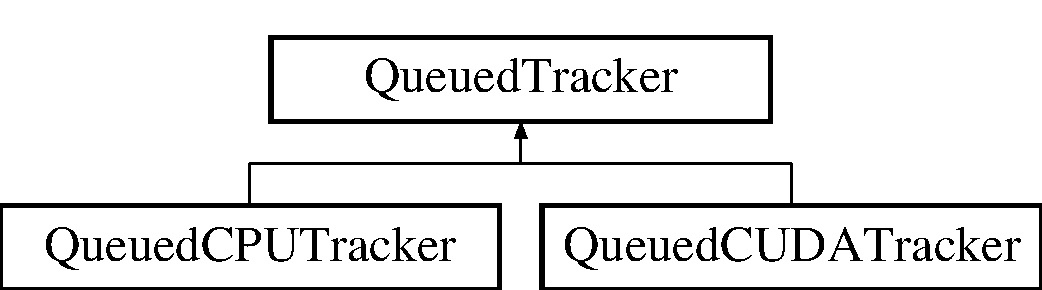
\includegraphics[height=2.000000cm]{class_queued_tracker}
\end{center}
\end{figure}
\subsection*{Public Types}
\begin{DoxyCompactItemize}
\item 
typedef std\+::map$<$ std\+::string, std\+::string $>$ \hyperlink{class_queued_tracker_af6073682cd9e87e6f3e84f93cf9be373}{Config\+Value\+Map}
\end{DoxyCompactItemize}
\subsection*{Public Member Functions}
\begin{DoxyCompactItemize}
\item 
\hyperlink{class_queued_tracker_a483d1506b7b317d705cc7997805b5904}{Queued\+Tracker} ()
\item 
virtual \hyperlink{class_queued_tracker_aa60a3ac6e97b8a7a84b49dd9b6c8b615}{$\sim$\+Queued\+Tracker} ()
\item 
virtual void \hyperlink{class_queued_tracker_aed430b5578d7a3e75f4d4d6c6dbb7e45}{Set\+Localization\+Mode} (\hyperlink{qtrk__c__api_8h_a6ba72ec1daa19642f85a47defe8f0812}{Loc\+Mode\+\_\+t} loc\+Type)=0
\begin{DoxyCompactList}\small\item\em Select which algorithm is to be used. \end{DoxyCompactList}\item 
virtual void \hyperlink{class_queued_tracker_ae1fa56f8629d8d4ad621889fbd9e4a46}{Set\+Pixel\+Calibration\+Images} (float $\ast$offset, float $\ast$gain)=0
\item 
virtual void \hyperlink{class_queued_tracker_ab9dd540b5c8452718944b47520fda402}{Set\+Pixel\+Calibration\+Factors} (float offset\+Factor, float gain\+Factor)=0
\item 
virtual void \hyperlink{class_queued_tracker_a233dffd15fe3cef8a53c698bba9befb4}{Schedule\+Localization} (void $\ast$data, int pitch, \hyperlink{qtrk__c__api_8h_aad82367b3ea592a142bb50a2fb538b0b}{Q\+T\+R\+K\+\_\+\+Pixel\+Data\+Type} pdt, const \hyperlink{struct_localization_job}{Localization\+Job} $\ast$job\+Info)=0
\begin{DoxyCompactList}\small\item\em Add a job to the queue to be processed. A job entails running the required algorithms on a single region of interest. \end{DoxyCompactList}\item 
void \hyperlink{class_queued_tracker_afa6cfa13cba4d05fac9f7baa96b12f89}{Schedule\+Image\+Data} (\hyperlink{_queued_tracker_8h_a2d6726594ce64e82b9222b183f2571d1}{Image\+Data} $\ast$data, const \hyperlink{struct_localization_job}{Localization\+Job} $\ast$job\+Info)
\begin{DoxyCompactList}\small\item\em Quick function to schedule a single R\+OI from an \hyperlink{utils_8h_a2d6726594ce64e82b9222b183f2571d1}{Image\+Data} object. \end{DoxyCompactList}\item 
virtual void \hyperlink{class_queued_tracker_a5e46c8ce4bd3b965bedd8aac095304c2}{Clear\+Results} ()=0
\begin{DoxyCompactList}\small\item\em Clear results. \end{DoxyCompactList}\item 
virtual void \hyperlink{class_queued_tracker_a97cf826c17ab9b3e55d8ecd513d58098}{Flush} ()=0
\begin{DoxyCompactList}\small\item\em Stop waiting for more jobs to do, and just process the current batch. \end{DoxyCompactList}\item 
virtual int \hyperlink{class_queued_tracker_ab80776ec6e8b2202d858f1c9cb989240}{Schedule\+Frame} (void $\ast$imgptr, int pitch, int width, int height, \hyperlink{struct_r_o_i_position}{R\+O\+I\+Position} $\ast$positions, int num\+R\+OI, \hyperlink{qtrk__c__api_8h_aad82367b3ea592a142bb50a2fb538b0b}{Q\+T\+R\+K\+\_\+\+Pixel\+Data\+Type} pdt, const \hyperlink{struct_localization_job}{Localization\+Job} $\ast$job\+Info)
\begin{DoxyCompactList}\small\item\em Schedule an entire frame at once, allowing for further optimizations. \end{DoxyCompactList}\item 
virtual void \hyperlink{class_queued_tracker_a77c3d8414993d2aa3ddfca4c8b40e71d}{Set\+Radial\+Z\+L\+UT} (float $\ast$data, int count, int planes)=0
\begin{DoxyCompactList}\small\item\em Set the radial lookup tables to be used for z tracking. \end{DoxyCompactList}\item 
virtual void \hyperlink{class_queued_tracker_a7e92adfa46401d802eaff7687e43dad7}{Get\+Radial\+Z\+L\+UT} (float $\ast$dst)=0
\begin{DoxyCompactList}\small\item\em Get the radial lookup tables used for z tracking. \end{DoxyCompactList}\item 
virtual void \hyperlink{class_queued_tracker_a95e19cdbbaa59eb676a24aaf95058b27}{Get\+Radial\+Z\+L\+U\+T\+Size} (int \&count, int \&planes, int \&radialsteps)=0
\begin{DoxyCompactList}\small\item\em Get the dimensions of the radial lookup table data. \end{DoxyCompactList}\item 
virtual void \hyperlink{class_queued_tracker_aaf4a1a0f17e2df7bc6dded2729d920f4}{Set\+Radial\+Weights} (float $\ast$zcmp)=0
\begin{DoxyCompactList}\small\item\em Set radial weights used for comparing L\+UT profiles. \end{DoxyCompactList}\item 
virtual void \hyperlink{class_queued_tracker_a53791fa740351a32ff707be9688aa99d}{Enable\+Radial\+Z\+L\+U\+T\+Compare\+Profile} (bool enabled)=0
\begin{DoxyCompactList}\small\item\em Set a flag to enable saving of error curves. \end{DoxyCompactList}\item 
virtual void \hyperlink{class_queued_tracker_ae6cc12f988a4f99d03a9783b4f978e7e}{Get\+Radial\+Z\+L\+U\+T\+Compare\+Profile} (float $\ast$dst)=0
\begin{DoxyCompactList}\small\item\em Get saved error curve. \end{DoxyCompactList}\item 
virtual void \hyperlink{class_queued_tracker_a29cd6f896d8bcdd93ee4a54bb7823f97}{Get\+Image\+Z\+L\+U\+T\+Size} (int $\ast$dims)
\begin{DoxyCompactList}\small\item\em Get the dimensions of the image lookup table data. \end{DoxyCompactList}\item 
virtual void \hyperlink{class_queued_tracker_af7d71b3673778f83f6494328182519ad}{Get\+Image\+Z\+L\+UT} (float $\ast$dst)
\begin{DoxyCompactList}\small\item\em Get the image lookup tables used. \end{DoxyCompactList}\item 
virtual bool \hyperlink{class_queued_tracker_abd440db1fddc0715bd41b90f1d169ee6}{Set\+Image\+Z\+L\+UT} (float $\ast$src, float $\ast$radial\+\_\+zlut, int $\ast$dims)
\begin{DoxyCompactList}\small\item\em Set the image lookup tables to be used for z tracking. \end{DoxyCompactList}\item 
virtual void \hyperlink{class_queued_tracker_aee4863d19778314cd30499cb85bd5251}{Begin\+L\+UT} (\hyperlink{std__incl_8h_a91ad9478d81a7aaf2593e8d9c3d06a14}{uint} flags)=0
\item 
virtual void \hyperlink{class_queued_tracker_aaeb04a5a2a4fe47ef48b8aefabc1bdb7}{Build\+L\+UT} (void $\ast$data, int pitch, \hyperlink{qtrk__c__api_8h_aad82367b3ea592a142bb50a2fb538b0b}{Q\+T\+R\+K\+\_\+\+Pixel\+Data\+Type} pdt, int plane, \hyperlink{std__incl_8h_aba974726076ec2d63a67114c536d123e}{vector2f} $\ast$known\+\_\+pos=0)=0
\item 
virtual void \hyperlink{class_queued_tracker_aa856650c99d15216ad3246d3485b9d9e}{Finalize\+L\+UT} ()=0
\item 
virtual int \hyperlink{class_queued_tracker_a362a26027dc6bd40864e59de1ac32de2}{Get\+Result\+Count} ()=0
\item 
virtual int \hyperlink{class_queued_tracker_a171688832558d40838790c90ba9f8fc0}{Fetch\+Results} (\hyperlink{struct_localization_result}{Localization\+Result} $\ast$results, int max\+Results)=0
\item 
virtual int \hyperlink{class_queued_tracker_a7109701fb33a1eb1f4a5512205cb7bde}{Get\+Queue\+Length} (int $\ast$max\+Queue\+Len=0)=0
\item 
virtual bool \hyperlink{class_queued_tracker_a8b879a9359f4e2081e69b0932f8e9908}{Is\+Idle} ()=0
\item 
virtual void \hyperlink{class_queued_tracker_a0d96ad4feea320c3ba90d196b4690d3b}{Set\+Config\+Value} (std\+::string name, std\+::string value)=0
\item 
virtual \hyperlink{class_queued_tracker_af6073682cd9e87e6f3e84f93cf9be373}{Config\+Value\+Map} \hyperlink{class_queued_tracker_afdb95cbf31f14716b3872e15a2319d62}{Get\+Config\+Values} ()=0
\item 
virtual std\+::string \hyperlink{class_queued_tracker_afb595aa118f6cd87b4502d2cdfe53215}{Get\+Profile\+Report} ()
\item 
virtual std\+::string \hyperlink{class_queued_tracker_aafb754ef37092a96f95a3094eba58398}{Get\+Warnings} ()
\item 
virtual bool \hyperlink{class_queued_tracker_aeae109b520ca5b15e008030edfc179c4}{Get\+Debug\+Image} (int ID, int $\ast$w, int $\ast$h, float $\ast$$\ast$p\+Data)
\item 
\hyperlink{_queued_tracker_8h_a2d6726594ce64e82b9222b183f2571d1}{Image\+Data} \hyperlink{class_queued_tracker_a37756db08d454ad904193dd4e6f652b1}{Debug\+Image} (int ID)
\item 
void \hyperlink{class_queued_tracker_a43a79ee2536d7e32f2168a19fc978f14}{Schedule\+Localization} (\hyperlink{std__incl_8h_a65f85814a8290f9797005d3b28e7e5fc}{uchar} $\ast$data, int pitch, \hyperlink{qtrk__c__api_8h_aad82367b3ea592a142bb50a2fb538b0b}{Q\+T\+R\+K\+\_\+\+Pixel\+Data\+Type} pdt, \hyperlink{std__incl_8h_a91ad9478d81a7aaf2593e8d9c3d06a14}{uint} frame, \hyperlink{std__incl_8h_a91ad9478d81a7aaf2593e8d9c3d06a14}{uint} timestamp, \hyperlink{std__incl_8h_a2feaef1d85a74bd5cf80df91b1a9a914}{vector3f} $\ast$initial, \hyperlink{std__incl_8h_a91ad9478d81a7aaf2593e8d9c3d06a14}{uint} zlut\+Index)
\item 
void \hyperlink{class_queued_tracker_a8dbbbccee47ca764db7cd0b9c5fa140e}{Compute\+Z\+Bias\+Correction} (int bias\+\_\+planes, \hyperlink{class_c_image_data}{C\+Image\+Data} $\ast$result, int smp\+Per\+Pixel, bool use\+Spline\+Interp)
\item 
float \hyperlink{class_queued_tracker_a5db67617f39aba7d9874222d3fa1c02f}{Z\+L\+U\+T\+Bias\+Correction} (float z, int zlut\+\_\+planes, int bead)
\item 
void \hyperlink{class_queued_tracker_a44b2acf1496f571f7139141c11e39ba0}{Set\+Z\+L\+U\+T\+Bias\+Correction} (const \hyperlink{class_c_image_data}{C\+Image\+Data} \&data)
\item 
\hyperlink{class_c_image_data}{C\+Image\+Data} $\ast$ \hyperlink{class_queued_tracker_a15e820c55638c970a8ed5a441a16d41e}{Get\+Z\+L\+U\+T\+Bias\+Correction} ()
\end{DoxyCompactItemize}
\subsection*{Public Attributes}
\begin{DoxyCompactItemize}
\item 
\hyperlink{struct_q_trk_computed_config}{Q\+Trk\+Computed\+Config} \hyperlink{class_queued_tracker_afb847e7f49e0af6027d58af51d5914dc}{cfg}
\end{DoxyCompactItemize}
\subsection*{Protected Attributes}
\begin{DoxyCompactItemize}
\item 
\hyperlink{class_c_image_data}{C\+Image\+Data} $\ast$ \hyperlink{class_queued_tracker_a6f5a5a506c622ee1c174cd497c5152b9}{zlut\+\_\+bias\+\_\+correction}
\end{DoxyCompactItemize}


\subsection{Detailed Description}
Abstract tracker interface, implemented by \hyperlink{class_queued_c_u_d_a_tracker}{Queued\+C\+U\+D\+A\+Tracker} and \hyperlink{class_queued_c_p_u_tracker}{Queued\+C\+P\+U\+Tracker}. 

\subsection{Member Typedef Documentation}
\index{Queued\+Tracker@{Queued\+Tracker}!Config\+Value\+Map@{Config\+Value\+Map}}
\index{Config\+Value\+Map@{Config\+Value\+Map}!Queued\+Tracker@{Queued\+Tracker}}
\subsubsection[{\texorpdfstring{Config\+Value\+Map}{ConfigValueMap}}]{\setlength{\rightskip}{0pt plus 5cm}typedef std\+::map$<$std\+::string, std\+::string$>$ {\bf Queued\+Tracker\+::\+Config\+Value\+Map}}\hypertarget{class_queued_tracker_af6073682cd9e87e6f3e84f93cf9be373}{}\label{class_queued_tracker_af6073682cd9e87e6f3e84f93cf9be373}


\subsection{Constructor \& Destructor Documentation}
\index{Queued\+Tracker@{Queued\+Tracker}!Queued\+Tracker@{Queued\+Tracker}}
\index{Queued\+Tracker@{Queued\+Tracker}!Queued\+Tracker@{Queued\+Tracker}}
\subsubsection[{\texorpdfstring{Queued\+Tracker()}{QueuedTracker()}}]{\setlength{\rightskip}{0pt plus 5cm}Queued\+Tracker\+::\+Queued\+Tracker (
\begin{DoxyParamCaption}
{}
\end{DoxyParamCaption}
)}\hypertarget{class_queued_tracker_a483d1506b7b317d705cc7997805b5904}{}\label{class_queued_tracker_a483d1506b7b317d705cc7997805b5904}

\begin{DoxyCode}
95 \{
96     \hyperlink{class_queued_tracker_a6f5a5a506c622ee1c174cd497c5152b9}{zlut\_bias\_correction}=0;
97 \}
\end{DoxyCode}
\index{Queued\+Tracker@{Queued\+Tracker}!````~Queued\+Tracker@{$\sim$\+Queued\+Tracker}}
\index{````~Queued\+Tracker@{$\sim$\+Queued\+Tracker}!Queued\+Tracker@{Queued\+Tracker}}
\subsubsection[{\texorpdfstring{$\sim$\+Queued\+Tracker()}{~QueuedTracker()}}]{\setlength{\rightskip}{0pt plus 5cm}Queued\+Tracker\+::$\sim$\+Queued\+Tracker (
\begin{DoxyParamCaption}
{}
\end{DoxyParamCaption}
)\hspace{0.3cm}{\ttfamily [virtual]}}\hypertarget{class_queued_tracker_aa60a3ac6e97b8a7a84b49dd9b6c8b615}{}\label{class_queued_tracker_aa60a3ac6e97b8a7a84b49dd9b6c8b615}

\begin{DoxyCode}
100 \{
101 \}
\end{DoxyCode}


\subsection{Member Function Documentation}
\index{Queued\+Tracker@{Queued\+Tracker}!Begin\+L\+UT@{Begin\+L\+UT}}
\index{Begin\+L\+UT@{Begin\+L\+UT}!Queued\+Tracker@{Queued\+Tracker}}
\subsubsection[{\texorpdfstring{Begin\+L\+U\+T(uint flags)=0}{BeginLUT(uint flags)=0}}]{\setlength{\rightskip}{0pt plus 5cm}virtual void Queued\+Tracker\+::\+Begin\+L\+UT (
\begin{DoxyParamCaption}
\item[{{\bf uint}}]{flags}
\end{DoxyParamCaption}
)\hspace{0.3cm}{\ttfamily [pure virtual]}}\hypertarget{class_queued_tracker_aee4863d19778314cd30499cb85bd5251}{}\label{class_queued_tracker_aee4863d19778314cd30499cb85bd5251}


Implemented in \hyperlink{class_queued_c_u_d_a_tracker_ac6a9934c5a2bd06ecb503abace83c222}{Queued\+C\+U\+D\+A\+Tracker}, and \hyperlink{class_queued_c_p_u_tracker_af4b7390a38d56cc45670a60586e20051}{Queued\+C\+P\+U\+Tracker}.

\index{Queued\+Tracker@{Queued\+Tracker}!Build\+L\+UT@{Build\+L\+UT}}
\index{Build\+L\+UT@{Build\+L\+UT}!Queued\+Tracker@{Queued\+Tracker}}
\subsubsection[{\texorpdfstring{Build\+L\+U\+T(void $\ast$data, int pitch, Q\+T\+R\+K\+\_\+\+Pixel\+Data\+Type pdt, int plane, vector2f $\ast$known\+\_\+pos=0)=0}{BuildLUT(void *data, int pitch, QTRK_PixelDataType pdt, int plane, vector2f *known_pos=0)=0}}]{\setlength{\rightskip}{0pt plus 5cm}virtual void Queued\+Tracker\+::\+Build\+L\+UT (
\begin{DoxyParamCaption}
\item[{void $\ast$}]{data, }
\item[{int}]{pitch, }
\item[{{\bf Q\+T\+R\+K\+\_\+\+Pixel\+Data\+Type}}]{pdt, }
\item[{int}]{plane, }
\item[{{\bf vector2f} $\ast$}]{known\+\_\+pos = {\ttfamily 0}}
\end{DoxyParamCaption}
)\hspace{0.3cm}{\ttfamily [pure virtual]}}\hypertarget{class_queued_tracker_aaeb04a5a2a4fe47ef48b8aefabc1bdb7}{}\label{class_queued_tracker_aaeb04a5a2a4fe47ef48b8aefabc1bdb7}


Implemented in \hyperlink{class_queued_c_u_d_a_tracker_a16da9256e496b6689079330a062c7529}{Queued\+C\+U\+D\+A\+Tracker}, and \hyperlink{class_queued_c_p_u_tracker_ac73750c7446b69b070ab24742b02660f}{Queued\+C\+P\+U\+Tracker}.

\index{Queued\+Tracker@{Queued\+Tracker}!Clear\+Results@{Clear\+Results}}
\index{Clear\+Results@{Clear\+Results}!Queued\+Tracker@{Queued\+Tracker}}
\subsubsection[{\texorpdfstring{Clear\+Results()=0}{ClearResults()=0}}]{\setlength{\rightskip}{0pt plus 5cm}virtual void Queued\+Tracker\+::\+Clear\+Results (
\begin{DoxyParamCaption}
{}
\end{DoxyParamCaption}
)\hspace{0.3cm}{\ttfamily [pure virtual]}}\hypertarget{class_queued_tracker_a5e46c8ce4bd3b965bedd8aac095304c2}{}\label{class_queued_tracker_a5e46c8ce4bd3b965bedd8aac095304c2}


Clear results. 



Implemented in \hyperlink{class_queued_c_u_d_a_tracker_a41b207c9abf386f57ab9f99994e92b4c}{Queued\+C\+U\+D\+A\+Tracker}, and \hyperlink{class_queued_c_p_u_tracker_a24f0731281b361dfb857448ce98d0aa3}{Queued\+C\+P\+U\+Tracker}.

\index{Queued\+Tracker@{Queued\+Tracker}!Compute\+Z\+Bias\+Correction@{Compute\+Z\+Bias\+Correction}}
\index{Compute\+Z\+Bias\+Correction@{Compute\+Z\+Bias\+Correction}!Queued\+Tracker@{Queued\+Tracker}}
\subsubsection[{\texorpdfstring{Compute\+Z\+Bias\+Correction(int bias\+\_\+planes, C\+Image\+Data $\ast$result, int smp\+Per\+Pixel, bool use\+Spline\+Interp)}{ComputeZBiasCorrection(int bias_planes, CImageData *result, int smpPerPixel, bool useSplineInterp)}}]{\setlength{\rightskip}{0pt plus 5cm}void Queued\+Tracker\+::\+Compute\+Z\+Bias\+Correction (
\begin{DoxyParamCaption}
\item[{int}]{bias\+\_\+planes, }
\item[{{\bf C\+Image\+Data} $\ast$}]{result, }
\item[{int}]{smp\+Per\+Pixel, }
\item[{bool}]{use\+Spline\+Interp}
\end{DoxyParamCaption}
)}\hypertarget{class_queued_tracker_a8dbbbccee47ca764db7cd0b9c5fa140e}{}\label{class_queued_tracker_a8dbbbccee47ca764db7cd0b9c5fa140e}

\begin{DoxyCode}
174 \{
175     \textcolor{keywordtype}{int} count,zlut\_planes,radialsteps;
176     \hyperlink{class_queued_tracker_a95e19cdbbaa59eb676a24aaf95058b27}{GetRadialZLUTSize}(count, zlut\_planes, radialsteps);
177     \textcolor{keywordtype}{float}* zlut\_data = \textcolor{keyword}{new} \textcolor{keywordtype}{float}[count*zlut\_planes*radialsteps];
178     \hyperlink{class_queued_tracker_a7e92adfa46401d802eaff7687e43dad7}{GetRadialZLUT}(zlut\_data);
179 
180     std::vector<float> qi\_rweights = \hyperlink{utils_8cpp_a8657c1536ca3621943042411f4644e21}{ComputeRadialBinWindow}(
      \hyperlink{class_queued_tracker_afb847e7f49e0af6027d58af51d5914dc}{cfg}.\hyperlink{struct_q_trk_computed_config_ab1a11e7a567a3267c57f77626c6c9c93}{qi\_radialsteps});
181     std::vector<float> zlut\_rweights = \hyperlink{utils_8cpp_a8657c1536ca3621943042411f4644e21}{ComputeRadialBinWindow}(
      \hyperlink{class_queued_tracker_afb847e7f49e0af6027d58af51d5914dc}{cfg}.\hyperlink{struct_q_trk_computed_config_ad1a121fa7d3152df6788ff285e4d2dc6}{zlut\_radialsteps});
182 
183     \textcolor{keywordflow}{if} (\hyperlink{class_queued_tracker_a6f5a5a506c622ee1c174cd497c5152b9}{zlut\_bias\_correction})
184         \textcolor{keyword}{delete} \hyperlink{class_queued_tracker_a6f5a5a506c622ee1c174cd497c5152b9}{zlut\_bias\_correction};
185 
186     \hyperlink{class_queued_tracker_a6f5a5a506c622ee1c174cd497c5152b9}{zlut\_bias\_correction} = \textcolor{keyword}{new} \hyperlink{class_c_image_data}{CImageData}(bias\_planes, count);
187 
188     \hyperlink{threads_8h_a6693c34b211b5d81e0d7a362457d0449}{parallel\_for}(count*bias\_planes, [&](\textcolor{keywordtype}{int} job) \{
189     \textcolor{comment}{//for (int job=0;job<count*bias\_planes;job++) \{}
190         \textcolor{keywordtype}{int} bead = job/bias\_planes;
191         \textcolor{keywordtype}{int} plane = job%bias\_planes;
192         
193         \textcolor{keywordtype}{float} *zlut\_ptr = &zlut\_data[ bead * (zlut\_planes*radialsteps) ];
194         \hyperlink{class_c_p_u_tracker}{CPUTracker} trk (\hyperlink{class_queued_tracker_afb847e7f49e0af6027d58af51d5914dc}{cfg}.\hyperlink{struct_q_trk_settings_aef24eb3a4692bd67ff1aca8ef950e08d}{width},\hyperlink{class_queued_tracker_afb847e7f49e0af6027d58af51d5914dc}{cfg}.\hyperlink{struct_q_trk_settings_a94c965d103e7a0a4f1fced8eee1324ce}{height});
195         \hyperlink{struct_t_image_data}{ImageData} zlut(zlut\_ptr, radialsteps, zlut\_planes);
196         trk.SetRadialZLUT(zlut.data, zlut.h, zlut.w, 1, \hyperlink{class_queued_tracker_afb847e7f49e0af6027d58af51d5914dc}{cfg}.\hyperlink{struct_q_trk_settings_a1a14537a9e784c65eed512e72ee86c02}{zlut\_minradius},
      \hyperlink{class_queued_tracker_afb847e7f49e0af6027d58af51d5914dc}{cfg}.\hyperlink{struct_q_trk_computed_config_a13ceb0d4551d3bd5343ecce7a093d65b}{zlut\_maxradius}, \textcolor{keyword}{false}, \textcolor{keyword}{false});
197         trk.SetRadialWeights(&zlut\_rweights[0]);
198 
199         \hyperlink{structvector3}{vector3f} pos(\hyperlink{class_queued_tracker_afb847e7f49e0af6027d58af51d5914dc}{cfg}.\hyperlink{struct_q_trk_settings_aef24eb3a4692bd67ff1aca8ef950e08d}{width}/2,\hyperlink{class_queued_tracker_afb847e7f49e0af6027d58af51d5914dc}{cfg}.\hyperlink{struct_q_trk_settings_a94c965d103e7a0a4f1fced8eee1324ce}{height}/2, plane /(\textcolor{keywordtype}{float}) bias\_planes * 
      zlut\_planes );
200         \hyperlink{struct_t_image_data}{ImageData} img = \hyperlink{struct_t_image_data_a8ae528964e70c0d0a98b8481cc8b083e}{ImageData::alloc}(\hyperlink{class_queued_tracker_afb847e7f49e0af6027d58af51d5914dc}{cfg}.\hyperlink{struct_q_trk_settings_aef24eb3a4692bd67ff1aca8ef950e08d}{width},
      \hyperlink{class_queued_tracker_afb847e7f49e0af6027d58af51d5914dc}{cfg}.\hyperlink{struct_q_trk_settings_a94c965d103e7a0a4f1fced8eee1324ce}{height});
201         \hyperlink{utils_8cpp_af574edb94793976b749c0240c79b1c48}{GenerateImageFromLUT}(&img, &zlut, \hyperlink{class_queued_tracker_afb847e7f49e0af6027d58af51d5914dc}{cfg}.
      \hyperlink{struct_q_trk_settings_a1a14537a9e784c65eed512e72ee86c02}{zlut\_minradius}, \hyperlink{class_queued_tracker_afb847e7f49e0af6027d58af51d5914dc}{cfg}.\hyperlink{struct_q_trk_computed_config_a13ceb0d4551d3bd5343ecce7a093d65b}{zlut\_maxradius}, pos, useSplineInterp,smpPerPixel);
202 
203         \textcolor{keywordtype}{bool} bhit;
204         trk.SetImageFloat(img.\hyperlink{struct_t_image_data_a78c7415ecee3965da7e25149cea6f4d8}{data});
205         \hyperlink{structvector2}{vector2f} com = trk.ComputeMeanAndCOM();
206         \hyperlink{structvector2}{vector2f} qi = trk.ComputeQI(com, 2, \hyperlink{class_queued_tracker_afb847e7f49e0af6027d58af51d5914dc}{cfg}.\hyperlink{struct_q_trk_computed_config_ab1a11e7a567a3267c57f77626c6c9c93}{qi\_radialsteps}, 
      \hyperlink{class_queued_tracker_afb847e7f49e0af6027d58af51d5914dc}{cfg}.\hyperlink{struct_q_trk_computed_config_a1ba87257b24e5b7e427aa92dd4114792}{qi\_angstepspq}, \hyperlink{class_queued_tracker_afb847e7f49e0af6027d58af51d5914dc}{cfg}.\hyperlink{struct_q_trk_settings_aceebf67ba9ecc215d49c6b2739afae3d}{qi\_angstep\_factor}, 
      \hyperlink{class_queued_tracker_afb847e7f49e0af6027d58af51d5914dc}{cfg}.\hyperlink{struct_q_trk_settings_a7b5f3e61b4dcab6330c56e7bcd96e82d}{qi\_minradius}, \hyperlink{class_queued_tracker_afb847e7f49e0af6027d58af51d5914dc}{cfg}.\hyperlink{struct_q_trk_computed_config_a9784dbeb638bde1f3204f9ca5af720c6}{qi\_maxradius}, bhit, &qi\_rweights[0]);
207         \textcolor{keywordtype}{float} z = trk.ComputeZ(qi, \hyperlink{class_queued_tracker_afb847e7f49e0af6027d58af51d5914dc}{cfg}.\hyperlink{struct_q_trk_computed_config_a01653574d81ab70e4910c984fb7f7482}{zlut\_angularsteps}, 0);
208         \hyperlink{class_queued_tracker_a6f5a5a506c622ee1c174cd497c5152b9}{zlut\_bias\_correction}->\hyperlink{struct_t_image_data_ad13c1527ffabe17b997c38090ec5e6b9}{at}(plane, bead) = z - pos.z;
209 
210         \textcolor{comment}{//trk.ComputeRadialProfile(}
211         img.\hyperlink{struct_t_image_data_a60a60e309657216a2e35809fdc582b11}{free}();
212         \textcolor{keywordflow}{if} ((job%(count*bias\_planes/10)) == 0) 
213             \hyperlink{utils_8cpp_a4a7132c90e490d24edecb391a754a9c0}{dbgprintf}(\textcolor{stringliteral}{"job=%d\(\backslash\)n"}, job);
214 \textcolor{comment}{//  \}}
215     \});
216 
217     \textcolor{keywordflow}{if} (result)
218         *result = *\hyperlink{class_queued_tracker_a6f5a5a506c622ee1c174cd497c5152b9}{zlut\_bias\_correction};
219 \}
\end{DoxyCode}
\index{Queued\+Tracker@{Queued\+Tracker}!Debug\+Image@{Debug\+Image}}
\index{Debug\+Image@{Debug\+Image}!Queued\+Tracker@{Queued\+Tracker}}
\subsubsection[{\texorpdfstring{Debug\+Image(int I\+D)}{DebugImage(int ID)}}]{\setlength{\rightskip}{0pt plus 5cm}{\bf Image\+Data} Queued\+Tracker\+::\+Debug\+Image (
\begin{DoxyParamCaption}
\item[{int}]{ID}
\end{DoxyParamCaption}
)}\hypertarget{class_queued_tracker_a37756db08d454ad904193dd4e6f652b1}{}\label{class_queued_tracker_a37756db08d454ad904193dd4e6f652b1}

\begin{DoxyCode}
119 \{
120     \hyperlink{struct_t_image_data}{ImageData} img;
121     \hyperlink{class_queued_tracker_aeae109b520ca5b15e008030edfc179c4}{GetDebugImage}(ID, &img.\hyperlink{struct_t_image_data_aa46faa6f66f9d6f93c65e14aea643eb3}{w}, &img.\hyperlink{struct_t_image_data_a252235d07e487e8d02908aed062147bd}{h}, &img.\hyperlink{struct_t_image_data_a78c7415ecee3965da7e25149cea6f4d8}{data});
122     \textcolor{keywordflow}{return} img;
123 \}
\end{DoxyCode}
\index{Queued\+Tracker@{Queued\+Tracker}!Enable\+Radial\+Z\+L\+U\+T\+Compare\+Profile@{Enable\+Radial\+Z\+L\+U\+T\+Compare\+Profile}}
\index{Enable\+Radial\+Z\+L\+U\+T\+Compare\+Profile@{Enable\+Radial\+Z\+L\+U\+T\+Compare\+Profile}!Queued\+Tracker@{Queued\+Tracker}}
\subsubsection[{\texorpdfstring{Enable\+Radial\+Z\+L\+U\+T\+Compare\+Profile(bool enabled)=0}{EnableRadialZLUTCompareProfile(bool enabled)=0}}]{\setlength{\rightskip}{0pt plus 5cm}virtual void Queued\+Tracker\+::\+Enable\+Radial\+Z\+L\+U\+T\+Compare\+Profile (
\begin{DoxyParamCaption}
\item[{bool}]{enabled}
\end{DoxyParamCaption}
)\hspace{0.3cm}{\ttfamily [pure virtual]}}\hypertarget{class_queued_tracker_a53791fa740351a32ff707be9688aa99d}{}\label{class_queued_tracker_a53791fa740351a32ff707be9688aa99d}


Set a flag to enable saving of error curves. 

Errors obtained by comparing a radial profile to a Z\+L\+UT will be kept in memory rather than destroyed. Only saves for one localization. Error curve can be retreived by \hyperlink{class_queued_tracker_ae6cc12f988a4f99d03a9783b4f978e7e}{Get\+Radial\+Z\+L\+U\+T\+Compare\+Profile}.

\begin{DoxyNote}{Note}
Not implemented for C\+U\+DA. 
\end{DoxyNote}

\begin{DoxyParams}[1]{Parameters}
\mbox{\tt in}  & {\em enabled} & Flag (boolean) to save error curves. Default is false. \\
\hline
\end{DoxyParams}


Implemented in \hyperlink{class_queued_c_u_d_a_tracker_aa8b23ddd77fd1826fbcf5c2d58135f13}{Queued\+C\+U\+D\+A\+Tracker}, and \hyperlink{class_queued_c_p_u_tracker_accb203fae1a724f6ac870c4dc402dda7}{Queued\+C\+P\+U\+Tracker}.

\index{Queued\+Tracker@{Queued\+Tracker}!Fetch\+Results@{Fetch\+Results}}
\index{Fetch\+Results@{Fetch\+Results}!Queued\+Tracker@{Queued\+Tracker}}
\subsubsection[{\texorpdfstring{Fetch\+Results(\+Localization\+Result $\ast$results, int max\+Results)=0}{FetchResults(LocalizationResult *results, int maxResults)=0}}]{\setlength{\rightskip}{0pt plus 5cm}virtual int Queued\+Tracker\+::\+Fetch\+Results (
\begin{DoxyParamCaption}
\item[{{\bf Localization\+Result} $\ast$}]{results, }
\item[{int}]{max\+Results}
\end{DoxyParamCaption}
)\hspace{0.3cm}{\ttfamily [pure virtual]}}\hypertarget{class_queued_tracker_a171688832558d40838790c90ba9f8fc0}{}\label{class_queued_tracker_a171688832558d40838790c90ba9f8fc0}


Implemented in \hyperlink{class_queued_c_u_d_a_tracker_acc1a34b83a9f7cc84ede58ce7eaec45e}{Queued\+C\+U\+D\+A\+Tracker}, and \hyperlink{class_queued_c_p_u_tracker_a8e74a4528a84ac83624d217e62cdef05}{Queued\+C\+P\+U\+Tracker}.

\index{Queued\+Tracker@{Queued\+Tracker}!Finalize\+L\+UT@{Finalize\+L\+UT}}
\index{Finalize\+L\+UT@{Finalize\+L\+UT}!Queued\+Tracker@{Queued\+Tracker}}
\subsubsection[{\texorpdfstring{Finalize\+L\+U\+T()=0}{FinalizeLUT()=0}}]{\setlength{\rightskip}{0pt plus 5cm}virtual void Queued\+Tracker\+::\+Finalize\+L\+UT (
\begin{DoxyParamCaption}
{}
\end{DoxyParamCaption}
)\hspace{0.3cm}{\ttfamily [pure virtual]}}\hypertarget{class_queued_tracker_aa856650c99d15216ad3246d3485b9d9e}{}\label{class_queued_tracker_aa856650c99d15216ad3246d3485b9d9e}


Implemented in \hyperlink{class_queued_c_u_d_a_tracker_a628a79df6cce9a1df9a4da78da266578}{Queued\+C\+U\+D\+A\+Tracker}, and \hyperlink{class_queued_c_p_u_tracker_a9d94101b69e1f514473bfedc012ec785}{Queued\+C\+P\+U\+Tracker}.

\index{Queued\+Tracker@{Queued\+Tracker}!Flush@{Flush}}
\index{Flush@{Flush}!Queued\+Tracker@{Queued\+Tracker}}
\subsubsection[{\texorpdfstring{Flush()=0}{Flush()=0}}]{\setlength{\rightskip}{0pt plus 5cm}virtual void Queued\+Tracker\+::\+Flush (
\begin{DoxyParamCaption}
{}
\end{DoxyParamCaption}
)\hspace{0.3cm}{\ttfamily [pure virtual]}}\hypertarget{class_queued_tracker_a97cf826c17ab9b3e55d8ecd513d58098}{}\label{class_queued_tracker_a97cf826c17ab9b3e55d8ecd513d58098}


Stop waiting for more jobs to do, and just process the current batch. 



Implemented in \hyperlink{class_queued_c_u_d_a_tracker_a4407b12d3fc2e2969840ccc233ec96bc}{Queued\+C\+U\+D\+A\+Tracker}, and \hyperlink{class_queued_c_p_u_tracker_a9b332b6fb228e9c655eb2fb12d8dfbc6}{Queued\+C\+P\+U\+Tracker}.

\index{Queued\+Tracker@{Queued\+Tracker}!Get\+Config\+Values@{Get\+Config\+Values}}
\index{Get\+Config\+Values@{Get\+Config\+Values}!Queued\+Tracker@{Queued\+Tracker}}
\subsubsection[{\texorpdfstring{Get\+Config\+Values()=0}{GetConfigValues()=0}}]{\setlength{\rightskip}{0pt plus 5cm}virtual {\bf Config\+Value\+Map} Queued\+Tracker\+::\+Get\+Config\+Values (
\begin{DoxyParamCaption}
{}
\end{DoxyParamCaption}
)\hspace{0.3cm}{\ttfamily [pure virtual]}}\hypertarget{class_queued_tracker_afdb95cbf31f14716b3872e15a2319d62}{}\label{class_queued_tracker_afdb95cbf31f14716b3872e15a2319d62}


Implemented in \hyperlink{class_queued_c_u_d_a_tracker_a16a5fb006a594f950484df6a9d1cfd2f}{Queued\+C\+U\+D\+A\+Tracker}, and \hyperlink{class_queued_c_p_u_tracker_af06013bc5f92d5570aa6244ca1768fcf}{Queued\+C\+P\+U\+Tracker}.

\index{Queued\+Tracker@{Queued\+Tracker}!Get\+Debug\+Image@{Get\+Debug\+Image}}
\index{Get\+Debug\+Image@{Get\+Debug\+Image}!Queued\+Tracker@{Queued\+Tracker}}
\subsubsection[{\texorpdfstring{Get\+Debug\+Image(int I\+D, int $\ast$w, int $\ast$h, float $\ast$$\ast$p\+Data)}{GetDebugImage(int ID, int *w, int *h, float **pData)}}]{\setlength{\rightskip}{0pt plus 5cm}virtual bool Queued\+Tracker\+::\+Get\+Debug\+Image (
\begin{DoxyParamCaption}
\item[{int}]{ID, }
\item[{int $\ast$}]{w, }
\item[{int $\ast$}]{h, }
\item[{float $\ast$$\ast$}]{p\+Data}
\end{DoxyParamCaption}
)\hspace{0.3cm}{\ttfamily [inline]}, {\ttfamily [virtual]}}\hypertarget{class_queued_tracker_aeae109b520ca5b15e008030edfc179c4}{}\label{class_queued_tracker_aeae109b520ca5b15e008030edfc179c4}


Reimplemented in \hyperlink{class_queued_c_p_u_tracker_a4db75a5bfcb5ee2891177da9f6448557}{Queued\+C\+P\+U\+Tracker}.


\begin{DoxyCode}
213 \{ \textcolor{keywordflow}{return} \textcolor{keyword}{false}; \} \textcolor{comment}{// deallocate result with delete[] }
\end{DoxyCode}
\index{Queued\+Tracker@{Queued\+Tracker}!Get\+Image\+Z\+L\+UT@{Get\+Image\+Z\+L\+UT}}
\index{Get\+Image\+Z\+L\+UT@{Get\+Image\+Z\+L\+UT}!Queued\+Tracker@{Queued\+Tracker}}
\subsubsection[{\texorpdfstring{Get\+Image\+Z\+L\+U\+T(float $\ast$dst)}{GetImageZLUT(float *dst)}}]{\setlength{\rightskip}{0pt plus 5cm}virtual void Queued\+Tracker\+::\+Get\+Image\+Z\+L\+UT (
\begin{DoxyParamCaption}
\item[{float $\ast$}]{dst}
\end{DoxyParamCaption}
)\hspace{0.3cm}{\ttfamily [inline]}, {\ttfamily [virtual]}}\hypertarget{class_queued_tracker_af7d71b3673778f83f6494328182519ad}{}\label{class_queued_tracker_af7d71b3673778f83f6494328182519ad}


Get the image lookup tables used. 

\begin{DoxyNote}{Note}
Use of image L\+UT is currently not clear. Radial Z\+L\+UT is always used.
\end{DoxyNote}

\begin{DoxyParams}[1]{Parameters}
\mbox{\tt in,out}  & {\em dst} & Pointer to the pre-\/allocated memory in which to save the data. \\
\hline
\end{DoxyParams}


Reimplemented in \hyperlink{class_queued_c_p_u_tracker_a53b0d922963c771e804fb624f7d39821}{Queued\+C\+P\+U\+Tracker}.


\begin{DoxyCode}
180 \{\}
\end{DoxyCode}
\index{Queued\+Tracker@{Queued\+Tracker}!Get\+Image\+Z\+L\+U\+T\+Size@{Get\+Image\+Z\+L\+U\+T\+Size}}
\index{Get\+Image\+Z\+L\+U\+T\+Size@{Get\+Image\+Z\+L\+U\+T\+Size}!Queued\+Tracker@{Queued\+Tracker}}
\subsubsection[{\texorpdfstring{Get\+Image\+Z\+L\+U\+T\+Size(int $\ast$dims)}{GetImageZLUTSize(int *dims)}}]{\setlength{\rightskip}{0pt plus 5cm}virtual void Queued\+Tracker\+::\+Get\+Image\+Z\+L\+U\+T\+Size (
\begin{DoxyParamCaption}
\item[{int $\ast$}]{dims}
\end{DoxyParamCaption}
)\hspace{0.3cm}{\ttfamily [inline]}, {\ttfamily [virtual]}}\hypertarget{class_queued_tracker_a29cd6f896d8bcdd93ee4a54bb7823f97}{}\label{class_queued_tracker_a29cd6f896d8bcdd93ee4a54bb7823f97}


Get the dimensions of the image lookup table data. 

\begin{DoxyNote}{Note}
Use of image L\+UT is currently not clear. Radial Z\+L\+UT is always used.
\end{DoxyNote}

\begin{DoxyParams}[1]{Parameters}
\mbox{\tt in,out}  & {\em dims} & Reference to pre-\/allocated int array. Returns \mbox{[} count, planes, height, width \mbox{]}. \\
\hline
\end{DoxyParams}


Reimplemented in \hyperlink{class_queued_c_p_u_tracker_a399b87fd1542b05fc9e9c80c1dd6b664}{Queued\+C\+P\+U\+Tracker}.


\begin{DoxyCode}
172 \{\}
\end{DoxyCode}
\index{Queued\+Tracker@{Queued\+Tracker}!Get\+Profile\+Report@{Get\+Profile\+Report}}
\index{Get\+Profile\+Report@{Get\+Profile\+Report}!Queued\+Tracker@{Queued\+Tracker}}
\subsubsection[{\texorpdfstring{Get\+Profile\+Report()}{GetProfileReport()}}]{\setlength{\rightskip}{0pt plus 5cm}virtual std\+::string Queued\+Tracker\+::\+Get\+Profile\+Report (
\begin{DoxyParamCaption}
{}
\end{DoxyParamCaption}
)\hspace{0.3cm}{\ttfamily [inline]}, {\ttfamily [virtual]}}\hypertarget{class_queued_tracker_afb595aa118f6cd87b4502d2cdfe53215}{}\label{class_queued_tracker_afb595aa118f6cd87b4502d2cdfe53215}


Reimplemented in \hyperlink{class_queued_c_u_d_a_tracker_a8969dbbc3824ca4ccb492e8eecbd6632}{Queued\+C\+U\+D\+A\+Tracker}, and \hyperlink{class_queued_c_p_u_tracker_a241d002353241975d49c1e80cd967524}{Queued\+C\+P\+U\+Tracker}.


\begin{DoxyCode}
210 \{ \textcolor{keywordflow}{return} \textcolor{stringliteral}{""}; \}
\end{DoxyCode}
\index{Queued\+Tracker@{Queued\+Tracker}!Get\+Queue\+Length@{Get\+Queue\+Length}}
\index{Get\+Queue\+Length@{Get\+Queue\+Length}!Queued\+Tracker@{Queued\+Tracker}}
\subsubsection[{\texorpdfstring{Get\+Queue\+Length(int $\ast$max\+Queue\+Len=0)=0}{GetQueueLength(int *maxQueueLen=0)=0}}]{\setlength{\rightskip}{0pt plus 5cm}virtual int Queued\+Tracker\+::\+Get\+Queue\+Length (
\begin{DoxyParamCaption}
\item[{int $\ast$}]{max\+Queue\+Len = {\ttfamily 0}}
\end{DoxyParamCaption}
)\hspace{0.3cm}{\ttfamily [pure virtual]}}\hypertarget{class_queued_tracker_a7109701fb33a1eb1f4a5512205cb7bde}{}\label{class_queued_tracker_a7109701fb33a1eb1f4a5512205cb7bde}


Implemented in \hyperlink{class_queued_c_u_d_a_tracker_acd209a7709c4776a585af6bd24768b13}{Queued\+C\+U\+D\+A\+Tracker}, and \hyperlink{class_queued_c_p_u_tracker_a7e1a888cfcc2eb97e059d6711ddfc8af}{Queued\+C\+P\+U\+Tracker}.

\index{Queued\+Tracker@{Queued\+Tracker}!Get\+Radial\+Z\+L\+UT@{Get\+Radial\+Z\+L\+UT}}
\index{Get\+Radial\+Z\+L\+UT@{Get\+Radial\+Z\+L\+UT}!Queued\+Tracker@{Queued\+Tracker}}
\subsubsection[{\texorpdfstring{Get\+Radial\+Z\+L\+U\+T(float $\ast$dst)=0}{GetRadialZLUT(float *dst)=0}}]{\setlength{\rightskip}{0pt plus 5cm}virtual void Queued\+Tracker\+::\+Get\+Radial\+Z\+L\+UT (
\begin{DoxyParamCaption}
\item[{float $\ast$}]{dst}
\end{DoxyParamCaption}
)\hspace{0.3cm}{\ttfamily [pure virtual]}}\hypertarget{class_queued_tracker_a7e92adfa46401d802eaff7687e43dad7}{}\label{class_queued_tracker_a7e92adfa46401d802eaff7687e43dad7}


Get the radial lookup tables used for z tracking. 


\begin{DoxyParams}[1]{Parameters}
\mbox{\tt in,out}  & {\em dst} & Pointer to the pre-\/allocated memory in which to save the data. \\
\hline
\end{DoxyParams}


Implemented in \hyperlink{class_queued_c_u_d_a_tracker_a1298fa3749c2ffaf7e48370ca15e3beb}{Queued\+C\+U\+D\+A\+Tracker}, and \hyperlink{class_queued_c_p_u_tracker_a9c4f1687ca9347508594a9df46defad8}{Queued\+C\+P\+U\+Tracker}.

\index{Queued\+Tracker@{Queued\+Tracker}!Get\+Radial\+Z\+L\+U\+T\+Compare\+Profile@{Get\+Radial\+Z\+L\+U\+T\+Compare\+Profile}}
\index{Get\+Radial\+Z\+L\+U\+T\+Compare\+Profile@{Get\+Radial\+Z\+L\+U\+T\+Compare\+Profile}!Queued\+Tracker@{Queued\+Tracker}}
\subsubsection[{\texorpdfstring{Get\+Radial\+Z\+L\+U\+T\+Compare\+Profile(float $\ast$dst)=0}{GetRadialZLUTCompareProfile(float *dst)=0}}]{\setlength{\rightskip}{0pt plus 5cm}virtual void Queued\+Tracker\+::\+Get\+Radial\+Z\+L\+U\+T\+Compare\+Profile (
\begin{DoxyParamCaption}
\item[{float $\ast$}]{dst}
\end{DoxyParamCaption}
)\hspace{0.3cm}{\ttfamily [pure virtual]}}\hypertarget{class_queued_tracker_ae6cc12f988a4f99d03a9783b4f978e7e}{}\label{class_queued_tracker_ae6cc12f988a4f99d03a9783b4f978e7e}


Get saved error curve. 

See \hyperlink{class_queued_tracker_a53791fa740351a32ff707be9688aa99d}{Enable\+Radial\+Z\+L\+U\+T\+Compare\+Profile}. \begin{DoxyNote}{Note}
Not implemented for C\+U\+DA. 
\end{DoxyNote}

\begin{DoxyParams}[1]{Parameters}
\mbox{\tt in}  & {\em dst} & Pointer to the pre-\/allocated memory in which to save the error curve. Size is {\ttfamily count} $\ast$ {\ttfamily planes}. \\
\hline
\end{DoxyParams}


Implemented in \hyperlink{class_queued_c_u_d_a_tracker_a1d75d74655c9da2a9cb305f95944b1e3}{Queued\+C\+U\+D\+A\+Tracker}, and \hyperlink{class_queued_c_p_u_tracker_afdc97ea9b0e7eba6d2678a0536c39c37}{Queued\+C\+P\+U\+Tracker}.

\index{Queued\+Tracker@{Queued\+Tracker}!Get\+Radial\+Z\+L\+U\+T\+Size@{Get\+Radial\+Z\+L\+U\+T\+Size}}
\index{Get\+Radial\+Z\+L\+U\+T\+Size@{Get\+Radial\+Z\+L\+U\+T\+Size}!Queued\+Tracker@{Queued\+Tracker}}
\subsubsection[{\texorpdfstring{Get\+Radial\+Z\+L\+U\+T\+Size(int \&count, int \&planes, int \&radialsteps)=0}{GetRadialZLUTSize(int &count, int &planes, int &radialsteps)=0}}]{\setlength{\rightskip}{0pt plus 5cm}virtual void Queued\+Tracker\+::\+Get\+Radial\+Z\+L\+U\+T\+Size (
\begin{DoxyParamCaption}
\item[{int \&}]{count, }
\item[{int \&}]{planes, }
\item[{int \&}]{radialsteps}
\end{DoxyParamCaption}
)\hspace{0.3cm}{\ttfamily [pure virtual]}}\hypertarget{class_queued_tracker_a95e19cdbbaa59eb676a24aaf95058b27}{}\label{class_queued_tracker_a95e19cdbbaa59eb676a24aaf95058b27}


Get the dimensions of the radial lookup table data. 


\begin{DoxyParams}[1]{Parameters}
\mbox{\tt in,out}  & {\em count} & Reference to pre-\/allocated int. Returns number of lookup tables. \\
\hline
\mbox{\tt in,out}  & {\em planes} & Reference to pre-\/allocated int. Returns number of planes per lookup table. \\
\hline
\mbox{\tt in,out}  & {\em radialsteps} & Reference to pre-\/allocated int. Returns number of steps per plane. \\
\hline
\end{DoxyParams}


Implemented in \hyperlink{class_queued_c_u_d_a_tracker_a4af9b4b3778d9cb13823fe486db23ab9}{Queued\+C\+U\+D\+A\+Tracker}, and \hyperlink{class_queued_c_p_u_tracker_a57c77fc0ceada2aeffc018970d9d18d8}{Queued\+C\+P\+U\+Tracker}.

\index{Queued\+Tracker@{Queued\+Tracker}!Get\+Result\+Count@{Get\+Result\+Count}}
\index{Get\+Result\+Count@{Get\+Result\+Count}!Queued\+Tracker@{Queued\+Tracker}}
\subsubsection[{\texorpdfstring{Get\+Result\+Count()=0}{GetResultCount()=0}}]{\setlength{\rightskip}{0pt plus 5cm}virtual int Queued\+Tracker\+::\+Get\+Result\+Count (
\begin{DoxyParamCaption}
{}
\end{DoxyParamCaption}
)\hspace{0.3cm}{\ttfamily [pure virtual]}}\hypertarget{class_queued_tracker_a362a26027dc6bd40864e59de1ac32de2}{}\label{class_queued_tracker_a362a26027dc6bd40864e59de1ac32de2}


Implemented in \hyperlink{class_queued_c_u_d_a_tracker_aeb508df96e1cbcfaf8f0bf330e01d35c}{Queued\+C\+U\+D\+A\+Tracker}, and \hyperlink{class_queued_c_p_u_tracker_a0424c92dec3952cf9197a5a9161e2188}{Queued\+C\+P\+U\+Tracker}.

\index{Queued\+Tracker@{Queued\+Tracker}!Get\+Warnings@{Get\+Warnings}}
\index{Get\+Warnings@{Get\+Warnings}!Queued\+Tracker@{Queued\+Tracker}}
\subsubsection[{\texorpdfstring{Get\+Warnings()}{GetWarnings()}}]{\setlength{\rightskip}{0pt plus 5cm}virtual std\+::string Queued\+Tracker\+::\+Get\+Warnings (
\begin{DoxyParamCaption}
{}
\end{DoxyParamCaption}
)\hspace{0.3cm}{\ttfamily [inline]}, {\ttfamily [virtual]}}\hypertarget{class_queued_tracker_aafb754ef37092a96f95a3094eba58398}{}\label{class_queued_tracker_aafb754ef37092a96f95a3094eba58398}

\begin{DoxyCode}
211 \{ \textcolor{keywordflow}{return} \textcolor{stringliteral}{""}; \}
\end{DoxyCode}
\index{Queued\+Tracker@{Queued\+Tracker}!Get\+Z\+L\+U\+T\+Bias\+Correction@{Get\+Z\+L\+U\+T\+Bias\+Correction}}
\index{Get\+Z\+L\+U\+T\+Bias\+Correction@{Get\+Z\+L\+U\+T\+Bias\+Correction}!Queued\+Tracker@{Queued\+Tracker}}
\subsubsection[{\texorpdfstring{Get\+Z\+L\+U\+T\+Bias\+Correction()}{GetZLUTBiasCorrection()}}]{\setlength{\rightskip}{0pt plus 5cm}{\bf C\+Image\+Data} $\ast$ Queued\+Tracker\+::\+Get\+Z\+L\+U\+T\+Bias\+Correction (
\begin{DoxyParamCaption}
{}
\end{DoxyParamCaption}
)}\hypertarget{class_queued_tracker_a15e820c55638c970a8ed5a441a16d41e}{}\label{class_queued_tracker_a15e820c55638c970a8ed5a441a16d41e}

\begin{DoxyCode}
228 \{
229     \textcolor{keywordflow}{if} (\hyperlink{class_queued_tracker_a6f5a5a506c622ee1c174cd497c5152b9}{zlut\_bias\_correction}) \textcolor{keywordflow}{return} \textcolor{keyword}{new} \hyperlink{class_c_image_data}{CImageData}(*
      \hyperlink{class_queued_tracker_a6f5a5a506c622ee1c174cd497c5152b9}{zlut\_bias\_correction});
230     \textcolor{keywordflow}{return} 0;
231 \}
\end{DoxyCode}
\index{Queued\+Tracker@{Queued\+Tracker}!Is\+Idle@{Is\+Idle}}
\index{Is\+Idle@{Is\+Idle}!Queued\+Tracker@{Queued\+Tracker}}
\subsubsection[{\texorpdfstring{Is\+Idle()=0}{IsIdle()=0}}]{\setlength{\rightskip}{0pt plus 5cm}virtual bool Queued\+Tracker\+::\+Is\+Idle (
\begin{DoxyParamCaption}
{}
\end{DoxyParamCaption}
)\hspace{0.3cm}{\ttfamily [pure virtual]}}\hypertarget{class_queued_tracker_a8b879a9359f4e2081e69b0932f8e9908}{}\label{class_queued_tracker_a8b879a9359f4e2081e69b0932f8e9908}


Implemented in \hyperlink{class_queued_c_u_d_a_tracker_a147dbe75048a901f137e130ac61a6f7b}{Queued\+C\+U\+D\+A\+Tracker}, and \hyperlink{class_queued_c_p_u_tracker_a16ec7c17782c4f001dec0dab12970cba}{Queued\+C\+P\+U\+Tracker}.

\index{Queued\+Tracker@{Queued\+Tracker}!Schedule\+Frame@{Schedule\+Frame}}
\index{Schedule\+Frame@{Schedule\+Frame}!Queued\+Tracker@{Queued\+Tracker}}
\subsubsection[{\texorpdfstring{Schedule\+Frame(void $\ast$imgptr, int pitch, int width, int height, R\+O\+I\+Position $\ast$positions, int num\+R\+O\+I, Q\+T\+R\+K\+\_\+\+Pixel\+Data\+Type pdt, const Localization\+Job $\ast$job\+Info)}{ScheduleFrame(void *imgptr, int pitch, int width, int height, ROIPosition *positions, int numROI, QTRK_PixelDataType pdt, const LocalizationJob *jobInfo)}}]{\setlength{\rightskip}{0pt plus 5cm}int Queued\+Tracker\+::\+Schedule\+Frame (
\begin{DoxyParamCaption}
\item[{void $\ast$}]{imgptr, }
\item[{int}]{pitch, }
\item[{int}]{width, }
\item[{int}]{height, }
\item[{{\bf R\+O\+I\+Position} $\ast$}]{positions, }
\item[{int}]{num\+R\+OI, }
\item[{{\bf Q\+T\+R\+K\+\_\+\+Pixel\+Data\+Type}}]{pdt, }
\item[{const {\bf Localization\+Job} $\ast$}]{job\+Info}
\end{DoxyParamCaption}
)\hspace{0.3cm}{\ttfamily [virtual]}}\hypertarget{class_queued_tracker_ab80776ec6e8b2202d858f1c9cb989240}{}\label{class_queued_tracker_ab80776ec6e8b2202d858f1c9cb989240}


Schedule an entire frame at once, allowing for further optimizations. 

Queues each R\+OI within the frame seperatly with \hyperlink{class_queued_tracker_a233dffd15fe3cef8a53c698bba9befb4}{Schedule\+Localization}.


\begin{DoxyParams}[1]{Parameters}
\mbox{\tt in}  & {\em imgptr} & Pointer to the top-\/left pixel of the frame. \\
\hline
\mbox{\tt in}  & {\em pitch} & Size in bytes of one row in memory. \\
\hline
\mbox{\tt in}  & {\em width} & Width of the frame in pixels. \\
\hline
\mbox{\tt in}  & {\em height} & Height of the frame in pixels. \\
\hline
\mbox{\tt in}  & {\em positions} & Array of \hyperlink{struct_r_o_i_position}{R\+O\+I\+Position} with the top-\/left pixel of each R\+OI to be queued. \\
\hline
\mbox{\tt in}  & {\em num\+R\+OI} & Number of R\+O\+Is to handle within the frame. \\
\hline
\mbox{\tt in}  & {\em pdt} & Data type of the image given through {\ttfamily imgptr}. \\
\hline
\mbox{\tt in}  & {\em job\+Info} & \hyperlink{struct_localization_job}{Localization\+Job} with information about the frame.\\
\hline
\end{DoxyParams}
\begin{DoxyReturn}{Returns}
Amount of R\+O\+Is queued. 
\end{DoxyReturn}

\begin{DoxyCode}
126 \{
127     \hyperlink{std__incl_8h_a65f85814a8290f9797005d3b28e7e5fc}{uchar}* img = (\hyperlink{std__incl_8h_a65f85814a8290f9797005d3b28e7e5fc}{uchar}*)imgptr;
128     \textcolor{keywordtype}{int} bpp = \hyperlink{_queued_tracker_8h_adb31752069847fe598de8c312becda1b}{PDT\_BytesPerPixel}(pdt);
129     \textcolor{keywordtype}{int} count=0;
130     \textcolor{keywordflow}{for} (\textcolor{keywordtype}{int} i=0;i<numROI;i++)\{
131         \hyperlink{struct_r_o_i_position}{ROIPosition}& pos = positions[i];
132 
133         \textcolor{keywordflow}{if} (pos.\hyperlink{struct_r_o_i_position_a7ec9344e32faa05e10a72705ed24e9f5}{x} < 0 || pos.\hyperlink{struct_r_o_i_position_aa790f0665220dffa8d196003f6c01b47}{y} < 0 || pos.\hyperlink{struct_r_o_i_position_a7ec9344e32faa05e10a72705ed24e9f5}{x} + \hyperlink{class_queued_tracker_afb847e7f49e0af6027d58af51d5914dc}{cfg}.\hyperlink{struct_q_trk_settings_aef24eb3a4692bd67ff1aca8ef950e08d}{width} > width || pos.
      \hyperlink{struct_r_o_i_position_aa790f0665220dffa8d196003f6c01b47}{y} + \hyperlink{class_queued_tracker_afb847e7f49e0af6027d58af51d5914dc}{cfg}.\hyperlink{struct_q_trk_settings_a94c965d103e7a0a4f1fced8eee1324ce}{height} > height) \{
134             \hyperlink{utils_8cpp_a4a7132c90e490d24edecb391a754a9c0}{dbgprintf}(\textcolor{stringliteral}{"Skipping ROI %d. Outside of image.\(\backslash\)n"}, i);
135             \textcolor{keywordflow}{continue};
136         \}
137 
138         \hyperlink{std__incl_8h_a65f85814a8290f9797005d3b28e7e5fc}{uchar} *roiptr = &img[pitch * pos.\hyperlink{struct_r_o_i_position_aa790f0665220dffa8d196003f6c01b47}{y} + pos.\hyperlink{struct_r_o_i_position_a7ec9344e32faa05e10a72705ed24e9f5}{x} * bpp];
139         \hyperlink{struct_localization_job}{LocalizationJob} job = *jobInfo;
140         job.\hyperlink{struct_localization_job_afcf9f91b72597af0e2572f3ae74d9a99}{zlutIndex} = i + jobInfo->\hyperlink{struct_localization_job_afcf9f91b72597af0e2572f3ae74d9a99}{zlutIndex}; \textcolor{comment}{// used as offset}
141         \hyperlink{class_queued_tracker_a233dffd15fe3cef8a53c698bba9befb4}{ScheduleLocalization}(roiptr, pitch, pdt, &job);
142         count++;
143     \}
144     \textcolor{keywordflow}{return} count;
145 \}
\end{DoxyCode}
\index{Queued\+Tracker@{Queued\+Tracker}!Schedule\+Image\+Data@{Schedule\+Image\+Data}}
\index{Schedule\+Image\+Data@{Schedule\+Image\+Data}!Queued\+Tracker@{Queued\+Tracker}}
\subsubsection[{\texorpdfstring{Schedule\+Image\+Data(\+Image\+Data $\ast$data, const Localization\+Job $\ast$job\+Info)}{ScheduleImageData(ImageData *data, const LocalizationJob *jobInfo)}}]{\setlength{\rightskip}{0pt plus 5cm}void Queued\+Tracker\+::\+Schedule\+Image\+Data (
\begin{DoxyParamCaption}
\item[{{\bf Image\+Data} $\ast$}]{data, }
\item[{const {\bf Localization\+Job} $\ast$}]{job\+Info}
\end{DoxyParamCaption}
)}\hypertarget{class_queued_tracker_afa6cfa13cba4d05fac9f7baa96b12f89}{}\label{class_queued_tracker_afa6cfa13cba4d05fac9f7baa96b12f89}


Quick function to schedule a single R\+OI from an \hyperlink{utils_8h_a2d6726594ce64e82b9222b183f2571d1}{Image\+Data} object. 


\begin{DoxyCode}
104 \{
105     \hyperlink{class_queued_tracker_a233dffd15fe3cef8a53c698bba9befb4}{ScheduleLocalization}(data->\hyperlink{struct_t_image_data_a78c7415ecee3965da7e25149cea6f4d8}{data}, data->\hyperlink{struct_t_image_data_aef0a87643a69b40e19ba11590d51318d}{pitch}(), 
      \hyperlink{qtrk__c__api_8h_aad82367b3ea592a142bb50a2fb538b0bafeece00bcf1a42419e686ef0cf006a4e}{QTrkFloat}, job);
106 \}
\end{DoxyCode}
\index{Queued\+Tracker@{Queued\+Tracker}!Schedule\+Localization@{Schedule\+Localization}}
\index{Schedule\+Localization@{Schedule\+Localization}!Queued\+Tracker@{Queued\+Tracker}}
\subsubsection[{\texorpdfstring{Schedule\+Localization(void $\ast$data, int pitch, Q\+T\+R\+K\+\_\+\+Pixel\+Data\+Type pdt, const Localization\+Job $\ast$job\+Info)=0}{ScheduleLocalization(void *data, int pitch, QTRK_PixelDataType pdt, const LocalizationJob *jobInfo)=0}}]{\setlength{\rightskip}{0pt plus 5cm}virtual void Queued\+Tracker\+::\+Schedule\+Localization (
\begin{DoxyParamCaption}
\item[{void $\ast$}]{data, }
\item[{int}]{pitch, }
\item[{{\bf Q\+T\+R\+K\+\_\+\+Pixel\+Data\+Type}}]{pdt, }
\item[{const {\bf Localization\+Job} $\ast$}]{job\+Info}
\end{DoxyParamCaption}
)\hspace{0.3cm}{\ttfamily [pure virtual]}}\hypertarget{class_queued_tracker_a233dffd15fe3cef8a53c698bba9befb4}{}\label{class_queued_tracker_a233dffd15fe3cef8a53c698bba9befb4}


Add a job to the queue to be processed. A job entails running the required algorithms on a single region of interest. 


\begin{DoxyParams}[1]{Parameters}
\mbox{\tt in}  & {\em data} & Pointer to the data. Type specified by \mbox{[}pdt\mbox{]}. \\
\hline
\mbox{\tt in}  & {\em pitch} & Distance in bytes between two successive rows of pixels (e.\+g. address of (0,0) -\/ address of (0,1)). \\
\hline
\mbox{\tt in}  & {\em pdt} & Type of \mbox{[}data\mbox{]}, specified by \hyperlink{qtrk__c__api_8h_aad82367b3ea592a142bb50a2fb538b0b}{Q\+T\+R\+K\+\_\+\+Pixel\+Data\+Type}. \\
\hline
\mbox{\tt in}  & {\em job\+Info} & Structure with metadata for the R\+OI to be handled. See \hyperlink{struct_localization_job}{Localization\+Job}. \\
\hline
\end{DoxyParams}


Implemented in \hyperlink{class_queued_c_u_d_a_tracker_a8a038919d270228922e31f375c17cbbe}{Queued\+C\+U\+D\+A\+Tracker}, and \hyperlink{class_queued_c_p_u_tracker_aefc2afb79c4347dbbbd66d84cfd8787f}{Queued\+C\+P\+U\+Tracker}.

\index{Queued\+Tracker@{Queued\+Tracker}!Schedule\+Localization@{Schedule\+Localization}}
\index{Schedule\+Localization@{Schedule\+Localization}!Queued\+Tracker@{Queued\+Tracker}}
\subsubsection[{\texorpdfstring{Schedule\+Localization(uchar $\ast$data, int pitch, Q\+T\+R\+K\+\_\+\+Pixel\+Data\+Type pdt, uint frame, uint timestamp, vector3f $\ast$initial, uint zlut\+Index)}{ScheduleLocalization(uchar *data, int pitch, QTRK_PixelDataType pdt, uint frame, uint timestamp, vector3f *initial, uint zlutIndex)}}]{\setlength{\rightskip}{0pt plus 5cm}void Queued\+Tracker\+::\+Schedule\+Localization (
\begin{DoxyParamCaption}
\item[{{\bf uchar} $\ast$}]{data, }
\item[{int}]{pitch, }
\item[{{\bf Q\+T\+R\+K\+\_\+\+Pixel\+Data\+Type}}]{pdt, }
\item[{{\bf uint}}]{frame, }
\item[{{\bf uint}}]{timestamp, }
\item[{{\bf vector3f} $\ast$}]{initial, }
\item[{{\bf uint}}]{zlut\+Index}
\end{DoxyParamCaption}
)}\hypertarget{class_queued_tracker_a43a79ee2536d7e32f2168a19fc978f14}{}\label{class_queued_tracker_a43a79ee2536d7e32f2168a19fc978f14}

\begin{DoxyCode}
109 \{
110     \hyperlink{struct_localization_job}{LocalizationJob} j;
111     j.\hyperlink{struct_localization_job_a54df1ba33ab48b20dca664142a8cf619}{frame}= frame;
112     j.\hyperlink{struct_localization_job_a82f4cdb35dd3b6765df52dd045007286}{timestamp} = timestamp;
113     \textcolor{keywordflow}{if} (initial) j.\hyperlink{struct_localization_job_a6374e6cba33c93846a757328b13aa509}{initialPos} = *initial;
114     j.\hyperlink{struct_localization_job_afcf9f91b72597af0e2572f3ae74d9a99}{zlutIndex} = zlutIndex;
115     \hyperlink{class_queued_tracker_a233dffd15fe3cef8a53c698bba9befb4}{ScheduleLocalization}(data,pitch,pdt,&j);
116 \}
\end{DoxyCode}
\index{Queued\+Tracker@{Queued\+Tracker}!Set\+Config\+Value@{Set\+Config\+Value}}
\index{Set\+Config\+Value@{Set\+Config\+Value}!Queued\+Tracker@{Queued\+Tracker}}
\subsubsection[{\texorpdfstring{Set\+Config\+Value(std\+::string name, std\+::string value)=0}{SetConfigValue(std::string name, std::string value)=0}}]{\setlength{\rightskip}{0pt plus 5cm}virtual void Queued\+Tracker\+::\+Set\+Config\+Value (
\begin{DoxyParamCaption}
\item[{std\+::string}]{name, }
\item[{std\+::string}]{value}
\end{DoxyParamCaption}
)\hspace{0.3cm}{\ttfamily [pure virtual]}}\hypertarget{class_queued_tracker_a0d96ad4feea320c3ba90d196b4690d3b}{}\label{class_queued_tracker_a0d96ad4feea320c3ba90d196b4690d3b}


Implemented in \hyperlink{class_queued_c_u_d_a_tracker_abbdfa55593327bd9a26cf4ac313239ec}{Queued\+C\+U\+D\+A\+Tracker}, and \hyperlink{class_queued_c_p_u_tracker_a1d67ecf808b54866d49babb654d32894}{Queued\+C\+P\+U\+Tracker}.

\index{Queued\+Tracker@{Queued\+Tracker}!Set\+Image\+Z\+L\+UT@{Set\+Image\+Z\+L\+UT}}
\index{Set\+Image\+Z\+L\+UT@{Set\+Image\+Z\+L\+UT}!Queued\+Tracker@{Queued\+Tracker}}
\subsubsection[{\texorpdfstring{Set\+Image\+Z\+L\+U\+T(float $\ast$src, float $\ast$radial\+\_\+zlut, int $\ast$dims)}{SetImageZLUT(float *src, float *radial_zlut, int *dims)}}]{\setlength{\rightskip}{0pt plus 5cm}virtual bool Queued\+Tracker\+::\+Set\+Image\+Z\+L\+UT (
\begin{DoxyParamCaption}
\item[{float $\ast$}]{src, }
\item[{float $\ast$}]{radial\+\_\+zlut, }
\item[{int $\ast$}]{dims}
\end{DoxyParamCaption}
)\hspace{0.3cm}{\ttfamily [inline]}, {\ttfamily [virtual]}}\hypertarget{class_queued_tracker_abd440db1fddc0715bd41b90f1d169ee6}{}\label{class_queued_tracker_abd440db1fddc0715bd41b90f1d169ee6}


Set the image lookup tables to be used for z tracking. 

\begin{DoxyNote}{Note}
Use of image L\+UT is currently not clear. Radial Z\+L\+UT is always used.
\end{DoxyNote}

\begin{DoxyParams}[1]{Parameters}
\mbox{\tt in}  & {\em src} & Pointer to the data for the image L\+UT. \\
\hline
\mbox{\tt in}  & {\em radial\+\_\+zlut} & Pointer to the data for the radial L\+UT. \\
\hline
\mbox{\tt in}  & {\em dims} & Array of dimension sizes for the image L\+UT. See \hyperlink{class_queued_tracker_a29cd6f896d8bcdd93ee4a54bb7823f97}{Get\+Image\+Z\+L\+U\+T\+Size}. \\
\hline
\end{DoxyParams}


Reimplemented in \hyperlink{class_queued_c_p_u_tracker_a151a19c5ba686c62d1fc47fa0eb1ef95}{Queued\+C\+P\+U\+Tracker}.


\begin{DoxyCode}
190 \{ \textcolor{keywordflow}{return} \textcolor{keyword}{false}; \}
\end{DoxyCode}
\index{Queued\+Tracker@{Queued\+Tracker}!Set\+Localization\+Mode@{Set\+Localization\+Mode}}
\index{Set\+Localization\+Mode@{Set\+Localization\+Mode}!Queued\+Tracker@{Queued\+Tracker}}
\subsubsection[{\texorpdfstring{Set\+Localization\+Mode(\+Loc\+Mode\+\_\+t loc\+Type)=0}{SetLocalizationMode(LocMode_t locType)=0}}]{\setlength{\rightskip}{0pt plus 5cm}virtual void Queued\+Tracker\+::\+Set\+Localization\+Mode (
\begin{DoxyParamCaption}
\item[{{\bf Loc\+Mode\+\_\+t}}]{loc\+Type}
\end{DoxyParamCaption}
)\hspace{0.3cm}{\ttfamily [pure virtual]}}\hypertarget{class_queued_tracker_aed430b5578d7a3e75f4d4d6c6dbb7e45}{}\label{class_queued_tracker_aed430b5578d7a3e75f4d4d6c6dbb7e45}


Select which algorithm is to be used. 


\begin{DoxyParams}[1]{Parameters}
\mbox{\tt in}  & {\em loc\+Type} & An integer used as a bitmask for settings based on \hyperlink{qtrk__c__api_8h_a9d32512eae44894026802d1a688c7e3b}{Localize\+Mode\+Enum}. \\
\hline
\end{DoxyParams}


Implemented in \hyperlink{class_queued_c_u_d_a_tracker_aed4058f411c99625b9c06ce13d4aabc6}{Queued\+C\+U\+D\+A\+Tracker}, and \hyperlink{class_queued_c_p_u_tracker_a7fcc061bd8d6a0f16472d57c8939c565}{Queued\+C\+P\+U\+Tracker}.

\index{Queued\+Tracker@{Queued\+Tracker}!Set\+Pixel\+Calibration\+Factors@{Set\+Pixel\+Calibration\+Factors}}
\index{Set\+Pixel\+Calibration\+Factors@{Set\+Pixel\+Calibration\+Factors}!Queued\+Tracker@{Queued\+Tracker}}
\subsubsection[{\texorpdfstring{Set\+Pixel\+Calibration\+Factors(float offset\+Factor, float gain\+Factor)=0}{SetPixelCalibrationFactors(float offsetFactor, float gainFactor)=0}}]{\setlength{\rightskip}{0pt plus 5cm}virtual void Queued\+Tracker\+::\+Set\+Pixel\+Calibration\+Factors (
\begin{DoxyParamCaption}
\item[{float}]{offset\+Factor, }
\item[{float}]{gain\+Factor}
\end{DoxyParamCaption}
)\hspace{0.3cm}{\ttfamily [pure virtual]}}\hypertarget{class_queued_tracker_ab9dd540b5c8452718944b47520fda402}{}\label{class_queued_tracker_ab9dd540b5c8452718944b47520fda402}


Implemented in \hyperlink{class_queued_c_u_d_a_tracker_a59468e8c37b6bdfb2374f9db78060c0d}{Queued\+C\+U\+D\+A\+Tracker}, and \hyperlink{class_queued_c_p_u_tracker_a94903982ee31eced25b4640b12a4bc56}{Queued\+C\+P\+U\+Tracker}.

\index{Queued\+Tracker@{Queued\+Tracker}!Set\+Pixel\+Calibration\+Images@{Set\+Pixel\+Calibration\+Images}}
\index{Set\+Pixel\+Calibration\+Images@{Set\+Pixel\+Calibration\+Images}!Queued\+Tracker@{Queued\+Tracker}}
\subsubsection[{\texorpdfstring{Set\+Pixel\+Calibration\+Images(float $\ast$offset, float $\ast$gain)=0}{SetPixelCalibrationImages(float *offset, float *gain)=0}}]{\setlength{\rightskip}{0pt plus 5cm}virtual void Queued\+Tracker\+::\+Set\+Pixel\+Calibration\+Images (
\begin{DoxyParamCaption}
\item[{float $\ast$}]{offset, }
\item[{float $\ast$}]{gain}
\end{DoxyParamCaption}
)\hspace{0.3cm}{\ttfamily [pure virtual]}}\hypertarget{class_queued_tracker_ae1fa56f8629d8d4ad621889fbd9e4a46}{}\label{class_queued_tracker_ae1fa56f8629d8d4ad621889fbd9e4a46}


Implemented in \hyperlink{class_queued_c_u_d_a_tracker_a95264d01570acfdfd75977b06eaa0fcc}{Queued\+C\+U\+D\+A\+Tracker}, and \hyperlink{class_queued_c_p_u_tracker_a7574f92390c674ddcbb35cefc6e87da5}{Queued\+C\+P\+U\+Tracker}.

\index{Queued\+Tracker@{Queued\+Tracker}!Set\+Radial\+Weights@{Set\+Radial\+Weights}}
\index{Set\+Radial\+Weights@{Set\+Radial\+Weights}!Queued\+Tracker@{Queued\+Tracker}}
\subsubsection[{\texorpdfstring{Set\+Radial\+Weights(float $\ast$zcmp)=0}{SetRadialWeights(float *zcmp)=0}}]{\setlength{\rightskip}{0pt plus 5cm}virtual void Queued\+Tracker\+::\+Set\+Radial\+Weights (
\begin{DoxyParamCaption}
\item[{float $\ast$}]{zcmp}
\end{DoxyParamCaption}
)\hspace{0.3cm}{\ttfamily [pure virtual]}}\hypertarget{class_queued_tracker_aaf4a1a0f17e2df7bc6dded2729d920f4}{}\label{class_queued_tracker_aaf4a1a0f17e2df7bc6dded2729d920f4}


Set radial weights used for comparing L\+UT profiles. 


\begin{DoxyParams}[1]{Parameters}
\mbox{\tt in}  & {\em zcmp} & Array of radial weights to use. {\ttfamily zcmp} has to have {\ttfamily zlut\+\_\+radialsteps} elements. \\
\hline
\end{DoxyParams}


Implemented in \hyperlink{class_queued_c_u_d_a_tracker_a41d97b792daafdc6e7a76af383429f48}{Queued\+C\+U\+D\+A\+Tracker}, and \hyperlink{class_queued_c_p_u_tracker_a070149d1ecf38176ae2cc84a71f3851f}{Queued\+C\+P\+U\+Tracker}.

\index{Queued\+Tracker@{Queued\+Tracker}!Set\+Radial\+Z\+L\+UT@{Set\+Radial\+Z\+L\+UT}}
\index{Set\+Radial\+Z\+L\+UT@{Set\+Radial\+Z\+L\+UT}!Queued\+Tracker@{Queued\+Tracker}}
\subsubsection[{\texorpdfstring{Set\+Radial\+Z\+L\+U\+T(float $\ast$data, int count, int planes)=0}{SetRadialZLUT(float *data, int count, int planes)=0}}]{\setlength{\rightskip}{0pt plus 5cm}virtual void Queued\+Tracker\+::\+Set\+Radial\+Z\+L\+UT (
\begin{DoxyParamCaption}
\item[{float $\ast$}]{data, }
\item[{int}]{count, }
\item[{int}]{planes}
\end{DoxyParamCaption}
)\hspace{0.3cm}{\ttfamily [pure virtual]}}\hypertarget{class_queued_tracker_a77c3d8414993d2aa3ddfca4c8b40e71d}{}\label{class_queued_tracker_a77c3d8414993d2aa3ddfca4c8b40e71d}


Set the radial lookup tables to be used for z tracking. 

{\ttfamily Data} can be zero to allocate Z\+L\+UT data. L\+U\+Ts should have been created before by \hyperlink{class_queued_tracker_aaeb04a5a2a4fe47ef48b8aefabc1bdb7}{Build\+L\+UT}, but not necessarily by the current instance as long as setting match.


\begin{DoxyParams}[1]{Parameters}
\mbox{\tt in}  & {\em data} & Pointer to the start of the Z\+L\+UT data. \\
\hline
\mbox{\tt in}  & {\em count} & Number of Z\+L\+U\+Ts in the dataset. \\
\hline
\mbox{\tt in}  & {\em planes} & Number of planes per Z\+L\+UT. \\
\hline
\end{DoxyParams}


Implemented in \hyperlink{class_queued_c_u_d_a_tracker_a2681f4f94ca93970322bafa58b1dd9bd}{Queued\+C\+U\+D\+A\+Tracker}, and \hyperlink{class_queued_c_p_u_tracker_af9ac36a1eb757e006698a4fb789bcbd0}{Queued\+C\+P\+U\+Tracker}.

\index{Queued\+Tracker@{Queued\+Tracker}!Set\+Z\+L\+U\+T\+Bias\+Correction@{Set\+Z\+L\+U\+T\+Bias\+Correction}}
\index{Set\+Z\+L\+U\+T\+Bias\+Correction@{Set\+Z\+L\+U\+T\+Bias\+Correction}!Queued\+Tracker@{Queued\+Tracker}}
\subsubsection[{\texorpdfstring{Set\+Z\+L\+U\+T\+Bias\+Correction(const C\+Image\+Data \&data)}{SetZLUTBiasCorrection(const CImageData &data)}}]{\setlength{\rightskip}{0pt plus 5cm}void Queued\+Tracker\+::\+Set\+Z\+L\+U\+T\+Bias\+Correction (
\begin{DoxyParamCaption}
\item[{const {\bf C\+Image\+Data} \&}]{data}
\end{DoxyParamCaption}
)}\hypertarget{class_queued_tracker_a44b2acf1496f571f7139141c11e39ba0}{}\label{class_queued_tracker_a44b2acf1496f571f7139141c11e39ba0}

\begin{DoxyCode}
222 \{
223     \textcolor{keywordflow}{if} (\hyperlink{class_queued_tracker_a6f5a5a506c622ee1c174cd497c5152b9}{zlut\_bias\_correction}) \textcolor{keyword}{delete} \hyperlink{class_queued_tracker_a6f5a5a506c622ee1c174cd497c5152b9}{zlut\_bias\_correction};
224     \hyperlink{class_queued_tracker_a6f5a5a506c622ee1c174cd497c5152b9}{zlut\_bias\_correction} = \textcolor{keyword}{new} \hyperlink{class_c_image_data}{CImageData}(bc);
225 \}
\end{DoxyCode}
\index{Queued\+Tracker@{Queued\+Tracker}!Z\+L\+U\+T\+Bias\+Correction@{Z\+L\+U\+T\+Bias\+Correction}}
\index{Z\+L\+U\+T\+Bias\+Correction@{Z\+L\+U\+T\+Bias\+Correction}!Queued\+Tracker@{Queued\+Tracker}}
\subsubsection[{\texorpdfstring{Z\+L\+U\+T\+Bias\+Correction(float z, int zlut\+\_\+planes, int bead)}{ZLUTBiasCorrection(float z, int zlut_planes, int bead)}}]{\setlength{\rightskip}{0pt plus 5cm}float Queued\+Tracker\+::\+Z\+L\+U\+T\+Bias\+Correction (
\begin{DoxyParamCaption}
\item[{float}]{z, }
\item[{int}]{zlut\+\_\+planes, }
\item[{int}]{bead}
\end{DoxyParamCaption}
)}\hypertarget{class_queued_tracker_a5db67617f39aba7d9874222d3fa1c02f}{}\label{class_queued_tracker_a5db67617f39aba7d9874222d3fa1c02f}

\begin{DoxyCode}
148 \{
149     \textcolor{keywordflow}{if} (!\hyperlink{class_queued_tracker_a6f5a5a506c622ee1c174cd497c5152b9}{zlut\_bias\_correction})
150         \textcolor{keywordflow}{return} z;
151 
152     \textcolor{comment}{/*}
153 \textcolor{comment}{        bias = d(r,4);}
154 \textcolor{comment}{        measured\_pos = d(r,1) + bias;}
155 \textcolor{comment}{        pos = measured\_pos;}
156 \textcolor{comment}{        for k=1:2}
157 \textcolor{comment}{            guess\_bias = interp1(d(r,1), bias, pos);}
158 \textcolor{comment}{            pos = measured\_pos - guess\_bias;}
159 \textcolor{comment}{        end}
160 \textcolor{comment}{        */}
161 
162     \textcolor{comment}{// we have to reverse the bias table: we know that true\_z + bias(true\_z) = measured\_z, but we can only
       get bias(measured\_z)}
163     \textcolor{comment}{// It seems that one can iterate towards the right position:}
164     
165     \textcolor{keywordtype}{float} pos = z;
166     \textcolor{keywordflow}{for} (\textcolor{keywordtype}{int} k=0;k<4;k++) \{
167         \textcolor{keywordtype}{float} tblpos = pos / (float)zlut\_planes * \hyperlink{class_queued_tracker_a6f5a5a506c622ee1c174cd497c5152b9}{zlut\_bias\_correction}->
      \hyperlink{struct_t_image_data_aa46faa6f66f9d6f93c65e14aea643eb3}{w};
168         \textcolor{keywordtype}{float} bias = \hyperlink{class_queued_tracker_a6f5a5a506c622ee1c174cd497c5152b9}{zlut\_bias\_correction}->\hyperlink{struct_t_image_data_adf096e9a5565d9949c10dd8f3aa31a14}{interpolate1D}(bead, tblpos);
169         pos = z - bias;
170     \}
171     \textcolor{keywordflow}{return} pos;
172 \}
\end{DoxyCode}


\subsection{Member Data Documentation}
\index{Queued\+Tracker@{Queued\+Tracker}!cfg@{cfg}}
\index{cfg@{cfg}!Queued\+Tracker@{Queued\+Tracker}}
\subsubsection[{\texorpdfstring{cfg}{cfg}}]{\setlength{\rightskip}{0pt plus 5cm}{\bf Q\+Trk\+Computed\+Config} Queued\+Tracker\+::cfg}\hypertarget{class_queued_tracker_afb847e7f49e0af6027d58af51d5914dc}{}\label{class_queued_tracker_afb847e7f49e0af6027d58af51d5914dc}
\index{Queued\+Tracker@{Queued\+Tracker}!zlut\+\_\+bias\+\_\+correction@{zlut\+\_\+bias\+\_\+correction}}
\index{zlut\+\_\+bias\+\_\+correction@{zlut\+\_\+bias\+\_\+correction}!Queued\+Tracker@{Queued\+Tracker}}
\subsubsection[{\texorpdfstring{zlut\+\_\+bias\+\_\+correction}{zlut_bias_correction}}]{\setlength{\rightskip}{0pt plus 5cm}{\bf C\+Image\+Data}$\ast$ Queued\+Tracker\+::zlut\+\_\+bias\+\_\+correction\hspace{0.3cm}{\ttfamily [protected]}}\hypertarget{class_queued_tracker_a6f5a5a506c622ee1c174cd497c5152b9}{}\label{class_queued_tracker_a6f5a5a506c622ee1c174cd497c5152b9}


The documentation for this class was generated from the following files\+:\begin{DoxyCompactItemize}
\item 
cputrack/\hyperlink{_queued_tracker_8h}{Queued\+Tracker.\+h}\item 
cputrack/\hyperlink{_queued_tracker_8cpp}{Queued\+Tracker.\+cpp}\end{DoxyCompactItemize}

\hypertarget{class_result_file}{}\section{Result\+File Class Reference}
\label{class_result_file}\index{Result\+File@{Result\+File}}


{\bfseries Placeholder}. Abstract template for an output file.  




{\ttfamily \#include $<$Result\+Manager.\+h$>$}

Inheritance diagram for Result\+File\+:\begin{figure}[H]
\begin{center}
\leavevmode
\includegraphics[height=2.000000cm]{class_result_file}
\end{center}
\end{figure}
\subsection*{Public Member Functions}
\begin{DoxyCompactItemize}
\item 
\hyperlink{class_result_file_acb7a37621dfa56260e20d6742a74e616}{Result\+File} ()
\item 
virtual \hyperlink{class_result_file_afc2e88e562796e605707e12f2cc1b9fd}{$\sim$\+Result\+File} ()
\item 
virtual void \hyperlink{class_result_file_aeeb1227765bbf018ffe648b14c8b606e}{Load\+Row} (std\+::vector$<$ \hyperlink{std__incl_8h_a2feaef1d85a74bd5cf80df91b1a9a914}{vector3f} $>$ \&pos)=0
\item 
virtual void \hyperlink{class_result_file_ab9f7315f014b72d11c80f28e41f4671c}{Save\+Row} (std\+::vector$<$ \hyperlink{std__incl_8h_a2feaef1d85a74bd5cf80df91b1a9a914}{vector3f} $>$ \&pos)=0
\end{DoxyCompactItemize}


\subsection{Detailed Description}
{\bfseries Placeholder}. Abstract template for an output file. 

Used to generalize output to different types of datafiles. Implemented by \hyperlink{class_text_result_file}{Text\+Result\+File} and \hyperlink{class_binary_result_file}{Binary\+Result\+File}. \begin{DoxyRefDesc}{Todo}
\item[\hyperlink{todo__todo000003}{Todo}]Actually make the implementation. 

Rewrite resultmanager to use these classes. \end{DoxyRefDesc}


\subsection{Constructor \& Destructor Documentation}
\index{Result\+File@{Result\+File}!Result\+File@{Result\+File}}
\index{Result\+File@{Result\+File}!Result\+File@{Result\+File}}
\subsubsection[{\texorpdfstring{Result\+File()}{ResultFile()}}]{\setlength{\rightskip}{0pt plus 5cm}Result\+File\+::\+Result\+File (
\begin{DoxyParamCaption}
{}
\end{DoxyParamCaption}
)\hspace{0.3cm}{\ttfamily [inline]}}\hypertarget{class_result_file_acb7a37621dfa56260e20d6742a74e616}{}\label{class_result_file_acb7a37621dfa56260e20d6742a74e616}

\begin{DoxyCode}
24 \{ \}
\end{DoxyCode}
\index{Result\+File@{Result\+File}!````~Result\+File@{$\sim$\+Result\+File}}
\index{````~Result\+File@{$\sim$\+Result\+File}!Result\+File@{Result\+File}}
\subsubsection[{\texorpdfstring{$\sim$\+Result\+File()}{~ResultFile()}}]{\setlength{\rightskip}{0pt plus 5cm}virtual Result\+File\+::$\sim$\+Result\+File (
\begin{DoxyParamCaption}
{}
\end{DoxyParamCaption}
)\hspace{0.3cm}{\ttfamily [inline]}, {\ttfamily [virtual]}}\hypertarget{class_result_file_afc2e88e562796e605707e12f2cc1b9fd}{}\label{class_result_file_afc2e88e562796e605707e12f2cc1b9fd}

\begin{DoxyCode}
25 \{\}
\end{DoxyCode}


\subsection{Member Function Documentation}
\index{Result\+File@{Result\+File}!Load\+Row@{Load\+Row}}
\index{Load\+Row@{Load\+Row}!Result\+File@{Result\+File}}
\subsubsection[{\texorpdfstring{Load\+Row(std\+::vector$<$ vector3f $>$ \&pos)=0}{LoadRow(std::vector< vector3f > &pos)=0}}]{\setlength{\rightskip}{0pt plus 5cm}virtual void Result\+File\+::\+Load\+Row (
\begin{DoxyParamCaption}
\item[{std\+::vector$<$ {\bf vector3f} $>$ \&}]{pos}
\end{DoxyParamCaption}
)\hspace{0.3cm}{\ttfamily [pure virtual]}}\hypertarget{class_result_file_aeeb1227765bbf018ffe648b14c8b606e}{}\label{class_result_file_aeeb1227765bbf018ffe648b14c8b606e}


Implemented in \hyperlink{class_binary_result_file_aed703ab14e081fe4adfea853031191bc}{Binary\+Result\+File}, and \hyperlink{class_text_result_file_af71ce9c554ce7541343c36f0be7fc905}{Text\+Result\+File}.

\index{Result\+File@{Result\+File}!Save\+Row@{Save\+Row}}
\index{Save\+Row@{Save\+Row}!Result\+File@{Result\+File}}
\subsubsection[{\texorpdfstring{Save\+Row(std\+::vector$<$ vector3f $>$ \&pos)=0}{SaveRow(std::vector< vector3f > &pos)=0}}]{\setlength{\rightskip}{0pt plus 5cm}virtual void Result\+File\+::\+Save\+Row (
\begin{DoxyParamCaption}
\item[{std\+::vector$<$ {\bf vector3f} $>$ \&}]{pos}
\end{DoxyParamCaption}
)\hspace{0.3cm}{\ttfamily [pure virtual]}}\hypertarget{class_result_file_ab9f7315f014b72d11c80f28e41f4671c}{}\label{class_result_file_ab9f7315f014b72d11c80f28e41f4671c}


Implemented in \hyperlink{class_binary_result_file_a485208fbf3ae20eb68f0341ec6632a1f}{Binary\+Result\+File}, and \hyperlink{class_text_result_file_a844e136d4324ce46f374f995c2074d7a}{Text\+Result\+File}.



The documentation for this class was generated from the following file\+:\begin{DoxyCompactItemize}
\item 
cputrack/\hyperlink{_result_manager_8h}{Result\+Manager.\+h}\end{DoxyCompactItemize}

\hypertarget{class_result_manager}{}\section{Result\+Manager Class Reference}
\label{class_result_manager}\index{Result\+Manager@{Result\+Manager}}


Class that handles data gathering and saving from \hyperlink{class_queued_tracker}{Queued\+Tracker} instances.  




{\ttfamily \#include $<$Result\+Manager.\+h$>$}

\subsection*{Classes}
\begin{DoxyCompactItemize}
\item 
struct \hyperlink{struct_result_manager_1_1_frame_counters}{Frame\+Counters}
\begin{DoxyCompactList}\small\item\em Structure to keep track of frame counts. \end{DoxyCompactList}\item 
struct \hyperlink{struct_result_manager_1_1_frame_result}{Frame\+Result}
\begin{DoxyCompactList}\small\item\em Structure to save all bead results of a single frame in memory. \end{DoxyCompactList}\end{DoxyCompactItemize}
\subsection*{Public Member Functions}
\begin{DoxyCompactItemize}
\item 
\hyperlink{class_result_manager_a44c51e60829a40eb9d12d50dd7157cff}{Result\+Manager} (const char $\ast$outfile, const char $\ast$frameinfo, \hyperlink{struct_result_manager_config}{Result\+Manager\+Config} $\ast$cfg, std\+::vector$<$ std\+::string $>$ colnames)
\begin{DoxyCompactList}\small\item\em Create an instance of \hyperlink{class_result_manager}{Result\+Manager}. \end{DoxyCompactList}\item 
\hyperlink{class_result_manager_ab74fc12f867b0e890d2aec3e0a935293}{$\sim$\+Result\+Manager} ()
\begin{DoxyCompactList}\small\item\em Destroy an instance of \hyperlink{class_result_manager}{Result\+Manager}. \end{DoxyCompactList}\item 
void \hyperlink{class_result_manager_ab744ccc8dd33fc3b1880bd24e3981fcc}{Save\+Section} (int start, int end, const char $\ast$beadposfile, const char $\ast$infofile)
\begin{DoxyCompactList}\small\item\em Save an interval of frames to a file. \end{DoxyCompactList}\item 
void \hyperlink{class_result_manager_a415bd4a67729b4347866be136dd413b5}{Set\+Tracker} (\hyperlink{class_queued_tracker}{Queued\+Tracker} $\ast$\hyperlink{class_result_manager_a782d776e818e9be737c418d2151402ed}{qtrk})
\begin{DoxyCompactList}\small\item\em Set the tracker from which to fetch results. \end{DoxyCompactList}\item 
\hyperlink{class_queued_tracker}{Queued\+Tracker} $\ast$ \hyperlink{class_result_manager_aafc624688ed2b4ef158299935ba3f043}{Get\+Tracker} ()
\begin{DoxyCompactList}\small\item\em Get the tracker from which results are fetched. \end{DoxyCompactList}\item 
int \hyperlink{class_result_manager_aa258efc5ddd5e737fd6a00bf3372dd81}{Get\+Bead\+Positions} (int start\+Frame, int end\+Frame, int bead, \hyperlink{struct_localization_result}{Localization\+Result} $\ast$r)
\begin{DoxyCompactList}\small\item\em Get the positions of a single bead over an interval of frames. \end{DoxyCompactList}\item 
int \hyperlink{class_result_manager_a8baf4f5befea704f8e63ef24af2b7c2f}{Get\+Results} (\hyperlink{struct_localization_result}{Localization\+Result} $\ast$results, int start\+Frame, int num\+Results)
\begin{DoxyCompactList}\small\item\em Get the positions of all beads over an interval of frames. \end{DoxyCompactList}\item 
void \hyperlink{class_result_manager_af33fd9c1dda86151405a08d826320794}{Flush} ()
\begin{DoxyCompactList}\small\item\em Write all available data regardless of \hyperlink{struct_result_manager_config_a24c57e2403e5012fc5900924db770611}{Result\+Manager\+Config\+::write\+Interval}. \end{DoxyCompactList}\item 
\hyperlink{struct_result_manager_1_1_frame_counters}{Frame\+Counters} \hyperlink{class_result_manager_af0e807e271c8626bcc1a01c498e2ad38}{Get\+Frame\+Counters} ()
\begin{DoxyCompactList}\small\item\em Returns a \hyperlink{struct_result_manager_1_1_frame_counters}{Frame\+Counters} structure with the current counts. \end{DoxyCompactList}\item 
void \hyperlink{class_result_manager_a0bbedc935395c1af29f175f81ab063c9}{Store\+Frame\+Info} (int frame, double timestamp, float $\ast$columns)
\begin{DoxyCompactList}\small\item\em Store metadata for a frame. This data will be saved in the info file. \end{DoxyCompactList}\item 
int \hyperlink{class_result_manager_a473002eab88049c663eab8c97cbf2d34}{Get\+Frame\+Count} ()
\begin{DoxyCompactList}\small\item\em Returns the number of captured frames. \end{DoxyCompactList}\item 
bool \hyperlink{class_result_manager_aaa749abf3e879376677dc051745ed665}{Remove\+Bead\+Results} (int bead)
\begin{DoxyCompactList}\small\item\em Remove all results of a certain bead. \end{DoxyCompactList}\item 
const \hyperlink{struct_result_manager_config}{Result\+Manager\+Config} \& \hyperlink{class_result_manager_a6a54dc8335c40471d40312f383df178c}{Config} ()
\begin{DoxyCompactList}\small\item\em Returns a reference to the used configuration to review. \end{DoxyCompactList}\end{DoxyCompactItemize}
\subsection*{Protected Member Functions}
\begin{DoxyCompactItemize}
\item 
bool \hyperlink{class_result_manager_ad274290b02aabcaae7cb1052f8aaad14}{Check\+Result\+Space} (int fr)
\begin{DoxyCompactList}\small\item\em Checks if a frame index is valid. \end{DoxyCompactList}\item 
void \hyperlink{class_result_manager_a6a43d521555ef47d76c8a7e9bb8ff87e}{Write} ()
\begin{DoxyCompactList}\small\item\em Write available results to output files. \end{DoxyCompactList}\item 
void \hyperlink{class_result_manager_aafdacba27b69bef50732f72053d21845}{Write\+Binary\+Results} ()
\begin{DoxyCompactList}\small\item\em Write available data to a binary file. \end{DoxyCompactList}\item 
void \hyperlink{class_result_manager_a8e0e6fb46d3d512b11663e1f4c7af5f1}{Write\+Text\+Results} ()
\begin{DoxyCompactList}\small\item\em Write available data to a text file. \end{DoxyCompactList}\item 
void \hyperlink{class_result_manager_aef219e3b0da98522795633ed3e38180c}{Store\+Result} (\hyperlink{struct_localization_result}{Localization\+Result} $\ast$r)
\begin{DoxyCompactList}\small\item\em Copies results from \hyperlink{class_queued_tracker}{Queued\+Tracker} to internal data structures. \end{DoxyCompactList}\item 
bool \hyperlink{class_result_manager_a96d36b8b947374edf13ede8e12822f10}{Update} ()
\begin{DoxyCompactList}\small\item\em General worker function called from \hyperlink{class_result_manager_a0aff477d777703dd9f1e01ba0bd6f2d8}{Thread\+Loop}. \end{DoxyCompactList}\item 
void \hyperlink{class_result_manager_ad67d6303de94c15cbb8de23cf1837270}{Write\+Binary\+File\+Header} ()
\begin{DoxyCompactList}\small\item\em Writes metadata to the header of a binary data file. \end{DoxyCompactList}\end{DoxyCompactItemize}
\subsection*{Static Protected Member Functions}
\begin{DoxyCompactItemize}
\item 
static void \hyperlink{class_result_manager_a0aff477d777703dd9f1e01ba0bd6f2d8}{Thread\+Loop} (void $\ast$param)
\begin{DoxyCompactList}\small\item\em The base loop of the gathering and saving thread. \end{DoxyCompactList}\end{DoxyCompactItemize}
\subsection*{Protected Attributes}
\begin{DoxyCompactItemize}
\item 
\hyperlink{struct_threads_1_1_mutex}{Threads\+::\+Mutex} \hyperlink{class_result_manager_a736af7b3783f456fb05aa011bafc5bde}{result\+Mutex}
\begin{DoxyCompactList}\small\item\em Mutex to govern access to \hyperlink{class_result_manager_a2b7ba6801c7d9cfff0b4f8ee5ffc7569}{frame\+Results}. \end{DoxyCompactList}\item 
\hyperlink{struct_threads_1_1_mutex}{Threads\+::\+Mutex} \hyperlink{class_result_manager_ab8b3508ac87e3990b0b6a70c9031719d}{tracker\+Mutex}
\begin{DoxyCompactList}\small\item\em Mutex to govern access to the linked \hyperlink{class_queued_tracker}{Queued\+Tracker} instance. \end{DoxyCompactList}\item 
std\+::vector$<$ std\+::string $>$ \hyperlink{class_result_manager_a13591c71dc8de59c119c3a26de681e21}{frame\+Info\+Names}
\begin{DoxyCompactList}\small\item\em Vector with frame info column names. See \hyperlink{class_result_manager_ad67d6303de94c15cbb8de23cf1837270}{Write\+Binary\+File\+Header}. \end{DoxyCompactList}\item 
std\+::deque$<$ \hyperlink{struct_result_manager_1_1_frame_result}{Frame\+Result} $\ast$ $>$ \hyperlink{class_result_manager_a2b7ba6801c7d9cfff0b4f8ee5ffc7569}{frame\+Results}
\begin{DoxyCompactList}\small\item\em Vector to hold the results for all frames. \end{DoxyCompactList}\item 
\hyperlink{struct_result_manager_1_1_frame_counters}{Frame\+Counters} \hyperlink{class_result_manager_ad5f8491ff6c6f2e1e78f04c537c9474d}{cnt}
\begin{DoxyCompactList}\small\item\em Local instance of \hyperlink{struct_result_manager_1_1_frame_counters}{Frame\+Counters} to maintain counts accross functions. \end{DoxyCompactList}\item 
\hyperlink{struct_result_manager_config}{Result\+Manager\+Config} \hyperlink{class_result_manager_a23c07e2966ffb6b48c5c043418b4c748}{config}
\begin{DoxyCompactList}\small\item\em Local instance of \hyperlink{struct_result_manager_config}{Result\+Manager\+Config} with the settings used by this instance of \hyperlink{class_result_manager}{Result\+Manager}. \end{DoxyCompactList}\item 
\hyperlink{class_result_file}{Result\+File} $\ast$ \hyperlink{class_result_manager_a886e75626ba90bb4aff4dcf661733b30}{result\+File}
\begin{DoxyCompactList}\small\item\em Local instance of \hyperlink{class_result_file}{Result\+File} to generalize output to text or binary files. Not used. \end{DoxyCompactList}\item 
\hyperlink{class_queued_tracker}{Queued\+Tracker} $\ast$ \hyperlink{class_result_manager_a782d776e818e9be737c418d2151402ed}{qtrk}
\begin{DoxyCompactList}\small\item\em Pointer to the \hyperlink{class_queued_tracker}{Queued\+Tracker} instance to check. \end{DoxyCompactList}\item 
std\+::string \hyperlink{class_result_manager_aa882de00c45911638edda0705fb54f36}{output\+File}
\begin{DoxyCompactList}\small\item\em Path and filename of the main data output file. \end{DoxyCompactList}\item 
std\+::string \hyperlink{class_result_manager_a204b1725be212dbad21eea374420270f}{frame\+Info\+File}
\begin{DoxyCompactList}\small\item\em Path and filename of the frame info (metadata) file. \end{DoxyCompactList}\item 
\hyperlink{struct_threads_1_1_handle}{Threads\+::\+Handle} $\ast$ \hyperlink{class_result_manager_ab3ef361e61d16ef54726cd7b78f03cd5}{thread}
\begin{DoxyCompactList}\small\item\em Handle to the thread running the \hyperlink{class_result_manager_a0aff477d777703dd9f1e01ba0bd6f2d8}{Thread\+Loop}. \end{DoxyCompactList}\item 
\hyperlink{class_atomic}{Atomic}$<$ bool $>$ \hyperlink{class_result_manager_a2e8af4e9f24aff29025adb24032d788e}{quit}
\begin{DoxyCompactList}\small\item\em Flag to exit the threads. \end{DoxyCompactList}\end{DoxyCompactItemize}


\subsection{Detailed Description}
Class that handles data gathering and saving from \hyperlink{class_queued_tracker}{Queued\+Tracker} instances. 

Creates a separate thread to check a linked Q\+Trk instance for new data. Gathers data and saves to the disk at regular intervals. Mutexes used to ensure thread safety. ~\newline
 Results from \hyperlink{class_queued_tracker}{Queued\+Tracker} are sorted as \mbox{[}frame\mbox{]}\mbox{[}bead\mbox{]} to enable saving data on a frame-\/per-\/line basis. 

\subsection{Constructor \& Destructor Documentation}
\index{Result\+Manager@{Result\+Manager}!Result\+Manager@{Result\+Manager}}
\index{Result\+Manager@{Result\+Manager}!Result\+Manager@{Result\+Manager}}
\subsubsection[{\texorpdfstring{Result\+Manager(const char $\ast$outfile, const char $\ast$frameinfo, Result\+Manager\+Config $\ast$cfg, std\+::vector$<$ std\+::string $>$ colnames)}{ResultManager(const char *outfile, const char *frameinfo, ResultManagerConfig *cfg, std::vector< std::string > colnames)}}]{\setlength{\rightskip}{0pt plus 5cm}Result\+Manager\+::\+Result\+Manager (
\begin{DoxyParamCaption}
\item[{const char $\ast$}]{outfile, }
\item[{const char $\ast$}]{frameinfo, }
\item[{{\bf Result\+Manager\+Config} $\ast$}]{cfg, }
\item[{std\+::vector$<$ std\+::string $>$}]{colnames}
\end{DoxyParamCaption}
)}\hypertarget{class_result_manager_a44c51e60829a40eb9d12d50dd7157cff}{}\label{class_result_manager_a44c51e60829a40eb9d12d50dd7157cff}


Create an instance of \hyperlink{class_result_manager}{Result\+Manager}. 


\begin{DoxyParams}[1]{Parameters}
\mbox{\tt in}  & {\em outfile} & String (char array) with full path and filename of desired output file for data. \\
\hline
\mbox{\tt in}  & {\em frameinfo} & String (char array) with full path and filename of desired output file for frame metadata. \\
\hline
\mbox{\tt in}  & {\em cfg} & Pointer to structure \hyperlink{struct_result_manager_config}{Result\+Manager\+Config} with settings to use. \\
\hline
\mbox{\tt in}  & {\em colnames} & Vector of names for the columns in the frame info file. Size must equal \hyperlink{struct_result_manager_config_a97e9e26724a91e3a6757957f18b8f8b7}{Result\+Manager\+Config\+::num\+Frame\+Info\+Columns}. ~\newline
 Only used for binary files. \\
\hline
\end{DoxyParams}

\begin{DoxyCode}
43 \{
44     \hyperlink{class_result_manager_a23c07e2966ffb6b48c5c043418b4c748}{config} = *cfg;
45     \hyperlink{class_result_manager_aa882de00c45911638edda0705fb54f36}{outputFile} = outfile;
46     this->\hyperlink{class_result_manager_a204b1725be212dbad21eea374420270f}{frameInfoFile} = \hyperlink{class_result_manager_a204b1725be212dbad21eea374420270f}{frameInfoFile};
47 
48     \hyperlink{namespaceqtrk}{qtrk} = 0;
49 
50     \hyperlink{class_result_manager_ab3ef361e61d16ef54726cd7b78f03cd5}{thread} = \hyperlink{struct_threads_ab6aa79b1b2c148b8d384916d58e2443e}{Threads::Create}(\hyperlink{class_result_manager_a0aff477d777703dd9f1e01ba0bd6f2d8}{ThreadLoop}, \textcolor{keyword}{this});
51     \hyperlink{class_result_manager_a2e8af4e9f24aff29025adb24032d788e}{quit}=\textcolor{keyword}{false};
52 
53     \textcolor{keywordflow}{if} (!\hyperlink{class_result_manager_aa882de00c45911638edda0705fb54f36}{outputFile}.empty())
54         \textcolor{keyword}{remove}(outfile);
55     \textcolor{keywordflow}{if} (!this->\hyperlink{class_result_manager_a204b1725be212dbad21eea374420270f}{frameInfoFile}.empty())
56         \textcolor{keyword}{remove}(\hyperlink{class_result_manager_a204b1725be212dbad21eea374420270f}{frameInfoFile});
57 
58     \hyperlink{class_result_manager_a13591c71dc8de59c119c3a26de681e21}{frameInfoNames} = colnames;
59 
60     \textcolor{keywordflow}{if} (\hyperlink{class_result_manager_a23c07e2966ffb6b48c5c043418b4c748}{config}.\hyperlink{struct_result_manager_config_a292ca1e5db1a9599d5dc52e14e83c2eb}{binaryOutput}) \{
61         \hyperlink{class_result_manager_ad67d6303de94c15cbb8de23cf1837270}{WriteBinaryFileHeader}();
62     \}
63 
64     \hyperlink{utils_8cpp_a4a7132c90e490d24edecb391a754a9c0}{dbgprintf}(\textcolor{stringliteral}{"Allocating ResultManager with %d beads, %d motor columns and writeinterval %d\(\backslash\)n"}, 
      cfg->\hyperlink{struct_result_manager_config_a790ecadd32a0c0242cb002752af806af}{numBeads}, cfg->\hyperlink{struct_result_manager_config_a97e9e26724a91e3a6757957f18b8f8b7}{numFrameInfoColumns}, cfg->
      \hyperlink{struct_result_manager_config_a24c57e2403e5012fc5900924db770611}{writeInterval});
65 \}
\end{DoxyCode}
\index{Result\+Manager@{Result\+Manager}!````~Result\+Manager@{$\sim$\+Result\+Manager}}
\index{````~Result\+Manager@{$\sim$\+Result\+Manager}!Result\+Manager@{Result\+Manager}}
\subsubsection[{\texorpdfstring{$\sim$\+Result\+Manager()}{~ResultManager()}}]{\setlength{\rightskip}{0pt plus 5cm}Result\+Manager\+::$\sim$\+Result\+Manager (
\begin{DoxyParamCaption}
{}
\end{DoxyParamCaption}
)}\hypertarget{class_result_manager_ab74fc12f867b0e890d2aec3e0a935293}{}\label{class_result_manager_ab74fc12f867b0e890d2aec3e0a935293}


Destroy an instance of \hyperlink{class_result_manager}{Result\+Manager}. 

Sets a flag to stop the thread and frees all results from memory. 
\begin{DoxyCode}
96 \{
97     \hyperlink{class_result_manager_a2e8af4e9f24aff29025adb24032d788e}{quit} = \textcolor{keyword}{true};
98     \hyperlink{struct_threads_a66c81807dee0d29c5ae6d254860e94d2}{Threads::WaitAndClose}(\hyperlink{class_result_manager_ab3ef361e61d16ef54726cd7b78f03cd5}{thread});
99 
100     \hyperlink{utils_8h_a79b36225c16ffe10c47c2aae8bee2d99}{DeleteAllElems}(\hyperlink{class_result_manager_a2b7ba6801c7d9cfff0b4f8ee5ffc7569}{frameResults});
101 \}
\end{DoxyCode}


\subsection{Member Function Documentation}
\index{Result\+Manager@{Result\+Manager}!Check\+Result\+Space@{Check\+Result\+Space}}
\index{Check\+Result\+Space@{Check\+Result\+Space}!Result\+Manager@{Result\+Manager}}
\subsubsection[{\texorpdfstring{Check\+Result\+Space(int fr)}{CheckResultSpace(int fr)}}]{\setlength{\rightskip}{0pt plus 5cm}bool Result\+Manager\+::\+Check\+Result\+Space (
\begin{DoxyParamCaption}
\item[{int}]{fr}
\end{DoxyParamCaption}
)\hspace{0.3cm}{\ttfamily [protected]}}\hypertarget{class_result_manager_ad274290b02aabcaae7cb1052f8aaad14}{}\label{class_result_manager_ad274290b02aabcaae7cb1052f8aaad14}


Checks if a frame index is valid. 

Frame index is valid if within bounds of the current frames allowed in memory. Initializes the required \hyperlink{struct_result_manager_1_1_frame_result}{Frame\+Result} to store data for the frame {\ttfamily fr} if it is valid.


\begin{DoxyParams}[1]{Parameters}
\mbox{\tt in}  & {\em fr} & Frame index to be checked. \\
\hline
\end{DoxyParams}

\begin{DoxyRetVals}{Return values}
{\em True} & Index is fine. New \hyperlink{struct_result_manager_1_1_frame_result}{Frame\+Result} initialized and added to results vector. \\
\hline
{\em False} & Index is invalid. Can\textquotesingle{}t process this frame index. \\
\hline
\end{DoxyRetVals}

\begin{DoxyCode}
362 \{
363     \textcolor{keywordflow}{if}(fr < \hyperlink{class_result_manager_ad5f8491ff6c6f2e1e78f04c537c9474d}{cnt}.\hyperlink{struct_result_manager_1_1_frame_counters_a91cdacd9e2418fc49cdebabc171a1aa6}{startFrame})
364         \textcolor{keywordflow}{return} \textcolor{keyword}{false}; \textcolor{comment}{// already removed, ignore}
365 
366     \textcolor{keywordflow}{if} (fr > \hyperlink{class_result_manager_ad5f8491ff6c6f2e1e78f04c537c9474d}{cnt}.\hyperlink{struct_result_manager_1_1_frame_counters_a9170beb3735c4d08f00050377eeebef5}{processedFrames} + 20000) \{
367 
368         \hyperlink{utils_8cpp_a4a7132c90e490d24edecb391a754a9c0}{dbgprintf}(\textcolor{stringliteral}{"ResultManager: Ignoring suspiciously large frame number (%d).\(\backslash\)n"}, fr);
369 
370         \textcolor{keywordflow}{return} \textcolor{keyword}{false};
371     \}
372 
373     \textcolor{keywordflow}{while} (fr >= \hyperlink{class_result_manager_ad5f8491ff6c6f2e1e78f04c537c9474d}{cnt}.\hyperlink{struct_result_manager_1_1_frame_counters_a91cdacd9e2418fc49cdebabc171a1aa6}{startFrame} + \hyperlink{class_result_manager_a2b7ba6801c7d9cfff0b4f8ee5ffc7569}{frameResults}.size()) \{
374         \hyperlink{class_result_manager_a2b7ba6801c7d9cfff0b4f8ee5ffc7569}{frameResults}.push\_back (\textcolor{keyword}{new} FrameResult( \hyperlink{class_result_manager_a23c07e2966ffb6b48c5c043418b4c748}{config}.
      \hyperlink{struct_result_manager_config_a790ecadd32a0c0242cb002752af806af}{numBeads}, \hyperlink{class_result_manager_a23c07e2966ffb6b48c5c043418b4c748}{config}.\hyperlink{struct_result_manager_config_a97e9e26724a91e3a6757957f18b8f8b7}{numFrameInfoColumns}));
375     \}
376     \textcolor{keywordflow}{return} \textcolor{keyword}{true};
377 \}
\end{DoxyCode}
\index{Result\+Manager@{Result\+Manager}!Config@{Config}}
\index{Config@{Config}!Result\+Manager@{Result\+Manager}}
\subsubsection[{\texorpdfstring{Config()}{Config()}}]{\setlength{\rightskip}{0pt plus 5cm}const {\bf Result\+Manager\+Config}\& Result\+Manager\+::\+Config (
\begin{DoxyParamCaption}
{}
\end{DoxyParamCaption}
)\hspace{0.3cm}{\ttfamily [inline]}}\hypertarget{class_result_manager_a6a54dc8335c40471d40312f383df178c}{}\label{class_result_manager_a6a54dc8335c40471d40312f383df178c}


Returns a reference to the used configuration to review. 

\begin{DoxyReturn}{Returns}
The \hyperlink{struct_result_manager_config}{Result\+Manager\+Config} structure used for this instance of \hyperlink{class_result_manager}{Result\+Manager}. Read-\/only. 
\end{DoxyReturn}

\begin{DoxyCode}
206 \{ \textcolor{keywordflow}{return} \hyperlink{class_result_manager_a23c07e2966ffb6b48c5c043418b4c748}{config}; \}
\end{DoxyCode}
\index{Result\+Manager@{Result\+Manager}!Flush@{Flush}}
\index{Flush@{Flush}!Result\+Manager@{Result\+Manager}}
\subsubsection[{\texorpdfstring{Flush()}{Flush()}}]{\setlength{\rightskip}{0pt plus 5cm}void Result\+Manager\+::\+Flush (
\begin{DoxyParamCaption}
{}
\end{DoxyParamCaption}
)}\hypertarget{class_result_manager_af33fd9c1dda86151405a08d826320794}{}\label{class_result_manager_af33fd9c1dda86151405a08d826320794}


Write all available data regardless of \hyperlink{struct_result_manager_config_a24c57e2403e5012fc5900924db770611}{Result\+Manager\+Config\+::write\+Interval}. 

Use to write unsaved frames from memory when no new ones are expected anymore. Writes all leftover data after waiting for the linked \hyperlink{class_queued_tracker}{Queued\+Tracker} to finish its queued localizations. 
\begin{DoxyCode}
308 \{
309     \hyperlink{class_result_manager_ab8b3508ac87e3990b0b6a70c9031719d}{trackerMutex}.\hyperlink{struct_threads_1_1_mutex_af3cb09072ecd935be502deb78f4519d5}{lock}();
310     \textcolor{keywordflow}{if} (\hyperlink{namespaceqtrk}{qtrk}) \hyperlink{namespaceqtrk}{qtrk}->Flush();
311     \hyperlink{class_result_manager_ab8b3508ac87e3990b0b6a70c9031719d}{trackerMutex}.\hyperlink{struct_threads_1_1_mutex_ad78fadce2239c6d359986e443822f6f6}{unlock}();
312 
313     \hyperlink{class_result_manager_a96d36b8b947374edf13ede8e12822f10}{Update}();
314 
315     \hyperlink{class_result_manager_a736af7b3783f456fb05aa011bafc5bde}{resultMutex}.\hyperlink{struct_threads_1_1_mutex_af3cb09072ecd935be502deb78f4519d5}{lock}();
316 
317     \hyperlink{class_result_manager_a6a43d521555ef47d76c8a7e9bb8ff87e}{Write}();
318 
319     \textcolor{comment}{// Dump stats about unfinished frames for debugging}
320 \textcolor{preprocessor}{#ifdef \_DEBUG}
321     \textcolor{keywordflow}{for} (\hyperlink{std__incl_8h_a91ad9478d81a7aaf2593e8d9c3d06a14}{uint} i=0;i<\hyperlink{class_result_manager_a2b7ba6801c7d9cfff0b4f8ee5ffc7569}{frameResults}.size();i++) \{
322         FrameResult *fr = \hyperlink{class_result_manager_a2b7ba6801c7d9cfff0b4f8ee5ffc7569}{frameResults}[i];
323 \textcolor{comment}{//      dbgprintf("Frame %d. TS: %f, Count: %d\(\backslash\)n", i, fr->timestamp, fr->count);}
324         \textcolor{keywordflow}{if} (fr->count != \hyperlink{class_result_manager_a23c07e2966ffb6b48c5c043418b4c748}{config}.\hyperlink{struct_result_manager_config_a790ecadd32a0c0242cb002752af806af}{numBeads}) \{
325             \textcolor{keywordflow}{for} (\textcolor{keywordtype}{int} j=0;j<fr->results.size();j++) \{
326                 \textcolor{keywordflow}{if}( fr->results[j].job.frame == 0)
327                     \hyperlink{utils_8cpp_a4a7132c90e490d24edecb391a754a9c0}{dbgprintf}(\textcolor{stringliteral}{"%d, "}, j );
328             \}
329             \hyperlink{utils_8cpp_a4a7132c90e490d24edecb391a754a9c0}{dbgprintf}(\textcolor{stringliteral}{"\(\backslash\)n"});
330         \}
331     \}
332 \textcolor{preprocessor}{#endif}
333     \hyperlink{class_result_manager_a736af7b3783f456fb05aa011bafc5bde}{resultMutex}.\hyperlink{struct_threads_1_1_mutex_ad78fadce2239c6d359986e443822f6f6}{unlock}();
334 \}
\end{DoxyCode}
\index{Result\+Manager@{Result\+Manager}!Get\+Bead\+Positions@{Get\+Bead\+Positions}}
\index{Get\+Bead\+Positions@{Get\+Bead\+Positions}!Result\+Manager@{Result\+Manager}}
\subsubsection[{\texorpdfstring{Get\+Bead\+Positions(int start\+Frame, int end\+Frame, int bead, Localization\+Result $\ast$r)}{GetBeadPositions(int startFrame, int endFrame, int bead, LocalizationResult *r)}}]{\setlength{\rightskip}{0pt plus 5cm}int Result\+Manager\+::\+Get\+Bead\+Positions (
\begin{DoxyParamCaption}
\item[{int}]{start\+Frame, }
\item[{int}]{end\+Frame, }
\item[{int}]{bead, }
\item[{{\bf Localization\+Result} $\ast$}]{r}
\end{DoxyParamCaption}
)}\hypertarget{class_result_manager_aa258efc5ddd5e737fd6a00bf3372dd81}{}\label{class_result_manager_aa258efc5ddd5e737fd6a00bf3372dd81}


Get the positions of a single bead over an interval of frames. 


\begin{DoxyParams}[1]{Parameters}
\mbox{\tt in}  & {\em start\+Frame} & Framenumber of the start of the interval to save. \\
\hline
\mbox{\tt in}  & {\em end\+Frame} & Framenumber of the end of the interval to save. \\
\hline
\mbox{\tt in}  & {\em bead} & Beadnumber of the bead for which the results are requested. \\
\hline
\mbox{\tt in,out}  & {\em r} & Array of \hyperlink{struct_localization_result}{Localization\+Result} in which to store the data. ~\newline
 Has to be initialized before calling this function. Size has to be equal to {\ttfamily end\+Frame} -\/ {\ttfamily start\+Frame}. \\
\hline
\end{DoxyParams}

\begin{DoxyCode}
286 \{
287     \textcolor{keywordtype}{int} count = end-startfr;
288 
289     \hyperlink{class_result_manager_a736af7b3783f456fb05aa011bafc5bde}{resultMutex}.\hyperlink{struct_threads_1_1_mutex_af3cb09072ecd935be502deb78f4519d5}{lock}();
290     \textcolor{keywordflow}{if} (end > \hyperlink{class_result_manager_ad5f8491ff6c6f2e1e78f04c537c9474d}{cnt}.\hyperlink{struct_result_manager_1_1_frame_counters_a9170beb3735c4d08f00050377eeebef5}{processedFrames})
291         end = \hyperlink{class_result_manager_ad5f8491ff6c6f2e1e78f04c537c9474d}{cnt}.\hyperlink{struct_result_manager_1_1_frame_counters_a9170beb3735c4d08f00050377eeebef5}{processedFrames};
292 
293     \textcolor{keywordtype}{int} start = startfr - \hyperlink{class_result_manager_ad5f8491ff6c6f2e1e78f04c537c9474d}{cnt}.\hyperlink{struct_result_manager_1_1_frame_counters_a91cdacd9e2418fc49cdebabc171a1aa6}{startFrame};
294     \textcolor{keywordflow}{if} (start < 0) start = 0;
295     \textcolor{keywordflow}{if} (count > \hyperlink{class_result_manager_ad5f8491ff6c6f2e1e78f04c537c9474d}{cnt}.\hyperlink{struct_result_manager_1_1_frame_counters_a9170beb3735c4d08f00050377eeebef5}{processedFrames}-\hyperlink{class_result_manager_ad5f8491ff6c6f2e1e78f04c537c9474d}{cnt}.\hyperlink{struct_result_manager_1_1_frame_counters_a91cdacd9e2418fc49cdebabc171a1aa6}{startFrame})
296         count = \hyperlink{class_result_manager_ad5f8491ff6c6f2e1e78f04c537c9474d}{cnt}.\hyperlink{struct_result_manager_1_1_frame_counters_a9170beb3735c4d08f00050377eeebef5}{processedFrames}-\hyperlink{class_result_manager_ad5f8491ff6c6f2e1e78f04c537c9474d}{cnt}.\hyperlink{struct_result_manager_1_1_frame_counters_a91cdacd9e2418fc49cdebabc171a1aa6}{startFrame};
297 
298     \textcolor{keywordflow}{for} (\textcolor{keywordtype}{int} i=0;i<count;i++)\{
299         results[i] = \hyperlink{class_result_manager_a2b7ba6801c7d9cfff0b4f8ee5ffc7569}{frameResults}[i+start]->results[bead];
300     \}
301     \hyperlink{class_result_manager_a736af7b3783f456fb05aa011bafc5bde}{resultMutex}.\hyperlink{struct_threads_1_1_mutex_ad78fadce2239c6d359986e443822f6f6}{unlock}();
302 
303     \textcolor{keywordflow}{return} count;
304 \}
\end{DoxyCode}
\index{Result\+Manager@{Result\+Manager}!Get\+Frame\+Count@{Get\+Frame\+Count}}
\index{Get\+Frame\+Count@{Get\+Frame\+Count}!Result\+Manager@{Result\+Manager}}
\subsubsection[{\texorpdfstring{Get\+Frame\+Count()}{GetFrameCount()}}]{\setlength{\rightskip}{0pt plus 5cm}int Result\+Manager\+::\+Get\+Frame\+Count (
\begin{DoxyParamCaption}
{}
\end{DoxyParamCaption}
)}\hypertarget{class_result_manager_a473002eab88049c663eab8c97cbf2d34}{}\label{class_result_manager_a473002eab88049c663eab8c97cbf2d34}


Returns the number of captured frames. 

\begin{DoxyReturn}{Returns}
Number of captured frames 
\end{DoxyReturn}

\begin{DoxyCode}
400 \{
401     \hyperlink{class_result_manager_a736af7b3783f456fb05aa011bafc5bde}{resultMutex}.\hyperlink{struct_threads_1_1_mutex_af3cb09072ecd935be502deb78f4519d5}{lock}();
402     \textcolor{keywordtype}{int} nfr = \hyperlink{class_result_manager_ad5f8491ff6c6f2e1e78f04c537c9474d}{cnt}.\hyperlink{struct_result_manager_1_1_frame_counters_ae9b12ed92f9c0a9e72a51beaf9cca61f}{capturedFrames};
403     \hyperlink{class_result_manager_a736af7b3783f456fb05aa011bafc5bde}{resultMutex}.\hyperlink{struct_threads_1_1_mutex_ad78fadce2239c6d359986e443822f6f6}{unlock}();
404     \textcolor{keywordflow}{return} nfr;
405 \}
\end{DoxyCode}
\index{Result\+Manager@{Result\+Manager}!Get\+Frame\+Counters@{Get\+Frame\+Counters}}
\index{Get\+Frame\+Counters@{Get\+Frame\+Counters}!Result\+Manager@{Result\+Manager}}
\subsubsection[{\texorpdfstring{Get\+Frame\+Counters()}{GetFrameCounters()}}]{\setlength{\rightskip}{0pt plus 5cm}{\bf Result\+Manager\+::\+Frame\+Counters} Result\+Manager\+::\+Get\+Frame\+Counters (
\begin{DoxyParamCaption}
{}
\end{DoxyParamCaption}
)}\hypertarget{class_result_manager_af0e807e271c8626bcc1a01c498e2ad38}{}\label{class_result_manager_af0e807e271c8626bcc1a01c498e2ad38}


Returns a \hyperlink{struct_result_manager_1_1_frame_counters}{Frame\+Counters} structure with the current counts. 


\begin{DoxyCode}
338 \{
339     \hyperlink{class_result_manager_a736af7b3783f456fb05aa011bafc5bde}{resultMutex}.\hyperlink{struct_threads_1_1_mutex_af3cb09072ecd935be502deb78f4519d5}{lock}();
340     FrameCounters c = \hyperlink{class_result_manager_ad5f8491ff6c6f2e1e78f04c537c9474d}{cnt};
341     \hyperlink{class_result_manager_a736af7b3783f456fb05aa011bafc5bde}{resultMutex}.\hyperlink{struct_threads_1_1_mutex_ad78fadce2239c6d359986e443822f6f6}{unlock}();
342     \textcolor{keywordflow}{return} c;
343 \}
\end{DoxyCode}
\index{Result\+Manager@{Result\+Manager}!Get\+Results@{Get\+Results}}
\index{Get\+Results@{Get\+Results}!Result\+Manager@{Result\+Manager}}
\subsubsection[{\texorpdfstring{Get\+Results(\+Localization\+Result $\ast$results, int start\+Frame, int num\+Results)}{GetResults(LocalizationResult *results, int startFrame, int numResults)}}]{\setlength{\rightskip}{0pt plus 5cm}int Result\+Manager\+::\+Get\+Results (
\begin{DoxyParamCaption}
\item[{{\bf Localization\+Result} $\ast$}]{results, }
\item[{int}]{start\+Frame, }
\item[{int}]{num\+Results}
\end{DoxyParamCaption}
)}\hypertarget{class_result_manager_a8baf4f5befea704f8e63ef24af2b7c2f}{}\label{class_result_manager_a8baf4f5befea704f8e63ef24af2b7c2f}


Get the positions of all beads over an interval of frames. 


\begin{DoxyParams}[1]{Parameters}
\mbox{\tt in}  & {\em start\+Frame} & Framenumber of the start of the interval to save. \\
\hline
\mbox{\tt in}  & {\em num\+Results} & Number of frames to save. \\
\hline
\mbox{\tt in,out}  & {\em results} & Array of \hyperlink{struct_localization_result}{Localization\+Result} in which to store the data. ~\newline
 Has to be initialized before calling this function. Size has to be equal to {\ttfamily num\+Results}. \\
\hline
\end{DoxyParams}

\begin{DoxyCode}
346 \{
347     \hyperlink{class_result_manager_a736af7b3783f456fb05aa011bafc5bde}{resultMutex}.\hyperlink{struct_threads_1_1_mutex_af3cb09072ecd935be502deb78f4519d5}{lock}();
348 
349     \textcolor{keywordflow}{if} (startFrame >= \hyperlink{class_result_manager_ad5f8491ff6c6f2e1e78f04c537c9474d}{cnt}.\hyperlink{struct_result_manager_1_1_frame_counters_a91cdacd9e2418fc49cdebabc171a1aa6}{startFrame} && numFrames+startFrame <= \hyperlink{class_result_manager_ad5f8491ff6c6f2e1e78f04c537c9474d}{cnt}.
      \hyperlink{struct_result_manager_1_1_frame_counters_a9170beb3735c4d08f00050377eeebef5}{processedFrames})  \{
350         \textcolor{keywordflow}{for} (\textcolor{keywordtype}{int} f=0;f<numFrames;f++) \{
351             \textcolor{keywordtype}{int} index = f + startFrame - \hyperlink{class_result_manager_ad5f8491ff6c6f2e1e78f04c537c9474d}{cnt}.\hyperlink{struct_result_manager_1_1_frame_counters_a91cdacd9e2418fc49cdebabc171a1aa6}{startFrame};
352             \textcolor{keywordflow}{for} (\textcolor{keywordtype}{int} j=0;j<\hyperlink{class_result_manager_a23c07e2966ffb6b48c5c043418b4c748}{config}.\hyperlink{struct_result_manager_config_a790ecadd32a0c0242cb002752af806af}{numBeads};j++)
353                 results[\hyperlink{class_result_manager_a23c07e2966ffb6b48c5c043418b4c748}{config}.\hyperlink{struct_result_manager_config_a790ecadd32a0c0242cb002752af806af}{numBeads}*f+j] = \hyperlink{class_result_manager_a2b7ba6801c7d9cfff0b4f8ee5ffc7569}{frameResults}[index]->results[j];
354         \}
355     \}
356     \hyperlink{class_result_manager_a736af7b3783f456fb05aa011bafc5bde}{resultMutex}.\hyperlink{struct_threads_1_1_mutex_ad78fadce2239c6d359986e443822f6f6}{unlock}();
357 
358     \textcolor{keywordflow}{return} numFrames;
359 \}
\end{DoxyCode}
\index{Result\+Manager@{Result\+Manager}!Get\+Tracker@{Get\+Tracker}}
\index{Get\+Tracker@{Get\+Tracker}!Result\+Manager@{Result\+Manager}}
\subsubsection[{\texorpdfstring{Get\+Tracker()}{GetTracker()}}]{\setlength{\rightskip}{0pt plus 5cm}{\bf Queued\+Tracker} $\ast$ Result\+Manager\+::\+Get\+Tracker (
\begin{DoxyParamCaption}
{}
\end{DoxyParamCaption}
)}\hypertarget{class_result_manager_aafc624688ed2b4ef158299935ba3f043}{}\label{class_result_manager_aafc624688ed2b4ef158299935ba3f043}


Get the tracker from which results are fetched. 

\begin{DoxyReturn}{Returns}
Pointer to the current \hyperlink{class_queued_tracker}{Queued\+Tracker} instance. 
\end{DoxyReturn}

\begin{DoxyCode}
208 \{
209     \hyperlink{class_result_manager_ab8b3508ac87e3990b0b6a70c9031719d}{trackerMutex}.\hyperlink{struct_threads_1_1_mutex_af3cb09072ecd935be502deb78f4519d5}{lock}();
210     \hyperlink{class_queued_tracker}{QueuedTracker}* trk = \hyperlink{class_result_manager_a782d776e818e9be737c418d2151402ed}{qtrk};
211     \hyperlink{class_result_manager_ab8b3508ac87e3990b0b6a70c9031719d}{trackerMutex}.\hyperlink{struct_threads_1_1_mutex_ad78fadce2239c6d359986e443822f6f6}{unlock}();
212     \textcolor{keywordflow}{return} trk;
213 \}
\end{DoxyCode}
\index{Result\+Manager@{Result\+Manager}!Remove\+Bead\+Results@{Remove\+Bead\+Results}}
\index{Remove\+Bead\+Results@{Remove\+Bead\+Results}!Result\+Manager@{Result\+Manager}}
\subsubsection[{\texorpdfstring{Remove\+Bead\+Results(int bead)}{RemoveBeadResults(int bead)}}]{\setlength{\rightskip}{0pt plus 5cm}bool Result\+Manager\+::\+Remove\+Bead\+Results (
\begin{DoxyParamCaption}
\item[{int}]{bead}
\end{DoxyParamCaption}
)}\hypertarget{class_result_manager_aaa749abf3e879376677dc051745ed665}{}\label{class_result_manager_aaa749abf3e879376677dc051745ed665}


Remove all results of a certain bead. 

Currently only removes from memory.


\begin{DoxyParams}[1]{Parameters}
\mbox{\tt in}  & {\em bead} & The index of the bead for which to remove the data. \\
\hline
\end{DoxyParams}
\begin{DoxyRefDesc}{Todo}
\item[\hyperlink{todo__todo000002}{Todo}]We need to modify the saved data file \end{DoxyRefDesc}

\begin{DoxyCode}
408 \{
410 
411     \textcolor{keywordflow}{for} (\hyperlink{std__incl_8h_a91ad9478d81a7aaf2593e8d9c3d06a14}{uint} i=0;i<\hyperlink{class_result_manager_a2b7ba6801c7d9cfff0b4f8ee5ffc7569}{frameResults}.size();i++) \{
412         \textcolor{keyword}{auto} fr = \hyperlink{class_result_manager_a2b7ba6801c7d9cfff0b4f8ee5ffc7569}{frameResults}[i];
413 
414         fr->count--;
415         fr->results.erase(fr->results.begin()+bead);
416     \}
417 
418     \textcolor{keywordflow}{return} \textcolor{keyword}{true};
419 \}
\end{DoxyCode}
\index{Result\+Manager@{Result\+Manager}!Save\+Section@{Save\+Section}}
\index{Save\+Section@{Save\+Section}!Result\+Manager@{Result\+Manager}}
\subsubsection[{\texorpdfstring{Save\+Section(int start, int end, const char $\ast$beadposfile, const char $\ast$infofile)}{SaveSection(int start, int end, const char *beadposfile, const char *infofile)}}]{\setlength{\rightskip}{0pt plus 5cm}void Result\+Manager\+::\+Save\+Section (
\begin{DoxyParamCaption}
\item[{int}]{start, }
\item[{int}]{end, }
\item[{const char $\ast$}]{beadposfile, }
\item[{const char $\ast$}]{infofile}
\end{DoxyParamCaption}
)}\hypertarget{class_result_manager_ab744ccc8dd33fc3b1880bd24e3981fcc}{}\label{class_result_manager_ab744ccc8dd33fc3b1880bd24e3981fcc}


Save an interval of frames to a file. 

\begin{DoxyWarning}{Warning}
Unimplemented.
\end{DoxyWarning}

\begin{DoxyParams}[1]{Parameters}
\mbox{\tt in}  & {\em start} & Framenumber of the start of the interval to save. \\
\hline
\mbox{\tt in}  & {\em end} & Framenumber of the end of the interval to save. \\
\hline
\mbox{\tt in}  & {\em beadposfile} & String (char array) with full path and filename of desired output file for data. \\
\hline
\mbox{\tt in}  & {\em infofile} & String (char array) with full path and filename of desired output file for frame metadata. \\
\hline
\end{DoxyParams}
\index{Result\+Manager@{Result\+Manager}!Set\+Tracker@{Set\+Tracker}}
\index{Set\+Tracker@{Set\+Tracker}!Result\+Manager@{Result\+Manager}}
\subsubsection[{\texorpdfstring{Set\+Tracker(\+Queued\+Tracker $\ast$qtrk)}{SetTracker(QueuedTracker *qtrk)}}]{\setlength{\rightskip}{0pt plus 5cm}void Result\+Manager\+::\+Set\+Tracker (
\begin{DoxyParamCaption}
\item[{{\bf Queued\+Tracker} $\ast$}]{qtrk}
\end{DoxyParamCaption}
)}\hypertarget{class_result_manager_a415bd4a67729b4347866be136dd413b5}{}\label{class_result_manager_a415bd4a67729b4347866be136dd413b5}


Set the tracker from which to fetch results. 


\begin{DoxyParams}[1]{Parameters}
\mbox{\tt in}  & {\em qtrk} & Pointer to the \hyperlink{class_queued_tracker}{Queued\+Tracker} instance to fetch results from. \\
\hline
\end{DoxyParams}

\begin{DoxyCode}
216 \{
217     \hyperlink{class_result_manager_ab8b3508ac87e3990b0b6a70c9031719d}{trackerMutex}.\hyperlink{struct_threads_1_1_mutex_af3cb09072ecd935be502deb78f4519d5}{lock}();
218     this->qtrk = \hyperlink{class_result_manager_a782d776e818e9be737c418d2151402ed}{qtrk};
219     \hyperlink{class_result_manager_ab8b3508ac87e3990b0b6a70c9031719d}{trackerMutex}.\hyperlink{struct_threads_1_1_mutex_ad78fadce2239c6d359986e443822f6f6}{unlock}();
220 \}
\end{DoxyCode}
\index{Result\+Manager@{Result\+Manager}!Store\+Frame\+Info@{Store\+Frame\+Info}}
\index{Store\+Frame\+Info@{Store\+Frame\+Info}!Result\+Manager@{Result\+Manager}}
\subsubsection[{\texorpdfstring{Store\+Frame\+Info(int frame, double timestamp, float $\ast$columns)}{StoreFrameInfo(int frame, double timestamp, float *columns)}}]{\setlength{\rightskip}{0pt plus 5cm}void Result\+Manager\+::\+Store\+Frame\+Info (
\begin{DoxyParamCaption}
\item[{int}]{frame, }
\item[{double}]{timestamp, }
\item[{float $\ast$}]{columns}
\end{DoxyParamCaption}
)}\hypertarget{class_result_manager_a0bbedc935395c1af29f175f81ab063c9}{}\label{class_result_manager_a0bbedc935395c1af29f175f81ab063c9}


Store metadata for a frame. This data will be saved in the info file. 


\begin{DoxyParams}[1]{Parameters}
\mbox{\tt in}  & {\em frame} & Frame number for which to store the data. \\
\hline
\mbox{\tt in}  & {\em timestamp} & Timestamp for the frame. \\
\hline
\mbox{\tt in}  & {\em columns} & Array of float values for the metadata columns. Size must equal \hyperlink{struct_result_manager_config_a97e9e26724a91e3a6757957f18b8f8b7}{Result\+Manager\+Config\+::num\+Frame\+Info\+Columns}. \\
\hline
\end{DoxyParams}

\begin{DoxyCode}
380 \{
381     \hyperlink{class_result_manager_a736af7b3783f456fb05aa011bafc5bde}{resultMutex}.\hyperlink{struct_threads_1_1_mutex_af3cb09072ecd935be502deb78f4519d5}{lock}();
382 
383     \textcolor{keywordflow}{if} (\hyperlink{class_result_manager_ad274290b02aabcaae7cb1052f8aaad14}{CheckResultSpace}(frame)) \{
384         FrameResult* fr = \hyperlink{class_result_manager_a2b7ba6801c7d9cfff0b4f8ee5ffc7569}{frameResults}[frame-\hyperlink{class_result_manager_ad5f8491ff6c6f2e1e78f04c537c9474d}{cnt}.\hyperlink{struct_result_manager_1_1_frame_counters_a91cdacd9e2418fc49cdebabc171a1aa6}{startFrame}];      
385 
386         \textcolor{keywordflow}{if} (!fr->hasFrameInfo) \{
387             fr->timestamp = timestamp;
388             \textcolor{keywordflow}{for}(\textcolor{keywordtype}{int} i=0;i<\hyperlink{class_result_manager_a23c07e2966ffb6b48c5c043418b4c748}{config}.\hyperlink{struct_result_manager_config_a97e9e26724a91e3a6757957f18b8f8b7}{numFrameInfoColumns};i++)
389                 fr->frameInfo[i]=columns[i];
390             ++\hyperlink{class_result_manager_ad5f8491ff6c6f2e1e78f04c537c9474d}{cnt}.\hyperlink{struct_result_manager_1_1_frame_counters_ae9b12ed92f9c0a9e72a51beaf9cca61f}{capturedFrames};
391             fr->hasFrameInfo=\textcolor{keyword}{true};
392         \}
393     \}
394 
395     \hyperlink{class_result_manager_a736af7b3783f456fb05aa011bafc5bde}{resultMutex}.\hyperlink{struct_threads_1_1_mutex_ad78fadce2239c6d359986e443822f6f6}{unlock}();
396 \}
\end{DoxyCode}
\index{Result\+Manager@{Result\+Manager}!Store\+Result@{Store\+Result}}
\index{Store\+Result@{Store\+Result}!Result\+Manager@{Result\+Manager}}
\subsubsection[{\texorpdfstring{Store\+Result(\+Localization\+Result $\ast$r)}{StoreResult(LocalizationResult *r)}}]{\setlength{\rightskip}{0pt plus 5cm}void Result\+Manager\+::\+Store\+Result (
\begin{DoxyParamCaption}
\item[{{\bf Localization\+Result} $\ast$}]{r}
\end{DoxyParamCaption}
)\hspace{0.3cm}{\ttfamily [protected]}}\hypertarget{class_result_manager_aef219e3b0da98522795633ed3e38180c}{}\label{class_result_manager_aef219e3b0da98522795633ed3e38180c}


Copies results from \hyperlink{class_queued_tracker}{Queued\+Tracker} to internal data structures. 

Adds a result to the pre-\/allocated memory of frame results so it can later be saved on a per-\/frame basis.

\begin{DoxyNote}{Note}
Results are changed from pixel to physical values here, using input given on initialization through \hyperlink{struct_result_manager_config}{Result\+Manager\+Config}. 
\end{DoxyNote}

\begin{DoxyParams}[1]{Parameters}
\mbox{\tt in}  & {\em r} & A pointer to a \hyperlink{struct_localization_result}{Localization\+Result} of a single localization. \\
\hline
\end{DoxyParams}

\begin{DoxyCode}
105 \{
106     \textcolor{keywordflow}{if} (\hyperlink{class_result_manager_ad274290b02aabcaae7cb1052f8aaad14}{CheckResultSpace}(r->\hyperlink{struct_localization_result_a9a6b25c5cc92fe13bae3d0a5d37360f3}{job}.\hyperlink{struct_localization_job_a54df1ba33ab48b20dca664142a8cf619}{frame})) \{
107 
108         \hyperlink{struct_localization_result}{LocalizationResult} scaled = *r;
109         \textcolor{comment}{// Make roi-centered pos}
110         scaled.\hyperlink{struct_localization_result_a546f66485662c35bc75121513b6d1a60}{pos} = scaled.\hyperlink{struct_localization_result_a546f66485662c35bc75121513b6d1a60}{pos} - \hyperlink{std__incl_8h_a2feaef1d85a74bd5cf80df91b1a9a914}{vector3f}( \hyperlink{namespaceqtrk}{qtrk}->cfg.width*0.5f, 
      \hyperlink{namespaceqtrk}{qtrk}->cfg.height*0.5f, 0);
111         scaled.\hyperlink{struct_localization_result_a546f66485662c35bc75121513b6d1a60}{pos} = ( scaled.\hyperlink{struct_localization_result_a546f66485662c35bc75121513b6d1a60}{pos} + \hyperlink{class_result_manager_a23c07e2966ffb6b48c5c043418b4c748}{config}.\hyperlink{struct_result_manager_config_ac7b28e680c90bc2a882a6e064d919a40}{offset} ) * \hyperlink{class_result_manager_a23c07e2966ffb6b48c5c043418b4c748}{config}.
      \hyperlink{struct_result_manager_config_abb553f047043e2bd16b27ba6221f358e}{scaling};
112         FrameResult* fr = \hyperlink{class_result_manager_a2b7ba6801c7d9cfff0b4f8ee5ffc7569}{frameResults}[r->\hyperlink{struct_localization_result_a9a6b25c5cc92fe13bae3d0a5d37360f3}{job}.\hyperlink{struct_localization_job_a54df1ba33ab48b20dca664142a8cf619}{frame} - \hyperlink{class_result_manager_ad5f8491ff6c6f2e1e78f04c537c9474d}{cnt}.
      \hyperlink{struct_result_manager_1_1_frame_counters_a91cdacd9e2418fc49cdebabc171a1aa6}{startFrame}];
113         fr->results[r->\hyperlink{struct_localization_result_a9a6b25c5cc92fe13bae3d0a5d37360f3}{job}.\hyperlink{struct_localization_job_afcf9f91b72597af0e2572f3ae74d9a99}{zlutIndex}] = scaled;
114         fr->count++;
115 
116         \textcolor{comment}{// Advance processedFrames, either because measurements have been completed or because frames have
       been lost}
117         while (\hyperlink{class_result_manager_ad5f8491ff6c6f2e1e78f04c537c9474d}{cnt}.\hyperlink{struct_result_manager_1_1_frame_counters_a9170beb3735c4d08f00050377eeebef5}{processedFrames} - \hyperlink{class_result_manager_ad5f8491ff6c6f2e1e78f04c537c9474d}{cnt}.\hyperlink{struct_result_manager_1_1_frame_counters_a91cdacd9e2418fc49cdebabc171a1aa6}{startFrame} < (\textcolor{keywordtype}{int}) 
      \hyperlink{class_result_manager_a2b7ba6801c7d9cfff0b4f8ee5ffc7569}{frameResults}.size() && 
118             (\hyperlink{class_result_manager_a2b7ba6801c7d9cfff0b4f8ee5ffc7569}{frameResults}[\hyperlink{class_result_manager_ad5f8491ff6c6f2e1e78f04c537c9474d}{cnt}.\hyperlink{struct_result_manager_1_1_frame_counters_a9170beb3735c4d08f00050377eeebef5}{processedFrames}-\hyperlink{class_result_manager_ad5f8491ff6c6f2e1e78f04c537c9474d}{cnt}.
      \hyperlink{struct_result_manager_1_1_frame_counters_a91cdacd9e2418fc49cdebabc171a1aa6}{startFrame}]->count == \hyperlink{class_result_manager_a23c07e2966ffb6b48c5c043418b4c748}{config}.\hyperlink{struct_result_manager_config_a790ecadd32a0c0242cb002752af806af}{numBeads} || \hyperlink{class_result_manager_ad5f8491ff6c6f2e1e78f04c537c9474d}{cnt}.
      \hyperlink{struct_result_manager_1_1_frame_counters_ae9b12ed92f9c0a9e72a51beaf9cca61f}{capturedFrames} - \hyperlink{class_result_manager_ad5f8491ff6c6f2e1e78f04c537c9474d}{cnt}.\hyperlink{struct_result_manager_1_1_frame_counters_a9170beb3735c4d08f00050377eeebef5}{processedFrames} > 1000 ))
119         \{
120             \textcolor{keywordflow}{if} (\hyperlink{class_result_manager_a2b7ba6801c7d9cfff0b4f8ee5ffc7569}{frameResults}[\hyperlink{class_result_manager_ad5f8491ff6c6f2e1e78f04c537c9474d}{cnt}.\hyperlink{struct_result_manager_1_1_frame_counters_a9170beb3735c4d08f00050377eeebef5}{processedFrames}-
      \hyperlink{class_result_manager_ad5f8491ff6c6f2e1e78f04c537c9474d}{cnt}.\hyperlink{struct_result_manager_1_1_frame_counters_a91cdacd9e2418fc49cdebabc171a1aa6}{startFrame}]->count < \hyperlink{class_result_manager_a23c07e2966ffb6b48c5c043418b4c748}{config}.\hyperlink{struct_result_manager_config_a790ecadd32a0c0242cb002752af806af}{numBeads})
121                 \hyperlink{class_result_manager_ad5f8491ff6c6f2e1e78f04c537c9474d}{cnt}.\hyperlink{struct_result_manager_1_1_frame_counters_a843774dd839c1edc8c0245b830b9f469}{lostFrames} ++;
122 
123             \hyperlink{class_result_manager_ad5f8491ff6c6f2e1e78f04c537c9474d}{cnt}.\hyperlink{struct_result_manager_1_1_frame_counters_a9170beb3735c4d08f00050377eeebef5}{processedFrames} ++;
124         \}
125 
126         \hyperlink{class_result_manager_ad5f8491ff6c6f2e1e78f04c537c9474d}{cnt}.\hyperlink{struct_result_manager_1_1_frame_counters_a9ab895a45863f01089a4fa47629e3998}{localizationsDone} ++;
127     \} \textcolor{keywordflow}{else}
128         \hyperlink{class_result_manager_ad5f8491ff6c6f2e1e78f04c537c9474d}{cnt}.\hyperlink{struct_result_manager_1_1_frame_counters_a843774dd839c1edc8c0245b830b9f469}{lostFrames}++;
129 \}
\end{DoxyCode}
\index{Result\+Manager@{Result\+Manager}!Thread\+Loop@{Thread\+Loop}}
\index{Thread\+Loop@{Thread\+Loop}!Result\+Manager@{Result\+Manager}}
\subsubsection[{\texorpdfstring{Thread\+Loop(void $\ast$param)}{ThreadLoop(void *param)}}]{\setlength{\rightskip}{0pt plus 5cm}void Result\+Manager\+::\+Thread\+Loop (
\begin{DoxyParamCaption}
\item[{void $\ast$}]{param}
\end{DoxyParamCaption}
)\hspace{0.3cm}{\ttfamily [static]}, {\ttfamily [protected]}}\hypertarget{class_result_manager_a0aff477d777703dd9f1e01ba0bd6f2d8}{}\label{class_result_manager_a0aff477d777703dd9f1e01ba0bd6f2d8}


The base loop of the gathering and saving thread. 

Called when initialization is done.


\begin{DoxyParams}[1]{Parameters}
\mbox{\tt in}  & {\em param} & Pointer to the instance of \hyperlink{class_result_manager}{Result\+Manager} to work for. \\
\hline
\end{DoxyParams}

\begin{DoxyCode}
273 \{
274     \hyperlink{class_result_manager}{ResultManager}* rm = (\hyperlink{class_result_manager}{ResultManager}*)param;
275 
276     \textcolor{keywordflow}{while}(\textcolor{keyword}{true}) \{
277         \textcolor{keywordflow}{if} (!rm->\hyperlink{class_result_manager_a96d36b8b947374edf13ede8e12822f10}{Update}())
278             \hyperlink{struct_threads_a803a0b6899fb5e09ee7f56bd1986a287}{Threads::Sleep}(20);
279 
280         \textcolor{keywordflow}{if} (rm->\hyperlink{class_result_manager_a2e8af4e9f24aff29025adb24032d788e}{quit})
281             \textcolor{keywordflow}{break};
282     \}
283 \}
\end{DoxyCode}
\index{Result\+Manager@{Result\+Manager}!Update@{Update}}
\index{Update@{Update}!Result\+Manager@{Result\+Manager}}
\subsubsection[{\texorpdfstring{Update()}{Update()}}]{\setlength{\rightskip}{0pt plus 5cm}bool Result\+Manager\+::\+Update (
\begin{DoxyParamCaption}
{}
\end{DoxyParamCaption}
)\hspace{0.3cm}{\ttfamily [protected]}}\hypertarget{class_result_manager_a96d36b8b947374edf13ede8e12822f10}{}\label{class_result_manager_a96d36b8b947374edf13ede8e12822f10}


General worker function called from \hyperlink{class_result_manager_a0aff477d777703dd9f1e01ba0bd6f2d8}{Thread\+Loop}. 

Fetches results from \hyperlink{class_queued_tracker}{Queued\+Tracker} (\hyperlink{_shared_tests_8h_a309eb8d8c5b82f6f2e05b8a9e7594a74}{Fetch\+Results}), sorts them (\hyperlink{class_result_manager_aef219e3b0da98522795633ed3e38180c}{Store\+Result}) and saves them if needed (\hyperlink{class_result_manager_a6a43d521555ef47d76c8a7e9bb8ff87e}{Write}). 
\begin{DoxyCode}
223 \{
224     \hyperlink{class_result_manager_ab8b3508ac87e3990b0b6a70c9031719d}{trackerMutex}.\hyperlink{struct_threads_1_1_mutex_af3cb09072ecd935be502deb78f4519d5}{lock}();
225 
226     \textcolor{keywordflow}{if} (!\hyperlink{namespaceqtrk}{qtrk}) \{
227         \hyperlink{class_result_manager_ab8b3508ac87e3990b0b6a70c9031719d}{trackerMutex}.\hyperlink{struct_threads_1_1_mutex_ad78fadce2239c6d359986e443822f6f6}{unlock}();
228         \textcolor{keywordflow}{return} 0;
229     \}
230 
231     \textcolor{keyword}{const} \textcolor{keywordtype}{int} NResultBuf = 40;
232     \hyperlink{struct_localization_result}{LocalizationResult} resultbuf[NResultBuf];
233 
234     \textcolor{keywordtype}{int} count = \hyperlink{namespaceqtrk}{qtrk}->FetchResults( resultbuf, NResultBuf );
235 
236     \hyperlink{class_result_manager_a736af7b3783f456fb05aa011bafc5bde}{resultMutex}.\hyperlink{struct_threads_1_1_mutex_af3cb09072ecd935be502deb78f4519d5}{lock}();
237     \textcolor{keywordflow}{for} (\textcolor{keywordtype}{int} i=0;i<count;i++)
238         \hyperlink{class_result_manager_aef219e3b0da98522795633ed3e38180c}{StoreResult}(&resultbuf[i]);
239 
240     \hyperlink{class_result_manager_ab8b3508ac87e3990b0b6a70c9031719d}{trackerMutex}.\hyperlink{struct_threads_1_1_mutex_ad78fadce2239c6d359986e443822f6f6}{unlock}();
241 
242     \textcolor{keywordflow}{if} (\hyperlink{class_result_manager_ad5f8491ff6c6f2e1e78f04c537c9474d}{cnt}.\hyperlink{struct_result_manager_1_1_frame_counters_a9170beb3735c4d08f00050377eeebef5}{processedFrames} - \hyperlink{class_result_manager_ad5f8491ff6c6f2e1e78f04c537c9474d}{cnt}.\hyperlink{struct_result_manager_1_1_frame_counters_a529d0916bd3925ce9b60de516875ae2e}{lastSaveFrame} >= 
      \hyperlink{class_result_manager_a23c07e2966ffb6b48c5c043418b4c748}{config}.\hyperlink{struct_result_manager_config_a24c57e2403e5012fc5900924db770611}{writeInterval}) \{
243         \hyperlink{class_result_manager_a6a43d521555ef47d76c8a7e9bb8ff87e}{Write}();
244     \}
245 
246     \textcolor{keywordflow}{if} (\hyperlink{class_result_manager_a23c07e2966ffb6b48c5c043418b4c748}{config}.\hyperlink{struct_result_manager_config_a11b7dd434bb6477aad45198b76593f59}{maxFramesInMemory}>0 && \hyperlink{class_result_manager_a2b7ba6801c7d9cfff0b4f8ee5ffc7569}{frameResults}.size () > 
      \hyperlink{class_result_manager_a23c07e2966ffb6b48c5c043418b4c748}{config}.\hyperlink{struct_result_manager_config_a11b7dd434bb6477aad45198b76593f59}{maxFramesInMemory}) \{
247 
248         \textcolor{keywordtype}{int} del = \hyperlink{class_result_manager_a2b7ba6801c7d9cfff0b4f8ee5ffc7569}{frameResults}.size()-\hyperlink{class_result_manager_a23c07e2966ffb6b48c5c043418b4c748}{config}.\hyperlink{struct_result_manager_config_a11b7dd434bb6477aad45198b76593f59}{maxFramesInMemory};
249 
250         \textcolor{keywordflow}{if} (\hyperlink{class_result_manager_ad5f8491ff6c6f2e1e78f04c537c9474d}{cnt}.\hyperlink{struct_result_manager_1_1_frame_counters_a9170beb3735c4d08f00050377eeebef5}{processedFrames} < \hyperlink{class_result_manager_ad5f8491ff6c6f2e1e78f04c537c9474d}{cnt}.\hyperlink{struct_result_manager_1_1_frame_counters_a91cdacd9e2418fc49cdebabc171a1aa6}{startFrame}) \{
251             \textcolor{comment}{// write away any results that might be in there, unfinished localizations will be zero.}
252             \textcolor{keywordtype}{int} lost = \hyperlink{class_result_manager_ad5f8491ff6c6f2e1e78f04c537c9474d}{cnt}.\hyperlink{struct_result_manager_1_1_frame_counters_a91cdacd9e2418fc49cdebabc171a1aa6}{startFrame}-\hyperlink{class_result_manager_ad5f8491ff6c6f2e1e78f04c537c9474d}{cnt}.\hyperlink{struct_result_manager_1_1_frame_counters_a9170beb3735c4d08f00050377eeebef5}{processedFrames};
253             \hyperlink{class_result_manager_ad5f8491ff6c6f2e1e78f04c537c9474d}{cnt}.\hyperlink{struct_result_manager_1_1_frame_counters_a9170beb3735c4d08f00050377eeebef5}{processedFrames} += lost;
254             \hyperlink{class_result_manager_ad5f8491ff6c6f2e1e78f04c537c9474d}{cnt}.\hyperlink{struct_result_manager_1_1_frame_counters_a843774dd839c1edc8c0245b830b9f469}{lostFrames} += lost;
255 
256             \hyperlink{class_result_manager_a6a43d521555ef47d76c8a7e9bb8ff87e}{Write}();
257         \}
258 
259         \textcolor{comment}{//dbgprintf("Removing %d frames from memory\(\backslash\)n", del);}
260         
261         \textcolor{keywordflow}{for} (\textcolor{keywordtype}{int} i=0;i<del;i++)
262             \textcolor{keyword}{delete} \hyperlink{class_result_manager_a2b7ba6801c7d9cfff0b4f8ee5ffc7569}{frameResults}[i];
263         \hyperlink{class_result_manager_a2b7ba6801c7d9cfff0b4f8ee5ffc7569}{frameResults}.erase(\hyperlink{class_result_manager_a2b7ba6801c7d9cfff0b4f8ee5ffc7569}{frameResults}.begin(), 
      \hyperlink{class_result_manager_a2b7ba6801c7d9cfff0b4f8ee5ffc7569}{frameResults}.begin()+del);
264 
265         \hyperlink{class_result_manager_ad5f8491ff6c6f2e1e78f04c537c9474d}{cnt}.\hyperlink{struct_result_manager_1_1_frame_counters_a91cdacd9e2418fc49cdebabc171a1aa6}{startFrame} += del;
266     \}
267     \hyperlink{class_result_manager_a736af7b3783f456fb05aa011bafc5bde}{resultMutex}.\hyperlink{struct_threads_1_1_mutex_ad78fadce2239c6d359986e443822f6f6}{unlock}();
268 
269     \textcolor{keywordflow}{return} count>0;
270 \}
\end{DoxyCode}
\index{Result\+Manager@{Result\+Manager}!Write@{Write}}
\index{Write@{Write}!Result\+Manager@{Result\+Manager}}
\subsubsection[{\texorpdfstring{Write()}{Write()}}]{\setlength{\rightskip}{0pt plus 5cm}void Result\+Manager\+::\+Write (
\begin{DoxyParamCaption}
{}
\end{DoxyParamCaption}
)\hspace{0.3cm}{\ttfamily [protected]}}\hypertarget{class_result_manager_a6a43d521555ef47d76c8a7e9bb8ff87e}{}\label{class_result_manager_a6a43d521555ef47d76c8a7e9bb8ff87e}


Write available results to output files. 

Chooses between \hyperlink{class_result_manager_aafdacba27b69bef50732f72053d21845}{Write\+Binary\+Results} and \hyperlink{class_result_manager_a8e0e6fb46d3d512b11663e1f4c7af5f1}{Write\+Text\+Results} depending on settings. 
\begin{DoxyCode}
194 \{
195     \hyperlink{class_result_manager_a736af7b3783f456fb05aa011bafc5bde}{resultMutex}.\hyperlink{struct_threads_1_1_mutex_af3cb09072ecd935be502deb78f4519d5}{lock}();
196     \textcolor{keywordflow}{if} (\hyperlink{class_result_manager_a23c07e2966ffb6b48c5c043418b4c748}{config}.\hyperlink{struct_result_manager_config_a292ca1e5db1a9599d5dc52e14e83c2eb}{binaryOutput})
197         \hyperlink{class_result_manager_aafdacba27b69bef50732f72053d21845}{WriteBinaryResults}();
198     \textcolor{keywordflow}{else}
199         \hyperlink{class_result_manager_a8e0e6fb46d3d512b11663e1f4c7af5f1}{WriteTextResults}();
200 
201     \hyperlink{utils_8cpp_a4a7132c90e490d24edecb391a754a9c0}{dbgprintf}(\textcolor{stringliteral}{"Saved frame %d to %d\(\backslash\)n"}, \hyperlink{class_result_manager_ad5f8491ff6c6f2e1e78f04c537c9474d}{cnt}.\hyperlink{struct_result_manager_1_1_frame_counters_a529d0916bd3925ce9b60de516875ae2e}{lastSaveFrame}, 
      \hyperlink{class_result_manager_ad5f8491ff6c6f2e1e78f04c537c9474d}{cnt}.\hyperlink{struct_result_manager_1_1_frame_counters_a9170beb3735c4d08f00050377eeebef5}{processedFrames});
202     \hyperlink{class_result_manager_ad5f8491ff6c6f2e1e78f04c537c9474d}{cnt}.\hyperlink{struct_result_manager_1_1_frame_counters_a529d0916bd3925ce9b60de516875ae2e}{lastSaveFrame} = \hyperlink{class_result_manager_ad5f8491ff6c6f2e1e78f04c537c9474d}{cnt}.\hyperlink{struct_result_manager_1_1_frame_counters_a9170beb3735c4d08f00050377eeebef5}{processedFrames};
203 
204     \hyperlink{class_result_manager_a736af7b3783f456fb05aa011bafc5bde}{resultMutex}.\hyperlink{struct_threads_1_1_mutex_ad78fadce2239c6d359986e443822f6f6}{unlock}();
205 \}
\end{DoxyCode}
\index{Result\+Manager@{Result\+Manager}!Write\+Binary\+File\+Header@{Write\+Binary\+File\+Header}}
\index{Write\+Binary\+File\+Header@{Write\+Binary\+File\+Header}!Result\+Manager@{Result\+Manager}}
\subsubsection[{\texorpdfstring{Write\+Binary\+File\+Header()}{WriteBinaryFileHeader()}}]{\setlength{\rightskip}{0pt plus 5cm}void Result\+Manager\+::\+Write\+Binary\+File\+Header (
\begin{DoxyParamCaption}
{}
\end{DoxyParamCaption}
)\hspace{0.3cm}{\ttfamily [protected]}}\hypertarget{class_result_manager_ad67d6303de94c15cbb8de23cf1837270}{}\label{class_result_manager_ad67d6303de94c15cbb8de23cf1837270}


Writes metadata to the header of a binary data file. 

The saved header for file version 3 is\+: \tabulinesep=1mm
\begin{longtabu} spread 0pt [c]{*3{|X[-1]}|}
\hline
\rowcolor{\tableheadbgcolor}{\bf Name }&{\bf Description }&{\bf Size (bytes) }\\\cline{1-3}
\endfirsthead
\hline
\endfoot
\hline
\rowcolor{\tableheadbgcolor}{\bf Name }&{\bf Description }&{\bf Size (bytes) }\\\cline{1-3}
\endhead
version &Binary file version &4 (int) \\\cline{1-3}
num\+Bead &Number of beads in the file &4 (int) \\\cline{1-3}
num\+Frame\+Info\+Columns &Number of metadata columns &4 (int) \\\cline{1-3}
data\+\_\+offset &File offset to starting point of frame data &8 (long) \\\cline{1-3}
frame\+Info\+Names &The names/identifiers for the metadata columns &variable ({\itshape num\+Frame\+Info\+Columns} $\ast$ strings) \\\cline{1-3}
\end{longtabu}

\begin{DoxyCode}
68 \{
69     FILE* f = fopen(\hyperlink{class_result_manager_aa882de00c45911638edda0705fb54f36}{outputFile}.c\_str(), \textcolor{stringliteral}{"wb"});
70     \textcolor{keywordflow}{if} (!f) \{
71         \textcolor{keywordflow}{throw} std::runtime\_error( \hyperlink{utils_8cpp_aba26a6b64035ef7962a63b760dd9013e}{SPrintf}(\textcolor{stringliteral}{"Unable to open file %s"}, 
      \hyperlink{class_result_manager_aa882de00c45911638edda0705fb54f36}{outputFile}.c\_str()));
72     \}
73 
74     \textcolor{comment}{// Write file header}
75     \textcolor{keywordtype}{int} version = \hyperlink{_result_manager_8cpp_afad8d07e0bdee1c2c74172f16404edb3}{BINFILE\_VERSION};
76     fwrite(&version, \textcolor{keyword}{sizeof}(\textcolor{keywordtype}{int}), 1, f);
77     fwrite(&\hyperlink{class_result_manager_a23c07e2966ffb6b48c5c043418b4c748}{config}.\hyperlink{struct_result_manager_config_a790ecadd32a0c0242cb002752af806af}{numBeads}, \textcolor{keyword}{sizeof}(\textcolor{keywordtype}{int}), 1, f);
78     fwrite(&\hyperlink{class_result_manager_a23c07e2966ffb6b48c5c043418b4c748}{config}.\hyperlink{struct_result_manager_config_a97e9e26724a91e3a6757957f18b8f8b7}{numFrameInfoColumns}, \textcolor{keyword}{sizeof}(\textcolor{keywordtype}{int}), 1, f);
79     \textcolor{keywordtype}{long} data\_offset\_pos = ftell(f);
80     \textcolor{keywordtype}{long} tmp=1234;
81     fwrite(&tmp, \textcolor{keyword}{sizeof}(\textcolor{keywordtype}{long}), 1,f);
82     \textcolor{keywordflow}{for} (\textcolor{keywordtype}{int} i=0;i<\hyperlink{class_result_manager_a23c07e2966ffb6b48c5c043418b4c748}{config}.\hyperlink{struct_result_manager_config_a97e9e26724a91e3a6757957f18b8f8b7}{numFrameInfoColumns};i++) \{
83         \textcolor{keyword}{auto}& n = \hyperlink{class_result_manager_a13591c71dc8de59c119c3a26de681e21}{frameInfoNames}[i];
84         fwrite(n.c\_str(), n.length()+1, 1, f);
85     \}
86     \textcolor{keywordtype}{long} data\_offset = ftell(f);
87     \hyperlink{utils_8cpp_a4a7132c90e490d24edecb391a754a9c0}{dbgprintf}(\textcolor{stringliteral}{"frame data offset: %d\(\backslash\)n"}, data\_offset);
88     fseek(f, data\_offset\_pos, SEEK\_SET);
89     fwrite(&data\_offset, \textcolor{keyword}{sizeof}(\textcolor{keywordtype}{long}), 1, f);
90     
91     \hyperlink{utils_8cpp_a4a7132c90e490d24edecb391a754a9c0}{dbgprintf}(\textcolor{stringliteral}{"writing %d beads and %d frame-info columns into file %s\(\backslash\)n"}, 
      \hyperlink{class_result_manager_a23c07e2966ffb6b48c5c043418b4c748}{config}.\hyperlink{struct_result_manager_config_a790ecadd32a0c0242cb002752af806af}{numBeads}, \hyperlink{class_result_manager_a23c07e2966ffb6b48c5c043418b4c748}{config}.\hyperlink{struct_result_manager_config_a97e9e26724a91e3a6757957f18b8f8b7}{numFrameInfoColumns}, 
      \hyperlink{class_result_manager_aa882de00c45911638edda0705fb54f36}{outputFile}.c\_str());
92     fclose(f);
93 \}
\end{DoxyCode}
\index{Result\+Manager@{Result\+Manager}!Write\+Binary\+Results@{Write\+Binary\+Results}}
\index{Write\+Binary\+Results@{Write\+Binary\+Results}!Result\+Manager@{Result\+Manager}}
\subsubsection[{\texorpdfstring{Write\+Binary\+Results()}{WriteBinaryResults()}}]{\setlength{\rightskip}{0pt plus 5cm}void Result\+Manager\+::\+Write\+Binary\+Results (
\begin{DoxyParamCaption}
{}
\end{DoxyParamCaption}
)\hspace{0.3cm}{\ttfamily [protected]}}\hypertarget{class_result_manager_aafdacba27b69bef50732f72053d21845}{}\label{class_result_manager_aafdacba27b69bef50732f72053d21845}


Write available data to a binary file. 

\begin{DoxyWarning}{Warning}
Does not update frame counters. Use \hyperlink{class_result_manager_a6a43d521555ef47d76c8a7e9bb8ff87e}{Write} and proper settings instead. 
\end{DoxyWarning}

\begin{DoxyCode}
132 \{
133     \textcolor{keywordflow}{if} (\hyperlink{class_result_manager_aa882de00c45911638edda0705fb54f36}{outputFile}.empty())
134         \textcolor{keywordflow}{return};
135 
136     FILE* f = fopen(\hyperlink{class_result_manager_aa882de00c45911638edda0705fb54f36}{outputFile}.c\_str(), \textcolor{stringliteral}{"ab"});
137     \textcolor{keywordflow}{if} (!f) \{
138         \hyperlink{utils_8cpp_a4a7132c90e490d24edecb391a754a9c0}{dbgprintf}(\textcolor{stringliteral}{"ResultManager::WriteBinaryResult() Unable to open file %s\(\backslash\)n"}, 
      \hyperlink{class_result_manager_aa882de00c45911638edda0705fb54f36}{outputFile}.c\_str());
139         \hyperlink{class_result_manager_ad5f8491ff6c6f2e1e78f04c537c9474d}{cnt}.\hyperlink{struct_result_manager_1_1_frame_counters_a524c00c33ddf14ff4f3e467f4daaf7f8}{fileError} ++;
140         \textcolor{keywordflow}{return};
141     \}
142 
143     \textcolor{keywordflow}{for} (\textcolor{keywordtype}{int} j=\hyperlink{class_result_manager_ad5f8491ff6c6f2e1e78f04c537c9474d}{cnt}.\hyperlink{struct_result_manager_1_1_frame_counters_a529d0916bd3925ce9b60de516875ae2e}{lastSaveFrame}; j<\hyperlink{class_result_manager_ad5f8491ff6c6f2e1e78f04c537c9474d}{cnt}.\hyperlink{struct_result_manager_1_1_frame_counters_a9170beb3735c4d08f00050377eeebef5}{processedFrames};j++)
144     \{
145         \textcolor{keyword}{auto} fr = \hyperlink{class_result_manager_a2b7ba6801c7d9cfff0b4f8ee5ffc7569}{frameResults}[j-\hyperlink{class_result_manager_ad5f8491ff6c6f2e1e78f04c537c9474d}{cnt}.\hyperlink{struct_result_manager_1_1_frame_counters_a91cdacd9e2418fc49cdebabc171a1aa6}{startFrame}];
146         \textcolor{keywordflow}{if} (f) \{
147             fwrite(&j, \textcolor{keyword}{sizeof}(\hyperlink{std__incl_8h_a91ad9478d81a7aaf2593e8d9c3d06a14}{uint}), 1, f);
148             fwrite(&fr->timestamp, \textcolor{keyword}{sizeof}(\textcolor{keywordtype}{double}), 1, f);
149             fwrite(&fr->frameInfo[0], \textcolor{keyword}{sizeof}(\textcolor{keywordtype}{float}), \hyperlink{class_result_manager_a23c07e2966ffb6b48c5c043418b4c748}{config}.
      \hyperlink{struct_result_manager_config_a97e9e26724a91e3a6757957f18b8f8b7}{numFrameInfoColumns}, f);
150             \textcolor{keywordflow}{for} (\textcolor{keywordtype}{int} i=0;i<\hyperlink{class_result_manager_a23c07e2966ffb6b48c5c043418b4c748}{config}.\hyperlink{struct_result_manager_config_a790ecadd32a0c0242cb002752af806af}{numBeads};i++) 
151             \{
152                 \hyperlink{struct_localization_result}{LocalizationResult} *r = &fr->results[i];
153                 fwrite(&r->\hyperlink{struct_localization_result_a546f66485662c35bc75121513b6d1a60}{pos}, \textcolor{keyword}{sizeof}(\hyperlink{structvector3}{vector3f}), 1, f);
154             \}
155             \textcolor{keywordflow}{for} (\textcolor{keywordtype}{int} i=0;i<\hyperlink{class_result_manager_a23c07e2966ffb6b48c5c043418b4c748}{config}.\hyperlink{struct_result_manager_config_a790ecadd32a0c0242cb002752af806af}{numBeads};i++)
156                 fwrite(&fr->results[i].error, \textcolor{keyword}{sizeof}(\textcolor{keywordtype}{int}), 1, f);
157             \textcolor{keywordflow}{for} (\textcolor{keywordtype}{int} i=0;i<\hyperlink{class_result_manager_a23c07e2966ffb6b48c5c043418b4c748}{config}.\hyperlink{struct_result_manager_config_a790ecadd32a0c0242cb002752af806af}{numBeads};i++) \{
158                 fwrite(&fr->results[i].imageMean, \textcolor{keyword}{sizeof}(\textcolor{keywordtype}{float}), 1, f);
159             \}
160         \}
161     \}
162     fclose(f);
163 \}
\end{DoxyCode}
\index{Result\+Manager@{Result\+Manager}!Write\+Text\+Results@{Write\+Text\+Results}}
\index{Write\+Text\+Results@{Write\+Text\+Results}!Result\+Manager@{Result\+Manager}}
\subsubsection[{\texorpdfstring{Write\+Text\+Results()}{WriteTextResults()}}]{\setlength{\rightskip}{0pt plus 5cm}void Result\+Manager\+::\+Write\+Text\+Results (
\begin{DoxyParamCaption}
{}
\end{DoxyParamCaption}
)\hspace{0.3cm}{\ttfamily [protected]}}\hypertarget{class_result_manager_a8e0e6fb46d3d512b11663e1f4c7af5f1}{}\label{class_result_manager_a8e0e6fb46d3d512b11663e1f4c7af5f1}


Write available data to a text file. 

\begin{DoxyWarning}{Warning}
Does not update frame counters. Use \hyperlink{class_result_manager_a6a43d521555ef47d76c8a7e9bb8ff87e}{Write} and proper settings instead. 
\end{DoxyWarning}

\begin{DoxyCode}
166 \{
167     FILE* f = \hyperlink{class_result_manager_aa882de00c45911638edda0705fb54f36}{outputFile}.empty () ? 0 : fopen(\hyperlink{class_result_manager_aa882de00c45911638edda0705fb54f36}{outputFile}.c\_str(), \textcolor{stringliteral}{"a"});
168     FILE* finfo = \hyperlink{class_result_manager_a204b1725be212dbad21eea374420270f}{frameInfoFile}.empty() ? 0 : fopen(\hyperlink{class_result_manager_a204b1725be212dbad21eea374420270f}{frameInfoFile}.c\_str(), \textcolor{stringliteral}{"a"});
169 
170     \textcolor{keywordflow}{for} (\textcolor{keywordtype}{int} k=\hyperlink{class_result_manager_ad5f8491ff6c6f2e1e78f04c537c9474d}{cnt}.\hyperlink{struct_result_manager_1_1_frame_counters_a529d0916bd3925ce9b60de516875ae2e}{lastSaveFrame}; k<\hyperlink{class_result_manager_ad5f8491ff6c6f2e1e78f04c537c9474d}{cnt}.\hyperlink{struct_result_manager_1_1_frame_counters_a9170beb3735c4d08f00050377eeebef5}{processedFrames};k++)
171     \{
172         \textcolor{keyword}{auto} fr = \hyperlink{class_result_manager_a2b7ba6801c7d9cfff0b4f8ee5ffc7569}{frameResults}[k-\hyperlink{class_result_manager_ad5f8491ff6c6f2e1e78f04c537c9474d}{cnt}.\hyperlink{struct_result_manager_1_1_frame_counters_a91cdacd9e2418fc49cdebabc171a1aa6}{startFrame}];
173         \textcolor{keywordflow}{if} (f) \{
174             fprintf(f,\textcolor{stringliteral}{"%d\(\backslash\)t%f\(\backslash\)t"}, k, fr->timestamp);
175             \textcolor{keywordflow}{for} (\textcolor{keywordtype}{int} i=0;i<\hyperlink{class_result_manager_a23c07e2966ffb6b48c5c043418b4c748}{config}.\hyperlink{struct_result_manager_config_a790ecadd32a0c0242cb002752af806af}{numBeads};i++) 
176             \{
177                 \hyperlink{struct_localization_result}{LocalizationResult} *r = &fr->results[i];
178                 fprintf(f, \textcolor{stringliteral}{"%.7f\(\backslash\)t%.7f\(\backslash\)t%.7f\(\backslash\)t"}, r->\hyperlink{struct_localization_result_a546f66485662c35bc75121513b6d1a60}{pos}.\hyperlink{structvector3_a5b466692e9550284d17a1bee6a6b8518}{x},r->\hyperlink{struct_localization_result_a546f66485662c35bc75121513b6d1a60}{pos}.\hyperlink{structvector3_a1faa20a703bae3d1a673856466758383}{y},r->
      \hyperlink{struct_localization_result_a546f66485662c35bc75121513b6d1a60}{pos}.\hyperlink{structvector3_a90c50e80a32423d5cc76f40e5f53ffbe}{z});
179             \}
180             fputs(\textcolor{stringliteral}{"\(\backslash\)n"}, f);
181         \}
182         \textcolor{keywordflow}{if} (finfo) \{
183             fprintf(finfo,\textcolor{stringliteral}{"%d\(\backslash\)t%f\(\backslash\)t"}, k, fr->timestamp);
184             \textcolor{keywordflow}{for} (\textcolor{keywordtype}{int} i=0;i<\hyperlink{class_result_manager_a23c07e2966ffb6b48c5c043418b4c748}{config}.\hyperlink{struct_result_manager_config_a97e9e26724a91e3a6757957f18b8f8b7}{numFrameInfoColumns};i++)
185                 fprintf(finfo, \textcolor{stringliteral}{"%.7f\(\backslash\)t"}, fr->frameInfo[i]);
186             fputs(\textcolor{stringliteral}{"\(\backslash\)n"}, finfo);
187         \}
188     \}
189     \textcolor{keywordflow}{if}(finfo) fclose(finfo);
190     \textcolor{keywordflow}{if}(f) fclose(f);
191 \}
\end{DoxyCode}


\subsection{Member Data Documentation}
\index{Result\+Manager@{Result\+Manager}!cnt@{cnt}}
\index{cnt@{cnt}!Result\+Manager@{Result\+Manager}}
\subsubsection[{\texorpdfstring{cnt}{cnt}}]{\setlength{\rightskip}{0pt plus 5cm}{\bf Frame\+Counters} Result\+Manager\+::cnt\hspace{0.3cm}{\ttfamily [protected]}}\hypertarget{class_result_manager_ad5f8491ff6c6f2e1e78f04c537c9474d}{}\label{class_result_manager_ad5f8491ff6c6f2e1e78f04c537c9474d}


Local instance of \hyperlink{struct_result_manager_1_1_frame_counters}{Frame\+Counters} to maintain counts accross functions. 

\index{Result\+Manager@{Result\+Manager}!config@{config}}
\index{config@{config}!Result\+Manager@{Result\+Manager}}
\subsubsection[{\texorpdfstring{config}{config}}]{\setlength{\rightskip}{0pt plus 5cm}{\bf Result\+Manager\+Config} Result\+Manager\+::config\hspace{0.3cm}{\ttfamily [protected]}}\hypertarget{class_result_manager_a23c07e2966ffb6b48c5c043418b4c748}{}\label{class_result_manager_a23c07e2966ffb6b48c5c043418b4c748}


Local instance of \hyperlink{struct_result_manager_config}{Result\+Manager\+Config} with the settings used by this instance of \hyperlink{class_result_manager}{Result\+Manager}. 

\index{Result\+Manager@{Result\+Manager}!frame\+Info\+File@{frame\+Info\+File}}
\index{frame\+Info\+File@{frame\+Info\+File}!Result\+Manager@{Result\+Manager}}
\subsubsection[{\texorpdfstring{frame\+Info\+File}{frameInfoFile}}]{\setlength{\rightskip}{0pt plus 5cm}std\+::string Result\+Manager\+::frame\+Info\+File\hspace{0.3cm}{\ttfamily [protected]}}\hypertarget{class_result_manager_a204b1725be212dbad21eea374420270f}{}\label{class_result_manager_a204b1725be212dbad21eea374420270f}


Path and filename of the frame info (metadata) file. 

\index{Result\+Manager@{Result\+Manager}!frame\+Info\+Names@{frame\+Info\+Names}}
\index{frame\+Info\+Names@{frame\+Info\+Names}!Result\+Manager@{Result\+Manager}}
\subsubsection[{\texorpdfstring{frame\+Info\+Names}{frameInfoNames}}]{\setlength{\rightskip}{0pt plus 5cm}std\+::vector$<$std\+::string$>$ Result\+Manager\+::frame\+Info\+Names\hspace{0.3cm}{\ttfamily [protected]}}\hypertarget{class_result_manager_a13591c71dc8de59c119c3a26de681e21}{}\label{class_result_manager_a13591c71dc8de59c119c3a26de681e21}


Vector with frame info column names. See \hyperlink{class_result_manager_ad67d6303de94c15cbb8de23cf1837270}{Write\+Binary\+File\+Header}. 

\index{Result\+Manager@{Result\+Manager}!frame\+Results@{frame\+Results}}
\index{frame\+Results@{frame\+Results}!Result\+Manager@{Result\+Manager}}
\subsubsection[{\texorpdfstring{frame\+Results}{frameResults}}]{\setlength{\rightskip}{0pt plus 5cm}std\+::deque$<$ {\bf Frame\+Result}$\ast$ $>$ Result\+Manager\+::frame\+Results\hspace{0.3cm}{\ttfamily [protected]}}\hypertarget{class_result_manager_a2b7ba6801c7d9cfff0b4f8ee5ffc7569}{}\label{class_result_manager_a2b7ba6801c7d9cfff0b4f8ee5ffc7569}


Vector to hold the results for all frames. 

\index{Result\+Manager@{Result\+Manager}!output\+File@{output\+File}}
\index{output\+File@{output\+File}!Result\+Manager@{Result\+Manager}}
\subsubsection[{\texorpdfstring{output\+File}{outputFile}}]{\setlength{\rightskip}{0pt plus 5cm}std\+::string Result\+Manager\+::output\+File\hspace{0.3cm}{\ttfamily [protected]}}\hypertarget{class_result_manager_aa882de00c45911638edda0705fb54f36}{}\label{class_result_manager_aa882de00c45911638edda0705fb54f36}


Path and filename of the main data output file. 

\index{Result\+Manager@{Result\+Manager}!qtrk@{qtrk}}
\index{qtrk@{qtrk}!Result\+Manager@{Result\+Manager}}
\subsubsection[{\texorpdfstring{qtrk}{qtrk}}]{\setlength{\rightskip}{0pt plus 5cm}{\bf Queued\+Tracker}$\ast$ Result\+Manager\+::qtrk\hspace{0.3cm}{\ttfamily [protected]}}\hypertarget{class_result_manager_a782d776e818e9be737c418d2151402ed}{}\label{class_result_manager_a782d776e818e9be737c418d2151402ed}


Pointer to the \hyperlink{class_queued_tracker}{Queued\+Tracker} instance to check. 

\index{Result\+Manager@{Result\+Manager}!quit@{quit}}
\index{quit@{quit}!Result\+Manager@{Result\+Manager}}
\subsubsection[{\texorpdfstring{quit}{quit}}]{\setlength{\rightskip}{0pt plus 5cm}{\bf Atomic}$<$bool$>$ Result\+Manager\+::quit\hspace{0.3cm}{\ttfamily [protected]}}\hypertarget{class_result_manager_a2e8af4e9f24aff29025adb24032d788e}{}\label{class_result_manager_a2e8af4e9f24aff29025adb24032d788e}


Flag to exit the threads. 

\index{Result\+Manager@{Result\+Manager}!result\+File@{result\+File}}
\index{result\+File@{result\+File}!Result\+Manager@{Result\+Manager}}
\subsubsection[{\texorpdfstring{result\+File}{resultFile}}]{\setlength{\rightskip}{0pt plus 5cm}{\bf Result\+File}$\ast$ Result\+Manager\+::result\+File\hspace{0.3cm}{\ttfamily [protected]}}\hypertarget{class_result_manager_a886e75626ba90bb4aff4dcf661733b30}{}\label{class_result_manager_a886e75626ba90bb4aff4dcf661733b30}


Local instance of \hyperlink{class_result_file}{Result\+File} to generalize output to text or binary files. Not used. 

\index{Result\+Manager@{Result\+Manager}!result\+Mutex@{result\+Mutex}}
\index{result\+Mutex@{result\+Mutex}!Result\+Manager@{Result\+Manager}}
\subsubsection[{\texorpdfstring{result\+Mutex}{resultMutex}}]{\setlength{\rightskip}{0pt plus 5cm}{\bf Threads\+::\+Mutex} Result\+Manager\+::result\+Mutex\hspace{0.3cm}{\ttfamily [protected]}}\hypertarget{class_result_manager_a736af7b3783f456fb05aa011bafc5bde}{}\label{class_result_manager_a736af7b3783f456fb05aa011bafc5bde}


Mutex to govern access to \hyperlink{class_result_manager_a2b7ba6801c7d9cfff0b4f8ee5ffc7569}{frame\+Results}. 

\index{Result\+Manager@{Result\+Manager}!thread@{thread}}
\index{thread@{thread}!Result\+Manager@{Result\+Manager}}
\subsubsection[{\texorpdfstring{thread}{thread}}]{\setlength{\rightskip}{0pt plus 5cm}{\bf Threads\+::\+Handle}$\ast$ Result\+Manager\+::thread\hspace{0.3cm}{\ttfamily [protected]}}\hypertarget{class_result_manager_ab3ef361e61d16ef54726cd7b78f03cd5}{}\label{class_result_manager_ab3ef361e61d16ef54726cd7b78f03cd5}


Handle to the thread running the \hyperlink{class_result_manager_a0aff477d777703dd9f1e01ba0bd6f2d8}{Thread\+Loop}. 

\index{Result\+Manager@{Result\+Manager}!tracker\+Mutex@{tracker\+Mutex}}
\index{tracker\+Mutex@{tracker\+Mutex}!Result\+Manager@{Result\+Manager}}
\subsubsection[{\texorpdfstring{tracker\+Mutex}{trackerMutex}}]{\setlength{\rightskip}{0pt plus 5cm}{\bf Threads\+::\+Mutex} Result\+Manager\+::tracker\+Mutex\hspace{0.3cm}{\ttfamily [protected]}}\hypertarget{class_result_manager_ab8b3508ac87e3990b0b6a70c9031719d}{}\label{class_result_manager_ab8b3508ac87e3990b0b6a70c9031719d}


Mutex to govern access to the linked \hyperlink{class_queued_tracker}{Queued\+Tracker} instance. 



The documentation for this class was generated from the following files\+:\begin{DoxyCompactItemize}
\item 
cputrack/\hyperlink{_result_manager_8h}{Result\+Manager.\+h}\item 
cputrack/\hyperlink{_result_manager_8cpp}{Result\+Manager.\+cpp}\end{DoxyCompactItemize}

\hypertarget{struct_result_manager_config}{}\section{Result\+Manager\+Config Struct Reference}
\label{struct_result_manager_config}\index{Result\+Manager\+Config@{Result\+Manager\+Config}}


Structure for settings used by \hyperlink{class_result_manager}{Result\+Manager}.  




{\ttfamily \#include $<$Result\+Manager.\+h$>$}

\subsection*{Public Attributes}
\begin{DoxyCompactItemize}
\item 
int \hyperlink{struct_result_manager_config_a790ecadd32a0c0242cb002752af806af}{num\+Beads}
\begin{DoxyCompactList}\small\item\em Number of beads for which to grab results. Should {\itshape always} equal the amount of beads in a single frame. \end{DoxyCompactList}\item 
int \hyperlink{struct_result_manager_config_a97e9e26724a91e3a6757957f18b8f8b7}{num\+Frame\+Info\+Columns}
\begin{DoxyCompactList}\small\item\em Number of columns in the frame info metadata file. Additional columns can be added to save more data on a per-\/frame basis. \end{DoxyCompactList}\item 
\hyperlink{std__incl_8h_a2feaef1d85a74bd5cf80df91b1a9a914}{vector3f} \hyperlink{struct_result_manager_config_abb553f047043e2bd16b27ba6221f358e}{scaling}
\begin{DoxyCompactList}\small\item\em Scaling factor for each of the three dimensions. \end{DoxyCompactList}\item 
\hyperlink{std__incl_8h_a2feaef1d85a74bd5cf80df91b1a9a914}{vector3f} \hyperlink{struct_result_manager_config_ac7b28e680c90bc2a882a6e064d919a40}{offset}
\begin{DoxyCompactList}\small\item\em Offset value for each of the three dimensions. \end{DoxyCompactList}\item 
int \hyperlink{struct_result_manager_config_a24c57e2403e5012fc5900924db770611}{write\+Interval}
\begin{DoxyCompactList}\small\item\em Interval of number of gathered frames at which to write the data. \end{DoxyCompactList}\item 
\hyperlink{std__incl_8h_a91ad9478d81a7aaf2593e8d9c3d06a14}{uint} \hyperlink{struct_result_manager_config_a11b7dd434bb6477aad45198b76593f59}{max\+Frames\+In\+Memory}
\begin{DoxyCompactList}\small\item\em Number of frames for which to keep the data in memory. 0 for infinite. \end{DoxyCompactList}\item 
uint8\+\_\+t \hyperlink{struct_result_manager_config_a292ca1e5db1a9599d5dc52e14e83c2eb}{binary\+Output}
\begin{DoxyCompactList}\small\item\em Flag (boolean) to output a binary file instead of a text file. \end{DoxyCompactList}\end{DoxyCompactItemize}


\subsection{Detailed Description}
Structure for settings used by \hyperlink{class_result_manager}{Result\+Manager}. 

Compiled without padding to line up with Lab\+V\+I\+EW alignment. \begin{DoxyWarning}{Warning}
Changing this requires changing of the linked Lab\+V\+I\+EW cluster Q\+Trk\+Settings.\+ctl. 
\end{DoxyWarning}


\subsection{Member Data Documentation}
\index{Result\+Manager\+Config@{Result\+Manager\+Config}!binary\+Output@{binary\+Output}}
\index{binary\+Output@{binary\+Output}!Result\+Manager\+Config@{Result\+Manager\+Config}}
\subsubsection[{\texorpdfstring{binary\+Output}{binaryOutput}}]{\setlength{\rightskip}{0pt plus 5cm}uint8\+\_\+t Result\+Manager\+Config\+::binary\+Output}\hypertarget{struct_result_manager_config_a292ca1e5db1a9599d5dc52e14e83c2eb}{}\label{struct_result_manager_config_a292ca1e5db1a9599d5dc52e14e83c2eb}


Flag (boolean) to output a binary file instead of a text file. 

\index{Result\+Manager\+Config@{Result\+Manager\+Config}!max\+Frames\+In\+Memory@{max\+Frames\+In\+Memory}}
\index{max\+Frames\+In\+Memory@{max\+Frames\+In\+Memory}!Result\+Manager\+Config@{Result\+Manager\+Config}}
\subsubsection[{\texorpdfstring{max\+Frames\+In\+Memory}{maxFramesInMemory}}]{\setlength{\rightskip}{0pt plus 5cm}{\bf uint} Result\+Manager\+Config\+::max\+Frames\+In\+Memory}\hypertarget{struct_result_manager_config_a11b7dd434bb6477aad45198b76593f59}{}\label{struct_result_manager_config_a11b7dd434bb6477aad45198b76593f59}


Number of frames for which to keep the data in memory. 0 for infinite. 

\index{Result\+Manager\+Config@{Result\+Manager\+Config}!num\+Beads@{num\+Beads}}
\index{num\+Beads@{num\+Beads}!Result\+Manager\+Config@{Result\+Manager\+Config}}
\subsubsection[{\texorpdfstring{num\+Beads}{numBeads}}]{\setlength{\rightskip}{0pt plus 5cm}int Result\+Manager\+Config\+::num\+Beads}\hypertarget{struct_result_manager_config_a790ecadd32a0c0242cb002752af806af}{}\label{struct_result_manager_config_a790ecadd32a0c0242cb002752af806af}


Number of beads for which to grab results. Should {\itshape always} equal the amount of beads in a single frame. 

\index{Result\+Manager\+Config@{Result\+Manager\+Config}!num\+Frame\+Info\+Columns@{num\+Frame\+Info\+Columns}}
\index{num\+Frame\+Info\+Columns@{num\+Frame\+Info\+Columns}!Result\+Manager\+Config@{Result\+Manager\+Config}}
\subsubsection[{\texorpdfstring{num\+Frame\+Info\+Columns}{numFrameInfoColumns}}]{\setlength{\rightskip}{0pt plus 5cm}int Result\+Manager\+Config\+::num\+Frame\+Info\+Columns}\hypertarget{struct_result_manager_config_a97e9e26724a91e3a6757957f18b8f8b7}{}\label{struct_result_manager_config_a97e9e26724a91e3a6757957f18b8f8b7}


Number of columns in the frame info metadata file. Additional columns can be added to save more data on a per-\/frame basis. 

\index{Result\+Manager\+Config@{Result\+Manager\+Config}!offset@{offset}}
\index{offset@{offset}!Result\+Manager\+Config@{Result\+Manager\+Config}}
\subsubsection[{\texorpdfstring{offset}{offset}}]{\setlength{\rightskip}{0pt plus 5cm}{\bf vector3f} Result\+Manager\+Config\+::offset}\hypertarget{struct_result_manager_config_ac7b28e680c90bc2a882a6e064d919a40}{}\label{struct_result_manager_config_ac7b28e680c90bc2a882a6e064d919a40}


Offset value for each of the three dimensions. 

Used to calculate from pixel/plane output from \hyperlink{class_queued_tracker}{Queued\+Tracker} to physical values. Output will be (position + \hyperlink{struct_result_manager_config_ac7b28e680c90bc2a882a6e064d919a40}{offset}) $\ast$ \hyperlink{struct_result_manager_config_abb553f047043e2bd16b27ba6221f358e}{scaling}. \index{Result\+Manager\+Config@{Result\+Manager\+Config}!scaling@{scaling}}
\index{scaling@{scaling}!Result\+Manager\+Config@{Result\+Manager\+Config}}
\subsubsection[{\texorpdfstring{scaling}{scaling}}]{\setlength{\rightskip}{0pt plus 5cm}{\bf vector3f} Result\+Manager\+Config\+::scaling}\hypertarget{struct_result_manager_config_abb553f047043e2bd16b27ba6221f358e}{}\label{struct_result_manager_config_abb553f047043e2bd16b27ba6221f358e}


Scaling factor for each of the three dimensions. 

Used to calculate from pixel/plane output from \hyperlink{class_queued_tracker}{Queued\+Tracker} to physical values. Output will be (position + \hyperlink{struct_result_manager_config_ac7b28e680c90bc2a882a6e064d919a40}{offset}) $\ast$ \hyperlink{struct_result_manager_config_abb553f047043e2bd16b27ba6221f358e}{scaling}. \index{Result\+Manager\+Config@{Result\+Manager\+Config}!write\+Interval@{write\+Interval}}
\index{write\+Interval@{write\+Interval}!Result\+Manager\+Config@{Result\+Manager\+Config}}
\subsubsection[{\texorpdfstring{write\+Interval}{writeInterval}}]{\setlength{\rightskip}{0pt plus 5cm}int Result\+Manager\+Config\+::write\+Interval}\hypertarget{struct_result_manager_config_a24c57e2403e5012fc5900924db770611}{}\label{struct_result_manager_config_a24c57e2403e5012fc5900924db770611}


Interval of number of gathered frames at which to write the data. 



The documentation for this struct was generated from the following file\+:\begin{DoxyCompactItemize}
\item 
cputrack/\hyperlink{_result_manager_8h}{Result\+Manager.\+h}\end{DoxyCompactItemize}

\hypertarget{struct_r_o_i_position}{}\section{R\+O\+I\+Position Struct Reference}
\label{struct_r_o_i_position}\index{R\+O\+I\+Position@{R\+O\+I\+Position}}


Struct used to define the top-\/left corner position of an R\+OI within a frame. R\+OI is \mbox{[} x .. x+w ; y .. y+h \mbox{]}.  




{\ttfamily \#include $<$qtrk\+\_\+c\+\_\+api.\+h$>$}

\subsection*{Public Attributes}
\begin{DoxyCompactItemize}
\item 
int \hyperlink{struct_r_o_i_position_a7ec9344e32faa05e10a72705ed24e9f5}{x}
\item 
int \hyperlink{struct_r_o_i_position_aa790f0665220dffa8d196003f6c01b47}{y}
\end{DoxyCompactItemize}


\subsection{Detailed Description}
Struct used to define the top-\/left corner position of an R\+OI within a frame. R\+OI is \mbox{[} x .. x+w ; y .. y+h \mbox{]}. 

\subsection{Member Data Documentation}
\index{R\+O\+I\+Position@{R\+O\+I\+Position}!x@{x}}
\index{x@{x}!R\+O\+I\+Position@{R\+O\+I\+Position}}
\subsubsection[{\texorpdfstring{x}{x}}]{\setlength{\rightskip}{0pt plus 5cm}int R\+O\+I\+Position\+::x}\hypertarget{struct_r_o_i_position_a7ec9344e32faa05e10a72705ed24e9f5}{}\label{struct_r_o_i_position_a7ec9344e32faa05e10a72705ed24e9f5}
\index{R\+O\+I\+Position@{R\+O\+I\+Position}!y@{y}}
\index{y@{y}!R\+O\+I\+Position@{R\+O\+I\+Position}}
\subsubsection[{\texorpdfstring{y}{y}}]{\setlength{\rightskip}{0pt plus 5cm}int R\+O\+I\+Position\+::y}\hypertarget{struct_r_o_i_position_aa790f0665220dffa8d196003f6c01b47}{}\label{struct_r_o_i_position_aa790f0665220dffa8d196003f6c01b47}


The documentation for this struct was generated from the following file\+:\begin{DoxyCompactItemize}
\item 
cputrack/\hyperlink{qtrk__c__api_8h}{qtrk\+\_\+c\+\_\+api.\+h}\end{DoxyCompactItemize}

\hypertarget{struct_run_tracker_results}{}\section{Run\+Tracker\+Results Struct Reference}
\label{struct_run_tracker_results}\index{Run\+Tracker\+Results@{Run\+Tracker\+Results}}


{\ttfamily \#include $<$Shared\+Tests.\+h$>$}

\subsection*{Public Member Functions}
\begin{DoxyCompactItemize}
\item 
void \hyperlink{struct_run_tracker_results_af1b623cdd914d29f356a39beacac2c22}{compute\+Stats} ()
\end{DoxyCompactItemize}
\subsection*{Public Attributes}
\begin{DoxyCompactItemize}
\item 
std\+::vector$<$ \hyperlink{std__incl_8h_a2feaef1d85a74bd5cf80df91b1a9a914}{vector3f} $>$ \hyperlink{struct_run_tracker_results_a60eded57e24f569a9f09647eb85242bb}{output}
\item 
std\+::vector$<$ \hyperlink{std__incl_8h_a2feaef1d85a74bd5cf80df91b1a9a914}{vector3f} $>$ \hyperlink{struct_run_tracker_results_a3dea14e81b2d19737fbb8037e5416dfd}{truepos}
\item 
\hyperlink{std__incl_8h_a2feaef1d85a74bd5cf80df91b1a9a914}{vector3f} \hyperlink{struct_run_tracker_results_aa54cf183d9405dec524ea3fbc9175763}{mean\+Err}
\item 
\hyperlink{std__incl_8h_a2feaef1d85a74bd5cf80df91b1a9a914}{vector3f} \hyperlink{struct_run_tracker_results_a655e8e8fc33c59f9341ea0fc8979fec6}{stdev}
\end{DoxyCompactItemize}


\subsection{Member Function Documentation}
\index{Run\+Tracker\+Results@{Run\+Tracker\+Results}!compute\+Stats@{compute\+Stats}}
\index{compute\+Stats@{compute\+Stats}!Run\+Tracker\+Results@{Run\+Tracker\+Results}}
\subsubsection[{\texorpdfstring{compute\+Stats()}{computeStats()}}]{\setlength{\rightskip}{0pt plus 5cm}void Run\+Tracker\+Results\+::compute\+Stats (
\begin{DoxyParamCaption}
{}
\end{DoxyParamCaption}
)\hspace{0.3cm}{\ttfamily [inline]}}\hypertarget{struct_run_tracker_results_af1b623cdd914d29f356a39beacac2c22}{}\label{struct_run_tracker_results_af1b623cdd914d29f356a39beacac2c22}

\begin{DoxyCode}
338                         \{
339         \hyperlink{_shared_tests_8h_a771630e2d9a64612a46d3ae9722174de}{MeanStDevError}(\hyperlink{struct_run_tracker_results_a3dea14e81b2d19737fbb8037e5416dfd}{truepos},\hyperlink{struct_run_tracker_results_a60eded57e24f569a9f09647eb85242bb}{output},\hyperlink{struct_run_tracker_results_aa54cf183d9405dec524ea3fbc9175763}{meanErr},
      \hyperlink{struct_run_tracker_results_a655e8e8fc33c59f9341ea0fc8979fec6}{stdev});
340     \}
\end{DoxyCode}


\subsection{Member Data Documentation}
\index{Run\+Tracker\+Results@{Run\+Tracker\+Results}!mean\+Err@{mean\+Err}}
\index{mean\+Err@{mean\+Err}!Run\+Tracker\+Results@{Run\+Tracker\+Results}}
\subsubsection[{\texorpdfstring{mean\+Err}{meanErr}}]{\setlength{\rightskip}{0pt plus 5cm}{\bf vector3f} Run\+Tracker\+Results\+::mean\+Err}\hypertarget{struct_run_tracker_results_aa54cf183d9405dec524ea3fbc9175763}{}\label{struct_run_tracker_results_aa54cf183d9405dec524ea3fbc9175763}
\index{Run\+Tracker\+Results@{Run\+Tracker\+Results}!output@{output}}
\index{output@{output}!Run\+Tracker\+Results@{Run\+Tracker\+Results}}
\subsubsection[{\texorpdfstring{output}{output}}]{\setlength{\rightskip}{0pt plus 5cm}std\+::vector$<${\bf vector3f}$>$ Run\+Tracker\+Results\+::output}\hypertarget{struct_run_tracker_results_a60eded57e24f569a9f09647eb85242bb}{}\label{struct_run_tracker_results_a60eded57e24f569a9f09647eb85242bb}
\index{Run\+Tracker\+Results@{Run\+Tracker\+Results}!stdev@{stdev}}
\index{stdev@{stdev}!Run\+Tracker\+Results@{Run\+Tracker\+Results}}
\subsubsection[{\texorpdfstring{stdev}{stdev}}]{\setlength{\rightskip}{0pt plus 5cm}{\bf vector3f} Run\+Tracker\+Results\+::stdev}\hypertarget{struct_run_tracker_results_a655e8e8fc33c59f9341ea0fc8979fec6}{}\label{struct_run_tracker_results_a655e8e8fc33c59f9341ea0fc8979fec6}
\index{Run\+Tracker\+Results@{Run\+Tracker\+Results}!truepos@{truepos}}
\index{truepos@{truepos}!Run\+Tracker\+Results@{Run\+Tracker\+Results}}
\subsubsection[{\texorpdfstring{truepos}{truepos}}]{\setlength{\rightskip}{0pt plus 5cm}std\+::vector$<${\bf vector3f}$>$ Run\+Tracker\+Results\+::truepos}\hypertarget{struct_run_tracker_results_a3dea14e81b2d19737fbb8037e5416dfd}{}\label{struct_run_tracker_results_a3dea14e81b2d19737fbb8037e5416dfd}


The documentation for this struct was generated from the following file\+:\begin{DoxyCompactItemize}
\item 
cputrack-\/test/\hyperlink{_shared_tests_8h}{Shared\+Tests.\+h}\end{DoxyCompactItemize}

\hypertarget{class_sample_fisher_matrix}{}\section{Sample\+Fisher\+Matrix Class Reference}
\label{class_sample_fisher_matrix}\index{Sample\+Fisher\+Matrix@{Sample\+Fisher\+Matrix}}


{\ttfamily \#include $<$Fisher\+Matrix.\+h$>$}

\subsection*{Public Member Functions}
\begin{DoxyCompactItemize}
\item 
\hyperlink{class_sample_fisher_matrix_a13d1f746d50cd96be39d289e4879664a}{Sample\+Fisher\+Matrix} (float \hyperlink{class_sample_fisher_matrix_a0d6faf2b816bcdaa5e85b78a9731b8d0}{max\+Value})
\item 
\hyperlink{class_matrix3_x3}{Matrix3\+X3} \hyperlink{class_sample_fisher_matrix_abbb7a270019b9a81012d101a8327c434}{Compute} (\hyperlink{std__incl_8h_a2feaef1d85a74bd5cf80df91b1a9a914}{vector3f} pos, \hyperlink{std__incl_8h_a2feaef1d85a74bd5cf80df91b1a9a914}{vector3f} delta, \hyperlink{_queued_tracker_8h_a2d6726594ce64e82b9222b183f2571d1}{Image\+Data} \&lut, int w, int h, float zlut\+Min\+Radius, float zlut\+Max\+Radius)
\item 
\hyperlink{class_matrix3_x3}{Matrix3\+X3} \hyperlink{class_sample_fisher_matrix_a9af139862dc76bd4fd5d5e8e0a397eef}{Compute} (\hyperlink{std__incl_8h_a2feaef1d85a74bd5cf80df91b1a9a914}{vector3f} pos, \hyperlink{std__incl_8h_a2feaef1d85a74bd5cf80df91b1a9a914}{vector3f} delta, int w, int h, std\+::function$<$ void(\hyperlink{_queued_tracker_8h_a2d6726594ce64e82b9222b183f2571d1}{Image\+Data} \&out, \hyperlink{std__incl_8h_a2feaef1d85a74bd5cf80df91b1a9a914}{vector3f} pos)$>$ image\+Generator)
\item 
\hyperlink{class_matrix3_x3}{Matrix3\+X3} \hyperlink{class_sample_fisher_matrix_a6082b4660ccbcd84b95103a66c008ce4}{Compute\+Average\+Fisher} (\hyperlink{std__incl_8h_a2feaef1d85a74bd5cf80df91b1a9a914}{vector3f} pos, int Nsamples, \hyperlink{std__incl_8h_a2feaef1d85a74bd5cf80df91b1a9a914}{vector3f} sample\+Range, \hyperlink{std__incl_8h_a2feaef1d85a74bd5cf80df91b1a9a914}{vector3f} delta, int w, int h, std\+::function$<$ void(\hyperlink{_queued_tracker_8h_a2d6726594ce64e82b9222b183f2571d1}{Image\+Data} \&out, \hyperlink{std__incl_8h_a2feaef1d85a74bd5cf80df91b1a9a914}{vector3f} pos)$>$ imggen)
\end{DoxyCompactItemize}
\subsection*{Private Member Functions}
\begin{DoxyCompactItemize}
\item 
{\footnotesize template$<$typename T $>$ }\\void \hyperlink{class_sample_fisher_matrix_a31071a3417d174b2ba6f6709f08a703b}{Img\+Deriv} (\hyperlink{struct_t_image_data}{T\+Image\+Data}$<$ T $>$ \&imgpx, \hyperlink{struct_t_image_data}{T\+Image\+Data}$<$ T $>$ \&imgmx, T delta)
\item 
{\footnotesize template$<$typename T $>$ }\\double \hyperlink{class_sample_fisher_matrix_a8e84433c5ee7277d9f99b4dea8537b15}{Fisher\+Elem} (\hyperlink{struct_t_image_data}{T\+Image\+Data}$<$ T $>$ \&mu, \hyperlink{struct_t_image_data}{T\+Image\+Data}$<$ T $>$ \&muderiv1, \hyperlink{struct_t_image_data}{T\+Image\+Data}$<$ T $>$ \&muderiv2)
\end{DoxyCompactItemize}
\subsection*{Private Attributes}
\begin{DoxyCompactItemize}
\item 
float \hyperlink{class_sample_fisher_matrix_a0d6faf2b816bcdaa5e85b78a9731b8d0}{max\+Value}
\end{DoxyCompactItemize}


\subsection{Constructor \& Destructor Documentation}
\index{Sample\+Fisher\+Matrix@{Sample\+Fisher\+Matrix}!Sample\+Fisher\+Matrix@{Sample\+Fisher\+Matrix}}
\index{Sample\+Fisher\+Matrix@{Sample\+Fisher\+Matrix}!Sample\+Fisher\+Matrix@{Sample\+Fisher\+Matrix}}
\subsubsection[{\texorpdfstring{Sample\+Fisher\+Matrix(float max\+Value)}{SampleFisherMatrix(float maxValue)}}]{\setlength{\rightskip}{0pt plus 5cm}Sample\+Fisher\+Matrix\+::\+Sample\+Fisher\+Matrix (
\begin{DoxyParamCaption}
\item[{float}]{max\+Value}
\end{DoxyParamCaption}
)\hspace{0.3cm}{\ttfamily [inline]}}\hypertarget{class_sample_fisher_matrix_a13d1f746d50cd96be39d289e4879664a}{}\label{class_sample_fisher_matrix_a13d1f746d50cd96be39d289e4879664a}

\begin{DoxyCode}
34     \{
35         this->\hyperlink{class_sample_fisher_matrix_a0d6faf2b816bcdaa5e85b78a9731b8d0}{maxValue} = \hyperlink{class_sample_fisher_matrix_a0d6faf2b816bcdaa5e85b78a9731b8d0}{maxValue};
36     \}
\end{DoxyCode}


\subsection{Member Function Documentation}
\index{Sample\+Fisher\+Matrix@{Sample\+Fisher\+Matrix}!Compute@{Compute}}
\index{Compute@{Compute}!Sample\+Fisher\+Matrix@{Sample\+Fisher\+Matrix}}
\subsubsection[{\texorpdfstring{Compute(vector3f pos, vector3f delta, Image\+Data \&lut, int w, int h, float zlut\+Min\+Radius, float zlut\+Max\+Radius)}{Compute(vector3f pos, vector3f delta, ImageData &lut, int w, int h, float zlutMinRadius, float zlutMaxRadius)}}]{\setlength{\rightskip}{0pt plus 5cm}{\bf Matrix3\+X3} Sample\+Fisher\+Matrix\+::\+Compute (
\begin{DoxyParamCaption}
\item[{{\bf vector3f}}]{pos, }
\item[{{\bf vector3f}}]{delta, }
\item[{{\bf Image\+Data} \&}]{lut, }
\item[{int}]{w, }
\item[{int}]{h, }
\item[{float}]{zlut\+Min\+Radius, }
\item[{float}]{zlut\+Max\+Radius}
\end{DoxyParamCaption}
)\hspace{0.3cm}{\ttfamily [inline]}}\hypertarget{class_sample_fisher_matrix_abbb7a270019b9a81012d101a8327c434}{}\label{class_sample_fisher_matrix_abbb7a270019b9a81012d101a8327c434}

\begin{DoxyCode}
39     \{
40         \textcolor{keywordflow}{return} \hyperlink{class_sample_fisher_matrix_abbb7a270019b9a81012d101a8327c434}{Compute}(pos, delta, w,h,[&](\hyperlink{struct_t_image_data}{ImageData}& out, 
      \hyperlink{structvector3}{vector3f} pos) \{
41             \hyperlink{struct_t_image_data}{ImageData} tmp = \hyperlink{struct_t_image_data_a8ae528964e70c0d0a98b8481cc8b083e}{ImageData::alloc}(w,h);
42             \hyperlink{utils_8cpp_af574edb94793976b749c0240c79b1c48}{GenerateImageFromLUT}(&tmp, &lut, zlutMinRadius, zlutMaxRadius, pos);
43             out.\hyperlink{struct_t_image_data_a92b0f42f80923c2e2539b509b44d150f}{set}(tmp);
44             tmp.\hyperlink{struct_t_image_data_a60a60e309657216a2e35809fdc582b11}{free}();
45         \});
46     \}
\end{DoxyCode}
\index{Sample\+Fisher\+Matrix@{Sample\+Fisher\+Matrix}!Compute@{Compute}}
\index{Compute@{Compute}!Sample\+Fisher\+Matrix@{Sample\+Fisher\+Matrix}}
\subsubsection[{\texorpdfstring{Compute(vector3f pos, vector3f delta, int w, int h, std\+::function$<$ void(\+Image\+Data \&out, vector3f pos)$>$ image\+Generator)}{Compute(vector3f pos, vector3f delta, int w, int h, std::function< void(ImageData &out, vector3f pos)> imageGenerator)}}]{\setlength{\rightskip}{0pt plus 5cm}{\bf Matrix3\+X3} Sample\+Fisher\+Matrix\+::\+Compute (
\begin{DoxyParamCaption}
\item[{{\bf vector3f}}]{pos, }
\item[{{\bf vector3f}}]{delta, }
\item[{int}]{w, }
\item[{int}]{h, }
\item[{std\+::function$<$ void({\bf Image\+Data} \&out, {\bf vector3f} pos)$>$}]{image\+Generator}
\end{DoxyParamCaption}
)\hspace{0.3cm}{\ttfamily [inline]}}\hypertarget{class_sample_fisher_matrix_a9af139862dc76bd4fd5d5e8e0a397eef}{}\label{class_sample_fisher_matrix_a9af139862dc76bd4fd5d5e8e0a397eef}

\begin{DoxyCode}
49     \{
50         \textcolor{keyword}{static} \textcolor{keywordtype}{int} t=0;
51 
52         \textcolor{comment}{// compute derivatives}
53         \textcolor{keyword}{auto} mu = \hyperlink{struct_t_image_data_a8ae528964e70c0d0a98b8481cc8b083e}{ImageData::alloc}(w,h);
54         imageGenerator(mu, pos);
55 
56         \textcolor{keywordtype}{float} maxImg = mu.mean();
57     
58         \textcolor{keyword}{auto} imgpx = \hyperlink{struct_t_image_data_a8ae528964e70c0d0a98b8481cc8b083e}{ImageData::alloc}(w,h);
59         \textcolor{keyword}{auto} imgpy = \hyperlink{struct_t_image_data_a8ae528964e70c0d0a98b8481cc8b083e}{ImageData::alloc}(w,h);
60         \textcolor{keyword}{auto} imgpz = \hyperlink{struct_t_image_data_a8ae528964e70c0d0a98b8481cc8b083e}{ImageData::alloc}(w,h);
61         imageGenerator(imgpx, \hyperlink{std__incl_8h_a2feaef1d85a74bd5cf80df91b1a9a914}{vector3f}(pos.\hyperlink{structvector3_a5b466692e9550284d17a1bee6a6b8518}{x}+delta.\hyperlink{structvector3_a5b466692e9550284d17a1bee6a6b8518}{x}, pos.\hyperlink{structvector3_a1faa20a703bae3d1a673856466758383}{y},pos.\hyperlink{structvector3_a90c50e80a32423d5cc76f40e5f53ffbe}{z}));
62         imageGenerator(imgpy, \hyperlink{std__incl_8h_a2feaef1d85a74bd5cf80df91b1a9a914}{vector3f}(pos.\hyperlink{structvector3_a5b466692e9550284d17a1bee6a6b8518}{x}, pos.\hyperlink{structvector3_a1faa20a703bae3d1a673856466758383}{y}+delta.\hyperlink{structvector3_a1faa20a703bae3d1a673856466758383}{y},pos.\hyperlink{structvector3_a90c50e80a32423d5cc76f40e5f53ffbe}{z}));
63         imageGenerator(imgpz, \hyperlink{std__incl_8h_a2feaef1d85a74bd5cf80df91b1a9a914}{vector3f}(pos.\hyperlink{structvector3_a5b466692e9550284d17a1bee6a6b8518}{x}, pos.\hyperlink{structvector3_a1faa20a703bae3d1a673856466758383}{y},pos.\hyperlink{structvector3_a90c50e80a32423d5cc76f40e5f53ffbe}{z}+delta.\hyperlink{structvector3_a90c50e80a32423d5cc76f40e5f53ffbe}{z}));
64 
65 \textcolor{comment}{//      WriteImageAsCSV("imgpx.csv", imgpx.data, imgpx.w, imgpx.h);}
66 \textcolor{comment}{//      WriteImageAsCSV("imgpy.csv", imgpy.data, imgpx.w, imgpx.h);}
67 \textcolor{comment}{//      WriteImageAsCSV("imgpz.csv", imgpz.data, imgpx.w, imgpx.h);}
68 
69         \textcolor{keyword}{auto} imgmx = \hyperlink{struct_t_image_data_a8ae528964e70c0d0a98b8481cc8b083e}{ImageData::alloc}(w,h);
70         \textcolor{keyword}{auto} imgmy = \hyperlink{struct_t_image_data_a8ae528964e70c0d0a98b8481cc8b083e}{ImageData::alloc}(w,h);
71         \textcolor{keyword}{auto} imgmz = \hyperlink{struct_t_image_data_a8ae528964e70c0d0a98b8481cc8b083e}{ImageData::alloc}(w,h);
72         imageGenerator(imgmx, \hyperlink{std__incl_8h_a2feaef1d85a74bd5cf80df91b1a9a914}{vector3f}(pos.\hyperlink{structvector3_a5b466692e9550284d17a1bee6a6b8518}{x}-delta.\hyperlink{structvector3_a5b466692e9550284d17a1bee6a6b8518}{x}, pos.\hyperlink{structvector3_a1faa20a703bae3d1a673856466758383}{y},pos.\hyperlink{structvector3_a90c50e80a32423d5cc76f40e5f53ffbe}{z}));
73         imageGenerator(imgmy, \hyperlink{std__incl_8h_a2feaef1d85a74bd5cf80df91b1a9a914}{vector3f}(pos.\hyperlink{structvector3_a5b466692e9550284d17a1bee6a6b8518}{x}, pos.\hyperlink{structvector3_a1faa20a703bae3d1a673856466758383}{y}-delta.\hyperlink{structvector3_a1faa20a703bae3d1a673856466758383}{y},pos.\hyperlink{structvector3_a90c50e80a32423d5cc76f40e5f53ffbe}{z}));
74         imageGenerator(imgmz, \hyperlink{std__incl_8h_a2feaef1d85a74bd5cf80df91b1a9a914}{vector3f}(pos.\hyperlink{structvector3_a5b466692e9550284d17a1bee6a6b8518}{x}, pos.\hyperlink{structvector3_a1faa20a703bae3d1a673856466758383}{y},pos.\hyperlink{structvector3_a90c50e80a32423d5cc76f40e5f53ffbe}{z}-delta.\hyperlink{structvector3_a90c50e80a32423d5cc76f40e5f53ffbe}{z}));
75         \textcolor{comment}{//WriteImageAsCSV("imgmx.csv", imgmx.data, imgpx.w, imgpx.h);}
76         \textcolor{comment}{//WriteImageAsCSV("imgmy.csv", imgmy.data, imgpx.w, imgpx.h);}
77         \textcolor{comment}{//WriteImageAsCSV("imgmz.csv", imgmz.data, imgpx.w, imgpx.h);}
78 
79         \hyperlink{class_sample_fisher_matrix_a31071a3417d174b2ba6f6709f08a703b}{ImgDeriv}(imgpx, imgmx, delta.\hyperlink{structvector3_a5b466692e9550284d17a1bee6a6b8518}{x});
80         \hyperlink{class_sample_fisher_matrix_a31071a3417d174b2ba6f6709f08a703b}{ImgDeriv}(imgpy, imgmy, delta.\hyperlink{structvector3_a1faa20a703bae3d1a673856466758383}{y});
81         \hyperlink{class_sample_fisher_matrix_a31071a3417d174b2ba6f6709f08a703b}{ImgDeriv}(imgpz, imgmz, delta.\hyperlink{structvector3_a90c50e80a32423d5cc76f40e5f53ffbe}{z});
82 
83 \textcolor{comment}{//      WriteJPEGFile("mu\_dx.jpg", imgpx);}
84 \textcolor{comment}{//      WriteJPEGFile("mu\_dy.jpg", imgpy);}
85 \textcolor{comment}{//      WriteJPEGFile("mu\_dz.jpg", imgpz);}
86         t++;
87 
88         \textcolor{keywordtype}{double} Ixx = \hyperlink{class_sample_fisher_matrix_a8e84433c5ee7277d9f99b4dea8537b15}{FisherElem}(mu, imgpx, imgpx);
89         \textcolor{keywordtype}{double} Iyy = \hyperlink{class_sample_fisher_matrix_a8e84433c5ee7277d9f99b4dea8537b15}{FisherElem}(mu, imgpy, imgpy);
90         \textcolor{keywordtype}{double} Izz = \hyperlink{class_sample_fisher_matrix_a8e84433c5ee7277d9f99b4dea8537b15}{FisherElem}(mu, imgpz, imgpz);
91         \textcolor{keywordtype}{double} Ixy = \hyperlink{class_sample_fisher_matrix_a8e84433c5ee7277d9f99b4dea8537b15}{FisherElem}(mu, imgpx, imgpy);
92         \textcolor{keywordtype}{double} Ixz = \hyperlink{class_sample_fisher_matrix_a8e84433c5ee7277d9f99b4dea8537b15}{FisherElem}(mu, imgpx, imgpz);
93         \textcolor{keywordtype}{double} Iyz = \hyperlink{class_sample_fisher_matrix_a8e84433c5ee7277d9f99b4dea8537b15}{FisherElem}(mu, imgpy, imgpz);
94 
95         \hyperlink{class_matrix3_x3}{Matrix3X3} fisher;
96         fisher(0,0) = Ixx; fisher(0,1) = Ixy; fisher(0,2) = Ixz;
97         fisher(1,0) = Ixy; fisher(1,1) = Iyy; fisher(1,2) = Iyz;
98         fisher(2,0) = Ixz; fisher(2,1) = Iyz; fisher(2,2) = Izz;
99         fisher *= \hyperlink{class_sample_fisher_matrix_a0d6faf2b816bcdaa5e85b78a9731b8d0}{maxValue} / maxImg;
100 
101         imgpx.free(); imgpy.free(); imgpz.free(); 
102         imgmx.free(); imgmy.free(); imgmz.free(); 
103         mu.free();
104         \textcolor{keywordflow}{return} fisher;
105     \}
\end{DoxyCode}
\index{Sample\+Fisher\+Matrix@{Sample\+Fisher\+Matrix}!Compute\+Average\+Fisher@{Compute\+Average\+Fisher}}
\index{Compute\+Average\+Fisher@{Compute\+Average\+Fisher}!Sample\+Fisher\+Matrix@{Sample\+Fisher\+Matrix}}
\subsubsection[{\texorpdfstring{Compute\+Average\+Fisher(vector3f pos, int Nsamples, vector3f sample\+Range, vector3f delta, int w, int h, std\+::function$<$ void(\+Image\+Data \&out, vector3f pos)$>$ imggen)}{ComputeAverageFisher(vector3f pos, int Nsamples, vector3f sampleRange, vector3f delta, int w, int h, std::function< void(ImageData &out, vector3f pos)> imggen)}}]{\setlength{\rightskip}{0pt plus 5cm}{\bf Matrix3\+X3} Sample\+Fisher\+Matrix\+::\+Compute\+Average\+Fisher (
\begin{DoxyParamCaption}
\item[{{\bf vector3f}}]{pos, }
\item[{int}]{Nsamples, }
\item[{{\bf vector3f}}]{sample\+Range, }
\item[{{\bf vector3f}}]{delta, }
\item[{int}]{w, }
\item[{int}]{h, }
\item[{std\+::function$<$ void({\bf Image\+Data} \&out, {\bf vector3f} pos)$>$}]{imggen}
\end{DoxyParamCaption}
)\hspace{0.3cm}{\ttfamily [inline]}}\hypertarget{class_sample_fisher_matrix_a6082b4660ccbcd84b95103a66c008ce4}{}\label{class_sample_fisher_matrix_a6082b4660ccbcd84b95103a66c008ce4}

\begin{DoxyCode}
108     \{
109         \hyperlink{class_matrix3_x3}{Matrix3X3}* results = \textcolor{keyword}{new} \hyperlink{class_matrix3_x3}{Matrix3X3}[Nsamples];
110 
111         \textcolor{keyword}{auto} f = [&] (\textcolor{keywordtype}{int} index) \{
112             \hyperlink{structvector3}{vector3f} smpPos = pos + sampleRange*\hyperlink{std__incl_8h_a2feaef1d85a74bd5cf80df91b1a9a914}{vector3f}(rand\_uniform<float>()-0.5f,
      rand\_uniform<float>()-0.5f, rand\_uniform<float>());
113             \textcolor{comment}{//vector3f smpPos = pos + ( vector3f(rand\_normal<float>(), rand\_normal<float>(),
       rand\_normal<float>()) * initialStDev);}
114             results[index] = \hyperlink{class_sample_fisher_matrix_abbb7a270019b9a81012d101a8327c434}{Compute}(smpPos, delta, w,h, imggen);
115     \textcolor{comment}{//      dbgprintf("%d done.\(\backslash\)n", index);}
116         \};
117 
118         \textcolor{keywordflow}{if} (0) \{ 
119             \hyperlink{class_thread_pool}{ThreadPool<int, std::function<void (int index)>} 
      > pool(f);
120 
121             \textcolor{keywordflow}{for} (\textcolor{keywordtype}{int} i=0;i<Nsamples;i++)
122                 pool.AddWork(i);
123             pool.WaitUntilDone();
124         \} \textcolor{keywordflow}{else} \{
125             \textcolor{keywordflow}{for} (\textcolor{keywordtype}{int} i=0;i<Nsamples;i++)
126                 f(i);
127         \}
128         \hyperlink{class_matrix3_x3}{Matrix3X3} accum;
129         \textcolor{keywordflow}{for} (\textcolor{keywordtype}{int} i=0;i<Nsamples;i++) 
130             accum += results[i];
131         \textcolor{keyword}{delete}[] results;
132 
133         \hyperlink{class_matrix3_x3}{Matrix3X3} matrix = accum;
134         matrix *= 1.0f/Nsamples;
135         \textcolor{keywordflow}{return} matrix;
136     \}
\end{DoxyCode}
\index{Sample\+Fisher\+Matrix@{Sample\+Fisher\+Matrix}!Fisher\+Elem@{Fisher\+Elem}}
\index{Fisher\+Elem@{Fisher\+Elem}!Sample\+Fisher\+Matrix@{Sample\+Fisher\+Matrix}}
\subsubsection[{\texorpdfstring{Fisher\+Elem(\+T\+Image\+Data$<$ T $>$ \&mu, T\+Image\+Data$<$ T $>$ \&muderiv1, T\+Image\+Data$<$ T $>$ \&muderiv2)}{FisherElem(TImageData< T > &mu, TImageData< T > &muderiv1, TImageData< T > &muderiv2)}}]{\setlength{\rightskip}{0pt plus 5cm}template$<$typename T $>$ double Sample\+Fisher\+Matrix\+::\+Fisher\+Elem (
\begin{DoxyParamCaption}
\item[{{\bf T\+Image\+Data}$<$ T $>$ \&}]{mu, }
\item[{{\bf T\+Image\+Data}$<$ T $>$ \&}]{muderiv1, }
\item[{{\bf T\+Image\+Data}$<$ T $>$ \&}]{muderiv2}
\end{DoxyParamCaption}
)\hspace{0.3cm}{\ttfamily [inline]}, {\ttfamily [private]}}\hypertarget{class_sample_fisher_matrix_a8e84433c5ee7277d9f99b4dea8537b15}{}\label{class_sample_fisher_matrix_a8e84433c5ee7277d9f99b4dea8537b15}

\begin{DoxyCode}
23     \{
24         \textcolor{keywordtype}{double} sum = 0;
25         \textcolor{keywordflow}{for} (\textcolor{keywordtype}{int} y=0;y<mu.\hyperlink{struct_t_image_data_a252235d07e487e8d02908aed062147bd}{h};y++) \{
26             \textcolor{keywordflow}{for} (\textcolor{keywordtype}{int} x=0;x<mu.\hyperlink{struct_t_image_data_aa46faa6f66f9d6f93c65e14aea643eb3}{w};x++)
27                 sum += (\textcolor{keywordtype}{double})muderiv1.\hyperlink{struct_t_image_data_ad13c1527ffabe17b997c38090ec5e6b9}{at}(x,y) * (double) muderiv2.\hyperlink{struct_t_image_data_ad13c1527ffabe17b997c38090ec5e6b9}{at}(x,y) / (1e-5f + (double)mu.
      \hyperlink{struct_t_image_data_ad13c1527ffabe17b997c38090ec5e6b9}{at}(x,y));
28         \}
29         \textcolor{keywordflow}{return} sum;
30     \}
\end{DoxyCode}
\index{Sample\+Fisher\+Matrix@{Sample\+Fisher\+Matrix}!Img\+Deriv@{Img\+Deriv}}
\index{Img\+Deriv@{Img\+Deriv}!Sample\+Fisher\+Matrix@{Sample\+Fisher\+Matrix}}
\subsubsection[{\texorpdfstring{Img\+Deriv(\+T\+Image\+Data$<$ T $>$ \&imgpx, T\+Image\+Data$<$ T $>$ \&imgmx, T delta)}{ImgDeriv(TImageData< T > &imgpx, TImageData< T > &imgmx, T delta)}}]{\setlength{\rightskip}{0pt plus 5cm}template$<$typename T $>$ void Sample\+Fisher\+Matrix\+::\+Img\+Deriv (
\begin{DoxyParamCaption}
\item[{{\bf T\+Image\+Data}$<$ T $>$ \&}]{imgpx, }
\item[{{\bf T\+Image\+Data}$<$ T $>$ \&}]{imgmx, }
\item[{T}]{delta}
\end{DoxyParamCaption}
)\hspace{0.3cm}{\ttfamily [inline]}, {\ttfamily [private]}}\hypertarget{class_sample_fisher_matrix_a31071a3417d174b2ba6f6709f08a703b}{}\label{class_sample_fisher_matrix_a31071a3417d174b2ba6f6709f08a703b}

\begin{DoxyCode}
15     \{
16         T inv2d = 1.0f/(2*delta);
17         \textcolor{keywordflow}{for} (\textcolor{keywordtype}{int} y=0;y<imgpx.\hyperlink{struct_t_image_data_aa46faa6f66f9d6f93c65e14aea643eb3}{w}*imgpx.\hyperlink{struct_t_image_data_a252235d07e487e8d02908aed062147bd}{h};y++)
18             imgpx[y] = (imgpx[y] - imgmx[y]) * inv2d;
19     \}
\end{DoxyCode}


\subsection{Member Data Documentation}
\index{Sample\+Fisher\+Matrix@{Sample\+Fisher\+Matrix}!max\+Value@{max\+Value}}
\index{max\+Value@{max\+Value}!Sample\+Fisher\+Matrix@{Sample\+Fisher\+Matrix}}
\subsubsection[{\texorpdfstring{max\+Value}{maxValue}}]{\setlength{\rightskip}{0pt plus 5cm}float Sample\+Fisher\+Matrix\+::max\+Value\hspace{0.3cm}{\ttfamily [private]}}\hypertarget{class_sample_fisher_matrix_a0d6faf2b816bcdaa5e85b78a9731b8d0}{}\label{class_sample_fisher_matrix_a0d6faf2b816bcdaa5e85b78a9731b8d0}


The documentation for this class was generated from the following file\+:\begin{DoxyCompactItemize}
\item 
cputrack/\hyperlink{_fisher_matrix_8h}{Fisher\+Matrix.\+h}\end{DoxyCompactItemize}

\hypertarget{class_scoped_c_p_u_profiler}{}\section{Scoped\+C\+P\+U\+Profiler Class Reference}
\label{class_scoped_c_p_u_profiler}\index{Scoped\+C\+P\+U\+Profiler@{Scoped\+C\+P\+U\+Profiler}}
\subsection*{Public Member Functions}
\begin{DoxyCompactItemize}
\item 
\hyperlink{class_scoped_c_p_u_profiler_aa8bb23afe81908734ee51e5970f894ce}{Scoped\+C\+P\+U\+Profiler} (double $\ast$\hyperlink{class_scoped_c_p_u_profiler_a36bc384b645ebc7dfbe14ae90ad12c0a}{time})
\item 
\hyperlink{class_scoped_c_p_u_profiler_a7349df81239e367a611633671c67d8d4}{$\sim$\+Scoped\+C\+P\+U\+Profiler} ()
\end{DoxyCompactItemize}
\subsection*{Private Attributes}
\begin{DoxyCompactItemize}
\item 
double $\ast$ \hyperlink{class_scoped_c_p_u_profiler_a36bc384b645ebc7dfbe14ae90ad12c0a}{time}
\item 
double \hyperlink{class_scoped_c_p_u_profiler_a8faf698c2f3bd4538d9f8acb61e82d1e}{start}
\end{DoxyCompactItemize}


\subsection{Constructor \& Destructor Documentation}
\index{Scoped\+C\+P\+U\+Profiler@{Scoped\+C\+P\+U\+Profiler}!Scoped\+C\+P\+U\+Profiler@{Scoped\+C\+P\+U\+Profiler}}
\index{Scoped\+C\+P\+U\+Profiler@{Scoped\+C\+P\+U\+Profiler}!Scoped\+C\+P\+U\+Profiler@{Scoped\+C\+P\+U\+Profiler}}
\subsubsection[{\texorpdfstring{Scoped\+C\+P\+U\+Profiler(double $\ast$time)}{ScopedCPUProfiler(double *time)}}]{\setlength{\rightskip}{0pt plus 5cm}Scoped\+C\+P\+U\+Profiler\+::\+Scoped\+C\+P\+U\+Profiler (
\begin{DoxyParamCaption}
\item[{double $\ast$}]{time}
\end{DoxyParamCaption}
)\hspace{0.3cm}{\ttfamily [inline]}}\hypertarget{class_scoped_c_p_u_profiler_aa8bb23afe81908734ee51e5970f894ce}{}\label{class_scoped_c_p_u_profiler_aa8bb23afe81908734ee51e5970f894ce}

\begin{DoxyCode}
67                                         :  \hyperlink{class_scoped_c_p_u_profiler_a36bc384b645ebc7dfbe14ae90ad12c0a}{time}(\hyperlink{class_scoped_c_p_u_profiler_a36bc384b645ebc7dfbe14ae90ad12c0a}{time}) \{
68             \hyperlink{class_scoped_c_p_u_profiler_a8faf698c2f3bd4538d9f8acb61e82d1e}{start} = \hyperlink{utils_8cpp_a11abc9edca3542dd4e74dadf99340fa1}{GetPreciseTime}();
69         \}
\end{DoxyCode}
\index{Scoped\+C\+P\+U\+Profiler@{Scoped\+C\+P\+U\+Profiler}!````~Scoped\+C\+P\+U\+Profiler@{$\sim$\+Scoped\+C\+P\+U\+Profiler}}
\index{````~Scoped\+C\+P\+U\+Profiler@{$\sim$\+Scoped\+C\+P\+U\+Profiler}!Scoped\+C\+P\+U\+Profiler@{Scoped\+C\+P\+U\+Profiler}}
\subsubsection[{\texorpdfstring{$\sim$\+Scoped\+C\+P\+U\+Profiler()}{~ScopedCPUProfiler()}}]{\setlength{\rightskip}{0pt plus 5cm}Scoped\+C\+P\+U\+Profiler\+::$\sim$\+Scoped\+C\+P\+U\+Profiler (
\begin{DoxyParamCaption}
{}
\end{DoxyParamCaption}
)\hspace{0.3cm}{\ttfamily [inline]}}\hypertarget{class_scoped_c_p_u_profiler_a7349df81239e367a611633671c67d8d4}{}\label{class_scoped_c_p_u_profiler_a7349df81239e367a611633671c67d8d4}

\begin{DoxyCode}
70                              \{
71             \textcolor{keywordtype}{double} end = \hyperlink{utils_8cpp_a11abc9edca3542dd4e74dadf99340fa1}{GetPreciseTime}();
72             *\hyperlink{class_scoped_c_p_u_profiler_a36bc384b645ebc7dfbe14ae90ad12c0a}{time} += \hyperlink{class_scoped_c_p_u_profiler_a8faf698c2f3bd4538d9f8acb61e82d1e}{start}-end;
73         \}
\end{DoxyCode}


\subsection{Member Data Documentation}
\index{Scoped\+C\+P\+U\+Profiler@{Scoped\+C\+P\+U\+Profiler}!start@{start}}
\index{start@{start}!Scoped\+C\+P\+U\+Profiler@{Scoped\+C\+P\+U\+Profiler}}
\subsubsection[{\texorpdfstring{start}{start}}]{\setlength{\rightskip}{0pt plus 5cm}double Scoped\+C\+P\+U\+Profiler\+::start\hspace{0.3cm}{\ttfamily [private]}}\hypertarget{class_scoped_c_p_u_profiler_a8faf698c2f3bd4538d9f8acb61e82d1e}{}\label{class_scoped_c_p_u_profiler_a8faf698c2f3bd4538d9f8acb61e82d1e}
\index{Scoped\+C\+P\+U\+Profiler@{Scoped\+C\+P\+U\+Profiler}!time@{time}}
\index{time@{time}!Scoped\+C\+P\+U\+Profiler@{Scoped\+C\+P\+U\+Profiler}}
\subsubsection[{\texorpdfstring{time}{time}}]{\setlength{\rightskip}{0pt plus 5cm}double$\ast$ Scoped\+C\+P\+U\+Profiler\+::time\hspace{0.3cm}{\ttfamily [private]}}\hypertarget{class_scoped_c_p_u_profiler_a36bc384b645ebc7dfbe14ae90ad12c0a}{}\label{class_scoped_c_p_u_profiler_a36bc384b645ebc7dfbe14ae90ad12c0a}


The documentation for this class was generated from the following file\+:\begin{DoxyCompactItemize}
\item 
cudatrack/\hyperlink{_queued_c_u_d_a_tracker_8cu}{Queued\+C\+U\+D\+A\+Tracker.\+cu}\end{DoxyCompactItemize}

\hypertarget{struct_speed_acc_result}{}\section{Speed\+Acc\+Result Struct Reference}
\label{struct_speed_acc_result}\index{Speed\+Acc\+Result@{Speed\+Acc\+Result}}


{\ttfamily \#include $<$Shared\+Tests.\+h$>$}

\subsection*{Public Member Functions}
\begin{DoxyCompactItemize}
\item 
void \hyperlink{struct_speed_acc_result_a1dcba172a9a9d2974ee41278aeb6e7d6}{Compute} (const std\+::vector$<$ \hyperlink{std__incl_8h_a2feaef1d85a74bd5cf80df91b1a9a914}{vector3f} $>$ \&results, std\+::function$<$ \hyperlink{std__incl_8h_a2feaef1d85a74bd5cf80df91b1a9a914}{vector3f}(int x) $>$ truepos)
\end{DoxyCompactItemize}
\subsection*{Public Attributes}
\begin{DoxyCompactItemize}
\item 
\hyperlink{std__incl_8h_a2feaef1d85a74bd5cf80df91b1a9a914}{vector3f} \hyperlink{struct_speed_acc_result_a3126444f87be7af1cfa4e8667d2074ca}{acc}
\item 
\hyperlink{std__incl_8h_a2feaef1d85a74bd5cf80df91b1a9a914}{vector3f} \hyperlink{struct_speed_acc_result_a5a85287067db300e2205507b8c67cd5a}{bias}
\item 
\hyperlink{std__incl_8h_a2feaef1d85a74bd5cf80df91b1a9a914}{vector3f} \hyperlink{struct_speed_acc_result_aec7bafb1d6f5fa5022115857bbca5094}{crlb}
\item 
int \hyperlink{struct_speed_acc_result_acff2d93f39aef032dfb530636ca78463}{speed}
\end{DoxyCompactItemize}


\subsection{Member Function Documentation}
\index{Speed\+Acc\+Result@{Speed\+Acc\+Result}!Compute@{Compute}}
\index{Compute@{Compute}!Speed\+Acc\+Result@{Speed\+Acc\+Result}}
\subsubsection[{\texorpdfstring{Compute(const std\+::vector$<$ vector3f $>$ \&results, std\+::function$<$ vector3f(int x) $>$ truepos)}{Compute(const std::vector< vector3f > &results, std::function< vector3f(int x) > truepos)}}]{\setlength{\rightskip}{0pt plus 5cm}void Speed\+Acc\+Result\+::\+Compute (
\begin{DoxyParamCaption}
\item[{const std\+::vector$<$ {\bf vector3f} $>$ \&}]{results, }
\item[{std\+::function$<$ {\bf vector3f}(int x) $>$}]{truepos}
\end{DoxyParamCaption}
)\hspace{0.3cm}{\ttfamily [inline]}}\hypertarget{struct_speed_acc_result_a1dcba172a9a9d2974ee41278aeb6e7d6}{}\label{struct_speed_acc_result_a1dcba172a9a9d2974ee41278aeb6e7d6}

\begin{DoxyCode}
473                                                                                              \{
474 
475         \hyperlink{structvector3}{vector3f} s;
476         \textcolor{keywordflow}{for}(\hyperlink{std__incl_8h_a91ad9478d81a7aaf2593e8d9c3d06a14}{uint} i=0;i<results.size();i++) \{
477             s+=results[i]-truepos(i);
478         \}
479         s*=1.0f/results.size();
480         \hyperlink{struct_speed_acc_result_a5a85287067db300e2205507b8c67cd5a}{bias}=s;
481 
482         \hyperlink{struct_speed_acc_result_a3126444f87be7af1cfa4e8667d2074ca}{acc}=\hyperlink{std__incl_8h_a2feaef1d85a74bd5cf80df91b1a9a914}{vector3f}();
483         \textcolor{keywordflow}{for} (\hyperlink{std__incl_8h_a91ad9478d81a7aaf2593e8d9c3d06a14}{uint} i=0;i<results.size();i++) \{
484             \hyperlink{structvector3}{vector3f} d = results[i]-truepos(i); 
485             \hyperlink{structvector3}{vector3f} errMinusMeanErr = d - s;
486             \hyperlink{struct_speed_acc_result_a3126444f87be7af1cfa4e8667d2074ca}{acc} += errMinusMeanErr*errMinusMeanErr;
487         \}
488         \hyperlink{struct_speed_acc_result_a3126444f87be7af1cfa4e8667d2074ca}{acc} = \hyperlink{std__incl_8h_a8a38721046513951c4bfc32bf101e180}{sqrt}(\hyperlink{struct_speed_acc_result_a3126444f87be7af1cfa4e8667d2074ca}{acc}/results.size());
489 
490     \}
\end{DoxyCode}


\subsection{Member Data Documentation}
\index{Speed\+Acc\+Result@{Speed\+Acc\+Result}!acc@{acc}}
\index{acc@{acc}!Speed\+Acc\+Result@{Speed\+Acc\+Result}}
\subsubsection[{\texorpdfstring{acc}{acc}}]{\setlength{\rightskip}{0pt plus 5cm}{\bf vector3f} Speed\+Acc\+Result\+::acc}\hypertarget{struct_speed_acc_result_a3126444f87be7af1cfa4e8667d2074ca}{}\label{struct_speed_acc_result_a3126444f87be7af1cfa4e8667d2074ca}
\index{Speed\+Acc\+Result@{Speed\+Acc\+Result}!bias@{bias}}
\index{bias@{bias}!Speed\+Acc\+Result@{Speed\+Acc\+Result}}
\subsubsection[{\texorpdfstring{bias}{bias}}]{\setlength{\rightskip}{0pt plus 5cm}{\bf vector3f} Speed\+Acc\+Result\+::bias}\hypertarget{struct_speed_acc_result_a5a85287067db300e2205507b8c67cd5a}{}\label{struct_speed_acc_result_a5a85287067db300e2205507b8c67cd5a}
\index{Speed\+Acc\+Result@{Speed\+Acc\+Result}!crlb@{crlb}}
\index{crlb@{crlb}!Speed\+Acc\+Result@{Speed\+Acc\+Result}}
\subsubsection[{\texorpdfstring{crlb}{crlb}}]{\setlength{\rightskip}{0pt plus 5cm}{\bf vector3f} Speed\+Acc\+Result\+::crlb}\hypertarget{struct_speed_acc_result_aec7bafb1d6f5fa5022115857bbca5094}{}\label{struct_speed_acc_result_aec7bafb1d6f5fa5022115857bbca5094}
\index{Speed\+Acc\+Result@{Speed\+Acc\+Result}!speed@{speed}}
\index{speed@{speed}!Speed\+Acc\+Result@{Speed\+Acc\+Result}}
\subsubsection[{\texorpdfstring{speed}{speed}}]{\setlength{\rightskip}{0pt plus 5cm}int Speed\+Acc\+Result\+::speed}\hypertarget{struct_speed_acc_result_acff2d93f39aef032dfb530636ca78463}{}\label{struct_speed_acc_result_acff2d93f39aef032dfb530636ca78463}


The documentation for this struct was generated from the following file\+:\begin{DoxyCompactItemize}
\item 
cputrack-\/test/\hyperlink{_shared_tests_8h}{Shared\+Tests.\+h}\end{DoxyCompactItemize}

\hypertarget{struct_speed_info}{}\section{Speed\+Info Struct Reference}
\label{struct_speed_info}\index{Speed\+Info@{Speed\+Info}}
\subsection*{Public Attributes}
\begin{DoxyCompactItemize}
\item 
float \hyperlink{struct_speed_info_a083482c754c5ab95f6f25238610f803c}{speed\+\_\+cpu}
\item 
float \hyperlink{struct_speed_info_aaa8f95513c3132d321801bfff20f11a4}{speed\+\_\+gpu}
\item 
float \hyperlink{struct_speed_info_a847cb8b35291af8f0f3bfa1b1bd888d0}{sched\+\_\+cpu}
\item 
float \hyperlink{struct_speed_info_a9703e36873f697d0157eb318c1316fba}{sched\+\_\+gpu}
\end{DoxyCompactItemize}


\subsection{Member Data Documentation}
\index{Speed\+Info@{Speed\+Info}!sched\+\_\+cpu@{sched\+\_\+cpu}}
\index{sched\+\_\+cpu@{sched\+\_\+cpu}!Speed\+Info@{Speed\+Info}}
\subsubsection[{\texorpdfstring{sched\+\_\+cpu}{sched_cpu}}]{\setlength{\rightskip}{0pt plus 5cm}float Speed\+Info\+::sched\+\_\+cpu}\hypertarget{struct_speed_info_a847cb8b35291af8f0f3bfa1b1bd888d0}{}\label{struct_speed_info_a847cb8b35291af8f0f3bfa1b1bd888d0}
\index{Speed\+Info@{Speed\+Info}!sched\+\_\+gpu@{sched\+\_\+gpu}}
\index{sched\+\_\+gpu@{sched\+\_\+gpu}!Speed\+Info@{Speed\+Info}}
\subsubsection[{\texorpdfstring{sched\+\_\+gpu}{sched_gpu}}]{\setlength{\rightskip}{0pt plus 5cm}float Speed\+Info\+::sched\+\_\+gpu}\hypertarget{struct_speed_info_a9703e36873f697d0157eb318c1316fba}{}\label{struct_speed_info_a9703e36873f697d0157eb318c1316fba}
\index{Speed\+Info@{Speed\+Info}!speed\+\_\+cpu@{speed\+\_\+cpu}}
\index{speed\+\_\+cpu@{speed\+\_\+cpu}!Speed\+Info@{Speed\+Info}}
\subsubsection[{\texorpdfstring{speed\+\_\+cpu}{speed_cpu}}]{\setlength{\rightskip}{0pt plus 5cm}float Speed\+Info\+::speed\+\_\+cpu}\hypertarget{struct_speed_info_a083482c754c5ab95f6f25238610f803c}{}\label{struct_speed_info_a083482c754c5ab95f6f25238610f803c}
\index{Speed\+Info@{Speed\+Info}!speed\+\_\+gpu@{speed\+\_\+gpu}}
\index{speed\+\_\+gpu@{speed\+\_\+gpu}!Speed\+Info@{Speed\+Info}}
\subsubsection[{\texorpdfstring{speed\+\_\+gpu}{speed_gpu}}]{\setlength{\rightskip}{0pt plus 5cm}float Speed\+Info\+::speed\+\_\+gpu}\hypertarget{struct_speed_info_aaa8f95513c3132d321801bfff20f11a4}{}\label{struct_speed_info_aaa8f95513c3132d321801bfff20f11a4}


The documentation for this struct was generated from the following file\+:\begin{DoxyCompactItemize}
\item 
cudatrack-\/test/\hyperlink{test_8cu}{test.\+cu}\end{DoxyCompactItemize}

\hypertarget{struct_queued_c_u_d_a_tracker_1_1_stream}{}\section{Queued\+C\+U\+D\+A\+Tracker\+:\+:Stream Struct Reference}
\label{struct_queued_c_u_d_a_tracker_1_1_stream}\index{Queued\+C\+U\+D\+A\+Tracker\+::\+Stream@{Queued\+C\+U\+D\+A\+Tracker\+::\+Stream}}


{\ttfamily \#include $<$Queued\+C\+U\+D\+A\+Tracker.\+h$>$}

\subsection*{Public Types}
\begin{DoxyCompactItemize}
\item 
enum \hyperlink{struct_queued_c_u_d_a_tracker_1_1_stream_a836e14e096ea57bd153e812ce1e0a1f2}{State} \{ \hyperlink{struct_queued_c_u_d_a_tracker_1_1_stream_a836e14e096ea57bd153e812ce1e0a1f2a016601712772605b4535e857fddbab0f}{Stream\+Idle}, 
\hyperlink{struct_queued_c_u_d_a_tracker_1_1_stream_a836e14e096ea57bd153e812ce1e0a1f2a871a26b9ee42c5b70b5d3d90b8fc35c4}{Stream\+Pending\+Exec}, 
\hyperlink{struct_queued_c_u_d_a_tracker_1_1_stream_a836e14e096ea57bd153e812ce1e0a1f2a62c88c473a98aed73b5fdf061753c63a}{Stream\+Executing}
 \}
\end{DoxyCompactItemize}
\subsection*{Public Member Functions}
\begin{DoxyCompactItemize}
\item 
\hyperlink{struct_queued_c_u_d_a_tracker_1_1_stream_a2c2931936619d274f8b5b9176ab81c63}{Stream} (int stream\+Index)
\item 
\hyperlink{struct_queued_c_u_d_a_tracker_1_1_stream_ade688123c51556e0567b807bbd908000}{$\sim$\+Stream} ()
\item 
bool \hyperlink{struct_queued_c_u_d_a_tracker_1_1_stream_ac6ba04f617190c414e44c7ec7e8fa700}{Is\+Execution\+Done} ()
\item 
void \hyperlink{struct_queued_c_u_d_a_tracker_1_1_stream_aa86b9870b3eebae2b7518cac62c410ad}{Output\+Memory\+Use} ()
\item 
int \hyperlink{struct_queued_c_u_d_a_tracker_1_1_stream_a3102e3a6fae6fb4d3f515e0f592422cd}{Job\+Count} ()
\end{DoxyCompactItemize}
\subsection*{Public Attributes}
\begin{DoxyCompactItemize}
\item 
\hyperlink{classpinned__array}{pinned\+\_\+array}$<$ float3 $>$ \hyperlink{struct_queued_c_u_d_a_tracker_1_1_stream_ab9e7576fe16b9a1f6f24b126bf3a59b3}{results}
\item 
\hyperlink{classpinned__array}{pinned\+\_\+array}$<$ float3 $>$ \hyperlink{struct_queued_c_u_d_a_tracker_1_1_stream_a58594660a26d40c9f5aa81684c247cba}{com}
\item 
\hyperlink{classpinned__array}{pinned\+\_\+array}$<$ float $>$ \hyperlink{struct_queued_c_u_d_a_tracker_1_1_stream_a6e7f0634fe87266d8dd9256746553e8c}{img\+Means}
\item 
\hyperlink{classpinned__array}{pinned\+\_\+array}$<$ \hyperlink{struct_localization_params}{Localization\+Params} $>$ \hyperlink{struct_queued_c_u_d_a_tracker_1_1_stream_a2dd71f898a23fc752d4f4db4c4525412}{loc\+Params}
\item 
\hyperlink{classdevice__vec}{device\+\_\+vec}$<$ \hyperlink{struct_localization_params}{Localization\+Params} $>$ \hyperlink{struct_queued_c_u_d_a_tracker_1_1_stream_a8dabea26c7edb25a6153e124ee93c0be}{d\+\_\+loc\+Params}
\item 
std\+::vector$<$ \hyperlink{struct_localization_job}{Localization\+Job} $>$ \hyperlink{struct_queued_c_u_d_a_tracker_1_1_stream_ad0df16e9e337079195c343a5ae3b9680}{jobs}
\item 
\hyperlink{_queued_c_u_d_a_tracker_8h_a84de79f5d4b6e4c8d5622fe712c1bd69}{cuda\+Image\+Listf} \hyperlink{struct_queued_c_u_d_a_tracker_1_1_stream_afde3d4a29b1e6d8074acb7115aee3ee0}{images}
\item 
\hyperlink{classpinned__array}{pinned\+\_\+array}$<$ float $>$ \hyperlink{struct_queued_c_u_d_a_tracker_1_1_stream_a407663bf0a868f738c9a1d210858b41b}{host\+Image\+Buf}
\item 
\hyperlink{struct_threads_1_1_mutex}{Threads\+::\+Mutex} \hyperlink{struct_queued_c_u_d_a_tracker_1_1_stream_a0365860faedfefd642a608292f43775e}{image\+Buf\+Mutex}
\item 
cuda\+Stream\+\_\+t \hyperlink{struct_queued_c_u_d_a_tracker_1_1_stream_af5b983f7fe37fab223588226b8cee4f3}{stream}
\item 
cuda\+Event\+\_\+t \hyperlink{struct_queued_c_u_d_a_tracker_1_1_stream_ad478bc8507024424451506aa1b28108a}{localization\+Done}
\item 
cuda\+Event\+\_\+t \hyperlink{struct_queued_c_u_d_a_tracker_1_1_stream_aca5f13276c563f05d5bf931de3fadc37}{image\+Copy\+Done}
\item 
cuda\+Event\+\_\+t \hyperlink{struct_queued_c_u_d_a_tracker_1_1_stream_a00f82cbaf986970a7a37ab1b667f9d70}{com\+Done}
\item 
cuda\+Event\+\_\+t \hyperlink{struct_queued_c_u_d_a_tracker_1_1_stream_a3bf78dd2104f2b82ecd8f1bc6697c818}{qi\+Done}
\item 
cuda\+Event\+\_\+t \hyperlink{struct_queued_c_u_d_a_tracker_1_1_stream_acfa8afce2f50edaab1379f929f250533}{qalign\+Done}
\item 
cuda\+Event\+\_\+t \hyperlink{struct_queued_c_u_d_a_tracker_1_1_stream_aa61e1ea38a74c9bd32435bd1ba0eb4d4}{zcompute\+Done}
\item 
cuda\+Event\+\_\+t \hyperlink{struct_queued_c_u_d_a_tracker_1_1_stream_a0a1e98ff17e435f2a4febdef69481cd0}{imap\+Done}
\item 
cuda\+Event\+\_\+t \hyperlink{struct_queued_c_u_d_a_tracker_1_1_stream_ae3b2a9742d05cd5fc60233c8db8e0230}{batch\+Start}
\item 
\hyperlink{classdevice__vec}{device\+\_\+vec}$<$ float3 $>$ \hyperlink{struct_queued_c_u_d_a_tracker_1_1_stream_a1dc9a73b31e5bcef0003932f6ca84a65}{d\+\_\+resultpos}
\item 
\hyperlink{classdevice__vec}{device\+\_\+vec}$<$ float3 $>$ \hyperlink{struct_queued_c_u_d_a_tracker_1_1_stream_aed4fcb91ae993d720cbb4662afa4f644}{d\+\_\+com}
\item 
\hyperlink{struct_q_i_1_1_stream_instance}{Q\+I\+::\+Stream\+Instance} \hyperlink{struct_queued_c_u_d_a_tracker_1_1_stream_a16cdaac6b5c2739e950d7255fe5aa1a2}{qi\+\_\+instance}
\item 
\hyperlink{struct_q_i_1_1_stream_instance}{Q\+I\+::\+Stream\+Instance} \hyperlink{struct_queued_c_u_d_a_tracker_1_1_stream_a72be2c83d41fce0530463c07bf37e853}{qalign\+\_\+instance}
\item 
\hyperlink{classdevice__vec}{device\+\_\+vec}$<$ float $>$ \hyperlink{struct_queued_c_u_d_a_tracker_1_1_stream_a70ec8174f1c4c547c6c8b315c70a5514}{d\+\_\+imgmeans}
\item 
\hyperlink{classdevice__vec}{device\+\_\+vec}$<$ float $>$ \hyperlink{struct_queued_c_u_d_a_tracker_1_1_stream_a16050b06d8a08c292fc06c292efa8a16}{d\+\_\+radialprofiles}
\item 
\hyperlink{classdevice__vec}{device\+\_\+vec}$<$ float $>$ \hyperlink{struct_queued_c_u_d_a_tracker_1_1_stream_af740f229b42580b873f59ad5cd0b641a}{d\+\_\+zlutcmpscores}
\item 
\hyperlink{std__incl_8h_a91ad9478d81a7aaf2593e8d9c3d06a14}{uint} \hyperlink{struct_queued_c_u_d_a_tracker_1_1_stream_a70663b3059a1d37466919dfa495c8f62}{localize\+Flags}
\item 
\hyperlink{struct_queued_c_u_d_a_tracker_1_1_device}{Device} $\ast$ \hyperlink{struct_queued_c_u_d_a_tracker_1_1_stream_a91f103ae49b436de6aab96d34d7d0204}{device}
\item 
\hyperlink{struct_queued_c_u_d_a_tracker_1_1_stream_a836e14e096ea57bd153e812ce1e0a1f2}{State} \hyperlink{struct_queued_c_u_d_a_tracker_1_1_stream_ab609f91457378960151e374bd3d4f8c2}{state}
\end{DoxyCompactItemize}


\subsection{Member Enumeration Documentation}
\index{Queued\+C\+U\+D\+A\+Tracker\+::\+Stream@{Queued\+C\+U\+D\+A\+Tracker\+::\+Stream}!State@{State}}
\index{State@{State}!Queued\+C\+U\+D\+A\+Tracker\+::\+Stream@{Queued\+C\+U\+D\+A\+Tracker\+::\+Stream}}
\subsubsection[{\texorpdfstring{State}{State}}]{\setlength{\rightskip}{0pt plus 5cm}enum {\bf Queued\+C\+U\+D\+A\+Tracker\+::\+Stream\+::\+State}}\hypertarget{struct_queued_c_u_d_a_tracker_1_1_stream_a836e14e096ea57bd153e812ce1e0a1f2}{}\label{struct_queued_c_u_d_a_tracker_1_1_stream_a836e14e096ea57bd153e812ce1e0a1f2}
\begin{Desc}
\item[Enumerator]\par
\begin{description}
\index{Stream\+Idle@{Stream\+Idle}!Queued\+C\+U\+D\+A\+Tracker\+::\+Stream@{Queued\+C\+U\+D\+A\+Tracker\+::\+Stream}}\index{Queued\+C\+U\+D\+A\+Tracker\+::\+Stream@{Queued\+C\+U\+D\+A\+Tracker\+::\+Stream}!Stream\+Idle@{Stream\+Idle}}\item[{\em 
Stream\+Idle\hypertarget{struct_queued_c_u_d_a_tracker_1_1_stream_a836e14e096ea57bd153e812ce1e0a1f2a016601712772605b4535e857fddbab0f}{}\label{struct_queued_c_u_d_a_tracker_1_1_stream_a836e14e096ea57bd153e812ce1e0a1f2a016601712772605b4535e857fddbab0f}
}]\index{Stream\+Pending\+Exec@{Stream\+Pending\+Exec}!Queued\+C\+U\+D\+A\+Tracker\+::\+Stream@{Queued\+C\+U\+D\+A\+Tracker\+::\+Stream}}\index{Queued\+C\+U\+D\+A\+Tracker\+::\+Stream@{Queued\+C\+U\+D\+A\+Tracker\+::\+Stream}!Stream\+Pending\+Exec@{Stream\+Pending\+Exec}}\item[{\em 
Stream\+Pending\+Exec\hypertarget{struct_queued_c_u_d_a_tracker_1_1_stream_a836e14e096ea57bd153e812ce1e0a1f2a871a26b9ee42c5b70b5d3d90b8fc35c4}{}\label{struct_queued_c_u_d_a_tracker_1_1_stream_a836e14e096ea57bd153e812ce1e0a1f2a871a26b9ee42c5b70b5d3d90b8fc35c4}
}]\index{Stream\+Executing@{Stream\+Executing}!Queued\+C\+U\+D\+A\+Tracker\+::\+Stream@{Queued\+C\+U\+D\+A\+Tracker\+::\+Stream}}\index{Queued\+C\+U\+D\+A\+Tracker\+::\+Stream@{Queued\+C\+U\+D\+A\+Tracker\+::\+Stream}!Stream\+Executing@{Stream\+Executing}}\item[{\em 
Stream\+Executing\hypertarget{struct_queued_c_u_d_a_tracker_1_1_stream_a836e14e096ea57bd153e812ce1e0a1f2a62c88c473a98aed73b5fdf061753c63a}{}\label{struct_queued_c_u_d_a_tracker_1_1_stream_a836e14e096ea57bd153e812ce1e0a1f2a62c88c473a98aed73b5fdf061753c63a}
}]\end{description}
\end{Desc}

\begin{DoxyCode}
168                    \{
169             \hyperlink{struct_queued_c_u_d_a_tracker_1_1_stream_a836e14e096ea57bd153e812ce1e0a1f2a016601712772605b4535e857fddbab0f}{StreamIdle},
170             \hyperlink{struct_queued_c_u_d_a_tracker_1_1_stream_a836e14e096ea57bd153e812ce1e0a1f2a871a26b9ee42c5b70b5d3d90b8fc35c4}{StreamPendingExec},
171             \hyperlink{struct_queued_c_u_d_a_tracker_1_1_stream_a836e14e096ea57bd153e812ce1e0a1f2a62c88c473a98aed73b5fdf061753c63a}{StreamExecuting}
172         \};
\end{DoxyCode}


\subsection{Constructor \& Destructor Documentation}
\index{Queued\+C\+U\+D\+A\+Tracker\+::\+Stream@{Queued\+C\+U\+D\+A\+Tracker\+::\+Stream}!Stream@{Stream}}
\index{Stream@{Stream}!Queued\+C\+U\+D\+A\+Tracker\+::\+Stream@{Queued\+C\+U\+D\+A\+Tracker\+::\+Stream}}
\subsubsection[{\texorpdfstring{Stream(int stream\+Index)}{Stream(int streamIndex)}}]{\setlength{\rightskip}{0pt plus 5cm}Queued\+C\+U\+D\+A\+Tracker\+::\+Stream\+::\+Stream (
\begin{DoxyParamCaption}
\item[{int}]{stream\+Index}
\end{DoxyParamCaption}
)}\hypertarget{struct_queued_c_u_d_a_tracker_1_1_stream_a2c2931936619d274f8b5b9176ab81c63}{}\label{struct_queued_c_u_d_a_tracker_1_1_stream_a2c2931936619d274f8b5b9176ab81c63}

\begin{DoxyCode}
290     : \hyperlink{struct_queued_c_u_d_a_tracker_1_1_stream_a0365860faedfefd642a608292f43775e}{imageBufMutex}(\hyperlink{utils_8cpp_aba26a6b64035ef7962a63b760dd9013e}{SPrintf}(\textcolor{stringliteral}{"imagebuf%d"}, streamIndex).c\_str())
291 \{ 
292     \hyperlink{struct_queued_c_u_d_a_tracker_1_1_stream_a91f103ae49b436de6aab96d34d7d0204}{device} = 0;
293     \hyperlink{struct_queued_c_u_d_a_tracker_1_1_stream_a407663bf0a868f738c9a1d210858b41b}{hostImageBuf} = 0; 
294     \hyperlink{struct_queued_c_u_d_a_tracker_1_1_stream_afde3d4a29b1e6d8074acb7115aee3ee0}{images}.\hyperlink{structcuda_image_list_a5e32f3d282240b52b543b693723ee8ed}{data}=0; 
295     \hyperlink{struct_queued_c_u_d_a_tracker_1_1_stream_af5b983f7fe37fab223588226b8cee4f3}{stream}=0;
296     \hyperlink{struct_queued_c_u_d_a_tracker_1_1_stream_ab609f91457378960151e374bd3d4f8c2}{state}=\hyperlink{struct_queued_c_u_d_a_tracker_1_1_stream_a836e14e096ea57bd153e812ce1e0a1f2a016601712772605b4535e857fddbab0f}{StreamIdle};
297     \hyperlink{struct_queued_c_u_d_a_tracker_1_1_stream_a70663b3059a1d37466919dfa495c8f62}{localizeFlags}=0;
298 \}
\end{DoxyCode}
\index{Queued\+C\+U\+D\+A\+Tracker\+::\+Stream@{Queued\+C\+U\+D\+A\+Tracker\+::\+Stream}!````~Stream@{$\sim$\+Stream}}
\index{````~Stream@{$\sim$\+Stream}!Queued\+C\+U\+D\+A\+Tracker\+::\+Stream@{Queued\+C\+U\+D\+A\+Tracker\+::\+Stream}}
\subsubsection[{\texorpdfstring{$\sim$\+Stream()}{~Stream()}}]{\setlength{\rightskip}{0pt plus 5cm}Queued\+C\+U\+D\+A\+Tracker\+::\+Stream\+::$\sim$\+Stream (
\begin{DoxyParamCaption}
{}
\end{DoxyParamCaption}
)}\hypertarget{struct_queued_c_u_d_a_tracker_1_1_stream_ade688123c51556e0567b807bbd908000}{}\label{struct_queued_c_u_d_a_tracker_1_1_stream_ade688123c51556e0567b807bbd908000}

\begin{DoxyCode}
301 \{
302     cudaSetDevice(\hyperlink{struct_queued_c_u_d_a_tracker_1_1_stream_a91f103ae49b436de6aab96d34d7d0204}{device}->\hyperlink{struct_queued_c_u_d_a_tracker_1_1_device_a4e5ef8ff6e97b1f1b875ccbda3ca9bbb}{index});
303 
304     \textcolor{keywordflow}{if}(\hyperlink{struct_queued_c_u_d_a_tracker_1_1_stream_afde3d4a29b1e6d8074acb7115aee3ee0}{images}.\hyperlink{structcuda_image_list_a5e32f3d282240b52b543b693723ee8ed}{data}) \hyperlink{struct_queued_c_u_d_a_tracker_1_1_stream_afde3d4a29b1e6d8074acb7115aee3ee0}{images}.\hyperlink{structcuda_image_list_a9c8aaf572231ec29a583e1ecb3954288}{free}();
305     cudaEventDestroy(\hyperlink{struct_queued_c_u_d_a_tracker_1_1_stream_ad478bc8507024424451506aa1b28108a}{localizationDone});
306     cudaEventDestroy(\hyperlink{struct_queued_c_u_d_a_tracker_1_1_stream_a3bf78dd2104f2b82ecd8f1bc6697c818}{qiDone});
307     cudaEventDestroy(\hyperlink{struct_queued_c_u_d_a_tracker_1_1_stream_a00f82cbaf986970a7a37ab1b667f9d70}{comDone});
308     cudaEventDestroy(\hyperlink{struct_queued_c_u_d_a_tracker_1_1_stream_aca5f13276c563f05d5bf931de3fadc37}{imageCopyDone});
309     cudaEventDestroy(\hyperlink{struct_queued_c_u_d_a_tracker_1_1_stream_aa61e1ea38a74c9bd32435bd1ba0eb4d4}{zcomputeDone});
310     cudaEventDestroy(\hyperlink{struct_queued_c_u_d_a_tracker_1_1_stream_a0a1e98ff17e435f2a4febdef69481cd0}{imapDone});
311     cudaEventDestroy(\hyperlink{struct_queued_c_u_d_a_tracker_1_1_stream_ae3b2a9742d05cd5fc60233c8db8e0230}{batchStart});
312 
313     \textcolor{keywordflow}{if} (\hyperlink{struct_queued_c_u_d_a_tracker_1_1_stream_af5b983f7fe37fab223588226b8cee4f3}{stream})
314         cudaStreamDestroy(\hyperlink{struct_queued_c_u_d_a_tracker_1_1_stream_af5b983f7fe37fab223588226b8cee4f3}{stream}); \textcolor{comment}{// stream can be zero if in debugStream mode.}
315 \}
\end{DoxyCode}


\subsection{Member Function Documentation}
\index{Queued\+C\+U\+D\+A\+Tracker\+::\+Stream@{Queued\+C\+U\+D\+A\+Tracker\+::\+Stream}!Is\+Execution\+Done@{Is\+Execution\+Done}}
\index{Is\+Execution\+Done@{Is\+Execution\+Done}!Queued\+C\+U\+D\+A\+Tracker\+::\+Stream@{Queued\+C\+U\+D\+A\+Tracker\+::\+Stream}}
\subsubsection[{\texorpdfstring{Is\+Execution\+Done()}{IsExecutionDone()}}]{\setlength{\rightskip}{0pt plus 5cm}bool Queued\+C\+U\+D\+A\+Tracker\+::\+Stream\+::\+Is\+Execution\+Done (
\begin{DoxyParamCaption}
{}
\end{DoxyParamCaption}
)}\hypertarget{struct_queued_c_u_d_a_tracker_1_1_stream_ac6ba04f617190c414e44c7ec7e8fa700}{}\label{struct_queued_c_u_d_a_tracker_1_1_stream_ac6ba04f617190c414e44c7ec7e8fa700}

\begin{DoxyCode}
318 \{
319     cudaSetDevice(\hyperlink{struct_queued_c_u_d_a_tracker_1_1_stream_a91f103ae49b436de6aab96d34d7d0204}{device}->\hyperlink{struct_queued_c_u_d_a_tracker_1_1_device_a4e5ef8ff6e97b1f1b875ccbda3ca9bbb}{index});
320     \textcolor{keywordflow}{return} cudaEventQuery(\hyperlink{struct_queued_c_u_d_a_tracker_1_1_stream_ad478bc8507024424451506aa1b28108a}{localizationDone}) == cudaSuccess;
321 \}
\end{DoxyCode}
\index{Queued\+C\+U\+D\+A\+Tracker\+::\+Stream@{Queued\+C\+U\+D\+A\+Tracker\+::\+Stream}!Job\+Count@{Job\+Count}}
\index{Job\+Count@{Job\+Count}!Queued\+C\+U\+D\+A\+Tracker\+::\+Stream@{Queued\+C\+U\+D\+A\+Tracker\+::\+Stream}}
\subsubsection[{\texorpdfstring{Job\+Count()}{JobCount()}}]{\setlength{\rightskip}{0pt plus 5cm}int Queued\+C\+U\+D\+A\+Tracker\+::\+Stream\+::\+Job\+Count (
\begin{DoxyParamCaption}
{}
\end{DoxyParamCaption}
)\hspace{0.3cm}{\ttfamily [inline]}}\hypertarget{struct_queued_c_u_d_a_tracker_1_1_stream_a3102e3a6fae6fb4d3f515e0f592422cd}{}\label{struct_queued_c_u_d_a_tracker_1_1_stream_a3102e3a6fae6fb4d3f515e0f592422cd}

\begin{DoxyCode}
132 \{ \textcolor{keywordflow}{return} \hyperlink{struct_queued_c_u_d_a_tracker_1_1_stream_ad0df16e9e337079195c343a5ae3b9680}{jobs}.size(); \}
\end{DoxyCode}
\index{Queued\+C\+U\+D\+A\+Tracker\+::\+Stream@{Queued\+C\+U\+D\+A\+Tracker\+::\+Stream}!Output\+Memory\+Use@{Output\+Memory\+Use}}
\index{Output\+Memory\+Use@{Output\+Memory\+Use}!Queued\+C\+U\+D\+A\+Tracker\+::\+Stream@{Queued\+C\+U\+D\+A\+Tracker\+::\+Stream}}
\subsubsection[{\texorpdfstring{Output\+Memory\+Use()}{OutputMemoryUse()}}]{\setlength{\rightskip}{0pt plus 5cm}void Queued\+C\+U\+D\+A\+Tracker\+::\+Stream\+::\+Output\+Memory\+Use (
\begin{DoxyParamCaption}
{}
\end{DoxyParamCaption}
)}\hypertarget{struct_queued_c_u_d_a_tracker_1_1_stream_aa86b9870b3eebae2b7518cac62c410ad}{}\label{struct_queued_c_u_d_a_tracker_1_1_stream_aa86b9870b3eebae2b7518cac62c410ad}

\begin{DoxyCode}
324 \{
325     \textcolor{keywordtype}{int} deviceMem = \hyperlink{struct_queued_c_u_d_a_tracker_1_1_stream_aed4fcb91ae993d720cbb4662afa4f644}{d\_com}.\hyperlink{classdevice__vec_ab21a5b6ed647145a71a3db19d3c26156}{memsize}() + \hyperlink{struct_queued_c_u_d_a_tracker_1_1_stream_a8dabea26c7edb25a6153e124ee93c0be}{d\_locParams}.\hyperlink{classdevice__vec_ab21a5b6ed647145a71a3db19d3c26156}{memsize}() + 
      \hyperlink{struct_queued_c_u_d_a_tracker_1_1_stream_a16cdaac6b5c2739e950d7255fe5aa1a2}{qi\_instance}.\hyperlink{struct_q_i_1_1_stream_instance_afb6bbb4e6f3617fe5f687f1031ee465f}{memsize}() + \hyperlink{struct_queued_c_u_d_a_tracker_1_1_stream_a16050b06d8a08c292fc06c292efa8a16}{d\_radialprofiles}.
      \hyperlink{classdevice__vec_ab21a5b6ed647145a71a3db19d3c26156}{memsize}() +
326         \hyperlink{struct_queued_c_u_d_a_tracker_1_1_stream_a1dc9a73b31e5bcef0003932f6ca84a65}{d\_resultpos}.\hyperlink{classdevice__vec_ab21a5b6ed647145a71a3db19d3c26156}{memsize}() + \hyperlink{struct_queued_c_u_d_a_tracker_1_1_stream_af740f229b42580b873f59ad5cd0b641a}{d\_zlutcmpscores}.
      \hyperlink{classdevice__vec_ab21a5b6ed647145a71a3db19d3c26156}{memsize}() + \hyperlink{struct_queued_c_u_d_a_tracker_1_1_stream_afde3d4a29b1e6d8074acb7115aee3ee0}{images}.\hyperlink{structcuda_image_list_a6d7497e075d8501461099e602d69dc78}{totalNumBytes}();
327 
328     \textcolor{keywordtype}{int} hostMem = \hyperlink{struct_queued_c_u_d_a_tracker_1_1_stream_a407663bf0a868f738c9a1d210858b41b}{hostImageBuf}.\hyperlink{classpinned__array_a9297c5f8756d0ac90ba4203370557549}{memsize}() + \hyperlink{struct_queued_c_u_d_a_tracker_1_1_stream_a58594660a26d40c9f5aa81684c247cba}{com}.\hyperlink{classpinned__array_a9297c5f8756d0ac90ba4203370557549}{memsize}() + 
      \hyperlink{struct_queued_c_u_d_a_tracker_1_1_stream_a2dd71f898a23fc752d4f4db4c4525412}{locParams}.\hyperlink{classpinned__array_a9297c5f8756d0ac90ba4203370557549}{memsize}() + \hyperlink{struct_queued_c_u_d_a_tracker_1_1_stream_ab9e7576fe16b9a1f6f24b126bf3a59b3}{results}.\hyperlink{classpinned__array_a9297c5f8756d0ac90ba4203370557549}{memsize}();
329 
330     \hyperlink{utils_8cpp_a4a7132c90e490d24edecb391a754a9c0}{dbgprintf}(\textcolor{stringliteral}{"Stream memory use: %d MB on host, %d MB device memory (%d for images). \(\backslash\)n"}, hostMem
      /1024/1024, deviceMem/1024/1024, \hyperlink{struct_queued_c_u_d_a_tracker_1_1_stream_afde3d4a29b1e6d8074acb7115aee3ee0}{images}.\hyperlink{structcuda_image_list_a6d7497e075d8501461099e602d69dc78}{totalNumBytes}()/1024/1024);
331 \}
\end{DoxyCode}


\subsection{Member Data Documentation}
\index{Queued\+C\+U\+D\+A\+Tracker\+::\+Stream@{Queued\+C\+U\+D\+A\+Tracker\+::\+Stream}!batch\+Start@{batch\+Start}}
\index{batch\+Start@{batch\+Start}!Queued\+C\+U\+D\+A\+Tracker\+::\+Stream@{Queued\+C\+U\+D\+A\+Tracker\+::\+Stream}}
\subsubsection[{\texorpdfstring{batch\+Start}{batchStart}}]{\setlength{\rightskip}{0pt plus 5cm}cuda\+Event\+\_\+t Queued\+C\+U\+D\+A\+Tracker\+::\+Stream\+::batch\+Start}\hypertarget{struct_queued_c_u_d_a_tracker_1_1_stream_ae3b2a9742d05cd5fc60233c8db8e0230}{}\label{struct_queued_c_u_d_a_tracker_1_1_stream_ae3b2a9742d05cd5fc60233c8db8e0230}
\index{Queued\+C\+U\+D\+A\+Tracker\+::\+Stream@{Queued\+C\+U\+D\+A\+Tracker\+::\+Stream}!com@{com}}
\index{com@{com}!Queued\+C\+U\+D\+A\+Tracker\+::\+Stream@{Queued\+C\+U\+D\+A\+Tracker\+::\+Stream}}
\subsubsection[{\texorpdfstring{com}{com}}]{\setlength{\rightskip}{0pt plus 5cm}{\bf pinned\+\_\+array}$<$float3$>$ Queued\+C\+U\+D\+A\+Tracker\+::\+Stream\+::com}\hypertarget{struct_queued_c_u_d_a_tracker_1_1_stream_a58594660a26d40c9f5aa81684c247cba}{}\label{struct_queued_c_u_d_a_tracker_1_1_stream_a58594660a26d40c9f5aa81684c247cba}
\index{Queued\+C\+U\+D\+A\+Tracker\+::\+Stream@{Queued\+C\+U\+D\+A\+Tracker\+::\+Stream}!com\+Done@{com\+Done}}
\index{com\+Done@{com\+Done}!Queued\+C\+U\+D\+A\+Tracker\+::\+Stream@{Queued\+C\+U\+D\+A\+Tracker\+::\+Stream}}
\subsubsection[{\texorpdfstring{com\+Done}{comDone}}]{\setlength{\rightskip}{0pt plus 5cm}cuda\+Event\+\_\+t Queued\+C\+U\+D\+A\+Tracker\+::\+Stream\+::com\+Done}\hypertarget{struct_queued_c_u_d_a_tracker_1_1_stream_a00f82cbaf986970a7a37ab1b667f9d70}{}\label{struct_queued_c_u_d_a_tracker_1_1_stream_a00f82cbaf986970a7a37ab1b667f9d70}
\index{Queued\+C\+U\+D\+A\+Tracker\+::\+Stream@{Queued\+C\+U\+D\+A\+Tracker\+::\+Stream}!d\+\_\+com@{d\+\_\+com}}
\index{d\+\_\+com@{d\+\_\+com}!Queued\+C\+U\+D\+A\+Tracker\+::\+Stream@{Queued\+C\+U\+D\+A\+Tracker\+::\+Stream}}
\subsubsection[{\texorpdfstring{d\+\_\+com}{d_com}}]{\setlength{\rightskip}{0pt plus 5cm}{\bf device\+\_\+vec}$<$float3$>$ Queued\+C\+U\+D\+A\+Tracker\+::\+Stream\+::d\+\_\+com}\hypertarget{struct_queued_c_u_d_a_tracker_1_1_stream_aed4fcb91ae993d720cbb4662afa4f644}{}\label{struct_queued_c_u_d_a_tracker_1_1_stream_aed4fcb91ae993d720cbb4662afa4f644}
\index{Queued\+C\+U\+D\+A\+Tracker\+::\+Stream@{Queued\+C\+U\+D\+A\+Tracker\+::\+Stream}!d\+\_\+imgmeans@{d\+\_\+imgmeans}}
\index{d\+\_\+imgmeans@{d\+\_\+imgmeans}!Queued\+C\+U\+D\+A\+Tracker\+::\+Stream@{Queued\+C\+U\+D\+A\+Tracker\+::\+Stream}}
\subsubsection[{\texorpdfstring{d\+\_\+imgmeans}{d_imgmeans}}]{\setlength{\rightskip}{0pt plus 5cm}{\bf device\+\_\+vec}$<$float$>$ Queued\+C\+U\+D\+A\+Tracker\+::\+Stream\+::d\+\_\+imgmeans}\hypertarget{struct_queued_c_u_d_a_tracker_1_1_stream_a70ec8174f1c4c547c6c8b315c70a5514}{}\label{struct_queued_c_u_d_a_tracker_1_1_stream_a70ec8174f1c4c547c6c8b315c70a5514}
\index{Queued\+C\+U\+D\+A\+Tracker\+::\+Stream@{Queued\+C\+U\+D\+A\+Tracker\+::\+Stream}!d\+\_\+loc\+Params@{d\+\_\+loc\+Params}}
\index{d\+\_\+loc\+Params@{d\+\_\+loc\+Params}!Queued\+C\+U\+D\+A\+Tracker\+::\+Stream@{Queued\+C\+U\+D\+A\+Tracker\+::\+Stream}}
\subsubsection[{\texorpdfstring{d\+\_\+loc\+Params}{d_locParams}}]{\setlength{\rightskip}{0pt plus 5cm}{\bf device\+\_\+vec}$<${\bf Localization\+Params}$>$ Queued\+C\+U\+D\+A\+Tracker\+::\+Stream\+::d\+\_\+loc\+Params}\hypertarget{struct_queued_c_u_d_a_tracker_1_1_stream_a8dabea26c7edb25a6153e124ee93c0be}{}\label{struct_queued_c_u_d_a_tracker_1_1_stream_a8dabea26c7edb25a6153e124ee93c0be}
\index{Queued\+C\+U\+D\+A\+Tracker\+::\+Stream@{Queued\+C\+U\+D\+A\+Tracker\+::\+Stream}!d\+\_\+radialprofiles@{d\+\_\+radialprofiles}}
\index{d\+\_\+radialprofiles@{d\+\_\+radialprofiles}!Queued\+C\+U\+D\+A\+Tracker\+::\+Stream@{Queued\+C\+U\+D\+A\+Tracker\+::\+Stream}}
\subsubsection[{\texorpdfstring{d\+\_\+radialprofiles}{d_radialprofiles}}]{\setlength{\rightskip}{0pt plus 5cm}{\bf device\+\_\+vec}$<$float$>$ Queued\+C\+U\+D\+A\+Tracker\+::\+Stream\+::d\+\_\+radialprofiles}\hypertarget{struct_queued_c_u_d_a_tracker_1_1_stream_a16050b06d8a08c292fc06c292efa8a16}{}\label{struct_queued_c_u_d_a_tracker_1_1_stream_a16050b06d8a08c292fc06c292efa8a16}
\index{Queued\+C\+U\+D\+A\+Tracker\+::\+Stream@{Queued\+C\+U\+D\+A\+Tracker\+::\+Stream}!d\+\_\+resultpos@{d\+\_\+resultpos}}
\index{d\+\_\+resultpos@{d\+\_\+resultpos}!Queued\+C\+U\+D\+A\+Tracker\+::\+Stream@{Queued\+C\+U\+D\+A\+Tracker\+::\+Stream}}
\subsubsection[{\texorpdfstring{d\+\_\+resultpos}{d_resultpos}}]{\setlength{\rightskip}{0pt plus 5cm}{\bf device\+\_\+vec}$<$float3$>$ Queued\+C\+U\+D\+A\+Tracker\+::\+Stream\+::d\+\_\+resultpos}\hypertarget{struct_queued_c_u_d_a_tracker_1_1_stream_a1dc9a73b31e5bcef0003932f6ca84a65}{}\label{struct_queued_c_u_d_a_tracker_1_1_stream_a1dc9a73b31e5bcef0003932f6ca84a65}
\index{Queued\+C\+U\+D\+A\+Tracker\+::\+Stream@{Queued\+C\+U\+D\+A\+Tracker\+::\+Stream}!d\+\_\+zlutcmpscores@{d\+\_\+zlutcmpscores}}
\index{d\+\_\+zlutcmpscores@{d\+\_\+zlutcmpscores}!Queued\+C\+U\+D\+A\+Tracker\+::\+Stream@{Queued\+C\+U\+D\+A\+Tracker\+::\+Stream}}
\subsubsection[{\texorpdfstring{d\+\_\+zlutcmpscores}{d_zlutcmpscores}}]{\setlength{\rightskip}{0pt plus 5cm}{\bf device\+\_\+vec}$<$float$>$ Queued\+C\+U\+D\+A\+Tracker\+::\+Stream\+::d\+\_\+zlutcmpscores}\hypertarget{struct_queued_c_u_d_a_tracker_1_1_stream_af740f229b42580b873f59ad5cd0b641a}{}\label{struct_queued_c_u_d_a_tracker_1_1_stream_af740f229b42580b873f59ad5cd0b641a}
\index{Queued\+C\+U\+D\+A\+Tracker\+::\+Stream@{Queued\+C\+U\+D\+A\+Tracker\+::\+Stream}!device@{device}}
\index{device@{device}!Queued\+C\+U\+D\+A\+Tracker\+::\+Stream@{Queued\+C\+U\+D\+A\+Tracker\+::\+Stream}}
\subsubsection[{\texorpdfstring{device}{device}}]{\setlength{\rightskip}{0pt plus 5cm}{\bf Device}$\ast$ Queued\+C\+U\+D\+A\+Tracker\+::\+Stream\+::device}\hypertarget{struct_queued_c_u_d_a_tracker_1_1_stream_a91f103ae49b436de6aab96d34d7d0204}{}\label{struct_queued_c_u_d_a_tracker_1_1_stream_a91f103ae49b436de6aab96d34d7d0204}
\index{Queued\+C\+U\+D\+A\+Tracker\+::\+Stream@{Queued\+C\+U\+D\+A\+Tracker\+::\+Stream}!host\+Image\+Buf@{host\+Image\+Buf}}
\index{host\+Image\+Buf@{host\+Image\+Buf}!Queued\+C\+U\+D\+A\+Tracker\+::\+Stream@{Queued\+C\+U\+D\+A\+Tracker\+::\+Stream}}
\subsubsection[{\texorpdfstring{host\+Image\+Buf}{hostImageBuf}}]{\setlength{\rightskip}{0pt plus 5cm}{\bf pinned\+\_\+array}$<$float$>$ Queued\+C\+U\+D\+A\+Tracker\+::\+Stream\+::host\+Image\+Buf}\hypertarget{struct_queued_c_u_d_a_tracker_1_1_stream_a407663bf0a868f738c9a1d210858b41b}{}\label{struct_queued_c_u_d_a_tracker_1_1_stream_a407663bf0a868f738c9a1d210858b41b}
\index{Queued\+C\+U\+D\+A\+Tracker\+::\+Stream@{Queued\+C\+U\+D\+A\+Tracker\+::\+Stream}!image\+Buf\+Mutex@{image\+Buf\+Mutex}}
\index{image\+Buf\+Mutex@{image\+Buf\+Mutex}!Queued\+C\+U\+D\+A\+Tracker\+::\+Stream@{Queued\+C\+U\+D\+A\+Tracker\+::\+Stream}}
\subsubsection[{\texorpdfstring{image\+Buf\+Mutex}{imageBufMutex}}]{\setlength{\rightskip}{0pt plus 5cm}{\bf Threads\+::\+Mutex} Queued\+C\+U\+D\+A\+Tracker\+::\+Stream\+::image\+Buf\+Mutex}\hypertarget{struct_queued_c_u_d_a_tracker_1_1_stream_a0365860faedfefd642a608292f43775e}{}\label{struct_queued_c_u_d_a_tracker_1_1_stream_a0365860faedfefd642a608292f43775e}
\index{Queued\+C\+U\+D\+A\+Tracker\+::\+Stream@{Queued\+C\+U\+D\+A\+Tracker\+::\+Stream}!image\+Copy\+Done@{image\+Copy\+Done}}
\index{image\+Copy\+Done@{image\+Copy\+Done}!Queued\+C\+U\+D\+A\+Tracker\+::\+Stream@{Queued\+C\+U\+D\+A\+Tracker\+::\+Stream}}
\subsubsection[{\texorpdfstring{image\+Copy\+Done}{imageCopyDone}}]{\setlength{\rightskip}{0pt plus 5cm}cuda\+Event\+\_\+t Queued\+C\+U\+D\+A\+Tracker\+::\+Stream\+::image\+Copy\+Done}\hypertarget{struct_queued_c_u_d_a_tracker_1_1_stream_aca5f13276c563f05d5bf931de3fadc37}{}\label{struct_queued_c_u_d_a_tracker_1_1_stream_aca5f13276c563f05d5bf931de3fadc37}
\index{Queued\+C\+U\+D\+A\+Tracker\+::\+Stream@{Queued\+C\+U\+D\+A\+Tracker\+::\+Stream}!images@{images}}
\index{images@{images}!Queued\+C\+U\+D\+A\+Tracker\+::\+Stream@{Queued\+C\+U\+D\+A\+Tracker\+::\+Stream}}
\subsubsection[{\texorpdfstring{images}{images}}]{\setlength{\rightskip}{0pt plus 5cm}{\bf cuda\+Image\+Listf} Queued\+C\+U\+D\+A\+Tracker\+::\+Stream\+::images}\hypertarget{struct_queued_c_u_d_a_tracker_1_1_stream_afde3d4a29b1e6d8074acb7115aee3ee0}{}\label{struct_queued_c_u_d_a_tracker_1_1_stream_afde3d4a29b1e6d8074acb7115aee3ee0}
\index{Queued\+C\+U\+D\+A\+Tracker\+::\+Stream@{Queued\+C\+U\+D\+A\+Tracker\+::\+Stream}!imap\+Done@{imap\+Done}}
\index{imap\+Done@{imap\+Done}!Queued\+C\+U\+D\+A\+Tracker\+::\+Stream@{Queued\+C\+U\+D\+A\+Tracker\+::\+Stream}}
\subsubsection[{\texorpdfstring{imap\+Done}{imapDone}}]{\setlength{\rightskip}{0pt plus 5cm}cuda\+Event\+\_\+t Queued\+C\+U\+D\+A\+Tracker\+::\+Stream\+::imap\+Done}\hypertarget{struct_queued_c_u_d_a_tracker_1_1_stream_a0a1e98ff17e435f2a4febdef69481cd0}{}\label{struct_queued_c_u_d_a_tracker_1_1_stream_a0a1e98ff17e435f2a4febdef69481cd0}
\index{Queued\+C\+U\+D\+A\+Tracker\+::\+Stream@{Queued\+C\+U\+D\+A\+Tracker\+::\+Stream}!img\+Means@{img\+Means}}
\index{img\+Means@{img\+Means}!Queued\+C\+U\+D\+A\+Tracker\+::\+Stream@{Queued\+C\+U\+D\+A\+Tracker\+::\+Stream}}
\subsubsection[{\texorpdfstring{img\+Means}{imgMeans}}]{\setlength{\rightskip}{0pt plus 5cm}{\bf pinned\+\_\+array}$<$float$>$ Queued\+C\+U\+D\+A\+Tracker\+::\+Stream\+::img\+Means}\hypertarget{struct_queued_c_u_d_a_tracker_1_1_stream_a6e7f0634fe87266d8dd9256746553e8c}{}\label{struct_queued_c_u_d_a_tracker_1_1_stream_a6e7f0634fe87266d8dd9256746553e8c}
\index{Queued\+C\+U\+D\+A\+Tracker\+::\+Stream@{Queued\+C\+U\+D\+A\+Tracker\+::\+Stream}!jobs@{jobs}}
\index{jobs@{jobs}!Queued\+C\+U\+D\+A\+Tracker\+::\+Stream@{Queued\+C\+U\+D\+A\+Tracker\+::\+Stream}}
\subsubsection[{\texorpdfstring{jobs}{jobs}}]{\setlength{\rightskip}{0pt plus 5cm}std\+::vector$<${\bf Localization\+Job}$>$ Queued\+C\+U\+D\+A\+Tracker\+::\+Stream\+::jobs}\hypertarget{struct_queued_c_u_d_a_tracker_1_1_stream_ad0df16e9e337079195c343a5ae3b9680}{}\label{struct_queued_c_u_d_a_tracker_1_1_stream_ad0df16e9e337079195c343a5ae3b9680}
\index{Queued\+C\+U\+D\+A\+Tracker\+::\+Stream@{Queued\+C\+U\+D\+A\+Tracker\+::\+Stream}!localization\+Done@{localization\+Done}}
\index{localization\+Done@{localization\+Done}!Queued\+C\+U\+D\+A\+Tracker\+::\+Stream@{Queued\+C\+U\+D\+A\+Tracker\+::\+Stream}}
\subsubsection[{\texorpdfstring{localization\+Done}{localizationDone}}]{\setlength{\rightskip}{0pt plus 5cm}cuda\+Event\+\_\+t Queued\+C\+U\+D\+A\+Tracker\+::\+Stream\+::localization\+Done}\hypertarget{struct_queued_c_u_d_a_tracker_1_1_stream_ad478bc8507024424451506aa1b28108a}{}\label{struct_queued_c_u_d_a_tracker_1_1_stream_ad478bc8507024424451506aa1b28108a}
\index{Queued\+C\+U\+D\+A\+Tracker\+::\+Stream@{Queued\+C\+U\+D\+A\+Tracker\+::\+Stream}!localize\+Flags@{localize\+Flags}}
\index{localize\+Flags@{localize\+Flags}!Queued\+C\+U\+D\+A\+Tracker\+::\+Stream@{Queued\+C\+U\+D\+A\+Tracker\+::\+Stream}}
\subsubsection[{\texorpdfstring{localize\+Flags}{localizeFlags}}]{\setlength{\rightskip}{0pt plus 5cm}{\bf uint} Queued\+C\+U\+D\+A\+Tracker\+::\+Stream\+::localize\+Flags}\hypertarget{struct_queued_c_u_d_a_tracker_1_1_stream_a70663b3059a1d37466919dfa495c8f62}{}\label{struct_queued_c_u_d_a_tracker_1_1_stream_a70663b3059a1d37466919dfa495c8f62}
\index{Queued\+C\+U\+D\+A\+Tracker\+::\+Stream@{Queued\+C\+U\+D\+A\+Tracker\+::\+Stream}!loc\+Params@{loc\+Params}}
\index{loc\+Params@{loc\+Params}!Queued\+C\+U\+D\+A\+Tracker\+::\+Stream@{Queued\+C\+U\+D\+A\+Tracker\+::\+Stream}}
\subsubsection[{\texorpdfstring{loc\+Params}{locParams}}]{\setlength{\rightskip}{0pt plus 5cm}{\bf pinned\+\_\+array}$<${\bf Localization\+Params}$>$ Queued\+C\+U\+D\+A\+Tracker\+::\+Stream\+::loc\+Params}\hypertarget{struct_queued_c_u_d_a_tracker_1_1_stream_a2dd71f898a23fc752d4f4db4c4525412}{}\label{struct_queued_c_u_d_a_tracker_1_1_stream_a2dd71f898a23fc752d4f4db4c4525412}
\index{Queued\+C\+U\+D\+A\+Tracker\+::\+Stream@{Queued\+C\+U\+D\+A\+Tracker\+::\+Stream}!qalign\+\_\+instance@{qalign\+\_\+instance}}
\index{qalign\+\_\+instance@{qalign\+\_\+instance}!Queued\+C\+U\+D\+A\+Tracker\+::\+Stream@{Queued\+C\+U\+D\+A\+Tracker\+::\+Stream}}
\subsubsection[{\texorpdfstring{qalign\+\_\+instance}{qalign_instance}}]{\setlength{\rightskip}{0pt plus 5cm}{\bf Q\+I\+::\+Stream\+Instance} Queued\+C\+U\+D\+A\+Tracker\+::\+Stream\+::qalign\+\_\+instance}\hypertarget{struct_queued_c_u_d_a_tracker_1_1_stream_a72be2c83d41fce0530463c07bf37e853}{}\label{struct_queued_c_u_d_a_tracker_1_1_stream_a72be2c83d41fce0530463c07bf37e853}
\index{Queued\+C\+U\+D\+A\+Tracker\+::\+Stream@{Queued\+C\+U\+D\+A\+Tracker\+::\+Stream}!qalign\+Done@{qalign\+Done}}
\index{qalign\+Done@{qalign\+Done}!Queued\+C\+U\+D\+A\+Tracker\+::\+Stream@{Queued\+C\+U\+D\+A\+Tracker\+::\+Stream}}
\subsubsection[{\texorpdfstring{qalign\+Done}{qalignDone}}]{\setlength{\rightskip}{0pt plus 5cm}cuda\+Event\+\_\+t Queued\+C\+U\+D\+A\+Tracker\+::\+Stream\+::qalign\+Done}\hypertarget{struct_queued_c_u_d_a_tracker_1_1_stream_acfa8afce2f50edaab1379f929f250533}{}\label{struct_queued_c_u_d_a_tracker_1_1_stream_acfa8afce2f50edaab1379f929f250533}
\index{Queued\+C\+U\+D\+A\+Tracker\+::\+Stream@{Queued\+C\+U\+D\+A\+Tracker\+::\+Stream}!qi\+\_\+instance@{qi\+\_\+instance}}
\index{qi\+\_\+instance@{qi\+\_\+instance}!Queued\+C\+U\+D\+A\+Tracker\+::\+Stream@{Queued\+C\+U\+D\+A\+Tracker\+::\+Stream}}
\subsubsection[{\texorpdfstring{qi\+\_\+instance}{qi_instance}}]{\setlength{\rightskip}{0pt plus 5cm}{\bf Q\+I\+::\+Stream\+Instance} Queued\+C\+U\+D\+A\+Tracker\+::\+Stream\+::qi\+\_\+instance}\hypertarget{struct_queued_c_u_d_a_tracker_1_1_stream_a16cdaac6b5c2739e950d7255fe5aa1a2}{}\label{struct_queued_c_u_d_a_tracker_1_1_stream_a16cdaac6b5c2739e950d7255fe5aa1a2}
\index{Queued\+C\+U\+D\+A\+Tracker\+::\+Stream@{Queued\+C\+U\+D\+A\+Tracker\+::\+Stream}!qi\+Done@{qi\+Done}}
\index{qi\+Done@{qi\+Done}!Queued\+C\+U\+D\+A\+Tracker\+::\+Stream@{Queued\+C\+U\+D\+A\+Tracker\+::\+Stream}}
\subsubsection[{\texorpdfstring{qi\+Done}{qiDone}}]{\setlength{\rightskip}{0pt plus 5cm}cuda\+Event\+\_\+t Queued\+C\+U\+D\+A\+Tracker\+::\+Stream\+::qi\+Done}\hypertarget{struct_queued_c_u_d_a_tracker_1_1_stream_a3bf78dd2104f2b82ecd8f1bc6697c818}{}\label{struct_queued_c_u_d_a_tracker_1_1_stream_a3bf78dd2104f2b82ecd8f1bc6697c818}
\index{Queued\+C\+U\+D\+A\+Tracker\+::\+Stream@{Queued\+C\+U\+D\+A\+Tracker\+::\+Stream}!results@{results}}
\index{results@{results}!Queued\+C\+U\+D\+A\+Tracker\+::\+Stream@{Queued\+C\+U\+D\+A\+Tracker\+::\+Stream}}
\subsubsection[{\texorpdfstring{results}{results}}]{\setlength{\rightskip}{0pt plus 5cm}{\bf pinned\+\_\+array}$<$float3$>$ Queued\+C\+U\+D\+A\+Tracker\+::\+Stream\+::results}\hypertarget{struct_queued_c_u_d_a_tracker_1_1_stream_ab9e7576fe16b9a1f6f24b126bf3a59b3}{}\label{struct_queued_c_u_d_a_tracker_1_1_stream_ab9e7576fe16b9a1f6f24b126bf3a59b3}
\index{Queued\+C\+U\+D\+A\+Tracker\+::\+Stream@{Queued\+C\+U\+D\+A\+Tracker\+::\+Stream}!state@{state}}
\index{state@{state}!Queued\+C\+U\+D\+A\+Tracker\+::\+Stream@{Queued\+C\+U\+D\+A\+Tracker\+::\+Stream}}
\subsubsection[{\texorpdfstring{state}{state}}]{\setlength{\rightskip}{0pt plus 5cm}{\bf State} Queued\+C\+U\+D\+A\+Tracker\+::\+Stream\+::state}\hypertarget{struct_queued_c_u_d_a_tracker_1_1_stream_ab609f91457378960151e374bd3d4f8c2}{}\label{struct_queued_c_u_d_a_tracker_1_1_stream_ab609f91457378960151e374bd3d4f8c2}
\index{Queued\+C\+U\+D\+A\+Tracker\+::\+Stream@{Queued\+C\+U\+D\+A\+Tracker\+::\+Stream}!stream@{stream}}
\index{stream@{stream}!Queued\+C\+U\+D\+A\+Tracker\+::\+Stream@{Queued\+C\+U\+D\+A\+Tracker\+::\+Stream}}
\subsubsection[{\texorpdfstring{stream}{stream}}]{\setlength{\rightskip}{0pt plus 5cm}cuda\+Stream\+\_\+t Queued\+C\+U\+D\+A\+Tracker\+::\+Stream\+::stream}\hypertarget{struct_queued_c_u_d_a_tracker_1_1_stream_af5b983f7fe37fab223588226b8cee4f3}{}\label{struct_queued_c_u_d_a_tracker_1_1_stream_af5b983f7fe37fab223588226b8cee4f3}
\index{Queued\+C\+U\+D\+A\+Tracker\+::\+Stream@{Queued\+C\+U\+D\+A\+Tracker\+::\+Stream}!zcompute\+Done@{zcompute\+Done}}
\index{zcompute\+Done@{zcompute\+Done}!Queued\+C\+U\+D\+A\+Tracker\+::\+Stream@{Queued\+C\+U\+D\+A\+Tracker\+::\+Stream}}
\subsubsection[{\texorpdfstring{zcompute\+Done}{zcomputeDone}}]{\setlength{\rightskip}{0pt plus 5cm}cuda\+Event\+\_\+t Queued\+C\+U\+D\+A\+Tracker\+::\+Stream\+::zcompute\+Done}\hypertarget{struct_queued_c_u_d_a_tracker_1_1_stream_aa61e1ea38a74c9bd32435bd1ba0eb4d4}{}\label{struct_queued_c_u_d_a_tracker_1_1_stream_aa61e1ea38a74c9bd32435bd1ba0eb4d4}


The documentation for this struct was generated from the following files\+:\begin{DoxyCompactItemize}
\item 
cudatrack/\hyperlink{_queued_c_u_d_a_tracker_8h}{Queued\+C\+U\+D\+A\+Tracker.\+h}\item 
cudatrack/\hyperlink{_queued_c_u_d_a_tracker_8cu}{Queued\+C\+U\+D\+A\+Tracker.\+cu}\end{DoxyCompactItemize}

\hypertarget{struct_q_i_1_1_stream_instance}{}\section{QI\+:\+:Stream\+Instance Struct Reference}
\label{struct_q_i_1_1_stream_instance}\index{Q\+I\+::\+Stream\+Instance@{Q\+I\+::\+Stream\+Instance}}


{\ttfamily \#include $<$Q\+I.\+h$>$}

\subsection*{Public Member Functions}
\begin{DoxyCompactItemize}
\item 
\hyperlink{struct_q_i_1_1_stream_instance_a4baf4fa7918c42b08e383b86547fdf18}{$\sim$\+Stream\+Instance} ()
\item 
int \hyperlink{struct_q_i_1_1_stream_instance_afb6bbb4e6f3617fe5f687f1031ee465f}{memsize} ()
\end{DoxyCompactItemize}
\subsection*{Public Attributes}
\begin{DoxyCompactItemize}
\item 
\hyperlink{classdevice__vec}{device\+\_\+vec}$<$ float $>$ \hyperlink{struct_q_i_1_1_stream_instance_a724cb0eaf4dba31d223c091f24b01a16}{d\+\_\+shiftbuffer}
\item 
\hyperlink{classdevice__vec}{device\+\_\+vec}$<$ float2 $>$ \hyperlink{struct_q_i_1_1_stream_instance_a85870c63b71d751b2bda88c951cac3ec}{d\+\_\+\+Q\+Iprofiles}
\item 
\hyperlink{classdevice__vec}{device\+\_\+vec}$<$ float2 $>$ \hyperlink{struct_q_i_1_1_stream_instance_a81b60b3df49790dcfa8989e6b49f646e}{d\+\_\+\+Q\+Iprofiles\+\_\+reverse}
\item 
\hyperlink{classdevice__vec}{device\+\_\+vec}$<$ float $>$ \hyperlink{struct_q_i_1_1_stream_instance_a39936bfcb1d3852b71dd4e5311d78c34}{d\+\_\+quadrants}
\item 
cufft\+Handle \hyperlink{struct_q_i_1_1_stream_instance_acef1717596e0bd4e736707949d1e7d10}{fft\+Plan}
\item 
cuda\+Stream\+\_\+t \hyperlink{struct_q_i_1_1_stream_instance_a86a26550ce70d9da353d52c3d8945918}{stream}
\end{DoxyCompactItemize}


\subsection{Constructor \& Destructor Documentation}
\index{Q\+I\+::\+Stream\+Instance@{Q\+I\+::\+Stream\+Instance}!````~Stream\+Instance@{$\sim$\+Stream\+Instance}}
\index{````~Stream\+Instance@{$\sim$\+Stream\+Instance}!Q\+I\+::\+Stream\+Instance@{Q\+I\+::\+Stream\+Instance}}
\subsubsection[{\texorpdfstring{$\sim$\+Stream\+Instance()}{~StreamInstance()}}]{\setlength{\rightskip}{0pt plus 5cm}Q\+I\+::\+Stream\+Instance\+::$\sim$\+Stream\+Instance (
\begin{DoxyParamCaption}
{}
\end{DoxyParamCaption}
)\hspace{0.3cm}{\ttfamily [inline]}}\hypertarget{struct_q_i_1_1_stream_instance_a4baf4fa7918c42b08e383b86547fdf18}{}\label{struct_q_i_1_1_stream_instance_a4baf4fa7918c42b08e383b86547fdf18}

\begin{DoxyCode}
36                           \{
37             cufftDestroy(\hyperlink{struct_q_i_1_1_stream_instance_acef1717596e0bd4e736707949d1e7d10}{fftPlan});
38         \}
\end{DoxyCode}


\subsection{Member Function Documentation}
\index{Q\+I\+::\+Stream\+Instance@{Q\+I\+::\+Stream\+Instance}!memsize@{memsize}}
\index{memsize@{memsize}!Q\+I\+::\+Stream\+Instance@{Q\+I\+::\+Stream\+Instance}}
\subsubsection[{\texorpdfstring{memsize()}{memsize()}}]{\setlength{\rightskip}{0pt plus 5cm}int Q\+I\+::\+Stream\+Instance\+::memsize (
\begin{DoxyParamCaption}
{}
\end{DoxyParamCaption}
)\hspace{0.3cm}{\ttfamily [inline]}}\hypertarget{struct_q_i_1_1_stream_instance_afb6bbb4e6f3617fe5f687f1031ee465f}{}\label{struct_q_i_1_1_stream_instance_afb6bbb4e6f3617fe5f687f1031ee465f}

\begin{DoxyCode}
40                       \{
41             \textcolor{keywordtype}{size\_t} fftSize;
42             cufftGetSize(\hyperlink{struct_q_i_1_1_stream_instance_acef1717596e0bd4e736707949d1e7d10}{fftPlan},&fftSize);
43             \textcolor{keywordflow}{return} \hyperlink{struct_q_i_1_1_stream_instance_a85870c63b71d751b2bda88c951cac3ec}{d\_QIprofiles}.\hyperlink{classdevice__vec_ab21a5b6ed647145a71a3db19d3c26156}{memsize}() + 
      \hyperlink{struct_q_i_1_1_stream_instance_a81b60b3df49790dcfa8989e6b49f646e}{d\_QIprofiles\_reverse}.\hyperlink{classdevice__vec_ab21a5b6ed647145a71a3db19d3c26156}{memsize}() + \hyperlink{struct_q_i_1_1_stream_instance_a39936bfcb1d3852b71dd4e5311d78c34}{d\_quadrants}.
      \hyperlink{classdevice__vec_ab21a5b6ed647145a71a3db19d3c26156}{memsize}() + fftSize;
44         \}
\end{DoxyCode}


\subsection{Member Data Documentation}
\index{Q\+I\+::\+Stream\+Instance@{Q\+I\+::\+Stream\+Instance}!d\+\_\+\+Q\+Iprofiles@{d\+\_\+\+Q\+Iprofiles}}
\index{d\+\_\+\+Q\+Iprofiles@{d\+\_\+\+Q\+Iprofiles}!Q\+I\+::\+Stream\+Instance@{Q\+I\+::\+Stream\+Instance}}
\subsubsection[{\texorpdfstring{d\+\_\+\+Q\+Iprofiles}{d_QIprofiles}}]{\setlength{\rightskip}{0pt plus 5cm}{\bf device\+\_\+vec}$<$float2$>$ Q\+I\+::\+Stream\+Instance\+::d\+\_\+\+Q\+Iprofiles}\hypertarget{struct_q_i_1_1_stream_instance_a85870c63b71d751b2bda88c951cac3ec}{}\label{struct_q_i_1_1_stream_instance_a85870c63b71d751b2bda88c951cac3ec}
\index{Q\+I\+::\+Stream\+Instance@{Q\+I\+::\+Stream\+Instance}!d\+\_\+\+Q\+Iprofiles\+\_\+reverse@{d\+\_\+\+Q\+Iprofiles\+\_\+reverse}}
\index{d\+\_\+\+Q\+Iprofiles\+\_\+reverse@{d\+\_\+\+Q\+Iprofiles\+\_\+reverse}!Q\+I\+::\+Stream\+Instance@{Q\+I\+::\+Stream\+Instance}}
\subsubsection[{\texorpdfstring{d\+\_\+\+Q\+Iprofiles\+\_\+reverse}{d_QIprofiles_reverse}}]{\setlength{\rightskip}{0pt plus 5cm}{\bf device\+\_\+vec}$<$float2$>$ Q\+I\+::\+Stream\+Instance\+::d\+\_\+\+Q\+Iprofiles\+\_\+reverse}\hypertarget{struct_q_i_1_1_stream_instance_a81b60b3df49790dcfa8989e6b49f646e}{}\label{struct_q_i_1_1_stream_instance_a81b60b3df49790dcfa8989e6b49f646e}
\index{Q\+I\+::\+Stream\+Instance@{Q\+I\+::\+Stream\+Instance}!d\+\_\+quadrants@{d\+\_\+quadrants}}
\index{d\+\_\+quadrants@{d\+\_\+quadrants}!Q\+I\+::\+Stream\+Instance@{Q\+I\+::\+Stream\+Instance}}
\subsubsection[{\texorpdfstring{d\+\_\+quadrants}{d_quadrants}}]{\setlength{\rightskip}{0pt plus 5cm}{\bf device\+\_\+vec}$<$float$>$ Q\+I\+::\+Stream\+Instance\+::d\+\_\+quadrants}\hypertarget{struct_q_i_1_1_stream_instance_a39936bfcb1d3852b71dd4e5311d78c34}{}\label{struct_q_i_1_1_stream_instance_a39936bfcb1d3852b71dd4e5311d78c34}
\index{Q\+I\+::\+Stream\+Instance@{Q\+I\+::\+Stream\+Instance}!d\+\_\+shiftbuffer@{d\+\_\+shiftbuffer}}
\index{d\+\_\+shiftbuffer@{d\+\_\+shiftbuffer}!Q\+I\+::\+Stream\+Instance@{Q\+I\+::\+Stream\+Instance}}
\subsubsection[{\texorpdfstring{d\+\_\+shiftbuffer}{d_shiftbuffer}}]{\setlength{\rightskip}{0pt plus 5cm}{\bf device\+\_\+vec}$<$float$>$ Q\+I\+::\+Stream\+Instance\+::d\+\_\+shiftbuffer}\hypertarget{struct_q_i_1_1_stream_instance_a724cb0eaf4dba31d223c091f24b01a16}{}\label{struct_q_i_1_1_stream_instance_a724cb0eaf4dba31d223c091f24b01a16}
\index{Q\+I\+::\+Stream\+Instance@{Q\+I\+::\+Stream\+Instance}!fft\+Plan@{fft\+Plan}}
\index{fft\+Plan@{fft\+Plan}!Q\+I\+::\+Stream\+Instance@{Q\+I\+::\+Stream\+Instance}}
\subsubsection[{\texorpdfstring{fft\+Plan}{fftPlan}}]{\setlength{\rightskip}{0pt plus 5cm}cufft\+Handle Q\+I\+::\+Stream\+Instance\+::fft\+Plan}\hypertarget{struct_q_i_1_1_stream_instance_acef1717596e0bd4e736707949d1e7d10}{}\label{struct_q_i_1_1_stream_instance_acef1717596e0bd4e736707949d1e7d10}
\index{Q\+I\+::\+Stream\+Instance@{Q\+I\+::\+Stream\+Instance}!stream@{stream}}
\index{stream@{stream}!Q\+I\+::\+Stream\+Instance@{Q\+I\+::\+Stream\+Instance}}
\subsubsection[{\texorpdfstring{stream}{stream}}]{\setlength{\rightskip}{0pt plus 5cm}cuda\+Stream\+\_\+t Q\+I\+::\+Stream\+Instance\+::stream}\hypertarget{struct_q_i_1_1_stream_instance_a86a26550ce70d9da353d52c3d8945918}{}\label{struct_q_i_1_1_stream_instance_a86a26550ce70d9da353d52c3d8945918}


The documentation for this struct was generated from the following file\+:\begin{DoxyCompactItemize}
\item 
cudatrack/\hyperlink{_q_i_8h}{Q\+I.\+h}\end{DoxyCompactItemize}

\hypertarget{class_text_result_file}{}\section{Text\+Result\+File Class Reference}
\label{class_text_result_file}\index{Text\+Result\+File@{Text\+Result\+File}}


{\bfseries Placeholder}. Handler for a text output file. Currently empty shell.  




{\ttfamily \#include $<$Result\+Manager.\+h$>$}

Inheritance diagram for Text\+Result\+File\+:\begin{figure}[H]
\begin{center}
\leavevmode
\includegraphics[height=2.000000cm]{class_text_result_file}
\end{center}
\end{figure}
\subsection*{Public Member Functions}
\begin{DoxyCompactItemize}
\item 
\hyperlink{class_text_result_file_abeb889d9b521bf84cb9243fe48b285b9}{Text\+Result\+File} (const char $\ast$fn, bool write)
\item 
void \hyperlink{class_text_result_file_af71ce9c554ce7541343c36f0be7fc905}{Load\+Row} (std\+::vector$<$ \hyperlink{std__incl_8h_a2feaef1d85a74bd5cf80df91b1a9a914}{vector3f} $>$ \&pos)
\item 
void \hyperlink{class_text_result_file_a844e136d4324ce46f374f995c2074d7a}{Save\+Row} (std\+::vector$<$ \hyperlink{std__incl_8h_a2feaef1d85a74bd5cf80df91b1a9a914}{vector3f} $>$ \&pos)
\end{DoxyCompactItemize}
\subsection*{Private Attributes}
\begin{DoxyCompactItemize}
\item 
F\+I\+LE $\ast$ \hyperlink{class_text_result_file_a47f9fe9269ce091f44368108c39e3022}{f}
\end{DoxyCompactItemize}


\subsection{Detailed Description}
{\bfseries Placeholder}. Handler for a text output file. Currently empty shell. 



\subsection{Constructor \& Destructor Documentation}
\index{Text\+Result\+File@{Text\+Result\+File}!Text\+Result\+File@{Text\+Result\+File}}
\index{Text\+Result\+File@{Text\+Result\+File}!Text\+Result\+File@{Text\+Result\+File}}
\subsubsection[{\texorpdfstring{Text\+Result\+File(const char $\ast$fn, bool write)}{TextResultFile(const char *fn, bool write)}}]{\setlength{\rightskip}{0pt plus 5cm}Text\+Result\+File\+::\+Text\+Result\+File (
\begin{DoxyParamCaption}
\item[{const char $\ast$}]{fn, }
\item[{bool}]{write}
\end{DoxyParamCaption}
)}\hypertarget{class_text_result_file_abeb889d9b521bf84cb9243fe48b285b9}{}\label{class_text_result_file_abeb889d9b521bf84cb9243fe48b285b9}

\begin{DoxyCode}
8 \{
9     \hyperlink{class_text_result_file_a47f9fe9269ce091f44368108c39e3022}{f} = fopen(fn, write?\textcolor{stringliteral}{"w"}:\textcolor{stringliteral}{"r"});
10 \}
\end{DoxyCode}


\subsection{Member Function Documentation}
\index{Text\+Result\+File@{Text\+Result\+File}!Load\+Row@{Load\+Row}}
\index{Load\+Row@{Load\+Row}!Text\+Result\+File@{Text\+Result\+File}}
\subsubsection[{\texorpdfstring{Load\+Row(std\+::vector$<$ vector3f $>$ \&pos)}{LoadRow(std::vector< vector3f > &pos)}}]{\setlength{\rightskip}{0pt plus 5cm}void Text\+Result\+File\+::\+Load\+Row (
\begin{DoxyParamCaption}
\item[{std\+::vector$<$ {\bf vector3f} $>$ \&}]{pos}
\end{DoxyParamCaption}
)\hspace{0.3cm}{\ttfamily [virtual]}}\hypertarget{class_text_result_file_af71ce9c554ce7541343c36f0be7fc905}{}\label{class_text_result_file_af71ce9c554ce7541343c36f0be7fc905}


Implements \hyperlink{class_result_file_aeeb1227765bbf018ffe648b14c8b606e}{Result\+File}.


\begin{DoxyCode}
13 \{
14 
15 \}
\end{DoxyCode}
\index{Text\+Result\+File@{Text\+Result\+File}!Save\+Row@{Save\+Row}}
\index{Save\+Row@{Save\+Row}!Text\+Result\+File@{Text\+Result\+File}}
\subsubsection[{\texorpdfstring{Save\+Row(std\+::vector$<$ vector3f $>$ \&pos)}{SaveRow(std::vector< vector3f > &pos)}}]{\setlength{\rightskip}{0pt plus 5cm}void Text\+Result\+File\+::\+Save\+Row (
\begin{DoxyParamCaption}
\item[{std\+::vector$<$ {\bf vector3f} $>$ \&}]{pos}
\end{DoxyParamCaption}
)\hspace{0.3cm}{\ttfamily [virtual]}}\hypertarget{class_text_result_file_a844e136d4324ce46f374f995c2074d7a}{}\label{class_text_result_file_a844e136d4324ce46f374f995c2074d7a}


Implements \hyperlink{class_result_file_ab9f7315f014b72d11c80f28e41f4671c}{Result\+File}.


\begin{DoxyCode}
18 \{
19 \}
\end{DoxyCode}


\subsection{Member Data Documentation}
\index{Text\+Result\+File@{Text\+Result\+File}!f@{f}}
\index{f@{f}!Text\+Result\+File@{Text\+Result\+File}}
\subsubsection[{\texorpdfstring{f}{f}}]{\setlength{\rightskip}{0pt plus 5cm}F\+I\+LE$\ast$ Text\+Result\+File\+::f\hspace{0.3cm}{\ttfamily [private]}}\hypertarget{class_text_result_file_a47f9fe9269ce091f44368108c39e3022}{}\label{class_text_result_file_a47f9fe9269ce091f44368108c39e3022}


The documentation for this class was generated from the following files\+:\begin{DoxyCompactItemize}
\item 
cputrack/\hyperlink{_result_manager_8h}{Result\+Manager.\+h}\item 
cputrack/\hyperlink{_result_manager_8cpp}{Result\+Manager.\+cpp}\end{DoxyCompactItemize}

\hypertarget{struct_queued_c_p_u_tracker_1_1_thread}{}\section{Queued\+C\+P\+U\+Tracker\+:\+:Thread Struct Reference}
\label{struct_queued_c_p_u_tracker_1_1_thread}\index{Queued\+C\+P\+U\+Tracker\+::\+Thread@{Queued\+C\+P\+U\+Tracker\+::\+Thread}}
\subsection*{Public Member Functions}
\begin{DoxyCompactItemize}
\item 
\hyperlink{struct_queued_c_p_u_tracker_1_1_thread_ac61c1194e3b4dde0661c240078985bba}{Thread} ()
\item 
void \hyperlink{struct_queued_c_p_u_tracker_1_1_thread_ae44d1dc88e1458d8fab64e1930a4a052}{lock} ()
\item 
void \hyperlink{struct_queued_c_p_u_tracker_1_1_thread_af68d2a3c9c4b9a9eb7368c40baa12e96}{unlock} ()
\end{DoxyCompactItemize}
\subsection*{Public Attributes}
\begin{DoxyCompactItemize}
\item 
\hyperlink{class_c_p_u_tracker}{C\+P\+U\+Tracker} $\ast$ \hyperlink{struct_queued_c_p_u_tracker_1_1_thread_a03a8b50f8a9667f41a4eb72754ec2a69}{tracker}
\item 
\hyperlink{struct_threads_1_1_handle}{Threads\+::\+Handle} $\ast$ \hyperlink{struct_queued_c_p_u_tracker_1_1_thread_a57d33b7cdece9a412b3baa33481645d1}{thread}
\item 
\hyperlink{class_queued_c_p_u_tracker}{Queued\+C\+P\+U\+Tracker} $\ast$ \hyperlink{struct_queued_c_p_u_tracker_1_1_thread_a0b9c0c09951de89994083affe46fda48}{manager}
\item 
\hyperlink{struct_threads_1_1_mutex}{Threads\+::\+Mutex} $\ast$ \hyperlink{struct_queued_c_p_u_tracker_1_1_thread_a230c0eecf62744fe0fe2b9892412a122}{mutex}
\end{DoxyCompactItemize}


\subsection{Constructor \& Destructor Documentation}
\index{Queued\+C\+P\+U\+Tracker\+::\+Thread@{Queued\+C\+P\+U\+Tracker\+::\+Thread}!Thread@{Thread}}
\index{Thread@{Thread}!Queued\+C\+P\+U\+Tracker\+::\+Thread@{Queued\+C\+P\+U\+Tracker\+::\+Thread}}
\subsubsection[{\texorpdfstring{Thread()}{Thread()}}]{\setlength{\rightskip}{0pt plus 5cm}Queued\+C\+P\+U\+Tracker\+::\+Thread\+::\+Thread (
\begin{DoxyParamCaption}
{}
\end{DoxyParamCaption}
)\hspace{0.3cm}{\ttfamily [inline]}}\hypertarget{struct_queued_c_p_u_tracker_1_1_thread_ac61c1194e3b4dde0661c240078985bba}{}\label{struct_queued_c_p_u_tracker_1_1_thread_ac61c1194e3b4dde0661c240078985bba}

\begin{DoxyCode}
66 \{ \hyperlink{struct_queued_c_p_u_tracker_1_1_thread_a03a8b50f8a9667f41a4eb72754ec2a69}{tracker}=0; \hyperlink{struct_queued_c_p_u_tracker_1_1_thread_a0b9c0c09951de89994083affe46fda48}{manager}=0; \hyperlink{struct_queued_c_p_u_tracker_1_1_thread_a57d33b7cdece9a412b3baa33481645d1}{thread}=0;  \hyperlink{struct_queued_c_p_u_tracker_1_1_thread_a230c0eecf62744fe0fe2b9892412a122}{mutex}=0; \}
\end{DoxyCode}


\subsection{Member Function Documentation}
\index{Queued\+C\+P\+U\+Tracker\+::\+Thread@{Queued\+C\+P\+U\+Tracker\+::\+Thread}!lock@{lock}}
\index{lock@{lock}!Queued\+C\+P\+U\+Tracker\+::\+Thread@{Queued\+C\+P\+U\+Tracker\+::\+Thread}}
\subsubsection[{\texorpdfstring{lock()}{lock()}}]{\setlength{\rightskip}{0pt plus 5cm}void Queued\+C\+P\+U\+Tracker\+::\+Thread\+::lock (
\begin{DoxyParamCaption}
{}
\end{DoxyParamCaption}
)\hspace{0.3cm}{\ttfamily [inline]}}\hypertarget{struct_queued_c_p_u_tracker_1_1_thread_ae44d1dc88e1458d8fab64e1930a4a052}{}\label{struct_queued_c_p_u_tracker_1_1_thread_ae44d1dc88e1458d8fab64e1930a4a052}

\begin{DoxyCode}
72 \{ \hyperlink{struct_queued_c_p_u_tracker_1_1_thread_a230c0eecf62744fe0fe2b9892412a122}{mutex}->\hyperlink{struct_threads_1_1_mutex_af3cb09072ecd935be502deb78f4519d5}{lock}(); \}
\end{DoxyCode}
\index{Queued\+C\+P\+U\+Tracker\+::\+Thread@{Queued\+C\+P\+U\+Tracker\+::\+Thread}!unlock@{unlock}}
\index{unlock@{unlock}!Queued\+C\+P\+U\+Tracker\+::\+Thread@{Queued\+C\+P\+U\+Tracker\+::\+Thread}}
\subsubsection[{\texorpdfstring{unlock()}{unlock()}}]{\setlength{\rightskip}{0pt plus 5cm}void Queued\+C\+P\+U\+Tracker\+::\+Thread\+::unlock (
\begin{DoxyParamCaption}
{}
\end{DoxyParamCaption}
)\hspace{0.3cm}{\ttfamily [inline]}}\hypertarget{struct_queued_c_p_u_tracker_1_1_thread_af68d2a3c9c4b9a9eb7368c40baa12e96}{}\label{struct_queued_c_p_u_tracker_1_1_thread_af68d2a3c9c4b9a9eb7368c40baa12e96}

\begin{DoxyCode}
73 \{ \hyperlink{struct_queued_c_p_u_tracker_1_1_thread_a230c0eecf62744fe0fe2b9892412a122}{mutex}->\hyperlink{struct_threads_1_1_mutex_ad78fadce2239c6d359986e443822f6f6}{unlock}(); \}
\end{DoxyCode}


\subsection{Member Data Documentation}
\index{Queued\+C\+P\+U\+Tracker\+::\+Thread@{Queued\+C\+P\+U\+Tracker\+::\+Thread}!manager@{manager}}
\index{manager@{manager}!Queued\+C\+P\+U\+Tracker\+::\+Thread@{Queued\+C\+P\+U\+Tracker\+::\+Thread}}
\subsubsection[{\texorpdfstring{manager}{manager}}]{\setlength{\rightskip}{0pt plus 5cm}{\bf Queued\+C\+P\+U\+Tracker}$\ast$ Queued\+C\+P\+U\+Tracker\+::\+Thread\+::manager}\hypertarget{struct_queued_c_p_u_tracker_1_1_thread_a0b9c0c09951de89994083affe46fda48}{}\label{struct_queued_c_p_u_tracker_1_1_thread_a0b9c0c09951de89994083affe46fda48}
\index{Queued\+C\+P\+U\+Tracker\+::\+Thread@{Queued\+C\+P\+U\+Tracker\+::\+Thread}!mutex@{mutex}}
\index{mutex@{mutex}!Queued\+C\+P\+U\+Tracker\+::\+Thread@{Queued\+C\+P\+U\+Tracker\+::\+Thread}}
\subsubsection[{\texorpdfstring{mutex}{mutex}}]{\setlength{\rightskip}{0pt plus 5cm}{\bf Threads\+::\+Mutex}$\ast$ Queued\+C\+P\+U\+Tracker\+::\+Thread\+::mutex}\hypertarget{struct_queued_c_p_u_tracker_1_1_thread_a230c0eecf62744fe0fe2b9892412a122}{}\label{struct_queued_c_p_u_tracker_1_1_thread_a230c0eecf62744fe0fe2b9892412a122}
\index{Queued\+C\+P\+U\+Tracker\+::\+Thread@{Queued\+C\+P\+U\+Tracker\+::\+Thread}!thread@{thread}}
\index{thread@{thread}!Queued\+C\+P\+U\+Tracker\+::\+Thread@{Queued\+C\+P\+U\+Tracker\+::\+Thread}}
\subsubsection[{\texorpdfstring{thread}{thread}}]{\setlength{\rightskip}{0pt plus 5cm}{\bf Threads\+::\+Handle}$\ast$ Queued\+C\+P\+U\+Tracker\+::\+Thread\+::thread}\hypertarget{struct_queued_c_p_u_tracker_1_1_thread_a57d33b7cdece9a412b3baa33481645d1}{}\label{struct_queued_c_p_u_tracker_1_1_thread_a57d33b7cdece9a412b3baa33481645d1}
\index{Queued\+C\+P\+U\+Tracker\+::\+Thread@{Queued\+C\+P\+U\+Tracker\+::\+Thread}!tracker@{tracker}}
\index{tracker@{tracker}!Queued\+C\+P\+U\+Tracker\+::\+Thread@{Queued\+C\+P\+U\+Tracker\+::\+Thread}}
\subsubsection[{\texorpdfstring{tracker}{tracker}}]{\setlength{\rightskip}{0pt plus 5cm}{\bf C\+P\+U\+Tracker}$\ast$ Queued\+C\+P\+U\+Tracker\+::\+Thread\+::tracker}\hypertarget{struct_queued_c_p_u_tracker_1_1_thread_a03a8b50f8a9667f41a4eb72754ec2a69}{}\label{struct_queued_c_p_u_tracker_1_1_thread_a03a8b50f8a9667f41a4eb72754ec2a69}


The documentation for this struct was generated from the following file\+:\begin{DoxyCompactItemize}
\item 
cputrack/\hyperlink{_queued_c_p_u_tracker_8h}{Queued\+C\+P\+U\+Tracker.\+h}\end{DoxyCompactItemize}

\hypertarget{class_thread_pool}{}\section{Thread\+Pool$<$ T\+Work\+Item, T\+Functor $>$ Class Template Reference}
\label{class_thread_pool}\index{Thread\+Pool$<$ T\+Work\+Item, T\+Functor $>$@{Thread\+Pool$<$ T\+Work\+Item, T\+Functor $>$}}


{\ttfamily \#include $<$threads.\+h$>$}

\subsection*{Public Member Functions}
\begin{DoxyCompactItemize}
\item 
\hyperlink{class_thread_pool_a4bf2c70dcc87ba357f2027946646c07c}{Thread\+Pool} (T\+Functor f, int Nthreads=-\/1)
\item 
\hyperlink{class_thread_pool_a67d508c151b2248a01aee26ad3409fc2}{$\sim$\+Thread\+Pool} ()
\item 
void \hyperlink{class_thread_pool_aa690b8055c0183d5a058b22b5a62bb74}{Process\+Array} (T\+Work\+Item $\ast$items, int n)
\item 
void \hyperlink{class_thread_pool_aef1a04d9ec3eef39a43cc45f471611d7}{Add\+Work} (T\+Work\+Item w)
\item 
void \hyperlink{class_thread_pool_a12e588b81c0cf6bf93f4ac2f0c50b4e8}{Wait\+Until\+Done} ()
\item 
bool \hyperlink{class_thread_pool_aa77d821a3c6a448256da4fd61e6c8fb2}{Is\+Done} ()
\item 
void \hyperlink{class_thread_pool_a91bfc016ba30df063ef0b5e0f1448e02}{Quit} ()
\end{DoxyCompactItemize}
\subsection*{Protected Member Functions}
\begin{DoxyCompactItemize}
\item 
void \hyperlink{class_thread_pool_ac3ba2c63821d18d21f3face879fbf9a4}{Item\+Done} ()
\item 
bool \hyperlink{class_thread_pool_a3e9222d0af2a9b55bdb6102014ec28f3}{Get\+New\+Item} (T\+Work\+Item \&item)
\end{DoxyCompactItemize}
\subsection*{Static Protected Member Functions}
\begin{DoxyCompactItemize}
\item 
static void \hyperlink{class_thread_pool_a21a711c365a2fb1dcd34b7a2271512d6}{Thread\+Entry\+Point} (void $\ast$param)
\end{DoxyCompactItemize}
\subsection*{Protected Attributes}
\begin{DoxyCompactItemize}
\item 
std\+::vector$<$ \hyperlink{struct_threads_1_1_handle}{Threads\+::\+Handle} $\ast$ $>$ \hyperlink{class_thread_pool_ab0f1d51386c0070f4752a256ca2534ff}{threads}
\item 
\hyperlink{struct_threads_1_1_mutex}{Threads\+::\+Mutex} \hyperlink{class_thread_pool_ae889b134298a051739ae1bdfa211f6c9}{work\+Mutex}
\item 
std\+::list$<$ T\+Work\+Item $>$ \hyperlink{class_thread_pool_a65b1014672bad573aa4b161e9258f121}{work}
\item 
int \hyperlink{class_thread_pool_a0caf4cf7d4057f9550989b09b9ba65ad}{in\+Progress}
\item 
\hyperlink{class_atomic}{Atomic}$<$ bool $>$ \hyperlink{class_thread_pool_adb492ef4e81a157c98302daea9aeb737}{quit}
\item 
T\+Functor \hyperlink{class_thread_pool_acf21a97033a7a3dc8852c2621dc10e7f}{worker}
\end{DoxyCompactItemize}


\subsection{Constructor \& Destructor Documentation}
\index{Thread\+Pool@{Thread\+Pool}!Thread\+Pool@{Thread\+Pool}}
\index{Thread\+Pool@{Thread\+Pool}!Thread\+Pool@{Thread\+Pool}}
\subsubsection[{\texorpdfstring{Thread\+Pool(\+T\+Functor f, int Nthreads=-\/1)}{ThreadPool(TFunctor f, int Nthreads=-1)}}]{\setlength{\rightskip}{0pt plus 5cm}template$<$typename T\+Work\+Item, typename T\+Functor$>$ {\bf Thread\+Pool}$<$ T\+Work\+Item, T\+Functor $>$\+::{\bf Thread\+Pool} (
\begin{DoxyParamCaption}
\item[{T\+Functor}]{f, }
\item[{int}]{Nthreads = {\ttfamily -\/1}}
\end{DoxyParamCaption}
)\hspace{0.3cm}{\ttfamily [inline]}}\hypertarget{class_thread_pool_a4bf2c70dcc87ba357f2027946646c07c}{}\label{class_thread_pool_a4bf2c70dcc87ba357f2027946646c07c}

\begin{DoxyCode}
179                                             : \hyperlink{class_thread_pool_acf21a97033a7a3dc8852c2621dc10e7f}{worker}(f) \{
180         \textcolor{keywordflow}{if} (Nthreads<0) 
181             Nthreads = \hyperlink{struct_threads_acb1d9a14cf18f2fcbc1bf07f51b4ba81}{Threads::GetCPUCount}();
182         \hyperlink{class_thread_pool_ab0f1d51386c0070f4752a256ca2534ff}{threads}.resize(Nthreads);
183         \hyperlink{class_thread_pool_adb492ef4e81a157c98302daea9aeb737}{quit}=\textcolor{keyword}{false};
184         \hyperlink{class_thread_pool_a0caf4cf7d4057f9550989b09b9ba65ad}{inProgress}=0;
185         \textcolor{keywordflow}{for} (\textcolor{keywordtype}{int} i=0;i<Nthreads;i++)
186             \hyperlink{class_thread_pool_ab0f1d51386c0070f4752a256ca2534ff}{threads}[i]=\hyperlink{struct_threads_ab6aa79b1b2c148b8d384916d58e2443e}{Threads::Create}(&\hyperlink{class_thread_pool_a21a711c365a2fb1dcd34b7a2271512d6}{ThreadEntryPoint},\textcolor{keyword}{this});
187     \}
\end{DoxyCode}
\index{Thread\+Pool@{Thread\+Pool}!````~Thread\+Pool@{$\sim$\+Thread\+Pool}}
\index{````~Thread\+Pool@{$\sim$\+Thread\+Pool}!Thread\+Pool@{Thread\+Pool}}
\subsubsection[{\texorpdfstring{$\sim$\+Thread\+Pool()}{~ThreadPool()}}]{\setlength{\rightskip}{0pt plus 5cm}template$<$typename T\+Work\+Item, typename T\+Functor$>$ {\bf Thread\+Pool}$<$ T\+Work\+Item, T\+Functor $>$\+::$\sim${\bf Thread\+Pool} (
\begin{DoxyParamCaption}
{}
\end{DoxyParamCaption}
)\hspace{0.3cm}{\ttfamily [inline]}}\hypertarget{class_thread_pool_a67d508c151b2248a01aee26ad3409fc2}{}\label{class_thread_pool_a67d508c151b2248a01aee26ad3409fc2}

\begin{DoxyCode}
188                   \{
189         \hyperlink{class_thread_pool_a91bfc016ba30df063ef0b5e0f1448e02}{Quit}();
190     \}
\end{DoxyCode}


\subsection{Member Function Documentation}
\index{Thread\+Pool@{Thread\+Pool}!Add\+Work@{Add\+Work}}
\index{Add\+Work@{Add\+Work}!Thread\+Pool@{Thread\+Pool}}
\subsubsection[{\texorpdfstring{Add\+Work(\+T\+Work\+Item w)}{AddWork(TWorkItem w)}}]{\setlength{\rightskip}{0pt plus 5cm}template$<$typename T\+Work\+Item, typename T\+Functor$>$ void {\bf Thread\+Pool}$<$ T\+Work\+Item, T\+Functor $>$\+::Add\+Work (
\begin{DoxyParamCaption}
\item[{T\+Work\+Item}]{w}
\end{DoxyParamCaption}
)\hspace{0.3cm}{\ttfamily [inline]}}\hypertarget{class_thread_pool_aef1a04d9ec3eef39a43cc45f471611d7}{}\label{class_thread_pool_aef1a04d9ec3eef39a43cc45f471611d7}

\begin{DoxyCode}
195                               \{
196         \hyperlink{class_thread_pool_ae889b134298a051739ae1bdfa211f6c9}{workMutex}.\hyperlink{struct_threads_1_1_mutex_af3cb09072ecd935be502deb78f4519d5}{lock}();
197         \hyperlink{class_thread_pool_a65b1014672bad573aa4b161e9258f121}{work}.push\_back(w);
198         \hyperlink{class_thread_pool_ae889b134298a051739ae1bdfa211f6c9}{workMutex}.\hyperlink{struct_threads_1_1_mutex_ad78fadce2239c6d359986e443822f6f6}{unlock}();
199     \}
\end{DoxyCode}
\index{Thread\+Pool@{Thread\+Pool}!Get\+New\+Item@{Get\+New\+Item}}
\index{Get\+New\+Item@{Get\+New\+Item}!Thread\+Pool@{Thread\+Pool}}
\subsubsection[{\texorpdfstring{Get\+New\+Item(\+T\+Work\+Item \&item)}{GetNewItem(TWorkItem &item)}}]{\setlength{\rightskip}{0pt plus 5cm}template$<$typename T\+Work\+Item, typename T\+Functor$>$ bool {\bf Thread\+Pool}$<$ T\+Work\+Item, T\+Functor $>$\+::Get\+New\+Item (
\begin{DoxyParamCaption}
\item[{T\+Work\+Item \&}]{item}
\end{DoxyParamCaption}
)\hspace{0.3cm}{\ttfamily [inline]}, {\ttfamily [protected]}}\hypertarget{class_thread_pool_a3e9222d0af2a9b55bdb6102014ec28f3}{}\label{class_thread_pool_a3e9222d0af2a9b55bdb6102014ec28f3}

\begin{DoxyCode}
231                                      \{
232         \hyperlink{class_thread_pool_ae889b134298a051739ae1bdfa211f6c9}{workMutex}.\hyperlink{struct_threads_1_1_mutex_af3cb09072ecd935be502deb78f4519d5}{lock}();
233         \textcolor{keywordtype}{bool} r = !\hyperlink{class_thread_pool_a65b1014672bad573aa4b161e9258f121}{work}.empty();
234         \textcolor{keywordflow}{if} (r) \{
235             item = \hyperlink{class_thread_pool_a65b1014672bad573aa4b161e9258f121}{work}.front();
236             \hyperlink{class_thread_pool_a65b1014672bad573aa4b161e9258f121}{work}.pop\_front();
237             \hyperlink{class_thread_pool_a0caf4cf7d4057f9550989b09b9ba65ad}{inProgress}++;
238         \}
239         \hyperlink{class_thread_pool_ae889b134298a051739ae1bdfa211f6c9}{workMutex}.\hyperlink{struct_threads_1_1_mutex_ad78fadce2239c6d359986e443822f6f6}{unlock}();
240         \textcolor{keywordflow}{return} r;
241     \}
\end{DoxyCode}
\index{Thread\+Pool@{Thread\+Pool}!Is\+Done@{Is\+Done}}
\index{Is\+Done@{Is\+Done}!Thread\+Pool@{Thread\+Pool}}
\subsubsection[{\texorpdfstring{Is\+Done()}{IsDone()}}]{\setlength{\rightskip}{0pt plus 5cm}template$<$typename T\+Work\+Item, typename T\+Functor$>$ bool {\bf Thread\+Pool}$<$ T\+Work\+Item, T\+Functor $>$\+::Is\+Done (
\begin{DoxyParamCaption}
{}
\end{DoxyParamCaption}
)\hspace{0.3cm}{\ttfamily [inline]}}\hypertarget{class_thread_pool_aa77d821a3c6a448256da4fd61e6c8fb2}{}\label{class_thread_pool_aa77d821a3c6a448256da4fd61e6c8fb2}

\begin{DoxyCode}
203                   \{
204         \hyperlink{class_thread_pool_ae889b134298a051739ae1bdfa211f6c9}{workMutex}.\hyperlink{struct_threads_1_1_mutex_af3cb09072ecd935be502deb78f4519d5}{lock}();
205         \textcolor{keywordtype}{bool} r=\hyperlink{class_thread_pool_a65b1014672bad573aa4b161e9258f121}{work}.empty() && \hyperlink{class_thread_pool_a0caf4cf7d4057f9550989b09b9ba65ad}{inProgress}==0;
206         \hyperlink{class_thread_pool_ae889b134298a051739ae1bdfa211f6c9}{workMutex}.\hyperlink{struct_threads_1_1_mutex_ad78fadce2239c6d359986e443822f6f6}{unlock}();
207         \textcolor{keywordflow}{return} r;
208     \}
\end{DoxyCode}
\index{Thread\+Pool@{Thread\+Pool}!Item\+Done@{Item\+Done}}
\index{Item\+Done@{Item\+Done}!Thread\+Pool@{Thread\+Pool}}
\subsubsection[{\texorpdfstring{Item\+Done()}{ItemDone()}}]{\setlength{\rightskip}{0pt plus 5cm}template$<$typename T\+Work\+Item, typename T\+Functor$>$ void {\bf Thread\+Pool}$<$ T\+Work\+Item, T\+Functor $>$\+::Item\+Done (
\begin{DoxyParamCaption}
{}
\end{DoxyParamCaption}
)\hspace{0.3cm}{\ttfamily [inline]}, {\ttfamily [protected]}}\hypertarget{class_thread_pool_ac3ba2c63821d18d21f3face879fbf9a4}{}\label{class_thread_pool_ac3ba2c63821d18d21f3face879fbf9a4}

\begin{DoxyCode}
226                     \{
227         \hyperlink{class_thread_pool_ae889b134298a051739ae1bdfa211f6c9}{workMutex}.\hyperlink{struct_threads_1_1_mutex_af3cb09072ecd935be502deb78f4519d5}{lock}();
228         \hyperlink{class_thread_pool_a0caf4cf7d4057f9550989b09b9ba65ad}{inProgress}--;
229         \hyperlink{class_thread_pool_ae889b134298a051739ae1bdfa211f6c9}{workMutex}.\hyperlink{struct_threads_1_1_mutex_ad78fadce2239c6d359986e443822f6f6}{unlock}();
230     \}
\end{DoxyCode}
\index{Thread\+Pool@{Thread\+Pool}!Process\+Array@{Process\+Array}}
\index{Process\+Array@{Process\+Array}!Thread\+Pool@{Thread\+Pool}}
\subsubsection[{\texorpdfstring{Process\+Array(\+T\+Work\+Item $\ast$items, int n)}{ProcessArray(TWorkItem *items, int n)}}]{\setlength{\rightskip}{0pt plus 5cm}template$<$typename T\+Work\+Item, typename T\+Functor$>$ void {\bf Thread\+Pool}$<$ T\+Work\+Item, T\+Functor $>$\+::Process\+Array (
\begin{DoxyParamCaption}
\item[{T\+Work\+Item $\ast$}]{items, }
\item[{int}]{n}
\end{DoxyParamCaption}
)\hspace{0.3cm}{\ttfamily [inline]}}\hypertarget{class_thread_pool_aa690b8055c0183d5a058b22b5a62bb74}{}\label{class_thread_pool_aa690b8055c0183d5a058b22b5a62bb74}

\begin{DoxyCode}
191                                                \{
192         \textcolor{keywordflow}{for}(\textcolor{keywordtype}{int} i=0;i<n;i++)
193             \hyperlink{class_thread_pool_aef1a04d9ec3eef39a43cc45f471611d7}{AddWork}(items[i]);
194     \}
\end{DoxyCode}
\index{Thread\+Pool@{Thread\+Pool}!Quit@{Quit}}
\index{Quit@{Quit}!Thread\+Pool@{Thread\+Pool}}
\subsubsection[{\texorpdfstring{Quit()}{Quit()}}]{\setlength{\rightskip}{0pt plus 5cm}template$<$typename T\+Work\+Item, typename T\+Functor$>$ void {\bf Thread\+Pool}$<$ T\+Work\+Item, T\+Functor $>$\+::Quit (
\begin{DoxyParamCaption}
{}
\end{DoxyParamCaption}
)\hspace{0.3cm}{\ttfamily [inline]}}\hypertarget{class_thread_pool_a91bfc016ba30df063ef0b5e0f1448e02}{}\label{class_thread_pool_a91bfc016ba30df063ef0b5e0f1448e02}

\begin{DoxyCode}
209                 \{
210         \hyperlink{class_thread_pool_adb492ef4e81a157c98302daea9aeb737}{quit}=\textcolor{keyword}{true};
211         \textcolor{keywordflow}{for}(\hyperlink{std__incl_8h_a91ad9478d81a7aaf2593e8d9c3d06a14}{uint} i=0;i<\hyperlink{class_thread_pool_ab0f1d51386c0070f4752a256ca2534ff}{threads}.size();i++)
212             \hyperlink{struct_threads_a66c81807dee0d29c5ae6d254860e94d2}{Threads::WaitAndClose}(\hyperlink{class_thread_pool_ab0f1d51386c0070f4752a256ca2534ff}{threads}[i]);
213         \hyperlink{class_thread_pool_ab0f1d51386c0070f4752a256ca2534ff}{threads}.clear();
214     \}
\end{DoxyCode}
\index{Thread\+Pool@{Thread\+Pool}!Thread\+Entry\+Point@{Thread\+Entry\+Point}}
\index{Thread\+Entry\+Point@{Thread\+Entry\+Point}!Thread\+Pool@{Thread\+Pool}}
\subsubsection[{\texorpdfstring{Thread\+Entry\+Point(void $\ast$param)}{ThreadEntryPoint(void *param)}}]{\setlength{\rightskip}{0pt plus 5cm}template$<$typename T\+Work\+Item, typename T\+Functor$>$ static void {\bf Thread\+Pool}$<$ T\+Work\+Item, T\+Functor $>$\+::Thread\+Entry\+Point (
\begin{DoxyParamCaption}
\item[{void $\ast$}]{param}
\end{DoxyParamCaption}
)\hspace{0.3cm}{\ttfamily [inline]}, {\ttfamily [static]}, {\ttfamily [protected]}}\hypertarget{class_thread_pool_a21a711c365a2fb1dcd34b7a2271512d6}{}\label{class_thread_pool_a21a711c365a2fb1dcd34b7a2271512d6}

\begin{DoxyCode}
216                                               \{
217         \hyperlink{class_thread_pool}{ThreadPool}* pool = ( \hyperlink{class_thread_pool}{ThreadPool} *)param;
218         TWorkItem item;
219         \textcolor{keywordflow}{while} (!pool->\hyperlink{class_thread_pool_adb492ef4e81a157c98302daea9aeb737}{quit}) \{
220             \textcolor{keywordflow}{if} ( pool->\hyperlink{class_thread_pool_a3e9222d0af2a9b55bdb6102014ec28f3}{GetNewItem}(item) ) \{
221                 pool->\hyperlink{class_thread_pool_acf21a97033a7a3dc8852c2621dc10e7f}{worker}(item);
222                 pool->\hyperlink{class_thread_pool_ac3ba2c63821d18d21f3face879fbf9a4}{ItemDone}();
223             \} \textcolor{keywordflow}{else} \hyperlink{struct_threads_a803a0b6899fb5e09ee7f56bd1986a287}{Threads::Sleep}(1);
224         \}
225     \}
\end{DoxyCode}
\index{Thread\+Pool@{Thread\+Pool}!Wait\+Until\+Done@{Wait\+Until\+Done}}
\index{Wait\+Until\+Done@{Wait\+Until\+Done}!Thread\+Pool@{Thread\+Pool}}
\subsubsection[{\texorpdfstring{Wait\+Until\+Done()}{WaitUntilDone()}}]{\setlength{\rightskip}{0pt plus 5cm}template$<$typename T\+Work\+Item, typename T\+Functor$>$ void {\bf Thread\+Pool}$<$ T\+Work\+Item, T\+Functor $>$\+::Wait\+Until\+Done (
\begin{DoxyParamCaption}
{}
\end{DoxyParamCaption}
)\hspace{0.3cm}{\ttfamily [inline]}}\hypertarget{class_thread_pool_a12e588b81c0cf6bf93f4ac2f0c50b4e8}{}\label{class_thread_pool_a12e588b81c0cf6bf93f4ac2f0c50b4e8}

\begin{DoxyCode}
200                          \{
201         \textcolor{keywordflow}{while}(!\hyperlink{class_thread_pool_aa77d821a3c6a448256da4fd61e6c8fb2}{IsDone}()) \hyperlink{struct_threads_a803a0b6899fb5e09ee7f56bd1986a287}{Threads::Sleep}(1);
202     \}
\end{DoxyCode}


\subsection{Member Data Documentation}
\index{Thread\+Pool@{Thread\+Pool}!in\+Progress@{in\+Progress}}
\index{in\+Progress@{in\+Progress}!Thread\+Pool@{Thread\+Pool}}
\subsubsection[{\texorpdfstring{in\+Progress}{inProgress}}]{\setlength{\rightskip}{0pt plus 5cm}template$<$typename T\+Work\+Item, typename T\+Functor$>$ int {\bf Thread\+Pool}$<$ T\+Work\+Item, T\+Functor $>$\+::in\+Progress\hspace{0.3cm}{\ttfamily [protected]}}\hypertarget{class_thread_pool_a0caf4cf7d4057f9550989b09b9ba65ad}{}\label{class_thread_pool_a0caf4cf7d4057f9550989b09b9ba65ad}
\index{Thread\+Pool@{Thread\+Pool}!quit@{quit}}
\index{quit@{quit}!Thread\+Pool@{Thread\+Pool}}
\subsubsection[{\texorpdfstring{quit}{quit}}]{\setlength{\rightskip}{0pt plus 5cm}template$<$typename T\+Work\+Item, typename T\+Functor$>$ {\bf Atomic}$<$bool$>$ {\bf Thread\+Pool}$<$ T\+Work\+Item, T\+Functor $>$\+::quit\hspace{0.3cm}{\ttfamily [protected]}}\hypertarget{class_thread_pool_adb492ef4e81a157c98302daea9aeb737}{}\label{class_thread_pool_adb492ef4e81a157c98302daea9aeb737}
\index{Thread\+Pool@{Thread\+Pool}!threads@{threads}}
\index{threads@{threads}!Thread\+Pool@{Thread\+Pool}}
\subsubsection[{\texorpdfstring{threads}{threads}}]{\setlength{\rightskip}{0pt plus 5cm}template$<$typename T\+Work\+Item, typename T\+Functor$>$ std\+::vector$<${\bf Threads\+::\+Handle}$\ast$$>$ {\bf Thread\+Pool}$<$ T\+Work\+Item, T\+Functor $>$\+::threads\hspace{0.3cm}{\ttfamily [protected]}}\hypertarget{class_thread_pool_ab0f1d51386c0070f4752a256ca2534ff}{}\label{class_thread_pool_ab0f1d51386c0070f4752a256ca2534ff}
\index{Thread\+Pool@{Thread\+Pool}!work@{work}}
\index{work@{work}!Thread\+Pool@{Thread\+Pool}}
\subsubsection[{\texorpdfstring{work}{work}}]{\setlength{\rightskip}{0pt plus 5cm}template$<$typename T\+Work\+Item, typename T\+Functor$>$ std\+::list$<$T\+Work\+Item$>$ {\bf Thread\+Pool}$<$ T\+Work\+Item, T\+Functor $>$\+::work\hspace{0.3cm}{\ttfamily [protected]}}\hypertarget{class_thread_pool_a65b1014672bad573aa4b161e9258f121}{}\label{class_thread_pool_a65b1014672bad573aa4b161e9258f121}
\index{Thread\+Pool@{Thread\+Pool}!worker@{worker}}
\index{worker@{worker}!Thread\+Pool@{Thread\+Pool}}
\subsubsection[{\texorpdfstring{worker}{worker}}]{\setlength{\rightskip}{0pt plus 5cm}template$<$typename T\+Work\+Item, typename T\+Functor$>$ T\+Functor {\bf Thread\+Pool}$<$ T\+Work\+Item, T\+Functor $>$\+::worker\hspace{0.3cm}{\ttfamily [protected]}}\hypertarget{class_thread_pool_acf21a97033a7a3dc8852c2621dc10e7f}{}\label{class_thread_pool_acf21a97033a7a3dc8852c2621dc10e7f}
\index{Thread\+Pool@{Thread\+Pool}!work\+Mutex@{work\+Mutex}}
\index{work\+Mutex@{work\+Mutex}!Thread\+Pool@{Thread\+Pool}}
\subsubsection[{\texorpdfstring{work\+Mutex}{workMutex}}]{\setlength{\rightskip}{0pt plus 5cm}template$<$typename T\+Work\+Item, typename T\+Functor$>$ {\bf Threads\+::\+Mutex} {\bf Thread\+Pool}$<$ T\+Work\+Item, T\+Functor $>$\+::work\+Mutex\hspace{0.3cm}{\ttfamily [protected]}}\hypertarget{class_thread_pool_ae889b134298a051739ae1bdfa211f6c9}{}\label{class_thread_pool_ae889b134298a051739ae1bdfa211f6c9}


The documentation for this class was generated from the following file\+:\begin{DoxyCompactItemize}
\item 
cputrack/\hyperlink{threads_8h}{threads.\+h}\end{DoxyCompactItemize}

\hypertarget{struct_threads}{}\section{Threads Struct Reference}
\label{struct_threads}\index{Threads@{Threads}}


{\ttfamily \#include $<$threads.\+h$>$}

\subsection*{Classes}
\begin{DoxyCompactItemize}
\item 
struct \hyperlink{struct_threads_1_1_handle}{Handle}
\item 
struct \hyperlink{struct_threads_1_1_mutex}{Mutex}
\end{DoxyCompactItemize}
\subsection*{Public Types}
\begin{DoxyCompactItemize}
\item 
typedef void($\ast$ \hyperlink{struct_threads_a96d14421067bf938cfee477e206b9022}{Thread\+Entry\+Point}) (void $\ast$param)
\end{DoxyCompactItemize}
\subsection*{Static Public Member Functions}
\begin{DoxyCompactItemize}
\item 
static D\+W\+O\+RD W\+I\+N\+A\+PI \hyperlink{struct_threads_a35cf4a0021c66092e4947a867c2a0fc8}{Thread\+Caller} (void $\ast$param)
\item 
static \hyperlink{struct_threads_1_1_handle}{Handle} $\ast$ \hyperlink{struct_threads_ab6aa79b1b2c148b8d384916d58e2443e}{Create} (\hyperlink{struct_threads_a96d14421067bf938cfee477e206b9022}{Thread\+Entry\+Point} method, void $\ast$param)
\item 
static bool \hyperlink{struct_threads_aa2200fb0ef6f3664863e72b05849c8cb}{Running\+Vista\+Or\+Better} ()
\item 
static void \hyperlink{struct_threads_a3649871bed9522101859b446986e1a2e}{Set\+Background\+Priority} (\hyperlink{struct_threads_1_1_handle}{Handle} $\ast$thread, bool bg)
\item 
static void \hyperlink{struct_threads_a66c81807dee0d29c5ae6d254860e94d2}{Wait\+And\+Close} (\hyperlink{struct_threads_1_1_handle}{Handle} $\ast$h)
\item 
static void \hyperlink{struct_threads_a803a0b6899fb5e09ee7f56bd1986a287}{Sleep} (int ms)
\item 
static int \hyperlink{struct_threads_acb1d9a14cf18f2fcbc1bf07f51b4ba81}{Get\+C\+P\+U\+Count} ()
\end{DoxyCompactItemize}


\subsection{Member Typedef Documentation}
\index{Threads@{Threads}!Thread\+Entry\+Point@{Thread\+Entry\+Point}}
\index{Thread\+Entry\+Point@{Thread\+Entry\+Point}!Threads@{Threads}}
\subsubsection[{\texorpdfstring{Thread\+Entry\+Point}{ThreadEntryPoint}}]{\setlength{\rightskip}{0pt plus 5cm}typedef void($\ast$ Threads\+::\+Thread\+Entry\+Point) (void $\ast$param)}\hypertarget{struct_threads_a96d14421067bf938cfee477e206b9022}{}\label{struct_threads_a96d14421067bf938cfee477e206b9022}


\subsection{Member Function Documentation}
\index{Threads@{Threads}!Create@{Create}}
\index{Create@{Create}!Threads@{Threads}}
\subsubsection[{\texorpdfstring{Create(\+Thread\+Entry\+Point method, void $\ast$param)}{Create(ThreadEntryPoint method, void *param)}}]{\setlength{\rightskip}{0pt plus 5cm}static {\bf Handle}$\ast$ Threads\+::\+Create (
\begin{DoxyParamCaption}
\item[{{\bf Thread\+Entry\+Point}}]{method, }
\item[{void $\ast$}]{param}
\end{DoxyParamCaption}
)\hspace{0.3cm}{\ttfamily [inline]}, {\ttfamily [static]}}\hypertarget{struct_threads_ab6aa79b1b2c148b8d384916d58e2443e}{}\label{struct_threads_ab6aa79b1b2c148b8d384916d58e2443e}

\begin{DoxyCode}
99                                                                 \{
100         Handle* hdl = \textcolor{keyword}{new} Handle;
101         hdl->param = param;
102         hdl->callback = method;
103         hdl->winhdl = CreateThread(0, 0, \hyperlink{struct_threads_a35cf4a0021c66092e4947a867c2a0fc8}{ThreadCaller}, hdl, 0, &hdl->threadID);
104         
105         \textcolor{keywordflow}{if} (!hdl->winhdl) \{
106             \textcolor{keywordflow}{throw} std::runtime\_error(\textcolor{stringliteral}{"Failed to create processing thread."});
107         \}
108         \textcolor{keywordflow}{return} hdl;
109     \}
\end{DoxyCode}
\index{Threads@{Threads}!Get\+C\+P\+U\+Count@{Get\+C\+P\+U\+Count}}
\index{Get\+C\+P\+U\+Count@{Get\+C\+P\+U\+Count}!Threads@{Threads}}
\subsubsection[{\texorpdfstring{Get\+C\+P\+U\+Count()}{GetCPUCount()}}]{\setlength{\rightskip}{0pt plus 5cm}static int Threads\+::\+Get\+C\+P\+U\+Count (
\begin{DoxyParamCaption}
{}
\end{DoxyParamCaption}
)\hspace{0.3cm}{\ttfamily [inline]}, {\ttfamily [static]}}\hypertarget{struct_threads_acb1d9a14cf18f2fcbc1bf07f51b4ba81}{}\label{struct_threads_acb1d9a14cf18f2fcbc1bf07f51b4ba81}

\begin{DoxyCode}
138                              \{
139         \textcolor{comment}{// preferably }
140 \textcolor{preprocessor}{        #ifdef WIN32}
141         SYSTEM\_INFO sysInfo;
142         GetSystemInfo(&sysInfo);
143         \textcolor{keywordflow}{return} sysInfo.dwNumberOfProcessors;
144 \textcolor{preprocessor}{        #else}
145         \textcolor{keywordflow}{return} 4;
146 \textcolor{preprocessor}{        #endif}
147     \}
\end{DoxyCode}
\index{Threads@{Threads}!Running\+Vista\+Or\+Better@{Running\+Vista\+Or\+Better}}
\index{Running\+Vista\+Or\+Better@{Running\+Vista\+Or\+Better}!Threads@{Threads}}
\subsubsection[{\texorpdfstring{Running\+Vista\+Or\+Better()}{RunningVistaOrBetter()}}]{\setlength{\rightskip}{0pt plus 5cm}static bool Threads\+::\+Running\+Vista\+Or\+Better (
\begin{DoxyParamCaption}
{}
\end{DoxyParamCaption}
)\hspace{0.3cm}{\ttfamily [inline]}, {\ttfamily [static]}}\hypertarget{struct_threads_aa2200fb0ef6f3664863e72b05849c8cb}{}\label{struct_threads_aa2200fb0ef6f3664863e72b05849c8cb}

\begin{DoxyCode}
112     \{
113         OSVERSIONINFO v;
114         GetVersionEx(&v);
115         \textcolor{keywordflow}{return} v.dwMajorVersion >= 6;
116     \}
\end{DoxyCode}
\index{Threads@{Threads}!Set\+Background\+Priority@{Set\+Background\+Priority}}
\index{Set\+Background\+Priority@{Set\+Background\+Priority}!Threads@{Threads}}
\subsubsection[{\texorpdfstring{Set\+Background\+Priority(\+Handle $\ast$thread, bool bg)}{SetBackgroundPriority(Handle *thread, bool bg)}}]{\setlength{\rightskip}{0pt plus 5cm}static void Threads\+::\+Set\+Background\+Priority (
\begin{DoxyParamCaption}
\item[{{\bf Handle} $\ast$}]{thread, }
\item[{bool}]{bg}
\end{DoxyParamCaption}
)\hspace{0.3cm}{\ttfamily [inline]}, {\ttfamily [static]}}\hypertarget{struct_threads_a3649871bed9522101859b446986e1a2e}{}\label{struct_threads_a3649871bed9522101859b446986e1a2e}

\begin{DoxyCode}
119     \{
120         HANDLE h = (HANDLE)thread;
121         \textcolor{comment}{// >= Windows Vista}
122         \textcolor{keywordflow}{if} (\hyperlink{struct_threads_aa2200fb0ef6f3664863e72b05849c8cb}{RunningVistaOrBetter}())
123             SetThreadPriority(h, bg ? THREAD\_MODE\_BACKGROUND\_BEGIN : THREAD\_MODE\_BACKGROUND\_END);
124         \textcolor{keywordflow}{else}
125             SetThreadPriority(h, bg ? THREAD\_PRIORITY\_BELOW\_NORMAL : THREAD\_PRIORITY\_NORMAL);
126     \}
\end{DoxyCode}
\index{Threads@{Threads}!Sleep@{Sleep}}
\index{Sleep@{Sleep}!Threads@{Threads}}
\subsubsection[{\texorpdfstring{Sleep(int ms)}{Sleep(int ms)}}]{\setlength{\rightskip}{0pt plus 5cm}static void Threads\+::\+Sleep (
\begin{DoxyParamCaption}
\item[{int}]{ms}
\end{DoxyParamCaption}
)\hspace{0.3cm}{\ttfamily [inline]}, {\ttfamily [static]}}\hypertarget{struct_threads_a803a0b6899fb5e09ee7f56bd1986a287}{}\label{struct_threads_a803a0b6899fb5e09ee7f56bd1986a287}

\begin{DoxyCode}
134                               \{
135         \hyperlink{struct_threads_a803a0b6899fb5e09ee7f56bd1986a287}{::Sleep}(ms);
136     \}
\end{DoxyCode}
\index{Threads@{Threads}!Thread\+Caller@{Thread\+Caller}}
\index{Thread\+Caller@{Thread\+Caller}!Threads@{Threads}}
\subsubsection[{\texorpdfstring{Thread\+Caller(void $\ast$param)}{ThreadCaller(void *param)}}]{\setlength{\rightskip}{0pt plus 5cm}static D\+W\+O\+RD W\+I\+N\+A\+PI Threads\+::\+Thread\+Caller (
\begin{DoxyParamCaption}
\item[{void $\ast$}]{param}
\end{DoxyParamCaption}
)\hspace{0.3cm}{\ttfamily [inline]}, {\ttfamily [static]}}\hypertarget{struct_threads_a35cf4a0021c66092e4947a867c2a0fc8}{}\label{struct_threads_a35cf4a0021c66092e4947a867c2a0fc8}

\begin{DoxyCode}
93                                                    \{
94         Handle* hdl = (Handle*)param;
95         hdl->callback (hdl->param);
96         \textcolor{keywordflow}{return} 0;
97     \}
\end{DoxyCode}
\index{Threads@{Threads}!Wait\+And\+Close@{Wait\+And\+Close}}
\index{Wait\+And\+Close@{Wait\+And\+Close}!Threads@{Threads}}
\subsubsection[{\texorpdfstring{Wait\+And\+Close(\+Handle $\ast$h)}{WaitAndClose(Handle *h)}}]{\setlength{\rightskip}{0pt plus 5cm}static void Threads\+::\+Wait\+And\+Close (
\begin{DoxyParamCaption}
\item[{{\bf Handle} $\ast$}]{h}
\end{DoxyParamCaption}
)\hspace{0.3cm}{\ttfamily [inline]}, {\ttfamily [static]}}\hypertarget{struct_threads_a66c81807dee0d29c5ae6d254860e94d2}{}\label{struct_threads_a66c81807dee0d29c5ae6d254860e94d2}

\begin{DoxyCode}
128                                         \{
129         WaitForSingleObject(h->winhdl, INFINITE);
130         CloseHandle(h->winhdl);
131         \textcolor{keyword}{delete} h;
132     \}
\end{DoxyCode}


The documentation for this struct was generated from the following file\+:\begin{DoxyCompactItemize}
\item 
cputrack/\hyperlink{threads_8h}{threads.\+h}\end{DoxyCompactItemize}

\hypertarget{struct_t_image_data}{}\section{T\+Image\+Data$<$ T $>$ Struct Template Reference}
\label{struct_t_image_data}\index{T\+Image\+Data$<$ T $>$@{T\+Image\+Data$<$ T $>$}}


{\ttfamily \#include $<$Queued\+Tracker.\+h$>$}

\subsection*{Public Member Functions}
\begin{DoxyCompactItemize}
\item 
\hyperlink{struct_t_image_data_ab452fff333ec33dfd813202aab9c83b5}{T\+Image\+Data} ()
\item 
\hyperlink{struct_t_image_data_ac988f01fb11de12f34721e76e25b5513}{T\+Image\+Data} (T $\ast$d, int \hyperlink{struct_t_image_data_aa46faa6f66f9d6f93c65e14aea643eb3}{w}, int \hyperlink{struct_t_image_data_a252235d07e487e8d02908aed062147bd}{h})
\item 
{\footnotesize template$<$typename Ta $>$ }\\void \hyperlink{struct_t_image_data_a92b0f42f80923c2e2539b509b44d150f}{set} (Ta $\ast$src)
\item 
{\footnotesize template$<$typename Ta $>$ }\\void \hyperlink{struct_t_image_data_afa44d16ecad563302e14bd79bede5ce1}{set} (const \hyperlink{struct_t_image_data}{T\+Image\+Data}$<$ Ta $>$ \&src)
\item 
void \hyperlink{struct_t_image_data_a59e49f2c23986fde59baccd287e1328c}{copy\+To} (float $\ast$dst)
\item 
T \& \hyperlink{struct_t_image_data_ad13c1527ffabe17b997c38090ec5e6b9}{at} (int x, int y)
\item 
T \hyperlink{struct_t_image_data_ac92ac7641d694ac8842bbf4b186ad49a}{interpolate} (float x, float y, bool $\ast$outside=0)
\item 
T \hyperlink{struct_t_image_data_adf096e9a5565d9949c10dd8f3aa31a14}{interpolate1D} (int y, float x)
\item 
int \hyperlink{struct_t_image_data_a778a4b0170c0a225b89692c7cedd2440}{num\+Pixels} () const 
\item 
int \hyperlink{struct_t_image_data_aef0a87643a69b40e19ba11590d51318d}{pitch} () const 
\item 
void \hyperlink{struct_t_image_data_ac987182fb87787d7d274a30cf4a198d4}{normalize} ()
\item 
T \hyperlink{struct_t_image_data_a3b6f4073306aa6f7f819b270196b9bae}{mean} ()
\item 
T \& \hyperlink{struct_t_image_data_a2f381200e0a64cbcbe04d83790dd96ba}{operator\mbox{[}$\,$\mbox{]}} (int i)
\item 
void \hyperlink{struct_t_image_data_a60a60e309657216a2e35809fdc582b11}{free} ()
\item 
void \hyperlink{struct_t_image_data_aa324cc320e1a5b2d8f42ae56a197dca9}{write\+As\+C\+SV} (const char $\ast$filename, const char $\ast$labels\mbox{[}$\,$\mbox{]}=0)
\end{DoxyCompactItemize}
\subsection*{Static Public Member Functions}
\begin{DoxyCompactItemize}
\item 
static \hyperlink{struct_t_image_data}{T\+Image\+Data} \hyperlink{struct_t_image_data_a8ae528964e70c0d0a98b8481cc8b083e}{alloc} (int \hyperlink{struct_t_image_data_aa46faa6f66f9d6f93c65e14aea643eb3}{w}, int \hyperlink{struct_t_image_data_a252235d07e487e8d02908aed062147bd}{h})
\end{DoxyCompactItemize}
\subsection*{Public Attributes}
\begin{DoxyCompactItemize}
\item 
T $\ast$ \hyperlink{struct_t_image_data_a78c7415ecee3965da7e25149cea6f4d8}{data}
\item 
int \hyperlink{struct_t_image_data_aa46faa6f66f9d6f93c65e14aea643eb3}{w}
\item 
int \hyperlink{struct_t_image_data_a252235d07e487e8d02908aed062147bd}{h}
\end{DoxyCompactItemize}


\subsection{Constructor \& Destructor Documentation}
\index{T\+Image\+Data@{T\+Image\+Data}!T\+Image\+Data@{T\+Image\+Data}}
\index{T\+Image\+Data@{T\+Image\+Data}!T\+Image\+Data@{T\+Image\+Data}}
\subsubsection[{\texorpdfstring{T\+Image\+Data()}{TImageData()}}]{\setlength{\rightskip}{0pt plus 5cm}template$<$typename T$>$ {\bf T\+Image\+Data}$<$ T $>$\+::{\bf T\+Image\+Data} (
\begin{DoxyParamCaption}
{}
\end{DoxyParamCaption}
)\hspace{0.3cm}{\ttfamily [inline]}}\hypertarget{struct_t_image_data_ab452fff333ec33dfd813202aab9c83b5}{}\label{struct_t_image_data_ab452fff333ec33dfd813202aab9c83b5}

\begin{DoxyCode}
82 \{ \hyperlink{struct_t_image_data_a78c7415ecee3965da7e25149cea6f4d8}{data}=0;\hyperlink{struct_t_image_data_aa46faa6f66f9d6f93c65e14aea643eb3}{w}=\hyperlink{struct_t_image_data_a252235d07e487e8d02908aed062147bd}{h}=0;\}
\end{DoxyCode}
\index{T\+Image\+Data@{T\+Image\+Data}!T\+Image\+Data@{T\+Image\+Data}}
\index{T\+Image\+Data@{T\+Image\+Data}!T\+Image\+Data@{T\+Image\+Data}}
\subsubsection[{\texorpdfstring{T\+Image\+Data(\+T $\ast$d, int w, int h)}{TImageData(T *d, int w, int h)}}]{\setlength{\rightskip}{0pt plus 5cm}template$<$typename T$>$ {\bf T\+Image\+Data}$<$ T $>$\+::{\bf T\+Image\+Data} (
\begin{DoxyParamCaption}
\item[{T $\ast$}]{d, }
\item[{int}]{w, }
\item[{int}]{h}
\end{DoxyParamCaption}
)\hspace{0.3cm}{\ttfamily [inline]}}\hypertarget{struct_t_image_data_ac988f01fb11de12f34721e76e25b5513}{}\label{struct_t_image_data_ac988f01fb11de12f34721e76e25b5513}

\begin{DoxyCode}
83 : \hyperlink{struct_t_image_data_a78c7415ecee3965da7e25149cea6f4d8}{data}(d), \hyperlink{struct_t_image_data_aa46faa6f66f9d6f93c65e14aea643eb3}{w}(\hyperlink{struct_t_image_data_aa46faa6f66f9d6f93c65e14aea643eb3}{w}),\hyperlink{struct_t_image_data_a252235d07e487e8d02908aed062147bd}{h}(\hyperlink{struct_t_image_data_a252235d07e487e8d02908aed062147bd}{h}) \{\}
\end{DoxyCode}


\subsection{Member Function Documentation}
\index{T\+Image\+Data@{T\+Image\+Data}!alloc@{alloc}}
\index{alloc@{alloc}!T\+Image\+Data@{T\+Image\+Data}}
\subsubsection[{\texorpdfstring{alloc(int w, int h)}{alloc(int w, int h)}}]{\setlength{\rightskip}{0pt plus 5cm}template$<$typename T$>$ static {\bf T\+Image\+Data} {\bf T\+Image\+Data}$<$ T $>$\+::alloc (
\begin{DoxyParamCaption}
\item[{int}]{w, }
\item[{int}]{h}
\end{DoxyParamCaption}
)\hspace{0.3cm}{\ttfamily [inline]}, {\ttfamily [static]}}\hypertarget{struct_t_image_data_a8ae528964e70c0d0a98b8481cc8b083e}{}\label{struct_t_image_data_a8ae528964e70c0d0a98b8481cc8b083e}

\begin{DoxyCode}
110 \{ \textcolor{keywordflow}{return} \hyperlink{struct_t_image_data}{TImageData<T>}(\textcolor{keyword}{new} T[\hyperlink{struct_t_image_data_aa46faa6f66f9d6f93c65e14aea643eb3}{w}*\hyperlink{struct_t_image_data_a252235d07e487e8d02908aed062147bd}{h}], \hyperlink{struct_t_image_data_aa46faa6f66f9d6f93c65e14aea643eb3}{w},\hyperlink{struct_t_image_data_a252235d07e487e8d02908aed062147bd}{h}); \}
\end{DoxyCode}
\index{T\+Image\+Data@{T\+Image\+Data}!at@{at}}
\index{at@{at}!T\+Image\+Data@{T\+Image\+Data}}
\subsubsection[{\texorpdfstring{at(int x, int y)}{at(int x, int y)}}]{\setlength{\rightskip}{0pt plus 5cm}template$<$typename T$>$ T\& {\bf T\+Image\+Data}$<$ T $>$\+::at (
\begin{DoxyParamCaption}
\item[{int}]{x, }
\item[{int}]{y}
\end{DoxyParamCaption}
)\hspace{0.3cm}{\ttfamily [inline]}}\hypertarget{struct_t_image_data_ad13c1527ffabe17b997c38090ec5e6b9}{}\label{struct_t_image_data_ad13c1527ffabe17b997c38090ec5e6b9}

\begin{DoxyCode}
96 \{ \textcolor{keywordflow}{return} \hyperlink{struct_t_image_data_a78c7415ecee3965da7e25149cea6f4d8}{data}[\hyperlink{struct_t_image_data_aa46faa6f66f9d6f93c65e14aea643eb3}{w}*y+x]; \}
\end{DoxyCode}
\index{T\+Image\+Data@{T\+Image\+Data}!copy\+To@{copy\+To}}
\index{copy\+To@{copy\+To}!T\+Image\+Data@{T\+Image\+Data}}
\subsubsection[{\texorpdfstring{copy\+To(float $\ast$dst)}{copyTo(float *dst)}}]{\setlength{\rightskip}{0pt plus 5cm}template$<$typename T$>$ void {\bf T\+Image\+Data}$<$ T $>$\+::copy\+To (
\begin{DoxyParamCaption}
\item[{float $\ast$}]{dst}
\end{DoxyParamCaption}
)\hspace{0.3cm}{\ttfamily [inline]}}\hypertarget{struct_t_image_data_a59e49f2c23986fde59baccd287e1328c}{}\label{struct_t_image_data_a59e49f2c23986fde59baccd287e1328c}

\begin{DoxyCode}
93                             \{
94         \textcolor{keywordflow}{for} (\textcolor{keywordtype}{int} i=0;i<\hyperlink{struct_t_image_data_aa46faa6f66f9d6f93c65e14aea643eb3}{w}*\hyperlink{struct_t_image_data_a252235d07e487e8d02908aed062147bd}{h};i++) dst[i]=\hyperlink{struct_t_image_data_a78c7415ecee3965da7e25149cea6f4d8}{data}[i];
95     \}
\end{DoxyCode}
\index{T\+Image\+Data@{T\+Image\+Data}!free@{free}}
\index{free@{free}!T\+Image\+Data@{T\+Image\+Data}}
\subsubsection[{\texorpdfstring{free()}{free()}}]{\setlength{\rightskip}{0pt plus 5cm}template$<$typename T$>$ void {\bf T\+Image\+Data}$<$ T $>$\+::free (
\begin{DoxyParamCaption}
{}
\end{DoxyParamCaption}
)\hspace{0.3cm}{\ttfamily [inline]}}\hypertarget{struct_t_image_data_a60a60e309657216a2e35809fdc582b11}{}\label{struct_t_image_data_a60a60e309657216a2e35809fdc582b11}

\begin{DoxyCode}
111 \{ \textcolor{keywordflow}{if}(\hyperlink{struct_t_image_data_a78c7415ecee3965da7e25149cea6f4d8}{data}) \textcolor{keyword}{delete}[] \hyperlink{struct_t_image_data_a78c7415ecee3965da7e25149cea6f4d8}{data};\hyperlink{struct_t_image_data_a78c7415ecee3965da7e25149cea6f4d8}{data}=0; \}
\end{DoxyCode}
\index{T\+Image\+Data@{T\+Image\+Data}!interpolate@{interpolate}}
\index{interpolate@{interpolate}!T\+Image\+Data@{T\+Image\+Data}}
\subsubsection[{\texorpdfstring{interpolate(float x, float y, bool $\ast$outside=0)}{interpolate(float x, float y, bool *outside=0)}}]{\setlength{\rightskip}{0pt plus 5cm}template$<$typename T$>$ T {\bf T\+Image\+Data}$<$ T $>$\+::interpolate (
\begin{DoxyParamCaption}
\item[{float}]{x, }
\item[{float}]{y, }
\item[{bool $\ast$}]{outside = {\ttfamily 0}}
\end{DoxyParamCaption}
)\hspace{0.3cm}{\ttfamily [inline]}}\hypertarget{struct_t_image_data_ac92ac7641d694ac8842bbf4b186ad49a}{}\label{struct_t_image_data_ac92ac7641d694ac8842bbf4b186ad49a}

\begin{DoxyCode}
97 \{ \textcolor{keywordflow}{return} \hyperlink{utils_8h_aa9cfad3280334f04e799bb33b442f653}{Interpolate}(\hyperlink{struct_t_image_data_a78c7415ecee3965da7e25149cea6f4d8}{data}, \hyperlink{struct_t_image_data_aa46faa6f66f9d6f93c65e14aea643eb3}{w},\hyperlink{struct_t_image_data_a252235d07e487e8d02908aed062147bd}{h}, x,y,outside); \}
\end{DoxyCode}
\index{T\+Image\+Data@{T\+Image\+Data}!interpolate1D@{interpolate1D}}
\index{interpolate1D@{interpolate1D}!T\+Image\+Data@{T\+Image\+Data}}
\subsubsection[{\texorpdfstring{interpolate1\+D(int y, float x)}{interpolate1D(int y, float x)}}]{\setlength{\rightskip}{0pt plus 5cm}template$<$typename T$>$ T {\bf T\+Image\+Data}$<$ T $>$\+::interpolate1D (
\begin{DoxyParamCaption}
\item[{int}]{y, }
\item[{float}]{x}
\end{DoxyParamCaption}
)\hspace{0.3cm}{\ttfamily [inline]}}\hypertarget{struct_t_image_data_adf096e9a5565d9949c10dd8f3aa31a14}{}\label{struct_t_image_data_adf096e9a5565d9949c10dd8f3aa31a14}

\begin{DoxyCode}
98 \{ \textcolor{keywordflow}{return} \hyperlink{utils_8h_aa68dad6ceda865eebe8f3e08f8fc86b0}{Interpolate1D}(&\hyperlink{struct_t_image_data_a78c7415ecee3965da7e25149cea6f4d8}{data}[\hyperlink{struct_t_image_data_aa46faa6f66f9d6f93c65e14aea643eb3}{w}*y], \hyperlink{struct_t_image_data_aa46faa6f66f9d6f93c65e14aea643eb3}{w}, x); \}
\end{DoxyCode}
\index{T\+Image\+Data@{T\+Image\+Data}!mean@{mean}}
\index{mean@{mean}!T\+Image\+Data@{T\+Image\+Data}}
\subsubsection[{\texorpdfstring{mean()}{mean()}}]{\setlength{\rightskip}{0pt plus 5cm}template$<$typename T$>$ T {\bf T\+Image\+Data}$<$ T $>$\+::mean (
\begin{DoxyParamCaption}
{}
\end{DoxyParamCaption}
)\hspace{0.3cm}{\ttfamily [inline]}}\hypertarget{struct_t_image_data_a3b6f4073306aa6f7f819b270196b9bae}{}\label{struct_t_image_data_a3b6f4073306aa6f7f819b270196b9bae}

\begin{DoxyCode}
102              \{
103         T s=0.0f;
104         \textcolor{keywordflow}{for}(\textcolor{keywordtype}{int} x=0;x<\hyperlink{struct_t_image_data_aa46faa6f66f9d6f93c65e14aea643eb3}{w}*\hyperlink{struct_t_image_data_a252235d07e487e8d02908aed062147bd}{h};x++)
105             s+=\hyperlink{struct_t_image_data_a78c7415ecee3965da7e25149cea6f4d8}{data}[x];
106         \textcolor{keywordflow}{return} s/(\hyperlink{struct_t_image_data_aa46faa6f66f9d6f93c65e14aea643eb3}{w}*\hyperlink{struct_t_image_data_a252235d07e487e8d02908aed062147bd}{h});
107     \}
\end{DoxyCode}
\index{T\+Image\+Data@{T\+Image\+Data}!normalize@{normalize}}
\index{normalize@{normalize}!T\+Image\+Data@{T\+Image\+Data}}
\subsubsection[{\texorpdfstring{normalize()}{normalize()}}]{\setlength{\rightskip}{0pt plus 5cm}template$<$typename T$>$ void {\bf T\+Image\+Data}$<$ T $>$\+::normalize (
\begin{DoxyParamCaption}
{}
\end{DoxyParamCaption}
)\hspace{0.3cm}{\ttfamily [inline]}}\hypertarget{struct_t_image_data_ac987182fb87787d7d274a30cf4a198d4}{}\label{struct_t_image_data_ac987182fb87787d7d274a30cf4a198d4}

\begin{DoxyCode}
101 \{ \hyperlink{struct_t_image_data_ac987182fb87787d7d274a30cf4a198d4}{::normalize}(\hyperlink{struct_t_image_data_a78c7415ecee3965da7e25149cea6f4d8}{data},\hyperlink{struct_t_image_data_aa46faa6f66f9d6f93c65e14aea643eb3}{w},\hyperlink{struct_t_image_data_a252235d07e487e8d02908aed062147bd}{h}); \}
\end{DoxyCode}
\index{T\+Image\+Data@{T\+Image\+Data}!num\+Pixels@{num\+Pixels}}
\index{num\+Pixels@{num\+Pixels}!T\+Image\+Data@{T\+Image\+Data}}
\subsubsection[{\texorpdfstring{num\+Pixels() const }{numPixels() const }}]{\setlength{\rightskip}{0pt plus 5cm}template$<$typename T$>$ int {\bf T\+Image\+Data}$<$ T $>$\+::num\+Pixels (
\begin{DoxyParamCaption}
{}
\end{DoxyParamCaption}
) const\hspace{0.3cm}{\ttfamily [inline]}}\hypertarget{struct_t_image_data_a778a4b0170c0a225b89692c7cedd2440}{}\label{struct_t_image_data_a778a4b0170c0a225b89692c7cedd2440}

\begin{DoxyCode}
99 \{ \textcolor{keywordflow}{return} \hyperlink{struct_t_image_data_aa46faa6f66f9d6f93c65e14aea643eb3}{w}*\hyperlink{struct_t_image_data_a252235d07e487e8d02908aed062147bd}{h}; \}
\end{DoxyCode}
\index{T\+Image\+Data@{T\+Image\+Data}!operator\mbox{[}$\,$\mbox{]}@{operator[]}}
\index{operator\mbox{[}$\,$\mbox{]}@{operator[]}!T\+Image\+Data@{T\+Image\+Data}}
\subsubsection[{\texorpdfstring{operator[](int i)}{operator[](int i)}}]{\setlength{\rightskip}{0pt plus 5cm}template$<$typename T$>$ T\& {\bf T\+Image\+Data}$<$ T $>$\+::operator\mbox{[}$\,$\mbox{]} (
\begin{DoxyParamCaption}
\item[{int}]{i}
\end{DoxyParamCaption}
)\hspace{0.3cm}{\ttfamily [inline]}}\hypertarget{struct_t_image_data_a2f381200e0a64cbcbe04d83790dd96ba}{}\label{struct_t_image_data_a2f381200e0a64cbcbe04d83790dd96ba}

\begin{DoxyCode}
108 \{ \textcolor{keywordflow}{return} \hyperlink{struct_t_image_data_a78c7415ecee3965da7e25149cea6f4d8}{data}[i]; \}
\end{DoxyCode}
\index{T\+Image\+Data@{T\+Image\+Data}!pitch@{pitch}}
\index{pitch@{pitch}!T\+Image\+Data@{T\+Image\+Data}}
\subsubsection[{\texorpdfstring{pitch() const }{pitch() const }}]{\setlength{\rightskip}{0pt plus 5cm}template$<$typename T$>$ int {\bf T\+Image\+Data}$<$ T $>$\+::pitch (
\begin{DoxyParamCaption}
{}
\end{DoxyParamCaption}
) const\hspace{0.3cm}{\ttfamily [inline]}}\hypertarget{struct_t_image_data_aef0a87643a69b40e19ba11590d51318d}{}\label{struct_t_image_data_aef0a87643a69b40e19ba11590d51318d}

\begin{DoxyCode}
100 \{ \textcolor{keywordflow}{return} \textcolor{keyword}{sizeof}(T)*\hyperlink{struct_t_image_data_aa46faa6f66f9d6f93c65e14aea643eb3}{w}; \} \textcolor{comment}{// bytes per line}
\end{DoxyCode}
\index{T\+Image\+Data@{T\+Image\+Data}!set@{set}}
\index{set@{set}!T\+Image\+Data@{T\+Image\+Data}}
\subsubsection[{\texorpdfstring{set(\+Ta $\ast$src)}{set(Ta *src)}}]{\setlength{\rightskip}{0pt plus 5cm}template$<$typename T$>$ template$<$typename Ta $>$ void {\bf T\+Image\+Data}$<$ T $>$\+::set (
\begin{DoxyParamCaption}
\item[{Ta $\ast$}]{src}
\end{DoxyParamCaption}
)\hspace{0.3cm}{\ttfamily [inline]}}\hypertarget{struct_t_image_data_a92b0f42f80923c2e2539b509b44d150f}{}\label{struct_t_image_data_a92b0f42f80923c2e2539b509b44d150f}

\begin{DoxyCode}
84 \{ \textcolor{keywordflow}{for} (\textcolor{keywordtype}{int} i=0;i<\hyperlink{struct_t_image_data_aa46faa6f66f9d6f93c65e14aea643eb3}{w}*\hyperlink{struct_t_image_data_a252235d07e487e8d02908aed062147bd}{h};i++) \hyperlink{struct_t_image_data_a78c7415ecee3965da7e25149cea6f4d8}{data}[i] = src[i]; \}
\end{DoxyCode}
\index{T\+Image\+Data@{T\+Image\+Data}!set@{set}}
\index{set@{set}!T\+Image\+Data@{T\+Image\+Data}}
\subsubsection[{\texorpdfstring{set(const T\+Image\+Data$<$ Ta $>$ \&src)}{set(const TImageData< Ta > &src)}}]{\setlength{\rightskip}{0pt plus 5cm}template$<$typename T$>$ template$<$typename Ta $>$ void {\bf T\+Image\+Data}$<$ T $>$\+::set (
\begin{DoxyParamCaption}
\item[{const {\bf T\+Image\+Data}$<$ Ta $>$ \&}]{src}
\end{DoxyParamCaption}
)\hspace{0.3cm}{\ttfamily [inline]}}\hypertarget{struct_t_image_data_afa44d16ecad563302e14bd79bede5ce1}{}\label{struct_t_image_data_afa44d16ecad563302e14bd79bede5ce1}

\begin{DoxyCode}
85                                                               \{ 
86         \textcolor{keywordflow}{if} (!\hyperlink{struct_t_image_data_a78c7415ecee3965da7e25149cea6f4d8}{data} || \hyperlink{struct_t_image_data_a778a4b0170c0a225b89692c7cedd2440}{numPixels}()!=src.\hyperlink{struct_t_image_data_a778a4b0170c0a225b89692c7cedd2440}{numPixels}()) \{ 
87             \hyperlink{struct_t_image_data_a60a60e309657216a2e35809fdc582b11}{free}(); 
88             \hyperlink{struct_t_image_data_aa46faa6f66f9d6f93c65e14aea643eb3}{w}=src.\hyperlink{struct_t_image_data_aa46faa6f66f9d6f93c65e14aea643eb3}{w}; \hyperlink{struct_t_image_data_a252235d07e487e8d02908aed062147bd}{h}=src.\hyperlink{struct_t_image_data_a252235d07e487e8d02908aed062147bd}{h}; 
89             \textcolor{keywordflow}{if}(src.\hyperlink{struct_t_image_data_a78c7415ecee3965da7e25149cea6f4d8}{data}) \{ \hyperlink{struct_t_image_data_a78c7415ecee3965da7e25149cea6f4d8}{data}=\textcolor{keyword}{new} T[src.\hyperlink{struct_t_image_data_aa46faa6f66f9d6f93c65e14aea643eb3}{w}*src.\hyperlink{struct_t_image_data_a252235d07e487e8d02908aed062147bd}{h}]; \}
90         \}
91         \textcolor{keyword}{set}(src.\hyperlink{struct_t_image_data_a78c7415ecee3965da7e25149cea6f4d8}{data}); 
92     \}
\end{DoxyCode}
\index{T\+Image\+Data@{T\+Image\+Data}!write\+As\+C\+SV@{write\+As\+C\+SV}}
\index{write\+As\+C\+SV@{write\+As\+C\+SV}!T\+Image\+Data@{T\+Image\+Data}}
\subsubsection[{\texorpdfstring{write\+As\+C\+S\+V(const char $\ast$filename, const char $\ast$labels[]=0)}{writeAsCSV(const char *filename, const char *labels[]=0)}}]{\setlength{\rightskip}{0pt plus 5cm}template$<$typename T$>$ void {\bf T\+Image\+Data}$<$ T $>$\+::write\+As\+C\+SV (
\begin{DoxyParamCaption}
\item[{const char $\ast$}]{filename, }
\item[{const char $\ast$}]{labels\mbox{[}$\,$\mbox{]} = {\ttfamily 0}}
\end{DoxyParamCaption}
)\hspace{0.3cm}{\ttfamily [inline]}}\hypertarget{struct_t_image_data_aa324cc320e1a5b2d8f42ae56a197dca9}{}\label{struct_t_image_data_aa324cc320e1a5b2d8f42ae56a197dca9}

\begin{DoxyCode}
112 \{ \hyperlink{utils_8h_a9896b62cf125008faeb27b5bad5b3c61}{WriteImageAsCSV}(filename, \hyperlink{struct_t_image_data_a78c7415ecee3965da7e25149cea6f4d8}{data}, \hyperlink{struct_t_image_data_aa46faa6f66f9d6f93c65e14aea643eb3}{w},\hyperlink{struct_t_image_data_a252235d07e487e8d02908aed062147bd}{h},labels); \}
\end{DoxyCode}


\subsection{Member Data Documentation}
\index{T\+Image\+Data@{T\+Image\+Data}!data@{data}}
\index{data@{data}!T\+Image\+Data@{T\+Image\+Data}}
\subsubsection[{\texorpdfstring{data}{data}}]{\setlength{\rightskip}{0pt plus 5cm}template$<$typename T$>$ T$\ast$ {\bf T\+Image\+Data}$<$ T $>$\+::data}\hypertarget{struct_t_image_data_a78c7415ecee3965da7e25149cea6f4d8}{}\label{struct_t_image_data_a78c7415ecee3965da7e25149cea6f4d8}
\index{T\+Image\+Data@{T\+Image\+Data}!h@{h}}
\index{h@{h}!T\+Image\+Data@{T\+Image\+Data}}
\subsubsection[{\texorpdfstring{h}{h}}]{\setlength{\rightskip}{0pt plus 5cm}template$<$typename T$>$ int {\bf T\+Image\+Data}$<$ T $>$\+::h}\hypertarget{struct_t_image_data_a252235d07e487e8d02908aed062147bd}{}\label{struct_t_image_data_a252235d07e487e8d02908aed062147bd}
\index{T\+Image\+Data@{T\+Image\+Data}!w@{w}}
\index{w@{w}!T\+Image\+Data@{T\+Image\+Data}}
\subsubsection[{\texorpdfstring{w}{w}}]{\setlength{\rightskip}{0pt plus 5cm}template$<$typename T$>$ int {\bf T\+Image\+Data}$<$ T $>$\+::w}\hypertarget{struct_t_image_data_aa46faa6f66f9d6f93c65e14aea643eb3}{}\label{struct_t_image_data_aa46faa6f66f9d6f93c65e14aea643eb3}


The documentation for this struct was generated from the following files\+:\begin{DoxyCompactItemize}
\item 
cputrack/\hyperlink{_queued_tracker_8h}{Queued\+Tracker.\+h}\item 
cputrack/\hyperlink{utils_8h}{utils.\+h}\end{DoxyCompactItemize}

\hypertarget{structkissfft__utils_1_1traits}{}\section{kissfft\+\_\+utils\+:\+:traits$<$ T\+\_\+scalar $>$ Struct Template Reference}
\label{structkissfft__utils_1_1traits}\index{kissfft\+\_\+utils\+::traits$<$ T\+\_\+scalar $>$@{kissfft\+\_\+utils\+::traits$<$ T\+\_\+scalar $>$}}


{\ttfamily \#include $<$kissfft.\+h$>$}

\subsection*{Public Types}
\begin{DoxyCompactItemize}
\item 
typedef T\+\_\+scalar \hyperlink{structkissfft__utils_1_1traits_ac60e3850ace9adc525d8f4008f13a190}{scalar\+\_\+type}
\item 
typedef std\+::complex$<$ \hyperlink{structkissfft__utils_1_1traits_ac60e3850ace9adc525d8f4008f13a190}{scalar\+\_\+type} $>$ \hyperlink{structkissfft__utils_1_1traits_aa5947bb96077231ba1f1870b1c947034}{cpx\+\_\+type}
\end{DoxyCompactItemize}
\subsection*{Public Member Functions}
\begin{DoxyCompactItemize}
\item 
void \hyperlink{structkissfft__utils_1_1traits_a963aa6e0faf253b4db8cf348e1853c0c}{fill\+\_\+twiddles} (std\+::complex$<$ T\+\_\+scalar $>$ $\ast$dst, int nfft, bool inverse) const 
\item 
void \hyperlink{structkissfft__utils_1_1traits_aba3bcc9f5ad48851acc458711852d74c}{prepare} (std\+::vector$<$ std\+::complex$<$ T\+\_\+scalar $>$ $>$ \&dst, int nfft, bool inverse, std\+::vector$<$ int $>$ \&stage\+Radix, std\+::vector$<$ int $>$ \&stage\+Remainder) const 
\end{DoxyCompactItemize}


\subsection{Member Typedef Documentation}
\index{kissfft\+\_\+utils\+::traits@{kissfft\+\_\+utils\+::traits}!cpx\+\_\+type@{cpx\+\_\+type}}
\index{cpx\+\_\+type@{cpx\+\_\+type}!kissfft\+\_\+utils\+::traits@{kissfft\+\_\+utils\+::traits}}
\subsubsection[{\texorpdfstring{cpx\+\_\+type}{cpx_type}}]{\setlength{\rightskip}{0pt plus 5cm}template$<$typename T\+\_\+scalar $>$ typedef std\+::complex$<${\bf scalar\+\_\+type}$>$ {\bf kissfft\+\_\+utils\+::traits}$<$ T\+\_\+scalar $>$\+::{\bf cpx\+\_\+type}}\hypertarget{structkissfft__utils_1_1traits_aa5947bb96077231ba1f1870b1c947034}{}\label{structkissfft__utils_1_1traits_aa5947bb96077231ba1f1870b1c947034}
\index{kissfft\+\_\+utils\+::traits@{kissfft\+\_\+utils\+::traits}!scalar\+\_\+type@{scalar\+\_\+type}}
\index{scalar\+\_\+type@{scalar\+\_\+type}!kissfft\+\_\+utils\+::traits@{kissfft\+\_\+utils\+::traits}}
\subsubsection[{\texorpdfstring{scalar\+\_\+type}{scalar_type}}]{\setlength{\rightskip}{0pt plus 5cm}template$<$typename T\+\_\+scalar $>$ typedef T\+\_\+scalar {\bf kissfft\+\_\+utils\+::traits}$<$ T\+\_\+scalar $>$\+::{\bf scalar\+\_\+type}}\hypertarget{structkissfft__utils_1_1traits_ac60e3850ace9adc525d8f4008f13a190}{}\label{structkissfft__utils_1_1traits_ac60e3850ace9adc525d8f4008f13a190}


\subsection{Member Function Documentation}
\index{kissfft\+\_\+utils\+::traits@{kissfft\+\_\+utils\+::traits}!fill\+\_\+twiddles@{fill\+\_\+twiddles}}
\index{fill\+\_\+twiddles@{fill\+\_\+twiddles}!kissfft\+\_\+utils\+::traits@{kissfft\+\_\+utils\+::traits}}
\subsubsection[{\texorpdfstring{fill\+\_\+twiddles(std\+::complex$<$ T\+\_\+scalar $>$ $\ast$dst, int nfft, bool inverse) const }{fill_twiddles(std::complex< T_scalar > *dst, int nfft, bool inverse) const }}]{\setlength{\rightskip}{0pt plus 5cm}template$<$typename T\+\_\+scalar $>$ void {\bf kissfft\+\_\+utils\+::traits}$<$ T\+\_\+scalar $>$\+::fill\+\_\+twiddles (
\begin{DoxyParamCaption}
\item[{std\+::complex$<$ T\+\_\+scalar $>$ $\ast$}]{dst, }
\item[{int}]{nfft, }
\item[{bool}]{inverse}
\end{DoxyParamCaption}
) const\hspace{0.3cm}{\ttfamily [inline]}}\hypertarget{structkissfft__utils_1_1traits_a963aa6e0faf253b4db8cf348e1853c0c}{}\label{structkissfft__utils_1_1traits_a963aa6e0faf253b4db8cf348e1853c0c}

\begin{DoxyCode}
12     \{
13         T\_scalar phinc =  (inverse?2:-2)* acos( (T\_scalar) -1)  / nfft;
14         \textcolor{keywordflow}{for} (\textcolor{keywordtype}{int} i=0;i<nfft;++i)
15             dst[i] = exp( std::complex<T\_scalar>(0,i*phinc) );
16     \}
\end{DoxyCode}
\index{kissfft\+\_\+utils\+::traits@{kissfft\+\_\+utils\+::traits}!prepare@{prepare}}
\index{prepare@{prepare}!kissfft\+\_\+utils\+::traits@{kissfft\+\_\+utils\+::traits}}
\subsubsection[{\texorpdfstring{prepare(std\+::vector$<$ std\+::complex$<$ T\+\_\+scalar $>$ $>$ \&dst, int nfft, bool inverse, std\+::vector$<$ int $>$ \&stage\+Radix, std\+::vector$<$ int $>$ \&stage\+Remainder) const }{prepare(std::vector< std::complex< T_scalar > > &dst, int nfft, bool inverse, std::vector< int > &stageRadix, std::vector< int > &stageRemainder) const }}]{\setlength{\rightskip}{0pt plus 5cm}template$<$typename T\+\_\+scalar $>$ void {\bf kissfft\+\_\+utils\+::traits}$<$ T\+\_\+scalar $>$\+::prepare (
\begin{DoxyParamCaption}
\item[{std\+::vector$<$ std\+::complex$<$ T\+\_\+scalar $>$ $>$ \&}]{dst, }
\item[{int}]{nfft, }
\item[{bool}]{inverse, }
\item[{std\+::vector$<$ int $>$ \&}]{stage\+Radix, }
\item[{std\+::vector$<$ int $>$ \&}]{stage\+Remainder}
\end{DoxyParamCaption}
) const\hspace{0.3cm}{\ttfamily [inline]}}\hypertarget{structkissfft__utils_1_1traits_aba3bcc9f5ad48851acc458711852d74c}{}\label{structkissfft__utils_1_1traits_aba3bcc9f5ad48851acc458711852d74c}

\begin{DoxyCode}
23     \{
24         std::vector<cpx\_type> \_twiddles;
25         \_twiddles.resize(nfft);
26         \hyperlink{structkissfft__utils_1_1traits_a963aa6e0faf253b4db8cf348e1853c0c}{fill\_twiddles}( &\_twiddles[0],nfft,inverse);
27         dst = \_twiddles;
28 
29         \textcolor{comment}{//factorize}
30         \textcolor{comment}{//start factoring out 4's, then 2's, then 3,5,7,9,...}
31         \textcolor{keywordtype}{int} n= nfft;
32         \textcolor{keywordtype}{int} p=4;
33         \textcolor{keywordflow}{do} \{
34             \textcolor{keywordflow}{while} (n % p) \{
35                 \textcolor{keywordflow}{switch} (p) \{
36                     \textcolor{keywordflow}{case} 4: p = 2; \textcolor{keywordflow}{break};
37                     \textcolor{keywordflow}{case} 2: p = 3; \textcolor{keywordflow}{break};
38                     \textcolor{keywordflow}{default}: p += 2; \textcolor{keywordflow}{break};
39                 \}
40                 \textcolor{keywordflow}{if} (p*p>n)
41                     p=n;\textcolor{comment}{// no more factors}
42             \}
43             n /= p;
44             stageRadix.push\_back(p);
45             stageRemainder.push\_back(n);
46         \}\textcolor{keywordflow}{while}(n>1);
47     \}
\end{DoxyCode}


The documentation for this struct was generated from the following file\+:\begin{DoxyCompactItemize}
\item 
cputrack/\hyperlink{kissfft_8h}{kissfft.\+h}\end{DoxyCompactItemize}

\hypertarget{structvector2}{}\section{vector2$<$ T $>$ Struct Template Reference}
\label{structvector2}\index{vector2$<$ T $>$@{vector2$<$ T $>$}}


{\ttfamily \#include $<$std\+\_\+incl.\+h$>$}

\subsection*{Public Member Functions}
\begin{DoxyCompactItemize}
\item 
\hyperlink{structvector2_a6e939afd4c849f78ff033065b778d4e0}{vector2} ()
\item 
{\footnotesize template$<$typename Tx , typename Ty $>$ }\\\hyperlink{structvector2_a224182db524d6395270aab145a678f33}{vector2} (Tx X, Ty Y)
\end{DoxyCompactItemize}
\subsection*{Static Public Member Functions}
\begin{DoxyCompactItemize}
\item 
static \hyperlink{structvector2}{vector2} \hyperlink{structvector2_a23c7eca20e87c5224954ff8c918cb259}{random} (\hyperlink{structvector2}{vector2} center, T R)
\end{DoxyCompactItemize}
\subsection*{Public Attributes}
\begin{DoxyCompactItemize}
\item 
T \hyperlink{structvector2_a22b63498d8e4abf9a2da054a247965b9}{x}
\item 
T \hyperlink{structvector2_a00b3268bc895adddf0b72d6acd8274a7}{y}
\end{DoxyCompactItemize}


\subsection{Constructor \& Destructor Documentation}
\index{vector2@{vector2}!vector2@{vector2}}
\index{vector2@{vector2}!vector2@{vector2}}
\subsubsection[{\texorpdfstring{vector2()}{vector2()}}]{\setlength{\rightskip}{0pt plus 5cm}template$<$typename T$>$ {\bf vector2}$<$ T $>$\+::{\bf vector2} (
\begin{DoxyParamCaption}
{}
\end{DoxyParamCaption}
)\hspace{0.3cm}{\ttfamily [inline]}}\hypertarget{structvector2_a6e939afd4c849f78ff033065b778d4e0}{}\label{structvector2_a6e939afd4c849f78ff033065b778d4e0}

\begin{DoxyCode}
25 \{\hyperlink{structvector2_a22b63498d8e4abf9a2da054a247965b9}{x}=\hyperlink{structvector2_a00b3268bc895adddf0b72d6acd8274a7}{y}=0.0; \}
\end{DoxyCode}
\index{vector2@{vector2}!vector2@{vector2}}
\index{vector2@{vector2}!vector2@{vector2}}
\subsubsection[{\texorpdfstring{vector2(\+Tx X, Ty Y)}{vector2(Tx X, Ty Y)}}]{\setlength{\rightskip}{0pt plus 5cm}template$<$typename T$>$ template$<$typename Tx , typename Ty $>$ {\bf vector2}$<$ T $>$\+::{\bf vector2} (
\begin{DoxyParamCaption}
\item[{Tx}]{X, }
\item[{Ty}]{Y}
\end{DoxyParamCaption}
)\hspace{0.3cm}{\ttfamily [inline]}}\hypertarget{structvector2_a224182db524d6395270aab145a678f33}{}\label{structvector2_a224182db524d6395270aab145a678f33}

\begin{DoxyCode}
27 \{ \hyperlink{structvector2_a22b63498d8e4abf9a2da054a247965b9}{x}=(T)X;\hyperlink{structvector2_a00b3268bc895adddf0b72d6acd8274a7}{y}=(T)Y; \}
\end{DoxyCode}


\subsection{Member Function Documentation}
\index{vector2@{vector2}!random@{random}}
\index{random@{random}!vector2@{vector2}}
\subsubsection[{\texorpdfstring{random(vector2 center, T R)}{random(vector2 center, T R)}}]{\setlength{\rightskip}{0pt plus 5cm}template$<$typename T$>$ static {\bf vector2} {\bf vector2}$<$ T $>$\+::random (
\begin{DoxyParamCaption}
\item[{{\bf vector2}$<$ T $>$}]{center, }
\item[{T}]{R}
\end{DoxyParamCaption}
)\hspace{0.3cm}{\ttfamily [inline]}, {\ttfamily [static]}}\hypertarget{structvector2_a23c7eca20e87c5224954ff8c918cb259}{}\label{structvector2_a23c7eca20e87c5224954ff8c918cb259}

\begin{DoxyCode}
31     \{
32         T ang = rand\_uniform<T>() * 2 * 3.141593;
33         T r = rand\_uniform<T>() * R;
34 
35         \textcolor{keywordflow}{return} \hyperlink{structvector2_a6e939afd4c849f78ff033065b778d4e0}{vector2}(center.\hyperlink{structvector2_a22b63498d8e4abf9a2da054a247965b9}{x} + r*(T)cos(ang), center.\hyperlink{structvector2_a00b3268bc895adddf0b72d6acd8274a7}{y} + r*(T)sin(ang));
36     \}
\end{DoxyCode}


\subsection{Member Data Documentation}
\index{vector2@{vector2}!x@{x}}
\index{x@{x}!vector2@{vector2}}
\subsubsection[{\texorpdfstring{x}{x}}]{\setlength{\rightskip}{0pt plus 5cm}template$<$typename T$>$ T {\bf vector2}$<$ T $>$\+::x}\hypertarget{structvector2_a22b63498d8e4abf9a2da054a247965b9}{}\label{structvector2_a22b63498d8e4abf9a2da054a247965b9}
\index{vector2@{vector2}!y@{y}}
\index{y@{y}!vector2@{vector2}}
\subsubsection[{\texorpdfstring{y}{y}}]{\setlength{\rightskip}{0pt plus 5cm}template$<$typename T$>$ T {\bf vector2}$<$ T $>$\+::y}\hypertarget{structvector2_a00b3268bc895adddf0b72d6acd8274a7}{}\label{structvector2_a00b3268bc895adddf0b72d6acd8274a7}


The documentation for this struct was generated from the following file\+:\begin{DoxyCompactItemize}
\item 
cputrack/\hyperlink{std__incl_8h}{std\+\_\+incl.\+h}\end{DoxyCompactItemize}

\hypertarget{structvector3}{}\section{vector3$<$ T $>$ Struct Template Reference}
\label{structvector3}\index{vector3$<$ T $>$@{vector3$<$ T $>$}}


{\ttfamily \#include $<$std\+\_\+incl.\+h$>$}

\subsection*{Public Member Functions}
\begin{DoxyCompactItemize}
\item 
\hyperlink{structvector3_ad2d29b21c4b3d1d03c3d37ec3c11f035}{vector3} ()
\item 
{\footnotesize template$<$typename Tx , typename Ty , typename Tz $>$ }\\\hyperlink{structvector3_a6186c133e4cbec341fe0f2860e40cc07}{vector3} (Tx X, Ty Y, Tz Z)
\item 
{\footnotesize template$<$typename Tc $>$ }\\\hyperlink{structvector3_a6e767e6ee53e894826d7e132765a5212}{vector3} (const \hyperlink{structvector3}{vector3}$<$ Tc $>$ \&o)
\item 
\hyperlink{structvector3}{vector3} \hyperlink{structvector3_ae7c27003a1fd4e4965d86e9933ff6dd2}{operator$\ast$} (const \hyperlink{structvector3}{vector3} \&o) const 
\item 
\hyperlink{structvector3}{vector3} \hyperlink{structvector3_adb80a78a3b5d4e2997a4ac54bd44dfd9}{operator$\ast$} (T a) const 
\item 
\hyperlink{structvector3}{vector3} \hyperlink{structvector3_aac13c3909b52664d7aa578315f2834da}{operator+} (const \hyperlink{structvector3}{vector3} \&o) const 
\item 
\hyperlink{structvector3}{vector3} \& \hyperlink{structvector3_a036d656692b4443a429469d3f9343fea}{operator+=} (const \hyperlink{structvector3}{vector3} \&o)
\item 
\hyperlink{structvector3}{vector3} \& \hyperlink{structvector3_a5b4028d79ff347fe896a7a1f0339a494}{operator-\/=} (const \hyperlink{structvector3}{vector3} \&o)
\item 
\hyperlink{structvector3}{vector3} \hyperlink{structvector3_a5acc31dfddfa1039f7405c9fcfd8f6ed}{operator-\/} (const \hyperlink{structvector3}{vector3} \&o) const 
\item 
\hyperlink{structvector3}{vector3} \hyperlink{structvector3_abb7276f5bed82c39c21d8322b43ab94e}{operator-\/} (float a) const 
\item 
\hyperlink{structvector3}{vector3} \hyperlink{structvector3_a52ca9e8004e4785b29514d1f37104af1}{operator+} (float a) const 
\item 
\hyperlink{structvector3}{vector3} \hyperlink{structvector3_a68652fed6430d08fb7cf7c69f9012217}{operator-\/} () const 
\item 
\hyperlink{structvector3}{vector3} \& \hyperlink{structvector3_a995b6f52dc3a705cef8d52ddd486ba3c}{operator$\ast$=} (const \hyperlink{structvector3}{vector3} \&o)
\item 
\hyperlink{structvector3}{vector3} \& \hyperlink{structvector3_a8ef9bc555fdedf081514841da31ba049}{operator$\ast$=} (T a)
\item 
\hyperlink{structvector3}{vector3} \& \hyperlink{structvector3_a85b98bbf3c4b2bea6c453732ee0856fc}{operator/=} (T a)
\item 
\hyperlink{structvector3}{vector3} \hyperlink{structvector3_a1839b846d469f82fc1cf8e57e37f3e41}{operator/} (T a)
\item 
T \hyperlink{structvector3_a3fc5ca7592aadf2aca643bbfe9190be6}{length} ()
\item 
\hyperlink{structvector2}{vector2}$<$ T $>$ \hyperlink{structvector3_a08becc53916249d8c8bf6eb5a83ac21e}{xy} ()
\end{DoxyCompactItemize}
\subsection*{Public Attributes}
\begin{DoxyCompactItemize}
\item 
T \hyperlink{structvector3_a5b466692e9550284d17a1bee6a6b8518}{x}
\item 
T \hyperlink{structvector3_a1faa20a703bae3d1a673856466758383}{y}
\item 
T \hyperlink{structvector3_a90c50e80a32423d5cc76f40e5f53ffbe}{z}
\end{DoxyCompactItemize}
\subsection*{Friends}
\begin{DoxyCompactItemize}
\item 
\hyperlink{structvector3}{vector3} \hyperlink{structvector3_a83c6ad5edd87abb65a597739d00e4e4a}{operator$\ast$} (T a, const \hyperlink{structvector3}{vector3} \&b)
\item 
{\footnotesize template$<$typename T $>$ }\\\hyperlink{structvector3}{vector3} \hyperlink{structvector3_a6a9df656c3922224500ee48266593abe}{operator/} (T a, \hyperlink{structvector3}{vector3}$<$ T $>$ b)
\end{DoxyCompactItemize}


\subsection{Constructor \& Destructor Documentation}
\index{vector3@{vector3}!vector3@{vector3}}
\index{vector3@{vector3}!vector3@{vector3}}
\subsubsection[{\texorpdfstring{vector3()}{vector3()}}]{\setlength{\rightskip}{0pt plus 5cm}template$<$typename T$>$ {\bf vector3}$<$ T $>$\+::{\bf vector3} (
\begin{DoxyParamCaption}
{}
\end{DoxyParamCaption}
)\hspace{0.3cm}{\ttfamily [inline]}}\hypertarget{structvector3_ad2d29b21c4b3d1d03c3d37ec3c11f035}{}\label{structvector3_ad2d29b21c4b3d1d03c3d37ec3c11f035}

\begin{DoxyCode}
44 \{ \hyperlink{structvector3_a5b466692e9550284d17a1bee6a6b8518}{x}=\hyperlink{structvector3_a1faa20a703bae3d1a673856466758383}{y}=\hyperlink{structvector3_a90c50e80a32423d5cc76f40e5f53ffbe}{z}=0.0f; \}
\end{DoxyCode}
\index{vector3@{vector3}!vector3@{vector3}}
\index{vector3@{vector3}!vector3@{vector3}}
\subsubsection[{\texorpdfstring{vector3(\+Tx X, Ty Y, Tz Z)}{vector3(Tx X, Ty Y, Tz Z)}}]{\setlength{\rightskip}{0pt plus 5cm}template$<$typename T$>$ template$<$typename Tx , typename Ty , typename Tz $>$ {\bf vector3}$<$ T $>$\+::{\bf vector3} (
\begin{DoxyParamCaption}
\item[{Tx}]{X, }
\item[{Ty}]{Y, }
\item[{Tz}]{Z}
\end{DoxyParamCaption}
)\hspace{0.3cm}{\ttfamily [inline]}}\hypertarget{structvector3_a6186c133e4cbec341fe0f2860e40cc07}{}\label{structvector3_a6186c133e4cbec341fe0f2860e40cc07}

\begin{DoxyCode}
46 \{ \hyperlink{structvector3_a5b466692e9550284d17a1bee6a6b8518}{x}=(T)X; \hyperlink{structvector3_a1faa20a703bae3d1a673856466758383}{y}=(T)Y; \hyperlink{structvector3_a90c50e80a32423d5cc76f40e5f53ffbe}{z}=(T)Z; \}
\end{DoxyCode}
\index{vector3@{vector3}!vector3@{vector3}}
\index{vector3@{vector3}!vector3@{vector3}}
\subsubsection[{\texorpdfstring{vector3(const vector3$<$ Tc $>$ \&o)}{vector3(const vector3< Tc > &o)}}]{\setlength{\rightskip}{0pt plus 5cm}template$<$typename T$>$ template$<$typename Tc $>$ {\bf vector3}$<$ T $>$\+::{\bf vector3} (
\begin{DoxyParamCaption}
\item[{const {\bf vector3}$<$ Tc $>$ \&}]{o}
\end{DoxyParamCaption}
)\hspace{0.3cm}{\ttfamily [inline]}}\hypertarget{structvector3_a6e767e6ee53e894826d7e132765a5212}{}\label{structvector3_a6e767e6ee53e894826d7e132765a5212}

\begin{DoxyCode}
48 : \hyperlink{structvector3_a5b466692e9550284d17a1bee6a6b8518}{x}(o.\hyperlink{structvector3_a5b466692e9550284d17a1bee6a6b8518}{x}),\hyperlink{structvector3_a1faa20a703bae3d1a673856466758383}{y}(o.\hyperlink{structvector3_a1faa20a703bae3d1a673856466758383}{y}),\hyperlink{structvector3_a90c50e80a32423d5cc76f40e5f53ffbe}{z}(o.\hyperlink{structvector3_a90c50e80a32423d5cc76f40e5f53ffbe}{z}) \{\}
\end{DoxyCode}


\subsection{Member Function Documentation}
\index{vector3@{vector3}!length@{length}}
\index{length@{length}!vector3@{vector3}}
\subsubsection[{\texorpdfstring{length()}{length()}}]{\setlength{\rightskip}{0pt plus 5cm}template$<$typename T$>$ T {\bf vector3}$<$ T $>$\+::length (
\begin{DoxyParamCaption}
{}
\end{DoxyParamCaption}
)\hspace{0.3cm}{\ttfamily [inline]}}\hypertarget{structvector3_a3fc5ca7592aadf2aca643bbfe9190be6}{}\label{structvector3_a3fc5ca7592aadf2aca643bbfe9190be6}

\begin{DoxyCode}
96                \{
97         \textcolor{keywordflow}{return} sqrtf(\hyperlink{structvector3_a5b466692e9550284d17a1bee6a6b8518}{x}*\hyperlink{structvector3_a5b466692e9550284d17a1bee6a6b8518}{x}+\hyperlink{structvector3_a1faa20a703bae3d1a673856466758383}{y}*\hyperlink{structvector3_a1faa20a703bae3d1a673856466758383}{y}+\hyperlink{structvector3_a90c50e80a32423d5cc76f40e5f53ffbe}{z}*\hyperlink{structvector3_a90c50e80a32423d5cc76f40e5f53ffbe}{z});
98     \}
\end{DoxyCode}
\index{vector3@{vector3}!operator$\ast$@{operator$\ast$}}
\index{operator$\ast$@{operator$\ast$}!vector3@{vector3}}
\subsubsection[{\texorpdfstring{operator$\ast$(const vector3 \&o) const }{operator*(const vector3 &o) const }}]{\setlength{\rightskip}{0pt plus 5cm}template$<$typename T$>$ {\bf vector3} {\bf vector3}$<$ T $>$\+::operator$\ast$ (
\begin{DoxyParamCaption}
\item[{const {\bf vector3}$<$ T $>$ \&}]{o}
\end{DoxyParamCaption}
) const\hspace{0.3cm}{\ttfamily [inline]}}\hypertarget{structvector3_ae7c27003a1fd4e4965d86e9933ff6dd2}{}\label{structvector3_ae7c27003a1fd4e4965d86e9933ff6dd2}

\begin{DoxyCode}
51                                               \{
52         \textcolor{keywordflow}{return} \hyperlink{structvector3_ad2d29b21c4b3d1d03c3d37ec3c11f035}{vector3}(\hyperlink{structvector3_a5b466692e9550284d17a1bee6a6b8518}{x}*o.\hyperlink{structvector3_a5b466692e9550284d17a1bee6a6b8518}{x},\hyperlink{structvector3_a1faa20a703bae3d1a673856466758383}{y}*o.\hyperlink{structvector3_a1faa20a703bae3d1a673856466758383}{y},\hyperlink{structvector3_a90c50e80a32423d5cc76f40e5f53ffbe}{z}*o.\hyperlink{structvector3_a90c50e80a32423d5cc76f40e5f53ffbe}{z});
53     \}
\end{DoxyCode}
\index{vector3@{vector3}!operator$\ast$@{operator$\ast$}}
\index{operator$\ast$@{operator$\ast$}!vector3@{vector3}}
\subsubsection[{\texorpdfstring{operator$\ast$(\+T a) const }{operator*(T a) const }}]{\setlength{\rightskip}{0pt plus 5cm}template$<$typename T$>$ {\bf vector3} {\bf vector3}$<$ T $>$\+::operator$\ast$ (
\begin{DoxyParamCaption}
\item[{T}]{a}
\end{DoxyParamCaption}
) const\hspace{0.3cm}{\ttfamily [inline]}}\hypertarget{structvector3_adb80a78a3b5d4e2997a4ac54bd44dfd9}{}\label{structvector3_adb80a78a3b5d4e2997a4ac54bd44dfd9}

\begin{DoxyCode}
54                                  \{
55         \textcolor{keywordflow}{return} \hyperlink{structvector3_ad2d29b21c4b3d1d03c3d37ec3c11f035}{vector3}(\hyperlink{structvector3_a5b466692e9550284d17a1bee6a6b8518}{x}*a,\hyperlink{structvector3_a1faa20a703bae3d1a673856466758383}{y}*a,\hyperlink{structvector3_a90c50e80a32423d5cc76f40e5f53ffbe}{z}*a);
56     \}
\end{DoxyCode}
\index{vector3@{vector3}!operator$\ast$=@{operator$\ast$=}}
\index{operator$\ast$=@{operator$\ast$=}!vector3@{vector3}}
\subsubsection[{\texorpdfstring{operator$\ast$=(const vector3 \&o)}{operator*=(const vector3 &o)}}]{\setlength{\rightskip}{0pt plus 5cm}template$<$typename T$>$ {\bf vector3}\& {\bf vector3}$<$ T $>$\+::operator$\ast$= (
\begin{DoxyParamCaption}
\item[{const {\bf vector3}$<$ T $>$ \&}]{o}
\end{DoxyParamCaption}
)\hspace{0.3cm}{\ttfamily [inline]}}\hypertarget{structvector3_a995b6f52dc3a705cef8d52ddd486ba3c}{}\label{structvector3_a995b6f52dc3a705cef8d52ddd486ba3c}

\begin{DoxyCode}
81                                           \{ 
82         \hyperlink{structvector3_a5b466692e9550284d17a1bee6a6b8518}{x}*=o.\hyperlink{structvector3_a5b466692e9550284d17a1bee6a6b8518}{x}; \hyperlink{structvector3_a1faa20a703bae3d1a673856466758383}{y}*=o.\hyperlink{structvector3_a1faa20a703bae3d1a673856466758383}{y}; \hyperlink{structvector3_a90c50e80a32423d5cc76f40e5f53ffbe}{z}*=o.\hyperlink{structvector3_a90c50e80a32423d5cc76f40e5f53ffbe}{z};
83         \textcolor{keywordflow}{return} *\textcolor{keyword}{this};
84     \}
\end{DoxyCode}
\index{vector3@{vector3}!operator$\ast$=@{operator$\ast$=}}
\index{operator$\ast$=@{operator$\ast$=}!vector3@{vector3}}
\subsubsection[{\texorpdfstring{operator$\ast$=(\+T a)}{operator*=(T a)}}]{\setlength{\rightskip}{0pt plus 5cm}template$<$typename T$>$ {\bf vector3}\& {\bf vector3}$<$ T $>$\+::operator$\ast$= (
\begin{DoxyParamCaption}
\item[{T}]{a}
\end{DoxyParamCaption}
)\hspace{0.3cm}{\ttfamily [inline]}}\hypertarget{structvector3_a8ef9bc555fdedf081514841da31ba049}{}\label{structvector3_a8ef9bc555fdedf081514841da31ba049}

\begin{DoxyCode}
85                              \{
86         \hyperlink{structvector3_a5b466692e9550284d17a1bee6a6b8518}{x}*=a; \hyperlink{structvector3_a1faa20a703bae3d1a673856466758383}{y}*=a; \hyperlink{structvector3_a90c50e80a32423d5cc76f40e5f53ffbe}{z}*=a;
87         \textcolor{keywordflow}{return} *\textcolor{keyword}{this};
88     \}
\end{DoxyCode}
\index{vector3@{vector3}!operator+@{operator+}}
\index{operator+@{operator+}!vector3@{vector3}}
\subsubsection[{\texorpdfstring{operator+(const vector3 \&o) const }{operator+(const vector3 &o) const }}]{\setlength{\rightskip}{0pt plus 5cm}template$<$typename T$>$ {\bf vector3} {\bf vector3}$<$ T $>$\+::operator+ (
\begin{DoxyParamCaption}
\item[{const {\bf vector3}$<$ T $>$ \&}]{o}
\end{DoxyParamCaption}
) const\hspace{0.3cm}{\ttfamily [inline]}}\hypertarget{structvector3_aac13c3909b52664d7aa578315f2834da}{}\label{structvector3_aac13c3909b52664d7aa578315f2834da}

\begin{DoxyCode}
60                                               \{
61         \textcolor{keywordflow}{return} \hyperlink{structvector3_ad2d29b21c4b3d1d03c3d37ec3c11f035}{vector3}(\hyperlink{structvector3_a5b466692e9550284d17a1bee6a6b8518}{x}+o.\hyperlink{structvector3_a5b466692e9550284d17a1bee6a6b8518}{x},\hyperlink{structvector3_a1faa20a703bae3d1a673856466758383}{y}+o.\hyperlink{structvector3_a1faa20a703bae3d1a673856466758383}{y},\hyperlink{structvector3_a90c50e80a32423d5cc76f40e5f53ffbe}{z}+o.\hyperlink{structvector3_a90c50e80a32423d5cc76f40e5f53ffbe}{z});
62     \}
\end{DoxyCode}
\index{vector3@{vector3}!operator+@{operator+}}
\index{operator+@{operator+}!vector3@{vector3}}
\subsubsection[{\texorpdfstring{operator+(float a) const }{operator+(float a) const }}]{\setlength{\rightskip}{0pt plus 5cm}template$<$typename T$>$ {\bf vector3} {\bf vector3}$<$ T $>$\+::operator+ (
\begin{DoxyParamCaption}
\item[{float}]{a}
\end{DoxyParamCaption}
) const\hspace{0.3cm}{\ttfamily [inline]}}\hypertarget{structvector3_a52ca9e8004e4785b29514d1f37104af1}{}\label{structvector3_a52ca9e8004e4785b29514d1f37104af1}

\begin{DoxyCode}
75                                      \{
76         \textcolor{keywordflow}{return} \hyperlink{structvector3_ad2d29b21c4b3d1d03c3d37ec3c11f035}{vector3}(\hyperlink{structvector3_a5b466692e9550284d17a1bee6a6b8518}{x}+a,\hyperlink{structvector3_a1faa20a703bae3d1a673856466758383}{y}+a,\hyperlink{structvector3_a90c50e80a32423d5cc76f40e5f53ffbe}{z}+a); 
77     \}
\end{DoxyCode}
\index{vector3@{vector3}!operator+=@{operator+=}}
\index{operator+=@{operator+=}!vector3@{vector3}}
\subsubsection[{\texorpdfstring{operator+=(const vector3 \&o)}{operator+=(const vector3 &o)}}]{\setlength{\rightskip}{0pt plus 5cm}template$<$typename T$>$ {\bf vector3}\& {\bf vector3}$<$ T $>$\+::operator+= (
\begin{DoxyParamCaption}
\item[{const {\bf vector3}$<$ T $>$ \&}]{o}
\end{DoxyParamCaption}
)\hspace{0.3cm}{\ttfamily [inline]}}\hypertarget{structvector3_a036d656692b4443a429469d3f9343fea}{}\label{structvector3_a036d656692b4443a429469d3f9343fea}

\begin{DoxyCode}
63                                           \{
64         \hyperlink{structvector3_a5b466692e9550284d17a1bee6a6b8518}{x}+=o.\hyperlink{structvector3_a5b466692e9550284d17a1bee6a6b8518}{x}; \hyperlink{structvector3_a1faa20a703bae3d1a673856466758383}{y}+=o.\hyperlink{structvector3_a1faa20a703bae3d1a673856466758383}{y}; \hyperlink{structvector3_a90c50e80a32423d5cc76f40e5f53ffbe}{z}+=o.\hyperlink{structvector3_a90c50e80a32423d5cc76f40e5f53ffbe}{z}; \textcolor{keywordflow}{return} *\textcolor{keyword}{this};
65     \}
\end{DoxyCode}
\index{vector3@{vector3}!operator-\/@{operator-\/}}
\index{operator-\/@{operator-\/}!vector3@{vector3}}
\subsubsection[{\texorpdfstring{operator-\/(const vector3 \&o) const }{operator-(const vector3 &o) const }}]{\setlength{\rightskip}{0pt plus 5cm}template$<$typename T$>$ {\bf vector3} {\bf vector3}$<$ T $>$\+::operator-\/ (
\begin{DoxyParamCaption}
\item[{const {\bf vector3}$<$ T $>$ \&}]{o}
\end{DoxyParamCaption}
) const\hspace{0.3cm}{\ttfamily [inline]}}\hypertarget{structvector3_a5acc31dfddfa1039f7405c9fcfd8f6ed}{}\label{structvector3_a5acc31dfddfa1039f7405c9fcfd8f6ed}

\begin{DoxyCode}
69                                               \{
70         \textcolor{keywordflow}{return} \hyperlink{structvector3_ad2d29b21c4b3d1d03c3d37ec3c11f035}{vector3}(\hyperlink{structvector3_a5b466692e9550284d17a1bee6a6b8518}{x}-o.\hyperlink{structvector3_a5b466692e9550284d17a1bee6a6b8518}{x},\hyperlink{structvector3_a1faa20a703bae3d1a673856466758383}{y}-o.\hyperlink{structvector3_a1faa20a703bae3d1a673856466758383}{y},\hyperlink{structvector3_a90c50e80a32423d5cc76f40e5f53ffbe}{z}-o.\hyperlink{structvector3_a90c50e80a32423d5cc76f40e5f53ffbe}{z});
71     \}
\end{DoxyCode}
\index{vector3@{vector3}!operator-\/@{operator-\/}}
\index{operator-\/@{operator-\/}!vector3@{vector3}}
\subsubsection[{\texorpdfstring{operator-\/(float a) const }{operator-(float a) const }}]{\setlength{\rightskip}{0pt plus 5cm}template$<$typename T$>$ {\bf vector3} {\bf vector3}$<$ T $>$\+::operator-\/ (
\begin{DoxyParamCaption}
\item[{float}]{a}
\end{DoxyParamCaption}
) const\hspace{0.3cm}{\ttfamily [inline]}}\hypertarget{structvector3_abb7276f5bed82c39c21d8322b43ab94e}{}\label{structvector3_abb7276f5bed82c39c21d8322b43ab94e}

\begin{DoxyCode}
72                                      \{
73         \textcolor{keywordflow}{return} \hyperlink{structvector3_ad2d29b21c4b3d1d03c3d37ec3c11f035}{vector3}(\hyperlink{structvector3_a5b466692e9550284d17a1bee6a6b8518}{x}-a,\hyperlink{structvector3_a1faa20a703bae3d1a673856466758383}{y}-a,\hyperlink{structvector3_a90c50e80a32423d5cc76f40e5f53ffbe}{z}-a); 
74     \}
\end{DoxyCode}
\index{vector3@{vector3}!operator-\/@{operator-\/}}
\index{operator-\/@{operator-\/}!vector3@{vector3}}
\subsubsection[{\texorpdfstring{operator-\/() const }{operator-() const }}]{\setlength{\rightskip}{0pt plus 5cm}template$<$typename T$>$ {\bf vector3} {\bf vector3}$<$ T $>$\+::operator-\/ (
\begin{DoxyParamCaption}
{}
\end{DoxyParamCaption}
) const\hspace{0.3cm}{\ttfamily [inline]}}\hypertarget{structvector3_a68652fed6430d08fb7cf7c69f9012217}{}\label{structvector3_a68652fed6430d08fb7cf7c69f9012217}

\begin{DoxyCode}
78                               \{
79         \textcolor{keywordflow}{return} \hyperlink{structvector3_ad2d29b21c4b3d1d03c3d37ec3c11f035}{vector3}(-\hyperlink{structvector3_a5b466692e9550284d17a1bee6a6b8518}{x},-\hyperlink{structvector3_a1faa20a703bae3d1a673856466758383}{y},-\hyperlink{structvector3_a90c50e80a32423d5cc76f40e5f53ffbe}{z});
80     \}
\end{DoxyCode}
\index{vector3@{vector3}!operator-\/=@{operator-\/=}}
\index{operator-\/=@{operator-\/=}!vector3@{vector3}}
\subsubsection[{\texorpdfstring{operator-\/=(const vector3 \&o)}{operator-=(const vector3 &o)}}]{\setlength{\rightskip}{0pt plus 5cm}template$<$typename T$>$ {\bf vector3}\& {\bf vector3}$<$ T $>$\+::operator-\/= (
\begin{DoxyParamCaption}
\item[{const {\bf vector3}$<$ T $>$ \&}]{o}
\end{DoxyParamCaption}
)\hspace{0.3cm}{\ttfamily [inline]}}\hypertarget{structvector3_a5b4028d79ff347fe896a7a1f0339a494}{}\label{structvector3_a5b4028d79ff347fe896a7a1f0339a494}

\begin{DoxyCode}
66                                           \{
67         \hyperlink{structvector3_a5b466692e9550284d17a1bee6a6b8518}{x}-=o.\hyperlink{structvector3_a5b466692e9550284d17a1bee6a6b8518}{x}; \hyperlink{structvector3_a1faa20a703bae3d1a673856466758383}{y}-=o.\hyperlink{structvector3_a1faa20a703bae3d1a673856466758383}{y}; \hyperlink{structvector3_a90c50e80a32423d5cc76f40e5f53ffbe}{z}-=o.\hyperlink{structvector3_a90c50e80a32423d5cc76f40e5f53ffbe}{z}; \textcolor{keywordflow}{return} *\textcolor{keyword}{this};
68     \}
\end{DoxyCode}
\index{vector3@{vector3}!operator/@{operator/}}
\index{operator/@{operator/}!vector3@{vector3}}
\subsubsection[{\texorpdfstring{operator/(\+T a)}{operator/(T a)}}]{\setlength{\rightskip}{0pt plus 5cm}template$<$typename T$>$ {\bf vector3} {\bf vector3}$<$ T $>$\+::operator/ (
\begin{DoxyParamCaption}
\item[{T}]{a}
\end{DoxyParamCaption}
)\hspace{0.3cm}{\ttfamily [inline]}}\hypertarget{structvector3_a1839b846d469f82fc1cf8e57e37f3e41}{}\label{structvector3_a1839b846d469f82fc1cf8e57e37f3e41}

\begin{DoxyCode}
93                            \{
94         \textcolor{keywordflow}{return} \hyperlink{structvector3_ad2d29b21c4b3d1d03c3d37ec3c11f035}{vector3}(\hyperlink{structvector3_a5b466692e9550284d17a1bee6a6b8518}{x}/a,\hyperlink{structvector3_a1faa20a703bae3d1a673856466758383}{y}/a,\hyperlink{structvector3_a90c50e80a32423d5cc76f40e5f53ffbe}{z}/a);
95     \}
\end{DoxyCode}
\index{vector3@{vector3}!operator/=@{operator/=}}
\index{operator/=@{operator/=}!vector3@{vector3}}
\subsubsection[{\texorpdfstring{operator/=(\+T a)}{operator/=(T a)}}]{\setlength{\rightskip}{0pt plus 5cm}template$<$typename T$>$ {\bf vector3}\& {\bf vector3}$<$ T $>$\+::operator/= (
\begin{DoxyParamCaption}
\item[{T}]{a}
\end{DoxyParamCaption}
)\hspace{0.3cm}{\ttfamily [inline]}}\hypertarget{structvector3_a85b98bbf3c4b2bea6c453732ee0856fc}{}\label{structvector3_a85b98bbf3c4b2bea6c453732ee0856fc}

\begin{DoxyCode}
89                              \{
90         \hyperlink{structvector3_a5b466692e9550284d17a1bee6a6b8518}{x}/=a; \hyperlink{structvector3_a1faa20a703bae3d1a673856466758383}{y}/=a; \hyperlink{structvector3_a90c50e80a32423d5cc76f40e5f53ffbe}{z}/=a;
91         \textcolor{keywordflow}{return} *\textcolor{keyword}{this};
92     \}
\end{DoxyCode}
\index{vector3@{vector3}!xy@{xy}}
\index{xy@{xy}!vector3@{vector3}}
\subsubsection[{\texorpdfstring{xy()}{xy()}}]{\setlength{\rightskip}{0pt plus 5cm}template$<$typename T$>$ {\bf vector2}$<$T$>$ {\bf vector3}$<$ T $>$\+::xy (
\begin{DoxyParamCaption}
{}
\end{DoxyParamCaption}
)\hspace{0.3cm}{\ttfamily [inline]}}\hypertarget{structvector3_a08becc53916249d8c8bf6eb5a83ac21e}{}\label{structvector3_a08becc53916249d8c8bf6eb5a83ac21e}

\begin{DoxyCode}
105     \{
106         \textcolor{keywordflow}{return} \hyperlink{structvector2}{vector2<T>}(\hyperlink{structvector3_a5b466692e9550284d17a1bee6a6b8518}{x},\hyperlink{structvector3_a1faa20a703bae3d1a673856466758383}{y});
107     \}
\end{DoxyCode}


\subsection{Friends And Related Function Documentation}
\index{vector3@{vector3}!operator$\ast$@{operator$\ast$}}
\index{operator$\ast$@{operator$\ast$}!vector3@{vector3}}
\subsubsection[{\texorpdfstring{operator$\ast$}{operator*}}]{\setlength{\rightskip}{0pt plus 5cm}template$<$typename T$>$ {\bf vector3} operator$\ast$ (
\begin{DoxyParamCaption}
\item[{T}]{a, }
\item[{const {\bf vector3}$<$ T $>$ \&}]{b}
\end{DoxyParamCaption}
)\hspace{0.3cm}{\ttfamily [friend]}}\hypertarget{structvector3_a83c6ad5edd87abb65a597739d00e4e4a}{}\label{structvector3_a83c6ad5edd87abb65a597739d00e4e4a}

\begin{DoxyCode}
57                                                     \{ 
58         \textcolor{keywordflow}{return} b*a;
59     \}
\end{DoxyCode}
\index{vector3@{vector3}!operator/@{operator/}}
\index{operator/@{operator/}!vector3@{vector3}}
\subsubsection[{\texorpdfstring{operator/}{operator/}}]{\setlength{\rightskip}{0pt plus 5cm}template$<$typename T$>$ template$<$typename T $>$ {\bf vector3} operator/ (
\begin{DoxyParamCaption}
\item[{T}]{a, }
\item[{{\bf vector3}$<$ T $>$}]{b}
\end{DoxyParamCaption}
)\hspace{0.3cm}{\ttfamily [friend]}}\hypertarget{structvector3_a6a9df656c3922224500ee48266593abe}{}\label{structvector3_a6a9df656c3922224500ee48266593abe}

\begin{DoxyCode}
100                                                 \{
101         \textcolor{keywordflow}{return} \hyperlink{structvector3}{vector3<T>}(a/b.\hyperlink{structvector3_a5b466692e9550284d17a1bee6a6b8518}{x},a/b.\hyperlink{structvector3_a1faa20a703bae3d1a673856466758383}{y},a/b.\hyperlink{structvector3_a90c50e80a32423d5cc76f40e5f53ffbe}{z});
102     \}
\end{DoxyCode}


\subsection{Member Data Documentation}
\index{vector3@{vector3}!x@{x}}
\index{x@{x}!vector3@{vector3}}
\subsubsection[{\texorpdfstring{x}{x}}]{\setlength{\rightskip}{0pt plus 5cm}template$<$typename T$>$ T {\bf vector3}$<$ T $>$\+::x}\hypertarget{structvector3_a5b466692e9550284d17a1bee6a6b8518}{}\label{structvector3_a5b466692e9550284d17a1bee6a6b8518}
\index{vector3@{vector3}!y@{y}}
\index{y@{y}!vector3@{vector3}}
\subsubsection[{\texorpdfstring{y}{y}}]{\setlength{\rightskip}{0pt plus 5cm}template$<$typename T$>$ T {\bf vector3}$<$ T $>$\+::y}\hypertarget{structvector3_a1faa20a703bae3d1a673856466758383}{}\label{structvector3_a1faa20a703bae3d1a673856466758383}
\index{vector3@{vector3}!z@{z}}
\index{z@{z}!vector3@{vector3}}
\subsubsection[{\texorpdfstring{z}{z}}]{\setlength{\rightskip}{0pt plus 5cm}template$<$typename T$>$ T {\bf vector3}$<$ T $>$\+::z}\hypertarget{structvector3_a90c50e80a32423d5cc76f40e5f53ffbe}{}\label{structvector3_a90c50e80a32423d5cc76f40e5f53ffbe}


The documentation for this struct was generated from the following file\+:\begin{DoxyCompactItemize}
\item 
cputrack/\hyperlink{std__incl_8h}{std\+\_\+incl.\+h}\end{DoxyCompactItemize}

\hypertarget{class_x_cor1_d_buffer}{}\section{X\+Cor1\+D\+Buffer Class Reference}
\label{class_x_cor1_d_buffer}\index{X\+Cor1\+D\+Buffer@{X\+Cor1\+D\+Buffer}}


{\ttfamily \#include $<$cpu\+\_\+tracker.\+h$>$}

\subsection*{Public Member Functions}
\begin{DoxyCompactItemize}
\item 
\hyperlink{class_x_cor1_d_buffer_a9b53783159f4a512cc5c4713d436a76c}{X\+Cor1\+D\+Buffer} (int \hyperlink{class_x_cor1_d_buffer_a3a5d68c065a62d412b4d615647b30788}{xcorw})
\item 
void \hyperlink{class_x_cor1_d_buffer_a4c14e7a041865cb0405f460881d738b6}{X\+Cor\+F\+F\+T\+Helper} (\hyperlink{scalar__types_8h_abaffcd8bea58063cc6c608dda082ad05}{complex\+\_\+t} $\ast$xc, \hyperlink{scalar__types_8h_abaffcd8bea58063cc6c608dda082ad05}{complex\+\_\+t} $\ast$xcr, \hyperlink{scalar__types_8h_a03fcef84665498b9cfcf9c7cc25574e9}{scalar\+\_\+t} $\ast$result)
\end{DoxyCompactItemize}
\subsection*{Public Attributes}
\begin{DoxyCompactItemize}
\item 
\hyperlink{classkissfft}{kissfft}$<$ \hyperlink{scalar__types_8h_a03fcef84665498b9cfcf9c7cc25574e9}{scalar\+\_\+t} $>$ \hyperlink{class_x_cor1_d_buffer_ab7aa1608417f91f44fdc4acc963e6d3b}{fft\+\_\+forward}
\item 
\hyperlink{classkissfft}{kissfft}$<$ \hyperlink{scalar__types_8h_a03fcef84665498b9cfcf9c7cc25574e9}{scalar\+\_\+t} $>$ \hyperlink{class_x_cor1_d_buffer_afc27a4abe914d01397a98e174983916a}{fft\+\_\+backward}
\item 
int \hyperlink{class_x_cor1_d_buffer_a3a5d68c065a62d412b4d615647b30788}{xcorw}
\end{DoxyCompactItemize}


\subsection{Constructor \& Destructor Documentation}
\index{X\+Cor1\+D\+Buffer@{X\+Cor1\+D\+Buffer}!X\+Cor1\+D\+Buffer@{X\+Cor1\+D\+Buffer}}
\index{X\+Cor1\+D\+Buffer@{X\+Cor1\+D\+Buffer}!X\+Cor1\+D\+Buffer@{X\+Cor1\+D\+Buffer}}
\subsubsection[{\texorpdfstring{X\+Cor1\+D\+Buffer(int xcorw)}{XCor1DBuffer(int xcorw)}}]{\setlength{\rightskip}{0pt plus 5cm}X\+Cor1\+D\+Buffer\+::\+X\+Cor1\+D\+Buffer (
\begin{DoxyParamCaption}
\item[{int}]{xcorw}
\end{DoxyParamCaption}
)\hspace{0.3cm}{\ttfamily [inline]}}\hypertarget{class_x_cor1_d_buffer_a9b53783159f4a512cc5c4713d436a76c}{}\label{class_x_cor1_d_buffer_a9b53783159f4a512cc5c4713d436a76c}

\begin{DoxyCode}
14                             : \hyperlink{class_x_cor1_d_buffer_ab7aa1608417f91f44fdc4acc963e6d3b}{fft\_forward}(\hyperlink{class_x_cor1_d_buffer_a3a5d68c065a62d412b4d615647b30788}{xcorw}, \textcolor{keyword}{false}), 
      \hyperlink{class_x_cor1_d_buffer_afc27a4abe914d01397a98e174983916a}{fft\_backward}(\hyperlink{class_x_cor1_d_buffer_a3a5d68c065a62d412b4d615647b30788}{xcorw}, \textcolor{keyword}{true}), \hyperlink{class_x_cor1_d_buffer_a3a5d68c065a62d412b4d615647b30788}{xcorw}(\hyperlink{class_x_cor1_d_buffer_a3a5d68c065a62d412b4d615647b30788}{xcorw})
15     \{\}
\end{DoxyCode}


\subsection{Member Function Documentation}
\index{X\+Cor1\+D\+Buffer@{X\+Cor1\+D\+Buffer}!X\+Cor\+F\+F\+T\+Helper@{X\+Cor\+F\+F\+T\+Helper}}
\index{X\+Cor\+F\+F\+T\+Helper@{X\+Cor\+F\+F\+T\+Helper}!X\+Cor1\+D\+Buffer@{X\+Cor1\+D\+Buffer}}
\subsubsection[{\texorpdfstring{X\+Cor\+F\+F\+T\+Helper(complex\+\_\+t $\ast$xc, complex\+\_\+t $\ast$xcr, scalar\+\_\+t $\ast$result)}{XCorFFTHelper(complex_t *xc, complex_t *xcr, scalar_t *result)}}]{\setlength{\rightskip}{0pt plus 5cm}void X\+Cor1\+D\+Buffer\+::\+X\+Cor\+F\+F\+T\+Helper (
\begin{DoxyParamCaption}
\item[{{\bf complex\+\_\+t} $\ast$}]{xc, }
\item[{{\bf complex\+\_\+t} $\ast$}]{xcr, }
\item[{{\bf scalar\+\_\+t} $\ast$}]{result}
\end{DoxyParamCaption}
)}\hypertarget{class_x_cor1_d_buffer_a4c14e7a041865cb0405f460881d738b6}{}\label{class_x_cor1_d_buffer_a4c14e7a041865cb0405f460881d738b6}

\begin{DoxyCode}
145 \{
146     \hyperlink{scalar__types_8h_abaffcd8bea58063cc6c608dda082ad05}{complex\_t}* fft\_out = (\hyperlink{scalar__types_8h_abaffcd8bea58063cc6c608dda082ad05}{complex\_t}*)\hyperlink{std__incl_8h_a72fc0ed307a114ba9a46ebd095267d2f}{ALLOCA}(\textcolor{keyword}{sizeof}(
      \hyperlink{scalar__types_8h_abaffcd8bea58063cc6c608dda082ad05}{complex\_t})*\hyperlink{class_x_cor1_d_buffer_a3a5d68c065a62d412b4d615647b30788}{xcorw});
147     \hyperlink{scalar__types_8h_abaffcd8bea58063cc6c608dda082ad05}{complex\_t}* fft\_out\_rev = (\hyperlink{scalar__types_8h_abaffcd8bea58063cc6c608dda082ad05}{complex\_t}*)\hyperlink{std__incl_8h_a72fc0ed307a114ba9a46ebd095267d2f}{ALLOCA}(\textcolor{keyword}{sizeof}(
      \hyperlink{scalar__types_8h_abaffcd8bea58063cc6c608dda082ad05}{complex\_t})*\hyperlink{class_x_cor1_d_buffer_a3a5d68c065a62d412b4d615647b30788}{xcorw});
148 
149     \hyperlink{class_x_cor1_d_buffer_ab7aa1608417f91f44fdc4acc963e6d3b}{fft\_forward}.\hyperlink{classkissfft_ad2db80b9c9b087fb36fbe8b3b0078df8}{transform}(prof, fft\_out);
150     \hyperlink{class_x_cor1_d_buffer_ab7aa1608417f91f44fdc4acc963e6d3b}{fft\_forward}.\hyperlink{classkissfft_ad2db80b9c9b087fb36fbe8b3b0078df8}{transform}(prof\_rev, fft\_out\_rev);
151 
152     \textcolor{comment}{// Multiply with conjugate of reverse}
153     \textcolor{keywordflow}{for} (\textcolor{keywordtype}{int} x=0;x<\hyperlink{class_x_cor1_d_buffer_a3a5d68c065a62d412b4d615647b30788}{xcorw};x++) \{
154         fft\_out[x] *= \hyperlink{cpu__tracker_8cpp_acbdcd9cf414b5dca4a7c2b9cae44832c}{conjugate}(fft\_out\_rev[x]);
155     \}
156 
157     \hyperlink{class_x_cor1_d_buffer_afc27a4abe914d01397a98e174983916a}{fft\_backward}.\hyperlink{classkissfft_ad2db80b9c9b087fb36fbe8b3b0078df8}{transform}(fft\_out, fft\_out\_rev);
158 
159     \textcolor{keywordflow}{for} (\textcolor{keywordtype}{int} x=0;x<\hyperlink{class_x_cor1_d_buffer_a3a5d68c065a62d412b4d615647b30788}{xcorw};x++)
160         result[x] = fft\_out\_rev[ (x+xcorw/2) % \hyperlink{class_x_cor1_d_buffer_a3a5d68c065a62d412b4d615647b30788}{xcorw} ].real();
161 \}
\end{DoxyCode}


\subsection{Member Data Documentation}
\index{X\+Cor1\+D\+Buffer@{X\+Cor1\+D\+Buffer}!fft\+\_\+backward@{fft\+\_\+backward}}
\index{fft\+\_\+backward@{fft\+\_\+backward}!X\+Cor1\+D\+Buffer@{X\+Cor1\+D\+Buffer}}
\subsubsection[{\texorpdfstring{fft\+\_\+backward}{fft_backward}}]{\setlength{\rightskip}{0pt plus 5cm}{\bf kissfft}$<${\bf scalar\+\_\+t}$>$ X\+Cor1\+D\+Buffer\+::fft\+\_\+backward}\hypertarget{class_x_cor1_d_buffer_afc27a4abe914d01397a98e174983916a}{}\label{class_x_cor1_d_buffer_afc27a4abe914d01397a98e174983916a}
\index{X\+Cor1\+D\+Buffer@{X\+Cor1\+D\+Buffer}!fft\+\_\+forward@{fft\+\_\+forward}}
\index{fft\+\_\+forward@{fft\+\_\+forward}!X\+Cor1\+D\+Buffer@{X\+Cor1\+D\+Buffer}}
\subsubsection[{\texorpdfstring{fft\+\_\+forward}{fft_forward}}]{\setlength{\rightskip}{0pt plus 5cm}{\bf kissfft}$<${\bf scalar\+\_\+t}$>$ X\+Cor1\+D\+Buffer\+::fft\+\_\+forward}\hypertarget{class_x_cor1_d_buffer_ab7aa1608417f91f44fdc4acc963e6d3b}{}\label{class_x_cor1_d_buffer_ab7aa1608417f91f44fdc4acc963e6d3b}
\index{X\+Cor1\+D\+Buffer@{X\+Cor1\+D\+Buffer}!xcorw@{xcorw}}
\index{xcorw@{xcorw}!X\+Cor1\+D\+Buffer@{X\+Cor1\+D\+Buffer}}
\subsubsection[{\texorpdfstring{xcorw}{xcorw}}]{\setlength{\rightskip}{0pt plus 5cm}int X\+Cor1\+D\+Buffer\+::xcorw}\hypertarget{class_x_cor1_d_buffer_a3a5d68c065a62d412b4d615647b30788}{}\label{class_x_cor1_d_buffer_a3a5d68c065a62d412b4d615647b30788}


The documentation for this class was generated from the following files\+:\begin{DoxyCompactItemize}
\item 
cputrack/\hyperlink{cpu__tracker_8h}{cpu\+\_\+tracker.\+h}\item 
cputrack/\hyperlink{cpu__tracker_8cpp}{cpu\+\_\+tracker.\+cpp}\end{DoxyCompactItemize}

\hypertarget{struct_z_l_u_t_params}{}\section{Z\+L\+U\+T\+Params Struct Reference}
\label{struct_z_l_u_t_params}\index{Z\+L\+U\+T\+Params@{Z\+L\+U\+T\+Params}}


{\ttfamily \#include $<$Queued\+C\+U\+D\+A\+Tracker.\+h$>$}

\subsection*{Public Member Functions}
\begin{DoxyCompactItemize}
\item 
\hyperlink{gpu__utils_8h_ac50b87a58396e77c6168aa6f3be3c189}{C\+U\+B\+O\+TH} float $\ast$ \hyperlink{struct_z_l_u_t_params_a2a35427b775e56a0079b9029d1afbb9e}{Get\+Radial\+Z\+L\+UT} (int bead, int plane)
\item 
\hyperlink{gpu__utils_8h_ac50b87a58396e77c6168aa6f3be3c189}{C\+U\+B\+O\+TH} int \hyperlink{struct_z_l_u_t_params_a9579a1f453fa4966bbd7ca5c04a389d9}{radial\+Steps} ()
\end{DoxyCompactItemize}
\subsection*{Public Attributes}
\begin{DoxyCompactItemize}
\item 
float \hyperlink{struct_z_l_u_t_params_a1e53b221a353b5543b95ab8472c0e27f}{min\+Radius}
\item 
float \hyperlink{struct_z_l_u_t_params_a828d7befc2a73cbe77d5fead8987b916}{max\+Radius}
\item 
float $\ast$ \hyperlink{struct_z_l_u_t_params_a5e4fca6a1f41e9dee7ba0614ab4c202d}{zcmpwindow}
\item 
int \hyperlink{struct_z_l_u_t_params_a01c4d68849034d30553c2bbb353b9376}{angular\+Steps}
\item 
int \hyperlink{struct_z_l_u_t_params_ab00dffe1d70415e23bbf989d664495ab}{planes}
\item 
\hyperlink{_queued_c_u_d_a_tracker_8h_a84de79f5d4b6e4c8d5622fe712c1bd69}{cuda\+Image\+Listf} \hyperlink{struct_z_l_u_t_params_a14a59385e3d76c6e50dd1d97ef5f3cac}{img}
\item 
float2 $\ast$ \hyperlink{struct_z_l_u_t_params_a18e5051a3a4b118b45854c69977e2dbe}{trigtable}
\end{DoxyCompactItemize}


\subsection{Member Function Documentation}
\index{Z\+L\+U\+T\+Params@{Z\+L\+U\+T\+Params}!Get\+Radial\+Z\+L\+UT@{Get\+Radial\+Z\+L\+UT}}
\index{Get\+Radial\+Z\+L\+UT@{Get\+Radial\+Z\+L\+UT}!Z\+L\+U\+T\+Params@{Z\+L\+U\+T\+Params}}
\subsubsection[{\texorpdfstring{Get\+Radial\+Z\+L\+U\+T(int bead, int plane)}{GetRadialZLUT(int bead, int plane)}}]{\setlength{\rightskip}{0pt plus 5cm}{\bf C\+U\+B\+O\+TH} float$\ast$ Z\+L\+U\+T\+Params\+::\+Get\+Radial\+Z\+L\+UT (
\begin{DoxyParamCaption}
\item[{int}]{bead, }
\item[{int}]{plane}
\end{DoxyParamCaption}
)\hspace{0.3cm}{\ttfamily [inline]}}\hypertarget{struct_z_l_u_t_params_a2a35427b775e56a0079b9029d1afbb9e}{}\label{struct_z_l_u_t_params_a2a35427b775e56a0079b9029d1afbb9e}

\begin{DoxyCode}
41 \{ \textcolor{keywordflow}{return} \hyperlink{struct_z_l_u_t_params_a14a59385e3d76c6e50dd1d97ef5f3cac}{img}.\hyperlink{structcuda_image_list_aab7ac2329d20752d4364c87a21d76092}{pixelAddress}(0, plane, bead); \}
\end{DoxyCode}
\index{Z\+L\+U\+T\+Params@{Z\+L\+U\+T\+Params}!radial\+Steps@{radial\+Steps}}
\index{radial\+Steps@{radial\+Steps}!Z\+L\+U\+T\+Params@{Z\+L\+U\+T\+Params}}
\subsubsection[{\texorpdfstring{radial\+Steps()}{radialSteps()}}]{\setlength{\rightskip}{0pt plus 5cm}{\bf C\+U\+B\+O\+TH} int Z\+L\+U\+T\+Params\+::radial\+Steps (
\begin{DoxyParamCaption}
{}
\end{DoxyParamCaption}
)\hspace{0.3cm}{\ttfamily [inline]}}\hypertarget{struct_z_l_u_t_params_a9579a1f453fa4966bbd7ca5c04a389d9}{}\label{struct_z_l_u_t_params_a9579a1f453fa4966bbd7ca5c04a389d9}

\begin{DoxyCode}
47 \{ \textcolor{keywordflow}{return} \hyperlink{struct_z_l_u_t_params_a14a59385e3d76c6e50dd1d97ef5f3cac}{img}.\hyperlink{structcuda_image_list_a1fe4adbbd48678e07c6b58f50dbe8528}{w}; \}
\end{DoxyCode}


\subsection{Member Data Documentation}
\index{Z\+L\+U\+T\+Params@{Z\+L\+U\+T\+Params}!angular\+Steps@{angular\+Steps}}
\index{angular\+Steps@{angular\+Steps}!Z\+L\+U\+T\+Params@{Z\+L\+U\+T\+Params}}
\subsubsection[{\texorpdfstring{angular\+Steps}{angularSteps}}]{\setlength{\rightskip}{0pt plus 5cm}int Z\+L\+U\+T\+Params\+::angular\+Steps}\hypertarget{struct_z_l_u_t_params_a01c4d68849034d30553c2bbb353b9376}{}\label{struct_z_l_u_t_params_a01c4d68849034d30553c2bbb353b9376}
\index{Z\+L\+U\+T\+Params@{Z\+L\+U\+T\+Params}!img@{img}}
\index{img@{img}!Z\+L\+U\+T\+Params@{Z\+L\+U\+T\+Params}}
\subsubsection[{\texorpdfstring{img}{img}}]{\setlength{\rightskip}{0pt plus 5cm}{\bf cuda\+Image\+Listf} Z\+L\+U\+T\+Params\+::img}\hypertarget{struct_z_l_u_t_params_a14a59385e3d76c6e50dd1d97ef5f3cac}{}\label{struct_z_l_u_t_params_a14a59385e3d76c6e50dd1d97ef5f3cac}
\index{Z\+L\+U\+T\+Params@{Z\+L\+U\+T\+Params}!max\+Radius@{max\+Radius}}
\index{max\+Radius@{max\+Radius}!Z\+L\+U\+T\+Params@{Z\+L\+U\+T\+Params}}
\subsubsection[{\texorpdfstring{max\+Radius}{maxRadius}}]{\setlength{\rightskip}{0pt plus 5cm}float Z\+L\+U\+T\+Params\+::max\+Radius}\hypertarget{struct_z_l_u_t_params_a828d7befc2a73cbe77d5fead8987b916}{}\label{struct_z_l_u_t_params_a828d7befc2a73cbe77d5fead8987b916}
\index{Z\+L\+U\+T\+Params@{Z\+L\+U\+T\+Params}!min\+Radius@{min\+Radius}}
\index{min\+Radius@{min\+Radius}!Z\+L\+U\+T\+Params@{Z\+L\+U\+T\+Params}}
\subsubsection[{\texorpdfstring{min\+Radius}{minRadius}}]{\setlength{\rightskip}{0pt plus 5cm}float Z\+L\+U\+T\+Params\+::min\+Radius}\hypertarget{struct_z_l_u_t_params_a1e53b221a353b5543b95ab8472c0e27f}{}\label{struct_z_l_u_t_params_a1e53b221a353b5543b95ab8472c0e27f}
\index{Z\+L\+U\+T\+Params@{Z\+L\+U\+T\+Params}!planes@{planes}}
\index{planes@{planes}!Z\+L\+U\+T\+Params@{Z\+L\+U\+T\+Params}}
\subsubsection[{\texorpdfstring{planes}{planes}}]{\setlength{\rightskip}{0pt plus 5cm}int Z\+L\+U\+T\+Params\+::planes}\hypertarget{struct_z_l_u_t_params_ab00dffe1d70415e23bbf989d664495ab}{}\label{struct_z_l_u_t_params_ab00dffe1d70415e23bbf989d664495ab}
\index{Z\+L\+U\+T\+Params@{Z\+L\+U\+T\+Params}!trigtable@{trigtable}}
\index{trigtable@{trigtable}!Z\+L\+U\+T\+Params@{Z\+L\+U\+T\+Params}}
\subsubsection[{\texorpdfstring{trigtable}{trigtable}}]{\setlength{\rightskip}{0pt plus 5cm}float2$\ast$ Z\+L\+U\+T\+Params\+::trigtable}\hypertarget{struct_z_l_u_t_params_a18e5051a3a4b118b45854c69977e2dbe}{}\label{struct_z_l_u_t_params_a18e5051a3a4b118b45854c69977e2dbe}
\index{Z\+L\+U\+T\+Params@{Z\+L\+U\+T\+Params}!zcmpwindow@{zcmpwindow}}
\index{zcmpwindow@{zcmpwindow}!Z\+L\+U\+T\+Params@{Z\+L\+U\+T\+Params}}
\subsubsection[{\texorpdfstring{zcmpwindow}{zcmpwindow}}]{\setlength{\rightskip}{0pt plus 5cm}float$\ast$ Z\+L\+U\+T\+Params\+::zcmpwindow}\hypertarget{struct_z_l_u_t_params_a5e4fca6a1f41e9dee7ba0614ab4c202d}{}\label{struct_z_l_u_t_params_a5e4fca6a1f41e9dee7ba0614ab4c202d}


The documentation for this struct was generated from the following file\+:\begin{DoxyCompactItemize}
\item 
cudatrack/\hyperlink{_queued_c_u_d_a_tracker_8h}{Queued\+C\+U\+D\+A\+Tracker.\+h}\end{DoxyCompactItemize}

\chapter{File Documentation}
\hypertarget{_benchmark_8cpp}{}\section{cputrack-\/test/\+Benchmark.cpp File Reference}
\label{_benchmark_8cpp}\index{cputrack-\/test/\+Benchmark.\+cpp@{cputrack-\/test/\+Benchmark.\+cpp}}
{\ttfamily \#include \char`\"{}Queued\+Tracker.\+h\char`\"{}}\\*
{\ttfamily \#include \char`\"{}Queued\+C\+P\+U\+Tracker.\+h\char`\"{}}\\*
{\ttfamily \#include \char`\"{}Shared\+Tests.\+h\char`\"{}}\\*
{\ttfamily \#include $<$functional$>$}\\*
{\ttfamily \#include \char`\"{}Benchmark\+L\+U\+T.\+h\char`\"{}}\\*
{\ttfamily \#include \char`\"{}Fisher\+Matrix.\+h\char`\"{}}\\*
\subsection*{Functions}
\begin{DoxyCompactItemize}
\item 
void \hyperlink{_benchmark_8cpp_a8467866a7724e472d30414e7ae206c2c}{Benchmark\+R\+O\+I\+Sizes} (const char $\ast$name, int n, int Max\+Pixel\+Value, int qi\+\_\+iterations, int extra\+Flags, float range\+\_\+in\+\_\+nm, float pixel\+\_\+size, float lutstep, int build\+L\+U\+T\+Flags)
\item 
{\footnotesize template$<$typename T $>$ }\\void \hyperlink{_benchmark_8cpp_ad872cee47158969e0d3b42b25f249d1e}{Benchmark\+Config\+Param\+Range} (int n, T Q\+Trk\+Settings\+::$\ast$param, \hyperlink{struct_q_trk_settings}{Q\+Trk\+Settings} $\ast$config, std\+::vector$<$ T $>$ param\+\_\+values, const char $\ast$name, int Max\+Pixel\+Value, \hyperlink{std__incl_8h_a2feaef1d85a74bd5cf80df91b1a9a914}{vector3f} range)
\item 
void \hyperlink{_benchmark_8cpp_ad7543887947ece182ecd9e11715f4698}{Benchmark\+Z\+Accuracy} (const char $\ast$name, int n, int Max\+Pixel\+Value)
\item 
void \hyperlink{_benchmark_8cpp_aa2e677b0099389a9137abf21b6a11b61}{Benchmark\+Params} ()
\end{DoxyCompactItemize}
\subsection*{Variables}
\begin{DoxyCompactItemize}
\item 
const float \hyperlink{_benchmark_8cpp_aa5b98b6bea89c7867c716bd704d32743}{img\+\_\+mean} = 75
\item 
const float \hyperlink{_benchmark_8cpp_acaaf419b1fb5e81a8bf6c8781ff30111}{img\+\_\+sigma} = 1.\+62f
\item 
const float \hyperlink{_benchmark_8cpp_a8dbd33a1cfada9779e6e675a83cd9cf9}{Electrons\+Per\+Bit} = \hyperlink{_benchmark_8cpp_aa5b98b6bea89c7867c716bd704d32743}{img\+\_\+mean} / (\hyperlink{_benchmark_8cpp_acaaf419b1fb5e81a8bf6c8781ff30111}{img\+\_\+sigma}$\ast$\hyperlink{_benchmark_8cpp_acaaf419b1fb5e81a8bf6c8781ff30111}{img\+\_\+sigma})
\end{DoxyCompactItemize}


\subsection{Function Documentation}
\index{Benchmark.\+cpp@{Benchmark.\+cpp}!Benchmark\+Config\+Param\+Range@{Benchmark\+Config\+Param\+Range}}
\index{Benchmark\+Config\+Param\+Range@{Benchmark\+Config\+Param\+Range}!Benchmark.\+cpp@{Benchmark.\+cpp}}
\subsubsection[{\texorpdfstring{Benchmark\+Config\+Param\+Range(int n, T Q\+Trk\+Settings\+::$\ast$param, Q\+Trk\+Settings $\ast$config, std\+::vector$<$ T $>$ param\+\_\+values, const char $\ast$name, int Max\+Pixel\+Value, vector3f range)}{BenchmarkConfigParamRange(int n, T QTrkSettings::*param, QTrkSettings *config, std::vector< T > param_values, const char *name, int MaxPixelValue, vector3f range)}}]{\setlength{\rightskip}{0pt plus 5cm}template$<$typename T $>$ void Benchmark\+Config\+Param\+Range (
\begin{DoxyParamCaption}
\item[{int}]{n, }
\item[{T Q\+Trk\+Settings\+::$\ast$}]{param, }
\item[{{\bf Q\+Trk\+Settings} $\ast$}]{config, }
\item[{std\+::vector$<$ T $>$}]{param\+\_\+values, }
\item[{const char $\ast$}]{name, }
\item[{int}]{Max\+Pixel\+Value, }
\item[{{\bf vector3f}}]{range}
\end{DoxyParamCaption}
)}\hypertarget{_benchmark_8cpp_ad872cee47158969e0d3b42b25f249d1e}{}\label{_benchmark_8cpp_ad872cee47158969e0d3b42b25f249d1e}

\begin{DoxyCode}
62 \{
63     std::vector<SpeedAccResult> results;
64 
65     \textcolor{keyword}{const} \textcolor{keywordtype}{char} *lutfile = \textcolor{stringliteral}{"lut000.jpg"};
66     \hyperlink{struct_t_image_data}{ImageData} lut = \hyperlink{fastjpg_8cpp_aca9c9daac87f0810622bb7e207e4587f}{ReadJPEGFile}(lutfile);
67 
68     \textcolor{keywordflow}{for}(\hyperlink{std__incl_8h_a91ad9478d81a7aaf2593e8d9c3d06a14}{uint} i =0; i<param\_values.size();i++) \{
69         \hyperlink{struct_q_trk_settings}{QTrkSettings} cfg = *config;
70         cfg.*param = param\_values[i];
71 
72         \hyperlink{structvector3}{vector3f} pos(cfg.\hyperlink{struct_q_trk_settings_aef24eb3a4692bd67ff1aca8ef950e08d}{width}/2, cfg.\hyperlink{struct_q_trk_settings_a94c965d103e7a0a4f1fced8eee1324ce}{height}/2, lut.\hyperlink{struct_t_image_data_a252235d07e487e8d02908aed062147bd}{h}/3);
73         std::string pvname = \hyperlink{utils_8cpp_aba26a6b64035ef7962a63b760dd9013e}{SPrintf}(\textcolor{stringliteral}{"%s-%d.jpg"}, name, i);
74         results.push\_back(\hyperlink{_shared_tests_8h_aa3078cf886076ac05fe292ddef20e22e}{SpeedAccTest} (lut, &cfg, n, pos, range, pvname.c\_str(), MaxPixelValue
       ));
75     \}
76     lut.\hyperlink{struct_t_image_data_a60a60e309657216a2e35809fdc582b11}{free}();
77 
78     \textcolor{keywordflow}{for} (\textcolor{keywordtype}{int} i=0;i<results.size();i++) \{
79         \textcolor{keyword}{auto} r = results[i];
80         \textcolor{keywordtype}{float} row[] = \{ param\_values[i], r.acc.x, r.acc.y, r.acc.z, r.bias.x, r.bias.y, r.bias.z, r.speed, 
      n \};
81         \hyperlink{utils_8cpp_aa0fb8da4922e3042928ed9f6388bc09a}{WriteArrayAsCSVRow}(\hyperlink{utils_8cpp_aba26a6b64035ef7962a63b760dd9013e}{SPrintf}(\textcolor{stringliteral}{"%s-results.txt"}, name).c\_str(), row, \textcolor{keyword}{sizeof}(
      row)/\textcolor{keyword}{sizeof}(\textcolor{keywordtype}{float}),i>0);
82     \}
83 \}
\end{DoxyCode}
\index{Benchmark.\+cpp@{Benchmark.\+cpp}!Benchmark\+Params@{Benchmark\+Params}}
\index{Benchmark\+Params@{Benchmark\+Params}!Benchmark.\+cpp@{Benchmark.\+cpp}}
\subsubsection[{\texorpdfstring{Benchmark\+Params()}{BenchmarkParams()}}]{\setlength{\rightskip}{0pt plus 5cm}void Benchmark\+Params (
\begin{DoxyParamCaption}
{}
\end{DoxyParamCaption}
)}\hypertarget{_benchmark_8cpp_aa2e677b0099389a9137abf21b6a11b61}{}\label{_benchmark_8cpp_aa2e677b0099389a9137abf21b6a11b61}

\begin{DoxyCode}
121 \{
122     \textcolor{comment}{/*}
123 \textcolor{comment}{    - Accuracy vs ROIsize}
124 \textcolor{comment}{    - Speed vs ROIsize}
125 \textcolor{comment}{    */}
126 \textcolor{preprocessor}{#ifdef \_DEBUG}
127     \textcolor{keywordtype}{int} n = 50;
128 \textcolor{preprocessor}{#else}
129     \textcolor{keywordtype}{int} n = 300;
130 \textcolor{preprocessor}{#endif}
131 
132     \textcolor{keywordtype}{int} mpv = 10000;
133     \textcolor{keywordtype}{float} pixel\_size = 120, lutstep = 50;
134 
135     \textcolor{keywordflow}{for} (\textcolor{keywordtype}{int} zlutbias=0;zlutbias<2;zlutbias++) \{
136         \textcolor{keywordtype}{float} range\_in\_nm=0;
137         \textcolor{keywordflow}{for} (\textcolor{keywordtype}{int} bias=0;bias<2;bias++) \{
138             \textcolor{keywordflow}{for} (\textcolor{keywordtype}{int} i=0;i<5;i++)
139                 \hyperlink{_benchmark_8cpp_a8467866a7724e472d30414e7ae206c2c}{BenchmarkROISizes}(\hyperlink{utils_8cpp_aba26a6b64035ef7962a63b760dd9013e}{SPrintf}(\textcolor{stringliteral}{"roi\_qi%d\_bias%d\_zlutbias%d.txt"},i,bias, 
      zlutbias).c\_str(), n, mpv, i, 0, range\_in\_nm, pixel\_size, lutstep, zlutbias ? 
      \hyperlink{_queued_tracker_8h_a785877e02de7d5323dbf5d5dff703dbd}{BUILDLUT\_BIASCORRECT} : 0);
140     \textcolor{comment}{//      for (int i=0;i<5;i++)}
141         \textcolor{comment}{//      BenchmarkROISizes(SPrintf("roi\_qi%d\_bias%d\_wz.txt",i,bias).c\_str(), n, mpv, i,
       LT\_LocalizeZWeighted, range\_in\_nm, pixel\_size, lutstep);}
142             \hyperlink{_benchmark_8cpp_a8467866a7724e472d30414e7ae206c2c}{BenchmarkROISizes}( \hyperlink{utils_8cpp_aba26a6b64035ef7962a63b760dd9013e}{SPrintf}(\textcolor{stringliteral}{"roi\_xcor\_bias%d\_zlutbias%d.txt"}, bias, 
      zlutbias).c\_str(), n, mpv, 0, \hyperlink{qtrk__c__api_8h_a9d32512eae44894026802d1a688c7e3ba3c14d24d83bc2358bf41e071861620d2}{LT\_XCor1D}, range\_in\_nm, pixel\_size, lutstep, zlutbias ? 
      BUILDLUT\_BIASCORRECT : 0);
143     \textcolor{comment}{//      BenchmarkROISizes( SPrintf("roi\_xcor\_bias%d\_wz.txt",bias).c\_str(), n, mpv, 0, LT\_XCor1D |
       LT\_LocalizeZWeighted, range\_in\_nm, pixel\_size, lutstep);}
144             range\_in\_nm = 200;
145         \}
146     \}
147 
148     \hyperlink{struct_q_trk_settings}{QTrkSettings} basecfg;
149     basecfg.\hyperlink{struct_q_trk_settings_aef24eb3a4692bd67ff1aca8ef950e08d}{width} = 80;
150     basecfg.\hyperlink{struct_q_trk_settings_a94c965d103e7a0a4f1fced8eee1324ce}{height} = 80;
151     basecfg.\hyperlink{struct_q_trk_settings_a12105babb328a9a7ec90f0eab074fabb}{qi\_iterations} = 4;
152     basecfg.\hyperlink{struct_q_trk_settings_ab9567d21cc1517713a746c2173de4264}{qi\_roi\_coverage} = 1;
153     basecfg.\hyperlink{struct_q_trk_settings_a7b5f3e61b4dcab6330c56e7bcd96e82d}{qi\_minradius}=1;
154     basecfg.\hyperlink{struct_q_trk_settings_a1a14537a9e784c65eed512e72ee86c02}{zlut\_minradius}=1;
155     basecfg.\hyperlink{struct_q_trk_settings_abee59fa2f68d9e514500062f73b1d512}{qi\_radial\_coverage} = 2.5f;
156     basecfg.\hyperlink{struct_q_trk_settings_a08800ed7809dc4bde16d0a6fee08ecdd}{qi\_angular\_coverage} = 0.7f;
157     basecfg.\hyperlink{struct_q_trk_settings_a33db8dee144b4a042f5440fa1f210e6a}{zlut\_roi\_coverage} = 1;
158     basecfg.\hyperlink{struct_q_trk_settings_ae57544152a8a129bae6cb934feead1c7}{zlut\_radial\_coverage} = 1.5f;
159     basecfg.\hyperlink{struct_q_trk_settings_a18ce353ffb049d1c86254a773a6fe49d}{com\_bgcorrection} = 0;
160     basecfg.\hyperlink{struct_q_trk_settings_aceebf67ba9ecc215d49c6b2739afae3d}{qi\_angstep\_factor} = 1.1f;
161     basecfg.\hyperlink{struct_q_trk_settings_a8892aa193827371fc06ee94254e68b09}{zlut\_angular\_coverage} = 0.7f;
162 
163     \textcolor{comment}{//BenchmarkConfigParamRange (20000, &QTrkSettings::qi\_iterations, &basecfg, linspace(1, 6, 6),
       "qi\_iterations\_noise", mpv);}
164 \textcolor{comment}{/*}
165 \textcolor{comment}{    BenchmarkConfigParamRange (n, &QTrkSettings::qi\_radial\_coverage, &basecfg, linspace(0.2f, 4.0f, 20),
       "qi\_rad\_cov\_noise", mpv );}
166 \textcolor{comment}{    BenchmarkConfigParamRange (n, &QTrkSettings::zlut\_radial\_coverage, &basecfg, linspace(0.2f, 4.0f, 20),
       "zlut\_rad\_cov\_noise", mpv);}
167 \textcolor{comment}{    BenchmarkConfigParamRange (n, &QTrkSettings::qi\_iterations, &basecfg, linspace(1, 6, 6),
       "qi\_iterations\_noise", mpv);}
168 \textcolor{comment}{    BenchmarkZAccuracy("zpos-noise.txt", n, mpv);}
169 \textcolor{comment}{}
170 \textcolor{comment}{    BenchmarkROISizes("roi-sizes.txt", n, 0);}
171 \textcolor{comment}{    BenchmarkConfigParamRange (n, &QTrkSettings::qi\_radial\_coverage, &basecfg, linspace(0.2f, 4.0f, 20),
       "qi\_rad\_cov", 0);}
172 \textcolor{comment}{    BenchmarkConfigParamRange (n, &QTrkSettings::zlut\_radial\_coverage, &basecfg, linspace(0.2f, 4.0f, 20),
       "zlut\_rad\_cov", 0);}
173 \textcolor{comment}{    BenchmarkConfigParamRange (n, &QTrkSettings::qi\_iterations, &basecfg, linspace(1, 6, 6),
       "qi\_iterations", 0);}
174 \textcolor{comment}{    BenchmarkZAccuracy("zpos.txt", n, 0);*/}
175 \}
\end{DoxyCode}
\index{Benchmark.\+cpp@{Benchmark.\+cpp}!Benchmark\+R\+O\+I\+Sizes@{Benchmark\+R\+O\+I\+Sizes}}
\index{Benchmark\+R\+O\+I\+Sizes@{Benchmark\+R\+O\+I\+Sizes}!Benchmark.\+cpp@{Benchmark.\+cpp}}
\subsubsection[{\texorpdfstring{Benchmark\+R\+O\+I\+Sizes(const char $\ast$name, int n, int Max\+Pixel\+Value, int qi\+\_\+iterations, int extra\+Flags, float range\+\_\+in\+\_\+nm, float pixel\+\_\+size, float lutstep, int build\+L\+U\+T\+Flags)}{BenchmarkROISizes(const char *name, int n, int MaxPixelValue, int qi_iterations, int extraFlags, float range_in_nm, float pixel_size, float lutstep, int buildLUTFlags)}}]{\setlength{\rightskip}{0pt plus 5cm}void Benchmark\+R\+O\+I\+Sizes (
\begin{DoxyParamCaption}
\item[{const char $\ast$}]{name, }
\item[{int}]{n, }
\item[{int}]{Max\+Pixel\+Value, }
\item[{int}]{qi\+\_\+iterations, }
\item[{int}]{extra\+Flags, }
\item[{float}]{range\+\_\+in\+\_\+nm, }
\item[{float}]{pixel\+\_\+size, }
\item[{float}]{lutstep, }
\item[{int}]{build\+L\+U\+T\+Flags}
\end{DoxyParamCaption}
)}\hypertarget{_benchmark_8cpp_a8467866a7724e472d30414e7ae206c2c}{}\label{_benchmark_8cpp_a8467866a7724e472d30414e7ae206c2c}

\begin{DoxyCode}
15 \{
16     std::vector<SpeedAccResult> results;
17     std::vector<int> rois;
18 
19     \textcolor{keyword}{const} \textcolor{keywordtype}{char} *lutfile = \textcolor{stringliteral}{"zrange\(\backslash\)\(\backslash\)exp\_qi.radialzlut#169"};
20     \hyperlink{struct_t_image_data}{ImageData} lut = \hyperlink{utils_8cpp_afa12308b716c890001e2b072f45d4a74}{ReadLUTFile}(lutfile);
21 
22     \textcolor{keywordflow}{for} (\textcolor{keywordtype}{int} roi=20;roi<=180;roi+=10) \{
23     \textcolor{comment}{//for (int roi=90;roi<100;roi+=10) \{}
24         \hyperlink{struct_q_trk_settings}{QTrkSettings} cfg;
25         cfg.\hyperlink{struct_q_trk_settings_aceebf67ba9ecc215d49c6b2739afae3d}{qi\_angstep\_factor} = 1.3f;
26         cfg.\hyperlink{struct_q_trk_settings_a12105babb328a9a7ec90f0eab074fabb}{qi\_iterations} = qi\_iterations;
27         cfg.\hyperlink{struct_q_trk_settings_a08800ed7809dc4bde16d0a6fee08ecdd}{qi\_angular\_coverage} = 0.7f;
28         cfg.\hyperlink{struct_q_trk_settings_ab9567d21cc1517713a746c2173de4264}{qi\_roi\_coverage} = 1;
29         cfg.\hyperlink{struct_q_trk_settings_abee59fa2f68d9e514500062f73b1d512}{qi\_radial\_coverage} = 2.5f;
30         cfg.\hyperlink{struct_q_trk_settings_a7b5f3e61b4dcab6330c56e7bcd96e82d}{qi\_minradius}=2;
31         cfg.\hyperlink{struct_q_trk_settings_a1a14537a9e784c65eed512e72ee86c02}{zlut\_minradius}=2;
32         cfg.\hyperlink{struct_q_trk_settings_a8892aa193827371fc06ee94254e68b09}{zlut\_angular\_coverage} = 0.7f;
33         cfg.\hyperlink{struct_q_trk_settings_a33db8dee144b4a042f5440fa1f210e6a}{zlut\_roi\_coverage} = 1;
34         cfg.\hyperlink{struct_q_trk_settings_ae57544152a8a129bae6cb934feead1c7}{zlut\_radial\_coverage} = 2.5f;
35         cfg.\hyperlink{struct_q_trk_settings_a18ce353ffb049d1c86254a773a6fe49d}{com\_bgcorrection} = 0;
36         cfg.\hyperlink{struct_q_trk_settings_a8f38457c4ec183f78a0191b247ab6b51}{xc1\_profileLength} = roi*0.8f;
37         cfg.\hyperlink{struct_q_trk_settings_a80de240523eb79408593d26e6ef07ef7}{xc1\_profileWidth} = roi*0.2f;
38         cfg.\hyperlink{struct_q_trk_settings_a0bc4efdffbb8ad272d1c9facfdf0e171}{xc1\_iterations} = 1;
39         rois.push\_back(roi);
40 
41         cfg.\hyperlink{struct_q_trk_settings_aef24eb3a4692bd67ff1aca8ef950e08d}{width} = roi;
42         cfg.\hyperlink{struct_q_trk_settings_a94c965d103e7a0a4f1fced8eee1324ce}{height} = roi;
43 
44         \hyperlink{structvector3}{vector3f} pos(cfg.\hyperlink{struct_q_trk_settings_aef24eb3a4692bd67ff1aca8ef950e08d}{width}/2, cfg.\hyperlink{struct_q_trk_settings_a94c965d103e7a0a4f1fced8eee1324ce}{height}/2, lut.\hyperlink{struct_t_image_data_a252235d07e487e8d02908aed062147bd}{h}/2);
45         \hyperlink{structvector3}{vector3f} range(range\_in\_nm / pixel\_size, range\_in\_nm / pixel\_size, range\_in\_nm / lutstep);
46         results.push\_back(\hyperlink{_shared_tests_8h_aa3078cf886076ac05fe292ddef20e22e}{SpeedAccTest}(lut, &cfg, n, pos, range, 
      \hyperlink{utils_8cpp_aba26a6b64035ef7962a63b760dd9013e}{SPrintf}(\textcolor{stringliteral}{"roi%dtestimg.jpg"}, cfg.\hyperlink{struct_q_trk_settings_aef24eb3a4692bd67ff1aca8ef950e08d}{width}).c\_str(), MaxPixelValue, extraFlags, buildLUTFlags));
47         \textcolor{keyword}{auto} lr = results.back();
48         \hyperlink{utils_8cpp_a4a7132c90e490d24edecb391a754a9c0}{dbgprintf}(\textcolor{stringliteral}{"ROI:%d, #QI:%d, Speed=%d img/s, Mean.X: %f.  St. Dev.X: %f;  Mean.Z: %f.  St.
       Dev.Z: %f\(\backslash\)n"}, roi, qi\_iterations, lr.speed, lr.bias.x, lr.acc.x, lr.bias.z, lr.acc.z);
49     \}
50     lut.\hyperlink{struct_t_image_data_a60a60e309657216a2e35809fdc582b11}{free}();
51 
52     \textcolor{keywordflow}{for} (\hyperlink{std__incl_8h_a91ad9478d81a7aaf2593e8d9c3d06a14}{uint} i=0;i<results.size();i++) \{
53         \textcolor{keyword}{auto} r = results[i];
54         \textcolor{keywordtype}{float} row[] = \{ rois[i], r.acc.x, r.acc.z, r.bias.x, r.bias.z,  r.crlb.x, r.crlb.z, r.speed, n \};
55         \hyperlink{utils_8cpp_aa0fb8da4922e3042928ed9f6388bc09a}{WriteArrayAsCSVRow}(name, row, \textcolor{keyword}{sizeof}(row)/\textcolor{keyword}{sizeof}(\textcolor{keywordtype}{float}),i>0);
56     \}
57 \}
\end{DoxyCode}
\index{Benchmark.\+cpp@{Benchmark.\+cpp}!Benchmark\+Z\+Accuracy@{Benchmark\+Z\+Accuracy}}
\index{Benchmark\+Z\+Accuracy@{Benchmark\+Z\+Accuracy}!Benchmark.\+cpp@{Benchmark.\+cpp}}
\subsubsection[{\texorpdfstring{Benchmark\+Z\+Accuracy(const char $\ast$name, int n, int Max\+Pixel\+Value)}{BenchmarkZAccuracy(const char *name, int n, int MaxPixelValue)}}]{\setlength{\rightskip}{0pt plus 5cm}void Benchmark\+Z\+Accuracy (
\begin{DoxyParamCaption}
\item[{const char $\ast$}]{name, }
\item[{int}]{n, }
\item[{int}]{Max\+Pixel\+Value}
\end{DoxyParamCaption}
)}\hypertarget{_benchmark_8cpp_ad7543887947ece182ecd9e11715f4698}{}\label{_benchmark_8cpp_ad7543887947ece182ecd9e11715f4698}

\begin{DoxyCode}
86 \{
87     std::vector<SpeedAccResult> results;
88     std::vector<int> zplanes;
89     
90     \textcolor{keyword}{const} \textcolor{keywordtype}{char} *lutfile = \textcolor{stringliteral}{"refbeadlut.jpg"};
91     \hyperlink{struct_t_image_data}{ImageData} lut = \hyperlink{fastjpg_8cpp_aca9c9daac87f0810622bb7e207e4587f}{ReadJPEGFile}(lutfile);
92 
93     \textcolor{keywordflow}{for} (\textcolor{keywordtype}{int} z=5;z<lut.\hyperlink{struct_t_image_data_a252235d07e487e8d02908aed062147bd}{h};z+=5) \{
94         \hyperlink{struct_q_trk_settings}{QTrkSettings} cfg;
95         cfg.\hyperlink{struct_q_trk_settings_aceebf67ba9ecc215d49c6b2739afae3d}{qi\_angstep\_factor} = 2;
96         cfg.\hyperlink{struct_q_trk_settings_a12105babb328a9a7ec90f0eab074fabb}{qi\_iterations} = 3;
97         cfg.\hyperlink{struct_q_trk_settings_a08800ed7809dc4bde16d0a6fee08ecdd}{qi\_angular\_coverage} = 0.7f;
98         cfg.\hyperlink{struct_q_trk_settings_ab9567d21cc1517713a746c2173de4264}{qi\_roi\_coverage} = 1;
99         cfg.\hyperlink{struct_q_trk_settings_abee59fa2f68d9e514500062f73b1d512}{qi\_radial\_coverage} = 1.5f;
100         cfg.\hyperlink{struct_q_trk_settings_a8892aa193827371fc06ee94254e68b09}{zlut\_angular\_coverage} = 0.7f;
101         cfg.\hyperlink{struct_q_trk_settings_a33db8dee144b4a042f5440fa1f210e6a}{zlut\_roi\_coverage} = 1;
102         cfg.\hyperlink{struct_q_trk_settings_ae57544152a8a129bae6cb934feead1c7}{zlut\_radial\_coverage} = 2.5f;
103 
104         cfg.\hyperlink{struct_q_trk_settings_aef24eb3a4692bd67ff1aca8ef950e08d}{width} = 100;
105         cfg.\hyperlink{struct_q_trk_settings_a94c965d103e7a0a4f1fced8eee1324ce}{height} = 100;
106 
107         \hyperlink{structvector3}{vector3f} pos(cfg.\hyperlink{struct_q_trk_settings_aef24eb3a4692bd67ff1aca8ef950e08d}{width}/2, cfg.\hyperlink{struct_q_trk_settings_a94c965d103e7a0a4f1fced8eee1324ce}{height}/2, z);
108         results.push\_back(\hyperlink{_shared_tests_8h_aa3078cf886076ac05fe292ddef20e22e}{SpeedAccTest} (lut, &cfg, n, pos, \hyperlink{std__incl_8h_a2feaef1d85a74bd5cf80df91b1a9a914}{vector3f}(2,2,1), 
      \hyperlink{utils_8cpp_aba26a6b64035ef7962a63b760dd9013e}{SPrintf}(\textcolor{stringliteral}{"%s-zrange-z%d.jpg"},name,z).c\_str(), MaxPixelValue));
109         zplanes.push\_back(z);
110     \}
111     lut.\hyperlink{struct_t_image_data_a60a60e309657216a2e35809fdc582b11}{free}();
112 
113     \textcolor{keywordflow}{for} (\hyperlink{std__incl_8h_a91ad9478d81a7aaf2593e8d9c3d06a14}{uint} i=0;i<results.size();i++) \{
114         \textcolor{keyword}{auto} r = results[i];
115         \textcolor{keywordtype}{float} row[] = \{ zplanes[i], r.acc.x, r.acc.y, r.acc.z, r.bias.x, r.bias.y, r.bias.z, r.speed \};
116         \hyperlink{utils_8cpp_aa0fb8da4922e3042928ed9f6388bc09a}{WriteArrayAsCSVRow}(name, row, \textcolor{keyword}{sizeof}(row)/\textcolor{keyword}{sizeof}(\textcolor{keywordtype}{float}),i>0);
117     \}
118 \}
\end{DoxyCode}


\subsection{Variable Documentation}
\index{Benchmark.\+cpp@{Benchmark.\+cpp}!Electrons\+Per\+Bit@{Electrons\+Per\+Bit}}
\index{Electrons\+Per\+Bit@{Electrons\+Per\+Bit}!Benchmark.\+cpp@{Benchmark.\+cpp}}
\subsubsection[{\texorpdfstring{Electrons\+Per\+Bit}{ElectronsPerBit}}]{\setlength{\rightskip}{0pt plus 5cm}const float Electrons\+Per\+Bit = {\bf img\+\_\+mean} / ({\bf img\+\_\+sigma}$\ast${\bf img\+\_\+sigma})}\hypertarget{_benchmark_8cpp_a8dbd33a1cfada9779e6e675a83cd9cf9}{}\label{_benchmark_8cpp_a8dbd33a1cfada9779e6e675a83cd9cf9}
\index{Benchmark.\+cpp@{Benchmark.\+cpp}!img\+\_\+mean@{img\+\_\+mean}}
\index{img\+\_\+mean@{img\+\_\+mean}!Benchmark.\+cpp@{Benchmark.\+cpp}}
\subsubsection[{\texorpdfstring{img\+\_\+mean}{img_mean}}]{\setlength{\rightskip}{0pt plus 5cm}const float img\+\_\+mean = 75}\hypertarget{_benchmark_8cpp_aa5b98b6bea89c7867c716bd704d32743}{}\label{_benchmark_8cpp_aa5b98b6bea89c7867c716bd704d32743}
\index{Benchmark.\+cpp@{Benchmark.\+cpp}!img\+\_\+sigma@{img\+\_\+sigma}}
\index{img\+\_\+sigma@{img\+\_\+sigma}!Benchmark.\+cpp@{Benchmark.\+cpp}}
\subsubsection[{\texorpdfstring{img\+\_\+sigma}{img_sigma}}]{\setlength{\rightskip}{0pt plus 5cm}const float img\+\_\+sigma = 1.\+62f}\hypertarget{_benchmark_8cpp_acaaf419b1fb5e81a8bf6c8781ff30111}{}\label{_benchmark_8cpp_acaaf419b1fb5e81a8bf6c8781ff30111}

\hypertarget{main_8cpp}{}\section{cputrack-\/test/main.cpp File Reference}
\label{main_8cpp}\index{cputrack-\/test/main.\+cpp@{cputrack-\/test/main.\+cpp}}
{\ttfamily \#include \char`\"{}../cputrack/std\+\_\+incl.\+h\char`\"{}}\\*
{\ttfamily \#include \char`\"{}../cputrack/cpu\+\_\+tracker.\+h\char`\"{}}\\*
{\ttfamily \#include \char`\"{}../cputrack/random\+\_\+distr.\+h\char`\"{}}\\*
{\ttfamily \#include \char`\"{}../cputrack/\+Queued\+C\+P\+U\+Tracker.\+h\char`\"{}}\\*
{\ttfamily \#include \char`\"{}../cputrack/\+Fisher\+Matrix.\+h\char`\"{}}\\*
{\ttfamily \#include \char`\"{}../cputrack/\+Bead\+Finder.\+h\char`\"{}}\\*
{\ttfamily \#include \char`\"{}../cputrack/\+Lsq\+Quadratic\+Fit.\+h\char`\"{}}\\*
{\ttfamily \#include \char`\"{}../utils/\+Extract\+Bead\+Images.\+h\char`\"{}}\\*
{\ttfamily \#include \char`\"{}../cputrack/\+Benchmark\+L\+U\+T.\+h\char`\"{}}\\*
{\ttfamily \#include \char`\"{}../cputrack/\+Cubic\+B\+Spline.\+h\char`\"{}}\\*
{\ttfamily \#include $<$string$>$}\\*
{\ttfamily \#include $<$stdio.\+h$>$}\\*
{\ttfamily \#include $<$iostream$>$}\\*
{\ttfamily \#include $<$fstream$>$}\\*
{\ttfamily \#include $<$sstream$>$}\\*
{\ttfamily \#include $<$time.\+h$>$}\\*
{\ttfamily \#include \char`\"{}testutils.\+h\char`\"{}}\\*
{\ttfamily \#include \char`\"{}Shared\+Tests.\+h\char`\"{}}\\*
{\ttfamily \#include \char`\"{}Result\+Manager.\+h\char`\"{}}\\*
\subsection*{Enumerations}
\begin{DoxyCompactItemize}
\item 
enum \hyperlink{main_8cpp_a8701d3fcfd86e6c94d9b3493daa8eaf5}{R\+Weight\+Mode} \{ \\*
\hyperlink{main_8cpp_a8701d3fcfd86e6c94d9b3493daa8eaf5a4eb49b1a2068e45a144199d068dd2ba8}{R\+W\+None}, 
\hyperlink{main_8cpp_a8701d3fcfd86e6c94d9b3493daa8eaf5a9633403698e5bbe569ab11f800d0d98c}{R\+W\+Uniform}, 
\hyperlink{main_8cpp_a8701d3fcfd86e6c94d9b3493daa8eaf5a42d039711186f84ba7bea2d18a214e55}{R\+W\+Radial}, 
\hyperlink{main_8cpp_a8701d3fcfd86e6c94d9b3493daa8eaf5a8501ede718160d9f23d00c1e401434d3}{R\+W\+Derivative}, 
\\*
\hyperlink{main_8cpp_a8701d3fcfd86e6c94d9b3493daa8eaf5a28666d9629749977bd108fd5e13837e1}{R\+W\+Stetson}
 \}
\item 
enum \hyperlink{main_8cpp_a44111c317cc6bb28715701cc508210a0}{Tests} \{ \hyperlink{main_8cpp_a44111c317cc6bb28715701cc508210a0a00df22d90650aae18bcee851c3e3ef82}{R\+O\+I\+Dis}, 
\hyperlink{main_8cpp_a44111c317cc6bb28715701cc508210a0a810c3984dbe36b21b53256b839579fd8}{Inter}, 
\hyperlink{main_8cpp_a44111c317cc6bb28715701cc508210a0aed8f900c8b5a442257e9931e44577bbf}{Skew}, 
\hyperlink{main_8cpp_a44111c317cc6bb28715701cc508210a0a1c92ee41fad99ccd54ac84fda30e29da}{Backg}
 \}
\end{DoxyCompactItemize}
\subsection*{Functions}
\begin{DoxyCompactItemize}
\item 
void \hyperlink{main_8cpp_a813099f634b837f0a61bd7f3b96f8362}{Rescale\+L\+UT} (\hyperlink{class_c_p_u_tracker}{C\+P\+U\+Tracker} $\ast$trk, \hyperlink{_queued_tracker_8h_a2d6726594ce64e82b9222b183f2571d1}{Image\+Data} $\ast$lut)
\item 
void \hyperlink{main_8cpp_aed5a480dfa6d13c6f72ee21b78a4aab0}{Speed\+Test} ()
\item 
void \hyperlink{main_8cpp_add360cd8780989cdd86ae0c367e09285}{One\+Pixel\+Test} ()
\item 
void \hyperlink{main_8cpp_a372425eb3c684f07002e7d6f8fd2a4d1}{Small\+Image\+Test} ()
\item 
void \hyperlink{main_8cpp_a6bc0f4441e530042229fca5329016838}{Output\+Profile\+Img} ()
\item 
void \hyperlink{main_8cpp_a5b09aa979bbfe19bda62123375186f73}{Test\+Bound\+Check} ()
\item 
void \hyperlink{main_8cpp_af54759018db57821aa5c9c0631e7cc02}{Pixelation\+Error\+Test} ()
\item 
void \hyperlink{main_8cpp_a4b6ff0beeb126fb6302628985642cc6a}{Build\+Convergence\+Map} (int iterations)
\item 
void \hyperlink{main_8cpp_a4fd82881e2bc095738fd5bee6949d1f6}{C\+R\+P\+\_\+\+Test\+Generated\+Data} ()
\item 
void \hyperlink{main_8cpp_ae29d46fa158997e0134b81f54678efe6}{Corrected\+Radial\+Profile\+Test} ()
\item 
void \hyperlink{main_8cpp_a5a3cf50568ec0e71f025a83420c6fb33}{Write\+Radial\+Prof} (const char $\ast$file, \hyperlink{_queued_tracker_8h_a2d6726594ce64e82b9222b183f2571d1}{Image\+Data} \&d)
\item 
std\+::vector$<$ float $>$ \hyperlink{main_8cpp_aa7491e288f13c4d2ce49084cf10a30e8}{Compute\+Radial\+Weights} (int rsteps, float min\+Radius, float max\+Radius)
\item 
void \hyperlink{main_8cpp_a9687cca7b7cc4af4c23014fdd66857d6}{Test\+Bias} ()
\item 
void \hyperlink{main_8cpp_a1f1b401accf07b6fb82b39bc812da9e3}{Test\+Z\+Range\+Bias} (const char $\ast$name, const char $\ast$lutfile, bool norm\+Prof)
\item 
void \hyperlink{main_8cpp_a819933f5d01e6d35660313e4f8208304}{Test\+Z\+Range} (const char $\ast$name, const char $\ast$lutfile, int extra\+Flags, int clean\+\_\+lut, \hyperlink{main_8cpp_a8701d3fcfd86e6c94d9b3493daa8eaf5}{R\+Weight\+Mode} weight\+Mode=\hyperlink{main_8cpp_a8701d3fcfd86e6c94d9b3493daa8eaf5a4eb49b1a2068e45a144199d068dd2ba8}{R\+W\+None}, bool bias\+Map=false, bool bias\+Correct=false)
\item 
void \hyperlink{main_8cpp_a1c51d0694b2d69642de81be5ebd23992}{Auto\+Bead\+Find\+Test} ()
\item 
void \hyperlink{main_8cpp_a1d3b58213a1e1e4835bfb1db57efa897}{Test\+Fourier\+L\+UT} ()
\item 
void \hyperlink{main_8cpp_adb7504aa0646ddbb44aabc455f16d451}{Test\+Fourier\+L\+U\+T\+On\+Dataset} ()
\item 
void \hyperlink{main_8cpp_a1d9e203dc8a02b9d263126326c984a10}{Test\+Z\+L\+U\+T\+Align} ()
\item 
void \hyperlink{main_8cpp_aa9384199eb708e1b48be44041f2db601}{Test\+Quadrant\+Align} ()
\item 
void \hyperlink{main_8cpp_a6edb955f584bcbddfc4aee183c7df8ce}{Simple\+Test} ()
\item 
static void \hyperlink{main_8cpp_abebf2b53a71487375f35612650e97cba}{Test\+B\+Spline\+Max} (float maxpos)
\item 
void \hyperlink{main_8cpp_a33c4c5760d4fa7f0408fa1bb7195caf3}{Generate\+Z\+L\+U\+T\+Fitting\+Curve} (const char $\ast$lutfile)
\item 
void \hyperlink{main_8cpp_aa2e677b0099389a9137abf21b6a11b61}{Benchmark\+Params} ()
\item 
static \hyperlink{struct_speed_acc_result}{Speed\+Acc\+Result} \hyperlink{main_8cpp_a7332fef59550614786aaf55f8e366d3f}{Acc\+Bias\+Test} (\hyperlink{_queued_tracker_8h_a2d6726594ce64e82b9222b183f2571d1}{Image\+Data} \&lut, \hyperlink{class_queued_tracker}{Queued\+Tracker} $\ast$trk, int N, \hyperlink{std__incl_8h_a2feaef1d85a74bd5cf80df91b1a9a914}{vector3f} centerpos, \hyperlink{std__incl_8h_a2feaef1d85a74bd5cf80df91b1a9a914}{vector3f} range, const char $\ast$name, int Max\+Pixel\+Value, int extra\+Flags=0)
\item 
void \hyperlink{main_8cpp_a70226fbfa00f4214664d330d859b1cd8}{Scatter\+Bias\+Area} (int roi, float scan\+\_\+width, int steps, int samples, int qi\+\_\+it, float angstep)
\item 
void \hyperlink{main_8cpp_aa31d450c1fa4e9c96cd7ebb64818a07b}{Run\+C\+O\+M\+And\+QI} (\hyperlink{_queued_tracker_8h_a2d6726594ce64e82b9222b183f2571d1}{Image\+Data} img, \hyperlink{classoutputter}{outputter} $\ast$output)
\item 
float \hyperlink{main_8cpp_ab46d55f91395e4179bdee41400ff713a}{Skew\+Param} (\hyperlink{_queued_tracker_8h_a2d6726594ce64e82b9222b183f2571d1}{Image\+Data} img)
\item 
void \hyperlink{main_8cpp_a31785cc889c695dfd66612b8300f925e}{Test\+R\+O\+I\+Displacement} (std\+::vector$<$ Bead\+Pos $>$ beads, \hyperlink{_queued_tracker_8h_a2d6726594ce64e82b9222b183f2571d1}{Image\+Data} ori\+Img, \hyperlink{classoutputter}{outputter} $\ast$output, int R\+O\+I\+Size, int maxdisplacement=0)
\item 
void \hyperlink{main_8cpp_af086aec2ff408671afec5155937d80c3}{Test\+Interference} (std\+::vector$<$ Bead\+Pos $>$ beads, \hyperlink{_queued_tracker_8h_a2d6726594ce64e82b9222b183f2571d1}{Image\+Data} ori\+Img, \hyperlink{classoutputter}{outputter} $\ast$output, int R\+O\+I\+Size, \hyperlink{std__incl_8h_aba974726076ec2d63a67114c536d123e}{vector2f} displacement=\hyperlink{std__incl_8h_aba974726076ec2d63a67114c536d123e}{vector2f}(60, 0))
\item 
void \hyperlink{main_8cpp_ae500d6bb59316854a376397054af7211}{Test\+Skew} (std\+::vector$<$ Bead\+Pos $>$ beads, \hyperlink{_queued_tracker_8h_a2d6726594ce64e82b9222b183f2571d1}{Image\+Data} ori\+Img, \hyperlink{classoutputter}{outputter} $\ast$output, int R\+O\+I\+Size)
\item 
void \hyperlink{main_8cpp_a2021c4cbd776eecfa1f7b18745eb2e51}{Test\+Background} (std\+::vector$<$ Bead\+Pos $>$ beads, \hyperlink{_queued_tracker_8h_a2d6726594ce64e82b9222b183f2571d1}{Image\+Data} ori\+Img, \hyperlink{classoutputter}{outputter} $\ast$output, int R\+O\+I\+Size)
\item 
void \hyperlink{main_8cpp_a4f42565c78afe260ab6c48197a692712}{Build\+Z\+L\+UT} (std\+::string folder, \hyperlink{classoutputter}{outputter} $\ast$output)
\item 
void \hyperlink{main_8cpp_ae1d5528bfe8ecbce90856075bc41eff2}{Run\+Z\+Trace} (std\+::string image\+Path, std\+::string zlut\+Path, \hyperlink{classoutputter}{outputter} $\ast$output)
\item 
void \hyperlink{main_8cpp_a83902d645b299c0d8152510bba162dbf}{Run\+Test} (\hyperlink{main_8cpp_a44111c317cc6bb28715701cc508210a0}{Tests} test, const char $\ast$image, \hyperlink{classoutputter}{outputter} $\ast$output, int R\+O\+I\+Size)
\item 
void \hyperlink{main_8cpp_a01cd171810983f79bf6ff0c5f4973207}{Man\+Test} ()
\item 
void \hyperlink{main_8cpp_a488248e7213caea7e93f0c203a7822fd}{Print\+Menu} (\hyperlink{classoutputter}{outputter} $\ast$output)
\item 
void \hyperlink{main_8cpp_a012d4c158be25aa1273de6a295031d4c}{Select\+Tests} (const char $\ast$image, int Output\+Mode)
\item 
int \hyperlink{main_8cpp_ae66f6b31b5ad750f1fe042a706a4e3d4}{main} ()
\end{DoxyCompactItemize}
\subsection*{Variables}
\begin{DoxyCompactItemize}
\item 
const float \hyperlink{main_8cpp_a1b7853708431123d1a6b7868e0d63830}{A\+N\+G\+S\+T\+E\+PF} = 1.\+5f
\item 
const bool \hyperlink{main_8cpp_a6b657569c85f548bb37c94326f1c3f7a}{In\+Debug\+Mode}
\end{DoxyCompactItemize}


\subsection{Enumeration Type Documentation}
\index{main.\+cpp@{main.\+cpp}!R\+Weight\+Mode@{R\+Weight\+Mode}}
\index{R\+Weight\+Mode@{R\+Weight\+Mode}!main.\+cpp@{main.\+cpp}}
\subsubsection[{\texorpdfstring{R\+Weight\+Mode}{RWeightMode}}]{\setlength{\rightskip}{0pt plus 5cm}enum {\bf R\+Weight\+Mode}}\hypertarget{main_8cpp_a8701d3fcfd86e6c94d9b3493daa8eaf5}{}\label{main_8cpp_a8701d3fcfd86e6c94d9b3493daa8eaf5}
\begin{Desc}
\item[Enumerator]\par
\begin{description}
\index{R\+W\+None@{R\+W\+None}!main.\+cpp@{main.\+cpp}}\index{main.\+cpp@{main.\+cpp}!R\+W\+None@{R\+W\+None}}\item[{\em 
R\+W\+None\hypertarget{main_8cpp_a8701d3fcfd86e6c94d9b3493daa8eaf5a4eb49b1a2068e45a144199d068dd2ba8}{}\label{main_8cpp_a8701d3fcfd86e6c94d9b3493daa8eaf5a4eb49b1a2068e45a144199d068dd2ba8}
}]\index{R\+W\+Uniform@{R\+W\+Uniform}!main.\+cpp@{main.\+cpp}}\index{main.\+cpp@{main.\+cpp}!R\+W\+Uniform@{R\+W\+Uniform}}\item[{\em 
R\+W\+Uniform\hypertarget{main_8cpp_a8701d3fcfd86e6c94d9b3493daa8eaf5a9633403698e5bbe569ab11f800d0d98c}{}\label{main_8cpp_a8701d3fcfd86e6c94d9b3493daa8eaf5a9633403698e5bbe569ab11f800d0d98c}
}]\index{R\+W\+Radial@{R\+W\+Radial}!main.\+cpp@{main.\+cpp}}\index{main.\+cpp@{main.\+cpp}!R\+W\+Radial@{R\+W\+Radial}}\item[{\em 
R\+W\+Radial\hypertarget{main_8cpp_a8701d3fcfd86e6c94d9b3493daa8eaf5a42d039711186f84ba7bea2d18a214e55}{}\label{main_8cpp_a8701d3fcfd86e6c94d9b3493daa8eaf5a42d039711186f84ba7bea2d18a214e55}
}]\index{R\+W\+Derivative@{R\+W\+Derivative}!main.\+cpp@{main.\+cpp}}\index{main.\+cpp@{main.\+cpp}!R\+W\+Derivative@{R\+W\+Derivative}}\item[{\em 
R\+W\+Derivative\hypertarget{main_8cpp_a8701d3fcfd86e6c94d9b3493daa8eaf5a8501ede718160d9f23d00c1e401434d3}{}\label{main_8cpp_a8701d3fcfd86e6c94d9b3493daa8eaf5a8501ede718160d9f23d00c1e401434d3}
}]\index{R\+W\+Stetson@{R\+W\+Stetson}!main.\+cpp@{main.\+cpp}}\index{main.\+cpp@{main.\+cpp}!R\+W\+Stetson@{R\+W\+Stetson}}\item[{\em 
R\+W\+Stetson\hypertarget{main_8cpp_a8701d3fcfd86e6c94d9b3493daa8eaf5a28666d9629749977bd108fd5e13837e1}{}\label{main_8cpp_a8701d3fcfd86e6c94d9b3493daa8eaf5a28666d9629749977bd108fd5e13837e1}
}]\end{description}
\end{Desc}

\begin{DoxyCode}
450 \{ \hyperlink{main_8cpp_a8701d3fcfd86e6c94d9b3493daa8eaf5a4eb49b1a2068e45a144199d068dd2ba8}{RWNone}, \hyperlink{main_8cpp_a8701d3fcfd86e6c94d9b3493daa8eaf5a9633403698e5bbe569ab11f800d0d98c}{RWUniform}, \hyperlink{main_8cpp_a8701d3fcfd86e6c94d9b3493daa8eaf5a42d039711186f84ba7bea2d18a214e55}{RWRadial}, \hyperlink{main_8cpp_a8701d3fcfd86e6c94d9b3493daa8eaf5a8501ede718160d9f23d00c1e401434d3}{RWDerivative}, 
      \hyperlink{main_8cpp_a8701d3fcfd86e6c94d9b3493daa8eaf5a28666d9629749977bd108fd5e13837e1}{RWStetson} \};
\end{DoxyCode}
\index{main.\+cpp@{main.\+cpp}!Tests@{Tests}}
\index{Tests@{Tests}!main.\+cpp@{main.\+cpp}}
\subsubsection[{\texorpdfstring{Tests}{Tests}}]{\setlength{\rightskip}{0pt plus 5cm}enum {\bf Tests}}\hypertarget{main_8cpp_a44111c317cc6bb28715701cc508210a0}{}\label{main_8cpp_a44111c317cc6bb28715701cc508210a0}
\begin{Desc}
\item[Enumerator]\par
\begin{description}
\index{R\+O\+I\+Dis@{R\+O\+I\+Dis}!main.\+cpp@{main.\+cpp}}\index{main.\+cpp@{main.\+cpp}!R\+O\+I\+Dis@{R\+O\+I\+Dis}}\item[{\em 
R\+O\+I\+Dis\hypertarget{main_8cpp_a44111c317cc6bb28715701cc508210a0a00df22d90650aae18bcee851c3e3ef82}{}\label{main_8cpp_a44111c317cc6bb28715701cc508210a0a00df22d90650aae18bcee851c3e3ef82}
}]\index{Inter@{Inter}!main.\+cpp@{main.\+cpp}}\index{main.\+cpp@{main.\+cpp}!Inter@{Inter}}\item[{\em 
Inter\hypertarget{main_8cpp_a44111c317cc6bb28715701cc508210a0a810c3984dbe36b21b53256b839579fd8}{}\label{main_8cpp_a44111c317cc6bb28715701cc508210a0a810c3984dbe36b21b53256b839579fd8}
}]\index{Skew@{Skew}!main.\+cpp@{main.\+cpp}}\index{main.\+cpp@{main.\+cpp}!Skew@{Skew}}\item[{\em 
Skew\hypertarget{main_8cpp_a44111c317cc6bb28715701cc508210a0aed8f900c8b5a442257e9931e44577bbf}{}\label{main_8cpp_a44111c317cc6bb28715701cc508210a0aed8f900c8b5a442257e9931e44577bbf}
}]\index{Backg@{Backg}!main.\+cpp@{main.\+cpp}}\index{main.\+cpp@{main.\+cpp}!Backg@{Backg}}\item[{\em 
Backg\hypertarget{main_8cpp_a44111c317cc6bb28715701cc508210a0a1c92ee41fad99ccd54ac84fda30e29da}{}\label{main_8cpp_a44111c317cc6bb28715701cc508210a0a1c92ee41fad99ccd54ac84fda30e29da}
}]\end{description}
\end{Desc}

\begin{DoxyCode}
1267           \{
1268     \hyperlink{main_8cpp_a44111c317cc6bb28715701cc508210a0a00df22d90650aae18bcee851c3e3ef82}{ROIDis},
1269     \hyperlink{main_8cpp_a44111c317cc6bb28715701cc508210a0a810c3984dbe36b21b53256b839579fd8}{Inter},
1270     \hyperlink{main_8cpp_a44111c317cc6bb28715701cc508210a0aed8f900c8b5a442257e9931e44577bbf}{Skew},
1271     \hyperlink{main_8cpp_a44111c317cc6bb28715701cc508210a0a1c92ee41fad99ccd54ac84fda30e29da}{Backg}
1272 \};
\end{DoxyCode}


\subsection{Function Documentation}
\index{main.\+cpp@{main.\+cpp}!Acc\+Bias\+Test@{Acc\+Bias\+Test}}
\index{Acc\+Bias\+Test@{Acc\+Bias\+Test}!main.\+cpp@{main.\+cpp}}
\subsubsection[{\texorpdfstring{Acc\+Bias\+Test(\+Image\+Data \&lut, Queued\+Tracker $\ast$trk, int N, vector3f centerpos, vector3f range, const char $\ast$name, int Max\+Pixel\+Value, int extra\+Flags=0)}{AccBiasTest(ImageData &lut, QueuedTracker *trk, int N, vector3f centerpos, vector3f range, const char *name, int MaxPixelValue, int extraFlags=0)}}]{\setlength{\rightskip}{0pt plus 5cm}static {\bf Speed\+Acc\+Result} Acc\+Bias\+Test (
\begin{DoxyParamCaption}
\item[{{\bf Image\+Data} \&}]{lut, }
\item[{{\bf Queued\+Tracker} $\ast$}]{trk, }
\item[{int}]{N, }
\item[{{\bf vector3f}}]{centerpos, }
\item[{{\bf vector3f}}]{range, }
\item[{const char $\ast$}]{name, }
\item[{int}]{Max\+Pixel\+Value, }
\item[{int}]{extra\+Flags = {\ttfamily 0}}
\end{DoxyParamCaption}
)\hspace{0.3cm}{\ttfamily [static]}}\hypertarget{main_8cpp_a7332fef59550614786aaf55f8e366d3f}{}\label{main_8cpp_a7332fef59550614786aaf55f8e366d3f}

\begin{DoxyCode}
768 \{
769     \textcolor{keyword}{typedef} \hyperlink{class_queued_tracker}{QueuedTracker} TrkType;
770     std::vector<vector3f> results, truepos;
771 
772     \textcolor{keywordtype}{int} NImg=N;\textcolor{comment}{//std::max(1,N/20);}
773     std::vector<ImageData> imgs(NImg);
774     \textcolor{keyword}{const} \textcolor{keywordtype}{float} R=5;
775     
776     \textcolor{keywordtype}{int} flags= \hyperlink{qtrk__c__api_8h_a9d32512eae44894026802d1a688c7e3ba5bee529eb0d2fa3bef01f31eeb613b92}{LT\_LocalizeZ}|\hyperlink{qtrk__c__api_8h_a9d32512eae44894026802d1a688c7e3bae1cac6e7cc97db83708edd0407e3e25f}{LT\_NormalizeProfile}|extraFlags;
777     \textcolor{keywordflow}{if} (trk->\hyperlink{class_queued_tracker_afb847e7f49e0af6027d58af51d5914dc}{cfg}.\hyperlink{struct_q_trk_settings_a12105babb328a9a7ec90f0eab074fabb}{qi\_iterations}>0) flags|=\hyperlink{qtrk__c__api_8h_a9d32512eae44894026802d1a688c7e3ba9eb0441a0c1e1086ff81512ea509e564}{LT\_QI};
778 
779     trk->\hyperlink{class_queued_tracker_aed430b5578d7a3e75f4d4d6c6dbb7e45}{SetLocalizationMode}((\hyperlink{qtrk__c__api_8h_a6ba72ec1daa19642f85a47defe8f0812}{LocMode\_t})flags);
780     \hyperlink{class_matrix3_x3}{Matrix3X3} fisher;
781     \textcolor{keywordflow}{for} (\textcolor{keywordtype}{int} i=0;i<NImg;i++) \{
782         imgs[i]=\hyperlink{struct_t_image_data_a8ae528964e70c0d0a98b8481cc8b083e}{ImageData::alloc}(trk->\hyperlink{class_queued_tracker_afb847e7f49e0af6027d58af51d5914dc}{cfg}.\hyperlink{struct_q_trk_settings_aef24eb3a4692bd67ff1aca8ef950e08d}{width},trk->\hyperlink{class_queued_tracker_afb847e7f49e0af6027d58af51d5914dc}{cfg}.
      \hyperlink{struct_q_trk_settings_a94c965d103e7a0a4f1fced8eee1324ce}{height});
783         \hyperlink{structvector3}{vector3f} pos = centerpos + range*\hyperlink{std__incl_8h_a2feaef1d85a74bd5cf80df91b1a9a914}{vector3f}(rand\_uniform<float>()-0.5f, 
      rand\_uniform<float>()-0.5f, rand\_uniform<float>()-0.5f)*1;
784         \hyperlink{utils_8cpp_af574edb94793976b749c0240c79b1c48}{GenerateImageFromLUT}(&imgs[i], &lut, trk->\hyperlink{class_queued_tracker_afb847e7f49e0af6027d58af51d5914dc}{cfg}.
      \hyperlink{struct_q_trk_settings_a1a14537a9e784c65eed512e72ee86c02}{zlut\_minradius}, trk->\hyperlink{class_queued_tracker_afb847e7f49e0af6027d58af51d5914dc}{cfg}.\hyperlink{struct_q_trk_computed_config_a13ceb0d4551d3bd5343ecce7a093d65b}{zlut\_maxradius}, \hyperlink{structvector3}{vector3f}( pos.
      \hyperlink{structvector3_a5b466692e9550284d17a1bee6a6b8518}{x},pos.\hyperlink{structvector3_a1faa20a703bae3d1a673856466758383}{y}, pos.\hyperlink{structvector3_a90c50e80a32423d5cc76f40e5f53ffbe}{z}));
785 
786         \hyperlink{class_sample_fisher_matrix}{SampleFisherMatrix} fm(MaxPixelValue);
787         fisher += fm.Compute(pos, \hyperlink{std__incl_8h_a2feaef1d85a74bd5cf80df91b1a9a914}{vector3f}(1,1,1)*0.001f, lut, trk->\hyperlink{class_queued_tracker_afb847e7f49e0af6027d58af51d5914dc}{cfg}.
      \hyperlink{struct_q_trk_settings_aef24eb3a4692bd67ff1aca8ef950e08d}{width},trk->\hyperlink{class_queued_tracker_afb847e7f49e0af6027d58af51d5914dc}{cfg}.\hyperlink{struct_q_trk_settings_a94c965d103e7a0a4f1fced8eee1324ce}{height}, trk->\hyperlink{class_queued_tracker_afb847e7f49e0af6027d58af51d5914dc}{cfg}.\hyperlink{struct_q_trk_settings_a1a14537a9e784c65eed512e72ee86c02}{zlut\_minradius},trk->
      \hyperlink{class_queued_tracker_afb847e7f49e0af6027d58af51d5914dc}{cfg}.\hyperlink{struct_q_trk_computed_config_a13ceb0d4551d3bd5343ecce7a093d65b}{zlut\_maxradius});
788 
789         imgs[i].normalize();
790         \textcolor{keywordflow}{if} (MaxPixelValue> 0) \hyperlink{utils_8cpp_ac2ddbf383f4539cdec45a8001a435a1a}{ApplyPoissonNoise}(imgs[i], MaxPixelValue);
791         \textcolor{comment}{//if(i==0) WriteJPEGFile(name, imgs[i]);}
792 
793         \hyperlink{struct_localization_job}{LocalizationJob} job(i, 0, 0, 0);
794         trk->\hyperlink{class_queued_tracker_a233dffd15fe3cef8a53c698bba9befb4}{ScheduleLocalization}((\hyperlink{std__incl_8h_a65f85814a8290f9797005d3b28e7e5fc}{uchar}*)imgs[i%NImg].data, \textcolor{keyword}{sizeof}(\textcolor{keywordtype}{float})*trk->
      \hyperlink{class_queued_tracker_afb847e7f49e0af6027d58af51d5914dc}{cfg}.\hyperlink{struct_q_trk_settings_aef24eb3a4692bd67ff1aca8ef950e08d}{width}, \hyperlink{qtrk__c__api_8h_aad82367b3ea592a142bb50a2fb538b0bafeece00bcf1a42419e686ef0cf006a4e}{QTrkFloat}, &job);
795         truepos.push\_back(pos);
796     \}
797     \hyperlink{_shared_tests_8h_ad10b5a63fc1239e5638eae0f0ea30f84}{WaitForFinish}(trk, N);
798 
799     results.resize(trk->\hyperlink{class_queued_tracker_a362a26027dc6bd40864e59de1ac32de2}{GetResultCount}());
800     \textcolor{keywordflow}{for} (\hyperlink{std__incl_8h_a91ad9478d81a7aaf2593e8d9c3d06a14}{uint} i=0;i<results.size();i++) \{
801         \hyperlink{struct_localization_result}{LocalizationResult} r;
802         trk->\hyperlink{class_queued_tracker_a171688832558d40838790c90ba9f8fc0}{FetchResults}(&r,1);
803         results[r.\hyperlink{struct_localization_result_a9a6b25c5cc92fe13bae3d0a5d37360f3}{job}.\hyperlink{struct_localization_job_a54df1ba33ab48b20dca664142a8cf619}{frame}]=r.\hyperlink{struct_localization_result_a546f66485662c35bc75121513b6d1a60}{pos};
804     \}
805 
806     \textcolor{keywordflow}{for} (\textcolor{keywordtype}{int} i=0;i<NImg;i++)
807         imgs[i].free();
808 
809     \hyperlink{struct_speed_acc_result}{SpeedAccResult} r;
810     r.\hyperlink{struct_speed_acc_result_a1dcba172a9a9d2974ee41278aeb6e7d6}{Compute}(results, [&](\textcolor{keywordtype}{int} index) \{ \textcolor{keywordflow}{return} truepos[index]; \});
811 
812     fisher *= 1.0f/NImg;
813     r.\hyperlink{struct_speed_acc_result_aec7bafb1d6f5fa5022115857bbca5094}{crlb} = \hyperlink{std__incl_8h_a8a38721046513951c4bfc32bf101e180}{sqrt}(fisher.\hyperlink{class_matrix3_x3_a67bea30b9734e1ecae9c9c0581150dc5}{Inverse}().\hyperlink{class_matrix3_x3_a9ae9d007341bbf8b82f0043d3e791ba7}{diag}());
814     \textcolor{keywordflow}{return} r;
815 \}
\end{DoxyCode}
\index{main.\+cpp@{main.\+cpp}!Auto\+Bead\+Find\+Test@{Auto\+Bead\+Find\+Test}}
\index{Auto\+Bead\+Find\+Test@{Auto\+Bead\+Find\+Test}!main.\+cpp@{main.\+cpp}}
\subsubsection[{\texorpdfstring{Auto\+Bead\+Find\+Test()}{AutoBeadFindTest()}}]{\setlength{\rightskip}{0pt plus 5cm}void Auto\+Bead\+Find\+Test (
\begin{DoxyParamCaption}
{}
\end{DoxyParamCaption}
)}\hypertarget{main_8cpp_a1c51d0694b2d69642de81be5ebd23992}{}\label{main_8cpp_a1c51d0694b2d69642de81be5ebd23992}

\begin{DoxyCode}
590 \{
591     \textcolor{keyword}{auto} img = \hyperlink{fastjpg_8cpp_aca9c9daac87f0810622bb7e207e4587f}{ReadJPEGFile}(\textcolor{stringliteral}{"00008153.jpg"});
592     \textcolor{keyword}{auto} smp = \hyperlink{fastjpg_8cpp_aca9c9daac87f0810622bb7e207e4587f}{ReadJPEGFile}(\textcolor{stringliteral}{"00008153-s.jpg"});
593     \hyperlink{struct_bead_finder_1_1_config}{BeadFinder::Config} cfg;
594     cfg.\hyperlink{struct_bead_finder_1_1_config_ad00f5cda73407df2aafe3a15c528a771}{img\_distance} = 0.5f;
595     cfg.\hyperlink{struct_bead_finder_1_1_config_afd0fcc1cea252dc5c64d98d3df23887e}{roi} = 80;
596     cfg.\hyperlink{struct_bead_finder_1_1_config_ace5e499578ca57df89b304adab763a3e}{similarity} = 0.5;
597 
598     \textcolor{keyword}{auto} results=\hyperlink{namespace_bead_finder_ab23a6df0dccd8f6af8e78f79d2f05b69}{BeadFinder::Find}(&img, smp.data, &cfg);
599 
600     \textcolor{keywordflow}{for} (\hyperlink{std__incl_8h_a91ad9478d81a7aaf2593e8d9c3d06a14}{uint} i=0;i<results.size();i++) \{
601         \hyperlink{utils_8cpp_a4a7132c90e490d24edecb391a754a9c0}{dbgprintf}(\textcolor{stringliteral}{"beadpos: x=%d, y=%d\(\backslash\)n"}, results[i].x, results[i].y);
602         img.at(results[i].x+cfg.\hyperlink{struct_bead_finder_1_1_config_afd0fcc1cea252dc5c64d98d3df23887e}{roi}/2, results[i].y+cfg.\hyperlink{struct_bead_finder_1_1_config_afd0fcc1cea252dc5c64d98d3df23887e}{roi}/2) = 1.0f;
603     \}
604     \hyperlink{utils_8cpp_a4a7132c90e490d24edecb391a754a9c0}{dbgprintf}(\textcolor{stringliteral}{"%d beads total\(\backslash\)n"}, results.size());
605 
606     \hyperlink{fastjpg_8cpp_a197d79f00fb185491c4d109e966ca9ef}{FloatToJPEGFile}(\textcolor{stringliteral}{"autobeadfind.jpg"}, img.data, img.w, img.h);
607 
608     img.free();
609     smp.free();
610 \}
\end{DoxyCode}
\index{main.\+cpp@{main.\+cpp}!Benchmark\+Params@{Benchmark\+Params}}
\index{Benchmark\+Params@{Benchmark\+Params}!main.\+cpp@{main.\+cpp}}
\subsubsection[{\texorpdfstring{Benchmark\+Params()}{BenchmarkParams()}}]{\setlength{\rightskip}{0pt plus 5cm}void Benchmark\+Params (
\begin{DoxyParamCaption}
{}
\end{DoxyParamCaption}
)}\hypertarget{main_8cpp_aa2e677b0099389a9137abf21b6a11b61}{}\label{main_8cpp_aa2e677b0099389a9137abf21b6a11b61}

\begin{DoxyCode}
121 \{
122     \textcolor{comment}{/*}
123 \textcolor{comment}{    - Accuracy vs ROIsize}
124 \textcolor{comment}{    - Speed vs ROIsize}
125 \textcolor{comment}{    */}
126 \textcolor{preprocessor}{#ifdef \_DEBUG}
127     \textcolor{keywordtype}{int} n = 50;
128 \textcolor{preprocessor}{#else}
129     \textcolor{keywordtype}{int} n = 300;
130 \textcolor{preprocessor}{#endif}
131 
132     \textcolor{keywordtype}{int} mpv = 10000;
133     \textcolor{keywordtype}{float} pixel\_size = 120, lutstep = 50;
134 
135     \textcolor{keywordflow}{for} (\textcolor{keywordtype}{int} zlutbias=0;zlutbias<2;zlutbias++) \{
136         \textcolor{keywordtype}{float} range\_in\_nm=0;
137         \textcolor{keywordflow}{for} (\textcolor{keywordtype}{int} bias=0;bias<2;bias++) \{
138             \textcolor{keywordflow}{for} (\textcolor{keywordtype}{int} i=0;i<5;i++)
139                 \hyperlink{_benchmark_8cpp_a8467866a7724e472d30414e7ae206c2c}{BenchmarkROISizes}(\hyperlink{utils_8cpp_aba26a6b64035ef7962a63b760dd9013e}{SPrintf}(\textcolor{stringliteral}{"roi\_qi%d\_bias%d\_zlutbias%d.txt"},i,bias, 
      zlutbias).c\_str(), n, mpv, i, 0, range\_in\_nm, pixel\_size, lutstep, zlutbias ? 
      \hyperlink{_queued_tracker_8h_a785877e02de7d5323dbf5d5dff703dbd}{BUILDLUT\_BIASCORRECT} : 0);
140     \textcolor{comment}{//      for (int i=0;i<5;i++)}
141         \textcolor{comment}{//      BenchmarkROISizes(SPrintf("roi\_qi%d\_bias%d\_wz.txt",i,bias).c\_str(), n, mpv, i,
       LT\_LocalizeZWeighted, range\_in\_nm, pixel\_size, lutstep);}
142             \hyperlink{_benchmark_8cpp_a8467866a7724e472d30414e7ae206c2c}{BenchmarkROISizes}( \hyperlink{utils_8cpp_aba26a6b64035ef7962a63b760dd9013e}{SPrintf}(\textcolor{stringliteral}{"roi\_xcor\_bias%d\_zlutbias%d.txt"}, bias, 
      zlutbias).c\_str(), n, mpv, 0, \hyperlink{qtrk__c__api_8h_a9d32512eae44894026802d1a688c7e3ba3c14d24d83bc2358bf41e071861620d2}{LT\_XCor1D}, range\_in\_nm, pixel\_size, lutstep, zlutbias ? 
      BUILDLUT\_BIASCORRECT : 0);
143     \textcolor{comment}{//      BenchmarkROISizes( SPrintf("roi\_xcor\_bias%d\_wz.txt",bias).c\_str(), n, mpv, 0, LT\_XCor1D |
       LT\_LocalizeZWeighted, range\_in\_nm, pixel\_size, lutstep);}
144             range\_in\_nm = 200;
145         \}
146     \}
147 
148     \hyperlink{struct_q_trk_settings}{QTrkSettings} basecfg;
149     basecfg.\hyperlink{struct_q_trk_settings_aef24eb3a4692bd67ff1aca8ef950e08d}{width} = 80;
150     basecfg.\hyperlink{struct_q_trk_settings_a94c965d103e7a0a4f1fced8eee1324ce}{height} = 80;
151     basecfg.\hyperlink{struct_q_trk_settings_a12105babb328a9a7ec90f0eab074fabb}{qi\_iterations} = 4;
152     basecfg.\hyperlink{struct_q_trk_settings_ab9567d21cc1517713a746c2173de4264}{qi\_roi\_coverage} = 1;
153     basecfg.\hyperlink{struct_q_trk_settings_a7b5f3e61b4dcab6330c56e7bcd96e82d}{qi\_minradius}=1;
154     basecfg.\hyperlink{struct_q_trk_settings_a1a14537a9e784c65eed512e72ee86c02}{zlut\_minradius}=1;
155     basecfg.\hyperlink{struct_q_trk_settings_abee59fa2f68d9e514500062f73b1d512}{qi\_radial\_coverage} = 2.5f;
156     basecfg.\hyperlink{struct_q_trk_settings_a08800ed7809dc4bde16d0a6fee08ecdd}{qi\_angular\_coverage} = 0.7f;
157     basecfg.\hyperlink{struct_q_trk_settings_a33db8dee144b4a042f5440fa1f210e6a}{zlut\_roi\_coverage} = 1;
158     basecfg.\hyperlink{struct_q_trk_settings_ae57544152a8a129bae6cb934feead1c7}{zlut\_radial\_coverage} = 1.5f;
159     basecfg.\hyperlink{struct_q_trk_settings_a18ce353ffb049d1c86254a773a6fe49d}{com\_bgcorrection} = 0;
160     basecfg.\hyperlink{struct_q_trk_settings_aceebf67ba9ecc215d49c6b2739afae3d}{qi\_angstep\_factor} = 1.1f;
161     basecfg.\hyperlink{struct_q_trk_settings_a8892aa193827371fc06ee94254e68b09}{zlut\_angular\_coverage} = 0.7f;
162 
163     \textcolor{comment}{//BenchmarkConfigParamRange (20000, &QTrkSettings::qi\_iterations, &basecfg, linspace(1, 6, 6),
       "qi\_iterations\_noise", mpv);}
164 \textcolor{comment}{/*}
165 \textcolor{comment}{    BenchmarkConfigParamRange (n, &QTrkSettings::qi\_radial\_coverage, &basecfg, linspace(0.2f, 4.0f, 20),
       "qi\_rad\_cov\_noise", mpv );}
166 \textcolor{comment}{    BenchmarkConfigParamRange (n, &QTrkSettings::zlut\_radial\_coverage, &basecfg, linspace(0.2f, 4.0f, 20),
       "zlut\_rad\_cov\_noise", mpv);}
167 \textcolor{comment}{    BenchmarkConfigParamRange (n, &QTrkSettings::qi\_iterations, &basecfg, linspace(1, 6, 6),
       "qi\_iterations\_noise", mpv);}
168 \textcolor{comment}{    BenchmarkZAccuracy("zpos-noise.txt", n, mpv);}
169 \textcolor{comment}{}
170 \textcolor{comment}{    BenchmarkROISizes("roi-sizes.txt", n, 0);}
171 \textcolor{comment}{    BenchmarkConfigParamRange (n, &QTrkSettings::qi\_radial\_coverage, &basecfg, linspace(0.2f, 4.0f, 20),
       "qi\_rad\_cov", 0);}
172 \textcolor{comment}{    BenchmarkConfigParamRange (n, &QTrkSettings::zlut\_radial\_coverage, &basecfg, linspace(0.2f, 4.0f, 20),
       "zlut\_rad\_cov", 0);}
173 \textcolor{comment}{    BenchmarkConfigParamRange (n, &QTrkSettings::qi\_iterations, &basecfg, linspace(1, 6, 6),
       "qi\_iterations", 0);}
174 \textcolor{comment}{    BenchmarkZAccuracy("zpos.txt", n, 0);*/}
175 \}
\end{DoxyCode}
\index{main.\+cpp@{main.\+cpp}!Build\+Convergence\+Map@{Build\+Convergence\+Map}}
\index{Build\+Convergence\+Map@{Build\+Convergence\+Map}!main.\+cpp@{main.\+cpp}}
\subsubsection[{\texorpdfstring{Build\+Convergence\+Map(int iterations)}{BuildConvergenceMap(int iterations)}}]{\setlength{\rightskip}{0pt plus 5cm}void Build\+Convergence\+Map (
\begin{DoxyParamCaption}
\item[{int}]{iterations}
\end{DoxyParamCaption}
)}\hypertarget{main_8cpp_a4b6ff0beeb126fb6302628985642cc6a}{}\label{main_8cpp_a4b6ff0beeb126fb6302628985642cc6a}

\begin{DoxyCode}
257 \{
258     \textcolor{keywordtype}{int} W=80, H=80;
259     \textcolor{keywordtype}{char}* data=\textcolor{keyword}{new} \textcolor{keywordtype}{char}[W*H];
260     FILE* f=fopen(\textcolor{stringliteral}{"singlebead.bin"}, \textcolor{stringliteral}{"rb"});
261     fread(data,1,80*80,f);
262     fclose(f);
263 
264     \textcolor{keywordtype}{float} testrange=20;
265     \textcolor{keywordtype}{int} steps=100;
266     \textcolor{keywordtype}{float} step=testrange/steps;
267     \hyperlink{structvector2}{vector2f} errXCor, errQI;
268     \hyperlink{class_c_p_u_tracker}{CPUTracker} trk(W,H,40);
269 
270     \textcolor{comment}{// Get a good starting estimate}
271     trk.SetImage8Bit((\hyperlink{std__incl_8h_a65f85814a8290f9797005d3b28e7e5fc}{uchar}*)data,W);
272     \hyperlink{structvector2}{vector2f} com = trk.ComputeMeanAndCOM();
273     \textcolor{keywordtype}{bool} boundaryHit;
274     \hyperlink{structvector2}{vector2f} cmp = trk.ComputeQI(com,8,80,64,\hyperlink{main_8cpp_a1b7853708431123d1a6b7868e0d63830}{ANGSTEPF},2,25,boundaryHit);
275 
276     \textcolor{keywordtype}{float} *xcorErrMap = \textcolor{keyword}{new} \textcolor{keywordtype}{float}[steps*steps];
277     \textcolor{keywordtype}{float} *qiErrMap = \textcolor{keyword}{new} \textcolor{keywordtype}{float}[steps*steps];
278 
279     \textcolor{keywordflow}{for} (\textcolor{keywordtype}{int} y=0;y<steps;y++)\{
280         \textcolor{keywordflow}{for} (\textcolor{keywordtype}{int} x=0;x<steps;x++)
281         \{
282             \hyperlink{structvector2}{vector2f} initial (cmp.\hyperlink{structvector2_a22b63498d8e4abf9a2da054a247965b9}{x}+step*(x-steps/2), cmp.\hyperlink{structvector2_a00b3268bc895adddf0b72d6acd8274a7}{y}+step*(y-steps/2) );
283             \hyperlink{structvector2}{vector2f} xcor = trk.ComputeXCorInterpolated(initial, iterations, 64, boundaryHit);
284             \hyperlink{structvector2}{vector2f} qi = trk.ComputeQI(initial, iterations, 80, 64,
      \hyperlink{main_8cpp_a1b7853708431123d1a6b7868e0d63830}{ANGSTEPF},2,30,boundaryHit);
285 
286             errXCor.\hyperlink{structvector2_a22b63498d8e4abf9a2da054a247965b9}{x} += fabs(xcor.\hyperlink{structvector2_a22b63498d8e4abf9a2da054a247965b9}{x}-cmp.\hyperlink{structvector2_a22b63498d8e4abf9a2da054a247965b9}{x});
287             errXCor.\hyperlink{structvector2_a00b3268bc895adddf0b72d6acd8274a7}{y} += fabs(xcor.\hyperlink{structvector2_a00b3268bc895adddf0b72d6acd8274a7}{y}-cmp.\hyperlink{structvector2_a00b3268bc895adddf0b72d6acd8274a7}{y});
288             xcorErrMap[y*steps+x] = \hyperlink{testutils_8cpp_ab217842a9cc002cd973da58b5c544f80}{distance}(xcor,cmp);
289 
290             errQI.\hyperlink{structvector2_a22b63498d8e4abf9a2da054a247965b9}{x} += fabs(qi.\hyperlink{structvector2_a22b63498d8e4abf9a2da054a247965b9}{x}-cmp.\hyperlink{structvector2_a22b63498d8e4abf9a2da054a247965b9}{x});
291             errQI.\hyperlink{structvector2_a00b3268bc895adddf0b72d6acd8274a7}{y} += fabs(qi.\hyperlink{structvector2_a00b3268bc895adddf0b72d6acd8274a7}{y}-cmp.\hyperlink{structvector2_a00b3268bc895adddf0b72d6acd8274a7}{y});
292             qiErrMap[y*steps+x] = \hyperlink{testutils_8cpp_ab217842a9cc002cd973da58b5c544f80}{distance}(qi,cmp);
293         \}
294         \hyperlink{utils_8cpp_a4a7132c90e490d24edecb391a754a9c0}{dbgprintf}(\textcolor{stringliteral}{"y=%d\(\backslash\)n"}, y);
295     \}
296     
297 
298     \hyperlink{utils_8cpp_ad594d63fab5898e75c6eeb533368aba8}{WriteImageAsCSV}(\hyperlink{utils_8cpp_aba26a6b64035ef7962a63b760dd9013e}{SPrintf}(\textcolor{stringliteral}{"xcor-err-i%d.csv"}, iterations).c\_str(), xcorErrMap, 
      steps,steps);
299     \hyperlink{utils_8cpp_ad594d63fab5898e75c6eeb533368aba8}{WriteImageAsCSV}(\hyperlink{utils_8cpp_aba26a6b64035ef7962a63b760dd9013e}{SPrintf}(\textcolor{stringliteral}{"qi-err-i%d.csv"}, iterations).c\_str(), qiErrMap, steps,
      steps);
300 
301     \textcolor{keyword}{delete}[] qiErrMap;
302     \textcolor{keyword}{delete}[] xcorErrMap;
303     \textcolor{keyword}{delete}[] data;
304 \}
\end{DoxyCode}
\index{main.\+cpp@{main.\+cpp}!Build\+Z\+L\+UT@{Build\+Z\+L\+UT}}
\index{Build\+Z\+L\+UT@{Build\+Z\+L\+UT}!main.\+cpp@{main.\+cpp}}
\subsubsection[{\texorpdfstring{Build\+Z\+L\+U\+T(std\+::string folder, outputter $\ast$output)}{BuildZLUT(std::string folder, outputter *output)}}]{\setlength{\rightskip}{0pt plus 5cm}void Build\+Z\+L\+UT (
\begin{DoxyParamCaption}
\item[{std\+::string}]{folder, }
\item[{{\bf outputter} $\ast$}]{output}
\end{DoxyParamCaption}
)}\hypertarget{main_8cpp_a4f42565c78afe260ab6c48197a692712}{}\label{main_8cpp_a4f42565c78afe260ab6c48197a692712}

\begin{DoxyCode}
998 \{
999     \textcolor{keywordtype}{int} ROISize = 100;
1000     std::vector<BeadPos> beads = read\_beadlist(\hyperlink{utils_8cpp_aba26a6b64035ef7962a63b760dd9013e}{SPrintf}(\textcolor{stringliteral}{"%sbeadlist.txt"},folder.c\_str()));
1001 
1002 
1003     \textcolor{keywordtype}{int} numImgInStack = 1218;
1004     \textcolor{keywordtype}{int} numPositions = 1001; \textcolor{comment}{// 10nm/frame}
1005     \textcolor{keywordtype}{float} range = 10.0f; \textcolor{comment}{// total range 25.0 um -> 35.0 um}
1006     \textcolor{keywordtype}{float} umPerImg = range/numImgInStack;
1007     
1008     \hyperlink{struct_q_trk_computed_config}{QTrkComputedConfig} cfg;
1009     cfg.\hyperlink{struct_q_trk_settings_aef24eb3a4692bd67ff1aca8ef950e08d}{width}=cfg.\hyperlink{struct_q_trk_settings_a94c965d103e7a0a4f1fced8eee1324ce}{height} = ROISize;
1010     cfg.\hyperlink{struct_q_trk_settings_aceebf67ba9ecc215d49c6b2739afae3d}{qi\_angstep\_factor} = 1;
1011     cfg.\hyperlink{struct_q_trk_settings_a12105babb328a9a7ec90f0eab074fabb}{qi\_iterations} = 6;
1012     cfg.\hyperlink{struct_q_trk_settings_a08800ed7809dc4bde16d0a6fee08ecdd}{qi\_angular\_coverage} = 0.7f;
1013     cfg.\hyperlink{struct_q_trk_settings_ab9567d21cc1517713a746c2173de4264}{qi\_roi\_coverage} = 1;
1014     cfg.\hyperlink{struct_q_trk_settings_abee59fa2f68d9e514500062f73b1d512}{qi\_radial\_coverage} = 1.5f;
1015     cfg.\hyperlink{struct_q_trk_settings_a7b5f3e61b4dcab6330c56e7bcd96e82d}{qi\_minradius}=0;
1016     cfg.\hyperlink{struct_q_trk_settings_a1a14537a9e784c65eed512e72ee86c02}{zlut\_minradius}=0;
1017     cfg.\hyperlink{struct_q_trk_settings_a8892aa193827371fc06ee94254e68b09}{zlut\_angular\_coverage} = 0.7f;
1018     cfg.\hyperlink{struct_q_trk_settings_a33db8dee144b4a042f5440fa1f210e6a}{zlut\_roi\_coverage} = 1;
1019     cfg.\hyperlink{struct_q_trk_settings_ae57544152a8a129bae6cb934feead1c7}{zlut\_radial\_coverage} = 1.5f;
1020     cfg.\hyperlink{struct_q_trk_settings_a1a14537a9e784c65eed512e72ee86c02}{zlut\_minradius} = 0;
1021     cfg.\hyperlink{struct_q_trk_settings_a7b5f3e61b4dcab6330c56e7bcd96e82d}{qi\_minradius} = 0;
1022     cfg.\hyperlink{struct_q_trk_settings_a18ce353ffb049d1c86254a773a6fe49d}{com\_bgcorrection} = 0;
1023     cfg.\hyperlink{struct_q_trk_settings_a8f38457c4ec183f78a0191b247ab6b51}{xc1\_profileLength} = ROISize*0.8f;
1024     cfg.\hyperlink{struct_q_trk_settings_a80de240523eb79408593d26e6ef07ef7}{xc1\_profileWidth} = ROISize*0.2f;
1025     cfg.\hyperlink{struct_q_trk_settings_a0bc4efdffbb8ad272d1c9facfdf0e171}{xc1\_iterations} = 1;
1026     cfg.\hyperlink{struct_q_trk_computed_config_a26980879d30db548c6b2a2589616d7ee}{Update}();
1027     cfg.\hyperlink{struct_q_trk_computed_config_a824634b46aeafc68c21d5951f92495c3}{WriteToFile}();
1028 
1029     \textcolor{keywordtype}{int} zplanes = 50;
1030 
1031     \hyperlink{class_queued_c_p_u_tracker}{QueuedCPUTracker}* \hyperlink{namespaceqtrk}{qtrk} = \textcolor{keyword}{new} \hyperlink{class_queued_c_p_u_tracker}{QueuedCPUTracker}(cfg);
1032     qtrk->\hyperlink{class_queued_c_p_u_tracker_a7fcc061bd8d6a0f16472d57c8939c565}{SetLocalizationMode}(\hyperlink{qtrk__c__api_8h_a9d32512eae44894026802d1a688c7e3bae1cac6e7cc97db83708edd0407e3e25f}{LT\_NormalizeProfile} | 
      \hyperlink{qtrk__c__api_8h_a9d32512eae44894026802d1a688c7e3ba9eb0441a0c1e1086ff81512ea509e564}{LT\_QI});
1033     qtrk->\hyperlink{class_queued_c_p_u_tracker_af9ac36a1eb757e006698a4fb789bcbd0}{SetRadialZLUT}(0, beads.size(), zplanes);
1034     qtrk->\hyperlink{class_queued_c_p_u_tracker_af4b7390a38d56cc45670a60586e20051}{BeginLUT}(0);
1035 
1036     \textcolor{keywordtype}{int} pxPerBead = ROISize*ROISize;
1037     \textcolor{keywordtype}{int} memSizePerBead = pxPerBead*\textcolor{keyword}{sizeof}(float);
1038     \textcolor{keywordtype}{int} startFrame = 400;
1039     \textcolor{keywordflow}{for}(\textcolor{keywordtype}{int} plane = 0; plane < zplanes; plane++)\{
1040         output->\hyperlink{classoutputter_ab83efb14176854f486bea2b514f39918}{outputString}(\hyperlink{utils_8cpp_aba26a6b64035ef7962a63b760dd9013e}{SPrintf}(\textcolor{stringliteral}{"Frame %d/%d"},plane+1,zplanes),\textcolor{keyword}{true});
1041         \textcolor{keywordtype}{int} frameNum = startFrame+(int)(numImgInStack-startFrame)*((float)plane/zplanes);
1042         std::string file = \hyperlink{utils_8cpp_aba26a6b64035ef7962a63b760dd9013e}{SPrintf}(\textcolor{stringliteral}{"%s\(\backslash\)img%05d.jpg"},folder.c\_str(),frameNum);
1043         
1044         \hyperlink{struct_t_image_data}{ImageData} frame = \hyperlink{fastjpg_8cpp_aca9c9daac87f0810622bb7e207e4587f}{ReadJPEGFile}(file.c\_str());
1045 
1046         \textcolor{keywordtype}{float}* data = \textcolor{keyword}{new} \textcolor{keywordtype}{float}[beads.size()*pxPerBead];
1047 
1048         \textcolor{keywordflow}{for}(\hyperlink{std__incl_8h_a91ad9478d81a7aaf2593e8d9c3d06a14}{uint} ii = 0; ii < beads.size(); ii++)\{  
1049             \hyperlink{structvector2}{vector2f} pos;
1050             pos.\hyperlink{structvector2_a22b63498d8e4abf9a2da054a247965b9}{x} = beads.at(ii).x - ROISize/2;
1051             pos.\hyperlink{structvector2_a00b3268bc895adddf0b72d6acd8274a7}{y} = beads.at(ii).y - ROISize/2;
1052             \hyperlink{struct_t_image_data}{ImageData} crop = \hyperlink{testutils_8cpp_a29b1737f82e8b172b32a0133894fb295}{CropImage}(frame,pos.\hyperlink{structvector2_a22b63498d8e4abf9a2da054a247965b9}{x},pos.\hyperlink{structvector2_a00b3268bc895adddf0b72d6acd8274a7}{y},ROISize,ROISize);
1053             \textcolor{comment}{//output->outputImage(crop,SPrintf("%d-%05d",ii,plane));}
1054             memcpy(data+ii*pxPerBead,crop.\hyperlink{struct_t_image_data_a78c7415ecee3965da7e25149cea6f4d8}{data},memSizePerBead);
1055             crop.\hyperlink{struct_t_image_data_a60a60e309657216a2e35809fdc582b11}{free}();
1056         \}
1057         
1058         \textcolor{comment}{/*}
1059 \textcolor{comment}{        // To verify seperate frame bead stack generation}
1060 \textcolor{comment}{        output->newFile(SPrintf("data-plane-%d",plane));}
1061 \textcolor{comment}{        output->outputArray(data,beads.size()*pxPerBead);}
1062 \textcolor{comment}{}
1063 \textcolor{comment}{        ImageData allBeads = ImageData(data,ROISize,ROISize*beads.size());}
1064 \textcolor{comment}{        output->outputImage(allBeads,SPrintf("allBeads-%05d",frameNum));//*/}
1065         
1066         qtrk->\hyperlink{class_queued_c_p_u_tracker_ac73750c7446b69b070ab24742b02660f}{BuildLUT}(data, \textcolor{keyword}{sizeof}(\textcolor{keywordtype}{float})*ROISize, \hyperlink{qtrk__c__api_8h_aad82367b3ea592a142bb50a2fb538b0bafeece00bcf1a42419e686ef0cf006a4e}{QTrkFloat}, plane);
1067         
1068         frame.free();
1069         \textcolor{keyword}{delete}[] data;
1070     \}
1071 
1072     qtrk->\hyperlink{class_queued_c_p_u_tracker_a9d94101b69e1f514473bfedc012ec785}{FinalizeLUT}();
1073     
1074     \textcolor{keywordflow}{for}(\textcolor{keywordtype}{int} ii = 0; ii < beads.size(); ii++)\{
1075         \hyperlink{struct_t_image_data}{ImageData} lut = \hyperlink{struct_t_image_data_a8ae528964e70c0d0a98b8481cc8b083e}{ImageData::alloc}(cfg.
      \hyperlink{struct_q_trk_computed_config_ad1a121fa7d3152df6788ff285e4d2dc6}{zlut\_radialsteps},zplanes);
1076         memcpy(lut.\hyperlink{struct_t_image_data_a78c7415ecee3965da7e25149cea6f4d8}{data},qtrk->\hyperlink{class_queued_c_p_u_tracker_ab467243ae4103dbf2c0b87aa6ba72b3b}{GetZLUTByIndex}(ii),cfg.
      \hyperlink{struct_q_trk_computed_config_ad1a121fa7d3152df6788ff285e4d2dc6}{zlut\_radialsteps}*zplanes*\textcolor{keyword}{sizeof}(float));
1077         \textcolor{comment}{//output->outputImage(lut,SPrintf("lut%03d,%d",beads.at(ii).x,beads.at(ii).y));}
1078         output->\hyperlink{classoutputter_a8a9f6716fd8a503c8ded2412dfe36c7c}{outputImage}(lut,\hyperlink{utils_8cpp_aba26a6b64035ef7962a63b760dd9013e}{SPrintf}(\textcolor{stringliteral}{"lut%03d"},ii));
1079         lut.\hyperlink{struct_t_image_data_a60a60e309657216a2e35809fdc582b11}{free}();
1080     \}
1081 
1082     qtrk->\hyperlink{class_queued_c_p_u_tracker_a9b332b6fb228e9c655eb2fb12d8dfbc6}{Flush}();
1083     \textcolor{keyword}{delete} qtrk;
1084 \}
\end{DoxyCode}
\index{main.\+cpp@{main.\+cpp}!Compute\+Radial\+Weights@{Compute\+Radial\+Weights}}
\index{Compute\+Radial\+Weights@{Compute\+Radial\+Weights}!main.\+cpp@{main.\+cpp}}
\subsubsection[{\texorpdfstring{Compute\+Radial\+Weights(int rsteps, float min\+Radius, float max\+Radius)}{ComputeRadialWeights(int rsteps, float minRadius, float maxRadius)}}]{\setlength{\rightskip}{0pt plus 5cm}std\+::vector$<$float$>$ Compute\+Radial\+Weights (
\begin{DoxyParamCaption}
\item[{int}]{rsteps, }
\item[{float}]{min\+Radius, }
\item[{float}]{max\+Radius}
\end{DoxyParamCaption}
)}\hypertarget{main_8cpp_aa7491e288f13c4d2ce49084cf10a30e8}{}\label{main_8cpp_aa7491e288f13c4d2ce49084cf10a30e8}

\begin{DoxyCode}
366 \{
367     std::vector<float> wnd(rsteps);
368     \textcolor{keywordflow}{for}(\textcolor{keywordtype}{int} x=0;x<rsteps;x++)
369         wnd[x]=\hyperlink{utils_8h_a19361b487ecc29968d6a8924f5601bfa}{Lerp}(minRadius, maxRadius, x/(\textcolor{keywordtype}{float})rsteps) / (0.5f * (minRadius+maxRadius));
370     \textcolor{keywordflow}{return} wnd;
371 \}
\end{DoxyCode}
\index{main.\+cpp@{main.\+cpp}!Corrected\+Radial\+Profile\+Test@{Corrected\+Radial\+Profile\+Test}}
\index{Corrected\+Radial\+Profile\+Test@{Corrected\+Radial\+Profile\+Test}!main.\+cpp@{main.\+cpp}}
\subsubsection[{\texorpdfstring{Corrected\+Radial\+Profile\+Test()}{CorrectedRadialProfileTest()}}]{\setlength{\rightskip}{0pt plus 5cm}void Corrected\+Radial\+Profile\+Test (
\begin{DoxyParamCaption}
{}
\end{DoxyParamCaption}
)}\hypertarget{main_8cpp_ae29d46fa158997e0134b81f54678efe6}{}\label{main_8cpp_ae29d46fa158997e0134b81f54678efe6}

\begin{DoxyCode}
320 \{
321     \textcolor{comment}{// read image}
322     \textcolor{keyword}{const} \textcolor{keywordtype}{char}* imgname = \textcolor{stringliteral}{"SingleBead.jpg"};
323     \hyperlink{struct_t_image_data}{ImageData} img = \hyperlink{fastjpg_8cpp_aca9c9daac87f0810622bb7e207e4587f}{ReadJPEGFile}(imgname);
324 
325     \textcolor{comment}{// localize}
326     \hyperlink{class_c_p_u_tracker}{CPUTracker} trk(img.\hyperlink{struct_t_image_data_aa46faa6f66f9d6f93c65e14aea643eb3}{w},img.\hyperlink{struct_t_image_data_a252235d07e487e8d02908aed062147bd}{h});
327     trk.SetImageFloat(img.\hyperlink{struct_t_image_data_a78c7415ecee3965da7e25149cea6f4d8}{data});
328     \hyperlink{structvector2}{vector2f} com = trk.ComputeMeanAndCOM();
329     \textcolor{keywordtype}{bool} boundaryHit;
330     \hyperlink{structvector2}{vector2f} qi = trk.ComputeQI(com, 4, 64, 64,\hyperlink{main_8cpp_a1b7853708431123d1a6b7868e0d63830}{ANGSTEPF}, 1, 30, boundaryHit);
331     \hyperlink{utils_8cpp_a4a7132c90e490d24edecb391a754a9c0}{dbgprintf}(\textcolor{stringliteral}{"%s: COM: %f, %f. QI: %f, %f\(\backslash\)n"}, imgname, com.\hyperlink{structvector2_a22b63498d8e4abf9a2da054a247965b9}{x}, com.\hyperlink{structvector2_a00b3268bc895adddf0b72d6acd8274a7}{y}, qi.
      \hyperlink{structvector2_a22b63498d8e4abf9a2da054a247965b9}{x}, qi.\hyperlink{structvector2_a00b3268bc895adddf0b72d6acd8274a7}{y});
332 
333     std::vector<float> angularProfile(128);
334     \textcolor{keywordtype}{float} asym = trk.ComputeAsymmetry(qi, 64, angularProfile.size(), 1, 30, &angularProfile[0]);
335 \textcolor{comment}{//  ComputeAngularProfile(&angularProfile[0], 64, angularProfile.size(), 1, 30, qi, &img, trk.mean);}
336     \hyperlink{utils_8cpp_ad594d63fab5898e75c6eeb533368aba8}{WriteImageAsCSV}(\textcolor{stringliteral}{"angprof.csv"}, &angularProfile[0], angularProfile.size(), 1);
337     \hyperlink{utils_8cpp_a4a7132c90e490d24edecb391a754a9c0}{dbgprintf}(\textcolor{stringliteral}{"Asymmetry value: %f\(\backslash\)n"}, asym);
338     std::vector<float> crp(128);
339     \textcolor{keywordtype}{float}* crpmap = \textcolor{keyword}{new} \textcolor{keywordtype}{float}[angularProfile.size()*crp.size()];
340     \hyperlink{utils_8cpp_ab6d583c937db5602a34e949fcf64805d}{ComputeCRP}(&crp[0], crp.size(), angularProfile.size(), 1, 30, qi, &img, 0.0f); 
341     \hyperlink{utils_8cpp_ad594d63fab5898e75c6eeb533368aba8}{WriteImageAsCSV}(\textcolor{stringliteral}{"crpmap.csv"}, crpmap, crp.size(), angularProfile.size());
342     \textcolor{keyword}{delete}[] crpmap;
343     \textcolor{keyword}{delete}[] img.data;
344 
345     \textcolor{comment}{//CRP\_TestGeneratedData();}
346 
347 \textcolor{comment}{//  GenerateImageFromLUT(ImageData(img,w,h), ImageData}
348 \}
\end{DoxyCode}
\index{main.\+cpp@{main.\+cpp}!C\+R\+P\+\_\+\+Test\+Generated\+Data@{C\+R\+P\+\_\+\+Test\+Generated\+Data}}
\index{C\+R\+P\+\_\+\+Test\+Generated\+Data@{C\+R\+P\+\_\+\+Test\+Generated\+Data}!main.\+cpp@{main.\+cpp}}
\subsubsection[{\texorpdfstring{C\+R\+P\+\_\+\+Test\+Generated\+Data()}{CRP_TestGeneratedData()}}]{\setlength{\rightskip}{0pt plus 5cm}void C\+R\+P\+\_\+\+Test\+Generated\+Data (
\begin{DoxyParamCaption}
{}
\end{DoxyParamCaption}
)}\hypertarget{main_8cpp_a4fd82881e2bc095738fd5bee6949d1f6}{}\label{main_8cpp_a4fd82881e2bc095738fd5bee6949d1f6}

\begin{DoxyCode}
307 \{
308     \textcolor{keywordtype}{int} w=64,h=64;
309     \textcolor{keywordtype}{float}* img = \textcolor{keyword}{new} \textcolor{keywordtype}{float}[w*h];
310     \textcolor{keyword}{const} \textcolor{keywordtype}{char}* lutname = \textcolor{stringliteral}{"LUTexample25X.jpg"};
311     std::vector<uchar> lutdata = \hyperlink{utils_8cpp_afc3a35e21ebcc6c29a05f25c58c74157}{ReadToByteBuffer}(lutname);
312 
313     \textcolor{keywordtype}{int} lutw,luth;
314     \hyperlink{std__incl_8h_a65f85814a8290f9797005d3b28e7e5fc}{uchar}* lut;
315     \hyperlink{fastjpg_8cpp_aca9c9daac87f0810622bb7e207e4587f}{ReadJPEGFile}(&lutdata[0], lutdata.size(), &lut, &lutw, &luth);
316     \textcolor{keyword}{delete}[] img;
317 \}
\end{DoxyCode}
\index{main.\+cpp@{main.\+cpp}!Generate\+Z\+L\+U\+T\+Fitting\+Curve@{Generate\+Z\+L\+U\+T\+Fitting\+Curve}}
\index{Generate\+Z\+L\+U\+T\+Fitting\+Curve@{Generate\+Z\+L\+U\+T\+Fitting\+Curve}!main.\+cpp@{main.\+cpp}}
\subsubsection[{\texorpdfstring{Generate\+Z\+L\+U\+T\+Fitting\+Curve(const char $\ast$lutfile)}{GenerateZLUTFittingCurve(const char *lutfile)}}]{\setlength{\rightskip}{0pt plus 5cm}void Generate\+Z\+L\+U\+T\+Fitting\+Curve (
\begin{DoxyParamCaption}
\item[{const char $\ast$}]{lutfile}
\end{DoxyParamCaption}
)}\hypertarget{main_8cpp_a33c4c5760d4fa7f0408fa1bb7195caf3}{}\label{main_8cpp_a33c4c5760d4fa7f0408fa1bb7195caf3}

\begin{DoxyCode}
729 \{
730     \hyperlink{struct_q_trk_settings}{QTrkSettings} settings;
731     settings.\hyperlink{struct_q_trk_settings_aef24eb3a4692bd67ff1aca8ef950e08d}{width} = settings.\hyperlink{struct_q_trk_settings_a94c965d103e7a0a4f1fced8eee1324ce}{height} = 80;
732 
733     \hyperlink{class_queued_c_p_u_tracker}{QueuedCPUTracker} qt(settings);
734     \hyperlink{struct_t_image_data}{ImageData} lut = \hyperlink{fastjpg_8cpp_aca9c9daac87f0810622bb7e207e4587f}{ReadJPEGFile}(lutfile);
735     \hyperlink{struct_t_image_data}{ImageData} nlut;
736     \hyperlink{_shared_tests_8h_a6a1246e8a5604b97c4f6dff6d3790272}{ResampleLUT}(&qt, &lut, lut.\hyperlink{struct_t_image_data_a252235d07e487e8d02908aed062147bd}{h}, &nlut);
737 
738     \hyperlink{class_c_p_u_tracker}{CPUTracker} trk(settings.\hyperlink{struct_q_trk_settings_aef24eb3a4692bd67ff1aca8ef950e08d}{width},settings.\hyperlink{struct_q_trk_settings_a94c965d103e7a0a4f1fced8eee1324ce}{height});
739 
740     \hyperlink{struct_t_image_data}{ImageData} smp = \hyperlink{struct_t_image_data_a8ae528964e70c0d0a98b8481cc8b083e}{ImageData::alloc}(settings.\hyperlink{struct_q_trk_settings_aef24eb3a4692bd67ff1aca8ef950e08d}{width},settings.
      \hyperlink{struct_q_trk_settings_a94c965d103e7a0a4f1fced8eee1324ce}{height});
741 
742     trk.SetRadialZLUT(nlut.\hyperlink{struct_t_image_data_a78c7415ecee3965da7e25149cea6f4d8}{data}, nlut.\hyperlink{struct_t_image_data_a252235d07e487e8d02908aed062147bd}{h}, nlut.\hyperlink{struct_t_image_data_aa46faa6f66f9d6f93c65e14aea643eb3}{w}, 1, qt.cfg.zlut\_minradius, qt.cfg.zlut\_maxradius, \textcolor{keyword}{
      false}, \textcolor{keyword}{false});
743 
744     \textcolor{keywordtype}{int} N=8;
745     \textcolor{keywordflow}{for} (\textcolor{keywordtype}{int} z=0;z<6;z++) \{
746         \hyperlink{structvector3}{vector3f} pos(settings.\hyperlink{struct_q_trk_settings_aef24eb3a4692bd67ff1aca8ef950e08d}{width}/2,settings.\hyperlink{struct_q_trk_settings_a94c965d103e7a0a4f1fced8eee1324ce}{height}/2, nlut.
      \hyperlink{struct_t_image_data_a252235d07e487e8d02908aed062147bd}{h} * (1+z) / (\textcolor{keywordtype}{float})N + 0.123f);
747         \hyperlink{utils_8cpp_af574edb94793976b749c0240c79b1c48}{GenerateImageFromLUT}(&smp, &nlut, qt.cfg.zlut\_minradius, qt.cfg.zlut\_maxradius,
       pos);
748         \hyperlink{utils_8cpp_ac2ddbf383f4539cdec45a8001a435a1a}{ApplyPoissonNoise}(smp, 10000);
749         \hyperlink{fastjpg_8cpp_a77db3a4044f8f77b5a550b6f05962172}{WriteJPEGFile}( \hyperlink{utils_8cpp_aba26a6b64035ef7962a63b760dd9013e}{SPrintf}(\textcolor{stringliteral}{"zlutfitcurve-smpimg-z%d.jpg"}, z).c\_str(), smp);
750         trk.SetImageFloat(smp.\hyperlink{struct_t_image_data_a78c7415ecee3965da7e25149cea6f4d8}{data});
751         std::vector<float> profile(qt.cfg.zlut\_radialsteps), cmpProf(nlut.\hyperlink{struct_t_image_data_a252235d07e487e8d02908aed062147bd}{h}), fitted(nlut.
      \hyperlink{struct_t_image_data_a252235d07e487e8d02908aed062147bd}{h});
752         trk.ComputeRadialProfile(&profile[0], qt.cfg.zlut\_radialsteps, qt.cfg.zlut\_angularsteps, qt.cfg.
      zlut\_minradius, qt.cfg.zlut\_maxradius, pos.xy(), \textcolor{keyword}{false});
753         trk.LUTProfileCompare(&profile[0], 0, &cmpProf[0], 
      \hyperlink{class_c_p_u_tracker_a196ac690351a7a8449fe21012de9efdfa699b606aff628359036eef4585adba0e}{CPUTracker::LUTProfMaxQuadraticFit}, &fitted[0]);
754 
755         \hyperlink{utils_8cpp_aa0fb8da4922e3042928ed9f6388bc09a}{WriteArrayAsCSVRow}(\textcolor{stringliteral}{"zlutfitcurve-profile.txt"}, &profile[0], profile.size(), z>0);
756         \hyperlink{utils_8cpp_aa0fb8da4922e3042928ed9f6388bc09a}{WriteArrayAsCSVRow}(\textcolor{stringliteral}{"zlutfitcurve-cmpprof.txt"}, &cmpProf[0], cmpProf.size(), z>0);
757         \hyperlink{utils_8cpp_aa0fb8da4922e3042928ed9f6388bc09a}{WriteArrayAsCSVRow}(\textcolor{stringliteral}{"zlutfitcurve-fitted.txt"}, &fitted[0], fitted.size(), z>0);
758     \}
759 
760     smp.\hyperlink{struct_t_image_data_a60a60e309657216a2e35809fdc582b11}{free}();
761     nlut.\hyperlink{struct_t_image_data_a60a60e309657216a2e35809fdc582b11}{free}();
762     lut.\hyperlink{struct_t_image_data_a60a60e309657216a2e35809fdc582b11}{free}();
763 \}
\end{DoxyCode}
\index{main.\+cpp@{main.\+cpp}!main@{main}}
\index{main@{main}!main.\+cpp@{main.\+cpp}}
\subsubsection[{\texorpdfstring{main()}{main()}}]{\setlength{\rightskip}{0pt plus 5cm}int main (
\begin{DoxyParamCaption}
{}
\end{DoxyParamCaption}
)}\hypertarget{main_8cpp_ae66f6b31b5ad750f1fe042a706a4e3d4}{}\label{main_8cpp_ae66f6b31b5ad750f1fe042a706a4e3d4}

\begin{DoxyCode}
1510 \{
1511 \textcolor{preprocessor}{#ifdef \_DEBUG}
1512 \textcolor{comment}{//  Matrix3X3::test();}
1513 \textcolor{preprocessor}{#endif}
1514     \hyperlink{main_8cpp_a012d4c158be25aa1273de6a295031d4c}{SelectTests}(\textcolor{stringliteral}{"D:\(\backslash\)\(\backslash\)TestImages\(\backslash\)\(\backslash\)img00095.jpg"}, \hyperlink{testutils_8h_aea9b255b3e6f4b82762a3c35b821b2b1a49ce9e101fea37ab1954e5b3b9975c09}{Files}+\hyperlink{testutils_8h_aea9b255b3e6f4b82762a3c35b821b2b1a1f15ca9cb9525af532f13906e1d05651}{Images});
1515 \textcolor{comment}{//  ManTest();}
1516 
1517 \textcolor{comment}{//  SimpleTest();}
1518 
1519 \textcolor{comment}{//  GenerateZLUTFittingCurve("lut000.jpg");}
1520 
1521     \textcolor{comment}{/*TestBias();}
1522 \textcolor{comment}{    TestZRangeBias("ref169-norm", "zrange\(\backslash\)\(\backslash\)exp\_qi.radialzlut#169", true);}
1523 \textcolor{comment}{    TestZRangeBias("ref169-raw", "zrange\(\backslash\)\(\backslash\)exp\_qi.radialzlut#169", false);}
1524 \textcolor{comment}{}
1525 \textcolor{comment}{//  SmallROITest("lut000.jpg");}
1526 \textcolor{comment}{}
1527 \textcolor{comment}{    //TestZRange("lut227-ref","lut227.jpg", 0, 0, RWStetson);}
1528 \textcolor{comment}{    TestZRange("zrange\(\backslash\)\(\backslash\)lut169ref-biasmap-c","zrange\(\backslash\)\(\backslash\)exp\_qi.radialzlut#169", 0, 0, RWStetson, true, true);}
1529 \textcolor{comment}{    TestZRange("zrange\(\backslash\)\(\backslash\)lut169ref-biasmap","zrange\(\backslash\)\(\backslash\)exp\_qi.radialzlut#169", 0, 0, RWStetson, true, false);}
1530 \textcolor{comment}{    TestZRange("zrange\(\backslash\)\(\backslash\)lut169ref","zrange\(\backslash\)\(\backslash\)exp\_qi.radialzlut#169", 0, 0, RWStetson, false, false);}
1531 \textcolor{comment}{    TestZRange("zrange\(\backslash\)\(\backslash\)lut169ref-c","zrange\(\backslash\)\(\backslash\)exp\_qi.radialzlut#169", 0, 0, RWStetson, false, true);}
1532 \textcolor{comment}{    TestZRange("zrange\(\backslash\)\(\backslash\)lut013tether","zrange\(\backslash\)\(\backslash\)exp\_qi.radialzlut#13", 0, 0, RWStetson, false, false);}
1533 \textcolor{comment}{    TestZRange("zrange\(\backslash\)\(\backslash\)lut013tether-c","zrange\(\backslash\)\(\backslash\)exp\_qi.radialzlut#13", 0, 0, RWStetson, false, true);*/}
1534 \textcolor{comment}{/*}
1535 \textcolor{comment}{    TestZRange("zrange\(\backslash\)\(\backslash\)longlut1-c","zrange\(\backslash\)\(\backslash\)long.radialzlut#1", 0,0, RWStetson, false, true);}
1536 \textcolor{comment}{    TestZRange("zrange\(\backslash\)\(\backslash\)longlut1","zrange\(\backslash\)\(\backslash\)long.radialzlut#1", 0,0, RWStetson, false, false);}
1537 \textcolor{comment}{    TestZRange("zrange\(\backslash\)\(\backslash\)longlut3-c","zrange\(\backslash\)\(\backslash\)long.radialzlut#3", 0,0, RWStetson, false, true);}
1538 \textcolor{comment}{    TestZRange("zrange\(\backslash\)\(\backslash\)longlut3","zrange\(\backslash\)\(\backslash\)long.radialzlut#3", 0,0, RWStetson, false, false);}
1539 \textcolor{comment}{*/}
1540     \textcolor{comment}{//TestZRange("cleanlut1", "lut000.jpg", LT\_LocalizeZWeighted, 0);}
1541     \textcolor{comment}{//TestZRange("cleanlut1", "lut000.jpg", LT\_LocalizeZWeighted, 1);}
1542     \textcolor{comment}{//TestZRange("cleanlut10", "lut10.jpg", LT\_LocalizeZWeighted, 1);}
1543     \textcolor{comment}{//TestZRange("cleanlut10", "lut10.jpg", LT\_LocalizeZWeighted, 1);}
1544     
1545 \textcolor{comment}{//  BenchmarkParams();}
1546 \textcolor{comment}{//  int N=50;}
1547     \textcolor{comment}{/*ScatterBiasArea(80, 4, 100, N, 3, 1);}
1548 \textcolor{comment}{    ScatterBiasArea(80, 4, 100, N, 4, 1);}
1549 \textcolor{comment}{    ScatterBiasArea(80, 4, 100, N, 1, 1);}
1550 \textcolor{comment}{    ScatterBiasArea(80, 4, 100, N, 2, 1);}
1551 \textcolor{comment}{    ScatterBiasArea(80, 4, 100, N, 0, 1);}
1552 \textcolor{comment}{    ScatterBiasArea(80, 4, 100, N, -1, 1);}
1553 \textcolor{comment}{    */}
1554 \textcolor{comment}{/*}
1555 \textcolor{comment}{    ImageData img=ReadLUTFile("lut000.jpg");}
1556 \textcolor{comment}{    img.mean();}
1557 \textcolor{comment}{}
1558 \textcolor{comment}{    TestZRange("rbin1x", "1x.radialzlut#4", 0, 0, RWUniform);}
1559 \textcolor{comment}{    TestZRange("rbin1x", "1x.radialzlut#4", 0, 0, RWRadial);}
1560 \textcolor{comment}{    TestZRange("rbin1x", "1x.radialzlut#4", 0, 0, RWDerivative);}
1561 \textcolor{comment}{}
1562 \textcolor{comment}{    TestZRange("rbin10x", "10x.radialzlut#4", 0, 0, RWUniform);}
1563 \textcolor{comment}{    TestZRange("rbin10x", "10x.radialzlut#4", 0, 0, RWRadial);}
1564 \textcolor{comment}{    TestZRange("rbin10x", "10x.radialzlut#4", 0, 0, RWDerivative);}
1565 \textcolor{comment}{    */}
1566 \textcolor{comment}{//  QTrkTest();}
1567 \textcolor{comment}{//  TestCMOSNoiseInfluence<QueuedCPUTracker>("lut000.jpg");}
1568 
1569     \textcolor{comment}{//AutoBeadFindTest();}
1570 \textcolor{comment}{//  Gauss2DTest<QueuedCPUTracker>();}
1571     
1572     \textcolor{comment}{//SpeedTest();}
1573     \textcolor{comment}{//PixelationErrorTest();}
1574     \textcolor{comment}{//ZTrackingTest();}
1575     \textcolor{comment}{//Test2DTracking();}
1576     \textcolor{comment}{//TestBoundCheck();}
1577     \textcolor{comment}{//QTrkTest();}
1578     \textcolor{comment}{//for (int i=1;i<8;i++)}
1579     \textcolor{comment}{//  BuildConvergenceMap(i);}
1580 
1581     \textcolor{comment}{//TestFourierLUT();}
1582 \textcolor{comment}{//  TestQuadrantAlign();}
1583     \textcolor{comment}{//TestZLUTAlign();}
1584     \textcolor{comment}{//TestImageLUT();}
1585 \textcolor{comment}{//  TestBuildRadialZLUT<QueuedCPUTracker>( "lut000.jpg" );}
1586     \textcolor{comment}{//TestImageLUT();}
1587 
1588     \textcolor{comment}{//CorrectedRadialProfileTest();}
1589     
1590     \textcolor{comment}{//system("pause");}
1591     \textcolor{keywordflow}{return} 0;
1592 \}
\end{DoxyCode}
\index{main.\+cpp@{main.\+cpp}!Man\+Test@{Man\+Test}}
\index{Man\+Test@{Man\+Test}!main.\+cpp@{main.\+cpp}}
\subsubsection[{\texorpdfstring{Man\+Test()}{ManTest()}}]{\setlength{\rightskip}{0pt plus 5cm}void Man\+Test (
\begin{DoxyParamCaption}
{}
\end{DoxyParamCaption}
)}\hypertarget{main_8cpp_a01cd171810983f79bf6ff0c5f4973207}{}\label{main_8cpp_a01cd171810983f79bf6ff0c5f4973207}

\begin{DoxyCode}
1314 \{
1315     \textcolor{keywordtype}{int} ROISize = 101;
1316     \textcolor{keywordtype}{float} displacement = 0;
1317     \textcolor{keywordtype}{float} skewFact = 0.0f;
1318     \textcolor{keywordtype}{float} bgCorr = 2;
1319     \textcolor{keywordtype}{int} imgSel = 0;
1320 
1321     \textcolor{keywordtype}{char} inChar;
1322     \textcolor{keywordflow}{do}
1323     \{
1324         \textcolor{keywordtype}{char} selChar;
1325         \textcolor{keywordflow}{do}\{
1326             printf\_s(\textcolor{stringliteral}{"Current settings: image %s\(\backslash\)nROI %d, skewFact %f, displacement %f, bgCorr %f\(\backslash\)n\(\backslash\)n"}, (
      imgSel == 0)? \textcolor{stringliteral}{"generated"}:\textcolor{stringliteral}{"CroppedBead.jpg"}, ROISize, skewFact, displacement, bgCorr);
1327             std::cout << \textcolor{stringliteral}{"What setting to change? (? for list, 0 to run)\(\backslash\)n"};
1328             std::cin >> selChar;
1329             \textcolor{keywordflow}{switch}(selChar)\{
1330             \textcolor{keywordflow}{case} \textcolor{charliteral}{'?'}:
1331                 printf(\textcolor{stringliteral}{"i: imgSel (0: Generated, 1: CroppedBead.jpg)\(\backslash\)nr: ROISize\(\backslash\)nb: COM Background
       correction\(\backslash\)n"});
1332                 printf(\textcolor{stringliteral}{"\(\backslash\)nOnly for generated image:\(\backslash\)n\(\backslash\)ts: skewFact\(\backslash\)n\(\backslash\)td: displacement\(\backslash\)n"});
1333                 \textcolor{keywordflow}{break};
1334             \textcolor{keywordflow}{case} \textcolor{charliteral}{'i'}:
1335                 std::cin >> imgSel;
1336                 \textcolor{keywordflow}{break};
1337             \textcolor{keywordflow}{case} \textcolor{charliteral}{'r'}:
1338                 std::cin >> ROISize;
1339                 \textcolor{keywordflow}{break};
1340             \textcolor{keywordflow}{case} \textcolor{charliteral}{'s'}:
1341                 std::cin >> skewFact;
1342                 \textcolor{keywordflow}{break};
1343             \textcolor{keywordflow}{case} \textcolor{charliteral}{'d'}:
1344                 std::cin >> displacement;
1345                 \textcolor{keywordflow}{break};
1346             \textcolor{keywordflow}{case} \textcolor{charliteral}{'b'}:
1347                 std::cin >> bgCorr;
1348                 \textcolor{keywordflow}{break};
1349             \textcolor{keywordflow}{default}:
1350                 \textcolor{keywordflow}{break};
1351             \}
1352             std::cout << std::endl;
1353         \} \textcolor{keywordflow}{while}(selChar != \textcolor{charliteral}{'0'});
1354         \hyperlink{struct_t_image_data}{ImageData} img;
1355         \textcolor{keywordflow}{if}(imgSel == 1)\{
1356             \hyperlink{struct_t_image_data}{ImageData} imgRaw = \hyperlink{fastjpg_8cpp_aca9c9daac87f0810622bb7e207e4587f}{ReadJPEGFile}(\textcolor{stringliteral}{"D:\(\backslash\)\(\backslash\)TestImages\(\backslash\)\(\backslash\)CroppedBead.jpg"});
1357             ROISize = imgRaw.\hyperlink{struct_t_image_data_aa46faa6f66f9d6f93c65e14aea643eb3}{w};
1358             img = \hyperlink{testutils_8cpp_a10722eb0046e4455a5b55741489d9f4e}{SkewImage}(imgRaw,skewFact);
1359             img.\hyperlink{struct_t_image_data_ac987182fb87787d7d274a30cf4a198d4}{normalize}();
1360             imgRaw.\hyperlink{struct_t_image_data_a60a60e309657216a2e35809fdc582b11}{free}();
1361         \} \textcolor{keywordflow}{else} \{
1362             \hyperlink{struct_t_image_data}{ImageData} imgRaw = \hyperlink{struct_t_image_data_a8ae528964e70c0d0a98b8481cc8b083e}{ImageData::alloc}(ROISize,ROISize);
1363             \hyperlink{utils_8cpp_a2bb752417033483e1acda83da3bc800e}{GenerateTestImage}(imgRaw,(\textcolor{keywordtype}{float})ROISize/2+displacement,(\textcolor{keywordtype}{float})ROISize/2+
      displacement,5,0);
1364             img = \hyperlink{testutils_8cpp_a10722eb0046e4455a5b55741489d9f4e}{SkewImage}(imgRaw,skewFact);
1365             img.\hyperlink{struct_t_image_data_ac987182fb87787d7d274a30cf4a198d4}{normalize}();
1366             imgRaw.\hyperlink{struct_t_image_data_a60a60e309657216a2e35809fdc582b11}{free}();
1367         \}
1368         \hyperlink{fastjpg_8cpp_a197d79f00fb185491c4d109e966ca9ef}{FloatToJPEGFile}(\textcolor{stringliteral}{"D:\(\backslash\)\(\backslash\)TestImages\(\backslash\)\(\backslash\)test.jpg"},img.\hyperlink{struct_t_image_data_a78c7415ecee3965da7e25149cea6f4d8}{data},ROISize,ROISize);
1369 
1370         \hyperlink{struct_q_trk_computed_config}{QTrkComputedConfig} cfg;
1371         cfg.\hyperlink{struct_q_trk_settings_aef24eb3a4692bd67ff1aca8ef950e08d}{width} = cfg.\hyperlink{struct_q_trk_settings_a94c965d103e7a0a4f1fced8eee1324ce}{height} = ROISize;
1372         cfg.\hyperlink{struct_q_trk_settings_aceebf67ba9ecc215d49c6b2739afae3d}{qi\_angstep\_factor} = 1;
1373         cfg.\hyperlink{struct_q_trk_settings_a12105babb328a9a7ec90f0eab074fabb}{qi\_iterations} = 10;
1374         cfg.\hyperlink{struct_q_trk_settings_a08800ed7809dc4bde16d0a6fee08ecdd}{qi\_angular\_coverage} = 0.7f;
1375         cfg.\hyperlink{struct_q_trk_settings_ab9567d21cc1517713a746c2173de4264}{qi\_roi\_coverage} = 1.0f;
1376         cfg.\hyperlink{struct_q_trk_settings_abee59fa2f68d9e514500062f73b1d512}{qi\_radial\_coverage} = 1.5f;
1377         cfg.\hyperlink{struct_q_trk_settings_a7b5f3e61b4dcab6330c56e7bcd96e82d}{qi\_minradius} = 0;
1378         cfg.\hyperlink{struct_q_trk_settings_a1a14537a9e784c65eed512e72ee86c02}{zlut\_minradius} = 2;
1379         cfg.\hyperlink{struct_q_trk_settings_ae57544152a8a129bae6cb934feead1c7}{zlut\_radial\_coverage} = 2;
1380         cfg.\hyperlink{struct_q_trk_settings_a8892aa193827371fc06ee94254e68b09}{zlut\_angular\_coverage} = 0.7f;
1381         cfg.\hyperlink{struct_q_trk_settings_a33db8dee144b4a042f5440fa1f210e6a}{zlut\_roi\_coverage} = 1;
1382         cfg.\hyperlink{struct_q_trk_settings_a18ce353ffb049d1c86254a773a6fe49d}{com\_bgcorrection} = bgCorr;
1383         cfg.\hyperlink{struct_q_trk_settings_a8f38457c4ec183f78a0191b247ab6b51}{xc1\_profileLength} = ROISize*0.8f;
1384         cfg.\hyperlink{struct_q_trk_settings_a80de240523eb79408593d26e6ef07ef7}{xc1\_profileWidth} = ROISize*0.2f;
1385         cfg.\hyperlink{struct_q_trk_settings_a0bc4efdffbb8ad272d1c9facfdf0e171}{xc1\_iterations} = 4;   
1386         cfg.\hyperlink{struct_q_trk_settings_aef52bd8e2fdba83af4ce3b4367180d9f}{testRun} = \textcolor{keyword}{true};
1387     
1388         cfg.\hyperlink{struct_q_trk_computed_config_a26980879d30db548c6b2a2589616d7ee}{Update}();
1389 
1390         \hyperlink{class_queued_c_p_u_tracker}{QueuedCPUTracker}* \hyperlink{namespaceqtrk}{qtrk} = \textcolor{keyword}{new} \hyperlink{class_queued_c_p_u_tracker}{QueuedCPUTracker}(cfg);
1391         qtrk->\hyperlink{class_queued_c_p_u_tracker_a7fcc061bd8d6a0f16472d57c8939c565}{SetLocalizationMode}(\hyperlink{qtrk__c__api_8h_a9d32512eae44894026802d1a688c7e3ba9eb0441a0c1e1086ff81512ea509e564}{LT\_QI} | \hyperlink{qtrk__c__api_8h_a9d32512eae44894026802d1a688c7e3ba5bee529eb0d2fa3bef01f31eeb613b92}{LT\_LocalizeZ} | 
      \hyperlink{qtrk__c__api_8h_a9d32512eae44894026802d1a688c7e3bae1cac6e7cc97db83708edd0407e3e25f}{LT\_NormalizeProfile});
1392         \hyperlink{struct_localization_job}{LocalizationJob} job(0, 0, 0, 0);
1393         \hyperlink{struct_r_o_i_position}{ROIPosition} pos;
1394         pos.\hyperlink{struct_r_o_i_position_a7ec9344e32faa05e10a72705ed24e9f5}{x} = 0;
1395         pos.\hyperlink{struct_r_o_i_position_aa790f0665220dffa8d196003f6c01b47}{y} = 0;
1396         \textcolor{keywordtype}{int} queued = qtrk->\hyperlink{class_queued_tracker_ab80776ec6e8b2202d858f1c9cb989240}{ScheduleFrame}(img.\hyperlink{struct_t_image_data_a78c7415ecee3965da7e25149cea6f4d8}{data},\textcolor{keyword}{sizeof}(\textcolor{keywordtype}{float})*img.
      \hyperlink{struct_t_image_data_aa46faa6f66f9d6f93c65e14aea643eb3}{w},img.\hyperlink{struct_t_image_data_aa46faa6f66f9d6f93c65e14aea643eb3}{w},img.\hyperlink{struct_t_image_data_a252235d07e487e8d02908aed062147bd}{h},&pos,1,\hyperlink{qtrk__c__api_8h_aad82367b3ea592a142bb50a2fb538b0bafeece00bcf1a42419e686ef0cf006a4e}{QTrkFloat},&job);
1397         printf(\textcolor{stringliteral}{"q: %d\(\backslash\)n"},queued);
1398         \textcolor{keywordflow}{while}(qtrk->\hyperlink{class_queued_c_p_u_tracker_a7e1a888cfcc2eb97e059d6711ddfc8af}{GetQueueLength}() != 0);
1399         \textcolor{keywordflow}{while}(qtrk->\hyperlink{class_queued_c_p_u_tracker_a0424c92dec3952cf9197a5a9161e2188}{GetResultCount}() != 0) \{
1400             \hyperlink{struct_localization_result}{LocalizationResult} lr;
1401             qtrk->\hyperlink{class_queued_c_p_u_tracker_a8e74a4528a84ac83624d217e62cdef05}{FetchResults}(&lr,1);
1402             
1403             printf(\textcolor{stringliteral}{"%f %f %f %f\(\backslash\)n"},lr.\hyperlink{struct_localization_result_a44c7351e9eb9410375c10fcf4e0f0cf9}{firstGuess}.\hyperlink{structvector2_a22b63498d8e4abf9a2da054a247965b9}{x},lr.\hyperlink{struct_localization_result_a44c7351e9eb9410375c10fcf4e0f0cf9}{firstGuess}.
      \hyperlink{structvector2_a00b3268bc895adddf0b72d6acd8274a7}{y},lr.\hyperlink{struct_localization_result_a546f66485662c35bc75121513b6d1a60}{pos}.\hyperlink{structvector3_a5b466692e9550284d17a1bee6a6b8518}{x},lr.\hyperlink{struct_localization_result_a546f66485662c35bc75121513b6d1a60}{pos}.\hyperlink{structvector3_a1faa20a703bae3d1a673856466758383}{y});
1404             
1405             \textcolor{keywordtype}{float}* prof = \hyperlink{std__incl_8h_a37dbccb865134ee3a70c5044b365ded7}{ALLOCA\_ARRAY}(\textcolor{keywordtype}{float},cfg.\hyperlink{struct_q_trk_computed_config_ad1a121fa7d3152df6788ff285e4d2dc6}{zlut\_radialsteps});
1406             \textcolor{keywordtype}{bool} boundaryHit;
1407             \hyperlink{struct_t_image_data}{ImageData} imgData (img.\hyperlink{struct_t_image_data_a78c7415ecee3965da7e25149cea6f4d8}{data},ROISize,ROISize);
1408             \hyperlink{utils_8cpp_a58b8cd6cf896ba78d6e23d6ead96d1fb}{ComputeRadialProfile}(prof,cfg.\hyperlink{struct_q_trk_computed_config_ad1a121fa7d3152df6788ff285e4d2dc6}{zlut\_radialsteps}, cfg.
      \hyperlink{struct_q_trk_computed_config_a01653574d81ab70e4910c984fb7f7482}{zlut\_angularsteps}, cfg.\hyperlink{struct_q_trk_settings_a1a14537a9e784c65eed512e72ee86c02}{zlut\_minradius}, cfg.
      \hyperlink{struct_q_trk_computed_config_a13ceb0d4551d3bd5343ecce7a093d65b}{zlut\_maxradius}, lr.\hyperlink{struct_localization_result_a546f66485662c35bc75121513b6d1a60}{pos}.\hyperlink{structvector3_a08becc53916249d8c8bf6eb5a83ac21e}{xy}(), &imgData, lr.\hyperlink{struct_localization_result_aba2a42711bc890c8620419f7dc906db9}{imageMean}, \textcolor{keyword}{false});
1409             \hyperlink{utils_8cpp_aa0fb8da4922e3042928ed9f6388bc09a}{WriteArrayAsCSVRow}(\textcolor{stringliteral}{"D:\(\backslash\)\(\backslash\)TestImages\(\backslash\)\(\backslash\)RadialProfile.txt"},prof,cfg.
      \hyperlink{struct_q_trk_computed_config_ad1a121fa7d3152df6788ff285e4d2dc6}{zlut\_radialsteps},\textcolor{keyword}{false});
1410             \hyperlink{utils_8cpp_a58b8cd6cf896ba78d6e23d6ead96d1fb}{ComputeRadialProfile}(prof,cfg.\hyperlink{struct_q_trk_computed_config_ad1a121fa7d3152df6788ff285e4d2dc6}{zlut\_radialsteps}, cfg.
      \hyperlink{struct_q_trk_computed_config_a01653574d81ab70e4910c984fb7f7482}{zlut\_angularsteps}, cfg.\hyperlink{struct_q_trk_settings_a1a14537a9e784c65eed512e72ee86c02}{zlut\_minradius}, cfg.
      \hyperlink{struct_q_trk_computed_config_a13ceb0d4551d3bd5343ecce7a093d65b}{zlut\_maxradius}, lr.\hyperlink{struct_localization_result_a546f66485662c35bc75121513b6d1a60}{pos}.\hyperlink{structvector3_a08becc53916249d8c8bf6eb5a83ac21e}{xy}(), &imgData, lr.\hyperlink{struct_localization_result_aba2a42711bc890c8620419f7dc906db9}{imageMean}, \textcolor{keyword}{true});
1411             \hyperlink{utils_8cpp_aa0fb8da4922e3042928ed9f6388bc09a}{WriteArrayAsCSVRow}(\textcolor{stringliteral}{"D:\(\backslash\)\(\backslash\)TestImages\(\backslash\)\(\backslash\)RadialProfile.txt"},prof,cfg.
      \hyperlink{struct_q_trk_computed_config_ad1a121fa7d3152df6788ff285e4d2dc6}{zlut\_radialsteps},\textcolor{keyword}{true});
1412         \}
1413 
1414         img.\hyperlink{struct_t_image_data_a60a60e309657216a2e35809fdc582b11}{free}();
1415         qtrk->\hyperlink{class_queued_c_p_u_tracker_a9b332b6fb228e9c655eb2fb12d8dfbc6}{Flush}();
1416         \textcolor{keyword}{delete} qtrk;
1417         std::cout << \textcolor{stringliteral}{"\(\backslash\)nContinue?\(\backslash\)n"};
1418         std::cin >> inChar;
1419     \} \textcolor{keywordflow}{while}(inChar != \textcolor{charliteral}{'0'});
1420 \}
\end{DoxyCode}
\index{main.\+cpp@{main.\+cpp}!One\+Pixel\+Test@{One\+Pixel\+Test}}
\index{One\+Pixel\+Test@{One\+Pixel\+Test}!main.\+cpp@{main.\+cpp}}
\subsubsection[{\texorpdfstring{One\+Pixel\+Test()}{OnePixelTest()}}]{\setlength{\rightskip}{0pt plus 5cm}void One\+Pixel\+Test (
\begin{DoxyParamCaption}
{}
\end{DoxyParamCaption}
)}\hypertarget{main_8cpp_add360cd8780989cdd86ae0c367e09285}{}\label{main_8cpp_add360cd8780989cdd86ae0c367e09285}

\begin{DoxyCode}
132 \{
133     \hyperlink{class_c_p_u_tracker}{CPUTracker}* tracker = \textcolor{keyword}{new} \hyperlink{class_c_p_u_tracker}{CPUTracker}(32,32, 16);
134 
135     tracker->\hyperlink{class_c_p_u_tracker_afd0e07572adc7f6f70e5e130ff01402b}{GetPixel}(15,15) = 1;
136     \hyperlink{utils_8cpp_a5b94ae341d9ebca67ebec2e52e6cc800}{dbgout}(\hyperlink{utils_8cpp_aba26a6b64035ef7962a63b760dd9013e}{SPrintf}(\textcolor{stringliteral}{"Pixel at 15,15\(\backslash\)n"}));
137     \hyperlink{structvector2}{vector2f} com = tracker->\hyperlink{class_c_p_u_tracker_a18c3c6ec23abbbfb018d30b166ed140e}{ComputeMeanAndCOM}();
138     \hyperlink{utils_8cpp_a5b94ae341d9ebca67ebec2e52e6cc800}{dbgout}(\hyperlink{utils_8cpp_aba26a6b64035ef7962a63b760dd9013e}{SPrintf}(\textcolor{stringliteral}{"COM: %f,%f\(\backslash\)n"}, com.\hyperlink{structvector2_a22b63498d8e4abf9a2da054a247965b9}{x}, com.\hyperlink{structvector2_a00b3268bc895adddf0b72d6acd8274a7}{y}));
139     
140     \hyperlink{structvector2}{vector2f} initial(15,15);
141     \textcolor{keywordtype}{bool} boundaryHit = \textcolor{keyword}{false};
142     \hyperlink{structvector2}{vector2f} xcor = tracker->\hyperlink{class_c_p_u_tracker_aeb547c7da30e1621b2869634182c0900}{ComputeXCorInterpolated}(initial,2, 16, 
      boundaryHit);
143     \hyperlink{utils_8cpp_a5b94ae341d9ebca67ebec2e52e6cc800}{dbgout}(\hyperlink{utils_8cpp_aba26a6b64035ef7962a63b760dd9013e}{SPrintf}(\textcolor{stringliteral}{"XCor: %f,%f\(\backslash\)n"}, xcor.\hyperlink{structvector2_a22b63498d8e4abf9a2da054a247965b9}{x}, xcor.\hyperlink{structvector2_a00b3268bc895adddf0b72d6acd8274a7}{y}));
144 
145     assert(xcor.\hyperlink{structvector2_a22b63498d8e4abf9a2da054a247965b9}{x} == 15.0f && xcor.\hyperlink{structvector2_a00b3268bc895adddf0b72d6acd8274a7}{y} == 15.0f);
146     \textcolor{keyword}{delete} tracker;
147 \}
\end{DoxyCode}
\index{main.\+cpp@{main.\+cpp}!Output\+Profile\+Img@{Output\+Profile\+Img}}
\index{Output\+Profile\+Img@{Output\+Profile\+Img}!main.\+cpp@{main.\+cpp}}
\subsubsection[{\texorpdfstring{Output\+Profile\+Img()}{OutputProfileImg()}}]{\setlength{\rightskip}{0pt plus 5cm}void Output\+Profile\+Img (
\begin{DoxyParamCaption}
{}
\end{DoxyParamCaption}
)}\hypertarget{main_8cpp_a6bc0f4441e530042229fca5329016838}{}\label{main_8cpp_a6bc0f4441e530042229fca5329016838}

\begin{DoxyCode}
179 \{
180     \hyperlink{class_c_p_u_tracker}{CPUTracker} *tracker = \textcolor{keyword}{new} \hyperlink{class_c_p_u_tracker}{CPUTracker}(128,128, 16);
181     \textcolor{keywordtype}{bool} boundaryHit;
182 
183     \textcolor{keywordflow}{for} (\textcolor{keywordtype}{int} i=0;i<10;i++) \{
184         \textcolor{keywordtype}{float} xp = tracker->\hyperlink{class_c_p_u_tracker_a1f380a0c3d1826e7ef6f7299ce9e5999}{GetWidth}()/2+(rand\_uniform<float>() - 0.5) * 20;
185         \textcolor{keywordtype}{float} yp = tracker->\hyperlink{class_c_p_u_tracker_a6da03daaee4bcdfdf8439f3adbc36aa7}{GetHeight}()/2+(rand\_uniform<float>() - 0.5) * 20;
186         
187         \hyperlink{utils_8cpp_a2bb752417033483e1acda83da3bc800e}{GenerateTestImage}(\hyperlink{_queued_tracker_8h_a2d6726594ce64e82b9222b183f2571d1}{ImageData}(tracker->\hyperlink{class_c_p_u_tracker_a393778bc9b49eb6d5014fd814c5dfcdf}{srcImage}, tracker->
      \hyperlink{class_c_p_u_tracker_a1f380a0c3d1826e7ef6f7299ce9e5999}{GetWidth}(), tracker->\hyperlink{class_c_p_u_tracker_a6da03daaee4bcdfdf8439f3adbc36aa7}{GetHeight}()), xp, yp, 1, 0.0f);
188 
189         \hyperlink{structvector2}{vector2f} com = tracker->\hyperlink{class_c_p_u_tracker_a18c3c6ec23abbbfb018d30b166ed140e}{ComputeMeanAndCOM}();
190         \hyperlink{utils_8cpp_a5b94ae341d9ebca67ebec2e52e6cc800}{dbgout}(\hyperlink{utils_8cpp_aba26a6b64035ef7962a63b760dd9013e}{SPrintf}(\textcolor{stringliteral}{"COM: %f,%f\(\backslash\)n"}, com.\hyperlink{structvector2_a22b63498d8e4abf9a2da054a247965b9}{x}-xp, com.\hyperlink{structvector2_a00b3268bc895adddf0b72d6acd8274a7}{y}-yp));
191     
192         \hyperlink{structvector2}{vector2f} initial = com;
193         boundaryHit=\textcolor{keyword}{false};
194         \hyperlink{structvector2}{vector2f} xcor = tracker->\hyperlink{class_c_p_u_tracker_aeb547c7da30e1621b2869634182c0900}{ComputeXCorInterpolated}(initial, 3, 16, 
      boundaryHit);
195         \hyperlink{utils_8cpp_a4a7132c90e490d24edecb391a754a9c0}{dbgprintf}(\textcolor{stringliteral}{"XCor: %f,%f. Err: %d\(\backslash\)n"}, xcor.\hyperlink{structvector2_a22b63498d8e4abf9a2da054a247965b9}{x}-xp, xcor.\hyperlink{structvector2_a00b3268bc895adddf0b72d6acd8274a7}{y}-yp, boundaryHit);
196 
197         boundaryHit=\textcolor{keyword}{false};
198         \hyperlink{structvector2}{vector2f} qi = tracker->\hyperlink{class_c_p_u_tracker_ab856aa12313a07c083f2e193180fd5b6}{ComputeQI}(initial, 3, 64, 32, 
      \hyperlink{main_8cpp_a1b7853708431123d1a6b7868e0d63830}{ANGSTEPF}, 1, 10, boundaryHit);
199         \hyperlink{utils_8cpp_a4a7132c90e490d24edecb391a754a9c0}{dbgprintf}(\textcolor{stringliteral}{"QI: %f,%f. Err: %d\(\backslash\)n"}, qi.\hyperlink{structvector2_a22b63498d8e4abf9a2da054a247965b9}{x}-xp, qi.\hyperlink{structvector2_a00b3268bc895adddf0b72d6acd8274a7}{y}-yp, boundaryHit);
200     \}
201 
202     \textcolor{keyword}{delete} tracker;
203 \}
\end{DoxyCode}
\index{main.\+cpp@{main.\+cpp}!Pixelation\+Error\+Test@{Pixelation\+Error\+Test}}
\index{Pixelation\+Error\+Test@{Pixelation\+Error\+Test}!main.\+cpp@{main.\+cpp}}
\subsubsection[{\texorpdfstring{Pixelation\+Error\+Test()}{PixelationErrorTest()}}]{\setlength{\rightskip}{0pt plus 5cm}void Pixelation\+Error\+Test (
\begin{DoxyParamCaption}
{}
\end{DoxyParamCaption}
)}\hypertarget{main_8cpp_af54759018db57821aa5c9c0631e7cc02}{}\label{main_8cpp_af54759018db57821aa5c9c0631e7cc02}

\begin{DoxyCode}
233 \{
234     \hyperlink{class_c_p_u_tracker}{CPUTracker} *tracker = \textcolor{keyword}{new} \hyperlink{class_c_p_u_tracker}{CPUTracker}(128,128, 64);
235 
236     \textcolor{keywordtype}{float} X = tracker->\hyperlink{class_c_p_u_tracker_a1f380a0c3d1826e7ef6f7299ce9e5999}{GetWidth}()/2;
237     \textcolor{keywordtype}{float} Y = tracker->\hyperlink{class_c_p_u_tracker_a6da03daaee4bcdfdf8439f3adbc36aa7}{GetHeight}()/2;
238     \textcolor{keywordtype}{int} N = 20;
239     \textcolor{keywordflow}{for} (\textcolor{keywordtype}{int} x=0;x<N;x++)  \{
240         \textcolor{keywordtype}{float} xpos = X + 2.0f * x / (float)N;
241         \hyperlink{utils_8cpp_a2bb752417033483e1acda83da3bc800e}{GenerateTestImage}(\hyperlink{_queued_tracker_8h_a2d6726594ce64e82b9222b183f2571d1}{ImageData}(tracker->\hyperlink{class_c_p_u_tracker_a393778bc9b49eb6d5014fd814c5dfcdf}{srcImage}, tracker->
      \hyperlink{class_c_p_u_tracker_a1f380a0c3d1826e7ef6f7299ce9e5999}{GetWidth}(), tracker->\hyperlink{class_c_p_u_tracker_a6da03daaee4bcdfdf8439f3adbc36aa7}{GetHeight}()), xpos, X, 1, 0.0f);
242 
243         \hyperlink{structvector2}{vector2f} com = tracker->\hyperlink{class_c_p_u_tracker_a18c3c6ec23abbbfb018d30b166ed140e}{ComputeMeanAndCOM}();
244         \textcolor{comment}{//dbgout(SPrintf("COM: %f,%f\(\backslash\)n", com.x, com.y));}
245 
246         \hyperlink{structvector2}{vector2f} initial(X,Y);
247         \textcolor{keywordtype}{bool} boundaryHit = \textcolor{keyword}{false};
248         \hyperlink{structvector2}{vector2f} xcorInterp = tracker->\hyperlink{class_c_p_u_tracker_aeb547c7da30e1621b2869634182c0900}{ComputeXCorInterpolated}(initial, 3, 3
      2, boundaryHit);
249         \hyperlink{structvector2}{vector2f} qipos = tracker->\hyperlink{class_c_p_u_tracker_ab856aa12313a07c083f2e193180fd5b6}{ComputeQI}(initial, 3, tracker->
      \hyperlink{class_c_p_u_tracker_a1f380a0c3d1826e7ef6f7299ce9e5999}{GetWidth}(), 128, 1, 2.0f, tracker->\hyperlink{class_c_p_u_tracker_a1f380a0c3d1826e7ef6f7299ce9e5999}{GetWidth}()/2-10, boundaryHit);
250         \hyperlink{utils_8cpp_a4a7132c90e490d24edecb391a754a9c0}{dbgprintf}(\textcolor{stringliteral}{"xpos:%f, COM err: %f, XCorInterp err: %f. QI err: %f\(\backslash\)n"}, xpos, com.
      \hyperlink{structvector2_a22b63498d8e4abf9a2da054a247965b9}{x}-xpos, xcorInterp.\hyperlink{structvector2_a22b63498d8e4abf9a2da054a247965b9}{x}-xpos, qipos.\hyperlink{structvector2_a22b63498d8e4abf9a2da054a247965b9}{x}-xpos);
251 
252     \}
253     \textcolor{keyword}{delete} tracker;
254 \}
\end{DoxyCode}
\index{main.\+cpp@{main.\+cpp}!Print\+Menu@{Print\+Menu}}
\index{Print\+Menu@{Print\+Menu}!main.\+cpp@{main.\+cpp}}
\subsubsection[{\texorpdfstring{Print\+Menu(outputter $\ast$output)}{PrintMenu(outputter *output)}}]{\setlength{\rightskip}{0pt plus 5cm}void Print\+Menu (
\begin{DoxyParamCaption}
\item[{{\bf outputter} $\ast$}]{output}
\end{DoxyParamCaption}
)}\hypertarget{main_8cpp_a488248e7213caea7e93f0c203a7822fd}{}\label{main_8cpp_a488248e7213caea7e93f0c203a7822fd}

\begin{DoxyCode}
1423 \{
1424     output->\hyperlink{classoutputter_ab83efb14176854f486bea2b514f39918}{outputString}(\textcolor{stringliteral}{"0. Quit"},\textcolor{keyword}{true});
1425     output->\hyperlink{classoutputter_ab83efb14176854f486bea2b514f39918}{outputString}(\textcolor{stringliteral}{"1. ROI Displacement"},\textcolor{keyword}{true});
1426     output->\hyperlink{classoutputter_ab83efb14176854f486bea2b514f39918}{outputString}(\textcolor{stringliteral}{"2. Interference"},\textcolor{keyword}{true});
1427     output->\hyperlink{classoutputter_ab83efb14176854f486bea2b514f39918}{outputString}(\textcolor{stringliteral}{"3. Skew"},\textcolor{keyword}{true});
1428     output->\hyperlink{classoutputter_ab83efb14176854f486bea2b514f39918}{outputString}(\textcolor{stringliteral}{"4. Background"},\textcolor{keyword}{true});
1429     output->\hyperlink{classoutputter_ab83efb14176854f486bea2b514f39918}{outputString}(\textcolor{stringliteral}{"5. Build ZLUTs"},\textcolor{keyword}{true});
1430     output->\hyperlink{classoutputter_ab83efb14176854f486bea2b514f39918}{outputString}(\textcolor{stringliteral}{"6. Run Trace"},\textcolor{keyword}{true});
1431     output->\hyperlink{classoutputter_ab83efb14176854f486bea2b514f39918}{outputString}(\textcolor{stringliteral}{"m. Manual"},\textcolor{keyword}{true});
1432     output->\hyperlink{classoutputter_ab83efb14176854f486bea2b514f39918}{outputString}(\textcolor{stringliteral}{"r. Change ROI size"},\textcolor{keyword}{true});
1433     output->\hyperlink{classoutputter_ab83efb14176854f486bea2b514f39918}{outputString}(\textcolor{stringliteral}{"?. Menu"},\textcolor{keyword}{true});
1434 \}
\end{DoxyCode}
\index{main.\+cpp@{main.\+cpp}!Rescale\+L\+UT@{Rescale\+L\+UT}}
\index{Rescale\+L\+UT@{Rescale\+L\+UT}!main.\+cpp@{main.\+cpp}}
\subsubsection[{\texorpdfstring{Rescale\+L\+U\+T(\+C\+P\+U\+Tracker $\ast$trk, Image\+Data $\ast$lut)}{RescaleLUT(CPUTracker *trk, ImageData *lut)}}]{\setlength{\rightskip}{0pt plus 5cm}void Rescale\+L\+UT (
\begin{DoxyParamCaption}
\item[{{\bf C\+P\+U\+Tracker} $\ast$}]{trk, }
\item[{{\bf Image\+Data} $\ast$}]{lut}
\end{DoxyParamCaption}
)}\hypertarget{main_8cpp_a813099f634b837f0a61bd7f3b96f8362}{}\label{main_8cpp_a813099f634b837f0a61bd7f3b96f8362}

\begin{DoxyCode}
32 \{
33 
34 \}
\end{DoxyCode}
\index{main.\+cpp@{main.\+cpp}!Run\+C\+O\+M\+And\+QI@{Run\+C\+O\+M\+And\+QI}}
\index{Run\+C\+O\+M\+And\+QI@{Run\+C\+O\+M\+And\+QI}!main.\+cpp@{main.\+cpp}}
\subsubsection[{\texorpdfstring{Run\+C\+O\+M\+And\+Q\+I(\+Image\+Data img, outputter $\ast$output)}{RunCOMAndQI(ImageData img, outputter *output)}}]{\setlength{\rightskip}{0pt plus 5cm}void Run\+C\+O\+M\+And\+QI (
\begin{DoxyParamCaption}
\item[{{\bf Image\+Data}}]{img, }
\item[{{\bf outputter} $\ast$}]{output}
\end{DoxyParamCaption}
)}\hypertarget{main_8cpp_aa31d450c1fa4e9c96cd7ebb64818a07b}{}\label{main_8cpp_aa31d450c1fa4e9c96cd7ebb64818a07b}

\begin{DoxyCode}
876                                                   \{
877     \textcolor{keywordtype}{char} buf[256];
878     \hyperlink{class_c_p_u_tracker}{CPUTracker} trk(img.\hyperlink{struct_t_image_data_aa46faa6f66f9d6f93c65e14aea643eb3}{w},img.\hyperlink{struct_t_image_data_a252235d07e487e8d02908aed062147bd}{h});
879     trk.SetImageFloat(img.\hyperlink{struct_t_image_data_a78c7415ecee3965da7e25149cea6f4d8}{data});
880     \textcolor{keywordtype}{double} t = \hyperlink{utils_8cpp_a11abc9edca3542dd4e74dadf99340fa1}{GetPreciseTime}();
881     \hyperlink{structvector2}{vector2f} com = trk.ComputeMeanAndCOM();
882     t = \hyperlink{utils_8cpp_a11abc9edca3542dd4e74dadf99340fa1}{GetPreciseTime}() - t;
883     \textcolor{comment}{//float asym = trk.ComputeAsymmetry(com,64,64,5,50,dstAngProf);}
884     sprintf(buf,\textcolor{stringliteral}{"%f %f %f"},com.\hyperlink{structvector2_a22b63498d8e4abf9a2da054a247965b9}{x},com.\hyperlink{structvector2_a00b3268bc895adddf0b72d6acd8274a7}{y},t);
885     output->\hyperlink{classoutputter_ab83efb14176854f486bea2b514f39918}{outputString}(buf);
886 
887     \hyperlink{structvector2}{vector2f} initial(com.\hyperlink{structvector2_a22b63498d8e4abf9a2da054a247965b9}{x}, com.\hyperlink{structvector2_a00b3268bc895adddf0b72d6acd8274a7}{y});
888     
889     \textcolor{keywordtype}{bool} boundaryHit = \textcolor{keyword}{false};
890     \textcolor{keywordflow}{for}(\textcolor{keywordtype}{int} qi\_iterations = 1; qi\_iterations < 10; qi\_iterations++)\{
891         t = \hyperlink{utils_8cpp_a11abc9edca3542dd4e74dadf99340fa1}{GetPreciseTime}();
892         \hyperlink{structvector2}{vector2f} qi = trk.ComputeQI(initial, qi\_iterations, 64, 16,
      \hyperlink{main_8cpp_a1b7853708431123d1a6b7868e0d63830}{ANGSTEPF}, 5,50, boundaryHit);
893         t = \hyperlink{utils_8cpp_a11abc9edca3542dd4e74dadf99340fa1}{GetPreciseTime}() - t;
894         \textcolor{comment}{//float asym = trk.ComputeAsymmetry(qi,64,64,5,50,dstAngProf);}
895         sprintf(buf,\textcolor{stringliteral}{"%f %f %f"},qi.\hyperlink{structvector2_a22b63498d8e4abf9a2da054a247965b9}{x},qi.\hyperlink{structvector2_a00b3268bc895adddf0b72d6acd8274a7}{y},t);
896         output->\hyperlink{classoutputter_ab83efb14176854f486bea2b514f39918}{outputString}(buf);
897         boundaryHit = \textcolor{keyword}{false};
898     \}
899 \}
\end{DoxyCode}
\index{main.\+cpp@{main.\+cpp}!Run\+Test@{Run\+Test}}
\index{Run\+Test@{Run\+Test}!main.\+cpp@{main.\+cpp}}
\subsubsection[{\texorpdfstring{Run\+Test(\+Tests test, const char $\ast$image, outputter $\ast$output, int R\+O\+I\+Size)}{RunTest(Tests test, const char *image, outputter *output, int ROISize)}}]{\setlength{\rightskip}{0pt plus 5cm}void Run\+Test (
\begin{DoxyParamCaption}
\item[{{\bf Tests}}]{test, }
\item[{const char $\ast$}]{image, }
\item[{{\bf outputter} $\ast$}]{output, }
\item[{int}]{R\+O\+I\+Size}
\end{DoxyParamCaption}
)}\hypertarget{main_8cpp_a83902d645b299c0d8152510bba162dbf}{}\label{main_8cpp_a83902d645b299c0d8152510bba162dbf}

\begin{DoxyCode}
1275 \{
1276     \hyperlink{struct_t_image_data}{ImageData} source = \hyperlink{fastjpg_8cpp_aca9c9daac87f0810622bb7e207e4587f}{ReadJPEGFile}(image);
1277     std::vector<BeadPos> beads = read\_beadlist(\textcolor{stringliteral}{"D:\(\backslash\)\(\backslash\)TestImages\(\backslash\)\(\backslash\)beadlist.txt"});
1278     output->\hyperlink{classoutputter_afab1703273f2af21817699fa68381d5a}{newFile}(\textcolor{stringliteral}{"TestInfo"},\textcolor{stringliteral}{"a"});
1279 
1280     \textcolor{keywordflow}{if}(test == \hyperlink{main_8cpp_a44111c317cc6bb28715701cc508210a0a00df22d90650aae18bcee851c3e3ef82}{ROIDis})
1281         output->\hyperlink{classoutputter_ab83efb14176854f486bea2b514f39918}{outputString}(\textcolor{stringliteral}{"ROI Displacement test"});
1282     \textcolor{keywordflow}{else} \textcolor{keywordflow}{if}(test == \hyperlink{main_8cpp_a44111c317cc6bb28715701cc508210a0a810c3984dbe36b21b53256b839579fd8}{Inter})
1283         output->\hyperlink{classoutputter_ab83efb14176854f486bea2b514f39918}{outputString}(\textcolor{stringliteral}{"Interference test"});
1284     \textcolor{keywordflow}{else} \textcolor{keywordflow}{if}(test == \hyperlink{main_8cpp_a44111c317cc6bb28715701cc508210a0aed8f900c8b5a442257e9931e44577bbf}{Skew})
1285         output->\hyperlink{classoutputter_ab83efb14176854f486bea2b514f39918}{outputString}(\textcolor{stringliteral}{"Skew test"});
1286     \textcolor{keywordflow}{else} \textcolor{keywordflow}{if}(test == \hyperlink{main_8cpp_a44111c317cc6bb28715701cc508210a0a1c92ee41fad99ccd54ac84fda30e29da}{Backg})
1287         output->\hyperlink{classoutputter_ab83efb14176854f486bea2b514f39918}{outputString}(\textcolor{stringliteral}{"Background test"});
1288     output->\hyperlink{classoutputter_ab83efb14176854f486bea2b514f39918}{outputString}(\hyperlink{utils_8cpp_aba26a6b64035ef7962a63b760dd9013e}{SPrintf}(\textcolor{stringliteral}{"Image %s\(\backslash\)nBeadlist D:\(\backslash\)\(\backslash\)TestImages\(\backslash\)\(\backslash\)beadlist.txt\(\backslash\)n
      NumBeads %d\(\backslash\)nROISize %d"},image,beads.size(),ROISize));
1289     
1290     \textcolor{keywordtype}{double} t0 = \hyperlink{utils_8cpp_a11abc9edca3542dd4e74dadf99340fa1}{GetPreciseTime}();
1291 
1292     \textcolor{keywordflow}{switch}(test)\{
1293     \textcolor{keywordflow}{case} \hyperlink{main_8cpp_a44111c317cc6bb28715701cc508210a0a00df22d90650aae18bcee851c3e3ef82}{ROIDis}:
1294         \hyperlink{main_8cpp_a31785cc889c695dfd66612b8300f925e}{TestROIDisplacement}(beads,source,output,ROISize);
1295         \textcolor{keywordflow}{break};
1296     \textcolor{keywordflow}{case} \hyperlink{main_8cpp_a44111c317cc6bb28715701cc508210a0a810c3984dbe36b21b53256b839579fd8}{Inter}:
1297         \hyperlink{main_8cpp_af086aec2ff408671afec5155937d80c3}{TestInterference}(beads,source,output,ROISize);
1298         \textcolor{keywordflow}{break};
1299     \textcolor{keywordflow}{case} \hyperlink{main_8cpp_a44111c317cc6bb28715701cc508210a0aed8f900c8b5a442257e9931e44577bbf}{Skew}:
1300         \hyperlink{main_8cpp_ae500d6bb59316854a376397054af7211}{TestSkew}(beads,source,output,ROISize);
1301         \textcolor{keywordflow}{break};
1302     \textcolor{keywordflow}{case} \hyperlink{main_8cpp_a44111c317cc6bb28715701cc508210a0a1c92ee41fad99ccd54ac84fda30e29da}{Backg}:
1303         \hyperlink{main_8cpp_a2021c4cbd776eecfa1f7b18745eb2e51}{TestBackground}(beads,source,output,ROISize);
1304         \textcolor{keywordflow}{break};
1305     \};
1306 
1307     \textcolor{keywordtype}{double} t1 = \hyperlink{utils_8cpp_a11abc9edca3542dd4e74dadf99340fa1}{GetPreciseTime}();
1308     output->\hyperlink{classoutputter_afab1703273f2af21817699fa68381d5a}{newFile}(\textcolor{stringliteral}{"TestInfo"},\textcolor{stringliteral}{"a"});
1309     output->\hyperlink{classoutputter_ab83efb14176854f486bea2b514f39918}{outputString}(\hyperlink{utils_8cpp_aba26a6b64035ef7962a63b760dd9013e}{SPrintf}(\textcolor{stringliteral}{"Duration %f\(\backslash\)n"},t1-t0));
1310     source.\hyperlink{struct_t_image_data_a60a60e309657216a2e35809fdc582b11}{free}();
1311 \}
\end{DoxyCode}
\index{main.\+cpp@{main.\+cpp}!Run\+Z\+Trace@{Run\+Z\+Trace}}
\index{Run\+Z\+Trace@{Run\+Z\+Trace}!main.\+cpp@{main.\+cpp}}
\subsubsection[{\texorpdfstring{Run\+Z\+Trace(std\+::string image\+Path, std\+::string zlut\+Path, outputter $\ast$output)}{RunZTrace(std::string imagePath, std::string zlutPath, outputter *output)}}]{\setlength{\rightskip}{0pt plus 5cm}void Run\+Z\+Trace (
\begin{DoxyParamCaption}
\item[{std\+::string}]{image\+Path, }
\item[{std\+::string}]{zlut\+Path, }
\item[{{\bf outputter} $\ast$}]{output}
\end{DoxyParamCaption}
)}\hypertarget{main_8cpp_ae1d5528bfe8ecbce90856075bc41eff2}{}\label{main_8cpp_ae1d5528bfe8ecbce90856075bc41eff2}

\begin{DoxyCode}
1087 \{
1088     \textcolor{keywordtype}{int} ROISize = 100;
1089     std::vector<BeadPos> beads = read\_beadlist(\hyperlink{utils_8cpp_aba26a6b64035ef7962a63b760dd9013e}{SPrintf}(\textcolor{stringliteral}{"%sbeadlist.txt"},imagePath.c\_str()));
1090     \textcolor{comment}{//std::vector<BeadPos> beads = read\_labview\_beadlist(SPrintf("%sbeadlist.txt",imagePath.c\_str()));}
1091     \textcolor{keywordflow}{if}(beads.size() == 0)\{
1092         output->\hyperlink{classoutputter_ab83efb14176854f486bea2b514f39918}{outputString}(\textcolor{stringliteral}{"Empty beadlist!"},\textcolor{keyword}{true});
1093         \textcolor{keywordflow}{return};
1094     \}
1095     
1096     \hyperlink{struct_q_trk_computed_config}{QTrkComputedConfig} cfg;
1097     \textcolor{comment}{/*}
1098 \textcolor{comment}{    output->outputString("Enter used ZLUT settings.",true);}
1099 \textcolor{comment}{    output->outputString(SPrintf("ROI size (currently %d)",ROISize),true);}
1100 \textcolor{comment}{    std::cin >> ROISize;}
1101 \textcolor{comment}{    output->outputString("ZLUT radial sample density (default 1)",true);}
1102 \textcolor{comment}{    std::cin >> cfg.zlut\_radial\_coverage;}
1103 \textcolor{comment}{    output->outputString("ZLUT minradius (default 2)",true);}
1104 \textcolor{comment}{    std::cin >> cfg.zlut\_minradius;}
1105 \textcolor{comment}{    output->outputString("ZLUT ROI coverage (default 1)",true);}
1106 \textcolor{comment}{    std::cin >> cfg.zlut\_roi\_coverage;}
1107 \textcolor{comment}{    output->outputString("ZLUT angular coverage (default 0.7)",true);}
1108 \textcolor{comment}{    std::cin >> cfg.zlut\_angular\_coverage;}
1109 \textcolor{comment}{    */}
1110     \textcolor{comment}{/*}
1111 \textcolor{comment}{    cfg.width = cfg.height = ROISize;}
1112 \textcolor{comment}{    cfg.qi\_angstep\_factor = 1;}
1113 \textcolor{comment}{    cfg.qi\_iterations = 6;}
1114 \textcolor{comment}{    cfg.qi\_angular\_coverage = 0.7f;}
1115 \textcolor{comment}{    cfg.qi\_roi\_coverage = 1;}
1116 \textcolor{comment}{    cfg.qi\_radial\_coverage = 1.5f;}
1117 \textcolor{comment}{    cfg.qi\_minradius = 0;}
1118 \textcolor{comment}{    cfg.zlut\_minradius = 2;}
1119 \textcolor{comment}{    cfg.zlut\_radial\_coverage = 2;}
1120 \textcolor{comment}{    cfg.zlut\_angular\_coverage = 0.7f;}
1121 \textcolor{comment}{    cfg.zlut\_roi\_coverage = 1;}
1122 \textcolor{comment}{    cfg.com\_bgcorrection = 0;}
1123 \textcolor{comment}{    cfg.xc1\_profileLength = ROISize*0.8f;}
1124 \textcolor{comment}{    cfg.xc1\_profileWidth = ROISize*0.2f;}
1125 \textcolor{comment}{    cfg.xc1\_iterations = 1;}
1126 \textcolor{comment}{    cfg.testRun = true;}
1127 \textcolor{comment}{    */}
1128     cfg.\hyperlink{struct_q_trk_settings_aef24eb3a4692bd67ff1aca8ef950e08d}{width}=cfg.\hyperlink{struct_q_trk_settings_a94c965d103e7a0a4f1fced8eee1324ce}{height} = ROISize;
1129     cfg.\hyperlink{struct_q_trk_settings_aceebf67ba9ecc215d49c6b2739afae3d}{qi\_angstep\_factor} = 1;
1130     cfg.\hyperlink{struct_q_trk_settings_a12105babb328a9a7ec90f0eab074fabb}{qi\_iterations} = 6;
1131     cfg.\hyperlink{struct_q_trk_settings_a08800ed7809dc4bde16d0a6fee08ecdd}{qi\_angular\_coverage} = 0.7f;
1132     cfg.\hyperlink{struct_q_trk_settings_ab9567d21cc1517713a746c2173de4264}{qi\_roi\_coverage} = 1;
1133     cfg.\hyperlink{struct_q_trk_settings_abee59fa2f68d9e514500062f73b1d512}{qi\_radial\_coverage} = 1.5f;
1134     cfg.\hyperlink{struct_q_trk_settings_a7b5f3e61b4dcab6330c56e7bcd96e82d}{qi\_minradius}=0;
1135     cfg.\hyperlink{struct_q_trk_settings_a1a14537a9e784c65eed512e72ee86c02}{zlut\_minradius}=0;
1136     cfg.\hyperlink{struct_q_trk_settings_a8892aa193827371fc06ee94254e68b09}{zlut\_angular\_coverage} = 0.7f;
1137     cfg.\hyperlink{struct_q_trk_settings_a33db8dee144b4a042f5440fa1f210e6a}{zlut\_roi\_coverage} = 1;
1138     cfg.\hyperlink{struct_q_trk_settings_ae57544152a8a129bae6cb934feead1c7}{zlut\_radial\_coverage} = 1.5f;
1139     cfg.\hyperlink{struct_q_trk_settings_a1a14537a9e784c65eed512e72ee86c02}{zlut\_minradius} = 0;
1140     cfg.\hyperlink{struct_q_trk_settings_a7b5f3e61b4dcab6330c56e7bcd96e82d}{qi\_minradius} = 0;
1141     cfg.\hyperlink{struct_q_trk_settings_a18ce353ffb049d1c86254a773a6fe49d}{com\_bgcorrection} = 0;
1142     cfg.\hyperlink{struct_q_trk_settings_a8f38457c4ec183f78a0191b247ab6b51}{xc1\_profileLength} = ROISize*0.8f;
1143     cfg.\hyperlink{struct_q_trk_settings_a80de240523eb79408593d26e6ef07ef7}{xc1\_profileWidth} = ROISize*0.2f;
1144     cfg.\hyperlink{struct_q_trk_settings_a0bc4efdffbb8ad272d1c9facfdf0e171}{xc1\_iterations} = 1;
1145     cfg.\hyperlink{struct_q_trk_settings_aef52bd8e2fdba83af4ce3b4367180d9f}{testRun} = \textcolor{keyword}{true};
1146     cfg.\hyperlink{struct_q_trk_computed_config_a26980879d30db548c6b2a2589616d7ee}{Update}();
1147     cfg.\hyperlink{struct_q_trk_computed_config_a824634b46aeafc68c21d5951f92495c3}{WriteToFile}();
1148 
1149     std::string file = \hyperlink{utils_8cpp_aba26a6b64035ef7962a63b760dd9013e}{SPrintf}(\textcolor{stringliteral}{"%s\(\backslash\)lut%03d.jpg"},zlutPath.c\_str(),0);
1150     \hyperlink{struct_t_image_data}{ImageData} lut = \hyperlink{fastjpg_8cpp_aca9c9daac87f0810622bb7e207e4587f}{ReadJPEGFile}(file.c\_str());
1151 
1152     \textcolor{keywordflow}{if}(cfg.\hyperlink{struct_q_trk_computed_config_ad1a121fa7d3152df6788ff285e4d2dc6}{zlut\_radialsteps} != lut.w)\{
1153         output->\hyperlink{classoutputter_ab83efb14176854f486bea2b514f39918}{outputString}(\textcolor{stringliteral}{"ZLUT settings do not match LUT image sizes!"},\textcolor{keyword}{true});
1154         lut.free();
1155         \textcolor{keywordflow}{return};
1156     \}
1157 
1158     \textcolor{keywordtype}{int} zplanes = lut.h;
1159     lut.free();
1160     \textcolor{keywordtype}{int} res = cfg.\hyperlink{struct_q_trk_computed_config_ad1a121fa7d3152df6788ff285e4d2dc6}{zlut\_radialsteps};
1161         
1162     \textcolor{keywordtype}{float}* zluts = \textcolor{keyword}{new} \textcolor{keywordtype}{float}[zplanes*res*beads.size()];
1163     \hyperlink{struct_r_o_i_position}{ROIPosition}* positions = \textcolor{keyword}{new} \hyperlink{struct_r_o_i_position}{ROIPosition}[beads.size()];
1164     \textcolor{keywordflow}{for}(\textcolor{keywordtype}{int} ii = 0; ii < beads.size(); ii++)\{
1165         std::string file = \hyperlink{utils_8cpp_aba26a6b64035ef7962a63b760dd9013e}{SPrintf}(\textcolor{stringliteral}{"%s\(\backslash\)lut%03d.jpg"},zlutPath.c\_str(),ii);
1166         \hyperlink{struct_t_image_data}{ImageData} lut = \hyperlink{fastjpg_8cpp_aca9c9daac87f0810622bb7e207e4587f}{ReadJPEGFile}(file.c\_str());
1167         memcpy(zluts+ii*res*zplanes,lut.data,res*zplanes*\textcolor{keyword}{sizeof}(\textcolor{keywordtype}{float}));
1168         
1169         lut.free();
1170 
1171         positions[ii].\hyperlink{struct_r_o_i_position_a7ec9344e32faa05e10a72705ed24e9f5}{x} = beads.at(ii).x - ROISize/2;
1172         positions[ii].\hyperlink{struct_r_o_i_position_aa790f0665220dffa8d196003f6c01b47}{y} = beads.at(ii).y - ROISize/2;
1173     \}
1174 
1175     \hyperlink{class_queued_c_p_u_tracker}{QueuedCPUTracker}* \hyperlink{namespaceqtrk}{qtrk} = \textcolor{keyword}{new} \hyperlink{class_queued_c_p_u_tracker}{QueuedCPUTracker}(cfg);
1176     qtrk->\hyperlink{class_queued_c_p_u_tracker_af9ac36a1eb757e006698a4fb789bcbd0}{SetRadialZLUT}(zluts,beads.size(),zplanes);
1177     qtrk->\hyperlink{class_queued_c_p_u_tracker_a9d94101b69e1f514473bfedc012ec785}{FinalizeLUT}();
1178     
1179     \textcolor{comment}{/*for(int ii = 0; ii < beads.size(); ii++)\{}
1180 \textcolor{comment}{        ImageData lut = ImageData::alloc(cfg.zlut\_radialsteps,zplanes);}
1181 \textcolor{comment}{        memcpy(lut.data,qtrk->GetZLUTByIndex(ii),cfg.zlut\_radialsteps*zplanes*sizeof(float));}
1182 \textcolor{comment}{        output->outputImage(lut,SPrintf("lut-%d,%d",beads.at(ii).x,beads.at(ii).y));}
1183 \textcolor{comment}{        lut.free();}
1184 \textcolor{comment}{    \}*/}
1185     \textcolor{comment}{//qtrk->ZLUTSelfTest();}
1186 
1187     qtrk->\hyperlink{class_queued_c_p_u_tracker_a7fcc061bd8d6a0f16472d57c8939c565}{SetLocalizationMode}(\hyperlink{qtrk__c__api_8h_a9d32512eae44894026802d1a688c7e3ba9eb0441a0c1e1086ff81512ea509e564}{LT\_QI} | \hyperlink{qtrk__c__api_8h_a9d32512eae44894026802d1a688c7e3ba5bee529eb0d2fa3bef01f31eeb613b92}{LT\_LocalizeZ} | 
      \hyperlink{qtrk__c__api_8h_a9d32512eae44894026802d1a688c7e3bae1cac6e7cc97db83708edd0407e3e25f}{LT\_NormalizeProfile});
1188 
1189     \hyperlink{struct_result_manager_config}{ResultManagerConfig} RMcfg;
1190     RMcfg.\hyperlink{struct_result_manager_config_a790ecadd32a0c0242cb002752af806af}{numBeads} = beads.size();
1191     RMcfg.\hyperlink{struct_result_manager_config_a97e9e26724a91e3a6757957f18b8f8b7}{numFrameInfoColumns} = 0;
1192     RMcfg.\hyperlink{struct_result_manager_config_abb553f047043e2bd16b27ba6221f358e}{scaling} = \hyperlink{std__incl_8h_a2feaef1d85a74bd5cf80df91b1a9a914}{vector3f}(1.0f,1.0f,1.0f);
1193     RMcfg.\hyperlink{struct_result_manager_config_ac7b28e680c90bc2a882a6e064d919a40}{offset}  = \hyperlink{std__incl_8h_a2feaef1d85a74bd5cf80df91b1a9a914}{vector3f}(0.0f,0.0f,0.0f);
1194     RMcfg.\hyperlink{struct_result_manager_config_a24c57e2403e5012fc5900924db770611}{writeInterval} = 25;
1195     RMcfg.\hyperlink{struct_result_manager_config_a11b7dd434bb6477aad45198b76593f59}{maxFramesInMemory} = 100;
1196     RMcfg.\hyperlink{struct_result_manager_config_a292ca1e5db1a9599d5dc52e14e83c2eb}{binaryOutput} = \textcolor{keyword}{false};
1197 
1198     std::vector<std::string> colnames;
1199     \textcolor{keywordflow}{for}(\textcolor{keywordtype}{int} ii = 0;ii<RMcfg.\hyperlink{struct_result_manager_config_a97e9e26724a91e3a6757957f18b8f8b7}{numFrameInfoColumns};ii++)\{
1200         colnames.push\_back(\hyperlink{utils_8cpp_aba26a6b64035ef7962a63b760dd9013e}{SPrintf}(\textcolor{stringliteral}{"%d"},ii));
1201     \}
1202 
1203     \hyperlink{class_result_manager}{ResultManager}* RM = \textcolor{keyword}{new} \hyperlink{class_result_manager}{ResultManager}(
1204         \hyperlink{utils_8cpp_aba26a6b64035ef7962a63b760dd9013e}{SPrintf}(\textcolor{stringliteral}{"%s\(\backslash\)\(\backslash\)RMOutput.txt"},output->\hyperlink{classoutputter_a9b6253616c21272f51875f7be5f72861}{folder}.c\_str()).c\_str(),
1205         \hyperlink{utils_8cpp_aba26a6b64035ef7962a63b760dd9013e}{SPrintf}(\textcolor{stringliteral}{"%s\(\backslash\)\(\backslash\)RMFrameInfo.txt"},output->\hyperlink{classoutputter_a9b6253616c21272f51875f7be5f72861}{folder}.c\_str()).c\_str(),
1206         &RMcfg, colnames);
1207     
1208     RM->\hyperlink{class_result_manager_a415bd4a67729b4347866be136dd413b5}{SetTracker}(qtrk);
1209 
1210     \textcolor{keywordtype}{int} numFramesToTrack = \hyperlink{testutils_8cpp_aada7cca60290a9533e8f1ff0eb19516e}{NumJpgInDir}(imagePath + \textcolor{stringliteral}{"*"});
1211     \textcolor{keywordflow}{for}(\textcolor{keywordtype}{int} ii = 0; ii < numFramesToTrack; ii++)\{
1212         std::string file = \hyperlink{utils_8cpp_aba26a6b64035ef7962a63b760dd9013e}{SPrintf}(\textcolor{stringliteral}{"%s\(\backslash\)img%05d.jpg"},imagePath.c\_str(),ii);
1213         \hyperlink{struct_t_image_data}{ImageData} img = \hyperlink{fastjpg_8cpp_aca9c9daac87f0810622bb7e207e4587f}{ReadJPEGFile}(file.c\_str());
1214 
1215         \hyperlink{struct_localization_job}{LocalizationJob} job(ii, 0, 0, 0);
1216         \textcolor{keywordtype}{int} queued = qtrk->\hyperlink{class_queued_tracker_ab80776ec6e8b2202d858f1c9cb989240}{ScheduleFrame}(img.data,\textcolor{keyword}{sizeof}(\textcolor{keywordtype}{float})*img.w,img.w,img.h,positions,
      beads.size(),\hyperlink{qtrk__c__api_8h_aad82367b3ea592a142bb50a2fb538b0bafeece00bcf1a42419e686ef0cf006a4e}{QTrkFloat},&job);
1217         \textcolor{comment}{//output->outputString(SPrintf("Queueing frame %d. Current Queue size: %d. Added:
       %d.",ii,qtrk->GetQueueLength(),queued),true);}
1218         \hyperlink{struct_result_manager_1_1_frame_counters}{ResultManager::FrameCounters} cnt = RM->
      \hyperlink{class_result_manager_af0e807e271c8626bcc1a01c498e2ad38}{GetFrameCounters}();
1219         output->\hyperlink{classoutputter_ab83efb14176854f486bea2b514f39918}{outputString}(\hyperlink{utils_8cpp_aba26a6b64035ef7962a63b760dd9013e}{SPrintf}(\textcolor{stringliteral}{"Queueing frame %d. Current Queue size: %d.\(\backslash\)n\(\backslash\)t
      captured: %d\(\backslash\)n\(\backslash\)tprocessed: %d\(\backslash\)n\(\backslash\)tlocalizations: %d\(\backslash\)n\(\backslash\)tLOST: %d\(\backslash\)n"},ii,qtrk->
      \hyperlink{class_queued_c_p_u_tracker_a7e1a888cfcc2eb97e059d6711ddfc8af}{GetQueueLength}(),cnt.\hyperlink{struct_result_manager_1_1_frame_counters_ae9b12ed92f9c0a9e72a51beaf9cca61f}{capturedFrames},cnt.
      \hyperlink{struct_result_manager_1_1_frame_counters_a9170beb3735c4d08f00050377eeebef5}{processedFrames},cnt.\hyperlink{struct_result_manager_1_1_frame_counters_a9ab895a45863f01089a4fa47629e3998}{localizationsDone},cnt.
      \hyperlink{struct_result_manager_1_1_frame_counters_a843774dd839c1edc8c0245b830b9f469}{lostFrames}),\textcolor{keyword}{true});
1220 
1221         img.free();
1222     \}
1223 
1224     \textcolor{keywordflow}{while}(qtrk->\hyperlink{class_queued_c_p_u_tracker_a7e1a888cfcc2eb97e059d6711ddfc8af}{GetQueueLength}() != 0);
1225     RM->\hyperlink{class_result_manager_af33fd9c1dda86151405a08d826320794}{Flush}();
1226     \textcolor{keyword}{delete} RM;
1227     
1228     \textcolor{comment}{/*  NO RESULT MANAGER}
1229 \textcolor{comment}{}
1230 \textcolor{comment}{    int numFramesToTrack = NumJpgInDir(imagePath + "*");}
1231 \textcolor{comment}{    for(int ii = 0; ii < numFramesToTrack; ii++)\{}
1232 \textcolor{comment}{        std::string file = SPrintf("%s\(\backslash\)img%05d.jpg",imagePath.c\_str(),ii);}
1233 \textcolor{comment}{        ImageData img = ReadJPEGFile(file.c\_str());}
1234 \textcolor{comment}{}
1235 \textcolor{comment}{        LocalizationJob job(ii, 0, 0, 0);}
1236 \textcolor{comment}{        int queued = qtrk->ScheduleFrame(img.data,sizeof(float)*
      img.w,img.w,img.h,positions,beads.size(),QTrkFloat,&job);}
1237 \textcolor{comment}{        output->outputString(SPrintf("Queueing frame %d. Current Queue size: %d. Added:
       %d.",ii,qtrk->GetQueueLength(),queued),true);}
1238 \textcolor{comment}{        img.free();}
1239 \textcolor{comment}{        }
1240 \textcolor{comment}{        while(qtrk->GetResultCount() != 0) \{}
1241 \textcolor{comment}{            LocalizationResult lr;}
1242 \textcolor{comment}{            qtrk->FetchResults(&lr,1);}
1243 \textcolor{comment}{            output->outputString(SPrintf("frame %d, bead %d: %f %f
       %f",lr.job.frame,lr.job.zlutIndex,lr.pos.x,lr.pos.y,lr.pos.z));}
1244 \textcolor{comment}{            //delete &(lr.job);}
1245 \textcolor{comment}{        \}}
1246 \textcolor{comment}{    \}   }
1247 \textcolor{comment}{}
1248 \textcolor{comment}{    while(qtrk->GetQueueLength() != 0) \{}
1249 \textcolor{comment}{        if(qtrk->GetResultCount() != 0) \{}
1250 \textcolor{comment}{            LocalizationResult lr;}
1251 \textcolor{comment}{            qtrk->FetchResults(&lr,1);}
1252 \textcolor{comment}{            output->outputString(SPrintf("frame %d, bead %d: %f %f
       %f",lr.job.frame,lr.job.zlutIndex,lr.pos.x,lr.pos.y,lr.pos.z));}
1253 \textcolor{comment}{        \}}
1254 \textcolor{comment}{    \}}
1255 \textcolor{comment}{    */}
1256     \textcolor{comment}{/*ImageData allLuts = ImageData::alloc(res,zplanes*beads.size());}
1257 \textcolor{comment}{    memcpy(allLuts.data,zluts,res*zplanes*beads.size()*sizeof(float));}
1258 \textcolor{comment}{    output->outputImage(allLuts,"allLuts");}
1259 \textcolor{comment}{    allLuts.free();//*/}
1260 
1261     qtrk->\hyperlink{class_queued_c_p_u_tracker_a24f0731281b361dfb857448ce98d0aa3}{ClearResults}();
1262     \textcolor{keyword}{delete} qtrk;
1263     \textcolor{keyword}{delete} positions;
1264     \textcolor{keyword}{delete}[] zluts; 
1265 \}
\end{DoxyCode}
\index{main.\+cpp@{main.\+cpp}!Scatter\+Bias\+Area@{Scatter\+Bias\+Area}}
\index{Scatter\+Bias\+Area@{Scatter\+Bias\+Area}!main.\+cpp@{main.\+cpp}}
\subsubsection[{\texorpdfstring{Scatter\+Bias\+Area(int roi, float scan\+\_\+width, int steps, int samples, int qi\+\_\+it, float angstep)}{ScatterBiasArea(int roi, float scan_width, int steps, int samples, int qi_it, float angstep)}}]{\setlength{\rightskip}{0pt plus 5cm}void Scatter\+Bias\+Area (
\begin{DoxyParamCaption}
\item[{int}]{roi, }
\item[{float}]{scan\+\_\+width, }
\item[{int}]{steps, }
\item[{int}]{samples, }
\item[{int}]{qi\+\_\+it, }
\item[{float}]{angstep}
\end{DoxyParamCaption}
)}\hypertarget{main_8cpp_a70226fbfa00f4214664d330d859b1cd8}{}\label{main_8cpp_a70226fbfa00f4214664d330d859b1cd8}

\begin{DoxyCode}
818 \{
819     std::vector<float> u=\hyperlink{_shared_tests_8h_adf5d79804192aad8817712eee6474e34}{linspace}(roi/2-scan\_width/2,roi/2+scan\_width/2, steps);
820     
821     \hyperlink{struct_q_trk_computed_config}{QTrkComputedConfig} cfg;
822     cfg.\hyperlink{struct_q_trk_settings_aef24eb3a4692bd67ff1aca8ef950e08d}{width}=cfg.\hyperlink{struct_q_trk_settings_a94c965d103e7a0a4f1fced8eee1324ce}{height}=roi;
823     cfg.\hyperlink{struct_q_trk_settings_aceebf67ba9ecc215d49c6b2739afae3d}{qi\_angstep\_factor} = angstep;
824     cfg.\hyperlink{struct_q_trk_settings_a12105babb328a9a7ec90f0eab074fabb}{qi\_iterations} = qi\_it;
825     cfg.\hyperlink{struct_q_trk_settings_a08800ed7809dc4bde16d0a6fee08ecdd}{qi\_angular\_coverage} = 0.7f;
826     cfg.\hyperlink{struct_q_trk_settings_ab9567d21cc1517713a746c2173de4264}{qi\_roi\_coverage} = 1;
827     cfg.\hyperlink{struct_q_trk_settings_abee59fa2f68d9e514500062f73b1d512}{qi\_radial\_coverage} = 1.5f;
828     cfg.\hyperlink{struct_q_trk_settings_a7b5f3e61b4dcab6330c56e7bcd96e82d}{qi\_minradius}=0;
829     cfg.\hyperlink{struct_q_trk_settings_a1a14537a9e784c65eed512e72ee86c02}{zlut\_minradius}=0;
830     cfg.\hyperlink{struct_q_trk_settings_a8892aa193827371fc06ee94254e68b09}{zlut\_angular\_coverage} = 0.7f;
831     cfg.\hyperlink{struct_q_trk_settings_a33db8dee144b4a042f5440fa1f210e6a}{zlut\_roi\_coverage} = 1;
832     cfg.\hyperlink{struct_q_trk_settings_ae57544152a8a129bae6cb934feead1c7}{zlut\_radial\_coverage} = 1.5f;
833     cfg.\hyperlink{struct_q_trk_settings_a1a14537a9e784c65eed512e72ee86c02}{zlut\_minradius} = 0;
834     cfg.\hyperlink{struct_q_trk_settings_a7b5f3e61b4dcab6330c56e7bcd96e82d}{qi\_minradius} = 0;
835     cfg.\hyperlink{struct_q_trk_settings_a18ce353ffb049d1c86254a773a6fe49d}{com\_bgcorrection} = 0;
836     cfg.\hyperlink{struct_q_trk_settings_a8f38457c4ec183f78a0191b247ab6b51}{xc1\_profileLength} = roi*0.8f;
837     cfg.\hyperlink{struct_q_trk_settings_a80de240523eb79408593d26e6ef07ef7}{xc1\_profileWidth} = roi*0.2f;
838     cfg.\hyperlink{struct_q_trk_settings_a0bc4efdffbb8ad272d1c9facfdf0e171}{xc1\_iterations} = 1;
839     cfg.\hyperlink{struct_q_trk_computed_config_a26980879d30db548c6b2a2589616d7ee}{Update}();
840 
841     \hyperlink{struct_t_image_data}{ImageData} lut,orglut = \hyperlink{utils_8cpp_afa12308b716c890001e2b072f45d4a74}{ReadLUTFile}(\textcolor{stringliteral}{"10x.radialzlut#4"});
842     \hyperlink{structvector3}{vector3f} ct(roi/2,roi/2,lut.\hyperlink{struct_t_image_data_a252235d07e487e8d02908aed062147bd}{h}/2 + 0.123f);
843     \textcolor{keywordtype}{float} dx = scan\_width/steps;
844 
845     \hyperlink{class_queued_c_p_u_tracker}{QueuedCPUTracker} trk(cfg);
846     \hyperlink{_shared_tests_8h_a6a1246e8a5604b97c4f6dff6d3790272}{ResampleLUT}(&trk, &orglut, orglut.\hyperlink{struct_t_image_data_a252235d07e487e8d02908aed062147bd}{h}, &lut);
847     \textcolor{keywordtype}{int} maxval = 10000;
848 
849     \hyperlink{struct_t_image_data}{ImageData} tmp=\hyperlink{struct_t_image_data_a8ae528964e70c0d0a98b8481cc8b083e}{ImageData::alloc}(roi,roi);
850     \hyperlink{utils_8cpp_af574edb94793976b749c0240c79b1c48}{GenerateImageFromLUT}(&tmp, &lut, 0, cfg.\hyperlink{struct_q_trk_computed_config_a13ceb0d4551d3bd5343ecce7a093d65b}{zlut\_maxradius}, 
      \hyperlink{structvector3}{vector3f}(roi/2,roi/2,lut.\hyperlink{struct_t_image_data_a252235d07e487e8d02908aed062147bd}{h}/2));
851     \hyperlink{utils_8cpp_ac2ddbf383f4539cdec45a8001a435a1a}{ApplyPoissonNoise}(tmp, maxval);
852 
853     std::string fn = \hyperlink{utils_8cpp_aba26a6b64035ef7962a63b760dd9013e}{SPrintf}( \textcolor{stringliteral}{"sb\_area\_roi%d\_scan%d\_steps%d\_qit%d\_N%d"}, roi, (\textcolor{keywordtype}{int})scan\_width, steps,
       qi\_it, samples);
854     \hyperlink{fastjpg_8cpp_a77db3a4044f8f77b5a550b6f05962172}{WriteJPEGFile}( (fn + \textcolor{stringliteral}{".jpg"}).c\_str(), tmp);
855     tmp.\hyperlink{struct_t_image_data_a60a60e309657216a2e35809fdc582b11}{free}();
856 
857     fn += \textcolor{stringliteral}{".txt"};
858     \textcolor{keywordflow}{for} (\textcolor{keywordtype}{int} y=0;y<steps;y++)  \{
859         \textcolor{keywordflow}{for} (\textcolor{keywordtype}{int} x=0;x<steps;x++)
860         \{
861             \hyperlink{structvector3}{vector3f} cpos( (x+0.5f-steps/2) * dx, (y+0.5f-steps/2) * dx, 0 );
862 
863             cfg.\hyperlink{struct_q_trk_settings_a12105babb328a9a7ec90f0eab074fabb}{qi\_iterations} = qi\_it;
864             \textcolor{keyword}{auto} r= \hyperlink{main_8cpp_a7332fef59550614786aaf55f8e366d3f}{AccBiasTest}(orglut, &trk, samples, cpos+ct, 
      \hyperlink{std__incl_8h_a2feaef1d85a74bd5cf80df91b1a9a914}{vector3f}(), 0, maxval, qi\_it < 0 ? \hyperlink{qtrk__c__api_8h_a9d32512eae44894026802d1a688c7e3ba3c14d24d83bc2358bf41e071861620d2}{LT\_XCor1D} : 0);
865             
866             \textcolor{keywordtype}{float} row[] = \{ r.acc.x, r.acc.y, r.acc.z, r.bias.x, r.bias.y, r.bias.z,  r.crlb.x, r.crlb.z, 
      samples \};
867             \hyperlink{utils_8cpp_aa0fb8da4922e3042928ed9f6388bc09a}{WriteArrayAsCSVRow}(fn.c\_str(), row, 9, x+y>0);
868 
869             \hyperlink{utils_8cpp_a4a7132c90e490d24edecb391a754a9c0}{dbgprintf}(\textcolor{stringliteral}{"X=%d,Y=%d\(\backslash\)n"}, x,y);
870         \}
871     \}
872     orglut.\hyperlink{struct_t_image_data_a60a60e309657216a2e35809fdc582b11}{free}();
873     lut.\hyperlink{struct_t_image_data_a60a60e309657216a2e35809fdc582b11}{free}();
874 \}
\end{DoxyCode}
\index{main.\+cpp@{main.\+cpp}!Select\+Tests@{Select\+Tests}}
\index{Select\+Tests@{Select\+Tests}!main.\+cpp@{main.\+cpp}}
\subsubsection[{\texorpdfstring{Select\+Tests(const char $\ast$image, int Output\+Mode)}{SelectTests(const char *image, int OutputMode)}}]{\setlength{\rightskip}{0pt plus 5cm}void Select\+Tests (
\begin{DoxyParamCaption}
\item[{const char $\ast$}]{image, }
\item[{int}]{Output\+Mode}
\end{DoxyParamCaption}
)}\hypertarget{main_8cpp_a012d4c158be25aa1273de6a295031d4c}{}\label{main_8cpp_a012d4c158be25aa1273de6a295031d4c}

\begin{DoxyCode}
1437 \{
1438     \hyperlink{classoutputter}{outputter}* output = \textcolor{keyword}{new} \hyperlink{classoutputter}{outputter}(OutputMode);
1439     \textcolor{keywordtype}{int} testNum = 1;
1440     \textcolor{keywordtype}{int} ROISize = 120;
1441     
1442     \hyperlink{main_8cpp_a488248e7213caea7e93f0c203a7822fd}{PrintMenu}(output);
1443     \textcolor{keywordtype}{char} inChar;
1444     \textcolor{keywordflow}{do}
1445     \{
1446         output->\hyperlink{classoutputter_ab83efb14176854f486bea2b514f39918}{outputString}(\textcolor{stringliteral}{"Select test or ? for menu:"},\textcolor{keyword}{true});
1447         std::string imagesPath, LUTPath;
1448         std::cin >> inChar;
1449         \textcolor{keywordflow}{switch}(inChar)
1450         \{
1451             \textcolor{keywordflow}{case} \textcolor{charliteral}{'0'}:
1452                 \textcolor{keywordflow}{break};
1453             \textcolor{keywordflow}{case} \textcolor{charliteral}{'1'}:
1454                 \hyperlink{main_8cpp_a83902d645b299c0d8152510bba162dbf}{RunTest}(\hyperlink{main_8cpp_a44111c317cc6bb28715701cc508210a0a00df22d90650aae18bcee851c3e3ef82}{ROIDis},image,output,ROISize);
1455                 output->\hyperlink{classoutputter_ab83efb14176854f486bea2b514f39918}{outputString}(\textcolor{stringliteral}{"Test done!"},\textcolor{keyword}{true});
1456                 \textcolor{keywordflow}{break};
1457             \textcolor{keywordflow}{case} \textcolor{charliteral}{'2'}:
1458                 \hyperlink{main_8cpp_a83902d645b299c0d8152510bba162dbf}{RunTest}(\hyperlink{main_8cpp_a44111c317cc6bb28715701cc508210a0a810c3984dbe36b21b53256b839579fd8}{Inter},image,output,ROISize);
1459                 output->\hyperlink{classoutputter_ab83efb14176854f486bea2b514f39918}{outputString}(\textcolor{stringliteral}{"Test done!"},\textcolor{keyword}{true});
1460                 \textcolor{keywordflow}{break};
1461             \textcolor{keywordflow}{case} \textcolor{charliteral}{'3'}:
1462                 \hyperlink{main_8cpp_a83902d645b299c0d8152510bba162dbf}{RunTest}(\hyperlink{main_8cpp_a44111c317cc6bb28715701cc508210a0aed8f900c8b5a442257e9931e44577bbf}{Skew},image,output,ROISize);
1463                 output->\hyperlink{classoutputter_ab83efb14176854f486bea2b514f39918}{outputString}(\textcolor{stringliteral}{"Test done!"},\textcolor{keyword}{true});
1464                 \textcolor{keywordflow}{break};
1465             \textcolor{keywordflow}{case} \textcolor{charliteral}{'4'}:
1466                 \hyperlink{main_8cpp_a83902d645b299c0d8152510bba162dbf}{RunTest}(\hyperlink{main_8cpp_a44111c317cc6bb28715701cc508210a0a1c92ee41fad99ccd54ac84fda30e29da}{Backg},image,output,ROISize);
1467                 output->\hyperlink{classoutputter_ab83efb14176854f486bea2b514f39918}{outputString}(\textcolor{stringliteral}{"Test done!"},\textcolor{keyword}{true});
1468                 \textcolor{keywordflow}{break};
1469             \textcolor{keywordflow}{case} \textcolor{charliteral}{'5'}:
1470                 \textcolor{comment}{//BuildZLUT("L:\(\backslash\)\(\backslash\)BN\(\backslash\)\(\backslash\)ND\(\backslash\)\(\backslash\)Shared\(\backslash\)\(\backslash\)Jordi\(\backslash\)\(\backslash\)TestMovie150507\_2\(\backslash\)\(\backslash\)images\(\backslash\)\(\backslash\)jpg\(\backslash\)\(\backslash\)Zstack\(\backslash\)\(\backslash\)",output);}
1471                 \hyperlink{main_8cpp_a4f42565c78afe260ab6c48197a692712}{BuildZLUT}(\textcolor{stringliteral}{"D:\(\backslash\)\(\backslash\)TestImages\(\backslash\)\(\backslash\)TestMovie150507\_2\(\backslash\)\(\backslash\)images\(\backslash\)\(\backslash\)jpg\(\backslash\)\(\backslash\)Zstack\(\backslash\)\(\backslash\)"},output);
1472                 output->\hyperlink{classoutputter_ab83efb14176854f486bea2b514f39918}{outputString}(\textcolor{stringliteral}{"ZLUTs Built"},\textcolor{keyword}{true});
1473                 \textcolor{keywordflow}{break};
1474             \textcolor{keywordflow}{case} \textcolor{charliteral}{'6'}:
1475                 \textcolor{comment}{/*while(!(DirExists(imagesPath) && NumJpgInDir(imagesPath) > 0))\{}
1476 \textcolor{comment}{                    output->outputString("Enter image folder (with beadlist):",true);}
1477 \textcolor{comment}{                    std::cin >> imagesPath;}
1478 \textcolor{comment}{                    output->outputString(SPrintf("%d jpgs in folder",NumJpgInDir(imagesPath)),true);}
1479 \textcolor{comment}{                \}}
1480 \textcolor{comment}{                while(!(DirExists(LUTPath) && NumJpgInDir(LUTPath) > 0))\{}
1481 \textcolor{comment}{                    output->outputString("Enter LUT folder:",true);}
1482 \textcolor{comment}{                    std::cin >> LUTPath;}
1483 \textcolor{comment}{                    output->outputString(SPrintf("%d jpgs in folder",NumJpgInDir(LUTPath)),true);}
1484 \textcolor{comment}{                \}}
1485 \textcolor{comment}{                RunZTrace(imagesPath,LUTPath,output);*/}
1486                 \textcolor{comment}{//
      RunZTrace("L:\(\backslash\)\(\backslash\)BN\(\backslash\)\(\backslash\)ND\(\backslash\)\(\backslash\)Shared\(\backslash\)\(\backslash\)Jordi\(\backslash\)\(\backslash\)20150804\_TestMovie\(\backslash\)\(\backslash\)images\(\backslash\)\(\backslash\)jordi\_test\(\backslash\)\(\backslash\)jpg\(\backslash\)\(\backslash\)","L:\(\backslash\)\(\backslash\)BN\(\backslash\)\(\backslash\)ND\(\backslash\)\(\backslash\)Shared\(\backslash\)\(\backslash\)Jordi\(\backslash\)\(\backslash\)20150804\_TestMovie\(\backslash\)\(\backslash\)images\(\backslash\)\(\backslash\)lut\(\backslash\)\(\backslash\)",output);}
1487                 \textcolor{comment}{//
      RunZTrace("D:\(\backslash\)\(\backslash\)TestImages\(\backslash\)\(\backslash\)20150804\_TestMovie\(\backslash\)\(\backslash\)images\(\backslash\)\(\backslash\)jordi\_test\(\backslash\)\(\backslash\)jpg\(\backslash\)\(\backslash\)","D:\(\backslash\)\(\backslash\)TestImages\(\backslash\)\(\backslash\)20150804\_TestMovie\(\backslash\)\(\backslash\)images\(\backslash\)\(\backslash\)lut\(\backslash\)\(\backslash\)",output);}
1488                 \hyperlink{main_8cpp_ae1d5528bfe8ecbce90856075bc41eff2}{RunZTrace}(\textcolor{stringliteral}{"C:\(\backslash\)\(\backslash\)TestImages\(\backslash\)\(\backslash\)TestMovie150507\_2\(\backslash\)\(\backslash\)images\(\backslash\)\(\backslash\)jpg\(\backslash\)\(\backslash\)Zstack\(\backslash\)\(\backslash\)"},\textcolor{stringliteral}{"C:\(\backslash\)\(\backslash\)
      TestImages\(\backslash\)\(\backslash\)TestMovie150507\_2\(\backslash\)\(\backslash\)ZLUTS\_50planes\(\backslash\)\(\backslash\)"},output);
1489                 \textcolor{keywordflow}{break};
1490             \textcolor{keywordflow}{case} \textcolor{charliteral}{'m'}:
1491                 \hyperlink{main_8cpp_a01cd171810983f79bf6ff0c5f4973207}{ManTest}();
1492                 \textcolor{keywordflow}{break};
1493             \textcolor{keywordflow}{case} \textcolor{charliteral}{'R'}:
1494             \textcolor{keywordflow}{case} \textcolor{charliteral}{'r'}:
1495                 output->\hyperlink{classoutputter_ab83efb14176854f486bea2b514f39918}{outputString}(\hyperlink{utils_8cpp_aba26a6b64035ef7962a63b760dd9013e}{SPrintf}(\textcolor{stringliteral}{"Enter new ROI size (currently %d)"},ROISize
      ),\textcolor{keyword}{true});
1496                 std::cin >> ROISize;
1497                 \textcolor{keywordflow}{break};
1498             \textcolor{keywordflow}{default}:
1499                 output->\hyperlink{classoutputter_ab83efb14176854f486bea2b514f39918}{outputString}(\textcolor{stringliteral}{"Wrong input"},\textcolor{keyword}{true});
1500             \textcolor{keywordflow}{case} \textcolor{charliteral}{'?'}:
1501                 \hyperlink{main_8cpp_a488248e7213caea7e93f0c203a7822fd}{PrintMenu}(output);
1502                 \textcolor{keywordflow}{break};
1503         \}
1504     \} \textcolor{keywordflow}{while}(inChar != \textcolor{charliteral}{'0'});
1505     
1506     \textcolor{keyword}{delete} output;
1507 \}
\end{DoxyCode}
\index{main.\+cpp@{main.\+cpp}!Simple\+Test@{Simple\+Test}}
\index{Simple\+Test@{Simple\+Test}!main.\+cpp@{main.\+cpp}}
\subsubsection[{\texorpdfstring{Simple\+Test()}{SimpleTest()}}]{\setlength{\rightskip}{0pt plus 5cm}void Simple\+Test (
\begin{DoxyParamCaption}
{}
\end{DoxyParamCaption}
)}\hypertarget{main_8cpp_a6edb955f584bcbddfc4aee183c7df8ce}{}\label{main_8cpp_a6edb955f584bcbddfc4aee183c7df8ce}

\begin{DoxyCode}
704 \{
705     \hyperlink{struct_q_trk_settings}{QTrkSettings} cfg;
706     cfg.\hyperlink{struct_q_trk_settings_a7b5f3e61b4dcab6330c56e7bcd96e82d}{qi\_minradius}=0;
707     cfg.\hyperlink{struct_q_trk_settings_a1a14537a9e784c65eed512e72ee86c02}{zlut\_minradius} = 0;
708     cfg.\hyperlink{struct_q_trk_settings_aef24eb3a4692bd67ff1aca8ef950e08d}{width} = cfg.\hyperlink{struct_q_trk_settings_a94c965d103e7a0a4f1fced8eee1324ce}{height} = 30;
709     \textcolor{keyword}{auto} locModeQI = (\hyperlink{qtrk__c__api_8h_a6ba72ec1daa19642f85a47defe8f0812}{LocMode\_t})(\hyperlink{qtrk__c__api_8h_a9d32512eae44894026802d1a688c7e3ba9eb0441a0c1e1086ff81512ea509e564}{LT\_QI} | \hyperlink{qtrk__c__api_8h_a9d32512eae44894026802d1a688c7e3bae1cac6e7cc97db83708edd0407e3e25f}{LT\_NormalizeProfile} | 
      \hyperlink{qtrk__c__api_8h_a9d32512eae44894026802d1a688c7e3ba5bee529eb0d2fa3bef01f31eeb613b92}{LT\_LocalizeZ});
710     \textcolor{keyword}{auto} results = RunTracker<QueuedCPUTracker> (\textcolor{stringliteral}{"lut000.jpg"}, &cfg, \textcolor{keyword}{false}, \textcolor{stringliteral}{"qi"}, locModeQI, 1000, 10000/
      255 );
711 
712     results.computeStats();
713     \hyperlink{utils_8cpp_a4a7132c90e490d24edecb391a754a9c0}{dbgprintf}(\textcolor{stringliteral}{"X= %f. stdev: %f\(\backslash\)tZ=%f,  stdev: %f\(\backslash\)n"}, 
714         results.meanErr.x, results.stdev.x, results.meanErr.z, results.stdev.z);
715 \}
\end{DoxyCode}
\index{main.\+cpp@{main.\+cpp}!Skew\+Param@{Skew\+Param}}
\index{Skew\+Param@{Skew\+Param}!main.\+cpp@{main.\+cpp}}
\subsubsection[{\texorpdfstring{Skew\+Param(\+Image\+Data img)}{SkewParam(ImageData img)}}]{\setlength{\rightskip}{0pt plus 5cm}float Skew\+Param (
\begin{DoxyParamCaption}
\item[{{\bf Image\+Data}}]{img}
\end{DoxyParamCaption}
)}\hypertarget{main_8cpp_ab46d55f91395e4179bdee41400ff713a}{}\label{main_8cpp_ab46d55f91395e4179bdee41400ff713a}

\begin{DoxyCode}
901                               \{
902     \textcolor{keywordtype}{int} size = img.\hyperlink{struct_t_image_data_aa46faa6f66f9d6f93c65e14aea643eb3}{w} * 2 + img.\hyperlink{struct_t_image_data_a252235d07e487e8d02908aed062147bd}{h} * 2 - 4;
903     \textcolor{keywordtype}{float}* outeredge = \textcolor{keyword}{new} \textcolor{keywordtype}{float}[size];
904     \hyperlink{testutils_8cpp_af1e99d7fbfc5a0378693ce7298b0146b}{GetOuterEdges}(outeredge,size,img);
905     \textcolor{keywordtype}{float}* max = std::max\_element(img.\hyperlink{struct_t_image_data_a78c7415ecee3965da7e25149cea6f4d8}{data},img.\hyperlink{struct_t_image_data_a78c7415ecee3965da7e25149cea6f4d8}{data}+(img.\hyperlink{struct_t_image_data_aa46faa6f66f9d6f93c65e14aea643eb3}{w}*img.\hyperlink{struct_t_image_data_a252235d07e487e8d02908aed062147bd}{h}));
906     \textcolor{keywordtype}{float}* min = std::min\_element(img.\hyperlink{struct_t_image_data_a78c7415ecee3965da7e25149cea6f4d8}{data},img.\hyperlink{struct_t_image_data_a78c7415ecee3965da7e25149cea6f4d8}{data}+(img.\hyperlink{struct_t_image_data_aa46faa6f66f9d6f93c65e14aea643eb3}{w}*img.\hyperlink{struct_t_image_data_a252235d07e487e8d02908aed062147bd}{h}));
907     \textcolor{keywordtype}{float}* outer\_max = std::max\_element(outeredge,outeredge+size);
908     \textcolor{keywordtype}{float}* outer\_min = std::min\_element(outeredge,outeredge+size);
909 
910     \textcolor{keywordtype}{float} out = (*outer\_max-*outer\_min)/(*max-*min);
911     \textcolor{keyword}{delete}[] outeredge;
912     \textcolor{keywordflow}{return} out;
913 \}
\end{DoxyCode}
\index{main.\+cpp@{main.\+cpp}!Small\+Image\+Test@{Small\+Image\+Test}}
\index{Small\+Image\+Test@{Small\+Image\+Test}!main.\+cpp@{main.\+cpp}}
\subsubsection[{\texorpdfstring{Small\+Image\+Test()}{SmallImageTest()}}]{\setlength{\rightskip}{0pt plus 5cm}void Small\+Image\+Test (
\begin{DoxyParamCaption}
{}
\end{DoxyParamCaption}
)}\hypertarget{main_8cpp_a372425eb3c684f07002e7d6f8fd2a4d1}{}\label{main_8cpp_a372425eb3c684f07002e7d6f8fd2a4d1}

\begin{DoxyCode}
150 \{
151     \hyperlink{class_c_p_u_tracker}{CPUTracker} *tracker = \textcolor{keyword}{new} \hyperlink{class_c_p_u_tracker}{CPUTracker}(50,50, 16);
152 
153     \hyperlink{utils_8cpp_a2bb752417033483e1acda83da3bc800e}{GenerateTestImage}(\hyperlink{_queued_tracker_8h_a2d6726594ce64e82b9222b183f2571d1}{ImageData}(tracker->\hyperlink{class_c_p_u_tracker_a393778bc9b49eb6d5014fd814c5dfcdf}{srcImage}, tracker->
      \hyperlink{class_c_p_u_tracker_a1f380a0c3d1826e7ef6f7299ce9e5999}{GetWidth}(), tracker->\hyperlink{class_c_p_u_tracker_a6da03daaee4bcdfdf8439f3adbc36aa7}{GetHeight}()), tracker->\hyperlink{class_c_p_u_tracker_afb77fe1c7e1a38d25d5aadded5a36fb9}{width}/2,tracker->
      \hyperlink{class_c_p_u_tracker_a5d1e01c6a878ff7f0c138f011b0ca5d3}{height}/2, 9, 0.0f);
154     \hyperlink{fastjpg_8cpp_a197d79f00fb185491c4d109e966ca9ef}{FloatToJPEGFile}(\textcolor{stringliteral}{"smallimg.jpg"}, tracker->\hyperlink{class_c_p_u_tracker_a393778bc9b49eb6d5014fd814c5dfcdf}{srcImage}, tracker->
      \hyperlink{class_c_p_u_tracker_afb77fe1c7e1a38d25d5aadded5a36fb9}{width}, tracker->\hyperlink{class_c_p_u_tracker_a5d1e01c6a878ff7f0c138f011b0ca5d3}{height});
155 
156     \hyperlink{structvector2}{vector2f} com = tracker->\hyperlink{class_c_p_u_tracker_a18c3c6ec23abbbfb018d30b166ed140e}{ComputeMeanAndCOM}(0);
157     \hyperlink{utils_8cpp_a5b94ae341d9ebca67ebec2e52e6cc800}{dbgout}(\hyperlink{utils_8cpp_aba26a6b64035ef7962a63b760dd9013e}{SPrintf}(\textcolor{stringliteral}{"COM: %f,%f\(\backslash\)n"}, com.\hyperlink{structvector2_a22b63498d8e4abf9a2da054a247965b9}{x}, com.\hyperlink{structvector2_a00b3268bc895adddf0b72d6acd8274a7}{y}));
158     
159     \hyperlink{structvector2}{vector2f} initial(25,25);
160     \textcolor{keywordtype}{bool} boundaryHit = \textcolor{keyword}{false};
161     \hyperlink{structvector2}{vector2f} xcor = tracker->\hyperlink{class_c_p_u_tracker_aeb547c7da30e1621b2869634182c0900}{ComputeXCorInterpolated}(initial, 2, 16, 
      boundaryHit);
162     \hyperlink{utils_8cpp_a5b94ae341d9ebca67ebec2e52e6cc800}{dbgout}(\hyperlink{utils_8cpp_aba26a6b64035ef7962a63b760dd9013e}{SPrintf}(\textcolor{stringliteral}{"XCor: %f,%f\(\backslash\)n"}, xcor.\hyperlink{structvector2_a22b63498d8e4abf9a2da054a247965b9}{x}, xcor.\hyperlink{structvector2_a00b3268bc895adddf0b72d6acd8274a7}{y}));
163     \textcolor{comment}{//assert(fabsf(xcor.x-15.0f) < 1e-6 && fabsf(xcor.y-15.0f) < 1e-6);}
164 
165     \textcolor{keywordtype}{int} I=4;
166     \hyperlink{structvector2}{vector2f} pos = initial;
167     \textcolor{keywordflow}{for} (\textcolor{keywordtype}{int} i=0;i<I;i++) \{
168         \textcolor{keywordtype}{bool} bhit;
169         \hyperlink{structvector2}{vector2f} np = tracker->\hyperlink{class_c_p_u_tracker_ab856aa12313a07c083f2e193180fd5b6}{ComputeQI}(pos, 1, 32, 4, 1, 1, 16, bhit);
170         \hyperlink{utils_8cpp_a4a7132c90e490d24edecb391a754a9c0}{dbgprintf}(\textcolor{stringliteral}{"qi[%d]. New=%.4f, %.4f;\(\backslash\)tOld=%.4f, %.4f\(\backslash\)n"}, i, np.\hyperlink{structvector2_a22b63498d8e4abf9a2da054a247965b9}{x}, np.
      \hyperlink{structvector2_a00b3268bc895adddf0b72d6acd8274a7}{y}, pos.\hyperlink{structvector2_a22b63498d8e4abf9a2da054a247965b9}{x}, pos.\hyperlink{structvector2_a00b3268bc895adddf0b72d6acd8274a7}{y});
171     \}
172 
173 
174     \hyperlink{fastjpg_8cpp_a197d79f00fb185491c4d109e966ca9ef}{FloatToJPEGFile}(\textcolor{stringliteral}{"debugimg.jpg"}, tracker->\hyperlink{class_c_p_u_tracker_ac0c9033626a30f3b8d1eccf02b7efa82}{GetDebugImage}(), tracker->
      \hyperlink{class_c_p_u_tracker_afb77fe1c7e1a38d25d5aadded5a36fb9}{width}, tracker->\hyperlink{class_c_p_u_tracker_a5d1e01c6a878ff7f0c138f011b0ca5d3}{height});
175     \textcolor{keyword}{delete} tracker;
176 \}
\end{DoxyCode}
\index{main.\+cpp@{main.\+cpp}!Speed\+Test@{Speed\+Test}}
\index{Speed\+Test@{Speed\+Test}!main.\+cpp@{main.\+cpp}}
\subsubsection[{\texorpdfstring{Speed\+Test()}{SpeedTest()}}]{\setlength{\rightskip}{0pt plus 5cm}void Speed\+Test (
\begin{DoxyParamCaption}
{}
\end{DoxyParamCaption}
)}\hypertarget{main_8cpp_aed5a480dfa6d13c6f72ee21b78a4aab0}{}\label{main_8cpp_aed5a480dfa6d13c6f72ee21b78a4aab0}

\begin{DoxyCode}
37 \{
38 \textcolor{preprocessor}{#ifdef \_DEBUG}
39     \textcolor{keywordtype}{int} N = 20;
40 \textcolor{preprocessor}{#else}
41     \textcolor{keywordtype}{int} N = 1000;
42 \textcolor{preprocessor}{#endif}
43     \textcolor{keywordtype}{int} qi\_iterations = 7;
44     \textcolor{keywordtype}{int} xcor\_iterations = 7;
45     \hyperlink{class_c_p_u_tracker}{CPUTracker}* tracker = \textcolor{keyword}{new} \hyperlink{class_c_p_u_tracker}{CPUTracker}(150,150, 128);
46 
47     \textcolor{keywordtype}{int} radialSteps = 64, zplanes = 120;
48     \textcolor{keywordtype}{float} zmin = 2, zmax = 8;
49     \textcolor{keywordtype}{float} zradius = tracker->\hyperlink{class_c_p_u_tracker_a31994d45332742dd422f876f5897233b}{xcorw}/2;
50 
51     \textcolor{keywordtype}{float}* zlut = \textcolor{keyword}{new} \textcolor{keywordtype}{float}[radialSteps*zplanes];
52     \textcolor{keywordflow}{for} (\textcolor{keywordtype}{int} x=0;x<zplanes;x++)  \{
53         \hyperlink{structvector2}{vector2f} center (tracker->\hyperlink{class_c_p_u_tracker_a1f380a0c3d1826e7ef6f7299ce9e5999}{GetWidth}()/2, tracker->
      \hyperlink{class_c_p_u_tracker_a6da03daaee4bcdfdf8439f3adbc36aa7}{GetHeight}()/2);
54         \textcolor{keywordtype}{float} s = zmin + (zmax-zmin) * x/(\textcolor{keywordtype}{float})(zplanes-1);
55         \hyperlink{utils_8cpp_a2bb752417033483e1acda83da3bc800e}{GenerateTestImage}(\hyperlink{_queued_tracker_8h_a2d6726594ce64e82b9222b183f2571d1}{ImageData}(tracker->\hyperlink{class_c_p_u_tracker_a393778bc9b49eb6d5014fd814c5dfcdf}{srcImage}, tracker->
      \hyperlink{class_c_p_u_tracker_a1f380a0c3d1826e7ef6f7299ce9e5999}{GetWidth}(), tracker->\hyperlink{class_c_p_u_tracker_a6da03daaee4bcdfdf8439f3adbc36aa7}{GetHeight}()), center.x, center.y, s, 0.0f);
56         tracker->\hyperlink{class_c_p_u_tracker_a611986d18c52010b79815a9cb920b00d}{mean} = 0.0f;
57         tracker->\hyperlink{class_c_p_u_tracker_a425db1a2a66d9635d2b4b565ecfdc3b0}{ComputeRadialProfile}(&zlut[x*radialSteps], radialSteps, 64, 1, zradius
      , center, \textcolor{keyword}{false});    
58     \}
59     tracker->\hyperlink{class_c_p_u_tracker_a4ce07a1fc9189a4bdd66f5e6917af28b}{SetRadialZLUT}(zlut, zplanes, radialSteps, 1,1, zradius, \textcolor{keyword}{true}, \textcolor{keyword}{true});
60     \textcolor{keyword}{delete}[] zlut;
61 
62     \textcolor{comment}{// Speed test}
63     \hyperlink{structvector2}{vector2f} comdist, xcordist, qidist;
64     \textcolor{keywordtype}{float} zdist=0.0f;
65     \textcolor{keywordtype}{double} zerrsum=0.0f;
66     \textcolor{keywordtype}{double} tcom = 0.0, tgen=0.0, tz = 0.0, tqi=0.0, txcor=0.0;
67     \textcolor{keywordflow}{for} (\textcolor{keywordtype}{int} k=0;k<N;k++)
68     \{
69         \textcolor{keywordtype}{double} t0 = \hyperlink{utils_8cpp_a11abc9edca3542dd4e74dadf99340fa1}{GetPreciseTime}();
70         \textcolor{keywordtype}{float} xp = tracker->\hyperlink{class_c_p_u_tracker_a1f380a0c3d1826e7ef6f7299ce9e5999}{GetWidth}()/2+(rand\_uniform<float>() - 0.5) * 5;
71         \textcolor{keywordtype}{float} yp = tracker->\hyperlink{class_c_p_u_tracker_a6da03daaee4bcdfdf8439f3adbc36aa7}{GetHeight}()/2+(rand\_uniform<float>() - 0.5) * 5;
72         \textcolor{keywordtype}{float} z = zmin + 0.1f + (zmax-zmin-0.2f) * rand\_uniform<float>();
73 
74         \hyperlink{utils_8cpp_a2bb752417033483e1acda83da3bc800e}{GenerateTestImage}(\hyperlink{_queued_tracker_8h_a2d6726594ce64e82b9222b183f2571d1}{ImageData}(tracker->\hyperlink{class_c_p_u_tracker_a393778bc9b49eb6d5014fd814c5dfcdf}{srcImage}, tracker->
      \hyperlink{class_c_p_u_tracker_a1f380a0c3d1826e7ef6f7299ce9e5999}{GetWidth}(), tracker->\hyperlink{class_c_p_u_tracker_a6da03daaee4bcdfdf8439f3adbc36aa7}{GetHeight}()), xp, yp, z, 0);
75 
76         \textcolor{keywordtype}{double} t1 = \hyperlink{utils_8cpp_a11abc9edca3542dd4e74dadf99340fa1}{GetPreciseTime}();
77         \hyperlink{structvector2}{vector2f} com = tracker->\hyperlink{class_c_p_u_tracker_a18c3c6ec23abbbfb018d30b166ed140e}{ComputeMeanAndCOM}();
78         \hyperlink{structvector2}{vector2f} initial(com.\hyperlink{structvector2_a22b63498d8e4abf9a2da054a247965b9}{x}, com.\hyperlink{structvector2_a00b3268bc895adddf0b72d6acd8274a7}{y});
79         \textcolor{keywordtype}{double} t2 = \hyperlink{utils_8cpp_a11abc9edca3542dd4e74dadf99340fa1}{GetPreciseTime}();
80         \textcolor{keywordtype}{bool} boundaryHit = \textcolor{keyword}{false};
81         \hyperlink{structvector2}{vector2f} xcor = tracker->\hyperlink{class_c_p_u_tracker_aeb547c7da30e1621b2869634182c0900}{ComputeXCorInterpolated}(initial, 
      xcor\_iterations, 16, boundaryHit);
82         \textcolor{keywordflow}{if} (boundaryHit)
83             \hyperlink{utils_8cpp_a4a7132c90e490d24edecb391a754a9c0}{dbgprintf}(\textcolor{stringliteral}{"xcor boundaryhit!!\(\backslash\)n"});
84 
85         comdist.\hyperlink{structvector2_a22b63498d8e4abf9a2da054a247965b9}{x} += fabsf(com.\hyperlink{structvector2_a22b63498d8e4abf9a2da054a247965b9}{x} - xp);
86         comdist.\hyperlink{structvector2_a00b3268bc895adddf0b72d6acd8274a7}{y} += fabsf(com.\hyperlink{structvector2_a00b3268bc895adddf0b72d6acd8274a7}{y} - yp);
87 
88         xcordist.\hyperlink{structvector2_a22b63498d8e4abf9a2da054a247965b9}{x} +=fabsf(xcor.\hyperlink{structvector2_a22b63498d8e4abf9a2da054a247965b9}{x} - xp);
89         xcordist.\hyperlink{structvector2_a00b3268bc895adddf0b72d6acd8274a7}{y} +=fabsf(xcor.\hyperlink{structvector2_a00b3268bc895adddf0b72d6acd8274a7}{y} - yp);
90         \textcolor{keywordtype}{double} t3 = \hyperlink{utils_8cpp_a11abc9edca3542dd4e74dadf99340fa1}{GetPreciseTime}();
91         boundaryHit = \textcolor{keyword}{false};
92         \hyperlink{structvector2}{vector2f} qi = tracker->\hyperlink{class_c_p_u_tracker_ab856aa12313a07c083f2e193180fd5b6}{ComputeQI}(initial, qi\_iterations, 64, 16,
      \hyperlink{main_8cpp_a1b7853708431123d1a6b7868e0d63830}{ANGSTEPF}, 5,50, boundaryHit);
93         qidist.\hyperlink{structvector2_a22b63498d8e4abf9a2da054a247965b9}{x} += fabsf(qi.\hyperlink{structvector2_a22b63498d8e4abf9a2da054a247965b9}{x} - xp);
94         qidist.\hyperlink{structvector2_a00b3268bc895adddf0b72d6acd8274a7}{y} += fabsf(qi.\hyperlink{structvector2_a00b3268bc895adddf0b72d6acd8274a7}{y} - yp);
95         \textcolor{keywordtype}{double} t4 = \hyperlink{utils_8cpp_a11abc9edca3542dd4e74dadf99340fa1}{GetPreciseTime}();
96         \textcolor{keywordflow}{if} (boundaryHit)
97             \hyperlink{utils_8cpp_a4a7132c90e490d24edecb391a754a9c0}{dbgprintf}(\textcolor{stringliteral}{"qi boundaryhit!!\(\backslash\)n"});
98 
99         boundaryHit = \textcolor{keyword}{false};
100         \textcolor{keywordtype}{float} est\_z = zmin + (zmax-zmin)*tracker->\hyperlink{class_c_p_u_tracker_a8aaf20eab116d030a8549dadc5e2fb03}{ComputeZ}(qi, 64, 0, &boundaryHit, 0) / (zplanes-1
      );
101         zdist += fabsf(est\_z-z);
102         zerrsum += est\_z-z;
103 
104         \textcolor{keywordflow}{if} (boundaryHit)
105             \hyperlink{utils_8cpp_a4a7132c90e490d24edecb391a754a9c0}{dbgprintf}(\textcolor{stringliteral}{"computeZ boundaryhit!!\(\backslash\)n"});
106         \textcolor{keywordtype}{double} t5 = \hyperlink{utils_8cpp_a11abc9edca3542dd4e74dadf99340fa1}{GetPreciseTime}();
107     \textcolor{comment}{//  dbgout(SPrintf("xpos:%f, COM err: %f, XCor err: %f\(\backslash\)n", xp, com.x-xp, xcor.x-xp));}
108         \textcolor{keywordflow}{if} (k>0) \{ \textcolor{comment}{// skip first initialization round}
109             tgen+=t1-t0;
110             tcom+=t2-t1;
111             txcor+=t3-t2;
112             tqi+=t4-t3;
113             tz+=t5-t4;
114         \}
115     \}
116 
117     \textcolor{keywordtype}{int} Nns = N-1;
118     \hyperlink{utils_8cpp_a4a7132c90e490d24edecb391a754a9c0}{dbgprintf}(\textcolor{stringliteral}{"Image gen. (img/s): %f\(\backslash\)nCenter-of-Mass speed (img/s): %f\(\backslash\)n"}, Nns/tgen, Nns/tcom);
119     \hyperlink{utils_8cpp_a4a7132c90e490d24edecb391a754a9c0}{dbgprintf}(\textcolor{stringliteral}{"XCor estimation (img*it/s): %f\(\backslash\)n"}, (Nns*xcor\_iterations)/txcor);
120     \hyperlink{utils_8cpp_a4a7132c90e490d24edecb391a754a9c0}{dbgprintf}(\textcolor{stringliteral}{"COM+XCor(%d) (img/s): %f\(\backslash\)n"}, xcor\_iterations, Nns/(tcom+txcor));
121     \hyperlink{utils_8cpp_a4a7132c90e490d24edecb391a754a9c0}{dbgprintf}(\textcolor{stringliteral}{"Z estimation (img/s): %f\(\backslash\)n"}, Nns/tz);
122     \hyperlink{utils_8cpp_a4a7132c90e490d24edecb391a754a9c0}{dbgprintf}(\textcolor{stringliteral}{"QI speed: %f (img*it/s)\(\backslash\)n"}, (Nns*qi\_iterations)/tqi);
123     \hyperlink{utils_8cpp_a4a7132c90e490d24edecb391a754a9c0}{dbgprintf}(\textcolor{stringliteral}{"Average dist: COM x: %f, y: %f\(\backslash\)n"}, comdist.\hyperlink{structvector2_a22b63498d8e4abf9a2da054a247965b9}{x}/N, comdist.
      \hyperlink{structvector2_a00b3268bc895adddf0b72d6acd8274a7}{y}/N);
124     \hyperlink{utils_8cpp_a4a7132c90e490d24edecb391a754a9c0}{dbgprintf}(\textcolor{stringliteral}{"Average dist: Cross-correlation x: %f, y: %f\(\backslash\)n"}, xcordist.
      \hyperlink{structvector2_a22b63498d8e4abf9a2da054a247965b9}{x}/N, xcordist.\hyperlink{structvector2_a00b3268bc895adddf0b72d6acd8274a7}{y}/N);
125     \hyperlink{utils_8cpp_a4a7132c90e490d24edecb391a754a9c0}{dbgprintf}(\textcolor{stringliteral}{"Average dist: QI x: %f, y: %f\(\backslash\)n"}, qidist.\hyperlink{structvector2_a22b63498d8e4abf9a2da054a247965b9}{x}/N, qidist.\hyperlink{structvector2_a00b3268bc895adddf0b72d6acd8274a7}{y}/N);
126     \hyperlink{utils_8cpp_a4a7132c90e490d24edecb391a754a9c0}{dbgprintf}(\textcolor{stringliteral}{"Average dist: Z: %f. Mean error:%f\(\backslash\)n"}, zdist/N, zerrsum/N); 
127     
128     \textcolor{keyword}{delete} tracker;
129 \}
\end{DoxyCode}
\index{main.\+cpp@{main.\+cpp}!Test\+Background@{Test\+Background}}
\index{Test\+Background@{Test\+Background}!main.\+cpp@{main.\+cpp}}
\subsubsection[{\texorpdfstring{Test\+Background(std\+::vector$<$ Bead\+Pos $>$ beads, Image\+Data ori\+Img, outputter $\ast$output, int R\+O\+I\+Size)}{TestBackground(std::vector< BeadPos > beads, ImageData oriImg, outputter *output, int ROISize)}}]{\setlength{\rightskip}{0pt plus 5cm}void Test\+Background (
\begin{DoxyParamCaption}
\item[{std\+::vector$<$ Bead\+Pos $>$}]{beads, }
\item[{{\bf Image\+Data}}]{ori\+Img, }
\item[{{\bf outputter} $\ast$}]{output, }
\item[{int}]{R\+O\+I\+Size}
\end{DoxyParamCaption}
)}\hypertarget{main_8cpp_a2021c4cbd776eecfa1f7b18745eb2e51}{}\label{main_8cpp_a2021c4cbd776eecfa1f7b18745eb2e51}

\begin{DoxyCode}
977 \{
978     std::string out;
979     
980     out = \textcolor{stringliteral}{"Beads-Background"};
981     output->\hyperlink{classoutputter_afab1703273f2af21817699fa68381d5a}{newFile}(out);
982     
983     \textcolor{keywordflow}{for}(\hyperlink{std__incl_8h_a91ad9478d81a7aaf2593e8d9c3d06a14}{uint} ii = 0; ii < beads.size(); ii++)\{
984         \textcolor{keywordtype}{int} x = beads.at(ii).x - ROISize/2;
985         \textcolor{keywordtype}{int} y = beads.at(ii).y - ROISize/2;
986         \hyperlink{struct_t_image_data}{ImageData} img = \hyperlink{testutils_8cpp_a29b1737f82e8b172b32a0133894fb295}{CropImage}(oriImg,x,y,ROISize,ROISize);
987         output->\hyperlink{classoutputter_a8a9f6716fd8a503c8ded2412dfe36c7c}{outputImage}(img,\hyperlink{utils_8cpp_aba26a6b64035ef7962a63b760dd9013e}{SPrintf}(\textcolor{stringliteral}{"%d,%d-Crop"},beads.at(ii).x, beads.at(ii).y));
988         output->\hyperlink{classoutputter_ab83efb14176854f486bea2b514f39918}{outputString}(\hyperlink{utils_8cpp_aba26a6b64035ef7962a63b760dd9013e}{SPrintf}(\textcolor{stringliteral}{"%d,%d-Crop"},beads.at(ii).x, beads.at(ii).y));
989         output->\hyperlink{classoutputter_ab83efb14176854f486bea2b514f39918}{outputString}(\hyperlink{utils_8cpp_aba26a6b64035ef7962a63b760dd9013e}{SPrintf}(\textcolor{stringliteral}{"median: %f"},
      \hyperlink{testutils_8cpp_ad224a122bf384101f6263659d0e4d3e6}{BackgroundMedian}(img)));
990         output->\hyperlink{classoutputter_ab83efb14176854f486bea2b514f39918}{outputString}(\hyperlink{utils_8cpp_aba26a6b64035ef7962a63b760dd9013e}{SPrintf}(\textcolor{stringliteral}{"sigma: %f"},
      \hyperlink{testutils_8cpp_a3e118846f856e59e1219c45f087857e7}{BackgroundStdDev}(img)));
991         output->\hyperlink{classoutputter_ab83efb14176854f486bea2b514f39918}{outputString}(\hyperlink{utils_8cpp_aba26a6b64035ef7962a63b760dd9013e}{SPrintf}(\textcolor{stringliteral}{"rms: %f"},\hyperlink{testutils_8cpp_a5916626e8879283cb7c7698e392f03a7}{BackgroundRMS}(img)));
992         output->\hyperlink{classoutputter_ab83efb14176854f486bea2b514f39918}{outputString}(\textcolor{stringliteral}{""});
993         img.\hyperlink{struct_t_image_data_a60a60e309657216a2e35809fdc582b11}{free}(); 
994     \}
995 \}
\end{DoxyCode}
\index{main.\+cpp@{main.\+cpp}!Test\+Bias@{Test\+Bias}}
\index{Test\+Bias@{Test\+Bias}!main.\+cpp@{main.\+cpp}}
\subsubsection[{\texorpdfstring{Test\+Bias()}{TestBias()}}]{\setlength{\rightskip}{0pt plus 5cm}void Test\+Bias (
\begin{DoxyParamCaption}
{}
\end{DoxyParamCaption}
)}\hypertarget{main_8cpp_a9687cca7b7cc4af4c23014fdd66857d6}{}\label{main_8cpp_a9687cca7b7cc4af4c23014fdd66857d6}

\begin{DoxyCode}
374 \{
375     \hyperlink{struct_t_image_data}{ImageData} lut = \hyperlink{utils_8cpp_afa12308b716c890001e2b072f45d4a74}{ReadLUTFile}(\textcolor{stringliteral}{"lut000.jpg"});
376 
377     \hyperlink{struct_t_image_data}{ImageData} img = \hyperlink{struct_t_image_data_a8ae528964e70c0d0a98b8481cc8b083e}{ImageData::alloc}(80,80);
378     \hyperlink{class_c_p_u_tracker}{CPUTracker} trk(img.\hyperlink{struct_t_image_data_aa46faa6f66f9d6f93c65e14aea643eb3}{w},img.\hyperlink{struct_t_image_data_a252235d07e487e8d02908aed062147bd}{h});
379 
380     \textcolor{keywordtype}{float} o = 2.03f;
381     \hyperlink{structvector3}{vector3f} pos (img.\hyperlink{struct_t_image_data_aa46faa6f66f9d6f93c65e14aea643eb3}{w}/2+o, img.\hyperlink{struct_t_image_data_a252235d07e487e8d02908aed062147bd}{h}/2+o, lut.\hyperlink{struct_t_image_data_a252235d07e487e8d02908aed062147bd}{h}/2);
382     \hyperlink{utils_8cpp_a394f1ad70cd62465e18850f87c93351c}{NormalizeZLUT}(lut.\hyperlink{struct_t_image_data_a78c7415ecee3965da7e25149cea6f4d8}{data}, 1, lut.\hyperlink{struct_t_image_data_a252235d07e487e8d02908aed062147bd}{h}, lut.\hyperlink{struct_t_image_data_aa46faa6f66f9d6f93c65e14aea643eb3}{w});
383     lut.\hyperlink{struct_t_image_data_ac987182fb87787d7d274a30cf4a198d4}{normalize}();
384 
385     srand(time(0));
386     \textcolor{keywordflow}{for} (\textcolor{keywordtype}{int} i=0;i<10;i++) \{
387         \hyperlink{utils_8cpp_af574edb94793976b749c0240c79b1c48}{GenerateImageFromLUT}(&img, &lut, 0, img.\hyperlink{struct_t_image_data_aa46faa6f66f9d6f93c65e14aea643eb3}{w}/2, pos, \textcolor{keyword}{true});
388         \hyperlink{utils_8cpp_ac2ddbf383f4539cdec45a8001a435a1a}{ApplyPoissonNoise}(img, 11050);
389         \textcolor{keywordtype}{float} stdev = \hyperlink{utils_8h_a94a47cedcb61227f25c64c5157508e85}{StdDeviation}(img.\hyperlink{struct_t_image_data_a78c7415ecee3965da7e25149cea6f4d8}{data}, img.\hyperlink{struct_t_image_data_a78c7415ecee3965da7e25149cea6f4d8}{data} + img.
      \hyperlink{struct_t_image_data_aa46faa6f66f9d6f93c65e14aea643eb3}{w});
390         \hyperlink{utils_8cpp_a4a7132c90e490d24edecb391a754a9c0}{dbgprintf}(\textcolor{stringliteral}{"Noise level std: %f\(\backslash\)n"},stdev);
391     \}
392 
393     \hyperlink{fastjpg_8cpp_a77db3a4044f8f77b5a550b6f05962172}{WriteJPEGFile}(\textcolor{stringliteral}{"TestBias-smp.jpg"}, img);
394     trk.SetImageFloat(img.\hyperlink{struct_t_image_data_a78c7415ecee3965da7e25149cea6f4d8}{data});
395 
396     \hyperlink{structvector2}{vector2f} com = trk.ComputeMeanAndCOM();
397     \hyperlink{utils_8cpp_a4a7132c90e490d24edecb391a754a9c0}{dbgprintf}(\textcolor{stringliteral}{"COM: x:%f, y:%f\(\backslash\)n"}, com.\hyperlink{structvector2_a22b63498d8e4abf9a2da054a247965b9}{x},com.\hyperlink{structvector2_a00b3268bc895adddf0b72d6acd8274a7}{y});
398     \textcolor{keywordtype}{bool} bhit;
399     \textcolor{keyword}{auto} rw = \hyperlink{utils_8cpp_a8657c1536ca3621943042411f4644e21}{ComputeRadialBinWindow}(img.\hyperlink{struct_t_image_data_aa46faa6f66f9d6f93c65e14aea643eb3}{w});
400     \hyperlink{structvector2}{vector2f} qi = trk.ComputeQI(com, 3, img.\hyperlink{struct_t_image_data_aa46faa6f66f9d6f93c65e14aea643eb3}{w}, 3*img.\hyperlink{struct_t_image_data_aa46faa6f66f9d6f93c65e14aea643eb3}{w}/4, 1, 0, img.\hyperlink{struct_t_image_data_aa46faa6f66f9d6f93c65e14aea643eb3}{w}/2, bhit, &rw[0]);
401     \hyperlink{utils_8cpp_a4a7132c90e490d24edecb391a754a9c0}{dbgprintf}(\textcolor{stringliteral}{"QI: x: %f, y:%f\(\backslash\)n"}, qi.\hyperlink{structvector2_a22b63498d8e4abf9a2da054a247965b9}{x},qi.\hyperlink{structvector2_a00b3268bc895adddf0b72d6acd8274a7}{y});
402 
403     trk.SetRadialZLUT(lut.\hyperlink{struct_t_image_data_a78c7415ecee3965da7e25149cea6f4d8}{data}, lut.\hyperlink{struct_t_image_data_a252235d07e487e8d02908aed062147bd}{h}, lut.\hyperlink{struct_t_image_data_aa46faa6f66f9d6f93c65e14aea643eb3}{w}, 1, 0, img.\hyperlink{struct_t_image_data_aa46faa6f66f9d6f93c65e14aea643eb3}{w}/2, \textcolor{keyword}{true}, \textcolor{keyword}{false});
404     \textcolor{keywordtype}{float} z = trk.ComputeZ(qi,3*img.\hyperlink{struct_t_image_data_aa46faa6f66f9d6f93c65e14aea643eb3}{w}, 0, 0, 0, 0, \textcolor{keyword}{false});
405     \textcolor{keywordtype}{float} znorm = trk.ComputeZ(qi,3*img.\hyperlink{struct_t_image_data_aa46faa6f66f9d6f93c65e14aea643eb3}{w}, 0, 0, 0, 0, \textcolor{keyword}{true});
406 
407     \hyperlink{utils_8cpp_a4a7132c90e490d24edecb391a754a9c0}{dbgprintf}(\textcolor{stringliteral}{"Z: %f, ZNorm: %f, true:%f\(\backslash\)n"}, z, znorm, pos.z);
408 
409     img.\hyperlink{struct_t_image_data_a60a60e309657216a2e35809fdc582b11}{free}();
410     lut.\hyperlink{struct_t_image_data_a60a60e309657216a2e35809fdc582b11}{free}();
411 \}
\end{DoxyCode}
\index{main.\+cpp@{main.\+cpp}!Test\+Bound\+Check@{Test\+Bound\+Check}}
\index{Test\+Bound\+Check@{Test\+Bound\+Check}!main.\+cpp@{main.\+cpp}}
\subsubsection[{\texorpdfstring{Test\+Bound\+Check()}{TestBoundCheck()}}]{\setlength{\rightskip}{0pt plus 5cm}void Test\+Bound\+Check (
\begin{DoxyParamCaption}
{}
\end{DoxyParamCaption}
)}\hypertarget{main_8cpp_a5b09aa979bbfe19bda62123375186f73}{}\label{main_8cpp_a5b09aa979bbfe19bda62123375186f73}

\begin{DoxyCode}
206 \{
207     \hyperlink{class_c_p_u_tracker}{CPUTracker} *tracker = \textcolor{keyword}{new} \hyperlink{class_c_p_u_tracker}{CPUTracker}(32,32, 16);
208     \textcolor{keywordtype}{bool} boundaryHit;
209 
210     \textcolor{keywordflow}{for} (\textcolor{keywordtype}{int} i=0;i<10;i++) \{
211         \textcolor{keywordtype}{float} xp = tracker->\hyperlink{class_c_p_u_tracker_a1f380a0c3d1826e7ef6f7299ce9e5999}{GetWidth}()/2+(rand\_uniform<float>() - 0.5) * 20;
212         \textcolor{keywordtype}{float} yp = tracker->\hyperlink{class_c_p_u_tracker_a6da03daaee4bcdfdf8439f3adbc36aa7}{GetHeight}()/2+(rand\_uniform<float>() - 0.5) * 20;
213         
214         \hyperlink{utils_8cpp_a2bb752417033483e1acda83da3bc800e}{GenerateTestImage}(\hyperlink{_queued_tracker_8h_a2d6726594ce64e82b9222b183f2571d1}{ImageData}(tracker->\hyperlink{class_c_p_u_tracker_a393778bc9b49eb6d5014fd814c5dfcdf}{srcImage}, tracker->
      \hyperlink{class_c_p_u_tracker_a1f380a0c3d1826e7ef6f7299ce9e5999}{GetWidth}(), tracker->\hyperlink{class_c_p_u_tracker_a6da03daaee4bcdfdf8439f3adbc36aa7}{GetHeight}()), xp, yp, 1, 0.0f);
215 
216         \hyperlink{structvector2}{vector2f} com = tracker->\hyperlink{class_c_p_u_tracker_a18c3c6ec23abbbfb018d30b166ed140e}{ComputeMeanAndCOM}();
217         \hyperlink{utils_8cpp_a5b94ae341d9ebca67ebec2e52e6cc800}{dbgout}(\hyperlink{utils_8cpp_aba26a6b64035ef7962a63b760dd9013e}{SPrintf}(\textcolor{stringliteral}{"COM: %f,%f\(\backslash\)n"}, com.\hyperlink{structvector2_a22b63498d8e4abf9a2da054a247965b9}{x}-xp, com.\hyperlink{structvector2_a00b3268bc895adddf0b72d6acd8274a7}{y}-yp));
218     
219         \hyperlink{structvector2}{vector2f} initial = com;
220         boundaryHit=\textcolor{keyword}{false};
221         \hyperlink{structvector2}{vector2f} xcor = tracker->\hyperlink{class_c_p_u_tracker_aeb547c7da30e1621b2869634182c0900}{ComputeXCorInterpolated}(initial, 3, 16, 
      boundaryHit);
222         \hyperlink{utils_8cpp_a4a7132c90e490d24edecb391a754a9c0}{dbgprintf}(\textcolor{stringliteral}{"XCor: %f,%f. Err: %d\(\backslash\)n"}, xcor.\hyperlink{structvector2_a22b63498d8e4abf9a2da054a247965b9}{x}-xp, xcor.\hyperlink{structvector2_a00b3268bc895adddf0b72d6acd8274a7}{y}-yp, boundaryHit);
223 
224         boundaryHit=\textcolor{keyword}{false};
225         \hyperlink{structvector2}{vector2f} qi = tracker->\hyperlink{class_c_p_u_tracker_ab856aa12313a07c083f2e193180fd5b6}{ComputeQI}(initial, 3, 64, 32, 
      \hyperlink{main_8cpp_a1b7853708431123d1a6b7868e0d63830}{ANGSTEPF}, 1, 10, boundaryHit);
226         \hyperlink{utils_8cpp_a4a7132c90e490d24edecb391a754a9c0}{dbgprintf}(\textcolor{stringliteral}{"QI: %f,%f. Err: %d\(\backslash\)n"}, qi.\hyperlink{structvector2_a22b63498d8e4abf9a2da054a247965b9}{x}-xp, qi.\hyperlink{structvector2_a00b3268bc895adddf0b72d6acd8274a7}{y}-yp, boundaryHit);
227     \}
228 
229     \textcolor{keyword}{delete} tracker;
230 \}
\end{DoxyCode}
\index{main.\+cpp@{main.\+cpp}!Test\+B\+Spline\+Max@{Test\+B\+Spline\+Max}}
\index{Test\+B\+Spline\+Max@{Test\+B\+Spline\+Max}!main.\+cpp@{main.\+cpp}}
\subsubsection[{\texorpdfstring{Test\+B\+Spline\+Max(float maxpos)}{TestBSplineMax(float maxpos)}}]{\setlength{\rightskip}{0pt plus 5cm}static void Test\+B\+Spline\+Max (
\begin{DoxyParamCaption}
\item[{float}]{maxpos}
\end{DoxyParamCaption}
)\hspace{0.3cm}{\ttfamily [static]}}\hypertarget{main_8cpp_abebf2b53a71487375f35612650e97cba}{}\label{main_8cpp_abebf2b53a71487375f35612650e97cba}

\begin{DoxyCode}
718 \{
719     \textcolor{keyword}{const} \textcolor{keywordtype}{int} N=100;
720     \textcolor{keywordtype}{float} v[N];
721 
722     \textcolor{keywordflow}{for} (\textcolor{keywordtype}{int} i=0;i<N;i++)
723         v[i] = -\hyperlink{std__incl_8h_a8a38721046513951c4bfc32bf101e180}{sqrt}(1+(i-maxpos)*(i-maxpos));
724     \textcolor{keywordtype}{float} max = \hyperlink{_cubic_b_spline_8h_a0ef36a18640354badceb901eaee34557}{ComputeSplineFitMaxPos}(v, N);
725     \hyperlink{utils_8cpp_a4a7132c90e490d24edecb391a754a9c0}{dbgprintf}(\textcolor{stringliteral}{"Max: %f, true: %f\(\backslash\)n"}, max, maxpos); 
726 \}
\end{DoxyCode}
\index{main.\+cpp@{main.\+cpp}!Test\+Fourier\+L\+UT@{Test\+Fourier\+L\+UT}}
\index{Test\+Fourier\+L\+UT@{Test\+Fourier\+L\+UT}!main.\+cpp@{main.\+cpp}}
\subsubsection[{\texorpdfstring{Test\+Fourier\+L\+U\+T()}{TestFourierLUT()}}]{\setlength{\rightskip}{0pt plus 5cm}void Test\+Fourier\+L\+UT (
\begin{DoxyParamCaption}
{}
\end{DoxyParamCaption}
)}\hypertarget{main_8cpp_a1d3b58213a1e1e4835bfb1db57efa897}{}\label{main_8cpp_a1d3b58213a1e1e4835bfb1db57efa897}

\begin{DoxyCode}
613 \{
614     \hyperlink{struct_q_trk_settings}{QTrkSettings} cfg;
615     cfg.\hyperlink{struct_q_trk_settings_aef24eb3a4692bd67ff1aca8ef950e08d}{width} = cfg.\hyperlink{struct_q_trk_settings_a94c965d103e7a0a4f1fced8eee1324ce}{height} = 60;
616     cfg.\hyperlink{struct_q_trk_settings_a1a14537a9e784c65eed512e72ee86c02}{zlut\_minradius}=3;
617     cfg.\hyperlink{struct_q_trk_settings_a33db8dee144b4a042f5440fa1f210e6a}{zlut\_roi\_coverage}=1;
618     
619 \textcolor{comment}{//  auto locMode = (LocMode\_t)(LT\_ZLUTAlign | LT\_NormalizeProfile | LT\_LocalizeZ);}
620 \textcolor{comment}{//  auto resultsCOM = RunTracker<QueuedCPUTracker> ("lut000.jpg", &cfg, false, "com-zlutalign", locMode,
       100 );}
621 
622     \textcolor{keyword}{const} \textcolor{keywordtype}{float} NF=28;
623     \textcolor{keywordtype}{float} zpos=10;
624     
625     \textcolor{keyword}{auto} locMode = (\hyperlink{qtrk__c__api_8h_a6ba72ec1daa19642f85a47defe8f0812}{LocMode\_t})(\hyperlink{qtrk__c__api_8h_a9d32512eae44894026802d1a688c7e3ba9eb0441a0c1e1086ff81512ea509e564}{LT\_QI} | \hyperlink{qtrk__c__api_8h_a9d32512eae44894026802d1a688c7e3baa412dc6660a1d4896acff68e660a77d2}{LT\_FourierLUT} | 
      \hyperlink{qtrk__c__api_8h_a9d32512eae44894026802d1a688c7e3bae1cac6e7cc97db83708edd0407e3e25f}{LT\_NormalizeProfile} | \hyperlink{qtrk__c__api_8h_a9d32512eae44894026802d1a688c7e3ba5bee529eb0d2fa3bef01f31eeb613b92}{LT\_LocalizeZ});
626     \textcolor{keyword}{auto} resultsZA = RunTracker<QueuedCPUTracker> (\textcolor{stringliteral}{"lut000.jpg"}, &cfg, \textcolor{keyword}{false}, \textcolor{stringliteral}{"qi-fourierlut"},  locMode, 
      200, NF,zpos);
627 
628     \textcolor{keyword}{auto} locModeQI = (\hyperlink{qtrk__c__api_8h_a6ba72ec1daa19642f85a47defe8f0812}{LocMode\_t})(\hyperlink{qtrk__c__api_8h_a9d32512eae44894026802d1a688c7e3ba9eb0441a0c1e1086ff81512ea509e564}{LT\_QI} | \hyperlink{qtrk__c__api_8h_a9d32512eae44894026802d1a688c7e3bae1cac6e7cc97db83708edd0407e3e25f}{LT\_NormalizeProfile} | 
      \hyperlink{qtrk__c__api_8h_a9d32512eae44894026802d1a688c7e3ba5bee529eb0d2fa3bef01f31eeb613b92}{LT\_LocalizeZ});
629     \textcolor{keyword}{auto} resultsQI = RunTracker<QueuedCPUTracker> (\textcolor{stringliteral}{"lut000.jpg"}, &cfg, \textcolor{keyword}{false}, \textcolor{stringliteral}{"qi"}, locModeQI, 200, NF, 
      zpos);
630 
631     resultsZA.computeStats(); 
632     resultsQI.computeStats();
633 
634     \hyperlink{utils_8cpp_a4a7132c90e490d24edecb391a754a9c0}{dbgprintf}(\textcolor{stringliteral}{"FourierLUT: X= %f. stdev: %f\(\backslash\)tZ=%f,  stdev: %f\(\backslash\)n"}, resultsZA.meanErr.x, resultsZA.
      stdev.x, resultsZA.meanErr.z, resultsZA.stdev.z);
635     \hyperlink{utils_8cpp_a4a7132c90e490d24edecb391a754a9c0}{dbgprintf}(\textcolor{stringliteral}{"Only QI:   X= %f. stdev: %f\(\backslash\)tZ=%f,  stdev: %f\(\backslash\)n"}, resultsQI.meanErr.x, resultsQI.
      stdev.x, resultsQI.meanErr.z, resultsQI.stdev.z);
636 \}
\end{DoxyCode}
\index{main.\+cpp@{main.\+cpp}!Test\+Fourier\+L\+U\+T\+On\+Dataset@{Test\+Fourier\+L\+U\+T\+On\+Dataset}}
\index{Test\+Fourier\+L\+U\+T\+On\+Dataset@{Test\+Fourier\+L\+U\+T\+On\+Dataset}!main.\+cpp@{main.\+cpp}}
\subsubsection[{\texorpdfstring{Test\+Fourier\+L\+U\+T\+On\+Dataset()}{TestFourierLUTOnDataset()}}]{\setlength{\rightskip}{0pt plus 5cm}void Test\+Fourier\+L\+U\+T\+On\+Dataset (
\begin{DoxyParamCaption}
{}
\end{DoxyParamCaption}
)}\hypertarget{main_8cpp_adb7504aa0646ddbb44aabc455f16d451}{}\label{main_8cpp_adb7504aa0646ddbb44aabc455f16d451}

\begin{DoxyCode}
639 \{
640     \textcolor{keyword}{const} \textcolor{keywordtype}{char}*basepath= \textcolor{stringliteral}{"D:/jcnossen1/datasets/RefBeads 2013-09-02/2013-09-02/"};
641 
642     process\_bead\_dir(\hyperlink{utils_8cpp_aba26a6b64035ef7962a63b760dd9013e}{SPrintf}(\textcolor{stringliteral}{"%s/%s"}, basepath, \textcolor{stringliteral}{"tmp\_001"}).c\_str(), 80, [&] (
      \hyperlink{struct_t_image_data}{ImageData} *img, \textcolor{keywordtype}{int} bead, \textcolor{keywordtype}{int} frame) \{
643         
644 
645 
646     \}, 1000);
647 \}
\end{DoxyCode}
\index{main.\+cpp@{main.\+cpp}!Test\+Interference@{Test\+Interference}}
\index{Test\+Interference@{Test\+Interference}!main.\+cpp@{main.\+cpp}}
\subsubsection[{\texorpdfstring{Test\+Interference(std\+::vector$<$ Bead\+Pos $>$ beads, Image\+Data ori\+Img, outputter $\ast$output, int R\+O\+I\+Size, vector2f displacement=vector2f(60, 0))}{TestInterference(std::vector< BeadPos > beads, ImageData oriImg, outputter *output, int ROISize, vector2f displacement=vector2f(60, 0))}}]{\setlength{\rightskip}{0pt plus 5cm}void Test\+Interference (
\begin{DoxyParamCaption}
\item[{std\+::vector$<$ Bead\+Pos $>$}]{beads, }
\item[{{\bf Image\+Data}}]{ori\+Img, }
\item[{{\bf outputter} $\ast$}]{output, }
\item[{int}]{R\+O\+I\+Size, }
\item[{{\bf vector2f}}]{displacement = {\ttfamily {\bf vector2f}(60,0)}}
\end{DoxyParamCaption}
)}\hypertarget{main_8cpp_af086aec2ff408671afec5155937d80c3}{}\label{main_8cpp_af086aec2ff408671afec5155937d80c3}

\begin{DoxyCode}
936 \{
937     \hyperlink{struct_t_image_data}{ImageData} added = \hyperlink{testutils_8cpp_a2058e40586f779f005e0fa4aed649474}{AddImages}(oriImg,oriImg,displacement);
938     \textcolor{comment}{//output->outputImage(added,"Added");}
939 
940     \textcolor{keywordflow}{for}(\hyperlink{std__incl_8h_a91ad9478d81a7aaf2593e8d9c3d06a14}{uint} ii = 0; ii < beads.size(); ii++)\{
941         output->\hyperlink{classoutputter_afab1703273f2af21817699fa68381d5a}{newFile}(\hyperlink{utils_8cpp_aba26a6b64035ef7962a63b760dd9013e}{SPrintf}(\textcolor{stringliteral}{"%d,%d-Inter"},beads.at(ii).x,beads.at(ii).y));
942 
943         \textcolor{keywordtype}{int} x = beads.at(ii).x - ROISize/2;
944         \textcolor{keywordtype}{int} y = beads.at(ii).y - ROISize/2;
945 
946         \hyperlink{struct_t_image_data}{ImageData} img = \hyperlink{testutils_8cpp_a29b1737f82e8b172b32a0133894fb295}{CropImage}(added,x,y,ROISize,ROISize);
947         output->\hyperlink{classoutputter_a8a9f6716fd8a503c8ded2412dfe36c7c}{outputImage}(img,\hyperlink{utils_8cpp_aba26a6b64035ef7962a63b760dd9013e}{SPrintf}(\textcolor{stringliteral}{"%d,%d-Inter"},beads.at(ii).x,beads.at(ii).y));
948 
949         \hyperlink{main_8cpp_aa31d450c1fa4e9c96cd7ebb64818a07b}{RunCOMAndQI}(img,output);
950         img.\hyperlink{struct_t_image_data_a60a60e309657216a2e35809fdc582b11}{free}();
951     \}
952 
953     added.\hyperlink{struct_t_image_data_a60a60e309657216a2e35809fdc582b11}{free}();
954 \}
\end{DoxyCode}
\index{main.\+cpp@{main.\+cpp}!Test\+Quadrant\+Align@{Test\+Quadrant\+Align}}
\index{Test\+Quadrant\+Align@{Test\+Quadrant\+Align}!main.\+cpp@{main.\+cpp}}
\subsubsection[{\texorpdfstring{Test\+Quadrant\+Align()}{TestQuadrantAlign()}}]{\setlength{\rightskip}{0pt plus 5cm}void Test\+Quadrant\+Align (
\begin{DoxyParamCaption}
{}
\end{DoxyParamCaption}
)}\hypertarget{main_8cpp_aa9384199eb708e1b48be44041f2db601}{}\label{main_8cpp_aa9384199eb708e1b48be44041f2db601}

\begin{DoxyCode}
673 \{
674     \hyperlink{struct_q_trk_settings}{QTrkSettings} cfg;
675     cfg.\hyperlink{struct_q_trk_settings_aef24eb3a4692bd67ff1aca8ef950e08d}{width} = cfg.\hyperlink{struct_q_trk_settings_a94c965d103e7a0a4f1fced8eee1324ce}{height} = 60;
676     cfg.\hyperlink{struct_q_trk_settings_a8c6f1c671b527155afd5dad894c152da}{numThreads}=1;
677     
678 \textcolor{comment}{//  auto locMode = (LocMode\_t)(LT\_ZLUTAlign | LT\_NormalizeProfile | LT\_LocalizeZ);}
679 \textcolor{comment}{//  auto resultsCOM = RunTracker<QueuedCPUTracker> ("lut000.jpg", &cfg, false, "com-zlutalign", locMode,
       100 );}
680 
681     \textcolor{keyword}{const} \textcolor{keywordtype}{float} NF=10;
682 
683 \textcolor{preprocessor}{#ifdef \_DEBUG}
684     \textcolor{keywordtype}{int} N=1;
685     cfg.\hyperlink{struct_q_trk_settings_a8c6f1c671b527155afd5dad894c152da}{numThreads}=1;
686 \textcolor{preprocessor}{#else}
687     \textcolor{keywordtype}{int} N=2000;
688 \textcolor{preprocessor}{#endif}
689 
690     \textcolor{keyword}{auto} locModeQI = (\hyperlink{qtrk__c__api_8h_a6ba72ec1daa19642f85a47defe8f0812}{LocMode\_t})(\hyperlink{qtrk__c__api_8h_a9d32512eae44894026802d1a688c7e3ba9eb0441a0c1e1086ff81512ea509e564}{LT\_QI} | \hyperlink{qtrk__c__api_8h_a9d32512eae44894026802d1a688c7e3bae1cac6e7cc97db83708edd0407e3e25f}{LT\_NormalizeProfile} | 
      \hyperlink{qtrk__c__api_8h_a9d32512eae44894026802d1a688c7e3ba5bee529eb0d2fa3bef01f31eeb613b92}{LT\_LocalizeZ});
691     \textcolor{keyword}{auto} resultsQI = RunTracker<QueuedCPUTracker> (\textcolor{stringliteral}{"lut000.jpg"}, &cfg, \textcolor{keyword}{false}, \textcolor{stringliteral}{"qa"}, locModeQI, N, NF);
692 
693     \textcolor{keyword}{auto} locMode = (\hyperlink{qtrk__c__api_8h_a6ba72ec1daa19642f85a47defe8f0812}{LocMode\_t})(\hyperlink{qtrk__c__api_8h_a9d32512eae44894026802d1a688c7e3ba9eb0441a0c1e1086ff81512ea509e564}{LT\_QI} | \hyperlink{qtrk__c__api_8h_a9d32512eae44894026802d1a688c7e3ba85b5a8778da421d97ac8bf55dd0cf076}{LT\_ZLUTAlign} | 
      \hyperlink{qtrk__c__api_8h_a9d32512eae44894026802d1a688c7e3bae1cac6e7cc97db83708edd0407e3e25f}{LT\_NormalizeProfile} | \hyperlink{qtrk__c__api_8h_a9d32512eae44894026802d1a688c7e3ba5bee529eb0d2fa3bef01f31eeb613b92}{LT\_LocalizeZ});
694     \textcolor{keyword}{auto} resultsZA = RunTracker<QueuedCPUTracker> (\textcolor{stringliteral}{"lut000.jpg"}, &cfg, \textcolor{keyword}{false}, \textcolor{stringliteral}{"qa-qalign"}, locMode, N, NF )
      ;
695     
696     resultsZA.computeStats(); 
697     resultsQI.computeStats();
698 
699     \hyperlink{utils_8cpp_a4a7132c90e490d24edecb391a754a9c0}{dbgprintf}(\textcolor{stringliteral}{"QuadrantAlign: X= %f. stdev: %f\(\backslash\)tZ=%f,  stdev: %f\(\backslash\)n"}, resultsZA.meanErr.x, 
      resultsZA.stdev.x, resultsZA.meanErr.z, resultsZA.stdev.z);
700     \hyperlink{utils_8cpp_a4a7132c90e490d24edecb391a754a9c0}{dbgprintf}(\textcolor{stringliteral}{"Only QI:   X= %f. stdev: %f\(\backslash\)tZ=%f,  stdev: %f\(\backslash\)n"}, resultsQI.meanErr.x, resultsQI.
      stdev.x, resultsQI.meanErr.z, resultsQI.stdev.z);
701 \}
\end{DoxyCode}
\index{main.\+cpp@{main.\+cpp}!Test\+R\+O\+I\+Displacement@{Test\+R\+O\+I\+Displacement}}
\index{Test\+R\+O\+I\+Displacement@{Test\+R\+O\+I\+Displacement}!main.\+cpp@{main.\+cpp}}
\subsubsection[{\texorpdfstring{Test\+R\+O\+I\+Displacement(std\+::vector$<$ Bead\+Pos $>$ beads, Image\+Data ori\+Img, outputter $\ast$output, int R\+O\+I\+Size, int maxdisplacement=0)}{TestROIDisplacement(std::vector< BeadPos > beads, ImageData oriImg, outputter *output, int ROISize, int maxdisplacement=0)}}]{\setlength{\rightskip}{0pt plus 5cm}void Test\+R\+O\+I\+Displacement (
\begin{DoxyParamCaption}
\item[{std\+::vector$<$ Bead\+Pos $>$}]{beads, }
\item[{{\bf Image\+Data}}]{ori\+Img, }
\item[{{\bf outputter} $\ast$}]{output, }
\item[{int}]{R\+O\+I\+Size, }
\item[{int}]{maxdisplacement = {\ttfamily 0}}
\end{DoxyParamCaption}
)}\hypertarget{main_8cpp_a31785cc889c695dfd66612b8300f925e}{}\label{main_8cpp_a31785cc889c695dfd66612b8300f925e}

\begin{DoxyCode}
916 \{
917     \textcolor{keywordflow}{for}(\hyperlink{std__incl_8h_a91ad9478d81a7aaf2593e8d9c3d06a14}{uint} ii = 0; ii < beads.size(); ii++)\{
918 
919         output->\hyperlink{classoutputter_afab1703273f2af21817699fa68381d5a}{newFile}(\hyperlink{utils_8cpp_aba26a6b64035ef7962a63b760dd9013e}{SPrintf}(\textcolor{stringliteral}{"%d,%d-ROI-%d"},beads.at(ii).x,beads.at(ii).y,ROISize));
920         
921         \textcolor{keywordflow}{for}(\textcolor{keywordtype}{int} x\_i = -maxdisplacement; x\_i <= maxdisplacement; x\_i++)\{
922             \textcolor{keywordflow}{for}(\textcolor{keywordtype}{int} y\_i = -maxdisplacement; y\_i <= maxdisplacement; y\_i++)\{
923                 \textcolor{keywordtype}{int} x = beads.at(ii).x + x\_i - ROISize/2;
924                 \textcolor{keywordtype}{int} y = beads.at(ii).y + y\_i - ROISize/2;
925                 \hyperlink{struct_t_image_data}{ImageData} img = \hyperlink{testutils_8cpp_a29b1737f82e8b172b32a0133894fb295}{CropImage}(oriImg,x,y,ROISize,ROISize);
926                 output->\hyperlink{classoutputter_a8a9f6716fd8a503c8ded2412dfe36c7c}{outputImage}(img,\hyperlink{utils_8cpp_aba26a6b64035ef7962a63b760dd9013e}{SPrintf}(\textcolor{stringliteral}{"%d,%d-Crop"},beads.at(ii).x + x\_i, beads.
      at(ii).y + y\_i));
927                 output->\hyperlink{classoutputter_ab83efb14176854f486bea2b514f39918}{outputString}(\hyperlink{utils_8cpp_aba26a6b64035ef7962a63b760dd9013e}{SPrintf}(\textcolor{stringliteral}{"%d,%d - ROI (%d,%d) -> (%d,%d)"},x\_i,y\_i,x,
      y,x+ROISize,y+ROISize));
928                 \hyperlink{main_8cpp_aa31d450c1fa4e9c96cd7ebb64818a07b}{RunCOMAndQI}(img,output);
929                 img.\hyperlink{struct_t_image_data_a60a60e309657216a2e35809fdc582b11}{free}(); 
930             \}
931         \}
932     \}
933 \}
\end{DoxyCode}
\index{main.\+cpp@{main.\+cpp}!Test\+Skew@{Test\+Skew}}
\index{Test\+Skew@{Test\+Skew}!main.\+cpp@{main.\+cpp}}
\subsubsection[{\texorpdfstring{Test\+Skew(std\+::vector$<$ Bead\+Pos $>$ beads, Image\+Data ori\+Img, outputter $\ast$output, int R\+O\+I\+Size)}{TestSkew(std::vector< BeadPos > beads, ImageData oriImg, outputter *output, int ROISize)}}]{\setlength{\rightskip}{0pt plus 5cm}void Test\+Skew (
\begin{DoxyParamCaption}
\item[{std\+::vector$<$ Bead\+Pos $>$}]{beads, }
\item[{{\bf Image\+Data}}]{ori\+Img, }
\item[{{\bf outputter} $\ast$}]{output, }
\item[{int}]{R\+O\+I\+Size}
\end{DoxyParamCaption}
)}\hypertarget{main_8cpp_ae500d6bb59316854a376397054af7211}{}\label{main_8cpp_ae500d6bb59316854a376397054af7211}

\begin{DoxyCode}
957 \{
958     \textcolor{keywordflow}{for}(\hyperlink{std__incl_8h_a91ad9478d81a7aaf2593e8d9c3d06a14}{uint} ii = 0; ii < beads.size(); ii++)\{
959         output->\hyperlink{classoutputter_afab1703273f2af21817699fa68381d5a}{newFile}(\hyperlink{utils_8cpp_aba26a6b64035ef7962a63b760dd9013e}{SPrintf}(\textcolor{stringliteral}{"%d,%d-Skew"},beads.at(ii).x,beads.at(ii).y));
960 
961         \textcolor{keywordtype}{int} x = beads.at(ii).x - ROISize/2;
962         \textcolor{keywordtype}{int} y = beads.at(ii).y - ROISize/2;
963 
964         \hyperlink{struct_t_image_data}{ImageData} img = \hyperlink{testutils_8cpp_a29b1737f82e8b172b32a0133894fb295}{CropImage}(oriImg,x,y,ROISize,ROISize);
965         \hyperlink{struct_t_image_data}{ImageData} skewImg = \hyperlink{testutils_8cpp_a10722eb0046e4455a5b55741489d9f4e}{SkewImage}(img,20);
966         output->\hyperlink{classoutputter_a8a9f6716fd8a503c8ded2412dfe36c7c}{outputImage}(skewImg,\hyperlink{utils_8cpp_aba26a6b64035ef7962a63b760dd9013e}{SPrintf}(\textcolor{stringliteral}{"%d,%d-Skew"},beads.at(ii).x,beads.at(ii).y));
967         \textcolor{keywordtype}{float} imgSkew     = \hyperlink{main_8cpp_ab46d55f91395e4179bdee41400ff713a}{SkewParam}(img);
968         \textcolor{keywordtype}{float} skewImgSkew = \hyperlink{main_8cpp_ab46d55f91395e4179bdee41400ff713a}{SkewParam}(skewImg);
969         output->\hyperlink{classoutputter_ab83efb14176854f486bea2b514f39918}{outputString}(\hyperlink{utils_8cpp_aba26a6b64035ef7962a63b760dd9013e}{SPrintf}(\textcolor{stringliteral}{"%f %f"},imgSkew,skewImgSkew));
970         \hyperlink{main_8cpp_aa31d450c1fa4e9c96cd7ebb64818a07b}{RunCOMAndQI}(skewImg,output);
971         img.\hyperlink{struct_t_image_data_a60a60e309657216a2e35809fdc582b11}{free}();
972         skewImg.\hyperlink{struct_t_image_data_a60a60e309657216a2e35809fdc582b11}{free}();
973     \}
974 \}
\end{DoxyCode}
\index{main.\+cpp@{main.\+cpp}!Test\+Z\+L\+U\+T\+Align@{Test\+Z\+L\+U\+T\+Align}}
\index{Test\+Z\+L\+U\+T\+Align@{Test\+Z\+L\+U\+T\+Align}!main.\+cpp@{main.\+cpp}}
\subsubsection[{\texorpdfstring{Test\+Z\+L\+U\+T\+Align()}{TestZLUTAlign()}}]{\setlength{\rightskip}{0pt plus 5cm}void Test\+Z\+L\+U\+T\+Align (
\begin{DoxyParamCaption}
{}
\end{DoxyParamCaption}
)}\hypertarget{main_8cpp_a1d9e203dc8a02b9d263126326c984a10}{}\label{main_8cpp_a1d9e203dc8a02b9d263126326c984a10}

\begin{DoxyCode}
650 \{
651     \hyperlink{struct_q_trk_settings}{QTrkSettings} cfg;
652     cfg.\hyperlink{struct_q_trk_settings_aef24eb3a4692bd67ff1aca8ef950e08d}{width} = cfg.\hyperlink{struct_q_trk_settings_a94c965d103e7a0a4f1fced8eee1324ce}{height} = 60;
653     
654 \textcolor{comment}{//  auto locMode = (LocMode\_t)(LT\_ZLUTAlign | LT\_NormalizeProfile | LT\_LocalizeZ);}
655 \textcolor{comment}{//  auto resultsCOM = RunTracker<QueuedCPUTracker> ("lut000.jpg", &cfg, false, "com-zlutalign", locMode,
       100 );}
656 
657     \textcolor{keyword}{const} \textcolor{keywordtype}{float} NF=28;
658 
659     \textcolor{keyword}{auto} locModeQI = (\hyperlink{qtrk__c__api_8h_a6ba72ec1daa19642f85a47defe8f0812}{LocMode\_t})(\hyperlink{qtrk__c__api_8h_a9d32512eae44894026802d1a688c7e3ba9eb0441a0c1e1086ff81512ea509e564}{LT\_QI} | \hyperlink{qtrk__c__api_8h_a9d32512eae44894026802d1a688c7e3bae1cac6e7cc97db83708edd0407e3e25f}{LT\_NormalizeProfile} | 
      \hyperlink{qtrk__c__api_8h_a9d32512eae44894026802d1a688c7e3ba5bee529eb0d2fa3bef01f31eeb613b92}{LT\_LocalizeZ});
660     \textcolor{keyword}{auto} resultsQI = RunTracker<QueuedCPUTracker> (\textcolor{stringliteral}{"lut000.jpg"}, &cfg, \textcolor{keyword}{false}, \textcolor{stringliteral}{"qi"}, locModeQI, 200, NF);
661 
662     \textcolor{keyword}{auto} locMode = (\hyperlink{qtrk__c__api_8h_a6ba72ec1daa19642f85a47defe8f0812}{LocMode\_t})(\hyperlink{qtrk__c__api_8h_a9d32512eae44894026802d1a688c7e3ba9eb0441a0c1e1086ff81512ea509e564}{LT\_QI} | \hyperlink{qtrk__c__api_8h_a9d32512eae44894026802d1a688c7e3ba85b5a8778da421d97ac8bf55dd0cf076}{LT\_ZLUTAlign} | 
      \hyperlink{qtrk__c__api_8h_a9d32512eae44894026802d1a688c7e3bae1cac6e7cc97db83708edd0407e3e25f}{LT\_NormalizeProfile} | \hyperlink{qtrk__c__api_8h_a9d32512eae44894026802d1a688c7e3ba5bee529eb0d2fa3bef01f31eeb613b92}{LT\_LocalizeZ});
663     \textcolor{keyword}{auto} resultsZA = RunTracker<QueuedCPUTracker> (\textcolor{stringliteral}{"lut000.jpg"}, &cfg, \textcolor{keyword}{false}, \textcolor{stringliteral}{"qi-zlutalign"}, locMode, 200,
       NF );
664 
665     resultsZA.computeStats(); 
666     resultsQI.computeStats();
667 
668     \hyperlink{utils_8cpp_a4a7132c90e490d24edecb391a754a9c0}{dbgprintf}(\textcolor{stringliteral}{"ZLUTAlign: X= %f. stdev: %f\(\backslash\)tZ=%f,  stdev: %f\(\backslash\)n"}, resultsZA.meanErr.x, resultsZA.
      stdev.x, resultsZA.meanErr.z, resultsZA.stdev.z);
669     \hyperlink{utils_8cpp_a4a7132c90e490d24edecb391a754a9c0}{dbgprintf}(\textcolor{stringliteral}{"Only QI:   X= %f. stdev: %f\(\backslash\)tZ=%f,  stdev: %f\(\backslash\)n"}, resultsQI.meanErr.x, resultsQI.
      stdev.x, resultsQI.meanErr.z, resultsQI.stdev.z);
670 \}
\end{DoxyCode}
\index{main.\+cpp@{main.\+cpp}!Test\+Z\+Range@{Test\+Z\+Range}}
\index{Test\+Z\+Range@{Test\+Z\+Range}!main.\+cpp@{main.\+cpp}}
\subsubsection[{\texorpdfstring{Test\+Z\+Range(const char $\ast$name, const char $\ast$lutfile, int extra\+Flags, int clean\+\_\+lut, R\+Weight\+Mode weight\+Mode=\+R\+W\+None, bool bias\+Map=false, bool bias\+Correct=false)}{TestZRange(const char *name, const char *lutfile, int extraFlags, int clean_lut, RWeightMode weightMode=RWNone, bool biasMap=false, bool biasCorrect=false)}}]{\setlength{\rightskip}{0pt plus 5cm}void Test\+Z\+Range (
\begin{DoxyParamCaption}
\item[{const char $\ast$}]{name, }
\item[{const char $\ast$}]{lutfile, }
\item[{int}]{extra\+Flags, }
\item[{int}]{clean\+\_\+lut, }
\item[{{\bf R\+Weight\+Mode}}]{weight\+Mode = {\ttfamily {\bf R\+W\+None}}, }
\item[{bool}]{bias\+Map = {\ttfamily false}, }
\item[{bool}]{bias\+Correct = {\ttfamily false}}
\end{DoxyParamCaption}
)}\hypertarget{main_8cpp_a819933f5d01e6d35660313e4f8208304}{}\label{main_8cpp_a819933f5d01e6d35660313e4f8208304}

\begin{DoxyCode}
453 \{
454     \hyperlink{struct_t_image_data}{ImageData} lut = \hyperlink{utils_8cpp_afa12308b716c890001e2b072f45d4a74}{ReadLUTFile}(lutfile);
455     \hyperlink{structvector3}{vector3f} delta(0.001f,0.001f, 0.001f);
456 
457     \textcolor{keywordflow}{if}(\hyperlink{struct_path_seperator}{PathSeperator}(lutfile).extension != \textcolor{stringliteral}{"jpg"})\{
458         \hyperlink{fastjpg_8cpp_a77db3a4044f8f77b5a550b6f05962172}{WriteJPEGFile}(\hyperlink{utils_8cpp_aba26a6b64035ef7962a63b760dd9013e}{SPrintf}(\textcolor{stringliteral}{"%s-lut.jpg"},name).c\_str(), lut);
459     \}
460 
461     \textcolor{keywordflow}{if} (clean\_lut) \{
462         \hyperlink{class_benchmark_l_u_t_a0603ca70a5218b22809d9956ef226905}{BenchmarkLUT::CleanupLUT}(lut);
463         \hyperlink{fastjpg_8cpp_a77db3a4044f8f77b5a550b6f05962172}{WriteJPEGFile}( std::string(lutfile).substr(0, strlen(lutfile)-4).append(\textcolor{stringliteral}{"\_bmlut.jpg"}).
      c\_str(), lut );
464     \}
465 
466     \hyperlink{struct_q_trk_computed_config}{QTrkComputedConfig} settings;
467     settings.\hyperlink{struct_q_trk_settings_a12105babb328a9a7ec90f0eab074fabb}{qi\_iterations} = 2;
468     settings.\hyperlink{struct_q_trk_settings_a1a14537a9e784c65eed512e72ee86c02}{zlut\_minradius} = 1;
469     settings.\hyperlink{struct_q_trk_settings_a7b5f3e61b4dcab6330c56e7bcd96e82d}{qi\_minradius} = 1;
470     settings.\hyperlink{struct_q_trk_settings_aef24eb3a4692bd67ff1aca8ef950e08d}{width} = settings.\hyperlink{struct_q_trk_settings_a94c965d103e7a0a4f1fced8eee1324ce}{height} = 100;
471     settings.\hyperlink{struct_q_trk_computed_config_a26980879d30db548c6b2a2589616d7ee}{Update}();
472     
473     \textcolor{keywordtype}{float} maxVal=10000;
474     std::vector<float> stdv;
475     \hyperlink{utils_8cpp_a4a7132c90e490d24edecb391a754a9c0}{dbgprintf}(\textcolor{stringliteral}{"High-res LUT range...\(\backslash\)n"});
476     \hyperlink{class_sample_fisher_matrix}{SampleFisherMatrix} fm( maxVal);
477 
478     \hyperlink{class_queued_c_p_u_tracker}{QueuedCPUTracker} trk(settings);
479     \hyperlink{struct_t_image_data}{ImageData} rescaledLUT;
480     \hyperlink{_shared_tests_8h_a6a1246e8a5604b97c4f6dff6d3790272}{ResampleLUT}(&trk, &lut, lut.\hyperlink{struct_t_image_data_a252235d07e487e8d02908aed062147bd}{h}, &rescaledLUT);
481 
482     \textcolor{keywordflow}{if} (biasCorrect) \{
483         \hyperlink{class_c_image_data}{CImageData} result;
484         trk.ComputeZBiasCorrection(lut.\hyperlink{struct_t_image_data_a252235d07e487e8d02908aed062147bd}{h}*10, &result, 4, \textcolor{keyword}{true});
485 
486         \hyperlink{utils_8cpp_ad594d63fab5898e75c6eeb533368aba8}{WriteImageAsCSV}(\hyperlink{utils_8cpp_aba26a6b64035ef7962a63b760dd9013e}{SPrintf}(\textcolor{stringliteral}{"%s-biasc.txt"}, name).c\_str(), result.
      \hyperlink{struct_t_image_data_a78c7415ecee3965da7e25149cea6f4d8}{data}, result.\hyperlink{struct_t_image_data_aa46faa6f66f9d6f93c65e14aea643eb3}{w}, result.\hyperlink{struct_t_image_data_a252235d07e487e8d02908aed062147bd}{h});
487     \}
488 
489     \textcolor{keywordtype}{int} f = 0;
490     \textcolor{keywordflow}{if} (weightMode == \hyperlink{main_8cpp_a8701d3fcfd86e6c94d9b3493daa8eaf5a8501ede718160d9f23d00c1e401434d3}{RWDerivative})
491         f |= \hyperlink{qtrk__c__api_8h_a9d32512eae44894026802d1a688c7e3ba4b74b9fec0fa98e60e03b783618111f4}{LT\_LocalizeZWeighted};
492     \textcolor{keywordflow}{else} \textcolor{keywordflow}{if}(weightMode == \hyperlink{main_8cpp_a8701d3fcfd86e6c94d9b3493daa8eaf5a42d039711186f84ba7bea2d18a214e55}{RWRadial}) \{
493         std::vector<float> w(settings.\hyperlink{struct_q_trk_computed_config_ad1a121fa7d3152df6788ff285e4d2dc6}{zlut\_radialsteps});
494         \textcolor{keywordflow}{for} (\textcolor{keywordtype}{int} i=0;i<settings.\hyperlink{struct_q_trk_computed_config_ad1a121fa7d3152df6788ff285e4d2dc6}{zlut\_radialsteps};i++)
495             w[i]= settings.\hyperlink{struct_q_trk_settings_a1a14537a9e784c65eed512e72ee86c02}{zlut\_minradius} + i/(\textcolor{keywordtype}{float})settings.
      \hyperlink{struct_q_trk_computed_config_ad1a121fa7d3152df6788ff285e4d2dc6}{zlut\_radialsteps}*settings.\hyperlink{struct_q_trk_computed_config_a13ceb0d4551d3bd5343ecce7a093d65b}{zlut\_maxradius};
496         trk.SetRadialWeights(&w[0]);
497     \}
498     \textcolor{keywordflow}{else} \textcolor{keywordflow}{if} (weightMode == \hyperlink{main_8cpp_a8701d3fcfd86e6c94d9b3493daa8eaf5a28666d9629749977bd108fd5e13837e1}{RWStetson})
499         trk.SetRadialWeights( \hyperlink{utils_8cpp_a8657c1536ca3621943042411f4644e21}{ComputeRadialBinWindow}(settings.
      \hyperlink{struct_q_trk_computed_config_ad1a121fa7d3152df6788ff285e4d2dc6}{zlut\_radialsteps}) );
500 
501     trk.SetLocalizationMode(\hyperlink{qtrk__c__api_8h_a9d32512eae44894026802d1a688c7e3ba9eb0441a0c1e1086ff81512ea509e564}{LT\_QI}|\hyperlink{qtrk__c__api_8h_a9d32512eae44894026802d1a688c7e3ba5bee529eb0d2fa3bef01f31eeb613b92}{LT\_LocalizeZ}|
      \hyperlink{qtrk__c__api_8h_a9d32512eae44894026802d1a688c7e3bae1cac6e7cc97db83708edd0407e3e25f}{LT\_NormalizeProfile}|extraFlags|f);
502 
503     \hyperlink{std__incl_8h_a91ad9478d81a7aaf2593e8d9c3d06a14}{uint} nstep= \hyperlink{main_8cpp_a6b657569c85f548bb37c94326f1c3f7a}{InDebugMode} ? 20 : 1000;
504     \hyperlink{std__incl_8h_a91ad9478d81a7aaf2593e8d9c3d06a14}{uint} smpPerStep = \hyperlink{main_8cpp_a6b657569c85f548bb37c94326f1c3f7a}{InDebugMode} ? 2 : 200;
505     \textcolor{keywordflow}{if} (biasMap) \{
506         smpPerStep=1;
507         nstep=\hyperlink{main_8cpp_a6b657569c85f548bb37c94326f1c3f7a}{InDebugMode}? 200 : 2000;
508     \}
509 
510     std::vector<vector3f> truepos, positions,crlb;
511     std::vector<float> stdevz;
512     \textcolor{keywordflow}{for} (\hyperlink{std__incl_8h_a91ad9478d81a7aaf2593e8d9c3d06a14}{uint} i=0;i<nstep;i++)
513     \{
514         \textcolor{keywordtype}{float} z = 1 + i / (float)nstep * (rescaledLUT.\hyperlink{struct_t_image_data_a252235d07e487e8d02908aed062147bd}{h}-2);
515         \hyperlink{structvector3}{vector3f} pos = \hyperlink{std__incl_8h_a2feaef1d85a74bd5cf80df91b1a9a914}{vector3f}(settings.\hyperlink{struct_q_trk_settings_aef24eb3a4692bd67ff1aca8ef950e08d}{width}/2, settings.
      \hyperlink{struct_q_trk_settings_a94c965d103e7a0a4f1fced8eee1324ce}{height}/2, z);
516         truepos.push\_back(pos);
517         \hyperlink{class_matrix3_x3}{Matrix3X3} invFisherLUT = fm.Compute(pos, delta, rescaledLUT, settings.
      \hyperlink{struct_q_trk_settings_aef24eb3a4692bd67ff1aca8ef950e08d}{width}, settings.\hyperlink{struct_q_trk_settings_a94c965d103e7a0a4f1fced8eee1324ce}{height}, settings.\hyperlink{struct_q_trk_settings_a1a14537a9e784c65eed512e72ee86c02}{zlut\_minradius}, settings.
      \hyperlink{struct_q_trk_computed_config_a13ceb0d4551d3bd5343ecce7a093d65b}{zlut\_maxradius}).\hyperlink{class_matrix3_x3_a67bea30b9734e1ecae9c9c0581150dc5}{Inverse}();
518         crlb.push\_back(\hyperlink{std__incl_8h_a8a38721046513951c4bfc32bf101e180}{sqrt}(invFisherLUT.\hyperlink{class_matrix3_x3_a9ae9d007341bbf8b82f0043d3e791ba7}{diag}()));
519 
520         \hyperlink{struct_t_image_data}{ImageData} img=\hyperlink{struct_t_image_data_a8ae528964e70c0d0a98b8481cc8b083e}{ImageData::alloc}(settings.\hyperlink{struct_q_trk_settings_aef24eb3a4692bd67ff1aca8ef950e08d}{width},settings.
      \hyperlink{struct_q_trk_settings_a94c965d103e7a0a4f1fced8eee1324ce}{height});
521 
522         \textcolor{keywordflow}{for} (\hyperlink{std__incl_8h_a91ad9478d81a7aaf2593e8d9c3d06a14}{uint} j=0;j<smpPerStep; j++) \{
523             \hyperlink{structvector3}{vector3f} rndvec(rand\_uniform<float>(), rand\_uniform<float>(), rand\_uniform<float>());
524             \textcolor{keywordflow}{if} (biasMap) rndvec=\hyperlink{std__incl_8h_a2feaef1d85a74bd5cf80df91b1a9a914}{vector3f}();
525             \hyperlink{structvector3}{vector3f} rndpos = pos + \hyperlink{std__incl_8h_a2feaef1d85a74bd5cf80df91b1a9a914}{vector3f}(1,1,0.1) * (rndvec-0.5f); \textcolor{comment}{// 0.1 plane is
       still a lot larger than the 0.02 typical accuracy}
526             \hyperlink{utils_8cpp_af574edb94793976b749c0240c79b1c48}{GenerateImageFromLUT}(&img, &rescaledLUT, settings.
      \hyperlink{struct_q_trk_settings_a1a14537a9e784c65eed512e72ee86c02}{zlut\_minradius}, settings.\hyperlink{struct_q_trk_computed_config_a13ceb0d4551d3bd5343ecce7a093d65b}{zlut\_maxradius}, rndpos, \textcolor{keyword}{true});
527             img.\hyperlink{struct_t_image_data_ac987182fb87787d7d274a30cf4a198d4}{normalize}();
528             \textcolor{keywordflow}{if} (!biasMap) \hyperlink{utils_8cpp_ac2ddbf383f4539cdec45a8001a435a1a}{ApplyPoissonNoise}(img, maxVal);
529             \hyperlink{struct_localization_job}{LocalizationJob} job(positions.size(), 0, 0, 0);
530             trk.ScheduleImageData(&img, &job);
531             positions.push\_back(rndpos);
532             \textcolor{keywordflow}{if}(j==0 && \hyperlink{main_8cpp_a6b657569c85f548bb37c94326f1c3f7a}{InDebugMode}) \{
533                 \hyperlink{fastjpg_8cpp_a77db3a4044f8f77b5a550b6f05962172}{WriteJPEGFile}(\hyperlink{utils_8cpp_aba26a6b64035ef7962a63b760dd9013e}{SPrintf}(\textcolor{stringliteral}{"%s-sampleimg.jpg"},name).c\_str(), img);
534             \}
535         \}
536         \hyperlink{utils_8cpp_a4a7132c90e490d24edecb391a754a9c0}{dbgprintf}(\textcolor{stringliteral}{"[%d] z=%f Min std deviation: X=%f, Y=%f, Z=%f.\(\backslash\)n"}, i, z, crlb[i].x,crlb[i].y,
      crlb[i].z);
537         img.\hyperlink{struct_t_image_data_a60a60e309657216a2e35809fdc582b11}{free}();
538     \}
539     \hyperlink{_shared_tests_8h_ad10b5a63fc1239e5638eae0f0ea30f84}{WaitForFinish}(&trk, positions.size());
540     std::vector<vector3f> trkmean(nstep), trkstd(nstep);
541     std::vector<vector3f> resultpos(nstep*smpPerStep);
542     \textcolor{keywordflow}{for} (\hyperlink{std__incl_8h_a91ad9478d81a7aaf2593e8d9c3d06a14}{uint} i=0;i<positions.size();i++) \{
543         \hyperlink{struct_localization_result}{LocalizationResult} lr;
544         trk.FetchResults(&lr, 1);
545         resultpos[lr.\hyperlink{struct_localization_result_a9a6b25c5cc92fe13bae3d0a5d37360f3}{job}.\hyperlink{struct_localization_job_a54df1ba33ab48b20dca664142a8cf619}{frame}]=lr.\hyperlink{struct_localization_result_a546f66485662c35bc75121513b6d1a60}{pos};
546     \} 
547     \textcolor{keywordflow}{for} (\hyperlink{std__incl_8h_a91ad9478d81a7aaf2593e8d9c3d06a14}{uint} i=0;i<nstep;i++) \{
548         \textcolor{keywordflow}{for} (\hyperlink{std__incl_8h_a91ad9478d81a7aaf2593e8d9c3d06a14}{uint} j=0;j<smpPerStep;j ++) \{
549             \hyperlink{structvector3}{vector3f} err=resultpos[i*smpPerStep+j]-positions[i*smpPerStep+j];
550             trkmean[i]+=err;
551         \}
552         trkmean[i]/=smpPerStep;
553         \hyperlink{structvector3}{vector3f} variance;
554         \textcolor{keywordflow}{for} (\hyperlink{std__incl_8h_a91ad9478d81a7aaf2593e8d9c3d06a14}{uint} j=0;j<smpPerStep;j ++) \{
555             \hyperlink{structvector3}{vector3f} r = resultpos[i*smpPerStep+j];
556             \hyperlink{structvector3}{vector3f} t = positions[i*smpPerStep+j];;
557             \hyperlink{structvector3}{vector3f} err=r-t;
558             err -= trkmean[i];
559             variance += err*err;
560 
561             \textcolor{keywordflow}{if} (\hyperlink{main_8cpp_a6b657569c85f548bb37c94326f1c3f7a}{InDebugMode}) \{
562                 \hyperlink{utils_8cpp_a4a7132c90e490d24edecb391a754a9c0}{dbgprintf}(\textcolor{stringliteral}{"Result: x=%f,y=%f,z=%f. True: x=%f,y=%f,z=%f\(\backslash\)n"}, r.
      \hyperlink{structvector3_a5b466692e9550284d17a1bee6a6b8518}{x},r.\hyperlink{structvector3_a1faa20a703bae3d1a673856466758383}{y},r.\hyperlink{structvector3_a90c50e80a32423d5cc76f40e5f53ffbe}{z},t.x,t.y,t.z);
563             \}
564         \}
565         \textcolor{keywordflow}{if} (biasMap) trkstd[i]=\hyperlink{std__incl_8h_a2feaef1d85a74bd5cf80df91b1a9a914}{vector3f}();
566         \textcolor{keywordflow}{else} trkstd[i] = \hyperlink{std__incl_8h_a8a38721046513951c4bfc32bf101e180}{sqrt}(variance / (smpPerStep-1));
567     \}
568 
569     \hyperlink{structvector3}{vector3f} mean\_std;
570     std::vector<float> output;
571     \textcolor{keywordflow}{for}(\hyperlink{std__incl_8h_a91ad9478d81a7aaf2593e8d9c3d06a14}{uint} i=0;i<nstep;i++) \{
572         \hyperlink{utils_8cpp_a4a7132c90e490d24edecb391a754a9c0}{dbgprintf}(\textcolor{stringliteral}{"trkstd[%d]:%f crlb=%f bias=%f true=%f\(\backslash\)n"}, i, trkstd[i].z, crlb[i].z, trkmean[i]
      .z, truepos[i].z);
573         output.push\_back(truepos[i].z);
574         output.push\_back(trkmean[i].x);
575         output.push\_back(trkstd[i].x);
576         output.push\_back(trkmean[i].z);
577         output.push\_back(trkstd[i].z);
578         output.push\_back(crlb[i].x);
579         output.push\_back(crlb[i].z);
580         
581         mean\_std += trkstd[i];
582     \}
583     \hyperlink{utils_8cpp_a4a7132c90e490d24edecb391a754a9c0}{dbgprintf}(\textcolor{stringliteral}{"mean z err: %f\(\backslash\)n"}, (mean\_std/nstep).z);
584     \hyperlink{utils_8cpp_ad594d63fab5898e75c6eeb533368aba8}{WriteImageAsCSV}( \hyperlink{utils_8cpp_aba26a6b64035ef7962a63b760dd9013e}{SPrintf}(\textcolor{stringliteral}{"%s\_%d\_flags%d\_cl%d.txt"},name, weightMode, extraFlags,
      clean\_lut).c\_str(), &output[0], 7, output.size()/7);
585     lut.\hyperlink{struct_t_image_data_a60a60e309657216a2e35809fdc582b11}{free}();
586     rescaledLUT.\hyperlink{struct_t_image_data_a60a60e309657216a2e35809fdc582b11}{free}();
587 \}
\end{DoxyCode}
\index{main.\+cpp@{main.\+cpp}!Test\+Z\+Range\+Bias@{Test\+Z\+Range\+Bias}}
\index{Test\+Z\+Range\+Bias@{Test\+Z\+Range\+Bias}!main.\+cpp@{main.\+cpp}}
\subsubsection[{\texorpdfstring{Test\+Z\+Range\+Bias(const char $\ast$name, const char $\ast$lutfile, bool norm\+Prof)}{TestZRangeBias(const char *name, const char *lutfile, bool normProf)}}]{\setlength{\rightskip}{0pt plus 5cm}void Test\+Z\+Range\+Bias (
\begin{DoxyParamCaption}
\item[{const char $\ast$}]{name, }
\item[{const char $\ast$}]{lutfile, }
\item[{bool}]{norm\+Prof}
\end{DoxyParamCaption}
)}\hypertarget{main_8cpp_a1f1b401accf07b6fb82b39bc812da9e3}{}\label{main_8cpp_a1f1b401accf07b6fb82b39bc812da9e3}

\begin{DoxyCode}
414 \{
415     \hyperlink{struct_t_image_data}{ImageData} lut = \hyperlink{utils_8cpp_afa12308b716c890001e2b072f45d4a74}{ReadLUTFile}(lutfile);
416 
417     \hyperlink{struct_q_trk_computed_config}{QTrkComputedConfig} settings;
418     settings.\hyperlink{struct_q_trk_settings_aef24eb3a4692bd67ff1aca8ef950e08d}{width}=settings.\hyperlink{struct_q_trk_settings_a94c965d103e7a0a4f1fced8eee1324ce}{height}=100;
419     settings.\hyperlink{struct_q_trk_computed_config_a26980879d30db548c6b2a2589616d7ee}{Update}();
420     \hyperlink{struct_t_image_data}{ImageData} img=\hyperlink{struct_t_image_data_a8ae528964e70c0d0a98b8481cc8b083e}{ImageData::alloc}(settings.\hyperlink{struct_q_trk_settings_aef24eb3a4692bd67ff1aca8ef950e08d}{width},settings.
      \hyperlink{struct_q_trk_settings_a94c965d103e7a0a4f1fced8eee1324ce}{height});
421 
422     \hyperlink{class_c_p_u_tracker}{CPUTracker} trk(settings.\hyperlink{struct_q_trk_settings_aef24eb3a4692bd67ff1aca8ef950e08d}{width},settings.\hyperlink{struct_q_trk_settings_a94c965d103e7a0a4f1fced8eee1324ce}{height});
423     \hyperlink{utils_8cpp_a394f1ad70cd62465e18850f87c93351c}{NormalizeZLUT}(lut.\hyperlink{struct_t_image_data_a78c7415ecee3965da7e25149cea6f4d8}{data}, 1, lut.\hyperlink{struct_t_image_data_a252235d07e487e8d02908aed062147bd}{h}, lut.\hyperlink{struct_t_image_data_aa46faa6f66f9d6f93c65e14aea643eb3}{w});
424     trk.SetRadialZLUT(lut.\hyperlink{struct_t_image_data_a78c7415ecee3965da7e25149cea6f4d8}{data}, lut.\hyperlink{struct_t_image_data_a252235d07e487e8d02908aed062147bd}{h}, lut.\hyperlink{struct_t_image_data_aa46faa6f66f9d6f93c65e14aea643eb3}{w}, 1, 1, settings.\hyperlink{struct_q_trk_computed_config_a9784dbeb638bde1f3204f9ca5af720c6}{qi\_maxradius}, \textcolor{keyword}{true}, \textcolor{keyword}{false});
425     \textcolor{keywordtype}{float}* prof= \hyperlink{std__incl_8h_a37dbccb865134ee3a70c5044b365ded7}{ALLOCA\_ARRAY}(\textcolor{keywordtype}{float},lut.\hyperlink{struct_t_image_data_aa46faa6f66f9d6f93c65e14aea643eb3}{w});
426 
427     \textcolor{keywordtype}{int} N=1000;
428     std::vector< vector2f> results (N);
429     \textcolor{keywordflow}{for} (\textcolor{keywordtype}{int} i=0;i<N;i++) \{
430         \hyperlink{structvector3}{vector3f} pos (settings.\hyperlink{struct_q_trk_settings_aef24eb3a4692bd67ff1aca8ef950e08d}{width}/2, settings.\hyperlink{struct_q_trk_settings_a94c965d103e7a0a4f1fced8eee1324ce}{height}/2, i/(\textcolor{keywordtype}{float})N*lut.
      \hyperlink{struct_t_image_data_a252235d07e487e8d02908aed062147bd}{h});
431         \hyperlink{utils_8cpp_af574edb94793976b749c0240c79b1c48}{GenerateImageFromLUT}(&img, &lut, 1, settings.
      \hyperlink{struct_q_trk_computed_config_a9784dbeb638bde1f3204f9ca5af720c6}{qi\_maxradius}, pos);
432         \textcolor{keywordflow}{if}(\hyperlink{main_8cpp_a6b657569c85f548bb37c94326f1c3f7a}{InDebugMode}&&i==0)\{
433             \hyperlink{fastjpg_8cpp_a77db3a4044f8f77b5a550b6f05962172}{WriteJPEGFile}(\hyperlink{utils_8cpp_aba26a6b64035ef7962a63b760dd9013e}{SPrintf}(\textcolor{stringliteral}{"%s-smp.jpg"},name).c\_str(),img);
434         \}
435 
436         trk.SetImageFloat(img.\hyperlink{struct_t_image_data_a78c7415ecee3965da7e25149cea6f4d8}{data});
437         \textcolor{comment}{//trk.ComputeRadialProfile(prof,lut.w,settings.zlut\_angularsteps, settings.zlut\_minradius,
       settings.zlut\_maxradius, pos.xy(), false);}
438         \textcolor{comment}{//float z=trk.LUTProfileCompare(prof, 0, 0, normProf ? CPUTracker::LUTProfMaxSplineFit :
       CPUTracker::LUTProfMaxQuadraticFit); result: splines no go!}
439         \textcolor{keywordtype}{float} z = trk.ComputeZ(pos.xy(), settings.\hyperlink{struct_q_trk_computed_config_a01653574d81ab70e4910c984fb7f7482}{zlut\_angularsteps}, 0, 0, 0, 0,\textcolor{keyword}{true});
440         results[i].x = pos.z;
441         results[i].y = z-pos.z;
442     \}
443 
444     \hyperlink{utils_8cpp_ad594d63fab5898e75c6eeb533368aba8}{WriteImageAsCSV}(\hyperlink{utils_8cpp_aba26a6b64035ef7962a63b760dd9013e}{SPrintf}(\textcolor{stringliteral}{"%s-results.txt"}, name).c\_str(),(\textcolor{keywordtype}{float}*) &results[0], 2, 
      N);
445 
446     lut.\hyperlink{struct_t_image_data_a60a60e309657216a2e35809fdc582b11}{free}();
447     img.\hyperlink{struct_t_image_data_a60a60e309657216a2e35809fdc582b11}{free}();
448 \}
\end{DoxyCode}
\index{main.\+cpp@{main.\+cpp}!Write\+Radial\+Prof@{Write\+Radial\+Prof}}
\index{Write\+Radial\+Prof@{Write\+Radial\+Prof}!main.\+cpp@{main.\+cpp}}
\subsubsection[{\texorpdfstring{Write\+Radial\+Prof(const char $\ast$file, Image\+Data \&d)}{WriteRadialProf(const char *file, ImageData &d)}}]{\setlength{\rightskip}{0pt plus 5cm}void Write\+Radial\+Prof (
\begin{DoxyParamCaption}
\item[{const char $\ast$}]{file, }
\item[{{\bf Image\+Data} \&}]{d}
\end{DoxyParamCaption}
)}\hypertarget{main_8cpp_a5a3cf50568ec0e71f025a83420c6fb33}{}\label{main_8cpp_a5a3cf50568ec0e71f025a83420c6fb33}

\begin{DoxyCode}
351 \{
352     \hyperlink{class_c_p_u_tracker}{CPUTracker} trk(d.\hyperlink{struct_t_image_data_aa46faa6f66f9d6f93c65e14aea643eb3}{w},d.\hyperlink{struct_t_image_data_a252235d07e487e8d02908aed062147bd}{h});
353     trk.SetImageFloat(d.\hyperlink{struct_t_image_data_a78c7415ecee3965da7e25149cea6f4d8}{data});
354     \hyperlink{structvector2}{vector2f} com = trk.ComputeMeanAndCOM();
355     \textcolor{keywordtype}{bool} bhit;
356     \hyperlink{structvector2}{vector2f} qipos = trk.ComputeQI(com, 4, 64, 64,\hyperlink{main_8cpp_a1b7853708431123d1a6b7868e0d63830}{ANGSTEPF}, 5, 50, bhit);
357 
358     \textcolor{keyword}{const} \textcolor{keywordtype}{int} radialsteps=64;
359     \textcolor{keywordtype}{float} radprof[radialsteps];
360     trk.ComputeRadialProfile(radprof, radialsteps, 128, 5, 40, qipos, \textcolor{keyword}{false});
361 
362     \hyperlink{utils_8cpp_ad594d63fab5898e75c6eeb533368aba8}{WriteImageAsCSV}(file, radprof, radialsteps, 1);
363 \}
\end{DoxyCode}


\subsection{Variable Documentation}
\index{main.\+cpp@{main.\+cpp}!A\+N\+G\+S\+T\+E\+PF@{A\+N\+G\+S\+T\+E\+PF}}
\index{A\+N\+G\+S\+T\+E\+PF@{A\+N\+G\+S\+T\+E\+PF}!main.\+cpp@{main.\+cpp}}
\subsubsection[{\texorpdfstring{A\+N\+G\+S\+T\+E\+PF}{ANGSTEPF}}]{\setlength{\rightskip}{0pt plus 5cm}const float A\+N\+G\+S\+T\+E\+PF = 1.\+5f}\hypertarget{main_8cpp_a1b7853708431123d1a6b7868e0d63830}{}\label{main_8cpp_a1b7853708431123d1a6b7868e0d63830}
\index{main.\+cpp@{main.\+cpp}!In\+Debug\+Mode@{In\+Debug\+Mode}}
\index{In\+Debug\+Mode@{In\+Debug\+Mode}!main.\+cpp@{main.\+cpp}}
\subsubsection[{\texorpdfstring{In\+Debug\+Mode}{InDebugMode}}]{\setlength{\rightskip}{0pt plus 5cm}const bool In\+Debug\+Mode}\hypertarget{main_8cpp_a6b657569c85f548bb37c94326f1c3f7a}{}\label{main_8cpp_a6b657569c85f548bb37c94326f1c3f7a}
{\bfseries Initial value\+:}
\begin{DoxyCode}
= 



    \textcolor{keyword}{false}
\end{DoxyCode}

\hypertarget{_shared_tests_8h}{}\section{cputrack-\/test/\+Shared\+Tests.h File Reference}
\label{_shared_tests_8h}\index{cputrack-\/test/\+Shared\+Tests.\+h@{cputrack-\/test/\+Shared\+Tests.\+h}}
{\ttfamily \#include \char`\"{}random\+\_\+distr.\+h\char`\"{}}\\*
{\ttfamily \#include $<$direct.\+h$>$}\\*
{\ttfamily \#include \char`\"{}Fisher\+Matrix.\+h\char`\"{}}\\*
\subsection*{Classes}
\begin{DoxyCompactItemize}
\item 
struct \hyperlink{struct_run_tracker_results}{Run\+Tracker\+Results}
\item 
struct \hyperlink{struct_speed_acc_result}{Speed\+Acc\+Result}
\end{DoxyCompactItemize}
\subsection*{Functions}
\begin{DoxyCompactItemize}
\item 
{\footnotesize template$<$typename T $>$ }\\void \hyperlink{_shared_tests_8h_a6a1246e8a5604b97c4f6dff6d3790272}{Resample\+L\+UT} (T $\ast$qtrk, \hyperlink{_queued_tracker_8h_a2d6726594ce64e82b9222b183f2571d1}{Image\+Data} $\ast$lut, int zplanes, \hyperlink{_queued_tracker_8h_a2d6726594ce64e82b9222b183f2571d1}{Image\+Data} $\ast$newlut, const char $\ast$jpgfile=0, \hyperlink{std__incl_8h_a91ad9478d81a7aaf2593e8d9c3d06a14}{uint} build\+L\+U\+T\+Flags=0)
\item 
static std\+::vector$<$ \hyperlink{std__incl_8h_a2feaef1d85a74bd5cf80df91b1a9a914}{vector3f} $>$ \hyperlink{_shared_tests_8h_a309eb8d8c5b82f6f2e05b8a9e7594a74}{Fetch\+Results} (\hyperlink{class_queued_tracker}{Queued\+Tracker} $\ast$trk)
\item 
static void \hyperlink{_shared_tests_8h_a25253507e729e3d5e129f391bef54503}{Random\+Fill} (float $\ast$d, int size, float mean, float std\+\_\+deviation)
\item 
{\footnotesize template$<$typename Tracker\+Type $>$ }\\void \hyperlink{_shared_tests_8h_a1521f978126f3f0adef9b9d5e662995b}{Test\+C\+M\+O\+S\+Noise\+Influence} (const char $\ast$lutfile)
\item 
static void \hyperlink{_shared_tests_8h_a9049c2824c7559420efb9dba4f84ac8c}{Enable\+Gain\+Correction} (\hyperlink{class_queued_tracker}{Queued\+Tracker} $\ast$qtrk)
\item 
{\footnotesize template$<$typename Tracker\+Type $>$ }\\std\+::vector$<$ \hyperlink{std__incl_8h_a2feaef1d85a74bd5cf80df91b1a9a914}{vector3f} $>$ \hyperlink{_shared_tests_8h_ae7f082a0d0c93f799afe341833a4cffd}{Gauss2\+D\+Test} (int Num\+Images=10, int Jobs\+Per\+Img=1000, bool use\+GC=false)
\item 
static double \hyperlink{_shared_tests_8h_ad10b5a63fc1239e5638eae0f0ea30f84}{Wait\+For\+Finish} (\hyperlink{class_queued_tracker}{Queued\+Tracker} $\ast$qtrk, int N)
\item 
static void \hyperlink{_shared_tests_8h_a771630e2d9a64612a46d3ae9722174de}{Mean\+St\+Dev\+Error} (const std\+::vector$<$ \hyperlink{std__incl_8h_a2feaef1d85a74bd5cf80df91b1a9a914}{vector3f} $>$ \&truepos, const std\+::vector$<$ \hyperlink{std__incl_8h_a2feaef1d85a74bd5cf80df91b1a9a914}{vector3f} $>$ \&v, \hyperlink{std__incl_8h_a2feaef1d85a74bd5cf80df91b1a9a914}{vector3f} \&mean\+Err, \hyperlink{std__incl_8h_a2feaef1d85a74bd5cf80df91b1a9a914}{vector3f} \&stdev)
\item 
{\footnotesize template$<$typename Trk\+Type $>$ }\\\hyperlink{struct_run_tracker_results}{Run\+Tracker\+Results} \hyperlink{_shared_tests_8h_a4aa5a3501eb8dd9b8e27b64de19f8410}{Run\+Tracker} (const char $\ast$lutfile, \hyperlink{struct_q_trk_settings}{Q\+Trk\+Settings} $\ast$cfg, bool use\+GC, const char $\ast$name, \hyperlink{qtrk__c__api_8h_a6ba72ec1daa19642f85a47defe8f0812}{Loc\+Mode\+\_\+t} loc\+Mode, int N=2000, float noise\+Factor=28, float zpos=10, \hyperlink{_queued_tracker_8h_a2d6726594ce64e82b9222b183f2571d1}{Image\+Data} $\ast$p\+Rescaled\+L\+UT=0, \hyperlink{std__incl_8h_a2feaef1d85a74bd5cf80df91b1a9a914}{vector3f} sample\+Pos\+Range=\hyperlink{std__incl_8h_a2feaef1d85a74bd5cf80df91b1a9a914}{vector3f}(1, 1, 1))
\item 
static void \hyperlink{_shared_tests_8h_ad63d597ef801d55e6a64a53109695f4e}{Resize\+L\+UT} (\hyperlink{_queued_tracker_8h_a2d6726594ce64e82b9222b183f2571d1}{Image\+Data} \&lut, \hyperlink{_queued_tracker_8h_a2d6726594ce64e82b9222b183f2571d1}{Image\+Data} \&resized, \hyperlink{struct_q_trk_settings}{Q\+Trk\+Settings} $\ast$cfg)
\item 
{\footnotesize template$<$typename T $>$ }\\std\+::vector$<$ T $>$ \hyperlink{_shared_tests_8h_a28483c8b4bbb78625f74b9a8974e96e6}{logspace} (T a, T b, int N)
\item 
{\footnotesize template$<$typename T $>$ }\\std\+::vector$<$ T $>$ \hyperlink{_shared_tests_8h_adf5d79804192aad8817712eee6474e34}{linspace} (T a, T b, int N)
\item 
static \hyperlink{struct_speed_acc_result}{Speed\+Acc\+Result} \hyperlink{_shared_tests_8h_aa3078cf886076ac05fe292ddef20e22e}{Speed\+Acc\+Test} (\hyperlink{_queued_tracker_8h_a2d6726594ce64e82b9222b183f2571d1}{Image\+Data} \&lut, \hyperlink{struct_q_trk_settings}{Q\+Trk\+Settings} $\ast$cfg, int N, \hyperlink{std__incl_8h_a2feaef1d85a74bd5cf80df91b1a9a914}{vector3f} centerpos, \hyperlink{std__incl_8h_a2feaef1d85a74bd5cf80df91b1a9a914}{vector3f} range, const char $\ast$name, int Max\+Pixel\+Value, int extra\+Flags=0, int build\+L\+U\+T\+Flags=0)
\end{DoxyCompactItemize}


\subsection{Function Documentation}
\index{Shared\+Tests.\+h@{Shared\+Tests.\+h}!Enable\+Gain\+Correction@{Enable\+Gain\+Correction}}
\index{Enable\+Gain\+Correction@{Enable\+Gain\+Correction}!Shared\+Tests.\+h@{Shared\+Tests.\+h}}
\subsubsection[{\texorpdfstring{Enable\+Gain\+Correction(\+Queued\+Tracker $\ast$qtrk)}{EnableGainCorrection(QueuedTracker *qtrk)}}]{\setlength{\rightskip}{0pt plus 5cm}static void Enable\+Gain\+Correction (
\begin{DoxyParamCaption}
\item[{{\bf Queued\+Tracker} $\ast$}]{qtrk}
\end{DoxyParamCaption}
)\hspace{0.3cm}{\ttfamily [static]}}\hypertarget{_shared_tests_8h_a9049c2824c7559420efb9dba4f84ac8c}{}\label{_shared_tests_8h_a9049c2824c7559420efb9dba4f84ac8c}

\begin{DoxyCode}
190 \{
191     \textcolor{keywordtype}{int} nb, \_pl, \_r;
192     qtrk->\hyperlink{class_queued_tracker_a95e19cdbbaa59eb676a24aaf95058b27}{GetRadialZLUTSize}(nb, \_pl, \_r);
193 
194     \textcolor{keywordtype}{int} w=qtrk->\hyperlink{class_queued_tracker_afb847e7f49e0af6027d58af51d5914dc}{cfg}.\hyperlink{struct_q_trk_settings_aef24eb3a4692bd67ff1aca8ef950e08d}{width}, h=qtrk->\hyperlink{class_queued_tracker_afb847e7f49e0af6027d58af51d5914dc}{cfg}.\hyperlink{struct_q_trk_settings_a94c965d103e7a0a4f1fced8eee1324ce}{height};
195     \textcolor{keywordtype}{float} *offset = \textcolor{keyword}{new} \textcolor{keywordtype}{float} [w*h*nb];
196     \textcolor{keywordtype}{float} *gain = \textcolor{keyword}{new} \textcolor{keywordtype}{float} [w*h*nb];
197     \hyperlink{_shared_tests_8h_a25253507e729e3d5e129f391bef54503}{RandomFill}(offset, w*h*nb, 0, 0.1f);
198     \hyperlink{_shared_tests_8h_a25253507e729e3d5e129f391bef54503}{RandomFill}(gain, w*h*nb, 1, 0.2f);
199     qtrk->\hyperlink{class_queued_tracker_ae1fa56f8629d8d4ad621889fbd9e4a46}{SetPixelCalibrationImages}(offset, gain);
200     \textcolor{keyword}{delete}[] offset; \textcolor{keyword}{delete}[] gain;
201 \}
\end{DoxyCode}
\index{Shared\+Tests.\+h@{Shared\+Tests.\+h}!Fetch\+Results@{Fetch\+Results}}
\index{Fetch\+Results@{Fetch\+Results}!Shared\+Tests.\+h@{Shared\+Tests.\+h}}
\subsubsection[{\texorpdfstring{Fetch\+Results(\+Queued\+Tracker $\ast$trk)}{FetchResults(QueuedTracker *trk)}}]{\setlength{\rightskip}{0pt plus 5cm}static std\+::vector$<${\bf vector3f}$>$ Fetch\+Results (
\begin{DoxyParamCaption}
\item[{{\bf Queued\+Tracker} $\ast$}]{trk}
\end{DoxyParamCaption}
)\hspace{0.3cm}{\ttfamily [static]}}\hypertarget{_shared_tests_8h_a309eb8d8c5b82f6f2e05b8a9e7594a74}{}\label{_shared_tests_8h_a309eb8d8c5b82f6f2e05b8a9e7594a74}

\begin{DoxyCode}
69 \{
70     \textcolor{keywordtype}{int} N = trk->\hyperlink{class_queued_tracker_a362a26027dc6bd40864e59de1ac32de2}{GetResultCount}();
71     std::vector<vector3f> results (N);
72     \textcolor{keywordflow}{for} (\textcolor{keywordtype}{int} i=0;i<N;i++) \{
73         \hyperlink{struct_localization_result}{LocalizationResult} j;
74         trk->\hyperlink{class_queued_tracker_a171688832558d40838790c90ba9f8fc0}{FetchResults}(&j,1);
75         results[j.\hyperlink{struct_localization_result_a9a6b25c5cc92fe13bae3d0a5d37360f3}{job}.\hyperlink{struct_localization_job_a54df1ba33ab48b20dca664142a8cf619}{frame}] = j.\hyperlink{struct_localization_result_a546f66485662c35bc75121513b6d1a60}{pos};
76     \}
77     \textcolor{keywordflow}{return} results;
78 \}
\end{DoxyCode}
\index{Shared\+Tests.\+h@{Shared\+Tests.\+h}!Gauss2\+D\+Test@{Gauss2\+D\+Test}}
\index{Gauss2\+D\+Test@{Gauss2\+D\+Test}!Shared\+Tests.\+h@{Shared\+Tests.\+h}}
\subsubsection[{\texorpdfstring{Gauss2\+D\+Test(int Num\+Images=10, int Jobs\+Per\+Img=1000, bool use\+G\+C=false)}{Gauss2DTest(int NumImages=10, int JobsPerImg=1000, bool useGC=false)}}]{\setlength{\rightskip}{0pt plus 5cm}template$<$typename Tracker\+Type $>$ std\+::vector$<${\bf vector3f}$>$ Gauss2\+D\+Test (
\begin{DoxyParamCaption}
\item[{int}]{Num\+Images = {\ttfamily 10}, }
\item[{int}]{Jobs\+Per\+Img = {\ttfamily 1000}, }
\item[{bool}]{use\+GC = {\ttfamily false}}
\end{DoxyParamCaption}
)}\hypertarget{_shared_tests_8h_ae7f082a0d0c93f799afe341833a4cffd}{}\label{_shared_tests_8h_ae7f082a0d0c93f799afe341833a4cffd}

\begin{DoxyCode}
211 \{
212     \hyperlink{struct_q_trk_settings}{QTrkSettings} cfg;
213     cfg.\hyperlink{struct_q_trk_settings_aef24eb3a4692bd67ff1aca8ef950e08d}{width} = cfg.\hyperlink{struct_q_trk_settings_a94c965d103e7a0a4f1fced8eee1324ce}{height} = 20;
214     cfg.\hyperlink{struct_q_trk_settings_aa5ae2b9e5700fe2eab58f9084389c3ad}{gauss2D\_iterations} = 8;
215     \hyperlink{qtrk__c__api_8h_a6ba72ec1daa19642f85a47defe8f0812}{LocMode\_t} lt = \hyperlink{qtrk__c__api_8h_a9d32512eae44894026802d1a688c7e3ba49983d8a534bbda61f861e1a2702a88a}{LT\_Gaussian2D};
216     TrackerType \hyperlink{namespaceqtrk}{qtrk}(cfg);
217     std::vector<float*> images;
218 
219     srand(0);
220 
221     \hyperlink{namespaceqtrk}{qtrk}.SetRadialZLUT(0, 1, 1); \textcolor{comment}{// need to indicate 1 bead, as the pixel calibration images are
       per-bead}
222     \textcolor{keywordflow}{if} (useGC) \hyperlink{_shared_tests_8h_a9049c2824c7559420efb9dba4f84ac8c}{EnableGainCorrection}(&\hyperlink{namespaceqtrk}{qtrk});
223     
224     \textcolor{comment}{// Schedule images to localize on}
225 
226     \hyperlink{utils_8cpp_a4a7132c90e490d24edecb391a754a9c0}{dbgprintf}(\textcolor{stringliteral}{"Gauss2D: Generating %d images...\(\backslash\)n"}, NumImages);
227     std::vector<float> truepos(NumImages*2);
228 \textcolor{comment}{//  srand(time(0));}
229 
230     \textcolor{keywordflow}{for} (\textcolor{keywordtype}{int} n=0;n<NumImages;n++) \{
231         \textcolor{keywordtype}{double} t1 = \hyperlink{utils_8cpp_a11abc9edca3542dd4e74dadf99340fa1}{GetPreciseTime}();
232         \textcolor{keywordtype}{float} xp = cfg.\hyperlink{struct_q_trk_settings_aef24eb3a4692bd67ff1aca8ef950e08d}{width}/2+(rand\_uniform<float>() - 0.5) * 5;
233         \textcolor{keywordtype}{float} yp = cfg.\hyperlink{struct_q_trk_settings_a94c965d103e7a0a4f1fced8eee1324ce}{height}/2+(rand\_uniform<float>() - 0.5) * 5;
234         truepos[n*2+0] = xp;
235         truepos[n*2+1] = yp;
236 
237         \textcolor{keywordtype}{float} *image = \textcolor{keyword}{new} \textcolor{keywordtype}{float}[cfg.\hyperlink{struct_q_trk_settings_aef24eb3a4692bd67ff1aca8ef950e08d}{width}*cfg.\hyperlink{struct_q_trk_settings_a94c965d103e7a0a4f1fced8eee1324ce}{height}];
238         images.push\_back(image);
239 
240         \hyperlink{struct_t_image_data}{ImageData} img(image,cfg.\hyperlink{struct_q_trk_settings_aef24eb3a4692bd67ff1aca8ef950e08d}{width},cfg.\hyperlink{struct_q_trk_settings_a94c965d103e7a0a4f1fced8eee1324ce}{height});
241         \hyperlink{utils_8cpp_a6203254588fe20c359c382ba4ddd9627}{GenerateGaussianSpotImage}(&img, \hyperlink{std__incl_8h_aba974726076ec2d63a67114c536d123e}{vector2f}(xp,yp), cfg.
      \hyperlink{struct_q_trk_settings_a950fc67c972c608570ef2dd27fcfaf4d}{gauss2D\_sigma}, 1000, 4);
242         \hyperlink{utils_8cpp_ac2ddbf383f4539cdec45a8001a435a1a}{ApplyPoissonNoise}(img, 1.0f);
243 
244         \hyperlink{fastjpg_8cpp_a197d79f00fb185491c4d109e966ca9ef}{FloatToJPEGFile}(\hyperlink{utils_8cpp_aba26a6b64035ef7962a63b760dd9013e}{SPrintf}(\textcolor{stringliteral}{"gauss2d-%d.jpg"}, n).c\_str(), image,cfg.
      \hyperlink{struct_q_trk_settings_aef24eb3a4692bd67ff1aca8ef950e08d}{width},cfg.\hyperlink{struct_q_trk_settings_a94c965d103e7a0a4f1fced8eee1324ce}{height});
245     \}
246 
247     \textcolor{comment}{// Measure speed}
248     \hyperlink{utils_8cpp_a4a7132c90e490d24edecb391a754a9c0}{dbgprintf}(\textcolor{stringliteral}{"Localizing on %d images...\(\backslash\)n"}, NumImages*JobsPerImg);
249     \textcolor{keywordtype}{double} tstart = \hyperlink{utils_8cpp_a11abc9edca3542dd4e74dadf99340fa1}{GetPreciseTime}();
250 
251     \hyperlink{namespaceqtrk}{qtrk}.SetLocalizationMode(lt);
252     \textcolor{keywordflow}{for} (\textcolor{keywordtype}{int} n=0;n<NumImages;n++) \{
253         \textcolor{keywordflow}{for} (\textcolor{keywordtype}{int} k=0;k<JobsPerImg;k++) \{
254             \hyperlink{struct_localization_job}{LocalizationJob} job(n,0,0,0);
255             \hyperlink{namespaceqtrk}{qtrk}.ScheduleLocalization((\hyperlink{std__incl_8h_a65f85814a8290f9797005d3b28e7e5fc}{uchar}*)images[n], cfg.\hyperlink{struct_q_trk_settings_aef24eb3a4692bd67ff1aca8ef950e08d}{width}*\textcolor{keyword}{sizeof}(\textcolor{keywordtype}{float}), 
      \hyperlink{qtrk__c__api_8h_aad82367b3ea592a142bb50a2fb538b0bafeece00bcf1a42419e686ef0cf006a4e}{QTrkFloat}, &job);
256         \}
257     \}
258 
259     \hyperlink{namespaceqtrk}{qtrk}.Flush();
260 
261     \textcolor{keywordtype}{int} total = NumImages*JobsPerImg;
262     \textcolor{keywordtype}{int} rc = \hyperlink{namespaceqtrk}{qtrk}.GetResultCount(), displayrc=0;
263     \textcolor{keywordflow}{do} \{
264         rc = \hyperlink{namespaceqtrk}{qtrk}.GetResultCount();
265         \textcolor{keywordflow}{while} (displayrc<rc) \{
266             \textcolor{keywordflow}{if}( displayrc%JobsPerImg==0) \hyperlink{utils_8cpp_a4a7132c90e490d24edecb391a754a9c0}{dbgprintf}(\textcolor{stringliteral}{"Done: %d / %d\(\backslash\)n"}, displayrc, total);
267             displayrc++;
268         \}
269         Sleep(10);
270     \} \textcolor{keywordflow}{while} (rc != total);
271 
272     \textcolor{keywordtype}{double} tend = \hyperlink{utils_8cpp_a11abc9edca3542dd4e74dadf99340fa1}{GetPreciseTime}();
273 
274     \textcolor{comment}{// Wait for last jobs}
275     rc = NumImages*JobsPerImg;
276     \textcolor{keywordtype}{double} errX=0.0, errY=0.0;
277 
278     std::vector<vector3f> results (NumImages);
279     \textcolor{keywordflow}{while}(rc>0) \{
280         \hyperlink{struct_localization_result}{LocalizationResult} result;
281 
282         \textcolor{keywordflow}{if} (\hyperlink{namespaceqtrk}{qtrk}.FetchResults(&result, 1)) \{
283             \textcolor{keywordtype}{int} iid = result.\hyperlink{struct_localization_result_a9a6b25c5cc92fe13bae3d0a5d37360f3}{job}.\hyperlink{struct_localization_job_a54df1ba33ab48b20dca664142a8cf619}{frame};
284             \textcolor{keywordtype}{float} x = fabs(truepos[iid*2+0]-result.\hyperlink{struct_localization_result_a546f66485662c35bc75121513b6d1a60}{pos}.\hyperlink{structvector3_a5b466692e9550284d17a1bee6a6b8518}{x});
285             \textcolor{keywordtype}{float} y = fabs(truepos[iid*2+1]-result.\hyperlink{struct_localization_result_a546f66485662c35bc75121513b6d1a60}{pos}.\hyperlink{structvector3_a1faa20a703bae3d1a673856466758383}{y});
286 
287             results [result.\hyperlink{struct_localization_result_a9a6b25c5cc92fe13bae3d0a5d37360f3}{job}.\hyperlink{struct_localization_job_a54df1ba33ab48b20dca664142a8cf619}{frame}] = result.\hyperlink{struct_localization_result_a546f66485662c35bc75121513b6d1a60}{pos};
288 
289             errX += x; errY += y;
290             rc--;
291         \}
292     \}
293     \hyperlink{utils_8cpp_a4a7132c90e490d24edecb391a754a9c0}{dbgprintf}(\textcolor{stringliteral}{"Localization Speed: %d (img/s), using %d threads\(\backslash\)n"}, (\textcolor{keywordtype}{int})( total/(tend-tstart) ), 
      \hyperlink{namespaceqtrk}{qtrk}.cfg.numThreads);
294     \hyperlink{utils_8cpp_a4a7132c90e490d24edecb391a754a9c0}{dbgprintf}(\textcolor{stringliteral}{"ErrX: %f, ErrY: %f\(\backslash\)n"}, errX/total, errY/total);
295     \hyperlink{utils_8h_a79b36225c16ffe10c47c2aae8bee2d99}{DeleteAllElems}(images);
296     \textcolor{keywordflow}{return} results;
297 \}
\end{DoxyCode}
\index{Shared\+Tests.\+h@{Shared\+Tests.\+h}!linspace@{linspace}}
\index{linspace@{linspace}!Shared\+Tests.\+h@{Shared\+Tests.\+h}}
\subsubsection[{\texorpdfstring{linspace(\+T a, T b, int N)}{linspace(T a, T b, int N)}}]{\setlength{\rightskip}{0pt plus 5cm}template$<$typename T $>$ std\+::vector$<$T$>$ linspace (
\begin{DoxyParamCaption}
\item[{T}]{a, }
\item[{T}]{b, }
\item[{int}]{N}
\end{DoxyParamCaption}
)}\hypertarget{_shared_tests_8h_adf5d79804192aad8817712eee6474e34}{}\label{_shared_tests_8h_adf5d79804192aad8817712eee6474e34}

\begin{DoxyCode}
462 \{
463     std::vector<T> r (N);
464     \textcolor{keywordflow}{for} (\textcolor{keywordtype}{int} i=0;i<N;i++)
465         r[i] = (b - a) * (i/(float)(N-1)) + a;
466     \textcolor{keywordflow}{return} r;
467 \}
\end{DoxyCode}
\index{Shared\+Tests.\+h@{Shared\+Tests.\+h}!logspace@{logspace}}
\index{logspace@{logspace}!Shared\+Tests.\+h@{Shared\+Tests.\+h}}
\subsubsection[{\texorpdfstring{logspace(\+T a, T b, int N)}{logspace(T a, T b, int N)}}]{\setlength{\rightskip}{0pt plus 5cm}template$<$typename T $>$ std\+::vector$<$T$>$ logspace (
\begin{DoxyParamCaption}
\item[{T}]{a, }
\item[{T}]{b, }
\item[{int}]{N}
\end{DoxyParamCaption}
)}\hypertarget{_shared_tests_8h_a28483c8b4bbb78625f74b9a8974e96e6}{}\label{_shared_tests_8h_a28483c8b4bbb78625f74b9a8974e96e6}

\begin{DoxyCode}
449 \{
450     std::vector<T> r (N);
451 
452     T a\_ = log(a);
453     T b\_ = log(b);
454 
455     \textcolor{keywordflow}{for} (\textcolor{keywordtype}{int} i=0;i<N;i++)
456         r[i] = exp( (b\_ - a\_) * (i/(\textcolor{keywordtype}{float})(N-1)) + a\_);
457     \textcolor{keywordflow}{return} r;
458 \}
\end{DoxyCode}
\index{Shared\+Tests.\+h@{Shared\+Tests.\+h}!Mean\+St\+Dev\+Error@{Mean\+St\+Dev\+Error}}
\index{Mean\+St\+Dev\+Error@{Mean\+St\+Dev\+Error}!Shared\+Tests.\+h@{Shared\+Tests.\+h}}
\subsubsection[{\texorpdfstring{Mean\+St\+Dev\+Error(const std\+::vector$<$ vector3f $>$ \&truepos, const std\+::vector$<$ vector3f $>$ \&v, vector3f \&mean\+Err, vector3f \&stdev)}{MeanStDevError(const std::vector< vector3f > &truepos, const std::vector< vector3f > &v, vector3f &meanErr, vector3f &stdev)}}]{\setlength{\rightskip}{0pt plus 5cm}static void Mean\+St\+Dev\+Error (
\begin{DoxyParamCaption}
\item[{const std\+::vector$<$ {\bf vector3f} $>$ \&}]{truepos, }
\item[{const std\+::vector$<$ {\bf vector3f} $>$ \&}]{v, }
\item[{{\bf vector3f} \&}]{mean\+Err, }
\item[{{\bf vector3f} \&}]{stdev}
\end{DoxyParamCaption}
)\hspace{0.3cm}{\ttfamily [static]}}\hypertarget{_shared_tests_8h_a771630e2d9a64612a46d3ae9722174de}{}\label{_shared_tests_8h_a771630e2d9a64612a46d3ae9722174de}

\begin{DoxyCode}
319 \{
320     meanErr=\hyperlink{std__incl_8h_a2feaef1d85a74bd5cf80df91b1a9a914}{vector3f}();
321     \textcolor{keywordflow}{for} (\textcolor{keywordtype}{size\_t} i=0;i<v.size();i++) meanErr+=v[i]-truepos[i]; 
322     meanErr*=1.0f/v.size();
323 
324     \hyperlink{structvector3}{vector3f} r;
325     \textcolor{keywordflow}{for} (\hyperlink{std__incl_8h_a91ad9478d81a7aaf2593e8d9c3d06a14}{uint} i=0;i<v.size();i++) \{
326         \hyperlink{structvector3}{vector3f} d = (v[i]-truepos[i])-meanErr;
327         r+= d*d;
328     \}
329     stdev = \hyperlink{std__incl_8h_a8a38721046513951c4bfc32bf101e180}{sqrt}(r/v.size());
330 \}
\end{DoxyCode}
\index{Shared\+Tests.\+h@{Shared\+Tests.\+h}!Random\+Fill@{Random\+Fill}}
\index{Random\+Fill@{Random\+Fill}!Shared\+Tests.\+h@{Shared\+Tests.\+h}}
\subsubsection[{\texorpdfstring{Random\+Fill(float $\ast$d, int size, float mean, float std\+\_\+deviation)}{RandomFill(float *d, int size, float mean, float std_deviation)}}]{\setlength{\rightskip}{0pt plus 5cm}static void Random\+Fill (
\begin{DoxyParamCaption}
\item[{float $\ast$}]{d, }
\item[{int}]{size, }
\item[{float}]{mean, }
\item[{float}]{std\+\_\+deviation}
\end{DoxyParamCaption}
)\hspace{0.3cm}{\ttfamily [static]}}\hypertarget{_shared_tests_8h_a25253507e729e3d5e129f391bef54503}{}\label{_shared_tests_8h_a25253507e729e3d5e129f391bef54503}

\begin{DoxyCode}
82 \{
83     \textcolor{keywordflow}{for} (\textcolor{keywordtype}{int} i=0;i<size;i++)
84         d [i] = std::max(0.0f,  mean + rand\_normal<float>() * std\_deviation);
85 \}
\end{DoxyCode}
\index{Shared\+Tests.\+h@{Shared\+Tests.\+h}!Resample\+L\+UT@{Resample\+L\+UT}}
\index{Resample\+L\+UT@{Resample\+L\+UT}!Shared\+Tests.\+h@{Shared\+Tests.\+h}}
\subsubsection[{\texorpdfstring{Resample\+L\+U\+T(\+T $\ast$qtrk, Image\+Data $\ast$lut, int zplanes, Image\+Data $\ast$newlut, const char $\ast$jpgfile=0, uint build\+L\+U\+T\+Flags=0)}{ResampleLUT(T *qtrk, ImageData *lut, int zplanes, ImageData *newlut, const char *jpgfile=0, uint buildLUTFlags=0)}}]{\setlength{\rightskip}{0pt plus 5cm}template$<$typename T $>$ void Resample\+L\+UT (
\begin{DoxyParamCaption}
\item[{T $\ast$}]{qtrk, }
\item[{{\bf Image\+Data} $\ast$}]{lut, }
\item[{int}]{zplanes, }
\item[{{\bf Image\+Data} $\ast$}]{newlut, }
\item[{const char $\ast$}]{jpgfile = {\ttfamily 0}, }
\item[{{\bf uint}}]{build\+L\+U\+T\+Flags = {\ttfamily 0}}
\end{DoxyParamCaption}
)}\hypertarget{_shared_tests_8h_a6a1246e8a5604b97c4f6dff6d3790272}{}\label{_shared_tests_8h_a6a1246e8a5604b97c4f6dff6d3790272}

\begin{DoxyCode}
36 \{
37     \hyperlink{struct_q_trk_computed_config}{QTrkComputedConfig}& cfg = \hyperlink{namespaceqtrk}{qtrk}->cfg;
38     \hyperlink{struct_t_image_data}{ImageData} img = \hyperlink{struct_t_image_data_a8ae528964e70c0d0a98b8481cc8b083e}{ImageData::alloc}(cfg.\hyperlink{struct_q_trk_settings_aef24eb3a4692bd67ff1aca8ef950e08d}{width},cfg.
      \hyperlink{struct_q_trk_settings_a94c965d103e7a0a4f1fced8eee1324ce}{height});
39     
40     \hyperlink{namespaceqtrk}{qtrk}->SetRadialZLUT(0, 1, zplanes);
41     \hyperlink{namespaceqtrk}{qtrk}->BeginLUT(buildLUTFlags);
42     \textcolor{keywordflow}{for} (\textcolor{keywordtype}{int} i=0;i<zplanes;i++)
43     \{
44         \hyperlink{structvector2}{vector2f} pos(cfg.\hyperlink{struct_q_trk_settings_aef24eb3a4692bd67ff1aca8ef950e08d}{width}/2,cfg.\hyperlink{struct_q_trk_settings_a94c965d103e7a0a4f1fced8eee1324ce}{height}/2);
45         \hyperlink{utils_8cpp_af574edb94793976b749c0240c79b1c48}{GenerateImageFromLUT}(&img, lut, \hyperlink{namespaceqtrk}{qtrk}->cfg.zlut\_minradius, 
      \hyperlink{namespaceqtrk}{qtrk}->cfg.zlut\_maxradius, \hyperlink{structvector3}{vector3f}(pos.x,pos.y, i/(\textcolor{keywordtype}{float})zplanes * lut->
      \hyperlink{struct_t_image_data_a252235d07e487e8d02908aed062147bd}{h}), \textcolor{keyword}{true});
46         img.\hyperlink{struct_t_image_data_ac987182fb87787d7d274a30cf4a198d4}{normalize}();
47         \textcolor{keywordflow}{if} (i == zplanes/2 && jpgfile)
48             \hyperlink{fastjpg_8cpp_a77db3a4044f8f77b5a550b6f05962172}{WriteJPEGFile}(\hyperlink{utils_8cpp_aba26a6b64035ef7962a63b760dd9013e}{SPrintf}(\textcolor{stringliteral}{"smp-%s"},jpgfile).c\_str(), img);
49         \hyperlink{namespaceqtrk}{qtrk}->BuildLUT(img.\hyperlink{struct_t_image_data_a78c7415ecee3965da7e25149cea6f4d8}{data}, \textcolor{keyword}{sizeof}(\textcolor{keywordtype}{float})*img.\hyperlink{struct_t_image_data_aa46faa6f66f9d6f93c65e14aea643eb3}{w}, \hyperlink{qtrk__c__api_8h_aad82367b3ea592a142bb50a2fb538b0bafeece00bcf1a42419e686ef0cf006a4e}{QTrkFloat}, i, &pos);
50     \}
51     \hyperlink{namespaceqtrk}{qtrk}->FinalizeLUT();
52 
53     *newlut = \hyperlink{struct_t_image_data_a8ae528964e70c0d0a98b8481cc8b083e}{ImageData::alloc}(cfg.\hyperlink{struct_q_trk_computed_config_ad1a121fa7d3152df6788ff285e4d2dc6}{zlut\_radialsteps}, zplanes);
54     \hyperlink{namespaceqtrk}{qtrk}->GetRadialZLUT(newlut->\hyperlink{struct_t_image_data_a78c7415ecee3965da7e25149cea6f4d8}{data});
55     newlut->\hyperlink{struct_t_image_data_ac987182fb87787d7d274a30cf4a198d4}{normalize}();
56 
57     img.\hyperlink{struct_t_image_data_a60a60e309657216a2e35809fdc582b11}{free}();
58 
59     \textcolor{keywordflow}{if} (jpgfile) \{
60         \textcolor{keywordtype}{float}* zlut\_result=\textcolor{keyword}{new} \textcolor{keywordtype}{float}[zplanes*cfg.\hyperlink{struct_q_trk_computed_config_ad1a121fa7d3152df6788ff285e4d2dc6}{zlut\_radialsteps}*1];
61         \hyperlink{namespaceqtrk}{qtrk}->GetRadialZLUT(zlut\_result);
62         \hyperlink{fastjpg_8cpp_a197d79f00fb185491c4d109e966ca9ef}{FloatToJPEGFile}(jpgfile, zlut\_result, cfg.
      \hyperlink{struct_q_trk_computed_config_ad1a121fa7d3152df6788ff285e4d2dc6}{zlut\_radialsteps}, zplanes);
63         \textcolor{keyword}{delete}[] zlut\_result;
64     \}
65 \}
\end{DoxyCode}
\index{Shared\+Tests.\+h@{Shared\+Tests.\+h}!Resize\+L\+UT@{Resize\+L\+UT}}
\index{Resize\+L\+UT@{Resize\+L\+UT}!Shared\+Tests.\+h@{Shared\+Tests.\+h}}
\subsubsection[{\texorpdfstring{Resize\+L\+U\+T(\+Image\+Data \&lut, Image\+Data \&resized, Q\+Trk\+Settings $\ast$cfg)}{ResizeLUT(ImageData &lut, ImageData &resized, QTrkSettings *cfg)}}]{\setlength{\rightskip}{0pt plus 5cm}static void Resize\+L\+UT (
\begin{DoxyParamCaption}
\item[{{\bf Image\+Data} \&}]{lut, }
\item[{{\bf Image\+Data} \&}]{resized, }
\item[{{\bf Q\+Trk\+Settings} $\ast$}]{cfg}
\end{DoxyParamCaption}
)\hspace{0.3cm}{\ttfamily [static]}}\hypertarget{_shared_tests_8h_ad63d597ef801d55e6a64a53109695f4e}{}\label{_shared_tests_8h_ad63d597ef801d55e6a64a53109695f4e}

\begin{DoxyCode}
421 \{
422     \hyperlink{struct_q_trk_computed_config}{QTrkComputedConfig} cc(*cfg);
423 
424     \textcolor{keywordtype}{int} nsmp = (int) ceil( (\textcolor{keywordtype}{float})lut.\hyperlink{struct_t_image_data_aa46faa6f66f9d6f93c65e14aea643eb3}{w}/cc.zlut\_radialsteps );
425     resized = \hyperlink{struct_t_image_data_a8ae528964e70c0d0a98b8481cc8b083e}{ImageData::alloc}(cc.zlut\_radialsteps, lut.\hyperlink{struct_t_image_data_a252235d07e487e8d02908aed062147bd}{h});
426     \textcolor{keywordtype}{float} *c = \hyperlink{std__incl_8h_a37dbccb865134ee3a70c5044b365ded7}{ALLOCA\_ARRAY}(\textcolor{keywordtype}{float}, cc.zlut\_radialsteps);
427     \textcolor{keywordflow}{for} (\textcolor{keywordtype}{int} y=0;y<lut.\hyperlink{struct_t_image_data_a252235d07e487e8d02908aed062147bd}{h};y++) \{
428         \textcolor{keywordflow}{for} (\textcolor{keywordtype}{int} i=0;i<cc.zlut\_radialsteps;i++)c[i]=0;
429         \textcolor{keywordflow}{for}(\textcolor{keywordtype}{int} x=0;x<lut.\hyperlink{struct_t_image_data_aa46faa6f66f9d6f93c65e14aea643eb3}{w};x++) \{
430             \textcolor{keywordtype}{float} pos = x/(float)lut.\hyperlink{struct_t_image_data_aa46faa6f66f9d6f93c65e14aea643eb3}{w} * cc.zlut\_radialsteps;
431             \textcolor{keywordtype}{float} frac= (\textcolor{keywordtype}{int})pos - pos;
432             \textcolor{keywordtype}{int} p=(int)pos;
433             \textcolor{keywordtype}{float} v=lut.\hyperlink{struct_t_image_data_ad13c1527ffabe17b997c38090ec5e6b9}{at}(x,y);
434             c[p] += frac;
435             resized.\hyperlink{struct_t_image_data_ad13c1527ffabe17b997c38090ec5e6b9}{at}(p,y) += frac*v;
436             \textcolor{keywordflow}{if} (p<cc.zlut\_radialsteps-1) \{
437                 c[p+1] += 1-frac;
438                 resized.\hyperlink{struct_t_image_data_ad13c1527ffabe17b997c38090ec5e6b9}{at}(p+1,y) += (1-frac)*v;
439             \}
440         \}
441         \textcolor{keywordflow}{for} (\textcolor{keywordtype}{int} x=0;x<cc.zlut\_radialsteps;x++)
442             resized.\hyperlink{struct_t_image_data_ad13c1527ffabe17b997c38090ec5e6b9}{at}(x,y) /= c[x];
443     \}
444 \}
\end{DoxyCode}
\index{Shared\+Tests.\+h@{Shared\+Tests.\+h}!Run\+Tracker@{Run\+Tracker}}
\index{Run\+Tracker@{Run\+Tracker}!Shared\+Tests.\+h@{Shared\+Tests.\+h}}
\subsubsection[{\texorpdfstring{Run\+Tracker(const char $\ast$lutfile, Q\+Trk\+Settings $\ast$cfg, bool use\+G\+C, const char $\ast$name, Loc\+Mode\+\_\+t loc\+Mode, int N=2000, float noise\+Factor=28, float zpos=10, Image\+Data $\ast$p\+Rescaled\+L\+U\+T=0, vector3f sample\+Pos\+Range=vector3f(1, 1, 1))}{RunTracker(const char *lutfile, QTrkSettings *cfg, bool useGC, const char *name, LocMode_t locMode, int N=2000, float noiseFactor=28, float zpos=10, ImageData *pRescaledLUT=0, vector3f samplePosRange=vector3f(1, 1, 1))}}]{\setlength{\rightskip}{0pt plus 5cm}template$<$typename Trk\+Type $>$ {\bf Run\+Tracker\+Results} Run\+Tracker (
\begin{DoxyParamCaption}
\item[{const char $\ast$}]{lutfile, }
\item[{{\bf Q\+Trk\+Settings} $\ast$}]{cfg, }
\item[{bool}]{use\+GC, }
\item[{const char $\ast$}]{name, }
\item[{{\bf Loc\+Mode\+\_\+t}}]{loc\+Mode, }
\item[{int}]{N = {\ttfamily 2000}, }
\item[{float}]{noise\+Factor = {\ttfamily 28}, }
\item[{float}]{zpos = {\ttfamily 10}, }
\item[{{\bf Image\+Data} $\ast$}]{p\+Rescaled\+L\+UT = {\ttfamily 0}, }
\item[{{\bf vector3f}}]{sample\+Pos\+Range = {\ttfamily {\bf vector3f}(1,1,1)}}
\end{DoxyParamCaption}
)}\hypertarget{_shared_tests_8h_a4aa5a3501eb8dd9b8e27b64de19f8410}{}\label{_shared_tests_8h_a4aa5a3501eb8dd9b8e27b64de19f8410}

\begin{DoxyCode}
351 \{
352     std::vector<vector3f> results, truepos;
353 
354     \hyperlink{struct_t_image_data}{ImageData} lut = \hyperlink{fastjpg_8cpp_aca9c9daac87f0810622bb7e207e4587f}{ReadJPEGFile}(lutfile);
355     \hyperlink{struct_t_image_data}{ImageData} img = \hyperlink{struct_t_image_data_a8ae528964e70c0d0a98b8481cc8b083e}{ImageData::alloc}(cfg->\hyperlink{struct_q_trk_settings_aef24eb3a4692bd67ff1aca8ef950e08d}{width},cfg->
      \hyperlink{struct_q_trk_settings_a94c965d103e7a0a4f1fced8eee1324ce}{height});
356 
357     \hyperlink{struct_t_image_data}{ImageData}* rescaledLUT;
358     \hyperlink{struct_t_image_data}{ImageData} rescaledBuffer;
359 
360     TrkType trk(*cfg);
361     \textcolor{keywordflow}{if} (pRescaledLUT)  \{
362         rescaledLUT = pRescaledLUT;
363         \textcolor{keywordflow}{if} (rescaledLUT->\hyperlink{struct_t_image_data_a78c7415ecee3965da7e25149cea6f4d8}{data} == 0) \{
364             *rescaledLUT = \hyperlink{struct_t_image_data_a8ae528964e70c0d0a98b8481cc8b083e}{ImageData::alloc}(cfg->\hyperlink{struct_q_trk_settings_aef24eb3a4692bd67ff1aca8ef950e08d}{width}, cfg->
      \hyperlink{struct_q_trk_settings_a94c965d103e7a0a4f1fced8eee1324ce}{height});
365             \hyperlink{_shared_tests_8h_a6a1246e8a5604b97c4f6dff6d3790272}{ResampleLUT}(&trk, &lut, lut.\hyperlink{struct_t_image_data_a252235d07e487e8d02908aed062147bd}{h}, rescaledLUT, \hyperlink{utils_8cpp_aba26a6b64035ef7962a63b760dd9013e}{SPrintf}(\textcolor{stringliteral}{"%s-zlut.jpg"},name).
      c\_str(), ((locMode&\hyperlink{qtrk__c__api_8h_a9d32512eae44894026802d1a688c7e3baa412dc6660a1d4896acff68e660a77d2}{LT\_FourierLUT}) ? \hyperlink{_queued_tracker_8h_a7ac0cdfdebce92a9636d9ba1fcff35d7}{BUILDLUT\_FOURIER} : 0));
366         \}
367     \} \textcolor{keywordflow}{else} \{
368         rescaledBuffer = \hyperlink{struct_t_image_data_a8ae528964e70c0d0a98b8481cc8b083e}{ImageData::alloc}(cfg->\hyperlink{struct_q_trk_settings_aef24eb3a4692bd67ff1aca8ef950e08d}{width}, cfg->
      \hyperlink{struct_q_trk_settings_a94c965d103e7a0a4f1fced8eee1324ce}{height});
369         rescaledLUT = &rescaledBuffer;
370         \hyperlink{_shared_tests_8h_a6a1246e8a5604b97c4f6dff6d3790272}{ResampleLUT}(&trk, &lut, lut.\hyperlink{struct_t_image_data_a252235d07e487e8d02908aed062147bd}{h}, rescaledLUT, \hyperlink{utils_8cpp_aba26a6b64035ef7962a63b760dd9013e}{SPrintf}(\textcolor{stringliteral}{"%s-zlut.jpg"},name).c\_str(),
       ((locMode&\hyperlink{qtrk__c__api_8h_a9d32512eae44894026802d1a688c7e3baa412dc6660a1d4896acff68e660a77d2}{LT\_FourierLUT}) ? \hyperlink{_queued_tracker_8h_a7ac0cdfdebce92a9636d9ba1fcff35d7}{BUILDLUT\_FOURIER} : 0));
371     \}
372 
373     \textcolor{keywordflow}{if} (useGC) \hyperlink{_shared_tests_8h_a9049c2824c7559420efb9dba4f84ac8c}{EnableGainCorrection}(&trk);
374 
375     \textcolor{comment}{//trk.SetConfigValue("use\_texturecache" , "0");}
376 
377     srand(0);
378     trk.SetLocalizationMode(locMode);
379     \textcolor{keywordflow}{for} (\textcolor{keywordtype}{int} i=0;i<N;i++)
380     \{
381         \hyperlink{structvector3}{vector3f} pos(
382             cfg->\hyperlink{struct_q_trk_settings_aef24eb3a4692bd67ff1aca8ef950e08d}{width}/2 + samplePosRange.\hyperlink{structvector3_a5b466692e9550284d17a1bee6a6b8518}{x}*(rand\_uniform<float>()-0.5f),
383             cfg->\hyperlink{struct_q_trk_settings_a94c965d103e7a0a4f1fced8eee1324ce}{height}/2 + samplePosRange.\hyperlink{structvector3_a1faa20a703bae3d1a673856466758383}{y}*(rand\_uniform<float>()-0.5f), 
384             zpos + samplePosRange.\hyperlink{structvector3_a90c50e80a32423d5cc76f40e5f53ffbe}{z}*(rand\_uniform<float>()-0.5f)
385         );
386         \hyperlink{utils_8cpp_af574edb94793976b749c0240c79b1c48}{GenerateImageFromLUT}(&img, rescaledLUT, trk.cfg.zlut\_minradius, trk.cfg.
      zlut\_maxradius, \hyperlink{structvector3}{vector3f}( pos.x,pos.y, pos.z));
387         \textcolor{keywordflow}{if} (noiseFactor>0)  \hyperlink{utils_8cpp_ac2ddbf383f4539cdec45a8001a435a1a}{ApplyPoissonNoise}(img, noiseFactor * 255, 255);
388         truepos.push\_back(pos);
389 
390         \hyperlink{struct_localization_job}{LocalizationJob} job(i, 0, 0, 0);
391         trk.ScheduleImageData(&img, &job);
392     \}
393 
394     \hyperlink{utils_8cpp_a4a7132c90e490d24edecb391a754a9c0}{dbgprintf}(\textcolor{stringliteral}{"Scheduled %d images\(\backslash\)n"} ,  N);
395 
396     \hyperlink{_shared_tests_8h_ad10b5a63fc1239e5638eae0f0ea30f84}{WaitForFinish}(&trk, N);
397 
398     results.resize(trk.GetResultCount());
399     \textcolor{keywordflow}{for} (\hyperlink{std__incl_8h_a91ad9478d81a7aaf2593e8d9c3d06a14}{uint} i=0;i<results.size();i++) \{
400         \hyperlink{struct_localization_result}{LocalizationResult} r;
401         trk.FetchResults(&r,1);
402         results[r.\hyperlink{struct_localization_result_a9a6b25c5cc92fe13bae3d0a5d37360f3}{job}.\hyperlink{struct_localization_job_a54df1ba33ab48b20dca664142a8cf619}{frame}]=r.\hyperlink{struct_localization_result_a546f66485662c35bc75121513b6d1a60}{pos};
403     \}
404 
405     \textcolor{keywordtype}{double} tend = \hyperlink{utils_8cpp_a11abc9edca3542dd4e74dadf99340fa1}{GetPreciseTime}();
406     img.\hyperlink{struct_t_image_data_a60a60e309657216a2e35809fdc582b11}{free}();
407     lut.\hyperlink{struct_t_image_data_a60a60e309657216a2e35809fdc582b11}{free}();
408 
409     \hyperlink{struct_run_tracker_results}{RunTrackerResults} r;
410     r.\hyperlink{struct_run_tracker_results_a60eded57e24f569a9f09647eb85242bb}{output}=results;
411     r.\hyperlink{struct_run_tracker_results_a3dea14e81b2d19737fbb8037e5416dfd}{truepos}=truepos;
412 
413     \textcolor{keywordflow}{if} (!pRescaledLUT)
414         rescaledBuffer.\hyperlink{struct_t_image_data_a60a60e309657216a2e35809fdc582b11}{free}();
415 
416     \textcolor{keywordflow}{return} r;
417 \}
\end{DoxyCode}
\index{Shared\+Tests.\+h@{Shared\+Tests.\+h}!Speed\+Acc\+Test@{Speed\+Acc\+Test}}
\index{Speed\+Acc\+Test@{Speed\+Acc\+Test}!Shared\+Tests.\+h@{Shared\+Tests.\+h}}
\subsubsection[{\texorpdfstring{Speed\+Acc\+Test(\+Image\+Data \&lut, Q\+Trk\+Settings $\ast$cfg, int N, vector3f centerpos, vector3f range, const char $\ast$name, int Max\+Pixel\+Value, int extra\+Flags=0, int build\+L\+U\+T\+Flags=0)}{SpeedAccTest(ImageData &lut, QTrkSettings *cfg, int N, vector3f centerpos, vector3f range, const char *name, int MaxPixelValue, int extraFlags=0, int buildLUTFlags=0)}}]{\setlength{\rightskip}{0pt plus 5cm}static {\bf Speed\+Acc\+Result} Speed\+Acc\+Test (
\begin{DoxyParamCaption}
\item[{{\bf Image\+Data} \&}]{lut, }
\item[{{\bf Q\+Trk\+Settings} $\ast$}]{cfg, }
\item[{int}]{N, }
\item[{{\bf vector3f}}]{centerpos, }
\item[{{\bf vector3f}}]{range, }
\item[{const char $\ast$}]{name, }
\item[{int}]{Max\+Pixel\+Value, }
\item[{int}]{extra\+Flags = {\ttfamily 0}, }
\item[{int}]{build\+L\+U\+T\+Flags = {\ttfamily 0}}
\end{DoxyParamCaption}
)\hspace{0.3cm}{\ttfamily [static]}}\hypertarget{_shared_tests_8h_aa3078cf886076ac05fe292ddef20e22e}{}\label{_shared_tests_8h_aa3078cf886076ac05fe292ddef20e22e}

\begin{DoxyCode}
497 \{
498     \textcolor{keyword}{typedef} \hyperlink{class_queued_tracker}{QueuedTracker} TrkType;
499     \textcolor{keywordtype}{int} NImg=N;\textcolor{comment}{//std::max(1,N/20);}
500     std::vector<vector3f> results, truepos (NImg);
501 
502     std::vector<ImageData> imgs(NImg);
503 \textcolor{comment}{//  const float R=5;}
504     
505     \hyperlink{class_queued_tracker}{QueuedTracker}* trk = \textcolor{keyword}{new} \hyperlink{class_queued_c_p_u_tracker}{QueuedCPUTracker}(*cfg);\textcolor{comment}{//
       CreateQueuedTracker(*cfg);}
506 
507     \hyperlink{struct_t_image_data}{ImageData} resizedLUT;
508     \hyperlink{_shared_tests_8h_a6a1246e8a5604b97c4f6dff6d3790272}{ResampleLUT}(trk, &lut, lut.\hyperlink{struct_t_image_data_a252235d07e487e8d02908aed062147bd}{h}, &resizedLUT, 0, buildLUTFlags);
509 
510     \textcolor{keywordflow}{if} (buildLUTFlags&\hyperlink{_queued_tracker_8h_a785877e02de7d5323dbf5d5dff703dbd}{BUILDLUT\_BIASCORRECT})
511         trk->\hyperlink{class_queued_tracker_a8dbbbccee47ca764db7cd0b9c5fa140e}{ComputeZBiasCorrection}(lut.\hyperlink{struct_t_image_data_a252235d07e487e8d02908aed062147bd}{h}*10, 0, 4, \textcolor{keyword}{true});
512 
513     std::vector<Matrix3X3> fishers(NImg);
514 
515 \textcolor{comment}{//  for (int i=0;i<NImg;i++) \{}
516     \hyperlink{threads_8h_a6693c34b211b5d81e0d7a362457d0449}{parallel\_for}(NImg, [&](\textcolor{keywordtype}{int} i) \{
517         imgs[i]=\hyperlink{struct_t_image_data_a8ae528964e70c0d0a98b8481cc8b083e}{ImageData::alloc}(cfg->\hyperlink{struct_q_trk_settings_aef24eb3a4692bd67ff1aca8ef950e08d}{width},cfg->\hyperlink{struct_q_trk_settings_a94c965d103e7a0a4f1fced8eee1324ce}{height});
518         \hyperlink{structvector3}{vector3f} pos = centerpos + range*\hyperlink{std__incl_8h_a2feaef1d85a74bd5cf80df91b1a9a914}{vector3f}(rand\_uniform<float>()-0.5f, 
      rand\_uniform<float>()-0.5f, rand\_uniform<float>()-0.5f)*1;
519         \hyperlink{utils_8cpp_af574edb94793976b749c0240c79b1c48}{GenerateImageFromLUT}(&imgs[i], &resizedLUT, trk->\hyperlink{class_queued_tracker_afb847e7f49e0af6027d58af51d5914dc}{cfg}.
      \hyperlink{struct_q_trk_settings_a1a14537a9e784c65eed512e72ee86c02}{zlut\_minradius}, trk->\hyperlink{class_queued_tracker_afb847e7f49e0af6027d58af51d5914dc}{cfg}.\hyperlink{struct_q_trk_computed_config_a13ceb0d4551d3bd5343ecce7a093d65b}{zlut\_maxradius}, \hyperlink{structvector3}{vector3f}( pos.
      \hyperlink{structvector3_a5b466692e9550284d17a1bee6a6b8518}{x},pos.\hyperlink{structvector3_a1faa20a703bae3d1a673856466758383}{y}, pos.\hyperlink{structvector3_a90c50e80a32423d5cc76f40e5f53ffbe}{z}));
520 
521         \hyperlink{class_sample_fisher_matrix}{SampleFisherMatrix} fm(MaxPixelValue);
522         fishers[i] = fm.Compute(pos, \hyperlink{std__incl_8h_a2feaef1d85a74bd5cf80df91b1a9a914}{vector3f}(1,1,1)*0.001f, resizedLUT, cfg->
      \hyperlink{struct_q_trk_settings_aef24eb3a4692bd67ff1aca8ef950e08d}{width},cfg->\hyperlink{struct_q_trk_settings_a94c965d103e7a0a4f1fced8eee1324ce}{height}, trk->\hyperlink{class_queued_tracker_afb847e7f49e0af6027d58af51d5914dc}{cfg}.\hyperlink{struct_q_trk_settings_a1a14537a9e784c65eed512e72ee86c02}{zlut\_minradius},trk->\hyperlink{class_queued_tracker_afb847e7f49e0af6027d58af51d5914dc}{cfg}.
      \hyperlink{struct_q_trk_computed_config_a13ceb0d4551d3bd5343ecce7a093d65b}{zlut\_maxradius});
523 
524         imgs[i].normalize();
525         \textcolor{keywordflow}{if} (MaxPixelValue> 0) \hyperlink{utils_8cpp_ac2ddbf383f4539cdec45a8001a435a1a}{ApplyPoissonNoise}(imgs[i], MaxPixelValue);
526         \textcolor{keywordflow}{if}(i==0) \hyperlink{fastjpg_8cpp_a77db3a4044f8f77b5a550b6f05962172}{WriteJPEGFile}(name, imgs[i]);
527 
528         truepos[i]=pos;
529     \});
530 
531     \hyperlink{class_matrix3_x3}{Matrix3X3} fisher;
532     \textcolor{keywordflow}{for} (\textcolor{keywordtype}{int} i=0;i<NImg;i++) fisher+=fishers[i];
533 
534     \textcolor{keywordtype}{int} flags= \hyperlink{qtrk__c__api_8h_a9d32512eae44894026802d1a688c7e3ba5bee529eb0d2fa3bef01f31eeb613b92}{LT\_LocalizeZ}|\hyperlink{qtrk__c__api_8h_a9d32512eae44894026802d1a688c7e3bae1cac6e7cc97db83708edd0407e3e25f}{LT\_NormalizeProfile}|extraFlags;
535     \textcolor{keywordflow}{if} (cfg->\hyperlink{struct_q_trk_settings_a12105babb328a9a7ec90f0eab074fabb}{qi\_iterations}>0) flags|=\hyperlink{qtrk__c__api_8h_a9d32512eae44894026802d1a688c7e3ba9eb0441a0c1e1086ff81512ea509e564}{LT\_QI};
536 
537     trk->\hyperlink{class_queued_tracker_aed430b5578d7a3e75f4d4d6c6dbb7e45}{SetLocalizationMode}((\hyperlink{qtrk__c__api_8h_a6ba72ec1daa19642f85a47defe8f0812}{LocMode\_t})flags);
538     \textcolor{keywordtype}{double} tstart=\hyperlink{utils_8cpp_a11abc9edca3542dd4e74dadf99340fa1}{GetPreciseTime}();
539 
540     \textcolor{keywordflow}{for} (\textcolor{keywordtype}{int} i=0;i<N;i++)
541     \{
542         \hyperlink{struct_localization_job}{LocalizationJob} job(i, 0, 0, 0);
543         trk->\hyperlink{class_queued_tracker_a233dffd15fe3cef8a53c698bba9befb4}{ScheduleLocalization}((\hyperlink{std__incl_8h_a65f85814a8290f9797005d3b28e7e5fc}{uchar}*)imgs[i%NImg].data, \textcolor{keyword}{sizeof}(\textcolor{keywordtype}{float})*cfg->
      \hyperlink{struct_q_trk_settings_aef24eb3a4692bd67ff1aca8ef950e08d}{width}, \hyperlink{qtrk__c__api_8h_aad82367b3ea592a142bb50a2fb538b0bafeece00bcf1a42419e686ef0cf006a4e}{QTrkFloat}, &job);
544     \}
545 
546     \hyperlink{_shared_tests_8h_ad10b5a63fc1239e5638eae0f0ea30f84}{WaitForFinish}(trk, N);
547     \textcolor{keywordtype}{double} tend = \hyperlink{utils_8cpp_a11abc9edca3542dd4e74dadf99340fa1}{GetPreciseTime}();
548 
549     results.resize(trk->\hyperlink{class_queued_tracker_a362a26027dc6bd40864e59de1ac32de2}{GetResultCount}());
550     \textcolor{keywordflow}{for} (\hyperlink{std__incl_8h_a91ad9478d81a7aaf2593e8d9c3d06a14}{uint} i=0;i<results.size();i++) \{
551         \hyperlink{struct_localization_result}{LocalizationResult} r;
552         trk->\hyperlink{class_queued_tracker_a171688832558d40838790c90ba9f8fc0}{FetchResults}(&r,1);
553         results[r.\hyperlink{struct_localization_result_a9a6b25c5cc92fe13bae3d0a5d37360f3}{job}.\hyperlink{struct_localization_job_a54df1ba33ab48b20dca664142a8cf619}{frame}]=r.\hyperlink{struct_localization_result_a546f66485662c35bc75121513b6d1a60}{pos};
554     \}
555 
556     \textcolor{keywordflow}{for} (\textcolor{keywordtype}{int} i=0;i<NImg;i++)
557         imgs[i].free();
558 
559     \hyperlink{struct_speed_acc_result}{SpeedAccResult} r;
560     r.\hyperlink{struct_speed_acc_result_a1dcba172a9a9d2974ee41278aeb6e7d6}{Compute}(results, [&](\textcolor{keywordtype}{int} index) \{ \textcolor{keywordflow}{return} truepos[index]; \});
561 
562     r.\hyperlink{struct_speed_acc_result_acff2d93f39aef032dfb530636ca78463}{speed} = N/(tend-tstart);
563     fisher *= 1.0f/NImg;
564     r.\hyperlink{struct_speed_acc_result_aec7bafb1d6f5fa5022115857bbca5094}{crlb} = \hyperlink{std__incl_8h_a8a38721046513951c4bfc32bf101e180}{sqrt}(fisher.Inverse().diag());
565     resizedLUT.\hyperlink{struct_t_image_data_a60a60e309657216a2e35809fdc582b11}{free}();
566     \textcolor{keyword}{delete} trk;
567     \textcolor{keywordflow}{return} r;
568 \}
\end{DoxyCode}
\index{Shared\+Tests.\+h@{Shared\+Tests.\+h}!Test\+C\+M\+O\+S\+Noise\+Influence@{Test\+C\+M\+O\+S\+Noise\+Influence}}
\index{Test\+C\+M\+O\+S\+Noise\+Influence@{Test\+C\+M\+O\+S\+Noise\+Influence}!Shared\+Tests.\+h@{Shared\+Tests.\+h}}
\subsubsection[{\texorpdfstring{Test\+C\+M\+O\+S\+Noise\+Influence(const char $\ast$lutfile)}{TestCMOSNoiseInfluence(const char *lutfile)}}]{\setlength{\rightskip}{0pt plus 5cm}template$<$typename Tracker\+Type $>$ void Test\+C\+M\+O\+S\+Noise\+Influence (
\begin{DoxyParamCaption}
\item[{const char $\ast$}]{lutfile}
\end{DoxyParamCaption}
)}\hypertarget{_shared_tests_8h_a1521f978126f3f0adef9b9d5e662995b}{}\label{_shared_tests_8h_a1521f978126f3f0adef9b9d5e662995b}

\begin{DoxyCode}
96 \{
97     \textcolor{keywordtype}{int} nNoiseLevels = 5;
98     \textcolor{keywordtype}{float} gainStDevScale = 0.3f;
99 \textcolor{preprocessor}{#ifdef \_DEBUG}
100     \textcolor{keywordtype}{int} nDriftSteps = 100;
101 \textcolor{preprocessor}{#else}
102     \textcolor{keywordtype}{int} nDriftSteps = 2000;
103 \textcolor{preprocessor}{#endif}
104     \textcolor{keywordtype}{float} driftDistance = 4; \textcolor{comment}{// pixels}
105 
106     \hyperlink{struct_t_image_data}{ImageData} lut = \hyperlink{fastjpg_8cpp_aca9c9daac87f0810622bb7e207e4587f}{ReadJPEGFile}(lutfile);
107     \hyperlink{struct_t_image_data}{ImageData} img = \hyperlink{struct_t_image_data_a8ae528964e70c0d0a98b8481cc8b083e}{ImageData::alloc}(120,120);
108 
109     \hyperlink{struct_q_trk_settings}{QTrkSettings} cfg;
110     cfg.\hyperlink{struct_q_trk_settings_aef24eb3a4692bd67ff1aca8ef950e08d}{width} = img.\hyperlink{struct_t_image_data_aa46faa6f66f9d6f93c65e14aea643eb3}{w}; cfg.\hyperlink{struct_q_trk_settings_a94c965d103e7a0a4f1fced8eee1324ce}{height} = img.\hyperlink{struct_t_image_data_a252235d07e487e8d02908aed062147bd}{h};
111     TrackerType trk(cfg);
112 
113     \textcolor{keywordtype}{int} nBeads=1;
114     \textcolor{keywordtype}{float} zlutMinR=4,zlutMaxR = cfg.\hyperlink{struct_q_trk_settings_aef24eb3a4692bd67ff1aca8ef950e08d}{width}/2-5;
115     \hyperlink{_shared_tests_8h_a6a1246e8a5604b97c4f6dff6d3790272}{ResampleLUT}(&trk, &lut,zlutMinR, zlutMaxR,100, \textcolor{stringliteral}{"resample-zlut.jpg"});
116     
117     \textcolor{keywordtype}{float} *offset = \textcolor{keyword}{new} \textcolor{keywordtype}{float} [nBeads * cfg.\hyperlink{struct_q_trk_settings_aef24eb3a4692bd67ff1aca8ef950e08d}{width} * cfg.\hyperlink{struct_q_trk_settings_a94c965d103e7a0a4f1fced8eee1324ce}{height}];
118     \textcolor{keywordtype}{float} *gain = \textcolor{keyword}{new} \textcolor{keywordtype}{float} [nBeads * cfg.\hyperlink{struct_q_trk_settings_aef24eb3a4692bd67ff1aca8ef950e08d}{width} * cfg.\hyperlink{struct_q_trk_settings_a94c965d103e7a0a4f1fced8eee1324ce}{height}];
119 
120     \textcolor{keywordtype}{bool} useCalib = \textcolor{keyword}{false};
121     \textcolor{keywordtype}{bool} saveImgs = \textcolor{keyword}{true};
122 
123     \textcolor{keywordtype}{float} *info = \textcolor{keyword}{new} \textcolor{keywordtype}{float} [nNoiseLevels*2];
124 
125     trk.SetLocalizationMode((\hyperlink{qtrk__c__api_8h_a6ba72ec1daa19642f85a47defe8f0812}{LocMode\_t})(\hyperlink{qtrk__c__api_8h_a9d32512eae44894026802d1a688c7e3ba9eb0441a0c1e1086ff81512ea509e564}{LT\_QI}|\hyperlink{qtrk__c__api_8h_a9d32512eae44894026802d1a688c7e3ba5bee529eb0d2fa3bef01f31eeb613b92}{LT\_LocalizeZ}|
      \hyperlink{qtrk__c__api_8h_a9d32512eae44894026802d1a688c7e3bae1cac6e7cc97db83708edd0407e3e25f}{LT\_NormalizeProfile}));
126 
127     \textcolor{keywordflow}{for} (\textcolor{keywordtype}{int} nl=0;nl<nNoiseLevels;nl++) \{
128 
129         \textcolor{keywordtype}{float} offset\_stdev = info[nl*2+0] = nl*0.01f;
130         \textcolor{keywordtype}{float} gain\_stdev = info[nl*2+1] = nl*gainStDevScale;
131 
132         srand(0);
133         \hyperlink{_shared_tests_8h_a25253507e729e3d5e129f391bef54503}{RandomFill}(offset, nBeads * cfg.\hyperlink{struct_q_trk_settings_aef24eb3a4692bd67ff1aca8ef950e08d}{width} * cfg.\hyperlink{struct_q_trk_settings_a94c965d103e7a0a4f1fced8eee1324ce}{height}, 0, offset\_stdev);
134         \hyperlink{_shared_tests_8h_a25253507e729e3d5e129f391bef54503}{RandomFill}(gain, nBeads * cfg.\hyperlink{struct_q_trk_settings_aef24eb3a4692bd67ff1aca8ef950e08d}{width} * cfg.\hyperlink{struct_q_trk_settings_a94c965d103e7a0a4f1fced8eee1324ce}{height}, 1, gain\_stdev);
135 
136         \textcolor{keywordflow}{if} (useCalib) trk.SetPixelCalibrationImages(offset, gain);
137 
138         std::string dirname= \hyperlink{utils_8cpp_aba26a6b64035ef7962a63b760dd9013e}{SPrintf}(\textcolor{stringliteral}{"noiselev%d"}, nl);
139         \textcolor{keywordflow}{if} (saveImgs) \_mkdir(dirname.c\_str());
140 
141         \textcolor{comment}{// drift}
142         \textcolor{keywordtype}{float} dx = driftDistance / (nDriftSteps-1);
143         \textcolor{keywordflow}{for} (\textcolor{keywordtype}{int} d=0;d<nDriftSteps;d++) \{
144             \hyperlink{utils_8cpp_af574edb94793976b749c0240c79b1c48}{GenerateImageFromLUT}(&img, &lut, zlutMinR, zlutMaxR, 
      \hyperlink{std__incl_8h_a2feaef1d85a74bd5cf80df91b1a9a914}{vector3f}(img.\hyperlink{struct_t_image_data_aa46faa6f66f9d6f93c65e14aea643eb3}{w}/2+dx*d,img.\hyperlink{struct_t_image_data_a252235d07e487e8d02908aed062147bd}{h}/2, 20));
145             img.\hyperlink{struct_t_image_data_ac987182fb87787d7d274a30cf4a198d4}{normalize}();
146 
147             \textcolor{keywordflow}{if} (!useCalib) \{
148                 \textcolor{keywordflow}{for} (\textcolor{keywordtype}{int} i=0;i<cfg.\hyperlink{struct_q_trk_settings_aef24eb3a4692bd67ff1aca8ef950e08d}{width}*cfg.\hyperlink{struct_q_trk_settings_a94c965d103e7a0a4f1fced8eee1324ce}{height};i++)
149                     img[i]*=gain[i];
150                 \hyperlink{utils_8cpp_ac2ddbf383f4539cdec45a8001a435a1a}{ApplyPoissonNoise}(img, 255);
151                 \textcolor{keywordflow}{for} (\textcolor{keywordtype}{int} i=0;i<cfg.\hyperlink{struct_q_trk_settings_aef24eb3a4692bd67ff1aca8ef950e08d}{width}*cfg.\hyperlink{struct_q_trk_settings_a94c965d103e7a0a4f1fced8eee1324ce}{height};i++)
152                     img[i]+=offset[i];
153             \} \textcolor{keywordflow}{else} 
154                 \hyperlink{utils_8cpp_ac2ddbf383f4539cdec45a8001a435a1a}{ApplyPoissonNoise}(img, 255);
155 
156             \textcolor{keywordflow}{if} (saveImgs && d<40) \{
157                 \hyperlink{fastjpg_8cpp_a197d79f00fb185491c4d109e966ca9ef}{FloatToJPEGFile}(\hyperlink{utils_8cpp_aba26a6b64035ef7962a63b760dd9013e}{SPrintf}(\textcolor{stringliteral}{"%s\(\backslash\)\(\backslash\)nl%d-smp%d.jpg"},dirname.c\_str(),nl,d).
      c\_str(),img.\hyperlink{struct_t_image_data_a78c7415ecee3965da7e25149cea6f4d8}{data}, img.\hyperlink{struct_t_image_data_aa46faa6f66f9d6f93c65e14aea643eb3}{w},img.\hyperlink{struct_t_image_data_a252235d07e487e8d02908aed062147bd}{h});
158             \}
159 
160             \textcolor{keywordflow}{if} (d==0) \{
161                 \hyperlink{fastjpg_8cpp_a197d79f00fb185491c4d109e966ca9ef}{FloatToJPEGFile}(\hyperlink{utils_8cpp_aba26a6b64035ef7962a63b760dd9013e}{SPrintf}(\textcolor{stringliteral}{"nl%d.jpg"},nl).c\_str(),img.
      \hyperlink{struct_t_image_data_a78c7415ecee3965da7e25149cea6f4d8}{data}, img.\hyperlink{struct_t_image_data_aa46faa6f66f9d6f93c65e14aea643eb3}{w},img.\hyperlink{struct_t_image_data_a252235d07e487e8d02908aed062147bd}{h});
162             \}
163 
164             \textcolor{keywordflow}{if} ( d%(std::max(1,nDriftSteps/10)) == 0 )
165                 \hyperlink{utils_8cpp_a4a7132c90e490d24edecb391a754a9c0}{dbgprintf}(\textcolor{stringliteral}{"Generating images for test %d...\(\backslash\)n"}, d);
166 
167             \hyperlink{struct_localization_job}{LocalizationJob} job(d, d,0,0);
168             trk.ScheduleLocalization((\hyperlink{std__incl_8h_a65f85814a8290f9797005d3b28e7e5fc}{uchar}*)img.\hyperlink{struct_t_image_data_a78c7415ecee3965da7e25149cea6f4d8}{data}, \textcolor{keyword}{sizeof}(\textcolor{keywordtype}{float})*img.
      \hyperlink{struct_t_image_data_aa46faa6f66f9d6f93c65e14aea643eb3}{w}, \hyperlink{qtrk__c__api_8h_aad82367b3ea592a142bb50a2fb538b0bafeece00bcf1a42419e686ef0cf006a4e}{QTrkFloat}, &job);
169         \}
170         trk.Flush();
171 
172         \textcolor{keywordflow}{while} (!trk.IsIdle());
173         \textcolor{keywordtype}{int} nResults = trk.GetResultCount(); 
174         \hyperlink{utils_8cpp_a4a7132c90e490d24edecb391a754a9c0}{dbgprintf}(\textcolor{stringliteral}{"noiselevel: %d done. Writing %d results\(\backslash\)n"}, nl, nResults);
175         \textcolor{keyword}{auto} results = \hyperlink{_shared_tests_8h_a309eb8d8c5b82f6f2e05b8a9e7594a74}{FetchResults}(&trk);
176         \hyperlink{utils_8cpp_ac53dbc16bbb47e927b088892e806dcf7}{WriteTrace}(\hyperlink{utils_8cpp_aba26a6b64035ef7962a63b760dd9013e}{SPrintf}(\textcolor{stringliteral}{"%s\(\backslash\)\(\backslash\)trace.txt"}, dirname.c\_str()), &results[0], results.size())
      ;
177 
178     \}
179     \hyperlink{utils_8cpp_ad594d63fab5898e75c6eeb533368aba8}{WriteImageAsCSV}(\textcolor{stringliteral}{"offset\_gain\_stdev.txt"}, info, 2, nNoiseLevels);
180 
181     img.\hyperlink{struct_t_image_data_a60a60e309657216a2e35809fdc582b11}{free}();
182     lut.\hyperlink{struct_t_image_data_a60a60e309657216a2e35809fdc582b11}{free}();
183 
184     \textcolor{keyword}{delete}[] gain;
185     \textcolor{keyword}{delete}[] offset;
186     \textcolor{keyword}{delete}[] info;
187 \}
\end{DoxyCode}
\index{Shared\+Tests.\+h@{Shared\+Tests.\+h}!Wait\+For\+Finish@{Wait\+For\+Finish}}
\index{Wait\+For\+Finish@{Wait\+For\+Finish}!Shared\+Tests.\+h@{Shared\+Tests.\+h}}
\subsubsection[{\texorpdfstring{Wait\+For\+Finish(\+Queued\+Tracker $\ast$qtrk, int N)}{WaitForFinish(QueuedTracker *qtrk, int N)}}]{\setlength{\rightskip}{0pt plus 5cm}static double Wait\+For\+Finish (
\begin{DoxyParamCaption}
\item[{{\bf Queued\+Tracker} $\ast$}]{qtrk, }
\item[{int}]{N}
\end{DoxyParamCaption}
)\hspace{0.3cm}{\ttfamily [static]}}\hypertarget{_shared_tests_8h_ad10b5a63fc1239e5638eae0f0ea30f84}{}\label{_shared_tests_8h_ad10b5a63fc1239e5638eae0f0ea30f84}

\begin{DoxyCode}
301 \{
302     \textcolor{keywordtype}{double} t0 = \hyperlink{utils_8cpp_a11abc9edca3542dd4e74dadf99340fa1}{GetPreciseTime}();
303     qtrk->\hyperlink{class_queued_tracker_a97cf826c17ab9b3e55d8ecd513d58098}{Flush}();
304     \textcolor{keywordtype}{int} displayrc=0,rc=0;
305     \textcolor{keywordflow}{while} ( (rc = qtrk->\hyperlink{class_queued_tracker_a362a26027dc6bd40864e59de1ac32de2}{GetResultCount} ()) != N || displayrc<rc) \{
306         \textcolor{keywordflow}{while} (displayrc<rc) \{
307             \textcolor{keywordflow}{if}(displayrc%std::max(1,N/10)==0) \hyperlink{utils_8cpp_a4a7132c90e490d24edecb391a754a9c0}{dbgprintf}(\textcolor{stringliteral}{"Done: %d / %d\(\backslash\)n"}, displayrc, N);
308             displayrc++;
309         \}
310         \hyperlink{struct_threads_a803a0b6899fb5e09ee7f56bd1986a287}{Threads::Sleep}(10);
311     \}
312     \hyperlink{utils_8cpp_a4a7132c90e490d24edecb391a754a9c0}{dbgprintf}(\textcolor{stringliteral}{"Done: %d / %d\(\backslash\)n"}, displayrc, N);
313     \textcolor{keywordtype}{double} t1 = \hyperlink{utils_8cpp_a11abc9edca3542dd4e74dadf99340fa1}{GetPreciseTime}();
314     \textcolor{keywordflow}{return} t1-t0;
315 \}
\end{DoxyCode}

\hypertarget{testutils_8cpp}{}\section{cputrack-\/test/testutils.cpp File Reference}
\label{testutils_8cpp}\index{cputrack-\/test/testutils.\+cpp@{cputrack-\/test/testutils.\+cpp}}
{\ttfamily \#include $<$time.\+h$>$}\\*
{\ttfamily \#include $<$string$>$}\\*
{\ttfamily \#include $<$stdio.\+h$>$}\\*
{\ttfamily \#include $<$iostream$>$}\\*
{\ttfamily \#include $<$fstream$>$}\\*
{\ttfamily \#include $<$sstream$>$}\\*
{\ttfamily \#include \char`\"{}testutils.\+h\char`\"{}}\\*
\subsection*{Functions}
\begin{DoxyCompactItemize}
\item 
float \hyperlink{testutils_8cpp_ab217842a9cc002cd973da58b5c544f80}{distance} (\hyperlink{std__incl_8h_aba974726076ec2d63a67114c536d123e}{vector2f} a, \hyperlink{std__incl_8h_aba974726076ec2d63a67114c536d123e}{vector2f} b)
\item 
bool \hyperlink{testutils_8cpp_ae0227d822e77bc01e8d7c75cda38426a}{Dir\+Exists} (const std\+::string \&dir\+Name\+\_\+in)
\item 
int \hyperlink{testutils_8cpp_ab7790d00c6ca2c2de517aa3b6ce68a30}{Num\+Files\+In\+Dir} (const std\+::string \&dir\+Name\+\_\+in)
\item 
int \hyperlink{testutils_8cpp_aada7cca60290a9533e8f1ff0eb19516e}{Num\+Jpg\+In\+Dir} (const std\+::string \&dir\+Name\+\_\+in)
\item 
\hyperlink{_queued_tracker_8h_a2d6726594ce64e82b9222b183f2571d1}{Image\+Data} \hyperlink{testutils_8cpp_a29b1737f82e8b172b32a0133894fb295}{Crop\+Image} (\hyperlink{_queued_tracker_8h_a2d6726594ce64e82b9222b183f2571d1}{Image\+Data} img, int x, int y, int w, int h)
\item 
\hyperlink{_queued_tracker_8h_a2d6726594ce64e82b9222b183f2571d1}{Image\+Data} \hyperlink{testutils_8cpp_ace124d89c96301cd8572308f7d06e6ca}{Resize\+Image} (\hyperlink{_queued_tracker_8h_a2d6726594ce64e82b9222b183f2571d1}{Image\+Data} img, int factor)
\item 
\hyperlink{_queued_tracker_8h_a2d6726594ce64e82b9222b183f2571d1}{Image\+Data} \hyperlink{testutils_8cpp_a2058e40586f779f005e0fa4aed649474}{Add\+Images} (\hyperlink{_queued_tracker_8h_a2d6726594ce64e82b9222b183f2571d1}{Image\+Data} img1, \hyperlink{_queued_tracker_8h_a2d6726594ce64e82b9222b183f2571d1}{Image\+Data} img2, \hyperlink{std__incl_8h_aba974726076ec2d63a67114c536d123e}{vector2f} displacement)
\item 
\hyperlink{_queued_tracker_8h_a2d6726594ce64e82b9222b183f2571d1}{Image\+Data} \hyperlink{testutils_8cpp_ad0a44223c2a1e5819f756e964b28e5fb}{Gauss\+Mask} (\hyperlink{_queued_tracker_8h_a2d6726594ce64e82b9222b183f2571d1}{Image\+Data} img, float sigma)
\item 
\hyperlink{_queued_tracker_8h_a2d6726594ce64e82b9222b183f2571d1}{Image\+Data} \hyperlink{testutils_8cpp_a10722eb0046e4455a5b55741489d9f4e}{Skew\+Image} (\hyperlink{_queued_tracker_8h_a2d6726594ce64e82b9222b183f2571d1}{Image\+Data} img, float fact)
\item 
void \hyperlink{testutils_8cpp_af1e99d7fbfc5a0378693ce7298b0146b}{Get\+Outer\+Edges} (float $\ast$out, int size, \hyperlink{_queued_tracker_8h_a2d6726594ce64e82b9222b183f2571d1}{Image\+Data} img)
\item 
float \hyperlink{testutils_8cpp_ad224a122bf384101f6263659d0e4d3e6}{Background\+Median} (\hyperlink{_queued_tracker_8h_a2d6726594ce64e82b9222b183f2571d1}{Image\+Data} img)
\item 
float \hyperlink{testutils_8cpp_a3e118846f856e59e1219c45f087857e7}{Background\+Std\+Dev} (\hyperlink{_queued_tracker_8h_a2d6726594ce64e82b9222b183f2571d1}{Image\+Data} img)
\item 
float \hyperlink{testutils_8cpp_a5916626e8879283cb7c7698e392f03a7}{Background\+R\+MS} (\hyperlink{_queued_tracker_8h_a2d6726594ce64e82b9222b183f2571d1}{Image\+Data} img)
\end{DoxyCompactItemize}


\subsection{Function Documentation}
\index{testutils.\+cpp@{testutils.\+cpp}!Add\+Images@{Add\+Images}}
\index{Add\+Images@{Add\+Images}!testutils.\+cpp@{testutils.\+cpp}}
\subsubsection[{\texorpdfstring{Add\+Images(\+Image\+Data img1, Image\+Data img2, vector2f displacement)}{AddImages(ImageData img1, ImageData img2, vector2f displacement)}}]{\setlength{\rightskip}{0pt plus 5cm}{\bf Image\+Data} Add\+Images (
\begin{DoxyParamCaption}
\item[{{\bf Image\+Data}}]{img1, }
\item[{{\bf Image\+Data}}]{img2, }
\item[{{\bf vector2f}}]{displacement}
\end{DoxyParamCaption}
)}\hypertarget{testutils_8cpp_a2058e40586f779f005e0fa4aed649474}{}\label{testutils_8cpp_a2058e40586f779f005e0fa4aed649474}

\begin{DoxyCode}
165 \{
166     \hyperlink{struct_t_image_data}{ImageData} addedImg = \hyperlink{struct_t_image_data_a8ae528964e70c0d0a98b8481cc8b083e}{ImageData::alloc}(img1.\hyperlink{struct_t_image_data_aa46faa6f66f9d6f93c65e14aea643eb3}{w},img1.
      \hyperlink{struct_t_image_data_a252235d07e487e8d02908aed062147bd}{h});
167 
168     \textcolor{keywordflow}{for}(\textcolor{keywordtype}{int} x\_i=0;x\_i<img1.\hyperlink{struct_t_image_data_aa46faa6f66f9d6f93c65e14aea643eb3}{w};x\_i++)\{
169         \textcolor{keywordflow}{for}(\textcolor{keywordtype}{int} y\_i=0;y\_i<img2.\hyperlink{struct_t_image_data_a252235d07e487e8d02908aed062147bd}{h};y\_i++)\{
170             \textcolor{keywordflow}{if}(x\_i-displacement.\hyperlink{structvector2_a22b63498d8e4abf9a2da054a247965b9}{x} > 0 && x\_i-displacement.\hyperlink{structvector2_a22b63498d8e4abf9a2da054a247965b9}{x} < img1.\hyperlink{struct_t_image_data_aa46faa6f66f9d6f93c65e14aea643eb3}{w} && y\_i-displacement.
      \hyperlink{structvector2_a00b3268bc895adddf0b72d6acd8274a7}{y} > 0 && y\_i-displacement.\hyperlink{structvector2_a00b3268bc895adddf0b72d6acd8274a7}{y} < img1.\hyperlink{struct_t_image_data_a252235d07e487e8d02908aed062147bd}{h}) \{
171                 addedImg.\hyperlink{struct_t_image_data_ad13c1527ffabe17b997c38090ec5e6b9}{at}(x\_i,y\_i) = ( img1.\hyperlink{struct_t_image_data_ad13c1527ffabe17b997c38090ec5e6b9}{at}(x\_i,y\_i) + img2.\hyperlink{struct_t_image_data_ad13c1527ffabe17b997c38090ec5e6b9}{at}(x\_i-displacement.
      \hyperlink{structvector2_a22b63498d8e4abf9a2da054a247965b9}{x},y\_i-displacement.\hyperlink{structvector2_a00b3268bc895adddf0b72d6acd8274a7}{y}) )/2;
172             \} \textcolor{keywordflow}{else} \{
173                 addedImg.\hyperlink{struct_t_image_data_ad13c1527ffabe17b997c38090ec5e6b9}{at}(x\_i,y\_i) = img1.\hyperlink{struct_t_image_data_ad13c1527ffabe17b997c38090ec5e6b9}{at}(x\_i,y\_i);
174             \}
175         \}
176     \}
177     \textcolor{keywordflow}{return} addedImg;
178 \}
\end{DoxyCode}
\index{testutils.\+cpp@{testutils.\+cpp}!Background\+Median@{Background\+Median}}
\index{Background\+Median@{Background\+Median}!testutils.\+cpp@{testutils.\+cpp}}
\subsubsection[{\texorpdfstring{Background\+Median(\+Image\+Data img)}{BackgroundMedian(ImageData img)}}]{\setlength{\rightskip}{0pt plus 5cm}float Background\+Median (
\begin{DoxyParamCaption}
\item[{{\bf Image\+Data}}]{img}
\end{DoxyParamCaption}
)}\hypertarget{testutils_8cpp_ad224a122bf384101f6263659d0e4d3e6}{}\label{testutils_8cpp_ad224a122bf384101f6263659d0e4d3e6}

\begin{DoxyCode}
235                                      \{
236     \textcolor{keywordtype}{int} size = img.\hyperlink{struct_t_image_data_aa46faa6f66f9d6f93c65e14aea643eb3}{w} * 2 + img.\hyperlink{struct_t_image_data_a252235d07e487e8d02908aed062147bd}{h} * 2 - 4;
237     \textcolor{keywordtype}{float}* outeredge = \textcolor{keyword}{new} \textcolor{keywordtype}{float}[size];
238     \hyperlink{testutils_8cpp_af1e99d7fbfc5a0378693ce7298b0146b}{GetOuterEdges}(outeredge,size,img);
239     std::sort(outeredge,outeredge+size);
240     \textcolor{keywordtype}{float} median;
241     \textcolor{keywordflow}{if}(size % 2 == 0)
242         median = (outeredge[(int)(size/2-1)] + outeredge[(int)(size/2+1)])/2;
243     \textcolor{keywordflow}{else}
244         median = outeredge[size/2];
245     \textcolor{keyword}{delete}[] outeredge;
246     \textcolor{keywordflow}{return} median;
247 \}
\end{DoxyCode}
\index{testutils.\+cpp@{testutils.\+cpp}!Background\+R\+MS@{Background\+R\+MS}}
\index{Background\+R\+MS@{Background\+R\+MS}!testutils.\+cpp@{testutils.\+cpp}}
\subsubsection[{\texorpdfstring{Background\+R\+M\+S(\+Image\+Data img)}{BackgroundRMS(ImageData img)}}]{\setlength{\rightskip}{0pt plus 5cm}float Background\+R\+MS (
\begin{DoxyParamCaption}
\item[{{\bf Image\+Data}}]{img}
\end{DoxyParamCaption}
)}\hypertarget{testutils_8cpp_a5916626e8879283cb7c7698e392f03a7}{}\label{testutils_8cpp_a5916626e8879283cb7c7698e392f03a7}

\begin{DoxyCode}
258                                   \{
259     \textcolor{keywordtype}{int} size = img.\hyperlink{struct_t_image_data_aa46faa6f66f9d6f93c65e14aea643eb3}{w} * 2 + img.\hyperlink{struct_t_image_data_a252235d07e487e8d02908aed062147bd}{h} * 2 - 4;
260     \textcolor{keywordtype}{float}* outeredge = \textcolor{keyword}{new} \textcolor{keywordtype}{float}[size];
261     \hyperlink{testutils_8cpp_af1e99d7fbfc5a0378693ce7298b0146b}{GetOuterEdges}(outeredge,size,img);
262     \textcolor{keywordtype}{float} sqsum = 0.0f;
263     \textcolor{keywordflow}{for}(\textcolor{keywordtype}{int} ii = 0; ii < size; ii++)\{
264         sqsum += outeredge[ii]*outeredge[ii];
265     \}
266     \textcolor{keyword}{delete}[] outeredge;
267     \textcolor{keywordflow}{return} \hyperlink{std__incl_8h_a8a38721046513951c4bfc32bf101e180}{sqrt}(1/(\textcolor{keywordtype}{float})size*sqsum);
268 \}
\end{DoxyCode}
\index{testutils.\+cpp@{testutils.\+cpp}!Background\+Std\+Dev@{Background\+Std\+Dev}}
\index{Background\+Std\+Dev@{Background\+Std\+Dev}!testutils.\+cpp@{testutils.\+cpp}}
\subsubsection[{\texorpdfstring{Background\+Std\+Dev(\+Image\+Data img)}{BackgroundStdDev(ImageData img)}}]{\setlength{\rightskip}{0pt plus 5cm}float Background\+Std\+Dev (
\begin{DoxyParamCaption}
\item[{{\bf Image\+Data}}]{img}
\end{DoxyParamCaption}
)}\hypertarget{testutils_8cpp_a3e118846f856e59e1219c45f087857e7}{}\label{testutils_8cpp_a3e118846f856e59e1219c45f087857e7}

\begin{DoxyCode}
249                                      \{
250     \textcolor{keywordtype}{int} size = img.\hyperlink{struct_t_image_data_aa46faa6f66f9d6f93c65e14aea643eb3}{w} * 2 + img.\hyperlink{struct_t_image_data_a252235d07e487e8d02908aed062147bd}{h} * 2 - 4;
251     \textcolor{keywordtype}{float}* outeredge = \textcolor{keyword}{new} \textcolor{keywordtype}{float}[size];
252     \hyperlink{testutils_8cpp_af1e99d7fbfc5a0378693ce7298b0146b}{GetOuterEdges}(outeredge,size,img);
253     \textcolor{keywordtype}{float} stddev = \hyperlink{utils_8h_a862170e4b42dfe51e108e159dde39e54}{ComputeStdDev}(outeredge,size);
254     \textcolor{keyword}{delete}[] outeredge;
255     \textcolor{keywordflow}{return} stddev;
256 \}
\end{DoxyCode}
\index{testutils.\+cpp@{testutils.\+cpp}!Crop\+Image@{Crop\+Image}}
\index{Crop\+Image@{Crop\+Image}!testutils.\+cpp@{testutils.\+cpp}}
\subsubsection[{\texorpdfstring{Crop\+Image(\+Image\+Data img, int x, int y, int w, int h)}{CropImage(ImageData img, int x, int y, int w, int h)}}]{\setlength{\rightskip}{0pt plus 5cm}{\bf Image\+Data} Crop\+Image (
\begin{DoxyParamCaption}
\item[{{\bf Image\+Data}}]{img, }
\item[{int}]{x, }
\item[{int}]{y, }
\item[{int}]{w, }
\item[{int}]{h}
\end{DoxyParamCaption}
)}\hypertarget{testutils_8cpp_a29b1737f82e8b172b32a0133894fb295}{}\label{testutils_8cpp_a29b1737f82e8b172b32a0133894fb295}

\begin{DoxyCode}
133 \{
134     \hyperlink{struct_t_image_data}{ImageData} croppedImg = \hyperlink{struct_t_image_data_a8ae528964e70c0d0a98b8481cc8b083e}{ImageData::alloc}(w,h);
135 
136     \textcolor{keywordflow}{if}( x < 0 || y < 0 || x + w > img.\hyperlink{struct_t_image_data_aa46faa6f66f9d6f93c65e14aea643eb3}{w} || y + h > img.\hyperlink{struct_t_image_data_a252235d07e487e8d02908aed062147bd}{h})\{
137         \textcolor{keywordflow}{return} img;
138     \}
139 
140     \textcolor{keywordflow}{for}(\textcolor{keywordtype}{int} x\_i = x; x\_i < x+w; x\_i++)\{
141         \textcolor{keywordflow}{for}(\textcolor{keywordtype}{int} y\_i = y; y\_i < y+h; y\_i++)\{
142             croppedImg.\hyperlink{struct_t_image_data_ad13c1527ffabe17b997c38090ec5e6b9}{at}(x\_i-x,y\_i-y) = img.\hyperlink{struct_t_image_data_ad13c1527ffabe17b997c38090ec5e6b9}{at}(x\_i,y\_i);
143         \}
144     \}
145     \textcolor{keywordflow}{return} croppedImg;
146 \}
\end{DoxyCode}
\index{testutils.\+cpp@{testutils.\+cpp}!Dir\+Exists@{Dir\+Exists}}
\index{Dir\+Exists@{Dir\+Exists}!testutils.\+cpp@{testutils.\+cpp}}
\subsubsection[{\texorpdfstring{Dir\+Exists(const std\+::string \&dir\+Name\+\_\+in)}{DirExists(const std::string &dirName_in)}}]{\setlength{\rightskip}{0pt plus 5cm}bool Dir\+Exists (
\begin{DoxyParamCaption}
\item[{const std\+::string \&}]{dir\+Name\+\_\+in}
\end{DoxyParamCaption}
)}\hypertarget{testutils_8cpp_ae0227d822e77bc01e8d7c75cda38426a}{}\label{testutils_8cpp_ae0227d822e77bc01e8d7c75cda38426a}

\begin{DoxyCode}
13 \{
14   DWORD ftyp = GetFileAttributesA(dirName\_in.c\_str());
15   \textcolor{keywordflow}{if} (ftyp == INVALID\_FILE\_ATTRIBUTES)
16     \textcolor{keywordflow}{return} \textcolor{keyword}{false};  \textcolor{comment}{//something is wrong with your path!}
17 
18   \textcolor{keywordflow}{if} (ftyp & FILE\_ATTRIBUTE\_DIRECTORY)
19     \textcolor{keywordflow}{return} \textcolor{keyword}{true};   \textcolor{comment}{// this is a directory!}
20 
21   \textcolor{keywordflow}{return} \textcolor{keyword}{false};    \textcolor{comment}{// this is not a directory!}
22 \}
\end{DoxyCode}
\index{testutils.\+cpp@{testutils.\+cpp}!distance@{distance}}
\index{distance@{distance}!testutils.\+cpp@{testutils.\+cpp}}
\subsubsection[{\texorpdfstring{distance(vector2f a, vector2f b)}{distance(vector2f a, vector2f b)}}]{\setlength{\rightskip}{0pt plus 5cm}float distance (
\begin{DoxyParamCaption}
\item[{{\bf vector2f}}]{a, }
\item[{{\bf vector2f}}]{b}
\end{DoxyParamCaption}
)}\hypertarget{testutils_8cpp_ab217842a9cc002cd973da58b5c544f80}{}\label{testutils_8cpp_ab217842a9cc002cd973da58b5c544f80}

\begin{DoxyCode}
10 \{ \textcolor{keywordflow}{return} \hyperlink{testutils_8cpp_ab217842a9cc002cd973da58b5c544f80}{distance}(a.\hyperlink{structvector2_a22b63498d8e4abf9a2da054a247965b9}{x}-b.\hyperlink{structvector2_a22b63498d8e4abf9a2da054a247965b9}{x},a.\hyperlink{structvector2_a00b3268bc895adddf0b72d6acd8274a7}{y}-b.\hyperlink{structvector2_a00b3268bc895adddf0b72d6acd8274a7}{y}); \}
\end{DoxyCode}
\index{testutils.\+cpp@{testutils.\+cpp}!Gauss\+Mask@{Gauss\+Mask}}
\index{Gauss\+Mask@{Gauss\+Mask}!testutils.\+cpp@{testutils.\+cpp}}
\subsubsection[{\texorpdfstring{Gauss\+Mask(\+Image\+Data img, float sigma)}{GaussMask(ImageData img, float sigma)}}]{\setlength{\rightskip}{0pt plus 5cm}{\bf Image\+Data} Gauss\+Mask (
\begin{DoxyParamCaption}
\item[{{\bf Image\+Data}}]{img, }
\item[{float}]{sigma}
\end{DoxyParamCaption}
)}\hypertarget{testutils_8cpp_ad0a44223c2a1e5819f756e964b28e5fb}{}\label{testutils_8cpp_ad0a44223c2a1e5819f756e964b28e5fb}

\begin{DoxyCode}
181 \{
182     \hyperlink{struct_t_image_data}{ImageData} gaussImg = \hyperlink{struct_t_image_data_a8ae528964e70c0d0a98b8481cc8b083e}{ImageData::alloc}(img.\hyperlink{struct_t_image_data_aa46faa6f66f9d6f93c65e14aea643eb3}{w},img.\hyperlink{struct_t_image_data_a252235d07e487e8d02908aed062147bd}{h});
183     \hyperlink{structvector2}{vector2f} centre = \hyperlink{std__incl_8h_aba974726076ec2d63a67114c536d123e}{vector2f}(img.\hyperlink{struct_t_image_data_aa46faa6f66f9d6f93c65e14aea643eb3}{w}/2,img.\hyperlink{struct_t_image_data_a252235d07e487e8d02908aed062147bd}{h}/2);
184     \textcolor{keywordflow}{for}(\textcolor{keywordtype}{int} x\_i=0;x\_i<img.\hyperlink{struct_t_image_data_aa46faa6f66f9d6f93c65e14aea643eb3}{w};x\_i++)\{
185         \textcolor{keywordflow}{for}(\textcolor{keywordtype}{int} y\_i=0;y\_i<img.\hyperlink{struct_t_image_data_a252235d07e487e8d02908aed062147bd}{h};y\_i++)\{
186             \textcolor{keywordtype}{float} gaussfact = expf(- (x\_i-centre.\hyperlink{structvector2_a22b63498d8e4abf9a2da054a247965b9}{x})*(x\_i-centre.\hyperlink{structvector2_a22b63498d8e4abf9a2da054a247965b9}{x}) / (2*sigma*sigma) - (y\_i-centre.
      \hyperlink{structvector2_a00b3268bc895adddf0b72d6acd8274a7}{y})*(y\_i-centre.\hyperlink{structvector2_a00b3268bc895adddf0b72d6acd8274a7}{y}) / (2*sigma*sigma));
187             gaussImg.\hyperlink{struct_t_image_data_ad13c1527ffabe17b997c38090ec5e6b9}{at}(x\_i,y\_i) = img.\hyperlink{struct_t_image_data_ad13c1527ffabe17b997c38090ec5e6b9}{at}(x\_i,y\_i)*gaussfact;
188         \}
189     \}
190 
191     \textcolor{keywordflow}{return} gaussImg;
192 \}
\end{DoxyCode}
\index{testutils.\+cpp@{testutils.\+cpp}!Get\+Outer\+Edges@{Get\+Outer\+Edges}}
\index{Get\+Outer\+Edges@{Get\+Outer\+Edges}!testutils.\+cpp@{testutils.\+cpp}}
\subsubsection[{\texorpdfstring{Get\+Outer\+Edges(float $\ast$out, int size, Image\+Data img)}{GetOuterEdges(float *out, int size, ImageData img)}}]{\setlength{\rightskip}{0pt plus 5cm}void Get\+Outer\+Edges (
\begin{DoxyParamCaption}
\item[{float $\ast$}]{out, }
\item[{int}]{size, }
\item[{{\bf Image\+Data}}]{img}
\end{DoxyParamCaption}
)}\hypertarget{testutils_8cpp_af1e99d7fbfc5a0378693ce7298b0146b}{}\label{testutils_8cpp_af1e99d7fbfc5a0378693ce7298b0146b}

\begin{DoxyCode}
212                                                       \{
213     \textcolor{keywordtype}{int} x,y=0;
214     \textcolor{keywordflow}{for}(\textcolor{keywordtype}{int} ii = 0; ii < size; ii++)\{
215         \textcolor{keywordflow}{if}(ii < img.\hyperlink{struct_t_image_data_aa46faa6f66f9d6f93c65e14aea643eb3}{w})\{ \textcolor{comment}{// Top}
216             x = ii;
217             y = 0;
218         \}
219         \textcolor{keywordflow}{else} \textcolor{keywordflow}{if}(ii < img.\hyperlink{struct_t_image_data_aa46faa6f66f9d6f93c65e14aea643eb3}{w} + img.\hyperlink{struct_t_image_data_a252235d07e487e8d02908aed062147bd}{h} - 1)\{ \textcolor{comment}{// Right}
220             x = img.\hyperlink{struct_t_image_data_aa46faa6f66f9d6f93c65e14aea643eb3}{w}-1;
221             y = ii-(img.\hyperlink{struct_t_image_data_aa46faa6f66f9d6f93c65e14aea643eb3}{w}-1);
222         \}
223         \textcolor{keywordflow}{else} \textcolor{keywordflow}{if}(ii < img.\hyperlink{struct_t_image_data_aa46faa6f66f9d6f93c65e14aea643eb3}{w} * 2 + img.\hyperlink{struct_t_image_data_a252235d07e487e8d02908aed062147bd}{h} - 2)\{ \textcolor{comment}{// Bottom}
224             y = img.\hyperlink{struct_t_image_data_a252235d07e487e8d02908aed062147bd}{h}-1;
225             x = ii-(img.\hyperlink{struct_t_image_data_a252235d07e487e8d02908aed062147bd}{h}+img.\hyperlink{struct_t_image_data_aa46faa6f66f9d6f93c65e14aea643eb3}{w}-1);
226         \}
227         \textcolor{keywordflow}{else}\{ \textcolor{comment}{// Left}
228             x = 0;
229             y = ii-(img.\hyperlink{struct_t_image_data_a252235d07e487e8d02908aed062147bd}{h}+img.\hyperlink{struct_t_image_data_aa46faa6f66f9d6f93c65e14aea643eb3}{w}*2-3);
230         \}
231         out[ii] = img.\hyperlink{struct_t_image_data_ad13c1527ffabe17b997c38090ec5e6b9}{at}(x,y);
232     \}
233 \}
\end{DoxyCode}
\index{testutils.\+cpp@{testutils.\+cpp}!Num\+Files\+In\+Dir@{Num\+Files\+In\+Dir}}
\index{Num\+Files\+In\+Dir@{Num\+Files\+In\+Dir}!testutils.\+cpp@{testutils.\+cpp}}
\subsubsection[{\texorpdfstring{Num\+Files\+In\+Dir(const std\+::string \&dir\+Name\+\_\+in)}{NumFilesInDir(const std::string &dirName_in)}}]{\setlength{\rightskip}{0pt plus 5cm}int Num\+Files\+In\+Dir (
\begin{DoxyParamCaption}
\item[{const std\+::string \&}]{dir\+Name\+\_\+in}
\end{DoxyParamCaption}
)}\hypertarget{testutils_8cpp_ab7790d00c6ca2c2de517aa3b6ce68a30}{}\label{testutils_8cpp_ab7790d00c6ca2c2de517aa3b6ce68a30}

\begin{DoxyCode}
25 \{
26     WIN32\_FIND\_DATA FindFileData;
27     HANDLE hFind;
28 
29     std::string dirName = dirName\_in + \textcolor{stringliteral}{"*"};
30     hFind = FindFirstFile(dirName.c\_str(),&FindFileData);
31     \textcolor{keywordflow}{if} (hFind == INVALID\_HANDLE\_VALUE) \{
32         printf (\textcolor{stringliteral}{"FindFirstFile failed (%d)\(\backslash\)n"}, GetLastError());
33         \textcolor{keywordflow}{return} 0;
34     \} 
35     \textcolor{keywordtype}{int} out = -1;
36     \textcolor{keywordflow}{while}(FindNextFile(hFind,&FindFileData))\{
37         out++;
38     \}
39     \textcolor{keywordflow}{return} out;
40 \}
\end{DoxyCode}
\index{testutils.\+cpp@{testutils.\+cpp}!Num\+Jpg\+In\+Dir@{Num\+Jpg\+In\+Dir}}
\index{Num\+Jpg\+In\+Dir@{Num\+Jpg\+In\+Dir}!testutils.\+cpp@{testutils.\+cpp}}
\subsubsection[{\texorpdfstring{Num\+Jpg\+In\+Dir(const std\+::string \&dir\+Name\+\_\+in)}{NumJpgInDir(const std::string &dirName_in)}}]{\setlength{\rightskip}{0pt plus 5cm}int Num\+Jpg\+In\+Dir (
\begin{DoxyParamCaption}
\item[{const std\+::string \&}]{dir\+Name\+\_\+in}
\end{DoxyParamCaption}
)}\hypertarget{testutils_8cpp_aada7cca60290a9533e8f1ff0eb19516e}{}\label{testutils_8cpp_aada7cca60290a9533e8f1ff0eb19516e}

\begin{DoxyCode}
43 \{
44     WIN32\_FIND\_DATA FindFileData;
45     HANDLE hFind;
46 
47     std::string dirName = dirName\_in + \textcolor{stringliteral}{"*"};
48     hFind = FindFirstFile(dirName.c\_str(),&FindFileData);
49     \textcolor{keywordflow}{if} (hFind == INVALID\_HANDLE\_VALUE) \{
50         printf (\textcolor{stringliteral}{"FindFirstFile failed (%d)\(\backslash\)n"}, GetLastError());
51         \textcolor{keywordflow}{return} 0;
52     \} 
53     \textcolor{keywordtype}{int} out = -1;
54     \textcolor{keywordflow}{while}(FindNextFile(hFind,&FindFileData))\{
55         std::string name = FindFileData.cFileName;
56         \textcolor{keywordflow}{if}(name.find(\textcolor{stringliteral}{".jpg"})!=name.npos) \{
57             out++;
58         \}
59     \}
60     \textcolor{keywordflow}{return} out;
61 \}
\end{DoxyCode}
\index{testutils.\+cpp@{testutils.\+cpp}!Resize\+Image@{Resize\+Image}}
\index{Resize\+Image@{Resize\+Image}!testutils.\+cpp@{testutils.\+cpp}}
\subsubsection[{\texorpdfstring{Resize\+Image(\+Image\+Data img, int factor)}{ResizeImage(ImageData img, int factor)}}]{\setlength{\rightskip}{0pt plus 5cm}{\bf Image\+Data} Resize\+Image (
\begin{DoxyParamCaption}
\item[{{\bf Image\+Data}}]{img, }
\item[{int}]{factor}
\end{DoxyParamCaption}
)}\hypertarget{testutils_8cpp_ace124d89c96301cd8572308f7d06e6ca}{}\label{testutils_8cpp_ace124d89c96301cd8572308f7d06e6ca}

\begin{DoxyCode}
149 \{
150     \hyperlink{struct_t_image_data}{ImageData} resizedImg = \hyperlink{struct_t_image_data_a8ae528964e70c0d0a98b8481cc8b083e}{ImageData::alloc}(img.\hyperlink{struct_t_image_data_aa46faa6f66f9d6f93c65e14aea643eb3}{w}*factor,img.
      \hyperlink{struct_t_image_data_a252235d07e487e8d02908aed062147bd}{h}*factor);
151     
152     \textcolor{keywordflow}{for}(\textcolor{keywordtype}{int} x\_i=0;x\_i<img.\hyperlink{struct_t_image_data_aa46faa6f66f9d6f93c65e14aea643eb3}{w};x\_i++)\{
153         \textcolor{keywordflow}{for}(\textcolor{keywordtype}{int} y\_i=0;y\_i<img.\hyperlink{struct_t_image_data_a252235d07e487e8d02908aed062147bd}{h};y\_i++)\{
154             \textcolor{keywordflow}{for}(\textcolor{keywordtype}{int} x\_fact=0;x\_fact<factor;x\_fact++)\{
155                 \textcolor{keywordflow}{for}(\textcolor{keywordtype}{int} y\_fact=0;y\_fact<factor;y\_fact++)\{
156                     resizedImg.\hyperlink{struct_t_image_data_ad13c1527ffabe17b997c38090ec5e6b9}{at}(x\_i*factor+x\_fact,y\_i*factor+y\_fact) = img.
      \hyperlink{struct_t_image_data_ad13c1527ffabe17b997c38090ec5e6b9}{at}(x\_i,y\_i);
157                 \}
158             \}
159         \}
160     \}
161     \textcolor{keywordflow}{return} resizedImg;
162 \}
\end{DoxyCode}
\index{testutils.\+cpp@{testutils.\+cpp}!Skew\+Image@{Skew\+Image}}
\index{Skew\+Image@{Skew\+Image}!testutils.\+cpp@{testutils.\+cpp}}
\subsubsection[{\texorpdfstring{Skew\+Image(\+Image\+Data img, float fact)}{SkewImage(ImageData img, float fact)}}]{\setlength{\rightskip}{0pt plus 5cm}{\bf Image\+Data} Skew\+Image (
\begin{DoxyParamCaption}
\item[{{\bf Image\+Data}}]{img, }
\item[{float}]{fact}
\end{DoxyParamCaption}
)}\hypertarget{testutils_8cpp_a10722eb0046e4455a5b55741489d9f4e}{}\label{testutils_8cpp_a10722eb0046e4455a5b55741489d9f4e}

\begin{DoxyCode}
195 \{
196     \hyperlink{struct_t_image_data}{ImageData} skewImg = \hyperlink{struct_t_image_data_a8ae528964e70c0d0a98b8481cc8b083e}{ImageData::alloc}(img.\hyperlink{struct_t_image_data_aa46faa6f66f9d6f93c65e14aea643eb3}{w},img.\hyperlink{struct_t_image_data_a252235d07e487e8d02908aed062147bd}{h});
197     \hyperlink{structvector2}{vector2f} centre = \hyperlink{std__incl_8h_aba974726076ec2d63a67114c536d123e}{vector2f}(img.\hyperlink{struct_t_image_data_aa46faa6f66f9d6f93c65e14aea643eb3}{w}/2,img.\hyperlink{struct_t_image_data_a252235d07e487e8d02908aed062147bd}{h}/2);
198     \textcolor{keywordtype}{float} median  = \hyperlink{testutils_8cpp_ad224a122bf384101f6263659d0e4d3e6}{BackgroundMedian}(img);
199     \textcolor{keywordtype}{float} stddev  = \hyperlink{testutils_8cpp_a3e118846f856e59e1219c45f087857e7}{BackgroundStdDev}(img);
200     \textcolor{keywordtype}{float} maxskew = median*stddev;
201     \textcolor{keywordflow}{for}(\textcolor{keywordtype}{int} x\_i=0;x\_i<img.\hyperlink{struct_t_image_data_aa46faa6f66f9d6f93c65e14aea643eb3}{w};x\_i++)\{
202         \textcolor{keywordflow}{for}(\textcolor{keywordtype}{int} y\_i=0;y\_i<img.\hyperlink{struct_t_image_data_a252235d07e487e8d02908aed062147bd}{h};y\_i++)\{
203             \textcolor{keywordtype}{int} diagonalOffset = (y\_i - x\_i*img.\hyperlink{struct_t_image_data_a252235d07e487e8d02908aed062147bd}{h}/img.\hyperlink{struct_t_image_data_aa46faa6f66f9d6f93c65e14aea643eb3}{w});
204             \textcolor{keywordtype}{float} skew = fact*((float)diagonalOffset/img.\hyperlink{struct_t_image_data_a252235d07e487e8d02908aed062147bd}{h})*maxskew;
205             skewImg.\hyperlink{struct_t_image_data_ad13c1527ffabe17b997c38090ec5e6b9}{at}(x\_i,y\_i) = img.\hyperlink{struct_t_image_data_ad13c1527ffabe17b997c38090ec5e6b9}{at}(x\_i,y\_i)+skew;
206         \}
207     \}
208 
209     \textcolor{keywordflow}{return} skewImg;
210 \}
\end{DoxyCode}

\input{testutils_8h}
\hypertarget{_bead_finder_8cpp}{}\section{cputrack/\+Bead\+Finder.cpp File Reference}
\label{_bead_finder_8cpp}\index{cputrack/\+Bead\+Finder.\+cpp@{cputrack/\+Bead\+Finder.\+cpp}}
{\ttfamily \#include \char`\"{}std\+\_\+incl.\+h\char`\"{}}\\*
{\ttfamily \#include \char`\"{}utils.\+h\char`\"{}}\\*
{\ttfamily \#include \char`\"{}kissfft.\+h\char`\"{}}\\*
{\ttfamily \#include $<$list$>$}\\*
{\ttfamily \#include \char`\"{}threads.\+h\char`\"{}}\\*
{\ttfamily \#include $<$functional$>$}\\*
{\ttfamily \#include \char`\"{}Bead\+Finder.\+h\char`\"{}}\\*
\subsection*{Functions}
\begin{DoxyCompactItemize}
\item 
int \hyperlink{_bead_finder_8cpp_aad803495a7d339a6441f165b24443421}{Next\+Power\+Of2} (int x)
\item 
float \hyperlink{_bead_finder_8cpp_aade100f3798a339fdf25b22a55f85bbc}{abs} (std\+::complex$<$ float $>$ x)
\item 
void \hyperlink{_bead_finder_8cpp_a2dd31bc0744db1fbc8c6e24d2ca7f3fc}{Complex\+To\+J\+P\+E\+G\+File} (const char $\ast$name, std\+::complex$<$ float $>$ $\ast$d, int w, int h, bool log\+Mode=false)
\item 
void \hyperlink{_bead_finder_8cpp_aecf220354d51380bea7873a57bc29862}{F\+F\+T2D} (std\+::complex$<$ float $>$ $\ast$d, int w, int h, bool inverse)
\item 
\hyperlink{struct_bead_finder_1_1_position}{Position} \hyperlink{_bead_finder_8cpp_a1d0fc598b31063d9ebc4199a1d6c8649}{Search\+Area} (std\+::complex$<$ float $>$ $\ast$cimg, int w, int h, int px, int py, int dist)
\item 
void \hyperlink{_bead_finder_8cpp_adfad9807250c401f6ec50af3caafeabd}{Recenter\+And\+Filter} (\hyperlink{_queued_tracker_8h_a2d6726594ce64e82b9222b183f2571d1}{Image\+Data} $\ast$img, std\+::vector$<$ \hyperlink{struct_bead_finder_1_1_position}{Position} $>$ \&pts, \hyperlink{struct_bead_finder_1_1_config}{Config} $\ast$cfg)
\end{DoxyCompactItemize}


\subsection{Function Documentation}
\index{Bead\+Finder.\+cpp@{Bead\+Finder.\+cpp}!abs@{abs}}
\index{abs@{abs}!Bead\+Finder.\+cpp@{Bead\+Finder.\+cpp}}
\subsubsection[{\texorpdfstring{abs(std\+::complex$<$ float $>$ x)}{abs(std::complex< float > x)}}]{\setlength{\rightskip}{0pt plus 5cm}float abs (
\begin{DoxyParamCaption}
\item[{std\+::complex$<$ float $>$}]{x}
\end{DoxyParamCaption}
)}\hypertarget{_bead_finder_8cpp_aade100f3798a339fdf25b22a55f85bbc}{}\label{_bead_finder_8cpp_aade100f3798a339fdf25b22a55f85bbc}

\begin{DoxyCode}
19 \{ \textcolor{keywordflow}{return} sqrtf(x.imag()*x.imag()+x.real()*x.real()); \}
\end{DoxyCode}
\index{Bead\+Finder.\+cpp@{Bead\+Finder.\+cpp}!Complex\+To\+J\+P\+E\+G\+File@{Complex\+To\+J\+P\+E\+G\+File}}
\index{Complex\+To\+J\+P\+E\+G\+File@{Complex\+To\+J\+P\+E\+G\+File}!Bead\+Finder.\+cpp@{Bead\+Finder.\+cpp}}
\subsubsection[{\texorpdfstring{Complex\+To\+J\+P\+E\+G\+File(const char $\ast$name, std\+::complex$<$ float $>$ $\ast$d, int w, int h, bool log\+Mode=false)}{ComplexToJPEGFile(const char *name, std::complex< float > *d, int w, int h, bool logMode=false)}}]{\setlength{\rightskip}{0pt plus 5cm}void Complex\+To\+J\+P\+E\+G\+File (
\begin{DoxyParamCaption}
\item[{const char $\ast$}]{name, }
\item[{std\+::complex$<$ float $>$ $\ast$}]{d, }
\item[{int}]{w, }
\item[{int}]{h, }
\item[{bool}]{log\+Mode = {\ttfamily false}}
\end{DoxyParamCaption}
)}\hypertarget{_bead_finder_8cpp_a2dd31bc0744db1fbc8c6e24d2ca7f3fc}{}\label{_bead_finder_8cpp_a2dd31bc0744db1fbc8c6e24d2ca7f3fc}

\begin{DoxyCode}
22 \{
23     \textcolor{keywordtype}{float} minV=\hyperlink{_bead_finder_8cpp_aade100f3798a339fdf25b22a55f85bbc}{abs}(d[0]),maxV=minV;
24     \textcolor{keywordflow}{for}(\textcolor{keywordtype}{int} i=0;i<w*h;i++) \{
25         \textcolor{keywordtype}{float} v = \hyperlink{_bead_finder_8cpp_aade100f3798a339fdf25b22a55f85bbc}{abs}(d[i]);
26         minV=std::min(minV, v);
27         maxV=std::max(maxV, v);
28     \}
29     \textcolor{keywordflow}{if} (maxV==minV) \{
30         \hyperlink{utils_8cpp_a4a7132c90e490d24edecb391a754a9c0}{dbgprintf}(\textcolor{stringliteral}{"ComplexToJPEGFile (%s): Min=max\(\backslash\)n"},name);
31         maxV=minV+1;
32     \}
33 
34     uint8\_t *img = \textcolor{keyword}{new} uint8\_t[w*h];
35     \textcolor{keywordflow}{for} (\textcolor{keywordtype}{int} i=0;i<w*h;i++) \{
36         \textcolor{keywordtype}{float} v = \hyperlink{_bead_finder_8cpp_aade100f3798a339fdf25b22a55f85bbc}{abs}(d[i]);
37         img[i] = (uint8\_t) (0.5f + (logMode?10:1) * 255 * (v-minV)/(maxV-minV) );
38     \}
39     \hyperlink{fastjpg_8cpp_a77db3a4044f8f77b5a550b6f05962172}{WriteJPEGFile}(img, w,h,name,99);
40     \textcolor{keyword}{delete}[] img;
41 \}
\end{DoxyCode}
\index{Bead\+Finder.\+cpp@{Bead\+Finder.\+cpp}!F\+F\+T2D@{F\+F\+T2D}}
\index{F\+F\+T2D@{F\+F\+T2D}!Bead\+Finder.\+cpp@{Bead\+Finder.\+cpp}}
\subsubsection[{\texorpdfstring{F\+F\+T2\+D(std\+::complex$<$ float $>$ $\ast$d, int w, int h, bool inverse)}{FFT2D(std::complex< float > *d, int w, int h, bool inverse)}}]{\setlength{\rightskip}{0pt plus 5cm}void F\+F\+T2D (
\begin{DoxyParamCaption}
\item[{std\+::complex$<$ float $>$ $\ast$}]{d, }
\item[{int}]{w, }
\item[{int}]{h, }
\item[{bool}]{inverse}
\end{DoxyParamCaption}
)}\hypertarget{_bead_finder_8cpp_aecf220354d51380bea7873a57bc29862}{}\label{_bead_finder_8cpp_aecf220354d51380bea7873a57bc29862}

\begin{DoxyCode}
45 \{
46     \hyperlink{classkissfft}{kissfft<float>} xfft(w, inverse);
47     \hyperlink{classkissfft}{kissfft<float>} yfft(h, inverse);
48 
49     \textcolor{keyword}{auto} fx = [&] (\textcolor{keywordtype}{int} y) \{
50         std::complex<float>* tmp = \hyperlink{std__incl_8h_a37dbccb865134ee3a70c5044b365ded7}{ALLOCA\_ARRAY}(std::complex<float>, std::max(w,h));
51         xfft.transform(&d[w*y], tmp);
52         \textcolor{keywordflow}{for}(\textcolor{keywordtype}{int} x=0;x<w;x++)
53             d[w*y+x]=tmp[x];
54     \};
55     \hyperlink{class_thread_pool}{ThreadPool<int, std::function< void (int index) >} > 
      xfftPool(fx);
56     \textcolor{keywordflow}{for} (\textcolor{keywordtype}{int} y=0;y<h;y++)
57         xfftPool.AddWork(y);
58     xfftPool.WaitUntilDone();
59 
60     \textcolor{keyword}{auto} fy = [&] (\textcolor{keywordtype}{int} x) \{
61         std::complex<float>* src = \hyperlink{std__incl_8h_a37dbccb865134ee3a70c5044b365ded7}{ALLOCA\_ARRAY}(std::complex<float>, h);
62         std::complex<float>* tmp = \hyperlink{std__incl_8h_a37dbccb865134ee3a70c5044b365ded7}{ALLOCA\_ARRAY}(std::complex<float>, std::max(w,h));
63         \textcolor{keywordflow}{for} (\textcolor{keywordtype}{int} y=0;y<h;y++)
64             src[y] = d[y*w+x];
65         yfft.transform(src, tmp);
66         \textcolor{keywordflow}{for}(\textcolor{keywordtype}{int} y=0;y<h;y++)
67             d[w*y+x]=tmp[y];
68     \};
69     \hyperlink{class_thread_pool}{ThreadPool<int, std::function<void (int x) >} > yfftPool(fy)
      ;
70     \textcolor{keywordflow}{for} (\textcolor{keywordtype}{int} x=0;x<w;x++)
71         yfftPool.AddWork(x);
72     yfftPool.WaitUntilDone();
73 \}
\end{DoxyCode}
\index{Bead\+Finder.\+cpp@{Bead\+Finder.\+cpp}!Next\+Power\+Of2@{Next\+Power\+Of2}}
\index{Next\+Power\+Of2@{Next\+Power\+Of2}!Bead\+Finder.\+cpp@{Bead\+Finder.\+cpp}}
\subsubsection[{\texorpdfstring{Next\+Power\+Of2(int x)}{NextPowerOf2(int x)}}]{\setlength{\rightskip}{0pt plus 5cm}int Next\+Power\+Of2 (
\begin{DoxyParamCaption}
\item[{int}]{x}
\end{DoxyParamCaption}
)}\hypertarget{_bead_finder_8cpp_aad803495a7d339a6441f165b24443421}{}\label{_bead_finder_8cpp_aad803495a7d339a6441f165b24443421}

\begin{DoxyCode}
12 \{
13     \textcolor{keywordtype}{int} y=1;
14     \textcolor{keywordflow}{while} (y<x)
15         y*=2;
16     \textcolor{keywordflow}{return} y;
17 \}
\end{DoxyCode}
\index{Bead\+Finder.\+cpp@{Bead\+Finder.\+cpp}!Recenter\+And\+Filter@{Recenter\+And\+Filter}}
\index{Recenter\+And\+Filter@{Recenter\+And\+Filter}!Bead\+Finder.\+cpp@{Bead\+Finder.\+cpp}}
\subsubsection[{\texorpdfstring{Recenter\+And\+Filter(\+Image\+Data $\ast$img, std\+::vector$<$ Position $>$ \&pts, Config $\ast$cfg)}{RecenterAndFilter(ImageData *img, std::vector< Position > &pts, Config *cfg)}}]{\setlength{\rightskip}{0pt plus 5cm}void Recenter\+And\+Filter (
\begin{DoxyParamCaption}
\item[{{\bf Image\+Data} $\ast$}]{img, }
\item[{std\+::vector$<$ {\bf Position} $>$ \&}]{pts, }
\item[{{\bf Config} $\ast$}]{cfg}
\end{DoxyParamCaption}
)}\hypertarget{_bead_finder_8cpp_adfad9807250c401f6ec50af3caafeabd}{}\label{_bead_finder_8cpp_adfad9807250c401f6ec50af3caafeabd}

\begin{DoxyCode}
105 \{
106     \textcolor{keywordtype}{int} roi = cfg->\hyperlink{struct_bead_finder_1_1_config_afd0fcc1cea252dc5c64d98d3df23887e}{roi};
107     std::list<Position> newlist;
108 
109     \textcolor{keywordflow}{for} (\textcolor{keywordtype}{int} i=0;i<pts.size();i++) \{
110 
111         \textcolor{comment}{// Compute COM}
112 \textcolor{comment}{//      for (int }
113         \textcolor{keyword}{auto} bp = pts[i];
114 
115         \textcolor{keywordflow}{if} (bp.x < 0 || bp.y < 0 || bp.x > img->\hyperlink{struct_t_image_data_aa46faa6f66f9d6f93c65e14aea643eb3}{w}-1-roi || bp.y > img->\hyperlink{struct_t_image_data_a252235d07e487e8d02908aed062147bd}{h}-1-roi)
116             \textcolor{keywordflow}{continue};
117 
118         \textcolor{keywordtype}{float} sum = 0.0f;
119         \textcolor{keywordflow}{for} (\textcolor{keywordtype}{int} y=0;y<roi;y++) 
120             \textcolor{keywordflow}{for} (\textcolor{keywordtype}{int} x=0;x<roi;x++) \{
121                 \textcolor{keywordtype}{float} v = img->\hyperlink{struct_t_image_data_ad13c1527ffabe17b997c38090ec5e6b9}{at}(x+bp.x,y+bp.y);
122                 sum += v;
123             \}
124 
125         \textcolor{keywordtype}{float} sumX=0,sumY=0;
126         \textcolor{keywordtype}{float} mean = sum/(roi*roi);
127         sum=0;
128         \textcolor{keywordflow}{for} (\textcolor{keywordtype}{int} y=0;y<roi;y++) \{
129             \textcolor{keywordflow}{for} (\textcolor{keywordtype}{int} x=0;x<roi;x++) \{
130                 \textcolor{keywordtype}{float} v = img->\hyperlink{struct_t_image_data_ad13c1527ffabe17b997c38090ec5e6b9}{at}(x+bp.x,y+bp.y)-mean;
131                 v=v*v;
132                 sum += v;
133                 sumX += v*x;
134                 sumY += v*y;
135             \}
136         \}
137 
138         \textcolor{keywordflow}{if} (sum==0.0f)
139             \textcolor{keywordflow}{continue};
140 
141         bp.x += sumX/sum-roi/2;
142         bp.y += sumY/sum-roi/2;
143 
144         \textcolor{comment}{// discard them if they are now getting outside of the image boundary}
145         \textcolor{keywordflow}{if} (bp.x < 0 || bp.y < 0 || bp.x > img->\hyperlink{struct_t_image_data_aa46faa6f66f9d6f93c65e14aea643eb3}{w}-1-roi || bp.y > img->\hyperlink{struct_t_image_data_a252235d07e487e8d02908aed062147bd}{h}-1-roi)
146             \textcolor{keywordflow}{continue};
147 
148         \textcolor{keywordtype}{float} m = cfg->\hyperlink{struct_bead_finder_1_1_config_acb90a601bdb1ca9547d7e1948c0ea9f6}{MinPixelDistance}();
149         \textcolor{keywordtype}{bool} accepted=\textcolor{keyword}{true};
150         \textcolor{keywordflow}{for} (\textcolor{keyword}{auto} c=newlist.begin();c!=newlist.end();++c) \{
151             \textcolor{keywordtype}{int} dx=c->x-bp.x, dy=c->y-bp.y;
152             \textcolor{keywordflow}{if} (dx*dx+dy*dy<m*m) \{
153                 \textcolor{comment}{// bp is very close to *c, so they're probably both shitty beads}
154                 newlist.erase(c);
155                 accepted=\textcolor{keyword}{false};
156                 \textcolor{keywordflow}{break};
157             \}
158         \}
159     
160         \textcolor{keywordflow}{if} (accepted)
161             newlist.push\_back(bp);
162     \}
163 
164     pts.clear();
165     pts.insert(pts.begin(), newlist.begin(),newlist.end());
166 \}
\end{DoxyCode}
\index{Bead\+Finder.\+cpp@{Bead\+Finder.\+cpp}!Search\+Area@{Search\+Area}}
\index{Search\+Area@{Search\+Area}!Bead\+Finder.\+cpp@{Bead\+Finder.\+cpp}}
\subsubsection[{\texorpdfstring{Search\+Area(std\+::complex$<$ float $>$ $\ast$cimg, int w, int h, int px, int py, int dist)}{SearchArea(std::complex< float > *cimg, int w, int h, int px, int py, int dist)}}]{\setlength{\rightskip}{0pt plus 5cm}{\bf Position} Search\+Area (
\begin{DoxyParamCaption}
\item[{std\+::complex$<$ float $>$ $\ast$}]{cimg, }
\item[{int}]{w, }
\item[{int}]{h, }
\item[{int}]{px, }
\item[{int}]{py, }
\item[{int}]{dist}
\end{DoxyParamCaption}
)}\hypertarget{_bead_finder_8cpp_a1d0fc598b31063d9ebc4199a1d6c8649}{}\label{_bead_finder_8cpp_a1d0fc598b31063d9ebc4199a1d6c8649}

\begin{DoxyCode}
77 \{
78     \hyperlink{struct_bead_finder_1_1_position}{Position} best(px,py);
79     \textcolor{keywordtype}{float} bestValue = cimg[py*w+px].real();
80 
81     \textcolor{keywordtype}{int} minY = std::max(0,py-dist);
82     \textcolor{keywordtype}{int} minX = std::max(0,px-dist);
83     \textcolor{keywordtype}{int} maxX = std::min(w-1,px+dist);
84     \textcolor{keywordtype}{int} maxY = std::min(h-1,py+dist);
85 
86     \textcolor{keywordtype}{int} dist2 =dist*dist;
87     \textcolor{keywordflow}{for} (\textcolor{keywordtype}{int} y=minY;y<=maxY;y++)
88         \textcolor{keywordflow}{for} (\textcolor{keywordtype}{int} x=minX;x<=maxX;x++) \{
89             \textcolor{keywordtype}{int} dx=x-px,dy=y-py;
90             \textcolor{keywordflow}{if} (dx*dx+dy*dy<=dist2)
91             \{
92                 \textcolor{keywordtype}{float} v = cimg[y*w+x].real();
93                 \textcolor{keywordflow}{if}(v > bestValue) \{
94                     best = \hyperlink{struct_bead_finder_1_1_position}{Position}(x,y);
95                     bestValue = v;
96                 \}
97                 cimg[y*w+x] = std::complex<float>();
98             \}
99         \}
100     \textcolor{keywordflow}{return} best;
101 \}
\end{DoxyCode}

\hypertarget{_bead_finder_8h}{}\section{cputrack/\+Bead\+Finder.h File Reference}
\label{_bead_finder_8h}\index{cputrack/\+Bead\+Finder.\+h@{cputrack/\+Bead\+Finder.\+h}}
{\ttfamily \#include \char`\"{}utils.\+h\char`\"{}}\\*
\subsection*{Classes}
\begin{DoxyCompactItemize}
\item 
struct \hyperlink{struct_bead_finder_1_1_position}{Bead\+Finder\+::\+Position}
\item 
struct \hyperlink{struct_bead_finder_1_1_config}{Bead\+Finder\+::\+Config}
\end{DoxyCompactItemize}
\subsection*{Namespaces}
\begin{DoxyCompactItemize}
\item 
 \hyperlink{namespace_bead_finder}{Bead\+Finder}
\end{DoxyCompactItemize}
\subsection*{Functions}
\begin{DoxyCompactItemize}
\item 
std\+::vector$<$ \hyperlink{struct_bead_finder_1_1_position}{Position} $>$ \hyperlink{namespace_bead_finder_ab23a6df0dccd8f6af8e78f79d2f05b69}{Bead\+Finder\+::\+Find} (\hyperlink{_queued_tracker_8h_a2d6726594ce64e82b9222b183f2571d1}{Image\+Data} $\ast$img, float $\ast$sample, \hyperlink{struct_bead_finder_1_1_config}{Config} $\ast$cfg)
\item 
std\+::vector$<$ \hyperlink{struct_bead_finder_1_1_position}{Position} $>$ \hyperlink{namespace_bead_finder_abfee549a957611e22b398fdcb1e28178}{Bead\+Finder\+::\+Find} (uint8\+\_\+t $\ast$img, int pitch, int w, int h, int smp\+CornerX, int smp\+CornerY, \hyperlink{struct_bead_finder_1_1_config}{Config} $\ast$cfg)
\end{DoxyCompactItemize}

\hypertarget{_benchmark_l_u_t_8cpp}{}\section{cputrack/\+Benchmark\+L\+UT.cpp File Reference}
\label{_benchmark_l_u_t_8cpp}\index{cputrack/\+Benchmark\+L\+U\+T.\+cpp@{cputrack/\+Benchmark\+L\+U\+T.\+cpp}}
{\ttfamily \#include \char`\"{}std\+\_\+incl.\+h\char`\"{}}\\*
{\ttfamily \#include \char`\"{}Benchmark\+L\+U\+T.\+h\char`\"{}}\\*
{\ttfamily \#include \char`\"{}Lsq\+Quadratic\+Fit.\+h\char`\"{}}\\*

\hypertarget{_benchmark_l_u_t_8h}{}\section{cputrack/\+Benchmark\+L\+UT.h File Reference}
\label{_benchmark_l_u_t_8h}\index{cputrack/\+Benchmark\+L\+U\+T.\+h@{cputrack/\+Benchmark\+L\+U\+T.\+h}}
{\ttfamily \#include \char`\"{}utils.\+h\char`\"{}}\\*
\subsection*{Classes}
\begin{DoxyCompactItemize}
\item 
class \hyperlink{class_benchmark_l_u_t}{Benchmark\+L\+UT}
\end{DoxyCompactItemize}

\hypertarget{cpu__tracker_8cpp}{}\section{cputrack/cpu\+\_\+tracker.cpp File Reference}
\label{cpu__tracker_8cpp}\index{cputrack/cpu\+\_\+tracker.\+cpp@{cputrack/cpu\+\_\+tracker.\+cpp}}
{\ttfamily \#include \char`\"{}std\+\_\+incl.\+h\char`\"{}}\\*
{\ttfamily \#include $<$exception$>$}\\*
{\ttfamily \#include $<$cmath$>$}\\*
{\ttfamily \#include \char`\"{}Queued\+Tracker.\+h\char`\"{}}\\*
{\ttfamily \#include \char`\"{}cpu\+\_\+tracker.\+h\char`\"{}}\\*
{\ttfamily \#include \char`\"{}Lsq\+Quadratic\+Fit.\+h\char`\"{}}\\*
{\ttfamily \#include \char`\"{}random\+\_\+distr.\+h\char`\"{}}\\*
{\ttfamily \#include \char`\"{}Cubic\+B\+Spline.\+h\char`\"{}}\\*
{\ttfamily \#include \char`\"{}../cudatrack/simplefft.\+h\char`\"{}}\\*
{\ttfamily \#include \char`\"{}Debug\+Result\+Compare.\+h\char`\"{}}\\*
\subsection*{Macros}
\begin{DoxyCompactItemize}
\item 
\#define \hyperlink{cpu__tracker_8cpp_ab1092e0ccd55ae591f00b5a2cb11f9c0}{Z\+L\+U\+T\+\_\+\+C\+M\+P\+D\+A\+TA}
\item 
\#define \hyperlink{cpu__tracker_8cpp_acfebaca1d9d8f48864704773594876b7}{S\+F\+F\+T\+\_\+\+B\+O\+TH}
\item 
\#define \hyperlink{cpu__tracker_8cpp_aa3a2421044dd92edaeb8b590afd92b84}{M\+A\+R\+K\+P\+I\+X\+EL}(x,  y)
\item 
\#define \hyperlink{cpu__tracker_8cpp_a836b0d44a08a0508ab0581612404f960}{M\+A\+R\+K\+P\+I\+X\+E\+LI}(x,  y)
\end{DoxyCompactItemize}
\subsection*{Functions}
\begin{DoxyCompactItemize}
\item 
static int \hyperlink{cpu__tracker_8cpp_adc2065673036c4907eaf912bbbc4d0bb}{round} (\hyperlink{scalar__types_8h_a03fcef84665498b9cfcf9c7cc25574e9}{scalar\+\_\+t} f)
\item 
{\footnotesize template$<$typename T $>$ }\\T \hyperlink{cpu__tracker_8cpp_acbdcd9cf414b5dca4a7c2b9cae44832c}{conjugate} (const T \&v)
\item 
static int \hyperlink{cpu__tracker_8cpp_a9617db7688b5219c285f2cb31165be18}{clamp} (int v, int a, int b)
\item 
{\footnotesize template$<$typename T $>$ }\\double \hyperlink{cpu__tracker_8cpp_a36e8f56bddc577021ffa6f199519652a}{sum\+\_\+diff} (T $\ast$begin, T $\ast$end, T $\ast$other)
\end{DoxyCompactItemize}
\subsection*{Variables}
\begin{DoxyCompactItemize}
\item 
const float \hyperlink{cpu__tracker_8cpp_a77e160342e10850dcb9757230b309c24}{X\+Cor\+Scale} = 1.\+0f
\item 
const \hyperlink{scalar__types_8h_a03fcef84665498b9cfcf9c7cc25574e9}{scalar\+\_\+t} \hyperlink{cpu__tracker_8cpp_a4d62cbde784e969529c728aed83f85e3}{Q\+I\+Weights} \mbox{[}\hyperlink{_queued_tracker_8h_a60c92e3588eae0bb2d14c2ecb4caee32}{Q\+I\+\_\+\+L\+S\+Q\+F\+I\+T\+\_\+\+N\+W\+E\+I\+G\+H\+TS}\mbox{]} = \hyperlink{_queued_tracker_8h_a0fc1d2588a7b6a58916e8a1c8f0b806c}{Q\+I\+\_\+\+L\+S\+Q\+F\+I\+T\+\_\+\+W\+E\+I\+G\+H\+TS}
\item 
const float \hyperlink{cpu__tracker_8cpp_ac2398d4c9ef8fdece119ed392705f64e}{Z\+L\+U\+T\+Weights} \mbox{[}\hyperlink{_queued_tracker_8h_a208ba9e2f1c0edb3a8d7f6c35d34765a}{Z\+L\+U\+T\+\_\+\+L\+S\+Q\+F\+I\+T\+\_\+\+N\+W\+E\+I\+G\+H\+TS}\mbox{]} = \hyperlink{_queued_tracker_8h_a6357a5808d3da82bbd4a7bb94e5e7333}{Z\+L\+U\+T\+\_\+\+L\+S\+Q\+F\+I\+T\+\_\+\+W\+E\+I\+G\+H\+TS}
\item 
const double \hyperlink{cpu__tracker_8cpp_a79c9b3cd0d6bf4409d49ad9b784f7f87}{Z\+L\+U\+T\+Weights\+\_\+d} \mbox{[}\hyperlink{_queued_tracker_8h_a208ba9e2f1c0edb3a8d7f6c35d34765a}{Z\+L\+U\+T\+\_\+\+L\+S\+Q\+F\+I\+T\+\_\+\+N\+W\+E\+I\+G\+H\+TS}\mbox{]} = \hyperlink{_queued_tracker_8h_a6357a5808d3da82bbd4a7bb94e5e7333}{Z\+L\+U\+T\+\_\+\+L\+S\+Q\+F\+I\+T\+\_\+\+W\+E\+I\+G\+H\+TS}
\end{DoxyCompactItemize}


\subsection{Macro Definition Documentation}
\index{cpu\+\_\+tracker.\+cpp@{cpu\+\_\+tracker.\+cpp}!M\+A\+R\+K\+P\+I\+X\+EL@{M\+A\+R\+K\+P\+I\+X\+EL}}
\index{M\+A\+R\+K\+P\+I\+X\+EL@{M\+A\+R\+K\+P\+I\+X\+EL}!cpu\+\_\+tracker.\+cpp@{cpu\+\_\+tracker.\+cpp}}
\subsubsection[{\texorpdfstring{M\+A\+R\+K\+P\+I\+X\+EL}{MARKPIXEL}}]{\setlength{\rightskip}{0pt plus 5cm}\#define M\+A\+R\+K\+P\+I\+X\+EL(
\begin{DoxyParamCaption}
\item[{}]{x, }
\item[{}]{y}
\end{DoxyParamCaption}
)}\hypertarget{cpu__tracker_8cpp_aa3a2421044dd92edaeb8b590afd92b84}{}\label{cpu__tracker_8cpp_aa3a2421044dd92edaeb8b590afd92b84}
\index{cpu\+\_\+tracker.\+cpp@{cpu\+\_\+tracker.\+cpp}!M\+A\+R\+K\+P\+I\+X\+E\+LI@{M\+A\+R\+K\+P\+I\+X\+E\+LI}}
\index{M\+A\+R\+K\+P\+I\+X\+E\+LI@{M\+A\+R\+K\+P\+I\+X\+E\+LI}!cpu\+\_\+tracker.\+cpp@{cpu\+\_\+tracker.\+cpp}}
\subsubsection[{\texorpdfstring{M\+A\+R\+K\+P\+I\+X\+E\+LI}{MARKPIXELI}}]{\setlength{\rightskip}{0pt plus 5cm}\#define M\+A\+R\+K\+P\+I\+X\+E\+LI(
\begin{DoxyParamCaption}
\item[{}]{x, }
\item[{}]{y}
\end{DoxyParamCaption}
)}\hypertarget{cpu__tracker_8cpp_a836b0d44a08a0508ab0581612404f960}{}\label{cpu__tracker_8cpp_a836b0d44a08a0508ab0581612404f960}
\index{cpu\+\_\+tracker.\+cpp@{cpu\+\_\+tracker.\+cpp}!S\+F\+F\+T\+\_\+\+B\+O\+TH@{S\+F\+F\+T\+\_\+\+B\+O\+TH}}
\index{S\+F\+F\+T\+\_\+\+B\+O\+TH@{S\+F\+F\+T\+\_\+\+B\+O\+TH}!cpu\+\_\+tracker.\+cpp@{cpu\+\_\+tracker.\+cpp}}
\subsubsection[{\texorpdfstring{S\+F\+F\+T\+\_\+\+B\+O\+TH}{SFFT_BOTH}}]{\setlength{\rightskip}{0pt plus 5cm}\#define S\+F\+F\+T\+\_\+\+B\+O\+TH}\hypertarget{cpu__tracker_8cpp_acfebaca1d9d8f48864704773594876b7}{}\label{cpu__tracker_8cpp_acfebaca1d9d8f48864704773594876b7}
\index{cpu\+\_\+tracker.\+cpp@{cpu\+\_\+tracker.\+cpp}!Z\+L\+U\+T\+\_\+\+C\+M\+P\+D\+A\+TA@{Z\+L\+U\+T\+\_\+\+C\+M\+P\+D\+A\+TA}}
\index{Z\+L\+U\+T\+\_\+\+C\+M\+P\+D\+A\+TA@{Z\+L\+U\+T\+\_\+\+C\+M\+P\+D\+A\+TA}!cpu\+\_\+tracker.\+cpp@{cpu\+\_\+tracker.\+cpp}}
\subsubsection[{\texorpdfstring{Z\+L\+U\+T\+\_\+\+C\+M\+P\+D\+A\+TA}{ZLUT_CMPDATA}}]{\setlength{\rightskip}{0pt plus 5cm}\#define Z\+L\+U\+T\+\_\+\+C\+M\+P\+D\+A\+TA}\hypertarget{cpu__tracker_8cpp_ab1092e0ccd55ae591f00b5a2cb11f9c0}{}\label{cpu__tracker_8cpp_ab1092e0ccd55ae591f00b5a2cb11f9c0}


\subsection{Function Documentation}
\index{cpu\+\_\+tracker.\+cpp@{cpu\+\_\+tracker.\+cpp}!clamp@{clamp}}
\index{clamp@{clamp}!cpu\+\_\+tracker.\+cpp@{cpu\+\_\+tracker.\+cpp}}
\subsubsection[{\texorpdfstring{clamp(int v, int a, int b)}{clamp(int v, int a, int b)}}]{\setlength{\rightskip}{0pt plus 5cm}static int clamp (
\begin{DoxyParamCaption}
\item[{int}]{v, }
\item[{int}]{a, }
\item[{int}]{b}
\end{DoxyParamCaption}
)\hspace{0.3cm}{\ttfamily [static]}}\hypertarget{cpu__tracker_8cpp_a9617db7688b5219c285f2cb31165be18}{}\label{cpu__tracker_8cpp_a9617db7688b5219c285f2cb31165be18}

\begin{DoxyCode}
39 \{ \textcolor{keywordflow}{return} std::max(a, std::min(b, v)); \}
\end{DoxyCode}
\index{cpu\+\_\+tracker.\+cpp@{cpu\+\_\+tracker.\+cpp}!conjugate@{conjugate}}
\index{conjugate@{conjugate}!cpu\+\_\+tracker.\+cpp@{cpu\+\_\+tracker.\+cpp}}
\subsubsection[{\texorpdfstring{conjugate(const T \&v)}{conjugate(const T &v)}}]{\setlength{\rightskip}{0pt plus 5cm}template$<$typename T $>$ T conjugate (
\begin{DoxyParamCaption}
\item[{const T \&}]{v}
\end{DoxyParamCaption}
)}\hypertarget{cpu__tracker_8cpp_acbdcd9cf414b5dca4a7c2b9cae44832c}{}\label{cpu__tracker_8cpp_acbdcd9cf414b5dca4a7c2b9cae44832c}

\begin{DoxyCode}
33 \{ \textcolor{keywordflow}{return} T(v.real(),-v.imag()); \}
\end{DoxyCode}
\index{cpu\+\_\+tracker.\+cpp@{cpu\+\_\+tracker.\+cpp}!round@{round}}
\index{round@{round}!cpu\+\_\+tracker.\+cpp@{cpu\+\_\+tracker.\+cpp}}
\subsubsection[{\texorpdfstring{round(scalar\+\_\+t f)}{round(scalar_t f)}}]{\setlength{\rightskip}{0pt plus 5cm}static int round (
\begin{DoxyParamCaption}
\item[{{\bf scalar\+\_\+t}}]{f}
\end{DoxyParamCaption}
)\hspace{0.3cm}{\ttfamily [static]}}\hypertarget{cpu__tracker_8cpp_adc2065673036c4907eaf912bbbc4d0bb}{}\label{cpu__tracker_8cpp_adc2065673036c4907eaf912bbbc4d0bb}

\begin{DoxyCode}
31 \{ \textcolor{keywordflow}{return} (\textcolor{keywordtype}{int})(f+0.5f); \}
\end{DoxyCode}
\index{cpu\+\_\+tracker.\+cpp@{cpu\+\_\+tracker.\+cpp}!sum\+\_\+diff@{sum\+\_\+diff}}
\index{sum\+\_\+diff@{sum\+\_\+diff}!cpu\+\_\+tracker.\+cpp@{cpu\+\_\+tracker.\+cpp}}
\subsubsection[{\texorpdfstring{sum\+\_\+diff(\+T $\ast$begin, T $\ast$end, T $\ast$other)}{sum_diff(T *begin, T *end, T *other)}}]{\setlength{\rightskip}{0pt plus 5cm}template$<$typename T $>$ double sum\+\_\+diff (
\begin{DoxyParamCaption}
\item[{T $\ast$}]{begin, }
\item[{T $\ast$}]{end, }
\item[{T $\ast$}]{other}
\end{DoxyParamCaption}
)}\hypertarget{cpu__tracker_8cpp_a36e8f56bddc577021ffa6f199519652a}{}\label{cpu__tracker_8cpp_a36e8f56bddc577021ffa6f199519652a}

\begin{DoxyCode}
369 \{
370     \textcolor{keywordtype}{double} sd = 0.0;
371     \textcolor{keywordflow}{for} (T* i = begin; i != end; i++, other++) \{
372         T d = *i - *other;
373         sd += \hyperlink{_bead_finder_8cpp_aade100f3798a339fdf25b22a55f85bbc}{abs}(d.real()) + \hyperlink{_bead_finder_8cpp_aade100f3798a339fdf25b22a55f85bbc}{abs}(d.imag());
374     \}
375     \textcolor{keywordflow}{return} sd;
376 \}
\end{DoxyCode}


\subsection{Variable Documentation}
\index{cpu\+\_\+tracker.\+cpp@{cpu\+\_\+tracker.\+cpp}!Q\+I\+Weights@{Q\+I\+Weights}}
\index{Q\+I\+Weights@{Q\+I\+Weights}!cpu\+\_\+tracker.\+cpp@{cpu\+\_\+tracker.\+cpp}}
\subsubsection[{\texorpdfstring{Q\+I\+Weights}{QIWeights}}]{\setlength{\rightskip}{0pt plus 5cm}const {\bf scalar\+\_\+t} Q\+I\+Weights\mbox{[}{\bf Q\+I\+\_\+\+L\+S\+Q\+F\+I\+T\+\_\+\+N\+W\+E\+I\+G\+H\+TS}\mbox{]} = {\bf Q\+I\+\_\+\+L\+S\+Q\+F\+I\+T\+\_\+\+W\+E\+I\+G\+H\+TS}}\hypertarget{cpu__tracker_8cpp_a4d62cbde784e969529c728aed83f85e3}{}\label{cpu__tracker_8cpp_a4d62cbde784e969529c728aed83f85e3}
\index{cpu\+\_\+tracker.\+cpp@{cpu\+\_\+tracker.\+cpp}!X\+Cor\+Scale@{X\+Cor\+Scale}}
\index{X\+Cor\+Scale@{X\+Cor\+Scale}!cpu\+\_\+tracker.\+cpp@{cpu\+\_\+tracker.\+cpp}}
\subsubsection[{\texorpdfstring{X\+Cor\+Scale}{XCorScale}}]{\setlength{\rightskip}{0pt plus 5cm}const float X\+Cor\+Scale = 1.\+0f}\hypertarget{cpu__tracker_8cpp_a77e160342e10850dcb9757230b309c24}{}\label{cpu__tracker_8cpp_a77e160342e10850dcb9757230b309c24}
\index{cpu\+\_\+tracker.\+cpp@{cpu\+\_\+tracker.\+cpp}!Z\+L\+U\+T\+Weights@{Z\+L\+U\+T\+Weights}}
\index{Z\+L\+U\+T\+Weights@{Z\+L\+U\+T\+Weights}!cpu\+\_\+tracker.\+cpp@{cpu\+\_\+tracker.\+cpp}}
\subsubsection[{\texorpdfstring{Z\+L\+U\+T\+Weights}{ZLUTWeights}}]{\setlength{\rightskip}{0pt plus 5cm}const float Z\+L\+U\+T\+Weights\mbox{[}{\bf Z\+L\+U\+T\+\_\+\+L\+S\+Q\+F\+I\+T\+\_\+\+N\+W\+E\+I\+G\+H\+TS}\mbox{]} = {\bf Z\+L\+U\+T\+\_\+\+L\+S\+Q\+F\+I\+T\+\_\+\+W\+E\+I\+G\+H\+TS}}\hypertarget{cpu__tracker_8cpp_ac2398d4c9ef8fdece119ed392705f64e}{}\label{cpu__tracker_8cpp_ac2398d4c9ef8fdece119ed392705f64e}
\index{cpu\+\_\+tracker.\+cpp@{cpu\+\_\+tracker.\+cpp}!Z\+L\+U\+T\+Weights\+\_\+d@{Z\+L\+U\+T\+Weights\+\_\+d}}
\index{Z\+L\+U\+T\+Weights\+\_\+d@{Z\+L\+U\+T\+Weights\+\_\+d}!cpu\+\_\+tracker.\+cpp@{cpu\+\_\+tracker.\+cpp}}
\subsubsection[{\texorpdfstring{Z\+L\+U\+T\+Weights\+\_\+d}{ZLUTWeights_d}}]{\setlength{\rightskip}{0pt plus 5cm}const double Z\+L\+U\+T\+Weights\+\_\+d\mbox{[}{\bf Z\+L\+U\+T\+\_\+\+L\+S\+Q\+F\+I\+T\+\_\+\+N\+W\+E\+I\+G\+H\+TS}\mbox{]} = {\bf Z\+L\+U\+T\+\_\+\+L\+S\+Q\+F\+I\+T\+\_\+\+W\+E\+I\+G\+H\+TS}}\hypertarget{cpu__tracker_8cpp_a79c9b3cd0d6bf4409d49ad9b784f7f87}{}\label{cpu__tracker_8cpp_a79c9b3cd0d6bf4409d49ad9b784f7f87}

\hypertarget{cpu__tracker_8h}{}\section{cputrack/cpu\+\_\+tracker.h File Reference}
\label{cpu__tracker_8h}\index{cputrack/cpu\+\_\+tracker.\+h@{cputrack/cpu\+\_\+tracker.\+h}}
{\ttfamily \#include \char`\"{}Queued\+Tracker.\+h\char`\"{}}\\*
{\ttfamily \#include \char`\"{}utils.\+h\char`\"{}}\\*
{\ttfamily \#include \char`\"{}scalar\+\_\+types.\+h\char`\"{}}\\*
{\ttfamily \#include \char`\"{}kissfft.\+h\char`\"{}}\\*
\subsection*{Classes}
\begin{DoxyCompactItemize}
\item 
class \hyperlink{class_x_cor1_d_buffer}{X\+Cor1\+D\+Buffer}
\item 
class \hyperlink{class_c_p_u_tracker}{C\+P\+U\+Tracker}
\item 
class \hyperlink{class_c_p_u_tracker_1_1_f_f_t2_d}{C\+P\+U\+Tracker\+::\+F\+F\+T2D}
\item 
struct \hyperlink{struct_c_p_u_tracker_1_1_gauss2_d_result}{C\+P\+U\+Tracker\+::\+Gauss2\+D\+Result}
\end{DoxyCompactItemize}
\subsection*{Typedefs}
\begin{DoxyCompactItemize}
\item 
typedef \hyperlink{std__incl_8h_a65f85814a8290f9797005d3b28e7e5fc}{uchar} \hyperlink{cpu__tracker_8h_a2c78c9bbad19d28cffe9d662ce7d1813}{pixel\+\_\+t}
\end{DoxyCompactItemize}
\subsection*{Functions}
\begin{DoxyCompactItemize}
\item 
\hyperlink{class_c_p_u_tracker}{C\+P\+U\+Tracker} $\ast$ \hyperlink{cpu__tracker_8h_a1007e66b8d96ed5bfcdb1e4799f70721}{Create\+C\+P\+U\+Tracker\+Instance} (int w, int h, int xcorw)
\end{DoxyCompactItemize}


\subsection{Typedef Documentation}
\index{cpu\+\_\+tracker.\+h@{cpu\+\_\+tracker.\+h}!pixel\+\_\+t@{pixel\+\_\+t}}
\index{pixel\+\_\+t@{pixel\+\_\+t}!cpu\+\_\+tracker.\+h@{cpu\+\_\+tracker.\+h}}
\subsubsection[{\texorpdfstring{pixel\+\_\+t}{pixel_t}}]{\setlength{\rightskip}{0pt plus 5cm}typedef {\bf uchar} {\bf pixel\+\_\+t}}\hypertarget{cpu__tracker_8h_a2c78c9bbad19d28cffe9d662ce7d1813}{}\label{cpu__tracker_8h_a2c78c9bbad19d28cffe9d662ce7d1813}


\subsection{Function Documentation}
\index{cpu\+\_\+tracker.\+h@{cpu\+\_\+tracker.\+h}!Create\+C\+P\+U\+Tracker\+Instance@{Create\+C\+P\+U\+Tracker\+Instance}}
\index{Create\+C\+P\+U\+Tracker\+Instance@{Create\+C\+P\+U\+Tracker\+Instance}!cpu\+\_\+tracker.\+h@{cpu\+\_\+tracker.\+h}}
\subsubsection[{\texorpdfstring{Create\+C\+P\+U\+Tracker\+Instance(int w, int h, int xcorw)}{CreateCPUTrackerInstance(int w, int h, int xcorw)}}]{\setlength{\rightskip}{0pt plus 5cm}{\bf C\+P\+U\+Tracker}$\ast$ Create\+C\+P\+U\+Tracker\+Instance (
\begin{DoxyParamCaption}
\item[{int}]{w, }
\item[{int}]{h, }
\item[{int}]{xcorw}
\end{DoxyParamCaption}
)}\hypertarget{cpu__tracker_8h_a1007e66b8d96ed5bfcdb1e4799f70721}{}\label{cpu__tracker_8h_a1007e66b8d96ed5bfcdb1e4799f70721}

\hypertarget{_cubic_b_spline_8h}{}\section{cputrack/\+Cubic\+B\+Spline.h File Reference}
\label{_cubic_b_spline_8h}\index{cputrack/\+Cubic\+B\+Spline.\+h@{cputrack/\+Cubic\+B\+Spline.\+h}}
\subsection*{Macros}
\begin{DoxyCompactItemize}
\item 
\#define \hyperlink{_cubic_b_spline_8h_a69f41cb6c15f0e34b0889a5f6d5aae32}{C\+U\+D\+A\+\_\+\+S\+U\+P\+P\+O\+R\+T\+E\+D\+\_\+\+F\+U\+NC}
\end{DoxyCompactItemize}
\subsection*{Functions}
\begin{DoxyCompactItemize}
\item 
void \hyperlink{gpu__utils_8h_a69f41cb6c15f0e34b0889a5f6d5aae32}{C\+U\+D\+A\+\_\+\+S\+U\+P\+P\+O\+R\+T\+E\+D\+\_\+\+F\+U\+NC} \hyperlink{_cubic_b_spline_8h_a9eba800c8695b13f0a31ab6ef429d171}{Compute\+B\+Spline\+Weights} (float w\mbox{[}$\,$\mbox{]}, float t)
\item 
{\footnotesize template$<$typename T $>$ }\\void \hyperlink{gpu__utils_8h_a69f41cb6c15f0e34b0889a5f6d5aae32}{C\+U\+D\+A\+\_\+\+S\+U\+P\+P\+O\+R\+T\+E\+D\+\_\+\+F\+U\+NC} \hyperlink{_cubic_b_spline_8h_abbb4bba709c4349bbdbf7b3b1e5ed726}{Compute\+B\+Spline\+Derivatives} (float t, T $\ast$k, T \&deriv, T \&deriv2)
\item 
{\footnotesize template$<$typename T $>$ }\\float \hyperlink{gpu__utils_8h_a69f41cb6c15f0e34b0889a5f6d5aae32}{C\+U\+D\+A\+\_\+\+S\+U\+P\+P\+O\+R\+T\+E\+D\+\_\+\+F\+U\+NC} \hyperlink{_cubic_b_spline_8h_a0ef36a18640354badceb901eaee34557}{Compute\+Spline\+Fit\+Max\+Pos} (T $\ast$data, int len)
\end{DoxyCompactItemize}


\subsection{Macro Definition Documentation}
\index{Cubic\+B\+Spline.\+h@{Cubic\+B\+Spline.\+h}!C\+U\+D\+A\+\_\+\+S\+U\+P\+P\+O\+R\+T\+E\+D\+\_\+\+F\+U\+NC@{C\+U\+D\+A\+\_\+\+S\+U\+P\+P\+O\+R\+T\+E\+D\+\_\+\+F\+U\+NC}}
\index{C\+U\+D\+A\+\_\+\+S\+U\+P\+P\+O\+R\+T\+E\+D\+\_\+\+F\+U\+NC@{C\+U\+D\+A\+\_\+\+S\+U\+P\+P\+O\+R\+T\+E\+D\+\_\+\+F\+U\+NC}!Cubic\+B\+Spline.\+h@{Cubic\+B\+Spline.\+h}}
\subsubsection[{\texorpdfstring{C\+U\+D\+A\+\_\+\+S\+U\+P\+P\+O\+R\+T\+E\+D\+\_\+\+F\+U\+NC}{CUDA_SUPPORTED_FUNC}}]{\setlength{\rightskip}{0pt plus 5cm}\#define C\+U\+D\+A\+\_\+\+S\+U\+P\+P\+O\+R\+T\+E\+D\+\_\+\+F\+U\+NC}\hypertarget{_cubic_b_spline_8h_a69f41cb6c15f0e34b0889a5f6d5aae32}{}\label{_cubic_b_spline_8h_a69f41cb6c15f0e34b0889a5f6d5aae32}


\subsection{Function Documentation}
\index{Cubic\+B\+Spline.\+h@{Cubic\+B\+Spline.\+h}!Compute\+B\+Spline\+Derivatives@{Compute\+B\+Spline\+Derivatives}}
\index{Compute\+B\+Spline\+Derivatives@{Compute\+B\+Spline\+Derivatives}!Cubic\+B\+Spline.\+h@{Cubic\+B\+Spline.\+h}}
\subsubsection[{\texorpdfstring{Compute\+B\+Spline\+Derivatives(float t, T $\ast$k, T \&deriv, T \&deriv2)}{ComputeBSplineDerivatives(float t, T *k, T &deriv, T &deriv2)}}]{\setlength{\rightskip}{0pt plus 5cm}template$<$typename T $>$ void {\bf C\+U\+D\+A\+\_\+\+S\+U\+P\+P\+O\+R\+T\+E\+D\+\_\+\+F\+U\+NC} Compute\+B\+Spline\+Derivatives (
\begin{DoxyParamCaption}
\item[{float}]{t, }
\item[{T $\ast$}]{k, }
\item[{T \&}]{deriv, }
\item[{T \&}]{deriv2}
\end{DoxyParamCaption}
)}\hypertarget{_cubic_b_spline_8h_abbb4bba709c4349bbdbf7b3b1e5ed726}{}\label{_cubic_b_spline_8h_abbb4bba709c4349bbdbf7b3b1e5ed726}

\begin{DoxyCode}
43 \{
44     \textcolor{keywordtype}{float} t2=t*t;
45     \textcolor{keywordtype}{float} t3=t2*t;
46     \textcolor{keywordtype}{float} omt=1-t;
47 
48     deriv = 0.5f * (-omt*omt * k[0] + (3*t2 - 4*t) * k[1] + (-3*t2 + 2*t + 1) * k[2] + t2 * k[3]);
49     deriv2 = omt * k[0] + (3*t - 2) * k[1] + (-3*t + 1) * k[2] + t * k[3];
50 \}
\end{DoxyCode}
\index{Cubic\+B\+Spline.\+h@{Cubic\+B\+Spline.\+h}!Compute\+B\+Spline\+Weights@{Compute\+B\+Spline\+Weights}}
\index{Compute\+B\+Spline\+Weights@{Compute\+B\+Spline\+Weights}!Cubic\+B\+Spline.\+h@{Cubic\+B\+Spline.\+h}}
\subsubsection[{\texorpdfstring{Compute\+B\+Spline\+Weights(float w[], float t)}{ComputeBSplineWeights(float w[], float t)}}]{\setlength{\rightskip}{0pt plus 5cm}void {\bf C\+U\+D\+A\+\_\+\+S\+U\+P\+P\+O\+R\+T\+E\+D\+\_\+\+F\+U\+NC} Compute\+B\+Spline\+Weights (
\begin{DoxyParamCaption}
\item[{float}]{w\mbox{[}$\,$\mbox{]}, }
\item[{float}]{t}
\end{DoxyParamCaption}
)\hspace{0.3cm}{\ttfamily [inline]}}\hypertarget{_cubic_b_spline_8h_a9eba800c8695b13f0a31ab6ef429d171}{}\label{_cubic_b_spline_8h_a9eba800c8695b13f0a31ab6ef429d171}

\begin{DoxyCode}
16 \{
17     \textcolor{keywordtype}{float} t2=t*t;
18     \textcolor{keywordtype}{float} t3=t2*t;
19     \textcolor{keywordtype}{float} omt = 1-t;
20     w[0] = 1.0f/6 * omt*omt*omt;
21     w[1] = 1.0f/6 * (3*t3 - 6*t2 + 4);
22     w[2] = 1.0f/6 * (-3*t3 + 3*t2 + 3*t + 1);
23     w[3] = 1.0f/6 * t3;
24 \}
\end{DoxyCode}
\index{Cubic\+B\+Spline.\+h@{Cubic\+B\+Spline.\+h}!Compute\+Spline\+Fit\+Max\+Pos@{Compute\+Spline\+Fit\+Max\+Pos}}
\index{Compute\+Spline\+Fit\+Max\+Pos@{Compute\+Spline\+Fit\+Max\+Pos}!Cubic\+B\+Spline.\+h@{Cubic\+B\+Spline.\+h}}
\subsubsection[{\texorpdfstring{Compute\+Spline\+Fit\+Max\+Pos(\+T $\ast$data, int len)}{ComputeSplineFitMaxPos(T *data, int len)}}]{\setlength{\rightskip}{0pt plus 5cm}template$<$typename T $>$ float {\bf C\+U\+D\+A\+\_\+\+S\+U\+P\+P\+O\+R\+T\+E\+D\+\_\+\+F\+U\+NC} Compute\+Spline\+Fit\+Max\+Pos (
\begin{DoxyParamCaption}
\item[{T $\ast$}]{data, }
\item[{int}]{len}
\end{DoxyParamCaption}
)}\hypertarget{_cubic_b_spline_8h_a0ef36a18640354badceb901eaee34557}{}\label{_cubic_b_spline_8h_a0ef36a18640354badceb901eaee34557}

\begin{DoxyCode}
56 \{
57     \textcolor{comment}{// find the maximum by doing following the spline gradient}
58     \textcolor{keywordtype}{int} iMax=0;
59     T vMax=data[0];
60     \textcolor{keywordflow}{for} (\textcolor{keywordtype}{int} k=1;k<len;k++) \{
61         \textcolor{keywordflow}{if} (data[k]>vMax) \{
62             vMax = data[k];
63             iMax = k;
64         \}
65     \}
66     \textcolor{keywordflow}{if} (iMax < 1) iMax=1;
67     \textcolor{keywordflow}{if} (len < 4) \textcolor{keywordflow}{return} iMax;
68         
69     \textcolor{comment}{// x(t) = w(0, t) * p(0) + w(1, t) * p(1) + w(2, t) * p(2) + w(3, t) * p(3)}
70     \textcolor{comment}{// x'(t) = w'(0, t) * p(0) + w'(1, t) * p(1) + w'(2, t) * p(2) + w'(3, t) * p(3)}
71     \textcolor{comment}{// x''(t) = w''(0, t) * p(0) + w''(1, t) * p(1) + w'(2, t) * p(2) + w'(3, t) * p(3)}
72 
73     T x = iMax;
74     \textcolor{keywordflow}{for}(\textcolor{keywordtype}{int} it=0;it<5;it++) \{
75         \textcolor{keywordflow}{if} (x < 1 )x = 1;
76         \textcolor{keywordflow}{if} (x >= len-2) x = len-2;
77         \textcolor{keywordtype}{int} i = (int)x;
78         T t=x-i;
79         T w,w2;
80         \hyperlink{_cubic_b_spline_8h_abbb4bba709c4349bbdbf7b3b1e5ed726}{ComputeBSplineDerivatives}(t, &data[i-1], w, w2);
81         T dx=w/w2;
82 \textcolor{comment}{//      dbgprintf("[%d]: x=%f, w=%f, w2=%f. dx=%f\(\backslash\)n", it, x,w,w2, -dx);}
83         x -= dx;
84     \}
85     \textcolor{keywordflow}{if} (x<0) x=0;
86     \textcolor{keywordflow}{if} (x>=len-1) x=len-1;
87     \textcolor{keywordflow}{return} x;
88 \}
\end{DoxyCode}

\hypertarget{_debug_result_compare_8h}{}\section{cputrack/\+Debug\+Result\+Compare.h File Reference}
\label{_debug_result_compare_8h}\index{cputrack/\+Debug\+Result\+Compare.\+h@{cputrack/\+Debug\+Result\+Compare.\+h}}

\hypertarget{dllmacros_8h}{}\section{cputrack/dllmacros.h File Reference}
\label{dllmacros_8h}\index{cputrack/dllmacros.\+h@{cputrack/dllmacros.\+h}}
\subsection*{Macros}
\begin{DoxyCompactItemize}
\item 
\#define \hyperlink{dllmacros_8h_a6596c37c55424b395798708344d63791}{D\+L\+L\+\_\+\+C\+A\+L\+L\+C\+O\+NV}~\+\_\+\+\_\+cdecl
\item 
\#define \hyperlink{dllmacros_8h_a1ca888bd091694c05472e1b91df1a97b}{D\+L\+L\+\_\+\+E\+X\+P\+O\+RT}~\+\_\+\+\_\+declspec(dllimport)
\item 
\#define \hyperlink{dllmacros_8h_af97e4004759ff877db017c3d1a855482}{C\+D\+L\+L\+\_\+\+E\+X\+P\+O\+RT}~extern \char`\"{}C\char`\"{} D\+L\+L\+\_\+\+E\+X\+P\+O\+RT
\end{DoxyCompactItemize}


\subsection{Macro Definition Documentation}
\index{dllmacros.\+h@{dllmacros.\+h}!C\+D\+L\+L\+\_\+\+E\+X\+P\+O\+RT@{C\+D\+L\+L\+\_\+\+E\+X\+P\+O\+RT}}
\index{C\+D\+L\+L\+\_\+\+E\+X\+P\+O\+RT@{C\+D\+L\+L\+\_\+\+E\+X\+P\+O\+RT}!dllmacros.\+h@{dllmacros.\+h}}
\subsubsection[{\texorpdfstring{C\+D\+L\+L\+\_\+\+E\+X\+P\+O\+RT}{CDLL_EXPORT}}]{\setlength{\rightskip}{0pt plus 5cm}\#define C\+D\+L\+L\+\_\+\+E\+X\+P\+O\+RT~extern \char`\"{}C\char`\"{} D\+L\+L\+\_\+\+E\+X\+P\+O\+RT}\hypertarget{dllmacros_8h_af97e4004759ff877db017c3d1a855482}{}\label{dllmacros_8h_af97e4004759ff877db017c3d1a855482}
\index{dllmacros.\+h@{dllmacros.\+h}!D\+L\+L\+\_\+\+C\+A\+L\+L\+C\+O\+NV@{D\+L\+L\+\_\+\+C\+A\+L\+L\+C\+O\+NV}}
\index{D\+L\+L\+\_\+\+C\+A\+L\+L\+C\+O\+NV@{D\+L\+L\+\_\+\+C\+A\+L\+L\+C\+O\+NV}!dllmacros.\+h@{dllmacros.\+h}}
\subsubsection[{\texorpdfstring{D\+L\+L\+\_\+\+C\+A\+L\+L\+C\+O\+NV}{DLL_CALLCONV}}]{\setlength{\rightskip}{0pt plus 5cm}\#define D\+L\+L\+\_\+\+C\+A\+L\+L\+C\+O\+NV~\+\_\+\+\_\+cdecl}\hypertarget{dllmacros_8h_a6596c37c55424b395798708344d63791}{}\label{dllmacros_8h_a6596c37c55424b395798708344d63791}
\index{dllmacros.\+h@{dllmacros.\+h}!D\+L\+L\+\_\+\+E\+X\+P\+O\+RT@{D\+L\+L\+\_\+\+E\+X\+P\+O\+RT}}
\index{D\+L\+L\+\_\+\+E\+X\+P\+O\+RT@{D\+L\+L\+\_\+\+E\+X\+P\+O\+RT}!dllmacros.\+h@{dllmacros.\+h}}
\subsubsection[{\texorpdfstring{D\+L\+L\+\_\+\+E\+X\+P\+O\+RT}{DLL_EXPORT}}]{\setlength{\rightskip}{0pt plus 5cm}\#define D\+L\+L\+\_\+\+E\+X\+P\+O\+RT~\+\_\+\+\_\+declspec(dllimport)}\hypertarget{dllmacros_8h_a1ca888bd091694c05472e1b91df1a97b}{}\label{dllmacros_8h_a1ca888bd091694c05472e1b91df1a97b}

\hypertarget{fastjpg_8cpp}{}\section{cputrack/fastjpg.cpp File Reference}
\label{fastjpg_8cpp}\index{cputrack/fastjpg.\+cpp@{cputrack/fastjpg.\+cpp}}
{\ttfamily \#include \char`\"{}std\+\_\+incl.\+h\char`\"{}}\\*
{\ttfamily \#include $<$cstdio$>$}\\*
{\ttfamily \#include \char`\"{}jpeglib.\+h\char`\"{}}\\*
{\ttfamily \#include \char`\"{}utils.\+h\char`\"{}}\\*
{\ttfamily \#include \char`\"{}Te\+Lib\+Jpeg\textbackslash{}jmemdstsrc.\+h\char`\"{}}\\*
\subsection*{Classes}
\begin{DoxyCompactItemize}
\item 
struct \hyperlink{structmy__error__mgr}{my\+\_\+error\+\_\+mgr}
\end{DoxyCompactItemize}
\subsection*{Functions}
\begin{DoxyCompactItemize}
\item 
int \hyperlink{fastjpg_8cpp_aca9c9daac87f0810622bb7e207e4587f}{Read\+J\+P\+E\+G\+File} (\hyperlink{std__incl_8h_a65f85814a8290f9797005d3b28e7e5fc}{uchar} $\ast$srcbuf, int srclen, \hyperlink{std__incl_8h_a65f85814a8290f9797005d3b28e7e5fc}{uchar} $\ast$$\ast$data, int $\ast$width, int $\ast$height)
\item 
void \hyperlink{fastjpg_8cpp_a77db3a4044f8f77b5a550b6f05962172}{Write\+J\+P\+E\+G\+File} (\hyperlink{std__incl_8h_a65f85814a8290f9797005d3b28e7e5fc}{uchar} $\ast$data, int w, int h, const char $\ast$filename, int quality)
\item 
void \hyperlink{fastjpg_8cpp_a197d79f00fb185491c4d109e966ca9ef}{Float\+To\+J\+P\+E\+G\+File} (const char $\ast$name, const float $\ast$d, int w, int h)
\end{DoxyCompactItemize}


\subsection{Function Documentation}
\index{fastjpg.\+cpp@{fastjpg.\+cpp}!Float\+To\+J\+P\+E\+G\+File@{Float\+To\+J\+P\+E\+G\+File}}
\index{Float\+To\+J\+P\+E\+G\+File@{Float\+To\+J\+P\+E\+G\+File}!fastjpg.\+cpp@{fastjpg.\+cpp}}
\subsubsection[{\texorpdfstring{Float\+To\+J\+P\+E\+G\+File(const char $\ast$name, const float $\ast$d, int w, int h)}{FloatToJPEGFile(const char *name, const float *d, int w, int h)}}]{\setlength{\rightskip}{0pt plus 5cm}void Float\+To\+J\+P\+E\+G\+File (
\begin{DoxyParamCaption}
\item[{const char $\ast$}]{name, }
\item[{const float $\ast$}]{d, }
\item[{int}]{w, }
\item[{int}]{h}
\end{DoxyParamCaption}
)}\hypertarget{fastjpg_8cpp_a197d79f00fb185491c4d109e966ca9ef}{}\label{fastjpg_8cpp_a197d79f00fb185491c4d109e966ca9ef}

\begin{DoxyCode}
190 \{
191     \hyperlink{std__incl_8h_a65f85814a8290f9797005d3b28e7e5fc}{uchar}* zlut\_bytes = \hyperlink{utils_8h_a5fe3abd0cc452e818b27d31aa9e09e46}{floatToNormalizedInt}(d, w,h, (
      \hyperlink{std__incl_8h_a65f85814a8290f9797005d3b28e7e5fc}{uchar})255);
192     \hyperlink{fastjpg_8cpp_a77db3a4044f8f77b5a550b6f05962172}{WriteJPEGFile}(zlut\_bytes, w, h, name, 99);
193     \textcolor{keyword}{delete}[] zlut\_bytes;
194 \}
\end{DoxyCode}
\index{fastjpg.\+cpp@{fastjpg.\+cpp}!Read\+J\+P\+E\+G\+File@{Read\+J\+P\+E\+G\+File}}
\index{Read\+J\+P\+E\+G\+File@{Read\+J\+P\+E\+G\+File}!fastjpg.\+cpp@{fastjpg.\+cpp}}
\subsubsection[{\texorpdfstring{Read\+J\+P\+E\+G\+File(uchar $\ast$srcbuf, int srclen, uchar $\ast$$\ast$data, int $\ast$width, int $\ast$height)}{ReadJPEGFile(uchar *srcbuf, int srclen, uchar **data, int *width, int *height)}}]{\setlength{\rightskip}{0pt plus 5cm}int Read\+J\+P\+E\+G\+File (
\begin{DoxyParamCaption}
\item[{{\bf uchar} $\ast$}]{srcbuf, }
\item[{int}]{srclen, }
\item[{{\bf uchar} $\ast$$\ast$}]{data, }
\item[{int $\ast$}]{width, }
\item[{int $\ast$}]{height}
\end{DoxyParamCaption}
)}\hypertarget{fastjpg_8cpp_aca9c9daac87f0810622bb7e207e4587f}{}\label{fastjpg_8cpp_aca9c9daac87f0810622bb7e207e4587f}

\begin{DoxyCode}
13 \{
14   \textcolor{keyword}{struct }jpeg\_decompress\_struct cinfo;
15 
16   JSAMPARRAY buffer;        \textcolor{comment}{/* Output row buffer */}
17   \textcolor{keywordtype}{int} row\_stride;       \textcolor{comment}{/* physical row width in output buffer */}
18   \hyperlink{structmy__error__mgr}{my\_error\_mgr} jerr;
19   cinfo.err = jpeg\_std\_error(&jerr.\hyperlink{structmy__error__mgr_aac1fb61cc51b4d8edbb44ba85fcccdb4}{pub});
20   jpeg\_create\_decompress(&cinfo);
21 
22   j\_mem\_src(&cinfo, srcbuf, srclen);
23 
24   \textcolor{comment}{/* Step 3: read file parameters with jpeg\_read\_header() */}
25   jpeg\_read\_header(&cinfo, TRUE);
26 
27   jpeg\_start\_decompress(&cinfo);
28   row\_stride = cinfo.output\_width * cinfo.output\_components;
29   \textcolor{comment}{/* Make a one-row-high sample array that will go away when done with image */}
30   buffer = (*cinfo.mem->alloc\_sarray) ((j\_common\_ptr) &cinfo, JPOOL\_IMAGE, row\_stride, 1);
31 
32   *width = cinfo.output\_width;
33   *height = cinfo.output\_height;
34   *data = \textcolor{keyword}{new} \hyperlink{std__incl_8h_a65f85814a8290f9797005d3b28e7e5fc}{uchar}[cinfo.output\_width*cinfo.output\_height];
35 
36 \textcolor{comment}{//  ResizeLVArray2D(output, cinfo.output\_height, cinfo.output\_width);}
37 
38   \textcolor{comment}{/* Step 6: while (scan lines remain to be read) */}
39   \textcolor{comment}{/*           jpeg\_read\_scanlines(...); */}
40 
41   \textcolor{comment}{/* Here we use the library's state variable cinfo.output\_scanline as the}
42 \textcolor{comment}{   * loop counter, so that we don't have to keep track ourselves.}
43 \textcolor{comment}{   */}
44   \hyperlink{std__incl_8h_a65f85814a8290f9797005d3b28e7e5fc}{uchar}* dst = *data;
45   \textcolor{keywordflow}{while} (cinfo.output\_scanline < cinfo.output\_height) \{
46     \textcolor{comment}{/* jpeg\_read\_scanlines expects an array of pointers to scanlines.}
47 \textcolor{comment}{     * Here the array is only one element long, but you could ask for}
48 \textcolor{comment}{     * more than one scanline at a time if that's more convenient.}
49 \textcolor{comment}{     */}
50     jpeg\_read\_scanlines(&cinfo, buffer, 1);
51     \textcolor{comment}{/* Assume put\_scanline\_someplace wants a pointer and sample count. */}
52 
53     \textcolor{keywordtype}{unsigned} \textcolor{keywordtype}{char}* src = buffer[0];
54     \textcolor{keywordflow}{if} (cinfo.output\_components == 1) \{
55         memcpy(dst, src, cinfo.output\_width);
56     \} \textcolor{keywordflow}{else} \{
57         \textcolor{keywordflow}{for} (\hyperlink{std__incl_8h_a91ad9478d81a7aaf2593e8d9c3d06a14}{uint} x=0;x<cinfo.output\_width;x++)
58             dst[x] = src[x * cinfo.output\_components];
59     \}
60     dst += cinfo.output\_width;
61   \}
62 
63   \textcolor{comment}{/* Step 7: Finish decompression */}
64   jpeg\_finish\_decompress(&cinfo);
65   \textcolor{comment}{/* We can ignore the return value since suspension is not possible}
66 \textcolor{comment}{   * with the stdio data source.}
67 \textcolor{comment}{   */}
68 
69   \textcolor{comment}{/* Step 8: Release JPEG decompression object */}
70 
71   \textcolor{comment}{/* This is an important step since it will release a good deal of memory. */}
72   jpeg\_destroy\_decompress(&cinfo);
73 
74   \textcolor{comment}{/* After finish\_decompress, we can close the input file.}
75 \textcolor{comment}{   * Here we postpone it until after no more JPEG errors are possible,}
76 \textcolor{comment}{   * so as to simplify the setjmp error logic above.  (Actually, I don't}
77 \textcolor{comment}{   * think that jpeg\_destroy can do an error exit, but why assume anything...)}
78 \textcolor{comment}{   */}
79 \textcolor{comment}{//  fclose(infile);}
80 
81   \textcolor{comment}{/* At this point you may want to check to see whether any corrupt-data}
82 \textcolor{comment}{   * warnings occurred (test whether jerr.pub.num\_warnings is nonzero).}
83 \textcolor{comment}{   */}
84 
85   \textcolor{keywordflow}{return} 1;
86 \}
\end{DoxyCode}
\index{fastjpg.\+cpp@{fastjpg.\+cpp}!Write\+J\+P\+E\+G\+File@{Write\+J\+P\+E\+G\+File}}
\index{Write\+J\+P\+E\+G\+File@{Write\+J\+P\+E\+G\+File}!fastjpg.\+cpp@{fastjpg.\+cpp}}
\subsubsection[{\texorpdfstring{Write\+J\+P\+E\+G\+File(uchar $\ast$data, int w, int h, const char $\ast$filename, int quality)}{WriteJPEGFile(uchar *data, int w, int h, const char *filename, int quality)}}]{\setlength{\rightskip}{0pt plus 5cm}void Write\+J\+P\+E\+G\+File (
\begin{DoxyParamCaption}
\item[{{\bf uchar} $\ast$}]{data, }
\item[{int}]{w, }
\item[{int}]{h, }
\item[{const char $\ast$}]{filename, }
\item[{int}]{quality}
\end{DoxyParamCaption}
)}\hypertarget{fastjpg_8cpp_a77db3a4044f8f77b5a550b6f05962172}{}\label{fastjpg_8cpp_a77db3a4044f8f77b5a550b6f05962172}

\begin{DoxyCode}
90 \{
91   \textcolor{comment}{/* This struct contains the JPEG compression parameters and pointers to}
92 \textcolor{comment}{   * working space (which is allocated as needed by the JPEG library).}
93 \textcolor{comment}{   * It is possible to have several such structures, representing multiple}
94 \textcolor{comment}{   * compression/decompression processes, in existence at once.  We refer}
95 \textcolor{comment}{   * to any one struct (and its associated working data) as a "JPEG object".}
96 \textcolor{comment}{   */}
97   \textcolor{keyword}{struct }jpeg\_compress\_struct cinfo;
98   \textcolor{comment}{/* This struct represents a JPEG error handler.  It is declared separately}
99 \textcolor{comment}{   * because applications often want to supply a specialized error handler}
100 \textcolor{comment}{   * (see the second half of this file for an example).  But here we just}
101 \textcolor{comment}{   * take the easy way out and use the standard error handler, which will}
102 \textcolor{comment}{   * print a message on stderr and call exit() if compression fails.}
103 \textcolor{comment}{   * Note that this struct must live as long as the main JPEG parameter}
104 \textcolor{comment}{   * struct, to avoid dangling-pointer problems.}
105 \textcolor{comment}{   */}
106   \textcolor{keyword}{struct }jpeg\_error\_mgr jerr;
107   \textcolor{comment}{/* More stuff */}
108   JSAMPROW row\_pointer[1];  \textcolor{comment}{/* pointer to JSAMPLE row[s] */}
109   \textcolor{keywordtype}{int} row\_stride;       \textcolor{comment}{/* physical row width in image buffer */}
110 
111   \textcolor{comment}{/* Step 1: allocate and initialize JPEG compression object */}
112 
113   \textcolor{comment}{/* We have to set up the error handler first, in case the initialization}
114 \textcolor{comment}{   * step fails.  (Unlikely, but it could happen if you are out of memory.)}
115 \textcolor{comment}{   * This routine fills in the contents of struct jerr, and returns jerr's}
116 \textcolor{comment}{   * address which we place into the link field in cinfo.}
117 \textcolor{comment}{   */}
118   cinfo.err = jpeg\_std\_error(&jerr);
119   \textcolor{comment}{/* Now we can initialize the JPEG compression object. */}
120   jpeg\_create\_compress(&cinfo);
121 
122   \textcolor{comment}{/* Step 2: specify data destination (eg, a file) */}
123   \textcolor{comment}{/* Note: steps 2 and 3 can be done in either order. */}
124   
125   \hyperlink{std__incl_8h_a91ad9478d81a7aaf2593e8d9c3d06a14}{uint} len = w*h * 2;
126   \hyperlink{std__incl_8h_a65f85814a8290f9797005d3b28e7e5fc}{uchar}* memBuf = \textcolor{keyword}{new} \hyperlink{std__incl_8h_a65f85814a8290f9797005d3b28e7e5fc}{uchar}[len];
127   j\_mem\_dest(&cinfo, (\textcolor{keywordtype}{void}**)&memBuf, &len);
128   \textcolor{comment}{//jpeg\_stdio\_dest(&cinfo, outfile);}
129 
130   \textcolor{comment}{/* Step 3: set parameters for compression */}
131 
132   \textcolor{comment}{/* First we supply a description of the input image.}
133 \textcolor{comment}{   * Four fields of the cinfo struct must be filled in:}
134 \textcolor{comment}{   */}
135   cinfo.image\_width = w;    \textcolor{comment}{/* image width and height, in pixels */}
136   cinfo.image\_height = h;
137   cinfo.input\_components = 1;       \textcolor{comment}{/* # of color components per pixel */}
138   cinfo.in\_color\_space = JCS\_GRAYSCALE;     \textcolor{comment}{/* colorspace of input image */}
139   \textcolor{comment}{/* Now use the library's routine to set default compression parameters.}
140 \textcolor{comment}{   * (You must set at least cinfo.in\_color\_space before calling this,}
141 \textcolor{comment}{   * since the defaults depend on the source color space.)}
142 \textcolor{comment}{   */}
143   jpeg\_set\_defaults(&cinfo);
144   \textcolor{comment}{/* Now you can set any non-default parameters you wish to.}
145 \textcolor{comment}{   * Here we just illustrate the use of quality (quantization table) scaling:}
146 \textcolor{comment}{   */}
147   jpeg\_set\_quality(&cinfo, quality, TRUE \textcolor{comment}{/* limit to baseline-JPEG values */});
148 
149   \textcolor{comment}{/* Step 4: Start compressor */}
150 
151   \textcolor{comment}{/* TRUE ensures that we will write a complete interchange-JPEG file.}
152 \textcolor{comment}{   * Pass TRUE unless you are very sure of what you're doing.}
153 \textcolor{comment}{   */}
154   jpeg\_start\_compress(&cinfo, TRUE);
155 
156   \textcolor{comment}{/* Step 5: while (scan lines remain to be written) */}
157   \textcolor{comment}{/*           jpeg\_write\_scanlines(...); */}
158 
159   \textcolor{comment}{/* Here we use the library's state variable cinfo.next\_scanline as the}
160 \textcolor{comment}{   * loop counter, so that we don't have to keep track ourselves.}
161 \textcolor{comment}{   * To keep things simple, we pass one scanline per call; you can pass}
162 \textcolor{comment}{   * more if you wish, though.}
163 \textcolor{comment}{   */}
164   row\_stride = w;   \textcolor{comment}{/* JSAMPLEs per row in image\_buffer */}
165 
166   \textcolor{keywordflow}{while} (cinfo.next\_scanline < cinfo.image\_height) \{
167     \textcolor{comment}{/* jpeg\_write\_scanlines expects an array of pointers to scanlines.}
168 \textcolor{comment}{     * Here the array is only one element long, but you could pass}
169 \textcolor{comment}{     * more than one scanline at a time if that's more convenient.}
170 \textcolor{comment}{     */}
171     row\_pointer[0] = &data[cinfo.next\_scanline * row\_stride];
172     (void) jpeg\_write\_scanlines(&cinfo, row\_pointer, 1);
173   \}
174   jpeg\_finish\_compress(&cinfo);
175   jpeg\_destroy\_compress(&cinfo);
176 
177 
178   FILE *f = fopen(filename, \textcolor{stringliteral}{"wb"});
179   \textcolor{keywordflow}{if} (f) \{
180       fwrite(memBuf, 1, len, f);
181       fclose(f);
182   \} \textcolor{keywordflow}{else} 
183       \hyperlink{utils_8cpp_a4a7132c90e490d24edecb391a754a9c0}{dbgprintf}(\textcolor{stringliteral}{"Failed to open file %s for writing\(\backslash\)n"}, filename);
184 
185   \textcolor{keyword}{delete}[] memBuf;
186 \}
\end{DoxyCode}

\hypertarget{_f_f_t2_d_tracker_8h}{}\section{cputrack/\+F\+F\+T2\+D\+Tracker.h File Reference}
\label{_f_f_t2_d_tracker_8h}\index{cputrack/\+F\+F\+T2\+D\+Tracker.\+h@{cputrack/\+F\+F\+T2\+D\+Tracker.\+h}}
{\ttfamily \#include \char`\"{}scalar\+\_\+types.\+h\char`\"{}}\\*
\subsection*{Classes}
\begin{DoxyCompactItemize}
\item 
class \hyperlink{class_f_f_t2_d_tracker}{F\+F\+T2\+D\+Tracker}
\end{DoxyCompactItemize}

\hypertarget{_fisher_matrix_8h}{}\section{cputrack/\+Fisher\+Matrix.h File Reference}
\label{_fisher_matrix_8h}\index{cputrack/\+Fisher\+Matrix.\+h@{cputrack/\+Fisher\+Matrix.\+h}}
{\ttfamily \#include $<$functional$>$}\\*
{\ttfamily \#include \char`\"{}Lsq\+Quadratic\+Fit.\+h\char`\"{}}\\*
{\ttfamily \#include \char`\"{}threads.\+h\char`\"{}}\\*
{\ttfamily \#include \char`\"{}random\+\_\+distr.\+h\char`\"{}}\\*
\subsection*{Classes}
\begin{DoxyCompactItemize}
\item 
class \hyperlink{class_sample_fisher_matrix}{Sample\+Fisher\+Matrix}
\end{DoxyCompactItemize}

\hypertarget{hash__templates_8h}{}\section{cputrack/hash\+\_\+templates.h File Reference}
\label{hash__templates_8h}\index{cputrack/hash\+\_\+templates.\+h@{cputrack/hash\+\_\+templates.\+h}}
{\ttfamily \#include $<$hash\+\_\+map$>$}\\*
{\ttfamily \#include $<$hash\+\_\+set$>$}\\*
\subsection*{Classes}
\begin{DoxyCompactItemize}
\item 
class \hyperlink{classqtrk_1_1hash__map}{qtrk\+::hash\+\_\+map$<$ T\+Key, T $>$}
\item 
class \hyperlink{classqtrk_1_1hash__set}{qtrk\+::hash\+\_\+set$<$ T $>$}
\end{DoxyCompactItemize}
\subsection*{Namespaces}
\begin{DoxyCompactItemize}
\item 
 \hyperlink{namespaceqtrk}{qtrk}
\end{DoxyCompactItemize}

\hypertarget{kissfft_8h}{}\section{cputrack/kissfft.h File Reference}
\label{kissfft_8h}\index{cputrack/kissfft.\+h@{cputrack/kissfft.\+h}}
{\ttfamily \#include \char`\"{}utils.\+h\char`\"{}}\\*
\subsection*{Classes}
\begin{DoxyCompactItemize}
\item 
struct \hyperlink{structkissfft__utils_1_1traits}{kissfft\+\_\+utils\+::traits$<$ T\+\_\+scalar $>$}
\item 
class \hyperlink{classkissfft}{kissfft$<$ T\+\_\+\+Scalar, T\+\_\+traits $>$}
\end{DoxyCompactItemize}
\subsection*{Namespaces}
\begin{DoxyCompactItemize}
\item 
 \hyperlink{namespacekissfft__utils}{kissfft\+\_\+utils}
\end{DoxyCompactItemize}

\hypertarget{labview_8h}{}\section{cputrack/labview.h File Reference}
\label{labview_8h}\index{cputrack/labview.\+h@{cputrack/labview.\+h}}
{\ttfamily \#include \char`\"{}extcode.\+h\char`\"{}}\\*
{\ttfamily \#include \char`\"{}niimaq.\+h\char`\"{}}\\*
{\ttfamily \#include $<$complex$>$}\\*
{\ttfamily \#include \char`\"{}lv\+\_\+prolog.\+h\char`\"{}}\\*
{\ttfamily \#include \char`\"{}lv\+\_\+epilog.\+h\char`\"{}}\\*
\subsection*{Classes}
\begin{DoxyCompactItemize}
\item 
struct \hyperlink{struct_error_cluster}{Error\+Cluster}
\item 
struct \hyperlink{struct_l_v_array}{L\+V\+Array$<$ T $>$}
\item 
struct \hyperlink{struct_l_v_array2_d}{L\+V\+Array2\+D$<$ T $>$}
\item 
struct \hyperlink{struct_l_v_array3_d}{L\+V\+Array3\+D$<$ T $>$}
\item 
struct \hyperlink{struct_l_v_array_n_d}{L\+V\+Array\+N\+D$<$ T, N $>$}
\item 
struct \hyperlink{struct_l_v_data_type}{L\+V\+Data\+Type$<$ T $>$}
\item 
struct \hyperlink{struct_l_v_data_type_3_01float_01_4}{L\+V\+Data\+Type$<$ float $>$}
\item 
struct \hyperlink{struct_l_v_data_type_3_01double_01_4}{L\+V\+Data\+Type$<$ double $>$}
\item 
struct \hyperlink{struct_l_v_data_type_3_01int8__t_01_4}{L\+V\+Data\+Type$<$ int8\+\_\+t $>$}
\item 
struct \hyperlink{struct_l_v_data_type_3_01int16__t_01_4}{L\+V\+Data\+Type$<$ int16\+\_\+t $>$}
\item 
struct \hyperlink{struct_l_v_data_type_3_01int32__t_01_4}{L\+V\+Data\+Type$<$ int32\+\_\+t $>$}
\item 
struct \hyperlink{struct_l_v_data_type_3_01int64__t_01_4}{L\+V\+Data\+Type$<$ int64\+\_\+t $>$}
\item 
struct \hyperlink{struct_l_v_data_type_3_01uint8__t_01_4}{L\+V\+Data\+Type$<$ uint8\+\_\+t $>$}
\item 
struct \hyperlink{struct_l_v_data_type_3_01uint16__t_01_4}{L\+V\+Data\+Type$<$ uint16\+\_\+t $>$}
\item 
struct \hyperlink{struct_l_v_data_type_3_01uint32__t_01_4}{L\+V\+Data\+Type$<$ uint32\+\_\+t $>$}
\item 
struct \hyperlink{struct_l_v_data_type_3_01uint64__t_01_4}{L\+V\+Data\+Type$<$ uint64\+\_\+t $>$}
\item 
struct \hyperlink{struct_l_v_data_type_3_01std_1_1complex_3_01float_01_4_01_4}{L\+V\+Data\+Type$<$ std\+::complex$<$ float $>$ $>$}
\item 
struct \hyperlink{struct_l_v_data_type_3_01std_1_1complex_3_01double_01_4_01_4}{L\+V\+Data\+Type$<$ std\+::complex$<$ double $>$ $>$}
\end{DoxyCompactItemize}
\subsection*{Macros}
\begin{DoxyCompactItemize}
\item 
\#define \hyperlink{labview_8h_aad1fb0afc8b1317eaa65cb286caa95d6}{\+\_\+\+S\+T\+D\+I\+N\+T\+\_\+H}
\end{DoxyCompactItemize}
\subsection*{Typedefs}
\begin{DoxyCompactItemize}
\item 
typedef \hyperlink{struct_l_v_array}{L\+V\+Array}$<$ float $>$ $\ast$$\ast$ \hyperlink{group__lab__functions_gaf69538484a43fed57d6ee809dfbaff15}{pp\+Float\+Array}
\item 
typedef \hyperlink{struct_l_v_array2_d}{L\+V\+Array2D}$<$ float $>$ $\ast$$\ast$ \hyperlink{group__lab__functions_ga9a0eab7581aef17aa559d7138d7574f8}{pp\+Float\+Array2}
\end{DoxyCompactItemize}
\subsection*{Functions}
\begin{DoxyCompactItemize}
\item 
{\footnotesize template$<$typename T $>$ }\\void \hyperlink{group__lab__functions_gaeb000b717bd3ec4502c7dd215ab5031e}{Resize\+L\+V\+Array2D} (\hyperlink{struct_l_v_array2_d}{L\+V\+Array2D}$<$ T $>$ $\ast$$\ast$\&d, int rows, int cols)
\item 
{\footnotesize template$<$typename T $>$ }\\void \hyperlink{group__lab__functions_gabeb483ad1312a277d2b8c6740fbed35f}{Resize\+L\+V\+Array3D} (\hyperlink{struct_l_v_array3_d}{L\+V\+Array3D}$<$ T $>$ $\ast$$\ast$\&d, int depth, int rows, int cols)
\item 
{\footnotesize template$<$typename T , int N$>$ }\\void \hyperlink{group__lab__functions_ga5008b8a19809d8fad16db159c6aff923}{Resize\+L\+V\+Array} (\hyperlink{struct_l_v_array_n_d}{L\+V\+Array\+ND}$<$ T, N $>$ $\ast$$\ast$\&d, int $\ast$dims)
\item 
{\footnotesize template$<$typename T $>$ }\\void \hyperlink{group__lab__functions_ga586b44022495cbba4d9d8d07cbb40212}{Resize\+L\+V\+Array} (\hyperlink{struct_l_v_array}{L\+V\+Array}$<$ T $>$ $\ast$$\ast$\&d, int elems)
\item 
void \hyperlink{group__lab__functions_ga40d026eb54005767d41bee6c4a059e92}{Argument\+Error\+Msg} (\hyperlink{struct_error_cluster}{Error\+Cluster} $\ast$e, const std\+::string \&msg)
\item 
void \hyperlink{group__lab__functions_gafa2a79fe1916d42003e1977c5275e94b}{Set\+L\+V\+String} (L\+Str\+Handle str, const char $\ast$text)
\item 
Mg\+Err \hyperlink{group__lab__functions_ga1363f444ed040befa4d285e576743907}{Fill\+Error\+Cluster} (Mg\+Err err, const char $\ast$message, \hyperlink{struct_error_cluster}{Error\+Cluster} $\ast$error)
\item 
std\+::vector$<$ std\+::string $>$ \hyperlink{group__lab__functions_gaada2e36cea8ad6f5c5a9371c7f71839c}{L\+V\+Get\+String\+Array} (int count, L\+Str\+Handle $\ast$str)
\item 
bool \hyperlink{group__lab__functions_ga4d26499106cd9ee7e2197a1c785d2dc8}{Validate\+Tracker} (\hyperlink{class_queued_tracker}{Queued\+Tracker} $\ast$tracker, \hyperlink{struct_error_cluster}{Error\+Cluster} $\ast$e, const char $\ast$funcname)
\end{DoxyCompactItemize}


\subsection{Macro Definition Documentation}
\index{labview.\+h@{labview.\+h}!\+\_\+\+S\+T\+D\+I\+N\+T\+\_\+H@{\+\_\+\+S\+T\+D\+I\+N\+T\+\_\+H}}
\index{\+\_\+\+S\+T\+D\+I\+N\+T\+\_\+H@{\+\_\+\+S\+T\+D\+I\+N\+T\+\_\+H}!labview.\+h@{labview.\+h}}
\subsubsection[{\texorpdfstring{\+\_\+\+S\+T\+D\+I\+N\+T\+\_\+H}{_STDINT_H}}]{\setlength{\rightskip}{0pt plus 5cm}\#define \+\_\+\+S\+T\+D\+I\+N\+T\+\_\+H}\hypertarget{labview_8h_aad1fb0afc8b1317eaa65cb286caa95d6}{}\label{labview_8h_aad1fb0afc8b1317eaa65cb286caa95d6}

\hypertarget{_lsq_quadratic_fit_8h}{}\section{cputrack/\+Lsq\+Quadratic\+Fit.h File Reference}
\label{_lsq_quadratic_fit_8h}\index{cputrack/\+Lsq\+Quadratic\+Fit.\+h@{cputrack/\+Lsq\+Quadratic\+Fit.\+h}}
\subsection*{Classes}
\begin{DoxyCompactItemize}
\item 
class \hyperlink{class_lsq_sq_quad_fit}{Lsq\+Sq\+Quad\+Fit$<$ T $>$}
\item 
struct \hyperlink{struct_lsq_sq_quad_fit_1_1_coeff}{Lsq\+Sq\+Quad\+Fit$<$ T $>$\+::\+Coeff}
\item 
class \hyperlink{class_compute_max_interp}{Compute\+Max\+Interp$<$ T, num\+Pts $>$}
\end{DoxyCompactItemize}
\subsection*{Macros}
\begin{DoxyCompactItemize}
\item 
\#define \hyperlink{_lsq_quadratic_fit_8h_a69f41cb6c15f0e34b0889a5f6d5aae32}{C\+U\+D\+A\+\_\+\+S\+U\+P\+P\+O\+R\+T\+E\+D\+\_\+\+F\+U\+NC}
\end{DoxyCompactItemize}


\subsection{Macro Definition Documentation}
\index{Lsq\+Quadratic\+Fit.\+h@{Lsq\+Quadratic\+Fit.\+h}!C\+U\+D\+A\+\_\+\+S\+U\+P\+P\+O\+R\+T\+E\+D\+\_\+\+F\+U\+NC@{C\+U\+D\+A\+\_\+\+S\+U\+P\+P\+O\+R\+T\+E\+D\+\_\+\+F\+U\+NC}}
\index{C\+U\+D\+A\+\_\+\+S\+U\+P\+P\+O\+R\+T\+E\+D\+\_\+\+F\+U\+NC@{C\+U\+D\+A\+\_\+\+S\+U\+P\+P\+O\+R\+T\+E\+D\+\_\+\+F\+U\+NC}!Lsq\+Quadratic\+Fit.\+h@{Lsq\+Quadratic\+Fit.\+h}}
\subsubsection[{\texorpdfstring{C\+U\+D\+A\+\_\+\+S\+U\+P\+P\+O\+R\+T\+E\+D\+\_\+\+F\+U\+NC}{CUDA_SUPPORTED_FUNC}}]{\setlength{\rightskip}{0pt plus 5cm}\#define C\+U\+D\+A\+\_\+\+S\+U\+P\+P\+O\+R\+T\+E\+D\+\_\+\+F\+U\+NC}\hypertarget{_lsq_quadratic_fit_8h_a69f41cb6c15f0e34b0889a5f6d5aae32}{}\label{_lsq_quadratic_fit_8h_a69f41cb6c15f0e34b0889a5f6d5aae32}

\hypertarget{lv__cputrack__api_8cpp}{}\section{cputrack/lv\+\_\+cputrack\+\_\+api.cpp File Reference}
\label{lv__cputrack__api_8cpp}\index{cputrack/lv\+\_\+cputrack\+\_\+api.\+cpp@{cputrack/lv\+\_\+cputrack\+\_\+api.\+cpp}}
{\ttfamily \#include \char`\"{}std\+\_\+incl.\+h\char`\"{}}\\*
{\ttfamily \#include $<$Windows.\+h$>$}\\*
{\ttfamily \#include \char`\"{}random\+\_\+distr.\+h\char`\"{}}\\*
{\ttfamily \#include \char`\"{}labview.\+h\char`\"{}}\\*
{\ttfamily \#include \char`\"{}cpu\+\_\+tracker.\+h\char`\"{}}\\*
\subsection*{Functions}
\begin{DoxyCompactItemize}
\item 
\hyperlink{dllmacros_8h_af97e4004759ff877db017c3d1a855482}{C\+D\+L\+L\+\_\+\+E\+X\+P\+O\+RT} \hyperlink{class_c_p_u_tracker}{C\+P\+U\+Tracker} $\ast$\hyperlink{dllmacros_8h_a6596c37c55424b395798708344d63791}{D\+L\+L\+\_\+\+C\+A\+L\+L\+C\+O\+NV} \hyperlink{lv__cputrack__api_8cpp_a2c9dfbf9a787f781cb0737db8db757ff}{create\+\_\+tracker} (\hyperlink{std__incl_8h_a91ad9478d81a7aaf2593e8d9c3d06a14}{uint} w, \hyperlink{std__incl_8h_a91ad9478d81a7aaf2593e8d9c3d06a14}{uint} h, \hyperlink{std__incl_8h_a91ad9478d81a7aaf2593e8d9c3d06a14}{uint} xcorw)
\item 
\hyperlink{dllmacros_8h_af97e4004759ff877db017c3d1a855482}{C\+D\+L\+L\+\_\+\+E\+X\+P\+O\+RT} void \hyperlink{dllmacros_8h_a6596c37c55424b395798708344d63791}{D\+L\+L\+\_\+\+C\+A\+L\+L\+C\+O\+NV} \hyperlink{lv__cputrack__api_8cpp_a1cd574e0d21ae96d30e4ec38a61188f4}{destroy\+\_\+tracker} (\hyperlink{class_c_p_u_tracker}{C\+P\+U\+Tracker} $\ast$tracker)
\item 
\hyperlink{dllmacros_8h_af97e4004759ff877db017c3d1a855482}{C\+D\+L\+L\+\_\+\+E\+X\+P\+O\+RT} void \hyperlink{dllmacros_8h_a6596c37c55424b395798708344d63791}{D\+L\+L\+\_\+\+C\+A\+L\+L\+C\+O\+NV} \hyperlink{lv__cputrack__api_8cpp_ab4c1c43f54a079f6aba9744d01ac093d}{compute\+\_\+com} (\hyperlink{class_c_p_u_tracker}{C\+P\+U\+Tracker} $\ast$tracker, float $\ast$out)
\item 
\hyperlink{dllmacros_8h_af97e4004759ff877db017c3d1a855482}{C\+D\+L\+L\+\_\+\+E\+X\+P\+O\+RT} int \hyperlink{dllmacros_8h_a6596c37c55424b395798708344d63791}{D\+L\+L\+\_\+\+C\+A\+L\+L\+C\+O\+NV} \hyperlink{lv__cputrack__api_8cpp_a6aa9c57299648bab1a2cba32aa36fc83}{compute\+\_\+xcor} (\hyperlink{class_c_p_u_tracker}{C\+P\+U\+Tracker} $\ast$tracker, \hyperlink{std__incl_8h_aba974726076ec2d63a67114c536d123e}{vector2f} $\ast$position, int iterations, int profile\+Width)
\item 
\hyperlink{dllmacros_8h_af97e4004759ff877db017c3d1a855482}{C\+D\+L\+L\+\_\+\+E\+X\+P\+O\+RT} int \hyperlink{dllmacros_8h_a6596c37c55424b395798708344d63791}{D\+L\+L\+\_\+\+C\+A\+L\+L\+C\+O\+NV} \hyperlink{lv__cputrack__api_8cpp_a2dad1b3098a81fa9cb50fa2b092a8bfc}{compute\+\_\+qi} (\hyperlink{class_c_p_u_tracker}{C\+P\+U\+Tracker} $\ast$tracker, \hyperlink{std__incl_8h_aba974726076ec2d63a67114c536d123e}{vector2f} $\ast$position, int iterations, int radial\+Steps, int angular\+Steps\+PerQ, float min\+Radius, float max\+Radius, \hyperlink{struct_l_v_array}{L\+V\+Array}$<$ float $>$ $\ast$$\ast$radialweights)
\item 
\hyperlink{dllmacros_8h_af97e4004759ff877db017c3d1a855482}{C\+D\+L\+L\+\_\+\+E\+X\+P\+O\+RT} void \hyperlink{dllmacros_8h_a6596c37c55424b395798708344d63791}{D\+L\+L\+\_\+\+C\+A\+L\+L\+C\+O\+NV} \hyperlink{lv__cputrack__api_8cpp_a1012537402c112783859aba7c362a6b2}{set\+\_\+image\+\_\+from\+\_\+memory} (\hyperlink{class_c_p_u_tracker}{C\+P\+U\+Tracker} $\ast$tracker, \hyperlink{struct_l_v_array2_d}{L\+V\+Array2D}$<$ \hyperlink{std__incl_8h_a65f85814a8290f9797005d3b28e7e5fc}{uchar} $>$ $\ast$$\ast$p\+Data, \hyperlink{struct_error_cluster}{Error\+Cluster} $\ast$error)
\item 
\hyperlink{dllmacros_8h_af97e4004759ff877db017c3d1a855482}{C\+D\+L\+L\+\_\+\+E\+X\+P\+O\+RT} void \hyperlink{dllmacros_8h_a6596c37c55424b395798708344d63791}{D\+L\+L\+\_\+\+C\+A\+L\+L\+C\+O\+NV} \hyperlink{lv__cputrack__api_8cpp_a241162c848c92e2ab549fd61a9c47daf}{set\+\_\+image\+\_\+u8} (\hyperlink{class_c_p_u_tracker}{C\+P\+U\+Tracker} $\ast$tracker, \hyperlink{struct_l_v_array2_d}{L\+V\+Array2D}$<$ \hyperlink{std__incl_8h_a65f85814a8290f9797005d3b28e7e5fc}{uchar} $>$ $\ast$$\ast$p\+Data, \hyperlink{struct_error_cluster}{Error\+Cluster} $\ast$error)
\item 
\hyperlink{dllmacros_8h_af97e4004759ff877db017c3d1a855482}{C\+D\+L\+L\+\_\+\+E\+X\+P\+O\+RT} void \hyperlink{dllmacros_8h_a6596c37c55424b395798708344d63791}{D\+L\+L\+\_\+\+C\+A\+L\+L\+C\+O\+NV} \hyperlink{lv__cputrack__api_8cpp_ad9d07ebc24a1d641d72f6ddae04600ff}{set\+\_\+image\+\_\+u16} (\hyperlink{class_c_p_u_tracker}{C\+P\+U\+Tracker} $\ast$tracker, \hyperlink{struct_l_v_array2_d}{L\+V\+Array2D}$<$ \hyperlink{std__incl_8h_ab95f123a6c9bcfee6a343170ef8c5f69}{ushort} $>$ $\ast$$\ast$p\+Data, \hyperlink{struct_error_cluster}{Error\+Cluster} $\ast$error)
\item 
\hyperlink{dllmacros_8h_af97e4004759ff877db017c3d1a855482}{C\+D\+L\+L\+\_\+\+E\+X\+P\+O\+RT} void \hyperlink{dllmacros_8h_a6596c37c55424b395798708344d63791}{D\+L\+L\+\_\+\+C\+A\+L\+L\+C\+O\+NV} \hyperlink{lv__cputrack__api_8cpp_a3bcfb3d95ee852d6da5fbf2319ae274e}{set\+\_\+image\+\_\+float} (\hyperlink{class_c_p_u_tracker}{C\+P\+U\+Tracker} $\ast$tracker, \hyperlink{struct_l_v_array2_d}{L\+V\+Array2D}$<$ float $>$ $\ast$$\ast$p\+Data, \hyperlink{struct_error_cluster}{Error\+Cluster} $\ast$error)
\item 
\hyperlink{dllmacros_8h_af97e4004759ff877db017c3d1a855482}{C\+D\+L\+L\+\_\+\+E\+X\+P\+O\+RT} float \hyperlink{dllmacros_8h_a6596c37c55424b395798708344d63791}{D\+L\+L\+\_\+\+C\+A\+L\+L\+C\+O\+NV} \hyperlink{lv__cputrack__api_8cpp_aa6028f25aa3c9db3dab9ed9d986a4e7d}{compute\+\_\+z} (\hyperlink{class_c_p_u_tracker}{C\+P\+U\+Tracker} $\ast$tracker, float $\ast$center, int angular\+Steps, int zlut\+\_\+index, \hyperlink{std__incl_8h_a91ad9478d81a7aaf2593e8d9c3d06a14}{uint} $\ast$error, \hyperlink{struct_l_v_array}{L\+V\+Array}$<$ float $>$ $\ast$$\ast$profile, int $\ast$best\+Index, \hyperlink{struct_l_v_array}{L\+V\+Array}$<$ float $>$ $\ast$$\ast$error\+Curve)
\item 
\hyperlink{dllmacros_8h_af97e4004759ff877db017c3d1a855482}{C\+D\+L\+L\+\_\+\+E\+X\+P\+O\+RT} void \hyperlink{dllmacros_8h_a6596c37c55424b395798708344d63791}{D\+L\+L\+\_\+\+C\+A\+L\+L\+C\+O\+NV} \hyperlink{lv__cputrack__api_8cpp_af248b516d51520bcce6d64ff534bc6de}{get\+\_\+debug\+\_\+img\+\_\+as\+\_\+array} (\hyperlink{class_c_p_u_tracker}{C\+P\+U\+Tracker} $\ast$tracker, \hyperlink{struct_l_v_array2_d}{L\+V\+Array2D}$<$ float $>$ $\ast$$\ast$pdbg\+Img)
\item 
\hyperlink{dllmacros_8h_af97e4004759ff877db017c3d1a855482}{C\+D\+L\+L\+\_\+\+E\+X\+P\+O\+RT} void \hyperlink{dllmacros_8h_a6596c37c55424b395798708344d63791}{D\+L\+L\+\_\+\+C\+A\+L\+L\+C\+O\+NV} \hyperlink{lv__cputrack__api_8cpp_ad4bc943e5fe06f8c5a3506175fb98ad0}{compute\+\_\+crp} (\hyperlink{class_c_p_u_tracker}{C\+P\+U\+Tracker} $\ast$tracker, \hyperlink{struct_l_v_array}{L\+V\+Array}$<$ float $>$ $\ast$$\ast$result, int radial\+Steps, float $\ast$radii, float $\ast$center, \hyperlink{std__incl_8h_a91ad9478d81a7aaf2593e8d9c3d06a14}{uint} $\ast$boundary\+Hit, \hyperlink{struct_l_v_array2_d}{L\+V\+Array2D}$<$ float $>$ $\ast$$\ast$crpmap)
\item 
\hyperlink{dllmacros_8h_af97e4004759ff877db017c3d1a855482}{C\+D\+L\+L\+\_\+\+E\+X\+P\+O\+RT} float \hyperlink{dllmacros_8h_a6596c37c55424b395798708344d63791}{D\+L\+L\+\_\+\+C\+A\+L\+L\+C\+O\+NV} \hyperlink{lv__cputrack__api_8cpp_a1c8a62a1b93c303399c1da20c676e4f1}{compute\+\_\+asymmetry} (\hyperlink{class_c_p_u_tracker}{C\+P\+U\+Tracker} $\ast$tracker, \hyperlink{struct_l_v_array}{L\+V\+Array}$<$ float $>$ $\ast$$\ast$result, int radial\+Steps, float $\ast$radii, float $\ast$center, \hyperlink{std__incl_8h_a91ad9478d81a7aaf2593e8d9c3d06a14}{uint} $\ast$boundary\+Hit)
\item 
\hyperlink{dllmacros_8h_af97e4004759ff877db017c3d1a855482}{C\+D\+L\+L\+\_\+\+E\+X\+P\+O\+RT} void \hyperlink{dllmacros_8h_a6596c37c55424b395798708344d63791}{D\+L\+L\+\_\+\+C\+A\+L\+L\+C\+O\+NV} \hyperlink{lv__cputrack__api_8cpp_ad34437908526f9629ed75dc09e318fe6}{compute\+\_\+radial\+\_\+profile} (\hyperlink{class_c_p_u_tracker}{C\+P\+U\+Tracker} $\ast$tracker, \hyperlink{struct_l_v_array}{L\+V\+Array}$<$ float $>$ $\ast$$\ast$result, int angular\+Steps, float $\ast$radii, float $\ast$center, \hyperlink{std__incl_8h_a91ad9478d81a7aaf2593e8d9c3d06a14}{uint} $\ast$boundary\+Hit)
\item 
\hyperlink{dllmacros_8h_af97e4004759ff877db017c3d1a855482}{C\+D\+L\+L\+\_\+\+E\+X\+P\+O\+RT} void \hyperlink{dllmacros_8h_a6596c37c55424b395798708344d63791}{D\+L\+L\+\_\+\+C\+A\+L\+L\+C\+O\+NV} \hyperlink{lv__cputrack__api_8cpp_ab2e00d5724c6ebf9b05268e85ad89bfe}{set\+\_\+\+Z\+L\+UT} (\hyperlink{class_c_p_u_tracker}{C\+P\+U\+Tracker} $\ast$tracker, \hyperlink{struct_l_v_array3_d}{L\+V\+Array3D}$<$ float $>$ $\ast$$\ast$p\+Zlut, float $\ast$radii, int angular\+\_\+steps, bool use\+Correlation, \hyperlink{struct_l_v_array}{L\+V\+Array}$<$ float $>$ $\ast$$\ast$radialweights, bool \hyperlink{utils_8h_a32b5810b69072511c66006593bcf7a89}{normalize})
\item 
\hyperlink{dllmacros_8h_af97e4004759ff877db017c3d1a855482}{C\+D\+L\+L\+\_\+\+E\+X\+P\+O\+RT} void \hyperlink{dllmacros_8h_a6596c37c55424b395798708344d63791}{D\+L\+L\+\_\+\+C\+A\+L\+L\+C\+O\+NV} \hyperlink{lv__cputrack__api_8cpp_aa82a91d1374a6e7458900cd76e54c30d}{get\+\_\+\+Z\+L\+UT} (\hyperlink{class_c_p_u_tracker}{C\+P\+U\+Tracker} $\ast$tracker, int zlut\+Index, \hyperlink{struct_l_v_array2_d}{L\+V\+Array2D}$<$ float $>$ $\ast$$\ast$dst)
\item 
\hyperlink{dllmacros_8h_af97e4004759ff877db017c3d1a855482}{C\+D\+L\+L\+\_\+\+E\+X\+P\+O\+RT} void \hyperlink{dllmacros_8h_a6596c37c55424b395798708344d63791}{D\+L\+L\+\_\+\+C\+A\+L\+L\+C\+O\+NV} \hyperlink{lv__cputrack__api_8cpp_a4784d40c54a3789ae734118bde7bcc58}{generate\+\_\+test\+\_\+image} (\hyperlink{struct_l_v_array2_d}{L\+V\+Array2D}$<$ float $>$ $\ast$$\ast$img, float xp, float yp, float size, float photoncount)
\item 
\hyperlink{dllmacros_8h_af97e4004759ff877db017c3d1a855482}{C\+D\+L\+L\+\_\+\+E\+X\+P\+O\+RT} void \hyperlink{dllmacros_8h_a6596c37c55424b395798708344d63791}{D\+L\+L\+\_\+\+C\+A\+L\+L\+C\+O\+NV} \hyperlink{lv__cputrack__api_8cpp_ab7a0288658f7e32c65983c23bf7ef2fc}{generate\+\_\+image\+\_\+from\+\_\+lut} (\hyperlink{struct_l_v_array2_d}{L\+V\+Array2D}$<$ float $>$ $\ast$$\ast$image, \hyperlink{struct_l_v_array2_d}{L\+V\+Array2D}$<$ float $>$ $\ast$$\ast$lut, float $\ast$L\+U\+Tradii, \hyperlink{std__incl_8h_a2feaef1d85a74bd5cf80df91b1a9a914}{vector3f} $\ast$position, float pixel\+\_\+max, int use\+Spline\+Interp, int samples\+Per\+Pixel)
\end{DoxyCompactItemize}


\subsection{Function Documentation}
\index{lv\+\_\+cputrack\+\_\+api.\+cpp@{lv\+\_\+cputrack\+\_\+api.\+cpp}!compute\+\_\+asymmetry@{compute\+\_\+asymmetry}}
\index{compute\+\_\+asymmetry@{compute\+\_\+asymmetry}!lv\+\_\+cputrack\+\_\+api.\+cpp@{lv\+\_\+cputrack\+\_\+api.\+cpp}}
\subsubsection[{\texorpdfstring{compute\+\_\+asymmetry(\+C\+P\+U\+Tracker $\ast$tracker, L\+V\+Array$<$ float $>$ $\ast$$\ast$result, int radial\+Steps, float $\ast$radii, float $\ast$center, uint $\ast$boundary\+Hit)}{compute_asymmetry(CPUTracker *tracker, LVArray< float > **result, int radialSteps, float *radii, float *center, uint *boundaryHit)}}]{\setlength{\rightskip}{0pt plus 5cm}{\bf C\+D\+L\+L\+\_\+\+E\+X\+P\+O\+RT} float {\bf D\+L\+L\+\_\+\+C\+A\+L\+L\+C\+O\+NV} compute\+\_\+asymmetry (
\begin{DoxyParamCaption}
\item[{{\bf C\+P\+U\+Tracker} $\ast$}]{tracker, }
\item[{{\bf L\+V\+Array}$<$ float $>$ $\ast$$\ast$}]{result, }
\item[{int}]{radial\+Steps, }
\item[{float $\ast$}]{radii, }
\item[{float $\ast$}]{center, }
\item[{{\bf uint} $\ast$}]{boundary\+Hit}
\end{DoxyParamCaption}
)}\hypertarget{lv__cputrack__api_8cpp_a1c8a62a1b93c303399c1da20c676e4f1}{}\label{lv__cputrack__api_8cpp_a1c8a62a1b93c303399c1da20c676e4f1}

\begin{DoxyCode}
154 \{
155     \hyperlink{struct_l_v_array}{LVArray<float>}* dst = *result;
156     \textcolor{keywordtype}{bool} bhit = \textcolor{keyword}{false};
157     \textcolor{keywordtype}{float} asym = tracker->\hyperlink{class_c_p_u_tracker_a05039be68af2184529ccb2a8713f7cbe}{ComputeAsymmetry}(*(\hyperlink{structvector2}{vector2f}*)center, radialSteps, dst->
      \hyperlink{struct_l_v_array_ab8675a32536e5d3f7ffc612977f88c33}{dimSize}, radii[0], radii[1], dst->\hyperlink{struct_l_v_array_ae16a95ba6a951d662346b3cce826e40d}{elem});
158     \textcolor{keywordflow}{if} (boundaryHit) *boundaryHit = bhit ? 1 : 0;
159     \textcolor{keywordflow}{return} asym;
160 \}
\end{DoxyCode}
\index{lv\+\_\+cputrack\+\_\+api.\+cpp@{lv\+\_\+cputrack\+\_\+api.\+cpp}!compute\+\_\+com@{compute\+\_\+com}}
\index{compute\+\_\+com@{compute\+\_\+com}!lv\+\_\+cputrack\+\_\+api.\+cpp@{lv\+\_\+cputrack\+\_\+api.\+cpp}}
\subsubsection[{\texorpdfstring{compute\+\_\+com(\+C\+P\+U\+Tracker $\ast$tracker, float $\ast$out)}{compute_com(CPUTracker *tracker, float *out)}}]{\setlength{\rightskip}{0pt plus 5cm}{\bf C\+D\+L\+L\+\_\+\+E\+X\+P\+O\+RT} void {\bf D\+L\+L\+\_\+\+C\+A\+L\+L\+C\+O\+NV} compute\+\_\+com (
\begin{DoxyParamCaption}
\item[{{\bf C\+P\+U\+Tracker} $\ast$}]{tracker, }
\item[{float $\ast$}]{out}
\end{DoxyParamCaption}
)}\hypertarget{lv__cputrack__api_8cpp_ab4c1c43f54a079f6aba9744d01ac093d}{}\label{lv__cputrack__api_8cpp_ab4c1c43f54a079f6aba9744d01ac093d}

\begin{DoxyCode}
41 \{
42     \hyperlink{structvector2}{vector2f} com = tracker->\hyperlink{class_c_p_u_tracker_a18c3c6ec23abbbfb018d30b166ed140e}{ComputeMeanAndCOM}();
43     out[0] = com.\hyperlink{structvector2_a22b63498d8e4abf9a2da054a247965b9}{x};
44     out[1] = com.\hyperlink{structvector2_a00b3268bc895adddf0b72d6acd8274a7}{y};
45 \}
\end{DoxyCode}
\index{lv\+\_\+cputrack\+\_\+api.\+cpp@{lv\+\_\+cputrack\+\_\+api.\+cpp}!compute\+\_\+crp@{compute\+\_\+crp}}
\index{compute\+\_\+crp@{compute\+\_\+crp}!lv\+\_\+cputrack\+\_\+api.\+cpp@{lv\+\_\+cputrack\+\_\+api.\+cpp}}
\subsubsection[{\texorpdfstring{compute\+\_\+crp(\+C\+P\+U\+Tracker $\ast$tracker, L\+V\+Array$<$ float $>$ $\ast$$\ast$result, int radial\+Steps, float $\ast$radii, float $\ast$center, uint $\ast$boundary\+Hit, L\+V\+Array2\+D$<$ float $>$ $\ast$$\ast$crpmap)}{compute_crp(CPUTracker *tracker, LVArray< float > **result, int radialSteps, float *radii, float *center, uint *boundaryHit, LVArray2D< float > **crpmap)}}]{\setlength{\rightskip}{0pt plus 5cm}{\bf C\+D\+L\+L\+\_\+\+E\+X\+P\+O\+RT} void {\bf D\+L\+L\+\_\+\+C\+A\+L\+L\+C\+O\+NV} compute\+\_\+crp (
\begin{DoxyParamCaption}
\item[{{\bf C\+P\+U\+Tracker} $\ast$}]{tracker, }
\item[{{\bf L\+V\+Array}$<$ float $>$ $\ast$$\ast$}]{result, }
\item[{int}]{radial\+Steps, }
\item[{float $\ast$}]{radii, }
\item[{float $\ast$}]{center, }
\item[{{\bf uint} $\ast$}]{boundary\+Hit, }
\item[{{\bf L\+V\+Array2D}$<$ float $>$ $\ast$$\ast$}]{crpmap}
\end{DoxyParamCaption}
)}\hypertarget{lv__cputrack__api_8cpp_ad4bc943e5fe06f8c5a3506175fb98ad0}{}\label{lv__cputrack__api_8cpp_ad4bc943e5fe06f8c5a3506175fb98ad0}

\begin{DoxyCode}
149 \{
150 \}
\end{DoxyCode}
\index{lv\+\_\+cputrack\+\_\+api.\+cpp@{lv\+\_\+cputrack\+\_\+api.\+cpp}!compute\+\_\+qi@{compute\+\_\+qi}}
\index{compute\+\_\+qi@{compute\+\_\+qi}!lv\+\_\+cputrack\+\_\+api.\+cpp@{lv\+\_\+cputrack\+\_\+api.\+cpp}}
\subsubsection[{\texorpdfstring{compute\+\_\+qi(\+C\+P\+U\+Tracker $\ast$tracker, vector2f $\ast$position, int iterations, int radial\+Steps, int angular\+Steps\+Per\+Q, float min\+Radius, float max\+Radius, L\+V\+Array$<$ float $>$ $\ast$$\ast$radialweights)}{compute_qi(CPUTracker *tracker, vector2f *position, int iterations, int radialSteps, int angularStepsPerQ, float minRadius, float maxRadius, LVArray< float > **radialweights)}}]{\setlength{\rightskip}{0pt plus 5cm}{\bf C\+D\+L\+L\+\_\+\+E\+X\+P\+O\+RT} int {\bf D\+L\+L\+\_\+\+C\+A\+L\+L\+C\+O\+NV} compute\+\_\+qi (
\begin{DoxyParamCaption}
\item[{{\bf C\+P\+U\+Tracker} $\ast$}]{tracker, }
\item[{{\bf vector2f} $\ast$}]{position, }
\item[{int}]{iterations, }
\item[{int}]{radial\+Steps, }
\item[{int}]{angular\+Steps\+PerQ, }
\item[{float}]{min\+Radius, }
\item[{float}]{max\+Radius, }
\item[{{\bf L\+V\+Array}$<$ float $>$ $\ast$$\ast$}]{radialweights}
\end{DoxyParamCaption}
)}\hypertarget{lv__cputrack__api_8cpp_a2dad1b3098a81fa9cb50fa2b092a8bfc}{}\label{lv__cputrack__api_8cpp_a2dad1b3098a81fa9cb50fa2b092a8bfc}

\begin{DoxyCode}
57 \{
58     \textcolor{keywordtype}{bool} boundaryHit;
59 
60     \textcolor{keywordtype}{float}* rw = 0;
61     \textcolor{keywordflow}{if} (radialweights && (*radialweights)->\hyperlink{struct_l_v_array_ab8675a32536e5d3f7ffc612977f88c33}{dimSize} == radialSteps)
62         rw = (*radialweights)->elem;
63 
64     *position = tracker->\hyperlink{class_c_p_u_tracker_ab856aa12313a07c083f2e193180fd5b6}{ComputeQI}(*position, iterations, radialSteps, angularStepsPerQ, 1, 
      minRadius,maxRadius, boundaryHit, rw);
65     \textcolor{keywordflow}{return} boundaryHit ? 1 : 0;
66 \}
\end{DoxyCode}
\index{lv\+\_\+cputrack\+\_\+api.\+cpp@{lv\+\_\+cputrack\+\_\+api.\+cpp}!compute\+\_\+radial\+\_\+profile@{compute\+\_\+radial\+\_\+profile}}
\index{compute\+\_\+radial\+\_\+profile@{compute\+\_\+radial\+\_\+profile}!lv\+\_\+cputrack\+\_\+api.\+cpp@{lv\+\_\+cputrack\+\_\+api.\+cpp}}
\subsubsection[{\texorpdfstring{compute\+\_\+radial\+\_\+profile(\+C\+P\+U\+Tracker $\ast$tracker, L\+V\+Array$<$ float $>$ $\ast$$\ast$result, int angular\+Steps, float $\ast$radii, float $\ast$center, uint $\ast$boundary\+Hit)}{compute_radial_profile(CPUTracker *tracker, LVArray< float > **result, int angularSteps, float *radii, float *center, uint *boundaryHit)}}]{\setlength{\rightskip}{0pt plus 5cm}{\bf C\+D\+L\+L\+\_\+\+E\+X\+P\+O\+RT} void {\bf D\+L\+L\+\_\+\+C\+A\+L\+L\+C\+O\+NV} compute\+\_\+radial\+\_\+profile (
\begin{DoxyParamCaption}
\item[{{\bf C\+P\+U\+Tracker} $\ast$}]{tracker, }
\item[{{\bf L\+V\+Array}$<$ float $>$ $\ast$$\ast$}]{result, }
\item[{int}]{angular\+Steps, }
\item[{float $\ast$}]{radii, }
\item[{float $\ast$}]{center, }
\item[{{\bf uint} $\ast$}]{boundary\+Hit}
\end{DoxyParamCaption}
)}\hypertarget{lv__cputrack__api_8cpp_ad34437908526f9629ed75dc09e318fe6}{}\label{lv__cputrack__api_8cpp_ad34437908526f9629ed75dc09e318fe6}

\begin{DoxyCode}
164 \{
165     \hyperlink{struct_l_v_array}{LVArray<float>}* dst = *result;
166     \textcolor{keywordtype}{bool} bhit = \textcolor{keyword}{false};
167     tracker->\hyperlink{class_c_p_u_tracker_a425db1a2a66d9635d2b4b565ecfdc3b0}{ComputeRadialProfile}(&dst->\hyperlink{struct_l_v_array_ae16a95ba6a951d662346b3cce826e40d}{elem}[0], dst->
      \hyperlink{struct_l_v_array_ab8675a32536e5d3f7ffc612977f88c33}{dimSize}, angularSteps, radii[0], radii[1], *(\hyperlink{structvector2}{vector2f}*)center, \textcolor{keyword}{false}, &bhit);
168 
169     \textcolor{keywordflow}{if} (boundaryHit) *boundaryHit = bhit ? 1 : 0;
170 \}
\end{DoxyCode}
\index{lv\+\_\+cputrack\+\_\+api.\+cpp@{lv\+\_\+cputrack\+\_\+api.\+cpp}!compute\+\_\+xcor@{compute\+\_\+xcor}}
\index{compute\+\_\+xcor@{compute\+\_\+xcor}!lv\+\_\+cputrack\+\_\+api.\+cpp@{lv\+\_\+cputrack\+\_\+api.\+cpp}}
\subsubsection[{\texorpdfstring{compute\+\_\+xcor(\+C\+P\+U\+Tracker $\ast$tracker, vector2f $\ast$position, int iterations, int profile\+Width)}{compute_xcor(CPUTracker *tracker, vector2f *position, int iterations, int profileWidth)}}]{\setlength{\rightskip}{0pt plus 5cm}{\bf C\+D\+L\+L\+\_\+\+E\+X\+P\+O\+RT} int {\bf D\+L\+L\+\_\+\+C\+A\+L\+L\+C\+O\+NV} compute\+\_\+xcor (
\begin{DoxyParamCaption}
\item[{{\bf C\+P\+U\+Tracker} $\ast$}]{tracker, }
\item[{{\bf vector2f} $\ast$}]{position, }
\item[{int}]{iterations, }
\item[{int}]{profile\+Width}
\end{DoxyParamCaption}
)}\hypertarget{lv__cputrack__api_8cpp_a6aa9c57299648bab1a2cba32aa36fc83}{}\label{lv__cputrack__api_8cpp_a6aa9c57299648bab1a2cba32aa36fc83}

\begin{DoxyCode}
48 \{
49     \textcolor{keywordtype}{bool} boundaryHit;
50     *position = tracker->\hyperlink{class_c_p_u_tracker_aeb547c7da30e1621b2869634182c0900}{ComputeXCorInterpolated}(*position, iterations, profileWidth
      , boundaryHit);
51 
52     \textcolor{keywordflow}{return} boundaryHit ? 1 : 0;
53 \}
\end{DoxyCode}
\index{lv\+\_\+cputrack\+\_\+api.\+cpp@{lv\+\_\+cputrack\+\_\+api.\+cpp}!compute\+\_\+z@{compute\+\_\+z}}
\index{compute\+\_\+z@{compute\+\_\+z}!lv\+\_\+cputrack\+\_\+api.\+cpp@{lv\+\_\+cputrack\+\_\+api.\+cpp}}
\subsubsection[{\texorpdfstring{compute\+\_\+z(\+C\+P\+U\+Tracker $\ast$tracker, float $\ast$center, int angular\+Steps, int zlut\+\_\+index, uint $\ast$error, L\+V\+Array$<$ float $>$ $\ast$$\ast$profile, int $\ast$best\+Index, L\+V\+Array$<$ float $>$ $\ast$$\ast$error\+Curve)}{compute_z(CPUTracker *tracker, float *center, int angularSteps, int zlut_index, uint *error, LVArray< float > **profile, int *bestIndex, LVArray< float > **errorCurve)}}]{\setlength{\rightskip}{0pt plus 5cm}{\bf C\+D\+L\+L\+\_\+\+E\+X\+P\+O\+RT} float {\bf D\+L\+L\+\_\+\+C\+A\+L\+L\+C\+O\+NV} compute\+\_\+z (
\begin{DoxyParamCaption}
\item[{{\bf C\+P\+U\+Tracker} $\ast$}]{tracker, }
\item[{float $\ast$}]{center, }
\item[{int}]{angular\+Steps, }
\item[{int}]{zlut\+\_\+index, }
\item[{{\bf uint} $\ast$}]{error, }
\item[{{\bf L\+V\+Array}$<$ float $>$ $\ast$$\ast$}]{profile, }
\item[{int $\ast$}]{best\+Index, }
\item[{{\bf L\+V\+Array}$<$ float $>$ $\ast$$\ast$}]{error\+Curve}
\end{DoxyParamCaption}
)}\hypertarget{lv__cputrack__api_8cpp_aa6028f25aa3c9db3dab9ed9d986a4e7d}{}\label{lv__cputrack__api_8cpp_aa6028f25aa3c9db3dab9ed9d986a4e7d}

\begin{DoxyCode}
113 \{
114     \textcolor{keywordtype}{bool} boundaryHit=\textcolor{keyword}{false};
115     \textcolor{keywordflow}{if} (profile) 
116         \hyperlink{group__lab__functions_ga5008b8a19809d8fad16db159c6aff923}{ResizeLVArray}(profile, tracker->\hyperlink{class_c_p_u_tracker_a058eae282c9bf847cd8e39664688c5bc}{zlut\_res});
117 
118     \textcolor{keywordflow}{if} (errorCurve) \{
119         \hyperlink{group__lab__functions_ga5008b8a19809d8fad16db159c6aff923}{ResizeLVArray}(errorCurve, tracker->\hyperlink{class_c_p_u_tracker_ad28d60ad587ae3f89b9dba7f82c135f7}{zlut\_planes});
120     \}
121 
122     \textcolor{keywordtype}{int} maxPos;
123     \textcolor{keywordtype}{float}* prof = profile ? (*profile)->\hyperlink{struct_l_v_array_ae16a95ba6a951d662346b3cce826e40d}{elem} : \hyperlink{std__incl_8h_a37dbccb865134ee3a70c5044b365ded7}{ALLOCA\_ARRAY}(\textcolor{keywordtype}{float}, tracker->
      \hyperlink{class_c_p_u_tracker_a058eae282c9bf847cd8e39664688c5bc}{zlut\_res});
124     tracker->\hyperlink{class_c_p_u_tracker_a425db1a2a66d9635d2b4b565ecfdc3b0}{ComputeRadialProfile}(prof,tracker->\hyperlink{class_c_p_u_tracker_a058eae282c9bf847cd8e39664688c5bc}{zlut\_res},angularSteps, tracker
      ->\hyperlink{class_c_p_u_tracker_a18ed4e4c7e10ea5728eaf4d36b864fdc}{zlut\_minradius}, tracker->\hyperlink{class_c_p_u_tracker_aac96fa28c0ee4462e176e78c9ec91335}{zlut\_maxradius},*(\hyperlink{structvector2}{vector2f}*) center, \textcolor{keyword}{false}, &
      boundaryHit, \textcolor{keyword}{true});
125     \textcolor{keywordtype}{float} z= tracker->\hyperlink{class_c_p_u_tracker_a605758e0bf1f897f86f38b65e99e320b}{LUTProfileCompare}(prof, zlut\_index, errorCurve ? (*errorCurve)->
      \hyperlink{struct_l_v_array_ae16a95ba6a951d662346b3cce826e40d}{elem} : 0, \hyperlink{class_c_p_u_tracker_a196ac690351a7a8449fe21012de9efdfa699b606aff628359036eef4585adba0e}{CPUTracker::LUTProfMaxQuadraticFit}, 0, &maxPos);
126 
127     \textcolor{keywordflow}{if} (bestIndex) *bestIndex=maxPos;
128 
129     \textcolor{keywordflow}{if} (error)
130         *error = boundaryHit?1:0;
131     \textcolor{keywordflow}{return} z;
132 \}
\end{DoxyCode}
\index{lv\+\_\+cputrack\+\_\+api.\+cpp@{lv\+\_\+cputrack\+\_\+api.\+cpp}!create\+\_\+tracker@{create\+\_\+tracker}}
\index{create\+\_\+tracker@{create\+\_\+tracker}!lv\+\_\+cputrack\+\_\+api.\+cpp@{lv\+\_\+cputrack\+\_\+api.\+cpp}}
\subsubsection[{\texorpdfstring{create\+\_\+tracker(uint w, uint h, uint xcorw)}{create_tracker(uint w, uint h, uint xcorw)}}]{\setlength{\rightskip}{0pt plus 5cm}{\bf C\+D\+L\+L\+\_\+\+E\+X\+P\+O\+RT} {\bf C\+P\+U\+Tracker}$\ast$ {\bf D\+L\+L\+\_\+\+C\+A\+L\+L\+C\+O\+NV} create\+\_\+tracker (
\begin{DoxyParamCaption}
\item[{{\bf uint}}]{w, }
\item[{{\bf uint}}]{h, }
\item[{{\bf uint}}]{xcorw}
\end{DoxyParamCaption}
)}\hypertarget{lv__cputrack__api_8cpp_a2c9dfbf9a787f781cb0737db8db757ff}{}\label{lv__cputrack__api_8cpp_a2c9dfbf9a787f781cb0737db8db757ff}

\begin{DoxyCode}
16 \{
17     \textcolor{keywordflow}{try} \{
18         Sleep(300);
19         \textcolor{keywordflow}{return} \textcolor{keyword}{new} \hyperlink{class_c_p_u_tracker}{CPUTracker}(w,h,xcorw);
20     \}
21     \textcolor{keywordflow}{catch}(\textcolor{keyword}{const} std::exception& e)
22     \{
23         \hyperlink{utils_8cpp_a5b94ae341d9ebca67ebec2e52e6cc800}{dbgout}(\textcolor{stringliteral}{"Exception: "} + std::string(e.what()) + \textcolor{stringliteral}{"\(\backslash\)n"});
24         \textcolor{keywordflow}{return} 0;
25     \}
26 \}
\end{DoxyCode}
\index{lv\+\_\+cputrack\+\_\+api.\+cpp@{lv\+\_\+cputrack\+\_\+api.\+cpp}!destroy\+\_\+tracker@{destroy\+\_\+tracker}}
\index{destroy\+\_\+tracker@{destroy\+\_\+tracker}!lv\+\_\+cputrack\+\_\+api.\+cpp@{lv\+\_\+cputrack\+\_\+api.\+cpp}}
\subsubsection[{\texorpdfstring{destroy\+\_\+tracker(\+C\+P\+U\+Tracker $\ast$tracker)}{destroy_tracker(CPUTracker *tracker)}}]{\setlength{\rightskip}{0pt plus 5cm}{\bf C\+D\+L\+L\+\_\+\+E\+X\+P\+O\+RT} void {\bf D\+L\+L\+\_\+\+C\+A\+L\+L\+C\+O\+NV} destroy\+\_\+tracker (
\begin{DoxyParamCaption}
\item[{{\bf C\+P\+U\+Tracker} $\ast$}]{tracker}
\end{DoxyParamCaption}
)}\hypertarget{lv__cputrack__api_8cpp_a1cd574e0d21ae96d30e4ec38a61188f4}{}\label{lv__cputrack__api_8cpp_a1cd574e0d21ae96d30e4ec38a61188f4}

\begin{DoxyCode}
29 \{
30     \textcolor{keywordflow}{try} \{
31         \textcolor{keyword}{delete} tracker;
32     \}
33     \textcolor{keywordflow}{catch}(\textcolor{keyword}{const} std::exception& e)
34     \{
35         \hyperlink{utils_8cpp_a5b94ae341d9ebca67ebec2e52e6cc800}{dbgout}(\textcolor{stringliteral}{"Exception: "} + std::string(e.what()) + \textcolor{stringliteral}{"\(\backslash\)n"});
36     \}
37 \}
\end{DoxyCode}
\index{lv\+\_\+cputrack\+\_\+api.\+cpp@{lv\+\_\+cputrack\+\_\+api.\+cpp}!generate\+\_\+image\+\_\+from\+\_\+lut@{generate\+\_\+image\+\_\+from\+\_\+lut}}
\index{generate\+\_\+image\+\_\+from\+\_\+lut@{generate\+\_\+image\+\_\+from\+\_\+lut}!lv\+\_\+cputrack\+\_\+api.\+cpp@{lv\+\_\+cputrack\+\_\+api.\+cpp}}
\subsubsection[{\texorpdfstring{generate\+\_\+image\+\_\+from\+\_\+lut(\+L\+V\+Array2\+D$<$ float $>$ $\ast$$\ast$image, L\+V\+Array2\+D$<$ float $>$ $\ast$$\ast$lut, float $\ast$\+L\+U\+Tradii, vector3f $\ast$position, float pixel\+\_\+max, int use\+Spline\+Interp, int samples\+Per\+Pixel)}{generate_image_from_lut(LVArray2D< float > **image, LVArray2D< float > **lut, float *LUTradii, vector3f *position, float pixel_max, int useSplineInterp, int samplesPerPixel)}}]{\setlength{\rightskip}{0pt plus 5cm}{\bf C\+D\+L\+L\+\_\+\+E\+X\+P\+O\+RT} void {\bf D\+L\+L\+\_\+\+C\+A\+L\+L\+C\+O\+NV} generate\+\_\+image\+\_\+from\+\_\+lut (
\begin{DoxyParamCaption}
\item[{{\bf L\+V\+Array2D}$<$ float $>$ $\ast$$\ast$}]{image, }
\item[{{\bf L\+V\+Array2D}$<$ float $>$ $\ast$$\ast$}]{lut, }
\item[{float $\ast$}]{L\+U\+Tradii, }
\item[{{\bf vector3f} $\ast$}]{position, }
\item[{float}]{pixel\+\_\+max, }
\item[{int}]{use\+Spline\+Interp, }
\item[{int}]{samples\+Per\+Pixel}
\end{DoxyParamCaption}
)}\hypertarget{lv__cputrack__api_8cpp_ab7a0288658f7e32c65983c23bf7ef2fc}{}\label{lv__cputrack__api_8cpp_ab7a0288658f7e32c65983c23bf7ef2fc}

\begin{DoxyCode}
217 \{
218     \hyperlink{struct_t_image_data}{ImageData} img((*image)->elem, (*image)->dimSizes[1], (*image)->dimSizes[0]);
219     \hyperlink{struct_t_image_data}{ImageData} zlut((*lut)->elem, (*lut)->dimSizes[1], (*lut)->dimSizes[0]);
220 
221     \hyperlink{utils_8cpp_af574edb94793976b749c0240c79b1c48}{GenerateImageFromLUT}(&img, &zlut, LUTradii[0], LUTradii[1], *position, 
      useSplineInterp!=0, samplesPerPixel);
222     \textcolor{keywordflow}{if} (pixel\_max>0) \{
223         img.normalize();
224         \hyperlink{utils_8cpp_ac2ddbf383f4539cdec45a8001a435a1a}{ApplyPoissonNoise}(img, pixel\_max);
225     \}
226 \}
\end{DoxyCode}
\index{lv\+\_\+cputrack\+\_\+api.\+cpp@{lv\+\_\+cputrack\+\_\+api.\+cpp}!generate\+\_\+test\+\_\+image@{generate\+\_\+test\+\_\+image}}
\index{generate\+\_\+test\+\_\+image@{generate\+\_\+test\+\_\+image}!lv\+\_\+cputrack\+\_\+api.\+cpp@{lv\+\_\+cputrack\+\_\+api.\+cpp}}
\subsubsection[{\texorpdfstring{generate\+\_\+test\+\_\+image(\+L\+V\+Array2\+D$<$ float $>$ $\ast$$\ast$img, float xp, float yp, float size, float photoncount)}{generate_test_image(LVArray2D< float > **img, float xp, float yp, float size, float photoncount)}}]{\setlength{\rightskip}{0pt plus 5cm}{\bf C\+D\+L\+L\+\_\+\+E\+X\+P\+O\+RT} void {\bf D\+L\+L\+\_\+\+C\+A\+L\+L\+C\+O\+NV} generate\+\_\+test\+\_\+image (
\begin{DoxyParamCaption}
\item[{{\bf L\+V\+Array2D}$<$ float $>$ $\ast$$\ast$}]{img, }
\item[{float}]{xp, }
\item[{float}]{yp, }
\item[{float}]{size, }
\item[{float}]{photoncount}
\end{DoxyParamCaption}
)}\hypertarget{lv__cputrack__api_8cpp_a4784d40c54a3789ae734118bde7bcc58}{}\label{lv__cputrack__api_8cpp_a4784d40c54a3789ae734118bde7bcc58}

\begin{DoxyCode}
201 \{
202     \textcolor{keywordflow}{try} \{
203         \hyperlink{struct_t_image_data}{ImageData} data((*img)->elem, (*img)->dimSizes[1],(*img)->dimSizes[0]);
204         \hyperlink{utils_8cpp_a2bb752417033483e1acda83da3bc800e}{GenerateTestImage}(data, xp, yp, size, photoncount);
205     \}
206     \textcolor{keywordflow}{catch}(\textcolor{keyword}{const} std::exception& e)
207     \{
208         \hyperlink{utils_8cpp_a5b94ae341d9ebca67ebec2e52e6cc800}{dbgout}(\textcolor{stringliteral}{"Exception: "} + std::string(e.what()) + \textcolor{stringliteral}{"\(\backslash\)n"});
209     \}
210 \}
\end{DoxyCode}
\index{lv\+\_\+cputrack\+\_\+api.\+cpp@{lv\+\_\+cputrack\+\_\+api.\+cpp}!get\+\_\+debug\+\_\+img\+\_\+as\+\_\+array@{get\+\_\+debug\+\_\+img\+\_\+as\+\_\+array}}
\index{get\+\_\+debug\+\_\+img\+\_\+as\+\_\+array@{get\+\_\+debug\+\_\+img\+\_\+as\+\_\+array}!lv\+\_\+cputrack\+\_\+api.\+cpp@{lv\+\_\+cputrack\+\_\+api.\+cpp}}
\subsubsection[{\texorpdfstring{get\+\_\+debug\+\_\+img\+\_\+as\+\_\+array(\+C\+P\+U\+Tracker $\ast$tracker, L\+V\+Array2\+D$<$ float $>$ $\ast$$\ast$pdbg\+Img)}{get_debug_img_as_array(CPUTracker *tracker, LVArray2D< float > **pdbgImg)}}]{\setlength{\rightskip}{0pt plus 5cm}{\bf C\+D\+L\+L\+\_\+\+E\+X\+P\+O\+RT} void {\bf D\+L\+L\+\_\+\+C\+A\+L\+L\+C\+O\+NV} get\+\_\+debug\+\_\+img\+\_\+as\+\_\+array (
\begin{DoxyParamCaption}
\item[{{\bf C\+P\+U\+Tracker} $\ast$}]{tracker, }
\item[{{\bf L\+V\+Array2D}$<$ float $>$ $\ast$$\ast$}]{pdbg\+Img}
\end{DoxyParamCaption}
)}\hypertarget{lv__cputrack__api_8cpp_af248b516d51520bcce6d64ff534bc6de}{}\label{lv__cputrack__api_8cpp_af248b516d51520bcce6d64ff534bc6de}

\begin{DoxyCode}
136 \{
137     \textcolor{keywordtype}{float}* src = tracker->\hyperlink{class_c_p_u_tracker_ac0c9033626a30f3b8d1eccf02b7efa82}{GetDebugImage}();
138     \textcolor{keywordflow}{if} (src) \{
139         \hyperlink{group__lab__functions_gaeb000b717bd3ec4502c7dd215ab5031e}{ResizeLVArray2D}(pdbgImg, tracker->\hyperlink{class_c_p_u_tracker_a6da03daaee4bcdfdf8439f3adbc36aa7}{GetHeight}(), tracker->
      \hyperlink{class_c_p_u_tracker_a1f380a0c3d1826e7ef6f7299ce9e5999}{GetWidth}());
140         \hyperlink{struct_l_v_array2_d}{LVArray2D<float>}* dst = *pdbgImg;
141 
142     \textcolor{comment}{//  dbgout(SPrintf("copying %d elements to Labview array\(\backslash\)n", len));}
143         \textcolor{keywordflow}{for} (\textcolor{keywordtype}{int} i=0;i<dst->numElem();i++)
144             dst->\hyperlink{struct_l_v_array2_d_ac8ad3b86f939ed4fc2c5529b727c419f}{elem}[i] = src[i];
145     \}
146 \}
\end{DoxyCode}
\index{lv\+\_\+cputrack\+\_\+api.\+cpp@{lv\+\_\+cputrack\+\_\+api.\+cpp}!get\+\_\+\+Z\+L\+UT@{get\+\_\+\+Z\+L\+UT}}
\index{get\+\_\+\+Z\+L\+UT@{get\+\_\+\+Z\+L\+UT}!lv\+\_\+cputrack\+\_\+api.\+cpp@{lv\+\_\+cputrack\+\_\+api.\+cpp}}
\subsubsection[{\texorpdfstring{get\+\_\+\+Z\+L\+U\+T(\+C\+P\+U\+Tracker $\ast$tracker, int zlut\+Index, L\+V\+Array2\+D$<$ float $>$ $\ast$$\ast$dst)}{get_ZLUT(CPUTracker *tracker, int zlutIndex, LVArray2D< float > **dst)}}]{\setlength{\rightskip}{0pt plus 5cm}{\bf C\+D\+L\+L\+\_\+\+E\+X\+P\+O\+RT} void {\bf D\+L\+L\+\_\+\+C\+A\+L\+L\+C\+O\+NV} get\+\_\+\+Z\+L\+UT (
\begin{DoxyParamCaption}
\item[{{\bf C\+P\+U\+Tracker} $\ast$}]{tracker, }
\item[{int}]{zlut\+Index, }
\item[{{\bf L\+V\+Array2D}$<$ float $>$ $\ast$$\ast$}]{dst}
\end{DoxyParamCaption}
)}\hypertarget{lv__cputrack__api_8cpp_aa82a91d1374a6e7458900cd76e54c30d}{}\label{lv__cputrack__api_8cpp_aa82a91d1374a6e7458900cd76e54c30d}

\begin{DoxyCode}
193 \{
194      \textcolor{keywordtype}{float}* zlut = tracker->\hyperlink{class_c_p_u_tracker_a8a8ca2636eca91688ff90d68d04ad69d}{GetRadialZLUT}(zlutIndex);
195      \hyperlink{group__lab__functions_gaeb000b717bd3ec4502c7dd215ab5031e}{ResizeLVArray2D}(dst, tracker->\hyperlink{class_c_p_u_tracker_ad28d60ad587ae3f89b9dba7f82c135f7}{zlut\_planes}, tracker->
      \hyperlink{class_c_p_u_tracker_a058eae282c9bf847cd8e39664688c5bc}{zlut\_res});
196      std::copy(zlut, zlut+(tracker->\hyperlink{class_c_p_u_tracker_ad28d60ad587ae3f89b9dba7f82c135f7}{zlut\_planes}*tracker->\hyperlink{class_c_p_u_tracker_a058eae282c9bf847cd8e39664688c5bc}{zlut\_res}), (*dst)->elem);
197 \}
\end{DoxyCode}
\index{lv\+\_\+cputrack\+\_\+api.\+cpp@{lv\+\_\+cputrack\+\_\+api.\+cpp}!set\+\_\+image\+\_\+float@{set\+\_\+image\+\_\+float}}
\index{set\+\_\+image\+\_\+float@{set\+\_\+image\+\_\+float}!lv\+\_\+cputrack\+\_\+api.\+cpp@{lv\+\_\+cputrack\+\_\+api.\+cpp}}
\subsubsection[{\texorpdfstring{set\+\_\+image\+\_\+float(\+C\+P\+U\+Tracker $\ast$tracker, L\+V\+Array2\+D$<$ float $>$ $\ast$$\ast$p\+Data, Error\+Cluster $\ast$error)}{set_image_float(CPUTracker *tracker, LVArray2D< float > **pData, ErrorCluster *error)}}]{\setlength{\rightskip}{0pt plus 5cm}{\bf C\+D\+L\+L\+\_\+\+E\+X\+P\+O\+RT} void {\bf D\+L\+L\+\_\+\+C\+A\+L\+L\+C\+O\+NV} set\+\_\+image\+\_\+float (
\begin{DoxyParamCaption}
\item[{{\bf C\+P\+U\+Tracker} $\ast$}]{tracker, }
\item[{{\bf L\+V\+Array2D}$<$ float $>$ $\ast$$\ast$}]{p\+Data, }
\item[{{\bf Error\+Cluster} $\ast$}]{error}
\end{DoxyParamCaption}
)}\hypertarget{lv__cputrack__api_8cpp_a3bcfb3d95ee852d6da5fbf2319ae274e}{}\label{lv__cputrack__api_8cpp_a3bcfb3d95ee852d6da5fbf2319ae274e}

\begin{DoxyCode}
102 \{
103     \hyperlink{struct_l_v_array2_d}{LVArray2D<float>}* data = *pData;
104     \textcolor{keywordflow}{if} (data->\hyperlink{struct_l_v_array2_d_ae697948bfe264453c305d4838a158cbb}{dimSizes}[0] != tracker->\hyperlink{class_c_p_u_tracker_a1f380a0c3d1826e7ef6f7299ce9e5999}{GetWidth}() || data->
      \hyperlink{struct_l_v_array2_d_ae697948bfe264453c305d4838a158cbb}{dimSizes}[1] != tracker->\hyperlink{class_c_p_u_tracker_a6da03daaee4bcdfdf8439f3adbc36aa7}{GetHeight}()) \{
105         \hyperlink{group__lab__functions_ga40d026eb54005767d41bee6c4a059e92}{ArgumentErrorMsg}(error, \textcolor{stringliteral}{"Given image has invalid dimensions"});
106         \textcolor{keywordflow}{return};
107     \}
108     tracker->\hyperlink{class_c_p_u_tracker_ab0a855205943f129c8ddd19d34c4a6b3}{SetImageFloat}( data->\hyperlink{struct_l_v_array2_d_ac8ad3b86f939ed4fc2c5529b727c419f}{elem} );
109 \}
\end{DoxyCode}
\index{lv\+\_\+cputrack\+\_\+api.\+cpp@{lv\+\_\+cputrack\+\_\+api.\+cpp}!set\+\_\+image\+\_\+from\+\_\+memory@{set\+\_\+image\+\_\+from\+\_\+memory}}
\index{set\+\_\+image\+\_\+from\+\_\+memory@{set\+\_\+image\+\_\+from\+\_\+memory}!lv\+\_\+cputrack\+\_\+api.\+cpp@{lv\+\_\+cputrack\+\_\+api.\+cpp}}
\subsubsection[{\texorpdfstring{set\+\_\+image\+\_\+from\+\_\+memory(\+C\+P\+U\+Tracker $\ast$tracker, L\+V\+Array2\+D$<$ uchar $>$ $\ast$$\ast$p\+Data, Error\+Cluster $\ast$error)}{set_image_from_memory(CPUTracker *tracker, LVArray2D< uchar > **pData, ErrorCluster *error)}}]{\setlength{\rightskip}{0pt plus 5cm}{\bf C\+D\+L\+L\+\_\+\+E\+X\+P\+O\+RT} void {\bf D\+L\+L\+\_\+\+C\+A\+L\+L\+C\+O\+NV} set\+\_\+image\+\_\+from\+\_\+memory (
\begin{DoxyParamCaption}
\item[{{\bf C\+P\+U\+Tracker} $\ast$}]{tracker, }
\item[{{\bf L\+V\+Array2D}$<$ {\bf uchar} $>$ $\ast$$\ast$}]{p\+Data, }
\item[{{\bf Error\+Cluster} $\ast$}]{error}
\end{DoxyParamCaption}
)}\hypertarget{lv__cputrack__api_8cpp_a1012537402c112783859aba7c362a6b2}{}\label{lv__cputrack__api_8cpp_a1012537402c112783859aba7c362a6b2}

\begin{DoxyCode}
70 \{
71     \hyperlink{struct_l_v_array2_d}{LVArray2D<uchar>}* data = *pData;
72     \textcolor{keywordflow}{if} (data->\hyperlink{struct_l_v_array2_d_ae697948bfe264453c305d4838a158cbb}{dimSizes}[0] != tracker->\hyperlink{class_c_p_u_tracker_a1f380a0c3d1826e7ef6f7299ce9e5999}{GetWidth}() || data->
      \hyperlink{struct_l_v_array2_d_ae697948bfe264453c305d4838a158cbb}{dimSizes}[1] != tracker->\hyperlink{class_c_p_u_tracker_a6da03daaee4bcdfdf8439f3adbc36aa7}{GetHeight}()) \{
73         \hyperlink{group__lab__functions_ga40d026eb54005767d41bee6c4a059e92}{ArgumentErrorMsg}(error, \textcolor{stringliteral}{"Given image has invalid dimensions"});
74         \textcolor{keywordflow}{return};
75     \}
76     tracker->\hyperlink{class_c_p_u_tracker_a6bca00a1c694bec1c0858a5794580cce}{SetImage8Bit}( data->\hyperlink{struct_l_v_array2_d_ac8ad3b86f939ed4fc2c5529b727c419f}{elem}, tracker->\hyperlink{class_c_p_u_tracker_a1f380a0c3d1826e7ef6f7299ce9e5999}{GetWidth}() );
77 \}
\end{DoxyCode}
\index{lv\+\_\+cputrack\+\_\+api.\+cpp@{lv\+\_\+cputrack\+\_\+api.\+cpp}!set\+\_\+image\+\_\+u16@{set\+\_\+image\+\_\+u16}}
\index{set\+\_\+image\+\_\+u16@{set\+\_\+image\+\_\+u16}!lv\+\_\+cputrack\+\_\+api.\+cpp@{lv\+\_\+cputrack\+\_\+api.\+cpp}}
\subsubsection[{\texorpdfstring{set\+\_\+image\+\_\+u16(\+C\+P\+U\+Tracker $\ast$tracker, L\+V\+Array2\+D$<$ ushort $>$ $\ast$$\ast$p\+Data, Error\+Cluster $\ast$error)}{set_image_u16(CPUTracker *tracker, LVArray2D< ushort > **pData, ErrorCluster *error)}}]{\setlength{\rightskip}{0pt plus 5cm}{\bf C\+D\+L\+L\+\_\+\+E\+X\+P\+O\+RT} void {\bf D\+L\+L\+\_\+\+C\+A\+L\+L\+C\+O\+NV} set\+\_\+image\+\_\+u16 (
\begin{DoxyParamCaption}
\item[{{\bf C\+P\+U\+Tracker} $\ast$}]{tracker, }
\item[{{\bf L\+V\+Array2D}$<$ {\bf ushort} $>$ $\ast$$\ast$}]{p\+Data, }
\item[{{\bf Error\+Cluster} $\ast$}]{error}
\end{DoxyParamCaption}
)}\hypertarget{lv__cputrack__api_8cpp_ad9d07ebc24a1d641d72f6ddae04600ff}{}\label{lv__cputrack__api_8cpp_ad9d07ebc24a1d641d72f6ddae04600ff}

\begin{DoxyCode}
92 \{
93     \hyperlink{struct_l_v_array2_d}{LVArray2D<ushort>}* data = *pData;
94     \textcolor{keywordflow}{if} (data->\hyperlink{struct_l_v_array2_d_ae697948bfe264453c305d4838a158cbb}{dimSizes}[0] != tracker->\hyperlink{class_c_p_u_tracker_a1f380a0c3d1826e7ef6f7299ce9e5999}{GetWidth}() || data->
      \hyperlink{struct_l_v_array2_d_ae697948bfe264453c305d4838a158cbb}{dimSizes}[1] != tracker->\hyperlink{class_c_p_u_tracker_a6da03daaee4bcdfdf8439f3adbc36aa7}{GetHeight}()) \{
95         \hyperlink{group__lab__functions_ga40d026eb54005767d41bee6c4a059e92}{ArgumentErrorMsg}(error, \textcolor{stringliteral}{"Given image has invalid dimensions"});
96         \textcolor{keywordflow}{return};
97     \}
98     tracker->\hyperlink{class_c_p_u_tracker_a0f15bef0a76790ce0ba31ce104e3c39a}{SetImage16Bit}( data->\hyperlink{struct_l_v_array2_d_ac8ad3b86f939ed4fc2c5529b727c419f}{elem}, tracker->\hyperlink{class_c_p_u_tracker_a1f380a0c3d1826e7ef6f7299ce9e5999}{GetWidth}()*\textcolor{keyword}{sizeof}(
      \hyperlink{std__incl_8h_ab95f123a6c9bcfee6a343170ef8c5f69}{ushort}) );
99 \}
\end{DoxyCode}
\index{lv\+\_\+cputrack\+\_\+api.\+cpp@{lv\+\_\+cputrack\+\_\+api.\+cpp}!set\+\_\+image\+\_\+u8@{set\+\_\+image\+\_\+u8}}
\index{set\+\_\+image\+\_\+u8@{set\+\_\+image\+\_\+u8}!lv\+\_\+cputrack\+\_\+api.\+cpp@{lv\+\_\+cputrack\+\_\+api.\+cpp}}
\subsubsection[{\texorpdfstring{set\+\_\+image\+\_\+u8(\+C\+P\+U\+Tracker $\ast$tracker, L\+V\+Array2\+D$<$ uchar $>$ $\ast$$\ast$p\+Data, Error\+Cluster $\ast$error)}{set_image_u8(CPUTracker *tracker, LVArray2D< uchar > **pData, ErrorCluster *error)}}]{\setlength{\rightskip}{0pt plus 5cm}{\bf C\+D\+L\+L\+\_\+\+E\+X\+P\+O\+RT} void {\bf D\+L\+L\+\_\+\+C\+A\+L\+L\+C\+O\+NV} set\+\_\+image\+\_\+u8 (
\begin{DoxyParamCaption}
\item[{{\bf C\+P\+U\+Tracker} $\ast$}]{tracker, }
\item[{{\bf L\+V\+Array2D}$<$ {\bf uchar} $>$ $\ast$$\ast$}]{p\+Data, }
\item[{{\bf Error\+Cluster} $\ast$}]{error}
\end{DoxyParamCaption}
)}\hypertarget{lv__cputrack__api_8cpp_a241162c848c92e2ab549fd61a9c47daf}{}\label{lv__cputrack__api_8cpp_a241162c848c92e2ab549fd61a9c47daf}

\begin{DoxyCode}
82 \{
83     \hyperlink{struct_l_v_array2_d}{LVArray2D<uchar>}* data = *pData;
84     \textcolor{keywordflow}{if} (data->\hyperlink{struct_l_v_array2_d_ae697948bfe264453c305d4838a158cbb}{dimSizes}[0] != tracker->\hyperlink{class_c_p_u_tracker_a1f380a0c3d1826e7ef6f7299ce9e5999}{GetWidth}() || data->
      \hyperlink{struct_l_v_array2_d_ae697948bfe264453c305d4838a158cbb}{dimSizes}[1] != tracker->\hyperlink{class_c_p_u_tracker_a6da03daaee4bcdfdf8439f3adbc36aa7}{GetHeight}()) \{
85         \hyperlink{group__lab__functions_ga40d026eb54005767d41bee6c4a059e92}{ArgumentErrorMsg}(error, \textcolor{stringliteral}{"Given image has invalid dimensions"});
86         \textcolor{keywordflow}{return};
87     \}
88     tracker->\hyperlink{class_c_p_u_tracker_a6bca00a1c694bec1c0858a5794580cce}{SetImage8Bit}( data->\hyperlink{struct_l_v_array2_d_ac8ad3b86f939ed4fc2c5529b727c419f}{elem}, tracker->\hyperlink{class_c_p_u_tracker_a1f380a0c3d1826e7ef6f7299ce9e5999}{GetWidth}() );
89 \}
\end{DoxyCode}
\index{lv\+\_\+cputrack\+\_\+api.\+cpp@{lv\+\_\+cputrack\+\_\+api.\+cpp}!set\+\_\+\+Z\+L\+UT@{set\+\_\+\+Z\+L\+UT}}
\index{set\+\_\+\+Z\+L\+UT@{set\+\_\+\+Z\+L\+UT}!lv\+\_\+cputrack\+\_\+api.\+cpp@{lv\+\_\+cputrack\+\_\+api.\+cpp}}
\subsubsection[{\texorpdfstring{set\+\_\+\+Z\+L\+U\+T(\+C\+P\+U\+Tracker $\ast$tracker, L\+V\+Array3\+D$<$ float $>$ $\ast$$\ast$p\+Zlut, float $\ast$radii, int angular\+\_\+steps, bool use\+Correlation, L\+V\+Array$<$ float $>$ $\ast$$\ast$radialweights, bool normalize)}{set_ZLUT(CPUTracker *tracker, LVArray3D< float > **pZlut, float *radii, int angular_steps, bool useCorrelation, LVArray< float > **radialweights, bool normalize)}}]{\setlength{\rightskip}{0pt plus 5cm}{\bf C\+D\+L\+L\+\_\+\+E\+X\+P\+O\+RT} void {\bf D\+L\+L\+\_\+\+C\+A\+L\+L\+C\+O\+NV} set\+\_\+\+Z\+L\+UT (
\begin{DoxyParamCaption}
\item[{{\bf C\+P\+U\+Tracker} $\ast$}]{tracker, }
\item[{{\bf L\+V\+Array3D}$<$ float $>$ $\ast$$\ast$}]{p\+Zlut, }
\item[{float $\ast$}]{radii, }
\item[{int}]{angular\+\_\+steps, }
\item[{bool}]{use\+Correlation, }
\item[{{\bf L\+V\+Array}$<$ float $>$ $\ast$$\ast$}]{radialweights, }
\item[{bool}]{normalize}
\end{DoxyParamCaption}
)}\hypertarget{lv__cputrack__api_8cpp_ab2e00d5724c6ebf9b05268e85ad89bfe}{}\label{lv__cputrack__api_8cpp_ab2e00d5724c6ebf9b05268e85ad89bfe}

\begin{DoxyCode}
176 \{
177     \hyperlink{struct_l_v_array3_d}{LVArray3D<float>}* zlut = *pZlut;
178 
179     \textcolor{keywordtype}{int} numLUTs = zlut->\hyperlink{struct_l_v_array3_d_a093817a34523cd25b5eb0294657674fd}{dimSizes}[0];
180     \textcolor{keywordtype}{int} planes = zlut->\hyperlink{struct_l_v_array3_d_a093817a34523cd25b5eb0294657674fd}{dimSizes}[1];
181     \textcolor{keywordtype}{int} res = zlut->\hyperlink{struct_l_v_array3_d_a093817a34523cd25b5eb0294657674fd}{dimSizes}[2];
182 
183     \textcolor{keywordflow}{if} (\hyperlink{utils_8h_a32b5810b69072511c66006593bcf7a89}{normalize}) \{
184         \hyperlink{utils_8cpp_a394f1ad70cd62465e18850f87c93351c}{NormalizeZLUT}( zlut->\hyperlink{struct_l_v_array3_d_ab60caf69798b33f0485205b62bd38c65}{elem} , numLUTs, planes, res);
185     \}
186 
187     tracker->\hyperlink{class_c_p_u_tracker_a4ce07a1fc9189a4bdd66f5e6917af28b}{SetRadialZLUT}(zlut->\hyperlink{struct_l_v_array3_d_ab60caf69798b33f0485205b62bd38c65}{elem}, planes, res, numLUTs, radii[0], radii[1], \textcolor{keyword}{true}, 
      useCorrelation);
188     \textcolor{keywordflow}{if} (radialweights)
189         tracker->\hyperlink{class_c_p_u_tracker_a1b14ce6b297fa7f0816a28973a881a95}{SetRadialWeights}( ((*radialweights)->dimSize>0) ? (*radialweights)->elem :
       0);
190 \}
\end{DoxyCode}

\hypertarget{lv__qtrk__api_8h}{}\section{cputrack/lv\+\_\+qtrk\+\_\+api.h File Reference}
\label{lv__qtrk__api_8h}\index{cputrack/lv\+\_\+qtrk\+\_\+api.\+h@{cputrack/lv\+\_\+qtrk\+\_\+api.\+h}}
{\ttfamily \#include \char`\"{}std\+\_\+incl.\+h\char`\"{}}\\*
{\ttfamily \#include \char`\"{}labview.\+h\char`\"{}}\\*
{\ttfamily \#include \char`\"{}Queued\+Tracker.\+h\char`\"{}}\\*
\subsection*{Classes}
\begin{DoxyCompactItemize}
\item 
struct \hyperlink{struct_c_u_d_a_device_info}{C\+U\+D\+A\+Device\+Info}
\end{DoxyCompactItemize}
\subsection*{Enumerations}
\begin{DoxyCompactItemize}
\item 
enum \hyperlink{group__lab___a_p_i_gafd9ebd216f1dd2994e68fa672feaaa41}{Queue\+Frame\+Flags} \{ \hyperlink{group__lab___a_p_i_ggafd9ebd216f1dd2994e68fa672feaaa41a5af6f36a4614e54484ce400b403bb8c8}{Q\+F\+F\+\_\+\+Force32\+Bit} = 0x7fffffff
 \}
\end{DoxyCompactItemize}
\subsection*{Functions}
\begin{DoxyCompactItemize}
\item 
\hyperlink{dllmacros_8h_af97e4004759ff877db017c3d1a855482}{C\+D\+L\+L\+\_\+\+E\+X\+P\+O\+RT} void \hyperlink{dllmacros_8h_a6596c37c55424b395798708344d63791}{D\+L\+L\+\_\+\+C\+A\+L\+L\+C\+O\+NV} \hyperlink{group__lab___a_p_i_gaf67d827ac63ac46740e2cbed37d7bb69}{qtrk\+\_\+set\+\_\+\+Z\+L\+UT} (\hyperlink{class_queued_tracker}{Queued\+Tracker} $\ast$tracker, \hyperlink{struct_l_v_array3_d}{L\+V\+Array3D}$<$ float $>$ $\ast$$\ast$p\+Zlut, \hyperlink{struct_l_v_array}{L\+V\+Array}$<$ float $>$ $\ast$$\ast$zcmp\+Window, int \hyperlink{utils_8h_a32b5810b69072511c66006593bcf7a89}{normalize}, \hyperlink{struct_error_cluster}{Error\+Cluster} $\ast$e)
\item 
\hyperlink{dllmacros_8h_af97e4004759ff877db017c3d1a855482}{C\+D\+L\+L\+\_\+\+E\+X\+P\+O\+RT} void \hyperlink{dllmacros_8h_a6596c37c55424b395798708344d63791}{D\+L\+L\+\_\+\+C\+A\+L\+L\+C\+O\+NV} \hyperlink{group__lab___a_p_i_ga15e02fb27aa032ceb0e386ae2402a3aa}{qtrk\+\_\+get\+\_\+\+Z\+L\+UT} (\hyperlink{class_queued_tracker}{Queued\+Tracker} $\ast$tracker, \hyperlink{struct_l_v_array3_d}{L\+V\+Array3D}$<$ float $>$ $\ast$$\ast$pzlut, \hyperlink{struct_error_cluster}{Error\+Cluster} $\ast$e)
\item 
\hyperlink{dllmacros_8h_af97e4004759ff877db017c3d1a855482}{C\+D\+L\+L\+\_\+\+E\+X\+P\+O\+RT} \hyperlink{class_queued_tracker}{Queued\+Tracker} $\ast$\hyperlink{dllmacros_8h_a6596c37c55424b395798708344d63791}{D\+L\+L\+\_\+\+C\+A\+L\+L\+C\+O\+NV} \hyperlink{group__lab___a_p_i_gad40c61b77b7ed8e6f3f03b715b2f5fbc}{qtrk\+\_\+create} (\hyperlink{struct_q_trk_settings}{Q\+Trk\+Settings} $\ast$settings, L\+Str\+Handle warnings, \hyperlink{struct_error_cluster}{Error\+Cluster} $\ast$e)
\item 
\hyperlink{dllmacros_8h_af97e4004759ff877db017c3d1a855482}{C\+D\+L\+L\+\_\+\+E\+X\+P\+O\+RT} void \hyperlink{dllmacros_8h_a6596c37c55424b395798708344d63791}{D\+L\+L\+\_\+\+C\+A\+L\+L\+C\+O\+NV} \hyperlink{group__lab___a_p_i_ga8b91b4749a009f7ebee0ead0090fbcc7}{qtrk\+\_\+destroy} (\hyperlink{class_queued_tracker}{Queued\+Tracker} $\ast$qtrk, \hyperlink{struct_error_cluster}{Error\+Cluster} $\ast$error)
\item 
\hyperlink{dllmacros_8h_af97e4004759ff877db017c3d1a855482}{C\+D\+L\+L\+\_\+\+E\+X\+P\+O\+RT} void \hyperlink{dllmacros_8h_a6596c37c55424b395798708344d63791}{D\+L\+L\+\_\+\+C\+A\+L\+L\+C\+O\+NV} \hyperlink{group__lab___a_p_i_ga220bb182b5da1bbaaef08f305102279f}{qtrk\+\_\+queue\+\_\+u16} (\hyperlink{class_queued_tracker}{Queued\+Tracker} $\ast$qtrk, \hyperlink{struct_error_cluster}{Error\+Cluster} $\ast$error, \hyperlink{struct_l_v_array2_d}{L\+V\+Array2D}$<$ \hyperlink{std__incl_8h_ab95f123a6c9bcfee6a343170ef8c5f69}{ushort} $>$ $\ast$$\ast$data, const \hyperlink{struct_localization_job}{Localization\+Job} $\ast$job\+Info)
\item 
\hyperlink{dllmacros_8h_af97e4004759ff877db017c3d1a855482}{C\+D\+L\+L\+\_\+\+E\+X\+P\+O\+RT} void \hyperlink{dllmacros_8h_a6596c37c55424b395798708344d63791}{D\+L\+L\+\_\+\+C\+A\+L\+L\+C\+O\+NV} \hyperlink{group__lab___a_p_i_ga51dc3794c2a053752e586b5c24ffa399}{qtrk\+\_\+queue\+\_\+u8} (\hyperlink{class_queued_tracker}{Queued\+Tracker} $\ast$qtrk, \hyperlink{struct_error_cluster}{Error\+Cluster} $\ast$error, \hyperlink{struct_l_v_array2_d}{L\+V\+Array2D}$<$ \hyperlink{std__incl_8h_a65f85814a8290f9797005d3b28e7e5fc}{uchar} $>$ $\ast$$\ast$data, const \hyperlink{struct_localization_job}{Localization\+Job} $\ast$job\+Info)
\item 
\hyperlink{dllmacros_8h_af97e4004759ff877db017c3d1a855482}{C\+D\+L\+L\+\_\+\+E\+X\+P\+O\+RT} void \hyperlink{dllmacros_8h_a6596c37c55424b395798708344d63791}{D\+L\+L\+\_\+\+C\+A\+L\+L\+C\+O\+NV} \hyperlink{group__lab___a_p_i_ga4e6c67bd7420373f0d1ca30520019b3b}{qtrk\+\_\+queue\+\_\+float} (\hyperlink{class_queued_tracker}{Queued\+Tracker} $\ast$qtrk, \hyperlink{struct_error_cluster}{Error\+Cluster} $\ast$error, \hyperlink{struct_l_v_array2_d}{L\+V\+Array2D}$<$ float $>$ $\ast$$\ast$data, const \hyperlink{struct_localization_job}{Localization\+Job} $\ast$job\+Info)
\item 
\hyperlink{dllmacros_8h_af97e4004759ff877db017c3d1a855482}{C\+D\+L\+L\+\_\+\+E\+X\+P\+O\+RT} void \hyperlink{dllmacros_8h_a6596c37c55424b395798708344d63791}{D\+L\+L\+\_\+\+C\+A\+L\+L\+C\+O\+NV} \hyperlink{group__lab___a_p_i_ga3ea977368ebc35640b91a056e8acf7c1}{qtrk\+\_\+queue\+\_\+pitchedmem} (\hyperlink{class_queued_tracker}{Queued\+Tracker} $\ast$qtrk, \hyperlink{std__incl_8h_a65f85814a8290f9797005d3b28e7e5fc}{uchar} $\ast$data, int pitch, \hyperlink{std__incl_8h_a91ad9478d81a7aaf2593e8d9c3d06a14}{uint} pdt, const \hyperlink{struct_localization_job}{Localization\+Job} $\ast$job\+Info)
\item 
\hyperlink{dllmacros_8h_af97e4004759ff877db017c3d1a855482}{C\+D\+L\+L\+\_\+\+E\+X\+P\+O\+RT} void \hyperlink{dllmacros_8h_a6596c37c55424b395798708344d63791}{D\+L\+L\+\_\+\+C\+A\+L\+L\+C\+O\+NV} \hyperlink{group__lab___a_p_i_gae6bcb1bb836ef522f989df4e9fc1a70a}{qtrk\+\_\+queue\+\_\+array} (\hyperlink{class_queued_tracker}{Queued\+Tracker} $\ast$qtrk, \hyperlink{struct_error_cluster}{Error\+Cluster} $\ast$error, \hyperlink{struct_l_v_array2_d}{L\+V\+Array2D}$<$ \hyperlink{std__incl_8h_a65f85814a8290f9797005d3b28e7e5fc}{uchar} $>$ $\ast$$\ast$data, \hyperlink{std__incl_8h_a91ad9478d81a7aaf2593e8d9c3d06a14}{uint} pdt, const \hyperlink{struct_localization_job}{Localization\+Job} $\ast$job\+Info)
\item 
\hyperlink{dllmacros_8h_af97e4004759ff877db017c3d1a855482}{C\+D\+L\+L\+\_\+\+E\+X\+P\+O\+RT} \hyperlink{std__incl_8h_a91ad9478d81a7aaf2593e8d9c3d06a14}{uint} \hyperlink{group__lab___a_p_i_ga3058ab5e108b697b890ab1b85f9509d8}{qtrk\+\_\+read\+\_\+timestamp} (\hyperlink{std__incl_8h_a65f85814a8290f9797005d3b28e7e5fc}{uchar} $\ast$image, int w, int h)
\item 
\hyperlink{dllmacros_8h_af97e4004759ff877db017c3d1a855482}{C\+D\+L\+L\+\_\+\+E\+X\+P\+O\+RT} \hyperlink{std__incl_8h_a91ad9478d81a7aaf2593e8d9c3d06a14}{uint} \hyperlink{dllmacros_8h_a6596c37c55424b395798708344d63791}{D\+L\+L\+\_\+\+C\+A\+L\+L\+C\+O\+NV} \hyperlink{group__lab___a_p_i_gaaa1ef6991b7cb199e22fdd144515d4a0}{qtrk\+\_\+queue\+\_\+frame} (\hyperlink{class_queued_tracker}{Queued\+Tracker} $\ast$qtrk, \hyperlink{std__incl_8h_a65f85814a8290f9797005d3b28e7e5fc}{uchar} $\ast$image, int pitch, int w, int h, \hyperlink{std__incl_8h_a91ad9478d81a7aaf2593e8d9c3d06a14}{uint} pdt, \hyperlink{struct_r_o_i_position}{R\+O\+I\+Position} $\ast$pos, int num\+R\+OI, const \hyperlink{struct_localization_job}{Localization\+Job} $\ast$p\+Job\+Info, \hyperlink{group__lab___a_p_i_gafd9ebd216f1dd2994e68fa672feaaa41}{Queue\+Frame\+Flags} flags, \hyperlink{struct_error_cluster}{Error\+Cluster} $\ast$e)
\item 
\hyperlink{dllmacros_8h_af97e4004759ff877db017c3d1a855482}{C\+D\+L\+L\+\_\+\+E\+X\+P\+O\+RT} void \hyperlink{dllmacros_8h_a6596c37c55424b395798708344d63791}{D\+L\+L\+\_\+\+C\+A\+L\+L\+C\+O\+NV} \hyperlink{group__lab___a_p_i_ga6708075440ccad08374425f8fcba4cb7}{qtrk\+\_\+clear\+\_\+results} (\hyperlink{class_queued_tracker}{Queued\+Tracker} $\ast$qtrk, \hyperlink{struct_error_cluster}{Error\+Cluster} $\ast$e)
\item 
\hyperlink{dllmacros_8h_af97e4004759ff877db017c3d1a855482}{C\+D\+L\+L\+\_\+\+E\+X\+P\+O\+RT} int \hyperlink{dllmacros_8h_a6596c37c55424b395798708344d63791}{D\+L\+L\+\_\+\+C\+A\+L\+L\+C\+O\+NV} \hyperlink{group__lab___a_p_i_ga7c376b716653e3f98dc888f3d51a2d1b}{qtrk\+\_\+resultcount} (\hyperlink{class_queued_tracker}{Queued\+Tracker} $\ast$qtrk, \hyperlink{struct_error_cluster}{Error\+Cluster} $\ast$e)
\item 
\hyperlink{dllmacros_8h_af97e4004759ff877db017c3d1a855482}{C\+D\+L\+L\+\_\+\+E\+X\+P\+O\+RT} void \hyperlink{dllmacros_8h_a6596c37c55424b395798708344d63791}{D\+L\+L\+\_\+\+C\+A\+L\+L\+C\+O\+NV} \hyperlink{group__lab___a_p_i_gaa3f11f474c85761260cfad56cf94b2fe}{qtrk\+\_\+flush} (\hyperlink{class_queued_tracker}{Queued\+Tracker} $\ast$qtrk, \hyperlink{struct_error_cluster}{Error\+Cluster} $\ast$e)
\item 
\hyperlink{dllmacros_8h_af97e4004759ff877db017c3d1a855482}{C\+D\+L\+L\+\_\+\+E\+X\+P\+O\+RT} int \hyperlink{dllmacros_8h_a6596c37c55424b395798708344d63791}{D\+L\+L\+\_\+\+C\+A\+L\+L\+C\+O\+NV} \hyperlink{group__lab___a_p_i_gaf831fa5ea4230503cda3e58fc6d69914}{qtrk\+\_\+get\+\_\+results} (\hyperlink{class_queued_tracker}{Queued\+Tracker} $\ast$qtrk, \hyperlink{struct_localization_result}{Localization\+Result} $\ast$results, int max\+Results, int sort\+By\+ID, \hyperlink{struct_error_cluster}{Error\+Cluster} $\ast$e)
\item 
\hyperlink{dllmacros_8h_af97e4004759ff877db017c3d1a855482}{C\+D\+L\+L\+\_\+\+E\+X\+P\+O\+RT} int \hyperlink{dllmacros_8h_a6596c37c55424b395798708344d63791}{D\+L\+L\+\_\+\+C\+A\+L\+L\+C\+O\+NV} \hyperlink{group__lab___a_p_i_gaad53ec43b42316e2f8818b2a5ed9f88c}{qtrk\+\_\+idle} (\hyperlink{class_queued_tracker}{Queued\+Tracker} $\ast$qtrk, \hyperlink{struct_error_cluster}{Error\+Cluster} $\ast$e)
\item 
\hyperlink{dllmacros_8h_af97e4004759ff877db017c3d1a855482}{C\+D\+L\+L\+\_\+\+E\+X\+P\+O\+RT} void \hyperlink{dllmacros_8h_a6596c37c55424b395798708344d63791}{D\+L\+L\+\_\+\+C\+A\+L\+L\+C\+O\+NV} \hyperlink{group__lab___a_p_i_gade04f1886b8f46a00f55eea6c06cf444}{qtrk\+\_\+generate\+\_\+image\+\_\+from\+\_\+lut} (\hyperlink{struct_l_v_array2_d}{L\+V\+Array2D}$<$ float $>$ $\ast$$\ast$image, \hyperlink{struct_l_v_array2_d}{L\+V\+Array2D}$<$ float $>$ $\ast$$\ast$lut, float $\ast$L\+U\+Tradii, \hyperlink{std__incl_8h_aba974726076ec2d63a67114c536d123e}{vector2f} $\ast$position, float z, float M, float sigma\+\_\+noise)
\item 
\hyperlink{dllmacros_8h_af97e4004759ff877db017c3d1a855482}{C\+D\+L\+L\+\_\+\+E\+X\+P\+O\+RT} void \hyperlink{dllmacros_8h_a6596c37c55424b395798708344d63791}{D\+L\+L\+\_\+\+C\+A\+L\+L\+C\+O\+NV} \hyperlink{group__lab___a_p_i_gaf623c2c8a4b96c1e96b793b3b51ef156}{qtrk\+\_\+dump\+\_\+memleaks} ()
\item 
\hyperlink{dllmacros_8h_af97e4004759ff877db017c3d1a855482}{C\+D\+L\+L\+\_\+\+E\+X\+P\+O\+RT} void \hyperlink{group__lab___a_p_i_ga914c0af89be8b1c7141ecf48bf4afa02}{qtrk\+\_\+get\+\_\+profile\+\_\+report} (\hyperlink{class_queued_tracker}{Queued\+Tracker} $\ast$qtrk, L\+Str\+Handle str)
\item 
\hyperlink{dllmacros_8h_af97e4004759ff877db017c3d1a855482}{C\+D\+L\+L\+\_\+\+E\+X\+P\+O\+RT} int \hyperlink{dllmacros_8h_a6596c37c55424b395798708344d63791}{D\+L\+L\+\_\+\+C\+A\+L\+L\+C\+O\+NV} \hyperlink{group__lab___a_p_i_ga6bc07ac9e4143168fedeb20525e6666a}{qtrkcuda\+\_\+device\+\_\+count} (\hyperlink{struct_error_cluster}{Error\+Cluster} $\ast$e)
\item 
\hyperlink{dllmacros_8h_af97e4004759ff877db017c3d1a855482}{C\+D\+L\+L\+\_\+\+E\+X\+P\+O\+RT} void \hyperlink{dllmacros_8h_a6596c37c55424b395798708344d63791}{D\+L\+L\+\_\+\+C\+A\+L\+L\+C\+O\+NV} \hyperlink{group__lab___a_p_i_ga02f1b69d824b6df8259a2b2db901b335}{qtrkcuda\+\_\+set\+\_\+device\+\_\+list} (\hyperlink{struct_l_v_array}{L\+V\+Array}$<$ int $>$ $\ast$$\ast$devices)
\end{DoxyCompactItemize}

\hypertarget{lv__queuetrk__api_8cpp}{}\section{cputrack/lv\+\_\+queuetrk\+\_\+api.cpp File Reference}
\label{lv__queuetrk__api_8cpp}\index{cputrack/lv\+\_\+queuetrk\+\_\+api.\+cpp@{cputrack/lv\+\_\+queuetrk\+\_\+api.\+cpp}}
{\ttfamily \#include \char`\"{}std\+\_\+incl.\+h\char`\"{}}\\*
{\ttfamily \#include \char`\"{}utils.\+h\char`\"{}}\\*
{\ttfamily \#include \char`\"{}labview.\+h\char`\"{}}\\*
{\ttfamily \#include \char`\"{}Queued\+Tracker.\+h\char`\"{}}\\*
{\ttfamily \#include \char`\"{}threads.\+h\char`\"{}}\\*
{\ttfamily \#include \char`\"{}lv\+\_\+qtrk\+\_\+api.\+h\char`\"{}}\\*
{\ttfamily \#include \char`\"{}Result\+Manager.\+h\char`\"{}}\\*
{\ttfamily \#include \char`\"{}Fisher\+Matrix.\+h\char`\"{}}\\*
{\ttfamily \#include \char`\"{}Bead\+Finder.\+h\char`\"{}}\\*
\subsection*{Functions}
\begin{DoxyCompactItemize}
\item 
\hyperlink{dllmacros_8h_af97e4004759ff877db017c3d1a855482}{C\+D\+L\+L\+\_\+\+E\+X\+P\+O\+RT} void \hyperlink{dllmacros_8h_a6596c37c55424b395798708344d63791}{D\+L\+L\+\_\+\+C\+A\+L\+L\+C\+O\+NV} \hyperlink{lv__queuetrk__api_8cpp_a78f2661a691099b0d0dd795793aea6e4}{qtrk\+\_\+free\+\_\+all} ()
\item 
void \hyperlink{group__lab__functions_gafa2a79fe1916d42003e1977c5275e94b}{Set\+L\+V\+String} (L\+Str\+Handle str, const char $\ast$text)
\item 
std\+::vector$<$ std\+::string $>$ \hyperlink{group__lab__functions_gaada2e36cea8ad6f5c5a9371c7f71839c}{L\+V\+Get\+String\+Array} (int count, L\+Str\+Handle $\ast$str)
\item 
Mg\+Err \hyperlink{group__lab__functions_ga1363f444ed040befa4d285e576743907}{Fill\+Error\+Cluster} (Mg\+Err err, const char $\ast$message, \hyperlink{struct_error_cluster}{Error\+Cluster} $\ast$error)
\item 
void \hyperlink{group__lab__functions_ga40d026eb54005767d41bee6c4a059e92}{Argument\+Error\+Msg} (\hyperlink{struct_error_cluster}{Error\+Cluster} $\ast$e, const std\+::string \&msg)
\item 
bool \hyperlink{group__lab__functions_ga4d26499106cd9ee7e2197a1c785d2dc8}{Validate\+Tracker} (\hyperlink{class_queued_tracker}{Queued\+Tracker} $\ast$tracker, \hyperlink{struct_error_cluster}{Error\+Cluster} $\ast$e, const char $\ast$funcname)
\item 
\hyperlink{dllmacros_8h_af97e4004759ff877db017c3d1a855482}{C\+D\+L\+L\+\_\+\+E\+X\+P\+O\+RT} int \hyperlink{lv__queuetrk__api_8cpp_abcfa384789bdb1a25f676865a82a22bb}{qtrk\+\_\+get\+\_\+debug\+\_\+image} (\hyperlink{class_queued_tracker}{Queued\+Tracker} $\ast$qtrk, int id, \hyperlink{struct_l_v_array2_d}{L\+V\+Array2D}$<$ float $>$ $\ast$$\ast$data, \hyperlink{struct_error_cluster}{Error\+Cluster} $\ast$e)
\item 
\hyperlink{dllmacros_8h_af97e4004759ff877db017c3d1a855482}{C\+D\+L\+L\+\_\+\+E\+X\+P\+O\+RT} void \hyperlink{dllmacros_8h_a6596c37c55424b395798708344d63791}{D\+L\+L\+\_\+\+C\+A\+L\+L\+C\+O\+NV} \hyperlink{lv__queuetrk__api_8cpp_ae3a02cf21dcd7687422ee5efa6973f9b}{qtrk\+\_\+set\+\_\+logfile\+\_\+path} (const char $\ast$path)
\item 
\hyperlink{dllmacros_8h_af97e4004759ff877db017c3d1a855482}{C\+D\+L\+L\+\_\+\+E\+X\+P\+O\+RT} void \hyperlink{dllmacros_8h_a6596c37c55424b395798708344d63791}{D\+L\+L\+\_\+\+C\+A\+L\+L\+C\+O\+NV} \hyperlink{lv__queuetrk__api_8cpp_a90ed667a37106538670a129418b35ae0}{qtrk\+\_\+get\+\_\+computed\+\_\+config} (\hyperlink{class_queued_tracker}{Queued\+Tracker} $\ast$qtrk, \hyperlink{struct_q_trk_computed_config}{Q\+Trk\+Computed\+Config} $\ast$cc, \hyperlink{struct_error_cluster}{Error\+Cluster} $\ast$err)
\item 
\hyperlink{dllmacros_8h_af97e4004759ff877db017c3d1a855482}{C\+D\+L\+L\+\_\+\+E\+X\+P\+O\+RT} void \hyperlink{dllmacros_8h_a6596c37c55424b395798708344d63791}{D\+L\+L\+\_\+\+C\+A\+L\+L\+C\+O\+NV} \hyperlink{group__lab___a_p_i_gaf67d827ac63ac46740e2cbed37d7bb69}{qtrk\+\_\+set\+\_\+\+Z\+L\+UT} (\hyperlink{class_queued_tracker}{Queued\+Tracker} $\ast$tracker, \hyperlink{struct_l_v_array3_d}{L\+V\+Array3D}$<$ float $>$ $\ast$$\ast$p\+Zlut, \hyperlink{struct_l_v_array}{L\+V\+Array}$<$ float $>$ $\ast$$\ast$zcmp\+Window, int \hyperlink{utils_8h_a32b5810b69072511c66006593bcf7a89}{normalize}, \hyperlink{struct_error_cluster}{Error\+Cluster} $\ast$e)
\item 
\hyperlink{dllmacros_8h_af97e4004759ff877db017c3d1a855482}{C\+D\+L\+L\+\_\+\+E\+X\+P\+O\+RT} void \hyperlink{dllmacros_8h_a6596c37c55424b395798708344d63791}{D\+L\+L\+\_\+\+C\+A\+L\+L\+C\+O\+NV} \hyperlink{group__lab___a_p_i_ga15e02fb27aa032ceb0e386ae2402a3aa}{qtrk\+\_\+get\+\_\+\+Z\+L\+UT} (\hyperlink{class_queued_tracker}{Queued\+Tracker} $\ast$tracker, \hyperlink{struct_l_v_array3_d}{L\+V\+Array3D}$<$ float $>$ $\ast$$\ast$pzlut, \hyperlink{struct_error_cluster}{Error\+Cluster} $\ast$e)
\item 
\hyperlink{dllmacros_8h_af97e4004759ff877db017c3d1a855482}{C\+D\+L\+L\+\_\+\+E\+X\+P\+O\+RT} void \hyperlink{dllmacros_8h_a6596c37c55424b395798708344d63791}{D\+L\+L\+\_\+\+C\+A\+L\+L\+C\+O\+NV} \hyperlink{lv__queuetrk__api_8cpp_a323b9991fa0513abdd93388209054093}{qtrk\+\_\+get\+\_\+image\+\_\+lut} (\hyperlink{class_queued_tracker}{Queued\+Tracker} $\ast$qtrk, \hyperlink{struct_l_v_array_n_d}{L\+V\+Array\+ND}$<$ float, 4 $>$ $\ast$$\ast$image\+L\+UT, \hyperlink{struct_error_cluster}{Error\+Cluster} $\ast$e)
\item 
\hyperlink{dllmacros_8h_af97e4004759ff877db017c3d1a855482}{C\+D\+L\+L\+\_\+\+E\+X\+P\+O\+RT} void \hyperlink{dllmacros_8h_a6596c37c55424b395798708344d63791}{D\+L\+L\+\_\+\+C\+A\+L\+L\+C\+O\+NV} \hyperlink{lv__queuetrk__api_8cpp_aedb43e6842dc2b430de1e960570f7195}{qtrk\+\_\+set\+\_\+image\+\_\+lut} (\hyperlink{class_queued_tracker}{Queued\+Tracker} $\ast$qtrk, \hyperlink{struct_l_v_array_n_d}{L\+V\+Array\+ND}$<$ float, 4 $>$ $\ast$$\ast$image\+L\+UT, \hyperlink{struct_l_v_array3_d}{L\+V\+Array3D}$<$ float $>$ $\ast$$\ast$radial\+Z\+L\+UT, \hyperlink{struct_error_cluster}{Error\+Cluster} $\ast$e)
\item 
\hyperlink{dllmacros_8h_af97e4004759ff877db017c3d1a855482}{C\+D\+L\+L\+\_\+\+E\+X\+P\+O\+RT} void \hyperlink{dllmacros_8h_a6596c37c55424b395798708344d63791}{D\+L\+L\+\_\+\+C\+A\+L\+L\+C\+O\+NV} \hyperlink{lv__queuetrk__api_8cpp_a62154852354a09aec2c8ce7b851077c7}{qtrk\+\_\+set\+\_\+pixel\+\_\+calib\+\_\+factors} (\hyperlink{class_queued_tracker}{Queued\+Tracker} $\ast$qtrk, float offset\+Factor, float gain\+Factor, \hyperlink{struct_error_cluster}{Error\+Cluster} $\ast$e)
\item 
\hyperlink{dllmacros_8h_af97e4004759ff877db017c3d1a855482}{C\+D\+L\+L\+\_\+\+E\+X\+P\+O\+RT} void \hyperlink{dllmacros_8h_a6596c37c55424b395798708344d63791}{D\+L\+L\+\_\+\+C\+A\+L\+L\+C\+O\+NV} \hyperlink{lv__queuetrk__api_8cpp_a693f383596aafae5fe5c03291a3d7822}{qtrk\+\_\+set\+\_\+pixel\+\_\+calib} (\hyperlink{class_queued_tracker}{Queued\+Tracker} $\ast$qtrk, \hyperlink{struct_l_v_array3_d}{L\+V\+Array3D}$<$ float $>$ $\ast$$\ast$offset, \hyperlink{struct_l_v_array3_d}{L\+V\+Array3D}$<$ float $>$ $\ast$$\ast$gain, \hyperlink{struct_error_cluster}{Error\+Cluster} $\ast$e)
\item 
\hyperlink{dllmacros_8h_af97e4004759ff877db017c3d1a855482}{C\+D\+L\+L\+\_\+\+E\+X\+P\+O\+RT} \hyperlink{class_queued_tracker}{Queued\+Tracker} $\ast$ \hyperlink{group__lab___a_p_i_gad40c61b77b7ed8e6f3f03b715b2f5fbc}{qtrk\+\_\+create} (\hyperlink{struct_q_trk_settings}{Q\+Trk\+Settings} $\ast$settings, L\+Str\+Handle warnings, \hyperlink{struct_error_cluster}{Error\+Cluster} $\ast$e)
\item 
\hyperlink{dllmacros_8h_af97e4004759ff877db017c3d1a855482}{C\+D\+L\+L\+\_\+\+E\+X\+P\+O\+RT} void \hyperlink{group__lab___a_p_i_ga8b91b4749a009f7ebee0ead0090fbcc7}{qtrk\+\_\+destroy} (\hyperlink{class_queued_tracker}{Queued\+Tracker} $\ast$qtrk, \hyperlink{struct_error_cluster}{Error\+Cluster} $\ast$error)
\item 
{\footnotesize template$<$typename T $>$ }\\bool \hyperlink{lv__queuetrk__api_8cpp_a55800f1bbe0e726aa36f39263e9a240a}{Check\+Image\+Input} (\hyperlink{class_queued_tracker}{Queued\+Tracker} $\ast$qtrk, \hyperlink{struct_l_v_array2_d}{L\+V\+Array2D}$<$ T $>$ $\ast$$\ast$data, \hyperlink{struct_error_cluster}{Error\+Cluster} $\ast$error)
\item 
\hyperlink{dllmacros_8h_af97e4004759ff877db017c3d1a855482}{C\+D\+L\+L\+\_\+\+E\+X\+P\+O\+RT} void \hyperlink{group__lab___a_p_i_ga220bb182b5da1bbaaef08f305102279f}{qtrk\+\_\+queue\+\_\+u16} (\hyperlink{class_queued_tracker}{Queued\+Tracker} $\ast$qtrk, \hyperlink{struct_error_cluster}{Error\+Cluster} $\ast$error, \hyperlink{struct_l_v_array2_d}{L\+V\+Array2D}$<$ \hyperlink{std__incl_8h_ab95f123a6c9bcfee6a343170ef8c5f69}{ushort} $>$ $\ast$$\ast$data, const \hyperlink{struct_localization_job}{Localization\+Job} $\ast$job\+Info)
\item 
\hyperlink{dllmacros_8h_af97e4004759ff877db017c3d1a855482}{C\+D\+L\+L\+\_\+\+E\+X\+P\+O\+RT} void \hyperlink{group__lab___a_p_i_ga51dc3794c2a053752e586b5c24ffa399}{qtrk\+\_\+queue\+\_\+u8} (\hyperlink{class_queued_tracker}{Queued\+Tracker} $\ast$qtrk, \hyperlink{struct_error_cluster}{Error\+Cluster} $\ast$error, \hyperlink{struct_l_v_array2_d}{L\+V\+Array2D}$<$ \hyperlink{std__incl_8h_a65f85814a8290f9797005d3b28e7e5fc}{uchar} $>$ $\ast$$\ast$data, const \hyperlink{struct_localization_job}{Localization\+Job} $\ast$job\+Info)
\item 
\hyperlink{dllmacros_8h_af97e4004759ff877db017c3d1a855482}{C\+D\+L\+L\+\_\+\+E\+X\+P\+O\+RT} void \hyperlink{group__lab___a_p_i_ga4e6c67bd7420373f0d1ca30520019b3b}{qtrk\+\_\+queue\+\_\+float} (\hyperlink{class_queued_tracker}{Queued\+Tracker} $\ast$qtrk, \hyperlink{struct_error_cluster}{Error\+Cluster} $\ast$error, \hyperlink{struct_l_v_array2_d}{L\+V\+Array2D}$<$ float $>$ $\ast$$\ast$data, const \hyperlink{struct_localization_job}{Localization\+Job} $\ast$job\+Info)
\item 
\hyperlink{dllmacros_8h_af97e4004759ff877db017c3d1a855482}{C\+D\+L\+L\+\_\+\+E\+X\+P\+O\+RT} void \hyperlink{group__lab___a_p_i_ga3ea977368ebc35640b91a056e8acf7c1}{qtrk\+\_\+queue\+\_\+pitchedmem} (\hyperlink{class_queued_tracker}{Queued\+Tracker} $\ast$qtrk, \hyperlink{std__incl_8h_a65f85814a8290f9797005d3b28e7e5fc}{uchar} $\ast$data, int pitch, \hyperlink{std__incl_8h_a91ad9478d81a7aaf2593e8d9c3d06a14}{uint} pdt, const \hyperlink{struct_localization_job}{Localization\+Job} $\ast$job\+Info)
\item 
\hyperlink{dllmacros_8h_af97e4004759ff877db017c3d1a855482}{C\+D\+L\+L\+\_\+\+E\+X\+P\+O\+RT} void \hyperlink{group__lab___a_p_i_gae6bcb1bb836ef522f989df4e9fc1a70a}{qtrk\+\_\+queue\+\_\+array} (\hyperlink{class_queued_tracker}{Queued\+Tracker} $\ast$qtrk, \hyperlink{struct_error_cluster}{Error\+Cluster} $\ast$error, \hyperlink{struct_l_v_array2_d}{L\+V\+Array2D}$<$ \hyperlink{std__incl_8h_a65f85814a8290f9797005d3b28e7e5fc}{uchar} $>$ $\ast$$\ast$data, \hyperlink{std__incl_8h_a91ad9478d81a7aaf2593e8d9c3d06a14}{uint} pdt, const \hyperlink{struct_localization_job}{Localization\+Job} $\ast$job\+Info)
\item 
\hyperlink{dllmacros_8h_af97e4004759ff877db017c3d1a855482}{C\+D\+L\+L\+\_\+\+E\+X\+P\+O\+RT} \hyperlink{std__incl_8h_a91ad9478d81a7aaf2593e8d9c3d06a14}{uint} \hyperlink{group__lab___a_p_i_ga3058ab5e108b697b890ab1b85f9509d8}{qtrk\+\_\+read\+\_\+timestamp} (\hyperlink{std__incl_8h_a65f85814a8290f9797005d3b28e7e5fc}{uchar} $\ast$image, int w, int h)
\item 
\hyperlink{dllmacros_8h_af97e4004759ff877db017c3d1a855482}{C\+D\+L\+L\+\_\+\+E\+X\+P\+O\+RT} \hyperlink{std__incl_8h_a91ad9478d81a7aaf2593e8d9c3d06a14}{uint} \hyperlink{group__lab___a_p_i_gaaa1ef6991b7cb199e22fdd144515d4a0}{qtrk\+\_\+queue\+\_\+frame} (\hyperlink{class_queued_tracker}{Queued\+Tracker} $\ast$qtrk, \hyperlink{std__incl_8h_a65f85814a8290f9797005d3b28e7e5fc}{uchar} $\ast$image, int pitch, int w, int h, \hyperlink{std__incl_8h_a91ad9478d81a7aaf2593e8d9c3d06a14}{uint} pdt, \hyperlink{struct_r_o_i_position}{R\+O\+I\+Position} $\ast$pos, int num\+R\+OI, const \hyperlink{struct_localization_job}{Localization\+Job} $\ast$p\+Job\+Info, \hyperlink{group__lab___a_p_i_gafd9ebd216f1dd2994e68fa672feaaa41}{Queue\+Frame\+Flags} flags, \hyperlink{struct_error_cluster}{Error\+Cluster} $\ast$e)
\item 
\hyperlink{dllmacros_8h_af97e4004759ff877db017c3d1a855482}{C\+D\+L\+L\+\_\+\+E\+X\+P\+O\+RT} void \hyperlink{group__lab___a_p_i_ga6708075440ccad08374425f8fcba4cb7}{qtrk\+\_\+clear\+\_\+results} (\hyperlink{class_queued_tracker}{Queued\+Tracker} $\ast$qtrk, \hyperlink{struct_error_cluster}{Error\+Cluster} $\ast$e)
\item 
\hyperlink{dllmacros_8h_af97e4004759ff877db017c3d1a855482}{C\+D\+L\+L\+\_\+\+E\+X\+P\+O\+RT} void \hyperlink{lv__queuetrk__api_8cpp_ace72b3965bbca6fb616b9854fc466c29}{qtrk\+\_\+build\+\_\+lut\+\_\+plane} (\hyperlink{class_queued_tracker}{Queued\+Tracker} $\ast$qtrk, \hyperlink{struct_l_v_array3_d}{L\+V\+Array3D}$<$ float $>$ $\ast$$\ast$data, \hyperlink{std__incl_8h_a91ad9478d81a7aaf2593e8d9c3d06a14}{uint} flags, int plane, \hyperlink{struct_error_cluster}{Error\+Cluster} $\ast$err)
\item 
\hyperlink{dllmacros_8h_af97e4004759ff877db017c3d1a855482}{C\+D\+L\+L\+\_\+\+E\+X\+P\+O\+RT} void \hyperlink{lv__queuetrk__api_8cpp_ac470f7f139ceab3aab95e7004ee67071}{qtrk\+\_\+finalize\+\_\+lut} (\hyperlink{class_queued_tracker}{Queued\+Tracker} $\ast$qtrk, \hyperlink{struct_error_cluster}{Error\+Cluster} $\ast$e)
\item 
\hyperlink{dllmacros_8h_af97e4004759ff877db017c3d1a855482}{C\+D\+L\+L\+\_\+\+E\+X\+P\+O\+RT} int \hyperlink{lv__queuetrk__api_8cpp_afca63f9624ef82c7b493e8d0581f59b0}{qtrk\+\_\+get\+\_\+queue\+\_\+len} (\hyperlink{class_queued_tracker}{Queued\+Tracker} $\ast$qtrk, int $\ast$max\+Queue\+Len, \hyperlink{struct_error_cluster}{Error\+Cluster} $\ast$e)
\item 
\hyperlink{dllmacros_8h_af97e4004759ff877db017c3d1a855482}{C\+D\+L\+L\+\_\+\+E\+X\+P\+O\+RT} int \hyperlink{group__lab___a_p_i_ga7c376b716653e3f98dc888f3d51a2d1b}{qtrk\+\_\+resultcount} (\hyperlink{class_queued_tracker}{Queued\+Tracker} $\ast$qtrk, \hyperlink{struct_error_cluster}{Error\+Cluster} $\ast$e)
\item 
\hyperlink{dllmacros_8h_af97e4004759ff877db017c3d1a855482}{C\+D\+L\+L\+\_\+\+E\+X\+P\+O\+RT} void \hyperlink{group__lab___a_p_i_gaa3f11f474c85761260cfad56cf94b2fe}{qtrk\+\_\+flush} (\hyperlink{class_queued_tracker}{Queued\+Tracker} $\ast$qtrk, \hyperlink{struct_error_cluster}{Error\+Cluster} $\ast$e)
\item 
\hyperlink{dllmacros_8h_af97e4004759ff877db017c3d1a855482}{C\+D\+L\+L\+\_\+\+E\+X\+P\+O\+RT} int \hyperlink{group__lab___a_p_i_gaf831fa5ea4230503cda3e58fc6d69914}{qtrk\+\_\+get\+\_\+results} (\hyperlink{class_queued_tracker}{Queued\+Tracker} $\ast$qtrk, \hyperlink{struct_localization_result}{Localization\+Result} $\ast$results, int max\+Results, int sort\+By\+ID, \hyperlink{struct_error_cluster}{Error\+Cluster} $\ast$e)
\item 
\hyperlink{dllmacros_8h_af97e4004759ff877db017c3d1a855482}{C\+D\+L\+L\+\_\+\+E\+X\+P\+O\+RT} void \hyperlink{lv__queuetrk__api_8cpp_a7e5628a91092157e55a4d4e3c2b439b3}{qtrk\+\_\+get\+\_\+zlut\+\_\+cmpprof} (\hyperlink{class_queued_tracker}{Queued\+Tracker} $\ast$qtrk, \hyperlink{struct_l_v_array2_d}{L\+V\+Array2D}$<$ float $>$ $\ast$$\ast$output, \hyperlink{struct_error_cluster}{Error\+Cluster} $\ast$e)
\item 
\hyperlink{dllmacros_8h_af97e4004759ff877db017c3d1a855482}{C\+D\+L\+L\+\_\+\+E\+X\+P\+O\+RT} void \hyperlink{lv__queuetrk__api_8cpp_a3d8967aecae015a978eb5b9b3a2d5d8a}{qtrk\+\_\+enable\+\_\+zlut\+\_\+cmpprof} (\hyperlink{class_queued_tracker}{Queued\+Tracker} $\ast$qtrk, bool enable, \hyperlink{struct_error_cluster}{Error\+Cluster} $\ast$e)
\item 
\hyperlink{dllmacros_8h_af97e4004759ff877db017c3d1a855482}{C\+D\+L\+L\+\_\+\+E\+X\+P\+O\+RT} void \hyperlink{lv__queuetrk__api_8cpp_afb354f87021e4eb3818a0eafd892f3fa}{qtrk\+\_\+set\+\_\+localization\+\_\+mode} (\hyperlink{class_queued_tracker}{Queued\+Tracker} $\ast$qtrk, \hyperlink{std__incl_8h_a91ad9478d81a7aaf2593e8d9c3d06a14}{uint} loc\+Type, \hyperlink{struct_error_cluster}{Error\+Cluster} $\ast$e)
\item 
\hyperlink{dllmacros_8h_af97e4004759ff877db017c3d1a855482}{C\+D\+L\+L\+\_\+\+E\+X\+P\+O\+RT} int \hyperlink{group__lab___a_p_i_gaad53ec43b42316e2f8818b2a5ed9f88c}{qtrk\+\_\+idle} (\hyperlink{class_queued_tracker}{Queued\+Tracker} $\ast$qtrk, \hyperlink{struct_error_cluster}{Error\+Cluster} $\ast$e)
\item 
\hyperlink{dllmacros_8h_af97e4004759ff877db017c3d1a855482}{C\+D\+L\+L\+\_\+\+E\+X\+P\+O\+RT} void \hyperlink{lv__queuetrk__api_8cpp_a9345a57adcd58328cfb99da71157a367}{qtrk\+\_\+compute\+\_\+zlut\+\_\+bias\+\_\+table} (\hyperlink{class_queued_tracker}{Queued\+Tracker} $\ast$qtrk, int bias\+\_\+planes, \hyperlink{struct_l_v_array2_d}{L\+V\+Array2D}$<$ float $>$ $\ast$$\ast$lvresult, int smp\+Per\+Pixel, int use\+Spline\+Interp, \hyperlink{struct_error_cluster}{Error\+Cluster} $\ast$e)
\item 
\hyperlink{dllmacros_8h_af97e4004759ff877db017c3d1a855482}{C\+D\+L\+L\+\_\+\+E\+X\+P\+O\+RT} void \hyperlink{lv__queuetrk__api_8cpp_a8269c5319547349aa6edaea30aa5ade8}{qtrk\+\_\+set\+\_\+zlut\+\_\+bias\+\_\+table} (\hyperlink{class_queued_tracker}{Queued\+Tracker} $\ast$qtrk, \hyperlink{struct_l_v_array2_d}{L\+V\+Array2D}$<$ float $>$ $\ast$$\ast$biastbl, \hyperlink{struct_error_cluster}{Error\+Cluster} $\ast$e)
\item 
\hyperlink{dllmacros_8h_af97e4004759ff877db017c3d1a855482}{C\+D\+L\+L\+\_\+\+E\+X\+P\+O\+RT} void \hyperlink{dllmacros_8h_a6596c37c55424b395798708344d63791}{D\+L\+L\+\_\+\+C\+A\+L\+L\+C\+O\+NV} \hyperlink{lv__queuetrk__api_8cpp_a87a8abed21f38e77c14a7613e4834076}{qtrk\+\_\+generate\+\_\+gaussian\+\_\+spot} (\hyperlink{struct_l_v_array2_d}{L\+V\+Array2D}$<$ float $>$ $\ast$$\ast$image, \hyperlink{std__incl_8h_aba974726076ec2d63a67114c536d123e}{vector2f} $\ast$pos, float sigma, float I0, float Ibg, int apply\+Noise)
\item 
\hyperlink{dllmacros_8h_af97e4004759ff877db017c3d1a855482}{C\+D\+L\+L\+\_\+\+E\+X\+P\+O\+RT} void \hyperlink{dllmacros_8h_a6596c37c55424b395798708344d63791}{D\+L\+L\+\_\+\+C\+A\+L\+L\+C\+O\+NV} \hyperlink{group__lab___a_p_i_gade04f1886b8f46a00f55eea6c06cf444}{qtrk\+\_\+generate\+\_\+image\+\_\+from\+\_\+lut} (\hyperlink{struct_l_v_array2_d}{L\+V\+Array2D}$<$ float $>$ $\ast$$\ast$image, \hyperlink{struct_l_v_array2_d}{L\+V\+Array2D}$<$ float $>$ $\ast$$\ast$lut, float $\ast$L\+U\+Tradii, \hyperlink{std__incl_8h_aba974726076ec2d63a67114c536d123e}{vector2f} $\ast$position, float z, float M, float sigma\+\_\+noise)
\item 
\hyperlink{dllmacros_8h_af97e4004759ff877db017c3d1a855482}{C\+D\+L\+L\+\_\+\+E\+X\+P\+O\+RT} void \hyperlink{group__lab___a_p_i_gaf623c2c8a4b96c1e96b793b3b51ef156}{qtrk\+\_\+dump\+\_\+memleaks} ()
\item 
\hyperlink{dllmacros_8h_af97e4004759ff877db017c3d1a855482}{C\+D\+L\+L\+\_\+\+E\+X\+P\+O\+RT} void \hyperlink{group__lab___a_p_i_ga914c0af89be8b1c7141ecf48bf4afa02}{qtrk\+\_\+get\+\_\+profile\+\_\+report} (\hyperlink{class_queued_tracker}{Queued\+Tracker} $\ast$qtrk, L\+Str\+Handle str)
\item 
\hyperlink{dllmacros_8h_af97e4004759ff877db017c3d1a855482}{C\+D\+L\+L\+\_\+\+E\+X\+P\+O\+RT} void \hyperlink{lv__queuetrk__api_8cpp_af76ed4bf17c2771962211cc00e91d477}{qtrk\+\_\+compute\+\_\+fisher} (\hyperlink{struct_l_v_array2_d}{L\+V\+Array2D}$<$ float $>$ $\ast$$\ast$lut, \hyperlink{struct_q_trk_settings}{Q\+Trk\+Settings} $\ast$cfg, \hyperlink{std__incl_8h_a2feaef1d85a74bd5cf80df91b1a9a914}{vector3f} $\ast$pos, \hyperlink{struct_l_v_array2_d}{L\+V\+Array2D}$<$ float $>$ $\ast$$\ast$fisher\+Matrix, \hyperlink{struct_l_v_array2_d}{L\+V\+Array2D}$<$ float $>$ $\ast$$\ast$inverse\+Matrix, \hyperlink{std__incl_8h_a2feaef1d85a74bd5cf80df91b1a9a914}{vector3f} $\ast$xyz\+Variance, int Nsamples, float max\+Pixel\+Value)
\item 
\hyperlink{dllmacros_8h_af97e4004759ff877db017c3d1a855482}{C\+D\+L\+L\+\_\+\+E\+X\+P\+O\+RT} void \hyperlink{lv__queuetrk__api_8cpp_ad209896d54766bd0870afb0313c9e2c5}{qtrk\+\_\+find\+\_\+beads} (uint8\+\_\+t $\ast$image, int pitch, int w, int h, int $\ast$smp\+Corner\+Pos, int roi, float img\+Rel\+Dist, float acceptance, \hyperlink{struct_l_v_array2_d}{L\+V\+Array2D}$<$ uint32\+\_\+t $>$ $\ast$$\ast$output)
\item 
\hyperlink{dllmacros_8h_af97e4004759ff877db017c3d1a855482}{C\+D\+L\+L\+\_\+\+E\+X\+P\+O\+RT} void \hyperlink{lv__queuetrk__api_8cpp_aefea56b27980539fec25db6adfc8c9ff}{test\+\_\+array\+\_\+passing} (int n, \hyperlink{struct_l_v_array}{L\+V\+Array}$<$ float $>$ $\ast$$\ast$flt1D, \hyperlink{struct_l_v_array2_d}{L\+V\+Array2D}$<$ float $>$ $\ast$$\ast$flt2D, \hyperlink{struct_l_v_array}{L\+V\+Array}$<$ int $>$ $\ast$$\ast$int1D, \hyperlink{struct_l_v_array2_d}{L\+V\+Array2D}$<$ int $>$ $\ast$$\ast$int2D)
\item 
\hyperlink{dllmacros_8h_af97e4004759ff877db017c3d1a855482}{C\+D\+L\+L\+\_\+\+E\+X\+P\+O\+RT} void \hyperlink{lv__queuetrk__api_8cpp_a938032753f72e883a98e574afcbd3038}{qtrk\+\_\+simulate\+\_\+tracking} (\hyperlink{class_queued_tracker}{Queued\+Tracker} $\ast$qtrk, int nsmp, int bead\+Index, \hyperlink{std__incl_8h_a2feaef1d85a74bd5cf80df91b1a9a914}{vector3f} $\ast$center\+Pos, \hyperlink{std__incl_8h_a2feaef1d85a74bd5cf80df91b1a9a914}{vector3f} $\ast$range, \hyperlink{std__incl_8h_a2feaef1d85a74bd5cf80df91b1a9a914}{vector3f} $\ast$out\+Bias, \hyperlink{std__incl_8h_a2feaef1d85a74bd5cf80df91b1a9a914}{vector3f} $\ast$out\+Scatter, float photons\+Per\+Well, \hyperlink{struct_error_cluster}{Error\+Cluster} $\ast$e)
\item 
\hyperlink{dllmacros_8h_af97e4004759ff877db017c3d1a855482}{C\+D\+L\+L\+\_\+\+E\+X\+P\+O\+RT} int \hyperlink{group__lab___a_p_i_ga6bc07ac9e4143168fedeb20525e6666a}{qtrkcuda\+\_\+device\+\_\+count} (\hyperlink{struct_error_cluster}{Error\+Cluster} $\ast$e)
\item 
\hyperlink{dllmacros_8h_af97e4004759ff877db017c3d1a855482}{C\+D\+L\+L\+\_\+\+E\+X\+P\+O\+RT} void \hyperlink{lv__queuetrk__api_8cpp_a2f57e891f0fb3aed18b3d8b2d038fd55}{qtrkcuda\+\_\+get\+\_\+device} (int device, void $\ast$info, \hyperlink{struct_error_cluster}{Error\+Cluster} $\ast$e)
\end{DoxyCompactItemize}
\subsection*{Variables}
\begin{DoxyCompactItemize}
\item 
static \hyperlink{struct_threads_1_1_mutex}{Threads\+::\+Mutex} \hyperlink{lv__queuetrk__api_8cpp_a21d8c99fba75f15e505c81963ff0ed05}{tracker\+List\+Mutex}
\item 
static std\+::vector$<$ \hyperlink{class_queued_tracker}{Queued\+Tracker} $\ast$ $>$ \hyperlink{lv__queuetrk__api_8cpp_a4073ea3f0b6e969139041dca8b25c4cf}{tracker\+List}
\end{DoxyCompactItemize}


\subsection{Function Documentation}
\index{lv\+\_\+queuetrk\+\_\+api.\+cpp@{lv\+\_\+queuetrk\+\_\+api.\+cpp}!Check\+Image\+Input@{Check\+Image\+Input}}
\index{Check\+Image\+Input@{Check\+Image\+Input}!lv\+\_\+queuetrk\+\_\+api.\+cpp@{lv\+\_\+queuetrk\+\_\+api.\+cpp}}
\subsubsection[{\texorpdfstring{Check\+Image\+Input(\+Queued\+Tracker $\ast$qtrk, L\+V\+Array2\+D$<$ T $>$ $\ast$$\ast$data, Error\+Cluster $\ast$error)}{CheckImageInput(QueuedTracker *qtrk, LVArray2D< T > **data, ErrorCluster *error)}}]{\setlength{\rightskip}{0pt plus 5cm}template$<$typename T $>$ bool Check\+Image\+Input (
\begin{DoxyParamCaption}
\item[{{\bf Queued\+Tracker} $\ast$}]{qtrk, }
\item[{{\bf L\+V\+Array2D}$<$ T $>$ $\ast$$\ast$}]{data, }
\item[{{\bf Error\+Cluster} $\ast$}]{error}
\end{DoxyParamCaption}
)}\hypertarget{lv__queuetrk__api_8cpp_a55800f1bbe0e726aa36f39263e9a240a}{}\label{lv__queuetrk__api_8cpp_a55800f1bbe0e726aa36f39263e9a240a}

\begin{DoxyCode}
260 \{
261     \textcolor{keywordflow}{if} (!data) \{
262         \hyperlink{group__lab__functions_ga40d026eb54005767d41bee6c4a059e92}{ArgumentErrorMsg}(error, \textcolor{stringliteral}{"Image data array is empty"});
263         \textcolor{keywordflow}{return} \textcolor{keyword}{false};
264     \} \textcolor{keywordflow}{else} \textcolor{keywordflow}{if}( (*data)->dimSizes[1] != qtrk->\hyperlink{class_queued_tracker_afb847e7f49e0af6027d58af51d5914dc}{cfg}.\hyperlink{struct_q_trk_settings_aef24eb3a4692bd67ff1aca8ef950e08d}{width} || (*data)->dimSizes[0] != qtrk->
      \hyperlink{class_queued_tracker_afb847e7f49e0af6027d58af51d5914dc}{cfg}.\hyperlink{struct_q_trk_settings_a94c965d103e7a0a4f1fced8eee1324ce}{height} ) \{
265         \hyperlink{group__lab__functions_ga40d026eb54005767d41bee6c4a059e92}{ArgumentErrorMsg}(error, \hyperlink{utils_8cpp_aba26a6b64035ef7962a63b760dd9013e}{SPrintf}( \textcolor{stringliteral}{"Image data array has wrong size (%d,%d).
       Should be: (%d,%d)"}, (*data)->dimSizes[1], (*data)->dimSizes[0], qtrk->\hyperlink{class_queued_tracker_afb847e7f49e0af6027d58af51d5914dc}{cfg}.
      \hyperlink{struct_q_trk_settings_aef24eb3a4692bd67ff1aca8ef950e08d}{width}, qtrk->\hyperlink{class_queued_tracker_afb847e7f49e0af6027d58af51d5914dc}{cfg}.\hyperlink{struct_q_trk_settings_a94c965d103e7a0a4f1fced8eee1324ce}{height}));
266         \textcolor{keywordflow}{return} \textcolor{keyword}{false};
267     \}
268     \textcolor{keywordflow}{return} \textcolor{keyword}{true};
269 \}
\end{DoxyCode}
\index{lv\+\_\+queuetrk\+\_\+api.\+cpp@{lv\+\_\+queuetrk\+\_\+api.\+cpp}!qtrk\+\_\+build\+\_\+lut\+\_\+plane@{qtrk\+\_\+build\+\_\+lut\+\_\+plane}}
\index{qtrk\+\_\+build\+\_\+lut\+\_\+plane@{qtrk\+\_\+build\+\_\+lut\+\_\+plane}!lv\+\_\+queuetrk\+\_\+api.\+cpp@{lv\+\_\+queuetrk\+\_\+api.\+cpp}}
\subsubsection[{\texorpdfstring{qtrk\+\_\+build\+\_\+lut\+\_\+plane(\+Queued\+Tracker $\ast$qtrk, L\+V\+Array3\+D$<$ float $>$ $\ast$$\ast$data, uint flags, int plane, Error\+Cluster $\ast$err)}{qtrk_build_lut_plane(QueuedTracker *qtrk, LVArray3D< float > **data, uint flags, int plane, ErrorCluster *err)}}]{\setlength{\rightskip}{0pt plus 5cm}{\bf C\+D\+L\+L\+\_\+\+E\+X\+P\+O\+RT} void qtrk\+\_\+build\+\_\+lut\+\_\+plane (
\begin{DoxyParamCaption}
\item[{{\bf Queued\+Tracker} $\ast$}]{qtrk, }
\item[{{\bf L\+V\+Array3D}$<$ float $>$ $\ast$$\ast$}]{data, }
\item[{{\bf uint}}]{flags, }
\item[{int}]{plane, }
\item[{{\bf Error\+Cluster} $\ast$}]{err}
\end{DoxyParamCaption}
)}\hypertarget{lv__queuetrk__api_8cpp_ace72b3965bbca6fb616b9854fc466c29}{}\label{lv__queuetrk__api_8cpp_ace72b3965bbca6fb616b9854fc466c29}

\begin{DoxyCode}
355 \{
356     \textcolor{keywordflow}{if} (\hyperlink{group__lab__functions_ga4d26499106cd9ee7e2197a1c785d2dc8}{ValidateTracker}(qtrk, err, \textcolor{stringliteral}{"build\_lut\_plane"})) \{
357         \textcolor{keywordflow}{if} ((*data)->dimSizes[2] != qtrk->\hyperlink{class_queued_tracker_afb847e7f49e0af6027d58af51d5914dc}{cfg}.\hyperlink{struct_q_trk_settings_aef24eb3a4692bd67ff1aca8ef950e08d}{width} || (*data)->dimSizes[1] != qtrk->
      \hyperlink{class_queued_tracker_afb847e7f49e0af6027d58af51d5914dc}{cfg}.\hyperlink{struct_q_trk_settings_a94c965d103e7a0a4f1fced8eee1324ce}{height}) \{
358             \hyperlink{group__lab__functions_ga40d026eb54005767d41bee6c4a059e92}{ArgumentErrorMsg}(err, \hyperlink{utils_8cpp_aba26a6b64035ef7962a63b760dd9013e}{SPrintf}(\textcolor{stringliteral}{"Invalid size: %dx%d. Expecting %dx%d\(\backslash\)n"}, 
      (*data)->dimSizes[2], (*data)->dimSizes[1], qtrk->\hyperlink{class_queued_tracker_afb847e7f49e0af6027d58af51d5914dc}{cfg}.\hyperlink{struct_q_trk_settings_aef24eb3a4692bd67ff1aca8ef950e08d}{width}, qtrk->\hyperlink{class_queued_tracker_afb847e7f49e0af6027d58af51d5914dc}{cfg}.
      \hyperlink{struct_q_trk_settings_a94c965d103e7a0a4f1fced8eee1324ce}{height}));
359             \textcolor{keywordflow}{return};
360         \}
361 
362         \textcolor{keywordtype}{int} cnt,planes,rsteps;
363         qtrk->\hyperlink{class_queued_tracker_a95e19cdbbaa59eb676a24aaf95058b27}{GetRadialZLUTSize}(cnt, planes, rsteps);
364 
365         \textcolor{keywordflow}{if} ((*data)->dimSizes[0] != cnt) \{
366             \hyperlink{group__lab__functions_ga40d026eb54005767d41bee6c4a059e92}{ArgumentErrorMsg}(err, \hyperlink{utils_8cpp_aba26a6b64035ef7962a63b760dd9013e}{SPrintf}(\textcolor{stringliteral}{"Invalid number of images given (%d).
       Expecting %d"}, (*data)->dimSizes[0], cnt));
367             \textcolor{keywordflow}{return};
368         \}
369 
370         qtrk->\hyperlink{class_queued_tracker_aaeb04a5a2a4fe47ef48b8aefabc1bdb7}{BuildLUT}( (*data)->elem, \textcolor{keyword}{sizeof}(\textcolor{keywordtype}{float}*) * qtrk->\hyperlink{class_queued_tracker_afb847e7f49e0af6027d58af51d5914dc}{cfg}.
      \hyperlink{struct_q_trk_settings_aef24eb3a4692bd67ff1aca8ef950e08d}{width}, \hyperlink{qtrk__c__api_8h_aad82367b3ea592a142bb50a2fb538b0bafeece00bcf1a42419e686ef0cf006a4e}{QTrkFloat}, plane);
371     \}
372 \}
\end{DoxyCode}
\index{lv\+\_\+queuetrk\+\_\+api.\+cpp@{lv\+\_\+queuetrk\+\_\+api.\+cpp}!qtrk\+\_\+compute\+\_\+fisher@{qtrk\+\_\+compute\+\_\+fisher}}
\index{qtrk\+\_\+compute\+\_\+fisher@{qtrk\+\_\+compute\+\_\+fisher}!lv\+\_\+queuetrk\+\_\+api.\+cpp@{lv\+\_\+queuetrk\+\_\+api.\+cpp}}
\subsubsection[{\texorpdfstring{qtrk\+\_\+compute\+\_\+fisher(\+L\+V\+Array2\+D$<$ float $>$ $\ast$$\ast$lut, Q\+Trk\+Settings $\ast$cfg, vector3f $\ast$pos, L\+V\+Array2\+D$<$ float $>$ $\ast$$\ast$fisher\+Matrix, L\+V\+Array2\+D$<$ float $>$ $\ast$$\ast$inverse\+Matrix, vector3f $\ast$xyz\+Variance, int Nsamples, float max\+Pixel\+Value)}{qtrk_compute_fisher(LVArray2D< float > **lut, QTrkSettings *cfg, vector3f *pos, LVArray2D< float > **fisherMatrix, LVArray2D< float > **inverseMatrix, vector3f *xyzVariance, int Nsamples, float maxPixelValue)}}]{\setlength{\rightskip}{0pt plus 5cm}{\bf C\+D\+L\+L\+\_\+\+E\+X\+P\+O\+RT} void qtrk\+\_\+compute\+\_\+fisher (
\begin{DoxyParamCaption}
\item[{{\bf L\+V\+Array2D}$<$ float $>$ $\ast$$\ast$}]{lut, }
\item[{{\bf Q\+Trk\+Settings} $\ast$}]{cfg, }
\item[{{\bf vector3f} $\ast$}]{pos, }
\item[{{\bf L\+V\+Array2D}$<$ float $>$ $\ast$$\ast$}]{fisher\+Matrix, }
\item[{{\bf L\+V\+Array2D}$<$ float $>$ $\ast$$\ast$}]{inverse\+Matrix, }
\item[{{\bf vector3f} $\ast$}]{xyz\+Variance, }
\item[{int}]{Nsamples, }
\item[{float}]{max\+Pixel\+Value}
\end{DoxyParamCaption}
)}\hypertarget{lv__queuetrk__api_8cpp_af76ed4bf17c2771962211cc00e91d477}{}\label{lv__queuetrk__api_8cpp_af76ed4bf17c2771962211cc00e91d477}

\begin{DoxyCode}
515 \{
516     \hyperlink{struct_q_trk_computed_config}{QTrkComputedConfig} cc (*cfg);
517     \hyperlink{struct_t_image_data}{ImageData} lutImg( (*lut)->elem, (*lut)->dimSizes[1], (*lut)->dimSizes[0] );
518     \hyperlink{class_sample_fisher_matrix}{SampleFisherMatrix} fm(maxPixelValue);
519     \hyperlink{class_matrix3_x3}{Matrix3X3} mat = fm.ComputeAverageFisher(*pos, Nsamples, \hyperlink{std__incl_8h_a2feaef1d85a74bd5cf80df91b1a9a914}{vector3f}(1,1,1), 
      \hyperlink{std__incl_8h_a2feaef1d85a74bd5cf80df91b1a9a914}{vector3f}(1,1,1)*0.001f, cfg->\hyperlink{struct_q_trk_settings_aef24eb3a4692bd67ff1aca8ef950e08d}{width}, cfg->\hyperlink{struct_q_trk_settings_a94c965d103e7a0a4f1fced8eee1324ce}{height}, [&](
      \hyperlink{struct_t_image_data}{ImageData}&out, \hyperlink{structvector3}{vector3f} pos) \{
520         GenerateImageFromLUT(&out, &lutImg, cc.zlut\_minradius,cc.zlut\_maxradius, pos);
521     \});
522     
523     \textcolor{keywordflow}{if} (fisherMatrix) \{
524         \hyperlink{group__lab__functions_gaeb000b717bd3ec4502c7dd215ab5031e}{ResizeLVArray2D}( fisherMatrix, 3, 3);
525         \textcolor{keywordflow}{for} (\textcolor{keywordtype}{int} i=0;i<9;i++)
526             (*fisherMatrix)->elem[i] = mat[i];
527     \}
528 
529     \textcolor{keywordflow}{if} (inverseMatrix) \{
530         \hyperlink{class_matrix3_x3}{Matrix3X3} inv = mat.\hyperlink{class_matrix3_x3_a67bea30b9734e1ecae9c9c0581150dc5}{Inverse}();
531         \hyperlink{group__lab__functions_gaeb000b717bd3ec4502c7dd215ab5031e}{ResizeLVArray2D}( inverseMatrix, 3, 3);
532         \textcolor{keywordflow}{for} (\textcolor{keywordtype}{int} i=0;i<9;i++)
533             (*inverseMatrix)->elem[i] = inv[i];
534     \}
535 
536     \textcolor{keywordflow}{if} (xyzVariance)
537         *xyzVariance = mat.\hyperlink{class_matrix3_x3_a67bea30b9734e1ecae9c9c0581150dc5}{Inverse}().\hyperlink{class_matrix3_x3_a9ae9d007341bbf8b82f0043d3e791ba7}{diag}();
538 \}
\end{DoxyCode}
\index{lv\+\_\+queuetrk\+\_\+api.\+cpp@{lv\+\_\+queuetrk\+\_\+api.\+cpp}!qtrk\+\_\+compute\+\_\+zlut\+\_\+bias\+\_\+table@{qtrk\+\_\+compute\+\_\+zlut\+\_\+bias\+\_\+table}}
\index{qtrk\+\_\+compute\+\_\+zlut\+\_\+bias\+\_\+table@{qtrk\+\_\+compute\+\_\+zlut\+\_\+bias\+\_\+table}!lv\+\_\+queuetrk\+\_\+api.\+cpp@{lv\+\_\+queuetrk\+\_\+api.\+cpp}}
\subsubsection[{\texorpdfstring{qtrk\+\_\+compute\+\_\+zlut\+\_\+bias\+\_\+table(\+Queued\+Tracker $\ast$qtrk, int bias\+\_\+planes, L\+V\+Array2\+D$<$ float $>$ $\ast$$\ast$lvresult, int smp\+Per\+Pixel, int use\+Spline\+Interp, Error\+Cluster $\ast$e)}{qtrk_compute_zlut_bias_table(QueuedTracker *qtrk, int bias_planes, LVArray2D< float > **lvresult, int smpPerPixel, int useSplineInterp, ErrorCluster *e)}}]{\setlength{\rightskip}{0pt plus 5cm}{\bf C\+D\+L\+L\+\_\+\+E\+X\+P\+O\+RT} void qtrk\+\_\+compute\+\_\+zlut\+\_\+bias\+\_\+table (
\begin{DoxyParamCaption}
\item[{{\bf Queued\+Tracker} $\ast$}]{qtrk, }
\item[{int}]{bias\+\_\+planes, }
\item[{{\bf L\+V\+Array2D}$<$ float $>$ $\ast$$\ast$}]{lvresult, }
\item[{int}]{smp\+Per\+Pixel, }
\item[{int}]{use\+Spline\+Interp, }
\item[{{\bf Error\+Cluster} $\ast$}]{e}
\end{DoxyParamCaption}
)}\hypertarget{lv__queuetrk__api_8cpp_a9345a57adcd58328cfb99da71157a367}{}\label{lv__queuetrk__api_8cpp_a9345a57adcd58328cfb99da71157a367}

\begin{DoxyCode}
451 \{
452     \textcolor{keywordflow}{if}(\hyperlink{group__lab__functions_ga4d26499106cd9ee7e2197a1c785d2dc8}{ValidateTracker}(qtrk, e,\textcolor{stringliteral}{"compute\_zlut\_bias\_table"})) \{
453         \hyperlink{class_c_image_data}{CImageData} result;
454         qtrk->\hyperlink{class_queued_tracker_a8dbbbccee47ca764db7cd0b9c5fa140e}{ComputeZBiasCorrection}(bias\_planes, &result, smpPerPixel, 
      useSplineInterp!=0);
455 
456         \hyperlink{group__lab__functions_gaeb000b717bd3ec4502c7dd215ab5031e}{ResizeLVArray2D}(lvresult, result.\hyperlink{struct_t_image_data_a252235d07e487e8d02908aed062147bd}{h}, result.\hyperlink{struct_t_image_data_aa46faa6f66f9d6f93c65e14aea643eb3}{w});
457         result.\hyperlink{struct_t_image_data_a59e49f2c23986fde59baccd287e1328c}{copyTo} ( (*lvresult)->elem );
458     \}
459 \}
\end{DoxyCode}
\index{lv\+\_\+queuetrk\+\_\+api.\+cpp@{lv\+\_\+queuetrk\+\_\+api.\+cpp}!qtrk\+\_\+enable\+\_\+zlut\+\_\+cmpprof@{qtrk\+\_\+enable\+\_\+zlut\+\_\+cmpprof}}
\index{qtrk\+\_\+enable\+\_\+zlut\+\_\+cmpprof@{qtrk\+\_\+enable\+\_\+zlut\+\_\+cmpprof}!lv\+\_\+queuetrk\+\_\+api.\+cpp@{lv\+\_\+queuetrk\+\_\+api.\+cpp}}
\subsubsection[{\texorpdfstring{qtrk\+\_\+enable\+\_\+zlut\+\_\+cmpprof(\+Queued\+Tracker $\ast$qtrk, bool enable, Error\+Cluster $\ast$e)}{qtrk_enable_zlut_cmpprof(QueuedTracker *qtrk, bool enable, ErrorCluster *e)}}]{\setlength{\rightskip}{0pt plus 5cm}{\bf C\+D\+L\+L\+\_\+\+E\+X\+P\+O\+RT} void qtrk\+\_\+enable\+\_\+zlut\+\_\+cmpprof (
\begin{DoxyParamCaption}
\item[{{\bf Queued\+Tracker} $\ast$}]{qtrk, }
\item[{bool}]{enable, }
\item[{{\bf Error\+Cluster} $\ast$}]{e}
\end{DoxyParamCaption}
)}\hypertarget{lv__queuetrk__api_8cpp_a3d8967aecae015a978eb5b9b3a2d5d8a}{}\label{lv__queuetrk__api_8cpp_a3d8967aecae015a978eb5b9b3a2d5d8a}

\begin{DoxyCode}
430 \{
431     \textcolor{keywordflow}{if} (\hyperlink{group__lab__functions_ga4d26499106cd9ee7e2197a1c785d2dc8}{ValidateTracker}(qtrk, e, \textcolor{stringliteral}{"enable zlut cmpprof"}))
432         qtrk->\hyperlink{class_queued_tracker_a53791fa740351a32ff707be9688aa99d}{EnableRadialZLUTCompareProfile}(enable);
433 \}
\end{DoxyCode}
\index{lv\+\_\+queuetrk\+\_\+api.\+cpp@{lv\+\_\+queuetrk\+\_\+api.\+cpp}!qtrk\+\_\+finalize\+\_\+lut@{qtrk\+\_\+finalize\+\_\+lut}}
\index{qtrk\+\_\+finalize\+\_\+lut@{qtrk\+\_\+finalize\+\_\+lut}!lv\+\_\+queuetrk\+\_\+api.\+cpp@{lv\+\_\+queuetrk\+\_\+api.\+cpp}}
\subsubsection[{\texorpdfstring{qtrk\+\_\+finalize\+\_\+lut(\+Queued\+Tracker $\ast$qtrk, Error\+Cluster $\ast$e)}{qtrk_finalize_lut(QueuedTracker *qtrk, ErrorCluster *e)}}]{\setlength{\rightskip}{0pt plus 5cm}{\bf C\+D\+L\+L\+\_\+\+E\+X\+P\+O\+RT} void qtrk\+\_\+finalize\+\_\+lut (
\begin{DoxyParamCaption}
\item[{{\bf Queued\+Tracker} $\ast$}]{qtrk, }
\item[{{\bf Error\+Cluster} $\ast$}]{e}
\end{DoxyParamCaption}
)}\hypertarget{lv__queuetrk__api_8cpp_ac470f7f139ceab3aab95e7004ee67071}{}\label{lv__queuetrk__api_8cpp_ac470f7f139ceab3aab95e7004ee67071}

\begin{DoxyCode}
375 \{
376     \textcolor{keywordflow}{if} (\hyperlink{group__lab__functions_ga4d26499106cd9ee7e2197a1c785d2dc8}{ValidateTracker}(qtrk, e, \textcolor{stringliteral}{"finalize\_lut"}))
377         qtrk->\hyperlink{class_queued_tracker_aa856650c99d15216ad3246d3485b9d9e}{FinalizeLUT}();
378 \}
\end{DoxyCode}
\index{lv\+\_\+queuetrk\+\_\+api.\+cpp@{lv\+\_\+queuetrk\+\_\+api.\+cpp}!qtrk\+\_\+find\+\_\+beads@{qtrk\+\_\+find\+\_\+beads}}
\index{qtrk\+\_\+find\+\_\+beads@{qtrk\+\_\+find\+\_\+beads}!lv\+\_\+queuetrk\+\_\+api.\+cpp@{lv\+\_\+queuetrk\+\_\+api.\+cpp}}
\subsubsection[{\texorpdfstring{qtrk\+\_\+find\+\_\+beads(uint8\+\_\+t $\ast$image, int pitch, int w, int h, int $\ast$smp\+Corner\+Pos, int roi, float img\+Rel\+Dist, float acceptance, L\+V\+Array2\+D$<$ uint32\+\_\+t $>$ $\ast$$\ast$output)}{qtrk_find_beads(uint8_t *image, int pitch, int w, int h, int *smpCornerPos, int roi, float imgRelDist, float acceptance, LVArray2D< uint32_t > **output)}}]{\setlength{\rightskip}{0pt plus 5cm}{\bf C\+D\+L\+L\+\_\+\+E\+X\+P\+O\+RT} void qtrk\+\_\+find\+\_\+beads (
\begin{DoxyParamCaption}
\item[{uint8\+\_\+t $\ast$}]{image, }
\item[{int}]{pitch, }
\item[{int}]{w, }
\item[{int}]{h, }
\item[{int $\ast$}]{smp\+Corner\+Pos, }
\item[{int}]{roi, }
\item[{float}]{img\+Rel\+Dist, }
\item[{float}]{acceptance, }
\item[{{\bf L\+V\+Array2D}$<$ uint32\+\_\+t $>$ $\ast$$\ast$}]{output}
\end{DoxyParamCaption}
)}\hypertarget{lv__queuetrk__api_8cpp_ad209896d54766bd0870afb0313c9e2c5}{}\label{lv__queuetrk__api_8cpp_ad209896d54766bd0870afb0313c9e2c5}

\begin{DoxyCode}
542 \{
543     \hyperlink{struct_bead_finder_1_1_config}{BeadFinder::Config} cfg;
544     cfg.\hyperlink{struct_bead_finder_1_1_config_ad00f5cda73407df2aafe3a15c528a771}{img\_distance} = imgRelDist;
545     cfg.\hyperlink{struct_bead_finder_1_1_config_afd0fcc1cea252dc5c64d98d3df23887e}{roi} = roi;
546     cfg.\hyperlink{struct_bead_finder_1_1_config_ace5e499578ca57df89b304adab763a3e}{similarity} = acceptance;
547     \textcolor{keyword}{auto} results = \hyperlink{namespace_bead_finder_ab23a6df0dccd8f6af8e78f79d2f05b69}{BeadFinder::Find}(image, pitch, w,h, smpCornerPos[0], smpCornerPos[1], &
      cfg);
548 
549     \hyperlink{group__lab__functions_gaeb000b717bd3ec4502c7dd215ab5031e}{ResizeLVArray2D}(output, results.size(), 2);
550     \textcolor{keywordflow}{for} (\textcolor{keywordtype}{int} i=0;i<results.size();i++)
551     \{
552         (*output)->get(i, 0) = results[i].x;
553         (*output)->get(i, 1) = results[i].y;
554     \}
555 \}
\end{DoxyCode}
\index{lv\+\_\+queuetrk\+\_\+api.\+cpp@{lv\+\_\+queuetrk\+\_\+api.\+cpp}!qtrk\+\_\+free\+\_\+all@{qtrk\+\_\+free\+\_\+all}}
\index{qtrk\+\_\+free\+\_\+all@{qtrk\+\_\+free\+\_\+all}!lv\+\_\+queuetrk\+\_\+api.\+cpp@{lv\+\_\+queuetrk\+\_\+api.\+cpp}}
\subsubsection[{\texorpdfstring{qtrk\+\_\+free\+\_\+all()}{qtrk_free_all()}}]{\setlength{\rightskip}{0pt plus 5cm}{\bf C\+D\+L\+L\+\_\+\+E\+X\+P\+O\+RT} void {\bf D\+L\+L\+\_\+\+C\+A\+L\+L\+C\+O\+NV} qtrk\+\_\+free\+\_\+all (
\begin{DoxyParamCaption}
{}
\end{DoxyParamCaption}
)}\hypertarget{lv__queuetrk__api_8cpp_a78f2661a691099b0d0dd795793aea6e4}{}\label{lv__queuetrk__api_8cpp_a78f2661a691099b0d0dd795793aea6e4}

\begin{DoxyCode}
20 \{
21     \hyperlink{lv__queuetrk__api_8cpp_a21d8c99fba75f15e505c81963ff0ed05}{trackerListMutex}.\hyperlink{struct_threads_1_1_mutex_af3cb09072ecd935be502deb78f4519d5}{lock}();
22     \hyperlink{utils_8h_a79b36225c16ffe10c47c2aae8bee2d99}{DeleteAllElems}(\hyperlink{lv__queuetrk__api_8cpp_a4073ea3f0b6e969139041dca8b25c4cf}{trackerList});
23     \hyperlink{lv__queuetrk__api_8cpp_a21d8c99fba75f15e505c81963ff0ed05}{trackerListMutex}.\hyperlink{struct_threads_1_1_mutex_ad78fadce2239c6d359986e443822f6f6}{unlock}();
24 \}
\end{DoxyCode}
\index{lv\+\_\+queuetrk\+\_\+api.\+cpp@{lv\+\_\+queuetrk\+\_\+api.\+cpp}!qtrk\+\_\+generate\+\_\+gaussian\+\_\+spot@{qtrk\+\_\+generate\+\_\+gaussian\+\_\+spot}}
\index{qtrk\+\_\+generate\+\_\+gaussian\+\_\+spot@{qtrk\+\_\+generate\+\_\+gaussian\+\_\+spot}!lv\+\_\+queuetrk\+\_\+api.\+cpp@{lv\+\_\+queuetrk\+\_\+api.\+cpp}}
\subsubsection[{\texorpdfstring{qtrk\+\_\+generate\+\_\+gaussian\+\_\+spot(\+L\+V\+Array2\+D$<$ float $>$ $\ast$$\ast$image, vector2f $\ast$pos, float sigma, float I0, float Ibg, int apply\+Noise)}{qtrk_generate_gaussian_spot(LVArray2D< float > **image, vector2f *pos, float sigma, float I0, float Ibg, int applyNoise)}}]{\setlength{\rightskip}{0pt plus 5cm}{\bf C\+D\+L\+L\+\_\+\+E\+X\+P\+O\+RT} void {\bf D\+L\+L\+\_\+\+C\+A\+L\+L\+C\+O\+NV} qtrk\+\_\+generate\+\_\+gaussian\+\_\+spot (
\begin{DoxyParamCaption}
\item[{{\bf L\+V\+Array2D}$<$ float $>$ $\ast$$\ast$}]{image, }
\item[{{\bf vector2f} $\ast$}]{pos, }
\item[{float}]{sigma, }
\item[{float}]{I0, }
\item[{float}]{Ibg, }
\item[{int}]{apply\+Noise}
\end{DoxyParamCaption}
)}\hypertarget{lv__queuetrk__api_8cpp_a87a8abed21f38e77c14a7613e4834076}{}\label{lv__queuetrk__api_8cpp_a87a8abed21f38e77c14a7613e4834076}

\begin{DoxyCode}
477 \{
478     \hyperlink{struct_t_image_data}{ImageData} img((*image)->elem, (*image)->dimSizes[1], (*image)->dimSizes[0]);
479 
480     \hyperlink{utils_8cpp_a6203254588fe20c359c382ba4ddd9627}{GenerateGaussianSpotImage}(&img, *pos, sigma, I0, Ibg);
481 
482     \textcolor{keywordflow}{if} (applyNoise)
483         \hyperlink{utils_8cpp_ac2ddbf383f4539cdec45a8001a435a1a}{ApplyPoissonNoise}(img,1);
484 \}
\end{DoxyCode}
\index{lv\+\_\+queuetrk\+\_\+api.\+cpp@{lv\+\_\+queuetrk\+\_\+api.\+cpp}!qtrk\+\_\+get\+\_\+computed\+\_\+config@{qtrk\+\_\+get\+\_\+computed\+\_\+config}}
\index{qtrk\+\_\+get\+\_\+computed\+\_\+config@{qtrk\+\_\+get\+\_\+computed\+\_\+config}!lv\+\_\+queuetrk\+\_\+api.\+cpp@{lv\+\_\+queuetrk\+\_\+api.\+cpp}}
\subsubsection[{\texorpdfstring{qtrk\+\_\+get\+\_\+computed\+\_\+config(\+Queued\+Tracker $\ast$qtrk, Q\+Trk\+Computed\+Config $\ast$cc, Error\+Cluster $\ast$err)}{qtrk_get_computed_config(QueuedTracker *qtrk, QTrkComputedConfig *cc, ErrorCluster *err)}}]{\setlength{\rightskip}{0pt plus 5cm}{\bf C\+D\+L\+L\+\_\+\+E\+X\+P\+O\+RT} void {\bf D\+L\+L\+\_\+\+C\+A\+L\+L\+C\+O\+NV} qtrk\+\_\+get\+\_\+computed\+\_\+config (
\begin{DoxyParamCaption}
\item[{{\bf Queued\+Tracker} $\ast$}]{qtrk, }
\item[{{\bf Q\+Trk\+Computed\+Config} $\ast$}]{cc, }
\item[{{\bf Error\+Cluster} $\ast$}]{err}
\end{DoxyParamCaption}
)}\hypertarget{lv__queuetrk__api_8cpp_a90ed667a37106538670a129418b35ae0}{}\label{lv__queuetrk__api_8cpp_a90ed667a37106538670a129418b35ae0}

\begin{DoxyCode}
95 \{
96     \textcolor{keywordflow}{if} (\hyperlink{group__lab__functions_ga4d26499106cd9ee7e2197a1c785d2dc8}{ValidateTracker}(qtrk, err, \textcolor{stringliteral}{"get computed config"}))
97         *cc = qtrk->\hyperlink{class_queued_tracker_afb847e7f49e0af6027d58af51d5914dc}{cfg};
98 \}
\end{DoxyCode}
\index{lv\+\_\+queuetrk\+\_\+api.\+cpp@{lv\+\_\+queuetrk\+\_\+api.\+cpp}!qtrk\+\_\+get\+\_\+debug\+\_\+image@{qtrk\+\_\+get\+\_\+debug\+\_\+image}}
\index{qtrk\+\_\+get\+\_\+debug\+\_\+image@{qtrk\+\_\+get\+\_\+debug\+\_\+image}!lv\+\_\+queuetrk\+\_\+api.\+cpp@{lv\+\_\+queuetrk\+\_\+api.\+cpp}}
\subsubsection[{\texorpdfstring{qtrk\+\_\+get\+\_\+debug\+\_\+image(\+Queued\+Tracker $\ast$qtrk, int id, L\+V\+Array2\+D$<$ float $>$ $\ast$$\ast$data, Error\+Cluster $\ast$e)}{qtrk_get_debug_image(QueuedTracker *qtrk, int id, LVArray2D< float > **data, ErrorCluster *e)}}]{\setlength{\rightskip}{0pt plus 5cm}{\bf C\+D\+L\+L\+\_\+\+E\+X\+P\+O\+RT} int qtrk\+\_\+get\+\_\+debug\+\_\+image (
\begin{DoxyParamCaption}
\item[{{\bf Queued\+Tracker} $\ast$}]{qtrk, }
\item[{int}]{id, }
\item[{{\bf L\+V\+Array2D}$<$ float $>$ $\ast$$\ast$}]{data, }
\item[{{\bf Error\+Cluster} $\ast$}]{e}
\end{DoxyParamCaption}
)}\hypertarget{lv__queuetrk__api_8cpp_abcfa384789bdb1a25f676865a82a22bb}{}\label{lv__queuetrk__api_8cpp_abcfa384789bdb1a25f676865a82a22bb}

\begin{DoxyCode}
75 \{
76     \textcolor{keywordtype}{int} w,h;
77     \textcolor{keywordflow}{if} (\hyperlink{group__lab__functions_ga4d26499106cd9ee7e2197a1c785d2dc8}{ValidateTracker}(qtrk, e, \textcolor{stringliteral}{"qtrk\_get\_debug\_image"})) \{
78         \textcolor{keywordtype}{float}* img;
79         \textcolor{keywordflow}{if} (qtrk->\hyperlink{class_queued_tracker_aeae109b520ca5b15e008030edfc179c4}{GetDebugImage}(\textcolor{keywordtype}{id}, &w,&h, &img)) \{
80             \hyperlink{group__lab__functions_gaeb000b717bd3ec4502c7dd215ab5031e}{ResizeLVArray2D}(data, h, w);
81             \textcolor{keywordflow}{for} (\textcolor{keywordtype}{int} i=0;i<w*h;i++) (*data)->elem[i]=img[i];
82             \textcolor{keyword}{delete}[] img;
83             \textcolor{keywordflow}{return} 1;
84         \}
85     \}
86     \textcolor{keywordflow}{return} 0;
87 \}
\end{DoxyCode}
\index{lv\+\_\+queuetrk\+\_\+api.\+cpp@{lv\+\_\+queuetrk\+\_\+api.\+cpp}!qtrk\+\_\+get\+\_\+image\+\_\+lut@{qtrk\+\_\+get\+\_\+image\+\_\+lut}}
\index{qtrk\+\_\+get\+\_\+image\+\_\+lut@{qtrk\+\_\+get\+\_\+image\+\_\+lut}!lv\+\_\+queuetrk\+\_\+api.\+cpp@{lv\+\_\+queuetrk\+\_\+api.\+cpp}}
\subsubsection[{\texorpdfstring{qtrk\+\_\+get\+\_\+image\+\_\+lut(\+Queued\+Tracker $\ast$qtrk, L\+V\+Array\+N\+D$<$ float, 4 $>$ $\ast$$\ast$image\+L\+U\+T, Error\+Cluster $\ast$e)}{qtrk_get_image_lut(QueuedTracker *qtrk, LVArrayND< float, 4 > **imageLUT, ErrorCluster *e)}}]{\setlength{\rightskip}{0pt plus 5cm}{\bf C\+D\+L\+L\+\_\+\+E\+X\+P\+O\+RT} void {\bf D\+L\+L\+\_\+\+C\+A\+L\+L\+C\+O\+NV} qtrk\+\_\+get\+\_\+image\+\_\+lut (
\begin{DoxyParamCaption}
\item[{{\bf Queued\+Tracker} $\ast$}]{qtrk, }
\item[{{\bf L\+V\+Array\+ND}$<$ float, 4 $>$ $\ast$$\ast$}]{image\+L\+UT, }
\item[{{\bf Error\+Cluster} $\ast$}]{e}
\end{DoxyParamCaption}
)}\hypertarget{lv__queuetrk__api_8cpp_a323b9991fa0513abdd93388209054093}{}\label{lv__queuetrk__api_8cpp_a323b9991fa0513abdd93388209054093}

\begin{DoxyCode}
152 \{
153     \textcolor{keywordflow}{if} (\hyperlink{group__lab__functions_ga4d26499106cd9ee7e2197a1c785d2dc8}{ValidateTracker}(qtrk, e, \textcolor{stringliteral}{"get\_image\_lut"})) \{
154 
155         \textcolor{keywordtype}{int} dims[4];
156         qtrk->\hyperlink{class_queued_tracker_a29cd6f896d8bcdd93ee4a54bb7823f97}{GetImageZLUTSize}(dims);
157         \hyperlink{group__lab__functions_ga5008b8a19809d8fad16db159c6aff923}{ResizeLVArray}(imageLUT, dims);
158 
159         \textcolor{keywordflow}{if} ( (*imageLUT)->numElem () > 0 )\{
160             qtrk->\hyperlink{class_queued_tracker_af7d71b3673778f83f6494328182519ad}{GetImageZLUT}( (*imageLUT)->elem );
161         \}
162     \}
163 \}
\end{DoxyCode}
\index{lv\+\_\+queuetrk\+\_\+api.\+cpp@{lv\+\_\+queuetrk\+\_\+api.\+cpp}!qtrk\+\_\+get\+\_\+queue\+\_\+len@{qtrk\+\_\+get\+\_\+queue\+\_\+len}}
\index{qtrk\+\_\+get\+\_\+queue\+\_\+len@{qtrk\+\_\+get\+\_\+queue\+\_\+len}!lv\+\_\+queuetrk\+\_\+api.\+cpp@{lv\+\_\+queuetrk\+\_\+api.\+cpp}}
\subsubsection[{\texorpdfstring{qtrk\+\_\+get\+\_\+queue\+\_\+len(\+Queued\+Tracker $\ast$qtrk, int $\ast$max\+Queue\+Len, Error\+Cluster $\ast$e)}{qtrk_get_queue_len(QueuedTracker *qtrk, int *maxQueueLen, ErrorCluster *e)}}]{\setlength{\rightskip}{0pt plus 5cm}{\bf C\+D\+L\+L\+\_\+\+E\+X\+P\+O\+RT} int qtrk\+\_\+get\+\_\+queue\+\_\+len (
\begin{DoxyParamCaption}
\item[{{\bf Queued\+Tracker} $\ast$}]{qtrk, }
\item[{int $\ast$}]{max\+Queue\+Len, }
\item[{{\bf Error\+Cluster} $\ast$}]{e}
\end{DoxyParamCaption}
)}\hypertarget{lv__queuetrk__api_8cpp_afca63f9624ef82c7b493e8d0581f59b0}{}\label{lv__queuetrk__api_8cpp_afca63f9624ef82c7b493e8d0581f59b0}

\begin{DoxyCode}
382 \{
383     \textcolor{keywordflow}{if} (\hyperlink{group__lab__functions_ga4d26499106cd9ee7e2197a1c785d2dc8}{ValidateTracker}(qtrk, e, \textcolor{stringliteral}{"fullqueue"}))
384         \textcolor{keywordflow}{return} qtrk->\hyperlink{class_queued_tracker_a7109701fb33a1eb1f4a5512205cb7bde}{GetQueueLength}(maxQueueLen);
385     \textcolor{keywordflow}{return} 0;
386 \}
\end{DoxyCode}
\index{lv\+\_\+queuetrk\+\_\+api.\+cpp@{lv\+\_\+queuetrk\+\_\+api.\+cpp}!qtrk\+\_\+get\+\_\+zlut\+\_\+cmpprof@{qtrk\+\_\+get\+\_\+zlut\+\_\+cmpprof}}
\index{qtrk\+\_\+get\+\_\+zlut\+\_\+cmpprof@{qtrk\+\_\+get\+\_\+zlut\+\_\+cmpprof}!lv\+\_\+queuetrk\+\_\+api.\+cpp@{lv\+\_\+queuetrk\+\_\+api.\+cpp}}
\subsubsection[{\texorpdfstring{qtrk\+\_\+get\+\_\+zlut\+\_\+cmpprof(\+Queued\+Tracker $\ast$qtrk, L\+V\+Array2\+D$<$ float $>$ $\ast$$\ast$output, Error\+Cluster $\ast$e)}{qtrk_get_zlut_cmpprof(QueuedTracker *qtrk, LVArray2D< float > **output, ErrorCluster *e)}}]{\setlength{\rightskip}{0pt plus 5cm}{\bf C\+D\+L\+L\+\_\+\+E\+X\+P\+O\+RT} void qtrk\+\_\+get\+\_\+zlut\+\_\+cmpprof (
\begin{DoxyParamCaption}
\item[{{\bf Queued\+Tracker} $\ast$}]{qtrk, }
\item[{{\bf L\+V\+Array2D}$<$ float $>$ $\ast$$\ast$}]{output, }
\item[{{\bf Error\+Cluster} $\ast$}]{e}
\end{DoxyParamCaption}
)}\hypertarget{lv__queuetrk__api_8cpp_a7e5628a91092157e55a4d4e3c2b439b3}{}\label{lv__queuetrk__api_8cpp_a7e5628a91092157e55a4d4e3c2b439b3}

\begin{DoxyCode}
418 \{
419     \textcolor{keywordflow}{if} (\hyperlink{group__lab__functions_ga4d26499106cd9ee7e2197a1c785d2dc8}{ValidateTracker}(qtrk, e, \textcolor{stringliteral}{"get zlut compare profiles"}))
420     \{
421         \textcolor{keywordtype}{int} cnt,planes,rsteps;
422         qtrk->\hyperlink{class_queued_tracker_a95e19cdbbaa59eb676a24aaf95058b27}{GetRadialZLUTSize}(cnt,planes,rsteps);
423         \hyperlink{group__lab__functions_gaeb000b717bd3ec4502c7dd215ab5031e}{ResizeLVArray2D}(output, cnt, planes);
424 
425         qtrk->\hyperlink{class_queued_tracker_ae6cc12f988a4f99d03a9783b4f978e7e}{GetRadialZLUTCompareProfile}((*output)->elem);
426     \}
427 \}
\end{DoxyCode}
\index{lv\+\_\+queuetrk\+\_\+api.\+cpp@{lv\+\_\+queuetrk\+\_\+api.\+cpp}!qtrk\+\_\+set\+\_\+image\+\_\+lut@{qtrk\+\_\+set\+\_\+image\+\_\+lut}}
\index{qtrk\+\_\+set\+\_\+image\+\_\+lut@{qtrk\+\_\+set\+\_\+image\+\_\+lut}!lv\+\_\+queuetrk\+\_\+api.\+cpp@{lv\+\_\+queuetrk\+\_\+api.\+cpp}}
\subsubsection[{\texorpdfstring{qtrk\+\_\+set\+\_\+image\+\_\+lut(\+Queued\+Tracker $\ast$qtrk, L\+V\+Array\+N\+D$<$ float, 4 $>$ $\ast$$\ast$image\+L\+U\+T, L\+V\+Array3\+D$<$ float $>$ $\ast$$\ast$radial\+Z\+L\+U\+T, Error\+Cluster $\ast$e)}{qtrk_set_image_lut(QueuedTracker *qtrk, LVArrayND< float, 4 > **imageLUT, LVArray3D< float > **radialZLUT, ErrorCluster *e)}}]{\setlength{\rightskip}{0pt plus 5cm}{\bf C\+D\+L\+L\+\_\+\+E\+X\+P\+O\+RT} void {\bf D\+L\+L\+\_\+\+C\+A\+L\+L\+C\+O\+NV} qtrk\+\_\+set\+\_\+image\+\_\+lut (
\begin{DoxyParamCaption}
\item[{{\bf Queued\+Tracker} $\ast$}]{qtrk, }
\item[{{\bf L\+V\+Array\+ND}$<$ float, 4 $>$ $\ast$$\ast$}]{image\+L\+UT, }
\item[{{\bf L\+V\+Array3D}$<$ float $>$ $\ast$$\ast$}]{radial\+Z\+L\+UT, }
\item[{{\bf Error\+Cluster} $\ast$}]{e}
\end{DoxyParamCaption}
)}\hypertarget{lv__queuetrk__api_8cpp_aedb43e6842dc2b430de1e960570f7195}{}\label{lv__queuetrk__api_8cpp_aedb43e6842dc2b430de1e960570f7195}

\begin{DoxyCode}
166 \{
167     \textcolor{keywordflow}{if} (\hyperlink{group__lab__functions_ga4d26499106cd9ee7e2197a1c785d2dc8}{ValidateTracker}(qtrk, e, \textcolor{stringliteral}{"set\_image\_lut"})) \{
168         \textcolor{keywordflow}{if} ( (*imageLUT)->numElem () == 0 )\{
169             qtrk->\hyperlink{class_queued_tracker_abd440db1fddc0715bd41b90f1d169ee6}{SetImageZLUT} (0, 0, 0);
170         \}
171         \textcolor{keywordflow}{else} \{
172             qtrk->\hyperlink{class_queued_tracker_abd440db1fddc0715bd41b90f1d169ee6}{SetImageZLUT}( (*imageLUT)->elem, (*radialZLUT)->elem, (*imageLUT)->dimSizes )
      ;
173         \}
174     \}
175 \}
\end{DoxyCode}
\index{lv\+\_\+queuetrk\+\_\+api.\+cpp@{lv\+\_\+queuetrk\+\_\+api.\+cpp}!qtrk\+\_\+set\+\_\+localization\+\_\+mode@{qtrk\+\_\+set\+\_\+localization\+\_\+mode}}
\index{qtrk\+\_\+set\+\_\+localization\+\_\+mode@{qtrk\+\_\+set\+\_\+localization\+\_\+mode}!lv\+\_\+queuetrk\+\_\+api.\+cpp@{lv\+\_\+queuetrk\+\_\+api.\+cpp}}
\subsubsection[{\texorpdfstring{qtrk\+\_\+set\+\_\+localization\+\_\+mode(\+Queued\+Tracker $\ast$qtrk, uint loc\+Type, Error\+Cluster $\ast$e)}{qtrk_set_localization_mode(QueuedTracker *qtrk, uint locType, ErrorCluster *e)}}]{\setlength{\rightskip}{0pt plus 5cm}{\bf C\+D\+L\+L\+\_\+\+E\+X\+P\+O\+RT} void qtrk\+\_\+set\+\_\+localization\+\_\+mode (
\begin{DoxyParamCaption}
\item[{{\bf Queued\+Tracker} $\ast$}]{qtrk, }
\item[{{\bf uint}}]{loc\+Type, }
\item[{{\bf Error\+Cluster} $\ast$}]{e}
\end{DoxyParamCaption}
)}\hypertarget{lv__queuetrk__api_8cpp_afb354f87021e4eb3818a0eafd892f3fa}{}\label{lv__queuetrk__api_8cpp_afb354f87021e4eb3818a0eafd892f3fa}

\begin{DoxyCode}
437 \{
438     \textcolor{keywordflow}{if} (\hyperlink{group__lab__functions_ga4d26499106cd9ee7e2197a1c785d2dc8}{ValidateTracker}(qtrk, e, \textcolor{stringliteral}{"set\_localization\_mode"})) \{
439         qtrk->\hyperlink{class_queued_tracker_aed430b5578d7a3e75f4d4d6c6dbb7e45}{SetLocalizationMode}( (\hyperlink{qtrk__c__api_8h_a6ba72ec1daa19642f85a47defe8f0812}{LocMode\_t})locType );
440     \}
441 \}
\end{DoxyCode}
\index{lv\+\_\+queuetrk\+\_\+api.\+cpp@{lv\+\_\+queuetrk\+\_\+api.\+cpp}!qtrk\+\_\+set\+\_\+logfile\+\_\+path@{qtrk\+\_\+set\+\_\+logfile\+\_\+path}}
\index{qtrk\+\_\+set\+\_\+logfile\+\_\+path@{qtrk\+\_\+set\+\_\+logfile\+\_\+path}!lv\+\_\+queuetrk\+\_\+api.\+cpp@{lv\+\_\+queuetrk\+\_\+api.\+cpp}}
\subsubsection[{\texorpdfstring{qtrk\+\_\+set\+\_\+logfile\+\_\+path(const char $\ast$path)}{qtrk_set_logfile_path(const char *path)}}]{\setlength{\rightskip}{0pt plus 5cm}{\bf C\+D\+L\+L\+\_\+\+E\+X\+P\+O\+RT} void {\bf D\+L\+L\+\_\+\+C\+A\+L\+L\+C\+O\+NV} qtrk\+\_\+set\+\_\+logfile\+\_\+path (
\begin{DoxyParamCaption}
\item[{const char $\ast$}]{path}
\end{DoxyParamCaption}
)}\hypertarget{lv__queuetrk__api_8cpp_ae3a02cf21dcd7687422ee5efa6973f9b}{}\label{lv__queuetrk__api_8cpp_ae3a02cf21dcd7687422ee5efa6973f9b}

\begin{DoxyCode}
90 \{
91     \hyperlink{utils_8cpp_ab8de7c8e4f80ba5a6b1fcf8da603cd67}{dbgsetlogfile}(path);
92 \}
\end{DoxyCode}
\index{lv\+\_\+queuetrk\+\_\+api.\+cpp@{lv\+\_\+queuetrk\+\_\+api.\+cpp}!qtrk\+\_\+set\+\_\+pixel\+\_\+calib@{qtrk\+\_\+set\+\_\+pixel\+\_\+calib}}
\index{qtrk\+\_\+set\+\_\+pixel\+\_\+calib@{qtrk\+\_\+set\+\_\+pixel\+\_\+calib}!lv\+\_\+queuetrk\+\_\+api.\+cpp@{lv\+\_\+queuetrk\+\_\+api.\+cpp}}
\subsubsection[{\texorpdfstring{qtrk\+\_\+set\+\_\+pixel\+\_\+calib(\+Queued\+Tracker $\ast$qtrk, L\+V\+Array3\+D$<$ float $>$ $\ast$$\ast$offset, L\+V\+Array3\+D$<$ float $>$ $\ast$$\ast$gain, Error\+Cluster $\ast$e)}{qtrk_set_pixel_calib(QueuedTracker *qtrk, LVArray3D< float > **offset, LVArray3D< float > **gain, ErrorCluster *e)}}]{\setlength{\rightskip}{0pt plus 5cm}{\bf C\+D\+L\+L\+\_\+\+E\+X\+P\+O\+RT} void {\bf D\+L\+L\+\_\+\+C\+A\+L\+L\+C\+O\+NV} qtrk\+\_\+set\+\_\+pixel\+\_\+calib (
\begin{DoxyParamCaption}
\item[{{\bf Queued\+Tracker} $\ast$}]{qtrk, }
\item[{{\bf L\+V\+Array3D}$<$ float $>$ $\ast$$\ast$}]{offset, }
\item[{{\bf L\+V\+Array3D}$<$ float $>$ $\ast$$\ast$}]{gain, }
\item[{{\bf Error\+Cluster} $\ast$}]{e}
\end{DoxyParamCaption}
)}\hypertarget{lv__queuetrk__api_8cpp_a693f383596aafae5fe5c03291a3d7822}{}\label{lv__queuetrk__api_8cpp_a693f383596aafae5fe5c03291a3d7822}

\begin{DoxyCode}
185 \{
186     \textcolor{keywordflow}{if} (\hyperlink{group__lab__functions_ga4d26499106cd9ee7e2197a1c785d2dc8}{ValidateTracker}(qtrk, e, \textcolor{stringliteral}{"set pixel calibration images"})) \{
187         \textcolor{keywordtype}{int} count, planes, radialSteps;
188         qtrk->\hyperlink{class_queued_tracker_a95e19cdbbaa59eb676a24aaf95058b27}{GetRadialZLUTSize}(count, planes, radialSteps);
189 
190         \textcolor{keywordtype}{float} *offset\_data = 0, *gain\_data = 0;
191 
192         \textcolor{keywordflow}{if}((*offset)->dimSizes[0] != 0) \{
193             \textcolor{keywordflow}{if} (qtrk->\hyperlink{class_queued_tracker_afb847e7f49e0af6027d58af51d5914dc}{cfg}.\hyperlink{struct_q_trk_settings_aef24eb3a4692bd67ff1aca8ef950e08d}{width} != (*offset)->dimSizes[2] || qtrk->\hyperlink{class_queued_tracker_afb847e7f49e0af6027d58af51d5914dc}{cfg}.
      \hyperlink{struct_q_trk_settings_a94c965d103e7a0a4f1fced8eee1324ce}{height} != (*offset)->dimSizes[1]) \{
194                 \hyperlink{group__lab__functions_ga40d026eb54005767d41bee6c4a059e92}{ArgumentErrorMsg}(e, \hyperlink{utils_8cpp_aba26a6b64035ef7962a63b760dd9013e}{SPrintf}(\textcolor{stringliteral}{"set\_pixel\_calib: Offset images passed
       with invalid dimension (%d,%d)"}, (*offset)->dimSizes[2], (*offset)->dimSizes[1]));
195                 \textcolor{keywordflow}{return};
196             \}
197             \textcolor{keywordflow}{if} (count != (*offset)->dimSizes[0]) \{
198                 \hyperlink{group__lab__functions_ga40d026eb54005767d41bee6c4a059e92}{ArgumentErrorMsg}(e, \hyperlink{utils_8cpp_aba26a6b64035ef7962a63b760dd9013e}{SPrintf}(\textcolor{stringliteral}{"set\_pixel\_calib: Expecting offset to
       have %d images (same as ZLUT). %d given"}, count, (*offset)->dimSizes[0]));
199                 \textcolor{keywordflow}{return};
200             \}
201             offset\_data = (*offset)->elem;
202         \}
203 
204         \textcolor{keywordflow}{if}((*gain)->dimSizes[0] != 0) \{
205             \textcolor{keywordflow}{if} (qtrk->\hyperlink{class_queued_tracker_afb847e7f49e0af6027d58af51d5914dc}{cfg}.\hyperlink{struct_q_trk_settings_aef24eb3a4692bd67ff1aca8ef950e08d}{width} != (*gain)->dimSizes[2] || qtrk->\hyperlink{class_queued_tracker_afb847e7f49e0af6027d58af51d5914dc}{cfg}.
      \hyperlink{struct_q_trk_settings_a94c965d103e7a0a4f1fced8eee1324ce}{height} != (*gain)->dimSizes[1]) \{
206                 \hyperlink{group__lab__functions_ga40d026eb54005767d41bee6c4a059e92}{ArgumentErrorMsg}(e, \hyperlink{utils_8cpp_aba26a6b64035ef7962a63b760dd9013e}{SPrintf}(\textcolor{stringliteral}{"set\_pixel\_calib: Gain images passed
       with invalid dimension (%d,%d)"}, (*gain)->dimSizes[2], (*gain)->dimSizes[1]));
207                 \textcolor{keywordflow}{return};
208             \}
209             \textcolor{keywordflow}{if} (count != (*gain)->dimSizes[0]) \{
210                 \hyperlink{group__lab__functions_ga40d026eb54005767d41bee6c4a059e92}{ArgumentErrorMsg}(e, \hyperlink{utils_8cpp_aba26a6b64035ef7962a63b760dd9013e}{SPrintf}(\textcolor{stringliteral}{"set\_pixel\_calib: Expecting gain to have
       %d images (same as ZLUT). %d given"}, count, (*gain)->dimSizes[0]));
211                 \textcolor{keywordflow}{return};
212             \}
213             gain\_data = (*gain)->elem;
214         \}
215 
216         qtrk->\hyperlink{class_queued_tracker_ae1fa56f8629d8d4ad621889fbd9e4a46}{SetPixelCalibrationImages}(offset\_data, gain\_data);
217     \}
218 \}
\end{DoxyCode}
\index{lv\+\_\+queuetrk\+\_\+api.\+cpp@{lv\+\_\+queuetrk\+\_\+api.\+cpp}!qtrk\+\_\+set\+\_\+pixel\+\_\+calib\+\_\+factors@{qtrk\+\_\+set\+\_\+pixel\+\_\+calib\+\_\+factors}}
\index{qtrk\+\_\+set\+\_\+pixel\+\_\+calib\+\_\+factors@{qtrk\+\_\+set\+\_\+pixel\+\_\+calib\+\_\+factors}!lv\+\_\+queuetrk\+\_\+api.\+cpp@{lv\+\_\+queuetrk\+\_\+api.\+cpp}}
\subsubsection[{\texorpdfstring{qtrk\+\_\+set\+\_\+pixel\+\_\+calib\+\_\+factors(\+Queued\+Tracker $\ast$qtrk, float offset\+Factor, float gain\+Factor, Error\+Cluster $\ast$e)}{qtrk_set_pixel_calib_factors(QueuedTracker *qtrk, float offsetFactor, float gainFactor, ErrorCluster *e)}}]{\setlength{\rightskip}{0pt plus 5cm}{\bf C\+D\+L\+L\+\_\+\+E\+X\+P\+O\+RT} void {\bf D\+L\+L\+\_\+\+C\+A\+L\+L\+C\+O\+NV} qtrk\+\_\+set\+\_\+pixel\+\_\+calib\+\_\+factors (
\begin{DoxyParamCaption}
\item[{{\bf Queued\+Tracker} $\ast$}]{qtrk, }
\item[{float}]{offset\+Factor, }
\item[{float}]{gain\+Factor, }
\item[{{\bf Error\+Cluster} $\ast$}]{e}
\end{DoxyParamCaption}
)}\hypertarget{lv__queuetrk__api_8cpp_a62154852354a09aec2c8ce7b851077c7}{}\label{lv__queuetrk__api_8cpp_a62154852354a09aec2c8ce7b851077c7}

\begin{DoxyCode}
178 \{
179     \textcolor{keywordflow}{if} (\hyperlink{group__lab__functions_ga4d26499106cd9ee7e2197a1c785d2dc8}{ValidateTracker}(qtrk, e, \textcolor{stringliteral}{"set pixel calib factors"})) \{
180         qtrk->\hyperlink{class_queued_tracker_ab9dd540b5c8452718944b47520fda402}{SetPixelCalibrationFactors}(offsetFactor, gainFactor);
181     \}
182 \}
\end{DoxyCode}
\index{lv\+\_\+queuetrk\+\_\+api.\+cpp@{lv\+\_\+queuetrk\+\_\+api.\+cpp}!qtrk\+\_\+set\+\_\+zlut\+\_\+bias\+\_\+table@{qtrk\+\_\+set\+\_\+zlut\+\_\+bias\+\_\+table}}
\index{qtrk\+\_\+set\+\_\+zlut\+\_\+bias\+\_\+table@{qtrk\+\_\+set\+\_\+zlut\+\_\+bias\+\_\+table}!lv\+\_\+queuetrk\+\_\+api.\+cpp@{lv\+\_\+queuetrk\+\_\+api.\+cpp}}
\subsubsection[{\texorpdfstring{qtrk\+\_\+set\+\_\+zlut\+\_\+bias\+\_\+table(\+Queued\+Tracker $\ast$qtrk, L\+V\+Array2\+D$<$ float $>$ $\ast$$\ast$biastbl, Error\+Cluster $\ast$e)}{qtrk_set_zlut_bias_table(QueuedTracker *qtrk, LVArray2D< float > **biastbl, ErrorCluster *e)}}]{\setlength{\rightskip}{0pt plus 5cm}{\bf C\+D\+L\+L\+\_\+\+E\+X\+P\+O\+RT} void qtrk\+\_\+set\+\_\+zlut\+\_\+bias\+\_\+table (
\begin{DoxyParamCaption}
\item[{{\bf Queued\+Tracker} $\ast$}]{qtrk, }
\item[{{\bf L\+V\+Array2D}$<$ float $>$ $\ast$$\ast$}]{biastbl, }
\item[{{\bf Error\+Cluster} $\ast$}]{e}
\end{DoxyParamCaption}
)}\hypertarget{lv__queuetrk__api_8cpp_a8269c5319547349aa6edaea30aa5ade8}{}\label{lv__queuetrk__api_8cpp_a8269c5319547349aa6edaea30aa5ade8}

\begin{DoxyCode}
462 \{
463     \textcolor{keywordflow}{if} (\hyperlink{group__lab__functions_ga4d26499106cd9ee7e2197a1c785d2dc8}{ValidateTracker}(qtrk, e,\textcolor{stringliteral}{"set zlut bias table"})) \{
464         \textcolor{keywordtype}{int} numbeads,planes,radialsteps;
465         qtrk->\hyperlink{class_queued_tracker_a95e19cdbbaa59eb676a24aaf95058b27}{GetRadialZLUTSize}(numbeads, planes, radialsteps);
466 
467         \textcolor{keywordflow}{if} ((*biastbl)->dimSizes[1] != numbeads) \{
468             \hyperlink{group__lab__functions_ga40d026eb54005767d41bee6c4a059e92}{ArgumentErrorMsg}(e, \hyperlink{utils_8cpp_aba26a6b64035ef7962a63b760dd9013e}{SPrintf}( \textcolor{stringliteral}{"Bias table should be [numbeads] high and
       [biasplanes] wide. Expected #beads=%d"}, numbeads) );
469         \}
470         \textcolor{keywordflow}{else} \{
471             qtrk->\hyperlink{class_queued_tracker_a44b2acf1496f571f7139141c11e39ba0}{SetZLUTBiasCorrection}( \hyperlink{_queued_tracker_8h_a2d6726594ce64e82b9222b183f2571d1}{ImageData}( (*biastbl)->elem, 
      (*biastbl)->dimSizes[0], (*biastbl)->dimSizes[1] ) );
472         \}
473     \}
474 \}
\end{DoxyCode}
\index{lv\+\_\+queuetrk\+\_\+api.\+cpp@{lv\+\_\+queuetrk\+\_\+api.\+cpp}!qtrk\+\_\+simulate\+\_\+tracking@{qtrk\+\_\+simulate\+\_\+tracking}}
\index{qtrk\+\_\+simulate\+\_\+tracking@{qtrk\+\_\+simulate\+\_\+tracking}!lv\+\_\+queuetrk\+\_\+api.\+cpp@{lv\+\_\+queuetrk\+\_\+api.\+cpp}}
\subsubsection[{\texorpdfstring{qtrk\+\_\+simulate\+\_\+tracking(\+Queued\+Tracker $\ast$qtrk, int nsmp, int bead\+Index, vector3f $\ast$center\+Pos, vector3f $\ast$range, vector3f $\ast$out\+Bias, vector3f $\ast$out\+Scatter, float photons\+Per\+Well, Error\+Cluster $\ast$e)}{qtrk_simulate_tracking(QueuedTracker *qtrk, int nsmp, int beadIndex, vector3f *centerPos, vector3f *range, vector3f *outBias, vector3f *outScatter, float photonsPerWell, ErrorCluster *e)}}]{\setlength{\rightskip}{0pt plus 5cm}{\bf C\+D\+L\+L\+\_\+\+E\+X\+P\+O\+RT} void qtrk\+\_\+simulate\+\_\+tracking (
\begin{DoxyParamCaption}
\item[{{\bf Queued\+Tracker} $\ast$}]{qtrk, }
\item[{int}]{nsmp, }
\item[{int}]{bead\+Index, }
\item[{{\bf vector3f} $\ast$}]{center\+Pos, }
\item[{{\bf vector3f} $\ast$}]{range, }
\item[{{\bf vector3f} $\ast$}]{out\+Bias, }
\item[{{\bf vector3f} $\ast$}]{out\+Scatter, }
\item[{float}]{photons\+Per\+Well, }
\item[{{\bf Error\+Cluster} $\ast$}]{e}
\end{DoxyParamCaption}
)}\hypertarget{lv__queuetrk__api_8cpp_a938032753f72e883a98e574afcbd3038}{}\label{lv__queuetrk__api_8cpp_a938032753f72e883a98e574afcbd3038}

\begin{DoxyCode}
584 \{
585     \textcolor{keywordflow}{if} (\hyperlink{group__lab__functions_ga4d26499106cd9ee7e2197a1c785d2dc8}{ValidateTracker}(qtrk, e, \textcolor{stringliteral}{"qtrk\_simulate\_tracking"})) \{
586 
587         \textcolor{keywordtype}{int} nZLUT, nPlanes, nRadialSteps;
588         qtrk->\hyperlink{class_queued_tracker_a95e19cdbbaa59eb676a24aaf95058b27}{GetRadialZLUTSize}(nZLUT, nPlanes, nRadialSteps);
589 
590         \textcolor{keywordtype}{float}* lut = \textcolor{keyword}{new} \textcolor{keywordtype}{float}[nZLUT*nPlanes*nRadialSteps];
591         qtrk->\hyperlink{class_queued_tracker_a7e92adfa46401d802eaff7687e43dad7}{GetRadialZLUT}(lut);
592 
593         \hyperlink{struct_t_image_data}{ImageData} img = \hyperlink{struct_t_image_data_a8ae528964e70c0d0a98b8481cc8b083e}{ImageData::alloc}(qtrk->\hyperlink{class_queued_tracker_afb847e7f49e0af6027d58af51d5914dc}{cfg}.
      \hyperlink{struct_q_trk_settings_aef24eb3a4692bd67ff1aca8ef950e08d}{width},qtrk->\hyperlink{class_queued_tracker_afb847e7f49e0af6027d58af51d5914dc}{cfg}.\hyperlink{struct_q_trk_settings_a94c965d103e7a0a4f1fced8eee1324ce}{height});
594         \hyperlink{struct_t_image_data}{ImageData} zlut;
595         zlut.\hyperlink{struct_t_image_data_a78c7415ecee3965da7e25149cea6f4d8}{data} = & lut [nRadialSteps*nPlanes*beadIndex];
596         zlut.\hyperlink{struct_t_image_data_aa46faa6f66f9d6f93c65e14aea643eb3}{w} = nRadialSteps;
597         zlut.\hyperlink{struct_t_image_data_a252235d07e487e8d02908aed062147bd}{h} = nPlanes;
598 
599         \textcolor{comment}{// Generate images}
600         std::vector<vector3f> positions(nsmp);
601         \textcolor{keywordflow}{for} (\textcolor{keywordtype}{int} i=0;i<nsmp;i++) \{
602             \hyperlink{structvector3}{vector3f} pos = *centerPos + *range * \hyperlink{std__incl_8h_a2feaef1d85a74bd5cf80df91b1a9a914}{vector3f}(rand\_uniform<float>(), 
      rand\_uniform<float>(), rand\_uniform<float>());
603             positions[i]=pos;
604             \hyperlink{utils_8cpp_af574edb94793976b749c0240c79b1c48}{GenerateImageFromLUT}( &img, &zlut, qtrk->\hyperlink{class_queued_tracker_afb847e7f49e0af6027d58af51d5914dc}{cfg}.
      \hyperlink{struct_q_trk_settings_a1a14537a9e784c65eed512e72ee86c02}{zlut\_minradius}, qtrk->\hyperlink{class_queued_tracker_afb847e7f49e0af6027d58af51d5914dc}{cfg}.\hyperlink{struct_q_trk_computed_config_a13ceb0d4551d3bd5343ecce7a093d65b}{zlut\_maxradius}, pos);
605             \hyperlink{utils_8cpp_ac2ddbf383f4539cdec45a8001a435a1a}{ApplyPoissonNoise}(img, photonsPerWell);
606             qtrk->\hyperlink{class_queued_tracker_a233dffd15fe3cef8a53c698bba9befb4}{ScheduleLocalization}((\hyperlink{std__incl_8h_a65f85814a8290f9797005d3b28e7e5fc}{uchar}*)img.\hyperlink{struct_t_image_data_a78c7415ecee3965da7e25149cea6f4d8}{data}, \textcolor{keyword}{sizeof}(\textcolor{keywordtype}{float})*img.
      \hyperlink{struct_t_image_data_aa46faa6f66f9d6f93c65e14aea643eb3}{w}, \hyperlink{qtrk__c__api_8h_aad82367b3ea592a142bb50a2fb538b0bafeece00bcf1a42419e686ef0cf006a4e}{QTrkFloat},i,i,0,beadIndex);
607         \}
608 
609         img.\hyperlink{struct_t_image_data_a60a60e309657216a2e35809fdc582b11}{free}();
610 
611         qtrk->\hyperlink{class_queued_tracker_a97cf826c17ab9b3e55d8ecd513d58098}{Flush}();
612         \textcolor{keywordflow}{while} (!qtrk->\hyperlink{class_queued_tracker_a8b879a9359f4e2081e69b0932f8e9908}{IsIdle}());
613 
614         \hyperlink{struct_localization_result}{LocalizationResult}* results=\textcolor{keyword}{new} \hyperlink{struct_localization_result}{LocalizationResult}[nsmp];
615         qtrk->\hyperlink{class_queued_tracker_a171688832558d40838790c90ba9f8fc0}{FetchResults}(results, nsmp);
616         \hyperlink{structvector3}{vector3f} sumBias, sumScatter;
617         \textcolor{keywordflow}{for} (\textcolor{keywordtype}{int} i=0;i<nsmp;i++) \{
618             \hyperlink{structvector3}{vector3f} truepos = positions [ results[i].\hyperlink{struct_localization_result_a9a6b25c5cc92fe13bae3d0a5d37360f3}{job}.\hyperlink{struct_localization_job_a54df1ba33ab48b20dca664142a8cf619}{frame} ];
619             \hyperlink{structvector3}{vector3f} diff = results[i].pos - truepos;
620             sumBias += diff;
621         \}
622         \hyperlink{structvector3}{vector3f} meanBias = sumBias / nsmp;
623         \textcolor{keywordflow}{for} (\textcolor{keywordtype}{int} i=0;i<nsmp;i++) \{
624             \hyperlink{structvector3}{vector3f} truepos = positions [ results[i].\hyperlink{struct_localization_result_a9a6b25c5cc92fe13bae3d0a5d37360f3}{job}.\hyperlink{struct_localization_job_a54df1ba33ab48b20dca664142a8cf619}{frame} ];
625             \hyperlink{structvector3}{vector3f} diff = results[i].pos - truepos;
626             diff -= meanBias;
627             sumScatter += diff*diff;
628         \}
629         *outScatter = \hyperlink{std__incl_8h_a8a38721046513951c4bfc32bf101e180}{sqrt} (sumScatter / nsmp);
630         *outBias = sumBias;
631     \}
632 \}
\end{DoxyCode}
\index{lv\+\_\+queuetrk\+\_\+api.\+cpp@{lv\+\_\+queuetrk\+\_\+api.\+cpp}!qtrkcuda\+\_\+get\+\_\+device@{qtrkcuda\+\_\+get\+\_\+device}}
\index{qtrkcuda\+\_\+get\+\_\+device@{qtrkcuda\+\_\+get\+\_\+device}!lv\+\_\+queuetrk\+\_\+api.\+cpp@{lv\+\_\+queuetrk\+\_\+api.\+cpp}}
\subsubsection[{\texorpdfstring{qtrkcuda\+\_\+get\+\_\+device(int device, void $\ast$info, Error\+Cluster $\ast$e)}{qtrkcuda_get_device(int device, void *info, ErrorCluster *e)}}]{\setlength{\rightskip}{0pt plus 5cm}{\bf C\+D\+L\+L\+\_\+\+E\+X\+P\+O\+RT} void qtrkcuda\+\_\+get\+\_\+device (
\begin{DoxyParamCaption}
\item[{int}]{device, }
\item[{void $\ast$}]{info, }
\item[{{\bf Error\+Cluster} $\ast$}]{e}
\end{DoxyParamCaption}
)}\hypertarget{lv__queuetrk__api_8cpp_a2f57e891f0fb3aed18b3d8b2d038fd55}{}\label{lv__queuetrk__api_8cpp_a2f57e891f0fb3aed18b3d8b2d038fd55}

\begin{DoxyCode}
685 \{\}
\end{DoxyCode}
\index{lv\+\_\+queuetrk\+\_\+api.\+cpp@{lv\+\_\+queuetrk\+\_\+api.\+cpp}!test\+\_\+array\+\_\+passing@{test\+\_\+array\+\_\+passing}}
\index{test\+\_\+array\+\_\+passing@{test\+\_\+array\+\_\+passing}!lv\+\_\+queuetrk\+\_\+api.\+cpp@{lv\+\_\+queuetrk\+\_\+api.\+cpp}}
\subsubsection[{\texorpdfstring{test\+\_\+array\+\_\+passing(int n, L\+V\+Array$<$ float $>$ $\ast$$\ast$flt1\+D, L\+V\+Array2\+D$<$ float $>$ $\ast$$\ast$flt2\+D, L\+V\+Array$<$ int $>$ $\ast$$\ast$int1\+D, L\+V\+Array2\+D$<$ int $>$ $\ast$$\ast$int2\+D)}{test_array_passing(int n, LVArray< float > **flt1D, LVArray2D< float > **flt2D, LVArray< int > **int1D, LVArray2D< int > **int2D)}}]{\setlength{\rightskip}{0pt plus 5cm}{\bf C\+D\+L\+L\+\_\+\+E\+X\+P\+O\+RT} void test\+\_\+array\+\_\+passing (
\begin{DoxyParamCaption}
\item[{int}]{n, }
\item[{{\bf L\+V\+Array}$<$ float $>$ $\ast$$\ast$}]{flt1D, }
\item[{{\bf L\+V\+Array2D}$<$ float $>$ $\ast$$\ast$}]{flt2D, }
\item[{{\bf L\+V\+Array}$<$ int $>$ $\ast$$\ast$}]{int1D, }
\item[{{\bf L\+V\+Array2D}$<$ int $>$ $\ast$$\ast$}]{int2D}
\end{DoxyParamCaption}
)}\hypertarget{lv__queuetrk__api_8cpp_aefea56b27980539fec25db6adfc8c9ff}{}\label{lv__queuetrk__api_8cpp_aefea56b27980539fec25db6adfc8c9ff}

\begin{DoxyCode}
559 \{
560     \textcolor{keywordflow}{for} (\textcolor{keywordtype}{int} i=0;i<(*int2D)->dimSizes[0];i++)
561     \{
562         \textcolor{keywordflow}{for} (\textcolor{keywordtype}{int} j=0;j<(*int2D)->dimSizes[1];j++)
563         \{
564             \hyperlink{utils_8cpp_a4a7132c90e490d24edecb391a754a9c0}{dbgprintf}(\textcolor{stringliteral}{"%d\(\backslash\)t"}, (*int2D)->get(i, j));
565         \}
566         \hyperlink{utils_8cpp_a4a7132c90e490d24edecb391a754a9c0}{dbgprintf}(\textcolor{stringliteral}{"\(\backslash\)n"});
567     \}
568 
569     \hyperlink{group__lab__functions_ga5008b8a19809d8fad16db159c6aff923}{ResizeLVArray}(flt1D, n);
570     \hyperlink{group__lab__functions_ga5008b8a19809d8fad16db159c6aff923}{ResizeLVArray}(int1D, n);
571     \hyperlink{group__lab__functions_gaeb000b717bd3ec4502c7dd215ab5031e}{ResizeLVArray2D}(flt2D, n/2,n);
572     \hyperlink{group__lab__functions_gaeb000b717bd3ec4502c7dd215ab5031e}{ResizeLVArray2D}(int2D, n/2,n);
573     \textcolor{keywordflow}{for} (\textcolor{keywordtype}{int} i=0;i<n;i++) \{
574         (*int1D)->elem[i]=(i+1)*i;
575         (*flt1D)->elem[i]=sqrtf(i);
576         \textcolor{keywordflow}{for} (\textcolor{keywordtype}{int} j=0;j<n/2;j++) \{
577             (*int2D)->get(j, i) = j*2+i;
578             (*flt2D)->get(j, i) = j*2+i;
579         \}
580     \}
581 \}
\end{DoxyCode}


\subsection{Variable Documentation}
\index{lv\+\_\+queuetrk\+\_\+api.\+cpp@{lv\+\_\+queuetrk\+\_\+api.\+cpp}!tracker\+List@{tracker\+List}}
\index{tracker\+List@{tracker\+List}!lv\+\_\+queuetrk\+\_\+api.\+cpp@{lv\+\_\+queuetrk\+\_\+api.\+cpp}}
\subsubsection[{\texorpdfstring{tracker\+List}{trackerList}}]{\setlength{\rightskip}{0pt plus 5cm}std\+::vector$<${\bf Queued\+Tracker}$\ast$$>$ tracker\+List\hspace{0.3cm}{\ttfamily [static]}}\hypertarget{lv__queuetrk__api_8cpp_a4073ea3f0b6e969139041dca8b25c4cf}{}\label{lv__queuetrk__api_8cpp_a4073ea3f0b6e969139041dca8b25c4cf}
\index{lv\+\_\+queuetrk\+\_\+api.\+cpp@{lv\+\_\+queuetrk\+\_\+api.\+cpp}!tracker\+List\+Mutex@{tracker\+List\+Mutex}}
\index{tracker\+List\+Mutex@{tracker\+List\+Mutex}!lv\+\_\+queuetrk\+\_\+api.\+cpp@{lv\+\_\+queuetrk\+\_\+api.\+cpp}}
\subsubsection[{\texorpdfstring{tracker\+List\+Mutex}{trackerListMutex}}]{\setlength{\rightskip}{0pt plus 5cm}{\bf Threads\+::\+Mutex} tracker\+List\+Mutex\hspace{0.3cm}{\ttfamily [static]}}\hypertarget{lv__queuetrk__api_8cpp_a21d8c99fba75f15e505c81963ff0ed05}{}\label{lv__queuetrk__api_8cpp_a21d8c99fba75f15e505c81963ff0ed05}

\hypertarget{lv__resultmanager__api_8cpp}{}\section{cputrack/lv\+\_\+resultmanager\+\_\+api.cpp File Reference}
\label{lv__resultmanager__api_8cpp}\index{cputrack/lv\+\_\+resultmanager\+\_\+api.\+cpp@{cputrack/lv\+\_\+resultmanager\+\_\+api.\+cpp}}
{\ttfamily \#include \char`\"{}std\+\_\+incl.\+h\char`\"{}}\\*
{\ttfamily \#include \char`\"{}labview.\+h\char`\"{}}\\*
{\ttfamily \#include \char`\"{}Result\+Manager.\+h\char`\"{}}\\*
{\ttfamily \#include \char`\"{}utils.\+h\char`\"{}}\\*
{\ttfamily \#include $<$unordered\+\_\+set$>$}\\*
\subsection*{Functions}
\begin{DoxyCompactItemize}
\item 
static bool \hyperlink{lv__resultmanager__api_8cpp_ae24e96549aef9b709e568107a70a6c83}{Valid\+RM} (\hyperlink{class_result_manager}{Result\+Manager} $\ast$rm, \hyperlink{struct_error_cluster}{Error\+Cluster} $\ast$err)
\item 
\hyperlink{dllmacros_8h_af97e4004759ff877db017c3d1a855482}{C\+D\+L\+L\+\_\+\+E\+X\+P\+O\+RT} void \hyperlink{dllmacros_8h_a6596c37c55424b395798708344d63791}{D\+L\+L\+\_\+\+C\+A\+L\+L\+C\+O\+NV} \hyperlink{lv__resultmanager__api_8cpp_a9b7110a3e09d377049246eb52a152f7b}{rm\+\_\+destroy\+\_\+all} ()
\item 
\hyperlink{dllmacros_8h_af97e4004759ff877db017c3d1a855482}{C\+D\+L\+L\+\_\+\+E\+X\+P\+O\+RT} \hyperlink{class_result_manager}{Result\+Manager} $\ast$\hyperlink{dllmacros_8h_a6596c37c55424b395798708344d63791}{D\+L\+L\+\_\+\+C\+A\+L\+L\+C\+O\+NV} \hyperlink{lv__resultmanager__api_8cpp_a6a655ba1fd6eea7ade6efde9ff10b917}{rm\+\_\+create} (const char $\ast$file, const char $\ast$frameinfo, \hyperlink{struct_result_manager_config}{Result\+Manager\+Config} $\ast$cfg, L\+Str\+Handle $\ast$names)
\item 
\hyperlink{dllmacros_8h_af97e4004759ff877db017c3d1a855482}{C\+D\+L\+L\+\_\+\+E\+X\+P\+O\+RT} void \hyperlink{dllmacros_8h_a6596c37c55424b395798708344d63791}{D\+L\+L\+\_\+\+C\+A\+L\+L\+C\+O\+NV} \hyperlink{lv__resultmanager__api_8cpp_af9f2a5da2226b6a18c78eada2b613844}{rm\+\_\+set\+\_\+tracker} (\hyperlink{class_result_manager}{Result\+Manager} $\ast$rm, \hyperlink{class_queued_tracker}{Queued\+Tracker} $\ast$qtrk, \hyperlink{struct_error_cluster}{Error\+Cluster} $\ast$err)
\item 
\hyperlink{dllmacros_8h_af97e4004759ff877db017c3d1a855482}{C\+D\+L\+L\+\_\+\+E\+X\+P\+O\+RT} void \hyperlink{dllmacros_8h_a6596c37c55424b395798708344d63791}{D\+L\+L\+\_\+\+C\+A\+L\+L\+C\+O\+NV} \hyperlink{lv__resultmanager__api_8cpp_adf64b3bb02238f86ffaf04b9cd0440d8}{rm\+\_\+destroy} (\hyperlink{class_result_manager}{Result\+Manager} $\ast$rm, \hyperlink{struct_error_cluster}{Error\+Cluster} $\ast$err)
\item 
\hyperlink{dllmacros_8h_af97e4004759ff877db017c3d1a855482}{C\+D\+L\+L\+\_\+\+E\+X\+P\+O\+RT} void \hyperlink{dllmacros_8h_a6596c37c55424b395798708344d63791}{D\+L\+L\+\_\+\+C\+A\+L\+L\+C\+O\+NV} \hyperlink{lv__resultmanager__api_8cpp_aaf1c9c86e745f370b383bb574586dde8}{rm\+\_\+store\+\_\+frame\+\_\+info} (\hyperlink{class_result_manager}{Result\+Manager} $\ast$rm, int frame, double timestamp, float $\ast$cols, \hyperlink{struct_error_cluster}{Error\+Cluster} $\ast$err)
\item 
\hyperlink{dllmacros_8h_af97e4004759ff877db017c3d1a855482}{C\+D\+L\+L\+\_\+\+E\+X\+P\+O\+RT} int \hyperlink{dllmacros_8h_a6596c37c55424b395798708344d63791}{D\+L\+L\+\_\+\+C\+A\+L\+L\+C\+O\+NV} \hyperlink{lv__resultmanager__api_8cpp_a54d08cffbebcfe761bd1a4e37e5c61c3}{rm\+\_\+getbeadresults} (\hyperlink{class_result_manager}{Result\+Manager} $\ast$rm, int start, int num\+Frames, int bead, \hyperlink{struct_localization_result}{Localization\+Result} $\ast$results, \hyperlink{struct_error_cluster}{Error\+Cluster} $\ast$err)
\item 
\hyperlink{dllmacros_8h_af97e4004759ff877db017c3d1a855482}{C\+D\+L\+L\+\_\+\+E\+X\+P\+O\+RT} void \hyperlink{dllmacros_8h_a6596c37c55424b395798708344d63791}{D\+L\+L\+\_\+\+C\+A\+L\+L\+C\+O\+NV} \hyperlink{lv__resultmanager__api_8cpp_a6fb19b5df69b9d8e71bb7ddcbefd50f8}{rm\+\_\+getframecounters} (\hyperlink{class_result_manager}{Result\+Manager} $\ast$rm, int $\ast$start\+Frame, int $\ast$last\+Save\+Frame, int $\ast$end\+Frame, int $\ast$captured\+Frames, int $\ast$localizations\+Done, int $\ast$lost\+Frames, \hyperlink{struct_error_cluster}{Error\+Cluster} $\ast$err)
\item 
\hyperlink{dllmacros_8h_af97e4004759ff877db017c3d1a855482}{C\+D\+L\+L\+\_\+\+E\+X\+P\+O\+RT} void \hyperlink{dllmacros_8h_a6596c37c55424b395798708344d63791}{D\+L\+L\+\_\+\+C\+A\+L\+L\+C\+O\+NV} \hyperlink{lv__resultmanager__api_8cpp_a6a6f09144785754a3525d35bf05568d2}{rm\+\_\+flush} (\hyperlink{class_result_manager}{Result\+Manager} $\ast$rm, \hyperlink{struct_error_cluster}{Error\+Cluster} $\ast$err)
\item 
\hyperlink{dllmacros_8h_af97e4004759ff877db017c3d1a855482}{C\+D\+L\+L\+\_\+\+E\+X\+P\+O\+RT} int \hyperlink{dllmacros_8h_a6596c37c55424b395798708344d63791}{D\+L\+L\+\_\+\+C\+A\+L\+L\+C\+O\+NV} \hyperlink{lv__resultmanager__api_8cpp_aa1ce2fa9f66d18d167dddf7f4b6b6d45}{rm\+\_\+getresults} (\hyperlink{class_result_manager}{Result\+Manager} $\ast$rm, int start\+Frame, int num\+Frames, \hyperlink{struct_localization_result}{Localization\+Result} $\ast$results, \hyperlink{struct_error_cluster}{Error\+Cluster} $\ast$err)
\item 
\hyperlink{dllmacros_8h_af97e4004759ff877db017c3d1a855482}{C\+D\+L\+L\+\_\+\+E\+X\+P\+O\+RT} void \hyperlink{dllmacros_8h_a6596c37c55424b395798708344d63791}{D\+L\+L\+\_\+\+C\+A\+L\+L\+C\+O\+NV} \hyperlink{lv__resultmanager__api_8cpp_a115471d08544c315661e952ca7cb9347}{rm\+\_\+removebead} (\hyperlink{class_result_manager}{Result\+Manager} $\ast$rm, int bead, \hyperlink{struct_error_cluster}{Error\+Cluster} $\ast$err)
\item 
\hyperlink{dllmacros_8h_af97e4004759ff877db017c3d1a855482}{C\+D\+L\+L\+\_\+\+E\+X\+P\+O\+RT} void \hyperlink{dllmacros_8h_a6596c37c55424b395798708344d63791}{D\+L\+L\+\_\+\+C\+A\+L\+L\+C\+O\+NV} \hyperlink{lv__resultmanager__api_8cpp_a972f9d65c4904c50c3fee1f9c4c978d5}{rm\+\_\+getconfig} (\hyperlink{class_result_manager}{Result\+Manager} $\ast$rm, \hyperlink{struct_result_manager_config}{Result\+Manager\+Config} $\ast$cfg, \hyperlink{struct_error_cluster}{Error\+Cluster} $\ast$err)
\end{DoxyCompactItemize}
\subsection*{Variables}
\begin{DoxyCompactItemize}
\item 
static std\+::unordered\+\_\+set$<$ \hyperlink{class_result_manager}{Result\+Manager} $\ast$ $>$ \hyperlink{lv__resultmanager__api_8cpp_a6b7a9f56a827db279c5fd45f5e86797e}{rm\+\_\+instances}
\begin{DoxyCompactList}\small\item\em 

 \end{DoxyCompactList}\end{DoxyCompactItemize}


\subsection{Function Documentation}
\index{lv\+\_\+resultmanager\+\_\+api.\+cpp@{lv\+\_\+resultmanager\+\_\+api.\+cpp}!rm\+\_\+create@{rm\+\_\+create}}
\index{rm\+\_\+create@{rm\+\_\+create}!lv\+\_\+resultmanager\+\_\+api.\+cpp@{lv\+\_\+resultmanager\+\_\+api.\+cpp}}
\subsubsection[{\texorpdfstring{rm\+\_\+create(const char $\ast$file, const char $\ast$frameinfo, Result\+Manager\+Config $\ast$cfg, L\+Str\+Handle $\ast$names)}{rm_create(const char *file, const char *frameinfo, ResultManagerConfig *cfg, LStrHandle *names)}}]{\setlength{\rightskip}{0pt plus 5cm}{\bf C\+D\+L\+L\+\_\+\+E\+X\+P\+O\+RT} {\bf Result\+Manager}$\ast$ {\bf D\+L\+L\+\_\+\+C\+A\+L\+L\+C\+O\+NV} rm\+\_\+create (
\begin{DoxyParamCaption}
\item[{const char $\ast$}]{file, }
\item[{const char $\ast$}]{frameinfo, }
\item[{{\bf Result\+Manager\+Config} $\ast$}]{cfg, }
\item[{L\+Str\+Handle $\ast$}]{names}
\end{DoxyParamCaption}
)}\hypertarget{lv__resultmanager__api_8cpp_a6a655ba1fd6eea7ade6efde9ff10b917}{}\label{lv__resultmanager__api_8cpp_a6a655ba1fd6eea7ade6efde9ff10b917}

\begin{DoxyCode}
27 \{
28     std::vector<std::string> colNames;
29     
30     \textcolor{keywordflow}{if} (names) colNames = \hyperlink{group__lab__functions_gaada2e36cea8ad6f5c5a9371c7f71839c}{LVGetStringArray}(cfg->
      \hyperlink{struct_result_manager_config_a97e9e26724a91e3a6757957f18b8f8b7}{numFrameInfoColumns}, names);
31     \hyperlink{class_result_manager}{ResultManager}* rm = \textcolor{keyword}{new} \hyperlink{class_result_manager}{ResultManager}(file, frameinfo, cfg, colNames);
32 
33     \hyperlink{lv__resultmanager__api_8cpp_a6b7a9f56a827db279c5fd45f5e86797e}{rm\_instances}.insert(rm);
34     \textcolor{keywordflow}{return} rm;
35 \}
\end{DoxyCode}
\index{lv\+\_\+resultmanager\+\_\+api.\+cpp@{lv\+\_\+resultmanager\+\_\+api.\+cpp}!rm\+\_\+destroy@{rm\+\_\+destroy}}
\index{rm\+\_\+destroy@{rm\+\_\+destroy}!lv\+\_\+resultmanager\+\_\+api.\+cpp@{lv\+\_\+resultmanager\+\_\+api.\+cpp}}
\subsubsection[{\texorpdfstring{rm\+\_\+destroy(\+Result\+Manager $\ast$rm, Error\+Cluster $\ast$err)}{rm_destroy(ResultManager *rm, ErrorCluster *err)}}]{\setlength{\rightskip}{0pt plus 5cm}{\bf C\+D\+L\+L\+\_\+\+E\+X\+P\+O\+RT} void {\bf D\+L\+L\+\_\+\+C\+A\+L\+L\+C\+O\+NV} rm\+\_\+destroy (
\begin{DoxyParamCaption}
\item[{{\bf Result\+Manager} $\ast$}]{rm, }
\item[{{\bf Error\+Cluster} $\ast$}]{err}
\end{DoxyParamCaption}
)}\hypertarget{lv__resultmanager__api_8cpp_adf64b3bb02238f86ffaf04b9cd0440d8}{}\label{lv__resultmanager__api_8cpp_adf64b3bb02238f86ffaf04b9cd0440d8}

\begin{DoxyCode}
45 \{
46     \textcolor{keywordflow}{if} (\hyperlink{lv__resultmanager__api_8cpp_ae24e96549aef9b709e568107a70a6c83}{ValidRM}(rm, err)) \{
47         \hyperlink{lv__resultmanager__api_8cpp_a6b7a9f56a827db279c5fd45f5e86797e}{rm\_instances}.erase(rm);
48         \textcolor{keyword}{delete} rm;
49     \}
50 \}
\end{DoxyCode}
\index{lv\+\_\+resultmanager\+\_\+api.\+cpp@{lv\+\_\+resultmanager\+\_\+api.\+cpp}!rm\+\_\+destroy\+\_\+all@{rm\+\_\+destroy\+\_\+all}}
\index{rm\+\_\+destroy\+\_\+all@{rm\+\_\+destroy\+\_\+all}!lv\+\_\+resultmanager\+\_\+api.\+cpp@{lv\+\_\+resultmanager\+\_\+api.\+cpp}}
\subsubsection[{\texorpdfstring{rm\+\_\+destroy\+\_\+all()}{rm_destroy_all()}}]{\setlength{\rightskip}{0pt plus 5cm}{\bf C\+D\+L\+L\+\_\+\+E\+X\+P\+O\+RT} void {\bf D\+L\+L\+\_\+\+C\+A\+L\+L\+C\+O\+NV} rm\+\_\+destroy\+\_\+all (
\begin{DoxyParamCaption}
{}
\end{DoxyParamCaption}
)}\hypertarget{lv__resultmanager__api_8cpp_a9b7110a3e09d377049246eb52a152f7b}{}\label{lv__resultmanager__api_8cpp_a9b7110a3e09d377049246eb52a152f7b}

\begin{DoxyCode}
22 \{
23     \hyperlink{utils_8h_a79b36225c16ffe10c47c2aae8bee2d99}{DeleteAllElems}(\hyperlink{lv__resultmanager__api_8cpp_a6b7a9f56a827db279c5fd45f5e86797e}{rm\_instances});
24 \}
\end{DoxyCode}
\index{lv\+\_\+resultmanager\+\_\+api.\+cpp@{lv\+\_\+resultmanager\+\_\+api.\+cpp}!rm\+\_\+flush@{rm\+\_\+flush}}
\index{rm\+\_\+flush@{rm\+\_\+flush}!lv\+\_\+resultmanager\+\_\+api.\+cpp@{lv\+\_\+resultmanager\+\_\+api.\+cpp}}
\subsubsection[{\texorpdfstring{rm\+\_\+flush(\+Result\+Manager $\ast$rm, Error\+Cluster $\ast$err)}{rm_flush(ResultManager *rm, ErrorCluster *err)}}]{\setlength{\rightskip}{0pt plus 5cm}{\bf C\+D\+L\+L\+\_\+\+E\+X\+P\+O\+RT} void {\bf D\+L\+L\+\_\+\+C\+A\+L\+L\+C\+O\+NV} rm\+\_\+flush (
\begin{DoxyParamCaption}
\item[{{\bf Result\+Manager} $\ast$}]{rm, }
\item[{{\bf Error\+Cluster} $\ast$}]{err}
\end{DoxyParamCaption}
)}\hypertarget{lv__resultmanager__api_8cpp_a6a6f09144785754a3525d35bf05568d2}{}\label{lv__resultmanager__api_8cpp_a6a6f09144785754a3525d35bf05568d2}

\begin{DoxyCode}
92 \{
93     \textcolor{keywordflow}{if} (\hyperlink{lv__resultmanager__api_8cpp_ae24e96549aef9b709e568107a70a6c83}{ValidRM}(rm, err)) \{
94         rm->\hyperlink{class_result_manager_af33fd9c1dda86151405a08d826320794}{Flush}();
95     \}
96 \}
\end{DoxyCode}
\index{lv\+\_\+resultmanager\+\_\+api.\+cpp@{lv\+\_\+resultmanager\+\_\+api.\+cpp}!rm\+\_\+getbeadresults@{rm\+\_\+getbeadresults}}
\index{rm\+\_\+getbeadresults@{rm\+\_\+getbeadresults}!lv\+\_\+resultmanager\+\_\+api.\+cpp@{lv\+\_\+resultmanager\+\_\+api.\+cpp}}
\subsubsection[{\texorpdfstring{rm\+\_\+getbeadresults(\+Result\+Manager $\ast$rm, int start, int num\+Frames, int bead, Localization\+Result $\ast$results, Error\+Cluster $\ast$err)}{rm_getbeadresults(ResultManager *rm, int start, int numFrames, int bead, LocalizationResult *results, ErrorCluster *err)}}]{\setlength{\rightskip}{0pt plus 5cm}{\bf C\+D\+L\+L\+\_\+\+E\+X\+P\+O\+RT} int {\bf D\+L\+L\+\_\+\+C\+A\+L\+L\+C\+O\+NV} rm\+\_\+getbeadresults (
\begin{DoxyParamCaption}
\item[{{\bf Result\+Manager} $\ast$}]{rm, }
\item[{int}]{start, }
\item[{int}]{num\+Frames, }
\item[{int}]{bead, }
\item[{{\bf Localization\+Result} $\ast$}]{results, }
\item[{{\bf Error\+Cluster} $\ast$}]{err}
\end{DoxyParamCaption}
)}\hypertarget{lv__resultmanager__api_8cpp_a54d08cffbebcfe761bd1a4e37e5c61c3}{}\label{lv__resultmanager__api_8cpp_a54d08cffbebcfe761bd1a4e37e5c61c3}

\begin{DoxyCode}
63 \{
64     \textcolor{keywordflow}{if} (\hyperlink{lv__resultmanager__api_8cpp_ae24e96549aef9b709e568107a70a6c83}{ValidRM}(rm, err)) \{
65         \textcolor{keywordflow}{if} (bead < 0 || bead >= rm->\hyperlink{class_result_manager_a6a54dc8335c40471d40312f383df178c}{Config}().\hyperlink{struct_result_manager_config_a790ecadd32a0c0242cb002752af806af}{numBeads})
66             \hyperlink{group__lab__functions_ga40d026eb54005767d41bee6c4a059e92}{ArgumentErrorMsg}(err,\hyperlink{utils_8cpp_aba26a6b64035ef7962a63b760dd9013e}{SPrintf}( \textcolor{stringliteral}{"Invalid bead index: %d. Accepted range:
       [0-%d]"}, bead, rm->\hyperlink{class_result_manager_a6a54dc8335c40471d40312f383df178c}{Config}().\hyperlink{struct_result_manager_config_a790ecadd32a0c0242cb002752af806af}{numBeads}));
67         \textcolor{keywordflow}{else}
68             \textcolor{keywordflow}{return} rm->\hyperlink{class_result_manager_aa258efc5ddd5e737fd6a00bf3372dd81}{GetBeadPositions}(start,start+numFrames,bead,results);
69     \}
70     \textcolor{keywordflow}{return} 0;
71 \}
\end{DoxyCode}
\index{lv\+\_\+resultmanager\+\_\+api.\+cpp@{lv\+\_\+resultmanager\+\_\+api.\+cpp}!rm\+\_\+getconfig@{rm\+\_\+getconfig}}
\index{rm\+\_\+getconfig@{rm\+\_\+getconfig}!lv\+\_\+resultmanager\+\_\+api.\+cpp@{lv\+\_\+resultmanager\+\_\+api.\+cpp}}
\subsubsection[{\texorpdfstring{rm\+\_\+getconfig(\+Result\+Manager $\ast$rm, Result\+Manager\+Config $\ast$cfg, Error\+Cluster $\ast$err)}{rm_getconfig(ResultManager *rm, ResultManagerConfig *cfg, ErrorCluster *err)}}]{\setlength{\rightskip}{0pt plus 5cm}{\bf C\+D\+L\+L\+\_\+\+E\+X\+P\+O\+RT} void {\bf D\+L\+L\+\_\+\+C\+A\+L\+L\+C\+O\+NV} rm\+\_\+getconfig (
\begin{DoxyParamCaption}
\item[{{\bf Result\+Manager} $\ast$}]{rm, }
\item[{{\bf Result\+Manager\+Config} $\ast$}]{cfg, }
\item[{{\bf Error\+Cluster} $\ast$}]{err}
\end{DoxyParamCaption}
)}\hypertarget{lv__resultmanager__api_8cpp_a972f9d65c4904c50c3fee1f9c4c978d5}{}\label{lv__resultmanager__api_8cpp_a972f9d65c4904c50c3fee1f9c4c978d5}

\begin{DoxyCode}
120 \{
121     \textcolor{keywordflow}{if} (\hyperlink{lv__resultmanager__api_8cpp_ae24e96549aef9b709e568107a70a6c83}{ValidRM}(rm, err)) \{
122         *cfg = rm->\hyperlink{class_result_manager_a6a54dc8335c40471d40312f383df178c}{Config}();
123     \}
124 \}
\end{DoxyCode}
\index{lv\+\_\+resultmanager\+\_\+api.\+cpp@{lv\+\_\+resultmanager\+\_\+api.\+cpp}!rm\+\_\+getframecounters@{rm\+\_\+getframecounters}}
\index{rm\+\_\+getframecounters@{rm\+\_\+getframecounters}!lv\+\_\+resultmanager\+\_\+api.\+cpp@{lv\+\_\+resultmanager\+\_\+api.\+cpp}}
\subsubsection[{\texorpdfstring{rm\+\_\+getframecounters(\+Result\+Manager $\ast$rm, int $\ast$start\+Frame, int $\ast$last\+Save\+Frame, int $\ast$end\+Frame, int $\ast$captured\+Frames, int $\ast$localizations\+Done, int $\ast$lost\+Frames, Error\+Cluster $\ast$err)}{rm_getframecounters(ResultManager *rm, int *startFrame, int *lastSaveFrame, int *endFrame, int *capturedFrames, int *localizationsDone, int *lostFrames, ErrorCluster *err)}}]{\setlength{\rightskip}{0pt plus 5cm}{\bf C\+D\+L\+L\+\_\+\+E\+X\+P\+O\+RT} void {\bf D\+L\+L\+\_\+\+C\+A\+L\+L\+C\+O\+NV} rm\+\_\+getframecounters (
\begin{DoxyParamCaption}
\item[{{\bf Result\+Manager} $\ast$}]{rm, }
\item[{int $\ast$}]{start\+Frame, }
\item[{int $\ast$}]{last\+Save\+Frame, }
\item[{int $\ast$}]{end\+Frame, }
\item[{int $\ast$}]{captured\+Frames, }
\item[{int $\ast$}]{localizations\+Done, }
\item[{int $\ast$}]{lost\+Frames, }
\item[{{\bf Error\+Cluster} $\ast$}]{err}
\end{DoxyParamCaption}
)}\hypertarget{lv__resultmanager__api_8cpp_a6fb19b5df69b9d8e71bb7ddcbefd50f8}{}\label{lv__resultmanager__api_8cpp_a6fb19b5df69b9d8e71bb7ddcbefd50f8}

\begin{DoxyCode}
76 \{
77     \textcolor{keywordflow}{if} (\hyperlink{lv__resultmanager__api_8cpp_ae24e96549aef9b709e568107a70a6c83}{ValidRM}(rm, err)) \{
78 
79         \textcolor{keyword}{auto} r = rm->\hyperlink{class_result_manager_af0e807e271c8626bcc1a01c498e2ad38}{GetFrameCounters}();
80 
81         \textcolor{keywordflow}{if} (startFrame) *startFrame = r.\hyperlink{struct_result_manager_1_1_frame_counters_a91cdacd9e2418fc49cdebabc171a1aa6}{startFrame};
82         \textcolor{keywordflow}{if} (lastSaveFrame) *lastSaveFrame = r.lastSaveFrame;
83         \textcolor{keywordflow}{if} (endFrame) * endFrame = r.processedFrames;
84         \textcolor{keywordflow}{if} (capturedFrames) *capturedFrames = r.capturedFrames;
85         \textcolor{keywordflow}{if} (localizationsDone) *localizationsDone = r.localizationsDone;
86         \textcolor{keywordflow}{if} (lostFrames) *lostFrames = r.lostFrames;
87     \}
88 \}
\end{DoxyCode}
\index{lv\+\_\+resultmanager\+\_\+api.\+cpp@{lv\+\_\+resultmanager\+\_\+api.\+cpp}!rm\+\_\+getresults@{rm\+\_\+getresults}}
\index{rm\+\_\+getresults@{rm\+\_\+getresults}!lv\+\_\+resultmanager\+\_\+api.\+cpp@{lv\+\_\+resultmanager\+\_\+api.\+cpp}}
\subsubsection[{\texorpdfstring{rm\+\_\+getresults(\+Result\+Manager $\ast$rm, int start\+Frame, int num\+Frames, Localization\+Result $\ast$results, Error\+Cluster $\ast$err)}{rm_getresults(ResultManager *rm, int startFrame, int numFrames, LocalizationResult *results, ErrorCluster *err)}}]{\setlength{\rightskip}{0pt plus 5cm}{\bf C\+D\+L\+L\+\_\+\+E\+X\+P\+O\+RT} int {\bf D\+L\+L\+\_\+\+C\+A\+L\+L\+C\+O\+NV} rm\+\_\+getresults (
\begin{DoxyParamCaption}
\item[{{\bf Result\+Manager} $\ast$}]{rm, }
\item[{int}]{start\+Frame, }
\item[{int}]{num\+Frames, }
\item[{{\bf Localization\+Result} $\ast$}]{results, }
\item[{{\bf Error\+Cluster} $\ast$}]{err}
\end{DoxyParamCaption}
)}\hypertarget{lv__resultmanager__api_8cpp_aa1ce2fa9f66d18d167dddf7f4b6b6d45}{}\label{lv__resultmanager__api_8cpp_aa1ce2fa9f66d18d167dddf7f4b6b6d45}

\begin{DoxyCode}
99 \{
100     \textcolor{keywordflow}{if} (\hyperlink{lv__resultmanager__api_8cpp_ae24e96549aef9b709e568107a70a6c83}{ValidRM}(rm,err)) \{
101         \textcolor{keywordflow}{return} rm->\hyperlink{class_result_manager_a8baf4f5befea704f8e63ef24af2b7c2f}{GetResults}(results, startFrame, numFrames);
102     \}
103     \textcolor{keywordflow}{return} 0;
104 \}
\end{DoxyCode}
\index{lv\+\_\+resultmanager\+\_\+api.\+cpp@{lv\+\_\+resultmanager\+\_\+api.\+cpp}!rm\+\_\+removebead@{rm\+\_\+removebead}}
\index{rm\+\_\+removebead@{rm\+\_\+removebead}!lv\+\_\+resultmanager\+\_\+api.\+cpp@{lv\+\_\+resultmanager\+\_\+api.\+cpp}}
\subsubsection[{\texorpdfstring{rm\+\_\+removebead(\+Result\+Manager $\ast$rm, int bead, Error\+Cluster $\ast$err)}{rm_removebead(ResultManager *rm, int bead, ErrorCluster *err)}}]{\setlength{\rightskip}{0pt plus 5cm}{\bf C\+D\+L\+L\+\_\+\+E\+X\+P\+O\+RT} void {\bf D\+L\+L\+\_\+\+C\+A\+L\+L\+C\+O\+NV} rm\+\_\+removebead (
\begin{DoxyParamCaption}
\item[{{\bf Result\+Manager} $\ast$}]{rm, }
\item[{int}]{bead, }
\item[{{\bf Error\+Cluster} $\ast$}]{err}
\end{DoxyParamCaption}
)}\hypertarget{lv__resultmanager__api_8cpp_a115471d08544c315661e952ca7cb9347}{}\label{lv__resultmanager__api_8cpp_a115471d08544c315661e952ca7cb9347}

\begin{DoxyCode}
107 \{
108     \textcolor{keywordflow}{if} (\hyperlink{lv__resultmanager__api_8cpp_ae24e96549aef9b709e568107a70a6c83}{ValidRM}(rm, err)) \{
109         \textcolor{keywordflow}{if} (rm->\hyperlink{class_result_manager_aafc624688ed2b4ef158299935ba3f043}{GetTracker}()) \{
110             \hyperlink{group__lab__functions_ga40d026eb54005767d41bee6c4a059e92}{ArgumentErrorMsg}(err, \textcolor{stringliteral}{"Cannot discard bead results while tracking in progress"})
      ;
111         \}
112 
113         rm->\hyperlink{class_result_manager_aaa749abf3e879376677dc051745ed665}{RemoveBeadResults}(bead);
114     \}
115 \}
\end{DoxyCode}
\index{lv\+\_\+resultmanager\+\_\+api.\+cpp@{lv\+\_\+resultmanager\+\_\+api.\+cpp}!rm\+\_\+set\+\_\+tracker@{rm\+\_\+set\+\_\+tracker}}
\index{rm\+\_\+set\+\_\+tracker@{rm\+\_\+set\+\_\+tracker}!lv\+\_\+resultmanager\+\_\+api.\+cpp@{lv\+\_\+resultmanager\+\_\+api.\+cpp}}
\subsubsection[{\texorpdfstring{rm\+\_\+set\+\_\+tracker(\+Result\+Manager $\ast$rm, Queued\+Tracker $\ast$qtrk, Error\+Cluster $\ast$err)}{rm_set_tracker(ResultManager *rm, QueuedTracker *qtrk, ErrorCluster *err)}}]{\setlength{\rightskip}{0pt plus 5cm}{\bf C\+D\+L\+L\+\_\+\+E\+X\+P\+O\+RT} void {\bf D\+L\+L\+\_\+\+C\+A\+L\+L\+C\+O\+NV} rm\+\_\+set\+\_\+tracker (
\begin{DoxyParamCaption}
\item[{{\bf Result\+Manager} $\ast$}]{rm, }
\item[{{\bf Queued\+Tracker} $\ast$}]{qtrk, }
\item[{{\bf Error\+Cluster} $\ast$}]{err}
\end{DoxyParamCaption}
)}\hypertarget{lv__resultmanager__api_8cpp_af9f2a5da2226b6a18c78eada2b613844}{}\label{lv__resultmanager__api_8cpp_af9f2a5da2226b6a18c78eada2b613844}

\begin{DoxyCode}
38 \{
39     \textcolor{keywordflow}{if} (\hyperlink{lv__resultmanager__api_8cpp_ae24e96549aef9b709e568107a70a6c83}{ValidRM}(rm, err)) \{
40         rm->\hyperlink{class_result_manager_a415bd4a67729b4347866be136dd413b5}{SetTracker}(qtrk);
41     \}
42 \}
\end{DoxyCode}
\index{lv\+\_\+resultmanager\+\_\+api.\+cpp@{lv\+\_\+resultmanager\+\_\+api.\+cpp}!rm\+\_\+store\+\_\+frame\+\_\+info@{rm\+\_\+store\+\_\+frame\+\_\+info}}
\index{rm\+\_\+store\+\_\+frame\+\_\+info@{rm\+\_\+store\+\_\+frame\+\_\+info}!lv\+\_\+resultmanager\+\_\+api.\+cpp@{lv\+\_\+resultmanager\+\_\+api.\+cpp}}
\subsubsection[{\texorpdfstring{rm\+\_\+store\+\_\+frame\+\_\+info(\+Result\+Manager $\ast$rm, int frame, double timestamp, float $\ast$cols, Error\+Cluster $\ast$err)}{rm_store_frame_info(ResultManager *rm, int frame, double timestamp, float *cols, ErrorCluster *err)}}]{\setlength{\rightskip}{0pt plus 5cm}{\bf C\+D\+L\+L\+\_\+\+E\+X\+P\+O\+RT} void {\bf D\+L\+L\+\_\+\+C\+A\+L\+L\+C\+O\+NV} rm\+\_\+store\+\_\+frame\+\_\+info (
\begin{DoxyParamCaption}
\item[{{\bf Result\+Manager} $\ast$}]{rm, }
\item[{int}]{frame, }
\item[{double}]{timestamp, }
\item[{float $\ast$}]{cols, }
\item[{{\bf Error\+Cluster} $\ast$}]{err}
\end{DoxyParamCaption}
)}\hypertarget{lv__resultmanager__api_8cpp_aaf1c9c86e745f370b383bb574586dde8}{}\label{lv__resultmanager__api_8cpp_aaf1c9c86e745f370b383bb574586dde8}

\begin{DoxyCode}
53 \{
54     \textcolor{keywordflow}{if} (\hyperlink{lv__resultmanager__api_8cpp_ae24e96549aef9b709e568107a70a6c83}{ValidRM}(rm, err)) \{
55 \textcolor{preprocessor}{#ifdef \_DEBUG}
56         \hyperlink{utils_8cpp_a4a7132c90e490d24edecb391a754a9c0}{dbgprintf}(\textcolor{stringliteral}{"rm\_store\_frame\_info: frame=%d, ts=%f\(\backslash\)n"}, frame,timestamp);
57 \textcolor{preprocessor}{#endif}
58         rm->\hyperlink{class_result_manager_a0bbedc935395c1af29f175f81ab063c9}{StoreFrameInfo}(frame, timestamp, cols);
59     \} 
60 \}
\end{DoxyCode}
\index{lv\+\_\+resultmanager\+\_\+api.\+cpp@{lv\+\_\+resultmanager\+\_\+api.\+cpp}!Valid\+RM@{Valid\+RM}}
\index{Valid\+RM@{Valid\+RM}!lv\+\_\+resultmanager\+\_\+api.\+cpp@{lv\+\_\+resultmanager\+\_\+api.\+cpp}}
\subsubsection[{\texorpdfstring{Valid\+R\+M(\+Result\+Manager $\ast$rm, Error\+Cluster $\ast$err)}{ValidRM(ResultManager *rm, ErrorCluster *err)}}]{\setlength{\rightskip}{0pt plus 5cm}static bool Valid\+RM (
\begin{DoxyParamCaption}
\item[{{\bf Result\+Manager} $\ast$}]{rm, }
\item[{{\bf Error\+Cluster} $\ast$}]{err}
\end{DoxyParamCaption}
)\hspace{0.3cm}{\ttfamily [static]}}\hypertarget{lv__resultmanager__api_8cpp_ae24e96549aef9b709e568107a70a6c83}{}\label{lv__resultmanager__api_8cpp_ae24e96549aef9b709e568107a70a6c83}

\begin{DoxyCode}
13 \{
14     \textcolor{keywordflow}{if}(\hyperlink{lv__resultmanager__api_8cpp_a6b7a9f56a827db279c5fd45f5e86797e}{rm\_instances}.find(rm) == \hyperlink{lv__resultmanager__api_8cpp_a6b7a9f56a827db279c5fd45f5e86797e}{rm\_instances}.end()) \{
15         \hyperlink{group__lab__functions_ga40d026eb54005767d41bee6c4a059e92}{ArgumentErrorMsg}(err, \textcolor{stringliteral}{"Invalid ResultManager instance passed."});
16         \textcolor{keywordflow}{return} \textcolor{keyword}{false};
17     \}
18     \textcolor{keywordflow}{return} \textcolor{keyword}{true};
19 \}
\end{DoxyCode}


\subsection{Variable Documentation}
\index{lv\+\_\+resultmanager\+\_\+api.\+cpp@{lv\+\_\+resultmanager\+\_\+api.\+cpp}!rm\+\_\+instances@{rm\+\_\+instances}}
\index{rm\+\_\+instances@{rm\+\_\+instances}!lv\+\_\+resultmanager\+\_\+api.\+cpp@{lv\+\_\+resultmanager\+\_\+api.\+cpp}}
\subsubsection[{\texorpdfstring{rm\+\_\+instances}{rm_instances}}]{\setlength{\rightskip}{0pt plus 5cm}std\+::unordered\+\_\+set$<${\bf Result\+Manager}$\ast$$>$ rm\+\_\+instances\hspace{0.3cm}{\ttfamily [static]}}\hypertarget{lv__resultmanager__api_8cpp_a6b7a9f56a827db279c5fd45f5e86797e}{}\label{lv__resultmanager__api_8cpp_a6b7a9f56a827db279c5fd45f5e86797e}




 


\hypertarget{memdbg_8cpp}{}\section{cputrack/memdbg.cpp File Reference}
\label{memdbg_8cpp}\index{cputrack/memdbg.\+cpp@{cputrack/memdbg.\+cpp}}

\hypertarget{memdbg_8h}{}\section{cputrack/memdbg.h File Reference}
\label{memdbg_8h}\index{cputrack/memdbg.\+h@{cputrack/memdbg.\+h}}

\hypertarget{qtrk__c__api_8cpp}{}\section{cputrack/qtrk\+\_\+c\+\_\+api.cpp File Reference}
\label{qtrk__c__api_8cpp}\index{cputrack/qtrk\+\_\+c\+\_\+api.\+cpp@{cputrack/qtrk\+\_\+c\+\_\+api.\+cpp}}
{\ttfamily \#include \char`\"{}std\+\_\+incl.\+h\char`\"{}}\\*
{\ttfamily \#include \char`\"{}Queued\+Tracker.\+h\char`\"{}}\\*
\subsection*{Functions}
\begin{DoxyCompactItemize}
\item 
\hyperlink{dllmacros_8h_af97e4004759ff877db017c3d1a855482}{C\+D\+L\+L\+\_\+\+E\+X\+P\+O\+RT} \hyperlink{class_queued_tracker}{Queued\+Tracker} $\ast$\hyperlink{dllmacros_8h_a6596c37c55424b395798708344d63791}{D\+L\+L\+\_\+\+C\+A\+L\+L\+C\+O\+NV} \hyperlink{group__c__api_ga6f577c7b65dcdcb107ccdd7bb1f8883f}{Q\+Trk\+Create\+Instance} (\hyperlink{struct_q_trk_settings}{Q\+Trk\+Settings} $\ast$cfg)
\begin{DoxyCompactList}\small\item\em Create a Q\+Trk instance and return a pointer to it. \end{DoxyCompactList}\item 
\hyperlink{dllmacros_8h_af97e4004759ff877db017c3d1a855482}{C\+D\+L\+L\+\_\+\+E\+X\+P\+O\+RT} void \hyperlink{dllmacros_8h_a6596c37c55424b395798708344d63791}{D\+L\+L\+\_\+\+C\+A\+L\+L\+C\+O\+NV} \hyperlink{group__c__api_ga4262000013c06b69780a3e24c1d6e5b4}{Q\+Trk\+Free\+Instance} (\hyperlink{class_queued_tracker}{Queued\+Tracker} $\ast$qtrk)
\item 
\hyperlink{dllmacros_8h_af97e4004759ff877db017c3d1a855482}{C\+D\+L\+L\+\_\+\+E\+X\+P\+O\+RT} void \hyperlink{dllmacros_8h_a6596c37c55424b395798708344d63791}{D\+L\+L\+\_\+\+C\+A\+L\+L\+C\+O\+NV} \hyperlink{group__c__api_ga4f179d9a21e4d0878fb0b7b93d2ca758}{Q\+Trk\+Set\+Localization\+Mode} (\hyperlink{class_queued_tracker}{Queued\+Tracker} $\ast$qtrk, \hyperlink{qtrk__c__api_8h_a6ba72ec1daa19642f85a47defe8f0812}{Loc\+Mode\+\_\+t} loc\+Type)
\item 
\hyperlink{dllmacros_8h_af97e4004759ff877db017c3d1a855482}{C\+D\+L\+L\+\_\+\+E\+X\+P\+O\+RT} void \hyperlink{dllmacros_8h_a6596c37c55424b395798708344d63791}{D\+L\+L\+\_\+\+C\+A\+L\+L\+C\+O\+NV} \hyperlink{group__c__api_gacbe5d60ebb4af5dc16a061e94ed321ab}{Q\+Trk\+Schedule\+Localization} (\hyperlink{class_queued_tracker}{Queued\+Tracker} $\ast$qtrk, void $\ast$data, int pitch, \hyperlink{qtrk__c__api_8h_aad82367b3ea592a142bb50a2fb538b0b}{Q\+T\+R\+K\+\_\+\+Pixel\+Data\+Type} pdt, const \hyperlink{struct_localization_job}{Localization\+Job} $\ast$job\+Info)
\item 
\hyperlink{dllmacros_8h_af97e4004759ff877db017c3d1a855482}{C\+D\+L\+L\+\_\+\+E\+X\+P\+O\+RT} void \hyperlink{dllmacros_8h_a6596c37c55424b395798708344d63791}{D\+L\+L\+\_\+\+C\+A\+L\+L\+C\+O\+NV} \hyperlink{group__c__api_gaf26eb7c51cc81961c873246322dea1a4}{Q\+Trk\+Clear\+Results} (\hyperlink{class_queued_tracker}{Queued\+Tracker} $\ast$qtrk)
\item 
\hyperlink{dllmacros_8h_af97e4004759ff877db017c3d1a855482}{C\+D\+L\+L\+\_\+\+E\+X\+P\+O\+RT} void \hyperlink{dllmacros_8h_a6596c37c55424b395798708344d63791}{D\+L\+L\+\_\+\+C\+A\+L\+L\+C\+O\+NV} \hyperlink{group__c__api_ga77a94e6a0f70958385240b81ca2d31c9}{Q\+Trk\+Flush} (\hyperlink{class_queued_tracker}{Queued\+Tracker} $\ast$qtrk)
\item 
\hyperlink{dllmacros_8h_af97e4004759ff877db017c3d1a855482}{C\+D\+L\+L\+\_\+\+E\+X\+P\+O\+RT} int \hyperlink{dllmacros_8h_a6596c37c55424b395798708344d63791}{D\+L\+L\+\_\+\+C\+A\+L\+L\+C\+O\+NV} \hyperlink{group__c__api_gae5ef39f758a31d9fc493da07d358cc04}{Q\+Trk\+Schedule\+Frame} (\hyperlink{class_queued_tracker}{Queued\+Tracker} $\ast$qtrk, void $\ast$imgptr, int pitch, int width, int height, \hyperlink{struct_r_o_i_position}{R\+O\+I\+Position} $\ast$positions, int num\+R\+OI, \hyperlink{qtrk__c__api_8h_aad82367b3ea592a142bb50a2fb538b0b}{Q\+T\+R\+K\+\_\+\+Pixel\+Data\+Type} pdt, const \hyperlink{struct_localization_job}{Localization\+Job} $\ast$job\+Info)
\item 
\hyperlink{dllmacros_8h_af97e4004759ff877db017c3d1a855482}{C\+D\+L\+L\+\_\+\+E\+X\+P\+O\+RT} void \hyperlink{dllmacros_8h_a6596c37c55424b395798708344d63791}{D\+L\+L\+\_\+\+C\+A\+L\+L\+C\+O\+NV} \hyperlink{group__c__api_ga1a3edf23919c33a549b2fb0b778684a9}{Q\+Trk\+Set\+Radial\+Z\+L\+UT} (\hyperlink{class_queued_tracker}{Queued\+Tracker} $\ast$qtrk, float $\ast$data, int count, int planes, float $\ast$zcmp)
\item 
\hyperlink{dllmacros_8h_af97e4004759ff877db017c3d1a855482}{C\+D\+L\+L\+\_\+\+E\+X\+P\+O\+RT} void \hyperlink{dllmacros_8h_a6596c37c55424b395798708344d63791}{D\+L\+L\+\_\+\+C\+A\+L\+L\+C\+O\+NV} \hyperlink{group__c__api_gab5d2705f9d756f2c57568a50755e9212}{Q\+Trk\+Get\+Radial\+Z\+L\+UT} (\hyperlink{class_queued_tracker}{Queued\+Tracker} $\ast$qtrk, float $\ast$dst)
\item 
\hyperlink{dllmacros_8h_af97e4004759ff877db017c3d1a855482}{C\+D\+L\+L\+\_\+\+E\+X\+P\+O\+RT} void \hyperlink{dllmacros_8h_a6596c37c55424b395798708344d63791}{D\+L\+L\+\_\+\+C\+A\+L\+L\+C\+O\+NV} \hyperlink{group__c__api_ga870e97e334d0f265eeaa969286bbc32f}{Q\+Trk\+Get\+Radial\+Z\+L\+U\+T\+Size} (\hyperlink{class_queued_tracker}{Queued\+Tracker} $\ast$qtrk, int $\ast$count, int $\ast$planes, int $\ast$radialsteps)
\item 
\hyperlink{dllmacros_8h_af97e4004759ff877db017c3d1a855482}{C\+D\+L\+L\+\_\+\+E\+X\+P\+O\+RT} void \hyperlink{dllmacros_8h_a6596c37c55424b395798708344d63791}{D\+L\+L\+\_\+\+C\+A\+L\+L\+C\+O\+NV} \hyperlink{group__c__api_ga4c0fafa8ed3afa1f77145049c2fe399b}{Q\+Trk\+Build\+L\+UT} (\hyperlink{class_queued_tracker}{Queued\+Tracker} $\ast$qtrk, void $\ast$data, int pitch, \hyperlink{qtrk__c__api_8h_aad82367b3ea592a142bb50a2fb538b0b}{Q\+T\+R\+K\+\_\+\+Pixel\+Data\+Type} pdt, bool image\+L\+UT, int plane)
\item 
\hyperlink{dllmacros_8h_af97e4004759ff877db017c3d1a855482}{C\+D\+L\+L\+\_\+\+E\+X\+P\+O\+RT} void \hyperlink{dllmacros_8h_a6596c37c55424b395798708344d63791}{D\+L\+L\+\_\+\+C\+A\+L\+L\+C\+O\+NV} \hyperlink{group__c__api_ga001b7cce7559916db5198075f4b7ff21}{Q\+Trk\+Finalize\+L\+UT} (\hyperlink{class_queued_tracker}{Queued\+Tracker} $\ast$qtrk)
\item 
\hyperlink{dllmacros_8h_af97e4004759ff877db017c3d1a855482}{C\+D\+L\+L\+\_\+\+E\+X\+P\+O\+RT} int \hyperlink{dllmacros_8h_a6596c37c55424b395798708344d63791}{D\+L\+L\+\_\+\+C\+A\+L\+L\+C\+O\+NV} \hyperlink{group__c__api_gacec9880407759cffad8c29ad2eeb1e19}{Q\+Trk\+Get\+Result\+Count} (\hyperlink{class_queued_tracker}{Queued\+Tracker} $\ast$qtrk)
\item 
\hyperlink{dllmacros_8h_af97e4004759ff877db017c3d1a855482}{C\+D\+L\+L\+\_\+\+E\+X\+P\+O\+RT} int \hyperlink{dllmacros_8h_a6596c37c55424b395798708344d63791}{D\+L\+L\+\_\+\+C\+A\+L\+L\+C\+O\+NV} \hyperlink{group__c__api_ga8fac708f09e509fca0004a7dad8c2872}{Q\+Trk\+Fetch\+Results} (\hyperlink{class_queued_tracker}{Queued\+Tracker} $\ast$qtrk, \hyperlink{struct_localization_result}{Localization\+Result} $\ast$results, int max\+Results)
\item 
\hyperlink{dllmacros_8h_af97e4004759ff877db017c3d1a855482}{C\+D\+L\+L\+\_\+\+E\+X\+P\+O\+RT} int \hyperlink{dllmacros_8h_a6596c37c55424b395798708344d63791}{D\+L\+L\+\_\+\+C\+A\+L\+L\+C\+O\+NV} \hyperlink{group__c__api_ga3f127b31b11968ff65ce6593ecab2378}{Q\+Trk\+Get\+Queue\+Length} (\hyperlink{class_queued_tracker}{Queued\+Tracker} $\ast$qtrk, int $\ast$max\+Queue\+Len)
\item 
\hyperlink{dllmacros_8h_af97e4004759ff877db017c3d1a855482}{C\+D\+L\+L\+\_\+\+E\+X\+P\+O\+RT} bool \hyperlink{dllmacros_8h_a6596c37c55424b395798708344d63791}{D\+L\+L\+\_\+\+C\+A\+L\+L\+C\+O\+NV} \hyperlink{group__c__api_ga050d8107baef0439f34e34d951da83fd}{Q\+Trk\+Is\+Idle} (\hyperlink{class_queued_tracker}{Queued\+Tracker} $\ast$qtrk)
\item 
\hyperlink{dllmacros_8h_af97e4004759ff877db017c3d1a855482}{C\+D\+L\+L\+\_\+\+E\+X\+P\+O\+RT} void \hyperlink{dllmacros_8h_a6596c37c55424b395798708344d63791}{D\+L\+L\+\_\+\+C\+A\+L\+L\+C\+O\+NV} \hyperlink{group__c__api_ga2e1032468e06d1f27e9484c8aa93a008}{Q\+Trk\+Get\+Profile\+Report} (\hyperlink{class_queued_tracker}{Queued\+Tracker} $\ast$qtrk, char $\ast$dst, int max\+Str\+Len)
\item 
\hyperlink{dllmacros_8h_af97e4004759ff877db017c3d1a855482}{C\+D\+L\+L\+\_\+\+E\+X\+P\+O\+RT} void \hyperlink{dllmacros_8h_a6596c37c55424b395798708344d63791}{D\+L\+L\+\_\+\+C\+A\+L\+L\+C\+O\+NV} \hyperlink{group__c__api_gaba90d158e873117ee01076aef9ed99ae}{Q\+Trk\+Get\+Warnings} (\hyperlink{class_queued_tracker}{Queued\+Tracker} $\ast$qtrk, char $\ast$dst, int max\+Str\+Len)
\item 
\hyperlink{dllmacros_8h_af97e4004759ff877db017c3d1a855482}{C\+D\+L\+L\+\_\+\+E\+X\+P\+O\+RT} void \hyperlink{dllmacros_8h_a6596c37c55424b395798708344d63791}{D\+L\+L\+\_\+\+C\+A\+L\+L\+C\+O\+NV} \hyperlink{group__c__api_ga2e4eb3e4449138cd29ff40e1c1b06535}{Q\+Trk\+Get\+Computed\+Config} (\hyperlink{class_queued_tracker}{Queued\+Tracker} $\ast$qtrk, \hyperlink{struct_q_trk_computed_config}{Q\+Trk\+Computed\+Config} $\ast$cfg)
\end{DoxyCompactItemize}

\hypertarget{qtrk__c__api_8h}{}\section{cputrack/qtrk\+\_\+c\+\_\+api.h File Reference}
\label{qtrk__c__api_8h}\index{cputrack/qtrk\+\_\+c\+\_\+api.\+h@{cputrack/qtrk\+\_\+c\+\_\+api.\+h}}
{\ttfamily \#include \char`\"{}dllmacros.\+h\char`\"{}}\\*
\subsection*{Classes}
\begin{DoxyCompactItemize}
\item 
struct \hyperlink{struct_localization_job}{Localization\+Job}
\begin{DoxyCompactList}\small\item\em Structure for region of interest metadata. \end{DoxyCompactList}\item 
struct \hyperlink{struct_localization_result}{Localization\+Result}
\begin{DoxyCompactList}\small\item\em Structure for job results. \end{DoxyCompactList}\item 
struct \hyperlink{struct_q_trk_settings}{Q\+Trk\+Settings}
\begin{DoxyCompactList}\small\item\em Structure for the settings used by the algorithms implemented in \hyperlink{class_queued_tracker}{Queued\+Tracker}. \end{DoxyCompactList}\item 
struct \hyperlink{struct_r_o_i_position}{R\+O\+I\+Position}
\begin{DoxyCompactList}\small\item\em Struct used to define the top-\/left corner position of an R\+OI within a frame. R\+OI is \mbox{[} x .. x+w ; y .. y+h \mbox{]}. \end{DoxyCompactList}\item 
struct \hyperlink{struct_q_trk_computed_config}{Q\+Trk\+Computed\+Config}
\begin{DoxyCompactList}\small\item\em Structure for derived settings computed from base settings in \hyperlink{struct_q_trk_settings}{Q\+Trk\+Settings}. \end{DoxyCompactList}\end{DoxyCompactItemize}
\subsection*{Macros}
\begin{DoxyCompactItemize}
\item 
\#define \hyperlink{qtrk__c__api_8h_acc1340bb8a0e6db25194fc300e930b22}{Q\+Trk\+C\+U\+D\+A\+\_\+\+Use\+List}~-\/3
\item 
\#define \hyperlink{qtrk__c__api_8h_a81a7a05010c5c6a3c0325892b3d569e9}{Q\+Trk\+C\+U\+D\+A\+\_\+\+Use\+All}~-\/2
\item 
\#define \hyperlink{qtrk__c__api_8h_adacab7cc5d7db0ead3d14f9862d7bbb7}{Q\+Trk\+C\+U\+D\+A\+\_\+\+Use\+Best}~-\/1
\end{DoxyCompactItemize}
\subsection*{Typedefs}
\begin{DoxyCompactItemize}
\item 
typedef int \hyperlink{qtrk__c__api_8h_a6ba72ec1daa19642f85a47defe8f0812}{Loc\+Mode\+\_\+t}
\end{DoxyCompactItemize}
\subsection*{Enumerations}
\begin{DoxyCompactItemize}
\item 
enum \hyperlink{qtrk__c__api_8h_a9d32512eae44894026802d1a688c7e3b}{Localize\+Mode\+Enum} \{ \\*
\hyperlink{qtrk__c__api_8h_a9d32512eae44894026802d1a688c7e3bab236233599e4b1d5ab369a574d63181d}{L\+T\+\_\+\+Only\+C\+OM} = 0, 
\hyperlink{qtrk__c__api_8h_a9d32512eae44894026802d1a688c7e3ba3c14d24d83bc2358bf41e071861620d2}{L\+T\+\_\+\+X\+Cor1D} = 1, 
\hyperlink{qtrk__c__api_8h_a9d32512eae44894026802d1a688c7e3ba9eb0441a0c1e1086ff81512ea509e564}{L\+T\+\_\+\+QI} = 2, 
\hyperlink{qtrk__c__api_8h_a9d32512eae44894026802d1a688c7e3ba49983d8a534bbda61f861e1a2702a88a}{L\+T\+\_\+\+Gaussian2D} = 4, 
\\*
\hyperlink{qtrk__c__api_8h_a9d32512eae44894026802d1a688c7e3ba85b5a8778da421d97ac8bf55dd0cf076}{L\+T\+\_\+\+Z\+L\+U\+T\+Align} = 8, 
\hyperlink{qtrk__c__api_8h_a9d32512eae44894026802d1a688c7e3ba5bee529eb0d2fa3bef01f31eeb613b92}{L\+T\+\_\+\+LocalizeZ} = 16, 
\hyperlink{qtrk__c__api_8h_a9d32512eae44894026802d1a688c7e3bae1cac6e7cc97db83708edd0407e3e25f}{L\+T\+\_\+\+Normalize\+Profile} = 64, 
\hyperlink{qtrk__c__api_8h_a9d32512eae44894026802d1a688c7e3ba5b928b5bd4caff7d5f30322fdecae82b}{L\+T\+\_\+\+Clear\+First\+Four\+Pixels} = 128, 
\\*
\hyperlink{qtrk__c__api_8h_a9d32512eae44894026802d1a688c7e3baa412dc6660a1d4896acff68e660a77d2}{L\+T\+\_\+\+Fourier\+L\+UT} = 256, 
\hyperlink{qtrk__c__api_8h_a9d32512eae44894026802d1a688c7e3ba4b74b9fec0fa98e60e03b783618111f4}{L\+T\+\_\+\+Localize\+Z\+Weighted} = 512, 
\hyperlink{qtrk__c__api_8h_a9d32512eae44894026802d1a688c7e3badf60687c86e85d2ec139f3d37defa28c}{L\+T\+\_\+\+Force32\+Bit} = 0xffffffff
 \}\begin{DoxyCompactList}\small\item\em Flags for selecting localization type. \end{DoxyCompactList}
\item 
enum \hyperlink{qtrk__c__api_8h_aad82367b3ea592a142bb50a2fb538b0b}{Q\+T\+R\+K\+\_\+\+Pixel\+Data\+Type} \{ \hyperlink{qtrk__c__api_8h_aad82367b3ea592a142bb50a2fb538b0baed6124f6daf00bc0e0f4817986bad3a1}{Q\+Trk\+U8} = 0, 
\hyperlink{qtrk__c__api_8h_aad82367b3ea592a142bb50a2fb538b0ba6c91530bb59effda68594063a7a1d5a6}{Q\+Trk\+U16} = 1, 
\hyperlink{qtrk__c__api_8h_aad82367b3ea592a142bb50a2fb538b0bafeece00bcf1a42419e686ef0cf006a4e}{Q\+Trk\+Float} = 2
 \}\begin{DoxyCompactList}\small\item\em Flags for data type of image data. \end{DoxyCompactList}
\end{DoxyCompactItemize}
\subsection*{Functions}
\begin{DoxyCompactItemize}
\item 
\hyperlink{dllmacros_8h_af97e4004759ff877db017c3d1a855482}{C\+D\+L\+L\+\_\+\+E\+X\+P\+O\+RT} \hyperlink{class_queued_tracker}{Queued\+Tracker} $\ast$\hyperlink{dllmacros_8h_a6596c37c55424b395798708344d63791}{D\+L\+L\+\_\+\+C\+A\+L\+L\+C\+O\+NV} \hyperlink{group__c__api_ga6f577c7b65dcdcb107ccdd7bb1f8883f}{Q\+Trk\+Create\+Instance} (\hyperlink{struct_q_trk_settings}{Q\+Trk\+Settings} $\ast$cfg)
\begin{DoxyCompactList}\small\item\em Create a Q\+Trk instance and return a pointer to it. \end{DoxyCompactList}\item 
\hyperlink{dllmacros_8h_af97e4004759ff877db017c3d1a855482}{C\+D\+L\+L\+\_\+\+E\+X\+P\+O\+RT} void \hyperlink{dllmacros_8h_a6596c37c55424b395798708344d63791}{D\+L\+L\+\_\+\+C\+A\+L\+L\+C\+O\+NV} \hyperlink{group__c__api_ga4262000013c06b69780a3e24c1d6e5b4}{Q\+Trk\+Free\+Instance} (\hyperlink{class_queued_tracker}{Queued\+Tracker} $\ast$qtrk)
\item 
\hyperlink{dllmacros_8h_af97e4004759ff877db017c3d1a855482}{C\+D\+L\+L\+\_\+\+E\+X\+P\+O\+RT} void \hyperlink{dllmacros_8h_a6596c37c55424b395798708344d63791}{D\+L\+L\+\_\+\+C\+A\+L\+L\+C\+O\+NV} \hyperlink{group__c__api_ga4f179d9a21e4d0878fb0b7b93d2ca758}{Q\+Trk\+Set\+Localization\+Mode} (\hyperlink{class_queued_tracker}{Queued\+Tracker} $\ast$qtrk, \hyperlink{qtrk__c__api_8h_a6ba72ec1daa19642f85a47defe8f0812}{Loc\+Mode\+\_\+t} loc\+Type)
\item 
\hyperlink{dllmacros_8h_af97e4004759ff877db017c3d1a855482}{C\+D\+L\+L\+\_\+\+E\+X\+P\+O\+RT} void \hyperlink{dllmacros_8h_a6596c37c55424b395798708344d63791}{D\+L\+L\+\_\+\+C\+A\+L\+L\+C\+O\+NV} \hyperlink{group__c__api_gacbe5d60ebb4af5dc16a061e94ed321ab}{Q\+Trk\+Schedule\+Localization} (\hyperlink{class_queued_tracker}{Queued\+Tracker} $\ast$qtrk, void $\ast$data, int pitch, \hyperlink{qtrk__c__api_8h_aad82367b3ea592a142bb50a2fb538b0b}{Q\+T\+R\+K\+\_\+\+Pixel\+Data\+Type} pdt, const \hyperlink{struct_localization_job}{Localization\+Job} $\ast$job\+Info)
\item 
\hyperlink{dllmacros_8h_af97e4004759ff877db017c3d1a855482}{C\+D\+L\+L\+\_\+\+E\+X\+P\+O\+RT} void \hyperlink{dllmacros_8h_a6596c37c55424b395798708344d63791}{D\+L\+L\+\_\+\+C\+A\+L\+L\+C\+O\+NV} \hyperlink{group__c__api_gaf26eb7c51cc81961c873246322dea1a4}{Q\+Trk\+Clear\+Results} (\hyperlink{class_queued_tracker}{Queued\+Tracker} $\ast$qtrk)
\item 
\hyperlink{dllmacros_8h_af97e4004759ff877db017c3d1a855482}{C\+D\+L\+L\+\_\+\+E\+X\+P\+O\+RT} void \hyperlink{dllmacros_8h_a6596c37c55424b395798708344d63791}{D\+L\+L\+\_\+\+C\+A\+L\+L\+C\+O\+NV} \hyperlink{group__c__api_ga77a94e6a0f70958385240b81ca2d31c9}{Q\+Trk\+Flush} (\hyperlink{class_queued_tracker}{Queued\+Tracker} $\ast$qtrk)
\item 
\hyperlink{dllmacros_8h_af97e4004759ff877db017c3d1a855482}{C\+D\+L\+L\+\_\+\+E\+X\+P\+O\+RT} int \hyperlink{dllmacros_8h_a6596c37c55424b395798708344d63791}{D\+L\+L\+\_\+\+C\+A\+L\+L\+C\+O\+NV} \hyperlink{group__c__api_gae5ef39f758a31d9fc493da07d358cc04}{Q\+Trk\+Schedule\+Frame} (\hyperlink{class_queued_tracker}{Queued\+Tracker} $\ast$qtrk, void $\ast$imgptr, int pitch, int width, int height, \hyperlink{struct_r_o_i_position}{R\+O\+I\+Position} $\ast$positions, int num\+R\+OI, \hyperlink{qtrk__c__api_8h_aad82367b3ea592a142bb50a2fb538b0b}{Q\+T\+R\+K\+\_\+\+Pixel\+Data\+Type} pdt, const \hyperlink{struct_localization_job}{Localization\+Job} $\ast$job\+Info)
\item 
\hyperlink{dllmacros_8h_af97e4004759ff877db017c3d1a855482}{C\+D\+L\+L\+\_\+\+E\+X\+P\+O\+RT} void \hyperlink{dllmacros_8h_a6596c37c55424b395798708344d63791}{D\+L\+L\+\_\+\+C\+A\+L\+L\+C\+O\+NV} \hyperlink{group__c__api_ga1a3edf23919c33a549b2fb0b778684a9}{Q\+Trk\+Set\+Radial\+Z\+L\+UT} (\hyperlink{class_queued_tracker}{Queued\+Tracker} $\ast$qtrk, float $\ast$data, int count, int planes, float $\ast$zcmp=0)
\item 
\hyperlink{dllmacros_8h_af97e4004759ff877db017c3d1a855482}{C\+D\+L\+L\+\_\+\+E\+X\+P\+O\+RT} void \hyperlink{dllmacros_8h_a6596c37c55424b395798708344d63791}{D\+L\+L\+\_\+\+C\+A\+L\+L\+C\+O\+NV} \hyperlink{group__c__api_gab5d2705f9d756f2c57568a50755e9212}{Q\+Trk\+Get\+Radial\+Z\+L\+UT} (\hyperlink{class_queued_tracker}{Queued\+Tracker} $\ast$qtrk, float $\ast$dst)
\item 
\hyperlink{dllmacros_8h_af97e4004759ff877db017c3d1a855482}{C\+D\+L\+L\+\_\+\+E\+X\+P\+O\+RT} void \hyperlink{dllmacros_8h_a6596c37c55424b395798708344d63791}{D\+L\+L\+\_\+\+C\+A\+L\+L\+C\+O\+NV} \hyperlink{group__c__api_ga870e97e334d0f265eeaa969286bbc32f}{Q\+Trk\+Get\+Radial\+Z\+L\+U\+T\+Size} (\hyperlink{class_queued_tracker}{Queued\+Tracker} $\ast$qtrk, int $\ast$count, int $\ast$planes, int $\ast$radialsteps)
\item 
\hyperlink{dllmacros_8h_af97e4004759ff877db017c3d1a855482}{C\+D\+L\+L\+\_\+\+E\+X\+P\+O\+RT} void \hyperlink{dllmacros_8h_a6596c37c55424b395798708344d63791}{D\+L\+L\+\_\+\+C\+A\+L\+L\+C\+O\+NV} \hyperlink{group__c__api_ga4c0fafa8ed3afa1f77145049c2fe399b}{Q\+Trk\+Build\+L\+UT} (\hyperlink{class_queued_tracker}{Queued\+Tracker} $\ast$qtrk, void $\ast$data, int pitch, \hyperlink{qtrk__c__api_8h_aad82367b3ea592a142bb50a2fb538b0b}{Q\+T\+R\+K\+\_\+\+Pixel\+Data\+Type} pdt, bool image\+L\+UT, int plane)
\item 
\hyperlink{dllmacros_8h_af97e4004759ff877db017c3d1a855482}{C\+D\+L\+L\+\_\+\+E\+X\+P\+O\+RT} void \hyperlink{dllmacros_8h_a6596c37c55424b395798708344d63791}{D\+L\+L\+\_\+\+C\+A\+L\+L\+C\+O\+NV} \hyperlink{group__c__api_ga001b7cce7559916db5198075f4b7ff21}{Q\+Trk\+Finalize\+L\+UT} (\hyperlink{class_queued_tracker}{Queued\+Tracker} $\ast$qtrk)
\item 
\hyperlink{dllmacros_8h_af97e4004759ff877db017c3d1a855482}{C\+D\+L\+L\+\_\+\+E\+X\+P\+O\+RT} int \hyperlink{dllmacros_8h_a6596c37c55424b395798708344d63791}{D\+L\+L\+\_\+\+C\+A\+L\+L\+C\+O\+NV} \hyperlink{group__c__api_gacec9880407759cffad8c29ad2eeb1e19}{Q\+Trk\+Get\+Result\+Count} (\hyperlink{class_queued_tracker}{Queued\+Tracker} $\ast$qtrk)
\item 
\hyperlink{dllmacros_8h_af97e4004759ff877db017c3d1a855482}{C\+D\+L\+L\+\_\+\+E\+X\+P\+O\+RT} int \hyperlink{dllmacros_8h_a6596c37c55424b395798708344d63791}{D\+L\+L\+\_\+\+C\+A\+L\+L\+C\+O\+NV} \hyperlink{group__c__api_ga8fac708f09e509fca0004a7dad8c2872}{Q\+Trk\+Fetch\+Results} (\hyperlink{class_queued_tracker}{Queued\+Tracker} $\ast$qtrk, \hyperlink{struct_localization_result}{Localization\+Result} $\ast$results, int max\+Results)
\item 
\hyperlink{dllmacros_8h_af97e4004759ff877db017c3d1a855482}{C\+D\+L\+L\+\_\+\+E\+X\+P\+O\+RT} int \hyperlink{dllmacros_8h_a6596c37c55424b395798708344d63791}{D\+L\+L\+\_\+\+C\+A\+L\+L\+C\+O\+NV} \hyperlink{group__c__api_ga3f127b31b11968ff65ce6593ecab2378}{Q\+Trk\+Get\+Queue\+Length} (\hyperlink{class_queued_tracker}{Queued\+Tracker} $\ast$qtrk, int $\ast$max\+Queue\+Len)
\item 
\hyperlink{dllmacros_8h_af97e4004759ff877db017c3d1a855482}{C\+D\+L\+L\+\_\+\+E\+X\+P\+O\+RT} bool \hyperlink{dllmacros_8h_a6596c37c55424b395798708344d63791}{D\+L\+L\+\_\+\+C\+A\+L\+L\+C\+O\+NV} \hyperlink{group__c__api_ga050d8107baef0439f34e34d951da83fd}{Q\+Trk\+Is\+Idle} (\hyperlink{class_queued_tracker}{Queued\+Tracker} $\ast$qtrk)
\item 
\hyperlink{dllmacros_8h_af97e4004759ff877db017c3d1a855482}{C\+D\+L\+L\+\_\+\+E\+X\+P\+O\+RT} void \hyperlink{dllmacros_8h_a6596c37c55424b395798708344d63791}{D\+L\+L\+\_\+\+C\+A\+L\+L\+C\+O\+NV} \hyperlink{group__c__api_ga2e1032468e06d1f27e9484c8aa93a008}{Q\+Trk\+Get\+Profile\+Report} (\hyperlink{class_queued_tracker}{Queued\+Tracker} $\ast$qtrk, char $\ast$dst, int max\+Str\+Len)
\item 
\hyperlink{dllmacros_8h_af97e4004759ff877db017c3d1a855482}{C\+D\+L\+L\+\_\+\+E\+X\+P\+O\+RT} void \hyperlink{dllmacros_8h_a6596c37c55424b395798708344d63791}{D\+L\+L\+\_\+\+C\+A\+L\+L\+C\+O\+NV} \hyperlink{group__c__api_gaba90d158e873117ee01076aef9ed99ae}{Q\+Trk\+Get\+Warnings} (\hyperlink{class_queued_tracker}{Queued\+Tracker} $\ast$qtrk, char $\ast$dst, int max\+Str\+Len)
\item 
\hyperlink{dllmacros_8h_af97e4004759ff877db017c3d1a855482}{C\+D\+L\+L\+\_\+\+E\+X\+P\+O\+RT} void \hyperlink{dllmacros_8h_a6596c37c55424b395798708344d63791}{D\+L\+L\+\_\+\+C\+A\+L\+L\+C\+O\+NV} \hyperlink{group__c__api_ga2e4eb3e4449138cd29ff40e1c1b06535}{Q\+Trk\+Get\+Computed\+Config} (\hyperlink{class_queued_tracker}{Queued\+Tracker} $\ast$qtrk, \hyperlink{struct_q_trk_computed_config}{Q\+Trk\+Computed\+Config} $\ast$cfg)
\end{DoxyCompactItemize}


\subsection{Macro Definition Documentation}
\index{qtrk\+\_\+c\+\_\+api.\+h@{qtrk\+\_\+c\+\_\+api.\+h}!Q\+Trk\+C\+U\+D\+A\+\_\+\+Use\+All@{Q\+Trk\+C\+U\+D\+A\+\_\+\+Use\+All}}
\index{Q\+Trk\+C\+U\+D\+A\+\_\+\+Use\+All@{Q\+Trk\+C\+U\+D\+A\+\_\+\+Use\+All}!qtrk\+\_\+c\+\_\+api.\+h@{qtrk\+\_\+c\+\_\+api.\+h}}
\subsubsection[{\texorpdfstring{Q\+Trk\+C\+U\+D\+A\+\_\+\+Use\+All}{QTrkCUDA_UseAll}}]{\setlength{\rightskip}{0pt plus 5cm}\#define Q\+Trk\+C\+U\+D\+A\+\_\+\+Use\+All~-\/2}\hypertarget{qtrk__c__api_8h_a81a7a05010c5c6a3c0325892b3d569e9}{}\label{qtrk__c__api_8h_a81a7a05010c5c6a3c0325892b3d569e9}
\index{qtrk\+\_\+c\+\_\+api.\+h@{qtrk\+\_\+c\+\_\+api.\+h}!Q\+Trk\+C\+U\+D\+A\+\_\+\+Use\+Best@{Q\+Trk\+C\+U\+D\+A\+\_\+\+Use\+Best}}
\index{Q\+Trk\+C\+U\+D\+A\+\_\+\+Use\+Best@{Q\+Trk\+C\+U\+D\+A\+\_\+\+Use\+Best}!qtrk\+\_\+c\+\_\+api.\+h@{qtrk\+\_\+c\+\_\+api.\+h}}
\subsubsection[{\texorpdfstring{Q\+Trk\+C\+U\+D\+A\+\_\+\+Use\+Best}{QTrkCUDA_UseBest}}]{\setlength{\rightskip}{0pt plus 5cm}\#define Q\+Trk\+C\+U\+D\+A\+\_\+\+Use\+Best~-\/1}\hypertarget{qtrk__c__api_8h_adacab7cc5d7db0ead3d14f9862d7bbb7}{}\label{qtrk__c__api_8h_adacab7cc5d7db0ead3d14f9862d7bbb7}
\index{qtrk\+\_\+c\+\_\+api.\+h@{qtrk\+\_\+c\+\_\+api.\+h}!Q\+Trk\+C\+U\+D\+A\+\_\+\+Use\+List@{Q\+Trk\+C\+U\+D\+A\+\_\+\+Use\+List}}
\index{Q\+Trk\+C\+U\+D\+A\+\_\+\+Use\+List@{Q\+Trk\+C\+U\+D\+A\+\_\+\+Use\+List}!qtrk\+\_\+c\+\_\+api.\+h@{qtrk\+\_\+c\+\_\+api.\+h}}
\subsubsection[{\texorpdfstring{Q\+Trk\+C\+U\+D\+A\+\_\+\+Use\+List}{QTrkCUDA_UseList}}]{\setlength{\rightskip}{0pt plus 5cm}\#define Q\+Trk\+C\+U\+D\+A\+\_\+\+Use\+List~-\/3}\hypertarget{qtrk__c__api_8h_acc1340bb8a0e6db25194fc300e930b22}{}\label{qtrk__c__api_8h_acc1340bb8a0e6db25194fc300e930b22}


\subsection{Typedef Documentation}
\index{qtrk\+\_\+c\+\_\+api.\+h@{qtrk\+\_\+c\+\_\+api.\+h}!Loc\+Mode\+\_\+t@{Loc\+Mode\+\_\+t}}
\index{Loc\+Mode\+\_\+t@{Loc\+Mode\+\_\+t}!qtrk\+\_\+c\+\_\+api.\+h@{qtrk\+\_\+c\+\_\+api.\+h}}
\subsubsection[{\texorpdfstring{Loc\+Mode\+\_\+t}{LocMode_t}}]{\setlength{\rightskip}{0pt plus 5cm}typedef int {\bf Loc\+Mode\+\_\+t}}\hypertarget{qtrk__c__api_8h_a6ba72ec1daa19642f85a47defe8f0812}{}\label{qtrk__c__api_8h_a6ba72ec1daa19642f85a47defe8f0812}


\subsection{Enumeration Type Documentation}
\index{qtrk\+\_\+c\+\_\+api.\+h@{qtrk\+\_\+c\+\_\+api.\+h}!Localize\+Mode\+Enum@{Localize\+Mode\+Enum}}
\index{Localize\+Mode\+Enum@{Localize\+Mode\+Enum}!qtrk\+\_\+c\+\_\+api.\+h@{qtrk\+\_\+c\+\_\+api.\+h}}
\subsubsection[{\texorpdfstring{Localize\+Mode\+Enum}{LocalizeModeEnum}}]{\setlength{\rightskip}{0pt plus 5cm}enum {\bf Localize\+Mode\+Enum}}\hypertarget{qtrk__c__api_8h_a9d32512eae44894026802d1a688c7e3b}{}\label{qtrk__c__api_8h_a9d32512eae44894026802d1a688c7e3b}


Flags for selecting localization type. 

\begin{Desc}
\item[Enumerator]\par
\begin{description}
\index{L\+T\+\_\+\+Only\+C\+OM@{L\+T\+\_\+\+Only\+C\+OM}!qtrk\+\_\+c\+\_\+api.\+h@{qtrk\+\_\+c\+\_\+api.\+h}}\index{qtrk\+\_\+c\+\_\+api.\+h@{qtrk\+\_\+c\+\_\+api.\+h}!L\+T\+\_\+\+Only\+C\+OM@{L\+T\+\_\+\+Only\+C\+OM}}\item[{\em 
L\+T\+\_\+\+Only\+C\+OM\hypertarget{qtrk__c__api_8h_a9d32512eae44894026802d1a688c7e3bab236233599e4b1d5ab369a574d63181d}{}\label{qtrk__c__api_8h_a9d32512eae44894026802d1a688c7e3bab236233599e4b1d5ab369a574d63181d}
}]Use only C\+OM. \index{L\+T\+\_\+\+X\+Cor1D@{L\+T\+\_\+\+X\+Cor1D}!qtrk\+\_\+c\+\_\+api.\+h@{qtrk\+\_\+c\+\_\+api.\+h}}\index{qtrk\+\_\+c\+\_\+api.\+h@{qtrk\+\_\+c\+\_\+api.\+h}!L\+T\+\_\+\+X\+Cor1D@{L\+T\+\_\+\+X\+Cor1D}}\item[{\em 
L\+T\+\_\+\+X\+Cor1D\hypertarget{qtrk__c__api_8h_a9d32512eae44894026802d1a688c7e3ba3c14d24d83bc2358bf41e071861620d2}{}\label{qtrk__c__api_8h_a9d32512eae44894026802d1a688c7e3ba3c14d24d83bc2358bf41e071861620d2}
}]C\+O\+M+\+X\+Cor1D. \index{L\+T\+\_\+\+QI@{L\+T\+\_\+\+QI}!qtrk\+\_\+c\+\_\+api.\+h@{qtrk\+\_\+c\+\_\+api.\+h}}\index{qtrk\+\_\+c\+\_\+api.\+h@{qtrk\+\_\+c\+\_\+api.\+h}!L\+T\+\_\+\+QI@{L\+T\+\_\+\+QI}}\item[{\em 
L\+T\+\_\+\+QI\hypertarget{qtrk__c__api_8h_a9d32512eae44894026802d1a688c7e3ba9eb0441a0c1e1086ff81512ea509e564}{}\label{qtrk__c__api_8h_a9d32512eae44894026802d1a688c7e3ba9eb0441a0c1e1086ff81512ea509e564}
}]C\+O\+M+\+QI. \index{L\+T\+\_\+\+Gaussian2D@{L\+T\+\_\+\+Gaussian2D}!qtrk\+\_\+c\+\_\+api.\+h@{qtrk\+\_\+c\+\_\+api.\+h}}\index{qtrk\+\_\+c\+\_\+api.\+h@{qtrk\+\_\+c\+\_\+api.\+h}!L\+T\+\_\+\+Gaussian2D@{L\+T\+\_\+\+Gaussian2D}}\item[{\em 
L\+T\+\_\+\+Gaussian2D\hypertarget{qtrk__c__api_8h_a9d32512eae44894026802d1a688c7e3ba49983d8a534bbda61f861e1a2702a88a}{}\label{qtrk__c__api_8h_a9d32512eae44894026802d1a688c7e3ba49983d8a534bbda61f861e1a2702a88a}
}]2D Gaussian localization \index{L\+T\+\_\+\+Z\+L\+U\+T\+Align@{L\+T\+\_\+\+Z\+L\+U\+T\+Align}!qtrk\+\_\+c\+\_\+api.\+h@{qtrk\+\_\+c\+\_\+api.\+h}}\index{qtrk\+\_\+c\+\_\+api.\+h@{qtrk\+\_\+c\+\_\+api.\+h}!L\+T\+\_\+\+Z\+L\+U\+T\+Align@{L\+T\+\_\+\+Z\+L\+U\+T\+Align}}\item[{\em 
L\+T\+\_\+\+Z\+L\+U\+T\+Align\hypertarget{qtrk__c__api_8h_a9d32512eae44894026802d1a688c7e3ba85b5a8778da421d97ac8bf55dd0cf076}{}\label{qtrk__c__api_8h_a9d32512eae44894026802d1a688c7e3ba85b5a8778da421d97ac8bf55dd0cf076}
}]X\+YZ Alignment with Z\+L\+UT. \index{L\+T\+\_\+\+LocalizeZ@{L\+T\+\_\+\+LocalizeZ}!qtrk\+\_\+c\+\_\+api.\+h@{qtrk\+\_\+c\+\_\+api.\+h}}\index{qtrk\+\_\+c\+\_\+api.\+h@{qtrk\+\_\+c\+\_\+api.\+h}!L\+T\+\_\+\+LocalizeZ@{L\+T\+\_\+\+LocalizeZ}}\item[{\em 
L\+T\+\_\+\+LocalizeZ\hypertarget{qtrk__c__api_8h_a9d32512eae44894026802d1a688c7e3ba5bee529eb0d2fa3bef01f31eeb613b92}{}\label{qtrk__c__api_8h_a9d32512eae44894026802d1a688c7e3ba5bee529eb0d2fa3bef01f31eeb613b92}
}]\index{L\+T\+\_\+\+Normalize\+Profile@{L\+T\+\_\+\+Normalize\+Profile}!qtrk\+\_\+c\+\_\+api.\+h@{qtrk\+\_\+c\+\_\+api.\+h}}\index{qtrk\+\_\+c\+\_\+api.\+h@{qtrk\+\_\+c\+\_\+api.\+h}!L\+T\+\_\+\+Normalize\+Profile@{L\+T\+\_\+\+Normalize\+Profile}}\item[{\em 
L\+T\+\_\+\+Normalize\+Profile\hypertarget{qtrk__c__api_8h_a9d32512eae44894026802d1a688c7e3bae1cac6e7cc97db83708edd0407e3e25f}{}\label{qtrk__c__api_8h_a9d32512eae44894026802d1a688c7e3bae1cac6e7cc97db83708edd0407e3e25f}
}]\index{L\+T\+\_\+\+Clear\+First\+Four\+Pixels@{L\+T\+\_\+\+Clear\+First\+Four\+Pixels}!qtrk\+\_\+c\+\_\+api.\+h@{qtrk\+\_\+c\+\_\+api.\+h}}\index{qtrk\+\_\+c\+\_\+api.\+h@{qtrk\+\_\+c\+\_\+api.\+h}!L\+T\+\_\+\+Clear\+First\+Four\+Pixels@{L\+T\+\_\+\+Clear\+First\+Four\+Pixels}}\item[{\em 
L\+T\+\_\+\+Clear\+First\+Four\+Pixels\hypertarget{qtrk__c__api_8h_a9d32512eae44894026802d1a688c7e3ba5b928b5bd4caff7d5f30322fdecae82b}{}\label{qtrk__c__api_8h_a9d32512eae44894026802d1a688c7e3ba5b928b5bd4caff7d5f30322fdecae82b}
}]\index{L\+T\+\_\+\+Fourier\+L\+UT@{L\+T\+\_\+\+Fourier\+L\+UT}!qtrk\+\_\+c\+\_\+api.\+h@{qtrk\+\_\+c\+\_\+api.\+h}}\index{qtrk\+\_\+c\+\_\+api.\+h@{qtrk\+\_\+c\+\_\+api.\+h}!L\+T\+\_\+\+Fourier\+L\+UT@{L\+T\+\_\+\+Fourier\+L\+UT}}\item[{\em 
L\+T\+\_\+\+Fourier\+L\+UT\hypertarget{qtrk__c__api_8h_a9d32512eae44894026802d1a688c7e3baa412dc6660a1d4896acff68e660a77d2}{}\label{qtrk__c__api_8h_a9d32512eae44894026802d1a688c7e3baa412dc6660a1d4896acff68e660a77d2}
}]\index{L\+T\+\_\+\+Localize\+Z\+Weighted@{L\+T\+\_\+\+Localize\+Z\+Weighted}!qtrk\+\_\+c\+\_\+api.\+h@{qtrk\+\_\+c\+\_\+api.\+h}}\index{qtrk\+\_\+c\+\_\+api.\+h@{qtrk\+\_\+c\+\_\+api.\+h}!L\+T\+\_\+\+Localize\+Z\+Weighted@{L\+T\+\_\+\+Localize\+Z\+Weighted}}\item[{\em 
L\+T\+\_\+\+Localize\+Z\+Weighted\hypertarget{qtrk__c__api_8h_a9d32512eae44894026802d1a688c7e3ba4b74b9fec0fa98e60e03b783618111f4}{}\label{qtrk__c__api_8h_a9d32512eae44894026802d1a688c7e3ba4b74b9fec0fa98e60e03b783618111f4}
}]\index{L\+T\+\_\+\+Force32\+Bit@{L\+T\+\_\+\+Force32\+Bit}!qtrk\+\_\+c\+\_\+api.\+h@{qtrk\+\_\+c\+\_\+api.\+h}}\index{qtrk\+\_\+c\+\_\+api.\+h@{qtrk\+\_\+c\+\_\+api.\+h}!L\+T\+\_\+\+Force32\+Bit@{L\+T\+\_\+\+Force32\+Bit}}\item[{\em 
L\+T\+\_\+\+Force32\+Bit\hypertarget{qtrk__c__api_8h_a9d32512eae44894026802d1a688c7e3badf60687c86e85d2ec139f3d37defa28c}{}\label{qtrk__c__api_8h_a9d32512eae44894026802d1a688c7e3badf60687c86e85d2ec139f3d37defa28c}
}]\end{description}
\end{Desc}

\begin{DoxyCode}
6                       \{
7     \hyperlink{qtrk__c__api_8h_a9d32512eae44894026802d1a688c7e3bab236233599e4b1d5ab369a574d63181d}{LT\_OnlyCOM} = 0,       
8     \hyperlink{qtrk__c__api_8h_a9d32512eae44894026802d1a688c7e3ba3c14d24d83bc2358bf41e071861620d2}{LT\_XCor1D} = 1,     
9     \hyperlink{qtrk__c__api_8h_a9d32512eae44894026802d1a688c7e3ba9eb0441a0c1e1086ff81512ea509e564}{LT\_QI} = 2,         
10     \hyperlink{qtrk__c__api_8h_a9d32512eae44894026802d1a688c7e3ba49983d8a534bbda61f861e1a2702a88a}{LT\_Gaussian2D} = 4, 
11     \hyperlink{qtrk__c__api_8h_a9d32512eae44894026802d1a688c7e3ba85b5a8778da421d97ac8bf55dd0cf076}{LT\_ZLUTAlign} = 8,   
12 
13     \hyperlink{qtrk__c__api_8h_a9d32512eae44894026802d1a688c7e3ba5bee529eb0d2fa3bef01f31eeb613b92}{LT\_LocalizeZ} = 16,
14     \hyperlink{qtrk__c__api_8h_a9d32512eae44894026802d1a688c7e3bae1cac6e7cc97db83708edd0407e3e25f}{LT\_NormalizeProfile} = 64,
15     \hyperlink{qtrk__c__api_8h_a9d32512eae44894026802d1a688c7e3ba5b928b5bd4caff7d5f30322fdecae82b}{LT\_ClearFirstFourPixels} = 128,
16     \hyperlink{qtrk__c__api_8h_a9d32512eae44894026802d1a688c7e3baa412dc6660a1d4896acff68e660a77d2}{LT\_FourierLUT} = 256,
17     \hyperlink{qtrk__c__api_8h_a9d32512eae44894026802d1a688c7e3ba4b74b9fec0fa98e60e03b783618111f4}{LT\_LocalizeZWeighted} = 512,
18 
19     \hyperlink{qtrk__c__api_8h_a9d32512eae44894026802d1a688c7e3badf60687c86e85d2ec139f3d37defa28c}{LT\_Force32Bit} = 0xffffffff
20 \};
\end{DoxyCode}
\index{qtrk\+\_\+c\+\_\+api.\+h@{qtrk\+\_\+c\+\_\+api.\+h}!Q\+T\+R\+K\+\_\+\+Pixel\+Data\+Type@{Q\+T\+R\+K\+\_\+\+Pixel\+Data\+Type}}
\index{Q\+T\+R\+K\+\_\+\+Pixel\+Data\+Type@{Q\+T\+R\+K\+\_\+\+Pixel\+Data\+Type}!qtrk\+\_\+c\+\_\+api.\+h@{qtrk\+\_\+c\+\_\+api.\+h}}
\subsubsection[{\texorpdfstring{Q\+T\+R\+K\+\_\+\+Pixel\+Data\+Type}{QTRK_PixelDataType}}]{\setlength{\rightskip}{0pt plus 5cm}enum {\bf Q\+T\+R\+K\+\_\+\+Pixel\+Data\+Type}}\hypertarget{qtrk__c__api_8h_aad82367b3ea592a142bb50a2fb538b0b}{}\label{qtrk__c__api_8h_aad82367b3ea592a142bb50a2fb538b0b}


Flags for data type of image data. 

\begin{Desc}
\item[Enumerator]\par
\begin{description}
\index{Q\+Trk\+U8@{Q\+Trk\+U8}!qtrk\+\_\+c\+\_\+api.\+h@{qtrk\+\_\+c\+\_\+api.\+h}}\index{qtrk\+\_\+c\+\_\+api.\+h@{qtrk\+\_\+c\+\_\+api.\+h}!Q\+Trk\+U8@{Q\+Trk\+U8}}\item[{\em 
Q\+Trk\+U8\hypertarget{qtrk__c__api_8h_aad82367b3ea592a142bb50a2fb538b0baed6124f6daf00bc0e0f4817986bad3a1}{}\label{qtrk__c__api_8h_aad82367b3ea592a142bb50a2fb538b0baed6124f6daf00bc0e0f4817986bad3a1}
}]\index{Q\+Trk\+U16@{Q\+Trk\+U16}!qtrk\+\_\+c\+\_\+api.\+h@{qtrk\+\_\+c\+\_\+api.\+h}}\index{qtrk\+\_\+c\+\_\+api.\+h@{qtrk\+\_\+c\+\_\+api.\+h}!Q\+Trk\+U16@{Q\+Trk\+U16}}\item[{\em 
Q\+Trk\+U16\hypertarget{qtrk__c__api_8h_aad82367b3ea592a142bb50a2fb538b0ba6c91530bb59effda68594063a7a1d5a6}{}\label{qtrk__c__api_8h_aad82367b3ea592a142bb50a2fb538b0ba6c91530bb59effda68594063a7a1d5a6}
}]\index{Q\+Trk\+Float@{Q\+Trk\+Float}!qtrk\+\_\+c\+\_\+api.\+h@{qtrk\+\_\+c\+\_\+api.\+h}}\index{qtrk\+\_\+c\+\_\+api.\+h@{qtrk\+\_\+c\+\_\+api.\+h}!Q\+Trk\+Float@{Q\+Trk\+Float}}\item[{\em 
Q\+Trk\+Float\hypertarget{qtrk__c__api_8h_aad82367b3ea592a142bb50a2fb538b0bafeece00bcf1a42419e686ef0cf006a4e}{}\label{qtrk__c__api_8h_aad82367b3ea592a142bb50a2fb538b0bafeece00bcf1a42419e686ef0cf006a4e}
}]\end{description}
\end{Desc}

\begin{DoxyCode}
26 \{
27     \hyperlink{qtrk__c__api_8h_aad82367b3ea592a142bb50a2fb538b0baed6124f6daf00bc0e0f4817986bad3a1}{QTrkU8} = 0,
28     \hyperlink{qtrk__c__api_8h_aad82367b3ea592a142bb50a2fb538b0ba6c91530bb59effda68594063a7a1d5a6}{QTrkU16} = 1,
29     \hyperlink{qtrk__c__api_8h_aad82367b3ea592a142bb50a2fb538b0bafeece00bcf1a42419e686ef0cf006a4e}{QTrkFloat} = 2
30 \};
\end{DoxyCode}

\hypertarget{_queued_c_p_u_tracker_8cpp}{}\section{cputrack/\+Queued\+C\+P\+U\+Tracker.cpp File Reference}
\label{_queued_c_p_u_tracker_8cpp}\index{cputrack/\+Queued\+C\+P\+U\+Tracker.\+cpp@{cputrack/\+Queued\+C\+P\+U\+Tracker.\+cpp}}
{\ttfamily \#include \char`\"{}std\+\_\+incl.\+h\char`\"{}}\\*
{\ttfamily \#include \char`\"{}Queued\+C\+P\+U\+Tracker.\+h\char`\"{}}\\*
{\ttfamily \#include $<$float.\+h$>$}\\*
{\ttfamily \#include $<$functional$>$}\\*
{\ttfamily \#include \char`\"{}Debug\+Result\+Compare.\+h\char`\"{}}\\*
\subsection*{Functions}
\begin{DoxyCompactItemize}
\item 
\hyperlink{class_queued_tracker}{Queued\+Tracker} $\ast$ \hyperlink{_queued_c_p_u_tracker_8cpp_a04e7674e3705eefff30b5d6f5d3ab925}{Create\+Queued\+Tracker} (const \hyperlink{struct_q_trk_computed_config}{Q\+Trk\+Computed\+Config} \&cc)
\item 
void \hyperlink{_queued_c_p_u_tracker_8cpp_aaaffbe16cb81407e06fe55d9868b3603}{Set\+C\+U\+D\+A\+Devices} (int $\ast$dev, int ndev)
\end{DoxyCompactItemize}


\subsection{Function Documentation}
\index{Queued\+C\+P\+U\+Tracker.\+cpp@{Queued\+C\+P\+U\+Tracker.\+cpp}!Create\+Queued\+Tracker@{Create\+Queued\+Tracker}}
\index{Create\+Queued\+Tracker@{Create\+Queued\+Tracker}!Queued\+C\+P\+U\+Tracker.\+cpp@{Queued\+C\+P\+U\+Tracker.\+cpp}}
\subsubsection[{\texorpdfstring{Create\+Queued\+Tracker(const Q\+Trk\+Computed\+Config \&cc)}{CreateQueuedTracker(const QTrkComputedConfig &cc)}}]{\setlength{\rightskip}{0pt plus 5cm}{\bf Queued\+Tracker}$\ast$ Create\+Queued\+Tracker (
\begin{DoxyParamCaption}
\item[{const {\bf Q\+Trk\+Computed\+Config} \&}]{cc}
\end{DoxyParamCaption}
)}\hypertarget{_queued_c_p_u_tracker_8cpp_a04e7674e3705eefff30b5d6f5d3ab925}{}\label{_queued_c_p_u_tracker_8cpp_a04e7674e3705eefff30b5d6f5d3ab925}

\begin{DoxyCode}
9                                                                 \{ 
10     \textcolor{keywordflow}{return} \textcolor{keyword}{new} \hyperlink{class_queued_c_p_u_tracker}{QueuedCPUTracker}(cc);
11 \}
\end{DoxyCode}
\index{Queued\+C\+P\+U\+Tracker.\+cpp@{Queued\+C\+P\+U\+Tracker.\+cpp}!Set\+C\+U\+D\+A\+Devices@{Set\+C\+U\+D\+A\+Devices}}
\index{Set\+C\+U\+D\+A\+Devices@{Set\+C\+U\+D\+A\+Devices}!Queued\+C\+P\+U\+Tracker.\+cpp@{Queued\+C\+P\+U\+Tracker.\+cpp}}
\subsubsection[{\texorpdfstring{Set\+C\+U\+D\+A\+Devices(int $\ast$dev, int ndev)}{SetCUDADevices(int *dev, int ndev)}}]{\setlength{\rightskip}{0pt plus 5cm}void Set\+C\+U\+D\+A\+Devices (
\begin{DoxyParamCaption}
\item[{int $\ast$}]{dev, }
\item[{int}]{ndev}
\end{DoxyParamCaption}
)}\hypertarget{_queued_c_p_u_tracker_8cpp_aaaffbe16cb81407e06fe55d9868b3603}{}\label{_queued_c_p_u_tracker_8cpp_aaaffbe16cb81407e06fe55d9868b3603}

\begin{DoxyCode}
12                                         \{
13 \}
\end{DoxyCode}

\hypertarget{_queued_c_p_u_tracker_8h}{}\section{cputrack/\+Queued\+C\+P\+U\+Tracker.h File Reference}
\label{_queued_c_p_u_tracker_8h}\index{cputrack/\+Queued\+C\+P\+U\+Tracker.\+h@{cputrack/\+Queued\+C\+P\+U\+Tracker.\+h}}
{\ttfamily \#include \char`\"{}threads.\+h\char`\"{}}\\*
{\ttfamily \#include \char`\"{}Queued\+Tracker.\+h\char`\"{}}\\*
{\ttfamily \#include \char`\"{}cpu\+\_\+tracker.\+h\char`\"{}}\\*
{\ttfamily \#include $<$list$>$}\\*
\subsection*{Classes}
\begin{DoxyCompactItemize}
\item 
class \hyperlink{class_queued_c_p_u_tracker}{Queued\+C\+P\+U\+Tracker}
\begin{DoxyCompactList}\small\item\em C\+PU implementation of the \hyperlink{class_queued_tracker}{Queued\+Tracker} interface. \end{DoxyCompactList}\item 
struct \hyperlink{struct_queued_c_p_u_tracker_1_1_thread}{Queued\+C\+P\+U\+Tracker\+::\+Thread}
\item 
struct \hyperlink{struct_queued_c_p_u_tracker_1_1_job}{Queued\+C\+P\+U\+Tracker\+::\+Job}
\end{DoxyCompactItemize}

\hypertarget{_queued_tracker_8cpp}{}\section{cputrack/\+Queued\+Tracker.cpp File Reference}
\label{_queued_tracker_8cpp}\index{cputrack/\+Queued\+Tracker.\+cpp@{cputrack/\+Queued\+Tracker.\+cpp}}
{\ttfamily \#include \char`\"{}std\+\_\+incl.\+h\char`\"{}}\\*
{\ttfamily \#include \char`\"{}Queued\+Tracker.\+h\char`\"{}}\\*
{\ttfamily \#include \char`\"{}utils.\+h\char`\"{}}\\*
{\ttfamily \#include \char`\"{}cpu\+\_\+tracker.\+h\char`\"{}}\\*
\subsection*{Macros}
\begin{DoxyCompactItemize}
\item 
\#define \hyperlink{_queued_tracker_8cpp_ab7f8fd911b15411f3172a7811e2fc0c6}{W\+R\+I\+T\+E\+V\+AR}(v)~\hyperlink{utils_8h_a4a7132c90e490d24edecb391a754a9c0}{dbgprintf}(\char`\"{}Setting\+: \%s set to \%g\textbackslash{}n\char`\"{}, \#v, (float) v)
\item 
\#define \hyperlink{_queued_tracker_8cpp_ab7f8fd911b15411f3172a7811e2fc0c6}{W\+R\+I\+T\+E\+V\+AR}(v)~fprintf\+\_\+s(f,\char`\"{}Setting\+: \%s set to \%g\textbackslash{}n\char`\"{}, \#v, (float) v)
\end{DoxyCompactItemize}


\subsection{Macro Definition Documentation}
\index{Queued\+Tracker.\+cpp@{Queued\+Tracker.\+cpp}!W\+R\+I\+T\+E\+V\+AR@{W\+R\+I\+T\+E\+V\+AR}}
\index{W\+R\+I\+T\+E\+V\+AR@{W\+R\+I\+T\+E\+V\+AR}!Queued\+Tracker.\+cpp@{Queued\+Tracker.\+cpp}}
\subsubsection[{\texorpdfstring{W\+R\+I\+T\+E\+V\+AR}{WRITEVAR}}]{\setlength{\rightskip}{0pt plus 5cm}\#define W\+R\+I\+T\+E\+V\+AR(
\begin{DoxyParamCaption}
\item[{}]{v}
\end{DoxyParamCaption}
)~{\bf dbgprintf}(\char`\"{}Setting\+: \%s set to \%g\textbackslash{}n\char`\"{}, \#v, (float) v)}\hypertarget{_queued_tracker_8cpp_ab7f8fd911b15411f3172a7811e2fc0c6}{}\label{_queued_tracker_8cpp_ab7f8fd911b15411f3172a7811e2fc0c6}
\index{Queued\+Tracker.\+cpp@{Queued\+Tracker.\+cpp}!W\+R\+I\+T\+E\+V\+AR@{W\+R\+I\+T\+E\+V\+AR}}
\index{W\+R\+I\+T\+E\+V\+AR@{W\+R\+I\+T\+E\+V\+AR}!Queued\+Tracker.\+cpp@{Queued\+Tracker.\+cpp}}
\subsubsection[{\texorpdfstring{W\+R\+I\+T\+E\+V\+AR}{WRITEVAR}}]{\setlength{\rightskip}{0pt plus 5cm}\#define W\+R\+I\+T\+E\+V\+AR(
\begin{DoxyParamCaption}
\item[{}]{v}
\end{DoxyParamCaption}
)~fprintf\+\_\+s(f,\char`\"{}Setting\+: \%s set to \%g\textbackslash{}n\char`\"{}, \#v, (float) v)}\hypertarget{_queued_tracker_8cpp_ab7f8fd911b15411f3172a7811e2fc0c6}{}\label{_queued_tracker_8cpp_ab7f8fd911b15411f3172a7811e2fc0c6}

\hypertarget{_queued_tracker_8h}{}\section{cputrack/\+Queued\+Tracker.h File Reference}
\label{_queued_tracker_8h}\index{cputrack/\+Queued\+Tracker.\+h@{cputrack/\+Queued\+Tracker.\+h}}
{\ttfamily \#include \char`\"{}std\+\_\+incl.\+h\char`\"{}}\\*
{\ttfamily \#include \char`\"{}threads.\+h\char`\"{}}\\*
{\ttfamily \#include $<$map$>$}\\*
{\ttfamily \#include \char`\"{}qtrk\+\_\+c\+\_\+api.\+h\char`\"{}}\\*
\subsection*{Classes}
\begin{DoxyCompactItemize}
\item 
struct \hyperlink{struct_t_image_data}{T\+Image\+Data$<$ T $>$}
\item 
class \hyperlink{class_queued_tracker}{Queued\+Tracker}
\begin{DoxyCompactList}\small\item\em Abstract tracker interface, implemented by \hyperlink{class_queued_c_u_d_a_tracker}{Queued\+C\+U\+D\+A\+Tracker} and \hyperlink{class_queued_c_p_u_tracker}{Queued\+C\+P\+U\+Tracker}. \end{DoxyCompactList}\end{DoxyCompactItemize}
\subsection*{Macros}
\begin{DoxyCompactItemize}
\item 
\#define \hyperlink{_queued_tracker_8h_a1625167c310599739f4d73170413e64a}{M\+I\+N\+\_\+\+R\+A\+D\+P\+R\+O\+F\+I\+L\+E\+\_\+\+S\+M\+P\+\_\+\+C\+O\+U\+NT}~4
\begin{DoxyCompactList}\small\item\em Minimum number of samples for a profile radial bin. Below this the image mean will be used. \end{DoxyCompactList}\item 
\#define \hyperlink{_queued_tracker_8h_ae264b7a73c89ed4c64ebd3cb6d2fb7f2}{B\+U\+I\+L\+D\+L\+U\+T\+\_\+\+I\+M\+A\+G\+E\+L\+UT}~1
\item 
\#define \hyperlink{_queued_tracker_8h_a7ac0cdfdebce92a9636d9ba1fcff35d7}{B\+U\+I\+L\+D\+L\+U\+T\+\_\+\+F\+O\+U\+R\+I\+ER}~2
\item 
\#define \hyperlink{_queued_tracker_8h_a9f315d1d346715b20a55ef50c2021c0e}{B\+U\+I\+L\+D\+L\+U\+T\+\_\+\+N\+O\+R\+M\+A\+L\+I\+ZE}~4
\item 
\#define \hyperlink{_queued_tracker_8h_a785877e02de7d5323dbf5d5dff703dbd}{B\+U\+I\+L\+D\+L\+U\+T\+\_\+\+B\+I\+A\+S\+C\+O\+R\+R\+E\+CT}~8
\item 
\#define \hyperlink{_queued_tracker_8h_a0fc1d2588a7b6a58916e8a1c8f0b806c}{Q\+I\+\_\+\+L\+S\+Q\+F\+I\+T\+\_\+\+W\+E\+I\+G\+H\+TS}~\{ 0.\+14f, 0.\+5f, 0.\+85f, 1.\+0f, 0.\+85f, 0.\+5f, 0.\+14f \}
\item 
\#define \hyperlink{_queued_tracker_8h_a60c92e3588eae0bb2d14c2ecb4caee32}{Q\+I\+\_\+\+L\+S\+Q\+F\+I\+T\+\_\+\+N\+W\+E\+I\+G\+H\+TS}~7
\item 
\#define \hyperlink{_queued_tracker_8h_a208ba9e2f1c0edb3a8d7f6c35d34765a}{Z\+L\+U\+T\+\_\+\+L\+S\+Q\+F\+I\+T\+\_\+\+N\+W\+E\+I\+G\+H\+TS}~7
\item 
\#define \hyperlink{_queued_tracker_8h_a6357a5808d3da82bbd4a7bb94e5e7333}{Z\+L\+U\+T\+\_\+\+L\+S\+Q\+F\+I\+T\+\_\+\+W\+E\+I\+G\+H\+TS}~\{ 0.\+15f, 0.\+5f, 0.\+85f, 1.\+0f, 0.\+85f, 0.\+5f, 0.\+15f \}
\end{DoxyCompactItemize}
\subsection*{Typedefs}
\begin{DoxyCompactItemize}
\item 
typedef \hyperlink{struct_t_image_data}{T\+Image\+Data}$<$ float $>$ \hyperlink{_queued_tracker_8h_a2d6726594ce64e82b9222b183f2571d1}{Image\+Data}
\end{DoxyCompactItemize}
\subsection*{Functions}
\begin{DoxyCompactItemize}
\item 
void \hyperlink{_queued_tracker_8h_aa12cb78bf8b173dab3392d1e16944b6d}{Copy\+Image\+To\+Float} (\hyperlink{std__incl_8h_a65f85814a8290f9797005d3b28e7e5fc}{uchar} $\ast$data, int width, int height, int pitch, \hyperlink{qtrk__c__api_8h_aad82367b3ea592a142bb50a2fb538b0b}{Q\+T\+R\+K\+\_\+\+Pixel\+Data\+Type} pdt, float $\ast$dst)
\item 
\hyperlink{class_queued_tracker}{Queued\+Tracker} $\ast$ \hyperlink{_queued_tracker_8h_a04e7674e3705eefff30b5d6f5d3ab925}{Create\+Queued\+Tracker} (const \hyperlink{struct_q_trk_computed_config}{Q\+Trk\+Computed\+Config} \&cc)
\item 
void \hyperlink{_queued_tracker_8h_aec87b5e9402a6c3eedaae14087935794}{Set\+C\+U\+D\+A\+Devices} (int $\ast$devices, int numdev)
\item 
int \hyperlink{_queued_tracker_8h_adb31752069847fe598de8c312becda1b}{P\+D\+T\+\_\+\+Bytes\+Per\+Pixel} (\hyperlink{qtrk__c__api_8h_aad82367b3ea592a142bb50a2fb538b0b}{Q\+T\+R\+K\+\_\+\+Pixel\+Data\+Type} pdt)
\end{DoxyCompactItemize}


\subsection{Macro Definition Documentation}
\index{Queued\+Tracker.\+h@{Queued\+Tracker.\+h}!B\+U\+I\+L\+D\+L\+U\+T\+\_\+\+B\+I\+A\+S\+C\+O\+R\+R\+E\+CT@{B\+U\+I\+L\+D\+L\+U\+T\+\_\+\+B\+I\+A\+S\+C\+O\+R\+R\+E\+CT}}
\index{B\+U\+I\+L\+D\+L\+U\+T\+\_\+\+B\+I\+A\+S\+C\+O\+R\+R\+E\+CT@{B\+U\+I\+L\+D\+L\+U\+T\+\_\+\+B\+I\+A\+S\+C\+O\+R\+R\+E\+CT}!Queued\+Tracker.\+h@{Queued\+Tracker.\+h}}
\subsubsection[{\texorpdfstring{B\+U\+I\+L\+D\+L\+U\+T\+\_\+\+B\+I\+A\+S\+C\+O\+R\+R\+E\+CT}{BUILDLUT_BIASCORRECT}}]{\setlength{\rightskip}{0pt plus 5cm}\#define B\+U\+I\+L\+D\+L\+U\+T\+\_\+\+B\+I\+A\+S\+C\+O\+R\+R\+E\+CT~8}\hypertarget{_queued_tracker_8h_a785877e02de7d5323dbf5d5dff703dbd}{}\label{_queued_tracker_8h_a785877e02de7d5323dbf5d5dff703dbd}
\index{Queued\+Tracker.\+h@{Queued\+Tracker.\+h}!B\+U\+I\+L\+D\+L\+U\+T\+\_\+\+F\+O\+U\+R\+I\+ER@{B\+U\+I\+L\+D\+L\+U\+T\+\_\+\+F\+O\+U\+R\+I\+ER}}
\index{B\+U\+I\+L\+D\+L\+U\+T\+\_\+\+F\+O\+U\+R\+I\+ER@{B\+U\+I\+L\+D\+L\+U\+T\+\_\+\+F\+O\+U\+R\+I\+ER}!Queued\+Tracker.\+h@{Queued\+Tracker.\+h}}
\subsubsection[{\texorpdfstring{B\+U\+I\+L\+D\+L\+U\+T\+\_\+\+F\+O\+U\+R\+I\+ER}{BUILDLUT_FOURIER}}]{\setlength{\rightskip}{0pt plus 5cm}\#define B\+U\+I\+L\+D\+L\+U\+T\+\_\+\+F\+O\+U\+R\+I\+ER~2}\hypertarget{_queued_tracker_8h_a7ac0cdfdebce92a9636d9ba1fcff35d7}{}\label{_queued_tracker_8h_a7ac0cdfdebce92a9636d9ba1fcff35d7}
\index{Queued\+Tracker.\+h@{Queued\+Tracker.\+h}!B\+U\+I\+L\+D\+L\+U\+T\+\_\+\+I\+M\+A\+G\+E\+L\+UT@{B\+U\+I\+L\+D\+L\+U\+T\+\_\+\+I\+M\+A\+G\+E\+L\+UT}}
\index{B\+U\+I\+L\+D\+L\+U\+T\+\_\+\+I\+M\+A\+G\+E\+L\+UT@{B\+U\+I\+L\+D\+L\+U\+T\+\_\+\+I\+M\+A\+G\+E\+L\+UT}!Queued\+Tracker.\+h@{Queued\+Tracker.\+h}}
\subsubsection[{\texorpdfstring{B\+U\+I\+L\+D\+L\+U\+T\+\_\+\+I\+M\+A\+G\+E\+L\+UT}{BUILDLUT_IMAGELUT}}]{\setlength{\rightskip}{0pt plus 5cm}\#define B\+U\+I\+L\+D\+L\+U\+T\+\_\+\+I\+M\+A\+G\+E\+L\+UT~1}\hypertarget{_queued_tracker_8h_ae264b7a73c89ed4c64ebd3cb6d2fb7f2}{}\label{_queued_tracker_8h_ae264b7a73c89ed4c64ebd3cb6d2fb7f2}
\index{Queued\+Tracker.\+h@{Queued\+Tracker.\+h}!B\+U\+I\+L\+D\+L\+U\+T\+\_\+\+N\+O\+R\+M\+A\+L\+I\+ZE@{B\+U\+I\+L\+D\+L\+U\+T\+\_\+\+N\+O\+R\+M\+A\+L\+I\+ZE}}
\index{B\+U\+I\+L\+D\+L\+U\+T\+\_\+\+N\+O\+R\+M\+A\+L\+I\+ZE@{B\+U\+I\+L\+D\+L\+U\+T\+\_\+\+N\+O\+R\+M\+A\+L\+I\+ZE}!Queued\+Tracker.\+h@{Queued\+Tracker.\+h}}
\subsubsection[{\texorpdfstring{B\+U\+I\+L\+D\+L\+U\+T\+\_\+\+N\+O\+R\+M\+A\+L\+I\+ZE}{BUILDLUT_NORMALIZE}}]{\setlength{\rightskip}{0pt plus 5cm}\#define B\+U\+I\+L\+D\+L\+U\+T\+\_\+\+N\+O\+R\+M\+A\+L\+I\+ZE~4}\hypertarget{_queued_tracker_8h_a9f315d1d346715b20a55ef50c2021c0e}{}\label{_queued_tracker_8h_a9f315d1d346715b20a55ef50c2021c0e}
\index{Queued\+Tracker.\+h@{Queued\+Tracker.\+h}!M\+I\+N\+\_\+\+R\+A\+D\+P\+R\+O\+F\+I\+L\+E\+\_\+\+S\+M\+P\+\_\+\+C\+O\+U\+NT@{M\+I\+N\+\_\+\+R\+A\+D\+P\+R\+O\+F\+I\+L\+E\+\_\+\+S\+M\+P\+\_\+\+C\+O\+U\+NT}}
\index{M\+I\+N\+\_\+\+R\+A\+D\+P\+R\+O\+F\+I\+L\+E\+\_\+\+S\+M\+P\+\_\+\+C\+O\+U\+NT@{M\+I\+N\+\_\+\+R\+A\+D\+P\+R\+O\+F\+I\+L\+E\+\_\+\+S\+M\+P\+\_\+\+C\+O\+U\+NT}!Queued\+Tracker.\+h@{Queued\+Tracker.\+h}}
\subsubsection[{\texorpdfstring{M\+I\+N\+\_\+\+R\+A\+D\+P\+R\+O\+F\+I\+L\+E\+\_\+\+S\+M\+P\+\_\+\+C\+O\+U\+NT}{MIN_RADPROFILE_SMP_COUNT}}]{\setlength{\rightskip}{0pt plus 5cm}\#define M\+I\+N\+\_\+\+R\+A\+D\+P\+R\+O\+F\+I\+L\+E\+\_\+\+S\+M\+P\+\_\+\+C\+O\+U\+NT~4}\hypertarget{_queued_tracker_8h_a1625167c310599739f4d73170413e64a}{}\label{_queued_tracker_8h_a1625167c310599739f4d73170413e64a}


Minimum number of samples for a profile radial bin. Below this the image mean will be used. 

\index{Queued\+Tracker.\+h@{Queued\+Tracker.\+h}!Q\+I\+\_\+\+L\+S\+Q\+F\+I\+T\+\_\+\+N\+W\+E\+I\+G\+H\+TS@{Q\+I\+\_\+\+L\+S\+Q\+F\+I\+T\+\_\+\+N\+W\+E\+I\+G\+H\+TS}}
\index{Q\+I\+\_\+\+L\+S\+Q\+F\+I\+T\+\_\+\+N\+W\+E\+I\+G\+H\+TS@{Q\+I\+\_\+\+L\+S\+Q\+F\+I\+T\+\_\+\+N\+W\+E\+I\+G\+H\+TS}!Queued\+Tracker.\+h@{Queued\+Tracker.\+h}}
\subsubsection[{\texorpdfstring{Q\+I\+\_\+\+L\+S\+Q\+F\+I\+T\+\_\+\+N\+W\+E\+I\+G\+H\+TS}{QI_LSQFIT_NWEIGHTS}}]{\setlength{\rightskip}{0pt plus 5cm}\#define Q\+I\+\_\+\+L\+S\+Q\+F\+I\+T\+\_\+\+N\+W\+E\+I\+G\+H\+TS~7}\hypertarget{_queued_tracker_8h_a60c92e3588eae0bb2d14c2ecb4caee32}{}\label{_queued_tracker_8h_a60c92e3588eae0bb2d14c2ecb4caee32}
\index{Queued\+Tracker.\+h@{Queued\+Tracker.\+h}!Q\+I\+\_\+\+L\+S\+Q\+F\+I\+T\+\_\+\+W\+E\+I\+G\+H\+TS@{Q\+I\+\_\+\+L\+S\+Q\+F\+I\+T\+\_\+\+W\+E\+I\+G\+H\+TS}}
\index{Q\+I\+\_\+\+L\+S\+Q\+F\+I\+T\+\_\+\+W\+E\+I\+G\+H\+TS@{Q\+I\+\_\+\+L\+S\+Q\+F\+I\+T\+\_\+\+W\+E\+I\+G\+H\+TS}!Queued\+Tracker.\+h@{Queued\+Tracker.\+h}}
\subsubsection[{\texorpdfstring{Q\+I\+\_\+\+L\+S\+Q\+F\+I\+T\+\_\+\+W\+E\+I\+G\+H\+TS}{QI_LSQFIT_WEIGHTS}}]{\setlength{\rightskip}{0pt plus 5cm}\#define Q\+I\+\_\+\+L\+S\+Q\+F\+I\+T\+\_\+\+W\+E\+I\+G\+H\+TS~\{ 0.\+14f, 0.\+5f, 0.\+85f, 1.\+0f, 0.\+85f, 0.\+5f, 0.\+14f \}}\hypertarget{_queued_tracker_8h_a0fc1d2588a7b6a58916e8a1c8f0b806c}{}\label{_queued_tracker_8h_a0fc1d2588a7b6a58916e8a1c8f0b806c}
\index{Queued\+Tracker.\+h@{Queued\+Tracker.\+h}!Z\+L\+U\+T\+\_\+\+L\+S\+Q\+F\+I\+T\+\_\+\+N\+W\+E\+I\+G\+H\+TS@{Z\+L\+U\+T\+\_\+\+L\+S\+Q\+F\+I\+T\+\_\+\+N\+W\+E\+I\+G\+H\+TS}}
\index{Z\+L\+U\+T\+\_\+\+L\+S\+Q\+F\+I\+T\+\_\+\+N\+W\+E\+I\+G\+H\+TS@{Z\+L\+U\+T\+\_\+\+L\+S\+Q\+F\+I\+T\+\_\+\+N\+W\+E\+I\+G\+H\+TS}!Queued\+Tracker.\+h@{Queued\+Tracker.\+h}}
\subsubsection[{\texorpdfstring{Z\+L\+U\+T\+\_\+\+L\+S\+Q\+F\+I\+T\+\_\+\+N\+W\+E\+I\+G\+H\+TS}{ZLUT_LSQFIT_NWEIGHTS}}]{\setlength{\rightskip}{0pt plus 5cm}\#define Z\+L\+U\+T\+\_\+\+L\+S\+Q\+F\+I\+T\+\_\+\+N\+W\+E\+I\+G\+H\+TS~7}\hypertarget{_queued_tracker_8h_a208ba9e2f1c0edb3a8d7f6c35d34765a}{}\label{_queued_tracker_8h_a208ba9e2f1c0edb3a8d7f6c35d34765a}
\index{Queued\+Tracker.\+h@{Queued\+Tracker.\+h}!Z\+L\+U\+T\+\_\+\+L\+S\+Q\+F\+I\+T\+\_\+\+W\+E\+I\+G\+H\+TS@{Z\+L\+U\+T\+\_\+\+L\+S\+Q\+F\+I\+T\+\_\+\+W\+E\+I\+G\+H\+TS}}
\index{Z\+L\+U\+T\+\_\+\+L\+S\+Q\+F\+I\+T\+\_\+\+W\+E\+I\+G\+H\+TS@{Z\+L\+U\+T\+\_\+\+L\+S\+Q\+F\+I\+T\+\_\+\+W\+E\+I\+G\+H\+TS}!Queued\+Tracker.\+h@{Queued\+Tracker.\+h}}
\subsubsection[{\texorpdfstring{Z\+L\+U\+T\+\_\+\+L\+S\+Q\+F\+I\+T\+\_\+\+W\+E\+I\+G\+H\+TS}{ZLUT_LSQFIT_WEIGHTS}}]{\setlength{\rightskip}{0pt plus 5cm}\#define Z\+L\+U\+T\+\_\+\+L\+S\+Q\+F\+I\+T\+\_\+\+W\+E\+I\+G\+H\+TS~\{ 0.\+15f, 0.\+5f, 0.\+85f, 1.\+0f, 0.\+85f, 0.\+5f, 0.\+15f \}}\hypertarget{_queued_tracker_8h_a6357a5808d3da82bbd4a7bb94e5e7333}{}\label{_queued_tracker_8h_a6357a5808d3da82bbd4a7bb94e5e7333}


\subsection{Typedef Documentation}
\index{Queued\+Tracker.\+h@{Queued\+Tracker.\+h}!Image\+Data@{Image\+Data}}
\index{Image\+Data@{Image\+Data}!Queued\+Tracker.\+h@{Queued\+Tracker.\+h}}
\subsubsection[{\texorpdfstring{Image\+Data}{ImageData}}]{\setlength{\rightskip}{0pt plus 5cm}typedef {\bf T\+Image\+Data}$<$float$>$ {\bf Image\+Data}}\hypertarget{_queued_tracker_8h_a2d6726594ce64e82b9222b183f2571d1}{}\label{_queued_tracker_8h_a2d6726594ce64e82b9222b183f2571d1}


\subsection{Function Documentation}
\index{Queued\+Tracker.\+h@{Queued\+Tracker.\+h}!Copy\+Image\+To\+Float@{Copy\+Image\+To\+Float}}
\index{Copy\+Image\+To\+Float@{Copy\+Image\+To\+Float}!Queued\+Tracker.\+h@{Queued\+Tracker.\+h}}
\subsubsection[{\texorpdfstring{Copy\+Image\+To\+Float(uchar $\ast$data, int width, int height, int pitch, Q\+T\+R\+K\+\_\+\+Pixel\+Data\+Type pdt, float $\ast$dst)}{CopyImageToFloat(uchar *data, int width, int height, int pitch, QTRK_PixelDataType pdt, float *dst)}}]{\setlength{\rightskip}{0pt plus 5cm}void Copy\+Image\+To\+Float (
\begin{DoxyParamCaption}
\item[{{\bf uchar} $\ast$}]{data, }
\item[{int}]{width, }
\item[{int}]{height, }
\item[{int}]{pitch, }
\item[{{\bf Q\+T\+R\+K\+\_\+\+Pixel\+Data\+Type}}]{pdt, }
\item[{float $\ast$}]{dst}
\end{DoxyParamCaption}
)}\hypertarget{_queued_tracker_8h_aa12cb78bf8b173dab3392d1e16944b6d}{}\label{_queued_tracker_8h_aa12cb78bf8b173dab3392d1e16944b6d}

\begin{DoxyCode}
650 \{
651     \textcolor{keywordflow}{if} (pdt == \hyperlink{qtrk__c__api_8h_aad82367b3ea592a142bb50a2fb538b0baed6124f6daf00bc0e0f4817986bad3a1}{QTrkU8}) \{
652         \textcolor{keywordflow}{for} (\textcolor{keywordtype}{int} y=0;y<height;y++) \{
653             \textcolor{keywordflow}{for} (\textcolor{keywordtype}{int} x=0;x<width;x++)
654                 dst[x] = data[x];
655             data += pitch;
656             dst += width;
657         \}
658     \} \textcolor{keywordflow}{else} \textcolor{keywordflow}{if}(pdt == \hyperlink{qtrk__c__api_8h_aad82367b3ea592a142bb50a2fb538b0ba6c91530bb59effda68594063a7a1d5a6}{QTrkU16}) \{
659         \textcolor{keywordflow}{for} (\textcolor{keywordtype}{int} y=0;y<height;y++) \{
660             \hyperlink{std__incl_8h_ab95f123a6c9bcfee6a343170ef8c5f69}{ushort}* u = (\hyperlink{std__incl_8h_ab95f123a6c9bcfee6a343170ef8c5f69}{ushort}*)data;
661             \textcolor{keywordflow}{for} (\textcolor{keywordtype}{int} x=0;x<width;x++)
662                 dst[x] = u[x];
663             data += pitch;
664             dst += width;
665         \}
666     \} \textcolor{keywordflow}{else} \{
667         \textcolor{keywordflow}{for} (\textcolor{keywordtype}{int} y=0;y<height;y++) \{
668             \textcolor{keywordtype}{float}* fsrc = (\textcolor{keywordtype}{float}*)data;
669             \textcolor{keywordflow}{for}( \textcolor{keywordtype}{int} x=0;x<width;x++)
670                 dst[x] = fsrc[x];
671             data += pitch;
672             dst += width;
673         \}
674     \}
675 \}
\end{DoxyCode}
\index{Queued\+Tracker.\+h@{Queued\+Tracker.\+h}!Create\+Queued\+Tracker@{Create\+Queued\+Tracker}}
\index{Create\+Queued\+Tracker@{Create\+Queued\+Tracker}!Queued\+Tracker.\+h@{Queued\+Tracker.\+h}}
\subsubsection[{\texorpdfstring{Create\+Queued\+Tracker(const Q\+Trk\+Computed\+Config \&cc)}{CreateQueuedTracker(const QTrkComputedConfig &cc)}}]{\setlength{\rightskip}{0pt plus 5cm}{\bf Queued\+Tracker}$\ast$ Create\+Queued\+Tracker (
\begin{DoxyParamCaption}
\item[{const {\bf Q\+Trk\+Computed\+Config} \&}]{cc}
\end{DoxyParamCaption}
)}\hypertarget{_queued_tracker_8h_a04e7674e3705eefff30b5d6f5d3ab925}{}\label{_queued_tracker_8h_a04e7674e3705eefff30b5d6f5d3ab925}

\begin{DoxyCode}
9                                                                 \{ 
10     \textcolor{keywordflow}{return} \textcolor{keyword}{new} \hyperlink{class_queued_c_p_u_tracker}{QueuedCPUTracker}(cc);
11 \}
\end{DoxyCode}
\index{Queued\+Tracker.\+h@{Queued\+Tracker.\+h}!P\+D\+T\+\_\+\+Bytes\+Per\+Pixel@{P\+D\+T\+\_\+\+Bytes\+Per\+Pixel}}
\index{P\+D\+T\+\_\+\+Bytes\+Per\+Pixel@{P\+D\+T\+\_\+\+Bytes\+Per\+Pixel}!Queued\+Tracker.\+h@{Queued\+Tracker.\+h}}
\subsubsection[{\texorpdfstring{P\+D\+T\+\_\+\+Bytes\+Per\+Pixel(\+Q\+T\+R\+K\+\_\+\+Pixel\+Data\+Type pdt)}{PDT_BytesPerPixel(QTRK_PixelDataType pdt)}}]{\setlength{\rightskip}{0pt plus 5cm}int P\+D\+T\+\_\+\+Bytes\+Per\+Pixel (
\begin{DoxyParamCaption}
\item[{{\bf Q\+T\+R\+K\+\_\+\+Pixel\+Data\+Type}}]{pdt}
\end{DoxyParamCaption}
)\hspace{0.3cm}{\ttfamily [inline]}}\hypertarget{_queued_tracker_8h_adb31752069847fe598de8c312becda1b}{}\label{_queued_tracker_8h_adb31752069847fe598de8c312becda1b}

\begin{DoxyCode}
250                                                      \{
251     \textcolor{keyword}{const} \textcolor{keywordtype}{int} pdtBytes[] = \{1, 2, 4\};
252     \textcolor{keywordflow}{return} pdtBytes[(int)pdt];
253 \}
\end{DoxyCode}
\index{Queued\+Tracker.\+h@{Queued\+Tracker.\+h}!Set\+C\+U\+D\+A\+Devices@{Set\+C\+U\+D\+A\+Devices}}
\index{Set\+C\+U\+D\+A\+Devices@{Set\+C\+U\+D\+A\+Devices}!Queued\+Tracker.\+h@{Queued\+Tracker.\+h}}
\subsubsection[{\texorpdfstring{Set\+C\+U\+D\+A\+Devices(int $\ast$devices, int numdev)}{SetCUDADevices(int *devices, int numdev)}}]{\setlength{\rightskip}{0pt plus 5cm}void Set\+C\+U\+D\+A\+Devices (
\begin{DoxyParamCaption}
\item[{int $\ast$}]{devices, }
\item[{int}]{numdev}
\end{DoxyParamCaption}
)}\hypertarget{_queued_tracker_8h_aec87b5e9402a6c3eedaae14087935794}{}\label{_queued_tracker_8h_aec87b5e9402a6c3eedaae14087935794}

\begin{DoxyCode}
12                                         \{
13 \}
\end{DoxyCode}

\hypertarget{random__distr_8h}{}\section{cputrack/random\+\_\+distr.h File Reference}
\label{random__distr_8h}\index{cputrack/random\+\_\+distr.\+h@{cputrack/random\+\_\+distr.\+h}}
\subsection*{Functions}
\begin{DoxyCompactItemize}
\item 
{\footnotesize template$<$typename T $>$ }\\T \hyperlink{random__distr_8h_acb503a9e3a00d9e7d9da6864e91f1bfd}{rand\+\_\+uniform} ()
\item 
{\footnotesize template$<$typename T $>$ }\\T \hyperlink{random__distr_8h_ae83163e30e8f71fae429917830a50763}{rand\+\_\+normal} ()
\item 
{\footnotesize template$<$typename T $>$ }\\int \hyperlink{random__distr_8h_af8d7b9bf635d185f355094d12378ffc0}{rand\+\_\+poisson} (T lambda)
\end{DoxyCompactItemize}


\subsection{Function Documentation}
\index{random\+\_\+distr.\+h@{random\+\_\+distr.\+h}!rand\+\_\+normal@{rand\+\_\+normal}}
\index{rand\+\_\+normal@{rand\+\_\+normal}!random\+\_\+distr.\+h@{random\+\_\+distr.\+h}}
\subsubsection[{\texorpdfstring{rand\+\_\+normal()}{rand_normal()}}]{\setlength{\rightskip}{0pt plus 5cm}template$<$typename T $>$ T rand\+\_\+normal (
\begin{DoxyParamCaption}
{}
\end{DoxyParamCaption}
)}\hypertarget{random__distr_8h_ae83163e30e8f71fae429917830a50763}{}\label{random__distr_8h_ae83163e30e8f71fae429917830a50763}

\begin{DoxyCode}
12 \{
13     T U0 = rand\_uniform<T>()+(T)1e-9;
14     T U1 = rand\_uniform<T>();
15 
16     \textcolor{comment}{// Box-Muller transform}
17     \textcolor{keywordflow}{return} \hyperlink{std__incl_8h_a8a38721046513951c4bfc32bf101e180}{sqrt}( -2 * log(U0) ) * cos(2*(T)3.141593 * U1);
18 \}
\end{DoxyCode}
\index{random\+\_\+distr.\+h@{random\+\_\+distr.\+h}!rand\+\_\+poisson@{rand\+\_\+poisson}}
\index{rand\+\_\+poisson@{rand\+\_\+poisson}!random\+\_\+distr.\+h@{random\+\_\+distr.\+h}}
\subsubsection[{\texorpdfstring{rand\+\_\+poisson(\+T lambda)}{rand_poisson(T lambda)}}]{\setlength{\rightskip}{0pt plus 5cm}template$<$typename T $>$ int rand\+\_\+poisson (
\begin{DoxyParamCaption}
\item[{T}]{lambda}
\end{DoxyParamCaption}
)}\hypertarget{random__distr_8h_af8d7b9bf635d185f355094d12378ffc0}{}\label{random__distr_8h_af8d7b9bf635d185f355094d12378ffc0}

\begin{DoxyCode}
22 \{
23     \textcolor{keywordflow}{if} (lambda > 10) \{
24         T v = rand\_normal<T>();
25         v = (T)0.5 + lambda + v*\hyperlink{std__incl_8h_a8a38721046513951c4bfc32bf101e180}{sqrt}(lambda);
26         \textcolor{keywordflow}{return} (\textcolor{keywordtype}{int})std::max((T)0,v);
27     \}
28     \textcolor{keywordflow}{else} \{
29         T L = exp(-lambda);
30         \textcolor{keywordtype}{int} k = 0;
31         T p = 1;
32         \textcolor{keywordflow}{do} \{
33             k++;
34             T u = rand\_uniform<T>();
35             p = p * u;
36         \} \textcolor{keywordflow}{while} (p > L && k<200);
37     
38         \textcolor{comment}{// copy back}
39         \textcolor{keywordflow}{return} k-1;
40     \}
41 \}
\end{DoxyCode}
\index{random\+\_\+distr.\+h@{random\+\_\+distr.\+h}!rand\+\_\+uniform@{rand\+\_\+uniform}}
\index{rand\+\_\+uniform@{rand\+\_\+uniform}!random\+\_\+distr.\+h@{random\+\_\+distr.\+h}}
\subsubsection[{\texorpdfstring{rand\+\_\+uniform()}{rand_uniform()}}]{\setlength{\rightskip}{0pt plus 5cm}template$<$typename T $>$ T rand\+\_\+uniform (
\begin{DoxyParamCaption}
{}
\end{DoxyParamCaption}
)}\hypertarget{random__distr_8h_acb503a9e3a00d9e7d9da6864e91f1bfd}{}\label{random__distr_8h_acb503a9e3a00d9e7d9da6864e91f1bfd}

\begin{DoxyCode}
5 \{
6     \textcolor{keywordflow}{return} rand() / (T)RAND\_MAX;
7 \}
\end{DoxyCode}

\hypertarget{_result_manager_8cpp}{}\section{cputrack/\+Result\+Manager.cpp File Reference}
\label{_result_manager_8cpp}\index{cputrack/\+Result\+Manager.\+cpp@{cputrack/\+Result\+Manager.\+cpp}}
{\ttfamily \#include \char`\"{}std\+\_\+incl.\+h\char`\"{}}\\*
{\ttfamily \#include \char`\"{}Result\+Manager.\+h\char`\"{}}\\*
{\ttfamily \#include \char`\"{}utils.\+h\char`\"{}}\\*
\subsection*{Macros}
\begin{DoxyCompactItemize}
\item 
\#define \hyperlink{_result_manager_8cpp_afad8d07e0bdee1c2c74172f16404edb3}{B\+I\+N\+F\+I\+L\+E\+\_\+\+V\+E\+R\+S\+I\+ON}~3
\end{DoxyCompactItemize}


\subsection{Macro Definition Documentation}
\index{Result\+Manager.\+cpp@{Result\+Manager.\+cpp}!B\+I\+N\+F\+I\+L\+E\+\_\+\+V\+E\+R\+S\+I\+ON@{B\+I\+N\+F\+I\+L\+E\+\_\+\+V\+E\+R\+S\+I\+ON}}
\index{B\+I\+N\+F\+I\+L\+E\+\_\+\+V\+E\+R\+S\+I\+ON@{B\+I\+N\+F\+I\+L\+E\+\_\+\+V\+E\+R\+S\+I\+ON}!Result\+Manager.\+cpp@{Result\+Manager.\+cpp}}
\subsubsection[{\texorpdfstring{B\+I\+N\+F\+I\+L\+E\+\_\+\+V\+E\+R\+S\+I\+ON}{BINFILE_VERSION}}]{\setlength{\rightskip}{0pt plus 5cm}\#define B\+I\+N\+F\+I\+L\+E\+\_\+\+V\+E\+R\+S\+I\+ON~3}\hypertarget{_result_manager_8cpp_afad8d07e0bdee1c2c74172f16404edb3}{}\label{_result_manager_8cpp_afad8d07e0bdee1c2c74172f16404edb3}

\hypertarget{_result_manager_8h}{}\section{cputrack/\+Result\+Manager.h File Reference}
\label{_result_manager_8h}\index{cputrack/\+Result\+Manager.\+h@{cputrack/\+Result\+Manager.\+h}}
{\ttfamily \#include \char`\"{}Queued\+Tracker.\+h\char`\"{}}\\*
{\ttfamily \#include $<$list$>$}\\*
{\ttfamily \#include \char`\"{}threads.\+h\char`\"{}}\\*
\subsection*{Classes}
\begin{DoxyCompactItemize}
\item 
class \hyperlink{class_result_file}{Result\+File}
\begin{DoxyCompactList}\small\item\em {\bfseries Placeholder}. Abstract template for an output file. \end{DoxyCompactList}\item 
class \hyperlink{class_text_result_file}{Text\+Result\+File}
\begin{DoxyCompactList}\small\item\em {\bfseries Placeholder}. Handler for a text output file. Currently empty shell. \end{DoxyCompactList}\item 
class \hyperlink{class_binary_result_file}{Binary\+Result\+File}
\begin{DoxyCompactList}\small\item\em {\bfseries Placeholder}. Handler for a binary output file. Currently empty shell. \end{DoxyCompactList}\item 
struct \hyperlink{struct_result_manager_config}{Result\+Manager\+Config}
\begin{DoxyCompactList}\small\item\em Structure for settings used by \hyperlink{class_result_manager}{Result\+Manager}. \end{DoxyCompactList}\item 
class \hyperlink{class_result_manager}{Result\+Manager}
\begin{DoxyCompactList}\small\item\em Class that handles data gathering and saving from \hyperlink{class_queued_tracker}{Queued\+Tracker} instances. \end{DoxyCompactList}\item 
struct \hyperlink{struct_result_manager_1_1_frame_counters}{Result\+Manager\+::\+Frame\+Counters}
\begin{DoxyCompactList}\small\item\em Structure to keep track of frame counts. \end{DoxyCompactList}\item 
struct \hyperlink{struct_result_manager_1_1_frame_result}{Result\+Manager\+::\+Frame\+Result}
\begin{DoxyCompactList}\small\item\em Structure to save all bead results of a single frame in memory. \end{DoxyCompactList}\end{DoxyCompactItemize}

\hypertarget{scalar__types_8h}{}\section{cputrack/scalar\+\_\+types.h File Reference}
\label{scalar__types_8h}\index{cputrack/scalar\+\_\+types.\+h@{cputrack/scalar\+\_\+types.\+h}}
{\ttfamily \#include $<$complex$>$}\\*
{\ttfamily \#include $<$vector$>$}\\*
\subsection*{Typedefs}
\begin{DoxyCompactItemize}
\item 
typedef float \hyperlink{scalar__types_8h_a03fcef84665498b9cfcf9c7cc25574e9}{scalar\+\_\+t}
\item 
typedef std\+::complex$<$ \hyperlink{scalar__types_8h_a03fcef84665498b9cfcf9c7cc25574e9}{scalar\+\_\+t} $>$ \hyperlink{scalar__types_8h_abaffcd8bea58063cc6c608dda082ad05}{complex\+\_\+t}
\end{DoxyCompactItemize}


\subsection{Typedef Documentation}
\index{scalar\+\_\+types.\+h@{scalar\+\_\+types.\+h}!complex\+\_\+t@{complex\+\_\+t}}
\index{complex\+\_\+t@{complex\+\_\+t}!scalar\+\_\+types.\+h@{scalar\+\_\+types.\+h}}
\subsubsection[{\texorpdfstring{complex\+\_\+t}{complex_t}}]{\setlength{\rightskip}{0pt plus 5cm}typedef std\+::complex$<${\bf scalar\+\_\+t}$>$ {\bf complex\+\_\+t}}\hypertarget{scalar__types_8h_abaffcd8bea58063cc6c608dda082ad05}{}\label{scalar__types_8h_abaffcd8bea58063cc6c608dda082ad05}
\index{scalar\+\_\+types.\+h@{scalar\+\_\+types.\+h}!scalar\+\_\+t@{scalar\+\_\+t}}
\index{scalar\+\_\+t@{scalar\+\_\+t}!scalar\+\_\+types.\+h@{scalar\+\_\+types.\+h}}
\subsubsection[{\texorpdfstring{scalar\+\_\+t}{scalar_t}}]{\setlength{\rightskip}{0pt plus 5cm}typedef float {\bf scalar\+\_\+t}}\hypertarget{scalar__types_8h_a03fcef84665498b9cfcf9c7cc25574e9}{}\label{scalar__types_8h_a03fcef84665498b9cfcf9c7cc25574e9}

\hypertarget{std__incl_8h}{}\section{cputrack/std\+\_\+incl.h File Reference}
\label{std__incl_8h}\index{cputrack/std\+\_\+incl.\+h@{cputrack/std\+\_\+incl.\+h}}
{\ttfamily \#include $<$crtdbg.\+h$>$}\\*
{\ttfamily \#include \char`\"{}memdbg.\+h\char`\"{}}\\*
{\ttfamily \#include $<$cstdint$>$}\\*
{\ttfamily \#include $<$string$>$}\\*
{\ttfamily \#include $<$deque$>$}\\*
{\ttfamily \#include $<$vector$>$}\\*
{\ttfamily \#include $<$algorithm$>$}\\*
{\ttfamily \#include $<$cstdio$>$}\\*
{\ttfamily \#include $<$stdexcept$>$}\\*
{\ttfamily \#include $<$cassert$>$}\\*
{\ttfamily \#include $<$cmath$>$}\\*
{\ttfamily \#include $<$cstdlib$>$}\\*
{\ttfamily \#include $<$cstddef$>$}\\*
{\ttfamily \#include $<$complex$>$}\\*
{\ttfamily \#include \char`\"{}random\+\_\+distr.\+h\char`\"{}}\\*
{\ttfamily \#include \char`\"{}dllmacros.\+h\char`\"{}}\\*
\subsection*{Classes}
\begin{DoxyCompactItemize}
\item 
struct \hyperlink{structvector2}{vector2$<$ T $>$}
\item 
struct \hyperlink{structvector3}{vector3$<$ T $>$}
\end{DoxyCompactItemize}
\subsection*{Macros}
\begin{DoxyCompactItemize}
\item 
\#define \hyperlink{std__incl_8h_af08ec37a8c99d747fb60fa15bc28678b}{\+\_\+\+C\+R\+T\+\_\+\+S\+E\+C\+U\+R\+E\+\_\+\+N\+O\+\_\+\+W\+A\+R\+N\+I\+N\+GS}
\item 
\#define \hyperlink{std__incl_8h_af08ec37a8c99d747fb60fa15bc28678b}{\+\_\+\+C\+R\+T\+\_\+\+S\+E\+C\+U\+R\+E\+\_\+\+N\+O\+\_\+\+W\+A\+R\+N\+I\+N\+GS}
\item 
\#define \hyperlink{std__incl_8h_a96baadbb7d3a25a8a5b99aef8b342392}{S\+T\+R\+C\+A\+S\+E\+C\+MP}~strcasecmp
\item 
\#define \hyperlink{std__incl_8h_a9af901db56190e28d0bb87847215287c}{S\+T\+R\+N\+C\+A\+S\+E\+C\+MP}~strncasecmp
\item 
\#define \hyperlink{std__incl_8h_a770571e12ff9370899184528f4b4626d}{S\+N\+P\+R\+I\+N\+TF}~snprintf
\item 
\#define \hyperlink{std__incl_8h_ac2e4f48c3da557e8b268aee96009e135}{V\+S\+N\+P\+R\+I\+N\+TF}~vsnprintf
\item 
\#define \hyperlink{std__incl_8h_a72fc0ed307a114ba9a46ebd095267d2f}{A\+L\+L\+O\+CA}(size)~alloca(size)
\item 
\#define \hyperlink{std__incl_8h_a37dbccb865134ee3a70c5044b365ded7}{A\+L\+L\+O\+C\+A\+\_\+\+A\+R\+R\+AY}(T,  N)~((T$\ast$)\hyperlink{std__incl_8h_a72fc0ed307a114ba9a46ebd095267d2f}{A\+L\+L\+O\+CA}(sizeof(T) $\ast$ (N)))
\end{DoxyCompactItemize}
\subsection*{Typedefs}
\begin{DoxyCompactItemize}
\item 
typedef \hyperlink{structvector2}{vector2}$<$ float $>$ \hyperlink{std__incl_8h_aba974726076ec2d63a67114c536d123e}{vector2f}
\item 
typedef \hyperlink{structvector2}{vector2}$<$ double $>$ \hyperlink{std__incl_8h_abebac00e777dd3633bde7c630e906a15}{vector2d}
\item 
typedef \hyperlink{structvector3}{vector3}$<$ float $>$ \hyperlink{std__incl_8h_a2feaef1d85a74bd5cf80df91b1a9a914}{vector3f}
\item 
typedef \hyperlink{structvector3}{vector3}$<$ double $>$ \hyperlink{std__incl_8h_a64f2913c767e784a10af09095c718cf3}{vector3d}
\item 
typedef unsigned int \hyperlink{std__incl_8h_a91ad9478d81a7aaf2593e8d9c3d06a14}{uint}
\item 
typedef unsigned short \hyperlink{std__incl_8h_ab95f123a6c9bcfee6a343170ef8c5f69}{ushort}
\item 
typedef unsigned long \hyperlink{std__incl_8h_a718b4eb2652c286f4d42dc18a8e71a1a}{ulong}
\item 
typedef unsigned char \hyperlink{std__incl_8h_a65f85814a8290f9797005d3b28e7e5fc}{uchar}
\end{DoxyCompactItemize}
\subsection*{Functions}
\begin{DoxyCompactItemize}
\item 
{\footnotesize template$<$typename T $>$ }\\\hyperlink{structvector3}{vector3}$<$ T $>$ \hyperlink{std__incl_8h_a8a38721046513951c4bfc32bf101e180}{sqrt} (const \hyperlink{structvector3}{vector3}$<$ T $>$ \&a)
\end{DoxyCompactItemize}


\subsection{Macro Definition Documentation}
\index{std\+\_\+incl.\+h@{std\+\_\+incl.\+h}!\+\_\+\+C\+R\+T\+\_\+\+S\+E\+C\+U\+R\+E\+\_\+\+N\+O\+\_\+\+W\+A\+R\+N\+I\+N\+GS@{\+\_\+\+C\+R\+T\+\_\+\+S\+E\+C\+U\+R\+E\+\_\+\+N\+O\+\_\+\+W\+A\+R\+N\+I\+N\+GS}}
\index{\+\_\+\+C\+R\+T\+\_\+\+S\+E\+C\+U\+R\+E\+\_\+\+N\+O\+\_\+\+W\+A\+R\+N\+I\+N\+GS@{\+\_\+\+C\+R\+T\+\_\+\+S\+E\+C\+U\+R\+E\+\_\+\+N\+O\+\_\+\+W\+A\+R\+N\+I\+N\+GS}!std\+\_\+incl.\+h@{std\+\_\+incl.\+h}}
\subsubsection[{\texorpdfstring{\+\_\+\+C\+R\+T\+\_\+\+S\+E\+C\+U\+R\+E\+\_\+\+N\+O\+\_\+\+W\+A\+R\+N\+I\+N\+GS}{_CRT_SECURE_NO_WARNINGS}}]{\setlength{\rightskip}{0pt plus 5cm}\#define \+\_\+\+C\+R\+T\+\_\+\+S\+E\+C\+U\+R\+E\+\_\+\+N\+O\+\_\+\+W\+A\+R\+N\+I\+N\+GS}\hypertarget{std__incl_8h_af08ec37a8c99d747fb60fa15bc28678b}{}\label{std__incl_8h_af08ec37a8c99d747fb60fa15bc28678b}
\index{std\+\_\+incl.\+h@{std\+\_\+incl.\+h}!\+\_\+\+C\+R\+T\+\_\+\+S\+E\+C\+U\+R\+E\+\_\+\+N\+O\+\_\+\+W\+A\+R\+N\+I\+N\+GS@{\+\_\+\+C\+R\+T\+\_\+\+S\+E\+C\+U\+R\+E\+\_\+\+N\+O\+\_\+\+W\+A\+R\+N\+I\+N\+GS}}
\index{\+\_\+\+C\+R\+T\+\_\+\+S\+E\+C\+U\+R\+E\+\_\+\+N\+O\+\_\+\+W\+A\+R\+N\+I\+N\+GS@{\+\_\+\+C\+R\+T\+\_\+\+S\+E\+C\+U\+R\+E\+\_\+\+N\+O\+\_\+\+W\+A\+R\+N\+I\+N\+GS}!std\+\_\+incl.\+h@{std\+\_\+incl.\+h}}
\subsubsection[{\texorpdfstring{\+\_\+\+C\+R\+T\+\_\+\+S\+E\+C\+U\+R\+E\+\_\+\+N\+O\+\_\+\+W\+A\+R\+N\+I\+N\+GS}{_CRT_SECURE_NO_WARNINGS}}]{\setlength{\rightskip}{0pt plus 5cm}\#define \+\_\+\+C\+R\+T\+\_\+\+S\+E\+C\+U\+R\+E\+\_\+\+N\+O\+\_\+\+W\+A\+R\+N\+I\+N\+GS}\hypertarget{std__incl_8h_af08ec37a8c99d747fb60fa15bc28678b}{}\label{std__incl_8h_af08ec37a8c99d747fb60fa15bc28678b}
\index{std\+\_\+incl.\+h@{std\+\_\+incl.\+h}!A\+L\+L\+O\+CA@{A\+L\+L\+O\+CA}}
\index{A\+L\+L\+O\+CA@{A\+L\+L\+O\+CA}!std\+\_\+incl.\+h@{std\+\_\+incl.\+h}}
\subsubsection[{\texorpdfstring{A\+L\+L\+O\+CA}{ALLOCA}}]{\setlength{\rightskip}{0pt plus 5cm}\#define A\+L\+L\+O\+CA(
\begin{DoxyParamCaption}
\item[{}]{size}
\end{DoxyParamCaption}
)~alloca(size)}\hypertarget{std__incl_8h_a72fc0ed307a114ba9a46ebd095267d2f}{}\label{std__incl_8h_a72fc0ed307a114ba9a46ebd095267d2f}
\index{std\+\_\+incl.\+h@{std\+\_\+incl.\+h}!A\+L\+L\+O\+C\+A\+\_\+\+A\+R\+R\+AY@{A\+L\+L\+O\+C\+A\+\_\+\+A\+R\+R\+AY}}
\index{A\+L\+L\+O\+C\+A\+\_\+\+A\+R\+R\+AY@{A\+L\+L\+O\+C\+A\+\_\+\+A\+R\+R\+AY}!std\+\_\+incl.\+h@{std\+\_\+incl.\+h}}
\subsubsection[{\texorpdfstring{A\+L\+L\+O\+C\+A\+\_\+\+A\+R\+R\+AY}{ALLOCA_ARRAY}}]{\setlength{\rightskip}{0pt plus 5cm}\#define A\+L\+L\+O\+C\+A\+\_\+\+A\+R\+R\+AY(
\begin{DoxyParamCaption}
\item[{}]{T, }
\item[{}]{N}
\end{DoxyParamCaption}
)~((T$\ast$){\bf A\+L\+L\+O\+CA}(sizeof(T) $\ast$ (N)))}\hypertarget{std__incl_8h_a37dbccb865134ee3a70c5044b365ded7}{}\label{std__incl_8h_a37dbccb865134ee3a70c5044b365ded7}
\index{std\+\_\+incl.\+h@{std\+\_\+incl.\+h}!S\+N\+P\+R\+I\+N\+TF@{S\+N\+P\+R\+I\+N\+TF}}
\index{S\+N\+P\+R\+I\+N\+TF@{S\+N\+P\+R\+I\+N\+TF}!std\+\_\+incl.\+h@{std\+\_\+incl.\+h}}
\subsubsection[{\texorpdfstring{S\+N\+P\+R\+I\+N\+TF}{SNPRINTF}}]{\setlength{\rightskip}{0pt plus 5cm}\#define S\+N\+P\+R\+I\+N\+TF~snprintf}\hypertarget{std__incl_8h_a770571e12ff9370899184528f4b4626d}{}\label{std__incl_8h_a770571e12ff9370899184528f4b4626d}
\index{std\+\_\+incl.\+h@{std\+\_\+incl.\+h}!S\+T\+R\+C\+A\+S\+E\+C\+MP@{S\+T\+R\+C\+A\+S\+E\+C\+MP}}
\index{S\+T\+R\+C\+A\+S\+E\+C\+MP@{S\+T\+R\+C\+A\+S\+E\+C\+MP}!std\+\_\+incl.\+h@{std\+\_\+incl.\+h}}
\subsubsection[{\texorpdfstring{S\+T\+R\+C\+A\+S\+E\+C\+MP}{STRCASECMP}}]{\setlength{\rightskip}{0pt plus 5cm}\#define S\+T\+R\+C\+A\+S\+E\+C\+MP~strcasecmp}\hypertarget{std__incl_8h_a96baadbb7d3a25a8a5b99aef8b342392}{}\label{std__incl_8h_a96baadbb7d3a25a8a5b99aef8b342392}
\index{std\+\_\+incl.\+h@{std\+\_\+incl.\+h}!S\+T\+R\+N\+C\+A\+S\+E\+C\+MP@{S\+T\+R\+N\+C\+A\+S\+E\+C\+MP}}
\index{S\+T\+R\+N\+C\+A\+S\+E\+C\+MP@{S\+T\+R\+N\+C\+A\+S\+E\+C\+MP}!std\+\_\+incl.\+h@{std\+\_\+incl.\+h}}
\subsubsection[{\texorpdfstring{S\+T\+R\+N\+C\+A\+S\+E\+C\+MP}{STRNCASECMP}}]{\setlength{\rightskip}{0pt plus 5cm}\#define S\+T\+R\+N\+C\+A\+S\+E\+C\+MP~strncasecmp}\hypertarget{std__incl_8h_a9af901db56190e28d0bb87847215287c}{}\label{std__incl_8h_a9af901db56190e28d0bb87847215287c}
\index{std\+\_\+incl.\+h@{std\+\_\+incl.\+h}!V\+S\+N\+P\+R\+I\+N\+TF@{V\+S\+N\+P\+R\+I\+N\+TF}}
\index{V\+S\+N\+P\+R\+I\+N\+TF@{V\+S\+N\+P\+R\+I\+N\+TF}!std\+\_\+incl.\+h@{std\+\_\+incl.\+h}}
\subsubsection[{\texorpdfstring{V\+S\+N\+P\+R\+I\+N\+TF}{VSNPRINTF}}]{\setlength{\rightskip}{0pt plus 5cm}\#define V\+S\+N\+P\+R\+I\+N\+TF~vsnprintf}\hypertarget{std__incl_8h_ac2e4f48c3da557e8b268aee96009e135}{}\label{std__incl_8h_ac2e4f48c3da557e8b268aee96009e135}


\subsection{Typedef Documentation}
\index{std\+\_\+incl.\+h@{std\+\_\+incl.\+h}!uchar@{uchar}}
\index{uchar@{uchar}!std\+\_\+incl.\+h@{std\+\_\+incl.\+h}}
\subsubsection[{\texorpdfstring{uchar}{uchar}}]{\setlength{\rightskip}{0pt plus 5cm}typedef unsigned char {\bf uchar}}\hypertarget{std__incl_8h_a65f85814a8290f9797005d3b28e7e5fc}{}\label{std__incl_8h_a65f85814a8290f9797005d3b28e7e5fc}
\index{std\+\_\+incl.\+h@{std\+\_\+incl.\+h}!uint@{uint}}
\index{uint@{uint}!std\+\_\+incl.\+h@{std\+\_\+incl.\+h}}
\subsubsection[{\texorpdfstring{uint}{uint}}]{\setlength{\rightskip}{0pt plus 5cm}typedef unsigned int {\bf uint}}\hypertarget{std__incl_8h_a91ad9478d81a7aaf2593e8d9c3d06a14}{}\label{std__incl_8h_a91ad9478d81a7aaf2593e8d9c3d06a14}
\index{std\+\_\+incl.\+h@{std\+\_\+incl.\+h}!ulong@{ulong}}
\index{ulong@{ulong}!std\+\_\+incl.\+h@{std\+\_\+incl.\+h}}
\subsubsection[{\texorpdfstring{ulong}{ulong}}]{\setlength{\rightskip}{0pt plus 5cm}typedef unsigned long {\bf ulong}}\hypertarget{std__incl_8h_a718b4eb2652c286f4d42dc18a8e71a1a}{}\label{std__incl_8h_a718b4eb2652c286f4d42dc18a8e71a1a}
\index{std\+\_\+incl.\+h@{std\+\_\+incl.\+h}!ushort@{ushort}}
\index{ushort@{ushort}!std\+\_\+incl.\+h@{std\+\_\+incl.\+h}}
\subsubsection[{\texorpdfstring{ushort}{ushort}}]{\setlength{\rightskip}{0pt plus 5cm}typedef unsigned short {\bf ushort}}\hypertarget{std__incl_8h_ab95f123a6c9bcfee6a343170ef8c5f69}{}\label{std__incl_8h_ab95f123a6c9bcfee6a343170ef8c5f69}
\index{std\+\_\+incl.\+h@{std\+\_\+incl.\+h}!vector2d@{vector2d}}
\index{vector2d@{vector2d}!std\+\_\+incl.\+h@{std\+\_\+incl.\+h}}
\subsubsection[{\texorpdfstring{vector2d}{vector2d}}]{\setlength{\rightskip}{0pt plus 5cm}typedef {\bf vector2}$<$double$>$ {\bf vector2d}}\hypertarget{std__incl_8h_abebac00e777dd3633bde7c630e906a15}{}\label{std__incl_8h_abebac00e777dd3633bde7c630e906a15}
\index{std\+\_\+incl.\+h@{std\+\_\+incl.\+h}!vector2f@{vector2f}}
\index{vector2f@{vector2f}!std\+\_\+incl.\+h@{std\+\_\+incl.\+h}}
\subsubsection[{\texorpdfstring{vector2f}{vector2f}}]{\setlength{\rightskip}{0pt plus 5cm}typedef {\bf vector2}$<$float$>$ {\bf vector2f}}\hypertarget{std__incl_8h_aba974726076ec2d63a67114c536d123e}{}\label{std__incl_8h_aba974726076ec2d63a67114c536d123e}
\index{std\+\_\+incl.\+h@{std\+\_\+incl.\+h}!vector3d@{vector3d}}
\index{vector3d@{vector3d}!std\+\_\+incl.\+h@{std\+\_\+incl.\+h}}
\subsubsection[{\texorpdfstring{vector3d}{vector3d}}]{\setlength{\rightskip}{0pt plus 5cm}typedef {\bf vector3}$<$double$>$ {\bf vector3d}}\hypertarget{std__incl_8h_a64f2913c767e784a10af09095c718cf3}{}\label{std__incl_8h_a64f2913c767e784a10af09095c718cf3}
\index{std\+\_\+incl.\+h@{std\+\_\+incl.\+h}!vector3f@{vector3f}}
\index{vector3f@{vector3f}!std\+\_\+incl.\+h@{std\+\_\+incl.\+h}}
\subsubsection[{\texorpdfstring{vector3f}{vector3f}}]{\setlength{\rightskip}{0pt plus 5cm}typedef {\bf vector3}$<$float$>$ {\bf vector3f}}\hypertarget{std__incl_8h_a2feaef1d85a74bd5cf80df91b1a9a914}{}\label{std__incl_8h_a2feaef1d85a74bd5cf80df91b1a9a914}


\subsection{Function Documentation}
\index{std\+\_\+incl.\+h@{std\+\_\+incl.\+h}!sqrt@{sqrt}}
\index{sqrt@{sqrt}!std\+\_\+incl.\+h@{std\+\_\+incl.\+h}}
\subsubsection[{\texorpdfstring{sqrt(const vector3$<$ T $>$ \&a)}{sqrt(const vector3< T > &a)}}]{\setlength{\rightskip}{0pt plus 5cm}template$<$typename T $>$ {\bf vector3}$<$T$>$ sqrt (
\begin{DoxyParamCaption}
\item[{const {\bf vector3}$<$ T $>$ \&}]{a}
\end{DoxyParamCaption}
)\hspace{0.3cm}{\ttfamily [inline]}}\hypertarget{std__incl_8h_a8a38721046513951c4bfc32bf101e180}{}\label{std__incl_8h_a8a38721046513951c4bfc32bf101e180}

\begin{DoxyCode}
112 \{ \textcolor{keywordflow}{return} \hyperlink{structvector3}{vector3<T>}(\hyperlink{std__incl_8h_a8a38721046513951c4bfc32bf101e180}{sqrt}(a.\hyperlink{structvector3_a5b466692e9550284d17a1bee6a6b8518}{x}),\hyperlink{std__incl_8h_a8a38721046513951c4bfc32bf101e180}{sqrt}(a.\hyperlink{structvector3_a1faa20a703bae3d1a673856466758383}{y}),\hyperlink{std__incl_8h_a8a38721046513951c4bfc32bf101e180}{sqrt}(a.\hyperlink{structvector3_a90c50e80a32423d5cc76f40e5f53ffbe}{z})); \}
\end{DoxyCode}

\hypertarget{threads_8h}{}\section{cputrack/threads.h File Reference}
\label{threads_8h}\index{cputrack/threads.\+h@{cputrack/threads.\+h}}
{\ttfamily \#include $<$list$>$}\\*
{\ttfamily \#include $<$Windows.\+h$>$}\\*
\subsection*{Classes}
\begin{DoxyCompactItemize}
\item 
struct \hyperlink{struct_threads}{Threads}
\item 
struct \hyperlink{struct_threads_1_1_handle}{Threads\+::\+Handle}
\item 
struct \hyperlink{struct_threads_1_1_mutex}{Threads\+::\+Mutex}
\item 
class \hyperlink{class_atomic}{Atomic$<$ T $>$}
\item 
class \hyperlink{class_thread_pool}{Thread\+Pool$<$ T\+Work\+Item, T\+Functor $>$}
\end{DoxyCompactItemize}
\subsection*{Typedefs}
\begin{DoxyCompactItemize}
\item 
typedef \hyperlink{struct_threads_1_1_handle}{Threads\+::\+Handle} \hyperlink{threads_8h_a255f536acd94d39cb54244b63321ca80}{Thread\+Handle}
\end{DoxyCompactItemize}
\subsection*{Functions}
\begin{DoxyCompactItemize}
\item 
{\footnotesize template$<$typename TF $>$ }\\void \hyperlink{threads_8h_a6693c34b211b5d81e0d7a362457d0449}{parallel\+\_\+for} (int count, TF f)
\end{DoxyCompactItemize}


\subsection{Typedef Documentation}
\index{threads.\+h@{threads.\+h}!Thread\+Handle@{Thread\+Handle}}
\index{Thread\+Handle@{Thread\+Handle}!threads.\+h@{threads.\+h}}
\subsubsection[{\texorpdfstring{Thread\+Handle}{ThreadHandle}}]{\setlength{\rightskip}{0pt plus 5cm}typedef {\bf Threads\+::\+Handle} {\bf Thread\+Handle}}\hypertarget{threads_8h_a255f536acd94d39cb54244b63321ca80}{}\label{threads_8h_a255f536acd94d39cb54244b63321ca80}


\subsection{Function Documentation}
\index{threads.\+h@{threads.\+h}!parallel\+\_\+for@{parallel\+\_\+for}}
\index{parallel\+\_\+for@{parallel\+\_\+for}!threads.\+h@{threads.\+h}}
\subsubsection[{\texorpdfstring{parallel\+\_\+for(int count, T\+F f)}{parallel_for(int count, TF f)}}]{\setlength{\rightskip}{0pt plus 5cm}template$<$typename TF $>$ void parallel\+\_\+for (
\begin{DoxyParamCaption}
\item[{int}]{count, }
\item[{TF}]{f}
\end{DoxyParamCaption}
)}\hypertarget{threads_8h_a6693c34b211b5d81e0d7a362457d0449}{}\label{threads_8h_a6693c34b211b5d81e0d7a362457d0449}

\begin{DoxyCode}
251                                    \{
252 
253     \textcolor{keywordflow}{if} (count == 1)
254         f(0);
255     \textcolor{keywordflow}{else} \{
256         \hyperlink{class_thread_pool}{ThreadPool<int, TF>} threadPool(f, std::min (count, 
      \hyperlink{struct_threads_acb1d9a14cf18f2fcbc1bf07f51b4ba81}{Threads::GetCPUCount}()) );
257         \textcolor{keywordflow}{for} (\textcolor{keywordtype}{int} i=0;i<count;i++) threadPool.AddWork(i);
258         threadPool.WaitUntilDone();
259     \}
260 \}
\end{DoxyCode}

\hypertarget{utils_8cpp}{}\section{cputrack/utils.cpp File Reference}
\label{utils_8cpp}\index{cputrack/utils.\+cpp@{cputrack/utils.\+cpp}}
{\ttfamily \#include \char`\"{}std\+\_\+incl.\+h\char`\"{}}\\*
{\ttfamily \#include $<$cstdarg$>$}\\*
{\ttfamily \#include $<$functional$>$}\\*
{\ttfamily \#include \char`\"{}utils.\+h\char`\"{}}\\*
{\ttfamily \#include $<$Windows.\+h$>$}\\*
{\ttfamily \#include $<$string$>$}\\*
{\ttfamily \#include $<$complex$>$}\\*
{\ttfamily \#include \char`\"{}random\+\_\+distr.\+h\char`\"{}}\\*
{\ttfamily \#include \char`\"{}Lsq\+Quadratic\+Fit.\+h\char`\"{}}\\*
{\ttfamily \#include \char`\"{}Queued\+Tracker.\+h\char`\"{}}\\*
{\ttfamily \#include \char`\"{}threads.\+h\char`\"{}}\\*
{\ttfamily \#include \char`\"{}Cubic\+B\+Spline.\+h\char`\"{}}\\*
{\ttfamily \#include \char`\"{}time.\+h\char`\"{}}\\*
{\ttfamily \#include $<$tchar.\+h$>$}\\*
\subsection*{Functions}
\begin{DoxyCompactItemize}
\item 
std\+::string \hyperlink{utils_8cpp_a5db0cac9cdabe121a5e8f63bb22c3cc4}{Get\+Current\+Output\+Path} (bool ext)
\item 
void \hyperlink{utils_8cpp_a54368b144ba7937abad8461e3b467659}{Get\+Formatted\+Time\+String} (char $\ast$output)
\item 
void \hyperlink{utils_8cpp_ab8de7c8e4f80ba5a6b1fcf8da603cd67}{dbgsetlogfile} (const char $\ast$path)
\item 
std\+::string \hyperlink{utils_8cpp_aeb7eb5c2a751102d58ea3d7b15bd5bcf}{Get\+Local\+Module\+Filename} ()
\item 
void \hyperlink{utils_8cpp_a573f566a9717a199b5311d89e75aa010}{Write\+To\+Log} (const char $\ast$str)
\item 
std\+::string \hyperlink{utils_8cpp_abb79ff4e841148f46f68fed19d087169}{Get\+Directory\+From\+Path} (std\+::string fullpath)
\item 
std\+::string \hyperlink{utils_8cpp_a94c5c46fa5ac0e27fa3f171b171fe8ae}{Get\+Local\+Module\+Path} ()
\item 
std\+::string \hyperlink{utils_8cpp_abb4af55bf064f76f19025b5d9a70f723}{file\+\_\+ext} (const char $\ast$f)
\item 
std\+::string \hyperlink{utils_8cpp_aba26a6b64035ef7962a63b760dd9013e}{S\+Printf} (const char $\ast$fmt,...)
\item 
void \hyperlink{utils_8cpp_a5b94ae341d9ebca67ebec2e52e6cc800}{dbgout} (const std\+::string \&s)
\item 
void \hyperlink{utils_8cpp_a4a7132c90e490d24edecb391a754a9c0}{dbgprintf} (const char $\ast$fmt,...)
\item 
void \hyperlink{utils_8cpp_a2bb752417033483e1acda83da3bc800e}{Generate\+Test\+Image} (\hyperlink{_queued_tracker_8h_a2d6726594ce64e82b9222b183f2571d1}{Image\+Data} \&img, float xp, float yp, float size, float S\+Nratio)
\item 
void \hyperlink{utils_8cpp_ab6d583c937db5602a34e949fcf64805d}{Compute\+C\+RP} (float $\ast$dst, int radial\+Steps, int angular\+Steps, float minradius, float maxradius, \hyperlink{std__incl_8h_aba974726076ec2d63a67114c536d123e}{vector2f} center, \hyperlink{_queued_tracker_8h_a2d6726594ce64e82b9222b183f2571d1}{Image\+Data} $\ast$img, float padding\+Value, float $\ast$crpmap)
\item 
float \hyperlink{utils_8cpp_af2c5d75118d6b7de9ac5300c92124b2c}{Compute\+Bg\+Corrected\+C\+O\+M1D} (float $\ast$data, int len, float cf)
\item 
void \hyperlink{utils_8cpp_a404fa660440d30ed70566aebf9f9e94a}{Normalize\+Radial\+Profile} (\hyperlink{scalar__types_8h_a03fcef84665498b9cfcf9c7cc25574e9}{scalar\+\_\+t} $\ast$prof, int rsteps)
\item 
void \hyperlink{utils_8cpp_a394f1ad70cd62465e18850f87c93351c}{Normalize\+Z\+L\+UT} (float $\ast$zlut, int num\+Beads, int planes, int radialsteps)
\item 
void \hyperlink{utils_8cpp_a58b8cd6cf896ba78d6e23d6ead96d1fb}{Compute\+Radial\+Profile} (float $\ast$dst, int radial\+Steps, int angular\+Steps, float minradius, float maxradius, \hyperlink{std__incl_8h_aba974726076ec2d63a67114c536d123e}{vector2f} center, \hyperlink{_queued_tracker_8h_a2d6726594ce64e82b9222b183f2571d1}{Image\+Data} $\ast$img, float mean, bool \hyperlink{utils_8h_a32b5810b69072511c66006593bcf7a89}{normalize})
\item 
float \hyperlink{utils_8cpp_a5d9a285a9ed595c633d5fc06e622df8f}{sq} (float x)
\item 
void \hyperlink{utils_8cpp_af574edb94793976b749c0240c79b1c48}{Generate\+Image\+From\+L\+UT} (\hyperlink{_queued_tracker_8h_a2d6726594ce64e82b9222b183f2571d1}{Image\+Data} $\ast$image, \hyperlink{_queued_tracker_8h_a2d6726594ce64e82b9222b183f2571d1}{Image\+Data} $\ast$zlut, float minradius, float maxradius, \hyperlink{std__incl_8h_a2feaef1d85a74bd5cf80df91b1a9a914}{vector3f} pos, bool spline\+Interp, int oversample\+Subdiv)
\item 
void \hyperlink{utils_8cpp_a6203254588fe20c359c382ba4ddd9627}{Generate\+Gaussian\+Spot\+Image} (\hyperlink{_queued_tracker_8h_a2d6726594ce64e82b9222b183f2571d1}{Image\+Data} $\ast$img, \hyperlink{std__incl_8h_aba974726076ec2d63a67114c536d123e}{vector2f} pos, float sigma, float I0, float Ibg)
\item 
void \hyperlink{utils_8cpp_ac2ddbf383f4539cdec45a8001a435a1a}{Apply\+Poisson\+Noise} (\hyperlink{_queued_tracker_8h_a2d6726594ce64e82b9222b183f2571d1}{Image\+Data} \&img, float poisson\+Max, float maxval)
\item 
void \hyperlink{utils_8cpp_a164d40d76379d0bb95a5ff0dd935aa1f}{Apply\+Gaussian\+Noise} (\hyperlink{_queued_tracker_8h_a2d6726594ce64e82b9222b183f2571d1}{Image\+Data} \&img, float sigma)
\item 
std\+::vector$<$ std\+::vector$<$ float $>$ $>$ \hyperlink{utils_8cpp_a97c4edb27d72c98256ae9ba9d9a92145}{Read\+C\+SV} (const char $\ast$filename, char sep)
\item 
std\+::vector$<$ \hyperlink{std__incl_8h_a2feaef1d85a74bd5cf80df91b1a9a914}{vector3f} $>$ \hyperlink{utils_8cpp_abc30341e16799156a1b3b6093ea7d3d5}{Read\+Vector3\+C\+SV} (const char $\ast$file, char sep)
\item 
void \hyperlink{utils_8cpp_ac53dbc16bbb47e927b088892e806dcf7}{Write\+Trace} (std\+::string filename, \hyperlink{std__incl_8h_a2feaef1d85a74bd5cf80df91b1a9a914}{vector3f} $\ast$results, int n\+Results)
\item 
void \hyperlink{utils_8cpp_aeb2d139686549bd29fe86f72247eecf1}{Write\+Vector\+As\+C\+S\+V\+Row} (const char $\ast$file, std\+::vector$<$ float $>$ d, bool append)
\item 
void \hyperlink{utils_8cpp_aa0fb8da4922e3042928ed9f6388bc09a}{Write\+Array\+As\+C\+S\+V\+Row} (const char $\ast$file, float $\ast$d, int len, bool append)
\item 
void \hyperlink{utils_8cpp_ad594d63fab5898e75c6eeb533368aba8}{Write\+Image\+As\+C\+SV} (const char $\ast$file, float $\ast$d, int w, int h, const char $\ast$labels\mbox{[}$\,$\mbox{]})
\item 
void \hyperlink{utils_8cpp_a1a1189014022a9f0fe2333757512155a}{Write\+Complex\+Image\+As\+C\+SV} (const char $\ast$file, std\+::complex$<$ float $>$ $\ast$d, int w, int h, const char $\ast$labels\mbox{[}$\,$\mbox{]})
\item 
std\+::vector$<$ \hyperlink{std__incl_8h_a65f85814a8290f9797005d3b28e7e5fc}{uchar} $>$ \hyperlink{utils_8cpp_afc3a35e21ebcc6c29a05f25c58c74157}{Read\+To\+Byte\+Buffer} (const char $\ast$filename)
\item 
\hyperlink{_queued_tracker_8h_a2d6726594ce64e82b9222b183f2571d1}{Image\+Data} \hyperlink{utils_8cpp_a9d2506602d1c5b6419101f13380ddb59}{Read\+J\+P\+E\+G\+File} (const char $\ast$fn)
\item 
void \hyperlink{utils_8cpp_aa12cb78bf8b173dab3392d1e16944b6d}{Copy\+Image\+To\+Float} (\hyperlink{std__incl_8h_a65f85814a8290f9797005d3b28e7e5fc}{uchar} $\ast$data, int width, int height, int pitch, \hyperlink{qtrk__c__api_8h_aad82367b3ea592a142bb50a2fb538b0b}{Q\+T\+R\+K\+\_\+\+Pixel\+Data\+Type} pdt, float $\ast$dst)
\item 
double \hyperlink{utils_8cpp_a11abc9edca3542dd4e74dadf99340fa1}{Get\+Precise\+Time} ()
\item 
int \hyperlink{utils_8cpp_a93409977ae90735769d0d2f37b19604e}{Nearest\+Power\+Of2} (int v)
\item 
int \hyperlink{utils_8cpp_a5f7925a9c145be917c154215435e26fc}{Nearest\+Power\+Of3} (int v)
\item 
std\+::vector$<$ float $>$ \hyperlink{utils_8cpp_a8657c1536ca3621943042411f4644e21}{Compute\+Radial\+Bin\+Window} (int rsteps)
\item 
\hyperlink{_queued_tracker_8h_a2d6726594ce64e82b9222b183f2571d1}{Image\+Data} \hyperlink{utils_8cpp_afa12308b716c890001e2b072f45d4a74}{Read\+L\+U\+T\+File} (const char $\ast$lutfile)
\end{DoxyCompactItemize}
\subsection*{Variables}
\begin{DoxyCompactItemize}
\item 
static std\+::string \hyperlink{utils_8cpp_ae003eabff7038472981e17852dc6aa82}{log\+Filename}
\end{DoxyCompactItemize}


\subsection{Function Documentation}
\index{utils.\+cpp@{utils.\+cpp}!Apply\+Gaussian\+Noise@{Apply\+Gaussian\+Noise}}
\index{Apply\+Gaussian\+Noise@{Apply\+Gaussian\+Noise}!utils.\+cpp@{utils.\+cpp}}
\subsubsection[{\texorpdfstring{Apply\+Gaussian\+Noise(\+Image\+Data \&img, float sigma)}{ApplyGaussianNoise(ImageData &img, float sigma)}}]{\setlength{\rightskip}{0pt plus 5cm}void Apply\+Gaussian\+Noise (
\begin{DoxyParamCaption}
\item[{{\bf Image\+Data} \&}]{img, }
\item[{float}]{sigma}
\end{DoxyParamCaption}
)}\hypertarget{utils_8cpp_a164d40d76379d0bb95a5ff0dd935aa1f}{}\label{utils_8cpp_a164d40d76379d0bb95a5ff0dd935aa1f}

\begin{DoxyCode}
459 \{
460     \textcolor{keywordflow}{for} (\textcolor{keywordtype}{int} k=0;k<img.\hyperlink{struct_t_image_data_a778a4b0170c0a225b89692c7cedd2440}{numPixels}();k++) \{
461         \textcolor{keywordtype}{float} v = img.\hyperlink{struct_t_image_data_a78c7415ecee3965da7e25149cea6f4d8}{data}[k] + sigma * rand\_normal<float>();
462         \textcolor{keywordflow}{if} (v<0.0f) v= 0.0f;
463         img.\hyperlink{struct_t_image_data_a78c7415ecee3965da7e25149cea6f4d8}{data}[k]=v;
464     \}
465 \}
\end{DoxyCode}
\index{utils.\+cpp@{utils.\+cpp}!Apply\+Poisson\+Noise@{Apply\+Poisson\+Noise}}
\index{Apply\+Poisson\+Noise@{Apply\+Poisson\+Noise}!utils.\+cpp@{utils.\+cpp}}
\subsubsection[{\texorpdfstring{Apply\+Poisson\+Noise(\+Image\+Data \&img, float poisson\+Max, float maxval)}{ApplyPoissonNoise(ImageData &img, float poissonMax, float maxval)}}]{\setlength{\rightskip}{0pt plus 5cm}void Apply\+Poisson\+Noise (
\begin{DoxyParamCaption}
\item[{{\bf Image\+Data} \&}]{img, }
\item[{float}]{poisson\+Max, }
\item[{float}]{maxval}
\end{DoxyParamCaption}
)}\hypertarget{utils_8cpp_ac2ddbf383f4539cdec45a8001a435a1a}{}\label{utils_8cpp_ac2ddbf383f4539cdec45a8001a435a1a}

\begin{DoxyCode}
437 \{
438     \textcolor{comment}{/*auto f = [&] (int y) \{}
439 \textcolor{comment}{        for (int x=0;x<img.w;x++) \{}
440 \textcolor{comment}{            img.at(x,y) = rand\_poisson<float>(factor*img.at(x,y));}
441 \textcolor{comment}{        \}}
442 \textcolor{comment}{    \};}
443 \textcolor{comment}{}
444 \textcolor{comment}{    ThreadPool<int, std::function<void (int index)> > pool(f);}
445 \textcolor{comment}{}
446 \textcolor{comment}{    for (int y=0;y<img.h;y++) \{}
447 \textcolor{comment}{        pool.AddWork(y);}
448 \textcolor{comment}{    \}}
449 \textcolor{comment}{    pool.WaitUntilDone();*/}
450 
451     \textcolor{keywordtype}{float} ratio = maxval / poissonMax;
452 
453     \textcolor{keywordflow}{for} (\textcolor{keywordtype}{int} x=0;x<img.\hyperlink{struct_t_image_data_a778a4b0170c0a225b89692c7cedd2440}{numPixels}();x++) \{
454         img[x] = (int)(rand\_poisson<float>(poissonMax*img[x]) * ratio );
455     \}
456 \}
\end{DoxyCode}
\index{utils.\+cpp@{utils.\+cpp}!Compute\+Bg\+Corrected\+C\+O\+M1D@{Compute\+Bg\+Corrected\+C\+O\+M1D}}
\index{Compute\+Bg\+Corrected\+C\+O\+M1D@{Compute\+Bg\+Corrected\+C\+O\+M1D}!utils.\+cpp@{utils.\+cpp}}
\subsubsection[{\texorpdfstring{Compute\+Bg\+Corrected\+C\+O\+M1\+D(float $\ast$data, int len, float cf)}{ComputeBgCorrectedCOM1D(float *data, int len, float cf)}}]{\setlength{\rightskip}{0pt plus 5cm}float Compute\+Bg\+Corrected\+C\+O\+M1D (
\begin{DoxyParamCaption}
\item[{float $\ast$}]{data, }
\item[{int}]{len, }
\item[{float}]{cf}
\end{DoxyParamCaption}
)}\hypertarget{utils_8cpp_af2c5d75118d6b7de9ac5300c92124b2c}{}\label{utils_8cpp_af2c5d75118d6b7de9ac5300c92124b2c}

\begin{DoxyCode}
234 \{
235     \textcolor{keywordtype}{float} sum=0, sum2=0;
236     \textcolor{keywordtype}{float} moment=0;
237 
238     \textcolor{keywordflow}{for} (\textcolor{keywordtype}{int} x=0;x<len;x++) \{
239         \textcolor{keywordtype}{float} v = data[x];
240         sum += v;
241         sum2 += v*v;
242     \}
243 
244     \textcolor{keywordtype}{float} invN = 1.0f/len;
245     \textcolor{keywordtype}{float} mean = sum * invN;
246     \textcolor{keywordtype}{float} stdev = sqrtf(sum2 * invN - mean * mean);
247     sum = 0.0f;
248 
249     \textcolor{keywordflow}{for}(\textcolor{keywordtype}{int} x=0;x<len;x++)
250     \{
251         \textcolor{keywordtype}{float} v = data[x];
252         v = std::max(0.0f, fabs(v-mean)-cf*stdev);
253         sum += v;
254         moment += x*v;
255     \}
256     \textcolor{keywordflow}{return} moment / (float)sum;
257 \}
\end{DoxyCode}
\index{utils.\+cpp@{utils.\+cpp}!Compute\+C\+RP@{Compute\+C\+RP}}
\index{Compute\+C\+RP@{Compute\+C\+RP}!utils.\+cpp@{utils.\+cpp}}
\subsubsection[{\texorpdfstring{Compute\+C\+R\+P(float $\ast$dst, int radial\+Steps, int angular\+Steps, float minradius, float maxradius, vector2f center, Image\+Data $\ast$img, float padding\+Value, float $\ast$crpmap)}{ComputeCRP(float *dst, int radialSteps, int angularSteps, float minradius, float maxradius, vector2f center, ImageData *img, float paddingValue, float *crpmap)}}]{\setlength{\rightskip}{0pt plus 5cm}void Compute\+C\+RP (
\begin{DoxyParamCaption}
\item[{float $\ast$}]{dst, }
\item[{int}]{radial\+Steps, }
\item[{int}]{angular\+Steps, }
\item[{float}]{minradius, }
\item[{float}]{maxradius, }
\item[{{\bf vector2f}}]{center, }
\item[{{\bf Image\+Data} $\ast$}]{img, }
\item[{float}]{padding\+Value, }
\item[{float $\ast$}]{crpmap}
\end{DoxyParamCaption}
)}\hypertarget{utils_8cpp_ab6d583c937db5602a34e949fcf64805d}{}\label{utils_8cpp_ab6d583c937db5602a34e949fcf64805d}

\begin{DoxyCode}
185 \{
186     \hyperlink{structvector2}{vector2f}* radialDirs = (\hyperlink{structvector2}{vector2f}*)\hyperlink{std__incl_8h_a72fc0ed307a114ba9a46ebd095267d2f}{ALLOCA}(\textcolor{keyword}{sizeof}(
      \hyperlink{structvector2}{vector2f})*angularSteps);
187     \textcolor{keywordflow}{for} (\textcolor{keywordtype}{int} j=0;j<angularSteps;j++) \{
188         \textcolor{keywordtype}{float} ang = 2*3.141593f*j/(float)angularSteps;
189         radialDirs[j] = \hyperlink{std__incl_8h_aba974726076ec2d63a67114c536d123e}{vector2f}(cosf(ang), sinf(ang) );
190     \}
191 
192     \textcolor{keywordflow}{for} (\textcolor{keywordtype}{int} i=0;i<radialSteps;i++)
193         dst[i]=0.0f;
194 
195     \textcolor{keywordtype}{float}* map = crpmap ? crpmap : (\textcolor{keywordtype}{float}*)\hyperlink{std__incl_8h_a72fc0ed307a114ba9a46ebd095267d2f}{ALLOCA}(\textcolor{keyword}{sizeof}(\textcolor{keywordtype}{float})*radialSteps*angularSteps);
196     \textcolor{keywordtype}{float}* com = (\textcolor{keywordtype}{float}*)\hyperlink{std__incl_8h_a72fc0ed307a114ba9a46ebd095267d2f}{ALLOCA}(\textcolor{keyword}{sizeof}(\textcolor{keywordtype}{float})*angularSteps);
197 
198     \textcolor{keywordtype}{float} rstep = (maxradius-minradius) / radialSteps;
199     \textcolor{keywordtype}{float} comsum = 0.0f;
200     \textcolor{keywordflow}{for} (\textcolor{keywordtype}{int} a=0;a<angularSteps;a++) \{
201         \textcolor{keywordtype}{float} r = minradius;
202         \textcolor{keywordtype}{float} sum = 0.0f, moment=0.0f;
203         \textcolor{keywordflow}{for} (\textcolor{keywordtype}{int} i=0;i<radialSteps; i++) \{
204             \textcolor{keywordtype}{float} x = center.\hyperlink{structvector2_a22b63498d8e4abf9a2da054a247965b9}{x} + radialDirs[a].\hyperlink{structvector2_a22b63498d8e4abf9a2da054a247965b9}{x} * r;
205             \textcolor{keywordtype}{float} y = center.\hyperlink{structvector2_a00b3268bc895adddf0b72d6acd8274a7}{y} + radialDirs[a].\hyperlink{structvector2_a00b3268bc895adddf0b72d6acd8274a7}{y} * r;
206             \textcolor{keywordtype}{float} v = img->\hyperlink{struct_t_image_data_ac92ac7641d694ac8842bbf4b186ad49a}{interpolate}(x,y);
207             r += rstep;
208             map[a*radialSteps+i] = v;
209             sum += v;
210             moment += i*v;
211         \}
212         com[a] = moment/sum;
213         comsum += com[a];
214     \}
215     \textcolor{keywordtype}{float} avgcom = comsum/angularSteps;
216     \textcolor{keywordtype}{float} totalrmssum2 = 0.0f;
217     \textcolor{keywordflow}{for} (\textcolor{keywordtype}{int} i=0;i<radialSteps; i++) \{
218         \textcolor{keywordtype}{double} sum = 0.0f;
219         \textcolor{keywordflow}{for} (\textcolor{keywordtype}{int} a=0;a<angularSteps;a++) \{
220             \textcolor{keywordtype}{float} shift = com[a]-avgcom;
221             sum += map[a*radialSteps+i];
222         \}
223         dst[i] = sum/angularSteps-paddingValue;
224         totalrmssum2 += dst[i]*dst[i];
225     \}
226     \textcolor{keywordtype}{double} invTotalrms = 1.0f/\hyperlink{std__incl_8h_a8a38721046513951c4bfc32bf101e180}{sqrt}(totalrmssum2/radialSteps);
227     \textcolor{keywordflow}{for} (\textcolor{keywordtype}{int} i=0;i<radialSteps;i++) \{
228         dst[i] *= invTotalrms;
229     \}
230 \}
\end{DoxyCode}
\index{utils.\+cpp@{utils.\+cpp}!Compute\+Radial\+Bin\+Window@{Compute\+Radial\+Bin\+Window}}
\index{Compute\+Radial\+Bin\+Window@{Compute\+Radial\+Bin\+Window}!utils.\+cpp@{utils.\+cpp}}
\subsubsection[{\texorpdfstring{Compute\+Radial\+Bin\+Window(int rsteps)}{ComputeRadialBinWindow(int rsteps)}}]{\setlength{\rightskip}{0pt plus 5cm}std\+::vector$<$float$>$ Compute\+Radial\+Bin\+Window (
\begin{DoxyParamCaption}
\item[{int}]{rsteps}
\end{DoxyParamCaption}
)}\hypertarget{utils_8cpp_a8657c1536ca3621943042411f4644e21}{}\label{utils_8cpp_a8657c1536ca3621943042411f4644e21}

\begin{DoxyCode}
714 \{
715     std::vector<float> wnd(rsteps);
716     \textcolor{keywordflow}{for} (\textcolor{keywordtype}{int} i=0;i<rsteps;i++) \{
717         \textcolor{keywordtype}{float} x = i/(float)rsteps;
718         \textcolor{keywordtype}{float} t2 = 0.05f; 
719         \textcolor{keywordtype}{float} t1 = 0.01f;
720         \textcolor{keywordtype}{float} fall = 1.0f-expf(-\hyperlink{utils_8cpp_a5d9a285a9ed595c633d5fc06e622df8f}{sq}(1-x)/t2);
721         \textcolor{keywordtype}{float} rise = 1.0f-expf(-\hyperlink{utils_8cpp_a5d9a285a9ed595c633d5fc06e622df8f}{sq}(x)/t1);
722         wnd[i] = sqrtf(fall*rise*x*2);
723     \}
724     \textcolor{keywordflow}{return} wnd;
725 \}
\end{DoxyCode}
\index{utils.\+cpp@{utils.\+cpp}!Compute\+Radial\+Profile@{Compute\+Radial\+Profile}}
\index{Compute\+Radial\+Profile@{Compute\+Radial\+Profile}!utils.\+cpp@{utils.\+cpp}}
\subsubsection[{\texorpdfstring{Compute\+Radial\+Profile(float $\ast$dst, int radial\+Steps, int angular\+Steps, float minradius, float maxradius, vector2f center, Image\+Data $\ast$img, float mean, bool normalize)}{ComputeRadialProfile(float *dst, int radialSteps, int angularSteps, float minradius, float maxradius, vector2f center, ImageData *img, float mean, bool normalize)}}]{\setlength{\rightskip}{0pt plus 5cm}void Compute\+Radial\+Profile (
\begin{DoxyParamCaption}
\item[{float $\ast$}]{dst, }
\item[{int}]{radial\+Steps, }
\item[{int}]{angular\+Steps, }
\item[{float}]{minradius, }
\item[{float}]{maxradius, }
\item[{{\bf vector2f}}]{center, }
\item[{{\bf Image\+Data} $\ast$}]{img, }
\item[{float}]{mean, }
\item[{bool}]{normalize}
\end{DoxyParamCaption}
)}\hypertarget{utils_8cpp_a58b8cd6cf896ba78d6e23d6ead96d1fb}{}\label{utils_8cpp_a58b8cd6cf896ba78d6e23d6ead96d1fb}

\begin{DoxyCode}
302 \{
303     \hyperlink{structvector2}{vector2f}* radialDirs = (\hyperlink{structvector2}{vector2f}*)\hyperlink{std__incl_8h_a72fc0ed307a114ba9a46ebd095267d2f}{ALLOCA}(\textcolor{keyword}{sizeof}(
      \hyperlink{structvector2}{vector2f})*angularSteps);
304     \textcolor{keywordflow}{for} (\textcolor{keywordtype}{int} j=0;j<angularSteps;j++) \{
305         \textcolor{keywordtype}{float} ang = 2*3.141593f*j/(float)angularSteps;
306         radialDirs[j] = \hyperlink{std__incl_8h_aba974726076ec2d63a67114c536d123e}{vector2f}(cosf(ang), sinf(ang));
307     \}
308 
309     \textcolor{keywordflow}{for} (\textcolor{keywordtype}{int} i=0;i<radialSteps;i++)
310         dst[i]=0.0f;
311 
312 \textcolor{comment}{//  center.x += 0.5f;}
313 \textcolor{comment}{//  center.y += 0.5f;}
314 
315     \textcolor{keywordtype}{bool} trace=\textcolor{keyword}{false};
316     \textcolor{keywordtype}{float} rstep = (maxradius-minradius) / radialSteps;
317     \textcolor{keywordtype}{int} totalsmp = 0;
318 
319     \textcolor{comment}{//FILE* f = fopen("D:\(\backslash\)\(\backslash\)TestImages\(\backslash\)\(\backslash\)test.csv","w");}
320 
321     \textcolor{keywordflow}{for} (\textcolor{keywordtype}{int} i=0;i<radialSteps; i++) \{
322         \textcolor{keywordtype}{double} sum = 0.0f;
323 
324         \textcolor{keywordtype}{int} nsamples = 0;
325         \textcolor{keywordtype}{float} r = minradius+rstep*i;
326         \textcolor{keywordflow}{for} (\textcolor{keywordtype}{int} a=0;a<angularSteps;a++) \{
327             \textcolor{keywordtype}{float} x = center.\hyperlink{structvector2_a22b63498d8e4abf9a2da054a247965b9}{x} + radialDirs[a].\hyperlink{structvector2_a22b63498d8e4abf9a2da054a247965b9}{x} * r;
328             \textcolor{keywordtype}{float} y = center.\hyperlink{structvector2_a00b3268bc895adddf0b72d6acd8274a7}{y} + radialDirs[a].\hyperlink{structvector2_a00b3268bc895adddf0b72d6acd8274a7}{y} * r;
329             \textcolor{keywordtype}{bool} outside;
330             \textcolor{keywordtype}{float} v = img->\hyperlink{struct_t_image_data_ac92ac7641d694ac8842bbf4b186ad49a}{interpolate}(x,y, &outside);
331             \textcolor{keywordflow}{if} (!outside) \{
332                 sum += v;
333                 nsamples++;
334             \}
335 
336             \textcolor{comment}{//fprintf(f,"%d\(\backslash\)t%d\(\backslash\)t%f\(\backslash\)n",i,a,v);}
337         \}
338 
339         \textcolor{keywordflow}{if} (trace) \{
340             \hyperlink{utils_8cpp_a4a7132c90e490d24edecb391a754a9c0}{dbgprintf}(\textcolor{stringliteral}{"%f,[%d]; "}, sum, nsamples);
341         \}
342 
343         dst[i] = nsamples > \hyperlink{_queued_tracker_8h_a1625167c310599739f4d73170413e64a}{MIN\_RADPROFILE\_SMP\_COUNT} ? sum/nsamples : mean;
344     \}
345     \textcolor{keywordflow}{if}(trace)
346         \hyperlink{utils_8cpp_a4a7132c90e490d24edecb391a754a9c0}{dbgprintf}(\textcolor{stringliteral}{"\(\backslash\)n"});
347 
348     \textcolor{comment}{//fclose(f);}
349 
350     \textcolor{keywordflow}{if} (\hyperlink{utils_8h_a32b5810b69072511c66006593bcf7a89}{normalize}) 
351         \hyperlink{utils_8cpp_a404fa660440d30ed70566aebf9f9e94a}{NormalizeRadialProfile}(dst, radialSteps);
352 \}
\end{DoxyCode}
\index{utils.\+cpp@{utils.\+cpp}!Copy\+Image\+To\+Float@{Copy\+Image\+To\+Float}}
\index{Copy\+Image\+To\+Float@{Copy\+Image\+To\+Float}!utils.\+cpp@{utils.\+cpp}}
\subsubsection[{\texorpdfstring{Copy\+Image\+To\+Float(uchar $\ast$data, int width, int height, int pitch, Q\+T\+R\+K\+\_\+\+Pixel\+Data\+Type pdt, float $\ast$dst)}{CopyImageToFloat(uchar *data, int width, int height, int pitch, QTRK_PixelDataType pdt, float *dst)}}]{\setlength{\rightskip}{0pt plus 5cm}void Copy\+Image\+To\+Float (
\begin{DoxyParamCaption}
\item[{{\bf uchar} $\ast$}]{data, }
\item[{int}]{width, }
\item[{int}]{height, }
\item[{int}]{pitch, }
\item[{{\bf Q\+T\+R\+K\+\_\+\+Pixel\+Data\+Type}}]{pdt, }
\item[{float $\ast$}]{dst}
\end{DoxyParamCaption}
)}\hypertarget{utils_8cpp_aa12cb78bf8b173dab3392d1e16944b6d}{}\label{utils_8cpp_aa12cb78bf8b173dab3392d1e16944b6d}

\begin{DoxyCode}
650 \{
651     \textcolor{keywordflow}{if} (pdt == \hyperlink{qtrk__c__api_8h_aad82367b3ea592a142bb50a2fb538b0baed6124f6daf00bc0e0f4817986bad3a1}{QTrkU8}) \{
652         \textcolor{keywordflow}{for} (\textcolor{keywordtype}{int} y=0;y<height;y++) \{
653             \textcolor{keywordflow}{for} (\textcolor{keywordtype}{int} x=0;x<width;x++)
654                 dst[x] = data[x];
655             data += pitch;
656             dst += width;
657         \}
658     \} \textcolor{keywordflow}{else} \textcolor{keywordflow}{if}(pdt == \hyperlink{qtrk__c__api_8h_aad82367b3ea592a142bb50a2fb538b0ba6c91530bb59effda68594063a7a1d5a6}{QTrkU16}) \{
659         \textcolor{keywordflow}{for} (\textcolor{keywordtype}{int} y=0;y<height;y++) \{
660             \hyperlink{std__incl_8h_ab95f123a6c9bcfee6a343170ef8c5f69}{ushort}* u = (\hyperlink{std__incl_8h_ab95f123a6c9bcfee6a343170ef8c5f69}{ushort}*)data;
661             \textcolor{keywordflow}{for} (\textcolor{keywordtype}{int} x=0;x<width;x++)
662                 dst[x] = u[x];
663             data += pitch;
664             dst += width;
665         \}
666     \} \textcolor{keywordflow}{else} \{
667         \textcolor{keywordflow}{for} (\textcolor{keywordtype}{int} y=0;y<height;y++) \{
668             \textcolor{keywordtype}{float}* fsrc = (\textcolor{keywordtype}{float}*)data;
669             \textcolor{keywordflow}{for}( \textcolor{keywordtype}{int} x=0;x<width;x++)
670                 dst[x] = fsrc[x];
671             data += pitch;
672             dst += width;
673         \}
674     \}
675 \}
\end{DoxyCode}
\index{utils.\+cpp@{utils.\+cpp}!dbgout@{dbgout}}
\index{dbgout@{dbgout}!utils.\+cpp@{utils.\+cpp}}
\subsubsection[{\texorpdfstring{dbgout(const std\+::string \&s)}{dbgout(const std::string &s)}}]{\setlength{\rightskip}{0pt plus 5cm}void dbgout (
\begin{DoxyParamCaption}
\item[{const std\+::string \&}]{s}
\end{DoxyParamCaption}
)}\hypertarget{utils_8cpp_a5b94ae341d9ebca67ebec2e52e6cc800}{}\label{utils_8cpp_a5b94ae341d9ebca67ebec2e52e6cc800}

\begin{DoxyCode}
143                                 \{
144     OutputDebugString(s.c\_str());
145     printf(s.c\_str());
146     \hyperlink{utils_8cpp_a573f566a9717a199b5311d89e75aa010}{WriteToLog}(s.c\_str());
147 \}
\end{DoxyCode}
\index{utils.\+cpp@{utils.\+cpp}!dbgprintf@{dbgprintf}}
\index{dbgprintf@{dbgprintf}!utils.\+cpp@{utils.\+cpp}}
\subsubsection[{\texorpdfstring{dbgprintf(const char $\ast$fmt,...)}{dbgprintf(const char *fmt,...)}}]{\setlength{\rightskip}{0pt plus 5cm}void dbgprintf (
\begin{DoxyParamCaption}
\item[{const char $\ast$}]{fmt, }
\item[{}]{...}
\end{DoxyParamCaption}
)}\hypertarget{utils_8cpp_a4a7132c90e490d24edecb391a754a9c0}{}\label{utils_8cpp_a4a7132c90e490d24edecb391a754a9c0}

\begin{DoxyCode}
149                                     \{
150     va\_list ap;
151     va\_start(ap, fmt);
152 
153     \textcolor{keywordtype}{char} buf[512];
154     \hyperlink{std__incl_8h_ac2e4f48c3da557e8b268aee96009e135}{VSNPRINTF}(buf, \textcolor{keyword}{sizeof}(buf), fmt, ap);
155     OutputDebugString(buf);
156     fputs(buf,stdout);
157     \hyperlink{utils_8cpp_a573f566a9717a199b5311d89e75aa010}{WriteToLog}(buf);
158 
159     va\_end(ap);
160 \}
\end{DoxyCode}
\index{utils.\+cpp@{utils.\+cpp}!dbgsetlogfile@{dbgsetlogfile}}
\index{dbgsetlogfile@{dbgsetlogfile}!utils.\+cpp@{utils.\+cpp}}
\subsubsection[{\texorpdfstring{dbgsetlogfile(const char $\ast$path)}{dbgsetlogfile(const char *path)}}]{\setlength{\rightskip}{0pt plus 5cm}void dbgsetlogfile (
\begin{DoxyParamCaption}
\item[{const char $\ast$}]{path}
\end{DoxyParamCaption}
)}\hypertarget{utils_8cpp_ab8de7c8e4f80ba5a6b1fcf8da603cd67}{}\label{utils_8cpp_ab8de7c8e4f80ba5a6b1fcf8da603cd67}

\begin{DoxyCode}
50 \{
51     \hyperlink{utils_8cpp_ae003eabff7038472981e17852dc6aa82}{logFilename} = path;
52 \}
\end{DoxyCode}
\index{utils.\+cpp@{utils.\+cpp}!file\+\_\+ext@{file\+\_\+ext}}
\index{file\+\_\+ext@{file\+\_\+ext}!utils.\+cpp@{utils.\+cpp}}
\subsubsection[{\texorpdfstring{file\+\_\+ext(const char $\ast$f)}{file_ext(const char *f)}}]{\setlength{\rightskip}{0pt plus 5cm}std\+::string file\+\_\+ext (
\begin{DoxyParamCaption}
\item[{const char $\ast$}]{f}
\end{DoxyParamCaption}
)}\hypertarget{utils_8cpp_abb4af55bf064f76f19025b5d9a70f723}{}\label{utils_8cpp_abb4af55bf064f76f19025b5d9a70f723}

\begin{DoxyCode}
121                                  \{
122     \textcolor{keywordtype}{int} l=strlen(f)-1;
123     \textcolor{keywordflow}{while} (l > 0) \{
124         \textcolor{keywordflow}{if} (f[l] == \textcolor{charliteral}{'.'})
125             \textcolor{keywordflow}{return} &f[l+1];
126         l--;
127     \}
128     \textcolor{keywordflow}{return} \textcolor{stringliteral}{""};
129 \}
\end{DoxyCode}
\index{utils.\+cpp@{utils.\+cpp}!Generate\+Gaussian\+Spot\+Image@{Generate\+Gaussian\+Spot\+Image}}
\index{Generate\+Gaussian\+Spot\+Image@{Generate\+Gaussian\+Spot\+Image}!utils.\+cpp@{utils.\+cpp}}
\subsubsection[{\texorpdfstring{Generate\+Gaussian\+Spot\+Image(\+Image\+Data $\ast$img, vector2f pos, float sigma, float I0, float Ibg)}{GenerateGaussianSpotImage(ImageData *img, vector2f pos, float sigma, float I0, float Ibg)}}]{\setlength{\rightskip}{0pt plus 5cm}void Generate\+Gaussian\+Spot\+Image (
\begin{DoxyParamCaption}
\item[{{\bf Image\+Data} $\ast$}]{img, }
\item[{{\bf vector2f}}]{pos, }
\item[{float}]{sigma, }
\item[{float}]{I0, }
\item[{float}]{Ibg}
\end{DoxyParamCaption}
)}\hypertarget{utils_8cpp_a6203254588fe20c359c382ba4ddd9627}{}\label{utils_8cpp_a6203254588fe20c359c382ba4ddd9627}

\begin{DoxyCode}
426 \{
427     \textcolor{keywordtype}{float} edenom = 1/\hyperlink{std__incl_8h_a8a38721046513951c4bfc32bf101e180}{sqrt}(2*sigma*sigma);
428     \textcolor{keywordflow}{for} (\textcolor{keywordtype}{int} y=0;y<img->\hyperlink{struct_t_image_data_a252235d07e487e8d02908aed062147bd}{h};y++)
429         \textcolor{keywordflow}{for}(\textcolor{keywordtype}{int} x=0;x<img->\hyperlink{struct_t_image_data_aa46faa6f66f9d6f93c65e14aea643eb3}{w};x++) \{
430             \textcolor{keywordtype}{float} DeltaX = 0.5f * \hyperlink{utils_8h_ab395c4718c08b423258c297fe9b1cae8}{erf}( (x-pos.\hyperlink{structvector2_a22b63498d8e4abf9a2da054a247965b9}{x} + .5f) * edenom ) - 0.5f * 
      \hyperlink{utils_8h_ab395c4718c08b423258c297fe9b1cae8}{erf}((x-pos.\hyperlink{structvector2_a22b63498d8e4abf9a2da054a247965b9}{x} - .5f) * edenom);
431             \textcolor{keywordtype}{float} DeltaY = 0.5f * \hyperlink{utils_8h_ab395c4718c08b423258c297fe9b1cae8}{erf}( (y-pos.\hyperlink{structvector2_a00b3268bc895adddf0b72d6acd8274a7}{y} + .5f) * edenom ) - 0.5f * 
      \hyperlink{utils_8h_ab395c4718c08b423258c297fe9b1cae8}{erf}((y-pos.\hyperlink{structvector2_a00b3268bc895adddf0b72d6acd8274a7}{y} - .5f) * edenom);
432             img->\hyperlink{struct_t_image_data_ad13c1527ffabe17b997c38090ec5e6b9}{at}(x,y) = Ibg + I0 * DeltaX * DeltaY;
433         \}
434 \}
\end{DoxyCode}
\index{utils.\+cpp@{utils.\+cpp}!Generate\+Image\+From\+L\+UT@{Generate\+Image\+From\+L\+UT}}
\index{Generate\+Image\+From\+L\+UT@{Generate\+Image\+From\+L\+UT}!utils.\+cpp@{utils.\+cpp}}
\subsubsection[{\texorpdfstring{Generate\+Image\+From\+L\+U\+T(\+Image\+Data $\ast$image, Image\+Data $\ast$zlut, float minradius, float maxradius, vector3f pos, bool spline\+Interp, int oversample\+Subdiv)}{GenerateImageFromLUT(ImageData *image, ImageData *zlut, float minradius, float maxradius, vector3f pos, bool splineInterp, int oversampleSubdiv)}}]{\setlength{\rightskip}{0pt plus 5cm}void Generate\+Image\+From\+L\+UT (
\begin{DoxyParamCaption}
\item[{{\bf Image\+Data} $\ast$}]{image, }
\item[{{\bf Image\+Data} $\ast$}]{zlut, }
\item[{float}]{minradius, }
\item[{float}]{maxradius, }
\item[{{\bf vector3f}}]{pos, }
\item[{bool}]{spline\+Interp, }
\item[{int}]{oversample\+Subdiv}
\end{DoxyParamCaption}
)}\hypertarget{utils_8cpp_af574edb94793976b749c0240c79b1c48}{}\label{utils_8cpp_af574edb94793976b749c0240c79b1c48}

\begin{DoxyCode}
358 \{
359 \textcolor{comment}{//  lut.w = radialcov * ( (image->w/2 * roicov ) - minradius );}
360 \textcolor{comment}{//  lut.w = radialcov * ( maxradius - minradius );}
361 
362     \textcolor{keywordtype}{float} radialcov = zlut->\hyperlink{struct_t_image_data_aa46faa6f66f9d6f93c65e14aea643eb3}{w} / (maxradius-minradius);
363     \textcolor{keywordtype}{float}* zinterp = (\textcolor{keywordtype}{float}*)\hyperlink{std__incl_8h_a72fc0ed307a114ba9a46ebd095267d2f}{ALLOCA}(zlut->\hyperlink{struct_t_image_data_aa46faa6f66f9d6f93c65e14aea643eb3}{w} * \textcolor{keyword}{sizeof}(\textcolor{keywordtype}{float}));
364 
365     \textcolor{keywordflow}{if} (splineInterp) \{
366         \textcolor{keywordtype}{int} iz = std::max(1, std::min(zlut->\hyperlink{struct_t_image_data_a252235d07e487e8d02908aed062147bd}{h}-3, (\textcolor{keywordtype}{int})pos.\hyperlink{structvector3_a90c50e80a32423d5cc76f40e5f53ffbe}{z}));
367         \textcolor{keywordtype}{float} weights[4];
368         \textcolor{keywordtype}{float} fz = pos.\hyperlink{structvector3_a90c50e80a32423d5cc76f40e5f53ffbe}{z}-iz;
369         \hyperlink{_cubic_b_spline_8h_a9eba800c8695b13f0a31ab6ef429d171}{ComputeBSplineWeights}(weights, fz);
370         \textcolor{comment}{// Interpolate ZLUT using B-spline weights}
371         \textcolor{keywordflow}{for} (\textcolor{keywordtype}{int} r=0;r<zlut->\hyperlink{struct_t_image_data_aa46faa6f66f9d6f93c65e14aea643eb3}{w};r++) \{
372             \textcolor{keywordtype}{float} zlutv = 0;
373             \textcolor{keywordflow}{for} (\textcolor{keywordtype}{int} i=0;i<4;i++)
374                 zlutv += weights[i] * zlut->\hyperlink{struct_t_image_data_ad13c1527ffabe17b997c38090ec5e6b9}{at}(r, i-1+iz);
375             zinterp[r] = zlutv;
376         \}
377     \}
378     \textcolor{keywordflow}{else} \{
379         \textcolor{comment}{// The two Z planes to interpolate between}
380         \textcolor{keywordtype}{int} iz = (int)pos.\hyperlink{structvector3_a90c50e80a32423d5cc76f40e5f53ffbe}{z};
381         if (iz < 0) 
382             zinterp = zlut->\hyperlink{struct_t_image_data_a78c7415ecee3965da7e25149cea6f4d8}{data};
383         \textcolor{keywordflow}{else} \textcolor{keywordflow}{if} (iz>=zlut->\hyperlink{struct_t_image_data_a252235d07e487e8d02908aed062147bd}{h}-1)
384             zinterp = &zlut->\hyperlink{struct_t_image_data_a78c7415ecee3965da7e25149cea6f4d8}{data}[ (zlut->\hyperlink{struct_t_image_data_a252235d07e487e8d02908aed062147bd}{h}-1)*zlut->\hyperlink{struct_t_image_data_aa46faa6f66f9d6f93c65e14aea643eb3}{w} ];
385         \textcolor{keywordflow}{else} \{
386             \textcolor{keywordtype}{float}* zlut0 = &zlut->\hyperlink{struct_t_image_data_a78c7415ecee3965da7e25149cea6f4d8}{data} [ (\textcolor{keywordtype}{int})pos.\hyperlink{structvector3_a90c50e80a32423d5cc76f40e5f53ffbe}{z} * zlut->\hyperlink{struct_t_image_data_aa46faa6f66f9d6f93c65e14aea643eb3}{w} ]; 
387             \textcolor{keywordtype}{float}* zlut1 = &zlut->\hyperlink{struct_t_image_data_a78c7415ecee3965da7e25149cea6f4d8}{data} [ ((int)pos.\hyperlink{structvector3_a90c50e80a32423d5cc76f40e5f53ffbe}{z} + 1) * zlut->\hyperlink{struct_t_image_data_aa46faa6f66f9d6f93c65e14aea643eb3}{w} ];
388             zinterp = (\textcolor{keywordtype}{float}*)\hyperlink{std__incl_8h_a72fc0ed307a114ba9a46ebd095267d2f}{ALLOCA}(\textcolor{keyword}{sizeof}(\textcolor{keywordtype}{float})*zlut->\hyperlink{struct_t_image_data_aa46faa6f66f9d6f93c65e14aea643eb3}{w});
389             \textcolor{keywordflow}{for} (\textcolor{keywordtype}{int} r=0;r<zlut->\hyperlink{struct_t_image_data_aa46faa6f66f9d6f93c65e14aea643eb3}{w};r++) 
390                 zinterp[r] = \hyperlink{utils_8h_a19361b487ecc29968d6a8924f5601bfa}{Lerp}(zlut0[r], zlut1[r], pos.\hyperlink{structvector3_a90c50e80a32423d5cc76f40e5f53ffbe}{z}-iz);
391         \}
392     \}
393 
394     \textcolor{keywordtype}{int} oversampleWidth=oversampleSubdiv,oversampleHeight=oversampleSubdiv;
395     \textcolor{keywordtype}{float} oxstep = 1.0f / oversampleWidth;
396     \textcolor{keywordtype}{float} oystep = 1.0f / oversampleHeight;
397 
398     \textcolor{keywordflow}{for} (\textcolor{keywordtype}{int} y=0;y<image->\hyperlink{struct_t_image_data_a252235d07e487e8d02908aed062147bd}{h};y++)
399         \textcolor{keywordflow}{for} (\textcolor{keywordtype}{int} x=0;x<image->\hyperlink{struct_t_image_data_aa46faa6f66f9d6f93c65e14aea643eb3}{w};x++) 
400         \{
401             \textcolor{keywordtype}{float} s = 0.0f;
402 
403             \textcolor{keywordflow}{for} (\textcolor{keywordtype}{int} ox=0;ox<oversampleWidth;ox++)
404                 \textcolor{keywordflow}{for} (\textcolor{keywordtype}{int} oy=0;oy<oversampleHeight;oy++) \{
405 
406                     \textcolor{keywordtype}{float} X = x+(ox+0.5f)*oxstep - pos.\hyperlink{structvector3_a5b466692e9550284d17a1bee6a6b8518}{x} - 0.5f;
407                     \textcolor{keywordtype}{float} Y = y+(oy+0.5f)*oystep - pos.\hyperlink{structvector3_a1faa20a703bae3d1a673856466758383}{y} - 0.5f;
408 
409                     \textcolor{keywordtype}{float} pixr = sqrtf(X*X+Y*Y);
410                     \textcolor{keywordtype}{float} r = (pixr - minradius) * radialcov;
411 
412                     \textcolor{keywordflow}{if} (r > zlut->\hyperlink{struct_t_image_data_aa46faa6f66f9d6f93c65e14aea643eb3}{w}-2)
413                         r = zlut->\hyperlink{struct_t_image_data_aa46faa6f66f9d6f93c65e14aea643eb3}{w}-2;
414                     \textcolor{keywordflow}{if} (r < 0) r = 0;
415 
416                     \textcolor{keywordtype}{int} i=(int)r;
417                     s += \hyperlink{utils_8h_a19361b487ecc29968d6a8924f5601bfa}{Lerp}(zinterp[i], zinterp[i+1], r-i);
418                 \}
419         
420             image->\hyperlink{struct_t_image_data_ad13c1527ffabe17b997c38090ec5e6b9}{at}(x,y) = s/(oversampleWidth*oversampleHeight); 
421         \}
422 \}
\end{DoxyCode}
\index{utils.\+cpp@{utils.\+cpp}!Generate\+Test\+Image@{Generate\+Test\+Image}}
\index{Generate\+Test\+Image@{Generate\+Test\+Image}!utils.\+cpp@{utils.\+cpp}}
\subsubsection[{\texorpdfstring{Generate\+Test\+Image(\+Image\+Data \&img, float xp, float yp, float size, float S\+Nratio)}{GenerateTestImage(ImageData &img, float xp, float yp, float size, float SNratio)}}]{\setlength{\rightskip}{0pt plus 5cm}void Generate\+Test\+Image (
\begin{DoxyParamCaption}
\item[{{\bf Image\+Data} \&}]{img, }
\item[{float}]{xp, }
\item[{float}]{yp, }
\item[{float}]{size, }
\item[{float}]{S\+Nratio}
\end{DoxyParamCaption}
)}\hypertarget{utils_8cpp_a2bb752417033483e1acda83da3bc800e}{}\label{utils_8cpp_a2bb752417033483e1acda83da3bc800e}

\begin{DoxyCode}
163 \{
164     \textcolor{keywordtype}{float} S = 1.0f/\hyperlink{std__incl_8h_a8a38721046513951c4bfc32bf101e180}{sqrt}(size);
165     \textcolor{keywordflow}{for} (\textcolor{keywordtype}{int} y=0;y<img.\hyperlink{struct_t_image_data_a252235d07e487e8d02908aed062147bd}{h};y++) \{
166         \textcolor{keywordflow}{for} (\textcolor{keywordtype}{int} x=0;x<img.\hyperlink{struct_t_image_data_aa46faa6f66f9d6f93c65e14aea643eb3}{w};x++) \{
167             \textcolor{keywordtype}{float} X = x - xp;\textcolor{comment}{// + 0.5;}
168             \textcolor{keywordtype}{float} Y = y - yp;\textcolor{comment}{// + 0.5;}
169             \textcolor{keywordtype}{float} r = sqrtf(X*X+Y*Y)+1;
170             \textcolor{keywordtype}{float} v = sinf(r/(5*S)) * expf(-r*r*S*0.001f);
171             img.\hyperlink{struct_t_image_data_ad13c1527ffabe17b997c38090ec5e6b9}{at}(x,y)=v;
172         \}
173     \}
174 
175     \textcolor{keywordflow}{if} (SNratio>0) \{
176         \hyperlink{utils_8cpp_a164d40d76379d0bb95a5ff0dd935aa1f}{ApplyGaussianNoise}(img, 1.0f/SNratio);
177     \}
178     img.\hyperlink{struct_t_image_data_ac987182fb87787d7d274a30cf4a198d4}{normalize}();
179 \}
\end{DoxyCode}
\index{utils.\+cpp@{utils.\+cpp}!Get\+Current\+Output\+Path@{Get\+Current\+Output\+Path}}
\index{Get\+Current\+Output\+Path@{Get\+Current\+Output\+Path}!utils.\+cpp@{utils.\+cpp}}
\subsubsection[{\texorpdfstring{Get\+Current\+Output\+Path(bool ext)}{GetCurrentOutputPath(bool ext)}}]{\setlength{\rightskip}{0pt plus 5cm}std\+::string Get\+Current\+Output\+Path (
\begin{DoxyParamCaption}
\item[{bool}]{ext}
\end{DoxyParamCaption}
)}\hypertarget{utils_8cpp_a5db0cac9cdabe121a5e8f63bb22c3cc4}{}\label{utils_8cpp_a5db0cac9cdabe121a5e8f63bb22c3cc4}

\begin{DoxyCode}
20 \{
21     std::string base = \textcolor{stringliteral}{"D:\(\backslash\)\(\backslash\)TestImages\(\backslash\)\(\backslash\)TestOutput\(\backslash\)\(\backslash\)"};
22     std::string search = base + \textcolor{stringliteral}{"*"};
23     LPCSTR w\_folder = \_T(search.c\_str());
24     
25     WIN32\_FIND\_DATA FindFileData;
26     HANDLE hFind;
27     
28     hFind = FindFirstFile(w\_folder,&FindFileData);
29     std::string dirName;
30     \textcolor{keywordflow}{while}(FindNextFile(hFind,&FindFileData))
31         dirName = FindFileData.cFileName;
32     \textcolor{keywordflow}{if}(ext)
33         \textcolor{keywordflow}{return} \hyperlink{utils_8cpp_aba26a6b64035ef7962a63b760dd9013e}{SPrintf}(\textcolor{stringliteral}{"%s%s\(\backslash\)\(\backslash\)%s"},base.c\_str(),dirName.c\_str(),\textcolor{stringliteral}{"ZLUTDiag\(\backslash\)\(\backslash\)"});
34     \textcolor{keywordflow}{else}
35         \textcolor{keywordflow}{return} \hyperlink{utils_8cpp_aba26a6b64035ef7962a63b760dd9013e}{SPrintf}(\textcolor{stringliteral}{"%s%s"},base.c\_str(),dirName.c\_str());
36 \}
\end{DoxyCode}
\index{utils.\+cpp@{utils.\+cpp}!Get\+Directory\+From\+Path@{Get\+Directory\+From\+Path}}
\index{Get\+Directory\+From\+Path@{Get\+Directory\+From\+Path}!utils.\+cpp@{utils.\+cpp}}
\subsubsection[{\texorpdfstring{Get\+Directory\+From\+Path(std\+::string fullpath)}{GetDirectoryFromPath(std::string fullpath)}}]{\setlength{\rightskip}{0pt plus 5cm}std\+::string Get\+Directory\+From\+Path (
\begin{DoxyParamCaption}
\item[{std\+::string}]{fullpath}
\end{DoxyParamCaption}
)}\hypertarget{utils_8cpp_abb79ff4e841148f46f68fed19d087169}{}\label{utils_8cpp_abb79ff4e841148f46f68fed19d087169}

\begin{DoxyCode}
105 \{
106     \textcolor{keywordflow}{for} (\textcolor{keywordtype}{int} i=fullpath.size()-1;i>=0;i--) \{
107         \textcolor{keywordflow}{if} (fullpath[i] == \textcolor{charliteral}{'/'} || fullpath[i] == \textcolor{charliteral}{'\(\backslash\)\(\backslash\)'}) \{
108             \textcolor{keywordflow}{return} fullpath.substr(0, i);
109         \}
110     \}
111     \textcolor{keywordflow}{return} \textcolor{stringliteral}{""};
112 \}
\end{DoxyCode}
\index{utils.\+cpp@{utils.\+cpp}!Get\+Formatted\+Time\+String@{Get\+Formatted\+Time\+String}}
\index{Get\+Formatted\+Time\+String@{Get\+Formatted\+Time\+String}!utils.\+cpp@{utils.\+cpp}}
\subsubsection[{\texorpdfstring{Get\+Formatted\+Time\+String(char $\ast$output)}{GetFormattedTimeString(char *output)}}]{\setlength{\rightskip}{0pt plus 5cm}void Get\+Formatted\+Time\+String (
\begin{DoxyParamCaption}
\item[{char $\ast$}]{output}
\end{DoxyParamCaption}
)}\hypertarget{utils_8cpp_a54368b144ba7937abad8461e3b467659}{}\label{utils_8cpp_a54368b144ba7937abad8461e3b467659}

\begin{DoxyCode}
39 \{
40     time\_t rawtime;
41     \textcolor{keyword}{struct }tm * timeinfo;
42     time(&rawtime);
43     timeinfo = localtime(&rawtime);
44     sprintf(output, \textcolor{stringliteral}{"%02d%02d%02d-%02d%02d%02d"},timeinfo->tm\_year-100,timeinfo->tm\_mon+1,timeinfo->tm\_mday,
      timeinfo->tm\_hour,timeinfo->tm\_min,timeinfo->tm\_sec);
45 \}
\end{DoxyCode}
\index{utils.\+cpp@{utils.\+cpp}!Get\+Local\+Module\+Filename@{Get\+Local\+Module\+Filename}}
\index{Get\+Local\+Module\+Filename@{Get\+Local\+Module\+Filename}!utils.\+cpp@{utils.\+cpp}}
\subsubsection[{\texorpdfstring{Get\+Local\+Module\+Filename()}{GetLocalModuleFilename()}}]{\setlength{\rightskip}{0pt plus 5cm}std\+::string Get\+Local\+Module\+Filename (
\begin{DoxyParamCaption}
{}
\end{DoxyParamCaption}
)}\hypertarget{utils_8cpp_aeb7eb5c2a751102d58ea3d7b15bd5bcf}{}\label{utils_8cpp_aeb7eb5c2a751102d58ea3d7b15bd5bcf}

\begin{DoxyCode}
55 \{
56 \textcolor{preprocessor}{#ifdef WIN32}
57     \textcolor{keywordtype}{char} path[256];
58     HMODULE hm = NULL;
59 
60     GetModuleHandleExA(GET\_MODULE\_HANDLE\_EX\_FLAG\_FROM\_ADDRESS | 
      GET\_MODULE\_HANDLE\_EX\_FLAG\_UNCHANGED\_REFCOUNT,
61                             (LPCSTR) &\hyperlink{utils_8cpp_aeb7eb5c2a751102d58ea3d7b15bd5bcf}{GetLocalModuleFilename}, &hm);
62 
63     GetModuleFileNameA(hm, path, \textcolor{keyword}{sizeof}(path));
64     \textcolor{keywordflow}{return} path;
65 \textcolor{preprocessor}{#else}
66 \textcolor{preprocessor}{    #error GetLocalModuleName() not implemented for this platform}
67 \textcolor{preprocessor}{#endif}
68 \}
\end{DoxyCode}
\index{utils.\+cpp@{utils.\+cpp}!Get\+Local\+Module\+Path@{Get\+Local\+Module\+Path}}
\index{Get\+Local\+Module\+Path@{Get\+Local\+Module\+Path}!utils.\+cpp@{utils.\+cpp}}
\subsubsection[{\texorpdfstring{Get\+Local\+Module\+Path()}{GetLocalModulePath()}}]{\setlength{\rightskip}{0pt plus 5cm}std\+::string Get\+Local\+Module\+Path (
\begin{DoxyParamCaption}
{}
\end{DoxyParamCaption}
)}\hypertarget{utils_8cpp_a94c5c46fa5ac0e27fa3f171b171fe8ae}{}\label{utils_8cpp_a94c5c46fa5ac0e27fa3f171b171fe8ae}

\begin{DoxyCode}
115 \{
116     std::string dllpath = \hyperlink{utils_8cpp_aeb7eb5c2a751102d58ea3d7b15bd5bcf}{GetLocalModuleFilename}();
117     \textcolor{keywordflow}{return} \hyperlink{utils_8cpp_abb79ff4e841148f46f68fed19d087169}{GetDirectoryFromPath}(dllpath);
118 \}
\end{DoxyCode}
\index{utils.\+cpp@{utils.\+cpp}!Get\+Precise\+Time@{Get\+Precise\+Time}}
\index{Get\+Precise\+Time@{Get\+Precise\+Time}!utils.\+cpp@{utils.\+cpp}}
\subsubsection[{\texorpdfstring{Get\+Precise\+Time()}{GetPreciseTime()}}]{\setlength{\rightskip}{0pt plus 5cm}double Get\+Precise\+Time (
\begin{DoxyParamCaption}
{}
\end{DoxyParamCaption}
)}\hypertarget{utils_8cpp_a11abc9edca3542dd4e74dadf99340fa1}{}\label{utils_8cpp_a11abc9edca3542dd4e74dadf99340fa1}

\begin{DoxyCode}
680 \{
681     uint64\_t freq, time;
682 
683     QueryPerformanceCounter((LARGE\_INTEGER*)&time);
684     QueryPerformanceFrequency((LARGE\_INTEGER*)&freq);
685 
686     \textcolor{keywordflow}{return} (\textcolor{keywordtype}{double})time / (double)freq;
687 \}
\end{DoxyCode}
\index{utils.\+cpp@{utils.\+cpp}!Nearest\+Power\+Of2@{Nearest\+Power\+Of2}}
\index{Nearest\+Power\+Of2@{Nearest\+Power\+Of2}!utils.\+cpp@{utils.\+cpp}}
\subsubsection[{\texorpdfstring{Nearest\+Power\+Of2(int v)}{NearestPowerOf2(int v)}}]{\setlength{\rightskip}{0pt plus 5cm}int Nearest\+Power\+Of2 (
\begin{DoxyParamCaption}
\item[{int}]{v}
\end{DoxyParamCaption}
)}\hypertarget{utils_8cpp_a93409977ae90735769d0d2f37b19604e}{}\label{utils_8cpp_a93409977ae90735769d0d2f37b19604e}

\begin{DoxyCode}
693 \{
694     \textcolor{keywordtype}{int} r=1;
695     \textcolor{keywordflow}{while} (r < v) 
696         r *= 2;
697     \textcolor{keywordflow}{if} ( fabsf(r-v) < fabsf(r/2-v) )
698         \textcolor{keywordflow}{return} r;
699     \textcolor{keywordflow}{return} r/2;
700 \}
\end{DoxyCode}
\index{utils.\+cpp@{utils.\+cpp}!Nearest\+Power\+Of3@{Nearest\+Power\+Of3}}
\index{Nearest\+Power\+Of3@{Nearest\+Power\+Of3}!utils.\+cpp@{utils.\+cpp}}
\subsubsection[{\texorpdfstring{Nearest\+Power\+Of3(int v)}{NearestPowerOf3(int v)}}]{\setlength{\rightskip}{0pt plus 5cm}int Nearest\+Power\+Of3 (
\begin{DoxyParamCaption}
\item[{int}]{v}
\end{DoxyParamCaption}
)}\hypertarget{utils_8cpp_a5f7925a9c145be917c154215435e26fc}{}\label{utils_8cpp_a5f7925a9c145be917c154215435e26fc}

\begin{DoxyCode}
703 \{
704     \textcolor{keywordtype}{int} r=1;
705     \textcolor{keywordflow}{while} (r < v) 
706         r *= 3;
707     \textcolor{keywordflow}{if} ( fabsf(r-v) < fabsf(r/3-v) )
708         \textcolor{keywordflow}{return} r;
709     \textcolor{keywordflow}{return} r/3;
710 \}
\end{DoxyCode}
\index{utils.\+cpp@{utils.\+cpp}!Normalize\+Radial\+Profile@{Normalize\+Radial\+Profile}}
\index{Normalize\+Radial\+Profile@{Normalize\+Radial\+Profile}!utils.\+cpp@{utils.\+cpp}}
\subsubsection[{\texorpdfstring{Normalize\+Radial\+Profile(scalar\+\_\+t $\ast$prof, int rsteps)}{NormalizeRadialProfile(scalar_t *prof, int rsteps)}}]{\setlength{\rightskip}{0pt plus 5cm}void Normalize\+Radial\+Profile (
\begin{DoxyParamCaption}
\item[{{\bf scalar\+\_\+t} $\ast$}]{prof, }
\item[{int}]{rsteps}
\end{DoxyParamCaption}
)}\hypertarget{utils_8cpp_a404fa660440d30ed70566aebf9f9e94a}{}\label{utils_8cpp_a404fa660440d30ed70566aebf9f9e94a}

\begin{DoxyCode}
260 \{
261     \textcolor{keywordtype}{double} sum=0.0f;
262     \textcolor{keywordflow}{for} (\textcolor{keywordtype}{int} i=0;i<rsteps;i++)
263         sum += prof[i];
264 
265     \textcolor{keywordtype}{float} mean =sum/rsteps;
266     \textcolor{keywordtype}{double} rmssum2 = 0.0;
267 
268     \textcolor{keywordflow}{for} (\textcolor{keywordtype}{int} i=0;i<rsteps;i++) \{
269         prof[i] -= mean;
270         rmssum2 += prof[i]*prof[i];
271     \}
272     \textcolor{keywordtype}{double} invTotalrms = 1.0f/\hyperlink{std__incl_8h_a8a38721046513951c4bfc32bf101e180}{sqrt}(rmssum2/rsteps);
273     \textcolor{keywordflow}{for} (\textcolor{keywordtype}{int} i=0;i<rsteps;i++)
274         prof[i] *= invTotalrms;
275         
276 \textcolor{comment}{/*}
277 \textcolor{comment}{    scalar\_t minVal = prof[0];}
278 \textcolor{comment}{    for (int i=0;i<rsteps;i++)}
279 \textcolor{comment}{        if(prof[i]<minVal) minVal=prof[i]; }
280 \textcolor{comment}{}
281 \textcolor{comment}{    float rms=0;}
282 \textcolor{comment}{    for (int i=0;i<rsteps;i++) \{}
283 \textcolor{comment}{        prof[i]-=minVal;}
284 \textcolor{comment}{        rms += prof[i]*prof[i];}
285 \textcolor{comment}{    \}}
286 \textcolor{comment}{    rms=1.0f/sqrt(rms);}
287 \textcolor{comment}{    for (int i=0;i<rsteps;i++) \{}
288 \textcolor{comment}{        prof[i]*=rms;}
289 \textcolor{comment}{    \}*/}
290 \}
\end{DoxyCode}
\index{utils.\+cpp@{utils.\+cpp}!Normalize\+Z\+L\+UT@{Normalize\+Z\+L\+UT}}
\index{Normalize\+Z\+L\+UT@{Normalize\+Z\+L\+UT}!utils.\+cpp@{utils.\+cpp}}
\subsubsection[{\texorpdfstring{Normalize\+Z\+L\+U\+T(float $\ast$zlut, int num\+Beads, int planes, int radialsteps)}{NormalizeZLUT(float *zlut, int numBeads, int planes, int radialsteps)}}]{\setlength{\rightskip}{0pt plus 5cm}void Normalize\+Z\+L\+UT (
\begin{DoxyParamCaption}
\item[{float $\ast$}]{zlut, }
\item[{int}]{num\+Beads, }
\item[{int}]{planes, }
\item[{int}]{radialsteps}
\end{DoxyParamCaption}
)}\hypertarget{utils_8cpp_a394f1ad70cd62465e18850f87c93351c}{}\label{utils_8cpp_a394f1ad70cd62465e18850f87c93351c}

\begin{DoxyCode}
294 \{
295     \textcolor{keywordflow}{for}(\textcolor{keywordtype}{int} i=0;i<numBeads;i++)
296         \textcolor{keywordflow}{for} (\textcolor{keywordtype}{int} j=0;j<planes;j++)
297             \hyperlink{utils_8cpp_a404fa660440d30ed70566aebf9f9e94a}{NormalizeRadialProfile}(&zlut[radialsteps*planes*i + radialsteps*j], 
      radialsteps);
298 \}
\end{DoxyCode}
\index{utils.\+cpp@{utils.\+cpp}!Read\+C\+SV@{Read\+C\+SV}}
\index{Read\+C\+SV@{Read\+C\+SV}!utils.\+cpp@{utils.\+cpp}}
\subsubsection[{\texorpdfstring{Read\+C\+S\+V(const char $\ast$filename, char sep)}{ReadCSV(const char *filename, char sep)}}]{\setlength{\rightskip}{0pt plus 5cm}std\+::vector$<$ std\+::vector$<$float$>$ $>$ Read\+C\+SV (
\begin{DoxyParamCaption}
\item[{const char $\ast$}]{filename, }
\item[{char}]{sep}
\end{DoxyParamCaption}
)}\hypertarget{utils_8cpp_a97c4edb27d72c98256ae9ba9d9a92145}{}\label{utils_8cpp_a97c4edb27d72c98256ae9ba9d9a92145}

\begin{DoxyCode}
468 \{
469     std::list< std::vector <float> > data;
470 
471     FILE *f=fopen(filename,\textcolor{stringliteral}{"r"});
472     \textcolor{keywordflow}{if} (f) \{
473         std::string buf;
474         std::vector<float> vals;
475         \textcolor{keywordflow}{while} (!feof(f)) \{
476             \textcolor{keywordtype}{char} c=fgetc(f);
477             \textcolor{keywordflow}{if} (c == sep || c==\textcolor{charliteral}{'\(\backslash\)n'}) \{
478                 vals.push\_back( atof(buf.c\_str()) );
479                 buf.clear();
480             \}
481             \textcolor{keywordflow}{if} (c == \textcolor{charliteral}{'\(\backslash\)n'}) \{
482                 data.push\_back( vals );
483                 vals.clear();
484             \}
485 
486             \textcolor{keywordflow}{if} (c != sep && c!= \textcolor{charliteral}{'\(\backslash\)n'})
487                 buf+=c;
488         \}
489         fclose(f);
490     \}
491     
492     std::vector<std::vector<float> > r;
493     r.reserve(data.size());
494     r.insert(r.begin(), data.begin(), data.end());
495     \textcolor{keywordflow}{return} r;
496 \}
\end{DoxyCode}
\index{utils.\+cpp@{utils.\+cpp}!Read\+J\+P\+E\+G\+File@{Read\+J\+P\+E\+G\+File}}
\index{Read\+J\+P\+E\+G\+File@{Read\+J\+P\+E\+G\+File}!utils.\+cpp@{utils.\+cpp}}
\subsubsection[{\texorpdfstring{Read\+J\+P\+E\+G\+File(const char $\ast$fn)}{ReadJPEGFile(const char *fn)}}]{\setlength{\rightskip}{0pt plus 5cm}{\bf Image\+Data} Read\+J\+P\+E\+G\+File (
\begin{DoxyParamCaption}
\item[{const char $\ast$}]{fn}
\end{DoxyParamCaption}
)}\hypertarget{utils_8cpp_a9d2506602d1c5b6419101f13380ddb59}{}\label{utils_8cpp_a9d2506602d1c5b6419101f13380ddb59}

\begin{DoxyCode}
634 \{
635     \textcolor{keywordtype}{int} w, h;
636     \hyperlink{std__incl_8h_a65f85814a8290f9797005d3b28e7e5fc}{uchar}* imgdata;
637     std::vector<uchar> jpgdata = \hyperlink{utils_8cpp_afc3a35e21ebcc6c29a05f25c58c74157}{ReadToByteBuffer}(fn);
638     \hyperlink{utils_8cpp_a9d2506602d1c5b6419101f13380ddb59}{ReadJPEGFile}(&jpgdata[0], jpgdata.size(), &imgdata, &w,&h);
639 
640     \textcolor{keywordtype}{float}* fbuf = \textcolor{keyword}{new} \textcolor{keywordtype}{float}[w*h];
641     \textcolor{keywordflow}{for} (\textcolor{keywordtype}{int} x=0;x<w*h;x++)
642         fbuf[x] = imgdata[x]/255.0f;
643     \textcolor{keyword}{delete}[] imgdata;
644 
645     \textcolor{keywordflow}{return} \hyperlink{_queued_tracker_8h_a2d6726594ce64e82b9222b183f2571d1}{ImageData}(fbuf,w,h);
646 \}
\end{DoxyCode}
\index{utils.\+cpp@{utils.\+cpp}!Read\+L\+U\+T\+File@{Read\+L\+U\+T\+File}}
\index{Read\+L\+U\+T\+File@{Read\+L\+U\+T\+File}!utils.\+cpp@{utils.\+cpp}}
\subsubsection[{\texorpdfstring{Read\+L\+U\+T\+File(const char $\ast$lutfile)}{ReadLUTFile(const char *lutfile)}}]{\setlength{\rightskip}{0pt plus 5cm}{\bf Image\+Data} Read\+L\+U\+T\+File (
\begin{DoxyParamCaption}
\item[{const char $\ast$}]{lutfile}
\end{DoxyParamCaption}
)}\hypertarget{utils_8cpp_afa12308b716c890001e2b072f45d4a74}{}\label{utils_8cpp_afa12308b716c890001e2b072f45d4a74}

\begin{DoxyCode}
729 \{
730     \hyperlink{struct_path_seperator}{PathSeperator} sep(lutfile);
731     \textcolor{keywordflow}{if}(sep.extension == \textcolor{stringliteral}{"jpg"}) \{
732         \textcolor{keywordflow}{return} \hyperlink{utils_8cpp_a9d2506602d1c5b6419101f13380ddb59}{ReadJPEGFile}(lutfile);
733     \}
734     \textcolor{keywordflow}{else} \{
735         std::string fn = lutfile;
736         fn = std::string(fn.begin(), fn.begin()+fn.find(\textcolor{charliteral}{'#'}));
737         std::string num( ++( sep.extension.begin() + sep.extension.find(\textcolor{charliteral}{'#'}) ), sep.extension.end());
738         \textcolor{keywordtype}{int} lutIndex = atoi(num.c\_str());
739 
740         \textcolor{keywordtype}{int} nbeads, nplanes, nsteps;
741         FILE *f = fopen(fn.c\_str(), \textcolor{stringliteral}{"rb"});
742 
743         \textcolor{keywordflow}{if} (!f)
744             \textcolor{keywordflow}{throw} std::runtime\_error(\textcolor{stringliteral}{"Can't open "} + fn);
745 
746         fread(&nbeads, 4, 1, f);
747         fread(&nplanes, 4, 1, f);
748         fread(&nsteps, 4, 1, f);
749 
750 
751         fseek(f, 12 + 4* (nsteps*nplanes * lutIndex), SEEK\_SET);
752         \hyperlink{struct_t_image_data}{ImageData} lut = \hyperlink{struct_t_image_data_a8ae528964e70c0d0a98b8481cc8b083e}{ImageData::alloc}(nsteps,nplanes);
753         fread(lut.\hyperlink{struct_t_image_data_a78c7415ecee3965da7e25149cea6f4d8}{data}, 4, nsteps*nplanes,f);
754         fclose(f);
755         lut.\hyperlink{struct_t_image_data_ac987182fb87787d7d274a30cf4a198d4}{normalize}();
756         \textcolor{keywordflow}{return} lut;
757     \}
758 \}
\end{DoxyCode}
\index{utils.\+cpp@{utils.\+cpp}!Read\+To\+Byte\+Buffer@{Read\+To\+Byte\+Buffer}}
\index{Read\+To\+Byte\+Buffer@{Read\+To\+Byte\+Buffer}!utils.\+cpp@{utils.\+cpp}}
\subsubsection[{\texorpdfstring{Read\+To\+Byte\+Buffer(const char $\ast$filename)}{ReadToByteBuffer(const char *filename)}}]{\setlength{\rightskip}{0pt plus 5cm}std\+::vector$<${\bf uchar}$>$ Read\+To\+Byte\+Buffer (
\begin{DoxyParamCaption}
\item[{const char $\ast$}]{filename}
\end{DoxyParamCaption}
)}\hypertarget{utils_8cpp_afc3a35e21ebcc6c29a05f25c58c74157}{}\label{utils_8cpp_afc3a35e21ebcc6c29a05f25c58c74157}

\begin{DoxyCode}
615 \{
616     FILE *f = fopen(filename, \textcolor{stringliteral}{"rb"});
617 
618     \textcolor{keywordflow}{if} (!f)
619         \textcolor{keywordflow}{throw} std::runtime\_error(\hyperlink{utils_8cpp_aba26a6b64035ef7962a63b760dd9013e}{SPrintf}(\textcolor{stringliteral}{"%s was not found"}, filename));
620 
621     fseek(f, 0, SEEK\_END);
622     \textcolor{keywordtype}{int} len = ftell(f);
623     fseek(f, 0, SEEK\_SET);
624 
625     std::vector<uchar> buf(len);
626     fread(&buf[0], 1,len, f);
627 
628     fclose(f);
629     \textcolor{keywordflow}{return} buf;
630 \}
\end{DoxyCode}
\index{utils.\+cpp@{utils.\+cpp}!Read\+Vector3\+C\+SV@{Read\+Vector3\+C\+SV}}
\index{Read\+Vector3\+C\+SV@{Read\+Vector3\+C\+SV}!utils.\+cpp@{utils.\+cpp}}
\subsubsection[{\texorpdfstring{Read\+Vector3\+C\+S\+V(const char $\ast$file, char sep)}{ReadVector3CSV(const char *file, char sep)}}]{\setlength{\rightskip}{0pt plus 5cm}std\+::vector$<${\bf vector3f}$>$ Read\+Vector3\+C\+SV (
\begin{DoxyParamCaption}
\item[{const char $\ast$}]{file, }
\item[{char}]{sep}
\end{DoxyParamCaption}
)}\hypertarget{utils_8cpp_abc30341e16799156a1b3b6093ea7d3d5}{}\label{utils_8cpp_abc30341e16799156a1b3b6093ea7d3d5}

\begin{DoxyCode}
500 \{
501     \textcolor{keyword}{auto} data=\hyperlink{utils_8cpp_a97c4edb27d72c98256ae9ba9d9a92145}{ReadCSV}(file ,sep);
502 
503     std::vector<vector3f> r(data.size());
504 
505     \textcolor{keywordflow}{for} (\textcolor{keywordtype}{int} i=0;i<data.size();i++)\{
506         r[i]=\hyperlink{std__incl_8h_a2feaef1d85a74bd5cf80df91b1a9a914}{vector3f}(data[i][0],data[i][1],data[i][2]);
507     \}
508     \textcolor{keywordflow}{return} r;
509 \}
\end{DoxyCode}
\index{utils.\+cpp@{utils.\+cpp}!S\+Printf@{S\+Printf}}
\index{S\+Printf@{S\+Printf}!utils.\+cpp@{utils.\+cpp}}
\subsubsection[{\texorpdfstring{S\+Printf(const char $\ast$fmt,...)}{SPrintf(const char *fmt,...)}}]{\setlength{\rightskip}{0pt plus 5cm}std\+::string S\+Printf (
\begin{DoxyParamCaption}
\item[{const char $\ast$}]{fmt, }
\item[{}]{...}
\end{DoxyParamCaption}
)}\hypertarget{utils_8cpp_aba26a6b64035ef7962a63b760dd9013e}{}\label{utils_8cpp_aba26a6b64035ef7962a63b760dd9013e}

\begin{DoxyCode}
132                                         \{
133     va\_list ap;
134     va\_start(ap, fmt);
135 
136     \textcolor{keywordtype}{char} buf[512];
137     \hyperlink{std__incl_8h_ac2e4f48c3da557e8b268aee96009e135}{VSNPRINTF}(buf, \textcolor{keyword}{sizeof}(buf), fmt, ap);
138 
139     va\_end(ap);
140     \textcolor{keywordflow}{return} buf;
141 \}
\end{DoxyCode}
\index{utils.\+cpp@{utils.\+cpp}!sq@{sq}}
\index{sq@{sq}!utils.\+cpp@{utils.\+cpp}}
\subsubsection[{\texorpdfstring{sq(float x)}{sq(float x)}}]{\setlength{\rightskip}{0pt plus 5cm}float sq (
\begin{DoxyParamCaption}
\item[{float}]{x}
\end{DoxyParamCaption}
)\hspace{0.3cm}{\ttfamily [inline]}}\hypertarget{utils_8cpp_a5d9a285a9ed595c633d5fc06e622df8f}{}\label{utils_8cpp_a5d9a285a9ed595c633d5fc06e622df8f}

\begin{DoxyCode}
355 \{ \textcolor{keywordflow}{return} x*x; \}
\end{DoxyCode}
\index{utils.\+cpp@{utils.\+cpp}!Write\+Array\+As\+C\+S\+V\+Row@{Write\+Array\+As\+C\+S\+V\+Row}}
\index{Write\+Array\+As\+C\+S\+V\+Row@{Write\+Array\+As\+C\+S\+V\+Row}!utils.\+cpp@{utils.\+cpp}}
\subsubsection[{\texorpdfstring{Write\+Array\+As\+C\+S\+V\+Row(const char $\ast$file, float $\ast$d, int len, bool append)}{WriteArrayAsCSVRow(const char *file, float *d, int len, bool append)}}]{\setlength{\rightskip}{0pt plus 5cm}void Write\+Array\+As\+C\+S\+V\+Row (
\begin{DoxyParamCaption}
\item[{const char $\ast$}]{file, }
\item[{float $\ast$}]{d, }
\item[{int}]{len, }
\item[{bool}]{append}
\end{DoxyParamCaption}
)}\hypertarget{utils_8cpp_aa0fb8da4922e3042928ed9f6388bc09a}{}\label{utils_8cpp_aa0fb8da4922e3042928ed9f6388bc09a}

\begin{DoxyCode}
543 \{
544     FILE *f = fopen(file, append?\textcolor{stringliteral}{"a"}:\textcolor{stringliteral}{"w"});
545     \textcolor{keywordflow}{if}(f) \{
546         \textcolor{keywordflow}{for} (\textcolor{keywordtype}{int} i=0;i<len;i++)
547             fprintf(f, \textcolor{stringliteral}{"%.7f\(\backslash\)t"}, d[i]);
548 
549         fprintf(f, \textcolor{stringliteral}{"\(\backslash\)n"});
550         fclose(f);
551     \}
552     \textcolor{keywordflow}{else}
553         \hyperlink{utils_8cpp_a4a7132c90e490d24edecb391a754a9c0}{dbgprintf}(\textcolor{stringliteral}{"WriteArrayAsCSVRow: Unable to open file %s\(\backslash\)n"}, file);
554 \}
\end{DoxyCode}
\index{utils.\+cpp@{utils.\+cpp}!Write\+Complex\+Image\+As\+C\+SV@{Write\+Complex\+Image\+As\+C\+SV}}
\index{Write\+Complex\+Image\+As\+C\+SV@{Write\+Complex\+Image\+As\+C\+SV}!utils.\+cpp@{utils.\+cpp}}
\subsubsection[{\texorpdfstring{Write\+Complex\+Image\+As\+C\+S\+V(const char $\ast$file, std\+::complex$<$ float $>$ $\ast$d, int w, int h, const char $\ast$labels[])}{WriteComplexImageAsCSV(const char *file, std::complex< float > *d, int w, int h, const char *labels[])}}]{\setlength{\rightskip}{0pt plus 5cm}void Write\+Complex\+Image\+As\+C\+SV (
\begin{DoxyParamCaption}
\item[{const char $\ast$}]{file, }
\item[{std\+::complex$<$ float $>$ $\ast$}]{d, }
\item[{int}]{w, }
\item[{int}]{h, }
\item[{const char $\ast$}]{labels\mbox{[}$\,$\mbox{]}}
\end{DoxyParamCaption}
)}\hypertarget{utils_8cpp_a1a1189014022a9f0fe2333757512155a}{}\label{utils_8cpp_a1a1189014022a9f0fe2333757512155a}

\begin{DoxyCode}
586 \{
587     FILE* f = fopen(file, \textcolor{stringliteral}{"w"});
588 
589     \textcolor{keywordflow}{if} (!f) \{
590         \hyperlink{utils_8cpp_a4a7132c90e490d24edecb391a754a9c0}{dbgprintf}(\textcolor{stringliteral}{"WriteComplexImageAsCSV: Unable to open file %s\(\backslash\)n"}, file);
591         \textcolor{keywordflow}{return};
592     \}
593 
594     \textcolor{keywordflow}{if} (labels) \{
595         \textcolor{keywordflow}{for} (\textcolor{keywordtype}{int} i=0;i<w;i++) \{
596             fprintf(f, \textcolor{stringliteral}{"%s;\(\backslash\)t"}, labels[i]);
597         \}
598         fputs(\textcolor{stringliteral}{"\(\backslash\)n"}, f);
599     \}
600 
601     \textcolor{keywordflow}{for} (\textcolor{keywordtype}{int} y=0;y<h;y++) \{
602         \textcolor{keywordflow}{for} (\textcolor{keywordtype}{int} x=0;x<w;x++)
603         \{
604             \textcolor{keywordtype}{float} i=d[y*w+x].imag();
605             fprintf(f, \textcolor{stringliteral}{"%f%+fi"}, d[y*w+x].real(), i);
606             \textcolor{keywordflow}{if}(x<w-1) fputs(\textcolor{stringliteral}{"\(\backslash\)t"}, f); 
607         \}
608         fprintf(f, \textcolor{stringliteral}{"\(\backslash\)n"});
609     \}
610 
611     fclose(f);
612 \}
\end{DoxyCode}
\index{utils.\+cpp@{utils.\+cpp}!Write\+Image\+As\+C\+SV@{Write\+Image\+As\+C\+SV}}
\index{Write\+Image\+As\+C\+SV@{Write\+Image\+As\+C\+SV}!utils.\+cpp@{utils.\+cpp}}
\subsubsection[{\texorpdfstring{Write\+Image\+As\+C\+S\+V(const char $\ast$file, float $\ast$d, int w, int h, const char $\ast$labels[])}{WriteImageAsCSV(const char *file, float *d, int w, int h, const char *labels[])}}]{\setlength{\rightskip}{0pt plus 5cm}void Write\+Image\+As\+C\+SV (
\begin{DoxyParamCaption}
\item[{const char $\ast$}]{file, }
\item[{float $\ast$}]{d, }
\item[{int}]{w, }
\item[{int}]{h, }
\item[{const char $\ast$}]{labels\mbox{[}$\,$\mbox{]}}
\end{DoxyParamCaption}
)}\hypertarget{utils_8cpp_ad594d63fab5898e75c6eeb533368aba8}{}\label{utils_8cpp_ad594d63fab5898e75c6eeb533368aba8}

\begin{DoxyCode}
557 \{
558     FILE* f = fopen(file, \textcolor{stringliteral}{"w"});
559 
560     \textcolor{keywordflow}{if} (f) \{
561 
562         \textcolor{keywordflow}{if} (labels) \{
563             \textcolor{keywordflow}{for} (\textcolor{keywordtype}{int} i=0;i<w;i++) \{
564                 fprintf(f, \textcolor{stringliteral}{"%s;\(\backslash\)t"}, labels[i]);
565             \}
566             fputs(\textcolor{stringliteral}{"\(\backslash\)n"}, f);
567         \}
568 
569         \textcolor{keywordflow}{for} (\textcolor{keywordtype}{int} y=0;y<h;y++) \{
570             \textcolor{keywordflow}{for} (\textcolor{keywordtype}{int} x=0;x<w;x++)
571             \{
572                 fprintf(f, \textcolor{stringliteral}{"%.10f"}, d[y*w+x]);
573                 \textcolor{keywordflow}{if}(x<w-1) fputs(\textcolor{stringliteral}{"\(\backslash\)t"}, f); 
574             \}
575             fprintf(f, \textcolor{stringliteral}{"\(\backslash\)n"});
576         \}
577 
578         fclose(f);
579     \}
580     \textcolor{keywordflow}{else}
581         \hyperlink{utils_8cpp_a4a7132c90e490d24edecb391a754a9c0}{dbgprintf}(\textcolor{stringliteral}{"WriteImageAsCSV: Unable to open file %s\(\backslash\)n"}, file);
582 \}
\end{DoxyCode}
\index{utils.\+cpp@{utils.\+cpp}!Write\+To\+Log@{Write\+To\+Log}}
\index{Write\+To\+Log@{Write\+To\+Log}!utils.\+cpp@{utils.\+cpp}}
\subsubsection[{\texorpdfstring{Write\+To\+Log(const char $\ast$str)}{WriteToLog(const char *str)}}]{\setlength{\rightskip}{0pt plus 5cm}void Write\+To\+Log (
\begin{DoxyParamCaption}
\item[{const char $\ast$}]{str}
\end{DoxyParamCaption}
)}\hypertarget{utils_8cpp_a573f566a9717a199b5311d89e75aa010}{}\label{utils_8cpp_a573f566a9717a199b5311d89e75aa010}

\begin{DoxyCode}
89 \{
90     \textcolor{keywordflow}{if} (\hyperlink{utils_8cpp_ae003eabff7038472981e17852dc6aa82}{logFilename}.empty()) \{
91         \textcolor{keyword}{auto} ps = \hyperlink{struct_path_seperator}{PathSeperator}(\hyperlink{utils_8cpp_aeb7eb5c2a751102d58ea3d7b15bd5bcf}{GetLocalModuleFilename}());
92         \hyperlink{utils_8cpp_ae003eabff7038472981e17852dc6aa82}{logFilename} = ps.directory + ps.filename + \textcolor{stringliteral}{"-log.txt"};
93     \}
94 
95     \textcolor{keywordflow}{if} (str) \{
96         FILE* f = fopen(\hyperlink{utils_8cpp_ae003eabff7038472981e17852dc6aa82}{logFilename}.c\_str(), \textcolor{stringliteral}{"a"});
97         \textcolor{keywordflow}{if} (f) \{
98             fputs(str,f);
99             fclose(f);
100         \}
101     \}
102 \}
\end{DoxyCode}
\index{utils.\+cpp@{utils.\+cpp}!Write\+Trace@{Write\+Trace}}
\index{Write\+Trace@{Write\+Trace}!utils.\+cpp@{utils.\+cpp}}
\subsubsection[{\texorpdfstring{Write\+Trace(std\+::string filename, vector3f $\ast$results, int n\+Results)}{WriteTrace(std::string filename, vector3f *results, int nResults)}}]{\setlength{\rightskip}{0pt plus 5cm}void Write\+Trace (
\begin{DoxyParamCaption}
\item[{std\+::string}]{filename, }
\item[{{\bf vector3f} $\ast$}]{results, }
\item[{int}]{n\+Results}
\end{DoxyParamCaption}
)}\hypertarget{utils_8cpp_ac53dbc16bbb47e927b088892e806dcf7}{}\label{utils_8cpp_ac53dbc16bbb47e927b088892e806dcf7}

\begin{DoxyCode}
513 \{
514     FILE *f = fopen(filename.c\_str(), \textcolor{stringliteral}{"w"});
515 
516     \textcolor{keywordflow}{if} (!f) \{
517         \textcolor{keywordflow}{throw} std::runtime\_error(\hyperlink{utils_8cpp_aba26a6b64035ef7962a63b760dd9013e}{SPrintf}(\textcolor{stringliteral}{"Can't open %s"}, filename.c\_str()));
518     \}
519 
520     \textcolor{keywordflow}{for} (\textcolor{keywordtype}{int} i=0;i<nResults;i++)
521     \{
522         fprintf(f, \textcolor{stringliteral}{"%.7f\(\backslash\)t%.7f\(\backslash\)t%.7f\(\backslash\)n"}, results[i].x, results[i].y, results[i].z);
523     \}
524 
525     fclose(f);
526 \}
\end{DoxyCode}
\index{utils.\+cpp@{utils.\+cpp}!Write\+Vector\+As\+C\+S\+V\+Row@{Write\+Vector\+As\+C\+S\+V\+Row}}
\index{Write\+Vector\+As\+C\+S\+V\+Row@{Write\+Vector\+As\+C\+S\+V\+Row}!utils.\+cpp@{utils.\+cpp}}
\subsubsection[{\texorpdfstring{Write\+Vector\+As\+C\+S\+V\+Row(const char $\ast$file, std\+::vector$<$ float $>$ d, bool append)}{WriteVectorAsCSVRow(const char *file, std::vector< float > d, bool append)}}]{\setlength{\rightskip}{0pt plus 5cm}void Write\+Vector\+As\+C\+S\+V\+Row (
\begin{DoxyParamCaption}
\item[{const char $\ast$}]{file, }
\item[{std\+::vector$<$ float $>$}]{d, }
\item[{bool}]{append}
\end{DoxyParamCaption}
)}\hypertarget{utils_8cpp_aeb2d139686549bd29fe86f72247eecf1}{}\label{utils_8cpp_aeb2d139686549bd29fe86f72247eecf1}

\begin{DoxyCode}
529 \{
530     FILE *f = fopen(file, append?\textcolor{stringliteral}{"a"}:\textcolor{stringliteral}{"w"});
531     \textcolor{keywordflow}{if}(f) \{
532         \textcolor{keywordflow}{for} (\textcolor{keywordtype}{int} i=0;i<d.size();i++)
533             fprintf(f, \textcolor{stringliteral}{"%1.7f\(\backslash\)t"}, d[i]);
534 
535         fprintf(f, \textcolor{stringliteral}{"\(\backslash\)n"});
536         fclose(f);
537     \}
538     \textcolor{keywordflow}{else}
539         \hyperlink{utils_8cpp_a4a7132c90e490d24edecb391a754a9c0}{dbgprintf}(\textcolor{stringliteral}{"WriteArrayAsCSVRow: Unable to open file %s\(\backslash\)n"}, file);
540 \}
\end{DoxyCode}


\subsection{Variable Documentation}
\index{utils.\+cpp@{utils.\+cpp}!log\+Filename@{log\+Filename}}
\index{log\+Filename@{log\+Filename}!utils.\+cpp@{utils.\+cpp}}
\subsubsection[{\texorpdfstring{log\+Filename}{logFilename}}]{\setlength{\rightskip}{0pt plus 5cm}std\+::string log\+Filename\hspace{0.3cm}{\ttfamily [static]}}\hypertarget{utils_8cpp_ae003eabff7038472981e17852dc6aa82}{}\label{utils_8cpp_ae003eabff7038472981e17852dc6aa82}

\hypertarget{utils_8h}{}\section{cputrack/utils.h File Reference}
\label{utils_8h}\index{cputrack/utils.\+h@{cputrack/utils.\+h}}
{\ttfamily \#include \char`\"{}std\+\_\+incl.\+h\char`\"{}}\\*
{\ttfamily \#include \char`\"{}scalar\+\_\+types.\+h\char`\"{}}\\*
\subsection*{Classes}
\begin{DoxyCompactItemize}
\item 
struct \hyperlink{struct_t_image_data}{T\+Image\+Data$<$ T $>$}
\item 
class \hyperlink{class_c_image_data}{C\+Image\+Data}
\item 
struct \hyperlink{struct_path_seperator}{Path\+Seperator}
\item 
class \hyperlink{class_matrix3_x3}{Matrix3\+X3}
\end{DoxyCompactItemize}
\subsection*{Typedefs}
\begin{DoxyCompactItemize}
\item 
typedef \hyperlink{struct_t_image_data}{T\+Image\+Data}$<$ float $>$ \hyperlink{utils_8h_a2d6726594ce64e82b9222b183f2571d1}{Image\+Data}
\item 
typedef \hyperlink{struct_t_image_data}{T\+Image\+Data}$<$ double $>$ \hyperlink{utils_8h_ae917689aa489b1309e56dbdc9bf6bbc0}{Image\+Datad}
\end{DoxyCompactItemize}
\subsection*{Functions}
\begin{DoxyCompactItemize}
\item 
{\footnotesize template$<$typename T $>$ }\\bool \hyperlink{utils_8h_aac23f61b5f16aea68d0f3501fd2541e8}{is\+N\+AN} (const T \&v)
\item 
void \hyperlink{utils_8h_a54368b144ba7937abad8461e3b467659}{Get\+Formatted\+Time\+String} (char $\ast$output)
\item 
std\+::string \hyperlink{utils_8h_aff271eeece388bbcd74533ec2f2a3863}{Get\+Current\+Output\+Path} (bool ext=true)
\item 
void \hyperlink{utils_8h_a5b94ae341d9ebca67ebec2e52e6cc800}{dbgout} (const std\+::string \&s)
\item 
std\+::string \hyperlink{utils_8h_aba26a6b64035ef7962a63b760dd9013e}{S\+Printf} (const char $\ast$fmt,...)
\item 
void \hyperlink{utils_8h_a4a7132c90e490d24edecb391a754a9c0}{dbgprintf} (const char $\ast$fmt,...)
\item 
void \hyperlink{utils_8h_ab8de7c8e4f80ba5a6b1fcf8da603cd67}{dbgsetlogfile} (const char $\ast$path)
\item 
{\footnotesize template$<$typename T $>$ }\\void \hyperlink{utils_8h_a79b36225c16ffe10c47c2aae8bee2d99}{Delete\+All\+Elems} (T \&c)
\item 
{\footnotesize template$<$typename T\+Pixel $>$ }\\void \hyperlink{utils_8h_a32b5810b69072511c66006593bcf7a89}{normalize} (T\+Pixel $\ast$d, \hyperlink{std__incl_8h_a91ad9478d81a7aaf2593e8d9c3d06a14}{uint} w, \hyperlink{std__incl_8h_a91ad9478d81a7aaf2593e8d9c3d06a14}{uint} h)
\item 
{\footnotesize template$<$typename T $>$ }\\T \hyperlink{utils_8h_a19361b487ecc29968d6a8924f5601bfa}{Lerp} (T a, T b, float x)
\item 
{\footnotesize template$<$typename T $>$ }\\T \hyperlink{utils_8h_aa9cfad3280334f04e799bb33b442f653}{Interpolate} (T $\ast$image, int width, int height, float x, float y, bool $\ast$outside=0)
\item 
{\footnotesize template$<$typename T $>$ }\\T \hyperlink{utils_8h_aa68dad6ceda865eebe8f3e08f8fc86b0}{Interpolate1D} (T $\ast$d, int len, float x)
\item 
{\footnotesize template$<$typename T $>$ }\\T \hyperlink{utils_8h_aa89e8d99c3fc0547c71a7581e94e5613}{Interpolate1D} (const std\+::vector$<$ T $>$ \&d, float x)
\item 
{\footnotesize template$<$typename T $>$ }\\T \hyperlink{utils_8h_a94a47cedcb61227f25c64c5157508e85}{Std\+Deviation} (T $\ast$start, T $\ast$end)
\item 
std\+::vector$<$ float $>$ \hyperlink{utils_8h_a8657c1536ca3621943042411f4644e21}{Compute\+Radial\+Bin\+Window} (int rsteps)
\item 
float \hyperlink{utils_8h_aacbb63aefbb719d06ec7ec2839585744}{Compute\+Bg\+Corrected\+C\+O\+M1D} (float $\ast$data, int len, float cf=2.\+0f)
\item 
void \hyperlink{utils_8h_a6bf23a91105b7578ec29a4f3d587ec89}{Compute\+C\+RP} (float $\ast$dst, int radial\+Steps, int angular\+Steps, float minradius, float maxradius, \hyperlink{std__incl_8h_aba974726076ec2d63a67114c536d123e}{vector2f} center, \hyperlink{_queued_tracker_8h_a2d6726594ce64e82b9222b183f2571d1}{Image\+Data} $\ast$src, float mean, float $\ast$crpmap=0)
\item 
void \hyperlink{utils_8h_a7148d0b8e59fa406d35f0e193628773d}{Compute\+Radial\+Profile} (float $\ast$dst, int radial\+Steps, int angular\+Steps, float minradius, float maxradius, \hyperlink{std__incl_8h_aba974726076ec2d63a67114c536d123e}{vector2f} center, \hyperlink{_queued_tracker_8h_a2d6726594ce64e82b9222b183f2571d1}{Image\+Data} $\ast$src, float mean, bool \hyperlink{utils_8h_a32b5810b69072511c66006593bcf7a89}{normalize})
\item 
void \hyperlink{utils_8h_a61c3769ab239eae69caa17b97454aee3}{Normalize\+Radial\+Profile} (float $\ast$prof, int rsteps)
\item 
void \hyperlink{utils_8h_a676d4c7bb55f26c3629e9f060b2cfef5}{Normalize\+Z\+L\+UT} (float $\ast$zlut, int num\+L\+U\+Ts, int planes, int radialsteps)
\item 
void \hyperlink{utils_8h_aa47207cff3792968b81532f38f3e9b69}{Generate\+Image\+From\+L\+UT} (\hyperlink{_queued_tracker_8h_a2d6726594ce64e82b9222b183f2571d1}{Image\+Data} $\ast$image, \hyperlink{_queued_tracker_8h_a2d6726594ce64e82b9222b183f2571d1}{Image\+Data} $\ast$zlut, float minradius, float maxradius, \hyperlink{std__incl_8h_a2feaef1d85a74bd5cf80df91b1a9a914}{vector3f} pos, bool use\+Spline\+Interp=true, int ovs=4)
\item 
void \hyperlink{utils_8h_a6c2fdf71d0616262a6706187851a69c1}{Apply\+Poisson\+Noise} (\hyperlink{_queued_tracker_8h_a2d6726594ce64e82b9222b183f2571d1}{Image\+Data} \&img, float poisson\+Max, float max\+Value=255)
\item 
void \hyperlink{utils_8h_a164d40d76379d0bb95a5ff0dd935aa1f}{Apply\+Gaussian\+Noise} (\hyperlink{_queued_tracker_8h_a2d6726594ce64e82b9222b183f2571d1}{Image\+Data} \&img, float sigma)
\item 
void \hyperlink{utils_8h_a5fc7ffd129b030e18b0cd2438a6205b1}{Write\+Complex\+Image\+As\+C\+SV} (const char $\ast$file, std\+::complex$<$ float $>$ $\ast$d, int w, int h, const char $\ast$labels\mbox{[}$\,$\mbox{]}=0)
\item 
void \hyperlink{utils_8h_aa0fb8da4922e3042928ed9f6388bc09a}{Write\+Array\+As\+C\+S\+V\+Row} (const char $\ast$file, float $\ast$d, int len, bool append)
\item 
void \hyperlink{utils_8h_aeb2d139686549bd29fe86f72247eecf1}{Write\+Vector\+As\+C\+S\+V\+Row} (const char $\ast$file, std\+::vector$<$ float $>$ d, bool append)
\item 
void \hyperlink{utils_8h_a9896b62cf125008faeb27b5bad5b3c61}{Write\+Image\+As\+C\+SV} (const char $\ast$file, float $\ast$d, int w, int h, const char $\ast$labels\mbox{[}$\,$\mbox{]}=0)
\item 
std\+::vector$<$ std\+::vector$<$ float $>$ $>$ \hyperlink{utils_8h_af9643a3b319a2bd030772b21d187850c}{Read\+C\+SV} (const char $\ast$filename, char sep=\textquotesingle{}\textbackslash{}t\textquotesingle{})
\item 
std\+::vector$<$ \hyperlink{std__incl_8h_a2feaef1d85a74bd5cf80df91b1a9a914}{vector3f} $>$ \hyperlink{utils_8h_ade675d97d337ee739562ee7ca4a50808}{Read\+Vector3\+C\+SV} (const char $\ast$file, char sep=\textquotesingle{}\textbackslash{}t\textquotesingle{})
\item 
void \hyperlink{utils_8h_a892e890722fec10f712158e4f7bdd0f0}{Write\+Trace} (std\+::string file, \hyperlink{std__incl_8h_a2feaef1d85a74bd5cf80df91b1a9a914}{vector3f} $\ast$results, int n\+Results)
\item 
void \hyperlink{utils_8h_a4295710d6f01ca4fd27a41dd51a6d3b9}{Generate\+Test\+Image} (\hyperlink{_queued_tracker_8h_a2d6726594ce64e82b9222b183f2571d1}{Image\+Data} \&img, float xp, float yp, float size, float Max\+Photons)
\item 
std\+::string \hyperlink{utils_8h_aeb7eb5c2a751102d58ea3d7b15bd5bcf}{Get\+Local\+Module\+Filename} ()
\item 
std\+::string \hyperlink{utils_8h_a94c5c46fa5ac0e27fa3f171b171fe8ae}{Get\+Local\+Module\+Path} ()
\item 
std\+::string \hyperlink{utils_8h_abb79ff4e841148f46f68fed19d087169}{Get\+Directory\+From\+Path} (std\+::string fullpath)
\item 
std\+::string \hyperlink{utils_8h_abb4af55bf064f76f19025b5d9a70f723}{file\+\_\+ext} (const char $\ast$f)
\item 
\hyperlink{_queued_tracker_8h_a2d6726594ce64e82b9222b183f2571d1}{Image\+Data} \hyperlink{utils_8h_a9d2506602d1c5b6419101f13380ddb59}{Read\+J\+P\+E\+G\+File} (const char $\ast$fn)
\item 
\hyperlink{_queued_tracker_8h_a2d6726594ce64e82b9222b183f2571d1}{Image\+Data} \hyperlink{utils_8h_afa12308b716c890001e2b072f45d4a74}{Read\+L\+U\+T\+File} (const char $\ast$lutfile)
\item 
int \hyperlink{utils_8h_aca9c9daac87f0810622bb7e207e4587f}{Read\+J\+P\+E\+G\+File} (\hyperlink{std__incl_8h_a65f85814a8290f9797005d3b28e7e5fc}{uchar} $\ast$srcbuf, int srclen, \hyperlink{std__incl_8h_a65f85814a8290f9797005d3b28e7e5fc}{uchar} $\ast$$\ast$data, int $\ast$width, int $\ast$height)
\item 
void \hyperlink{utils_8h_a77db3a4044f8f77b5a550b6f05962172}{Write\+J\+P\+E\+G\+File} (\hyperlink{std__incl_8h_a65f85814a8290f9797005d3b28e7e5fc}{uchar} $\ast$data, int w, int h, const char $\ast$filename, int quality)
\item 
void \hyperlink{utils_8h_a197d79f00fb185491c4d109e966ca9ef}{Float\+To\+J\+P\+E\+G\+File} (const char $\ast$name, const float $\ast$d, int w, int h)
\item 
void \hyperlink{utils_8h_a1185e2d2592ebcef7e20900fde3198d9}{Write\+J\+P\+E\+G\+File} (const char $\ast$name, const \hyperlink{_queued_tracker_8h_a2d6726594ce64e82b9222b183f2571d1}{Image\+Data} \&img)
\item 
int \hyperlink{utils_8h_a93409977ae90735769d0d2f37b19604e}{Nearest\+Power\+Of2} (int v)
\item 
int \hyperlink{utils_8h_a5f7925a9c145be917c154215435e26fc}{Nearest\+Power\+Of3} (int v)
\item 
void \hyperlink{utils_8h_a6203254588fe20c359c382ba4ddd9627}{Generate\+Gaussian\+Spot\+Image} (\hyperlink{_queued_tracker_8h_a2d6726594ce64e82b9222b183f2571d1}{Image\+Data} $\ast$img, \hyperlink{std__incl_8h_aba974726076ec2d63a67114c536d123e}{vector2f} pos, float sigma, float I0, float Ibg)
\item 
std\+::vector$<$ \hyperlink{std__incl_8h_a65f85814a8290f9797005d3b28e7e5fc}{uchar} $>$ \hyperlink{utils_8h_afc3a35e21ebcc6c29a05f25c58c74157}{Read\+To\+Byte\+Buffer} (const char $\ast$filename)
\item 
double \hyperlink{utils_8h_a11abc9edca3542dd4e74dadf99340fa1}{Get\+Precise\+Time} ()
\item 
{\footnotesize template$<$typename T $>$ }\\void \hyperlink{utils_8h_a5fe3abd0cc452e818b27d31aa9e09e46}{float\+To\+Normalized\+Int} (T $\ast$dst, const float $\ast$src, \hyperlink{std__incl_8h_a91ad9478d81a7aaf2593e8d9c3d06a14}{uint} w, \hyperlink{std__incl_8h_a91ad9478d81a7aaf2593e8d9c3d06a14}{uint} h, T max\+Value)
\item 
{\footnotesize template$<$typename T $>$ }\\T $\ast$ \hyperlink{utils_8h_a80836b4b4849147020be438d63743a6a}{float\+To\+Normalized\+Int} (const float $\ast$src, \hyperlink{std__incl_8h_a91ad9478d81a7aaf2593e8d9c3d06a14}{uint} w, \hyperlink{std__incl_8h_a91ad9478d81a7aaf2593e8d9c3d06a14}{uint} h, T max\+Value)
\item 
{\footnotesize template$<$typename T $>$ }\\T \hyperlink{utils_8h_a862170e4b42dfe51e108e159dde39e54}{Compute\+Std\+Dev} (T $\ast$data, int len)
\item 
{\footnotesize template$<$typename T $>$ }\\T \hyperlink{utils_8h_a4b0a27d7d56f378a09fa03dd12191278}{qselect} (T $\ast$data, int start, int end, int k)
\item 
{\footnotesize template$<$typename T $>$ }\\T \hyperlink{utils_8h_ab395c4718c08b423258c297fe9b1cae8}{erf} (T x)
\end{DoxyCompactItemize}


\subsection{Typedef Documentation}
\index{utils.\+h@{utils.\+h}!Image\+Data@{Image\+Data}}
\index{Image\+Data@{Image\+Data}!utils.\+h@{utils.\+h}}
\subsubsection[{\texorpdfstring{Image\+Data}{ImageData}}]{\setlength{\rightskip}{0pt plus 5cm}typedef {\bf T\+Image\+Data}$<$float$>$ {\bf Image\+Data}}\hypertarget{utils_8h_a2d6726594ce64e82b9222b183f2571d1}{}\label{utils_8h_a2d6726594ce64e82b9222b183f2571d1}
\index{utils.\+h@{utils.\+h}!Image\+Datad@{Image\+Datad}}
\index{Image\+Datad@{Image\+Datad}!utils.\+h@{utils.\+h}}
\subsubsection[{\texorpdfstring{Image\+Datad}{ImageDatad}}]{\setlength{\rightskip}{0pt plus 5cm}typedef {\bf T\+Image\+Data}$<$double$>$ {\bf Image\+Datad}}\hypertarget{utils_8h_ae917689aa489b1309e56dbdc9bf6bbc0}{}\label{utils_8h_ae917689aa489b1309e56dbdc9bf6bbc0}


\subsection{Function Documentation}
\index{utils.\+h@{utils.\+h}!Apply\+Gaussian\+Noise@{Apply\+Gaussian\+Noise}}
\index{Apply\+Gaussian\+Noise@{Apply\+Gaussian\+Noise}!utils.\+h@{utils.\+h}}
\subsubsection[{\texorpdfstring{Apply\+Gaussian\+Noise(\+Image\+Data \&img, float sigma)}{ApplyGaussianNoise(ImageData &img, float sigma)}}]{\setlength{\rightskip}{0pt plus 5cm}void Apply\+Gaussian\+Noise (
\begin{DoxyParamCaption}
\item[{{\bf Image\+Data} \&}]{img, }
\item[{float}]{sigma}
\end{DoxyParamCaption}
)}\hypertarget{utils_8h_a164d40d76379d0bb95a5ff0dd935aa1f}{}\label{utils_8h_a164d40d76379d0bb95a5ff0dd935aa1f}

\begin{DoxyCode}
459 \{
460     \textcolor{keywordflow}{for} (\textcolor{keywordtype}{int} k=0;k<img.\hyperlink{struct_t_image_data_a778a4b0170c0a225b89692c7cedd2440}{numPixels}();k++) \{
461         \textcolor{keywordtype}{float} v = img.\hyperlink{struct_t_image_data_a78c7415ecee3965da7e25149cea6f4d8}{data}[k] + sigma * rand\_normal<float>();
462         \textcolor{keywordflow}{if} (v<0.0f) v= 0.0f;
463         img.\hyperlink{struct_t_image_data_a78c7415ecee3965da7e25149cea6f4d8}{data}[k]=v;
464     \}
465 \}
\end{DoxyCode}
\index{utils.\+h@{utils.\+h}!Apply\+Poisson\+Noise@{Apply\+Poisson\+Noise}}
\index{Apply\+Poisson\+Noise@{Apply\+Poisson\+Noise}!utils.\+h@{utils.\+h}}
\subsubsection[{\texorpdfstring{Apply\+Poisson\+Noise(\+Image\+Data \&img, float poisson\+Max, float max\+Value=255)}{ApplyPoissonNoise(ImageData &img, float poissonMax, float maxValue=255)}}]{\setlength{\rightskip}{0pt plus 5cm}void Apply\+Poisson\+Noise (
\begin{DoxyParamCaption}
\item[{{\bf Image\+Data} \&}]{img, }
\item[{float}]{poisson\+Max, }
\item[{float}]{max\+Value = {\ttfamily 255}}
\end{DoxyParamCaption}
)}\hypertarget{utils_8h_a6c2fdf71d0616262a6706187851a69c1}{}\label{utils_8h_a6c2fdf71d0616262a6706187851a69c1}

\begin{DoxyCode}
437 \{
438     \textcolor{comment}{/*auto f = [&] (int y) \{}
439 \textcolor{comment}{        for (int x=0;x<img.w;x++) \{}
440 \textcolor{comment}{            img.at(x,y) = rand\_poisson<float>(factor*img.at(x,y));}
441 \textcolor{comment}{        \}}
442 \textcolor{comment}{    \};}
443 \textcolor{comment}{}
444 \textcolor{comment}{    ThreadPool<int, std::function<void (int index)> > pool(f);}
445 \textcolor{comment}{}
446 \textcolor{comment}{    for (int y=0;y<img.h;y++) \{}
447 \textcolor{comment}{        pool.AddWork(y);}
448 \textcolor{comment}{    \}}
449 \textcolor{comment}{    pool.WaitUntilDone();*/}
450 
451     \textcolor{keywordtype}{float} ratio = maxval / poissonMax;
452 
453     \textcolor{keywordflow}{for} (\textcolor{keywordtype}{int} x=0;x<img.\hyperlink{struct_t_image_data_a778a4b0170c0a225b89692c7cedd2440}{numPixels}();x++) \{
454         img[x] = (int)(rand\_poisson<float>(poissonMax*img[x]) * ratio );
455     \}
456 \}
\end{DoxyCode}
\index{utils.\+h@{utils.\+h}!Compute\+Bg\+Corrected\+C\+O\+M1D@{Compute\+Bg\+Corrected\+C\+O\+M1D}}
\index{Compute\+Bg\+Corrected\+C\+O\+M1D@{Compute\+Bg\+Corrected\+C\+O\+M1D}!utils.\+h@{utils.\+h}}
\subsubsection[{\texorpdfstring{Compute\+Bg\+Corrected\+C\+O\+M1\+D(float $\ast$data, int len, float cf=2.\+0f)}{ComputeBgCorrectedCOM1D(float *data, int len, float cf=2.0f)}}]{\setlength{\rightskip}{0pt plus 5cm}float Compute\+Bg\+Corrected\+C\+O\+M1D (
\begin{DoxyParamCaption}
\item[{float $\ast$}]{data, }
\item[{int}]{len, }
\item[{float}]{cf = {\ttfamily 2.0f}}
\end{DoxyParamCaption}
)}\hypertarget{utils_8h_aacbb63aefbb719d06ec7ec2839585744}{}\label{utils_8h_aacbb63aefbb719d06ec7ec2839585744}

\begin{DoxyCode}
234 \{
235     \textcolor{keywordtype}{float} sum=0, sum2=0;
236     \textcolor{keywordtype}{float} moment=0;
237 
238     \textcolor{keywordflow}{for} (\textcolor{keywordtype}{int} x=0;x<len;x++) \{
239         \textcolor{keywordtype}{float} v = data[x];
240         sum += v;
241         sum2 += v*v;
242     \}
243 
244     \textcolor{keywordtype}{float} invN = 1.0f/len;
245     \textcolor{keywordtype}{float} mean = sum * invN;
246     \textcolor{keywordtype}{float} stdev = sqrtf(sum2 * invN - mean * mean);
247     sum = 0.0f;
248 
249     \textcolor{keywordflow}{for}(\textcolor{keywordtype}{int} x=0;x<len;x++)
250     \{
251         \textcolor{keywordtype}{float} v = data[x];
252         v = std::max(0.0f, fabs(v-mean)-cf*stdev);
253         sum += v;
254         moment += x*v;
255     \}
256     \textcolor{keywordflow}{return} moment / (float)sum;
257 \}
\end{DoxyCode}
\index{utils.\+h@{utils.\+h}!Compute\+C\+RP@{Compute\+C\+RP}}
\index{Compute\+C\+RP@{Compute\+C\+RP}!utils.\+h@{utils.\+h}}
\subsubsection[{\texorpdfstring{Compute\+C\+R\+P(float $\ast$dst, int radial\+Steps, int angular\+Steps, float minradius, float maxradius, vector2f center, Image\+Data $\ast$src, float mean, float $\ast$crpmap=0)}{ComputeCRP(float *dst, int radialSteps, int angularSteps, float minradius, float maxradius, vector2f center, ImageData *src, float mean, float *crpmap=0)}}]{\setlength{\rightskip}{0pt plus 5cm}void Compute\+C\+RP (
\begin{DoxyParamCaption}
\item[{float $\ast$}]{dst, }
\item[{int}]{radial\+Steps, }
\item[{int}]{angular\+Steps, }
\item[{float}]{minradius, }
\item[{float}]{maxradius, }
\item[{{\bf vector2f}}]{center, }
\item[{{\bf Image\+Data} $\ast$}]{src, }
\item[{float}]{mean, }
\item[{float $\ast$}]{crpmap = {\ttfamily 0}}
\end{DoxyParamCaption}
)}\hypertarget{utils_8h_a6bf23a91105b7578ec29a4f3d587ec89}{}\label{utils_8h_a6bf23a91105b7578ec29a4f3d587ec89}

\begin{DoxyCode}
185 \{
186     \hyperlink{structvector2}{vector2f}* radialDirs = (\hyperlink{structvector2}{vector2f}*)\hyperlink{std__incl_8h_a72fc0ed307a114ba9a46ebd095267d2f}{ALLOCA}(\textcolor{keyword}{sizeof}(
      \hyperlink{structvector2}{vector2f})*angularSteps);
187     \textcolor{keywordflow}{for} (\textcolor{keywordtype}{int} j=0;j<angularSteps;j++) \{
188         \textcolor{keywordtype}{float} ang = 2*3.141593f*j/(float)angularSteps;
189         radialDirs[j] = \hyperlink{std__incl_8h_aba974726076ec2d63a67114c536d123e}{vector2f}(cosf(ang), sinf(ang) );
190     \}
191 
192     \textcolor{keywordflow}{for} (\textcolor{keywordtype}{int} i=0;i<radialSteps;i++)
193         dst[i]=0.0f;
194 
195     \textcolor{keywordtype}{float}* map = crpmap ? crpmap : (\textcolor{keywordtype}{float}*)\hyperlink{std__incl_8h_a72fc0ed307a114ba9a46ebd095267d2f}{ALLOCA}(\textcolor{keyword}{sizeof}(\textcolor{keywordtype}{float})*radialSteps*angularSteps);
196     \textcolor{keywordtype}{float}* com = (\textcolor{keywordtype}{float}*)\hyperlink{std__incl_8h_a72fc0ed307a114ba9a46ebd095267d2f}{ALLOCA}(\textcolor{keyword}{sizeof}(\textcolor{keywordtype}{float})*angularSteps);
197 
198     \textcolor{keywordtype}{float} rstep = (maxradius-minradius) / radialSteps;
199     \textcolor{keywordtype}{float} comsum = 0.0f;
200     \textcolor{keywordflow}{for} (\textcolor{keywordtype}{int} a=0;a<angularSteps;a++) \{
201         \textcolor{keywordtype}{float} r = minradius;
202         \textcolor{keywordtype}{float} sum = 0.0f, moment=0.0f;
203         \textcolor{keywordflow}{for} (\textcolor{keywordtype}{int} i=0;i<radialSteps; i++) \{
204             \textcolor{keywordtype}{float} x = center.\hyperlink{structvector2_a22b63498d8e4abf9a2da054a247965b9}{x} + radialDirs[a].\hyperlink{structvector2_a22b63498d8e4abf9a2da054a247965b9}{x} * r;
205             \textcolor{keywordtype}{float} y = center.\hyperlink{structvector2_a00b3268bc895adddf0b72d6acd8274a7}{y} + radialDirs[a].\hyperlink{structvector2_a00b3268bc895adddf0b72d6acd8274a7}{y} * r;
206             \textcolor{keywordtype}{float} v = img->interpolate(x,y);
207             r += rstep;
208             map[a*radialSteps+i] = v;
209             sum += v;
210             moment += i*v;
211         \}
212         com[a] = moment/sum;
213         comsum += com[a];
214     \}
215     \textcolor{keywordtype}{float} avgcom = comsum/angularSteps;
216     \textcolor{keywordtype}{float} totalrmssum2 = 0.0f;
217     \textcolor{keywordflow}{for} (\textcolor{keywordtype}{int} i=0;i<radialSteps; i++) \{
218         \textcolor{keywordtype}{double} sum = 0.0f;
219         \textcolor{keywordflow}{for} (\textcolor{keywordtype}{int} a=0;a<angularSteps;a++) \{
220             \textcolor{keywordtype}{float} shift = com[a]-avgcom;
221             sum += map[a*radialSteps+i];
222         \}
223         dst[i] = sum/angularSteps-paddingValue;
224         totalrmssum2 += dst[i]*dst[i];
225     \}
226     \textcolor{keywordtype}{double} invTotalrms = 1.0f/\hyperlink{std__incl_8h_a8a38721046513951c4bfc32bf101e180}{sqrt}(totalrmssum2/radialSteps);
227     \textcolor{keywordflow}{for} (\textcolor{keywordtype}{int} i=0;i<radialSteps;i++) \{
228         dst[i] *= invTotalrms;
229     \}
230 \}
\end{DoxyCode}
\index{utils.\+h@{utils.\+h}!Compute\+Radial\+Bin\+Window@{Compute\+Radial\+Bin\+Window}}
\index{Compute\+Radial\+Bin\+Window@{Compute\+Radial\+Bin\+Window}!utils.\+h@{utils.\+h}}
\subsubsection[{\texorpdfstring{Compute\+Radial\+Bin\+Window(int rsteps)}{ComputeRadialBinWindow(int rsteps)}}]{\setlength{\rightskip}{0pt plus 5cm}std\+::vector$<$float$>$ Compute\+Radial\+Bin\+Window (
\begin{DoxyParamCaption}
\item[{int}]{rsteps}
\end{DoxyParamCaption}
)}\hypertarget{utils_8h_a8657c1536ca3621943042411f4644e21}{}\label{utils_8h_a8657c1536ca3621943042411f4644e21}

\begin{DoxyCode}
714 \{
715     std::vector<float> wnd(rsteps);
716     \textcolor{keywordflow}{for} (\textcolor{keywordtype}{int} i=0;i<rsteps;i++) \{
717         \textcolor{keywordtype}{float} x = i/(float)rsteps;
718         \textcolor{keywordtype}{float} t2 = 0.05f; 
719         \textcolor{keywordtype}{float} t1 = 0.01f;
720         \textcolor{keywordtype}{float} fall = 1.0f-expf(-\hyperlink{utils_8cpp_a5d9a285a9ed595c633d5fc06e622df8f}{sq}(1-x)/t2);
721         \textcolor{keywordtype}{float} rise = 1.0f-expf(-\hyperlink{utils_8cpp_a5d9a285a9ed595c633d5fc06e622df8f}{sq}(x)/t1);
722         wnd[i] = sqrtf(fall*rise*x*2);
723     \}
724     \textcolor{keywordflow}{return} wnd;
725 \}
\end{DoxyCode}
\index{utils.\+h@{utils.\+h}!Compute\+Radial\+Profile@{Compute\+Radial\+Profile}}
\index{Compute\+Radial\+Profile@{Compute\+Radial\+Profile}!utils.\+h@{utils.\+h}}
\subsubsection[{\texorpdfstring{Compute\+Radial\+Profile(float $\ast$dst, int radial\+Steps, int angular\+Steps, float minradius, float maxradius, vector2f center, Image\+Data $\ast$src, float mean, bool normalize)}{ComputeRadialProfile(float *dst, int radialSteps, int angularSteps, float minradius, float maxradius, vector2f center, ImageData *src, float mean, bool normalize)}}]{\setlength{\rightskip}{0pt plus 5cm}void Compute\+Radial\+Profile (
\begin{DoxyParamCaption}
\item[{float $\ast$}]{dst, }
\item[{int}]{radial\+Steps, }
\item[{int}]{angular\+Steps, }
\item[{float}]{minradius, }
\item[{float}]{maxradius, }
\item[{{\bf vector2f}}]{center, }
\item[{{\bf Image\+Data} $\ast$}]{src, }
\item[{float}]{mean, }
\item[{bool}]{normalize}
\end{DoxyParamCaption}
)}\hypertarget{utils_8h_a7148d0b8e59fa406d35f0e193628773d}{}\label{utils_8h_a7148d0b8e59fa406d35f0e193628773d}

\begin{DoxyCode}
302 \{
303     \hyperlink{structvector2}{vector2f}* radialDirs = (\hyperlink{structvector2}{vector2f}*)\hyperlink{std__incl_8h_a72fc0ed307a114ba9a46ebd095267d2f}{ALLOCA}(\textcolor{keyword}{sizeof}(
      \hyperlink{structvector2}{vector2f})*angularSteps);
304     \textcolor{keywordflow}{for} (\textcolor{keywordtype}{int} j=0;j<angularSteps;j++) \{
305         \textcolor{keywordtype}{float} ang = 2*3.141593f*j/(float)angularSteps;
306         radialDirs[j] = \hyperlink{std__incl_8h_aba974726076ec2d63a67114c536d123e}{vector2f}(cosf(ang), sinf(ang));
307     \}
308 
309     \textcolor{keywordflow}{for} (\textcolor{keywordtype}{int} i=0;i<radialSteps;i++)
310         dst[i]=0.0f;
311 
312 \textcolor{comment}{//  center.x += 0.5f;}
313 \textcolor{comment}{//  center.y += 0.5f;}
314 
315     \textcolor{keywordtype}{bool} trace=\textcolor{keyword}{false};
316     \textcolor{keywordtype}{float} rstep = (maxradius-minradius) / radialSteps;
317     \textcolor{keywordtype}{int} totalsmp = 0;
318 
319     \textcolor{comment}{//FILE* f = fopen("D:\(\backslash\)\(\backslash\)TestImages\(\backslash\)\(\backslash\)test.csv","w");}
320 
321     \textcolor{keywordflow}{for} (\textcolor{keywordtype}{int} i=0;i<radialSteps; i++) \{
322         \textcolor{keywordtype}{double} sum = 0.0f;
323 
324         \textcolor{keywordtype}{int} nsamples = 0;
325         \textcolor{keywordtype}{float} r = minradius+rstep*i;
326         \textcolor{keywordflow}{for} (\textcolor{keywordtype}{int} a=0;a<angularSteps;a++) \{
327             \textcolor{keywordtype}{float} x = center.\hyperlink{structvector2_a22b63498d8e4abf9a2da054a247965b9}{x} + radialDirs[a].\hyperlink{structvector2_a22b63498d8e4abf9a2da054a247965b9}{x} * r;
328             \textcolor{keywordtype}{float} y = center.\hyperlink{structvector2_a00b3268bc895adddf0b72d6acd8274a7}{y} + radialDirs[a].\hyperlink{structvector2_a00b3268bc895adddf0b72d6acd8274a7}{y} * r;
329             \textcolor{keywordtype}{bool} outside;
330             \textcolor{keywordtype}{float} v = img->interpolate(x,y, &outside);
331             \textcolor{keywordflow}{if} (!outside) \{
332                 sum += v;
333                 nsamples++;
334             \}
335 
336             \textcolor{comment}{//fprintf(f,"%d\(\backslash\)t%d\(\backslash\)t%f\(\backslash\)n",i,a,v);}
337         \}
338 
339         \textcolor{keywordflow}{if} (trace) \{
340             \hyperlink{utils_8cpp_a4a7132c90e490d24edecb391a754a9c0}{dbgprintf}(\textcolor{stringliteral}{"%f,[%d]; "}, sum, nsamples);
341         \}
342 
343         dst[i] = nsamples > \hyperlink{_queued_tracker_8h_a1625167c310599739f4d73170413e64a}{MIN\_RADPROFILE\_SMP\_COUNT} ? sum/nsamples : mean;
344     \}
345     \textcolor{keywordflow}{if}(trace)
346         \hyperlink{utils_8cpp_a4a7132c90e490d24edecb391a754a9c0}{dbgprintf}(\textcolor{stringliteral}{"\(\backslash\)n"});
347 
348     \textcolor{comment}{//fclose(f);}
349 
350     \textcolor{keywordflow}{if} (\hyperlink{utils_8h_a32b5810b69072511c66006593bcf7a89}{normalize}) 
351         \hyperlink{utils_8cpp_a404fa660440d30ed70566aebf9f9e94a}{NormalizeRadialProfile}(dst, radialSteps);
352 \}
\end{DoxyCode}
\index{utils.\+h@{utils.\+h}!Compute\+Std\+Dev@{Compute\+Std\+Dev}}
\index{Compute\+Std\+Dev@{Compute\+Std\+Dev}!utils.\+h@{utils.\+h}}
\subsubsection[{\texorpdfstring{Compute\+Std\+Dev(\+T $\ast$data, int len)}{ComputeStdDev(T *data, int len)}}]{\setlength{\rightskip}{0pt plus 5cm}template$<$typename T $>$ T Compute\+Std\+Dev (
\begin{DoxyParamCaption}
\item[{T $\ast$}]{data, }
\item[{int}]{len}
\end{DoxyParamCaption}
)}\hypertarget{utils_8h_a862170e4b42dfe51e108e159dde39e54}{}\label{utils_8h_a862170e4b42dfe51e108e159dde39e54}

\begin{DoxyCode}
222 \{
223     T sum = 0.0, sum2=0.0;
224     \textcolor{keywordflow}{for} (\textcolor{keywordtype}{int} a=0;a<len;a++) \{
225         sum+=data[a];
226         sum2+=data[a]*data[a];
227     \}
228     T mean = sum / len;
229     \textcolor{keywordflow}{return} \hyperlink{std__incl_8h_a8a38721046513951c4bfc32bf101e180}{sqrt}(sum2 / len- mean * mean);
230 \}
\end{DoxyCode}
\index{utils.\+h@{utils.\+h}!dbgout@{dbgout}}
\index{dbgout@{dbgout}!utils.\+h@{utils.\+h}}
\subsubsection[{\texorpdfstring{dbgout(const std\+::string \&s)}{dbgout(const std::string &s)}}]{\setlength{\rightskip}{0pt plus 5cm}void dbgout (
\begin{DoxyParamCaption}
\item[{const std\+::string \&}]{s}
\end{DoxyParamCaption}
)}\hypertarget{utils_8h_a5b94ae341d9ebca67ebec2e52e6cc800}{}\label{utils_8h_a5b94ae341d9ebca67ebec2e52e6cc800}

\begin{DoxyCode}
143                                 \{
144     OutputDebugString(s.c\_str());
145     printf(s.c\_str());
146     \hyperlink{utils_8cpp_a573f566a9717a199b5311d89e75aa010}{WriteToLog}(s.c\_str());
147 \}
\end{DoxyCode}
\index{utils.\+h@{utils.\+h}!dbgprintf@{dbgprintf}}
\index{dbgprintf@{dbgprintf}!utils.\+h@{utils.\+h}}
\subsubsection[{\texorpdfstring{dbgprintf(const char $\ast$fmt,...)}{dbgprintf(const char *fmt,...)}}]{\setlength{\rightskip}{0pt plus 5cm}void dbgprintf (
\begin{DoxyParamCaption}
\item[{const char $\ast$}]{fmt, }
\item[{}]{...}
\end{DoxyParamCaption}
)}\hypertarget{utils_8h_a4a7132c90e490d24edecb391a754a9c0}{}\label{utils_8h_a4a7132c90e490d24edecb391a754a9c0}

\begin{DoxyCode}
149                                     \{
150     va\_list ap;
151     va\_start(ap, fmt);
152 
153     \textcolor{keywordtype}{char} buf[512];
154     \hyperlink{std__incl_8h_ac2e4f48c3da557e8b268aee96009e135}{VSNPRINTF}(buf, \textcolor{keyword}{sizeof}(buf), fmt, ap);
155     OutputDebugString(buf);
156     fputs(buf,stdout);
157     \hyperlink{utils_8cpp_a573f566a9717a199b5311d89e75aa010}{WriteToLog}(buf);
158 
159     va\_end(ap);
160 \}
\end{DoxyCode}
\index{utils.\+h@{utils.\+h}!dbgsetlogfile@{dbgsetlogfile}}
\index{dbgsetlogfile@{dbgsetlogfile}!utils.\+h@{utils.\+h}}
\subsubsection[{\texorpdfstring{dbgsetlogfile(const char $\ast$path)}{dbgsetlogfile(const char *path)}}]{\setlength{\rightskip}{0pt plus 5cm}void dbgsetlogfile (
\begin{DoxyParamCaption}
\item[{const char $\ast$}]{path}
\end{DoxyParamCaption}
)}\hypertarget{utils_8h_ab8de7c8e4f80ba5a6b1fcf8da603cd67}{}\label{utils_8h_ab8de7c8e4f80ba5a6b1fcf8da603cd67}

\begin{DoxyCode}
50 \{
51     \hyperlink{utils_8cpp_ae003eabff7038472981e17852dc6aa82}{logFilename} = path;
52 \}
\end{DoxyCode}
\index{utils.\+h@{utils.\+h}!Delete\+All\+Elems@{Delete\+All\+Elems}}
\index{Delete\+All\+Elems@{Delete\+All\+Elems}!utils.\+h@{utils.\+h}}
\subsubsection[{\texorpdfstring{Delete\+All\+Elems(\+T \&c)}{DeleteAllElems(T &c)}}]{\setlength{\rightskip}{0pt plus 5cm}template$<$typename T $>$ void Delete\+All\+Elems (
\begin{DoxyParamCaption}
\item[{T \&}]{c}
\end{DoxyParamCaption}
)}\hypertarget{utils_8h_a79b36225c16ffe10c47c2aae8bee2d99}{}\label{utils_8h_a79b36225c16ffe10c47c2aae8bee2d99}

\begin{DoxyCode}
19                           \{
20     \textcolor{keywordflow}{for}(\textcolor{keyword}{typename} T::iterator i=c.begin();i!=c.end();++i)
21         \textcolor{keyword}{delete} *i;
22     c.clear();
23 \}
\end{DoxyCode}
\index{utils.\+h@{utils.\+h}!erf@{erf}}
\index{erf@{erf}!utils.\+h@{utils.\+h}}
\subsubsection[{\texorpdfstring{erf(\+T x)}{erf(T x)}}]{\setlength{\rightskip}{0pt plus 5cm}template$<$typename T $>$ T erf (
\begin{DoxyParamCaption}
\item[{T}]{x}
\end{DoxyParamCaption}
)}\hypertarget{utils_8h_ab395c4718c08b423258c297fe9b1cae8}{}\label{utils_8h_ab395c4718c08b423258c297fe9b1cae8}

\begin{DoxyCode}
374 \{
375     \textcolor{comment}{// constants}
376     T a1 =  0.254829592f;
377     T a2 = -0.284496736f;
378     T a3 =  1.421413741f;
379     T a4 = -1.453152027f;
380     T a5 =  1.061405429f;
381     T p  =  0.3275911f;
382 
383     \textcolor{comment}{// Save the sign of x}
384     \textcolor{keywordtype}{int} sign = 1;
385     \textcolor{keywordflow}{if} (x < 0)
386         sign = -1;
387     x = fabs(x);
388 
389     \textcolor{comment}{// A&S formula 7.1.26}
390     T t = 1.0f/(1.0f + p*x);
391     T y = 1.0f - (((((a5*t + a4)*t) + a3)*t + a2)*t + a1)*t*exp(-x*x);
392 
393     \textcolor{keywordflow}{return} sign*y;
394 \}
\end{DoxyCode}
\index{utils.\+h@{utils.\+h}!file\+\_\+ext@{file\+\_\+ext}}
\index{file\+\_\+ext@{file\+\_\+ext}!utils.\+h@{utils.\+h}}
\subsubsection[{\texorpdfstring{file\+\_\+ext(const char $\ast$f)}{file_ext(const char *f)}}]{\setlength{\rightskip}{0pt plus 5cm}std\+::string file\+\_\+ext (
\begin{DoxyParamCaption}
\item[{const char $\ast$}]{f}
\end{DoxyParamCaption}
)}\hypertarget{utils_8h_abb4af55bf064f76f19025b5d9a70f723}{}\label{utils_8h_abb4af55bf064f76f19025b5d9a70f723}

\begin{DoxyCode}
121                                  \{
122     \textcolor{keywordtype}{int} l=strlen(f)-1;
123     \textcolor{keywordflow}{while} (l > 0) \{
124         \textcolor{keywordflow}{if} (f[l] == \textcolor{charliteral}{'.'})
125             \textcolor{keywordflow}{return} &f[l+1];
126         l--;
127     \}
128     \textcolor{keywordflow}{return} \textcolor{stringliteral}{""};
129 \}
\end{DoxyCode}
\index{utils.\+h@{utils.\+h}!Float\+To\+J\+P\+E\+G\+File@{Float\+To\+J\+P\+E\+G\+File}}
\index{Float\+To\+J\+P\+E\+G\+File@{Float\+To\+J\+P\+E\+G\+File}!utils.\+h@{utils.\+h}}
\subsubsection[{\texorpdfstring{Float\+To\+J\+P\+E\+G\+File(const char $\ast$name, const float $\ast$d, int w, int h)}{FloatToJPEGFile(const char *name, const float *d, int w, int h)}}]{\setlength{\rightskip}{0pt plus 5cm}void Float\+To\+J\+P\+E\+G\+File (
\begin{DoxyParamCaption}
\item[{const char $\ast$}]{name, }
\item[{const float $\ast$}]{d, }
\item[{int}]{w, }
\item[{int}]{h}
\end{DoxyParamCaption}
)}\hypertarget{utils_8h_a197d79f00fb185491c4d109e966ca9ef}{}\label{utils_8h_a197d79f00fb185491c4d109e966ca9ef}

\begin{DoxyCode}
190 \{
191     \hyperlink{std__incl_8h_a65f85814a8290f9797005d3b28e7e5fc}{uchar}* zlut\_bytes = \hyperlink{utils_8h_a5fe3abd0cc452e818b27d31aa9e09e46}{floatToNormalizedInt}(d, w,h, (
      \hyperlink{std__incl_8h_a65f85814a8290f9797005d3b28e7e5fc}{uchar})255);
192     \hyperlink{fastjpg_8cpp_a77db3a4044f8f77b5a550b6f05962172}{WriteJPEGFile}(zlut\_bytes, w, h, name, 99);
193     \textcolor{keyword}{delete}[] zlut\_bytes;
194 \}
\end{DoxyCode}
\index{utils.\+h@{utils.\+h}!float\+To\+Normalized\+Int@{float\+To\+Normalized\+Int}}
\index{float\+To\+Normalized\+Int@{float\+To\+Normalized\+Int}!utils.\+h@{utils.\+h}}
\subsubsection[{\texorpdfstring{float\+To\+Normalized\+Int(\+T $\ast$dst, const float $\ast$src, uint w, uint h, T max\+Value)}{floatToNormalizedInt(T *dst, const float *src, uint w, uint h, T maxValue)}}]{\setlength{\rightskip}{0pt plus 5cm}template$<$typename T $>$ void float\+To\+Normalized\+Int (
\begin{DoxyParamCaption}
\item[{T $\ast$}]{dst, }
\item[{const float $\ast$}]{src, }
\item[{{\bf uint}}]{w, }
\item[{{\bf uint}}]{h, }
\item[{T}]{max\+Value}
\end{DoxyParamCaption}
)}\hypertarget{utils_8h_a5fe3abd0cc452e818b27d31aa9e09e46}{}\label{utils_8h_a5fe3abd0cc452e818b27d31aa9e09e46}

\begin{DoxyCode}
200 \{
201     \textcolor{keywordtype}{float} maxv = src[0];
202     \textcolor{keywordtype}{float} minv = src[0];
203     \textcolor{keywordflow}{for} (\hyperlink{std__incl_8h_a91ad9478d81a7aaf2593e8d9c3d06a14}{uint} k=0;k<w*h;k++) \{
204         maxv = std::max(maxv, src[k]);
205         minv = std::min(minv, src[k]);
206     \}
207     \textcolor{keywordflow}{for} (\hyperlink{std__incl_8h_a91ad9478d81a7aaf2593e8d9c3d06a14}{uint} k=0;k<w*h;k++)
208         dst[k] = maxValue * (src[k]-minv) / (maxv-minv);
209 \}
\end{DoxyCode}
\index{utils.\+h@{utils.\+h}!float\+To\+Normalized\+Int@{float\+To\+Normalized\+Int}}
\index{float\+To\+Normalized\+Int@{float\+To\+Normalized\+Int}!utils.\+h@{utils.\+h}}
\subsubsection[{\texorpdfstring{float\+To\+Normalized\+Int(const float $\ast$src, uint w, uint h, T max\+Value)}{floatToNormalizedInt(const float *src, uint w, uint h, T maxValue)}}]{\setlength{\rightskip}{0pt plus 5cm}template$<$typename T $>$ T$\ast$ float\+To\+Normalized\+Int (
\begin{DoxyParamCaption}
\item[{const float $\ast$}]{src, }
\item[{{\bf uint}}]{w, }
\item[{{\bf uint}}]{h, }
\item[{T}]{max\+Value}
\end{DoxyParamCaption}
)}\hypertarget{utils_8h_a80836b4b4849147020be438d63743a6a}{}\label{utils_8h_a80836b4b4849147020be438d63743a6a}

\begin{DoxyCode}
214 \{ 
215     T* r = \textcolor{keyword}{new} T[w*h]; 
216     \hyperlink{utils_8h_a5fe3abd0cc452e818b27d31aa9e09e46}{floatToNormalizedInt}(r,src,w,h, maxValue);
217     \textcolor{keywordflow}{return} r; 
218 \}
\end{DoxyCode}
\index{utils.\+h@{utils.\+h}!Generate\+Gaussian\+Spot\+Image@{Generate\+Gaussian\+Spot\+Image}}
\index{Generate\+Gaussian\+Spot\+Image@{Generate\+Gaussian\+Spot\+Image}!utils.\+h@{utils.\+h}}
\subsubsection[{\texorpdfstring{Generate\+Gaussian\+Spot\+Image(\+Image\+Data $\ast$img, vector2f pos, float sigma, float I0, float Ibg)}{GenerateGaussianSpotImage(ImageData *img, vector2f pos, float sigma, float I0, float Ibg)}}]{\setlength{\rightskip}{0pt plus 5cm}void Generate\+Gaussian\+Spot\+Image (
\begin{DoxyParamCaption}
\item[{{\bf Image\+Data} $\ast$}]{img, }
\item[{{\bf vector2f}}]{pos, }
\item[{float}]{sigma, }
\item[{float}]{I0, }
\item[{float}]{Ibg}
\end{DoxyParamCaption}
)}\hypertarget{utils_8h_a6203254588fe20c359c382ba4ddd9627}{}\label{utils_8h_a6203254588fe20c359c382ba4ddd9627}

\begin{DoxyCode}
426 \{
427     \textcolor{keywordtype}{float} edenom = 1/\hyperlink{std__incl_8h_a8a38721046513951c4bfc32bf101e180}{sqrt}(2*sigma*sigma);
428     \textcolor{keywordflow}{for} (\textcolor{keywordtype}{int} y=0;y<img->\hyperlink{struct_t_image_data_a252235d07e487e8d02908aed062147bd}{h};y++)
429         \textcolor{keywordflow}{for}(\textcolor{keywordtype}{int} x=0;x<img->\hyperlink{struct_t_image_data_aa46faa6f66f9d6f93c65e14aea643eb3}{w};x++) \{
430             \textcolor{keywordtype}{float} DeltaX = 0.5f * \hyperlink{utils_8h_ab395c4718c08b423258c297fe9b1cae8}{erf}( (x-pos.\hyperlink{structvector2_a22b63498d8e4abf9a2da054a247965b9}{x} + .5f) * edenom ) - 0.5f * 
      \hyperlink{utils_8h_ab395c4718c08b423258c297fe9b1cae8}{erf}((x-pos.\hyperlink{structvector2_a22b63498d8e4abf9a2da054a247965b9}{x} - .5f) * edenom);
431             \textcolor{keywordtype}{float} DeltaY = 0.5f * \hyperlink{utils_8h_ab395c4718c08b423258c297fe9b1cae8}{erf}( (y-pos.\hyperlink{structvector2_a00b3268bc895adddf0b72d6acd8274a7}{y} + .5f) * edenom ) - 0.5f * 
      \hyperlink{utils_8h_ab395c4718c08b423258c297fe9b1cae8}{erf}((y-pos.\hyperlink{structvector2_a00b3268bc895adddf0b72d6acd8274a7}{y} - .5f) * edenom);
432             img->\hyperlink{struct_t_image_data_ad13c1527ffabe17b997c38090ec5e6b9}{at}(x,y) = Ibg + I0 * DeltaX * DeltaY;
433         \}
434 \}
\end{DoxyCode}
\index{utils.\+h@{utils.\+h}!Generate\+Image\+From\+L\+UT@{Generate\+Image\+From\+L\+UT}}
\index{Generate\+Image\+From\+L\+UT@{Generate\+Image\+From\+L\+UT}!utils.\+h@{utils.\+h}}
\subsubsection[{\texorpdfstring{Generate\+Image\+From\+L\+U\+T(\+Image\+Data $\ast$image, Image\+Data $\ast$zlut, float minradius, float maxradius, vector3f pos, bool use\+Spline\+Interp=true, int ovs=4)}{GenerateImageFromLUT(ImageData *image, ImageData *zlut, float minradius, float maxradius, vector3f pos, bool useSplineInterp=true, int ovs=4)}}]{\setlength{\rightskip}{0pt plus 5cm}void Generate\+Image\+From\+L\+UT (
\begin{DoxyParamCaption}
\item[{{\bf Image\+Data} $\ast$}]{image, }
\item[{{\bf Image\+Data} $\ast$}]{zlut, }
\item[{float}]{minradius, }
\item[{float}]{maxradius, }
\item[{{\bf vector3f}}]{pos, }
\item[{bool}]{use\+Spline\+Interp = {\ttfamily true}, }
\item[{int}]{ovs = {\ttfamily 4}}
\end{DoxyParamCaption}
)}\hypertarget{utils_8h_aa47207cff3792968b81532f38f3e9b69}{}\label{utils_8h_aa47207cff3792968b81532f38f3e9b69}

\begin{DoxyCode}
358 \{
359 \textcolor{comment}{//  lut.w = radialcov * ( (image->w/2 * roicov ) - minradius );}
360 \textcolor{comment}{//  lut.w = radialcov * ( maxradius - minradius );}
361 
362     \textcolor{keywordtype}{float} radialcov = zlut->\hyperlink{struct_t_image_data_aa46faa6f66f9d6f93c65e14aea643eb3}{w} / (maxradius-minradius);
363     \textcolor{keywordtype}{float}* zinterp = (\textcolor{keywordtype}{float}*)\hyperlink{std__incl_8h_a72fc0ed307a114ba9a46ebd095267d2f}{ALLOCA}(zlut->\hyperlink{struct_t_image_data_aa46faa6f66f9d6f93c65e14aea643eb3}{w} * \textcolor{keyword}{sizeof}(\textcolor{keywordtype}{float}));
364 
365     \textcolor{keywordflow}{if} (splineInterp) \{
366         \textcolor{keywordtype}{int} iz = std::max(1, std::min(zlut->\hyperlink{struct_t_image_data_a252235d07e487e8d02908aed062147bd}{h}-3, (\textcolor{keywordtype}{int})pos.\hyperlink{structvector3_a90c50e80a32423d5cc76f40e5f53ffbe}{z}));
367         \textcolor{keywordtype}{float} weights[4];
368         \textcolor{keywordtype}{float} fz = pos.\hyperlink{structvector3_a90c50e80a32423d5cc76f40e5f53ffbe}{z}-iz;
369         \hyperlink{_cubic_b_spline_8h_a9eba800c8695b13f0a31ab6ef429d171}{ComputeBSplineWeights}(weights, fz);
370         \textcolor{comment}{// Interpolate ZLUT using B-spline weights}
371         \textcolor{keywordflow}{for} (\textcolor{keywordtype}{int} r=0;r<zlut->\hyperlink{struct_t_image_data_aa46faa6f66f9d6f93c65e14aea643eb3}{w};r++) \{
372             \textcolor{keywordtype}{float} zlutv = 0;
373             \textcolor{keywordflow}{for} (\textcolor{keywordtype}{int} i=0;i<4;i++)
374                 zlutv += weights[i] * zlut->\hyperlink{struct_t_image_data_ad13c1527ffabe17b997c38090ec5e6b9}{at}(r, i-1+iz);
375             zinterp[r] = zlutv;
376         \}
377     \}
378     \textcolor{keywordflow}{else} \{
379         \textcolor{comment}{// The two Z planes to interpolate between}
380         \textcolor{keywordtype}{int} iz = (int)pos.\hyperlink{structvector3_a90c50e80a32423d5cc76f40e5f53ffbe}{z};
381         if (iz < 0) 
382             zinterp = zlut->\hyperlink{struct_t_image_data_a78c7415ecee3965da7e25149cea6f4d8}{data};
383         \textcolor{keywordflow}{else} \textcolor{keywordflow}{if} (iz>=zlut->\hyperlink{struct_t_image_data_a252235d07e487e8d02908aed062147bd}{h}-1)
384             zinterp = &zlut->\hyperlink{struct_t_image_data_a78c7415ecee3965da7e25149cea6f4d8}{data}[ (zlut->\hyperlink{struct_t_image_data_a252235d07e487e8d02908aed062147bd}{h}-1)*zlut->\hyperlink{struct_t_image_data_aa46faa6f66f9d6f93c65e14aea643eb3}{w} ];
385         \textcolor{keywordflow}{else} \{
386             \textcolor{keywordtype}{float}* zlut0 = &zlut->\hyperlink{struct_t_image_data_a78c7415ecee3965da7e25149cea6f4d8}{data} [ (\textcolor{keywordtype}{int})pos.\hyperlink{structvector3_a90c50e80a32423d5cc76f40e5f53ffbe}{z} * zlut->\hyperlink{struct_t_image_data_aa46faa6f66f9d6f93c65e14aea643eb3}{w} ]; 
387             \textcolor{keywordtype}{float}* zlut1 = &zlut->\hyperlink{struct_t_image_data_a78c7415ecee3965da7e25149cea6f4d8}{data} [ ((int)pos.\hyperlink{structvector3_a90c50e80a32423d5cc76f40e5f53ffbe}{z} + 1) * zlut->\hyperlink{struct_t_image_data_aa46faa6f66f9d6f93c65e14aea643eb3}{w} ];
388             zinterp = (\textcolor{keywordtype}{float}*)\hyperlink{std__incl_8h_a72fc0ed307a114ba9a46ebd095267d2f}{ALLOCA}(\textcolor{keyword}{sizeof}(\textcolor{keywordtype}{float})*zlut->\hyperlink{struct_t_image_data_aa46faa6f66f9d6f93c65e14aea643eb3}{w});
389             \textcolor{keywordflow}{for} (\textcolor{keywordtype}{int} r=0;r<zlut->\hyperlink{struct_t_image_data_aa46faa6f66f9d6f93c65e14aea643eb3}{w};r++) 
390                 zinterp[r] = \hyperlink{utils_8h_a19361b487ecc29968d6a8924f5601bfa}{Lerp}(zlut0[r], zlut1[r], pos.\hyperlink{structvector3_a90c50e80a32423d5cc76f40e5f53ffbe}{z}-iz);
391         \}
392     \}
393 
394     \textcolor{keywordtype}{int} oversampleWidth=oversampleSubdiv,oversampleHeight=oversampleSubdiv;
395     \textcolor{keywordtype}{float} oxstep = 1.0f / oversampleWidth;
396     \textcolor{keywordtype}{float} oystep = 1.0f / oversampleHeight;
397 
398     \textcolor{keywordflow}{for} (\textcolor{keywordtype}{int} y=0;y<image->\hyperlink{struct_t_image_data_a252235d07e487e8d02908aed062147bd}{h};y++)
399         \textcolor{keywordflow}{for} (\textcolor{keywordtype}{int} x=0;x<image->\hyperlink{struct_t_image_data_aa46faa6f66f9d6f93c65e14aea643eb3}{w};x++) 
400         \{
401             \textcolor{keywordtype}{float} s = 0.0f;
402 
403             \textcolor{keywordflow}{for} (\textcolor{keywordtype}{int} ox=0;ox<oversampleWidth;ox++)
404                 \textcolor{keywordflow}{for} (\textcolor{keywordtype}{int} oy=0;oy<oversampleHeight;oy++) \{
405 
406                     \textcolor{keywordtype}{float} X = x+(ox+0.5f)*oxstep - pos.\hyperlink{structvector3_a5b466692e9550284d17a1bee6a6b8518}{x} - 0.5f;
407                     \textcolor{keywordtype}{float} Y = y+(oy+0.5f)*oystep - pos.\hyperlink{structvector3_a1faa20a703bae3d1a673856466758383}{y} - 0.5f;
408 
409                     \textcolor{keywordtype}{float} pixr = sqrtf(X*X+Y*Y);
410                     \textcolor{keywordtype}{float} r = (pixr - minradius) * radialcov;
411 
412                     \textcolor{keywordflow}{if} (r > zlut->\hyperlink{struct_t_image_data_aa46faa6f66f9d6f93c65e14aea643eb3}{w}-2)
413                         r = zlut->\hyperlink{struct_t_image_data_aa46faa6f66f9d6f93c65e14aea643eb3}{w}-2;
414                     \textcolor{keywordflow}{if} (r < 0) r = 0;
415 
416                     \textcolor{keywordtype}{int} i=(int)r;
417                     s += \hyperlink{utils_8h_a19361b487ecc29968d6a8924f5601bfa}{Lerp}(zinterp[i], zinterp[i+1], r-i);
418                 \}
419         
420             image->\hyperlink{struct_t_image_data_ad13c1527ffabe17b997c38090ec5e6b9}{at}(x,y) = s/(oversampleWidth*oversampleHeight); 
421         \}
422 \}
\end{DoxyCode}
\index{utils.\+h@{utils.\+h}!Generate\+Test\+Image@{Generate\+Test\+Image}}
\index{Generate\+Test\+Image@{Generate\+Test\+Image}!utils.\+h@{utils.\+h}}
\subsubsection[{\texorpdfstring{Generate\+Test\+Image(\+Image\+Data \&img, float xp, float yp, float size, float Max\+Photons)}{GenerateTestImage(ImageData &img, float xp, float yp, float size, float MaxPhotons)}}]{\setlength{\rightskip}{0pt plus 5cm}void Generate\+Test\+Image (
\begin{DoxyParamCaption}
\item[{{\bf Image\+Data} \&}]{img, }
\item[{float}]{xp, }
\item[{float}]{yp, }
\item[{float}]{size, }
\item[{float}]{Max\+Photons}
\end{DoxyParamCaption}
)}\hypertarget{utils_8h_a4295710d6f01ca4fd27a41dd51a6d3b9}{}\label{utils_8h_a4295710d6f01ca4fd27a41dd51a6d3b9}

\begin{DoxyCode}
163 \{
164     \textcolor{keywordtype}{float} S = 1.0f/\hyperlink{std__incl_8h_a8a38721046513951c4bfc32bf101e180}{sqrt}(size);
165     \textcolor{keywordflow}{for} (\textcolor{keywordtype}{int} y=0;y<img.\hyperlink{struct_t_image_data_a252235d07e487e8d02908aed062147bd}{h};y++) \{
166         \textcolor{keywordflow}{for} (\textcolor{keywordtype}{int} x=0;x<img.\hyperlink{struct_t_image_data_aa46faa6f66f9d6f93c65e14aea643eb3}{w};x++) \{
167             \textcolor{keywordtype}{float} X = x - xp;\textcolor{comment}{// + 0.5;}
168             \textcolor{keywordtype}{float} Y = y - yp;\textcolor{comment}{// + 0.5;}
169             \textcolor{keywordtype}{float} r = sqrtf(X*X+Y*Y)+1;
170             \textcolor{keywordtype}{float} v = sinf(r/(5*S)) * expf(-r*r*S*0.001f);
171             img.\hyperlink{struct_t_image_data_ad13c1527ffabe17b997c38090ec5e6b9}{at}(x,y)=v;
172         \}
173     \}
174 
175     \textcolor{keywordflow}{if} (SNratio>0) \{
176         \hyperlink{utils_8cpp_a164d40d76379d0bb95a5ff0dd935aa1f}{ApplyGaussianNoise}(img, 1.0f/SNratio);
177     \}
178     img.\hyperlink{struct_t_image_data_ac987182fb87787d7d274a30cf4a198d4}{normalize}();
179 \}
\end{DoxyCode}
\index{utils.\+h@{utils.\+h}!Get\+Current\+Output\+Path@{Get\+Current\+Output\+Path}}
\index{Get\+Current\+Output\+Path@{Get\+Current\+Output\+Path}!utils.\+h@{utils.\+h}}
\subsubsection[{\texorpdfstring{Get\+Current\+Output\+Path(bool ext=true)}{GetCurrentOutputPath(bool ext=true)}}]{\setlength{\rightskip}{0pt plus 5cm}std\+::string Get\+Current\+Output\+Path (
\begin{DoxyParamCaption}
\item[{bool}]{ext = {\ttfamily true}}
\end{DoxyParamCaption}
)}\hypertarget{utils_8h_aff271eeece388bbcd74533ec2f2a3863}{}\label{utils_8h_aff271eeece388bbcd74533ec2f2a3863}

\begin{DoxyCode}
20 \{
21     std::string base = \textcolor{stringliteral}{"D:\(\backslash\)\(\backslash\)TestImages\(\backslash\)\(\backslash\)TestOutput\(\backslash\)\(\backslash\)"};
22     std::string search = base + \textcolor{stringliteral}{"*"};
23     LPCSTR w\_folder = \_T(search.c\_str());
24     
25     WIN32\_FIND\_DATA FindFileData;
26     HANDLE hFind;
27     
28     hFind = FindFirstFile(w\_folder,&FindFileData);
29     std::string dirName;
30     \textcolor{keywordflow}{while}(FindNextFile(hFind,&FindFileData))
31         dirName = FindFileData.cFileName;
32     \textcolor{keywordflow}{if}(ext)
33         \textcolor{keywordflow}{return} \hyperlink{utils_8cpp_aba26a6b64035ef7962a63b760dd9013e}{SPrintf}(\textcolor{stringliteral}{"%s%s\(\backslash\)\(\backslash\)%s"},base.c\_str(),dirName.c\_str(),\textcolor{stringliteral}{"ZLUTDiag\(\backslash\)\(\backslash\)"});
34     \textcolor{keywordflow}{else}
35         \textcolor{keywordflow}{return} \hyperlink{utils_8cpp_aba26a6b64035ef7962a63b760dd9013e}{SPrintf}(\textcolor{stringliteral}{"%s%s"},base.c\_str(),dirName.c\_str());
36 \}
\end{DoxyCode}
\index{utils.\+h@{utils.\+h}!Get\+Directory\+From\+Path@{Get\+Directory\+From\+Path}}
\index{Get\+Directory\+From\+Path@{Get\+Directory\+From\+Path}!utils.\+h@{utils.\+h}}
\subsubsection[{\texorpdfstring{Get\+Directory\+From\+Path(std\+::string fullpath)}{GetDirectoryFromPath(std::string fullpath)}}]{\setlength{\rightskip}{0pt plus 5cm}std\+::string Get\+Directory\+From\+Path (
\begin{DoxyParamCaption}
\item[{std\+::string}]{fullpath}
\end{DoxyParamCaption}
)}\hypertarget{utils_8h_abb79ff4e841148f46f68fed19d087169}{}\label{utils_8h_abb79ff4e841148f46f68fed19d087169}

\begin{DoxyCode}
105 \{
106     \textcolor{keywordflow}{for} (\textcolor{keywordtype}{int} i=fullpath.size()-1;i>=0;i--) \{
107         \textcolor{keywordflow}{if} (fullpath[i] == \textcolor{charliteral}{'/'} || fullpath[i] == \textcolor{charliteral}{'\(\backslash\)\(\backslash\)'}) \{
108             \textcolor{keywordflow}{return} fullpath.substr(0, i);
109         \}
110     \}
111     \textcolor{keywordflow}{return} \textcolor{stringliteral}{""};
112 \}
\end{DoxyCode}
\index{utils.\+h@{utils.\+h}!Get\+Formatted\+Time\+String@{Get\+Formatted\+Time\+String}}
\index{Get\+Formatted\+Time\+String@{Get\+Formatted\+Time\+String}!utils.\+h@{utils.\+h}}
\subsubsection[{\texorpdfstring{Get\+Formatted\+Time\+String(char $\ast$output)}{GetFormattedTimeString(char *output)}}]{\setlength{\rightskip}{0pt plus 5cm}void Get\+Formatted\+Time\+String (
\begin{DoxyParamCaption}
\item[{char $\ast$}]{output}
\end{DoxyParamCaption}
)}\hypertarget{utils_8h_a54368b144ba7937abad8461e3b467659}{}\label{utils_8h_a54368b144ba7937abad8461e3b467659}

\begin{DoxyCode}
39 \{
40     time\_t rawtime;
41     \textcolor{keyword}{struct }tm * timeinfo;
42     time(&rawtime);
43     timeinfo = localtime(&rawtime);
44     sprintf(output, \textcolor{stringliteral}{"%02d%02d%02d-%02d%02d%02d"},timeinfo->tm\_year-100,timeinfo->tm\_mon+1,timeinfo->tm\_mday,
      timeinfo->tm\_hour,timeinfo->tm\_min,timeinfo->tm\_sec);
45 \}
\end{DoxyCode}
\index{utils.\+h@{utils.\+h}!Get\+Local\+Module\+Filename@{Get\+Local\+Module\+Filename}}
\index{Get\+Local\+Module\+Filename@{Get\+Local\+Module\+Filename}!utils.\+h@{utils.\+h}}
\subsubsection[{\texorpdfstring{Get\+Local\+Module\+Filename()}{GetLocalModuleFilename()}}]{\setlength{\rightskip}{0pt plus 5cm}std\+::string Get\+Local\+Module\+Filename (
\begin{DoxyParamCaption}
{}
\end{DoxyParamCaption}
)}\hypertarget{utils_8h_aeb7eb5c2a751102d58ea3d7b15bd5bcf}{}\label{utils_8h_aeb7eb5c2a751102d58ea3d7b15bd5bcf}

\begin{DoxyCode}
55 \{
56 \textcolor{preprocessor}{#ifdef WIN32}
57     \textcolor{keywordtype}{char} path[256];
58     HMODULE hm = NULL;
59 
60     GetModuleHandleExA(GET\_MODULE\_HANDLE\_EX\_FLAG\_FROM\_ADDRESS | 
      GET\_MODULE\_HANDLE\_EX\_FLAG\_UNCHANGED\_REFCOUNT,
61                             (LPCSTR) &\hyperlink{utils_8cpp_aeb7eb5c2a751102d58ea3d7b15bd5bcf}{GetLocalModuleFilename}, &hm);
62 
63     GetModuleFileNameA(hm, path, \textcolor{keyword}{sizeof}(path));
64     \textcolor{keywordflow}{return} path;
65 \textcolor{preprocessor}{#else}
66 \textcolor{preprocessor}{    #error GetLocalModuleName() not implemented for this platform}
67 \textcolor{preprocessor}{#endif}
68 \}
\end{DoxyCode}
\index{utils.\+h@{utils.\+h}!Get\+Local\+Module\+Path@{Get\+Local\+Module\+Path}}
\index{Get\+Local\+Module\+Path@{Get\+Local\+Module\+Path}!utils.\+h@{utils.\+h}}
\subsubsection[{\texorpdfstring{Get\+Local\+Module\+Path()}{GetLocalModulePath()}}]{\setlength{\rightskip}{0pt plus 5cm}std\+::string Get\+Local\+Module\+Path (
\begin{DoxyParamCaption}
{}
\end{DoxyParamCaption}
)}\hypertarget{utils_8h_a94c5c46fa5ac0e27fa3f171b171fe8ae}{}\label{utils_8h_a94c5c46fa5ac0e27fa3f171b171fe8ae}

\begin{DoxyCode}
115 \{
116     std::string dllpath = \hyperlink{utils_8cpp_aeb7eb5c2a751102d58ea3d7b15bd5bcf}{GetLocalModuleFilename}();
117     \textcolor{keywordflow}{return} \hyperlink{utils_8cpp_abb79ff4e841148f46f68fed19d087169}{GetDirectoryFromPath}(dllpath);
118 \}
\end{DoxyCode}
\index{utils.\+h@{utils.\+h}!Get\+Precise\+Time@{Get\+Precise\+Time}}
\index{Get\+Precise\+Time@{Get\+Precise\+Time}!utils.\+h@{utils.\+h}}
\subsubsection[{\texorpdfstring{Get\+Precise\+Time()}{GetPreciseTime()}}]{\setlength{\rightskip}{0pt plus 5cm}double Get\+Precise\+Time (
\begin{DoxyParamCaption}
{}
\end{DoxyParamCaption}
)}\hypertarget{utils_8h_a11abc9edca3542dd4e74dadf99340fa1}{}\label{utils_8h_a11abc9edca3542dd4e74dadf99340fa1}

\begin{DoxyCode}
680 \{
681     uint64\_t freq, time;
682 
683     QueryPerformanceCounter((LARGE\_INTEGER*)&time);
684     QueryPerformanceFrequency((LARGE\_INTEGER*)&freq);
685 
686     \textcolor{keywordflow}{return} (\textcolor{keywordtype}{double})time / (double)freq;
687 \}
\end{DoxyCode}
\index{utils.\+h@{utils.\+h}!Interpolate@{Interpolate}}
\index{Interpolate@{Interpolate}!utils.\+h@{utils.\+h}}
\subsubsection[{\texorpdfstring{Interpolate(\+T $\ast$image, int width, int height, float x, float y, bool $\ast$outside=0)}{Interpolate(T *image, int width, int height, float x, float y, bool *outside=0)}}]{\setlength{\rightskip}{0pt plus 5cm}template$<$typename T $>$ T Interpolate (
\begin{DoxyParamCaption}
\item[{T $\ast$}]{image, }
\item[{int}]{width, }
\item[{int}]{height, }
\item[{float}]{x, }
\item[{float}]{y, }
\item[{bool $\ast$}]{outside = {\ttfamily 0}}
\end{DoxyParamCaption}
)\hspace{0.3cm}{\ttfamily [inline]}}\hypertarget{utils_8h_aa9cfad3280334f04e799bb33b442f653}{}\label{utils_8h_aa9cfad3280334f04e799bb33b442f653}

\begin{DoxyCode}
44 \{
45     \textcolor{keywordtype}{int} rx=x, ry=y;
46     \textcolor{keywordflow}{if} (rx<0 || ry <0 || rx+1 >= width || ry+1>=height) \{
47         \textcolor{keywordflow}{if} (outside) *outside=\textcolor{keyword}{true};
48         \textcolor{keywordflow}{return} 0.0f;
49     \}
50     \textcolor{keywordflow}{if} (outside) *outside=\textcolor{keyword}{false};
51 
52     T v00 = image[width*ry+rx];
53     T v10 = image[width*ry+rx+1];
54     T v01 = image[width*(ry+1)+rx];
55     T v11 = image[width*(ry+1)+rx+1];
56 
57     T v0 = \hyperlink{utils_8h_a19361b487ecc29968d6a8924f5601bfa}{Lerp}(v00, v10, x-rx);
58     T v1 = \hyperlink{utils_8h_a19361b487ecc29968d6a8924f5601bfa}{Lerp}(v01, v11, x-rx);
59 
60     \textcolor{keywordflow}{return} \hyperlink{utils_8h_a19361b487ecc29968d6a8924f5601bfa}{Lerp}(v0, v1, y-ry);
61 \}
\end{DoxyCode}
\index{utils.\+h@{utils.\+h}!Interpolate1D@{Interpolate1D}}
\index{Interpolate1D@{Interpolate1D}!utils.\+h@{utils.\+h}}
\subsubsection[{\texorpdfstring{Interpolate1\+D(\+T $\ast$d, int len, float x)}{Interpolate1D(T *d, int len, float x)}}]{\setlength{\rightskip}{0pt plus 5cm}template$<$typename T $>$ T Interpolate1D (
\begin{DoxyParamCaption}
\item[{T $\ast$}]{d, }
\item[{int}]{len, }
\item[{float}]{x}
\end{DoxyParamCaption}
)\hspace{0.3cm}{\ttfamily [inline]}}\hypertarget{utils_8h_aa68dad6ceda865eebe8f3e08f8fc86b0}{}\label{utils_8h_aa68dad6ceda865eebe8f3e08f8fc86b0}

\begin{DoxyCode}
65 \{
66     \textcolor{keywordtype}{int} fx = (int)x;
67     \textcolor{keywordflow}{if} (fx < 0) \textcolor{keywordflow}{return} d[0];
68     \textcolor{keywordflow}{if} (fx >= len-1) \textcolor{keywordflow}{return} d[len-1];
69     \textcolor{keywordflow}{return} (d[fx+1]-d[fx]) * (x-fx) + d[fx];
70 \}
\end{DoxyCode}
\index{utils.\+h@{utils.\+h}!Interpolate1D@{Interpolate1D}}
\index{Interpolate1D@{Interpolate1D}!utils.\+h@{utils.\+h}}
\subsubsection[{\texorpdfstring{Interpolate1\+D(const std\+::vector$<$ T $>$ \&d, float x)}{Interpolate1D(const std::vector< T > &d, float x)}}]{\setlength{\rightskip}{0pt plus 5cm}template$<$typename T $>$ T Interpolate1D (
\begin{DoxyParamCaption}
\item[{const std\+::vector$<$ T $>$ \&}]{d, }
\item[{float}]{x}
\end{DoxyParamCaption}
)\hspace{0.3cm}{\ttfamily [inline]}}\hypertarget{utils_8h_aa89e8d99c3fc0547c71a7581e94e5613}{}\label{utils_8h_aa89e8d99c3fc0547c71a7581e94e5613}

\begin{DoxyCode}
74 \{
75     \textcolor{keywordflow}{return} \hyperlink{utils_8h_aa68dad6ceda865eebe8f3e08f8fc86b0}{Interpolate1D}(&d[0],d.size(),x);
76 \}
\end{DoxyCode}
\index{utils.\+h@{utils.\+h}!is\+N\+AN@{is\+N\+AN}}
\index{is\+N\+AN@{is\+N\+AN}!utils.\+h@{utils.\+h}}
\subsubsection[{\texorpdfstring{is\+N\+A\+N(const T \&v)}{isNAN(const T &v)}}]{\setlength{\rightskip}{0pt plus 5cm}template$<$typename T $>$ bool is\+N\+AN (
\begin{DoxyParamCaption}
\item[{const T \&}]{v}
\end{DoxyParamCaption}
)}\hypertarget{utils_8h_aac23f61b5f16aea68d0f3501fd2541e8}{}\label{utils_8h_aac23f61b5f16aea68d0f3501fd2541e8}

\begin{DoxyCode}
6                                             \{ 
7     \textcolor{keywordflow}{return} !(v == v); 
8 \}
\end{DoxyCode}
\index{utils.\+h@{utils.\+h}!Lerp@{Lerp}}
\index{Lerp@{Lerp}!utils.\+h@{utils.\+h}}
\subsubsection[{\texorpdfstring{Lerp(\+T a, T b, float x)}{Lerp(T a, T b, float x)}}]{\setlength{\rightskip}{0pt plus 5cm}template$<$typename T $>$ T Lerp (
\begin{DoxyParamCaption}
\item[{T}]{a, }
\item[{T}]{b, }
\item[{float}]{x}
\end{DoxyParamCaption}
)\hspace{0.3cm}{\ttfamily [inline]}}\hypertarget{utils_8h_a19361b487ecc29968d6a8924f5601bfa}{}\label{utils_8h_a19361b487ecc29968d6a8924f5601bfa}

\begin{DoxyCode}
40 \{ \textcolor{keywordflow}{return} a + (b-a)*x; \}
\end{DoxyCode}
\index{utils.\+h@{utils.\+h}!Nearest\+Power\+Of2@{Nearest\+Power\+Of2}}
\index{Nearest\+Power\+Of2@{Nearest\+Power\+Of2}!utils.\+h@{utils.\+h}}
\subsubsection[{\texorpdfstring{Nearest\+Power\+Of2(int v)}{NearestPowerOf2(int v)}}]{\setlength{\rightskip}{0pt plus 5cm}int Nearest\+Power\+Of2 (
\begin{DoxyParamCaption}
\item[{int}]{v}
\end{DoxyParamCaption}
)}\hypertarget{utils_8h_a93409977ae90735769d0d2f37b19604e}{}\label{utils_8h_a93409977ae90735769d0d2f37b19604e}

\begin{DoxyCode}
693 \{
694     \textcolor{keywordtype}{int} r=1;
695     \textcolor{keywordflow}{while} (r < v) 
696         r *= 2;
697     \textcolor{keywordflow}{if} ( fabsf(r-v) < fabsf(r/2-v) )
698         \textcolor{keywordflow}{return} r;
699     \textcolor{keywordflow}{return} r/2;
700 \}
\end{DoxyCode}
\index{utils.\+h@{utils.\+h}!Nearest\+Power\+Of3@{Nearest\+Power\+Of3}}
\index{Nearest\+Power\+Of3@{Nearest\+Power\+Of3}!utils.\+h@{utils.\+h}}
\subsubsection[{\texorpdfstring{Nearest\+Power\+Of3(int v)}{NearestPowerOf3(int v)}}]{\setlength{\rightskip}{0pt plus 5cm}int Nearest\+Power\+Of3 (
\begin{DoxyParamCaption}
\item[{int}]{v}
\end{DoxyParamCaption}
)}\hypertarget{utils_8h_a5f7925a9c145be917c154215435e26fc}{}\label{utils_8h_a5f7925a9c145be917c154215435e26fc}

\begin{DoxyCode}
703 \{
704     \textcolor{keywordtype}{int} r=1;
705     \textcolor{keywordflow}{while} (r < v) 
706         r *= 3;
707     \textcolor{keywordflow}{if} ( fabsf(r-v) < fabsf(r/3-v) )
708         \textcolor{keywordflow}{return} r;
709     \textcolor{keywordflow}{return} r/3;
710 \}
\end{DoxyCode}
\index{utils.\+h@{utils.\+h}!normalize@{normalize}}
\index{normalize@{normalize}!utils.\+h@{utils.\+h}}
\subsubsection[{\texorpdfstring{normalize(\+T\+Pixel $\ast$d, uint w, uint h)}{normalize(TPixel *d, uint w, uint h)}}]{\setlength{\rightskip}{0pt plus 5cm}template$<$typename T\+Pixel $>$ void normalize (
\begin{DoxyParamCaption}
\item[{T\+Pixel $\ast$}]{d, }
\item[{{\bf uint}}]{w, }
\item[{{\bf uint}}]{h}
\end{DoxyParamCaption}
)}\hypertarget{utils_8h_a32b5810b69072511c66006593bcf7a89}{}\label{utils_8h_a32b5810b69072511c66006593bcf7a89}

\begin{DoxyCode}
28 \{
29     TPixel maxv = d[0];
30     TPixel minv = d[0];
31     \textcolor{keywordflow}{for} (\hyperlink{std__incl_8h_a91ad9478d81a7aaf2593e8d9c3d06a14}{uint} k=0;k<w*h;k++) \{
32         maxv = std::max(maxv, d[k]);
33         minv = std::min(minv, d[k]);
34     \}
35     \textcolor{keywordflow}{for} (\hyperlink{std__incl_8h_a91ad9478d81a7aaf2593e8d9c3d06a14}{uint} k=0;k<w*h;k++)
36         d[k]=(d[k]-minv)/(maxv-minv);
37 \}
\end{DoxyCode}
\index{utils.\+h@{utils.\+h}!Normalize\+Radial\+Profile@{Normalize\+Radial\+Profile}}
\index{Normalize\+Radial\+Profile@{Normalize\+Radial\+Profile}!utils.\+h@{utils.\+h}}
\subsubsection[{\texorpdfstring{Normalize\+Radial\+Profile(float $\ast$prof, int rsteps)}{NormalizeRadialProfile(float *prof, int rsteps)}}]{\setlength{\rightskip}{0pt plus 5cm}void Normalize\+Radial\+Profile (
\begin{DoxyParamCaption}
\item[{float $\ast$}]{prof, }
\item[{int}]{rsteps}
\end{DoxyParamCaption}
)}\hypertarget{utils_8h_a61c3769ab239eae69caa17b97454aee3}{}\label{utils_8h_a61c3769ab239eae69caa17b97454aee3}

\begin{DoxyCode}
260 \{
261     \textcolor{keywordtype}{double} sum=0.0f;
262     \textcolor{keywordflow}{for} (\textcolor{keywordtype}{int} i=0;i<rsteps;i++)
263         sum += prof[i];
264 
265     \textcolor{keywordtype}{float} mean =sum/rsteps;
266     \textcolor{keywordtype}{double} rmssum2 = 0.0;
267 
268     \textcolor{keywordflow}{for} (\textcolor{keywordtype}{int} i=0;i<rsteps;i++) \{
269         prof[i] -= mean;
270         rmssum2 += prof[i]*prof[i];
271     \}
272     \textcolor{keywordtype}{double} invTotalrms = 1.0f/\hyperlink{std__incl_8h_a8a38721046513951c4bfc32bf101e180}{sqrt}(rmssum2/rsteps);
273     \textcolor{keywordflow}{for} (\textcolor{keywordtype}{int} i=0;i<rsteps;i++)
274         prof[i] *= invTotalrms;
275         
276 \textcolor{comment}{/*}
277 \textcolor{comment}{    scalar\_t minVal = prof[0];}
278 \textcolor{comment}{    for (int i=0;i<rsteps;i++)}
279 \textcolor{comment}{        if(prof[i]<minVal) minVal=prof[i]; }
280 \textcolor{comment}{}
281 \textcolor{comment}{    float rms=0;}
282 \textcolor{comment}{    for (int i=0;i<rsteps;i++) \{}
283 \textcolor{comment}{        prof[i]-=minVal;}
284 \textcolor{comment}{        rms += prof[i]*prof[i];}
285 \textcolor{comment}{    \}}
286 \textcolor{comment}{    rms=1.0f/sqrt(rms);}
287 \textcolor{comment}{    for (int i=0;i<rsteps;i++) \{}
288 \textcolor{comment}{        prof[i]*=rms;}
289 \textcolor{comment}{    \}*/}
290 \}
\end{DoxyCode}
\index{utils.\+h@{utils.\+h}!Normalize\+Z\+L\+UT@{Normalize\+Z\+L\+UT}}
\index{Normalize\+Z\+L\+UT@{Normalize\+Z\+L\+UT}!utils.\+h@{utils.\+h}}
\subsubsection[{\texorpdfstring{Normalize\+Z\+L\+U\+T(float $\ast$zlut, int num\+L\+U\+Ts, int planes, int radialsteps)}{NormalizeZLUT(float *zlut, int numLUTs, int planes, int radialsteps)}}]{\setlength{\rightskip}{0pt plus 5cm}void Normalize\+Z\+L\+UT (
\begin{DoxyParamCaption}
\item[{float $\ast$}]{zlut, }
\item[{int}]{num\+L\+U\+Ts, }
\item[{int}]{planes, }
\item[{int}]{radialsteps}
\end{DoxyParamCaption}
)}\hypertarget{utils_8h_a676d4c7bb55f26c3629e9f060b2cfef5}{}\label{utils_8h_a676d4c7bb55f26c3629e9f060b2cfef5}

\begin{DoxyCode}
294 \{
295     \textcolor{keywordflow}{for}(\textcolor{keywordtype}{int} i=0;i<numBeads;i++)
296         \textcolor{keywordflow}{for} (\textcolor{keywordtype}{int} j=0;j<planes;j++)
297             \hyperlink{utils_8cpp_a404fa660440d30ed70566aebf9f9e94a}{NormalizeRadialProfile}(&zlut[radialsteps*planes*i + radialsteps*j], 
      radialsteps);
298 \}
\end{DoxyCode}
\index{utils.\+h@{utils.\+h}!qselect@{qselect}}
\index{qselect@{qselect}!utils.\+h@{utils.\+h}}
\subsubsection[{\texorpdfstring{qselect(\+T $\ast$data, int start, int end, int k)}{qselect(T *data, int start, int end, int k)}}]{\setlength{\rightskip}{0pt plus 5cm}template$<$typename T $>$ T qselect (
\begin{DoxyParamCaption}
\item[{T $\ast$}]{data, }
\item[{int}]{start, }
\item[{int}]{end, }
\item[{int}]{k}
\end{DoxyParamCaption}
)}\hypertarget{utils_8h_a4b0a27d7d56f378a09fa03dd12191278}{}\label{utils_8h_a4b0a27d7d56f378a09fa03dd12191278}

\begin{DoxyCode}
234 \{
235     \textcolor{keywordflow}{if} (end-start==1)
236         \textcolor{keywordflow}{return} data[start];
237 
238     \textcolor{comment}{// select one of the elements as pivot}
239     \textcolor{keywordtype}{int} p = 0;
240     T value = data[p+start];
241     \textcolor{comment}{// swap with last value}
242     \hyperlink{namespacesfft_a6fd4eed54bb67483098b21032bf68bf5}{std::swap}(data[p+start], data[end-1]);
243 
244     \textcolor{comment}{// move all items < pivot to the left}
245     \textcolor{keywordtype}{int} nSmallerItems=0;
246     \textcolor{keywordflow}{for}(\textcolor{keywordtype}{int} i=start;i<end-1;i++)
247         \textcolor{keywordflow}{if}(data[i]<value) \{
248             \hyperlink{namespacesfft_a6fd4eed54bb67483098b21032bf68bf5}{std::swap}(data[i], data[start+nSmallerItems]);
249             nSmallerItems++;
250         \}
251     \textcolor{comment}{// pivot is now at [# items < pivot]}
252     \hyperlink{namespacesfft_a6fd4eed54bb67483098b21032bf68bf5}{std::swap}(data[start+nSmallerItems], data[end-1]);
253 
254     \textcolor{comment}{// we are trying to find the kth element}
255     \textcolor{comment}{// so if pivotpos == k, we found it}
256     \textcolor{comment}{// if k < pivotpos, we need to recurse left side}
257     \textcolor{comment}{// if k > pivotpos, we need to recurse right side}
258     \textcolor{keywordtype}{int} pivotpos = start+nSmallerItems;
259     \textcolor{keywordflow}{if} (k == pivotpos)
260         \textcolor{keywordflow}{return} data[k];
261     \textcolor{keywordflow}{else} \textcolor{keywordflow}{if} (k < pivotpos)
262         \textcolor{keywordflow}{return} \hyperlink{utils_8h_a4b0a27d7d56f378a09fa03dd12191278}{qselect}(data, start, pivotpos, k);
263     \textcolor{keywordflow}{else} 
264         \textcolor{keywordflow}{return} \hyperlink{utils_8h_a4b0a27d7d56f378a09fa03dd12191278}{qselect}(data, pivotpos+1, end, k);
265 \}
\end{DoxyCode}
\index{utils.\+h@{utils.\+h}!Read\+C\+SV@{Read\+C\+SV}}
\index{Read\+C\+SV@{Read\+C\+SV}!utils.\+h@{utils.\+h}}
\subsubsection[{\texorpdfstring{Read\+C\+S\+V(const char $\ast$filename, char sep=\textquotesingle{}\textbackslash{}t\textquotesingle{})}{ReadCSV(const char *filename, char sep='\textbackslash{}t')}}]{\setlength{\rightskip}{0pt plus 5cm}std\+::vector$<$ std\+::vector$<$float$>$ $>$ Read\+C\+SV (
\begin{DoxyParamCaption}
\item[{const char $\ast$}]{filename, }
\item[{char}]{sep = {\ttfamily \textquotesingle{}\textbackslash{}t\textquotesingle{}}}
\end{DoxyParamCaption}
)}\hypertarget{utils_8h_af9643a3b319a2bd030772b21d187850c}{}\label{utils_8h_af9643a3b319a2bd030772b21d187850c}

\begin{DoxyCode}
468 \{
469     std::list< std::vector <float> > data;
470 
471     FILE *f=fopen(filename,\textcolor{stringliteral}{"r"});
472     \textcolor{keywordflow}{if} (f) \{
473         std::string buf;
474         std::vector<float> vals;
475         \textcolor{keywordflow}{while} (!feof(f)) \{
476             \textcolor{keywordtype}{char} c=fgetc(f);
477             \textcolor{keywordflow}{if} (c == sep || c==\textcolor{charliteral}{'\(\backslash\)n'}) \{
478                 vals.push\_back( atof(buf.c\_str()) );
479                 buf.clear();
480             \}
481             \textcolor{keywordflow}{if} (c == \textcolor{charliteral}{'\(\backslash\)n'}) \{
482                 data.push\_back( vals );
483                 vals.clear();
484             \}
485 
486             \textcolor{keywordflow}{if} (c != sep && c!= \textcolor{charliteral}{'\(\backslash\)n'})
487                 buf+=c;
488         \}
489         fclose(f);
490     \}
491     
492     std::vector<std::vector<float> > r;
493     r.reserve(data.size());
494     r.insert(r.begin(), data.begin(), data.end());
495     \textcolor{keywordflow}{return} r;
496 \}
\end{DoxyCode}
\index{utils.\+h@{utils.\+h}!Read\+J\+P\+E\+G\+File@{Read\+J\+P\+E\+G\+File}}
\index{Read\+J\+P\+E\+G\+File@{Read\+J\+P\+E\+G\+File}!utils.\+h@{utils.\+h}}
\subsubsection[{\texorpdfstring{Read\+J\+P\+E\+G\+File(const char $\ast$fn)}{ReadJPEGFile(const char *fn)}}]{\setlength{\rightskip}{0pt plus 5cm}{\bf Image\+Data} Read\+J\+P\+E\+G\+File (
\begin{DoxyParamCaption}
\item[{const char $\ast$}]{fn}
\end{DoxyParamCaption}
)}\hypertarget{utils_8h_a9d2506602d1c5b6419101f13380ddb59}{}\label{utils_8h_a9d2506602d1c5b6419101f13380ddb59}

\begin{DoxyCode}
634 \{
635     \textcolor{keywordtype}{int} w, h;
636     \hyperlink{std__incl_8h_a65f85814a8290f9797005d3b28e7e5fc}{uchar}* imgdata;
637     std::vector<uchar> jpgdata = \hyperlink{utils_8cpp_afc3a35e21ebcc6c29a05f25c58c74157}{ReadToByteBuffer}(fn);
638     \hyperlink{utils_8cpp_a9d2506602d1c5b6419101f13380ddb59}{ReadJPEGFile}(&jpgdata[0], jpgdata.size(), &imgdata, &w,&h);
639 
640     \textcolor{keywordtype}{float}* fbuf = \textcolor{keyword}{new} \textcolor{keywordtype}{float}[w*h];
641     \textcolor{keywordflow}{for} (\textcolor{keywordtype}{int} x=0;x<w*h;x++)
642         fbuf[x] = imgdata[x]/255.0f;
643     \textcolor{keyword}{delete}[] imgdata;
644 
645     \textcolor{keywordflow}{return} \hyperlink{_queued_tracker_8h_a2d6726594ce64e82b9222b183f2571d1}{ImageData}(fbuf,w,h);
646 \}
\end{DoxyCode}
\index{utils.\+h@{utils.\+h}!Read\+J\+P\+E\+G\+File@{Read\+J\+P\+E\+G\+File}}
\index{Read\+J\+P\+E\+G\+File@{Read\+J\+P\+E\+G\+File}!utils.\+h@{utils.\+h}}
\subsubsection[{\texorpdfstring{Read\+J\+P\+E\+G\+File(uchar $\ast$srcbuf, int srclen, uchar $\ast$$\ast$data, int $\ast$width, int $\ast$height)}{ReadJPEGFile(uchar *srcbuf, int srclen, uchar **data, int *width, int *height)}}]{\setlength{\rightskip}{0pt plus 5cm}int Read\+J\+P\+E\+G\+File (
\begin{DoxyParamCaption}
\item[{{\bf uchar} $\ast$}]{srcbuf, }
\item[{int}]{srclen, }
\item[{{\bf uchar} $\ast$$\ast$}]{data, }
\item[{int $\ast$}]{width, }
\item[{int $\ast$}]{height}
\end{DoxyParamCaption}
)}\hypertarget{utils_8h_aca9c9daac87f0810622bb7e207e4587f}{}\label{utils_8h_aca9c9daac87f0810622bb7e207e4587f}

\begin{DoxyCode}
13 \{
14   \textcolor{keyword}{struct }jpeg\_decompress\_struct cinfo;
15 
16   JSAMPARRAY buffer;        \textcolor{comment}{/* Output row buffer */}
17   \textcolor{keywordtype}{int} row\_stride;       \textcolor{comment}{/* physical row width in output buffer */}
18   \hyperlink{structmy__error__mgr}{my\_error\_mgr} jerr;
19   cinfo.err = jpeg\_std\_error(&jerr.\hyperlink{structmy__error__mgr_aac1fb61cc51b4d8edbb44ba85fcccdb4}{pub});
20   jpeg\_create\_decompress(&cinfo);
21 
22   j\_mem\_src(&cinfo, srcbuf, srclen);
23 
24   \textcolor{comment}{/* Step 3: read file parameters with jpeg\_read\_header() */}
25   jpeg\_read\_header(&cinfo, TRUE);
26 
27   jpeg\_start\_decompress(&cinfo);
28   row\_stride = cinfo.output\_width * cinfo.output\_components;
29   \textcolor{comment}{/* Make a one-row-high sample array that will go away when done with image */}
30   buffer = (*cinfo.mem->alloc\_sarray) ((j\_common\_ptr) &cinfo, JPOOL\_IMAGE, row\_stride, 1);
31 
32   *width = cinfo.output\_width;
33   *height = cinfo.output\_height;
34   *data = \textcolor{keyword}{new} \hyperlink{std__incl_8h_a65f85814a8290f9797005d3b28e7e5fc}{uchar}[cinfo.output\_width*cinfo.output\_height];
35 
36 \textcolor{comment}{//  ResizeLVArray2D(output, cinfo.output\_height, cinfo.output\_width);}
37 
38   \textcolor{comment}{/* Step 6: while (scan lines remain to be read) */}
39   \textcolor{comment}{/*           jpeg\_read\_scanlines(...); */}
40 
41   \textcolor{comment}{/* Here we use the library's state variable cinfo.output\_scanline as the}
42 \textcolor{comment}{   * loop counter, so that we don't have to keep track ourselves.}
43 \textcolor{comment}{   */}
44   \hyperlink{std__incl_8h_a65f85814a8290f9797005d3b28e7e5fc}{uchar}* dst = *data;
45   \textcolor{keywordflow}{while} (cinfo.output\_scanline < cinfo.output\_height) \{
46     \textcolor{comment}{/* jpeg\_read\_scanlines expects an array of pointers to scanlines.}
47 \textcolor{comment}{     * Here the array is only one element long, but you could ask for}
48 \textcolor{comment}{     * more than one scanline at a time if that's more convenient.}
49 \textcolor{comment}{     */}
50     jpeg\_read\_scanlines(&cinfo, buffer, 1);
51     \textcolor{comment}{/* Assume put\_scanline\_someplace wants a pointer and sample count. */}
52 
53     \textcolor{keywordtype}{unsigned} \textcolor{keywordtype}{char}* src = buffer[0];
54     \textcolor{keywordflow}{if} (cinfo.output\_components == 1) \{
55         memcpy(dst, src, cinfo.output\_width);
56     \} \textcolor{keywordflow}{else} \{
57         \textcolor{keywordflow}{for} (\hyperlink{std__incl_8h_a91ad9478d81a7aaf2593e8d9c3d06a14}{uint} x=0;x<cinfo.output\_width;x++)
58             dst[x] = src[x * cinfo.output\_components];
59     \}
60     dst += cinfo.output\_width;
61   \}
62 
63   \textcolor{comment}{/* Step 7: Finish decompression */}
64   jpeg\_finish\_decompress(&cinfo);
65   \textcolor{comment}{/* We can ignore the return value since suspension is not possible}
66 \textcolor{comment}{   * with the stdio data source.}
67 \textcolor{comment}{   */}
68 
69   \textcolor{comment}{/* Step 8: Release JPEG decompression object */}
70 
71   \textcolor{comment}{/* This is an important step since it will release a good deal of memory. */}
72   jpeg\_destroy\_decompress(&cinfo);
73 
74   \textcolor{comment}{/* After finish\_decompress, we can close the input file.}
75 \textcolor{comment}{   * Here we postpone it until after no more JPEG errors are possible,}
76 \textcolor{comment}{   * so as to simplify the setjmp error logic above.  (Actually, I don't}
77 \textcolor{comment}{   * think that jpeg\_destroy can do an error exit, but why assume anything...)}
78 \textcolor{comment}{   */}
79 \textcolor{comment}{//  fclose(infile);}
80 
81   \textcolor{comment}{/* At this point you may want to check to see whether any corrupt-data}
82 \textcolor{comment}{   * warnings occurred (test whether jerr.pub.num\_warnings is nonzero).}
83 \textcolor{comment}{   */}
84 
85   \textcolor{keywordflow}{return} 1;
86 \}
\end{DoxyCode}
\index{utils.\+h@{utils.\+h}!Read\+L\+U\+T\+File@{Read\+L\+U\+T\+File}}
\index{Read\+L\+U\+T\+File@{Read\+L\+U\+T\+File}!utils.\+h@{utils.\+h}}
\subsubsection[{\texorpdfstring{Read\+L\+U\+T\+File(const char $\ast$lutfile)}{ReadLUTFile(const char *lutfile)}}]{\setlength{\rightskip}{0pt plus 5cm}{\bf Image\+Data} Read\+L\+U\+T\+File (
\begin{DoxyParamCaption}
\item[{const char $\ast$}]{lutfile}
\end{DoxyParamCaption}
)}\hypertarget{utils_8h_afa12308b716c890001e2b072f45d4a74}{}\label{utils_8h_afa12308b716c890001e2b072f45d4a74}

\begin{DoxyCode}
729 \{
730     \hyperlink{struct_path_seperator}{PathSeperator} sep(lutfile);
731     \textcolor{keywordflow}{if}(sep.extension == \textcolor{stringliteral}{"jpg"}) \{
732         \textcolor{keywordflow}{return} \hyperlink{utils_8cpp_a9d2506602d1c5b6419101f13380ddb59}{ReadJPEGFile}(lutfile);
733     \}
734     \textcolor{keywordflow}{else} \{
735         std::string fn = lutfile;
736         fn = std::string(fn.begin(), fn.begin()+fn.find(\textcolor{charliteral}{'#'}));
737         std::string num( ++( sep.extension.begin() + sep.extension.find(\textcolor{charliteral}{'#'}) ), sep.extension.end());
738         \textcolor{keywordtype}{int} lutIndex = atoi(num.c\_str());
739 
740         \textcolor{keywordtype}{int} nbeads, nplanes, nsteps;
741         FILE *f = fopen(fn.c\_str(), \textcolor{stringliteral}{"rb"});
742 
743         \textcolor{keywordflow}{if} (!f)
744             \textcolor{keywordflow}{throw} std::runtime\_error(\textcolor{stringliteral}{"Can't open "} + fn);
745 
746         fread(&nbeads, 4, 1, f);
747         fread(&nplanes, 4, 1, f);
748         fread(&nsteps, 4, 1, f);
749 
750 
751         fseek(f, 12 + 4* (nsteps*nplanes * lutIndex), SEEK\_SET);
752         \hyperlink{struct_t_image_data}{ImageData} lut = \hyperlink{struct_t_image_data_a8ae528964e70c0d0a98b8481cc8b083e}{ImageData::alloc}(nsteps,nplanes);
753         fread(lut.\hyperlink{struct_t_image_data_a78c7415ecee3965da7e25149cea6f4d8}{data}, 4, nsteps*nplanes,f);
754         fclose(f);
755         lut.\hyperlink{struct_t_image_data_ac987182fb87787d7d274a30cf4a198d4}{normalize}();
756         \textcolor{keywordflow}{return} lut;
757     \}
758 \}
\end{DoxyCode}
\index{utils.\+h@{utils.\+h}!Read\+To\+Byte\+Buffer@{Read\+To\+Byte\+Buffer}}
\index{Read\+To\+Byte\+Buffer@{Read\+To\+Byte\+Buffer}!utils.\+h@{utils.\+h}}
\subsubsection[{\texorpdfstring{Read\+To\+Byte\+Buffer(const char $\ast$filename)}{ReadToByteBuffer(const char *filename)}}]{\setlength{\rightskip}{0pt plus 5cm}std\+::vector$<${\bf uchar}$>$ Read\+To\+Byte\+Buffer (
\begin{DoxyParamCaption}
\item[{const char $\ast$}]{filename}
\end{DoxyParamCaption}
)}\hypertarget{utils_8h_afc3a35e21ebcc6c29a05f25c58c74157}{}\label{utils_8h_afc3a35e21ebcc6c29a05f25c58c74157}

\begin{DoxyCode}
615 \{
616     FILE *f = fopen(filename, \textcolor{stringliteral}{"rb"});
617 
618     \textcolor{keywordflow}{if} (!f)
619         \textcolor{keywordflow}{throw} std::runtime\_error(\hyperlink{utils_8cpp_aba26a6b64035ef7962a63b760dd9013e}{SPrintf}(\textcolor{stringliteral}{"%s was not found"}, filename));
620 
621     fseek(f, 0, SEEK\_END);
622     \textcolor{keywordtype}{int} len = ftell(f);
623     fseek(f, 0, SEEK\_SET);
624 
625     std::vector<uchar> buf(len);
626     fread(&buf[0], 1,len, f);
627 
628     fclose(f);
629     \textcolor{keywordflow}{return} buf;
630 \}
\end{DoxyCode}
\index{utils.\+h@{utils.\+h}!Read\+Vector3\+C\+SV@{Read\+Vector3\+C\+SV}}
\index{Read\+Vector3\+C\+SV@{Read\+Vector3\+C\+SV}!utils.\+h@{utils.\+h}}
\subsubsection[{\texorpdfstring{Read\+Vector3\+C\+S\+V(const char $\ast$file, char sep=\textquotesingle{}\textbackslash{}t\textquotesingle{})}{ReadVector3CSV(const char *file, char sep='\textbackslash{}t')}}]{\setlength{\rightskip}{0pt plus 5cm}std\+::vector$<${\bf vector3f}$>$ Read\+Vector3\+C\+SV (
\begin{DoxyParamCaption}
\item[{const char $\ast$}]{file, }
\item[{char}]{sep = {\ttfamily \textquotesingle{}\textbackslash{}t\textquotesingle{}}}
\end{DoxyParamCaption}
)}\hypertarget{utils_8h_ade675d97d337ee739562ee7ca4a50808}{}\label{utils_8h_ade675d97d337ee739562ee7ca4a50808}

\begin{DoxyCode}
500 \{
501     \textcolor{keyword}{auto} data=\hyperlink{utils_8cpp_a97c4edb27d72c98256ae9ba9d9a92145}{ReadCSV}(file ,sep);
502 
503     std::vector<vector3f> r(data.size());
504 
505     \textcolor{keywordflow}{for} (\textcolor{keywordtype}{int} i=0;i<data.size();i++)\{
506         r[i]=\hyperlink{std__incl_8h_a2feaef1d85a74bd5cf80df91b1a9a914}{vector3f}(data[i][0],data[i][1],data[i][2]);
507     \}
508     \textcolor{keywordflow}{return} r;
509 \}
\end{DoxyCode}
\index{utils.\+h@{utils.\+h}!S\+Printf@{S\+Printf}}
\index{S\+Printf@{S\+Printf}!utils.\+h@{utils.\+h}}
\subsubsection[{\texorpdfstring{S\+Printf(const char $\ast$fmt,...)}{SPrintf(const char *fmt,...)}}]{\setlength{\rightskip}{0pt plus 5cm}std\+::string S\+Printf (
\begin{DoxyParamCaption}
\item[{const char $\ast$}]{fmt, }
\item[{}]{...}
\end{DoxyParamCaption}
)}\hypertarget{utils_8h_aba26a6b64035ef7962a63b760dd9013e}{}\label{utils_8h_aba26a6b64035ef7962a63b760dd9013e}

\begin{DoxyCode}
132                                         \{
133     va\_list ap;
134     va\_start(ap, fmt);
135 
136     \textcolor{keywordtype}{char} buf[512];
137     \hyperlink{std__incl_8h_ac2e4f48c3da557e8b268aee96009e135}{VSNPRINTF}(buf, \textcolor{keyword}{sizeof}(buf), fmt, ap);
138 
139     va\_end(ap);
140     \textcolor{keywordflow}{return} buf;
141 \}
\end{DoxyCode}
\index{utils.\+h@{utils.\+h}!Std\+Deviation@{Std\+Deviation}}
\index{Std\+Deviation@{Std\+Deviation}!utils.\+h@{utils.\+h}}
\subsubsection[{\texorpdfstring{Std\+Deviation(\+T $\ast$start, T $\ast$end)}{StdDeviation(T *start, T *end)}}]{\setlength{\rightskip}{0pt plus 5cm}template$<$typename T $>$ T Std\+Deviation (
\begin{DoxyParamCaption}
\item[{T $\ast$}]{start, }
\item[{T $\ast$}]{end}
\end{DoxyParamCaption}
)}\hypertarget{utils_8h_a94a47cedcb61227f25c64c5157508e85}{}\label{utils_8h_a94a47cedcb61227f25c64c5157508e85}

\begin{DoxyCode}
139                                  \{
140     T sum=0,sum2=0;
141     \textcolor{keywordflow}{for} (T* s = start; s!=end; ++s) \{
142         sum+=*s; sum2+=(*s)*(*s);
143     \}
144 
145     T invN = 1.0f/(end-start);
146     T mean = sum * invN;
147     \textcolor{keywordflow}{return} \hyperlink{std__incl_8h_a8a38721046513951c4bfc32bf101e180}{sqrt}(sum2 * invN - mean * mean);
148 \}
\end{DoxyCode}
\index{utils.\+h@{utils.\+h}!Write\+Array\+As\+C\+S\+V\+Row@{Write\+Array\+As\+C\+S\+V\+Row}}
\index{Write\+Array\+As\+C\+S\+V\+Row@{Write\+Array\+As\+C\+S\+V\+Row}!utils.\+h@{utils.\+h}}
\subsubsection[{\texorpdfstring{Write\+Array\+As\+C\+S\+V\+Row(const char $\ast$file, float $\ast$d, int len, bool append)}{WriteArrayAsCSVRow(const char *file, float *d, int len, bool append)}}]{\setlength{\rightskip}{0pt plus 5cm}void Write\+Array\+As\+C\+S\+V\+Row (
\begin{DoxyParamCaption}
\item[{const char $\ast$}]{file, }
\item[{float $\ast$}]{d, }
\item[{int}]{len, }
\item[{bool}]{append}
\end{DoxyParamCaption}
)}\hypertarget{utils_8h_aa0fb8da4922e3042928ed9f6388bc09a}{}\label{utils_8h_aa0fb8da4922e3042928ed9f6388bc09a}

\begin{DoxyCode}
543 \{
544     FILE *f = fopen(file, append?\textcolor{stringliteral}{"a"}:\textcolor{stringliteral}{"w"});
545     \textcolor{keywordflow}{if}(f) \{
546         \textcolor{keywordflow}{for} (\textcolor{keywordtype}{int} i=0;i<len;i++)
547             fprintf(f, \textcolor{stringliteral}{"%.7f\(\backslash\)t"}, d[i]);
548 
549         fprintf(f, \textcolor{stringliteral}{"\(\backslash\)n"});
550         fclose(f);
551     \}
552     \textcolor{keywordflow}{else}
553         \hyperlink{utils_8cpp_a4a7132c90e490d24edecb391a754a9c0}{dbgprintf}(\textcolor{stringliteral}{"WriteArrayAsCSVRow: Unable to open file %s\(\backslash\)n"}, file);
554 \}
\end{DoxyCode}
\index{utils.\+h@{utils.\+h}!Write\+Complex\+Image\+As\+C\+SV@{Write\+Complex\+Image\+As\+C\+SV}}
\index{Write\+Complex\+Image\+As\+C\+SV@{Write\+Complex\+Image\+As\+C\+SV}!utils.\+h@{utils.\+h}}
\subsubsection[{\texorpdfstring{Write\+Complex\+Image\+As\+C\+S\+V(const char $\ast$file, std\+::complex$<$ float $>$ $\ast$d, int w, int h, const char $\ast$labels[]=0)}{WriteComplexImageAsCSV(const char *file, std::complex< float > *d, int w, int h, const char *labels[]=0)}}]{\setlength{\rightskip}{0pt plus 5cm}void Write\+Complex\+Image\+As\+C\+SV (
\begin{DoxyParamCaption}
\item[{const char $\ast$}]{file, }
\item[{std\+::complex$<$ float $>$ $\ast$}]{d, }
\item[{int}]{w, }
\item[{int}]{h, }
\item[{const char $\ast$}]{labels\mbox{[}$\,$\mbox{]} = {\ttfamily 0}}
\end{DoxyParamCaption}
)}\hypertarget{utils_8h_a5fc7ffd129b030e18b0cd2438a6205b1}{}\label{utils_8h_a5fc7ffd129b030e18b0cd2438a6205b1}

\begin{DoxyCode}
586 \{
587     FILE* f = fopen(file, \textcolor{stringliteral}{"w"});
588 
589     \textcolor{keywordflow}{if} (!f) \{
590         \hyperlink{utils_8cpp_a4a7132c90e490d24edecb391a754a9c0}{dbgprintf}(\textcolor{stringliteral}{"WriteComplexImageAsCSV: Unable to open file %s\(\backslash\)n"}, file);
591         \textcolor{keywordflow}{return};
592     \}
593 
594     \textcolor{keywordflow}{if} (labels) \{
595         \textcolor{keywordflow}{for} (\textcolor{keywordtype}{int} i=0;i<w;i++) \{
596             fprintf(f, \textcolor{stringliteral}{"%s;\(\backslash\)t"}, labels[i]);
597         \}
598         fputs(\textcolor{stringliteral}{"\(\backslash\)n"}, f);
599     \}
600 
601     \textcolor{keywordflow}{for} (\textcolor{keywordtype}{int} y=0;y<h;y++) \{
602         \textcolor{keywordflow}{for} (\textcolor{keywordtype}{int} x=0;x<w;x++)
603         \{
604             \textcolor{keywordtype}{float} i=d[y*w+x].imag();
605             fprintf(f, \textcolor{stringliteral}{"%f%+fi"}, d[y*w+x].real(), i);
606             \textcolor{keywordflow}{if}(x<w-1) fputs(\textcolor{stringliteral}{"\(\backslash\)t"}, f); 
607         \}
608         fprintf(f, \textcolor{stringliteral}{"\(\backslash\)n"});
609     \}
610 
611     fclose(f);
612 \}
\end{DoxyCode}
\index{utils.\+h@{utils.\+h}!Write\+Image\+As\+C\+SV@{Write\+Image\+As\+C\+SV}}
\index{Write\+Image\+As\+C\+SV@{Write\+Image\+As\+C\+SV}!utils.\+h@{utils.\+h}}
\subsubsection[{\texorpdfstring{Write\+Image\+As\+C\+S\+V(const char $\ast$file, float $\ast$d, int w, int h, const char $\ast$labels[]=0)}{WriteImageAsCSV(const char *file, float *d, int w, int h, const char *labels[]=0)}}]{\setlength{\rightskip}{0pt plus 5cm}void Write\+Image\+As\+C\+SV (
\begin{DoxyParamCaption}
\item[{const char $\ast$}]{file, }
\item[{float $\ast$}]{d, }
\item[{int}]{w, }
\item[{int}]{h, }
\item[{const char $\ast$}]{labels\mbox{[}$\,$\mbox{]} = {\ttfamily 0}}
\end{DoxyParamCaption}
)}\hypertarget{utils_8h_a9896b62cf125008faeb27b5bad5b3c61}{}\label{utils_8h_a9896b62cf125008faeb27b5bad5b3c61}

\begin{DoxyCode}
557 \{
558     FILE* f = fopen(file, \textcolor{stringliteral}{"w"});
559 
560     \textcolor{keywordflow}{if} (f) \{
561 
562         \textcolor{keywordflow}{if} (labels) \{
563             \textcolor{keywordflow}{for} (\textcolor{keywordtype}{int} i=0;i<w;i++) \{
564                 fprintf(f, \textcolor{stringliteral}{"%s;\(\backslash\)t"}, labels[i]);
565             \}
566             fputs(\textcolor{stringliteral}{"\(\backslash\)n"}, f);
567         \}
568 
569         \textcolor{keywordflow}{for} (\textcolor{keywordtype}{int} y=0;y<h;y++) \{
570             \textcolor{keywordflow}{for} (\textcolor{keywordtype}{int} x=0;x<w;x++)
571             \{
572                 fprintf(f, \textcolor{stringliteral}{"%.10f"}, d[y*w+x]);
573                 \textcolor{keywordflow}{if}(x<w-1) fputs(\textcolor{stringliteral}{"\(\backslash\)t"}, f); 
574             \}
575             fprintf(f, \textcolor{stringliteral}{"\(\backslash\)n"});
576         \}
577 
578         fclose(f);
579     \}
580     \textcolor{keywordflow}{else}
581         \hyperlink{utils_8cpp_a4a7132c90e490d24edecb391a754a9c0}{dbgprintf}(\textcolor{stringliteral}{"WriteImageAsCSV: Unable to open file %s\(\backslash\)n"}, file);
582 \}
\end{DoxyCode}
\index{utils.\+h@{utils.\+h}!Write\+J\+P\+E\+G\+File@{Write\+J\+P\+E\+G\+File}}
\index{Write\+J\+P\+E\+G\+File@{Write\+J\+P\+E\+G\+File}!utils.\+h@{utils.\+h}}
\subsubsection[{\texorpdfstring{Write\+J\+P\+E\+G\+File(uchar $\ast$data, int w, int h, const char $\ast$filename, int quality)}{WriteJPEGFile(uchar *data, int w, int h, const char *filename, int quality)}}]{\setlength{\rightskip}{0pt plus 5cm}void Write\+J\+P\+E\+G\+File (
\begin{DoxyParamCaption}
\item[{{\bf uchar} $\ast$}]{data, }
\item[{int}]{w, }
\item[{int}]{h, }
\item[{const char $\ast$}]{filename, }
\item[{int}]{quality}
\end{DoxyParamCaption}
)}\hypertarget{utils_8h_a77db3a4044f8f77b5a550b6f05962172}{}\label{utils_8h_a77db3a4044f8f77b5a550b6f05962172}

\begin{DoxyCode}
90 \{
91   \textcolor{comment}{/* This struct contains the JPEG compression parameters and pointers to}
92 \textcolor{comment}{   * working space (which is allocated as needed by the JPEG library).}
93 \textcolor{comment}{   * It is possible to have several such structures, representing multiple}
94 \textcolor{comment}{   * compression/decompression processes, in existence at once.  We refer}
95 \textcolor{comment}{   * to any one struct (and its associated working data) as a "JPEG object".}
96 \textcolor{comment}{   */}
97   \textcolor{keyword}{struct }jpeg\_compress\_struct cinfo;
98   \textcolor{comment}{/* This struct represents a JPEG error handler.  It is declared separately}
99 \textcolor{comment}{   * because applications often want to supply a specialized error handler}
100 \textcolor{comment}{   * (see the second half of this file for an example).  But here we just}
101 \textcolor{comment}{   * take the easy way out and use the standard error handler, which will}
102 \textcolor{comment}{   * print a message on stderr and call exit() if compression fails.}
103 \textcolor{comment}{   * Note that this struct must live as long as the main JPEG parameter}
104 \textcolor{comment}{   * struct, to avoid dangling-pointer problems.}
105 \textcolor{comment}{   */}
106   \textcolor{keyword}{struct }jpeg\_error\_mgr jerr;
107   \textcolor{comment}{/* More stuff */}
108   JSAMPROW row\_pointer[1];  \textcolor{comment}{/* pointer to JSAMPLE row[s] */}
109   \textcolor{keywordtype}{int} row\_stride;       \textcolor{comment}{/* physical row width in image buffer */}
110 
111   \textcolor{comment}{/* Step 1: allocate and initialize JPEG compression object */}
112 
113   \textcolor{comment}{/* We have to set up the error handler first, in case the initialization}
114 \textcolor{comment}{   * step fails.  (Unlikely, but it could happen if you are out of memory.)}
115 \textcolor{comment}{   * This routine fills in the contents of struct jerr, and returns jerr's}
116 \textcolor{comment}{   * address which we place into the link field in cinfo.}
117 \textcolor{comment}{   */}
118   cinfo.err = jpeg\_std\_error(&jerr);
119   \textcolor{comment}{/* Now we can initialize the JPEG compression object. */}
120   jpeg\_create\_compress(&cinfo);
121 
122   \textcolor{comment}{/* Step 2: specify data destination (eg, a file) */}
123   \textcolor{comment}{/* Note: steps 2 and 3 can be done in either order. */}
124   
125   \hyperlink{std__incl_8h_a91ad9478d81a7aaf2593e8d9c3d06a14}{uint} len = w*h * 2;
126   \hyperlink{std__incl_8h_a65f85814a8290f9797005d3b28e7e5fc}{uchar}* memBuf = \textcolor{keyword}{new} \hyperlink{std__incl_8h_a65f85814a8290f9797005d3b28e7e5fc}{uchar}[len];
127   j\_mem\_dest(&cinfo, (\textcolor{keywordtype}{void}**)&memBuf, &len);
128   \textcolor{comment}{//jpeg\_stdio\_dest(&cinfo, outfile);}
129 
130   \textcolor{comment}{/* Step 3: set parameters for compression */}
131 
132   \textcolor{comment}{/* First we supply a description of the input image.}
133 \textcolor{comment}{   * Four fields of the cinfo struct must be filled in:}
134 \textcolor{comment}{   */}
135   cinfo.image\_width = w;    \textcolor{comment}{/* image width and height, in pixels */}
136   cinfo.image\_height = h;
137   cinfo.input\_components = 1;       \textcolor{comment}{/* # of color components per pixel */}
138   cinfo.in\_color\_space = JCS\_GRAYSCALE;     \textcolor{comment}{/* colorspace of input image */}
139   \textcolor{comment}{/* Now use the library's routine to set default compression parameters.}
140 \textcolor{comment}{   * (You must set at least cinfo.in\_color\_space before calling this,}
141 \textcolor{comment}{   * since the defaults depend on the source color space.)}
142 \textcolor{comment}{   */}
143   jpeg\_set\_defaults(&cinfo);
144   \textcolor{comment}{/* Now you can set any non-default parameters you wish to.}
145 \textcolor{comment}{   * Here we just illustrate the use of quality (quantization table) scaling:}
146 \textcolor{comment}{   */}
147   jpeg\_set\_quality(&cinfo, quality, TRUE \textcolor{comment}{/* limit to baseline-JPEG values */});
148 
149   \textcolor{comment}{/* Step 4: Start compressor */}
150 
151   \textcolor{comment}{/* TRUE ensures that we will write a complete interchange-JPEG file.}
152 \textcolor{comment}{   * Pass TRUE unless you are very sure of what you're doing.}
153 \textcolor{comment}{   */}
154   jpeg\_start\_compress(&cinfo, TRUE);
155 
156   \textcolor{comment}{/* Step 5: while (scan lines remain to be written) */}
157   \textcolor{comment}{/*           jpeg\_write\_scanlines(...); */}
158 
159   \textcolor{comment}{/* Here we use the library's state variable cinfo.next\_scanline as the}
160 \textcolor{comment}{   * loop counter, so that we don't have to keep track ourselves.}
161 \textcolor{comment}{   * To keep things simple, we pass one scanline per call; you can pass}
162 \textcolor{comment}{   * more if you wish, though.}
163 \textcolor{comment}{   */}
164   row\_stride = w;   \textcolor{comment}{/* JSAMPLEs per row in image\_buffer */}
165 
166   \textcolor{keywordflow}{while} (cinfo.next\_scanline < cinfo.image\_height) \{
167     \textcolor{comment}{/* jpeg\_write\_scanlines expects an array of pointers to scanlines.}
168 \textcolor{comment}{     * Here the array is only one element long, but you could pass}
169 \textcolor{comment}{     * more than one scanline at a time if that's more convenient.}
170 \textcolor{comment}{     */}
171     row\_pointer[0] = &data[cinfo.next\_scanline * row\_stride];
172     (void) jpeg\_write\_scanlines(&cinfo, row\_pointer, 1);
173   \}
174   jpeg\_finish\_compress(&cinfo);
175   jpeg\_destroy\_compress(&cinfo);
176 
177 
178   FILE *f = fopen(filename, \textcolor{stringliteral}{"wb"});
179   \textcolor{keywordflow}{if} (f) \{
180       fwrite(memBuf, 1, len, f);
181       fclose(f);
182   \} \textcolor{keywordflow}{else} 
183       \hyperlink{utils_8cpp_a4a7132c90e490d24edecb391a754a9c0}{dbgprintf}(\textcolor{stringliteral}{"Failed to open file %s for writing\(\backslash\)n"}, filename);
184 
185   \textcolor{keyword}{delete}[] memBuf;
186 \}
\end{DoxyCode}
\index{utils.\+h@{utils.\+h}!Write\+J\+P\+E\+G\+File@{Write\+J\+P\+E\+G\+File}}
\index{Write\+J\+P\+E\+G\+File@{Write\+J\+P\+E\+G\+File}!utils.\+h@{utils.\+h}}
\subsubsection[{\texorpdfstring{Write\+J\+P\+E\+G\+File(const char $\ast$name, const Image\+Data \&img)}{WriteJPEGFile(const char *name, const ImageData &img)}}]{\setlength{\rightskip}{0pt plus 5cm}void Write\+J\+P\+E\+G\+File (
\begin{DoxyParamCaption}
\item[{const char $\ast$}]{name, }
\item[{const {\bf Image\+Data} \&}]{img}
\end{DoxyParamCaption}
)\hspace{0.3cm}{\ttfamily [inline]}}\hypertarget{utils_8h_a1185e2d2592ebcef7e20900fde3198d9}{}\label{utils_8h_a1185e2d2592ebcef7e20900fde3198d9}

\begin{DoxyCode}
190 \{ \hyperlink{utils_8h_a197d79f00fb185491c4d109e966ca9ef}{FloatToJPEGFile}(name, img.\hyperlink{struct_t_image_data_a78c7415ecee3965da7e25149cea6f4d8}{data}, img.\hyperlink{struct_t_image_data_aa46faa6f66f9d6f93c65e14aea643eb3}{w},img.\hyperlink{struct_t_image_data_a252235d07e487e8d02908aed062147bd}{h}); \}
\end{DoxyCode}
\index{utils.\+h@{utils.\+h}!Write\+Trace@{Write\+Trace}}
\index{Write\+Trace@{Write\+Trace}!utils.\+h@{utils.\+h}}
\subsubsection[{\texorpdfstring{Write\+Trace(std\+::string file, vector3f $\ast$results, int n\+Results)}{WriteTrace(std::string file, vector3f *results, int nResults)}}]{\setlength{\rightskip}{0pt plus 5cm}void Write\+Trace (
\begin{DoxyParamCaption}
\item[{std\+::string}]{file, }
\item[{{\bf vector3f} $\ast$}]{results, }
\item[{int}]{n\+Results}
\end{DoxyParamCaption}
)}\hypertarget{utils_8h_a892e890722fec10f712158e4f7bdd0f0}{}\label{utils_8h_a892e890722fec10f712158e4f7bdd0f0}

\begin{DoxyCode}
513 \{
514     FILE *f = fopen(filename.c\_str(), \textcolor{stringliteral}{"w"});
515 
516     \textcolor{keywordflow}{if} (!f) \{
517         \textcolor{keywordflow}{throw} std::runtime\_error(\hyperlink{utils_8cpp_aba26a6b64035ef7962a63b760dd9013e}{SPrintf}(\textcolor{stringliteral}{"Can't open %s"}, filename.c\_str()));
518     \}
519 
520     \textcolor{keywordflow}{for} (\textcolor{keywordtype}{int} i=0;i<nResults;i++)
521     \{
522         fprintf(f, \textcolor{stringliteral}{"%.7f\(\backslash\)t%.7f\(\backslash\)t%.7f\(\backslash\)n"}, results[i].x, results[i].y, results[i].z);
523     \}
524 
525     fclose(f);
526 \}
\end{DoxyCode}
\index{utils.\+h@{utils.\+h}!Write\+Vector\+As\+C\+S\+V\+Row@{Write\+Vector\+As\+C\+S\+V\+Row}}
\index{Write\+Vector\+As\+C\+S\+V\+Row@{Write\+Vector\+As\+C\+S\+V\+Row}!utils.\+h@{utils.\+h}}
\subsubsection[{\texorpdfstring{Write\+Vector\+As\+C\+S\+V\+Row(const char $\ast$file, std\+::vector$<$ float $>$ d, bool append)}{WriteVectorAsCSVRow(const char *file, std::vector< float > d, bool append)}}]{\setlength{\rightskip}{0pt plus 5cm}void Write\+Vector\+As\+C\+S\+V\+Row (
\begin{DoxyParamCaption}
\item[{const char $\ast$}]{file, }
\item[{std\+::vector$<$ float $>$}]{d, }
\item[{bool}]{append}
\end{DoxyParamCaption}
)}\hypertarget{utils_8h_aeb2d139686549bd29fe86f72247eecf1}{}\label{utils_8h_aeb2d139686549bd29fe86f72247eecf1}

\begin{DoxyCode}
529 \{
530     FILE *f = fopen(file, append?\textcolor{stringliteral}{"a"}:\textcolor{stringliteral}{"w"});
531     \textcolor{keywordflow}{if}(f) \{
532         \textcolor{keywordflow}{for} (\textcolor{keywordtype}{int} i=0;i<d.size();i++)
533             fprintf(f, \textcolor{stringliteral}{"%1.7f\(\backslash\)t"}, d[i]);
534 
535         fprintf(f, \textcolor{stringliteral}{"\(\backslash\)n"});
536         fclose(f);
537     \}
538     \textcolor{keywordflow}{else}
539         \hyperlink{utils_8cpp_a4a7132c90e490d24edecb391a754a9c0}{dbgprintf}(\textcolor{stringliteral}{"WriteArrayAsCSVRow: Unable to open file %s\(\backslash\)n"}, file);
540 \}
\end{DoxyCode}

\hypertarget{test_8cu}{}\section{cudatrack-\/test/test.cu File Reference}
\label{test_8cu}\index{cudatrack-\/test/test.\+cu@{cudatrack-\/test/test.\+cu}}
{\ttfamily \#include \char`\"{}cuda\+\_\+runtime.\+h\char`\"{}}\\*
{\ttfamily \#include \char`\"{}device\+\_\+launch\+\_\+parameters.\+h\char`\"{}}\\*
{\ttfamily \#include \char`\"{}std\+\_\+incl.\+h\char`\"{}}\\*
{\ttfamily \#include \char`\"{}utils.\+h\char`\"{}}\\*
{\ttfamily \#include $<$cassert$>$}\\*
{\ttfamily \#include $<$cstdlib$>$}\\*
{\ttfamily \#include $<$stdio.\+h$>$}\\*
{\ttfamily \#include $<$windows.\+h$>$}\\*
{\ttfamily \#include $<$cstdarg$>$}\\*
{\ttfamily \#include $<$valarray$>$}\\*
{\ttfamily \#include \char`\"{}random\+\_\+distr.\+h\char`\"{}}\\*
{\ttfamily \#include $<$stdint.\+h$>$}\\*
{\ttfamily \#include \char`\"{}gpu\+\_\+utils.\+h\char`\"{}}\\*
{\ttfamily \#include \char`\"{}Queued\+C\+U\+D\+A\+Tracker.\+h\char`\"{}}\\*
{\ttfamily \#include \char`\"{}Queued\+C\+P\+U\+Tracker.\+h\char`\"{}}\\*
{\ttfamily \#include \char`\"{}../cputrack-\/test/\+Shared\+Tests.\+h\char`\"{}}\\*
{\ttfamily \#include \char`\"{}Benchmark\+L\+U\+T.\+h\char`\"{}}\\*
{\ttfamily \#include $<$thrust/host\+\_\+vector.\+h$>$}\\*
{\ttfamily \#include $<$thrust/device\+\_\+vector.\+h$>$}\\*
{\ttfamily \#include $<$thrust/generate.\+h$>$}\\*
{\ttfamily \#include $<$thrust/reduce.\+h$>$}\\*
{\ttfamily \#include $<$thrust/functional.\+h$>$}\\*
{\ttfamily \#include \char`\"{}Fisher\+Matrix.\+h\char`\"{}}\\*
{\ttfamily \#include \char`\"{}testutils.\+h\char`\"{}}\\*
{\ttfamily \#include \char`\"{}Result\+Manager.\+h\char`\"{}}\\*
{\ttfamily \#include \char`\"{}Extract\+Bead\+Images.\+h\char`\"{}}\\*
\subsection*{Classes}
\begin{DoxyCompactItemize}
\item 
struct \hyperlink{struct_speed_info}{Speed\+Info}
\end{DoxyCompactItemize}
\subsection*{Functions}
\begin{DoxyCompactItemize}
\item 
void \hyperlink{test_8cu_aa2e677b0099389a9137abf21b6a11b61}{Benchmark\+Params} ()
\item 
std\+::string \hyperlink{test_8cu_ac9bbcd500f70faf6c53a4d2a805bddd0}{get\+Path} (const char $\ast$file)
\item 
\+\_\+\+\_\+device\+\_\+\+\_\+ float2 \hyperlink{test_8cu_a417f15fefe4dac05048eac1780fd902c}{mul\+\_\+conjugate} (float2 a, float2 b)
\item 
void \hyperlink{test_8cu_a5ec21c062fbb718eb272432b5473813a}{Show\+C\+U\+D\+A\+Error} ()
\item 
\+\_\+\+\_\+device\+\_\+\+\_\+ float \hyperlink{test_8cu_ab0b9205f1595a5487a58172abfab6925}{compute} (int idx, float $\ast$buf, int s)
\item 
\+\_\+\+\_\+global\+\_\+\+\_\+ void \hyperlink{test_8cu_a166bc95ca5b0b00fe336b75aff678668}{test\+With\+Global} (int n, int s, float $\ast$result, float $\ast$buf)
\item 
\+\_\+\+\_\+global\+\_\+\+\_\+ void \hyperlink{test_8cu_a21ef64381376f5cd30c6672775586241}{test\+With\+Shared} (int n, int s, float $\ast$result)
\item 
void \hyperlink{test_8cu_a7d13a69e192df853a4d4d9ecd28dbd62}{Test\+Shared\+Mem} ()
\item 
void \hyperlink{test_8cu_a72c3d946d0b5db06ff1a296d1eab3ec1}{Q\+Trk\+Compare\+Test} ()
\item 
void \hyperlink{test_8cu_a99990087b79839ab70fcf166fa1ee811}{list\+Devices} ()
\item 
\+\_\+\+\_\+global\+\_\+\+\_\+ void \hyperlink{test_8cu_a225b948eb316b51ce89ef78d73bf1114}{Simple\+Kernel} (int N, float $\ast$a)
\item 
void \hyperlink{test_8cu_a34793abe42580080c6393ec2b757d045}{Test\+Async} ()
\item 
\+\_\+\+\_\+global\+\_\+\+\_\+ void \hyperlink{test_8cu_ad9b2c50ca94fbb436128f97475148d84}{empty\+Kernel} ()
\item 
float \hyperlink{test_8cu_a7522ae4758ce1a51e910c5c7bc0754fc}{Speed\+Test} (const \hyperlink{struct_q_trk_settings}{Q\+Trk\+Settings} \&cfg, \hyperlink{class_queued_tracker}{Queued\+Tracker} $\ast$qtrk, int count, bool have\+Z\+L\+UT, \hyperlink{qtrk__c__api_8h_a6ba72ec1daa19642f85a47defe8f0812}{Loc\+Mode\+\_\+t} loc\+Type, float $\ast$schedule\+Time, bool gaincorrection=false)
\item 
int \hyperlink{test_8cu_a734d595c55ad19e5588166314c407985}{Nearest\+Power\+Of\+Two} (int v)
\item 
int \hyperlink{test_8cu_a217db03f0523b4bb2d71cfacb0121b7c}{Smallest\+Power\+Of\+Two} (int minval)
\item 
\hyperlink{struct_speed_info}{Speed\+Info} \hyperlink{test_8cu_a386abc59c14c98a64bdb672b4e671a3f}{Speed\+Compare\+Test} (int w, \hyperlink{qtrk__c__api_8h_a9d32512eae44894026802d1a688c7e3b}{Localize\+Mode\+Enum} loc\+Mode, bool have\+Z\+L\+UT, int qi\+\_\+iterations=5)
\item 
void \hyperlink{test_8cu_a398bf23d2be3e7a123ba643f6f3a0b3c}{Profile\+Speed\+Vs\+R\+OI} (\hyperlink{qtrk__c__api_8h_a9d32512eae44894026802d1a688c7e3b}{Localize\+Mode\+Enum} loc\+Mode, const char $\ast$outputcsv, bool have\+Z\+L\+UT, int qi\+\_\+iterations)
\item 
void \hyperlink{test_8cu_a52f6a285cdac289bef2e449cb1278da1}{Compare\+Accuracy} (const char $\ast$lutfile)
\item 
void \hyperlink{test_8cu_a2b63751ab1973447f1bffc03497065d3}{Basic\+Q\+Trk\+Test} ()
\item 
void \hyperlink{test_8cu_a6c8a00f627901e0dcf63c20941b47703}{Basic\+Q\+Trk\+Test\+\_\+\+RM} ()
\item 
void \hyperlink{test_8cu_a65c40fb3fc43deca2fe22e72b77c5bfc}{Test\+Gauss2D} (bool calib)
\item 
void \hyperlink{test_8cu_afb0912d78b2802b324d5a8500fc84d87}{Test\+Radial\+L\+U\+T\+Gradient\+Method} ()
\item 
void \hyperlink{test_8cu_a4e36322bb381a1b9b9eae0e1e6b4a763}{Q\+I\+Compare} (const char $\ast$lutfile)
\item 
void \hyperlink{test_8cu_a8583e2509b7fd83174900ef3e1158c7d}{Test\+Benchmark\+L\+UT} ()
\item 
{\footnotesize template$<$typename T $>$ }\\void \hyperlink{test_8cu_adb9b960bf793e814eeeb65f6a67e0ab9}{check\+\_\+arg} (const std\+::vector$<$ std\+::string $>$ \&args, const char $\ast$name, T $\ast$param)
\item 
void \hyperlink{test_8cu_a24cd40cfdf669f745fb58fda2a99469c}{check\+\_\+strarg} (const std\+::vector$<$ std\+::string $>$ \&args, const char $\ast$name, std\+::string $\ast$param)
\item 
int \hyperlink{test_8cu_acd967d59fdcafc56712132e13ff15f55}{Cmd\+Line\+Run} (int argc, char $\ast$argv\mbox{[}$\,$\mbox{]})
\item 
void \hyperlink{test_8cu_a4f42565c78afe260ab6c48197a692712}{Build\+Z\+L\+UT} (std\+::string folder, \hyperlink{classoutputter}{outputter} $\ast$output)
\item 
int \hyperlink{test_8cu_a0ddf1224851353fc92bfbff6f499fa97}{main} (int argc, char $\ast$argv\mbox{[}$\,$\mbox{]})
\end{DoxyCompactItemize}
\subsection*{Variables}
\begin{DoxyCompactItemize}
\item 
\+\_\+\+\_\+shared\+\_\+\+\_\+ float \hyperlink{test_8cu_a0b31a228ca14964b01076fffd9d3b201}{cuda\+Shared\+Mem} \mbox{[}$\,$\mbox{]}
\item 
std\+::vector$<$ float $>$ \hyperlink{test_8cu_a4504c3c7ffae71a4f843424dd228b123}{cmp\+\_\+cpu\+\_\+qi\+\_\+prof}
\item 
std\+::vector$<$ float $>$ \hyperlink{test_8cu_a0f78dfbff0fc38f749d5a83cf7293b89}{cmp\+\_\+gpu\+\_\+qi\+\_\+prof}
\item 
std\+::vector$<$ std\+::complex$<$ float $>$ $>$ \hyperlink{test_8cu_a9d2895908a386c1f380b8085f1e28340}{cmp\+\_\+cpu\+\_\+qi\+\_\+fft\+\_\+out}
\item 
std\+::vector$<$ std\+::complex$<$ float $>$ $>$ \hyperlink{test_8cu_a968a1f45bfd391f01eaee72d1ba61237}{cmp\+\_\+gpu\+\_\+qi\+\_\+fft\+\_\+out}
\end{DoxyCompactItemize}


\subsection{Function Documentation}
\index{test.\+cu@{test.\+cu}!Basic\+Q\+Trk\+Test@{Basic\+Q\+Trk\+Test}}
\index{Basic\+Q\+Trk\+Test@{Basic\+Q\+Trk\+Test}!test.\+cu@{test.\+cu}}
\subsubsection[{\texorpdfstring{Basic\+Q\+Trk\+Test()}{BasicQTrkTest()}}]{\setlength{\rightskip}{0pt plus 5cm}void Basic\+Q\+Trk\+Test (
\begin{DoxyParamCaption}
{}
\end{DoxyParamCaption}
)}\hypertarget{test_8cu_a2b63751ab1973447f1bffc03497065d3}{}\label{test_8cu_a2b63751ab1973447f1bffc03497065d3}

\begin{DoxyCode}
536 \{
537     \hyperlink{struct_q_trk_computed_config}{QTrkComputedConfig} cc;
538     cc.\hyperlink{struct_q_trk_settings_aef24eb3a4692bd67ff1aca8ef950e08d}{width} = cc.\hyperlink{struct_q_trk_settings_a94c965d103e7a0a4f1fced8eee1324ce}{height} = 100;
539     cc.\hyperlink{struct_q_trk_computed_config_a26980879d30db548c6b2a2589616d7ee}{Update}();
540     \hyperlink{class_queued_c_u_d_a_tracker}{QueuedCUDATracker} \hyperlink{namespaceqtrk}{qtrk}(cc);
541 
542     \textcolor{keywordtype}{float} zmin=1,zmax=5;
543     \hyperlink{struct_t_image_data}{ImageData} img = \hyperlink{struct_t_image_data_a8ae528964e70c0d0a98b8481cc8b083e}{ImageData::alloc}(cc.\hyperlink{struct_q_trk_settings_aef24eb3a4692bd67ff1aca8ef950e08d}{width},cc.
      \hyperlink{struct_q_trk_settings_a94c965d103e7a0a4f1fced8eee1324ce}{height});
544 
545     \textcolor{keywordtype}{float} pos\_x = cc.\hyperlink{struct_q_trk_settings_aef24eb3a4692bd67ff1aca8ef950e08d}{width}/2 - 5;
546     \textcolor{keywordtype}{float} pos\_y = cc.\hyperlink{struct_q_trk_settings_a94c965d103e7a0a4f1fced8eee1324ce}{height}/2 + 3;
547     \hyperlink{utils_8cpp_a2bb752417033483e1acda83da3bc800e}{GenerateTestImage}(img, pos\_x, pos\_y, (zmin+zmax)/2, 0);
548     
549     \textcolor{keywordtype}{int} N = 100000;
550 \textcolor{preprocessor}{#ifdef \_DEBUG}
551     N = 10000;
552 \textcolor{preprocessor}{#endif}
553     \textcolor{keywordtype}{double} t = \hyperlink{utils_8cpp_a11abc9edca3542dd4e74dadf99340fa1}{GetPreciseTime}();
554     \hyperlink{namespaceqtrk}{qtrk}.SetLocalizationMode((\hyperlink{qtrk__c__api_8h_a6ba72ec1daa19642f85a47defe8f0812}{LocMode\_t})(\hyperlink{qtrk__c__api_8h_a9d32512eae44894026802d1a688c7e3ba9eb0441a0c1e1086ff81512ea509e564}{LT\_QI}|
      \hyperlink{qtrk__c__api_8h_a9d32512eae44894026802d1a688c7e3bae1cac6e7cc97db83708edd0407e3e25f}{LT\_NormalizeProfile}));
555     \textcolor{keywordflow}{for} (\textcolor{keywordtype}{int} i=0;i<N;i++)
556     \{
557         \hyperlink{struct_localization_job}{LocalizationJob} job ( i, 0, 0, 0);
558         \hyperlink{namespaceqtrk}{qtrk}.ScheduleLocalization((\hyperlink{std__incl_8h_a65f85814a8290f9797005d3b28e7e5fc}{uchar}*)img.\hyperlink{struct_t_image_data_a78c7415ecee3965da7e25149cea6f4d8}{data}, \textcolor{keyword}{sizeof}(\textcolor{keywordtype}{float})*cc.
      \hyperlink{struct_q_trk_settings_aef24eb3a4692bd67ff1aca8ef950e08d}{width}, \hyperlink{qtrk__c__api_8h_aad82367b3ea592a142bb50a2fb538b0bafeece00bcf1a42419e686ef0cf006a4e}{QTrkFloat}, &job);
559         \textcolor{keywordflow}{if}(i%std::max(1,(\textcolor{keywordtype}{int})(N*0.1))==0) \hyperlink{utils_8cpp_a4a7132c90e490d24edecb391a754a9c0}{dbgprintf}(\textcolor{stringliteral}{"Queued: %d / %d\(\backslash\)n"}, i, N);
560     \}
561     \hyperlink{_shared_tests_8h_ad10b5a63fc1239e5638eae0f0ea30f84}{WaitForFinish}(&\hyperlink{namespaceqtrk}{qtrk}, N);
562     t = \hyperlink{utils_8cpp_a11abc9edca3542dd4e74dadf99340fa1}{GetPreciseTime}() - t;
563     \hyperlink{utils_8cpp_a4a7132c90e490d24edecb391a754a9c0}{dbgprintf}(\textcolor{stringliteral}{"Speed: %d imgs/s (Only QI, %d iterations)\(\backslash\)n"}, (\textcolor{keywordtype}{int})(N / t), cc.
      \hyperlink{struct_q_trk_settings_a12105babb328a9a7ec90f0eab074fabb}{qi\_iterations});
564     \textcolor{keywordtype}{int} count = 0;
565 
566     \textcolor{keywordflow}{while}(\hyperlink{namespaceqtrk}{qtrk}.GetResultCount() != 0)\{
567         \hyperlink{struct_localization_result}{LocalizationResult} res;
568         \hyperlink{namespaceqtrk}{qtrk}.FetchResults(&res,1);
569         \textcolor{keywordflow}{if}( res.\hyperlink{struct_localization_result_a546f66485662c35bc75121513b6d1a60}{pos}.\hyperlink{structvector3_a5b466692e9550284d17a1bee6a6b8518}{x} > pos\_x + 0.01f || res.\hyperlink{struct_localization_result_a546f66485662c35bc75121513b6d1a60}{pos}.\hyperlink{structvector3_a5b466692e9550284d17a1bee6a6b8518}{x} < pos\_x - 0.01f || res.
      \hyperlink{struct_localization_result_a546f66485662c35bc75121513b6d1a60}{pos}.\hyperlink{structvector3_a1faa20a703bae3d1a673856466758383}{y} > pos\_y + 0.01f || res.\hyperlink{struct_localization_result_a546f66485662c35bc75121513b6d1a60}{pos}.\hyperlink{structvector3_a1faa20a703bae3d1a673856466758383}{y} < pos\_y - 0.01f )\{
570             \textcolor{keywordflow}{if}(count < 100)
571                 \hyperlink{utils_8cpp_a4a7132c90e490d24edecb391a754a9c0}{dbgprintf}(\textcolor{stringliteral}{"Location frame %d: (%02f,%02f)\(\backslash\)n"},res.\hyperlink{struct_localization_result_a9a6b25c5cc92fe13bae3d0a5d37360f3}{job}.
      \hyperlink{struct_localization_job_a54df1ba33ab48b20dca664142a8cf619}{frame}, res.\hyperlink{struct_localization_result_a546f66485662c35bc75121513b6d1a60}{pos}.\hyperlink{structvector3_a5b466692e9550284d17a1bee6a6b8518}{x}, res.\hyperlink{struct_localization_result_a546f66485662c35bc75121513b6d1a60}{pos}.\hyperlink{structvector3_a1faa20a703bae3d1a673856466758383}{y});
572             count++;
573         \}
574     \}
575 
576     \hyperlink{utils_8cpp_a4a7132c90e490d24edecb391a754a9c0}{dbgprintf}(\textcolor{stringliteral}{"Errors: %d/%d (%f%%)\(\backslash\)n"}, count, N, (\textcolor{keywordtype}{float})100*count/N);
577     img.\hyperlink{struct_t_image_data_a60a60e309657216a2e35809fdc582b11}{free}();
578 \}
\end{DoxyCode}
\index{test.\+cu@{test.\+cu}!Basic\+Q\+Trk\+Test\+\_\+\+RM@{Basic\+Q\+Trk\+Test\+\_\+\+RM}}
\index{Basic\+Q\+Trk\+Test\+\_\+\+RM@{Basic\+Q\+Trk\+Test\+\_\+\+RM}!test.\+cu@{test.\+cu}}
\subsubsection[{\texorpdfstring{Basic\+Q\+Trk\+Test\+\_\+\+R\+M()}{BasicQTrkTest_RM()}}]{\setlength{\rightskip}{0pt plus 5cm}void Basic\+Q\+Trk\+Test\+\_\+\+RM (
\begin{DoxyParamCaption}
{}
\end{DoxyParamCaption}
)}\hypertarget{test_8cu_a6c8a00f627901e0dcf63c20941b47703}{}\label{test_8cu_a6c8a00f627901e0dcf63c20941b47703}

\begin{DoxyCode}
581 \{
582     \hyperlink{struct_q_trk_computed_config}{QTrkComputedConfig} cc;
583     \textcolor{comment}{//cc.qi\_iterations = 10;}
584     cc.\hyperlink{struct_q_trk_settings_aef24eb3a4692bd67ff1aca8ef950e08d}{width} = cc.\hyperlink{struct_q_trk_settings_a94c965d103e7a0a4f1fced8eee1324ce}{height} = 100;
585     cc.\hyperlink{struct_q_trk_computed_config_a26980879d30db548c6b2a2589616d7ee}{Update}();
586     \hyperlink{class_queued_c_u_d_a_tracker}{QueuedCUDATracker} \hyperlink{namespaceqtrk}{qtrk}(cc);
587 
588     \textcolor{keywordtype}{float} zmin=1,zmax=5;
589     \hyperlink{struct_t_image_data}{ImageData} img = \hyperlink{struct_t_image_data_a8ae528964e70c0d0a98b8481cc8b083e}{ImageData::alloc}(cc.\hyperlink{struct_q_trk_settings_aef24eb3a4692bd67ff1aca8ef950e08d}{width},cc.
      \hyperlink{struct_q_trk_settings_a94c965d103e7a0a4f1fced8eee1324ce}{height});
590 
591     \textcolor{comment}{// Positions to set}
592     \textcolor{keywordtype}{float} pos\_x = cc.\hyperlink{struct_q_trk_settings_aef24eb3a4692bd67ff1aca8ef950e08d}{width}/2 - 5;
593     \textcolor{keywordtype}{float} pos\_y = cc.\hyperlink{struct_q_trk_settings_a94c965d103e7a0a4f1fced8eee1324ce}{height}/2 + 3;
594     \hyperlink{utils_8cpp_a2bb752417033483e1acda83da3bc800e}{GenerateTestImage}(img, pos\_x, pos\_y, (zmin+zmax)/2, 0);
595     
596     \textcolor{keywordtype}{int} N = 100000;
597 \textcolor{preprocessor}{#ifdef \_DEBUG}
598     N = 100000;
599 \textcolor{preprocessor}{#endif}
600     \hyperlink{namespaceqtrk}{qtrk}.SetLocalizationMode((\hyperlink{qtrk__c__api_8h_a6ba72ec1daa19642f85a47defe8f0812}{LocMode\_t})(\hyperlink{qtrk__c__api_8h_a9d32512eae44894026802d1a688c7e3ba9eb0441a0c1e1086ff81512ea509e564}{LT\_QI}|
      \hyperlink{qtrk__c__api_8h_a9d32512eae44894026802d1a688c7e3bae1cac6e7cc97db83708edd0407e3e25f}{LT\_NormalizeProfile}));
601 
602     \hyperlink{struct_result_manager_config}{ResultManagerConfig} RMcfg;
603     RMcfg.\hyperlink{struct_result_manager_config_a790ecadd32a0c0242cb002752af806af}{numBeads} = 1;
604     RMcfg.\hyperlink{struct_result_manager_config_a97e9e26724a91e3a6757957f18b8f8b7}{numFrameInfoColumns} = 0;
605     RMcfg.\hyperlink{struct_result_manager_config_abb553f047043e2bd16b27ba6221f358e}{scaling} = \hyperlink{std__incl_8h_a2feaef1d85a74bd5cf80df91b1a9a914}{vector3f}(1.0f,1.0f,1.0f);
606     RMcfg.\hyperlink{struct_result_manager_config_ac7b28e680c90bc2a882a6e064d919a40}{offset}  = \hyperlink{std__incl_8h_a2feaef1d85a74bd5cf80df91b1a9a914}{vector3f}(0.0f,0.0f,0.0f);
607     RMcfg.\hyperlink{struct_result_manager_config_a24c57e2403e5012fc5900924db770611}{writeInterval} = 4000;
608     RMcfg.\hyperlink{struct_result_manager_config_a11b7dd434bb6477aad45198b76593f59}{maxFramesInMemory} = 0;
609     RMcfg.\hyperlink{struct_result_manager_config_a292ca1e5db1a9599d5dc52e14e83c2eb}{binaryOutput} = \textcolor{keyword}{false};
610 
611     std::vector<std::string> colnames;
612     \textcolor{keywordflow}{for}(\textcolor{keywordtype}{int} ii = 0;ii<RMcfg.\hyperlink{struct_result_manager_config_a97e9e26724a91e3a6757957f18b8f8b7}{numFrameInfoColumns};ii++)\{
613         colnames.push\_back(\hyperlink{utils_8cpp_aba26a6b64035ef7962a63b760dd9013e}{SPrintf}(\textcolor{stringliteral}{"%d"},ii));
614     \}
615 
616     \hyperlink{classoutputter}{outputter} output(\hyperlink{testutils_8h_aea9b255b3e6f4b82762a3c35b821b2b1a49ce9e101fea37ab1954e5b3b9975c09}{Files}+\hyperlink{testutils_8h_aea9b255b3e6f4b82762a3c35b821b2b1a1f15ca9cb9525af532f13906e1d05651}{Images});
617 
618     \hyperlink{class_result_manager}{ResultManager} RM(
619         \hyperlink{utils_8cpp_aba26a6b64035ef7962a63b760dd9013e}{SPrintf}(\textcolor{stringliteral}{"%s\(\backslash\)\(\backslash\)RMOutput.txt"},output.folder.c\_str()).c\_str(),
620         \hyperlink{utils_8cpp_aba26a6b64035ef7962a63b760dd9013e}{SPrintf}(\textcolor{stringliteral}{"%s\(\backslash\)\(\backslash\)RMFrameInfo.txt"},output.folder.c\_str()).c\_str(),
621         &RMcfg, colnames);
622     
623     RM.\hyperlink{class_result_manager_a415bd4a67729b4347866be136dd413b5}{SetTracker}(&\hyperlink{namespaceqtrk}{qtrk});
624     \textcolor{keywordtype}{double} t = \hyperlink{utils_8cpp_a11abc9edca3542dd4e74dadf99340fa1}{GetPreciseTime}();
625     \textcolor{keywordflow}{for} (\textcolor{keywordtype}{int} i=0;i<N;i++)
626     \{
627         \hyperlink{struct_localization_job}{LocalizationJob} job ( i, 0, 0, 0);
628         \hyperlink{namespaceqtrk}{qtrk}.ScheduleLocalization((\hyperlink{std__incl_8h_a65f85814a8290f9797005d3b28e7e5fc}{uchar}*)img.\hyperlink{struct_t_image_data_a78c7415ecee3965da7e25149cea6f4d8}{data}, \textcolor{keyword}{sizeof}(\textcolor{keywordtype}{float})*cc.
      \hyperlink{struct_q_trk_settings_aef24eb3a4692bd67ff1aca8ef950e08d}{width}, \hyperlink{qtrk__c__api_8h_aad82367b3ea592a142bb50a2fb538b0bafeece00bcf1a42419e686ef0cf006a4e}{QTrkFloat}, &job);
629         \textcolor{comment}{//if(i%std::max(1,N/1000)==0) dbgprintf("Queued: %d / %d\(\backslash\)n", i, N);}
630     \}
631     printf(\textcolor{stringliteral}{"\(\backslash\)nDone queueing!\(\backslash\)n"});
632     \textcolor{comment}{// Tell the tracker to perform the localizations left in the queue regardless of batchSize}
633     \hyperlink{namespaceqtrk}{qtrk}.Flush();
634     
635     \textcolor{comment}{// Halt the test (=timer) until all localizations are done.}
636     \textcolor{keywordflow}{while}(RM.GetFrameCounters().localizationsDone < N);
637     t = \hyperlink{utils_8cpp_a11abc9edca3542dd4e74dadf99340fa1}{GetPreciseTime}() - t;
638     
639     \textcolor{comment}{// Tell the resultmanager to print the final available results regardless of writeInterval}
640     RM.Flush();
641     \textcolor{keywordflow}{while}(RM.GetFrameCounters().lastSaveFrame != N);
642 
643     \hyperlink{utils_8cpp_a4a7132c90e490d24edecb391a754a9c0}{dbgprintf}(\textcolor{stringliteral}{"Speed: %d imgs/s (Only QI, %d iterations)\(\backslash\)n"}, (\textcolor{keywordtype}{int})(N / t), cc.
      \hyperlink{struct_q_trk_settings_a12105babb328a9a7ec90f0eab074fabb}{qi\_iterations});
644 
645     img.\hyperlink{struct_t_image_data_a60a60e309657216a2e35809fdc582b11}{free}();
646 \}
\end{DoxyCode}
\index{test.\+cu@{test.\+cu}!Benchmark\+Params@{Benchmark\+Params}}
\index{Benchmark\+Params@{Benchmark\+Params}!test.\+cu@{test.\+cu}}
\subsubsection[{\texorpdfstring{Benchmark\+Params()}{BenchmarkParams()}}]{\setlength{\rightskip}{0pt plus 5cm}void Benchmark\+Params (
\begin{DoxyParamCaption}
{}
\end{DoxyParamCaption}
)}\hypertarget{test_8cu_aa2e677b0099389a9137abf21b6a11b61}{}\label{test_8cu_aa2e677b0099389a9137abf21b6a11b61}

\begin{DoxyCode}
121 \{
122     \textcolor{comment}{/*}
123 \textcolor{comment}{    - Accuracy vs ROIsize}
124 \textcolor{comment}{    - Speed vs ROIsize}
125 \textcolor{comment}{    */}
126 \textcolor{preprocessor}{#ifdef \_DEBUG}
127     \textcolor{keywordtype}{int} n = 50;
128 \textcolor{preprocessor}{#else}
129     \textcolor{keywordtype}{int} n = 300;
130 \textcolor{preprocessor}{#endif}
131 
132     \textcolor{keywordtype}{int} mpv = 10000;
133     \textcolor{keywordtype}{float} pixel\_size = 120, lutstep = 50;
134 
135     \textcolor{keywordflow}{for} (\textcolor{keywordtype}{int} zlutbias=0;zlutbias<2;zlutbias++) \{
136         \textcolor{keywordtype}{float} range\_in\_nm=0;
137         \textcolor{keywordflow}{for} (\textcolor{keywordtype}{int} bias=0;bias<2;bias++) \{
138             \textcolor{keywordflow}{for} (\textcolor{keywordtype}{int} i=0;i<5;i++)
139                 \hyperlink{_benchmark_8cpp_a8467866a7724e472d30414e7ae206c2c}{BenchmarkROISizes}(\hyperlink{utils_8cpp_aba26a6b64035ef7962a63b760dd9013e}{SPrintf}(\textcolor{stringliteral}{"roi\_qi%d\_bias%d\_zlutbias%d.txt"},i,bias, 
      zlutbias).c\_str(), n, mpv, i, 0, range\_in\_nm, pixel\_size, lutstep, zlutbias ? 
      \hyperlink{_queued_tracker_8h_a785877e02de7d5323dbf5d5dff703dbd}{BUILDLUT\_BIASCORRECT} : 0);
140     \textcolor{comment}{//      for (int i=0;i<5;i++)}
141         \textcolor{comment}{//      BenchmarkROISizes(SPrintf("roi\_qi%d\_bias%d\_wz.txt",i,bias).c\_str(), n, mpv, i,
       LT\_LocalizeZWeighted, range\_in\_nm, pixel\_size, lutstep);}
142             \hyperlink{_benchmark_8cpp_a8467866a7724e472d30414e7ae206c2c}{BenchmarkROISizes}( \hyperlink{utils_8cpp_aba26a6b64035ef7962a63b760dd9013e}{SPrintf}(\textcolor{stringliteral}{"roi\_xcor\_bias%d\_zlutbias%d.txt"}, bias, 
      zlutbias).c\_str(), n, mpv, 0, \hyperlink{qtrk__c__api_8h_a9d32512eae44894026802d1a688c7e3ba3c14d24d83bc2358bf41e071861620d2}{LT\_XCor1D}, range\_in\_nm, pixel\_size, lutstep, zlutbias ? 
      BUILDLUT\_BIASCORRECT : 0);
143     \textcolor{comment}{//      BenchmarkROISizes( SPrintf("roi\_xcor\_bias%d\_wz.txt",bias).c\_str(), n, mpv, 0, LT\_XCor1D |
       LT\_LocalizeZWeighted, range\_in\_nm, pixel\_size, lutstep);}
144             range\_in\_nm = 200;
145         \}
146     \}
147 
148     \hyperlink{struct_q_trk_settings}{QTrkSettings} basecfg;
149     basecfg.\hyperlink{struct_q_trk_settings_aef24eb3a4692bd67ff1aca8ef950e08d}{width} = 80;
150     basecfg.\hyperlink{struct_q_trk_settings_a94c965d103e7a0a4f1fced8eee1324ce}{height} = 80;
151     basecfg.\hyperlink{struct_q_trk_settings_a12105babb328a9a7ec90f0eab074fabb}{qi\_iterations} = 4;
152     basecfg.\hyperlink{struct_q_trk_settings_ab9567d21cc1517713a746c2173de4264}{qi\_roi\_coverage} = 1;
153     basecfg.\hyperlink{struct_q_trk_settings_a7b5f3e61b4dcab6330c56e7bcd96e82d}{qi\_minradius}=1;
154     basecfg.\hyperlink{struct_q_trk_settings_a1a14537a9e784c65eed512e72ee86c02}{zlut\_minradius}=1;
155     basecfg.\hyperlink{struct_q_trk_settings_abee59fa2f68d9e514500062f73b1d512}{qi\_radial\_coverage} = 2.5f;
156     basecfg.\hyperlink{struct_q_trk_settings_a08800ed7809dc4bde16d0a6fee08ecdd}{qi\_angular\_coverage} = 0.7f;
157     basecfg.\hyperlink{struct_q_trk_settings_a33db8dee144b4a042f5440fa1f210e6a}{zlut\_roi\_coverage} = 1;
158     basecfg.\hyperlink{struct_q_trk_settings_ae57544152a8a129bae6cb934feead1c7}{zlut\_radial\_coverage} = 1.5f;
159     basecfg.\hyperlink{struct_q_trk_settings_a18ce353ffb049d1c86254a773a6fe49d}{com\_bgcorrection} = 0;
160     basecfg.\hyperlink{struct_q_trk_settings_aceebf67ba9ecc215d49c6b2739afae3d}{qi\_angstep\_factor} = 1.1f;
161     basecfg.\hyperlink{struct_q_trk_settings_a8892aa193827371fc06ee94254e68b09}{zlut\_angular\_coverage} = 0.7f;
162 
163     \textcolor{comment}{//BenchmarkConfigParamRange (20000, &QTrkSettings::qi\_iterations, &basecfg, linspace(1, 6, 6),
       "qi\_iterations\_noise", mpv);}
164 \textcolor{comment}{/*}
165 \textcolor{comment}{    BenchmarkConfigParamRange (n, &QTrkSettings::qi\_radial\_coverage, &basecfg, linspace(0.2f, 4.0f, 20),
       "qi\_rad\_cov\_noise", mpv );}
166 \textcolor{comment}{    BenchmarkConfigParamRange (n, &QTrkSettings::zlut\_radial\_coverage, &basecfg, linspace(0.2f, 4.0f, 20),
       "zlut\_rad\_cov\_noise", mpv);}
167 \textcolor{comment}{    BenchmarkConfigParamRange (n, &QTrkSettings::qi\_iterations, &basecfg, linspace(1, 6, 6),
       "qi\_iterations\_noise", mpv);}
168 \textcolor{comment}{    BenchmarkZAccuracy("zpos-noise.txt", n, mpv);}
169 \textcolor{comment}{}
170 \textcolor{comment}{    BenchmarkROISizes("roi-sizes.txt", n, 0);}
171 \textcolor{comment}{    BenchmarkConfigParamRange (n, &QTrkSettings::qi\_radial\_coverage, &basecfg, linspace(0.2f, 4.0f, 20),
       "qi\_rad\_cov", 0);}
172 \textcolor{comment}{    BenchmarkConfigParamRange (n, &QTrkSettings::zlut\_radial\_coverage, &basecfg, linspace(0.2f, 4.0f, 20),
       "zlut\_rad\_cov", 0);}
173 \textcolor{comment}{    BenchmarkConfigParamRange (n, &QTrkSettings::qi\_iterations, &basecfg, linspace(1, 6, 6),
       "qi\_iterations", 0);}
174 \textcolor{comment}{    BenchmarkZAccuracy("zpos.txt", n, 0);*/}
175 \}
\end{DoxyCode}
\index{test.\+cu@{test.\+cu}!Build\+Z\+L\+UT@{Build\+Z\+L\+UT}}
\index{Build\+Z\+L\+UT@{Build\+Z\+L\+UT}!test.\+cu@{test.\+cu}}
\subsubsection[{\texorpdfstring{Build\+Z\+L\+U\+T(std\+::string folder, outputter $\ast$output)}{BuildZLUT(std::string folder, outputter *output)}}]{\setlength{\rightskip}{0pt plus 5cm}void Build\+Z\+L\+UT (
\begin{DoxyParamCaption}
\item[{std\+::string}]{folder, }
\item[{{\bf outputter} $\ast$}]{output}
\end{DoxyParamCaption}
)}\hypertarget{test_8cu_a4f42565c78afe260ab6c48197a692712}{}\label{test_8cu_a4f42565c78afe260ab6c48197a692712}

\begin{DoxyCode}
945 \{
946     \textcolor{keywordtype}{int} ROISize = 100;
947     std::vector<BeadPos> beads = read\_beadlist(\hyperlink{utils_8cpp_aba26a6b64035ef7962a63b760dd9013e}{SPrintf}(\textcolor{stringliteral}{"%sbeadlist.txt"},folder.c\_str()));
948 
949 
950     \textcolor{keywordtype}{int} numImgInStack = 1218;
951     \textcolor{keywordtype}{int} numPositions = 1001; \textcolor{comment}{// 10nm/frame}
952     \textcolor{keywordtype}{float} range = 10.0f; \textcolor{comment}{// total range 25.0 um -> 35.0 um}
953     \textcolor{keywordtype}{float} umPerImg = range/numImgInStack;
954     
955     \hyperlink{struct_q_trk_computed_config}{QTrkComputedConfig} cfg;
956     cfg.\hyperlink{struct_q_trk_settings_aef24eb3a4692bd67ff1aca8ef950e08d}{width}=cfg.\hyperlink{struct_q_trk_settings_a94c965d103e7a0a4f1fced8eee1324ce}{height} = ROISize;
957     cfg.\hyperlink{struct_q_trk_settings_aceebf67ba9ecc215d49c6b2739afae3d}{qi\_angstep\_factor} = 1;
958     cfg.\hyperlink{struct_q_trk_settings_a12105babb328a9a7ec90f0eab074fabb}{qi\_iterations} = 6;
959     cfg.\hyperlink{struct_q_trk_settings_a08800ed7809dc4bde16d0a6fee08ecdd}{qi\_angular\_coverage} = 0.7f;
960     cfg.\hyperlink{struct_q_trk_settings_ab9567d21cc1517713a746c2173de4264}{qi\_roi\_coverage} = 1;
961     cfg.\hyperlink{struct_q_trk_settings_abee59fa2f68d9e514500062f73b1d512}{qi\_radial\_coverage} = 1.5f;
962     cfg.\hyperlink{struct_q_trk_settings_a7b5f3e61b4dcab6330c56e7bcd96e82d}{qi\_minradius}=0;
963     cfg.\hyperlink{struct_q_trk_settings_a1a14537a9e784c65eed512e72ee86c02}{zlut\_minradius}=0;
964     cfg.\hyperlink{struct_q_trk_settings_a8892aa193827371fc06ee94254e68b09}{zlut\_angular\_coverage} = 0.7f;
965     cfg.\hyperlink{struct_q_trk_settings_a33db8dee144b4a042f5440fa1f210e6a}{zlut\_roi\_coverage} = 1;
966     cfg.\hyperlink{struct_q_trk_settings_ae57544152a8a129bae6cb934feead1c7}{zlut\_radial\_coverage} = 1.5f;
967     cfg.\hyperlink{struct_q_trk_settings_a1a14537a9e784c65eed512e72ee86c02}{zlut\_minradius} = 0;
968     cfg.\hyperlink{struct_q_trk_settings_a7b5f3e61b4dcab6330c56e7bcd96e82d}{qi\_minradius} = 0;
969     cfg.\hyperlink{struct_q_trk_settings_a18ce353ffb049d1c86254a773a6fe49d}{com\_bgcorrection} = 0;
970     cfg.\hyperlink{struct_q_trk_settings_a8f38457c4ec183f78a0191b247ab6b51}{xc1\_profileLength} = ROISize*0.8f;
971     cfg.\hyperlink{struct_q_trk_settings_a80de240523eb79408593d26e6ef07ef7}{xc1\_profileWidth} = ROISize*0.2f;
972     cfg.\hyperlink{struct_q_trk_settings_a0bc4efdffbb8ad272d1c9facfdf0e171}{xc1\_iterations} = 1;
973     cfg.\hyperlink{struct_q_trk_computed_config_a26980879d30db548c6b2a2589616d7ee}{Update}();
974     cfg.\hyperlink{struct_q_trk_computed_config_a824634b46aeafc68c21d5951f92495c3}{WriteToFile}();
975 
976     \textcolor{keywordtype}{int} zplanes = 50;
977 
978     \hyperlink{class_queued_c_u_d_a_tracker}{QueuedCUDATracker}* \hyperlink{namespaceqtrk}{qtrk} = \textcolor{keyword}{new} \hyperlink{class_queued_c_u_d_a_tracker}{QueuedCUDATracker}(cfg);
979     \textcolor{comment}{//qtrk->SetLocalizationMode(LT\_NormalizeProfile | LT\_QI);}
980     qtrk->\hyperlink{class_queued_c_u_d_a_tracker_a2681f4f94ca93970322bafa58b1dd9bd}{SetRadialZLUT}(0, beads.size(), zplanes);
981     qtrk->\hyperlink{class_queued_c_u_d_a_tracker_ac6a9934c5a2bd06ecb503abace83c222}{BeginLUT}(0);
982 
983     \textcolor{keywordtype}{int} pxPerBead = ROISize*ROISize;
984     \textcolor{keywordtype}{int} memSizePerBead = pxPerBead*\textcolor{keyword}{sizeof}(float);
985     \textcolor{keywordtype}{int} startFrame = 400;
986     \textcolor{keywordflow}{for}(\textcolor{keywordtype}{int} plane = 0; plane < zplanes; plane++)\{
987         output->\hyperlink{classoutputter_ab83efb14176854f486bea2b514f39918}{outputString}(\hyperlink{utils_8cpp_aba26a6b64035ef7962a63b760dd9013e}{SPrintf}(\textcolor{stringliteral}{"Frame %d/%d"},plane+1,zplanes),\textcolor{keyword}{true});
988         \textcolor{keywordtype}{int} frameNum = startFrame+(int)(numImgInStack-startFrame)*((float)plane/zplanes);
989         std::string file = \hyperlink{utils_8cpp_aba26a6b64035ef7962a63b760dd9013e}{SPrintf}(\textcolor{stringliteral}{"%s\(\backslash\)img%05d.jpg"},folder.c\_str(),frameNum);
990         
991         \hyperlink{struct_t_image_data}{ImageData} frame = \hyperlink{fastjpg_8cpp_aca9c9daac87f0810622bb7e207e4587f}{ReadJPEGFile}(file.c\_str());
992 
993         \textcolor{keywordtype}{float}* data = \textcolor{keyword}{new} \textcolor{keywordtype}{float}[beads.size()*pxPerBead];
994 
995         \textcolor{keywordflow}{for}(\hyperlink{std__incl_8h_a91ad9478d81a7aaf2593e8d9c3d06a14}{uint} ii = 0; ii < beads.size(); ii++)\{  
996             \hyperlink{structvector2}{vector2f} pos;
997             pos.\hyperlink{structvector2_a22b63498d8e4abf9a2da054a247965b9}{x} = beads.at(ii).x - ROISize/2;
998             pos.\hyperlink{structvector2_a00b3268bc895adddf0b72d6acd8274a7}{y} = beads.at(ii).y - ROISize/2;
999             \hyperlink{struct_t_image_data}{ImageData} crop = \hyperlink{testutils_8cpp_a29b1737f82e8b172b32a0133894fb295}{CropImage}(frame,pos.\hyperlink{structvector2_a22b63498d8e4abf9a2da054a247965b9}{x},pos.\hyperlink{structvector2_a00b3268bc895adddf0b72d6acd8274a7}{y},ROISize,ROISize);
1000             \textcolor{comment}{//output->outputImage(crop,SPrintf("%d-%05d",ii,plane));}
1001             memcpy(data+ii*pxPerBead,crop.\hyperlink{struct_t_image_data_a78c7415ecee3965da7e25149cea6f4d8}{data},memSizePerBead);
1002             crop.\hyperlink{struct_t_image_data_a60a60e309657216a2e35809fdc582b11}{free}();
1003         \}
1004         
1005         \textcolor{comment}{/*}
1006 \textcolor{comment}{        // To verify seperate frame bead stack generation}
1007 \textcolor{comment}{        output->newFile(SPrintf("data-plane-%d",plane));}
1008 \textcolor{comment}{        output->outputArray(data,beads.size()*pxPerBead);}
1009 \textcolor{comment}{}
1010 \textcolor{comment}{        ImageData allBeads = ImageData(data,ROISize,ROISize*beads.size());}
1011 \textcolor{comment}{        output->outputImage(allBeads,SPrintf("allBeads-%05d",frameNum));//*/}
1012         
1013         qtrk->\hyperlink{class_queued_c_u_d_a_tracker_a16da9256e496b6689079330a062c7529}{BuildLUT}(data, \textcolor{keyword}{sizeof}(\textcolor{keywordtype}{float})*ROISize, \hyperlink{qtrk__c__api_8h_aad82367b3ea592a142bb50a2fb538b0bafeece00bcf1a42419e686ef0cf006a4e}{QTrkFloat}, plane);
1014         
1015         frame.free();
1016         \textcolor{keyword}{delete}[] data;
1017     \}
1018 
1019     qtrk->\hyperlink{class_queued_c_u_d_a_tracker_a628a79df6cce9a1df9a4da78da266578}{FinalizeLUT}();
1020     \textcolor{keywordtype}{float}* luts = \textcolor{keyword}{new} \textcolor{keywordtype}{float}[beads.size()*(zplanes*cfg.\hyperlink{struct_q_trk_computed_config_ad1a121fa7d3152df6788ff285e4d2dc6}{zlut\_radialsteps})];
1021     qtrk->\hyperlink{class_queued_c_u_d_a_tracker_a1298fa3749c2ffaf7e48370ca15e3beb}{GetRadialZLUT}(luts);
1022     
1023     \textcolor{keywordflow}{for}(\textcolor{keywordtype}{int} ii = 0; ii < beads.size(); ii++)\{
1024         \hyperlink{struct_t_image_data}{ImageData} lut = \hyperlink{struct_t_image_data_a8ae528964e70c0d0a98b8481cc8b083e}{ImageData::alloc}(cfg.
      \hyperlink{struct_q_trk_computed_config_ad1a121fa7d3152df6788ff285e4d2dc6}{zlut\_radialsteps}, zplanes);
1025         memcpy(lut.\hyperlink{struct_t_image_data_a78c7415ecee3965da7e25149cea6f4d8}{data}, &luts[ii*cfg.\hyperlink{struct_q_trk_computed_config_ad1a121fa7d3152df6788ff285e4d2dc6}{zlut\_radialsteps}*zplanes], cfg.
      \hyperlink{struct_q_trk_computed_config_ad1a121fa7d3152df6788ff285e4d2dc6}{zlut\_radialsteps}*zplanes*\textcolor{keyword}{sizeof}(\textcolor{keywordtype}{float}));
1026         \textcolor{comment}{//memcpy(lut.data,qtrk->GetZLUTByIndex(ii),cfg.zlut\_radialsteps*zplanes*sizeof(float));}
1027         \textcolor{comment}{//output->outputImage(lut,SPrintf("lut%03d,%d",beads.at(ii).x,beads.at(ii).y));}
1028         output->\hyperlink{classoutputter_a8a9f6716fd8a503c8ded2412dfe36c7c}{outputImage}(lut, \hyperlink{utils_8cpp_aba26a6b64035ef7962a63b760dd9013e}{SPrintf}(\textcolor{stringliteral}{"lut%03d"},ii));
1029         lut.\hyperlink{struct_t_image_data_a60a60e309657216a2e35809fdc582b11}{free}();
1030     \}
1031 
1032     qtrk->\hyperlink{class_queued_c_u_d_a_tracker_a4407b12d3fc2e2969840ccc233ec96bc}{Flush}();
1033     \textcolor{keyword}{delete} qtrk;
1034 \}
\end{DoxyCode}
\index{test.\+cu@{test.\+cu}!check\+\_\+arg@{check\+\_\+arg}}
\index{check\+\_\+arg@{check\+\_\+arg}!test.\+cu@{test.\+cu}}
\subsubsection[{\texorpdfstring{check\+\_\+arg(const std\+::vector$<$ std\+::string $>$ \&args, const char $\ast$name, T $\ast$param)}{check_arg(const std::vector< std::string > &args, const char *name, T *param)}}]{\setlength{\rightskip}{0pt plus 5cm}template$<$typename T $>$ void check\+\_\+arg (
\begin{DoxyParamCaption}
\item[{const std\+::vector$<$ std\+::string $>$ \&}]{args, }
\item[{const char $\ast$}]{name, }
\item[{T $\ast$}]{param}
\end{DoxyParamCaption}
)}\hypertarget{test_8cu_adb9b960bf793e814eeeb65f6a67e0ab9}{}\label{test_8cu_adb9b960bf793e814eeeb65f6a67e0ab9}

\begin{DoxyCode}
744 \{
745     \textcolor{keywordflow}{for} (\hyperlink{std__incl_8h_a91ad9478d81a7aaf2593e8d9c3d06a14}{uint} i=0;i<args.size();i++) \{
746         \textcolor{keywordflow}{if} (args[i] == name) \{
747             *param = (T)atof(args[i+1].c\_str());
748             \textcolor{keywordflow}{return};
749         \}
750     \}
751 \}
\end{DoxyCode}
\index{test.\+cu@{test.\+cu}!check\+\_\+strarg@{check\+\_\+strarg}}
\index{check\+\_\+strarg@{check\+\_\+strarg}!test.\+cu@{test.\+cu}}
\subsubsection[{\texorpdfstring{check\+\_\+strarg(const std\+::vector$<$ std\+::string $>$ \&args, const char $\ast$name, std\+::string $\ast$param)}{check_strarg(const std::vector< std::string > &args, const char *name, std::string *param)}}]{\setlength{\rightskip}{0pt plus 5cm}void check\+\_\+strarg (
\begin{DoxyParamCaption}
\item[{const std\+::vector$<$ std\+::string $>$ \&}]{args, }
\item[{const char $\ast$}]{name, }
\item[{std\+::string $\ast$}]{param}
\end{DoxyParamCaption}
)}\hypertarget{test_8cu_a24cd40cfdf669f745fb58fda2a99469c}{}\label{test_8cu_a24cd40cfdf669f745fb58fda2a99469c}

\begin{DoxyCode}
754 \{
755     \textcolor{keywordflow}{for} (\hyperlink{std__incl_8h_a91ad9478d81a7aaf2593e8d9c3d06a14}{uint} i=0;i<args.size();i++) \{
756         \textcolor{keywordflow}{if} (args[i] == name) \{
757             *param = args[i+1];
758             \textcolor{keywordflow}{return};
759         \}
760     \}
761 \}
\end{DoxyCode}
\index{test.\+cu@{test.\+cu}!Cmd\+Line\+Run@{Cmd\+Line\+Run}}
\index{Cmd\+Line\+Run@{Cmd\+Line\+Run}!test.\+cu@{test.\+cu}}
\subsubsection[{\texorpdfstring{Cmd\+Line\+Run(int argc, char $\ast$argv[])}{CmdLineRun(int argc, char *argv[])}}]{\setlength{\rightskip}{0pt plus 5cm}int Cmd\+Line\+Run (
\begin{DoxyParamCaption}
\item[{int}]{argc, }
\item[{char $\ast$}]{argv\mbox{[}$\,$\mbox{]}}
\end{DoxyParamCaption}
)}\hypertarget{test_8cu_acd967d59fdcafc56712132e13ff15f55}{}\label{test_8cu_acd967d59fdcafc56712132e13ff15f55}

\begin{DoxyCode}
764 \{
765     \hyperlink{struct_q_trk_settings}{QTrkSettings} cfg;
766     std::vector<std::string> args(argc-1);
767     \textcolor{keywordflow}{for} (\textcolor{keywordtype}{int} i=0;i<argc-1;i++)
768         args[i]=argv[i+1];
769     
770     \hyperlink{test_8cu_adb9b960bf793e814eeeb65f6a67e0ab9}{check\_arg}(args, \textcolor{stringliteral}{"roi"}, &cfg.\hyperlink{struct_q_trk_settings_aef24eb3a4692bd67ff1aca8ef950e08d}{width});
771     cfg.\hyperlink{struct_q_trk_settings_a94c965d103e7a0a4f1fced8eee1324ce}{height}=cfg.\hyperlink{struct_q_trk_settings_aef24eb3a4692bd67ff1aca8ef950e08d}{width};
772 
773     \textcolor{keywordtype}{int} count=100;
774     \hyperlink{test_8cu_adb9b960bf793e814eeeb65f6a67e0ab9}{check\_arg}(args, \textcolor{stringliteral}{"count"}, &count);
775 
776     std::string outputfile, fixlutfile, inputposfile, bmlutfile, rescaledlutfile;
777     std::string radialWeightsFile;
778     \hyperlink{test_8cu_a24cd40cfdf669f745fb58fda2a99469c}{check\_strarg}(args, \textcolor{stringliteral}{"output"}, &outputfile);
779     \hyperlink{test_8cu_a24cd40cfdf669f745fb58fda2a99469c}{check\_strarg}(args, \textcolor{stringliteral}{"fixlut"}, &fixlutfile);
780     \hyperlink{test_8cu_a24cd40cfdf669f745fb58fda2a99469c}{check\_strarg}(args, \textcolor{stringliteral}{"bmlut"}, &bmlutfile);
781     \hyperlink{test_8cu_a24cd40cfdf669f745fb58fda2a99469c}{check\_strarg}(args, \textcolor{stringliteral}{"inputpos"}, &inputposfile);
782     \hyperlink{test_8cu_a24cd40cfdf669f745fb58fda2a99469c}{check\_strarg}(args, \textcolor{stringliteral}{"regenlut"}, &rescaledlutfile);
783     \hyperlink{test_8cu_a24cd40cfdf669f745fb58fda2a99469c}{check\_strarg}(args, \textcolor{stringliteral}{"radweights"}, &radialWeightsFile);
784 
785     std::string crlboutput;
786     \hyperlink{test_8cu_a24cd40cfdf669f745fb58fda2a99469c}{check\_strarg}(args, \textcolor{stringliteral}{"crlb"}, &crlboutput);
787 
788     std::vector< vector3f > inputPos;
789     \textcolor{keywordflow}{if} (!inputposfile.empty()) \{
790         inputPos = \hyperlink{utils_8cpp_abc30341e16799156a1b3b6093ea7d3d5}{ReadVector3CSV}(inputposfile.c\_str());
791         count = inputPos.size();
792     \}
793 
794     \hyperlink{test_8cu_adb9b960bf793e814eeeb65f6a67e0ab9}{check\_arg}(args, \textcolor{stringliteral}{"zlut\_minradius"}, &cfg.\hyperlink{struct_q_trk_settings_a1a14537a9e784c65eed512e72ee86c02}{zlut\_minradius});
795     \hyperlink{test_8cu_adb9b960bf793e814eeeb65f6a67e0ab9}{check\_arg}(args, \textcolor{stringliteral}{"zlut\_radial\_coverage"}, &cfg.\hyperlink{struct_q_trk_settings_ae57544152a8a129bae6cb934feead1c7}{zlut\_radial\_coverage});
796     \hyperlink{test_8cu_adb9b960bf793e814eeeb65f6a67e0ab9}{check\_arg}(args, \textcolor{stringliteral}{"zlut\_angular\_coverage"}, &cfg.\hyperlink{struct_q_trk_settings_a8892aa193827371fc06ee94254e68b09}{zlut\_angular\_coverage});
797     \hyperlink{test_8cu_adb9b960bf793e814eeeb65f6a67e0ab9}{check\_arg}(args, \textcolor{stringliteral}{"zlut\_roi\_coverage"}, &cfg.\hyperlink{struct_q_trk_settings_a33db8dee144b4a042f5440fa1f210e6a}{zlut\_roi\_coverage});
798 
799     \hyperlink{test_8cu_adb9b960bf793e814eeeb65f6a67e0ab9}{check\_arg}(args, \textcolor{stringliteral}{"qi\_iterations"}, &cfg.\hyperlink{struct_q_trk_settings_a12105babb328a9a7ec90f0eab074fabb}{qi\_iterations});
800     \hyperlink{test_8cu_adb9b960bf793e814eeeb65f6a67e0ab9}{check\_arg}(args, \textcolor{stringliteral}{"qi\_minradius"}, &cfg.\hyperlink{struct_q_trk_settings_a7b5f3e61b4dcab6330c56e7bcd96e82d}{qi\_minradius});
801     \hyperlink{test_8cu_adb9b960bf793e814eeeb65f6a67e0ab9}{check\_arg}(args, \textcolor{stringliteral}{"qi\_radial\_coverage"}, &cfg.\hyperlink{struct_q_trk_settings_abee59fa2f68d9e514500062f73b1d512}{qi\_radial\_coverage});
802     \hyperlink{test_8cu_adb9b960bf793e814eeeb65f6a67e0ab9}{check\_arg}(args, \textcolor{stringliteral}{"qi\_angular\_coverage"}, &cfg.\hyperlink{struct_q_trk_settings_a08800ed7809dc4bde16d0a6fee08ecdd}{qi\_angular\_coverage});
803     \hyperlink{test_8cu_adb9b960bf793e814eeeb65f6a67e0ab9}{check\_arg}(args, \textcolor{stringliteral}{"qi\_roi\_coverage"}, &cfg.\hyperlink{struct_q_trk_settings_ab9567d21cc1517713a746c2173de4264}{qi\_roi\_coverage});
804     \hyperlink{test_8cu_adb9b960bf793e814eeeb65f6a67e0ab9}{check\_arg}(args, \textcolor{stringliteral}{"qi\_angstep\_factor"}, &cfg.\hyperlink{struct_q_trk_settings_aceebf67ba9ecc215d49c6b2739afae3d}{qi\_angstep\_factor});
805     \hyperlink{test_8cu_adb9b960bf793e814eeeb65f6a67e0ab9}{check\_arg}(args, \textcolor{stringliteral}{"downsample"}, &cfg.\hyperlink{struct_q_trk_settings_ad10a141ae7d18c2e6ce487f147dd7c02}{downsample});
806 
807     \textcolor{keywordtype}{int} zlutAlign=0;
808     \hyperlink{test_8cu_adb9b960bf793e814eeeb65f6a67e0ab9}{check\_arg}(args, \textcolor{stringliteral}{"zlutalign"}, &zlutAlign);
809 
810     \textcolor{keywordtype}{float} pixelmax = 28 * 255;
811     \hyperlink{test_8cu_adb9b960bf793e814eeeb65f6a67e0ab9}{check\_arg}(args, \textcolor{stringliteral}{"pixelmax"}, &pixelmax);
812 
813     std::string lutsmpfile;
814     \hyperlink{test_8cu_a24cd40cfdf669f745fb58fda2a99469c}{check\_strarg}(args, \textcolor{stringliteral}{"lutsmpfile"}, &lutsmpfile);
815 
816     \textcolor{keywordtype}{int} cuda=1;
817     \hyperlink{test_8cu_adb9b960bf793e814eeeb65f6a67e0ab9}{check\_arg}(args, \textcolor{stringliteral}{"cuda"}, &cuda);
818     \hyperlink{class_queued_tracker}{QueuedTracker}* \hyperlink{namespaceqtrk}{qtrk};
819 
820     \textcolor{keywordflow}{if} (cuda) qtrk = \textcolor{keyword}{new} \hyperlink{class_queued_c_u_d_a_tracker}{QueuedCUDATracker}(cfg);
821     \textcolor{keywordflow}{else} qtrk = \textcolor{keyword}{new} \hyperlink{class_queued_c_p_u_tracker}{QueuedCPUTracker}(cfg);
822 
823     \hyperlink{struct_t_image_data}{ImageData} lut;
824     \hyperlink{class_benchmark_l_u_t}{BenchmarkLUT} bmlut;
825 
826     \textcolor{keywordflow}{if} (!fixlutfile.empty()) 
827     \{
828         lut = \hyperlink{fastjpg_8cpp_aca9c9daac87f0810622bb7e207e4587f}{ReadJPEGFile}(fixlutfile.c\_str());
829 
830         \textcolor{keywordflow}{if}(!rescaledlutfile.empty()) \{
831             \textcolor{comment}{// rescaling allowed}
832             \hyperlink{struct_t_image_data}{ImageData} newlut;
833             \hyperlink{_shared_tests_8h_a6a1246e8a5604b97c4f6dff6d3790272}{ResampleLUT}(qtrk, &lut, lut.\hyperlink{struct_t_image_data_a252235d07e487e8d02908aed062147bd}{h}, &newlut, rescaledlutfile.c\_str()); 
834             lut.\hyperlink{struct_t_image_data_a60a60e309657216a2e35809fdc582b11}{free}();
835             lut=newlut;
836         \}
837         \textcolor{keywordflow}{else} \textcolor{keywordflow}{if} (lut.\hyperlink{struct_t_image_data_aa46faa6f66f9d6f93c65e14aea643eb3}{w} != qtrk->\hyperlink{class_queued_tracker_afb847e7f49e0af6027d58af51d5914dc}{cfg}.\hyperlink{struct_q_trk_computed_config_ad1a121fa7d3152df6788ff285e4d2dc6}{zlut\_radialsteps}) \{
838             lut.\hyperlink{struct_t_image_data_a60a60e309657216a2e35809fdc582b11}{free}();
839             \hyperlink{utils_8cpp_a4a7132c90e490d24edecb391a754a9c0}{dbgprintf}(\textcolor{stringliteral}{"Invalid LUT size (%d). Expecting %d radialsteps\(\backslash\)n"}, lut.
      \hyperlink{struct_t_image_data_aa46faa6f66f9d6f93c65e14aea643eb3}{w}, qtrk->\hyperlink{class_queued_tracker_afb847e7f49e0af6027d58af51d5914dc}{cfg}.\hyperlink{struct_q_trk_computed_config_ad1a121fa7d3152df6788ff285e4d2dc6}{zlut\_radialsteps});
840             \textcolor{keyword}{delete} qtrk;
841             \textcolor{keywordflow}{return} -1;
842         \}
843 
844         qtrk->\hyperlink{class_queued_tracker_a77c3d8414993d2aa3ddfca4c8b40e71d}{SetRadialZLUT}(lut.\hyperlink{struct_t_image_data_a78c7415ecee3965da7e25149cea6f4d8}{data},1,lut.\hyperlink{struct_t_image_data_a252235d07e487e8d02908aed062147bd}{h});
845     \}
846     \textcolor{keywordflow}{else}
847     \{
848         \textcolor{keywordflow}{if} (bmlutfile.empty()) \{
849             \textcolor{keyword}{delete} qtrk;
850             \hyperlink{utils_8cpp_a4a7132c90e490d24edecb391a754a9c0}{dbgprintf}(\textcolor{stringliteral}{"No lut file\(\backslash\)n"});
851             \textcolor{keywordflow}{return} -1;
852         \}
853 
854         bmlut.\hyperlink{class_benchmark_l_u_t_a1ab15013a6b6883a134a5ed14ca89341}{Load}(bmlutfile.c\_str());
855         lut = \hyperlink{struct_t_image_data_a8ae528964e70c0d0a98b8481cc8b083e}{ImageData::alloc}(qtrk->\hyperlink{class_queued_tracker_afb847e7f49e0af6027d58af51d5914dc}{cfg}.\hyperlink{struct_q_trk_computed_config_ad1a121fa7d3152df6788ff285e4d2dc6}{zlut\_radialsteps}, bmlut.
      \hyperlink{class_benchmark_l_u_t_af73ab30379754bab8b5b114cb2fbfc80}{lut\_h});
856         bmlut.\hyperlink{class_benchmark_l_u_t_a25aa2a5d399a7c69ce755ee41384558a}{GenerateLUT}(&lut);
857 
858         \textcolor{keywordflow}{if} (!rescaledlutfile.empty())
859             \hyperlink{fastjpg_8cpp_a77db3a4044f8f77b5a550b6f05962172}{WriteJPEGFile}(rescaledlutfile.c\_str(), lut);
860 
861         qtrk->\hyperlink{class_queued_tracker_a77c3d8414993d2aa3ddfca4c8b40e71d}{SetRadialZLUT}(lut.\hyperlink{struct_t_image_data_a78c7415ecee3965da7e25149cea6f4d8}{data},1,lut.\hyperlink{struct_t_image_data_a252235d07e487e8d02908aed062147bd}{h});
862     \}
863 
864     \textcolor{keywordflow}{if} (inputPos.empty()) \{
865         inputPos.resize(count);
866         \textcolor{keywordflow}{for} (\textcolor{keywordtype}{int} i=0;i<count;i++)\{
867             inputPos[i]=\hyperlink{std__incl_8h_a2feaef1d85a74bd5cf80df91b1a9a914}{vector3f}(cfg.\hyperlink{struct_q_trk_settings_aef24eb3a4692bd67ff1aca8ef950e08d}{width}/2,cfg.\hyperlink{struct_q_trk_settings_a94c965d103e7a0a4f1fced8eee1324ce}{height}/2,lut.
      \hyperlink{struct_t_image_data_a252235d07e487e8d02908aed062147bd}{h}/2);
868         \}
869     \}
870 
871     \textcolor{keywordflow}{if} (!radialWeightsFile.empty())
872     \{
873         \textcolor{keyword}{auto} rwd = \hyperlink{utils_8cpp_a97c4edb27d72c98256ae9ba9d9a92145}{ReadCSV}(radialWeightsFile.c\_str());
874         std::vector<float> rw(rwd.size());
875         \textcolor{keywordflow}{if} (rw.size() == qtrk->\hyperlink{class_queued_tracker_afb847e7f49e0af6027d58af51d5914dc}{cfg}.\hyperlink{struct_q_trk_computed_config_ad1a121fa7d3152df6788ff285e4d2dc6}{zlut\_radialsteps})
876             qtrk->\hyperlink{class_queued_tracker_aaf4a1a0f17e2df7bc6dded2729d920f4}{SetRadialWeights}(&rw[0]);
877         \textcolor{keywordflow}{else}  \{
878             \hyperlink{utils_8cpp_a4a7132c90e490d24edecb391a754a9c0}{dbgprintf}(\textcolor{stringliteral}{"Invalid # radial weights"});
879             \textcolor{keyword}{delete} qtrk;
880         \}
881     \}
882 
883     std::vector<ImageData> imgs (inputPos.size());
884 
885     std::vector<vector3f> crlb(inputPos.size());
886 
887     \textcolor{keywordflow}{for} (\hyperlink{std__incl_8h_a91ad9478d81a7aaf2593e8d9c3d06a14}{uint} i=0;i<inputPos.size();i++) \{
888         imgs[i]=\hyperlink{struct_t_image_data_a8ae528964e70c0d0a98b8481cc8b083e}{ImageData::alloc}(cfg.\hyperlink{struct_q_trk_settings_aef24eb3a4692bd67ff1aca8ef950e08d}{width}, cfg.\hyperlink{struct_q_trk_settings_a94c965d103e7a0a4f1fced8eee1324ce}{height});
889         \textcolor{comment}{//vector3f pos = centerpos + range*vector3f(rand\_uniform<float>()-0.5f, rand\_uniform<float>()-0.5f,
       rand\_uniform<float>()-0.5f)*2;}
890 
891         \textcolor{keyword}{auto} p = inputPos[i];
892         \textcolor{keywordflow}{if} (!bmlut.\hyperlink{class_benchmark_l_u_t_a3ea5fe14b9dbfb664d7adc6697bf55d6}{lut\_w}) \{
893             \hyperlink{utils_8cpp_af574edb94793976b749c0240c79b1c48}{GenerateImageFromLUT}(&imgs[i], &lut, qtrk->\hyperlink{class_queued_tracker_afb847e7f49e0af6027d58af51d5914dc}{cfg}.
      \hyperlink{struct_q_trk_settings_a1a14537a9e784c65eed512e72ee86c02}{zlut\_minradius}, qtrk->\hyperlink{class_queued_tracker_afb847e7f49e0af6027d58af51d5914dc}{cfg}.\hyperlink{struct_q_trk_computed_config_a13ceb0d4551d3bd5343ecce7a093d65b}{zlut\_maxradius}, p, \textcolor{keyword}{false});
894             \textcolor{keywordflow}{if} (!crlboutput.empty()) \{
895                 \hyperlink{class_sample_fisher_matrix}{SampleFisherMatrix} sfm(pixelmax);
896                 crlb[i]=sfm.Compute(p, \hyperlink{std__incl_8h_a2feaef1d85a74bd5cf80df91b1a9a914}{vector3f}(1,1,1)*0.001f, lut, qtrk->
      \hyperlink{class_queued_tracker_afb847e7f49e0af6027d58af51d5914dc}{cfg}.\hyperlink{struct_q_trk_settings_aef24eb3a4692bd67ff1aca8ef950e08d}{width},qtrk->\hyperlink{class_queued_tracker_afb847e7f49e0af6027d58af51d5914dc}{cfg}.\hyperlink{struct_q_trk_settings_a94c965d103e7a0a4f1fced8eee1324ce}{height}, qtrk->\hyperlink{class_queued_tracker_afb847e7f49e0af6027d58af51d5914dc}{cfg}.\hyperlink{struct_q_trk_settings_a1a14537a9e784c65eed512e72ee86c02}{zlut\_minradius}, qtrk->
      \hyperlink{class_queued_tracker_afb847e7f49e0af6027d58af51d5914dc}{cfg}.\hyperlink{struct_q_trk_computed_config_a13ceb0d4551d3bd5343ecce7a093d65b}{zlut\_maxradius}).Inverse().diag();
897             \}
898         \} \textcolor{keywordflow}{else}
899             bmlut.\hyperlink{class_benchmark_l_u_t_ac2994fc6e33a4340057793a7d020a117}{GenerateSample}(&imgs[i], p, qtrk->\hyperlink{class_queued_tracker_afb847e7f49e0af6027d58af51d5914dc}{cfg}.
      \hyperlink{struct_q_trk_settings_a1a14537a9e784c65eed512e72ee86c02}{zlut\_minradius}, qtrk->\hyperlink{class_queued_tracker_afb847e7f49e0af6027d58af51d5914dc}{cfg}.\hyperlink{struct_q_trk_computed_config_a13ceb0d4551d3bd5343ecce7a093d65b}{zlut\_maxradius});
900         imgs[i].normalize();
901         \textcolor{keywordflow}{if} (pixelmax > 0) \hyperlink{utils_8cpp_ac2ddbf383f4539cdec45a8001a435a1a}{ApplyPoissonNoise}(imgs[i], pixelmax, 255);
902         \textcolor{keywordflow}{if}(i==0 && !lutsmpfile.empty()) \hyperlink{fastjpg_8cpp_a77db3a4044f8f77b5a550b6f05962172}{WriteJPEGFile}(lutsmpfile.c\_str(), imgs[i]);
903     \}
904 
905     \textcolor{keywordtype}{int} locMode = \hyperlink{qtrk__c__api_8h_a9d32512eae44894026802d1a688c7e3ba5bee529eb0d2fa3bef01f31eeb613b92}{LT\_LocalizeZ} | \hyperlink{qtrk__c__api_8h_a9d32512eae44894026802d1a688c7e3bae1cac6e7cc97db83708edd0407e3e25f}{LT\_NormalizeProfile} | 
      \hyperlink{qtrk__c__api_8h_a9d32512eae44894026802d1a688c7e3ba4b74b9fec0fa98e60e03b783618111f4}{LT\_LocalizeZWeighted};
906     \textcolor{keywordflow}{if} (qtrk->\hyperlink{class_queued_tracker_afb847e7f49e0af6027d58af51d5914dc}{cfg}.\hyperlink{struct_q_trk_settings_a12105babb328a9a7ec90f0eab074fabb}{qi\_iterations} > 0) 
907         locMode |= \hyperlink{qtrk__c__api_8h_a9d32512eae44894026802d1a688c7e3ba9eb0441a0c1e1086ff81512ea509e564}{LT\_QI};
908     \textcolor{keywordflow}{if} (zlutAlign)
909         locMode |= \hyperlink{qtrk__c__api_8h_a9d32512eae44894026802d1a688c7e3ba85b5a8778da421d97ac8bf55dd0cf076}{LT\_ZLUTAlign};
910 
911     qtrk->\hyperlink{class_queued_tracker_aed430b5578d7a3e75f4d4d6c6dbb7e45}{SetLocalizationMode}((\hyperlink{qtrk__c__api_8h_a6ba72ec1daa19642f85a47defe8f0812}{LocMode\_t})locMode);
912     \textcolor{keywordtype}{double} tstart=\hyperlink{utils_8cpp_a11abc9edca3542dd4e74dadf99340fa1}{GetPreciseTime}();
913 
914     \textcolor{keywordflow}{for} (\hyperlink{std__incl_8h_a91ad9478d81a7aaf2593e8d9c3d06a14}{uint} i=0;i<inputPos.size();i++)
915     \{
916         \hyperlink{struct_localization_job}{LocalizationJob} job(i, 0, 0, 0);
917         qtrk->\hyperlink{class_queued_tracker_afa6cfa13cba4d05fac9f7baa96b12f89}{ScheduleImageData}(&imgs[i], &job);
918     \}
919 
920     \hyperlink{_shared_tests_8h_ad10b5a63fc1239e5638eae0f0ea30f84}{WaitForFinish}(qtrk, inputPos.size());
921     \textcolor{keywordtype}{double} tend = \hyperlink{utils_8cpp_a11abc9edca3542dd4e74dadf99340fa1}{GetPreciseTime}();
922 
923     std::vector<vector3f> results(inputPos.size());
924     \textcolor{keywordflow}{for} (\hyperlink{std__incl_8h_a91ad9478d81a7aaf2593e8d9c3d06a14}{uint} i=0;i<inputPos.size();i++) \{
925         \hyperlink{struct_localization_result}{LocalizationResult} r;
926         qtrk->\hyperlink{class_queued_tracker_a171688832558d40838790c90ba9f8fc0}{FetchResults}(&r,1);
927         results[r.\hyperlink{struct_localization_result_a9a6b25c5cc92fe13bae3d0a5d37360f3}{job}.\hyperlink{struct_localization_job_a54df1ba33ab48b20dca664142a8cf619}{frame}]=r.\hyperlink{struct_localization_result_a546f66485662c35bc75121513b6d1a60}{pos};
928     \}
929     \hyperlink{structvector3}{vector3f} meanErr, stdevErr;
930     \hyperlink{_shared_tests_8h_a771630e2d9a64612a46d3ae9722174de}{MeanStDevError}(inputPos, results, meanErr, stdevErr);
931     \hyperlink{utils_8cpp_a4a7132c90e490d24edecb391a754a9c0}{dbgprintf}(\textcolor{stringliteral}{"Mean err X=%f,Z=%f. St deviation: X=%f,Z=%f\(\backslash\)n"}, meanErr.
      \hyperlink{structvector3_a5b466692e9550284d17a1bee6a6b8518}{x},meanErr.\hyperlink{structvector3_a1faa20a703bae3d1a673856466758383}{y},stdevErr.\hyperlink{structvector3_a5b466692e9550284d17a1bee6a6b8518}{x},stdevErr.\hyperlink{structvector3_a90c50e80a32423d5cc76f40e5f53ffbe}{z});
932 
933     \textcolor{keywordflow}{if} (!crlboutput.empty())
934         \hyperlink{utils_8cpp_ac53dbc16bbb47e927b088892e806dcf7}{WriteTrace}(crlboutput, &crlb[0], crlb.size());
935 
936     \hyperlink{utils_8cpp_ac53dbc16bbb47e927b088892e806dcf7}{WriteTrace}(outputfile, &results[0], inputPos.size());
937     
938     \textcolor{keywordflow}{if} (lut.\hyperlink{struct_t_image_data_a78c7415ecee3965da7e25149cea6f4d8}{data}) lut.\hyperlink{struct_t_image_data_a60a60e309657216a2e35809fdc582b11}{free}();
939     \textcolor{keyword}{delete} qtrk;
940 
941     \textcolor{keywordflow}{return} 0;
942 \}
\end{DoxyCode}
\index{test.\+cu@{test.\+cu}!Compare\+Accuracy@{Compare\+Accuracy}}
\index{Compare\+Accuracy@{Compare\+Accuracy}!test.\+cu@{test.\+cu}}
\subsubsection[{\texorpdfstring{Compare\+Accuracy(const char $\ast$lutfile)}{CompareAccuracy(const char *lutfile)}}]{\setlength{\rightskip}{0pt plus 5cm}void Compare\+Accuracy (
\begin{DoxyParamCaption}
\item[{const char $\ast$}]{lutfile}
\end{DoxyParamCaption}
)}\hypertarget{test_8cu_a52f6a285cdac289bef2e449cb1278da1}{}\label{test_8cu_a52f6a285cdac289bef2e449cb1278da1}

\begin{DoxyCode}
460 \{
461     \hyperlink{struct_q_trk_settings}{QTrkSettings} cfg;
462     cfg.\hyperlink{struct_q_trk_settings_aef24eb3a4692bd67ff1aca8ef950e08d}{width}=150;
463     cfg.\hyperlink{struct_q_trk_settings_a94c965d103e7a0a4f1fced8eee1324ce}{height}=150;
464     cfg.\hyperlink{struct_q_trk_settings_a8c6f1c671b527155afd5dad894c152da}{numThreads}=1;
465 
466     \textcolor{keyword}{auto} cpu = RunTracker<QueuedCPUTracker> (lutfile, &cfg, \textcolor{keyword}{false}, \textcolor{stringliteral}{"cpu"}, \hyperlink{qtrk__c__api_8h_a9d32512eae44894026802d1a688c7e3ba9eb0441a0c1e1086ff81512ea509e564}{LT\_QI});
467     \textcolor{keyword}{auto} gpu = RunTracker<QueuedCUDATracker>(lutfile, &cfg, \textcolor{keyword}{false}, \textcolor{stringliteral}{"gpu"}, \hyperlink{qtrk__c__api_8h_a9d32512eae44894026802d1a688c7e3ba9eb0441a0c1e1086ff81512ea509e564}{LT\_QI});
468 \textcolor{comment}{//  auto cpugc = RunTracker<QueuedCPUTracker>(lutfile, &cfg, true, "cpugc");}
469 \textcolor{comment}{//  auto gpugc = RunTracker<QueuedCUDATracker>(lutfile, &cfg, true, "gpugc");}
470 
471     \textcolor{keywordflow}{for} (\textcolor{keywordtype}{int} i=0;i<std::min((\textcolor{keywordtype}{int})cpu.output.size(),20);i++) \{
472         \hyperlink{utils_8cpp_a4a7132c90e490d24edecb391a754a9c0}{dbgprintf}(\textcolor{stringliteral}{"CPU-GPU: %f, %f\(\backslash\)n"}, cpu.output[i].x-gpu.output[i].x,cpu.output[i].y-gpu.output[
      i].y);
473     \}
474 
475 \textcolor{comment}{/*  dbgprintf("CPU\(\backslash\)tGPU\(\backslash\)tCPU(gc)\(\backslash\)tGPU(gc)\(\backslash\)n");}
476 \textcolor{comment}{    dbgprintf("St Dev. : CPU: %.2f\(\backslash\)tGPU: %.2f\(\backslash\)tCPU(gc)%.2f\(\backslash\)tGPU(gc)%.2f\(\backslash\)n", StDev(cpu).x, StDev(gpu).x,
       StDev(cpugc).x, StDev(gpugc).x); }
477 \textcolor{comment}{    dbgprintf("Mean err: CPU: %.2f\(\backslash\)tGPU: %.2f\(\backslash\)tCPU(gc)%.2f\(\backslash\)tGPU(gc)%.2f\(\backslash\)n", Mean(cpu).x, Mean(gpu).x,
       Mean(cpugc).x, Mean(gpugc).x); }
478 \textcolor{comment}{*/}
479 \}
\end{DoxyCode}
\index{test.\+cu@{test.\+cu}!compute@{compute}}
\index{compute@{compute}!test.\+cu@{test.\+cu}}
\subsubsection[{\texorpdfstring{compute(int idx, float $\ast$buf, int s)}{compute(int idx, float *buf, int s)}}]{\setlength{\rightskip}{0pt plus 5cm}\+\_\+\+\_\+device\+\_\+\+\_\+ float compute (
\begin{DoxyParamCaption}
\item[{int}]{idx, }
\item[{float $\ast$}]{buf, }
\item[{int}]{s}
\end{DoxyParamCaption}
)}\hypertarget{test_8cu_ab0b9205f1595a5487a58172abfab6925}{}\label{test_8cu_ab0b9205f1595a5487a58172abfab6925}

\begin{DoxyCode}
65 \{
66     \textcolor{comment}{// some random calcs to make the kernel unempty}
67     \textcolor{keywordtype}{float} k=0.0f;
68     \textcolor{keywordflow}{for} (\textcolor{keywordtype}{int} x=0;x<s;x++ )\{
69         k+=cosf(x*0.1f*idx);
70         buf[x]=k;
71     \}
72     \textcolor{keywordflow}{for} (\textcolor{keywordtype}{int} x=0;x<s/2;x++)\{
73         buf[x]=buf[x]*buf[x];
74     \}
75     \textcolor{keywordtype}{float} sum=0.0f;
76     \textcolor{keywordflow}{for} (\textcolor{keywordtype}{int} x=s-1;x>=1;x--) \{
77         sum += buf[x-1]/(fabsf(buf[x])+0.1f);
78     \}
79     \textcolor{keywordflow}{return} sum;
80 \}
\end{DoxyCode}
\index{test.\+cu@{test.\+cu}!empty\+Kernel@{empty\+Kernel}}
\index{empty\+Kernel@{empty\+Kernel}!test.\+cu@{test.\+cu}}
\subsubsection[{\texorpdfstring{empty\+Kernel()}{emptyKernel()}}]{\setlength{\rightskip}{0pt plus 5cm}\+\_\+\+\_\+global\+\_\+\+\_\+ void empty\+Kernel (
\begin{DoxyParamCaption}
{}
\end{DoxyParamCaption}
)}\hypertarget{test_8cu_ad9b2c50ca94fbb436128f97475148d84}{}\label{test_8cu_ad9b2c50ca94fbb436128f97475148d84}

\begin{DoxyCode}
313 \{\}
\end{DoxyCode}
\index{test.\+cu@{test.\+cu}!get\+Path@{get\+Path}}
\index{get\+Path@{get\+Path}!test.\+cu@{test.\+cu}}
\subsubsection[{\texorpdfstring{get\+Path(const char $\ast$file)}{getPath(const char *file)}}]{\setlength{\rightskip}{0pt plus 5cm}std\+::string get\+Path (
\begin{DoxyParamCaption}
\item[{const char $\ast$}]{file}
\end{DoxyParamCaption}
)}\hypertarget{test_8cu_ac9bbcd500f70faf6c53a4d2a805bddd0}{}\label{test_8cu_ac9bbcd500f70faf6c53a4d2a805bddd0}

\begin{DoxyCode}
40 \{
41     std::string s = file;
42     \textcolor{keywordtype}{int} pos = s.length()-1;
43     \textcolor{keywordflow}{while} (pos>0 && s[pos]!=\textcolor{charliteral}{'\(\backslash\)\(\backslash\)'} && s[pos]!= \textcolor{charliteral}{'/'} )
44         pos--;
45     
46     \textcolor{keywordflow}{return} s.substr(0, pos);
47 \}
\end{DoxyCode}
\index{test.\+cu@{test.\+cu}!list\+Devices@{list\+Devices}}
\index{list\+Devices@{list\+Devices}!test.\+cu@{test.\+cu}}
\subsubsection[{\texorpdfstring{list\+Devices()}{listDevices()}}]{\setlength{\rightskip}{0pt plus 5cm}void list\+Devices (
\begin{DoxyParamCaption}
{}
\end{DoxyParamCaption}
)}\hypertarget{test_8cu_a99990087b79839ab70fcf166fa1ee811}{}\label{test_8cu_a99990087b79839ab70fcf166fa1ee811}

\begin{DoxyCode}
256 \{
257     cudaDeviceProp prop;
258     \textcolor{keywordtype}{int} dc;
259     cudaGetDeviceCount(&dc);
260     \textcolor{keywordflow}{for} (\textcolor{keywordtype}{int} k=0;k<dc;k++) \{
261         cudaGetDeviceProperties(&prop, k);
262         \hyperlink{utils_8cpp_a4a7132c90e490d24edecb391a754a9c0}{dbgprintf}(\textcolor{stringliteral}{"Device[%d] = %s\(\backslash\)n"}, k, prop.name);
263         \hyperlink{utils_8cpp_a4a7132c90e490d24edecb391a754a9c0}{dbgprintf}(\textcolor{stringliteral}{"\(\backslash\)tMax texture width: %d\(\backslash\)n"} ,prop.maxTexture2D[0]);
264     \}
265 
266 \}
\end{DoxyCode}
\index{test.\+cu@{test.\+cu}!main@{main}}
\index{main@{main}!test.\+cu@{test.\+cu}}
\subsubsection[{\texorpdfstring{main(int argc, char $\ast$argv[])}{main(int argc, char *argv[])}}]{\setlength{\rightskip}{0pt plus 5cm}int main (
\begin{DoxyParamCaption}
\item[{int}]{argc, }
\item[{char $\ast$}]{argv\mbox{[}$\,$\mbox{]}}
\end{DoxyParamCaption}
)}\hypertarget{test_8cu_a0ddf1224851353fc92bfbff6f499fa97}{}\label{test_8cu_a0ddf1224851353fc92bfbff6f499fa97}

\begin{DoxyCode}
1037 \{
1038     \textcolor{comment}{//listDevices();}
1039 
1040     printf(\textcolor{stringliteral}{"%d, %d\(\backslash\)n"},\textcolor{keyword}{sizeof}(\textcolor{keywordtype}{long}),\textcolor{keyword}{sizeof}(\textcolor{keywordtype}{int}));
1041 
1042     \textcolor{keywordflow}{if} (argc > 1)
1043     \{
1044         \textcolor{keywordflow}{return} \hyperlink{test_8cu_acd967d59fdcafc56712132e13ff15f55}{CmdLineRun}(argc, argv);
1045     \}
1046 
1047     \textcolor{keywordflow}{try} \{
1048     \textcolor{comment}{//  outputter output(Files+Images);}
1049     \textcolor{comment}{//  BuildZLUT("C:\(\backslash\)\(\backslash\)TestImages\(\backslash\)\(\backslash\)TestMovie150507\_2\(\backslash\)\(\backslash\)images\(\backslash\)\(\backslash\)jpg\(\backslash\)\(\backslash\)Zstack\(\backslash\)\(\backslash\)", &output);}
1050         \hyperlink{test_8cu_a2b63751ab1973447f1bffc03497065d3}{BasicQTrkTest}();
1051     \textcolor{comment}{//  BasicQTrkTest\_RM();}
1052 
1053 
1054     \textcolor{comment}{//  TestBenchmarkLUT();}
1055     \textcolor{comment}{//  testLinearArray();}
1056     \textcolor{comment}{//  TestTextureFetch();}
1057     \textcolor{comment}{//  TestGauss2D(true);}
1058     \textcolor{comment}{//  MultipleLUTTest();}
1059 
1060     \textcolor{comment}{//  TestSurfaceReadWrite();}
1061     \textcolor{comment}{//  TestImage4D();}
1062     \textcolor{comment}{//  TestImage4DMemory();}
1063     \textcolor{comment}{//  TestImageLUT("../cputrack-test/lut000.jpg");}
1064     \textcolor{comment}{//  TestRadialLUTGradientMethod();}
1065         
1066     \textcolor{comment}{//  BenchmarkParams();}
1067     \textcolor{comment}{//  TestTextureFetch();}
1068     \textcolor{comment}{//  QICompare("../cputrack-test/lut000.jpg");}
1069     \textcolor{comment}{//  TestCMOSNoiseInfluence<QueuedCUDATracker>("../cputrack-test/lut000.jpg");}
1070 
1071     \textcolor{comment}{//  CompareAccuracy("../cputrack-test/lut000.jpg");}
1072     \textcolor{comment}{//  QTrkCompareTest();}
1073         \textcolor{comment}{/*}
1074 \textcolor{comment}{        ProfileSpeedVsROI(LT\_OnlyCOM, "speeds-com.txt", false, 0);}
1075 \textcolor{comment}{        ProfileSpeedVsROI(LT\_OnlyCOM, "speeds-com-z.txt", true, 0);}
1076 \textcolor{comment}{        ProfileSpeedVsROI(LT\_XCor1D, "speeds-xcor.txt", true, 0);}
1077 \textcolor{comment}{        for (int qi\_it=1;qi\_it<=4;qi\_it++) \{}
1078 \textcolor{comment}{            ProfileSpeedVsROI(LT\_QI, SPrintf("speeds-qi-%d-iterations.txt",qi\_it).c\_str(), true, qi\_it);}
1079 \textcolor{comment}{        \}*/}
1080 
1081     \textcolor{comment}{/*  auto info = SpeedCompareTest(80, false);}
1082 \textcolor{comment}{        auto infogc = SpeedCompareTest(80, true);}
1083 \textcolor{comment}{        dbgprintf("[gainc=false] CPU: %f, GPU: %f\(\backslash\)n", info.speed\_cpu, info.speed\_gpu); }
1084 \textcolor{comment}{        dbgprintf("[gainc=true] CPU: %f, GPU: %f\(\backslash\)n", infogc.speed\_cpu, infogc.speed\_gpu); }
1085 \textcolor{comment}{    */}
1086     \} \textcolor{keywordflow}{catch} (\textcolor{keyword}{const} std::exception& e) \{
1087         \hyperlink{utils_8cpp_a4a7132c90e490d24edecb391a754a9c0}{dbgprintf}(\textcolor{stringliteral}{"Exception: %s\(\backslash\)n"}, e.what());
1088     \}
1089     system(\textcolor{stringliteral}{"pause"});
1090     \textcolor{keywordflow}{return} 0;
1091 \}\end{DoxyCode}
\index{test.\+cu@{test.\+cu}!mul\+\_\+conjugate@{mul\+\_\+conjugate}}
\index{mul\+\_\+conjugate@{mul\+\_\+conjugate}!test.\+cu@{test.\+cu}}
\subsubsection[{\texorpdfstring{mul\+\_\+conjugate(float2 a, float2 b)}{mul_conjugate(float2 a, float2 b)}}]{\setlength{\rightskip}{0pt plus 5cm}\+\_\+\+\_\+device\+\_\+\+\_\+ float2 mul\+\_\+conjugate (
\begin{DoxyParamCaption}
\item[{float2}]{a, }
\item[{float2}]{b}
\end{DoxyParamCaption}
)\hspace{0.3cm}{\ttfamily [inline]}}\hypertarget{test_8cu_a417f15fefe4dac05048eac1780fd902c}{}\label{test_8cu_a417f15fefe4dac05048eac1780fd902c}

\begin{DoxyCode}
50 \{
51     float2 r;
52     r.x = a.x*b.x + a.y*b.y;
53     r.y = a.y*b.x - a.x*b.y;
54     \textcolor{keywordflow}{return} r;
55 \}
\end{DoxyCode}
\index{test.\+cu@{test.\+cu}!Nearest\+Power\+Of\+Two@{Nearest\+Power\+Of\+Two}}
\index{Nearest\+Power\+Of\+Two@{Nearest\+Power\+Of\+Two}!test.\+cu@{test.\+cu}}
\subsubsection[{\texorpdfstring{Nearest\+Power\+Of\+Two(int v)}{NearestPowerOfTwo(int v)}}]{\setlength{\rightskip}{0pt plus 5cm}int Nearest\+Power\+Of\+Two (
\begin{DoxyParamCaption}
\item[{int}]{v}
\end{DoxyParamCaption}
)}\hypertarget{test_8cu_a734d595c55ad19e5588166314c407985}{}\label{test_8cu_a734d595c55ad19e5588166314c407985}

\begin{DoxyCode}
379 \{
380     \textcolor{keywordtype}{int} r=1;
381     \textcolor{keywordflow}{while} (r < v) 
382         r *= 2;
383     \textcolor{keywordflow}{if} ( fabsf(r-v) < fabsf(r/2-v) )
384         \textcolor{keywordflow}{return} r;
385     \textcolor{keywordflow}{return} r/2;
386 \}
\end{DoxyCode}
\index{test.\+cu@{test.\+cu}!Profile\+Speed\+Vs\+R\+OI@{Profile\+Speed\+Vs\+R\+OI}}
\index{Profile\+Speed\+Vs\+R\+OI@{Profile\+Speed\+Vs\+R\+OI}!test.\+cu@{test.\+cu}}
\subsubsection[{\texorpdfstring{Profile\+Speed\+Vs\+R\+O\+I(\+Localize\+Mode\+Enum loc\+Mode, const char $\ast$outputcsv, bool have\+Z\+L\+U\+T, int qi\+\_\+iterations)}{ProfileSpeedVsROI(LocalizeModeEnum locMode, const char *outputcsv, bool haveZLUT, int qi_iterations)}}]{\setlength{\rightskip}{0pt plus 5cm}void Profile\+Speed\+Vs\+R\+OI (
\begin{DoxyParamCaption}
\item[{{\bf Localize\+Mode\+Enum}}]{loc\+Mode, }
\item[{const char $\ast$}]{outputcsv, }
\item[{bool}]{have\+Z\+L\+UT, }
\item[{int}]{qi\+\_\+iterations}
\end{DoxyParamCaption}
)}\hypertarget{test_8cu_a398bf23d2be3e7a123ba643f6f3a0b3c}{}\label{test_8cu_a398bf23d2be3e7a123ba643f6f3a0b3c}

\begin{DoxyCode}
445 \{
446     std::vector<float> values;
447 
448     \textcolor{keywordflow}{for} (\textcolor{keywordtype}{int} roi=20;roi<=180;roi+=10) \{ \textcolor{comment}{// same as BenchmarkROIAccuracy()}
449         \hyperlink{struct_speed_info}{SpeedInfo} info = \hyperlink{test_8cu_a386abc59c14c98a64bdb672b4e671a3f}{SpeedCompareTest}(roi, locMode, haveZLUT, qi\_iterations);
450         values.push\_back( roi);
451         values.push\_back(info.\hyperlink{struct_speed_info_a083482c754c5ab95f6f25238610f803c}{speed\_cpu});
452         values.push\_back( info.\hyperlink{struct_speed_info_aaa8f95513c3132d321801bfff20f11a4}{speed\_gpu});
453     \}
454 
455     \textcolor{keyword}{const} \textcolor{keywordtype}{char} *labels[] = \{ \textcolor{stringliteral}{"ROI"}, \textcolor{stringliteral}{"CPU"}, \textcolor{stringliteral}{"CUDA"} \};
456     \hyperlink{utils_8cpp_ad594d63fab5898e75c6eeb533368aba8}{WriteImageAsCSV}(outputcsv, &values[0], 3, values.size()/3, labels);
457 \}
\end{DoxyCode}
\index{test.\+cu@{test.\+cu}!Q\+I\+Compare@{Q\+I\+Compare}}
\index{Q\+I\+Compare@{Q\+I\+Compare}!test.\+cu@{test.\+cu}}
\subsubsection[{\texorpdfstring{Q\+I\+Compare(const char $\ast$lutfile)}{QICompare(const char *lutfile)}}]{\setlength{\rightskip}{0pt plus 5cm}void Q\+I\+Compare (
\begin{DoxyParamCaption}
\item[{const char $\ast$}]{lutfile}
\end{DoxyParamCaption}
)}\hypertarget{test_8cu_a4e36322bb381a1b9b9eae0e1e6b4a763}{}\label{test_8cu_a4e36322bb381a1b9b9eae0e1e6b4a763}

\begin{DoxyCode}
675 \{
676     \hyperlink{struct_q_trk_settings}{QTrkSettings} cfg;
677     cfg.\hyperlink{struct_q_trk_settings_a12105babb328a9a7ec90f0eab074fabb}{qi\_iterations}=1;
678     cfg.\hyperlink{struct_q_trk_settings_aef24eb3a4692bd67ff1aca8ef950e08d}{width} = 150;
679     cfg.\hyperlink{struct_q_trk_settings_a94c965d103e7a0a4f1fced8eee1324ce}{height} = 150;
680     cfg.\hyperlink{struct_q_trk_settings_a8c6f1c671b527155afd5dad894c152da}{numThreads}=1; 
681     \hyperlink{class_queued_c_u_d_a_tracker}{QueuedCUDATracker} gpu(cfg, 1);
682     \hyperlink{class_queued_c_p_u_tracker}{QueuedCPUTracker} cpu(cfg);
683 
684     \hyperlink{struct_t_image_data}{ImageData} lut=\hyperlink{fastjpg_8cpp_aca9c9daac87f0810622bb7e207e4587f}{ReadJPEGFile}(lutfile);
685     \hyperlink{struct_t_image_data}{ImageData} img=\hyperlink{struct_t_image_data_a8ae528964e70c0d0a98b8481cc8b083e}{ImageData::alloc}(cfg.\hyperlink{struct_q_trk_settings_aef24eb3a4692bd67ff1aca8ef950e08d}{width},cfg.
      \hyperlink{struct_q_trk_settings_a94c965d103e7a0a4f1fced8eee1324ce}{height});
686 
687     srand(0);
688     \textcolor{keyword}{const} \textcolor{keywordtype}{int} N=1;
689     gpu.SetLocalizationMode(\hyperlink{qtrk__c__api_8h_a9d32512eae44894026802d1a688c7e3ba9eb0441a0c1e1086ff81512ea509e564}{LT\_QI});
690     cpu.SetLocalizationMode(\hyperlink{qtrk__c__api_8h_a9d32512eae44894026802d1a688c7e3ba9eb0441a0c1e1086ff81512ea509e564}{LT\_QI});
691     \textcolor{keywordflow}{for} (\textcolor{keywordtype}{int} i=0;i<N;i++) \{
692         \hyperlink{struct_localization_job}{LocalizationJob} job(i, 0, 0, 0);
693         \hyperlink{structvector3}{vector3f} pos(cfg.\hyperlink{struct_q_trk_settings_aef24eb3a4692bd67ff1aca8ef950e08d}{width}/2,cfg.\hyperlink{struct_q_trk_settings_a94c965d103e7a0a4f1fced8eee1324ce}{height}/2, lut.\hyperlink{struct_t_image_data_a252235d07e487e8d02908aed062147bd}{h}/2);
694         pos.x += rand\_uniform<float>();
695         pos.y += rand\_uniform<float>();
696         \hyperlink{utils_8cpp_af574edb94793976b749c0240c79b1c48}{GenerateImageFromLUT}(&img, &lut, 1, cfg.\hyperlink{struct_q_trk_settings_aef24eb3a4692bd67ff1aca8ef950e08d}{width}/2, pos);
697         gpu.ScheduleLocalization( (\hyperlink{std__incl_8h_a65f85814a8290f9797005d3b28e7e5fc}{uchar}*)img.\hyperlink{struct_t_image_data_a78c7415ecee3965da7e25149cea6f4d8}{data}, \textcolor{keyword}{sizeof}(\textcolor{keywordtype}{float})*img.\hyperlink{struct_t_image_data_aa46faa6f66f9d6f93c65e14aea643eb3}{w}, 
      \hyperlink{qtrk__c__api_8h_aad82367b3ea592a142bb50a2fb538b0bafeece00bcf1a42419e686ef0cf006a4e}{QTrkFloat}, &job);
698         cpu.ScheduleLocalization( (\hyperlink{std__incl_8h_a65f85814a8290f9797005d3b28e7e5fc}{uchar}*)img.\hyperlink{struct_t_image_data_a78c7415ecee3965da7e25149cea6f4d8}{data}, \textcolor{keyword}{sizeof}(\textcolor{keywordtype}{float})*img.\hyperlink{struct_t_image_data_aa46faa6f66f9d6f93c65e14aea643eb3}{w}, 
      \hyperlink{qtrk__c__api_8h_aad82367b3ea592a142bb50a2fb538b0bafeece00bcf1a42419e686ef0cf006a4e}{QTrkFloat}, &job);
699     \}
700     gpu.Flush();
701     cpu.Flush();
702     \textcolor{keywordflow}{while}(cpu.GetResultCount() != N || gpu.GetResultCount() != N );
703     
704     \hyperlink{struct_t_image_data}{ImageData} dbgImg = cpu.DebugImage(0);
705     \hyperlink{fastjpg_8cpp_a197d79f00fb185491c4d109e966ca9ef}{FloatToJPEGFile}(\textcolor{stringliteral}{"qidbgimg.jpg"}, dbgImg.\hyperlink{struct_t_image_data_a78c7415ecee3965da7e25149cea6f4d8}{data}, dbgImg.\hyperlink{struct_t_image_data_aa46faa6f66f9d6f93c65e14aea643eb3}{w}, dbgImg.
      \hyperlink{struct_t_image_data_a252235d07e487e8d02908aed062147bd}{h});
706 
707     \textcolor{keyword}{auto} rcpu = \hyperlink{_shared_tests_8h_a309eb8d8c5b82f6f2e05b8a9e7594a74}{FetchResults}(&cpu), rgpu = \hyperlink{_shared_tests_8h_a309eb8d8c5b82f6f2e05b8a9e7594a74}{FetchResults}(&gpu);
708     \textcolor{keywordflow}{for} (\textcolor{keywordtype}{int} i=0;i<N;i++) \{
709         \hyperlink{structvector3}{vector3f} d=rcpu[i]-rgpu[i];
710         \hyperlink{utils_8cpp_a4a7132c90e490d24edecb391a754a9c0}{dbgprintf}(\textcolor{stringliteral}{"[%d]: CPU: x=%f, y=%f. GPU: x=%f, y=%f.\(\backslash\)tGPU-CPU: x:%f, y:%f\(\backslash\)n"}, i, rcpu[i].x, 
      rcpu[i].y, rgpu[i].x, rgpu[i].y, d.\hyperlink{structvector3_a5b466692e9550284d17a1bee6a6b8518}{x},d.\hyperlink{structvector3_a1faa20a703bae3d1a673856466758383}{y});
711     \}
712 
713     \textcolor{comment}{// Profiles}
714     \textcolor{keywordflow}{for}(\hyperlink{std__incl_8h_a91ad9478d81a7aaf2593e8d9c3d06a14}{uint} i=0;i<\hyperlink{test_8cu_a4504c3c7ffae71a4f843424dd228b123}{cmp\_cpu\_qi\_prof}.size();i++) \{
715         \hyperlink{utils_8cpp_a4a7132c90e490d24edecb391a754a9c0}{dbgprintf}(\textcolor{stringliteral}{"QIPROF[%d]. CPU=%f, GPU=%f, Diff: %f\(\backslash\)n"}, i, 
      \hyperlink{test_8cu_a4504c3c7ffae71a4f843424dd228b123}{cmp\_cpu\_qi\_prof}[i], \hyperlink{test_8cu_a0f78dfbff0fc38f749d5a83cf7293b89}{cmp\_gpu\_qi\_prof}[i], 
      \hyperlink{test_8cu_a0f78dfbff0fc38f749d5a83cf7293b89}{cmp\_gpu\_qi\_prof}[i]-\hyperlink{test_8cu_a4504c3c7ffae71a4f843424dd228b123}{cmp\_cpu\_qi\_prof}[i]);
716     \}
717     \textcolor{comment}{// FFT out}
718     \textcolor{keywordflow}{for}(\hyperlink{std__incl_8h_a91ad9478d81a7aaf2593e8d9c3d06a14}{uint} i=0;i<\hyperlink{test_8cu_a9d2895908a386c1f380b8085f1e28340}{cmp\_cpu\_qi\_fft\_out}.size();i++) \{
719         \hyperlink{utils_8cpp_a4a7132c90e490d24edecb391a754a9c0}{dbgprintf}(\textcolor{stringliteral}{"fft-out[%d]. CPU=%f, GPU=%f, Diff: %f\(\backslash\)n"}, i, 
      \hyperlink{test_8cu_a9d2895908a386c1f380b8085f1e28340}{cmp\_cpu\_qi\_fft\_out}[i].real(), \hyperlink{test_8cu_a968a1f45bfd391f01eaee72d1ba61237}{cmp\_gpu\_qi\_fft\_out}[i].real(), 
      \hyperlink{test_8cu_a968a1f45bfd391f01eaee72d1ba61237}{cmp\_gpu\_qi\_fft\_out}[i].real()-\hyperlink{test_8cu_a9d2895908a386c1f380b8085f1e28340}{cmp\_cpu\_qi\_fft\_out}[i].real());
720     \}
721 
722     img.\hyperlink{struct_t_image_data_a60a60e309657216a2e35809fdc582b11}{free}();
723     lut.\hyperlink{struct_t_image_data_a60a60e309657216a2e35809fdc582b11}{free}();
724 \}
\end{DoxyCode}
\index{test.\+cu@{test.\+cu}!Q\+Trk\+Compare\+Test@{Q\+Trk\+Compare\+Test}}
\index{Q\+Trk\+Compare\+Test@{Q\+Trk\+Compare\+Test}!test.\+cu@{test.\+cu}}
\subsubsection[{\texorpdfstring{Q\+Trk\+Compare\+Test()}{QTrkCompareTest()}}]{\setlength{\rightskip}{0pt plus 5cm}void Q\+Trk\+Compare\+Test (
\begin{DoxyParamCaption}
{}
\end{DoxyParamCaption}
)}\hypertarget{test_8cu_a72c3d946d0b5db06ff1a296d1eab3ec1}{}\label{test_8cu_a72c3d946d0b5db06ff1a296d1eab3ec1}

\begin{DoxyCode}
120 \{
121     \hyperlink{struct_q_trk_settings}{QTrkSettings} cfg;
122     cfg.\hyperlink{struct_q_trk_settings_aef24eb3a4692bd67ff1aca8ef950e08d}{width} = cfg.\hyperlink{struct_q_trk_settings_a94c965d103e7a0a4f1fced8eee1324ce}{height} = 40;
123     cfg.\hyperlink{struct_q_trk_settings_a12105babb328a9a7ec90f0eab074fabb}{qi\_iterations} = 1;
124     cfg.\hyperlink{struct_q_trk_settings_a0bc4efdffbb8ad272d1c9facfdf0e171}{xc1\_iterations} = 2;
125     cfg.\hyperlink{struct_q_trk_settings_a8f38457c4ec183f78a0191b247ab6b51}{xc1\_profileLength} = 64;
126     cfg.\hyperlink{struct_q_trk_settings_a8c6f1c671b527155afd5dad894c152da}{numThreads} = -1;
127     cfg.\hyperlink{struct_q_trk_settings_a18ce353ffb049d1c86254a773a6fe49d}{com\_bgcorrection} = 0.0f;
128     \textcolor{keywordtype}{bool} haveZLUT = \textcolor{keyword}{false};
129 \textcolor{preprocessor}{#ifdef \_DEBUG}
130     cfg.\hyperlink{struct_q_trk_settings_a8c6f1c671b527155afd5dad894c152da}{numThreads} = 2;
131     cfg.\hyperlink{struct_q_trk_settings_a12105babb328a9a7ec90f0eab074fabb}{qi\_iterations}=1;
132     \textcolor{keywordtype}{int} total= 10;
133     \textcolor{keywordtype}{int} batchSize = 2;
134     haveZLUT=\textcolor{keyword}{false};
135 \textcolor{preprocessor}{#else}
136     cfg.\hyperlink{struct_q_trk_settings_a8c6f1c671b527155afd5dad894c152da}{numThreads} = 4;
137     \textcolor{keywordtype}{int} total = 10000;
138     \textcolor{keywordtype}{int} batchSize = 512;
139 \textcolor{preprocessor}{#endif}
140 
141     \hyperlink{class_queued_c_u_d_a_tracker}{QueuedCUDATracker} \hyperlink{namespaceqtrk}{qtrk}(cfg, batchSize);
142     \hyperlink{class_queued_c_p_u_tracker}{QueuedCPUTracker} qtrkcpu(cfg);
143     \hyperlink{struct_t_image_data}{ImageData} img = \hyperlink{struct_t_image_data_a8ae528964e70c0d0a98b8481cc8b083e}{ImageData::alloc}(cfg.\hyperlink{struct_q_trk_settings_aef24eb3a4692bd67ff1aca8ef950e08d}{width},cfg.
      \hyperlink{struct_q_trk_settings_a94c965d103e7a0a4f1fced8eee1324ce}{height});
144     \textcolor{keywordtype}{bool} cpucmp = \textcolor{keyword}{true};
145 
146     \hyperlink{namespaceqtrk}{qtrk}.EnableTextureCache(\textcolor{keyword}{true});
147 
148     srand(1);
149 
150     \textcolor{comment}{// Generate ZLUT}
151     \textcolor{keywordtype}{int} zplanes=100;
152     \textcolor{keywordtype}{float} zmin=0.5,zmax=3;
153     \hyperlink{namespaceqtrk}{qtrk}.SetRadialZLUT(0, 1, zplanes);
154     \textcolor{keywordflow}{if} (cpucmp) qtrkcpu.SetRadialZLUT(0, 1, zplanes);
155     \textcolor{keywordflow}{if} (haveZLUT) \{
156         \textcolor{keywordflow}{for} (\textcolor{keywordtype}{int} x=0;x<zplanes;x++)  \{
157             \hyperlink{structvector2}{vector2f} center ( cfg.\hyperlink{struct_q_trk_settings_aef24eb3a4692bd67ff1aca8ef950e08d}{width}/2, cfg.\hyperlink{struct_q_trk_settings_a94c965d103e7a0a4f1fced8eee1324ce}{height}/2 );
158             \textcolor{keywordtype}{float} s = zmin + (zmax-zmin) * x/(\textcolor{keywordtype}{float})(zplanes-1);
159             \hyperlink{utils_8cpp_a2bb752417033483e1acda83da3bc800e}{GenerateTestImage}(img, center.x, center.y, s, 0.0f);
160             \hyperlink{fastjpg_8cpp_a77db3a4044f8f77b5a550b6f05962172}{WriteJPEGFile}(\textcolor{stringliteral}{"qtrkzlutimg.jpg"}, img);
161 
162             \hyperlink{namespaceqtrk}{qtrk}.BuildLUT(img.\hyperlink{struct_t_image_data_a78c7415ecee3965da7e25149cea6f4d8}{data},img.\hyperlink{struct_t_image_data_aef0a87643a69b40e19ba11590d51318d}{pitch}(),\hyperlink{qtrk__c__api_8h_aad82367b3ea592a142bb50a2fb538b0bafeece00bcf1a42419e686ef0cf006a4e}{QTrkFloat}, 0, (
      \hyperlink{structvector2}{vector2f}*)(0));
163             \textcolor{keywordflow}{if} (cpucmp) 
164                 qtrkcpu.BuildLUT(img.\hyperlink{struct_t_image_data_a78c7415ecee3965da7e25149cea6f4d8}{data},img.\hyperlink{struct_t_image_data_aef0a87643a69b40e19ba11590d51318d}{pitch}(),\hyperlink{qtrk__c__api_8h_aad82367b3ea592a142bb50a2fb538b0bafeece00bcf1a42419e686ef0cf006a4e}{QTrkFloat}, 0);
165         \}
166         \hyperlink{namespaceqtrk}{qtrk}.FinalizeLUT();
167         \textcolor{keywordflow}{if} (cpucmp) qtrkcpu.FinalizeLUT();
168         \textcolor{comment}{// wait to finish ZLUT}
169         \textcolor{keywordflow}{while}(\textcolor{keyword}{true}) \{
170             \textcolor{keywordtype}{int} rc = \hyperlink{namespaceqtrk}{qtrk}.GetResultCount();
171             \textcolor{keywordflow}{if} (rc == zplanes) \textcolor{keywordflow}{break};
172             Sleep(100);
173             \hyperlink{utils_8cpp_a4a7132c90e490d24edecb391a754a9c0}{dbgprintf}(\textcolor{stringliteral}{"."});
174         \}
175         \textcolor{keywordflow}{if} (cpucmp) \{
176             \textcolor{keywordflow}{while}(qtrkcpu.GetResultCount() != zplanes);
177         \}
178     \}
179     \textcolor{keywordtype}{float}* zlut = \textcolor{keyword}{new} \textcolor{keywordtype}{float}[\hyperlink{namespaceqtrk}{qtrk}.cfg.zlut\_radialsteps*zplanes];
180     \hyperlink{namespaceqtrk}{qtrk}.GetRadialZLUT(zlut);
181     \textcolor{keywordflow}{if} (cpucmp) \{ 
182         \textcolor{keywordtype}{float}* zlutcpu = \textcolor{keyword}{new} \textcolor{keywordtype}{float}[qtrkcpu.cfg.zlut\_radialsteps*zplanes];
183         qtrkcpu.GetRadialZLUT(zlutcpu);
184         
185         \hyperlink{utils_8cpp_ad594d63fab5898e75c6eeb533368aba8}{WriteImageAsCSV}(\textcolor{stringliteral}{"zlut-cpu.txt"}, zlutcpu, qtrkcpu.cfg.zlut\_radialsteps, zplanes);
186         \hyperlink{utils_8cpp_ad594d63fab5898e75c6eeb533368aba8}{WriteImageAsCSV}(\textcolor{stringliteral}{"zlut-gpu.txt"}, zlut, qtrkcpu.cfg.zlut\_radialsteps, zplanes);
187         \textcolor{keyword}{delete}[] zlutcpu;
188     \}
189     \hyperlink{namespaceqtrk}{qtrk}.ClearResults();
190     \textcolor{keywordflow}{if} (cpucmp) qtrkcpu.ClearResults();
191     \hyperlink{fastjpg_8cpp_a197d79f00fb185491c4d109e966ca9ef}{FloatToJPEGFile} (\textcolor{stringliteral}{"qtrkzlutcuda.jpg"}, zlut, \hyperlink{namespaceqtrk}{qtrk}.cfg.zlut\_radialsteps, zplanes);
192     \textcolor{keyword}{delete}[] zlut;
193     
194     \textcolor{comment}{// Schedule images to localize on}
195     \hyperlink{utils_8cpp_a4a7132c90e490d24edecb391a754a9c0}{dbgprintf}(\textcolor{stringliteral}{"Benchmarking...\(\backslash\)n"}, total);
196     \hyperlink{utils_8cpp_a2bb752417033483e1acda83da3bc800e}{GenerateTestImage}(img, cfg.\hyperlink{struct_q_trk_settings_aef24eb3a4692bd67ff1aca8ef950e08d}{width}/2, cfg.\hyperlink{struct_q_trk_settings_a94c965d103e7a0a4f1fced8eee1324ce}{height}/2, (zmin+zmax)/2, 0);
197     \textcolor{keywordtype}{double} tstart = \hyperlink{utils_8cpp_a11abc9edca3542dd4e74dadf99340fa1}{GetPreciseTime}();
198     \textcolor{keywordtype}{int} rc = 0, displayrc=0;
199     \hyperlink{qtrk__c__api_8h_a6ba72ec1daa19642f85a47defe8f0812}{LocMode\_t} flags = (\hyperlink{qtrk__c__api_8h_a6ba72ec1daa19642f85a47defe8f0812}{LocMode\_t})(\hyperlink{qtrk__c__api_8h_a9d32512eae44894026802d1a688c7e3bae1cac6e7cc97db83708edd0407e3e25f}{LT\_NormalizeProfile} |
      \hyperlink{qtrk__c__api_8h_a9d32512eae44894026802d1a688c7e3ba9eb0441a0c1e1086ff81512ea509e564}{LT\_QI}| (haveZLUT ? \hyperlink{qtrk__c__api_8h_a9d32512eae44894026802d1a688c7e3ba5bee529eb0d2fa3bef01f31eeb613b92}{LT\_LocalizeZ} : 0) );
200     \hyperlink{namespaceqtrk}{qtrk}.SetLocalizationMode(flags);
201     qtrkcpu.SetLocalizationMode(flags);
202     \textcolor{keywordflow}{for} (\textcolor{keywordtype}{int} n=0;n<total;n++) \{
203         \hyperlink{struct_localization_job}{LocalizationJob} jobInfo;
204         jobInfo.\hyperlink{struct_localization_job_a54df1ba33ab48b20dca664142a8cf619}{frame} = n;
205         jobInfo.\hyperlink{struct_localization_job_afcf9f91b72597af0e2572f3ae74d9a99}{zlutIndex} = 0;
206         \hyperlink{namespaceqtrk}{qtrk}.ScheduleLocalization((\hyperlink{std__incl_8h_a65f85814a8290f9797005d3b28e7e5fc}{uchar}*)img.\hyperlink{struct_t_image_data_a78c7415ecee3965da7e25149cea6f4d8}{data}, cfg.\hyperlink{struct_q_trk_settings_aef24eb3a4692bd67ff1aca8ef950e08d}{width}*\textcolor{keyword}{sizeof}(\textcolor{keywordtype}{float}), 
      \hyperlink{qtrk__c__api_8h_aad82367b3ea592a142bb50a2fb538b0bafeece00bcf1a42419e686ef0cf006a4e}{QTrkFloat},&jobInfo);
207         \textcolor{keywordflow}{if} (cpucmp) qtrkcpu.ScheduleLocalization((\hyperlink{std__incl_8h_a65f85814a8290f9797005d3b28e7e5fc}{uchar}*)img.\hyperlink{struct_t_image_data_a78c7415ecee3965da7e25149cea6f4d8}{data}, cfg.
      \hyperlink{struct_q_trk_settings_aef24eb3a4692bd67ff1aca8ef950e08d}{width}*\textcolor{keyword}{sizeof}(\textcolor{keywordtype}{float}), \hyperlink{qtrk__c__api_8h_aad82367b3ea592a142bb50a2fb538b0bafeece00bcf1a42419e686ef0cf006a4e}{QTrkFloat}, &jobInfo);
208         \textcolor{keywordflow}{if} (n % 10 == 0) \{
209             rc = \hyperlink{namespaceqtrk}{qtrk}.GetResultCount();
210             \textcolor{keywordflow}{while} (displayrc<rc) \{
211                 \textcolor{keywordflow}{if}( displayrc%(total/10)==0) \hyperlink{utils_8cpp_a4a7132c90e490d24edecb391a754a9c0}{dbgprintf}(\textcolor{stringliteral}{"Done: %d / %d\(\backslash\)n"}, displayrc, total);
212                 displayrc++;
213             \}
214         \}
215     \}
216     \textcolor{keywordflow}{if} (cpucmp) qtrkcpu.Flush();
217     \hyperlink{_shared_tests_8h_ad10b5a63fc1239e5638eae0f0ea30f84}{WaitForFinish}(&\hyperlink{namespaceqtrk}{qtrk}, total);
218     
219     \textcolor{comment}{// Measure speed}
220     \textcolor{keywordtype}{double} tend = \hyperlink{utils_8cpp_a11abc9edca3542dd4e74dadf99340fa1}{GetPreciseTime}();
221 
222     \textcolor{keywordflow}{if} (cpucmp) \{
223         \hyperlink{utils_8cpp_a4a7132c90e490d24edecb391a754a9c0}{dbgprintf}(\textcolor{stringliteral}{"waiting for cpu results..\(\backslash\)n"});
224         \textcolor{keywordflow}{while} (total != qtrkcpu.GetResultCount())
225             Sleep(10);
226     \}
227     
228 
229     img.\hyperlink{struct_t_image_data_a60a60e309657216a2e35809fdc582b11}{free}();
230 
231     \textcolor{keyword}{const} \textcolor{keywordtype}{int} NumResults = 20;
232     \hyperlink{struct_localization_result}{LocalizationResult} results[NumResults], resultscpu[NumResults];
233     \textcolor{keywordtype}{int} rcount = std::min(NumResults,total);
234     \textcolor{keywordflow}{for} (\textcolor{keywordtype}{int} i=0;i<rcount;i++) \{
235         \hyperlink{namespaceqtrk}{qtrk}.FetchResults(&results[i], 1);
236         \textcolor{keywordflow}{if} (cpucmp) qtrkcpu.FetchResults(&resultscpu[i], 1);
237     \}
238 
239     \textcolor{comment}{// if you wonder about this syntax, google C++ lambda functions}
240     std::sort(results, results+rcount, [](\hyperlink{struct_localization_result}{LocalizationResult} a, 
      \hyperlink{struct_localization_result}{LocalizationResult} b) -> \textcolor{keywordtype}{bool} \{ \textcolor{keywordflow}{return} a.\hyperlink{struct_localization_result_a9a6b25c5cc92fe13bae3d0a5d37360f3}{job}.\hyperlink{struct_localization_job_a54df1ba33ab48b20dca664142a8cf619}{frame} > b.
      \hyperlink{struct_localization_result_a9a6b25c5cc92fe13bae3d0a5d37360f3}{job}.\hyperlink{struct_localization_job_a54df1ba33ab48b20dca664142a8cf619}{frame}; \});
241     \textcolor{keywordflow}{if}(cpucmp) std::sort(resultscpu, resultscpu+rcount, [](\hyperlink{struct_localization_result}{LocalizationResult} a, 
      \hyperlink{struct_localization_result}{LocalizationResult} b) -> \textcolor{keywordtype}{bool} \{ \textcolor{keywordflow}{return} a.\hyperlink{struct_localization_result_a9a6b25c5cc92fe13bae3d0a5d37360f3}{job}.\hyperlink{struct_localization_job_a54df1ba33ab48b20dca664142a8cf619}{frame} > b.
      \hyperlink{struct_localization_result_a9a6b25c5cc92fe13bae3d0a5d37360f3}{job}.\hyperlink{struct_localization_job_a54df1ba33ab48b20dca664142a8cf619}{frame}; \});
242     \textcolor{keywordflow}{for} (\textcolor{keywordtype}{int} i=0;i<rcount;i++) \{
243         \hyperlink{struct_localization_result}{LocalizationResult}& r = results[i];
244         \hyperlink{utils_8cpp_a4a7132c90e490d24edecb391a754a9c0}{dbgprintf}(\textcolor{stringliteral}{"gpu [%d] x: %f, y: %f. z: %+g, COM: %f, %f\(\backslash\)n"}, i,r.
      \hyperlink{struct_localization_result_a546f66485662c35bc75121513b6d1a60}{pos}.\hyperlink{structvector3_a5b466692e9550284d17a1bee6a6b8518}{x}, r.\hyperlink{struct_localization_result_a546f66485662c35bc75121513b6d1a60}{pos}.\hyperlink{structvector3_a1faa20a703bae3d1a673856466758383}{y}, r.\hyperlink{struct_localization_result_a546f66485662c35bc75121513b6d1a60}{pos}.\hyperlink{structvector3_a90c50e80a32423d5cc76f40e5f53ffbe}{z}, r.\hyperlink{struct_localization_result_a44c7351e9eb9410375c10fcf4e0f0cf9}{firstGuess}.\hyperlink{structvector2_a22b63498d8e4abf9a2da054a247965b9}{x}, r.\hyperlink{struct_localization_result_a44c7351e9eb9410375c10fcf4e0f0cf9}{firstGuess}.
      \hyperlink{structvector2_a00b3268bc895adddf0b72d6acd8274a7}{y});
245 
246         \textcolor{keywordflow}{if} (cpucmp) \{
247             r = resultscpu[i];
248             \hyperlink{utils_8cpp_a4a7132c90e490d24edecb391a754a9c0}{dbgprintf}(\textcolor{stringliteral}{"cpu [%d] x: %f, y: %f. z: %+g, COM: %f, %f\(\backslash\)n"}, i,r.
      \hyperlink{struct_localization_result_a546f66485662c35bc75121513b6d1a60}{pos}.\hyperlink{structvector3_a5b466692e9550284d17a1bee6a6b8518}{x}, r.\hyperlink{struct_localization_result_a546f66485662c35bc75121513b6d1a60}{pos}.\hyperlink{structvector3_a1faa20a703bae3d1a673856466758383}{y}, r.\hyperlink{struct_localization_result_a546f66485662c35bc75121513b6d1a60}{pos}.\hyperlink{structvector3_a90c50e80a32423d5cc76f40e5f53ffbe}{z}, r.\hyperlink{struct_localization_result_a44c7351e9eb9410375c10fcf4e0f0cf9}{firstGuess}.\hyperlink{structvector2_a22b63498d8e4abf9a2da054a247965b9}{x}, r.\hyperlink{struct_localization_result_a44c7351e9eb9410375c10fcf4e0f0cf9}{firstGuess}.
      \hyperlink{structvector2_a00b3268bc895adddf0b72d6acd8274a7}{y});
249         \}
250     \}
251 
252     \hyperlink{utils_8cpp_a4a7132c90e490d24edecb391a754a9c0}{dbgprintf}(\textcolor{stringliteral}{"Localization Speed: %d (img/s)\(\backslash\)n"}, (\textcolor{keywordtype}{int})( total/(tend-tstart) ));
253 \}
\end{DoxyCode}
\index{test.\+cu@{test.\+cu}!Show\+C\+U\+D\+A\+Error@{Show\+C\+U\+D\+A\+Error}}
\index{Show\+C\+U\+D\+A\+Error@{Show\+C\+U\+D\+A\+Error}!test.\+cu@{test.\+cu}}
\subsubsection[{\texorpdfstring{Show\+C\+U\+D\+A\+Error()}{ShowCUDAError()}}]{\setlength{\rightskip}{0pt plus 5cm}void Show\+C\+U\+D\+A\+Error (
\begin{DoxyParamCaption}
{}
\end{DoxyParamCaption}
)}\hypertarget{test_8cu_a5ec21c062fbb718eb272432b5473813a}{}\label{test_8cu_a5ec21c062fbb718eb272432b5473813a}

\begin{DoxyCode}
57                      \{
58     cudaError\_t err = cudaGetLastError();
59     \hyperlink{utils_8cpp_a4a7132c90e490d24edecb391a754a9c0}{dbgprintf}(\textcolor{stringliteral}{"Cuda error: %s\(\backslash\)n"}, cudaGetErrorString(err));
60 \}
\end{DoxyCode}
\index{test.\+cu@{test.\+cu}!Simple\+Kernel@{Simple\+Kernel}}
\index{Simple\+Kernel@{Simple\+Kernel}!test.\+cu@{test.\+cu}}
\subsubsection[{\texorpdfstring{Simple\+Kernel(int N, float $\ast$a)}{SimpleKernel(int N, float *a)}}]{\setlength{\rightskip}{0pt plus 5cm}\+\_\+\+\_\+global\+\_\+\+\_\+ void Simple\+Kernel (
\begin{DoxyParamCaption}
\item[{int}]{N, }
\item[{float $\ast$}]{a}
\end{DoxyParamCaption}
)}\hypertarget{test_8cu_a225b948eb316b51ce89ef78d73bf1114}{}\label{test_8cu_a225b948eb316b51ce89ef78d73bf1114}

\begin{DoxyCode}
268                                              \{
269     \textcolor{keywordtype}{int} idx = blockIdx.x * blockDim.x + threadIdx.x;
270     \textcolor{keywordflow}{if} (idx < N) \{
271         \textcolor{keywordflow}{for} (\textcolor{keywordtype}{int} x=0;x<1000;x++)
272             a[idx] = asin(a[idx]+x);
273     \}
274 \}
\end{DoxyCode}
\index{test.\+cu@{test.\+cu}!Smallest\+Power\+Of\+Two@{Smallest\+Power\+Of\+Two}}
\index{Smallest\+Power\+Of\+Two@{Smallest\+Power\+Of\+Two}!test.\+cu@{test.\+cu}}
\subsubsection[{\texorpdfstring{Smallest\+Power\+Of\+Two(int minval)}{SmallestPowerOfTwo(int minval)}}]{\setlength{\rightskip}{0pt plus 5cm}int Smallest\+Power\+Of\+Two (
\begin{DoxyParamCaption}
\item[{int}]{minval}
\end{DoxyParamCaption}
)}\hypertarget{test_8cu_a217db03f0523b4bb2d71cfacb0121b7c}{}\label{test_8cu_a217db03f0523b4bb2d71cfacb0121b7c}

\begin{DoxyCode}
389 \{
390     \textcolor{keywordtype}{int} r=1;
391     \textcolor{keywordflow}{while} (r < minval)
392         r *= 2;
393     \textcolor{keywordflow}{return} r;
394 \}
\end{DoxyCode}
\index{test.\+cu@{test.\+cu}!Speed\+Compare\+Test@{Speed\+Compare\+Test}}
\index{Speed\+Compare\+Test@{Speed\+Compare\+Test}!test.\+cu@{test.\+cu}}
\subsubsection[{\texorpdfstring{Speed\+Compare\+Test(int w, Localize\+Mode\+Enum loc\+Mode, bool have\+Z\+L\+U\+T, int qi\+\_\+iterations=5)}{SpeedCompareTest(int w, LocalizeModeEnum locMode, bool haveZLUT, int qi_iterations=5)}}]{\setlength{\rightskip}{0pt plus 5cm}{\bf Speed\+Info} Speed\+Compare\+Test (
\begin{DoxyParamCaption}
\item[{int}]{w, }
\item[{{\bf Localize\+Mode\+Enum}}]{loc\+Mode, }
\item[{bool}]{have\+Z\+L\+UT, }
\item[{int}]{qi\+\_\+iterations = {\ttfamily 5}}
\end{DoxyParamCaption}
)}\hypertarget{test_8cu_a386abc59c14c98a64bdb672b4e671a3f}{}\label{test_8cu_a386abc59c14c98a64bdb672b4e671a3f}

\begin{DoxyCode}
402 \{
403     \textcolor{keywordtype}{int} cudaBatchSize = 1024;
404     \textcolor{keywordtype}{int} count = 60000;
405 
406 \textcolor{preprocessor}{#ifdef \_DEBUG}
407     count = 100;
408     cudaBatchSize = 32;
409 \textcolor{preprocessor}{#endif}
410     \hyperlink{qtrk__c__api_8h_a6ba72ec1daa19642f85a47defe8f0812}{LocMode\_t} locType = (\hyperlink{qtrk__c__api_8h_a6ba72ec1daa19642f85a47defe8f0812}{LocMode\_t})( locMode|
      \hyperlink{qtrk__c__api_8h_a9d32512eae44894026802d1a688c7e3bae1cac6e7cc97db83708edd0407e3e25f}{LT\_NormalizeProfile} );
411 
412     \hyperlink{struct_q_trk_computed_config}{QTrkComputedConfig} cfg;
413     cfg.\hyperlink{struct_q_trk_settings_aef24eb3a4692bd67ff1aca8ef950e08d}{width} = cfg.\hyperlink{struct_q_trk_settings_a94c965d103e7a0a4f1fced8eee1324ce}{height} = w;
414     cfg.\hyperlink{struct_q_trk_settings_a12105babb328a9a7ec90f0eab074fabb}{qi\_iterations} = qi\_iterations;
415     cfg.\hyperlink{struct_q_trk_settings_abee59fa2f68d9e514500062f73b1d512}{qi\_radial\_coverage} = 1.5f;
416     cfg.\hyperlink{struct_q_trk_settings_aceebf67ba9ecc215d49c6b2739afae3d}{qi\_angstep\_factor} = 1.5f;
417     cfg.\hyperlink{struct_q_trk_settings_a08800ed7809dc4bde16d0a6fee08ecdd}{qi\_angular\_coverage} = 0.7f;
418     cfg.\hyperlink{struct_q_trk_settings_ae57544152a8a129bae6cb934feead1c7}{zlut\_radial\_coverage} = 2.0f;
419     \textcolor{comment}{//std::vector<int> devices(1); devices[0]=1;}
420     \textcolor{comment}{//SetCUDADevices(devices);}
421     cfg.\hyperlink{struct_q_trk_settings_a795682a80b672b594ebd225aebf3fb16}{cuda\_device} = \hyperlink{qtrk__c__api_8h_a81a7a05010c5c6a3c0325892b3d569e9}{QTrkCUDA\_UseAll};
422     cfg.\hyperlink{struct_q_trk_settings_a8c6f1c671b527155afd5dad894c152da}{numThreads} = -1;
423     cfg.\hyperlink{struct_q_trk_settings_a18ce353ffb049d1c86254a773a6fe49d}{com\_bgcorrection} = 0.0f;
424     cfg.\hyperlink{struct_q_trk_computed_config_a26980879d30db548c6b2a2589616d7ee}{Update}();
425     \hyperlink{utils_8cpp_a4a7132c90e490d24edecb391a754a9c0}{dbgprintf}(\textcolor{stringliteral}{"Width: %d, QI radius: %f, radialsteps: %d\(\backslash\)n"}, w, cfg.
      \hyperlink{struct_q_trk_computed_config_a9784dbeb638bde1f3204f9ca5af720c6}{qi\_maxradius}, cfg.\hyperlink{struct_q_trk_computed_config_ab1a11e7a567a3267c57f77626c6c9c93}{qi\_radialsteps});
426 
427     \hyperlink{struct_speed_info}{SpeedInfo} info;
428     \hyperlink{class_queued_c_p_u_tracker}{QueuedCPUTracker} *cputrk = \textcolor{keyword}{new} \hyperlink{class_queued_c_p_u_tracker}{QueuedCPUTracker}(cfg);
429     info.\hyperlink{struct_speed_info_a083482c754c5ab95f6f25238610f803c}{speed\_cpu} = \hyperlink{test_8cu_a7522ae4758ce1a51e910c5c7bc0754fc}{SpeedTest}(cfg, cputrk, count, haveZLUT, locType, &info.
      \hyperlink{struct_speed_info_a847cb8b35291af8f0f3bfa1b1bd888d0}{sched\_cpu}, \textcolor{keyword}{false});
430     \textcolor{keyword}{delete} cputrk;
431 
432     \hyperlink{class_queued_c_u_d_a_tracker}{QueuedCUDATracker} *cudatrk = \textcolor{keyword}{new} \hyperlink{class_queued_c_u_d_a_tracker}{QueuedCUDATracker}(cfg, cudaBatchSize
      );
433     info.\hyperlink{struct_speed_info_aaa8f95513c3132d321801bfff20f11a4}{speed\_gpu} = \hyperlink{test_8cu_a7522ae4758ce1a51e910c5c7bc0754fc}{SpeedTest}(cfg, cudatrk, count, haveZLUT, locType, &info.
      \hyperlink{struct_speed_info_a9703e36873f697d0157eb318c1316fba}{sched\_gpu}, \textcolor{keyword}{false});
434     \textcolor{comment}{//info.speed\_gpu = SpeedTest(cfg, cudatrk, count, haveZLUT, locType, &info.sched\_gpu);}
435     std::string report = cudatrk->\hyperlink{class_queued_c_u_d_a_tracker_a8969dbbc3824ca4ccb492e8eecbd6632}{GetProfileReport}();
436     \textcolor{keyword}{delete} cudatrk;
437 
438     \hyperlink{utils_8cpp_a4a7132c90e490d24edecb391a754a9c0}{dbgprintf}(\textcolor{stringliteral}{"CPU tracking speed: %d img/s\(\backslash\)n"}, (\textcolor{keywordtype}{int})info.\hyperlink{struct_speed_info_a083482c754c5ab95f6f25238610f803c}{speed\_cpu});
439     \hyperlink{utils_8cpp_a4a7132c90e490d24edecb391a754a9c0}{dbgprintf}(\textcolor{stringliteral}{"GPU tracking speed: %d img/s\(\backslash\)n"}, (\textcolor{keywordtype}{int})info.\hyperlink{struct_speed_info_aaa8f95513c3132d321801bfff20f11a4}{speed\_gpu});
440 
441     \textcolor{keywordflow}{return} info;
442 \}
\end{DoxyCode}
\index{test.\+cu@{test.\+cu}!Speed\+Test@{Speed\+Test}}
\index{Speed\+Test@{Speed\+Test}!test.\+cu@{test.\+cu}}
\subsubsection[{\texorpdfstring{Speed\+Test(const Q\+Trk\+Settings \&cfg, Queued\+Tracker $\ast$qtrk, int count, bool have\+Z\+L\+U\+T, Loc\+Mode\+\_\+t loc\+Type, float $\ast$schedule\+Time, bool gaincorrection=false)}{SpeedTest(const QTrkSettings &cfg, QueuedTracker *qtrk, int count, bool haveZLUT, LocMode_t locType, float *scheduleTime, bool gaincorrection=false)}}]{\setlength{\rightskip}{0pt plus 5cm}float Speed\+Test (
\begin{DoxyParamCaption}
\item[{const {\bf Q\+Trk\+Settings} \&}]{cfg, }
\item[{{\bf Queued\+Tracker} $\ast$}]{qtrk, }
\item[{int}]{count, }
\item[{bool}]{have\+Z\+L\+UT, }
\item[{{\bf Loc\+Mode\+\_\+t}}]{loc\+Type, }
\item[{float $\ast$}]{schedule\+Time, }
\item[{bool}]{gaincorrection = {\ttfamily false}}
\end{DoxyParamCaption}
)}\hypertarget{test_8cu_a7522ae4758ce1a51e910c5c7bc0754fc}{}\label{test_8cu_a7522ae4758ce1a51e910c5c7bc0754fc}
qtrk-\/$>$Schedule\+Localization((uchar$\ast$)image, cfg.\+width$\ast$sizeof(float), Q\+Trk\+Float, flags, n, 0, 0, 0, 0); 
\begin{DoxyCode}
316 \{
317     \hyperlink{struct_t_image_data}{ImageData} img=\hyperlink{struct_t_image_data_a8ae528964e70c0d0a98b8481cc8b083e}{ImageData::alloc}(cfg.\hyperlink{struct_q_trk_settings_aef24eb3a4692bd67ff1aca8ef950e08d}{width},cfg.
      \hyperlink{struct_q_trk_settings_a94c965d103e7a0a4f1fced8eee1324ce}{height});
318     srand(1);
319 
320     \textcolor{comment}{// Generate ZLUT}
321     \textcolor{keywordtype}{int} zplanes=100;
322     \textcolor{keywordtype}{float} zmin=0.5,zmax=3;
323     qtrk->\hyperlink{class_queued_tracker_a77c3d8414993d2aa3ddfca4c8b40e71d}{SetRadialZLUT}(0, 1, zplanes);
324     \textcolor{keywordflow}{if} (gaincorrection) \hyperlink{_shared_tests_8h_a9049c2824c7559420efb9dba4f84ac8c}{EnableGainCorrection}(qtrk);
325     \textcolor{keywordflow}{if} (haveZLUT) \{
326         \textcolor{keywordflow}{for} (\textcolor{keywordtype}{int} x=0;x<zplanes;x++)  \{
327             \hyperlink{structvector2}{vector2f} center( cfg.\hyperlink{struct_q_trk_settings_aef24eb3a4692bd67ff1aca8ef950e08d}{width}/2, cfg.\hyperlink{struct_q_trk_settings_a94c965d103e7a0a4f1fced8eee1324ce}{height}/2 );
328             \textcolor{keywordtype}{float} s = zmin + (zmax-zmin) * x/(\textcolor{keywordtype}{float})(zplanes-1);
329             \hyperlink{utils_8cpp_a2bb752417033483e1acda83da3bc800e}{GenerateTestImage}(img, center.x, center.y, s, 0.0f);
330             qtrk->\hyperlink{class_queued_tracker_aaeb04a5a2a4fe47ef48b8aefabc1bdb7}{BuildLUT}(img.\hyperlink{struct_t_image_data_a78c7415ecee3965da7e25149cea6f4d8}{data},img.\hyperlink{struct_t_image_data_aef0a87643a69b40e19ba11590d51318d}{pitch}(),\hyperlink{qtrk__c__api_8h_aad82367b3ea592a142bb50a2fb538b0bafeece00bcf1a42419e686ef0cf006a4e}{QTrkFloat}, 0);
331         \}
332         qtrk->\hyperlink{class_queued_tracker_aa856650c99d15216ad3246d3485b9d9e}{FinalizeLUT}();
333     \}
334     qtrk->\hyperlink{class_queued_tracker_a5e46c8ce4bd3b965bedd8aac095304c2}{ClearResults}();
335     
336     \textcolor{comment}{// Schedule images to localize on}
337     \hyperlink{utils_8cpp_a4a7132c90e490d24edecb391a754a9c0}{dbgprintf}(\textcolor{stringliteral}{"Benchmarking...\(\backslash\)n"}, count);
338     \hyperlink{utils_8cpp_a2bb752417033483e1acda83da3bc800e}{GenerateTestImage}(img, cfg.\hyperlink{struct_q_trk_settings_aef24eb3a4692bd67ff1aca8ef950e08d}{width}/2, cfg.\hyperlink{struct_q_trk_settings_a94c965d103e7a0a4f1fced8eee1324ce}{height}/2, (zmin+zmax)/2, 0);
339     \textcolor{keywordtype}{double} tstart = \hyperlink{utils_8cpp_a11abc9edca3542dd4e74dadf99340fa1}{GetPreciseTime}();
340     \textcolor{keywordtype}{int} rc = 0, displayrc=0;
341     \textcolor{keywordtype}{double} maxScheduleTime = 0.0f;
342     \textcolor{keywordtype}{double} sumScheduleTime2 = 0.0f;
343     \textcolor{keywordtype}{double} sumScheduleTime = 0.0f;
344     qtrk->\hyperlink{class_queued_tracker_aed430b5578d7a3e75f4d4d6c6dbb7e45}{SetLocalizationMode}(locType| (haveZLUT ? 
      \hyperlink{qtrk__c__api_8h_a9d32512eae44894026802d1a688c7e3ba5bee529eb0d2fa3bef01f31eeb613b92}{LT\_LocalizeZ} : 0));
345     \textcolor{keywordflow}{for} (\textcolor{keywordtype}{int} n=0;n<count;n++) \{
346         \textcolor{keywordtype}{double} t0 = \hyperlink{utils_8cpp_a11abc9edca3542dd4e74dadf99340fa1}{GetPreciseTime}();
348         \hyperlink{struct_r_o_i_position}{ROIPosition} roipos[]=\{ \{0,0\} \};
349         \hyperlink{struct_localization_job}{LocalizationJob} job(n, 0, 0,0);
350         qtrk->\hyperlink{class_queued_tracker_ab80776ec6e8b2202d858f1c9cb989240}{ScheduleFrame}((\hyperlink{std__incl_8h_a65f85814a8290f9797005d3b28e7e5fc}{uchar}*)img.\hyperlink{struct_t_image_data_a78c7415ecee3965da7e25149cea6f4d8}{data}, cfg.\hyperlink{struct_q_trk_settings_aef24eb3a4692bd67ff1aca8ef950e08d}{width}*\textcolor{keyword}{sizeof}(\textcolor{keywordtype}{float}),cfg.
      \hyperlink{struct_q_trk_settings_aef24eb3a4692bd67ff1aca8ef950e08d}{width},cfg.\hyperlink{struct_q_trk_settings_a94c965d103e7a0a4f1fced8eee1324ce}{height}, roipos, 1, \hyperlink{qtrk__c__api_8h_aad82367b3ea592a142bb50a2fb538b0bafeece00bcf1a42419e686ef0cf006a4e}{QTrkFloat}, &job);
351         \textcolor{keywordtype}{double} dt = \hyperlink{utils_8cpp_a11abc9edca3542dd4e74dadf99340fa1}{GetPreciseTime}() - t0;
352         maxScheduleTime = std::max(maxScheduleTime, dt);
353         sumScheduleTime += dt;
354         sumScheduleTime2 += dt*dt;
355 
356         \textcolor{keywordflow}{if} (n % 10 == 0) \{
357             rc = qtrk->\hyperlink{class_queued_tracker_a362a26027dc6bd40864e59de1ac32de2}{GetResultCount}();
358             \textcolor{keywordflow}{while} (displayrc<rc) \{
359                 \textcolor{keywordflow}{if}( displayrc%(count/10)==0) \hyperlink{utils_8cpp_a4a7132c90e490d24edecb391a754a9c0}{dbgprintf}(\textcolor{stringliteral}{"Done: %d / %d\(\backslash\)n"}, displayrc, count);
360                 displayrc++;
361             \}
362         \}
363     \}
364     \hyperlink{_shared_tests_8h_ad10b5a63fc1239e5638eae0f0ea30f84}{WaitForFinish}(qtrk, count);
365     
366     \textcolor{comment}{// Measure speed}
367     \textcolor{keywordtype}{double} tend = \hyperlink{utils_8cpp_a11abc9edca3542dd4e74dadf99340fa1}{GetPreciseTime}();
368     img.\hyperlink{struct_t_image_data_a60a60e309657216a2e35809fdc582b11}{free}();
369 
370     \textcolor{keywordtype}{float} mean = sumScheduleTime / count;
371     \textcolor{keywordtype}{float} stdev = \hyperlink{std__incl_8h_a8a38721046513951c4bfc32bf101e180}{sqrt}(sumScheduleTime2 / count - mean * mean);
372     \hyperlink{utils_8cpp_a4a7132c90e490d24edecb391a754a9c0}{dbgprintf}(\textcolor{stringliteral}{"Scheduletime: Avg=%f, Max=%f, Stdev=%f\(\backslash\)n"}, mean*1000, maxScheduleTime*1000, stdev*1
      000);
373     *scheduleTime = mean;
374 
375     \textcolor{keywordflow}{return} count/(tend-tstart);
376 \}
\end{DoxyCode}
\index{test.\+cu@{test.\+cu}!Test\+Async@{Test\+Async}}
\index{Test\+Async@{Test\+Async}!test.\+cu@{test.\+cu}}
\subsubsection[{\texorpdfstring{Test\+Async()}{TestAsync()}}]{\setlength{\rightskip}{0pt plus 5cm}void Test\+Async (
\begin{DoxyParamCaption}
{}
\end{DoxyParamCaption}
)}\hypertarget{test_8cu_a34793abe42580080c6393ec2b757d045}{}\label{test_8cu_a34793abe42580080c6393ec2b757d045}

\begin{DoxyCode}
277 \{
278     \textcolor{keywordtype}{int} N =100000;
279     \textcolor{keywordtype}{int} nt = 32;
280 
281     \hyperlink{classpinned__array}{pinned\_array<float>} a(N); 
282 \textcolor{comment}{//  cudaMallocHost(&a, sizeof(float)*N, 0);}
283 
284     \hyperlink{classdevice__vec}{device\_vec<float>} A(N);
285 
286     cudaStream\_t s0;
287     cudaEvent\_t done;
288 
289     cudaStreamCreate(&s0);
290     cudaEventCreate(&done,0);
291 
292     \textcolor{keywordflow}{for} (\textcolor{keywordtype}{int} x=0;x<N;x++)
293         a[x] = cos(x*0.01f);
294 
295     \textcolor{keywordflow}{for} (\textcolor{keywordtype}{int} x=0;x<1;x++) \{
296         \{ \hyperlink{struct_measure_time}{MeasureTime} mt(\textcolor{stringliteral}{"a->A"}); A.copyToDevice(a.data(), N, \textcolor{keyword}{true}); \}
297         \{ \hyperlink{struct_measure_time}{MeasureTime} mt(\textcolor{stringliteral}{"func(A)"}); 
298         \hyperlink{test_8cu_a225b948eb316b51ce89ef78d73bf1114}{SimpleKernel}<<<dim3( (N+nt-1)/nt ), dim3(nt)>>>(N, A.data);
299         \}
300         \{ \hyperlink{struct_measure_time}{MeasureTime} mt(\textcolor{stringliteral}{"A->a"}); A.copyToHost(a.data(), \textcolor{keyword}{true}); \}
301     \}
302     cudaEventRecord(done);
303 
304     \{
305     \hyperlink{struct_measure_time}{MeasureTime}(\textcolor{stringliteral}{"sync..."}); \textcolor{keywordflow}{while} (cudaEventQuery(done) != cudaSuccess); 
306     \}
307     
308     cudaStreamDestroy(s0);
309     cudaEventDestroy(done);
310 \}
\end{DoxyCode}
\index{test.\+cu@{test.\+cu}!Test\+Benchmark\+L\+UT@{Test\+Benchmark\+L\+UT}}
\index{Test\+Benchmark\+L\+UT@{Test\+Benchmark\+L\+UT}!test.\+cu@{test.\+cu}}
\subsubsection[{\texorpdfstring{Test\+Benchmark\+L\+U\+T()}{TestBenchmarkLUT()}}]{\setlength{\rightskip}{0pt plus 5cm}void Test\+Benchmark\+L\+UT (
\begin{DoxyParamCaption}
{}
\end{DoxyParamCaption}
)}\hypertarget{test_8cu_a8583e2509b7fd83174900ef3e1158c7d}{}\label{test_8cu_a8583e2509b7fd83174900ef3e1158c7d}

\begin{DoxyCode}
727 \{
728     \hyperlink{class_benchmark_l_u_t}{BenchmarkLUT} bml(\textcolor{stringliteral}{"refbeadlut.jpg"});
729 
730     \hyperlink{struct_t_image_data}{ImageData} img=\hyperlink{struct_t_image_data_a8ae528964e70c0d0a98b8481cc8b083e}{ImageData::alloc}(120,120);
731 
732     \hyperlink{struct_t_image_data}{ImageData} lut = \hyperlink{struct_t_image_data_a8ae528964e70c0d0a98b8481cc8b083e}{ImageData::alloc}(bml.lut\_w, bml.lut\_h);
733     bml.GenerateLUT(&lut);
734     \hyperlink{fastjpg_8cpp_a77db3a4044f8f77b5a550b6f05962172}{WriteJPEGFile}(\textcolor{stringliteral}{"refbeadlut-lutsmp.jpg"}, lut);
735     lut.\hyperlink{struct_t_image_data_a60a60e309657216a2e35809fdc582b11}{free}();
736     
737     bml.GenerateSample(&img, \hyperlink{std__incl_8h_a2feaef1d85a74bd5cf80df91b1a9a914}{vector3f}(img.\hyperlink{struct_t_image_data_aa46faa6f66f9d6f93c65e14aea643eb3}{w}/2,img.\hyperlink{struct_t_image_data_a252235d07e487e8d02908aed062147bd}{h}/2,bml.lut\_h/2), 0, img.
      \hyperlink{struct_t_image_data_aa46faa6f66f9d6f93c65e14aea643eb3}{w}/2-5);
738     \hyperlink{fastjpg_8cpp_a77db3a4044f8f77b5a550b6f05962172}{WriteJPEGFile}(\textcolor{stringliteral}{"refbeadlut-bmsmp.jpg"}, img);
739     img.\hyperlink{struct_t_image_data_a60a60e309657216a2e35809fdc582b11}{free}();
740 \}
\end{DoxyCode}
\index{test.\+cu@{test.\+cu}!Test\+Gauss2D@{Test\+Gauss2D}}
\index{Test\+Gauss2D@{Test\+Gauss2D}!test.\+cu@{test.\+cu}}
\subsubsection[{\texorpdfstring{Test\+Gauss2\+D(bool calib)}{TestGauss2D(bool calib)}}]{\setlength{\rightskip}{0pt plus 5cm}void Test\+Gauss2D (
\begin{DoxyParamCaption}
\item[{bool}]{calib}
\end{DoxyParamCaption}
)}\hypertarget{test_8cu_a65c40fb3fc43deca2fe22e72b77c5bfc}{}\label{test_8cu_a65c40fb3fc43deca2fe22e72b77c5bfc}

\begin{DoxyCode}
649 \{
650     \textcolor{keywordtype}{int} N=20, R=1000;
651 \textcolor{preprocessor}{#ifdef \_DEBUG}
652     R=1;
653 \textcolor{preprocessor}{#endif}
654     std::vector<vector3f> rcpu = Gauss2DTest<QueuedCPUTracker>(N, R, calib);
655     std::vector<vector3f> rgpu = Gauss2DTest<QueuedCUDATracker>(N, R, calib);
656 
657     \textcolor{keywordflow}{for} (\textcolor{keywordtype}{int} i=0;i<std::min(20,N);i++) \{
658         \hyperlink{utils_8cpp_a4a7132c90e490d24edecb391a754a9c0}{dbgprintf}(\textcolor{stringliteral}{"[%d] CPU: X:%.5f, Y:%.5f\(\backslash\)t;\(\backslash\)tGPU: X:%.5f, Y:%.5f. \(\backslash\)tDiff: X:%.5f, Y:%.5f\(\backslash\)n"}, 
659             i, rcpu[i].x, rcpu[i].y, rgpu[i].x, rgpu[i].y, rcpu[i].x-rgpu[i].x, rcpu[i].y-rgpu[i].y);
660     \}
661 \}
\end{DoxyCode}
\index{test.\+cu@{test.\+cu}!Test\+Radial\+L\+U\+T\+Gradient\+Method@{Test\+Radial\+L\+U\+T\+Gradient\+Method}}
\index{Test\+Radial\+L\+U\+T\+Gradient\+Method@{Test\+Radial\+L\+U\+T\+Gradient\+Method}!test.\+cu@{test.\+cu}}
\subsubsection[{\texorpdfstring{Test\+Radial\+L\+U\+T\+Gradient\+Method()}{TestRadialLUTGradientMethod()}}]{\setlength{\rightskip}{0pt plus 5cm}void Test\+Radial\+L\+U\+T\+Gradient\+Method (
\begin{DoxyParamCaption}
{}
\end{DoxyParamCaption}
)}\hypertarget{test_8cu_afb0912d78b2802b324d5a8500fc84d87}{}\label{test_8cu_afb0912d78b2802b324d5a8500fc84d87}

\begin{DoxyCode}
664 \{
665 
666 \}
\end{DoxyCode}
\index{test.\+cu@{test.\+cu}!Test\+Shared\+Mem@{Test\+Shared\+Mem}}
\index{Test\+Shared\+Mem@{Test\+Shared\+Mem}!test.\+cu@{test.\+cu}}
\subsubsection[{\texorpdfstring{Test\+Shared\+Mem()}{TestSharedMem()}}]{\setlength{\rightskip}{0pt plus 5cm}void Test\+Shared\+Mem (
\begin{DoxyParamCaption}
{}
\end{DoxyParamCaption}
)}\hypertarget{test_8cu_a7d13a69e192df853a4d4d9ecd28dbd62}{}\label{test_8cu_a7d13a69e192df853a4d4d9ecd28dbd62}

\begin{DoxyCode}
97 \{
98     \textcolor{keywordtype}{int} n=100, s=200;
99     dim3 nthreads(32), nblocks( (n+nthreads.x-1)/nthreads.x);
100     \hyperlink{classdevice__vec}{device\_vec<float>} buf(n*s);
101     \hyperlink{classdevice__vec}{device\_vec<float>} result\_s(n), result\_g(n);
102 
103     \textcolor{keywordtype}{double} t0 = \hyperlink{utils_8cpp_a11abc9edca3542dd4e74dadf99340fa1}{GetPreciseTime}();
104     testWithGlobal<<<nblocks,nthreads>>>(n,s,result\_g.data,buf.data);
105     cudaDeviceSynchronize();
106     \textcolor{keywordtype}{double} t1 = \hyperlink{utils_8cpp_a11abc9edca3542dd4e74dadf99340fa1}{GetPreciseTime}();
107     \hyperlink{test_8cu_a21ef64381376f5cd30c6672775586241}{testWithShared} <<<nblocks,nthreads,s*\textcolor{keyword}{sizeof}(float)*nthreads.x>>>(n,s,result\_s.data);
108     cudaDeviceSynchronize();
109     \textcolor{keywordtype}{double} t2 = \hyperlink{utils_8cpp_a11abc9edca3542dd4e74dadf99340fa1}{GetPreciseTime}();
110 
111     std::vector<float> rs = result\_s, rg = result\_g;
112     \textcolor{keywordflow}{for} (\textcolor{keywordtype}{int} x=0;x<n;x++) \{
113         \hyperlink{utils_8cpp_a4a7132c90e490d24edecb391a754a9c0}{dbgprintf}(\textcolor{stringliteral}{"result\_s[%d]=%f.   result\_g[%d]=%f\(\backslash\)n"}, x,rs[x], x,rg[x]);
114     \}
115 
116     \hyperlink{utils_8cpp_a4a7132c90e490d24edecb391a754a9c0}{dbgprintf}(\textcolor{stringliteral}{"Speed of shared comp: %f, speed of global comp: %f\(\backslash\)n"}, n/(t2-t1), n/(t1-t0));
117 \}
\end{DoxyCode}
\index{test.\+cu@{test.\+cu}!test\+With\+Global@{test\+With\+Global}}
\index{test\+With\+Global@{test\+With\+Global}!test.\+cu@{test.\+cu}}
\subsubsection[{\texorpdfstring{test\+With\+Global(int n, int s, float $\ast$result, float $\ast$buf)}{testWithGlobal(int n, int s, float *result, float *buf)}}]{\setlength{\rightskip}{0pt plus 5cm}\+\_\+\+\_\+global\+\_\+\+\_\+ void test\+With\+Global (
\begin{DoxyParamCaption}
\item[{int}]{n, }
\item[{int}]{s, }
\item[{float $\ast$}]{result, }
\item[{float $\ast$}]{buf}
\end{DoxyParamCaption}
)}\hypertarget{test_8cu_a166bc95ca5b0b00fe336b75aff678668}{}\label{test_8cu_a166bc95ca5b0b00fe336b75aff678668}

\begin{DoxyCode}
82                                                                         \{
83     \textcolor{keywordtype}{int} idx = threadIdx.x + blockIdx.x * blockDim.x;
84     \textcolor{keywordflow}{if} (idx < n) \{
85         result [idx] = \hyperlink{test_8cu_ab0b9205f1595a5487a58172abfab6925}{compute}(idx, &buf [idx * s],s);
86     \}
87 \}
\end{DoxyCode}
\index{test.\+cu@{test.\+cu}!test\+With\+Shared@{test\+With\+Shared}}
\index{test\+With\+Shared@{test\+With\+Shared}!test.\+cu@{test.\+cu}}
\subsubsection[{\texorpdfstring{test\+With\+Shared(int n, int s, float $\ast$result)}{testWithShared(int n, int s, float *result)}}]{\setlength{\rightskip}{0pt plus 5cm}\+\_\+\+\_\+global\+\_\+\+\_\+ void test\+With\+Shared (
\begin{DoxyParamCaption}
\item[{int}]{n, }
\item[{int}]{s, }
\item[{float $\ast$}]{result}
\end{DoxyParamCaption}
)}\hypertarget{test_8cu_a21ef64381376f5cd30c6672775586241}{}\label{test_8cu_a21ef64381376f5cd30c6672775586241}

\begin{DoxyCode}
89                                                             \{
90     \textcolor{keywordtype}{int} idx = threadIdx.x + blockIdx.x * blockDim.x;
91     \textcolor{keywordflow}{if} (idx < n) \{
92         result [idx] = \hyperlink{test_8cu_ab0b9205f1595a5487a58172abfab6925}{compute}(idx, &\hyperlink{test_8cu_a0b31a228ca14964b01076fffd9d3b201}{cudaSharedMem}[threadIdx.x * s],s);
93     \}
94 \}
\end{DoxyCode}


\subsection{Variable Documentation}
\index{test.\+cu@{test.\+cu}!cmp\+\_\+cpu\+\_\+qi\+\_\+fft\+\_\+out@{cmp\+\_\+cpu\+\_\+qi\+\_\+fft\+\_\+out}}
\index{cmp\+\_\+cpu\+\_\+qi\+\_\+fft\+\_\+out@{cmp\+\_\+cpu\+\_\+qi\+\_\+fft\+\_\+out}!test.\+cu@{test.\+cu}}
\subsubsection[{\texorpdfstring{cmp\+\_\+cpu\+\_\+qi\+\_\+fft\+\_\+out}{cmp_cpu_qi_fft_out}}]{\setlength{\rightskip}{0pt plus 5cm}std\+::vector$<$ std\+::complex$<$float$>$ $>$ cmp\+\_\+cpu\+\_\+qi\+\_\+fft\+\_\+out}\hypertarget{test_8cu_a9d2895908a386c1f380b8085f1e28340}{}\label{test_8cu_a9d2895908a386c1f380b8085f1e28340}
\index{test.\+cu@{test.\+cu}!cmp\+\_\+cpu\+\_\+qi\+\_\+prof@{cmp\+\_\+cpu\+\_\+qi\+\_\+prof}}
\index{cmp\+\_\+cpu\+\_\+qi\+\_\+prof@{cmp\+\_\+cpu\+\_\+qi\+\_\+prof}!test.\+cu@{test.\+cu}}
\subsubsection[{\texorpdfstring{cmp\+\_\+cpu\+\_\+qi\+\_\+prof}{cmp_cpu_qi_prof}}]{\setlength{\rightskip}{0pt plus 5cm}std\+::vector$<$ float $>$ cmp\+\_\+cpu\+\_\+qi\+\_\+prof}\hypertarget{test_8cu_a4504c3c7ffae71a4f843424dd228b123}{}\label{test_8cu_a4504c3c7ffae71a4f843424dd228b123}
\index{test.\+cu@{test.\+cu}!cmp\+\_\+gpu\+\_\+qi\+\_\+fft\+\_\+out@{cmp\+\_\+gpu\+\_\+qi\+\_\+fft\+\_\+out}}
\index{cmp\+\_\+gpu\+\_\+qi\+\_\+fft\+\_\+out@{cmp\+\_\+gpu\+\_\+qi\+\_\+fft\+\_\+out}!test.\+cu@{test.\+cu}}
\subsubsection[{\texorpdfstring{cmp\+\_\+gpu\+\_\+qi\+\_\+fft\+\_\+out}{cmp_gpu_qi_fft_out}}]{\setlength{\rightskip}{0pt plus 5cm}std\+::vector$<$ std\+::complex$<$float$>$ $>$ cmp\+\_\+gpu\+\_\+qi\+\_\+fft\+\_\+out}\hypertarget{test_8cu_a968a1f45bfd391f01eaee72d1ba61237}{}\label{test_8cu_a968a1f45bfd391f01eaee72d1ba61237}
\index{test.\+cu@{test.\+cu}!cmp\+\_\+gpu\+\_\+qi\+\_\+prof@{cmp\+\_\+gpu\+\_\+qi\+\_\+prof}}
\index{cmp\+\_\+gpu\+\_\+qi\+\_\+prof@{cmp\+\_\+gpu\+\_\+qi\+\_\+prof}!test.\+cu@{test.\+cu}}
\subsubsection[{\texorpdfstring{cmp\+\_\+gpu\+\_\+qi\+\_\+prof}{cmp_gpu_qi_prof}}]{\setlength{\rightskip}{0pt plus 5cm}std\+::vector$<$ float $>$ cmp\+\_\+gpu\+\_\+qi\+\_\+prof}\hypertarget{test_8cu_a0f78dfbff0fc38f749d5a83cf7293b89}{}\label{test_8cu_a0f78dfbff0fc38f749d5a83cf7293b89}
\index{test.\+cu@{test.\+cu}!cuda\+Shared\+Mem@{cuda\+Shared\+Mem}}
\index{cuda\+Shared\+Mem@{cuda\+Shared\+Mem}!test.\+cu@{test.\+cu}}
\subsubsection[{\texorpdfstring{cuda\+Shared\+Mem}{cudaSharedMem}}]{\setlength{\rightskip}{0pt plus 5cm}\+\_\+\+\_\+shared\+\_\+\+\_\+ float cuda\+Shared\+Mem\mbox{[}$\,$\mbox{]}}\hypertarget{test_8cu_a0b31a228ca14964b01076fffd9d3b201}{}\label{test_8cu_a0b31a228ca14964b01076fffd9d3b201}

\hypertarget{cuda_image_list_8h}{}\section{cudatrack/cuda\+Image\+List.h File Reference}
\label{cuda_image_list_8h}\index{cudatrack/cuda\+Image\+List.\+h@{cudatrack/cuda\+Image\+List.\+h}}
{\ttfamily \#include \char`\"{}gpu\+\_\+utils.\+h\char`\"{}}\\*
\subsection*{Classes}
\begin{DoxyCompactItemize}
\item 
struct \hyperlink{structcuda_image_list}{cuda\+Image\+List$<$ T $>$}
\item 
struct \hyperlink{struct_image4_d_cuda_array}{Image4\+D\+Cuda\+Array$<$ T $>$}
\item 
struct \hyperlink{struct_image4_d_cuda_array_1_1_kernel_inst}{Image4\+D\+Cuda\+Array$<$ T $>$\+::\+Kernel\+Inst}
\item 
class \hyperlink{class_image4_d_memory}{Image4\+D\+Memory$<$ T $>$}
\item 
struct \hyperlink{struct_image4_d_memory_1_1_kernel_params}{Image4\+D\+Memory$<$ T $>$\+::\+Kernel\+Params}
\end{DoxyCompactItemize}

\hypertarget{gpu__utils_8h}{}\section{cudatrack/gpu\+\_\+utils.h File Reference}
\label{gpu__utils_8h}\index{cudatrack/gpu\+\_\+utils.\+h@{cudatrack/gpu\+\_\+utils.\+h}}
{\ttfamily \#include $<$cuda\+\_\+runtime.\+h$>$}\\*
{\ttfamily \#include $<$vector$>$}\\*
{\ttfamily \#include $<$cstdarg$>$}\\*
{\ttfamily \#include \char`\"{}cufft.\+h\char`\"{}}\\*
{\ttfamily \#include \char`\"{}Lsq\+Quadratic\+Fit.\+h\char`\"{}}\\*
\subsection*{Classes}
\begin{DoxyCompactItemize}
\item 
class \hyperlink{classdevice__vec}{device\+\_\+vec$<$ T $>$}
\item 
struct \hyperlink{struct_measure_time}{Measure\+Time}
\item 
class \hyperlink{classpinned__array}{pinned\+\_\+array$<$ T, flags $>$}
\end{DoxyCompactItemize}
\subsection*{Macros}
\begin{DoxyCompactItemize}
\item 
\#define \hyperlink{gpu__utils_8h_a69f41cb6c15f0e34b0889a5f6d5aae32}{C\+U\+D\+A\+\_\+\+S\+U\+P\+P\+O\+R\+T\+E\+D\+\_\+\+F\+U\+NC}~\+\_\+\+\_\+device\+\_\+\+\_\+ \+\_\+\+\_\+host\+\_\+\+\_\+
\item 
\#define \hyperlink{gpu__utils_8h_ac50b87a58396e77c6168aa6f3be3c189}{C\+U\+B\+O\+TH}~\+\_\+\+\_\+device\+\_\+\+\_\+ \+\_\+\+\_\+host\+\_\+\+\_\+
\end{DoxyCompactItemize}
\subsection*{Functions}
\begin{DoxyCompactItemize}
\item 
void \hyperlink{gpu__utils_8h_a62bdd2284842cb0edc350adef80e0d85}{output\+Total\+G\+P\+U\+Mem\+Use} (std\+::string info=\char`\"{}\char`\"{})
\item 
void \hyperlink{gpu__utils_8h_ae6b059a7637782d61577e695c9d6303e}{Check\+C\+U\+D\+A\+Error} (cufft\+Result\+\_\+t err)
\item 
void \hyperlink{gpu__utils_8h_ac81ed8a6b8dd4ee9303e694b4a4a2421}{Check\+C\+U\+D\+A\+Error} (cuda\+Error\+\_\+t err)
\item 
void \hyperlink{gpu__utils_8h_a2a2375f575eb720f0d58566b25d743a9}{Check\+C\+U\+D\+A\+Error} ()
\item 
void \hyperlink{gpu__utils_8h_a0e8c0c69887658f653eefbb80334bc3f}{dbg\+C\+U\+D\+A\+Error\+Check} (cuda\+Error\+\_\+t e)
\item 
void \hyperlink{gpu__utils_8h_a90bb5228a452340dd6a505cfb4db25c7}{Dbg\+Copy\+Result} (\hyperlink{classdevice__vec}{device\+\_\+vec}$<$ float2 $>$ src, std\+::vector$<$ std\+::complex$<$ float $>$ $>$ \&dst)
\item 
void \hyperlink{gpu__utils_8h_a73827a1df19f4e7128cd0818e2e8d80d}{Dbg\+Copy\+Result} (\hyperlink{classdevice__vec}{device\+\_\+vec}$<$ float $>$ src, std\+::vector$<$ float $>$ \&dst)
\item 
void \hyperlink{gpu__utils_8h_a0daa7f743247f9563aef777dbcc7e5f2}{Dbg\+Output\+Vector\+To\+File} (std\+::string loc, \hyperlink{classdevice__vec}{device\+\_\+vec}$<$ float $>$ \&src, bool append)
\end{DoxyCompactItemize}


\subsection{Macro Definition Documentation}
\index{gpu\+\_\+utils.\+h@{gpu\+\_\+utils.\+h}!C\+U\+B\+O\+TH@{C\+U\+B\+O\+TH}}
\index{C\+U\+B\+O\+TH@{C\+U\+B\+O\+TH}!gpu\+\_\+utils.\+h@{gpu\+\_\+utils.\+h}}
\subsubsection[{\texorpdfstring{C\+U\+B\+O\+TH}{CUBOTH}}]{\setlength{\rightskip}{0pt plus 5cm}\#define C\+U\+B\+O\+TH~\+\_\+\+\_\+device\+\_\+\+\_\+ \+\_\+\+\_\+host\+\_\+\+\_\+}\hypertarget{gpu__utils_8h_ac50b87a58396e77c6168aa6f3be3c189}{}\label{gpu__utils_8h_ac50b87a58396e77c6168aa6f3be3c189}
\index{gpu\+\_\+utils.\+h@{gpu\+\_\+utils.\+h}!C\+U\+D\+A\+\_\+\+S\+U\+P\+P\+O\+R\+T\+E\+D\+\_\+\+F\+U\+NC@{C\+U\+D\+A\+\_\+\+S\+U\+P\+P\+O\+R\+T\+E\+D\+\_\+\+F\+U\+NC}}
\index{C\+U\+D\+A\+\_\+\+S\+U\+P\+P\+O\+R\+T\+E\+D\+\_\+\+F\+U\+NC@{C\+U\+D\+A\+\_\+\+S\+U\+P\+P\+O\+R\+T\+E\+D\+\_\+\+F\+U\+NC}!gpu\+\_\+utils.\+h@{gpu\+\_\+utils.\+h}}
\subsubsection[{\texorpdfstring{C\+U\+D\+A\+\_\+\+S\+U\+P\+P\+O\+R\+T\+E\+D\+\_\+\+F\+U\+NC}{CUDA_SUPPORTED_FUNC}}]{\setlength{\rightskip}{0pt plus 5cm}\#define C\+U\+D\+A\+\_\+\+S\+U\+P\+P\+O\+R\+T\+E\+D\+\_\+\+F\+U\+NC~\+\_\+\+\_\+device\+\_\+\+\_\+ \+\_\+\+\_\+host\+\_\+\+\_\+}\hypertarget{gpu__utils_8h_a69f41cb6c15f0e34b0889a5f6d5aae32}{}\label{gpu__utils_8h_a69f41cb6c15f0e34b0889a5f6d5aae32}


\subsection{Function Documentation}
\index{gpu\+\_\+utils.\+h@{gpu\+\_\+utils.\+h}!Check\+C\+U\+D\+A\+Error@{Check\+C\+U\+D\+A\+Error}}
\index{Check\+C\+U\+D\+A\+Error@{Check\+C\+U\+D\+A\+Error}!gpu\+\_\+utils.\+h@{gpu\+\_\+utils.\+h}}
\subsubsection[{\texorpdfstring{Check\+C\+U\+D\+A\+Error(cufft\+Result\+\_\+t err)}{CheckCUDAError(cufftResult_t err)}}]{\setlength{\rightskip}{0pt plus 5cm}void Check\+C\+U\+D\+A\+Error (
\begin{DoxyParamCaption}
\item[{cufft\+Result\+\_\+t}]{err}
\end{DoxyParamCaption}
)\hspace{0.3cm}{\ttfamily [inline]}}\hypertarget{gpu__utils_8h_ae6b059a7637782d61577e695c9d6303e}{}\label{gpu__utils_8h_ae6b059a7637782d61577e695c9d6303e}

\begin{DoxyCode}
36 \{
37     \textcolor{keywordflow}{if} (err != CUFFT\_SUCCESS) \{
38         \hyperlink{gpu__utils_8h_a62bdd2284842cb0edc350adef80e0d85}{outputTotalGPUMemUse}(\textcolor{stringliteral}{"CUFFT Error"});
39         \textcolor{keywordflow}{throw} std::runtime\_error(\hyperlink{utils_8cpp_aba26a6b64035ef7962a63b760dd9013e}{SPrintf}(\textcolor{stringliteral}{"CUDA error: CUFFT failed (%d)\(\backslash\)n"},err));
40     \}
41 \}
\end{DoxyCode}
\index{gpu\+\_\+utils.\+h@{gpu\+\_\+utils.\+h}!Check\+C\+U\+D\+A\+Error@{Check\+C\+U\+D\+A\+Error}}
\index{Check\+C\+U\+D\+A\+Error@{Check\+C\+U\+D\+A\+Error}!gpu\+\_\+utils.\+h@{gpu\+\_\+utils.\+h}}
\subsubsection[{\texorpdfstring{Check\+C\+U\+D\+A\+Error(cuda\+Error\+\_\+t err)}{CheckCUDAError(cudaError_t err)}}]{\setlength{\rightskip}{0pt plus 5cm}void Check\+C\+U\+D\+A\+Error (
\begin{DoxyParamCaption}
\item[{cuda\+Error\+\_\+t}]{err}
\end{DoxyParamCaption}
)\hspace{0.3cm}{\ttfamily [inline]}}\hypertarget{gpu__utils_8h_ac81ed8a6b8dd4ee9303e694b4a4a2421}{}\label{gpu__utils_8h_ac81ed8a6b8dd4ee9303e694b4a4a2421}

\begin{DoxyCode}
44 \{
45     \textcolor{keywordflow}{if} (err != cudaSuccess) \{
46         \textcolor{keyword}{const} \textcolor{keywordtype}{char}* errstr = cudaGetErrorString(err);
47         \textcolor{keywordflow}{throw} std::runtime\_error(\hyperlink{utils_8cpp_aba26a6b64035ef7962a63b760dd9013e}{SPrintf}(\textcolor{stringliteral}{"CUDA error: %s\(\backslash\)n"} ,errstr).c\_str());
48     \}
49 \}
\end{DoxyCode}
\index{gpu\+\_\+utils.\+h@{gpu\+\_\+utils.\+h}!Check\+C\+U\+D\+A\+Error@{Check\+C\+U\+D\+A\+Error}}
\index{Check\+C\+U\+D\+A\+Error@{Check\+C\+U\+D\+A\+Error}!gpu\+\_\+utils.\+h@{gpu\+\_\+utils.\+h}}
\subsubsection[{\texorpdfstring{Check\+C\+U\+D\+A\+Error()}{CheckCUDAError()}}]{\setlength{\rightskip}{0pt plus 5cm}void Check\+C\+U\+D\+A\+Error (
\begin{DoxyParamCaption}
{}
\end{DoxyParamCaption}
)\hspace{0.3cm}{\ttfamily [inline]}}\hypertarget{gpu__utils_8h_a2a2375f575eb720f0d58566b25d743a9}{}\label{gpu__utils_8h_a2a2375f575eb720f0d58566b25d743a9}

\begin{DoxyCode}
52 \{
53     cudaError\_t err = cudaGetLastError();
54     \textcolor{keywordflow}{if} (err != cudaSuccess) \{
55         \textcolor{keyword}{const} \textcolor{keywordtype}{char}* errstr = cudaGetErrorString(err);
56         \hyperlink{utils_8cpp_a4a7132c90e490d24edecb391a754a9c0}{dbgprintf}(\textcolor{stringliteral}{"CUDA error: %s\(\backslash\)n"} ,errstr);
57     \}
58 \}
\end{DoxyCode}
\index{gpu\+\_\+utils.\+h@{gpu\+\_\+utils.\+h}!Dbg\+Copy\+Result@{Dbg\+Copy\+Result}}
\index{Dbg\+Copy\+Result@{Dbg\+Copy\+Result}!gpu\+\_\+utils.\+h@{gpu\+\_\+utils.\+h}}
\subsubsection[{\texorpdfstring{Dbg\+Copy\+Result(device\+\_\+vec$<$ float2 $>$ src, std\+::vector$<$ std\+::complex$<$ float $>$ $>$ \&dst)}{DbgCopyResult(device_vec< float2 > src, std::vector< std::complex< float > > &dst)}}]{\setlength{\rightskip}{0pt plus 5cm}void Dbg\+Copy\+Result (
\begin{DoxyParamCaption}
\item[{{\bf device\+\_\+vec}$<$ float2 $>$}]{src, }
\item[{std\+::vector$<$ std\+::complex$<$ float $>$ $>$ \&}]{dst}
\end{DoxyParamCaption}
)\hspace{0.3cm}{\ttfamily [inline]}}\hypertarget{gpu__utils_8h_a90bb5228a452340dd6a505cfb4db25c7}{}\label{gpu__utils_8h_a90bb5228a452340dd6a505cfb4db25c7}

\begin{DoxyCode}
266 \{\} 
\end{DoxyCode}
\index{gpu\+\_\+utils.\+h@{gpu\+\_\+utils.\+h}!Dbg\+Copy\+Result@{Dbg\+Copy\+Result}}
\index{Dbg\+Copy\+Result@{Dbg\+Copy\+Result}!gpu\+\_\+utils.\+h@{gpu\+\_\+utils.\+h}}
\subsubsection[{\texorpdfstring{Dbg\+Copy\+Result(device\+\_\+vec$<$ float $>$ src, std\+::vector$<$ float $>$ \&dst)}{DbgCopyResult(device_vec< float > src, std::vector< float > &dst)}}]{\setlength{\rightskip}{0pt plus 5cm}void Dbg\+Copy\+Result (
\begin{DoxyParamCaption}
\item[{{\bf device\+\_\+vec}$<$ float $>$}]{src, }
\item[{std\+::vector$<$ float $>$ \&}]{dst}
\end{DoxyParamCaption}
)\hspace{0.3cm}{\ttfamily [inline]}}\hypertarget{gpu__utils_8h_a73827a1df19f4e7128cd0818e2e8d80d}{}\label{gpu__utils_8h_a73827a1df19f4e7128cd0818e2e8d80d}

\begin{DoxyCode}
267 \{\}
\end{DoxyCode}
\index{gpu\+\_\+utils.\+h@{gpu\+\_\+utils.\+h}!dbg\+C\+U\+D\+A\+Error\+Check@{dbg\+C\+U\+D\+A\+Error\+Check}}
\index{dbg\+C\+U\+D\+A\+Error\+Check@{dbg\+C\+U\+D\+A\+Error\+Check}!gpu\+\_\+utils.\+h@{gpu\+\_\+utils.\+h}}
\subsubsection[{\texorpdfstring{dbg\+C\+U\+D\+A\+Error\+Check(cuda\+Error\+\_\+t e)}{dbgCUDAErrorCheck(cudaError_t e)}}]{\setlength{\rightskip}{0pt plus 5cm}void dbg\+C\+U\+D\+A\+Error\+Check (
\begin{DoxyParamCaption}
\item[{cuda\+Error\+\_\+t}]{e}
\end{DoxyParamCaption}
)\hspace{0.3cm}{\ttfamily [inline]}}\hypertarget{gpu__utils_8h_a0e8c0c69887658f653eefbb80334bc3f}{}\label{gpu__utils_8h_a0e8c0c69887658f653eefbb80334bc3f}

\begin{DoxyCode}
62 \{\}
\end{DoxyCode}
\index{gpu\+\_\+utils.\+h@{gpu\+\_\+utils.\+h}!Dbg\+Output\+Vector\+To\+File@{Dbg\+Output\+Vector\+To\+File}}
\index{Dbg\+Output\+Vector\+To\+File@{Dbg\+Output\+Vector\+To\+File}!gpu\+\_\+utils.\+h@{gpu\+\_\+utils.\+h}}
\subsubsection[{\texorpdfstring{Dbg\+Output\+Vector\+To\+File(std\+::string loc, device\+\_\+vec$<$ float $>$ \&src, bool append)}{DbgOutputVectorToFile(std::string loc, device_vec< float > &src, bool append)}}]{\setlength{\rightskip}{0pt plus 5cm}void Dbg\+Output\+Vector\+To\+File (
\begin{DoxyParamCaption}
\item[{std\+::string}]{loc, }
\item[{{\bf device\+\_\+vec}$<$ float $>$ \&}]{src, }
\item[{bool}]{append}
\end{DoxyParamCaption}
)\hspace{0.3cm}{\ttfamily [inline]}}\hypertarget{gpu__utils_8h_a0daa7f743247f9563aef777dbcc7e5f2}{}\label{gpu__utils_8h_a0daa7f743247f9563aef777dbcc7e5f2}

\begin{DoxyCode}
268 \{\}
\end{DoxyCode}
\index{gpu\+\_\+utils.\+h@{gpu\+\_\+utils.\+h}!output\+Total\+G\+P\+U\+Mem\+Use@{output\+Total\+G\+P\+U\+Mem\+Use}}
\index{output\+Total\+G\+P\+U\+Mem\+Use@{output\+Total\+G\+P\+U\+Mem\+Use}!gpu\+\_\+utils.\+h@{gpu\+\_\+utils.\+h}}
\subsubsection[{\texorpdfstring{output\+Total\+G\+P\+U\+Mem\+Use(std\+::string info="""")}{outputTotalGPUMemUse(std::string info="")}}]{\setlength{\rightskip}{0pt plus 5cm}void output\+Total\+G\+P\+U\+Mem\+Use (
\begin{DoxyParamCaption}
\item[{std\+::string}]{info = {\ttfamily \char`\"{}\char`\"{}}}
\end{DoxyParamCaption}
)\hspace{0.3cm}{\ttfamily [inline]}}\hypertarget{gpu__utils_8h_a62bdd2284842cb0edc350adef80e0d85}{}\label{gpu__utils_8h_a62bdd2284842cb0edc350adef80e0d85}

\begin{DoxyCode}
18 \{
19     \textcolor{comment}{// show total memory usage of GPU}
20     \textcolor{keywordtype}{size\_t} free\_byte;
21     \textcolor{keywordtype}{size\_t} total\_byte;
22     cudaError\_t cuda\_status = cudaMemGetInfo( &free\_byte, &total\_byte );
23     \textcolor{keywordflow}{if} ( cudaSuccess != cuda\_status )\{
24         \hyperlink{utils_8cpp_a4a7132c90e490d24edecb391a754a9c0}{dbgprintf}(\textcolor{stringliteral}{"Error: cudaMemGetInfo fails, %s \(\backslash\)n"}, cudaGetErrorString(cuda\_status) );
25         exit(1);
26     \}
27     \textcolor{keywordtype}{double} free\_db = (double)free\_byte;
28     \textcolor{keywordtype}{double} total\_db = (double)total\_byte;
29     \textcolor{keywordtype}{double} used\_db = total\_db - free\_db;
30     \hyperlink{utils_8cpp_a4a7132c90e490d24edecb391a754a9c0}{dbgprintf}(\textcolor{stringliteral}{"%sused = %2.2f MB, free = %2.2f MB, total = %2.2f MB\(\backslash\)n"},
31         info != \textcolor{stringliteral}{""} ? (info+\textcolor{stringliteral}{": "}).c\_str() : \textcolor{stringliteral}{""},
32         used\_db/1024.0/1024.0, free\_db/1024.0/1024.0, total\_db/1024.0/1024.0);
33 \}
\end{DoxyCode}

\hypertarget{_image_sampler_8h}{}\section{cudatrack/\+Image\+Sampler.h File Reference}
\label{_image_sampler_8h}\index{cudatrack/\+Image\+Sampler.\+h@{cudatrack/\+Image\+Sampler.\+h}}
{\ttfamily \#include \char`\"{}cuda\+Image\+List.\+h\char`\"{}}\\*
\subsection*{Classes}
\begin{DoxyCompactItemize}
\item 
class \hyperlink{class_image_sampler___mem_copy}{Image\+Sampler\+\_\+\+Mem\+Copy}
\item 
class \hyperlink{class_image_sampler___simple_texture_read}{Image\+Sampler\+\_\+\+Simple\+Texture\+Read}
\item 
class \hyperlink{class_image_sampler___interpolated_texture}{Image\+Sampler\+\_\+\+Interpolated\+Texture}
\end{DoxyCompactItemize}
\subsection*{Typedefs}
\begin{DoxyCompactItemize}
\item 
typedef \hyperlink{class_image_sampler___interpolated_texture}{Image\+Sampler\+\_\+\+Interpolated\+Texture} \hyperlink{_image_sampler_8h_a6fc8b9d59f04cc17589b71a6a5bcfc72}{Image\+Sampler\+\_\+\+Tex}
\end{DoxyCompactItemize}
\subsection*{Functions}
\begin{DoxyCompactItemize}
\item 
texture$<$ float, cuda\+Texture\+Type2D, cuda\+Read\+Mode\+Element\+Type $>$ \hyperlink{_image_sampler_8h_aada512cb7ef9473ec9a876ef0d901525}{image\+\_\+sampler\+\_\+texture\+\_\+linear} (0, cuda\+Filter\+Mode\+Linear)
\item 
texture$<$ float, cuda\+Texture\+Type2D, cuda\+Read\+Mode\+Element\+Type $>$ \hyperlink{_image_sampler_8h_a7de6f4af580ecfe3df9ef9e65faac7e8}{image\+\_\+sampler\+\_\+texture\+\_\+nearest} (0, cuda\+Filter\+Mode\+Point)
\end{DoxyCompactItemize}


\subsection{Typedef Documentation}
\index{Image\+Sampler.\+h@{Image\+Sampler.\+h}!Image\+Sampler\+\_\+\+Tex@{Image\+Sampler\+\_\+\+Tex}}
\index{Image\+Sampler\+\_\+\+Tex@{Image\+Sampler\+\_\+\+Tex}!Image\+Sampler.\+h@{Image\+Sampler.\+h}}
\subsubsection[{\texorpdfstring{Image\+Sampler\+\_\+\+Tex}{ImageSampler_Tex}}]{\setlength{\rightskip}{0pt plus 5cm}typedef {\bf Image\+Sampler\+\_\+\+Interpolated\+Texture} {\bf Image\+Sampler\+\_\+\+Tex}}\hypertarget{_image_sampler_8h_a6fc8b9d59f04cc17589b71a6a5bcfc72}{}\label{_image_sampler_8h_a6fc8b9d59f04cc17589b71a6a5bcfc72}


\subsection{Function Documentation}
\index{Image\+Sampler.\+h@{Image\+Sampler.\+h}!image\+\_\+sampler\+\_\+texture\+\_\+linear@{image\+\_\+sampler\+\_\+texture\+\_\+linear}}
\index{image\+\_\+sampler\+\_\+texture\+\_\+linear@{image\+\_\+sampler\+\_\+texture\+\_\+linear}!Image\+Sampler.\+h@{Image\+Sampler.\+h}}
\subsubsection[{\texorpdfstring{image\+\_\+sampler\+\_\+texture\+\_\+linear(0, cuda\+Filter\+Mode\+Linear)}{image_sampler_texture_linear(0, cudaFilterModeLinear)}}]{\setlength{\rightskip}{0pt plus 5cm}texture$<$float, cuda\+Texture\+Type2D, cuda\+Read\+Mode\+Element\+Type$>$ image\+\_\+sampler\+\_\+texture\+\_\+linear (
\begin{DoxyParamCaption}
\item[{0}]{, }
\item[{cuda\+Filter\+Mode\+Linear}]{}
\end{DoxyParamCaption}
)}\hypertarget{_image_sampler_8h_aada512cb7ef9473ec9a876ef0d901525}{}\label{_image_sampler_8h_aada512cb7ef9473ec9a876ef0d901525}
\index{Image\+Sampler.\+h@{Image\+Sampler.\+h}!image\+\_\+sampler\+\_\+texture\+\_\+nearest@{image\+\_\+sampler\+\_\+texture\+\_\+nearest}}
\index{image\+\_\+sampler\+\_\+texture\+\_\+nearest@{image\+\_\+sampler\+\_\+texture\+\_\+nearest}!Image\+Sampler.\+h@{Image\+Sampler.\+h}}
\subsubsection[{\texorpdfstring{image\+\_\+sampler\+\_\+texture\+\_\+nearest(0, cuda\+Filter\+Mode\+Point)}{image_sampler_texture_nearest(0, cudaFilterModePoint)}}]{\setlength{\rightskip}{0pt plus 5cm}texture$<$float, cuda\+Texture\+Type2D, cuda\+Read\+Mode\+Element\+Type$>$ image\+\_\+sampler\+\_\+texture\+\_\+nearest (
\begin{DoxyParamCaption}
\item[{0}]{, }
\item[{cuda\+Filter\+Mode\+Point}]{}
\end{DoxyParamCaption}
)}\hypertarget{_image_sampler_8h_a7de6f4af580ecfe3df9ef9e65faac7e8}{}\label{_image_sampler_8h_a7de6f4af580ecfe3df9ef9e65faac7e8}

\hypertarget{_kernels_8h}{}\section{cudatrack/\+Kernels.h File Reference}
\label{_kernels_8h}\index{cudatrack/\+Kernels.\+h@{cudatrack/\+Kernels.\+h}}
\subsection*{Functions}
\begin{DoxyCompactItemize}
\item 
{\footnotesize template$<$typename T $>$ }\\static \+\_\+\+\_\+device\+\_\+\+\_\+ T \hyperlink{group__kernels_ga20d3b4d870a90595bb01e1429c5541f0}{interpolate} (T a, T b, float x)
\item 
{\footnotesize template$<$typename T\+Image\+Sampler $>$ }\\\+\_\+\+\_\+device\+\_\+\+\_\+ float2 \hyperlink{group__kernels_gab68fb94c047f06d1244bdb99b82434b3}{Bg\+Corrected\+C\+OM} (int idx, \hyperlink{_queued_c_u_d_a_tracker_8h_a84de79f5d4b6e4c8d5622fe712c1bd69}{cuda\+Image\+Listf} images, float correction\+Factor, float $\ast$p\+Mean)
\item 
{\footnotesize template$<$typename T\+Image\+Sampler $>$ }\\\+\_\+\+\_\+global\+\_\+\+\_\+ void \hyperlink{group__kernels_gaadfa5148ca9461daab04dbf9e0394791}{Bg\+Corrected\+C\+OM} (int count, \hyperlink{_queued_c_u_d_a_tracker_8h_a84de79f5d4b6e4c8d5622fe712c1bd69}{cuda\+Image\+Listf} images, float3 $\ast$d\+\_\+com, float bg\+Correction\+Factor, float $\ast$d\+\_\+imgmeans)
\item 
\+\_\+\+\_\+global\+\_\+\+\_\+ void \hyperlink{group__kernels_ga9b32b8197dc8895328e9850cafa295c3}{Z\+L\+U\+T\+\_\+\+Profiles\+To\+Z\+L\+UT} (int njobs, \hyperlink{_queued_c_u_d_a_tracker_8h_a84de79f5d4b6e4c8d5622fe712c1bd69}{cuda\+Image\+Listf} images, \hyperlink{struct_z_l_u_t_params}{Z\+L\+U\+T\+Params} params, float3 $\ast$positions, \hyperlink{struct_localization_params}{Localization\+Params} $\ast$loc\+Params, float $\ast$profiles)
\item 
{\footnotesize template$<$typename T\+Image\+Sampler $>$ }\\\+\_\+\+\_\+global\+\_\+\+\_\+ void \hyperlink{group__kernels_gadf9148f47982d2685fa156a957fc21c2}{Z\+L\+U\+T\+\_\+\+Radial\+Profile\+Kernel} (int njobs, \hyperlink{_queued_c_u_d_a_tracker_8h_a84de79f5d4b6e4c8d5622fe712c1bd69}{cuda\+Image\+Listf} images, \hyperlink{struct_z_l_u_t_params}{Z\+L\+U\+T\+Params} params, float3 $\ast$positions, float $\ast$profiles, float $\ast$means)
\item 
\+\_\+\+\_\+global\+\_\+\+\_\+ void \hyperlink{group__kernels_gad0ba2ca03fcfe17bda05c872842afaae}{Z\+L\+U\+T\+\_\+\+ComputeZ} (int njobs, \hyperlink{struct_z_l_u_t_params}{Z\+L\+U\+T\+Params} params, float3 $\ast$positions, float $\ast$compare\+Score\+Buf)
\item 
\+\_\+\+\_\+global\+\_\+\+\_\+ void \hyperlink{group__kernels_gab39221cb109c517ef2c550742f25fae3}{Z\+L\+U\+T\+\_\+\+Compute\+Profile\+Match\+Scores} (int njobs, \hyperlink{struct_z_l_u_t_params}{Z\+L\+U\+T\+Params} params, float $\ast$profiles, float $\ast$compare\+Score\+Buf, \hyperlink{struct_localization_params}{Localization\+Params} $\ast$loc\+Params)
\item 
\+\_\+\+\_\+global\+\_\+\+\_\+ void \hyperlink{group__kernels_ga4cdd8d9a41123399c9a91d90785d9274}{Z\+L\+U\+T\+\_\+\+Normalize\+Profiles} (int njobs, \hyperlink{struct_z_l_u_t_params}{Z\+L\+U\+T\+Params} params, float $\ast$profiles)
\item 
\+\_\+\+\_\+global\+\_\+\+\_\+ void \hyperlink{group__kernels_ga45301d4799d0b58381ecd58202724298}{Apply\+Offset\+Gain} (\hyperlink{struct_base_kernel_params}{Base\+Kernel\+Params} kp, \hyperlink{_queued_c_u_d_a_tracker_8h_a84de79f5d4b6e4c8d5622fe712c1bd69}{cuda\+Image\+Listf} calib\+\_\+gain, \hyperlink{_queued_c_u_d_a_tracker_8h_a84de79f5d4b6e4c8d5622fe712c1bd69}{cuda\+Image\+Listf} calib\+\_\+offset, float gain\+Factor, float offset\+Factor)
\item 
{\footnotesize template$<$typename T\+Image\+Sampler $>$ }\\\+\_\+\+\_\+global\+\_\+\+\_\+ void \hyperlink{group__kernels_gaf3546eed501c5227c765beb290ed2549}{G2\+M\+L\+E\+\_\+\+Compute} (\hyperlink{struct_base_kernel_params}{Base\+Kernel\+Params} kp, float sigma, int iterations, float3 $\ast$initial, float3 $\ast$positions, float $\ast$I\+\_\+bg, float $\ast$I\+\_\+0)
\item 
{\footnotesize template$<$typename T\+Image\+Sampler , typename T\+Image\+L\+UT $>$ }\\\+\_\+\+\_\+global\+\_\+\+\_\+ void \hyperlink{group__kernels_ga570d6e0ffb7ef89d65d8805d3ea82978}{Image\+L\+U\+T\+\_\+\+Sample} (\hyperlink{struct_base_kernel_params}{Base\+Kernel\+Params} kp, float2 ilut\+\_\+scale, float3 $\ast$positions, typename T\+Image\+L\+U\+T\+::\+Kernel\+Params lut)
\item 
\+\_\+\+\_\+global\+\_\+\+\_\+ void \hyperlink{group__kernels_gac07cc2bda6c64ce2e0a496b3de40ab60}{Force\+C\+U\+D\+A\+Kernels\+To\+Load} ()
\end{DoxyCompactItemize}
\subsection*{Variables}
\begin{DoxyCompactItemize}
\item 
surface$<$ void, cuda\+Surface\+Type2\+D\+Layered $>$ \hyperlink{group__kernels_gaec033d7e15aebbae164cfe9c89b879eb}{image\+\_\+lut\+\_\+surface}
\end{DoxyCompactItemize}

\hypertarget{_q_i_8h}{}\section{cudatrack/\+QI.h File Reference}
\label{_q_i_8h}\index{cudatrack/\+Q\+I.\+h@{cudatrack/\+Q\+I.\+h}}
\subsection*{Classes}
\begin{DoxyCompactItemize}
\item 
struct \hyperlink{struct_q_i_params}{Q\+I\+Params}
\item 
class \hyperlink{class_q_i}{QI}
\item 
struct \hyperlink{struct_q_i_1_1_stream_instance}{Q\+I\+::\+Stream\+Instance}
\item 
struct \hyperlink{struct_q_i_1_1_device_instance}{Q\+I\+::\+Device\+Instance}
\end{DoxyCompactItemize}
\subsection*{Typedefs}
\begin{DoxyCompactItemize}
\item 
typedef float \hyperlink{_q_i_8h_ad93d92c9630ef2cebed8fe55e284e3ed}{qivalue\+\_\+t}
\item 
typedef float2 \hyperlink{_q_i_8h_ad57806420787f160bbbe768dbd72d115}{qicomplex\+\_\+t}
\end{DoxyCompactItemize}


\subsection{Typedef Documentation}
\index{Q\+I.\+h@{Q\+I.\+h}!qicomplex\+\_\+t@{qicomplex\+\_\+t}}
\index{qicomplex\+\_\+t@{qicomplex\+\_\+t}!Q\+I.\+h@{Q\+I.\+h}}
\subsubsection[{\texorpdfstring{qicomplex\+\_\+t}{qicomplex_t}}]{\setlength{\rightskip}{0pt plus 5cm}typedef float2 {\bf qicomplex\+\_\+t}}\hypertarget{_q_i_8h_ad57806420787f160bbbe768dbd72d115}{}\label{_q_i_8h_ad57806420787f160bbbe768dbd72d115}
\index{Q\+I.\+h@{Q\+I.\+h}!qivalue\+\_\+t@{qivalue\+\_\+t}}
\index{qivalue\+\_\+t@{qivalue\+\_\+t}!Q\+I.\+h@{Q\+I.\+h}}
\subsubsection[{\texorpdfstring{qivalue\+\_\+t}{qivalue_t}}]{\setlength{\rightskip}{0pt plus 5cm}typedef float {\bf qivalue\+\_\+t}}\hypertarget{_q_i_8h_ad93d92c9630ef2cebed8fe55e284e3ed}{}\label{_q_i_8h_ad93d92c9630ef2cebed8fe55e284e3ed}

\hypertarget{_q_i__impl_8h}{}\section{cudatrack/\+Q\+I\+\_\+impl.h File Reference}
\label{_q_i__impl_8h}\index{cudatrack/\+Q\+I\+\_\+impl.\+h@{cudatrack/\+Q\+I\+\_\+impl.\+h}}
{\ttfamily \#include \char`\"{}std\+\_\+incl.\+h\char`\"{}}\\*
{\ttfamily \#include \char`\"{}utils.\+h\char`\"{}}\\*
{\ttfamily \#include \char`\"{}Queued\+C\+U\+D\+A\+Tracker.\+h\char`\"{}}\\*
{\ttfamily \#include \char`\"{}Image\+Sampler.\+h\char`\"{}}\\*
{\ttfamily \#include \char`\"{}Debug\+Result\+Compare.\+h\char`\"{}}\\*
\subsection*{Functions}
\begin{DoxyCompactItemize}
\item 
{\footnotesize template$<$typename T\+Image\+Sampler $>$ }\\\+\_\+\+\_\+device\+\_\+\+\_\+ void \hyperlink{group__kernels_gad03b2eea07c1b047c3d694f187532393}{Compute\+Quadrant\+Profile} (\hyperlink{_queued_c_u_d_a_tracker_8h_a84de79f5d4b6e4c8d5622fe712c1bd69}{cuda\+Image\+Listf} \&images, int idx, float $\ast$dst, const \hyperlink{struct_q_i_params}{Q\+I\+Params} \&params, int quadrant, float2 center, float mean, int angular\+Steps)
\item 
{\footnotesize template$<$typename T\+Image\+Sampler $>$ }\\\+\_\+\+\_\+global\+\_\+\+\_\+ void \hyperlink{group__kernels_ga491f07d70a63e0fb356201b5b76ae3d5}{Q\+I\+\_\+\+Compute\+Profile} (\hyperlink{struct_base_kernel_params}{Base\+Kernel\+Params} kp, float3 $\ast$positions, float $\ast$quadrants, float2 $\ast$profiles, float2 $\ast$reverse\+Profiles, const \hyperlink{struct_q_i_params}{Q\+I\+Params} qi\+Params, float $\ast$d\+\_\+radialweights, int angular\+Steps)
\item 
\+\_\+\+\_\+global\+\_\+\+\_\+ void \hyperlink{group__kernels_gaf620f6888bd27603c02cbbcc6cb77cce}{Q\+I\+\_\+\+Multiply\+With\+Conjugate} (int n, cufft\+Complex $\ast$a, cufft\+Complex $\ast$b)
\item 
\+\_\+\+\_\+device\+\_\+\+\_\+ float \hyperlink{group__kernels_ga3cb19a139f4a1e91c1803511ae585161}{Q\+I\+\_\+\+Compute\+Axis\+Offset} (cufft\+Complex $\ast$autoconv, int fftlen, float $\ast$shiftbuf)
\item 
\+\_\+\+\_\+global\+\_\+\+\_\+ void \hyperlink{group__kernels_ga095edb116bff714a009b7cf60b52cb3b}{Q\+I\+\_\+\+Offset\+Positions} (int njobs, float3 $\ast$current, float3 $\ast$dst, cufft\+Complex $\ast$autoconv, int fft\+Length, float2 $\ast$offsets, float pixels\+Per\+Prof\+Len, float $\ast$shiftbuf)
\item 
{\footnotesize template$<$typename T\+Image\+Sampler $>$ }\\\+\_\+\+\_\+global\+\_\+\+\_\+ void \hyperlink{group__kernels_gaa7f87ffff59ddad03f962165afc5ee08}{Q\+I\+\_\+\+Compute\+Quadrants} (\hyperlink{struct_base_kernel_params}{Base\+Kernel\+Params} kp, float3 $\ast$positions, float $\ast$dst\+\_\+quadrants, const \hyperlink{struct_q_i_params}{Q\+I\+Params} $\ast$params, int angular\+Steps)
\item 
\+\_\+\+\_\+global\+\_\+\+\_\+ void \hyperlink{group__kernels_ga0a68cdd1dd0c10476711ae6d4316fb40}{Q\+I\+\_\+\+Quadrants\+To\+Profiles} (\hyperlink{struct_base_kernel_params}{Base\+Kernel\+Params} kp, float $\ast$quadrants, float2 $\ast$profiles, float2 $\ast$reverse\+Profiles, float $\ast$d\+\_\+radialweights, const \hyperlink{struct_q_i_params}{Q\+I\+Params} $\ast$params)
\end{DoxyCompactItemize}

\hypertarget{_queued_c_u_d_a_tracker_8cu}{}\section{cudatrack/\+Queued\+C\+U\+D\+A\+Tracker.cu File Reference}
\label{_queued_c_u_d_a_tracker_8cu}\index{cudatrack/\+Queued\+C\+U\+D\+A\+Tracker.\+cu@{cudatrack/\+Queued\+C\+U\+D\+A\+Tracker.\+cu}}
{\ttfamily \#include \char`\"{}std\+\_\+incl.\+h\char`\"{}}\\*
{\ttfamily \#include $<$algorithm$>$}\\*
{\ttfamily \#include \char`\"{}cuda\+\_\+runtime.\+h\char`\"{}}\\*
{\ttfamily \#include \char`\"{}device\+\_\+launch\+\_\+parameters.\+h\char`\"{}}\\*
{\ttfamily \#include \char`\"{}vector\+\_\+types.\+h\char`\"{}}\\*
{\ttfamily \#include $<$cstdint$>$}\\*
{\ttfamily \#include \char`\"{}utils.\+h\char`\"{}}\\*
{\ttfamily \#include \char`\"{}cpu\+\_\+tracker.\+h\char`\"{}}\\*
{\ttfamily \#include \char`\"{}Queued\+C\+U\+D\+A\+Tracker.\+h\char`\"{}}\\*
{\ttfamily \#include \char`\"{}gpu\+\_\+utils.\+h\char`\"{}}\\*
{\ttfamily \#include \char`\"{}Image\+Sampler.\+h\char`\"{}}\\*
{\ttfamily \#include \char`\"{}Kernels.\+h\char`\"{}}\\*
{\ttfamily \#include \char`\"{}Debug\+Result\+Compare.\+h\char`\"{}}\\*
{\ttfamily \#include \char`\"{}Q\+I\+\_\+impl.\+h\char`\"{}}\\*
\subsection*{Classes}
\begin{DoxyCompactItemize}
\item 
class \hyperlink{class_scoped_c_p_u_profiler}{Scoped\+C\+P\+U\+Profiler}
\end{DoxyCompactItemize}
\subsection*{Macros}
\begin{DoxyCompactItemize}
\item 
\#define \hyperlink{_queued_c_u_d_a_tracker_8cu_af56066d48cd335420540dfaad1b7bbc9}{T\+R\+K\+\_\+\+P\+R\+O\+F\+I\+LE}
\end{DoxyCompactItemize}
\subsection*{Functions}
\begin{DoxyCompactItemize}
\item 
void \hyperlink{_queued_c_u_d_a_tracker_8cu_abda9d81bb47d6fd2b504bd3df9b2edae}{Set\+C\+U\+D\+A\+Devices} (int $\ast$dev, int numdev)
\item 
\hyperlink{class_queued_tracker}{Queued\+Tracker} $\ast$ \hyperlink{_queued_c_u_d_a_tracker_8cu_a04e7674e3705eefff30b5d6f5d3ab925}{Create\+Queued\+Tracker} (const \hyperlink{struct_q_trk_computed_config}{Q\+Trk\+Computed\+Config} \&cc)
\item 
static int \hyperlink{_queued_c_u_d_a_tracker_8cu_a19fc494f75b9dffe835d70fa70daae57}{Get\+Best\+C\+U\+D\+A\+Device} ()
\item 
\+\_\+\+\_\+global\+\_\+\+\_\+ void \hyperlink{_queued_c_u_d_a_tracker_8cu_aec3fff30d0a584140aaa1d322cc4a047}{Add\+Profiles\+To\+Z\+L\+UT} (float $\ast$d\+\_\+src, int nbeads, int radialsteps, int plane, \hyperlink{_queued_c_u_d_a_tracker_8h_a84de79f5d4b6e4c8d5622fe712c1bd69}{cuda\+Image\+Listf} zlut)
\item 
{\footnotesize template$<$typename T $>$ }\\void \hyperlink{_queued_c_u_d_a_tracker_8cu_a92f77d4c98e5e45869270339e47aa069}{checksum} (T $\ast$data, int elemsize, int numelem, const char $\ast$name)
\end{DoxyCompactItemize}
\subsection*{Variables}
\begin{DoxyCompactItemize}
\item 
static std\+::vector$<$ int $>$ \hyperlink{_queued_c_u_d_a_tracker_8cu_ab36f2f7f7b4b97a02a4597f7baef4f7a}{cuda\+Device\+List}
\end{DoxyCompactItemize}


\subsection{Macro Definition Documentation}
\index{Queued\+C\+U\+D\+A\+Tracker.\+cu@{Queued\+C\+U\+D\+A\+Tracker.\+cu}!T\+R\+K\+\_\+\+P\+R\+O\+F\+I\+LE@{T\+R\+K\+\_\+\+P\+R\+O\+F\+I\+LE}}
\index{T\+R\+K\+\_\+\+P\+R\+O\+F\+I\+LE@{T\+R\+K\+\_\+\+P\+R\+O\+F\+I\+LE}!Queued\+C\+U\+D\+A\+Tracker.\+cu@{Queued\+C\+U\+D\+A\+Tracker.\+cu}}
\subsubsection[{\texorpdfstring{T\+R\+K\+\_\+\+P\+R\+O\+F\+I\+LE}{TRK_PROFILE}}]{\setlength{\rightskip}{0pt plus 5cm}\#define T\+R\+K\+\_\+\+P\+R\+O\+F\+I\+LE}\hypertarget{_queued_c_u_d_a_tracker_8cu_af56066d48cd335420540dfaad1b7bbc9}{}\label{_queued_c_u_d_a_tracker_8cu_af56066d48cd335420540dfaad1b7bbc9}


\subsection{Function Documentation}
\index{Queued\+C\+U\+D\+A\+Tracker.\+cu@{Queued\+C\+U\+D\+A\+Tracker.\+cu}!Add\+Profiles\+To\+Z\+L\+UT@{Add\+Profiles\+To\+Z\+L\+UT}}
\index{Add\+Profiles\+To\+Z\+L\+UT@{Add\+Profiles\+To\+Z\+L\+UT}!Queued\+C\+U\+D\+A\+Tracker.\+cu@{Queued\+C\+U\+D\+A\+Tracker.\+cu}}
\subsubsection[{\texorpdfstring{Add\+Profiles\+To\+Z\+L\+U\+T(float $\ast$d\+\_\+src, int nbeads, int radialsteps, int plane, cuda\+Image\+Listf zlut)}{AddProfilesToZLUT(float *d_src, int nbeads, int radialsteps, int plane, cudaImageListf zlut)}}]{\setlength{\rightskip}{0pt plus 5cm}\+\_\+\+\_\+global\+\_\+\+\_\+ void Add\+Profiles\+To\+Z\+L\+UT (
\begin{DoxyParamCaption}
\item[{float $\ast$}]{d\+\_\+src, }
\item[{int}]{nbeads, }
\item[{int}]{radialsteps, }
\item[{int}]{plane, }
\item[{{\bf cuda\+Image\+Listf}}]{zlut}
\end{DoxyParamCaption}
)}\hypertarget{_queued_c_u_d_a_tracker_8cu_aec3fff30d0a584140aaa1d322cc4a047}{}\label{_queued_c_u_d_a_tracker_8cu_aec3fff30d0a584140aaa1d322cc4a047}

\begin{DoxyCode}
459 \{
460     \textcolor{keywordtype}{int} b = threadIdx.x + blockIdx.x * blockDim.x;
461     \textcolor{keywordtype}{int} r = threadIdx.y + blockIdx.y * blockDim.y;
462 
463     \textcolor{keywordflow}{if} (b < nbeads && r < radialsteps) \{
464         zlut.\hyperlink{structcuda_image_list_a3688416d9034449c1493e593c8456eb2}{pixel}(r, plane, b) += d\_src[ b * radialsteps + r ];
465     \}
466 \}
\end{DoxyCode}
\index{Queued\+C\+U\+D\+A\+Tracker.\+cu@{Queued\+C\+U\+D\+A\+Tracker.\+cu}!checksum@{checksum}}
\index{checksum@{checksum}!Queued\+C\+U\+D\+A\+Tracker.\+cu@{Queued\+C\+U\+D\+A\+Tracker.\+cu}}
\subsubsection[{\texorpdfstring{checksum(\+T $\ast$data, int elemsize, int numelem, const char $\ast$name)}{checksum(T *data, int elemsize, int numelem, const char *name)}}]{\setlength{\rightskip}{0pt plus 5cm}template$<$typename T $>$ void checksum (
\begin{DoxyParamCaption}
\item[{T $\ast$}]{data, }
\item[{int}]{elemsize, }
\item[{int}]{numelem, }
\item[{const char $\ast$}]{name}
\end{DoxyParamCaption}
)}\hypertarget{_queued_c_u_d_a_tracker_8cu_a92f77d4c98e5e45869270339e47aa069}{}\label{_queued_c_u_d_a_tracker_8cu_a92f77d4c98e5e45869270339e47aa069}

\begin{DoxyCode}
571 \{
572 \textcolor{preprocessor}{#ifdef QI\_DBG\_EXPORT}
573     \hyperlink{std__incl_8h_a65f85814a8290f9797005d3b28e7e5fc}{uchar}* cp = (\hyperlink{std__incl_8h_a65f85814a8290f9797005d3b28e7e5fc}{uchar}*)\hyperlink{std__incl_8h_a72fc0ed307a114ba9a46ebd095267d2f}{ALLOCA}(elemsize*numelem*\textcolor{keyword}{sizeof}(T));
574     cudaDeviceSynchronize();
575     cudaMemcpy(cp, data, \textcolor{keyword}{sizeof}(T)*elemsize*numelem, cudaMemcpyDeviceToHost);
576 
577     \hyperlink{utils_8cpp_a4a7132c90e490d24edecb391a754a9c0}{dbgprintf}(\textcolor{stringliteral}{"%s:\(\backslash\)n"}, name);
578     \textcolor{keywordflow}{for} (\textcolor{keywordtype}{int} i=0;i<numelem;i++) \{
579         \hyperlink{std__incl_8h_a65f85814a8290f9797005d3b28e7e5fc}{uchar} *elem = cp+elemsize*\textcolor{keyword}{sizeof}(T)*i;
580         \hyperlink{utils_8cpp_a4a7132c90e490d24edecb391a754a9c0}{dbgprintf}(\textcolor{stringliteral}{"[%d]: %d\(\backslash\)n"}, i, hash(elem, elemsize));
581     \}
582 \textcolor{preprocessor}{#endif}
583 \}
\end{DoxyCode}
\index{Queued\+C\+U\+D\+A\+Tracker.\+cu@{Queued\+C\+U\+D\+A\+Tracker.\+cu}!Create\+Queued\+Tracker@{Create\+Queued\+Tracker}}
\index{Create\+Queued\+Tracker@{Create\+Queued\+Tracker}!Queued\+C\+U\+D\+A\+Tracker.\+cu@{Queued\+C\+U\+D\+A\+Tracker.\+cu}}
\subsubsection[{\texorpdfstring{Create\+Queued\+Tracker(const Q\+Trk\+Computed\+Config \&cc)}{CreateQueuedTracker(const QTrkComputedConfig &cc)}}]{\setlength{\rightskip}{0pt plus 5cm}{\bf Queued\+Tracker}$\ast$ Create\+Queued\+Tracker (
\begin{DoxyParamCaption}
\item[{const {\bf Q\+Trk\+Computed\+Config} \&}]{cc}
\end{DoxyParamCaption}
)}\hypertarget{_queued_c_u_d_a_tracker_8cu_a04e7674e3705eefff30b5d6f5d3ab925}{}\label{_queued_c_u_d_a_tracker_8cu_a04e7674e3705eefff30b5d6f5d3ab925}

\begin{DoxyCode}
89 \{
90     \textcolor{keywordflow}{return} \textcolor{keyword}{new} \hyperlink{class_queued_c_u_d_a_tracker}{QueuedCUDATracker}(cc);
91 \}
\end{DoxyCode}
\index{Queued\+C\+U\+D\+A\+Tracker.\+cu@{Queued\+C\+U\+D\+A\+Tracker.\+cu}!Get\+Best\+C\+U\+D\+A\+Device@{Get\+Best\+C\+U\+D\+A\+Device}}
\index{Get\+Best\+C\+U\+D\+A\+Device@{Get\+Best\+C\+U\+D\+A\+Device}!Queued\+C\+U\+D\+A\+Tracker.\+cu@{Queued\+C\+U\+D\+A\+Tracker.\+cu}}
\subsubsection[{\texorpdfstring{Get\+Best\+C\+U\+D\+A\+Device()}{GetBestCUDADevice()}}]{\setlength{\rightskip}{0pt plus 5cm}static int Get\+Best\+C\+U\+D\+A\+Device (
\begin{DoxyParamCaption}
{}
\end{DoxyParamCaption}
)\hspace{0.3cm}{\ttfamily [static]}}\hypertarget{_queued_c_u_d_a_tracker_8cu_a19fc494f75b9dffe835d70fa70daae57}{}\label{_queued_c_u_d_a_tracker_8cu_a19fc494f75b9dffe835d70fa70daae57}

\begin{DoxyCode}
94 \{
95     \textcolor{keywordtype}{int} bestScore;
96     \textcolor{keywordtype}{int} bestDev;
97     \textcolor{keywordtype}{int} numDev;
98     cudaGetDeviceCount(&numDev);
99     \textcolor{keywordflow}{for} (\textcolor{keywordtype}{int} a=0;a<numDev;a++) \{
100         \textcolor{keywordtype}{int} score;
101         cudaDeviceProp prop;
102         cudaGetDeviceProperties(&prop, a);
103         score = prop.multiProcessorCount * prop.clockRate;
104         \textcolor{keywordflow}{if} (a==0 || bestScore < score) \{
105             bestScore = score;
106             bestDev = a;
107         \}
108     \}
109     \textcolor{keywordflow}{return} bestDev;
110 \}
\end{DoxyCode}
\index{Queued\+C\+U\+D\+A\+Tracker.\+cu@{Queued\+C\+U\+D\+A\+Tracker.\+cu}!Set\+C\+U\+D\+A\+Devices@{Set\+C\+U\+D\+A\+Devices}}
\index{Set\+C\+U\+D\+A\+Devices@{Set\+C\+U\+D\+A\+Devices}!Queued\+C\+U\+D\+A\+Tracker.\+cu@{Queued\+C\+U\+D\+A\+Tracker.\+cu}}
\subsubsection[{\texorpdfstring{Set\+C\+U\+D\+A\+Devices(int $\ast$dev, int numdev)}{SetCUDADevices(int *dev, int numdev)}}]{\setlength{\rightskip}{0pt plus 5cm}void Set\+C\+U\+D\+A\+Devices (
\begin{DoxyParamCaption}
\item[{int $\ast$}]{dev, }
\item[{int}]{numdev}
\end{DoxyParamCaption}
)}\hypertarget{_queued_c_u_d_a_tracker_8cu_abda9d81bb47d6fd2b504bd3df9b2edae}{}\label{_queued_c_u_d_a_tracker_8cu_abda9d81bb47d6fd2b504bd3df9b2edae}

\begin{DoxyCode}
84                                           \{
85     \hyperlink{_queued_c_u_d_a_tracker_8cu_ab36f2f7f7b4b97a02a4597f7baef4f7a}{cudaDeviceList}.assign(dev,dev+numdev);
86 \}
\end{DoxyCode}


\subsection{Variable Documentation}
\index{Queued\+C\+U\+D\+A\+Tracker.\+cu@{Queued\+C\+U\+D\+A\+Tracker.\+cu}!cuda\+Device\+List@{cuda\+Device\+List}}
\index{cuda\+Device\+List@{cuda\+Device\+List}!Queued\+C\+U\+D\+A\+Tracker.\+cu@{Queued\+C\+U\+D\+A\+Tracker.\+cu}}
\subsubsection[{\texorpdfstring{cuda\+Device\+List}{cudaDeviceList}}]{\setlength{\rightskip}{0pt plus 5cm}std\+::vector$<$int$>$ cuda\+Device\+List\hspace{0.3cm}{\ttfamily [static]}}\hypertarget{_queued_c_u_d_a_tracker_8cu_ab36f2f7f7b4b97a02a4597f7baef4f7a}{}\label{_queued_c_u_d_a_tracker_8cu_ab36f2f7f7b4b97a02a4597f7baef4f7a}

\hypertarget{_queued_c_u_d_a_tracker_8h}{}\section{cudatrack/\+Queued\+C\+U\+D\+A\+Tracker.h File Reference}
\label{_queued_c_u_d_a_tracker_8h}\index{cudatrack/\+Queued\+C\+U\+D\+A\+Tracker.\+h@{cudatrack/\+Queued\+C\+U\+D\+A\+Tracker.\+h}}
{\ttfamily \#include \char`\"{}Queued\+Tracker.\+h\char`\"{}}\\*
{\ttfamily \#include \char`\"{}threads.\+h\char`\"{}}\\*
{\ttfamily \#include $<$cuda\+\_\+runtime\+\_\+api.\+h$>$}\\*
{\ttfamily \#include $<$cufft.\+h$>$}\\*
{\ttfamily \#include $<$list$>$}\\*
{\ttfamily \#include $<$vector$>$}\\*
{\ttfamily \#include $<$map$>$}\\*
{\ttfamily \#include \char`\"{}gpu\+\_\+utils.\+h\char`\"{}}\\*
{\ttfamily \#include \char`\"{}cuda\+Image\+List.\+h\char`\"{}}\\*
{\ttfamily \#include \char`\"{}Q\+I.\+h\char`\"{}}\\*
\subsection*{Classes}
\begin{DoxyCompactItemize}
\item 
struct \hyperlink{structcuda_image_list}{cuda\+Image\+List$<$ T $>$}
\item 
struct \hyperlink{struct_localization_params}{Localization\+Params}
\item 
struct \hyperlink{struct_base_kernel_params}{Base\+Kernel\+Params}
\item 
struct \hyperlink{struct_z_l_u_t_params}{Z\+L\+U\+T\+Params}
\item 
struct \hyperlink{struct_image_l_u_t_config}{Image\+L\+U\+T\+Config}
\item 
class \hyperlink{class_queued_c_u_d_a_tracker}{Queued\+C\+U\+D\+A\+Tracker}
\begin{DoxyCompactList}\small\item\em C\+U\+DA implementation of the \hyperlink{class_queued_tracker}{Queued\+Tracker} interface. \end{DoxyCompactList}\item 
struct \hyperlink{struct_queued_c_u_d_a_tracker_1_1_device}{Queued\+C\+U\+D\+A\+Tracker\+::\+Device}
\item 
struct \hyperlink{struct_queued_c_u_d_a_tracker_1_1_stream}{Queued\+C\+U\+D\+A\+Tracker\+::\+Stream}
\item 
struct \hyperlink{struct_queued_c_u_d_a_tracker_1_1_kernel_profile_time}{Queued\+C\+U\+D\+A\+Tracker\+::\+Kernel\+Profile\+Time}
\end{DoxyCompactItemize}
\subsection*{Typedefs}
\begin{DoxyCompactItemize}
\item 
typedef \hyperlink{structcuda_image_list}{cuda\+Image\+List}$<$ float $>$ \hyperlink{_queued_c_u_d_a_tracker_8h_a84de79f5d4b6e4c8d5622fe712c1bd69}{cuda\+Image\+Listf}
\end{DoxyCompactItemize}


\subsection{Typedef Documentation}
\index{Queued\+C\+U\+D\+A\+Tracker.\+h@{Queued\+C\+U\+D\+A\+Tracker.\+h}!cuda\+Image\+Listf@{cuda\+Image\+Listf}}
\index{cuda\+Image\+Listf@{cuda\+Image\+Listf}!Queued\+C\+U\+D\+A\+Tracker.\+h@{Queued\+C\+U\+D\+A\+Tracker.\+h}}
\subsubsection[{\texorpdfstring{cuda\+Image\+Listf}{cudaImageListf}}]{\setlength{\rightskip}{0pt plus 5cm}typedef {\bf cuda\+Image\+List}$<$float$>$ {\bf cuda\+Image\+Listf}}\hypertarget{_queued_c_u_d_a_tracker_8h_a84de79f5d4b6e4c8d5622fe712c1bd69}{}\label{_queued_c_u_d_a_tracker_8h_a84de79f5d4b6e4c8d5622fe712c1bd69}

\hypertarget{simplefft_8h}{}\section{cudatrack/simplefft.h File Reference}
\label{simplefft_8h}\index{cudatrack/simplefft.\+h@{cudatrack/simplefft.\+h}}
{\ttfamily \#include $<$complex$>$}\\*
\subsection*{Classes}
\begin{DoxyCompactItemize}
\item 
struct \hyperlink{structsfft_1_1complex}{sfft\+::complex$<$ T $>$}
\end{DoxyCompactItemize}
\subsection*{Namespaces}
\begin{DoxyCompactItemize}
\item 
 \hyperlink{namespacesfft}{sfft}
\end{DoxyCompactItemize}
\subsection*{Macros}
\begin{DoxyCompactItemize}
\item 
\#define \hyperlink{simplefft_8h_acfebaca1d9d8f48864704773594876b7}{S\+F\+F\+T\+\_\+\+B\+O\+TH}~\+\_\+\+\_\+device\+\_\+\+\_\+ \+\_\+\+\_\+host\+\_\+\+\_\+
\end{DoxyCompactItemize}
\subsection*{Functions}
\begin{DoxyCompactItemize}
\item 
{\footnotesize template$<$typename T $>$ }\\\hyperlink{simplefft_8h_acfebaca1d9d8f48864704773594876b7}{S\+F\+F\+T\+\_\+\+B\+O\+TH} void \hyperlink{namespacesfft_a6fd4eed54bb67483098b21032bf68bf5}{sfft\+::swap} (T \&a, T \&b)
\item 
{\footnotesize template$<$typename T , int sign$>$ }\\\hyperlink{simplefft_8h_acfebaca1d9d8f48864704773594876b7}{S\+F\+F\+T\+\_\+\+B\+O\+TH} void \hyperlink{namespacesfft_afe126ab208ddda6ebf1082ba5fccf97c}{sfft\+::fft} (size\+\_\+t N, std\+::complex$<$ T $>$ $\ast$zs, complex$<$ T $>$ $\ast$twiddles)
\item 
{\footnotesize template$<$typename T $>$ }\\std\+::vector$<$ complex$<$ T $>$ $>$ \hyperlink{namespacesfft_adb7a1a523f70985b8e7c17bcb6e1c30f}{sfft\+::fill\+\_\+twiddles} (int N)
\item 
{\footnotesize template$<$typename T $>$ }\\\hyperlink{simplefft_8h_acfebaca1d9d8f48864704773594876b7}{S\+F\+F\+T\+\_\+\+B\+O\+TH} void \hyperlink{namespacesfft_af570d5b3d61e3da21700a7ba5773e00a}{sfft\+::fft\+\_\+forward} (size\+\_\+t N, complex$<$ T $>$ $\ast$zs, complex$<$ T $>$ $\ast$twiddles)
\item 
{\footnotesize template$<$typename T $>$ }\\\hyperlink{simplefft_8h_acfebaca1d9d8f48864704773594876b7}{S\+F\+F\+T\+\_\+\+B\+O\+TH} void \hyperlink{namespacesfft_aa248f213f81b23b17801fc26fd2e0324}{sfft\+::fft\+\_\+inverse} (size\+\_\+t N, complex$<$ T $>$ $\ast$zs, complex$<$ T $>$ $\ast$twiddles)
\end{DoxyCompactItemize}


\subsection{Macro Definition Documentation}
\index{simplefft.\+h@{simplefft.\+h}!S\+F\+F\+T\+\_\+\+B\+O\+TH@{S\+F\+F\+T\+\_\+\+B\+O\+TH}}
\index{S\+F\+F\+T\+\_\+\+B\+O\+TH@{S\+F\+F\+T\+\_\+\+B\+O\+TH}!simplefft.\+h@{simplefft.\+h}}
\subsubsection[{\texorpdfstring{S\+F\+F\+T\+\_\+\+B\+O\+TH}{SFFT_BOTH}}]{\setlength{\rightskip}{0pt plus 5cm}\#define S\+F\+F\+T\+\_\+\+B\+O\+TH~\+\_\+\+\_\+device\+\_\+\+\_\+ \+\_\+\+\_\+host\+\_\+\+\_\+}\hypertarget{simplefft_8h_acfebaca1d9d8f48864704773594876b7}{}\label{simplefft_8h_acfebaca1d9d8f48864704773594876b7}

%--- End generated contents ---

% Index
\backmatter
\newpage
\phantomsection
\clearemptydoublepage
\addcontentsline{toc}{chapter}{Index}
\printindex

\end{document}
